\documentclass[a4paper]{article}

%%%%%%%%%%%%%%%%%%%%%%%%%%%%%%%%%%%%%%%%%%%%%%%%%%%%%%%%%%%%%%%%%%%%%%%%%%%%%%%

\usepackage{graphicx}
\usepackage{pdflscape}
\usepackage[cm]{fullpage}
\usepackage{bm}
\usepackage{listings}
\usepackage{amsmath}
\usepackage{amsfonts}
\usepackage{hyperref}
\usepackage{mdframed}
\usepackage{makeidx} 
\usepackage{multicol}
\usepackage{xargs}
\usepackage{upgreek}
\usepackage{comment}
\usepackage{algorithm,algorithmic}
\usepackage[pdftex,dvipsnames]{xcolor}
\usepackage[colorinlistoftodos,prependcaption,textsize=tiny]{todonotes}
\usepackage{amsthm}
\usepackage{gensymb} %\degree
\usepackage{siunitx} %\si{XX}
\newcommand{\aspect}{{\textsc{Aspect~}{}}}
\newcommand{\elefant}{{\textsc{Elefant~}{}}}
\newcommand{\citcoms}{{\textsc{CitcomS~}{}}}
\newcommand{\fantom}{{\textsc{Fantom~}{}}}
\newcommand{\sulec}{{\textsc{Sulec~}{}}}
\newcommand{\sopale}{{\textsc{Sopale~}{}}}
\newcommand{\douar}{{\textsc{Douar~}{}}}
\newcommand{\ghost}{{\textsc{Ghost~}{}}}
\newcommand{\fluidity}{{\textsc{Fluidity~}{}}}
\newcommand{\sepran}{{\textsc{Sepran~}{}}}
\newcommand{\stone}{{\color{teal} {\textsc{stone~}}}}
\newcommand{\stones}{{\color{teal} {\textsc{stones}~}}}
\newcommand{\fieldstone}{{\color{teal} {\textsc{FieldStone~}}}}
\newtheorem*{remark}{Remark}
%\setcounter{secnumdepth}{1} % sections are level 1
\usepackage{dirtytalk}
\usetikzlibrary{arrows, arrows.meta}
\numberwithin{equation}{section}
\usepackage{stmaryrd}
\usepackage{dsfont}
\DeclareSIUnit\year{yr}

% be able to use \note environments with a box around the text
\usepackage{fancybox}
\newcommand{\note}[1]{
{\parindent0pt
  \begin{center}
    \shadowbox{
      \begin{minipage}[c]{0.9\linewidth}
        \textbf{Note:} #1
      \end{minipage}
    }
  \end{center}
}}


%\RequirePackage{authorindex}

\newtheorem{problem}{problem:}
\newtheorem{problem-bonus}{problem*}

\hypersetup{
colorlinks,
citecolor=black,
filecolor=black,
linkcolor=black,
urlcolor=black}

\lstset{ 
  language=Python,
  backgroundcolor=\color{white},   % choose the background color; you must add \usepackage{color} or \usepackage{xcolor}; should come as last argument
  basicstyle=\footnotesize,        % the size of the fonts that are used for the code
  breakatwhitespace=false,         % sets if automatic breaks should only happen at whitespace
  breaklines=true,                 % sets automatic line breaking
  captionpos=b,                    % sets the caption-position to bottom
  frame=single,                    % adds a frame around the code
  keepspaces=true,                 % keeps spaces in text, useful for keeping indentation of code (possibly needs columns=flexible)
  keywordstyle=\color{blue},       % keyword style
}
\newcommand\norm[1]{\left\lVert#1\right\rVert}

\newcommand{\etal}{{\it et al.~}}
\newcommand{\nn}{\nonumber}
\newcommand{\A}{{\mathbb{A}}}
\newcommand{\K}{{\mathbb{K}}}
\newcommand{\J}{{\mathbb{J}}}
\newcommand{\G}{{\mathbb{G}}}
\newcommand{\Z}{{\mathbb{Z}}}
\newcommand{\C}{{\mathbb{C}}}
\newcommand{\W}{{\mathbb{W}}}
\newcommand{\R}{{\mathbb{R}}}
\newcommand{\LLL}{{\mathbb{L}}}
\newcommand{\SSS}{{\mathbb{S}}}
\newcommand{\Literature}{
\includegraphics[height=4mm]{images/lit} {\sffamily Relevant Literature}}
\newcommand{\bscthesis}{{(\bf BSc Thesis)}}
\newcommand{\mscthesis}{{(\bf MSc Thesis)}}
\newcommand{\captionfont}{\tiny}
\newcommand{\pythonfile}{\color{blue} \sffamily }
\newcommand{\shellscriptfile}{\color{purple} \sffamily }
\newcommand{\asciifile}{\color{olive} \sffamily }
\newcommand{\OK}{{\bf OK}}
\newcommand{\filenamefont }{\sl }
\newcommand{\codefont}{\bfseries\ttfamily}
\newcommand{\Ranb}{{\mathsf{Ra}}}
\newcommand{\Nunb}{{\mathsf{Nu}}}
\newcommand{\Prnb}{{\mathsf{Pr}}}


%The predefined color names are
%black, blue, brown, cyan, darkgray, gray, green, lightgray, lime, magenta, olive, orange, 
%pink, purple, red, teal, violet, white, yellow.


\newcommand{\yes}{{\color{OliveGreen} {\bf Y}}}
\newcommand{\no}{{\color{gray} N}}

\definecolor{carrotorange}{rgb}{0.93, 0.57, 0.13}
\definecolor{chestnut}{rgb}{0.8, 0.36, 0.36}

\newcommand{\nineteensixty}{{\color{chestnut}\bf 1960}}
\newcommand{\nineteensixtyone}{{\color{chestnut}\bf 1961}}
\newcommand{\nineteensixtytwo}{{\color{chestnut}\bf 1962}}
\newcommand{\nineteensixtythree}{{\color{chestnut}\bf 1963}}
\newcommand{\nineteensixtyfour}{{\color{chestnut}\bf 1964}}
\newcommand{\nineteensixtyfive}{{\color{chestnut}\bf 1965}}
\newcommand{\nineteensixtysix}{{\color{chestnut}\bf 1966}}
\newcommand{\nineteensixtyseven}{{\color{chestnut}\bf 1967}}
\newcommand{\nineteensixtyeight}{{\color{chestnut}\bf 1968}}
\newcommand{\nineteensixtynine}{{\color{chestnut}\bf 1969}}

\newcommand{\nineteenseventy}{{\color{carrotorange}\bf 1970}}
\newcommand{\nineteenseventyone}{{\color{carrotorange}\bf 1971}}
\newcommand{\nineteenseventytwo}{{\color{carrotorange}\bf 1972}}
\newcommand{\nineteenseventythree}{{\color{carrotorange}\bf 1973}}
\newcommand{\nineteenseventyfour}{{\color{carrotorange}\bf 1974}}
\newcommand{\nineteenseventyfive}{{\color{carrotorange}\bf 1975}}
\newcommand{\nineteenseventysix}{{\color{carrotorange}\bf 1976}}
\newcommand{\nineteenseventyseven}{{\color{carrotorange}\bf 1977}}
\newcommand{\nineteenseventyeight}{{\color{carrotorange}\bf 1978}}
\newcommand{\nineteenseventynine}{{\color{carrotorange}\bf 1979}}

\newcommand{\nineteeneighty}{{\color{violet}\bf 1980}}
\newcommand{\nineteeneightyone}{{\color{violet}\bf 1981}}
\newcommand{\nineteeneightytwo}{{\color{violet}\bf 1982}}
\newcommand{\nineteeneightythree}{{\color{violet}\bf 1983}}
\newcommand{\nineteeneightyfour}{{\color{violet}\bf 1984}}
\newcommand{\nineteeneightyfive}{{\color{violet}\bf 1985}}
\newcommand{\nineteeneightysix}{{\color{violet}\bf 1986}}
\newcommand{\nineteeneightyseven}{{\color{violet}\bf 1987}}
\newcommand{\nineteeneightyeight}{{\color{violet}\bf 1988}}
\newcommand{\nineteeneightynine}{{\color{violet}\bf 1989}}

\newcommand{\nineteenninety}{{\color{red}\bf 1990}}
\newcommand{\nineteenninetyone}{{\color{red}\bf 1991}}
\newcommand{\nineteenninetytwo}{{\color{red}\bf 1992}}
\newcommand{\nineteenninetythree}{{\color{red}\bf 1993}}
\newcommand{\nineteenninetyfour}{{\color{red}\bf 1994}}
\newcommand{\nineteenninetyfive}{{\color{red}\bf 1995}}
\newcommand{\nineteenninetysix}{{\color{red}\bf 1996}}
\newcommand{\nineteenninetyseven}{{\color{red}\bf 1997}}
\newcommand{\nineteenninetyeight}{{\color{red}\bf 1998}}
\newcommand{\nineteenninetynine}{{\color{red}\bf 1999}}
\newcommand{\twothousand}{{\color{teal}\bf 2000}}
\newcommand{\twothousandone}{{\color{teal}\bf 2001}}
\newcommand{\twothousandtwo}{{\color{teal}\bf 2002}}
\newcommand{\twothousandthree}{{\color{teal}\bf 2003}}
\newcommand{\twothousandfour}{{\color{teal}\bf 2004}}
\newcommand{\twothousandfive}{{\color{teal}\bf 2005}}
\newcommand{\twothousandsix}{{\color{teal}\bf 2006}}
\newcommand{\twothousandseven}{{\color{teal}\bf 2007}}
\newcommand{\twothousandeight}{{\color{teal}\bf 2008}}
\newcommand{\twothousandnine}{{\color{teal}\bf 2009}}
\newcommand{\twothousandten}{{\color{blue}\bf 2010}}
\newcommand{\twothousandeleven}{{\color{blue}\bf 2011}}
\newcommand{\twothousandtwelve}{{\color{blue}\bf 2012}}
\newcommand{\twothousandthirteen}{{\color{blue}\bf 2013}}
\newcommand{\twothousandfourteen}{{\color{blue}\bf  2014}}
\newcommand{\twothousandfifteen}{{\color{blue}\bf  2015}}
\newcommand{\twothousandsixteen}{{\color{blue}\bf 2016}}
\newcommand{\twothousandseventeen}{{\color{blue}\bf 2017}}
\newcommand{\twothousandeighteen}{{\color{blue}\bf 2018}}
\newcommand{\twothousandnineteen}{{\color{blue}\bf 2019}}
\newcommand{\twothousandtwenty}{{\color{purple}\bf 2020}}
\newcommand{\twothousandtwentyone}{{\color{purple}\bf 2021}}
\newcommand{\twothousandtwentytwo}{{\color{purple}\bf 2022}}

\newcommand{\qx}{\underset{\tiny x}{q}}
\newcommand{\qy}{\underset{\tiny y}{q}}
\newcommand{\nx}{\underset{\tiny x}{n}}
\newcommand{\ny}{\underset{\tiny y}{n}}
\newcommand{\qhx}{\underset{\tiny x}{q_h}}
\newcommand{\qhy}{\underset{\tiny y}{q_h}}
\newcommand{\qix}{\underset{\tiny x}{q_i}}
\newcommand{\qiy}{\underset{\tiny y}{q_i}}
\newcommand{\Tx}{\underset{\tiny x}{T}}
\newcommand{\Ty}{\underset{\tiny y}{T}}

\newcommand{\blueqx}{  {\color{blue} \underset{\tiny x}{q}  }  }
\newcommand{\blueqy}{  {\color{blue} \underset{\tiny y}{q}  }  }
\newcommand{\blueT}{  {\color{blue} T}  }
\newcommand{\brownT}{  {\color{brown} T}  }
\newcommand{\brownqx}{  {\color{brown} \underset{\tiny x}{q}  }  }
\newcommand{\brownqy}{  {\color{brown} \underset{\tiny y}{q}  }  }


\newcommandx{\unsure}[2][1=]{\todo[linecolor=red,backgroundcolor=red!25,bordercolor=red,#1]{#2}}
\newcommandx{\change}[2][1=]{\todo[linecolor=blue,backgroundcolor=blue!25,bordercolor=blue,#1]{#2}}
\newcommandx{\info}[2][1=]{\todo[linecolor=OliveGreen,backgroundcolor=OliveGreen!25,bordercolor=OliveGreen,#1]{#2}}
\newcommandx{\improvement}[2][1=]{\todo[inline,linecolor=Plum,backgroundcolor=Plum!15,bordercolor=Plum,#1]{#2}}
\newcommandx{\thiswillnotshow}[2][1=]{\todo[disable,#1]{#2}}

%%%%%%%%%%%%%%%%%%%%%%%%%%%%%%%%%%%%%%%%%%%%%%%%%%%%%%%%%%%%%%%%%%%%%%%%%%%%%%%%%%%%%%%%%%%%%%%%%%%
%%%%%%%%%%%%%%%%%%%%%%%%%%%%%%%%%%%%%%%%%%%%%%%%%%%%%%%%%%%%%%%%%%%%%%%%%%%%%%%%%%%%%%%%%%%%%%%%%%%
%%%%%%%%%%%%%%%%%%%%%%%%%%%%%%%%%%%%%%%%%%%%%%%%%%%%%%%%%%%%%%%%%%%%%%%%%%%%%%%%%%%%%%%%%%%%%%%%%%%
%%%%%%%%%%%%%%%%%%%%%%%%%%%%%%%%%%%%%%%%%%%%%%%%%%%%%%%%%%%%%%%%%%%%%%%%%%%%%%%%%%%%%%%%%%%%%%%%%%%
%%%%%%%%%%%%%%%%%%%%%%%%%%%%%%%%%%%%%%%%%%%%%%%%%%%%%%%%%%%%%%%%%%%%%%%%%%%%%%%%%%%%%%%%%%%%%%%%%%%

\title{Computational Geodynamics}
\author{C. Thieulot}

\usepackage{multind}
\makeindex{general}
\makeindex{contributors}
\makeindex{topics}
 
\begin{document}
\thispagestyle{empty}
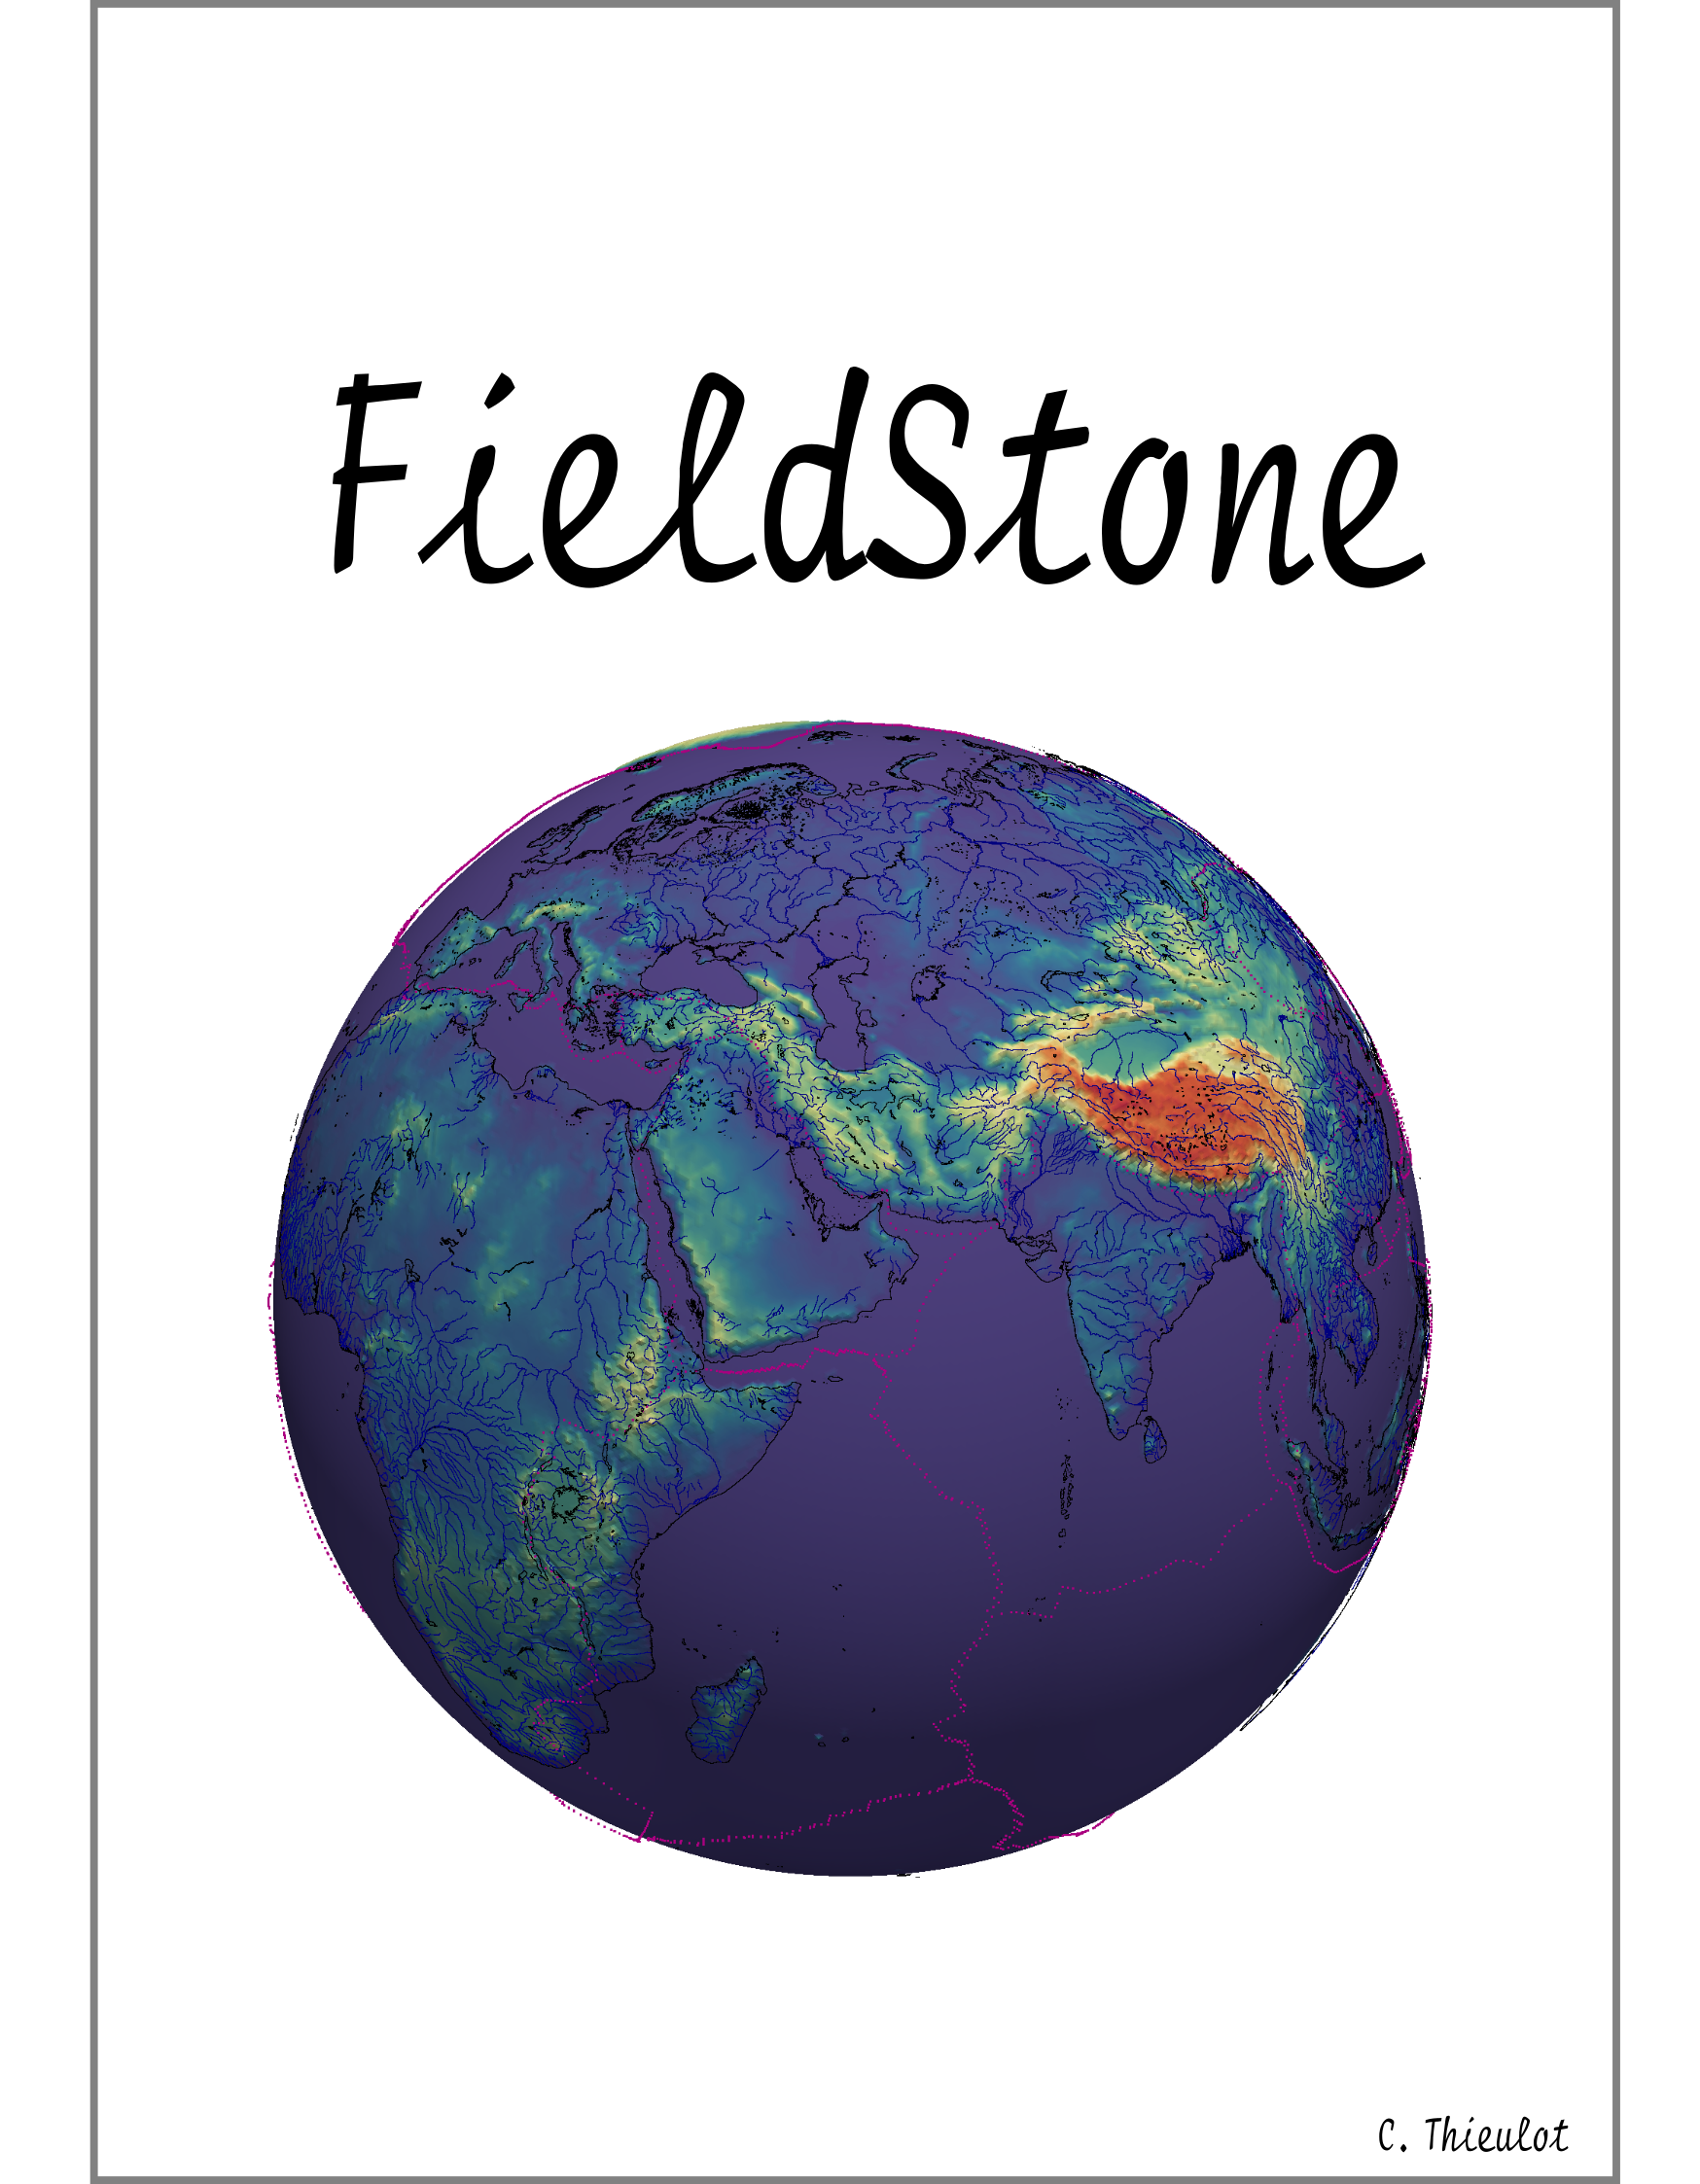
\includegraphics[width=0.9\linewidth]{images/frontpage/frontpage.png}

{\scriptsize With (direct or indirect) contributions from (in alphabetical order): 
Wolfgang Bangerth, 
Taco Broerse,
Rens Elbertsen,
Riad Hassani,
Sverre Hassing,
Jort Jansen,
Gilles Mercier,
Job Mos, 
Bob Myhill,
Taka Shinohara, 
Alessandro Regorda,
Ashim Rijal,
Bart Root,
Thomas Theunissen,
Arie van den Berg,
Erik van der Wiel, 
Lukas van de Wiel, 
Eric van den Hoogen, 
Iris van Zelst,
Alraune Zech, 
Wim Spakman.}
\newpage
If you find anything in this document useful for your research please cite it 
as follows ({\it please} include the doi!):

\begin{verbatim}
@article{Thieulot2019,
author = "C.A.P. (Cedric) Thieulot",
title = "{Fieldstone: The Finite Element Method in Computational Geodynamics}",
year = "2019",
month = "8",
url = "https://uu.figshare.com/articles/manual_pdf/9209393",
doi = "10.23644/uu.9209393.v1"}
\end{verbatim}

\vspace{7cm}

\begin{center}
{\sl Why do I have to promise where I am going while I am not there yet?}

\vspace{1cm}

{\sl You can't google something you don't know exists.}

\vspace{1cm}

{\sl You can be correct or you can get stuff done.}
\end{center}





\newpage
\maketitle
\tableofcontents

%\begin{center}
%{\color{red} \huge WARNING: this is work in progress}
%\end{center}

%%%%%%%%%%%%%%%%%%%%%%%%%%%%%%%%%%%%%%%%%%%%%%%%%%%%%%%%%%%%%%%%%%%%%%%%%%%%%%%%%%%%%%%%%%%%%%%%%%%
\newpage
\section{Introduction} %%%%%%%%%%%%%%%%%%%%%%%%%%%%%%%%%%%%%%%%%%%%%%%%%%%%%%%%%%%%%%%%%%%%%%%%%%%%
\subsection{Philosophy} 
This document was written with my students in mind, i.e. 3rd and 4th year 
Geology/Geophysics students at Utrecht University. 
I have chosen to use as little jargon as possible unless it is a term that is 
commonly found in the geodynamics literature (methods paper as well as 
application papers). There is no mathematical proof of any theorem that may 
be mentioned but I will try to refer to the appropriate sources, i.e.
generic Numerical Analysic, Finite Element and 
Linear Algebra books. If you find that this books lacks references
to Sobolev spaces, Hilbert spaces, and other spaces, this book is just not for you.  

The codes I provide here are by no means optimised as I have chosen code readability 
over code efficiency. I have also chosen to avoid resorting to multiple code 
files or even functions in order to favour a sequential reading of the codes. 
These codes are not designed to form the basis of a real life application:
Existing open source highly optimised codes shoud be preferred, such as 
ASPECT \cite{krhb12,hedg17}, CITCOM \cite{zhzm00,zhmt08}, LAMEM \cite{kapb16}, 
PTATIN \cite{mabl14,mabl15}, PYLITH \cite{aakw13}, ... (see Appendix~\ref{app:codes}).

All kinds of feedback is welcome on the text (grammar, typos, ...), on the text, the equations
or on the code(s). You will have my eternal gratitude if you wish to contribute an 
example, a benchmark, a cookbook. 

All the python scripts and tex files are freely available at 
\begin{center}
\url{https://github.com/cedrict/fieldstone}
\end{center}
This document is available at:
\begin{center}
\url{http://cedricthieulot.net/manual.pdf}  
\includegraphics[width=0.7cm]{images/minion}
\end{center}

 %-------------------------------------------------------
\subsection{ambition \& motivation} 
I wish to provide the community with:
\begin{itemize}
\item a ginormous bibliography data base - simply search the pdf for keywords. The \LaTeX{} bib
 file\footnote{\url{https://github.com/cedrict/fieldstone/blob/master/biblio_geosciences.bib}} 
is also available next to the manual.tex file on github;  
\item a go-to document for anybody who wants to know more about 
      a particular topic in computational geodynamics;
\item a useful teaching tool for researchers, teachers, students and PhD students alike; 
\item small, readable, educative codes. 
\end{itemize}

 %-------------------------------------------
\subsection{Acknowledgements} 
I have benefitted from many discussions, lectures, tutorials, coffee machine 
discussions, debugging sessions, conference poster sessions, etc ... 
over the years. I wish to name these instrumental people in particular and 
in alphabetic order: 
Wolfgang Bangerth, 
Jean Braun, 
Rens Elbertsen,
Philippe Fullsack, 
Menno Fraters, 
Anne Glerum,
Timo Heister,
Dave May,
Robert Myhill,
John Naliboff,
E. Gerry Puckett,
Melchior Schuh-Senlis,
Michael Tetley,
Lukas van de Wiel,
Arie van den Berg, 
Eric van den Hoogen,
Tom Weir,
and the whole ASPECT family/team. 

%I wish to acknowledge many BSc and MSc students for their questions and feedback.
%and wish to mention: Job Mos (the
%very first version of fieldstone was part of his MSc thesis), 
%Tom Weir (contributions to the compressible formulation - MSc thesis), 
%and Rens Elbertsen (Tosi benchmark - BSc thesis).
 %-------------------------------------------
\subsection{About the author} 
I have BSc in mathematics, and an MSc diploma in physics (with a specialization in 
musical acoustics \cite{dewl02}). I did my PhD at the 
university of Groningen (The Netherlands) titled {\sl Thermodynamically consistent 
fluid particle modelling of phase separating 
mixtures}\footnote{\url{http://cedricthieulot.net/thesis.html}}.
Although half of the thesis deals with the re-derivation of the Navier-Stokes 
equations for such systems\cite{esth03}, the second half is concerned with 
the implementation of these equations with the Smoothed Particle Hydrodynamics
method \cite{thje05a,thje05b,thes05}.

I then taught physics and programming at the University of Rennes (France) for a year, 
after which I did a 2-year post-doc with Prof. J. 
Braun\footnote{\url{https://www.gfz-potsdam.de/en/staff/jean-braun/}} in the 
Geosciences department. 
I then did a 4-year post-doc with prof. R. 
Huismans\footnote{\url{https://folk.uib.no/huismans/}} at the University of Bergen (Norway), 
followed by a 3-year post-doc with profs. T. Torsvik and W. Spakman at the Utrecht
University (The Netherlands). 
Since June 2015 I am assistant professor there in the geophysics group.
 
 %-----------------------------------------------------
\subsection{Essential/relevant literature} 
\begin{center}
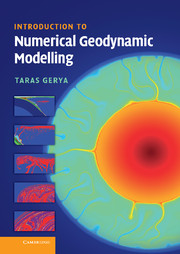
\includegraphics[height=4.5cm]{images/literature/gerya_book}
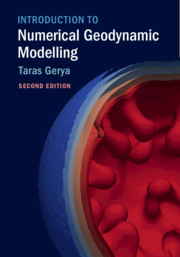
\includegraphics[height=4.5cm]{images/literature/gerya_book2}
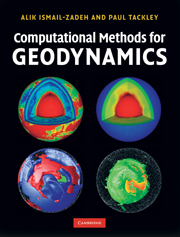
\includegraphics[height=4.5cm]{images/literature/tackley_book}
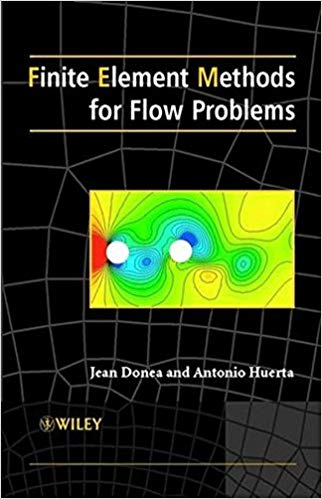
\includegraphics[height=4.5cm]{images/literature/donea_huerta_book}\\
\cite{gery10}     \hspace{1.99cm} 
\cite{gery19book} \hspace{1.99cm} 
\cite{tack10}     \hspace{1.99cm} 
\cite{dohu03}  \\
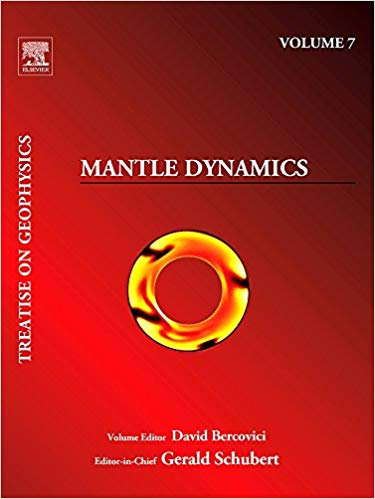
\includegraphics[height=4.5cm]{images/literature/bercovici_book}
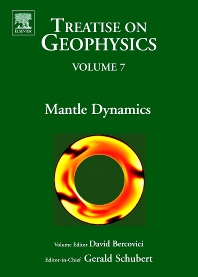
\includegraphics[height=4.5cm]{images/literature/bercovici_book2}
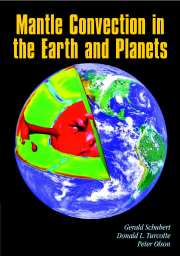
\includegraphics[height=4.5cm]{images/literature/sto_book}
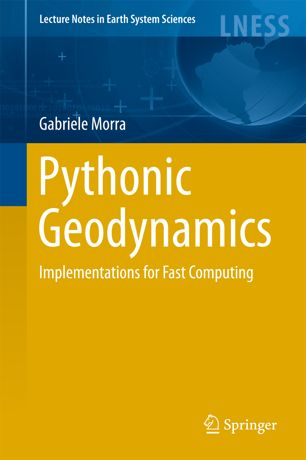
\includegraphics[height=4.5cm]{images/literature/morra_book}\\
\cite{berc09} \hspace{1.99cm} 
\cite{berc15} \hspace{1.99cm} 
\cite{scto01} \hspace{1.99cm} 
\cite{morr18} \\ 
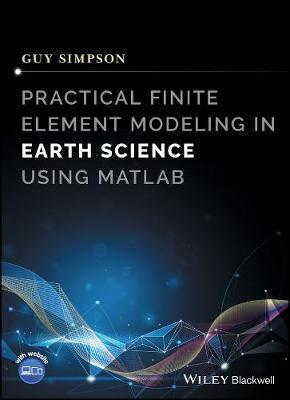
\includegraphics[height=4.5cm]{images/literature/simpson_book}
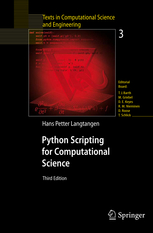
\includegraphics[height=4.5cm]{images/literature/langtangen_book}\\
\cite{simp17} \hspace{1.99cm}
\cite{lang08}
\end{center}

\begin{itemize}
\item {\it Numerical modeling of Earth Systems} by Thorsten W. Becker and Boris J. P. Kaus,\\ 
\url{http://www-udc.ig.utexas.edu/external/becker/teaching-557.html}

\item {\it Myths \& Methods in Modeling} by M. Spiegelman,\\
 \url{https://www.ldeo.columbia.edu/~mspieg/mmm/}

\item {\it Computational Science I} by Matthew G. Knepley,\\
 \url{https://cse.buffalo.edu/~knepley/classes/caam519/Syllabus.html}

\item {\it Introduction to Numerical Methods for Variational Problems} by Hans Petter Langtangen and 
Kent-Andre Mardal, \\
\url{https://hplgit.github.io/fem-book/doc/pub/book/pdf/fem-book-4print.pdf}
\end{itemize}

 %------------------------------------
\subsection{Installation} \begin{flushright} {\tiny {\color{gray} install.tex}} \end{flushright}

%--------------------------------
\subsubsection{Python}

If numpy, scipy or matplotlib are not installed on your machine, here is how you 
can install them:
\begin{verbatim}
sudo apt install python3-numpy
sudo apt install python3-scipy
\end{verbatim}
To install the umfpack solver (check?):
\begin{verbatim}
pip install --upgrade scikit-umfpack --user
\end{verbatim}
If you need to install pip:
\begin{verbatim}
sudo apt install python3-pip
\end{verbatim}

%--------------------------------
\subsubsection{Julia}

In order to have vim supporting the Julia language, do 
\begin{verbatim}
git clone git@github.com:JuliaEditorSupport/julia-vim.git
\end{verbatim}
and copy the content of the julia-vim folder in the .vim folder.
That's it.
 %--------------------------------------------------------
\subsection{What is a (real) fieldstone?} \begin{flushright} {\tiny {\color{gray} whatisafieldstone.tex}} \end{flushright}

\begin{center}
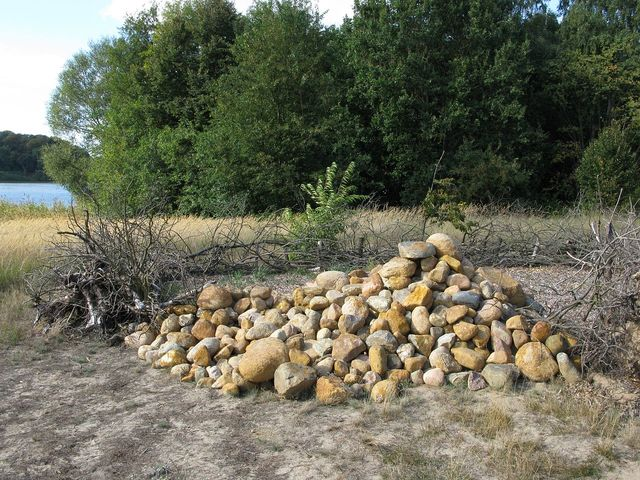
\includegraphics[width=5cm]{images/fieldstone2}\\
{\captionfont Taken from \url{https://en.wikipedia.org/wiki/Fieldstone}}
\end{center}

Simply put, it is a stone collected from the surface of fields where it 
occurs naturally. It also stands for the bad acronym: {\sl fi}nite 
{\sl el}ement {\sl d}eformation of {\sl stone}s which echoes the primary 
application of these codes: geodynamic modelling.
 %------------------------------
\subsection{Why the Finite Element method?} \begin{flushright} {\tiny {\color{gray} why.tex}} \end{flushright}

The Finite Element Method (FEM) is by no means the only method 
to solve PDEs in geodynamics, nor it is necessarily always the best one.
Other methods are employed very successfully, such as the Finite Difference 
Method (FDM), the Finite Volume Method (FVM), and to a lesser extent
the Discrete Element Method (DEM) \cite{tasy05,egho07,egsc07,funi14}, 
the Lattice-Boltzmann method \cite{hupc08}, the Rigid Element Method \cite{lacj15},  
or the Element Free Galerkin Method (EFGM) \cite{hans03}.
I have been using FEM since 2008 and I do not have real 
experience to speak of in FVM or FDM (except for chapter 11)
so I concentrate in this book 
on what I know best. 


 %------------------------------------------
\subsection{Oldies but goodies} 

I hereunder show a few plots taken from early geodynamics FEM papers.


\begin{center}
\begin{minipage}{0.45\textwidth}
\centering
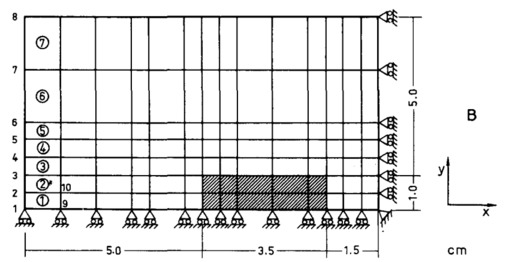
\includegraphics[height=4.5cm]{images/history/stbe71}\\
{\captionfont 1971: Model a boudinage structure \cite{stbe71}}
\end{minipage}\hfill
\begin{minipage}{0.45\textwidth}
\centering
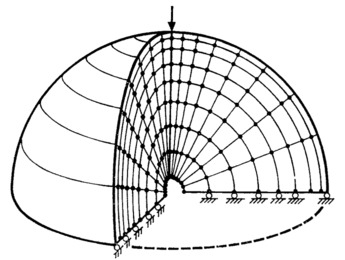
\includegraphics[height=4.5cm]{images/history/bela72}\\
{\captionfont 1972: Crustal Structure from Surface Load Tilts \cite{bela72}}
\end{minipage}
\end{center}


\begin{center}
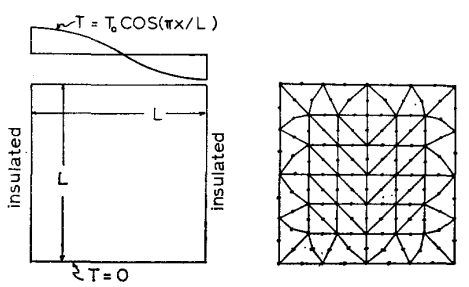
\includegraphics[height=5cm]{images/history/sath76}\\
{\captionfont 1976: Mantle convection in a square domain \cite{sath76}}
\end{center}

\begin{center}
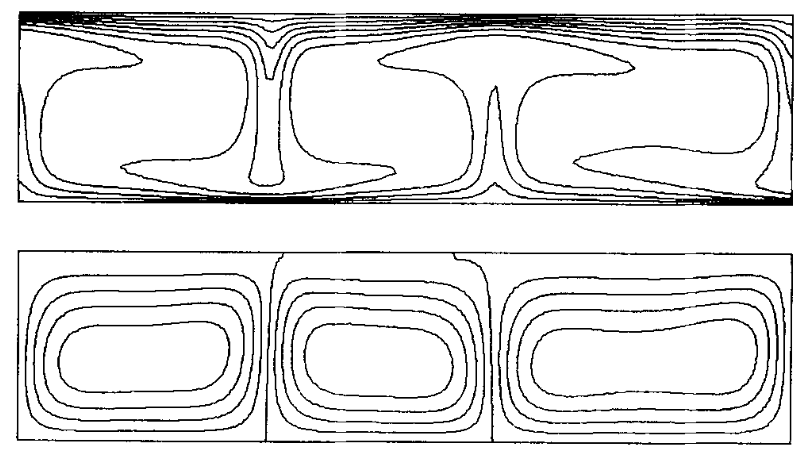
\includegraphics[height=4cm]{images/history/ludt79}\\
{\captionfont 1979: Mantle convection in a rectangular domain \cite{ludt79}}
\end{center}


\begin{center}
\begin{minipage}{0.45\textwidth}
\centering
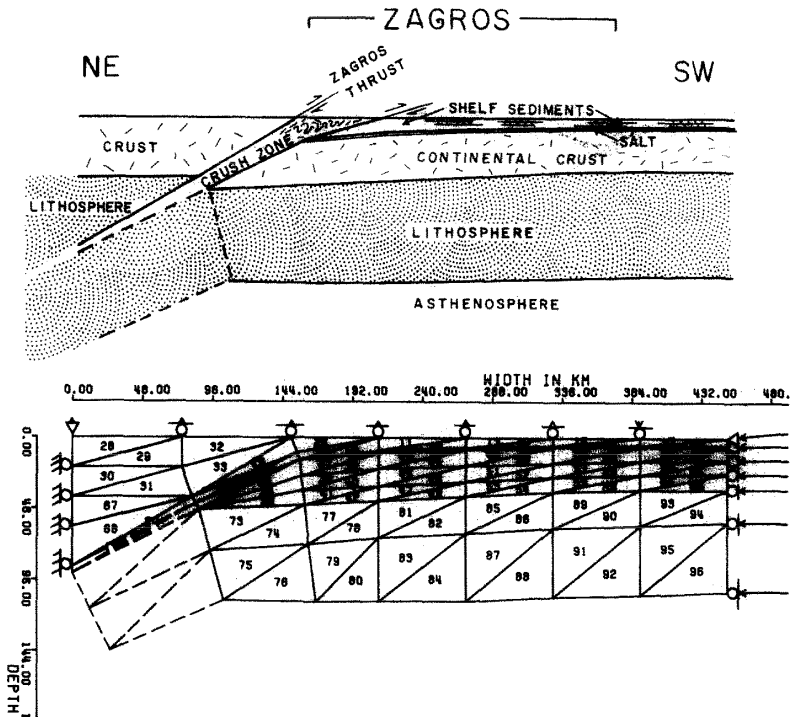
\includegraphics[height=5cm]{images/history/bird78b}\\
{\captionfont 1978: Finite element modelling of lithosphere deformation: the Zagros collision 
orogeny \cite{bird78b}}
\end{minipage}\hfill
\begin{minipage}{0.45\textwidth}
\centering
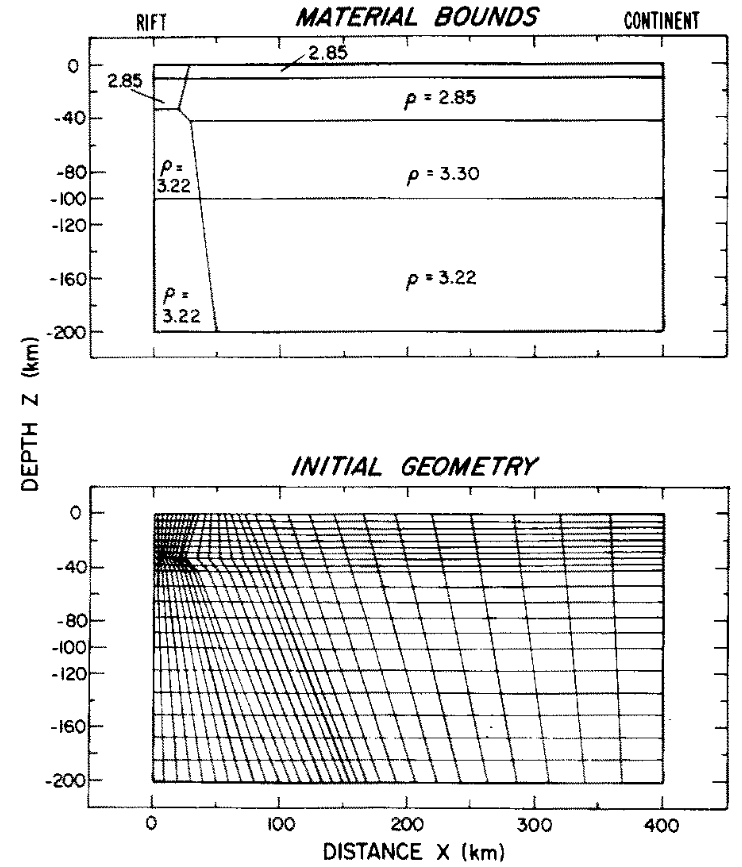
\includegraphics[height=5cm]{images/history/brpo81}\\
{\captionfont 1981: Thermal regimes, mantle diapirs and crustal stresses of continental rifts \cite{brpo81}}
\end{minipage}
\end{center}

\begin{center}
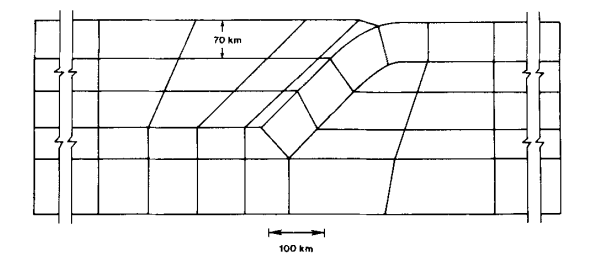
\includegraphics[height=3.5cm]{images/history/thar85}\\
{\captionfont 1985: Numerical models of subduction and forearc deformation \cite{thar85}}
\end{center}

\begin{center}
\begin{minipage}{0.48\textwidth}
\centering
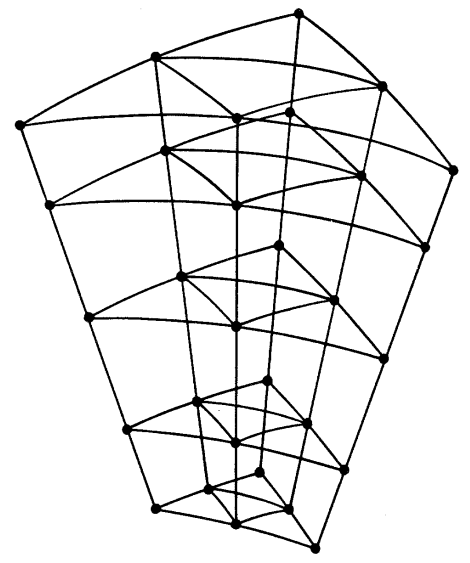
\includegraphics[height=3.5cm]{images/history/baum85a}
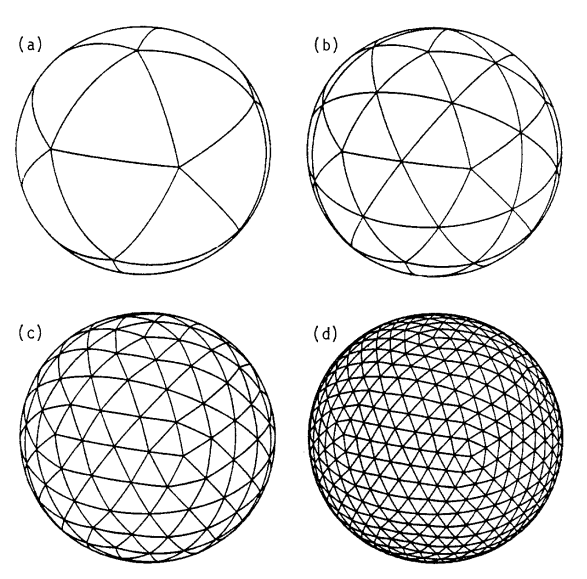
\includegraphics[height=3.5cm]{images/history/baum85b}\\
{\captionfont 1985: Three-Dimensional Treatment of Convective Flow in the Earth's Mantle.
\cite{baum85}}
\end{minipage}\hfill
\begin{minipage}{0.45\textwidth}
\centering
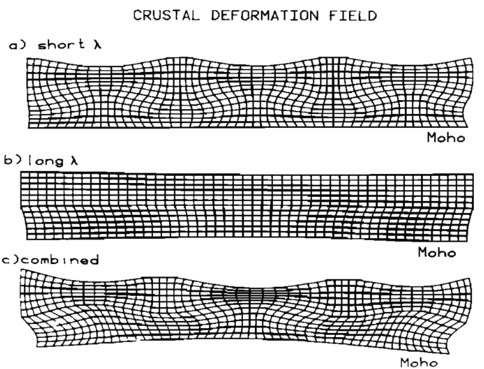
\includegraphics[width=7cm]{images/history/zupf86}\\
{\captionfont 1986: Lithospheric necking: a dynamic model for rift morphology \cite{zupf86}}
\end{minipage}
\end{center}


\begin{center}
\begin{minipage}{0.48\textwidth}
\centering
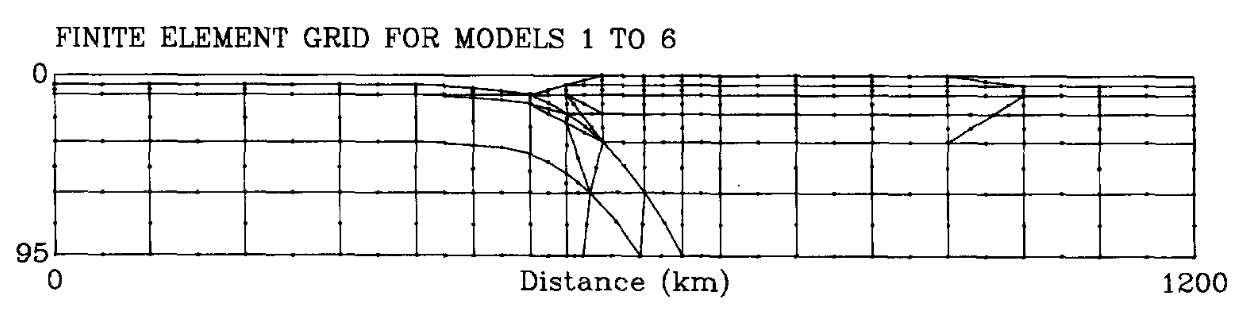
\includegraphics[width=9cm]{images/history/boww89}\\
{\captionfont 1989: Plate boundary forces at subduction zones and trench-arc compression \cite{boww89}}
\end{minipage}\hfill
\begin{minipage}{0.45\textwidth}
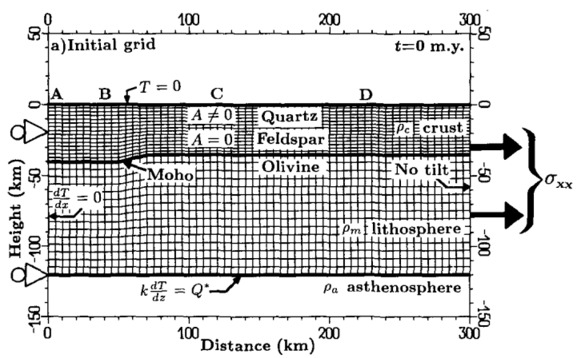
\includegraphics[width=9cm]{images/history/brbe89}\\
{\captionfont 1989: Relation between flank uplifts and the breakup unconformity at rifted continental margins \cite{brbe89}}
\end{minipage}
\end{center}



\begin{center}
\begin{minipage}{0.35\textwidth}
\centering
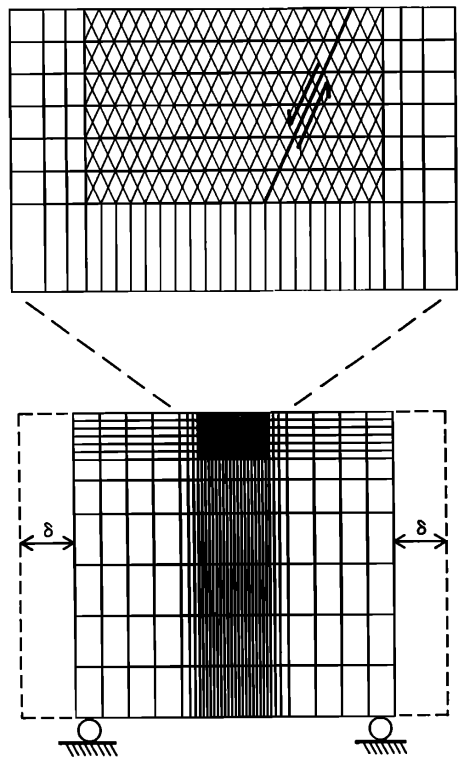
\includegraphics[width=5cm]{images/history/mewi89}\\
{\captionfont 1989: Mechanics of graben formation in crustal rocks \cite{mewi89}}
\end{minipage}\hfill
\begin{minipage}{0.55\textwidth}
\centering
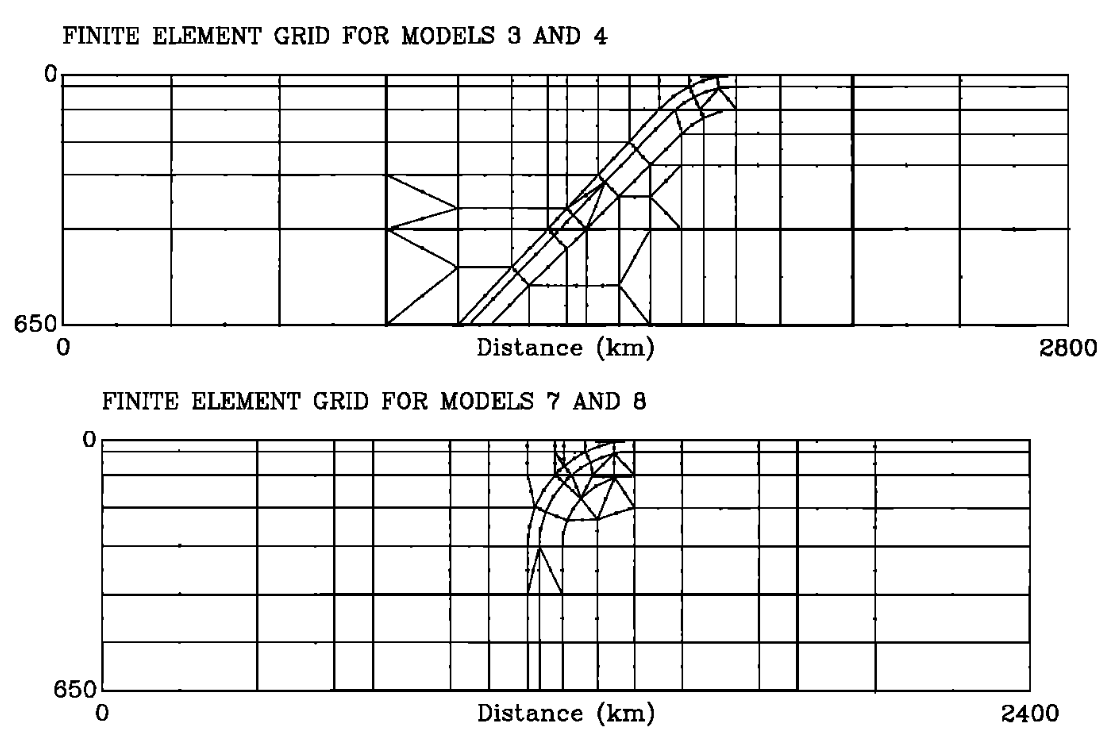
\includegraphics[width=8cm]{images/history/whbw92}\\
{\captionfont 1992: Stresses and plate boundary forces associated with subduction plate margins
\cite{whbw92}}
\end{minipage}
\end{center}


\begin{center}
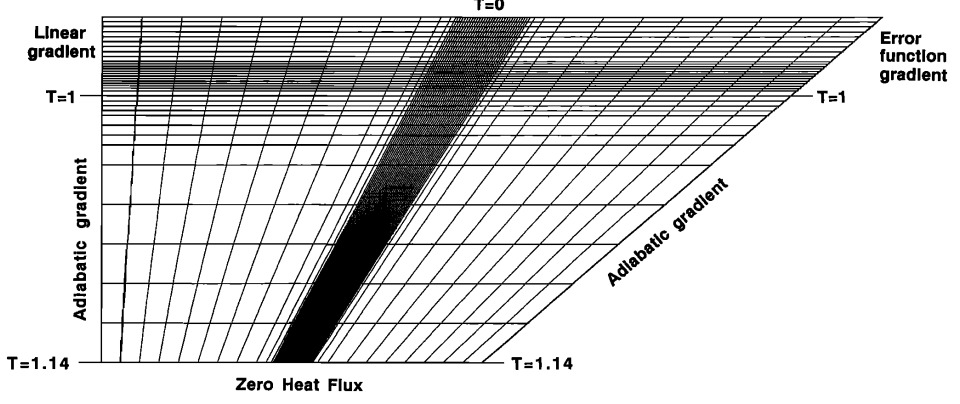
\includegraphics[width=5cm]{images/history/dast92}\\
{\captionfont 1992: Temperature field in subduction zones \cite{dast92}}
\end{center}


\begin{center}
\begin{minipage}{0.45\textwidth}
\centering
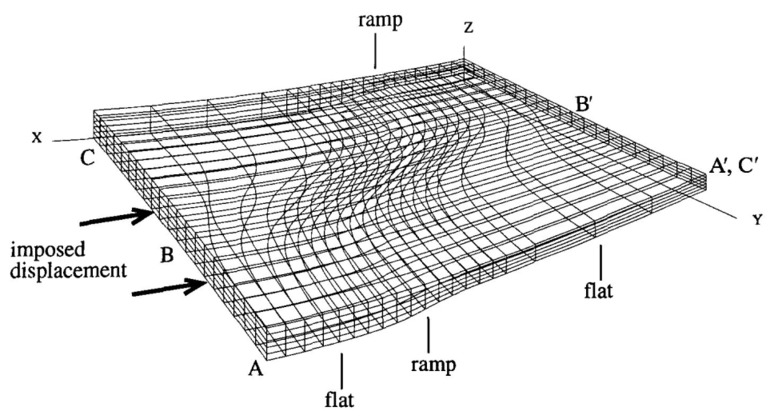
\includegraphics[width=7.6cm]{images/history/brau93}\\
{\captionfont 1993: 3D numerical modeling of
compressional orogenies: Thrust geometry and
oblique convergence \cite{brau93}}
\end{minipage}\hfill
\begin{minipage}{0.45\textwidth}
\centering
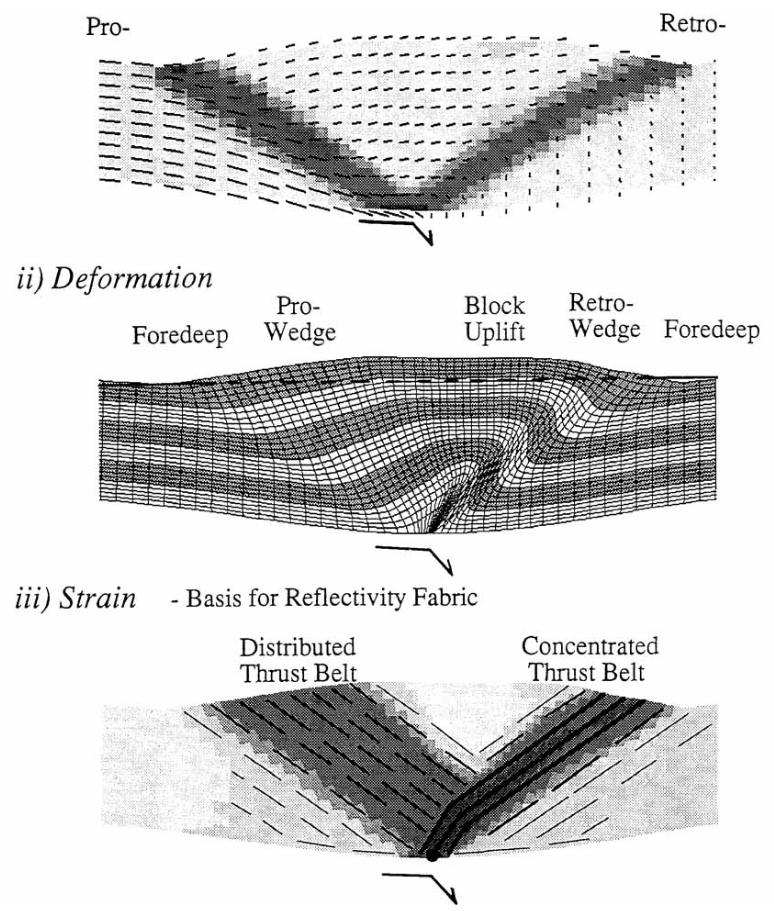
\includegraphics[height=6cm]{images/history/bequ94}\\
{\captionfont 1994: Crustal-scale compressional orogens \cite{bequ94}}
\end{minipage}
\end{center}

\begin{center}
\begin{minipage}{0.45\textwidth}
\centering
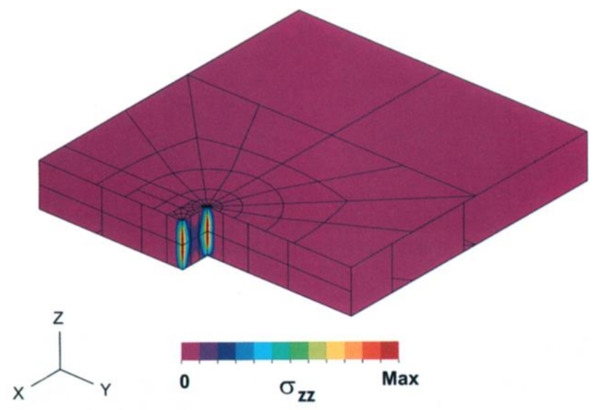
\includegraphics[height=6cm]{images/history/katl95}\\
{\captionfont 1995: modeling of pull-apart basins \cite{katl95}}
\end{minipage}\hfill
\begin{minipage}{0.45\textwidth}
\centering
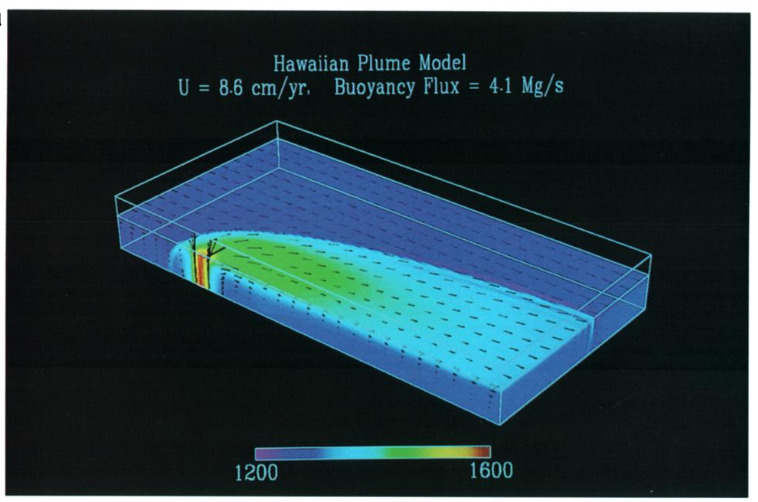
\includegraphics[height=6cm]{images/history/rich94}\\
{\captionfont 1994: plume-lithosphere interaction \cite{rich94}}
\end{minipage}
\end{center}

\begin{center}
\begin{minipage}{0.45\textwidth}
\centering
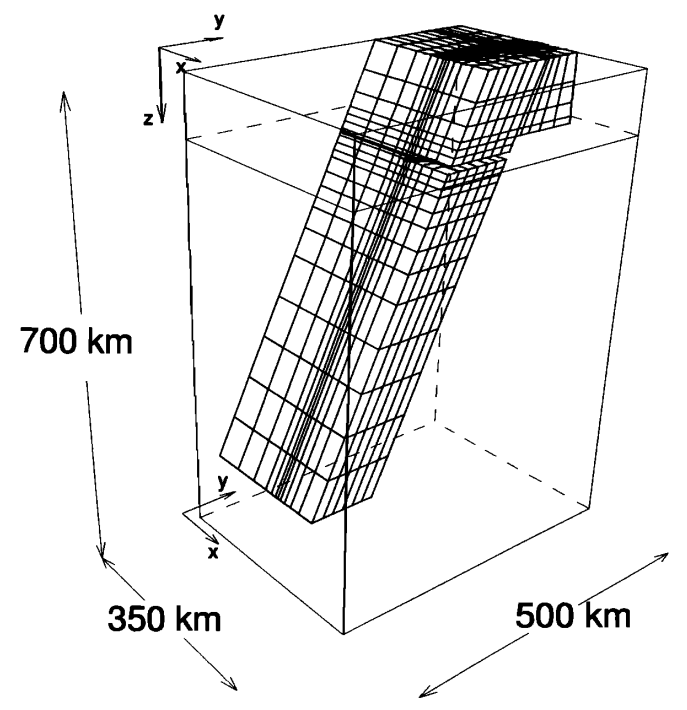
\includegraphics[height=5cm]{images/history/yowo95}\\
{\captionfont 1995: 3D numerical modeling of detachment of subducted 
lithosphere \cite{yowo95}}
\end{minipage}\hfill
\begin{minipage}{0.45\textwidth}
\centering
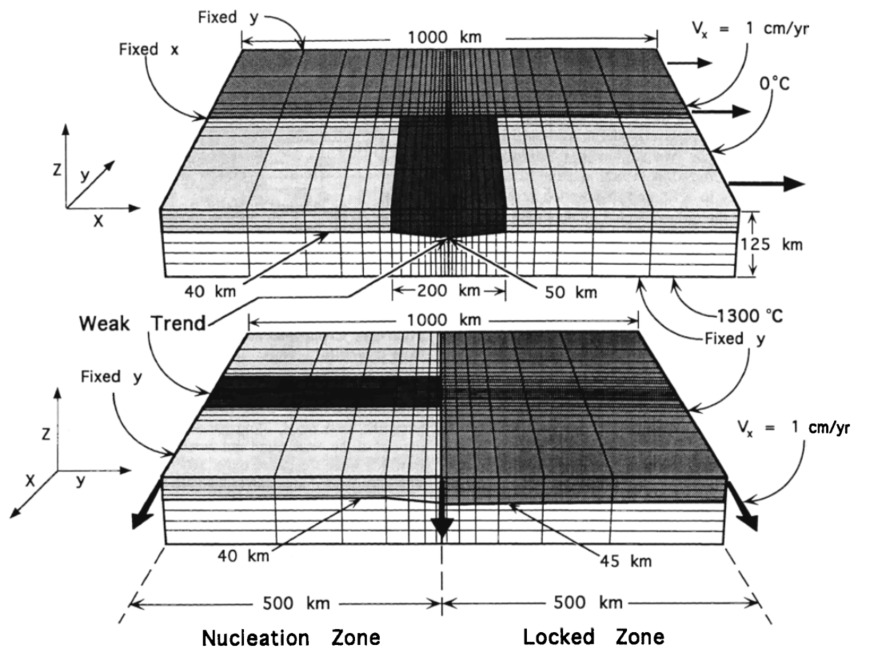
\includegraphics[height=6cm]{images/history/dusa96}\\
{\captionfont 1996: 3D dynamical model of continental rift propagation and 
margin plateau formation \cite{dusa96}}
\end{minipage}
\end{center}



\begin{center}
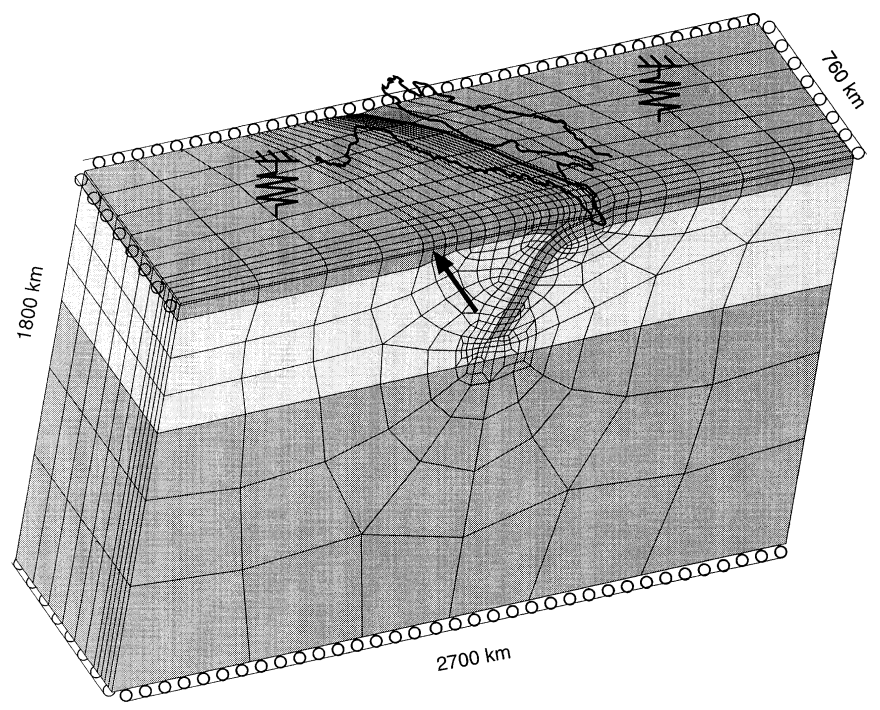
\includegraphics[height=6cm]{images/history/nesb99}\\
{\captionfont 1989: Model geometry, boundary conditions and 3-D finite element mesh used in 
the calculations. The circles denote a free-slip condition. The arrow denotes the velocity 
applied in some calculations to the southern boundary of the Tyrrhenian domain to simulate 
the motion of the African plate. The springs represent the buoyant restoring force applied 
at the surface. \cite{nesb99}}
\end{center}

\Literature: 
Gartling (1978) \cite{gart78}, 
Anderson \& Bridwell (1980)\cite{anbr80}, Melosh \& Raefsky \cite{mera80}, 
Bridwell \& Anderson \cite{bran80},
England (1982) \cite{engl82},
Thar85 \cite{thar85}, Schubert \& Anderson \cite{scan85},
England \& Houseman \cite{enho86}, Moretti \& Froidevaux \cite{mofr86},
Zuber \& Parmentier \cite{zupa86}, 
Bott \etal \cite{boww89}.




 %---------------------------------------------------
\subsection{Notations} Scalars such as temperature, density, pressure, etc ... are simply 
obtained in \LaTeX{} by using the math mode, e.g. $T$, $\rho$, $p$.
Although it is common to lump vectors and matrices/tensors together
by using bold fonts, I have decided in the interest of clarity to 
distinguish between those: vectors are denoted by an arrow 
atop the quantity, e.g. $\vec \upnu$, $\vec g$, while matrices 
and tensors are in bold $\bm M$, $\bm \sigma$, etc ...

Also I use the $\cdot$ notation between two vectors to denote a 
dot product $\vec u \cdot \vec v = u_iv_i$ or a matrix-vector
multiplication ${\bm M}\cdot \vec a = M_{ij}a_j$. If there is no
$\cdot$ between vectors, it means that the result 
$\vec a \vec b = a_ib_j$ is a matrix (it is a dyadic 
product\footnote{\url{https://en.wikipedia.org/wiki/Dyadics}}.
Case in point, $\vec\nabla\cdot\vec\upnu$ is the velocity divergence
while $\vec\nabla\vec\upnu$ is the velocity gradient tensor.
 %---------------------------------------------------------
\subsection{Colour maps for visualisation} In an attempt to homogenise the figures obtained with ParaView, I have decided to use 
a fixed colour scale for each field throughout this document. These colour scales were 
obtained from \url{https://peterkovesi.com/projects/colourmaps} and are 
Perceptually Uniform Colour Maps \cite{kove15}. 

\begin{center}
\begin{tabular}{lll}
\hline
Field & colour code & \\
\hline\hline
Velocity/displacement & CET-D1A & 
\includegraphics[width=3cm]{images/colourscales/CET-D1A}\\
\hline
Pressure& CET-L17 & 
\includegraphics[width=3cm]{images/colourscales/CET-L17}\\
\hline
Velocity divergence& CET-L1 & 
\includegraphics[width=3cm]{images/colourscales/CET-L1}\\
\hline
Density& CET-D3 & 
\includegraphics[width=3cm]{images/colourscales/CET-D3}\\
\hline
Strain rate& CET-R2 & 
\includegraphics[width=3cm]{images/colourscales/CET-R2}\\
\hline
Viscosity & CET-R3 & 
\includegraphics[width=3cm]{images/colourscales/CET-R3}\\
\hline
Temperature & CET-D9 & 
\includegraphics[width=3cm]{images/colourscales/CET-D9}\\
\hline
stress & CET-L18 &  
\includegraphics[width=3cm]{images/colourscales/CET-L18}\\
\hline
Spin tensor & CET-R1 &  
\includegraphics[width=3cm]{images/colourscales/CET-R1}\\
\hline
Composition field & CET-CBD1 &  
\includegraphics[width=3cm]{images/colourscales/CET-CBD1}\\
\hline
\end{tabular}
\end{center}

%https://peterkovesi.com/projects/colourmaps/




 %------------------------------------
\subsection{How my bibliography works} \begin{flushright} {\tiny {\color{gray} mybib.tex}} \end{flushright}
%~~~~~~~~~~~~~~~~~~~~~~~~~~~~~~~~~~~~~~~~~~~~~~~~~~~~~~~~~~~~~~~~~~~~~~~~~~~~~~~~~~~~~~~~~~~~~~~~~~

There is a single (large) bibliography file for this document:
\begin{center}
{\tt biblio\_geosciences.bib}
\end{center}

If the paper is a single-author paper, say by Garfield\footnote{This is just an example}, 
published in 1978\footnote{May be not, after all, since Garfield the cat was born in 1978}, its code 
in my bibliography file is {\sl garf78} (i.e. the first four letters of the name, followed by 
the two digits of the publication year).

If the paper was written by two authors, say Garfield and Odie, in 1987, its code 
will be {\sl gaod87}, i.e. the first two letters of the first author followed by the two 
first letters of the second author followed by two digits.

If the paper was written by three or more authors, say Garfield, Odie, John and Irene in 
2003, its code will be {\sl gaoj03}, i.e. the first two letters of the first author followed 
by the first letter of the second author, the first letter of the third author and the year.

If multiple papers are published the same year by the same authors, I simply append a,b,c... to the 
above rules. 

\begin{remark} Dutch names such as 'van Hunen' or 'van den Berg' are classified under letter 'v', 
not 'h' or 'd' nor 'b'. 
\end{remark}

\vspace{1cm}

\begin{center}

\includegraphics[width=5cm]{images/garfield-computer}
\end{center}
 %---------------------------------------------
 

%%%%%%%%%%%%%%%%%%%%%%%%%%%%%%%%%%%%%%%%%%%%%%%%%%%%%%%%%%%%%%%%%%%%%%%%%%%%%%%%%%%%%%%%%%%%%%%%%%%
\section{List of stones and their features} %%%%%%%%%%%%%%%%%%%%%%%%%%%%%%%%%%%%%%%%%%%%%%%%%%%%%%%


{\small 

\noindent stone 01: simple analytical solution: "Donea \& Huerta" mms \ref{mms1} 
\lstinputlisting[language=bash,basicstyle=\tiny]{python_codes/fieldstone_01/keywords}

\noindent stone 02: Stokes sphere in 2D 
\lstinputlisting[language=bash,basicstyle=\tiny]{python_codes/fieldstone_02/keywords}

\noindent stone 03: Convection in a 2D box: "Blankenbach" benchmark \cite{blbc89}
\lstinputlisting[language=bash,basicstyle=\tiny]{python_codes/fieldstone_03/keywords}

\noindent stone 04: The lid driven cavity
\lstinputlisting[language=bash,basicstyle=\tiny]{python_codes/fieldstone_04/keywords}

\noindent stone 05: SolCx
\lstinputlisting[language=bash,basicstyle=\tiny]{python_codes/fieldstone_05/keywords}

\noindent stone 06: SolKz
\lstinputlisting[language=bash,basicstyle=\tiny]{python_codes/fieldstone_06/keywords}

\noindent stone 07: SolKz
\lstinputlisting[language=bash,basicstyle=\tiny]{python_codes/fieldstone_07/keywords}

\noindent stone 08: The indentor (punch problem) 
\lstinputlisting[language=bash,basicstyle=\tiny]{python_codes/fieldstone_08/keywords}

\noindent stone 09: the annulus benchmark 
\lstinputlisting[language=bash,basicstyle=\tiny]{python_codes/fieldstone_09/keywords}

\noindent stone 10: Stokes sphere (3D) - penalty
\lstinputlisting[language=bash,basicstyle=\tiny]{python_codes/fieldstone_10/keywords}

\noindent stone 11: Stokes sphere (3D) - mixed formulation
\lstinputlisting[language=bash,basicstyle=\tiny]{python_codes/fieldstone_11/keywords}

\noindent stone 12: consistent pressure recovery 
\lstinputlisting[language=bash,basicstyle=\tiny]{python_codes/fieldstone_12/keywords}

\noindent stone 13: the Particle in Cell technique (1) - the effect of averaging
\lstinputlisting[language=bash,basicstyle=\tiny]{python_codes/fieldstone_13/keywords}

\noindent stone 14: solving the full saddle point problem with $Q_1\times P_0$ elements 
\lstinputlisting[language=bash,basicstyle=\tiny]{python_codes/fieldstone_14/keywords}

\noindent stone 16: saddle point problem with Schur complement approach - Stokes sphere 
\lstinputlisting[language=bash,basicstyle=\tiny]{python_codes/fieldstone_16/keywords}

\noindent stone 17: Solving the full saddle point problem in 3D - Burstedde benchmark \cite{dobo04} 
\lstinputlisting[language=bash,basicstyle=\tiny]{python_codes/fieldstone_17/keywords}

\noindent stone 18: Solving the full saddle point problem with $Q_2\times Q_1$ elements 
\lstinputlisting[language=bash,basicstyle=\tiny]{python_codes/fieldstone_18/keywords}

\noindent stone 19: Solving the full saddle point problem with $Q_3\times Q_2$ elements 
\lstinputlisting[language=bash,basicstyle=\tiny]{python_codes/fieldstone_19/keywords}

\noindent stone 20: Convection in a 3D box, the Busse benchmark \cite{bucc93}
\lstinputlisting[language=bash,basicstyle=\tiny]{python_codes/fieldstone_20/keywords}

\noindent stone 22: The stabilised $Q_1 \times Q_1$ element 
\lstinputlisting[language=bash,basicstyle=\tiny]{python_codes/fieldstone_22/keywords}

\noindent stone 23: compressible flow (1) - analytical benchmark 
\lstinputlisting[language=bash,basicstyle=\tiny]{python_codes/fieldstone_23/keywords}


\noindent stone 25: Rayleigh-Taylor instability (1) - instantaneous \cite{vaks97}
\lstinputlisting[language=bash,basicstyle=\tiny]{python_codes/fieldstone_25/keywords}

\noindent stone 28: convection 2D box - Tosi et al, 2015
\lstinputlisting[language=bash,basicstyle=\tiny]{python_codes/fieldstone_28/keywords}

\noindent stone 30: the Particle in Cell technique (2) - CVI algorithms
\lstinputlisting[language=bash,basicstyle=\tiny]{python_codes/fieldstone_30/keywords}

\noindent stone 33: Convection in an annulus 
\lstinputlisting[language=bash,basicstyle=\tiny]{python_codes/fieldstone_33/keywords}

\noindent stone 39: Choi \& Pedersen visco-plasticity benchmarks 
\lstinputlisting[language=bash,basicstyle=\tiny]{python_codes/fieldstone_39/keywords}

\noindent stone 40: Rayleigh-Taylor instability (instantaneous)
\lstinputlisting[language=bash,basicstyle=\tiny]{python_codes/fieldstone_40/keywords}

\noindent stone 44: Flat slab setup 
\lstinputlisting[language=bash,basicstyle=\tiny]{python_codes/fieldstone_44/keywords}

\noindent stone 46: MMS1 with Crouzeix-Raviart ($P_2^+\times P_{-1}$) elements  
\lstinputlisting[language=bash,basicstyle=\tiny]{python_codes/fieldstone_46/keywords}

\noindent stone 47: MMS1 with MINI ($P_1^+\times P_1$) elements
\lstinputlisting[language=bash,basicstyle=\tiny]{python_codes/fieldstone_47/keywords}

\noindent stone 48: $Q_1\times P_0$, $Q_2\times Q_1$, $Q_3\times Q_2$ and $Q_4\times Q_3$ elements
\lstinputlisting[language=bash,basicstyle=\tiny]{python_codes/fieldstone_48/keywords}

\noindent stone 49: Consistent Boundary Flux method on D\&H benchmark with 4 elements 
\lstinputlisting[language=bash,basicstyle=\tiny]{python_codes/fieldstone_49/keywords}

\noindent stone 50: Lithosphere extension (visco-plastic, thermo-mechanically coupled)
\lstinputlisting[language=bash,basicstyle=\tiny]{python_codes/fieldstone_50/keywords}

\noindent stone 51: Triangular domain benchmark with MINI element
\lstinputlisting[language=bash,basicstyle=\tiny]{python_codes/fieldstone_51/keywords}

\noindent stone 52: Serendipity element in 2D 
\lstinputlisting[language=bash,basicstyle=\tiny]{python_codes/fieldstone_52/keywords}

\noindent stone 53: the sinking block benchmark  
\lstinputlisting[language=bash,basicstyle=\tiny]{python_codes/fieldstone_53/keywords}

\noindent stone 54: free surface and ALE algorithms
\lstinputlisting[language=bash,basicstyle=\tiny]{python_codes/fieldstone_54/keywords}

\noindent stone 55: Subduction as a thin-sheet problem
\lstinputlisting[language=bash,basicstyle=\tiny]{python_codes/fieldstone_55/keywords}

\noindent stone 57: 1D steady state diffusion with DG-FEM
\lstinputlisting[language=bash,basicstyle=\tiny]{python_codes/fieldstone_57/keywords}

\noindent stone 58: Elastic disk under compression
\lstinputlisting[language=bash,basicstyle=\tiny]{python_codes/fieldstone_58/keywords}

\noindent stone 59: Ice flow down an inclined plane 
\lstinputlisting[language=bash,basicstyle=\tiny]{python_codes/fieldstone_59/keywords}

\noindent stone 60: 1D advection with DG-FEM 
\lstinputlisting[language=bash,basicstyle=\tiny]{python_codes/fieldstone_60/keywords}

\noindent stone 63: Failure in cemented granular material
\lstinputlisting[language=bash,basicstyle=\tiny]{python_codes/fieldstone_63/keywords}

\noindent stone 67: Newtonian subduction setups \& Particle-in-cell
\lstinputlisting[language=bash,basicstyle=\tiny]{python_codes/fieldstone_67/keywords}

\noindent stone 68: subduction \& corner flow
\lstinputlisting[language=bash,basicstyle=\tiny]{python_codes/fieldstone_68/keywords}

\noindent stone 69: Spherical shell 
\lstinputlisting[language=bash,basicstyle=\tiny]{python_codes/fieldstone_69/keywords}

}









 

\newpage
%%%%%%%%%%%%%%%%%%%%%%%%%%%%%%%%%%%%%%%%%%%%%%%%%%%%%%%%%%%%%%%%%%%%%%%%%%%%%%%%%%%%%%%%%%%%%%%%%%%
\section{Physics and a bit of mathematics} \label{chapt3} %%%%%%%%%%%%%%%%%%%%%%%%%%%%%%%%%%%%%%%%%
\begin{flushright} {\tiny {\color{gray} chapter3.tex}} \end{flushright}

\subsection{Some maths} %------------------------------------------------------
\subsection{Inverse of a 3x3 matrix \label{sec:inv2x2}}

Let us assume we wish to solve the 
system $\bm A \cdot \vec X = \vec b$, with $\vec X=(x,y)$. Then the solution is given by
The solution is given by
\[
x=\frac{1}{det(\bm A)}
\left|
\begin{array}{cc}
b_1 & a_{21} \\
b_2 & a_{22}
\end{array}
\right|
\qquad
y=\frac{1}{det(\bm A)}
\left|
\begin{array}{cc}
a_{11} & b_1\\
a_{21} & b_2
\end{array}
\right|
\]



%------------------------------------------------------
\subsection{Inverse of a 3x3 matrix \label{sec:inv3x3}}

Let us consider the 3x3 matrix ${\bm M}$
\[
{\bm M}=
\left(
\begin{array}{ccc}
M_{xx} & M_{xy} & M_{xz} \\
M_{yx} & M_{yy} & M_{yz} \\
M_{zx} & M_{zy} & M_{zz} 
\end{array}
\right)
\]

\begin{enumerate}
\item
Find $det({\bm M})$, the determinant of the Matrix ${\bm M}$.
The determinant will usually show up in the denominator of the inverse. If the determinant is zero, the matrix won't have an inverse.

\item  Find ${\bm M}^T$ , the transpose of the matrix. Transposing means reflecting the matrix about the main diagonal.

\[
{\bm M}^T=
\left(
\begin{array}{ccc}
M_{xx} & M_{yx} & M_{zx} \\
M_{xy} & M_{yy} & M_{zy} \\
M_{xz} & M_{yz} & M_{zz} 
\end{array}
\right)
\]

\item  Find the determinant of each of the 2x2 minor matrices. For instance $\tilde{M}_{xx}=M_{yy}M_{zz}-M_{yz}M_{zy}$,
or $\tilde{M}_{xz}=M_{xy}M_{yz}- M_{xz}M_{yy}$.

\item assemble the $\tilde{\bm M}$ matrix:

\[
\tilde{\bm M}=
\left(
\begin{array}{ccc}
+\tilde{M}_{xx} & -\tilde{M}_{xy} & +\tilde{M}_{xz} \\
-\tilde{M}_{yx} & +\tilde{M}_{yy} & -\tilde{M}_{yz} \\
+\tilde{M}_{zx} & -\tilde{M}_{zy} & +\tilde{M}_{zz} 
\end{array}
\right)
\]

\item the inverse of ${\bm M}$ is then given by
\[
{\bm M}^{1} = \frac{1}{det({\bm M})} \tilde{\bm M}
\]

\end{enumerate}

Another approach which of course is equivalent to the above is Cramer's rule. Let us assume we wish to solve the 
system $\bm A \cdot \vec X = \vec b$, with $\vec X=(x,y,z)$. Then the solution is given by
\[
x=
\frac{1}{det(\bm M)}
\left| 
\begin{array}{ccc}
b_1 & a_{12} & a_{13} \\
b_2 & a_{22} & a_{23} \\
b_3 & a_{32} & a_{33}
\end{array}
\right|
\qquad
y=
\frac{1}{det(\bm M)}
\left| 
\begin{array}{ccc}
a_{11} & b_1 & a_{13} \\
a_{21} & b_2 & a_{23} \\
a_{31} & b_3 & a_{33} 
\end{array}
\right|
\qquad
z=
\frac{1}{det(\bm M)}
\left| 
\begin{array}{ccc}
a_{11} & a_{12} & b_1\\
a_{21} & a_{22} & b_2\\
a_{31} & a_{32} & b_3
\end{array}
\right|
\]




\subsection{Units} \begin{flushright} {\tiny {\color{gray} nomenclature.tex}} \end{flushright}
%~~~~~~~~~~~~~~~~~~~~~~~~~~~~~~~~~~~~~~~~~~~~~~~~~~~~~~~~~~~~~~~~~~~~~~~~~~~~~~~~~~~~~~~~~~~~~~~~~~

\begin{center}
\begin{tabular}{lll}
\hline
Symbol & meaning & unit \\
\hline
\hline
$t$ & Time & \si{\second} \\
$x,y,z$ & Cartesian coordinates & \si{\metre} \\
$r,\theta$ & Polar coordinates & \si{\metre},-\\
$r,\theta, z$ & Cylindrical coordinates & \si{\metre},-,\si{\metre}\\
$r,\theta,\phi$ & Spherical coordinates & \si{\metre},-,- \\
${\vec \upnu}=(u,v,w)$ & velocity vector$^{(1)}$  & \si{\metre\per\second}\\
${\vec \upnu}=(\upnu_r,\upnu_\theta,\upnu_z)$ & velocity vector$^{(2)}$ & \si{\metre\per\second}\\
${\vec \upnu}=(\upnu_r,\upnu_\theta,\upnu_\phi)$ & velocity vector$^{(3)}$ & \si{\metre\per\second}\\
${\vec u}=(u_x,u_y,u_z)$ & displacement vector & $\si{\metre}$ \\
$\rho$ & mass density & \si{\kg\per\cubic\metre} \\
$\eta$ & dynamic viscosity & \si{\pascal\second} \\
$\lambda$ & penalty parameter & \si{\pascal\second} \\
$T$ & temperature & \si{\kelvin} \\
${\vec \nabla}$ & gradient operator & \si{\per\metre} \\
${\vec \nabla}\cdot$ & divergence operator & \si{\per\metre} \\
$p$ & pressure & \si{\pascal}\\
$\dot{\bm \varepsilon}({\vec \upnu})$ & strain rate tensor & \si{\per\second} \\
$\dot{\bm \varepsilon}^d({\vec \upnu})$ & deviatoric strain rate tensor & \si{\per\second} \\
$\alpha$ & thermal expansion coefficient & \si{\per\kelvin} \\
$k$ & thermal conductivity & \si{\watt\per\metre\per\kelvin} \\
$C_p$ & Heat capacity at constant pressure & \si{\joule\per\kg\per \kelvin} \\
$H$ & intrinsic specific heat production & \si{\watt\per\kg} \\
$\beta_T$ & isothermal compressibility & \si{\per\pascal}  \\
${\bm \tau}$ & deviatoric stress tensor & \si{\pascal} \\
${\bm \sigma}$ & full stress tensor & \si{\pascal} \\
\hline
\end{tabular}\\
{\tiny (1) Cartesian coordinates;} 
{\tiny (2) Cylindrical coordinates;} 
{\tiny (3) Spherical coordinates.}
\end{center}

\begin{center}
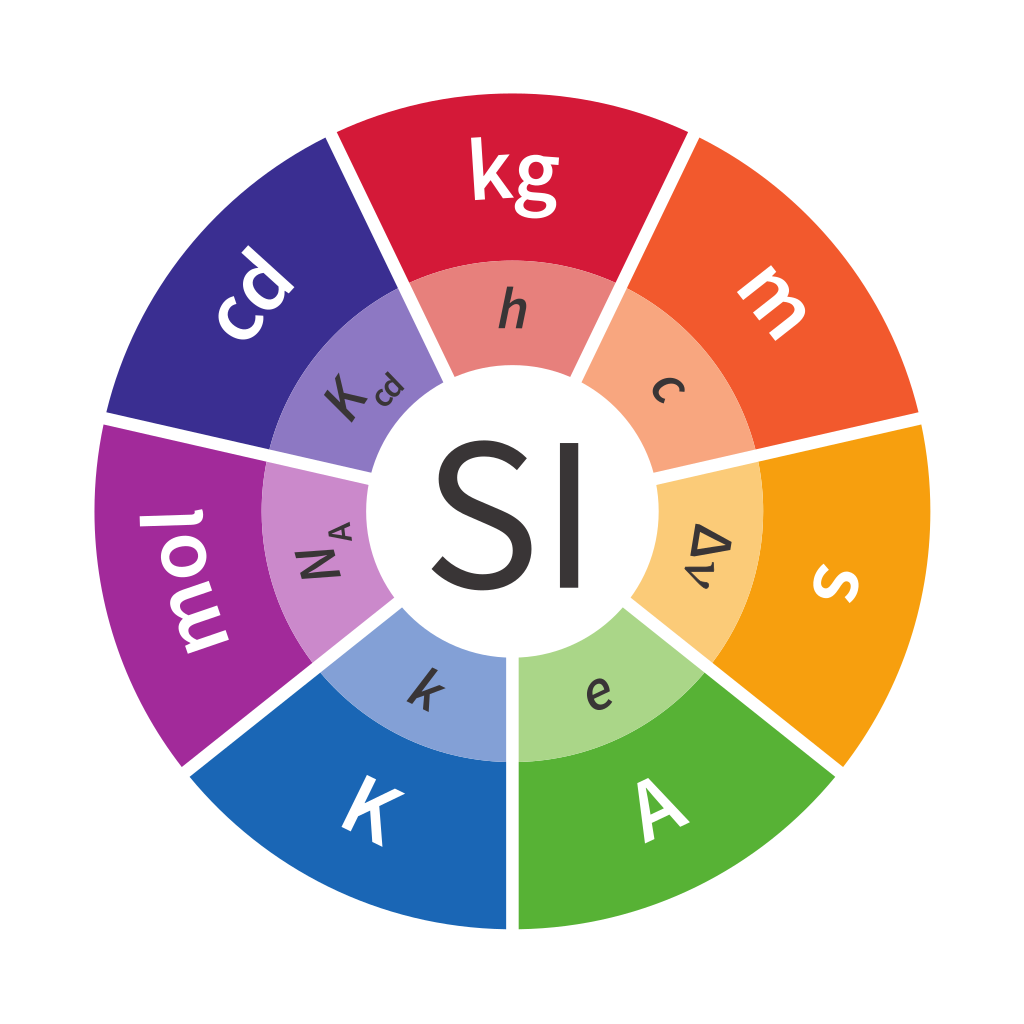
\includegraphics[width=5cm]{images/siunits}\\
{\captionfont Taken from 
Wikipedia\footnote{\url{https://en.wikipedia.org/wiki/International_System_of_Units}}.
The SI logo, produced by the BIPM (International Bureau of Weights and Measures), \\
showing the seven SI base units and the seven defining constants.}
\end{center}

A quick note about units and \LaTeX. This document relies on the {\tt siunitx} 
package\footnote{\url{https://ctan.org/pkg/siunitx}}. For instance, 
$\rho = 3300~\si{\kg\per\cubic\metre}$ is obtained with 
\begin{verbatim}
\rho = 3300~\si{\kg\per\cubic\metre}
\end{verbatim}
or
\begin{verbatim}
\rho = \SI{3300}{\kg\per\cubic\metre}
\end{verbatim}
Note that the {\tt si} command can be used outside of the math environment. 
 %----------------------------------------------------------
\subsection{Coordinate systems} \begin{flushright} {\tiny {\color{gray} coordinate\_systems.tex}} \end{flushright}
%~~~~~~~~~~~~~~~~~~~~~~~~~~~~~~~~~~~~~~~~~~~~~~~~~~~~~~~~~~~~~~~~~~~~~~~~~~~~~~~~~~~~~~~~~~~~~~~~~~

\begin{center}
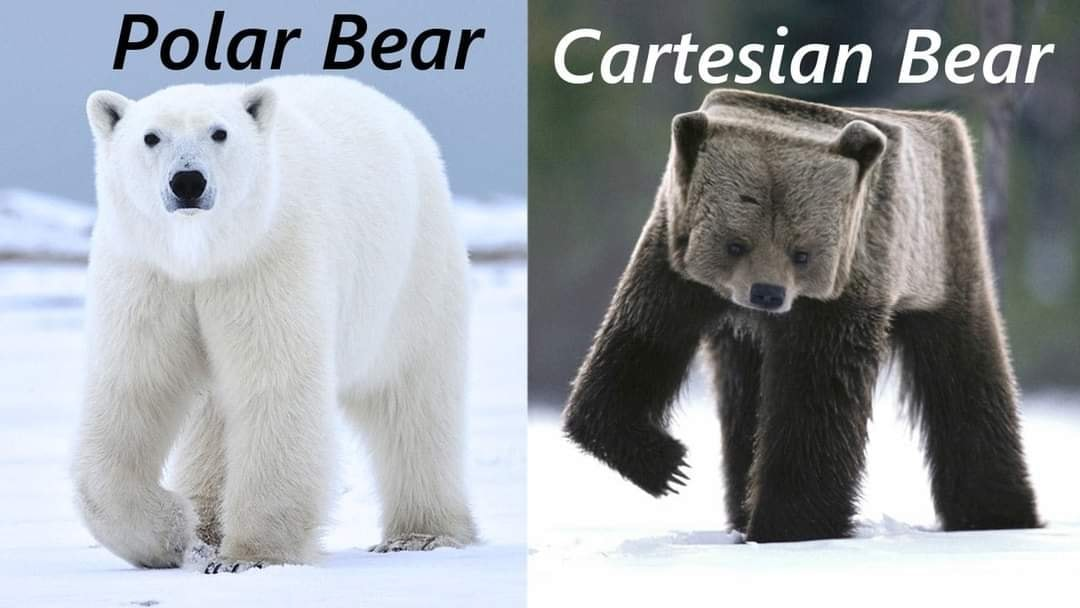
\includegraphics[width=6cm]{images/polarbear}
\end{center}

%........................................
\subsubsection{Cartesian coordinates}
\index{general}{Gradient Operator in Cartesian Coordinates}
\index{general}{Divergence Operator in Cartesian Coordinates}
\index{general}{Laplace Operator in Cartesian Coordinates}
\index{general}{Path Increment in Cartesian Coordinates}

The unit vectors along the $x$, $y$ and $z$ axis are 
$\vec{e}_x$, $\vec{e}_y$ and $\vec{e}_z$ respectively.

\begin{flushright} {\tiny {\color{gray} (tikz\_cartesian\_coordinates.tex)}} \end{flushright}
%~~~~~~~~~~~~~~~~~~~~~~~~~~~~~~~~~~~~~~~~~~~~~~~~~~~~~~~~~~~~~~~~~~~~~~~~~~~~~~~~~~~~~~~~~~~~~~~~~~
\begin{center}
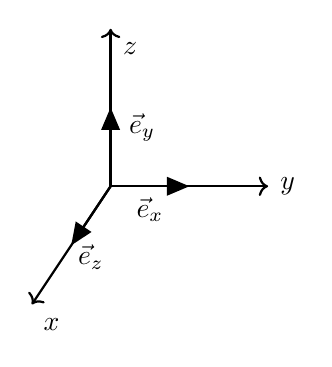
\begin{tikzpicture}
%\draw[step=0.5cm,gray,very thin] (0,0) grid (4,4); %background grid

\draw [thick,->] (1.5,2) -- (3.5,2);
\draw [thick,->] (1.5,2) -- (1.5,4);
\draw [thick,->] (1.5,2) -- (0.5,0.5);

\node[] at (0.75,0.25) {$x$};
\node[] at (3.75,2) {$y$};
\node[] at (1.75,3.75) {$z$};

\draw[>=triangle 45, line width=0.3mm, ->] (1.5,2) -- (2.5,2) ;   
\node[] at (2,1.7) {$\vec{e}_x$};

\draw[>=triangle 45, line width=0.3mm, ->] (1.5,2) -- (1.5,3) ;   
\node[] at (1.9,2.75) {$\vec{e}_y$};

\draw[>=triangle 45, line width=0.3mm, ->] (1.5,2) -- (1,1.25) ;   
\node[] at (1.25,1.1) {$\vec{e}_z$};

\end{tikzpicture}
\end{center}


\noindent Any vector can then be written
\[
{\vec V}  = V_x {\vec e}_x  + V_y {\vec e}_y + V_z \vec{e}_z
\]
'How much of $\vec{V}$ is there in the $x-$direction' is obtained
with $\vec{V}\cdot\vec{e}_x = V_x$.
The gradient of a function $f$ is 
\[
\vec{\nabla} f= \text{grad }f= 
\frac{\partial f}{\partial x}\; \vec{e}_x +
\frac{\partial f}{\partial y}\; \vec{e}_y +
\frac{\partial f}{\partial z}\; \vec{e}_z,
\]
the divergence of a vector $\vec{V}$ is
\[
\vec{\nabla}\cdot \vec{V} = 
\frac{\partial V_x}{\partial x}+
\frac{\partial V_y}{\partial y}+
\frac{\partial V_z}{\partial z}
\]
and the Laplace operator of a function $f$ is:
\[
\Delta f = 
\frac{\partial^2 f}{\partial x^2} + 
\frac{\partial^2 f}{\partial y^2} + 
\frac{\partial^2 f}{\partial z^2}  
\]
Finally the path increment is
\[
d\vec{r} = dx \; {\vec e}_x  + dy\; {\vec e}_y + dz \; \vec{e}_z
\]
and the volume element is 
\[
dV=dx\; dy \; dz.
\]

%........................................
\subsubsection{Polar coordinates}

We have $r>0$ and $\theta=[0,2\pi[$, defined in the $(x,y)-$plane.

\begin{flushright} {\tiny {\color{gray} (tikz\_polar\_coordinates.tex)}} \end{flushright}
%~~~~~~~~~~~~~~~~~~~~~~~~~~~~~~~~~~~~~~~~~~~~~~~~~~~~~~~~~~~~~~~~~~~~~~~~~~~~~~~~~~~~~~~~~~~~~~~~~~
\begin{center}
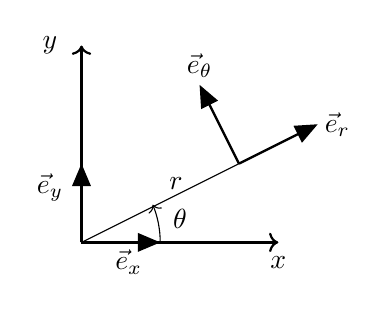
\begin{tikzpicture}
%\draw[step=0.5cm,gray,very thin] (0,0) grid (4.5,4); %background grid

\draw [thick,->] (1,1) -- (3.5,1);
\draw [thick,->] (1,1) -- (1,3.5);

\node[] at (3.5,0.75) {$x$};
\node[] at (0.6,3.5) {$y$};

\draw[>=triangle 45, line width=0.3mm, ->] (1,1) -- (2,1) ;   
\node[] at (1.6,0.75) {$\vec{e}_x$};

\draw[>=triangle 45, line width=0.3mm, ->] (1,1) -- (1,2) ;   
\node[] at (0.6,1.7) {$\vec{e}_y$};

\draw [-] (1,1) -- (3,2);

\draw[>=triangle 45, line width=0.3mm, ->] (3,2) -- (4,2.5) ;   
\node[] at (4.25,2.5) {$\vec{e}_r$};

\draw[>=triangle 45, line width=0.3mm, ->] (3,2) -- (2.5,3) ;   
\node[] at (2.5,3.25) {$\vec{e}_\theta$};


\node[] at (2.2,1.75) {$r$};
\node[] at (2.25,1.3) {$\theta$};

\draw[->] (2,1) arc (0:22.5:1.25);

\end{tikzpicture}
\end{center}


\noindent The relation between the unit vector in Cartesian and Polar/Cylindrical coordinates
is given by:
\[
\left(
\begin{array}{c}
{\vec e}_{r} \\
{\vec e}_{\theta} \\
\end{array}
\right)
=
\left(
\begin{array}{cc}
\cos \theta & \sin \theta \\
-\sin \theta & \cos \theta
\end{array}
\right)
\cdot
\left(
\begin{array}{c}
{\vec e}_{x} \\
{\vec e}_{y} \\
\end{array}
\right)
\]
which should be read:
\begin{eqnarray}
{\vec e}_{r}      &=& \cos\theta \; {\vec e}_{x} + \sin\theta \;  {\vec e}_{y} \nn\\
{\vec e}_{\theta} &=& -\sin\theta \; {\vec e}_{x} + \cos\theta \;  {\vec e}_{y} 
\end{eqnarray}
Obviously for $\theta=0$ we find $\vec{e}_r=\vec{e}_x$ and $\vec{e}_\theta = \vec{0}$, while for 
$\theta=\pi/2$ then $\vec{e}_r=\vec{0}$ and $\vec{e}_\theta=\vec{e}_y$.

Note that this $2\times 2$ matrix is a 
rotation matrix\footnote{\url{https://en.wikipedia.org/wiki/Rotation_matrix}}
corresponding to an angle $-\theta$. The inverse of this matrix always exists 
(we can always counter-rotate) and it then yields
\[
\left(
\begin{array}{c}
{\vec e}_{x} \\
{\vec e}_{y} \\
\end{array}
\right)
=
\left(
\begin{array}{cc}
\cos \theta & -\sin \theta \\
\sin \theta & \cos \theta
\end{array}
\right)
\cdot
\left(
\begin{array}{c}
{\vec e}_{r} \\
{\vec e}_{\theta} \\
\end{array}
\right)
\]
so that for any vector ${\vec V}$
\begin{eqnarray}
{\vec V} 
&=& V_x {\vec e}_x  + V_y {\vec e}_y \nonumber\\
&=& V_x [(\cos \theta) {\vec e}_r - (\sin \theta) {\vec e}_\theta]  + 
    V_y [(\sin \theta) {\vec e}_r + (\cos \theta){\vec e}_\theta] \nonumber\\
&=& [V_x (\cos \theta) + V_y (\sin \theta)] {\vec e}_r +
[- V_x(\sin \theta) + V_y (\cos \theta)]{\vec e}_\theta \nn\\
&=& V_r \vec{e}_r  + V_\theta \vec{e}_\theta \nn
\end{eqnarray}
with
\begin{eqnarray}
V_r &=& V_x \cos \theta + V_y \sin \theta \nn\\
V_\theta &=& - V_x \sin \theta + V_y \cos \theta \nn
\end{eqnarray}
Finally the path increment is
\[
d\vec{r} = dr \; {\vec e}_r  + r \sin\theta d\theta \; {\vec e}_\theta
\]
and the volume element is 
\[
dV= r dr \; d\theta.
\]
The gradient, divergence and Laplacian formulae are given in the following section about 
the cylindrical coordinates.

\index{general}{Path Increment in Polar Coordinates}

%...........................................................
\subsubsection{Cylindrical coordinates \label{ss:cylcoord}}

%Redo with tikz
\begin{center}
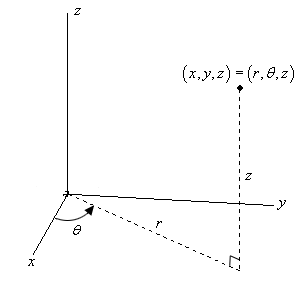
\includegraphics[width=4cm]{images/cylindrical}\\
{\captionfont Cylindrical coordinates}
%https://tutorial.math.lamar.edu/classes/calcii/CylindricalCoords.aspx 
\end{center}

\[
{\vec V} 
= V_r \; \vec{e}_r  + V_\theta \; \vec{e}_\theta + V_z \; \vec{e}_z
\]
We have 
\begin{eqnarray}
x &=& r \; \cos\theta \nn\\
y &=& r \; \sin \theta \nn\\\ 
r &=& \sqrt{x^2+y^2} \nn
\end{eqnarray}

Let $f(r,\theta)$ be a function of the spatial coordinates. Its gradient is then
\[
\vec \nabla f
= \frac{\partial f}{\partial r} \; \vec{e}_r 
+ \frac{1}{r} \frac{\partial f}{\partial \theta} \; \vec{e}_\theta
+ \frac{\partial f}{\partial r} \; \vec{e}_z
\]
The divergence of a vector field $\vec{V}$ is 
\[
\vec\nabla \cdot \vec{V} 
= \frac{1}{r} \frac{\partial }{\partial r} (r V_r) 
+ \frac{1}{r} \frac{\partial V_\theta}{\partial \theta} 
+ \frac{\partial V_z}{\partial z}
\]
and the Laplacian of $f$ is
\[
\Delta f = \frac{1}{r} \frac{\partial }{\partial r} \left( r \frac{\partial f}{\partial r} \right)
+ \frac{1}{r^2} \frac{\partial^2 f}{\partial \theta^2} 
+ \frac{\partial^2 f}{\partial z^2} 
\]
Finally the path increment is
\[
d\vec{r} = dr \; {\vec e}_r  + r \sin\theta d\theta \; {\vec e}_\theta + dz \; \vec{e}_z
\]
and the volume element is 
\[
dV= r dr \; d\theta \; dz
\]
\index{general}{Gradient Operator in Cylindrical Coordinates}
\index{general}{Divergence Operator in Cylindrical Coordinates}
\index{general}{Laplace Operator in Cylindrical Coordinates}
\index{general}{Path Increment in Cylindrical Coordinates}

\begin{remark} 
Cylindrical coordinates can also be denoted by $(\rho,\theta)$, $(r,\phi)$ or even $(\rho,\phi)$.
They are sometimes called "cylindrical polar coordinates" or "polar cylindrical coordinates".
\end{remark}

%........................................
\subsubsection{Spherical coordinates \label{ss:sphercoord}}

On the following figure are represented the three Cartesian axis, 
a point and its spherical coordinates $r,\theta,\phi$:
\begin{center}
\includegraphics[width=5cm]{images/sphcoord}\\
{\captionfont Spherical coordinates as commonly used in physics:\\ polar angle $\theta$, and azimuthal angle $\phi$.} 
\end{center}
In this case $\theta\in[0:\pi]$ and $\phi\in]-\pi:\pi]$ and we have the following relationships:
\begin{eqnarray}
r &=& \sqrt{x^2+y^2+z^2} \\
\theta &=& \arccos (z/r) \\
\phi &=& \arctan (y/x) \\
x &=& r \sin \theta \cos \phi \\
y &=& r \sin\theta \sin\phi \\
z &=& r \cos\theta 
\end{eqnarray}
The inverse tangent used to compute $\phi$ must be suitably defined, 
taking into account the correct quadrant of $(x,y)$,
which is why the atan2 intrinsic function is used in \textsc{FORTRAN} for example.    
This is often written as follows:
\begin{eqnarray}
\theta &=& \arctan \left(\sqrt{x^2+y^2},z\right) \\
\phi &=& \arctan (y,x) 
\end{eqnarray}
where we formally take advantage of the two argument arctan
function to eliminate quadrant confusion.

The path increment is expressed as:

\begin{equation}
d\vec{r} = dr \; \vec{e}_r + r d\theta \; \vec{e}_\theta + r \sin\theta d\phi \; \vec{e}_\phi
\end{equation}
The gradient of a function $f(r,\theta,\phi)$ is 
\begin{equation}
\vec\nabla f= \frac{\partial f}{\partial r} \; \vec{e}_r
+ \frac{1}{r} \frac{\partial f}{\partial \theta} \; \vec{e}_\theta 
+ \frac{1}{r \; \sin\theta} \frac{\partial f}{\partial \phi} \;  \vec{e}_\phi
\end{equation}
The divergence of a vector $\vec{V}$ is
\begin{equation}
\vec\nabla\cdot \vec{V}=
\frac{1}{r^2} \frac{\partial}{\partial r} \left(r^2 V_r \right) 
+
\frac{1}{r \sin\theta} \frac{\partial}{\partial \theta} (V_\theta \sin\theta)
+
\frac{1}{r \sin\theta} \frac{\partial V_\phi}{\partial \phi}=0
\label{eq:divsc}
\end{equation}
The Laplacian of function $f$ is given by: \index{general}{Laplacian}
\begin{equation}
\Delta f= \vec\nabla \cdot\vec\nabla f= \vec\nabla^2 f
=
\frac{1}{r^2}\frac{\partial}{\partial r} \left( r^2 \frac{\partial f}{\partial r} \right)
+\frac{1}{r^2 \sin\theta} \frac{\partial}{\partial \theta} \left( \sin\theta \frac{\partial f}{\partial \theta} \right)
+\frac{1}{r^2 \sin^2\theta}  \frac{\partial^2 f}{\partial \phi^2}
\end{equation}

In geography one uses latitude and longitude, represented hereunder:
\begin{center}
\includegraphics[width=10cm]{images/map.jpg}
\end{center}
\begin{itemize}
\item Latitude  $\in[-90:90]$,   or $\in[-\pi/2:\pi/2]$ 
\item Longitude $\in]-180:180]$, or $\in]-\pi:\pi]$ 
\end{itemize}

Since the colatitude is the complementary angle of the latitude, 
i.e. the difference between 90 and the latitude, 
where southern latitudes are denoted with a minus sign,
$\theta$ as shown above is actually is the colatitude.
The colatitude is shown in red on the following figure: 
\index{general}{Colatitude}
\begin{center}
\includegraphics[width=3cm]{images/colatitude}
\end{center}

The volume of a sphere of radius $R$ is easily obtained by computing 
\begin{eqnarray}
V_{sphere} 
&=& \iiint_{sphere} dV \nn\\
&=& \int_0^R r^2 dr \int_0^\pi \sin\theta d\theta \int_0^{2\pi} d\phi  \nn\\
&=& \frac{1}{3}R^3  \cdot 2 \cdot 2\pi \nn\\
&=& \frac{4}{3}\pi R^3 
\end{eqnarray}
\index{general}{Volume of a Sphere}

The volume of a spherical shell of inner radius $R_i$ and outer radius $R_o$
is equally easily obtained by computing 

\begin{eqnarray}
V_{shell}
&=& \iiint_{shell} dV \nn\\
&=& \int_{R_i}^{R_o} r^2 dr \int_0^\pi \sin\theta d\theta \int_0^{2\pi} d\phi  \nn\\
&=& \frac{1}{3}(R_o^3-R_i^3)  \cdot 2 \cdot 2\pi \nn\\
&=& \frac{4}{3}\pi (R^3_o -R^3_i)
\end{eqnarray}
\index{general}{Volume of a Spherical shell}


\noindent The spherical unit vectors are related to the Cartesian unit vectors by:
\[
\left(
\begin{array}{c}
\vec{e}_{r} \\ \vec{e}_\theta \\ \vec{e}_\phi
\end{array}
\right)
=
\left(
\begin{array}{ccc}
\sin\theta \cos\phi & \sin\theta\sin\phi & \cos\theta  \\
\cos\theta \cos\phi & \cos\theta\sin\phi & -\sin\theta \\
-\sin\phi & \cos\phi & 0
\end{array}
\right)
\left(
\begin{array}{c}
\vec{e}_{x} \\ \vec{e}_y \\ \vec{e}_z
\end{array}
\right)
\]
and the Cartesian unit vectors are related to the spherical unit vectors by

\[
\left(
\begin{array}{c}
\vec{e}_{x} \\ \vec{e}_y \\ \vec{e}_z
\end{array}
\right)
=
\left(
\begin{array}{ccc}
\sin\theta \cos\phi & \cos\theta\cos\phi & -\sin\phi  \\
\sin\theta \sin\phi & \cos\theta\sin\phi & \cos\phi \\
\cos\theta & -\sin\theta & 0
\end{array}
\right)
\left(
\begin{array}{c}
\vec{e}_{r} \\ \vec{e}_\theta \\ \vec{e}_\phi
\end{array}
\right)
\]
Finally, the velocity vector $\vec{\upnu}$ then becomes
\begin{eqnarray}
\vec{\upnu} 
&=& u\; \vec{e}_x + v \; \vec{e}_y + w \; \vec{e}_z \nn\\
&=& u\; ( \sin\theta \cos\phi \; \vec{e}_r +  \cos\theta\cos\phi \;  \vec{e}_{\theta} -\sin\phi \; \vec{e}_{\phi} ) \nn\\
&+& v\; ( \sin\theta \sin\phi \; \vec{e}_r + \cos\theta\sin\phi \; \vec{e}_\theta  +  \cos\phi \;  \vec{e}_\phi  )  \nn\\
&+& w\; ( \cos\theta \; \vec{e}_r   -\sin\theta \; \vec{e}_\theta  ) \nn\\
&=& v_r\; \vec{e}_r + v_\theta\; \vec{e}_\theta + v_\phi\; \vec{e}_\phi 
\end{eqnarray}
with 
\begin{eqnarray}
v_r      &=&  u \sin \theta  \cos \phi  + v \sin\theta \sin \phi + w \cos\theta \\
v_\theta &=&  u \cos\theta\cos\phi + v \cos\theta\sin\phi -w \sin\theta   \\
v_\phi   &=& -u \sin\phi  + v \cos\phi  
\end{eqnarray}

%.................................................................................................
\subsubsection{Converting tensors between Cartesian and Cylindrical bases \label{ss:convcartspher}}

\[
{\bm T}_{\tiny Cyl}=
\left(
\begin{array}{ccc}
T_{rr}       & T_{r\theta}      & T_{rz} \\
T_{\theta r} & T_{\theta\theta} & T_{\theta z} \\
T_{z r}      & T_{z \theta}     & T_{zz}
\end{array}
\right)
=
\left(
\begin{array}{ccc}
 \cos \theta&\sin \theta&0 \\
-\sin \theta&\cos \theta&0 \\
0 & 0 & 1 
\end{array}
\right)
\cdot
\left(
\begin{array}{ccc}
T_{xx} & T_{xy} & T_{xz} \\
T_{yx} & T_{yy} & T_{yz} \\
T_{zx} & T_{zy} & T_{zz} 
\end{array}
\right)
\cdot
\left(
\begin{array}{ccc}
\cos \theta & -\sin \theta&0 \\
\sin \theta &  \cos \theta&0 \\
0 & 0 & 1 
\end{array}
\right)
\]

\[
{\bm T}_{\tiny Cart}=
\left(
\begin{array}{ccc}
T_{xx} & T_{xy} & T_{xz} \\
T_{yx} & T_{yy} & T_{yz} \\
T_{zx} & T_{zy} & T_{zz} 
\end{array}
\right)
=
\left(
\begin{array}{ccc}
 \cos \theta&-\sin \theta&0 \\
\sin \theta&\cos \theta&0 \\
0 & 0 & 1 
\end{array}
\right)
\cdot
\left(
\begin{array}{ccc}
T_{rr}       & T_{r\theta}      & T_{rz} \\
T_{\theta r} & T_{\theta\theta} & T_{\theta z} \\
T_{z r}      & T_{z \theta}     & T_{zz}
\end{array}
\right)
\cdot
\left(
\begin{array}{ccc}
\cos \theta & \sin \theta&0 \\
-\sin \theta &  \cos \theta&0 \\
0 & 0 & 1 
\end{array}
\right)
\]



%.................................................................................................
\subsubsection{Converting tensors between Cartesian and Spherical bases \label{ss:convcartspher}}

Let ${\bm T}$ be a tensor
\[
{\bm T}=
\left(
\begin{array}{ccc}
T_{xx} & T_{xy} & T_{xz} \\
T_{yx} & T_{yy} & T_{yz} \\
T_{zx} & T_{zy} & T_{zz} 
\end{array}
\right)
\qquad\qquad
{\bm T}=
\left(
\begin{array}{ccc}
T_{rr}       & T_{r\theta}      & T_{r\phi} \\
T_{\theta r} & T_{\theta\theta} & T_{\theta\phi} \\
T_{\phi r}   & T_{\phi \theta}  & T_{\phi\phi}
\end{array}
\right)
\]
in the Cartesian basis (left) and the spherical basis (right).

The two sets of components are related by
\[
\left(
\begin{array}{ccc}
T_{xx} & T_{xy} & T_{xz} \\
T_{yx} & T_{yy} & T_{yz} \\
T_{zx} & T_{zy} & T_{zz} 
\end{array}
\right)
=
\left(
\begin{array}{ccc}
\sin\theta \; \cos\phi & \cos\theta \; \cos\phi & -\sin\phi \\
\sin\theta \; \sin\phi & \cos\theta \; \sin\phi &  \cos\phi \\
\cos\theta & -\sin\theta & 0 
\end{array}
\right)
\cdot
\left(
\begin{array}{ccc}
T_{rr}       & T_{r\theta}      & T_{r\phi} \\
T_{\theta r} & T_{\theta\theta} & T_{\theta\phi} \\
T_{\phi r}   & T_{\phi \theta}  & T_{\phi\phi}
\end{array}
\right)
\cdot
\left(
\begin{array}{ccc}
\sin\theta\;\cos\phi & \sin\theta\;\sin\phi & \cos\theta \\
\cos\theta\;\cos\phi & \cos\theta\;\sin\phi & -\sin\theta \\
-\sin\phi & \cos\phi & 0 
\end{array}
\right)
\]
or
\[
\left(
\begin{array}{ccc}
T_{rr}       & T_{r\theta}      & T_{r\phi} \\
T_{\theta r} & T_{\theta\theta} & T_{\theta\phi} \\
T_{\phi r}   & T_{\phi \theta}  & T_{\phi\phi}
\end{array}
\right)
=
\left(
\begin{array}{ccc}
\sin\theta \; \cos\phi & \sin\theta \; \sin\phi & \cos\theta \\
\cos\theta \; \cos\phi & \cos\theta \; \sin\phi & -\sin\theta \\
-\sin\phi & \cos\phi & 0 
\end{array}
\right)
\cdot
\left(
\begin{array}{ccc}
T_{xx} & T_{xy} & T_{xz} \\
T_{yx} & T_{yy} & T_{yz} \\
T_{zx} & T_{zy} & T_{zz} 
\end{array}
\right)
\cdot
\left(
\begin{array}{ccc}
\sin\theta\;\cos\phi & \cos\theta\;\cos\phi & -\sin\phi \\
\sin\theta\;\sin\phi & \cos\theta\;\sin\phi & \cos\phi \\
\cos\theta & -\sin\theta & 0
\end{array}
\right)
\]
If we now assume that the tensor ${\bm T}$ is symmetric (e.g. stress tensor, strain rate tensor),
then there are only 6 independent terms.

 \label{ss:coordsys} %-------------------
\subsection{A continuum mechanics primer} %--------------------------------------------------------
\begin{flushright} {\tiny {\color{gray} continuum\_mechanics.tex}} \end{flushright}
%~~~~~~~~~~~~~~~~~~~~~~~~~~~~~~~~~~~~~~~~~~~~~~~~~~~~~~~~~~~~~~~~~~~~~~~~~~~~~~~~~~~~~~~~~~~~~~~~~~

{\sl Contains contributions by W. Spakman} \index{contributors}{W. Spakman}

%......................................................................
\subsubsection{Forces}

In continuum mechanics we make a distinction between two broad classes of forces:
\begin{itemize}
\item Body forces defined as force per unit volume (\si{\newton\per\cubic\metre}): 
gravity, electro-magnetic forces
\item Tractions: Surface forces defined as force per unit surface area (\si{\newton\per\square\metre}):
Contact forces, elastic forces per unit area, internal flow friction, pressure, ...\\
A traction is the surface average of all atomic forces exerted by
atoms on the one side on atoms on the other side of the surface.
For real-Earth processes, internal tractions are ultimately caused by
the body forces, usually gravity.


Existing mantle flow(i.e. flow that is forced elsewhere) can exert
tractions (shear stresses) on the subducting slab or for instance at
the base of lithosphere plates.
In HPT-laboratory experiments external tractions (pressure, shear
traction) are applied to a rock sample, which cause internal
tractions to balance the exerted forces.

\begin{center}
\includegraphics[width=6cm]{images/contmech/spak1}
\end{center}
\end{itemize}

%......................................................................
\subsubsection{Stress tensor and tractions}\label{sec:stresstensor}
\index{general}{Stress Tensor} 
\index{general}{Normal Stress} 
\index{general}{Shear Stress} 
\index{general}{Stress Vector} 
\index{general}{Traction}

The Cauchy tensor\footnote{\url{https://en.wikipedia.org/wiki/Cauchy_stress_tensor}} 
consists of nine components $\sigma_{ij}$  that completely define the state of stress 
at a point inside a material. 
The tensor relates a unit-length direction vector $\vec{n}$ to the so-called 'stress vector' (most commonly called 'traction') $\vec{t}(\vec{n})$ across an imaginary surface perpendicular to $\vec{n}$:
\[
\vec{t}(\vec n)= {\bm \sigma}\cdot {\vec n}
\]

\begin{center}
\includegraphics[width=7cm]{images/contmech/Components_stress_tensor_cartesian}\\
{\scriptsize Modified from original 
file on Wikipedia\footnote{\url{https://commons.wikimedia.org/wiki/File:Components_stress_tensor_cartesian.svg}}}
\end{center}

\noindent 
With respect to an orthonormal basis $\{\vec{e}_x,\vec{e}_y,\vec{e}_z\}$, the Cauchy stress tensor
is given by:
\begin{equation}
{\bm \sigma}=
\left(
\begin{array}{ccc}
\sigma_{xx} & \sigma_{xy} & \sigma_{xz} \\
\sigma_{yx} & \sigma_{yy} & \sigma_{yz} \\
\sigma_{zx} & \sigma_{zy} & \sigma_{zz} 
\end{array}
\right)
\end{equation}
The three diagonal elements are called normal stresses while the off-diagonal terms 
are called shear stresses.

One can easily prove (see for instance Section 3.3.6 of \cite{grbl09}) that the balance 
of angular momentum leads reduces to the statement that the Cauchy stress tensor 
is symmetric, i.e. ${\bm \sigma}={\bm \sigma}^T$.
Therefore, the stress state of the medium at any point and instant can be specified by only six independent parameters, rather than nine:
\begin{equation}
{\bm \sigma}=
\left(
\begin{array}{ccc}
\sigma_{xx} & \sigma_{xy} & \sigma_{xz} \\
\sigma_{xy} & \sigma_{yy} & \sigma_{yz} \\
\sigma_{xz} & \sigma_{yz} & \sigma_{zz} 
\end{array}
\right)
\qquad\qquad
\text{or sometimes}
\qquad\qquad
{\bm \sigma}=
\left(
\begin{array}{ccc}
\sigma_{x}  & \tau_{xy}  & \tau_{xz} \\
\tau_{xy}   & \sigma_{y} & \tau_{yz} \\
\tau_{xz}   & \tau_{yz}  & \sigma_{z} 
\end{array}
\right)
\end{equation}
where the elements $\sigma _{x}$, $\sigma _{y}$, $\sigma _{z}$ are called the orthogonal 
normal stresses (relative to the chosen coordinate system), and $\tau _{xy}$, $\tau _{xz}$,
$\tau _{yz}$ the orthogonal shear stresses. The left form is preferred in this document.
As seen above, the SI units of both stress tensor and traction are \si{\newton\per\square\metre}.

In Cylindrical coordinates the stress tensor components are given by:
\begin{eqnarray}
\sigma_{rr} &=& -p + 2 \eta \frac{\partial \upnu_r}{\partial r}      \\
\sigma_{\theta\theta} &=& 
 -p + 2\eta \left( \frac{1}{r} \frac{\partial \upnu_\theta}{\partial\theta} +\frac{\upnu_r}{r} \right)    \\
\sigma_{zz} &=& -p + 2 \eta \frac{\partial \upnu_z}{\partial z}      \\
\sigma_{r\theta} &=& \eta \left( \frac{1}{r} \frac{\partial \upnu_r}{\partial \theta} 
+ \frac{\partial \upnu_\theta}{\partial r} - \frac{\upnu_\theta}{r} \right)  \\
\sigma_{rz} &=& \eta \left( \frac{\partial \upnu_r}{\partial z}  + \frac{\partial \upnu_z}{\partial r}\right) \\
\sigma_{\theta z} &=&  \eta \left(  \frac{1}{r} \frac{\partial \upnu_z}{\partial \theta}
+\frac{\partial \upnu_\theta}{\partial z}     \right) 
\end{eqnarray}
\index{general}{Stress Tensor (Cylindrical Coordinates)}

In Spherical coordinates the stress tensor components are given by:
\begin{eqnarray}
\sigma_{rr} &=& -p + 2 \eta \frac{\partial \upnu_r}{\partial r}      \\
\sigma_{\theta\theta} &=& 
 -p + 2\eta \left( \frac{1}{r} \frac{\partial \upnu_\theta}{\partial\theta} +\frac{\upnu_r}{r} \right)    \\
\sigma_{\phi\phi} &=& 
-p + 2\eta \left( \frac{1}{r \sin \theta} \frac{\partial \upnu_\phi}{\partial \phi} 
+\frac{\upnu_r}{r}  + \frac{\upnu_\theta \cot \theta}{r} \right) \\
\sigma_{r\theta} &=& \eta\left(  r \frac{\partial}{\partial r} \frac{\upnu_\theta}{r}  
+\frac{1}{r} \frac{\partial \upnu_r}{\partial\theta}   \right)\\
\sigma_{r\phi} &=& \eta \left( \frac{1}{r \sin\theta}\frac{\partial \upnu_r}{\partial \phi} 
+ r \frac{\partial}{\partial r} \frac{\upnu_\phi}{r}  \right)\\
\sigma_{\theta \phi} &=& \eta \left(
\frac{1}{r \sin\theta} \frac{\partial \upnu_\theta}{\partial\phi}
+\frac{\sin\theta}{r} \frac{\partial}{\partial \theta} \frac{\upnu_\phi}{\sin\theta}
\right) 
\end{eqnarray}
\index{general}{Stress Tensor (Spherical Coordinates)}

 %----------------------------------------------------------------------

\begin{center}
\begin{tabular}{lll}
\hline
Symbol & meaning & unit \\
\hline
\hline
$t$ & Time & s \\
$x,y,z$ & Cartesian coordinates & m \\
${\bm v}$ & velocity vector & m$\cdot$ s$^{-1}$\\
$\rho$ & mass density & kg/m$^3$ \\
$\eta$ & dynamic viscosity &  Pa$\cdot$ s \\
$\lambda$ & penalty parameter & Pa$\cdot$ s \\
$T$ & temperature & K \\
${\bm \nabla}$ & gradient operator & m$^{-1}$ \\
${\bm \nabla}\cdot$ & divergence operator & m$^{-1}$ \\
$p$ & pressure & Pa\\
$\dot{\bm \varepsilon}({\bm v})$ & strain rate tensor & s$^{-1}$ \\
$\alpha$ & thermal expansion coefficient & K$^{-1}$ \\
$k$ & thermal conductivity & W/(m $\cdot$ K) \\
$C_p$ & Heat capacity & J/K \\
$H$ & intrinsic specific heat production & W/kg\\
$\beta_T$ & isothermal compressibility & Pa$^{-1}$  \\
${\bm \tau}$ & deviatoric stress tensor & Pa \\
${\bm \sigma}$ & full stress tensor & Pa \\
\hline
\end{tabular}
\end{center}

%------------------------------------------------------------------------
\subsection{The heat transport equation - energy conservation equation}

Let us start from the heat transport equation as shown in Schubert, Turcotte and Olson \cite{scto01}:
\[
\rho C_p \frac{DT}{Dt} - \alpha T \frac{Dp}{Dt} = {\bm \nabla} \cdot k {\bm \nabla} T + \Phi + \rho H  
\]
with $D/Dt$ being the total derivatives so that 
\[
\frac{DT}{Dt} = \frac{\partial T}{\partial t} + {\bm v}\cdot {\bm \nabla}T
\quad\quad
\frac{Dp}{Dt} = \frac{\partial p}{\partial t} + {\bm v}\cdot {\bm \nabla}p
\]
Solving for temperature, this equation is often rewritten as follows:
\begin{mdframed}[backgroundcolor=blue!5]
\[
\rho C_p \frac{DT}{Dt} - {\bm \nabla} \cdot k {\bm \nabla} T =  \alpha T \frac{Dp}{Dt} + \Phi + \rho H  
\]
\end{mdframed}

A note on the shear heating term $\Phi$: In many publications, $\Phi$ 
is given by $\Phi=\tau_{ij}\partial_j u_i={\bm \tau}:{\bm \nabla}{\bm v}$.

\begin{eqnarray}
\Phi 
&=& \tau_{ij}\partial_j u_i \nonumber\\
&=& 2 \eta \dot{\varepsilon}_{ij}^d\partial_j u_i \nonumber\\
&=& 2 \eta \frac{1}{2}\left( \dot{\varepsilon}_{ij}^d\partial_j u_i + \dot{\varepsilon}_{ji}^d\partial_i u_j \right) \nonumber\\
&=& 2 \eta \frac{1}{2}\left( \dot{\varepsilon}_{ij}^d\partial_j u_i + \dot{\varepsilon}_{ij}^d\partial_i u_j \right) \nonumber\\
&=& 2 \eta  \dot{\varepsilon}_{ij}^d  \frac{1}{2}\left(\partial_j u_i + \partial_i u_j \right) \nonumber\\
&=& 2 \eta  \dot{\varepsilon}_{ij}^d   \dot{\varepsilon}_{ij} \nonumber\\
&=& 2 \eta  \dot{\bm \varepsilon}^d :  \dot{\bm \varepsilon} \nonumber\\
&=& 2 \eta  \dot{\bm \varepsilon}^d : \left( \dot{\bm \varepsilon}^d +\frac{1}{3} ({\bm \nabla}\cdot{\bm v}) {\bm 1} \right)\nonumber\\
&=& 2 \eta  \dot{\bm \varepsilon}^d : \dot{\bm \varepsilon}^d 
+ 2 \eta  \dot{\bm \varepsilon}^d : {\bm 1} ({\bm \nabla}\cdot{\bm v}) \nonumber\\ 
&=& 2 \eta  \dot{\bm \varepsilon}^d : \dot{\bm \varepsilon}^d 
\end{eqnarray}
Finally
\[
\Phi = {\bm \tau}:{\bm \nabla}{\bm v} = 2 \eta  \dot{\bm \varepsilon}^d : \dot{\bm \varepsilon}^d
= 2 \eta \left( (\dot{\varepsilon}_{xx}^d)^2 + (\dot{\varepsilon}_{yy}^d)^2 + 2(\dot{\varepsilon}_{xy}^d)^2 \right)
\]

%------------------------------------------------------------------------
\subsection{The momentum conservation equations} 

Because the Prandlt number is virtually zero in Earth science applications the Navier Stokes 
equations reduce to the Stokes equation:
\[
{\bm \nabla}\cdot {\bm \sigma} + \rho {\bm g} = 0
\]
Since 
\[
{\bm \sigma} = -p {\bm 1} + {\bm \tau}
\]
it also writes
\[
-{\bm \nabla}p + {\bm \nabla}\cdot {\bm \tau} + \rho {\bm g} = 0
\]
Using the relationship ${\bm \tau} = 2 \eta \dot{\bm \varepsilon}^d$ we arrive at 
\begin{mdframed}[backgroundcolor=blue!5]
\[
-{\bm \nabla}p + {\bm \nabla}\cdot (2 \eta \dot{\bm \varepsilon}^d ) + \rho {\bm g} = 0
\]
\end{mdframed}

%------------------------------------------------------------------------
\subsection{The mass conservation equations} 

The mass conservation equation is given by
\[
\frac{D\rho}{Dt} + \rho {\bm \nabla}\cdot{\bm v} = 0
\]
or, 
\begin{mdframed}[backgroundcolor=blue!5]
\[
\frac{\partial \rho}{\partial t} + {\bm \nabla}\cdot(\rho {\bm v}) = 0
\]
\end{mdframed}
In the case of an incompressible flow, then $\partial \rho/\partial t=0$ and 
${\bm \nabla}\rho=0$, i.e. $D\rho/Dt=0$ and the remaining equation is simply:
\[
{\bm \nabla}\cdot{\bm v} = 0
\]

\subsection{The equations in ASPECT manual}
The following is lifted off the ASPECT manual.
We focus on the system of equations in a $d=2$- or $d=3$-dimensional
domain $\Omega$ that describes the motion of a highly viscous fluid driven
by differences in the gravitational force due to a density that depends on
the temperature. In the following, we largely follow the exposition of this
material in Schubert, Turcotte and Olson \cite{scto01}.

Specifically, we consider the following set of equations for velocity $\mathbf
u$, pressure $p$ and temperature $T$:
\begin{align}
  \label{eq:stokes-1}
  -\nabla \cdot \left[2\eta \left(\dot\varepsilon(\bm v)
                                  - \frac{1}{3}(\nabla \cdot \bm v)\mathbf 1\right)
                \right] + \nabla p &=
  \rho \bm g
  &
  & \textrm{in $\Omega$},
  \\
  \label{eq:stokes-2}
  \nabla \cdot (\rho \bm v) &= 0
  &
  & \textrm{in $\Omega$},
  \\
  \label{eq:temperature}
  \rho C_p \left(\frac{\partial T}{\partial t} + \bm v\cdot\nabla T\right)
  - \nabla\cdot k\nabla T
  &=
  \rho H
  \notag
  \\
  &\quad
  +
  2\eta
  \left(\dot\varepsilon(\bm v) - \frac{1}{3}(\nabla \cdot \bm v)\mathbf 1\right)
  :
  \left(\dot\varepsilon(\bm v) - \frac{1}{3}(\nabla \cdot \bm v)\mathbf 1\right)
  \\
  &\quad
  +\alpha T \left( \bm v \cdot \nabla p \right)
  \notag
  \\
  &\quad
  &
  & \textrm{in $\Omega$},
  \notag
\end{align}
where $\dot{\bm \varepsilon}(\mathbf u) = \frac{1}{2}(\nabla \mathbf u + \nabla\mathbf
u^T)$ is the symmetric gradient of the velocity (often called the
\textit{strain rate}).%

In this set of equations, \eqref{eq:stokes-1} and \eqref{eq:stokes-2}
represent the compressible Stokes equations in which $\mathbf v=\mathbf
v(\mathbf x,t)$ is the velocity field and $p=p(\mathbf x,t)$ the pressure
field. Both fields depend on space $\mathbf x$ and time $t$. Fluid flow is
driven by the gravity force that acts on the fluid and that is proportional to
both the density of the fluid and the strength of the gravitational pull.

Coupled to this Stokes system is equation \eqref{eq:temperature} for the
temperature field $T=T(\mathbf x,t)$ that contains heat conduction terms as
well as advection with the flow velocity $\mathbf v$. The right hand side
terms of this equation correspond to
\begin{itemize}
\item internal heat production for example due to radioactive decay;
\item friction (shear) heating;
\item adiabatic compression of material;
\end{itemize}

In order to arrive at the set of equations that ASPECT solves, 
we need to 
\begin{itemize}
\item neglect the $\partial p/\partial t$. {\color{red}WHY?}
\item neglect the $\partial \rho / \partial t$ . {\color{red}WHY?}
\end{itemize}
from equations above. 

----------------------------------------

Also, their definition of the shear heating term $\Phi$ is:
\[
\Phi = k_B ({\bm \nabla}\cdot{\bm v})^2 + 2\eta \dot{\bm \varepsilon}^d:\dot{\bm \varepsilon}^d
\]
For many fluids the bulk viscosity $k_B$ is very small and is often taken to be zero, an assumption known
as the Stokes assumption: $k_B=\lambda+2\eta/3=0$. \index{bulk viscosity}
Note that $\eta$ is the dynamic viscosity and $\lambda$ the second viscosity. \index{dynamic viscosity}
\index{second viscosity}
Also, 
\[
{\bm \tau}=2\eta \dot{\bm \varepsilon} + \lambda ({\bm \nabla}\cdot{\bm v}) {\bm 1}
\]
but since $k_B=\lambda+2\eta/3=0$, then $\lambda=-2\eta/3$ so 
\[
{\bm \tau}=2\eta \dot{\bm \varepsilon} -\frac{2}{3}\eta ({\bm \nabla}\cdot{\bm v}) {\bm 1} = 2\eta \dot{\bm \varepsilon}^d
\]







\newpage
%---------------------------------
\subsection{the Boussinesq approximation: an Incompressible flow}

\index{Boussinesq}

[from aspect manual]
The Boussinesq approximation assumes that the density can be
considered constant in all occurrences in the equations with the exception of
the buoyancy term on the right hand side of \eqref{eq:stokes-1}. The primary
result of this assumption is that the continuity equation \eqref{eq:stokes-2}
will now read
\[
{\bm \nabla}\cdot{\bm v} = 0
\]
This implies that the strain rate tensor is deviatoric.
Under the Boussinesq approximation, the equations are much simplified:

\begin{align}
  \label{eq:stokes-1}
  -\nabla \cdot \left[2\eta \dot{\bm \varepsilon}(\bm v)
                \right] + \nabla p &=
  \rho \bm g
  &
  & \textrm{in $\Omega$},
  \\
  \label{eq:stokes-2}
  \nabla \cdot (\rho \bm v) &= 0
  &
  & \textrm{in $\Omega$},
  \\
  \label{eq:temperature}
  \rho_0 C_p \left(\frac{\partial T}{\partial t} + \bm v\cdot\nabla T\right)
  - \nabla\cdot k\nabla T
  &=
  \rho H
  &
  & \textrm{in $\Omega$}
\end{align}
Note that all terms on the rhs of the temperature equations have disappeared, with the exception 
of the source term.


\newpage
%%%%%%%%%%%%%%%%%%%%%%%%%%%%%%%%%%%%%%%%%%%%%%%%%%%%%%%%%%%%%%%%%%%%%%%%%%%%%%%%%%%%%%%%%%55
\subsection{Stokes equation for elastic medium}

What follows is mostly borrowed from Becker \& Kaus lecture notes.

%\begin{tabular}{|l|l|l|}
%\hline
%${\bm u}       $ & displacement vector &   \\
%${\bm \sigma}  $ & full stress tensor  & Pa\\
%${\bm \epsilon}$ & strain tensor       &   \\
%${\bm 1}       $ & unit tensor         &   \\
%${\bm f}       $ & body forces         &   \\
%\hline
%\end{tabular}

The strong form of the PDE that governs force balance in a medium is given by
\[
{\bm \nabla}\cdot{\bm \sigma}  + {\bm f} = {\bm 0}
\]
where ${\bm \sigma}$ is the stress tensor and ${\bm f}$ is a body force.

The stress tensor is related to the strain tensor through the generalised 
Hooke's law:
\begin{equation}
\sigma_{ij}=\sum_{kl}C_{ijkl}\epsilon{kl} \label{eq:one}
\end{equation}
where ${\bm C}$ is the fourth-order elastic tensor.
In the case of an isotropic material, this relationship simplifies to
\begin{equation}
\sigma_{ij}=\lambda \epsilon_{kk} \delta_{ij} + 2\mu \epsilon_{ij}
\quad\quad
or, 
\quad\quad
{\bm \sigma} = \lambda ({\bm \nabla}\cdot{\bm u})  {\bm 1} + 2\mu {\bm \epsilon}   \label{eq:two}
\end{equation}
where $\lambda$ is the Lam\'e parameter and $\mu$ is the shear modulus\footnote{It is also sometimes written $G$}.
The term ${\bm \nabla}\cdot{\bm u}$ is the isotropic dilation.

\index{Lam\'e parameter} \index{shear modulus}

The strain tensor is related to the displacement as follows: \index{strain tensor}
\[
{\bm \epsilon} = \frac{1}{2}({\bm \nabla}{\bm u} + {\bm \nabla}{\bm u}^T)
\]

The incompressibility (bulk modulus), $K$, is defined as $p=-K {\bm \nabla}\cdot{\bm u}$ 
where $p$ is the pressure with \index{bulk modulus}
\begin{eqnarray}
p&=&-\frac{1}{3}Tr({\bm \sigma}) \nonumber\\
 &=& -\frac{1}{3} [ \lambda ({\bm \nabla}\cdot{\bm u}) Tr[{\bm 1}] + 2 \mu Tr[{\bm \epsilon}]] \nonumber\\
 &=& -\frac{1}{3} [ \lambda ({\bm \nabla}\cdot{\bm u})  3  + 2 \mu  ({\bm \nabla}\cdot{\bm u}) ] \nonumber\\
 &=& -[ \lambda  + \frac{2}{3} \mu ]   ({\bm \nabla}\cdot{\bm u})  
\end{eqnarray}
so that $K=\lambda+\frac{2}{3}\mu$.

%or
%\[
%\mu=\frac{3K(1-2\nu)}{2(1+\nu)}
%\]


\paragraph{Remark}: Eq. (\ref{eq:one}) and (\ref{eq:two}) are analogous to the ones that one has to solve
in the context of viscous flow using the penalty method. In this case $\lambda$ is the penalty coefficient, 
${\bm u}$ is the velocity, and $\mu$ is then the dynamic viscosity.

%\begin{center}
%\includegraphics[width=15cm]{images/coeffs}\\
%{\small Homogeneous isotropic linear elastic materials have their elastic properties uniquely determined by any two moduli among these; thus, given any two, any other of the elastic moduli can be calculated according to these formulas.}
%\end{center}

The Lam\'e parameter and the shear modulus are also linked to $\nu$ the poisson ratio, 
and $E$, Young's modulus: \index{Poisson ratio} \index{Young's modulus}
\[
\lambda=\mu\frac{2\nu}{1-2\nu}
=\frac{\nu E}{(1+\nu)(1-2\nu)}
\quad\quad
{\rm with}
\quad\quad
E=2\mu(1+\nu)
\]
The shear modulus, expressed often in GPa, describes the material's response to shear stress.
The poisson ratio describes the response in the direction orthogonal to uniaxial stress.
The Young modulus, expressed in GPa, describes the material's strain response to uniaxial stress in the 
direction of this stress.


%%%%%%%%%%%%%%%%%%%%%%%%%%%%%%%%%%%%%%%%%%%%%%%%%%%%%%%%%%%%%%%%%%55
\newpage
\subsection{The strain rate tensor in all coordinate systems}

The strain rate tensor $\dot{\bm\varepsilon}$ is given by
\begin{equation}
\dot{\bm \varepsilon} = \frac{1}{2}( {\bm \nabla}{\bm v}+ {\bm \nabla}{\bm v}^T) 
\end{equation}

\subsubsection{Cartesian coordinates}
\begin{eqnarray}
\dot\varepsilon_{xx} &=& \frac{\partial u}{\partial x} \\
\dot\varepsilon_{yy} &=& \frac{\partial v}{\partial y} \\
\dot\varepsilon_{zz} &=& \frac{\partial w}{\partial z} \\
\dot\varepsilon_{yx} =
\dot\varepsilon_{xy} &=& \frac{1}{2} \left( \frac{\partial u}{\partial y} + \frac{\partial v}{\partial x}  \right)\\
\dot\varepsilon_{zx} =
\dot\varepsilon_{xz} &=& \frac{1}{2} \left( \frac{\partial u}{\partial z} + \frac{\partial w}{\partial x}  \right)\\
\dot\varepsilon_{zy} =
\dot\varepsilon_{yz} &=& \frac{1}{2} \left( \frac{\partial v}{\partial z} + \frac{\partial w}{\partial y}  \right)
\end{eqnarray}

\subsubsection{Polar coordinates}

\begin{eqnarray}
\dot\varepsilon_{rr} &=& \frac{\partial v_r}{\partial r} \\
\dot\varepsilon_{\theta\theta} &=& \frac{v_r}{r} + \frac{1}{r} \frac{\partial v_\theta}{\partial \theta}  \\
\dot\varepsilon_{\theta r} =
\dot\varepsilon_{r\theta} &=& \frac{1}{2} \left(   \frac{\partial v_\theta}{\partial r} - \frac{v_\theta}{r} 
+\frac{1}{r} \frac{\partial v_r}{\partial \theta}  \right) 
\end{eqnarray}

\subsubsection{Cylindrical coordinates}

http://eml.ou.edu/equation/FLUIDS/STRAIN/STRAIN.HTM

\subsubsection{Sperical coordinates}

\begin{eqnarray}
\dot\varepsilon_{rr} &=& \frac{\partial v_r}{\partial r} \\
\dot\varepsilon_{\theta\theta} &=& \frac{v_r}{r} + \frac{1}{r} \frac{\partial v_\theta}{\partial \theta}  \\
\dot\varepsilon_{\phi\phi} &=& \frac{1}{r \sin\theta} \frac{\partial v_\phi}{\partial \phi} \\
\dot\varepsilon_{\theta r} =
\dot\varepsilon_{r\theta}   &=& \frac{1}{2} \left( r \frac{\partial}{\partial r} (\frac{v_\theta}{r} ) 
+\frac{1}{r} \frac{\partial v_r}{\partial \theta} \right) \\
\dot\varepsilon_{\phi r} =
\dot\varepsilon_{r\phi}      &=&  \frac{1}{2} \left(  \frac{1}{r \sin\theta} \frac{\partial v_r}{\partial \phi} 
+ r \frac{\partial }{\partial r} (\frac{v_\phi}{r}) \right)  \\
\dot\varepsilon_{\phi \theta} =
\dot\varepsilon_{\theta\phi} &=& \frac{1}{2} \left( \frac{\sin \theta}{r} \frac{\partial }{\partial \theta} (\frac{v_\phi}{\sin\theta}) + \frac{1}{r \sin\theta} \frac{\partial v_\theta}{\partial \phi}    \right) 
\end{eqnarray}






 %----------------------------------------------------------------------------------
\newpage
\subsection{Rheology in geodynamics} \begin{flushright} {\tiny {\color{gray} rheology.tex}} \end{flushright}

The reader is referred to Barnes \cite{barn99}
for a discussion and review of non-linear viscous rheologies and 
to Coussot \cite{cous14} for a review of experimental data for yield stress fluid
flows. See also Tanner \& Tanner \cite{tata03} for a summary of Heinrich Hencky's 
scientific work on rheology. 

Here is a quick recap of notations:

\begin{center}
\begin{tabular}{ll}
\hline
${\bm \sigma}$ & (full) stress tensor \\
$\sigma_1$, $\sigma_2$, $\sigma_3$ & principal stresses \\ 
${\bm \tau}$   & deviatoric stress tensor \\
$\tau_1$, $\tau_2$, $\tau_3$ & principal deviatoric stresses \\ 
${\cal I}_1({\bm T})$ & first moment invariant of tensor ${\bm T}$ \\
${\cal I}_2({\bm T})$ & second moment invariant of tensor ${\bm T}$ \\
${\cal I}_3({\bm T})$ & third moment invariant of tensor ${\bm T}$ \\
${\tau}_{e}=\sqrt{{\cal I}_2({\bm \tau})}$ & effective deviatoric stress \\
$\dot{{\varepsilon}}_{e}=\sqrt{{\cal I}_2(\dot{\bm \varepsilon}^d)}$ & effective deviatoric strain rate \\
\hline
\end{tabular}
\end{center}

The Cauchy stress tensor is given by 
${\bm \sigma}=-p {\bm 1} + {\bm \tau}$ so that 
${\cal I}_1({\bm \sigma})=-p {\cal I}_1({\bm 1}) + {\cal I}_1({\bm \tau})$.
Since ${\bm \tau}$ is deviatoric, its first invariant is zero. We then have
${\cal I}_1({\bm \sigma})=-p\;  n_D$ where $n_D$ is the number of dimensions.

%.....................................................................
\subsubsection{Linear viscous aka Newtonian} \index{general}{Newtonian fluid}

Simply put, a Newtonian fluid is a fluid in which the viscous stresses at 
every point are linearly proportional 
to the local strain rate.
Mathematically speaking, this means that the fourth-order tensor ${\bm C}$ relating the viscous stress 
tensor to the strain rate tensor does not depend on the stress state and velocity of the flow.
\begin{equation}
{\bm \tau}={\bm C} : \dot{\bm \varepsilon}
\end{equation}
One very often makes the assumption that the fluid is isotropic, i.e. its mechanical properties are the 
same along any direction. As a consequence the fourth order viscosity tensor 
${\bm C}$ is symmetric and will have only two independent real parameters: 
a bulk viscosity coefficient, that defines the resistance of the medium to gradual uniform compression; 
and a dynamic viscosity coefficient $\eta$ that expresses its resistance to gradual 
shearing\footnote{We here neglect the so-called rotational viscosity coefficient which results 
from a coupling between the fluid flow and the rotation of the individual particles}.

Rather logically we denote by non-Newtonian fluids which are not Newtonian, i.e. their viscosity (tensor)
depends on stress. Such fluids are part of our daily life, e.g. honey, toothpaste, paint, blood, or shampoo.
They are also sometimes denoted as Generalized Newtonian Fluid \index{general}{Generalized Newtonian Fluid}. 

\begin{center}
\includegraphics[width=7cm]{images/rheology/nnf}\\
{\captionfont no idea where this comes from ...}
\end{center}

%.....................................................................
\subsubsection{Power-law model \label{ss:powerlaw}} \index{general}{Power Law Rheology}

One of the simplest non-Newtonian viscosity model is the power law model, 
for which the viscosity depends on the (effective) deviatoric strain rate as follows:
\begin{equation}
\eta(\dot{\varepsilon}_e) = K \dot{\varepsilon}_{e}^{n-1}
\qquad \text{or } \qquad
\sigma = 2 K \dot{\varepsilon}_e ^n 
\end{equation}
where $n$ and $K$ are parameters. $n$ is called the power law index. $\dot{\varepsilon}_e$ 
is defined in  \eqref{eq:tauepse} and in the table here above. 
Note that a Newtonian viscosity is recovered when $n=1$. Also $n$ and $K$ may depend on temperature
(see Reddy  \cite[p339]{reddybook2}).

A so-called 'generalised' power law rheology is proposed in Iaffaldano \& bunge (2009) \cite{iabu09}:
\begin{equation}
\eta = K (\dot{\varepsilon}_{e}+\dot{\varepsilon}_0)^{n-1}
\end{equation}
so that in the rigid areas where $\dot{\varepsilon}_e \rightarrow 0$ the rheology 
uses instead a minimum strain rate value $\dot{\varepsilon}_0$.

\Literature: England \& Molnar (1997) \cite{enmo97}

%------------------------------
\subsubsection{Carreau model}
\index{general}{Carreau model} 

Note that this model is sometimes called Bird-Carreau in the literature. \index{general}{Bird-Carreau model}
As explained in Reddy \cite{reddybook2}, the power-law model poses no restriction on 
how small or large the viscosity may become, which may prove problematic once 
implemented as it can lead to runaway effects (strain rate becomes large $\rightarrow$
viscosity becomes smaller $\rightarrow$ strain rate becomes larger, etc ...).
This problem is alleviated in the so-called Carreau
\footnote{\url{https://en.wikipedia.org/wiki/Carreau_fluid}} model \cite{carr72} 
(see for example Zinani \& Frey (2007) \cite{zifr07}). 
The viscosity is then given by
\begin{equation}
\eta(\dot{\varepsilon}_{e}) = \eta_\infty + (\eta_0-\eta_\infty) \left(1 + (\lambda \dot{\varepsilon}_{e})^2 \right)^{(n-1)/2}
\end{equation}
where $\eta_0$, $\eta_\infty$, $\lambda$ and $n\in[0,1]$ are material parameters. 
$\lambda$ is called the relaxation time: it is the inverse of the shear rate at which 
the fluid changes from Newtonian to power-law behavior.

At low strain rate a Carreau fluid behaves as a Newtonian fluid with viscosity $\eta_0$.
At intermediate strain rates $\dot{\varepsilon}_{e} \lambda \sim 1$ a Carreau fluid behaves 
as a Power-law fluid. At high strain rate, a Carreau fluid behaves as a Newtonian fluid 
again with viscosity $\eta_\infty$.
 
\begin{center}
\includegraphics[width=7cm]{images/rheology/carreau/carreau.pdf}
\includegraphics[width=6cm]{images/rheology/carreau/carreau1}\\
{\captionfont Left: Carreau model effective viscosity as a function of 
the product $\lambda \dot{\varepsilon}_{e}$. Right: taken from 
video at \url{https://youtu.be/qErs5zZV4BQ}.}
\end{center}

Note that the (Bird)-Carreau-Yasuda model \cite{yaac81,osru14} is very similar to the standard (Bird)-Carreau:
\begin{equation}
\eta = \eta_\infty + (\eta_0-\eta_\infty) \left(1 + (\lambda \dot{\varepsilon}_{e})^a \right)^{(n-1)/a}
\end{equation}
It is for instance used in van de Vosse \etal (2003) \cite{vadv03} to model blood.
\index{general}{Bird-Carreau-Yasuda model}

Flows in a Lid-Driven Cavity with this rheology are presented in \cite{zifr07,shal09}.

\Literature: Bercovici (1993) \cite{berc93}, Bercovici (1995) \cite{berc95},
Marcotte (2000) \cite{marc00}, Huerta \& Liu (1988) \cite{huli88}.

%------------------------------
\subsubsection{Bingham model} \label{sec:bingham}
\index{general}{Bingham model}

Bingham \cite{bingham} fluids can sustain an applied stress without any motion occuring. Only when the applied stress exceeds
a yield stress $\tau_0$ then the fluid flows. This translates as follows \cite{reddybook2}:

\begin{eqnarray}
{\bm \tau} &=& \left(  \frac{\tau_0}{\dot{\varepsilon}} + 2 \eta_0  \right)\dot{\bm \varepsilon}^d \qquad 
\text{ if } {\tau}_{e}>\tau_0 \\
{\bm \tau} &=& {\bm 0} \qquad\qquad\qquad\qquad  \text{if } \tau_{e} \leq \tau_0 
\end{eqnarray}
When flow occurs, the effective viscosity is then given by:
\begin{equation}
\eta(\dot{\varepsilon}_e) = \frac{\tau_0}{\dot{\varepsilon}_e} + 2 \eta_0 
\end{equation}
and when the strain rate is large we recover a Newtonian behaviour.
Typical Bingham fluids are mud, slurry, toothpaste.  

When using a velocity-based FEM code, the implementation of this rheological behaviour 
is complicated by the no-flow condition under a given stress. However, our codes
require a relationship between stress and strain rate in the form of an effective viscosity
which cannot be zero. 
This difficulty can be circumvented by implementing Bingham fluids as follows \cite{reddybook2}:

\begin{eqnarray}
{\bm \tau} &=& \left(  \frac{\tau_0(1-\eta/\eta_r)}{\dot{\varepsilon}_e} 
+ 2 \eta_0  \right)\dot{\bm \varepsilon} \qquad \text{ if } \tau_{e}>\tau_0 \\
{\bm \tau} &=& 2 \eta_r \dot{\bm \varepsilon}  \qquad\qquad\qquad\qquad\qquad\qquad  
\text{if } \tau_{e} \leq \tau_0 
\end{eqnarray}
where $\eta_r$ is a pre-yield viscosity and $\eta/\eta_r<<1$ (typically 1\% or less). This is a form of 
regularisation, and we will see a similar one in the next section.

Note the interesting paper by Barnes and Walter (1985) \cite{bawa85} who argue that 
"the yield stress concept is an idealization, and that, given accurate
measurements, no yield stress exists. The simple Cross model is shown to be a
useful empiricism for many non-Newtonian fluids, including those which have
hitherto been thought to possess a yield stress." The Cross model is presented 
in Section~\ref{ss:cross}.
 

\Literature: 
Papanastasiou (1987) \cite{papa87}, Blackery \& Mitsoulis (1997) \cite{blmi97},
Mitsoulis \& Zisis (2001) \cite{mizi01}, Mahmood \etal (2017) \cite{maky17},
Syrakos \etal (2014) \cite{syga14}, Bingham \cite{bingham}, Balmforth \& Rust (2009) \cite{baru09}, 
Grinevich \& Olshanskii (2009) \cite{grol09}, Sverdrup \etal (2018) \cite{svna18}
FE method for incompressible non-Newtonian flow (Bercovier \& Engelman (1980) \cite{been80});
Flow around a rigid sphere (Liu \etal (2002) \cite{limd02})

%------------------------------
\subsubsection{Herschel-Bulkley visco-plastic model}
\index{general}{Herschel-Bulkley model}

The Herschel-Bulkley model is effectively a combination of the power-law model and 
a simple plastic model:
\begin{eqnarray}
{\bm \tau} &=& 2 \left(  K \dot{\varepsilon}_e^{n-1} 
+ \frac{\tau_0}{\dot{\varepsilon}}\right)\dot{\bm \varepsilon} \qquad \text{ if } {\tau}_{e}>\tau_0 \\
\dot{\bm \varepsilon} &=& {\bm 0} \qquad\qquad \text{if }{\tau}_{e} \leq \tau_0 
\end{eqnarray}
in which $\tau_0$ is the yield stress, $K$ the consistency, and $n$ is the flow index \index{general}{Flow Index} \cite{demj04}.
The flow index measures the degree to which the fluid is shear-thinning ($n<1$) or shear-thickening ($n>1$).
If $n=1$ and $\tau_0=0$ the model reduces to the Newtonian model. 

The term between parenthesis above is the nonlinear effective viscosity. 
Concretely, the implementation goes as 
follows\footnote{\url{https://en.wikipedia.org/wiki/Herschel-Bulkley_fluid}}:
\begin{equation}
\eta(\dot{\bm \varepsilon}) = 
\left\{
\begin{array}{cc}
\eta_0 & \dot{\varepsilon}_e\leq \dot{\varepsilon}_0 \\ 
K \dot{\varepsilon}_e^{n-1} + \frac{\tau_0}{\dot{\varepsilon}_e} & \dot{\varepsilon}_e \geq \dot{\varepsilon}_0
\end{array}
\right.
\end{equation}
The limiting viscosity $\eta_0$ is chosen such that 
$\eta_0 =  K \dot{\varepsilon}_0^{n-1} + \frac{\tau_0}{\dot{\varepsilon}_0}$

A large limiting viscosity means that the fluid will only flow in response to a large applied force. 
This feature captures the Bingham-type behaviour of the fluid. 
Note that when strain rates are large, the power-law behavior dominates. 

As we have seen for Bingham fluids, the equations above are not easily amenable to implementation so that 
one usually resorts to regularisation, which is a modification of the 
equations by introducing a new material parameter which controls the exponential 
growth of stress. This way the equation is valid for both yielded 
and unyielded areas (Blackery \& Mitsoulis (1997) \cite{blmi97},
Papanastasiou (1987) \cite{papa87}, Zinani \& Frey (2007) \cite{zifr07}, 
Sverdrup \etal (2018) \cite{svna18}):
\begin{equation}
\eta(\dot{\varepsilon}_e) 
= K \dot{\varepsilon}_e^{n-1} + \frac{\tau_0}{\dot{\varepsilon}_e} [1 - \exp(-m \dot{\varepsilon}_e)] 
\end{equation}
When the strain rate becomes (very) small a Taylor expansion of the regularisation 
term yields $1- \exp(-m \dot{\varepsilon}) \sim m \dot{\varepsilon} $ so that 
$\eta_{eff} \rightarrow m \tau_0$.
However, it seems more physically meaningful to replace $m$ by a reference strain 
rate value $\dot{\varepsilon}_0$ so that 
\begin{mdframed}[backgroundcolor=blue!5]
\begin{equation}
\eta_{eff}(\dot{\bm \varepsilon}) 
= K \dot{\varepsilon}_e^{n-1} + \frac{\tau_0}{\dot{\varepsilon}_e} 
\left[1 - \exp\left(-\frac{\dot{\varepsilon}_e}{\dot{\varepsilon}_0} \right) \right]
\end{equation}
\end{mdframed}
In this case, when strain rate becomes (very) small a Taylor expansion of the regularisation
term yields
\begin{equation}
\frac{\tau_0}{\dot{\varepsilon}_e} \left[1 - 
\exp\left(-\frac{\dot{\varepsilon}_e}{\dot{\varepsilon}_0} \right) \right]
\simeq 
\frac{\tau_0}{\dot{\varepsilon}_e} \frac{\dot{\varepsilon}_e}{\dot{\varepsilon}_0}
=\frac{\tau_0}{\dot{\varepsilon}_0} 
\end{equation}
This has the dimensions of a viscosity and this is effectively the definition 
of a maximum viscosity $\eta_{max}$.

\noindent\Literature: 
\begin{itemize}
\item Viscous flow with large free surface motion (Huerta \& Liu (1988) \cite{huli88});
\item Numerical simulation of thermal plumes (Massmeyer \etal \cite{madd13}); 
\item Flows Through a Sudden Axisymmetric Expansion (Machado \etal \cite{mazf}, 
      Jay \etal (2001) \cite{jamp01}); 
\item Dam break problem (Ancey \& Cochard (2009) \cite{anco09}, 
      Cochard \& Ancey (2009) \cite{coan09}, Balmforth \etal \cite{bafp09};
\item Weakly compressible Poiseuille flow (Taliadorou (2009) \cite{tagm09});
\item Flow past cylinders in tubes (Mitsoulis \& Galazoulas (2009) \cite{miga09});
\item Determination of yield surfaces (Burgos \& Alexandrou (1999) \cite{buae99});
\item Carbopol hydrogel rheology for experimental
      tectonics and geodynamics (Di Giuseppe \etal (2015) \cite{dicf15}).
\item Flow past a sphere(disc) (Deglo de Besses \etal (2004) \cite{demj04}, 
      Gavrilov \etal (2017) \cite{gafp17}). \mscthesis\index{general}{MSc Thesis} 
\end{itemize}


%...........................................................
\subsubsection{The Casson model}

It is described in Barnes (1999) \cite{barn99}:
\begin{equation}
\sqrt{\sigma} = \sqrt{\sigma_y} + \sqrt{\eta_p \dot{\varepsilon}_e} 
\end{equation}
or, when squaring it:
\begin{equation}
\sigma = \sigma_y + \eta_p \dot{\varepsilon}_e + 2\sqrt{\sigma_p \eta_p \dot{\varepsilon}_e} 
\end{equation}
This model has been found to accurately describe the behaviour of synthetic based muds \cite{adlo17}. 

%-------------------------------------------------
\subsubsection{The Ellis model\label{ss:ellis}}

An Ellis equation would be of the form \cite{robc01} 
\begin{equation}
\frac{\eta-\eta_\infty}{\eta_0-\eta_\infty} =
\frac{1}{1+(\sigma/\sigma_c)^m}
\end{equation}
where $\sigma$ is the shear stress, $\sigma_c$ is a critical shear stress
and $m$ is a large number. 

%-------------------------------------------------
\subsubsection{One model to rule them all? \label{ss:cross}}

Let us consider the base equation
\begin{equation}
\boxed{
\frac{\eta-\eta_\infty}{\eta_0-\eta_\infty} = 
\left[ 1+(K \dot{\varepsilon}_e)^a  \right]^{-(1-n)/a}
}
\end{equation}
This equation is purposefully generic and specific parameter combination choices 
allow to recover any of the above models (and more) \cite{osru14}.
See also an early paper by Cross (1965) \cite{cros65} for a somewhat similar equation. 

%\begin{itemize}
%\item Newtonian:  $K=0$ is sufficient
%\item power-law: $\eta << \eta_0$, $\eta >> \eta_\infty$, $a=1$:
%\end{itemize}
Similar conclusions are reached in the following video:
\begin{center}
\includegraphics[width=7cm]{images/rheology/hbyoutube}\\
{\captionfont \url{https://youtu.be/dVCb11dZR7Y}}
\end{center}

%-------------------------------------------------
\subsubsection{Dislocation and Diffusion creep}
\index{general}{Dislocation creep}
\index{general}{Diffusion creep}

\todo[inline]{insert here background and links to relevant textbooks}

The standard dislocation creep effective viscosity is given by:
\begin{mdframed}[backgroundcolor=blue!5]
\[
\eta^{ds}(p,T,\dot{\bm \varepsilon})
=\eta^{ds}(p,T,\dot{\varepsilon}_e)
= \frac{1}{2} f A^{-1/n} \dot{\varepsilon}_{e}^{(1-n)/n} \exp \left( \frac{Q+pV}{nRT}  \right)
\] 
\end{mdframed}
where $A$ is the pre-exponential scaling factor, $f$ is a scaling factor
representing viscous weakening or strengthening, $Q$ is the activation energy, 
$V$ is the activation volume, $T$ is the absolute temperature, $n$ is the power-law 
exponent, $R$ is the universal gas constant. 

The coefficients $A,n,Q,V$ are material parameters and are obtained in the laboratory 
by means of high pressure/temperature experiments (see for instance Karato \& Wu (1993) \cite{kawu93}). 
Unfortunately these experiments cannot be run at Earth-like strain rate 
values ($\sim 10^{-15}\si{\per\second}$)
so that extrapolations must be carried out over several orders of magnitude to 
arrive at values we can use in our numerical models. 
The 1/2 factor arises from the relationship between deviatoric stress and strain rate which 
involves a factor 2.

The factor $f$ is in fact a tuning parameter used to explore end members (e.g. 'weak crust' 
vs 'strong crust'), see discussion in the supplementary material in 
Huismans \& Beaumont (2011) \cite{hube11}. 
This approach has been extensively used by the \sopale users community, see 
for instance Warren \etal (2008) \cite{wabj08,wabj08b,wabj08c} 
or Gray \& Pysklywec (2012) \cite{grpy12}.

\todo[inline]{insert here equation for diffusion creep}

Furthermore, we know that several other factors will strongly affect the rheology:
\begin{itemize}
\item water content, or as often mentioned: 'dry' vs 'wet'. Following \cite{kawu93}, 
dry means water-free and wet means water-saturated conditions.
\begin{center}
\includegraphics[width=8cm]{images/rheology/kawu93}\\
{\captionfont Taken from Karato and Wu \cite{kawu93}.}
\end{center}
\Literature: Quinquis \& Buiter (2014) \cite{qubu14} and refs therein for the effects of water
migration on models of subduction dynamics.

\item composition: while one typically assigns olivine properties to the mantle in models, 
the mineral olivine\footnote{\url{https://en.wikipedia.org/wiki/Olivine}} 
is actually a magnesium iron silicate with the formula (Mg$^{2+}$, Fe$^{2+}$)$_2$SiO$_4$.
and the ratio of magnesium to iron varies between the two endmembers of the solid solution series: 
forsterite (Mg-endmember: Mg$_2$SiO$_4$) and fayalite (Fe-endmember: Fe$_2$SiO$_4$).

\item grain size: this only affects diffusion creep mechanisms \cite{kawu93}. 
Grain size varies over several orders of magnitude and also evolves over time and 
its evolution is affected by the ambient deformation and the deformation history.
Dannberg \etal \cite{daef17} then used a diffusion creep effective viscosity 
given by:
\[
\eta^{df} = \frac{1}{2} A_{df}^{-1} d^m \exp \left( \frac{Q_{df}+pV_{df}}{RT}  \right)
\] 
where $d$ is the (variable) grain size and $m$ the grain size exponent. Grain growth/evolution 
is usually approximated using semi-empirical expressions \cite[section~2.2]{daef17}.
Smaller grains facilitating faster creep.

Relevant literature on this topic is in Section~\ref{sec:topics:gsev}.

\item anisotropy, LPO: see relevant literature in Section \ref{sec:topics:anisotropy}.

\item phase changes 
\end{itemize}

\begin{remark}
It is not uncommon to find in the literature effective viscosity formulations written as a function 
of $B$ with $B=A^{-1/n}$ \cite{wabj08,wabj08b,wabj08c}. Also, this $B$ coefficient often contains the conversion 
factor of the next remark.
\end{remark}

\begin{remark} Material parameters obtained in the lab are often measured on a uniaxial machine. 
An additional coefficient is added to the effective viscosity formula (see \cite{grpy12,grpy13}, 
or Table 1a of Warren \etal (2008) \cite{wabj08}):
$3^{-(1+n)/2n}2^{(1-n)/n}$. See page 77 of Ranalli \cite{ranalli} for an explanation.
\end{remark}

\begin{center}
\includegraphics[width=7cm]{images/rheology/defmap}
\includegraphics[width=9cm]{images/rheology/elme18}\\
{\captionfont 
Fig-$\mathds{B}$: Left: Taken from Kameyama \etal (1999) \cite{kayk99}.
Deformation mechanism map calculated for grain size $a=0.1\si{mm}$. The lightly shaded area indicates 
that deformation mainly occurs by diffusion creep. The densely shaded area indicates that 
deformation mainly occurs by power-law creep. 
The white region indicates that deformation mainly occurs by the Peierls mechanism. The 
solid curves are lines of constant strain rate. The numbers attached to each contour indicate the 
logarithm of the strain rate in the unit of $\si{\per\second}$.
Right: Taken from Elbeshausen \& Melosh (1998) \cite{elme18}. 
Strain rate as a function of stress and temperature. The parameter space dominated by each of 
the terms is denoted by different hues, depending on strain rate. Note that the original equations 
implicitly include a pressure dependence in the enthalpy term, which is not strong and 
therefore neglected here. The diffusion regime is highly temperature dependent and 
important for small strain rates only. Dislocation creep occurs for intermediate 
stresses and higher temperatures, while the Peierls mechanism dominates at higher stresses 
($\ge 500\si{\mega\pascal})$ and shows a strong stress dependence for low temperatures. 
The dashed contours are strain rate in units of $\si{\per\second}$. 
}
\end{center}


\paragraph{A closer look at the diffusion creep of Karato \& Wu (1993)} In the article, 
the following equation is used: 
\[
\dot{\bm \varepsilon} = 
A \left(\frac{{\bm \tau}}{\mu}\right) \left(\frac{b}{d}\right)^m \exp \left( -\frac{Q+pV}{RT}\right)
\]
where $\mu$ is the shear modulus ($\sim$80\si{\giga\pascal}), 
$b$ is the length of the Burgers vector ($\sim$0.5\si{\nano\metre}) and 
$d$ is the grain size.
One can express the above equation in terms of second invariants (see Section~\ref{sec:invariants}):
\[
\underline{\dot{\varepsilon}}_{e} 
= A \left(\frac{\underline{\tau}_{e}}{\mu}\right) \left(\frac{b}{d}\right)^m \exp\left( -\frac{Q+pV}{RT} \right)
\]
and assuming a Newtonian linearisation/relation between deviatoric stress 
and strain rate  $\underline{\tau}_{e} = 2 \eta^{df} \underline{\dot\epsilon}_{e}$, one arrive at
\[
\eta^{df} = \frac{1}{2} \left(\frac{A}{\mu}\right)^{-1}  
\left(\frac{b}{d}\right)^{-m} \exp\left( \frac{Q+pV}{RT} \right)
\]
or, 
\[
\eta^{df} = \frac{1}{2} \left[ \frac{A}{\mu}   
\left(\frac{b}{d}\right)^{m} \right]^{-1} \exp\left( \frac{Q+pV}{RT} \right)
\]
The effective diffusion creep viscosity is independent of strain-rate so that one 
could substitute the total pressure for lithostatic pressure in the equation, assume 
a geotherm and easily compute the predicted viscosity as a function of grain size $d$.

Let us assume that the 1D profile starts from the base of the lithosphere 
(say 120\si{\km} depth) and ends at the 660 boundary. 
Assume the temperature to increase linearly from 1300\degree C to $T_{bottom}$ (to 
be specified). At the bottom 
of the lithosphere, the lithostatic pressure is of the order of 
$\rho \cdot g \cdot L \simeq 3000\cdot 10 \cdot 120e3 \simeq 4$\si{\giga\pascal}. 
At the bottom of the domain, the pressure has increased 
by $3300\cdot 10 \cdot 630e3 \simeq21$\si{\giga\pascal}. 

The viscosity profile is plotted hereunder for three different grain sizes, bottom temperature and 
activation volumes (4,5,6 cm$^3$/mol). 

\begin{center}
\includegraphics[width=5.cm]{images/rheology/kawudiff/viscosity1.pdf}
\includegraphics[width=5.cm]{images/rheology/kawudiff/viscosity2.pdf}
\includegraphics[width=5.cm]{images/rheology/kawudiff/viscosity3.pdf}\\
{\captionfont Effective diffusion creep viscosity for various 
grain size, activation volume and basal temperature values.}\\
{\color{gray} \tiny {images/rheology/kawudiff/}}
\end{center}

Although this exercise only provides us with first-order results, we can conclude that 
one can essentially change the diffusion creep effective viscosity by up to 2 orders of 
magnitude simply by choosing key parameters within acceptable ranges. 


%------------------------------
\subsubsection{The von Mises failure criterion}\label{sec:vMcriterion}
\index{general}{von Mises}
\begin{flushright} {\tiny {\color{gray} vMcriterion.tex}} \end{flushright}
%~~~~~~~~~~~~~~~~~~~~~~~~~~~~~~~~~~~~~~~~~~~~~~~~~~~~~~~~~~~~~~~~~~~~~~~~~~~~~~~~~~~~~~~~~~~~~~~~~~

The von Mises yield criterion suggests that the yielding of materials begins when the second 
deviatoric stress invariant ${\cal I}_2({\bm \tau})$ reaches a critical value. 
For this reason, it is sometimes called the $J_2$-plasticity or $J_2$ flow 
theory\footnote{$J_2$ is the common notation for ${\cal I}_2({\bm \tau})$}. 
It is part of a plasticity theory that applies best to ductile materials, such as metals. 

In material science and engineering the von Mises yield criterion can be also formulated in terms of 
the von Mises stress or equivalent tensile stress, $\sigma_v$, a scalar stress value that can be computed 
from the stress tensor. In this case, a material is said to start yielding when its von Mises stress 
reaches a critical value known as the yield strength, $\sigma_Y$. The von Mises stress is used to predict 
yielding of materials under any loading condition from results of simple uniaxial tensile tests. The 
von Mises stress satisfies the property that two stress states with equal distortion energy have equal 
von Mises stress. 

Because the von Mises yield criterion is independent of the first stress 
invariant, ${\cal I}_1({\bm \sigma})$, it is applicable 
for the analysis of plastic deformation for ductile materials such as metals, as the 
onset of yield for these materials does not depend on the hydrostatic component of the stress tensor. 

Although formulated by Maxwell in 1865, it is generally attributed to von Mises \cite{vonm13}. 
Huber (1904), in a paper in Polish, anticipated to some extent this criterion. 
Heinrich Hencky formulated the same criterion as von Mises independently in 1924 \cite{henc24,tata03}.
This criterion is also referred to as the Maxwell-Huber-Hencky-von Mises theory. 

The von Mises yield criterion (also known as Prandtl-Reuss yield criterion) 
is expressed in the principal stresses as
\[
\sqrt{{\cal I}_2({\bm \tau})} = c \quad \text{or}, \quad 
\frac{1}{6}[(\sigma_1 - \sigma_2)^2 + (\sigma_2 - \sigma_3)^2 + (\sigma_3 - \sigma_1)^2] =  c^2 
\]
where $c$ is the yield stress in uniaxial tension.
The von Mises yield criterion writes:

\begin{mdframed}[backgroundcolor=blue!5]
\begin{equation}
F^{\text{\tiny VM}}= \sqrt{{\cal I}_2({\bm \tau})  } - c  \label{vmcrit}
\end{equation}
\end{mdframed}
which is the Drucker-Prager criterion with $\phi=0$ (see Section~\ref{sec:dpcriterion}).

The following figure shows the von Mises yield surface in the three-dimensional space of principal stresses. 
\begin{center}
\includegraphics[width=0.6\textwidth]{images/rheology/vonmises/vonmises.pdf}\\
{\captionfont Most likely taken from Wikipedia...}
\end{center}
It is a circular cylinder of infinite length with its axis inclined at equal angles to the three principal stresses. 

\Literature: 
\fullcite{papa87}, \fullcite{ting03}

%\begin{center}
%\includegraphics[width=0.6\textwidth]{RHEOLOGY/viscoplasticity/vMcriterion.pdf}
%\end{center}
\paragraph{The yield surface} Let us try to draw the yield function in 
the space $\sigma_1,\sigma_2,\sigma_3$. It is given by
\begin{eqnarray}
&&\sqrt{ {\cal I}_2({\bm \tau}) } = c \\
&\Rightarrow&  {\cal I}_2({\bm \tau})  = c^2 \\
&\Rightarrow& \frac{1}{6}\left[(\sigma_{1}-\sigma_{2})^2 + (\sigma_{2}-\sigma_{3})^2 
+ (\sigma_{1}-\sigma_{3})^2 \right] =c^2 \\
&\Rightarrow & (\sigma_{1}-\sigma_{2})^2 + (\sigma_{2}-\sigma_{3})^2 + (\sigma_{1}-\sigma_{3})^2 = 6c^2 
\end{eqnarray}
or, temporarily setting $x=\sigma_1$, $y=\sigma_2$ and $z=\sigma_3$: 
\begin{eqnarray}
(x-y)^2 + (y-z)^2 + (x-z)^2 &=& 6c^2 \\
(x-y)^2 + y^2 - 2yz + z^2 + x^2 -2xz +z^2 &=& 6c^2\\
2z^2 - 2(x+y)z + (x-y)^2+x^2+y^2-6c^2 &=& 0
\end{eqnarray}
This is a second order polynomial in $z$. Its discriminant $\Delta$ is
\begin{eqnarray}
\Delta 
&=& 4(x+y)^2 - 4 \cdot 2 \cdot [(x-y)^2+x^2+y^2-6c^2] \nn\\
&=& 4x^2 + 8xy + 4y^2 - 8 [x^2-2xy+y^2 +x^2+y^2-6c^2] \nn\\
&=& 4x^2 + 8xy + 4y^2 - 8 [2x^2-2xy+2y^2 -6c^2] \nn\\
&=& 4x^2 + 8xy + 4y^2 - 16x^2+ 16xy -16y^2 +48 c^2 \nn\\
&=& -12x^2 + 24xy -12 y^2  +48 c^2 \nn\\
&=& -12(x^2 -2xy + y^2)  + 48 c^2 \nn\\
&=& -12(x-y)^2  + 48 c^2 \nn
\end{eqnarray}
Since I am looking for $z(x,y)\in \mathbb{R}$ then $\Delta >0$ and this 
imposes a restriction on admissible $x,y$ pairs:
\[
 -12(x-y)^2  + 48 c^2 \nn > 0
\]
\[
(x-y)^2  < 4 c^2 
\]
\[
x-y<2c   
\qquad
\text{or,}
\qquad
y-x<2c   
\]
\[
y> x-2c   
\qquad
\text{or,}
\qquad
y<x+2c
\]
So the discriminant is positive in the band given by $y>x-2c$ and $y<x+2c$ in the $x,y$-plane, 
which is a band centered around the line $y=x$.
When $\Delta>0$ we have then 
\[
z= \frac{2(x+y) \pm \sqrt{\Delta}}{4}
\]
which means that for each pair $x,y$ there are 2 $z$ values. 
The middle of this surface is given by the line $z=(x+y)/2$. 
The plane normal to this line is given by $z=-2(x+y)$.

This approach is reasonably simple for the von Mises criterion but 
quickly becomes intractable for other criteria.

\vspace{.5cm}

We now look into the derivatives of the von Mises plastic potential $Q^{\text{\tiny vM}}(\bm\sigma)$.
We have
\begin{equation}
Q^{\text{\tiny vM}}(\bm\sigma) =\sqrt{{\cal I}_2({\bm \tau})  } - c  
\end{equation}
Then
\begin{eqnarray}
\frac{\partial Q^{\text{\tiny vM}} }{\partial {\cal I}_1(\bm\sigma)} &=& 0 \\
\frac{\partial Q^{\text{\tiny vM}} }{\partial \sqrt{{\cal I}_2(\bm\tau)}}&=& 1 \\
\frac{\partial Q^{\text{\tiny vM}} }{\partial \theta_{\rm L}(\bm\tau)} &=& 0 
\end{eqnarray}
so 
\begin{eqnarray}
C_1^{\text{\tiny vM}} &=& 0  \\ 
C_2^{\text{\tiny vM}} 
&=& \frac{1}{2  \sqrt{{\cal I}_2(\bm\tau)}   } (1-0) 
= \frac{1}{2  \sqrt{{\cal I}_2(\bm\tau)}   } \\ 
C_3^{\text{\tiny vM}} &=& 0  
\end{eqnarray}


\newpage


%------------------------------
\subsubsection{The Tresca failure criterion}
\index{general}{Tresca}
The Tresca or maximum shear stress yield criterion is taken to be the work of Henri Tresca. It is also referred as the Tresca-Guest (TG) criterion. The functional form of this yield criterion is
\[
f(\sigma_1,\sigma_2,\sigma_3) = 0
\]
In terms of the principal stresses the Tresca criterion is expressed as
\[
{\max(|\sigma_1 - \sigma_2| , |\sigma_2 - \sigma_3| , |\sigma_3 - \sigma_1| ) = \sigma_0 }
\]
The following figure shows the Tresca-Guest yield surface in the three-dimensional space of principal stresses. 
\begin{center}
\includegraphics[width=0.6\textwidth]{images/rheology/tresca/Tresca.pdf}
\end{center}
It is a prism of six sides and having infinite length. This means that the material remains viscous when all three principal stresses are roughly equivalent (a hydrostatic pressure), no matter how much it is compressed or stretched. However, when one of principal stresses becomes smaller (or larger) than the others the material is subject to shearing. In such situations, if the shear stress reaches the yield limit then the material enters the plastic domain. 

\begin{remark}
The yield function is non-continuous, making its numerical implementation more difficult (directional derivatives are needed)
\end{remark}

%%%%%%%%%%%%%%%%%%%%%%%%%%%%%%%%%%
\paragraph{two-dimensional space}
Using the values of the principal stresses in a two dimensional space, the criterion becomes 
\[
|\sigma_1 - \sigma_2| =\sqrt{J_2'}  = \sigma_0 
\]
which is equivalent to the von Mises criterion.


%%%%%%%%%%%%%%%%%%%%%%%%%%%%%%%%%%
\paragraph{three-dimensional space}
We have already established that 
\begin{eqnarray}
\sigma_1 - \sigma_3  &=& 2 \sqrt{J_2} \cos \theta \nn
\end{eqnarray}
with $\sigma_1>\sigma_>\sigma_3$,
so that the failure criterion is given by

\begin{mdframed}[backgroundcolor=blue!5]
\[
F^{TR,3D}=2\sqrt{J_2}\cos \theta - c 
\]
\end{mdframed}

Obviously, the Tresca criterion corresponds to the case where the friction angle $\phi=0$.


\Literature: \cite{long03}


%------------------------------
\subsubsection{The Mohr-Coulomb failure criterion}
\index{general}{Mohr-Coulomb}
\begin{flushright} {\tiny {\color{gray} mccriterion.tex}} \end{flushright}
%~~~~~~~~~~~~~~~~~~~~~~~~~~~~~~~~~~~~~~~~~~~~~~~~~~~~~~~~~~~~~~~~~~~~~~~~~~~~~~~~~~~~~~~~~~~~~~~~~~

Mohr-Coulomb theory is a model describing the response of a material such as rubble piles or concrete to shear stress as well as normal stress. 
Most of the classical engineering materials somehow follow this rule in at least a portion of their shear failure envelope. In geology it is used to define shear strength of soils at different effective stresses \cite{hand69}.

In structural engineering it is used to determine failure load as well as the angle of fracture of a displacement fracture in concrete and similar materials. Coulomb's friction hypothesis is used to determine the combination of shear and normal stress that will cause a fracture of the material. Mohr's circle is used to determine the principal stresses that will produce this combination of shear and normal stress, and the angle of the plane in which this will occur. According to the principle of normality, the stress introduced at failure will be perpendicular to the line describing the fracture condition.

%It can be shown that a material failing according to Coulomb's friction hypothesis will show the displacement introduced at failure forming an angle to the line of fracture equal to the angle of friction. This makes the strength of the material determinable by comparing the external mechanical work introduced by the displacement and the external load with the internal mechanical work introduced by the strain and stress at the line of failure. By conservation of energy the sum of these must be zero and this will make it possible to calculate the failure load of the construction.

The Mohr-Coulomb failure criterion represents the linear envelope that is obtained from a plot of the shear strength of a material 
versus the applied normal stress. This relation is expressed as (Owen \& Hinton book \cite[p219]{owhi})
%\[
%\tau = c- \sigma~\tan(\phi) 
%\]

%Compression is assumed to be positive in the following discussion. If compression is assumed to be negative then $\sigma$ should be replaced with $-\sigma$.

%If $\phi=0$, the Mohr-Coulomb criterion reduces to the Tresca criterion. On the other hand, if $\phi = 90^\circ$ the Mohr-Coulomb model is equivalent to the Rankine model. Higher values of $\phi$ are not allowed.

\begin{equation}
\tau_m = -\sigma_m \sin \phi + c \cos \phi  \label{eq:mccrit}
\end{equation}
where $\tau_m$ is the magnitude of the shear stress, 
$\sigma_m$ is the normal stress, $c$ is the intercept of the failure envelope with the $\tau$ axis, 
and $\phi$ is the slope of the failure envelope.
The minus sign in the above equation is for the case where compression is assumed to be 
negative\footnote{\url{https://en.wikipedia.org/wiki/Mohr-Coulomb_theory}}.
The quantity $c$ is often called the cohesion and the angle $\phi$ is called the angle of internal friction.
 
We have  
\[
\tau_m=\frac{\sigma_1-\sigma_3}{2}
\qquad
\qquad
\sigma_m = \frac{\sigma_1+\sigma_3}{2}
\]
with $\sigma_1$ is the maximum principal stress and $\sigma_3$ is the minimum principal stress, or
%\[
%\sigma_1-\sigma_3 = - ( \sigma_1+\sigma_3) \sin \phi + 2c \cos \phi
%\]
%\[
%\sigma_1-\sigma_3 = 2 c \cos \phi - (\sigma_1+\sigma_3) \sin\phi
%\]
\begin{equation}
\cfrac{\sigma_1-\sigma_3}{2} = -\cfrac{\sigma_1+\sigma_3}{2}~\sin\phi +c\; \cos\phi 
\end{equation}
Using Eqs.~\eqref{eq:sig13a} and \eqref{eq:sig13b} 
for $(\sigma_1 - \sigma_3 )/2$ and $(\sigma_1 + \sigma_3 )/2$:
\begin{eqnarray}
&& \frac{\sigma_1 - \sigma_3}{2} = -\frac{\sigma_1 + \sigma_3}{2} \sin \phi  + c \cos \phi \nn\\
&\Rightarrow&
\sqrt{  {\cal I}_2({\bm \tau}) } \cos \theta = -\left(\frac{1}{3}{\cal I}_1({\bm \sigma}) - \sqrt{  {\cal I}_2({\bm \tau})} \frac{1}{\sqrt{3}} \sin \theta \right) \sin \phi 
+ c \cos \phi \nn\\
&\Rightarrow&
\frac{1}{3} {\cal I}_1({\bm \sigma}) \sin \phi  
+ \sqrt{  {\cal I}_2({\bm \tau}) } \left( \cos \theta - \frac{1}{\sqrt{3}} \sin \theta  \sin \phi \right) - c \cos \phi = 0 \nn
\end{eqnarray}

\begin{mdframed}[backgroundcolor=blue!5]
\begin{equation}
F^{\text{\tiny MC}}=\frac{1}{3} {\cal I}_1({\bm \sigma}) \sin \phi  + 
\sqrt{  {\cal I}_2({\bm \tau})  } \left( \cos \theta - \frac{1}{\sqrt{3}} \sin \theta  \sin \phi \right) - c \cos \phi
\label{eq:mcF} 
\end{equation}
\end{mdframed}
This formula (without the cohesion) is used in \textcite{will92}.
Since $p=-\frac{1}{3} {\cal I}_1({\bm \sigma})$, we also have:
%\begin{equation}
%F^{\text{\tiny MC}}= -p \sin \phi  + 
%\sqrt{ {\cal I}_2({\bm \tau})  } \left( \cos \theta - \frac{1}{\sqrt{3}} \sin \theta  \sin \phi \right) - c \cos \phi 
%\end{equation}
%or, 
\begin{mdframed}[backgroundcolor=blue!5]
\begin{equation}
F^{\text{\tiny MC}}=
\sqrt{  {\cal I}_2({\bm \tau})  } \left( \cos \theta - \frac{1}{\sqrt{3}} \sin \theta  \sin \phi \right) - (p \sin\phi + c \cos \phi)
\end{equation}
\end{mdframed}

\begin{remark}
The expression for $F$ in the Mohr-Coulomb case in Zienkiewicz \& Cormeau (1974) \cite{zico74} 
contains errors which are later corrected in \textcite[p102]{book_zitf}. 
\end{remark}

\Literature: this criterion is also used in computer graphics animation \cite{zhbr05}

\todo{when $\phi=0$ we should recover Tresca but factor 2 is wrong ?}



\vspace{.5cm}

We now look into the derivatives of the Drucker-Prager plastic potential $Q^{\text{\tiny MC}}(\bm\sigma)$.
We have
\[
Q^{\text{\tiny MC}}=
\frac{1}{3} {\cal I}_1({\bm \sigma}) \sin \phi  + 
\sqrt{  {\cal I}_2({\bm \tau})  } \left(\cos\theta_{\rm L}(\bm\tau)-\frac{1}{\sqrt{3}} 
\sin\theta_{\rm L} (\bm\tau) \sin\phi \right) -c \cos \phi
\]
Then
\begin{eqnarray}
\frac{\partial Q^{\text{\tiny MC}}  }{\partial {\cal I}_1(\bm\sigma)} &=& \frac13 \sin\phi \\
\frac{\partial Q^{\text{\tiny MC}}  }{\partial \sqrt {{\cal I}_2(\bm\tau)}}
&=&  
\cos \theta_{\rm L} - \frac{1}{\sqrt{3}} \sin \theta_{\rm L}  \sin \phi  
+  \sqrt{  {\cal I}_2({\bm \tau})  } 
\left(-\sin \theta_{\rm L} - \frac{1}{\sqrt{3}} \cos \theta_{\rm L}  \sin \phi \right) 
\frac{\partial \theta_{\rm L}}{\partial \sqrt {{\cal I}_2(\bm\tau)}   } \nn \\
&=&  
\cos \theta_{\rm L} - \frac{1}{\sqrt{3}} \sin \theta_{\rm L}  \sin \phi  
+  \sqrt{  {\cal I}_2({\bm \tau})  } 
\left(-\sin \theta_{\rm L} - \frac{1}{\sqrt{3}} \cos \theta_{\rm L}  \sin \phi \right) 
\frac{\partial \theta_{\rm L}}{\partial  {{\cal I}_2(\bm\tau)}   }  
\frac{\partial   {{\cal I}_2(\bm\tau)}     }{\partial \sqrt {{\cal I}_2(\bm\tau)}   }  \nn\\
&=&  
\cos \theta_{\rm L} - \frac{1}{\sqrt{3}} \sin \theta_{\rm L}  \sin \phi  
+  \sqrt{  {\cal I}_2({\bm \tau})  } 
\left(-\sin \theta_{\rm L} - \frac{1}{\sqrt{3}} \cos \theta_{\rm L}  \sin \phi \right) 
\left(
-\frac12 \tan 3\theta_{\rm L} \frac{1}{ {\cal I}_2(\bm\tau)} 
\right)
2 \sqrt {{\cal I}_2(\bm\tau)} \nn \\
&=&  
\cos \theta_{\rm L} - \frac{1}{\sqrt{3}} \sin \theta_{\rm L}  \sin \phi  
+  
\left(\sin \theta_{\rm L} + \frac{1}{\sqrt{3}}\cos\theta_{\rm L}\sin\phi\right) \tan 3\theta_{\rm L} \nn\\
&=&  
\cos \theta_{\rm L}
\left[
1 - \frac{1}{\sqrt{3}} \tan \theta_{\rm L}  \sin \phi  
+  
\left(\tan \theta_{\rm L} + \frac{1}{\sqrt{3}}   \sin \phi \right)  \tan 3\theta_{\rm L} 
\right] \nn\\
&=&
\cos \theta_{\rm L}
\left[
(1 +  \tan \theta_{\rm L}   \tan 3\theta_{\rm L})
+\frac{1}{\sqrt{3}} \sin\phi
( \tan 3\theta_{\rm L} - \tan\theta_{\rm L})
\right]
\\ 
\frac{\partial Q^{\text{\tiny MC}} }{\partial \theta_{\rm L}(\bm\tau)} 
&=&  
\sqrt{{\cal I}_2(\bm \tau)} (-\sin\theta_{\rm L}-\frac{1}{\sqrt{3}} \cos\theta_{\rm L} \sin\phi )\nn\\
&=&  
-\frac{1}{\sqrt{3}} \sqrt{{\cal I}_2(\bm \tau)} (\sqrt{3} \sin\theta_{\rm L}+\cos\theta_{\rm L} \sin\phi )
\end{eqnarray}
so
\begin{eqnarray}
C_1^{\text{\tiny MC}} &=& \frac13 \sin\phi  \\ 
C_2^{\text{\tiny MC}} 
&=& 
\frac{1}{2 \sqrt{ {\cal I}_2(\bm\tau)}   }   
\left( \frac{\partial Q}{\partial \sqrt{{\cal I}_2(\bm\tau)}} 
- \frac{\tan 3\theta_{\rm L}}{\sqrt {{\cal I}_2(\bm\tau)}}
\frac{\partial Q}{\partial \theta_{\rm L}(\bm\tau)}  
\right) \nn\\
&=& 
\frac{1}{2 \sqrt{ {\cal I}_2(\bm\tau)}   }   
\left( \cos \theta_{\rm L} \left[
(1 +  \tan \theta_{\rm L}   \tan 3\theta_{\rm L})
+\frac{1}{\sqrt{3}} \sin\phi ( \tan 3\theta_{\rm L} - \tan\theta_{\rm L}) \right]
+ \frac{\tan 3\theta_{\rm L}}{\sqrt {{\cal I}_2(\bm\tau)}}
\frac{1}{\sqrt{3}} \sqrt{{\cal I}_2(\bm \tau)} (\sqrt{3} \sin\theta_{\rm L}+\cos\theta_{\rm L} \sin\phi )
\right) \nn\\
&=& 
\frac{1}{2 \sqrt{ {\cal I}_2(\bm\tau)}   }   
\left( \cos \theta_{\rm L}
\left[ (1 +  \tan \theta_{\rm L}   \tan 3\theta_{\rm L})
+\frac{1}{\sqrt{3}} \sin\phi
( \tan 3\theta_{\rm L} - \tan\theta_{\rm L}) \right]
+ \tan 3\theta_{\rm L}  ( \sin\theta_{\rm L}+\frac{1}{\sqrt{3}}\cos\theta_{\rm L} \sin\phi )
\right) \nn\\
&=& 
\frac{1}{2 \sqrt{ {\cal I}_2(\bm\tau)}   }   
\left( \cos \theta_{\rm L} \left[
(1 +  \tan \theta_{\rm L}   \tan 3\theta_{\rm L})
+\frac{1}{\sqrt{3}} \sin\phi
( \tan 3\theta_{\rm L} - \tan\theta_{\rm L})
+ \tan 3\theta_{\rm L}   ( \tan\theta_{\rm L}+\frac{1}{\sqrt{3}} \sin\phi )
\right] \right) \nn\\
&=& 
\frac{1}{2 \sqrt{ {\cal I}_2(\bm\tau)}   }   
\cos \theta_{\rm L} \left[
(1 +  2\tan \theta_{\rm L}   \tan 3\theta_{\rm L})
+\frac{1}{\sqrt{3}} \sin\phi ( 2\tan 3\theta_{\rm L} - \tan\theta_{\rm L})
\right] \nn\\
C_3^{\text{\tiny MC}} 
&=&  - \frac{\sqrt{3}}{2\cos 3\theta_{\rm L}}
\frac{1}{{\cal I}_2(\bm\tau)^{3/2}} 
\frac{\partial Q}{\partial \theta_{\rm L}(\bm\tau)} \nn\\ 
&=&  - \frac{\sqrt{3}}{2\cos 3\theta_{\rm L}}
\frac{1}{{\cal I}_2(\bm\tau)^{3/2}} 
\left[-\frac{1}{\sqrt{3}} \sqrt{{\cal I}_2(\bm \tau)} (\sqrt{3} \sin\theta_{\rm L}+\cos\theta_{\rm L} 
\sin\phi ) \right]  \nn\\
&=&  \frac{\sqrt{3}\sin\theta_{\rm L} +  \sin \phi \cos \theta_{\rm L}}
{2 {\cal I}_2({\bm \tau}) \cos 3\theta_{\rm L}}
\end{eqnarray}










%\newpage
%\paragraph{two-dimensional space}

%The principal stress values are given by
%\[
%\sigma_{1,3} = \frac{\sigma_{xx}+\sigma_{yy}}{2} \pm \sqrt{ \frac{1}{4}(\sigma_{xx}-\sigma_{yy})^2 + \sigma_{xy}^2  }
%= \frac{J_1}{2} \pm \sqrt{ J_2'}
%\]
%so
%\[
%\frac{\sigma_1-\sigma_3}{2} = \frac{\sqrt{J_2}- - \sqrt{J_2}}{2} = \sqrt{J_2}
%\]
%\[
%\frac{\sigma_1+\sigma_3}{2} =  \frac{J_1}{2} 
%\]
%and then
%\[
%\sqrt{J_2} = - \frac{J_1}{2} \sin\phi + c\cos\phi 
%\]
%The Mohr-Coulomb criterion simply writes:
%
%\begin{mdframed}[backgroundcolor=blue!5]
%\begin{equation}
%F^{MC,2D}=  \frac{J_1}{2} \sin \phi + \sqrt{J_2} - c  \cos \phi  \label{mc2Dcriterion}
%\end{equation}
%\end{mdframed}

%%%%%%%%%%%%%%%%%%%%%%%%%%%%%%%%%%%%
%\paragraph{three-dimensional space}
%The Haigh-Westergaard invariants are related to the principal stresses by
%\begin{eqnarray}
%\sigma_1 &=& \cfrac{1}{\sqrt{3}}~\xi + \sqrt{\cfrac{2}{3}}~\rho~\cos\theta  \nonumber\\
%\sigma_3 &=& \cfrac{1}{\sqrt{3}}~\xi + \sqrt{\cfrac{2}{3}}~\rho~\cos\left(\theta+\cfrac{2\pi}{3}\right) \nonumber
%\end{eqnarray}
%Plugging into the expression for the Mohr-Coulomb yield function gives us
%\[
% -\sqrt{2}~\xi~\sin\phi + \rho[\cos\theta - \cos(\theta+2\pi/3)] - \rho\sin\phi[\cos\theta+\cos(\theta+2\pi/3)] = \sqrt{6}~c~\cos\phi 
%\]
%Using trigonometric identities for the sum and difference of cosines and rearrangement gives us the expression of the Mohr-Coulomb yield function in terms of $\xi$, $\rho$ and $\theta$:
%\[
%\left[\sqrt{3}~\sin\left(\theta+\cfrac{\pi}{3}\right) - \sin\phi\cos\left(\theta+\cfrac{\pi}{3}\right)\right]\rho - \sqrt{2}\sin(\phi)\xi = \sqrt{6} c \cos\phi 
%\]
%Alternatively, in terms of the invariants $p$,$q$,$r$ we can write
%\[
%\left[\cfrac{1}{\sqrt{3}~\cos\phi}~\sin\left(\theta+\cfrac{\pi}{3}\right) - \cfrac{1}{3}\tan\phi~\cos\left(\theta+\cfrac{\pi}{3}\right)\right]q - p~\tan\phi = c 
%\]

\newpage


%------------------------------
\subsubsection{The Drucker-Prager failure criterion}
\index{general}{Drucker-Prager}
\begin{flushright} {\tiny {\color{gray} dpcriterion.tex}} \end{flushright}
%~~~~~~~~~~~~~~~~~~~~~~~~~~~~~~~~~~~~~~~~~~~~~~~~~~~~~~~~~~~~~~~~~~~~~~~~~~~~~~~~~~~~~~~~~~~~~~~~~~

The von Mises yield criterion is not suitable for modelling the yielding of frictional material 
as it does not include the effect of mean stress as observed in experiments. To overcome this 
limitation, Drucker and Prager (1952) \cite{drpr52} proposed a revised function for frictional materials.

The Drucker-Prager yield criterion has the function form
\begin{equation}
F^{\text{\tiny DP}}({\bm \sigma})=F \left( {\cal I}_1({\bm \sigma}), {\cal I}_2({\bm \tau}) \right) = 0 
\end{equation}
This criterion is most often used for concrete where both normal and shear stresses 
can determine failure. The Drucker-Prager yield criterion may be expressed as
\begin{mdframed}[backgroundcolor=blue!5]
\begin{equation}
F^{\text{\tiny DP}}= \sqrt{{\cal I}_2({\bm \tau})} + \alpha {\cal I}_1({\bm \sigma}) + k =0  
\label{dpcriterion} 
\end{equation}
\end{mdframed}
\todo[inline]{should it not be $-k$ ?}

\begin{center}
\includegraphics[width=6cm]{images/rheology/owenhinton5}\\
{\captionfont Taken from \textcite{owhi}.}
\end{center}

Using the parameters $\sigma_m$, $\tau_m$, $a=-\sqrt{3}\tan\theta$, ${\cal I}_1({\bm \sigma})$ 
and ${\cal I}_2({\bm \tau})$ of Section~\ref{sec:altinv} we have
\begin{eqnarray}
F^{\text{\tiny DP}}
&=&  \sqrt{{\cal I}_2({\bm \tau})} + \alpha {\cal I}_1({\bm \sigma}) + k \nn\\
&=& \sqrt{\frac{\tau_m^2}{3}(a^2+3)} + \alpha (3\sigma_m-a\tau_m) + k \nn\\ 
&=& \tau_m \sqrt{(a^2/3+1)} + \alpha (3\sigma_m+\tau_m\sqrt{3}\tan\theta ) + k    \qquad ({\rm since }\; \tau_m>0)\nn\\ 
&=& \tau_m \sqrt{\tan^2\theta+1} + \alpha (3\sigma_m+\tau_m\sqrt{3}\tan\theta ) + k  \nn\\
&=& \tau_m \sqrt{ \frac{1}{\cos^2\theta} } + \alpha (3\sigma_m+\tau_m\sqrt{3}\tan\theta ) + k  \nn\\
&=& \tau_m \frac{1}{\cos\theta} +\alpha (3\sigma_m+\tau_m\sqrt{3}\tan\theta ) + k  \qquad ({\rm since }\; \cos\theta >0)\nn
\end{eqnarray}
$F=0$ then leads to write
\begin{eqnarray}
\tau_m  + (3 \alpha \sigma_m+k)\cos\theta  + \tau_m \alpha \sqrt{3}\sin\theta  &=&0 \nn\\
\Rightarrow \qquad \tau_m(1 + \alpha \sqrt{3}\sin\theta)  + (3 \alpha \sigma_m+k)\cos\theta &=&0 \nn
\end{eqnarray}
and finally
\[
\tau_m = -\frac{(3 \alpha \sigma_m+k)\cos\theta}{1 + \alpha \sqrt{3}\sin\theta}
= -\frac{3 \alpha \cos\theta}{1 + \alpha \sqrt{3}\sin\theta} \sigma_m 
-\frac{k\cos\theta}{1 + \alpha \sqrt{3}\sin\theta}
\]
\begin{remark}
This is the same equation as Eq.~19 of Wojciechowski \cite{wojc18} but with $\theta \rightarrow -\theta$. 
\end{remark}

\vspace{.5cm}

The Mohr-Coulomb yield criterion writes  (see Eq.~\eqref{eq:mccrit})
\[
\tau_m = -\sigma_m \sin\phi + c \cos\phi
\]
so that equating both expressions of $\tau_m$ for the Drucker-Prager 
and Mohr-Coulomb criteria leads to:
\begin{eqnarray}
-\frac{3 \alpha \cos\theta}{1 + \alpha \sqrt{3}\sin\theta} &=& -\sin\phi \label{eq:qq1}\\
-\frac{k\cos\theta}{1 + \alpha \sqrt{3}\sin\theta} &=& c \cos\phi \label{eq:qq2}
\end{eqnarray}
Eq.~\eqref{eq:qq1} yields
\[
3 \alpha \cos\theta = \sin\phi (1 + \alpha \sqrt{3}\sin\theta) 
\]
\[
\Rightarrow \qquad 3 \alpha \cos\theta - \alpha \sqrt{3}\sin\theta \sin\phi = \sin\phi 
\]
and finally 
\[
\boxed{
\alpha(\phi) =  \frac{\sin\phi}{ 3 \cos\theta - \sqrt{3}\sin\theta \sin\phi}
}
\]
Inserting this into Eq.~\eqref{eq:qq2}:
\begin{eqnarray}
- k \cos\theta 
&=& c \cos \phi \left(1 +\alpha \sqrt{3} \sin\theta \right)  \nn\\
&=& c \cos \phi \left(1 + \frac{\sin\phi}{ 3 \cos\theta - \sqrt{3}\sin\theta \sin\phi}  \sqrt{3} \sin\theta\right) \nn\\
&=& c \cos \phi \left(1 + 
\frac{ \sqrt{3}\sin\phi \sin\theta }{ 3 \cos\theta - \sqrt{3}\sin\theta \sin\phi} \right) \nn\\
&=& c \cos \phi \left(
\frac{ 3 \cos\theta - \sqrt{3}\sin\theta \sin\phi}{ 3 \cos\theta - \sqrt{3}\sin\theta \sin\phi} 
+ 
\frac{ \sqrt{3}\sin\phi \sin\theta }{ 3 \cos\theta - \sqrt{3}\sin\theta \sin\phi} \right) \nn\\
&=& c \cos \phi \left(
\frac{ 3 \cos\theta}{ 3 \cos\theta - \sqrt{3}\sin\theta \sin\phi} \right) \nn
\end{eqnarray}
so that 
\[
\boxed{
k(c,\phi) =- \frac{ 3\; c \cos \phi }{ 3 \cos\theta - \sqrt{3}\sin\theta \sin\phi} 
}
\]
%Unsurprisingly we recover the Eqs. 20 and 21 of Wojciechowski \cite{wojc18} by replacing $\theta$ by $-\theta$.

The Drucker-Prager yield criterion which for a given $\theta$ is equal to the Mohr-Coulomb yield is then:
\begin{eqnarray}
F^{\text{\tiny DP}}
&=& \sqrt{{\cal I}_2({\bm \tau})} + \alpha(\phi) {\cal I}_1({\bm \sigma}) + k(c,\phi)  \nn\\
&=& \sqrt{{\cal I}_2({\bm \tau})} 
+ \frac{\sin\phi}{ 3 \cos\theta - \sqrt{3}\sin\theta \sin\phi}  {\cal I}_1({\bm \sigma})  
- \frac{ 3\; c \cos \phi }{ 3 \cos\theta - \sqrt{3}\sin\theta \sin\phi} \nn\\
&=& \sqrt{{\cal I}_2({\bm \tau})} 
- \left[ -\frac{3 \sin\phi}{ 3 \cos\theta - \sqrt{3}\sin\theta \sin\phi}  \frac{{\cal I}_1({\bm \sigma})}{3}
+ \frac{ 3\; c \cos \phi }{ 3 \cos\theta - \sqrt{3}\sin\theta \sin\phi} \right] \label{eq:Fdp}\\
&=& \sqrt{{\cal I}_2({\bm \tau})} 
- \left[ \frac{3\; p \sin\phi}{ 3 \cos\theta - \sqrt{3}\sin\theta \sin\phi} 
+ \frac{ 3\; c \cos \phi }{ 3 \cos\theta - \sqrt{3}\sin\theta \sin\phi} \right] \nn\\
&=& \sqrt{{\cal I}_2({\bm \tau})}  
- \frac{3\; p \sin\phi  + 3\; c \cos \phi }{ 3 \cos\theta - \sqrt{3}\sin\theta \sin\phi} \nn\\ 
&=& \sqrt{{\cal I}_2({\bm \tau})}  
- \frac{p \sin\phi  + c \cos \phi }{  \cos\theta - \frac{1}{\sqrt{3}}\sin\theta \sin\phi} 
\end{eqnarray}
which, when multiplied by $\cos\theta - \frac{1}{\sqrt{3}}\sin\theta \sin\phi$, gives
the Mohr-Coulomb criterion of Eq.~\eqref{eq:mcF}. 

For $\theta=\pi/6$, the DP yield surface {\bf circumscribes} the MC yield 
surface and Eq.~\eqref{eq:Fdp} writes:
\begin{eqnarray}
F^{\text{\tiny DP}}
&=& \sqrt{{\cal I}_2({\bm \tau})} 
- \left[ -\frac{3 \sin\phi}{ 3 \sqrt{3}/2 - \sqrt{3}/2 \; \sin\phi}  \frac{{\cal I}_1({\bm \sigma})}{3}
+ \frac{ 3\; c \cos \phi }{ 3 \sqrt{3}/2 - \sqrt{3}/2 \; \sin\phi} \right] \nn\\
&=& \sqrt{{\cal I}_2({\bm \tau})} 
- \left[ -\frac{6 \sin\phi}{\sqrt{3} (3 - \sin\phi) }  \frac{{\cal I}_1({\bm \sigma})}{3}
+ \frac{ 6\; c \cos \phi }{ \sqrt{3}(3 - \sin\phi)} \right] \nn\\
&=& \sqrt{{\cal I}_2({\bm \tau})} 
- \frac{ 6 p \sin \phi + 6\; c \cos \phi }{ \sqrt{3}(3 - \sin\phi)} \label{eq:dpc}
\end{eqnarray}
i.e.

\begin{center}
\includegraphics[width=5cm]{images/rheology/owenhinton6}\\
{\captionfont Taken from \textcite{owhi}.}
\end{center}

\begin{mdframed}[backgroundcolor=blue!5]
\begin{equation}
F^{\text{\tiny DP}}
= \sqrt{{\cal I}_2({\bm \tau})} 
+ \frac{ 6 \sin \phi }{ \sqrt{3}(3 - \sin\phi)} \frac{{\cal I}_1({\bm\sigma})}{3}
- \frac{ 6\; c \cos \phi }{ \sqrt{3}(3 - \sin\phi)} 
\end{equation}
\end{mdframed}

which is the formula used in Glerum \etal (2018) \cite{gltf18}.
This is also Eq.~(14a) in Zienkiewicz \& Cormeau (1974) \cite{zico74}, 
Eq.~(7.18) in \textcite{owhi}, and Eq.~(13.10a) in Zienkiewicz (1975) \cite{zien75} 
provided it is divided altogether by $\sqrt 3$. 


For $\theta=-\pi/6$, the DP yield surface {\bf middle circumscribes} the MC yield surface 
and Eq.~\eqref{eq:Fdp} writes:
\begin{eqnarray}
F^{\text{\tiny DP}}
&=& \sqrt{{\cal I}_2({\bm \tau})} 
- \left[ -\frac{3 \sin\phi}{ 3 \sqrt{3}/2 + \sqrt{3}/2 \sin\phi}  \frac{{\cal I}_1({\bm \sigma})}{3}
+ \frac{ 3\; c \cos \phi }{ 3 \sqrt{3}/2 + \sqrt{3}/2 \sin\phi} \right] \nn\\
&=& \sqrt{{\cal I}_2({\bm \tau})} 
- \left[ -\frac{6 \sin\phi}{\sqrt{3} (3 + \sin\phi) }  \frac{{\cal I}_1({\bm \sigma})}{3}
+ \frac{ 6\; c \cos \phi }{ \sqrt{3}(3 + \sin\phi}) \right] \nn\\
&=& \sqrt{{\cal I}_2({\bm \tau})} 
- \frac{6 p \sin\phi + 6 c \cos \phi}{\sqrt{3} (3 + \sin\phi) } 
\end{eqnarray}
This is Eq.~(7.19) of \textcite{owhi}.

Another DP formulation which {\bf inscribes} the MC yield surface is found on the 
wikipedia page of the Drucker-Prager yield criterion
\footnote{\url{https://en.wikipedia.org/wiki/Drucker-Prager_yield_criterion}}
(but I have no idea how it is arrived at):
\begin{eqnarray}
F^{\text{\tiny DP}}
&=& \sqrt{{\cal I}_2({\bm \tau})} 
- \left[ -\frac{3 \sin\phi}{\sqrt{9+3\sin^2\phi} }  \frac{{\cal I}_1({\bm \sigma})}{3}
+ \frac{ 3\; c \cos \phi }{ \sqrt{9+3\sin^2\phi} } \right] \label{eq:dp3}
\end{eqnarray}

The yield surfaces of these three Drucker-Prager formulations are plotted against the Mohr-Coulomb
yield surface in Section~\ref{ss:envelope}. 



%%%%%%%%%%%%%%%%%%%%%%%%%%%%%%%%%%
%\paragraph{two-dimensional space}

%By choosing $k=c \cos \phi $ and $\alpha=\frac{1}{2}\sin \phi$ and seeing that that $p=\frac{1}{2} {\cal I}_1({\bm \sigma})$, we can make the Drucker-Prager yield criterion coincide with the Mohr-Coulomb yield criterion
%so that 
%\begin{equation}
%F^{DP,2D} = \tau_e - (p \sin \phi + c \; \cos \phi) 
%\end{equation}


%%%%%%%%%%%%%%%%%%%%%%%%%%%%%%%%%%
%\paragraph{three-dimensional space}

%Let us first assume that the Drucker-Prager yield surface circumscribes the Mohr-Coulomb yield surface such that the two surfaces coincide at $\theta=\tfrac{\pi}{3}$. 
%The expression for the Mohr-Coulomb yield criterion is

%\[
%F^{MC,3D} = -\frac{1}{3}J_1 \sin \phi  + \sqrt{J_2} ( \cos \theta - \frac{1}{\sqrt{3}} \sin \theta  \sin \phi ) - c \cos \phi 
%\]
%Taking $\theta=\pi/6$ yields:
%\begin{eqnarray}
%F^{MC,3D} 
%&=& -\frac{1}{3}J_1 \sin \phi  + \sqrt{J_2} ( \frac{\sqrt{3}}{2} - \frac{1}{\sqrt{3}} \frac{1}{2}  \sin \phi ) - c \cos \phi  \nn\\
%&=& -\frac{1}{3}J_1 \sin \phi  + \frac{1}{2\sqrt{3}}\sqrt{J_2} ( 3 -  \sin \phi ) - c \cos \phi  \nn\\
%&=& -\frac{1}{3}J_1 \sin \phi  + \frac{1}{6}\sqrt{J_2} \sqrt{3}( 3 -  \sin \phi ) - c \cos \phi  \nn\\
%&=& \frac{\sqrt{3}(3-\sin\phi)}{6} \left( -  \frac{2 \sin \phi}{\sqrt{3}(3-\sin\phi)}   J_1  + \sqrt{J_2}  - \frac{6c \cos \phi}{\sqrt{3}(3-\sin\phi)} \right) \nn
%\end{eqnarray}
%The constant in front of the brackets (which always strictly positive) does not matter since we look at the sign of $F$.
%Comparing with 
%\[
%F^{DP}=\sqrt{J_2} - (\alpha J_1 + k) \label{dpcriterion} 
%\]
%we naturally set 
%\[
%\alpha =\frac{2 \sin \phi}{\sqrt{3}(3-\sin\phi)}
%\quad\quad\quad  
%k =  \frac{6c \cos \phi}{\sqrt{3}(3-\sin\phi)} 
%\]
%and since $p=\frac{1}{3}{\cal I}_1({\bm \sigma})$:
%\begin{mdframed}[backgroundcolor=blue!5]
%\begin{equation}
%F^{DP,3D} = \tau_e  - \left[ \frac{6 \sin \phi}{\sqrt{3}(3-\sin\phi)}   p  + 
%\frac{6c \cos \phi}{\sqrt{3}(3-\sin\phi)}  \right]
%\label{eqdp3D}
%\end{equation}
%\end{mdframed}
%\begin{center}
%\includegraphics[width=0.6\textwidth]{RHEOLOGY/viscoplasticity/dpcriterion.pdf}
%\end{center}


\vspace{1.3cm}
%..............
\begin{remark}
Leroy \& Ortiz \cite{leor89} use the Drucker-Prager plasticity model also and match it to the Mohr-Coulomb model in the 
triaxial test and formulate it as follows 
(Their definition of the second invariant of stress contains a 3/2 term):
\begin{eqnarray}
F 
&=& \tau_e \sqrt{3} + \frac{6 \sin\phi}{3-\sin\phi} \left( -p  - \frac{c}{\tan \phi} \right) \nn\\
&=& \tau_e \sqrt{3} - \left( \frac{6 \sin\phi}{3-\sin\phi}  p  + c \frac{6 \cos\phi}{3-\sin\phi} \right) \nn\\
&=& \sqrt{3} \left[ \tau_e  - \left( \frac{6 \sin\phi}{\sqrt{3}(3-\sin\phi)}  p  + c \frac{6 \cos\phi}{\sqrt{3}(3-\sin\phi)} \right)  \right]
\end{eqnarray}
Except for the $\sqrt{3}$ this is identical to Eq.~\eqref{eq:dpc}.
\end{remark}

%..............
\begin{remark}
Bui \etal (2008) \cite{bufs08} use yet again another formulation:
\begin{eqnarray}
F 
&=& \sqrt{{\cal I}_2({\bm \tau})} + \frac{\tan \phi}{\sqrt{9 + 12 \tan^2 \phi}} {\cal I}_1({\bm \sigma})
- \frac{3 c}{\sqrt{9 + 12 \tan^2 \phi}} \nn\\
&=& \sqrt{{\cal I}_2({\bm \tau})} + \frac{\sin \phi}{\sqrt{9\cos^2 \phi + 12 \sin^2 \phi}} {\cal I}_1({\bm \sigma}) - \frac{3 c \; \cos\phi}{\sqrt{9\cos^2\phi + 12 \sin^2 \phi}} \nn\\
&=& \sqrt{{\cal I}_2({\bm \tau})} + \frac{\sin \phi}{\sqrt{9 + 3 \sin^2 \phi}} {\cal I}_1({\bm \sigma}) - \frac{3 c \; \cos\phi}{\sqrt{9 + 3\sin^2 \phi}} \nn
\end{eqnarray}
which is identical to \eqref{eq:dp3}.
\end{remark}

%..............
\begin{remark}
Cacace \& Jacquey (2017) \cite{caja17} replace $\sqrt{{\cal I}_2({\bm \tau})}$ by 
$\sqrt{{\cal I}_2({\bm \tau})+\epsilon_0^2}$ where $\epsilon_0$ is a small non-hardening parameters 
here introduced to relax the singularity at the cone's tip of the Drucker-Prager yield envelope.
\end{remark}

\Literature:
\fullcite{cuwi14}


%.............................................................................
\paragraph{Dissecting the original paper by Drucker and Prager (1952)}


The authors state that a yield function which is a proper generalisation of the M-C hypothesis is:
\[
F = \alpha {\cal I}_1(\bm\sigma) + \sqrt{{\cal I}_2(\bm\tau)} - k
\]
where $\alpha$ and $k$ are positive constants at each point of the material.

According to the concept of plastic potential, the stress-train relation
corresponding to this yield function is 
\[
\dot\varepsilon_{ij}^{p} = \lambda \frac{\partial F}{\partial \sigma_{ij}}
\]
where $\dot\varepsilon_{ij}^{p}$ is the plastic strain rate and $\lambda$
is a positive factor of proportionality which may assume different values in space. Using the above expression for $F$:
\begin{equation}
\dot\varepsilon_{ij}^{p} = \lambda \left( \alpha \delta_{ij} + \frac{\tau_{ij}}{2\sqrt{{\cal I}_2(\bm\tau)}} \right)
\label{eq:dp52:ab}
\end{equation}
A very important feature of this equation is that the plastic rate of cubical
dilation is 
\begin{equation}
{\rm tr}[\dot{\bm \varepsilon}^{p}]
=\dot\varepsilon_{ii}^{p} = 3 \alpha \lambda \ne 0
\label{eq:dp52:bc}
\end{equation}
This equation shows that plastic deformation must be accompanied by an increase
in volume if $\alpha\ne 0$. This property is known as dilatancy.

%-----------------------------------------------------------------------
\paragraph{Plane strain} 
We need to establish three expressions.  
First, from Eq.~\eqref{eq:dp52:ab} we can write 
\[
\dot\varepsilon_{zz}^{p} = \lambda \left( \alpha  + \frac{\tau_{zz}}{2\sqrt{{\cal I}_2(\bm\tau)}} \right)
\]
but since $\dot\varepsilon_{zz}=0$ in plane strain then we find
\begin{equation}
\tau_{zz} = - 2 \alpha \sqrt{{\cal I}_2(\bm\tau)}
\end{equation}
which is Eq.~(6) of the paper. 

Second, we start from the definition of the first invariant and use the equation above:
\begin{eqnarray}
{\cal I}_1(\bm \sigma)&=& \sigma_{xx}+\sigma_{yy}+\sigma_{zz} \nn\\
{\cal I}_1(\bm \sigma)&=& \sigma_{xx}+\sigma_{yy}+\tau_{zz}+\frac13 {\cal I}_1(\bm \sigma) \nn\\
{\cal I}_1(\bm \sigma)&=& \sigma_{xx}+\sigma_{yy}- 2 \alpha \sqrt{{\cal I}_2(\bm\tau)} 
+\frac13 {\cal I}_1(\bm \sigma)\nn\\
\frac23 {\cal I}_1(\bm \sigma)&=& \sigma_{xx}+\sigma_{yy}- 2 \alpha \sqrt{{\cal I}_2(\bm\tau)} \nn\\
{\cal I}_1(\bm \sigma)&=& \frac32(\sigma_{xx}+\sigma_{yy})- 3 \alpha \sqrt{{\cal I}_2(\bm\tau)} 
\label{eq:I1dpps}
\end{eqnarray}
which is Eq.~(7) of the paper.

Finally, we start from (and we use the fact that $\sigma_{xx}-\sigma_{yy}=\tau_{xx}-\tau_{yy}$)
\begin{eqnarray}
\left(\frac{\sigma_{xx}-\sigma_{yy}}{2} \right)^2 + \tau_{xy}^2
&=& \frac14 \left(\sigma_{xx}-\sigma_{yy} \right)^2 + \tau_{xy}^2 \nn\\
&=& \frac14 \left(\sigma_{xx}-\sigma_{yy} \right)^2 
+ \underbrace{\tau_{xy}^2 
+ \frac12 (\tau_{xx}^2+\tau_{yy}^2+\tau_{zz}^2)}_{{\cal I}_2(\bm\tau)}
- \frac12 (\tau_{xx}^2+\tau_{yy}^2+\tau_{zz}^2) \nn\\
&=& \frac14 \left(\tau_{xx}-\tau_{yy} \right)^2 
+ {\cal I}_2(\bm\tau)
- \frac12 \tau_{xx}^2 -\frac12 \tau_{yy}^2 -\frac12 \tau_{zz}^2 \nn\\
&=& {\cal I}_2(\bm\tau) +\frac14\tau_{xx}^2 -\frac12\tau_{xx}\tau_{yy} +\frac14\tau_{yy}^2
- \frac12 \tau_{xx}^2 -\frac12\tau_{yy}^2 -\frac12 4\alpha^2 {\cal I}_2(\bm\tau) \nn\\
&=& {\cal I}_2(\bm\tau) -\frac14\tau_{xx}^2 -\frac12\tau_{xx}\tau_{yy} -\frac14\tau_{yy}^2
-2\alpha^2 {\cal I}_2(\bm\tau) \nn\\
&=& {\cal I}_2(\bm\tau) -\frac14(\tau_{xx}^2 +2\tau_{xx}\tau_{yy} +\tau_{yy}^2)
-2\alpha^2 {\cal I}_2(\bm\tau) \nn\\
&=& {\cal I}_2(\bm\tau) -\frac14(\underbrace{\tau_{xx}+\tau_{yy}}_{-\tau_{zz}})^2
-2\alpha^2 {\cal I}_2(\bm\tau) \nn\\
&=& {\cal I}_2(\bm\tau) -\frac14 \tau_{zz}^2 -2\alpha^2 {\cal I}_2(\bm\tau) \nn\\
&=& {\cal I}_2(\bm\tau) -\frac14 4\alpha^2 {\cal I}_2(\bm\tau) -2\alpha^2 {\cal I}_2(\bm\tau) \nn\\
&=& {\cal I}_2(\bm\tau) -3\alpha^2 {\cal I}_2(\bm\tau) \nn\\
&=& {\cal I}_2(\bm\tau)(1 -3\alpha^2)
\end{eqnarray}
so that 
\begin{equation}
{\cal I}_2(\bm\tau) = \frac{1}{1 -3\alpha^2} \left[\left(\frac{\sigma_{xx}-\sigma_{yy}}{2} \right)^2 + \tau_{xy}^2 \right]
\label{eq:dp52:cd}
\end{equation}
which is Eq.~(8) of the paper.

In the paper the authors propose the yield function 
\[
F = \alpha {\cal I}_1(\bm\sigma) + \sqrt{{\cal I}_2(\bm\tau)} - k
\]
We first replace the first (plane strain) invariant (see Eq.~\eqref{eq:I1dpps}):
\begin{eqnarray}
F 
&=& \alpha \left[ \frac32(\sigma_{xx}+\sigma_{yy})- 3 \alpha \sqrt{{\cal I}_2(\bm\tau)} \right]
+ \sqrt{{\cal I}_2(\bm\tau)} - k \nn\\
&=&\alpha \frac32(\sigma_{xx}+\sigma_{yy})- 3 \alpha^2 \sqrt{{\cal I}_2(\bm\tau)}
+ \sqrt{{\cal I}_2(\bm\tau)} - k  \nn\\
&=&\alpha \frac32(\sigma_{xx}+\sigma_{yy}) +(1- 3 \alpha^2) \sqrt{{\cal I}_2(\bm\tau)} - k \nn
\end{eqnarray}
and we now introduce the second invariant of Eq.~\eqref{eq:dp52:cd}:
\begin{eqnarray}
F &=& 
\alpha \frac32(\sigma_{xx}+\sigma_{yy}) +(1- 3 \alpha^2)
\frac{1}{(1 -3\alpha^2)^{1/2}} \left[\left(\frac{\sigma_{xx}-\sigma_{yy}}{2} \right)^2 
+ \tau_{xy}^2 \right]^{1/2} -  k  \nn\\
&=& \alpha \frac32(\sigma_{xx}+\sigma_{yy}) +(1- 3 \alpha^2)^{1/2}
\left[\left(\frac{\sigma_{xx}-\sigma_{yy}}{2} \right)^2 + \tau_{xy}^2 \right]^{1/2} 
- k  \nn\\
&=&\frac{3\alpha}{(1- 3 \alpha^2)^{1/2}}
\frac12(\sigma_{xx}+\sigma_{yy}) +
\left[\left(\frac{\sigma_{xx}-\sigma_{yy}}{2} \right)^2 + \tau_{xy}^2 \right]^{1/2} 
- \frac{k}{(1- 3 \alpha^2)^{1/2}} 
\nn\\
&=&\underbrace{\frac{3\alpha}{(1- 3 \alpha^2)^{1/2}}}_{\sin\phi}
\frac12(\sigma_{xx}+\sigma_{yy}) +
\left[\left(\frac{\sigma_{xx}-\sigma_{yy}}{2} \right)^2 + \tau_{xy}^2 \right]^{1/2} 
- \underbrace{\frac{k}{(1- 12 \alpha^2)^{1/2}}}_{c}
\underbrace{\frac{(1- 12 \alpha^2)^{1/2}}{(1- 3 \alpha^2)^{1/2}}}_{\cos\phi}
\end{eqnarray}


Note that if we define a triangle with sides $(1- 12 \alpha^2)^{1/2}$ and $3\alpha$
with hypotenuse $(1- 3 \alpha^2)^{1/2}$ then the angle $\phi$ makes sense and
we recover $\cos^2\phi+\sin^2\phi=1$.

In the end:
\[
F = 
\left[\left(\frac{\sigma_{xx}-\sigma_{yy}}{2} \right)^2 + \tau_{xy}^2 \right]^{1/2}
-\left(-\frac12(\sigma_{xx}+\sigma_{yy}) \sin \phi + c \cos \phi \right)
\]
which is the Mohr-Coulomb yield criterion of Eq.~(1) in the paper.


Note that when $\alpha=0$ (yield criterion independent of the mean stress - incompressible flow see Eq.~\eqref{eq:dp52:bc}) then $c=k$, $\cos\phi=1$ and $\sin\phi=0$ and we find 
the Tresca yield criterion
\[
F^{TR}=  \left[\left(\frac{\sigma_{xx}-\sigma_{yy}}{2} \right)^2 + \tau_{xy}^2 \right]^{1/2} - k
\]
Also, setting $\alpha=0$ in Eq.~\eqref{eq:dp52:cd} yields a criterion that writes
\[
F^{vM}={\cal I}_2(\bm\tau) - k
\]
which is the von Mises criterion! 



\vspace{.5cm}

We now look into the derivatives of the Drucker-Prager plastic potential $Q^{\text{\tiny DP}}(\bm\sigma)$.
We have
\[
Q^{\text{\tiny DP}} (\bm\sigma)= \sqrt{{\cal I}_2({\bm \tau})} + \alpha {\cal I}_1({\bm \sigma}) + k 
\]
Then
\begin{eqnarray}
\frac{\partial Q^{\text{\tiny DP}} }{\partial {\cal I}_1(\bm\sigma)} &=& \alpha \\
\frac{\partial Q^{\text{\tiny DP}} }{\partial \sqrt{{\cal I}_2(\bm\tau)}}&=& 1  \\
\frac{\partial Q^{\text{\tiny DP}} }{\partial \theta_{\rm L}(\bm\tau)} &=& 0 
\end{eqnarray}
The parameters $\alpha$ and $k$ can be expressed as a function of the angle of friction 
and cohesion so as to match the Mohr-Coulomb criterion in some sense (see above).
Then
\begin{eqnarray}
C_1^{\text{\tiny DP}} &=& \alpha  \\ 
C_2^{\text{\tiny DP}} &=& \frac{1}{2  \sqrt{{\cal I}_2(\bm\tau)}   }  \\ 
C_3^{\text{\tiny DP}} &=& 0  
\end{eqnarray}

ToDo: check \textcite{albo12} (2012) and compare with my notes above.









\newpage


%------------------------------
\subsubsection{The Griffith-Murrell failure criterion}
\index{general}{Griffith-Murrell}

The Griffith-Murrell yield criterion \cite{brau94,brbe95,babr97} is not often used. 
Extending the work of Griffith (1921) to three dimensional stress distributions, 
Murrell (1963) suggested the following criterion for rock failure expressed 
in terms of the principal stresses:
\[
(\sigma_1-\sigma_2)^2 + (\sigma_2-\sigma_3)^2 + (\sigma_3-\sigma_1)^2
+
24T_0 (\sigma_1+\sigma_2+\sigma_3)=0
\]
where $T_0$ is a material property called the tensile strength. In principal stress space, 
this criterion is represented by a paraboloid of revolution around the pressure (or hydrostatic) axis.

Using the definition of ${\cal I}_2({\bm \tau})$ and ${\cal I}_1({\bm \sigma})$, it also writes:
\[
{\cal I}_2({\bm \tau}) - 12 T_0 p =0
\]
which is the formulation used in Hansen \etal (2000) \cite{hanl00}, although the authors
use the lithostatic pressure instead of the full pressure. They also use a tensile 
strength parameter $T_0^e$ and a compressive strength parameter $T_0^c$, both around a few tens 
of MPas.

%------------------------------
\subsubsection{The Cam-clay failure criterion}
\index{general}{Cam-clay Failure Criterion}

\begin{flushright} {\tiny {\color{gray} camclay.tex}} \end{flushright}
%~~~~~~~~~~~~~~~~~~~~~~~~~~~~~~~~~~~~~~~~~~~~~~~~~~~~~~~~~~~~~~~~~~~~~~~~~~~~~~~~~~~~~~~~~~~~~~~~~~

The Original Cam-Clay model is based on the assumption that the soil 
is isotropic, elasto-plastic, deforms as a continuum, and it is not affected by creep.

\Literature: \cite{pehu03}

\todo[inline]{ask Chris Spiers. Pijnenburg et al, JGR 2019}


%.........................................................
\subsubsection{The failure envelope, or yield surface}
\label{ss:envelope} 

\Literature: Sch{\"o}pfer \etal (2013) \cite{sccm13}.

A yield surface is a five-dimensional surface in the six-dimensional space of stresses. 
The state of stress of inside the yield surface is elastic. 
When the stress state lies on the surface the material is said to have reached its yield point 
and the material is said to have become plastic. Further deformation of the material causes 
the stress state to remain on the yield surface, even though the surface itself may change shape and 
size as the plastic deformation evolves, this is because stress states that lie outside the yield surface are non-permissible.

The yield surface is usually expressed in terms of (and visualized in) a three-dimensional principal stress space $(\sigma_1,\sigma_2,\sigma_3)$, a two- or three-dimensional space spanned by stress invariants 
or a version of the three-dimensional Haigh-Westergaard space. 

\begin{center}
\includegraphics[width=14cm]{images/rheology/surfaces}\\
{\captionfont Yield surfaces in stress space \cite{zico74}. Note that 
the axes are $-\sigma_1$,$-\sigma_2$,$-\sigma_3$}
\end{center} 

Having obtained the equations for the yield functions in the previous sections, we can easily test
them as follows: in the ($\sigma_1$, $\sigma_2$, $\sigma_3$) space we can look for stress states 
that fulfil the yield equations. I set $c=20$MPa and $\phi=20$\degree and restrain 
the search to the space [-100MPa:100MPa]$^3$.
The python code and the gnuplot script used to generate the plots hereafter 
are in {\tt images/rheology/surfaces}. The implemented algorithm is somewhat  
naive and quite inefficient: discretise the space in $N^3$ points and for each point 
check whether any of the von Mises, Tresca, Mohr-Coulomb and (the three variants of) Drucker-Prager 
criteria is satisfied and when the point is in the space $\sigma_1+\sigma_2+\sigma_3=10$MPa 
(perpendicular to the $x=y=z$ line) write it to the corresponding file.

The recovered surfaces are similar to those of the figure above but their plot in a 3D space is difficult.
I have therefore isolated two sub-plots. 
The first one is for $\sigma_1=\sigma_2$:

\begin{center}
\includegraphics[width=12cm]{images/rheology/surfaces/surfaces_xy.pdf}
\end{center}
We see that the von Mises and Tresca envelopes are parallel to the line $\sigma_1=\sigma_2=\sigma_3$ (which 
is expected since they do not depend on pressure).

The second plot is in the plane $\sigma_1+\sigma_2+\sigma_3=0$ which is perpendicular to the middle line 
$\sigma_1=\sigma_2=\sigma_3=0$. To facilitate plotting the envelopes are plotted as a function of $\sigma_1$ only (so that even though they are circles in the chosen plane they appear here as ellipses):

\begin{center}
\includegraphics[width=12cm]{images/rheology/surfaces/surfaces_plane2.pdf}
\includegraphics[width=12cm]{images/rheology/surfaces/surfaces_plane.pdf}
\end{center}

We see that we indeed recover that the three Drucker-Prager formulations 
inscribe (purple), middle-circumscribe (blue) and circumscribe (green) the 
Mohr-Coulomb one. 



\newpage
%------------------------------
\subsubsection{Peierls creep}
\index{general}{Peierls creep}

Looking at the literature, there seem to be many formulations for the Peierls creep deformation
mechanism, but it it appears that a standard formulation for the Peierls creep writes:
\[
\dot{\varepsilon} = A \sigma^n \exp \left[ -\frac{Q+pV}{RT} \left(1-(\frac{\sigma}{\sigma_P})^k\right)^q  \right]
\]
and it seems common to take $k=1$, and $n=2$ \cite{gery10,kaka08}
\[
\dot{\varepsilon} = A \sigma^2 \exp \left[ -\frac{Q+pV}{RT} \left(1-\frac{\sigma}{\sigma_P}\right)^q  \right]
\]
Elbeshausen \& Melosh (2018) \cite{elme18} use 
\[
\dot{\varepsilon} = A  \exp \left[ -\frac{Q}{RT} \left(1-\frac{\sigma}{\sigma_P}\right)^q  \right]
\]

In Chenin \etal (2019) \cite{chmd19} the authors state that their Peierls creep implementation
relies on parameters from Evans and Goetze (1979) \cite{evgo79} using the approach of 
Kameyama \etal (1999) \cite{kayk99}:
\[
\eta^{pe}=\frac{2}{3} \frac{(1-s)/s}{(1+s)/2s} A \; (\varepsilon_e^{ds})^{\frac{1}{n}-1} 
\]
with $A$ for this formulation:
\[
A = \left[ A_p \exp \left( -\frac{Q(1-\gamma)^2}{RT} \right)  \right]^{-1/s} \gamma \sigma_p
\]
where $s$ is an effective stress exponent that depends on the temperature:
\[
s = 2 \gamma \frac{Q}{RT} (1-\gamma)
\]
where $\gamma$ is a fitting parameter. 


\Literature \cite{basv06,buro11,faff11,gagd14,gery10,goev79,kaka08,kako09,kary01,mesk10,zhwa13,chsm18,shwl17}
Review article from 1966: Guyot \& Dorn \cite{gudo67}


%-------------------------------------------------
\subsubsection{Stress limiting rheology}

Taken from van Hunen \etal (2002) \cite{vavv02}:
\[
\eta_y = \tau_y \dot{\varepsilon}_y^{-1/n_y} \dot{\varepsilon}_e^{(1/n_y) -1 } 
\]
where the yield stress $\tau_y$, the yield strain rate $\dot{\varepsilon}_y$ and the yield exponent $n_y$ are
prescribed parameters. In this article, $n_y=10$, $\dot{\varepsilon}_y=10^{-15}\si{\per\second}$
When $n_y=1$ the viscosity is constant and given by $\eta_{eff} = \tau_y / \dot{\epsilon}_y$.

This rheology has also been coined pseudo-plastic in Zhong \etal (1998) \cite{zhgm98}. 
Their equation is simply  
\[
\eta_{eff} = A^{1/n} \dot{\varepsilon}_e^{-1+1/n}
\]
where $A$ is the preexponent which depends on temperature, pressure, and composition.
\begin{center}
\includegraphics[width=5.5cm]{images/rheology/zhgm98}
\includegraphics[width=5.8cm]{images/rheology/pseudoplastic/stress}
\includegraphics[width=5.8cm]{images/rheology/pseudoplastic/eta_eff}\\
{\captionfont Left figure is taken from \cite{zhgm98}. Authors report $A=7.9\cdot 10^{-8} \si{\pascal^3\second}$ 
for the $n=3$ case, which makes no sense. See gnuplot script for actual values of $A$.}
\end{center}




%-------------------------------------------------
\subsubsection{Arrhenius law}
\index{general}{Arrhenius law}

A purely temperature-dependent dimensional Arrhenius law that emulates the temperature
dependence of viscosity in silicate rock is often employed for mantle rocks 
\cite{albe00,zhzm09,vata11,bogs13b,namu13,stha13,boba19,gult19}:
\begin{equation}
\eta(T)=\eta_0 \exp \left( \frac{Q}{R}(\frac{1}{T}-\frac{1}{T_0}) \right)
\qquad 
{\rm or}
\qquad 
\eta(T)=\eta_0 \exp \left( \frac{Q}{RT} \right)
\end{equation}
where $\eta_0$ is a reference viscosity and $T_0$ its corresponding reference 
temperature.

It can also account for pressure effects as in \cite{lorg18} where the
diffusion creep viscosity (under the assumption of homogeneous grain size)
is temperature- and pressure-dependent:
\[
\eta(T)=\eta_0 \exp \left( \frac{1}{R}(\frac{Q-pV}{T}-\frac{Q}{T_0}) \right)
\]
(I find the minus sign rather suspicious)



%-------------------------------------------------
\subsubsection{Simple parametrisation of the mantle}

Many CITCOMs-based publications \cite{bumb10,budt14} 
have used the following (dimensionless) viscosity for the mantle:
\[
\eta(T,z) = \eta_r(r) \exp(A(0.5-T))
\]
where $\eta_r$ is a depth-dependent viscosity profile (usually defined as 
discontinuous linear profiles for various shells)

The non-dimensional activation coefficient is chosen to be $A=9.2103$ in 
\cite{budt14} which leads to a temperature-induced viscosity contrast of $10^4$ (for 
$T\in[0,1]$).

This is also called the Frank-Kamenetskii flow rule, as used in \cite{stha13,lemh17}:
\[
\eta' = \eta_0 \exp(-\theta T)
\]
where the the parameters $\eta_0$, $\theta$ account for the local chemical composition of the rock.
Note that the Frank-Kamenetskii approximation takes many forms in the literature \cite{nobr13}.
\index{general}{Frank-Kamenetskii}

Another temperature-dependent common expression is as follows \cite{flyu84}:
\[
\eta(T)=\eta_\infty \exp \left( \frac{Q}{R}(\frac{1}{T}-\frac{1}{T_\infty} ) \right)
\]
Also, following \cite{flyu84}: For studying transient convection in a non-
Newtonian rheological fluid, it is expedient from a
computational point of view to employ a law
which behaves linearly for low stresses initially
and becomes gradually non-Newtonian only after
a certain threshold stress level has been surpassed \cite{chri84,chyu84}:
\[
\eta(T,p,\tau_2) =\eta(T,p) \frac{1}{A_2 + A_3 \tau_2^2}
\]
where $A_2$ is a parameter describing the linear creep
at low stress levels and $A_3$ governs the transition
stress between Newtonian and non-Newtonian rheologies.

Coltice and Sheppard (2018) \cite{cosh18} use a depth- and temperature-dependent 
viscosity formulation:
\[
\eta(z,T)=\eta_0(z) \exp \frac{Q}{RT}
\]
Note that this expression is supplemented with a pseudo-plastic formulation \cite{roct12}.

\Literature: \cite{king16}

%-------------------------------------------------
\subsubsection{Glen's law for ice}\label{ss:glen}

As it turns out, ice and rocks share similarities in terms of rheology.
Glen’s law is the most commonly used flow law for ice in glaciers and ice sheets \cite{glen55}
and it is actually a power-law type rheology:
\[
\dot{\bm \varepsilon} = A {\bm \tau}^n 
\]
with $n\sim 3$ and $A\sim 2.4\cdot 10^{-24} \text{Pa}^{-3}\cdot \text{s}^{-1}$ at $0\degree$C.
The effective viscosity is then given by
\[
\eta = \frac{1}{2 A \tau_e^{n-1}} 
\]
\begin{center}
\includegraphics[height=5cm]{images/rheology/glen}
\includegraphics[height=5cm]{images/rheology/goko01}\\
{\captionfont Left: Taken from Glen \cite{glen55}; Right: taken from \cite{goko01}.}
\end{center}
Most of these studies suggest values of the power-law exponent $n\sim 2-4$, and there seems to be 
a general indication that the exponent is lower at lower stresses.

The $A$ coefficient above has been found to depend on temperature and is reasonably described 
with an Arrhenius law:
\[
A(T)=A_0 \exp\left( -\frac{Q}{RT} \right)
\]
A standard formulation is the Paterson-Budd law with a fixed Glen exponent $n=3$ and 
a split Arrhenius term \cite{pabu82}:
\[
A=3.615 \cdot 10^{-13} \text{Pa}^{-3}\cdot \text{s}^{-1}, \qquad Q=60 \; \text{kJ}/\text{mol}, \qquad if\quad T<263\text{K} 
\]
\[
A=1.733\cdot 10^{3} \text{Pa}^{-3}\cdot \text{s}^{-1}, \qquad  Q=139 \; \text{kJ}/\text{mol}, \qquad if\quad T>263\text{K}
\]
Be careful that in these two equations the temperature T is the pressure-adjusted temperature \cite{pabu82}.


Note that $A$ is also affected by the water content and the presence of impurities. 

Finally, Glen's law is the standard rheology used for ice-sheet modelling 
but it does not account for the complex evolution of fabric and resulting anisotropy.

\Literature \cite{grev97,krab16,grbl09,issg15,jidb17,heah18}. Very mathematics heavy papers: \cite{jora11,chgp13}.

%...........................................
\subsubsection{Viscoelasticity} \index{general}{Viscoelasticity}

\index{general}{Maxwell Model}
\index{general}{Kelvin-Voigt Model}

It is the property of materials that exhibit both viscous and elastic 
characteristics when undergoing deformation.
Two main models prevail: the Maxwell model and the Kelvin-Voigt model. 

The Maxwell model can be represented by a purely viscous damper and 
a purely elastic spring connected in series, as shown in the following figure. 

\begin{center}
\includegraphics[width=7cm]{images/rheology/Maxwell_diagram}
\hspace{1cm}
\includegraphics[width=4cm]{images/rheology/Kelvin_Voigt_diagram}

{\captionfont Left: Maxwell mode. Right: Kelvin-Voigt mode.\\ 
Images taken from \url{https://en.wikipedia.org/wiki/Viscoelasticity}}
\end{center}

The Kelvin-Voigt model, also known as the Voigt model, 
consists of a Newtonian damper and Hookean elastic spring connected in parallel.

\Literature: \cite{boph12}

%...........................................
\subsubsection{Elastoplasticity} 
\index{general}{Elastoplasticity}
\index{general}{Consistent Tangent Operator}

Consistent tangent operator \cite{sita85,degr94,szjo95}

Jacquey \& Cacace papers: \cite{jaca20a,jaca20b}


%...........................................
\subsubsection{Strain rate partitioning across deformation mechanisms}\label{ss:srpart}
\index{general}{Strain rate partitioning}

When multiple viscous deformation mechanisms are present, one needs more dashpots, and 
more complicated element diagrams than the ones above occur (also when adding plastic deformation).
Two important rules are to be remembered:
1) for parallel components, stresses are additive, strain rates are equal in each; 
2) for components in series, stresses are equal in each and strain rates are additive. 

Let us then look at various assemblies of dashpots and plastic elements:

\begin{itemize}
\item \underline{two viscous dampers in series:} 

\begin{center}
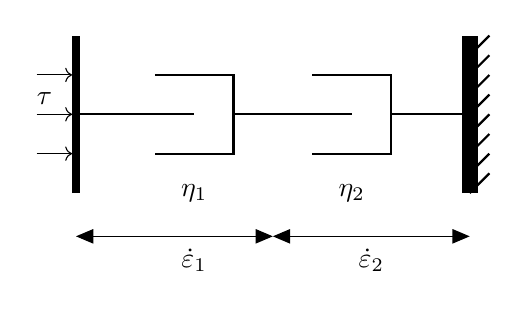
\begin{tikzpicture}
%\draw[fill=gray!23,gray!23](0,0) rectangle (6,4.5);
%\draw[step=0.5cm,gray,very thin] (0,0) grid (6,4.5); %background grid

%left wall
\node[] at (0.1,2.7) {$\tau$};
\draw[line width=1mm] (0.5,1.5) -- (0.5,3.5) ;   
\draw [->] (0,2.5) -- (0.45,2.5);
\draw [->] (0,2) -- (0.45,2);
\draw [->] (0,3) -- (0.45,3);

%dashpots
\draw[thick] (0.5,2.5) -- (2,2.5) ;   
\draw[thick] (2.5,2.5) -- (4,2.5) ;   
\draw[thick] (4.5,2.5) -- (5.5,2.5) ;   
\draw[thick] (1.5,3) -- (2.5,3) -- (2.5,2) -- (1.5,2);  
\draw[thick] (3.5,3) -- (4.5,3) -- (4.5,2) -- (3.5,2);  

\node[] at (2,1.5) {$\eta_1$};
\node[] at (4,1.5) {$\eta_2$};

%wall
\draw[line width=2mm] (5.5,1.5) -- (5.5,3.5) ;   
\draw[thick] (5.5,1.5)  -- (5.75,1.75) ;   
\draw[thick] (5.5,1.75) -- (5.75,2) ;   
\draw[thick] (5.5,2)    -- (5.75,2.25) ;   
\draw[thick] (5.5,2.25) -- (5.75,2.5) ;   
\draw[thick] (5.5,2.5)  -- (5.75,2.75) ;   
\draw[thick] (5.5,2.75) -- (5.75,3) ;   
\draw[thick] (5.5,3)    -- (5.75,3.25) ;   
\draw[thick] (5.5,3.25) -- (5.75,3.5) ;

\draw[>=triangle 45, <->] (0.5,0.95) -- (3.,0.95);
\draw[>=triangle 45, <->] (3.,0.95) -- (5.5,0.95);
\node[] at (2,0.65)   {$\dot\varepsilon_{1}$};
\node[] at (4.25,0.65)   {$\dot\varepsilon_{2}$};

\end{tikzpicture}

\end{center}

each is subjected to the same stress $\tau$ but deforms 
with its own strain rate $\dot{\varepsilon}_1$ and $\dot{\varepsilon}_2$ and we have 
\begin{equation}
\dot{\varepsilon}_T 
= \dot{\varepsilon}_1 + \dot{\varepsilon}_2
= \frac{\tau}{2\eta_1} + \frac{\tau}{2\eta_2}
\end{equation}
The effective viscosity of this combination is denoted $\eta_{eff}$ and is such that 
$\eta_{eff}=\tau/2\dot{\varepsilon}_T$, which means that 
\[
\frac{\tau}{2\eta_{eff}} = \frac{\tau}{2\eta_1} + \frac{\tau}{2\eta_2}
\]
or, 
\[
\eta_{eff}= \left( \frac{1}{\eta_1} + \frac{1}{\eta_2} \right)^{-1}
\]
i.e. it follows that the effective viscosity of two or more viscous dampers in series is the harmonic 
average of the individual viscosities of the dampers.

In general, for n dampers in series:
\[
\eta_{eff}= \left( \sum_{i=1}^n \frac{1}{\eta_i} \right)^{-1}
\]




\item \underline{two viscous dampers in parallel:}

\begin{center}
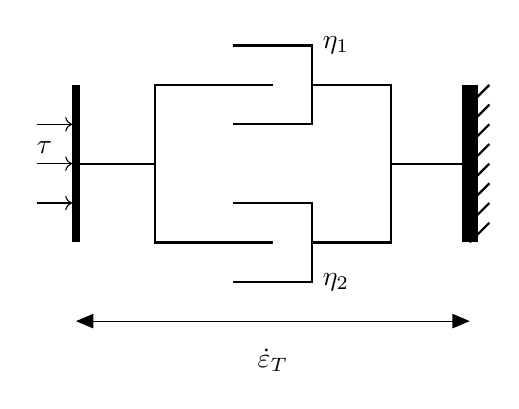
\begin{tikzpicture}
%\draw[fill=gray!23,gray!23](0,0) rectangle (7,4);
%\draw[step=0.5cm,gray,very thin] (0,0) grid (6.5,4.5); %background grid

%left wall
\node[] at (0.1,2.7) {$\tau$};
\draw[line width=1mm] (0.5,1.5) -- (0.5,3.5) ;   
\draw [->] (0,2.5) -- (0.45,2.5);
\draw [->] (0,2) -- (0.45,2);
\draw [->] (0,3) -- (0.45,3);

%dashpots
\draw[thick] (0.5,2.5) -- (1.5,2.5) ;   
\draw[thick] (4.5,2.5) -- (5.5,2.5) ;   
\draw[thick] (3,3.5) -- (1.5,3.5) -- (1.5,1.5) -- (3,1.5);  
\draw[thick] (3.5,3.5) -- (4.5,3.5) -- (4.5,1.5) -- (3.5,1.5);  
\draw[thick] (2.5,4) -- (3.5,4) -- (3.5,3) -- (2.5,3);  
\draw[thick] (2.5,2) -- (3.5,2) -- (3.5,1) -- (2.5,1);  

\node[] at (3.8,4) {$\eta_1$};
\node[] at (3.8,1) {$\eta_2$};

%wall
\draw[line width=2mm] (5.5,1.5) -- (5.5,3.5) ;   
\draw[thick] (5.5,1.5)  -- (5.75,1.75) ;   
\draw[thick] (5.5,1.75) -- (5.75,2) ;   
\draw[thick] (5.5,2)    -- (5.75,2.25) ;   
\draw[thick] (5.5,2.25) -- (5.75,2.5) ;   
\draw[thick] (5.5,2.5)  -- (5.75,2.75) ;   
\draw[thick] (5.5,2.75) -- (5.75,3) ;   
\draw[thick] (5.5,3)    -- (5.75,3.25) ;   
\draw[thick] (5.5,3.25) -- (5.75,3.5) ;

\draw[>=triangle 45, <->] (0.5,0.5) -- (5.5,0.5);
\node[] at (3,0.)   {$\dot\varepsilon_T$};

\end{tikzpicture}


\end{center}
 
each is deformed with the same strain rate $\dot{\varepsilon}_T$
and their stresses add up:
\[
\tau = \tau_1 + \tau_2 = 2 \eta_1 \dot{\varepsilon}_T  + 2 \eta_2 \dot{\varepsilon}_T
\]
and since we define the effective viscosity as $\tau = 2 \eta_{eff} \dot{\varepsilon}_T$ then it follows:
\[
2 \eta_{eff} \dot{\varepsilon}_T = 2 \eta_1 \dot{\varepsilon}_T  + 2 \eta_2 \dot{\varepsilon}_T
\]
or, 
\[
\eta_{eff} = \eta_1 + \eta_2 
\]
i.e., the effective viscosity of two or more viscous dampers is the sum of their viscosities ({\sl 
but not their arithmetic mean!}).


\item \underline{one viscous damper and a plastic element in parallel}:
\begin{center}
\begin{flushright} {\tiny {\color{gray} (tikz\_vp.tex)}} \end{flushright}
%~~~~~~~~~~~~~~~~~~~~~~~~~~~~~~~~~~~~~~~~~~~~~~~~~~~~~~~~~~~~~~~~~~~~~~~~~~~~~~~~~~~~~~~~~~~~~~~~~~

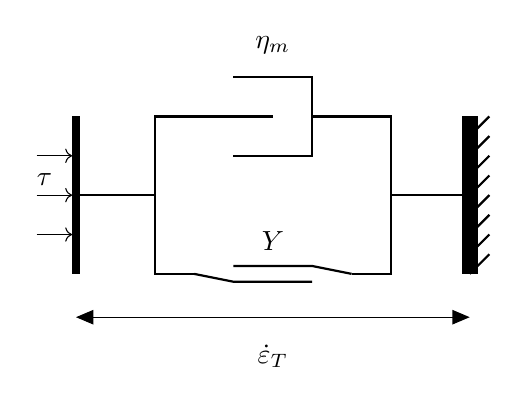
\begin{tikzpicture}
%\draw[step=0.5cm,gray,very thin] (0,0) grid (6.5,5); %background grid

\node[] at (0.1,2.7) {$\tau$};
\draw[line width=1mm] (0.5,1.5) -- (0.5,3.5) ;   
\draw [->] (0,2.5) -- (0.45,2.5);
\draw [->] (0,2) -- (0.45,2);
\draw [->] (0,3) -- (0.45,3);

%horizontal lines
\draw[thick] (.5,2.5) -- (1.5,2.5) ;   
\draw[thick] (4.5,2.5) -- (5.5,2.5) ;   

%dashpot
\draw[thick] (2.5,4) -- (3.5,4) -- (3.5,3) -- (2.5,3);  
\node[] at (3,4.4) {$\eta_m$};

\draw[thick] (3,3.5) -- (1.5,3.5) -- (1.5,1.5) -- (2,1.5);  
\draw[thick] (3.5,3.5) -- (4.5,3.5) -- (4.5,1.5) -- (4,1.5);  

%plastic elt
\draw[thick] (2,1.5) -- (2.5,1.4) -- (3.5,1.4) ;   
\draw[thick] (2.5,1.6) -- (3.5,1.6) -- (4,1.5) ;   
\node[] at (3,1.92) {$Y$};

%wall
\draw[line width=2mm] (5.5,1.5) -- (5.5,3.5) ;   
\draw[thick] (5.5,1.5)  -- (5.75,1.75) ;   
\draw[thick] (5.5,1.75) -- (5.75,2) ;   
\draw[thick] (5.5,2)    -- (5.75,2.25) ;   
\draw[thick] (5.5,2.25) -- (5.75,2.5) ;   
\draw[thick] (5.5,2.5)  -- (5.75,2.75) ;   
\draw[thick] (5.5,2.75) -- (5.75,3) ;   
\draw[thick] (5.5,3)    -- (5.75,3.25) ;   
\draw[thick] (5.5,3.25) -- (5.75,3.5) ;

\draw[>=triangle 45, <->] (0.5,0.95) -- (5.5,0.95);
\node[] at (3.,0.45)   {$\dot\varepsilon_{T}$};

\end{tikzpicture}

\end{center}

The effective 'plastic' viscosity of the plastic element is $\eta_p =  \frac{Y}{2 \dot{\varepsilon}_T}$ so 
the effective viscosity of this setup is then  
\[
\eta_{eff} = \frac{Y}{2 \dot{\varepsilon}_T}+\eta_m
\]
which is the viscosity of a Bingham fluid (see Section~\ref{sec:bingham}).


\item \underline{two viscous dampers and a plastic element} arranged as follows:
\begin{center}
\begin{flushright} {\tiny {\color{gray} (tikz\_vvp.tex)}} \end{flushright}
%~~~~~~~~~~~~~~~~~~~~~~~~~~~~~~~~~~~~~~~~~~~~~~~~~~~~~~~~~~~~~~~~~~~~~~~~~~~~~~~~~~~~~~~~~~~~~~~~~~

\begin{center}
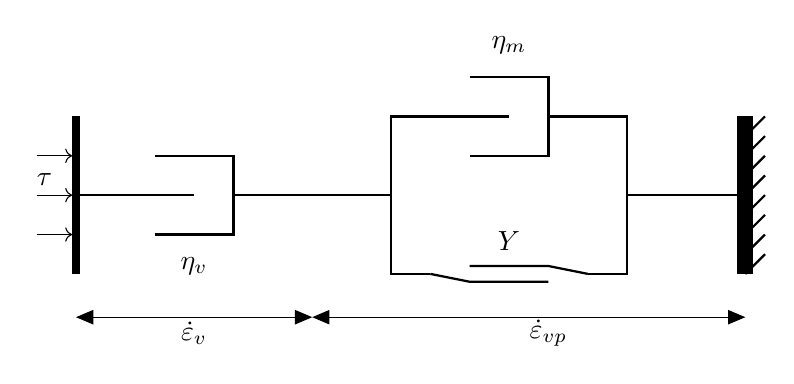
\begin{tikzpicture}
%\draw[fill=gray!23,gray!23](0,0) rectangle (7,5);
%\draw[step=0.5cm,gray,very thin] (0,0) grid (7,5); %background grid

\node[] at (0.1,2.7) {$\tau$};
\draw[line width=1mm] (0.5,1.5) -- (0.5,3.5) ;  
\draw [->] (0,2.5) -- (0.45,2.5);
\draw [->] (0,2) -- (0.45,2);
\draw [->] (0,3) -- (0.45,3);

\draw[thick] (0.5,2.5) -- (2,2.5) ;  
\draw[thick] (2.5,2.5) -- (4.5,2.5) ;  
\draw[thick] (7.5,2.5) -- (9,2.5) ;  

\draw[thick] (1.5,3) -- (2.5,3) -- (2.5,2) -- (1.5,2);  
\draw[thick] (5.5,4) -- (6.5,4) -- (6.5,3) -- (5.5,3);  

\node[] at (2,1.6) {$\eta_v$};
\node[] at (6,4.4) {$\eta_m$};

\draw[thick] (6,3.5) -- (4.5,3.5) -- (4.5,1.5) -- (5,1.5);  
\draw[thick] (6.5,3.5) -- (7.5,3.5) -- (7.5,1.5) -- (7,1.5);  

\draw[thick] (5,1.5) -- (5.5,1.4) -- (6.5,1.4) ;  
\draw[thick] (5.5,1.6) -- (6.5,1.6) -- (7,1.5) ;  

\node[] at (6,1.92) {$Y$};

%wall
\draw[line width=2mm] (9,1.5) -- (9,3.5) ;  
\draw[thick] (9,1.5) -- (9.25,1.75) ;  
\draw[thick] (9,1.75) -- (9.25,2) ;  
\draw[thick] (9,2) -- (9.25,2.25) ;  
\draw[thick] (9,2.25) -- (9.25,2.5) ;  
\draw[thick] (9,2.5) -- (9.25,2.75) ;  
\draw[thick] (9,2.75) -- (9.25,3) ;  
\draw[thick] (9,3) -- (9.25,3.25) ;  
\draw[thick] (9,3.25) -- (9.25,3.5) ;  

\draw[>=triangle 45, <->] (0.5,0.95) -- (3.5,0.95);
\draw[>=triangle 45, <->] (3.5,0.95) -- (9,0.95);
\node[] at (2,0.75)   {$\dot\varepsilon_{v}$};
\node[] at (6.5,0.75)   {$\dot\varepsilon_{vp}$};

\end{tikzpicture}
\end{center}

\end{center}
This rheology would be called visco-viscoplastic.
The algorithm goes then as follows:
\begin{enumerate}
\item Assume we know $\eta_v$ and $\dot\varepsilon_T$ (from previous iteration), as well as the plasticity parameters $Y$ and $\eta_m$.
\item if $2 \eta_v \dot\varepsilon_T < Y$ the stress is below the yield stress value and plasticity is not active. Use $\eta_v$ in the material model and $\dot\varepsilon_v=\dot\varepsilon_T$.

\item if $2 \eta_v \dot\varepsilon_T > Y$ the stress is above the yield value, which is not allowed. In this case the plastic element is 'switched on'. In that case the viscous damper is in series with the (visco)plastic element. The former deforms with a strain rate $\dot\epsilon_v$ while the latter with $\dot\epsilon_{vp}$ (both under the same stress $\tau$) and we have  $\dot\varepsilon_T = \dot\varepsilon_v  + \dot\varepsilon_{vp}$. 

\begin{eqnarray}
\dot\varepsilon_T 
&=& \dot\varepsilon_v + \dot\varepsilon_{vp}  \nonumber\\
&=& \dot\varepsilon_v + \frac{\tau}{2 \eta_{vp}} \nonumber\\
&=& \dot\varepsilon_v + \frac{\tau}{2 \left( \frac{Y}{2\dot\varepsilon_{vp}} + \eta_m  \right)} \nonumber\\
&=& \dot\varepsilon_v + \frac{\tau}{2 \left( \frac{Y}{2(\dot\varepsilon_T-\dot\varepsilon_v)}+\eta_m\right)} \nonumber\\
\dot\varepsilon_T - \dot\varepsilon_v 
&=& \frac{\tau}{2 \left( \frac{Y}{2(\dot\varepsilon_T-\dot\varepsilon_v)}+\eta_m\right)} \nonumber\\
2 (\dot\varepsilon_T - \dot\varepsilon_v)
\left( \frac{Y}{2(\dot\varepsilon_T-\dot\varepsilon_v)}+\eta_m\right) &=& \tau \nonumber\\
Y +  2(\dot\varepsilon_T - \dot\varepsilon_v) \eta_m &=& \tau \nonumber\\
Y +  2(\dot\varepsilon_T - \frac{\tau}{2 \eta_v}) \eta_m &=& \tau \nonumber\\
Y +  (2\eta_v \dot\varepsilon_T - \tau) \frac{\eta_m}{\eta_v} &=& \tau \nonumber\\
Y +  2\eta_m \dot\varepsilon_T  &=& \tau (1 + \frac{\eta_m}{\eta_v} ) \nonumber
\end{eqnarray}
and finally 
\begin{equation}
\tau  = \frac{Y + 2 \eta_m \dot\varepsilon_T} {1+ \frac{\eta_m}{\eta_v} }
\end{equation}
Note that this solution exists even when $\eta_m=0$, and then rather logically $\tau=Y$.

\item Once we have $\tau$, we can easily compute $\dot\epsilon_v = \frac{\tau}{2\eta_v}$

\item We then compute $\dot\varepsilon_{vp} = \dot\varepsilon_T- \dot\varepsilon_v$ which 
we use to compute $\eta_{vp}$:

\begin{eqnarray}
\eta_{vp} 
&=& \frac{Y}{2\dot\varepsilon_{vp}}+\eta_m \nn\\
&=& \frac{Y}{2(\dot\varepsilon_{T}-\dot\varepsilon_{v})}+\eta_m \nn\\
&=& \frac{Y}{2(\dot\varepsilon_{T}-\frac{\tau}{2\eta_v})}+\eta_m \nn\\
&=& \frac{Y}{2(\dot\varepsilon_{T}- \frac{Y + 2 \eta_m \dot\varepsilon_T} {1+ \frac{\eta_m}{\eta_v} }   
\frac{1}{2\eta_v})}+\eta_m \nn\\
&=& \frac{Y}{2\dot\varepsilon_{T}- \frac{Y + 2 \eta_m \dot\varepsilon_T} {\eta_v + \eta_m}     }+\eta_m \\
&=& \frac{Y(\eta_v+\eta_m)}{2(\eta_v+\eta_m) \dot\varepsilon_{T}- (Y + 2 \eta_m \dot\varepsilon_T) }+\eta_m \\
&=& \frac{Y(\eta_v+\eta_m)}{2 \eta_v \dot\varepsilon_{T}- Y  }+\eta_m \\
&=& \frac{Y(\eta_v+\eta_m)/2\eta_v}{ \dot\varepsilon_{T}- Y/2\eta_v  }+\eta_m 
\end{eqnarray}


\item Having obtained $\eta_{vp}$ we can compute the final effective viscosity
\[
\eta_{eff} = \left( \frac{1}{\eta_v}  + \frac{1}{\eta_{vp}}  \right)^{-1}
\]
\end{enumerate}

On the following plots are shown $\tau$, 
$\dot\varepsilon_{vp}$, $\dot\varepsilon_v$, $\eta_vp$, and $\eta_{eff}$ 
as a function of  $\dot\varepsilon_T$: 

\begin{center}
\includegraphics[width=5.5cm]{images/rheology/vvp/tau.pdf}
\includegraphics[width=5.5cm]{images/rheology/vvp/strainrates.pdf}
\includegraphics[width=5.5cm]{images/rheology/vvp/viscosities.pdf}\\
{\captionfont Obtained for $\eta_m=10^{21}$, $Y=20$MPa and $\eta_v=10^{25}$. Python code 
in images/rheology/vvp/}
\end{center}

In the following plots the resulting stress $\tau$ and effective viscosities $\eta_{eff}$
are compared between the above approach ('new') and the simpler (and naive) 
approach where $\dot\varepsilon_T$ 
is used in $\eta_{vp}$ instead of $\dot\varepsilon$ ('old'). In this particular case 
we see that it makes a difference at low strain rates close to the brittle-ductile transition.

\begin{center}
\includegraphics[width=8cm]{images/rheology/vvp/tau_comp.pdf}
\includegraphics[width=8cm]{images/rheology/vvp/viscosities_comp.pdf}\\
{\captionfont Obtained for $\eta_m=10^{21}$, $Y=20$MPa and $\eta_v=10^{25}$. Python code 
in images/rheology/vvp/}
\end{center}

\begin{remark}
The introduction of the damper $\eta_m$ in parallel with the plastic element has an unavoidable
effect: the stress $\tau$ becomes larger than $Y$ at high strain rate values! Since the $vp$ 
block is akin to a bingham fluid, this is no surprise.
\end{remark}

\begin{remark}
The viscous dashpot $\eta_v$ also acts as a maximum viscosity cutoff: if $\eta_{vp}$ becomes (very) large, i.e. $\eta_{vp} \gg \eta_v$, then $\eta_{eff} \rightarrow \eta_v$.
Conversely, if $\eta_p=Y/2\dot\varepsilon_{vp}$ becomes (very) small, i.e. $\eta_p \ll \eta_m$ then $\eta_m$ acts as a minimum viscosity limiter, i.e. $\eta_{vp} \rightarrow \eta_m$. 
Since $\eta_m \ll \eta_v$ then $\eta_{eff} \rightarrow \eta_m$.
\end{remark}

\underline{A simple regularisation} This idea originates in Massmeyer \etal (2013) \cite{madd13}. We postulate
\[
\tilde{\eta}_{eff} = \left(  1 - \exp (- \frac{\dot\varepsilon_T}{\dot\varepsilon_{T}^c}) \right)
\left( \frac{Y}{2 \dot\varepsilon_T} + \eta_m \right)
\]
where $\dot\varepsilon_{T}^c$ is the critical strain  rate at which the transition viscous to 
viscous-viscoplastic occues given by $\dot\varepsilon_{T}^c=Y/2\eta_v$.
When $\dot\varepsilon_{T} \ll \dot\varepsilon_{T}^c$ then the exponential term tends to zero and 
\[
\tilde{\eta}_{eff} \rightarrow  \frac{Y}{2 \dot\varepsilon_T} + \eta_m 
\]
and if $\dot\varepsilon_{T} \rightarrow \infty$ then $\tilde{\eta}_{eff}\rightarrow \eta_m$.
Conversely if $\dot\varepsilon_T \rightarrow 0$ then we can carry out a Taylor expansion of the exponential 
term ($\exp x \sim 1 + x$ when $x$ is small).
\[
\tilde{\eta}_{eff} \sim \left(  \frac{\dot\varepsilon_T}{\dot\varepsilon_{T}^c} \right)
\left( \frac{Y}{2 \dot\varepsilon_T} + \eta_m \right)
\rightarrow 
\frac{\dot\varepsilon_T}{\dot\varepsilon_{T}^c}  \frac{Y}{2 \dot\varepsilon_T}  = \eta_v
\]
At low strain rates the viscosity does not 'explode' but actually converges to the background viscosity $\eta_v$.
The stress $\tau$ corresponding to this viscosity is simply $\tilde{\tau} = 2 \tilde{\eta}_{eff}$. 
Both $\tilde{\tau}$ and $ \tilde{\eta}_{eff}$ are plotted hereunder:


\begin{center}
\includegraphics[width=7.5cm]{images/rheology/vvp/tau_reg.pdf}
\includegraphics[width=7.5cm]{images/rheology/vvp/viscosities_reg.pdf}\\
{\captionfont Obtained for $\eta_m=10^{21}$, $Y=20$MPa and $\eta_v=10^{25}$. Python code 
in images/rheology/vvp/}
\end{center}


\includegraphics[width=7.5cm]{images/rheology/vvp/ratio_visc.pdf}



%which, if  yields the following effective viscosity:
%\[
%\eta_{eff} = \left( \frac{1}{\eta_M}  + \frac{1}{\frac{Y}{2 \dot{\varepsilon}_e} + \eta_m}  \right)^{-1}
%\]
%When the strain rate becomes very small,  $\dot{\varepsilon}_e \rightarrow 0$, $\eta_{eff}\rightarrow \eta_{M}$.
%When the strain rate becomes very large,  $\dot{\varepsilon}_e \rightarrow \infty$, $\eta_{eff}\rightarrow \eta_{m}$.
%We can then rewrite the above equation as a function of $\eta_{min}$ and $\eta_{max}$:
%\[
%\eta_{eff} = \left( \frac{1}{\eta_{max}}  + \frac{1}{\frac{c}{2 \dot{\varepsilon}_e} + \eta_{min}}  \right)^{-1}
%\]
%
%The effective viscosity is plotted here for various values of the minimum viscosity (for $c$=200MPa and $\eta_{max}=10^{25}Pa.s$:
%\includegraphics[width=8cm]{images/viscoplasticity/nu_eff}



\item \underline{two nonlinear viscous dampers in series:} 

\begin{center}
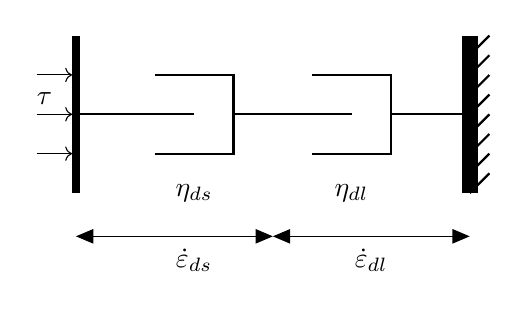
\begin{tikzpicture}
%\draw[fill=gray!23,gray!23](0,0) rectangle (6,4.5);
%\draw[step=0.5cm,gray,very thin] (0,0) grid (6,4.5); %background grid

%left wall
\node[] at (0.1,2.7) {$\tau$};
\draw[line width=1mm] (0.5,1.5) -- (0.5,3.5) ;   
\draw [->] (0,2.5) -- (0.45,2.5);
\draw [->] (0,2) -- (0.45,2);
\draw [->] (0,3) -- (0.45,3);

%dashpots
\draw[thick] (0.5,2.5) -- (2,2.5) ;   
\draw[thick] (2.5,2.5) -- (4,2.5) ;   
\draw[thick] (4.5,2.5) -- (5.5,2.5) ;   
\draw[thick] (1.5,3) -- (2.5,3) -- (2.5,2) -- (1.5,2);  
\draw[thick] (3.5,3) -- (4.5,3) -- (4.5,2) -- (3.5,2);  

\node[] at (2,1.5) {$\eta_{ds}$};
\node[] at (4,1.5) {$\eta_{dl}$};

%wall
\draw[line width=2mm] (5.5,1.5) -- (5.5,3.5) ;   
\draw[thick] (5.5,1.5)  -- (5.75,1.75) ;   
\draw[thick] (5.5,1.75) -- (5.75,2) ;   
\draw[thick] (5.5,2)    -- (5.75,2.25) ;   
\draw[thick] (5.5,2.25) -- (5.75,2.5) ;   
\draw[thick] (5.5,2.5)  -- (5.75,2.75) ;   
\draw[thick] (5.5,2.75) -- (5.75,3) ;   
\draw[thick] (5.5,3)    -- (5.75,3.25) ;   
\draw[thick] (5.5,3.25) -- (5.75,3.5) ;

\draw[>=triangle 45, <->] (0.5,0.95) -- (3.,0.95);
\draw[>=triangle 45, <->] (3.,0.95) -- (5.5,0.95);
\node[] at (2,0.65)   {$\dot\varepsilon_{ds}$};
\node[] at (4.25,0.65)   {$\dot\varepsilon_{dl}$};

\end{tikzpicture}

\end{center}

There are two dashpots in series, one accounts for dislocation creep, the other for diffusion creep.
The algorithm goes then as follows:
\begin{enumerate}
\item Assume we know $\dot\varepsilon_T$ (from previous iteration). 
\item The dashpots are in series so 
\[
\dot\varepsilon_T = \dot\varepsilon_{ds} + \dot\varepsilon_{df} 
\]
with
\begin{eqnarray}
\dot\varepsilon_{ds}  &=& A_{ds} \tau^n \exp \left(-\frac{Q_{ds}+pV_{ds}}{RT}\right) \label{sr_ds1} \\
\dot\varepsilon_{df}  &=& A_{df} \tau   \exp \left(-\frac{Q_{df}+pV_{df}}{RT}\right) \label{sr_df1} 
\end{eqnarray}
such that we are in fact looking for the stress value $\tau$ so that 
\[
\dot\varepsilon_T = 
A_{ds} \tau^n \exp \left(-\frac{Q_{ds}+p V_{ds}}{RT}\right) 
+
A_{df} \tau   \exp \left(-\frac{Q_{df}+p V_{df}}{RT}\right) 
\]
or, we must find the zero of the function ${\cal F}(\tau)$: 
\[
{\cal F}(\tau) =  \dot\varepsilon_T 
- A_{ds} \tau^n \exp \left(-\frac{Q_{ds}+p V_{ds}}{RT}\right) 
- A_{df} \tau   \exp \left(-\frac{Q_{df}+p V_{df}}{RT}\right) 
\]
This equation can be solved with a Newton-Raphson algorithm
and the iterations will be of the form:
\[
\tau_{n+1} = \tau_n - \frac{{\cal F}(\tau_n)}{{\cal F}'(\tau_n)}
\]
where the derivative of the function ${\cal F}$ with respect to $\tau$ reads:
\[
{\cal F}'(\tau)=\frac{\partial {\cal F}}{\partial \tau}=
- A_{ds} n \tau^{n-1} \exp\left(-\frac{Q_{ds}+pV_{ds}}{RT}\right)
- A_{df} \exp\left(-\frac{Q_{df}+pV_{df}}{RT}\right) 
\]
Once the value of $\tau$ is found, 
the strain rate values of Eqs. (\ref{sr_ds1}) and (\ref{sr_df1})
can be computed and so can the respective effective viscosities:
\begin{eqnarray}
\eta_{ds} 
&=& \frac{1}{2} A_{ds}^{1/n} \dot\varepsilon_{ds}^{\frac{1}{n}-1} \exp \left(\frac{Q_{ds}+pV_{ds}}{nRT}\right) \\
\eta_{df} 
&=& \frac{1}{2} A_{df}^{1/n}  \exp \left(\frac{Q_{df}+pV_{df}}{RT}\right) 
\end{eqnarray}
Their average effective viscosity $\tilde{\eta}_{eff}$ is given by 
\[
\tilde{\eta}_{eff} = \left( \frac{1}{\eta_{ds}} + \frac{1}{\eta_{df}} \right)^{-1}
\]
\end{enumerate}


Rather importantly, as we will see hereafter, the following variant is implemented 
in some codes (e.g. \douar, \fantom, \sopale, and probably many others) 
so as to bypass these costly Newton iterations:
\begin{enumerate}
\item compute $\eta_{ds}$ and $\eta_{df}$ with the {\it same} strainrate $\dot\varepsilon_T$, 
pressure and temperature values
\item average them by means of an harmonic average
\end{enumerate}
In this case, we have
\[
\dot{\varepsilon}_{\color{red} T}= 
A_{df} \tau_{df} \exp\left(-\frac{Q_{df}+pV_{df}}{RT}\right)
\quad\quad\quad
\dot{\varepsilon}_{\color{red} T}= 
A_{ds} \tau_{ds}^n \exp\left(-\frac{Q_{ds}+pV_{ds}}{RT}\right)
\]
or, 
\begin{eqnarray}
\eta_{ds} 
&=& \frac{1}{2} A_{ds}^{1/n} \dot\varepsilon_{\color{red}T}^{\frac{1}{n}-1} \exp \left(\frac{Q_{ds}+pV_{ds}}{nRT}\right) \\
\eta_{df} 
&=& \frac{1}{2} A_{df}^{1/n}  \exp \left(\frac{Q_{df}+pV_{df}}{RT}\right) 
\end{eqnarray}
We see that this simplification has consequences on the dislocation creep viscosity only.


\paragraph{A concrete example}
Let us consider a vertical section of upper mantle, from 660\si{\km} depth to 30\si{\km} depth.
The lithosphere is assumed to be 90\si{\km} thick. The temperature at the moho (the top
of the domain) is set to 550C, 1330C at the LMB and 1380C at the bottom.
A constant strainrate $\dot{\epsilon}_T=10^{-15}\si{\per\second}$ is assumed. 
We assume that the pressure is lithostatic (for simplicity 
the density is taken to be constant at 3300kg/m$^3$).
The temperature and pressure fields are shown hereunder:
\begin{center}
\includegraphics[width=6cm]{images/rheology/effvisc/temperature.pdf}
\includegraphics[width=6cm]{images/rheology/effvisc/pressure.pdf}
\end{center}

Material properties are taken from Karato \& Wu (1993) \cite{kawu93}.
The (fortran) code is available in {\tt images/rheology/effvisc/}.

In what follows, the values obtained with Newton iterations are coined 'NR'
and those obtained without are coined 'CHEAP'.
The diffusion and dislocation creep viscosities can be
computed for both algorithms and are shown hereunder
(As mentioned earlier the diffusion creep viscosity is independent of strain rate so
is the same for both):
\begin{center}
\includegraphics[width=6cm]{images/rheology/effvisc/both_mu_ds.pdf}
\includegraphics[width=6cm]{images/rheology/effvisc/both_mu_df.pdf}
\end{center}
We can also plot the resulting effective viscosity 
$\eta_{eff}$ for both approaches and we see that the differences 
are larger than 20\%. This is shown here under on the left, 
alongside with the partitioning of the strain rate as a function of depth:
\begin{center}
\includegraphics[width=8cm]{images/rheology/effvisc/both_mueff.pdf}
\includegraphics[width=8cm]{images/rheology/effvisc/both_sr.pdf}
\end{center}


























\item \underline{multiple viscous dampers and a plastic element} arranged as follows:



\begin{center}
\begin{flushright} {\tiny {\color{gray} (tikz\_vvp2.tex)}} \end{flushright}
%~~~~~~~~~~~~~~~~~~~~~~~~~~~~~~~~~~~~~~~~~~~~~~~~~~~~~~~~~~~~~~~~~~~~~~~~~~~~~~~~~~~~~~~~~~~~~~~~~~

\begin{center}
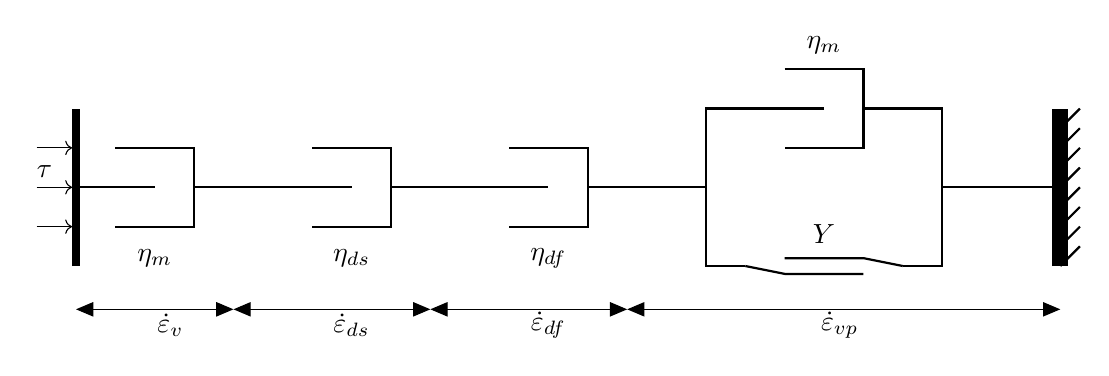
\begin{tikzpicture}
%\draw[fill=gray!23,gray!23](0,0) rectangle (7,5);
%\draw[step=0.5cm,gray,very thin] (0,0) grid (12,5); %background grid

\node[] at (0.1,2.7) {$\tau$};
\draw[line width=1mm] (0.5,1.5) -- (0.5,3.5) ;  
\draw [->] (0,2.5) -- (0.45,2.5);
\draw [->] (0,2) -- (0.45,2);
\draw [->] (0,3) -- (0.45,3);

%linear viscous

\draw[thick] (1.,3) -- (2.,3) -- (2.,2) -- (1.,2);  
\draw[thick] (0.5,2.5) -- (1.5,2.5) ;  
\draw[>=triangle 45, <->] (0.5,0.95) -- (2.5,0.95);
\node[] at (1.7,0.75) {$\dot\varepsilon_{v}$};
\node[] at (1.5,1.6) {$\eta_{m}$};


%dislocation creep
\draw[thick] (2.,2.5) -- (4,2.5) ;  
\draw[thick] (4.5,2.5) -- (6.5,2.5) ;  
\draw[thick] (3.5,3) -- (4.5,3) -- (4.5,2) -- (3.5,2);  
\node[] at (4,1.6) {$\eta_{ds}$};
\draw[>=triangle 45, <->] (2.5,0.95) -- (5,0.95);
\node[] at (4,0.75)   {$\dot\varepsilon_{ds}$};

%diffusion creep
\draw[thick] (6.,3) -- (7.,3) -- (7.,2) -- (6.,2);  
\node[] at (6.5,1.6) {$\eta_{df}$};
\draw[thick] (7,2.5) -- (8.5,2.5) ;  
\draw[>=triangle 45, <->] (5,0.95) -- (7.5,0.95);
\node[] at (6.5,0.75)   {$\dot\varepsilon_{df}$};

%viscoplastic element
\draw[thick] (9.5,4) -- (10.5,4) -- (10.5,3) -- (9.5,3);  
\node[] at (10,4.3) {$\eta_m$};
\node[] at (10,1.9) {$Y$};
\draw[thick] (10,3.5) -- (8.5,3.5) -- (8.5,1.5) -- (9,1.5);  
\draw[thick] (10.5,3.5) -- (11.5,3.5) -- (11.5,1.5) -- (11,1.5);  
\draw[thick] (9,1.5) -- (9.5,1.4) -- (10.5,1.4) ;  
\draw[thick] (9.5,1.6) -- (10.5,1.6) -- (11,1.5) ;  
\draw[thick] (11.5,2.5) -- (13,2.5) ;  
\draw[>=triangle 45, <->] (7.5,0.95) -- (13,0.95);
\node[] at (10.2,0.75) {$\dot\varepsilon_{vp}$};

%wall
\draw[line width=2mm] (13,1.5) -- (13,3.5) ;  
\draw[thick] (13,1.5)  -- (13.25,1.75) ;  
\draw[thick] (13,1.75) -- (13.25,2) ;  
\draw[thick] (13,2)    -- (13.25,2.25) ;  
\draw[thick] (13,2.25) -- (13.25,2.5) ;  
\draw[thick] (13,2.5)  -- (13.25,2.75) ;  
\draw[thick] (13,2.75) -- (13.25,3) ;  
\draw[thick] (13,3)    -- (13.25,3.25) ;  
\draw[thick] (13,3.25) -- (13.25,3.5) ;  





\end{tikzpicture}\\
\end{center}

\end{center}



The algorithm goes then as follows:
\begin{enumerate}
\item Assume we know $\dot\varepsilon_T$ (from previous iteration), 
as well as the plasticity parameters $Y$ (a constant in the case of von Mises, or a pressure-dependent 
quantity otherwise) and $\eta_m$.
\item We start by assuming that the plasticity 'block' is not active ($\dot{\varepsilon}_{vp}=0$): we have then three dampers in series. 
We need their associated strain rates 
$\dot{\varepsilon}_{df}$ and $\dot{\varepsilon}_{ds}$ which are such that 
\[
\dot\varepsilon_T = 
\dot\varepsilon_v + \dot\varepsilon_{ds} + \dot\varepsilon_{df} 
\]
with
\begin{eqnarray}
\dot\varepsilon_v &=& \frac{\tau}{2 \eta_v} \label{sr_v} \\
\dot\varepsilon_{ds}  &=& A_{ds} \tau^n \exp \left(-\frac{Q_{ds}+pV_{ds}}{RT}\right) \label{sr_ds} \\
\dot\varepsilon_{df}  &=& A_{df} \tau   \exp \left(-\frac{Q_{df}+pV_{df}}{RT}\right) \label{sr_df} 
\end{eqnarray}
such that we are in fact looking for the stress value $\tau$ so that 
\[
\dot\varepsilon_T = 
A_{ds} \tau^n \exp \left(-\frac{Q_{ds}+p V_{ds}}{RT}\right) 
+
A_{df} \tau   \exp \left(-\frac{Q_{df}+p V_{df}}{RT}\right) 
+
\frac{\tau}{2 \eta_v}
\]
or, we must find the zero of the function ${\cal F}$: 
\[
{\cal F}(\tau) = 
\dot\varepsilon_T 
- A_{ds} \tau^n \exp \left(-\frac{Q_{ds}+p V_{ds}}{RT}\right) 
- A_{df} \tau   \exp \left(-\frac{Q_{df}+p V_{df}}{RT}\right) 
- \frac{\tau}{2 \eta_v} 
\]
This equation can be solved with a Newton-Raphson algorithm
and the iterations will be of the form:
\[
\tau_{n+1} = \tau_n - \frac{{\cal F}(\tau_n)}{{\cal F}'(\tau_n)}
\]
where the derivative of the function ${\cal F}$ with respect to $\tau$ reads:
\[
{\cal F}'(\tau)=\frac{\partial {\cal F}}{\partial \tau}=
- A_{df} \exp\left(-\frac{Q_{df}+pV_{df}}{RT}\right) 
- A_{ds} n \tau^{n-1} \exp\left(-\frac{Q_{ds}+pV_{ds}}{RT}\right)
- \frac{1}{2\eta_v}
\]
Once the value of $\tau$ is found, 
the strain rate values of Eqs. (\ref{sr_ds}), (\ref{sr_df}) and (\ref{sr_v}) 
can be computed and so can the respective effective viscosities:
\begin{eqnarray}
\eta_{ds} 
&=& \frac{1}{2} A_{ds}^{1/n} \dot\varepsilon_{ds}^{\frac{1}{n}-1} \exp \left(\frac{Q_{ds}+pV_{ds}}{nRT}\right) \\
\eta_{df} 
&=& \frac{1}{2} A_{df}^{1/n}  \exp \left(\frac{Q_{df}+pV_{df}}{RT}\right) 
\end{eqnarray}
Their average effective viscosity $\tilde{\eta}_{eff}$ is given by 
\[
\tilde{\eta}_{eff} = \left( \frac{1}{\eta_{ds}} + \frac{1}{\eta_{df}} + \frac{1}{\eta_v} \right)^{-1}
\]


\item if $\tau =2 \tilde{\eta}_{eff} \dot\varepsilon_T < Y$ the stress is below the yield stress value 
and the plasticity element is indeed not active. Use $\tilde{\eta}_{eff}$ in the material model.

\item if $\tau=2 \tilde{\eta}_{eff} \dot\varepsilon_T > Y$ the stress is above the yield value, which is not 
allowed. In this case the plastic element must be present and active and the viscous dampers are then 
in series with the (visco)plastic element. The formers deform 
with a strain rate $\dot{\varepsilon}_v$, $\dot\epsilon_{ds}$ and $\dot{\epsilon}_{df}$ 
while the latter with $\dot\epsilon_{vp}$ (all under the same tress $\tau$) 
and we have  $\dot\varepsilon_T = \dot{\varepsilon}_v + \dot\varepsilon_{ds} + \dot\varepsilon_{df} + \dot\varepsilon_{vp}$ so:

\begin{eqnarray}
\dot\varepsilon_T - \dot{\varepsilon}_v(\tau) - \dot\varepsilon_{ds}(\tau) - \dot\varepsilon_{df}(\tau)  
&=& \dot\varepsilon_{vp}  \nonumber\\
&=& \frac{\tau}{2 \left( \frac{Y}{2\dot\varepsilon_{vp}} + \eta_m  \right)} 
\nonumber\\
%&=&  \frac{\tau}{2 \left( \frac{Y}{2 (\dot\varepsilon_T -\dot{\varepsilon}_v(\tau) -\dot\varepsilon_{ds}(\tau) 
%+ \dot\varepsilon_{df}(\tau)   )} + \eta_m  \right)} 
%\nonumber\\
\dot\varepsilon_T -  \dot{\varepsilon}_v(\tau) -\dot\varepsilon_{ds}(\tau) - \dot\varepsilon_{df}(\tau) 
&=&
\frac{\tau}{2 \left( \frac{Y}{2 (\dot\varepsilon_T -\dot{\varepsilon}_v(\tau) -\dot\varepsilon_{ds}(\tau) 
+ \dot\varepsilon_{df}(\tau)   )} + \eta_m  \right)} \nonumber
\\
2 [\dot\varepsilon_T -\dot{\varepsilon}_v(\tau) -\dot\varepsilon_{ds}(\tau) - \dot\varepsilon_{df}(\tau) ]
 \left( \frac{Y}{2 (\dot\varepsilon_T -\dot{\varepsilon}_v(\tau) -\dot\varepsilon_{ds}(\tau) + \dot\varepsilon_{df}(\tau)   )} + \eta_m  \right) &=& \tau 
\nonumber\\
Y + 2 (\dot\varepsilon_T - \dot{\varepsilon}_v(\tau) -\dot\varepsilon_{ds}(\tau) - \dot\varepsilon_{df}(\tau) ) \eta_m  &=& \tau \nonumber 
\end{eqnarray}
As before, we must find the zero of the function ${\cal F}$: 
\begin{eqnarray}
{\cal F}(\tau) 
&=& Y + 2 [\dot\varepsilon_T -\dot{\varepsilon}_v(\tau)- \dot\varepsilon_{ds}(\tau) -\dot\varepsilon_{df}(\tau) ]\eta_m -\tau \nonumber\\
&=& Y + 2 \left[ 
\dot\varepsilon_T - \frac{\tau}{2\eta_v}-A_{ds} \tau^n \exp \left(-\frac{Q_{ds}+pV_{ds}}{RT}\right) 
- A_{df} \tau   \exp \left(-\frac{Q_{df}+pV_{df}}{RT}\right)  
\right]\eta_m -\tau \nn
\end{eqnarray}
Because dislocation creep involves the $n$-th power of the stress we will here also need 
to find the zero by means of a Newton-Raphson algorithm. 

We have:
\begin{eqnarray}
\frac{\partial {\cal F}}{\partial \tau} &=&
\left[
- \frac{1}{\eta_v} 
-2 \frac{\partial  \dot\varepsilon_{ds}(\tau) }{\partial \tau} 
-2 \frac{\partial  \dot\varepsilon_{df}(\tau) }{\partial \tau} 
\right] \eta_m - 1
\end{eqnarray}

\begin{eqnarray}
{\cal F}(\tau) / 2\eta_m 
&=& 
\frac{Y}{2\eta_m}  + \dot\varepsilon_T 
- \frac{\tau}{2\eta_v}
- A_{ds}(p,T) \tau^n 
- A_{df}(p,T) \tau  
- \frac{\tau}{2\eta_m} \\
&=& 
- A_{ds}(p,T) \tau^n - \left(A_{df}(p,T) +  \frac{1}{2\eta_v} -\frac{1}{2\eta_m} \right) \tau
+ 
\left( \frac{Y}{2\eta_m}  + \dot\varepsilon_T \right) =0
\end{eqnarray}



\end{enumerate}

Note that when $\eta_m=0$ we logically recover $\tau=Y$ as the stress cannot exceed the yield strength $Y$.

Although this approach is probably the most consistent in terms of physics, the presence 
of the Newton-Raphson iterations makes it very expensive since this procedure is to be repeated 
for every quadrature point or every particle.

Let us consider a concrete example: we set $Y=20\si{\mega\pascal}$, $\eta_v=10^{25}\si{pascal}$, 
$\eta_m=10^{20}\si{pascal}$. The domain is one-dimensional of depth $660\si{km}$. The density is
assumed to be constant at $3300\si{\kg\per\cubic\metre}$. Dislocation and diffusion creep parameters
are taken from Karato \& Wu (1993) \cite{kawu93}. The temperature is linear is $20\si{\celsius}$ 
at the surface, $550\si{\celsius}$ at $30\si{km}$ depth, $1330\si{celsius}$ at $90\si{\km}$ depth 
and $1380\si{\celsius}$ at the bottom. Pressure is assumed to be lithostatic. 
The python program and the gnuplot script are in {\sl images/rheology/example}.

In the code I consider two cases: 'old' and 'new'. The latter is described above. 
'old' goes as follows: loop over total strain rate values. 
Compute dislocation and diffusion creep viscosities with it. Compute harmonic 
average of these with linear viscosity. Compute deviatoric stress value. 
use it in dislocation and diffusion formulae to arrive at respective strainrates. 

\newpage
\begin{center}
\includegraphics[width=5.5cm]{images/rheology/example/map_sr_df_old-1}
\includegraphics[width=5.5cm]{images/rheology/example/map_sr_df_new-1}
\includegraphics[width=5.5cm]{images/rheology/example/map_sr_df_diff-1}\\
\includegraphics[width=5.5cm]{images/rheology/example/map_sr_ds_old-1}
\includegraphics[width=5.5cm]{images/rheology/example/map_sr_ds_new-1}
\includegraphics[width=5.5cm]{images/rheology/example/map_sr_ds_diff-1}\\
\includegraphics[width=5.5cm]{images/rheology/example/map_sr_v_old-1}
\includegraphics[width=5.5cm]{images/rheology/example/map_sr_v_new-1}
\includegraphics[width=5.5cm]{images/rheology/example/map_sr_v_diff-1}\\
\includegraphics[width=5.5cm]{images/rheology/example/map_etaeff_old-1}
\includegraphics[width=5.5cm]{images/rheology/example/map_etaeff_new-1}
\includegraphics[width=5.5cm]{images/rheology/example/map_etaeff_diff-1}\\
\includegraphics[width=5.5cm]{images/rheology/example/map_tau_old-1}
\includegraphics[width=5.5cm]{images/rheology/example/map_tau_new-1}
\includegraphics[width=5.5cm]{images/rheology/example/map_tau_diff-1}\\
\includegraphics[width=5.5cm]{images/rheology/example/profile_sr-1}
\includegraphics[width=5.5cm]{images/rheology/example/profile_tau-1}
\includegraphics[width=5.5cm]{images/rheology/example/profile_etaeff-1}\\
\includegraphics[width=5.5cm]{images/rheology/example/map_isplast_old-1}
\includegraphics[width=5.5cm]{images/rheology/example/map_isplast_new-1}\\
{\captionfont Viscous branch: (ds+df+v) 'old' stands 
for the old approach when $\dot{\varepsilon}_T$
was used for all mechanisms. 'new' stands for the new approach and the right strain rate 
decomposition.}
\end{center}



\newpage
\begin{center}
\includegraphics[width=5.5cm]{images/rheology/example/map_etaeff_old_pl-1}
\includegraphics[width=5.5cm]{images/rheology/example/map_etaeff_new_pl-1}
\includegraphics[width=5.5cm]{images/rheology/example/map_etaeff_diff_pl-1}\\
\includegraphics[width=5.5cm]{images/rheology/example/map_tau_old_pl-1}
\includegraphics[width=5.5cm]{images/rheology/example/map_tau_new_pl-1}
\includegraphics[width=5.5cm]{images/rheology/example/map_tau_diff_pl-1}\\
\includegraphics[width=5.5cm]{images/rheology/example/profile_sr_pl-1}
\includegraphics[width=5.5cm]{images/rheology/example/profile_tau_pl-1}
\includegraphics[width=5.5cm]{images/rheology/example/profile_etaeff_pl-1}\\
{\captionfont Visco-viscoplastic rheology: (ds+df+v+vp)} 
\end{center}




\end{itemize}




\begin{remark}
Chenin \etal (2019) \cite{chmd19}, 
base their rheological model on the additive decomposition of the following
deviatoric strain rate tensor ${\bm \varepsilon}^d$:
\[
{\bm \varepsilon}^d =
{\bm \varepsilon}^{el}+
{\bm \varepsilon}^{pl}+
{\bm \varepsilon}^{ds}+
{\bm \varepsilon}^{df}+
{\bm \varepsilon}^{pe}
\]
where the five strain rate terms correspond respectively to the elastic, plastic, 
and viscous creep (dislocation, diffusion, peierls) contributions. 
This implies that all these elements are in series and the associated 
viscosities are then averaged with an harmonic mean. 
Rather interestingly, it is then stated that "this strain rate equation is nonlinear
and solved locally on cell centroids and vertices in order to define the current effective viscosity 
and stress \cite{poso08}."
\end{remark}

\Literature: \cite{hoor89,lopr90,homo90,scps01,lova01,anpa19,egat10}


































%...........................................
\subsubsection{Anisotropic viscosity}

Following the paper by Lev and Hager (2008) \cite{leha08}, 
the anisotropic viscosity enters the equation of momentum through a 'correction'
term added to the isotropic part of the constitutive equation relating
stress and strain rate \cite{mumh02}:
\[
\sigma_{ij} = -p \delta_{ij} + 2 \eta_N \dot{\varepsilon}_{ij}  - 2(\eta_N-\eta_S)\Lambda_{ijkl}\dot{\varepsilon}_{kl} 
\]
where $\eta_N$ is the normal viscosity and $\eta_S$ is the shear viscosity. 
The fourth order tensor $\Lambda$ reflects the orientation of the directors in space, 
denoted by $\vec{n}$:
\[
\Lambda_{ijkl}=\frac{1}{2} (n_i n_k \delta_{lj} + n_j n_k \delta_{il} 
+ n_i n_l \delta_{kj} n_j n_l \delta_{ik} )
- 2 n_i n_j n_k n_l 
\]
Following \cite{modm03,mumh02}, the 'directors' are advected through the model and are 
analogous to particles. The directors are
vector-particles pointing normal to the easy-glide plane or layer,
thus defining the directions associated with $\eta_N$ and $\eta_S$. 
In each time step of the calculation, the directors are advected and rotated by the
flow, and in return determine the viscosity structure for the next time
step \cite{mumc04}.

\begin{center}
\includegraphics[width=10cm]{images/rheology/leha08}\\
{\captionfont Taken from Lev \& Hager (2008) \cite{leha08}.}
\end{center}

\mscthesis\index{general}{MSc Thesis}: redo the Rayleigh-Taylor instabilities with 
anisotropic lithospheric viscosity.
experiments of Lev \& Hager (2008) \cite{leha08}. Look at the three methods 
listed in the other article by 
Lev \& Hager \cite{leha08b}. 
Check Appendix B.2.2 or \cite{perr19} for additional results.

\Literature: 
Richter \& Daly (1978) \cite{rida78},
Saito \& Abe (1984) \cite{saab84},
Vauchez \etal (1998) \cite{vatb98},
M{\"u}lhaus \etal (2002) \cite{mumh02},
M{\"u}lhaus \etal (2003) \cite{mumc03},
M{\"u}lhaus \etal (2004) \cite{mumc04},
Michibayashi \& D. Mainprice (2004) \cite{mima04},
Moresi \& M{\"u}lhaus (2006) \cite{momu06},
M{\"u}lhaus \etal (2010) \cite{mumg10},
M{\"u}lhaus \etal (2011) \cite{muso11},
Sharples \etal (2016) \cite{shmv16},
Perry-Houts \& Karlstrom \cite{peka18},
Kiraly \etal (2020) \cite{kich20}

%...........................................
\subsubsection{Rheology of the lithosphere}

\begin{center}
\includegraphics[height=5cm]{images/rheology/budr08}\\
{\captionfont Schematic view of the three most common first order rheological models of the continental 
lithosphere under a strain rate of 10$^{-14}$s$^{-1}$ . 
In all three models the upper crust has its frictional strength increased with pressure and depth. 
(a) The jelly sandwich model has a weak mid-lower crust and a strong mantle composed of dry olivine. 
(b) The cr\`eme br\^ul\'ee model assumes that the mantle is weak, due to the presence of water and high 
temperature deformation, and the dry and brittle crust determines the strength of the lithosphere. 
(c) The banana split model assumes that the lithosphere as a whole has its strength greatly reduced
due to various strain weakening and feedback processes \cite{budr08}}
\end{center}

\begin{center}
\includegraphics[width=8cm]{images/rheology/bird99}\\
{\captionfont Taken from \cite{bird99}.
Typical vertical distribution of maximum shear stress in continental lithosphere 
undergoing compressional (right) or extensional (left) strain at $10^{-15}$s. 
Friction controls level of shear stress in upper part of crust and sometimes in mantle lithosphere;
then, below brittle/ductile transition, shear stress is controlled by thermally-activated dislocation creep.}
\end{center}

Molnar \cite{moln92} discusses the validity of the Brace-Goetze strength profiles. 
In particular, he has this to say about the power law parameters:
{\it
The uncertainty alone in $Q$ alone renders calculated strengths 
uncertain by 10 times at temperatures of about 700C.
Correspondingly, that uncertainty in Q is approximately equivalent 
to an uncertainty of about 100C in temperature.
}


\begin{center}
\begin{tabular}{l|l}
\hline

Wet Quartzite & upper crust  \cite{jahu12,wabj08} \\
              & upper continental crust \cite{kecw09,cube11} \\
              & lower crust  \cite{jahu12,wabj08} \\
              & ocean sediment \cite{kecw09} \\
Dry Olivine   & lithosphere  \cite{hube07}\\
              & sublithospheric mantle \cite{hube07}\\
Dry Maryland Diabase & lower crust \cite{wabj08,wabj08b} \\
                     & lower continental crust \cite{kecw09,cube11} \\
                     & oceanic crust \cite{wabj08,kecw09,wabj08b,cube11} \\
Wet Olivine   & continental mantle lithosphere \cite{wabj08,wabj08b} \\
              & oceanic mantle lithosphere \cite{wabj08,wabj08b} \\
              & sublithospheric mantle \cite{wabj08,kecw09,wabj08b} \\
              & mantle lithosphere \cite{kecw09} \\
\hline
\end{tabular}
\end{center}



\Literature \cite{buwa06,budr08,rana97a,rana97b}





\todo[inline]{I need to talk about Byerlee's law. \cite{byer78}}

%...........................................
\subsubsection{References for visco-plasticity}

\begin{itemize}
\item Plasticity and Geomechanics, Davis and Selvadurai. \cite{dase02}
\item Elasticity and Geomechanics, Davis and Selvadurai. \cite{dase96}
\item Rheology of the Earht, Ranalli. \cite{ranalli}
\item Deformation of Earth materials, Karato. \cite{kara08}
\item Fundamentals of the Theory of Plasticity, Kachanov. \cite{kacha04} 
\item Computational methods for plasticity, de Souza Neto et al. \cite{depo}
\item Computer simulation of dynamic phenomena, M. wilkins \cite{wilk}
\item Continuum theory of plasticity, Khan and Huang \cite{khhu}
\end{itemize}

\Literature: \cite{zien75,zihl75,zico74,zihp95,ziph95,lova01,thfb08}




 %--------------------------------------------


\newpage
%------------------------------
\subsection{The Perzyna model}\label{sec:perzyna}
\index{general}{Perzyna Model}
\begin{flushright} {\tiny {\color{gray} perzyna.tex}} \end{flushright}
%~~~~~~~~~~~~~~~~~~~~~~~~~~~~~~~~~~~~~~~~~~~~~~~~~~~~~~~~~~~~~~~~~~~~~~~~~~~~~~~~~~~~~~~~~~~~~~~~~~

In what follows I make use of the approach and notations of \textcite{zico74} (and all 
the 1974-75 papers that follow) and \textcite{owhi}.

The total strain (rate) is divided into two parts\footnote{\textcite{zico74} 
add a third term ${\bm \varepsilon}^0$ which stands for initial/autogenous strain such as due 
to temperature changes but I neglect it in what follows.}:
\[
\dot{\bm \varepsilon} = \dot{\bm \varepsilon}^e + \dot{\bm \varepsilon}^{vp}  
\]
where ${\bm \varepsilon}^e$ stands for the elastic strain tensor and 
${\bm \varepsilon}^{vp}$ stands for the visco-plastic strain tensor.

%Since the tensors are symmetric only 6 of the 9 components are independent and 
%the above relationship is often re-written
%\[
%\vec{\varepsilon} = \vec{\varepsilon}^e + \vec{\varepsilon}^{vp}  
%\]
%with
%\[
%\vec{\varepsilon}=
%\left(
%\begin{array}{c}
%\varepsilon_{xx} \\
%\varepsilon_{yy} \\
%\varepsilon_{zz} \\
%\varepsilon_{xy} \\
%\varepsilon_{xz} \\
%\varepsilon_{yz} 
%\end{array}
%\right)
%\]
%For a linear elastic material 
%\[
%{\vec \varepsilon}^e = {\bm D}^{-1} \cdot {\vec \sigma}
%\]
%where ${\bm D}^{-1}$ is a symmetric elasticity matrix (compliance matrix).




The yield condition is given as 
\[
F({\bm \sigma},\kappa) 
= \Psi(\bm\sigma,\bm{\dot\varepsilon}) -Y(\kappa) = 0
\]
with $F<0$ denoting the purely elastic region, $\kappa$ is a 
history-dependent hardening/softening parameter and $Y(\kappa)$ is a static yield stress.
$\Psi$ is a function of the stress and/or strain rate invariants.

We borrow from classical viscoplasticity theory (Perzyna \cite{perz66,perz88}) the idea of 
a plastic potential defined as $Q({\bm \sigma})$ and write
\begin{equation}
{\dot{\bm \varepsilon}}^{vp} 
= \gamma \Big\langle
\phi\left( F \right) 
\Big\rangle
\frac{\partial Q}{\partial \bm\sigma}
\end{equation}
where $\gamma$ is a positive, possibly time-dependent fluidity parameter. 
Note that sometimes the pseudo-viscosity $\bar{\eta}=\gamma^{-1}$ is defined \cite{zigo74}
so that the equation above writes:
\begin{equation}
{\dot{\bm \varepsilon}}^{vp} 
= \frac{1}{\bar{\eta}} \Big\langle
\phi\left( F \right) 
\Big\rangle
\frac{\partial Q}{\partial \bm\sigma}
\end{equation}
$F$ represents the plastic yield condition.
$\phi(x)$ is a positive scalar-valued monotonic increasing function in the range 
$x>0$ such that $\phi^{-1}(x)$ exists and possess similar properties in the same range. 
The notation $\langle \rangle$ denotes the Macaulay 
brackets\footnote{\url{https://en.wikipedia.org/wiki/Macaulay_brackets}} and stands 
for\footnote{there is a difference between 
\textcite{zico74}(1974) and \textcite{zico74b}(1974) wrt $>$ and $\ge$, and also 
a difference with wikipedia!} 
\begin{eqnarray}
\langle \phi(x) \rangle = \phi(x) & {\rm if} & x>0 \nonumber\\
\langle \phi(x) \rangle = 0 & {\rm if} & x\le 0 \nonumber
\end{eqnarray}
If $Q=F$ then we speak of an associative law and if $Q \neq F$ we have a non-associative situation. 
The tensor $\frac{\partial Q}{\partial \bm\sigma}$ represents the direction
of plastic flow and when $F=Q$ it is a vector directed normal to the yield surface
at the stress point under consideration. This is potentially problematic in the 
case of the Tresca and Mohr-Coulomb yield surfaces since the normal is not well defined
along the apices of the surfaces (see Section~7.6 of \textcite{owhi}).
In the non-associative case, the direction of plastic flow in the 
principal  stress space during plastic flow is not the same
as the direction of the vector normal to the yield surface.

In what follows we concentrate our attention on isotropic materials for which 
both $F$ and $Q$ can be defined in terms of stress invariants.

According to \textcite{zihl75} (1975):"One of the main stumbling blocks of the 
classical plasticity theory lay in the universal
assumption, based on Drucker's postulates (Drucker and Prager, 1952), that the plastic 
behaviour is `associated'. With the use of Mohr-Coulomb type yield envelopes to define the
limit between states of elasticity and of continuing irreversible deformation,
the associated behaviour manifestly contradicted observation and gave excessive dilation.
It became necessary therefore to extend plasticity ideas to a `non-associated'
form in which the plastic potential and yield surfaces are defined separately".
At the same time, it is worth remembering that these early studies mostly dealt
with plasticity in metals, and later soils, but not kilometer-scale crustal layers.

Also, the Perzyna model is not the only one, see for instance
the Duvaut-Lions viscoplastic model or the Consistency model \cite{wasd97,hesd02}.






%The visco-plastic strain rate is given by 
%\[
%\dot{\bm\varepsilon}^{vp} = \gamma \langle \phi(F) \rangle 
%\frac{\partial Q}{\partial \bm\sigma}
%\]
We therefore need to look into the derivative of the plastic potential $Q$
with respect to the stress tensor. Since the potential 
is expressed as a function of the stress invariants ${\cal I}_1(\bm\sigma)$,
${\cal I}_2(\bm\tau)$ and $\theta_L(\bm\tau)$, we then have\footnote{
The derivative of the Lod\'e angle was obtained in Section~\ref{ss:XXXXXX}}:

\begin{eqnarray}
\frac{\partial Q}{\partial \bm\sigma}
&=&
\frac{\partial }{\partial \bm\sigma} Q({\cal I}_1(\bm\sigma),{\cal I}_2(\bm\tau),\theta_{\rm L}(\bm\tau))\nn\\
%&=&
%\frac{\partial Q}{\partial {\cal I}_1(\bm\sigma)} 
%\frac{\partial {\cal I}_1(\bm\sigma)}{\partial \bm\sigma} 
%+
%\frac{\partial Q}{\partial {\cal I}_2(\bm\tau)} 
%\frac{\partial {\cal I}_2(\bm\tau)}{\partial \bm\sigma} 
%+
%\frac{\partial Q}{\partial \theta_{\rm L}(\bm\tau)} 
%\frac{\partial \theta_{\rm L}(\bm\tau)}{\partial \bm\sigma} \nn\\
&=&
\frac{\partial Q}{\partial {\cal I}_1(\bm\sigma)} 
\frac{\partial {\cal I}_1(\bm\sigma)}{\partial \bm\sigma} 
+
\frac{\partial Q}{\partial \sqrt{{\cal I}_2(\bm\tau)}} 
\frac{\partial \sqrt{ {\cal I}_2(\bm\tau)}   }{\partial {\cal I}_2(\bm\tau)} 
\frac{\partial {\cal I}_2(\bm\tau)}{\partial \bm\sigma} 
+
\frac{\partial Q}{\partial \theta_{\rm L}(\bm\tau)} 
\frac{\partial \theta_{\rm L}(\bm\tau)}{\partial \bm\sigma} \nn\\
&=&
\frac{\partial Q}{\partial {\cal I}_1(\bm\sigma)} 
\frac{\partial {\cal I}_1(\bm\sigma)}{\partial \bm\sigma} 
+
\frac{\partial Q}{\partial \sqrt{{\cal I}_2(\bm\tau)}} 
\frac{1}{2 \sqrt{ {\cal I}_2(\bm\tau)}   }
\frac{\partial {\cal I}_2(\bm\tau)}{\partial \bm\sigma} 
-
\frac{\partial Q}{\partial \theta_{\rm L}(\bm\tau)} 
\frac{\sqrt{3}}{2\cos 3\theta_{\rm L}}
\left[
-\frac32  \frac{ {\cal I}_3(\bm\tau)   }{ {\cal I}_2(\bm\tau)^{5/2}}
\; \frac{\partial {\cal I}_2(\bm\tau)}{\partial \bm\sigma} 
+  \frac{1}{{\cal I}_2(\bm\tau)^{3/2}} 
\; \frac{\partial {\cal I}_3(\bm\tau)}{\partial \bm\sigma} 
\right] \nn\\
&=&
\frac{\partial Q}{\partial {\cal I}_1(\bm\sigma)} 
\; \frac{\partial {\cal I}_1(\bm\sigma)}{\partial \bm\sigma} 
+  
\left(\frac{\partial Q}{\partial \sqrt{{\cal I}_2(\bm\tau)}} 
\frac{1}{2 \sqrt{ {\cal I}_2(\bm\tau)}   }   
+
\frac{\partial Q}{\partial \theta_{\rm L}(\bm\tau)} 
\frac{\sqrt{3}}{2\cos 3\theta_{\rm L}}
\frac32  \frac{ {\cal I}_3(\bm\tau)   }{ {\cal I}_2(\bm\tau)^{5/2}}
\right)
\; \frac{\partial {\cal I}_2(\bm\tau)}{\partial \bm\sigma} \nn\\
&&
-
\frac{\partial Q}{\partial \theta_{\rm L}(\bm\tau)} 
\frac{\sqrt{3}}{2\cos 3\theta_{\rm L}}
\frac{1}{{\cal I}_2(\bm\tau)^{3/2}} 
\; \frac{\partial {\cal I}_3(\bm\tau)}{\partial \bm\sigma} \nn\\
&=& 
C_1  \frac{\partial {\cal I}_1(\bm\sigma)}{\partial \bm\sigma} 
+
C_2  \frac{\partial {\cal I}_2(\bm\tau)}{\partial \bm\sigma} 
+
C_3  \frac{\partial {\cal I}_3(\bm\tau)}{\partial \bm\sigma} 
\end{eqnarray}
i.e.
\begin{mdframed}[backgroundcolor=blue!5]
\begin{eqnarray}
\frac{\partial Q}{\partial \bm\sigma}
&=& 
C_1  \frac{\partial {\cal I}_1(\bm\sigma)}{\partial \bm\sigma} 
+
C_2  \frac{\partial {\cal I}_2(\bm\tau)}{\partial \bm\sigma} 
+
C_3  \frac{\partial {\cal I}_3(\bm\tau)}{\partial \bm\sigma} 
\end{eqnarray}
\end{mdframed}
where the $C_{1,2,3}$ coefficients depend on the plastic potential $Q$
and the stress invariants as follows:
\begin{eqnarray}
C_1 &=&  \frac{\partial Q}{\partial {\cal I}_1(\bm\sigma)} \\
C_2 
&=& \frac{\partial Q}{\partial \sqrt{{\cal I}_2(\bm\tau)}} 
\frac{1}{2 \sqrt{ {\cal I}_2(\bm\tau)}   }   
+
\frac{\partial Q}{\partial \theta_{\rm L}(\bm\tau)} 
\frac{\sqrt{3}}{2\cos 3\theta_{\rm L}}
\frac32  \frac{ {\cal I}_3(\bm\tau)   }{ {\cal I}_2(\bm\tau)^{5/2}} \nn\\
&=& 
\frac{\partial Q}{\partial \sqrt{{\cal I}_2(\bm\tau)}} 
\frac{1}{2 \sqrt{ {\cal I}_2(\bm\tau)}   }   
-
\frac12
\frac{\tan 3\theta_{\rm L}}{ {\cal I}_2(\bm\tau)}
\frac{\partial Q}{\partial \theta_{\rm L}(\bm\tau)}  \nn\\
&=& 
\frac{1}{2 \sqrt{ {\cal I}_2(\bm\tau)}   }   
\left(
\frac{\partial Q}{\partial \sqrt{{\cal I}_2(\bm\tau)}} 
-
\frac{\tan 3\theta_{\rm L}}{\sqrt {{\cal I}_2(\bm\tau)}}
\frac{\partial Q}{\partial \theta_{\rm L}(\bm\tau)}  
\right)
\\
C_3 &=&  
-
\frac{\sqrt{3}}{2\cos 3\theta_{\rm L}}
\frac{1}{{\cal I}_2(\bm\tau)^{3/2}} 
\frac{\partial Q}{\partial \theta_{\rm L}(\bm\tau)} 
\end{eqnarray}
These are identical to those of Eq.~(7.71) in Owen \& Hinton\footnote{This is 
not exactly true: the factor  $\frac{1}{2 \sqrt{ {\cal I}_2(\bm\tau)} }$
is absent in their Eq.~(7.71) but it is to be found in their Eq.~(7.70).}:
\begin{center}
\fbox{\includegraphics[width=10cm]{images/perzyna/owenhinton2}}
\end{center}

\noindent Note that we already have established (see Section~\ref{ss:recapInv}) that  
\begin{eqnarray}
\frac{\partial {\cal I}_1(\bm\sigma)}{\partial \bm\sigma} &=& {\bm 1} \\
\frac{\partial {\cal I}_2(\bm\tau)}{\partial \bm\sigma} &=& {\bm \tau} \\
\frac{\partial {\cal I}_3(\bm\tau)}{\partial \bm\sigma} 
&=& \bm\tau\cdot\bm\tau - \frac23  {\cal I}_2(\bm\tau)  {\bm 1}
\end{eqnarray}
with
\begin{eqnarray}
{\rm tr}\left[ \frac{\partial {\cal I}_1(\bm\sigma)}{\partial \bm\sigma} \right] &=& 3 \\  
{\rm tr}\left[ \frac{\partial {\cal I}_2(\bm\tau)}{\partial \bm\sigma}   \right] &=& 0 \\
{\rm tr}\left[ \frac{\partial {\cal I}_3(\bm\tau)}{\partial \bm\sigma}   \right] &=& {\rm tr}[\bm\tau\cdot\bm\tau] - 2  {\cal I}_2(\bm\tau) = 2  {\cal I}_2(\bm\tau) -2  {\cal I}_2(\bm\tau) = 0 
\end{eqnarray}

Then the generic form of the plastic potential derivative also reads
\begin{mdframed}[backgroundcolor=blue!5]
\begin{eqnarray}
\frac{\partial Q}{\partial \bm\sigma}
&=&
C_1 {\bm 1} 
+
C_2 {\bm \tau} 
+
C_3  \left( \bm\tau\cdot\bm\tau - \frac23  {\cal I}_2(\bm\tau)  {\bm 1} \right)
\end{eqnarray}
\end{mdframed}

The momentum conservation equation that we solve is 
\[
-\vec\nabla p + \vec\nabla \cdot \left[
2 \eta \dot{\bm\varepsilon}^d 
\right]+ \rho \vec g = \vec 0
\]
so we need the deviatoric strain rate tensor. 
We here assume for simplicity that there is only a visco-plastic element in the system, 
i.e. $\dot{\bm\varepsilon}=\dot{\bm\varepsilon}^{vp}$.
Then 
\begin{eqnarray}
\dot{\bm\varepsilon}^d 
&=& \dot{\bm\varepsilon}^{vp} - \frac13 {\rm tr}[ \dot{\bm\varepsilon}^{vp}] {\bm 1} \nn\\
&=& \gamma \langle \phi(F) \rangle 
\left\{
\left(C_1 \bm 1 + C_2 \bm\tau + C_3 (\bm\tau\cdot\bm\tau-\frac23 {\cal I}_2(\bm\tau)\bm 1)\right)
-\frac13
{\rm tr}
\left[C_1 \bm 1 + C_2 \bm\tau + C_3 (\bm\tau\cdot\bm\tau-\frac23 {\cal I}_2(\bm\tau)\bm 1)\right]
\bm 1
\right\} \nn\\
&=& \gamma \langle \phi(F) \rangle 
\left\{
\left(C_1 \bm 1 + C_2 \bm\tau + C_3 (\bm\tau\cdot\bm\tau-\frac23 {\cal I}_2(\bm\tau)\bm 1)\right)
-\frac13 3C_1
\bm 1
\right\} \nn\\
&=& \gamma \langle \phi(F) \rangle 
\left(C_2 \bm\tau + C_3 (\bm\tau\cdot\bm\tau-\frac23 {\cal I}_2(\bm\tau)\bm 1)\right)
\end{eqnarray}
The $C_{1,2,3}$ coefficients have been computed in 
Sections~\ref{sec:vMcriterion}, \ref{sec:trcriterion}, \ref{sec:dpcriterion} and 
\ref{sec:mccriterion}, and are summarized below: 

\begin{center}
\begin{footnotesize}
\begin{tabular}{lccc}
\hline
& $C_1$ & $C_2(\times \frac{1}{2 \sqrt{{\cal I}_2({\bm \tau})}})$ & $C_3$ \\
              \hline\hline
Tresca         &0 & $2 \cos\theta_{\rm L} ( 1 + {\color{teal}2} \tan\theta_{\rm L}  \tan 3\theta_{\rm L})$ &
$\frac{\sqrt{3}}{{\cal I}_2({\bm \tau}) } \frac{\sin\theta_{\rm L} }{\cos 3\theta_{\rm L}}$
\\ \\
von Mises      &0& {\color{teal}1}& 0 \\ \\ 
Mohr-Coulomb   & $\frac13 \sin\phi$ & 
$
\cos \theta_{\rm L} \left[
(1 +  {\color{teal}2}\tan \theta_{\rm L}   \tan 3\theta_{\rm L})
+\frac{1}{\sqrt{3}} \sin\phi
( {\color{teal}2}\tan 3\theta_{\rm L} - \tan\theta_{\rm L}) \right]$
&
$\frac{\sqrt{3}\sin\theta_{\rm L} +  \sin \phi \cos \theta_{\rm L}}
{2 {\cal I}_2({\bm \tau}) \cos 3\theta_{\rm L}}$ 
\\ \\
Drucker-Prager & $\alpha$ & 1 & 0 \\  
\hline
\end{tabular}
\end{footnotesize}
\end{center}
The differences with the table below  taken from \textcite{owhi} are highlighted in blue.
The difference in the von Mises simply comes from the definition of the 
yield value.

\begin{center}
\fbox{\includegraphics[width=12cm]{images/perzyna/owenhinton1}}\\
{\captionfont Taken from \textcite{owhi}.
This table supposedly presents all three $C_{1,2,3}$ coefficients 
for all four plastic potentials/yield functions (associative plasticity).
This is however not the case: the $C_2$ column is not $C_2$ but 
$\partial F/\partial\sqrt I_2$!
}
\end{center}


Also, the continuity equation for incompressible flow contains the divergence 
of the velocity field, and in this case 
\[
\vec\nabla\cdot\vec\upnu = {\rm tr}[\dot{\bm\varepsilon}^{vp}] =  \gamma \langle \phi(F) \rangle  3 C_1
\]
%If $C_3=0$, as in the vM or DP case, then we have a relationship between
%deviatoric strain rate and stress that involves a scalar. 
%If not, then a 4th order tensor is needed. This is bad news. 
%Then, vM and Tresca do not modify the continuity equation as $C_1=0$.

I find it difficult to wrap my head around this as the continuity equation 
is usually derived by other means. 
If $C_1$ is not zero, then dilation occurs, the material is not incompressible
so density should also change...  


%-------------------------------------------------------------------------------------------------
\subsubsection{von Mises plasticity following Zienkiewicz (1975)}

%In this case $F^{\text{\tiny vM}}= \sqrt{{\cal I}_2(\bm\tau)} - Y$.
%and 
%$Q^{\text{\tiny vM}}=\sqrt{{\cal I}_2(\bm\tau)}$.
What follows is borrowed from Zienkiewicz (1975) \cite{zien75}.

%Let us start by recalling the effective deviatoric stress 
%and strain rates once again:
%\begin{equation}
%\tau_{e}=\sqrt{{\cal I}_2({\bm \tau})}
%\quad\quad\quad
%\dot{\varepsilon}_{e}=\sqrt{{\cal I}_2(\dot{\bm \varepsilon}^d)}
%\end{equation}

\begin{center}
\fbox{\includegraphics[width=6cm]{images/perzyna/zien75}}\\
{\captionfont Taken from \textcite{zien75}.}
\end{center}

We start from section 13.4.2 of the paper with the Perzyna formulation of the plastic strain
\footnote{from which I have removed the unnecessary/uncommon $\sqrt 3$ terms}. 
\[
\dot{\bm \varepsilon}^{vp} = \gamma \langle \phi(F) \rangle \frac{\partial Q}{\partial \bm\sigma}
\]
Associative plasticity is used, i.e. $F^{\text{\tiny vM}}=Q^{\text{\tiny vM}}$, and the von Mises yield
criterion is $F^{\text{\tiny vM}}=\sqrt{{\cal I}_2(\bm \tau)}- Y$ so
\begin{eqnarray}
\dot{\bm \varepsilon}^{vp} 
&=& \gamma \Big\langle \phi\left(\sqrt{{\cal I}_2(\bm \tau)}- Y\right)  \Big\rangle 
\frac{\partial (\sqrt{{\cal I}_2(\bm \tau)}- Y)}{\partial \bm\sigma} \nn\\
&=& \gamma \big\langle \phi\left(\sqrt{{\cal I}_2(\bm \tau)}- Y\right)  \Big\rangle 
\frac{\partial \sqrt{{\cal I}_2(\bm \tau)}}{\partial \bm\sigma} \nn\\
&=& \gamma \Big\langle \phi\left(\sqrt{{\cal I}_2(\bm \tau)}- Y\right)  \Big\rangle 
\frac{1}{2 \sqrt{{\cal I}_2(\bm \tau)}} \frac{\partial {\cal I}_2(\bm \tau)}{\partial \bm\sigma}
\end{eqnarray}
Using results of Section~\ref{ss:recapInv} for the partial derivative of the second invariant
we find\footnote{This is the same equation as Eq.~(14) of 
\textcite{zijo78}}:
\begin{eqnarray}
\dot{\bm \varepsilon}^{vp} 
&=& \gamma \Big\langle \phi\left(\sqrt{{\cal I}_2(\bm \tau)}- Y \right)  \Big\rangle 
\frac{1}{2 \sqrt{{\cal I}_2(\bm \tau)}} {\bm \tau}
\end{eqnarray}
which we can also write\footnote{There most likely is a confusion in 
the paper between $\sigma$ and $\tau$ there.}
\[
\dot{\bm \varepsilon}^{vp} =
\frac{1}{2\eta} \bm\tau
\qquad
{\rm with}
\qquad
\frac{1}{2\eta} = \gamma \Big\langle \phi(\sqrt{{\cal I}_2(\bm \tau)}- Y) \Big\rangle 
\frac{1}{2 \sqrt{{\cal I}_2(\bm \tau)}}
\]
Note that it here follows that the flow is incompressible since 
the visco-plastic strain rate tensor is proportional to the deviatoric stress tensor
so it is deviatoric itself!

%Interestingly the author then states:
%``As mentioned before this form is convenient for solving problems with
%prescribed tractions. We now seek a form of $\bm\Gamma$ which will 
%be applicable for prescribed velocity problems.'' Not sure what to make of it, though.

From the definition of the second moment invariant:
\[
{\cal I}_2(\bm\tau)
=\frac12 \bm\tau:\bm\tau 
=\frac12 (2\eta \dot{\bm \varepsilon}^{vp}):(2\eta \dot{\bm \varepsilon}^{vp})
=4 \eta^2   \frac12 \dot{\bm \varepsilon}^{vp}: \dot{\bm \varepsilon}^{vp}
=4\eta^2 {\cal I}_2(\dot{\bm \varepsilon}^{vp})
\]
from which $\eta$ can be found as a function of strain rates and 
hence $\bm\Gamma(\dot{\bm\varepsilon})$ becomes available.
Note that annoyingly the author defines the second invariant as 
$2 \dot{\bm\varepsilon}:\dot{\bm\varepsilon}$ in Eq.~(13.50) of the paper.

It follows that 
\[
\tau_e =\sqrt{{\cal I}_2(\bm\tau)}=2\eta \dot{\varepsilon}_e^{vp}
\]

Then we drop the $\langle \cdot \rangle$ as we assume to be above yield and 
we also assume a power-law form $\phi(F)=F^n$ so that 
we can solve explicitly for $\eta$:

\begin{eqnarray}
\frac{1}{2\eta} 
&=& \gamma \Big\langle \phi(\sqrt{{\cal I}_2(\bm \tau)}- Y)  \big\rangle 
\frac{1}{2 \sqrt{{\cal I}_2(\bm \tau)}} \nn\\
\frac{1}{2\eta} 
&=& \gamma \left(2\eta \sqrt{{\cal I}_2(\dot{\bm\varepsilon})}- Y\right)^n  \frac{1}{2 \; 2 \eta \sqrt{{\cal I}_2(\dot{\bm\varepsilon})}} \nn\\
\frac{1}{2\eta} 
&=& \gamma \left(2\eta \dot\varepsilon_e - Y\right)^n  \frac{1}{2 \; 2 \eta \dot\varepsilon_e } \nn\\
2 \dot\varepsilon_e
&=& \gamma (2\eta \dot\varepsilon_e - Y)^n  \nn\\
2 \dot\varepsilon_e / \gamma
&=&  (2\eta \dot\varepsilon_e - Y)^n  \nn\\
(2 \dot\varepsilon_e / \gamma)^{1/n}
&=&  2\eta \dot\varepsilon_e - Y \nn\\
\eta &=& \frac{ Y + (2 \dot\varepsilon_e / \gamma)^{1/n}}{2  \dot\varepsilon_e}
\end{eqnarray}
This form is convenient for plastic, visco-plastic and creep phenomena\footnote{Down 
to various $\sqrt{2}$ or $\sqrt{3}$ coefficients here or there, it 
is also to be found in Vilotte etal \cite{vidm82,vidm84,vimd86}}.
This can be re-written
\begin{eqnarray}
\eta 
&=& \frac{ Y + (2 \dot\varepsilon_e / \gamma)^{1/n}}{2  \dot\varepsilon_e} \nn\\
&=& \frac{ Y }{2  \dot\varepsilon_e}
+ \frac{ (2 \dot\varepsilon_e / \gamma)^{1/n}}{2  \dot\varepsilon_e} \nn\\
&=& \frac{ Y }{2  \dot\varepsilon_e}
+ \frac{ (2  / \gamma)^{1/n}}{2 }   \dot\varepsilon_e^{\frac1n-1} \nn\\
&=& \frac{ Y }{2  \dot\varepsilon_e}
+ \frac{1 }{2 } (\gamma/2)^{-1/n}  \dot\varepsilon_e^{\frac1n-1} 
\label{eq:zien75:a}
\end{eqnarray}
We often use dislocation creep/power-law rheologies and these yield an effective 
viscosity $\frac12 A^{-1/n} \dot\varepsilon_e^{\frac1n-1}$ (the temperature and/or 
pressure-dependent exponential has been omitted for simplicity - it is a power law rheology).
The equation above is then the sum of the 'plastic viscosity' and the 'viscous creep viscosity' 
-- which corresponds to a dashpot and a plastic element in parallel.
Note that the expression above is very similar to the one for Bingham or Herschel-Bulkley visco-plastic
models.

If $n=1$ then we find (as in Vilotte \etal (1982) \cite{vidm82})
\begin{eqnarray}
\eta 
&=& \frac{ Y }{2  \dot\varepsilon_e}
+ \frac{1 }{\gamma } 
\end{eqnarray}
and $\gamma$ is then the inverse of the (linear) viscosity of the dashpot.
Also if $n=1$ then $\bar\eta=\gamma^{-1}$.

For pure plasticity then $\gamma \rightarrow \infty$ and we have here simply
\[
\eta = \frac{Y}{2  \dot\varepsilon_e}
\]
As stated in Vilotte etal (1982) \cite{vidm82}: ``The plastic
flow law of Eq.~\eqref{eq:zien75:a} permits us to
represent in a single expression both the rigid-perfectly plastic flow
($\gamma\rightarrow \infty$)
and the common power creep law without plastic limit ($Y=0$)
(usually referred to as the Norton-Hoff law)\footnote{\url{https://en.wikipedia.org/wiki/Viscoplasticity}}''.
\textcite{vidm82} then explain that the fluidity $\gamma$ can depend on 
temperature $T$ in the form 
\[
\gamma = \gamma_0 \exp(-Q/RT)
\]
In conclusion we find that this formulation allows us to represent linear, power law,
perfectly plastic and visco-plastic materials.
Also, we know that the additional term $\bar\eta=\gamma^{-1}$ introduces a length scale
in the shear bands by limiting the viscosity value in said shear bands.

Remarks:
%%--------------------------------------------------------------------
%\subsection{Looking at other yield criteria \& various remarks}

%In the previous section the quantity $Y$ does not need to be a constant.
%For instance, the Drucker-Prager yield criterion can also be cast as
%$F= \sqrt{{\cal I}_2(\bm\tau)} - Y$ with $\alpha {\cal I}_1(\bm\sigma)+k$.
%Likewise the Mohr-Coulomb yield criterion of Eq.~\eqref{eq:mcF} can be written:
%\begin{equation}
%F^{\text{\tiny MC}}=
%\sqrt{  {\cal I}_2({\bm \tau})  } 
%- \frac{ c \cos \phi - \frac{1}{3} {\cal I}_1({\bm \sigma}) \sin \phi }{
%\cos \theta - \frac{1}{\sqrt{3}} \sin \theta  \sin \phi 
%}
%\end{equation}

If we use a non-associative plasticity then often $Q=\sqrt{{\cal I}_2(\bm\tau)}$.
and the formulation of the previous section remains valid. In that case 
we have $C_1=0$ and $C_3=0$ which allows to easily arrive at a relationship 
of the type $\dot{\bm\varepsilon}^{vp} = \frac{1}{2\eta} \bm\tau$ where 
$\eta$ is a scalar viscosity. 

However, if $Q$ is such that $C_3\neq 0$, then we have a problem because 
even by setting $n=1$ I do not know how to arrive at a scalar viscosity, 
and even thinking of $\eta$ as a tensor then I am stuck, see Section about 
Choi \& Pedersen (2015).





\newpage
%----------------------------------------------------
\subsubsection{Dissecting Choi \& Pedersen (2015)}

For implementation details, please look at \stone~39. 

The original paper \cite{chpe15} is in 2D and focuses on the MC criterion. 
The authors state that the conservation of mass equation 
should be 
\[
\frac{\partial v_x}{\partial x}
+
\frac{\partial v_y}{\partial y}
=
R=2 \sin \psi \; \dot{\varepsilon}^p
\]
where where $R$ is the dilation rate, $\Psi$ is the dilation angle and
$\dot{\varepsilon}^p$ is the square root of the second invariant of the deviatoric plastic strain rate tensor.

After multiple reads, I originally had many questions:
\begin{itemize}
\item where does this dilation rate $R$ come from ? 
\item after reading \textit{many} papers or textbooks on plasticity 
I cannot see a factor 2 in an equation anymore without re-deriving 
it from scratch with a coherent set of notations (preferably mine in fieldstone). 
\item is this relationship still valid in 3D?
\item is it the same term for Drucker-Prager ?
\end{itemize}

\vspace{1cm}

Let us first look at their Eq.~(3)  in which  
the MC yield function is given by the function $f$:
\[
f = \sigma_1 - N_\phi \sigma_3 - 2 \sqrt{N_\phi} c 
\]
where $\sigma_1$ and $\sigma_3$ are the greatest and the least principal stress, $N_\phi=(1+\sin \phi)/(1-\sin \phi)$.
This is a somewhat unusual formulation in the geodynamics community.

Let us then start with the MC yield criterion\footnote{\url{https://en.wikipedia.org/wiki/Mohr-Coulomb_theory}}
\begin{equation}
\tau_m = \sigma_m \sin \phi + c \cos \phi  \label{eq:mccrit}
\end{equation}
which means that compression is assumed to be positive (the opposite as in fieldstone) and where $\tau_m$ is the magnitude of the shear stress, 
$\sigma_m$ is the normal stress, $c$ is the intercept of the failure envelope with the $\tau$ axis, 
and $\phi$ is the slope of the failure envelope. 
The quantity $c$ is called the cohesion and the angle $\phi$ is called the angle of internal friction.
We have
\[
\sigma_m=\frac{1}{2}(\sigma_1+\sigma_3) 
\]
and 
\[
\tau_m = \frac{1}{2}(\sigma_1-\sigma_3)
\]
Inserting these into Eq.~\eqref{eq:mccrit}
\begin{equation}
 \frac{1}{2}(\sigma_1-\sigma_3) = \frac{1}{2}(\sigma_1+\sigma_3)  \sin \phi + c \cos \phi 
\end{equation}
which can be reworked as follows:
\[
\sigma_1 - \frac{1 + \sin\phi}{1-\sin\phi} \sigma_3 - 2 \frac{\cos \phi}{1-\sin\phi} c = 0
\]
The third term can further be modified as follows:
\[
\frac{\cos \phi}{1-\sin\phi}
=\frac{\sqrt{1-\sin^2 \phi}}{\sqrt{(1-\sin\phi)^2}}
=\frac{\sqrt{(1-\sin \phi)(1+\sin\phi)}}{\sqrt{(1-\sin\phi)^2}}
=\sqrt{
\frac{1+\sin\phi}{1-\sin\phi}
}
\]
Finally, we define $N_\phi$ as follows 
\[
N_\phi=\frac{1+\sin \phi}{1-\sin\phi}
\]
so that the yield condition becomes:
\[
\sigma_1 - N_\phi \sigma_3 - 2 \sqrt{N_\phi} \; c = 0
\]
which is Eq.~3 of the article by Choi \& Petersen \cite{chpe15}.

They also define the plastic potential as 
\[
g=\sigma_1 -N_\psi \sigma_3  =\tau_m - \sigma_m \sin\psi
\]

We start again from the M-C criterion (in this case $\sigma_2$ replaces $\sigma_3$):
\begin{eqnarray}
\frac{1}{2}(\sigma_1-\sigma_2) &=& - \frac{1}{2}(\sigma_1+\sigma_2)  \sin \phi + c \cos \phi  \nn\\
\end{eqnarray}
In the case of incompressible flow I have established in Section~\ref{ss:plane_strain} that 
\begin{eqnarray}
\frac{\sigma_1+\sigma_2}{2} &=& \frac{\sigma_{xx}+\sigma_{yy}}{2} = \frac12 {\cal I}_1(\bm\sigma)\\
\frac{\sigma_1-\sigma_2}{2} &=& \sqrt{ \left(\frac{\sigma_{xx}-\sigma_{yy}}{2}\right)^2 + \sigma_{xy}^2  }
=\sqrt{ {\cal I}_2(\bm\tau)  }
\end{eqnarray}
so that we now have
\[
F^{\text{\tiny MC}} 
= \frac{1}{2}{\cal I}_1(\bm\sigma) \sin\phi  + 
\sqrt{ {\cal I}_2(\bm\tau)  }
-c \cos \phi 
\]
and then the plastic potential $Q$ is given by
\[
Q^{\text{\tiny MC}}=\frac{1}{2}{\cal I}_1(\bm\sigma) \sin\psi  + \sqrt{ {\cal I}_2(\bm\tau)  }
\]
We will need $\partial Q/\partial \bm\sigma$.
By applying the chain rule we can write
\begin{eqnarray}
\frac{\partial Q}{\partial \bm\sigma} 
&=&
\frac{\partial Q}{\partial {\cal I}_1(\bm\sigma)} 
\frac{\partial {\cal I}_1(\bm\sigma)}{\partial \bm\sigma} 
+
\frac{\partial Q}{\partial {\cal I}_2(\bm\tau)} 
\frac{\partial {\cal I}_2(\bm\tau)}{\partial \bm\sigma} \nn\\
&=&
\frac{\partial Q}{\partial {\cal I}_1(\bm\sigma)} 
\frac{\partial {\cal I}_1(\bm\sigma)}{\partial \bm\sigma} 
+
\frac{\partial Q}{\partial \sqrt{{\cal I}_2(\bm\tau)}} 
\frac{\partial \sqrt{ {\cal I}_2(\bm\tau)}   }{\partial {\cal I}_2(\bm\tau)} 
\frac{\partial {\cal I}_2(\bm\tau)}{\partial \bm\sigma} \nn\\
&=&
\frac12 \sin\psi \; {\bm 1} + \frac{1}{2 \sqrt{ {\cal I}_2(\bm\tau)}} 
\bm\tau
\end{eqnarray}

Ultimately we would like to be able to write $\dot{\bm \varepsilon}^{vp} = \bm\tau /(2\eta)$
where $\eta$ is the 'viscoplastic' viscosity. However, as opposed to Zienkiewicz (1975) in the 
previous section, the term $\partial Q/\partial \bm\sigma$
is not directly/only proportional to the deviatoric stress $\bm\tau$ and we have instead:

\begin{eqnarray}
\dot{\bm \varepsilon}^{vp} 
&=& \gamma \big\langle \phi( F^{\text{\tiny MC}} )  \big\rangle 
\left(\frac12 \sin\psi \;  {\bm 1} + \frac{1}{2 \sqrt{{\cal I}_2(\bm \tau)}} {\bm \tau} \right)
\end{eqnarray}
Right away we note that the strain rate tensor above is not deviatoric, i.e. the flow
is not incompressible.
Rather conveniently, the M-C criterion in plane strain can also 
be cast $F^{\text{\tiny MC}} = \sqrt{{\cal I}_2(\bm \tau)} -Y = \tau_e - Y$ as in 
the von Mises case, albeit with 
$Y= -\frac12 {\cal I}_1(\bm\sigma) \sin\phi + c\cos\phi$.
Assuming $\phi(x)=x$ for convenience here and the argument of the brackets is positive, 
\begin{eqnarray}
\dot{\bm \varepsilon}^{vp} 
&=& \gamma \left(\sqrt{{\cal I}_2(\bm\tau)} - Y \right)
\left(\frac12 \sin\psi \;  {\bm 1} + \frac{1}{2 \sqrt{{\cal I}_2(\bm \tau)}} {\bm \tau} \right) \nn\\
&=& \gamma \left(\sqrt{{\cal I}_2(\bm\tau)} - Y \right)
\frac12 \sin\psi \;  {\bm 1} 
+  
\gamma \left(\sqrt{{\cal I}_2(\bm\tau)} - Y \right)
\frac{1}{2 \sqrt{{\cal I}_2(\bm \tau)}} {\bm \tau}  \nn\\
&=& \gamma \left(\tau_e - Y \right)
\frac12 \sin\psi \;  {\bm 1} 
+  
\gamma \left(\tau_e - Y \right)
\frac{1}{2 \tau_e} {\bm \tau}  \label{eq:evpcp15}
\end{eqnarray}
If we follow the procedure of Zienkiewicz (1975) , then the deviatoric part
of the equation above would yield a 
viscosity
\begin{eqnarray}
\eta 
&=& \frac{Y}{2  \dot\varepsilon_e^{vp}}
+ \frac{1 }{\gamma } 
\qquad \Rightarrow \qquad 
\tau_e = 2\eta \dot\varepsilon_e^{vp} = Y + \gamma^{-1} 2  \dot\varepsilon_e^{vp}
\qquad 
\Rightarrow
\qquad
\tau_e - Y = \gamma^{-1} 2  \dot\varepsilon_e^{vp}
\end{eqnarray}
If we insert this in Eq.~\eqref{eq:evpcp15}: 
\begin{eqnarray}
\dot{\bm \varepsilon}^{vp} 
&=& \gamma 
\gamma^{-1} 2  \dot\varepsilon_e^{vp}
\frac12 \sin\psi \;  {\bm 1} 
+  
\frac{1}{2\eta}
{\bm \tau}  \nn\\
&=& 
\dot\varepsilon_e^{vp}
\sin\psi \;  {\bm 1} 
+  
\frac{1}{2\eta}
{\bm \tau}  
\end{eqnarray}
Assuming that the total strain rate is the sum of the strain rates 
associated to the various deformation mechanisms, and that all
other deformation mechanisms are deviatoric, then 
\[
div (\vec\upnu)=
\dot{\varepsilon}_{xx}
+
\dot{\varepsilon}_{yy}
=
2  \dot\varepsilon_e^{vp}
\sin\psi 
\]
This 
is identical to the
dilation rate of \textcite{chpe15}!



%--------------------------------------------------------
\subsubsection{my take on this in 3D for Drucker-Prager}


I have established in Section~\ref{ss:dpcriterion} that in the general 3D case
\begin{equation}
F^{\text{\tiny DP}}= \alpha(\phi,c) {\cal I}_1({\bm \sigma}) + \sqrt{ {\cal I}_2({\bm \tau})  } + k(\phi,c) 
=\sqrt{  {\cal I}_2({\bm \tau})  } -Y 
\end{equation}
with $\alpha$ and $k$ being functions of the cohesion $c$ and angle of friction $\phi$ 
(but not from the stress). Then the plastic potential is
\begin{equation}
Q^{\text{\tiny DP}}= \alpha(\psi,c) {\cal I}_1({\bm \sigma})   +  \sqrt{  {\cal I}_2({\bm \tau})  } 
\end{equation}
where $\psi$ is the dilation angle.
We then have
\begin{eqnarray}
\frac{\partial Q}{\partial \bm\sigma} 
&=&
\frac{\partial Q}{\partial {\cal I}_1(\bm\sigma)} 
\frac{\partial {\cal I}_1(\bm\sigma)}{\partial \bm\sigma} 
+
\frac{\partial Q}{\partial \sqrt{{\cal I}_2(\bm\tau)}} 
\frac{\partial \sqrt{ {\cal I}_2(\bm\tau)}   }{\partial {\cal I}_2(\bm\tau)} 
\frac{\partial {\cal I}_2(\bm\tau)}{\partial \bm\sigma} 
=
\alpha(\psi,c) \; {\bm 1} + \frac{1}{2 \sqrt{ {\cal I}_2(\bm\tau)}} 
\bm\tau
\end{eqnarray}
Then 
\begin{eqnarray}
\dot{\bm \varepsilon}^{vp} 
&=& \gamma \left(\sqrt{{\cal I}_2(\bm\tau)} - Y \right)
\left(\alpha(\psi,c) \;  {\bm 1} + \frac{1}{2 \sqrt{{\cal I}_2(\bm \tau)}} {\bm \tau} \right) \nn\\
&=& \gamma \left(\tau_e - Y \right)
\alpha(\psi,c) \;  {\bm 1} 
+  
\gamma \left(\tau_e - Y \right)
\frac{1}{2 \tau_e} {\bm \tau}  
\end{eqnarray}
Using again $\tau_e - Y = \gamma^{-1} 2  \dot\varepsilon_e^{vp}$ as in the 2D case 
we arrive finally
\[
div (\vec\upnu)=
{\rm tr}[\dot{\bm \varepsilon}^{vp}]=
\dot{\varepsilon}_{xx}
+
\dot{\varepsilon}_{yy}
+
\dot{\varepsilon}_{zz}
=
6 \alpha(\psi,c) \dot\varepsilon_e^{vp}
\]
Since $k$ does not depend on stress, the only difference between the associative
and the non-associative case is whether $\phi=\psi$ or not.

%--------------------------------------
\subsubsection{my take on this in 3D for MC}

I have established in fieldstone that in the general 3D case
\begin{equation}
F^{\text{\tiny MC}}=\frac{1}{3} {\cal I}_1({\bm \sigma}) \sin \phi  + 
\sqrt{  {\cal I}_2({\bm \tau})  } \left( \cos \theta_{\rm L}(\bm\tau) - 
\frac{1}{\sqrt{3}} \sin \theta_{\rm L}(\bm\tau)  \sin \phi \right) - c \cos \phi
\end{equation}
Note that since $p=-{\cal I}_1(\bm\sigma)/3$ then we recover the usual '$p\sin\phi+c \cos\phi$'.

Following Eq.~(4) of the paper the plastic potential would be given by 
\[
Q^{\text{\tiny MC}} 
=\frac{1}{3} {\cal I}_1({\bm \sigma}) \sin \psi  + 
\sqrt{  {\cal I}_2({\bm \tau})  } 
\left( \cos \theta_{\rm L}(\bm\tau) -\frac{1}{\sqrt{3}} \sin \theta_{\rm L}(\bm\tau) \sin \psi \right) 
\]
The visco-plastic strain rate would then write
\[
\dot{\bm\varepsilon}^{vp} = \gamma \langle \phi(F^{\text{\tiny MC}}) \rangle 
\frac{\partial Q^{\text{\tiny MC}}}{\partial \bm\sigma}
\]
We have established that 
\begin{eqnarray}
\frac{\partial Q}{\partial \bm\sigma}
&=& 
C_1  \frac{\partial {\cal I}_1(\bm\sigma)}{\partial \bm\sigma} 
+
C_2  \frac{\partial {\cal I}_2(\bm\tau)}{\partial \bm\sigma} 
+
C_3  \frac{\partial {\cal I}_3(\bm\tau)}{\partial \bm\sigma}\nn\\
&=& C_1 {\bm 1} + C_2  {\bm \tau} + C_3 \left( \bm\tau\cdot\bm\tau -\frac23 {\cal I}_2(\bm\tau){\bm 1} \right)
\end{eqnarray}
and in the case of the Mohr-Coulomb criterion:
\begin{eqnarray}
C_1^{\text{\tiny MC}} &=& \frac13 \sin\phi  \\ 
C_2^{\text{\tiny MC}} 
&=& 
\frac{1}{2 \sqrt{ {\cal I}_2(\bm\tau)}   }   
\cos \theta_{\rm L}
\left[
(1 +  2\tan \theta_{\rm L}   \tan 3\theta_{\rm L})
+\frac{1}{\sqrt{3}} \sin\phi
( 2\tan 3\theta_{\rm L} - \tan\theta_{\rm L})
\right]
\nn\\
C_3^{\text{\tiny MC}} 
&=& 
\frac{
\sqrt{3}\sin\theta_{\rm L}
+
 \sin \phi \cos \theta_{\rm L}
}{2 {\cal I}_2({\bm \tau}) \cos 3\theta_{\rm L}}
\end{eqnarray}



\[
\dot{\bm\varepsilon}^{vp} = \gamma \langle \phi(F) \rangle 
\left(
C_1 {\bm 1} + C_2  {\bm \tau} + C_3 \left( \bm\tau\cdot\bm\tau -\frac23 {\cal I}_2(\bm\tau){\bm 1} \right)
\right)
\]
Assuming brackets ok, and $\phi(x)=x^n$:
\[
\dot{\bm\varepsilon}^{vp} = \gamma (\sqrt{{\cal I}_2(\bm\tau)} - Y)^n 
\left(
C_1 {\bm 1} + C_2  {\bm \tau} + C_3 \left( \bm\tau\cdot\bm\tau -\frac23 {\cal I}_2(\bm\tau){\bm 1} \right)
\right)
\]
Taking the deviatoric part of this:
\[
\dot{\bm\varepsilon}^{vp,d} 
= \gamma (\sqrt{{\cal I}_2(\bm\tau)} - Y)^n 
\left(
 C_2  {\bm \tau} + C_3 \left( \bm\tau\cdot\bm\tau -\frac23 {\cal I}_2(\bm\tau){\bm 1} \right)
\right)
\]
so I cannot find a \underline{scalar} $\eta$ such that 
\[
\dot{\bm\varepsilon}^{vp,d} 
=\frac{1}{2\eta} {\bm \tau}
\]
I am STUCK here?!


%-------------------------------------
\subsubsection{Revisiting Lemiale et al (2008) and Spiegelman et al (2016) }
The authors postulate that the total strain rate is the sum of 
the viscous deformation and plastic deformation:
\[
\dot{\bm \varepsilon} = \dot{\bm \varepsilon}^v + \dot{\bm \varepsilon}^p
\]
Then 
\begin{equation}
\bm \sigma = -p \bm 1 + 2\eta (\dot{\bm \varepsilon} -\dot{\bm \varepsilon}^p)
\label{eq:abcd}
\end{equation}
Immediately we see that they implicitely assume that the flow is incompressible.
Upon yielding a flow rule is needed to specify the plastic 
behaviour. The plastic strain rate is written as
\begin{equation}
\label{eq:lemm08:epsp}
\dot{\bm \varepsilon}^p = \dot\lambda \frac{\partial Q}{\partial \bm\sigma}
\end{equation}
where $\dot\lambda$ is a scalar plastic flow rate and $Q$ is the so-called plastic potential. 
Note that in \textcite{hesd02} the authors define $\dot{\lambda}=\langle \phi(x) \rangle/\eta$
so that the equation above is the Perzyna model. 
A classical choice for $Q$, in conjunction with the incompressibility constraint, is:
\[
Q = \sqrt{ {\cal I}_2(\bm\tau)}
\]
We notice that Eq.~\ref{eq:lemm08:epsp} is different (although obviously not unrelated) 
than the Perzyna approach above, although
in the end they arrive at a similar expression as we did before for the von Mises case.


If we consider only the deviatoric part of the stress tensor in Eq.~\eqref{eq:abcd}, we thus obtain\footnote{do they assume varepsilon deviatoric too?}
\begin{equation}
\bm \tau = 2 \eta (\dot{\bm \varepsilon} -\dot{\bm \varepsilon}^p)
= 2 \eta \left(\dot{\bm \varepsilon} - \dot\lambda \frac{\partial Q}{\partial \bm\sigma} \right)
= 2 \eta \left(\dot{\bm \varepsilon} - \dot\lambda \frac{1}{2 \sqrt{ {\cal I}_2(\bm\tau)}}  \frac{\partial {\cal I}_2(\bm\tau)}{\partial \bm\sigma} \right)
= 
2 \eta \left(\dot{\bm \varepsilon} - \dot\lambda \frac{1}{2 \sqrt{ {\cal I}_2(\bm\tau)}} \bm\tau \right) \label{eq:bcde}
\end{equation}
This equation can be written as
\[
\left( 1 + \dot\lambda \frac{\eta }{ \sqrt{ {\cal I}_2(\bm\tau)}} \right) \bm\tau
= 2 \eta \dot{\bm \varepsilon}
\]
One can then take the square root of the second invariant of this equation:
\[
\left( 1 + \dot\lambda \frac{\eta }{ \sqrt{ {\cal I}_2(\bm\tau)}} \right) 
\sqrt{{\cal I}_2(\bm\tau) }= 2 \eta \sqrt{{\cal I}_2(\dot{\bm \varepsilon})}
\]
Then 
\[
\left( 1 + \dot\lambda \frac{\eta }{ \tau_e} \right) 
\tau_e = 2 \eta \dot{\bm \varepsilon}_e
\]
so that 
\[
\dot\lambda 
= \frac{2 \eta \dot{\bm \varepsilon}_e - \tau_e}{\eta}
= 2 \dot{\bm \varepsilon}_e - \frac{\tau_e}{\eta}
\]
Finally we can insert this expression of $\dot\lambda$ in Eq.~\eqref{eq:bcde}
\begin{eqnarray}
\bm \tau 
&=&2 \eta \left(\dot{\bm \varepsilon} - \dot\lambda \frac{1}{2 \sqrt{ {\cal I}_2(\bm\tau)}} \bm\tau \right)  \\
&=& 2 \eta \left(\dot{\bm \varepsilon} -    
(2 \dot{ \varepsilon}_e - \frac{\tau_e}{\eta})
\frac{1}{2 \sqrt{ {\cal I}_2(\bm\tau)}} \bm\tau \right)  \\
&=& 2 \eta \left(\dot{\bm \varepsilon} -  
(2 \dot{ \varepsilon}_e - \frac{\tau_e}{\eta})   \frac{1}{2 \tau_e} \bm\tau \right) \\
&=& 2 \eta \dot{\bm \varepsilon} -  
2\eta \dot{\varepsilon}_e \frac{1}{ \tau_e} \bm\tau 
+ \eta \frac{\tau_e}{\eta}   \frac{1}{ \tau_e} \bm\tau \\
&=& 2 \eta \dot{\bm \varepsilon} -  
2\eta \dot{\varepsilon}_e \frac{1}{ \tau_e} \bm\tau +  \bm\tau \\
\end{eqnarray}
The term $\bm\tau$ is present on both sides of the equal sign so it cancels out
and we are left with:
\[
\bm 0 = 2 \eta \dot{\bm \varepsilon} -  
2\eta \dot{\varepsilon}_e \frac{1}{ \tau_e} \bm\tau 
\]
or,
\[
\bm\tau = \frac{\tau_e}{\dot{\varepsilon}_e}  \dot{\bm \varepsilon}
\]
On yield we have $\tau_e=Y(c,\phi)$ so in the end:
\[
{\bm\tau} = 2 \underbrace{
\frac12 \frac{Y(c,\phi)}{ \dot{\varepsilon}_e} 
}_{\eta_p}  \dot{\bm \varepsilon}
\]
That last step is poorly documented in the paper!
This is a cumbersome exercise and it relies heavily on the choice of $Q=\tau_e$.


\begin{remark}
Lemiale \etal (2008) define $\overline{\tau}=\sqrt{\tau_{ij}\tau_{ij}/2}$
but define $\dot{\gamma}=\sqrt{2 D_{ij}D_{ij}}$!
\end{remark}

Let us now turn to \textcite{spmw16} (2016).
In Section~2.1.1 of this paper the authors follow the same path as above. 
They assume $Q=\tau_e$ but justify their choice by stating that ``The use of incompressible materials mandates that we use a plastic potential g which is not a function of the pressure $p$''

This is indeed very important in the context of our incompressible calculations in geodynamics. 

They define the yield surface, $F(\bm\sigma)$ which is a scalar function defining the failure (yield) state of a material. Yield surfaces are
assumed to be of the following form 
\[
F(\bm\sigma) =\tau_e - Y(\bm\sigma)
\]
where $Y$ is the yield criterion.
The authors state that ``it is common practice in geodynamics to define the
plastic multiplier $\dot\lambda$ which exactly satisfies $F=0$, 
or equivalently $\tau_e=Y$ \cite{lemm08}''.
We see that it is then the same as the Lemiale \etal paper.







\newpage
\subsection{Moment of inertia} % borrowed from http://farside.ph.utexas.edu/teaching/336k/Newtonhtml/node64.html

Consider a rigid body rotating with fixed angular velocity $\omega$ about an axis which passes through the origin.
Let ${\bm r}_i$ be the position vector of the $i$th mass element, whose 
mass is $m_i$. We expect this position vector to precess about the axis of rotation (which is parallel to $\omega$) 
with angular velocity $\omega$. 

\begin{displaymath} 
\frac{d{\bm r}_i}{dt} = \mbox{\boldmath$\omega$}\times {\bm r}_i. 
\end{displaymath}

Thus, the above equation specifies the velocity, ${\bm v}_i = d{\bm r}_i/dt$, of each mass element as the body rotates with fixed angular velocity $\omega$ about an axis passing through the origin. 


The total angular momentum of the body (about the origin) is written
\begin{displaymath} 
{\bm L} 
= \sum_{i=1,N} m_i\,{\bm r}_i\times\frac{d{\bm r}_i}{dt}
= \sum_{i=1,N} m_i\,{\bm r}_i\times ( \mbox{\boldmath$\omega$}\times {\bm r}_i )
= \sum_{i=1,N} m_i\, [ r_i^2 {\bm \omega} - ({\bm r}_i\cdot {\bm \omega}) {\bm r}_i ]
\end{displaymath}
The above formula can be written as a matrix equation of the form
\begin{displaymath} 
\left(\begin{array}{c}L_x\\ L_y\\ L_z\end{array}\right)=
\left(\begin{array}{ccc}
I_{xx} & I_{xy} & I_{xz} \\
I_{yx} & I_{yy} & I_{yz} \\
I_{zx} & I_{zy} & I_{zz} 
\end{array}\right) 
\left(\begin{array}{c}\omega_x\\ \omega_y\\ \omega_z\end{array}\right)
\end{displaymath}
where

\begin{eqnarray}
I_{xx}       &=& + \sum_{i=1,N}(y_i^{\,2}+z_i^{\,2}) \,m_i= \int(y^2+ z^2)\,dm = \int_V (y^2+ z^2)\,\rho(x,y,z) dV   \nonumber\\
I_{yy}       &=& + \sum_{i=1,N}(x_i^{\,2}+z_i^{\,2}) \,m_i= \int(x^2+ z^2)\,dm = \int_V (x^2+ z^2)\,\rho(x,y,z) dV   \nonumber\\
I_{zz}       &=& + \sum_{i=1,N}(x_i^{\,2}+y_i^{\,2}) \,m_i= \int(x^2+ y^2)\,dm = \int_V (x^2+ y^2)\,\rho(x,y,z) dV   \nonumber\\
I_{xy}=I_{yx}&=& - \sum_{i=1,N}x_i\,y_i \,m_i=- \int x\,y\,dm =- \int x\,y\,\rho(x,y,z) dV   \nonumber\\
I_{yz}=I_{zy}&=& - \sum_{i=1,N}y_i\,z_i \,m_i= -\int y\,z\,dm =- \int y\,z\,\rho(x,y,z) dV   \nonumber\\
I_{xz}=I_{zx}&=& - \sum_{i=1,N}x_i\,z_i \,m_i= -\int x\,z\,dm =- \int x\,z\,\rho(x,y,z) dV   \nonumber
\end{eqnarray}

Here, $I_{xx}$ is called the moment of inertia about the $x$-axis, $I_{yy}$ the moment of inertia about the $y$-axis, $I_{xy}$ the $xy$ product of inertia, $I_{yz}$ the $yz$ product of inertia, etc.
The matrix of the $I_{ij}$ values is known as the moment of inertia tensor.

 In general, the angular momentum vector, ${\bf L}$ points in a different direction to the angular velocity vector, $\omega$. In other words, ${\bf L}$ is generally not parallel to $\omega$.

Finally, although the above results were obtained assuming a fixed angular velocity, 
they remain valid at each instant in time if the angular velocity varies.

In the simplified case of a spherically symmetric planet, it is easy to see that $I_{xx}=I_{yy}=I_{zz}$ so that $I=\frac{1}{3}(I_{xx}+I_{yy}+I_{zz})$, and $\rho=\rho(r)$ with $dV=4\pi r^2 dr$, leading to
\[
I=\frac{8\pi}{3}\int_0^R \rho(r) r^4 dr
\]
Assuming further that the planet has a constant density $\rho_0$, we obtain 
\[
I=\frac{8 \pi}{3} \rho_0 \int_0^R  r^4 dr = \frac{8 \pi}{3} \rho_0 \frac{R^5}{5} = \frac{2}{5} M R^2 
\]
where $M$ is the mass of the planet and $R$ is its radius.

Assuming now that the planet is composed of a core of radius $R_c$ and density $\rho_c$ surrounded by a mantle of density $\rho_m$, 
we have
\[
I=\frac{8\pi}{3}\int_0^R \rho(r) r^4 dr
=\frac{8\pi}{3} \left( \int_0^{R_c} \rho_c r^4 dr +  \int_{R_c}^{R} \rho_m r^4 dr \right)
=\frac{8\pi}{15} \left( \rho_c R_c^5  +  \rho_m (R^5-R_c^5) \right)
\] 

The moment of inertia of the core is given in Table 2 of "Core Dynamics", Treatise on Geophysics, edited by Peter Olson:
$I_{core}=9.2\times10^{36} kg.m^2$. The total moment of inertia for the Earth is then given by $I=I_{core}+I_{mantle}$.


 %-------------------------------------------
\subsection{The need for numerical modelling}

The governing equations we have seen in this chapter require the use 
of numerical solution techniques for three main reasons:
\begin{itemize}
\item the advection term in the energy equation couples velocity and temperature;
\item the constitutive law (the relationship between stress and strain rate) 
often depends on velocity (or rather, strain rate), temperature, pressure, ...
\item Even when the coefficients of the PDE's are linear, often their spatial
variability, coupled to potentially complex domain geometries prevent 
arriving at the analytical solution.
\end{itemize}

Also we often have to deal with additional challenges:
\begin{itemize}
\item Complex geometries
\item Multiphysics 
\item Many scales in space and time
\end{itemize}


Note that in CFD one makes a distinction between verification and validation. 
Simply put \cite{roac97}:
\begin{itemize}
\item verification: "solving the equations right"
\item validation: "solving the right equations"
\end{itemize}
\index{general}{Verification}
\index{general}{Validation}


 %-----------------------------------
\newpage
\subsection{Important mathematical concepts and equations} \begin{flushright} {\tiny {\color{gray} mathematics.tex}} \end{flushright}
%~~~~~~~~~~~~~~~~~~~~~~~~~~~~~~~~~~~~~~~~~~~~~~~~~~~~~~~~~~~~~~~~~~~~~~~~~~~~~~~~~~~~~~~~~~~~~~~~~~

%------------------------------------
\subsubsection{Taylor expansion}

\[
f(a+h) = f(a) + h f'(a) + \frac{h^2}{2!} f''(a) + \dots + \frac{h^{n-1}}{(n-1)!}f^{(n-1)}(a)
+ \frac{h^n}{n!}f^{(n)}(a)+ \dots
\]


%------------------------------------
\subsubsection{Divergence theorem}

This is also coined the Green-Ostrogradski theorem. For a volume $V$ bound by a surface $\Gamma$: 

\begin{mdframed}[backgroundcolor=blue!5]
\begin{equation}
\iint_\Gamma \vec{V}\cdot d\vec{S} = \iiint_V \vec{\nabla}\cdot\vec{V} \; dV
\end{equation}
\end{mdframed}
 \label{ss:maths} %--
 

\newpage
%%%%%%%%%%%%%%%%%%%%%%%%%%%%%%%%%%%%%%%%%%%%%%%%%%%%%%%%%%%%%%%%%%%%%%%%%%%%%%%%%%%%%%%%%%%%%%%%%%%
\section{The building blocks of the Finite Element Method} %%%%%%%%%%%%%%%%%%%%%%%%%%%%%%%%%%%%%%%%
\begin{flushright} {\tiny {\color{gray} chapter4.tex}} \end{flushright}

\subsection{Numerical integration} \label{sec:quadrature}As we will see later, using the Finite Element method to solve problems involves computing integrals which are more often than not too complex to be computed analytically/exactly. We will then need to compute them numerically.

[wiki] In essence, 
the basic problem in numerical integration is to compute an approximate solution to a definite integral
\[
\int_a^b f(x) dx
\]
to a given degree of accuracy.
This problem has been widely studied and we know that 
if $f(x)$ is a smooth function, and the domain of integration is bounded, there are many methods for approximating the integral to the desired precision.

There are several reasons for carrying out numerical integration.
\begin{itemize}
\item The integrand $f(x)$ may be known only at certain points, such as obtained by sampling. Some embedded systems and other computer applications may need numerical integration for this reason.
\item A formula for the integrand may be known, but it may be difficult or impossible to find an antiderivative that is an elementary function. An example of such an integrand is $f(x)=exp(-x^2)$, the antiderivative of which (the error function, times a constant) cannot be written in elementary form.
\item It may be possible to find an antiderivative symbolically, but it may be easier to compute a numerical approximation than to compute the antiderivative. That may be the case if the antiderivative is given as an infinite series or product, or if its evaluation requires a special function that is not available.
\end{itemize}

%-----------------------------
\subsubsection{in 1D - theory}

The simplest method of this type is to let the interpolating function be a constant function (a polynomial of degree zero) that passes through the point $((a+b)/2, f((a+b)/2))$.

This is called the midpoint rule \index{midpoint rule} or rectangle rule. \index{rectangle rule}
\[
\int_a^b f(x)dx \simeq (b-a) f(\frac{a+b}{2})
\]

\improvement[inline]{insert here figure}

The interpolating function may be a straight line (an affine function, i.e. a polynomial of degree 1)
passing through the points $(a, f(a))$ and $(b, f(b))$.

This is called the trapezoidal rule. \index{trapezoidal rule} 
\[
\int_a^b f(x)dx \simeq (b-a) \frac{f(a)+f(b)}{2}
\]

\improvement[inline]{insert here figure}

For either one of these rules, we can make a more accurate approximation by breaking up the interval [a, b] into some number n of subintervals, computing an approximation for each subinterval, then adding up all the results. This is called a composite rule, extended rule, or iterated rule. For example, the composite trapezoidal rule can be stated as

\[
\int_a^b f(x)dx \simeq \frac{b-a}{n} \left( \frac{f(a)}{2}  
+\sum_{k=1}^{n-1} f(a+k\frac{b-a}{n})
   +\frac{f(b)}{2} \right)
\]

where the subintervals have the form $[kh,(k+1)h]$, with $h=(b-a)/n$ and $k=0,1,2,\dots,n-1$.


\begin{center}
a)\includegraphics[width=7cm]{images/quadrature/int1}
b)\includegraphics[width=7cm]{images/quadrature/int2}\\
The interval $[-2,2]$ is broken into 16 sub-intervals. The blue lines correspond to the 
approximation of the red curve by means of a) the midpoint rule,  b) the trapezoidal rule.
\end{center}

There are several algorithms for numerical integration (also commonly called 'numerical quadrature', or
simply 'quadrature') \index{quadrature}.
Interpolation with polynomials evaluated at equally spaced points in $[a,b]$
yields the Newton–Cotes formulas, of which the rectangle rule and the trapezoidal rule are examples. \index{Newton-Cotes}
If we allow the intervals between interpolation points to vary, we find another group of quadrature formulas, such as 
the Gauss(ian) quadrature formulas. \index{Gauss quadrature}
A Gaussian quadrature rule is typically more accurate than a Newton–Cotes rule, 
which requires the same number of function evaluations, if the integrand is smooth 
(i.e., if it is sufficiently differentiable).


An $n-$point Gaussian quadrature rule, named after Carl Friedrich Gauss, is a quadrature rule constructed
to yield an exact result for polynomials of degree $2n-1$ or less by a suitable choice of the points $x_i$
and weights $w_i$ for $i=1,\dots,n$.

The domain of integration for such a rule is conventionally taken as $[-1,1]$, so the rule is stated as
\[
\int_{-1}^{+1} f(x) dx = \sum_{i_q=1}^n w_{i_q} f(x_{i_q})
\]
In this formula the $x_{i_q}$ coordinate is 
the $i$-th root of the Legendre polynomial $P_n(x)$. \index{Legendre polynomial}

It is important to note that a Gaussian quadrature will only produce good results if the function $f(x)$
is well approximated by a polynomial function within the range $[-1,1]$.
As a consequence, the method is not, for example, suitable for functions with singularities.

\begin{center}
\includegraphics[width=5.cm]{images/quadrature/gq2}\\
Gauss-Legendre points and their weights.
\end{center}

\begin{tabular}{lllll}
\hline
n & $x_{iq}$ & $w_{iq}$ & $x_{iq}$ (approx) & $w_{iq}$ (approx) \\
\hline\hline
1 & 0 & 2 & 0 & 2 \\
\hline
2 & $\pm \sqrt{1/3}$ & 1  & $\pm$0.577350269189626 & 1 \\
\hline
3 & 0 & 8/9 & 0 & 0.888888888888889 \\
  & $\pm\sqrt{3/5}$  & 5/9  & $\pm$0.774596669241483 & 0.555555555555556 \\
\hline
4 & $\pm\sqrt{\frac{3}{7} - \frac{2}{7}\sqrt{6/5}}$  & $\frac{18+\sqrt{30}}{36}$ & $\pm$0.339981043584856 & 0.652145154862546 \\
  & $\pm\sqrt{\frac{3}{7} + \frac{2}{7}\sqrt{6/5}}$  & $\frac{18-\sqrt{30}}{36}$ & $\pm$0.861136311594053 & 0.347854845137454 \\
\hline
5 & 0 & 128/225 & 0 & 0.568888888888889 \\
  & $\pm\frac{1}{3}\sqrt{5-2\sqrt{\frac{10}{7}}}$  & $\frac{322+13\sqrt{70}}{900}$ & $\pm$0.538469310105683 & 0.478628670499366 \\
  & $\pm\frac{1}{3}\sqrt{5+2\sqrt{\frac{10}{7}}}$  & $\frac{322-13\sqrt{70}}{900}$ & $\pm$0.906179845938664 & 0.236926885056189 \\
\hline
6 & ?& ?& $\pm$0.23861 91860 83197 & 0.46791 39345 72691 \\
  & ?& ?& $\pm$0.66120 93864 66265 & 0.36076 15730 48139 \\
  & ?& ?& $\pm$0.93246 95142 03152 & 0.17132 44923 79170 \\
\hline
\end{tabular}



As shown in the above table, it can be shown that the weight values must fulfill the following condition:
\begin{equation}
\sum_{i_q} w_{i_q}=2 \label{gq23}
\end{equation}
and it is worth noting that all quadrature point coordinates are symmetrical around the origin.

Since most quadrature formula are only valid on a specific interval, we now must address the problem 
of their use outside of such intervals. The solution turns out to be quite simple: one 
must carry out a change of variables from the interval $[a,b]$ to $[-1,1]$.

We then consider the reduced coordinate $r\in[-1,1]$ such that 
\[
r=\frac{2}{b-a}(x-a)-1 
\]
This relationship can be reversed such that when $r$ is known, its equivalent coordinate 
$x\in[a,b]$ can be computed:
\[
x=\frac{b-a}{2}(1+r)+a
\]
From this it follows that
\[
dx=\frac{b-a}{2}dr
\]
and then 
\[
\int_a^b f(x) dx  = \frac{b-a}{2} \int_{-1}^{+1} f(r) dr \simeq 
\frac{b-a}{2} \sum_{i_q=1}^n w_{i_q} f(r_{i_q})
\]

%--------------------
\subsubsection{in 1D - examples}

\paragraph{example 1}

Since we know how to carry out any required change of variables, we choose for simplicity 
$a=-1$, $b=+1$.
Let us take for example $f(x)=\pi$. Then we can compute the integral of this function 
over the interval $[a,b]$ exactly:
\[
I=\int_{-1}^{+1} f(x) dx = \pi \int_{-1}^{+1}dx  = 2 \pi
\]
We can now use a Gauss-Legendre formula to compute this same integral:
\[
I_{gq}=\int_{-1}^{+1} f(x) dx 
= \sum_{i_q=1}^{n_q} w_{i_q} f(x_{i_q}) 
= \sum_{i_q=1}^{n_q} w_{i_q} \pi
= \pi \underbrace{\sum_{i_q=1}^{n_q} w_{i_q} }_{=2}
= 2 \pi
\]
where we have used the property of the weight values of Eq.(\ref{gq23}).
Since the actual number of points was never specified, this result is valid for all 
quadrature rules.


\paragraph{example 2}

Let us now take $f(x)=m x+ p$ and repeat the same exercise:
\[
I=\int_{-1}^{+1} f(x) dx = \int_{-1}^{+1} (mx+p) dx  =  [\frac{1}{2} m x^2 + p x ]_{-1}^{+1} =2p
\]
\[
I_{gq}=\int_{-1}^{+1} f(x) dx 
\!= \sum_{i_q=1}^{n_q} w_{i_q} f(x_{i_q}) 
\!= \sum_{i_q=1}^{n_q} w_{i_q} (m x_{i_q} + p)  
\!= m \underbrace{\sum_{i_q=1}^{n_q} w_{i_q} x_{i_q}}_{=0}  + p \underbrace{\sum_{i_q=1}^{n_q} w_{i_q}}_{=2}  = 2p
\]
since the quadrature points are symmetric w.r.t. to zero on the x-axis.
Once again the quadrature is able to compute the exact value of this integral: this makes sense since 
an $n$-point rule exactly integrates a $2n-1$ order polynomial such that a 1 point quadrature exactly 
integrates a first order polynomial like the one above.



\paragraph{example 3}

Let us now take $f(x)=x^2$. We have 
\[
I=\int_{-1}^{+1} f(x) dx = \int_{-1}^{+1} x^2 dx  =  [\frac{1}{3}x^3 ]_{-1}^{+1} =  \frac{2}{3} 
\]
and 
\[
I_{gq}=\int_{-1}^{+1} f(x) dx 
\!= \sum_{i_q=1}^{n_q} w_{i_q} f(x_{i_q}) 
\!= \sum_{i_q=1}^{n_q} w_{i_q} x_{i_q}^2 
\]

\begin{itemize}
\item $n_q=1$: $x_{iq}^{(1)}=0$, $w_{i_q}=2$. $I_{gq}=0$
\item $n_q=2$: $x_{q}^{(1)}=-1/\sqrt{3}$, $x_{q}^{(2)}=1/\sqrt{3}$, $w_{q}^{(1)}=w_{q}^{(2)}=1$. $I_{gq}=\frac{2}{3}$
\item It also works $\forall n_q>2$ !
\end{itemize}

%-----------------------------
\subsubsection{in 2D/3D - theory}


Let us now turn to a two-dimensional integral of the form
\[
I=\int_{-1}^{+1} \int_{-1}^{+1} f(x,y) dx dy
\]
The equivalent Gaussian quadrature writes:
\[
I_{gq}
\simeq \sum_{i_q=1}^{n_q}\sum_{j_q}^{n_q} f(x_{i_q},y_{j_q}) w_{i_q} w_{j_q}
\]

%----------------------------------------
\subsubsection{quadrature on triangles}

Quadrature rules for triangles can be found in Dunavant, 1985 \cite{duna85}.
The following ones are identical to those in the {\sl ip\_triangle.m} 
file of the MILAMIN code \cite{daks08}.

{\small
\[
\begin{array}{ccccccc}
\hline
&r_q & s_q & w_q \\ 
\hline\hline
iq=1& 1/3 & 1/3 & 1/2\\
\hline
iq=1 & 1/6 & 1/6 & 1/6 \\
iq=2 & 2/3 & 1/6 & 1/6 \\
iq=3 & 1/6 & 2/3 & 1/6 \\
\hline
iq=1&1/3 & 1/3 & -27/96\\
iq=2&0.6 & 0.2 &  25/96\\
iq=3&0.2 & 0.6 &  25/96\\
iq=4&0.2 & 0.2 &  25/96\\
\hline
iq=1& 1-2g_1 & g_1 & w_1/2  &  0.108103018168070 & 0.44594849091596  &   \\
iq=2& g_1 & 1-2g_1 & w_1/2  &  0.445948490915965 & 0.108103018168070 &   \\
iq=3& g_1 & g_1    & w_1/2  &  0.445948490915965 & 0.445948490915965 &   \\
iq=4& 1-2g_2 & g_2 & w_2/2  &  0.816847572980459 & 0.091576213509771 &   \\
iq=5& g_2 & 1-2g_2 & w_2/2  &  0.091576213509771 & 0.816847572980459 &   \\
iq=6& g_2 & g_2    & w_2/2  &  0.091576213509771 & 0.091576213509771 &   \\
\hline
iq=1&&&&0.091576213509771 &  0.091576213509771    &    0.109951743655322/2.0 \\ 
iq=2&&&&0.816847572980459 &  0.091576213509771    &    0.109951743655322/2.0 \\
iq=3&&&&0.091576213509771 &  0.816847572980459    &    0.109951743655322/2.0 \\
iq=4&&&&0.445948490915965 &  0.445948490915965    &    0.223381589678011/2.0 \\
iq=5&&&&0.108103018168070 &  0.445948490915965    &    0.223381589678011/2.0 \\
iq=6&&&&0.445948490915965 &  0.108103018168070    &    0.223381589678011/2.0 \\
\hline
iq=1 &&&&0.1012865073235 &  0.1012865073235  &     0.0629695902724 \\
iq=2 &&&&0.7974269853531 &  0.1012865073235  &     0.0629695902724 \\
iq=3 &&&&0.1012865073235 &  0.7974269853531  &     0.0629695902724 \\
iq=4 &&&&0.4701420641051 &  0.0597158717898  &     0.0661970763942 \\
iq=5 &&&&0.4701420641051 &  0.4701420641051  &     0.0661970763942 \\
iq=6 &&&&0.0597158717898 &  0.4701420641051  &     0.0661970763942 \\
iq=7 &&&&0.3333333333333 &  0.3333333333333  &     0.1125000000000 \\
\hline
iq=1&&&& 5.01426509658179E-01&  2.49286745170910E-01 &   5.83931378631895E-02 \\ 
iq=2&&&& 2.49286745170910E-01&  5.01426509658179E-01 &   5.83931378631895E-02 \\ 
iq=3&&&& 2.49286745170910E-01&  2.49286745170910E-01 &   5.83931378631895E-02 \\ 
iq=4&&&& 8.73821971016996E-01&  6.30890144915020E-02 &   2.54224531851035E-02 \\ 
iq=5&&&& 6.30890144915020E-02&  8.73821971016996E-01 &   2.54224531851035E-02 \\ 
iq=6&&&& 6.30890144915020E-02&  6.30890144915020E-02 &   2.54224531851035E-02 \\ 
iq=7&&&& 5.31450498448170E-02&  3.10352451033784E-01 &   4.14255378091870E-02 \\ 
iq=8&&&& 6.36502499121399E-01&  5.31450498448170E-02 &   4.14255378091870E-02 \\ 
iq=9&&&& 3.10352451033784E-01&  6.36502499121399E-01 &   4.14255378091870E-02 \\ 
iq=10&&&& 5.31450498448170E-02&  6.36502499121399E-01 &   4.14255378091870E-02 \\ 
iq=11&&&& 6.36502499121399E-01&  3.10352451033784E-01 &   4.14255378091870E-02 \\ 
iq=12&&&& 3.10352451033784E-01&  5.31450498448170E-02 &   4.14255378091870E-02 \\ 
\hline
\end{array}
\]
}

where
\[ 
g_1 = \left(8-\sqrt{10} + \sqrt{38-44\sqrt{2/5}}\right)/18
\qquad
g_2 = \left(8-\sqrt{10} - \sqrt{38-44\sqrt{2/5}}\right)/18
\]
\[
w_1 = \left(620+\sqrt{213125-53320\sqrt{10}}\right)/3720
\qquad
w_2 = \left(620-\sqrt{213125-53320\sqrt{10}}\right)/3720
\]


      


%----------------------------------------
\subsubsection{quadrature on tetrahedra}

\begin{remark}
In what follows the coefficients in the tables are not the reduced coordinates
of the quadratue points but the coefficients corresponding to the 4 nodes.
\end{remark}

Quadrature rules on tetrahedra take the form:
\[
\int\int\int_{el} f(x,y,z) dxdydz = V_{el} \sum_{iq=1}^{nqel} w_{iq} f(\xi^{iq}_1,\xi^{iq}_2,\xi^{iq}_3,\xi^{iq}_4) 
\]
or, that is to say:
\[
\int\int\int_{el} f(x,y,z) dxdydz = \sum_{iq=1}^{nqel} (w_{iq}V_{el}) f(\xi^{iq}_1,\xi^{iq}_2,\xi^{iq}_3,\xi^{iq}_4) 
\]
with in our case $V_{el}=1/6$.

In the literature it can be found that a one point quadrature is characterised by 
\[
w_{iq}=1 \quad\quad\quad \xi^{iq}_1=\xi^{iq}_2=\xi^{iq}_3=\xi^{iq}_4=0.25
\]
i.e, the coordinates of the single point are given by:
\[
x_{iq}=\sum_{i=1}^4 \xi_i^{iq} x_i = \frac{1}{4} (x_1+x_2+x_3+x_4)
\]
Same for $y$ and $z$ coordinates. 

A four-point quadrature rule is characterised by $w_{iq}=V_el*0.25=1/24\simeq 04166666666666667$ and 

\begin{tabular}{lcccc}
 & $\xi_1$ & $\xi_2$ & $\xi_3$ & $\xi_4$ \\
iq=1 & 0.585410196624969 & 0.138196601125011 & 0.138196601125011 & 0.138196601125011 \\
iq=2 & 0.138196601125011 & 0.585410196624969 & 0.138196601125011 & 0.138196601125011 \\
iq=3 & 0.138196601125011 & 0.138196601125011 & 0.585410196624969 & 0.138196601125011 \\
iq=4 & 0.138196601125011 & 0.138196601125011 & 0.138196601125011 & 0.585410196624969 \\
\end{tabular}

We then have:
\[
r_{iq}=\sum_{i=1}^4 \xi_i^{iq} x_i 
= (\xi_1^{iq},\xi_2^{iq},\xi_3^{iq},\xi_4^{iq})\cdot(r_1,r_2,r_3,r_4) 
= (\xi_1^{iq},\xi_2^{iq},\xi_3^{iq},\xi_4^{iq})\cdot(0,1,0,0) 
= \xi_2^{iq}
\]
\[
s_{iq}=\sum_{i=1}^4 \xi_i^{iq} y_i 
= (\xi_1^{iq},\xi_2^{iq},\xi_3^{iq},\xi_4^{iq})\cdot(s_1,s_2,s_3,s_4) 
= (\xi_1^{iq},\xi_2^{iq},\xi_3^{iq},\xi_4^{iq})\cdot(0,0,1,0) 
= \xi_3^{iq}
\]
\[
t_{iq}=\sum_{i=1}^4 \xi_i^{iq} z_i 
= (\xi_1^{iq},\xi_2^{iq},\xi_3^{iq},\xi_4^{iq})\cdot(t_1,t_2,t_3,t_4) 
= (\xi_1^{iq},\xi_2^{iq},\xi_3^{iq},\xi_4^{iq})\cdot(0,0,0,1) 
= \xi_4^{iq}
\]
Finally:

\[
\begin{array}{ccccc}
     & r_q & s_q & t_q  & w_q \\
iq=1 & 0.138196601125011 & 0.138196601125011 & 0.138196601125011 & 0.04166666666666667\\
iq=2 & 0.585410196624969 & 0.138196601125011 & 0.138196601125011 & 0.04166666666666667\\
iq=3 & 0.138196601125011 & 0.585410196624969 & 0.138196601125011 & 0.04166666666666667\\
iq=4 & 0.138196601125011 & 0.138196601125011 & 0.585410196624969 & 0.04166666666666667\\
\end{array}
\]




 %----------------------
\newpage
\subsection{A bit of FE terminology} 
We introduce here some terminology for efficient element descriptions \cite{grsa}:
\begin{itemize}
\item For triangles/tetrahedra, the designation 
$P_m \times P_n$ \index{$P_m \times P_n$}
means that each component of the velocity
is approximated by continuous piecewise \index{piecewise} complete Polynomials of degree $m$ and
pressure by continuous piecewise complete Polynomials of degree  $n$.
For example $P_2 \times P_1$ means 
\[
u \sim a_1 + a_2 x + a_3 y + a_4 xy + a_5 x^2 + a_6 y^2
\]
with similar approximations for $v$, and 
\[
p \sim b_1 + b_2x + b_3 y
\]
Both velocity and pressure are continuous across element boundaries, 
and each triangular element contains 6 velocity nodes and three pressure nodes.

\item For the same families, \index{$P_m \times P_{-n}$} 
$P_m \times P_{-n}$
is as above, except that pressure is approximated via 
piecewise {\sl discontinuous} polynomials of degree $n$. For instance, $P_2 \times P_{-1}$ is the same 
as $P_2P_1$ except that pressure is now an independent linear function in each element and therefore 
discontinuous at element boundaries.

\item For quadrilaterals/hexahedra, the designation 
\index{$Q_m \times Q_n$}  $Q_m \times Q_n$
means that each component of the velocity
is approximated by a continuous piecewise polynomial of degree $m$ {\sl in each direction} on the quadrilateral
and likewise for pressure, except that the polynomial is of degree $n$.
For instance,  $Q_2 \times Q_1$ \index{$Q_2 \times Q_1$} means
\[
u \sim a_1 + a_2 x + a_3 y + a_4 xy + a_5 x^2 + a_6 y^2 + a_7 x^2y + a_8 xy^2 + a_9 x^2y^2
\]
and 
\[
p \sim b_1 + b_2x + b_3 y + b_4 xy
\]
\item For these same families, $Q_m \times Q_{-n}$ is as above, except that the pressure approximation 
is not continuous at element boundaries. \index{$Q_m \times Q_{-n}$}

\item Again for the same families, \index{$Q_m \times P_{-n}$} $Q_m \times P_{-n}$
 indicates the same velocity approximation 
with a pressure approximation that is a discontinuous complete piecewise polynomial of degree $n$
(not of degree $n$ in each direction !)

\item The designation $P_m^+$ or $Q_m^+$ means that some sort of bubble function \index{bubble function}
was added to the polynomial approximation for the velocity. You may also find the term 'enriched element'
in the literature.

\item Finally, for $n=0$, we have piecewise-constant pressure, and we omit the minus sign for simplicity.
\end{itemize}

Another point which needs to be clarified is the use of so-called 'conforming elements' 
(or 'non-conforming elements'). \index{conforming element} \index{non-conforming element}
Following again \cite{grsa}, conforming velocity elements are those for which the basis functions for a subset 
of $H^1$ for the continuous problem (the first derivatives and their squares are integrable in $\Omega$).
For instance, the rotated $Q_1 \times P_0$ element of Rannacher and Turek (see section \ref{ncq1p0}) is such that 
the velocity is discontinous across element edges, so that the derivative does not exist there. Another
typical example of non-conforming element is the Crouzeix-Raviart element \cite{crra73}.

 


 %-----------------------------------------
\newpage
\subsection{Elements and basis functions in 1D}\label{sec:elts1D} 
%------------------------------------------
\subsubsection{Linear basis functions ($Q_1$)}
\index{$Q_1$}

Let $f(r)$ be a $C^1$ function on the interval $[-1:1]$ with $f(-1)=f_1$  and $f(1)=f_2$.
\begin{center}
\includegraphics[width=8cm]{images/linshapefct.png}
\end{center}
Let us assume that the function $f(r)$ is to be approximated on $[-1,1]$ by the first order polynomial 
\begin{equation}
f(r)=a+br \label{eqquad1}
\end{equation}
Then it must fulfill
\begin{eqnarray}
f(r=-1)&=&a-b =f_1 \nonumber\\
f(r=+1)&=&a+b =f_2 \nonumber
\end{eqnarray}
This leads to  
\[
a=\frac{1}{2}(f_1+f_2)  
\quad\quad
b=\frac{1}{2}(-f_1+f_2)  
\]
and then replacing $a,b$ in Eq. (\ref{eqquad1}) by the above values on gets
\[
f(r) = \left[  \frac{1}{2}(1-r)\right] f_1 + \left[ \frac{1}{2}(1+r) \right] f_2
\]
or
\[
f(r)=\sum_{i=1}^2 N_i(r) f_1
\]
with
\begin{mdframed}[backgroundcolor=blue!5]
\begin{eqnarray}
N_1(r) &=& \frac{1}{2} (1-r) \nonumber\\
N_2(r) &=& \frac{1}{2} (1+r)
\end{eqnarray}
\end{mdframed}

%------------------------------------------
\subsubsection{Quadratic basis functions ($Q_2$)}
\index{$Q_2$}

Let $f(r)$ be a $C^1$ function on the interval $[-1:1]$ with $f(-1)=f_1$, $f(0)=f_2$ and $f(1)=f_3$.
\begin{center}
\includegraphics[width=8cm]{images/quadshapefct.png}
\end{center}

Let us assume that the function $f(r)$ is to be approximated on $[-1,1]$ by the second order polynomial
\begin{equation}
f(r)=a+br+cr^2 \label{eqquad}
\end{equation}
Then it must fulfill
\begin{eqnarray}
f(r=-1)&=&a-b+c = f_1 \nonumber\\
f(r=0) &=&a\quad\quad\quad\;     = f_2 \nonumber\\
f(r=+1)&=&a+b+c = f_3 \nonumber
\end{eqnarray}
This leads to
\[
a=f_2 
\quad
b=\frac{1}{2}(-f1+f3)
\quad
c=\frac{1}{2}(f_1+f_3-2f_2)
\]
and then replacing $a,b,c$ in Eq. (\ref{eqquad}) by the above values on gets
\[
f(r)=\left[\frac{1}{2}r(r-1)\right] f_1 + (1-r^2) f_2 + \left[\frac{1}{2}r(r+1)\right] f_3
\]
or,
\[
f(r) = \sum_{i=1}^3 N_i(r) f_i
\]
with
\begin{mdframed}[backgroundcolor=blue!5]
\begin{eqnarray}
N_1(r) &=& \frac{1}{2}r(r-1) \nonumber\\
N_2(r) &=& (1-r^2) \nonumber\\ 
N_3(r) &=& \frac{1}{2}r(r+1) 
\end{eqnarray}
\end{mdframed}



%------------------------------------------
\subsubsection{Cubic basis functions ($Q_3$)}
\index{$Q_3$}

The 1D basis polynomial is given by
\[
f(r)=a+br+cr^2+dr^3
\]
with the nodes at position -1,-1/3, +1/3 and +1.

\begin{eqnarray}
f(-1)   &=& a-b+c-d = f_1 \nonumber\\
f(-1/3) &=& a-\frac{b}{3}+\frac{c}{9}-\frac{d}{27} = f_2 \nonumber\\
f(+1/3) &=& a-\frac{b}{3}+\frac{c}{9}-\frac{d}{27} = f_3 \nonumber\\
f(+1)   &=& a+b+c+d = f_4 \nonumber
\end{eqnarray}

Adding the first and fourth equation and the second and third, one arrives at
\[
f_1+f_4 = 2a+2c \quad\quad\quad f_2+f_3=2a+\frac{2c}{9}
\]
and finally:
\[
a=\frac{1}{16} \left( -f_1 + 9f_2 + 9f_3 - f_4  \right)
\]
\[
c=\frac{9}{16}\left(f_1-f_2-f_3+f_4\right)
\]
Combining the original 4 equations in a different way yields
\[
2b+2d=f_4-f_1 
\quad\quad\quad
\frac{2b}{3} + \frac{2d}{27} = f_3-f_2
\]
so that
\[
b=\frac{1}{16} \left( f_1 - 27f_2 + 27f_3 -f_4   \right)
\]
\[
d=\frac{9}{16} \left( -f_1 + 3f_2 - 3f_3 + f_4 \right)
\]
Finally,

\begin{eqnarray}
f(r) 
&=& a+b+cr^2+dr^3 \nonumber\\
&=& \frac{1}{16} (-1+  r +9r^2 - 9r^3 )f_1 \nonumber\\ 
&+& \frac{1}{16} ( 9-27r -9r^2 +27r^3 )f_2 \nonumber\\ 
&+& \frac{1}{16} ( 9+27r -9r^2 -27r^3 )f_3 \nonumber\\ 
&+& \frac{1}{16} (-1-  r +9r^2 + 9r^3 )f_4 \nonumber\\ 
&=& \sum_{i=1}^4 N_i(r) f_i \nonumber
\end{eqnarray}
where
\begin{mdframed}[backgroundcolor=blue!5]
\begin{eqnarray}
N_1&=& \frac{1}{16} (-1+  r+9r^2- 9r^3 ) \nonumber\\ 
N_2&=& \frac{1}{16} ( 9-27r-9r^2+27r^3 ) \nonumber\\ 
N_3&=& \frac{1}{16} ( 9+27r-9r^2-27r^3 ) \nonumber\\ 
N_4&=& \frac{1}{16} (-1-  r+9r^2+ 9r^3 ) \nonumber
\end{eqnarray}
\end{mdframed}
Verification:

\begin{itemize}
\item
Let us assume $f(r)=C$, then
\[
\hat{f}(r) = \sum N_i(r) f_i = \sum_i N_i C = C \sum_i N_i  = C
\]
so that a constant function is exactly reproduced, as expected.

\item
Let us assume $f(r)= r$, then $f_1=-1$, $f_2=-1/3$, $f_3=1/3$ and $f_4=+1$. We then have
\begin{eqnarray}
\hat{f}(r) 
&=& \sum N_i(r) f_i  \nonumber\\
&=& - N_1(r) -\frac{1}{3}N_2(r) + \frac{1}{3}N_3(r)  + N_4(r) \nonumber\\
&=& [-(-1+  r+9r^2- 9r^3 ) \nn\\
&&- \frac{1}{3} ( 9-27r-9r^2-27r^3 ) \nn\\
&&+ \frac{1}{3} ( 9+27r-9r^2+27r^3 ) \nn\\
&&+ (-1-  r+9r^2+ 9r^3 )]/16 \nonumber\\
&=& [-r +9r + 9r -r]/16  + ... 0 ... \nonumber\\
&=& r   
\end{eqnarray}

\end{itemize}


The basis functions derivative are given by
\begin{mdframed}[backgroundcolor=blue!5]
\begin{eqnarray}
 \frac{\partial N_1}{\partial r}&=& \frac{1}{16}  (  1 +18r - 27r^2 ) \nonumber\\ 
 \frac{\partial N_2}{\partial r}&=& \frac{1}{16}  (-27 -18r + 81r^2 ) \nonumber\\ 
 \frac{\partial N_3}{\partial r}&=& \frac{1}{16}  (+27 -18r - 81r^2 ) \nonumber\\ 
 \frac{\partial N_4}{\partial r}&=& \frac{1}{16}  ( -1 +18r + 27r^2 ) \nonumber
\end{eqnarray}
\end{mdframed}
Verification:

\begin{itemize}
\item
Let us assume $f(r)=C$, then
\begin{eqnarray}
\frac{\partial \hat{f}}{\partial r} 
&=& \sum_i \frac{\partial N_i}{\partial r} f_i  \nonumber\\
&=&  C \sum_i \frac{\partial N_i}{\partial r}  \nonumber\\
&=& \frac{C}{16} [  (  1 +18r - 27r^2 ) \nn\\
&&+ (-27 -18r + 81r^2 )  \nn\\
&&+  (+27 -18r - 81r^2 ) \nn\\
&&+ ( -1 +18r + 27r^2 ) ]  \nonumber\\
&=& 0 \nonumber
\end{eqnarray}

\item
Let us assume $f(r)= r$, then $f_1=-1$, $f_2=-1/3$, $f_3=1/3$ and $f_4=+1$. We then have
\begin{eqnarray}
\frac{\partial \hat{f}}{\partial r} 
&=& \sum_i \frac{\partial N_i}{\partial r} f_i  \nonumber\\
&=& \frac{1}{16} [  -(  1 +18r - 27r^2 ) \nn\\ 
&& -\frac{1}{3} (-27 -18r + 81r^2 )  \nn\\
&& +\frac{1}{3}  (+27 -18r - 81r^2 ) \nn\\
&& + ( -1 +18r + 27r^2 ) ]  \nonumber\\
&=& \frac{1}{16} [-2 + 18 + 54r^2 - 54r^2] \nonumber\\
&=& 1 \nonumber
\end{eqnarray}

\end{itemize}


 %-------------
\newpage
\subsection{Elements and basis functions in 2D}\label{sec:shpfct2d} Let us for a moment consider a single quadrilateral element in the $xy$-plane, 
as shown on the following figure:
\begin{center}
\includegraphics[width=5.8cm]{images/shape.png}
\end{center}
Let us assume that we know the values of a given field $u$ at the vertices.
For a given point $M$ inside the element in the plane, what is the value of the 
field $u$ at this point?
It makes sense to postulate that $u_M=u(x_M,y_M)$ will be given  by 
\[
u_M= \phi(u_1,u_2,u_3,u_4,x_M,y_M) 
\]
where $\phi$ is a function to be determined. Although $\phi$ is not unique, we can 
decide to express the value $u_M$ as a weighed sum of the values at the vertices $u_i$.
One option could be to assign all four vertices the same weight, say $1/4$ so that 
$u_M=(u_1+u_2+u_3+u_4)/4$, i.e. $u_M$ is simply given by the arithmetic mean 
of the vertices values. This approach suffers from a major drawback as it does
not use the location of point $M$ inside the element. For instance, when 
$(x_M,y_M) \rightarrow (x_2,y_2)$ we expect $u_M \rightarrow u_2$.

In light of this, we could now assume that the weights would depend on the position 
of $M$ in a continuous fashion:
\[
u(x_M,y_M) = \sum_{i=1}^4 N_i(x_M,y_M)\;  u_i
\]
where the $N_i$ are continous ("well behaved") functions which have the property:
\[
N_i(x_j,y_j)=\delta_{ij}
\]
or, in other words: 
\begin{eqnarray}
N_3(x_1,y_1) &=& 0 \\
N_3(x_2,y_2) &=& 0 \\
N_3(x_3,y_3) &=& 1 \\
N_3(x_4,y_4) &=& 0 
\end{eqnarray}
The functions $N_i$ are commonly called basis functions. \index{basis functions}

Omitting the $M$ subscripts for any point inside the element, the velocity components $u$
and $v$ are given by:
\begin{eqnarray}
\hat{u}(x,y) &=& \sum_{i=1}^4 N_i(x,y)\;  u_i \\
\hat{v}(x,y) &=& \sum_{i=1}^4 N_i(x,y)\;  v_i \label{bf01}
\end{eqnarray}
Rather interestingly, one can now easily compute velocity gradients (and therefore the 
strain rate tensor) since we have assumed the basis functions to be "well behaved" 
(in this case differentiable):
\begin{eqnarray}
\dot{\epsilon}_{xx}(x,y) &=& \frac{\partial u}{\partial x} = \sum_{i=1}^4 \frac{\partial N_i}{\partial x}\;  u_i \\
\dot{\epsilon}_{yy}(x,y) &=& \frac{\partial v}{\partial y} = \sum_{i=1}^4 \frac{\partial N_i}{\partial y}\;  v_i \\
\dot{\epsilon}_{xy}(x,y) &=& \frac{1}{2}\frac{\partial u}{\partial y} 
+ \frac{1}{2}\frac{\partial v}{\partial x} 
= \frac{1}{2}\sum_{i=1}^4 \frac{\partial N_i}{\partial y}\;  u_i
+ \frac{1}{2}\sum_{i=1}^4 \frac{\partial N_i}{\partial x}\;  v_i
\end{eqnarray}
How we actually obtain the exact form of the basis functions is explained in the coming section.










%%%%%%%%%%%%%%%%%%%%%%%%%%%%%%%%%%%%%%%%%%%%%%%%%%%%%%%
\subsubsection{Bilinear basis functions in 2D ($Q_1$)}
\index{$Q_1$}

In this section, we place ourselves in the most favorables case, i.e. the element is a square defined 
by $-1<r<1$, $-1<s<1$ in the Cartesian coordinates system $(r,s)$:

\begin{verbatim}
3===========2       
|           |     (r_0,s_0)=(-1,-1)
|           |     (r_1,s_1)=(+1,-1)
|           |     (r_2,s_2)=(+1,+1)
|           |     (r_3,s_3)=(-1,+1)
|           |
0===========1
\end{verbatim}


This element is commonly called the reference element. How we go from the $(x,y)$ coordinate system 
to the $(r,s)$ once and vice versa will be dealt later on.
For now, the basis functions in the above reference element and in the reduced 
coordinates system $(r,s)$ are given by:

\begin{mdframed}[backgroundcolor=blue!5]
\begin{eqnarray}
N_1(r,s)&=&0.25(1-r)(1-s) \nonumber\\
N_2(r,s)&=&0.25(1+r)(1-s) \nonumber\\
N_3(r,s)&=&0.25(1+r)(1+s) \nonumber\\
N_4(r,s)&=&0.25(1-r)(1+s) \nonumber
\end{eqnarray}
\end{mdframed}

The partial derivatives of these functions with respect to $r$ ans $s$ automatically follow:

\begin{mdframed}[backgroundcolor=blue!5]
\begin{align}
\frac{\partial N_1}{\partial r}(r,s)&= - 0.25(1-s) &
\frac{\partial N_1}{\partial s}(r,s)&= - 0.25(1-r) \nonumber\\
\frac{\partial N_2}{\partial r}(r,s)&= + 0.25(1-s) &
\frac{\partial N_2}{\partial s}(r,s)&= - 0.25(1+r) \nonumber\\
\frac{\partial N_3}{\partial r}(r,s)&= + 0.25(1+s) &
\frac{\partial N_3}{\partial s}(r,s)&= + 0.25(1+r) \nonumber\\
\frac{\partial N_4}{\partial r}(r,s)&= - 0.25(1+s) &
\frac{\partial N_4}{\partial s}(r,s)&= + 0.25(1-r) \nonumber
\end{align}
\end{mdframed}

Let us go back to Eq.(\ref{bf01}). And let us assume that the function $v(r,s)=C$ so that $v_i=C$ for $i=1,2,3,4$. 
It then follows that 
\[
\hat{v}(r,s) = \sum_{i=1}^4 N_i(r,s)\;  v_i = C \sum_{i=1}^4 N_i(r,s)
=C [
N_1(r,s)
+N_2(r,s)
+N_3(r,s)
+N_4(r,s)]=C
\]
This is a very important property: if the $v$ function used to assign values at the vertices is constant, then 
the value of $\hat{v}$ {\it anywhere} in the element is exactly $C$.
If we now turn to the derivatives of $v$ with respect to $r$ and $s$:
\[
\frac{\partial \hat{v}}{\partial r}(r,s) = \sum_{i=1}^4 \frac{\partial N_i}{\partial r}(r,s)\;  v_i = C \sum_{i=1}^4 \frac{\partial N_i}{\partial r}(r,s) 
= C \left[ - 0.25(1-s)  + 0.25(1-s)  + 0.25(1+s)  - 0.25(1+s) \right] = 0 
\]

\[
\frac{\partial \hat{v}}{\partial s}(r,s) = \sum_{i=1}^4 \frac{\partial N_i}{\partial s}(r,s)\;  v_i = C \sum_{i=1}^4 \frac{\partial N_i}{\partial s}(r,s) 
= C \left[ - 0.25(1-r) - 0.25(1+r) + 0.25(1+r) + 0.25(1-r) \right] = 0 
\]
We reassuringly find that the derivative of a constant field anywhere in the element is exactly zero.

If we now choose $v(r,s)=ar+bs$ with $a$ and $b$ two constant scalars, we find:
\begin{eqnarray}
\hat{v}(r,s) 
&=& \sum_{i=1}^4 N_i(r,s)\;  v_i  \\
&=& \sum_{i=1}^4 N_i(r,s) (ar_i+bs_i) \\
&=& a \underbrace{\sum_{i=1}^4 N_i(r,s) r_i}_{r} + b \underbrace{\sum_{i=1}^4 N_i(r,s) s_i}_{s} \\
&=& a \left[ 
0.25(1-r)(1-s)(-1)
+0.25(1+r)(1-s)(+1)
+0.25(1+r)(1+s)(+1)
+0.25(1-r)(1+s)(-1) \right]  \nonumber\\
&+& b  
\left[ 
0.25(1-r)(1-s)(-1)
+0.25(1+r)(1-s)(-1)
+0.25(1+r)(1+s)(+1)
+0.25(1-r)(1+s)(+1) \right]  \nonumber\\
&=& a \left[ 
-0.25(1-r)(1-s)
+0.25(1+r)(1-s)
+0.25(1+r)(1+s)
-0.25(1-r)(1+s) \right]  \nonumber\\
&+& b  
\left[ 
-0.25(1-r)(1-s)
-0.25(1+r)(1-s)
+0.25(1+r)(1+s)
+0.25(1-r)(1+s) \right]  \nonumber\\
&=& ar+bs
\end{eqnarray}
{\color{red} verify above eq}.
This set of bilinear shape functions is therefore capable of exactly representing a bilinear field.
The derivatives are:
\begin{eqnarray}
\frac{\partial \hat{v}}{\partial r}(r,s) 
&=& \sum_{i=1}^4 \frac{\partial N_i}{\partial r}(r,s)\;  v_i  \\
&=& a \sum_{i=1}^4 \frac{\partial N_i}{\partial r}(r,s) r_i + b \sum_{i=1}^4 \frac{\partial N_i}{\partial r}(r,s) s_i \\
&=& a \left[
- 0.25(1-s)(-1) 
+ 0.25(1-s)(+1) 
+ 0.25(1+s)(+1) 
- 0.25(1+s)(-1) 
\right] \nonumber\\
&+&b \left[
- 0.25(1-s)(-1) 
+ 0.25(1-s)(-1) 
+ 0.25(1+s)(+1) 
- 0.25(1+s)(+1) 
\right] \nonumber\\
&=& \frac{a}{4} \left[
 (1-s)
+ (1-s)
+ (1+s)
+ (1+s)
\right] \nonumber\\
&+&\frac{b}{4} \left[
 (1-s)
- (1-s)
+ (1+s)
- (1+s)
\right] \nonumber\\
&=& a 
\end{eqnarray}
Here again, we find that the derivative of the bilinear field inside the element is exact: 
$\frac{\partial \hat{v}}{\partial r} = \frac{\partial v}{\partial r}$.

However, following the same methodology as above, one can easily prove that this is no more true for polynomials of degree strivtly higher than 1. This fact has serious consequences: if the solution to the problem at hand is for instance a parabola, the $Q_1$ shape functions cannot represent the solution properly, but only by approximating the parabola in each element by a line. As we will see later, $Q_2$ basis functions can remedy this problem by containing themselves quadratic terms.

%%%%%%%%%%%%%%%%%%%%%%%%%%%%%%%%%%%%%%%%%%%%%%%%%%%%%%%
\subsubsection{Biquadratic basis functions in 2D ($Q_2$)}
\index{$Q_2$}

Inside an element the local numbering of the nodes is as follows:
\begin{verbatim}
3=====6=====2
|     |     |   (r_0,s_0)=(-1,-1)   (r_4,s_4)=( 0,-1)
|     |     |   (r_1,s_1)=(+1,-1)   (r_5,s_5)=(+1, 0)
7=====8=====5   (r_2,s_2)=(+1,+1)   (r_6,s_6)=( 0,+1)
|     |     |   (r_3,s_3)=(-1,+1)   (r_7,s_7)=(-1, 0)
|     |     |                       (r_8,s_8)=( 0, 0)
0=====4=====1
\end{verbatim}
The basis polynomial is then
\[
f(r,s) = a + br + cs + drs + er^2 + fs^2 + gr^2s + hrs^2 + i r^2s^2
\]
The velocity shape functions are given by:
\begin{mdframed}[backgroundcolor=blue!5]
\begin{eqnarray}
N_0(r,s)&=& \frac{1}{2}r(r-1)  \frac{1}{2}s(s-1)\nonumber\\
N_1(r,s)&=& \frac{1}{2}r(r+1)  \frac{1}{2}s(s-1)\nonumber\\
N_2(r,s)&=& \frac{1}{2}r(r+1)  \frac{1}{2}s(s+1)\nonumber\\
N_3(r,s)&=& \frac{1}{2}r(r-1)  \frac{1}{2}s(s+1)\nonumber\\
N_4(r,s)&=&     (1-r^2)  \frac{1}{2}s(s-1)\nonumber\\
N_5(r,s)&=& \frac{1}{2}r(r+1)      (1-s^2)\nonumber\\
N_6(r,s)&=&     (1-r^2)  \frac{1}{2}s(s+1)\nonumber\\
N_7(r,s)&=& \frac{1}{2}r(r-1)      (1-s^2)\nonumber\\
N_8(r,s)&=&     (1-r^2)      (1-s^2)\nonumber
\end{eqnarray}
\end{mdframed}
and their derivatives by:
\begin{mdframed}[backgroundcolor=blue!5]
\begin{align}
\frac{\partial N_0}{\partial r}&= \frac{1}{2}(2r-1)  \frac{1}{2}s(s-1) & 
\frac{\partial N_0}{\partial s}&= \frac{1}{2}r(r-1)  \frac{1}{2}(2s-1)\nonumber\\
\frac{\partial N_1}{\partial r}&= \frac{1}{2}(2r+1)  \frac{1}{2}s(s-1) &
\frac{\partial N_1}{\partial s}&= \frac{1}{2}r(r+1)  \frac{1}{2}(2s-1)\nonumber\\
\frac{\partial N_2}{\partial r}&= \frac{1}{2}(2r+1)  \frac{1}{2}s(s+1) &
\frac{\partial N_2}{\partial s}&= \frac{1}{2}r(r+1)  \frac{1}{2}(2s+1)\nonumber\\
\frac{\partial N_3}{\partial r}&= \frac{1}{2}(2r-1)  \frac{1}{2}s(s+1) &
\frac{\partial N_3}{\partial s}&= \frac{1}{2}r(r-1)  \frac{1}{2}(2s+1)\nonumber\\
\frac{\partial N_4}{\partial r}&=       (-2r)  \frac{1}{2}s(s-1) &
\frac{\partial N_4}{\partial s}&=     (1-r^2)  \frac{1}{2}(2s-1)\nonumber\\
\frac{\partial N_5}{\partial r}&= \frac{1}{2}(2r+1)     (1-s^2)&
\frac{\partial N_5}{\partial s}&= \frac{1}{2}r(r+1)        (-2s)\nonumber\\
\frac{\partial N_6}{\partial r}&=       (-2r)  \frac{1}{2}s(s+1)&
\frac{\partial N_6}{\partial s}&=     (1-r^2)  \frac{1}{2}(2s+1)\nonumber\\
\frac{\partial N_7}{\partial r}&= \frac{1}{2}(2r-1)     (1-s^2)&
\frac{\partial N_7}{\partial s}&= \frac{1}{2}r(r-1)        (-2s)\nonumber\\
\frac{\partial N_8}{\partial r}&=       (-2r)     (1-s^2)&
\frac{\partial N_8}{\partial s}&=     (1-r^2)        (-2s)\nonumber
\end{align}
\end{mdframed}

%%%%%%%%%%%%%%%%%%%%%%%%%%%%%%%%%%%%%%%%%%%%%%%%%%%%%%%%%%%%%%%%%%%%%
\subsubsection{Eight node serendipity basis functions in 2D ($Q_2^s$)}
\index{$Q_2^s$}

Inside an element the local numbering of the nodes is as follows:
\begin{verbatim}
3=====6=====2
|     |     |   (r_0,s_0)=(-1,-1)   (r_4,s_4)=( 0,-1)
|     |     |   (r_1,s_1)=(+1,-1)   (r_5,s_5)=(+1, 0)
7=====+=====5   (r_2,s_2)=(+1,+1)   (r_6,s_6)=( 0,+1)
|     |     |   (r_3,s_3)=(-1,+1)   (r_7,s_7)=(-1, 0)
|     |     |    
0=====4=====1
\end{verbatim}
The main difference with the $Q_2$ element resides in the fact that there is 
no node in the middle of the element
The basis polynomial is then
\[
f(r,s) = a + br + cs + drs + er^2 + fs^2 + gr^2s + hrs^2
\]
Note that absence of the $r^2s^2$ term which was previously associated 
to the center node. We find that 
\begin{mdframed}[backgroundcolor=blue!5]
\begin{eqnarray}
N_0(r,s)&=& \frac{1}{4}(1-r)(1-s)(-r-s-1) \\
N_1(r,s)&=& \frac{1}{4}(1+r)(1-s)(r-s-1) \\
N_2(r,s)&=& \frac{1}{4}(1+r)(1+s)(r+s-1) \\
N_3(r,s)&=& \frac{1}{4}(1-r)(1+s)(-r+s-1) \\
N_4(r,s)&=& \frac{1}{2}(1-r^2)(1-s)  \\
N_5(r,s)&=& \frac{1}{2}(1+r)  (1-s^2)\\
N_6(r,s)&=& \frac{1}{2}(1-r^2)(1+s)  \\
N_7(r,s)&=& \frac{1}{2}(1-r)  (1-s^2)
\end{eqnarray}
\end{mdframed}

The shape functions at the mid side nodes are products of a 
second order polynomial parallel to side and 
a linear function perpendicular to the side
while shape functions for corner nodes are modifications of the bilinear
quadrilateral element:

\todo[inline]{verify those}





















%%%%%%%%%%%%%%%%%%%%%%%%%%%%%%%%%%%%
\subsubsection{Bicubic basis functions in 2D ($Q_3$)}
\index{$Q_3$}

Inside an element the local numbering of the nodes is as follows:
\begin{verbatim}
12===13===14===15   (r,s)_{00}=(-1,-1)     (r,s)_{08}=(-1,+1/3)  
||   ||   ||   ||   (r,s)_{01}=(-1/3,-1)   (r,s)_{09}=(-1/3,+1/3)
08===09===10===11   (r,s)_{02}=(+1/3,-1)   (r,s)_{10}=(+1/3,+1/3)
||   ||   ||   ||   (r,s)_{03}=(+1,-1)     (r,s)_{11}=(+1,+1/3)
04===05===06===07   (r,s)_{04}=(-1,-1/3)   (r,s)_{12}=(-1,+1)
||   ||   ||   ||   (r,s)_{05}=(-1/3,-1/3) (r,s)_{13}=(-1/3,+1)
00===01===02===03   (r,s)_{06}=(+1/3,-1/3) (r,s)_{14}=(+1/3,+1)
                    (r,s)_{07}=(+1,-1/3)   (r,s)_{15}=(+1,+1)
\end{verbatim}

The velocity shape functions are given by:
\begin{align}
N_1(r)&=(-1   +r +9r^2 - 9r^3)/16 & 
N_1(t)&=(-1   +t +9t^2 - 9t^3)/16 \nonumber\\
N_2(r)&=(+9 -27r -9r^2 +27r^3)/16 &
N_2(t)&=(+9 -27t -9t^2 +27t^3)/16 \nonumber\\
N_3(r)&=(+9 +27r -9r^2 -27r^3)/16 &
N_3(t)&=(+9 +27t -9t^2 -27t^3)/16 \nonumber\\
N_4(r)&=(-1   -r +9r^2 + 9r^3)/16 &
N_4(t)&=(-1   -t +9t^2 + 9t^3)/16 \nonumber
\end{align}


\begin{mdframed}[backgroundcolor=blue!5]
\begin{eqnarray}
N_{01}(r,s)&=&N_1(r)N_1(s) = (-1   +r +9r^2 - 9r^3)/16 * (-1  +t +9s^2 - 9s^3)/16 \nonumber\\
N_{02}(r,s)&=&N_2(r)N_1(s) = (+9 -27r -9r^2 +27r^3)/16 * (-1  +t +9s^2 - 9s^3)/16 \nonumber\\
N_{03}(r,s)&=&N_3(r)N_1(s) = (+9 +27r -9r^2 -27r^3)/16 * (-1  +t +9s^2 - 9s^3)/16 \nonumber\\
N_{04}(r,s)&=&N_4(r)N_1(s) = (-1   -r +9r^2 + 9r^3)/16 * (-1  +t +9s^2 - 9s^3)/16 \nonumber\\
N_{05}(r,s)&=&N_1(r)N_2(s) = (-1   +r +9r^2 - 9r^3)/16 * (9 -27s -9s^2 +27s^3)/16 \nonumber\\
N_{06}(r,s)&=&N_2(r)N_2(s) = (+9 -27r -9r^2 +27r^3)/16 * (9 -27s -9s^2 +27s^3)/16 \nonumber\\
N_{07}(r,s)&=&N_3(r)N_2(s) = (+9 +27r -9r^2 -27r^3)/16 * (9 -27s -9s^2 +27s^3)/16 \nonumber\\
N_{08}(r,s)&=&N_4(r)N_2(s) = (-1   -r +9r^2 + 9r^3)/16 * (9 -27s -9s^2 +27s^3)/16 \nonumber\\
N_{09}(r,s)&=&N_1(r)N_3(s) =\\
N_{10}(r,s)&=&N_2(r)N_3(s) =\\
N_{11}(r,s)&=&N_3(r)N_3(s) =\\
N_{12}(r,s)&=&N_4(r)N_3(s) =\\
N_{13}(r,s)&=&N_1(r)N_4(s) =\\
N_{14}(r,s)&=&N_2(r)N_4(s) =\\
N_{15}(r,s)&=&N_3(r)N_4(s) =\\
N_{16}(r,s)&=&N_4(r)N_4(s) =
\end{eqnarray}
\end{mdframed}

%%%%%%%%%%%%%%%%%%%%%%%%%%%%%%%%%%%%
\subsubsection{Linear basis functions for triangles in 2D ($P_1$)}
\index{$P_1$}

\begin{verbatim}
2            
|\
|  \        (r_0,s_0)=(0,0)
|    \      (r_1,s_1)=(1,0)
|      \    (r_2,s_2)=(0,2)
0=======1
\end{verbatim}

The basis polynomial is then
\[
f(r,s) = a + br + cs 
\]
and the shape functions:
\begin{eqnarray}
N_0(r,s) &=& 1-r-s \\
N_1(r,s) &=& r \\
N_2(r,s) &=& s 
\end{eqnarray}

%%%%%%%%%%%%%%%%%%%%%%%%%%%%%%%%%%%%
\subsubsection{Quadratic basis functions for triangles in 2D ($P_2$)}
\index{$P_2$}

\begin{verbatim}
2            
|\
| \        (r_0,s_0)=(0,0) (r_3,s_3)=(1/2,0)
5   4      (r_1,s_1)=(1,0) (r_4,s_4)=(1/2,1/2)
|     \    (r_2,s_2)=(0,1) (r_5,s_5)=(0,1/2)
|      \ 
0===3===1
\end{verbatim}
The basis polynomial is then
\[
f(r,s) = c_1 + c_2 r + c_3 s + c_4  r^2 + c_5 rs  + c_6 s^2
\]
We have 
\begin{eqnarray}
f_1 = f(r_1,s_1) &=& c_1 \nonumber\\
f_2 = f(r_2,s_2) &=& c_1 + c_2 + c_4\nonumber\\
f_3 = f(r_3,s_3) &=& c_1 + c_3 + c_6\nonumber\\
f_4 = f(r_4,s_4) &=& c_1 + c_2/2 + c_4/4\nonumber\\
f_5 = f(r_5,s_5) &=& c_1 + c_2/2 + c_3/2 \nonumber\\
                 &+& c_4/4 + c_5/4 + c_6/4\nonumber\\
f_6 = f(r_6,s_6) &=& c_1 + c_3/2 + c_6/4\nonumber
\end{eqnarray}

This can be cast as ${\bm f}={\bm A}\cdot {\bm c}$ where ${\bm A}$ is a 6x6 matrix:
\[
{\bm A}=
\left(
\begin{array}{cccccc}
1&0   &  0  & 0   & 0   & 0\\
1&1   &  0  & 1   & 0   & 0\\
1&0   &  1  & 0   & 0   & 1\\
1&1/2 &  0  & 1/4 & 0   & 0\\
1&1/2 &  1/2& 1/4 & 1/4 & 1/4\\
1&0   &  1/2& 0   & 0   & 1/4
\end{array}
\right)
\]
It is rather trivial to compute the inverse of this matrix:
\[
{\bm A}^{-1}=
\left(
\begin{array}{cccccc}
1  & 0 & 0  & 0  & 0 & 0  \\
-3 & -1& 0  & 4  & 0 & 0 \\
-3 & 0 & -1 & 0  & 0 & 4 \\
2  & 2 & 0  & -4 & 0 & 0  \\
4  & 0 & 0  & -4 & 4 & -4 \\
2  & 0 & 2  & 0  & 0 & -4
\end{array}
\right)
\]
In the end, one obtains:
\begin{eqnarray}
f(r,s) 
&=& f_1 + (-3f_1-f_2+4f_4) r + (-3f_1-f_3+4f_6)s \nonumber\\
&& +(2f_1+2f_2-4f_4)r^2 + (4f_1-4f_4+4f_5-4f_6) rs \nn\\
&&+ (2f_1+2f_3-4f_6)s^2 \nonumber\\
&=& \sum_{i=1}^6 N_i(r,s) f_i
\end{eqnarray}
with
\begin{mdframed}[backgroundcolor=blue!5]
\begin{eqnarray}
N_1(r,s) &=& 1-3r-3s+2r^2+4rs+2s^2 \nonumber\\
N_2(r,s) &=& -r+2r^2 \nonumber\\
N_3(r,s) &=& -s+2s^2 \nonumber\\
N_4(r,s) &=& 4r-4r^2-4rs \nonumber\\
N_5(r,s) &=& 4rs \nonumber\\
N_6(r,s) &=& 4s-4rs-4s^2 \nonumber
\end{eqnarray}
\end{mdframed}


%%%%%%%%%%%%%%%%%%%%%%%%%%%%%%%%%%%%
\subsubsection{Cubic basis functions for triangles ($P_3$)}
\index{$P_3$}

\begin{verbatim}
2
|\          (r_0,s_0)=(0,0)   (r_5,s_5)=(2/3,1/3)
|  \        (r_1,s_1)=(1,0)   (r_6,s_6)=(1/3,2/3)
7   6       (r_2,s_2)=(0,1)   (r_7,s_7)=(0,2/3)
|    \      (r_3,s_3)=(1/3,0) (r_8,s_8)=(0,1/3)
8  9   5    (r_4,s_4)=(2/3,0) (r_9,s_9)=(1/3,1/3)
|       \ 
0==3==4==1
\end{verbatim}
The basis polynomial is then
\[
f(r,s) = c_1 + c_2r + c_3s + c_4 r^2 + c_5 rs + c_6 s^2 + c_7 r^3 +c_8 r^2s + c_9 rs^2 + c_{10}s^3
\]
\begin{eqnarray}
N_0(r,s) &=& \frac{9}{2}(1-r-s)(1/3-r-s)(2/3-r-s) \\
N_1(r,s) &=& \frac{9}{2}r(r-1/3)(r-2/3) \\
N_2(r,s) &=& \frac{9}{2}s(s-1/3)(s-2/3) \\
N_3(r,s) &=& \frac{27}{2}(1-r-s)r(2/3-r-s) \\
N_4(r,s) &=& \frac{27}{2}(1-r-s)r(r-1/3) \\
N_5(r,s) &=& \frac{27}{2}rs(r-1/3) \\
N_6(r,s) &=& \frac{27}{2}rs(r-2/3) \\
N_7(r,s) &=& \frac{27}{2}(1-r-s)s(s-1/3) \\
N_8(r,s) &=& \frac{27}{2}(1-r-s)s(2/3-r-s) \\
N_9(r,s) &=& 27 rs(1-r-s)
\end{eqnarray}
\todo[inline]{verify those}




















 %-----------
\newpage
\subsection{Elements and basis functions in 3D} 

%%%%%%%%%%%%%%%%%%%%%%%%%%%%%%%%%%%%%%%%%%%%%%%%%%%%%%%
\subsubsection{Linear basis functions in tetrahedra ($P_1$)}
\index{general}{$P_1$}


\begin{verbatim}
(r_0,s_0) = (0,0,0)
(r_1,s_1) = (1,0,0)
(r_2,s_2) = (0,2,0)
(r_3,s_3) = (0,0,1)
\end{verbatim}

The basis polynomial is given by
\[
f(r,s,t)=c_0 + c_1 r + c_2 s + c_3 t
\]

\begin{eqnarray}
f_1 &=& f(r_1,s_1,t_1) = c_0 \\
f_2 &=& f(r_2,s_2,t_2) = c_0 + c_1\\
f_3 &=& f(r_3,s_3,t_3) = c_0 + c_2\\
f_4 &=& f(r_4,s_4,t_4) = c_0 + c_3
\end{eqnarray}

which yields:
\[
c_0=f_1
\quad
\quad
c_1=f_2-f_1
\quad
\quad
c_2=f_3-f_1
\quad
\quad
c_3=f_4-f_1
\]

\begin{eqnarray}
f(r,s,t) 
&=& c_0 + c_1 r + c_2 s + c_3 t \nonumber\\
&=& f_1 + (f_2-f_1) r + (f_3-f_1) s + (f_4-f_1) t \nonumber\\
&=& f_1 (1-r-s-t) + f_2 r + f_3 s + f_4 t \nonumber\\
&=& \sum_i N_i(r,s,t) f_i \nonumber
\end{eqnarray}

Finally,

\begin{mdframed}[backgroundcolor=blue!5]
\begin{eqnarray}
N_1(r,s,t) &=& 1-r-s-t \nonumber\\
N_2(r,s,t) &=& r \nonumber\\
N_3(r,s,t) &=& s \nonumber\\
N_4(r,s,t) &=& t \nonumber
\end{eqnarray}
\end{mdframed}

%%%%%%%%%%%%%%%%%%%%%%%%%%%%%%%%%%%%%%%%%%%%%%%%%%%%%%%
\subsubsection{Enriched linear in tetrahedra($P_1^+$)}
\index{general}{$P_1^+$}

These shape functions would be used in the MINI element, see Section~\ref{pair:mini}.

In 3D the buble function lools like $rst(1-r-s-t)$ so that 
\[
f(r,s,t)=a+b\; r+c\; s+d\; t+e \; rst(1-r-s-t)
\]
We have node 1 at location $(r,s,t)=(0,0,0)$, node 2 at $(r,s,t)=(1,0,0)$, node 3 at $(r,s,t)=(0,1,0)$ , 
node4 at $(r,s,t)=(0,0,1)$ and we 
set the location of the bubble (node 5) at $r=s=t=1/4$ so that 
\begin{eqnarray}
f(r_1,s_1,t_1)&=&f_1 = a+b\; r_1+c\; s_1+d\; t_1+e\; r_1s_1t_1(1-r_1-s_1-t_1) \\
f(r_2,s_2,t_2)&=&f_2 = a+b\; r_2+c\; s_2+d\; t_2+e\; r_2s_2t_2(1-r_2-s_2-t_2) \\
f(r_3,s_3,t_3)&=&f_3 = a+b\; r_3+c\; s_3+d\; t_3+e\; r_3s_3t_3(1-r_3-s_3-t_3) \\
f(r_4,s_4,t_4)&=&f_4 = a+b\; r_4+c\; s_4+d\; t_4+e\; r_4s_4t_4(1-r_4-s_4-t_4) \\ 
f(r_5,s_5,t_5)&=&f_5 = a+b\; r_5+c\; s_5+d\; t_5+e\; r_5s_5t_5(1-r_5-s_5-t_5) 
\end{eqnarray}
i.e.,
\begin{eqnarray}
f_1 &=& a\\
f_2 &=& a+b\\
f_3 &=& a+c\\
f_4 &=& a+d\\
f_5 &=& a+b/4+c/4+d/4+e/64 (1-1/4-1/4-1/4) \\ 
    &=& a+b/4+c/4+d/4+e/256  
\end{eqnarray}
Then 

\begin{eqnarray}
a&=&f_1\\
b&=&f_2-f_1\\
c&=&f_3-f_1\\
d&=&f_4-f_1\\
e&=&256(f_5-a-b/4-c/4-d/4) \\
&=&256(f_5-f_1-(f_2-f_1)/4-(f_3-f_1)/4-(f_4-f_1)/4) \\
&=&256(-f_1/4 - f_2/4 - f_3/4 - f_4/4 + f_5  ) \\
&=&64(-f_1 - f_2 - f_3 - f_4 + 4f_5  )
\end{eqnarray}
Finally:
\begin{eqnarray}
f(r,s,t)
&=& a+br+cs+dt+erst(1-r-s-t) \nn\\
&=& f_1 + (f_2-f_1)r + (f_3-f_1)s + (f_4-f_1)t+ 64(-f_1 - f_2 - f_3 - f_4 + 4f_5  ) rst(1-r-s-t)  \nn\\
&=& f_1 [1-r-s-t - 64rst(1-r-s-t)]\nn\\
&+& f_2 [r- 64rst(1-r-s-t)]\nn\\
&+& f_3 [s- 64rst(1-r-s-t)]\nn\\
&+& f_4 [t- 64rst(1-r-s-t)]\nn\\
&+& f_5 [256 rst(1-r-s-t)] \nn\\
&=&\sum_{i=1}^5 N_i(r,s,t) f_i
\end{eqnarray}
with
\begin{mdframed}[backgroundcolor=blue!5]
\begin{eqnarray}
N_1(r,s,t) &=& 1-r-s-t - 64rst(1-r-s-t) \\
N_2(r,s,t) &=& r - 64rst(1-r-s-t) \\
N_3(r,s,t) &=& s - 64rst(1-r-s-t) \\
N_4(r,s,t) &=& t - 64rst(1-r-s-t) \\
N_5(r,s,t) &=&  + 256rst(1-r-s-t) 
\end{eqnarray}
\end{mdframed}


%The question remains: in the papers about the MINI element, authors talk about adding the bubble function defined as
%$rs(1-r-s)$ in 2D but not about its coefficient. I am also curious about the isoparametric mapping. It seems to work, but would it be better/different with a simple P1 mapping?

The derivatives are given by:

\begin{eqnarray}
\frac{\partial N_1}{\partial r}(r,s,t) &=& -1 - 64st(1-2r-s-t) \nn\\
\frac{\partial N_2}{\partial r}(r,s,t) &=& +1 - 64st(1-2r-s-t) \nn\\
\frac{\partial N_3}{\partial r}(r,s,t) &=&    - 64st(1-2r-s-t) \nn\\
\frac{\partial N_4}{\partial r}(r,s,t) &=&    - 64st(1-2r-s-t) \nn\\
\frac{\partial N_5}{\partial r}(r,s,t) &=&     256st(1-2r-s-t) \nn\\ \nn\\ 
\frac{\partial N_1}{\partial s}(r,s,t) &=& -1 - 64rt(1-r-2s-t) \nn\\
\frac{\partial N_2}{\partial s}(r,s,t) &=&    - 64rt(1-r-2s-t) \nn\\
\frac{\partial N_3}{\partial s}(r,s,t) &=& +1 - 64rt(1-r-2s-t) \nn\\
\frac{\partial N_4}{\partial s}(r,s,t) &=&    - 64rt(1-r-2s-t) \nn\\
\frac{\partial N_5}{\partial s}(r,s,t) &=&     256rt(1-r-2s-t) \nn\\ \nn\\ 
\frac{\partial N_1}{\partial t}(r,s,t) &=& -1 - 64rs(1-r-s-2t) \nn\\
\frac{\partial N_2}{\partial t}(r,s,t) &=&    - 64rs(1-r-s-2t) \nn\\
\frac{\partial N_3}{\partial t}(r,s,t) &=&    - 64rs(1-r-s-2t) \nn\\
\frac{\partial N_4}{\partial t}(r,s,t) &=& +1 - 64rs(1-r-s-2t) \nn\\
\frac{\partial N_5}{\partial t}(r,s,t) &=&     256rs(1-r-s-2t) \nn
\end{eqnarray}






%%%%%%%%%%%%%%%%%%%%%%%%%%%%%%%%%%%%%%%%%%%%%%%%%%%%%%%
\subsubsection{Triquadratic basis functions in 3D ($Q_2$)}
\index{general}{$Q_2$}

\begin{verbatim}
   t
   |
   .--s
  /
 r
                                    05=====16=====08 
                                    |      |      |  
                                    |      |      |  
                  13=====26=====15  17=====25=====20 
                  |      |      |   |      |      |  
                  |      |      |   |      |      |  
06=====14=====07  22=====27=====24  01=====12=====04 @ r=-1
|      |      |   |      |      |  
|      |      |   |      |      |   
18=====23=====14  09=====21=====11 @ r=0
|      |      |   
|      |      |  
02=====10=====03 @ r=+1
\end{verbatim}





\begin{eqnarray}
N_{1}&=& 0.5r(r-1)  \;0.5s(s-1)\; 0.5t(t-1)  \nonumber\\
N_{2}&=& 0.5r(r+1)  \;0.5s(s-1)\; 0.5t(t-1)  \nonumber\\
N_{3}&=& 0.5r(r+1)  \;0.5s(s+1)\; 0.5t(t-1)  \nonumber\\
N_{4}&=& 0.5r(r-1)  \;0.5s(s+1)\; 0.5t(t-1)  \nonumber\\
N_{5}&=& 0.5r(r-1)  \;0.5s(s-1)\; 0.5t(t+1)  \nonumber\\
N_{6}&=& 0.5r(r+1)  \;0.5s(s-1)\; 0.5t(t+1)  \nonumber\\
N_{7}&=& 0.5r(r+1)  \;0.5s(s+1)\; 0.5t(t+1)  \nonumber\\
N_{8}&=& 0.5r(r-1)  \;0.5s(s+1)\; 0.5t(t+1)  \nonumber\\
N_{9}&=& (1-r^2)   \;0.5s(s-1)\; 0.5t(t-1)  \nonumber\\
N_{10}&=& 0.5r(r+1) \;(1-s^2)  \; 0.5t(t-1)  \nonumber\\
N_{11}&=& (1-r^2)  \;0.5s(s+1)\; 0.5t(t-1)  \nonumber\\
N_{12}&=& 0.5r(r-1) \;(1-s^2)  \; 0.5t(t-1)  \nonumber\\
N_{13}&=& (1-r^2)  \;0.5s(s-1)\; 0.5t(t+1)  \nonumber\\
N_{14}&=& 0.5r(r+1) \;(1-s^2)  \; 0.5t(t+1)  \nonumber\\
N_{15}&=& (1-r^2)  \;0.5s(s+1)\; 0.5t(t+1)  \nonumber\\
N_{16}&=& 0.5r(r-1) \;(1-s^2)  \; 0.5t(t+1)  \nonumber\\
N_{17}&=& 0.5r(r-1) \;0.5s(s-1)\; (1-t^2)  \nonumber\\
N_{18}&=& 0.5r(r+1) \;0.5s(s-1)\; (1-t^2)  \nonumber\\
N_{19}&=& 0.5r(r+1) \;0.5s(s+1)\; (1-t^2)  \nonumber\\
N_{20}&=& 0.5r(r-1) \;0.5s(s+1)\; (1-t^2)  \nonumber\\
N_{21}&=& (1-r^2)   \;(1-s^2)  \; 0.5t(t-1)  \nonumber\\
N_{22}&=& (1-r^2)   \;0.5s(s-1)\; (1-t^2)  \nonumber\\
N_{23}&=& 0.5r(r+1) \;(1-s^2)  \; (1-t^2)  \nonumber\\
N_{24}&=& (1-r^2)   \;0.5s(s+1)\; (1-t^2)  \nonumber\\
N_{25}&=& 0.5r(r-1) \;(1-s^2)  \; (1-t^2)  \nonumber\\
N_{26}&=& (1-r^2)   \;(1-s^2)  \; 0.5t(t+1)  \nonumber\\
N_{27}&=& (1-r^2)   \;(1-s^2)  \; (1-t^2)  \nonumber
\end{eqnarray}

%.....................................................................
\subsubsection{Enriched quadratic basis functions in tetrahedra ($P_2^+$)}
\index{general}{$P_2^+$}

\includegraphics[width=9cm]{images/crouzeix-raviart/p2pp1_3D1}
\includegraphics[width=5cm]{images/crouzeix-raviart/p2pp1_3D2}

The velocity shape functions are:
\begin{eqnarray}
\phi_i &=& \lambda_i(2\lambda_i-1) + 3 (\lambda_i\lambda_j \lambda_k + \lambda_i\lambda_j\lambda_l + \lambda_i\lambda_k\lambda_l) -4 \lambda_i\lambda_j\lambda_k\lambda_l \\
\phi_{ij} &=& 4\lambda_i\lambda_j - 12( \lambda_i\lambda_j\lambda_k+\lambda_i\lambda_j\lambda_l  ) +32 \lambda_i\lambda_j\lambda_k \lambda_l \\
\phi_{ijk} &=& 27  \lambda_i\lambda_j\lambda_k - 108 \lambda_i\lambda_j\lambda_k \lambda_l \\
\phi_c &=& 256 \lambda_i\lambda_j\lambda_k\lambda_l
\end{eqnarray}

\todo[inline]{REFS ??? better definition of functions !}

%.....................................................................
\subsubsection{Linear basis functions for tetrahedra ($P_1$)}
\index{general}{$P_1$}

This is essentially in the $Q_2\times P_{-1}$ element. 

I choose the reduced coordinates of the pressure nodes to be :

\begin{tabular}{cccc}
\hline
point & r & s & t \\
\hline
1& 1/2 &-1/2 &-1/2\\
2& -1/2 &1/2 &-1/2\\
3& -1/2 &-1/2& 1/2\\
4& 1/2 &1/2& 1/2 \\
\hline
\end{tabular}

Inside the element the pressure is given as a linear function of the reduced coordinates $r,s,t$:
\[
p(r,s,t)=a+br+cs+dt
\]
This expression must exactly interpolate the pressure at all four pressure nodes:
\begin{eqnarray}
p_1 
&=& p(r_1,s_1,t_1) 
= a+br_1+cs_1+dt_1 
= a+b/2-c/2-d/2\nonumber\\
p_2
&=& p(r_2,s_2,t_2)
= a+br_2+cs_2+dt_2
= a-b/2+c/2-d/2\nonumber\\
p_3
&=& p(r_3,s_3,t_3) 
= a+br_3+cs_3+dt_3 
= a-b/2-c/2+d/2\nonumber\\
p_4
&=& p(r_4,s_4,t_4) 
= a+br_4+cs_4+dt_4
= a+b/2+c/2+d/2\nonumber
\end{eqnarray}
or,
\begin{equation}
\left(
\begin{array}{cccc}
1 & 1/2 & -1/2 & -1/2 \\
1 & -1/2 & +1/2 & -1/2 \\
1 & -1/2 & -1/2 & +1/2 \\
1 & 1/2 & +1/2 & +1/2 
\end{array}
\right)
\left(
\begin{array}{c}
a\\b\\c\\d
\end{array}
\right)=
\left(
\begin{array}{c}
p_1\\p_2\\p_3\\p_4
\end{array}
\right)
\nonumber
\end{equation}

The matrix is invertible and we get:
\[
\left(
\begin{array}{c}
a\\b\\c\\d
\end{array}
\right)=
\left(
\begin{array}{cccc}
1/4 & 1/4 & 1/4 & 1/4 \\
1/2 & -1/2 & -1/2 & 1/2 \\
-1/2 & 1/2 & -1/2 & 1/2 \\
-1/2 & -1/2 & 1/2 & 1/2
\end{array}
\right)
\left(
\begin{array}{c}
p_1\\p_2\\p_3\\p_4
\end{array}
\right)
\]

so 
\begin{eqnarray}
p(r,s,t)
&=& a+br+cs+dt \nonumber\\
&=& \frac{1}{4}(p_1+p_2+p_3+p_4)
+\frac{1}{2}(p_1-p_2-p_3+p_4)r
+\frac{1}{2}(-p_1+p_2-p_3+p_4)s
+\frac{1}{2}(-p_1-p_2+p_3+p_4)t\nonumber\\
&=&
\frac{1}{4}(1+2r-2s-2t)p_1+
\frac{1}{4}(1-2r+2s-2t)p_2+
\frac{1}{4}(1-2r-2s+2t)p_3+
\frac{1}{4}(1+2r+2s+2t)p_4 \nonumber\\
&=& \sum_{i=1}^4 N_i(r,s,t) p_i
\end{eqnarray}
with
\begin{eqnarray}
N_1(r,s,t) &=& \frac{1}{4}(1+2r-2s-2t)\nonumber\\
N_2(r,s,t) &=& \frac{1}{4}(1-2r+2s-2t)\nonumber\\
N_3(r,s,t) &=& \frac{1}{4}(1-2r-2s+2t)\nonumber\\
N_4(r,s,t) &=& \frac{1}{4}(1+2r+2s+2t)\nonumber
\end{eqnarray}

%%%%%%%%%%%%%%%%%%%%%%%%%%%%%%%%%%%%%%%%%%%%%%%%%%%%%%%%%%%%%%%%%%%%%
\subsubsection{20-node serendipity basis functions in 3D ($Q_2^{(20)}$)}
\index{general}{$Q_2^{(20)}$} \index{general}{Serendipity element}

The serendipity elements are those rectangular elements which have no
interior nodes \cite[p91]{reddybook2}.

\begin{verbatim}
   t
   |
   .--s
  /
 r
                                    05=====20=====08 
                                    |             |  
                                    |             |  
                  17 - - - - - -19  13            16
                  .              .  |             |  
                  .              .  |             |  
06=====18=====07  .              .  01=====12=====04 @ r=-1
|             |   .              . 
|             |   .              .  
14            15  09 - - - - - -11 @ r=0
|             |   
|             |  
02=====10=====03 @ r=+1
\end{verbatim}

\todo[inline]{find/build shape functions!}


 %-------------------------------
\newpage
\subsection{Low order elements recap} Let us assume a Cartesian domain discretised in $nel_x \times nel_y$
elements in 2D and $nel_x \times nel_y \times nel_z$ elements in 3D.
Focusing only on the total number of velocity dofs (the values indicated after the 
arrows are the limits when $nel_x=nel_y=nel_z >> 1$):

\begin{itemize}

\item $Q_1 \times P_0$, $Q_1 \times Q_1$
\begin{eqnarray}
ndof_{2D}     &=&2 (nel_x+1) \cdot (nel_y+1) 
\qquad \rightarrow \qquad 2 \cdot nel_x^2   \nonumber\\
ndof_{3D}&=&3 (nel_x+1) \cdot (nel_y+1) \cdot (nel_z+1)
\qquad \rightarrow \qquad 3 \cdot nel_x^3 \nonumber
\end{eqnarray}

\item $Q_2 \times P_{-1}$, $Q_2 \times Q_1$
\begin{eqnarray}
ndof_{2D}      &=&2 (2nel_x+1) \cdot (2nel_y+1) 
\qquad \rightarrow \qquad 8 \cdot nel_x^2   \nonumber\\
ndof_{3D}&=&3 (2nel_x+1) \cdot (2nel_y+1) \cdot (2nel_z+1)
\qquad \rightarrow \qquad 24 \cdot nel_x^3 \nonumber
\end{eqnarray}


\item $Q_1^+ \times P_0$

\begin{eqnarray}
ndof_{2D}     &=&2 (nel_x+1) \cdot (nel_y+1) + (nel_x+1)\cdot nel_y + nel_x\cdot(nel_y+1)
\qquad \rightarrow \qquad 4 \cdot nel_x^2   \nonumber\\
ndof_{3D}&=&3 (nel_x+1) \cdot (nel_y+1) \cdot (nel_z+1) \nonumber\\
&+&  (nel_x+1)\cdot nel_y \cdot nel_z + nelx\cdot (nel_y+1) \cdot nelz + nelx\cdot nely \cdot (nel_z+1)
\quad \rightarrow \quad 6 \cdot nel_x^3 \nonumber
\end{eqnarray}

\item $Q_1 \times Q_1$+1 bubble

\begin{eqnarray}
ndof_{2D}&=& 2[(nel_x+1) \cdot (nel_y+1)  + \cdot nelx\cdot nely ]
\quad \rightarrow \quad 4 \cdot nel_x^2 \nonumber
\end{eqnarray}

%\item $Q_1^+ \times Q_1$
%\begin{eqnarray}
%ndof_{2D}  &=&2 [ (nel_x+1) \cdot (nel_y+1) + nel_x \cdot nel_y ]
%\qquad \rightarrow \qquad 4 \cdot nel_x^2   \nonumber
%ndof_{3D}  &=&3 [ (nel_x+1) \cdot (nel_y+1) \cdot (nel_z+1) + nel_x \cdot nel_y \cdot nel_z ]
%\qquad \rightarrow \qquad 6 \cdot nel_x^3 \nonumber
%\end{eqnarray}

\item $Q_1 \times Q_1$+2 bubbles

\begin{eqnarray}
ndof_{3D}&=& 3[(nel_x+1) \cdot (nel_y+1) \cdot  (nel_z+1) + 2\cdot nelx\cdot nely \cdot nelz]
\quad \rightarrow \quad 9 \cdot nel_x^3 \nonumber
\end{eqnarray}


\item Rannacher-turek or DSSY:

\begin{eqnarray}
ndof_{2D}&=& 2[(nel_y+1) \cdot nel_x+nel_y\cdot(nel_x+1)  ] 
\quad\rightarrow \quad 4 \cdot nel_x^2 \nonumber\nn\\
ndof_{3D}&=& 3[ nel_x\cdot (nel_y+1)\cdot nel_z + (nel_x+1) \cdot nel_y\cdot nel_z  +nel_x\cdot nel_y\cdot (nel_z+1) ]  
\quad \rightarrow \quad 9 \cdot nel_x^3 \nonumber
\end{eqnarray}
 

\end{itemize}


If we now assume $nel_x=nel_y=nel_z$, we can then plot the values above as a function of $nel_x$:
\begin{center}
\includegraphics[width=7.5cm]{images/elements/ndof2D.pdf}
\includegraphics[width=7.5cm]{images/elements/ndof3D.pdf}
\end{center}

We see that the $Q_1^+\times Q_1$ and $Q_1^+ \times P_0$ actually 
ield the same number of velocity dofs. 

Simply based on the dof count and wishing for a (bi/tri)linear approximation 
for pressure, we must conclude that the $Q_1\times Q_1$+2 bubbles is the most desirable 
since it is also LBB stable.

\begin{center}
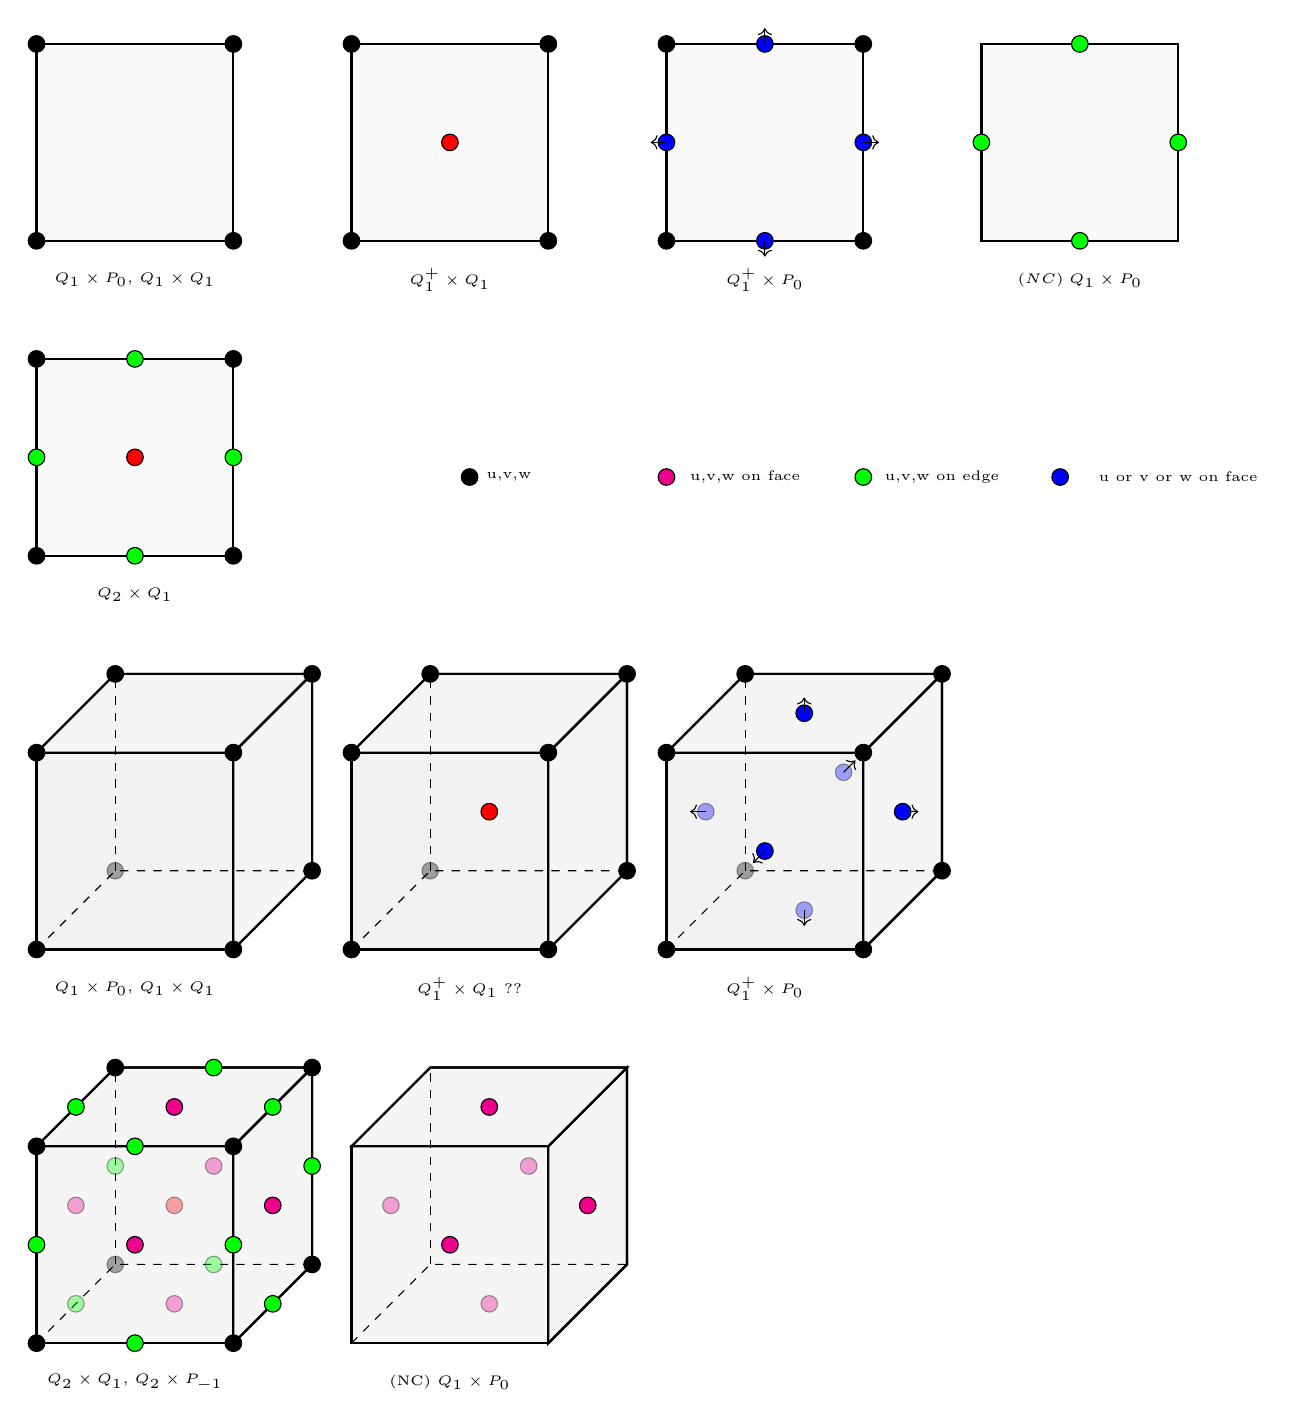
\begin{tikzpicture}
%\draw[fill=gray!23,gray!23](0,0) rectangle (20,10);
%\draw[step=0.5cm,gray,very thin] (0,0) grid (18,18); %background grid

%%%%%%%%%%%%%%%%%%%%%%%%%%%%%%%%%%%%%%%%%%%%%%%%%%%%%%%%%%%%%%%%%%%%
%bottom row
%%%%%%%%%%%%%%%%%%%%%%%%%%%%%%%%%%%%%%%%%%%%%%%%%%%%%%%%%%%%%%%%%%%%
\draw[thick,fill=gray!8] (1,1) -- (3.5,1) -- (3.5,3.5) -- (1,3.5) -- cycle;
\draw[thick,fill=gray!8] (5,1) -- (7.5,1) -- (7.5,3.5) -- (5,3.5) -- cycle;
%\draw[thick,fill=gray!8] (9,1) -- (11.5,1) -- (11.5,3.5) -- (9,3.5) -- cycle;
%\draw[thick,fill=gray!8] (13,1) -- (15.5,1) -- (15.5,3.5) -- (13,3.5) -- cycle;

%right sides
\draw[thick,fill=gray!8] (3.5,1) -- (4.5,2) -- (4.5,4.5) -- (3.5,3.5) -- cycle;
\draw[thick,fill=gray!8] (7.5,1) -- (8.5,2) -- (8.5,4.5) -- (7.5,3.5) -- cycle;
%\draw[thick,fill=gray!8] (11.5,1) -- (12.5,2) -- (12.5,4.5) -- (11.5,3.5) -- cycle;
%\draw[thick,fill=gray!8] (15.5,1) -- (16.5,2) -- (16.5,4.5) -- (15.5,3.5) -- cycle;

%tops
\draw[thick,fill=gray!8] (1,3.5) -- (3.5,3.5) -- (4.5,4.5) -- (2,4.5) -- cycle;
\draw[thick,fill=gray!8] (5,3.5) -- (7.5,3.5) -- (8.5,4.5) -- (6,4.5) -- cycle;
%\draw[thick,fill=gray!8] (9,3.5) -- (11.5,3.5) -- (12.5,4.5) -- (10,4.5) -- cycle;
%\draw[thick,fill=gray!8] (13,3.5) -- (15.5,3.5) -- (16.5,4.5) -- (14,4.5) -- cycle;

\draw[thick] (1,3.5) -- (2,4.5) -- (4.5,4.5) -- (4.5,2) -- (3.5,1);
\draw[thick] (5,3.5) -- (6,4.5) -- (8.5,4.5) -- (8.5,2) -- (7.5,1);
%\draw[thick] (9,3.5) -- (10,4.5) -- (12.5,4.5) -- (12.5,2) -- (11.5,1);
%\draw[thick] (13,3.5) -- (14,4.5) -- (16.5,4.5) -- (16.5,2) -- (15.5,1);

\draw[thick] (3.5,3.5) -- (4.5,4.5) ;
\draw[thick] (7.5,3.5) -- (8.5,4.5) ;
%\draw[thick] (11.5,3.5) -- (12.5,4.5) ;
%\draw[thick] (15.5,3.5) -- (16.5,4.5) ;

\draw[dashed] (1,1) -- (2,2) -- (4.5,2) ;\draw[dashed] (2,2) -- (2,4.5);
\draw[dashed] (5,1) -- (6,2) -- (8.5,2) ;\draw[dashed] (6,2) -- (6,4.5);
%\draw[dashed] (9,1) -- (10,2) -- (12.5,2) ;\draw[dashed] (10,2) -- (10,4.5);
%\draw[dashed] (13,1) -- (14,2) -- (16.5,2) ;\draw[dashed] (14,2)--(14,4.5);

\draw[black,fill=black] (1,1)   circle (3pt);
\draw[black,fill=black] (3.5,1)   circle (3pt);
\draw[black,fill=black] (3.5,3.5)   circle (3pt);
\draw[black,fill=black] (1,3.5)   circle (3pt);
\draw[black,fill=black] (2,4.5)   circle (3pt);
\draw[black,fill=black] (4.5,4.5)   circle (3pt);
\draw[black,fill=black] (4.5,2)   circle (3pt);
\draw[black,fill=black,opacity=0.35] (2,2)   circle (3pt);

%\draw[black,fill=black] (5,1)   circle (3pt);
%\draw[black,fill=black] (7.5,1)   circle (3pt);
%\draw[black,fill=black] (7.5,3.5)   circle (3pt);
%\draw[black,fill=black] (5,3.5)   circle (3pt);
%\draw[black,fill=black] (6,4.5)   circle (3pt);
%\draw[black,fill=black] (8.5,4.5)   circle (3pt);
%\draw[black,fill=black] (8.5,2)   circle (3pt);
%\draw[black,fill=black,opacity=0.35] (6,2)   circle (3pt);

%\draw[black,fill=black] (9,1)   circle (3pt);
%\draw[black,fill=black] (11.5,1)   circle (3pt);
%\draw[black,fill=black] (11.5,3.5)   circle (3pt);
%\draw[black,fill=black] (9,3.5)   circle (3pt);
%\draw[black,fill=black] (10,4.5)   circle (3pt);
%\draw[black,fill=black] (12.5,4.5)   circle (3pt);
%\draw[black,fill=black] (12.5,2)   circle (3pt);
%\draw[black,fill=black,opacity=0.35] (10,2)   circle (3pt);

%\draw[black,fill=black] (13,1)   circle (3pt);
%\draw[black,fill=black] (15.5,1)   circle (3pt);
%\draw[black,fill=black] (15.5,3.5)   circle (3pt);
%\draw[black,fill=black] (13,3.5)   circle (3pt);
%\draw[black,fill=black] (14,4.5)   circle (3pt);
%\draw[black,fill=black] (16.5,4.5)   circle (3pt);
%\draw[black,fill=black] (16.5,2)   circle (3pt);
%\draw[black,fill=black,opacity=0.35] (14,2)   circle (3pt);


%%%%%%%%%%%%%%%%%%%%%%%%%%%%%%%%%%%%%%%%%%%%%%%%%%%%%%%%%%%%%%%%%%%%
%3rd row 
%%%%%%%%%%%%%%%%%%%%%%%%%%%%%%%%%%%%%%%%%%%%%%%%%%%%%%%%%%%%%%%%%%%%

\draw[thick,fill=gray!5] (1,15) -- (3.5,15) -- (3.5,17.5) -- (1,17.5) -- cycle;
\draw[thick,fill=gray!5] (5,15) -- (7.5,15) -- (7.5,17.5) -- (5,17.5) -- cycle;
\draw[thick,fill=gray!5] (9,15) -- (11.5,15) -- (11.5,17.5) -- (9,17.5) -- cycle;
\draw[thick,fill=gray!5] (13,15) -- (15.5,15) -- (15.5,17.5) -- (13,17.5) -- cycle;

\draw[black,fill=black] (1,15)   circle (3pt);
\draw[black,fill=black] (3.5,15)   circle (3pt);
\draw[black,fill=black] (1,17.5)   circle (3pt);
\draw[black,fill=black] (3.5,17.5)   circle (3pt);
\node[] at (2.25,14.5) {\tiny $Q_1\times P_0$, $Q_1\times Q_1$};


\draw[black,fill=black] (5,15)   circle (3pt);
\draw[black,fill=black] (7.5,15)   circle (3pt);
\draw[black,fill=black] (5,17.5)   circle (3pt);
\draw[black,fill=black] (7.5,17.5)   circle (3pt);
\node[] at (6.25,14.5) {\tiny $Q_1^+\times Q_1$};
\draw[black,fill=red] (6.25,16.25)   circle (3pt);

\draw[black,fill=black] (9,15)   circle (3pt);
\draw[black,fill=black] (11.5,15)   circle (3pt);
\draw[black,fill=black] (9,17.5)   circle (3pt);
\draw[black,fill=black] (11.5,17.5)   circle (3pt);
\node[] at (10.25,14.5) {\tiny $Q_1^+\times P_0$};

\draw[black,fill=blue] (9,16.25)   circle (3pt);
\draw[black,fill=blue] (11.5,16.25)   circle (3pt);
\draw[black,fill=blue] (10.25,15)   circle (3pt);
\draw[black,fill=blue] (10.25,17.5)   circle (3pt);

\draw[fill=blue,->] (9,16.25) -- (8.8,16.25); 
\draw[fill=blue,->] (11.5,16.25) -- (11.7,16.25); 
\draw[fill=blue,->] (10.25,15) -- (10.25,14.8); 
\draw[fill=blue,->] (10.25,17.5) -- (10.25,17.7); 


\draw[black,fill=green] (14.25,15)   circle (3pt);
\draw[black,fill=green] (14.25,17.5)   circle (3pt);
\draw[black,fill=green] (13,16.25)   circle (3pt);
\draw[black,fill=green] (15.5,16.25)   circle (3pt);
\node[] at (14.25,14.5) {\tiny $(NC)\; Q_1\times P_0$};

%%%%%%%%%%%%%%%%%%%%%%%%%%%%%%%%%%%%%%%%%%%%%%%%%%%%%%%%%%%%%%%%%%%%
%2nd row 
%%%%%%%%%%%%%%%%%%%%%%%%%%%%%%%%%%%%%%%%%%%%%%%%%%%%%%%%%%%%%%%%%%%%

\draw[thick,fill=gray!5] (1,11) -- (3.5,11) -- (3.5,13.5) -- (1,13.5) -- cycle;
%\draw[thick,fill=gray!5] (5,11) -- (7.5,11) -- (7.5,13.5) -- (5,13.5) -- cycle;
%\draw[thick,fill=gray!5] (9,11) -- (11.5,11) -- (11.5,13.5) -- (9,13.5) -- cycle;
%\draw[thick,fill=gray!5] (13,11) -- (15.5,11) -- (15.5,13.5) -- (13,13.5) -- cycle;

\draw[black,fill=black] (1,11)   circle (3pt);
\draw[black,fill=green] (2.25,11)   circle (3pt);
\draw[black,fill=black] (3.5,11)   circle (3pt);
\draw[black,fill=green] (1,12.25)   circle (3pt);
\draw[black,fill=red] (2.25,12.25)   circle (3pt);
\draw[black,fill=green] (3.5,12.25)   circle (3pt);
\draw[black,fill=black] (1,13.5)   circle (3pt);
\draw[black,fill=green] (2.25,13.5)   circle (3pt);
\draw[black,fill=black] (3.5,13.5)   circle (3pt);
\node[] at (2.25,10.5) {\tiny $Q_2\times Q_1$};



%%%%%%%%%%%%%%%%%%%%%%%%%%%%%%%%%%%%%%%%%%%%%%%%%%%%%%%%%%%%%%%%%%%%
%1st row 
%%%%%%%%%%%%%%%%%%%%%%%%%%%%%%%%%%%%%%%%%%%%%%%%%%%%%%%%%%%%%%%%%%%%
\draw[thick,fill=gray!10] (1,6) -- (3.5,6) -- (3.5,8.5) -- (1,8.5) -- cycle;
\draw[thick,fill=gray!10] (5,6) -- (7.5,6) -- (7.5,8.5) -- (5,8.5) -- cycle;
\draw[thick,fill=gray!10] (9,6) -- (11.5,6) -- (11.5,8.5) -- (9,8.5) -- cycle;
%\draw[thick,fill=gray!10] (13,6) -- (15.5,6) -- (15.5,8.5) -- (13,8.5) -- cycle;

%right sides
\draw[thick,fill=gray!8] (3.5,6) -- (4.5,7) -- (4.5,9.5) -- (3.5,8.5) -- cycle;
\draw[thick,fill=gray!8] (7.5,6) -- (8.5,7) -- (8.5,9.5) -- (7.5,8.5) -- cycle;
\draw[thick,fill=gray!8] (11.5,6) -- (12.5,7) -- (12.5,9.5) -- (11.5,8.5) -- cycle;
%\draw[thick,fill=gray!8] (15.5,6) -- (16.5,7) -- (16.5,9.5) -- (15.5,8.5) -- cycle;

%tops
\draw[thick,fill=gray!8] (1,8.5) -- (3.5,8.5) -- (4.5,9.5) -- (2,9.5) -- cycle;
\draw[thick,fill=gray!8] (5,8.5) -- (7.5,8.5) -- (8.5,9.5) -- (6,9.5) -- cycle;
\draw[thick,fill=gray!8] (9,8.5) -- (11.5,8.5) -- (12.5,9.5) -- (10,9.5) -- cycle;
%\draw[thick,fill=gray!8] (13,8.5) -- (15.5,8.5) -- (16.5,9.5) -- (14,9.5) -- cycle;


\draw[thick] (1,8.5) -- (2,9.5) -- (4.5,9.5) -- (4.5,7) -- (3.5,6);
\draw[thick] (5,8.5) -- (6,9.5) -- (8.5,9.5) -- (8.5,7) -- (7.5,6);
\draw[thick] (9,8.5) -- (10,9.5) -- (12.5,9.5) -- (12.5,7) -- (11.5,6);
%\draw[thick] (13,8.5) -- (14,9.5) -- (16.5,9.5) -- (16.5,7) -- (15.5,6);

\draw[thick] (3.5,8.5) -- (4.5,9.5) ;
\draw[thick] (7.5,8.5) -- (8.5,9.5) ;
\draw[thick] (11.5,8.5) -- (12.5,9.5) ;
%\draw[thick] (15.5,8.5) -- (16.5,9.5) ;

\draw[dashed] (1,6) -- (2,7) -- (4.5,7)    ;\draw[dashed] (2,7) -- (2,9.5);
\draw[dashed] (5,6) -- (6,7) -- (8.5,7)    ;\draw[dashed] (6,7) -- (6,9.5);
\draw[dashed] (9,6) -- (10,7) -- (12.5,7)  ;\draw[dashed] (10,7) -- (10,9.5);
%\draw[dashed] (13,6) -- (14,7) -- (16.5,7) ;\draw[dashed] (14,7) -- (14,9.5);

\draw[black,fill=black] (1,6)   circle (3pt);
\draw[black,fill=black] (3.5,6)   circle (3pt);
\draw[black,fill=black] (3.5,8.5)   circle (3pt);
\draw[black,fill=black] (1,8.5)   circle (3pt);
\draw[black,fill=black] (2,9.5)   circle (3pt);
\draw[black,fill=black] (4.5,9.5)   circle (3pt);
\draw[black,fill=black] (4.5,7)   circle (3pt);
\draw[black,fill=black,opacity=0.35] (2,7)   circle (3pt);

\draw[black,fill=black] (5,6)   circle (3pt);
\draw[black,fill=black] (7.5,6)   circle (3pt);
\draw[black,fill=black] (7.5,8.5)   circle (3pt);
\draw[black,fill=black] (5,8.5)   circle (3pt);
\draw[black,fill=black] (6,9.5)   circle (3pt);
\draw[black,fill=black] (8.5,9.5)   circle (3pt);
\draw[black,fill=black] (8.5,7)   circle (3pt);
\draw[black,fill=black,opacity=0.35] (6,7)   circle (3pt);

\draw[black,fill=black] (9,6)   circle (3pt);
\draw[black,fill=black] (11.5,6)   circle (3pt);
\draw[black,fill=black] (11.5,8.5)   circle (3pt);
\draw[black,fill=black] (9,8.5)   circle (3pt);
\draw[black,fill=black] (10,9.5)   circle (3pt);
\draw[black,fill=black] (12.5,9.5)   circle (3pt);
\draw[black,fill=black] (12.5,7)   circle (3pt);
\draw[black,fill=black,opacity=0.35] (10,7)   circle (3pt);

%\draw[black,fill=black] (13,5)   circle (2pt);
%\draw[black,fill=black] (15.5,5)   circle (2pt);
%\draw[black,fill=black] (15.5,7.5)   circle (2pt);
%\draw[black,fill=black] (13,7.5)   circle (2pt);
%\draw[black,fill=black] (14,8.5)   circle (2pt);
%\draw[black,fill=black] (16.5,8.5)   circle (2pt);
%\draw[black,fill=black] (16.5,6)   circle (2pt);
%\draw[black,fill=black,opacity=0.35] (14,6)   circle (2pt);


\node[] at (2.25,5.5) {\tiny $Q_1\times P_0$, $Q_1\times Q_1$};


\node[] at (6.5,5.5) {\tiny $Q_1^+\times Q_1$ ??};
\draw[black,fill=red] (6.75,7.75)   circle (3pt);

\node[] at (10.25,5.5) {\tiny $Q_1^+\times P_0$};
\draw[black,fill=blue,opacity=0.35] (9.5,7.75)   circle (3pt);
\draw[black,fill=blue] (12,7.75)   circle (3pt);
\draw[black,fill=blue,opacity=0.35] (10.75,6.5)   circle (3pt);
\draw[black,fill=blue] (10.75,9)   circle (3pt);
\draw[black,fill=blue] (10.25,7.25)   circle (3pt);
\draw[black,fill=blue,opacity=0.35] (11.25,8.25)   circle (3pt);

\draw[fill=blue,->] (9.5,7.75) -- (9.3,7.75); 
\draw[fill=blue,->] (12,7.75) -- (12.2,7.75); 
\draw[fill=blue,->] (10.75,6.5) -- (10.75,6.3); 
\draw[fill=blue,->] (10.75,9) -- (10.75,9.2); 
\draw[fill=blue,->] (10.25,7.25)  -- (10.1,7.1) ;
\draw[fill=blue,->] (11.25,8.25)  -- (11.4,8.4) ;

\node[] at (2.25,0.5) {\tiny $Q_2\times Q_1$, $Q_2\times P_{-1}$};

\draw[black,fill=red,opacity=0.35] (2.75,2.75)   circle (3pt);

\draw[black,fill=magenta,opacity=0.35] (1.5,2.75)   circle (3pt);
\draw[black,fill=magenta] (4,2.75)   circle (3pt);
\draw[black,fill=magenta,opacity=0.35] (2.75,1.5)   circle (3pt);
\draw[black,fill=magenta] (2.75,4)   circle (3pt);
\draw[black,fill=magenta] (2.25,2.25)   circle (3pt);
\draw[black,fill=magenta,opacity=0.35] (3.25,3.25)   circle (3pt);

\draw[black,fill=green] (1,2.25)   circle (3pt);
\draw[black,fill=green] (3.5,2.25)   circle (3pt);
\draw[black,fill=green,opacity=0.35] (2,3.25)   circle (3pt);
\draw[black,fill=green] (4.5,3.25)   circle (3pt);
\draw[black,fill=green,opacity=0.35] (1.5,1.5)   circle (3pt);
\draw[black,fill=green] (4,1.5)   circle (3pt);
\draw[black,fill=green] (2.25,1)   circle (3pt);
\draw[black,fill=green,opacity=0.35] (3.25,2)   circle (3pt);
\draw[black,fill=green] (1.5,4)   circle (3pt);
\draw[black,fill=green] (4,4)   circle (3pt);
\draw[black,fill=green] (2.25,3.5)   circle (3pt);
\draw[black,fill=green] (3.25,4.5)   circle (3pt);

\node[] at (6.25,0.5) {\tiny (NC) $Q_1\times P_0$};
\draw[black,fill=magenta,opacity=0.35] (5.5,2.75)   circle (3pt);
\draw[black,fill=magenta] (8,2.75)   circle (3pt);
\draw[black,fill=magenta,opacity=0.35] (6.75,1.5)   circle (3pt);
\draw[black,fill=magenta] (6.75,4)   circle (3pt);
\draw[black,fill=magenta] (6.25,2.25)   circle (3pt);
\draw[black,fill=magenta,opacity=0.35] (7.25,3.25)   circle (3pt);

\draw[black,fill=black]   (6.5,12) circle (3pt); \node[] at (7,12) {\tiny u,v,w};
\draw[black,fill=magenta] (9,12) circle (3pt); \node[] at (10,12) {\tiny u,v,w on face};
\draw[black,fill=green] (11.5,12) circle (3pt); \node[] at (12.5,12) {\tiny u,v,w on edge};
\draw[black,fill=blue] (14,12) circle (3pt); \node[] at (15.5,12) {\tiny u or v or w on face};

%\draw[black,fill=blue] (1,3.5) circle (2pt); \node[] at (1,3.7) {\tiny \color{blue} 60};

%\draw[black,fill=green](14.75,4.75) circle (2pt);\node[] at (14.75,4.95){\tiny\color{green}121};

%\draw[black,fill=red] (6.25,4.75) circle (2pt); \node[] at (6.25,4.95) {\tiny \color{red} 148};

%\node[] at (1.5,2.75) {\tiny \color{magenta} (0)};


%\draw[thick,->] (0,3) -- (0,4); %x
%\draw[thick,->] (0,3) -- (1,2.5); %y
%\node[] at (1,2.125) {$y$};
%\node[] at (0.25,4) {$z$};

\end{tikzpicture}
\end{center}

Add DSSY, RT, Q1Q1+2 bubbles

\vspace{.5cm}

\begin{tabular}{llll}
\hline
2D &  \\ 
Rannacher-Turek & NCQ1P0 & \stone 77 & pb with buoyancy-driven flow \\
Lamichhane      & Q1+Q1  & \stone 72, \stone 74  & \\ 
DSSY            &        & \stone 77  pb with buoyancy-driven flow \\
Fortin          &        & \stone 80 \\
\hline
\hline
3D & \\
Rannacher-Turek & NCQ1P0  & \elefant &  \\
Lamichhane      & Q1+Q1   & \stone  & Does not work \\ 
DSSY & \\
Fortin & & \stone 81 \\
\hline
\end{tabular}
 %-------------------------------------
\newpage
\subsection{On the meaning of basis functions} \begin{flushright} {\tiny {\color{gray} basis\_functions\_meaning.tex.tex}} \end{flushright}
%~~~~~~~~~~~~~~~~~~~~~~~~~~~~~~~~~~~~~~~~~~~~~~~~~~~~~~~~~~~~~~~~~~~~~~~~~~~~~~~~~~~~~~~~~~~~~~~~~~


\subsubsection{In one dimension}

Let us consider a 1D domain subdivided in 3 elements. We then consider the four linear basis functions 
attached to each node. On the following sketch these are not depicted on a single element with 
reduced coordinates but instead for the whole domain in the natural coordinate $x$:

\begin{flushright} {\tiny {\color{gray} (tikz\_basisfunctions.tex)}} \end{flushright}
%~~~~~~~~~~~~~~~~~~~~~~~~~~~~~~~~~~~~~~~~~~~~~~~~~~~~~~~~~~~~~~~~~~~~~~~~~~~~~~~~~~~~~~~~~~~~~~~~~~

\begin{center}
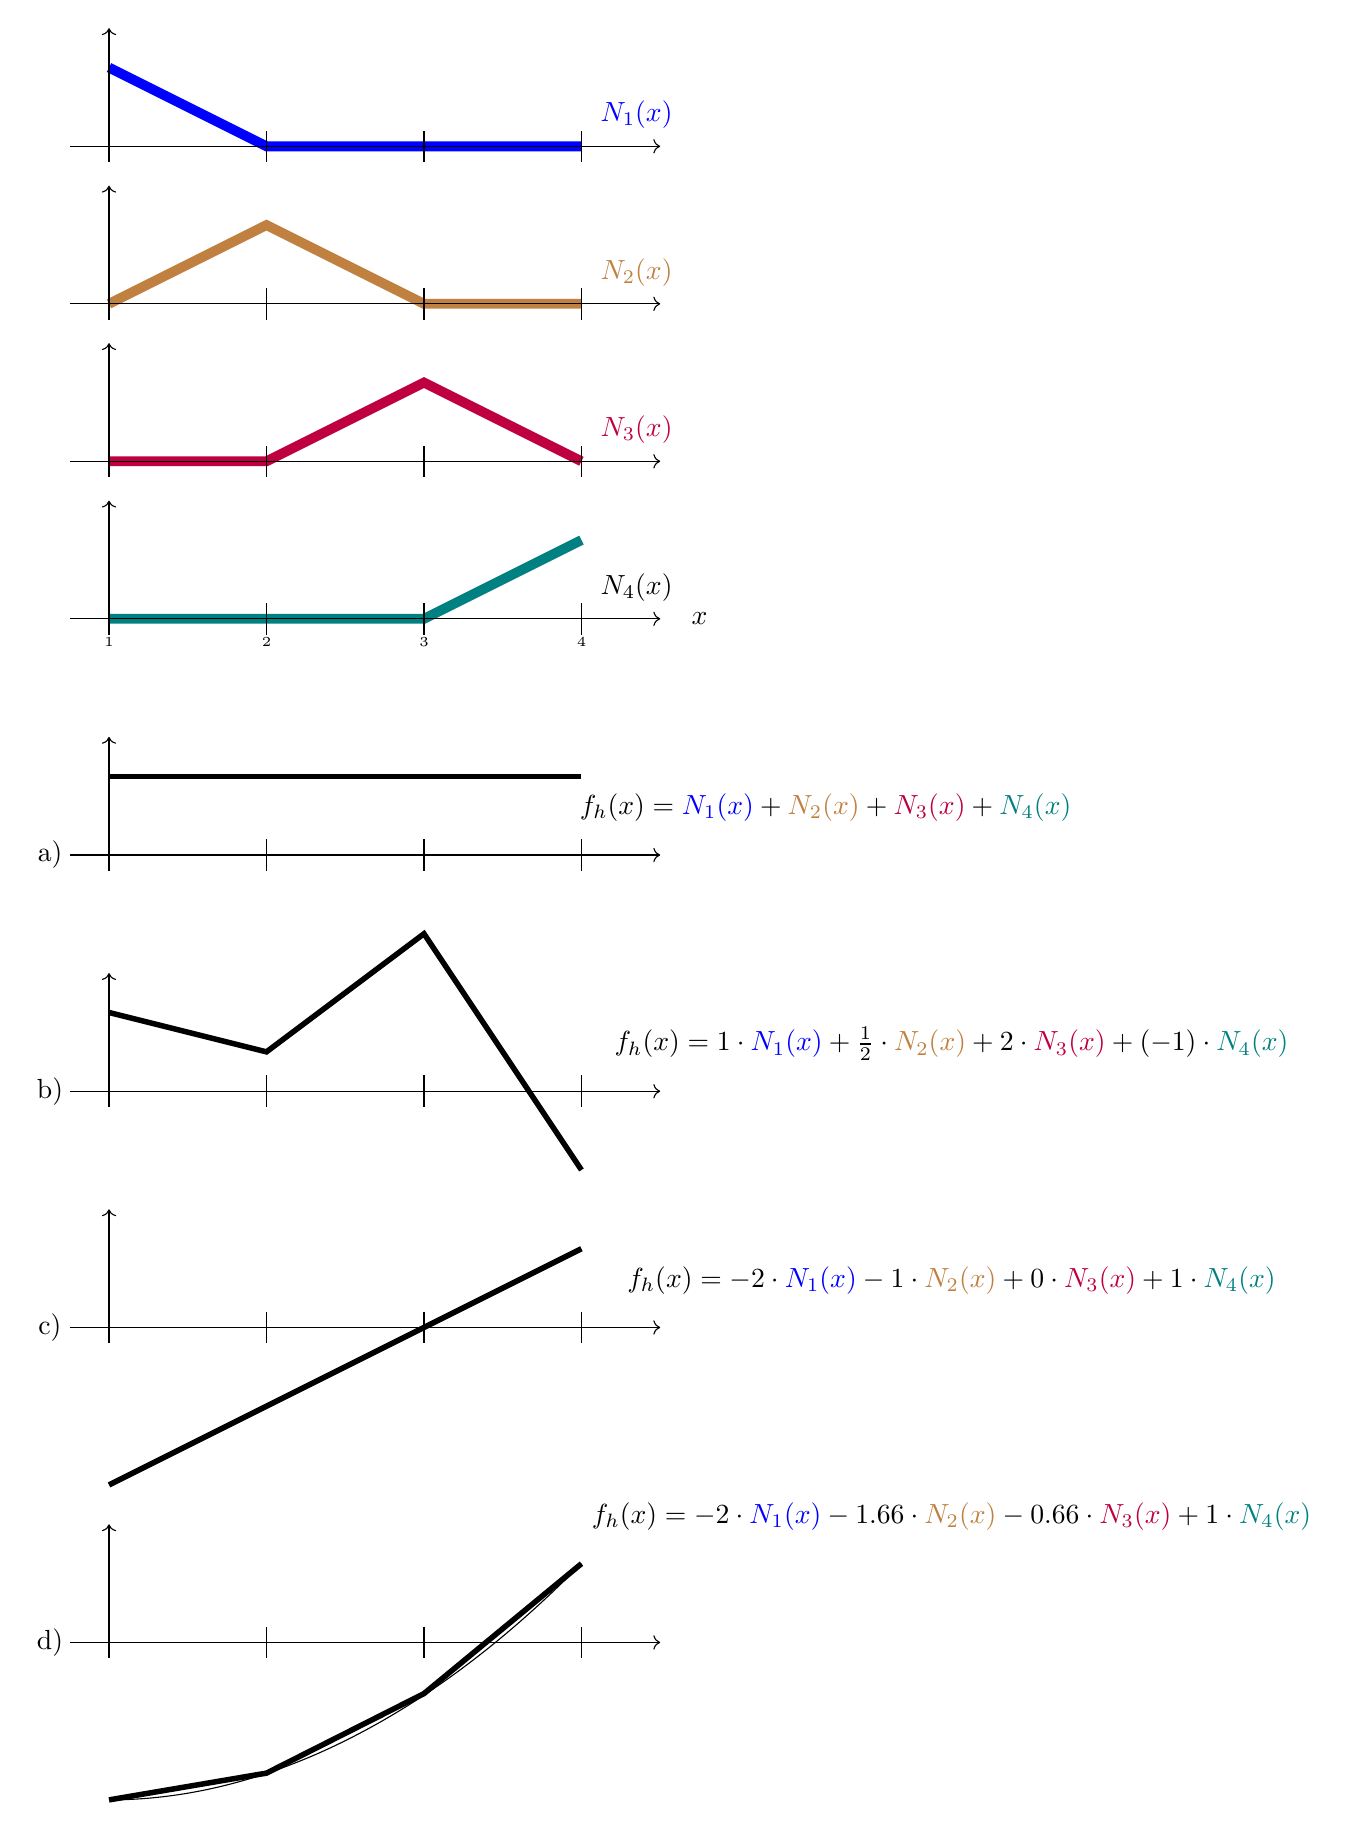
\begin{tikzpicture}
%\draw[step=0.5cm,gray,very thin] (0,-15) grid (15,10); 

%N1
\node[] at (7.7,7.4) {\color{blue}$N_1(x)$};
\draw[line width=1.25mm,color=blue] (1,8)--(3,7)--(5,7)--(7,7);
\draw [->] (0.5,7) -- (8,7);
\draw [->] (1,7) -- (1,8.5);
\draw [-] (1,6.8) -- (1,7.2);
\draw [-] (3,6.8) -- (3,7.2);
\draw [-] (5,6.8) -- (5,7.2);
\draw [-] (7,6.8) -- (7,7.2);

%N2
\node[] at (7.7,5.4) {\color{brown} $N_2(x)$};
\draw[line width=1.25mm,color=brown] (1,5)--(3,6)--(5,5)--(7,5);
\draw [->] (0.5,5) -- (8,5);
\draw [->] (1,5) -- (1,6.5);
\draw [-] (1,4.8) -- (1,5.2);
\draw [-] (3,4.8) -- (3,5.2);
\draw [-] (5,4.8) -- (5,5.2);
\draw [-] (7,4.8) -- (7,5.2);

%N3
\node[] at (7.7,3.4) {\color{purple}$N_3(x)$};
\draw[line width=1.25mm,color=purple] (1,3)--(3,3)--(5,4)--(7,3);
\draw [->] (0.5,3) -- (8,3);
\draw [->] (1,3) -- (1,4.5);
\draw [-] (1,2.8) -- (1,3.2);
\draw [-] (3,2.8) -- (3,3.2);
\draw [-] (5,2.8) -- (5,3.2);
\draw [-] (7,2.8) -- (7,3.2);

%N4
\node[] at (7.7,1.4) {$N_4(x)$};
\draw[line width=1.25mm,color=teal] (1,1)--(5,1)--(7,2);
\draw [->] (0.5,1) -- (8,1);
\draw [->] (1,1) -- (1,2.5);
\draw [-] (1,0.8) -- (1,1.2);
\draw [-] (3,0.8) -- (3,1.2);
\draw [-] (5,0.8) -- (5,1.2);
\draw [-] (7,0.8) -- (7,1.2);
\node[] at (8.5,1) {$x$};
\node[] at (1,0.7) {\tiny $1$};
\node[] at (3,0.7) {\tiny $2$};
\node[] at (5,0.7) {\tiny $3$};
\node[] at (7,0.7) {\tiny $4$};

\node[] at (0.25,-2) {a)};
\node[] at (10.1,-1.4) {$f_h(x)={\color{blue}N_1(x)}+{\color{brown} N_2(x)}+{\color{purple}N_3(x)}+{\color{teal}N_4(x)}$};
\draw[line width=0.7mm] (1,-1)--(7,-1);
\draw [->] (0.5,-2) -- (8,-2);
\draw [->] (1,-2) -- (1,-0.5);
\draw [-] (1,-1.8) -- (1,-2.2);
\draw [-] (3,-1.8) -- (3,-2.2);
\draw [-] (5,-1.8) -- (5,-2.2);
\draw [-] (7,-1.8) -- (7,-2.2);

\node[] at (0.25,-5) {b)};
\node[] at (11.7,-4.4) {$f_h(x)=1\cdot {\color{blue}N_1(x)}+\frac12\cdot {\color{brown} N_2(x)}+2\cdot {\color{purple}N_3(x)}+(-1)\cdot {\color{teal}N_4(x)}$};
\draw [->] (0.5,-5) -- (8,-5);
\draw [->] (1,-5) -- (1,-3.5);
\draw [-] (1,-4.8) -- (1,-5.2);
\draw [-] (3,-4.8) -- (3,-5.2);
\draw [-] (5,-4.8) -- (5,-5.2);
\draw [-] (7,-4.8) -- (7,-5.2);
\draw[line width=0.7mm] (1,-4)--(3,-4.5)--(5,-3)--(7,-6);

\node[] at (0.25,-8) {c)};
\node[] at (11.7,-7.4) {$f_h(x)=-2\cdot {\color{blue}N_1(x)}-1\cdot {\color{brown} N_2(x)}+0\cdot {\color{purple}N_3(x)}+1\cdot {\color{teal}N_4(x)}$};
\draw [->] (0.5,-8) -- (8,-8);
\draw [->] (1,-8) -- (1,-6.5);
\draw [-] (1,-7.8) -- (1,-8.2);
\draw [-] (3,-7.8) -- (3,-8.2);
\draw [-] (5,-7.8) -- (5,-8.2);
\draw [-] (7,-7.8) -- (7,-8.2);
\draw[line width=0.7mm] (1,-10)--(3,-9)--(5,-8)--(7,-7);

\node[] at (0.25,-12) {d)};
\draw [->] (0.5,-12) -- (8,-12);
\draw [->] (1,-12) -- (1,-10.5);
\draw [-] (1,-11.8) -- (1,-12.2);
\draw [-] (3,-11.8) -- (3,-12.2);
\draw [-] (5,-11.8) -- (5,-12.2);
\draw [-] (7,-11.8) -- (7,-12.2);
\draw (1,-14) parabola (7,-11);
\draw[line width=0.7mm] (1,-14)--(3,-13.66)--(5,-12.65)--(7,-11);
\node[] at (11.7,-10.4) {$f_h(x)=-2\cdot {\color{blue}N_1(x)}-1.66\cdot {\color{brown} N_2(x)}-0.66\cdot {\color{purple}N_3(x)}+1\cdot {\color{teal}N_4(x)}$};


\end{tikzpicture}
\end{center}


The four cases a,b,c,d are examples of combinations of these basis functions:
\[
f_h(x)=\sum_{i=1}^4 N_i(x) f_i
\]
Where $f_i$ are the values associated to the four nodes. 
We assume that the distance $h$ between nodes is 1.

Example a) illustrates the fact that the sum of all basis functions must be strictly equal to one everywhere
in the domain. Failing to do so would mean that the basis functions cannot represent a constant field (see
Section~\ref{ss:q12d}). 

Example b) illustrates a somewhat random combination of the basis functions, yielding a broken line. 

Example c) illustrates the fact that these linear basis functions can exactly represent a
linear function. When $f(x)=x-2$, then $f_1=f(0)=-2$, $f_2=f(1)=-1$, $f_3=f(2)=0$ and $f_4=f(3)=+1$, 
then $f_h(x)$ is exactly $f(x)$ on the domain.

Example d) illustrates the fact that linear basis functions cannot represent a parabola. Smaller and 
smaller elements will do an increasingly better job and will get closer to the curve but a 
systematic error will subsist.  


Note that these drawings are trivial to produce since $N_i(x_j)=\delta_{ij}$ by definition, so that 
$f_h(x_j)=f_j$.

%........................................................................
\subsubsection{In two dimensions}



 %-------------------


\newpage 
%%%%%%%%%%%%%%%%%%%%%%%%%%%%%%%%%%%%%%%%%%%%%%%%%%%%%%%%%%%%%%%%%%%%%%%%%%%%%%%%%%%%%%%%%%%%%%%%%%%
\section{Solving the heat transport equation with linear Finite Elements} %%%%%%%%%%%%%%%%%%%%%%%%%

\subsection{The diffusion equation in 1D} \label{sec:diff1D} 
Let us consider the following one-dimensional grid: 
\begin{center}
\includegraphics[width=10cm]{images/oneD/domain}
\end{center}
Its spans the domain $\Omega$ of length $L_x$. 
It is discretised by means of 
$nnx$ nodes and $nelx=nnx-1$ elements.
Zooming in on element which is bounded by two nodes $k$ and $k+1$,
its size (also sometimes called diameter) is $h_x=x_{k+1}-x_k$, 
and the temperature field we wish to compute is located on those 
nodes so that they are logically called $T_k$ and $T_{k+1}$:

\begin{center}
\includegraphics[width=8cm]{images/oneD/el1D}
\end{center}

We focus here on the 1D diffusion equation (no advection, no heat sources):
\begin{equation}
\rho c_p \frac{\partial T}{\partial t} 
= \frac{\partial }{\partial x} \left( k \frac{\partial T}{\partial x}  \right)
\end{equation}
This is the {\color{olive}strong form} of the ODE to solve.
I can multiply this equation by a function\footnote{This function should be well-behaved with special properties, but we here assume it is a polynomial function.} $f(x)$ and integrate it over $\Omega$:
\begin{equation}
\int_{\Omega} f(x)  \rho c_p\frac{\partial T}{\partial t} dx
=
\int_{\Omega} f(x) \frac{\partial }{\partial x} \left( k \frac{\partial T}{\partial x}  \right) dx
\end{equation}
Looking at the right hand side, it is of the form $\int u v'$ so that I naturally 
integrate it by parts:
\begin{equation}
\int_{\Omega} f(x) \frac{\partial }{\partial x} 
\left( k \frac{\partial T}{\partial x}  \right) dx
=
\left[
f(x) k \frac{\partial T}{\partial x}
\right]_{\partial \Omega}
-
\int_{\Omega} \frac{\partial f}{\partial x}  k \frac{\partial T}{\partial x}  dx
\end{equation}
Assuming there is no heat flux prescribed on the boundary (i.e. $q_x= - k \partial T/\partial x = 0$ ),
\todo[inline]{NOT happy with this statement!!} then:
\begin{equation}
\int_{\Omega} f(x) \frac{\partial }{\partial x} \left( k \frac{\partial T}{\partial x}  \right) dx
=
- \int_{\Omega} \frac{\partial f}{\partial x}  k \frac{\partial T}{\partial x}  dx
\end{equation}
We then obtain the {\color{olive}weak form} of the diffusion equation in 1D:
\begin{equation}
\boxed{
\int_{\Omega} f(x) \rho c_p \frac{\partial T}{\partial t} dx
+
\int_{\Omega} \frac{\partial f}{\partial x}  k \frac{\partial T}{\partial x}  dx = 0
}
\end{equation}
We then use the additive property of the integral 
$\int_\Omega \dots = \sum_{elts} \int_{\Omega_e} \dots$
so that 
\begin{equation}
\sum_{elts} \left(     
\underbrace{ \int_{\Omega_e} f(x) \rho c_p   \frac{\partial T}{\partial t} dx }_{{\Lambda}_f^e}
+
\underbrace{\int_{\Omega_e} \frac{\partial f}{\partial x}  k \frac{\partial T}{\partial x}  dx}_{{\Upsilon}_f^e}      \right) = 0  
\end{equation}

In order to compute these integrals (analytically or by means of a numerical quadrature), 
we will need to evaluate $T$ inside the element. However, inside the element, 
the temperature is not known: all we have is the temperature at the nodes. 
For $x\in [x_k,x_{k+1}]$ we need to come up with a way to compute the temperature at this location. 
It makes sense to think that $T(x)$ will then be a function of the temperature at the nodes, 
i.e. $T(x) = \alpha T_k + \beta T_{k+1}$ where $\alpha$ and $\beta$ are coefficients. 
One over-simplified approach would be to assign $T(x)=(T_k + T_{k+1})/2$ but this would make the
temperature discontinuous from element to element. 
The rather logical solution to this problem is a linear temperature field between $T_k$
and $T_{k+1}$: 

\begin{eqnarray}
T(x) 
%&=& N_{k}(x) T_k + N_{k+1}(x) T_{k+1}  \nn\\
&=& \underbrace{\frac{x_{k+1}-x}{h_x}}_{N_k^\theta(x)} T_k 
+ 
\underbrace{\frac{x-x_k}{h_x}}_{N_{k+1}^\theta(x)} T_{k+1} \nn
\end{eqnarray}
where $N_k^\theta(x)$ is the (temperature) shape function associated to node $k$ and 
$N_{k+1}^\theta(x)$ is the shape function associated to node $k+1$.

Rather reassuringly, we have:
\begin{itemize}
\item $x=x_k$ yields $T(x)=T_k$
\item $x=x_{k+1}$ yields $T(x)=T_{k+1}$
\item $x=(x_k+x_{k+1})/2$ yields $T(x)=(T_k+T_{k+1})/2$
\end{itemize}
In what follows we abbreviate $\partial T/\partial x$ by $\dot{T}$.
Let us compute ${\Lambda}_f^e$ and ${\Upsilon}_f^e$ separately.
\begin{eqnarray}
{\Lambda}_f^e 
&=&\int_{x_k}^{x_{k+1}} f(x) \rho c_p \dot T(x) dx \nn\\
&=& \int_{x_k}^{x_{k+1}} f(x) \rho c_p \;\;  [ N_{k}^\theta(x) \dot{T}_k + N_{k+1}^\theta(x) \dot{T}_{k+1} ] \;\; dx  \nn\\
&=& \int_{x_k}^{x_{k+1}} f(x) \rho c_p N_{k}^\theta(x) \dot{T}_k  dx  
+ \int_{x_k}^{x_{k+1}} f(x) \rho c_p N_{k+1}^\theta(x) \dot{T}_{k+1}   dx \nn\\
&=&  \left( \int_{x_k}^{x_{k+1}} f(x) \rho c_p  N_{k}(x) dx \right) \dot{T}_k  
+ \left( \int_{x_k}^{x_{k+1}} f(x) \rho c_p N_{k+1}(x) dx \right)  \dot{T}_{k+1}  \nn
\end{eqnarray}
Taking $f(x)=N_k(x)$ and omitting '$(x)$' in the rhs:
\[
{\Lambda}_{N_k}^e=
%\int_{x_k}^{x_{k+1}} {\color{blue}f}(x) \rho c_p \dot{\color{blue}T}(x) dx
\left( \int_{x_k}^{x_{k+1}} \rho c_p  N_k N_{k} dx \right) \dot{T}_k  
+ \left( \int_{x_k}^{x_{k+1}} \rho c_p N_k N_{k+1} dx \right)  \dot{T}_{k+1} 
\]
Taking $f(x)=N_{k+1}(x)$ and omitting '$(x)$' in the rhs:
\[
{\Lambda}_{N_{k+1}}^e
%\int_{x_k}^{x_{k+1}} {\color{blue}f}(x) \dot{\color{blue}T}(x) dx
=  \left( \int_{x_k}^{x_{k+1}} \rho c_p N_{k+1} N_{k} dx \right) \dot{T}_k  
+ \left( \int_{x_k}^{x_{k+1}}  \rho c_p  N_{k+1} N_{k+1} dx \right)  \dot{T}_{k+1} 
\]
We can rearrange these last two equations as follows:
\[
\left(
\begin{array}{c}
{\Lambda}_{N_k}^e  \\ \\ {\Lambda}_{N_{k+1}}^e
\end{array}
\right)
=
\left(
\begin{array}{cc}
\int_{x_k}^{x_{k+1}} N_k     \rho c_p N_{k} dx  &  \int_{x_k}^{x_{k+1}} N_k  \rho c_p N_{k+1} dx \\ \\
\int_{x_k}^{x_{k+1}} N_{k+1} \rho c_p N_{k} dx  &  \int_{x_k}^{x_{k+1}} N_{k+1} \rho c_p N_{k+1} dx 
\end{array}
\right)
\cdot
\left(
\begin{array}{c}
\dot{T}_k \\ \\
\dot{T}_{k+1}
\end{array}
\right)
\]
and we can take the integrals outside of the matrix:
\[
\left(
\begin{array}{c}
{\Lambda}_{N_k}^e \\ \\ {\Lambda}_{N_{k+1}}^e
\end{array}
\right)
=
\left[
\int_{x_k}^{x_{k+1}}
\rho c_p
\left(
\begin{array}{cc}
N_k N_{k}     &  N_k N_{k+1}  \\ \\
N_{k+1} N_{k} &  N_{k+1} N_{k+1} 
\end{array}
\right)
dx
\right]
\cdot
\left(
\begin{array}{c}
\dot{T}_k \\ \\ 
\dot{T}_{k+1}
\end{array}
\right)
\]
Finally, we can define the vectors 
\[
{\vec N}^T = 
\left(
\begin{array}{c}
N_k(x)  \\ \\  N_{k+1} (x)
\end{array}
\right)
\]
and 
\[
{\vec T}^e = 
\left(
\begin{array}{c}
T_k \\ \\ T_{k+1}
\end{array}
\right)
\quad
\quad
\quad
\quad
\quad
\dot{\vec T}^e = 
\left(
\begin{array}{c}
\dot{T}_k \\ \\ \dot{T}_{k+1}
\end{array}
\right)
\]
so that 
\[
\left(
\begin{array}{c}
{\Lambda}_{N_k}^e \\  \\ {\Lambda}_{N_{k+1}}^e
\end{array}
\right)
=
\left( \int_{x_k}^{x_{k+1}}   {\vec N}^T \rho c_p  {\vec N} dx  \right) \cdot \dot{\vec T}^e
\]

Back to the diffusion term:

\begin{eqnarray}
{\Upsilon}_f^e &=&
\int_{x_k}^{x^{k+1}} \frac{\partial f}{\partial x} k \frac{\partial T}{\partial x} dx \nn\\
&=&
\int_{x_k}^{x^{k+1}} \frac{\partial f}{\partial x} k \frac{\partial  (N_{k}(x) T_k + N_{k+1}(x) T_{k+1} ) }{\partial x} dx  \nn\\
%&=&
%\int_{x_k}^{x^{k+1}} \left( \frac{\partial {\color{blue}f}}{\partial x}  \frac{\partial  {\color{blue}N}_{k} } {\partial x}  T_k 
%+ \frac{\partial {\color{blue}f}}{\partial x}  \frac{\partial  {\color{blue}N}_{k+1} } {\partial x}  T_{k+1} \right)  dx \nn\\
&=&
\left( \int_{x_k}^{x^{k+1}} \frac{\partial f}{\partial x}  k \frac{\partial  N_{k} } {\partial x}  dx \right)  T_k 
+ \left( \int_{x_k}^{x^{k+1}} \frac{\partial f}{\partial x}  k \frac{\partial  N_{k+1} } {\partial x} dx \right) T_{k+1}  \nn
\end{eqnarray}
Taking $f(x)=N_k(x)$ 
\[
{\Upsilon}_{N_k}^e=
%\int_{x_k}^{x^{k+1}} \frac{\partial {\color{blue}f}}{\partial x} \frac{\partial {\color{blue}T}}{\partial x} dx
\left( \int_{x_k}^{x^{k+1}} k\frac{\partial N_k}{\partial x}  \frac{\partial  N_{k} } {\partial x}  dx \right)  T_k 
+ \left( \int_{x_k}^{x^{k+1}} k \frac{\partial N_k}{\partial x}  \frac{\partial  N_{k+1} } {\partial x} dx \right) T_{k+1}  \nn
\]
Taking $f(x)=N_{k+1}(x)$ 
\[
{\Upsilon}_{N_{k+1}}^e=
%\int_{x_k}^{x^{k+1}} \frac{\partial {\color{blue}f}}{\partial x} \frac{\partial {\color{blue}T}}{\partial x} dx
%=
\left( \int_{x_k}^{x^{k+1}} k\frac{\partial N_{k+1}}{\partial x}  \frac{\partial  N_{k} } {\partial x}  dx \right)  T_k 
+ \left( \int_{x_k}^{x^{k+1}}  k\frac{\partial N_{k+1}}{\partial x}  \frac{\partial  N_{k+1} } {\partial x} dx \right) T_{k+1}  \nn
\]


\[
\left(
\begin{array}{cc}
 {\Upsilon}_{N_k}^e \\ \\ {\Upsilon}_{N_{k+1}}^e
\end{array}
\right)
=
\left(
\begin{array}{cc}
\int_{x_k}^{x^{k+1}} \frac{\partial N_k}{\partial x} k \frac{\partial  N_{k} } {\partial x}  dx & 
\int_{x_k}^{x^{k+1}} \frac{\partial N_k}{\partial x} k \frac{\partial  N_{k+1} } {\partial x} dx 
\\ \\
\int_{x_k}^{x^{k+1}} \frac{\partial N_{k+1}}{\partial x} k \frac{\partial  N_{k} } {\partial x}  dx & 
\int_{x_k}^{x^{k+1}} \frac{\partial N_{k+1}}{\partial x} k \frac{\partial  N_{k+1} } {\partial x} dx 
\end{array}
\right)
\cdot
\left(
\begin{array}{c}
T_k \\ \\ T_{k+1}
\end{array}
\right)
\]

or,
\[
\left(
\begin{array}{cc}
 {\Upsilon}_{N_k}^e \\ \\ {\Upsilon}_{N_{k+1}}^e
\end{array}
\right)
=
\left[
\int_{x_k}^{x^{k+1}}
k
\left(
\begin{array}{cc}
\frac{\partial N_k}{\partial x}  \frac{\partial  N_{k} } {\partial x}   & 
\frac{\partial N_k}{\partial x}  \frac{\partial  N_{k+1} } {\partial x}  
\\ \\
\frac{\partial N_{k+1}}{\partial x}  \frac{\partial  N_{k} } {\partial x}   & 
\frac{\partial N_{k+1}}{\partial x}  \frac{\partial  N_{k+1} } {\partial x}  
\end{array}
\right)
dx
\right]
\cdot
\left(
\begin{array}{c}
T_k \\ \\ T_{k+1}
\end{array}
\right)
\]
Finally, we can define the vector 
\[
{\vec B}^T=
\left(
\begin{array}{cc}
 \frac{\partial N_k}{\partial x}   \\ \\
 \frac{\partial N_{k+1}}{\partial x}
\end{array}
\right)
\]
so that 
\[
\left(
\begin{array}{cc}
 {\Upsilon}_{N_k}^e \\ \\ {\Upsilon}_{N_{k+1}}^e
\end{array}
\right)
=
\left( \int_{x_k}^{x_{k+1}}   {\vec B}^T k {\vec B} dx  \right) \cdot {\vec T}^e
\]

The weak form discretised over 1 element becomes
\[
\underbrace{\left( \int_{x_k}^{x_{k+1}}   {\vec N}^T \rho c_p {\vec N} dx  \right) }_{\bm M^e} \cdot \dot{\vec T}^e
+
\underbrace{\left( \int_{x_k}^{x_{k+1}}   {\vec B}^T k {\vec B} dx  \right)}_{{\bm K}_d^e} \cdot {\vec T}^e
=0
\]
or,
\[
\boxed{
{\bm M}^e \cdot \dot{\vec T}^e + {\bm K}_d^e \cdot {\vec T}^e = 0
}
\]
or,
\[
\boxed{
{\bm M}^e \cdot \frac{\partial {\vec T}^e}{\partial t} + {\bm K}_d^e \cdot {\vec T}^e = 0
}
\]

Using a backward first order in time discretisation for the time derivative:
\[
\dot{\vec T}= \frac{\partial {\vec T}}{\partial t} = \frac{{\vec T}^{new}-{\vec T}^{old}}{\delta t}
\]
we get
\[
{\bm M}^e \cdot \frac{{\vec T}^{new}-{\vec T}^{old}}{\delta t} + {\bm K}_d^e \cdot {\vec T}^{new} = 0
\]
or, 
\[
\boxed{
( {\bm M}^e +  {\bm K}_d^e  \delta t ) \cdot {\vec T}^{new} =  {\bm M}^e \cdot  {\vec T}^{old}
}
\]
with 
\[
{\bm M}^e=  \int_{x_k}^{x_{k+1}}   {\vec N}^T \rho c_p {\vec N} dx  
\quad\quad\quad
{\bm K}_d^e =
 \int_{x_k}^{x_{k+1}}   {\vec B}^T k {\vec B} dx 
\]

Let us compute ${\bm M}$ for an element:
\[
{\bm M}^e=  \int_{x_k}^{x_{k+1}}   {\vec N}^T \rho c_p {\vec N} dx  
\]
with 
\[
{\vec N}^T = 
\left(
\begin{array}{c}
N_k(x)  \\ \\  N_{k+1}(x)
\end{array}
\right)
=
\left(
\begin{array}{c}
\frac{x_{k+1}-x}{h_x}   \\ \\
\frac{x-x_k}{h_x} 
\end{array}
\right)
\]
Then 
\[
{\bm M}^e
=
\left(
\begin{array}{cc}
M_{11} & M_{12} \\
M_{21} & M_{22} 
\end{array}
\right)
=
\left(
\begin{array}{cc}
\int_{x_k}^{x_{k+1}} \rho c_p N_k N_{k} dx   &  \int_{x_k}^{x_{k+1}} \rho c_p N_k N_{k+1} dx \\ \\
\int_{x_k}^{x_{k+1}} \rho c_p N_{k+1} N_{k} dx  &  \int_{x_k}^{x_{k+1}} \rho c_p N_{k+1} N_{k+1} dx 
\end{array}
\right)
\]
I only need to compute 3 integrals since $M_{12}=M_{21}$.
Let us start with $M_{11}$:
\[
M_{11}=\int_{x_k}^{x_{k+1}} \rho c_p N_k(x) N_{k}(x) dx
=   
\int_{x_k}^{x_{k+1}} \rho c_p 
\frac{x_{k+1}-x}{h_x}  
\frac{x_{k+1}-x}{h_x}  
dx
\]
It is then customary to carry out the change of variable $x \rightarrow r$ where 
$r \in [-1:1]$ as shown hereunder:
\begin{center}
\includegraphics[width=8cm]{images/oneD/el1D_mapping}
\end{center}
The relationships between $x$ and $r$ are:
\[
r=\frac{2}{h_x}(x-x_k)-1
\quad\quad\quad
x=\frac{h_x}{2}(1+r)+x_k
\]

In what follows we assume for simplicity that $\rho$ and $c_p$ are constant within each element.
\[
M_{11}=
\rho c_p
\int_{\tiny x_k}^{x_{k+1}} 
\frac{x_{k+1}-x}{h_x}  
\frac{x_{k+1}-x}{h_x}  
dx
%=  \rho c_p \int_{-1}^{+1} \frac{1}{2}(1-r) \frac{1}{2}(1-r)  \frac{h_x}{2} dr  = \frac{h_x}{3} \rho c_p \nn
=  \frac{\rho c_p h_x}{8} \int_{-1}^{+1} (1-r) (1-r)  dr  = \frac{h_x}{3} \rho c_p
\]
Similarly we arrive at 
\begin{eqnarray}
M_{12}
%\rho c_p \int_{x_k}^{x_{k+1}}  {\color{blue}N}_k(x) {\color{blue}N}_{k+1}(x) dx
=\rho c_p 
\int_{x_k}^{x_{k+1}} 
\frac{x_{k+1}-x}{h_x}  
\frac{x-x_k}{h_x}  
dx
=
\frac{\rho c_p  h_x}{8} 
\int_{-1}^{+1} (1-r) (1+r)dr
= \frac{h_x}{6} \rho c_p \nn
\end{eqnarray}
and 
\[
M_{22}
%=\rho c_p \int_{x_k}^{x_{k+1}} {\color{blue}N}_{k+1}(x) {\color{blue}N}_{k+1}(x) dx
=
\rho c_p 
\int_{x_k}^{x_{k+1}} 
\frac{x-x_k}{h_x}  
\frac{x-x_k}{h_x}  
dx
=
\frac{\rho c_p  h_x}{8} 
\int_{-1}^{+1} (1+r) (1+r)dr
= \frac{h_x}{3} \rho c_p 
\]
Finally 
\[
\boxed{
{\bm M}^e= \frac{h_x}{3} \rho c_p  
\left(
\begin{array}{cc}
1  & 1/2 \\
1/2 & 1
\end{array}
\right)
}
\]

In the new coordinate system, the {\color{olive}shape functions} 
\[
N_k(x) = \frac{x_{k+1}-x}{h_x} 
\quad
\quad
\quad
N_{k+1}(x) = \frac{x-x_k}{h_x} 
\]
become 
\[
N_k(r) = \frac{1}{2} (1-r)
\quad
\quad
\quad
N_{k+1}(r) = \frac{1}{2} (1+r)
\]

Also, 
\[
\frac{\partial N_k}{\partial x} = - \frac{1}{h_x} 
\quad
\quad
\quad
\frac{\partial N_{k+1}}{\partial x} = \frac{1}{h_x} 
\]
so that 
\[
{\vec B}^T=
\left(
\begin{array}{cc}
 \frac{\partial N_k}{\partial x}   \\ \\
 \frac{\partial N_{k+1}}{\partial x}
\end{array}
\right)
=
\left(
\begin{array}{cc}
-\frac{1}{h_x} \\ \\
\frac{1}{h_x} 
\end{array}
\right)
\]


We here also assume that $k$ is constant within the element:
\[
{\bm K}_d =
\int_{x_k}^{x_{k+1}}   {\vec B}^T k {\vec B} dx 
= k \int_{x_k}^{x_{k+1}}   {\vec B}^T {\vec B} dx 
\]
simply becomes
\[
{\bm K}_d = k
 \int_{x_k}^{x_{k+1}} 
\frac{1}{h_x^2}
\left(
\begin{array}{cc}
1 & -1 \\ -1 & 1
\end{array}
\right)
dx
\]
and then
\[
\boxed{
{\bm K}_d =
\frac{k}{h_x}
\left(
\begin{array}{cc}
1 & -1 \\ -1 & 1
\end{array}
\right)
}
\]

Let us consider this very simple grid consisting of 4 elements/5 nodes:
\begin{center}
\includegraphics[width=10cm]{images/oneD/grid5}
\end{center}
For each element we have 
\[
\underbrace{( {\bm M}^e +  {\bm K}_d^e \; \delta t )}_{\bm A^{e}} \cdot {\vec T}^{new} =  \underbrace{{\bm M}^e \cdot  {\vec T}^{old} }_{\vec b^{e}}
\]
%or, 
%\[
%{\bm A}^{e}\cdot {\vec T}^{new} =  {\vec b}^{e}
%\]
We can write this equation very explictely for each element:
\begin{itemize}
\item element {\color{red}\tt 1} 
\[
{\bm A}^{\color{red} \tt 1}  \cdot 
\left(
\begin{array}{c}
T_1 \\ T_2
\end{array}
\right)
 =  {\vec b}^{\color{red} \tt 1}
\]
\[
\left\{ 
\begin{array}{l}
A_{11}^{{\color{red}\tt 1}} T_1 + A_{12}^{{\color{red}\tt 1}} T_2 = b^{{\color{red} \tt 1}}_x \\
A_{21}^{{\color{red}\tt 1}} T_1 + A_{22}^{{\color{red}\tt 1}} T_2 = b^{{\color{red} \tt 1}}_y
\end{array}
\right.
\]

\item element {\color{red}\tt 2} 
\[
{\bm A}^{\color{red} \tt 2}  \cdot 
\left(
\begin{array}{c}
T_2 \\ T_3
\end{array}
\right)
 =  {\vec b}^{\color{red} \tt 2}
\]
\[
\left\{ 
\begin{array}{l}
A_{11}^{{\color{red}\tt 2}} T_2 + A_{12}^{{\color{red}\tt 2}} T_3 = b^{{\color{red} \tt 2}}_1 \\
A_{21}^{{\color{red}\tt 2}} T_2 + A_{22}^{{\color{red}\tt 2}} T_3 = b^{{\color{red} \tt 2}}_2
\end{array}
\right.
\]


\item element {\color{red}\tt 3} 
\[
{\bm A}^{\color{red} \tt 3}  \cdot 
\left(
\begin{array}{c}
T_3 \\ T_4
\end{array}
\right)
 =  {\vec b}^{\color{red} \tt 3}
\]
\[
\left\{ 
\begin{array}{l}
A_{11}^{{\color{red}\tt 3}} T_3 + A_{12}^{{\color{red} \tt 3}} T_4 = b^{{\color{red} \tt 3}}_1 \\
A_{21}^{{\color{red}\tt 3}} T_3 + A_{22}^{{\color{red} \tt 3}} T_4 = b^{{\color{red} \tt 3}}_2
\end{array}
\right.
\]


\item element {\color{red}\tt 4} 
\[
{\bm A}^{\color{red} \tt 4}  \cdot 
\left(
\begin{array}{c}
T_4 \\ T_5
\end{array}
\right)
 =  {\vec b}^{\color{red} \tt 4}
\]
\[
\left\{ 
\begin{array}{l}
A_{11}^{{\color{red}\tt 4}} T_4 + A_{12}^{{\color{red}\tt 4}} T_5 = b^{{\color{red}\tt 4}}_1 \\
A_{21}^{{\color{red}\tt 4}} T_4 + A_{22}^{{\color{red}\tt 4}} T_5 = b^{{\color{red}\tt 4}}_2
\end{array}
\right.
\]
\end{itemize}

All equations can be cast into a single linear system: this is the {\color{olive} assembly} phase.
The process can also be visualised as shown hereunder. Because nodes 2,3,4 belong to two elements 
elemental contributions will be summed in the matrix and the rhs:
\begin{center}
\includegraphics[width=8.5cm]{images/oneD/assembly}
\end{center}
The assembled matrix and rhs are then:
\[
\left(
\begin{array}{ccccc}
A_{11}^{{\color{red}\tt 1}} &  A_{12}^{{\color{red}\tt 1}} &0&0&0 \\ \\ 
A_{21}^{{\color{red}\tt 1}} &  A_{22}^{{\color{red} \tt 1}} \!+\! A_{11}^{{\color{red}\tt 2}}  & A_{12}^{{\color{red}\tt 2}}   &0&0 \\ \\
0& A_{21}^{{\color{red}\tt 2}} & A_{22}^{{\color{red} \tt 2}} \! +\! A_{11}^{{\color{red}\tt 3}}  & A_{12}^{{\color{red}\tt 3}}   & 0\\ \\
0&0& A_{21}^{{\color{red}\tt 3}}   & A_{22}^{{\color{red}\tt 3}} \! +\! A_{11}^{{\color{red}\tt 4}}   & A_{12}^{{\color{red}\tt 4}}  \\ \\
0&0&0& A_{21}^{{\color{red}\tt 4}}   & A_{22}^{{\color{red}\tt 4}} 
\end{array}
\right)
\left(
\begin{array}{c}
T_1 \\\\ T_2 \\\\ T_3 \\\\ T_4 \\\\ T_5
\end{array}
\right)
=
\left(
\begin{array}{c}
b_{1}^{{\color{red}\tt 1}} \\ \\
b_{2}^{{\color{red}\tt 1}} + b_{1}^{{\color{red}\tt 2}}\\ \\
b_{2}^{{\color{red}\tt 2}} + b_{1}^{{\color{red}\tt 3}}\\ \\
b_{2}^{{\color{red}\tt 3}} + b_{1}^{{\color{red}\tt 4}}\\ \\
b_{2}^{{\color{red}\tt 4}} 
\end{array}
\right)
\]
Ultimately the assembled matrix system also takes the form
\[
\left(
\begin{array}{ccccc}
A_{11} & A_{12} & 0& 0& 0\\ \\
A_{21} & A_{22} & A_{23}& 0 & 0\\\\
0 & A_{32} & A_{33}&  A_{34}  & 0\\\\
0&0&   A_{43} & A_{44}&  A_{45} \\\\
0&0&0   & A_{54}&  A_{55} \\\\
\end{array}
\right)
\left(
\begin{array}{c}
T_1 \\\\ T_2 \\\\ T_3 \\\\ T_4 \\\\ T_5
\end{array}
\right)
=
\left(
\begin{array}{c}
b_1\\\\
b_2\\\\
b_3\\\\
b_4\\\\
b_5
\end{array}
\right)
\]
and we see that it is sparse. Its sparsity structure is easy to derive: each row corresponds to a dof, 
and since nodes 1 and 2 'see' each other (they belong to the same element) there will be non-zero entries
in the first and second column. 
Likewise, node 2 'sees' node 1 (in other words, there is an edge linking nodes 1 and 2), itself, 
and node 3, so that there are non-zero entries in the second row at columns 1, 2, and 3.

Before we solve the system, we need to take care of boundary conditions.
Let us assume that we wish to fix the temperature at node 2, or in other words 
we wish to set 
\[
T_2 = T^{bc}
\]
This equation can be cast as
\[
\left(
\begin{array}{ccccc}
 0 & 1 & 0 & 0 & 0
\end{array}
\right)
\left(
\begin{array}{c}
T_1 \\ T_2 \\ T_3 \\ T_4 \\ T_5
\end{array}
\right)
=
\left(
\begin{array}{c}
0 \\
T^{bc} \\
0 \\
0 \\
0
\end{array}
\right)
\]

This replaces the second line in the previous matrix equation:
\[
\left(
\begin{array}{ccccc}
A_{11} & A_{12} & 0& 0& 0\\ \\
0 & 1 & 0 & 0 & 0 \\ \\
0 & A_{32} & A_{33}&  A_{34} & 0 \\\\
0&0&   A_{43} & A_{44}&  A_{45} \\\\
0&0&0   & A_{54}&  A_{55} \\\\
\end{array}
\right)
\left(
\begin{array}{c}
T_1 \\\\ T_2 \\\\ T_3 \\\\ T_4 \\\\ T_5
\end{array}
\right)
=
\left(
\begin{array}{c}
b_{1} \\ \\
T^{bc} \\ \\
b_{3}\\\\
b_{4}\\\\
b_{5}
\end{array}
\right)
\]
That's it, we have a linear system of equations which can be solved!






 %----------------------
\subsection{The advection-diffusion equation in 1D} \label{sec:advec-diff1D}\index{general}{Advection-Diffusion Equation}

We start with the 1D advection-diffusion equation
\begin{equation}
\rho C_p \left( \frac{\partial T}{\partial t} 
+ u \frac{\partial T}{\partial x}
\right)
= \frac{\partial }{\partial x} \left( k \frac{\partial T}{\partial x}  \right)
+H
\end{equation}
This is the {\color{olive}strong form} of the ODE to solve.
As in the previous section, I multiply this equation by a function $f(x)$ and integrate it over 
the domain $\Omega$:
\[
\int_{\Omega} f(x)  \rho C_p\frac{\partial T}{\partial t} dx
+
\int_{\Omega} f(x)  \rho C_p u \frac{\partial T}{\partial x} dx
\!=\!
\int_{\Omega} f(x) \frac{\partial }{\partial x}\! \left(\! k\! \frac{\partial T}{\partial x}\!  \right)\! dx
+
\int_{\Omega} f(x) H dx 
\]
As in the previous section I integrate the r.h.s. by parts:
\[
\int_{\Omega} f(x) \frac{\partial }{\partial x} \left( k \frac{\partial T}{\partial x}  \right) dx
=
\left[
f(x) k \frac{\partial T}{\partial x}
\right]_{\partial \Omega}
-
\int_{\Omega} \frac{\partial f}{\partial x}  k \frac{\partial T}{\partial x}  dx
\]
Disregarding the boundary term for now, 
we then obtain the {\color{olive}weak form} of the diffusion equation in 1D:
\[
\boxed{
\int_{\Omega} f(x) \rho C_p \frac{\partial T}{\partial t} dx
+
\int_{\Omega} f(x)  \rho C_p u \frac{\partial T}{\partial x} dx
+
\int_{\Omega} \frac{\partial f}{\partial x}  k \frac{\partial T}{\partial x}  dx = 
\int_{\Omega} f(x) H dx 
}
\]

We then use the additive property of the integral $\int_\Omega \dots = \sum_{elts} \int_{\Omega_e} \dots$
\[
\sum_{elts} \left(     
\underbrace{ \int_{\Omega_e} f(x) \rho C_p   \frac{\partial T}{\partial t} dx }_{{\Lambda}_f^e}
+
\underbrace{  \int_{\Omega_e} f(x)  \rho C_p u \frac{\partial T}{\partial x} dx  }_{{\Sigma}_f^e}
+
\underbrace{\int_{\Omega_e} \frac{\partial f}{\partial x}  k \frac{\partial T}{\partial x}  dx}_{{\Upsilon}_f^e}    
- 
\underbrace{\int_{\Omega_e} f(x) H dx }_{{\Omega}_f^e}
  \right) = 0  
\]

In the element, we have seen that the temperature can be written:

\[
T^h(x) 
= {\color{Violet}N}^\theta_{k}(x) T_k + {\color{Violet}N}^\theta_{k+1}(x) T_{k+1}  
\]
In the previous presentation we have computed  ${\Lambda}_f^e$ and ${\Upsilon}_f^e$.
Let us now turn to ${\Sigma}_f^e$ and ${\Omega}_f^e$.

\begin{eqnarray}
{\Sigma}_f^e 
&=&\int_{x_k}^{x_{k+1}} f(x) \rho C_p u\frac{\partial T^h}{\partial x} dx \nn\\
&=&\int_{x_k}^{x_{k+1}} f(x) \rho C_p u\frac{\partial 
[ {\color{Violet}N}_{k}^\theta(x) {T}_k + {\color{Violet}N}_{k+1}^\theta(x) {T}_{k+1} ] }{\partial x} dx \nn\\
&=&\int_{x_k}^{x_{k+1}} f(x) \rho C_p u\frac{\partial  {\color{Violet}N}_{k}^\theta }{\partial x} T_k dx 
+  \int_{x_k}^{x_{k+1}} f(x) \rho C_p u\frac{\partial  {\color{Violet}N}_{k+1}^\theta }{\partial x} T_{k+1} dx \nn\\
&=& \left(  \int_{x_k}^{x_{k+1}} f(x) \rho C_p u\frac{\partial  {\color{Violet}N}_{k}^\theta }{\partial x} dx \right) T_k 
+ \left( \int_{x_k}^{x_{k+1}} f(x) \rho C_p u\frac{\partial  {\color{Violet}N}_{k+1}^\theta }{\partial x} dx \right)T_{k+1}  \nn
%&=&  \int_{x_k}^{x_{k+1}} {\color{blue}f}(x) \rho C_p \;\;  [ {\color{blue}N}_{k}(x) \dot{T}_k + {\color{blue}N}_{k+1}(x) \dot{T}_{k+1} ] \;\; dx  \nn\\
%&=&  \int_{x_k}^{x_{k+1}} {\color{blue}f}(x) \rho C_p {\color{blue}N}_{k}(x) \dot{T}_k  dx  + \int_{x_k}^{x_{k+1}} {\color{blue}f}(x) \rho C_p {\color{blue}N}_{k+1}(x) \dot{T}_{k+1}   dx \nn\\
%&=&  \left( \int_{x_k}^{x_{k+1}} {\color{blue}f}(x) \rho C_p  {\color{blue}N}_{k}(x) dx \right) \dot{T}_k  
%+ \left( \int_{x_k}^{x_{k+1}} {\color{blue}f}(x) \rho C_p {\color{blue}N}_{k+1}(x) dx \right)  \dot{T}_{k+1}  \nn
\end{eqnarray}

Taking ${\color{Violet}f}(x)={\color{Violet}N}_k^\theta(x)$ and omitting '$(x)$' in the rhs:
\[
{\Sigma}_{N_k^\theta}^e=
\left( \int_{x_k}^{x_{k+1}} \rho C_p u {\color{Violet}N}_k^\theta \frac{\partial  {\color{Violet}N}_{k}^\theta }{\partial x} dx \right) T_k 
+ 
\left( \int_{x_k}^{x_{k+1}} \rho C_p u {\color{Violet}N}_k^\theta \frac{\partial  {\color{Violet}N}_{k+1}^\theta }{\partial x} dx \right)T_{k+1}  \nn
\]
Taking ${\color{Violet}f}(x)={\color{Violet}N}_{k+1}^\theta(x)$ and omitting '$(x)$' in the rhs:
\[
{\Sigma}_{N_{k+1}^\theta}^e=
\left( \int_{x_k}^{x_{k+1}} \rho C_p u {\color{Violet}N}_{k+1}^\theta \frac{\partial  {\color{Violet}N}_{k}^\theta }{\partial x} dx \right) T_k + 
\left( \int_{x_k}^{x_{k+1}} \rho C_p u {\color{Violet}N}_{k+1}^\theta \frac{\partial  {\color{Violet}N}_{k+1}^\theta }{\partial x} dx \right)T_{k+1}  \nn
\]



\[
\left(
\begin{array}{c}
{\Sigma}_{N_k^\theta}  \\ \\ {\Sigma}_{N_{k+1}^\theta}
\end{array}
\right)
\!=\!
\left(
\begin{array}{cc}
\int_{x_k}^{x_{k+1}} \rho C_p u {\color{Violet}N}_k^\theta \frac{\partial      {\color{Violet}N}_{k}^\theta }{\partial x} dx  & 
\int_{x_k}^{x_{k+1}} \rho C_p u {\color{Violet}N}_k^\theta \frac{\partial      {\color{Violet}N}_{k+1}^\theta }{\partial x} dx \\ \\
\int_{x_k}^{x_{k+1}} \rho C_p u {\color{Violet}N}_{k+1}^\theta \frac{\partial  {\color{Violet}N}_{k}^\theta }{\partial x} dx  & 
\int_{x_k}^{x_{k+1}} \rho C_p u {\color{Violet}N}_{k+1}^\theta \frac{\partial  {\color{Violet}N}_{k+1}^\theta }{\partial x} dx 
\end{array}
\right)
\!\cdot\!
\left(
\begin{array}{c}
{T}_k \\ \\
{T}_{k+1}
\end{array}
\right)
\]
or,
\[
\left(
\begin{array}{c}
{\Sigma}_{N_k^\theta} \\ \\ {\Sigma}_{N_{k+1}^\theta}
\end{array}
\right)
\!=\!
\left[
\int_{x_k}^{x_{k+1}}
\rho C_p u
\left(
\begin{array}{cc}
{\color{Violet}N}_k^\theta \frac{\partial     {\color{Violet}N}_{k}^\theta }{\partial x}   & 
{\color{Violet}N}_k^\theta \frac{\partial     {\color{Violet}N}_{k+1}^\theta }{\partial x}  \\ \\
{\color{Violet}N}_{k+1}^\theta \frac{\partial {\color{Violet}N}_{k}^\theta }{\partial x}   & 
{\color{Violet}N}_{k+1}^\theta \frac{\partial {\color{Violet}N}_{k+1}^\theta }{\partial x} 
\end{array}
\right)
dx
\right]
\cdot
\left(
\begin{array}{c}
{T}_k \\ \\ 
{T}_{k+1}
\end{array}
\right)
\]

Finally, we have already defined the vectors 
\[
{\vec N}^T = 
\left(
\begin{array}{c}
{\color{Violet}N}_k^\theta(x)  \\ \\  {\color{Violet}N}_{k+1}^\theta (x)
\end{array}
\right)
\quad\quad
{\vec B}^T=
\left(
\begin{array}{cc}
 \frac{\partial {\color{Violet}N}_k^\theta}{\partial x}   \\ \\
 \frac{\partial {\color{Violet}N}_{k+1}^\theta}{\partial x}
\end{array}
\right)
\quad
\quad
{\vec T}^e = 
\left(
\begin{array}{c}
T_k \\ \\ T_{k+1}
\end{array}
\right)
\]
so that 
\[
\left(
\begin{array}{c}
{\Sigma}_{N_k^\theta} \\  \\ {\Sigma}_{N_{k+1}^\theta}
\end{array}
\right)
=
\left( \int_{x_k}^{x_{k+1}}   {\vec {\color{Violet}N}}^T \rho C_p u {\vec {\color{Violet}B}} dx  \right) \cdot {\vec T}^e
= {\bm K}_a \cdot \vec T^e
\]
One can easily show that 
\[
{\bm K}_a^e=
\rho C_p u
\left(
\begin{array}{cc}
-1/2 & 1/2 \\ \\
-1/2 & 1/2 
\end{array}
\right)
\]
Note that the matrix ${\bm K}_a^e$ is {\sl not} symmetric. 

Let us now look at the source term:
\begin{eqnarray}
{\Omega}_f^e &=&
\int_{x_k}^{x^{k+1}} f(x) H(x) dx \nn
\end{eqnarray}
Taking ${\color{Violet}f}(x)={\color{Violet}N}_k^\theta(x)$: 
\[
{\Omega}_{N_k^\theta}=
\int_{x_k}^{x^{k+1}} {\color{Violet}N}_k^\theta(x) H(x) dx \nn
\]
Taking ${\color{Violet}f}(x)={\color{Violet}N}_{k+1}^\theta(x)$: 
\[
{\Omega}_{N_{k+1}^\theta}=
\int_{x_k}^{x^{k+1}} {\color{Violet}N}_{k+1}^\theta(x) H(x) dx \nn
\]
We can rearrange both equations as follows:
\[
\left(
\begin{array}{cc}
 {\Omega}_{N_k^\theta} \\ \\ {\Omega}_{N_{k+1}^\theta}
\end{array}
\right)
=
\left(
\begin{array}{cc}
\int_{x_k}^{x^{k+1}} {\color{Violet}N}_k^\theta(x) H(x) dx \nn \\ \\ 
\int_{x_k}^{x^{k+1}} {\color{Violet}N}_{k+1}^\theta(x) H(x) dx \nn
\end{array}
\right)
\]
or,
\[
\left(
\begin{array}{cc}
 {\Omega}_{N_k^\theta} \\ \\ {\Omega}_{N_{k+1}^\theta}
\end{array}
\right)
=
\int_{x_k}^{x^{k+1}}
\left(
\begin{array}{cc}
{\color{Violet}N}_k^\theta(x)  H(x)  \nn \\ \\ 
{\color{Violet}N}_{k+1}^\theta(x) H(x)  \nn
\end{array}
\right)
dx
=
\left(
\int_{x_k}^{x^{k+1}}
{\vec {\color{Violet}N}}^T H(x) dx
\right)
\]


The weak form discretised over 1 element becomes
\begin{eqnarray}
&&\underbrace{\left( \int_{x_k}^{x_{k+1}}   {\vec {\color{Violet}N}}^T \rho C_p {\vec {\color{Violet}N}} dx  \right) }_{\bm M^e} \cdot \dot{\vec T}^e
+
\underbrace{\left( \int_{x_k}^{x_{k+1}}   {\vec {\color{Violet}N}}^T \rho C_p u {\vec {\color{Violet}B}} dx  \right)}_{{\bm K}_a^e} \cdot {\vec T}^e 
 +
\underbrace{\left( \int_{x_k}^{x_{k+1}}   {\vec {\color{Violet}B}}^T k {\vec {\color{Violet}B}} dx  \right)}_{{\bm K}_d^e} \cdot {\vec T}^e 
=
\underbrace{\left( \int_{x_k}^{x_{k+1}}   {\vec {\color{Violet}N}}^T H(x) dx \right)}_{{\vec F}^e} \nn 
\end{eqnarray}
or,
\[
\boxed{
{\bm M}^e \cdot \dot{\vec T}^e + ({\bm K}_d^e + {\bm K}_a^e)\cdot {\vec T}^e = {\vec F}^e
}
\]
or,
\[
\boxed{
{\bm M}^e \cdot \frac{\partial {\vec T}^e}{\partial t} + ({\bm K}_a^e + {\bm K}_d^e) \cdot {\vec T}^e = {\vec F}^e
}
\]

As in the diffusion case of the previous section these matrices and vectors will need to be 
assembled into ${\bm M}$, ${\bm K}_a$, ${\bm K}_d$, $\vec{T}$ and $\vec{F}$:
\[
{\bm M} \cdot \frac{\partial {\vec T}}{\partial t} + ({\bm K}_a + {\bm K}_d) \cdot {\vec T} = {\vec F}
\]

We can revisit the time discretisation again, assuming for simplicity that the coefficients of the PDE are not time-dependent.
Choosing a fully explicit approach would have us write
\[
{\bm M} \cdot \frac{{\vec T}^{n+1}-{\vec T}^n}{\delta t} + ({\bm K}_a + {\bm K}_d) \cdot {\vec T}^{n} = {\vec F}
\quad
\Rightarrow
\quad
{\bm M} \cdot {\vec T}^{n+1} = [{\bm M} - ({\bm K}_a + {\bm K}_d) \delta t] \cdot {\vec T}^{n} = {\vec F}
\]
while choosing a fully implicit approach would have us write
\[
{\bm M} \cdot \frac{{\vec T}^{n+1}-{\vec T}^n}{\delta t} + ({\bm K}_a + {\bm K}_d) \cdot {\vec T}^{n+1} = {\vec F}
\quad
\Rightarrow
\quad
[{\bm M} +  ({\bm K}_a + {\bm K}_d) \delta t] \cdot {\vec T}^{n+1}
={\bm M}\cdot {\vec T}^n+ {\vec F} \delta t
\]
We can also consider a more generic approach and write:
\[
{\bm M} \cdot \frac{{\vec T}^{n+1}-{\vec T}^n}{\delta t} + ({\bm K}_a + {\bm K}_d) \cdot (\alpha {\vec T}^{n+1}+(1-\alpha)\vec{T}^{n}) = {\vec F}
\]
\[
[{\bm M} +  \alpha({\bm K}_a + {\bm K}_d) \delta t] \cdot {\vec T}^{n+1}
=
[{\bm M} - (1-\alpha)({\bm K}_a + {\bm K}_d) \delta t] \cdot {\vec T}^{n} + {\vec F}\delta t
\]
When $\alpha=0$ we recover the explicit scheme, when $\alpha=1$ we recover the implicit one, and when $\alpha=1/2$ we get a so-called 
mid-point algorithm (Crank-Nicolson).

Write about SUPG!!!

%-/-/-/-/-/-/-/-/-/-/-/-/-/-/-/-/-/-/-/
\begin{center}
\begin{minipage}[t]{0.77\textwidth}
\par\noindent\rule{\textwidth}{0.4pt}

\begin{center}
\includegraphics[width=0.8cm]{images/garftr} \\
{\color{orange}Exercise FEM-2}
\end{center}

Let us consider the domain $[0,1]$. The temperature field at $t=0$ is 
given by $T=1$ for $x<0.25$ and $T=0$ otherwise. The prescribed 
velocity is $u=1$ and we set $nnx=51$.
Boundary conditions are $T=1$ at $x=0$ and $T=0$ at $x=1$.

\begin{center}

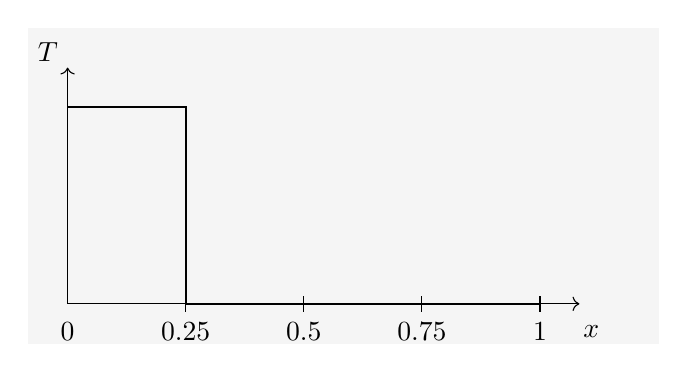
\begin{tikzpicture}
\draw[fill=gray!8,gray!8](0,0) rectangle (8,4);
%\draw[step=0.5cm,gray,very thin] (0,0) grid (8,4); %background grid

\draw[->] (0.5,0.5) -- (7,0.5) ; 
\node[] at (0.5,0.15) {$0$};

\node[] at (2,0.15) {$0.25$};
\node[] at (3.5,0.15) {$0.5$};
\node[] at (5,0.15) {$0.75$};
\node[] at (6.5,0.15) {$1$};
\draw[->] (0.5,0.5) -- (0.5,3.5) ; 
\node[] at (0.25,3.7) {$T$};


\draw[-] (2,0.4) -- (2,0.6) ; 
\draw[-] (3.5,0.4) -- (3.5,0.6) ; 
\draw[-] (5,0.4) -- (5,0.6) ; 
\draw[-] (6.5,0.4) -- (6.5,0.6) ; 


%\draw[-] (2,1) -- (1.75,0.75) ; 
%\draw[-] (2.5,1) -- (2.25,0.75) ; 
%\draw[-] (3,1) -- (2.75,0.75) ; 
%\draw[-] (3.5,1) -- (3.25,0.75) ; 
%\draw[-] (4,1) -- (3.75,0.75) ; 
%\draw[-] (4.5,1) -- (4.25,0.75) ; 

%---------------------------------

%\draw[thick,->] (7,1) -- (7,5) ; 
%\node[] at (6.6,4) {$L_y$};
%\node[] at (6.6,1) {$0$};
%\draw[-] (6.85,1) -- (7.15,1) ; 
%\draw[-] (6.85,4) -- (7.15,4) ; 
%\node[] at (7.6,4) {$p=0$};
%\node[] at (6.6,5) {$y$};

%---------------------------------

\draw[thick] (0.5,3) -- (2,3) -- (2,0.5) -- (6.5,0.5) ; 
\node[] at (7.15,0.15) {$x$};


\end{tikzpicture}



\end{center}

Set $\rho=C_p=1$.
Run the model for 250 time steps with $\delta t=0.002$.
Implement a fully implicit, explicit and Crank-Nicolson 
time discretisation. 

When using Crank-Nicolson, you should then be able to recover the green line of the 
following figure:
\begin{center}
\includegraphics[width=8cm]{images/fem_exercises/fantom3.png} \\
{\captionfont Taken from Thieulot (2011) \cite{thie11}. Note that $\tau=\gamma h/u$.}
\end{center}

Finally, implement the SUPG method and recover the red and turquoise lines.

\par\noindent\rule{\textwidth}{0.4pt}
\end{minipage}
\end{center}
%-/-/-/-/-/-/-/-/-/-/-/-/-/-/-/-/-/-/











 %---
\subsection{The advection-diffusion equation in 2D} \label{ss:hte_fem}We start from the 'bare-bones' heat transport equation (source terms are omitted): 
\begin{equation}
\rho C_p \left( \frac{\partial T}{\partial t} + {\vec \upnu}\cdot {\vec\nabla T} \right)
= {\vec \nabla} \cdot \left( k \vec\nabla T \right)
\end{equation}
In what follows we assume that the velocity vield $\vec \upnu$ is known so that temperature is the 
only unknown.
Let $N^\uptheta$ be the temperature basis functions so that the temperature inside an element is 
given by\footnote{the $\uptheta$ superscript has been chosen to denote temperature so as to avoid confusion
with the transpose operator}:
\begin{equation}
T^h({\vec r}) = \sum_{i=1}^{m_T} N^\uptheta_i ({\vec r}) T_i = \vec N^\uptheta \cdot \vec T
\end{equation}
where $\vec T$ is a vector of length $m_T$
The weak form is then 
\begin{equation}
\int_\Omega N^\uptheta_i \left[ 
\rho C_p \left( \frac{\partial T}{\partial t} + {\vec \upnu}\cdot {\vec\nabla T} \right) \right] d\Omega
= \int_\Omega  N^\uptheta_i {\vec \nabla} \cdot k \vec\nabla T  d\Omega
\end{equation}

\[
\underbrace{\int_\Omega N^\uptheta_i  \rho C_p \frac{\partial T}{\partial t} d\Omega}_{I}
+ \underbrace{\int_\Omega N^\uptheta_i  \rho C_p  {\vec \upnu}\cdot {\vec\nabla T}   d\Omega}_{II}
= \underbrace{\int_\Omega  N^\uptheta_i {\vec \nabla} \cdot k \vec\nabla T d\Omega}_{III}
\quad\quad
i=1,m_T
\]

Looking at the first term:
\begin{eqnarray}
\int_\Omega N^\uptheta_i  \rho C_p \frac{\partial T}{\partial t} d\Omega
&=&  \int_\Omega N^\uptheta_i  \rho C_p \vec N^\uptheta \cdot \dot{\vec T}  d\Omega \\
\end{eqnarray}
so that when we assemble all contributions for $i=1,m_T$ we get:
\[
I 
= \int_\Omega \vec N^\uptheta  \rho C_p \vec N^\uptheta \cdot \dot{\vec T}  d\Omega
= \left( \int_\Omega \rho C_p  \vec N^\uptheta  \vec N^\uptheta  d\Omega \right) \cdot \dot{\vec T}
= {\bm M}^T \cdot \dot{\vec T}
 \]
where ${\bm M}^T$ is the mass matrix of the system of size $(m_T \times m_T)$ with 
\[
M_{ij}^T = \int_\Omega \rho C_p N_i^\uptheta N_j^\uptheta d\Omega
\]
Turning now to the second term:
\begin{eqnarray}
\int_\Omega N^\uptheta_i  \rho C_p  {\vec \upnu}\cdot {\vec\nabla T}   d\Omega
&=& \int_\Omega N^\uptheta_i  \rho C_p (u \frac{\partial T}{\partial x} +  v \frac{\partial T}{\partial y} ) d\Omega \\
&=& \int_\Omega N^\uptheta_i  \rho C_p (u \frac{\partial \vec N^\uptheta}{\partial x} +  v \frac{\partial \vec N^\uptheta}{\partial y} ) \cdot \vec T d\Omega \\
\end{eqnarray}
so that when we assemble all contributions for $i=1,m_T$ we get:
\[
II = \left(\int_\Omega \rho C_p \vec N^\uptheta (u \frac{\partial \vec N^\uptheta}{\partial x} +  v \frac{\partial \vec N^\uptheta}{\partial y} ) d\Omega \right)  \cdot \vec T = {\bm K}_a \cdot \vec T
\]
where ${\bm K}_a$ is the advection term matrix of size $(m_T \times m_T)$ with
\[
(K_a)_{ij} = \int_\Omega \rho C_p N_i^\uptheta 
\left(u \frac{\partial N_j^\uptheta}{\partial x} +  v \frac{\partial N_j^\uptheta}{\partial y} \right) d\Omega 
\]
Now looking at the third term, we carry out an integration by part and neglect the surface term for now, so that 
\begin{eqnarray}
\int_\Omega  N^\uptheta_i {\vec \nabla} \cdot k \vec\nabla T d\Omega
&=& - \int_\Omega  k \vec \nabla N^\uptheta_i \cdot \vec\nabla T d\Omega \\
&=& - \int_\Omega  k \vec \nabla N^\uptheta_i \cdot \vec\nabla (\vec N^\uptheta \cdot \vec T) d\Omega \\
\end{eqnarray}
with 
\[
\vec \nabla \vec N^\uptheta = 
\left(
\begin{array}{cccc}
\partial_x N_1^\uptheta & 
\partial_x N_2^\uptheta & \dots &
\partial_x N_{m_T}^\uptheta \\ \\
\partial_y N_1^\uptheta & 
\partial_y N_2^\uptheta & \dots &
\partial_y N_{m_T}^\uptheta 
\end{array}
\right)
\]
so that finally:
\[
III = - \left( \int_\Omega k (\vec \nabla \vec N^\uptheta)^T \cdot \vec \nabla \vec N^\uptheta d\Omega \right) \cdot \vec T
= - {\bm K}_d \cdot \vec T
\]
where ${\bm K}_d$ is the diffusion term matrix:
\[
{\bm K}_d = \int_\Omega  k (\vec \nabla \vec N^\uptheta)^T \cdot \vec \nabla \vec N^\uptheta d\Omega 
\]
 Ultimately terms $I,II,III$ together yield:
\[
\boxed{
{\bm M}^\uptheta \cdot \dot{\vec T} + ({\bm K}_a + {\bm K}_d) \cdot \vec T = \vec 0
}
\]

%What now remains to be done is to address the time derivative on the temperature vector. 
%The most simple approach would be to use an explicit Euler one, i.e.:
%\[
%\frac{\partial \vec T}{\partial t} = \frac{\vec T^{(k)} - \vec T^{(k-1)}}{\delta t}
%\]
%where $\vec T^{(k)}$ is the temperature field at time step $k$ and $\delta t$ is the time interval 
%between two consecutive time steps.
%In this case the discretised heat transport equation is:
%\[
%\boxed{
%\left( {\bm M}^\uptheta  + ({\bm K}_a + {\bm K}_d) \delta t \right) \cdot \vec T^{(k)} =  {\bm M}^\uptheta \cdot \vec T^{(k-1)}
%}
%\]
\todo[inline]{add source term!!}

%....................................................
\subsubsection{Dealing with the time discretisation} \ref{sec:timediscr}

Essentially we have to solve a PDE of the type:
\[
\frac{\partial T}{\partial t} = {\cal F}(\vec \upnu,T,\vec\nabla T,\Delta T)
\]
with ${\cal F}=\frac{1}{\rho C_p}(-\vec\upnu\cdot\vec\nabla T + \vec\nabla\cdot k\vec\nabla T)$.

\index{general}{Forward Euler}
\index{general}{Backward Euler}
\index{general}{Crank-Nicolson}

The (explicit) forward Euler method is:
\[
\frac{T^{n+1}-T^n}{\delta t} = {\cal F}^n(T,\vec\nabla T,\Delta T)
\]
The (implicit) backward Euler method is:
\[
\frac{T^{n+1}-T^n}{\delta t} = {\cal F}^{n+1}(T,\vec\nabla T,\Delta T)
\]
and the (implicit) Crank-Nicolson algorithm is:
\[
\frac{T^{n+1}-T^n}{\delta t} = 
\frac{1}{2}
\left[
{\cal F}^{n}(T,\vec\nabla T,\Delta T)
+
{\cal F}^{n+1}(T,\vec\nabla T,\Delta T)
\right]
\]
where the superscript $n$ indicates the time step.
The Crank-Nicolson is obviously based on the trapezoidal rule, with second-order convergence in time.


In what follows, I omit the superscript on the mass matrix to simplify notations: ${\bm M}^\uptheta={\bm M}$.
In terms of Finite Elements, these become:
\begin{itemize}
\item Explicit Forward euler:
\[
\frac{1}{\delta t} ({\bm M}^{n+1} \cdot \vec T^{n+1}  -{\bm M}^n \cdot \vec T^{n} )
=
-({\bm K}_a^n+{\bm K}^n_d) \cdot \vec T^{n}
\]
or, 
\[
\boxed{
{\bm M}^{n+1} \cdot \vec T^{n+1}
= \left(  {\bm M}^n  + ({\bm K}_a^n+{\bm K}_d^n) \delta t \right)\cdot \vec T^{n} 
}
\]

\item Implicit Backward euler:
\[
\frac{1}{\delta t} ({\bm M}^{n+1} \cdot \vec T^{n+1}  -{\bm M}^n \cdot \vec T^{n} )
= -({\bm K}_a^{n+1}+{\bm K}_d^{n+1}) \cdot \vec T^{n+1}
\]
or, 
\begin{equation}
\boxed{
\left( {\bm M}^{n+1} +({\bm K}_a^{n+1}+{\bm K}_d^{n+1})\delta t \right) \cdot \vec T^{n+1}
=
{\bm M}^n \cdot \vec T^{n} 
}
\label{eq:hte_ibe}
\end{equation}

\item Crank-Nicolson

\[
\frac{1}{\delta t} \left({\bm M}^{n+1} \cdot \vec T^{n+1}  -{\bm M}^n \cdot \vec T^{n} \right)
= 
\frac{1}{2}
\left[
-({\bm K}_a^{n+1}+{\bm K}_d^{n+1}) \cdot \vec T^{n+1}
-({\bm K}_a^{n}+{\bm K}_d^{n}) \cdot \vec T^{n}
\right]
\]
or,
\[
\boxed{
\left( {\bm M}^{n+1} +({\bm K}_a^{n+1}+{\bm K}_d^{n+1})\frac{\delta t}{2} \right) \cdot \vec T^{n+1}
= \left(  {\bm M}^n  + ({\bm K}_a^n+{\bm K}_d^n) \frac{\delta t}{2} \right)\cdot \vec T^{n} 
}
\]

Note that in benchmarks where the domain/grid does not deform, the coefficients do not change in space
and the velocity field is constant in time, or in practice out of convenience, the ${\bm K}$  and ${\bm M}$ 
matrices do not change and the r.h.s. can be constructed with the same matrices as the FE matrix.

\end{itemize}




\index{general}{BDF-2}
\paragraph{The Backward differentiation formula} (see for instance \cite{hawa91} or Wikipedia\footnote{\url{https://en.wikipedia.org/wiki/Backward_differentiation_formula}}. The second-order BDF (or BDF-2) as shown in \cite{krhb12} is as follows: it is a finite-difference 
quadratic interpolation approximation of the $\partial T/\partial t$ term which involves
$t^n$, $t^{n-1}$ and $t^{n-2}$:
\begin{equation}
\frac{\partial T}{\partial t}(t^n) =
\frac{1}{\tau_n} \left( \frac{2\tau_n + \tau_{n-1}}{\tau_n+\tau_{n-1} } T(t^n)  
- \frac{\tau_n +\tau_{n-1}}{\tau_{n-1}} T(t^{n-1})
+ \frac{\tau_n^2}{\tau_{n-1}(\tau_n+\tau_{n-1})} T(t^{n-2})
\right)
\end{equation}
where $\tau_n=t^n-t^{n-1}$.
Starting again from 
${\bm M}^\uptheta \cdot \dot{\vec T} + ({\bm K}_a + {\bm K}_d) \cdot \vec T = \vec 0$,
we write 
\[
{\bm M}^\uptheta \cdot 
\frac{1}{\tau_n} \left( \frac{2\tau_n + \tau_{n-1}}{\tau_n+\tau_{n-1} } \vec T^n  
- \frac{\tau_n +\tau_{n-1}}{\tau_{n-1}} \vec T^{n-1}
+ \frac{\tau_n^2}{\tau_{n-1}(\tau_n+\tau_{n-1})} \vec T^{n-2} \right)
+ ({\bm K}_a + {\bm K}_d) \cdot \vec T^n = \vec 0
\]
and finally:
\[
\left[
\frac{2\tau_n + \tau_{n-1}}{\tau_n+\tau_{n-1} }
{\bm M}^\uptheta
+ \tau_n({\bm K}_a + {\bm K}_d)
\right]
 \cdot \vec T^n =
 \frac{\tau_n +\tau_{n-1}}{\tau_{n-1}} {\bm M}^\uptheta \cdot \vec T^{n-1}
- \frac{\tau_n^2}{\tau_{n-1}(\tau_n+\tau_{n-1})} {\bm M}^\uptheta \cdot \vec T^{n-2}
\]
Note that if all timesteps are equal, i.e. $\tau_n=\tau_{n-1}=\delta t$, this equation becomes:
\[
\left[
\frac{3}{2}
{\bm M}^\uptheta
+ \delta t({\bm K}_a + {\bm K}_d)
\right]
 \cdot \vec T^n =
{\bm M}^\uptheta \cdot \left(2 \vec T^{n-1} - \frac{1}{2} \vec T^{n-2} \right)
\]
or, 
\[
\left[
{\bm M}^\uptheta
+ \frac{2}{3}\delta t({\bm K}_a + {\bm K}_d)
\right]
 \cdot \vec T^n =
{\bm M}^\uptheta \cdot \left( \frac{4}{3} \vec T^{n-1} - \frac{1}{3} \vec T^{n-2} \right)
\]

As mentioned before the 
backward differenciation formula (BDF) is a family of implicit methods
for the integration of ODEs. Each BDF-$s$ method achieves order $s$.
The BDF-1 is simply the backward Euler method as seen above:
\[
T^{n+1}-T^n=\delta t {\cal F}^{n+1}
\]
The BDF-2 is given by 
\[
T^{n+2} - \frac{4}{3}T^{n+1} +\frac{1}{3} T^n = \frac{2}{3} \delta t {\cal F}^{n+2}
\]
The BDF-3 is given by 
\[
T^{n+3} - \frac{18}{11}T^{n+2} +\frac{9}{11} T^{n+1} -\frac{2}{11}T^n = \frac{6}{11} \delta t {\cal F}^{n+3}
\]
The BDF-4 is given by 
\[
T^{n+4}-\frac{48}{25}T^{n+1}+\frac{36}{25}T^{n+1}-\frac{16}{25}T^{n+1}+\frac{3}{25}T^n = \frac{12}{25}\delta t {\cal F}^{n+4}
\]


%....................................................
\subsubsection{On steady states}

It is said that a system is in a steady state if the (state) variables which define the behavior of the system 
are unchanging in time. In continuous time, this means that the partial derivative with respect to time is zero and remains so:
\[
\frac{\partial}{\partial t} =0 \qquad \forall t
\]
This is irrelevant for the Stokes equations which do not contain an explicit time dependence but the heat 
transport equation can reach a steady state. 
Note that if one is only interested in the steady state solution (and not how the system gets there in time)
then the heat transport equation should be solved with $\partial T/\partial t$ set to zero. 

%....................................................
\subsubsection{Anisotropic heat conduction}\label{sec:anisotropic}

\index{general}{Isotropic}\index{general}{Orthotropic}

It is most often assumed that the heat conductivity is isotropic so that one speaks of heat conductivity as a 
scalar $k$.  However many materials are orthotropic and in that case the heat conductivity is a tensor ${\bm k}$
which (in 2D) writes \cite[p121]{reddybook2}:
\[
{\bm k}
=
\left(
\begin{array}{cc}
k_{xx} & k_{xy} \\
k_{yx} & k_{yy}
\end{array}
\right)
=
\left(
\begin{array}{cc}
\cos\theta & \sin\theta \\
-\sin\theta & \cos\theta
\end{array}
\right)
\cdot
\left(
\begin{array}{cc}
k_1 & 0 \\ 0 & k_2
\end{array}
\right)
\cdot
\left(
\begin{array}{cc}
\cos\theta & -\sin\theta \\
\sin\theta & \cos\theta
\end{array}
\right)
\]
where $k_1$ and $k_2$ are the conductivities in the principal axes system and $\theta$ is 
the local orientation.
In that case the diffusion term in the heat trasport equation becomes $\vec{\nabla}\cdot({\bm k}\cdot \vec{\nabla}T)$.


\mscthesis: \cite[p121]{reddybook2}, \cite[p143]{reddybook2} \index{general}{MSc Thesis}


%....................................................
\subsubsection{About the assembly}

Let us consider for simplicity the following grid composed of 9 nodes and 4 $Q_1$ elements. 
Each node carries a single degree of freedom. 

\begin{center}
\includegraphics[width=12cm]{images/assembly/assembly.png} 
\end{center}

There are four elements:
\begin{itemize}
\item element 1 is composed of nodes $(1,2,5,4)={\vec T}^{el1}$
\item element 2 is composed of nodes $(2,3,6,5)={\vec T}^{el2}$
\item element 3 is composed of nodes $(4,5,8,7)={\vec T}^{el3}$
\item element 4 is composed of nodes $(5,6,9,8)={\vec T}^{el4}$
\end{itemize}
For each element one has computed an elemental matrix ${\bm A}^{el}$ and a right hand side ${\vec b}^{el}$. 
\[
{\bm A}^{el1} \cdot {\bm T}^{el1} = {\bm b}^{el1}
\]
\[
{\bm A}^{el2} \cdot {\bm T}^{el2} = {\bm b}^{el2}
\]
\[
{\bm A}^{el3} \cdot {\bm T}^{el3} = {\bm b}^{el3}
\]
\[
{\bm A}^{el4} \cdot {\bm T}^{el4} = {\bm b}^{el4}
\]
As seen in the 1D case, these four linear systems must be assembled in a single large matrix of size 
$9\times 9$ as shown in the figure above.

 %------------
\subsection{Another approach to solving the advection diffusion}\label{ss:hte_diff} 
As we have seen above, one usually solves the heat transport equation (i.e. 
an advection-diffusion equation) in this form (source terms are neglected):
\begin{equation}
\rho C_p \left( \frac{\partial T}{\partial t} + {\vec \upnu}\cdot {\vec\nabla T} \right)
= {\vec \nabla} \cdot k \vec\nabla T 
\end{equation}
As we have seen in Section~\ref{ss:hte}, the diffusion term is actually the divergence of the heat flux
$\vec{q}=-k \vec \nabla T$. We could then choose to keep the heat flux as an unknown and 
solve a coupled system of equations instead:
\begin{eqnarray}
\rho C_p \left( \frac{\partial T}{\partial t} + {\vec \upnu}\cdot {\vec\nabla T} \right)
&=& - {\vec \nabla} \cdot \vec{q} \nn\\ 
\vec{q} &=& - k \vec \nabla T \nn
\end{eqnarray}
or, 
\begin{eqnarray}
\rho C_p \left( \frac{\partial T}{\partial t} + {\vec \upnu}\cdot {\vec\nabla T} \right)
+ {\vec \nabla} \cdot \vec{q} &=& 0 \label{eq:htediff1}\\ 
\vec{q} + k \vec \nabla T &=& \vec{0} \label{eq:htediff2}
\end{eqnarray}
We have seen that the two left hand side terms of the first equation become 
${\bm M}^\uptheta \cdot \dot{\vec{T}}$ and ${\bm K}_a \cdot \vec{T}$.
Let $\bN^\uptheta(\vec{r})$ be the temperature basis functions so that the temperature inside an element is 
given by
\begin{equation}
T^h({\vec r}) = \sum_{i=1}^{m_T} \bN^\uptheta_i ({\vec r}) T_i = \vec \bN^\uptheta \cdot \vec T
\end{equation}
where $\vec T$ is a vector of length $m_T$.
Let $\bN^q(\vec{r})$ be the heat flux basis functions, 
and let us define (in 2D) $\vec{q}=(\qx,\qy)$ so that 
\begin{eqnarray}
\qx^h({\vec r}) &=& \sum_{i=1}^{m_q} \bN^q_i ({\vec r})\; \qx_i = \vec{\bN}^q \cdot \vec{\qx} \\
\qy^h({\vec r}) &=& \sum_{i=1}^{m_q} \bN^q_i ({\vec r})\; \qy_i = \vec{\bN}^q \cdot \vec{\qy} 
\end{eqnarray}
where $\vec{\bN}^q$, $\vec{\qx}$ and $\vec{\qy}$ are vectors of length $m_q$.
The weak form of the third term of Eq.~(\ref{eq:htediff1}) is then
\begin{eqnarray}
\int_\Omega \bN_i^\uptheta \; \nabla \cdot \vec{q} \;  d\Omega
&=& -\int_\Omega \bN_i^\uptheta  
\left(  \frac{\partial }{\partial x}\qx + \frac{\partial }{\partial y}\qy \right) d\Omega \nn\\
&=& \int_\Omega \bN_i^\uptheta  \left(  \frac{\partial \vec{\bN}^q}{\partial x}\cdot \vec{\qx}
+  \frac{\partial \vec{\bN}^q}{\partial y}\cdot \vec{\qy} \right) d\Omega \nn\\
&=& \int_\Omega \bN_i^\uptheta  \frac{\partial \vec{\bN}^q}{\partial x}\cdot  \vec{\qx} \;  d\Omega + 
\int_\Omega  \bN_i^\uptheta \frac{\partial \vec{\bN}^q}{\partial y} \cdot \vec{\qy} \;  d\Omega \nn
\end{eqnarray}
Writing this last equation for $i=1,...m_T$ yields
\[
\underbrace{\left( \int_\Omega \vec{\bN}^\uptheta \frac{\partial \vec{\bN}^q}{\partial x} \; d\Omega \right)}_{{\bm H}_x} \cdot\vec{\qx}+ 
\underbrace{\left( \int_\Omega \vec{\bN}^\uptheta \frac{\partial \vec{\bN}^q}{\partial y} \; d\Omega\right)}_{{\bm H}_y} \cdot \vec{\qy}
\]
In the end, we obtain:
\begin{equation}
{\bm M}^\uptheta \cdot \dot{\vec{T}} + {\bm K}_a \cdot \vec{T} 
+ {\bm H}_x \cdot \vec{\qx}
+ {\bm H}_y \cdot \vec{\qy}
=\vec{0} \label{eq:htediff3}
\end{equation}
Turning now to Eq.~(\ref{eq:htediff2}), its weak form is
\[
\int_\Omega \bN_i^q \left( \vec{q} + k \vec \nabla T \right) d\Omega = \vec{0}
\]
and we can decompose it in its $x$ and $y$ components:
%\begin{eqnarray}
%\int_\Omega N_i^q \left( \qx + k  \frac{\partial T}{\partial x} \right) d\Omega &=& 0 \nn\\
%\int_\Omega N_i^q \left( \qy + k  \frac{\partial T}{\partial y} \right) d\Omega &=& 0 \nn
%\end{eqnarray}
%We process these further as follows:
\begin{eqnarray}
0&=&\int_\Omega \bN_i^q \left( \qx^h + k  \frac{\partial T^h}{\partial x} \right) \; d\Omega  \nn\\
&=& \int_\Omega \bN_i^q \left( \vec{\bN}^q \cdot \vec{\qx} 
+ k  \frac{\partial \vec{\bN}^\uptheta}{\partial x} \cdot \vec{T} \right) \; d\Omega \nn\\ 
&=& \int_\Omega \bN_i^q \vec{\bN}^q \cdot \vec{\qx} \; d\Omega  
+ \int _\Omega k \bN_i^q   \frac{\partial \vec{\bN}^\uptheta}{\partial x}\cdot \vec{T} \;  d\Omega \nn\\ 
0&=&\int_\Omega \bN_i^q \left( \qy^h + k  \frac{\partial T^h}{\partial y} \right) \;  d\Omega \nn\\
&=& \int_\Omega \bN_i^q \left( \vec{\bN}^q \cdot \vec{\qy} 
+ k  \frac{\partial \vec{\bN}^\uptheta}{\partial y} \cdot \vec{T} \right) \;  d\Omega \nn\\ 
&=& \int_\Omega \bN_i^q \vec{\bN}^q \cdot \vec{\qy} \; d\Omega
+ \int _\Omega k \bN_i^q   \frac{\partial \vec{\bN}^\uptheta}{\partial y} \cdot \vec{T} \;  d\Omega 
\end{eqnarray}
Writing these equations for $i=1,...m_q$ yields:
\begin{eqnarray}
0&=& \int_\Omega \vec{\bN}^q \vec{\bN}^q \cdot \vec{\qx} \; d\Omega
+ \int _\Omega k \vec{\bN}^q   \frac{\partial \vec{\bN}^\uptheta}{\partial x}\cdot \vec{T} \; d\Omega \nn\\ 
&=& \underbrace{\left( \int_\Omega \vec{\bN}^q \vec{\bN}^q d\Omega \right)}_{{\bm M}^q}  \cdot \vec{\qx} 
+ \underbrace{\left(\int _\Omega k \vec{\bN}^q  \frac{\partial \vec{\bN}^\uptheta}{\partial x}\; d\Omega\right)}_{{\bm G}_x} \cdot \vec{T} \label{eq:htediff4}\\ 
0&=& \int_\Omega \vec{\bN}^q \vec{\bN}^q \cdot \vec{\qy} \; d\Omega
+ \int _\Omega k \vec{\bN}^q   \frac{\partial \vec{\bN}^\uptheta}{\partial y} \cdot \vec{T} \;  d\Omega \nn\\ 
&=& \underbrace{\left( \int_\Omega \vec{\bN}^q \vec{\bN}^q d\Omega \right)}_{{\bm M}^q}  \cdot \vec{\qy} 
+ \underbrace{\left(\int _\Omega k \vec{\bN}^q  \frac{\partial \vec{\bN}^\uptheta}{\partial y} \; d\Omega\right)}_{{\bm G}_y} \cdot \vec{T} \label{eq:htediff5}
\end{eqnarray}

Finally Eqs.~(\ref{eq:htediff3},\ref{eq:htediff4},\ref{eq:htediff5}) 
can be combined and yield the following system (assuming an implicit backward 
Euler time scheme):
\[
\left(
\begin{array}{ccc}
{\bm M}^\uptheta + {\bm K}_a \delta t & {\bm H}_x \delta t  & {\bm H}_y \delta t \\
{\bm G}_x & {\bm M}^q & 0 \\
{\bm G}_y & 0 & {\bm M}^q 
\end{array}
\right)
\cdot
\left(
\begin{array}{c}
\vec{T}^{n+1}\\
\vec{\qx}^{n+1}\\
\vec{\qy}^{n+1}
\end{array}
\right)
=
\left(
\begin{array}{c}
{\bm M}^\uptheta \cdot \vec{T}^n\\
\vec{0} \\
\vec{0}
\end{array}
\right)
\]
If we choose $m_q=m_T$ and $\bN^q=\bN^\uptheta$ then
%then ${\bm H}_x = {\bm G}_x$,  ${\bm H}_y = {\bm G}_y$  and 
${\bm M}^\uptheta = {\bm M}^q = {\bm M}$ 
so that 
\[
\left(
\begin{array}{ccc}
{\bm M} + {\bm K}_a \delta t & {\bm H}_x \delta t & {\bm H}_y \delta t\\
{\bm G}_x & {\bm M} & 0 \\
{\bm G}_y & 0 & {\bm M}
\end{array}
\right)
\cdot
\left(
\begin{array}{c}
\vec{T}^{n+1}\\
\vec{\qx}^{n+1}\\
\vec{\qy}^{n+1}
\end{array}
\right)
=
\left(
\begin{array}{c}
{\bm M} \cdot \vec{T}^n\\
\vec{0} \\
\vec{0}
\end{array}
\right)
\]
Also, if $k$ is constant in space then ${\bm G}_{x,y}=k {\bm H}_{x,y}$. 
Rather interestingly, one could write Eqs.~(\ref{eq:htediff4},\ref{eq:htediff5}) 
as
\begin{eqnarray}
\vec{\qx}^{n+1} &=& - ({\bm M}^q)^{-1} \cdot {\bm G}_x \cdot \vec{T}^{n+1} \\
\vec{\qy}^{n+1} &=& - ({\bm M}^q)^{-1} \cdot {\bm G}_y \cdot \vec{T}^{n+1}
\end{eqnarray}
and inject it in Eq.~(\ref{eq:htediff3}) to yield:
\begin{equation}
{\bm M}^\uptheta \cdot \dot{\vec{T}} + [ {\bm K}_a 
- {\bm H}_x \cdot ({\bm M}^q)^{-1} \cdot {\bm G}_x 
- {\bm H}_y \cdot ({\bm M}^q)^{-1} \cdot {\bm G}_y ] \cdot \vec{T}^{n+1}
=\vec{0} 
\end{equation}
which means that we can directly solve for temperature! 
Rather interestingly, it is not equivalent to 
Eq.~(\ref{eq:hte_ibe}). Food for thought ...

We will see that this approach bears a lot of resemblance to the one taken in the context 
of Discontinuous Galerkin methods. 





























\newpage 
%%%%%%%%%%%%%%%%%%%%%%%%%%%%%%%%%%%%%%%%%%%%%%%%%%%%%%%%%%%%%%%%%%%%%%%%%%%%%%%%%%%%%%%%%%%%%%%%%%%
\section{Solving the flow equations with the FEM} \label{solvingFEM} %%%%%%%%%%%%%%%%%%%%%%%%%%%%%%
\begin{flushright} {\tiny {\color{gray} chapter6.tex}} \end{flushright}

%6.3 of donea and huerta

In the case of an incompressible flow, we have seen that the continuity (mass conservation)
equation takes the simple form ${\vec \nabla}\cdot{\vec \upnu}=0$. In other words flow takes place 
under the constraint that the divergence of its velocity field is exactly zero eveywhere 
(solenoidal constraint), i.e. it is divergence free. 
\index{general}{Divergence-free Flow} 
\index{general}{Solenoidal Field}

We see that the pressure in the momentum equation is then a degree of freedom which is needed 
to satisfy the incompressibilty constraint (and it is not related to any constitutive equation)
\cite{dohu03}. In other words the pressure is acting as a Lagrange multiplier of the incompressibility
constraint. 

Various approaches have been proposed in the literature to deal with the 
incompressibility constraint but we will only focus on the penalty method 
(section \ref{sec:penalty}) and the so-called mixed finite element method
\ref{sec:mixed}.
 %---------------------------------------------------------------------------
\subsection{Strong and weak forms} \begin{flushright} {\tiny {\color{gray} strongweak.tex}} \end{flushright}

\index{general}{strong form} 

The strong form consists of the governing equation and the boundary conditions, i.e. 
the mass, momentum and energy conservation equations supplemented with Dirichlet and/or Neumann
boundary conditions on (parts of) the boundary.


\index{general}{weak form}
To develop the finite element formulation, the partial differential equations 
must be restated in an integral form called the weak form. In essence the PDEs are 
first multiplied by an arbitrary function and integrated over the domain.

 

 %--------------------------------------------
\subsection{Which velocity-pressure pair for Stokes?}\label{ss:pair}

The success of a mixed finite element formulation crucially depends on a proper choice of the local interpolations of the velocity and the pressure. 

%........................................................................................
\subsubsection{The compatibility condition (or LBB condition, or inf-sup condition)} \label{ss:LBBcond}
\index{general}{LBB} \index{general}{Optimal Rate}

WARNING: I am not comfortable writing about this topic. What follows is a rough attempt at making sense of it.


The Lady{\v z}henskaya-Babu{\v s}ka-Brezzi (LBB) condition is a sufficient 
condition for a saddle point problem to have a unique solution.
For saddle point problems coming from the Stokes equations, 
many discretizations are unstable, giving rise to artifacts such as spurious oscillations. 
The LBB condition gives criteria for when a discretization of a saddle point problem is stable. 
It also assures convergence at the optimal rate. 

Bochev \& Gunzburger \cite{bogu09} state: "
The terminology “LBB” originates from the facts that this condition was first explicitly discussed
in the finite element setting for saddle point problems by Brezzi \cite{brez74} and that it is a special case of
the general weak-coercivity condition first discussed for finite element methods by Babu{\v s}ka
\cite{babu71} and that, in the continuous setting of the Stokes equation, this condition was first proved to
hold by Ladyzhenskaya; see \cite{lady69}."

Unfortunately, to quote Donea \& Huerta \cite{dohu03}: 
"In the finite element context, it is by no means easy to prove whether or not a given
velocity-pressure pair satisfies the LBB compatibility condition."
Elman et al state: "[...] Choosing spaces for which the discrete inf-sup condition holds
and is a delicate matter, and seemingly natural choices of velocity and pressure approximation
do not work. [...] In general, care must be taken to make the velocity space 
rich enough compared to the pressure space."

The LBB condition, or inf-sup condition can be proven in different ways, and standard techniques have been designed
as listed in Boffi et al (2008) \cite{bobf08}.

%p129
Elman et al \cite{elsw} state that "The inf-sup condition is a sufficient condition for the pressure to be unique up
to  constant in the case of an enclosed flow." This can also be proven for other boundary conditions.
This approach, based on the macro-element technique \cite{sten90} is explored in Appendix \ref{app:Gel}.


It can be shown that, provided the kernel (null space) of matrix $\G$ is zero,
the Stokes matrix is non-singular, that is $\vec{\cal V}$ and $\vec{\cal P}$ 
are uniquely defined, and the Schur complement matrix $\SSS$ is positive definite. 
Simply put, taking $\vec{\cal V}=\vec{0}$ in the discretised Stokes system 
without body forces yields $\G \cdot \vec{\cal P}=\vec{0}$ and implies
that any pressure solution is only unique up to the null space of the matrix $\G$.

We know that the Schur complement matrix $\SSS$ is positive definite if and only if all of its eigenvalues are positive.
One could then (numerically) compute the eigenvalues of $\SSS$ and check that these are indeed strictly positive
to show that $\SSS$ is pos def. 

%Since $\SSS$ is trivially symmetric (because $\K$ is symmetric), then 

Another way is to see that $\SSS$ is positive definite only if $\text{ker}(\G)=\{0\}$.
Again to quote Donea \& Huerta \cite{dohu03}: "If this is the case, the partitioned Stokes matrix  
is non-singular and delivers uniquely defined velocity and pressure fields. If this is not the case, a
stable and convergent velocity field might be obtained, but the pressure field is likely
to present spurious and oscillatory results." 
Note that in the case of the $Q_1 \times P_0$ element it has been shown that the multiple families of 
checkboard pressure modes actually lie in the kernel of $\G$. \cite{XXXXsani}

One could then also numerically compute the Ker of G?

\vspace{.4cm}

LBB means velocity and pressure spaces yield uniquely defined vel and p solutions. 
is proving ker(G)=0 enough? is proving S (S)PD enough ?

Check \cite{chba93}


%........................................................................................
\subsubsection{Families}
\index{general}{Taylor-Hood}

The family of \underline{Taylor-Hood} finite element spaces on triangular/tetrahedral 
grids is given by $P_k \times P_{k-1}$ with $k\geq 2$, 
and on quadrilateral/hexahedral grids by $Q_k \times Q_{k-1}$ with $k\geq 2$.
This means that the pressure is then approximated by continuous functions. 

These finite elements are very popular, in particular the pairs for $k=2$, i.e.
$Q_2\times Q_1$ and $P_2\times P_1$.
The reason why $k\geq 2$ comes from the fact that the 
$Q_1 \times Q_0$ (i.e. $Q_1 \times P_0$) and $P_2\times P_1$
are not stable elements (they are not inf-sup stable). 

\begin{remark}
Note that a similar element to $Q_2 \times Q_1$ has been proposed
and used succesfully used \cite{taho73,hota74}: it is denoted by $Q_2^{(8)} \times Q_1$ 
since the center node ('$x^2y^2$') and its associated degrees of freedom have been removed. It 
has also been proved to be LBB stable. 
\end{remark}


The \underline{Raviart-Thomas} family\todo{find literature} on triangles and quadrilaterals.

%........................................................................................
\subsubsection{The bi/tri-linear velocity - constant pressure element ($Q_1\times P_0$)}

\begin{minipage}[t]{0.5\textwidth}
\begin{flushright} {\tiny {\color{gray} (tikz\_q1p0.tex)}} \end{flushright}
%~~~~~~~~~~~~~~~~~~~~~~~~~~~~~~~~~~~~~~~~~~~~~~~~~~~~~~~~~~~~~~~~~~~~~~~~~~~~~~~~~~~~~~~~~~~~~~~~~~

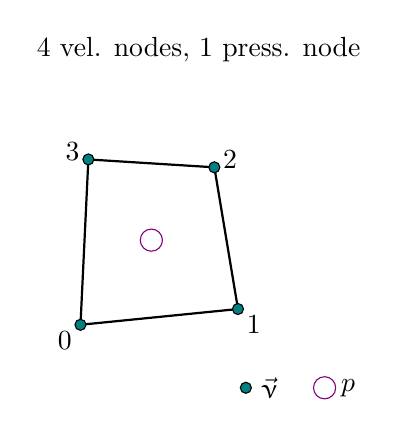
\begin{tikzpicture}
%\draw[fill=gray!23,gray!23](0,0) rectangle (5,5);
%\draw[step=0.5cm,gray,very thin] (0,0) grid (4,4); %background grid
\draw[thick] (1,1) -- (3,1.2) -- (2.7,3) -- (1.1,3.1) -- cycle;  
\node[] at (0.8,0.8) {0};
\node[] at (3.2,1) {1};
\node[] at (2.9,3.1) {2};
\node[] at (0.9,3.2) {3};
\draw[violet] (1.9,2.075) circle (4pt);
\draw[black,fill=teal] (1,1)   circle (2pt);
\draw[black,fill=teal] (3,1.2)  circle (2pt);
\draw[black,fill=teal] (2.7,3)  circle (2pt);
\draw[black,fill=teal] (1.1,3.1) circle (2pt);
\draw[black,fill=teal] (3.1,0.2) circle (2pt); 
\node[] at (3.4,0.2) {$\vec\upnu$};
\draw[violet] (4.1,0.2) circle (4pt); 
\node[] at (4.4,0.2) {$p$};
\node[] at (2.5,4.5) {4 vel. nodes, 1 press. node};
\end{tikzpicture}

\end{minipage}
\begin{minipage}[t]{0.5\textwidth}

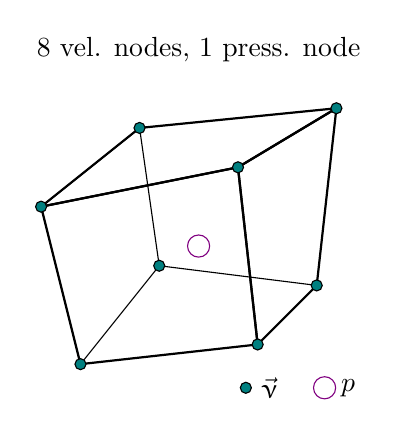
\begin{tikzpicture}
%\draw[fill=gray!23,gray!23](0,0) rectangle (5,5);
%\draw[step=0.25cm,gray,very thin] (0,0) grid (5,4); %background grid
\draw[thick] (1,0.5) -- (3.25,0.75) -- (3,3) -- (0.5,2.5) -- cycle; %1-2-6-5
\draw[thick] (3.25,0.75) -- (4,1.5) -- (4.25,3.75) -- (3,3) -- cycle; %2-3-7-6
\draw[thick] (0.5,2.5) -- (3,3) -- (4.25,3.75) -- (1.75,3.5) -- cycle; %5-6-7-4
\draw[thin]   (1,0.5) -- (2,1.75) -- (1.75,3.5) -- (0.5,2.5)   --cycle; % 1-0-4-5 
\draw[thin] (2,1.75) -- (4,1.5); 
%\node[] at (0.8,0.8) {0};
%\node[] at (3.2,1) {1};
%\node[] at (2.9,3.1) {2};
%\node[] at (0.9,3.2) {3};
\draw[violet] (2.5,2.) circle (4pt);
\draw[black,fill=teal] (1,0.5)   circle (2pt);
\draw[black,fill=teal] (3.25,0.75)   circle (2pt);
\draw[black,fill=teal] (3,3)   circle (2pt);
\draw[black,fill=teal] (0.5,2.5)   circle (2pt);
\draw[black,fill=teal] (1.75,3.5)  circle (2pt);
\draw[black,fill=teal] (4.25,3.75)  circle (2pt);
\draw[black,fill=teal] (4,1.5) circle (2pt);
\draw[black,fill=teal] (2,1.75) circle (2pt);
\draw[black,fill=teal] (3.1,0.2) circle (2pt); 
\node[] at (3.4,0.2) {$\vec\upnu$};
\draw[violet] (4.1,0.2) circle (4pt); 
\node[] at (4.4,0.2) {$p$};
\node[] at (2.5,4.5) {8 vel. nodes, 1 press. node};
\end{tikzpicture}

\end{minipage}

discussed in example 3.71 of \cite{john16}

However simple it may look, the \index{general}{$Q_1 \times P_0$} element is 
one of the hardest elements to analyze and many questions are still open about its properties. 
The element does not satisfy the inf-sup condition \cite{hugh}p211. 
In \cite{grsa} it is qualified as follows: slightly unstable but highly usable. 

The $Q_1 \times P_0$ mixed approximation is the lowest order conforming approximation 
method defined on a rectangular grid. It also happens to be the most famous example 
of an unstable mixed approximation method.
\cite[p235]{elsw}.

This element is discussed in \cite{fort81}, \cite{fofo85} and in \cite{pisa85} 
in the context of multigrid use.

This element is plagued by so-called pressure checkerboard modes which
have been thoroughly analysed \cite{grsi94}, \cite{chpc95}, \cite{sagl81a,sagl81b}.
These can be filtered out \cite{chpc95}. Smoothing techniques are also discussed in \cite{legs79}.

\Literature \cite{fobo90}\cite{grle85}\cite{leru86}



%----------------------------------------------------------------------
\subsubsection{The bi/tri-quadratic velocity - discontinuous linear pressure element ($Q_2 \times P_{-1}$)}

This element is crowned "probably the most accurate 2D element" in Gresho \& Sani's book \cite{grsa}.

It is characterised by piecewise Biquadratic velocities, 
and piecewise linear discontinuous polynomial pressure. 
The element satisfies the inf-sup condition, see page 211 of Hughes \cite{hugh}, or p138 of Elman et al
\cite{elsw}.
It is used in van de Vosse et al (1989) \cite{vavs89} for steady laminar flowin a curved tube. 
See Boffi \& Gastaldi (2002) \cite{boga02} 
for the two possible choices for the definition of the pressure space..
This element is mentioned in Kaus (2010) \cite{kaus10} and Pelletier et al (1989) \cite{pefc89} 
and it is  used in Frehner (2014) \cite{freh14} to study 3D fold growth rates 
(see online supplementary material) and in Schmalholtz (2008) \cite{schm08}.

Note that the serendipity version of this pair, i.e. $Q_2^{(20)}\times P_{-1}$ is also LBB stable
as shown in p180 of Reddy \cite{reddybook2}.

This element is implemented in Stone 76. 

\begin{center}
\includegraphics[width=6cm]{images/q2pm1/q2pm1}
\end{center}


%----------------------------------------------------------------------
\subsubsection{The bi/tri-quadratic velocity - bi/tri-linear pressure element ($Q_2 \times Q_1$)}
\label{ss:pairq2q1}

\begin{minipage}[t]{0.5\textwidth}
\begin{flushright} {\tiny {\color{gray} (tikz\_q2q1.tex)}} \end{flushright}
%~~~~~~~~~~~~~~~~~~~~~~~~~~~~~~~~~~~~~~~~~~~~~~~~~~~~~~~~~~~~~~~~~~~~~~~~~~~~~~~~~~~~~~~~~~~~~~~~~~

%\begin{center}
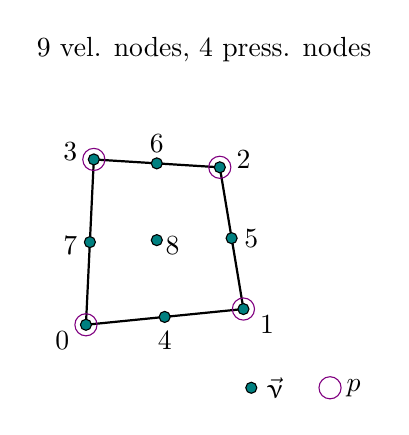
\begin{tikzpicture}
%\draw[fill=gray!23,gray!23](0,0) rectangle (5,5);
%\draw[step=0.5cm,gray,very thin] (0,0) grid (4,4); %background grid
\draw[thick] (1,1) -- (3,1.2) -- (2.7,3) -- (1.1,3.1) -- cycle;  
\node[] at (0.7,0.8) {0};
\node[] at (3.3,1) {1};
\node[] at (3,3.1) {2};
\node[] at (0.8,3.2) {3};
\draw[black,fill=teal] (1,1)     circle (2pt); \draw[violet] (1,1) circle (4pt);
\draw[black,fill=teal] (3,1.2)   circle (2pt); \draw[violet] (3,1.2) circle (4pt);
\draw[black,fill=teal] (2.7,3)   circle (2pt); \draw[violet] (2.7,3) circle (4pt);
\draw[black,fill=teal] (1.1,3.1) circle (2pt); \draw[violet] (1.1,3.1) circle (4pt);
\draw[black,fill=teal] (2,1.1) circle (2pt) ; \node[] at (2,0.8) {4};
\draw[black,fill=teal] (2.85,2.1) circle (2pt) ; \node[] at (3.1,2.1) {5};
\draw[black,fill=teal] (1.9,3.05) circle (2pt) ; \node[] at (1.9,3.3) {6};
\draw[black,fill=teal] (1.05,2.05) circle (2pt) ; \node[] at (0.8,2) {7};
\draw[black,fill=teal] (1.9,2.075) circle (2pt) ; \node[] at (2.1,2) {8};
\draw[black,fill=teal] (3.1,0.2) circle (2pt); 
\node[] at (3.4,0.2) {$\vec\upnu$};
\draw[violet] (4.1,0.2) circle (4pt); 
\node[] at (4.4,0.2) {$p$};
\node[] at (2.5,4.5) {9 vel. nodes, 4 press. nodes};
\end{tikzpicture}
%\end{center}

\end{minipage}
\begin{minipage}[t]{0.5\textwidth}



%\begin{center}
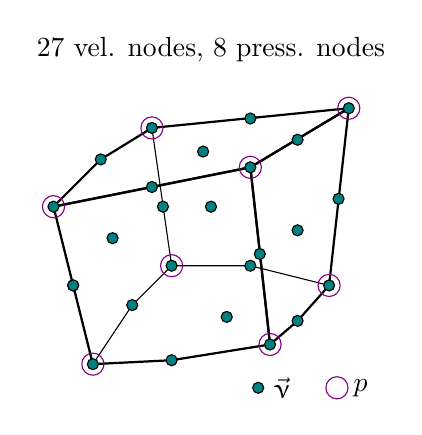
\begin{tikzpicture}
%\draw[fill=gray!23,gray!23](0,0) rectangle (5,5);
%\draw[step=0.5cm,gray,very thin] (0,0) grid (5,4); %background grid
\draw[thick] (1,0.5) -- (2,0.55) --(3.25,0.75) -- (3,3) -- (0.5,2.5) -- cycle; %1-9-2-6-5
\draw[thick] (3.25,0.75) -- (3.6,1.05) -- (4,1.5) -- (4.25,3.75) -- (3,3) -- cycle; %2-10-3-7-6
\draw[thick] (0.5,2.5) -- (3,3) -- (4.25,3.75) -- (1.75,3.5) -- (1.1,3.1) -- cycle; %5-6-7-4-13
\draw[thin]   (1,0.5) -- (1.5,1.25) -- (2,1.75) -- (1.75,3.5) -- (1.1,3.1) -- (0.5,2.5) --cycle; % 1-8-0-4-5-13 
\draw[thin] (2,1.75) -- (3,1.75) -- (4,1.5); %0-11-3
%pressure nodes
\draw[violet] (2,1.75) circle (4pt); % 0 
\draw[violet] (1,0.5) circle (4pt); % 1 
\draw[violet] (3.25,0.75) circle (4pt); % 2 
\draw[violet] (4,1.5) circle (4pt); % 3 
\draw[violet] (1.75,3.5) circle (4pt); % 4 
\draw[violet] (0.5,2.5) circle (4pt); % 5 
\draw[violet] (3,3) circle (4pt); % 6 
\draw[violet] (4.25,3.75) circle (4pt); % 7 
%velocity nodes
\draw[black,fill=teal] (1,0.5)   circle (2pt);
\draw[black,fill=teal] (3.25,0.75)   circle (2pt);
\draw[black,fill=teal] (3,3)   circle (2pt);
\draw[black,fill=teal] (0.5,2.5)   circle (2pt);
\draw[black,fill=teal] (1.75,3.5)  circle (2pt);
\draw[black,fill=teal] (4.25,3.75)  circle (2pt);
\draw[black,fill=teal] (4,1.5) circle (2pt);
\draw[black,fill=teal] (2,1.75) circle (2pt);
\draw[black,fill=teal] (1.5,1.25) circle (2pt); % 8 
\draw[black,fill=teal] (2,0.55) circle (2pt); % 9 
\draw[black,fill=teal] (3.6,1.05) circle (2pt); % 10
\draw[black,fill=teal] (3,1.75) circle (2pt); % 11
\draw[black,fill=teal] (0.75,1.5) circle (2pt); % 12
\draw[black,fill=teal] (1.1,3.1) circle (2pt); % 13
\draw[black,fill=teal] (0.75,1.5) circle (2pt); % 18
\draw[black,fill=teal] (2.7,1.1) circle (2pt); % 21
\draw[black,fill=teal] (3.6,3.35) circle (2pt); % 21
\draw[black,fill=teal] (3.,3.62) circle (2pt); % 21
\draw[black,fill=teal] (4.12,2.6) circle (2pt); % 21
\draw[black,fill=teal] (1.89,2.5) circle (2pt); % 21
\draw[black,fill=teal] (1.75,2.75) circle (2pt); % 21
\draw[black,fill=teal] (3.12,1.9) circle (2pt); % 21
\draw[black,fill=teal] (3.6,2.2) circle (2pt); % 21
\draw[black,fill=teal] (1.25,2.1) circle (2pt); % 21
\draw[black,fill=teal] (2.4,3.2) circle (2pt); % 21
\draw[black,fill=teal] (2.5,2.5) circle (2pt); % 21

% legend
\draw[black,fill=teal] (3.1,0.2) circle (2pt); \node[] at (3.4,0.2) {$\vec\upnu$};
\draw[violet] (4.1,0.2) circle (4pt); 
\node[] at (4.4,0.2) {$p$};
\node[] at (2.5,4.5) {27 vel. nodes, 8 press. nodes};
\end{tikzpicture}
%\end{center}


\end{minipage}


In \cite{grsa} Gresho \& Sani write that in their opinion $div(\vec v)=0$ is not strong enough.

This element, implemented in penalised form, is discussed in \cite{been79} and the follow-up paper \cite{been80}. CHECK

Biquadratic velocities, bilinear pressure. See Hood and Taylor. The element satisfies the inf-sup condition \cite{hugh}p215. 

\begin{center}
\includegraphics[width=6cm]{images/q2q1/q2numering}
\end{center}

%----------------------------------------------------------------------
\subsubsection{The stabilised bi/tri-linear velocity -  constant pressure element ($Q_1\times P_0$-stab)}

\Literature: \cite{sike90,vibo92,kesi92,qizh07,lisi12,chco01,chri02}

%----------------------------------------------------------------------
\subsubsection{The stabilised bi/tri-linear velocity -  bi/tri-linear pressure element ($Q_1\times Q_1$-stab)}

\begin{minipage}[t]{0.5\textwidth}

\begin{center}
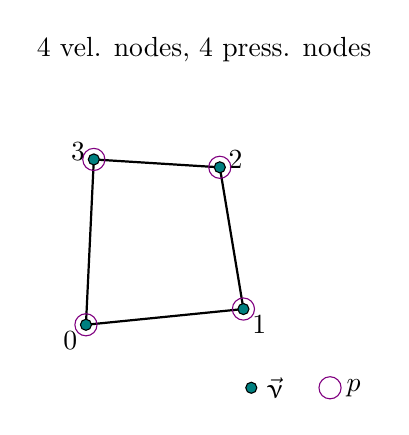
\begin{tikzpicture}
%\draw[fill=gray!23,gray!23](0,0) rectangle (5,5);
%\draw[step=0.5cm,gray,very thin] (0,0) grid (4,4); %background grid
\draw[thick] (1,1) -- (3,1.2) -- (2.7,3) -- (1.1,3.1) -- cycle;  
\node[] at (0.8,0.8) {0};
\node[] at (3.2,1)   {1};
\node[] at (2.9,3.1) {2};
\node[] at (0.9,3.2) {3};
\draw[black,fill=teal] (1,1)     circle (2pt); \draw[violet] (1,1) circle (4pt);
\draw[black,fill=teal] (3,1.2)   circle (2pt); \draw[violet] (3,1.2) circle (4pt);
\draw[black,fill=teal] (2.7,3)   circle (2pt); \draw[violet] (2.7,3) circle (4pt);
\draw[black,fill=teal] (1.1,3.1) circle (2pt); \draw[violet] (1.1,3.1) circle (4pt);
\draw[black,fill=teal] (3.1,0.2) circle (2pt); 
\node[] at (3.4,0.2) {$\vec\upnu$};
\draw[violet] (4.1,0.2) circle (4pt); 
\node[] at (4.4,0.2) {$p$};
\node[] at (2.5,4.5) {4 vel. nodes, 4 press. nodes};
\end{tikzpicture}\\
\end{center}

\end{minipage}
\begin{minipage}[t]{0.5\textwidth}

\begin{center}
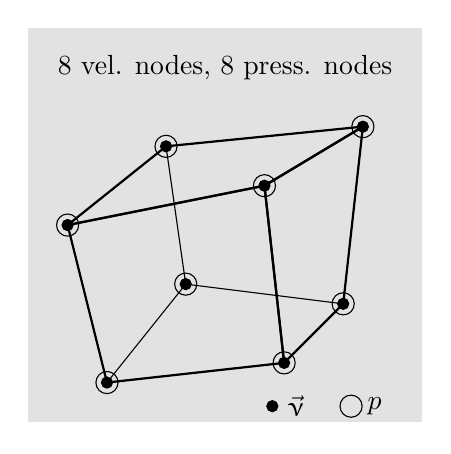
\begin{tikzpicture}
\draw[fill=gray!23,gray!23](0,0) rectangle (5,5);
%\draw[step=0.25cm,gray,very thin] (0,0) grid (5,4); %background grid
\draw[thick] (1,0.5) -- (3.25,0.75) -- (3,3) -- (0.5,2.5) -- cycle; %1-2-6-5
\draw[thick] (3.25,0.75) -- (4,1.5) -- (4.25,3.75) -- (3,3) -- cycle; %2-3-7-6
\draw[thick] (0.5,2.5) -- (3,3) -- (4.25,3.75) -- (1.75,3.5) -- cycle; %5-6-7-4
\draw[thin]   (1,0.5) -- (2,1.75) -- (1.75,3.5) -- (0.5,2.5)   --cycle; % 1-0-4-5 
\draw[thin] (2,1.75) -- (4,1.5); 
%\node[] at (0.8,0.8) {0};
%\node[] at (3.2,1) {1};
%\node[] at (2.9,3.1) {2};
%\node[] at (0.9,3.2) {3};
\draw (1,0.5) circle (4pt);
\draw (3.25,0.75) circle (4pt);
\draw (4,1.5) circle (4pt);
\draw (2,1.75) circle (4pt);
\draw (0.5,2.5) circle (4pt);
\draw (3,3) circle (4pt);
\draw (4.25,3.75) circle (4pt);
\draw (1.75,3.5) circle (4pt);
\draw[black,fill=black] (1,0.5)   circle (2pt);
\draw[black,fill=black] (3.25,0.75)   circle (2pt);
\draw[black,fill=black] (3,3)   circle (2pt);
\draw[black,fill=black] (0.5,2.5)   circle (2pt);
\draw[black,fill=black] (1.75,3.5)  circle (2pt);
\draw[black,fill=black] (4.25,3.75)  circle (2pt);
\draw[black,fill=black] (4,1.5) circle (2pt);
\draw[black,fill=black] (2,1.75) circle (2pt);
\draw[black,fill=black] (3.1,0.2) circle (2pt); \node[] at (3.4,0.2) {$\vec\upnu$};
\draw (4.1,0.2) circle (4pt); \node[] at (4.4,0.2) {$p$};
\node[] at (2.5,4.5) {8 vel. nodes, 8 press. nodes};
\end{tikzpicture}\\
\end{center}

\end{minipage}

See \cite{nosi01} for a fourier analysis of the normal and stablised (a la \cite{hufb86}) $Q_1-Q_1$ element.
This element is used in \cite{bugs09,busa13} in conjunction with AMR. 
Stabilisation is worked out out in \cite{dobo04,bodg06,bodo06}.

$Q_1\times P_0$-stab. Pro: stabilisation can be switched off; Con: stabilisation for deformed elements? 
problem near boundaries: incomplete stencil? choice of parameter $\beta$.

$Q_1\times Q_1$-stab. Pro: easier to implement than $Q_1\times P_0$-stab, stabilisation local to element, easier when elements are not rectangular, no free parameter; Con: stabilisation cannot be switched off.

\Literature: \cite{shry78,temr92,tezd92,grcc95,idsn95,knto00,fros07,lihc09}. See Braack \& Lube \cite{brlu09}
for a review of local projection stabilisation for incompressible flow problems. 

This unstable pair is also used in ice sheet modelling \cite{heah18,zhjg11,zwgg07}
A $P_1\times P_1$ version of it is used in \cite{kahp20}.


%----------------------------------------------------------------------
\subsubsection{The MINI triangular element ($P_1^+\times P_1$) in 2D}
\label{pair:mini}

The \index{general}{MINI element} MINI element was first introduced in Arnold et al, 1984 \cite{arbf84}.
It is also discussed in section 3.6.1 of \cite{john16}.
It is schematically represented hereunder:

\begin{center}
\includegraphics[width=8cm]{images/mini/minielement}\\
{\captionfont Figure taken from Donea and Huerta \cite{dohu03}}
\end{center}

\begin{remark}
Note that \cite{frol03} propose an equal-order-linear-continuous velocity-pressure variables which is enriched 
with velocity {\it and} pressure bubble functions to model the Stokes problem. They show by static condensation that
these bubble functions give rise to a stabilized method involving least-squares forms of the momentum and of the
continuity equations. In some cases their approach recovers the MINI element. Also check \cite{gamt08}.
\end{remark}

\begin{remark}
According to Braess\cite{braess}, since the support of the bubble is restricted to the element, 
the associated variable (dofs living on the bubble) can be eliminated from the resulting 
system of linear equations by static condensation. \index{general}{Static Condensation}
Also, the MINI element is cheaper than the Taylor-Hood element but it is commonly accepted
that it yields a poorer approximation of the pressure.
\end{remark}

The 3D MINI element is not very common but it is used for instance in \cite{pico98}.
It is also said to be LBB stable in \cite[p180]{reddybook2}.

\begin{center}
\includegraphics[width=10cm]{images/mini/mini3D}\\
{\captionfont Velocity and pressure nodes for the 3D MINI element, taken from \cite{pico98}}
\end{center}

Note that this element is used in \cite{brwr00} in the context of Arbitrary Lagrangian Eulerian 
finite element analysis of free surface flows.
Also used in Zlotnik et al (2007) \cite{zldf07} for suduction with X-FEM technique.







%----------------------------------------------------------------------
\subsubsection{The quadratic velocity - linear pressure triangle ($P_2\times P_1$)}

From \cite{segal}: \say{Taylor-Hood elements \cite{taho73} 
are characterized by the fact that the pressure is continuous in the region $\Omega$. 
A typical example is the quadratic triangle (P2P1 element).
In this element the velocity is approximated by a quadratic polynomial and the pressure by a
linear polynomial. One can easily verify that both approximations are continuous over 
the element boundaries.}
It can be shown, Segal (1979), that this element is admissible if at least 3 elements 
are used. The quadrilateral counterpart of this triangle is the $Q_2\times Q_1$ element.
Reddy and Gartling \cite[p179]{reddybook2} also report this element to be LBB stable.

\Literature: \cite{scan85,lejx14,cump20}


%----------------------------------------------------------------------
\subsubsection{The Crouzeix-Raviart triangle ($P_2^+\times P_{-1}$)}
\label{sec:crouzeix-raviart}

Since the $P_2\times P_{-1}$ pair is not LBB stable \cite[p179]{reddybook2}, 
it is enhanced by a cubic bubble and is therefore called $P_2^+\times P_{-1}$. 

This element was first introduced in \cite{crra73}.
It is the element used in the MILAMIN code \cite{daks08}.
It is a seven-node triangle with quadratic velocity shape 
functions enhanced by a cubic bubble function and discontinuous linear interpolation for 
the pressure field \cite{cuss86}. 
This element is LBB stable and no additional stabilization techniques are required\cite{elsw}.
The '+' in its name stands for the bubble while the '-' stands for the discontinuous
character of the pressure field: once again, it is $P_1$ over the element, but discontinuous
across element edges.

\begin{remark}
Cuvelier et al, 1986 \cite{cuss86} recommend a 6-point or 7-point quadrature rule for this element.
\end{remark}

\begin{remark}
Segal \cite{segal} explains 
for output purposes (printing, plotting etc.) the discontinuous pressures are averaged 
in vertices for all the adjoining elements. See also Fig. 7.3 of \cite{cuss86}.
\end{remark}

\begin{remark}
The simplest Crouzeix-Raviart element is the non-conforming linear triangle 
with constant pressure ($P_1\times P_0$) \cite{cuss86}. 
\end{remark}

It is worth noting that this element has more degrees of freedom  than the 
Taylor-Hood element for the same order of accuracy. However, since the 
bubble can be eliminated, one can design a modified version of this element.
\todo[inline]{Check Cuvelier book chapter 8 for modified element}


\begin{remark}
I have once asked the (main) author of MILAMIN why he chose this element, for 
example over the $P_2\times P_1$. His answer is as follows:
"Elements with continuous pressure  are incapable of converging in the Linf 
norm for mechanical problems exhibiting pressure jumps such as the inclusion-host setup. 
During my MSc and PhD I was focusing on sharp heterogeneities, so this is why I decided 
to choose $P_2^+\times P_{-1}$. 
You will see that it is also easy to invert the pressure mass matrix for such elements, 
which is really useful (both for the augmentation and preconditioning)."
\end{remark}

This element is used by Poliakov and Podlachikov \cite{popo92} to study the deformation of the surface above a rising diapir. Note that they actually use a "13 point integration formula (Hughes
1987) for calculation of the stiffness matrix was used in order
t o conserve detailed information from the marker field in
the coarse FEM mesh". 
It is also used in \cite{anmp15} in the context of a new free-surface stabilization scheme. 
It is the element used in LaCoDe \cite{demh19}.






%-----------------------------------------------------------------
\subsubsection{The Rannacher-Turek element - rotated $Q_1\times P_0$} \label{ss:RTq1p0}
\index{general}{$\tilde{Q}_1\times P_0$}
\index{general}{Korn's inequality}
\index{general}{Rannacher-Turek element}
\index{general}{Nonconforming element}

This element is the natural quadrilateral analogue
of the well–known triangular Stokes element of Crouzeix-Raviart \cite{crra73}.
This element is sometimes called $Q_1^{rot} \times Q_0$ or the Rannacher-Turek element 
\cite[Section 3.6.5]{john16}.
This rectangular nonconforming \cite{crfa89} element is termed the rotated $Q_1$ element 
because of the fact that $r^2-s^2$ can be generated from $rs$ (occurring in the bilinear $Q_1$ 
element) by a rotation of 45$\degree$ \cite[p93]{chen}.
The velocity approximation is achieved by rotated dim-linear functions that have 
continuous degrees of freedom on
the faces of the mesh cells as we have seen in Section~\ref{ss:rq1}.
This element was introduced in Rannacher \& Turek (1992) \cite{ratu92} 
has been proven to satisfy the inf-sup condition. It has been studied comprehensively in Schieweck 
(1997)\footnote{Habilitation thesis in German}, \cite{shzh06} and in Turek \cite{ture94,ture96}.
Superconvergence properties have also been reported \cite{misx06,misx07}.
It has been used in 2D \cite{maky17} and 3D \cite{klll96,gekm08} and forms the basis of the FeatFlow 
software\footnote{\url{http://www.featflow.de/en/index.html}}. 
It is used in the PhD thesis of Gastaldo \cite{gast07} and Ouazzi \cite{ouaz05}.
It has been 
successfully coupled to multigrid solvers \cite{chos98,tuos02}.
This element has been compared to the stabilised $Q_1\times P_0$ element \cite{lisi12}.
It is mentioned in \cite{hans11}

It essentially comes in two flavours, the Middle Point (MP) and the Mid Value (MV) one.

\begin{remark} 
John \cite{john16} explains that: "For the point-value-oriented non-conforming finite element spaces (MP), 
the value of the Dirichlet boundary
condition in the barycenter of the faces at the boundary is taken. Using the mean-
value-oriented spaces (MV), one computes the integrals of the boundary condition on
these faces and normalizes with the area of the faces to set the boundary values.
In the case of homogeneous Dirichlet boundary conditions, the boundary values
computed in both ways are zero."
\end{remark}

\begin{remark} 
John also makes a very important point: "There are also unmapped (non-parametric) versions of 
these finite element spaces, which define the polynomials directly on the mesh cell K. It is shown in Rannacher
and Turek (1992) \cite{ratu92} that these versions are inf-sup stable on more general meshes than
the mapped (parametric) version of the $Q_1^{rot}\times Q_0$ finite element, e.g., on strongly
nonuniform meshes. Considering all four types of $Q_1^{rot}\times Q_0$ finite elements, the
optimal order of convergence on perturbed meshes is achieved only by the mean-
value-oriented version of the unmapped $Q_1^{rot}\times Q_0$   finite element.
\end{remark}

Mahmood et al \cite{maky17} mention a very important fact: "The chosen nonconforming element requires
additional stabilization for handling the deformation tensor formulation due to missing Korn’s inequality 
\cite{horg95,knob00}.
To this end we employ the standard edge oriented stabilization \cite{tuos02,tuou07} in our simulations."
This is a rather unfortunate fact that although LBB stable this element needs an additional 
term in the weak form (see Turek et al (2002) \cite{tuos02}) 
so as to suppress parasitic velocity modes when the div-grad formulation 
of the Stokes equation is used (as opposed to the Laplace formulation -- see \cite[Section 6.5.2]{dohu03}).




%\Literature 









%----------------------------
\subsubsection{Other elements}

\begin{itemize}
\item $P_1\times P_0$: example 3.70 in \cite{john16}, also \cite{john98}. \index{general}{$P_1\times P_0$}
\item $P_1\times P_1$ stabilised \cite{nosi98,tasu00}
\item Q2P0: \index{general}{$Q_2 \times P_0$}: 
Quadratic velocities, constant pressure. The element satisfies the inf-sup condition, but the constant pressure assumption may require fine discretisation.

\item Q2Q2: This element is never used, probably because a) it is unstable, b) it is very costly. 
There is one reference to it in \cite{hufb86}.
\item Q1P-1 Bilinear velocities,  piecewise linear discontinuous polynomial pressure.
\item See Fortin \cite{fort81} for various stable low order elements
\item Stable cheapest nonconforming finite elements for the Stokes equations \cite{kiys16}
\item Q1Q1 + nonconforming null edge average \cite{fros07}
\item P3-P2 mentioned in \cite{sten90}   \index{general}{$P_3\times P_2 element$}

\end{itemize}

%.........................................................................
\subsubsection{A note about incompressibility and standard mixed methods}

What follows is nicely explained and demonstrated in John et al \cite{jolm17}. In their 
example 1.1 they look at the velocity error of benchmark VJ2 (see Section~\ref{mms9}) 
which analytical solution is a zero velocity field. They show that for the MINI, 
Taylor-Hood and Crouzeix-Raviart triangular elements the velocity error grows 
with the magnitude of the rhs. They also make this statement:
\say{
there are important applications, e.g., natural
convection problems, where the pressure is larger than the velocity by orders
of magnitude. In such situations, one cannot expect to compute accurate
velocity fields with classical mixed methods, at least for low order methods.
}




 %-----------------

\newpage
\subsection{The penalty approach for viscous flow}\label{sec:penalty}\label{sec_penalty}

\index{penalty formulation}

In order to impose the incompressibility constraint, two widely used procedures are available, namely the 
Lagrange multiplier method and the penalty method \cite{bathe82,hugh}. The latter is implemented in {\sc elefant}, which allows for the elimination of the pressure variable from the momentum equation (resulting in a reduction of the matrix size).%, based on a relaxation of the incompressibility constraint. 

Mathematical details on the origin and validity of the penalty approach applied to the Stokes problem can for instance be found in  \cite{cuss86}, \cite{redd82} or \cite{gunz89}.

The penalty formulation of the mass conservation equation is based on a relaxation of the incompressibility constraint and writes 
\begin{equation}
{\vec \nabla}\cdot {\vec \upnu} + \frac{p}{\lambda} = 0 \label{penal}
\end{equation}
where $\lambda$ is the penalty parameter, that can be interpreted (and has the same dimension) as a bulk viscosity. It is 
equivalent to say that the material is weakly compressible. It can be shown that if one chooses $\lambda$ to be a 
sufficiently large number, the continuity equation $ {\vec \nabla}\cdot {\vec \upnu} = 0$ will be approximately satisfied in the finite element solution. The value of $\lambda$ is often recommended to be 6 to 7 orders of magnitude larger than the shear viscosity \cite{dohu03,hulb79}.

%Note that Eq. (\ref{penal}) does not form the basis of the penalty method (as often implied) for the Stokes equation but is a consequence of minimising a modified functional of the problem under certain assumptions \cite{redd82}. 

Equation (\ref{penal}) can be used to eliminate the pressure in Eq. (\ref{mce2}) so that the mass and momentum conservation equations fuse to become :
\begin{equation}
{\vec \nabla}\cdot ( 2 \eta \dot\varepsilon({\vec \upnu})) 
+ \lambda {\vec \nabla} ({\vec \nabla }\cdot {\vec \upnu}) = \rho {\bm g} = 0 \label{peneq}
\end{equation}

\cite{mahu78} have established the equivalence for incompressible problems between the reduced integration
of the penalty term and a mixed Finite Element approach if the pressure nodes coincide with the integration points of the reduced rule.

In the end, the elimination of the pressure unknown in the Stokes equations
replaces the original saddle-point Stokes problem \cite{begl05} by an elliptical problem, 
which leads to a symmetric positive definite (SPD) FEM matrix. 
%Such systems always admit a square root triangular matrix (the Cholesky factor, L) and can be solved, once L has been computed (Cholesky factorization), by 2 triangular matrix solves (upper and lower back-substitutions). 
This is the major benefit of the penalized approach 
over the full indefinite solver with the velocity-pressure variables. Indeed, the SPD character of the matrix lends itself 
to efficient solving stragegies and is less memory-demanding since it is sufficient to store only the upper half of the matrix including the diagonal
\cite{gova}
.
\improvement{list codes which use this approach}


The stress tensor ${\bm \sigma}$ is symmetric ({\it i.e.} $\sigma_{ij}=\sigma_{ji}$). For simplicity
I will now focus on a Stokes flow in two dimensions. 

Since the penalty formulation is only valid for incompressible flows, then 
$\dot{\bm \epsilon}=\dot{\bm \epsilon}^d$ so that the $d$ superscript is ommitted in what follows.
The stress tensor can also be cast in vector format:
\begin{eqnarray}
\left(
\begin{array}{c}
\sigma_{xx}\\
\sigma_{yy}\\
\sigma_{xy}\\
\end{array}
\right)
&=&
\left(
\begin{array}{c}
-p \\
-p\\
0
\end{array}
\right)
+2 \eta
\left(
\begin{array}{c}
\dot{\epsilon}_{xx}\\
\dot{\epsilon}_{yy}\\
\dot{\epsilon}_{xy}\\
\end{array}
\right)
\nonumber\\
&=&
\lambda
\left(
\begin{array}{c}
\dot{\epsilon}_{xx} + \dot{\epsilon}_{yy}\\
\dot{\epsilon}_{xx} + \dot{\epsilon}_{yy}\\
0
\end{array}
\right)
+2 \eta
\left(
\begin{array}{c}
\dot{\epsilon}_{xx}\\
\dot{\epsilon}_{yy}\\
\dot{\epsilon}_{xy}\\
\end{array}
\right)\nonumber\\
&=&
\left[
\lambda
\underbrace{
\left(
\begin{array}{ccc}
1 & 1 & 0\\
1 & 1 & 0\\
0 & 0 & 0\\
\end{array}
\right)}_{\bm K}
+ \eta
\underbrace{
\left(
\begin{array}{ccc}
2 & 0 & 0 \\
0 & 2 & 0 \\
0 & 0 & 1 \\
\end{array}
\right)
}_{\bm C}
\right]
\cdot
\left(
\begin{array}{c}
\frac{\partial u}{\partial x} \\ \\
\frac{\partial v}{\partial y} \\ \\
\frac{\partial u}{\partial y} + \frac{\partial v}{\partial x} \\
\end{array}
\right) \nonumber
\end{eqnarray}


Remember that
\[
\frac{\partial u}{\partial x} = \sum_{i=1}^4 \frac{\partial N_i}{\partial x}\;  u_i 
\quad\quad
\frac{\partial v}{\partial y} = \sum_{i=1}^4 \frac{\partial N_i}{\partial y}\;  v_i 
\]

\[
\frac{\partial u}{\partial y} 
+\frac{\partial v}{\partial x} 
= \sum_{i=1}^4 \frac{\partial N_i}{\partial y}\;  u_i
+ \sum_{i=1}^4 \frac{\partial N_i}{\partial x}\;  v_i
\]

so that
\[
\left(
\begin{array}{c}
\frac{\partial u}{\partial x} \\ \\
\frac{\partial v}{\partial y} \\ \\
\frac{\partial u}{\partial y} + \frac{\partial v}{\partial x} \\
\end{array}
\right)
=
\underbrace{
\left(
\begin{array}{cccccccc}
\frac{\partial N_1}{\partial x} & 0 & \frac{\partial N_2}{\partial x} & 0 & \frac{\partial N_3}{\partial x} & 0 & \frac{\partial N_4}{\partial x} & 0 \\  \\
0 & \frac{\partial N_1}{\partial y} & 0 & \frac{\partial N_2}{\partial y} & 0 & \frac{\partial N_3}{\partial y} & 0 & \frac{\partial N_4}{\partial y}  \\ \\
\frac{\partial N_1}{\partial y} &  \frac{\partial N_1}{\partial x} &  \frac{\partial N_2}{\partial y} &  \frac{\partial N_2}{\partial x} & 
\frac{\partial N_3}{\partial y} &  \frac{\partial N_3}{\partial x} &  \frac{\partial N_3}{\partial y} &  \frac{\partial N_4}{\partial x}  
\end{array}
\right)
}_{\bm B}
\cdot
\underbrace{
\left(
\begin{array}{c}
u1 \\ v1 \\ u2 \\ v2 \\ u3 \\ v3 \\ u4 \\ v4
\end{array}
\right)
}_{\bm V}
\]
Finally,
\[
\vec{\sigma}=
\left(
\begin{array}{c}
\sigma_{xx}\\
\sigma_{yy}\\
\sigma_{xy}\\
\end{array}
\right)
=
(\lambda {\bm K} +  \eta {\bm C} )\cdot {\bm B} \cdot {\bm V}
\]

\index{weak form}
We will now establish the weak form of the momentum conservation equation. 
We start again from 
\[
{\vec \nabla}\cdot {\bm \sigma} + {\vec b} = {\vec 0} 
\]
For the $N_i$'s 'regular enough', we can write:
\[
\int_{\Omega_e} N_i {\vec \nabla}\cdot {\bm \sigma} d\Omega + \int_{\Omega_e} N_i  {\bm b} d\Omega =0
\]
We can integrate by parts and drop the surface term\footnote{We will come back to this at a later stage}:
\[
\int_{\Omega_e} {\vec \nabla } N_i \cdot {\bm \sigma} d\Omega = \int_{\Omega_e} N_i  {\bm b} d\Omega 
\]
or, 
\[
\int_{\Omega_e} 
\left(
\begin{array}{ccc}
\frac{\partial N_i}{\partial x} & 0 & \frac{\partial N_i}{\partial y} \\  \\
0 & \frac{\partial N_i}{\partial y} &  \frac{\partial N_i}{\partial x}  
\end{array}
\right)
\cdot
\left(
\begin{array}{c}
\sigma_{xx}\\
\sigma_{yy}\\
\sigma_{xy}\\
\end{array}
\right)
d\Omega = \int_{\Omega_e} N_i {\bm b} d\Omega 
\]
Let $i=1,2,3,4$ and stack the resulting four equations on top of one another. 
\begin{eqnarray}
\int_{\Omega_e} 
\left(
\begin{array}{ccc}
\frac{\partial N_1}{\partial x} & 0 & \frac{\partial N_1}{\partial y} \\  \\
0 & \frac{\partial N_1}{\partial y} &  \frac{\partial N_1}{\partial x}  
\end{array}
\right)
\cdot
\left(
\begin{array}{c}
\sigma_{xx}\\
\sigma_{yy}\\
\sigma_{xy}\\
\end{array}
\right)
d\Omega &=& \int_{\Omega_e} N_1 
\left(
\begin{array}{c}
b_x \\ b_y
\end{array}
\right)
 d\Omega \\
\int_{\Omega_e} 
\left(
\begin{array}{ccc}
\frac{\partial N_2}{\partial x} & 0 & \frac{\partial N_2}{\partial y} \\  \\
0 & \frac{\partial N_2}{\partial y} &  \frac{\partial N_2}{\partial x}  
\end{array}
\right)
\cdot
\left(
\begin{array}{c}
\sigma_{xx}\\
\sigma_{yy}\\
\sigma_{xy}\\
\end{array}
\right)
d\Omega &=& \int_{\Omega_e} N_i 
\left(
\begin{array}{c}
b_x \\ b_y
\end{array}
\right)
d\Omega \\
\int_{\Omega_e} 
\left(
\begin{array}{ccc}
\frac{\partial N_3}{\partial x} & 0 & \frac{\partial N_3}{\partial y} \\  \\
0 & \frac{\partial N_3}{\partial y} &  \frac{\partial N_3}{\partial x}  
\end{array}
\right)
\cdot
\left(
\begin{array}{c}
\sigma_{xx}\\
\sigma_{yy}\\
\sigma_{xy}\\
\end{array}
\right)
d\Omega &=& \int_{\Omega_e} N_3 
\left(
\begin{array}{c}
b_x \\ b_y
\end{array}
\right)
d\Omega \\
\int_{\Omega_e} 
\left(
\begin{array}{ccc}
\frac{\partial N_4}{\partial x} & 0 & \frac{\partial N_4}{\partial y} \\  \\
0 & \frac{\partial N_4}{\partial y} &  \frac{\partial N_4}{\partial x}  
\end{array}
\right)
\cdot
\left(
\begin{array}{c}
\sigma_{xx}\\
\sigma_{yy}\\
\sigma_{xy}\\
\end{array}
\right)
d\Omega &=& \int_{\Omega_e} N_4 
\left(
\begin{array}{c}
b_x \\ b_y
\end{array}
\right)
d\Omega 
\end{eqnarray}
We easily recognize ${\bm B}^T$ inside the integrals!
Let us define 
\[
{\bm N}_b^T=(N_1 b_x , N_1 b_y, ... N_4 b_x, N_4 b_y)
\]
then we can write
\[
\int_{\Omega_e} {\bm B}^T \cdot 
\left(
\begin{array}{c}
\sigma_{xx}\\
\sigma_{yy}\\
\sigma_{xy}\\
\end{array}
\right)
d\Omega
=
\int_{\Omega_e} {\bm N}_b d\Omega 
\]
and finally:
\[
\int_{\Omega_e} {\bm B}^T \cdot [ \lambda {\bm K} + \eta {\bm C} ] \cdot {\bm B} \cdot {\bm V} d\Omega
=
\int_{\Omega_e} {\bm N}_b d\Omega 
\]
Since $V$ contains the velocities at the corners, it does not depend on the $x$ or $y$ coordinates
so it can be taking outside of the integral:
\[
\underbrace{
\left(\int_{\Omega_e} {\bm B}^T \cdot [ \lambda {\bm K} + \eta {\bm C} ] \cdot {\bm B} d\Omega \right) 
}_{A_{el}(8 \times 8)}
\cdot 
\underbrace{
{\bm V}
}_{(8x1)}
=
\underbrace{
\int_{\Omega_e} {\bm N}_b d\Omega 
}_{B_{el} (8\times 1)}
\]
or, 
\[
\left[
\underbrace{
\left(\int_{\Omega_e} \lambda {\bm B}^T \cdot {\bm K} \cdot {\bm B} d\Omega \right) 
}_{A_{el}^\lambda(8 \times 8)}
+
\underbrace{
\left(\int_{\Omega_e}  \eta {\bm B}^T \cdot {\bm C}  \cdot {\bm B} d\Omega \right) 
}_{A_{el}^\eta(8 \times 8)}
\right]
\cdot 
\underbrace{
{\bm V}
}_{(8x1)}
=
\underbrace{
\int_{\Omega_e} {\bm N}_b d\Omega 
}_{B_{el} (8\times 1)}
\]

INTEGRATION - MAPPING 

reduced integration \cite{hulb79}

\begin{enumerate}

\item partition domain $\Omega$ into elements $\Omega_e$, $e=1, ... n_{el}$.


\item loop over elements and for each element compute ${\bm A}_{el}$, ${\bm B}_{el}$ \\
\begin{center}
\includegraphics[width=5.5cm]{images/integration.png}
\end{center}

%\includegraphics[width=0.5cm]{images/warning.png}
%4-point integration for ${\bm A}_{el}^\mu$, 1-point integration for ${\bm A}_{el}^\lambda$


\item a node belongs to several elements\\
      $\rightarrow$ need to assemble ${\bm A}_{el}$ and ${\bm B}_{el}$ in ${\bm A}$, ${\bm B}$

\item apply boundary conditions

\item solve system: ${\bm x}= {\bm A}^{-1} \cdot {\bm B}$
\item visualise/analyse ${\bm x}$
\end{enumerate}
 %-------------
\subsection{The mixed FEM for viscous flow} \label{sec:mixed} \index{general}{Mixed Formulation}
\begin{flushright} {\tiny {\color{gray} mixed.tex}} \end{flushright}

\subsubsection{In three dimensions}

The FEM formulation of the Stokes equation is quite complex so 
we simplify things as much as possible for now by 
assuming the flow to be \underline{incompressible}, 
\underline{isoviscous} and \underline{isothermal}. 

The methodology to derive the discretised equations of the mixed system is 
quite similar to the one we have used in the case of the penalty formulation.
The big difference comes from the fact that we are now solving for both 
velocity and pressure at the same time, and that we therefore must solve 
the mass and momentum conservation equations together.
As before, velocity inside an element is given by 
\begin{equation}
{\vec \upnu}^h({\vec r})=\sum_{i=1}^{m_v} \bN_i^\upnu({\vec r})\;  {\vec \upnu}_i
\label{mixed01}
\end{equation}
where $N_i^{\upnu}$ are the polynomial basis functions for the velocity,
and the summation runs over the $m_v$ velocity nodes composing the element.
A similar expression is used for pressure:
\begin{equation}
p^h({\vec r})=\sum_{i=1}^{m_p} \bN_i^p({\vec r}) \; p_i
\label{mixed02}
\end{equation}
Note that the velocity is a vector of size while pressure (and temperature)
is a scalar. There are then $ndof_v$ velocity degrees of freedom per node
and $ndof_p$ pressure degrees of freedom.
It is also very important to remember that the numbers of 
velocity nodes and pressure nodes for a given element 
are more often than not different and that velocity and pressure
nodes need not be colocated. Indeed, unless 
so-called 'stabilised elements' are used, we have $m_v>m_p$, which 
means that the polynomial order of the velocity field is higher than 
the polynomial order of the pressure field (usually by value 1).

Other notations will be sometimes used for Eqs.~\eqref{mixed01} and \eqref{mixed02}:
\begin{equation}
u^h({\vec r}) = \vec{\bN}^\upnu \cdot \vec{u}
\quad\quad\quad\quad
v^h({\vec r}) = \vec{\bN}^\upnu \cdot \vec{v}
\quad\quad\quad\quad
w^h({\vec r}) = \vec{\bN}^\upnu \cdot \vec{w}
\quad\quad\quad\quad
p^h({\vec r}) = \vec{\bN}^p \cdot \vec{p}
\end{equation} 
where ${\vec \upnu}=(u,v,w)$ and $\vec{\bN}^\upnu$ is the vector containing 
all basis functions evaluated at location ${\vec r}$:
\begin{eqnarray}
\vec{\bN}^v &=& \left( \bN_1^\upnu({\vec r}),  \bN_2^\upnu({\vec r}),  
\bN_3^\upnu({\vec r}), \dots  \bN_{m_v}^\upnu({\vec r}) \right) \\
\vec{\bN}^p &=& \left( \bN_1^p({\vec r}),  \bN_2^p({\vec r}),  
\bN_3^p({\vec r}), \dots  \bN_{m_p}^p({\vec r}) \right)
\end{eqnarray}
and with 
\begin{eqnarray}
\vec{u} &=& \left( u_1,  u_2,  u_3, \dots  u_{m_v} \right) \\
\vec{v} &=& \left( v_1,  v_2,  v_3, \dots  v_{m_v} \right) \\
\vec{w} &=& \left( w_1,  w_2,  w_3, \dots  w_{m_v} \right) \\
\vec{p} &=& \left( p_1,  p_2,  p_3, \dots  p_{m_p} \right) 
\end{eqnarray}
We will now establish the weak form of the momentum conservation equation. 
We start again from 
\begin{eqnarray}
{\vec \nabla}\cdot {\bm \sigma} + {\vec b} &=& {\vec 0} \\
{\vec \nabla}\cdot {\vec v} &=& 0
\end{eqnarray}
For the $\bN_i^\upnu$'s and $\bN_i^p$ 'regular enough', we can write:
\begin{eqnarray}
\int_{\Omega_e} \bN_i^\upnu {\vec \nabla}\cdot {\bm \sigma}\;  dV
+ \int_{\Omega_e} \bN_i^\upnu  {\vec b} \; dV
&=& \vec 0 \\
\int_{\Omega_e} \bN_i^p {\vec \nabla}\cdot {\vec v} \; dV &=& 0
\end{eqnarray}
We can integrate by parts and drop the surface term\footnote{We will come back to this at a later stage}:
\begin{eqnarray}
\int_{\Omega_e} {\vec \nabla } \bN_i^\upnu \cdot {\bm \sigma} dV
&=& \int_{\Omega_e} \bN_i^\upnu  {\vec b} \; dV \\
\int_{\Omega_e} \bN_i^p {\vec \nabla}\cdot {\vec v} \; dV &=& 0
\end{eqnarray}
or, 
\begin{equation}
\int_{\Omega_e} 
\left(
\begin{array}{cccccc}
\frac{\partial \bN_i^\upnu}{\partial x} & 0 & 0& 
\frac{\partial \bN_i^\upnu}{\partial y} & 
\frac{\partial \bN_i^\upnu}{\partial z} & 0\\  \\
0 & \frac{\partial \bN_i^\upnu}{\partial y} & 0  & 
\frac{\partial \bN_i^\upnu}{\partial x}  & 0 &
\frac{\partial \bN_i^\upnu}{\partial z}  \\ \\
0 & 0 & \frac{\partial \bN_i^\upnu}{\partial z} &  0 & 
\frac{\partial \bN_i^\upnu}{\partial x} &  
\frac{\partial \bN_i^\upnu}{\partial y} 
\end{array}
\right)
\cdot
\left(
\begin{array}{c}
\sigma_{xx}\\
\sigma_{yy}\\
\sigma_{zz}\\
\sigma_{xy}\\
\sigma_{xz}\\
\sigma_{yz}\\
\end{array}
\right)
d\Omega = \int_{\Omega_e} \bN_i^\upnu {\vec b} \; dV
\end{equation}
The above equation can ultimately be written:
\begin{equation}
\int_{\Omega_e} {\bm B}^T \cdot 
\left(
\begin{array}{c}
\sigma_{xx}\\
\sigma_{yy}\\
\sigma_{zz}\\
\sigma_{xy}\\
\sigma_{xz}\\
\sigma_{yz}
\end{array}
\right)
dV
=
\int_{\Omega_e} {\vec \bN}_b\; dV
\end{equation}
We have previously established that the strain rate 
vector $\vec{\dot \varepsilon}$ is:
\begin{equation}
\vec{\dot\varepsilon}=
\left(
\begin{array}{c}
\frac{\partial u}{\partial x} \\ \\
\frac{\partial v}{\partial y} \\ \\
\frac{\partial w}{\partial z} \\ \\
\frac{\partial u}{\partial y}\! +\! \frac{\partial v}{\partial x} \\ \\
\frac{\partial u}{\partial z}\! +\! \frac{\partial w}{\partial x} \\ \\
\frac{\partial v}{\partial z}\! +\! \frac{\partial w}{\partial y} 
\end{array}
\right)
=
\left(
\begin{array}{c}
\sum\limits_i \frac{\partial \bN_i^\upnu}{\partial x} u_i \\ \\
\sum\limits_i \frac{\partial \bN_i^\upnu}{\partial y} v_i \\ \\
\sum\limits_i \frac{\partial \bN_i^\upnu}{\partial z} w_i \\ \\
\sum\limits_i (\frac{\partial \bN_i^\upnu}{\partial y} u_i\! +\! 
\frac{\partial \bN_i^\upnu}{\partial x} v_i) \\ \\
\sum\limits_i (\frac{\partial \bN_i^\upnu}{\partial z} u_i\! +\! 
\frac{\partial \bN_i^\upnu}{\partial x} w_i) \\ \\
\sum\limits_i (\frac{\partial \bN_i^\upnu}{\partial z} v_i\! +\! 
\frac{\partial \bN_i^\upnu}{\partial y} w_i) 
\end{array}
\right)
=
\underbrace{
\left(
\begin{array}{ccccccccccc}
\frac{\partial \bN_1^\upnu}{\partial x} & 0 & 0 &  \cdots  & 
\frac{\partial \bN_{m_v}^\upnu}{\partial x} & 0 & 0 \\ \\
0 & \frac{\partial \bN_1^\upnu}{\partial y} & 0 & \cdots & 0 & 
\frac{\partial \bN_{m_v}^\upnu}{\partial y} & 0 \\ \\
0 & 0 & \frac{\partial \bN_1^\upnu}{\partial z} & \cdots & 0 & 0 & 
\frac{\partial \bN_{m_v}^\upnu}{\partial z} 
\\ \\
\frac{\partial \bN_1^\upnu}{\partial y} &  \frac{\partial \bN_1^\upnu}{\partial x} &  
0 & \cdots  &\frac{\partial N_{m_v}^\upnu}{\partial x} 
& \frac{\partial \bN_{m_v}^\upnu}{\partial x} & 0 \\ \\
\frac{\partial \bN_1^\upnu}{\partial z} & 0 & \frac{\partial \bN_1^\upnu}{\partial x} & \cdots &
\frac{\partial \bN_{m_v}^\upnu}{\partial z} & 0 & \frac{\partial \bN_{m_v}^\upnu}{\partial x} \\  \\
0 &  \frac{\partial \bN_1^\upnu}{\partial z}  & \frac{\partial \bN_1^\upnu}{\partial y} & \cdots &
0 &  \frac{\partial \bN_{m_v}^\upnu}{\partial z}  & \frac{\partial \bN_{m_v}^\upnu}{\partial y} 
\end{array}
\right) 
}_{\bm B}
\!
\cdot
\!
\underbrace{
\left(
\begin{array}{c}
u_1 \\ v_1 \\ w_1 \\ u_2 \\ v_2 \\ w_2 \\ u_3 \\ v_3 \\ \dots \\ u_{m_v} \\ v_{m_v} \\ w_{m_v}
\end{array}
\right)
}_{\vec V}
\end{equation}
or, $\vec{\dot \varepsilon}={\bm B}\cdot {\vec V}$ where ${\bm B}$ is the gradient 
matrix and ${\vec V}$ is the vector of all vector degrees of freedom for the 
element. The matrix ${\bm B}$ is then of size $6\times m_v\cdot ndof $ and the vector
${\vec V}$ is $m_v \cdot ndof$ long.
we have 
\begin{eqnarray}
\sigma_{xx}&=&-p + 2\eta \dot\varepsilon_{xx}^d \\
\sigma_{yy}&=&-p + 2\eta \dot\varepsilon_{yy}^d \\
\sigma_{zz}&=&-p + 2\eta \dot\varepsilon_{zz}^d \\
\sigma_{xy}&=& \hspace{8.5mm}  2\eta \dot\varepsilon_{xy}^d \\
\sigma_{xz}&=& \hspace{8.5mm}  2\eta \dot\varepsilon_{xz}^d \\
\sigma_{yz}&=& \hspace{8.5mm}  2\eta \dot\varepsilon_{yz}^d 
\end{eqnarray}
Since we here only consider incompressible flow, we have $\dot{\bm \varepsilon}^d=\dot{\bm \varepsilon}$
so
\begin{equation}
\vec{\sigma} 
=-\left( 
\begin{array}{c}
1 \\ 1 \\ 1 \\ 0 \\ 0 \\ 0
\end{array}
\right) p+ {\bm C} \cdot \vec{\dot\varepsilon}
=
- \left(
\begin{array}{c}
1 \\ 1 \\ 1 \\ 0 \\ 0 \\ 0
\end{array}
\right)
\vec{N^p} \cdot {\vec P}  + 
{\bm C} \cdot  {\bm B}\cdot {\vec V}
\end{equation}
with
\begin{equation}
{\bm C}=
\eta
\left(
\begin{array}{cccccc}
2 & 0 & 0 & 0 & 0 & 0\\
0 & 2 & 0 & 0 & 0 & 0\\
0 & 0 & 2 & 0 & 0 & 0\\ 
0 & 0 & 0 & 1 & 0 & 0\\ 
0 & 0 & 0 & 0 & 1 & 0\\ 
0 & 0 & 0 & 0 & 0 & 1
\end{array}
\right)
\quad\quad\quad
\vec{\dot \varepsilon} = 
\left(
\begin{array}{c}
\dot \varepsilon_{xx} \\
\dot \varepsilon_{yy} \\
\dot \varepsilon_{zz} \\
2\dot \varepsilon_{xy}\\ 
2\dot \varepsilon_{xz} \\
2\dot \varepsilon_{yz} 
\end{array}
\right)  \label{eq:mixedC}
\end{equation}
Let us define matrix ${\bm \bN}^p$ of size $6\times m_p$:
\begin{equation}
{\bm \bN}^p=
\left(
\begin{array}{c}
1 \\ 1 \\ 1 \\ 0 \\ 0 \\ 0
\end{array}
\right)
\vec{\bN^p} 
=
\left(
\begin{array}{c}
\vec{\bN^p} \\
\vec{\bN^p} \\
\vec{\bN^p} \\
0 \\
0 \\
0
\end{array}
\right)
\end{equation}
so that
\begin{equation}
\vec{\sigma} 
= - {\bm \bN}^p
 \cdot {\vec P}  + 
{\bm C} \cdot  {\bm B}\cdot {\vec V}
\end{equation}
finally
\begin{equation}
\int_{\Omega_e} {\bm B}^T \cdot 
[
- {\bm \bN}^p  \cdot {\vec P}  + {\bm C} \cdot  {\bm B}\cdot {\vec V}
]
\; d\Omega
=
\int_{\Omega_e} {\bm \bN}_b \; d\Omega 
\end{equation}
or,
\begin{equation}
\underbrace{\left(-\int_{\Omega_e} {\bm B}^T \cdot 
{\bm \bN}^p  
\; d\Omega \right)}_{\G} \cdot {\vec P} 
+
\underbrace{
\left(
\int_{\Omega_e} {\bm B}^T \cdot 
{\bm C} \cdot  {\bm B}
\; d\Omega
\right)}_{\K}
\cdot {\vec V}
=
\underbrace{\int_{\Omega_e} {\vec \bN}_b \; d\Omega }_{\vec f}
\end{equation}
where the matrix $\K$ is of size $(m_v*ndof_v \times m_v*ndof_v)$, 
and matrix ${\G}$ is of size $(m_v*ndof_v \times m_p*ndof_p)$.
Turning now to the mass conservation equation:
\begin{eqnarray}
\vec 0&=&\int_{\Omega_e} \vec{\bN}^p {\vec \nabla}\cdot {\vec v} \; d\Omega \nonumber\\
&=& \int_{\Omega_e} \vec{\bN}^p \sum_{i=1}^{m_v} 
\left( \frac{\partial \bN_i^\upnu}{\partial x} u_i + \frac{\partial \bN_i^\upnu}{\partial y} v_i 
+ \frac{\partial \bN_i^\upnu}{\partial z} w_i 
\right)  
d\Omega \nonumber\\
&=& 
\int_{\Omega_e} 
\left(
\begin{array}{c}
\bN_1^p \left(
\sum\limits_{i=1}^{m_v} \frac{\partial \bN_i^\upnu}{\partial x} u_i +
\sum\limits_{i=1}^{m_v} \frac{\partial \bN_i^\upnu}{\partial y} v_i +
\sum\limits_{i=1}^{m_v} \frac{\partial \bN_i^\upnu}{\partial z} w_i  \right) \\
\bN_2^p \left(
\sum\limits_{i=1}^{m_v} \frac{\partial \bN_i^\upnu}{\partial x} u_i +
\sum\limits_{i=1}^{m_v} \frac{\partial \bN_i^\upnu}{\partial y} v_i +
\sum\limits_{i=1}^{m_v} \frac{\partial \bN_i^\upnu}{\partial z} w_i  \right) \\
\bN_3^p \left(
\sum\limits_{i=1}^{m_v} \frac{\partial \bN_i^\upnu}{\partial x} u_i +
\sum\limits_{i=1}^{m_v} \frac{\partial \bN_i^\upnu}{\partial y} v_i +
\sum\limits_{i=1}^{m_v} \frac{\partial \bN_i^\upnu}{\partial z} w_i  \right) \\
\dots \\
\bN_{m_p}^p \left(
\sum\limits_{i=1}^{m_v} \frac{\partial \bN_i^\upnu}{\partial x} u_i +
\sum\limits_{i=1}^{m_v} \frac{\partial \bN_i^\upnu}{\partial y} v_i +
\sum\limits_{i=1}^{m_v} \frac{\partial \bN_i^\upnu}{\partial z} w_i  \right) 
\end{array}
\right) dV \nonumber \\  %%%%%%%%%%%%%%%%%%%%%%%%%%
&=& 
\int_{\Omega_e} 
\left(
\begin{array}{cccccc}
{\bN}_1^p & {\bN}_1^p & {\bN}_1^p & 0 & 0 & 0 \\\\
{\bN}_2^p & {\bN}_2^p & {\bN}_2^p & 0 & 0 & 0 \\\\
{\bN}_3^p & {\bN}_3^p & {\bN}_3^p & 0 & 0 & 0 \\\\
\vdots & \vdots & \vdots & \vdots & \vdots & \vdots \\\\
{\bN}_{m_p}^p & {\bN}_{m_p}^p & {\bN}_{m_p}^p & 0 &0 & 0 
\end{array}
\right)
\cdot
\left(
\begin{array}{c}
\sum\limits_i \frac{\partial \bN_i^\upnu}{\partial x} u_i \\ \\
\sum\limits_i \frac{\partial \bN_i^\upnu}{\partial y} v_i \\ \\
\sum\limits_i \frac{\partial \bN_i^\upnu}{\partial z} w_i \\ \\
\sum\limits_i (\frac{\partial \bN_i^\upnu}{\partial y} u_i\! +\! 
\frac{\partial \bN_i^\upnu}{\partial x} v_i) \\ \\
\sum\limits_i (\frac{\partial \bN_i^\upnu}{\partial z} u_i\! +\! 
\frac{\partial \bN_i^\upnu}{\partial x} w_i) \\ \\
\sum\limits_i (\frac{\partial \bN_i^\upnu}{\partial z} v_i\! +\! 
\frac{\partial \bN_i^\upnu}{\partial y} w_i) 
\end{array}
\right)
\; dV \nonumber\\ %%%%%%%%%%%%%%%%%%%%%%%%%%
&=& 
\int_{\Omega_e} 
\underbrace{
\left(
\begin{array}{cccccc}
{\bN}_1^p & {\bN}_1^p & {\bN}_1^p & 0 & 0 & 0 \\
{\bN}_2^p & {\bN}_2^p & {\bN}_2^p & 0 & 0 & 0 \\
{\bN}_3^p & {\bN}_3^p & {\bN}_3^p & 0 & 0 & 0 \\
\vdots & \vdots & \vdots & \vdots & \vdots & \vdots \\
{\bN}_{m_p}^p & {\bN}_{m_p}^p & {\bN}_{m_p}^p & 0 &0 & 0 
\end{array}
\right)
}_{{\bm \bN}^p}
\cdot
\vec{\dot \varepsilon} \; dV  \nonumber \\
&=& 
\left(\int {\bm \bN}^p \cdot {\bm B} \; dV \right) \cdot \vec{V} \nonumber\\
&=& -\G_e^T \cdot {\vec V}
\end{eqnarray}

Note that it is common to actually start from $- \vec\nabla\cdot\vec v=0$ (see Eq.(3) in \cite{mabl14})
so as to arrive at $\G_e^T \cdot {\vec V}=\vec 0$


Ultimately we obtain the following system for each element:
\[
\left(
\begin{array}{cc}
\K_e & \G_e \\
-\G_e^T & 0
\end{array}
\right)
\cdot
\left(
\begin{array}{c}
\vec{V} \\ \vec{P} 
\end{array}
\right)
=
\left(
\begin{array}{c}
\vec{f}_e \\ 0 
\end{array}
\right)
\]
Such a matrix is then generated for each element and then must me assembled into the 
global F.E. matrix. 
Note that in this case the elemental Stokes matrix is antisymmetric. 
One can also define the following symmetric modified Stokes matrix:
\[
\left(
\begin{array}{cc}
\K_e & \G_e \\
\G_e^T & 0
\end{array}
\right)
\cdot
\left(
\begin{array}{c}
\vec{V} \\ \vec{P} 
\end{array}
\right)
=
\left(
\begin{array}{c}
\vec{f}_e \\ 0 
\end{array}
\right)
\]
This matrix is symmetric, but indefinite. It is non-singular if $ker(\mathbb{G}^T)={ 0}$, which is the case if 
the compatibility condition holds.





{\color{red} CHECK:}
Matrix $\mathbb{K}$ is the viscosity matrix. Its size is $(ndof_v * N_v)\times (ndof_v * N_v)$ where $ndof_v$ is the number of velocity degrees of freedom per node (typically 1,2 or 3) and $N_v$ is the number of velocity nodes.
The size of matrix $\mathbb{G}$ is $(ndof_v * N_v)\times (ndof_p * N_p)$ where $ndof_p(=1)$  is the number of velocity degrees of freedom per node and $N_p$ is the number of pressure nodes. Conversely, the size of matrix $\mathbb{G}^T$ is $(ndof_p * N_p)\times (ndof_v * N_v)$.
The size of the global FE matrix is $N = ndof_v * N_v + ndof_p * N_p$
Note that matrix $\mathbb{K}$ is analogous to a discrete Laplacian operator, matrix $\mathbb{G}$ to a discrete gradient operator, and matrix $\mathbb{G}^T$ to a discrete divergence operator.





%--------------------------------------------------------------------------------
\paragraph{On the physical dimensions of the Stokes matrix blocks}
We start from the Stokes equations:

\begin{eqnarray}
- {\vec \nabla p} + {\vec \nabla} \cdot (2 \eta \dot{\bm \varepsilon} ) + \rho \vec{g} &=& \vec{0}  \\
\vec \nabla \cdot \vec \upnu &=& 0 
\end{eqnarray}

The dimensions of the terms in the first equation are: $ML^{-2}T^{-2}$. The blocks $\K$ and $\G$
stem from the weak form which is obtained by multiplying the strong form equations by the (dimensionless)
basis functions and integrating over the 3D domain, so that it follows that 
\[
[ \K \cdot \vec V] = [\G \cdot \vec P] = [\vec f] = ML^{-2}T^{-2} \cdot  L^3 = MLT^{-2} 
\]
We can then easily deduce:
\[
[\K]=MT^{-1}
\quad
\quad
[\G]=L^2
\]
%and finally this also imposes that $[\G^T V]= L^3T^{-1} $, and also that $[\C P]=L^3T^{-1} $,
%i.e. $[\C]=M^{-1}L^4T$ (analogous to $h^3/\mu$, which is also the dimension of the Schur
%complement $\SSS$). One can easily verify that $[\G^T \K \G]=[\C]$.

%--------------------------------------------------------------------------------
\paragraph{On elemental level mass balance}
Note that in what is above no assumption has been made about whether 
the pressure basis functions are continuous or discontinuous from one 
element to another. 

Indeed, as mentioned in Gresho \& Sani \cite{grsa}, since the 
weak formulation of the momentum equation involves
integration by parts of ${\vec \nabla }p$, the resulting weak form contains 
no derivatives of pressure. This introduces the possibility of approximating it
by functions (piecewise polynomials, of course) that are not $C^0$-continuous, 
and indeed this has been done and is quite popular/useful (e.g. $P_0$ or $P_{-1}$). 

It is then worth noting that {\sl only} discontinuous pressure 
elements assure an element-level mass balance \cite{grsa}:
if for instance $\bN_i^p$ is piecewise-constant on element $e$ (of value 1), the 
elemental weak form of the mass conservation equation is 
\[
\int_{\Omega_e} N_i^p {\vec \nabla} \cdot {\vec \upnu} = 
\int_{\Omega_e} {\vec \nabla} \cdot {\vec \upnu} = 
\int_{\Gamma_e} {\vec n} \cdot {\vec \upnu} = 0
\]
One potentially unwelcome consequence of using 
discontinuous pressure elements is that they 
do not possess uniquely defined pressure 
on the element boundaries; they are dual valued there, 
and often multi-valued at certain velocity nodes. 

%--------------------------------------------------------------------------------
\paragraph{On the ${\bm C}$ matrix}

The relationship between deviatoric stress and deviatoric strain rate tensor is 
\begin{eqnarray}
\bm \tau 
&=& 2 \eta \dot{\bm \varepsilon}^d \\
&=& 2 \eta \left( \dot{\bm \varepsilon} -\frac{1}{3}(\vec\nabla\cdot\vec v) {\bm 1} \right) \\
&=& 2 \eta
\left[ 
\left(
\begin{array}{ccc}
\dot\varepsilon_{xx} & \dot\varepsilon_{xy} & \dot\varepsilon_{xz} \\ 
\dot\varepsilon_{yx} & \dot\varepsilon_{yy} & \dot\varepsilon_{yz} \\ 
\dot\varepsilon_{zx} & \dot\varepsilon_{zy} & \dot\varepsilon_{zz} 
\end{array}
\right)
-
\frac{1}{3}
(\dot\varepsilon_{xx} + \dot\varepsilon_{yy} +  \dot\varepsilon_{zz})
\left(
\begin{array}{ccc}
1 &0 &0 \\
0 &1 &0\\ 
0 &0 &1 
\end{array}
\right)
\right] \\
&=& \frac{2}{3} \eta
\left(
\begin{array}{ccc}
2\dot\varepsilon_{xx} -\dot\varepsilon_{yy} -\dot\varepsilon_{zz} & 
3\dot\varepsilon_{xy} &
3\dot\varepsilon_{xz} \\ 
3\dot\varepsilon_{yx} & 
-\dot\varepsilon_{yy} +2\dot\varepsilon_{yy} -\dot\varepsilon_{yy} & 
3\dot\varepsilon_{yz} \\ 
3\dot\varepsilon_{zx} & 
3\dot\varepsilon_{zy} & 
-\dot\varepsilon_{xx} -\dot\varepsilon_{yy} + 2\dot\varepsilon_{zz}  
\end{array}
\right)
\end{eqnarray}
so that 
\begin{equation}
\vec \tau  
= \frac{2}{3} \eta
\left(
\begin{array}{c}
2\dot\varepsilon_{xx} -\dot\varepsilon_{yy} -\dot\varepsilon_{zz} \\ 
-\dot\varepsilon_{yy} +2\dot\varepsilon_{yy} -\dot\varepsilon_{yy} \\ 
-\dot\varepsilon_{xx} -\dot\varepsilon_{yy} +2\dot\varepsilon_{zz} \\
3\dot\varepsilon_{xy} \\
3\dot\varepsilon_{xz} \\
3\dot\varepsilon_{yz} 
\end{array}
\right)
=
\underbrace{
\frac{\eta}{3}
\left(
\begin{array}{cccccc}
4 & -2& -2& 0& 0& 0\\
-2 & 4& -2& 0& 0& 0\\
-2 & -2& 4& 0& 0& 0\\
0 &0 &0 & 3& 0& 0\\
0 &0 &0 & 0& 3& 0\\
0 &0 &0 & 0& 0& 3 
\end{array}
\right)
}_{{\bm C}^d}
\cdot
\left(
\begin{array}{c}
\dot\varepsilon_{xx} \\
\dot\varepsilon_{yy} \\
\dot\varepsilon_{zz} \\
2\dot\varepsilon_{xy} \\
2\dot\varepsilon_{xz} \\
2\dot\varepsilon_{yz} 
\end{array}
\right)
=
{\bm C}^d \cdot \vec{\dot \varepsilon}
\end{equation}
which is identical to the one in the Appendix A of Schmalholz (2008) \cite{schm08}.
In two dimensions, we have
\[
\vec\tau=\frac{1}{3}\eta 
\underbrace{
\left(
\begin{array}{ccc}
4 & -2 & 0 \\
-2 & 4 & 0 \\
0 &0 &  3 
\end{array}
\right)
}_{{\bm C}^d}
\cdot
\]
see for instance Andres-Martinez \etal (2015) \cite{anmp15}.

In the case where we assume incompressible flow from the beginning, 
i.e. $\dot{\bm \varepsilon}=\dot{\bm \varepsilon}^d$, 
then 
\begin{equation}
\vec \tau  
=
\underbrace{
\eta
\left(
\begin{array}{cccccc}
2 & 0& 0& 0& 0& 0\\
0 & 2& 0& 0& 0& 0\\
0 & 0& 2& 0& 0& 0\\
0 &0 &0 & 1& 0& 0\\
0 &0 &0 & 0& 1& 0\\
0 &0 &0 & 0& 0& 1 
\end{array}
\right)
}_{\bm C}
\cdot
\left(
\begin{array}{c}
\dot\varepsilon_{xx} \\
\dot\varepsilon_{yy} \\
\dot\varepsilon_{zz} \\
2\dot\varepsilon_{xy} \\
2\dot\varepsilon_{xz} \\
2\dot\varepsilon_{yz} 
\end{array}
\right)
=
{\bm C} \cdot \vec{\dot \varepsilon}
\end{equation}

%--------------------------------------------------------------------------------
\paragraph{A slightly different formulation}

The momentum conservation equation can be written as follows:
\[
\vec\nabla\cdot( 2 \eta \dot{\bm \varepsilon}(\vec\upnu)) - \vec\nabla p + \vec b = \vec 0
\]
When the viscosity $\eta$ is constant and the flow is incompressible this equation becomes
\[
\eta \Delta \vec \upnu - \vec\nabla p + \vec b = \vec 0
\]
In this case the matrix ${\bm B}$ takes a different form (See Donea \& Huerta \cite[Eq. 6.24]{dohu03})
and one should be aware that this can have consequences for the Neumann boundary conditions. 

In Burstedde \etal (2009) \cite{bugs09} the authors state that when the Laplacian formulation is used 
it has the computational advantage that the velocity
components are coupled only through the incompressibility condition. 
While the two formulations are equivalent only for constant viscosity, they state 
that they employ the Laplacian approach formulation as a preconditioner for the viscous term. 

Concretely, we apply the same method as above, i.e. we reorganise the terms of the 
velocity gradient tensor in a vector:
\begin{eqnarray}
\vec\nabla \vec\upnu 
&\rightarrow &
\left(
\begin{array}{c}
\partial_x u \\
\partial_y u \\
\partial_z u \\
\partial_x v \\
\partial_y v \\
\partial_z v \\
\partial_x w \\
\partial_y w \\
\partial_z w 
\end{array}
\right)
=
\left(
\begin{array}{c}
\sum_i \partial_x \bN_i u_i \\
\sum_i \partial_y \bN_i u_i \\
\sum_i \partial_z \bN_i u_i \\
\sum_i \partial_x \bN_i v_i \\
\sum_i \partial_y \bN_i v_i \\
\sum_i \partial_z \bN_i v_i \\
\sum_i \partial_x \bN_i w_i \\
\sum_i \partial_y \bN_i w_i \\
\sum_i \partial_z \bN_i w_i 
\end{array}
\right) \nonumber\\
&=&
\underbrace{
\left(
\begin{array}{cccccccccc}
\partial_x \bN_1^\upnu & 0 & 0 & \partial_x \bN_2^\upnu & 0 & 0 & \cdots & \partial_x \bN^\upnu_{m_\upnu} & 0 & 0 \\
\partial_y \bN_1^\upnu & 0 & 0 & \partial_y \bN_2^\upnu & 0 & 0 & \cdots & \partial_y \bN^\upnu_{m_\upnu} & 0 & 0 \\
\partial_z \bN_1^\upnu & 0 & 0 & \partial_z \bN_2^\upnu & 0 & 0 & \cdots & \partial_z \bN^\upnu_{m_\upnu} & 0 & 0 \\
0 & \partial_x \bN_1^\upnu & 0 & 0& \partial_x \bN_2^\upnu & 0 & \cdots & 0 & \partial_x \bN^\upnu_{m_\upnu}  & 0 \\
0 & \partial_y \bN_1^\upnu & 0 & 0& \partial_y \bN_2^\upnu & 0 & \cdots & 0 & \partial_y \bN^\upnu_{m_\upnu}  & 0 \\
0 & \partial_z \bN_1^\upnu & 0 & 0& \partial_z \bN_2^\upnu & 0 & \cdots & 0 & \partial_z \bN^\upnu_{m_\upnu}  & 0 \\
0 & 0 & \partial_x \bN_1^\upnu  & 0& 0& \partial_x \bN_2^\upnu & \cdots & 0 & 0 & \partial_x \bN^\upnu_{m_\upnu}  \\
0 & 0 & \partial_y \bN_1^\upnu  & 0& 0& \partial_y \bN_2^\upnu & \cdots & 0 & 0 & \partial_y \bN^\upnu_{m_\upnu}  \\
0 & 0 & \partial_z \bN_1^\upnu  & 0& 0& \partial_z \bN_2^\upnu & \cdots & 0 & 0 & \partial_z \bN^\upnu_{m_\upnu}  \\
\end{array}
\right) 
}_{\bm B}
\!
\cdot
\!
\underbrace{
\left(
\begin{array}{c}
u_1 \\ v_1 \\ w_1 \\ u_2 \\ v_2 \\ w_2 \\ u_3 \\ v_3 \\ \dots \\ u_{m_v} \\ v_{m_v} \\ w_{m_v}
\end{array}
\right)
}_{\vec V} \nonumber
\end{eqnarray}
and in two dimensions:
\[
\vec\nabla \vec\upnu \rightarrow 
\left(
\begin{array}{c}
\partial_x u \\
\partial_y u \\
\partial_x v \\
\partial_y v 
\end{array}
\right)
=
\left(
\begin{array}{c}
\sum_i \partial_x \bN_i u_i \\
\sum_i \partial_y \bN_i u_i \\
\sum_i \partial_x \bN_i v_i \\
\sum_i \partial_y \bN_i v_i 
\end{array}
\right)
=
\underbrace{
\left(
\begin{array}{cccccccccc}
\partial_x \bN_1^\upnu & 0  & \partial_x \bN_2^\upnu & 0  & \cdots & \partial_x \bN_i^\upnu{m_\upnu} & 0 \\
\partial_y \bN_1^\upnu & 0  & \partial_y \bN_2^\upnu & 0  & \cdots & \partial_y \bN_i^\upnu{m_\upnu} & 0 \\
0 & \partial_x \bN_1^\upnu  & 0& \partial_x \bN_2^\upnu  & \cdots & 0 & \partial_x \bN_i^\upnu{m_\upnu}  \\
0 & \partial_y \bN_1^\upnu  & 0& \partial_y \bN_2^\upnu  & \cdots & 0 & \partial_y \bN_i^\upnu{m_\upnu}  
\end{array}
\right) 
}_{\bm B}
\cdot
\underbrace{
\left(
\begin{array}{c}
u_1 \\ v_1 \\ u_2 \\ v_2 \\ u_3 \\ v_3 \\ \dots \\ u_{m_v} \\ v_{m_v} 
\end{array}
\right)
}_{\vec V}
\]

If such a formulation is used, it makes more sense to actually group the unknowns as follows:
\[
\vec{\cal V}=(u_1, \dots, u_{m_\upnu},v_1,\dots,v_{m_\upnu}, w_1, \dots, w_{m_\upnu})
\]

We start from 
\[
\eta \Delta \vec\upnu -\vec\nabla p + \rho \vec{g} = \vec{0}
\]
In 2D Cartesian coordinates this becomes:
\begin{eqnarray}
\eta \Delta u - \partial_x p + \rho g_x &=& 0\\
\eta \Delta v - \partial_y p + \rho g_y &=& 0
\end{eqnarray}
or, 
\begin{eqnarray}
\eta \left(\frac{\partial^2 u}{\partial x^2} + \frac{\partial^2 u}{\partial y^2} \right) - \partial_x p + \rho g_x &=& 0\\
\eta \left(\frac{\partial^2 v}{\partial x^2} + \frac{\partial^2 v}{\partial y^2} \right) - \partial_y p + \rho g_y &=& 0
\end{eqnarray}
Assuming that we prescribe the normal velocity on all sides (i.e. no Neumann boundary conditions), we can establish the weak form of these equations:
\begin{eqnarray}
\underbrace{
\left(
\int_\Omega \eta (
\frac{\partial \vec{\bN}^\upnu}{\partial x}
\frac{\partial \vec{\bN}^\upnu}{\partial x} 
+
\frac{\partial \vec{\bN}^\upnu}{\partial y}
\frac{\partial \vec{\bN}^\upnu}{\partial y}) \;
dV \right) }_{\N}
\cdot \vec{\cal V}_x
+
\underbrace{
\left(
-\int_\Omega \frac{\partial \vec{\bN}^\upnu}{\partial x} \vec{\bN}^p \; dV
\right)}_{G_{x}}
\cdot \vec{\cal P} 
&=& \underbrace{ \int_\Omega \vec{\bN}^\upnu \rho g_x \; dV }_{\vec{f}_x}\\
\underbrace{
\left(
\int_\Omega \eta (
\frac{\partial \vec{\bN}^\upnu}{\partial x}
\frac{\partial \vec{\bN}^\upnu}{\partial x} 
+
\frac{\partial \vec{\bN}^\upnu}{\partial y}
\frac{\partial \vec{\bN}^\upnu}{\partial y}) \;
dV \right) }_{\N}
\cdot \vec{\cal V}_y
+
\underbrace{
\left(
-\int_\Omega \frac{\partial \vec{\bN}^\upnu}{\partial y} \vec{\bN}^p \; dV
\right)}_{G_{y}}
\cdot \vec{\cal P} 
&=& \underbrace{ \int_\Omega \vec{\bN}^\upnu \rho g_y \; dV }_{\vec{f}_y}
\end{eqnarray}
Turning now to the continuity equation
\[
-\vec\nabla\cdot\vec\upnu = 0
\]
or,
\[
-\frac{\partial u}{\partial x} 
-\frac{\partial v}{\partial y} =0
\]
Its weak form then is
\[
\underbrace{
\left(-\int_\Omega \vec{\bN}^p \frac{\partial \vec{\bN}^\upnu}{\partial x} dV
\right) \cdot \vec{\cal V}_x }_{G_x^T}
+
\underbrace{\left(- \int_\Omega \vec{\bN}^p \frac{\partial \vec{\bN}^\upnu}{\partial y}   dV \right)}_{G_y^T} \cdot \vec{\cal V}_y 
=0
\]
In the end:
\[
\left(
\begin{array}{ccc}
{\N} & 0 & {\G}_x  \\
0 & {\N} & {\G}_y  \\
\G_x & \G_y & 0 
\end{array}
\right)
\cdot
\left(
\begin{array}{c}
\vec{\cal V}_x \\
\vec{\cal V}_y \\
\vec{\cal P} 
\end{array}
\right)
=
\left(
\begin{array}{c}
\vec{f}_x \\
\vec{f}_y \\
0
\end{array}
\right)
\]

This approach is implemented in \stone~48. 






%-----------------------------------------------------------------------------------
\paragraph{On the 'forgotten' surface terms}

FINISH write

%-----------------------------------------------------------------------------------
\paragraph{Revisiting the penalty method}
\index{general}{Penalty Formulation}
\index{general}{Pressure Mass Matrix}

We have just seen that the discretised Stokes equation yield the 
following saddle point system:

%From \cite{segal}. In the discrete penalty function method,
%the (Navier-)stokes equations are discretized before applying
%the penalty function method. So we start with the formulation

\[
\left( \begin{array}{cc}
\K & \G  \\ 
\G^T & 0 
\end{array} \right) \cdot
\left( \begin{array}{c}  \vec{\cal V} \\ \vec{\cal P}  \end{array} \right) = 
\left( \begin{array}{c}  \vec{f} \\ \vec{0}  \end{array} \right) 
\]
One can perturb the continuity equation 
by a term $\C_\epsilon = \epsilon \mathbb{M}_p$
where $\mathbb{M}_p$ is the pressure mass matrix.
This yields
\[
\left( \begin{array}{cc}
\K & \G  \\ \G^T & -\mathbb{C}_\epsilon
\end{array} \right) \cdot
\left( \begin{array}{c}  \vec{\cal V} \\ \vec{\cal P}  \end{array} \right) = 
\left( \begin{array}{c}  \vec{f} \\ \vec{0}  \end{array} \right) 
\]
or,
\[
\vec{\cal P}= \frac{1}{\epsilon} \mathbb{M}_p^{-1} \cdot  \G^T \cdot \vec{\cal V}
\]
Substituting pressure in the first equation yields:
\begin{equation}
(\K + \frac{1}{\epsilon} \G \cdot \mathbb{M}_p^{-1} \cdot \G^T ) \cdot \vec{\cal V} = \vec{f} 
\label{eqdpf}
\end{equation}

If we want to solve these equations, it is necessary that the matrix $\mathbb{M}_p^{-1}$
can be computed easily.
This is for example the case if $\mathbb{M}_p$
is a lumped mass matrix (often done for Taylor-Hood elements). 
When discontinuous pressure elements are used,
$\mathbb{M}_p$ is in a block diagonal matrix, i.e. a diagonal matrix consisting of small matrices as diagonal elements. One can easily verify that these small matrices have the size of the number of pressure unknowns per element. Note that this is all carried out at the elemental level.

%Another practical aspect is that the building of the matrix $\mathbb{G} \mathbb{M}^{-1} \mathbb{G}^T$
%must be easy. Moreover, it would be very nice if this matrix could be built
%per element by element matrices. In that case the structures of ${\bm K}$
%and $\mathbb{G} \mathbb{M}^{-1} \mathbb{G}^T$ are identical and the solution of (\ref{eqdpf})
%is as simple as
%the solution of $\mathbb{K} {\bm u}={\bm f} $.







%--------------------------------------------------------------------------------
\subsubsection{Going from 3D to 2D}

The world is three-dimensional. However, for many different reasons one may wish to solve problems
which are two-dimensional. 

Following ASPECT manual, we  will think of two-dimensional models in the following way: 
\begin{itemize}
\item We assume that the domain we want to solve on is a two-dimensional cross section (in the $x-y$ plane) 
that extends infinitely far in both negative and positive $z$ direction.  
\item We assume that the velocity is zero in the $z$ direction and that all variables 
have no variation in the $z$ direction. 
\end{itemize}

As a consequence, two-dimensional models are three-dimensional ones in which the $z$ 
component of the velocity is zero and so are all $z$ derivatives.
This allows to reduce the momentum conservation equations from 3 equations to 2 equations. 
However, contrarily to what is often seen, the 3D definition of the deviatoric strain rate 
remains, i.e. in other words:
\begin{equation}
\dot{\bm \varepsilon}^d = \dot{\bm \varepsilon} -\frac{1}{3}(\vec\nabla\cdot\vec v) {\bm 1} 
\end{equation}
and not $1/2$.
In light of all this, the full strain rate tensor and the 
deviatoric strain rate tensor in 2D are given by:

\begin{eqnarray}
{\bm \varepsilon}&=&
\left(
\begin{array}{ccc}
\dot\varepsilon_{xx} & \dot\varepsilon_{xy} & \dot\varepsilon_{xz} \\ 
\dot\varepsilon_{yx} & \dot\varepsilon_{yy} & \dot\varepsilon_{yz} \\ 
\dot\varepsilon_{zx} & \dot\varepsilon_{zy} & \dot\varepsilon_{zz} 
\end{array}
\right)
=
\left(
\begin{array}{ccc}
\frac{\partial u}{\partial x} & \frac{1}{2}\left(\frac{\partial u}{\partial y} + \frac{\partial v}{\partial x}\right)  & 0 \\
\frac{1}{2}\left(\frac{\partial u}{\partial y} + \frac{\partial v}{\partial x}\right)  &  \frac{\partial v}{\partial y} & 0 \\
0 & 0 & 0
\end{array}
\right) \\
\dot{\bm \varepsilon}^d &=&
\frac{1}{3}
\left(
\begin{array}{ccc}
2 \frac{\partial u}{\partial x} - \frac{\partial v}{\partial y} &  
 \frac{1}{2}\left(\frac{\partial u}{\partial y} + \frac{\partial v}{\partial x}\right) &
0 \\ 
 \frac{1}{2}\left(\frac{\partial u}{\partial y} + \frac{\partial v}{\partial x}\right) &
- \frac{\partial u}{\partial x} +2 \frac{\partial v}{\partial y} &  
0 \\ 
0 & 0 & -\frac{\partial u}{\partial x} - \frac{\partial v}{\partial y}
\end{array}
\right)
\end{eqnarray}
Although the bottom right term may be surprising, it is of no consequence when this expression of the deviatoric strain rate is used in the Stokes equation:
\[
{\vec \nabla} \cdot 2\eta \dot{\bm \varepsilon}^d
=
\]
{\color{red} FINISH!}

In two dimensions the velocity is then $\vec\upnu=(u,v)$ and the FEM building blocks and matrices are simply:
\begin{equation}
\vec{\dot\varepsilon}
=
\left(
\begin{array}{c}
\dot \varepsilon_{xx} \\\\
\dot \varepsilon_{yy} \\\\
2\dot \varepsilon_{xy} 
\end{array}
\right)
=
\left(
\begin{array}{c}
\frac{\partial u}{\partial x} \\ \\
\frac{\partial v}{\partial y} \\ \\
\frac{\partial u}{\partial y} + \frac{\partial v}{\partial x} \\
\end{array}
\right)
=
\underbrace{
\left(
\begin{array}{ccccccccccc}
\frac{\partial N_1^\upnu}{\partial x} & 0 & 
\frac{\partial N_2^\upnu}{\partial x} & 0 & 
\frac{\partial N_3^\upnu}{\partial x} & 0 & \dots & 
\frac{\partial N_{m_v}^\upnu}{\partial x} & 0
\\  \\
0 & \frac{\partial N_1^\upnu}{\partial y} & 
0 & \frac{\partial N_2^\upnu}{\partial y} &
0 & \frac{\partial N_3^\upnu}{\partial y} & \dots & 
0 & \frac{\partial N_{m_v}^\upnu}{\partial x} 
\\ \\
\frac{\partial N_1^\upnu}{\partial y} &  \frac{\partial N_1^\upnu}{\partial x} &  
\frac{\partial N_2^\upnu}{\partial y} &  \frac{\partial N_2^\upnu}{\partial x} & 
\frac{\partial N_3^\upnu}{\partial y} &  \frac{\partial N_3^\upnu}{\partial x} &   \dots &  
\frac{\partial N_{m_v}^\upnu}{\partial y} &  \frac{\partial N_{m_v}^\upnu}{\partial x}  
\end{array}
\right) 
}_{\bm B}
\cdot
\underbrace{
\left(
\begin{array}{c}
u_1 \\ v_1 \\ u_2 \\ v_2 \\ u_3 \\ v_3 \\ \dots \\ u_{m_v} \\ v_{m_v}
\end{array}
\right)
}_{\vec V}
\end{equation}

we have 
\begin{eqnarray}
\sigma_{xx}&=&-p + 2\eta \dot\varepsilon_{xx} \\
\sigma_{yy}&=&-p + 2\eta \dot\varepsilon_{yy} \\
\sigma_{xy}&=& \hspace{5.5mm} + 2\eta \dot\varepsilon_{xy} 
\end{eqnarray}
so
\begin{equation}
\vec{\sigma} 
=-\left( 
\begin{array}{c}
1 \\ 1 \\ 0 
\end{array}
\right) p+ {\bm C} \cdot \vec{\dot\varepsilon}
=
- \left(
\begin{array}{c}
1 \\ 1 \\ 0 
\end{array}
\right)
\vec{N^p} \cdot {\vec P}  + 
{\bm C} \cdot  {\bm B}\cdot {\vec V}
\end{equation}
with
\begin{equation}
{\bm C}=
\eta
\left(
\begin{array}{ccc}
2 & 0 & 0 \\
0 & 2 & 0 \\
0 & 0 & 1  
\end{array}
\right)
\quad\quad\quad
\text{or}
\quad\quad\quad
{\bm C}=
\frac{\eta}{3}
\left(
\begin{array}{ccc}
4 & -2 & 0 \\
-2 & 4 & 0 \\
0 & 0 & 3  
\end{array}
\right)
\end{equation}
{\color{red} check the right C}

Finally the matrix ${\bm N}^p$ is of size $3\times m_p$:
\begin{equation}
{\bm N}^p=
\left(
\begin{array}{c}
1 \\ 1 \\ 0
\end{array}
\right)
\vec{N^p} 
=
\left(
\begin{array}{c}
\vec{N^p} \\
\vec{N^p} \\
0
\end{array}
\right)
\end{equation}


%--------------------------------------------------------------------------------
\subsubsection{The cylindrical axisymmetric case} \label{ss:cyl_axi}


In cylindrical coordinates the velocity gradient is given by 
\begin{equation}
\vec\nabla \vec{\upnu}  =
\left(
\begin{array}{ccc}
{\partial \, \upnu_r \over \partial \, r} &
{1 \over r} {\partial \, \upnu_r \over \partial \, \theta} - {\upnu_{\theta} \over r} &
{\partial \, \upnu_r \over \partial z} \\
\\
{\partial \, \upnu_{\theta} \over \partial \, r} &
{1 \over r} {\partial \, \upnu_{\theta} \over \partial \, \theta} + 
{\upnu_r \over r} &
{\partial \, \upnu_{\theta} \over \partial z} \\
\\
{\partial \, \upnu_{z} \over \partial \, r} &
{1 \over r} {\partial \, \upnu_{z} \over \partial \, \theta} &
{\partial \, \upnu_{z} \over \partial z}
\end{array}
\right)
\end{equation}
In the case of axisymmetry, and in this case symmetry about the $z$ axis, there is invariance with respect to the rotation around the axis so stresses and other quantities are independent of the $\theta$ coordinate, or simply put $\partial_\theta \rightarrow 0$.
The velocity gradient simplifies to:
\begin{equation}
\vec\nabla \vec{\upnu}  =
\left(
\begin{array}{ccc}
{\partial \, \upnu_r \over \partial \, r} &
- {\upnu_{\theta} \over r} &
{\partial \, \upnu_r \over \partial z} \\
\\
{\partial \, \upnu_{\theta} \over \partial \, r} &
{\upnu_r \over r} &
{\partial \, \upnu_{\theta} \over \partial z} \\
\\
{\partial \, \upnu_{z} \over \partial \, r} &
0 &
{\partial \, \upnu_{z} \over \partial z}
\end{array}
\right)
\end{equation}
Also, it follows logically that $\upnu_\theta=0$ so that ultimately:
\begin{equation}
\vec\nabla \vec{\upnu}  =
\left(
\begin{array}{ccc}
\frac{\partial \upnu_r}{\partial r} & 0 & {\partial \upnu_r \over \partial z} \\\\
0 & {\upnu_r \over r} & 0 \\ \\
{\partial \upnu_{z} \over \partial  r} & 0 & {\partial  \upnu_{z} \over \partial z}
\end{array}
\right)
\end{equation}
and the strain rate tensor is then given by 
\begin{equation}
\dot{\bm \varepsilon}(\vec{\upnu})
=\frac12\left(\vec\nabla \vec{\upnu}+\vec\nabla \vec{\upnu}^T\right)
=
\left(
\begin{array}{ccc}
{\partial \, \upnu_r \over \partial \, r} &
0 &
\frac12({\partial \upnu_{z} \over \partial r} + {\partial \upnu_r \over \partial z}) \\ \\
0 & {\upnu_r \over r} & 0 \\ \\
\frac12({\partial \upnu_{z} \over \partial r} + {\partial \upnu_r \over \partial z} ) & 0 & {\partial \upnu_{z} \over \partial z} 
\end{array}
\right)
\end{equation}
The velocity divergence $\vec\nabla \cdot \vec{\upnu}$ is simply the trace of $\dot{\bm \varepsilon}(\vec{\upnu})$ so 
\[
\vec\nabla \cdot \vec{\upnu}
= {\partial \upnu_r \over \partial r} +{\upnu_r \over r}
+{\partial \upnu_{z} \over \partial z}
\]
The components of the $\vec{\dot{\varepsilon}}(\vec{v})$ vector are
\[
\vec{\dot{\varepsilon}}(\vec \upnu)
=
\left(
\begin{array}{c}
\dot\varepsilon_{rr} \\
\dot\varepsilon_{\theta\theta} \\
\dot\varepsilon_{zz} \\
2\dot\varepsilon_{r\theta} \\
2\dot\varepsilon_{rz} \\
2\dot\varepsilon_{\theta z} 
\end{array}
\right)
=
\left(
\begin{array}{c}
\frac{\partial \upnu_r}{\partial r} \\ 
\frac{\upnu_r}{r} \\ 
\frac{\partial \upnu_z}{\partial z} \\ 
0 \\ 
\frac{\partial \upnu_z}{\partial r}+\frac{\partial \upnu_r}{\partial z} \\ 
0
\end{array}
\right)
\]
We see that there are two zeroes and consequently
we only keep the four non zero components:
\[
\vec{\dot{\varepsilon}}(\vec u)
=
\left(
\begin{array}{c}
\frac{\partial u_r}{\partial r} \\ 
\frac{u_r}{r} \\ 
\frac{\partial u_z}{\partial z} \\ 
\frac{\partial u_z}{\partial r}+\frac{\partial u_r}{\partial z} 
\end{array}
\right)
\]
Only displacements in the $r$ and $z$ directions remain (note that $\dot\varepsilon_{\theta\theta}$ 
is in fact equal to $\upnu_r/r$). In what follows I rename $u=\upnu_r$ and $w=\upnu_z$ to simplify notations. 
Then, inside an element we have 
\begin{eqnarray}
u^h(r,z) &=& \sum_{i=1}^{m_\upnu} \bN_i^\upnu(r,z) u_i \\
w^h(r,z) &=& \sum_{i=1}^{m_\upnu} \bN_i^\upnu(r,z) w_i
\end{eqnarray}
where $\bN_i^\upnu$ are the velocity basis functions attached 
to the $m_\upnu$ nodes of the element.
We compute the elements of the $\vec{\dot{\varepsilon}}(\vec\upnu)$ vector as follows:
\begin{eqnarray}
\dot\varepsilon_{rr} &=&
\frac{\partial u^h}{\partial r} 
= \sum_{i=1}^m \frac{\partial \bN_i}{\partial r}(r,z) \; u_i \\
\dot\varepsilon_{\theta\theta} &=& \frac{u_r^h}{r} = 
\frac{1}{r}\sum_{i=1}^m \bN_i(r,z) \;  u_i \\
\dot\varepsilon_{zz} &=& 
\frac{\partial w^h}{\partial z}
= \sum_{i=1}^m \frac{\partial \bN_i}{\partial z}(r,z) \; w_i \\
2\dot\varepsilon_{rz} &=& \frac{\partial u^h}{\partial z}
+ \frac{\partial w^h}{\partial r}
= \sum_{i=1}^m \frac{\partial \bN_i}{\partial z}(r,z) u_i 
+ \sum_{i=1}^m \frac{\partial \bN_i}{\partial r}(r,z) w_i 
\end{eqnarray}
and then 
\begin{equation}
\vec{\dot\varepsilon}^h=
\left(
\begin{array}{c}
\frac{\partial u^h}{\partial r} \\ \\
\frac{u^h}{r} \\ \\
\frac{\partial w^h}{\partial z} \\ \\
\frac{\partial u^h}{\partial z} + \frac{\partial w^h}{\partial r} 
\end{array}
\right)
=
\underbrace{
\left(
\begin{array}{ccccccccc}
\frac{\partial \bN_1}{\partial r} &  0 &  
\frac{\partial \bN_2}{\partial r} &  0 & 
\cdots & \cdots &
\frac{\partial \bN_{m_\upnu}}{\partial r} &  0 
\\  \\
\frac{\bN_1}{r}  & 0 &  
\frac{\bN_2}{r}  & 0 & 
\cdots & \cdots &
\frac{\bN_{m_\upnu}}{r}  & 0  
\\  \\
0 & \frac{\partial \bN_1}{\partial z}  &
0 & \frac{\partial \bN_2}{\partial z}  &  
\cdots & \cdots &
0 & \frac{\partial \bN_{m_\upnu}}{\partial z}   
\\ \\
\frac{\partial \bN_1}{\partial z} & \frac{\partial \bN_1}{\partial r}  &
\frac{\partial \bN_2}{\partial z} & \frac{\partial \bN_2}{\partial r}  & \cdots & \cdots &
\frac{\partial \bN_{m_\upnu}}{\partial z} & \frac{\partial \bN_{m_\upnu}}{\partial r}  
\end{array}
\right)
}_{\bm B (4\times 2 m_\upnu) }
\cdot
\underbrace{
\left(
\begin{array}{c}
u_1 \\  w_1 \\ u_2 \\  w_2  \\ \vdots \\ u_{m_\upnu} \\ w_{m_\upnu} 
\end{array}
\right)
}_{\vec V ( 2m_\upnu \times1)}
\end{equation}
or $\vec{\dot{\varepsilon}}^h= {\bm B} \cdot \vec{\cal V}$, where $\vec{\cal V}$ is the vector 
of velocity dofs for an element.
The stress vector is then 
\[
\vec{\sigma}=
\left(
\begin{array}{c}
\sigma_{rr}(r,z) \\
\sigma_{\theta\theta}(r,z) \\
\sigma_{zz}(r,z) \\
\sigma_{rz}(r,z) \\
\end{array}
\right)
=
\left(
\begin{array}{c}
-p(r,z) \\ -p(r,z) \\ -p(r,z) \\ 0
\end{array}
\right)+
\underbrace{
\left(
\begin{array}{cccc}
2\eta & 0 & 0 & 0  \\
0& 2\eta & 0& 0  \\
0 & 0 & 2\eta & 0  \\
0 & 0 & 0 & \eta
\end{array}
\right)
}_{{\bm C}(4 \times 4)}
\cdot
\left(
\begin{array}{c}
\dot\varepsilon_{rr}(r,z) \\
\dot\varepsilon_{\theta\theta}(r,z) \\
\dot\varepsilon_{zz}(r,z) \\
2\dot\varepsilon_{rz}(r,z) 
\end{array}
\right)
\]
The pressure term becomes
\begin{equation}
\left(
\begin{array}{c}
-p^h \\ -p^h \\ -p^h \\ 0
\end{array}
\right)
=
\left(
\begin{array}{c}
-\sum\limits_i^{m_p} \bN_i^p(r,z) p_i \\
-\sum\limits_i^{m_p} \bN_i^p(r,z) p_i \\ 
-\sum\limits_i^{m_p} \bN_i^p(r,z) p_i \\ 
0
\end{array}
\right)
=
-
\underbrace{
\left(
\begin{array}{cccc}
\bN_1^p & \bN_2^p & \cdots & \bN_{m_p}^p \\
\bN_1^p & \bN_2^p & \cdots & \bN_{m_p}^p \\
\bN_1^p & \bN_2^p & \cdots & \bN_{m_p}^p \\
0 & 0 & \cdots & 0
\end{array}
\right)
}_{{\bm \bN}_p^T}
\cdot
\underbrace{
\left(
\begin{array}{c}
p_1 \\ p_2 \\ \vdots \\ p_{m_p}
\end{array}
\right)
}_{\vec{P}}
\end{equation}
with ${\bm N}_p$ a $m_p \times 4$ matrix given by
\[
{\bm N}_p
=
\left(
\begin{array}{cccc}
{\bN}_1^p & {\bN}_1^p & {\bN}_1^p & 0   \\
{\bN}_2^p & {\bN}_2^p & {\bN}_2^p & 0   \\
{\bN}_3^p & {\bN}_3^p & {\bN}_3^p & 0   \\
\vdots & \vdots & \vdots & \vdots  \\
{\bN}_{m_p}^p & {\bN}_{m_p}^p & {\bN}_{m_p}^p & 0 
\end{array}
\right)
\]
We then have:
\[
\vec{\sigma} = {\bm \bN}_p \cdot \vec{P} 
+ {\bm C} \cdot {\bm B} \cdot \vec{V}
\]
and the discretised weak form of the momentum conservation equation writes: 
\begin{equation}
\int_{\Omega_e} {\bm B}^T \cdot 
[ - {\bm \bN}_p  \cdot {\vec P}  + {\bm C} \cdot  {\bm B}\cdot {\vec V} ] \; dV
=
\int_{\Omega_e} \vec{\bN}_b \; dV
\end{equation}
or,
\begin{equation}
\underbrace{\left(-\int_{\Omega_e} {\bm B}^T \cdot 
{\bm \bN}^p  
\; dV \right)}_{\G_e} \cdot {\vec P} 
+
\underbrace{
\left(
\int_{\Omega_e} {\bm B}^T \cdot 
{\bm C} \cdot  {\bm B}
\; dV
\right)}_{\K_e}
\cdot {\vec V}
=
\underbrace{\int_{\Omega_e} {\vec \bN}_b \; dV }_{{\vec f}_e}
\end{equation}
The term $\vec{\bN}_b$ is identical to the one for 2D or 3D Stokes problems.

\note{
We have in cylindrical coordinates $dV= r dr d\theta dz$. The integral 
over the $\theta$ coordinate yields a factor $2\pi$ so for instance 
\[
\K_e = 2 \pi \iint_{\Omega_e} {\bm B}^T \cdot {\bm C} \cdot {\bm B}\; {\color{red} r} drdz
\]
Note the $r$ term in the integrand.
The integration can now be performed as simply as was the case in the plane strain problem.
}

We can now turn to the mass conservation equation:
\begin{eqnarray}
\vec 
0
&=&\int_{\Omega_e} \vec{N}^p {\vec \nabla}\cdot {\vec \upnu} \; dV \nonumber\\
&=&\int_{\Omega_e} \vec{N}^p \left(
{\partial \upnu_r \over \partial r} +{\upnu_r \over r}
+{\partial \upnu_{z} \over \partial z}
\right)
\; dV \nonumber\\
&=& \int_{\Omega_e} \vec{N}^p \sum_{i=1}^{m_\upnu} 
\left( \frac{\partial N_i^\upnu}{\partial r} u_i 
+ \frac{ N_i^\upnu}{r} u_i 
+ \frac{\partial N_i^\upnu}{\partial z} w_i 
\right)   dV \nonumber\\
&=& 
\int_{\Omega_e} 
\left(
\begin{array}{c}
N_1^p \left(
\sum\limits_{i=1}^{m_\upnu} \frac{\partial N_i^\upnu}{\partial r} u_i +
\sum\limits_{i=1}^{m_\upnu} \frac{         N_i^\upnu}{         r} u_i +
\sum\limits_{i=1}^{m_\upnu} \frac{\partial N_i^\upnu}{\partial z} w_i  \right) \\
N_2^p \left(
\sum\limits_{i=1}^{m_\upnu} \frac{\partial N_i^\upnu}{\partial r} u_i +
\sum\limits_{i=1}^{m_\upnu} \frac{         N_i^\upnu}{         r} u_i +
\sum\limits_{i=1}^{m_\upnu} \frac{\partial N_i^\upnu}{\partial z} w_i  \right) \\
N_3^p \left(
\sum\limits_{i=1}^{m_\upnu} \frac{\partial N_i^\upnu}{\partial r} u_i +
\sum\limits_{i=1}^{m_\upnu} \frac{         N_i^\upnu}{         r} u_i +
\sum\limits_{i=1}^{m_\upnu} \frac{\partial N_i^\upnu}{\partial z} w_i  \right) \\
\dots \\
N_{m_p}^p \left(
\sum\limits_{i=1}^{m_\upnu} \frac{\partial N_i^\upnu}{\partial r} u_i +
\sum\limits_{i=1}^{m_\upnu} \frac{         N_i^\upnu}{         r} u_i +
\sum\limits_{i=1}^{m_\upnu} \frac{\partial N_i^\upnu}{\partial z} w_i  \right) 
\end{array}
\right) dV \nonumber \\
&=& 
\int_{\Omega_e} 
\underbrace{
\left(
\begin{array}{cccc}
{N}_1^p & {N}_1^p & {N}_1^p & 0 \\\\
{N}_2^p & {N}_2^p & {N}_2^p & 0 \\\\
{N}_3^p & {N}_3^p & {N}_3^p & 0 \\\\
\vdots & \vdots & \vdots & \vdots \\\\
{N}_{m_p}^p & {N}_{m_p}^p & {N}_{m_p}^p & 0 
\end{array}
\right)
}_{{\bm N}_p }
\cdot
\underbrace{
\left(
\begin{array}{c}
\sum\limits_i \frac{\partial N_i^\upnu}{\partial r} u_i \\ \\
\sum\limits_i \frac{         N_i^\upnu}{         r} r_i \\ \\
\sum\limits_i \frac{\partial N_i^\upnu}{\partial z} w_i \\ \\
\sum\limits_i (\frac{\partial N_i^\upnu}{\partial z} u_i\! +\! \frac{\partial N_i^\upnu}{\partial r} w_i) \\ \\
\end{array}
\right)
}_{ {\bm B} \cdot \vec{\cal V}}
\; dV \nonumber\\
&=& \left( \int_{\Omega_e} {\bm N}_p \cdot {\bm B} \; dV  \right) \cdot \vec{\cal V} \nonumber\\
&=& -\G_e^T \cdot \vec{\cal V}
\end{eqnarray}

Note that it is common to actually start from $- \vec\nabla\cdot\vec v=0$ (see Eq.~(3) in \cite{mabl14})
so as to arrive at $\G_e^T \cdot {\vec V}=\vec 0$
Ultimately we obtain the following system for each element:
\[
\left(
\begin{array}{cc}
\K_e & \G_e \\
\G_e^T & 0
\end{array}
\right)
\cdot
\left(
\begin{array}{c}
\vec{\cal V} \\ \vec{\cal P} 
\end{array}
\right)
=
\left(
\begin{array}{c}
\vec{f}_e \\ 0 
\end{array}
\right)
\]
Such a matrix is then generated for each element and then must me assembled into the
global F.E. matrix.

 %----------------------
\subsection{Solving the elastic equations} 
In what follows $\vec\upnu$ now stands for the displacement vector, i.e. 
with units of length, not velocity. 
As before, the displacement inside an element is given by 
\begin{equation}
{\vec \upnu}^h({\vec r})=\sum_{i=1}^{m_v} N_i({\vec r})\;  {\vec \upnu}_i
\label{mixed01}
\end{equation}
where $N_i$ are the polynomial basis functions for the displacement.
Pressure does not appear in the equations so this is not a case of 
mixed FE as for the viscous Stokes flow. 

Other notations are sometimes used for Eqs.(\ref{mixed01}) and (\ref{mixed02}):
\begin{equation}
u^h({\vec r}) = \vec{N} \cdot \vec{u}
\quad\quad\quad\quad
v^h({\vec r}) = \vec{N} \cdot \vec{v}
\quad\quad\quad\quad
w^h({\vec r}) = \vec{N} \cdot \vec{w}
\end{equation} 
where ${\vec \upnu}=(u,v,w)$ and $\vec{N}$ 
is the vector containing all basis functions evaluated at location ${\vec r}$:
\begin{eqnarray}
\vec{N}^v &=& \left( N_1({\vec r}),  N_2({\vec r}),  N_3({\vec r}), \dots  N_{m_v}({\vec r}) \right) \\
\vec{N}^p &=& \left( N_1^p({\vec r}),  N_2^p({\vec r}),  N_3^p({\vec r}), \dots  N_{m_p}^p({\vec r}) \right)
\end{eqnarray}
and with 
\begin{eqnarray}
\vec{u} &=& \left( u_1,  u_2,  u_3, \dots  u_{m_v} \right) \\
\vec{v} &=& \left( v_1,  v_2,  v_3, \dots  v_{m_v} \right) \\
\vec{w} &=& \left( w_1,  w_2,  w_3, \dots  w_{m_v} \right) \\
\end{eqnarray}

%............................................
\paragraph{In three dimensions} We start from
\[
{\bm \sigma} = \lambda (\vec\nabla\cdot \vec\upnu) {\bm 1}+ 2\mu {\bm \varepsilon}
\]
where $\mu$ is the shear modulus and $\lambda$ the Lam{\'e} parameter.

\begin{eqnarray}
\sigma_{xx} &=& (\lambda+2\mu)  \varepsilon_{xx} + \lambda \varepsilon_{yy} + \lambda \varepsilon_{zz} \nn\\
\sigma_{yy} &=& \lambda \varepsilon_{xx} + (\lambda+2\mu)  {\varepsilon}_{yy} + \lambda \varepsilon_{zz}\nn\\
\sigma_{zz} &=& \lambda \varepsilon_{xx} + \lambda \varepsilon_{yy} + (\lambda+2\mu)  {\varepsilon}_{zz} \nn\\
\sigma_{xy} &=& 2\mu  {\varepsilon}_{xy} \nn\\
\sigma_{xz} &=& 2\mu  {\varepsilon}_{xz} \nn\\
\sigma_{yz} &=& 2\mu  {\varepsilon}_{yz} 
\end{eqnarray}
or, 
\[
\vec\sigma =
\left(
\begin{array}{c}
\sigma_{xx}\\ 
\sigma_{yy} \\
\sigma_{zz} \\
\sigma_{xy} \\
\sigma_{xz} \\
\sigma_{yz} 
\end{array}
\right)
=
\left(
\begin{array}{cccccc}
\lambda+2\mu & \lambda & \lambda & 0 & 0 & 0 \\
\lambda & \lambda+2\mu & \lambda & 0 & 0 & 0 \\
\lambda & \lambda & \lambda+2\mu & 0 & 0 & 0 \\
0 & 0 & 0 & \mu & 0 & 0\\
0 & 0 & 0 & 0 & \mu & 0\\
0 & 0 & 0 & 0 & 0 & \mu
\end{array}
\right)
\cdot
\left(
\begin{array}{c}
\varepsilon_{xx} \\
\varepsilon_{yy} \\
\varepsilon_{zz} \\
2\varepsilon_{xy} \\
2\varepsilon_{xz} \\
2\varepsilon_{yz} 
\end{array}
\right)
=\vec\varepsilon
\]
The rest of the procedure is pretty straightforward since it follows the same 
ideas as for the mixed viscous case, except that we here build the $\K$ matrix 
only as follows:
\[
\K=\int_{\Omega_e} {\bm B}^T \cdot {\bm D} \cdot {\bm B} \; dV 
\]




%............................................
\paragraph{In two dimensions} The above relationships simplify to 
\begin{eqnarray}
\sigma_{xx} &=& (\lambda+2\mu)  \varepsilon_{xx} + \lambda \varepsilon_{yy} \\
\sigma_{yy} &=& \lambda \varepsilon_{xx} + (\lambda+2\mu)  \dot{\varepsilon}_{yy} \\
\sigma_{xy} &=& 2\mu  \dot{\varepsilon}_{xy} 
\end{eqnarray}
so 

\[
\vec\sigma =
\left(
\begin{array}{c}
\sigma_{xx}\\ 
\sigma_{yy} \\
\sigma_{xy} 
\end{array}
\right)
=
\left(
\begin{array}{ccc}
\lambda+2\mu & \lambda & 0 \\ 
\lambda & \lambda+2\mu & 0 \\
0 & 0 & \mu 
\end{array}
\right)
\cdot
\left(
\begin{array}{c}
\varepsilon_{xx} \\
\varepsilon_{yy} \\
2\varepsilon_{xy} 
\end{array}
\right)
=\vec\varepsilon
\]







%%%%%%%%%%%%%%%%%%%%%%%%%%%%%%%%%%%%%%%%%%%%%%%%%%%%%%%%%%%%%%%%%%%%%%
\subsubsection{The axisymmetric case} \label{ss:fem_elast_axis}


We start from 
\begin{equation}
{\bm \sigma} = \lambda \vec\nabla\cdot\vec{u}\;  {\bm 1}
+2 \mu {\bm \varepsilon}(\vec{u})
\label{eq:elast_as}
\end{equation}
In cylindrical coordinates the velocity gradient is given by 
\[
\vec\nabla \vec{u}  =
\left(
\begin{array}{ccc}
{\partial \, u_r \over \partial \, r} &
{1 \over r} {\partial \, u_r \over \partial \, \theta} - {u_{\theta} \over r} &
{\partial \, u_r \over \partial z} \\
\\
{\partial \, u_{\theta} \over \partial \, r} &
{1 \over r} {\partial \, u_{\theta} \over \partial \, \theta} + {u_r \over r} &
{\partial \, u_{\theta} \over \partial z} \\
\\
{\partial \, u_{z} \over \partial \, r} &
{1 \over r} {\partial \, u_{z} \over \partial \, \theta} &
{\partial \, u_{z} \over \partial z}
\end{array}
\right)
\]
In the case of axisymmetry, and in this case symmetry about the $z$ axis, there is invariance with respect to the rotation around the axis so stresses and other quantities are independent of the $\theta$ coordinate, or simply put $\partial_\theta \rightarrow 0$.
The velocity gradient simplifies to:
\[
\vec\nabla \vec{u}  =
\left(
\begin{array}{ccc}
{\partial \, u_r \over \partial \, r} &
- {u_{\theta} \over r} &
{\partial \, u_r \over \partial z} \\
\\
{\partial \, u_{\theta} \over \partial \, r} &
{u_r \over r} &
{\partial \, u_{\theta} \over \partial z} \\
\\
{\partial \, u_{z} \over \partial \, r} &
0 &
{\partial \, u_{z} \over \partial z}
\end{array}
\right)
\]
Also, it follows logically that $u_\theta=0$ so that ultimately:
\[
\vec\nabla \vec{u}  =
\left(
\begin{array}{ccc}
\frac{\partial u_r}{\partial r} & 0 & {\partial  u_r \over \partial z} \\\\
0 & {u_r \over r} & 0 \\ \\
{\partial u_{z} \over \partial  r} & 0 & {\partial  u_{z} \over \partial z}
\end{array}
\right)
\]
and the strain tensor is then given by 
\begin{equation}
\label{eq:strain_as} 
{\bm \varepsilon}(\vec{u})
=\frac12\left(\vec\nabla \vec{u}+\vec\nabla \vec{u}^T\right)
=
\left(
\begin{array}{ccc}
{\partial \, u_r \over \partial \, r} &
0 &
\frac12({\partial u_{z} \over \partial r} + {\partial u_r \over \partial z}) \\ \\
0 & {u_r \over r} & 0 \\ \\
\frac12({\partial u_{z} \over \partial r} + {\partial u_r \over \partial z} ) & 0 & {\partial u_{z} \over \partial z} 
\end{array}
\right)
\end{equation}
The term $\vec\nabla \cdot \vec{u}$ is simply the trace of ${\bm \varepsilon}(\vec{u})$ so 
\[
\vec\nabla \cdot \vec{u}
= {\partial u_r \over \partial r} +{u_r \over r}
+{\partial u_{z} \over \partial z}
\]
Finally the full stress tensor is then 
\begin{eqnarray}
{\bm \sigma}
&=&
\left(
\begin{array}{ccc}
\lambda({\partial  u_r \over \partial  r}
+{u_r \over r} +{\partial  u_{z} \over \partial z}) +
2\mu {\partial  u_r \over \partial  r} &
0 & \mu({\partial u_{z} \over \partial  r} + {\partial u_r \over \partial z} ) \\
\\
0 & \lambda({\partial u_r \over \partial r}
+{u_r \over r} +{\partial u_{z} \over \partial z}) + 2\mu{u_r \over r} & 0 \\
\\
\mu({\partial u_{z} \over \partial r} + {\partial u_r \over \partial z} )&0 & \lambda({\partial u_r \over \partial r}
+{u_r \over r} +{\partial u_{z} \over \partial z}) +
2\mu{\partial  u_{z} \over \partial z}
\end{array}
\right) \nonumber\\ \nonumber\\
&=&
\left(
\begin{array}{ccc}
(\lambda+ 2\mu) {\partial u_r \over \partial r}
+\lambda ({u_r \over r} +{\partial  u_{z} \over \partial z})  &
0 &
\mu({\partial u_{z} \over \partial  r} + {\partial u_r \over \partial z} ) \\
\\
0 &
(\lambda+2\mu) \frac{u_r}{r}
+ \lambda({\partial  u_r \over \partial r}
+{\partial u_{z} \over \partial z}) &
0 \\
\\
\mu({\partial u_{z} \over \partial r} + {\partial u_r \over \partial z} ) &
0 &
(\lambda+2\mu) \frac{\partial u_z}{\partial z}
+\lambda({\partial u_r \over \partial r}
+{u_r \over r} ) 
\end{array}
\right) \nonumber
\end{eqnarray}

As we did in the 2D case, we rewrite the six independent stress terms in to a vector $\vec\sigma$ and we use Eq.~\eqref{eq:elast_as} to arrive at:
\[
\vec{\sigma}=
\left(
\begin{array}{c}
\sigma_{rr} \\
\sigma_{\theta\theta} \\
\sigma_{zz} \\
\sigma_{r\theta} \\
\sigma_{rz} \\
\sigma_{\theta z} 
\end{array}
\right)
=
\left(
\begin{array}{cccccc}
\lambda+2\mu & \lambda & \lambda & 0 & 0 & 0 \\
\lambda & \lambda+2\mu & \lambda & 0 & 0 & 0 \\
\lambda & \lambda & \lambda+2\mu & 0 & 0 & 0 \\
0 & 0 & 0 & \mu & 0 & 0\\
0 & 0 & 0 & 0 & \mu & 0\\
0 & 0 & 0 & 0 & 0 & \mu
\end{array}
\right)
\cdot
\left(
\begin{array}{c}
\varepsilon_{rr} \\
\varepsilon_{\theta\theta} \\
\varepsilon_{zz} \\
2\varepsilon_{r\theta} \\
2\varepsilon_{rz} \\
2\varepsilon_{\theta z} 
\end{array}
\right)
=\vec\varepsilon(\vec u)
\]
or $\vec\sigma = {\bm D} \cdot \vec\varepsilon(\vec u)$. Notice the similarity of matrix ${\bm D}$ with the one of Section~(XXX) in the 3D penalty formulation case.
The components of the $\vec\varepsilon$ vector are
\[
\vec\varepsilon(\vec u)
=
\left(
\begin{array}{c}
\varepsilon_{rr} \\
\varepsilon_{\theta\theta} \\
\varepsilon_{zz} \\
2\varepsilon_{r\theta} \\
2\varepsilon_{rz} \\
2\varepsilon_{\theta z} 
\end{array}
\right)
=
\left(
\begin{array}{c}
\frac{\partial u_r}{\partial r} \\ 
\frac{u_r}{r} \\ 
\frac{\partial u_z}{\partial z} \\ 
0 \\ 
\frac{\partial u_z}{\partial r}+\frac{\partial u_r}{\partial z} \\ 
0
\end{array}
\right)
\]
We see that there are two zeroes and consequently we'll find that
$\sigma_{r\theta}$ and $\sigma_{\theta z}$ are also
identically zero, so we discard these and end up with only four stress components :
\[
\vec{\sigma}=
\left(
\begin{array}{c}
\sigma_{rr} \\
\sigma_{\theta\theta} \\
\sigma_{zz} \\
\sigma_{rz} \\
\end{array}
\right)
=
\left(
\begin{array}{cccc}
\lambda+2\mu & \lambda & \lambda & 0  \\
\lambda & \lambda+2\mu & \lambda & 0  \\
\lambda & \lambda & \lambda+2\mu & 0  \\
0 & 0 & 0 & \mu 
\end{array}
\right)
\cdot
\left(
\begin{array}{c}
\varepsilon_{rr} \\
\varepsilon_{\theta\theta} \\
\varepsilon_{zz} \\
2\varepsilon_{rz} 
\end{array}
\right)
%=\vec\varepsilon(\vec u)
\]
Note that in the literature the above relationship is often written 
\[
\left(
\begin{array}{c}
\sigma_{rr} \\
\sigma_{\theta\theta} \\
\sigma_{zz} \\
\sigma_{rz} \\
\end{array}
\right)
=
\frac{E}{(1+\nu)(1-2\nu)}
\left(
\begin{array}{cccc}
1-\nu & \lambda & \nu & 0  \\
\nu & 1-\nu & \nu & 0  \\
\nu & \nu & 1-\nu & 0  \\
0 & 0 & 0 & (1-2\nu)/2
\end{array}
\right)
\cdot
\left(
\begin{array}{c}
\varepsilon_{rr} \\
\varepsilon_{\theta\theta} \\
\varepsilon_{zz} \\
2\varepsilon_{rz} 
\end{array}
\right)
\]
which is equivalent since $E=2\mu(1+\nu)$ and $\lambda=\frac{\nu E}{(1+\nu)(1-2\nu)}$ (see for instance Section~5.2.4 in \cite{zita1}).   

Only displacements in the $r$ and $z$ directions remain (note that $\varepsilon_{\theta\theta}$ is in fact equal to $u_r/r$). In what follows I rename $u=u_r$ and $u_z=w$ to simplify notations. 
Then, inside an element we have 
\begin{eqnarray}
u^h(r,z) &=& \sum_{i=1}^m N_i(r,z) u_i \nonumber\\
w^h(r,z) &=& \sum_{i=1}^m N_i(r,z) w_i
\end{eqnarray}
where $N_i$ are the shape functions attached 
to the $m$ nodes of the element.
We compute the elements of the ${\bm \varepsilon}$ tensor of Eq.~\eqref{eq:strain_as} as follows:
\begin{eqnarray}
\varepsilon_{rr} &=&
\frac{\partial u^h}{\partial r} 
= \sum_{i=1}^m \frac{\partial N_i}{\partial r}(r,z) \; u_i \\
\varepsilon_{\theta\theta} &=& \frac{u_r^h}{r} = 
\frac{1}{r}\sum_{i=1}^m N_i(r,z) \;  u_i \\
\varepsilon_{zz} &=& 
\frac{\partial w^h}{\partial z}
= \sum_{i=1}^m \frac{\partial N_i}{\partial z}(r,z) \; w_i \\
\varepsilon_{rz} &=& \frac12\frac{\partial u^h}{\partial z}
+\frac12 \frac{\partial w^h}{\partial r}
= \sum_{i=1}^m \frac{\partial N_i}{\partial z}(r,z) u_i 
+ \sum_{i=1}^m \frac{\partial N_i}{\partial r}(r,z) w_i 
\end{eqnarray}

\noindent Let us take $m=3$, i.e. linear triangles, for simplicity. Then 
the strain vector $\vec{\varepsilon}^h$ is given by
\[
\vec\varepsilon^h=
\left(
\begin{array}{c}
\frac{\partial u^h}{\partial r} \\ \\
\frac{u^h}{r} \\ \\
\frac{\partial w^h}{\partial z} \\ \\
\frac{\partial u^h}{\partial z} + \frac{\partial w^h}{\partial r} 
\end{array}
\right)
=
\underbrace{
\left(
\begin{array}{ccccccccc}
\frac{\partial N_1}{\partial r} &  0 &  
\frac{\partial N_2}{\partial r} &  0 &
\frac{\partial N_3}{\partial r} &  0 \\  \\
\frac{N_1}{r}  & 0 &  
\frac{N_2}{r}  & 0 &
\frac{N_3}{r}  & 0 \\  \\
 0 & \frac{\partial N_1}{\partial z}  &
 0 & \frac{\partial N_2}{\partial z}  &
 0 & \frac{\partial N_3}{\partial z}  \\ \\
\frac{\partial N_1}{\partial z} & \frac{\partial N_1}{\partial r}  &
\frac{\partial N_2}{\partial z} & \frac{\partial N_2}{\partial r}  &
\frac{\partial N_3}{\partial z} & \frac{\partial N_3}{\partial r}   
\end{array}
\right)
}_{\bm B (4\times 6) }
\cdot
\underbrace{
\left(
\begin{array}{c}
u1 \\  w1 \\ u2 \\  w2 \\ u3 \\ w3 
\end{array}
\right)
}_{\vec U (6\times1)}
\]
or $\vec\varepsilon^h= {\bm B} \cdot \vec{U}$
and finally 
\[
\underbrace{
\left(
\begin{array}{c}
\sigma_{rr} \\
\sigma_{\theta\theta} \\
\sigma_{zz} \\
\sigma_{rz} 
\end{array}
\right)
}_{\vec{\sigma}}
=
\underbrace{
\left(
\begin{array}{cccc}
\lambda+2\mu & \lambda & \lambda & 0  \\
\lambda & \lambda+2\mu & \lambda & 0  \\
\lambda & \lambda & \lambda+2\mu & 0  \\
0 & 0 & 0 & \mu 
\end{array}
\right)
}_{\bm D}
\!
\cdot
\!
\underbrace{
\left(
\begin{array}{ccccccccc}
\frac{\partial N_1}{\partial r} &  0 &  
\frac{\partial N_2}{\partial r} &  0 &
\frac{\partial N_3}{\partial r} &  0 \\  \\
\frac{N_1}{r}  & 0 &  
\frac{N_2}{r}  & 0 &
\frac{N_3}{r}  & 0 \\  \\
 0 & \frac{\partial N_1}{\partial z}  &
 0 & \frac{\partial N_2}{\partial z}  &
 0 & \frac{\partial N_3}{\partial z}  \\ \\
\frac{\partial N_1}{\partial z} & \frac{\partial N_1}{\partial r}  &
\frac{\partial N_2}{\partial z} & \frac{\partial N_2}{\partial r}  &
\frac{\partial N_3}{\partial z} & \frac{\partial N_3}{\partial r}   
\end{array}
\right)
}_{\bm B (4\times 6) }
\!
\cdot
\!
\underbrace{
\left(
\begin{array}{c}
u1 \\  w1 \\ u2 \\  w2 \\ u3 \\ w3 
\end{array}
\right)
}_{\vec U (6\times1)}
\]
or, 
\[
\boxed{
\vec\sigma = {\bm D} \cdot {\bm B} \cdot \vec{U}
}
\]
Note that in 2D, the matrix ${\bm D}$ is $3\times3$ and 
${\bm B}$ is $3\times 6$.

\todo[inline]{I do not know yet how to arrive at what follows}

\noindent The $6\times 6$ stiffness matrix is then 
\[
\K = \iiint {\bm B}^T \cdot {\bm D} \cdot {\bm B}\; dV
\]
with $dV= r dr d\theta dz$ in cylindrical coordinates. The integral 
over the $\theta$ coordinate yields a factor $2\pi$ so 
\[
\K = 2 \pi \iint {\bm B}^T \cdot {\bm D} \cdot {\bm B}\; {\color{red} r} drdz
\]
The integration can now be performed as simply as was the case in the plane stress problem.

\todo[inline]{write the derivation for the rhs}


Note that in practice the matrix ${\bm D}$ is computed as follows (see for example Stone~63):
\[
{\bm D}
=
\left(
\begin{array}{cccc}
\lambda+2\mu & \lambda & \lambda & 0  \\
\lambda & \lambda+2\mu & \lambda & 0  \\
\lambda & \lambda & \lambda+2\mu & 0  \\
0 & 0 & 0 & \mu 
\end{array}
\right)
=
\lambda
\left(
\begin{array}{cccc}
1 & 1 & 1 & 0  \\
1 & 1 & 1 & 0  \\
1 & 1 & 1 & 0  \\
0 & 0 & 0 & 0 
\end{array}
\right)
+
\mu
\left(
\begin{array}{cccc}
2 & 0 & 0 & 0 \\
0 & 2 & 0 & 0 \\
0 & 0 & 2 & 0 \\
0 & 0 & 0 & 1  
\end{array}
\right)
\]


The divergence of the stress tensor is given by
\begin{eqnarray}
\vec\nabla \cdot {\bm \sigma}
& = &
\left[ {1 \over r} {\partial \over \partial \, r} \left( r \, \sigma_{\!rr} \right) + 
{1 \over r} {\partial \, \sigma_{\!r\theta} \over \partial \, \theta} +
{\partial \, \sigma_{\!rz} \over \partial z} - {\sigma_{\theta \theta} \over r} \right] \vec{ e}_r \\
& + &
\left[ {1 \over r} {\partial \over \partial \, r} \left( r \, \sigma_{\!r\theta} \right) + 
{1 \over r} {\partial \, \sigma_{\!\theta\theta} \over \partial \, \theta} +
{\partial \, \sigma_{\!\theta z} \over \partial z} + {\sigma_{r \theta} \over r} \right] \vec{e}_\theta \\
& + &
\left[ {1 \over r} {\partial \over \partial \, r} \left( r \, \sigma_{\!rz} \right) + 
{1 \over r} {\partial \, \sigma_{\!\theta z} \over \partial \, \theta} +
{\partial \, \sigma_{\!zz} \over \partial z} \right] \vec{e}_z
\end{eqnarray}
Since $\sigma_{r\theta}=\sigma_{\theta r}=0$ 
and $\sigma_{z\theta}=\sigma_{\theta z}=0$
and since $\partial_\theta \rightarrow 0$
then 
\begin{eqnarray}
\vec\nabla \cdot {\bm \sigma}
& = &
\left[ {1 \over r} {\partial \over \partial \, r} \left( r \, \sigma_{\!rr} \right) + 
{\partial \, \sigma_{\!rz} \over \partial z} - {\sigma_{\theta \theta} \over r} \right] \vec{ e}_r \\
& + &
\left[ {1 \over r} {\partial \over \partial \, r} \left( r \, \sigma_{\!rz} \right) 
 +
{\partial \, \sigma_{\!zz} \over \partial z} \right] \vec{e}_z
\end{eqnarray}

Then 
\begin{eqnarray}
\vec\nabla \cdot {\bm \sigma}|_r
&=&  {1 \over r} {\partial \over \partial \, r} \left( r \, \sigma_{\!rr} \right) + 
{\partial \, \sigma_{\!rz} \over \partial z} - {\sigma_{\theta \theta} \over r} \\
&=& 
\frac{\partial \sigma_{rr}}{\partial r} + \frac1r (\sigma_{rr}-\sigma_{\theta \theta} ) + \frac{\partial \sigma_{rz}}{\partial z} \\
&=& 
\frac{\partial \sigma_{rr}}{\partial r} + \frac{2\mu}{r} 
({\partial \, u_r \over \partial \, r} - \frac{u_r}{r} ) 
+ \frac{\partial \sigma_{rz}}{\partial z} \\
\vec\nabla \cdot {\bm \sigma}|_z
&=& \frac{\partial \sigma_{rz}}{\partial r} + \frac{\sigma_{rz}}{r}
 + {\partial \, \sigma_{\!zz} \over \partial z} 
\end{eqnarray}





 %-----------------------------------
\subsection{A quick tour of similar literature} 
\begin{itemize} 
\item {\it Treatise on Geophysics}, Volume 7, Edited by D. Bercovici and G. Schubert: 
"Numerical Methods for Mantle Convection", by S.J. Zhong, D.A. Yuen, L.N. Moresi and M.G. Knepley. Note that it is a revision of the previous edition chapter by S.J. Zhong, D.A. Yuen and L.N. Moresi, Volume 7, pp. 227–252, 2007.

\end{itemize}
 %----------------------------------
\subsection{The case against the $Q_1\times P_0$ element} What follows was written by Dave May and sent to me by email in May 2014. 
It captures so well the problem at hand that I have decided to reproduce it hereunder.

\hspace{4mm}

In the case of the incompressible Stokes equations, we would like to solve
\[
\left(
\begin{array}{cc}
\K   & \G\\
\G^T & 0
\end{array}
\right)
\left(
\begin{array}{c}
\vec{\cal V}\\
\vec{\cal P}
\end{array}
\right)
= 
\left(
\begin{array}{c}
\vec f \\0
\end{array}
\right)
\]
with an iterative method which is algorithmically scalable and optimal. 
Scalable here would mean
that the number of iterations doesn't grow as the mesh is refined. Optimal means the solution 
time varyies linearly with the total number of unknowns. 
When using a stable element,
If we right precondition the above system with
\[
P=
\left(
\begin{array}{cc}
\K   & \G\\
0   & -\SSS
\end{array}
\right)
\]
then convergence will occur in 2 iterations,
however this requires an exact solve on $\K$ 
and on $\SSS = \G^T\cdot \K^{-1}\cdot \G$ ($\SSS$ is the pressure schur complement).
In practice, people relax the ideal "two iteration" scenario by first replacing
$\SSS$ via 
$\SSS^* = \int \eta^{-1} \vec N^T \vec N \, dv$ 
(e.g. the pressure mass matrix scaled by the local inverse of viscosity).
\[
P^*=
\left(
\begin{array}{cc}
\K   & \G\\
0   & -\SSS^*
\end{array}
\right)
\]

Using $P^*$, we obtain iteration counts which are larger than 2, but likely
less than 10 - HOWEVER, the number of iterations is independent of the mesh size
Replacing the exact $\K$ solve in $P^*$ again increases the iterations required to solve Stokes,
but its still independent of the number of elements. When you have this behaviour,
we say the preconditioner ($P^*$) is spectrally equivalent to the operator (which here is Stokes)

The problem with $Q_1\times P_0$ is that there are no approximations for
$\SSS$ which can be generated that ensure a spectrally equivalent $P^*$. Thus, as you refine
the mesh using $Q_1 \times P_0$ elements, the iteration count ALWAYS grows. I worked on this problem
during my thesis, making some improvements to the situation - however the problem still remains,
it cannot be completely fixed and stems entirely from using unstable elements.

Citcom solvers works like this:
\begin{enumerate}
\item Solve $\SSS \cdot {\cal P} = \vec f'$  for pressure
\item Solve $\K \cdot {\cal V} = \vec f - \G \cdot {\cal P}$ for velocity
\end{enumerate}
To obtain a scalable method, we need the number of iterations performed in (1) and (2)
to be independent of the mesh. This means we need a spectrally equivalent preconditioner
for $\SSS$ and $\K$. Thus, we have the same issue as when you iterate on the full stokes system.

When we don't have a scalable method, it means increasing the resolution requires 
more cpu time in a manner which cannot be predicted. The increase in iteration counts 
as the mesh is refined can be dramatic.

If we can bound the number of iterations, AND ensure that the cost per iteration is 
linearly related to the number of unknowns, then we have a good method which can 
run on any mesh resolution with a predicatable cpu time. Obtaining scalable and 
optimal preconditioners for $\K$ is somewhat easier. Multi-grid will provide us with this.

The reason citcom doesn't run with $400^3$ elements is exactly due to this issue.
I've added petsc support in citcom (when i was young and naive) - but the root cause of the
non-scalable solve is directly caused by the element choice. Note that many of the high resolution
citcom jobs are single time step calculations--- there is a reason for that.

For many lithosphere dynamics problems, we need a reasonable resolution (at least $200^3$ and realistically $400^3$ to $800^3$). Given the increase in cost which occurs when using Q1P0, this is not achievable, as the citcom code has demonstrated.
Note that citcom is 20 years old now and for its time, it was great, 
but we know much more now and we know how to improve on it.
As a result of this realization, I dumped all my old Q1P0 codes (and Q1Q1 codes, but for other reasons) 
in the trash and started from scratch. The only way to make something like $800^3$ tractable is via iterative, scalable and optimal methods and
that mandates stable elements. I can actually run at something like $1000^3$ (nodal points) these days because of such design choices.


 %--------------
\subsection{Isoviscous Stokes for incompressible flow}\label{ss:isovisc} We start from the momentum equation:
\begin{equation}
-{\vec \nabla}p + {\vec \nabla}\cdot (2 \eta \dot{\bm \varepsilon}^d(\vec\upnu) ) + \rho {\vec g} = \vec{0}
\end{equation}
When the viscosity is constant in space, it can be taken out of the divergence operator:
\begin{equation}
-{\vec \nabla}p + 2 \eta {\vec \nabla}\cdot \dot{\bm \varepsilon}^d(\vec\upnu)  + \rho {\vec g} = \vec{0}
\end{equation}

Let us for simplicity look at a 2D Cartesian formulation of this equation and for incompressible flow:
\begin{eqnarray}
2 {\vec \nabla}\cdot \dot{\bm \varepsilon}^d (\vec\upnu)
&=& \vec\nabla \cdot \left( \vec\nabla \vec\upnu + \vec\nabla \vec\upnu ^T \right) \\ 
&=& 
(\partial_x \; \partial_y) \cdot
\left(
\begin{array}{cc}
\partial_x u & \partial_x v \\
\partial_y u & \partial_y v 
\end{array}
\right) + 
(\partial_x \; \partial_y) \cdot
\left(
\begin{array}{cc}
\partial_x u & \partial_y u \\
\partial_x v & \partial_y v 
\end{array}
\right) \\
&=&( \partial_x^2 u + \partial_y^2 u , \partial_x^2 v + \partial_y^2 v )
+(\partial_x \partial_x u + \partial_y \partial_x v , 
 \partial_x \partial_y u + \partial_y \partial_y v)  \\
&=&( \partial_x^2 u + \partial_y^2 u , \partial_x^2 v + \partial_y^2 v )
+(\partial_x \underbrace{(\partial_x u + \partial_y v)}_{=0} , 
  \partial_y \underbrace{(\partial_x u + \partial_y v)}_{=0}  \\
&=&( \partial_x^2 u + \partial_y^2 u , \partial_x^2 v + \partial_y^2 v )
\end{eqnarray}
and then finally the Stokes equation is:
\begin{equation}
-\vec\nabla p  + \eta \Delta \vec \upnu + \rho \vec g = \vec{0}
\end{equation}

The mass conservation equation remains unchanged and so does the pressure gradient term. 
We shall then focus on the weak form of the previously obtained term.
We multiply it by a velocity test function $N_i^\upnu$ and integrate over an element: 
\begin{eqnarray}
&&\int_{\Omega_e} N_i^\upnu \Delta \vec\upnu^h dV \nonumber\\
&=&\int_{\Omega_e}  \left(\begin{array}{c}
N_i^\upnu \Delta u^h \\
N_i^\upnu \Delta v^h 
\end{array}\right) dV \nonumber\\
&=&\int_{\Omega_e}  \left(\begin{array}{c}
N_i^\upnu \vec\nabla \cdot \vec\nabla u^h \\
N_i^\upnu \vec\nabla \cdot \vec\nabla v^h 
\end{array}\right) dV \nonumber\\
&=&
\int_{\Omega_e}   \left(\begin{array}{c}
\vec\nabla N_i^\upnu \cdot \vec\nabla u^h \\
\vec\nabla N_i^\upnu \cdot \vec\nabla v^h 
\end{array}\right) dV \nonumber\\
&=&
\int_{\Omega_e}
\left(\begin{array}{c}
\partial_x N_i^\upnu \partial_x u^h + \partial_y N_i^\upnu \partial_y u^h \\ 
\partial_x N_i^\upnu \partial_x v^h + \partial_y N_i^\upnu \partial_y v^h 
\end{array}\right) dV \nonumber\\
&=&\int_{\Omega_e}
\left(
\begin{array}{cccc}
\partial_x N_i^\upnu & \partial_y N_i^\upnu & 0 & 0 \\ 
0 & 0 & \partial_x N_i^\upnu & \partial_y N_i^\upnu  \\ 
\end{array}
\right)
\!\cdot\!
\left(
\begin{array}{c}
\partial_x u^h \\
\partial_y u^h \\
\partial_x v^h \\
\partial_y v^h 
\end{array}
\right) dV \nonumber\\
&=&\int_{\Omega_e}
\left(
\begin{array}{cccc}
\partial_x N_i^\upnu & \partial_y N_i^\upnu & 0 & 0 \\ 
0 & 0 & \partial_x N_i^\upnu & \partial_y N_i^\upnu  \\ 
\end{array}
\right)
\!\cdot\!
\left(
\begin{array}{cccccccccc}
\partial_x N_1^\upnu & 0  & \partial_x N_2^\upnu & 0  & \cdots & \partial_x N^\upnu_{m_\upnu} & 0 \\
\partial_y N_1^\upnu & 0  & \partial_y N_2^\upnu & 0  & \cdots & \partial_y N^\upnu_{m_\upnu} & 0 \\
0 & \partial_x N_1^\upnu  & 0& \partial_x N_2^\upnu  & \cdots & 0 & \partial_x N^\upnu_{m_\upnu}  \\
0 & \partial_y N_1^\upnu  & 0& \partial_y N_2^\upnu  & \cdots & 0 & \partial_y N^\upnu_{m_\upnu}  
\end{array}
\right) 
\!\cdot\!
\left(
\begin{array}{c}
u_1 \\ v_1 \\ u_2 \\ v_2 \\ \dots \\ u_{m_v} \\ v_{m_v} 
\end{array}
\right) dV \nonumber
\end{eqnarray}
Writing this equation for $i=1,...m_\upnu$, we obtain:
\[
\int
\left(
\begin{array}{cccc}
\partial_x N_1^\upnu & \partial_y N_1^\upnu & 0 & 0 \\ 
0 & 0 & \partial_x N_1^\upnu & \partial_y N_1^\upnu  \\ 
\partial_x N_2^\upnu & \partial_y N_2^\upnu & 0 & 0 \\ 
0 & 0 & \partial_x N_2^\upnu & \partial_y N_2^\upnu  \\ 
\vdots & \vdots & \vdots & \vdots \\
\vdots & \vdots & \vdots & \vdots \\
\partial_x N_{m_\upnu}^\upnu & \partial_y N_{m_\upnu}^\upnu & 0 & 0 \\ 
0 & 0 & \partial_x N_{m_\upnu}^\upnu & \partial_y N_{m_\upnu}^\upnu  \\ 
\end{array}
\right)
\cdot
\left(
\begin{array}{cccccccccc}
\partial_x N_1^\upnu & 0  & \partial_x N_2^\upnu & 0  & \cdots & \partial_x N^\upnu_{m_\upnu} & 0 \\
\partial_y N_1^\upnu & 0  & \partial_y N_2^\upnu & 0  & \cdots & \partial_y N^\upnu_{m_\upnu} & 0 \\
0 & \partial_x N_1^\upnu  & 0& \partial_x N_2^\upnu  & \cdots & 0 & \partial_x N^\upnu_{m_\upnu}  \\
0 & \partial_y N_1^\upnu  & 0& \partial_y N_2^\upnu  & \cdots & 0 & \partial_y N^\upnu_{m_\upnu}  
\end{array}
\right) 
\cdot
\underbrace{
\left(
\begin{array}{c}
u_1 \\ v_1 \\ u_2 \\ v_2 \\ \dots \\ u_{m_v} \\ v_{m_v} 
\end{array}
\right) }_{\vec V}
dV
\]
or, 
\[
{\bm K}_\eta= \eta \int_{\Omega_e} {\bm B}^T  \cdot {\bm B} \; dV 
\]
where ${\bm B}$ is a $(ndim*ndim) \times (m_v*ndofV)$ matrix (see also Eq. 6.24 of \cite{dohu03}). 

In three dimensions, the matrix ${\bm B}$ is given by
\[
\left(
\begin{array}{cccccccccc}
\partial_x N_1^\upnu & 0  & \partial_x N_2^\upnu & 0  & \cdots & \partial_x N^\upnu_{m_\upnu} & 0 \\
\partial_y N_1^\upnu & 0  & \partial_y N_2^\upnu & 0  & \cdots & \partial_y N^\upnu_{m_\upnu} & 0 \\
\partial_z N_1^\upnu & 0  & \partial_z N_2^\upnu & 0  & \cdots & \partial_z N^\upnu_{m_\upnu} & 0 \\
0 & \partial_x N_1^\upnu  & 0& \partial_x N_2^\upnu  & \cdots & 0 & \partial_x N^\upnu_{m_\upnu}  \\
0 & \partial_y N_1^\upnu  & 0& \partial_y N_2^\upnu  & \cdots & 0 & \partial_y N^\upnu_{m_\upnu}  \\
0 & \partial_z N_1^\upnu  & 0& \partial_z N_2^\upnu  & \cdots & 0 & \partial_z N^\upnu_{m_\upnu}  
\end{array}
\right) 
\]




\subsection{$Q_1\times P_0$ macro-elements} \label{ss:meshtopos} 
%......................................
\subsubsection{The Stenberg macro-element} 

\begin{center}
\includegraphics[width=5cm]{images/meshtopos/elsw}
\includegraphics[width=5cm]{images/meshtopos/grsa}\\
{\captionfont Left: Fig 3.12 of Elman et al book \cite{elsw}.
Right: Taken from Gresho \& Sani's book \cite{grsa}: "For fans of $Q_1Q_0$ who want 
guaranteed optimal convergence of both u and p (with however larger error 
constants caused by the distorted shapes?), one way to assure this is
to discretise via the macro elements above, each composed of five $Q_1Q_0$
quadrilaterals. Such checkerboard-killer meshes have been employed in practice
by (at least) Bath\'e \cite{chba93}. Both the macro-element and the proof are
due to Stenberg \cite{sten84}."}
\end{center}

\begin{center}
\includegraphics[width=5cm]{images/meshtopos/chba93}\\
{\captionfont Taken from Chapelle \& Bathe \cite{chba93}: "the numerical inf-sup test is passed for this mesh and in fact,
this behavior was proven analytically (see Brezzi \& Fortin \cite{brfo}, see also Le Tallec \& Ruas \cite{leru86}).}
\end{center}

\begin{center}
\includegraphics[width=5cm]{images/meshtopos/sten84}
\includegraphics[width=5cm]{images/meshtopos/qizh07}\\
{\captionfont Left: Taken from Stenberg (1984) \cite{sten84}. 
Right: Taken from Qin \& Zhang (2007) \cite{qizh07}.}
\end{center}

%......................................
\subsubsection{The Le Tallec macro-element} 

\begin{center}
\includegraphics[width=7cm]{images/meshtopos/leta81}\\
{\captionfont Taken from Le Tallec (1981) \cite{leta81}.}
\end{center}
This macro-element has been proven stable in \cite{leta81,leru86}, i.e. it satisfies 
the stability condition (see Section~\ref{ss:pair}).
It is also mentioned in \cite{qizh07}.

%..............................................
\subsubsection{The Qin \& Zhang macro-elements}

In their paper \cite{qizh07} the authors mention the above two macro-elements 
and also introduce three new ones:

\begin{center}
\includegraphics[width=10cm]{images/meshtopos/qizh07b}
\end{center}

They also indicate that although stable, these macro-elements are inferior 
to the above two. 

%..............................................
\subsubsection{New macro-elements ?}

\begin{center}
\includegraphics[width=4cm]{images/meshtopos/m21}
\includegraphics[width=4cm]{images/meshtopos/m22}
\end{center}

I came up with these, no idea whether these are stable/usable or better than the others.






 

 %---------------


\newpage
%%%%%%%%%%%%%%%%%%%%%%%%%%%%%%%%%%%%%%%%%%%%%%%%%%%%%%%%%%%%%%%%%%%%%%%%%%%%%%%%%%%%%%%%%%%%%%%%%%%
\section{The Discontinuous Galerkin Finite Element Method (DG-FEM) \label{dgfem}} %%%%%%%%%%%%%%%%%

\paragraph{What is DG?}

\begin{itemize}
\item it is a variant of the SG ("Standard Galerkin FEM")\footnote{Some authors use the acronym 
CG for Continuous Galerkin but since the Conjugate Gradient solver acronym CG is very much present in FE codes it can 
be confusing so we use here SG instead.}
\item SG-FEM requires continuity of the solution along element interfaces (edges).
\item DG-FEM does not require continuity of the solution along edges.
\item DG methods have more degrees of freedom than SG methods.
\item DG-FEM shares some properties with FVM
\end{itemize}

\paragraph{Various books about DG-FEM}

\begin{itemize}
\item {\it Discontinuous Galerkin Methods. Theory, Computation and Applications} by
Cockburn, Karniadakis and Shu \cite{cockburn00}
\item {\it Mathematical Aspects of Discontinuous Galerkin Methods} by Di Pietro and Ern 
\cite{dipietro_ern12}
\item {\it Discontinuous Galerkin Methods. Analysis and Applications to Compressible Flow} by 
Dolejsi and Feistauer \cite{dolejsi_feistauer15}
\item {\it Discontinuous Galerkin Methods for Solving Elliptic and Parabolic Equations} by Rivi{\'e}re
\cite{riviere08}
\item {\it Discontinuous finite elements in fluid dynamics and heat transfer} by Li \cite{li06}
\item {\it Nodal Discontinuous Galerkin Methods. Algorithms, Analysis, and Applications} by 
Hesthaven \& Warbuton \cite{hewa08}
\end{itemize}

\paragraph{DG flavors}
There are many different flavours of the Discontinuous Galerkin Finite Element Method:
\begin{itemize}
\item {\bf HDG}: Hybridizable DG \cite{cogo09,conp10,ngpc10,ngpc11,ngpe12}
\item {\bf IPG}: Interior Penalty G  \cite{mofh08,mofp10}
\item {\bf IIPG}: Incomplete Interior Penalty G  \cite{dole08}
\item {\bf SIPG}: Symmetric Interior Penalty G  \cite{bodi11,sclu17a}
\item {\bf LDG}: Local DG \cite{cacp02,coks02,cacs05,coks05}  
\end{itemize}

\paragraph{Pro and cons for DG-FEM versus SG-FEM}

\begin{itemize}
\item Assembly of stiffness matrix is easier to implement (ref?).
\item Refinement of triangles is easier to implement (ref?). 
\item DG methods can easily handle adaptivity strategies since refinement or
unrefinement of the grid can be achieved without taking into account
the continuity restrictions typical of conforming finite element meth-
ods. Moreover, the degree of the approximating polynomial can be easily
changed from one element to the other. \cite{coks00}
\item DG methods can support high order local approximations that can vary nonuniformly over the mesh.
\item DG methods are readily parallelizable. Since the elements are discontinuous, 
the mass matrix is block diagonal and since the size of the blocks
is equal to the number of degrees of freedom inside the corresponding
elements, the blocks can be inverted by hand once and for all.\cite{coks00}
\end{itemize}

\paragraph{The DG-FEM in geodynamics} 
This method has not been used extensively in geodynamics with (so-far) two 
noticeable exceptions:

\begin{itemize}
\item Lehmann et al (2015) \cite{lelk15} 
\item He et al (2017) \cite{hepb17}
\item Pucket et al (2018) \cite{puth18}
\end{itemize}




\subsection{First-order advection ODE in 1D} \begin{flushright} {\tiny {\color{gray} dgfem1D.tex}} \end{flushright}
%~~~~~~~~~~~~~~~~~~~~~~~~~~~~~~~~~~~~~~~~~~~~~~~~~~~~~~~~~~~~~~~~~~~~~~~~~~~~~~~~~~~~~~~~~~~~~~~~~~


What follows is borrowed from the book "Discontinuous finite elements in fluid dynamics and heat
transfer" by Ben Q. Li \cite{li06}.

To illustrate the basic ideas of the discontinuous finite element method, we
consider a simple, one-dimensional, first order differential equation with $u$
specified at one of the boundaries:
\begin{equation}
\frac{du}{dx} + g =0 \qquad x\in[a,b] \qquad \text{and} \qquad u(x=a)=u_a
\end{equation}
where $g$ is a constant (for simplicity).
The domain is discretized such that : $\Omega_j = [x_j,x_{j+1}]$ with $j = 1, 2, ..., nel$.
Then, integrating the above equation over the element $j$ with respect to a weighting function $f(x)$
\begin{equation}
\int_{x_j}^{x_{j+1}} \left( \frac{d u}{dx} + g \right) f(x) dx = 0
\end{equation}
Remembering that $\int_c^d u(x)v'(x) dx = [u(x)v(x)]_c^d - \int_c^d u'(x)v(x) dx$, 
we can now perform an integration by parts on the differential operator and we obtain:
\begin{equation}
[u(x)f(x)]_{x_j}^{x_{j+1}}  -\int_{x_j}^{x_{j+1}} \left( u \frac{d f}{dx} - g f(x)\right)  dx = 0
\end{equation}
or, 
\begin{equation}
u(x_{j+1})f(x_{j+1}) 
- u(x_{j})f(x_{j}) 
-\int_{x_j}^{x_{j+1}} \left( u \frac{d f}{dx} - g f(x)\right)  dx = 0
\end{equation}


On $\Omega_j$ $u$ is approximated by $u_h \in H$, $H$ being an appropriate function
space of finite dimension, and $f$ by $f_h$ taken from the same function space as $u_h$. 
Upon substituting $(u_h , f_h )$ for $(u,f)$ in the equation above, we have
the discontinuous Galerkin finite element formulation:
\begin{equation}
u_h(x_{j+1}) f_h(x_{j+1}) - u_h(x_{j})f_h(x_{j}) 
-\int_{x_j}^{x_{j+1}} \left( u_h \frac{d f_h}{dx} - g f_h(x)\right)  dx = 0
\end{equation}

In the continuous finite element approach, the field variable $u_h$ is forced to be
continuous across the boundary.
The essential idea for the discontinuous method is
that $u_h$ is allowed to be discontinuous across the boundary. Therefore, across the
element, the following two different values are defined at the two sides of the
boundary:
\begin{equation}
u_j^+ = \lim_{x \searrow x_j^+} u_h(x)
\qquad
u_j^- = \lim_{x \nearrow x_j^-} u_h(x)
\end{equation}

\begin{center}
\includegraphics[width=4cm]{images/dgfem/dgfem_1}\\
{\scriptsize An illustration of the jump across $x_j$ of element $j$: 
$x_j$ and $x_{j+1}$ mark the
boundaries of the element}
\end{center}

Conversely, we also have:
\begin{equation}
u_{j+1}^+ = \lim_{x \searrow x_{j+1}^+} u_h(x)
\qquad
u_{j+1}^- = \lim_{x \nearrow x_{j+1}^-} u_h(x)
\end{equation}



It is key to remember that 1) $u_h$ is discontinuous only at the element boundaries; 
2) the solution $u$ is smooth within (but excluding) the boundary. 
By this definition, the above equation contains the variables only within the integral limits of $\Omega_j$ . 
As a consequence, there is no direct coupling with other intervals or other elements. 
{\sl The field values at a node, or the interface between two elements, are not unique}. They are
calculated using the two limiting values approaching the interface from the two
adjacent elements. This feature is certainly desirable for problems with internal
discontinuities.

We can now write CHECK CHECK
\begin{equation}
u_{j+1}^- f_h(x_{j+1}) - u_j^+ f_h(x_{j}) 
-\int_{x_j}^{x_{j+1}} \left( u_h \frac{d f_h}{dx} - g f_h(x)\right)  dx = 0
\end{equation}
and we can integrate by parts again the term which contains a derivative:
\[
\int_{x_j}^{x_{j+1}} u_h(x) \frac{d f_h}{dx} dx = [u_h f_h] -  \int_{x_j}^{x_{j+1}} f_h(x) \frac{d u_h}{dx} dx 
\]

and then 
\begin{equation}
u_{j+1}^- f_h(x_{j+1}) - u_j^+ f_h(x_{j}) 
-\int_{x_j}^{x_{j+1}} \left( u_h \frac{d f_h}{dx} - g f_h(x)\right)  dx = 0
\end{equation}



\subsection{Steady state diffusion in 1D \label{ss:dgss1D}} \begin{flushright} {\tiny {\color{gray} dgfem1D\_ssdiff.tex}} \end{flushright}
%~~~~~~~~~~~~~~~~~~~~~~~~~~~~~~~~~~~~~~~~~~~~~~~~~~~~~~~~~~~~~~~~~~~~~~~~~~~~~~~~~~~~~~~~~~~~~~~~~~

Let us start simple with the 1D steady state heat conduction problem in 1D, given by the following 
equation:
\begin{equation}
\frac{d^2T}{dx^2}=0 \qquad T(x=0)=0 \qquad T(x=1)=1 \qquad \text{on} \quad x\in[0,1]
\end{equation}
Although this equation is usually solved as is with its second-order derivative, it can also 
be written in a mixed form, using the heat flux $q$ (a scalar in 1D):
\begin{eqnarray}
-\frac{dq}{dx} &=&0   \nn\\
q-\frac{dT}{dx}&=&0 \qquad x\in[0,1]
\end{eqnarray}
and the boundary conditions remain unchanged. 

We apply the standard approach to establish the weak forms of these two first-order ODEs, and we do so 
on an element $e$ bound by nodes $k$ and $k+1$ with coordinates $x_k$ and $x_{k+1}$
\begin{eqnarray}
-\int_{x_k}^{x_{k+1}} \frac{dq}{dx} \tilde{f}(x) dx = -\left[q \tilde{f} \right]_{x_k}^{x_{k+1}} 
+ \int_{x_k}^{x_{k+1}} \frac{d\tilde{f}}{dx} q(x) dx &=& 0
\label{eq:dg1}\\
\int_{x_k}^{x_{k+1}}  \left( q-\frac{dT}{dx} \right) \overline{f}(x) dx
=
\int_{x_k}^{x_{k+1}}  q(x) \overline{f}(x) dx
-\left[ T \overline{f}  \right]_{x_k}^{x_{k+1}} + \int_{x_k}^{x_{k+1}} \frac{d\overline{f}}{dx} T(x) dx 
&=& 0
\label{eq:dg2}
\end{eqnarray}
where $\tilde{f}$ and $\overline{f}$ are test functions.
We now must examine the term between square brackets. 
Inside the element, the test functions $\tilde{f}$ and $\overline{f}$ are well defined polynomials
and we coin:
\begin{eqnarray}
\tilde{f}_k^+&=&\tilde{f}(x_k^+)\\
\tilde{f}_{k+1}^-&=&\tilde{f}(x_{k+1}^-)\\
\overline{f}_k^+&=&\overline{f}(x_k^+)\\
\overline{f}_{k+1}^-&=&\overline{f}(x_{k+1}^-)
\end{eqnarray}
Concerning $q$ and $T$, we will for now  give them values $\hat{q}_k$ and $\hat{T}_k$ at node $k$
and $\hat{q}_{k+1}$ and $\hat{T}_{k+1}$ at node $k+1$, and we will specify the hat quantities as follows:

\begin{eqnarray}
\hat{T}_k &=&
\left\{
\begin{array}{ll}
T_k^-   & k=1 \\ 
\frac{1}{2}(T_k^-+T_k^+) + {\cal C} (T_k^- - T_k^+) & k=2,...N-1\\
T_k^+    & k=N \\ 
\end{array}
\right. \nonumber\\
\hat{q}_k &=&
\left\{
\begin{array}{ll}
q_k^+ -{\cal E} (T_k^--T_k^+)  & k=1 \\ 
\frac{1}{2}(q_k^+ + q_k^-) - {\cal E} (T_k^- - T_k^+) - {\cal C}(q_k^- - q_k^+) & k=2,...N-1\\
q_k^- -{\cal E} (T_k^--T_k^+)    & k=N \\ 
\end{array}
\right.
\end{eqnarray}
where $N$ is the number of nodes and where ${\cal C}$ and ${\cal E}$ are two constants. 

{\color{green} Discuss the meaning/values of these!}

\begin{remark}
Note that $\hat{T}_k=T_1^-$ on the left boundary is consistent with 
$\hat{T}_k=\frac{1}{2}(T_k^-+T_k^+) + {\cal C} (T_k^- - T_k^+)$ provided $T_1^-=T_1^+$.
The same goes for the right boundary, and the same reasoning applies for the heat flux terms $\hat{q}_k$. 
\end{remark}

Inside an element bounded by nodes $k$ and $k+1$, 
the temperature $T$ and heat flux $q$ are interpolated over an isoparametric linear element:
\[
T_h(x) = \bN_k(x) T_k^+ + \bN_{k+1}(x)T_{k+1}^-
\]
\[
q_h(x) = \bN_k(x) q_k^+ + \bN_{k+1}(x)q_{k+1}^-
\]
As in the (Continuous/Standard) Galerkin case of section~\ref{sec:diff1D}, the test functions are taken to 
be the basis functions, and in this case for both temperature and flux. 

There are four unknowns ${\color{red} q_k^+}$, ${\color{red} q_{k+1}^-}$, 
${\color{red}T_k^+}$ and ${\color{red}T_{k+1}^-}$ per element. 
All other $q$ and $T$ quantities in the above/following equations will need to find their way to the rhs. 

\begin{itemize}
\item Eq.~\ref{eq:dg1} becomes:
\begin{eqnarray}
0 &=&
-\hat{q}_{k+1} \tilde{f}(x_{k+1}^-)
+\hat{q}_k     \tilde{f}(x_k^+)
+ \int_{x_k}^{x_{k+1}} \frac{d\tilde{f}}{dx} q_h(x) dx  \nonumber\\
&=&-\hat{q}_{k+1} \tilde{f}_{k+1}^-
+\hat{q}_k     \tilde{f}_k^+
+ \int_{x_k}^{x_{k+1}} \frac{d\tilde{f}}{dx} ( \bN_k(x) q_k^+ + \bN_{k+1}(x)q_{k+1}^- ) dx \nonumber\\
&=& -\hat{q}_{k+1} \tilde{f}_{k+1}^-
+\hat{q}_k     \tilde{f}_k^+
+ \int_{x_k}^{x_{k+1}} \frac{d\tilde{f}}{dx} \bN_k(x) dx \cdot q_k^+ 
+ \int_{x_k}^{x_{k+1}} \frac{d\tilde{f}}{dx} \bN_{k+1}(x) dx \cdot q_{k+1}^- 
\end{eqnarray}

\begin{itemize}
\item We take $\tilde{f}=\bN_k$ and by vertue of the properties of basis functions $\bN$ we have: 
\begin{eqnarray}
\tilde{f}_k^+&=&\tilde{f}(x_k^+) = \bN_k(x_k^+)=1 \nn\\
\tilde{f}_{k+1}^-&=&\tilde{f}(x_{k+1}^-)   = \bN_k(x_{k+1}^+)=0 \nn
\end{eqnarray}
so that 
\begin{eqnarray}
0 
&=& \hat{q}_k   
+ \int_{x_k}^{x_{k+1}} \frac{d\bN_k}{dx} \bN_k(x) dx \cdot q_k^+ 
+ \int_{x_k}^{x_{k+1}} \frac{d\bN_k}{dx} \bN_{k+1}(x) dx \cdot q_{k+1}^- \nn\\ 
&=& 
\frac{1}{2}({\color{red}q_k^+} + q_k^-) - {\cal E} (T_k^- - {\color{red}T_k^+}) 
- {\cal C}(q_k^- - {\color{red}q_k^+}) \nn\\
&+& \int_{x_k}^{x_{k+1}} \frac{d\bN_k}{dx} \bN_k dx \cdot {\color{red}q_k^+ }
+ \int_{x_k}^{x_{k+1}} \frac{d\bN_k}{dx} \bN_{k+1} dx \cdot {\color{red} q_{k+1}^-} \label{eq:dg4}
\end{eqnarray}

\item We take $\tilde{f}=\bN_{k+1}$ and likewise:
\begin{eqnarray}
\tilde{f}_k^+&=&\tilde{f}(x_k^+) = \bN_{k+1}(x_k^+)=0 \nn\\
\tilde{f}_{k+1}^-&=&\tilde{f}(x_{k+1}^-)   = \bN_{k+1}(x_{k+1}^+)=1 \nn
\end{eqnarray}
so that 
\begin{eqnarray}
0 
&=& -\hat{q}_{k+1} 
+ \int_{x_k}^{x_{k+1}} \frac{d\bN_{k+1}}{dx} \bN_k(x) dx \cdot q_k^+ 
+ \int_{x_k}^{x_{k+1}} \frac{d\bN_{k+1}}{dx} \bN_{k+1}(x) dx \cdot q_{k+1}^- \nn\\ 
&=& - \left[
\frac{1}{2}(q_{k+1}^+ + {\color{red}q_{k+1}^-}) - {\cal E} ({\color{red}T_{k+1}^-} 
- T_{k+1}^+) -{\cal C}({\color{red}q_{k+1}^-} - q_{k+1}^+) 
\right]\nn\\
&+& \int_{x_k}^{x_{k+1}} \frac{d\bN_{k+1}}{dx} \bN_k dx \cdot {\color{red}q_k^+} 
+ \int_{x_k}^{x_{k+1}} \frac{d\bN_{k+1}}{dx} \bN_{k+1}dx \cdot {\color{red}q_{k+1}^-}  \label{eq:dg6}
\end{eqnarray}



\end{itemize}

and finally 
\begin{eqnarray}
&&\int_{x_k}^{x_{k+1}} 
\left(
\begin{array}{cc}
\frac{d\bN_k}{dx} \bN_k     & \frac{d\bN_k}{dx} \bN_{k+1} \\
\frac{d\bN_{k+1}}{dx} \bN_k & \frac{d\bN_{k+1}}{dx} \bN_{k+1}
\end{array}
\right)dx  \cdot
\left(
\begin{array}{c}
    {\color{red}q_k^+}  \\
    {\color{red}q_{k+1}^-}
\end{array}
\right)
+\left(
\begin{array}{c}
     ({\cal C}+\frac{1}{2})  {\color{red}q_k^+}  \\
     ({\cal C}-\frac{1}{2})  {\color{red}q_{k+1}^-} 
\end{array}
\right)+\left(
\begin{array}{c}
     {\cal E}    {\color{red}T_k^+}  \\
     {\cal E}    {\color{red}T_{k+1}^-} 
\end{array}
\right) \nn \\
&&= 
\left(
\begin{array}{c}
     ({\cal C}-\frac{1}{2}) q_k^-  \\
     ({\cal C}+\frac{1}{2}) q_{k+1}^+ 
\end{array}
\right)
+ \left(
\begin{array}{c}
     {\cal E}   T_k^-  \\
     {\cal E}   T_{k+1}^+
\end{array}
\right)  
\label{eq:dgq1}
\end{eqnarray}



\newpage
\item Eq.~\ref{eq:dg2} becomes:
\begin{eqnarray}
0&=&
-[ T \overline{f}  ]_{x_k}^{x_{k+1}} 
+ \int_{x_k}^{x_{k+1}}  q_h(x) \overline{f}(x) dx
+ \int_{x_k}^{x_{k+1}} \frac{d\overline{f}}{dx} T_h(x) dx  
\nn\\
&=&
-\hat{T}_{k+1} \overline{f}_{k+1}^- 
+\hat{T}_k     \overline{f}_{k}^+ 
+ \int_{x_k}^{x_{k+1}}  q_h(x) \overline{f}(x) dx
+ \int_{x_k}^{x_{k+1}} \frac{d\overline{f}}{dx} T_h(x) dx  \nn
%&=&
%-\left( \frac{1}{2}({\color{red}T_{k+1}^-}+ T_{k+1}^+) 
%+ {\cal C} ({\color{red} T_{k+1}^-} - T_{k+1}^+) \right) \overline{f}_{k+1}^-
%+\left( \frac{1}{2}(T_k^-+{\color{red}T_k^+}) + {\cal C} (T_k^- - {\color{red}T_k^+}) \right) \overline{f}_{k}^+ \nn\\
%&& + \int_{x_k}^{x_{k+1}} ( N_k(x) {\color{red}q_k^+} + N_{k+1}(x) {\color{red}q_{k+1}^-}    ) \overline{f}(x) dx
%+ \int_{x_k}^{x_{k+1}} \frac{d\overline{f}}{dx} ( N_k(x) {\color{red}T_k^+} + N_{k+1}(x) {\color{red}T_{k+1}^-}  ) dx \nn\
\end{eqnarray}


\begin{itemize}
\item We take $\overline{f}=\bN_k$: 
\begin{eqnarray}
\overline{f}_k^+&=&\overline{f}(x_k^+)= \bN_k(x_k^+) =1 \nn\\
\overline{f}_{k+1}^-&=&\overline{f}(x_{k+1}^-) = \bN_k(x_{k+1}^-) = 0\nn
\end{eqnarray}
so that 
\begin{eqnarray}
0
&=& \hat{T}_k     
+ \int_{x_k}^{x_{k+1}}  q_h(x) \bN_k dx
+ \int_{x_k}^{x_{k+1}} \frac{d\bN_k}{dx} T_h(x) dx  \nn\\
&=& 
\frac{1}{2}(T_k^-+{\color{red}T_k^+}) + {\cal C} (T_k^- - {\color{red}T_k^+}) \nn\\
&+& \int_{x_k}^{x_{k+1}}  (\bN_k(x) {\color{red}q_k^+} + \bN_{k+1}(x) {\color{red}q_{k+1}^-}) \bN_k dx
+ \int_{x_k}^{x_{k+1}} \frac{d\bN_k}{dx} (\bN_k(x) {\color{red}T_k^+} + \bN_{k+1}(x) {\color{red}T_{k+1}^-})   dx 
\label{eq:dg5}
\end{eqnarray}

\item We take $\overline{f}=\bN_{k+1}$:
\begin{eqnarray}
\overline{f}_k^+&=&\overline{f}(x_k^+) = \bN_{k+1}(x_k^+) = 0 \nn\\
\overline{f}_{k+1}^-&=&\overline{f}(x_{k+1}^-) = \bN_{k+1}(x_{k+1}^-) =1 \nn
\end{eqnarray}
so that 
\begin{eqnarray}
0
&=& -\hat{T}_{k+1} 
+ \int_{x_k}^{x_{k+1}}  q_h(x) \bN_{k+1} dx
+ \int_{x_k}^{x_{k+1}} \frac{d\bN_{k+1} }{dx} T_h(x) dx  \nn\\
&=&-\left[\frac{1}{2}({\color{red}T_{k+1}^-}+T_{k+1}^+) + {\cal C}({\color{red}T_{k+1}^-} -T_{k+1}^+)\right]\\
&+& \int_{x_k}^{x_{k+1}} (\bN_k(x) {\color{red}q_k^+} + \bN_{k+1}(x) {\color{red}q_{k+1}^-})  \bN_{k+1} dx
+ \int_{x_k}^{x_{k+1}} \frac{d\bN_{k+1} }{dx} (\bN_k(x) {\color{red} T_k^+} + \bN_{k+1}(x) {\color{red}T_{k+1}^-}) dx 
\label{eq:dg7}
\end{eqnarray}



 
\end{itemize}

and finally 

\begin{eqnarray}
&& \int_{x_k}^{x_{k+1}} 
\left(
\begin{array}{cc}
 \bN_k \bN_k     & \bN_k \bN_{k+1} \\
 \bN_{k+1} \bN_k & \bN_{k+1} \bN_{k+1}
\end{array}
\right)dx
\left(
\begin{array}{c}
    {\color{red}q_k^+}  \\
    {\color{red}q_{k+1}^-}
\end{array}
\right)+
\int_{x_k}^{x_{k+1}} 
\left(
\begin{array}{cc}
\frac{d\bN_k}{dx} \bN_k     & \frac{d\bN_k}{dx} \bN_{k+1} \\
\frac{d\bN_{k+1}}{dx} \bN_k & \frac{d\bN_{k+1}}{dx} \bN_{k+1}
\end{array}
\right)dx
\left(
\begin{array}{c}
 {\color{red}T_k^+}  \\
{\color{red}T_{k+1}^-} 
\end{array}
\right) \nn \\
&&\qquad+ \left(
\begin{array}{c}
     (\frac{1}{2}-{\cal C}) {\color{red}T_k^+}  \\
     -({\cal C}+\frac{1}{2}){\color{red}T_{k+1}^-} 
\end{array}
\right)
= \left(
\begin{array}{c}
     -({\cal C}+\frac{1}{2})  T_k^- \\
     (\frac{1}{2}-{\cal C})  T_{k+1}^+ 
\end{array}
\right) 
\label{eq:dgT1}
\end{eqnarray}





\end{itemize}


\newpage
We will also use the results obtained in Appendix~\ref{app:mm} for 1D linear elements:
\begin{eqnarray}
{\bm M}^e
&=&\int_{\Omega_e} \vec{\bN}^T \vec{\bN} dV
=\int_{\Omega_e} 
\left(
\begin{array}{cc}
 \bN_k \bN_k & \bN_k \bN_{k+1} \\
 \bN_{k+1} \bN_k & \bN_{k+1}\bN_{k+1}
\end{array}
\right)
dV 
= \frac{h}{2} \frac{1}{3} 
\left(
\begin{array}{cc}
2  & 1 \\
1 & 2
\end{array}
\right)
= 
\frac{h}{6}
\left(
\begin{array}{cc}
2  & 1 \\
1 & 2
\end{array}
\right)
\nn\\
{\bm K}^e &=&
\int_{\Omega_e} 
\left(
\begin{array}{cc}
\frac{d\bN_k}{dx} \bN_k     & \frac{d\bN_k}{dx} \bN_{k+1} \\
\frac{d\bN_{k+1}}{dx} \bN_k & \frac{d\bN_{k+1}}{dx} \bN_{k+1}
\end{array}
\right)
dV
=
\frac{1}{2}
\left(
\begin{array}{cc}
-1  & -1 \\
1 & 1
\end{array}
\right)
\end{eqnarray}


\noindent
Filling this into equations (\ref{eq:dgq1}) and (\ref{eq:dgT1}), gives 
\begin{eqnarray}
{\bm K}^e \cdot 
\left( 
\begin{array}{cc}
    {\color{red}q_k^+}  \\
    {\color{red}q_{k+1}^-}
\end{array}
\right)+ 
\left(
\begin{array}{cc}
     ({\cal C}+\frac{1}{2})  {\color{red}q_k^+}  \\
     ({\cal C}-\frac{1}{2})  {\color{red}q_{k+1}^-} 
\end{array}
\right)+\left(
\begin{array}{cc}
     {\cal E}    {\color{red}T_k^+}  \\
     {\cal E}    {\color{red}T_{k+1}^-} 
\end{array}
\right) 
&=& 
\left(
\begin{array}{cc}
     ({\cal C}-\frac{1}{2}) q_k^-  \\
     ({\cal C}+\frac{1}{2}) q_{k+1}^+ 
\end{array}
\right)
+ \left(
\begin{array}{cc}
     {\cal E}   T_k^-  \\
     {\cal E}   T_{k+1}^+
\end{array}
\right)  
\nn
\\
{\bm M}^e \cdot
\left(
\begin{array}{cc}
    {\color{red}q_k^+}  \\
    {\color{red}q_{k+1}^-}
\end{array}
\right)+
{\bm K}^e \cdot
\left(
\begin{array}{cc}
 {\color{red}T_k^+}  \\
{\color{red}T_{k+1}^-} 
\end{array}
\right) 
+ \left(
\begin{array}{cc}
     (\frac{1}{2}-{\cal C}) {\color{red}T_k^+}  \\
     -({\cal C}+\frac{1}{2}){\color{red}T_{k+1}^-} 
\end{array}
\right)
&=& \left(
\begin{array}{cc}
     -({\cal C}+\frac{1}{2})  T_k^- \\
     (\frac{1}{2}-{\cal C})  T_{k+1}^+ 
\end{array}
\right) 
\end{eqnarray}
which becomes
\begin{eqnarray}
\left(
\begin{array}{cc}
  {\cal C}  &  -\frac{1}{2}\\
   \frac{1}{2}  &  {\cal C}
\end{array}
\right)
\left(
\begin{array}{cc}
     {\color{red}{q_k^+}}  \\
     {\color{red}{q_{k+1}^-}}
\end{array}
\right)
+
\left(
\begin{array}{cc}
  {\cal E} &  0\\
   0  &  {\cal E}
\end{array}
\right)
\left(
\begin{array}{cc}
     {\color{red}{T_k^+}}  \\
     {\color{red}{T_{k+1}^-}}
\end{array}
\right)
&=&
\left(
\begin{array}{cc}
      ({\cal C}-\frac{1}{2})q_k^-+{\cal{E}} T_k^-  \\
      ({\cal C}+\frac{1}{2})q_{k+1}^++{\cal{E}} T_{k+1}^+
\end{array}
\right)
\nn 
\\
\frac{h}{6}
\left(
\begin{array}{cc}
  2  &  1\\
   1 & 2
\end{array}
\right)
\left(
\begin{array}{cc}
     {\color{red}{q_k^+}}  \\
     {\color{red}{q_{k+1}^-}}
\end{array}
\right)
+
\left(
\begin{array}{cc}
  -{\cal C} &  -\frac{1}{2}\\
   \frac{1}{2}  &  -{\cal C}
\end{array}
\right)
\left(
\begin{array}{cc}
     {\color{red}{T_k^+}}  \\
     {\color{red}{T_{k+1}^-}}
\end{array}
\right)
&=&
\left(
\begin{array}{cc}
     -(\frac{1}{2}+{\cal{C}}) T_k^-  \\
      (\frac{1}{2}-{\cal{C}}) T_{k+1}^+
\end{array}
\right)\nn \
\end{eqnarray}



Combining these equations gives the expression for the linear system for the 
element under consideration:
\begin{eqnarray}
\boxed{
\left(
\begin{array}{cccc}
\frac{h}{3}    &  \frac{h}{6} & -{\cal C}   &-\frac{1}{2} \\
\frac{h}{6}    &  \frac{h}{3} & \frac{1}{2} & -{\cal C} \\
{\cal C}    & -\frac{1}{2} & {\cal E} & 0\\
\frac{1}{2} & {\cal C} & 0 & {\cal E}
\end{array}
\right) \left(
\begin{array}{c}
     \color{red}{q_k^+}  \\
     \color{red}{q_{k+1}^-} \\
     \color{red}{T_k^+} \\
     \color{red}{T_{k+1}^-}
\end{array}
\right)=\left(
\begin{array}{c}
     -(\frac{1}{2}+{\cal{C}}) T_k^-  \\
      (\frac{1}{2}-{\cal{C}}) T_{k+1}^+ \\
     -(\frac{1}{2}-{\cal{C}})q_k^-+{\cal{E}} T_k^-  \\
      (\frac{1}{2}+{\cal{C}})q_{k+1}^++{\cal{E}} T_{k+1}^+
\end{array}
\right)
}  \label{eq:dgsyst1D}
\end{eqnarray}

\paragraph{Left boundary}
Special care must be taken for the two elements on the boundaries of the domain. 
On the left, we have 
\begin{eqnarray}
\hat{q}_1 &=& q_1^+ -{\cal E} (T_1^--T_1^+) \nn  \\
\hat{T}_1 &=& T_1^- \nn
\end{eqnarray}
Eq.~(\ref{eq:dg4}) becomes:
\begin{eqnarray}
0 
&=& \hat{q}_k   
+ \int_{x_k}^{x_{k+1}} \frac{d\bN_k}{dx} \bN_k(x) dx \cdot q_k^+ 
+ \int_{x_k}^{x_{k+1}} \frac{d\bN_k}{dx} \bN_{k+1}(x) dx \cdot q_{k+1}^- \nn\\ 
&=& 
{\color{red}q_1^+} - {\cal E} (T_k^- - {\color{red}T_1^+}) 
+ \int_{x_k}^{x_{k+1}} \frac{d\bN_k}{dx} \bN_k dx \cdot {\color{red}q_1^+ }
+ \int_{x_k}^{x_{k+1}} \frac{d\bN_k}{dx} \bN_{k+1} dx \cdot {\color{red} q_{2}^-}
\end{eqnarray}
Eq.~(\ref{eq:dg5}) becomes:
\begin{eqnarray}
0
&=& \hat{T}_1     
+ \int_{x_k}^{x_{k+1}}  q_h(x) \bN_k dx
+ \int_{x_k}^{x_{k+1}} \frac{d\bN_k}{dx} T_h(x) dx  \nn\\
&=& 
T_1^-  
+ \int_{x_k}^{x_{k+1}}  (\bN_k(x) {\color{red}q_1^+} + \bN_{k+1}(x) {\color{red}q_{2}^-}) \bN_k dx
+ \int_{x_k}^{x_{k+1}} \frac{d\bN_k}{dx} (\bN_k(x) {\color{red}T_1^+} + \bN_{k+1}(x) {\color{red}T_{2}^-})   dx 
\end{eqnarray}
Eq.~(\ref{eq:dgsyst1D}) then becomes:
\begin{eqnarray}
\left(
\begin{array}{cccc}
\frac{h}{3}    &  \frac{h}{6} & -\frac{1}{2}   &-\frac{1}{2} \\
\frac{h}{6}    &  \frac{h}{3} & \frac{1}{2} & -{\cal C} \\
\frac{1}{2}    & -\frac{1}{2} & {\cal E} & 0\\
\frac{1}{2} & {\cal C} & 0 & {\cal E}
\end{array}
\right) \left(
\begin{array}{c}
     \color{red}{q_1^+}  \\
     \color{red}{q_{2}^-} \\
     \color{red}{T_1^+} \\
     \color{red}{T_{2}^-}
\end{array}
\right)=\left(
\begin{array}{c}
     -T_1^-  \\
      (\frac{1}{2}-{\cal{C}}) T_{k+1}^+ \\
     {\cal{E}} T_k^-  \\
      (\frac{1}{2}+{\cal{C}})q_{k+1}^++{\cal{E}} T_{k+1}^+
\end{array}
\right)
\label{eq:dgsyst1Dleft}
\end{eqnarray}








\paragraph{Right boundary} The element is composed of nodes $N-1$ and $N$. The fluxes are 
\begin{eqnarray}
\hat{q}_N &=& q_N^+ -{\cal E} (T_N^--T_N^+) \nn  \\
\hat{T}_N &=& T_N^- \nn
\end{eqnarray}
Eq.~\eqref{eq:dg6} becomes:
\begin{eqnarray}
0 
&=& -\hat{q}_{N} 
+ \int_{x_k}^{x_{k+1}} \frac{d\bN_{k+1}}{dx} \bN_k(x) dx \cdot q_{N-1}^+ 
+ \int_{x_k}^{x_{k+1}} \frac{d\bN_{k+1}}{dx} \bN_{k+1}(x) dx \cdot q_{N}^- \nn\\ 
&=& - \left[ q_N^+ -{\cal E} (T_N^--T_N^+) \right] 
+ \int_{x_k}^{x_{k+1}} \frac{d\bN_{k+1}}{dx} \bN_k dx \cdot {\color{red}q_{N-1}^+} 
+ \int_{x_k}^{x_{k+1}} \frac{d\bN_{k+1}}{dx} \bN_{k+1}dx \cdot {\color{red}q_{N}^-} 
\end{eqnarray}
Eq.~\eqref{eq:dg7} becomes:
\begin{eqnarray}
0
&=& -\hat{T}_{N} 
+ \int_{x_k}^{x_{k+1}}  q_h(x) \bN_{k+1} dx
+ \int_{x_k}^{x_{k+1}} \frac{d\bN_{k+1} }{dx} T_h(x) dx  \nn\\
&=&-T_N^- + \int_{x_k}^{x_{k+1}} (\bN_k(x) {\color{red}q_{N-1}^+} + \bN_{k+1}(x) {\color{red}q_{N}^-})  \bN_{k+1} dx
+ \int_{x_k}^{x_{k+1}} \frac{d\bN_{k+1} }{dx} (\bN_k(x) {\color{red} T_{N-1}^+} + \bN_{k+1}(x) {\color{red}T_{N}^-}) dx
\nn 
\end{eqnarray}
Eq.~\eqref{eq:dgsyst1D} then becomes:
\begin{eqnarray}
\left(
\begin{array}{cccc}
\frac{h}{3}    &  \frac{h}{6} & -{\cal C}   &-\frac{1}{2} \\
\frac{h}{6}    &  \frac{h}{3} & \frac{1}{2} & \frac{1}{2} \\
{\cal C}    & -\frac{1}{2} & {\cal E} & 0\\
\frac{1}{2} & -\frac{1}{2} & 0 & {\cal E}
\end{array}
\right) \left(
\begin{array}{c}
     \color{red}{q_{N-1}^+}  \\
     \color{red}{q_{N}^-} \\
     \color{red}{T_{N-1}^+} \\
     \color{red}{T_{N}^-}
\end{array}
\right)=\left(
\begin{array}{cc}
     -(\frac{1}{2}+{\cal{C}}) T_{N-1}^-  \\
      T_{N}^+ \\
     -(\frac{1}{2}-{\cal{C}})q_{N-1}^-+{\cal{E}} T_{N-1}^-  \\
      {\cal{E}} T_{N}^+
\end{array}
\right)
\label{eq:dgsyst1Dright}
\end{eqnarray}


\paragraph{Solving strategies} Following Li \cite{li06}, there are three main strategies:
\begin{itemize}
\item Successive substitution: all the variables are initialized to zero. 
Eq.~\eqref{eq:dgsyst1Dleft} is solved
to obtain the data for the first element, where boundary conditions are specified.
Then Eq.~\eqref{eq:dgsyst1D} is used for all interior elements.
Finally Eq.~\eqref{eq:dgsyst1Dright} is used for the last element.
This procedure is carried out until all fields have converged.  

\item Global assembly: this approach is identical to the one 
we have taken so far with the continuous Galerkin Finite Element method. 
We form a large global matrix and then solve the linear system 
to obtain the solution. The disadvantage of this approach lies in the size 
of the generated marix: each node counts 4 dofs so the assembled matrix 
will be about 4 times as big as in the standard FE case. 

\item Elimination then asssembly: one can first eliminate the variable $q$
and solve for the temperature $T$ only. This speedis up the
calculations, but also increases the bandwidth of the element matrix. Li \cite{li06}
states: "Further comparison shows that the saving in CPU time for solving T alone is less
significant than the $q-T$ iterative solution, in particular, for 3-D problems."


Eq.~(\ref{eq:dgsyst1D}) can be rewritten:
\begin{equation}
\left(
\begin{array}{cc}
{\bm M}_e & {\bm C}_1 \\
{\bm C}_2 & {\bm E} 
\end{array}
\right)
\cdot
\left(
\begin{array}{c}
\vec{q} \\ \vec{T} 
\end{array}
\right)
=
\left(
\begin{array}{c}
\vec{f} \\ \vec{g} 
\end{array}
\right)
\end{equation}
The unknown of the original ODE is temperature so this is the quantity we are after. 
The first line of the matrix can be written 
\[
 {\bm M}_e \cdot \vec{q}+ {\bm C}_1 \cdot \vec{T} = \vec{f} 
\]
or,
\[
\vec{q} =   {\bm M}_e^{-1} \cdot (\vec{f} -{\bm C}_1 \cdot \vec{T} )
\]
The second line of the matrix is 
\[
{\bm C}_2 \cdot \vec{q} + {\bm E} \cdot \vec{T} =  \vec{g}
\]
and we then replace $\vec{q}$ by the expression above:
\[
{\bm C}_2 \cdot [ {\bm M}_e^{-1}\cdot (\vec{f} -{\bm C}_1\cdot  \vec{T} ) ]
 + {\bm E}\cdot \vec{T} =  \vec{g}
\]
or, 
\[
- {\bm C}_2\cdot {\bm M}_e^{-1}\cdot {\bm C}_1 \cdot \vec{T}  
 + {\bm E}\cdot \vec{T} 
=  \vec{g} - {\bm C}_2\cdot  {\bm M}_e^{-1}\cdot \vec{f}
\]
and finally
\[
[ {\bm E} -  {\bm C}_2 \cdot {\bm M}_e^{-1} \cdot {\bm C}_1 ]\cdot  \vec{T}
=  \vec{g} - {\bm C}_2 \cdot {\bm M}_e^{-1} \cdot \vec{f}
\]
\end{itemize}
Note that the matrix will still be twice as big than in the standard FEM case since 
each node counts two temperature dofs. 


\paragraph{Choice of ${\cal C}$ and ${\cal E}$} Li \cite{li06}
shows satisfying results for ${\cal E}=4$ and ${\cal C}=-1/2,0,1/2$ or 
${\cal E}=0$ and ${\cal C}=1,4,10$.


\begin{remark}
Aside from the shear complexity of the above derivations as compared to those
for the SG method, the fact that we have two tuning parameters ${\cal E}$
and ${\cal C}$ is a real drawback.
\end{remark}





\subsection{Time-dependent diffusion PDE in 1D} \begin{flushright} {\tiny {\color{gray} dgfem1D\_diff.tex}} \end{flushright}
%~~~~~~~~~~~~~~~~~~~~~~~~~~~~~~~~~~~~~~~~~~~~~~~~~~~~~~~~~~~~~~~~~~~~~~~~~~~~~~~~~~~~~~~~~~~~~~~~~~

Starting from the simple transient 1-D heat conduction problem similar to the 
steady state heat conduction problem only with added time dependence:

\begin{equation}
\frac{\partial T}{\partial t}=\frac{\partial^2T}{\partial x^2} \qquad T(x=0)=0 \qquad T(x=1)=1 \qquad \text{on} \quad x\in[0,1]
\end{equation}

Once again we split this system into two seperate first order equations:
\begin{eqnarray}
\frac{\partial T}{\partial t}-\frac{\partial q}{\partial x}&=&0 \nn\\
\frac{\partial T}{\partial x} -q &=& 0
\end{eqnarray}

We apply the standard approach to establish the weak forms of these two first-order PDEs, and we do so 
on an element $e$ bound by nodes $k$ and $k+1$ with coordinates $x_k$ and $x_{k+1}$
\begin{eqnarray}
-\int_{x_k}^{x_{k+1}} \left( \frac{\partial T}{\partial t}- \frac{dq}{dx} \right) \tilde{f}(x) dx =
\int_{x_k}^{x_{k+1}} \frac{\partial T}{\partial t} \tilde{f}(x)dx
 -\left[q \tilde{f} \right]_{x_k}^{x_{k+1}} 
+ \int_{x_k}^{x_{k+1}} \frac{d\tilde{f}}{dx} q(x) dx &=& 0
\label{eq:dg1a}\\
\int_{x_k}^{x_{k+1}}  \left( q-\frac{dT}{dx} \right) \overline{f}(x) dx
=
\int_{x_k}^{x_{k+1}}  q(x) \overline{f}(x) dx
-\left[ T \overline{f}  \right]_{x_k}^{x_{k+1}} + \int_{x_k}^{x_{k+1}} \frac{d\overline{f}}{dx} T(x) dx 
&=& 0
\label{eq:dg2a}
\end{eqnarray}
where $\tilde{f}$ and $\overline{f}$ are test functions.

In what follows we coin $\dot{T}=\partial T/\partial t$ (for convenience of notation). 
We once again recover Equations (\ref{eq:dgq1}) and (\ref{eq:dgT1}), although with 
an additional time derivative term. 

Filling this into equations (\ref{eq:dgq1}) and (\ref{eq:dgT1}), gives 
\begin{eqnarray}
{\bm K}^e \cdot 
\left( 
\begin{array}{cc}
    {\color{red}q_k^+}  \\
    {\color{red}q_{k+1}^-}
\end{array}
\right)
+
{\bm M}^e \cdot 
\left(
\begin{array}{c}
{\color{red}\dot{T}_k^+}  \\
{\color{red}\dot{T}_{k+1}^-} 
\end{array}
\right) 
+ 
\left(
\begin{array}{cc}
     ({\cal C}+\frac{1}{2})  {\color{red}q_k^+}  \\
     ({\cal C}-\frac{1}{2})  {\color{red}q_{k+1}^-} 
\end{array}
\right)+
\left(
\begin{array}{c}
     {\cal E}    {\color{red}T_k^+}  \\
     {\cal E}    {\color{red}T_{k+1}^-} 
\end{array}
\right) 
&=& 
\left(
\begin{array}{cc}
     ({\cal C}-\frac{1}{2}) q_k^-  \\
     ({\cal C}+\frac{1}{2}) q_{k+1}^+ 
\end{array}
\right)
+ \left(
\begin{array}{cc}
     {\cal E}   T_k^-  \\
     {\cal E}   T_{k+1}^+
\end{array}
\right)  
\nn
\\
{\bm M}^e \cdot
\left(
\begin{array}{cc}
    {\color{red}q_k^+}  \\
    {\color{red}q_{k+1}^-}
\end{array}
\right)+
{\bm K}^e \cdot
\left(
\begin{array}{cc}
 {\color{red}T_k^+}  \\
{\color{red}T_{k+1}^-} 
\end{array}
\right) 
+ \left(
\begin{array}{cc}
     (\frac{1}{2}-{\cal C}) {\color{red}T_k^+}  \\
     -({\cal C}+\frac{1}{2}){\color{red}T_{k+1}^-} 
\end{array}
\right)
&=& \left(
\begin{array}{cc}
     -({\cal C}+\frac{1}{2})  T_k^- \\
     (\frac{1}{2}-{\cal C})  T_{k+1}^+ 
\end{array}
\right) 
\end{eqnarray}

In what follows we set ${\cal E}=0$ so that we have
\begin{eqnarray}
{\bm K}^e \cdot 
\left( 
\begin{array}{cc}
    {\color{red}q_k^+}  \\
    {\color{red}q_{k+1}^-}
\end{array}
\right)
+
{\bm M}^e \cdot 
\left(
\begin{array}{c}
{\color{red}\dot{T}_k^+}  \\
{\color{red}\dot{T}_{k+1}^-} 
\end{array}
\right) 
+ 
\left(
\begin{array}{cc}
     ({\cal C}+\frac{1}{2})  {\color{red}q_k^+}  \\
     ({\cal C}-\frac{1}{2})  {\color{red}q_{k+1}^-} 
\end{array}
\right)
&=& 
\left(
\begin{array}{cc}
     ({\cal C}-\frac{1}{2}) q_k^-  \\
     ({\cal C}+\frac{1}{2}) q_{k+1}^+ 
\end{array}
\right)
\nn
\\
{\bm M}^e \cdot
\left(
\begin{array}{cc}
    {\color{red}q_k^+}  \\
    {\color{red}q_{k+1}^-}
\end{array}
\right)+
{\bm K}^e \cdot
\left(
\begin{array}{cc}
 {\color{red}T_k^+}  \\
{\color{red}T_{k+1}^-} 
\end{array}
\right) 
+ \left(
\begin{array}{cc}
     (\frac{1}{2}-{\cal C}) {\color{red}T_k^+}  \\
     -({\cal C}+\frac{1}{2}){\color{red}T_{k+1}^-} 
\end{array}
\right)
&=& \left(
\begin{array}{cc}
     -({\cal C}+\frac{1}{2})  T_k^- \\
     (\frac{1}{2}-{\cal C})  T_{k+1}^+ 
\end{array}
\right) 
\end{eqnarray}

Using the expressions for ${\bm M}^e$ and ${\bm K}^e$ 
obtained in Appendix~\ref{app:mm} for 1D linear elements we arrive at
\begin{eqnarray}
\frac{1}{2}
\left(
\begin{array}{cc}
-1  & -1 \\
1 & 1
\end{array}
\right)
\cdot 
\left( 
\begin{array}{cc}
    {\color{red}q_k^+}  \\
    {\color{red}q_{k+1}^-}
\end{array}
\right)
+
\frac{h}{6}
\left(
\begin{array}{cc}
2  & 1 \\
1 & 2
\end{array}
\right)
\cdot 
\left(
\begin{array}{c}
{\color{red}\dot{T}_k^+}  \\
{\color{red}\dot{T}_{k+1}^-} 
\end{array}
\right) 
+ 
\left(
\begin{array}{cc}
     ({\cal C}+\frac{1}{2})  {\color{red}q_k^+}  \\
     ({\cal C}-\frac{1}{2})  {\color{red}q_{k+1}^-} 
\end{array}
\right)
&=& 
\left(
\begin{array}{cc}
     ({\cal C}-\frac{1}{2}) q_k^-  \\
     ({\cal C}+\frac{1}{2}) q_{k+1}^+ 
\end{array}
\right)
\nn
\\
\frac{h}{6}
\left(
\begin{array}{cc}
2  & 1 \\
1 & 2
\end{array}
\right)
\cdot
\left(
\begin{array}{cc}
    {\color{red}q_k^+}  \\
    {\color{red}q_{k+1}^-}
\end{array}
\right)+
\frac{1}{2}
\left(
\begin{array}{cc}
-1  & -1 \\
1 & 1
\end{array}
\right)
\cdot
\left(
\begin{array}{cc}
 {\color{red}T_k^+}  \\
{\color{red}T_{k+1}^-} 
\end{array}
\right) 
+ \left(
\begin{array}{cc}
     (\frac{1}{2}-{\cal C}) {\color{red}T_k^+}  \\
     -({\cal C}+\frac{1}{2}){\color{red}T_{k+1}^-} 
\end{array}
\right)
&=& \left(
\begin{array}{cc}
     -({\cal C}+\frac{1}{2})  T_k^- \\
     (\frac{1}{2}-{\cal C})  T_{k+1}^+ 
\end{array}
\right) 
\end{eqnarray}

which simplifies to 
\begin{eqnarray}
\left(
\begin{array}{cc}
C  & -1/2 \\
1/2 & C 
\end{array}
\right)
\cdot 
\left( 
\begin{array}{cc}
    {\color{red}q_k^+}  \\
    {\color{red}q_{k+1}^-}
\end{array}
\right)
+
\left(
\begin{array}{cc}
h/3 & h/6 \\
h/6 & h/3
\end{array}
\right)
\cdot 
\left(
\begin{array}{c}
{\color{red}\dot{T}_k^+}  \\
{\color{red}\dot{T}_{k+1}^-} 
\end{array}
\right) 
&=& 
\left(
\begin{array}{cc}
     ({\cal C}-\frac{1}{2}) q_k^-  \\
     ({\cal C}+\frac{1}{2}) q_{k+1}^+ 
\end{array}
\right)
\nn
\\
\left(
\begin{array}{cc}
h/3 & h/6 \\
h/6 & h/3
\end{array}
\right)
\cdot
\left(
\begin{array}{cc}
    {\color{red}q_k^+}  \\
    {\color{red}q_{k+1}^-}
\end{array}
\right)+
\left(
\begin{array}{cc}
-C  & -1/2 \\
1/2 & -C
\end{array}
\right)
\cdot
\left(
\begin{array}{cc}
 {\color{red}T_k^+}  \\
{\color{red}T_{k+1}^-} 
\end{array}
\right) 
&=& \left(
\begin{array}{cc}
     -({\cal C}+\frac{1}{2})  T_k^- \\
     (\frac{1}{2}-{\cal C})  T_{k+1}^+ 
\end{array}
\right) 
\end{eqnarray}
or, 
\[
{\bm C}_1 \vec{q} +  {\bm M} \vec{\dot{T}} = \vec{f}  
\]
\[
{\bm M} \vec{q} + {\bm C}_2 \vec{T} = \vec{g}
\]
so 
\[
 \vec{q} = {\bm M}^{-1}   (\vec{g} -  {\bm C}_2 \vec{T} )
\]
and then 
\[
{\bm C}_1 [  {\bm M}^{-1}   (\vec{g} -  {\bm C}_2 \vec{T} )   ]    +  {\bm M} \vec{\dot{T}} = \vec{f}  
\]


NOT REALLY FINISHED...










































































%\end{document}




\newpage
\subsection{Time-dependent advection PDE in 1D \label{ss:dgfem1D_adv}} \begin{flushright} {\tiny {\color{gray} dgfem1D\_adv.tex}} \end{flushright}
%~~~~~~~~~~~~~~~~~~~~~~~~~~~~~~~~~~~~~~~~~~~~~~~~~~~~~~~~~~~~~~~~~~~~~~~~~~~~~~~~~~~~~~~~~~~~~~~~~~

Starting from the 1-D advection equation:
\begin{equation}
    \frac{\partial T}{\partial t}+u\frac{\partial T}{\partial x}=0 
\end{equation}
where $T$ is the temperature and $u$ the velocity. 
As shown before we start by discretizing the domain into a collection of elements. Then the above equation can be integrated over the element which is bounded by nodes $x_k$ and $x_{k+1}$. 

\begin{equation}
\int_{x_k}^{x_{k+1}}  \left(\frac{\partial T}{\partial t}+u\frac{\partial T}{\partial x}\right) \tilde{f}(x) dx 
=
\int_{x_k}^{x_{k+1}} \tilde{f}(x)\frac{\partial T}{\partial t} dx
+\left[ uT \tilde{f}  \right]_{x_k}^{x_{k+1}}
-\int_{x_k}^{x_{k+1}} \frac{\partial \tilde{f}}{\partial x} uT dx
=0 \nn
\end{equation}
with the test function $\tilde{f}$. 
Inside the elements the test functions are defined by well defined polynomials. 
We once again define
\[
\tilde{f}_k^+=\tilde{f}(x_k^+)
\qquad
\tilde{f}_{k+1}^-=\tilde{f}(x_{k+1}^-)
\]
\begin{equation}
    \int_{x_k}^{x_{k+1}}\left(
    \tilde{f}(x)\frac{\partial T_h}{\partial t}-
    \frac{\partial \tilde{f}}{\partial x} uT_h \right) dx
    +\tilde{f}(x_{k+1})\widehat{uT}(T_{k+1}^-,T_{k+1}^+)
    -\tilde{f}(x_{k})\widehat{uT}(T_{k}^-,T_{k}^+)=0
    \label{1Dcond}
\end{equation}
For a constant $u$ or a linear problem, an effective numerical flux
is the Lax-Friedrichs flux:
\index{general}{Lax-Friedrichs flux}
\begin{equation}
\widehat{uT}(a,b)=u \frac{(a+b)}{2}-|u|\frac{(b-a)}{2}
\end{equation}
when $u>0$ this flux then simply becomes:
\begin{equation}
uT(a,b)=u a
\end{equation}
which is in essence an upwinding scheme.
Filling this into equation \eqref{1Dcond} gives:
\begin{equation}
\int_{x_k}^{x_{k+1}}\left(
\tilde{f}(x)\frac{\partial T_h}{\partial t}-
\frac{\partial \tilde{f}}{\partial x} uT_h \right) dx
+\tilde{f}_{k+1}^-uT_{k+1}^-     -\tilde{f}_{k}^-uT_{k}^-=0
\end{equation}
The function $T_h$ inside the element can be approximated 
as follows:
\begin{equation}
T_h(x) = \sum_{i=1}^m N_i(x) T_i = 
N_k(x) {\color{red}T_k^+} + N_{k+1}(x) {\color{red}T_{k+1}^-}
\label{eq:dgadv1} 
\end{equation}
In what follows we coin $\dot{T}=\partial T/\partial t$ so
\begin{equation}
\dot{T}_h(x) 
= \sum_{i=1}^m N_i(x) \dot{T}_i 
= N_k(x) {\color{red}\dot{T}_k^+} + N_{k+1}(x) {\color{red}\dot{T}_{k+1}^-}
\label{eq:dgadv2} 
\end{equation}
Taking $\tilde{f}(x)=N_k(x)$ and then $\tilde{f}(x)=N_{k+1}(x)$ we arrive at
\begin{eqnarray}
\int_{x_k}^{x_{k+1}}\left(
N_k(x) \dot{T}_h -
\frac{\partial N_k}{\partial x} uT_h \right) dx
+\underbrace{N_k(x_{k+1}^-)}_{=0}u {\color{red}T_{k+1}^-}     - \underbrace{N_k (x_{k}^-)}_{=1}uT_{k}^- &=& 0 \\
\int_{x_k}^{x_{k+1}}\left(
N_{k+1}(x) \dot{T}_h -
\frac{\partial N_{k+1}}{\partial x} uT_h \right) dx
+ \underbrace{N_{k+1}(x_{k+1}^-)}_{1}u {\color{red}T_{k+1}^-}     -\underbrace{N_{k+1}(x_{k}^-)}_{=0}uT_{k}^- &=& 0
\end{eqnarray}
i.e.
\begin{eqnarray}
\int_{x_k}^{x_{k+1}}\left(
N_k(x) \dot{T}_h -
\frac{\partial N_k}{\partial x} uT_h \right) dx
   -  uT_{k}^- &=& 0 \\
\int_{x_k}^{x_{k+1}}\left(
N_{k+1}(x)  \dot{T}_h -
\frac{\partial N_{k+1}}{\partial x} uT_h \right) dx
+ u{\color{red} T_{k+1}^-}      &=& 0
\end{eqnarray}
We now use Eqs.~\eqref{eq:dgadv1} and \eqref{eq:dgadv2}
\begin{eqnarray}
\int_{x_k}^{x_{k+1}}\left(
N_k
[N_k {\color{red}\dot{T}_k^+} + N_{k+1} {\color{red}\dot{T}_{k+1}^-}]
-
\frac{\partial N_k}{\partial x} u
[N_k {\color{red}T_k^+} + N_{k+1} {\color{red}T_{k+1}^-}]
 \right) dx
   -  uT_{k}^- &=& 0 \\
\int_{x_k}^{x_{k+1}}\left(
N_{k+1} 
[N_k {\color{red}\dot{T}_k^+} + N_{k+1} {\color{red}\dot{T}_{k+1}^-}]
 -
\frac{\partial N_{k+1}}{\partial x} u
[N_k {\color{red}T_k^+} + N_{k+1} {\color{red}T_{k+1}^-}]
\right) dx
+ u{\color{red} T_{k+1}^-}      &=& 0
\end{eqnarray}
Defining again (see Appendix~\ref{app:mm})
\[
{\bm M}_e=
\int_{x_k}^{x_{k+1}}
\left(
\begin{array}{cc}
N_kN_k & N_k N_{k+1} \\
N_{k+1}N_k & N_{k+1} N_{k+1} 
\end{array}
\right)
dx
= 
\frac{h}{6}
\left(
\begin{array}{cc}
2  & 1 \\
1 & 2
\end{array}
\right)
\]
and 
\[
{\bm K}^e =
\int_{\Omega_e} 
\left(
\begin{array}{cc}
\frac{dN_k}{dx} N_k     & \frac{dN_k}{dx} N_{k+1} \\
\frac{dN_{k+1}}{dx} N_k & \frac{dN_{k+1}}{dx} N_{k+1}
\end{array}
\right)
dV
=
\frac{1}{2}
\left(
\begin{array}{cc}
-1  & -1 \\
1 & 1
\end{array}
\right)
\]
This results in:
\begin{eqnarray}
{\bm M}_e 
\cdot
\left(
\begin{array}{cc}
{\color{red}\dot T_k^+}  \\
{\color{red} \dot T_{k+1}^-} 
\end{array}
\right) 
-u {\bm K}_e \cdot \left(
\begin{array}{cc}
     {\color{red}T_k^+}  \\
     {\color{red}T_{k+1}^-} 
\end{array}
\right) + 
u
\left( 
\begin{array}{cc}
0 & 0 \\
0 & 1 
\end{array}
\right)
\cdot
\left( 
\begin{array}{c}
0   \\
{\color{red}T_{k+1}^-} 
\end{array}
\right)
-\left(
\begin{array}{cc}
     u{T_{k}^-}   \\
     0 
\end{array}
\right)=0
\end{eqnarray}
or,
\begin{eqnarray}
{\bm M}_e \cdot
\left(
\begin{array}{cc}
{\color{red}\dot T_k^+}  \\
{\color{red} \dot T_{k+1}^-} 
\end{array}
\right) 
=
u \left[ {\bm K}_e -
\left(\begin{array}{cc}
0 & 0 \\
0 & 1 
\end{array}\right)
\right] \cdot 
\left( \begin{array}{cc}
{\color{red}T_k^+}  \\
{\color{red}T_{k+1}^-} 
\end{array} \right) 
+u \left( \begin{array}{cc}
{T_{k}^-}   \\  0 
\end{array} \right)
\end{eqnarray}


\begin{eqnarray}
{\bm M}_e \cdot
\left(
\begin{array}{cc}
{\color{red}\dot T_k^+}  \\
{\color{red} \dot T_{k+1}^-} 
\end{array}
\right) 
=
u\frac{1}{2}  
\left(\begin{array}{cc}
-1 & -1 \\
1 & -1 
\end{array}\right)
 \cdot 
\left( \begin{array}{cc}
{\color{red}T_k^+}  \\
{\color{red}T_{k+1}^-} 
\end{array} \right) 
+u \left( \begin{array}{cc}
{T_{k}^-}   \\  0 
\end{array} \right)
\end{eqnarray}

\begin{eqnarray}
\left(
\begin{array}{cc}
{\color{red}\dot T_k^+}  \\
{\color{red} \dot T_{k+1}^-} 
\end{array}
\right) 
=
u
{\bm M}_e^{-1} \cdot\frac{1}{2}  
\left(\begin{array}{cc}
-1 & -1 \\
1 & -1 
\end{array}\right)
 \cdot 
\left( \begin{array}{cc}
{\color{red}T_k^+}  \\
{\color{red}T_{k+1}^-} 
\end{array} \right) 
+u 
{\bm M}_e^{-1} \cdot
\left( \begin{array}{cc}
{T_{k}^-}   \\  0 
\end{array} \right)
\end{eqnarray}
We have already established that 
\[
{\bm M}_e^{-1} = 
\frac{2}{h}
\left( 
\begin{array}{cc}
2 & -1 \\
-1 & 2
\end{array}
\right)
\]
so 
\begin{eqnarray}
\boxed{
\left(
\begin{array}{cc}
{\color{red}\dot T_k^+}  \\
{\color{red} \dot T_{k+1}^-} 
\end{array}
\right)=
\frac{u}{h} 
\left(\begin{array}{cc}
    -3 & -1 \\
     3 & -1
\end{array}
\right)
\left(
\begin{array}{cc}
{\color{red}T_k^+}  \\
{\color{red}T_{k+1}^-} 
\end{array}
\right) + \frac{u}{h} \left(
\begin{array}{cc}
4   \\
-2 
\end{array}
\right)T_k^-  
}
\end{eqnarray}

\noindent
Using the same first order Runge-Kutta method as in the previous section, 
\begin{equation}
T^k(t+\delta t)=T_k(t) +\delta t \; \dot{T}_k
\end{equation}
we multiply the equation by $\delta t$ and we obtain 
\begin{eqnarray}
\left(
\begin{array}{cc}
{\color{blue} T_k^+}(t+\delta t)  \\
{\color{blue}T_{k+1}^-} (t+\delta t) 
\end{array}
\right)=
 \left(
\begin{array}{cc}
{\color{blue} T_k^+} (t) \\
{\color{blue}T_{k+1}^-} (t) 
\end{array}
\right)+
\frac{u \delta t}{h} 
\left(\begin{array}{cc}
    -3 & -1 \\
     3 & -1
\end{array}
\right)
\left(
\begin{array}{cc}
{\color{blue}T_k^+} (t) \\
{\color{blue}T_{k+1}^-} (t)
\end{array}
\right) + 
\frac{u \delta t}{h} \left(
\begin{array}{cc}
     4   \\
     -2 
\end{array}
\right)T_k^- (t+\delta t) 
\end{eqnarray}
and finally
\begin{mdframed}[backgroundcolor=blue!5]
\begin{eqnarray}
\left(
\begin{array}{cc}
{\color{blue} T_k^+}(t+\delta t)  \\
{\color{blue}T_{k+1}^-} (t+\delta t) 
\end{array}
\right)=
\left[
{\bm 1} + 
\frac{u \delta t}{h} 
\left(\begin{array}{cc}
    -3 & -1 \\
     3 & -1
\end{array}
\right)
\right]\cdot
\left(
\begin{array}{cc}
{\color{blue}T_k^+} (t) \\
{\color{blue}T_{k+1}^-} (t)
\end{array}
\right) + 
\frac{u \delta t}{h} \left(
\begin{array}{cc}
     4   \\
     -2 
\end{array}
\right)T_k^- (t+\delta t) 
\end{eqnarray}
\end{mdframed}







This problem can be solved starting from the left boundary and sweeping through all the elements. The updated values of adjacent elements are used in the calculation of the next element as soon as this element becomes available which is why 
the last term $T_k^-$ is taken  at $t+\delta t$.
 %-------

\newpage
\subsection{Steady-state diffusion in 2D} 
Let us start from the 2D steady state heat diffusion equation:
\begin{equation}
    \vec{\nabla} \cdot k \vec{\nabla} T + H=0
\end{equation}
Just as in the 1D case this equation can be split in two separate first order differential equations:
\begin{equation}
    \underbrace{-\vec{\nabla}\cdot \vec{q} + H=0}_{\text{ODE 1}} \quad ; \quad \underbrace{\vec{q}=-k\vec{\nabla } T}_{\text{ODE 2}}
\end{equation}
Let $N^\uptheta_i$ be the temperature basis functions so that the temperature inside an element is given by
\begin{equation}
T_h (\vec{r}) = \sum_{i=1}^m N_i^\uptheta (\vec{r}) \; T_i = \vec{N^\uptheta}\cdot \vec{T}
\end{equation}
where $\vec{T}$ is a vector of length $m$, the number of nodes per element. Similarly we let the basis function for the heat flux be
\begin{equation}
\qhx(x,y) = \sum_{i=1}^m N_i^q (x,y) \qix = \vec{N^q}\cdot \vec{\qx}
\end{equation}
\begin{equation}
\qhy(x,y) = \sum_{i=1}^m N_i^q (x,y) \qiy = \vec{N^q}\cdot \vec{\qy}
\end{equation}
where $\vec{\qx}$, $\vec{\qy}$ and $\vec{N}^q$ 
are vectors of length $m$ too. Implicitly if $m$ is the same for temperature and heat flux, then $N^\uptheta = N^q$.

Let us establish the weak forms of the 1st order ODEs. 


\paragraph{ODE 1} This results in:
\begin{eqnarray}
\int_\Omega {N^\uptheta_i} \vec{\nabla} \cdot \vec{q} \; dV = \int_\Omega {N^\uptheta_i} H \; dV
\label{eq:SSD2D}
\end{eqnarray}
Using the product rule which states:
\[
\vec{\nabla} \cdot ({N^\uptheta_i}\vec{q})={N^\uptheta_i}\vec{\nabla} \cdot \vec{q} 
+ \vec{\nabla}{N^\uptheta_i} \cdot \vec{q} 
\qquad
\Rightarrow
\qquad
{N^\uptheta_i}\vec{\nabla} \cdot \vec{q}=\vec{\nabla} \cdot ({N^\uptheta_i}\vec{q})- 
\vec{\nabla}{N^\uptheta_i} \cdot \vec{q}
\]
which we insert in Eq.~(\ref{eq:SSD2D}) results in 
\begin{equation}
\int_{\Omega} \vec{\nabla} \cdot ({N^\uptheta_i} \vec{q}) dV - 
\int_{\Omega} \vec{\nabla} {N^\uptheta_i} \cdot \vec{q} dV = \int_{\Omega} {N^\uptheta_i} H dV
\label{eq:SSD2D1}
\end{equation}
Using the divergence theorem 
$\int_\Omega \vec{\nabla} \cdot \vec{F} \; d\Omega = \int_{d\Omega}(\vec{F} \cdot \vec{n}) \; dS$ 
 applied to Eq.~(\ref{eq:SSD2D1}) leads to
\begin{equation}
\int_{d\Omega}{N^\uptheta_i} \vec{\hat{q}} \cdot \vec{n} \; dS  - 
\int_{\Omega} \vec{\nabla} {N^\uptheta_i} \cdot \vec{q} \; dV = 
\int_{\Omega} {N^\uptheta_i} H  \; dV
\end{equation}

Here $\vec{n}$ is the outward vector everywhere on the boundary. 
The exact solution $\vec{q}=(\qx,\qy)$ can be approximated with $\vec{q}_h$ in a  finite element space, same for the approximation of the flux at the boundary $\hat{q}=\hat{q_h}$ which takes a special form in the context of the DG methods (as reflected by the presence of the hat).
\begin{equation}
\underbrace{ \int_{d\Omega}{N^\uptheta_i} \vec{\hat{q_h}} \cdot \vec{n} \; dS}_{A } - 
\underbrace{ \int_{\Omega} \vec{\nabla} {N^\uptheta_i} \cdot \vec{q_h} \; dV}_{B} = 
\underbrace{\int_{\Omega} {N^\uptheta_i} H  \;dV }_C
\label{eq:q2dss}
\end{equation}
%To make things very explicit, we can split the heat flux in its $x$ and $y$ component in the above equation:
%\begin{equation}
%\int_{d\Omega}  {N^\theta} (\hat{\qx} \nx + \hat{\qy} \ny) \; dS  -  
%\int_{\Omega} ( \partial_x N^\theta \qx   + 
%\partial_y N^\theta \qy ) \; dV = 
%\int_{\Omega} {N^\theta} H dV
%\label{eq:q2dss}
%\end{equation}
The middle and right terms are explained in Section~\ref{ss:hte_diff}, 
so we will focus on the left term only (i.e. the one with the fluxes).
In all what follows blue symbols belong the the element under consideration 
and brown symbols belong to its neighbour(s).

\includegraphics[width=5cm,angle=90]{images/dgfem/elts}
%Here the blue color (before: $el$ superscript) indicates that it belongs to the element of interest and brown color (before: the $nb$ superscript) 
%denotes the values belonging to the neighbouring element. 
$\vec{n}^+$ indicates the outward vector at the boundary and $\vec{n}^-$ is 
the outward vector of the neighbouring element.

Let us turn to the book for useful definitions:
\begin{itemize}
\item
\underline{Definition of jump operators} The square brackets denote the jump operator:
\begin{eqnarray}
[\vec{q}_h] &=& \vec{\color{blue}q}_h \cdot \vec{n}^+ 
+ \vec{\color{brown} q}_h \cdot \vec{n}^- 
\qquad \text{or} \qquad 
[\vec{q}_h]= (\vec{\color{blue}q}_h - \vec{\color{brown}q}_h) \cdot \vec{n}^+    \nn\\
\left[T_h\right] &=& \blueT_h \vec{n}^+ + {\brownT}_h \vec{n}^-  \qquad \text{or} \qquad 
[T_h]=(\blueT_h  - \brownT_h ) \; \vec{n}^+ 
\end{eqnarray}
%[q_{h,x}]=q_{h,x}^{el}n_x^+ + q_{h,x}^{nb}n_x^- \nn \\
%[q_{h,y}]=q_{h,y}^{el}n_y^+ + q_{h,y}^{nb}n_y^- \nn \\

Note that $[\vec{q}_h]$ is a scalar function which involves the
normal components only; while $[T_h]$ is a vector function. 

\item
\underline{Definition of average operators} The curly brackets indicate the average operator
\begin{eqnarray}
\{ \vec{q}_h \}&=&\frac{1}{2}(\vec{\color{blue}q}_h + \vec{\color{brown}q}_h)
\qquad \text{so} \quad 
\{\qhx\}=\frac{1}{2}(\blueqx_h + \brownqx_h) 
\qquad \text{and}
\qquad  \{\qhy\}=\frac{1}{2}(\blueqy_h + \brownqy_h) \nn \\
\{T_h\}&=&\frac{1}{2}(\blueT_h + \brownT_h) \nn 
\end{eqnarray}
Note that $\{ \vec{q}_h \}$ is a vector, while 
$\{T_h\}$ is a scalar.

\item
\underline{Definitions of fluxes} In the LDG method the boundary flux $\vec{\hat{q}}$ is defined as 
\[
\vec{\hat{q_h}} = \{ \vec{q_h} \} -{\cal{E}} [T_h]- \vec{\cal{C}}  [\vec{q_h}] 
\]
where ${\cal{E}}$ is a scalar (since $[T_h]$ is a vector)
and $\vec{\cal C}$ is a vector (since $[\vec{q}_h]$ is a scalar).
To be once again very explicit:
\begin{eqnarray}
\hat{\qhx} 
&=& \{\qhx\} -{\cal{E}} [T_h]_x- {\cal{C}}_x  [\vec{q}_h] \nn\\
&=& \frac{1}{2}(\blueqx_h + \brownqx_h)
-{\cal{E}} (\blueT_h {n}_x^+ + \brownT_h {n}_x^-)
-{\cal{C}}_x  
(\vec{\color{blue}q}_h \cdot \vec{n}^+ +\vec{\color{brown}q}_h \cdot \vec{n}^-) \label{flux2Da}\\
\hat{\qhy} 
&=& \{\qhy\} -{\cal{E}} [T_h]_y- {\cal{C}}_y  [\vec{q}_h] \nn\\
&=& \frac{1}{2}(\blueqy_h + \brownqy_h)  
-{\cal{E}}  (\blueT_h {n}_y^+ + \brownT_h {n}_y^-)
-{\cal{C}}_y  (\vec{\color{blue} q}_h \cdot \vec{n}^+ +\vec{\color{brown}q}_h \cdot \vec{n}^-) \label{flux2Db}
\end{eqnarray}

\begin{remark}
Note that in the the book the note under table 4.1 states that the $C_{ij}$ 
coefficients are constant matrices, which is quite misleading since some are actually scalars and others vectors.
\end{remark}

\end{itemize}


Filling Eqs.~(\ref{flux2Da},\ref{flux2Db}) into Eq.~(\ref{eq:q2dss}) leads to
%(note that I have introduced the upperscript + on the normal components 
%because the integration is on the boundary of the element - does that make sense?)


\begin{eqnarray}
A&=& \int_{\partial\Omega} N^\uptheta_i \vec{\hat{q_h}} \cdot \vec{n} \; dS \nn\\ 
&=&
\int_{\partial\Omega} N^\uptheta_i \left[ \{ \vec{q_h} \} -{\cal{E}} [T_h]- \vec{\cal{C}}  [\vec{q_h}] \right] \cdot \vec{n}^+ \; dS  \nn\\
&=&
\int_{\partial\Omega}{N^\uptheta_i} \left[ \frac{1}{2}(\vec{\color{blue}q}_h + \vec{\color{brown}q}_h) 
-{\cal{E}} (\blueT_h \vec{n}^+ + \brownT_h \vec{n}^-)- \vec{\cal{C}}  [\vec{q_h}] \right] \cdot \vec{n}^+ \; dS  \nn\\
&=&
\int_{\partial\Omega}{N^\uptheta_i} \left[ \frac{1}{2}(\vec{\color{blue}q}_h + \vec{\color{brown}q}_h)\cdot\vec{n}^+ 
  -{\cal{E}} (\blueT_h \vec{n}^+ + \brownT_h \vec{n}^-) \cdot \vec{n}^+
- \vec{\cal{C}} \cdot \vec{n}^+ [\vec{q_h}] \right] \; dS  \nn\\
&=&
\int_{\partial\Omega}{N^\uptheta_i} \left[ \frac{1}{2}(\vec{\color{blue}q}_h + \vec{\color{brown}q}_h)\cdot\vec{n}^+  -{\cal{E}} (\blueT_h -\brownT_h ) 
- (\vec{\cal{C}} \cdot \vec{n}^+) 
(\vec{\color{blue}q}_h - \vec{\color{brown}q}_h) \cdot \vec{n}^+
\right] \; dS  \qquad \text{since} \quad  \vec{n}^+\!\cdot\!\vec{n}^+ =1 \quad  \vec{n}^+\!\cdot\!\vec{n}^- =-1 \nn\\
&=&
\int_{\partial\Omega}{N^\uptheta_i} \left[
\left(\frac{1}{2} - \vec{\cal{C}} \cdot \vec{n}^+ \right) \vec{\color{blue}q}_h\cdot\vec{n}^+
- {\cal{E}} \blueT_h
\right] \; dS 
+ 
\int_{\partial\Omega}{N^\uptheta_i} \left[
\left(\frac{1}{2} + \vec{\cal{C}} \cdot \vec{n}^+ \right)
\vec{\color{brown}q}_h \cdot\vec{n}^+
+ {\cal{E}} \brownT_h
\right] \; dS  \nn \\
&=&
\int_{\partial\Omega}{N^\uptheta_i} 
\left(\frac{1}{2} - \vec{\cal{C}} \cdot \vec{n}^+ \right) \vec{\color{blue}q}_h\cdot\vec{n}^+ \; dS 
- \int_{\partial\Omega}{N^\uptheta_i}  {\cal{E}} \blueT_h  \; dS 
+ 
\int_{\partial\Omega}{N^\uptheta_i} \left(\frac{1}{2} + \vec{\cal{C}} \cdot \vec{n}^+ \right)
\vec{\color{brown}q}_h \cdot\vec{n}^+   \; dS
+
\int_{\partial\Omega}{N^\uptheta_i}   {\cal{E}} \brownT_h   \; dS  \nn \\
&=& A_1 + A_2 + A_3 + A_4 
\end{eqnarray}
In order to simplify notations we choose $N^q=N^\uptheta=N$ and drop the $h$ subscripts.

\begin{eqnarray}
A_1 
&=& \int_{\partial\Omega}{N_i} \left(\frac{1}{2} - \vec{\cal{C}} \cdot \vec{n}^+ \right) \vec{\color{blue}q}\cdot\vec{n}^+ \; dS \nn \\
&=& \int_{\partial\Omega}{N_i} \left(\frac{1}{2} - \vec{\cal{C}} \cdot \vec{n}^+ \right) ({\color{blue}q}_x n^+_x  +   {\color{blue}q}_y {n}_y^+) \; dS \nn \\
&=& \int_{\partial\Omega}{N_i} \left(\frac{1}{2} - \vec{\cal{C}} \cdot \vec{n}^+ \right) {\color{blue}q}_x n^+_x   \; dS 
+ \int_{\partial\Omega}{N_i} \left(\frac{1}{2} - \vec{\cal{C}} \cdot \vec{n}^+ \right)  {\color{blue}q}_y {n}_y^+ \; dS \nn \\
\Rightarrow {\vec A}_1
&=& \left( \int_{\partial\Omega}  \left(\frac{1}{2} - \vec{\cal{C}} \cdot \vec{n}^+ \right) \vec{N}^T \vec{N} n^+_x  \; dS  \right) \cdot {\color{blue}\vec{\qx}}  
+ \left( \int_{\partial\Omega}  \left(\frac{1}{2} - \vec{\cal{C}} \cdot \vec{n}^+ \right) \vec{N}^T \vec{N} n^+_y  \; dS  \right) \cdot {\color{blue}\vec{\qy}}  \\
A_2 &=& - \int_{\partial\Omega}{N_i}  {\cal{E}} \blueT  \; dS \nn\\
\Rightarrow {\vec A}_2 &=& - \left( \int_{\partial\Omega}   {\cal{E}}   \vec{N}^T \vec{N} dS \right) \cdot \vec{\blueT} \\
A_3 
&=& \int_{\partial\Omega}{N^\uptheta_i} \left(\frac{1}{2} + \vec{\cal{C}} \cdot \vec{n}^+ \right)
 \vec{\color{brown}q} \cdot\vec{n}^+   \; dS \nn\\
&=& \int_{\partial\Omega}{N^\uptheta_i} \left(\frac{1}{2} + \vec{\cal{C}} \cdot \vec{n}^+ \right)
 ({\color{brown}q}_x {n}_x^+  +  {\color{brown}q}_y {n}_y^+       )  \; dS \nn\\
&=& 
\int_{\partial\Omega}{N^\uptheta_i} \left(\frac{1}{2} + \vec{\cal{C}} \cdot \vec{n}^+ \right)  {\color{brown}q}_x {n}_x^+    \; dS 
+ \int_{\partial\Omega}{N^\uptheta_i} \left(\frac{1}{2} + \vec{\cal{C}} \cdot \vec{n}^+ \right)   {\color{brown}q}_y {n}_y^+    \; dS \nn\\
\Rightarrow {\vec A}_3 &=&
  \left(\int_{\partial\Omega} \left(\frac{1}{2} + \vec{\cal{C}} \cdot \vec{n}^+ \right) \vec{N}^T \vec{N} {n}_x^+    \; dS \right) \cdot  {\color{brown}\vec{\qx}}
+ \left(\int_{\partial\Omega} \left(\frac{1}{2} + \vec{\cal{C}} \cdot \vec{n}^+ \right) \vec{N}^T \vec{N} {n}_y^+    \; dS \right) \cdot  {\color{brown}\vec{\qy}} \\
A_4 &=& \int_{\partial\Omega}{N_i}   {\cal{E}}  \brownT   \; dS  \nn\\
\Rightarrow {\vec A}_4 &=&  \left( \int_{\partial\Omega}   {\cal{E}}   \vec{N}^T \vec{N} dS \right) \cdot \vec{\brownT} \\ 
B 
&=& \int_{\Omega} \vec{\nabla} {N_i} \cdot \vec{\color{blue} q} \; dV  \nn \\
&=& \int_{\Omega} (\partial_x N_i {\color{blue}q}_x + \partial_y N_i {\color{blue}q}_y )   \; dV  \nn \\
&=& \int_{\Omega} \partial_x N_i {\color{blue}q}_x   \; dV   
 +  \int_{\Omega} \partial_y N_i {\color{blue}q}_y   \; dV  \nn \\
\Rightarrow {\vec B} &=& 
  \left(\int_{\Omega} \partial_x \vec{N}^T \vec{N}   \; dV \right)\cdot {\color{blue}\vec{\qx}}  
+ \left(\int_{\Omega} \partial_y \vec{N}^T \vec{N}   \; dV \right)\cdot {\color{blue}\vec{\qy}}  \\
C &=& \int_{\Omega} {N_i} H  \;dV \nn \\
\Rightarrow {\vec C} &=& \int_{\Omega} \vec{N}^T H  \;dV  
\end{eqnarray}


The expressions above find their equivalent in the book (NB stands for neighbour):
\begin{center}
\includegraphics[width=11cm]{images/dgfem/li_01}\\
{\captionfont Note that in the book we have: $C_{12}={\bm C}_{12}\cdot {\bm n}^+ \rightarrow \vec{\cal C}\cdot\vec{n}^+$;
$C_{11} \rightarrow {\cal E}$}
\end{center}






%---------------------------------------------------
\paragraph{ODE 2} The weak form of Ode \#2 writes:

\[
\int_\Omega N_i^q (\vec{q} + k\vec{\nabla } T ) dV = 0
\]
or, (once again we drop the superscript on the shape functions and the $h$):
\[
\int_\Omega N_i \vec{q} \;  dV + \int_\Omega N_i k\vec{\nabla } T \; dV = 0
\]
We then use $\int_\Omega \vec\nabla f \; dV = \int_{\partial\Omega} f \vec{dS}$
and as before the temperature on the edge integral should be $\hat{T}$:
\[
\int_\Omega N_i \vec{q} \;  dV + \int_{\partial\Omega}  k N_i \hat{T} \; \vec{n}^+  dS - \int_\Omega \vec\nabla (k N_i)   T \; dV = 0
\]


or, if decomposed in a 2D Cartesian axis system 
\begin{eqnarray}
0
%&=&\int_\Omega N_i \left( \qx + k  \frac{\partial T}{\partial x} \right) \; dV \nn\\
%&=&\int_\Omega N_i  \qx^h dV
%+ \int_\Omega N_i k  \frac{\partial T^h}{\partial x}  \; d\Omega \nn\\
&=&\int_\Omega N_i  \qx dV 
+\int_{\partial\Omega} N_i k \hat{T} \; n^+_x dS
-\int_\Omega \partial_x ( k N_i) \;  T \; dV \nn\\
0
%&=&\int_\Omega N_i \left( \qy^h + k  \frac{\partial T^h}{\partial y} \right) \; dV \nn\\
%&=&\int_\Omega N_i  \qy^h dV
%+ \int_\Omega N_i k  \frac{\partial T^h}{\partial y}  \; d\Omega \nn\\
&=&\int_\Omega N_i  \qy^h dV 
+\int_{\partial\Omega} N_i k \hat{T} \; n^+_y dS
-\int_\Omega \partial_y (k N_i) \;  T \; dV \nn
\end{eqnarray}
%Both can be summed together and creating the vector $\vec{N}=(N_i,N_i)= N_i(\vec{e}_x+\vec{e}_y)$ then we get 
%\[
%\int_\Omega \vec{N}_i \cdot \vec{q}^h dV 
%+\int_{\partial\Omega} k \hat{T} \vec{N}\cdot \vec{n}^+  dS
%-\int_\Omega \vec{\nabla}\cdot (\vec{N}_i k) \;  T \; dV 
%=0
%\]
which (aside from a minus sign coming from a different definition of the heat flux) is 'identical' to the book
(although the notations in the book are hella confusing):
\begin{center}
\includegraphics[width=8cm]{images/dgfem/li_02} (with $\kappa \rightarrow k$, ${\bm w}\rightarrow \vec{N}$)
\end{center}


\begin{eqnarray}
D &=&  \\
E &=&  \\
F &=&  \\
G &=&  \\
H &=&  \\
I &=&  \\
\end{eqnarray}
























\par\noindent\rule{\textwidth}{0.4pt}


We start from the steady state (no advection) energy equation:
\[
\vec\nabla\cdot (k \vec\nabla T) + Q = 0
\]
where $Q$ is a source term.
As we did in 1D we tranform this equation by reintroducing the heat flux
\footnote{\url{https://en.wikipedia.org/wiki/Thermal_conduction}} $\vec{q}$ 
\begin{eqnarray}
\vec q &=& - k \vec\nabla T \\
\vec\nabla \cdot \vec q &=& Q
\end{eqnarray}
We then multiply these two equations with the test functions $\vec{N}_q$ (this one 
is vector valued) and 
$N_T$ respectively and integrate over the element $e$ under consideration:
\begin{eqnarray}
\int_{\Omega_e} \vec{N}_q \cdot  \vec q  \; dV &=& - \int_{\Omega_e} \vec{N}_q \cdot k \vec\nabla T\; dV \\
\int_{\Omega_e} N_T \vec\nabla \cdot \vec q \;  dV &=& \int_{\Omega_e} N_T Q \; dV
\end{eqnarray}
We then use integration by parts to make fluxes appear (and assume $k$ is constant within 
the element). We have
\begin{eqnarray}
\int_{\Omega_e} \vec{N}_q \cdot k \vec\nabla T \; dV 
&=& \int_{\Gamma_e} kT \;  \vec{N}_q \cdot \vec{n} \; dS 
- \int _{\Omega_e}  kT \;  \vec\nabla\cdot \vec{N}_q  \;  dV \\
\int_{\Omega_e} N_T \vec\nabla \cdot \vec q \; dV 
&=& \int_{\Gamma_e} {N}_T \vec{q} \cdot \vec{n}  \; dS
- \int_{\Omega_e} \vec\nabla N_T \cdot \vec q \; dV 
\end{eqnarray}
We then finally obtain the weak forms that are to be discretised:
\begin{eqnarray}
\int_{\Omega_e} \vec{N}_q \cdot  \vec q \; dV &=& 
-\int_{\Gamma_e} kT \;  \vec{N}_q \cdot \vec{n} \; dS 
+ \int _{\Omega_e}  kT \;  \vec\nabla\cdot \vec{N}_q  \;  dV \\
\int_{\Gamma_e}    {N}_T  \vec{q}\cdot \vec{n}  \; dS
- \int_{\Omega_e} \vec\nabla N_T \cdot \vec q \; dV 
&=& \int_{\Omega_e} N_T Q \; dV
\end{eqnarray}

We seek to approximate the exact solution $(\vec{q},T)$ with functions $(\vec{q}_h,T_h)$ inside the element so we 
now have 
\begin{eqnarray}
\int_{\Omega_e} \vec{N}_q \cdot  \vec q_h \; dV &=& 
-\int_{\Gamma_e} k \hat{T}_h \;  \vec{N}_q \cdot \vec{n} \; dS 
+ \int _{\Omega_e}  k T_h \;  \vec\nabla\cdot \vec{N}_q  \;  dV \\
\int_{\Gamma_e}    {N}_T \hat{\vec{q}}_h \cdot \vec{n}  \; dS
- \int_{\Omega_e} \vec\nabla N_T \cdot \vec{q}_h \; dV 
&=& \int_{\Omega_e} N_T Q \; dV
\end{eqnarray}
where the numerical fluxes are the approximations to $(\vec{q},T)$ on the boundary of element $e$.
As before we must now specify these fluxes inside the domain and also on the boundaries. These
can obviously not be chosen at will since they must at least render the discontinuous formulation stable.



The following table is taken from Li \cite{li06} and lists the numerical fluxes 
that are considered consistent and stable for the solution of the steady state heat conduction 
problems \cite{arbc02,cacp00}:
\begin{center}
\begin{tabular}{lll}
\hline
Method & $\hat{\vec{q}}_h$ & $\hat{T}_h$ \\
\hline
LDG \cite{cosh98} & $\{ \vec{q}_h \}$  & \\
DG  \cite{cacp00} & \\
Brezzi et al (2000) \cite{brmm00} &\\
IP \cite{dodu76} & \\
Bassi-Rebay \cite{barm97} &\\
NIPG \cite{riwg99} & \\
\hline
\end{tabular}
\end{center}
where the $C$ coefficients are matrices ?!



\index{general}{Average Operator}
\index{general}{Jump Operator}
The average operator and jump operators in the table are defined as follows:
let $\Gamma_{12}$ be an interior edge shared by elements $1$ and $2$ and let us 
define the unit normal vectors $\vec{n}_1$ and $\vec{n}_2$ on $\Gamma_{12}$ 
pointing exterior to element 1 and 2, respectively.



\end{document}


\subsubsection{The special case of linear rectangular elements} 
Let us start with ${\cal A}_e$ where we assume that $k$ is constant within an element:
\begin{eqnarray}
{\cal A}_{\Omega_e}&=&
\left(
\begin{array}{ccc}
\int_\Omega \vec{N}^T \vec{N} dV & 0 & -\int_\Omega k \partial_x \vec{N}^T \vec{N} \; dV \\ \\
0 & \int_\Omega \vec{N}^T \vec{N} dV & -\int_\Omega k \partial_y \vec{N}^T \vec{N} \; dV \\ \\
- \int_{\Omega} \partial_x \vec{N}^T \vec{N}   \; dV & 
- \int_{\Omega} \partial_y \vec{N}^T \vec{N}   \; dV & 0 
\end{array}
\right) \\
&=&
\left(
\begin{array}{ccc}
0 & - \int_{\Omega} \partial_x \vec{N}^T \vec{N}   \; dV  & - \int_{\Omega} \partial_y \vec{N}^T \vec{N}   \; dV  \\ \\
-k_e \int_\Omega \partial_x \vec{N}^T \vec{N} \; dV & \int_\Omega \vec{N}^T\vec{N} dV & 0 \\  \\
-k_e \int_\Omega \partial_y \vec{N}^T \vec{N} \; dV & 0 & \int_\Omega \vec{N}^T\vec{N} dV  
\end{array}
\right) \nn\\
&=&
\left(
\begin{array}{ccc}
0 & -{\bm J}_x & -{\bm J}_y \\
-{\bm H}_x & {\bm E} & 0 \\
-{\bm H}_y & 0 & {\bm E} 
\end{array}
\right) \nn\\
&=&
\left(
\begin{array}{ccc}
0 & -{\bm J}_x & -{\bm J}_y \\
-k_e{\bm J}_x & {\bm E} & 0 \\
-k_e{\bm J}_y & 0 & {\bm E} 
\end{array}
\right)
\end{eqnarray}

For $Q_1$ shape functions the vector $\vec{N}$ is $(N_1(r,s),N_2(r,s),N_3(r,s),N_4(r,s))$ and under the assumption 
that elements are rectangles of size $h_x$ and $h_y$ we obtain. 
\begin{eqnarray}
{\bm E} 
&=&\int_\Omega \vec{N}^T \vec{N} dV  \nn\\
&=& \int_{\Omega_e} \vec{N}^T(x,y) \vec{N}(x,y)\;  dx dy  \nn\\
&=& \frac{h_xh_y}{4} \int_{-1}^{+1} \int_{-1}^{+1} \vec{N}^T(r,s) \vec{N}(r,s)\;  dr ds  \nn\\
&=& \frac{h_x h_y}{9}\left(
\begin{array}{cccc}
1 & \frac{1}{2} & \frac{1}{4} & \frac{1}{2}\\
\frac{1}{2}&  1& \frac{1}{2} & \frac{1}{4}\\ 
\frac{1}{4} & \frac{1}{2} & 1 & \frac{1}{2}\\
\frac{1}{2} & \frac{1}{4} & \frac{1}{2} & 1
\end{array}
\right) 
\nn\\
{\bm J}_x &=& \int_\Omega \partial_x\vec{N}^T \vec{N} dV  \nn\\
&=& \int_{\Omega_e} \partial_x\vec{N}^T(x,y) \vec{N}(x,y)\;  dx dy  \nn\\
&=& \frac{h_xh_y}{4} \int_{-1}^{+1} \int_{-1}^{+1} \partial_r\vec{N}^T(r,s) \vec{N}(r,s)\;  dr ds  \nn\\
&=& \frac{h_y}{12}
\left(\begin{array}{cccc}
-2 & 2 & 1 & -1\\
-2 & 2  &  1 & -1\\
-1 & 1  &  2 & -2\\
-1 & 1 & 2 &-2
\end{array}
\right)
\nn\\
{\bm J}_y &=&
\int_\Omega \partial_y\vec{N}^T \vec{N} dV \nn\\
&=& \int_{\Omega_e} \partial_y\vec{N}^T(x,y) \vec{N}(x,y)\;  dx dy  \nn\\
&=& \frac{h_xh_y}{4} \int_{-1}^{+1} \int_{-1}^{+1} \partial_s\vec{N}^T(r,s) \vec{N}(r,s)\;  dr ds \nn \\
&=&\frac{h_x}{12}
\left(\begin{array}{cccc}
-2 & -1 & 1 & 2\\
-1 & -2 & 2 & 1\\
-1 & -2 & 2 & 1\\
-2 & -1 & 1 & 2
\end{array}
\right) \nn
\end{eqnarray}
\todo[inline]{verify M, Jx, Jy expressions?}

The matrix ${\cal A}_{\Omega_e}$ is therefore trivial to implement. 



\newpage
Let us now turn to $ {\cal A}_{\partial\Omega}$ which is specific to the DG method.
Because elements are rectangles then $n_i^+n_j^+=0$ if $i \neq j$. 
Also, if $i=j$ then $n_i^+n_j^+=1$. 


\begin{center}
\includegraphics[width=7cm]{images/dgfem/dgelts_q1}
\end{center}

Assuming here again that heat conductivities are constant inside an element
it then follows that 
\begin{eqnarray}
 {\cal A}_{\partial\Omega_e}
&=&
\left(
\begin{array}{ccc}
-  {\cal{E}} \int_{\partial\Omega}     \vec{N}^T \vec{N} dS   & 
\int_{\partial\Omega}  \left(\frac{1}{2} - \vec{\cal{C}} \cdot \vec{n}^+ \right) \vec{N}^T \vec{N} n^+_x  \; dS &
  \int_{\partial\Omega}  \left(\frac{1}{2} - \vec{\cal{C}} \cdot \vec{n}^+ \right) \vec{N}^T \vec{N} n^+_y  \; dS \\ \\
k_e \int_{\partial\Omega}  \left( \frac{1}{2} + \vec{\cal C} \cdot \vec{n}^+ \right) {N}^T \vec{N} n^+_x dS & 
-k_e\int_{\partial\Omega}  \vec{N}^T\vec{N}  {\cal F} {n}^+_x   n^+_x dS  
& 0 \\ \\
k_e \int_{\partial\Omega}  \left( \frac{1}{2} + \vec{\cal C} \cdot \vec{n}^+ \right) {N}^T \vec{N} n^+_y dS & 
0
& -k_e \int_{\partial\Omega}  \vec{N}^T\vec{N}  {\cal F} {n}^+_y   n^+_y dS    
\end{array}
\right)
\nn\\
&=&
\sum_{i=1}^{nedges}
\left(
\begin{array}{ccc}
-  {\cal{E}} \int_{\partial\Omega_i}     \vec{N}^T \vec{N} dS   & 
\int_{\partial\Omega_i}  \left(\frac{1}{2} - \vec{\cal{C}} \cdot \vec{n}^+ \right) \vec{N}^T \vec{N} n^+_x  \; dS &
  \int_{\partial\Omega_i}  \left(\frac{1}{2} - \vec{\cal{C}} \cdot \vec{n}^+ \right) \vec{N}^T \vec{N} n^+_y  \; dS \\ \\
k_e \int_{\partial\Omega_i}  \left( \frac{1}{2} + \vec{\cal C} \cdot \vec{n}^+ \right) {N}^T \vec{N} n^+_x dS & 
-k_e\int_{\partial\Omega_i}  \vec{N}^T\vec{N}  {\cal F} {n}^+_x   n^+_x dS  
& 0 \\ \\
k_e \int_{\partial\Omega_i}  \left( \frac{1}{2} + \vec{\cal C} \cdot \vec{n}^+ \right) {N}^T \vec{N} n^+_y dS & 
0
& -k_e \int_{\partial\Omega_i}  \vec{N}^T\vec{N}  {\cal F} {n}^+_y   n^+_y dS    
\end{array}
\right) \nn\\
&=&
\sum_{i=1}^{nedges}
\left(
\begin{array}{ccc}
{\bm G}_i & {\bm J}_{x,i} & {\bm J}_{y,i} \\
{\bm H}_{x,i} & {\bm E}_{xx,i} & 0 \\ 
{\bm H}_{y,i} & 0 & {\bm E}_{yy,i} 
\end{array}
\right) \nn
\end{eqnarray}

Note that 
\begin{itemize}
\item $i=1$: bottom edge, i.e. $s=-1$ and then $N_4=N_3=0$,
\item $i=2$: right  edge, i.e.  $r=+1$ and then $N_1=N_4=0$,
\item $i=3$: top edge, i.e. $s=+1$  and then $N_1=N_2=0$,
\item $i=4$: left edge, i.e. $r=-1$ and then $N_2=N_3=0$.
\end{itemize}


\begin{eqnarray}
{\bm G}_1 &=& -  {\cal{E}} \int_{\partial\Omega_1} \vec{N}^T \vec{N} dS = -  {\cal{E}} {\bm C}_1 \nn\\
{\bm G}_2 &=& -  {\cal{E}} \int_{\partial\Omega_2} \vec{N}^T \vec{N} dS = -  {\cal{E}} {\bm C}_2 \nn\\
{\bm G}_3 &=& -  {\cal{E}} \int_{\partial\Omega_3} \vec{N}^T \vec{N} dS = -  {\cal{E}} {\bm C}_3 \nn\\
{\bm G}_4 &=& -  {\cal{E}} \int_{\partial\Omega_4} \vec{N}^T \vec{N} dS = -  {\cal{E}} {\bm C}_4 \nn\\
\end{eqnarray}
with 
\begin{eqnarray}
{\bm C}_{1} 
&=& \int_{1\rightarrow 2} \vec{N}^T \vec{N} dS  \nn\\
&=& 
\frac{h_x}{2}
\int_{-1}^{+1}  
\left(\begin{array}{cccc}
N_1(r,-1)N_1(r,-1) & N_1(r,-1) N_2(r,-1) & 0 & 0 \\
N_2(r,-1)N_1(r,-1) & N_2(r,-1) N_2(r,-1) & 0 & 0 \\
0 & 0 & 0 & 0 \\
0 & 0 & 0 & 0 
\end{array}\right)
ds \nn\\
&=&
\frac{h_x}{6}
\left(\begin{array}{cccc}
2 & 1 & 0 & 0 \\
1 & 2 & 0 & 0 \\
0 & 0 & 0 & 0 \\
0 & 0 & 0 & 0 
\end{array}\right)
\nn\\
\nn\\
{\bm C}_{2} 
&=& \int_{2\rightarrow 3} \vec{N}^T \vec{N} dS  \nn\\
&=& 
\frac{h_y}{2}
\int_{-1}^{+1}  
\left(\begin{array}{cccc}
0 & 0 & 0 & 0 \\
0 & N_2(+1,s)N_2(+1,s) & N_2(+1,s) N_3(+1,s) &0\\
0 & N_3(+1,s)N_2(+1,s) & N_3(+1,s) N_3(+1,s) &0\\
0 & 0 & 0 & 0 
\end{array}\right)
ds 
\nn\\
&=&
\frac{h_y}{6}
\left(\begin{array}{cccc}
0 & 0 & 0 & 0 \\
0 & 2 & 1 & 0 \\
0 & 1 & 2 & 0 \\
0 & 0 & 0 & 0 
\end{array}\right)
\nn\\
{\bm C}_{3}
&=& \int_{3\rightarrow 4} \vec{N}^T \vec{N} dS \nn\\
&=& -\int_{4\rightarrow 3} \vec{N}^T \vec{N} dS \nn\\
&=& 
-\frac{h_x}{2}
\int_{-1}^{+1}  
\left(\begin{array}{cccc}
0 & 0 & 0 & 0 \\
0 & 0 & 0 & 0 \\ 
0 & 0 & N_3(r,+1)N_3(r,+1) & N_3(r,+1) N_4(r,+1) \\
0 & 0 & N_4(r,+1)N_3(r,+1) & N_4(r,+1) N_4(r,+1)
\end{array}\right)
ds \nn\\
&=&
-\frac{h_x}{6}
\left(\begin{array}{cccc}
0 & 0 & 0 & 0 \\
0 & 0 & 0 & 0 \\
0 & 0 & 2 & 1 \\
0 & 0 & 1 & 2 
\end{array}\right)
\nn\\
\nn\\
{\bm C}_{4} 
&=& \int_{4\rightarrow 1} \vec{N}^T \vec{N} dS  \nn\\
&=& -\int_{1\rightarrow 4} \vec{N}^T \vec{N} dS  \nn\\
&=& 
-\frac{h_y}{2}
\int_{-1}^{+1}  
\left(\begin{array}{cccc}
N_1(-1,s)N_1(-1,s) & 0 & 0 & N_1(-1,s) N_4(-1,s) \\
0 & 0 & 0 & 0 \\
0 & 0 & 0 & 0 \\
N_1(-1,s)N_4(-1,s) & 0 & 0 & N_4(-1,s) N_4(-1,s)
\end{array}\right)
ds \nn\\
&=& 
-\frac{h_y}{2}
\int_{-1}^{+1}  
\left(\begin{array}{cccc}
(1-s)^2/4 &0 & 0 & (1-s^2)/4 \\
0 & 0 & 0 & 0 \\
0 & 0 & 0 & 0 \\
(1-s^2)/4 & 0 & 0 & (1+s)^2/4 
\end{array}\right)
ds \nn\\
&=&
-\frac{h_y}{8}
\left(\begin{array}{cccc}
8/3 & 0 & 0 & 4/3 \\
0 & 0 & 0 & 0 \\
0 & 0 & 0 & 0 \\
4/3& 0 & 0 & 8/3 
\end{array}\right)
\nn\\
&=&
-\frac{h_y}{6}
\left(\begin{array}{cccc}
2 & 0 & 0 & 1 \\
0 & 0 & 0 & 0 \\
0 & 0 & 0 & 0 \\
1& 0 & 0 & 2 
\end{array}\right)
\nn
\end{eqnarray}

\begin{eqnarray}
{\bm E}_{xx,1} &=& -k_e {\cal F} \int_{\partial\Omega_1}  \vec{N}^T\vec{N}  {n}^+_x   n^+_x dS = 0 \nn\\ 
{\bm E}_{xx,2} &=& -k_e {\cal F} \int_{\partial\Omega_2}  \vec{N}^T\vec{N}  {n}^+_x   n^+_x dS = -k_e {\cal F} {\bm C}_2  \nn\\ 
{\bm E}_{xx,3} &=& -k_e {\cal F} \int_{\partial\Omega_3}  \vec{N}^T\vec{N}  {n}^+_x   n^+_x dS = 0 \nn\\ 
{\bm E}_{xx,4} &=& -k_e {\cal F} \int_{\partial\Omega_4}  \vec{N}^T\vec{N}  {n}^+_x   n^+_x dS = -k_e {\cal F} {\bm C}_4  
\nn\\
{\bm E}_{yy,1} &=& -k_e {\cal F} \int_{\partial\Omega_1}  \vec{N}^T\vec{N}  {n}^+_y   n^+_y dS = -k_e {\cal F} {\bm C}_1  \nn\\ 
{\bm E}_{yy,2} &=& -k_e {\cal F} \int_{\partial\Omega_2}  \vec{N}^T\vec{N}  {n}^+_y   n^+_y dS = 0 \nn\\ 
{\bm E}_{yy,3} &=& -k_e {\cal F} \int_{\partial\Omega_3}  \vec{N}^T\vec{N}  {n}^+_y   n^+_y dS = -k_e {\cal F} {\bm C}_3  \nn\\  
{\bm E}_{yy,4} &=& -k_e {\cal F} \int_{\partial\Omega_4}  \vec{N}^T\vec{N}  {n}^+_y   n^+_y dS = 0 
\nn\\ 
{\bm H}_{x,1} &=& k_e \int_{\partial\Omega_1}  \left( \frac{1}{2} + \vec{\cal C} \cdot \vec{n}^+ \right) \vec{N}^T \vec{N} n^+_x dS = 0 \nn\\ 
{\bm H}_{x,2} &=& k_e \int_{\partial\Omega_2}  \left( \frac{1}{2} + \vec{\cal C} \cdot \vec{n}^+ \right) \vec{N}^T \vec{N} n^+_x dS = k_e  \left( \frac{1}{2} + {\cal C}_x \right) {\bm C}_{2} \nn\\ 
{\bm H}_{x,3} &=& k_e \int_{\partial\Omega_3}  \left( \frac{1}{2} + \vec{\cal C} \cdot \vec{n}^+ \right) \vec{N}^T \vec{N} n^+_x dS = 0 \nn\\ 
{\bm H}_{x,4} &=& k_e \int_{\partial\Omega_4}  \left( \frac{1}{2} + \vec{\cal C} \cdot \vec{n}^+ \right) \vec{N}^T \vec{N} n^+_x dS = - k_e  \left( \frac{1}{2} - {\cal C}_x \right) {\bm C}_{4} 
\nn\\
{\bm H}_{y,1} &=& k_e \int_{\partial\Omega_1}  \left( \frac{1}{2} + \vec{\cal C} \cdot \vec{n}^+ \right) \vec{N}^T \vec{N} n^+_y dS = -k_e  \left( \frac{1}{2} - {\cal C}_y \right) {\bm C}_{1} \nn\\ 
{\bm H}_{y,2} &=& k_e \int_{\partial\Omega_2}  \left( \frac{1}{2} + \vec{\cal C} \cdot \vec{n}^+ \right) \vec{N}^T \vec{N} n^+_y dS = 0 \nn\\ 
{\bm H}_{y,3} &=& k_e \int_{\partial\Omega_3}  \left( \frac{1}{2} + \vec{\cal C} \cdot \vec{n}^+ \right) \vec{N}^T \vec{N} n^+_y dS = k_e  \left( \frac{1}{2} + {\cal C}_y \right) {\bm C}_{3} \nn\\ 
{\bm H}_{y,4} &=& k_e \int_{\partial\Omega_4}  \left( \frac{1}{2} + \vec{\cal C} \cdot \vec{n}^+ \right) \vec{N}^T \vec{N} n^+_y dS = 0 \nn\\ 
\nn\\
{\bm J}_{x,1} &=& \int_{\partial\Omega_1}  \left(\frac{1}{2} - \vec{\cal{C}} \cdot \vec{n}^+ \right) \vec{N}^T \vec{N} n^+_x  \; dS = 0 \nn\\ 
{\bm J}_{x,2} &=& \int_{\partial\Omega_2}  \left(\frac{1}{2} - \vec{\cal{C}} \cdot \vec{n}^+ \right) \vec{N}^T \vec{N} n^+_x  \; dS = \left(\frac{1}{2} - {\cal C}_x \right) {\bm C}_{2} \nn\\
{\bm J}_{x,3} &=& \int_{\partial\Omega_3}  \left(\frac{1}{2} - \vec{\cal{C}} \cdot \vec{n}^+ \right) \vec{N}^T \vec{N} n^+_x  \; dS = 0 \nn\\
{\bm J}_{x,4} &=& \int_{\partial\Omega_4}  \left(\frac{1}{2} - \vec{\cal{C}} \cdot \vec{n}^+ \right) \vec{N}^T \vec{N} n^+_x  \; dS = -\left(\frac{1}{2} + {\cal C}_x \right) {\bm C}_{4} \nn\\
\nn\\
{\bm J}_{y,1} &=& \int_{\partial\Omega_1}  \left(\frac{1}{2} - \vec{\cal{C}} \cdot \vec{n}^+ \right) \vec{N}^T \vec{N} n^+_y  \; dS = - \left(\frac{1}{2} + {\cal C}_y \right) {\bm C}_{1} \nn\\
{\bm J}_{y,2} &=& \int_{\partial\Omega_2}  \left(\frac{1}{2} - \vec{\cal{C}} \cdot \vec{n}^+ \right) \vec{N}^T \vec{N} n^+_y  \; dS = 0 \nn\\
{\bm J}_{y,3} &=& \int_{\partial\Omega_3}  \left(\frac{1}{2} - \vec{\cal{C}} \cdot \vec{n}^+ \right) \vec{N}^T \vec{N} n^+_y  \; dS =   \left(\frac{1}{2} - {\cal C}_y \right) {\bm C}_{3} \nn\\
{\bm J}_{y,4} &=& \int_{\partial\Omega_4}  \left(\frac{1}{2} - \vec{\cal{C}} \cdot \vec{n}^+ \right) \vec{N}^T \vec{N} n^+_y  \; dS = 0 \nn
\end{eqnarray}














\subsubsection{The special case of linear triangular elements} 
\begin{center}
\includegraphics[width=5cm]{images/dgfem/dgelts_p1}
\end{center}

The linear shape functions in the triangle are 
\begin{eqnarray}
N_1(x,y) &=& \frac{1}{2S} ( x_2y_3-x_3y_2+(y_2-y_3)x+(x_3-x_2)y   ) \nn\\
N_2(x,y) &=& \frac{1}{2S} ( x_3y_1-x_1y_3+(y_3-y_1)x+(x_1-x_3)y   ) \nn\\
N_3(x,y) &=& \frac{1}{2S} ( x_1y_2-x_2y_1+(y_1-y_2)x+(x_2-x_1)y   ) \nn
\end{eqnarray}
where $S$ is the area of the element:
\[
S= \frac{1}{2} [(x_1-x_3)(y_2-y_3)-(x_2-x_3)(y_1-y_3)]
\]
We can easily verifiy that $N_i(x_j,y_j)=\delta_{ij}$. We then have 
\begin{eqnarray}
\partial_x N_1(x,y) &=& \frac{1}{2S}  (y_2-y_3) \nn\\
\partial_x N_2(x,y) &=& \frac{1}{2S}  (y_3-y_1) \nn\\
\partial_x N_3(x,y) &=& \frac{1}{2S}  (y_1-y_2) \nn
\end{eqnarray}
and
\begin{eqnarray}
\partial_y N_1(x,y) &=& \frac{1}{2S}  (x_3-x_2) \nn\\
\partial_y N_2(x,y) &=& \frac{1}{2S}  (x_1-x_3) \nn\\
\partial_y N_3(x,y) &=& \frac{1}{2S}  (x_2-x_1) \nn
\end{eqnarray}

Then, as shown in Section~\ref{ss:tle}, the mass matrix\footnote{The mass matrix is commonly called ${\bm M}$ 
but I use here the same notations as in Li's book.} is:
\[
{\bm E} = \int_\Omega \vec{N}^T \vec{N} dV 
=\frac{S}{12} 
\left(
\begin{array}{ccc}
2 &1 &1\\ 
1 &2 &1\\
1 &1 &2
\end{array}
\right)
\]

\begin{eqnarray}
{\bm J}_x &=& - \int_{\Omega} \partial_x \vec{N}^T \vec{N}   \; dV 
=-\frac{1}{6}
\left(
\begin{array}{ccc}
y_2-y_3 & y_2-y_3 & y_2-y_3 \\
y_3-y_1 & y_3-y_1 & y_3-y_1 \\
y_1-y_2 & y_1-y_2 & y_1-y_2 
\end{array}
\right) \nn\\
{\bm J}_y &=&  - \int_{\Omega} \partial_y \vec{N}^T \vec{N}   \; dV  
=-\frac{1}{6} 
\left(
\begin{array}{ccc}
x_3-x_2 & x_3-x_2 & x_3-x_2 \\
x_1-x_3 & x_1-x_3 & x_1-x_3 \\
x_2-x_1 & x_2-x_1 & x_2-x_1 
\end{array}
\right)
\end{eqnarray}

\todo[inline]{prove these !}



\begin{eqnarray}
{\bm C}_1 &=& \int_{\partial\Omega_1} \vec{N}^T\vec{N} dS 
= \frac{L_1}{6}
\left(
\begin{array}{ccc}
0 &0 &0\\
0 &2 &1\\
0 &1 &2
\end{array}
\right) \\
{\bm C}_2 &=& \int_{\partial\Omega_2} \vec{N}^T\vec{N} dS 
= \frac{L_2}{6}
\left(
\begin{array}{ccc}
2 &0 &1\\
0 &0 &0\\
1 &0 &2
\end{array}
\right) \\
{\bm C}_3 &=& \int_{\partial\Omega_3} \vec{N}^T\vec{N} dS 
= \frac{L_3}{6}
\left(
\begin{array}{ccc}
2 &1 &0\\
1 &2 &0\\
0 &0 &0
\end{array}
\right) 
\end{eqnarray}





%\end{document}

\subsection{Time-dependent diffusion PDE in 2D}

\newpage
\subsection{Stokes equations} Let us start with the dimensionless Stokes system \cite{coks02}:
\begin{eqnarray}
- \eta \Delta \vec\upnu + \vec\nabla p &=& \vec{f}  \qquad \textrm{in } \Omega\\
\vec\nabla\cdot\vec\upnu &=& 0 \qquad \textrm{in } \Omega\\
\vec{\upnu} &=& \vec{\upnu}_D \qquad \textrm{on } \Gamma
\end{eqnarray}
where $\Omega$ is a bounded domain of $\mathbb{R}^d$ and the Dirichlet boundary conditions are
such that they satisfy the compatibility condition
\[
\int_\Gamma \vec\upnu_D \cdot \vec{n} =0
\]
where $\vec{n}$ is the outward unit normal. 

In order to obtain the LDG methods we first rewrite this system as the following collection of conservation 
laws \cite{coks02}:
\begin{eqnarray}
{\bm L} &=& \vec\nabla \vec\upnu  \qquad \textrm{in } \Omega\\
\vec\nabla\cdot (-2\eta {\bm L} + p {\bm 1}) &=& \vec{f}  \qquad \textrm{in } \Omega\\
\vec\nabla\cdot\vec\upnu &=& 0 \qquad \textrm{in } \Omega\\
\vec{\upnu} &=& \vec{\upnu}_D \qquad \textrm{on } \Gamma
\end{eqnarray}
supplemented by
\[
\int_\Omega p =0
\]

\begin{remark}
It may appear counter-intuitive at first to define ${\bm L}$ as being the gradient
of the velocity instead of the strain rate tensor but under the assumption
of incompressibility $\partial_x u + \partial_y v =0$ (and constant viscosity) we can write:
\[
\vec\nabla\cdot (2 \eta {\bm L}) = 
2\eta
\left(
\begin{array}{c}
\partial_x^2 u + \frac{1}{2}\partial_x\partial_y v + \frac{1}{2}\partial_y^2 u \\
\frac{1}{2}\partial_x^2 v + \frac{1}{2} \partial_y\partial_x u + \partial_y^2 v
\end{array}
\right)
=
2\eta
\left(
\begin{array}{c}
\partial_x^2 u + \frac{1}{2}\partial_x(-\partial_x u) + \frac{1}{2}\partial_y^2 u \\
\frac{1}{2}\partial_x^2 v + \frac{1}{2} \partial_y(-\partial_y v) + \partial_y^2 v
\end{array}
\right)
=
\eta
\left(
\begin{array}{c}
\partial_x^2 u + \partial_y^2 u \\
\partial_x^2 v + \partial_y^2 v
\end{array}
\right)
=
\eta \Delta \vec\upnu
\]
\end{remark}


RETYPE section 2.1 of \cite{coks02}





\newpage
%%%%%%%%%%%%%%%%%%%%%%%%%%%%%%%%%%%%%%%%%%%%%%%%%%%%%%%%%%%%%%%%%%%%%%%%%%%%%%%%%%%%%%%%%%%%%%%%%%%
\section{Additional techniques, features, measurements} %%%%%%%%%%%%%%%%%%%%%%%%%%%%%%%%%%%%%%%%%%%
\begin{flushright} {\tiny {\color{gray} chapter8.tex}} \end{flushright}

Solving the Stokes equations and the energy equations is one thing. Doing it in 
a geodynamical context requires a lot of additional techniques. 
\newpage %-----------------------------------------------------------------------------------------
\subsection{Dealing with a free surface (and mesh deformation)}\label{sec:freesurface} \index{general}{Free Surface}


When carrying out global models, typically  mantle convection, the effect of the free surface
is often neglected/negligeable: topography ranges from $\sim$ 10km depth to $\sim$ 10km height, which 
is very small compared to the depth of the mantle ($\sim$ 3000km). 

However, it has long been regognised that there is a feedback between topography and crust/lithosphere
deformation: the surface of the Earth reflects the deeper processes, from orogeny, back-arc basins, 
rifts, mid-ocean ridges, etc ... (see for instance \cite{brau10}).

\begin{remark}
Free surface flows are not unique to Earth sciences, and their modelling has given rise to many studies 
and textbooks. A typical free-surface flow problem in the CFD literature is the so-called 'dam break' 
problem \cite{moeb99,bacp07,liir07,lemx08,homa09,anco09}. Other occurrences involve 
sea waves, flow over structures, flow around ships, mould filling, flow with bubbles \cite{liir07}.
\end{remark}
 
What distinguishes geodynamics free surface modelling from its engineering 
counterpart is (i) the absence of surface tension, (ii) the fact that the fluids under consideration are
Stokesian, (iii) their rheology is complex (the elastic and plastic components can be 
dominant at the surface).

%There are to main modelling approaches employed in Computational Geodynamics: the so-called 
%'sticky air' approach and the Arbitrary-Lagrangian approach.

The problem of dealing with a free surface can be deceptively simple at first glance: as mentioned before the
amplitude of surface movement is often less than 1\% of the domain size. Isostacy-driven movements are
easy to deal with since the movement is vertical (and often characteried by  long wavelength). However, computational 
problems quickly arise in subduction modelling: the downgoing lithosphere subducts below the 
overriding plate and the relative convergence of the two is likely to generate a cusp at the trench. The presence
of shear bands intersecting the surface accentuates the problem:

\begin{center}
\includegraphics[width=13cm]{images/freesurface/matv15} \\
{\tiny Taken from Maffione \etal \cite{matv15}. Example of free surface deformation above 
intra-oceanic subduction initiation}
\end{center}

\begin{remark} It is difficult to talk about free surface without including the underlying mesh. What follows
should be read alongside Section~\ref{sec:meshes}.
\end{remark}

%.......................................
\subsubsection{The fully Lagrangian approach}

\index{general}{Bow-tied element}

In this case the mesh is deformed with the velocity (or displacement) computed on its nodes. 
It is sometimes called 'body fitting' \cite{crsg12} or 'boundary fitted'. 
In the case when large deformation occurs (which is rather frequent in geodynamics - 
think about subduction or rifting processes where materials end up moving 100's or 1000's of km, horizontally
and/or vertically), it leads to highly deformed elements, and in some case even bow-tied:

\begin{center}
\frame{\includegraphics[width=4.5cm]{images/freesurface/b00}}
\frame{\includegraphics[width=4.5cm]{images/freesurface/b01}}
\frame{\includegraphics[width=4.5cm]{images/freesurface/b02}}\\
\frame{\includegraphics[width=4.5cm]{images/freesurface/b03}}
\frame{\includegraphics[width=4.5cm]{images/freesurface/b05}}
\frame{\includegraphics[width=4.5cm]{images/freesurface/b07}}\\
\frame{\includegraphics[width=4.5cm]{images/freesurface/b08}}
\frame{\includegraphics[width=4.5cm]{images/freesurface/b09}}
\frame{\includegraphics[width=4.5cm]{images/freesurface/b10}}\\
{\tiny Example of a free surface evolution above a sinking sphere. The isostatic rebound above the sphere 
generates a cusp which, if no special measure is taken, ultimately leads to a bow-tied element. Once this 
occurs the simulation stops since the mapping of the bow-tied element to the reference element yields to
wrong elemental matrix. Curtesy of M. Fraters}
\end{center}

In the mildest cases this does not occur but it has long been established that 
large mesh deformation yields low accuracy calculations, 
especially when angles between edges become small or large. 
One way to overcome this problem is to remesh, i.e. generate a better mesh based on the 
available information on the deformed one. In 2D this is routinely done, especially when 
triangular elements are used. In 3D, multiple remeshing are very costly and it is generally
avoided.  
Note also that re-meshing often involves some form of interpolation and therefore some unwanted 
numerical diffusion. 
When deformation is reasonably small, fully lagrangian methods work and have been used in 
geodynamics \cite{hach96b,mera80,labp00}.

\begin{center}
\includegraphics[width=8cm]{images/freesurface/labp00}\\
{\captionfont Taken from \cite{labp00}. Upper-crustal faulting, note that the bottom and the top surface are deformed.}
\end{center}


\begin{center}
\begin{minipage}{0.45\textwidth}
\centering
\includegraphics[width=7cm]{images/freesurface/guez96}\\
{\captionfont Taken from \cite{guez96}. Subduction model, topographic expression is shown without vertical exaggeration}. 
\end{minipage}\hfill
\begin{minipage}{0.45\textwidth}
\centering
\includegraphics[width=6cm]{images/freesurface/gowo93}\\
{\captionfont Taken from \cite{gowo93}. Asymmetric lithospheric extension.}
\end{minipage}
\end{center}





GET:
Crook \etal 2006, and references therein \cite{crwy06})
Beaumont \etal 1994;  \cite{befh94}


%.......................................
\subsubsection{The Eulerian approach: using sticky air} \label{sss:stickyair}
\index{general}{Sticky Air}

Sticky air is the default option for numerical methods which mesh 
cannot be deformed (typically the finite difference method).
In this case, the air above the crust/sediments is modelled as a zero-density fluid with 
very low viscosity (see for instance the early article by Zaleski and Julien \cite{zaju92}). 
One problem quickly arises when one realises that the viscosity of the 
air ($\sim 18.5\cdot10^{-6}$ Pa$\cdot$s\footnote{\url{https://en.wikipedia.org/wiki/Viscosity}})
is almost 25-30 orders of magnitude lower than the (effective) viscosity of Earth materials. 
Real air viscosity cannot therefore be used because of 1) round-off errors, 2) extremely 
poorly-conditioned matrices. Low viscosities around $10^{16}-10^{19}$Pa$\cdot$s are then 
commonly used as they are still negligible next to those of the (plastic) crust, and the 
flow of air parallel to Earth materials only generates extremely small shear and normal stress values
(thereby approaching the true nature of a free surface). 
This approach is the one employed in all the papers based on the I2/I3(EL)VIS code (see Appendix~\ref{app:codes})
and has been benchmarked in Crameri \etal \cite{crsg12}.

This approach has a few advantages:
\begin{enumerate}
\item it is simple to implement 
\item it is compatible with all the standard numerical methods (FEM, FDM,FVM)
\item it avoids (potentially complicated) remeshing
\end{enumerate}
and quite a few drawbacks:
\begin{enumerate}
\item it increases the size of the computational domain, thereby adding more unknowns to the linear system: in \cite{scbe08} the air layer is set to 50km while the lithospheric domain underneath is 700km thick;
\item it requires the use of averaging all along the free-surface
where very large viscosity contrasts are present. Here is what Poliakov and Podlachikov \cite{popo92}
say about the sticky air method:
"Zaleski \& Julien \cite{zaju92} used a top layer with a very low
viscosity and density to represent air or water above the
surface. This allows a simple representation of the free
surface. However, due to the very high viscosity and density
contrast and diffusion between the top layer and the
underlying layers, calculations sometimes become unstable
and give significant errors."

\item it can showcase air entrainment:
\begin{center}
\includegraphics[width=8cm]{images/freesurface/scbe08}\\
{\small Taken from \cite{scbe08}. Details of the entrainment and lubrication of the soft surface layer. 
Light blue particles are sticky air particle and are found to greatly alter the viscosity
of the subduction channel.}
\end{center}
\item it is not clear how thick the air layer must be
\item it often requires to ascribe thermal parameters to the air;
\item it makes the implementation of Dirichlet or Neuman boundary conditions for temperature at the surface less
obvious.
\item it makes the coupling with surface processes codes less straightforward.
\item its accuracy depends on the method used to track materials in the rest of the code (markers, level sets, ...). If markers are used, the free surface position is then known up to the average distance between markers.
\item it negatively impacts the condition number of the matrix.
\end{enumerate}

The sticky air approach is employed by various codes in the subduction benchmark study \cite{scbe08}

The term 'sticky water' is sometimes employed too. The dynamic viscosity of water is about 
$10^{-3}$Pa$\cdot$s so that it is also negligible compared to the viscosity of Earth materials
and the same reasonng as air applies. However, in such a case a density of about 1000kg/m$^3$ 
is then assigned to the layer (e.g. Gerya \& Burg (2007) \cite{gebu07}).

In conclusion, as stated in \cite{crsg12}: "the sticky air method is a good way to
simulate a free surface for Eulerian approaches, provided that its
parameters are chosen carefully."


%..........................................................
\subsubsection{The Arbitrary Lagrangian Eulerian (ALE) approach}\label{sss:ale}
\index{general}{Arbitrary Lagrangian Eulerian} \index{general}{ALE}

It is a very widely used approach in FEM-based geodynamics codes but originates in the field of 
CFD \cite{hiac74,hulz81} and is described at length in \cite{sozo01,dohp04,dohu03}.
To put it very simply, the key idea in the ALE formulation is
the introduction of a computational mesh which can move and deform with a velocity 
independent of the velocity carried by the material particles.

\paragraph{The simple approach in \cite{thie11}.}
What follows is written with a 2D Cartesian model in mind ($Q_1\times P_0$ elements are used).
The computational domain is a rectangle of size $L_x \times  L_y$ 
and a nnx $\times$ nny rectangular grid spanning the simulation
domain is generated.
The grid points constituting the top row of the grid define the
discrete free surface of the domain. Once the Eulerian velocity field
has been computed on these, their position is first updated using a
simple Eulerian advection step (see a,b on figure hereunder):
\[
\vec{r}_i'(t+\delta t) = \vec{r}_i(t) + \vec{v}_i \cdot \delta t
\qquad\qquad
i=1,\dots nnx
\]
The other boundaries of the system remain fixed at locations
$x=0$, $x=L_x$ and $y=0$. Even though the Eulerian grid must conform
to the current domain shape, only vertical motion of grid nodes is
allowed. It is therefore necessary to resample the predicted free
surface given by $\vec{r}_i'$ at equidistant positions between $x=0$ and $x=L_x$.
The resampling is carried out either with Spline functions or a 
moving least square algorithm. 
Finally, the vertical position of all the nodes corresponding
to column $i\in [1,nnx]$ is recalculated so that they are equidistant, 
as sketched in Figure d. This has the advantage of keeping
the mesh distortion to a minimum in the case of large
deformation.

\begin{center}
\includegraphics[width=9cm]{images/freesurface/ale2d}\\
 {\small The ALE algorithm of \cite{thie11} in 2D. 
(a) Grid and free surface at a given time $t$; 
(b) advection of the free surface; 
(c) resampling of the free surface at equidistant abscissae; 
(d) vertical adjustment of grid nodes in each column at equidistant ordinates.}
\end{center}

The ALE method is used in the \sopale, \sulec, \fantom, \elefant, 
and \aspect{} codes to name a few (see Appendix~\ref{app:codes}).


\paragraph{The not-so-simple but rather elegant approach of \aspect{}}

What follows is mostly borrowed from Rose \etal \cite{robh17}. Their approach 
has the advantage that it does not presuppose a geometry (Cartesian, Spherical, ...)
nor a number of dimensions. It is also designed to work in parallel and on octree-based
meshes, and with various combinations of boundary conditions.
Note that the authors specify that "for moderate mesh deformation, the mesh stays smooth and well
conditioned, though it breaks down for large deformations".


This approach is obtained by simply imposing the obvious condition 
that no particle (fluid parcel) can cross the free surface (because it is a material surface). 
This can be imposed in a straightforward manner by using a Lagrangian description along this surface. 
However, this condition may be relaxed by imposing only the necessary 
condition: $\vec{\upnu}$ equal to zero along the normal to the boundary 
(ie. $\vec{n}\cdot\vec{\upnu} = 0$, where $\vec{n}$ is the outward unit 
normal to the fluid domain). 
The mesh position, normal to the free surface, is determined from the normal component of 
the particle velocity 
and remeshing can be performed along the tangent; 
see, for instance Huerta and Liu, 1989 \cite{huli88} or Braess and Wriggers, 2000 \cite{brwr00} 

As mentioned above the mesh velocity in normal direction at the free surface (with
unit normal $\vec{n}$) has to be consistent with the velocity of the Stokes
velocity solution $\vec{\upnu}(t)$:
\begin{equation}
\vec{\upnu}_{\text{mesh}}(t)\cdot \vec{n} = \vec{\upnu}(t)\cdot \vec{n} 
\qquad
\text{on}
\quad
\Gamma_F
\end{equation}
In ALE calculations the internal mesh velocity is usually undetermined, 
but one wants to smoothly deform the mesh so as to preserve its regularity, 
avoiding inverted or otherwise poorly conditioned cells. 
The mesh deformation can be calculated in many different ways, icluding algebraic 
(as mentioned in the previous paragraph) and PDE based approaches.
The latter is chosen here. 
The Laplace equation is solved where the unknown is the mesh velocity, i.e. 
one must solve:
\begin{equation}
\Delta \vec{\upnu}_{\text{mesh}} = 0\label{eq:fsaspect1}
\end{equation}
subjected to the following boundary conditions:
\begin{eqnarray}
\vec{\upnu}_{\text{mesh}} &=& \vec{0} \qquad\qquad \text{on } \Gamma_0 \\
\vec{\upnu}_{\text{mesh}} &=& (\vec{\upnu}\cdot\vec{n})\vec{n} \qquad \text{on } \Gamma_F \\
\vec{\upnu}_{\text{mesh}}\cdot \vec{n} &=& 0 \qquad\qquad \text{on } \Gamma_{FS} \label{eq:fsaspect2}
\end{eqnarray}
where $\Gamma_{FS}$ is the part of the boundary with free slip boundary conditions, 
$\Gamma_0$ is the no-slip part and $\Gamma_{FS}$ is the free slip part.

Once the mesh velocity has been obtained for all mesh points, these can be moved with 
said velocity. However, it must be noted that the multiple occurences of the normal vector
in the above equations is not without problem as the normal vectors are not well defined on the
mesh vertices, which is where the mesh velocity is defined.

This yields what the author coin the 'quasi-implicit' scheme 
(we have so far neglected any kind of stabilisation):
\begin{enumerate}
\item Solve the Stokes system;
\item Solve for the surface mesh velocity using Equation~\ref{eq:fsaspect3};
\item Solve for the internal mesh velocity using Equations~\ref{eq:fsaspect1}, \ref{eq:fsaspect2}; 
\item Advect the mesh forward in time using displacements determined by
the forward Euler scheme: $\vec{x}(t^{n+1} ) = \vec{x}(t^n ) + \vec{\upnu}_{\text{mesh}} \delta t$.
\end{enumerate}

Note that Rose \etal (2017) \cite{robh17} go further than this, 
propose a 'nonstandard finite difference scheme' 
and make a link with the stabilisation presented in Kaus \etal (2010) \cite{kamm10}.

The authors list two simple methods of computing the normals:
\begin{itemize}
\item one can take $\vec{n}$ as the direction of the local vertical,
\item one could compute $\vec{n}$ as some weighted average of the cell normals adjacent to a given
vertex
\end{itemize}
but conclude that they have found that these schemes do not necessarily
have good mass conservation properties.

A better approach is proposed in the form of an $L_2$ projection of the 
normal velocity $\vec{v}\cdot\vec{n}$ onto the free surface $\Gamma_F$. 
Multiplying the boundary conditions 
\[
\vec{\upnu}_{\text{mesh}} = (\vec{\upnu}\cdot\vec{n})\vec{n} 
\]
by a test function $\vec{w}$ and integrating over the free surface part of the boundary, we find:
\begin{equation}
\int_{\Gamma_F} \vec{w}\cdot\vec{\upnu}_{\text{mesh}} d\Gamma 
=
\int_{\Gamma_F} \vec{w}\cdot (\vec{\upnu}\cdot\vec{n})\vec{n} d\Gamma
=
\int_{\Gamma_F} (\vec{w}\cdot\vec{n}) (\vec{\upnu}\cdot\vec{n}) d\Gamma \label{eq:fsaspect3}
\end{equation}
When discretized, this forms a linear system which can be solved for the mesh velocity 
$\vec{\upnu}_{\text{mesh}}$ at the free surface. 
This system, being nonzero over only the free surface, is relatively computationally inexpensive to solve.
The authors unfortunately fail to mention that this approach is particularly 
interesting since the numerical quadrature used to compute the above integrals
require the normal $\vec{n}$ between the nodes and these normals are well defined over each 
segment joining two nodes!\footnote{what if $Q_k$ with $k>1$ elements are used and nodes on the surface
no more form a line? }

In what follows I present in some detail how to carry out the $L_2$ projection to arrive at the surface velocity
for both $Q_1$ and $Q_2$ elements.

I start from the following integral over a $Q_1$ element:
\begin{eqnarray}
\int_{\Gamma_e} N_i \vec{\upnu}_{mesh} d\Gamma
&=& \int N_i \left( \begin{array}{c} u_{mesh} \\ v_{mesh} \end{array} \right) d\Gamma \\
&=& \int N_i 
\left( \begin{array}{cccc}  N_1 & 0 & N_2 & 0 \\ 0 & N_1 & 0 & N_2  \end{array}\right)\cdot
\left( \begin{array}{c} u_1 \\ v_1 \\ u_2 \\ v_2 \end{array} \right) d\Gamma \\
\end{eqnarray}
Writing this equation alternatively for $N_i=N_1,N_2$ yields:
\[
\int_{\Gamma_e} 
\left( \begin{array}{cccc}  
N_1N_1 & 0 & N_1N_2 & 0 \\ 
0 & N_1N_1 & 0 & N_1N_2 \\
N_2N_1 & 0 & N_2N_2 & 0 \\ 
0 & N_2N_1 & 0 & N_2N_2 
\end{array}\right)
\cdot \left( \begin{array}{c} u_1 \\ v_1 \\ u_2 \\ v_2 \end{array} \right) 
d\Gamma 
=
\int_{\Gamma_e} 
\left( \begin{array}{cccc}  
N_1N_1 & 0 & N_1N_2 & 0 \\ 
0 & N_1N_1 & 0 & N_1N_2 \\
N_2N_1 & 0 & N_2N_2 & 0 \\ 
0 & N_2N_1 & 0 & N_2N_2 
\end{array}\right)
d\Gamma \quad 
\cdot \left( \begin{array}{c} u_1 \\ v_1 \\ u_2 \\ v_2 \end{array} \right) 
\]
Turning now to the right hand side %(I denote by $\vec{n}_e$ the normal to the element edge):
$\int_{\Gamma_e} N_i   (\vec{\upnu}\cdot\vec{n}_e)\vec{n}_e  d\Gamma$, it yields the following rhs:
\[
\int_{\Gamma_e}   (\vec{\upnu}\cdot\vec{n}_e)
\left(\begin{array}{c}
N_1 n_x \\ N_1 n_y \\ N_2 n_x \\ N_2 n_y
\end{array}\right)
 d\Gamma
\]
The elemental matrix and rhs must be built for each element and assembled in a 
global matrix and rhs. The solution is the mesh velocity vector at all surface nodes.
the same approach can be taken for $Q_2$ elements:
\begin{eqnarray}
\int_{\Gamma_e} N_i \vec{\upnu}_{mesh} d\Gamma
&=& \int N_i \left( \begin{array}{c} u_{mesh} \\ v_{mesh} \end{array} \right) d\Gamma \\
&=& \int N_i 
\left( \begin{array}{cccccc}  
N_1 & 0 & N_2 & 0 & N_3 & 0\\ 
0 & N_1 & 0 & N_2 & 0 & N_3 
\end{array}\right)\cdot
\left( \begin{array}{c} u_1 \\ v_1 \\ u_2 \\ v_2 \\ u_3 \\ v_3 \end{array} \right) d\Gamma 
\end{eqnarray}
Writing this equation alternatively for $N_i=N_1,N_2,N_3$ yields:
\begin{eqnarray}
&&\int_{\Gamma_e} 
\left( \begin{array}{cccccc}  
N_1N_1 & 0 & N_1N_2 & 0 & N_1N_3 & 0 \\ 
0 & N_1N_1 & 0 & N_1N_2 & 0 & N_1N_3 \\
N_2N_1 & 0 & N_2N_2 & 0 & N_2N_3 & 0 \\ 
0 & N_2N_1 & 0 & N_2N_2 & 0 & N_2N_3 \\
N_3N_1 & 0 & N_3N_2 & 0 & N_3N_3 & 0 \\ 
0 & N_3N_1 & 0 & N_3N_2 & 0 & N_3N_3 \\
\end{array}\right)
\cdot \left( \begin{array}{c} u_1 \\ v_1 \\ u_2 \\ v_2 \\ u_3 \\ v_3 \end{array} \right) 
d\Gamma \nn\\ 
&=&
\int_{\Gamma_e} 
\left( \begin{array}{cccccc}  
N_1N_1 & 0 & N_1N_2 & 0 & N_1N_3 & 0 \\ 
0 & N_1N_1 & 0 & N_1N_2 & 0 & N_1N_3 \\
N_2N_1 & 0 & N_2N_2 & 0 & N_2N_3 & 0 \\ 
0 & N_2N_1 & 0 & N_2N_2 & 0 & N_2N_3 \\
N_3N_1 & 0 & N_3N_2 & 0 & N_3N_3 & 0 \\ 
0 & N_3N_1 & 0 & N_3N_2 & 0 & N_3N_3 
\end{array}\right)
d\Gamma \quad 
\cdot \left( \begin{array}{c} u_1 \\ v_1 \\ u_2 \\ v_2 \\ u_3 \\ v_3 \end{array} \right) 
\end{eqnarray}

The right hand side is then  
\[
\int_{\Gamma_e}   (\vec{\upnu}\cdot\vec{n}_e)
\left(\begin{array}{c}
N_1 n_x \\ N_1 n_y \\ 
N_2 n_x \\ N_2 n_y \\
N_3 n_x \\ N_3 n_y 
\end{array}\right)
 d\Gamma
\]
Having obtained the boundary condition velocity for the Laplace equation, we can now turn our attention 
to solving this ODE. 


Note that Rose \etal (2017) \cite{robh17} go further than this and 
propose a 'nonstandard finite difference scheme' and make a 
link with the stabilisation presented in Kaus \etal (2010) \cite{kamm10}.

In what follows I omit the subscript 'mesh' and focus on the 2D case. The components of the (mesh) velocity
are given by
\[
u^h = \sum_{i=1}^{m_\upnu} N_i^\upnu u_i
\qquad
\qquad
v^h = \sum_{i=1}^{m_\upnu} N_i^\upnu v_i
\qquad
\qquad
\vec{\upnu}^h=\left( 
\begin{array}{c}
u^h \\
v^h 
\end{array}  \right)
\]
We start from the ODE to solve in its strong form:
\[
\Delta \vec{\upnu}^h = \vec{0}
\]
We multiply it by a velocity test function $N_i^\upnu$ and integrate over an element: 
\begin{eqnarray}
&&\vec 0 \nonumber\\
&=& \int_{\Omega_e} N_i^\upnu  \Delta \vec{\upnu}^h \nonumber\\ 
&=&\int_{\Omega_e} N_i^\upnu \Delta \vec\upnu^h dV \nonumber\\
&=&\int_{\Omega_e}  \left(\begin{array}{c}
N_i^\upnu \Delta u^h \\
N_i^\upnu \Delta v^h 
\end{array}\right) dV \nonumber\\
&=&\int_{\Omega_e}  \left(\begin{array}{c}
N_i^\upnu \vec\nabla \cdot \vec\nabla u^h \\
N_i^\upnu \vec\nabla \cdot \vec\nabla v^h 
\end{array}\right) dV \nonumber\\
&=&
\int_{\Omega_e}   \left(\begin{array}{c}
\vec\nabla N_i^\upnu \cdot \vec\nabla u^h \\
\vec\nabla N_i^\upnu \cdot \vec\nabla v^h 
\end{array}\right) dV \nonumber\\
&=&
\int_{\Omega_e}
\left(\begin{array}{c}
\partial_x N_i^\upnu \partial_x u^h + \partial_y N_i^\upnu \partial_y u^h \\ 
\partial_x N_i^\upnu \partial_x v^h + \partial_y N_i^\upnu \partial_y v^h 
\end{array}\right) dV \nonumber\\
&=&\int_{\Omega_e}
\left(
\begin{array}{cccc}
\partial_x N_i^\upnu & \partial_y N_i^\upnu & 0 & 0 \\ 
0 & 0 & \partial_x N_i^\upnu & \partial_y N_i^\upnu  \\ 
\end{array}
\right)
\!\cdot\!
\left(
\begin{array}{c}
\partial_x u^h \\
\partial_y u^h \\
\partial_x v^h \\
\partial_y v^h 
\end{array}
\right) dV \nonumber\\
&=&\int_{\Omega_e}
\left(
\begin{array}{cccc}
\frac{\partial N_i^\upnu}{\partial x} & \frac{\partial N_i^\upnu}{\partial y} & 0 & 0 \\ 
0 & 0 & \frac{\partial N_i^\upnu}{\partial x} & \frac{\partial N_i^\upnu}{\partial y}  \\ 
\end{array}
\right)
\!\cdot\!
\left(
\begin{array}{cccccccccc}
\frac{\partial N_1^\upnu}{\partial x} & 0  & \frac{\partial N_2^\upnu}{\partial x} & 0  & \cdots & \frac{\partial N^\upnu_{m_\upnu}}{\partial x} & 0 \\ \\
\frac{\partial N_1^\upnu}{\partial y} & 0  & \frac{\partial N_2^\upnu}{\partial y} & 0  & \cdots & \frac{\partial N^\upnu_{m_\upnu}}{\partial y} & 0 \\ \\
0 & \frac{\partial N_1^\upnu}{\partial x}  & 0& \frac{\partial N_2^\upnu}{\partial x}  & \cdots & 0 & \frac{\partial N^\upnu_{m_\upnu}}{\partial x}  \\ \\
0 & \frac{\partial N_1^\upnu}{\partial y}  & 0& \frac{\partial N_2^\upnu}{\partial y}  & \cdots & 0 & \frac{\partial N^\upnu_{m_\upnu}}{\partial y}  
\end{array}
\right) 
\!\cdot\!
\left(
\begin{array}{c}
u_1 \\ v_1 \\ u_2 \\ v_2 \\ \dots \\ u_{m_v} \\ v_{m_v} 
\end{array}
\right) dV \nonumber
\end{eqnarray}
Writing this equation for $i=1,...m_\upnu$, we obtain:
\[
\int
\left(
\begin{array}{cccc}
\frac{\partial N_1^\upnu}{\partial x} & \frac{\partial N_1^\upnu}{\partial y} & 0 & 0 \\ 
0 & 0 & \frac{\partial N_1^\upnu}{\partial x} & \frac{\partial N_1^\upnu}{\partial y}  \\ 
\frac{\partial N_2^\upnu}{\partial x} & \frac{\partial N_2^\upnu}{\partial y} & 0 & 0 \\ 
0 & 0 & \frac{\partial N_2^\upnu}{\partial x} & \frac{\partial N_2^\upnu}{\partial y}  \\ 
\vdots & \vdots & \vdots & \vdots \\
\vdots & \vdots & \vdots & \vdots \\
\frac{\partial N_{m_\upnu}^\upnu}{\partial x} & \frac{\partial N_{m_\upnu}^\upnu}{\partial y } & 0 & 0 \\ 
0 & 0 & \frac{\partial N_{m_\upnu}^\upnu}{\partial x} & \frac{\partial N_{m_\upnu}^\upnu}{\partial y}  \\ 
\end{array}
\right)
\cdot
\left(
\begin{array}{cccccccccc}
\frac{\partial N_1^\upnu}{\partial x} & 0  & \frac{\partial N_2^\upnu}{\partial x} & 0  & \cdots & \frac{\partial N^\upnu_{m_\upnu}}{\partial x} & 0 \\ \\
\frac{\partial N_1^\upnu}{\partial y} & 0  & \frac{\partial N_2^\upnu}{\partial y} & 0  & \cdots & \frac{\partial N^\upnu_{m_\upnu}}{\partial y} & 0 \\ \\
0 & \frac{\partial N_1^\upnu}{\partial x}  & 0& \frac{\partial N_2^\upnu}{\partial x}  & \cdots & 0 & \frac{\partial N^\upnu_{m_\upnu}}{\partial x}  \\ \\
0 & \frac{\partial N_1^\upnu}{\partial y}  & 0& \frac{\partial N_2^\upnu}{\partial y}  & \cdots & 0 & \frac{\partial N^\upnu_{m_\upnu}}{\partial y}  
\end{array}
\right) 
\cdot
\underbrace{
\left(
\begin{array}{c}
u_1 \\ v_1 \\ u_2 \\ v_2 \\ \dots \\ u_{m_v} \\ v_{m_v} 
\end{array}
\right) }_{\vec V}
dV
=\vec{0}
\]
or, 
\[
\left( \int_{\Omega_e} {\bm B}^T  \cdot {\bm B} \; dV \right)\cdot \vec{V} = \vec{0}
\]
where ${\bm B}$ is a $(ndim*ndim) \times (m_v*ndofV)$ matrix. This is implemented in Stone 54 \ref{f54}.

\begin{remark}
The integration by parts should have a minus appear but since the left hand side 
is 0, it is not taken into account. 
\end{remark}

\todo[inline]{surface terms arising from the integration by parts are neglected. EXPLAIN WHY!}


\paragraph{Yet another approach \cite{dohp04}}
The unknown position of free surfaces can be computed using the following approach:
for the simple case of a single-valued function $h=h(x,y,t)$, a hyperbolic equation must be solved,
\begin{equation}
\frac{\partial h}{\partial t} + (\vec{ \upnu}\cdot \vec{ \nabla}) h = 0    \label{eqfs1}
\end{equation}
This is the kinematic equation of the surface and has been used, for instance, 
by Ramaswamy and Kawahara (1987), Huerta and Liu, 1988b, 1990; Souli and Zolesio (2001).





\underline{Idea:} Eq. (\ref{eqfs1}) is a simple advection equation. 
One could also add a diffusion operator with a diffusion coefficient $D$.
Low values of $D$ could be used to stabilise the surface while 
higher values (possibly nonlinear ones) could be used to account for simple 
surface processes. 

\begin{equation}
\frac{\partial h}{\partial t} + (\vec{\upnu}\cdot\vec{ \nabla}) h = D \Delta h  \label{eqfs2}
\end{equation}

Also, Hansen and Nielsen \cite{hanl00,hani03} write:
During the entire model evolution surface processes act to re-distribute sediments. 
These processes are modelled by a diffusion equation with a source term enabling the transport 
of sediments to and from the model profile. The transport equation is written
\[
\dot{h}=\nabla\cdot (\kappa \nabla h) + \dot{s}(w)
\]
where $\kappa=200 km^2/Ma$ is the diffusivity of topography and $\dot{s}(w)$ 
is a linear function of water depth. 



The following pictures are taken from Naliboff \etal \cite{nabp17} on the topic 
of how complex fault interaction controls continental rifting. It is a beautiful
example (among many) of the importance of free surface geodynamical expression
and large deformation:

\begin{center}
\includegraphics[width=9cm]{images/freesurface/nabp17a}\\
\includegraphics[width=9cm]{images/freesurface/nabp17b}\\
\includegraphics[width=14cm]{images/freesurface/nabp17c}\\
{\captionfont Taken from \cite{nabp17}}
\end{center}

%-------------------------------------------------------
\subsubsection{On the topic of moving internal nodes}

Braess \& Wriggers \cite{brwr00} propose the following interesting algorithm:
"A measure of the quality of a triangular mesh is the quotient of the
outer radius $r_{out}$ and the inner radius $r_{in}$ 
of each element. This quotient is important because it plays a
certain role in a priori error estimates. If an element degenerates this quotient will approach infinity.
Another important feature of good mesh is that no element becomes very large. With these considerations
in mind the penalty function $W$ is defined:
\begin{equation}
W = \sum_{elts} \left( \frac{r_{out}}{r_{in}} \right)^m \left( \frac{r_{out}}{r_0} \right)^n
\end{equation}
where $m$, $n$ and $r_0$ are positive constants. 
For our calculations we chose $m=3$, $n=1$ and $r_0=1$, but the results seem
to depend only slightly on this choice. Whenever a triangle is distorted or very large, this function becomes
very large. A similar penalty function was presented in \cite{jole97} for 
four-node elements. In that case the angles
of the elements are used to construct the penalty function.
In order to regularize a distorted mesh the coordinates of the internal nodes will be chosen such that $W$ is
minimized. It is not necessary to reach the global minimum, a rough approximation is sufficient.
Therefore the minimization of the potential can be done efficiently with standard procedures and will not be
discussed in any detail. This algorithm can also be applied to $h$-adaptive mesh-generation by choosing
appropriate constants $r_0$ for each triangle."\footnote{Indeed, if $r_0$ is the same for all elements
this parameter will not play any role at all in the minimisation process.} 



\vspace{4cm}
This is still WORK IN PROGRESS. I Need to look at those papers:

ALE: Ramaswamy \& Kawahara (1987) \cite{raka87},
ALE: Huerta \& Liu (1988) \cite{huli88},
ALE: Ponthot \& Belytschko (1998)\cite{pobe98},
ALE: Benson (1989) \cite{bens89},
ALE: Sung \etal (2000) \cite{sucy00},
ALE: Ramaswamy (1990) \cite{rama90},
Tezduyar \etal (1992) \cite{tebm92}(moving pulse)
Andres-Martinez \etal (2015) \cite{anmp15} (read !! extract benchmarks ? )
Kramer \etal (2012) \cite{krwd12} (read !! extract benchmarks ? )
Steer \etal (2011) \cite{stcl11}
Maierova \cite{maie12}
Zhong \etal \cite{zhgm96}, Gurnis \etal \cite{guez96}
Ellis \etal (2004) \cite{elsp04}
Braess \& Wriggers (2000) \cite{brwr00}
Parsons \& Daly (1983) \cite{pada83}

Free surface treatment in FDM: Duretz \etal \cite{dumg11}, \cite{dumy16}. 


%-------------------------------------------------------
\subsubsection{Free surface stabilization algorithm (FSSA)}
\index{general}{Free Surface Stabilisation Algorithm}
\index{general}{FSSA}

Duretz \etal (2011) \cite{dumg11} is concerned with the Finite Difference method so I will 
not expore this one further (see Gerya's book \cite{gery19book} for all things FDM).
Note that their approach is similar to what follows. 

There are then four articles left: 
Kaus \etal (2010) \cite{kamm10},
Quinquis \& Buiter (2011) \cite{qube11},
Rose \etal \cite{robh17}, and 
Schuh-Senlis \etal \cite{sctc20}.

The first one is rather technical while the second is more to the point with some simple reasoning. 
Apparently both author groups arrived at about the same formulation/algorithm 
at about the same time. The third and fourth paper implement the algorithm in \aspect{} and the 
FAIStokes code respectively. 

The basic idea is rather simple. As stated in Quinquis \etal (2011) \cite{qube11}: 
"In numerical subduction models which include a free surface
or other interfaces with large density contrasts, an instability can
occur as a result of numerical overshoot when computing restoring
forces". 

In essence when the timestep $\delta t$ exceeds (or is comparable) to a characteristic relaxation 
time $t_s$ then body and surface forces will be out of balance with the updated free surface. 
As a consequence oscillations will occur and get amplified with sometimes a sloshing effect, also 
called 'drunken sailor'. \index{general}{Drunken Sailor}.
The solution is to add a term of the FE matrix which takes into account
the incremental change in normal forces across density interfaces during
each timestep:
\[
\Delta F_y = \Delta \rho \; g_y \delta t \; v_y
\]
where $\Delta F_y$ is the extra vertical force term across the interface, 
$\Delta \rho$ is the change in density across the interface, and 
$v_y$ is the vertical velocity on the interface.
This extra term is applied to
the free surface, and at any other interface with a density contrast.

Unfortunately, although this is easy to understand, it is not very clear 
how to implement it, which is when the first paper becomes useful.
I first present results from my doomed 2014 paper
\footnote{This 
paper is about my \elefant code which relied at the time solely on $Q_1\times P_0$ elements
with the penalty formulation.} 
\cite{thie14} in which I carried out the Rayleigh-Taylor instability experiment described in \cite{kamm10}
where a dense fluid overlays another fluid 
in a square domain with their initial interface being of sinusoidal shape.

\begin{center}
\includegraphics[width=10cm]{images/fssa/drawing}\\
{\captionfont 
Taken from Thieulot (2014) \cite{thie14} When the time step $\delta t$ is small, 
the simulation evolves smoothly, but 
too large a time step leads to a sloshing instability, also called 'drunken sailor effect'
in the community.}
\end{center}

The position $y(t)$ of the free surface point situated at $x=L_x$ is monitored over time:
\begin{center}
\includegraphics[width=10cm]{images/fssa/ynp}\\
{\captionfont The stabilisation algorithm is first switched off and up to a 
time step of $\delta t\sim 3800\si{\year}$, 
the free surface does not develop any instability (all curves are superimposed). 
For a time step of $3900\si{\year}$ and above, a clear oscillation develops 
(green seesaw curve on the figure).
Turning the algorithm on, time steps larger than $dt\sim 10,000\si{\year}$ 
can be used and no oscillation is observed. }
\end{center}

I found that: 
a) the presence of the stabilisation algorithm with small time steps 
does not introduce a significant difference in the outcome 
(less than a meter of deviation after $1\si{\mega\year}$);
b) the time step was increased up to $\delta t=20,000\si{\year}$ and the simulation remained stable 
(the vertical deviation differed by approximately $4\si{\metre}$ from the one obtained with a very 
small time step, which remains a remarkable result since it only represents $\sim 0.2\%$ of the 
element size);
c) time steps up to $\delta t=50,000\si{\year}$ remain stable but lead to oscillations at the beginning
and deviate in the end by about 5 meters.
 
Finally, let us look at the mathematical details behind this stabilisation, as 
presented in Kaus \etal (2010) \cite{kamm10}.

FINISH!!

 



\Literature: Furuchi (2011) \cite{furu11}

 
\newpage %-----------------------------------------------------------------------------------------
\subsection{Convergence criterion for nonlinear iterations\label{sec:nlconvcrit}}
MEGA WORK in PROGRESS!!

Following \cite{spmw16}, one can monitor the relative changes in the solution from iteration to iteration. 
For instance, 
\[
\frac{||\Delta \vec{\cal V} ||_{L2}}{||\vec{\cal V}||_{L2}} 
=
\left( \frac{\int\limits_\Omega (\vec{\cal V}_i-\vec{\cal V}_{i-1}) \cdot( \vec{\cal V}_i-\vec{\cal V}_{i-1}) dV}{\int\limits_\Omega \vec{\cal V}_i\cdot\vec{\cal V}_i dV} \right)^{1/2}
\]
is a measure of the relative change in the velocity field from iteration $i-1$ to $i$. 
The same monitoring can be done for pressure:
\[
\frac{||\Delta \vec{\cal P} ||_{L2}}{||\vec{\cal P}||_{L2}} 
=
\left( \frac{\int\limits_\Omega (\vec{\cal P}_i-\vec{\cal P}_{i-1}) \cdot( \vec{\cal P}_i-\vec{\cal P}_{i-1}) dV}{\int\limits_\Omega \vec{\cal P}_i\cdot\vec{\cal P}_i dV} \right)^{1/2}
\]
Convergence is reached when both are below 0.001 \cite{lemm08} or 0.0001 \cite{kaus10}.




nonlinear residual .. see \cite{spmw16} p2222. 

check correlation of \cite{thie11}



 
\newpage %-----------------------------------------------------------------------------------------
\subsection{Strain weakening} \label{sec:strainweakening} Several mechanisms may contribute to strain or strain
rate dependent weakening but their relative and absolute
importance is poorly constrained. Furthermore, 
weakening mechanisms are often crudely parameterised in 
geodynamical codes with simple mathematical functions 
and a limited number of parameters. 

For example, in \cite{alht11} the authors use a von Mises plasticity formulation so that the 
rheology is parameterised by the cohesion $c$, or $c=\sigma_y$ in their notations. The
yield strength $\sigma_y$ starts is constant until the strain
$\varepsilon$ reaches the threshold value $\varepsilon_1$. It then decreases linearly
from $\sigma_y$ to $\sigma_{y}^{sw}$ between $\varepsilon_1$ and $\varepsilon_2$. 
For strain values $\varepsilon>\varepsilon_2$ , the yield strength remains constant 
at $\sigma_y^{sw}$ .

\begin{center}
\includegraphics[width=6cm]{images/strainweakening/alht11}\\
{\tiny Taken from \cite{alht11}}
\end{center}

The same authors in a subsequent study use a Drucker-Prager rheology parameterised by 
cohesion $c$ and friction angle $\phi$. They use the same approach as before but now 
both parameters are subjected to strain weakening: 

\begin{center}
\includegraphics[width=6cm]{images/strainweakening/alht12}\\
{\tiny Taken from \cite{alht12}, see also \cite{thie11}}
\end{center}

They further define the factor $R=C^0/C^{sw}=\phi^0/\phi^{sw}\geq 1$ which is a proxy
for the ratio $\sigma_y/\sigma_y^{sw}$ where $\sigma_y=p \sin\phi + c \; \cos \phi$, 
and carry out 3D crustal extensional models for $R$ between 2 and 5. 



In \cite{lemh17} the authors also define 
\[
\tau_y = p \sin (\phi(\varepsilon^p))  + c_0 \cos(\phi(\varepsilon^p))
\]
but the cohesion is regarded to be constant. 
The angle of friction $\phi$ is assumed to decrease as a function of the accumulated plastic
strain $\varepsilon^p$ to
\[
\phi(\varepsilon^p) 
=
\max \left(
\phi_\infty , \phi_0 - \frac{\varepsilon^p (\phi_0-\phi_\infty)}{\varepsilon^p_\infty}
\right)
\]
This equation defines an empirical softening relation which reduces the
friction angle linearly with accumulated plastic strain.
$\phi_0$ defines the initial friction angle, $\varepsilon^p_\infty$
represents the measure of plastic strain after which complete softening is achieved and internal
friction angle reaches $\phi_\infty$ . Plastic strain represents an integrated,
tensorial invariant measure of the deformation which has occurred
due to plastic yielding. Thus, the quantity $\varepsilon^p$ can be regarded as
a simplified measure of material damage. 

 %----------------
\newpage %-----------------------------------------------------------------------------------------
\subsection{The SUPG formulation for the energy equation} \label{ss:supg} As abondantly documented in the literature advection needs to be stabilised
as it otherwise showcases non-negligible under- and overshoots.
A standard approach is the Streamline Upwind Petrov Galerkin (SUPG) method.

A nice overview of upwind techniques and how SUPG came to be is to be found in Chapter 
2 of Donea \& Huerta \cite{dohu03} or in Brooks and Hughes (1982) \cite{brhu82}.
Hughes et al (1986) \cite{humm86} present a review of the SUPG method 
and discuss a additional discontinuity-capturing term. So do Tezduyar \& Park \cite{tepa86}.
TODO? It is compared to other methods in the context of mantle convection in 
Malevsky \& Yuen (1991) \cite{mayu91}. 







%-----------------------------------------------------
\subsubsection{Linear elements - artificial diffusion}

We have seen in Section~\ref{ss:femvsfdm} that the discretised advection-diffusion equation 
in 1D is given by:
\[
\frac{u}{2h}
\left[
\left(1-\frac{1}{Pe}\right) T_{i+1} + \frac{2}{Pe} T_i - \left(1+\frac{1}{Pe}\right)T_{i-1} 
\right] = f
\]
and we show in Stone~\ref{f65} that the solution is far from accurate for $Pe>1$. Let us ask ourselves the 
following question: could come up with a modified version of the equation above which 
guarantees an exact solution on a uniform mesh of linear elements?

Essentially, we are looking for $A$, $B$ and $C$ such that 
\[
A T_{i+1} + BT_i + C T_{i-1} = f
\]
One can show (see Donea \& Huerta \cite{dohu03}) that a successful candidate formulation 
is\footnote{$\coth(x)=(\exp(x)-\exp(-x))/(\exp(x)+\exp(-x))$}:
\[
\frac{u}{2h}
\left[
\left(1-\coth(Pe) \right) T_{i+1} + 2 \coth(Pe) T_i - \left(1+\coth(Pe)\right) T_{i-1} 
\right] = f
\]
which can be arranged into the following form:
\begin{equation}
u
\frac{T_{i+1}-T_{i-1}}{2h_x}
-
(\kappa+ \tilde{\kappa})
\frac{T_{i-1}-2T_i+T_{i+1}}{h_x^2}
= \frac{f}{\rho_0 C_p}
\end{equation}
where 
$\tilde{\kappa}$ is known as artificial (numerical) diffusion (dissipation) given by
\[
\tilde{\kappa}=\beta \frac{u h}{2} = \beta \kappa Pe
\qquad
\text{with}
\qquad
\beta = \coth (Pe) - \frac{1}{Pe}
\]
where $Pe$ is the (dimensionless) Peclet number defined as: \index{general}{Peclet Number}
\[
\boxed{
Pe= \frac{u h }{2 \kappa}
}
\]
If $Pe>1$ we say the problem is advection-dominated, 
else if $Pe<1$ we say the problem is diffusion-dominated.

One can also define $\tilde{k}=\rho_0 C_p \tilde{\kappa}$ so that 
the discretised 1D advection-diffusion becomes:
\begin{equation}
\rho_0 C_p u \frac{T_{i+1}-T_{i-1}}{2h_x}
- (k+ \tilde{k}) \frac{T_{i-1}-2T_i+T_{i+1}}{h_x^2}
= f 
\end{equation}
or, in its continuous formulation:
\[
\rho_0 C_p u \frac{dT}{dx} - (k+ \tilde{k}) \frac{d^2T}{dx^2} = f
\]




The $\beta$ factor is shown in the following figure as a function of the Peclet number:
\begin{center}
\includegraphics[width=8cm]{images/supg/beta}\\
{\captionfont Note that the value of $\beta$ is positive only for $Pe>1$.}
\end{center}


%-----------------------------------------------------
\subsubsection{Linear elements - bubble functions \& Petrov-Galerkin formulation}

Let us assume that $u>0$, i.e. advection goes from left to right. 
Node $i-1$ is said to be on the upstream side of node $i$, and node $i+1$
is on the downstream side of node . In Petrov FEM, instead of selecting the weight functions to be the
same as the standard shape functions, we distort them as shown below.

\index{general}{Bubble Function}
The distortion is based on so-called bubble functions since they have zero
values on the nodes and they are nonzero on elements' interiors.
For instance one can take
\begin{eqnarray}
{N}^\star_1(r)&=&\frac{1}{2}(1-r)-\frac{3}{4}\beta(1-r^2) \\
{N}^\star_2(r)&=&\frac{1}{2}(1+r)+\frac{3}{4}\beta(1-r^2) 
\end{eqnarray}
as test/weight functions
where $\beta$ is a parameter that controls the amount of upwinding. 


\begin{center}
\includegraphics[width=5cm]{images/supg/bubble1}
\includegraphics[width=5cm]{images/supg/bubble2}\\
{\captionfont Left: standard $Q_1$ test functions; Right: modified ($Q_1$+bubble) functions
for $\beta=0.25$}
\end{center}


\begin{eqnarray}
{\bm K}_a^e 
&=& \int_{x_k}^{x_{k+1}}   ({\vec N}^\star)^T \rho C_p \vec\upnu \cdot {\bm B} \; dx  \nn\\
&=& 
\rho C_p u
\left(
\begin{array}{cc}
-1/2 & 1/2 \\ \\
-1/2 & 1/2 
\end{array}
\right)
+
\frac{h}{2}
\int_{-1}^{+1}
\rho C_p u
\left(\begin{array}{c}
-\frac{3}{4}\beta(1-r^2) \\ +\frac{3}{4}\beta(1-r^2) 
\end{array}\right)
\left( \frac{dN_1}{dr} \; \frac{dN_2}{dr} \right)  dr \\
&=&
\frac{\rho C_p u}{2}
\left(
\begin{array}{cc}
-1 & 1 \\ \\
-1 & 1 
\end{array}
\right)
+
\frac{u}{2}
\left(
\begin{array}{cc}
\beta & -\beta \\ \\
-\beta & \beta
\end{array}
\right)
\end{eqnarray}
VERIFY

We see that this additional matrix is akin to ${\bm K}_d^e$
so that 
\[
{\bm K}^e 
= {\bm K}_a^e + {\bm K}_d^e 
= \frac{\rho C_p u}{2}
\left(
\begin{array}{cc}
-1 & 1 \\ \\
-1 & 1 
\end{array}
\right)
+
(\frac{k}{h} + \frac{u \beta \rho C_p}{2})
\left(
\begin{array}{cc}
1 & -1 \\ \\
-1 & 1 
\end{array}
\right)
\]
VERIFY!!

\newpage
%------------------------------
\subsubsection{The SUPG method}

We start from the 'bare-bones' heat transport equation (source terms are omitted): 
\begin{equation}
\rho C_p \left( \frac{\partial T}{\partial t} + {\vec \upnu}\cdot {\vec\nabla T} \right)
= {\vec \nabla} \cdot k \vec\nabla T 
\end{equation}
which we once again write 
\begin{equation}
\rho C_p \left(\dot{T} + {\vec \upnu}\cdot {\vec\nabla T} \right)
= {\vec \nabla} \cdot k \vec\nabla T 
\end{equation}

In what follows we assume that the velocity vield $\vec \upnu$ is known so that temperature is the
only unknown.
Let $N^\uptheta_i$ be the temperature basis function at node $i$ so that the temperature inside an element is
given by\footnote{the $\uptheta$ superscript has been chosen to denote temperature so as to avoid confusion
with the transpose operator}:
\begin{equation}
T^h({\vec r}) = \sum_{i=1}^{m_T} N^\uptheta_i ({\vec r})\;  T_i = \vec N^\uptheta \cdot \vec T
\end{equation}
where $\vec T$ and $\vec N^\uptheta$ are vectors of length $m_T$. Also:
\[
\vec \nabla \vec N^\uptheta = 
\left(
\begin{array}{cccc}
\partial_x N_1^\uptheta & 
\partial_x N_2^\uptheta & \dots &
\partial_x N_{m_T}^\uptheta \\ \\
\partial_y N_1^\uptheta & 
\partial_y N_2^\uptheta & \dots &
\partial_y N_{m_T}^\uptheta 
\end{array}
\right)
\]
The weak form is then
\begin{equation}
\int_{\Omega_e} N^\uptheta_i \left[ 
\rho C_p \left( \dot{T} + {\vec \upnu}\cdot {\vec\nabla T} \right) \right] d\Omega
= \int_{\Omega_e}  N^\uptheta_i {\vec \nabla} \cdot k \vec\nabla T  d\Omega
\end{equation}
or,
\[
\underbrace{\int_{\Omega_e} N^\uptheta_i  \rho C_p \dot{T}^h d\Omega}_{I}
+ \underbrace{\int_{\Omega_e} N^\uptheta_i  \rho C_p  {\vec \upnu}\cdot {\vec\nabla T^h}   d\Omega}_{II}
= \underbrace{\int_{\Omega_e}  N^\uptheta_i {\vec \nabla} \cdot k \vec\nabla T^h d\Omega}_{III}
\quad\quad
i=1,m_T
\]
The streamline upwind Petrov-Galerkin (SUPG) 
method adds the following stabilisation term to the left hand side of this equation (see Section 2.4 
in Donea \& Huerta \cite{dohu03}):
\[
\int_{\Omega_e} (\vec\upnu\cdot\vec\nabla N_i^\theta ) \tau {\cal R}(\vec\upnu) \; d\Omega
\]
where ${\cal R}$ is the residual defined as
\[
{\cal R}(T^h) = 
\rho C_p (\dot{T}^h +  {\vec \upnu}\cdot {\vec\nabla T^h}) - {\vec \nabla} \cdot k \vec\nabla T^h 
\]
and $\tau$ is a stabilisation parameter (see Section~\ref{ss:tausupg}).

We have already worked out in Section~\ref{ss:hte_fem} the final forms of $I$, $II$ and 
$III$, so we here focus on the additional SUPG terms. 
  
We then have three terms to deal with:
\begin{eqnarray}
IV &=&\int_{\Omega_e} \tau(\vec\upnu\cdot\nabla N_i^\theta) (\rho C_p\dot{T}^h)  d\Omega \\
V  &=&\int_{\Omega_e} \tau(\vec\upnu\cdot\nabla N_i^\theta)(\rho C_p{\vec \upnu}\cdot{\vec\nabla T^h}) d\Omega \\
VI &=&\int_{\Omega_e} \tau(\vec\upnu\cdot\nabla N_i^\theta)(-{\vec \nabla} \cdot k \vec\nabla T^h ) d\Omega 
\end{eqnarray}

We can compute the quantity $I+IV$:
\begin{eqnarray}
I+IV 
&=&
\int_{\Omega_e} N^\uptheta_i  \rho C_p \dot{T}^h d\Omega 
+
\int_{\Omega_e}(\vec\upnu\cdot\vec\nabla N_i^\theta)  \tau ( \rho C_p\dot{T}^h)  d\Omega \nn\\
&=& 
\int_{\Omega_e} ( N^\uptheta_i + \tau \vec\upnu\cdot\vec\nabla N_i^\theta )  ( \rho C_p\dot{T}^h)  d\Omega 
\end{eqnarray}
and also $II+V$:
\begin{eqnarray}
II+V 
&=&
\int_{\Omega_e} N^\uptheta_i  \rho C_p  {\vec \upnu}\cdot {\vec\nabla T^h}   d\Omega
+
\int_{\Omega_e}(\vec\upnu\cdot\vec\nabla N_i^\theta) \tau (\rho C_p {\vec \upnu}\cdot{\vec\nabla T^h}) d\Omega \\
&=& 
\int_{\Omega_e} (N^\uptheta_i  + \tau \vec\upnu\cdot\vec\nabla N_i^\theta) (\rho C_p {\vec \upnu}\cdot{\vec\nabla T^h}) d\Omega 
\end{eqnarray}

\begin{remark} Because of the integration by parts which 
will be applied to  $III$, the terms $III$ and $VI$ cannot be summed together.
\end{remark}


\begin{remark}
If the equation is a pure advection equation, then $k=0$ so $III=VI=0$. 
\end{remark}


We see that both $I+IV$ and $II+V$ contain the term $N^\uptheta_i  + \tau \vec\upnu\cdot\vec\nabla N_i^\theta$
which we can interpret as a 'modified' shape function:
\[
\boxed{
\underline{N}^\uptheta_i = N^\uptheta_i  + \tau \vec\upnu\cdot\vec\nabla N_i^\theta
}
\]
This yields the following modified elemental matrices
\[
{\bm M}^\uptheta \quad \rightarrow \quad \underline{\bm M}^\uptheta
= \int \rho C_p \vec{\underline{N}}^\uptheta \vec{N}^\uptheta \; d\Omega
\]

\[
{\bm K}_a \quad \rightarrow  \quad \underline{\bm K}_a 
= \int \rho C_p \vec{\underline{N}}^\uptheta ({\vec \upnu}\cdot \vec\nabla \vec{N}^\uptheta) \; d\Omega
\]

\begin{remark} 
The modified mass matrix is not symmetrical anymore.
\end{remark} 

Under the assumption that $k$ is constant within the element, we have 
\[
VI = \int_{\Omega_e} \tau(\vec\upnu\cdot\nabla N_i^\theta)(- k \Delta T^h ) d\Omega 
\]
with 
\[
\Delta T^h 
= \Delta \sum_{i=1}^{m_T} N^\uptheta_i ({\vec r}) T_i 
=  \sum_{i=1}^{m_T} \Delta N^\uptheta_i ({\vec r}) T_i = \Delta \vec N^\uptheta \cdot \vec T
\]

\begin{remark}
If the shape functions are first-order ones, then $VI=0$ since $\Delta \vec N^\uptheta = \vec 0$.  
\end{remark}

The SUPG-stabilised pure advection equation is extensively tested in the Stone \ref{f43}.


%---------------------------------------------------------------------------
\subsubsection{About the choice of the parameter $\tau$}\label{ss:tausupg}

\begin{itemize}
\item The approach used in step-63 and subsequently in ASPECT is the 
one in John \& Knobloch \cite{jokn06,knob08} which is also to be found in early 
80's papers \cite{brhu82,hubr82}:
\[
\tau_1 = \frac{h}{2 |\vec\upnu| p} \left( \coth (Pe) - \frac{1}{Pe} \right)
\]
where $\tau$ is computed on each cell, $h$ being its diameter in the direction of $\vec\upnu$, 
and $p$ is the order of the approximation (i.e. the maximum degree of polynomials).
Note that Hughes \& Brooks \cite{hubr82} replace the costly 'coth' term by an asymptotic curve:

\begin{center}
\includegraphics[width=8cm]{images/supg/hubr82}\\
{\captionfont Taken from \cite{hubr82}. Here $\alpha$ is the Peclet number and the vertical axis
is the term $ \coth (Pe) -1/Pe$.}
\end{center}


\item
Codina (2000) (see Eq.39 of \cite{codi00}) defines $\tau$ as follows:
\[
\tau_2= \left( \frac{2 |\vec\upnu|}{h} + \frac{4 \kappa}{h^2} + \sigma   \right)^{-1}
\]
where $\sigma$ is a reaction term (which we neglect in what follows). This equation 
can be re-written:
\[
\tau_2= \frac{h}{2 |\vec\upnu|} \left( 1 + \frac{1}{Pe} \right)^{-1}
\]

\item
Shakib et al (1991) (see Eq. 3.59 of \cite{shhj91}) propose another formula:
\[
\tau_3= \frac{h}{2 |\vec\upnu|} \left( 1 + \frac{9}{Pe^2} \right)^{-1}
\]

\item
Braun \cite{brau03} uses 
\[
\tau_4 = \frac{h}{|\vec\upnu| \sqrt{15}} = \frac{h}{2|\vec\upnu|} \frac{2}{\sqrt{15}} 
\]
This formula is independent of $Pe$ and is also in Bochev et al (2004) \cite{bogs04}.
It is also used in Hughes \& Brooks (1982) \cite{hubr82} for pure advection problems in 1D
and this value is attributed to Raymond \& Garder (1976)  \cite{raga76}.

\item Following \cite{teos00} (see also Appendix A of Thieulot (2011) \cite{thie11}):
\[
\tau_5 = \left( \frac{2 |\vec{\upnu}|}{h} + \frac{1}{\theta \delta t} + \frac{\kappa}{h^2} \right)^{-1}  
\]
Crank-Nicolson: $\theta=1/2$, CFL condition yields $\delta t = C \frac{h}{|\vec\upnu|}$ so 
\[
\tau_5 = \left( \frac{2 |\vec{\upnu}|}{h} + \frac{2}{\delta t}+  \frac{\kappa}{h^2}  \right)^{-1}  
= \left( \frac{2 |\vec{\upnu}|}{h} + \frac{2 v}{C h} +  \frac{\kappa}{h^2}  \right)^{-1}  
= \frac{h}{2 |\vec{\upnu}|}  \left( 1 + \frac{1}{C} + \frac{1}{4 Pe} \right)^{-1} \nn 
\]
Note that the velocity in the CFL criterion is the maximum velocity in the domain, while 
in all other expressions above for $\tau_i$ it is the velocity in the cell/element. 
By doing so, the relationship  for $\tau_5$ is actually only valid for the cell with the 
highest velocity. 
Also, this has been used in the context of SUPG methods for the N-S equations, not advection-diffusion
equations! This approach is then not considered further.

\item Franca et al (2004) \cite{frhm04} use the following formula which originates from 
Franca et al (1992) \cite{frfh92}: if $0\le Pe < 1$ then
$\tau = \frac{h}{2 |\vec\upnu|} Pe$ and if $Pe \ge 1$ then $\tau = \frac{h}{2 |\vec\upnu|}$.
Note however that their definition of the Peclet number includes a scalar parameter $m$ which is 
the minimum between 1/3 and and 2$C_k$ where the calculation of this parameter is discussed in 
Remarks 4 and 5 of \cite{frfh92}. The authors conclude that for linear quadrilaterals the value
1/3 should be used while for biquadratic elements 1/12 should be preferred.
The same approach is found in Brezzi et al (1992) \cite{brbf92}. 

\item Knobloch \cite{knob08} discusses other choices of $\tau$.

\end{itemize}

Quoting Donea \& Huerta: "It is obvious that $\tau$ must vanish when the mesh is refined (no stabilisation
is necessary for a fine enough mesh)" and "Numerical experiments seem to indicate that for 
finite elements of order $p$ the value of the stabilisation parameter should be approximately 
$\tau/p$."

Let us define $\gamma=\frac{\tau}{h/2|\vec\upnu|}$ (dimensionless quantity) and 
plot this quantity against the Peclet number:

\begin{center}
\includegraphics[width=10cm]{images/supg/gamma} 
\end{center}

In the case when the equation to be stabilised is a pure advection equation, 
then $Pe\rightarrow \infty$ so 
\[
\gamma_1 \rightarrow 1  \quad
\gamma_2 \rightarrow 1 \quad
\gamma_3 \rightarrow 1 \quad
\gamma_4 \simeq 0.52 \quad
\gamma_5 \rightarrow (1+C^{-1})^{-1} 
\]






%------------------------------
\subsubsection{Some remarks about Appendix A of Thieulot (2011) \cite{thie11}}


In the DOUAR paper \cite{brtf08} or the FANTOM paper \cite{thie11},
The advection matrix is simply modified and computed as follows:
\[
({\bm K}_a^e)_{SUPG}
=
\int_{x_k}^{x_{k+1}}   ({\vec N}^\star)^T \rho C_p \vec\upnu \cdot {\bm B} dx  
\quad\quad
{\text with}
\quad\quad
{\vec N}^\star= {\vec N} + \tau \vec \upnu \cdot {\bm B}
\]
Note that we can also write 
\[
({\bm K}_a^e)_{SUPG}
=
\int_{x_k}^{x_{k+1}}   {\vec N}^T \rho C_p \vec\upnu \cdot {\bm B} dx  
+
\int_{x_k}^{x_{k+1}}  \tau (\vec \upnu \cdot {\bm B})^T   \rho C_p (\vec\upnu \cdot {\bm B}) dx  
\]
and we see that the SUPG method introduces and additional term that is akin to 
a diffusion term in the direction of the flow.
This can be seen by looking at the advection matrix a regular grid of 1D 
elements of size $h$:
\[
({\bm K}_a^e)_{SUPG}=
{\bm K}_a^e
+
\rho C_p
\frac{\tau u^2}{h}
\left(
\begin{array}{cc}
1 & -1 \\ \\
-1 & 1
\end{array}
\right)
\]
The additional matrix has the same structure as the 1D diffusion matrix matrix in \ref{sec:diff1D}.

The parameter $\tau$ is chosen as follows:
\begin{equation}
\tau=\gamma \frac{h}{\upnu} 
\label{tausupg}
\end{equation}
where $\gamma$ is a user chosen parameter (see Appendix A of \cite{thie11}). 

A typical test case for testing a advection scheme is the step advection benchmark (
see for instance \cite{dohu03}). At $t=0$, 
a field $T(x)$ is prescribed in a 1D domain of unit length. For $x\le 1/4$ we have $T(x)=1$ and 
$T(x)=0$ everywhere else as shown on the following figure:
\begin{center}
\includegraphics[width=8cm]{images/supg/fantom3}
\end{center}
The prescribed velocity is $\upnu=1$, 50 elements are used and 250 time steps are 
carried out with $\delta t=0.1h/\upnu=0.002$.
As discussed in \cite{thie11}, using Equation~\ref{tausupg}, 
one arrives to $\gamma=0.045$, which leads to a desired removal of the oscillations through a small
amount of numerical diffusion. Braun \cite{brau03} argues for a constant
$\gamma=1/\sqrt{15}=0.258$ (citing \cite{hubr82}), which effect is also shown in the figure above. This 
value is arguably too large and introduces indesirable diffusion. Note that this same value is 
to be found in Bochev et al (2004) \cite{bogs04}. The authors then state that 
"for 1D pure advection problems, this choice maximizes the phase accuracy in the semidiscrete
equation" and cite Raymond \& Gardner (1976) \cite{raga76} as source. 

Another classic example of advection testing is a 2D problem where (for example) a cylinder, a Gaussian 
and a cone are prescribed and advected with a velocity field (see for instance \cite{dohu03}). 

\begin{center}
\includegraphics[width=0.45\textwidth]{images/supg/supg1}
\includegraphics[width=0.45\textwidth]{images/supg/supg2}\\
{\captionfont After a $2\pi$ rotation and in the absence of stabilisation we see that the temperature field
showcases clearly visible ripples.}
\end{center}

\begin{remark}
Note that \aspect{} originally did not rely on the SUPG formulation to stabilise the 
advection(-diffusion) equations\cite{krhb12}. It instead relied on the Entropy Viscosity
formulation \cite{gupp10,gupp11}.
It is only during the 6th Hackathon in May 2019 that the SUPG was introduced on the code.
Note that the \aspect{} implementation is based on the deal.II step 
63\footnote{\url{https://www.dealii.org/developer/doxygen/deal.II/step_63.html}}.
\end{remark}





 %----------
\newpage %-----------------------------------------------------------------------------------------
\subsection{Assigning values to quadrature points} 
As we have seen in Section \ref{solvingFEM}, the building of the elemental matrix and rhs
requires (at least) to assign a density and viscosity value to each quadrature point inside
the element. Depending on the type of modelling, this task can prove more complex than 
one might expect and have large consequences on the solution accuracy.

Here are several options:

\begin{itemize}
\item The simplest way (which is often used for benchmarks) consists in computing the 'real'
coordinates $(x_q,y_q,z_q)$ of a given quadrature point based on its reduced coordinates 
$(r_q,s_q,t_q)$, and passing these coordinates to a function which returns density and/or viscosity
at this location. For instance, for the Stokes sphere:
\begin{verbatim}
def rho(x,y):
    if (x-.5)**2+(y-0.5)**2<0.123**2:
       val=2.
    else:
       val=1.
    return val

def mu(x,y):
    if (x-.5)**2+(y-0.5)**2<0.123**2:
       val=1.e2
    else:
       val=1.
    return val
\end{verbatim}
This is very simple, but it has been shown to potentially be problematic. In essence, it can introduce very large contrasts inside a single element and perturb the quadrature. Please read section 3.3 of \cite{hedg17} and/or
have a look at the section titled "Averaging material properties" in the \aspect{} manual.

\item another similar approach consists in assigning a density and viscosity value to the nodes of the FE mesh first, and then using these nodal values to assign values to the quadrature points. Very often ,and quite logically, the basis functions are used to this effect. Indeed we have seen before that for any point $(r,s,t)$ inside an element we have
\[
f_h(r,s,t) = \sum_{i}^m f_i N_i(r,s,t)
\]  
where the $f_i$ are the nodal values and the $N_i$ the corresponding basis functions. 

In the case of linear elements ($Q_1$ basis functions), this is straightforward. In fact, the basis functions $N_i$ can be seen as moving weights: the closer the point is to a node, the higher the weight (basis function value). 

However, this is quite another story for quadratic elements ($Q_2$ basis functions). In order to illustrate the 
problem, let us consider a 1D problem. The basis functions are 
\[
N_1(r) =\frac{1}{2}r(r-1)
\quad\quad
N_2(r)=1-r^2
\quad\quad
N_3(r) =\frac{1}{2}r(r+1)
\]
Let us further assign: $\rho_1=\rho_2=0$ and $\rho_3=1$. Then 
\[
\rho_h(r) = \sum_{i}^m \rho_i N_i(r) = N_3(r)
\]  
There lies the core of the problem: the $N_3(r)$ basis function is negative for $r\in[-1,0]$. This means that the quadrature point in this interval will be assigned a negative density, which is nonsensical and numerically problematic!

{\color{red} use 2X Q1. write about it !}

\end{itemize}

The above methods work fine as long as the domain contains a single material. As soon as there are multiple fluids in the domain a special technique is needed to track either the fluids themselves or their interfaces. 
Let us start with markers. We are then confronted to the infernal trio (a {\it menage a trois}?)
which is present for each element, composed of its nodes, its markers and its quadrature points. 

Each marker carries the material information (density and viscosity). 
This information must ultimately be projected onto the quadrature points. Two main options are possible: an algorithm is designed and projects the marker-based fields onto the quadrature points directly or the marker fields are first projected onto the FE nodes and then onto the quadrature points using the techniques above.  

--------------------------




At a given time, every element $e$ contains $n^e$ markers. During the FE matrix building 
process, viscosity and density values are needed at the quadrature points. 
One therefore needs to project the values carried by the markers at these locations. 
Several approaches are currently in use in the community and the topic has been 
investigated 
by \cite{deka08} and \cite{dumg11} for instance.

{\sc elefant} adopts a simple approach: viscosity and density are considered to be elemental values, i.e. 
all the markers within a given element contribute to assign a unique constant density and viscosity 
value to the element by means of an averaging scheme. 

While it is common in the literature to treat the so-called arithmetic, geometric and harmonic means 
as separate averagings, I hereby wish to introduce the notion of generalised mean, which is a family 
of functions for aggregating sets of numbers that include as special cases the arithmetic, geometric and 
harmonic means. 

If $p$ is a non-zero real number, we can define the generalised mean (or power mean)
with exponent $p$ of the positive real numbers $a_1$, ... $a_n$ as:
\begin{equation}
M_p(a_1,...a_n)=
\left(
\frac{1}{n} \sum_{i=1}^n a_i^p
\right)^{1/p}
\end{equation}
and it is trivial to verify that we then have the special cases:
\begin{eqnarray}
M_{-\infty} &=& \lim_{p\rightarrow -\infty} M_p = \min (a_1,...a_n)                   \quad ({\rm minimum})  \\
M_{-1}      &=& \frac{n}{\frac{1}{a_1} + \frac{1}{a_2} + \cdots + \frac{1}{a_n}} \quad\quad  ({\rm harm.\; avrg.}) \\
M_{0}       &=& \lim_{p\rightarrow 0} M_p = \bigg(\prod_{i=1}^n a_i \bigg)^{1/n} \quad\quad  ({\rm geom.\; avrg.}) \\
M_{+1}      &=& \frac{1}{n}\sum_{i=1}^n a_i                                      \quad\quad\quad\quad\quad\quad  ({\rm arithm.\; avrg.}) \\
M_{+2}      &=& \sqrt{ \frac{1}{n} \sum_{i=1}^n a_i^2   }    \quad\quad\quad ({\rm root\;  mean \; square})  \\ 
M_{+\infty} &=& \lim_{p\rightarrow +\infty} M_p = \max (a_1,...a_n)     \quad ({\rm maximum}) 
\end{eqnarray}
Note that the proofs of the limit convergence are given in \cite{bull03}.  

An interesting property of the generalised mean is as follows:
for two real values $p$ and $q$, if $p<q$ then $M_p \leq M_q$.
This property has for instance been illustrated in Fig. 20 of \cite{scbe08}. 

One can then for instance look at the generalised mean of 
a randomly generated set of 1000 viscosity values within $10^{18}Pa.s$
and $10^{23}Pa.s$ for $-5\leq p\leq 5$. Results are shown 
in the figure hereunder and the arithmetic, geometric and 
harmonic values are indicated too. 
The function $M_p$ assumes an arctangent-like shape: very low values of p 
will ultimately yield the minimum viscosity in the array while very high values will 
yield its maximum. In between, the transition is smooth and occurs essentially for $|p|\leq 5$. 

\includegraphics[width=12cm]{images/avrg/avrg.pdf}











\begin{mdframed}[backgroundcolor=green!5]
\begin{itemize}
\item[$\triangleright$] {\sl python\_codes/fieldstone\_markers\_avrg}
\end{itemize}
\end{mdframed}



 %----------------------------
\newpage %-----------------------------------------------------------------------------------------
\subsection{Matrix (Sparse) storage} The FE matrix (or the blocks which compose it) 
is the result of the assembly process of all elemental matrices. 
Its size can become quite large when the resolution is being increased (from thousands
of lines/columns to tens of millions).

One important property of the matrix is its sparsity. Typically mush less than 1\% of the 
matrix terms is not zero and this means that the matrix storage can and {\it should} be optimised. 
Clever storage formats were designed early on since the amount of RAM memory in computers
was the limiting factor 3 or 4 decades ago \cite{saad}.

There are several standard formats, e.g.:
\begin{itemize}
\item compressed sparse row format (CSR) \index{general}{CSR} \index{general}{Compressed Sparse Row}
\item compressed sparse column format (CSC) \index{general}{CSC} \index{general}{Compressed Sparse Column}
\item the Coordinate Format (COO)
\item Skyline Storage Format
\end{itemize}

I focus on  the CSR format in what follows since it is the most common format 
and it is the one used in \elefant. 

%..............................................................................
\subsubsection{2D domain - One degree of freedom per node}

Let us consider again the  $3\times2$ element grid which counts 12 nodes.

\begin{center}
\begin{flushright} {\tiny {\color{gray} (tikz\_3x2.tex)}} \end{flushright}
%~~~~~~~~~~~~~~~~~~~~~~~~~~~~~~~~~~~~~~~~~~~~~~~~~~~~~~~~~~~~~~~~~~~~~~~~~~~~~~~~~~~~~~~~~~~~~~~~~~

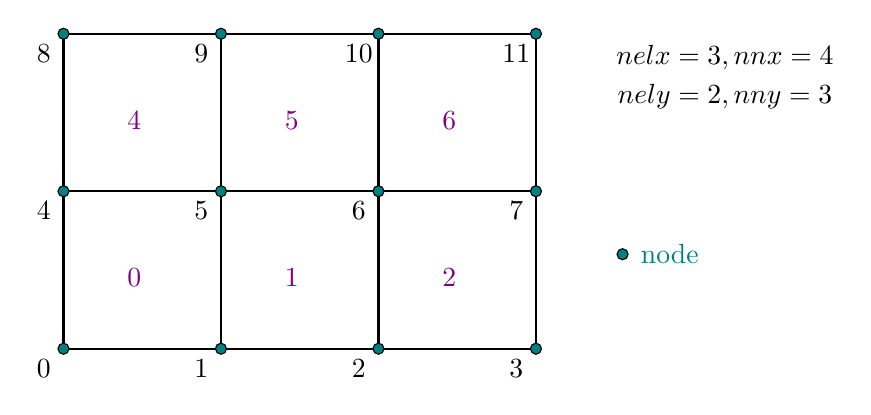
\begin{tikzpicture}
%\draw[step=0.5cm,gray,very thin] (0,0) grid (9,5); %background grid

\draw[thick] (1,1) -- (7,1) -- (7,5) -- (1,5) -- cycle;  
\draw[thick] (1,3) -- (7,3) ;
\draw[thick] (3,1) -- (3,5) ;
\draw[thick] (5,1) -- (5,5) ;

\draw[black,fill=teal] (1,1)     circle (2pt); 
\draw[black,fill=teal] (3,1)     circle (2pt); 
\draw[black,fill=teal] (5,1)     circle (2pt); 
\draw[black,fill=teal] (7,1)     circle (2pt); 

\draw[black,fill=teal] (1,3)     circle (2pt); 
\draw[black,fill=teal] (3,3)     circle (2pt); 
\draw[black,fill=teal] (5,3)     circle (2pt); 
\draw[black,fill=teal] (7,3)     circle (2pt); 

\draw[black,fill=teal] (1,5)     circle (2pt); 
\draw[black,fill=teal] (3,5)     circle (2pt); 
\draw[black,fill=teal] (5,5)     circle (2pt); 
\draw[black,fill=teal] (7,5)     circle (2pt); 

\node[] at (0.75,0.75) {0};
\node[] at (2.75,0.75) {1};
\node[] at (4.75,0.75) {2};
\node[] at (6.75,0.75) {3};

\node[] at (0.75,2.75) {4};
\node[] at (2.75,2.75) {5};
\node[] at (4.75,2.75) {6};
\node[] at (6.75,2.75) {7};

\node[] at (0.75,4.75) {8};
\node[] at (2.75,4.75) {9};
\node[] at (4.75,4.75) {10};
\node[] at (6.75,4.75) {11};

\node[violet] at (1.9,1.9) {0};
\node[violet] at (3.9,1.9) {1};
\node[violet] at (5.9,1.9) {2};
\node[violet] at (1.9,3.9) {4};
\node[violet] at (3.9,3.9) {5};
\node[violet] at (5.9,3.9) {6};

\draw[black,fill=teal] (8.1,2.2) circle (2pt); 
\node[] at (8.7,2.2) {{\color{teal}node}};

\node[] at (9.4,4.7) {$nelx=3, nnx=4$};
\node[] at (9.4,4.2) {$nely=2, nny=3$};

\end{tikzpicture}

\end{center}

\noindent In the case there is only a single degree of freedom per node, the 
assembled FEM matrix ${\bm M}$ will look like this:
\[
{\bm M}=
\left(
\begin{array}{cccccccccccc}
\Box & \Box &      &      & \Box & \Box &      &      &      &      &      &      \\
\Box & \Box & \Box &      & \Box & \Box & \Box &      &      &      &      &      \\
     & \Box & \Box & \Box &      & \Box & \Box & \Box &      &      &      &      \\
     &      & \Box & \Box &      &      & \Box & \Box &      &      &      &      \\
\Box & \Box &      &      & \Box & \Box &      &      & \Box & \Box &      &      \\
\Box & \Box & \Box &      & \Box & \Box & \Box &      & \Box & \Box & \Box &      \\
     & \Box & \Box & \Box &      & \Box & \Box & \Box &      & \Box & \Box & \Box \\
     &      & \Box & \Box &      &      & \Box & \Box &      &      & \Box & \Box \\
     &      &      &      & \Box & \Box &      &      & \Box & \Box &      &      \\
     &      &      &      & \Box & \Box & \Box &      & \Box & \Box & \Box &      \\
     &      &      &      &      & \Box & \Box & \Box &      & \Box & \Box & \Box \\
     &      &      &      &      &      & \Box & \Box &      &      & \Box & \Box 
\end{array}
\right)
\]
where the $\Box$ stand for non-zero terms.
This matrix structure stems from the fact that
\begin{itemize}
\item node 0 sees nodes 0,1,4,5 (1st line/column of the matrix)
\item node 1 sees nodes 0,1,2,4,5,6 (2nd line/column of the matrix)
\item node 2 sees nodes 1,2,3,5,6,7 (3rd line/column of the matrix)
\item node 3 sees nodes 2,3,6,7
\item node 4 sees nodes 0,1,4,5,8,9
\item node 5 sees nodes 0,1,2,4,5,6,8,9,10 
\item node 6 sees nodes 1,2,3,5,6,7,9,10,11
\item node 7 sees nodes 2,3,6,7,10,11
\item node 8 sees nodes 4,5,8,9
\item node 9 sees nodes 4,5,6,8,9,10
\item node 10 sees nodes 5,6,7,9,10,11 
\item node 11 sees nodes 6,7,10,11 (last line/column of the matrix)
\end{itemize}
In light thereof, we have
\begin{itemize}
\item 4 corner nodes which have 4 neighbours (counting themselves) 
\item 2(nnx-2) nodes which have 6 neighbours
\item 2(nny-2) nodes which have 6 neighbours
\item (nnx-2)$\times$(nny-2) nodes which have 9 neighbours
\end{itemize}
In total, the number of non-zero terms in the matrix above is then:
\[
NZ=4\times4+4\times6+2\times6+2\times9=70
\]
and in general, we would then have:
\[
NZ=4\times4+[2(nnx-2)+2(nny-2)]\times6 + (nnx-2)(nny-2)\times9
\]
Let us temporarily assume $nnx=nny=n$. The matrix size (total
number of unknowns) is then $N=n^2$ and  
\[
NZ=16+24(n-2)+9(n-2)^2
\]
A full matrix array would contain $N^2=n^4$ terms. 
The ratio of $NZ$ (the actual number of reals to store)
to the full matrix size (the number of reals a full matrix contains) is then 
\[
R = \frac{16+24(n-2)+9(n-2)^2}{n^4}
\]
It is then obvious that when $n$ is large enough $R \sim 1/n^2$.

CSR stores the nonzeros of the matrix row by row, in a
single indexed array A of double precision  numbers.
Another array COLIND contains the column index of each
corresponding entry in the A array. A third integer array RWPTR
contains pointers to the beginning of each row, which an additional pointer to
the first index following the nonzeros of the matrix A.
A and COLIND have length NZ and RWPTR has length N+1.

In the case of the here-above matrix, the arrays COLIND and RWPTR will look like:
\begin{eqnarray}
COLIND&=&(0,1,4,5, \; 0,1,2,4,5,6, \; 1,2,3,5,6,7, ..., 6,7,10,11) \nn\\
RWPTR &=&(0,4,10,16, ... )   \nn
\end{eqnarray}

%..............................................................................
\subsubsection{2D domain - Symmetric matrix CSR storage}

If the matrix is symmetric, i.e. ${\bm M}={\bm M}^T$, then we may wish to 
only store half of it, always in the interest of saving memory. 
Only the following remaining $\Box$ entries are relevant now:
\[
{\bm M}=
\left(
\begin{array}{cccccccccccc}
\Box & \Box &      &      & \Box & \Box &      &      &      &      &      &      \\
     & \Box & \Box &      & \Box & \Box & \Box &      &      &      &      &      \\
     &      & \Box & \Box &      & \Box & \Box & \Box &      &      &      &      \\
     &      &      & \Box &      &      & \Box & \Box &      &      &      &      \\
     &      &      &      & \Box & \Box &      &      & \Box & \Box &      &      \\
     &      &      &      &      & \Box & \Box &      & \Box & \Box & \Box &      \\
     &      &      &      &      &      & \Box & \Box &      & \Box & \Box & \Box \\
     &      &      &      &      &      &      & \Box &      &      & \Box & \Box \\
     &      &      &      &      &      &      &      & \Box & \Box &      &      \\
     &      &      &      &      &      &      &      &      & \Box & \Box &      \\
     &      &      &      &      &      &      &      &      &      & \Box & \Box \\
     &      &      &      &      &      &      &      &      &      &      & \Box 
\end{array}
\right)
\]
We see that the number of nonzeros is now 
\[
NZ_{symm}= \frac{NZ-n}{2}+n
\]
and in this case $NZ_{symm}=(70-12)/2+12=41$.
Then 
\begin{eqnarray}
COLIND&=&(0,1,4,5, \; 1,2,4,5,6, \; 3,5,6,7, ..., ,11) \nn\\
RWPTR &=&(0,4,9,14, ... )   \nn
\end{eqnarray}


%..............................................................................
\subsubsection{2D domain - Two degrees of freedom per node}

When there are now two degrees of freedom per node, such as in the case of the Stokes equation
in two-dimensions, the size of the $\K$ matrix is given $NfemV=nnx*nny*ndofV$  
where $NfemV$ is the total number of velocity degrees of freedom.

\begin{center}
\begin{flushright} {\tiny {\color{gray} (tikz\_3x2\_two.tex)}} \end{flushright}
%~~~~~~~~~~~~~~~~~~~~~~~~~~~~~~~~~~~~~~~~~~~~~~~~~~~~~~~~~~~~~~~~~~~~~~~~~~~~~~~~~~~~~~~~~~~~~~~~~~


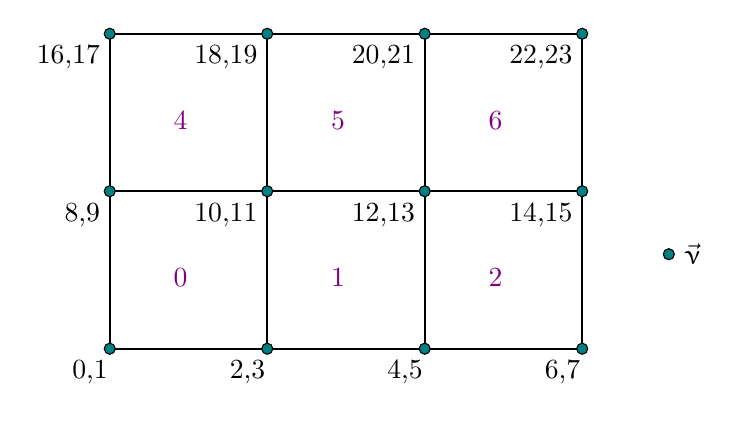
\begin{tikzpicture}
%\draw[step=0.5cm,gray,very thin] (0,0) grid (5,5); %background grid

\draw[thick] (1,1) -- (7,1) -- (7,5) -- (1,5) -- cycle;  
\draw[thick] (1,3) -- (7,3) ;
\draw[thick] (3,1) -- (3,5) ;
\draw[thick] (5,1) -- (5,5) ;

\draw[black,fill=teal] (1,1)     circle (2pt); 
\draw[black,fill=teal] (3,1)     circle (2pt); 
\draw[black,fill=teal] (5,1)     circle (2pt); 
\draw[black,fill=teal] (7,1)     circle (2pt); 

\draw[black,fill=teal] (1,3)     circle (2pt); 
\draw[black,fill=teal] (3,3)     circle (2pt); 
\draw[black,fill=teal] (5,3)     circle (2pt); 
\draw[black,fill=teal] (7,3)     circle (2pt); 

\draw[black,fill=teal] (1,5)     circle (2pt); 
\draw[black,fill=teal] (3,5)     circle (2pt); 
\draw[black,fill=teal] (5,5)     circle (2pt); 
\draw[black,fill=teal] (7,5)     circle (2pt); 

\node[] at (0.75,0.7) {0,1};
\node[] at (2.75,0.7) {2,3};
\node[] at (4.75,0.7) {4,5};
\node[] at (6.75,0.7) {6,7};

\node[] at (0.65,2.7) {8,9};
\node[] at (2.475,2.7) {10,11};
\node[] at (4.475,2.7) {12,13};
\node[] at (6.475,2.7) {14,15};

\node[] at (0.475,4.7) {16,17};
\node[] at (2.475,4.7) {18,19};
\node[] at (4.475,4.7) {20,21};
\node[] at (6.475,4.7) {22,23};

\node[violet] at (1.9,1.9) {0};
\node[violet] at (3.9,1.9) {1};
\node[violet] at (5.9,1.9) {2};
\node[violet] at (1.9,3.9) {4};
\node[violet] at (3.9,3.9) {5};
\node[violet] at (5.9,3.9) {6};

\draw[black,fill=teal] (8.1,2.2) circle (2pt); 
\node[] at (8.4,2.2) {$\vec\upnu$};

\end{tikzpicture}





\end{center}

In the case of the small grid above, we have then $NfemV=24$ and
elemental matrices are now $8\times8$ in size.

We still have
\begin{itemize}
\item $4$ corner nodes which have 4 neighbours
\item $2(nnx-2)$ nodes which have 6 neighbours
\item $2(nny-2)$ nodes which have 6 neighbours
\item $(nnx-2)\cdot(nny-2)$ nodes which have 9 neighbours,
\end{itemize}
but now each degree of freedom from a node sees the other two
degrees of freedom of another node too.
In that case, the number of nonzeros has been multiplied by four
and the assembled FEM matrix looks like:
\begin{equation}
\left(
\begin{array}{cccccccccccccccccccccccc}
\Box&\Box & \Box&\Box &  &  &  &  & \Box&\Box & \Box&\Box &  &  &  &  &  &  &  &  &  &  &  &  \\
\Box&\Box & \Box&\Box &  &  &  &  & \Box&\Box & \Box&\Box &  &  &  &  &  &  &  &  &  &  &  &  \\
\Box&\Box & \Box&\Box & \Box&\Box &  &  & \Box&\Box & \Box&\Box & \Box&\Box &  &  &  &  &  &  &  &  &  &  \\
\Box&\Box & \Box&\Box & \Box&\Box &  &  & \Box&\Box & \Box&\Box & \Box&\Box &  &  &  &  &  &  &  &  &  &  \\
 &  & \Box&\Box & \Box&\Box & \Box&\Box &  &  & \Box&\Box & \Box&\Box & \Box&\Box &  &  &  &  &  &  &  &  \\
 &  & \Box&\Box & \Box&\Box & \Box&\Box &  &  & \Box&\Box & \Box&\Box & \Box&\Box &  &  &  &  &  &  &  &  \\
 &  &  &  & \Box&\Box & \Box&\Box &  &  &  &  & \Box&\Box & \Box&\Box &  &  &  &  &  &  &  &  \\
 &  &  &  & \Box&\Box & \Box&\Box &  &  &  &  & \Box&\Box & \Box&\Box &  &  &  &  &  &  &  &  \\
\Box&\Box & \Box&\Box &  &  &  &  & \Box&\Box & \Box&\Box &  &  &  &  & \Box&\Box & \Box&\Box &  &  &  &  \\
\Box&\Box & \Box&\Box &  &  &  &  & \Box&\Box & \Box&\Box &  &  &  &  & \Box&\Box & \Box&\Box &  &  &  &  \\
\Box&\Box & \Box&\Box & \Box&\Box &  &  & \Box&\Box & \Box&\Box & \Box&\Box &  &  & \Box&\Box & \Box&\Box & \Box&\Box &  &  \\
\Box&\Box & \Box&\Box & \Box&\Box &  &  & \Box&\Box & \Box&\Box & \Box&\Box &  &  & \Box&\Box & \Box&\Box & \Box&\Box &  &  \\
 &  & \Box&\Box & \Box&\Box & \Box&\Box &  &  & \Box&\Box & \Box&\Box & \Box&\Box &  &  & \Box&\Box & \Box&\Box & \Box&\Box \\
 &  & \Box&\Box & \Box&\Box & \Box&\Box &  &  & \Box&\Box & \Box&\Box & \Box&\Box &  &  & \Box&\Box & \Box&\Box & \Box&\Box \\
 &  &  &  & \Box&\Box & \Box&\Box &  &  &  &  & \Box&\Box & \Box&\Box &  &  &  &  & \Box&\Box & \Box&\Box \\
 &  &  &  & \Box&\Box & \Box&\Box &  &  &  &  & \Box&\Box & \Box&\Box &  &  &  &  & \Box&\Box & \Box&\Box \\
 &  &  &  &  &  &  &  & \Box&\Box & \Box&\Box &  &  &  &  & \Box&\Box & \Box&\Box &  &  &  &  \\
 &  &  &  &  &  &  &  & \Box&\Box & \Box&\Box &  &  &  &  & \Box&\Box & \Box&\Box &  &  &  &  \\
 &  &  &  &  &  &  &  & \Box&\Box & \Box&\Box & \Box&\Box &  &  & \Box&\Box & \Box&\Box & \Box&\Box &  &  \\
 &  &  &  &  &  &  &  & \Box&\Box & \Box&\Box & \Box&\Box &  &  & \Box&\Box & \Box&\Box & \Box&\Box &  &  \\
 &  &  &  &  &  &  &  &  &  & \Box&\Box & \Box&\Box & \Box&\Box &  &  & \Box&\Box & \Box&\Box & \Box&\Box \\
 &  &  &  &  &  &  &  &  &  & \Box&\Box & \Box&\Box & \Box&\Box &  &  & \Box&\Box & \Box&\Box & \Box&\Box \\
 &  &  &  &  &  &  &  &  &  &  &  & \Box&\Box & \Box&\Box &  &  &  &  & \Box&\Box & \Box&\Box \\
 &  &  &  &  &  &  &  &  &  &  &  & \Box&\Box & \Box&\Box &  &  &  &  & \Box&\Box & \Box&\Box 
\end{array}
\right)\nonumber
\end{equation}
Note that the degrees of freedom are organised as follows: 
\[
(u_0,v_0,u_1,v_1,u_2,v_2, ... u_{11},v_{11})
\]
In general, we would then have:
\[
NZ=4 \left[4\times4+[2(nnx-2)+2(nny-2)]\times6 + (nnx-2)(nny-2)\times9 \right]
\]
and in the case of the small grid,
the number of non-zero terms in the matrix is then:
\[
NZ=4\left[4\times4+4\times6+2\times6+2\times9\right]=280
\]
In the case of the here-above matrix, the arrays COLIND and RWPTR will look like:
\begin{eqnarray}
COLIND&=&(0,1,2,3,8,9,10,11, \; 0,1,2,3,8,9,10,11,\; ...) \nn\\
RWPTR &=&(0,8,16,28, ... ) \nn
\end{eqnarray}


%..............................................................................
\subsubsection{3D domain - CSR- Three degrees of freedom}


Let us consider a $3\times4\times2$ grid which counts 
$nnx\cdot nny \cdot nnz = 5 \cdot 4\cdot 3=60$ nodes.
The assembled FEM matrix $\K$ size is then 
$N=nnx\times nny\times nnz \times ndof=180$.

\begin{center}
\begin{flushright} {\tiny {\color{gray} (tikz\_4x3x2.tex)}} \end{flushright}
%~~~~~~~~~~~~~~~~~~~~~~~~~~~~~~~~~~~~~~~~~~~~~~~~~~~~~~~~~~~~~~~~~~~~~~~~~~~~~~~~~~~~~~~~~~~~~~~~~~


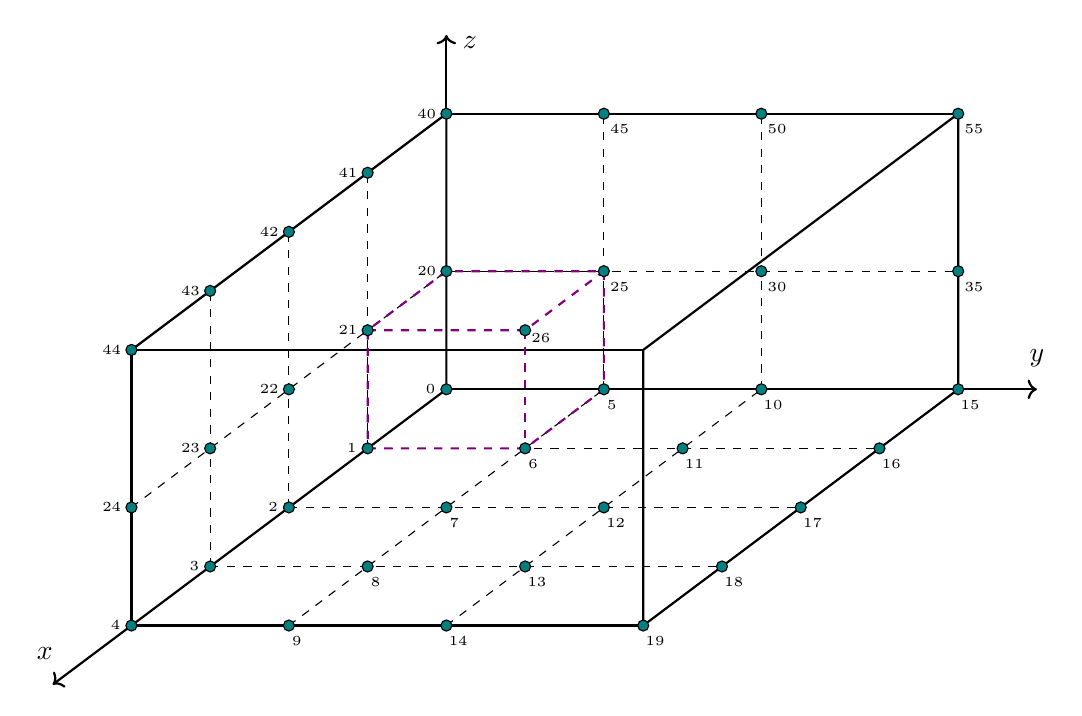
\begin{tikzpicture}
%\draw[step=0.5cm,gray,very thin] (0,0) grid (14,10); %background grid

%element
\draw[thick] (2,2) -- (8.5,2) -- (8.5,5.5) -- (2,5.5) -- cycle;  
\draw[thick] (2,2) -- (6,5) -- (6,8.5) -- (2,5.5) -- cycle ;
\draw[thick] (8.5,2) -- (12.5,5) -- (12.5,8.5) -- (8.5,5.5) -- cycle ;
\draw[thick] (6,5) -- (12.5,5) ;
\draw[thick] (6,8.5) -- (12.5,8.5) ;

%axes
\draw[thick,->] (2,2)--(1,1.25);
\draw[thick,->] (12.5,5)--(13.5,5);
\draw[thick,->] (6,8.5)--(6,9.5);
\node[] at (0.9,1.65) {$x$};
\node[] at (13.5,5.4) {$y$};
\node[] at (6.3,9.4) {$z$};

\draw[dashed] (2,3.5)--(6,6.5);
\draw[dashed] (3,2.75)--(3,6.25);
\draw[dashed] (4,3.5)--(4,7);
\draw[dashed] (5,4.25)--(5,7.75);
\draw[dashed] (4,2)--(8,5);
\draw[dashed] (6,2)--(10,5);
\draw[dashed] (3,2.75)--(9.5,2.75);
\draw[dashed] (4,3.5)--(10.5,3.5);
\draw[dashed] (5,4.25)--(11.5,4.25);
\draw[dashed] (6,6.5)--(12.5,6.5);
\draw[dashed] (8,5)--(8,8.5);
\draw[dashed] (10,5)--(10,8.5);

\draw[dashed, thick,violet] (5,4.25)--(7,4.25) --(8,5)--(8,6.5) --(6,6.5)--(5,5.75)--(5,4.25);
\draw[dashed, thick,violet] (5,5.75)--(7,5.75)--(8,6.5);
\draw[dashed, thick,violet] (7,5.75)--(7,4.25);

\draw[black,fill=teal] (2,2) circle (2pt); 
\draw[black,fill=teal] (3,2.75) circle (2pt); 
\draw[black,fill=teal] (4,3.5) circle (2pt); 
\draw[black,fill=teal] (5,4.25) circle (2pt); 
\draw[black,fill=teal] (6,5) circle (2pt); 

\draw[black,fill=teal] (2,3.5) circle (2pt); 
\draw[black,fill=teal] (3,4.25) circle (2pt); 
\draw[black,fill=teal] (4,5) circle (2pt); 
\draw[black,fill=teal] (5,5.75) circle (2pt); 
\draw[black,fill=teal] (6,6.5) circle (2pt); 

\draw[black,fill=teal] (2,5.5) circle (2pt); 
\draw[black,fill=teal] (3,6.25) circle (2pt); 
\draw[black,fill=teal] (4,7) circle (2pt); 
\draw[black,fill=teal] (5,7.75) circle (2pt); 
\draw[black,fill=teal] (6,8.5) circle (2pt); 

\draw[black,fill=teal] (4,2) circle (2pt); 
\draw[black,fill=teal] (5,2.75) circle (2pt); 
\draw[black,fill=teal] (6,3.5) circle (2pt); 
\draw[black,fill=teal] (7,4.25) circle (2pt); 
\draw[black,fill=teal] (8,5) circle (2pt); 

\draw[black,fill=teal] (6,2) circle (2pt); 
\draw[black,fill=teal] (7,2.75) circle (2pt); 
\draw[black,fill=teal] (8,3.5) circle (2pt); 
\draw[black,fill=teal] (9,4.25) circle (2pt); 
\draw[black,fill=teal] (10,5) circle (2pt); 

\draw[black,fill=teal] (8.5,2) circle (2pt); 
\draw[black,fill=teal] (9.5,2.75) circle (2pt); 
\draw[black,fill=teal] (10.5,3.5) circle (2pt); 
\draw[black,fill=teal] (11.5,4.25) circle (2pt); 
\draw[black,fill=teal] (12.5,5) circle (2pt);

\draw[black,fill=teal] (7,5.75) circle (2pt);


\draw[black,fill=teal] (8,6.5) circle (2pt);
\draw[black,fill=teal] (8,8.5) circle (2pt);

\draw[black,fill=teal] (10,6.5) circle (2pt);
\draw[black,fill=teal] (10,8.5) circle (2pt);

\draw[black,fill=teal] (12.5,6.5) circle (2pt);
\draw[black,fill=teal] (12.5,8.5) circle (2pt);

\node[] at (5.8,5) {\tiny 0};
\node[] at (4.8,4.25) {\tiny 1};
\node[] at (3.8,3.5) {\tiny 2};
\node[] at (2.8,2.75) {\tiny 3};
\node[] at (1.8,2) {\tiny 4};

\node[] at (5.75,6.5) {\tiny 20};
\node[] at (4.75,5.75) {\tiny 21};
\node[] at (3.75,5) {\tiny 22};
\node[] at (2.75,4.25) {\tiny 23};
\node[] at (1.75,3.5) {\tiny 24};

\node[] at (5.75,8.5) {\tiny 40};
\node[] at (4.75,7.75) {\tiny 41};
\node[] at (3.75,7) {\tiny 42};
\node[] at (2.75,6.25) {\tiny 43};
\node[] at (1.75,5.5) {\tiny 44};

\node[] at (8.1,4.8) {\tiny 5};
\node[] at (7.1,4.05) {\tiny 6};
\node[] at (6.1,3.3) {\tiny 7};
\node[] at (5.1,2.55) {\tiny 8};
\node[] at (4.1,1.8) {\tiny 9};

\node[] at (10.15,4.8) {\tiny 10};
\node[] at (9.15,4.05) {\tiny 11};
\node[] at (8.15,3.3) {\tiny 12};
\node[] at (7.15,2.55) {\tiny 13};
\node[] at (6.15,1.8) {\tiny 14};

\node[] at (12.65,4.8) {\tiny 15};
\node[] at (11.65,4.05) {\tiny 16};
\node[] at (10.65,3.3) {\tiny 17};
\node[] at (9.65,2.55) {\tiny 18};
\node[] at (8.65,1.8) {\tiny 19};

\node[] at (8.2,6.3) {\tiny 25};
\node[] at (7.2,5.65) {\tiny 26};

\node[] at (8.2,8.3) {\tiny 45};
\node[] at (10.2,6.3) {\tiny 30};
\node[] at (10.2,8.3) {\tiny 50};

\node[] at (12.7,6.3) {\tiny 35};
\node[] at (12.7,8.3) {\tiny 55};

\end{tikzpicture}

\end{center}



The total number of nonzeros in the case $ndof=1$ would be decomposed as follows:
\begin{itemize}
\item 8 corners 'see' 8 neighbours
\item 4 edges with $(nnx-2)$ nodes in the x direction see 12 nodes
\item 4 edges with $(nny-2)$ nodes in the y direction see 12 nodes
\item 4 edges with $(nnz-2)$ nodes in the z direction see 12 nodes
\item $2(nnx-2)(nny-2)$ nodes see 18 nodes
\item $2(nnx-2)(nnz-2)$ nodes see 18 nodes
\item $2(nny-2)(nnz-2)$ nodes see 18 nodes
\item $(nnx-2)(nny-2)(nnz-2)$ interior nodes see 27 nodes
\end{itemize}





%..............................................................................
\subsubsection{Matrix Storage in fieldstone}

The majority of the codes have the FE matrix being a full array
\begin{lstlisting}
a_mat = np.zeros((Nfem,Nfem),dtype=np.float64) 
\end{lstlisting}
and it is converted to CSR format on the fly in the solve phase:
\begin{lstlisting}
sol = sps.linalg.spsolve(sps.csr_matrix(a_mat),rhs)
\end{lstlisting}

Note that linked list storages can be used (lil\_matrix). Substantial memory savings 
but much longer compute times since it takes longer to write in such arrays.
A conversion to CSR format is still necessary before calling the solver.




%..............................................................................
\subsubsection{Sparse Matrix-Vector multiplication}
\index{general}{SpMV} \index{general}{Sparse Matrix-Vector Multiplication}

When/if the matrix ${\bm M}$ is stored in a two-dimensional array, 
its (left or right) multiplication by a vector is trivial. 
Either one resorts to writing a double for loop (not recommended), 
either one uses {\tt numpy.dot}\footnote{\url{https://numpy.org/doc/stable/reference/generated/numpy.dot.html}}
in python, or {\tt matmul} in Fortran.

However, when the matrix is stored as a single continuous array, say CSR, how does this work?
This question is {\it very important} since iterative solvers such as the Conjugate Gradient solver
(see Section~\ref{ss:itsolvers}) rely extensively on multiplying the matrix by many different vectors. 

The Sparse Matrix-Vector multiplication operation is often abbreviated SpMV.
To quote Knepley \cite{knepley}: "The Sparse Matrix-Vector Product (SpMV) is today 
a workhorse of scientific computing. It is a central kernel is iterative linear and 
nonlinear solvers for PDE, and now for many graph algorithms."
As explained in Williams \etal (2007) \cite{wiov07} (and in many 
other sources on the topic), the algorithm for 
a basic SpMV implementation is rather simple in its naive form. 

\begin{center}
\includegraphics[width=17cm]{images/spmv/widc08}\\
{\captionfont Taken from Williams \etal (2008) \cite{widc08}. 
Sparse Matrix Vector Multiplication (SpMV). 
(a) visualization of the algebra: $\vec{y} \leftarrow {\bm A}\cdot \vec{x}$.\\
(b) Standard compressed sparse row (CSR) representation of the matrix.  \\
(c) The standard implementation of SpMV for a matrix stored in CSR. 
The outer loop is trivially parallelized without any data dependencies.}
\end{center}

Let us assume that we wish to compute $\vec{y}={\bm A}\cdot \vec{x}$ where ${\bm A}$ 
is in CSR format. The pseudo code then goes as follows:
\begin{verbatim}
for i in range(0,m):
    y0=0
    for k in range(ROWPTR[i],ROWPTR[i+1]):
        y0 += VAL[k] * x[COLIND[k]]
    y[i]=y0
\end{verbatim} 
Although technically correct, this algorithm is problematic because the vector x array
is accessed indirectly and this causes a non-optimal use of the processor, which 
in the end makes the calculation take longer than it should.


The following piece of code comes from \elefant. Note that here (ROWPTR=ia, COLIND=ja, VAL=mat)
\begin{lstlisting}[language=Fortran]
subroutine spmv (nr,nc,nz,x,y,mat,ja,ia)
implicit none
integer, intent(in)  :: nr,nc,nz
real(8), intent(in)  :: x(nc), mat(nz)
real(8), intent(out) :: y(nr)
integer, intent(in)  :: ja(nz),ia(nr+1)
real(8) t
integer i, k

do i = 1,nr
   t = 0.0d0
   do k=ia(i), ia(i+1)-1
      t = t + mat(k)*x(ja(k))
   end do
   y(i) = t 
end do

end subroutine
\end{lstlisting}


How to make this calculation as efficiently as possible on CPUs and GPUs, on one thread 
or multiple threads has given rise to a lot of literature.

\Literature Krotkiewski \& Dabrowski \cite{krda10}, Section 9.4 of Kepley \cite{knepley}, 
Williams \etal (2008) \cite{widc08}

 %---------------------------------------------
\newpage %-----------------------------------------------------------------------------------------
\subsection{Mesh generation} \label{sec:meshes} \begin{flushright} {\tiny {\color{gray} meshes.tex}} \end{flushright}
%~~~~~~~~~~~~~~~~~~~~~~~~~~~~~~~~~~~~~~~~~~~~~~~~~~~~~~~~~~~~~~~~~~~~~~~~~~~~~~~~~~~~~~~~~~~~~~~~~~

Before basis functions can be defined and PDEs can be discretised and solved 
we must first tesselate the domain with polygons, e.g. triangles and 
quadrilaterals in 2D, tetrahedra, prisms and hexahedra in 3D. \index{general}{Convex Polygon} 

When the domain is itself simple (e.g. a rectangle, a sphere, ...) the mesh (or grid) can 
be (more or less) easily produced and the connectivity array filled with straightforward 
algorithms \cite{thie18}.
However, real life applications can involve extremely complex geometries (e.g. a bridge, 
a human spine, a car chassis and body, etc ...) and dedicated algorithms/softwares 
must be used (see \cite{thsw,frge,xiyz09}). 

We usually distinguish between two broad classes of grids: structured grids (with a regular 
connectivity) and unstructured grids (with an irregular connectivity).
\index{general}{Structured Grid} \index{general}{Unstructured Grid}

\begin{center}
\includegraphics[width=5cm]{images/meshes/structured_grid}
\includegraphics[width=5cm]{images/meshes/unstructured_grid}
\end{center}

\begin{remark}
\index{general}{Meshless}
Various families of so-called meshless methods exist and are commonly employed in Computational 
Fluid Dynamics \cite{liugu,liliu,grliu,liuliu}. They are however very rarely used in 
Computational geodynamics, with a noticeable exception \cite{hans03}.
\end{remark}

%............................................
\subsubsection{Quadrilateral-based meshes}

Let us now focus on the case of a rectangular computational domain of size 
{\tt Lx} $\times$ {\tt Ly} with a regular mesh composed of {\tt nelx}$\times${\tt nely}={\tt nel}
   quadrilaterals.  
There are then {\tt nnx}$\times${\tt nny}={\tt nnp} grid points.
The elements are of size {\tt hx}$\times${\tt hy} with {\tt hx}={\tt Lx}/{\tt nelx}.

We have no reason to come up with an irregular/illogical node numbering so 
we can number nodes row by row or column by column as shown on the example 
hereunder of a 3$\times$2 grid:

\begin{verbatim}
8=======9======10======11       2=======5=======8======11
|       |       |       |       |       |       |       |
|  (3)  |  (4)  |  (5)  |       |  (1)  |  (3)  |  (5)  |
|       |       |       |       |       |       |       |
4=======5=======6=======7       1=======4=======7======10
|       |       |       |       |       |       |       |
|  (0)  |  (1)  |  (2)  |       |  (0)  |  (2)  |  (4)  |
|       |       |       |       |       |       |       |
0=======1=======2=======3       0=======3=======6=======9

     "row by row"                  "column by column"
\end{verbatim}

The numbering of the elements themselves could be done in a somewhat chaotic 
way but we follow the numbering of the nodes for simplicity.
The row by row option is the adopted one in \fieldstone{} and the coordinates of the 
points are computed as follows:

\begin{lstlisting}
x = np.empty(nnp, dtype=np.float64)
y = np.empty(nnp, dtype=np.float64)
counter = 0
for j in range(0,nny):
    for i in range(0,nnx):
        x[counter]=i*hx
        y[counter]=j*hy
        counter += 1
\end{lstlisting}
The inner loop has {\tt i} ranging from {\tt 0} to {\tt nnx-1} first for {\tt j}=0, 1, ...
up to {\tt nny-1} which indeed corresponds to the row by row numbering.

\index{general}{Connectivity Array} 
We now turn to the connectivity. As mentioned before, this is a structured mesh so that the so-called
connectivity array, named {\tt icon} in our case, can be filled easily. For each element we need
to store the node identities of its vertices. Since there are {\tt nel} elements and {\tt m=4} corners, 
this is a {\tt m}$\times${\tt nel} array. The algorithm goes as follows:

\begin{lstlisting}
icon =np.zeros((m,nel),dtype=np.int16)
counter = 0
for j in range(0,nely):
    for i in range(0,nelx):
        icon[0,counter] = i + j * nnx 
        icon[1,counter] = i + 1 + j * nnx 
        icon[2,counter] = i + 1 + (j + 1) * nnx 
        icon[3,counter] = i + (j + 1) * nnx 
        counter += 1
\end{lstlisting}

In the case of the 3$\times$2 mesh, the {\tt icon} is filled as follows:
\begin{center}
\begin{tabular}{ccccccc}
element id$\rightarrow$ &0 &1&2&3&4&5 \\
node id$\downarrow$ \\
0& 0& 1& 2& 4& 5  &6\\
1& 1& 2& 3& 5& 6  &7\\
2& 5& 6& 7& 9& 10 &11\\
3& 4& 5& 6& 8& 9  &10\\
\end{tabular}
\end{center}
It is to be understood as follows: element $\#4$ is composed of nodes 5, 6, 10 and 9.
Note that nodes are always stored in a counter clockwise manner, starting at the bottom left.
This is very important since the corresponding basis functions and their derivatives 
will be labelled accordingly.

In three dimensions things are very similar. The mesh now counts 
{\tt nelx}$\times${\tt nely}$\times${\tt nelz}={\tt nel} elements which represent 
a cuboid of size {\tt Lx}$\times${\tt Ly}$\times${\tt Lz}.
The position of the nodes is obtained as follows:
\begin{lstlisting}
x = np.empty(nnp,dtype=np.float64)
y = np.empty(nnp,dtype=np.float64)
z = np.empty(nnp,dtype=np.float64)
counter=0
for i in range(0,nnx):
    for j in range(0,nny):
        for k in range(0,nnz):
            x[counter]=i*hx
            y[counter]=j*hy
            z[counter]=k*hz
            counter += 1
\end{lstlisting}
The connectivity array is now of size {\tt m}$\times${\tt nel} with {\tt m=8}:
\begin{lstlisting}
icon =np.zeros((m,nel),dtype=np.int16)
counter = 0
for i in range(0,nelx):
    for j in range(0,nely):
        for k in range(0,nelz):
            icon[0,counter]=nny*nnz*(i  )+nnz*(j  )+k
            icon[1,counter]=nny*nnz*(i+1)+nnz*(j  )+k
            icon[2,counter]=nny*nnz*(i+1)+nnz*(j+1)+k
            icon[3,counter]=nny*nnz*(i  )+nnz*(j+1)+k
            icon[4,counter]=nny*nnz*(i  )+nnz*(j  )+k+1
            icon[5,counter]=nny*nnz*(i+1)+nnz*(j  )+k+1
            icon[6,counter]=nny*nnz*(i+1)+nnz*(j+1)+k+1
            icon[7,counter]=nny*nnz*(i  )+nnz*(j+1)+k+1
            counter += 1
\end{lstlisting}

\improvement[inline]{produce drawing of node numbering}

Although it is not very common in geosciences, quadrilateral meshes are sometimes 
employed in a boundary-fitted way, as shown hereunder:

\begin{center}
\includegraphics[width=7cm]{images/meshes/gukt16}\\
\end{center}


\Literature: \cite{jole97}

%...................................................
\subsubsection{Delaunay triangulation and Voronoi cells, and triangle-based meshes}

The topic of Delaunay\footnote{The triangulation is named after 
Boris Delaunay for his work on this topic from 1934.}
 triangulation is vast, but a simple definition can be written 
as follows:
"a Delaunay triangulation for a set P 
of points in a plane is a triangulation DT(P) such that no point in P is  
inside the circumcircle of any triangle in DT(P)." [wikipedia]
Other properties of such triangulations are that they 
maximize the minimum angle of all the angles of the 
triangles in the triangulation.
Note that for four or more 
points on the same circle (e.g., the vertices of a rectangle) the Delaunay triangulation is  
not unique and that points on a line also cannot yield a valid triangulation
(for the simple reason that they do not form a triangle).

\begin{center}
\includegraphics[width=4cm]{images/meshes/delaunay}
\includegraphics[width=4cm]{images/meshes/delaunay3}\\
{\captionfont a) A Delaunay triangulation in the plane with circumcircles shown.
b) The Delaunay triangulation of a random set of 100 points in a plane.}
\end{center}

The Delaunay triangulation of a discrete point set P in general corresponds 
to the dual graph of the Voronoi diagram for P. 
A Voronoi diagram is composed of non-overlapping Voronoi cells which make a partition 
of the plane. 
For each point there is a corresponding region consisting of all points closer to that 
point than to any other: this region is the Voronoi cell of that point.

\begin{center}
a)\includegraphics[width=4cm]{images/meshes/delaunay2}
b)\includegraphics[width=4cm]{images/meshes/voronoi}\\
{\captionfont a) The Delaunay triangulation with all the circumcircles and their centers (in red).
b) Connecting the centers of the circumcircles produces the Voronoi diagram (in red). }
\end{center}

The Delaunay triangulation is used in the \douar code which is based on a particle levelset function to track materials. These particles are connected by means of a Delaunay triangulation (usually in a plane at startup, and then in a local Euclidean geometry once the surface is deformed) \cite{brtf08}.

\Literature: \cite{gebo}.


Once a Delaunay triangulation has been obtained it can be used as a FEM mesh.  
Triangle-based meshes are obviously better suited for simulations of complex geometries:
\begin{center}
\includegraphics[height=4cm]{images/meshes/tr1}
\includegraphics[height=4cm]{images/meshes/dolfin}\\
\includegraphics[height=3.8cm]{images/meshes/gebk12}\cite{gebk12}
\includegraphics[height=3.8cm]{images/meshes/rost05a}\cite{rost05a}
\end{center}

A very practical 2D triangle mesher is the 
code {\sl Triangle}\footnote{\url{https://www.cs.cmu.edu/~quake/triangle.html}}
written by J.R. Shewchuk \cite{shew96,shew02,shew14}.
Triangle is specialized for creating two-dimensional finite element meshes, but can 
also perform simpler related tasks such as forming Delaunay triangulations under various assumptions.
Another very common mesher tool is Gmsh \cite{gere09}.

\begin{center}
\includegraphics[width=13cm]{images/meshes/bugw01}\\
{\captionfont Taken from Buiter \etal \cite{bugw01}. Finite element grid. 
The subducting plate initially extends to 1226 km in the horizontal direction and 
is not completely shown here. Discretization in the subducting plate is slightly coarser 
towards the right edge.}
\end{center}

\begin{center}
\includegraphics[width=13cm]{images/meshes/bafl16}\\
{\captionfont Numerical model setup of the 2D axisymmetric half-space with all applied 
boundary conditions to study the effects of ice-cap unloading
on shallow volcanic systems \cite{bafl16}}
\end{center}

\begin{center}
\includegraphics[width=13cm]{images/meshes/fegh14}\\
{\captionfont Taken from \cite{fegh14}. Modelling of slow
landslides. Finite element mesh in the initial and excavated configuration.}
\end{center}

Although it is rarely used in practice it is possible to produce meshes which contain 
both quadrilateral and triangular elements:
\begin{center}
\includegraphics[width=13cm]{images/meshes/fige95}\\
{\captionfont Mesh used to analayse the stress distribution around a pressurized crack in a layered 
elastic medium \cite{fige95}}
\end{center}

\Literature \fullcite{musd15}\fullcite{vemm09}

\begin{remark} 
The Natural Neighbour Interpolation method of Sambridge \etal \cite{sabm95,sabm96} is based on the Delaunay triangulation.
\end{remark}

\begin{remark} 
Moresi \& Mather \cite{moma19} have released Stripy, a A Python module for (constrained) triangulation
in Cartesian coordinates and on a sphere, which is based on Stripack \cite{renk96,renk97}.
\end{remark}

\todo[inline]{write about gmesh}

\begin{center}
\includegraphics[width=6cm]{images/meshes/gusa98a}
\includegraphics[width=6cm]{images/meshes/gusa98b}\\
{\captionfont Taken from Gudmundsson \& Sambridge (1998) \cite{gusa98}.
Boundaries of Voronoi cells around 4100 of the original 16,200 2x2 degree cells
selected to sample the details of the regionalization.}
\end{center}


%...........................
\subsubsection{Tetrahedra}

\begin{center}
\includegraphics[width=5cm]{images/meshes/glacier}
\includegraphics[width=10cm]{images/meshes/gowo05}\\
{\captionfont Left: Example of 3D mesh \cite{yash15}.
Right: Normalized velocities of a STEP subduction model \cite{gowo05}.}
\end{center}


\begin{center}
\includegraphics[width=7cm]{images/meshes/guyr16}
\includegraphics[width=8cm]{images/meshes/tokv09}\\
{\captionfont Left: 3D finite element grid in Damintun area, including prescribed faults. Guo \etal, 2016 \cite{guyr16}.
Right: Structural reactivation in plate tectonics controlled by olivine crystal anisotropy \cite{tokv09}.}
\end{center}



\begin{center}
\includegraphics[width=6cm]{images/meshes/paml14b}
\includegraphics[width=6.3cm]{images/meshes/codh08}\\
{\captionfont Left: Mesh used for the three-dimensional model. A high resolution mesh is used in
the wedge and subslab domains, while the mesh resolution decays to lower values
toward the edge of the model. All elements are quadratic, allowing for twice the
resolution visualized here. Paczkowski \etal (2014) \cite{paml14b}.
Right: Mid-Ocean Ridge Hydrothermal System: 3D mesh consisting of 2.5m tetrahedron elements. 
Resolution is refined toward the axial center, with the finest resolution between the dashed
lines, and colors indicate computational domains assigned to separate processors.
Coumou \etal (2008) \cite{codh08}.}
\end{center}

Check TetGen mesher \fullcite{si15}. 

%............................................
\subsubsection{Hexahedra}

A hexahedron is a convex polytope isomorphic to the cube $[0,1]^3$.
Edges are line segments, facets are strictly {\bf planar} convex polygons.

\begin{center}
\includegraphics[width=5cm]{images/meshes/hexa.jpg}
\includegraphics[width=6cm]{images/meshes/hexa2}
\end{center}

\Literature Efficient Volume computation for Three- Dimensional hexahedral Cells \cite{duko88,gran97}

%.......................................
\subsubsection{Adaptive Mesh Refinement}
\index{general}{AMR} \index{general}{Adaptive Mesh Refinement}

Let us do a simple calculation and assume we wish to model mantle convection on Earth. 
The inner radius is $R_1=$3485km and the bottom of the lithosphere is at $R_2=$6250km. 
The volume of fluid is then 
\[
V = \frac{4}{3}\pi (R_2^3-R_1^3) \simeq 8.5\times 10^{11} \text{km}^3
\]
Let us further assume that we are satisfied with an average resolution of 10km. 
Each element/cell is then $10^3\text{km}^3$ and the total number of elements/cell is then 
\[
N \simeq 8.5 \times 10^8 \sim {\cal O}(10^9)
\]
This is a very large number. The resulting linear systems from the discretisation of the 
equations on such a mesh will be very even larger for the Stokes equations and solving 
these systems will require very large numbers of CPUs and long compute times. 

Aside from these considerations it is quite obvious that a high resolution mesh is not needed 
in parts of the mantle where large scale upwellings and downwellings occur, but 
probably even higher resolution will be needed in the vicinity of thin plumes and boundary layers. 
This means that a uniform mesh is a sub-optimal way of discretising space for such problems. 

The same reasoning also holds in the lithosphere where for instance narrow plate boundaries need to 
be adequately resolved while the inside of rigid plates can be modelled with coarser meshes. 

Finally, although one could employ meshing software to arrive at well balanced meshes in space, the 
dynamic character of the geodynamics modelling renders this approach cumbersome. A subduction zone, 
a mid-ocean rift or an ascending plume will evolve in time and the mesh will have to evolve in time too. 

In light of all this, it was only a matter of time before Adaptive Mesh Refinement was adopted 
in computatinal geodynamics. However, since the use and update of such meshes is somewhat 
complex in terms of numerical algorithms, its introduction came somewhat late (00's and later).
The \douar code (see Section~\ref{app:codes}) developed originally by J. Braun and Ph. Fullsack 
is a prime example of an early multi-purpose code relying on a self-written Octree library \cite{brtf08}.
More recently the \aspect{} code was developed on top of the Octree library p4est \cite{buwg11}

For further reading I suggest you read the review by May, Schellart \& Moresi on this topic \cite{masm13}.

\begin{center}
\includegraphics[height=6cm]{images/meshes/bugg08.jpg}
\includegraphics[height=6cm]{images/meshes/bugg10.jpg}\\
{\captionfont Taken from \cite{bugg08} and \cite{bugg10}}
\end{center}

\begin{center}
\includegraphics[height=3.8cm]{images/meshes/gltf18.jpg}\\
{\captionfont Taken from \cite{gltf18}}
\end{center}


\Literature: \cite{bugg08,bugg10}\cite{lezh11} \cite[sect 3]{bugs09} \cite{dadh07}
\cite{svna18} \cite{mish11}


\newpage
\paragraph{A short illustrative exercise}.


\noindent 
\includegraphics[width=4.5cm]{images/meshes/AMR/amr0}
\includegraphics[width=4.5cm]{images/meshes/AMR/amr1}
\includegraphics[width=4.5cm]{images/meshes/AMR/amr2}\\
\includegraphics[width=4.5cm]{images/meshes/AMR/amr3}
\includegraphics[width=4.5cm]{images/meshes/AMR/amr4}
\includegraphics[width=4.5cm]{images/meshes/AMR/amr5}\\
\includegraphics[width=4.5cm]{images/meshes/AMR/amr6}
\includegraphics[width=4.5cm]{images/meshes/AMR/amr7}
\includegraphics[width=4.5cm]{images/meshes/AMR/amr8}

\begin{tabular}{l|ccccccccc}
             & \# l0  & \# l1 & \# l2 & \# l3 & \# l4 & \# l5 & \# l6 & \# l7 & \# l8 \\ 
\hline\hline
max level= 0 & 1 & \\
max level= 1 & 0 & 4 & \\
max level= 2 & 0 & 3 & 4 \\
max level= 3 & 0 & 2 & 7 & 4\\
max level= 4 & 0 & 2 & 5 & 10 & 8 \\
max level= 5 & 0 & 1 & 8 & 12 & 11 & 20 \\ 
max level= 6 & 0 & 1 & 8 & 11 & 13 & 20 & 32 \\
max level= 7 & 0 & 0 & 11 & 14 & 15 & 23 & 37 & 60 \\
max level= 8 & 0 & 0 & 11 & 13 & 17 & 27 & 43 & 72 & 116 \\
\hline
\end{tabular}

\includegraphics[width=7.28cm]{images/meshes/AMR/amr_data1.pdf}
\includegraphics[width=7.28cm]{images/meshes/AMR/amr_data2.pdf}

In the particular case presented here, even though the inclusion in a short 
two-dimensional line, the total number of elements grows faster than the 
third power of the refinement level. While of course the total number 
of elements remains much smaller than the constant resolution counterpart, 
this observation tells us that authorising a unit increase of the maximum 
refinement level can have a substantial effect on the total number of elements.

\newpage

\noindent
\includegraphics[width=4cm]{images/meshes/AMR/amr_0}
\includegraphics[width=4cm]{images/meshes/AMR/amr_1}
\includegraphics[width=4cm]{images/meshes/AMR/amr_2}
\includegraphics[width=4cm]{images/meshes/AMR/amr_3}\\
\includegraphics[width=4cm]{images/meshes/AMR/amr_4}
\includegraphics[width=4cm]{images/meshes/AMR/amr_5}
\includegraphics[width=4cm]{images/meshes/AMR/amr_6}
\includegraphics[width=4cm]{images/meshes/AMR/amr_7}


\includegraphics[width=5cm]{images/meshes/AMR/amr_data3.pdf}
\includegraphics[width=5cm]{images/meshes/AMR/amr_data4.pdf}
\includegraphics[width=5cm]{images/meshes/AMR/amr_data5.pdf}






%.......................................
\subsubsection{Conformal Mesh Refinement \label{ss:cmr}}
\index{general}{Conformal Mesh Refinement}

The quadtree/octree mesh refinement presented above is one option
when it comes to mesh refinement (or $h$-refinement). However their 
massive drawback is the presence of hanging notes which require 
special attention. 
Another approach to mesh refinement is conformal mesh refinement
as best exemplified on the following figures: 

\begin{center}
\includegraphics[height=4.5cm]{images/meshes/amrnew}\\
{\captionfont Taken from Deb \etal (1996) \cite{depl96}.
A typical instance of the outcome of the refinement procedure. 
Notice that the `spill-over' is reduced to one row on each side of the `localized' elements.}
\end{center}

\begin{center}
\includegraphics[height=4.5cm]{images/meshes/vaks15}
\includegraphics[height=4.5cm]{images/meshes/depl96}
\includegraphics[height=4.5cm]{images/meshes/habo04}\\
\includegraphics[height=4.5cm]{images/meshes/kott05}
\includegraphics[height=4.5cm]{images/meshes/specfem}\\
\includegraphics[height=4.5cm]{images/meshes/conf3D}\\
{\captionfont 
Top row, From left to right: 
van Driel \etal (2015) \cite{vaks15}; 
Deb \etal (1996) \cite{depl96}; 
Harris \etal (2004) \cite{habo04}; 
Komatitsch \etal (2005) \cite{kott05}; 
Middle row: Specfem manual;
Bottom row: I don't know anymore.}
\end{center}

\begin{center}
\includegraphics[height=5cm]{images/meshes/gari09_a}
\includegraphics[height=5cm]{images/meshes/gari09_b}\\
{\captionfont Taken from Garimella (2009) \cite{gari09}.}
\end{center}

\begin{center}
\includegraphics[height=4cm]{images/meshes/newmeshref1}
\includegraphics[height=4cm]{images/meshes/newmeshref2}
\end{center}


\begin{center}
\includegraphics[height=4cm]{images/meshes/refine_mesh_sheet_directional1}
\includegraphics[height=4cm]{images/meshes/refine_mesh_sheet_directional2}
\includegraphics[height=4cm]{images/meshes/refine_mesh_sheet_directional4}\\
\url{https://cubit.sandia.gov/public/14.0/help_manual/WebHelp/mesh_generation/mesh_modification/mesh_refinement.htm}
\end{center}

\Literature: 
D{\"u}ster \& Rank \cite{dura01},
Harris \etal (2004) \cite{habo04},
Anderson \etal (2009) \cite{anbo09},
Anderson \cite{ande09}, 
Garimella (2009) \cite{gari09},
Nicolas \& Fouquet (2013) \cite{nifo13,nifo13b}.
Parrish \cite{parr07}, 
Schneiders \cite{schn00,schn96,schn96b,schn99},
Schneiders \etal \cite{scde95},
Staten \& Canann \cite{stca97},
book by Ramm \etal \cite{rarr03}.


%.......................................
\subsubsection{Stretching the mesh}

In some cases the topology of the mesh can be regular but one can for instance stretch 
the mesh such that (for instance) the vertical resolution is higher at the top than at the bottom, 
or higher in the middle than on the sides.

The idea behind the transformation is a piecewise-linear function which maps [0,L] to [0,L] where 
$L$ is the length of the domain in the $x$-direction. For instance, this transformation can take the following form:

\begin{center}
\includegraphics[width=8cm]{images/meshes/stretching/stretch_towards_center}\\
{\captionfont Parameters $\beta_1$ and $\beta_2$ control the shape of the lines.\\ 
The kinks in the line occur at $\beta_1 L$ and $(1-\beta_1)L$ (see code here under).}
\end{center}

The (minimal) code to transform the mesh is as follows:
\begin{lstlisting}
def stretch_towards_center(x,L,beta1,beta2):
    if x<beta1*L: 
       val = beta2/beta1*x
    elif x<(1.-beta1)*L: 
       val = (1-2*beta2)/(1-2*beta1)*(x-beta1*L)+beta2*L
    else:
       val=beta2/beta1*(x-(1-beta1)*L)+(1-beta2)*L
    return val

[...]

beta1=0.25
beta2=0.375

for i in range(0,NV):
    x[i]=stretch_towards_center(x[i],Lx,beta1,beta2)
\end{lstlisting}

The following meshes count 64x16 elements. The top one is a regular mesh, with square elements, 
while the second one has been stretched by means of the transformation above:

\begin{center}
\includegraphics[width=8cm]{images/meshes/stretching/stretch_x}
\end{center}

Concerning the stretching towards the top of the model domain, the transformation line is as follows:

\begin{center}
\includegraphics[width=8cm]{images/meshes/stretching/stretch_towards_top}\\
{\captionfont Parameters $\beta_1$ and $\beta_2$ control the shape of the lines. The kinks in the 
line occur at $\beta_1 L$ and $(1-\beta_1)L$.\\ The slope of the left line is $\beta_2/\beta_1 x$.}
\end{center}

The (minimal) code to transform the mesh is as follows:
\begin{lstlisting}
def stretch_towards_top(x,L,beta1,beta2):
    if x<beta1*L: 
       val=beta2/beta1*x
    else:
       val=(1-beta2)/(1-beta1)*(x-beta1*L)+beta2*L
    return val

[...]

beta1=0.25
beta2=0.5
for i in range(0,NV):
    y[i]=stretch_towards_top(y[i],Ly,beta1,beta2)
\end{lstlisting}


The following meshes count 64x16 elements. The top one is a regular mesh, with square elements, 
while the second one has been stretched by means of the transformation above.
\begin{center}
\includegraphics[width=8cm]{images/meshes/stretching/stretch_y}
\end{center}

Finally both transformations can be applied to the same mesh:
\begin{center}
\includegraphics[width=8cm]{images/meshes/stretching/stretch_xy}
\end{center}

This approach is used in \stone 67.

%.......................................
\subsubsection{Meshes in an annulus}


\begin{center}
\includegraphics[width=6.8cm]{images/meshes/brhv08}
\includegraphics[width=6.8cm]{images/meshes/brva07a}\\
{\captionfont The quadratic finite element mesh as used in 
Brandenburg \etal \cite{brhv08,brva07a}}
\end{center}


%.......................................
\subsubsection{Meshes in a hollow sphere}

The following is for the most part published in Thieulot (2018) \cite{thie18}.

To a first approximation the Earth is a sphere: the Earth's polar diameter is 
about 43 kilometers shorter than its equatorial diameter, a negligible difference of 
about 0.3\%. As a consequence, modelling physical processes 
which take place in the planet require the discretisation of a sphere. 
Furthermore, because core dynamics occur on vastly difference time scales than mantle dynamics, mantle 
modelling usually leaves the core out, thereby requiring simulations to be run on a hollow sphere mesh
(with the noticeable exception of \cite{geyu07}).

Although so-called latitude-longitude grids would seem appealing, 
they suffer from the convergence of meridians at the poles
(resulting in over sampling at poles) and the juxtaposition of triangles 
near the poles and quadrilaterals elsewhere. 
As a consequence more regular, but more complex, grids have been designed 
over the years which tesselate the surface of the 
sphere into triangles or quadrilaterals (sometimes overlapping).
There is the 'cubed sphere' \cite{roip96,heta03,chob05,sthh06,chcc07,brmw10,yiym19},
the Yin-Yang grid \cite{kasa04,yoka04,yoka06,kaks08,tack08,crta14,crta16},
the Yin-Yang-zhong grid \cite{haka16}, the Yin-yang grid of 
Shahnas \& Peltier \cite{shpe15}, the spiral grid \cite{hust08}, 
an icosahedron-based grid \cite{bafr85,tasu01},
or a grid composed of 12 blocks further subdivided into quadrilaterals \cite{zhzm00} 
as used in the CitcomS code.
Note that \cite{oldp12} have also presented a method for generating a numerical 
grid on a spherical surface which 
allows the grid to be based on several different regular polyhedrons (including octahedron, 
cube, icosahedron, and rhombic dodecahedron). 
Ideally, one wishes to generate a mesh that is regular,
i.e. angles between edges/faces as close to $90^\circ$ as possible, 
of approximately similar volumes.


\begin{center}
\includegraphics[width=12cm]{images/meshes/kaks08}\\
{\captionfont Example of Yin-Yang grid. Taken from Kameyama \etal (2008) \cite{kaks08}.}
\end{center}

How such meshes are built is often not discussed in the literature. It is 
a tedious exercise of three-dimensional geometry and it can be time-consuming, especially 
the connectivity array generation. In Thieulot (2018) \cite{thie18} I present an open source 
mesh generator for three hollow sphere meshes: the 'cubed sphere' mesh, the CitcomS mesh and the 
icosahedral mesh:

\begin{itemize}
\item 
The cubed sphere ('HS06'), composed of 6 blocks which 
are themselves subdivided into $N_b \times N_b$ quadrilateral shaped cells  \cite{sado72,roip96,heta03,busa13}.
Four types of cubed spheres meshes have been proposed: the conformal, elliptic, gnomonic and spring types \cite{puli07}:


\begin{center}
\includegraphics[width=6.5cm]{images/meshes/puli07}
\includegraphics[width=8.5cm]{images/meshes/cubed_nair}\\
{\captionfont 
Left: The cubed-sphere grids at $2^\circ$ resolution displaying cells on the sphere,
 the image focuses on the distribution of grid cells near one corner of the grid;
 (a) conformal mapping \cite{rapm96,mcgr96}, (b) the gnomonic grid modified by elliptic solver,
 (c) equiangular gnomonic mapping and (d) the gnomonic grid modified by spring dynamics. \cite{puli07}.
Right: Taken from presentation by R. Nair, see Nair2008.pdf
}
\end{center}

However only gnomonic meshes are considered in Thieulot (2018): these 
are obtained by inscribing a cube within a sphere and expanding to the surface
of the sphere.
The cubed sphere has been used in large-scale mantle convection simulation in conjunction with 
Adaptive Mesh Refinement \cite{algs12,busa13}.  

\begin{center}
\includegraphics[width=4cm]{images/ghost/hs06}
\end{center}



\item 
The CitcomS mesh ('HS12') composed of 12 blocks also subdivided 
into $N_b \times N_b$ quadrilateral shaped cells
\cite{zhzm00,sthh06,zhmt08,arfw14}.
Note that \aspect{} \cite{krhb12,hedg17}, a relatively new code aimed at 
superseeding CitcomS can generate and use 
this type of mesh \cite{thie17} but is not limited to it.

\begin{center}
\includegraphics[width=4cm]{images/ghost/citcom12}
\end{center}


\item The icosahedral mesh ('HS20') composed of 20 triangular blocks \cite{bafr85,baum85} subdivided into triangles, which is 
used in the TERRA code \cite{burb96,burb97,burl98,dadb13}.
\end{itemize}


\begin{center}
\includegraphics[width=8cm]{images/meshes/spherical_choices1}
\includegraphics[width=8cm]{images/meshes/spherical_choices2}\\
{\captionfont source?}
\end{center}



Given the regularity and symmetry of these meshes determining the location of the 
mesh nodes in space is a relatively straightforward task. Building the mesh connectivity in an 
efficient manner is where the difficulty lies.

The approach to building all three meshes is identical:
\begin{enumerate}
\item A reference square or triangle is populated with cells,
parametrised by a level $l$: the square is subdivided into $l\times l$ quadrilaterals while 
the triangle is subdivided into $l^2$ triangles.
\begin{center}
\includegraphics[width=8cm]{images/ghost/f01_basics}\\
{\captionfont Reference square and triangles meshes at level 5.}
\end{center}

\item This reference square or triangle is then replicated {\sl nblock} times (6, 12 or 20) and mapped
onto a portion of a unit sphere. The blocks are such that their union covers a full sphere
but they cannot overlap except at the edges:
\begin{center}
\includegraphics[width=.8\linewidth]{images/ghost/f02}\\
{\captionfont From left to right: HS06, HS12 and HS20 shells coloured by block number.}
\end{center}

\item All block meshes are then merged together to generate a shell mesh. This task is rather 
complex as duplicate nodes must be removed and all connectivity arrays of the blocks must then 
be mended accordingly. 

\item Shell meshes are replicated {\sl nlayer+1} times outwards with increasing radii. 
The {\sl nlayer} shells are then merged together to form a hollow sphere mesh:
\begin{center}
\includegraphics[width=10cm]{images/ghost/f03_3HS}\\
{\captionfont a) HS06 mesh composed of 6 blocks containing each $6^3$ cells; 
b) HS12 mesh composed of 12 blocks containing each 
$6^3$ cells; e) HS20 mesh composed of 20 blocks containing each $6^3$ cells.}
\end{center}

\end{enumerate}



More information on these steps is available in the manual of the code.
In the following table the number of nodes and cells for a variety of resolutions 
for all three mesh types is reported. Looking at the CitcomS literature of the past 20 years, we find that 
the mesh data presented in this table cover the various resolutions used, e.g.
$12\times48^3$ \cite{mczh04,arfw14}, $12\times64^3$ \cite{budt14}
$12\times96^3$ \cite{bumb10}, $12\times128^3$ \cite{beck06,wele16,welm16}.
Note that in the case of the HS06 and HS12 meshes the mesh nodes are mapped out to the 6 or 12 blocks 
following either an equidistant or equiangle approach (see \cite{puli07}
for details on both approaches). 

\begin{center}
\begin{tabular}{lrrrl}
\hline
type & level & $N$ & $N_{el}$ & structure\\
\hline
\hline
HS06 & 
2   &  78        &  48         &$6\times 2^3$    \\
HS06 & 
4   &  490       &  384        &$6\times 4^3$    \\
HS06 & 
8   &  3,474      &  3,072       &$6\times 8^3$    \\
HS06 & 
16  &  26,146     &  24,576      &$6\times 16^3$    \\
HS06 & 
32  &  202,818    &  196,608     &$6\times 32^3$    \\
HS06 & 
64  &  1,597,570   &  1,572,864    &$6\times 64^3$    \\
HS06 & 
128 &  12,681,474  &  12,582,912   &$6\times 128^3$    \\
HS06 & 
256 &  101,057,026 &  100,663,296  &$6\times 256^3$    \\
\hline
HS12 & 2    &          150  &          96  &  $12\times 2^3$ \\
HS12 & 4    &          970  &         768  &  $12\times 4^3$ \\
HS12 & 8    &        6,930  &       6,144  &  $12\times 8^3$ \\
HS12 & 16   &       52,258  &      49,152  &  $12\times 16^3$ \\
HS12 & 32   &      405,570  &     393,216  &  $12\times 32^3$ \\
HS12 & 48   &    1,354,850  &   1,327,104  &  $12\times 48^3$ \\
HS12 & 64   &    3,195,010  &   3,145,728  &  $12\times 64^3$ \\
HS12 & 128  &   25,362,690  &  25,165,824  &  $12\times 128^3$ \\
HS12 & 256  &  202,113,538  & 201,326,592  &  $12\times 256^3$ \\
\hline
HS20 & 
2     &         126  &         160   & $20 \times 2^3$ \\
HS20 & 
4     &         810  &       1,280   & $20 \times 4^3$ \\
HS20 & 
8     &       5,778  &      10,240   & $20 \times 8^3$ \\
HS20 & 
16    &      43,554  &      81,920   & $20 \times 16^3$ \\
HS20 & 
32    &     337,986  &     655,360   & $20 \times 32^3$ \\
HS20 & 
64    &   2,662,530  &   5,242,880   & $20 \times 64^3$ \\
HS20 & 
128   &  21,135,618  &  41,943,040   & $20 \times 128^3$ \\
HS20 & 
256   & 168,428,034  & 335,544,320   & $20 \times 256^3$ \\
\hline
\end{tabular}\\
{\captionfont Number of nodes $N$ and elements/cells $N_{el}$ for the three types of meshes and for various 
levels.\\ HS06: cubed sphere; HS12: CitcomS mesh; HS20: icosahedral mesh.}
\end{center}

There are also many possibilities offered by the use of tetrahedral cells/elements:


\begin{center}
\includegraphics[width=7cm]{images/meshes/oebm09}\\
{\captionfont Grid of a global neo-tectonic SHELLS model coupled to a global mantle
circulation model; colours represent temperatures (red=hot, blue=cold)
at a depth of $200\si{km}$ below the surface. Taken from Oeser \etal (2009) \cite{oebm09}.}
\end{center}


\begin{center}
\includegraphics[width=7cm]{images/meshes/htm}\\
{\captionfont Example of a Hierarchical Triangular Mesh}
\end{center}


\begin{center}
\includegraphics[width=7cm]{images/meshes/bafr85}
\includegraphics[width=7cm]{images/meshes/simj12}\\
{\captionfont \cite{bafr85}, \cite{simj12}}
\end{center}


\Literature: Phillips \etal \cite{phdo19} present an algorithm which builds polyhedral-based grids.





 %----------------------------
%\newpage %-----------------------------------------------------------------------------------------
%\subsection{Visco-Plasticity} 
\Literature: \cite{mumc03,chpe15,momu06,muso11}





















IMPLEMENTATION of plasticity ... WORK IN PROGRESS

%%%%%%%%%%%%%%%%%%%%%%%%%%%%%%%%%%%%%%%%%%%%%%%%%%%%%%%%%%%%%%%%%%%%%%%%%%%%%%%%%%%%%%%%%%%%%%%%%%%%
\subsubsection{Scalar viscoplasticity}

This formulation is quite easy to implement. It is widely used, e.g. \cite{will92,thfb08,spmw16}, and relies on the assumption that 
a scalar quantity $\eta_p$ (the 'effective plastic viscosity') exists such that the deviatoric stress tensor 
\begin{equation}
{\bm \tau}=2\eta_p \dot{\bm\varepsilon} \label{eqscpl1}
\end{equation}
is bounded by some yield stress value $Y$.
From Eq. (\ref{eqscpl1}) it follows that ${\tau}_{e}= 2\eta_p \dot{\varepsilon}_{e}=Y$ which yields
\begin{mdframed}[backgroundcolor=blue!5]
\[
\eta_p = \frac{Y}{2 \dot{\varepsilon}_{e}}
\]
\end{mdframed}
This approach has also been coined the Viscosity Rescaling Method (VRM) \cite{kacha04}. 
\index{general}{VRM} \index{general}{Viscosity Rescaling Method}

\improvement[inline]{insert here the rederivation 2.1.1 of spmw16}

It is at this stage important to realise that (i) in areas where the strainrate is low, the resulting effective viscosity will be large, and 
(ii) in areas where the strainrate is high, the resulting effective viscosity will be low. This is not without consequences since 
(effective) viscosity contrasts up to 8-10 orders of magnitude have been observed/obtained with this formulation and it makes the FE 
matrix very stiff, leading to (iterative) solver convergence issues.
In order to contain these viscosity contrasts one usually resorts to viscosity limiters $\eta_{min}$ and $\eta_{max}$ such that 
\[
\eta_{min} \leq \eta_p \leq \eta_{max}
\]
Caution must be taken when choosing both values as they may influence the final results.


%-------------------------------------------------
{Work in progress}

\Literature \cite{zico74,zigo74,zico74b,zien75,corm75,zigo75,zihl75,zijo78,vidm82,vidm84,vede84,zivt85,vimd86}
\cite{wasd97,debo88,debo01,hesd02,bewv11,mumg10,leor89,sccm13,desm93,demu92,debo91,shmv16}
\cite{modm01}\cite{baji02}\cite{slde92}\cite{lepo13}
\cite{modm02}\cite{vavd99}\cite{miam13}\cite{huly99}\cite{hugh83}

Note that \cite{vidm82,vidm84,vimd86,zivt85} use the following formulation which they attribute to \cite{zijo78}:
\[
\eta_{eff} = \frac{c + (\dot{\varepsilon}_e / \gamma)^{1/n}}{ \dot{\varepsilon}_e }
\] 
For a perfectly plastic flow law, $\gamma \rightarrow \infty$ and then 
\[
\eta_{eff} = \frac{c}{ \dot{\varepsilon}_e }
\] 
and when when $c=0$ then the effective viscosity is essentially of the power law type.
Also, when $n=1$ the formulation becomes identical to the v-vp formulation (when the max viscosity is infinite) and with $1/\gamma=\eta_{min}$.

fractal distribution of shear bands in \cite{pohp94}



 %--------------------------------------------
\newpage %-----------------------------------------------------------------------------------------
\subsection{Pressure smoothing/filtering for $Q_1\times P_0$ elements \label{psmoothing}} 
It has been widely documented that the use of the $Q_1 \times P_0$ element is 
not without problems. Aside from the 
consequences it has on the FE matrix properties, we will here focus on another unavoidable side effect: 
the spurious pressure checkerboard modes. 
\index{general}{Pressure Smoothing} 
\index{general}{Checkerboard mode}

These modes have been thoroughly analysed decades ago, see for instance
Hughes et al (1979)\cite{hulb79}, 
Sani et al (1981) \cite{sagl81a,sagl81b},
Griffiths \& Silvester (1994) \cite{grsi94}.
They can be filtered out(Chen (1995)  \cite{chpc95}) 
or simply smoothed (Lee et al (1979) \cite{legs79}), as we will see later.
Nodes on edges and corners may need special treatment as documented in Sani et al \cite{sagl81a} or
Lee et al (1979) \cite{legs79}.
The list of 8 schemes is not exhaustive with regards to the above mentioned publications. 
There has been considerable amount of work on the topic and this section is 
unfortunately not representing the literature appropriately.

\mscthesis: Get all relevant literature, digest it, implement all variants in fieldstone 12.
 \index{general}{MSc Thesis} 


On the following figure (a,b), pressure fields for the lid driven cavity experiment 
are presented for both an even and un-even number of elements. We see that 
the amplitude of the modes can sometimes be so large that the 'real' pressure signal is 
not visible under the checkerboard and that something as simple as the number of elements in the 
domain can trigger those or not at all.

\begin{center}
a)\includegraphics[width=4cm]{images/checkerboard/p_el}
\includegraphics[width=4cm]{images/checkerboard/p_el_33x33}
b)\includegraphics[width=5cm]{images/checkerboard/press_doneahuerta}
c)\includegraphics[width=7cm]{images/checkerboard/douarpunch}\\
{\captionfont a) element pressure for a 32x32 grid and for a 33x33 grid;\\ 
b) image from \cite[p307]{dohu03} for a manufactured solution;
c) elemental pressure and smoothed pressure for the punch experiment \cite{thfb08}}
\end{center}

%----------------------------------------------------------------------
\paragraph{Scheme 1}.

The easiest post-processing step that can be used (especially when a regular grid is used) 
is explained in Thieulot et al (2008) \cite{thfb08}: "The element-to-node interpolation is performed by
averaging the elemental values from elements common to each node; 
the node-to-element interpolation is performed
by averaging the nodal values element-by-element. This
method is not only very efficient but produces a smoothing
of the pressure that is adapted to the local density of the
octree. Note that these two steps can be repeated until a
satisfying level of smoothness (and diffusion) of the pressure field is attained."


\begin{center}
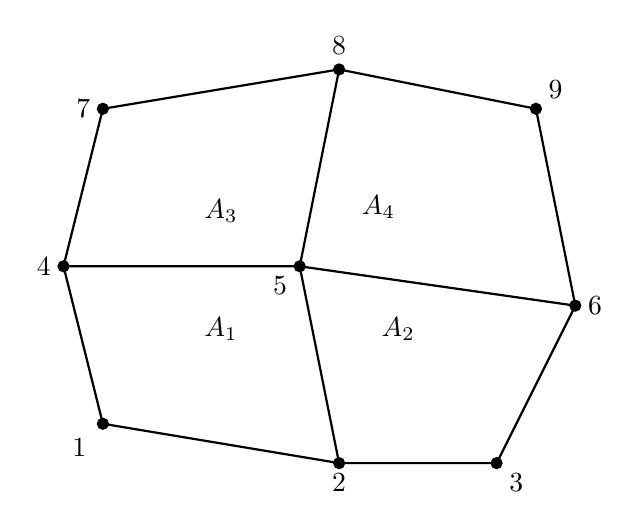
\begin{tikzpicture}
%\draw[fill=gray!5,gray!5](0,0) rectangle (9,7);
%\draw[step=0.5cm,gray,very thin] (0,0) grid (9,7); %background grid
\draw[thick](1.5,1.5) -- (4.5,1) -- (6.5,1) -- (7.5,3) -- (7,5.5) -- (4.5,6) --(1.5,5.5) -- (1,3.5) -- cycle;  
\draw[thick](4.5,1)--(4,3.5)--(4.5,6);
\draw[thick](1,3.5)--(4,3.5)--(7.5,3);
\draw[black,fill=black] (1.5,1.5) circle (2pt); \node[] at (1.2,1.2){1}; %1
\draw[black,fill=black] (4.5,1)   circle (2pt); \node[] at (4.5,0.75){2}; %2
\draw[black,fill=black] (6.5,1)   circle (2pt); \node[] at (6.75,0.75){3}; %3
\draw[black,fill=black] (1,3.5)   circle (2pt); \node[] at (0.75,3.5){4}; %4
\draw[black,fill=black] (4,3.5)   circle (2pt); \node[] at (3.75,3.25){5}; %5
\draw[black,fill=black] (7.5,3)   circle (2pt); \node[] at (7.75,3){6}; %6
\draw[black,fill=black] (1.5,5.5) circle (2pt); \node[] at (1.25,5.5){7}; %7
\draw[black,fill=black] (4.5,6)   circle (2pt); \node[] at (4.5,6.3){8}; %8
\draw[black,fill=black] (7,5.5)   circle (2pt); \node[] at (7.25,5.75){9}; %9
%\draw[thin,dashed](1,3.5)--(4.5,1)--(7.5,3)--(4.5,6)--cycle;
\node[] at (3,2.7){$A_1$}; %8
\node[] at (5.25,2.7){$A_2$}; %8
\node[] at (5,4.25){$A_4$}; %8
\node[] at (3,4.2){$A_3$}; %8
\end{tikzpicture}
\end{center}
\[
q_5^{(1)} = \frac{1}{4}\sum_{e=1}^4 p_e
\] 

In the codes which rely on the $Q_1 \times P_0$ element, the (elemental) pressure
is simply defined as 
\begin{lstlisting}
p=np.zeros(nel,dtype=np.float64)  
\end{lstlisting}
while the nodal pressure is then defined as\footnote{In virtually all stones $p$
stands for the 'raw' pressure and $q$ stands for its projection onto the velocity mesh.} 
\begin{lstlisting}
q=np.zeros(nnp,dtype=np.float64)  
\end{lstlisting}
The element-to-node algorithm is then simply (in 2D):

\begin{lstlisting}
count=np.zeros(nnp,dtype=np.int32)  
for iel in range(0,nel):
    q[icon[0,iel]]+=p[iel]
    q[icon[1,iel]]+=p[iel]
    q[icon[2,iel]]+=p[iel]
    q[icon[3,iel]]+=p[iel]
    count[icon[0,iel]]+=1
    count[icon[1,iel]]+=1
    count[icon[2,iel]]+=1
    count[icon[3,iel]]+=1
q=q/count
\end{lstlisting}



%----------------------------------------------------------------------
\paragraph{Schemes 2,3}.

{\sl Schemes 2,3} are very similar and are presented in Sani et al (1981) \cite{sagl81a,sagl81b}.
Scheme 2 uses the areas of the surrounding elements as weights for the arithmetic averaging
while scheme 3 uses the area of the triangles:

\begin{multicols}{2}

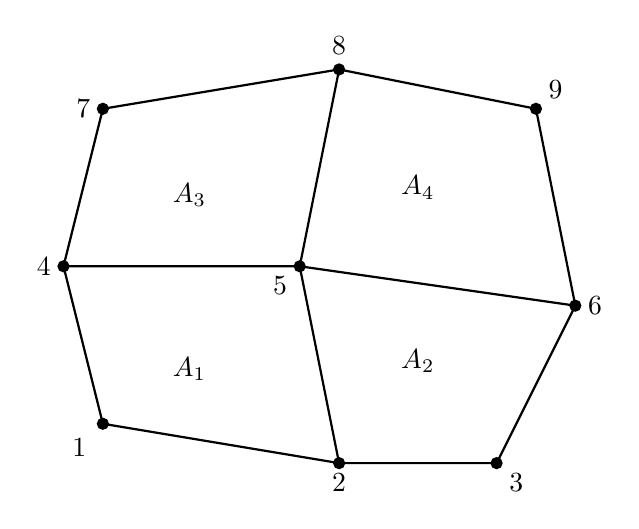
\begin{tikzpicture}
%\draw[fill=gray!5,gray!5](0,0) rectangle (9,7);
%\draw[step=0.5cm,gray,very thin] (0,0) grid (9,7); %background grid
\draw[thick](1.5,1.5) -- (4.5,1) -- (6.5,1) -- (7.5,3) -- (7,5.5) -- (4.5,6) --(1.5,5.5) -- (1,3.5) -- cycle;  
\draw[thick](4.5,1)--(4,3.5)--(4.5,6);
\draw[thick](1,3.5)--(4,3.5)--(7.5,3);
\draw[black,fill=black] (1.5,1.5) circle (2pt); \node[] at (1.2,1.2){1}; %1
\draw[black,fill=black] (4.5,1)   circle (2pt); \node[] at (4.5,0.75){2}; %2
\draw[black,fill=black] (6.5,1)   circle (2pt); \node[] at (6.75,0.75){3}; %3
\draw[black,fill=black] (1,3.5)   circle (2pt); \node[] at (0.75,3.5){4}; %4
\draw[black,fill=black] (4,3.5)   circle (2pt); \node[] at (3.75,3.25){5}; %5
\draw[black,fill=black] (7.5,3)   circle (2pt); \node[] at (7.75,3){6}; %6
\draw[black,fill=black] (1.5,5.5) circle (2pt); \node[] at (1.25,5.5){7}; %7
\draw[black,fill=black] (4.5,6)   circle (2pt); \node[] at (4.5,6.3){8}; %8
\draw[black,fill=black] (7,5.5)   circle (2pt); \node[] at (7.25,5.75){9}; %9
\node[] at (2.6,2.2){$A_1$}; %8
\node[] at (5.5,2.3){$A_2$}; %8
\node[] at (2.6,4.4){$A_3$}; %8
\node[] at (5.5,4.5){$A_4$}; %8
\end{tikzpicture}

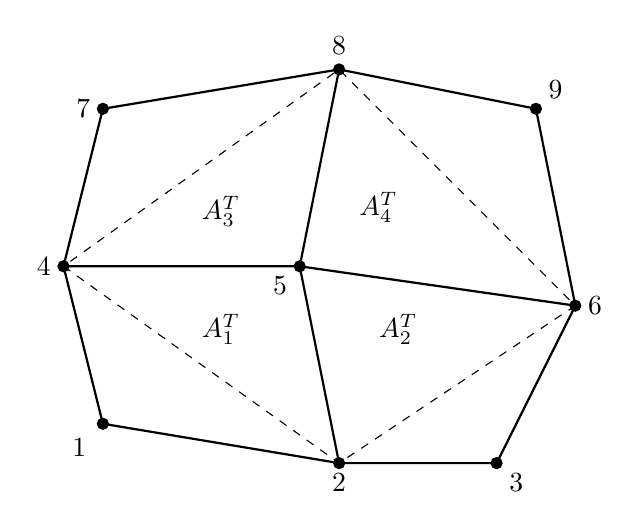
\begin{tikzpicture}
%\draw[fill=gray!5,gray!5](0,0) rectangle (9,7);
%\draw[step=0.5cm,gray,very thin] (0,0) grid (9,7); %background grid
\draw[thick](1.5,1.5) -- (4.5,1) -- (6.5,1) -- (7.5,3) -- (7,5.5) -- (4.5,6) --(1.5,5.5) -- (1,3.5) -- cycle;  
\draw[thick](4.5,1)--(4,3.5)--(4.5,6);
\draw[thick](1,3.5)--(4,3.5)--(7.5,3);
\draw[black,fill=black] (1.5,1.5) circle (2pt); \node[] at (1.2,1.2){1}; %1
\draw[black,fill=black] (4.5,1)   circle (2pt); \node[] at (4.5,0.75){2}; %2
\draw[black,fill=black] (6.5,1)   circle (2pt); \node[] at (6.75,0.75){3}; %3
\draw[black,fill=black] (1,3.5)   circle (2pt); \node[] at (0.75,3.5){4}; %4
\draw[black,fill=black] (4,3.5)   circle (2pt); \node[] at (3.75,3.25){5}; %5
\draw[black,fill=black] (7.5,3)   circle (2pt); \node[] at (7.75,3){6}; %6
\draw[black,fill=black] (1.5,5.5) circle (2pt); \node[] at (1.25,5.5){7}; %7
\draw[black,fill=black] (4.5,6)   circle (2pt); \node[] at (4.5,6.3){8}; %8
\draw[black,fill=black] (7,5.5)   circle (2pt); \node[] at (7.25,5.75){9}; %9
\draw[thin,dashed](1,3.5)--(4.5,1)--(7.5,3)--(4.5,6)--cycle;
\node[] at (3,2.7){$A_1^T$}; %8
\node[] at (5.25,2.7){$A_2^T$}; %8
\node[] at (5,4.25){$A_4^T$}; %8
\node[] at (3,4.2){$A_3^T$}; %8
\end{tikzpicture}

\end{multicols}




\[
q_5^{(2)} = \frac{\sum\limits_{e=1}^4 A_e p_e}{\sum\limits_{e=1}^4 A_e}
\qquad
\qquad
q_5^{(3)} = \frac{\sum\limits_{e=1}^4 A_e^T p_e}{\sum\limits_{e=1}^4 A_e^T}
\] 


\begin{remark} Although Schemes 1,2,3 are similar, scheme 1 is the simplest and fastest
to implement since the areas of neighbouring elements/triangles are not needed.
\end{remark}

\begin{remark} 
Schemes 1,2,3 are identical if all elements are rectangles of identical dimensions.
\end{remark}




%----------------------------------------------------------------------
\paragraph{Scheme 4} This scheme has been designed by me. 
It resembles the last three ones, but the weighing is in this case different.

Let us consider a 1D problem:
\begin{center}
\includegraphics[width=0.5\linewidth]{images/pressure_smoothing/newalgo.png}
\end{center}

Elemental pressures $p_1$ and $p_2$ corresponding to elements 1 and 2 respectively are known at
locations $x_1$ and $x_2$. The two elements have a different size, characterised in this case
by the distances $d_1$ and $d_2$ to their common edge.

The equation of the line passing through points $(x_1,p_1)$ and $(x_2,p_2)$ is 
\[
p(x)=\frac{p_2-p_1}{x_2-x_1}(x-x_1)+p_1
\]
The $x$ coordinate of the common edge is given by $x=x_1+d_1/2$, 
and since $x_2-x_1=(d_1+d_2)/2$, the 
pressure at this location writes:
\[
p(x_M)= \frac{p_2-p_1}{d_1+d_2}d_1+p_1 = \frac{\frac{p_1}{d_1} + \frac{p_2}{d_2}}{\frac{1}{d_1} + \frac{1}{d_2}}
\]
Extrapolating this formula to 2D, $d_1$ and $d_2$ are in fact the element volumes, so that
\[
q_5^{(4)} = 
\frac{\sum\limits_{j=1}^4 \frac{p_j^e}{A_j^e}}{\sum\limits_{j=1}^4 \frac{1}{A_j^e}}
=
\frac{
\frac{p_1^e}{A_1^e}+
\frac{p_2^e}{A_2^e}+
\frac{p_3^e}{A_3^e}+
\frac{p_4^e}{A_4^e}
}{
\frac{1}{A_1^e}+
\frac{1}{A_2^e}+
\frac{1}{A_3^e}+
\frac{1}{A_4^e}
}\]

There remains a problem, due to the presence of the boundary nodes for which 
the sums present in the above equation do not run up to 4. A boundary
node only has three neighbours and a corner node only two. Additional measures
are required for these nodes. 

\begin{center}
\includegraphics[width=0.5\linewidth]{images/pressure_smoothing/newalgo_corner.png}
\end{center}

The pressure value $p_N$ is obtained as follows:
\[
q_N = \frac{ 
 \frac{p_2^e}   {A_2^e}
+\frac{p_3^e}   {A_3^e}
+\frac{p_{2'}^e}{A_{2'}^e}
+\frac{p_{3'}^e}{A_{3'}^e}
}{
 \frac{1}{A_2^e}
+\frac{1}{A_3^e}
+\frac{1}{A_{2'}^e}
+\frac{1}{A_{3'}^e}
}
\]
The areas and pressures of the mirrored elements 2' and 3' are extrapolated from the areas of elements 2 and 6, and 3 and 7 respectively. 
Likewise the pressure $p_M$ at the corner node is obtained through the pressures of its surrounding elements.


%------------------------------------------------------------------------------
\paragraph{Scheme 5 - Least squares} This scheme is presented (among other places) in Lee et al (1979)
\cite{legs79}. 
Let us start from the patch of 4 $Q_1$ elements counting 9 nodes: 

\begin{center}
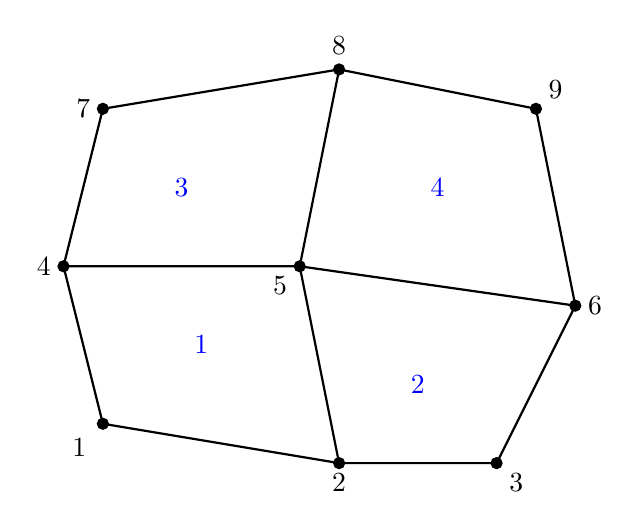
\begin{tikzpicture}
%\draw[fill=gray!5,gray!5](0,0) rectangle (9,7);
%\draw[step=0.5cm,gray,very thin] (0,0) grid (9,7); %background grid
\draw[thick](1.5,1.5) -- (4.5,1) -- (6.5,1) -- (7.5,3) -- (7,5.5) -- (4.5,6) --(1.5,5.5) -- (1,3.5) -- cycle;  
\draw[thick](4.5,1)--(4,3.5)--(4.5,6);
\draw[thick](1,3.5)--(4,3.5)--(7.5,3);

\node[] at (2.75,2.5) {\color{blue}1};
\node[] at (5.5,2) {\color{blue}2};
\node[] at (2.5,4.5) {\color{blue}3};
\node[] at (5.75,4.5) {\color{blue}4};

\draw[black,fill=black] (1.5,1.5) circle (2pt); \node[] at (1.2,1.2){1}; %1
\draw[black,fill=black] (4.5,1)   circle (2pt); \node[] at (4.5,0.75){2}; %2
\draw[black,fill=black] (6.5,1)   circle (2pt); \node[] at (6.75,0.75){3}; %3
\draw[black,fill=black] (1,3.5)   circle (2pt); \node[] at (0.75,3.5){4}; %4
\draw[black,fill=black] (4,3.5)   circle (2pt); \node[] at (3.75,3.25){5}; %5
\draw[black,fill=black] (7.5,3)   circle (2pt); \node[] at (7.75,3){6}; %6
\draw[black,fill=black] (1.5,5.5) circle (2pt); \node[] at (1.25,5.5){7}; %7
\draw[black,fill=black] (4.5,6)   circle (2pt); \node[] at (4.5,6.3){8}; %8
\draw[black,fill=black] (7,5.5)   circle (2pt); \node[] at (7.25,5.75){9}; %9

\end{tikzpicture}
\end{center}



We are looking for a field $q$ living on the nodes.
We build the quantity
\[
J=\iint_\Omega (q-p)^2 dV
\]
where $p$ is the elemental field. To make things clearer we split the integral into 
the sum of elemental integrals:
\[
J=
\iint_{\Omega_1} (q(x,y)-p_1)^2 dV+
\iint_{\Omega_2} (q(x,y)-p_2)^2 dV+
\iint_{\Omega_3} (q(x,y)-p_3)^2 dV+
\iint_{\Omega_4} (q(x,y)-p_4)^2 dV
\]
Inside each element the field $q(x,y)$ is given by a bilinear interpolation so that:
\begin{eqnarray}
J
&=& \iint_{\Omega_1} (N_1(x,y) q_1 + N_2(x,y)q_2 + N_5(x,y)q_5 + N_4(x,y)q_4 -p_1)^2 dV \nn\\
&+& \iint_{\Omega_2} (N_2(x,y) q_2 + N_3(x,y)q_3 + N_6(x,y)q_6 + N_5(x,y)q_5 -p_2)^2 dV \nn\\
&+& \iint_{\Omega_3} (N_4(x,y) q_4 + N_5(x,y)q_5 + N_8(x,y)q_8 + N_7(x,y)q_7 -p_3)^2 dV \nn\\
&+& \iint_{\Omega_4} (N_5(x,y) q_5 + N_6(x,y)q_6 + N_9(x,y)q_9 + N_8(x,y)q_8 -p_4)^2 dV 
\end{eqnarray}
where the $N_i$ functions are the shape functions (unusually expressed in $x,y$ coordinates).
The least square procedure looks for the set of $q_i$ such that 
\[
\frac{\partial J}{\partial q_i} =0 \qquad \forall i=1,...9
\]
and this yields 9 equations/constraints for 9 unknowns.
\begin{eqnarray}
\frac{\partial J}{\partial q_1} 
&=& \iint_{\Omega_1} 2 (N_1(x,y) q_1 + N_2(x,y)q_2 + N_5(x,y)q_5 + N_4(x,y)q_4 -p_1) N_1(x,y) dV \nn\\
\frac{\partial J}{\partial q_2}
&=& \iint_{\Omega_1} 2(N_1(x,y) q_1 + N_2(x,y)q_2 + N_5(x,y)q_5 + N_4(x,y)q_4 -p_1) N_2(x,y) dV \nn\\
&+& \iint_{\Omega_2} 2(N_2(x,y) q_2 + N_3(x,y)q_3 + N_6(x,y)q_6 + N_5(x,y)q_5 -p_2) N_2(x,y) dV \nn\\
\frac{\partial J}{\partial q_3}
&=& \iint_{\Omega_2} 2(N_2(x,y) q_2 + N_3(x,y)q_3 + N_6(x,y)q_6 + N_5(x,y)q_5 -p_2) N_3(x,y) dV \nn\\
\frac{\partial J}{\partial q_4}
&=& \iint_{\Omega_1} 2(N_1(x,y) q_1 + N_2(x,y)q_2 + N_5(x,y)q_5 + N_4(x,y)q_4 -p_1) N_4(x,y) dV \nn\\
&+& \iint_{\Omega_3} 2(N_4(x,y) q_4 + N_5(x,y)q_5 + N_8(x,y)q_8 + N_7(x,y)q_7 -p_3) N_4(x,y) dV \nn\\
\frac{\partial J}{\partial q_5}
&=& \iint_{\Omega_1} 2(N_1(x,y) q_1 + N_2(x,y)q_2 + N_5(x,y)q_5 + N_4(x,y)q_4 -p_1) N_5(x,y) dV \nn\\
&+& \iint_{\Omega_2} 2(N_2(x,y) q_2 + N_3(x,y)q_3 + N_6(x,y)q_6 + N_5(x,y)q_5 -p_2) N_5(x,y) dV \nn\\
&+& \iint_{\Omega_3} 2(N_4(x,y) q_4 + N_5(x,y)q_5 + N_8(x,y)q_8 + N_7(x,y)q_7 -p_3) N_5(x,y) dV \nn\\
&+& \iint_{\Omega_4} 2(N_5(x,y) q_5 + N_6(x,y)q_6 + N_9(x,y)q_9 + N_8(x,y)q_8 -p_4) N_5(x,y) dV \nn\\
\frac{\partial J}{\partial q_6}
&=& \iint_{\Omega_2} 2(N_2(x,y) q_2 + N_3(x,y)q_3 + N_6(x,y)q_6 + N_5(x,y)q_5 -p_2) N_6(x,y) dV \nn\\
&+& \iint_{\Omega_4} 2(N_5(x,y) q_5 + N_6(x,y)q_6 + N_9(x,y)q_9 + N_8(x,y)q_8 -p_4) N_6(x,y) dV \nn\\
\frac{\partial J}{\partial q_7}
&=& \iint_{\Omega_3} 2(N_4(x,y) q_4 + N_5(x,y)q_5 + N_8(x,y)q_8 + N_7(x,y)q_7 -p_3) N_7(x,y) dV \nn\\
\frac{\partial J}{\partial q_8}
&=& \iint_{\Omega_3} 2(N_4(x,y) q_4 + N_5(x,y)q_5 + N_8(x,y)q_8 + N_7(x,y)q_7 -p_3) N_8(x,y)dV \nn\\
&+& \iint_{\Omega_4} 2(N_5(x,y) q_5 + N_6(x,y)q_6 + N_9(x,y)q_9 + N_8(x,y)q_8 -p_4) N_8(x,y)dV \nn\\ 
\frac{\partial J}{\partial q_9}
&=& \iint_{\Omega_4} 2(N_5(x,y) q_5 + N_6(x,y)q_6 + N_9(x,y)q_9 + N_8(x,y)q_8 -p_4) N_9(x,y)dV 
\end{eqnarray}
The factor 2 are removed and the terms $\int p_i N_j $ are known so they end up in the right hand side.

\begin{eqnarray}
 \iint_{\Omega_1} (N_1N_1 q_1 + N_1N_2 q_2 + N_1N_5q_5 + N_1N_4q_4) dV &=& \iint_{\Omega_1} p_1 N_1 dV \nn\\
 \iint_{\Omega_1} (N_2 N_1  q_1 + N_2 N_2q_2 + N_2 N_5q_5 + N_2 N_4q_4)  dV \nn\\
+\iint_{\Omega_2} (N_2 N_2 q_2 + N_3 N_2 q_3 + N_6 N_2 q_6 + N_5 N_2 q_5) dV 
&=& \iint_{\Omega_1} p_1N_2 dV + \iint_{\Omega_2}  p_2 N_2 dV \nn\\
\nn\\
\dots &=& \dots \nn\\
\nn\\
 \iint_{\Omega_4} (N_9N_5 q_5 + N_9N_6q_6 + N_9N_9q_9 + N_9N_8q_8) dV &=&  \iint_{\Omega_4} p_4 N_9 dV 
\end{eqnarray}

The mass matrices corresponding to the four elements are 
\[
{\bm M}_1 = \int_{\Omega_1} \left( \begin{array}{cccc}
N_1 N_1 & N_1 N_2 & N_1 N_5 & N_1 N_4 \\
N_2 N_1 & N_2 N_2 & N_2 N_5 & N_2 N_4 \\
N_5 N_1 & N_5 N_2 & N_5 N_5 & N_5 N_4 \\
N_4 N_1 & N_4 N_2 & N_4 N_5 & N_4 N_4 
\end{array}\right) dV
\qquad
{\bm M}_2 = \int_{\Omega_2} \left( \begin{array}{cccc}
N_2 N_2 & N_2 N_3 & N_2 N_6 & N_2 N_5 \\
N_3 N_2 & N_3 N_3 & N_3 N_6 & N_3 N_5 \\
N_6 N_2 & N_6 N_3 & N_6 N_6 & N_6 N_5 \\
N_5 N_2 & N_5 N_3 & N_5 N_6 & N_5 N_5 
\end{array}\right) dV
\]
\[
{\bm M}_3 = \int_{\Omega_3} \left( \begin{array}{cccc}
N_4 N_4 & N_4 N_5 & N_4 N_8 & N_4 N_7 \\
N_5 N_4 & N_5 N_5 & N_5 N_8 & N_5 N_7 \\
N_8 N_4 & N_8 N_5 & N_8 N_8 & N_8 N_7 \\
N_7 N_4 & N_7 N_5 & N_7 N_8 & N_7 N_7 
\end{array}\right) dV
\qquad
{\bm M}_4 = \int_{\Omega_4} \left( \begin{array}{cccc}
N_5 N_5 & N_5 N_6 & N_5 N_9 & N_5 N_8 \\
N_6 N_5 & N_6 N_6 & N_6 N_9 & N_6 N_8 \\
N_9 N_5 & N_9 N_6 & N_9 N_9 & N_9 N_8 \\
N_8 N_5 & N_8 N_6 & N_8 N_9 & N_8 N_8 
\end{array}\right) dV
\]
so that the 9 equations above are actually the result of the assembly process of these four 
elemental systems:
\[
\left( \iint_{\Omega_e} \vec{N}^T\vec{N} dV \right) \cdot \vec{q}_e = \iint_{\Omega_i} \vec{N}^T p_e dV 
\qquad\qquad e=1,2,3,4
\]


%------------------------------------------------------------------------------
\paragraph{Scheme 6 - Consistent pressure recovery}

The is the method presented in Zienkiewicz \& Nakazawa (1982) \cite{zina82}. In the second part 
of this publication the authors wish to establish a simple and effective numerical method to calculate 
variables eliminated by the penalisation process. 
The method involves an additional finite element solution for the nodal pressures using 
the same finite element basis and numerical quadrature as used for the velocity.

Let us start with\footnote{I here voluntarily use $q$ instead of $p$}:
\[
q = -\lambda \vec\nabla\cdot \vec\upnu
\]
We are going to treat this equation as any other PDE in the context of the FE method, i.e. 
we are going to establish its weak form. 
We assume that the pressure is given inside an element by
\[
q(x,y) = \sum_{i=1}^4 N_i(x,y) q_i = \vec{N} \cdot \vec{q}
\]
and the velocity:
\[
\vec\upnu = (u,v) 
\qquad 
\qquad 
u(x,y)  = \sum_{i=1}^4 N_i(x,y) u_i
\qquad 
\qquad 
v(x,y)  = \sum_{i=1}^4 N_i(x,y) v_i
\]
where the $N_i$ are the $Q_1$ shape functions and $q_i$ are the sought after nodal values. 
We multiply the equation above by a $Q_1$ shape function $N_i$ and integrate over the whole domain:
\[
\iint_\Omega N_i(x,y) q(x,y) \; dxdy = -\lambda \iint_\Omega N_i \vec\nabla\cdot \vec\upnu  \; dx dy
\]
As before we now focus on the above expression inside a single element $e$:
\[
\iint_{\Omega_e} N_i(x,y) q(x,y) \; dxdy = -\lambda \iint_{\Omega_e} N_i \vec\nabla\cdot \vec\upnu \; dx dy
\]
After $N_i \rightarrow \vec{N}=(N_1,N_2,N_3,N_4)^T$, the left hand side term becomes:
\[
\iint _{\Omega_e} \vec{N}^T q(x,y) \; dxdy 
=
\iint _{\Omega_e} \vec{N}^T \vec{N} \cdot \vec{q} \; dxdy 
=
\left(\underbrace{\iint _{\Omega_e} \vec{N}^T \vec{N} dxdy}_{{\bm M}_e} \right) \cdot \vec{q}  
\]
where ${\bm M}_e$ is the elemental mass matrix.
We now turn to the right hand side. We have
\[
\vec\nabla\cdot \vec\upnu
= \frac{\partial u}{\partial x}+\frac{\partial v}{\partial y}
= \sum_i \frac{\partial N_i}{\partial x} u_i + \sum_i \frac{\partial N_i}{\partial y} v_i 
\]
We here too define $\vec{V}_e=(u_1,v_1,u_2,v_2,u_3,v_3,u_4,v_4)^T$ so that 

\begin{eqnarray}
&& \iint_{\Omega_e} \vec{N} {\vec \nabla}\cdot {\vec \upnu} \; d\Omega \nn\\
&=& \iint_{\Omega_e} \vec{N}^T \sum_{i=1}^{4} 
\left( \frac{\partial N_i}{\partial x} u_i + \frac{\partial N_i}{\partial y} v_i 
\right)  
d\Omega \nonumber\\
&=& 
\iint_{\Omega_e} 
\left(
\begin{array}{c}
N_1 \left(
\sum\limits_{i=1}^{4} \frac{\partial N_i}{\partial x} u_i +
\sum\limits_{i=1}^{4} \frac{\partial N_i}{\partial y} v_i \right) \\
N_2 \left(
\sum\limits_{i=1}^{4} \frac{\partial N_i}{\partial x} u_i +
\sum\limits_{i=1}^{4} \frac{\partial N_i}{\partial y} v_i \right) \\
N_3 \left(
\sum\limits_{i=1}^{4} \frac{\partial N_i}{\partial x} u_i +
\sum\limits_{i=1}^{4} \frac{\partial N_i}{\partial y} v_i \right) \\
N_4 \left(
\sum\limits_{i=1}^{4} \frac{\partial N_i}{\partial x} u_i +
\sum\limits_{i=1}^{4} \frac{\partial N_i}{\partial y} v_i \right) 
\end{array}
\right) d \Omega \nonumber \\  %%%%%%%%%%%%%%%%%%%%%%%%%%
&=& 
\int_{\Omega_e} 
\left(
\begin{array}{ccc}
{N}_1& {N}_1 &  0 \\\\
{N}_2& {N}_2 &  0 \\\\
{N}_3& {N}_3 &  0 \\\\
{N}_4& {N}_4 &  0 
\end{array}
\right)
\cdot
\left(
\begin{array}{c}
\sum\limits_i \frac{\partial N_i}{\partial x} u_i \\ \\
\sum\limits_i \frac{\partial N_i}{\partial y} v_i \\ \\
\sum\limits_i (\frac{\partial N_i}{\partial y} u_i\! +\! \frac{\partial N_i}{\partial x} v_i) 
\end{array}
\right)
\; d\Omega \nonumber\\ %%%%%%%%%%%%%%%%%%%%%%%%%%
&=& 
\int_{\Omega_e} 
\underbrace{
\left(
\begin{array}{cccccc}
{N}_1 & {N}_1 &  0 \\
{N}_2 & {N}_2 &  0 \\
{N}_3 & {N}_3 &  0 \\
{N}_4 & {N}_4 &  0 
\end{array}
\right)
}_{{\bm N}}
\cdot
\underbrace{
\left(\begin{array}{cccccccc}
\partial_x N_1 & 0 &  
\partial_x N_2 & 0 &  
\partial_x N_3 & 0 &  
\partial_x N_4 & 0 \\ \\
0 & \partial_y N_1 &   
0 & \partial_y N_2 &   
0 & \partial_y N_3 &   
0 & \partial_y N_4 \\ \\
\partial_y N_1 & \partial_x N_1 &  
\partial_y N_2 & \partial_x N_2 &  
\partial_y N_3 & \partial_x N_3 &  
\partial_y N_4 & \partial_x N_4 
\end{array}\right)}_{{\bm B}}
\cdot \vec{V}_e
\; d\Omega  \nonumber \\
&=& 
\left(\int_{\Omega_e} {\bm N} \cdot {\bm B} \; d\Omega \right) \cdot \vec{V}_e \nonumber\\
&=& -\G_e^T \cdot {\vec V}_e
\end{eqnarray}

After assembly we arrive at
\[
{\bm M} \cdot \vec{q} = \lambda \G^T \cdot {\vec V} 
\qquad
\text{with}
\qquad
\G_e = -\int_{\Omega_e} {\bm N} \cdot {\bm B} \; d\Omega
\]
where ${\bm M}$ is the global mass matrix, $\vec{q}$ the vector of all 
nodal pressures, $\G$ the discrete gradient matrix and $\vec{V}$
the (velocity) solution vector. 
The system can be easily solved since the mass matrix is a friendly matrix.
The vector ${\vec q}$ contains the nodal pressure values directly, with 
no need for a smoothing scheme! 

\begin{remark}
Very importantly, the mass matrix ${\bm M}$ is to be evaluated at the full integration points, 
while the constraint part (the right hand side of the equation) is to be evaluated at 
the reduced integration point, i.e. in the middle of the element.  
\end{remark}

\begin{remark}
As noted in \cite{zina82}, it is interesting to note that when linear elements are used 
and the lumped matrices are used for the ${\bm M}$ the resulting algebraic equation is identical 
to the smoothing scheme 1 only if a uniform square finite element 
mesh is used. In this respect this method is expected to yield different results when elements 
are not square or even rectangular.
\end{remark}

\begin{remark}
The third column of the matrix ${\bm N}$
and the last line of the ${\bm B}$ matrix could be removed altogether.
If your code is based on the mixed formulation, then you already 
have built matrix $\G$ so you can easily re-use this piece of code 
to compute $\G$ again, this time with a reduced integration quadrature.
If you are using the penalty formulation then you need to program 
all from scratch and then simply do away with these unnecessary terms, or 
you can direcly build the rhs as $\int_{\Omega_e} \vec{N}^T p_e$ (assuming
you have previously computed the pressure in the middle of each element 
by means of $p=-\lambda\vec\nabla\cdot\vec\upnu$).
\end{remark}

\begin{remark}
This  scheme is identical to the least square scheme!
\end{remark}


%--------------------------------------------------------------
\paragraph{Scheme 7}

Same as scheme 6, but with lumped mass matrix.  


%--------------------------------------------------------------
\paragraph{Scheme 8 - bilinear interpolation} Let us assume that the centers of the 
four elements make a $Q_1$ quadrilateral element, as shown on this figure:


\begin{center}
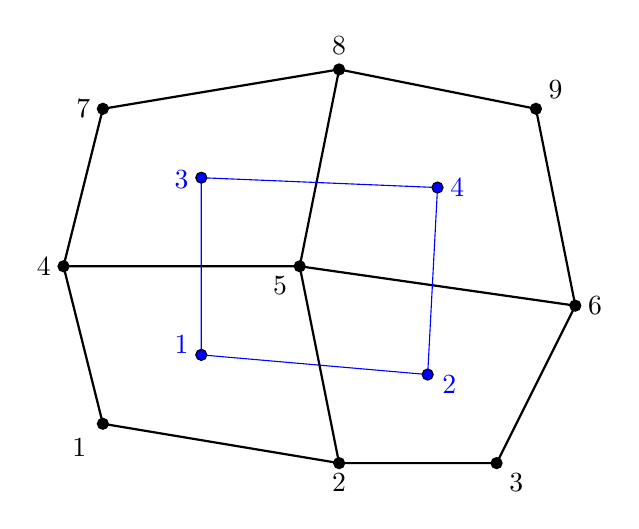
\begin{tikzpicture}
%\draw[fill=gray!5,gray!5](0,0) rectangle (9,7);
%\draw[step=0.5cm,gray,very thin] (0,0) grid (9,7); %background grid
\draw[thick](1.5,1.5) -- (4.5,1) -- (6.5,1) -- (7.5,3) -- (7,5.5) -- (4.5,6) --(1.5,5.5) -- (1,3.5) -- cycle;  
\draw[thick](4.5,1)--(4,3.5)--(4.5,6);
\draw[thick](1,3.5)--(4,3.5)--(7.5,3);

\draw[black,fill=blue] (2.75,2.375) circle (2pt); 
\node[] at (2.5,2.5) {\color{blue}1};
\draw[black,fill=blue] (5.625,2.125) circle (2pt); 
\node[] at (5.9,2) {\color{blue}2};
\draw[black,fill=blue] (5.75,4.5) circle (2pt); 
\node[] at (2.5,4.6) {\color{blue}3};
\draw[black,fill=blue] (2.75,4.625) circle (2pt); 
\node[] at (6,4.5) {\color{blue}4};

\draw[black,fill=black] (1.5,1.5) circle (2pt); \node[] at (1.2,1.2){1}; %1
\draw[black,fill=black] (4.5,1)   circle (2pt); \node[] at (4.5,0.75){2}; %2
\draw[black,fill=black] (6.5,1)   circle (2pt); \node[] at (6.75,0.75){3}; %3
\draw[black,fill=black] (1,3.5)   circle (2pt); \node[] at (0.75,3.5){4}; %4
\draw[black,fill=black] (4,3.5)   circle (2pt); \node[] at (3.75,3.25){5}; %5
\draw[black,fill=black] (7.5,3)   circle (2pt); \node[] at (7.75,3){6}; %6
\draw[black,fill=black] (1.5,5.5) circle (2pt); \node[] at (1.25,5.5){7}; %7
\draw[black,fill=black] (4.5,6)   circle (2pt); \node[] at (4.5,6.3){8}; %8
\draw[black,fill=black] (7,5.5)   circle (2pt); \node[] at (7.25,5.75){9}; %9

\draw[blue](2.75,2.375)--(5.625,2.125)--(5.75,4.5)--(2.75,4.625)--cycle;
\end{tikzpicture}
\end{center}




The values at the corners are $p_1$,
$p_2$, $p_3$ and $p_4$. Assuming that the pressure inside this element can be represented 
by a bilinear field, we have 
\[
p(x,y)= a+ bx +cy +dxy
\]
where the coefficients will be determined by ensuring that $p(x_i,y_i)=p_i$ for $i=1,2,3,4$, or:
\begin{eqnarray}
a+bx_1+cy_1+dx_1y_1 &=& p_1 \\
a+bx_2+cy_2+dx_2y_2 &=& p_2 \\
a+bx_3+cy_3+dx_3y_3 &=& p_3 \\
a+bx_4+cy_4+dx_4y_4 &=& p_4 
\end{eqnarray}
i.e.
\[
\left(
\begin{array}{cccc}
1 & x_1 & y_1 & x_1y_1 \\
1 & x_2 & y_2 & x_2y_2 \\
1 & x_3 & y_3 & x_3y_3 \\
1 & x_4 & y_4 & x_4y_4
\end{array}
\right)\cdot
\left(
\begin{array}{c}
a \\b\\c\\d
\end{array}
\right)
=
\left(
\begin{array}{c}
p_1\\p_2\\p_3\\p_4
\end{array}
\right)
\]

There remains an issue with nodes which are on the boundaries of the domain. These are of course not 
'surrounded' by four pressure values so the above algorithm does not apply directly. However, looking 
at the above figure, and assuming that node 1 is a lower left corner of a 2D domain, we can use the 
bilinear interpolation based on elements 1,2,3,4 to extrapolate a nodal pressure value at node 1. 
The same would apply for nodes 2 and 4 for example. 

\begin{remark}
This scheme is not applicable to quadtree-based meshed.
\end{remark}





\newpage %-----------------------------------------------------------------------------------------
\subsection{Pressure scaling \label{pscaling}} \index{pressure scaling}

As perfectly explained in the step 32 of deal.ii\footnote{https://www.dealii.org/9.0.0/doxygen/deal.II/step\_32.html},
we often need to scale the $\G$ term since it is many orders of magnitude smaller than $\K$, 
which introduces large inaccuracies in the solving process to the point that the solution is nonsensical. 
This scaling coefficient is $\eta/L$. 
We start from 
\[
\left(
\begin{array}{cc}
\K & \G \\ \G^T & 0 
\end{array}
\right)
\cdot
\left(
\begin{array}{c}
{\cal V} \\ {\cal P}
\end{array}
\right)
=
\left(
\begin{array}{c}
 f \\ h
\end{array}
\right)
\]
and introduce the scaling coefficient as follows (which in fact does not alter the solution at all):
\[
\left(
\begin{array}{cc}
\K & \frac{\eta}{L}\G \\ \frac{\eta}{L}\G^T & 0 
\end{array}
\right)
\cdot
\left(
\begin{array}{c}
{\cal V} \\\frac{L}{\eta} {\cal P}
\end{array}
\right)
=
\left(
\begin{array}{c}
 f \\ \frac{\eta}{L} h
\end{array}
\right)
\]
We then end up with the modified Stokes system:
\[
\left(
\begin{array}{cc}
\K & \underline{\G} \\ \underline{\G}^T & 0 
\end{array}
\right)
\cdot
\left(
\begin{array}{c}
{\cal V} \\ \underline{\cal P}
\end{array}
\right)
=
\left(
\begin{array}{c}
 f \\ \underline{h}
\end{array}
\right)
\]
where 
\[
\underline{\G}=\frac{\eta}{L}\G
\quad\quad
\quad\quad
\underline{\cal P}=\frac{L}{\eta} {\cal P}
\quad\quad
\quad\quad
\underline{h}=\frac{\eta}{L}h
\]
After the solve phase, we recover the real pressure with ${\cal P}=\frac{\eta}{L}{\cal P}'$.





 %--------------------------
\newpage %-----------------------------------------------------------------------------------------
\subsection{Pressure normalisation, nullspace\label{ss_pnorm}} 
%..................................................
\subsubsection{Basic idea and naive implementation}

When Dirichlet boundary conditions are imposed everywhere on the boundary, 
pressure is only present by its gradient in 
the equations. It is thus determined up to an arbitrary constant (one speaks then 
of a nullspace of size 1).  \index{nullspace}
In such a case, one commonly impose the average of the pressure over the whole domain or on 
a subset of the boundary 
to have a zero average, i.e.
\begin{equation}
\int_\Omega p dV = 0
\end{equation}
Another possibility is to impose the pressure value at a single node. 

Let us assume for example that we are using $Q_1 \times P_0$ elements. Then the pressure is constant 
inside each element. 
The integral above becomes:
\begin{equation}
\int_\Omega p dV = 
\sum_e  \int_{\Omega_e} p dV = 
\sum_e  p_e \int_{\Omega_e} dV = 
\sum_e  p_e A_e = 0
\end{equation}
where the sum runs over all elements $e$ of area $A_e$.
This can be rewritten 
\[
\LLL^T \cdot \vec{\cal P}=0
\] 
and it is a constraint on the pressure solution which couples {\it all} pressure dofs. 
As we have seen before \ref{XXX}, we can associate to it a 
Lagrange multiplier $\lambda$ so that we must solve the modified Stokes system:
\[
\left(
\begin{array}{ccc}
\K & \G & 0\\ 
\G^T & 0 & \LLL \\
0 & \LLL^T & 0
\end{array}
\right)
\cdot
\left(
\begin{array}{c}
\vec{\cal V} \\ \vec{\cal P} \\ \lambda
\end{array}
\right)
=
\left(
\begin{array}{c}
\vec{f} \\ \vec{h} \\ 0
\end{array}
\right)
\]
When higher order spaces are used for pressure (continuous or discontinuous)
one must then carry out the above integration numerically by means of (usually)
a Gauss-Legendre quadrature.

Although valid, this approach has one main disadvantage: it makes the Stokes matrix larger (although
marginally so -- only one row and column are added), but more importantly it prevents the use of some
of the solving strategies of Section \ref{sec:solvers}.


%..................................................
\subsubsection{Implementation -- the real deal}

The idea is actually quite simple and requires two steps:
\begin{enumerate}
\item remove the null space by prescribing the pressure at one location and solve the system;
\item post-process the pressure so as to arrive at a pressure field which fulfills the required normalisation (surface, volume, ...)
\end{enumerate}

The reason why it works is as follows: a constant pressure value lies in the null space, so that one can 
add or delete any value to the pressure field without consequence. As such I can choose said constant such that 
the pressure at a given node/element is zero. All other computed pressures are then relative to that one. 
The post-processing step will redistribute a constant value to all pressures (it will shift them up or down)
so that the normalising condition is respected. 





 %----
\newpage %-----------------------------------------------------------------------------------------
\subsection{Solving the Stokes system \label{sec:solvers}} 
Let us start again from the (full) Stokes system:
\begin{equation}
\left(
\begin{array}{cc}
\K & \G \\ \G^T & -\C 
\end{array}
\right)
\cdot
\left(
\begin{array}{c}
\vec{\cal V} \\ \vec{\cal P}
\end{array}
\right)
=
\left(
\begin{array}{c}
\vec{f} \\ \vec{h}
\end{array}
\right)
\label{StokesSyst}
\end{equation}
We need to solve this system in order to obtain the solution, i.e. the $\vec{\cal V}$ 
and $\vec{\cal P}$ vectors. But how? 
Unfortunately, this question is not simple to answer and the appropriate method depends on many 
parameters, but mainly on how big the matrix blocks are and what the condition number of the matrix $\K$ is. 

In what follow I cover:
\begin{itemize}
\item solving when the penalty approach is used
\item the Schur complement approach
\item the FGMRES approach \cite{deit13}
\end{itemize}

\Literature \cite{pasa75,mamo08,fumt11,knke04,kool00,kopo93} \cite{lane18}

Preconditioners \Literature: \cite{seuv10}

%...................................................
\subsubsection{When using the penalty formulation}

In this case we are only solving for 
velocity since pressure is recovered in a post-processing step:
\[
(\K_\eta+\K_\lambda) \cdot \vec {\cal V} = \vec f
\]
 We also know that 
the penalty factor $\lambda$ is many orders of magnitude higher than the viscosity and 
in combination with the use of the $Q_1 \times P_0$ element the resulting matrix 
condition number is very high so that the use of iterative solvers is precluded. 
Indeed codes such as \sopale \cite{full95}, \douar \cite{brtf08}, \fantom \cite{thie11} 
or \sulec \cite{qube11} relying on the penalty formulation all use direct solvers.
The most popular are BLKFCT\footnote{\url{http://dm.unife.it/blkfclt/}}, 
MUMPS\footnote{\url{http://mumps.enseeiht.fr/}}\cite{amdu89,amdl00,amdk01,amgl06,ambl19}, 
PasTiX \cite{herr02},
WSMP\footnote{\url{http://www.research.ibm.com/projects/wsmp}} \cite{GUPTA94ieee,GUPTA09sc-long},
UMFPACK and CHOLMOD\footnote{\url{http://faculty.cse.tamu.edu/davis/suitesparse.html}}
, SuperLU, PARDISO\footnote{\url{https://www.pardiso-project.org/}}
\cite{pardiso-6.0a,pardiso-6.0b,pardiso-6.0c}, or those inside 
PETSc\footnote{\url{https://www.mcs.anl.gov/petsc/}} \ref{petsc-user-ref}.

Braun et al (2008) \cite{brtf08} list the following features of direct solvers:
\begin{itemize}
\item Robust
\item Black-box operation
\item Difficult to parallelize
\item Memory consumption
\item Limited scalability
\end{itemize}

The main advantage of direct solvers is used in this case: They can solve ill-conditioned 
matrices. However memory requirements for the storage of number of nonzeros in the 
Cholesky matrix grow very fast as the number of equations/grid size increases, especially in 3D,
to the point that even modern computers with tens of Gb of RAM cannot deal with a $100^3$ element mesh.
This explains why direct solvers are often used for 2D problems and rarely in 3D with noticeable 
exceptions \cite{thfb08,yahb09,brya10,lobh10,alht11,alht12,alhf13,whbb14,neew18}. 

%...................................................
\subsubsection{Conjugate gradient and the Schur complement approach }


Let us write the above system as two equations:
\begin{eqnarray}
\K \cdot \vec{\cal V} + \G \cdot \vec{\cal P} &=& \vec{f} \\
\G^T \cdot  \vec{\cal V} \quad\quad &=& \vec{h} 
\end{eqnarray}
The first line can be re-written $\vec{\cal V}=\K^{-1}\cdot (\vec{f} - \G \cdot \vec{\cal P})$ and can be inserted in the second:
\begin{equation}
\G^T\cdot \vec{\cal V} =\G^T \cdot  [ \K^{-1} \cdot  (\vec{f} - \G \cdot  \vec{\cal P}) ] = \vec{h} 
\end{equation}
or, 
\begin{mdframed}[backgroundcolor=blue!5]
\begin{equation}
(\G^T \cdot \K^{-1} \cdot \G) \cdot \vec{\cal P} = \G^T \cdot \K^{-1}\cdot \vec{f} - \vec{h} 
\end{equation}
\end{mdframed}
The matrix $\SSS= \G^T \cdot \K^{-1} \cdot \G $ is called the Schur complement. 
\index{general}{Schur Complement} 
It is Symmetric (since $\K$ is symmetric) and  Positive-Definite\footnote{$M$ 
positive definite $\iff$ $x^TMx>0$ $\forall \; x\in \mathbb{R}^n \setminus {\bm 0}$ }
(SPD) \index{general}{SPD} if $Ker({\G})=0$. 
Having solved this equation (we have obtained $\vec{\cal P}$), the velocity can be recovered by solving 
$\K\cdot \vec{\cal V} =\vec{f}- \G \cdot \vec{\cal P}$. 

\begin{remark}
The Schur complement matrix naturally occurs when the Stokes matrix is decompused using 
a LDU block-factorisation. Indeed, we have 
\[
\left(
\begin{array}{cc}
\K & \G \\ 
\G^T & 0
\end{array}
\right)
=
\left(
\begin{array}{cc}
{\bm I} & 0 \\ 
\G^T \cdot \K^{-1} & {\bm I}
\end{array}
\right)
\cdot
\left(
\begin{array}{cc}
\K & 0 \\ 
0 & -\SSS
\end{array}
\right)
\cdot
\left(
\begin{array}{cc}
{\bm I} & \K^{-1} \cdot \G \\ 
0 & {\bm I}
\end{array}
\right)
\]
\end{remark}

For now, let us assume that we have built the $\SSS$ matrix and the right hand 
side $\underline{\vec{f}}=\G^T \cdot \K^{-1} \cdot \vec{f} - \vec{h}$.
We must solve $\SSS\cdot \vec{\cal P} = \underline{\vec{f}}$.
It is easy to see that $\SSS$ is actually a full matrix (i.e. not sparse) and 
aside from the costs of building it explicitely using a direct solver would require {\it way}
too much memory. We then turn to iterative methods. 

\index{general}{Richardson Iterations}
One can resort to so-called Richardson iterations, defined as follows (e.g., see \cite{varga}, p141):
in solving the matrix equation ${\bm A}\cdot {\vec X}={\vec b}$,
the Richardson iterative method is defined by: 
\begin{equation}
{\vec X}_{k+1} = {\vec X}_k + \alpha_k (-{\bm A} \cdot {\vec X}_k + {\vec b})
\quad\quad
m\geq 0 
\end{equation}
where the $\alpha_k$'s are real scalars. 
It is easy to see that when the method converges then ${\vec X}_{k+1} \simeq {\vec X}_k$  and then 
${\bm A}\cdot {\vec X}={\vec b}$ is satisfied. 
In our case, it writes:
\begin{eqnarray}
\vec {\cal P}_{k+1} 
&=& \vec {\cal P}_k + \alpha_k ( - \SSS \cdot \vec{\cal P}_k  +  \underline{\vec{f}}) \nonumber\\
&=& \vec {\cal P}_k + \alpha_k ( - \G^T \cdot \K^{-1} \cdot \G \cdot \vec{\cal P}_k  
+  \G^T \cdot \K^{-1} \cdot \vec{f} - \vec{h}   ) \nonumber\\
&=& \vec {\cal P}_k + \alpha_k \left[ \G^T \cdot \K^{-1} \cdot ( - \G \cdot \vec{\cal P}_k + \vec{f}) - \vec{h} \right] \nonumber\\
&=& \vec {\cal P}_k + \alpha_k \left[ \G^T \cdot \K^{-1} \cdot ( \K\cdot \vec{\cal V}_k)  - \vec{h} \right] \nonumber\\
&=& \vec {\cal P}_k + \alpha_k \left( \G^T \cdot \vec{\cal V}_k  - \vec{h} \right) 
\end{eqnarray}
The above iterations are then carried out and for each new pressure field the associated velocity field 
is computed. The method of using Richardson iterations applied to the Schur complement 
is commonly called the Uzawa algorithm \cite[p221]{braess}.

\begin{mdframed}[backgroundcolor=blue!5]
\underline{\bf Uzawa algorithm (1)}:
\begin{eqnarray}
\text{solve} \qquad \mathbb{K} \cdot \vec{\cal V}_k &=& \vec f - \mathbb{G}\cdot \vec {\cal P}_{k-1} \\
{\cal P}_k &=& {\cal P}_{k-1}  + \alpha_k (\mathbb{G}^T\cdot \vec{\cal V}_k -\vec h)
\quad
\quad
\quad
\quad
k=1,2, ... \label{uzaa2}
\end{eqnarray}
\end{mdframed}


This method is rather simple to implement, although
what makes an appropriate set of $\alpha_k$ values is not straightforward, which is why 
the conjugate gradient is often preferred, as detailed in the next subsection. 

It is known that such iterations will converge for $0< \alpha < \rho(\SSS)= \lambda_{max}(\SSS)$ 
where $\rho(\SSS)$ is the spectral radius of the matrix $\SSS$
which is essentially the largest, in absolute value, eigenvalue of $\SSS$ (neither of which 
can be computed easily).  
It can also be proven that the rate of convergence depends on the condition number of the matrix.

Richardson iterations are part of the family of stationary iterative methods, since it can be rewritten 
\begin{equation}
{\vec X}_{k+1} = ({\bm I} - \alpha_k {\bm A} ) \cdot {\vec X}_k + \alpha_k {\vec b}
\end{equation}
which is the definition of a stationary method. 

Since the $\alpha$ parameter is the key to a succesful Uzawa algorithm, 
this issue has of course been looked into. What follows is 
presented in p221 of Braess \cite{braess}.
For the analysis of the Uzawa algorithm, we define the residue
\[
\vec {\cal R}_k = \vec h - \mathbb{G}^T \cdot \vec{\cal V}_k
\]
In addition, suppose the solution of the saddle point problem is denoted
by $({\cal V}^\star,{\cal P}^\star)$.
Now substituting the iteration formula for ${\cal V}_k$, we get
\begin{eqnarray}
{\cal R}_k 
&=& \G^T\cdot\vec{\cal V}^\star -\mathbb{G}^T\cdot \mathbb{K}^{-1} (\vec f - \mathbb{G}\cdot {\cal P}_{k-1}) \\
&=& \G^T\cdot\vec{\cal V}^\star -\mathbb{G}^T\cdot \mathbb{K}^{-1} (\K\cdot\vec{\cal V}^\star + \G\cdot\vec{\cal P}^\star - \mathbb{G}\cdot {\cal P}_{k-1}) \\
&=& \mathbb{G}^T \cdot \mathbb{K}^{-1} \cdot \mathbb{G}\cdot (\vec {\cal P}_{k-1} - \vec{\cal P}^\star) 
\end{eqnarray}

From Eq.~\eqref{uzaa2} it follows that:
\begin{eqnarray}
{\cal P}_k - {\cal P}_{k-1}  
&=& \alpha (\mathbb{G}^T\cdot \vec{\cal V}_k -\vec h) \\
&=& -\alpha \vec{\cal R}_k \\ 
&=& -\alpha \mathbb{G}^T \cdot \mathbb{K}^{-1} \cdot \mathbb{G}\cdot (\vec {\cal P}_{k-1} - \vec{\cal P}^\star)\\ 
&=& \alpha \mathbb{G}^T \cdot \mathbb{K}^{-1} \cdot \mathbb{G}\cdot 
(\vec{\cal P}^\star - \vec {\cal P}_{k-1} ) 
\end{eqnarray}
Thus the Uzawa algorithm is equivalent to applying the gradient method 
to the reduced equation using a fixed step size. 
In particular, the iteration converges for
$
\alpha < 2 || \G^T \cdot \K^{-1} \cdot \G ||^{-1}
$
and one can show that the good step size $\alpha_k$ is given by 
\begin{equation}
\alpha_k = \frac{{\cal R}_k \cdot {\cal R}_k}{(\G q_k)\cdot (\K^{-1} \G q_k)}
\label{uzaa3}
\end{equation}
However, if we were to use this rule formally, we would 
need an additional multiplication by $\K^{-1}$ in every step 
of the iteration. This can be avoided by storing an 
auxiliary vector. 

%Note that in \cite{glow} it is stated: the convergence of this algorithm is proved for 
%$\alpha \in (0,2\mu/d)$ (where $d$ is the number of dimensions).
%\todo[inline]{check this, and report page number}
Note that this algorithm is presented in \cite{zivt85} in the context of viscosplastic flow.

As mentioned above, there is a way to rework the original Uzawa algorithm 
to include Eq. (\ref{uzaa3}). It is yields a modified 
Uzawa algorithm (see p221 of Braess \cite{braess}):


\begin{mdframed}[backgroundcolor=blue!5]
\underline{\bf Uzawa algorithm (2)}:
Solve $\mathbb{K}\cdot \vec{\cal V}_1 = \vec f - \mathbb{G}\cdot  \vec{\cal P}_0$. 
For $k=1,2,...$, compute 
\begin{eqnarray}
\vec q_k &=& \vec h-\mathbb{G}^T \cdot \vec{\cal V}_k \\
\vec{p}_k &=& {\G}\cdot q_k \\
\vec H_k &=& {\K}^{-1}\cdot \vec{p}_k \\
\alpha_k &=& \frac{\vec q_k \cdot \vec q_k}{\vec{p}_k \cdot \vec H_k} \\
\vec {\cal P}_k &=& \vec {\cal P}_{k-1} - \alpha_k  \vec q_k \\
\vec {\cal V}_{k+1} &=& \vec {\cal V}_k + \alpha_k  \vec H_k
\end{eqnarray}
\end{mdframed}


\Literature \cite{cach88,cao03}





%...................................................
\subsubsection{Conjugate gradient and the Schur complement approach }


\index{general}{CG} \index{general}{Conjugate Gradient}
Since the Schur matrix $\SSS$ is Symmetric Positive Definite, 
the Conjugate Gradient (CG) method\footnote{\url{https://en.wikipedia.org/wiki/Conjugate_gradient_method}} \cite{hest52} 
is very appropriate to solve this system. 

Indeed, looking at the definition of Wikipedia: "{\it In mathematics, the conjugate gradient method is an algorithm 
for the numerical solution of particular systems of linear equations, namely those whose matrix is symmetric and positive-definite. 
The conjugate gradient method is often implemented as an iterative algorithm, applicable to sparse systems that are too large 
to be handled by a direct implementation or other direct methods such as the Cholesky decomposition. 
Large sparse systems often arise when numerically solving partial differential equations or optimization problems.}"

A simple Google search tells us that the Conjugate Gradient algorithm is as follows:
\begin{center}
\frame{\includegraphics[width=7cm]{images/solvers/cgwiki}}\\
{\captionfont Algorithm as obtained from Wikipedia.}
\end{center}
This algorithm is of course explained in detail in many textbooks such as Saad \cite{saad}.

Let us look at this algorithm up close. The parts which may prove to be somewhat tricky 
are those involving the matrix inverse (in our case the Schur complement).
We start the iterations with a guess pressure $\vec{\cal P}_0$ (
and an initial guess velocity which could be obtained by solving $\K\cdot \vec{\cal V}_0 =\vec{f}- \G\cdot \vec{\cal P}_0$).
\begin{eqnarray}
\vec{r}_0 
&=& \underline{\vec{f}}-\SSS \cdot \vec{\cal P}_0 \\
&=& \G^T\cdot \K^{-1}\cdot \vec{f} - \vec{h} - (\G^T\cdot \K^{-1}\cdot \G )\cdot \vec{\cal P}_0 \\ 
&=& \G^T\cdot \K^{-1}\cdot (\vec{f} - \G\cdot \vec{\cal P}_0) - \vec{h} \\
&=& \G^T\cdot \K^{-1}\cdot \K\cdot \vec{\cal V}_0 - \vec{h} \\ 
&=& \G^T\cdot \vec{\cal V}_0 - \vec{h} \\ 
\end{eqnarray}
We now turn to the $\alpha_k$ coefficient:
\[
\alpha_k 
= \frac{\vec{r}_k^T\cdot \vec{r}_k }{\vec{p}_k \cdot \SSS\cdot  \vec{p}_k } 
= \frac{\vec{r}_k^T \cdot \vec{r}_k }{\vec{p}_k\cdot \G^T \cdot \K^{-1} \cdot \G \cdot \vec{p}_k } 
= \frac{\vec{r}_k^T \cdot \vec{r}_k }{(\G\cdot \vec{p}_k)^T \cdot  \K^{-1} \cdot (\G \cdot \vec{p}_k) } 
\]
We then define $\tilde{\vec{p}}_k = \G \cdot \vec{p}_k$, so that $\alpha_k$ can be computed as follows:
\begin{enumerate}
\item compute $\tilde{\vec{p}}_k = \G \cdot  \vec{p}_k$
\item solve $\K\cdot  \vec{d}_k = \tilde{\vec{p}}_k$
\item compute $\alpha_k=(\vec{r}_k^T \cdot \vec{r}_k)/(\tilde{\vec{p}}_k^T \cdot \vec{d}_k)$
\end{enumerate}
Then we need to look at the term $\SSS\cdot \vec{p}_k$:
\[
\SSS\cdot \vec{p}_k = \G^T\cdot \K^{-1}\cdot \G\cdot \vec{p}_k = \G^T\cdot \K^{-1}\cdot \tilde{\vec{p}}_k = \G^T\cdot  \vec{d}_k
\]
We can then rewrite the CG algorithm as follows \cite{zhym12}:
\begin{itemize}
\item $\vec{r}_0 = \G^T\cdot \vec{\cal V}_0 - \vec{h}$ 
\item if $\vec{r}_0$ is sufficiently small, then return $(\vec{\cal V}_0,\vec{\cal P}_0)$ as the result
\item $\vec{p}_0=\vec{r}_0$
\item $k=0$
\item repeat
\begin{itemize}
\item compute $\tilde{\vec{p}}_k = \G\cdot \vec{p}_k$
\item solve $\K\cdot  \vec{d}_k = \tilde{\vec{p}}_k$
\item compute $\alpha_k=(\vec{r}_k^T \cdot  \vec{r}_k)/(\tilde{\vec{p}}_k^T\cdot  \vec{d}_k)$
\item $\vec{\cal P}_{k+1} = \vec{\cal P}_k+\alpha_k \vec{p}_k$
\item $\vec{r}_{k+1} = \vec{r}_k - \alpha_k \G^T \cdot \vec{d}_k $
\item if $\vec{r}_{k+1}$ is sufficiently small, then exit loop
\item $\beta_k=(\vec{r}_{k+1}^T \cdot \vec{r}_{k+1})/(\vec{r}_k^T \cdot \vec{r}_k)$
\item $\vec{p}_{k+1} =\vec{r}_{k+1}+ \beta_k \vec{p}_k$
\item $k=k+1$
\end{itemize}
\item return $\vec{\cal P}_{k+1}$ as result
\end{itemize}
We see that we have managed to solve the Schur complement equation with the Conjugate Gradient method
without ever building the matrix $\SSS$. Having obtained the pressure solution, we can easily recover 
the corresponding velocity with $\K\cdot \vec{\cal V}_{k+1} =\vec{f}- \G\cdot \vec{\cal P}_{k+1}$. 
However, this is rather unfortunate because it requires yet another solve with the $\K$ matrix. 
As it turns out, we can slightly alter the above algorithm to have it update the velocity 
as well so that this last solve is unnecessary.

We have 
\begin{eqnarray}
\vec{\cal V}_{k+1} 
&=& \K^{-1}\cdot (f - \G\cdot \vec{\cal P}_{p+1} )\\
&=& \K^{-1}\cdot (f - \G\cdot (\vec{\cal P}_k+\alpha_k \vec{p}_k) ) \\
&=& \K^{-1}\cdot (f - \G\cdot \vec{\cal P}_k) - \alpha_k \K^{-1}\cdot \G \cdot \vec{p}_k \\
&=& \vec{\cal V}_k - \alpha_k \K^{-1}\cdot \tilde{\vec{p}}_k  \\
&=& \vec{\cal V}_k - \alpha_k \vec{d}_k 
\end{eqnarray}
and we can insert this minor extra calculation inside the algorithm and get the velocity solution 
nearly for free. The final CG algorithm is then 

\begin{mdframed}[backgroundcolor=blue!5]
\underline{\bf solver\_cg}:
\begin{itemize}
\item compute $\vec{\cal V}_0=\K^{-1}\cdot (\vec{f}-\G \cdot \vec{\cal P}_0)$
\item $\vec{r}_0 = \G^T\cdot \vec{\cal V}_0 - \vec{h}$ 
\item if $\vec{r}_0$ is sufficiently small, then return $(\vec{\cal V}_0,\vec{\cal P}_0)$ as the result
\item $\vec{p}_0=\vec{r}_0$
\item $k=0$
\item repeat
\begin{itemize}
\item compute $\tilde{\vec{p}}_k = \G \cdot \vec{p}_k$
\item solve $\K\cdot \vec{d}_k = \tilde{p}_k$
\item compute $\alpha_k=(\vec{r}_k^T \cdot  \vec{r}_k)/(\tilde{\vec{p}}_k^T \cdot \vec{d}_k)$
\item $\vec{\cal P}_{k+1} = \vec{\cal P}_k+\alpha_k \vec{p}_k$
\item $ \vec{\cal V}_{k+1} = \vec{\cal V}_k - \alpha_k \vec{d}_k$
\item $\vec{r}_{k+1} = \vec{r}_k - \alpha_k \G^T \cdot \vec{d}_k $
\item if $\vec{r}_{k+1}$ is sufficiently small ($||\vec{r}_{k+1}||_2/||\vec{r}_0||_2 <tol$), then exit loop
\item $\beta_k=(r_{k+1}^T r_{k+1})/(r_k^T r_k)$
\item $\vec{p}_{k+1} =\vec{r}_{k+1}+ \beta_k \vec{p}_k$
\item $k=k+1$
\end{itemize}
\item return $\vec{\cal P}_{k+1}$ as result
\end{itemize}
\end{mdframed}

This iterative algorithm will converge to the solution with a rate which depends on 
the condition number of the $\SSS$ matrix, which is not easy to compute since 
$\SSS$ is never built. However, it has been established that large viscosity contrasts in the domain 
will have a negative impact on the convergence. 

\begin{remark} 
This algorithm requires one solve with matrix $\K$ per iteration 
but says nothing about the method employed to do so (direct or iterative solver)
nor the corrsponding preconditioner.
\end{remark} 

\index{general}{Preconditioned Conjugate Gradient}  
One thing we know improves the convergence of any iterative solver is the use of a 
preconditioner matrix and therefore now focus on the Preconditioned Conjugate Gradient (PCG) method.
Once again we turn to Wikipedia:
\begin{center}
\frame{\includegraphics[width=6.5cm]{images/solvers/pcgwiki}}\\
{\captionfont Algorithm obtained from Wikipedia}
\end{center}

Note that in the algorithm above the preconditioner matrix ${\bm M}$ 
has to be symmetric positive-definite and fixed, i.e., cannot change from iteration to iteration. 
We see that this algorithm introduces an additional vector $\vec{z}$ and a solve with the 
matrix ${\bm M}$ at each iteration, which means that ${\bm M}$ must be such that solving ${\bm M}\cdot \vec{x}= \vec{f}$ 
where $\vec{f}$ is a given rhs vector must be cheap. Ultimately, the PCG algorithm applied to 
the Schur complement equation takes the form:

\begin{mdframed}[backgroundcolor=blue!5]
\underline{\bf solver\_pcg}:
\begin{itemize}
\item compute ${\cal V}_0=\K^{-1}(f-\G{\cal P}_0)$
\item $r_0 = \G^T {\cal V}_0 - h$
\item if $\vec{r}_0$ is sufficiently small, then return $(\vec{\cal V}_0,\vec{\cal P}_0)$ as the result
\item $\vec{z}_0= M^{-1} \cdot \vec{r}_0$ 
\item $\vec{p}_0=\vec{z}_0$
\item $k=0$
\item repeat
\begin{itemize}
\item compute $\tilde{\vec{p}}_k = \G \cdot \vec{p}_k$
\item solve $\K\cdot  \vec{d}_k = \tilde{\vec{p}}_k$
\item compute $\alpha_k=(\vec{r}_k^T \cdot \vec{z}_k)/(\tilde{\vec{p}}_k^T \cdot \vec{d}_k)$
\item $\vec{\cal P}_{k+1} = {\cal P}_k+\alpha_k \vec{p}_k$
\item $\vec{\cal V}_{k+1} = {\cal V}_k - \alpha_k \vec{d}_k$
\item $\vec{r}_{k+1} = \vec{r}_k - \alpha_k \G^T \cdot \vec{d}_k $
\item if $r_{k+1}$ is sufficiently small ($||r_{k+1}||_2/||r_0||_2 <tol$), then exit loop
\item $\vec{z}_{k+1}=M^{-1} \cdot r_{k+1}$
\item $\beta_k=(\vec{z}_{k+1}^T \cdot  \vec{r}_{k+1})/(\vec{z}_k^T \cdot  \vec{r}_k)$
\item $\vec{p}_{k+1} =\vec{z}_{k+1}+ \beta_k \vec{p}_k$
\item $k=k+1$
\end{itemize}
\item return $\vec{\cal P}_{k+1}$ as result
\end{itemize}
\end{mdframed}

Following Zhong et al \cite{zhym12} one can define the following matrix as preconditioner:
\[
{\bm M} = diag \left[ \G^T (diag [\K]  )^{-1} \G \right]
\]
which is the preconditioner used for the Citcom codes (see appendix \ref{app:codes}). It 
can be constructed while the FEM matrix is being built/assembled
and it is trivial to invert. The entries in
$diag[\K]$ are the average viscosity in the elements associated
with a given degree of freedom.

Another very cheap way of building ${\bm M}$ is to realise that the matrix $\SSS$ has dimensions element surface/volume 
divided by viscosity. We can then postulate 
\[
M_{e,e} = \frac{|\Omega|_e}{\eta_e} 
\]
where $e$ is an element and $\eta_e$ is the (average viscosity) inside the element.

These two preconditioners and two other variants are implement in Stone 16.














%---------------------------------------------
\subsubsection{The Augmented Lagrangian approach}
\index{general}{Augmented Lagrangian}

see LaCoDe paper \cite{demh19}.

We start from the saddle point Stokes system:
\begin{equation}
\left(
\begin{array}{cc}
\K & \G \\ \G^T & 0 
\end{array}
\right)
\cdot
\left(
\begin{array}{c}
\vec{\cal V} \\ \vec{\cal P}
\end{array}
\right)
=
\left(
\begin{array}{c}
\vec{f} \\ \vec{h}
\end{array}
\right)
\label{StokesSyst2}
\end{equation}
The AL method consists of subtracting $\lambda^{-1} \mathbb{M}_p \cdot \vec{\cal P}$ from the left and 
right-side of the mass conservation equation (where $\mathbb{M}_p$ is the pressure mass matrix) 
and introducing the following iterative scheme:
\begin{equation}
\left(
\begin{array}{cc}
\K & \G \\ \G^T & -\lambda^{-1} \mathbb{M}_p
\end{array}
\right)
\cdot
\left(
\begin{array}{c}
\vec{\cal V}^{k+1} \\ \vec{\cal P}^{k+1}
\end{array}
\right)
=
\left(
\begin{array}{c}
\vec{f} \\ \vec{h} - \lambda^{-1} \mathbb{M}_p \cdot \vec{\cal P}^k
\end{array}
\right)
\label{ALStokes}
\end{equation}
where $k$ is the iteration counter and $\lambda$ is an artificial compressibility term which has 
the dimensions of dynamic viscosity. 
The choice of $\lambda$ can be difficult as too low or too high a value yields either erroneous results and/or terribly ill-conditioned matrices. LaCoDe paper (!!) use such a method and report that $\lambda=\max_\Omega({\eta})$
works well. 
Note that at convergence we have $||\vec{\cal P}^{k+1}-\vec{\cal P}^k||<\epsilon$ and then Eq.(\ref{ALStokes}) converges to Eq.(\ref{StokesSyst2}) and the velocity and pressure fields are solution of the unmodified system Eq.(\ref{StokesSyst2}).

The introduction of this term serves one purpose: allowing us to solve the system in a segregated manner (i.e. computing successive iterates of the velocity and pressure fields until convergence is reached).
The second line of Eq.~(\ref{ALStokes}) is 
\[
\G^T \cdot \vec{\cal V}^{k+1} - \lambda^{-1} \mathbb{M}_p \cdot \vec{\cal P}^{k+1} = \vec{h} - \lambda^{-1} \mathbb{M}_p \cdot \vec{\cal P}^k
\]
and can therefore be rewritten
\[
\vec{\cal P}^{k+1} = \vec{\cal P}^k + \lambda \mathbb{M}_p^{-1} \cdot (\G^T \cdot \vec{\cal V}^{k+1} - \vec h)
\]
We can then substitute this expression of $\vec{\cal P}^{k+1}$ in the first equation. This yields:
\begin{eqnarray}
\K \cdot \vec{\cal V}^{k+1}  
&=& \vec f - \G \cdot {\cal P}^{k+1}) \\
\K \cdot \vec{\cal V}^{k+1}  
&=& \vec f - \G \cdot ( \vec{\cal P}^k + \lambda \mathbb{M}_p^{-1} \cdot  (\G^T \cdot \vec{\cal V}^{k+1} - \vec h)  ) \\
\K \cdot \vec{\cal V}^{k+1} + \lambda \G \cdot \mathbb{M}_p^{-1} \cdot \G^T \cdot \vec{\cal V}^{k+1} 
&=& \vec f - \G \cdot ( \vec{\cal P}^k - \lambda \mathbb{M}_p^{-1}\vec h)  ) \\
\underbrace{  \left(  \K  + \lambda \G \cdot \mathbb{M}_p^{-1} \cdot \G^T \right)   }_{\tilde{\K}  } \cdot \vec{\cal V}^{k+1} 
&=& \underbrace{ \vec f - \G \cdot ( \vec{\cal P}^k - \lambda \mathbb{M}_p^{-1}\vec h)  )}_{\vec{f}^{k+1}} \\
\end{eqnarray}
The iterative algorithm goes as follows:
\begin{mdframed}[backgroundcolor=blue!5]
\begin{enumerate}
\item if it is the first timestep, set $\vec{\cal P}^0=0$ , otherwise set it to the pressure of the previous timestep.
\item calculate $\tilde{\K}$
\item calculate $\vec{f}^{k+1}$
\item solve $\tilde{\K} \cdot \vec{\cal V}^{k+1} = \vec{f}^{k+1}$
\item update pressure with 
$\vec{\cal P}^{k+1} = \vec{\cal P}^k + \lambda \mathbb{M}_p^{-1} \cdot (\G^T \cdot \vec{\cal V}^{k+1} - \vec h)$
\end{enumerate}
\end{mdframed}

\begin{remark} 
If discontinuous pressures are used, the pressure mass matrix can be inverted element by element which is 
cheaper than inverting $\mathbb{M}_p$ as a whole.
\end{remark}

\begin{remark} 
This method has obvious ties with the penalty method. 
\end{remark}

\begin{remark} 
If $\lambda >> \max_\Omega{\eta}$ then the matrix $\tilde{\K}$ is ill-conditioned and an iterative solver must be used.
\end{remark}




%...................................................
\subsubsection{The GMRES approach}

The Generalized Minimal Residual method \cite{sasc86} 
is an extension of MINRES (which is only applicable to symmetric systems) to unsymmetric systems. 
Like MINRES, it generates a sequence of orthogonal vectors and 
combines these through a least-squares solve and update. However, 
in the absence of symmetry this can no longer be done with short recurrences. As a consequence, 
all previously computed vectors in the orthogonal sequence have to be retained and 
for this reason ''restarted'' versions of the method are used.

It must be said that the (preconditioned) GMRES method is actually much more difficult to implement 
than the (preconditioned) Conjugate Gradient method.
However, since it can deal with unsymmetric matrices, it means that it can be applied 
directly to the Stokes system matrix (as opposed to the CG method which is used on the Schur complement
equation).

 
%In what follows we wish to solve the linear system ${\bm A}\cdot \vec x = \vec b$ and use the preconditioner 
%matrix ${\bm M}$.

\Literature: \cite[p208]{eijkhout} \cite{saad,saad93} \cite{babc94} \cite{ayac03}

\todo[inline]{finish GMRES algo description. not sure what to do, hard to explain, not easy to code.}

%Let $\vec x^{(0)}$ be an initial guess of the solution.

%for j=1,2,...

%    solve $\vec r$ from ${\bm M}\cdot \vec r = \vec b - {\bm A}\cdot \vec x^{(0)}$

%    $\vec v^{(1)}=\vec{r}/||\vec r||_2$

%    $\vec s = ||\vec r||_2 \; \vec e_1$

%    for i=1,2,...m
 
%        solve $\vec w$ from $\bm M \cdot \vec w = \bm A \cdot \vec v^{(i)}$

%        for k=1,...i

%            $h_{k,i}=(\vec w,\vec v^{(k)})$

%            $\vec w=\vec w-h_{k,i} \vec v^{(k)}$

%        end 

%        $h_{i+1,i}=||\vec w||_2$

%        $\vec v^{(i+1)} = \vec w/h_{i+1,i}$

%end 





 %-----------------------
\newpage %-----------------------------------------------------------------------------------------
\subsection{The consistent boundary flux (CBF) \label{ss:cbf}} The Consistent Boundary Flux technique was devised to 
alleviate the problem of the accuracy of primary variables 
derivatives (mainly velocity and temperature) on boundaries.
These derivatives are important since they are needed to compute
the heat flux (and therefore the Nusselt number) or 
dynamic topography and geoid. 

The idea was first introduced in \cite{mizu86} and later used 
in geodynamics \cite{zhgh93}. It was finally implemented 
in the CitcomS code \cite{zhmt08,mole97} and more recently
in the ASPECT code (dynamic topography postprocessor).
Note that the CBF should be seen as a post-processor step 
as it does not alter the primary variables values.

The CBF method is implemented and used in Stone~\ref{f_49}.
It is also discussed but not explicitely named in \cite[p309]{reddybook2}.
Also see \cite{lahe76,grls87,mahz78}.

%---------------------------------------------------------------
\subsubsection{The CBF applied to the Stokes equation}
We start from the strong form:
\begin{eqnarray}
{\vec \nabla}\cdot {\bm \sigma} + {\vec b} &=& {\vec 0} 
\end{eqnarray}
and then write the weak form on an element $e$:
\begin{eqnarray}
\int_{\Omega_e} N_i^\upnu {\vec \nabla}\cdot {\bm \sigma} d\Omega + \int_{\Omega_e} N_i^\upnu  {\vec b} \; d\Omega 
&=& \vec 0 
\end{eqnarray}
We then use the two equations: 
\index{general}{Chain Rule} 
\index{general}{Divergence Theorem}
\[
\bm \nabla \cdot ( N  \bm \sigma ) = N \bm \nabla \cdot \bm \sigma + \bm \nabla N \cdot  \bm \sigma  
\qquad \text{(chain rule)}
\]
\[
\int_\Omega (\bm \nabla \cdot {\bm \sigma} )\; dV = \int_\Gamma {\bm \sigma} \cdot \bm n \; dS
\qquad \text{(divergence theorem)}
\]
and integrate by parts in order to obtain:
\begin{eqnarray}
\int_\Gamma N_i^\upnu {\bm \sigma}\cdot{\bm n} dS - 
\int_{\Omega_e} {\vec \nabla } N_i^\upnu \cdot {\bm \sigma} d\Omega + \int_{\Omega_e} N_i^\upnu  {\vec b} d\Omega =\vec{0}
\end{eqnarray}
and since the traction vector ${\vec t}$ is given by $\vec{t}={\bm \sigma}\cdot{\bm n}$ we have:
\begin{eqnarray}
\int_{\Gamma_e}  N_i^\upnu {\bm t} dS 
&=& \int_{\Omega_e} {\vec \nabla } N_i^\upnu \cdot {\bm \sigma}\; d\Omega 
- \int_{\Omega_e} N_i^\upnu  {\vec b} \; d\Omega   \label{eq:cbf1}
\end{eqnarray}
The core idea of the method lies in considering the traction vector as an unknown 
living on the nodes on the boundary, and assuming we have already solved the Stokes 
equation and therefore have obtained the velocity and pressure.

Finally, since the traction vector can be expressed as a function of the velocity 
shape functions on the edgem i.e.
\[
\vec{t} = \sum_{i=1}^m N_i^\upnu \vec{t}_i
\]
the left hand term yields an edge (1D) mass matrix $M'$ (see Section~\ref{app:mm}).

\begin{remark}
In Stone~\ref{f_27} an alternative to equation \ref{eq:cbf1} is used. Although
somewhat inefficient, the elemental matrices $\K$ and $\G$ and the corresponding 
body force rhs are built and the rhs of the traction equation is computed as follows:
\[
M' \cdot {\cal T} = -\K {\cal V} - \G {\cal P} + f
\]
where ${\cal T}$ is the vector of assembled tractions which we want to compute 
and ${\cal V}$ and ${\cal T}$ are the solutions of the Stokes problem. 
\end{remark}

\begin{remark} 
The assembled mass matrix is tri-diagonal and can be easily solved with 
a Conjugate Gradient method. 
\end{remark}

\begin{remark} 
With a trapezoidal integration rule 
(i.e. Gauss-Lobatto - see Section~\ref{sec:loba}) the matrix can even be diagonalised and the resulting 
matrix is simply diagonal, which results in a very cheap solve \cite{zhgh93}.
\end{remark}

%---------------------------------------------------------------
\subsubsection{The CBF applied to the heat transport equation}

We start from the strong form of the heat transfer equation (without the source terms for simplicity):
\[
\rho C_p
\left(\frac{\partial T}{\partial t} + \vec{v}\cdot \vec{\nabla}T\right)
=
\vec{\nabla} \cdot k\vec{\nabla T}
\]
The weak form then writes:
%\[
%\int_\Omega N
%\rho C_p
%\left(\frac{\partial T}{\partial t} + {\bm v}\cdot {\bm \nabla}T\right) dV
%=
%\int_\Omega N
%{\bm \nabla} \cdot k{\bm \nabla T} dV
%\]
\[
\int_\Omega N^\theta
\rho C_p
\frac{\partial T}{\partial t} dV 
+
\rho C_p
\int_\Omega N^\theta
\vec{v}\cdot \vec{\nabla}T  dV
=
\int_\Omega N^\theta
\vec{\nabla} \cdot k\vec{\nabla} T dV
\]
Using once again integration by parts and divergence theorem:
\[
\int_\Omega N
\rho C_p
\frac{\partial T}{\partial t} dV 
+
\rho C_p
\int_\Omega N
 {\bm v}\cdot {\bm \nabla}T  dV
=
\int_\Gamma N k {\bm \nabla T} \cdot {\bm n} d\Gamma
-
\int_\Omega  {\bm \nabla} N \cdot k{\bm \nabla T} dV
\]
On the boundary we are interested in the heat flux ${\bm q}=-k {\bm \nabla T}$
\[
\int_\Omega N
\rho C_p
\frac{\partial T}{\partial t} dV 
+
\rho C_p
\int_\Omega N
 {\bm v}\cdot {\bm \nabla}T  dV
=
-\int_\Gamma N {\bm q} \cdot {\bm n} d\Gamma
- \int_\Omega  {\bm \nabla} N \cdot k{\bm \nabla T} dV
\]
or,
\[
\int_\Gamma N {\bm q} \cdot {\bm n} d\Gamma
=
-\int_\Omega N
\rho C_p
\frac{\partial T}{\partial t} dV 
-\rho C_p
\int_\Omega N
 {\bm v}\cdot {\bm \nabla}T  dV
- \int_\Omega  {\bm \nabla} N \cdot k{\bm \nabla T} dV
\]
Considering the normal heat flux $q_n = {\bm q} \cdot {\bm n}$ as an unknown 
living on the nodes on the boundary, 
\[
q_n = \sum_{i=1}^2 q_{n|i} N_i
\]
so that the left hand term becomes a mass matrix for the shape functions living on 
the boundary.
We have already covered the right hand side terms when building the FE system 
to solve the heat transport equation, so that in the end 
\[
M' \cdot {\cal Q}_n =
- M \cdot \frac{\partial \bm T}{\partial t} -K_a \cdot {\bm T} - K_d \cdot {\bm T} 
\]
where ${\cal Q}_n$ is the assembled vector of normal heat flux components.
Note that in all terms the assembly only takes place over the elements along the boundary.


Note that the resulting matrix is symmetric.


\subsubsection{Some implementation details for the Stokes equation}

What follows is relevant for Stone~\ref{f_27} which relies on $Q_1$ shape 
functions for the velocity. 
Let us start with a small example, a 3x2 element FE grid:
\begin{center}
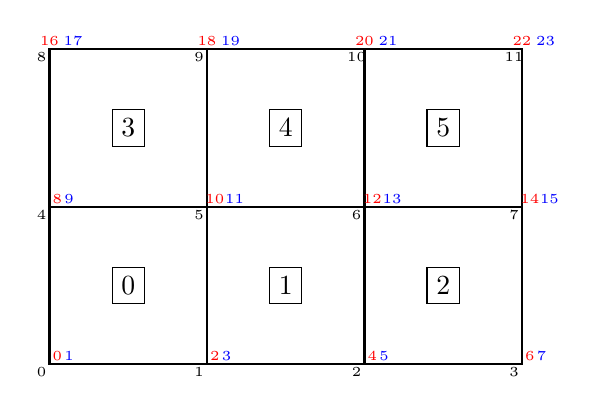
\begin{tikzpicture}
%\draw[step=0.5cm,gray,very thin] (0,0) grid (8,6); %background grid
\draw[thick] (1,1) -- (3,1) -- (3,3) -- (1,3) -- cycle;  
\draw[thick] (3,1) -- (5,1) -- (5,3) -- (3,3) -- cycle; 
\draw[thick] (5,1) -- (7,1) -- (7,3) -- (5,3) -- cycle; 
\draw[thick] (1,3) -- (3,3) -- (3,5) -- (1,5) -- cycle;  
\draw[thick] (3,3) -- (5,3) -- (5,5) -- (3,5) -- cycle; 
\draw[thick] (5,3) -- (7,3) -- (7,5) -- (5,5) -- cycle; 
\node[draw] at (2,2) {0};
\node[draw] at (4,2) {1};
\node[draw] at (6,2) {2};
\node[draw] at (2,4) {3};
\node[draw] at (4,4) {4};
\node[draw] at (6,4) {5};
%pressure dofs
\node at (0.9,0.9) {\tiny 0};
\node at (2.9,0.9) {\tiny 1};
\node at (4.9,0.9) {\tiny 2};
\node at (6.9,0.9) {\tiny 3};
\node at (0.9,2.9) {\tiny 4};
\node at (2.9,2.9) {\tiny 5};
\node at (4.9,2.9) {\tiny 6};
\node at (6.9,2.9) {\tiny 7};
\node at (0.9,4.9) {\tiny 8};
\node at (2.9,4.9) {\tiny 9};
\node at (4.9,4.9) {\tiny 10};
\node at (6.9,4.9) {\tiny 11};
%velocity dofs
\node[red] at (1.1,1.1) {\tiny 0};  \node[blue] at (1.25,1.1) {\tiny 1};
\node[red] at (3.1,1.1) {\tiny 2};  \node[blue] at (3.25,1.1) {\tiny 3};
\node[red] at (5.1,1.1) {\tiny 4};  \node[blue] at (5.25,1.1) {\tiny 5};
\node[red] at (7.1,1.1) {\tiny 6};  \node[blue] at (7.25,1.1) {\tiny 7};
\node[red] at (1.1,3.1) {\tiny 8};  \node[blue] at (1.25,3.1) {\tiny 9};
\node[red] at (3.1,3.1) {\tiny 10}; \node[blue] at (3.35,3.1) {\tiny 11};
\node[red] at (5.1,3.1) {\tiny 12}; \node[blue] at (5.35,3.1) {\tiny 13};
\node[red] at (7.1,3.1) {\tiny 14}; \node[blue] at (7.35,3.1) {\tiny 15};
\node[red] at (1.,5.1) {\tiny 16}; \node[blue] at (1.3,5.1) {\tiny 17};
\node[red] at (3.,5.1) {\tiny 18}; \node[blue] at (3.3,5.1) {\tiny 19};
\node[red] at (5.,5.1) {\tiny 20}; \node[blue] at (5.3,5.1) {\tiny 21};
\node[red] at (7.,5.1) {\tiny 22}; \node[blue] at (7.3,5.1) {\tiny 23};
\end{tikzpicture}\\
{\tiny Red color corresponds to the dofs in the x direction, blue color indicates a dof in the y direction.}
\end{center}

We have nnp=12, nel=6, NfemV=24. Let us assume that free slip boundary conditions are applied. 
The boundary conditions {\tt fix\_bc} array is then:
\begin{center}
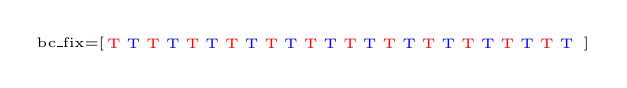
\begin{tikzpicture}
%\draw[step=0.5cm,gray,very thin] (0,0) grid (9,0.7); %background grid
\node  at (0.45,.1) {\tiny bc\_fix=[};

\node[red]  at (1.00,.1) {\tiny T};
\node[blue] at (1.25,.1) {\tiny T};
\node[red]  at (1.50,.1) {\tiny T};
\node[blue] at (1.75,.1) {\tiny T};
\node[red]  at (2.00,.1) {\tiny T};
\node[blue] at (2.25,.1) {\tiny T};
\node[red]  at (2.50,.1) {\tiny T};
\node[blue] at (2.75,.1) {\tiny T};
\node[red]  at (3.00,.1) {\tiny T};
\node[blue] at (3.25,.1) {\tiny T};
\node[red]  at (3.50,.1) {\tiny T};
\node[blue] at (3.75,.1) {\tiny T};
\node[red]  at (4.00,.1) {\tiny T};
\node[blue] at (4.25,.1) {\tiny T};
\node[red]  at (4.50,.1) {\tiny T};
\node[blue] at (4.75,.1) {\tiny T};
\node[red]  at (5.00,.1) {\tiny T};
\node[blue] at (5.25,.1) {\tiny T};
\node[red]  at (5.50,.1) {\tiny T};
\node[blue] at (5.75,.1) {\tiny T};
\node[red]  at (6.00,.1) {\tiny T};
\node[blue] at (6.25,.1) {\tiny T};
\node[red]  at (6.50,.1) {\tiny T};
\node[blue] at (6.75,.1) {\tiny T};

\node  at (7,.1) {\tiny ]};

\end{tikzpicture}\\
\end{center}
Note that since corners belong to two edges, we effectively prescribed 
no-slip boundary conditions on those. 
\todo[inline]{why does array contain only T??}


We wish to compute the tractions on the boundaries, and more precisely for the dofs for which 
a Dirichlet velocity boundary condition has been prescribed.
The number of (traction) unknowns NfemTr is then the number of {\tt T} in the {\tt bc\_fix} array.
In our specific case, we wave NfemTr= .
\todo{finish}
This means that we need for each targeted dof to be able to find its identity/number
between 0 and NfemTr-1. We therefore create the array {\tt bc\_nb} which is 
filled as follows: 
 
\begin{center}
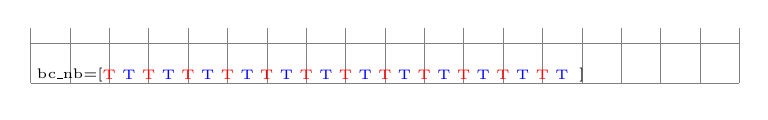
\begin{tikzpicture}
\draw[step=0.5cm,gray,very thin] (0,0) grid (9,0.7); %background grid

\node  at (0.5,.1) {\tiny bc\_nb=[};

\node[red]  at (1.00,.1) {\tiny T};
\node[blue] at (1.25,.1) {\tiny T};
\node[red]  at (1.50,.1) {\tiny T};
\node[blue] at (1.75,.1) {\tiny T};
\node[red]  at (2.00,.1) {\tiny T};
\node[blue] at (2.25,.1) {\tiny T};
\node[red]  at (2.50,.1) {\tiny T};
\node[blue] at (2.75,.1) {\tiny T};
\node[red]  at (3.00,.1) {\tiny T};
\node[blue] at (3.25,.1) {\tiny T};
\node[red]  at (3.50,.1) {\tiny T};
\node[blue] at (3.75,.1) {\tiny T};
\node[red]  at (4.00,.1) {\tiny T};
\node[blue] at (4.25,.1) {\tiny T};
\node[red]  at (4.50,.1) {\tiny T};
\node[blue] at (4.75,.1) {\tiny T};
\node[red]  at (5.00,.1) {\tiny T};
\node[blue] at (5.25,.1) {\tiny T};
\node[red]  at (5.50,.1) {\tiny T};
\node[blue] at (5.75,.1) {\tiny T};
\node[red]  at (6.00,.1) {\tiny T};
\node[blue] at (6.25,.1) {\tiny T};
\node[red]  at (6.50,.1) {\tiny T};
\node[blue] at (6.75,.1) {\tiny T};
\node  at (7,.1) {\tiny ]};
\end{tikzpicture}\\
\end{center}

This translates as follows in the code:
\begin{lstlisting}
NfemTr=np.sum(bc_fix)
bc_nb=np.zeros(NfemV,dtype=np.int32)
counter=0
for i in range(0,NfemV):
    if (bc_fix[i]):
       bc_nb[i]=counter
       counter+=1
\end{lstlisting}


The algorithm is then as follows

\begin{itemize}
\item[A] Prepare two arrays to store the matrix $M_{cbf}$ and its right hand side $rhs_{cbf}$  

\item[B] 
Loop over all elements 

\item[C] 
For each element touching a boundary, compute the residual vector 
$R_{el}=-f_{el} + \K_{el}{\cal V}_{el} + \G_{el} {\cal P}_{el}$

\item[D]
Loop over the four edges of the element using the connectivity array

\item[E]
For each edge loop over the number of degrees of freedom (2 in 2D)

\item[F] 
For each edge assess whether the dofs on both ends are target dofs. 

\item[G]
If so, compute the mass matrix $M_{edge}$ for this edge 

\item[H] extract the 2 values off the element residual vector and assemble these
in $rhs_{cbf}$

\item[I] Assemble $M_{edge}$ into NfemTrxNfemTr matrix using bc\_nb
\end{itemize}


\begin{lstlisting}
M_cbf = np.zeros((NfemTr,NfemTr),np.float64)         # A
rhs_cbf = np.zeros(NfemTr,np.float64)

for iel in range(0,nel):                             # B

    ... compute elemental residual ...               # C

    #boundary 0-1                                    # D
    for i in range(0,ndofV):                         # E
        idof0=2*icon[0,iel]+i
        idof1=2*icon[1,iel]+i
        if (bc_fix[idof0] and bc_fix[idof1]):        # F
           idofTr0=bc_nb[idof0]   
           idofTr1=bc_nb[idof1]
           rhs_cbf[idofTr0]+=res_el[0+i]             # H
           rhs_cbf[idofTr1]+=res_el[2+i]              
           M_cbf[idofTr0,idofTr0]+=M_edge[0,0]       # 
           M_cbf[idofTr0,idofTr1]+=M_edge[0,1]       # I
           M_cbf[idofTr1,idofTr0]+=M_edge[1,0]       # 
           M_cbf[idofTr1,idofTr1]+=M_edge[1,1]       #

    #boundary 1-2                                    #[D]

    ...

    #boundary 2-3                                    #[D]

    ...

    #boundary 3-0                                    #[D]

    ...


\end{lstlisting}










 %-----------------------
\newpage %-----------------------------------------------------------------------------------------
\subsection{The value of the timestep}\label{ss:cfl} The chosen time step dt used for time integration is chosen to
comply with the Courant-Friedrichs-Lewy condition \cite{cfd_anderson}.
\begin{equation}
\delta t = C \min \left( \frac{h}{\max |{\bm v}|} , \frac{h^2}{\kappa}  \right)
\end{equation}
where $h$ is a measure of the element size, $\kappa = k/ \rho c_p$ 
is the thermal diffusivity and C is the so-called CFL number chosen in $[0,1[$.

In essence the CFL condition arises when solving hyperbolic PDEs \index{hyperbolic PDE}.
It limits the time step in many explicit time-marching computer simulations
so that the simulation does not produce incorrect results. 

This condition is not needed when solving the Stokes equation but it is mandatory 
when solving the heat transport equation or any kind of advection-diffusion equation. 
Note that any increase of grid resolution (i.e. $h$ becomes smaller) yields an automatic 
decrease of the time step value.






 %---------------------------------
\newpage %-----------------------------------------------------------------------------------------
\subsection{Mappings \& Jacobians} 
\index{general}{Isoparametric}
The name isoparametric derives from the fact that the same ('iso') 
functions are used as basis functions and for the mapping to the reference element.

More generally, if $n_e$ denotes the number of nodes of an element and $n_g$ denotes the 
number of nodes describing the geometry of the element, 
then the element is termed subparametric when $n_g<n_e$ and 
superparametric when $n_g>n_e$.
\index{general}{Subparametric} \index{general}{Superparametric}

%...........................................
\subsubsection{Linear mapping on a triangle}

\begin{verbatim}
2
|\     s
| \    |_r
|  \
3===1
\end{verbatim}

Let us assume that the coordinates of the vertices are 
$(x_1,y_1)$,  
$(x_2,y_2)$, and 
$(x_3,y_3)$.
The coordinates inside the reference element are $(r,s)$. We then simply have the 
following relationship, i.e. any point of the reference element 
can be mapped to the physical triangle as follows:
\begin{eqnarray}
x&=& r x_1 + s x_2 + (1-r-s) x_3 \\
y&=& r y_1 + s y_2 + (1-r-s) y_3 
\end{eqnarray} 
There is also an inverse map, which is easily computed:
\begin{eqnarray}
r&=& \frac{(y_2-y_3)(x-x_3)-(x_2-x_3)(y-y_3)}{(x_1-x_3)(y_2-y_3)-(y_1-y_3)(x_2-x_3)} \\
s&=& \frac{-(y_1-y_3)(x-x_3)+(x_1-x_3)(y-y_3)}{(x_1-x_3)(y_2-y_3)-(y_1-y_3)(x_2-x_3)} 
\end{eqnarray} 
\begin{remark}
The denominator will not vanish, because it is a multiple of the area of the triangle.
\end{remark}

%................................................
\subsubsection{Bilinear mapping on a linear quadrilateral}

The \index{general}{reference element} is in the $(r,s)$ space. It is a square of size $2\times2$ 
centered around the origin. We wish to map it to the quadrilateral in the $(x,y)$ space:

\begin{center}
\includegraphics[width=8cm]{images/mappings/bilinear/mapping_bilinear.png}
\end{center}

The coordinates of the vertices are 
$(x_1,y_1)$, $(x_2,y_2)$, $(x_3,y_3)$ and $(x_4,y_4)$.
We then simply have the 
following relationship, i.e. any point of the reference element 
can be mapped to the physical quadrilateral as follows:
\begin{eqnarray}
x&=& N_1(r,s) x_1 + N_2(r,s) x_2 + N_3(r,s) x_3 + N_4(r,s) x_4 \\
y&=& N_1(r,s) y_1 + N_2(r,s) y_2 + N_3(r,s) y_3 + N_4(r,s) y_4 
\end{eqnarray} 
where the basis functions $N_i(r,s)$ are defined in section \ref{sec:elts1D}.

In the following example the program randomly generates 10000 points inside the reference 
element and computes their mapping into the $(x,y)$ space. 

\begin{lstlisting}
x1=-1 ; y1=-2
x2=3  ; y2=-1
x3=2  ; y3=2
x4=-3 ; y4=1

npts=10000
r=np.zeros(npts,dtype=np.float64)   
s=np.zeros(npts,dtype=np.float64)   
x=np.zeros(npts,dtype=np.float64)   
y=np.zeros(npts,dtype=np.float64)   

for i in range(0,npts):
    # compute random r,s coordinates
    r[i]=random.uniform(-1.,+1)
    s[i]=random.uniform(-1.,+1)
    # compute basis function values at r,s
    N1=0.25*(1-r[i])*(1-s[i])
    N2=0.25*(1+r[i])*(1-s[i])
    N3=0.25*(1+r[i])*(1+s[i])
    N4=0.25*(1-r[i])*(1+s[i])
    # compute x,y coordinates
    x[i]=N1*x1+N2*x2+N3*x3+N4*x4
    y[i]=N1*y1+N2*y2+N3*y3+N4*y4

np.savetxt('rs.ascii',np.array([r,s]).T)
np.savetxt('xy.ascii',np.array([x,y]).T)
\end{lstlisting}

\begin{center}
\includegraphics[width=7cm]{images/mappings/bilinear/rs.pdf}
\includegraphics[width=7cm]{images/mappings/bilinear/xy.pdf}
\end{center}

There is also an inverse map, which is not so easily computed (see section \ref{sec:amiin}).
However, if the quadrilateral in the $(x,y)$ space is a rectangle of size $(h_x,h_y)$, 
the inverse mapping is trivial:
\begin{eqnarray}
r&=&\frac{x-x_1}{x_2-x_1} \\
s&=&\frac{y-y_1}{y_4-y_1} 
\end{eqnarray}
Also in this case the basis functions can easily be written as functions of $(x,y)$:
\begin{eqnarray}
N_1(x,y) &=& \left( \frac{x_3 -x }{h_x}  \right) \left( \frac{y_3 -y }{h_y}  \right) \nn\\
N_2(x,y) &=& \left( \frac{x - x_1}{h_x}  \right) \left( \frac{y_3 -y }{h_y}  \right) \nn\\
N_3(x,y) &=& \left( \frac{x - x_1}{h_x}  \right) \left( \frac{y - y_1}{h_y}  \right) \nn\\
N_4(x,y) &=& \left( \frac{x_3 -x }{h_x}  \right) \left( \frac{y - y_1}{h_y}  \right) \nn 
\end{eqnarray}

On the one hand, any variable defined on the element can be approximated using the basis functions:
\begin{equation}
f_h(r,s)=\sum_i N_i(r,s) f_i.
\end{equation}
If we treat the coordinate variables $x$ and $y$ themselves as functions, 
then the basis functions can be used to construct the mapping:
\begin{equation}
x(r,s)=\sum_i N_i(r,s) x_i 
\qquad
y(r,s)=\sum_i N_i(r,s) y_i,  \label{eqxy}
\end{equation}
leading to write
\begin{eqnarray}
\frac{\partial x}{\partial r} &=& \sum_i \frac{\partial N_i}{\partial r} x_i \\
\frac{\partial x}{\partial s} &=& \sum_i \frac{\partial N_i}{\partial s} x_i \\
\frac{\partial y}{\partial r} &=& \sum_i \frac{\partial N_i}{\partial r} y_i \\
\frac{\partial y}{\partial s} &=& \sum_i \frac{\partial N_i}{\partial s} y_i 
\end{eqnarray}
On the other hand we also have 
\begin{eqnarray}
\frac{\partial f}{\partial r} &=&
\frac{\partial f}{\partial x}\frac{\partial x}{\partial r}
+\frac{\partial f}{\partial y}\frac{\partial y}{\partial r} \\
\frac{\partial f}{\partial s} &=&
\frac{\partial f}{\partial x}\frac{\partial x}{\partial s}
+\frac{\partial f}{\partial y}\frac{\partial y}{\partial s}
\end{eqnarray}
or in matrix form:
\begin{equation}
\left(
\begin{array}{c}
\frac{\partial f}{\partial r} \\ \\
\frac{\partial f}{\partial s}
\end{array}
\right)
=
\underbrace{
\left(
\begin{array}{cc}
\frac{\partial x}{\partial r} & \frac{\partial y}{\partial r} \nonumber\\ \\
\frac{\partial x}{\partial s} & \frac{\partial y}{\partial s} \nonumber
\end{array}
\right)
}_{\bm J}
\cdot
\left(
\begin{array}{c}
\frac{\partial f}{\partial x} \\ \\
\frac{\partial f}{\partial y}
\end{array}
\right)
\end{equation}
where ${\bm J}$ is called the Jacobian of the transformation
By inverting the Jacobian matrix, the desired derivatives with respect to $x$
and $y$ can be obtained:

We have:
\[
\left(
\begin{array}{c}
\frac{\partial f}{\partial x} \\ \\
\frac{\partial f}{\partial y}
\end{array}
\right)
=
{\bm J}^{-1} \cdot 
\left(
\begin{array}{c}
\frac{\partial f}{\partial r} \\ \\
\frac{\partial f}{\partial s}
\end{array}
\right)
\]
The inverse of the Jacobian matrix can be simply obtained in 
2D (Cramer's rule for $2\times2$ matrices\footnote{\url{https://en.wikipedia.org/wiki/Cramers_rule}}):
\[
{\bm J}^{-1} = \frac{1}{|{\bm J}|} 
\left(
\begin{array}{cc}
\frac{\partial y}{\partial s} & -\frac{\partial y}{\partial r} \nonumber\\ \\
-\frac{\partial x}{\partial s} & \frac{\partial x}{\partial r} \nonumber
\end{array}
\right)
\]
The presence of the determinant in the denominator implies that it cannot 
be zero anywhere, or in other words: the mapping is not valid if $|{\bm J}|$
is zero anywhere over the element.

Note that Hua \cite{hua90} published analytical inverse transformation for quadrilateral
isoparametric elements, i.e. how to compute ${\bm J}^{-1}$ as a function of space coordinates
and not just at the quadrature points. 

Let us look at this by means of a simple example and let us consider the following 
element:
\begin{center}
\includegraphics[width=4cm]{images/mappings/fournode/ex1}
\end{center}
Then a $Q_1$ mapping yields:
\begin{eqnarray}
x(r,s) &=& \sum_i N_i(r,s) x_i = N_2 + 2N_3 = \frac{1}{4} (3+3r+ s+rt) \\
y(r,s) &=& \sum_i N_i(r,s) y_i = 2N_3 + N_4 = \frac{1}{4} (3+r+ 3s+rt) 
\end{eqnarray}
The Jacobian matrix is then
\begin{equation}
{\bm J} = 
\left(
\begin{array}{cc}
\frac{\partial x}{\partial r} & \frac{\partial y}{\partial r} \nonumber\\ \\
\frac{\partial x}{\partial s} & \frac{\partial y}{\partial s} \nonumber
\end{array}
\right)
=
\frac{1}{4}
\left(
\begin{array}{cc}
3+s & 1+s \\
1+r & 3+r
\end{array}
\right)
\end{equation}
and its determinant is 
\begin{equation}
|{\bm J}|=\frac{1}{4} [(3+s)(3+r)-(1+s)(1+r)]=\frac{1}{2}+\frac{1}{8}r+\frac{1}{8}s
\end{equation}
It is clear that $|{\bm J}|>0$ for $-1\leq r \leq +1$ and $-1\leq s \leq +1$. 

Let us now consider another example, the following element:
\begin{center}
\includegraphics[width=4cm]{images/mappings/fournode/ex2}
\end{center}
It follows that
\begin{eqnarray}
x(r,s) &=& \sum_i N_i(r,s) x_i = \frac{1}{4}(1+r)(7+5s) \\ 
y(r,s) &=& \sum_i N_i(r,s) y_i = \frac{1}{4}(17+5r+7s-5rs)
\end{eqnarray}
and the determinant:
\[
|{\bm J}|=\frac{3}{2}-\frac{15r}{4}+\frac{15s}{4}
\]
is zero for $r-s=2/5$. This mapping is invalid!

\begin{remark}
Problems also arise when the Jacobian matrix is nearly singular due to round-off errors.
To avoid problems linked to badly shaped elements, it is recommended that the inside
angles of an element are larger than $15\degree$ and less than $165\degree$.
\end{remark}

From Eq.~\ref{eqxy}, we can also write:
\begin{eqnarray}
dx &=& \frac{\partial x}{\partial r} dr + \frac{\partial x}{\partial s} ds \\
dy &=& \frac{\partial y}{\partial r} dr + \frac{\partial y}{\partial s} ds 
\end{eqnarray},
or, 
\begin{equation}
\left(
\begin{array}{c}
dx \\ dy
\end{array}
\right)
={\bm J}\cdot
\left(
\begin{array}{c}
dr \\ ds
\end{array}
\right)
\end{equation}
This means that 
\begin{equation}
\int \int ... dx dy = \int \int ...|{\bm J}| dr ds
\end{equation}


%.................................................................
\subsubsection{biquadratic mapping of a straight-line face $Q_2$ element }

\begin{center}
\includegraphics[width=8cm]{images/mappings/biquadratic/mapping1}
\end{center}

The reference element now contains 9 nodes: 1,3,7,9 are the corners, nodes
2,4,6,8 are the mid-face points and node 5 is in the middle.
The mapping from the $(r,s)$ space to the $(x,y)$ space is then as follows:

\begin{eqnarray}
\left(
\begin{array}{c}
x(r,s) \\ y(r,s)
\end{array}
\right)
&=&
N_1(r,s)
\left(
\begin{array}{c}
x_1 \\ y_1
\end{array}
\right)
+
N_2(r,s)
\left(
\begin{array}{c}
x_2 \\ y_2
\end{array}
\right)
+
N_3(r,s)
\left(
\begin{array}{c}
x_3 \\ y_3
\end{array}
\right)
+
N_4(r,s)
\left(
\begin{array}{c}
x_4 \\ y_4
\end{array}
\right) \nonumber\\
&+&
N_5(r,s)
\left(
\begin{array}{c}
x_5 \\ y_5
\end{array}
\right)
+
N_6(r,s)
\left(
\begin{array}{c}
x_6 \\ y_6
\end{array}
\right)
+
N_7(r,s)
\left(
\begin{array}{c}
x_7 \\ y_7
\end{array}
\right)
+
N_8(r,s)
\left(
\begin{array}{c}
x_4 \\ y_8
\end{array}
\right) \nonumber\\
&+&
N_9(r,s)
\left(
\begin{array}{c}
x_9 \\ y_9
\end{array}
\right) 
\nonumber
\end{eqnarray}
where
\begin{eqnarray}
N_1(r,t)&=& 0.5r(r-1)  0.5t(t-1) \nonumber\\
N_2(r,t)&=&      (1-r^2)  0.5t(t-1) \nonumber\\
N_3(r,t)&=& 0.5r(r+1)  0.5t(t-1) \nonumber\\
N_4(r,t)&=& 0.5r(r-1)       (1-t^2) \nonumber\\
N_5(r,t)&=&      (1-r^2)       (1-t^2) \nonumber\\
N_6(r,t)&=& 0.5r(r+1)       (1-t^2) \nonumber\\
N_7(r,t)&=& 0.5r(r-1)  0.5t(t+1) \nonumber\\
N_8(r,t)&=&      (1-r^2)  0.5t(t+1) \nonumber\\
N_9(r,t)&=& 0.5r(r+1)  0.5t(t+1) \nonumber
\end{eqnarray}


\begin{lstlisting}
x1=-1                 ; y1=-2
x3=3                  ; y3=-1
x9=2                  ; y9=2
x7=-3                 ; y7=1
x2=0.5*(x1+x3)        ; y2=0.5*(y1+y3)
x4=0.5*(x1+x7)        ; y4=0.5*(y1+y7)
x6=0.5*(x3+x9)        ; y6=0.5*(y3+y9)
x8=0.5*(x7+x9)        ; y8=0.5*(y7+y9)
x5=0.25*(x1+x3+x7+x9) ; y5=0.25*(y1+y3+y7+y9)

npts=10000
r=np.zeros(npts,dtype=np.float64)   
s=np.zeros(npts,dtype=np.float64)   
xQ1=np.zeros(npts,dtype=np.float64)   
yQ1=np.zeros(npts,dtype=np.float64)   
xQ2=np.zeros(npts,dtype=np.float64)   
yQ2=np.zeros(npts,dtype=np.float64)   

for i in range(0,npts):
    # compute random r,s coordinates
    r[i]=random.uniform(-1.,+1)
    s[i]=random.uniform(-1.,+1)
    # compute Q2 basis function values at r,s
    N1= 0.5*r[i]*(r[i]-1.) * 0.5*s[i]*(s[i]-1.)
    N2=       (1.-r[i]**2) * 0.5*s[i]*(s[i]-1.)
    N3= 0.5*r[i]*(r[i]+1.) * 0.5*s[i]*(s[i]-1.)
    N4= 0.5*r[i]*(r[i]-1.) *       (1.-s[i]**2)
    N5=       (1.-r[i]**2) *       (1.-s[i]**2)
    N6= 0.5*r[i]*(r[i]+1.) *       (1.-s[i]**2)
    N7= 0.5*r[i]*(r[i]-1.) * 0.5*s[i]*(s[i]+1.)
    N8=       (1.-r[i]**2) * 0.5*s[i]*(s[i]+1.)
    N9= 0.5*r[i]*(r[i]+1.) * 0.5*s[i]*(s[i]+1.)
    # compute x,y coordinates
    xQ2[i]=N1*x1+N2*x2+N3*x3+N4*x4+N5*x5+N6*x6+N7*x7+N8*x8+N9*x9
    yQ2[i]=N1*y1+N2*y2+N3*y3+N4*y4+N5*y5+N6*y6+N7*y7+N8*y8+N9*y9
    # compute Q1 basis function values at r,s
    N1=0.25*(1-r[i])*(1-s[i])
    N2=0.25*(1+r[i])*(1-s[i])
    N3=0.25*(1+r[i])*(1+s[i])
    N4=0.25*(1-r[i])*(1+s[i])
    # compute x,y coordinates
    xQ1[i]=N1*x1+N2*x3+N3*x9+N4*x7
    yQ1[i]=N1*y1+N2*y3+N3*y9+N4*y7

np.savetxt('rs.ascii',np.array([r,s]).T)
np.savetxt('xyQ1.ascii',np.array([xQ1,yQ1]).T)
np.savetxt('xyQ2.ascii',np.array([xQ2,yQ2]).T)
\end{lstlisting}

\begin{center}
a)\includegraphics[width=4.5cm]{images/mappings/biquadratic/rs.pdf}
b)\includegraphics[width=4.5cm]{images/mappings/biquadratic/xyQ1.pdf}
c)\includegraphics[width=4.5cm]{images/mappings/biquadratic/xyQ2.pdf}\\
{\captionfont a) 10,000 random points in the reference element; b,c) image of these points
by means of a bilinear and biquadratic mapping respectively. When the sides of the element
are straight we see that a $Q_1$ mapping is sufficient.}
\end{center}

%.................................................................
\subsubsection{biquadratic mapping of a not-so straight-line face $Q_2$ element }

We now carry out the same exercise as before but nodes 2 and 8 are no more 
in the middle of nodes 1-3 and 7-9 respectively.

\begin{center}
a)\includegraphics[width=4.5cm]{images/mappings/biquadratic2/rs.pdf}
b)\includegraphics[width=4.5cm]{images/mappings/biquadratic2/xyQ1.pdf}
c)\includegraphics[width=4.5cm]{images/mappings/biquadratic2/xyQ2.pdf}\\
{\captionfont a) 10,000 random points in the reference element; b,c) image of these points
by means of a bilinear and biquadratic mapping respectively. In this case we see that 
the $Q_2$ mapping manages to capture the 'real' shape of the element.}
\end{center}

%.......................................................................
\subsubsection{bilinear, biquadratic and bicubic mapping in an annulus }

In the light of what precedes, we can now ask ourselves how this translates to 
a real geodynamic cas. Let us then consider the case of an annular domain, 
a cross section of a hollow sphere. 
When using quadrilateral elements, the mesh will look similar to this:

\begin{center}
\includegraphics[width=6cm]{images/mappings/curved/annulus_mesh}
\end{center}

We here focus on $Q_1$, $Q_2$ and $Q_3$ mappings. We single out an element, 
and arbitrarily define it as follows in polar coordinates:
\begin{lstlisting}
theta1=23./180.*np.pi
theta2=52./180.*np.pi
R1=1.
R2=1.5
\end{lstlisting}
The $Q_1$ mapping requires four points, the $Q_2$ nine points and the $Q_3$
sixteen points. These are placed equidistantly in the $r,\theta$ coordinate
system, as shown hereunder:

\begin{center}
\includegraphics[width=5cm]{images/mappings/curved/nodesQ1.pdf}
\includegraphics[width=5cm]{images/mappings/curved/nodesQ2.pdf}
\includegraphics[width=5cm]{images/mappings/curved/nodesQ3.pdf}\\
{\captionfont Left to right: position of the nodes for the $Q_1$, $Q_2$ and $Q_3$ mappings.}
\end{center}

As before, we randomly shoot 10,000 points inside the reference element 
and map these out in the $x,y$ space. Resulting swarms of points are shown 
in the following figures:

\begin{center}
\includegraphics[width=5cm]{images/mappings/curved/xy1_keep.pdf}
\includegraphics[width=5cm]{images/mappings/curved/xy2_keep.pdf}
\includegraphics[width=5cm]{images/mappings/curved/xy3_keep.pdf}\\
{\captionfont Left to right: position of the mapped points for the $Q_1$, $Q_2$ and $Q_3$ mappings.}
\end{center}

The image of a square with a $Q_1$ mapping is obviously a quadrilateral
so that it looks like quite a few points land outside of the domain $R_1\leq r\leq R_2$.
Note that points are well within $23\degree \leq \theta \leq 52\degree$, which can 
simply be explained by the fact that the faces of the element are straight lines.

However, it looks like the biquadratic and bicubic mappings are doing a much better 
job at mapping the region of space $R_1\leq r\leq R_2$. In order to characterise 
this better, we now place 10,000 points on the bottom face of the reference element (i.e. $s=-1$)
and once again compute their coordinates in the the $x,y$ space:

\begin{center}
\includegraphics[width=5cm]{images/mappings/curved/xy1.pdf}
\includegraphics[width=5cm]{images/mappings/curved/xy2.pdf}
\includegraphics[width=5cm]{images/mappings/curved/xy3.pdf}\\
{\captionfont Left to right: position of the mapped points for the $Q_1$, $Q_2$ and $Q_3$ mappings.}
\end{center}

For each point $i$ we now compute ist distance $r_i$ 
to the origin, which, if the 
mapping was perfect, whoudl be exactly equal to $R_1=1$. 
On the following plots are shown the error $r_i-1$ for all 
points, from $r=-1$ to $r=+1$.

\begin{center}
\includegraphics[width=5cm]{images/mappings/curved/innerline_error_Q1mapping.pdf}
\includegraphics[width=5cm]{images/mappings/curved/innerline_error_Q2mapping.pdf}
\includegraphics[width=5cm]{images/mappings/curved/innerline_error_Q3mapping.pdf}\\
{\captionfont Left to right: radius error of the mapped points for the $Q_1$, $Q_2$ and $Q_3$ mappings.}
\end{center}

We see that the amplitude of the error decreases with the order of the mapping used, 
which is why for instance ASPECT uses a $Q_4$ mapping by default.
Actually, in this particular case, the equation which describes the cicrle is not a 
polynomial so that no high-order mapping will ever be able to {\it exactly} 
represent the curved boundary of the element!

Another interesting point to keep in mind is that the location of the quadrature points
in the $x,y$ space is also determined by the mapping used, which can have consequences
on the accuracy of the integration and it will be reflected (for instance) on the 
error convergence rate.

Finally, the coordinates of the nodes of the element in the $x,y$ are 
uniquely determined when they are on the convex hull of the element (
for instance nodes 0-7 for $Q_2$) but we need to choose the position 
of the last nodes which are inside the element. Unfortunately, this choice is 
not neutral. 

\todo[inline]{re ask Wolfgang about this - correlate with deal.ii}

\vspace{1cm}

\Literature \cite{yuhy94}








 
 %----------------------------------------------
\newpage %-----------------------------------------------------------------------------------------
\subsection{Exporting data to vtk format} 
This format seems to be the universally accepted format for 2D and 3D visualisation in 
Computational Geodynamics (and even CFD ?). Such files can be opened with open source 
softwares such as 
Paraview \footnote{https://www.paraview.org/}, 
MayaVi \footnote{https://docs.enthought.com/mayavi/mayavi/}
or Visit \footnote{https://wci.llnl.gov/simulation/computer-codes/visit/}.

Unfortunately it is my experience that no simple tutorial exists about how to build 
such files. There is an official document which describes the vtk 
format\footnote{https://www.vtk.org/wp-content/uploads/2015/04/file-formats.pdf}
but it delivers the information in a convoluted way. I therefore describe hereafter 
how \fieldstone{} builds the vtk files. 

I hereunder show vtk file corresponding to a 3x2 grid made of linear elements.
In this particular example there are:
\begin{itemize}
\item 12 nodes and 6 elements
\item 1 elemental field: the pressure {\tt p})
\item 2 nodal fields: 1 scalar (the smoothed pressure {\tt q}), 1 vector (the velocity field {\tt u,v,0})
\end{itemize}
Note that vtk files are inherently 3D so that even in the case of a 2D simulation the $z$-coordinate 
of the points and for instance their $z$-velocity component must be provided.
The file, usually called {\filenamefont solution.vtk} starts with a header:

\lstinputlisting[language=python,firstline=1,lastline=3]{images/vtk/solution.vtu}

We then proceed to write the node coordinates as follows:

\lstinputlisting[language=python,firstline=4,lastline=19]{images/vtk/solution.vtu}

These are followed by the elemental field(s):

\lstinputlisting[language=python,firstline=20,lastline=29]{images/vtk/solution.vtu}

Nodal quantities are written next:

\lstinputlisting[language=python,firstline=30,lastline=59]{images/vtk/solution.vtu}

To these informations we must append 3 more datasets. The first one is the connectivity, 
the second one is the offsets and the third one is the type. The first one is trivial
since said connectivity is needed for the Finite Elements. The second must be understood as follows:
when reading the connectivity information in a linear manner the offset values 
indicate the beginning of each element (omitting the zero value). The third simply is the type of element 
as given in the vtk format document (9 corresponds to a generic quadrilateral with an 
internal numbering consistent with ours). 

\lstinputlisting[language=python,firstline=60,lastline=85]{images/vtk/solution.vtu}

The file is then closed with

\lstinputlisting[language=python,firstline=86,lastline=88]{images/vtk/solution.vtu}

The {\sl solution.vtu} file can then be opened with ParaView, MayaVi or Visit and the reader 
is advised to find tutorials online on how to install and use these softwares. 

\begin{center}
\includegraphics[width=4cm]{images/vtk/grid}
\includegraphics[width=4cm]{images/vtk/vel}
\includegraphics[width=4cm]{images/vtk/press}
\end{center}

 %-------------------------------
\newpage %-----------------------------------------------------------------------------------------
\subsection{Runge-Kutta methods}\label{ss:rkm} These methods were developed around 1900 by the German mathematicians Carl Runge and Martin Kutta.
The RK methods are methods for the numerical integration of 
ODEs\footnote{\url{https://en.wikipedia.org/wiki/Runge-Kutta_methods}}. These methods are well 
documented in any numerical analysis textbook and the reader is referred to \cite{gery10,tack10}.
Any Runge-Kutta method is uniquely identified by its Butcher tableau (REF?) which contains 
all necessary coefficients to build the algorithm.\todo{missing refs for Butcher tableau}

The simplest Runge-Kutta method is the (forward) Euler method. Its tableau is:

\begin{mdframed}[backgroundcolor=blue!5]
\begin{tabular}{c|c}
0 & \\
\hline
 & 1
\end{tabular}
\end{mdframed}

\index{general}{Midpoint Method} \index{general}{RK2}
The standard second-order RK method method (also called midpoint method) is:

\begin{mdframed}[backgroundcolor=blue!5]
\begin{tabular}{c|cccccc}
0 & \\
1/2 & 1/2 \\
\hline
 & 0 & 1 
\end{tabular}
\end{mdframed}

\index{general}{Heun's emthod}
Another second-order RK method, called Heun's 
method\footnote{\url{https://en.wikipedia.org/wiki/Heun's_method}} is follows:

\begin{mdframed}[backgroundcolor=blue!5]
\begin{tabular}{c|cccccc}
0 & \\
1 & 1 \\
\hline
 & 1/2 & 1/2 
\end{tabular}
\end{mdframed}

A third-order RK method is as follows:\index{general}{RK3}

\begin{mdframed}[backgroundcolor=blue!5]
\begin{tabular}{c|ccccc}
0 & \\
1/2 & 1/2 \\
1 & -1 & 2 \\ 
\hline
 & 1/6 & 4/6  & 1/6
\end{tabular}
\end{mdframed}


\index{general}{RK4}
The RK4 method falls in this framework. Its tableau is:

\begin{mdframed}[backgroundcolor=blue!5]
\begin{tabular}{c|cccccc}
0 & \\
1/2 & 1/2 \\
1/2 & 0 & 1/2 \\
1 & 0 & 0 & 1 \\
\hline
 & 1/6 & 1/3 & 1/3 & 1/6 
\end{tabular}
\end{mdframed}

A slight variation of the standard RK4 method is also due to Kutta in 1901 and is called the 3/8-rule. 
Almost all of the error coefficients are smaller than in the standard method but it requires 
slightly more FLOPs per time step. Its Butcher tableau is

\begin{mdframed}[backgroundcolor=blue!5]
\begin{tabular}{c|cccccc}
0 & \\
1/3 & 1/3 \\
2/3 & -1/3 & 1 \\
1 & 1 & -1 & 1 \\
\hline
 & 1/8 & 3/8 & 3/8 & 1/8 
\end{tabular}
\end{mdframed}


\index{general}{RK45} \index{general}{Runge-Kutta-Fehlberg method}
The following method is called the Runge-Kutta-Fehlberg method and is 
commonly abbreviated 
RKF45\footnote{\url{https://en.wikipedia.org/wiki/Runge-Kutta-Fehlberg_method}}. 
Its Butcher tableau is as follows: 

\begin{mdframed}[backgroundcolor=blue!5]
\begin{tabular}{c|cccccc}
0 & \\
1/4 	&1/4\\ 
3/8 	&3/32 		&9/32 \\
12/13 	&1932/2197 	&-7200/2197 &	7296/2197\\
1 	&439/216 	&-8 	&3680/513 &	-845/4104\\
1/2 	&-8/27 		&2 	&-3544/2565& 	1859/4104 &	-11/40 	\\
\hline
&16/135 	&0 		&6656/12825 	&28561/56430 	&-9/50& 	2/55\\
&25/216 	&0 	&1408/2565 	&2197/4104 	&-1/5 	&0 
\end{tabular}
\end{mdframed}


The first row of coefficients at the bottom of the table gives the fifth-order accurate method, and the second row gives the fourth-order accurate method. 

\begin{center}
\includegraphics[width=7cm]{images/rungekutta/fe7}
\includegraphics[width=8.5cm]{images/rungekutta/dp87}\\
{\captionfont Left: 7th order Fehlberg method; Right: 8/7th order Dormand-Prince method.}
\end{center}

\Literature \cite{fehl85,hanw93,dopr80,dopr86,prdo81,caka90,butcher03}


%....................................................................................
\subsubsection{Using RK methods to advect particles/markers \label{sec:rkparticles}}

In the context of geodynamical modelling, one is usually confronted to the following problem:
now that I have a velocity field on my FE mesh, how can I use it to advect the Lagrangian 
markers?

Runge-Kutta methods are used to this effect but only their spatial component is used:
the velocity solution is not recomputed at the intermediate fractional timesteps, i.e. 
only the coefficients of the right hand side of the tableaus is used.

\begin{itemize}
\item The RK1 method is simple.

\begin{tabular}{c|c}
0 & \\
\hline
 & 1
\end{tabular}

\noindent Carry out a loop over markers and 
\begin{enumerate}
\item interpolate velocity $\vec\upnu_{m}$ onto each marker $m$
\item compute new position as follows: $\vec r_m(t+\delta t)=\vec r_m(t) + \vec\upnu_m \delta t$
\end{enumerate}

\item The RK2 method is also simple but requires a bit more work.

\begin{tabular}{c|cccccc}
0 & \\
1 & 1 \\
\hline
 & 1/2 & 1/2 
\end{tabular}

\noindent Carry out a loop over markers and 
\begin{enumerate}
\item interpolate velocity $\vec\upnu_{m}$ onto each marker $m$ at position $\vec r_m$
\item compute new intermediate position as follows: $\vec r_m^{(1)}(t+\delta t)=\vec r_m(t) + \vec\upnu_m \delta t/2$
\item compute velocity $\vec\upnu_{m}^{(1)}$ at position $\vec r_m^{(1)}$
\item compute new position: $\vec r_m(t+\delta t)=\vec r_m(t) + \vec\upnu_m^{(1)} \delta t$ 
\end{enumerate}
Note that the intermediate positions could be in a different element of the mesh so extra 
care must be taken when computing intermediate velocities. 

\item 
The RK3 method introduces two intermediate steps. 

\begin{tabular}{c|ccccc}
0 & \\
1/2 & {\color{chestnut} $\frac{1}{2}$ } \\
1 & {\color{violet}-1} & {\color{violet}2} \\ 
\hline
 & {\color{carrotorange} $\frac16$} & {\color{carrotorange} $\frac46$}  & {\color{carrotorange} $\frac16$}
\end{tabular}

Carry out a loop over markers and 
\begin{enumerate}
\item interpolate velocity $\vec\upnu_{m}$ onto each marker $m$ at position $\vec r_m$
\item compute new intermediate position as follows: 
$\vec r_m^{(1)}(t+\delta t)=\vec r_m(t) + {\color{chestnut} \frac{1}{2}} \vec\upnu_m \delta t$
\item compute velocity $\vec\upnu_{m}^{(1)}$ at position $\vec r_m^{(1)}$
\item compute new intermediate position as follows: 
$\vec r_m^{(2)}(t+\delta t)=\vec r_m(t) + ( {\color{violet}-1} \vec\upnu_m 
+ {\color{violet}2} \vec\upnu_m^{(1)} ) \delta t$
\item compute velocity $\vec\upnu_{m}^{(2)}$ at position $\vec r_m^{(2)}$
\item compute new position: 
$\vec r_m(t+\delta t)=\vec r_m(t) + ( 
{\color{carrotorange} \frac16} \vec\upnu_m + 
{\color{carrotorange} \frac46} \vec\upnu_m^{(1)} + 
{\color{carrotorange} \frac16} \vec\upnu_m^{(2)}    )\delta t$ 
\end{enumerate}

\end{itemize}

The following example is borrowed from \cite{maie12}, itself borrowed from Fullsack \cite[Section 5.4]{full95}.
It is a whirl flow \cite{otti89}, a flow with rotational symmetry in which concentric layers of material
rotate around  a centre with an angular velocity:
\[
\omega(r)= \omega_0 \frac{r}{r_0} \exp\left(-\frac{r}{r_0}  \right)
\]  
The box is $[-0.5,0.5]\times[-0.5,0.5]$, $r_0=0.25$, $\omega_0=0.3$ and $\delta t=1$. 
$60\times 60$ particles are regularly positioned inside the $[-0.3,0.3]\times[-0.3,0.3]$ square.
Maierova \cite{maie12} has carried out this experiment for the above Runge-Kutta methods.

\begin{center}
\includegraphics[height=4cm]{images/rk/maie12a}\\
{\captionfont Model domain with particles colored at three
different time-steps: (A) t = 0 (initial position of particles), (B) t = 50, and (C) t = 200.
The advection is computed using the fourth-order Runge-Kutta scheme. Taken from \cite{maie12}}
\end{center}

\begin{center}
\includegraphics[height=4cm]{images/rk/maie12b}
\includegraphics[height=4cm]{images/rk/maie12c}\\
{\captionfont The same plot as above, but for different advection schemes at t = 100.
Advection was computed using (A) the fourth-order Runge-Kutta scheme, (B) the mid-
point method, (C) Heun's method and (D) the explicit Euler method. Taken from \cite{maie12}}
\end{center}


\bscthesis \index{general}{BSc Thesis}



 %--------------------------------
\newpage %-----------------------------------------------------------------------------------------
\subsection{Am I in or not? - finding reduced coordinates}\label{sec:amiin}
It is quite common that at some point one must answer the question:
"Given a mesh and its connectivity on the one hand, and the coordinates of a 
point on the other, how do I accurately and quickly determine in which element 
the point resides?"

One typical occurence of such a problem is linked to the use of the Particle-In-Cell 
technique: particles are advected and move through the mesh, and need to be localised 
at every time step. This question could arise in the context of a benchmark where 
certain quantities need to be measured at specific locations inside the domain. 

%-------------------------------------------
%-------------------------------------------
\subsubsection{Two-dimensional space}

We shall first focus on quadrilaterals. There are many kinds of quadrilaterals as shown 
hereunder: 

\begin{center}
\includegraphics[width=10cm]{images/quadrilaterals} % from https://en.wikipedia.org/wiki/Quadrilateral#/media/File:Quadrilaterals.svg
\end{center}

I wish to arrive at a single algorithm which is applicable to all quadrilaterals and therefore 
choose an irregular quadrilateral. For simplicity, let us consider a $Q_1$ element, with a single
node at each corner. 

\begin{center}
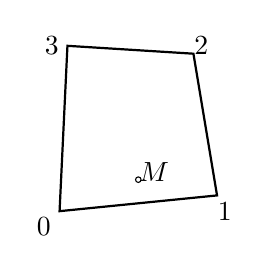
\begin{tikzpicture}
%\draw[step=0.5cm,gray,very thin] (0,0) grid (4,4); %background grid
\draw[thick] (1,1) -- (3,1.2) -- (2.7,3) -- (1.1,3.1) -- cycle;  
\node[] at (0.8,0.8) {0};
\node[] at (3.1,1) {1};
\node[] at (2.8,3.1) {2};
\node[] at (0.9,3.1) {3};
\node[] at (2.2,1.5) {$M$};
\draw (2.,1.4) circle (1pt);
\end{tikzpicture}\\
\end{center}

Several rather simple options exist:
\begin{itemize}
\item we could subdivide the quadrilateral into two triangles and check whether point $M$ is inside any of them (as it turns out, 
this problem is rather straightforward for triangles. Simply google it.)
\item We could check that point $M$ is always on the left side of segments $0\rightarrow 1$, $1\rightarrow 2$, $2\rightarrow 3$, $3\rightarrow 0$.
\item ...  
\end{itemize}

Any of these approaches will work although some might be faster than others. In three-dimensions all will however become 
cumbersome to implement and might not even work at all. Fortunately, there is an elegant way to answer the question, as 
detailed in the following subsection.

%-------------------------------------------
\subsubsection{Three-dimensional space}

If point $M$ is inside the quadrilateral, there exist a set of reduced coordinates $r,s,t\in[-1:1]^3$ such that 

\[
\sum_{i=1}^4 N_i(r_M,s,t) x_i = x_M
\quad\quad\quad
\sum_{i=1}^4 N_i(r_M,s,t) y_i = y_M
\quad\quad\quad
\sum_{i=1}^4 N_i(r_M,s,t) z_i = z_M
\]
This can be cast as a system of three equations and three unknowns. Unfortunately, each shape function $N_i$ 
contains a term $rst$ (as well as $rs$, $rt$, and $st$) so that it is not a linear system and standard techniques
are not applicable. 
We must then use an iterative technique: the algorithm starts with a guess for values $r,s,t$ and 
improves on their value iteration after iteration. 

The classical way of solving nonlinear systems of equations is Newton's method. \index{Newton's method}
We can rewrite the equations above as ${\bm F}(r,s,t)=0$:
\begin{eqnarray}
\sum_{i=1}^8 N_i(r,s,t) x_i - x_M&=&0 \nonumber\\
\sum_{i=1}^8 N_i(r,s,t) y_i - y_M&=&0 \nonumber\\
\sum_{i=1}^8 N_i(r,s,t) z_i - z_M&=&0
\end{eqnarray}
or,
\begin{eqnarray}
F_r(r,s,t)&=&0 \nonumber\\
F_s(r,s,t)&=&0 \nonumber\\
F_t(r,s,t)&=&0 \nonumber
\end{eqnarray}

so that we now have to find the zeroes of continuously differentiable functions ${\bm F}:\mathbb{R} \rightarrow \mathbb{R}$.
The recursion is simply:
\[
\left(
\begin{array}{c}
r_{k+1} \\s_{k+1} \\ t_{k+1}
\end{array}
\right)
=
\left(
\begin{array}{c}
r_{k} \\s_{k} \\ t_{k}
\end{array}
\right)
- J_F(r_k,s_k,t_k) ^{-1} 
\left(
\begin{array}{c}
F_r(r_k,s_k,t_k) \\
F_s(r_k,s_k,t_k)\\
F_t(r_k,s_k,t_k)
\end{array}
\right)
\]
where $J$ the Jacobian matrix:
\begin{eqnarray}
J_F(r_k,s_k,t_k)
&=&
\left(
\begin{array}{ccc}
\frac{\partial F_r}{\partial r}(r_k,s_k,t_k) & \frac{\partial F_r}{\partial s}(r_k,s_k,t_k) & \frac{\partial F_r}{\partial t}(r_k,s_k,t_k) \\\\
\frac{\partial F_s}{\partial r}(r_k,s_k,t_k) & \frac{\partial F_s}{\partial s}(r_k,s_k,t_k) & \frac{\partial F_s}{\partial t}(r_k,s_k,t_k) \\\\
\frac{\partial F_t}{\partial r}(r_k,s_k,t_k) & \frac{\partial F_t}{\partial s}(r_k,s_k,t_k) & \frac{\partial F_t}{\partial t}(r_k,s_k,t_k) 
\end{array}
\right) \nonumber\\
&=&
\left(
\begin{array}{ccc}
\sum\limits_{i=1}^8 \frac{\partial N_i}{\partial r}(r_k,s_k,t_k) x_i &
\sum\limits_{i=1}^8 \frac{\partial N_i}{\partial s}(r_k,s_k,t_k) x_i &
\sum\limits_{i=1}^8 \frac{\partial N_i}{\partial t}(r_k,s_k,t_k) x_i \\
\sum\limits_{i=1}^8 \frac{\partial N_i}{\partial r}(r_k,s_k,t_k) y_i &
\sum\limits_{i=1}^8 \frac{\partial N_i}{\partial s}(r_k,s_k,t_k) y_i &
\sum\limits_{i=1}^8 \frac{\partial N_i}{\partial t}(r_k,s_k,t_k) y_i \\
\sum\limits_{i=1}^8 \frac{\partial N_i}{\partial r}(r_k,s_k,t_k) z_i &
\sum\limits_{i=1}^8 \frac{\partial N_i}{\partial s}(r_k,s_k,t_k) z_i &
\sum\limits_{i=1}^8 \frac{\partial N_i}{\partial t}(r_k,s_k,t_k) z_i 
\end{array}
\right) \nonumber 
\end{eqnarray}
In practice, we solve the following system:
\[
J_F(r_k,s_k,t_k) 
\left[  
\left(
\begin{array}{c}
r_{k+1} \\s_{k+1} \\ t_{k+1}
\end{array}
\right)
-
\left(
\begin{array}{c}
r_{k} \\s_{k} \\ t_{k}
\end{array}
\right)
\right]=-
\left(
\begin{array}{c}
F_r(r_k,s_k,t_k) \\
F_s(r_k,s_k,t_k)\\
F_t(r_k,s_k,t_k)
\end{array}
\right)
\]
Finally, the algorithm goes as follows:
\begin{itemize}
\item set guess values for $r,s,t$ (typically 0)
\item loop over k=0,...
\item Compute rhs= $-{\bm F}(r_k,s_k,t_k)$ 
\item Compute matrix $J_F(r_k,s_k,t_k)$
\item solve system for $(dr_k,ds_k,dt_k)$
\item update $r_{k+1}=r_k+dr_k$, $s_{k+1}=s_k+ds_k$, $t_{k+1}=t_k+dt_k$ 
\item stop iterations when $(dr_k,ds_k,dt_k)$ is small
\item if $r_k,s_k,t_k\in[-1,1]^3$ then $M$ is inside.
\end{itemize}
This method converges quickly but involves iterations, and multiple solves of $3\times 3$ systems which, 
when carried out for each marker and at each time step can prove to be expensive. 
A simple modification can be added to the above algorithm: iterations should be carried out {\it only}
when the point $M$ is inside of a cuboid of size $[\min\limits_i{x_i}:\max\limits_i{x_i}]\times[\min\limits_i{y_i}:\max\limits_i{y_i} ]
\times[\min\limits_i{z_i}:\max\limits_i{z_i}]$ where the sums run over the vertices of the element. 
In 2D this translates as follows: only carry out Newton iterations when $M$ is inside the red rectangle!
\begin{center}
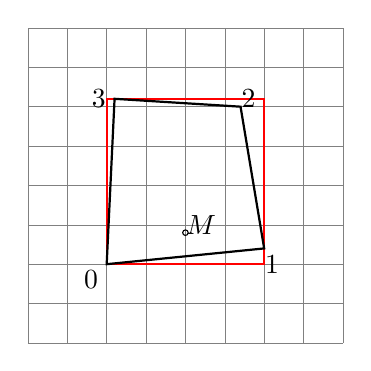
\begin{tikzpicture}
\draw[step=0.5cm,gray,very thin] (0,0) grid (4,4); %background grid
\draw[thick,red] (1,1) -- (3,1) -- (3,3.1) -- (1,3.1) -- cycle;  
\draw[thick] (1,1) -- (3,1.2) -- (2.7,3) -- (1.1,3.1) -- cycle;  
\node[] at (0.8,0.8) {0};
\node[] at (3.1,1) {1};
\node[] at (2.8,3.1) {2};
\node[] at (0.9,3.1) {3};
\node[] at (2.2,1.5) {$M$};
\draw (2.,1.4) circle (1pt);
\end{tikzpicture}\\
\end{center}

Note that the algorithm above extends to high degree elements such as $Q_2$ and higher, even with curved sides.





 %---------
\newpage %-----------------------------------------------------------------------------------------
\subsection{Error measurements and convergence rates} \index{$L_1$ norm}
\index{$L_2$ norm}
\index{$H^1$ norm}

What follows is written in the case of a two-dimensional model. Generalisation to
3D is trivial. What follows is mostly borrowed from \cite{thmk14}.

When measuring the order of accuracy of the primitive variables $\vec{v}$ and $p$,
it is standard to report errors in both the $L_1$ and the $L_2$ norm.
For a scalar quantity $\Psi$, the $L_1$ and $L_2$ norms are computed as
\[
\norm{\Psi}_1 = \int_V |\Psi| dV
\quad\quad
\quad\quad
\norm{\Psi}_2 = \sqrt{ \int_V \Psi^2 dV }
\]
For a vector quantity $\vec{k}=(k_x,k_y)$ in a two-dimensional space,
the $L_1$ and $L_2$ norms are defined as:
\[
\norm{\vec{k}}_1 = \int_V (|k_x|+|k_y|) dV
\quad\quad
\quad\quad
\norm{\vec{k}}_2 = \sqrt{ \int_V (k_x^2+k_y^2) dV }
\]
To compute the respective norms
the integrals in the above norms can be approximated by splitting them
into their element-wise contributions. The element volume integral can then
be easily computed by numerical integration using Gauss-Legendre quadrature.

The respective $L_1$ and $L_2$ norms for the pressure error can be evaluated via
\[
e_p^h|_1 = \sum_{i=1}^{n_e} \sum_{q=1}^{n_q} |e_p^h(\vec{r}_q)| w_q |J_q|
\quad\quad
\quad\quad
e_p^h|_2=\sqrt{ \sum_{i=1}^{n_e} \sum_{q=1}^{n_q} |e_p^h(\vec{r}_q)|^2 w_q |J_q| }
\]
where $e_p^h(\vec{r}_q)=p^h(\vec{r}_q) - p(\vec{r}_q)$ 
is the pressure error evaluated at the $q$-th quadrature associated with
the $i$th element. $n_e$ and $n_q$ refer to the number of elements and
the number of quadrature points per element.
$w_q$ and $J_q$ are the quadrature weight of the Jacobian associated with
point $q$.

The velocity error $e_{\vec v}^h$ is evaluated using the following two norms
\[
e_{\vec{v}}^h|_1 = \sum_{i=1}^{n_e} \sum_{q=1}^{n_q} [ |e_u^h(\vec{r}_q)| + |e_v^h(\vec{r}_q)| ]    w_q |J_q|
\quad\quad
\quad\quad
e_{\vec v}^h|_2=\sqrt{ \sum_{i=1}^{n_e} \sum_{q=1}^{n_q} \left[ |e_u^h({\bm r}_q)|^2 +  e_v^h({\bm r}_q)|^2 \right] w_q |J_q| }
\]
where $e_u^h(\vec{r}_q)=u^h(\vec{r}_q) - u(\vec{r}_q)$ and $e_v^h(\vec{r}_q)=v^h(\vec{r}_q)-v(\vec{r}_q)$.




\index{$H^1(\Omega)$ space} \index{$H^1$ norm} \index{$H^1$ semi-norm}
Another norm is very varely used in the geodynamics literature but is preferred in the 
Finite Element literature: the so-called $H^1$ norm. The mathematical basis for this
norm and the nature of the $H^1(\Omega)$ Hilbert space is to be found in many FE books \cite{dohu03,john16,hugh}.
This norm is expression is expressed as follows for a function $f$ such that $f,|\nabla f|\in L^2(\Omega)$
\footnote{\url{https://en.wikipedia.org/wiki/Sobolev_space}}
\[
\norm{f}_{H^1} = \left( \int_\Omega ( |f|^2 + |\nabla f|^2  ) d\Omega   \right)^{1/2}
\]
We then have 
\[
e_{\vec v}^h|_{H^1} = \norm{\vec{v}^h-\vec{v}}_{H^1} = \sqrt{
\sum\limits_{i=1}^d 
\int_\Omega  
\left[
({v}_i^h-{v}_i)^2
+
\vec\nabla(v_i^h-v_i)\cdot\vec\nabla(v_i^h-v_i) 
\right] d\Omega   
}
\]
where $d$ is the number of dimensions.
Note that sometimes the following semi-norm is used \cite{dobo04,bodg06}:
\[
e_{\vec v}^h|_{H^1} = \norm{\vec{v}^h-\vec{v}}_{H^1} = \sqrt{
\sum\limits_{i=1}^d 
\int_\Omega  
\left[
\vec\nabla(v_i^h-v_i)\cdot\vec\nabla(v_i^h-v_i) 
\right] d\Omega   
}
\]
 

When computing the different error norms for $e_p$ and $e_{\vec v}$ for a set of numerical experiments with
varying resolution $h$ we expect the error norms to follow the following relationships:
\[
e_{\vec v}^h|_1 = C h^{rvL_1} 
\quad\quad\quad\quad
e_{\vec v}^h|_2 = C h^{rvL_2} 
\quad\quad\quad\quad 
e_{\vec v}^h|_{H^1} = C h^{rvH^1}
\]
\[
e_p^h|_1 = C h^{rpL_1} 
\quad\quad\quad 
e_p^h|_2 = C h^{rpL_2}
\]
where $C$ is a resolution-independent constant
and $rpXX$ and $rvXX$ are the convergence rates for
pressure and velocity in various norms, respectively. 
Using linear regression on the logarithm of the respective error norm and the resolution $h$,
one can compute the convergence rates of the numerical solutions.

As mentioned in \cite{dobo04}, when finite element solutions converge at
the same rates as the interpolants we say that the method is optimal, i.e.:
\index{optimal rate}

\[
e_{\vec v}^h|_{L_2} = {\cal O}(h^3)
\quad\quad\quad\quad
e_{\vec v}^h|_{H^1} = {\cal O}(h^2)
\quad\quad\quad\quad
e_{p}^h|_{L_2} = {\cal O}(h^2)
\]

%\begin{itemize}
%\item For $Q_1P_0$, the theoretical lower bound for $r_v'$ is 2 and for $r_p'$ it is 1
%\item For $Q_2P_{-1}$, the theoretical lower bound for $r_v'$ is 3 and for $r_p'$ it is 2
%\end{itemize}
We note that when using discontinuous pressure space
(e.g., $P_0$, $P_{-1}$), these bounds remain valid even
when the viscosity is discontinuous provided that the element boundaries conform to the discontinuity.

 
\subsubsection{About extrapolation}
\index{Extrapolation}

{\it Section contributed by W. Bangerth and part of Thieulot \& Bangerth [in prep.]}

In a number of numerical benchmarks we
want to estimate the error $X_h-X^\ast$ between a quantity $X_h$ computed
from the numerical solution $\vec{u}_h,p_h$ and the corresponding value
$X$ computed from the exact solution $\vec{u},p$. Examples of such quantities
$X$ are the root mean square velocity $v_{rms}$, but it could also be a mass flux
across a boundary, an average horizontal velocity at the top boundary, or
any other scalar quantity.

If the exact solution is known, then one can of course compute $X$ from it.
On the other hand, we would of course like to assess convergence also in
cases where the exact solution is not known. In that case, one can compute
an \textit{estimate} $X^\ast$ for $X$ by way of \textit{extrapolation}.
To this end, we make the assumption that asymptotically, $X_h$ converges to
$X$ at a fixed (but unknown) rate $r$, so that
\begin{equation}
  \label{eq:extrapolation-1}
  e_h=|X_h-X| \approx C h^r.
\end{equation}
Here, $X$, $C$ and $r$ are all unknown constants to be determined, although
we are not really interested in $C$.
We can evaluate $X_h$ from the numerical solution
on successively refined meshes with mesh sizes $h$, $h/2$, and $h/4$. Then,
in addition to \eqref{eq:extrapolation-1} we also have
\begin{eqnarray}
  \label{eq:extrapolation-2}
  e_{h/2}=|X_{h/2}-X| \approx C \left(\frac h2\right)^r,
  \\
  \label{eq:extrapolation-3}
  e_{h/4} =|X_{h/4}-X| \approx C \left(\frac h4\right)^r.
\end{eqnarray}
Taking ratios of equations \eqref{eq:extrapolation-1}--\eqref{eq:extrapolation-3},
and replacing the unknown $X$ by an \textit{estimate} $X^\ast$, we then
arrive at the following equation:
\begin{equation*}
\frac{|X_h-X^\star|}{|X_{h/2}-X^\star|}
=
\frac{|X_{h/2}-X^\star|}{|X_{h/4}-X^\star|}=2^r.
\end{equation*}
If one assumes that $X_h$ converges to $X$ uniformly either from above or
below (rather than oscillate around $X$), then this equation allows us
to solve for $X^\ast$ and $r$:
\begin{equation*}
X^\star = \frac{X_h X_{h/2}-X_{h/2}^2}{X_h - 2 X_{h/2} + X_{h/4}}, \qquad\qquad
r = \log_2 \frac{X_{h/2}-X^\star}{X_{h/4}-X^\star}.
\end{equation*}
In the determination of $r$, we could also have used $X_h$ and $X_{h/2}$,
but using $X_{h/2}$ and $X_{h/4}$ is generally more reliable because
the higher order terms we have omitted in \eqref{eq:extrapolation-1} are less
visible on finer meshes.

 %-----------------------------
\newpage %-----------------------------------------------------------------------------------------
\subsection{The initial temperature field} 
\Literature: Thermal gradients in the continental crust \cite{chap86}

\Literature: Simple analytical approximation to the temperature structure in
subduction zones \cite{enwi04}

\Literature: Thermal Structure of Oceanic Lithosphere \cite{rihc18}

%.............................................................
\subsubsection{Single layer with imposed temperature b.c.}

Let us take a single layer of material characterised by
a heat capacity $C_p$, a heat conductivity $k$
and a heat production term $H$.

\begin{center}
\includegraphics[width=5cm]{images/initial_temperature/tempcond.png}
\end{center}

The Heat transport equation writes
\begin{equation}
\rho C_p \left( \frac{\partial T}{\partial t} + {\vec v} \cdot {\vec \nabla} { T} \right) = 
{\vec \nabla} \cdot (k {\vec \nabla} T) + \rho H
\end{equation}
At steady state and in the absence of a velocity field, assuming
that the material properties to be independent of time and space, and 
assuming that
there is no heat production ($H=0$), this equation
simplifies to
\begin{equation}
\Delta T =0 
\end{equation}
Assuming the layer to be parallel to the $x$-axis, the temperature is
$T(x,y)=T(y)=\alpha T+ \beta$. 
In order to specify the constants $\alpha$ and $\beta$, we need two constraints.

At the bottom of the layer $y=y_b$ a temperature $T_b$ is prescribed while a temperature
$T_t$ is prescribed at the top with $y=y_t$. This ultimately yields a temperature field in
the layer given by
\begin{mdframed}[backgroundcolor=blue!5]
\[
T(y) = \frac{T_t-T_b}{y_t-y_b}(y-y_b) + T_b
\]
\end{mdframed}

If now the heat production coefficient is not zero, the differential equation
reads
\begin{equation}
 k \Delta T + H = 0 
\end{equation}
The temperature field is then expected to be of the form
\begin{equation}
T(y)= - \frac{H}{2k} y^2 + \alpha y + \beta 
\end{equation}
Supplied again with the same boundary conditions, this leads to
\[
\beta=T_b + \frac{H}{2k} y_b^2 - \alpha y_b
\]
ie,
\[
T(y) = -\frac{H}{2k} (y^2-y_b^2) + \alpha (y-y_b) + T_b
\]
and finally
\[
\alpha =  \frac{T_t-T_b}{y_t-y_b}  + \frac{H}{2k}(y_b+y_t)
\]
or,
\[
T(y) = -\frac{H}{2k} (y^2-y_b^2) + \left( \frac{T_t-T_b}{y_t-y_b}  + \frac{H}{2k}(y_b+y_t)   \right) (y-y_b) + T_b
\]

Taking $H=0$ in this equation obviously yields the temperature field obtained previously.
Taking $k=2.25$, $T_t=0C$, $T_b=550C$, $y_t=660km$, $y_b=630km$ yields the following
temperature profiles and heat fluxes when the heat production $H$ varies:
\begin{center}
\includegraphics[width=5cm]{images/initial_temperature/temperature1.pdf}
\includegraphics[width=5cm]{images/initial_temperature/heatflux1.pdf}
\end{center}
Looking at the values at the top, which are somewhat estimated to be
about $55-65mW/m^2$ \cite[table 8.6]{jama}, one sees that value $H=0.8e-6$ yields a very acceptable
heat flux.
Looking at the bottom, the heat flux is then about $0.03W/m^2$
which is somewhat problematic since the heat flux at the Moho
is reported to be somewhere between 10 and 20 $mW/m^2$ in \cite[table 7.1]{jama}.


%-----------------------------------------------------
\subsubsection{Single layer with imposed heat flux b.c.}

Let us now assume that heat fluxes are imposed at the top and bottom of the layer:
\begin{center} 
\includegraphics[width=5cm]{images/initial_temperature/tempcond2.png}
\end{center}

We start again from the ODE
\[
k \Delta T + H = 0 
\]
but only integrate it once:
\[
k \frac{dT}{dy}  + H y + \alpha  = 0 
\]
At the bottom $q=k(dT/dy)|_{y=y_b} = q_b$ and at the top
$q=k(dT/dy)|_{y=y_t} = q_t$ so that 

\todo[inline]{to finish}


 
%-----------------------------------------------------
\subsubsection{Single layer with imposed heat flux and temperature b.c. }

\begin{center}
\includegraphics[width=5cm]{images/initial_temperature/tempcond3.png}
\end{center}

\todo[inline]{to finish}


%---------------------------------------------------------------
\subsubsection{Half cooling space}

TODO. 

\Literature \cite{fagm12} 

%---------------------------------------------------------------
\subsubsection{Plate model}

\cite{mcke67}

%.................................
\subsubsection{McKenzie slab}

When doing thermo-mechanical modelling, the initial temperature
field in the domain is of prime importance. This is 
especially true for the temperature in the slab for subduction 
modelling as its rheological behaviour is strongly temperature-dependent. 
One could easily design a simple geometrical initial field but it is 
unlikely to be close to the field of a slowly subducting slab at an angle 
in a hot mantle. 

McKenzie \cite{mcke69} derived such approximate initial field from the 
steady-state energy equation in two dimensions:
\begin{equation}
\rho C_p \vec v \cdot \vec\nabla T = k \vec\nabla^2 T
\end{equation}
We denote by $T_l$ the temperature at the base of the lithosphere
and $l$ its thickness (i.e. the thickness of the slab).

Assuming $\vec v=(v_x,0)$ yields
\[
\rho C_p v_x \frac{\partial T}{\partial x} = k \frac{\partial^2 T}{\partial x^2}
\]
and substitution of $T'=T/T_l$, $x'=x/l$ and $z'=z/l\in[0,1]$ in this equation leads to
\[
\rho C_p v_x \frac{T_l}{l}\frac{\partial T'}{\partial x'} = k \frac{T_l}{l^2}
\left( \frac{\partial^2 T'}{\partial x'^2}
+ \frac{\partial^2 T'}{\partial z'^2} \right)
\]
or 
\[
\frac{\rho C_p v_x l }{k}\frac{\partial T'}{\partial x'} = 
\frac{\partial^2 T'}{\partial x'^2}
+ \frac{\partial^2 T'}{\partial z'^2} 
\]
and finally (see Eq. 2.3 of \cite{mcke69}): 
\[
\frac{\partial^2 T'}{\partial x'^2}
- 2 R \frac{\partial T'}{\partial x'} 
+ \frac{\partial^2 T'}{\partial z'^2} =0
\]
where $R$ is the thermal Reynolds number
\[
R=\frac{\rho C_p v_x l}{2 k}
\] 
The general solution to this PDE with $T'=1$ on the top, left and right boundary is 
\[
T'(x',z')= 1 + \sum_n C_n \exp \left[ \left( R-(R^2+n^2\pi^2)^{1/2} \right) x' \right] \sin (n \pi z')
\]
We now must make an assumption about the temperature on the left boundary ($x'=0$), 
which is the temperature of the lithosphere. 
For simplicity McKenzie assumes that $T'(x'=0,z')=1-z'$ so that $C_n=2(-1)^n/n\pi$ and finally
\begin{mdframed}[backgroundcolor=blue!5]
\begin{equation}
T'(x',z')= 1 + 2\sum_n \frac{(-1)^n}{n \pi} \exp \left[ \left( R-(R^2+n^2\pi^2)^{1/2} \right) x' \right] \sin (n \pi z')
\end{equation}
\end{mdframed}

Let us build a simple temperature model for a $250\text{km}\times 50\text{km}$ slab, 
with $\rho=3000$, $C_p=1250$, $k=3$. The python code is available in {\tt images/mckenzie/mckenzie1.py}.

\begin{center}
\includegraphics[width=0.32\textwidth]{images/mckenzie/temperature_vel0p5.pdf}
\includegraphics[width=0.32\textwidth]{images/mckenzie/temperature_vel1.pdf}
\includegraphics[width=0.32\textwidth]{images/mckenzie/temperature_vel2.pdf}\\
{\captionfont Left to right: Dimensionless temperature $T'$ in a $250\text{km}\times 50\text{km}$ slab 
for $v_x={0.5,1,2}\text{cm/year}$}
\end{center}

We logically recover the fact that the slower the slab penetrates the mantle the more 
temperature diffusion dominates over temperature advection. For $v=0.5\text{cm/year}$ we see that 
that the slab assumes a constant temperature $T'=1$ at all depthes $0\leq z' \leq 1$ for 
$x'\geq 125\text{km}$. 

Note that this field is a steady-state field, valid for a constant density, heat conductivity and 
heat capacity, zero heat production, that it implies that the velocity is constant and that the 
lithosphere temperature is linear. 

One can also embed the slab in a more realistic context, a subduction zone, involving a 
subducting lithosphere, an over-riding plate and a mantle. The domain is $1000\text{km}\times 250\text{km}$.
The mantle temperature is set to $1300\degree$. The slab dip can be varied and so can the 
velocity. The python code is available in {\tt images/mckenzie/mckenzie2.py}.

\begin{center}
\includegraphics[width=0.32\textwidth]{images/mckenzie/temperature2_vel0p5_phi30.pdf}
\includegraphics[width=0.32\textwidth]{images/mckenzie/temperature2_vel1_phi30.pdf}
\includegraphics[width=0.32\textwidth]{images/mckenzie/temperature2_vel2_phi30.pdf}\\
{\captionfont Left to right: temperature $T$ for $v_x={0.5,1,2}\text{cm/year}$ and $\phi=30\degree$.}
\end{center}

\begin{center}
\includegraphics[width=0.32\textwidth]{images/mckenzie/temperature2_vel1_phi15.pdf}
\includegraphics[width=0.32\textwidth]{images/mckenzie/temperature2_vel1_phi30.pdf}
\includegraphics[width=0.32\textwidth]{images/mckenzie/temperature2_vel1_phi45.pdf}\\
{\captionfont Left to right: temperature $T$ for $v_x=1\text{cm/year}$ and $\phi={15,30,45}\degree$.}
\end{center}




%\newpage

%From \cite{mcke70}, Eq. 26:
%\[
%T(r_0) = \theta_1 \exp \left(  \frac{\alpha g}{C_p} (r_1-r_0) \right)
%\]
%where $\theta_1$ is the potential temperature of any piece of the mantle 
%at the earth's surface.
%If $x$ is measured from a depth equal to the thickness of the lithosphere down the
%dip of the slab and $z$ is measured along the normal to the slab from its lower 
%surface, then the dimensionless potential temperature in the slab is 
%\begin{eqnarray}
%\theta'(x',z')
%&=& 1+2\frac{\theta_1-273}{\theta_1} \sum_{n=1}^\infty \frac{(-1)^n}{n \pi}
%\exp \left[ \left( R-(R^2+n^2\pi^2)^{1/2} \right) x' \right] \sin n\pi z' \\
%&=& \frac{1}{\theta_1} \left\{ \theta_1+ 2 (\theta_1-273) \sum_{n=1}^\infty \frac{(-1)^n}{n \pi}
%\exp \left[ \left( R-(R^2+n^2\pi^2)^{1/2} \right) x' \right] \sin n\pi z' \right\}
%\end{eqnarray}
%where $\theta' = \theta/\theta_1$, $x'=x/l$, $z'=z/l$ and 
%with $l$ the thickness of the slab and $v$ its velocity measured down its dip.
%We denote by $\phi$ the dip of the slab so that the depth below the surface $r_1-r_0$ is given by
%$l (x' \sin \phi-z' \cos\phi)$ so that 
%\[
%T(r_0) = \theta_1 \exp \left(  \frac{\alpha g}{C_p} l (x' \sin \phi-z' \cos\phi) \right)
%\]
%The dimensionless scale height $h'$ is defined by $h'=C_p/\alpha g l$ so that
%\[
%T(r_0) = \theta_1 \exp \left[  (x' \sin \phi-z' \cos\phi)/h' \right]
%\]

%Finally,
%\[
%T(x',z')=\exp \left[  (x' \sin \phi-z' \cos\phi)/h' \right] 
%\left\{ \theta_1+ 2 (\theta_1-273) \sum_{n=1}^\infty \frac{(-1)^n}{n \pi}
%\exp \left[ \left( R-(R^2+n^2\pi^2)^{1/2} \right) x' \right] \sin n\pi z' \right\}
%\]

%\todo[inline]{BSc: create mckenzie slab temperature setup}

%......................................................................
\subsubsection{Initial temperature for global mantle convection models}

This is a difficult topic, and Gottschaldt et al \cite{gows09} list a few issues or 
facts to take into account:
\begin{itemize}
\item Frequent  impacts  may  have  determined  the  heat structure of the outer layers (Arrhenius and Lepland 2000), leading to an early thermally stable stratification. 
\item A global magma ocean (Solomatov 2000)  or  several  large  scale  melting events  (Kleine et al. 2004)  are also conceivable. 
\item Fractional crystallisation and subsequent overturn has the potential to result in compositionally or thermally   stable   layering,   too   (Elkins-Tanton et al. 2003; Zaranek and Parmentier 2004)
\end{itemize}


 %---------------------------
\newpage %-----------------------------------------------------------------------------------------
\subsection{Kinematic boundary conditions}\label{kin_bc} \index{general}{Essential Boundary Conditions}
\index{general}{Natural Boundary Conditions}

Boundary conditions come in two basic flavors: essential and natural.
\begin{itemize}
\item Essential bcs directly affect DOFs, and are imposed on the FEM matrix. 
\item Natural bcs do not directly affect DOFs and are imposed on the right-hand side vector.
\end{itemize}

\subsubsection{In-out flux boundary conditions for lithospheric models}

\begin{center}
\includegraphics[width=8cm]{images/boundary_conditions/bc1}\\
\includegraphics[width=8cm]{images/boundary_conditions/drawing.png}
\end{center}

The velocity on the side is given by
\begin{eqnarray}
u(y) &=& v_{ext} \quad\quad y<L_1 \nn\\
u(y) &=& \frac{v_{in}-v_{ext}}{y_2-y_1}(y-y_1) + v_{ext} \quad\quad y_1<y<y_2 \nn\\
u(y) &=& v_{in} \quad\quad y>y_2 \nn
\end{eqnarray}
The requirement for volume conservation is:
\[
\Phi=\int_{0}^{L_y} u(y) dy = 0
\]
Having chosen $v_{in}$ (the velocity of the plate), one can then compute $v_{ext}$
as a function of $y_1$ and $y_2$.

\begin{eqnarray}
\Phi
&=&\int_{0}^{y_1} u(y) dy  +\int_{y_1}^{y_2} u(y) dy +\int_{y_2}^{L_y} u(y) dy \nn\\
&=& v_{ext} y_1  + \frac{1}{2}(v_{in}+v_{ext})(y_2-y_1) + (L_y-y_2) v_{in} \nn\\
&=& v_{ext} [y_1 + \frac{1}{2}(y_2-y_1) ] + v_{in} [ \frac{1}{2}(y_2-y_1)  + (L_y-y_2) ] \nn\\
&=& v_{ext}\frac{1}{2} (y_1 + y_2 ) + v_{in} [ L_y - \frac{1}{2}(y_1+y_2) ] \nn
\end{eqnarray}
and finally
\begin{mdframed}[backgroundcolor=blue!5]
\[
v_{ext} = -v_{in} \frac{ L_y - \frac{1}{2}(y_1+y_2)}{ \frac{1}{2} (y_1 + y_2 ) }
\]
\end{mdframed}

Note that in some cases applying free slip boundary conditions on a curved boundary with a triangular mesh 
can be problematic as explained in Dione \etal (2013) \cite{ditu13}.

\Literature \cite{ensg82}
 %--------------------
\newpage %-----------------------------------------------------------------------------------------
\subsection{Computing gradients - the recovery process} 
write about recovering accurate strain rate components and heat flux components on the nodes.

Let $\vec g_f(\vec r)$  be the desired nodal 
field which we want to be the continuous $Q_1$ representation of the field $\vec \nabla f$.
Since the derivative of the shape function does not exist on the nodes we need to design
an algorithm do do so. There are various techniques, as listed hereafter.


%..............................
\subsubsection{Global recovery}




%..................................................
\subsubsection{Local recovery - average over patch}




%........................................................
\subsubsection{Local recovery - least squares over patch}

 %-------------------------
\newpage %-----------------------------------------------------------------------------------------
\subsection{Tracking materials and/or interfaces} 
Unless using a fully Lagrangian formulation, one needs an additional numerical method to represent/track
the various materials present in an undeformable (Eulerian) mesh.
The figure below (by B. Hillebrand) illustrates the three main methods used in geodynamics.

\begin{center}
\includegraphics[width=15cm]{images/tracking/tracking}
\end{center}

Note that what follows is applicable to FEM, FDM, etc ...


A typical test for advection algorithm is the Zalesak disk \cite{zale79}. It is a two dimensional test 
problem of solid body rotation with a constant angular velocity $\omega$ (in rad/sec):

\begin{center}
\includegraphics[width=6cm]{images/tracking/zale79a}
\includegraphics[width=6cm]{images/tracking/zale79b}\\
{\tiny Taken from \cite{zale79}. Left: Schematic representation of two dimensional 
solid body rotation problem. The field inside the cut out has value 3 and it is 1
outside. The rotational speed is such that one full revolution is effected in 
628 cycles. The width of the gap separating the two halves of the cylinder,
as well as the maximum extent of the "bridge" connecting the two halves, is 5 cells.
Right: Perspective view of initial conditions for the two dimensiona! solid body rotation
problem. Note that only a $50\times50$ portion of the mesh centered on the cylinder is displayed.}
\end{center}

This benchmark is widely used in the literature \cite{supu00,vasv05,dilp06,basd08,zhbl14}.
Note that the Zalesak disc is often supplemented with a cone and a Gaussian features:

\begin{center}
\includegraphics[width=6cm]{images/tracking/leve96}\\
{\tiny Taken from \cite{leve96}. Initial data for solid rotation tests}
\end{center}






%..............................................
\subsubsection{The Particle-in-cell technique}
\index{Particle-in-Cell}  \index{Marker-and-Cell} \index{PIC} \index{MAC}

\begin{remark}
The terms 'particle' and 'marker' are commonly (and unfortunately) interchangeably used in the literature in the context of the particle-in-cell technique. However, one should be aware that the marker-and-cell (MAC) technique is something different: it was invented in the early 60's at the Los Alamos Laboratories by Harlow and Welch \cite{hawe65}. For more information on MAC see the review paper by McKee et al \cite{mctf08}.
\end{remark}

The Particle-in-cell method is by far the most widely used in computational geodynamics. 
In its most basic form it is a rather simple method to implement and this probably owes to its success
and early adoption \cite{popo92}  in non-parallel codes such as SOPALE \cite{full95}, 
I2VIS \cite{geyu03} or CITCOM \cite{mczh04} (Appendix~\ref{app:codes}).
It has been implemented in ASPECT \cite{galh18} and the inherent load balancing issues arising from the parallel implementation as well as from the use of Adaptive Mesh Refinement are discussed. It has also been implemented in the MILAMIN code \cite{daks08} to study LLSVPs \cite{musd15}.

The basic methodology goes as follows:
\begin{enumerate}
\item distribute particles in the domain
\item assign a material identity (and/or any other quantity) to each of them
\item project particle quantities of the Eulerian nodes of the mesh
\item solve the Stokes equations for a new velocity field
\item interpolate the velocity onto the particles
\item move the particles with their respective velocities 
\item go back to step 3
\end{enumerate}  

As it turns out each step above needs to be carefully executed and is more difficult than it 
first looks. 

\paragraph{Distributing particles in the domain}. Let us assume we wish to distribute $N_p$ particles
in the domain. How large must $N_p$ be? To simplify, one end member could be 'as many particles as possible that fit in memory' 
while the other end member could be 'one per element/cell on average'. While the former does not necessarily guarantee a 
desired accuracy while being CPU and memory intensive, the latter will certainly lead to zones in the domain void 
of particles which will be problematic since the projection onto the mesh might yield zero values or very inaccurate values.
How many particles (per element/cell) will be enough?
Also, should the particles be randomly distributed in the domain or on some kind of regular grid? 
See fieldstone 13 (Section~\ref{f13}).

\paragraph{Averaging and projection}. This is a very critical step. Unfortunately, there is no community-wide
agreed-upon method. The problem at hand boils down to: at a given location $(\vec r)$ in space I need a 
quantity which is carried by the particles. 
The first step is to find the particle(s) close to this point. If done naively, this is a very costly affair, 
and begs the question what 'close' means. Finding all particles within a radius $R$ of point $\vec r$ can 
be done very efficiently (e.g. with linked lists, Verlet lists, ...) but the choice of $R$ proves to be critical:
if too small, there may not be any particle inside the circle, and if too large there may be many particles 
inside the circle and the averaging over so many particles in space will prove to be over diffusive. 
In practice, the FD or FE mesh is used to provide an indication of $R$. In FDM, the four cells (or quarter cells) around
a node represent the volume of space containing the particles whose properties are to be averaged \cite{dumg11} 
as illustrated in the following figure:

\begin{center}
\includegraphics[width=12cm]{images/dumg11}\\
{\small Taken from \cite{dumg11}. The "4-cell" and "1-cell" schemes for projecting properties defined on the 
markers (denoted by stars) onto
a node (denoted by the solid circle). (A) The 4-cell scheme. The support of the interpolating function $N_i$ associated
with node $i$ is indicated by the shaded region. Only markers within the support of node $i$ contribute to the projection
operation used to define the nodal value at $i$. The shape of the bilinear interpolation function for node $i$ is indicated in
the lower frame. (B) The 1-cell scheme. The thick lines in the lower frame indicate the grid used to discretize the
Stokes equations, while the thin lines indicate the grid onto which marker properties are projected. The 1-cell scheme
utilizes a compact support of size $\Delta x \times  \Delta y$. The support for nodes $r$, $s$, $t$ are indicated by 
the shaded regions. Only
markers within the nodal support contribute to the projection operation for that node.}
\end{center}

Given that the FEM requires to compute integrals over each element, only the particles inside the element will contribute 
to the average values assigned to the quadrature points. However, one could also decide to first average the properties onto the nodes
before using these nodal values to assign values to the quadrature points. In this case the FDM approach applies. 

Finally, in both FDM and FEM bi/trilinear shape functions are used for the interpolation as they can be interpreted as weighing 
functions. Higher order shape functions could also be used but the standard $Q_2$ shape functions (Section~\ref{sec:shpfct2d})
are 2-nd order polynomials which can take negative values (as opposed to the $Q_1$ shape functions which are strictly positive)
and this can pose problems: in some cases, although all values to be averaged are positive, their weighed average can be negative.
Q1 projection PUCKETT

\todo[inline]{it would be nice to have a Q1 and Q2 drawing of a 1D element and show that indeed negative values arise}   

Assuming that we have established a list of particles, all tracking a field $f(\vec r)$ and that each particle has an 
associated weight $N_i$ (function of the location where the average is to be computed or not), 
we must now compute their average value $<f>$. 
The simplest approach which comes to mind is the (weighed) arithmetic mean ($am$):
\[
\langle f\rangle_{am} = \frac{\sum\limits_{i=1}^n N_i f_i}{\sum\limits_{i=1}^n N_i}
\]  
In the case where $f$ is the (mass) density $\rho$, it is indeed what should be used. 
However, turning now to viscosity $\eta$, we know that its value can vary by many orders of magnitude 
over very short distances.
It is then likely that the average runs over values spanning values between $10^{18}\text{Pa s}$ and $10^{25} \text{Pa s}$.
As explained in \cite{scbe08} the arithmetic averaging tends to 'favour' large values: if the sum runs over 
10 particles, 9 carrying the value $10^{25}$ and 1 carrying the value $10^{19}$, the average value (assuming $N_i=1$ for simplicity)
is then
\[
\langle\eta\rangle = \frac{9\cdot 10^{25}+1\cdot 10^{19}}{10} \simeq 0.9\cdot 10^{25}
\]
which is much much closer to $10^{25}$ than to $10^{19}$.
Other averagings are then commonly used, namely the geometric mean ($gm$)  and the harmonic mean ($hm$), defined as follows:
\[
\langle f\rangle_{gm} = \left( \prod_i f_i^{N_i} \right)^{1/\sum\limits_i N_i} 
\qquad
\text{or, }
\qquad
\log_{10} \langle f \rangle_{gm} = \frac{\sum_i N_i \log_{10} f_i }{\sum\limits_i N_i}  
\]
and 
\[
\langle f\rangle_{hm} = \left( \frac{\sum_{i=1}^n N_i \frac{1}{f_i} }{\sum_i N_i}  \right)^{-1}
\qquad
\text{or, }
\qquad
\frac{1}{\langle f\rangle_{hm} } = \frac{\sum_{i=1}^n N_i \frac{1}{f_i} }{\sum_i N_i}  
\]
The geometric mean can be seen as a form of arithmetic mean of $\log_{10}$ values, while the harmonic mean can be seen as 
a form of arithmetic mean of the inverse values.

Looking back at the above example, the geometric mean of the viscosities is given by 
\[
\log \langle \eta\rangle_{gm} = \frac{9\cdot 25+1\cdot 19}{10} = 24.4 
\qquad \text{or,} \qquad 
\langle \eta\rangle_{gm} \simeq 2.5 \cdot 10^{24}
\]
and the harmonic mean:
\[
\langle\eta\rangle_{hm} \simeq \left( \frac{1}{10 \cdot  10^{19}} \right)^{-1} = 10^{20}
\]
We see that the harmonic mean tends to favour the small values. Also we recover the known property:
\begin{equation}
\langle f \rangle_{am}\quad  \geq \quad
\langle f \rangle_{gm}\quad  \geq \quad
\langle f \rangle_{hm} 
\end{equation}



When all $f_i$ are equal to $f_0$ their computed average should also be equal to $f_0$. As a consequence the 
weights $N_i$ should fulfill the condition $\sum\limits_{i=1}^n N_i=1$.
If all weights are equal, then $N_i=1/n$ and the averagings become:

\begin{equation}
\langle f\rangle_{am} = \frac{1}{n} \sum\limits_{i=1}^n f_i
\qquad
\langle f\rangle_{gm} = \prod_i f_i^{1/n} 
\qquad
\langle f\rangle_{hm} = \left( \frac{1}{n}\sum_i^n \frac{1}{\phi_i} \right)^{-1}
\end{equation}

There are many papers which have looked at particle averagings and projections. 
I will for now simply point to the following ones:
\cite{scbe08}
\cite{deka08}
\cite{dumg11}
\cite{modm03}
\cite{poso08}
\cite{thmk14}
\cite{galh18}
\cite{galb19}.

\todo[inline]{write more about particle averaging and projection}


\paragraph{Interpolation of the velocity onto particles}.

Once the particle $i$ has been localised inside a given element (Section~\ref{sec:amiin}) 
and its reduced coordinates $(r,s,t)$ determined, the velocity at this location can 
be computed through the shape functions:
\[
\vec\upnu_i=\sum_{k=1}^m N_i(r,s,t) \vec\upnu_k
\]
This approach is not without problem: while the nodal velocities $\vec\upnu_k$ are such 
that\footnote{for incompressible flows, of course} 
$\vec\nabla\cdot\vec\upnu=0$ (in the weak sense), the computed velocity $\vec\upnu_i$ 
is not necessarily divergence-free! In order to remedy this, a 
Conservative Velocity Interpolation (CVI) has been proposed in \cite{waav15}.


\paragraph{Moving the particles}

This is discussed in the context of the Runge-Kutta Methods, see Section~\ref{sec:rkparticles}.



%..............................................
\subsubsection{The level set function technique}
\index{Level-set Method} \index{Level-set Function} \index{LSM} \index{LSF} \index{ENO}

This method was developed in the 80's by Stanley Osher and James Sethian \cite{}

The Level-set Method (LSM), as it is commonly used in Computational Fluid Dynamics -- and especially 
in Computational Geodynamics -- represents a close curve $\Gamma$ (say, in our case, the 
interface between two fluids or layers) by means of a function $\phi$ (called the level-set function, or LSF).
$\Gamma$ is then the zero level-set of $\phi$:
\begin{equation}
\Gamma = \left\{ (x,y) \; |\; \phi(x,y)=0 \right\}
\end{equation}
The convention is that $\phi>0$ inside the region delimited by $\Gamma$ and $\phi<0$ outside.
The function value indicates on which side of the
interface a point is located (negative or positive) and this is
used to identify materials. 

Furthermore, if the curve $\Gamma$ moves with a velocity $\vec \upnu$, 
then it satisfies the following equation:
\begin{equation}
\frac{\partial \phi}{\partial t} + \vec\upnu \cdot \vec\nabla \phi = 0 
\end{equation}

The level set function is generally chosen to
be a signed distance function, i.e. $|\vec\nabla \phi| = 1$ everywhere 
and its value is also the distance to the interface.

As explained in \cite{hitg14}, the level-set function $\phi$ is advected 
with the velocity $\vec\upnu$ which is obtained by solving the Stokes equations.
This velocity does not guarantee that after an advection step the signed 
distance quality of the LSF is preserved. 
The LSF then needs to be corrected, which is also called reinitialisation. 
Finally, solving the advection equation must be done in an accurate manner both in time and space,
so that so-called ENO (essentially non-oscillatory) schemes are often employed for the 
space derivative \cite{ossh91,saev10}.


The level set method has not often been used in the geodynamics 
community with some notable exceptions 
\cite{bomh06,bomh07,habm07,grbh07,zlfd08,hagr10,sunh10,suhe10,hitg14}
An overview of the method and applications can
be found in \cite{osfe01}.

Several improvements upon the original LSM have been proposed, 
such as for instance the conservative level set of \cite{zhbl14}.
The most notable difference between CLS method originally proposed by Olsson et al. \cite{olkr05,olkz07}
and standard LS method lies in the choice of LS function. Instead of the signed distance function, the
CLS methods employ the Heaviside function $H(\phi)$ 
\[
H(\phi)=
\left\{
\begin{array}{ll}
1 & \phi>0 \\
1/2 & \phi=0 \\
0 & \phi<0
\end{array}
\right.
\]
where $\phi$ is the signed distance function as in the LSM. 
In practice, a hyperbolic tangent function is used:
\[
H(\phi) = \frac{1}{2} (1+\tan (\phi/2\epsilon))
\]
where $\epsilon$ defines the spreading width of $H$. In the case where there are only 
two fluids (i.e. a single level set is sufficient), the material properties such as density and viscosity
are computed as follows:
\[
\rho=\rho_1+(\rho_2-\rho_1)H(\phi)
\]
\[
\eta=\eta_1+(\eta_2-\eta_1)H(\phi)
\]



%..............................................
\subsubsection{The field/composition technique}
\index{compositional Field}

This is the approach taken by the ASPECT developers \cite{krhb12,hedg17}. 
Each material $i$ is represented by a compositional field $c_i$, 
which takes values between 0 and 1.
Each compositional field is then advected with the (prescribed or computed) Stokes velocity:
\[
\frac{\partial c_i}{\partial t} + {\bm v}\cdot {\bm \nabla }c_i = 0
\]

The value at a point (Finite element node or quadrature point) is 1 if it is in the 
domain covered by the material $i$, and 0 otherwise.
In one dimension, each compositional field is a Heavyside function. 
This approach is somewhat similar to the LSM but the field is essentially 
discontinuous across the interface, which makes it very difficult to advect.  
On the plus side, compositional fields need not be reinitialised, as opposed to LSF's.

Accurate numerical advection is a notoriously difficult problem. Unless very specialised 
techniques are used it often yields undershoot ($c_i<0$) and overshoot ($c_i>0$), which 
ultimately yields mass conservation issues. Also, unless special care is taken, 
compositional fields tend to become more and more diffuse over time: the SUPG method (Section~\ref{sec:supg})
and the entropy viscosity method add small amounts of diffusion to dampen the under- and 
overshoots. This means that at a given point two or more compositions may have values, 
which require some form of averaging. If under- and overshoots are present, these averagings
can become very problematic and even yield meaningless quantities (e.g. negative viscosities).

One rather old and popular filtering approach is the so-called Lenardic and Kaula filter \cite{leka93}:

\begin{center}
\includegraphics[width=6cm]{images/compositions/leka93_filter1}\\
\includegraphics[width=6cm]{images/compositions/leka93_filter2}\\
{\small Taken from Lenardic and Kaula \cite{leka93}}
\end{center}

\begin{center}
\includegraphics[width=16cm]{images/compositions/leka93_filter3}\\
{\small From FENICS book}
\end{center}

\Literature: \cite{vyrc13}

\improvement[inline]{write about DG approach}






%..............................................
\subsubsection{The Volume-of-Fluid method}

\cite{hini81}

%..............................................
\subsubsection{The method of characteristics}

\todo[inline]{ask Arie to write something}

\cite{devv00a}

%.............................................
\subsubsection{The Marker Chain method}
\index{Marker Chain} method. 

Literature: \cite{woid78,chri82,chyu84,vaks97}

More recently, it is used to track the free surface position in a FDM code \cite{chmd19}.


%..............................................
\subsubsection{Hybrid methods}

In Braun et al. \cite{brtf08} a level set method is presented which is based on a 3-D set
of triangulated points, which makes it a hybrid between tracers and level set functions:
in the DOUAR code (Appendix~\ref{app:codes}) the interface is then explicitely tracked by means of the tracers while the LSF is computed 
on the FE nodes. Although very promising in theory, this method proved to be difficult to use in practice
since it requires a) a triangulation of the interfaces at $t=0$ which is not trivial if the geometries
are complex (think about a slab in 3D); b) the addition or removal of tracers because of the interface deformation
and the patching of the triangulation; c) the calculation of the distance to the interfaces for each 
FE node based on the triangle normal vectors. 
This probably explains why the Particle-In-Cell method was later implemented in this code (pers. comm.).
Note that another very similar approach is used in \cite{saev10}.



%..............................................
\subsubsection{Boundary fitted mesh}

This method is rather simple to implement and works well for small deformations. It is 
for instance used by Frehner \cite{freh14} (see online supplementary material) in which it is 
stated: "The numerical grid is set up in such a way that the interface
between different material phases (two layers in this case) coincides with element boundaries. Hence, each
element belongs to a unique material phase and no interpolation is necessary."
With such a method, each element is initally attributed a material phase/number and its material
properties do not change. 








 %-------------------------------
\newpage %-----------------------------------------------------------------------------------------
\subsection{Static condensation} \index{general}{Static Condensation}

The idea behind static condensation is quite simple: in some cases, there are dofs 
belonging to an element which only belong to that element. For instance, the so-called MINI 
element ($P_1^+ \times P_1$) showcases a bubble function in the middle (see section \ref{ss:pair}). 
In the following, $\vec{\cal V}^\star$ corresponds to the list of such dofs inside an element.
The discretised Stokes equations on any element looks like:

\begin{equation}
\left(
\begin{array}{ccc}
\K   & L & \G \\
L^T & \K^\star  & H \\
\G^T & H^T & 0
\end{array}
\right)_e
\left(
\begin{array}{c}
\vec{\cal V} \\ \vec{\cal V}^\star \\ \vec{\cal P}
\end{array}
\right)_e
=
\left(
\begin{array}{c}
\vec{f} \\ \vec{f}^\star \\ \vec{h}
\end{array}
\right)_e
\end{equation}
This is only a re-writing of the elemental Stokes matrix where the matrix $\K$ has been 
split in four parts.
Note that the matrix $\K^\star$ is diagonal.\todo{check}

This can also be re-written in non-matrix form:
\begin{eqnarray}
\K \cdot \vec{\cal V} + L \cdot \vec{\cal V}^\star + \G \cdot \vec{\cal P} &=& \vec{f} \\
L^T V + K^\star \cdot  \vec{\cal V}^\star + H \cdot \vec{\cal P} &=& \vec{f}^\star \\
\G^T \cdot \vec{\cal V} + H^T \vec{\cal V}^\star &=& \vec{h}
\end{eqnarray}
The $\vec{\cal V}^\star$ in the second equation can be isolated:
\[
\vec{\cal V}^\star = \K^{-\star} \cdot ( \vec{f}^\star - L^T \cdot \vec{\cal V} - H \cdot \vec{\cal P})
\]
and inserted in the first and third equations:
\begin{eqnarray}
\K \cdot \vec{\cal V} + L \left[ \K^{-\star} ( \vec{f}^\star - L^T \cdot \vec{\cal V} - H \cdot \vec{\cal P} )  \right] + \G \cdot \vec{\cal P} &=& \vec{f} \\
\G^T \cdot \vec{\cal V} + H^T \left[  \K^{-\star} ( \vec{f}^\star - L^T \cdot \vec{\cal V} - H \cdot \vec{\cal P}) \right]  &=& \vec{h}
\end{eqnarray}
or,
\begin{eqnarray}
(\K-L\cdot \K^{-\star} \cdot L^T)\cdot \vec{\cal V} + (G-L\cdot \K^{-\star} \cdot H) \cdot \vec{\cal P} &=& \vec{f}-L\cdot \K^{-\star} \cdot \vec{f}^\star \\
(G^T -H^T\cdot \K^{-\star}\cdot  L^T ) \cdot \vec{\cal V}  - 
(H^T \cdot \K^{-\star} \cdot H )\cdot \vec{\cal P}   &=& \vec{h} -H^T\cdot \K^{-\star}\cdot \vec{f}^\star
\end{eqnarray}
i.e.
\begin{eqnarray}
\underline{\K} \cdot \vec{\cal V} + \underline{\G}\cdot \vec{\cal P} &=& \underline{\vec{f}} \\
\underline{\G}^T \cdot \vec{\cal V} - \underline{\C} \cdot \vec{\cal P} &=& \underline{\vec{h}}
\end{eqnarray}
with
\begin{eqnarray}
\underline{\K}&=& K-L\cdot \K^{-\star} \cdot L^T \\
\underline{\G}&=& G-L\cdot \K^{-\star} \cdot H \\
\underline{\C}&=& H^T \cdot \K^{-\star} \cdot H \\
\underline{\vec{f}}&=& \vec{f}-L\cdot \K^{-\star} \cdot \vec{f}^\star \\
\underline{\vec{h}}&=& \vec{h} -H^T\cdot \K^{-\star}\cdot \vec{f}^\star
\end{eqnarray}
Note that $\underline{\K}$ is symmetric, and so is the Stokes matrix.


For instance, in the case of the MINI element, the dofs corresponding to the bubble 
could be eliminated at the elemental level, which would make the Stokes matrix smaller
(see book by Braess \cite{braess}). 
However, it is then important to note that static condensation introduces a 
pressure-pressure term which was not there in the original formulation.









 %-------------------------------------
\newpage %-----------------------------------------------------------------------------------------
\subsection{Measuring incompressibility \label{ss_incomp}} 
The velocity divergence error integrated over the whole element is given by
\begin{equation}
e_{div}= \int_\Omega (\vec\nabla\cdot \vec v^h - \underbrace{\vec\nabla\cdot \vec v}_{=0}  ) \; d\Omega
= \int_\Omega (\vec\nabla\cdot \vec v^h) \; d\Omega
\end{equation}
where $\Gamma_e$ is the boundary of element $e$ and $\vec{n}$ is the unit 
outward normal of $\Gamma_e$.

Furthermore, one can show that \cite{dobo04}:
\[
e_{div} = \int_{\Gamma_e} \vec{v}^h\cdot\vec{n} \;  d\Gamma
\]
The reason is as follows and is called the divergence 
theorem\footnote{\url{https://en.wikipedia.org/wiki/Divergence_theorem}}:
suppose a volume $V$ subset of $\mathbb{R}^d$ which is compact
and has a piecewise smooth boundary $S$, and if $\vec F$ is
a continuously differentiable vector field then
\[
\int_V ( \vec\nabla\cdot\vec F)\; dV = \int_S (\vec F \cdot \vec n)\; dS
\]
The left side is a volume integral while the right side is a surface integral.
Note that sometimes the notation $d\vec S = \vec n \; dS $ is used so that 
$\vec F \cdot \vec n \; dS = \vec F \cdot d\vec S$.

The average velocity divergence over an element can be defined as 
\[
<\vec \nabla \cdot \vec v>_e 
= \frac{1}{V_e} \int_{\Omega_e}  (\vec\nabla\cdot\vec v) \; d\Omega
= \frac{1}{V_e} \int_{\Gamma_e} \vec{v}\cdot\vec{n} \; d\Gamma
\]
Note that for elements using discontinuous pressures we shall 
recover a zero divergence element per element (local mass conservation)
while for continuous pressure elements the mass conservation 
is guaranteed only globally (i.e. over the whole domain), see section 3.13.2 of \cite{grsa}.

Note that one could instead compute $<|\vec\nabla\cdot \vec v|>_e$. Either volume or 
surface integral can be computed by means of an appropriate Gauss-Legendre quadrature algorithm.

\improvement[inline]{implement and report}


 %------------------------
\newpage %-----------------------------------------------------------------------------------------
\subsection{Periodic boundary conditions\label{ss_periodic}}\index{general}{Periodic Boundary Conditions}

This type of boundary conditions can be handy in some specific cases such 
as infinite domains. The idea is simple: when material leaves the domain 
through a boundary it comes back in through the opposite boundary (which 
of course presupposes a certain topology of the domain). 

For instance, if one wants to model a gas at the molecular level and wishes 
to avoid interactions of the molecules with the walls of the container, 
such boundary conditions can be used, mimicking an infinite domain in all 
directions. 

Let us consider the small mesh depicted hereunder:

\todo[inline]{missing picture}

We wish to implement horizontal boundary conditions so that 
\[
u_5=u_1
\quad\quad
u_{10}=u_6
\quad\quad
u_{15}=u_{11}
\quad\quad
u_{20}=u_{16}
\]
One could of course rewrite these conditions as constraints and extend the Stokes 
matrix but this approach turns out to be not practical at all. 

Instead, the method is rather simple: replace in the connectivity array the dofs on the right side
(nodes 5, 10, 15, 20) by the dofs on the left side. In essence, we wrap the system upon itself 
in the horizontal direction so that elements 4, 8 and 12 'see' and are 'made of' the nodes 1, 6, 11 and 16.
In fact, this is only necessary during the assembly. Everywhere in the loops nodes 5, 10, 15 and 20 appear 
one must replace them by their left pendants 1, 6, 11 and 16. This autmatically generates a matrix 
with lines and columns corresponding to the $u_5$, $u_{10}$, $u_{15}$ and $u_{20}$ being exactly zero. 
The Stokes matrix is the same size, the blocks are the same size and the symmetric character of the matrix 
is respected. However, there remains a problem. There are zeros on the diagonal 
of the above mentioned lines and columns. One must then place there 1 or a more
appropriate value.

Another way of seeing this is as follows: let us assume we have built and assembled
the Stokes matrix, and we want to impose periodic b.c. so that dof $j$ and $i$ are the same. 
The algorithm is composed of four steps:
\begin{enumerate} 
\item add col $j$ to col $i$
\item add row $j$ to row $i$ (including rhs)
\item zero out row $j$, col $j$
\item put average diagonal value on diagonal ($j,j$)
\end{enumerate} 

\begin{remark}
Unfortunately the non-zero pattern of the matrix with periodic b.c. is not the same 
as the matrix without periodic b.c.
\end{remark}


 %---------------------
\newpage %-----------------------------------------------------------------------------------------
\subsection{Removing rotational nullspace\label{ss_nullspace}} 
When free slip boundary conditions are prescribed in an annulus or
hollow sphere geometry there exists a rotational nullspace, or in other words there exists
a tangential velocity field ('pure rotation') which if added or subtracted to the solution 
does not alter the solution. 

As in the pressure normalisation case (see section \ref{ss_pnorm}), the solution is simple:
\begin{enumerate}
\item fix the tangential velocity at {\it one} node on a boundary, and solve the sytem (the nullspace 
has been removed)
\item post-process the solution to have the velocity field fulfill the required conditions, i.e.
either a zero net angular momentum or a zero net angular velocity of the domain. 
\end{enumerate}

\begin{remark}
In \aspect{} this is available under the option 
"Remove nullspace = angular momentum" and "Remove nullspace = net rotation".
The "angular momentum" option removes a rotation such that the net angular momentum is zero.
The "net rotation" option removes the net rotation of the domain.
\end{remark}

In order to remove the angular momentum, we search for a rotation
vector ${\vec \omega}$ such that
\begin{equation}
\int_\Omega \rho[{\vec r} \times ({\vec v}-{\vec \omega} \times {\vec r})] \; d\vec r= \vec 0
\end{equation}
Recognizing that the angular momentum vector ${\vec H}$ is given by
\begin{equation}
{\vec H} = \int_\Omega \rho{\vec r} \times {\vec v}\; d\vec r
\end{equation}
and that the moment of inertia
(also called inertia tensor)\footnote{\url{https://en.wikipedia.org/wiki/Moment\_of\_inertia}}
 for a continuous body 
 $3\times3$ matrix ${\bm I}$ is given by
\begin{equation}
{\bm I}= 
\int_\Omega \rho(\vec r) [\vec r\cdot\vec r \; \bm 1 - \vec r \times \vec r  ] d\vec r 
\end{equation}
so that the above equation writes:
$
{\vec H}={\bm I}\cdot {\vec \omega}
$
and then ${\vec \omega}={\bm I}^{-1} \cdot {\vec H}$.
A rotation about the rotation vector ${\vec \omega}$ is then subtracted from the velocity 
solution \cite[eq. 26]{zhmt08}:
\begin{equation}
\vec v_{new} = \vec v_{old} - \vec \omega \times \vec r 
\end{equation}

\index{angular velocity} \index{angular momentum}

%...............................
\subsubsection{Three dimensions}

The angular momentum vector is given by:
\begin{equation}
\vec H = \int_\Omega \rho(\vec r) \left( 
\begin{array}{c} 
yw-zv \\ zu-xw \\ xv-yu 
\end{array} \right) d\vec r
\end{equation}
while the inertia tensor for a continuous body is given 
by
\begin{eqnarray}
\bm I
&=&\int_\Omega \rho(\vec r) [\vec r\cdot\vec r \; \bm 1 - \vec r \times \vec r  ] d\vec r \\
&=&\int_\Omega \rho(\vec r) 
\left[
\left(
\begin{array}{ccc}
r^2 & 0 & 0 \\
0 & r^2 & 0 \\
0 & 0 & r^2
\end{array}
\right)
- 
\left(
\begin{array}{ccc}
xx & xy & xz \\
yx & yy & yz \\
zx & zy & zz 
\end{array}
\right)
\right] 
d\vec r \\
&=&\int_\Omega \rho(\vec r) 
\left(
\begin{array}{ccc}
y^2+z^2 & -xy & -xz \\
-yx & x^2+z^2 & -yz \\
-zx & -zy & x^2+y^2 
\end{array}
\right)
d\vec r \\
\end{eqnarray}

The angular velocity\footnote{\url{https://en.wikipedia.org/wiki/Angular_velocity }}
 vector is given by $\vec\omega = \frac{\vec r\times \vec v}{r^2}$
so that the volume-averaged angular velocity of the cylindrical shell is:
\[
<\vec {\omega}> = \frac{1}{|\Omega|} \int_\Omega \frac{{\vec r}\times {\vec v}}{r^2} d\vec r
\]
 Note that it can be straightforwardly computed the same way as the angular momentum
(it is in fact the same equation but without the density):

%-----------------------------
\subsubsection{Two dimensions}

In two dimensions, flow is taking place in the $(x,y)$ plane. This means that $\vec r$ and $\vec v$ are coplanar, 
and therefore that $\vec H$ is perpendicular to the plane, i.e. $\vec H \propto \vec e_z$.
We have then
\begin{equation}
\vec H = \int_\Omega \rho(\vec r) \left( 
\begin{array}{c} 
0 \\ 0 \\ xv-yu 
\end{array} \right) d\vec r
\end{equation}
and 
\begin{equation}
\bm I=
\int_\Omega \rho(\vec r) 
\left(
\begin{array}{ccc}
y^2 & -xy & 0 \\
-yx & x^2 & 0 \\
0 & 0 & x^2+y^2 
\end{array}
\right)
d\vec r 
\end{equation}
The volume-averaged angular velocity is then simply:
\begin{equation}
<\omega_z> = \frac{1}{|\Omega|}\int_\Omega \frac{xv-yu}{r^2}d\vec r
\end{equation}

















 %-----------------
\newpage %-----------------------------------------------------------------------------------------
\subsection{Picard and Newton \label{ss_nonlinear}} \index{nonlinear} \index{Picard iterations} \index{relaxation}

\todo[inline]{explain why our eqs are nonlinear}

%--------------------------------
\subsubsection{Picard iterations}

Let us consider the following system of nonlinear algebraic equations:
\[
\mathbb{A}(\vec X) \cdot \vec X = \vec b(\vec X)
\]
Both matrix and right hand side depend on the solution vector $\vec X$.

For many mildly nonlinear problems, a simple successive substitution 
iteration scheme (also called Picard method) will converge to the solution
and it is given by the simple relationship:
\[
\mathbb{A}(\vec X^n) \cdot \vec X^{n+1} = \vec b(\vec X^n)
\]
where $n$ is the iteration number. 
It is easy to implement:
\begin{enumerate}
\item guess $\vec X^0$ or use the solution from previous time step
\item compute $\mathbb{A}$ and $\vec b$ with current solution vector $\vec X^{old}$
\item solve system, obtain $T^{new}$
\item check for convergence (are $\vec X^{old}$ and $\vec X^{new}$ close enough?)
\item $\vec X^{old} \leftarrow \vec X^{new}$
\item go back to 2.
\end{enumerate}

There are various ways to test whether iterations have converged. The simplest
one is to look at $\norm{\vec X^{old}-\vec X^{new} }$ (in the $L_1$, $L_2$ or maximum norm)
and assess whether this term is smaller than a given tolerance $\epsilon$. 
However this approach poses a problem: in geodynamics, if two consecutively obtained 
temperatures do not change by more than a thousandth of a Kelvin (say $\epsilon=10^{-3}$K )
we could consider that iterations have converged but looking now at velocities which 
are of the order of a cm/year (i.e. $\sim 3\cdot 10^{-11}$m/s) we would need a tolerance 
probably less than $10^{-13}$m/s. We see that using absolute values for a convergence 
criterion is a potentially dangerous affair, which is why one uses a relative 
formulation (thereby making $\epsilon$ a dimensionless parameter):
\[
\frac{\norm{\vec X^{old}-\vec X^{new}}}{\norm{\vec X^{new}}} < \epsilon
\]
Another convergence criterion is proposed by Reddy (section 3.7.2) \cite{reddybook2}:
\[
\left(
\frac{ (\vec X^{old}-\vec X^{new})\cdot(\vec X^{old}-\vec X^{new} ) }{ X^{new}\cdot X^{new}  } 
\right)^{1/2} < \epsilon
\]
Yet another convergence criterion is used in \cite{thie11}: the means $<\vec X^{old}>$, $<\vec X^{new}>$
as well as the variances $\sigma^{old}$ and $\sigma^{new}$ are computed, followed by the 
correlation factor $R$:
\[
R= \frac{ <  (\vec X^{old}-<\vec X^{old}>)\cdot( \vec X^{new}-<\vec X^{new}> )>  }{\sqrt{\sigma^{old}\sigma^{new}}}
\]
Since the correlation is normalised, it takes values between 0
(very dissimilar velocity fields) and 1 (very similar fields). The
following convergence criterion is then used: $1-R < \epsilon$.

\todo[inline]{write about nonlinear residual}


Note that in some instances and improvement in convergence rate can be obtained by use of a 
relaxation formula where one first solves
\[
\mathbb{A}(\vec X^n) \cdot \vec X^{\star} = \vec b(\vec X^n)
\]
and then updates $\vec X^n$ as follows:
\[
\vec X^n = \gamma \vec X^n + (1-\gamma) \vec X^\star 
\quad\quad\quad
0 < \gamma \leq 1
\]
When $\gamma=1$ we recover the standard Picard iterations formula above.

%------------------------------------------
\subsection{Defect correction formulation}

Work in progress. 

We start from the system to solve:
\[
{\bm A}(\vec X) \cdot \vec X = \vec b(\vec X)
\]
with the associated residual vector $\vec F$ 
\[
\vec F(\vec X) = {\bm A}(\vec X) \cdot \vec X - \vec b(\vec X)
\]
The Newton-Raphson algorithm consists of two steps:
\begin{enumerate}
\item solve $\bm J_k \cdot \delta \vec X_k = -\vec F(\vec X_k)$, or in the 
case of the incompressible Stokes equation FEM system:
\[
\left(
\begin{array}{cc}
\bm J^{{\cal V}{\cal V}}_k & \bm J^{{\cal V}{\cal P}}_k \\
\bm J^{{\cal P}{\cal V}}_k & 0
\end{array}
\right)
\cdot
\left(
\begin{array}{c}
\delta \vec {\cal V}_k \\ \delta \vec {\cal P}_k
\end{array}
\right)
=
\left(
\begin{array}{c}
- \vec F_k^{\cal V} \\ -\vec F_k^{\cal P}
\end{array}
\right)
\]

\item update $\vec X_{k+1} = \vec X_k + \alpha_k \delta \vec X_k$
\end{enumerate}
The defect correction Picard approach consists of neglecting the derivative terms present 
in the $J$ terms (Eqs. 16,17,18 of \cite{frbt19}) so that 
\[
\bm J^{{\cal V}{\cal V}}_k \simeq \K_k 
\quad\quad
\bm J^{{\cal V}{\cal P}}_k \simeq \G 
\quad\quad
\bm J^{{\cal P}{\cal V}}_k \simeq \G^T
\]
and step 1 of the above iterations become:
\[
\left(
\begin{array}{cc}
\K_k & \G \\ \G^T & 0
\end{array}
\right)
\cdot
\left(
\begin{array}{c}
\delta \vec {\cal V}_k \\ \delta \vec {\cal P}_k
\end{array}
\right)
=
\left(
\begin{array}{c}
- \vec F_k^{\cal V} \\ -\vec F_k^{\cal P}
\end{array}
\right)
\]


\mscthesis: implement a simple Newton solver and apply it to a few nonlinear benchmarks. \index{MSc Thesis} 
 %----------------------------
\newpage %-----------------------------------------------------------------------------------------
\subsection{Parallel or not?} \label{sec:parallel} \index{general}{Domain Decomposition}

%---------------------------
\subsubsection{Rationale}

Let us assume that we want ro run a simulation of the whole Earth mantle
with a constant resolution of $5\text{km}$. The volume of the mantle is
\[
V_{mantle}=\frac{4}{3}\pi (R_{out}^3-R_{in}^3) \simeq  10^{12}  km^3
\]
while the volume of an element is $V_{e} = 125 \text{km}^3$ (this is 
only an average since the tesselation of a hollow sphere with 
hexahedra yields elements which are not all similar \cite{thie18}).
Consequently, the number of cells needed to discretise the mantle
is 
\[
N_{el}=\frac{V_{mantle}}{V_{e}}\simeq 8\times 10^9
\]
We know that the matrix size is approx. 4 times the number of elements in 3D:
\[
N\simeq 25 \times 10^9
\]
Using between 9 and 125 particles per element (a very conservative number),
the total number of particles is then
\[
N_{particles}  \geq 10^{10}
\]
The unescapable conclusion is that high-resolution 3D 
calculations 
 have a very large memory footprint and require extremely long computational times.

The only way to overcome this problem is by resorting to 
using supercomputers with many processors and large memory capacities.

The idea behind parallel programming is to have each processor carry out 
only a subset of the total number of operations required. In order to reduce 
the memory footprint on each processor, only a subset of the computational
mesh is known by each: one speaks then of domain decomposition.

An example of such a large parallel calculation of 3D convection with 
domain decomposition in a spherical shell can be found in \cite{krhb12}:

\begin{center}
a)\includegraphics[width=7cm]{images/parallel/krhb2}
b)\includegraphics[width=7cm]{images/parallel/krhb1} \\
{\captionfont a)Isocontours of the temperature field; b) Partitioning of the domain onto 512 proc. 
The mesh counts 1,424,176 cells. The solution has approximately 54 million unknowns 
(39 million vel., 1.7 million press., and 13 million temp.)
}
\end{center}


\Literature:
\begin{itemize}
\item Three parallel iterative solvers for the Stokes system, discretized by low order 
tetrahedral elements, are compared with respect to their numerical efficiency and their 
scalability running on up to 786,432 parallel threads. Gmeiner \etal (2016) \cite{gmhj16}
\end{itemize}


%----------------------------------------------
\subsubsection{Strong scaling vs weak scaling}

\begin{center}
\includegraphics[width=16cm]{images/parallel/fig}
\end{center}


 %------------------------------
\newpage %-----------------------------------------------------------------------------------------
\subsection{Stream function} \label{sec:streamfunction} \index{general}{Stream Function}

\Literature \cite{giju98}\cite{scja81}\cite{chyu84}\cite{chri84}\cite{hayu94}\cite{olwh97}




The Stream function (commonly denoted by $\Phi$ or $\Psi$) approach is a useful approach in 
fluid dynamics as it 
can provide relatively quick solutions to 2D incompressible flow problems.
Using a stream function
formulation is numerically convenient because velocity information is contained in a single scalar equation
and pressure vanishes from the solution process.
The stream function is a function of coordinates and time of an inviscid liquid.
It allows to determine the components of velocity by differentiating the stream function 
with respect to the space coordinates. 
A family of curves $\Psi = const$ represent {\it streamlines}, i.e. 
the stream function remains constant along a streamline. 
Although also valid in 3D, this approach is mostly used in 2D because of its 
relative simplicity {\color{red} REFERENCES}.

%........................................
\subsubsection{In Cartesian coordinates}

In two dimensions the velocity is obtained as follows:
\begin{equation}
{\vec \upnu} = (u,v) = \left( \frac{\partial \Psi}{\partial y},-\frac{\partial \Psi}{\partial x} \right) 
\end{equation}
Provided the function $\Psi$ is a smooth enough function, 
this automatically insures that the flow is incompressible:
\begin{equation}
{\vec \nabla}\cdot {\vec \upnu} = 
\frac{\partial u}{\partial x} + \frac{\partial v}{\partial y}
=
\frac{\partial^2 \Psi}{\partial xy} - \frac{\partial^2 \Psi}{\partial xy} =0 
\end{equation}
Assuming constant viscosity, the Stokes equation writes:
\begin{equation}
-{\vec \nabla}p + \eta \Delta {\vec \upnu} + \rho {\vec g} = \vec{0}
\end{equation}
Let us introduce the vector ${\vec{W}}$ for convenience such that in each dimension:
\begin{eqnarray}
W_x&=&-\frac{\partial p}{\partial x} 
+ \eta\left( \frac{\partial^2 u}{\partial x^2} + \frac{\partial^2 u}{\partial x^y} \right) \\
W_y&=&-\frac{\partial p}{\partial y} 
+ \eta \left(\frac{\partial^2 v}{\partial x^2} + \frac{\partial^2 v}{\partial x^y} \right) 
\end{eqnarray}
Taking the curl of the vector ${\vec{W}}$ and only considering the component perpendicular to the $xy$-plane:
\begin{equation}
\frac{\partial W_y}{\partial x} - \frac{\partial W_x}{\partial y}  = 
-\frac{\partial \rho g_y}{\partial x} + \frac{\partial \rho g_x}{\partial y}   
\end{equation}
The advantage of this approach is that the pressure terms cancel out (the curl of a gradient is always zero), 
so that:
\begin{equation}
\frac{\partial}{\partial x}\eta\left( \frac{\partial^2 v}{\partial x^2} + \frac{\partial^2 v}{\partial x^y}  \right) 
- \frac{\partial }{\partial y} \eta \left( \frac{\partial^2 u}{\partial x^2} + \frac{\partial^2 u}{\partial x^y} \right) = 
-\frac{\partial \rho g_y}{\partial x} + \frac{\partial \rho g_x}{\partial y}   
\end{equation}
and then replacing $u,v$ by the their stream function derivatives yields (for a constant viscosity):
\begin{equation}
\eta \left(\frac{\partial^4 \Psi}{\partial x^4} + 
\frac{\partial^4 \Psi}{\partial y^4} + 
2\frac{\partial^4 \Psi}{\partial x^2y^2} \right)
=
-\frac{\partial \rho g_y}{\partial x} + \frac{\partial \rho g_x}{\partial y}   
\end{equation}
or, 
\begin{equation}
\eta {\vec \nabla}^4 \Psi 
=
\left(\frac{\partial^2 }{\partial x^2} + \frac{\partial^2 }{\partial y^2} \right) 
\left(\frac{\partial^2 }{\partial x^2} + \frac{\partial^2 }{\partial y^2} \right) \Psi
=
-\frac{\partial \rho g_y}{\partial x} + \frac{\partial \rho g_x}{\partial y}   
\label{eq:sf1}
\end{equation}
Note that $\vec\nabla^2 \vec\nabla^2 = \vec\nabla^4 $ is known as the Biharmonic operator.
\index{general}{Biharmonic Operator} 

These equations are also to be found in the geodynamics literature, 
see Eq. 1.43 \cite[eq. 1.43]{tack10} or \cite[p 70-71]{gery10}.

In the presence of temperature variations and multiple compositions, 
Trim et al (2020) \cite{trlb20}  use the  following nondimensional 
equation:
\[
\left(
\frac{\partial^2 }{\partial x^2} - 
\frac{\partial^2 }{\partial y^2}  
\right)
\left[ \eta
\left(
\frac{\partial^2 \Psi}{\partial x^2} - 
\frac{\partial^2 \Psi}{\partial y^2}  
\right)
\right]
+4
\frac{\partial^2 }{\partial xy} 
\left[
\eta 
\frac{\partial^2 \Psi}{\partial xy} 
\right]
=
Ra_T \frac{\partial T}{\partial x}-
Ra_C \frac{\partial C}{\partial x}
\]
\todo[inline]{check/rederive this formula!}


%........................................
\subsubsection{In Cylindrical coordinates}

TODO

VERIFY THOSE! minus signs ?
\[
\upnu_r=\frac{1}{r}\frac{\partial \Phi}{\partial \theta} 
\]
\[
\upnu_\theta=-\frac{\partial \Phi}{\partial r} 
\]
 %-------------------
\newpage %-----------------------------------------------------------------------------------------
\subsection{Corner flow} \label{sec:cornerflow} The mantle wedge comprised between the downgoing slab and the overriding plate
has been extensively studied since very important geodynamical processes take place
in it or right above it (slab dehydration and water transport, melting, over-riding plate
deformation, vulcanism, ...).

To first approximation one can approach the problem and simplify it greatly by 
assuming that both plates kinematic behaviour are independent of what happens 
in the wedge, that the wedge geometry does not change over time, that the problem 
is essentially 2D, and that the mantle extends very far away from the actual 
wedge (plates are infinite). 

Under such assumptions, it is possible to derive an analytical solution 
for incompressible Stokes flow in the wedge as documented at p. 224 in  Batchelor \cite{batchelor}.

Literature: \cite{tosl78}

\todo[inline]{FIND refs. check new version of Vol7 theortical geophys}

A corner flow setup is shown hereunder:
\begin{center}
\includegraphics[width=8cm]{images/cornerflow/corner}
\end{center}

\index{general}{Stream Function} \index{general}{Biharmonic Operator}
The solution to this problem is arrived at by means of the stream function $\Phi$, defined 
as $u=-\partial \Phi/\partial y$ and $v=\partial \Phi/partial x$, so that we automatically have $\vec\nabla\cdot\vec\upnu=0$.
As shown in Section~\ref{sec:streamfunction}, the stream function $\Phi$ is then the solution to 
the biharmonic equation
\[
\vec\nabla^2 \vec\nabla^2 \Phi = \vec\nabla^4 \Phi = 0
\]

Considering the geometry of the problem has plates of infinite extent with constant relative
velocity, the solution for velocity everywhere is expected to be independent of $r$. This means the
equation is separable and we will use a solution of the form
\[
\Phi(r,\theta)= R(r) f(\theta)
\]
However, given the infinite extent of the domain, the velocity is expected to be 
independent of $r$, so we postulate $R(r)=r$ (look at the relationship between velocity components and 
stream function), or:
\[
\Phi(r,\theta)= r f(\theta)
\]
and we then have to solve
\[
\Delta \left( \frac{1}{r} (f+f'')\right) = \frac{1}{r^3}(f+2f''+f'''')=0.
\]
The solution of this equation for $f$ is:
\begin{eqnarray}
f(\theta) &=&A \sin\theta + B \cos \theta + C \theta \sin \theta + D \theta \cos \theta   \nn\\
f'(\theta)&=&A \cos\theta - B \sin \theta + C (\sin \theta + \theta \cos \theta) + D (\cos \theta - \theta \sin \theta) \nn
\end{eqnarray}
with
\[
\upnu_r=\frac{1}{r}\frac{\partial \Phi}{\partial \theta} = f'(\theta)
\]
\[
\upnu_\theta=-\frac{\partial \Phi}{\partial r} = -f(\theta)
\]
$A$, $B$, $C$ and $D$ are four constants to be determined by means of the boundary conditions which 
are as follows:
\begin{eqnarray}
\upnu_r(\theta=0)            &=&  0 \nonumber\\
\upnu_\theta(\theta=0)       &=&  0 \nonumber\\
\upnu_r(\theta=\theta_0)     &=&  -U_0 \nonumber\\
\upnu_\theta(\theta=\theta_0)&=&  0 \nonumber
\end{eqnarray}
or,
\begin{eqnarray}
f'(0)= A+D &=& 0 \\
f(0) = B &=& 0 \\
f'(\theta_0) &=& -U_0 \\
f(\theta_0) &=& 0 
\end{eqnarray}

From the second equation it is trivial to see that $B=0$, so that:
\[
f(\theta)=A \sin\theta + C \theta \sin \theta + D \theta \cos \theta
\]
\[
f'(\theta)=A \cos\theta + C (\sin \theta + \theta \cos \theta) + D (\cos \theta - \theta \sin \theta)
\]
From the first one we obtain $D=-A$ so that 
\[
f(\theta)=A (\sin\theta - \theta \cos \theta)  + C \theta \sin \theta 
\]
\[
f'(\theta)=A ( \theta \sin \theta)    + C (\sin \theta + \theta \cos \theta) 
\]
The last two boundary conditions yield:
\[
0=A (\sin\theta_0 - \theta_0 \cos \theta_0)  + C \theta_0 \sin \theta_0 
\]
\[
-U_0 = A ( \theta_0 \sin \theta_0)    + C (\sin \theta_0 + \theta_0 \cos \theta_0) 
\]
or, 
\[
A= - U_0 \frac{\theta_0 \sin\theta_0}{\theta_0^2-\sin^2\theta_0}
\quad\quad
C=   U_0 \frac{\sin\theta_0 - \theta_0 \cos \theta_0}{\theta_0^2-\sin^2\theta_0}
\]
Finally:
\[
(A,B,C,D)=
(
-\theta_0 \sin\theta_0,
0,
\sin\theta_0 - \theta_0 \cos \theta_0,
\theta_0 \sin\theta_0
)
\frac{U_0}{\theta_0^2-\sin^2\theta_0}
\]

We have 
\begin{eqnarray}
{\bm e}_r      &=& \cos\theta {\bm e}_x + \sin\theta {\bm e}_y \\
{\bm e}_\theta &=& -\sin\theta {\bm e}_x + \cos\theta {\bm e}_y
\end{eqnarray}
so that the velocity field can be expressed in cartesian coordinates:
\begin{eqnarray}
{\bm \upnu} 
&=& \upnu_r {\bm e}_r + \upnu_\theta {\bm e}_\theta \nn\\
&=& \upnu_r ( \cos\theta {\bm u}_x + \sin\theta {\bm e}_y) + \upnu_\theta (-\sin\theta {\bm u}_x + \cos\theta {\bm e}_y) \nn\\
&=& ( \upnu_r \cos\theta - \upnu_\theta \sin\theta  ) {\bm e}_x + ( \upnu_r \sin\theta + \upnu_\theta\cos\theta  ) {\bm e}_y
\end{eqnarray}








 %-------------------------------
\newpage %-----------------------------------------------------------------------------------------
\subsection{Surface processes \label{sec:surfaceprocesses}} %.......................................................................
\subsubsection{In 1D - simple nonlinear diffusion a la \cite{bucl97}}

The tectonic-scale transport equations describe long term changes
in topography $h(x,y,t)$ as a result of simultaneous short- and long-range
mass transport processes \cite{befh92,kobe94}.

The short-range surface processes are represented by cumulative effects of hillslope 
processes (soil creep, rainsplash, slides) that remove material from uplifted areas 
down to the valleys. 
It is then assumed that the horizontal material flux $\vec{q}_s$ is related to 
local slope $\vec\nabla h$ by $\vec{q}_s=-K_s \vec{\nabla}h$ 
where $K_s$ is the effective diffusivity. Assumption of conservation of mass 
volume leads to the linear diffusion equation for erosion:
\[
\frac{\partial h}{\partial t} = K_s \Delta h
\]
This equation can be solved with constant-elevation (fixed $h$ value)
boundary conditions simulating local base levels of erosion. 

Note that is practice the coefficient $K_s$ might depend on slope and curvature, 
i.e.
\[
\frac{\partial h}{\partial t} = K_s(x,y,h,\vec\nabla h)\Delta h
\]
Following \cite{goss76}, Burov \& Cloetingh use an empirical non linear 
expression $K_s=k_s(x) (\vec\nabla h)^n$. 




%...........................................................
\subsubsection{In 1D - not so simple, a la \cite{anpa19}}. 

The change in surface elevation rate due to surface processes is equal
to the divergence of the sediment flux 
(assuming there is no density difference between the bedrock and
sediment and ignoring the effects of compaction):
\[
\frac{\partial h}{\partial t} = -\frac{\partial q_s}{\partial x}
\]
where $h$ is the topography, $t$ is the time, $q_s$ represents the sediment flux, 
and $x$ is the horizontal coordinate. 

The next step consists in a formulation for the sediment flux. Still following \cite{anpa19}, 
in the subaerial environment, it is possible to define the sediment transport 
flux $q_s$ in terms of the water flux $q_w$ as
\[
q_s=-(K+c q_w^n) \frac{\partial h}{\partial x}
\]
where $K$ is the slope diffusivity, $c$ is the transport coefficient, 
and $n \geq 1$ is the power law that defines the type
of relationship between the sediment transport and the water flux 
(Simpson \& Schlunegger, 2003; Smith \& Bretherton, 1972).
\todo[inline]{get these papers}
This model accounts for hillslope diffusion processes where the topography will tend to
a dispersive diffusion (Culling, 1960) and fluvial transport processes that result in concentrative diffusion
due to water run off (Graf, 1984). For a simple parameterization we choose a linear relationship between
sediment transport and water flux $(n=1)$.

The water flux can be related to the water discharge/effective rainfall $\alpha$ as
\[
\frac{\partial}{\partial x} (\vec{n} q_w) = -\alpha
\]
where $\vec n$ is a unit vector directed down the surface gradient (Smith \& Bretherton, 1972). 
By assuming a constant $\alpha$ and integrating equation (12) over the surface in the downstream direction, we obtain

\[
q_w = \alpha x_d
\]
where $x_d$ is the downstream distance from the drainage divide. By substituting equations (11) and
(13) into (10) we obtain the 1-D sediment mass conservation equation for combined hillslope and
discharge-dependent fluvial transport
\[
\frac{\partial h}{\partial t} = \frac{\partial}{\partial x} \left( (K+k \alpha x_d) 
\frac{\partial h}{\partial x}   \right)
\]
where the downstream distance $x_d$ is calculated at each time step as the distance from the topographic highs
to the valley floors. Because $q_w$ is dependent on the length of the drainage, the model mimics 1-D landscapes
similar to river profiles in which fluvial processes are dominant.

 %-------------
\newpage %-----------------------------------------------------------------------------------------
\subsection{Geometric multigrid} \index{general}{Geometric Multigrid}

The following is mostly borrowed from the Wikipedia page on multigrid methods\footnote{\url{https://en.wikipedia.org/wiki/Multigrid_method}}.

There are many types of (geometric) multigrid algorithms, but the common features are that a hierarchy of grids is considered. The important steps are:

\begin{itemize}
\item {\sl Smoothing}: reducing high frequency errors, for example using a few iterations of the Gauss-Seidel method.
\item {\sl Residual Computation}: computing residual error after the smoothing operation(s).
\item {\sl Restriction}: downsampling the residual error to a coarser grid.
\item {\sl Interpolation or prolongation}: interpolating a correction computed on a coarser grid into a finer grid.
\item {\sl Correction}: Adding prolongated coarser grid solution onto the finer grid.
\end{itemize}

There are many choices of multigrid methods with varying trade-offs between speed of solving a single iteration and the rate of convergence with said iteration. The 3 main types are V-Cycle, F-Cycle, and W-Cycle.

Any geometric multigrid cycle iteration is performed on a hierarchy of grids and hence it can be coded using recursion. Since the function calls itself with smaller sized (coarser) parameters, the coarsest grid is where the recursion stops.

Note that the ratio of the number of nodes between two consecutive levels has to be constant between all the levels. Often powers of 2 are used (especially if the grids are based on quad/octrees) but it is not a requirement. 



\begin{center}
\includegraphics[width=6cm]{images/multigrid/mggrid}\\
{\scriptsize Image from \url{http://web.utk.edu/~wfeng1/research.html}}
\end{center}



What follows is a pseudo-code example of a recursive V-Cycle Multigrid for solving 
the Poisson equation ($\nabla^2 \phi = f$) 
on a uniform grid of spacing $h$:

\begin{verbatim}
function phi = V_Cycle(phi,f,h)
% Pre-Smoothing
phi = smoothing(phi,f,h);
% Compute Residual Errors
r = residual(phi,f,h);
% Restriction
rhs = restriction(r);
eps = zeros(size(rhs));
% stop recursion at smallest grid size
if smallest_grid_size_is_achieved
   eps = smoothing(eps,rhs,2*h);
else        
   eps = V_Cycle(eps,rhs,2*h);        
end
% Prolongation and Correction
phi = phi + prolongation(eps);
% Post-Smoothing
phi = smoothing(phi,f,h);    
end
\end{verbatim}

A multigrid method with an intentionally reduced tolerance can be used as an efficient preconditioner for an external iterative solver. The solution may still be obtained in ${\cal O}(N)$ time as well as in the case where the multigrid method is used as a solver. Multigrid preconditioning is used in practice even for linear systems, typically with one cycle per iteration.

\begin{center}
\includegraphics[width=8cm]{images/multigrid/cycles}\\
{\scriptsize Taken from \cite{tack10}: Different types of multigrid cycle with four grid levels: (top left) V-cycle, (top right) W-cycle,
(bottom left) F-cycle and (bottom right) full multigrid. `S' denotes smoothing while `E' denotes
exact coarse-grid solution.}
\end{center} 

Check Kaus BEcker syllabus!

\Literature: \cite{pisa85,lils89,trha96,tack10,gery10,mabl15,lopp14,tros01,moma05,yaba00,weoo01,teeb18,yavn06,clhk20} Book \cite{brmc00}
\begin{itemize}
\item ACuTEMan: A multigrid-based mantle convection simulation code
and its optimization to the Earth Simulator, Kameyama (2005) \cite{kame05}
\end{itemize}
 %-----------------------------------------------------
\newpage %-----------------------------------------------------------------------------------------
\subsection{Algebraic multigrid} 
\Literature: \cite{nano12}\cite{nota12}
 %-----------------------------------------------------
\newpage %-----------------------------------------------------------------------------------------
\subsection{Computing depth \label{ss:depth}} In the case of a perfectly rectangular, cylindrical or spherical domain, 
computing the depth of any given point inside the domain is trivial. 
However, when the free surface becomes somewhat distorted, the concept of 
depth needs to be refined. What follows is an attempt at bringing clarity
as to how to compute depth in all cases.

The depth $d({\bm r})$ satisfies the equation:
\[
\frac{{\bm g}}{|{\bm g}|} \cdot {\bm \nabla} d = 1
\]
with $d=0$ at the surface.

This is a form of steady-state advection equation (the time derivative is zero, 
there is no diffusion, nor any source term).

Given the boundary conditions, one could solve this equation 
over the whole domain. 

Note that in the case of a cartesian box, ${\bm g}=-g {\bm u}_z$,
we need to solve 
\[
- \frac{\partial}{\partial z} d = 1
\]
For a flat top surface at $d(z=L_z)=0$ so that in the end
\[
d(z)=L_z-z
\]

 %----------------------------
\newpage %-----------------------------------------------------------------------------------------
\subsection{Imposing boundary conditions \label{ss:howtobc}} 
Let us consider a quadrilateral element with one degree of freedom per node and let us assume that we are solving the temperature equation. The local matrix and right-hand side vector are given by 
\[
A_{el}(4\times 4) \quad\quad {\text and} \quad\quad B_{el}(4)
\]
Let us assume that we want to impose $\tilde{T}=10$ on the third node (local coordinates numbering). For instance, having built $A_{el}$ and $B_{el}$, the system looks like :
\[
\left(
\begin{array}{cccc}
3 & 1 & 6  & 9 \\
5 & 2 & 2  & 8 \\
7 & 4 & 11 & 2 \\
9 & 6 & 4  & 3
\end{array}
\right)
\left(
\begin{array}{c}
T_1 \\ T_2 \\ T_3 \\ T_4
\end{array}
\right)
=
\left(
\begin{array}{c}
4 \\ 3 \\ 1 \\ 2
\end{array}
\right)
\]



which can be rewritten 
\[
3 T_1 + T_2 + 6 T_3 + 9 T_4 = 4
\]
\[
5 T_1 + 2T_2 + 2 T_3 + 8 T_4 = 3
\]
\[
7 T_1 + 4T_2 + 11 T_3 + 2 T_4 = 1
\]
\[
9 T_1 + 6T_2 + 4 T_3 + 3 T_4 = 2
\]
or, 
\[
3 T_1 + T_2 + \quad  + 9 T_4 = 4 - 6T_3
\]
\[
5 T_1 + 2T_2 + \quad + 8 T_4 = 3 - 2T_3
\]
\[
7 T_1 + 4T_2 + 11T_3 + 2 T_4 = 1 
\]
\[
9 T_1 + 6T_2 + \quad + 3 T_4 = 2 - 4T_3
\]


\begin{itemize}

\item \underline{Technique 1:} Replace the hereabove system by
\[
\left(
\begin{array}{cccc}
3 & 1 & 6  & 9 \\
5 & 2 & 2  & 8 \\
7 & 4 & 11 +  10^{12} & 2 \\
9 & 6 & 4  & 3
\end{array}
\right)
\left(
\begin{array}{c}
T_1 \\ T_2 \\ T_3 \\ T_4
\end{array}
\right)
=
\left(
\begin{array}{c}
4 \\ 3 \\ \tilde{T}\times (11 + 10^{12}) \\ 2
\end{array}
\right)
\]




\item \underline{Technique 2:} One can choose not to solve for $T_3$ anymore, i.e. not to consider it as a degree of freedom and therefore write:

\[
3 T_1 + T_2 + 9 T_4 = 4 - 6T_3
\]
\[
5 T_1 + 2T_2 + 8 T_4 = 3 - 2T_3
\]
\[
9 T_1 + 6T_2 +  3 T_4 = 2 - 4T_3
\]


\item \underline{Technique 3:} Since we want to impose $T_3=10$, then we can write 
\[
3 T_1 + T_2 + \quad  + 9 T_4 = 4 - 6T_3
\]
\[
5 T_1 + 2T_2 + \quad + 8 T_4 = 3 - 2T_3
\]
\[
0 + 0 + T_3 + 0 = 10
\]
\[
9 T_1 + 6T_2 + \quad + 3 T_4 = 2 - 4T_3
\]
and in matrix form :
\[
\left(
\begin{array}{cccc}
3 & 1 & 0  & 9 \\
5 & 2 & 0  & 8 \\
0 & 0 & 1 & 0 \\
9 & 6 & 0  & 3
\end{array}
\right)
\left(
\begin{array}{c}
T_1 \\ T_2 \\ T_3 \\ T_4
\end{array}
\right)
=
\left(
\begin{array}{c}
4 - A_{13} T_3\\ 3 - A_{23}T_3 \\ 10 \\ 2-A_{43} T_3
\end{array}
\right)
\]

\end{itemize}

The first technique is not a good idea in practice as it introduces very large 
values and will likely derail the solver. The second option is somewhat difficult
to implement as it means that elemental matrix and rhs sizes will change from 
element to element and it therefore requires more book-keeping.
The third technique is the one adopted throughout this document. 

As shown in \cite{wuxl08}, it is better to replace the 1 on the diagonal 
by the former diagonal term as it reduces the condition number of the matrix. 
The rhs must then be modified accordingly.
 
 %---------------------
\newpage %-----------------------------------------------------------------------------------------
\subsection{The Geoid} \label{ss:geoid} 
%---------------------------------
\subsubsection{What is the geoid?}
\index{general}{Geoid}


The geoid is usually defined in two ways:
\begin{itemize}
\item Mean sea level (easy to define in the oceans, but harder on land)
\item A gravitational equipotential surface. This means that everywhere at sea level experiences the same value of gravity potential, so there is no tendency for water to flow downhill since all points in the vicinity have the same value of gravity potential, pointed toward the center of the earth.
\end{itemize}

\begin{center}
\includegraphics[width=10cm]{images/geoid/ww15mgh}\\
{\captionfont Data Max value: 85.4 meters, east of New Guinea. Data Min value:-107.0 meters, south of India. 
This image shows 15'x15' geoid undulations covering the planet Earth from the NIMA/GSFC WGS-84 EGM96 15' Geoid Height File. The undulations refer to the differences from the WGS-84(G873) reference ellipsoid. Map and description from National Geodetic Survey.}
\end{center}
%https://www.usna.edu/Users/oceano/pguth/md_help/geology_course/geoid.htm


%---------------------------------
\subsubsection{How to compute it?}

%---------------------------------
\subsubsection{Interesting modelling}

\begin{center}
\includegraphics[width=15cm]{images/geoid/mogu96}
{\scriptsize Idealized 2D slab calculations for each viscosity model: geoid and geoid filtered 
to pass only the longest wavelengths ($\sim$ 4000 km).
(a) Cold slab extends to 500 km depth in the upper mantle, 
(b) Slab extends to 750 km so that it is partly supported by the high viscosity lower mantle at 670 km. 
(c) Slab tilted at 45\degree to the vertical extending to the top of the lower mantle. 
Taken from \cite{mogu96}}
\end{center}
 %--------------------------------------------
\newpage %-----------------------------------------------------------------------------------------
\subsection{The Lyapunov time/exponent, mixing stirring}\label{ss:lyapunov}\index{general}{Lyapunov Time}
\begin{flushright} {\tiny {\color{gray} lyapunov.tex}} \end{flushright}

%from wiki

Simply put, the Lyapunov time is the characteristic timescale on which a dynamical system is chaotic.
 It is defined as the inverse of a system's largest Lyapunov exponent.

The Lyapunov time mirrors the limits of the predictability of the system. By convention, it is defined 
as the time for the distance between nearby trajectories of the system to increase by a factor of $e$. 
However, measures in terms of 2-foldings and 10-foldings are sometimes found, since they correspond to 
the loss of one bit of information or one digit of precision respectively.

The Lyapunov exponent or Lyapunov characteristic exponent of a dynamical system is a quantity 
that characterizes the rate of separation of infinitesimally close trajectories. 
Quantitatively, two trajectories in phase space with initial separation $\delta \mathbf{Z}_0$ 
diverge (provided that the divergence can be treated within the linearized approximation) at a rate given by
\[
|\delta \mathbf{Z} (t)|\approx e^{\lambda t}|\delta \mathbf {Z} _{0}| 
\]
where $\lambda$ is the Lyapunov exponent. 

Measuring the Lyapunov exponent or time (or related quantities) is relevant in the context of mantle stirring. 
On the one hand it is argued that the mantle is convecting and very efficient at mixing resulting in a 
somewhat homogenous composition. On the other hand, there is are modeling studies that suggest that
whole-mantle convection can preserve heterogeneity in the presence of well-mixed mantle. 

%from vazh99
Mixing takes place by the repeated stretching
and folding of interfaces. A measure of the
mixing efficiency is the time evolution of the area of
the mixing surface. Maximum efficiency of mixing
is reached with turbulent mixing behavior where
One can formally show whether mixing is laminar or turbulent by evaluating the Luyaponov exponents $\sigma$ .
These are of the form:
\[
\sigma = \lim_{t\rightarrow \infty} \lim_{X\rightarrow 0} \left[  \frac{1}{t} \ln \left( \frac{X(t)}{X(t=0)} \right)   \right]
\]
where $X(t)$ is the length of this segment at time t.
Non-zero Luyaponov exponents indicate that
stretching is exponential and the larger the exponent,
the more efficient mixing is.
However, the limits in the above equation are difficult to evaluate and the interpretation 
of the 'finite-time' Luyaponov exponent, where both limits are truncated, is difficult to formalize.


Two approaches are taken in the literature when it comes to studying mixing/stirring and/or measuring Lyapunov quantities::

\begin{itemize}
\item using marker advection: in van Keken and Zhong \cite{vazh99} the authors use a steady state velocity
pattern obtained for a model of present-day mantle convection. The velocity model is
based on the solution of the Stokes equations in a 3D spherical model with variable rheology.
To study mixing, they release particles in the velocity model and follow 
these by numerical integration. 

\begin{center}
\includegraphics[width=6cm]{images/mixing/vazh99}\\
{\captionfont a) The three particles in this plot were
selected for their relatively regular pattern. 
b) Three other particles that traverse a large portion of the model. These particles feel 
the strong toroidal motion and their paths form corkscrew-like patterns. 
They indicate that certain parts of the model can exhibit strong mixing.  Taken from \cite{vazh99}.}
\end{center}

Rather than calculating the exponents explicitly, the authors 
use an approximation to the finite-time,
finite-length Luyaponov exponent by evaluating the distance between two points that are closely spaced
at time $t=0$. For this they compute the advection of a
large number of 10 km long line segments that were
originally at 1500 km depth. The length of these segments is approximated by the distance between the
endpoints and the results are summarized in the following figure:

\begin{center}
\includegraphics[width=7cm]{images/mixing/vazh99b}\\
{\captionfont Length
of the line segment after 4 billion years. Approximately 14,000 line segments were released with 
regular spacing at 1500 km depth. The length of the segment is indicated by the colored symbols 
that are plotted at the initial position. The results indicate that there is a strong
diversity in mixing behavior. In some regions (north Pacific, parts under the Indian/Australian plate) 
stretching is very limited, indicating laminar and consequently inefficient mixing. Regions that 
are under strong toroidal surface motion (western Pacific, Nazca and South
America) show very efficient stretching of up to the maximum length of the diameter of the Earth. 
Taken from  \cite{vazh99}.}
\end{center}



\item twin experiments: \textcite{becr14} (2014)
\end{itemize}


Talk about configurational entropy \textcite{gobo02},\textcite{nake07}.

Talk about retrodiction (reconstructions of past states of Earth's mantle obtained using present information)
\textcite{cobs15} (2015),
\textcite{cogb18} (2018).

\Literature: 
\textcite{scha94} (1994),
\textcite{schh96} (1996),
\textcite{vazh99} (1999),
\textcite{falt02} (2002),

\textcite{fasa03} (2003),
\textcite{saad11} (2011),

\textcite{sato12} (2012) measure the convective stirring efficiency using two Lagrang-
ian methods: the first determines the mixing time associated with
different wavelengths of heterogeneity following the approach of
Ferrachat and Ricard (2001). The second determines the value of
the maximum Finite Time Lyapunov Exponents (FTLE) as de-
scribed in Farnetani and Samuel (2003), and measures the rate at
which heterogeneities are stretched by mantle motions.

Investigating the initial condition
of mantle models using data assimilation. PhD thesis. \textcite{pric16} (2016).

Reconstruction of mantle convection and surface tectonics with (ensemble) Kalman filter:
\textcite{bocf16} (2016),
\textcite{bofc18} (2018).



 %------
\newpage %-----------------------------------------------------------------------------------------
\subsection{Phase transitions}\label{ss:phasetransitions}
The topic of phase transitions and their implementation is computational geodynamics is a 
{\sl very} vast topic. It requires input from thermodynamics, geochemistry and petrology, and also requires 
dedicated algorithms which are quite complex.

Let us start with simple examples from the literature:

\begin{itemize}
\item Zlotnik \etal (2007) \cite{zldf07}. The equations that is used in this work are the 
standard incompressible Stokes equations by the authors chose to represent the 
density as a function of of temperature and pressure by the following expression:
\[
\rho(T,p)=\rho_0[1-\alpha(T-T_0)][1+\beta(p-p_0)]
\]
where $\alpha$ and $\beta$ are, respectively, the thermal expansion and
compressibility coefficients, and $T_0$ and $p_0$ are reference values at surface.

The authors then proceed to divide the phase diagram into three regions corresponding 
to three minerals: olivine, spinel-structured olivine, and perovskite:

\begin{center}
\includegraphics[width=7cm]{images/phasetransitions/zldf07}\\
{\captionfont Phase diagram indicating stable mineral phases in the 
temperature-pressure plane. The phase diagram is divided into three regions
corresponding to three distinct minerals: olivine, spinel and perovskite.
Taken from \cite{zldf07}.}
\end{center}

They state that two major mineralogical phase transitions occur, one at
410 km depth and other at 660 km depth (other deeper transitions run outside the 
domain under study because their domain is 1000km deep). The density increases 
discontinuously across these phase transitions. 
In order to take into account the effect of these 
discontinuities, the density $\rho_0$ above is taken as a reference density plus an 
increment $\Delta \rho$:
\[
\rho_0 = \rho_{olivine} + \Delta \rho
\]
where 
\[
\Delta \rho
=
\left\{
\begin{array}{lll}
0 & \text{if } (T,p) \text{is in the olivine region} \\
\Delta \rho_{es} & \text{if } (T,p) \text{is in the spinel region} \\
\Delta \rho_{per} & \text{if } (T,p) \text{is in the perovskite region} 
\end{array}
\right.
\]
The authors unfortunately fail to report how the phase transitions affect the viscosity.

The obvious problem with this otherwise simple approach is that density varies in the domain but 
is not accompanied by a volume change so that it violates mass conservation.

\item the following phase diagram is taken from Peltier \etal (1997) \cite{pebs97}.

\begin{center}
\includegraphics[width=7cm]{images/phasetransitions/pebs97}\\
{\captionfont Phase boundary for the $\alpha \rightarrow \beta \rightarrow \gamma$ transitions of 
Olivine}
\end{center}


\end{itemize}


\begin{center}
\includegraphics[width=6cm]{images/phasetransitions/kian95a}
\includegraphics[width=5cm]{images/phasetransitions/kian95b}\\
{\captionfont Left: Solidus and liquidus temperatures; 
Right: melt fraction as a function temperature for dry peridotite.
Taken from King \& Anderson (1995) \cite{kian95}, 
Both after McKenzie \& Bickle \cite{mcbi88}.}
\end{center}

\begin{center}
\includegraphics[width=6cm]{images/phasetransitions/latb17}\\
{\captionfont Left: Solidus and liquidus curves. 
Taken from Lavecchia \etal (2017) \cite{latb17}.} 
\end{center}




\Literature: \cite{scyt75}
 %----------------
\newpage %-----------------------------------------------------------------------------------------
\subsection{Open boundary conditions}\label{ss:openbc}So-called open boundary conditions have a special meaning in computational geodynamics. 
They usually refer to the boundary conditions on the sides of Cartesian models, 
usually looking at subduction or rifting processes. 

In the literature boundary conditions on the vertical sidewalls are usually 
\begin{itemize}
\item no-slip (no flow at the boundary), 
\item free slip (impermeable); 
\item open to some particular form of through-flow.
\end{itemize}

Free slip is the most commonly used boundary condition while prescribed in- and outflow 
or periodic boundary conditions are also common. (REF?)

Taken from Chertova et al (2012) \cite{chgv12}:
"Open boundaries for which the horizontal in- and outflow are defined by a fully 
internally developed flow, have hardly been used [...]. 
Such open boundaries basically prescribe a hydrostatic pressure condition on 
the boundary preventing the model to collapse while horizontal in and outflow is free, 
in the sense that it is driven by the internal dynamics and the usual condition of 
incompressible flow. 
Among the range of boundary conditions used, open boundaries may fit best to 
real-mantle flow conditions surrounding subduction zones." 

Two examples of the use of such boundary conditions were found in 
the literature: \cite{qusp10} and \cite{chgv12}.

We start again from the variational form of the momentum equation, and focus on the term containing 
the full stress tensor ${\bm \sigma}$. 
Let us look at the stress tensor gradient, multiplied by the shape function $N$, integrated over the domain:
\begin{eqnarray}
\int_V N {\vec \nabla}\cdot {\bm \sigma} \; dV 
&=&\int_V \left[ {\vec \nabla}\cdot(N {\bm \sigma}) -{\vec \nabla}N \cdot {\bm \sigma}\right] \; dV \nonumber\\
&=& \int_V  {\vec \nabla}\cdot(N {\bm \sigma})\;  dV -\int_V  {\vec \nabla}N \cdot {\bm \sigma} \; dV
\end{eqnarray}
The right term yields the $\K$ and $\G$ matrices after discretisation, as seen in Section~\ref{XXX}.
Turning to the left term, we then make use of the Green-Gauss divergence 
theorem\footnote{\url{https://en.wikipedia.org/wiki/Divergence_theorem}} which states that for 
a continuously differentiable vector field $\vec{F}$:
\[
\int_V ({\vec \nabla} \cdot {\vec F})\; dV = \int _S {\vec F}\cdot {\vec n} \; dS
\]
so that (applying it now to tensors):
\[
\int_V  {\vec \nabla}\cdot(N {\bm \sigma})\;  dV =\int_S  N {\bm \sigma} \cdot {\vec n} \;  dS
\]
This right hand side term is responsible for the surface 
boundary conditions and cannot be neglected if one 
wishes to implement stress boundary conditions, 
such as the so-called open boundary conditions. 

%.................................................................
\subsubsection{Two-dimensional case - $Q_1 \times P_0$ elements}

On the following figure two elements are represented, one on the 
left boundary, one on the right boundary:
\begin{center}
\includegraphics[width=5cm]{images/openbc/drawing.png}
\end{center}

The prescribed traction on the leftt boundary is
\[
{\vec t}={\bm \sigma}\cdot {\vec n}=
\left(
\begin{array}{cc}
-p_{bc} & 0 \\
0 & -p_{bc}
\end{array}
\right)
\cdot
\left(
\begin{array}{c}
-1 \\ 0
\end{array}
\right)
=
\left(
\begin{array}{c}
p_{bc} \\ 0
\end{array}
\right)
\]
The integral on the side of the element is then 
\[
\int_\Gamma N_i {\vec t} \; dS
\]
for $i=1,2,3,4$, which yields the following elemental rhs vector:
\[
\vec{F}_{el}=
\int_{\Gamma_{14}} 
\left(
\begin{array}{c}
N_1(x,y) t_x(x,y)\\
N_1(x,y) t_y(x,y)\\
N_2(x,y) t_x(x,y)\\
N_2(x,y) t_y(x,y)\\
N_3(x,y) t_x(x,y)\\
N_3(x,y) t_y(x,y)\\
N_4(x,y) t_x(x,y)\\
N_4(x,y) t_y(x,y)
\end{array}
\right)
\; dS
\]
It is worth noting that the integral takes place on the edge $\Gamma_{14}$ 
so that $N_2$ and $N_3$ are identically zero on this edge
and also $t_y=0$ 
so 
\[
\vec{F}_{el}=
\left(
\begin{array}{c}
\int_{\Gamma_{14}}  N_1(x,y) t_x(x,y) dS\\
0 \\
0 \\ 0 \\ 0 \\ 0 \\
\int_{\Gamma_{14}} N_4(x,y) t_x(x,y) dS\\
0
\end{array}
\right)
\]
If the traction (applied pressure) is constant over the element, 
then  
\[
\vec{F}_{el}=
t_x
\left(
\begin{array}{c}
\int_{\Gamma_{14}}  N_1(x,y)  dS\\
0 \\
0 \\ 0 \\ 0 \\ 0 \\
\int_{\Gamma_{14}} N_4(x,y)  dS\\
0
\end{array}
\right)
=
t_x
\left(
\begin{array}{c}
\int_{y_1}^{y_4} N_1(x,y) dy\\
0 \\
0 \\ 0 \\ 0 \\ 0 \\
\int_{y_1}^{y_4} N_4(x,y) dy\\
0
\end{array}
\right)
=
\frac{t_x h_y}{2}
\left(
\begin{array}{c}
1 \\
0 \\
0 \\ 0 \\ 0 \\ 0 \\
1 \\
0
\end{array}
\right)
\]
where $h_y$ is the height of the element along the segment. 



On the right boundary, we have $N_2=0$ and $N_3=0$, and since $t_y=0$ then 
the corresponding additional elemental right hand side vector writes:
\[
\vec{F}_{el} =
-\frac{t_x h_y}{2}
\left(
\begin{array}{c}
0\\
0\\
1 \\
0\\
1 \\
0\\
0\\
0
\end{array}
\right)
\] 

In the case where the traction is not constant over the edge, a numerical quadrature rule 
must be employed to integrate $\int_\Gamma N_i t_x dS$.



%....................................................................
\subsubsection{Three-dimensional case - $Q_1 \times P_0$ elements}

The right hand side is $ndof \times ndim = 8\times 3 = 24$ long. 

\begin{center}
\includegraphics[width=5.5cm]{images/openbc/drawing3D.png}
\end{center}

\begin{itemize}
\item The face $r=-1$ is made of nodes 1,4,5,8, so $\vec{n}=(-1,0,0)$.
Since $t_y=0$ and $t_z=0$ and $N_2=N_3=N_6=N_7$ on this face:
{\tiny
\[
\vec{F}_{el}=
\int_{\Gamma_{1458}} 
\left(
\begin{array}{c}
N_1(x,y,z) t_x(x,y,z)\\
N_1(x,y,z) t_y(x,y,z)\\
N_1(x,y,z) t_z(x,y,z)\\
N_2(x,y,z) t_x(x,y,z)\\
N_2(x,y,z) t_y(x,y,z)\\
N_2(x,y,z) t_z(x,y,z)\\
N_3(x,y,z) t_x(x,y,z)\\
N_3(x,y,z) t_y(x,y,z)\\
N_3(x,y,z) t_z(x,y,z)\\
N_4(x,y,z) t_x(x,y,z)\\
N_4(x,y,z) t_y(x,y,z)\\
N_4(x,y,z) t_z(x,y,z)\\
N_5(x,y,z) t_x(x,y,z)\\
N_5(x,y,z) t_y(x,y,z)\\
N_5(x,y,z) t_z(x,y,z)\\
N_6(x,y,z) t_x(x,y,z)\\
N_6(x,y,z) t_y(x,y,z)\\
N_6(x,y,z) t_z(x,y,z)\\
N_7(x,y,z) t_x(x,y,z)\\
N_7(x,y,z) t_y(x,y,z)\\
N_7(x,y,z) t_z(x,y,z)\\
N_8(x,y,z) t_x(x,y,z)\\
N_8(x,y,z) t_y(x,y,z)\\
N_8(x,y,z) t_z(x,y,z)
\end{array}
\right)
\; dS
=
\int_{\Gamma_{1458}} 
\left(
\begin{array}{c}
N_1(x,y,z) t_x\\
0 \\
0 \\
0\\
0\\
0\\
0\\
0\\
0\\
N_4(x,y,z) t_x\\
0\\
0\\
N_5(x,y,z) t_x\\
0\\
0\\
0\\
0\\
0\\
0\\
0\\
0\\
N_8(x,y,z) t_x\\
0 \\
0
\end{array}
\right)
\; dS
=
t_x
\left(
\begin{array}{c}
\int_{\Gamma_{1458}} N_1(x,y,z) dS\\ 
0\\
0\\
0\\
0\\
0\\
0\\
0\\
0\\
\int_{\Gamma_{1458}} N_4(x,y,z) dS\\ 
0\\
0\\
\int_{\Gamma_{1458}} N_5(x,y,z) dS\\
0\\
0\\
0\\
0\\
0\\
0\\
0\\
0\\
\int_{\Gamma_{1458}}  N_8(x,y,z) dS\\
0\\
0
\end{array}
\right)
=
\frac{h_yh_y t_x}{4}
\left(
\begin{array}{c}
1 \\
0\\
0\\
0\\
0\\
0\\
0\\
0\\
0\\
1\\
0\\
0\\
1\\
0\\
0\\
0\\
0\\
0\\
0\\
0\\
0\\
1\\
0\\
0
\end{array}
\right)
\]
}


\item
The face $r=+1$ is made of nodes 2,3,6,7, so $\vec{n}=(1,0,0)$.
so the non-zero terms are in positions $(4,7,16,19)$.

\item
The face $s=-1$ is made of nodes 1,2,5,6, so $\vec{n}=(0,-1,0)$.
so the non-zero terms are in positions $(2,5,14,17)$.

\item
The face $s=+1$ is made of nodes 3,4,7,8, so $\vec{n}=(0,+1,0)$.
so the non-zero terms are in positions $(8,11,20,23)$.

\end{itemize}


%.................................................................
\subsubsection{Two-dimensional case - $Q_2 \times Q_1$ elements}

It is not fundamentally different, except that the element counts 9 nodes, 
so the vector is 9x2=18 long. 

The internal numbering of the nodes is as follows:
\begin{verbatim}
 velocity    pressure
 3---6---2   3-------2
 |       |   |       |
 7   8   5   |       |
 |       |   |       |
 0---4---1   0-------1
\end{verbatim}

On the left boundary nodes 0,3,7 are involved while on the right 
boundary nodes 1,2,5 are.
Assuming once again $t_x$ constant over the edge and $t_y=0$, we
have on the left side:

\[
\vec{F}_{el}=
\int_{\Gamma_{073}} 
\left(
\begin{array}{c}
N_0(x,y) t_x(x,y)\\
N_0(x,y) t_y(x,y)\\
N_1(x,y) t_x(x,y)\\
N_1(x,y) t_y(x,y)\\
N_2(x,y) t_x(x,y)\\
N_2(x,y) t_y(x,y)\\
N_3(x,y) t_x(x,y)\\
N_3(x,y) t_y(x,y)\\
N_4(x,y) t_x(x,y)\\
N_4(x,y) t_y(x,y)\\
N_5(x,y) t_x(x,y)\\
N_5(x,y) t_y(x,y)\\
N_6(x,y) t_x(x,y)\\
N_6(x,y) t_y(x,y)\\
N_7(x,y) t_x(x,y)\\
N_7(x,y) t_y(x,y)\\
N_8(x,y) t_x(x,y)\\
N_8(x,y) t_y(x,y)
\end{array}
\right)
dS
=
t_x 
\left(
\begin{array}{c}
\int_{\Gamma_{073}} N_0(x,y) dS\\
0 \\
0 \\
0 \\
0 \\
0 \\
\int_{\Gamma_{073}} N_3(x,y) dS \\
0 \\
0 \\
0 \\
0 \\
0 \\
0 \\
0 \\
\int_{\Gamma_{073}}  N_7(x,y) dS \\
0 \\
0 \\
0
\end{array}
\right)
=
t_x  \frac{h_y}{2}
\left(
\begin{array}{c}
\int_{-1}^{+1} N_0(r=-1,s) ds\\
0 \\
0 \\
0 \\
0 \\
0 \\
\int_{-1}^{+1} N_3(r=-1,s) ds \\
0 \\
0 \\
0 \\
0 \\
0 \\
0 \\
0 \\
\int_{-1}^{+1}  N_7(r=-1,s) ds \\
0 \\
0 \\
0
\end{array}
\right)
\]
We then compute
\begin{eqnarray}
\int_{-1}^{+1} N_0(r=-1,s) ds 
&=& \int_{-1}^{+1} \frac{1}{2}s(s-1) ds = \frac{1}{3} \\
\int_{-1}^{+1} N_3(r=-1,s) ds 
&=& \int_{-1}^{+1} \frac{1}{2}s(s+1) ds = \frac{1}{3} \\
\int_{-1}^{+1} N_7(r=-1,s) ds 
&=& \int_{-1}^{+1} (1-s^2) ds = \frac{4}{3} 
\end{eqnarray}
Note that the sum of the three terms is 2, as expected: on the edge
we have $N_0+N_3+N_7 =1$ so that the integral of the sum over the 
interval [-1,1] yields 2. Finally 
\[
\vec{F}_{el}
=
\frac{t_x  h_y}{6}
\left(
\begin{array}{c}
1 \\
0 \\
0 \\
0 \\
0 \\
0 \\
1 \\
0 \\
0 \\
0 \\
0 \\
0 \\
0 \\
0 \\
4 \\
0 \\
0 \\
0
\end{array}
\right)
\]
This is implemented in fieldstone 61.






%\begin{center}
%\includegraphics[width=4cm]{FEM/openbc/openbc1.png}
%\includegraphics[width=4cm]{FEM/openbc/openbc2.png}\\
%{\small Example of a Stokes sphere sinking when 
%both $y=0$ and $y=L_y$ walls are subjected to
%open boundary conditions.}
%\end{center}


%.................................................................
\subsubsection{Two-dimensional case - Linear triangle elements}

Let us assume we want to apply a stress on the face 13 of the following element:
\begin{verbatim}
   1-------------3
    \           /
     \         /
      \       /
       \     /
        \   /
         \ /
          2
\end{verbatim}

The integral on the side of the element is $\int_\Gamma N_i {\vec t} \; dS$
for $i=1,2,3$, which yields the following elemental rhs vector:
\[
\vec{F}_{el}=
\int_{\Gamma_{13}} 
\left(
\begin{array}{c}
N_1(x,y) t_x(x,y)\\
N_1(x,y) t_y(x,y)\\
N_2(x,y) t_x(x,y)\\
N_2(x,y) t_y(x,y)\\
N_3(x,y) t_x(x,y)\\
N_3(x,y) t_y(x,y)
\end{array}
\right)
\; dS
=
\int_{\Gamma_{13}} 
\left(
\begin{array}{c}
0\\
N_1(x,y) t_y(x,y)\\
0\\
0\\
0\\
N_3(x,y) t_y(x,y)
\end{array}
\right)
\; dS
\]
since $t_x=0$ and there function $N_2$ will be zero on the edge.

We also arbitrarily set $y_1=y_3=0$. We have seen in Section~\ref{shpfct2d} that 
the shape functions (expressed as a function of the real coordinates $x,y$) 
for a linear triangle are given by:
\begin{eqnarray}
N_1(x,y) &=& \frac{1}{D}[(x_2y_3-x_3y_2) + (y_2-y_3)x + (x_3-x_2)y] \nn\\
N_2(x,y) &=& \frac{1}{D}[(x_3y_1-x_1y_3) + (y_3-y_1)x + (x_1-x_3)y] \nn\\
N_3(x,y) &=& \frac{1}{D}[(x_1y_2-x_2y_1) + (y_1-y_2)x + (x_2-x_1)y] \nn
\end{eqnarray}
with 
\[
D = 
\left|
\begin{array}{ccc}
1 & x_1 & y_1 \\
1 & x_2 & y_2 \\
1 & x_3 & y_3 
\end{array}
\right|
=
\left|
\begin{array}{ccc}
1 & x_1 & 0 \\
1 & x_2 & y_2 \\
1 & x_3 & 0 
\end{array}
\right|
=
-x_3y_2+x_1y_2
= y_2(x_1-x_3)
\]


\begin{eqnarray}
\int_{x_1}^{x_3} N_1(x,y=0) dx 
&=& \frac{1}{D} \int_{x_1}^{x_3} [(x_2y_3-x_3y_2) + (y_2-y_3)x ] \nn\\
&=& \frac{1}{D} \int_{x_1}^{x_3} [-x_3y_2 + y_2 x ] \qquad \text{since} y_1=y_3=0 \nn\\
&=& \frac{y_2}{D} \int_{x_1}^{x_3} (-x_3 +  x ) dx \nn\\
&=& \frac{y_2}{y_2(x_1-x_3)  } [ -x_3 x + \frac{1}{2}x^2]_{x_1}^{x_3} \nn\\ 
&=& \frac{1}{x_1-x_3 } [ -x_3 (x_3-x_1) + \frac{1}{2}(x_3^2-x_1^2)] \nn\\
&=& \frac{1}{x_1-x_3 } [ x_3 (x_1-x_3) + \frac{1}{2}(x_3-x_1)(x_3+x_1)] \nn\\
&=&  x_3 - \frac{1}{2}(x_3+x_1) \nn\\
&=&  \frac{1}{2} (x_3-x_1) \\
\int_{x_1}^{x_3} N_3(x,y=0) dx
&=& \frac{1}{D} \int_{x_1}^{x_3}    [(x_1y_2-x_2y_1) + (y_1-y_2)x ] dx \nn\\
&=& \frac{1}{D} \int_{x_1}^{x_3}    [x_1y_2 - y_2x ] dx \nn\\
&=& \frac{y_2}{D} \int_{x_1}^{x_3}    [x_1 - x ] dx \nn\\
&=& \frac{y_2}{y_2(x_1-x_3) } [x_1 x - \frac{1}{2} x^2]_{x_1}^{x_3}  \nn\\
&=& \frac{1}{x_1-x_3} [x_1 (x_3-x_1) - \frac{1}{2} (x_3^2-x_1^2)] \nn\\
&=& -x_1  + \frac{1}{2} (x_3+ x_1) \nn\\
&=& \frac{1}{2}( x_3 -x_1 )
\end{eqnarray}
Finally
\[
\vec{F}_{el}=
\frac{h t_y}{2}
\left(
\begin{array}{c}
0\\
1 \\
0\\
0\\
0\\
1 
\end{array}
\right)
\]





 %-----------------------------
\newpage %-----------------------------------------------------------------------------------------
\subsection{Free-slip boundary conditions on annulus}\label{ss:fsbc_annulus}\begin{flushright} {\tiny {\color{gray} fsbc\_annulus.tex}} \end{flushright}
%~~~~~~~~~~~~~~~~~~~~~~~~~~~~~~~~~~~~~~~~~~~~~~~~~~~~~~~~~~~~~~~~~~~~~~~~~~~~~~~~~~~~~~~~~~~~~~~~~~

In the context of geodynamical modelling we often wish to prescribed free-slip 
boundary conditions on a given boundary of the domain. If the domain is a rectangle
which sides align with the Cartesian axis, then fixing $\upnu_x=0$ or $\upnu_y=0$
is simple and does indeed insure free-slip boundary conditions. 

However the situation is much more complicated in the case of a curved boundary, 
such as for instance the inner and outer boundaries of an annulus or spherical shell.

If the curved boundary is a circular, the procedure is as follows:
\begin{enumerate}
\item identify the node on the boundary which is to be fixed. 
\item compute its coordinate angle $\theta$ (and $\phi$ in 3D) 
\item do a rotation so as to bring it back onto the x-axis (2D) or z-axis (3D)
\item apply free slip boundary condition (now easy since parallel or perpendicular to axis)
\item rotate back
\end{enumerate}

This technique is implemented in \stone 33 and \stone 96.

\paragraph{A few remarks about rotation matrices} 
In a given plane, the counter-clockwise rotation matrix by and angle $\theta$ is defined by 
\[
{\cal R}=
\left(
\begin{array}{cc}
\cos\theta & \sin\theta \\
-\sin\theta & \cos\theta
\end{array}
\right)
\]
The image of vector $\vec{V}$ by a rotation of angle $\theta$ is given by
\[
\vec{V}'={\cal R}\cdot \vec{V}
\]

Coordinate transformations of second-rank tensors involve the very same   
matrix as vector transforms. A transformation of the stress tensor ${\bm \sigma}$ ,
from the reference $xy$-coordinate system to ${\bm \sigma}'$ in a new $x'y'-$system is done as follows:
\[
{\bm \sigma}'={\cal R}\cdot {\bm \sigma}\cdot{\cal R}^T
\]



[from Wikipedia] A basic rotation (also called elemental rotation) is a rotation about one of the axes of a Coordinate system. The following three basic rotation matrices rotate vectors by an angle $\alpha$ 
about the x-, y-, or z-axis, in three dimensions, using the right-hand rule—which codifies their 
alternating signs. 

\[
{\cal R}_x(\alpha)=
\left(
\begin{array}{ccc}
1 & 0 & 0 \\
0 & \cos\alpha & -\sin\alpha \\
0 & \sin\alpha & \cos\alpha
\end{array}
\right)
\]

\[
{\cal R}_y(\alpha)=
\left(
\begin{array}{ccc}
\cos\alpha & 0 & \sin\alpha \\
0 & 1 & 0 \\
-\sin\alpha & 0 &\cos\alpha
\end{array}
\right)
\]

\[
{\cal R}_z(\alpha)=
\left(
\begin{array}{ccc}
\cos\alpha & -\sin\alpha & 0\\
\sin\alpha & \cos\alpha & 0 \\
0 & 0 & 1 
\end{array}
\right)
\]

In my \elefant code
I first rotate around the $z$ axis by and angle $-\phi$ and then 
around axis $y$ by an angle $-\theta$ in the case of a spherical shell.

\[
{\cal R}_y(-\theta)=
\left(
\begin{array}{ccc}
\cos(-\theta) & 0 & \sin(-\theta) \\
0 & 1 & 0 \\
-\sin(-\theta) & 0 &\cos(-\theta)
\end{array}
\right)
=
\left(
\begin{array}{ccc}
\cos\theta & 0 & -\sin\theta \\
0 & 1 & 0 \\
\sin\theta & 0 &\cos\theta
\end{array}
\right)
\]

\[
{\cal R}_z(-\phi)
=
\left(
\begin{array}{ccc}
\cos(-\phi)& -\sin(-\phi) & 0\\
\sin(-\phi)& \cos(-\phi) & 0 \\
0 & 0 & 1 
\end{array}
\right)
=
\left(
\begin{array}{ccc}
\cos\phi& \sin\phi & 0\\
-\sin\phi& \cos\phi & 0 \\
0 & 0 & 1 
\end{array}
\right)
\]

These are the {\tt Rott} and {\tt Rotp} matrices in the routines.



 %-
\newpage %-----------------------------------------------------------------------------------------
\subsection{Implementation of an elasto-viscous rheology} \label{ss:evrheo} 
\index{general}{Maxwell Time}

A viscoelastic material can behave both elastically and viscously. Its response to 
an applied stress is dependent on the material properties and can be found using 
the Maxwell time ($t_M$) of said material. 
This material constant is defined as the ratio of the material viscosity and shear modulus
\[
t_M = \frac{\eta}{\mu}
\]
where $\eta$ is the viscosity and $\mu$ the shear modulus.

The total deviatoric strainrate tensor can be decomposed into an elastic component and a viscous component:
\[
\dot{{\bm \varepsilon}}^d(\vec\upnu) = 
\dot{{\bm \varepsilon}}^d_e(\vec\upnu)  + \dot{{\bm \varepsilon}}^d_v(\vec\upnu)= 
\frac{\tilde{\dot{\bm \tau}}}{2\mu}
+\frac{\bm \tau}{2 \eta}
\]
%\begin{remark}
%The deviatoric strain rate tensor should be denoted by $\dot{\bm \varepsilon}^d$. However, 
%because of the time superscripts that enter the equations a bit later one, we temporarily 
%choose to denote it by $\dot{\underline{\bm \varepsilon}}^d$ in this section. 
%\end{remark}

[From wikipedia] In continuum mechanics, objective stress rates are time derivatives of 
stress that do not depend on the frame of reference. 
Many constitutive equations are designed in the form of a relation between a 
stress-rate and a strain-rate (or the rate of deformation tensor). i
The mechanical response of a material should not depend on the frame of reference. 
In other words, material constitutive equations should be frame indifferent (objective). 
If the stress and strain measures are material quantities then objectivity is automatically 
satisfied. However, if the quantities are spatial, then the objectivity of the stress-rate 
is not guaranteed even if the strain-rate is objective.

There are numerous objective stress rates in continuum mechanics - 
all of which can be shown to be special forms of Lie derivatives. 
Some of the widely used objective stress rates are \cite{holm20}:
a) the Truesdell rate of the Cauchy stress tensor,
b) the Green–Naghdi rate of the Cauchy stress, and
c) the Jaumann rate of the Cauchy stress.

The Jaumann rate of the Cauchy stress is a further specialization of 
the Lie derivative (Truesdell rate). This rate has the form
\[
\tilde{\dot{\bm \tau}}^{t+\delta t} 
= \frac{D {\bm \tau}}{Dt}
- ( \dot{\bm \omega}(\vec\upnu^t)\cdot {\bm \tau}^t - {\bm \tau}^t \cdot \dot{\bm \omega}(\vec\upnu^t)   )
= \frac{ {\bm \tau}^{t+\delta t} - {\bm \tau}^t }{ \delta t} 
- ( \dot{\bm \omega}(\vec\upnu^t)\cdot {\bm \tau}^t - {\bm \tau}^t \cdot \dot{\bm \omega}(\vec\upnu^t)   )
\]
where $D/Dt$ is the material derivative and $\dot{\bm \omega}$ is the rotation rate -also called spin tensor- which is anti-symmetric and has zero trace - see Section~\ref{ss:srst}:
\[
\dot{\bm \omega}(\vec\upnu) = \frac{1}{2}\left( \vec\nabla\vec \upnu - (\vec\nabla \vec\upnu)^T \right)
\]
In the case of a Lagrangian description, we have \cite{vosc15} 
\[
\tilde{\dot{\bm \tau}}^{t+\delta t} 
= \frac{ {\bm \tau}^{t+\delta t} - {\bm \tau}^t }{ \delta t} 
- ( \dot{\bm \omega}(\vec\upnu^t)\cdot {\bm \tau}^t - {\bm \tau}^t \cdot \dot{\bm \omega}(\vec\upnu^t)   )
\]
so that 
\[
\dot{{\bm \varepsilon}}^d(\vec\upnu^{t+\delta t}) = 
\frac{\tilde{\dot{\bm \tau}}^{t+\delta t}}{2\mu}
+\frac{\bm \tau ^{t+\delta t}}{2 \eta}
=
\frac{1}{2\mu} \left[ \frac{ {\bm \tau}^{t+\delta t} - {\bm \tau}^t }{ \delta t} 
- ( \dot{\bm \omega}(\vec\upnu^t) \cdot {\bm \tau}^t - {\bm \tau}^t \cdot \dot{\bm \omega}(\vec\upnu^t)   )  \right]
+\frac{\bm \tau ^{t+\delta t}}{2 \eta}
\]

Let us multiply this by $2\mu \delta t$ and transform the equations until a satisfying 
formulation is found:

\[
2\mu \delta t\dot{\bm \varepsilon}^d(\vec\upnu^{t+\delta t}) 
=
{\bm \tau}^{t+\delta t} - {\bm \tau}^t 
- \delta t ( \dot{\bm \omega}(\vec\upnu^t) \cdot {\bm \tau}^t - {\bm \tau}^t \cdot \dot{\bm \omega}(\vec\upnu^t)   ) 
+
\frac{\mu \delta t }{ \eta}
{\bm \tau ^{t+\delta t}}   
\]

\[
2\mu \delta t\dot{\bm \varepsilon}^d(\vec\upnu^{t+\delta t}) 
=
\left( 1 + \frac{\mu \delta t }{ \eta}   \right) {\bm \tau}^{t+\delta t} - {\bm \tau}^t 
- \delta t ( \dot{\bm \omega}(\vec\upnu^t) \cdot {\bm \tau}^t - {\bm \tau}^t \cdot \dot{\bm \omega}(\vec\upnu^t)   ) 
\]

\[
\left( 1 + \frac{\mu \delta t }{ \eta}   \right) {\bm \tau}^{t+\delta t} 
=
2\mu \delta t\dot{\bm \varepsilon}^d(\vec\upnu^{t+\delta t}) 
+ {\bm \tau}^t + \delta t ( \dot{\bm \omega}(\vec\upnu^t) \cdot {\bm \tau}^t - {\bm \tau}^t \cdot 
\dot{\bm \omega}(\vec\upnu^t)   ) 
\]

\[
{\bm \tau}^{t+\delta t} 
=
2\frac{\mu \delta t}{\left( 1 + \frac{\mu \delta t }{ \eta}   \right)}  
\dot{\bm \varepsilon}^d(\vec\upnu^{t+\delta t}) 
+ \frac{1}{\left( 1 + \frac{\mu \delta t }{ \eta}   \right)}{\bm \tau}^t 
+ \frac{\delta t}{\left( 1 + \frac{\mu \delta t }{ \eta}   \right)}
 ( \dot{\bm \omega}(\vec\upnu^t) \cdot {\bm \tau}^t - {\bm \tau}^t \cdot \dot{\bm \omega}(\vec\upnu^t)   ) 
\]
We define:
\begin{equation}
\boxed{
\eta_{eff}=\frac{\mu \delta t}{\left( 1 + \frac{\mu \delta t }{ \eta}   \right)} = 
\frac{ \eta \delta t}{\delta t + \eta/\mu} =
 \frac{\eta}{1+ t_M/\delta t}
}
\label{eq:evetaeff}
\end{equation}

\[
\boxed{
Z=\frac{\eta_{eff}}{\mu \delta t} = \frac{\eta}{\mu \delta t + \eta}
}
\]

\[
\boxed{
{\bm J}^t=  \dot{\bm \omega}(\vec\upnu^t) \cdot {\bm \tau}^t - {\bm \tau}^t \cdot \dot{\bm \omega}(\vec\upnu^t)  
}
\]

so that we can write 
\[
{\bm \tau}^{t+\delta t} 
=
2 \eta_{eff}   \dot{\bm \varepsilon}^d(\vec\upnu^{t+\delta t}) 
+ Z {\bm \tau}^t 
+ Z \delta t {\bm J}^t
\]

or,  
\[
{\bm \tau}^{t+\delta t} 
= 2 \eta_{eff}   \dot{\bm \varepsilon}^d(\vec\upnu^{t+\delta t}) +  \underline{\bm \tau}^{t}
\qquad
\text{with}
\qquad
\underline{\bm \tau}^{t} = 
 Z  {\bm \tau}^t + Z \delta t {\bm J}^t 
\]


The total stress tensor is then 
\begin{equation}
\boxed{
{\bm \sigma}^{t+\delta t} 
= -p^{t+\delta t} {\bm 1} + {\bm \tau}^{t+\delta t} 
= - p^{t+\delta t} {\bm 1} + 2 \eta_{eff}   \dot{\bm \varepsilon}^d(\vec\upnu^{t+\delta t}) 
+  Z  {\bm \tau}^t + Z \delta t {\bm J}^t
}
\label{eq:sigmaev}
\end{equation}

\begin{remark}
When $\mu\rightarrow \infty$ we have
$\eta_{eff} \rightarrow \eta$ and $Z \rightarrow 0$ and 
we recover the Stokes equation for a purely viscous fluid.
\end{remark}

%..................................
\subsubsection{Strong form}

Let us now turn to the momentum conservation equation:
\begin{eqnarray}
&&{\vec \nabla}\cdot {\bm \sigma}^{t+\delta t} + \rho^{t+\delta t} {\vec g} = \vec{0} \nn\\
&\Rightarrow&
{\vec \nabla}\cdot (-p^{t+\delta t} {\bm 1}+  {\bm \tau}^{t+\delta t})+\rho^{t+\delta t}{\vec g}= \vec{0} \nn\\
&\Rightarrow&
- {\vec \nabla}p^{t+\delta t} +  {\vec \nabla}\cdot  {\bm \tau}^{t+\delta t} + \rho^{t+\delta t} {\vec g} = \vec{0} \nn\\
&\Rightarrow&
- {\vec \nabla}p^{t+\delta t} +  {\vec \nabla}\cdot  
\left(
2 \eta_{eff}   \dot{\bm \varepsilon}^d(\vec\upnu^{t+\delta t}) 
+  \underline{\bm \tau}^{t}
\right)
+ \rho^{t+\delta t} {\vec g} = \vec{0} \nn
\end{eqnarray}
and finally
\[
\boxed{
- {\vec \nabla}p^{t+\delta t} +  {\vec \nabla}\cdot  
2 \eta_{eff}   \dot{\bm \varepsilon}^d(\vec\upnu^{t+\delta t}) 
 = - \rho^{t+\delta t} {\vec g}
-{\vec \nabla}\cdot  \underline{\bm \tau}^{t}
}
\]

%..................................
\subsubsection{Weak form}

The mass conservation equation is still $\vec\nabla\cdot\vec\upnu=0$ so we need not look into 
it since its weak form is in Section~\ref{sec:mixed}.

For the $N_i^\upnu$'s we can write:
\begin{eqnarray}
\int_{\Omega_e} N_i^\upnu {\vec \nabla}\cdot {\bm \sigma}^{t+\delta t} d\Omega 
+ \int_{\Omega_e} N_i^\upnu  \rho {\vec g} \; d\Omega 
&=& \vec 0 
\end{eqnarray}
We can integrate by parts and drop the surface term\footnote{We will come back to this at a later stage}
REVISIT and use Eq.~(\ref{eq:sigmaev}):
\begin{eqnarray}
\int_{\Omega_e} {\vec \nabla } N_i^\upnu \cdot {\bm \sigma}^{t+\delta t} \;  d\Omega 
&=& \int_{\Omega_e} N_i^\upnu  \rho {\vec g} \; d\Omega \nn\\ 
\int_{\Omega_e} {\vec \nabla } N_i^\upnu \cdot 
\left[ - p^{t+\delta t} {\bm 1} + 2 \eta_{eff} \dot{\bm \varepsilon}^d(\vec\upnu^{t+\delta t}) +
 \underline{\bm \tau}^{t}  \right] \;  d\Omega 
&=& \int_{\Omega_e} N_i^\upnu   \rho {\vec g}    \; d\Omega  \\
\int_{\Omega_e} {\vec \nabla } N_i^\upnu \cdot 
\left[ - p^{t+\delta t} {\bm 1} + 2 \eta_{eff} \dot{\bm \varepsilon}^d(\vec\upnu^{t+\delta t}) 
\right] \;  d\Omega 
&=& \int_{\Omega_e} N_i^\upnu   \rho {\vec g} \; d\Omega
- \int_{\Omega_e}  {\vec \nabla } N_i^\upnu \cdot \underline{\bm \tau}^{t}   \; d\Omega  
\end{eqnarray}
We see that the left hand term is virtually identical to the one in Section~\ref{sec:mixed}, although
the viscosity has been replaced with the effective viscosity of Eq.~(\ref{eq:evetaeff}).
The headache will come from the right hand side term $ \underline{\bm \tau}^{t}$, as we will see.

\paragraph{In two dimensions - Cartesian coordinates}. 
The rotation rate tensor is given by:
\[
\dot{\bm \omega}(\vec\upnu) = \frac{1}{2}\left( \vec\nabla\vec \upnu - (\vec\nabla \vec\upnu)^T \right)
= 
\left( \begin{array}{cc}
0 & \dot{\omega}_{xy} \\
-\dot{\omega}_{xy} & 0
\end{array}\right)
=\frac{1}{2}
\left( \begin{array}{cc}
0 & \frac{\partial v}{\partial x} - \frac{\partial u}{\partial y} \\ 
\frac{\partial v}{\partial x} - \frac{\partial u}{\partial y} & 0 
\end{array}\right)
\]
so that the tensor ${\bm J}$ can be computed explicitely: 
\begin{eqnarray}
{\bm J}^t 
&=& \dot{\bm \omega}(\vec\upnu^t) \cdot {\bm \tau}^t - {\bm \tau}^t \cdot \dot{\bm \omega}(\vec\upnu^t)  \nn\\
&=&
\left( \begin{array}{cc}
0 & \dot{\omega}_{xy}(\vec\upnu^t) \\
-\dot{\omega}_{xy}(\vec\upnu^t) & 0
\end{array}\right)
\cdot
\left( \begin{array}{cc}
\tau^t_{xx} & \tau^t_{xy} \\
\tau^t_{xy} & \tau^t_{yy}
\end{array}\right)
-
\left( \begin{array}{cc}
\tau^t_{xx} & \tau^t_{xy} \\
\tau^t_{xy} & \tau^t_{yy}
\end{array}\right)
\cdot
\left( \begin{array}{cc}
0 & \dot{\omega}_{xy}(\vec\upnu^t) \\
-\dot{\omega}_{xy}(\vec\upnu^t) & 0
\end{array}\right)\nn\\
&=&
\dot{\omega}_{xy}(\vec\upnu^t)
\left( \begin{array}{cc}
0 & 1\\ 
-1 & 0
\end{array}\right)
\cdot
\left( \begin{array}{cc}
\tau^t_{xx} & \tau^t_{xy} \\
\tau^t_{xy} & \tau^t_{yy}
\end{array}\right)
-
\dot{\omega}_{xy}(\vec\upnu^t)
\left( \begin{array}{cc}
\tau^t_{xx} & \tau^t_{xy} \\
\tau^t_{xy} & \tau^t_{yy}
\end{array}\right)
\cdot
\left( \begin{array}{cc}
0 & 1 \\ 
-1 & 0
\end{array}\right) \nn\\
&=&
\dot{\omega}_{xy}(\vec\upnu^t)
\left( \begin{array}{cc}
\tau^t_{xy} & \tau^t_{yy} \\
-\tau^t_{xx} & -\tau^t_{xy}
\end{array}\right)
-
\dot{\omega}_{xy}(\vec\upnu^t)
\left( \begin{array}{cc}
-\tau^t_{xy} & \tau^t_{xx} \\
-\tau^t_{yy} & \tau^t_{xy}
\end{array}\right) \nn\\
&=&
\dot{\omega}_{xy}(\vec\upnu^t)
\left( \begin{array}{cc}
2\tau^t_{xy} & \tau_{yy}^t-\tau_{xx}^t \\
\tau^t_{yy}-\tau_{xx}^t & -2\tau_{xy}^t
\end{array}\right)
\end{eqnarray}

so that the tensor equation $\underline{\bm \tau}= Z {\bm \tau} + Z \delta t {\bm J}$ can be 
reformulated as follows in a vector form: 
\begin{eqnarray}
\left(
\begin{array}{c}
\underline{\tau}^t_{xx}\\
\underline{\tau}^t_{yy}\\
\underline{\tau}^t_{xy}
\end{array}
\right)
=
Z 
\left(
\begin{array}{c}
{\tau}_{xx}^t\\
{\tau}_{yy}^t\\
{\tau}_{xy}^t
\end{array}
\right)
+ Z \delta t
\left(
\begin{array}{c}
J^t_{xx}\\
J^t_{yy}\\
J^t_{xy}
\end{array}
\right)
=
Z 
\left(
\begin{array}{c}
{\tau}^t_{xx}\\
{\tau}^t_{yy}\\
{\tau}^t_{xy}
\end{array}
\right)
+ Z \delta t
\dot{\omega}^t_{xy}
\left(
\begin{array}{c}
 2\tau^t_{xy} \\
-2\tau^t_{xy} \\
\tau^t_{yy}-\tau^t_{xx} 
\end{array}
\right)
\end{eqnarray}




or, 
\begin{eqnarray}
\left(
\begin{array}{c}
{ \sigma}_{xx}^{t+\delta t}\\
{ \sigma}_{yy}^{t+\delta t}\\
{ \sigma}_{xy}^{t+\delta t}
\end{array}
\right)
&=&
\left(
\begin{array}{c}
-p^{t+\delta t} \\ 
-p^{t+\delta t} \\ 
0
\end{array}
\right)
+
2 \eta_{eff}
\left(
\begin{array}{c}
\dot{\varepsilon}_{xx}(\vec\upnu^{t+\delta t})\\
\dot{\varepsilon}_{yy}(\vec\upnu^{t+\delta t})\\
\dot{\varepsilon}_{xy}(\vec\upnu^{t+\delta t})
\end{array}
\right)
+
\left(
\begin{array}{c}
\underline{ \tau}_{xx}^t\\
\underline{ \tau}_{yy}^t\\
\underline{ \tau}_{xy}^t
\end{array}
\right) \nn\\
&=&
\left(
\begin{array}{c}
-p^{t+\delta t} \\ 
-p^{t+\delta t} \\ 
0
\end{array}
\right)
+
2 \eta_{eff}
\left(
\begin{array}{c}
\dot{\varepsilon}_{xx}(\vec\upnu^{t+\delta t})\\
\dot{\varepsilon}_{yy}(\vec\upnu^{t+\delta t})\\
\dot{\varepsilon}_{xy}(\vec\upnu^{t+\delta t})
\end{array}
\right)
+
Z
\left(
\begin{array}{c}
{\tau}_{xx}^t\\
{\tau}_{yy}^t\\
{\tau}_{xy}^t
\end{array}
\right)
+
Z \delta t \dot{\omega}_{xy}
\left(
\begin{array}{c}
 2\tau_{xy}^t \\
-2\tau_{xy}^t \\
\tau_{yy}^t-\tau_{xx}^t 
\end{array}
\right)
\end{eqnarray}



...


\begin{equation}
\int_{\Omega_e} {\bm B}^T \cdot 
\left(
\begin{array}{c}
\sigma_{xx}^{t+\delta t}\\
\sigma_{yy}^{t+\delta t}\\
\sigma_{xy}^{t+\delta t}
\end{array}
\right)
d\Omega
=
\int_{\Omega_e} {\vec N}_b d\Omega 
\end{equation}


\begin{equation}
\int_{\Omega_e} {\bm B}^T \cdot 
\left[
\left(
\begin{array}{c}
-p^{t+\delta t} \\ -p^{t+\delta t} \\ 0
\end{array}
\right)
+
2 \eta_{eff}
\left(
\begin{array}{c}
\dot{\varepsilon}^d_{xx}(\vec\upnu^{t+\delta t})\\
\dot{\varepsilon}^d_{yy}(\vec\upnu^{t+\delta t})\\
\dot{\varepsilon}^d_{xy}(\vec\upnu^{t+\delta t})
\end{array}
\right)
\right]
d\Omega
=
\int_{\Omega_e} {\vec N}_b d\Omega
-
\int_{\Omega_e} {\bm B}^T \cdot 
\left[
Z
\left(
\begin{array}{c}
{\tau}_{xx}^t\\
{\tau}_{yy}^t\\
{\tau}_{xy}^t
\end{array}
\right)
+
Z \delta t \dot{\omega}_{xy}(\vec\upnu^t)
\left(
\begin{array}{c}
 2\tau_{xy}^t \\
-2\tau_{xy}^t \\
\tau_{yy}^t-\tau^t_{xx} 
\end{array}
\right)
\right]
\; d\Omega \nn 
\end{equation}

As seen in Section~\ref{sec:mixed} the left hand side terms yield $\K \cdot \vec{V} + \G \cdot \vec{P}$.
The buoyancy term in the rhs is also standard and yields $\vec{f}$.
The discretised momentum equation then writes
\[
\K \cdot \vec{V} + \G \cdot \vec{P} = \vec{f} + \vec{f}_{el}
\]
and the last rhs term is 
\[
\boxed{
\vec{f}_{el} = 
-
\int_{\Omega_e} {\bm B}^T \cdot 
\left[
Z
\left(
\begin{array}{c}
{\tau}_{xx}^t\\
{\tau}_{yy}^t\\
{\tau}_{xy}^t
\end{array}
\right)
+
Z \delta t \dot{\omega}_{xy}(\vec\upnu^t)
\left(
\begin{array}{c}
 2\tau_{xy}^t \\
-2\tau_{xy}^t \\
\tau_{yy}^t-\tau^t_{xx} 
\end{array}
\right)
\right]
\; d\Omega 
}
\]
with the matrix ${\bm B}$ being given by
\[
{\bm B}=
\left(
\begin{array}{ccccccccccc}
\frac{\partial N_1^\upnu}{\partial x} & 0 & 0 &  \cdots  & \frac{\partial N_{m_v}^\upnu}{\partial x} & 0 & 0 \\ \\
0 & \frac{\partial N_1^\upnu}{\partial y} & 0 & \cdots & 0 & \frac{\partial N_{m_v}^\upnu}{\partial y} & 0 \\ \\
\frac{\partial N_1^\upnu}{\partial y} &  \frac{\partial N_1^\upnu}{\partial x} &  
0 & \cdots  &\frac{\partial N_{m_v}^\upnu}{\partial x} 
& \frac{\partial N_{m_v}^\upnu}{\partial x} & 0 \\ \\
\end{array}
\right) 
\]






%..........................................................
\paragraph{In three dimensions - Cartesian coordinates}
The spin tensor is given by 
\[
\dot{\bm \omega}(\vec\upnu) 
= \frac{1}{2}\left( \vec\nabla\vec \upnu - (\vec\nabla \vec\upnu)^T \right)
= 
\left( \begin{array}{ccc}
0 & \dot{\omega}_{xy} & \dot{\omega}_{xz}\\
-\dot{\omega}_{xy} & 0 & \dot{\omega}_{yz} \\
-\dot{\omega}_{xz} & -\dot{\omega}_{yz} & 0
\end{array}\right)
\]
so that 
\begin{eqnarray}
{\bm J}^t 
&=& \dot{\bm \omega}(\vec\upnu^t) \cdot {\bm \tau}^t - {\bm \tau}^t \cdot \dot{\bm \omega}(\vec\upnu^t)  \nn\\
&=&
\left( \begin{array}{ccc}
0 & \dot{\omega}_{xy} & \dot{\omega}_{xz}\\
-\dot{\omega}_{xy} & 0 & \dot{\omega}_{yz} \\
-\dot{\omega}_{xz} & -\dot{\omega}_{yz} & 0
\end{array}\right)
\cdot
\left( \begin{array}{ccc}
\tau_{xx} & \tau_{xy} & \tau_{xz}\\
\tau_{xy} & \tau_{yy} & \tau_{yz}\\
\tau_{xz} & \tau_{yz} & \tau_{zz}
\end{array}\right)
-
\left( \begin{array}{ccc}
\tau_{xx} & \tau_{xy} & \tau_{xz}\\
\tau_{xy} & \tau_{yy} & \tau_{yz}\\
\tau_{xz} & \tau_{yz} & \tau_{zz}
\end{array}\right)
\cdot
\left( \begin{array}{ccc}
0 & \dot{\omega}_{xy} & \dot{\omega}_{xz}\\
-\dot{\omega}_{xy} & 0 & \dot{\omega}_{yz} \\
-\dot{\omega}_{xz} & -\dot{\omega}_{yz} & 0
\end{array}\right)
\nn\\
&=&
\end{eqnarray}

FINISH!!!


check appendix A of Loes' GR

\newpage
%..................................
\subsubsection{Derivation of JAumann derivative from stress rotation formula}

What follows is taken from Appendix D of Beuchert \& Podlachikov (2001) \cite{bepo10}.

The Jaumann co-rotational derivative is shown to be a truncated Taylor series expansion 
of simple stress rotation formula. These can be
obtained from a state of stress analysis based on geometric 
considerations (Biot 1965; Turcotte \& Schubert 2002). 
The (deviatoric) stress tensor ${\bm \tau}$ can be transformed according to
\[
{\bm \tau}' = {\bm R}\cdot {\bm \tau} \cdot {\bm R}^{T}
\]
with prime denoting the transformed stress tensor and ${\bm R}$ 
denoting the finite solid body rotation matrix. In a 2D Cartesian reference frame,
counter-clockwise rotation is given by\footnote{the authors got the matrix wrong!}
\[
{\bm R} = \left(\begin{array}{cc} \cos\theta & -\sin\theta \\ \sin\theta & \cos\theta  \end{array}\right)
\]
where $\theta = \int_t \dot{\omega} dt$ is a finite rotation angle (or $\theta=\dot{\omega} \delta t$ 
for finite time steps).
As we have seen in Section~\ref{sec:princ_stress}, we obtain 
\begin{eqnarray}
{\bm \tau}' 
&=& \left(
\begin{array}{cc}
\cos\theta & -\sin\theta \\
\sin\theta & \cos\theta
\end{array}
\right)
\cdot
\left(
\begin{array}{cc}
\tau_{xx} & \tau_{xy} \\
\tau_{xy} & \tau_{yy} 
\end{array}
\right)
\cdot
\left(
\begin{array}{cc}
\cos\theta & \sin\theta \\
-\sin\theta & \cos\theta
\end{array}
\right) \nn\\
&=&
\left(
\begin{array}{cc}
\tau_{xx} \cos^2\theta + \tau_{yy} \sin^2 \theta + \tau_{xy}\sin2\theta &
\frac{1}{2}(\tau_{yy}-\tau_{xx})\sin2\theta + \tau_{xy} \cos2\theta \\
\frac{1}{2}(\tau_{yy}-\tau_{xx})\sin2\theta + \tau_{xy} \cos2\theta &
\tau_{xx} \sin^2\theta + \tau_{yy} \cos^2 \theta - \tau_{xy}\sin2\theta 
\end{array}
\right)
\end{eqnarray}
\todo[inline]{check for minus sign!!}
or, 
\begin{eqnarray}
\tau_{xx}' &=&  \tau_{xx} \cos^2\theta + \tau_{yy} \sin^2 \theta + \tau_{xy}\sin2\theta \nn\\
\tau_{yy}' &=&  \tau_{xx} \sin^2\theta + \tau_{yy} \cos^2 \theta - \tau_{xy}\sin2\theta \nn\\
\tau_{xy}' &=&  \frac{1}{2}(\tau_{yy}-\tau_{xx})\sin2\theta + \tau_{xy} \cos2\theta \nn
\end{eqnarray}
For small rotation angles $\theta$ then 
\[
\cos \theta \rightarrow 1 
\qquad
\cos 2\theta \rightarrow 1 
\qquad
\sin \theta \rightarrow \theta 
\qquad
\sin 2\theta \rightarrow 2 \theta 
\]
and 
\begin{eqnarray}
\tau_{xx}' &\simeq&  \tau_{xx}  + 2 \tau_{xy} \theta \nn\\
\tau_{yy}' &\simeq&  \tau_{yy}  - 2 \tau_{xy} \theta \nn\\
\tau_{xy}' &\simeq&  (\tau_{yy}-\tau_{xx}) \theta + \tau_{xy} \nn
\end{eqnarray}
Given $\theta= \dot{\omega} \delta t$ we obtain 
\begin{eqnarray}
\tau_{xx}' &\simeq&  \tau_{xx}  + 2 \tau_{xy} \dot{\omega} \delta t  \nn\\
\tau_{yy}' &\simeq&  \tau_{yy}  - 2 \tau_{xy}  \dot{\omega} \delta t \nn\\
\tau_{xy}' &\simeq&  \tau_{xy}  + (\tau_{yy}-\tau_{xx}) \dot{\omega} \delta t \nn
\end{eqnarray}







 %--
\newpage %-----------------------------------------------------------------------------------------
\subsection{Implementation of an elasto-visco-plastic rheology}
\cite{asmo12}
\cite{hepk14}
\cite{daws16}
\label{ss:evprheo} %-
\newpage %-----------------------------------------------------------------------------------------
\subsection{The PREM model} \label{ss:prem} 
\paragraph{The density profile} Let us define $x=r/R$.
Following table I of Dziewonski \& Anderson (1981) \cite{dzan81} 
we have \index{general}{P.R.E.M.}

\begin{itemize}
\item for the inner core $0<r<1221.5\si{\km}$ (or $ 0<x<0.19172814314$):
\[
\rho(x) =13.0885-8.8381 x^2
\]
\item for the outer core $1221.5<r<3480$km (or  $ 0.19172814314  <x< 0.5462250824$:
\[
\rho(x)=12.5815-1.2638x-3.6426x^2-5.5281x^3
\]
\item for the Lower mantle $3480<r<5701$km:
\[
\rho(x)=7.9565-6.4761x+5.5283x^2-3.0807x^3
\]
\item for the transition zone 1 $5701<r<5771$km:
\[
\rho(x)=5.3197-1.4836x
\]
\item for the transition zone 2 $5771<r<5971$km:
\[
\rho(x)=11.2494-8.0298x
\]
\item for the transition zone 3 $5971<r<6151$km:
\[
\rho(x)=7.1089-3.8045x
\]
\item Low velocity zone $6151<r<6291$km:
\[
\rho(x)=2.6910+0.6924x
\]
\item LID  $6291<r<6346.6$km:
\[
\rho(x)=2.6910+0.6924x
\]
\item Lower Crust $6346.6<r<6356$km:
\[
\rho(x)=2.9
\]
\item Upper Crust $6356<r<6368$km:
\[
\rho(x)=2.6
\]
\item Ocean $6368<r<6371$km
\[
\rho(x)=1.020
\]
\end{itemize}

\noindent Note that the returned densities should be multiplied by 1000 to obtain 
units of kg/m$^3$.

One can verify that the functions above yield the familiar PREM density profile:
\begin{center}
\includegraphics[width=8cm]{images/prem/rho.pdf}
\end{center}

\paragraph{Corresponding gravity field} Following Eq.~(\ref{eqn_g_rad_comp}), the radial component of the gravitational 
acceleration at a position $r$ outside of the Earth is given by:

\begin{equation}
g_r(r) 
= - \frac{1}{r^2} \int_0^r 4\pi {\cal G} \rho(r') r'^2 dr'
= - \frac{4 \pi {\cal G}}{r^2} \int_0^r \rho(r') r'^2 dr'
\end{equation}
 
This integral can be broken up into layer integrals and we can compute the contribution 
of each layer to the gravity value $g_r(r)$.
A layer is characterised by $r_{in}$ and $r_{out}$. Inside $r_{in}$ the gravity is zero. 
Between $r_{in}$ and $r_{out}$ the integral runs from $r_{in}$ to $r\leq r_{out}$. 
Anout outside the layer the integral runs from $r_{in}$ to $r_{out}$.

For simplicity the following integrals are computed for $x\in[0,1]$:

\begin{itemize}
\item inner core 

\begin{eqnarray}
inside \qquad g_{ic}(x)
&=& \frac{4 \pi {\cal G}}{x^2} \int_0^{x} (13.0885-8.8381 x'^2) x'^2 dx' \nn\\
&=& \frac{4 \pi {\cal G}}{x^2} (4.36283x^3-1.76762x^5) \nn\\
&=& 4 \pi {\cal G} (4.36283x-1.76762x^3) \\
outside \qquad g_{ic}(x)
&=&  \frac{4 \pi {\cal G}}{x^2} \int_0^{0.19172814314} (13.0885-8.8381 x'^2) x'^2 dx' \nn\\
&\simeq& 0.0302907  \frac{4 \pi {\cal G}}{x^2}
\end{eqnarray}



\item outer core 
\begin{eqnarray}
inside \qquad g_{oc}(x) 
&=& \frac{4 \pi {\cal G}}{x^2} \int_{0.19172814314}^{x} ( 12.5815-1.2638x'-3.6426x'^2-5.5281x'^3) x'^2 dx' \nn\\
&=& 4 \pi {\cal G} (-0.92135x^4 - 0.72852x^3 - 0.31595x^2+4.19383x-0.0288961/x^2) \\
outside \qquad g_{oc}(x)
&=&  \frac{4 \pi {\cal G} R^3}{x^2} 
\int_{0.19172814314}^{0.5462250824} (12.5815-1.2638x'-3.6426x'^2-5.5281x'^3)x'^2 dx'  \nn\\
&\simeq& 0.56663  \frac{4 \pi {\cal G}}{x^2}
\end{eqnarray}

\item lower mantle 
\begin{eqnarray}
inside \qquad g_{lm}(x)  &=& \frac{4 \pi {\cal G}}{x^2} \int_{}^{x} () x'^2 dx' \nn\\ 
outside \qquad g_{lm}(x) &=&  \frac{4 \pi {\cal G}}{x^2} \int_{}^{} () x'^2 dx' \nn\\  
\end{eqnarray}

\item transition zone 1 
\begin{eqnarray}
inside \qquad g_{lm}(x)  &=& \frac{4 \pi {\cal G}}{x^2} \int_{}^{x} () x'^2 dx' \nn\\ 
outside \qquad g_{lm}(x) &=&  \frac{4 \pi {\cal G}}{x^2} \int_{}^{} () x'^2 dx' \nn\\  
\end{eqnarray}

\item transition zone 2 
\begin{eqnarray}
inside \qquad g_{lm}(x)  &=& \frac{4 \pi {\cal G}}{x^2} \int_{}^{x} () x'^2 dx' \nn\\ 
outside \qquad g_{lm}(x) &=&  \frac{4 \pi {\cal G}}{x^2} \int_{}^{} () x'^2 dx' \nn\\  
\end{eqnarray}

\item transition zone 3 
\begin{eqnarray}
inside \qquad g_{lm}(x)  &=& \frac{4 \pi {\cal G}}{x^2} \int_{}^{x} () x'^2 dx' \nn\\ 
outside \qquad g_{lm}(x) &=&  \frac{4 \pi {\cal G}}{x^2} \int_{}^{} () x'^2 dx' \nn\\  
\end{eqnarray}


\end{itemize}


\begin{eqnarray}
g_{lm}(r) 
&=& \int_{3480/6371}^{5701/6371} (7.9565-6.4761x+5.5283x^2-3.0807x^3)x^2 dx 
\simeq 0.904793 \frac{4 \pi {\cal G} R^3}{r^2}\nn\\
g_{tz1}(r) 
&=& \int_{5701/6371}^{5771/6371} (5.3197-1.4836x)x^2 dx 
\simeq 0.0354823 \frac{4 \pi {\cal G} R^3}{r^2}\nn\\
g_{tz2}(r)
&=& \int_{5771/6371}^{5971/6371}   (11.2494-8.0298x)x^2 dx \simeq  0.1026 \frac{4 \pi {\cal G} R^3}{r^2}\nn\\
g_{tz3}(r)
&=& \int_{5971/6371}^{6151/6371}   (7.1089-3.8045x)x^2 dx  \simeq 0.0892215 \frac{4 \pi {\cal G} R^3}{r^2}\nn\\
g_{lvz} 
&=&  \int_{6151/6371}^{6291/6371} (2.6910+0.6924x) x^2 dx  \simeq  0.0705516 \frac{4 \pi {\cal G} R^3}{r^2}\nn\\
g_{lid}
&=& \int_{6291/6371}^{6346.6/6371} (2.6910+0.6924x)x^2 dx \simeq 0.0289968 \frac{4 \pi {\cal G} R^3}{r^2}\nn\\
g_{lc}
&=& \int_{6346.6/6371}^{6356/6371} 2.9 x^2 dx  \simeq 0.00425234 \frac{4 \pi {\cal G} R^3}{r^2}\nn\\
g_{uc}
&=& \int_{6356/6371}^{6368/6371} 2.6 x^2 dx  \simeq 0.00488337 \frac{4 \pi {\cal G} R^3}{r^2}\nn\\
g_{o}
&=& \int_{6368/6371}^{1} 1.020 x^2 dx  \simeq 0.000480075 \frac{4 \pi {\cal G} R^3}{r^2}
\end{eqnarray}


Finally 
\begin{eqnarray}
|g_r(r)| 
&=&  g_{ic}(r) + g_{oc}(r) + g_{lm}(r) + g_{tz1}(r) + g_{tz2}(r) + g_{tz3}(r) + 
g_{lvz}(r) + g_{lid}(r) + g_{lc}(r) + g_{uc}(r) + g_{o}(r) \nn\\
&=& 
\frac{4 \pi {\cal G} R^3}{r^2}
(
0.0302907 + 
0.56663 +
0.904793 +
0.0354823 +
0.1026 +
0.0892215+ \nn\\
&& 
0.0705516 +
0.0289968 +
0.00425234+
0.00488337+
0.000480075
  ) \nn\\
&\simeq& 
\frac{4 \pi {\cal G} R^3}{r^2} \nn
1.838181685
\end{eqnarray}

At the surface of the Earth, $r=R$ so we arrive at (after multiplying by 1000, see comment above): 
\[
\boxed{
g_{\tiny PREM}(R) \simeq 
4 \pi \cdot 6.67408\times 10^{-11}\cdot  6371\times 10^3 \cdot 1.838181685
\simeq 9.82194
}
\]

All these calculations should be rechecked, although obviously the obtained value makes much sense. 

 %----------------------------------------- 
\newpage %-----------------------------------------------------------------------------------------
\subsection{Interpolation inside an element} \label{ss:bern} 


The $n+1$ Bernstein basis polynomials of degree $n$ on the interval $[0,1]$
are defined as \footnote{\url{https://en.wikipedia.org/wiki/Bernstein_polynomial}}
\index{general}{Bernstein Polynomials}
\[
b_{m,n}(x) = \left( \begin{array}{c} n \\ m \end{array}\right) x^m(1-x)^{n-m}
\qquad m=0,1,...n
\]
The first few Bernstein polynomials are 
\begin{eqnarray}
b_{0,0}(x) &=& 1 \\
b_{0,1}(x) &=& 1-x \nn\\
b_{1,1}(x) &=& x \\
b_{0,2}(x) &=& (1-x)^2 \nn\\
b_{1,2}(x) &=& 2x(1-x) \nn\\
b_{2,2}(x) &=& x^2 
\end{eqnarray}

\includegraphics[width=5cm]{images/bernstein/b0.pdf}
\includegraphics[width=5cm]{images/bernstein/b1.pdf}
\includegraphics[width=5cm]{images/bernstein/b2.pdf}

We see that the zero-th and first order polynomials are the same as the linear shape functions defined in 
Section~\ref{sec:elts1D}. However the second order polynomials (and higher) differ from the second-order
shape functions. 

Also, the Bernstein polynomials have a lot of properties, but one that is of importance to us
is the following: $b_{m,n}(x) \geq 0 \quad  \forall x\in [0,1]$, i.e. the polynomials 
are positive. This is however not true for shape functions for $n\geq 2$.
Another important property shared with shape functions is that their sum over the interval is 
exactly 1, i.e. $\sum_m b_{m,n}(x)=1$.

In order to facilitate the comparison between the 2nd-order shape functions and Bernstein 
polynomials, I will express the latter as a function of the reduced coordinate
$r\in[-1,1]=2(x-1/2)$ (or $x=(r+1)/2$). We have then:

\begin{eqnarray}
b_{0,2}(r) &=& \frac{1}{4}(1-r)^2 \nn\\
b_{1,2}(r) &=& \frac{1}{2}(1-r^2) \nn\\
b_{2,2}(r) &=& \frac{1}{4}(1+r)^2
\end{eqnarray}

Both 2nd-order Bernstein polynomials and shape functions are plotted here under:
\begin{center}
\includegraphics[width=7cm]{images/bernstein/b2_.pdf}
\includegraphics[width=7cm]{images/bernstein/N2_.pdf}\\
{\captionfont Left: Second-order Bernstein polynomials; right: 2nd-order shape functions.}
\end{center}

Having reached this point, the burning question is why should we care? 
In order to answer this question, let us carry out the following 
experiment: each node $i$ in the element carries a field value $f_i$ and for simplicity, 
we choose $f_0=f(r=-1)=1$, $f_1=f(r=0)=0$, $f_2=f(r=+1)=0$.
Then, we can compute the value of the field inside of the element 
as we usually do in the FE methodology:
\[
f^h(r) = \sum_{i=0}^2 f_i N_i(r) = f_0 N_0(r) = N_0(r) = \frac{1}{2}r(r-1)
\]
This means that although the field $f$ is always positive (or null) inside the element
its representation with the shape functions is negative over half (!) of the element
(see purple curve on the right panel above).
If we now turn to the Bernstein polynomials:
\[
f^h(r) = \sum_{i=0}^2 b_{i,2} = b_{0,2} = \frac{1}{4}(1-r)^2
\]
which is {\it always} positive over the interval $[-1,+1]$, 
and looking at the purple curve on the left panel above, 
we see that the value decreases monotonously when we go away from node 1, and reaches 
zero at the other end of the element. 

Let us now explore another aspect of such an interpolation based on the Bernstein polynomials
and assume that $f(r)=C$. Then 
\[
f^h(r) = \sum_{i=0}^2 f_i b_{i,2}(r) = C \sum_{i=0}^2 b_{i,2}(r) = C \cdot 1 = C
\]
Such interpolation can exactly represent a constant field. 
Let us assume that $f(r)=ar+b$. Then 
\begin{eqnarray}
f^h(r) 
&=& \sum_{i=0}^2 f(r_i) b_{i,2}(r)  \nn\\
&=& \sum_{i=0}^2 (ar_i+b) b_{i,2}(r) \nn\\
&=& a\sum_{i=0}^2 r_i b_{i,2}(r) + b \sum_{i=1}^3 b_{i,2}(r) \nn\\
&=& a (-b_{0,2}(r)+b_{2,2}(r)) + b \cdot 1 \nn\\
&=& ar+b 
\end{eqnarray}
Such interpolation can exactly represent a linear field. 

Let us assume that $f(r)=ar^2+br+c$. Then 
\begin{eqnarray}
f^h(r) 
&=& \sum_{i=0}^2 f(r_i) b_{i,2}(r) \nn \\
&=& \sum_{i=0}^2 (ar^2+br+c) b_{i,2}(r) \nn\\
&=& \sum_{i=0}^2 r_i^2 b_{i,2}(r) + b \sum_{i=0}^2 r_i b_{i,2}(r) + c \sum_{i=0}^2 b_{i,2}(r) \nn\\
&=& a\sum_{i=0}^2 r_i^2 b_{i,2}(r) + br + c \nn\\
&=& a (b_{0,2}(r) + b_{2,2}(r)) + br + c \nn\\
&=& a\frac{1}{2}(1+r^2)  + br + c 
\end{eqnarray}
which is not equal to $f(r)$.

On the other hand it is trivial to show that 
\begin{eqnarray}
f^h(r) 
&=&  \sum_{i=0}^2 f(r_i) N_i(r) \nn \\
&=&  \sum_{i=0}^2   (ar_i^2+br_i+c)  N_i(r) \nn \\
&=&  a \sum_{i=0}^2  r_i^2 N_i(r) + b \sum_{i=0}^2 r_i  N_i(r) +  c \sum_{i=0}^2  N_i(r) \nn \\
&=&  a \sum_{i=0}^2  r_i^2 N_i(r) + b \sum_{i=0}^2 r_i  N_i(r) +  c \nn\\
&=&  a (N_0(r)+N_2(r)) + b (-N_0(r) +N_2(r)) +  c \nn\\
&=&  a r^2  + b r+ c 
\end{eqnarray}

To hammer the point once more: let $f(r)=r^2+r+1$.
Then 
\begin{eqnarray}
f^h_{Q_1} 
&=& f(-1) \frac{1}{2}(1-r) + f(+1) \frac{1}{2}(1+r) \nn\\
&=&  \frac{1}{2}(1-r) + 3 \frac{1}{2}(1+r) \nn\\
&=& 2-r \\
f^h_{Q_2} &=& r^2+r+1 \\
f^h_{B_2} &=& \frac{1}{2} (1+r^2)+r+1 
\end{eqnarray}
We see on the following figure that although Bernstein polynomials cannot 
represent $f(r)$ exactly they still do a better job than first order shape functions
($Q_1$ projection).
\begin{center}
\includegraphics[width=7cm]{images/bernstein/hammer.pdf}
\end{center}

As a conclusion there is a trade-off: 2nd-order Bernstein polynomials {\it always} yield positive 
values when the field is positive (as opposed to 2nd-order shape functions) but they cannot 
represent exactly a 2nd-order polynomial field (while shape functions can).

The positivity can be really critical in geodynamical simulations: a negative density makes no sense, 
and a negative viscosity even less!

The 2nd-order Bernstein polynomials are used in Stone \ref{f64}. The actual context of this stone is not 
important. Fields such as density and viscosity are known on the 
9 nodes of the $Q_2$ element and need to be projected onto the 9 quadrature points. 
For instance, these nodal fields are given by:
\begin{center}
\includegraphics[width=7cm]{images/bernstein/rhonodal.png}
\includegraphics[width=7cm]{images/bernstein/etaeffnodal.png}
\end{center}
The resulting fields on the quadrature points are shown:
\begin{center}
\includegraphics[width=7cm]{images/bernstein/qrho.png}
\includegraphics[width=7cm]{images/bernstein/qetaeff.png}
\end{center}
The bottom row is obtained with the shape functions while the top row is obtained with the Bernstein 
polynomials as interpolants. The thin blue line actually indicated points with negative viscosity and 
on the left the colour bar shows densities below the value of 1890 (lowest density in the domain).


 







 

 %------------------- 
\newpage %-----------------------------------------------------------------------------------------
\subsection{Stability analysis for Rayleigh-B\'enard convection} \label{ss:sarb} 

The system is a layer of fluid between $y=0$ and $y=h$, with boundary conditions $T(x,y=0)=T_b$ 
and $T(x,y=h)=0$, characterized by $\rho_0$, $C_p$, $k$, $\eta_0$. 

The Rayleigh number of the system is 
\[
\text{Ra}= \frac{\rho_0 g_0 \alpha \Delta T h^3}{\eta_0 \kappa}
\]

The Stokes equation is $\vec \nabla \cdot \bm \sigma + \vec b = \vec 0$ with $\vec b=\rho \vec g$. 
The components of the this equation on the $x$- and $y-$axis are:
\begin{eqnarray}
(\vec \nabla \cdot \bm \sigma)_x &=& - \rho \vec g \cdot \vec e_x = 0\\ 
(\vec \nabla \cdot \bm \sigma)_y &=& - \rho \vec g \cdot \vec e_y = \rho g_0
\end{eqnarray}
since $\vec g$ and $\vec e_y$ are in opposite directions ($\vec g = - g_0 \vec e_y$, with $g_0>0$).

The stream function formulation of the incompressible isoviscous Stokes equation is then
\[
\eta_0 \nabla^4 \Psi
= -\frac{\partial \rho g_y}{\partial x} + \frac{\partial \rho g_x}{\partial y}   
= -\frac{\partial \rho g_y}{\partial x} 
=  g_0 \frac{\partial \rho}{\partial x} 
\]
since $g_x=0$ and $g_y=\vec{g}\cdot\vec{e}_y=-g_0$.

Assuming a linearised density field with regards to temperature $\rho(T)=\rho_0 (1-\alpha T)$
we have 
\[
\frac{\partial \rho}{\partial x} 
=
-\rho_0 \alpha \frac{\partial T}{\partial x} 
\]
and then 
\begin{equation}
\boxed{
\nabla^4 \Psi= -\frac{\rho_0 g_0 \alpha}{\eta_0} \frac{\partial T}{\partial x} 
%= -Ra \frac{\partial T}{\partial x} 
}
\end{equation}
For small perturbations of the conductive state $T_c(y)=(1-y/h)T_b$ 
we define the temperature perturbation $\tilde{T}(x,y)$ such that 
\[
T(x,y)=T_c(y)+\tilde{T}(x,y)
\]
Note that the temperature perturbation $\tilde{T}$ must satisfy the homogeneous boundary 
conditions $\tilde{T}(x,y=0)=0$ and $\tilde{T}(x,y=h)=0$.

In the absence of heat production, the temperature equation is 
\begin{eqnarray}
&& \rho_0 C_p \left( \frac{\partial T}{\partial t} + {\vec \upnu}\cdot {\vec \nabla} T \right) 
= k \Delta T \nn\\
&\Rightarrow&
\rho_0 C_p \left( \frac{\partial (T_c+\tilde{T})}{\partial t} + {\vec \upnu}\cdot {\vec \nabla} 
(T_c+\tilde{T}) \right) 
= k \Delta (T_c+\tilde{T})
\end{eqnarray}
Since a) $T_c$ does not depend on time, b) $\Delta T_c=0$, c) we assume the nonlinear 
term ${\vec \upnu}\cdot {\vec \nabla} \tilde{T} $ to be second order (temperature perturbations and 
coupled velocity changes are assumed to be small), it can be simplified as follows:
\[
\rho_0 C_p \left( \frac{\partial \tilde{T}}{\partial t} + {\vec \upnu}\cdot {\vec \nabla} T_c \right) 
= k \Delta \tilde{T}
\qquad
\Rightarrow
\qquad
\frac{\partial \tilde{T}}{\partial t} + {\vec \upnu}\cdot {\vec \nabla} T_c 
= \kappa \Delta \tilde{T}
\]
since $\kappa =k/\rho_0 C_p$.

Using the relationship between velocity and stream function
$v=-\partial_x \Psi$
and since $\vec\nabla T_c = - (T_b/h) \vec{e}_y$ then
\[
{\vec \upnu}\cdot {\vec \nabla} T_c =  \frac{T_b}{h}   \frac{\partial \Psi}{\partial x} 
\]
and finally:
\begin{equation}
\boxed{
\frac{\partial \tilde{T}}{\partial t} - \kappa \Delta \tilde{T} 
= -  \frac{T_b}{h}   \frac{\partial \Psi}{\partial x}
}
\end{equation}
%We also have [{\color{red} prove}]
%\[
%{\bm \nabla}^4 \Psi = -Ra \frac{\partial T_1}{\partial %x}
%\]
Looking at these equations, we immediately think about a separation of variables approach to solve these
equations. Both equations showcase the Laplace operator $\Delta$, and the eigenfunctions of the biharmonic operator and the Laplace operator are the same. 
We then pose that $\Psi$ and $\tilde{T}$ can be written:
\begin{eqnarray}
\Psi(x,y,t) &=& \Psi_0 \exp(pt)\exp(\pm i k_x x) \exp(\pm i k_y y) \\ %= \Psi_0 E_\psi(x,y,t) \\
\tilde{T}(x,y,t) &=& \tilde{T}_0 \exp(pt) \exp(\pm i k_x x) \exp(\pm i k_y y) %=\tilde{T}_0 E_T(x,y,t) 
\end{eqnarray}
where $\Psi_0$ and $\tilde{T}_0$ are constants and with the notation
\[
\exp (\pm i k x) = a_k \exp (i k_x x) + b_k \exp (-i k_x x )
\]

%where $k_x=2\pi/L_x$ and $k_y=2\pi/L_y$ are the horizontal and vertical wave number respectively.
iT follows that
\[
\nabla^2 \Psi = -(k_x^2+k_y^2) \Psi
\quad\quad
\nabla^2 \tilde{T} = -(k_x^2+k_y^2) \tilde{T}
\]

The boundary conditions on $\tilde{T}$, 
coupled with a choice of a real function for the $x$ dependence 
yields\footnote{We assume here that temperature is a real quantity, not a complex one.}:
\[
\tilde{T}(x,y,t) = \tilde{T}_0 \exp(pt) \cos (k_x x) \sin \left(n\pi \frac{y}{h} \right).
\]
where $n$ is an integer number and $k_y=n \pi = 2 \pi/ \lambda_y$. 

The vertical velocity component is given by:
\begin{eqnarray}
%u &=& \frac{\partial \Psi}{\partial y} \\
%  &=& \frac{\partial }{\partial y} \left[ A_\Psi \exp(pt)\exp(\pm i k_x x) \exp(\pm i k_y y) \right]  \\
%  &=& A_\Psi \exp(pt)\exp(\pm i k_x x) (\pm i k_y) \exp(\pm i k_y y)   \\
v &=& -\frac{\partial \Psi}{\partial x}  \\
  &=& -\frac{\partial }{\partial x} \left[  \Psi_0 \exp(pt)\exp(\pm i k_x x) \exp(\pm i k_y y) \right] \\
  &=& - \Psi_0 \exp(pt) (\pm i k_x) \exp(\pm i k_x x) \exp(\pm i k_y y)
\end{eqnarray}
The velocity boundary conditions are $v(x,y=0)=0$ and $v(x,y=h)=0$ 
which imposes conditions on $\partial \Psi/\partial x$ and we find that we 
can use the same $y$ dependence as for $\tilde{T}$. 
Choosing again for a real function for the $x$ dependence yields:
\[
\Psi(x,y,t) = \Psi_0 \exp(pt) \sin(k_x x) \sin(n\pi y/h)
\]
We then have (we simplify notations: $k=k_x$):
\begin{eqnarray}
\Psi(x,y,t) 
&=& \Psi_0 \exp(pt)  \sin(k x) \sin(\frac{n\pi y}{h})   
= \Psi_0 \exp(pt)  \sin(\frac{2\pi}{\lambda} x) \sin(\frac{n\pi y}{h})  \\ 
\tilde{T}(x,y,t)  
&=& \tilde{T}_0 \exp(pt)  \cos(k x) \sin(\frac{n\pi y}{h})   
= \tilde{T}_0 \exp(pt)  \cos(\frac{2\pi}{\lambda} x) \sin(\frac{n\pi y}{h})   
\end{eqnarray}
\begin{remark}
Taking $n=1$ and remembering that Turcotte \& Schubert have the domain between 
$y-h/2$ and $y=h/2$, these expressions are identical to Eqs. 6.311 and 6.312 
of the book. 
\end{remark}


Then the two framed PDEs above become:
\begin{eqnarray}
&& \nabla^4 \Psi= -\frac{\rho_0 g_0 \alpha}{\eta_0} \frac{\partial T}{\partial x} \nn \\
&\Rightarrow& \nabla^4 \Psi= -\frac{\rho_0 g_0 \alpha}{\eta_0} 
\frac{\partial (T_c(y)+\tilde{T}(x,y))}{\partial x} \nn \\
&\Rightarrow& \nabla^4 \Psi= -\frac{\rho_0 g_0 \alpha}{\eta_0} \frac{\partial \tilde{T}}{\partial x} \nn \\
&\Rightarrow& 
(k^2 + n^2 \pi^2/h^2)^2 \Psi_0 \exp(pt)  \sin(k x) \sin(n\pi y/h) = \frac{\rho_0 g_0 \alpha}{\eta_0} 
 k \tilde{T}_0 \exp(pt)  \sin(k x) \sin(n\pi y/h) \nn \\ 
&\Rightarrow&
\boxed{ (k^2 + n^2 \pi^2/h^2)^2 \Psi_0     = +\frac{\rho_0 g_0 \alpha}{\eta_0}  k \tilde{T}_0 } 
\nn\\ 
&& \frac{\partial \tilde{T}}{\partial t} - \kappa \Delta \tilde{T} 
= -  \frac{T_b}{h}   \frac{\partial \Psi}{\partial x} \nn\\
&\Rightarrow & p \tilde{T} + \kappa (k^2 + n^2\pi^2/h^2) \tilde{T}   
= -  \frac{T_b}{h} k \Psi_0 \exp(pt)  \cos(k x) \sin(n\pi y/h)\nn \\
&\Rightarrow & 
\boxed{ [ p + \kappa (k^2 + n^2\pi^2/h^2) ] \tilde{T}_0  = -  \frac{T_b}{h} k \Psi_0 } \nn
\end{eqnarray}
NOTE the minus sign difference with Arie's notes in the first box of the above equations.

These equations must then be verified for all $\Psi_0$ and $\tilde{T}_0$, 
which leads to write:
\[
\left(
\begin{array}{cc}
p + \kappa (k^2+n^2\pi^2/h^2) & \frac{T_b}{h} k \\
\frac{\rho_0 g_0 \alpha}{\eta_0}  k  & -(k^2+n^2\pi^2/h^2)^2 
\end{array}
\right)
\left(
\begin{array}{c}
\tilde{T}_0 \\ \Psi_0
\end{array}
\right)
=
\left(
\begin{array}{c}
0 \\ 0
\end{array}
\right)
\]
The determinant of the matrix should be zero to have non-trivial solutions for
the amplitude factors (i.e. $\tilde{T}_0=0$ and $\Psi_0=0$ which is not helpful).
This leads to the condition: 
\begin{eqnarray}
Det 
&=& -[p + \kappa (k^2+n^2\pi^2/h^2)](k^2+n^2\pi^2/h^2)^2 - \frac{\rho_0 g_0 \alpha T_b }{\eta_0 h}  k^2 \nn\\
&=& -p (k^2+n^2\pi^2/h^2)^2 - \kappa (k^2+n^2\pi^2/h^2)^3 - \frac{\rho_0 g_0 \alpha T_b }{\eta_0 h}  k^2 \nn\\
&=& 0
\end{eqnarray}
{\color{red}At this stage it is obvious There is a minus sign problem somewhere !!!}
or, 
\begin{eqnarray}
p 
&=&\frac{\frac{\rho_0 g_0 \alpha T_b }{\eta_0 h }  \; k^2 
- \kappa (k^2+n^2\pi^2/h^2)^3 }{ (k^2+n^2\pi^2/h^2)^2} \nn\\
&=& \kappa \frac{  \frac{\rho_0 g_0 \alpha T_b h^3}{ \kappa \eta_0}\; k^2 - h^4 (k^2+n^2\pi^2/h^2)^3 }{h^4 (k^2+n^2\pi^2/h^2)^2} \nn\\
&=& \frac{\kappa}{h^4}   \frac{Ra \; k^2 -(k^2+n^2\pi^2/h^2)^3 }{ (k^2+n^2\pi^2/h^2)^2}
\end{eqnarray}

The coefficient $p$ determines the stability of the system: if it is negative, 
the system is stable and both $\Psi$ and $\tilde{T}$ will decay to zero (return to conductive state). 
If $p=0$, then the system is meta-stable, and if $p>0$ then the system is unstable and 
the perturbations will grow. 

The threshold is then $p=0$ and the corresponding critical Rayleigh number $\text{Ra}_c$ is:
\[
Ra_c=\frac{(k^2+n^2\pi^2/h^2)^3}{k^2}
\]

The minimum critical Rayleigh number is given by 
\[
\left. \frac{\partial Ra_c}{\partial k}\right|_{n=1}=0
\]
or, 
\[
Ra_c = \frac{27}{4}\pi^4 \simeq 657.4839
\]


This solves the linearised onset of convection problem in the sense that an
unstable layering (cold above hot) only starts convecting after a critical
Rayleigh number has been overcome, e.g., by an increased Δ T



For convection to occur,
the Rayleigh number must be larger than a critical value,
which varies from 600 to 3000 depending 
on boundary conditions (stagnant lid, plate tectonics etc).	

 %---- 
\newpage %-----------------------------------------------------------------------------------------
\subsection{From 1D tomography to density/temperature} 
The mantle is heterogeneous but it is also inaccessible. This means that one must rely on indirect methods 
to probe its structure. Seismic tomography is a technique for imaging the subsurface of 
the Earth with seismic waves produced by earthquakes or explosions. 
P-, S-, and surface waves can be used for tomographic models of different resolutions.

Seismic velocity is a meaningful parameter for the interior dynamics of the
Earth because there exists a direct relation between seismic velocity and density. 
Such a relation was analysed experimentally by (for instance) Barton (1986) who 
used laboratory measurements of P-wave seismic velocity and density of rocks \cite{bart86}. 

Fourty years later or so, a crucial question remains: what is the exact form of the 
relation between density and seismic velocity for the entire Earth’s mantle?

I will here not go into the details of the underlying theories and their approximations but 
will show a few useful results. 

From tomography to density, the workflow is usually as follows:
\[
d \ln V_p \rightarrow d \ln V_s \rightarrow d \ln \rho \rightarrow d\rho
\]
Note that if the method is based on shear wave tomography the conversion $d \ln V_p \rightarrow d \ln V_s$
is not necessary. 
Also the last step $d \ln \rho \rightarrow d\rho$ requires a background density field, 
often taken to be either the PREM model of AK135 (see Section~\ref{ss:prem}). 

On the following plots are shown radial averages of the ratio $d \ln V_s/d\ln V_p$ and 
$d\ln \rho/d \ln V_s$:

\begin{center}
\includegraphics[height=5cm]{images/dlnvsdlnrho/moek16b}
\includegraphics[height=5cm]{images/dlnvsdlnrho/moek16a}\\
{\captionfont Taken from Moulik \& Ekstrom (2016) \cite{moek16}}
\end{center}

\begin{center}
\includegraphics[height=6cm]{images/dlnvsdlnrho/xi.pdf}\\
{\captionfont Profiles of scaling factor $\xi=d \ln \rho/d\ln V_s$. Data from 
Steinberger \& Calderwood (2006) \cite{stca06} and Moulik \& Ekstrom (2016) \cite{moek16}.
Data available in images/dlnrhodlnvs/} 
\end{center}



\Literature: \cite{roma01}
 %-------------------------
\newpage %-----------------------------------------------------------------------------------------
\subsection{Conservative Velocity Interpolation (CVI)} \label{sec:cvi}
WORK IN PROGRESS !!!


\Literature: pusok \etal (2016) \cite{pukp16}, McNally (2011) \cite{mcna11}, Wang \etal (2015) \cite{waav15}

%-------------------------------------------------------------
\subsubsection{In 2D with $Q_1$ basis functions - Naive approach}

Let us start directly in reduced coordinates $(r,s)\in [-1:1]^2$:
\[
u(r,s)=\sum_i N_i(r,s) u_i
\quad
\quad
v(r,s)=\sum_i N_i(r,s) v_i
\]
with 
\begin{eqnarray}
N_1&=& \frac{1}{4}(1-r)(1-s)  \nonumber\\ 
N_2&=& \frac{1}{4}(1+r)(1-s)  \nonumber\\ 
N_3&=& \frac{1}{4}(1+r)(1+s)  \nonumber\\ 
N_4&=& \frac{1}{4}(1-r)(1+s)  \nonumber
\end{eqnarray}
The incompressibility constraint imposes:
\[
\frac{\partial u}{\partial r}+
\frac{\partial v}{\partial s}=0
\]
i.e.
\[
\sum_i \left(  
\frac{\partial N_i}{\partial r} u_i+
\frac{\partial N_i}{\partial s} v_i
\right)
=0
\]
However, it is trivial to verify that the incompressibility 
condition is not and can not be verified for all values of  
$r,s \in [-1,1]^2$.
It would then make sense to think of a corrective term to the interpolation
which would add just enough degrees of freedoms so as to insure an exact
incompressibility in the element. 
Let us then write:
\begin{eqnarray}
u(r,s)&=&\sum_i N_i(r,s) u_i + (a s + b)(1-r)(1+r) \nn\\
v(r,s)&=&\sum_i N_i(r,s) v_i + (c r + d)(1-s)(1+s) \nn
\end{eqnarray}
In this case,
\begin{eqnarray}
\frac{\partial u}{\partial r}&=&\sum_i \frac{\partial N_i}{\partial r} u_i + (a s + b) (-2r) \nn\\
\frac{\partial v}{\partial s}&=&\sum_i \frac{\partial N_i}{\partial s} v_i + (c r + d)(-2s) \nn
\end{eqnarray}
We have introduced 4 coefficients  $(a,b,c,d)$ which remain to be determined. 
We start with:
\begin{eqnarray}
\sum_i \frac{\partial N_i}{\partial r} u_i 
&=& -\frac{1}{4} (1-s) u_1 + \frac{1}{4} (1-s) u_2 +\frac{1}{4} (1+s) u_3 -\frac{1}{4} (1+s) u_4 \nn\\
&=& (1-s) \frac{u_2-u_1}{4} + (1+s) \frac{u_3-u_4}{4} \nn\\
&=& (1-s) u_{21} + (1+s) u_{34} \nn\\
\nn\\
\sum_i \frac{\partial N_i}{\partial s} v_i 
&=& -\frac{1}{4} (1-r) v_1 - \frac{1}{4} (1+r) v_2 +\frac{1}{4} (1+r) v_3 +\frac{1}{4} (1-r) v_4 \nn\\
&=& (1-r) \frac{v_4-v_1}{4} + (1+r)\frac{v_3-v_2}{4} \nn\\
&=& (1-r) v_{41} + (1+r) v_{32} \nn
\end{eqnarray}
where $u_{ij}=(u_i-u_j)/4$ and $v_{ij}=(v_i-v_j)/4$, so that
\[
\frac{\partial u}{\partial r}=
(1-s) u_{21} + (1+s) u_{34} 
+ (a s + b) (-2r)
\]

\[
\frac{\partial v}{\partial s}=
(1-r) v_{41} + (1+r) v_{32}
+ (c r + d)(-2s)
\]


The incompressibility condition is now:
\[
(1-s) u_{21} + (1+s) u_{34} 
+ (a s + b) (-2r) +
(1-r) v_{41} + (1+r) v_{32}
+ (c r + d)(-2s)
=0
\]

This can be rewritten as
\[
C_0  + C_1 r + C_2 s + C_3 rs = 0
\]
where the four $C_i$ coefficients are functions of the velocities and the other coefficients.
In order for this expression to be exactly zero {\it everywhere}, each $C$ coefficient has
to be independently zero.

\begin{eqnarray}
C_0   &(.)  &  u_{21} + u_{34} + v_{41} + v_{32} =0\nn\\ 
C_1   &(r)  &  -v_{41} + v_{32} -2b =0\nn\\ 
C_2   &(s)  &  -u_{21} + u_{34} -2d =0 \nn\\ 
C_3   &(rs) &  -2a -2c =0\nn 
\end{eqnarray}

The first line is simply the incompressibility condition
expressed in the center of the element (i.e. $r=s=0$),
so we can neglect it and focus on the remaining three.
We obtain
\[
c=-a
\quad
b=\frac{1}{2}(-v_{41} + v_{32})
\quad
d=\frac{1}{2} (-u_{21} + u_{34})
\]
Since $a$ and $c$ and not otherwise constrained, we can set them to zero, and we then have:
\[
b=\frac{1}{2}(v_{14} + v_{32})
\quad\quad
d=\frac{1}{2} (u_{12} + u_{34})
\]
and finally
\begin{eqnarray}
u(r,s)
&=&\sum_i N_i(r,s) u_i + b(1-r)(1+r) \nn\\
&=&\sum_i N_i(r,s) u_i + \frac{1}{2}(v_{14} + v_{32})(1-r)(1+r) \nn\\
v(r,s)
&=&\sum_i N_i(r,s) v_i + d(1-s)(1+s) \nn\\
&=&\sum_i N_i(r,s) v_i + \frac{1}{2} (u_{12} + u_{34})(1-s)(1+s) \nn
\end{eqnarray}

\[
\boxed{
u(r,s)=\sum_i N_i(r,s) u_i + \frac{1}{2}(v_{14} + v_{32})(1-r)(1+r) 
}
\]
\[
\boxed{
v(r,s)
=\sum_i N_i(r,s) v_i + \frac{1}{2} (u_{12} + u_{34})(1-s)(1+s) 
}
\]


%-----------------------------------------------------------------
\subsubsection{In 3D with $Q_1$ basis functions - Naive approach}

Let us start directly in reduced coordinates $(r,s,t)\in [-1:1]^3$:
\[
u^h(r,s,t)=\sum_i N_i(r,s,t) u_i
\quad
\quad
v^h(r,s,t)=\sum_i N_i(r,s,t) v_i
\quad
\quad
w^h(r,s,t)=\sum_i N_i(r,s,t) w_i
\]
with
\begin{eqnarray}
N_1&=&0.125(1-r)(1-s)(1-t) \nonumber\\ 
N_2&=&0.125(1+r)(1-s)(1-t)  \nonumber\\ 
N_3&=&0.125(1+r)(1+s)(1-t)  \nonumber\\ 
N_4&=&0.125(1-r)(1+s)(1-t)  \nonumber\\ 
N_5&=&0.125(1-r)(1-s)(1+t)  \nonumber\\ 
N_6&=&0.125(1+r)(1-s)(1+t)  \nonumber\\ 
N_7&=&0.125(1+r)(1+s)(1+t)  \nonumber\\ 
N_8&=&0.125(1-r)(1+s)(1+t)  \nn
\end{eqnarray}
The incompressibility constraint imposes:
\[
\frac{\partial u^h}{\partial r}+
\frac{\partial v^h}{\partial s}+
\frac{\partial w^h}{\partial t}=0
\]
i.e.
\[
\sum_i \left(  
\frac{\partial N_i}{\partial r} u_i+
\frac{\partial N_i}{\partial s} v_i+
\frac{\partial N_i}{\partial t} w_i
\right)
=0
\]
However, once again it is trivial to verify that the incompressibility
condition is not and can not be verified for all values of
$r,s,t \in [-1,1]^3$.


It would then make sense to think of a corrective term to the interpolation
which would add just enough degrees of freedoms so as to insure an exact
incompressibility in the element.
Let us then write:
\begin{eqnarray}
u(r,s,t)&=&\sum_i N_i(r,s,t) u_i + (a s + b t +c)(1-r)(1+r) \nn\\
v(r,s,t)&=&\sum_i N_i(r,s,t) v_i + (d r + e t +f)(1-s)(1+s) \nn\\
w(r,s,t)&=&\sum_i N_i(r,s,t) w_i + (g r + h s +i)(1-t)(1+t) \nn
\end{eqnarray}
In this case,
\begin{eqnarray}
\frac{\partial u}{\partial r}&=&\sum_i \frac{\partial N_i}{\partial r} u_i + (a s + b t +c)(-2r)\nn\\
\frac{\partial v}{\partial s}&=&\sum_i \frac{\partial N_i}{\partial s} v_i + (d r + e t +f)(-2s)\nn\\
\frac{\partial w}{\partial t}&=&\sum_i \frac{\partial N_i}{\partial t} w_i + (g r + h s +i)(-2t)\nn
\end{eqnarray}
We have introduced 9 coefficients  $(a,b,c,d,e,f,g,h,i)$ which remain to be determined.
The incompressibility condition is now:
\[
\sum_i \left(  
\frac{\partial N_i}{\partial r} u_i+
\frac{\partial N_i}{\partial s} v_i+
\frac{\partial N_i}{\partial t} w_i
\right)
+ (a s + b t +c) (-2r) + (d r + e t +f)(-2s) + (g r + h s +i)(-2t) 
=0
\]
This can be rewritten as
\[
C_0  + C_1 r + C_2 s + C_3 t + C_4 rs + C_5 st + C_6 rt = 0
\]
where the seven $C_i$ coefficients are functions of the velocities and the other coefficients.
In order for this expression to be exactly zero {\it everywhere}, each $C$ coefficient has
to be independently zero.

We start with:
\begin{eqnarray}
\sum_i 8\frac{\partial N_i}{\partial r} u_i 
&=& (1-s)(1-t)(u_2-u_1)
+ (1+s)(1-t)(u_3-u_4)
+ (1-s)(1+t)(u_6-u_5)
+ (1+s)(1+t)(u_7-u_8) \nn\\
\sum_i 8\frac{\partial N_i}{\partial s} v_i 
&=& (1-r)(1-t)(v_4-v_1)
+ (1+r)(1-t)(v_3-v_2)
+ (1-r)(1+t)(v_8-v_5)
+ (1+r)(1+t)(v_7-v_6) \nn\\
\sum_i 8\frac{\partial N_i}{\partial t} w_i 
&=& (1-r)(1-s)(w_5-w_1)
+ (1+r)(1-s)(w_6-w_2)
+ (1+r)(1+s)(w_7-w_3)
+ (1-r)(1+s)(w_8-w_4) \nn
\end{eqnarray}

Let us denote $u_{ij}=(u_i-v_j)/8$ (same for $v$, $w$), so that:
\begin{eqnarray}
\sum_i \frac{\partial N_i}{\partial r} u_i 
&=& (1-s)(1-t)u_{21}
+ (1+s)(1-t)u_{34}
+ (1-s)(1+t)u_{65}
+ (1+s)(1+t)u_{78} \nn\\
\sum_i \frac{\partial N_i}{\partial s} v_i 
&=& (1-r)(1-t)v_{41}
+ (1+r)(1-t)v_{32}
+ (1-r)(1+t)v_{85}
+ (1+r)(1+t)v_{76} \nn\\
\sum_i \frac{\partial N_i}{\partial t} w_i 
&=& 
  (1-r)(1-s)w_{51}
+ (1+r)(1-s)w_{62}
+ (1+r)(1+s)w_{73}
+ (1-r)(1+s)w_{84} \nn
\end{eqnarray}
We finally arrive at:
\begin{eqnarray}
C_0   &(.)  &  u_{21} + u_{34} + u_{65} + u_{78} + v_{41} + v_{32} + v_{85} + v_{76} + w_{51} + w_{62} + w_{73} + w_{84} =0  \nn\\
C_1   &(r)  &  -v_{41} +v_{32} -v_{85} + v_{76} - w_{51} + w_{62} + w_{73} -w_{84} -2c =0\nn\\ 
C_2   &(s)  &  -u_{21} +u_{34} -u_{65} + u_{78} - w_{51} - w_{62} + w_{73} +w_{84} -2f =0 \nn\\ 
C_3   &(t)  &  -u_{21} -u_{34} +u_{65} + u_{78} - v_{41} - v_{32} + v_{85} +v_{76} -2i =0 \nn\\ 
C_4   &(rs) &  w_{51} -w_{62} +w_{73} - w_{84}  -2a -2d =0  \nn\\
C_5   &(st) &  u_{21} -u_{34} -u_{65} + u_{78}  -2e -2h =0  \nn\\
C_6   &(rt) &  v_{41} -v_{32} -v_{85} + v_{76}  -2b -2g =0  \nn
\end{eqnarray}

I unfortunately end up with 6 equations and 9 unknowns $a,b,c,d,e,f,g,h$.
Coming up with additional constraints is not trivial, so I will instead further assume 
$\alpha_r=b=a$, $\alpha_s=e=d$ and $\alpha_t=h=g$, and rename 
$\beta_r=c$, $\beta_s=f$ and $\beta_t=i$ so that
I have now six unknowns $\alpha_r,\alpha_s,\alpha_t,\beta_r,\beta_s,\beta_t$ for six equations
\begin{eqnarray}
C_1   &(r)  &  -v_{41} +v_{32} -v_{85} + v_{76} - w_{51} + w_{62} + w_{73} -w_{84} -2\beta_r \nn\\ 
C_2   &(s)  &  -u_{21} +u_{34} -u_{65} + u_{78} - w_{51} - w_{62} + w_{73} +w_{84} -2\beta_s \nn\\ 
C_3   &(t)  &  -u_{21} -u_{34} +u_{65} + u_{78} - v_{41} - v_{32} + v_{85} +v_{76} -2\beta_t \nn\\ 
C_4   &(rs) &  w_{51} -w_{62} +w_{73} - w_{84}  -2\alpha_r -2\alpha_s   \nn\\
C_5   &(st) &  u_{21} -u_{34} -u_{65} + u_{78}  -2\alpha_s -2\alpha_t   \nn\\
C_6   &(rt) &  v_{41} -v_{32} -v_{85} + v_{76}  -2\alpha_r -2\alpha_t   \nn
\end{eqnarray}


This naturally yields:
\begin{eqnarray}
\beta_r
&=& \frac{1}{2} ( -v_{41} +v_{32} -v_{85} + v_{76} - w_{51} + w_{62} + w_{73} -w_{84}  ) \nn\\
&=& \frac{1}{16} (v_1-v_2+v_3-v_4+v_5-v_6+v_7-v_8  +w_1-w_2 - w_3 + w_4 - w_5 + w_6 +w_7  - w_8    )  \nn\\
\beta_s&=& \frac{1}{2} ( -u_{21} +u_{34} -u_{65} + u_{78} - w_{51} - w_{62} + w_{73} +w_{84}  ) \nn\\
&=& \frac{1}{16} (u_1-u_2+u_3-u_4+u_5-u_6+u_7-u_8  +w_1 + w_2 - w_3 - w_4 - w_5 - w_6 +w_7 + w_8   )  \nn\\
\beta_t&=& \frac{1}{2} ( -u_{21} -u_{34} +u_{65} + u_{78} - v_{41} - v_{32} + v_{85} +v_{76}   ) \nn\\
&=& \frac{1}{16} ( u_1-u_2-u_3+u_4 -u_5 + u_6 + u_7 - u_8 +v_1 +v_2 - v_3 - v_4 - v_5 - v_6 + v_7 + v_8  )  \nn
\end{eqnarray}
and we need to solve
\begin{eqnarray}
\tilde{w} -2\alpha_r -2\alpha_s&=&0\nn\\
\tilde{u} -2\alpha_s -2\alpha_t&=&0\nn\\
\tilde{v} -2\alpha_r -2\alpha_t&=&0\nn
\end{eqnarray}
where
\begin{eqnarray}
\tilde{u} 
&=& u_{21} -u_{34} -u_{65} + u_{78} 
=\frac{1}{8}(-u_1 + u_2-u_3+u_4 + u_5-u_6 + u_7-u_8  )
\nn\\
\tilde{v} 
&=& v_{41} -v_{32} -v_{85} + v_{76}
= \frac{1}{8} (-v_1 + v_2 - v_3 + v_4 + v_5 - v_6 + v_7 - v_8    )
  \nn\\ 
\tilde{w} 
&=&  w_{51} -w_{62} +w_{73} - w_{84} 
=\frac{1}{8} (-w_1+w_2-w_3+w_4 + w_5 - w_6 + w_7 -w_8  )
\nn
\end{eqnarray}
which yields:
\[
\alpha_r=\frac{1}{4} ( -\tilde{u} + \tilde{v} + \tilde{w} ) 
\quad\quad
\alpha_s=\frac{1}{4} ( \tilde{u} - \tilde{v} + \tilde{w} ) 
\quad\quad
\alpha_t=\frac{1}{4} ( \tilde{u} + \tilde{v} - \tilde{w} ) 
\]

So finally:

\begin{eqnarray}
u(r,s,t)&=&\sum_i N_i(r,s,t) u_i + [\alpha_r (s+t) +\beta_r](1-r)(1+r) \nn\\
v(r,s,t)&=&\sum_i N_i(r,s,t) v_i + [\alpha_s (r+t) +\beta_s](1-s)(1+s) \nn\\
w(r,s,t)&=&\sum_i N_i(r,s,t) w_i + [\alpha_t (r+s) +\beta_t](1-t)(1+t) \nn
\end{eqnarray}










 %----------------
\newpage %-----------------------------------------------------------------------------------------
\subsection{Computing field derivatives -WIP} \label{ss:nodderiv} 
One often needs the strain rate tensor in geodynamics for two main reasons:
1) it is a quantity which 'helps' with interpreting results
2) it is needed in the non-linear rheology, typically power-law.

Let us assume the scalar nodal field $f$ (e.g., temperature, 
components of velocity, ...) has been obtained by solving a FE problem.
Anywhere within an element 
the given finite element solution 
\[
f^h(x,y)=\sum_k N_k(x,y) f_k
\]
 
We wish to compute the field $\vec g^h = \vec \nabla f^h$ on the nodes 
with the highest accuracy. 

For any point inside an element, this problem is trivial and we have 
\begin{equation}
\vec g^h(x,y) = \sum_{k=1}^m \vec\nabla N_k (x,y) f_k \label{eq:derr1}
\end{equation}
This method works adequately everywhere inside the element, but 
since the basis functions derivatives
are not uniquely defined on the nodes 
this problem requires careful attention
to arrive at the best result.

\begin{center}
\includegraphics[width=7cm]{images/patch/patch3}
\end{center}

%____________________________________________________
\subsubsection{Centroid-to-node method ("method 1")}
In this case the gradient is first computed in the 4-element patch 
to which node $p$ belongs to as shown in Fig. (\ref{fig:patches}).
The gradient $\vec g$ is computed at the centroid of each element of the 
patch and averaged out to yield $\vec g_p$.

\[
\bm g_p^h = \frac{1}{4} \sum_{e} \left( \sum_{k=1}^m  (\vec\nabla N_k f_k)_{\bm r=\bm r_c} \right)_e
\]
where $\bm r_c$ stands for the location of the centroid. 

This technique is similar to the one of pressure smoothing showcased 
in Braun \etal (2008) \cite{brtf08}
and is mentioned on p. 865 of Gresho \& Sani \cite{grsa}.

Although very simple to implement, this approach is not without problem since 
the algorithm cannot be applied to the nodes on the boundary and an ad-hoc 
rule muct be adopted for these. 


%____________________________________________________
\subsubsection{Corner-to-node method ("method 2")}

For each element of the patch the value of $\vec g$ is computed at node $p$ and the obtained
values are then averaged out. At the time of writing, this is the technique implemented in  
ASPECT.
\[
\bm g_p^h = \frac{1}{4} \sum_{e} \left( \sum_{k=1}^m  (\vec\nabla N_k f_k)_{\bm r=\bm r_p} \right)_e
\]


%________________________________________________________
\subsubsection{Consistent approach using basis functions ("method 3")}

What follows is formulated in 2D Cartesian coordinates for simplicity. 
Let us start from the function $g$ which is the gradient of the function $f$
in the $x$-direction:
\[
g(x,y) = \frac{\partial f}{\partial x}(x,y)
\]
If we left-multiply this equation by a basis function $N_i(x,y)$ 
and integrate over an element, we arrive at 
\begin{equation}
\int_{\Omega_e} N_i(x,y)\; g(x,y)\; dV =
\int_{\Omega_e} N_i(x,y)\; \frac{\partial f}{\partial x}(x,y)\; dV
\label{eq:derr2}
\end{equation}
The function $g$ is represented inside an element by
\[
g^h(x,y) = \sum_j N_j(x,y) g_j = \vec{N} \cdot \vec{g}
\]
where $\vec{g}=(g_1,g_2,\dots g_{m_v})$ is the vector of nodal values for the element
and $\vec{N}$ is the vector of basis functions.
Likewise we have:
\[
\left. \frac{\partial f}{\partial x}(x,y) \right|^h = \frac{\partial \vec{N}}{\partial x}\cdot \vec{f}
\]
where $\vec{f}=(f_1,f_2,\dots f_{m_v})$ is the vector of $f$ nodal values for the element.
When we write \eqref{eq:derr2} for $i=1,2,...m_V$ we arrive at
\[
{\bm M}\cdot \vec{g} = {\bm G}_x\cdot \vec{f}
\]
where ${\bm M}$ is the elemental mass matrix:
\[
{\bm M}=\int_{\Omega_e} \vec{N}^T \vec{N} dV
\]
and ${\bm G}_x$ is the gradient matrix 
\[
{\bm G}_x=\int_{\Omega_e} \vec{N}^T \frac{\partial \vec{N}}{\partial x} dV
\]
Both matrices are of size $m_v \times m_v$.
After the assembly process we are now ready to solve the global system and obtain
the derived nodal value at all nodes. 
This method is particularly interesting because it can use the existing algorithms 
already present in any FE which has solved the PDE to obtain $f$.  

The nodal strain rate components are obtained as follows:
\begin{eqnarray}
\dot{\varepsilon}_{xx} &=& {\bm M}^{-1} \cdot {\bm G}_x \cdot \vec{U} \\
\dot{\varepsilon}_{yy} &=& {\bm M}^{-1} \cdot {\bm G}_y \cdot \vec{V} \\
\dot{\varepsilon}_{xy} &=& \frac{1}{2} {\bm M}^{-1} \cdot \left( {\bm G}_x \cdot \vec{V} + {\bm G}_y \cdot \vec{U} \right)
\end{eqnarray}
where $\vec{U}$ is the vector of all nodal $u$ and $\vec{V}$ is the vector of all nodal $v$.


idea: try lumping M?

make link with consistent pressure recov for q1p0








 %------
\newpage %-----------------------------------------------------------------------------------------
\subsection{Iterative solvers \label{ss:itsolvers}} 
In what follows, we want to solve the system of linear equations
\begin{equation}
{\bm A}\cdot \vec{x} = \vec{b} 
\end{equation}
for the vector $\vec{x}$.
We denote the unique solution of this system by $\vec{x}^\star$.

Note that in some cases the the known $n\times n$ matrix ${\bm A}$ is 
symmetric (i.e., ${\bm A}^T = {\bm A}$), 
positive-definite (i.e. $\vec{x}^T\cdot {\bm A} \cdot \vec{x} > 0$ 
for all non-zero vectors $\vec{x}$ in $\mathbb{R}^n$), 
and real, and $\vec{b}$ is known as well (typically the $\K$ matrix). 


%........................................
\subsubsection{Stationary iterative methods}


Basic examples of stationary iterative methods use a splitting of the matrix ${\bm A}$ such as
\[
{\bm A}={\bm D}+{\bm L}+{\bm U}
\]
where ${\bm D}$ is only the diagonal part of ${\bm A}$, 
${\bm L}$ is the strict lower triangular part of ${\bm A}$ and
${\bm U}$ is the strict upper triangular part of ${\bm A}$.

For instance:
\[
{\bm A}=
\left(
\begin{array}{ccc}
1 & 5 & 8 \\
6 & 4 & 2 \\
-1 & 7 & 5
\end{array}
\right)
\qquad
\Rightarrow
\qquad
{\bm D}=
\left(
\begin{array}{ccc}
1 & 0 & 0 \\
0 & 4 & 0 \\
0 & 0 & 5
\end{array}
\right)
\quad
{\bm L}=
\left(
\begin{array}{ccc}
0 & 0 & 0 \\
6 & 0 & 0 \\
-1 & 7 & 0
\end{array}
\right)
\quad
{\bm U}=
\left(
\begin{array}{ccc}
0 & 5 & 8 \\
0 & 0 & 2 \\
0 & 0 & 0
\end{array}
\right)
\]



\begin{itemize}
\item Jacobi method\footnote{\url{https://en.wikipedia.org/wiki/Jacobi_method}}: 
The solution is then obtained iteratively via

\begin{equation}
{\bm D} \cdot \vec{x}^{{\color{Fuchsia}k+1}} = -({\bm L} + {\bm U}) \cdot \vec{x}^{\color{Fuchsia}k} 
+ \vec{b}
\qquad k=0,1,\dots
\end{equation}
where 
$\vec{x}^{\color{Fuchsia}k}$ is the $k$-th approximation or iteration of $\vec{x}$ and
$\vec{x}^{\color{Fuchsia}0}$ is the initial guess (often taken to be zero).
A sufficient (but not necessary) condition for the method to converge is that the matrix ${\bm A}$ 
is strictly or irreducibly diagonally dominant.

\item Gauss-Seidel method\footnote{\url{https://en.wikipedia.org/wiki/Gauss-Seidel_method}}: 
It is defined by the iteration
\begin{equation}
{\bm L_\star} \cdot \vec{x}^{{\color{Fuchsia}k+1}} = - {\bm U} \cdot \vec{x}^{\color{Fuchsia}k} 
+ \vec{b}
\qquad k=0,1,\dots
\end{equation}
where ${\bm L}_\star = {\bm L}+{\bm U}$.

There is actually a way to make the computation of $\vec{x}^{(k+1)}$ which uses the elements of 
$\vec{x}^{(k+1)}$ that have already been computed, and only the elements of $\vec{x}^{(k)}$ that 
have not been computed in the $k+1$ iteration. 
This means that, unlike the Jacobi method, only one storage vector is required as elements 
can be overwritten as they are computed, which can be advantageous for very large problems. 

Note that Gauss-Seidel is the same as SOR (successive over-relaxation) with $\omega = 1$.

\item Successive over-relaxation method (SOR):
\begin{equation}
({\bm D} + \omega {\bm L}) \cdot \vec{x}^{{\color{Fuchsia}k+1}} 
= - (\omega{\bm U} + (\omega-1) {\bm D}) \cdot \vec{x}^{\color{Fuchsia}k} 
+ \omega \vec{b}
\qquad k=0,1,\dots
\end{equation}


\item Symmetric successive over-relaxation 
(SSOR)\footnote{\url{https://en.wikipedia.org/wiki/Symmetric_successive_over-relaxation}}:
The version of SOR for symmetric matrices ${\bm A}$, in which ${\bm U}={\bm L}^T$ is 
given by the recursion
\begin{equation}
\vec{x}^{{\color{Fuchsia}k+1}} 
=  \vec{x}^{\color{Fuchsia}k} 
-\gamma^k {\bm P}^{-1} ( {\bm A}\cdot \vec{x}^{(k)} -\vec{b})
\qquad k=0,1,\dots
\end{equation}
with 
\[
{\bm P} = \left(\frac{\bm D}{\omega}+{\bm L}\right) \frac{\omega}{2-\omega} {\bm D}^{-1}\cdot
\left(\frac{\bm D}{\omega}+ {\bm L} \right)
\]
with $0<\omega<2$.

%\item Richardson method: 
%\item Damped Jacobi method: 


\end{itemize}

\index{general}{Jacobi solver}
\index{general}{Gauss-Seidel solver}
\index{general}{SOR iterative method}
\index{general}{SSOR iterative method}

\index{general}{GMRES solver}

All these methods can be cast in a more general framework\footnote{
\url{https://en.wikipedia.org/wiki/Iterative_method}}: 
The basic iterative methods work by splitting the matrix A into M-N 
and here the matrix M should be easily invertible. The iterative methods are now defined as 
\begin{equation}
{\bm M} \cdot \vec{x}^{k+1} = {\bm N}\cdot \vec{x}^k + \vec{b}
\end{equation}
with 
\begin{itemize}
\item Richardson method: ${\bm M}=\frac{1}{\omega} {\bm I}$
\item Jacobi method: ${\bm M}={\bm D}$
\item Damped Jacobi method: ${\bm M}=\frac{1}{\omega}{\bm D}$
\item Gauss–Seidel method: ${\bm M}={\bm D} + {\bm L}$
\item Successive over-relaxation method: ${\bm M} = \frac{\bm D}{\omega}+{\bm L}$
\item Symmetric successive over-relaxation:  ${\bm M} = \left(\frac{\bm D}{\omega}+{\bm L}\right) \frac{\omega}{2-\omega} {\bm D}^{-1}\cdot \left(\frac{\bm D}{\omega}+ {\bm L} \right)$
\end{itemize}
and ${\bm N}={\bm M}-{\bm A}$.

%........................................
\subsubsection{Krylov subspace methods}

\index{general}{CG solver}
\begin{itemize}
\item {\color{purple} Conjugate Gradient}
\footnote{\url{https://en.wikipedia.org/wiki/Conjugate_gradient_method}} 

It was first proposed by Hestenes and Stiefel in 1952 \cite{hest52}.
The method solves an SPD system ${\bm A}\cdot \vec{x} = \vec{b}$ of size $n$.
In theory (i.e. exact arithmetic) it does so in $n$ iterations.
Each iteration requires a few inner products in $\mathbb{R}^n$ and one matrix-vector multiplication.
With roundoff error, CG can work poorly (or not at all), but for some 
${\bm A}$ (and $\vec{b}$), can get good approximate solution in $<<n$ iterations.

As an iterative method, the conjugate gradient method monotonically (in the energy norm) 
improves approximations $\vec{x}_k$ to the exact solution and
may reach the required tolerance after a relatively small (compared to the problem size) number 
of iterations. The improvement is typically linear and its speed is determined by the 
condition number $\kappa({\bm A})$ of the system matrix ${\bm A}$: 
the larger $\kappa({\bm A})$ is, the slower the improvement.

If $\kappa({\bm A})$ is large, preconditioning is commonly used to replace the 
original system ${\bm A} \cdot \vec{x}-\vec{b}=\vec{0}$ 
with ${\bm M}^{-1}\cdot ({\bm A} \cdot \vec{x}-\vec{b})=\vec{0}$ 
such that $\kappa({\bm M}^{-1}\cdot {\bm A})$ 
is smaller than $\kappa({\bm A})$. 

The resulting method is called the Preconditioned Conjugate Gradient method (PCG).
An extreme case of preconditioner is ${\bm M}={\bm A}^{-1}$ but it is a silly case
since applying the preconditioner is as difficult as solving the system in the 
first place.
In the end the goal is to find a matrix ${\bm M}$ that is cheap to multiply, 
and is an approximate inverse of ${\bm A}$ 
(or at least has a more clustered spectrum than ${\bm A}$).

\begin{center}
\frame{\includegraphics[height=5.6cm]{images/solvers/cgwiki}}
\frame{\includegraphics[height=5.6cm]{images/solvers/pcgwiki}}
\frame{\includegraphics[height=5.6cm]{images/solvers/shew94}}\\
{\captionfont Top: algorithms as obtained from Wikipedia (Left: CG; Right: PCG);
Bottom: algorithm from Shewchuk (1994) \cite{shew94}.}
\end{center}

Also available on Wikipedia is a (naive) MATLAB implementation of the CG algorithm:
\begin{center}
\frame{\includegraphics[height=6cm]{images/solvers/cgwiki2}}
\end{center}
We see that its implementation is actually rather simple and straightforward!

\Literature: Shewchuk, An Introduction to the Conjugate 
Gradient Method Without the Agonizing Pain \cite{shew94}

The CG and PCG algorithms are used in Section~\ref{ss:schurpcg}.
It is implemented in \stone~15,16,82.








\index{general}{BiCG solver}
\item Biconjugate Gradient method
\footnote{\url{https://en.wikipedia.org/wiki/Biconjugate_gradient_method}}
\item Biconjugate Gradient stabilised method
\footnote{\url{https://en.wikipedia.org/wiki/Biconjugate_gradient_stabilized_method}}
\item MINRES: For iterative solution of symmetric systems Ax = b, the conjugate gradient method
(CG) is commonly used when A is positive definite, while the minimum residual method (MINRES)
is typically reserved for indefinite systems.


\item Generalized minimal residual method (GMRES)
\footnote{\url{https://en.wikipedia.org/wiki/Generalized_minimal_residual_method}}
\end{itemize}





 %----------------------------
\newpage %-----------------------------------------------------------------------------------------
\subsection{Weak seeds in extension modelling \label{ss:weakseeds}} \begin{flushright} {\tiny {\color{gray} weakseeds.tex}} \end{flushright}

{\sl This section was mostly written by I. van Zelst with some input by S. Buiter}. 
\index{contributors}{I. van Zelst}

Numerical models that investigate dynamics of the lithosphere and upper mantle always
start from an initial geometry with a set of prescribed mechanical and thermal conditions. 
This initial setup is usually a more-or-less standard representation of the
lithosphere and asthenosphere, as defined from compilations of geological and geophysical 
observations and laboratory measurements. Deformation is driven by internal buoyancy
forces and/or velocity or stress boundary conditions. However, unless an 
intrinsically unstable setup is defined or boundary conditions are discontinuous, 
deformation may take long model time to localize (up to millions of years). 
This is because these models need to build up numerical disturbance to create starting 
points for the deformation. In such models, deformation may in the first stages be
accommodated by pure shear extension or shortening \cite{pybf00,moql07}. 

To avoid this long starting phase and, in addition, exert some control 
over the initial location of deformation (preferably away from the boundaries), modelers 
use different approaches to initiate and localize deformation.

One manner to localize deformation is by discontinuous boundary conditions, such 
as the so-called S-point velocity discontinuity at the bottom of the system 
(or the tip of a basal sheet) which is used in both numerical 
\cite{brbe95,elfb95,will99a,bemh00,bube06,thfb08,brya10}
and analogue studies \cite{bube06,mime00}.
These models are usually on the scale of the (upper-) crust. 
S-point models are less flexible than upper-mantle scale models as they do not include
feedback relations between deformation and the basal velocity field.
Models of extension of continental lithosphere often use 'seeds' to initiate
extension. Such seeds are usually small regions that are weaker than the surrounding crust
and lithosphere. The use of seeds can be justified by considering the fact that in
nature continental lithosphere is hardly ever (if at all) homogeneous in composition 
and stratification. In addition, extension often occurs in regions of former
convergence, such as the opening of the North Atlantic Ocean that largely followed the old 
sutures of the Iapetus and Rheic Oceans \cite{wils66}. Analogues for numerical seeds 
can therefore be found in inherited faults, inherited crustal thickness changes, and/or 
plumes impacting the lithosphere. However, this immediately points out a problem with 
single-seed models as orogenic inheritance and mantle upwellings may be expected to 
occur over larger areas than a seed of some hundreds of meters to a few kilometers 
in width and height.

A literature survey shows that seeds in previous numerical studies differ in shape, size, 
orientation, mechanical and thermal properties, and depth in the models. 
Three types of weak seeds can be identified that have been 
used in previous models of (continental) extension:

%.................................................
\paragraph{Seeding through thermal effects}
A weak region can be achieved by a temperature anomaly in the crust or lithosphere \cite{bupo99},
which is created by directly imposing a temperature difference, by assigning high radiogenic 
heat production, or modeling a thermal upwelling in the mantle below.
The elevated temperature reduces viscosity values for models with a temperature-dependent 
viscosity.
An advantage of using an imposed temperature anomaly is that it will dissipate with time, 
thus reducing the impact on later model stages \cite{hani03}.
Examples of thermal anomalies used to initiate extension are
an elevated temperature at the base of the crust \cite{hani03},
an elevated temperature at the base of the lithosphere 
(100$\rm^\circ$ in \cite{bupo01}, 
up to 200$\rm^\circ$ in \cite{brau13}),
a temperature anomaly imposed from the base of the lithosphere to the middle
crust \cite{chld92},
and a 10\si{\milli\watt\per\square\metre} perturbation in basal heat flow \cite{frbr01}.
In \cite{bupo01} the rifting is initiated by means of 
a thermal perturbation placed at the bottom of the mantle lithosphere with a maximum temperature $T_{2}$ 
exponentially which decays from the center to $T_{1}$ on the left and $T_{3}$ on the right. 

%.................................................
\paragraph{Seeding by mechanical inhomogeneity} 
A seed may be composed of a material with a lower rheological strength than the 
surroundings.
A weak seed may, for example, have a lower imposed viscosity 
\cite{lemm08,kaus10,mishin11}, 
a lower value for angle of internal friction 
\cite{pybf02,kapo06,thie11,grpy13,chbe13}, 
a lower value for cohesion \cite{alht11}, or a lower value for density \cite{tibb08}. 

The seed may also be assigned different material properties, as, for example,
a Von Mises seed in a frictional plastic material \cite{hube07}.
A frequently used approach is to assume that a region has already accumulated
strain, leading to strain-weakening 
\cite{labp00,hubb05,peso08,alht11,alht12,knak13,alhf13}. 
Previous studies have used a variety of shapes and sizes for weak seeds. 
Examples are square seeds, fault-shaped weak inclusions, and rectangular seeds with different 
aspect ratios: \cite{hubb05} use a $6\times 3$ km seed, while the weak seed 
of \cite{hube07} has a size of $12\times 10$ km. 

Instead on confining the seed to a geometrically simple region, randomly distributed seeds 
have also been used \cite{thie11}, \cite{thsh14}, albeit for compression. 

\paragraph{Seeding through geometrical discontinuity} 
A seed is created by an abrupt variation in the thickness of the crust and/or lithosphere.
A locally thinned crust could be thought to be caused by a previous rifting phase,
whereas a thicker crust could represent preceding mountain building.
Such crustal thickness variations effect not only mechanical strength, but may also
impose a thermal anomaly.
Burg \& Schmalholz \cite{busc08} implemented a Gaussian shaped mohorovi\v{c}i\'c discontinuity of 250m 
height as a representation of the weak zone resulting in a slightly thinner crust.
A step change in crustal thickness alters the symmetry of the domain. 
Chenin \etal \cite{chsm20} implement a sinusoidal perturbation of the Moho.

%\paragraph{Seeding through numerical noise}
%include initiation on numerical noise (models of Moresi, Tirel) 

Only few studies have investigated how different methods of implementing a weak zone 
can affect the results of a model. 
\cite{dyrm07} found that a single seed produces a symmetric narrow rift, an initial shear
zone tends to produce an asymmetric rift, and multiple seeds promote a wide rift. 
Note however that this behavior will be affected by rheological stratification, as not
all systems can evolve in a wide rift mode \cite{hubb05,buhb08}.
\cite{dyrm07} found that a seed needs to be 10 times weaker than 
the surrounding material in order to localize strain. 
To initiate shear bands with a Coulomb dip angle (45 $\pm\phi$/2, where $\phi$ is the
angle of internal friction), seeds need to be well resolved (5-10 elements, \cite{kaus10}). 

This variety in the shape, size, orientation, mechanical and thermal properties, 
and depth of the seed(s) begs the question if these different approaches to
initiate extension could have an effect on model evolution? 
As such variations might not be
removed by subsequent deformation stages, the initiation effects could propagate into
later model evolution. 
In addition, weak seeds introduce a weakness into the extensional system that may 
potentially be long-lasting. 
For instance, seeds with a weakness defined by material or strain-weakened properties 
stay in the model and may control deformation also in later model stages. 
The heat associated with thermal seeds will diffuse away, but additional 
heat has been introduced into the initial system and the setup will therefore differ from 
models with mechanically weak seeds. 

 %------------
\newpage %-----------------------------------------------------------------------------------------
\subsection{Earth radial viscosity profile \label{ss:viscprof}} \begin{flushright} {\tiny {\color{gray} viscosity\_profile.tex}} \end{flushright}
%~~~~~~~~~~~~~~~~~~~~~~~~~~~~~~~~~~~~~~~~~~~~~~~~~~~~~~~~~~~~~~~~~~~~~~~~~~~~~~~~~~~~~~~~~~~~~~~~~~


\begin{center}
\includegraphics[width=6cm]{images/viscosity_profile/hamy95}\\
{\captionfont \nineteenninetyfive: Taken from Hanyk \etal (1995) \cite{hamy95}. 
$\eta(z)=(1+214.3z\exp-16.7(0.7-z)^2)\times 10^{21}\si{pascal\second}$ }
\end{center}

\begin{center}
\includegraphics[width=6cm]{images/viscosity_profile/csyu97}\\
{\captionfont \nineteenninetyseven: Taken from Cserepes \& Yuen (1997) \cite{csyu97}} 
\end{center}

\begin{center}
\includegraphics[width=5cm]{images/viscosity_profile/yohk01}\\
{\captionfont \twothousandone:Radial viscosity profile of the reference model. 3-layered model is adopted: 
the lithosphere (0 km to 150 km), the upper mantle (150 km to 670km) 
and the lower mantle (670 km to 2900 km). Taken from \cite{yohk01}}
\end{center}


\begin{center}
\includegraphics[height=6cm]{images/viscosity_profile/profiles_steinberger}
\includegraphics[height=6cm]{images/viscosity_profile/stca06-fig4}\\
{\captionfont \twothousandsix:
Non-optimized, normalized viscosity profiles, as sent by B. Steinberger,
corresponding to fig.~4 in Steinberger \& Calderwood (2006) \cite{stca06}.}
\end{center}


\begin{center}
\includegraphics[width=11cm]{images/viscosity_profile/capd11}\\
{\captionfont \twothousandeleven: Taken from Cadio \etal \cite{capd11}.
Mantle viscosity structure employed in calculating synthetic geoid anomalies. 
Red: VR (Ricard \etal, 1993); Blue: VMF (Mitrovica and Forte, 2004); Cyan: VMF-LVZ (Mitrovica
and Forte, 2004); Green: VSC (Steinberger and Calderwood, 2006); Orange: VYN (Yoshida and Nakakuki, 2009).}
\end{center}

\begin{center}
\includegraphics[width=11cm]{images/viscosity_profile/civs12-fig1}\\
{\captionfont \twothousandtwelve: Taken from Ciskova \etal \cite{civs12}.}
\end{center}

\begin{center}
\includegraphics[width=6cm]{images/viscosity_profile/kaps14}\\
{\captionfont \twothousandfourteen Taken from Kaban \etal  \cite{kaps14}.
(Black) reference radial viscosity from (Steinberger and Calderwood 2006); 
(Blue) alternative viscosity model of Kaban and Trubitsyn (2012); 
(Light Grey) limits of viscosity variations in the model with LVV (Petrunin \etal 2013).
}
\end{center}


---------------------------------------------------------------------------

\begin{center}
\includegraphics[width=14cm]{images/viscosity_profile/profiles}\\
{\captionfont Steinberger (2016) \cite{stei16}; 
Ciskova \etal (2012) \cite{civs12}.}
\end{center}


\Literature:
\begin{itemize} 
\item Viscosity profile of the lower mantle \cite{elss85}
\item Matyska \etal (2011) \cite{mayw11}
\item Flament (2019) \cite{flam19}
\item Mitrovica \& Forte \cite{mifo04}
\item King \& Masters \cite{kima92}
\item Rudolph \etal \cite{rull15}
\item steinberger \& holme \cite{stho08}
\item steinberger \cite{stei16}
\item Cadek \& Yuen \cite{cayu93}
\item supp of \cite{badw17}
\end{itemize} 
 %--------
\newpage %-----------------------------------------------------------------------------------------
\subsection{Earth radial temperature profile \label{ss:adiab}} 

[from ASPECT manual]



---------------------------------------------
\paragraph{Isentropic gradient}

The material properties also define the slope of the adiabat (the change in temperature with
pressure at constant entropy) at all pressures and temperatures. Using the cyclic relation,
we can define this slope in terms of partial differentials of the entropy with respect to pressure
and temperature:
\begin{eqnarray}
\left( \frac{\partial T}{\partial p} \right)_{S} 
&=& - \left( \frac{\partial T}{\partial S} \right)_{p} \left( \frac{\partial S}{\partial p} \right)_{T} \\
&=& - \left( \frac{T}{C_p} \right) \left( - \frac{\alpha}{\rho} \right) \\
&=& \frac{\alpha T}{\rho C_p} \label{eq:mm_isentropic_gradient}
\end{eqnarray}
This expression does not pose a constraint on the material properties, but in order to be 
self-consistent, the adiabat must be computed following this relation.

For complex material models, obtaining analytical functions which obey all these relations
may be a non-trivial exercise. Furthermore, it is often not immediately clear when a
given formulation is thermodynamically inconsistent. Indeed, both the
thermodynamic and the geodynamic literature contain many equations of
state and material parameterizations which do not obey these 
relations! This may not invalidate the results obtained with these 
models, but it is a point worth keeping in mind as the geodynamics
community moves to more complicated and more realistic parameterizations.

\emph{A final note of warning: Some compressible formulations in \aspect{}
  (Section~\ref{sec:mass-conservation-approximation}) use the isothermal compressibility,
  while others use the isentropic compressibility. Fully self-consistent material models must
  either specify what approximation of the compressible equations they are consistent with
  (see Section~\ref{sec:approximate-equations}), or have a switch so that they use the correct
  compressibility for each of the different approximations. The conversion between isothermal
  and isentropic compressibilities is given in~\eqref{eq:mm_isentropic_compressibility}.}

--------------------------------------------------

\paragraph{Initial conditions and the adiabatic pressure/temperature}

The thermo-mechanically coupled (Navier-)Stokes 
equations require us to
pose initial conditions for the temperature
Note that the equations
themselves do not require that initial conditions are specified for
the velocity and pressure variables (since there are no time
derivatives on these variables in the model).

Nevertheless, a nonlinear solver will have difficulty converging to
the correct solution if we start with a completely unphysical pressure
for models in which coefficients such as density $\rho$ and viscosity
$\eta$ depend on the pressure and temperature. To this end, \aspect{}
uses pressure and temperature fields $p_{\textrm{ad}}(z),
T_{\textrm{ad}}(z)$ computed in the adiabatic conditions model
(see Section~\ref{parameters:Adiabatic_20conditions_20model}).
By default, these fields satisfy adiabatic conditions:
\begin{align}
\rho C_p \frac{\textrm{d}}{\textrm{d}z} T_{\textrm{ad}}(z)
&=
\frac{\partial\rho}{\partial T} T_{\textrm{ad}}(z) g_z,
\\
\frac{\textrm{d}}{\textrm{d}z} p_{\textrm{ad}}(z)
&=
\rho g_z,
\end{align}
where strictly speaking $g_z$ is the magnitude of the vertical
component of the gravity vector field, but in practice we take the
magnitude of the entire gravity vector.

These equations can be integrated numerically starting at $z=0$, using
the depth dependent gravity field and values of the coefficients
$\rho=\rho(p,T,z), C_p=C_p(p,T,z)$. As starting conditions at $z=0$ we
choose a pressure $p_{\textrm{ad}}(0)$ equal to the average surface
pressure (often chosen to be zero, see Section~\ref{sec:pressure}),
and an adiabatic surface temperature $T_{\textrm{ad}}(0)$ that is
also selected in the input parameter file.
%\index[prmindex]{Adiabatic surface temperature}
%\index[prmindexfull]{Adiabatic surface temperature}

\note{The adiabatic surface temperature is often chosen significantly
  higher than the actual surface temperature. For example, on earth,
  the actual surface temperature is on the order of 290 K, whereas a
  reasonable adiabatic surface temperature is maybe 1600 K. The reason
  is that the bulk of the mantle is more or less in thermal equilibrium
  with a thermal profile that corresponds to the latter temperature,
  whereas the very low actual surface temperature and the very high
  bottom temperature at the core-mantle boundary simply induce a
  thermal boundary layer. Since the temperature and pressure profile
  we compute using the equations above are simply meant to be good
  starting points for nonlinear solvers, it is important to choose
  this profile in such a way that it covers most of the mantle well;
  choosing an adiabatic surface temperature of 290 K would yield a
  temperature and pressure profile that is wrong almost throughout the
  entire mantle.}

For instance, let us consider $\alpha=3\cdot 10^{-5}$, 
$g_z=10$, $C_p=1250$, $\rho=\rho_0(1-\alpha (T-T_0)$ so that 
$\frac{\partial\rho}{\partial T} = -\alpha \rho_0$ 
with $\rho_0=3300$.

Then we must solve the following equation
\[
\rho_0(1-\alpha(T-T_0)) C_p \frac{\textrm{d}T}{\textrm{d}z} 
=
- \alpha T^2  g_z
\]

----------------------------------

In Verhoogen (1951) \cite{verh51}:
As is well known, the adiabatic gradient may be written as
\[
\frac{dT}{dP} = \alpha T /\rho C_p
\]
If hydrostatic equilibrium is assumed, the pressure varies with depth $h$ as 
$dP = \rho g dh$, so that
\[
\frac{d \ln T}{dh} = \frac{\alpha g}{C_p}
\]
from which the temperature $T$ at any depth $h$ may be computed as a function of the temperature
at any assigned depth if the ratio $\alpha/C_p$ 
is known at all depths ($g$, the acceleration of gravity, will
be taken as constant in the mantle).

----------------------------------
\begin{center}
\includegraphics[width=12cm]{images/adiabatic/drawing.png}
{\captionfont Adiabatic temperature profiles.}
\end{center}

----------------------------------


\begin{center}
\includegraphics[width=7cm]{images/adiabatic/kayy10a}
\includegraphics[width=7cm]{images/adiabatic/kayy10b}\\
{\captionfont Taken from Katsura et al (2010) \cite{kayy10}.
Left: The adiabatic temperature distributions in the mantle. The three solid lines
denote the temperature distributions proposed in this study using three different
pressure scales. Those proposed by the previous studies are shown for comparison
(BS81: Brown and Shankland, 1981; IK89: Ito and Katsura, 1989; dS00: da Silva et al.,
2000; SD08: Stacey and Davis, 2008). The mantle solidus proposed by Hirschmann
(2000) is also shown.
Right:
Adiabatic temperature gradient in the mantle. The adiabatic temperature gradient 
abruptly increases in association with the olivine–wadsleyite,
wadsleyite–ringwoodite, ringwoodite–perovskite + periclase transitions, as is the
case for the thermal expansion. The adiabatic temperature gradients given in the
previous studies are also shown for comparison (BS81: Brown and Shankland, 1981;
SD08: Stacey and Davis, 2008).
}
\end{center}

----------------------------------

From DyMaLi: In the interior of a convecting medium temperatures follow an adiabatic profile. 
At the top and bottom of a convecting layer thermal boundary layers with large thermal gradients form. 
The interior is thermally well mixed and therefore essentially isothermal, with a slight increase 
of temperatures with depth due to the effect of pressure.
For example in the Earth’s mantle the geothermal gradient ∂T /∂z is about 20C/km near the 
surface and about 0.3C/km in the interior of the mantle. This small gradient in the 
interior is the adiabatic gradient. If a small
volume of material is moved to shallower depth is experiences a slight increase in volume 
due to the decreasing pressure and associated with this a slight decrease in temperature. 
This change in temperature is the adiabatic temperature change.

The adiabatic gradient can be determined from the thermodynamics relation between entropy per unit mass S,
temperature T, and pressure P:
\[
dS = \left( \frac{dS}{dT}\right)_P dT +  \left( \frac{dS}{dP}\right)_T dP
=
\frac{C_p }{T} dT - \frac{\alpha}{\rho} dP
\]
In case of a reversible adiabatic process the entropy change is zero, and so the adiabatic gradient is:
\[
\left( \frac{dT}{dP}\right)_S = \frac{\alpha T}{\rho C_p} 
\]
The gradient can also be expressed in terms of depth, remembering that $d p = \rho gdz$ 
in a hydrostatic fluid:
\[
\left( \frac{dT}{dz}\right)_S = \frac{\alpha g T}{C_p} 
\]
Thus to determine the adiabatic gradient one needs values of $\alpha$ 
and $C_p$ with depth. These are obtained from laboratory experiments.

One also needs an estimate of density as a function of depth, which is generally determined
from seismology. 
Integration of the adiabatic gradient in terms of pressure then gives
temperature as a function of pressure. 
Temperature as a function of depth is obtained by integrating the density
distribution to obtain g as a function of depth.

not finished
----------------------------------

Vol07\_02


This adiabaticity hypothesis should, however, not
be taken too literally (Jeanloz and Morris, 1987 \cite{jemo87}). In
most numerical simulations, the resulting averaged
geotherm can be far (a few hundred kelvins) from
adiabatic (Bunge et al., 2001 \cite{burm01}). First, radioactive heat-
ing, dissipation, and diffusion are never totally
negligible, second, even if each fluid parcel follows
its own adiabatic geotherm, the average geotherm
may not correspond to any particular adiabat.




----------------------------------

\Literature: 
{\it On the thermal gradient in the Earth’s deep interior}, Tirone (2016) \cite{tiro16} \\
{\it Is the mantle geotherm subadiabatic}, Jeanloz \& Morris (1987) \cite{jemo87} \\

Bunge (2005) \cite{bung05}

Dannberg \& Solomatov \cite{daso15} + supplementary!

 %-----------------
\newpage %-----------------------------------------------------------------------------------------
\subsection{Earth radial thermal expansion profile} \begin{flushright} {\tiny {\color{gray} thermal\_expansion\_profile.tex}} \end{flushright}

\includegraphics[width=10cm]{images/thermal_expansion/stca06.jpg}

see Matyska \etal (2011) \cite{mayw11}

Mantle convection with internal heating and pressure-dependent thermal expansivity, Leitch \etal (1991) \cite{leys91}

Eq(8) of Hassan \etal \cite{hafg15}
 %------------
\newpage %-----------------------------------------------------------------------------------------
\subsection{Earth radial density profile} \begin{flushright} {\tiny {\color{gray} density\_profile.tex}} \end{flushright}
%~~~~~~~~~~~~~~~~~~~~~~~~~~~~~~~~~~~~~~~~~~~~~~~~~~~~~~~~~~~~~~~~~~~~~~~~~~~~~~~~~~~~~~~~~~~~~~~~~~

\begin{center}
\includegraphics[width=12cm]{images/density_profile/density_profile}
\end{center}

\Literature: Kennett (1998) \cite{kenn98}

Let us look at the density and pressure profiles in a 1D isothermal 'planet'. 
We start from 
\[
-\vec\nabla p + \rho \vec{g} = \vec{0}
\]
In 1D, and assuming $\vec{g}=-g \vec{e}_z$:
\[
-\frac{dp}{dz}-\rho g=0
\]
or
\[
\frac{dp}{dz}= -\rho g
\]
Assuming $\rho$ and $g$ constant in the domain $z\in [0,L]$, we can solve this ODE and we obtain:
\[
p(z) = \rho g (L-z)
\]
Let us now turn to the case of an isothermal but compressible fluid. 
Its density is now given by 
\[
\rho(p) = \rho_0(1-\beta p)
\]
where $\beta$ is the compressibility (assumed to be constant in the domain). We must then solve
\begin{eqnarray}
\frac{dp}{dz}= -\rho_0(1-\beta p) g
&\Rightarrow&
\frac{dp}{1-\beta p} = -\rho_0 g dz \nonumber\\
&\Rightarrow&
\int \frac{dp}{1-\beta p} = -\int \rho_0 g dz \nonumber\\
&\Rightarrow&
-\frac{1}{\beta} \ln (1-\beta p) = -\rho_0 g z + C \nonumber\\
&\Rightarrow&
\ln (1-\beta p) = \beta \rho_0 g z + D \nonumber\\
&\Rightarrow&
1 -\beta p = \exp \left( \beta \rho_0 g z + D  \right) \nonumber\\
&\Rightarrow&
p(z) = \frac{1}{\beta} \left[ 1- \exp \left( \beta \rho_0 g z + D  \right) \right] \nonumber\\
\end{eqnarray}
At $z=L$ we require $p=0$ so we obtain
\[
p(z) = \frac{1}{\beta} \left[ 1- \exp \left( \beta \rho_0 g (z-L)  \right) \right]
\]
Note that when the compressibility tends to zero, by virtue of 
\[
\exp x \sim 1 + x + \frac{x^2}{2} + ...
\]
for $x\rightarrow 0$ we then recover the linear pressure profile above.

Let us now take $\rho_0=\SI{4000}{\kg\per\cubic\meter}$, 
$g=\SI{10}{\meter\per\square\second}$ and $\beta=4\cdot 10^{-12}~\si{\per\pascal}$ \cite{gadb20} 
and $L=3000~\si{\km}$.

\begin{center}
\includegraphics[width=12cm]{images/density_profile/pressure}
\end{center}

TODO: produce same plot with density
 %--------------------------------
\newpage %-----------------------------------------------------------------------------------------
\subsection{Computing the volume of a hexahedron} 
What follows is based on the report "Efficient Computation of Volume of
Hexahedral Cells" by J. Grandy (1997) \cite{gran97}.

WRITE

It is implemented and used in Stone 98.


 %----------------------
\newpage %-----------------------------------------------------------------------------------------
\subsection{Bandwidth reduction, matrix reordering} 

%--------------------------------------------
\subsubsection*{The need for reordering}


The profile (or envelope) of a symmetric matrix determines how
close its non-zero elements are to the diagonal:
\[
{\rm profile} = \sum_{i=1}^n (i-\min(ne(i)))
\]
The bandwidth is the largest deviation:
\[
{\rm bandwidth} = \max( i - \min (ne(i)))
\]
The cost for a band cholesky factorisation with
bandwidth $p$ is $n(p^2 + 3p)$ flops assuming $n>>p$.  (source?)

In conclusion: reducing bandwidth means a factor solve if Cholesky factorisation is used.


%--------------------------------------------
\subsubsection*{A simple example}


Let us consider a structurally symmetric matrix ${\bm M}$. 
We wish to reduce its bandwidth by permuting rows and columns 
such as to move all the nonzero elements of ${\bm M}$ 
in a band as close as possible to the diagonal.
We then talk about {\sl Bandwidth Reduction}. 
\index{general}{Bandwidth Reduction}

We know that the solution a linear system remains unchanged if lines or columns 
of the matrix (and corresponding rhs) are permuted.

For example\footnote{Taken from 
\url{http://ciprian-zavoianu.blogspot.com/2009/01/project-bandwidth-reduction.html}}
, let us consider the $5\times 5$ matrix ${\bm M}$:
\[
{\bm M}=
\left(
\begin{array}{cccccccc}
1 & . & . & . & 1 & . & . & . \\
. & 1 & 1 & . & . & 1 & . & 1 \\
. & 1 & 1 & . & 1 & . & . & . \\
. & . & . & 1 & . & . & 1 & . \\
1 & . & 1 & . & 1 & . & . & . \\
. & 1 & . & . & . & 1 & . & 1 \\
. & . & . & 1 & . & . & 1 & . \\
. & 1 & . & . & . & 1 & . & 1 
\end{array}
\right)
\]
Simply through row and column permutations it can be rewritten
\[
{\bm M}'=
\left(
\begin{array}{cccccccc}
1 & 1 & . & . & . & . & . & . \\
1 & 1 & . & . & . & . & . & . \\
. & . & 1 & 1 & 1 & . & . & . \\
. & . & 1 & 1 & 1 & . & . & . \\
. & . & 1 & 1 & 1 & 1 & . & . \\
. & . & . & . & 1 & 1 & 1 & . \\
. & . & . & . & . & 1 & 1 & 1 \\
. & . & . & . & . & . & 1 & 1 
\end{array}
\right)
\]



%---------------------------------------------------
\subsubsection*{The different existing algorithms}

\begin{itemize}
\item The simplest bandwidth reduction method is the Cuthill-McKee algorithm (1969) \cite{cumc69}

\item Reverse Cuthill-McKee algorithm (1976) \cite{gibbs76}

\item The Gibbs-Poole-Stockmeyer and Gibbs-King algorithm is
an alternative, often superior, profile reduction method (1976) \cite{gips76}


\item Sloan algorithm \cite{sloan86,sloan89}

\end{itemize}



%---------------------------------------------------
\subsubsection*{Implementation in python}

The documentation for the reverse Cuthill-McKee algorithm is available online\footnote{
\url{https://docs.scipy.org/doc/scipy/reference/generated/scipy.sparse.csgraph.reverse_cuthill_mckee.html}},
but it is quite useless as to how the result of the function call should be used. 
I therefore provide here a small python program in /images/reordering which builds
matrix ${\bm M}$ and returns ${\bm M}'$. 

This header is necessary:
\begin{lstlisting}
from scipy.sparse import csr_matrix
from scipy.sparse.csgraph import reverse_cuthill_mckee
\end{lstlisting}
After the matrix is filled, the reverse Cuthill-McKee algorithm is used to compute the 
permutation order of the rows and columns:
\begin{lstlisting}
perm = reverse_cuthill_mckee(sparse_matrix,symmetric_mode=True)
\end{lstlisting}
The result is an array of size $n$ which indicates the new order of rows and columns:
\begin{lstlisting}
[6 3 7 5 1 2 4 0]
\end{lstlisting}
All that we have to do then is to use this array to rebuild the matrix:
\begin{lstlisting}
sparse_matrix=sparse_matrix[np.ix_(perm,perm)]
\end{lstlisting}
In case a right hand side vector exists, it must be reordered too in order to match the matrix:
\begin{lstlisting}
rhs=rhs[np.ix_(perm)]
\end{lstlisting}
Assuming a solution of the reordered matrix and rhs has been obtained, it must be reordered back.
We therefore create the inverse permutation array:
\begin{lstlisting}
perm_inv=np.empty(n,dtype=np.int32)
for i in range(0,n):
    perm_inv[perm[i]]=i
\end{lstlisting}
and use it as follows:
\begin{lstlisting}
sol=sol[np.ix_(perm_inv)]
\end{lstlisting}


\begin{center}
a) \includegraphics[width=4cm]{images/reordering/matrix_bef}
b) \includegraphics[width=4cm]{images/reordering/matrix_aft}\\
{\captionfont a) before reordering; b) after reordering.}
\end{center}

 %---------------------------
\newpage %-----------------------------------------------------------------------------------------
\subsection{Scaling between dimensioned and dimensionless quantities} All quantities with an $r$ subscript denote real quantities, while quantities with 
an $m$ subscript denote dimensionless model quantites, i.e. values that are used as inputs to the code.

Let us define four coefficients $K_L$, $K_T$, $K_M$ and $K_\theta$ as follows:
\begin{equation}
K_L=\frac{L_m}{L_r}
\quad\quad\quad
K_T=\frac{T_m}{T_r}
\quad\quad\quad
K_M=\frac{M_m}{M_r}
\quad\quad\quad
K_\theta=\frac{\theta_m}{\theta_r}
\label{eqkkk}
\end{equation}
where $L_{\{m,r\}}$, $T_{\{m,r\}}$, $M_{\{m,r\}}$ and $\theta_{\{m,r\}}$ are respectively lengths, times, masses and temperatures, and the coefficients $K$ bear the following dimensions:
\[
K_M \rightarrow kg^{-1} \mbox{ , or } M^{-1}
\]
\[
K_L \rightarrow m^{-1} \mbox{ , or } L^{-1}
\]
\[
K_T \rightarrow s^{-1} \mbox{ , or } T^{-1}
\]
\[
K_\theta \rightarrow K^{-1} \mbox{ , or } \theta^{-1}
\]

\paragraph{Velocity}

The dimensions of a velocity are: $m.s^{-1}$, or $LT^{-1}$, so that
\begin{equation}
{\bm v}_m = \frac{L_m}{T_m} = \frac{K_L L_r}{K_T T_r} = K_L K_T^{-1} \frac{L_r}{T_r} = K_L K_T^{-1} {\bm v}_r  
\label{eqvel}
\end{equation}


\paragraph{Viscosity} The dimensions of a viscosity are $Pa.s$, or $ML^{-1}T^{-1}$, so that
\begin{equation}
\mu_m=\frac{M_m}{L_mT_m}=\frac{K_M}{K_LK_T}\frac{M_r}{L_rT_r}=\frac{K_M}{K_LK_T} \mu_r
\label{eqmu}
\end{equation}


\paragraph{Cohesion} The dimensions of a cohesion are those of a stress, i.e. $Pa$, or $ML^{-1}T^{-2}$, so that
\[
c_m=\frac{M_m}{L_mT_m^2}=\frac{K_M}{K_LK_T^2}\frac{M_r}{L_rT_r^2}=\frac{K_M}{K_LK_T^2} c_r
\]

\paragraph{Density} The dimensions of a density are $kg.m^{-3}$, or $ML^{-3}$, so that
\[
\rho_m=\frac{M_m}{L^3_m}=\frac{K_M}{K_L^3}\frac{M_r}{L^3_r}=\frac{K_M}{K_L^3} \rho_r
\]

\paragraph{Gravity} The dimensions of the gravity acceleration are $m.s^{-2}$, or $LT^{-2}$, so that
\[
{\bm g}_m=\frac{L_m}{T_m^2}=\frac{K_L}{K_T^2}\frac{L_r}{T_r^2}=\frac{K_L}{K_T^2} {\bm g}_r
\]



\paragraph{Body force} The dimensions of body forces are those of $\rho {\bm g}$, i.e. $kg.m^{-2}.s^{-2}$, or $ML^{-2}T^{-2}$, so that
\[
(\rho {\bm g})_m = \frac{M_m}{L_m^2T_m^2}=\frac{K_M}{K_L^2K_T^2}\frac{M_r}{L_r^2T_r^2}=\frac{K_M}{K_L^2K_T^2}(\rho {\bm g})_r
\]
\paragraph{Thermal expansion}  The dimension of thermal expansion is $^\circ C^{-1}$, so that
\[
\alpha_m = \frac{1}{\theta_m} = \frac{1}{K_\theta} \frac{1}{\theta_r} = \frac{1}{K_\theta} \alpha_r
\]
\paragraph{Thermal conductivity} The dimensions of the thermal conductivity are $W/m/K$, i.e. $kg.m.s^{-3}.K^{-1}$, so that
\[
k_m = \frac{M_m L_m}{T^3_m \theta_m} = \frac{K_M K_L}{K_T^3 K_\theta}\frac{M_r L_r}{T^3_r \theta_r} = \frac{K_M K_L}{K_T^3 K_\theta}k_r
\]

\paragraph{Thermal diffusivity} The dimensions of thermal diffusivity are $m^2/s$ so that
\[
\kappa_m = \frac{L^2_m}{T_m} = \frac{K_L^2}{K_T} \frac{L_r^2}{T_r} = \frac{K_L^2}{K_T} \kappa_r 
\]

\paragraph{Heat capacity} The dimensions are $J.kg^{-1}.K^{-1}$, i.e. $m^2.s^{-2}.K^{-1}$ so that
\[
(c_p)_m = \frac{L^2_m}{T_m^2 \theta_m} = \frac{K_L^2}{K_T^2 K_\theta} \frac{L^2_r}{T_r^2 \theta_r} = \frac{K_L^2}{K_T^2 K_\theta} (c_p)_r 
\]

\paragraph{Radiogenic heat production} The dimensions are $W.m^{-3}$, i.e. $kg.m^{-1}.s^{-3}$ so that
\[
H_m = \frac{M_m}{L_m T_m^3} = \frac{K_M}{K_L K_T^3} \frac{M_r }{L_r T_r^3} = \frac{K_M}{K_L K_T^3} H_r 
\]

\paragraph{A constant} The dimensions of $A$ are $Pa^{-n}.s^{-1}$, or $M^{-n} L^n T^{(2n-1)}$ so that
\[
A_m = \frac{L_m^n T_m^{2n+1}   }{M_m^n } = \frac{K_L^n K_T^{2n-1}  }{K_M^n } A_r
\]

\paragraph{Activation energy} The dimensions of $Q$ are $J.mol^{-1}$, but the dimensions of $\tilde{Q}=Q/R$ are $K$, so that
\[
\tilde{Q}_m = \theta_m = K_\theta \tilde{Q}_r
\]

\paragraph{Activation volume} The dimensions of $V$ are $m^3.mol^{-1}$, but the dimensions of $\tilde{V}=V/R$ are $m^3.^\circ C.J^{-1}$, so that
\[
\tilde{V}_m = \frac{K_L K_T^2 K_\theta}{K_M } \tilde{V}_r 
\]


The following coefficients are used in the code too :

\[
K_\mu = \frac{\mu_m}{\mu_m} = \frac{K_M}{K_LK_T}
\]
\[
K_{v} =\frac{  {\bm v}_m  }{ {\bm v}_r } = \frac{K_L}{K_T} 
\]
\[
K_{stress} = \frac{K_M}{K_LK_T^2}
\]
\[
K_\rho = \frac{\rho_m}{\rho_r} = \frac{K_M}{K_L^3}
\]







\newpage %-----------------------------------------------------------------------------------------
\subsection{Spectral methods} 
Trubitsyn \etal (2008) \cite{trrk08}




%\subsection{Steady state thermal problems \label{ss_ss}} \input{steadystate} %-


\newpage
%%%%%%%%%%%%%%%%%%%%%%%%%%%%%%%%%%%%%%%%%%%%%%%%%%%%%%%%%%%%%%%%%%%%%%%%%%%%%%%%%%%%%%%%%%%%%%%%%%%
\section{Geodynamics GEO3-1313 - Utrecht University} %%%%%%%%%%%%%%%%%%%%%%%%%%%%%%%%%%%%%%%%%%%%%%
\begin{flushright} {\tiny {\color{gray} chapter9.tex}} \end{flushright}


\index{contributors}{A. van den Berg}
What follows was written by Arie van den Berg and was/is used as the syllabus for the 
3rd year geodynamics course at Utrecht University. It is reproduced with Arie's permission
and has been slightly modified by me.

\subsection{Introduction} %------------------------------------------------------------------------
The internal constitution of the Earth has been investigated 
systematically from the nineteenth century on.
With the advent of seismological instrumentation for
the registration of tele-seismic events,
by the end of that century, the main tool for
obtaining direct information about distribution of the material 
properties controling seismic wave propagation became available.
Before this, mainly global properties could be determined from
gravity and magnetic field observations, astronomical data and 
indications about the heatflow from the Earth's interior.
As a result of the early seismological investigations the
main internal structure of the Earth was revealed within the 
first few decades of the twentieth century with the discovery of the
earth's core in 1906 by Oldham and Gutenberg (1912) and the solid 
inner core in 1936 by Lehmann. 

From the radial distribution of the seismic velocity profile, 
obtained by processing the tables of 
traveltime versus epicentral distance, Williamson and Adams (1923) \cite{wiad23}
made a first estimate of the density profile for a compressible
homogeneous mantle model,
consistent with the total mass of the Earth
and obtained at the same time strong indication 
for a high density core, compositionally distinct from the mantle.
They concluded that "It is therefore impossible to explain the high density of the Earth 
on the basis of compression alone. The dense interior cannot consist of ordinary rocks 
compressed to a small volume; we must therefore fall back on the only reasonable alternative, 
namely, the presence of a heavier material, presumably some metal, which, 
to judge from its abundance in the Earth's crust, in meteorites and in the Sun, is probably iron."
 
Bullen\footnote{Keith Edward Bullen (29 June 1906 – 23 September 1976) was a 
New Zealand-born mathematician and geophysicist. He is noted for his seismological interpretation of 
the deep structure of the Earth's mantle and core.} (1975) \cite{bull75} 
further refined the analysis and showed the assumption 
of a homogeneous mantle to be inconsistent with the known moment of 
inertia of the Earth.
In the 1940s and 1950s he introduced a global divison of the
Earth in concentric shells, labelled A through G, ranging from the
Earth's crust (A), bounded by the moho discontinuity, 
to the inner core (G).
Region C between, roughly 400\si{\kilo\metre} and 900\si{\kilo\metre}, 
characterized by rapid 
increase of the seismic velocities, was identified by Bullen as
a transition region between the upper mantle region B and a
homogeneous lower mantle, region D.
The deduced inhomogeneity of the mantle was projected by Bullen in this
C region. 
E through G were used to label subdivisions of the core.
Region E indicated the liquid, adiabatic outer core,
F a transition region between inner and outer core and G the solid
inner core.
Birch (1952) \cite{birc52} published improved equations of state,
based on finite-strain theory,
thereby giving a more firm physical basis to interpretation of 
available data in terms of a compressible medium.
  
In the second half of the twentieth century the resolution and 
accuracy of the models were further improved using 
continuously improved seismological observations and a growing 
data set.
It also became possible to obtain independent information about
the radial density distribution from spectral analysis of 
radial eigen-vibrations of the Earth after very large earthquakes.
This development resulted in the publication of the 
Preliminary Reference Earth Model (PREM) by Dziewonski and Anderson (1981) \cite{dzan81}
which still serves as a global reference.

The improved seismologial models indicated
that the continuous rapid velocity increase in the transition zone (C) 
was actually a succession of several abrupt changes,
confirming radial inhomogeneity in mineral phase and possibly in 
chemical composition of the mantle.
 
From geological and cosmochemical arguments a probable composition of 
the Earth had been derived consisting of a mantle with major element
composition dominated by magnesium-iron silicates and an iron-nickle
core with a small amount of lighter elements mixed in,
most likely including mainly sulphur. 
In the 1960s this resulted in the definition of a so-called
pyrolitic composition of the mantle by Ringwood
which could explain the main
mantle petrological observations regarding the complementary
nature of basalts and ultra mafic mantle rocks found in ophiolites, 
kimberlites and mantle perioditite bodies
(Ringwood, 1975 \cite{ring75}). 

In experimental high-pressure and temperature work on the 
candidate mantle materials a series of phase transitions were found
at pressure and temperature values relevant for the Earth's mantle
which could be related to the seismic discontinuities 
revealed by the seismological data.
From these the most prominent at approximately 410 and 660\si{\kilo\metre} depth 
were identified as the phase transition of the olivine component 
$\mathrm{(Mg,Fe)_2 SiO_4}$
of the pyrolitic mantle
to a denser wadsleyite crystal structure and,
at 660\si{\kilo\metre}, a transition (dissociation) from a $\gamma$-spinel 
(known as ringwoodite) structure to a two-phase assemblage, 
post-spinel, i.e.
magnesium-iron perovskite, 
$\mathrm{(Mg,Fe)SiO_3}$ and w\"{u}stite $\mathrm{(Mg,Fe)O}$. 

It was also found that the 660 km boundary corresponds to an
endothermic phase transition which would have implications for 
large scale circulation in the mantle, leading to long-standing 
speculations about the degree of layering in mantle convection
(Christensen \& Yuen (1985) \cite{chyu85},
Albarede \& van der Hilst (2002) \cite{alva02}), \url{http://www.mantleplumes.org}.

A more recent development in this area is the discovery of a new phase
transition of magnesium-perovskite to a denser form for pressure
temperature conditions, approximately 125 GPa 2500 K, relevant for the D"
layer close to the core-mantle boundary
(Lay \etal, 2005, van der Hilst \etal, 2007).

\begin{center}
\includegraphics[width=12cm]{images/gravity/effect}\\
{\captionfont Effect of water on the phase relations in Earth's mantle and deep water cycle,\\
Litasov \& Ohtani (2007) \cite{lioh07}} 
\end{center}


~\\
In the following sections the density distribution in the
Earth's interior is treated in relation to the gravity field
and internal pressure distribution of a self-gravitating compressible
planet model and the link is shown with results from theoretical
mineral physics and high pressure-temperature experimental data for
mantle materials.
 %---------------------------------------------------------------------
\subsection{Global internal structure and temperature of the Earth} %------------------------------
To understand the Earth's internal dynamics and evolution we need
to know its internal structure and material properties.
What do we know about Earth's global internal structure?

For a substance of given chemical composition, the material properties
are determined by temperature and pressure.
A full understanding of the Earth's internal dynamics therefore
requires that we know the internal distribution of composition, 
temperature and pressure as illustrated in the following figure:

\begin{center}
\includegraphics[width=10cm]{images/gravity/reg}\\
{\captionfont
Illustration of the central roles that pressure, temperature and density play in geophysics.\\ 
Taken from Regenauer-Lieb et al., Phil. Mag., 2006 \cite{rehy06}.
}
\end{center}
 
The internal pressure distribution is directly linked with the Earth's 
own internal gravity field and density distribution because
the local pressure gradient equals the local gravity acceleration
times the density (see problem \ref{problem-pressure}).
In Section~\ref{section_Density-gravity-pressure} density, gravity
and pressure are treated together in a consistent way. 

If the internal pressure distribution is known we can relate sharp
transitions in the physical parameters as shown in the PREM model,
illustrated in the following figure 
to phase transitions, solid-solid or solid-liquid, 
in the Earth's deep interior.

\begin{center}
\includegraphics[width=8cm]{images/gravity/PREM-inc-pressure}\\
{\captionfont Radial (depth)distribution of density $\rho$, 
seismic velocities $v_p$ and $v_s$,
gravity acceleration $g$ and pressure $P$ \\
in the PREM model (Dziewonski and Anderson (1981) \cite{dzan81}).}
\end{center}


Phase transitions in `candidate' materials for the Earth's interior
are investigated under high pressure and temperature conditions in
HPT laboratory experiments
\footnote{
Deep Earth pressure and temperature conditions can be produced in 
a Diamond Anvil Cell (DAC),
see \url{http://en.wikipedia.org/wiki/Diamond\_anvil\_cell}.
}.
Using theoretical mineral physics models the complete mineral phase 
diagram of mantle silicates can, in principle,
be constructed from a limited set of experimental data
(Stixrude \& Lithgow-Bertelloni (2005) \cite{stli05,stli05b}
Jacobs \& de Jong (2007) \cite{jade07}).  
To constrain the possible candidate materials we also need to know 
the internal distribution of the Earth's chemical composition.
Such composition models are derived from geological evidence and
cosmochemical considerations.


Table I of (Dziewonski and Anderson (1981) \cite{dzan81}) gives 
an expression for the density as a function of the radius $r$, which 
I have turned into a python function:
\begin{lstlisting}
def prem_density(radius):
    x=radius/6371.e3
    if radius>6371e3:
       densprem=0
    elif radius<=1221.5e3:
       densprem=13.0885-8.8381*x**2
    elif radius<=3480e3:
       densprem=12.5815-1.2638*x-3.6426*x**2-5.5281*x**3
    elif radius<=3630.e3:
       densprem=7.9565-6.4761*x+5.5283*x**2-3.0807*x**3
    elif radius<=5600.e3:
       densprem=7.9565-6.4761*x+5.5283*x**2-3.0807*x**3
    elif radius<=5701.e3:
       densprem=7.9565-6.4761*x+5.5283*x**2-3.0807*x**3
    elif radius<=5771.e3:
       densprem=5.3197-1.4836*x
    elif radius<=5971.e3:
       densprem=11.2494-8.0298*x
    elif radius<=6151.e3:
       densprem=7.1089-3.8045*x
    elif radius<=6291.e3:
       densprem=2.6910+0.6924*x
    elif radius<=6346.e3:
       densprem=2.6910+0.6924*x
    elif radius<=6356.e3:
       densprem=2.9
    elif radius<=6368.e3:
       densprem=2.6
    else:
       densprem=1.020
    return densprem*1000
\end{lstlisting}

\begin{center}
\includegraphics[width=8cm]{images/prem/rho.pdf}
\includegraphics[width=8cm]{images/ak135/rho.pdf}\\
{\captionfont Top: PREM density as computed with the function above. 
Code available in /images/prem/; \\
Bottom: ak135 density from \cite{keeb95}.
Data available in /images/ak135/ } 
\end{center}


%--------------------------------------------------

%--------------------------------------------------
\subsubsection{Early models of the Earth's density}

The total Earth mass $M_{\oplus}$ and average density $\left <\rho \right >$
were not known 
before independent measurement of Newton's gravitational 
constant by Cavendish, 
(see Section~\ref{section_Density-gravity-pressure}).
When the average density had been determined as approximately 
$5.5 \cdot 10^3~\mathrm{kg\cdot m}^{-3}$ it became clear, 
from the lower density of surface rocks of around 
$2.7 \cdot 10^3~\mathrm{kg\cdot m}^{-3}$,
that the Earth's interior must consist of higher density material.

Besides the mass or average density the (average) 
moment of inertia $I$ (defined in Section~\ref{sect_scalarmomint}) 
provides a constraint on the radial distribution of density.
     
These two integral parameter values have been applied in several 
two-parameter models for the radial density distribution of the Earth.
At the end of the nineteenth century Wiechert\footnote{Emil Johann 
Wiechert (26 December 1861 – 19 March 1928) was a German physicist 
and geophysicist who made many contributions to both fields, 
including presenting the first verifiable model of a layered structure of the 
Earth and being among the first to discover the electron.} assumed that the 
compressibility of Earth materials would be negligible to first
approximation and that Earth's high mean density was due to a dense,
probably metallic, core.
He assumed an iron core based on astronomical evidence of high iron
content of the sun's outer layers 
(see also Section~\ref{section-chemical-composition}).

Wiechert considered in particular layered spherically symmetric 
models consisting of two uniform layers, core and mantle.
Since the radius of the Earth's core had not yet been determined by
seismology, Wiechert used the core radius $R_c$ and density 
$\rho_c$ as unknown parameters to be determined from the
known data.
Wiechert assumed the density of the mantle to be 
$\rho_m=3.2 \cdot~10^3 \mathrm{kg\cdot m}^{-3}$ and using known values for $M$ and $I$
he derived for the radius of the core
$R_c/R = 0.779$ corresponding to a mantle depth of about
$1400~\mathrm{km}$ and a core density 
$\rho_c=8.2\cdot 10^3~\mathrm{kg\cdot m}^{-3}$.
This model is investigated in problem 
\ref{problem-wiechert-2layermodel}.

Later, after $R_c/R = 0.545$ had been determined using
seismic data, Jeffreys substituted the known value of the
core radius and derived for the mantle and core densities
$\rho_c=12.6\cdot 10^3~ \mathrm{kg\cdot m}^{-3}$ and 
$\rho_m=4.14\cdot 10^3~ \mathrm{kg\cdot m}^{-3}$ (Bullen (1975) \cite{bull75}).
This model is investigated in problem 
\ref{problem-jeffreys-2layermodel}.

The (radially averaged) density distribution in the Earth remains a topic of research
\cite{kenn98}.
 %--------------------------------------------------------------
\subsubsection{The moment of inertia of a spherically symmetric density distribution} %------------
\label{sect_scalarmomint} 
The moment of inertia $I$ of a point mass of mass $m$,
with respect to a given rotation axis is defined as $I = m d^2$
where $d$ is the distance from the point mass to the axis.
This quantity relates the angular velocity $\omega$, 
about the rotation axis,
to the angular momentum $J$, of the point mass, in $J = I \omega$.
This is an analogous relation as the one between the linear momentum $p$
and the linear velocity $v$, $p = m v$. 
For an extended mass distribution in a volume $V$,
a moment of inertia tensor, $I_{ij}$,
relating the angular momentum vector ${\bf J}$ to the rotation vector ${\bf \Omega}$
can be defined as $J_i = I_{ij} \Omega_j$, where the summation convention for repeated
indices is implied.
This tensor is described by a $3 \times 3$ matrix defined by volume integration
over point masses in the volume.
Here we only consider spherically symmetric mass distributions where
the moment tensor is isotopric, $I_{ij} = I \delta_{ij}$,
with scalar coefficient $I$.
\footnote{
$\delta_{ij}$ is the Kronecker delta, i.e. $\delta_{ij}=1$ for
$i=j$ and zero otherwise. }
In simple terms, the moment of inertia is the same for any rotation axis
through the centre of the spherically symmetric body.

The moment of inertia $I$ can be determined from Earth's global gravity
field and the precession rate of the rotation axis determined 
from astronomical data, see Bullen, {\it The Earth's density}, 1975.


The scalar moment of inertia is defined as
a volume integral over point masses,
\begin{mdframed}[backgroundcolor=blue!5]
\begin{equation}
I = \int_V \rho(\vec{r}) d(\vec r)^2 dV. \label{eq:momI}
\end{equation}
\end{mdframed}
where $d(\vec r)$ is the distance from point $\vec{r}$ to the rotation axis.

For a {\it spherically symmetric} body of finite volume, 
it is often expressed in terms of the total mass $M$, the outer radius $R$ 
and a prefactor $f$ as,
\begin{equation}
\boxed{    I = f M R^2}
\label{def_momint_prefact}
\end{equation}

\begin{center}
\includegraphics[width=6cm]{images/gravity/moments}\\
{\captionfont Taken from Wikipedia\footnote{\url{https://en.wikipedia.org/wiki/Moment_of_inertia_factor}}}
\end{center}

We have seen that the planetary mass and surface density were used to
constrain models for the interior density distribution.
These models are further constrained by the planets moment of inertia $I$
that can be determined from (satellite) geodetic and astronomical
observations.
For Earth the following values for the total mass and moment of inertia
prefactor have been found,
\begin{eqnarray}
M &=& 5.97 \cdot 10 ^{24}\si{\kilo\gram} \nonumber\\
I &=& 0.3307 M R^2  \si{\kilo\gram\square\metre} \nonumber
\end{eqnarray}
where $R = 6371\si{\kilo\metre}$ is the mean radius.
The observed moment of inertia prefactor $f=0.3307$ is smaller than the 
value $0.4$ for a homogeneous sphere 
(see problem \ref{momint_homogeneous_sphere}), 
%(see \ref{sect_scalarmomint}), 
another indication of mass concentration towards the earth's centre.

\vspace{0.5cm}
\fbox{
\begin{minipage}{0.9\textwidth}
\begin{problem}
 {\small \it
  Derive the following expression for the moment of inertia of a 
  spherically symmetric Earth model with outer radius $R$,
  \begin{equation}
   I = \frac{8 \pi}{3} 
       \int_0^R \rho (r) r^4 dr
  \label{mominert_uniform_sphere}
  \end{equation}
  {\it Hint:} use the symmetry and compute 
  $I = \frac{1}{3} (I_x + I_y + I_z )$,
  where $I_x$ is the moment of inertia with respect to a rotation axis coinciding
  with the $x$-axis.
 }
\end{problem}
\end{minipage}
}

\vspace{0.5cm}
\fbox{
\begin{minipage}{0.9\textwidth}
\begin{problem}
\label{momint_homogeneous_sphere}
{\small \it
  Derive from Eq.~(\ref{mominert_uniform_sphere}) the value of the 
  prefactor $f$ of the moment of inertia for a uniform sphere.
  {\it answer:} $f=2/5$.

In general the moment of inertia prefactor $f$ is an indicator of the
degree of mass concentration towards the centre of a spherically 
symmetric mass distribution. 
Endmembers of mass concentration are 
a) a concentrated central point mass and 
b) all mass concentrated on a spherical surface of zero thickness.

   Verify that the moment of inertia of the point mass endmember 
   equals zero
   and that for the prefactor for a spherical shell of vanishing thickness 
   we have $f=\frac{2}{3}$. 
}
\end{problem}
\end{minipage}
}

\vspace{0.5cm}

Wiechert's two-layer model with a distinct core is constrained 
by the moment of inertia prefactor $f$, the mantle radius $R$ and 
density $\rho_m$
and the total mass $M$ or, equivalently, 
the mean density $\left < \rho \right >$.
Expressions for the core radius $R_c$ and density $\rho_c$   
can be formulated for this model as specified in the following exercise 
(Bullen, 1975).


\vspace{0.5cm}
\fbox{
\begin{minipage}{0.9\textwidth}
\begin{problem}
\label{problem-wiechert-2layermodel}
 {\small \it
  Derive a 2-parameter model for the earth's 1-D radial density 
  distribution $\rho(r)$ consisting of two uniform layers
  (core and mantle) of radius $R_c$ and $R$ respectively and
  with contrasting uniform densities $\rho_c$ and $\rho_m$ for 
  core and mantle respectively.
  Assume $\rho_m$ to be known, leaving $\rho_c$ and $R_c$ as
  unknown parameters that can be determined from the known 
  moment of inertia prefactor $f$ and the average density 
   $\left <\rho \right >$. 

Compute the total mass M

Compute the average density and arrive at:

\begin{equation} 
\left < \rho \right > = \frac{3}{R^3} \int_0^R \rho(r) r^2 dr
\end{equation} 

Use $I=fMR^2$ and the total mass to arrive at:
  \begin{equation} 
    f R^5 \left < \rho \right > = 2 \int_0^R \rho(r) r^4 dr
  \end{equation} 



  Derive the following expressions for $R_c$ and $\rho_c$,
  \begin{equation} 
     \frac{R_c}{R}
       =
     \left (
       \frac{\frac{5}{2}f \frac{\left < \rho \right >}{\rho_m} -1}
            { \frac{\left <\rho \right >}{\rho_m} -1}
    \right )^{1/2}
    ~,~~
     \rho_c = 
        \rho_m 
        \left \{ 1 + 
                 \left ( \frac{R}{R_c} \right )^3 
                 \left ( \frac{\left < \rho \right >}{\rho_m} -1 \right ) 
       \right \}
%%   \rho_c = \rho_m + \left ( \frac{R_c}{R} \right )^{-3}
%%            \left ( \frac{<\rho >}{\rho_m} -1 \right )
  \end{equation} 



 }



\end{problem}
\end{minipage}
}

\vspace{0.5cm}

In Bullen's two-layer model the core radius is assumed to be known
from seismology.
For this model the mantle and core densities can be expressed in the
known parameters in the following problem.


\vspace{0.5cm}
\fbox{
\begin{minipage}{0.9\textwidth}
\begin{problem}
\label{problem-jeffreys-2layermodel}
 {\small \it
  Assume the core radius $R_c$ to be a known parameter in the 
  following.
  Derive a 2-parameter model for the earth's 1-D radial density 
  distribution $\rho(r)$ consisting of two uniform layers
  (core and mantle), with a core and mantle radius $R_c$ and $R$ and
  different uniform densities $\rho_m$ and $\rho_c$ for 
  mantle and core.
  Express the parameters $\rho_m$ and $\rho_c$ in terms of the
  mass and moment of inertia.

  {\it Hint:} compute $M$ first, then $I$, as a function of all other parameters.
  Establish a relationship of the form $(M,I)^T={ A}\cdot (\rho_c,\rho_m)^T$ where
  $A$ is a $2\times2$ matrix.

  {\it Solution:} in matrix-vector format,
  \begin{equation}
  \label{matvec-density-expr-dim}
    \left (
        \begin{array}{c}
               \rho_c \\
               \rho_m \\
        \end{array}
   \right )
   =
   \frac{4\pi}{3\Delta}
    \left (
        \begin{array}{cc}
               \frac{2}{5}(R^5-R_c^5) & -(R^3-R_c^3) \\
              -\frac{2}{5}R_c^5       & R_c^3        \\
        \end{array}
   \right )
    \left (
        \begin{array}{c}
                   M \\
                   I \\
        \end{array}
   \right )
  \end{equation}
  where the determinant 
     $\Delta = \frac{32\pi^2}{45} 
               \left (
                 R_c^3 (R^5 -R_c^5) - R_c^5 (R^3-R_c^3)
              \right ) $.
 }
\end{problem}
\end{minipage}
}

\vspace{0.5cm}





\vspace{0.5cm}
\fbox{
\begin{minipage}{0.9\textwidth}
\begin{problem}
SKIP THIS PROBLEM.
{\small \it
The numerical value of the interim expressions in 
(\ref{matvec-density-expr-dim}) exceeds the magnitude of 
single precision real type variables in computer programs,
that are limitid to approximately $1.7 \cdot 10^{38}$.
A work around for this problem may be to use double precision 
real variables that have a higher maximum magnitude
of about $10^{308}$.

An alternative solution is to switch to using non-dimensional 
parameters, denoted by primes, in the following way:
define 
$R_c^{'} =R_c/R$,
$M_0= 4/3 \cdot \pi R^3 \rho_0 $ and %$M^{'}=1$.
$M= M_0 \cdot M/M_0 = M_0 \cdot M^{'}$,
$\rho_c=\rho_0 \rho_c^{'}$,
$\rho_m=\rho_0 \rho_m^{'}$ and express the moment of inertia 
in the reference density $\rho_0$ and outer radius as,
$I = f M R^2= f 4/3\cdot \pi R^5 \rho_0 $.
With these definitions rewrite (\ref{matvec-density-expr-dim}) 
into the non-dimensional form,
  \begin{equation}
  \label{matvec-density-expr-nondim}
    \left (
        \begin{array}{c}
               \rho_c^{'} \\
               \rho_m^{'} \\
        \end{array}
   \right )
   =
   \frac{16\pi^2}{9\Delta^{'}}
    \left (
        \begin{array}{cc}
               \frac{2}{5}(1-R_c^{'5}) & -(1-R_c^{'3}) \\
              -\frac{2}{5}R_c^{'5}     & R_c^{'3}      \\
        \end{array}
   \right )
    \left (
        \begin{array}{c}
                   M^{'} \\
                   f \\
        \end{array}
   \right )
  \end{equation}
  where the determinant 
     $\Delta^{'} = \frac{32\pi^2}{45} 
               \left (
                 R_c^{'3} (1 -R_c^{'5}) - R_c^{'5} (1-R_c^{'3})
              \right ) $.
 }
\end{problem}
\end{minipage}
}

\vspace{0.5cm}

%%\begin{problem}
%%  Show that the moment of inertia can be split in separate contributions
%%  from the mantle and the core, $I = I_m + I_c$.
%%
%%  Derive expressions for $I_m$ and $I_c$ for the above model with uniform 
%%  mantle and core in terms of the masses of equivalent spheres with
%%  radius $R$ and $R_c$ and densities $\rho_m, \rho_c$ and 
%%  the density contrast
%%  $\Delta \rho = \rho_c - \rho_m$.
%%
%%  Show from these expressions that the moment of inertia prefactor $f$
%%  of the two-layer model is smaller or greater than 0.4 in cases where
%%  $\Delta \rho$ is positive or negative respectively.
%%  \newline
%%  {\it Hint:}
%%  Derive an expression for the prefactor $f$ in terms of $\Delta \rho$.
%%\end{problem}

 %------------------------------------

\newpage
\subsubsection{Density, gravity and pressure in the Earth} %---------------------------------------
\label{section_Density-gravity-pressure} In the Earth's mantle major solid state phase transitions occur in the 
silicate material which constitutes the planetary mantle
outside the metallic iron/nickle core.
These phase transitions are induced by the increase in the static
pressure from a 1 bar ($10^5\si{\pascal}$) atmospheric value at the Earth's surface to 
$136 \cdot 10^9\si{\pascal}$ at the core mantle boundary at a depth of
approximately 2900\si{\kilo\metre}.
Phase transitions in the Earth's interior are associated with changes 
in the elastic wave velocities that can be deduced from seismological 
observations.
In high pressure experiments, phase transitions in candidate mantle
silicates can be studied and correlated with the seismological data
to constrain the mineralogy and pressure/temperature distribution 
in the mantle.
Knowledge of the internal material constitution of the Earth,
such as the mineral phase,
is a requirement for understanding the main geodynamical processes that determine
Earth's evolution.

Density and pressure inside the Earth are linked with self-gravitation.
This means that the hydrostatic or lithostatic pressure is a direct 
result of the gravity field generated by the Earth's own mass 
distribution.
The lithostatic pressure can be expressed as the weight of a column
of unit cross-sectional area extending from zero depth, at the Earth's 
surface, to the depth $z$ of the evaluation point,
\begin{equation}
 P(z) = \int_0^z \rho(z') g(z') dz'
\label{def_pressure_integ}
\end{equation}
where $\rho$ is the mass density and $g$ is the magnitude of
the gravitational acceleration.

The gravity field defining $g$ is generated by the Earth's own density 
distribution.
Weak periodic gravity `perturbations' are generated by celestial
bodies, expressed in the external tides, both ocean tides and solid
earth tides.
The main tides are generated by the Earth's moon and by the Sun.

In the following section expressions for the gravity field in terms
of the density distribution are given, based on Newton's law of
gravitation.

In the description of the density distribution we will first neglect 
the role of self-compression and consider a number of one-dimensional 
(1-D), spherically symmetric, parameterized density distributions.
Self-compression and compressibility are then treated in section 
\ref{Pressure_density}.
Self-compression and finite compressibility result in a 
continuous increase of density with pressure in agreement 
with several geophysical observations.  

\vspace{0.5cm}
\fbox{
\begin{minipage}{0.9\textwidth}
\begin{problem}
\label{problem-pressure}
 {\small \it
  Derive the expression (\ref{def_pressure_integ}) 
  (where the depth $z$ is not to be confused with a 
   cartesian coordinate)
  for the lithostatic 
  pressure in a spherically
  symmetric planet from the elastostatic equation for a static medium,
  \begin{equation} 
     \partial_j \sigma_{ij} + \rho g_i = 0
\qquad
\Leftrightarrow
\qquad
\vec\nabla\cdot{\bm \sigma} + \rho \vec{g} = \vec{0}
  \label{elastostatic-eqn}
  \end{equation} 
  {\it Hint:}
  Assume hydrostatic conditions where the stress tensor 
  can be written as
  $\sigma_{ij}=-P\delta_{ij}$,
  with $\delta_{ij}$ the Kronecker delta,
  and derive from equation (\ref{elastostatic-eqn})
  for the pressure gradient, $\vec\nabla P = \rho {\vec g}$. 
 }
\end{problem}
\end{minipage}
}

\vspace{0.5cm}

%---------------------------------------------------------
\subsubsection{Gravity field of a mass distribution}
Newton formulated the attraction force acting on a point 
mass $m_0$,  located in a point with position vector ${\vec r}=(x,y,z)$,
with $x,y,z$ the cartesian coordinates,
from a second point mass $m_1$ located at
${\vec r}_1=(x_1,y_1,z_1)$, illustrated in the following figure as,
\begin{equation}
{\vec F} ({\vec r}) 
=\frac{{\cal G} m_0 m_1}{\left | {\vec r}_1 - {\vec r} \right | ^2} ~ 
          {\vec e}_{\vec{r} \vec{r}_1}
\label{pointmass_gravity}
\end{equation}

\begin{center}
\includegraphics[width=7cm]{images/gravity/gravity_diagram}\\
{\captionfont Vector diagram of the gravitational forces acting on the two 
point masses $m_0$, $m_1$ in vector locations ${\vec r}$ and
${\vec r}_1$ respectively.
From the expression for the gravity field (\ref{pointmass_gravity}) 
it follows that the forces on both masses
are of equal magnitude and in opposite direction.}
\end{center}

Where ${\vec e}_{\vec{r}\vec{r}_1}$ is the unit vector in 
${\vec r}$ pointing towards ${\vec r}_1$
and ${\vec F}({\vec r}_1) = - {\vec F}({\vec r})$.
${\vec r}, {\vec r}_1$ 
are the position vectors of the two point masses
and 
$\left | {\vec r}_1 - {\vec r} \right | =
\sqrt{(x_1-x)^2 + (y_1-y)^2 + (z_1-z)^2}$
is the distance between the points ${\vec r}$ and ${\vec r}_1$.
${\cal G}$ is the gravitational constant 
${\cal G} \simeq 6.67 \times 10^{-11} \si{\newton\square\metre\per\square\kilo\gram}$,
$m_0, m_1$ the mass of the respective pointmasses.


This gravitation effect is usually specified as a gravitation force per 
unit mass or acceleration vector ${\vec g}$,
\begin{mdframed}[backgroundcolor=blue!5]
\begin{equation}
{\vec g}({\vec r}) =
\frac{{\cal G} m_1}{\left | {\vec r}_1 - {\vec r} \right | ^2} ~ {\vec e}_{\vec{r}\vec{r}_1} 
\label{grav_accel}
\end{equation}
\end{mdframed}
It can be verified by inspection that the acceleration vector field 
can be written as the 
gradient of a scalar potential field $U({\vec r})$ (i.e. the potential
energy per unit mass) with
\begin{mdframed}[backgroundcolor=blue!5]
\[
{\vec g} = - \vec\nabla U = 
(- \frac{\partial U}{\partial x}, 
 - \frac{\partial U}{\partial y}, 
 - \frac{\partial U}{\partial z}),\]
\end{mdframed}
in Cartesian coordinates (see problem \ref{problem-verify-gradient}),
and
\begin{mdframed}[backgroundcolor=blue!5]
\begin{equation}
U({\vec r}) = - \frac{{\cal G} m_1}{\left | {\vec r}_1 - {\vec r} \right |} 
\label{grav_potential}
\end{equation}
\end{mdframed}

The gravity acceleration and corresponding potential field are additive 
such that the total force or potential of a 
collection of $N$ point masses is obtained by summation over individual
point contributions,
\begin{equation}
{\vec g} ({\vec r}) = 
\sum_j^N \frac{{\cal G} m_j}{\left | {\vec r}_j - {\vec r} \right | ^2} ~ {\vec e}_{\vec{r}\vec{r}_j}
, 
\qquad
U({\vec r}) = 
- \sum_j^N \frac{{\cal G} m_j}{\left | {\vec r}_j - {\vec r} \right |}
\label{eq:gUexo}
\end{equation}
With this definition and sign convention the potential field of
a point source in the origin is represented by a
potential well ($U({\vec r}) < 0$).
This is known as Coulomb's law and the equivalent form for a continuous
mass distribution of density $\rho$ (mass per unit volume) contained in
a volume $V$ is,
\begin{equation}
{\vec g}({\vec r}) = 
\int_V \frac{{\cal G} \rho({\vec r}^{'})}
{\left | {\vec r}^{'} - {\vec r} \right | ^2} ~ 
{\vec e}_{\vec{r}\vec{r}^{'}} ~ dV({\vec r}^{'})
,
\qquad 
U({\vec r}) = 
- \int_V \frac{{\cal G} \rho({\vec r}^{'})}
                     {\left | {\vec r}^{'} - {\vec r} \right |} ~ 
dV({\vec r}^{'})
\label{Coulomb-integrals}
\end{equation}

\vspace{.4cm}

Besides the integral expression for the gravity field defined in
(\ref{Coulomb-integrals}) there is also the differential form
using the second order partial differential equations of Laplace and
Poisson.
It can be shown by verification (see hereafter) that $U$ in (\ref{Coulomb-integrals})
satisfies Poisson's equation, 
\begin{mdframed}[backgroundcolor=blue!5]
\begin{equation}
\vec\nabla^2 U = 4\pi {\cal G}\rho  \label{poisson_eqn}
\end{equation}
\end{mdframed}
which reduces to Laplace's equation $\vec\nabla^2 U = 0$
outside the mass distribution in $V$ (where $\rho =0$). 

To show that $U$ in (\ref{Coulomb-integrals}) satisfies Poisson's
equation integrate the normal component of the acceleration field
over an arbitrary closed surface $S$ enclosing $V$
and change the order of integration for the volume and surface
integral.
\begin{equation}
\int_S \vec\nabla U({\vec r}) \cdot {\vec n} \ dA({\vec r})
   = - \int_V {\cal G} \rho({\vec r}^{'}) 
    \left \{
     \int_S 
       \vec\nabla 
       \left ( \frac{1}{\left | {\vec r}^{'}-{\vec r} \right |} \right )
      \cdot {\vec n} \ dA({\vec r}) 
    \right \} dV({\vec r}^{'})
\label{surface_integral}
\end{equation}
The surface integral on the right is independent of the choice of the
surface $S$ as long as it contains ${\vec r}^{'}$.
We therefore replace this surface by a sphere of radius $R$ centered
at $r^{'}$ and find for the surface integral the value $- 4 \pi$.
\newline
Next we apply the Gauss divergence theorem to the left hand surface 
integral to obtain,
\begin{equation}
\int_V \vec\nabla^2 U \ dV = \int_V 4 \pi {\cal G} \rho \ dV  
\label{int_form_poisson}
\end{equation}
Note that the surface has been contracted on the volume $V$
to obtain (\ref{int_form_poisson}).
Since the surface and enclosed volume are arbitrary we obtain the Poisson
equation,
\begin{equation}
\vec\nabla^2 U  = 4 \pi {\cal G} \rho 
\end{equation}


\vspace{.4cm}

In Newton's time the numerical value of ${\cal G}$ had not been
determined yet. 
As a result it was not possible to determine the mass of the 
Earth $M_{\oplus}$ by measuring the gravitation force of the Earth 
on a known `test mass'.
This way only the value of $G M_{\oplus}$ could be determined.
Only with the experiment named after Cavendish (1798)
\footnote{\url{http://en.wikipedia.org/wiki/Cavendish_experiment}}
it became possible
to measure $G$ directly, in a torsion balance experiment,
by determining the gravitational attraction of two closely spaced test 
masses shown here:  

\begin{center}
\includegraphics[width=8cm]{images/gravity/Cavendish_Experiment}
\end{center}


%---------------------------------------------------------
\subsubsection{Let us talk units}
 
The SI units for (gravity) acceleration are $\si{\metre\per\square\second}$.
However in the context of gravity, we will rarely encounter these.

The Gal is the commonly used unit in gravimetry:
\[
0.01 \si{\metre\per\square\second} = 1 {\rm Gal}
\]
and often measurements are given in mGal or $\mu$Gal.

As such, the acceleration due to Earth's gravity 
at its surface is 976 to 983 Gal, the variation being due 
mainly to differences in latitude and elevation. 


%---------------------------------------------------------
\subsubsection{Gravity Force Inside a Spherical Shell}


%from wiki https://en.wikipedia.org/wiki/Shell_theorem

In classical mechanics, the {\it shell theorem} gives 
gravitational simplifications that can be applied to objects inside or outside a 
{\it spherically symmetrical} body. 

Isaac Newton proved the shell theorem and stated that:
\begin{enumerate}
\item A spherically symmetric body affects external objects gravitationally as though all of its mass were concentrated at a point at its centre.
\item If the body is a spherically symmetric shell (i.e., a hollow ball), no net gravitational force is exerted by the shell on any object inside, regardless of the object's location within the shell.
\end{enumerate}

\begin{center}
\includegraphics[width=8cm]{images/gravity/drawing}
\end{center}

These two propositions are not easy to prove. The second one is very important: it states
that if I stand mid-mantle at a radius of, say, 5000\si{\kilo\metre}, the 1371\si{\kilo\metre}-thick 
shell of rock above me does not contribute to the force of gravity that I am feeling. 
Only the rocks below my feet contribute to this force.
At this location we can write
\[
\frac{{\cal G}m M(r)}{r^2} = m a
\]
where $M(r)$ is the mass inside a sphere of radius $r$. The mass $m$ of my body cancels out, and we
obtain 
\[
\frac{{\cal G} M(r)}{r^2} = a
\]
The acceleration in this context is often called $g$ and it clearly depends on $r$ so that 
if density is constant, $M(r)=\frac{4\pi}{3}r^3\rho_0$ and then 
\[
g(r) = {\cal G} \frac{4\pi}{3}r\rho_0
\]
It also follows that the gravity acceleration in the center of the planet ($r=0$) must be zero and 
the gravity acceleration increases linearly with the distance to the center. 
If now the density is not constant (but radially symmetric, i.e. $\rho=\rho(r)$) then 
\[
g(r) =  {\cal G} \frac{4\pi}{r^2} \int_0^r \rho(r') r'^2 dr'
\]
Remember that this is true because of the spherical symmetry!

%---------------------------------------------------------
\subsubsection{Nonuniqueness}

Given a body with mass $M$ at a distance $r$ from me, the gravitational acceleration 
that I feel is 
\[
a = \frac{{\cal G} M}{r^2}
\]
If the mass is now twice as far (distance $2r$) then 
\[
a' = \frac{{\cal G} M}{(2r)^2} =  \frac{1}{4} \frac{{\cal G} M}{r^2} = \frac{1}{4}a
\]
Because of the inverse square of the distance the acceleration is four times as small. 

However, if I now 'make' the mass of the body four times as large and twice as far, 
\[
a'' = \frac{{\cal G} (4M)}{(2r)^2} = \frac{{\cal G} M}{r^2} =a
\]
There lies a very important fact: There is an inescapabale trade-off between distance 
and mass. 

If gravity is measured at a single point in space nothing certain can be said about 
what lies below: the object generating the gravity anomaly could be 'close' and 
not so massive, or 'far' and really massive, 
both situations potentially leading to the same measurement.

\begin{center}
\includegraphics[width=6cm]{images/gravity/nonunique}\\
{\captionfont Taken from van der Meijde \etal (2015) \cite{vapb15}.}
\end{center}


%---------------------------------------------------------
\subsubsection{The Netherlands}

As explained in Crombaghs \etal (2002) \cite{crdv02},  
in The Netherlands gravity values
increase from south to north with about 1 milligal per kilometer. Smallest values occur
in Limburg (981,100 milligal), while the largest values occur in Groningen (981,350
milligal). Local variations are limited to 1 milligal over some kilometers.


\begin{center}
\includegraphics[height=5cm]{images/gravity/gravityNL}
\includegraphics[height=5cm]{images/gravity/gravityNL2}\\
{\captionfont Left: Taken from \url{https://www.nlog.nl/en/gravity-and-magnetic-field}. 
The size of the Bouguer anomaly at a particular location is a measure of the mass deficit or mass 
excess in the underlying rocks. A mass deficit  exists where  the stratigraphic succession is composed of relatively light rocks; 
this yields a negative Bouguer anomaly. A mass excess exists where the stratigraphic succession is 
composed of relatively heavy rocks, this yields a positive anomaly.
Right: Taken from \url{https://upload.wikimedia.org/wikipedia/commons/c/ce/Valversnelling_in_Nederland.svg}.

}
\end{center}

\begin{center}
\includegraphics[width=8cm]{images/gravity/bodemdaling}\\
{\captionfont Taken from \url{https://bodemdalingskaart.nl/portal/index}. Is the continuous sinking of certain parts of the Netherlands 
visible in the satellite gravity rate measurements ?}
\end{center}

%---------------------------------------------------------
\subsubsection{Anomalies}

WRITE ...

%---------------------------------------------------------
\subsubsection{Additivity}

WRITE ...

%---------------------------------------------------------
\subsubsection{Inversion}

WRITE ...




%----------------------------------------------------------------
%\subsubsection{Problem section: spherically symmetric density 
%distributions and corresponding gravity fields}


%---------------------------------------------------------
\subsubsection{A few problems more to solve}

\vspace{0.5cm}
\fbox{
\begin{minipage}{0.9\textwidth}
\begin{problem}
 {\small \it
  Verify that the familiar surface value of the Earth's gravity
  acceleration $g_0=9.8 ~\mathrm{m/s^2}$ corresponds to the value of a point mass
  at the Earth's centre with the same mass as the Earth (see Table).
 }
\end{problem}
\end{minipage}
}

\begin{center}
  \begin{tabular}{|l|c|c|c|} \hline
               & Radius & Mass & Density \\ 
               & km   & kg & $\mathrm{kg/m^3}$\\ \hline
%%%      &             \\
     Earth   & $6371$ & $5.97 \cdot 10^{24}$ & $5.515 \times 10^3$ \\
     Moon    & $1738$ & $7.34 \cdot 10^{22}$ & $3.34  \times 10^3$ \\ 
     Mars    & $3394$ & $6.42 \cdot 10^{23}$ & $3.93  \times 10^3$ \\
     Jupiter &$71492$ & $1.9  \cdot 10^{27}$ & $1.326 \times 10^3$ \\
     Sun     &$6.96\cdot 10^5$ 
                      & $1.99 \cdot 10^{30}$ &        -            \\
%%%      &             \\ 
  \hline
  \end{tabular} \\
{ \captionfont Radius-mass parameters of Earth moon and planets.}
\end{center}


\begin{center}
\includegraphics[width=7cm]{images/gravity/marsgravity}
\includegraphics[width=7cm]{images/gravity/moongravity}\\
{\captionfont Left: Mars gravity, taken from Hirt \etal (2011) \cite{hick12}; 
Right: Moon gravity, taken from \url{https://en.wikipedia.org/wiki/Gravitation_of_the_Moon}}
\end{center}


%REDUNDANT WITH PREVIOUS EX
%\fbox{
%\begin{minipage}{0.9\textwidth}
%\begin{problem}
% {\small \it
%  Compute the Earth's mass $M_{\oplus}$ from the given values of the
%  gravity acceleration at the surface $g_0$, the gravitational constant $G$
%  and the planet radius.
% }
%\end{problem}
%\end{minipage}
%}



\vspace{0.5cm}

\fbox{
\begin{minipage}{0.9\textwidth}
\begin{problem}
 {\small \it
The PREM profile suggests that the magnitude of the gravity aceleration
  is approximately constant throughout the Earth's mantle.
Assume an approximate uniform value of $g$ in the Earth’s mantle, equal to the surface value $g_0 \sim 9.8m/s^2$ 
and use an approximate average mantle density $\rho_m\sim 4.5 \times 10^3kg/m^3$ 
to obtain from Eq. (\ref{def_pressure_integ}) an approximation of the static pressure at the core mantle boundary at a depth of 2891km.
 }
\end{problem}
\end{minipage}
}

\vspace{0.5cm}

\vspace{0.5cm}
\fbox{
\begin{minipage}{0.9\textwidth}
\begin{problem}
\label{problem-verify-gradient}
 {\small \it
  Verify the consistency of the expression for the gravity acceleration
  and potential of a point mass in
  (\ref{grav_accel}) and (\ref{grav_potential}),
  i.e. prove from these expressions 
  by explicit calculation of the gradient vector from the
  scalar potential field that ${\vec g}= - \vec\nabla U$.

Hint: specify the potential in \eqref{grav_potential} 
in Cartesian coordinates (i.e. write explicitely $|\vec{r}_1-\vec{r}|$)
and differentiate the result with respect to the coordinates $x,y,z$.
What is the derivative of $(f(x))^\alpha$ with respect to $x$?   
After a few steps you should then arrive at \eqref{grav_accel}. 
 }
\end{problem}
\end{minipage}
}

\vspace{0.5cm}

%%\begin{problem}
%%  The magnitude of the vertical (radial) component of the gravity
%%  acceleration is often expressed as the scalar quantity
%%   $g = \left | g_r \right |
%%      = \left | ( {\bf g} \cdot {\bf e}_r ) \right |$.
%%  \newline
%%  Verify the relation between the magnitude of the vertical 
%%  acceleration and the gravity potential,
%%   \begin{equation}
%%      g = \frac{\partial U}{\partial r}
%%   \end{equation}
%%\end{problem}

%%\begin{problem}
%%  Show by explicit calculation that 
%%  $\nabla \cdot ( 1/r^2 {\bf e}_{\bf r} ) = 0$
%%  and 
%%  $\nabla^2 1/r = 0$ 
%%  outside the origin ${\bf r}=0$. 
%%  In other words, the gravitation force field has zero divergence 
%%  outside it's source, the mass distribution contained in a volume $V$.
%%  Outside $V$ we have $\left | {\bf r}^{'} - {\bf r} \right | > 0$ 
%%  such that we can
%%  differentiate inside the Coulomb integral and obtain 
%%  $\nabla^2 U({\bf r}) = 0$, $( {\bf r} \ni V)$, showing that 
%%  $U$ satisfies the Laplace equation outside $V$.   
%%\end{problem}

\vspace{0.5cm}
\fbox{
\begin{minipage}{0.9\textwidth}
\begin{problem}
 {\small \it
  Apply the Poisson equation (\ref{poisson_eqn}) to obtain the
  gravity field of a 
  point-mass distribution with mass $M$, 
  described by a Dirac delta function, 
  $\rho({\vec r}) = M \delta ({\vec r}-{\vec r}_0)$.
  Where the following property holds for the delta function,
  \begin{equation}
   \int_V \delta( {\vec r}-{\vec r}_0) dV =
     \left \{
       \begin{array}{ll}
         1, ~ {\vec r}_0 \in V \\ 
         0, ~ {\vec r}_0 \ni V \\ 
       \end{array}
     \right .
  ~or,~ more ~general
   \int_V f({\vec r}) \delta( {\vec r}-{\vec r}_0) dV =
     \left \{
       \begin{array}{ll}
         f({\vec r}_0), ~ {\vec r}_0 \in V \\ 
         0, ~ {\vec r}_0 \ni V \\ 
       \end{array}
     \right .
  \end{equation}

  Hint: integrate (\ref{poisson_eqn}) over a spherical volume,
  centered at ${\vec r}_0$ and apply the Gauss divergence theoreme:
  for a vector field ${\vec A}=(A_1,A_2,A_3)$ with divergence 
  $\vec\nabla \cdot {\vec A} = 
   \frac{\partial A_1}{\partial x} +
   \frac{\partial A_2}{\partial y} +
   \frac{\partial A_3}{\partial z}
  $
  \begin{equation}
    \int_{V} \vec\nabla \cdot {\vec A} dV
      =
    \int_{\partial V} {\vec A} \cdot {\vec n} dS
  \end{equation}
  where $\partial V$ is the closed boundary surface of $V$.
 }
\end{problem}
\end{minipage}
}


\vspace{0.5cm}

\fbox{
\begin{minipage}{0.9\textwidth}
\begin{problem}
 {\small \it
  Check the dimensional units in (\ref{poisson_eqn})
  and verify that the gravitational potential has the dimension of 
  energy per unit mass.
  This is in agreement with the identification of the gravity potential
  with the potential (gravitational) energy of a unit mass in the
  gravity field.
\footnote{
  The local potential field value $U({\bf r}_1)$ equals the negative of
  the (gravitational) potential energy $W({\bf r}_1)$ 
  of a unit point mass positioned at ${\bf r}_1$. 
  It can be shown that the change in potential energy $\Delta W$ 
  that results from
  moving a unit mass from ${\bf r}_1$ to ${\bf r}_2$ follows directly
  from the potential field values $U({\bf r}_1)$, $U({\bf r}_2)$ and is
  independent of the path taken between ${\bf r}_1$ and ${\bf r}_2$.
  This property defines a so called conservative field $U$.

  To derive this result we compute the potential energy difference 
  as the path (line) integral of the work done by the gravity force 
  field on a unit mass and apply the gradient property 
  ${\vec g}= - \vec\nabla U$.
The work done by moving a unit point mass from a location
${\bf r}_1$ to
${\bf r}_2$ is defined by the line integral,
\begin{eqnarray}
   \Delta W 
   &=& 
     \int_{{\bf r}_1}^{{\bf r}_2}
               {\bf F} \cdot d{\bf r}
    = 
     \int_{{\bf r}_1}^{{\bf r}_2}
               {\bf g} \cdot d{\bf r}
    = 
     \int_{{\bf r}_1}^{{\bf r}_2}
             - \vec\nabla U \cdot d{\bf r}
    = 
     \int_{U({\bf r}_1)}^{U({\bf r}_2)} - dU
%%%           \nonumber \\
    = 
      -\left ( U({\bf r}_2) - U({\bf r}_1) \right ) = - \Delta U
\label{work-integral}
\end{eqnarray}
Here the following gradient property has been used, 
relating the gradient vector to the differential of the scalar 
potential field,
\begin{equation}
   dU
    =
   \frac{\partial U}{\partial x} dx + 
   \frac{\partial U}{\partial y} dy + 
   \frac{\partial U}{\partial z} dz
    =
   \vec\nabla U \cdot d{\vec r} 
\end{equation}
The gravitational potential field can thus be defined in terms of the
work done by the gravity field to move a unit mass from infinity 
to the evaluation point.
\begin{equation}
   W({\bf r}_1) 
    =
    \int_{{\bf r}_\infty}^{{\bf r}_1}
     {\bf g} \cdot d{\bf r}
    =
    \int_{{\bf r}_\infty}^{{\bf r}_1}
     -\vec\nabla U \cdot d{\bf r}
    =
    \int_{U({\bf r}_\infty)}^{U({\bf r}_1)}
     -dU
    =
     - U({\bf r}_1) + U({\bf r}_\infty) = - U({\bf r}_1)
\end{equation}
Where $U({\bf r}_\infty) = 0$ has been used.
}
 }
\end{problem}
\end{minipage}
}

\vspace{0.5cm}

The above can be applied in the 
determination of the escape velocity from the
surface of a planet. 
This is the minimum launch velocity to escape from the planet's gravity
field. 
For a spherically symmetric planet the external gravity potential is
given by (\ref{grav_field_unif_sphere}).
Moving an object from the surface, the gravity potential changes 
by $\Delta U = U(r) - U(R) = {\cal G} M(-\frac{1}{r} + \frac{1}{R})$.
Applying an energy conservation argument we require the change
in total (potential plus kinetic) energy per unit mass to be:
$\Delta E= \Delta U + \Delta K = 0$. 
With $\Delta K = - v_{ex}^2 /2$ we get $v_{esc} = \sqrt{2{\cal G}M/R}$.

\vspace{0.5cm}
\fbox{
\begin{minipage}{0.9\textwidth}
\begin{problem}
{\small \it
Compute the surface escape velocities for different celestial bodies
using the parameters given in the Table above. 
}
\end{problem}
\end{minipage}
}

\vspace{0.5cm}




\vspace{0.5cm}
\fbox{
\begin{minipage}{0.9\textwidth}
\begin{problem}
 {\small \it
  The potential energy of a self-gravitating planet in its own
  gravity field is defined 
  in terms of the volume density $\rho U$ as,
  \begin{equation}
     E = - \int_V \rho U dV
  \end{equation}
  Derive the following expression for the potential energy
  of a spherically symmetric, uniform density model,
  using the expression for the internal gravity potential defined in
  (\ref{grav_field_unif_sphere_int})
  \begin{equation}
    E = \frac{8\pi}{5} {\cal G} \rho_0 M R^2
  \end{equation}
  Compute the potential energy value $E$, 
  assuming a density 
   $\rho_0=5.5\cdot 10^3 \mathrm{kg/m^3}$ and planetary radius 
   $R = 6371 \mathrm{km}$.
  \newline
  {\it answer: $4.4 \cdot 10^{32} \mathrm{J}$}
 }
\end{problem}
\end{minipage}
}

\vspace{0.5cm}


The gravitational energy considered above plays an important role
in major compositional differentiation processes that occurred 
in the early Earth and are still occuring today.
\begin{itemize}
\item
  A so called `core catastrophe' occured when
  the iron/nickel core of the Earth differentiated from the silicate mantle
  in the first few million years after the formation of the Earth
  in the early solar system.
  This event has probably freed enough potential energy to melt the mantle 
  completely, resulting in a global magma ocean \footnote{https://en.wikipedia.org/wiki/Iron\_catastrophe}.
\item
  Crystallization of the solid inner core from the liquid outer core,
  as a result of core cooling,
  is accompanied by compositional differentiation. 
  The liquid outer core contains a lighter fraction, possibly sulfur,
  which stays behind in the liquid during freezing of the inner
  core.
  The enriched residual liquid near the inner core boundary is less
  dense than the average liquid of the outer core and this results
  in a gravitationally unstable layering that induces
  `chemically driven' convective flow in the outer core.
  The potential energy released in this chemical convection is 
  probably an important energy source in powering the geodynamo
  that generates the Earth's present day magnetic field.
\end{itemize}
 %----------------------

\subsubsection{The gravitational potential for spherical problems}

Starting from the Poisson equation, 
\[
\Delta U = 4 \pi {\cal G} \rho
\]
and using Gauss' theorem (noting that $\Delta U=\vec\nabla\cdot \vec\nabla U$):
\[
\int_V \Delta U dV = \int_V \vec\nabla\cdot \vec\nabla U dV = 
\int_\Gamma \vec\nabla U \cdot \vec{n} \; dS
= \int_V 4 \pi {\cal G} \rho \; dV
= 4 \pi {\cal G} \int_V \rho \; dV
\]
where $\vec{n}$ is the outward pointing normal vector.

A uniform sphere of mass $M$ and radius $a$ (and therefore density $\rho=M/(4\pi a^3/3)$) 
has the potential
\[
U(r) =
\left\{
\begin{array}{cc}
-2\pi {\cal G} \rho (a^2-r^2/3) & r \le a \\
-{\cal G} M/r & r\ge a
\end{array}
\right.
\]
VERIFY!

Outside the sphere the potential is Keplerian, while inside it has the form of a parabola; 
both the potential and its derivative are continuous at the surface of the sphere.

A sphere with density profile 
\[
\rho(r) = \rho_0 (r/r_0)^{-2}
\]
has the potential 
\[
U(r) = 4\pi {\cal G} \rho_0 r_0^2 \ln (r/r_0)
\]
VERIFY!

As it turns out, pairs of functions related by Poisson's equation provide 
convenient building-blocks for galaxy models. 
Three such functions often used in the literature are listed here; all describe models characterized
by a total mass M and a length scale a:

\begin{itemize}
\item Plummer (1905) \cite{dejo87} 
\[
\rho(r)= \frac{3M}{4\pi a^3 }\left(1+\frac{r^2}{a^2} \right)^{-5/2}
\qquad
U(r)=-\frac{{\cal G}M}{\sqrt{r^2+a^2}}
\]
\item Hernquist (1990)
\[
\rho(r)=\frac{M}{2\pi} \frac{a}{r(r+a)^3} 
\qquad
U(r)=-\frac{{\cal G}M}{r+a}
\]
\item Jaffe (1983)
\[
\rho(r)=\frac{M}{4\pi} \frac{a}{r^2(r+a)^2} 
\qquad
U(r)=\frac{{\cal G}M}{a} \ln \frac{a}{r+a}
\]
\end{itemize}
VERIFY!

  

\subsubsection{The gravity and pressure field for parameterized density models with self-gravitation}
\label{sect_param_densmod} In the following problems a number of simple density distributions are 
investigated
that will serve as a reference for models more constrained by 
geophysical observations to be introduced in later sections.
The gravity field can be determined by solving the governing
Poisson equation (\ref{poisson_eqn}) using suitable boundary conditions.
For the special case of spherically symmetric mass distributions
simple 1-D integral expressions can be used to derive the
corresponding radial pressure distribution. 

\vspace{0.5cm}
\fbox{
\begin{minipage}{0.9\textwidth}
\begin{problem}
\label{prob_poisson_homog_sphere}
{\small \it
The internal and external gravity field for a simple model of
a planet can by derived by solving the Poisson equation 
(\ref{poisson_eqn}), and applying appropriate boundary conditions to 
the general solution.
Consider a spherically symmetric planet of radius $R$ and uniform
density $\rho_0$. 

\begin{enumerate}
\item
   Derive expressions for the gravity potential field $U$ and the gravity 
   force field $g = |{\bf g}|$ inside and outside the planet.

   {\it Hints:}
   Solve Poisson's equation in spherical coordinates for the interior $(r \le R)$
   and exterior domain $r \ge R$ separately.
   The separate solutions for the interior $U_{int}, g_{int}$ and  
   exterior $U_{ext}, g_{ext}$ 
   domain each contain two integration constants which can be determined by 
   applying the following boundary conditions,
    \begin{equation}
       \lim_{r \rightarrow \infty} U_{ext}(r) = 0, 
            ~~~ \lim_{r \rightarrow 0} g_{int}(r) < \infty
    \end{equation}

    Continuity of the gravity accelaration $g$ at the surface $r=R$,
    \begin{equation}
       g_{int} (R) = g_{ext} (R)
    \end{equation}

    Continuity of the gravity potential $U$ at the surface $r=R$,
    \begin{equation}
       U_{int} (R) = U_{ext} (R)
    \end{equation}


   {\it Answers}
    \begin{equation}
       g_{int} = \frac{4\pi}{3} {\cal G} \rho_0 r ~,~~~
       U_{int} = \frac{2\pi}{3} {\cal G} \rho_0 r^2 - \frac{3}{2} \frac{{\cal G}M}{R}
    \label{grav_field_unif_sphere_int}
    \end{equation}
    where $M = \frac{4\pi}{3} R^3 \rho_0$ is the planet mass and ${\cal G}$ is 
    the gravitational constant.

    \begin{equation}
       g_{ext} = \frac{{\cal G}M}{r^2} ~,~~~
       U_{ext} =   -\frac{{\cal G}M}{r}
       \label{grav_field_unif_sphere}
    \end{equation}
\item
    Verify that the external gravity force field is identical to the field of a
    concentrated point mass at $r=0$.
    %Derive a corresponding relation between the internal gravity force field and
    %a (different) concentrated point mass, $m(r)$  at the center
    %(see also (\ref{def_equiv_mass1})).
\item
    Derive an expression for the radial distribution of the pressure in the planetary
    interior and compute the central pressure for a case with 
    $\rho_0 = 5.5 \cdot 10^3 \mathrm{kg m^{-3}}$ and
    $R = 6.371 \times 10^6 m$.

    Solution: $P(r) = \frac{2\pi}{3} \rho_0^2 {\cal G} \left ( R^2 - r^2 \right )$

\end{enumerate}
}
\end{problem}
\end{minipage}
}

\vspace{0.5cm}

The gravity field of a spherically symmetric density
distribution is identical
to the field of an equivalent point-mass.
(see problem \ref{prob_poisson_homog_sphere}  for the spatial case of a uniform density distribution).
This can be formulated as follows,
\begin{equation}
%%U(r) = \int_r^{\infty}g(r') dr'
%%     = - \frac{Gm(r)}{r} ,~~
  g(r) =   \frac{Gm(r)}{r^2},~
\label{def_equiv_mass1}
\end{equation}
with 
\begin{equation}
  m(r) =   \int_{V(r)} \rho dV = 
           \int_0^r \rho(r') 4\pi r'^2 dr'
\label{def_equiv_mass2}
\end{equation}
Here $m(r)$ is the mass inside a sphere of radius $r$ and $g(r)$ is 
the corresponding magnitude of the gravity acceleration.
For the corresponding gravity potential this implies, with
$
\int_r^{\infty} \frac{dU}{dr'} dr' = U(\infty) - U(r) = - U(r)
$,
\begin{equation}
 U(r) = - \int_r^{\infty} \frac{dU}{dr'} dr'
      = \int_r^{\infty} g_r(r') dr'
      = \int_r^{\infty} - g(r') dr'
      = - \int_r^{\infty} \frac{Gm(r')}{r'^2} dr'
\label{equiv_potential}
\end{equation}
where the radial vector component $g_r$ has been expressed in the vector length 
$g$ as $g_r= {\bf g} \cdot {\bf e}_r= - g$.

To derive (\ref{def_equiv_mass1}), the potential field at the 
radial coordinate $r$ 
can be split in contributions originating from an internal- and external density 
distribution $U(r) = U_i (r) + U_e (r)$.
With corresponding pairs, 
$U_i \leftrightarrow \rho_i$, 
and
$U_e \leftrightarrow \rho_e$,
where
$\rho_e(r') = 0, ~r' \le r$,
and
$\rho_e(r') = \rho(r'), ~r' > r$.
This follows from the linearity of the governing Poisson equation.

The field generated by the internal mass distribution is obtained
by integrating the corresponding Poisson equation in spherical 
coordinates,
\begin{equation}
  \frac{1}{r'^2}
  \frac{d}{dr'} r'^2
  \frac{dU_i}{dr'}
   =
  4\pi G \rho_i
\end{equation}
\begin{equation}
  \int_0^r
      \frac{d}{dr'} \left ( r'^2 \frac{dU_i}{dr'} \right ) dr'
   =
  \int_0^r 4\pi G \rho_i r'^2 dr'
\end{equation}
The left hand side becomes simply $ r^2 \frac{dU_i}{dr} $ so 
the radial component of the gravity acceleration becomes
\begin{equation}
   g_r(r) = - \frac{dU_i}{dr} 
          = - \frac{1}{r^2} \int_0^r 4\pi G \rho_i r'^2 dr'
%          = - \frac{Gm(r)}{r^2}
\label{eqn_g_rad_comp}
\end{equation}
Furthermore the acceleration field $g_e$ from the external
mass distribution $\rho_e$ for internal evaluation points
$r'<r$ is zero.
The corresponding gravity potential $U_e$ is uniform,
which follows from the relevant Poisson equation,
in spherical coordinates for a spherically symmetric mass distribution,
\begin{equation}
   \frac{1}{r'^2} \frac{d}{dr'} r'^2 \frac{dU_e}{dr'}
    =
   4\pi G \rho_e 
    = 0
   ~\rightarrow~ 
   r'^2 \frac{dU_e}{dr} = A
   ~\rightarrow~ 
   g_e(r') = - \frac{dU_e}{dr'} = -\frac{A}{r'^2}
\end{equation}
A non-singular field requires $A=0,~g_e(r')=0,~r' \le 0$ and,
\begin{equation}
   \frac{dU_e}{dr'} = 0 ~\rightarrow~ U_e(r') = B,~r' \le r
\end{equation}

Looking back at the PREM model, it is a radial model $\rho(r)$ so 
can compute $g_r$ at the surface of the Earth. The code 
is available in /images/prem/ and uses a somewhat naive 
numerical quadrature of Eq.~(\ref{eqn_g_rad_comp}):

\begin{center}
\includegraphics[width=10cm]{images/prem/g.pdf}\\
{\captionfont Radial gravity component measured at the surface
of the Earth as a function of the cell size used for the integration.}
\end{center}

For very high resolutions we do recover the analytical value as
computed in Section~\ref{ss:prem}.



\vspace{0.5cm}
\fbox{
\begin{minipage}{0.9\textwidth}
\begin{problem}
{\small \it
Verify that (\ref{def_equiv_mass1}) and (\ref{equiv_potential}), 
applied to the special case of a homogeneous sphere of density $\rho_0$,
lead to the same expression for the internal and external potential and
acceleration field as given in problem \ref{prob_poisson_homog_sphere}.
}
\end{problem}
\end{minipage}
}

\vspace{0.5cm}

For a two-parameter spherically symmetric planet model consisting of 
a uniform core and mantle with radius $R_c$ and $R_m$ 
and contrasting densities $\rho_c$ and $\rho_m$,
the gravity field can also be determined by solving the
Poisson equation for the particular density distribution and 
determination of the integration constants from the boundary conditions.
However in this case the formula (\ref{def_equiv_mass1}) are more
convenient to obtain expressions for the gravity field.

\vspace{0.5cm}
\fbox{
\begin{minipage}{0.9\textwidth}
\begin{problem}
{\small \it
Derive expressions for the gravity acceleration and internal
pressure distribution for the two-parameter model
\begin{equation}
  \rho(r) =
    \left \{
       \begin{array}{cc}
          \rho_c,   & r < R_c       \\
          \rho_m,   & R_c < r \le R \\
          \rho_e=0, & r > R         \\
       \end{array}
    \right.
  ~,~~
  g(r) =
    \left \{
       \begin{array}{cc}
          g_c, & r < R_c       \\
          g_m, & R_c < r \le R \\
          g_e, & r > R         \\
       \end{array}
    \right.
  ~,~~
  P(r) =
    \left \{
       \begin{array}{cc}
          P_c, & r < R_c  \\
          P_m, & r \ge R_c  \\
       \end{array}
    \right.
\end{equation}
using (\ref{def_equiv_mass1}) and (\ref{def_pressure_integ}).
See also (\ref{pressure_integral}).

{\bf Answer:}
\begin{equation}
  g_c(r) = \frac{4\pi}{3}G \rho_c r
  ,~~
  g_m(r) = \frac{G}{r^2}
           \left \{
             \frac{4\pi}{3} \rho_m 
              \left (
                     r^3 - R_c^3
             \right )
             + M_c
          \right \}
  ,~~
  g_e(r) = \frac{G}{r^2}\left ( M_m + M_c \right )
\end{equation}
\begin{equation}
  M_c = \frac{4\pi}{3} R_c^3 \rho_c 
  ~,~~
  M_m = \frac{4\pi}{3} \rho_m \left ( R^3 - R_c^3 \right )
\end{equation}
\begin{equation}
   P_c(r) = P_m(R_c) + 
            \frac{2\pi}{3} G \rho_c^2 \left ( R_c^2 - r^2 \right )
\end{equation}
\begin{equation}
   P_m(r) = \frac{2\pi}{3} G \rho_m^2 
           \left \{ R_m^2 - r^2 
                    +
                   2 \left (
                       \frac{\rho_c}{\rho_m} -1
                    \right )
                   R_c^3 \left (
                           \frac{1}{r} - \frac{1}{R_m}
                        \right )
          \right \}
\label{eqn_P_2layer_model}
\end{equation}
}
\end{problem}
\end{minipage}
}
 %--------------------------------
\subsubsection{The pressure effect on density} %---------------------------------------------------
\label{Pressure_density} 
In the previous sections we considered the gravity field of a given
mass distribution.
For self-gravitating planets of sufficient size {\bf the local
density depends on the pressure, through selfcompression} i.e.
the compression of the material caused by the planets own gravity field.
As we have seen in previous sections the lithostatic pressure
depends on the gravity field and the density distribution. 
It follows that the determination of the density, gravity and
pressure are coupled problems that must be solved simultaneously
and can not be solved separately.
Here we will consider the solution of such coupled problems.

From observations of the average density of surface rocks of some
$2.7 \cdot 10^3~\mathrm{kg/m^3}$ 
and the known mean density of the Earth 
$5.5 \cdot 10^3~\mathrm{kg/m^3}$, 
it follows that the surface density is less than half the 
mean Earth value.
{\bf The difference between both density values suggests a density increase
in the interior which could be related either to different composition at depth}, 
for example corresponding to a dense metallic core, 
{\bf and/or the effect of selfcompression in an otherwise 
homogeneous planet}. 
Solid state phase transitions of mantle material due to increasing pressure
can also explain part of the high mean density value.

From the nineteenth century on, models of the internal density 
distribution of the earth have been investigated. 
These models have in common that the radial density distribution is 
parameterized in a simple way with a small number of parameters,
typically two, which are then adjusted to the known data such as 
the surface density and the Earth's total mass or moment of inertia.

%An early example of this approach is the parameterization of Laplace,
%\begin{equation}
%   \rho(r) = \rho_0 \frac{\sin(qr)}{qr}
%\label{laplace_rho}
%\end{equation}
%where $\rho_0$, the density at the centre, and the parameter $q$ 
%can be expressed in the surface density $\rho_0$
%and the total mass $M$.

%Besides the planetary mass and surface density, models
%for the interior density distribution
%are also constrained by the planets moment of inertia $I$
%(\ref{mominert_uniform_sphere})
%that can be determined from (satelite) geodetic and astronomical
%observations.
%For Earth the following values for the total mass and moment of inertia
%prefactor have been found,
%\begin{equation}
%M = 5.97 \cdot 10 ^{24}~\mathrm{kg},~
%I = 0.3307 M R^2 
%\end{equation}
%where $R = 6371$ km is the mean radius.
%The observed moment of inertia prefactor $f=0.3307$ is smaller than the 
%value $0.4$ for a homogeneous sphere (see \ref{sect_scalarmomint}), 
%another indication of mass concentration towards the earth's centre.

In the following the relation between density, gravity and pressure in
a self-gravitating planet will be investigated in a more
self consistent way.

~\\
For a spherically symmetric density distribution the corresponding magnitude of the 
gravity acceleration vector is given by (\ref{eqn_g_rad_comp}),
\begin{equation}
g(r) = |{\bm g}({\bm r})|=|g_r(r)| = \frac{4 \pi G}{r^2}
       \int_0^r \rho(r^{'}) r^{'2} dr^{'}
     = \frac{Gm(r)}{r^2}
\label{g_accel}
\end{equation}
where $m(r)$ is the mass of a sphere of radius $r$ and $\rho(r)$
is the corresponding radial density profile.

\vspace{0.5cm}

\fbox{
\begin{minipage}{0.9\textwidth}
\begin{problem}
{\small \it
Use (\ref{g_accel}) to show that it is not possible to derive a {\it unique}
radial mass distribution of a spherically symmetric planet from
the observed surface value of the gravity field alone.
This can be verified by showing that multiple density profiles exist that
produce the same surface gravity. 
To illustrate this 
sketch a schematic internal radial profile of the
gravity acceleration in a comparison of two spherically symmetric
planets of identical mass $M$ and radius $R$.
The first one is a homogeneous planet with density $\rho_0$
and the second one is a differentiated planet with a uniform high 
density core $\rho_c=\rho_0+\delta \rho$ and less dense mantle 
$\rho_m=\rho_0-\delta \rho$.
Verify that these assumptions correspond to this special case
with volume fraction of the core $\phi_c =1/2$.

%The same external gravity field is obtained with a spherical
%shell of zero thickness and radius $r$, 
%with a uniform surface mass density $\sigma(r) = M/(4\pi r^2)$, 
%(a uniform mass sheet)
%as a special case of (\ref{def_equiv_mass}).
%It can be shown more generally that for the external gravity field
%of a non-spherically symmetric mass distribution, 
%equivalent non-uniform mass sheets
%can be defined generating the same external gravity field.

}
\end{problem}
\end{minipage}
}


\vspace{0.5cm}


From the above results the lithostatic pressure distribution can be 
obtained by substitution for the gravity acceleration and 
integrating the pressure gradient $dP/dr = - \rho g$.
Assuming a zero pressure value at the surface this results in,
\begin{equation}
P(r) = \int_r^R \rho(r^{'}) g(r^{'}) dr^{'}
     = 4 \pi G \int_r^R \rho(r^{'}) 
                 \left \{
                      \frac{1}{r^{'2}}
                      \int_0^{r^{'}}
                           \rho(r^{''}) r^{''2} dr^{''}
                 \right \}
               dr^{'}
\label{pressure_integral}
\end{equation}


The pressure in the Earth's interior reaches values over 350 GPa
as shown in Fig. \ref{Fig_PREM}.
For such high pressure values the effect of self-compression 
on the density is significant.
In the following this effect is further explored.

%--------------------------------
\paragraph{The bulkmodulus}

  An isotropic linear elastic solid can be described by two 
  independent elasticity parameters, for instance the Lam\'{e} parameters
  $\lambda$ and $\mu$ \footnote{https://en.wikipedia.org/wiki/Elastic\_modulus}.
  The bulkmodulus can be expressed in the Lam\'{e} parameters as,
  $K = \lambda + \frac{2}{3}\mu$.
  The bulkmodulus $K$ and the shearmodulus $\mu$ are 
  the most commonly used parameters to specify the 
  elastic parameters of Earth materials.

The bulk modulus $K$ 
of a substance measures the substance's resistance to uniform compression. 
It is defined as the ratio of the infinitesimal pressure increase to the 
resulting relative decrease of the volume. Its SI unit is the Pascal, 
and its dimensional form is $M^1L^{-1}T^{-2}$.

\begin{center}
\includegraphics[width=6cm]{images/gravity/bulkmodulus}
\end{center}


The incompressibility $K$, or bulkmodulus
, is defined as,
\begin{equation}
   \frac{1}{K} = \frac{1}{\rho} \frac{d\rho}{dP}
\label{def_incompres}
\end{equation}
By substitution of $dP = - \rho g dr$ in (\ref{def_incompres}) 
we derive a differential equation for the density profile
of a compressible planet model,
\begin{equation}
  \frac{1}{K} = \frac{-1}{\rho^2 g} \frac{d\rho}{dr}
    \Rightarrow 
  \frac{d\rho}{dr} = - \frac{\rho^2 g}{K}
%  \frac{1}{\rho} \frac{d\rho}{dP}
%    =
%   \frac{1}{\rho} \frac{d\rho}{dr}\frac{dr}{dP} =
%   \frac{1}{K} 
%   ~\rightarrow 
%    \frac{d\rho}{dr} 
%       = \left ( \frac{dr}{dP} \right )^{-1} \frac{\rho}{K} 
%       = - \frac{\rho^2 g}{K} 
\label{dens_ode}
\end{equation}

%--------------------------------
\paragraph{Parameterization of the bulkmodulus}
The radial density distribution for a selfcompressing planet can be 
obtained from (\ref{dens_ode}) once the bulkmodulus $K$ is known.
We will first consider simple cases where $K$ is either a uniform
constant or it is parameterized in terms of the density.

\vspace{0.5cm}
\fbox{
\begin{minipage}{0.9\textwidth}
\begin{problem}
\label{problem_singular-density-model}
{\small \it
  Assume both $K$ and $g$ in (\ref{dens_ode}) 
  to be uniform in the mantle and derive the
  following density profile,

%\footnote{
%  Hint:
%  First order ordinary differential equations like 
%  (\ref{dens_ode}) are of so called separable form, 
%  \begin{equation}
%   \frac{dy}{dx} = P(y)Q(x)
%  \end{equation}
%  (see for instance, E.L. Ince, 
%   {\it Integration of ordinary differential equations}, 
%   Oliver and Boyd, 1956)
%  in which case they can be integrated in the following way,
%  \begin{equation}
%   \frac{dy}{P(y)} = Q(x) dx
%    \rightarrow
%   \int \frac{dy}{P(y)} = \int Q(x) dx + C
%    \rightarrow
%  \end{equation}
%   In cases where the lefthand integral is a known function, say $f(y)$,
%   the solution is obtained by the inverse function,
%  \begin{equation}
%    y(x) = f^{-1}
%            \left ( \int Q(x)dx + C \right )
%  \end{equation}
%  Example: $dy/dx= - y^2 e^{-x}~,~~x\ge 0$, 
%  \begin{equation}
%    \int -\frac{dy}{y^2} = \int e^{-x} dx + C
%    \rightarrow
%     \frac{1}{y} = -e^{-x}+ C
%    \rightarrow
%     y(x) = \frac{1}{C -e^{-x}}
%  \end{equation}
%  The integration constant $C$ can be expressed in an
%  initial condition, $C=1+1/y(0)$.
%}
  \begin{equation}
     \rho(z) = \frac{\rho_0}{1-\frac{\rho_0 gz}{K}}
  \label{eqn_singular-density-model}
  \end{equation}
  where $z=R-r$ is the depth coordinate and
  $\rho_0=\rho(0)$ is the surface density value.

  \begin{itemize}
  \item
  Compute the depth $z_1$ where the expression (\ref{eqn_singular-density-model}) 
  becomes singular,
  i.e. $\rho \rightarrow \infty$, suggesting infinite compression of the material.
  To do this assume Earth(mantle)-like values of the incompressibility,
   $K=400 \mathrm{GPa}$ (see Fig.\ref{Fig_pressure_incompress}) 
  and the surface density $\rho_0 = 3 \cdot 10^3~ \mathrm{kg/m^3}$.
  \item
  Now consider a simplified model of a large rocky exoplanet of Earth-like
  composition with $M=8 M_{\oplus}$ and $R=1.5 R_{\oplus}$.
  Assume uniform gravity (adapted for the given $M,R$) and uniform 
  incompressibility $K$.
  Do you now find the singular depth $z_1$ within the depth range of the planet?
  Comment on the assumption of a uniform gravity field in view of the models
  presented in section \ref{sect_param_densmod}. 
  \end{itemize}
}
\end{problem}
\end{minipage}
}



\vspace{0.5cm}

\fbox{
\begin{minipage}{0.9\textwidth}
\begin{problem}
{\small \it
The result of problem \ref{problem_singular-density-model}
gives the density depth distribution for the model with constant properties.
The resulting expression  (\ref{eqn_singular-density-model}) also contains
the uniform gravity acceleration.
A more fundamental relation between density and pressure,
not including gravity, can be derived 
for this model with constant material property $K$ as an equation of state (EOS)
for the density. 

Derive from the definition of the bulkmodulus (\ref{def_incompres}) 
the following logarithmic EOS for the density in terms of the 
static pressure,
%\footnote{
%Hint: evaluate the integral expression for pressure
%$P(z) = \int_0^z \rho g dz^{'}$ by substitution of 
%(\ref{eqn_singular-density-model}).
%}
\begin{equation}
 P = \ln \left ( \left ( \frac{\rho}{\rho_0} \right )^K \right )
\label{logarithmic-EOS}
\end{equation}
Show that the above EOS (\ref{logarithmic-EOS}) can be inverted to obtain an explicit expression
for density as a function of pressure. 
%\begin{equation}
% \rho(P) = \rho_0 \exp \left ( \frac{P}{K} \right )
%\label{exponential-density}
%\end{equation}
}
\end{problem}
\end{minipage}
}

\vspace{0.5cm}

The singular behavior in the density model of problem 
\ref{problem_singular-density-model} is a result
of the assumed uniform $g$ and $K$ in (\ref{dens_ode}).
While $g$ is reasonably constant with depth in the mantle,
as illustrated in Fig. \ref{Fig_PREM},
$K$ is not.
The incompressibility increases with increasing depth/pressure
and as a result
the compression remains  finite for earth-like conditions.
The incompressibility can be expressed in the density and the 
seismic wave velocities,
$v_p = \sqrt{(\lambda + 2\mu)/\rho}$,
$v_s = \sqrt{\mu/\rho}$. 
With $K=\lambda + \frac{2}{3} \mu$ this becomes $K= \rho ( v_p^2 - 4/3 v_s^2)$. 
A radial profile $K(P(r))$ can therefore be derived, from the seismic velocities 
determined from inversion of traveltime
tables of longitudinal and shearwave seismic arrivals. 

The $K(P(r))$ profile derived from the PREM model of 
Dziewonski and Anderson (1981) appears to be roughly linear as shown
in the following figure: 

\begin{center}
\includegraphics[width=6cm]{images/gravity/pressure_incompress}\\
{\captionfont Incompressibility profile derived from the PREM model.}
\end{center}

A linear relation between bulkmodulus and pressure as suggested
by this figure is also obtained
using the following
power law parameterization for the bulkmodulus in terms of the
density $K(\rho)$.
\begin{equation}
K = C \rho^n
~~ \Rightarrow
\ln(K) = \ln(C) + n\ln(\rho) 
~~ \Rightarrow
n = \frac{d \ln (K)}{d \ln (\rho)} =  \frac{dK}{dP} = K_0^{'}
\label{K-rho}
\end{equation}
where $C$ is a constant.
The constant pressure derivative in this model 
implies a linear pressure relation $K(P)=K_0 + K_0^{'}P$.
This appears to approximate the distribution of $K$ in particular in the
lower mantle as determined from seismological data in the PREM model. 
$K_0^{'} \approx 4$ for the magnesium-iron sillicates 
$\mathrm{(Mg,Fe)SiO_3}$ (perovskite)
and dense oxides $\mathrm{(Mg,Fe)O}$ (w\"{u}stite),
representative for 
the earth's deep mantle.

\paragraph{The Murnaghan e.o.s.} 
An equation of state directly relating the density or specific volume,
$V = 1/\rho$,
to pressure can be derived from such an 
`ansatz' of a linear pressure dependence $K = K_0 + K_0' P$
as shown in the following,
\begin{equation}
 \frac{1}{\rho} \frac{d\rho}{dP} =\frac{1}{K}
 ~\rightarrow~
 \frac{1}{V} \frac{dV}{dP} =-\frac{1}{K}
 ~\rightarrow~
  dP = -(K_0+K_0'P)\frac{1}{V} dV
\end{equation}
\begin{equation}
  \int_0^P \frac{dP'}{K_0+K_0'P'}
   =
 -\int_{V_0}^V \frac{1}{V'}dV'
   =
  \int_V^{V_0} \frac{1}{V'}dV'
   =
  \ln \left ( \frac{V_0}{V} \right )
\end{equation}
Substitution in the integral over pressure of 
$K_0+K_0'P'=x$, $dx=K_0'dP'$ gives,
\begin{equation}
 \int_{x_0=K_0}^{x_P=K_0+K_0'P}
  \frac{1}{K_0'} \frac{dx}{x}
  =
  \frac{1}{K_0'} \ln \left ( \frac{K_0+K_0'P}{K_0} \right )
  =
  \ln \left ( \frac{V_0}{V} \right )
\end{equation}
\begin{equation}
  1 + \frac{K_0'P}{K_0}
  =
  \left ( \frac{V_0}{V} \right )^{K_0'}
  ~\rightarrow~
  P = \frac{K_0}{K_0'} 
      \left (
        \left (
            \frac{V_0}{V}
       \right )^{K_0'}  -1
     \right )
\label{eqn_murnaghan_eos}
\end{equation}
This relation is known as the Murnaghan equation of state (EOS).

The Murnaghan equation of state is a relationship between the volume of a body and the pressure to which it is subjected. 
This is one of many state equations that have been used in earth sciences and shock physics to model the behavior 
of matter under conditions of high pressure. It owes its name to Francis D. Murnaghan 
who proposed it in 1944 to reflect material behavior under a pressure range as wide as possible 
to reflect an experimentally established fact: {\bf the more a solid is compressed, the more difficult it is to compress further}.

The Murnaghan equation is derived, under certain assumptions, from the equations of continuum mechanics. 
It involves two adjustable parameters: the modulus of incompressibility $K_0$ and its first derivative 
with respect to the pressure, $K_0'$, both measured at ambient pressure. 
In general, these coefficients are determined by a regression on experimentally obtained values 
of volume $V$ as a function of the pressure $P$. 
These experimental data can be obtained by X-ray diffraction or by shock tests. 
Regression can also be performed on the values of the energy as a function of the volume obtained from ab-initio and molecular dynamics calculations.


%~\\
%Substitution in (\ref{secorder-ode}) results in
%Emden's equation,
%\begin{equation}
%\frac{d}{dr} \left (
%                     r^2 \rho^{n-2} \frac{d\rho}{dr}
%            \right )
%=
%   - \frac{4 \pi G}{C} r^2 \rho = - A^2 r^2 \rho
%\label{emden_eqn}
%\end{equation}
%This model leads to a non-linear differential equation for the density 
%profile $\rho (r)$, which can be solved numerically.
%For the special case $n=2$ the equation is linear and can be solved
%analytically (see below).
%
%\begin{problem}
%Show that a related parameterization by Laplace, 
%$dP/d\rho = C \rho$, leads to (\ref{K-rho}) with $n=2$,
%(Poirier, Introduction to the physics of the Earth's interior, 2000).
%Show that the corresponding density is,
%\begin{equation}
% \rho(r) = \rho(0) \sin ( Ar) /Ar
%\label{eqn_laplace_n2}
%\end{equation}
%{\it Hint:} substitute  $\rho(r) = \Psi(r) /r$ and solve the integration
%constants from the radial symmetry, $d\rho/dr=0$, and prescribed density 
%$\rho (0)$ at $r=0$.
%\end{problem}
%
%\begin{problem}
%The above model is used as an approximation for giant gas planets like 
%Jupiter.
%The planet outer radius is then defined by the zero density value.
%Verify that in this way the planetary radius is fixed and in particular,
%independent of the total mass of the planet.
%Give a physical interpretation of this characteristic.
%\end{problem}



\vspace{0.5cm}
\fbox{
\begin{minipage}{0.9\textwidth}
\begin{problem}
 {\small \it
  Derive an explicit expression for the pressure dependent density
  from the Murnaghan equation of state (\ref{eqn_murnaghan_eos}).
\newline
  Answer:
  \begin{equation}
     \rho(P) = \rho_0 \left (
                              \frac{K_0^{'}P}{K_0} + 1
                     \right )^{1/K_0^{'}}
  \end{equation}
 }
\end{problem}
\end{minipage}
}


\vspace{0.5cm}
\fbox{
\begin{minipage}{0.9\textwidth}
\begin{problem}
\label{problem_powerlaw-K_constant-g}
 {\small \it
  In problem \ref{problem_singular-density-model} 
  we have seen that a simple model with uniform 
  incompressibility and gravity
  $K=K_0$ and $g=g_0$ leads to physically impossible solutions.
  In a refined version of this model, applied to the Earth's mantle,
  $g=g_0$ is maintained (compare Fig.\ref{Fig_PREM}), 
  and $K$ is parameterized using the powerlaw relation (\ref{K-rho}).
  \newline
  Derive the following density profile for the model corresponding to 
  (\ref{K-rho}).  
  \begin{equation}
     \rho(r) = \rho_0 
        \left (
              1 + (n-1) \frac{\rho_0 g_0 z}{K_0}
       \right )^{\frac{1}{n-1}}
  \label{eqn_g0_n2}
  \end{equation}
  where $z=R-r$ is the depth coordinate and the 0 subscript refers to
  zero pressure conditions. 
  Note that 
  the singularity for $\rho_0 g_0 z / K_0 =1$ 
  in problem \ref{problem_singular-density-model} is absent in this model.
 }
\end{problem}
\end{minipage}
}

\vspace{0.5cm}


A more widely used and more accurate EOS 
for a higher pressure range is the equation
derived by Birch (1952) from a consideration of 
elastic strain energy, known as the 
Birch-Murnaghan EOS (Poirier, 2000).

In other cases than the special simplified cases discussed above, 
in particular in problems \ref{problem_singular-density-model} and 
\ref{problem_powerlaw-K_constant-g},
the gravity acceleration varies also with depth.
Also more accurate equations of state may be necessary for very high pressure,
encountered in the deep interior of large (exo)planets,
that result in large compression.
Such models can be formulated in a more general way by the following coupled set
of equations for pressure, gravity and density.
\begin{equation}
  \frac{dP}{dr} = - \rho g
\label{mod_pressure_gradient}
\end{equation}
\begin{equation}
  g(r) = \frac{G m(r)}{r^2} 
\label{mod_gravity_accel}
\end{equation}
\begin{equation}
  F(\rho,P,T) = 0
\label{mod_EOS}
\end{equation}
where the radial mass distribution $m(r)$ is defined as in (\ref{def_equiv_mass}).
A model based on 
(\ref{mod_pressure_gradient}),
(\ref{mod_gravity_accel}), and 
(\ref{mod_EOS}) 
can be constructed for the internal structure 
(density, gravity, pressure) of a planet of given mass $M$ and composition,
i.e. with given parameters of the EOS (\ref{mod_EOS}) such as 
$\rho_0, K_0, K_0'$ in the Murnaghan EOS (\ref{eqn_murnaghan_eos}). 
Consider the application of such a model to a planet for which only the 
planet mass $M$ is known.
\footnote{
Such models can be applied to exoplanets that are recently being discovered
https://en.wikipedia.org/wiki/Methods\_of\_detecting\_exoplanets .
For some of these planets, detected from radial velocity variations of the star,
only the planet mass $M$ is known.
}
Assume a homogeneous terrestrial (rocky) planet without a distinct metallic core. 
Assuming an earth-mantle like composition, representative values of the
EOS parameters can be used, to solve the coupled model equations in 
the following iterative scheme.
\begin{enumerate}
  \item
  Define a grid along the radial coordinate 
  $r_i, i=1,\ldots, N,~ r_1=0$. 
  This grid defines a subdivision of the interior in $N-1$ concentric layers and
  must be chosen large enough, i.e. $r_N > R$.
  \item
  Choose an initial estimate of the central pressure $P^{(1)}(0)$.
  \item
  \label{cycle_layer_loop}
  In a loop over the internal layers, starting upward from the centre,  
  first compute the pressure decrement over the layer from (\ref{mod_pressure_gradient}).
  This is then used to obtain the pressure at the next grid point and
  corresponding density from the EOS (\ref{mod_EOS}).
  From the computed density the corresponding mass distribution $m(r_i)$ and
  gravity $g(r_i)$ (\ref{mod_gravity_accel}) follow.
  \item
  \label{item_pressure-correction}
  The layer iteration in the previous item is stopped when a zero pressure 
  value has been reached. The radial level reached this way now defines 
  the next approximation of the planetary radius $R^{(j)}$ and 
  $M^{(j)}=m(R^{(j)})$ is a new approximation of the planet mass $M$.
  \item
  From the total mass defect $\Delta M^{(j)} = M^{(j)} -M$ a correction 
  to the central pressure is computed as $\Delta P^{(j)}$,
  (problem \ref{problem_pressure-correction}). 
  In the next iteration the radial integration is repeated from item 
  \ref{cycle_layer_loop} 
  with an updated central pressure $P^{(j+1)}(0) = P^{(j)}(0) + \Delta P^{(j)}$
  and this iterative procedure is repeated until convergence is reached, 
  i.e. until $|\Delta M^{(j)}|/M$ drops below a specified tolerance value. 
\end{enumerate}





\fbox{
\begin{minipage}{0.9\textwidth}
\begin{problem}
 \label{problem_pressure-correction}
 {\small \it
 A correction for the central pressure in item \ref{item_pressure-correction} 
 can be estimated by distributing the mass defect $\Delta M^{(j)}$ 
 over a spherical shell of thickness $\Delta R^{(j)}$, positioned at the surface,
 and computing an approximate pressure $\Delta P^{(j)}$ at the bottom of this shell.
 
 Derive the following expression for the thickness of this spherical shell,
 \begin{equation} 
  \frac{\Delta R^{(j)}}{R^{(j)}} = 
  \left ( \frac{\Delta M^{(j)}}{M^{*(j)}} + 1 \right )^{1/3} -1
 \end{equation} 
 Where $M^{*(j)} = \frac{4\pi}{3} \rho(R^{(j)}) {R^{(j)}}^3$.

The correction for the central pressure is then defined as,
$\Delta P^{(j)} = \rho(R^{(j)}) g(R^{(j)}) \Delta R^{(j)}$.

 }
\end{problem}
\end{minipage}
}

\vspace{0.5cm}



%Now consider a two-layer model consisting of a dense metallic core and silicate mantle.
%How could the above schematic solution be adapted for such a two-layer model if the 
%mass fraction $X_c = M_c/M$ is known? What other information will you need to do an
%actual model calculation?
 %------------------------------------
\subsubsection{Adiabatic density distribution} %---------------------------------------------------
\label{Adiabatic density distribution} 
In the previous section density models were based on 
assumptions about the parameterization of the bulkmodulus $K$.
The density model of Williamson and Adams (1923), (Hemley, 2006)
does not depend on a parameterized $K$. 
Instead it is defined in terms of the seismic wave velocities
$v_p$ and $v_s$ that can be determined from inversion of seismological
traveltime data as $K/\rho = v_p^2 - 4/3 v_s^2$.

The W-A model can be derived from thermodynamic principles
for a homogeneous self-compressing
layer which is in an adiabatic state.
The bulkmodulus applied in this model is expressed in the seismic
wave velocities which in turn depend on the elasticity parameters
and the density.
The elastic deformation proces in seismic wave propagation occurs
on a relatively short time scale (seconds-minutes) compared to the 
characteristic time scale of conductive heat transport in solids
(see \ref{section_energy_budget}).
Therefore (diffusive) heat exchange can be neglected and adiabatic
conditions apply in seismic wave propagation.  
This implies that the elasticity parameters determined from 
seismic data, including the bulkmodulus $K$ pertain to adiabatic
conditions (see also Appendix \ref{Appnd_adiabatic_temperature_profile}).

Other processes such as convective mantle flow that occur on
a much longer time scale may take place under more general
(non-adiabatic) conditions.

In section \ref{section_thermal-state} on the thermal state of the Earth 
it is shown that
adiabatic conditions hold for the interior of a fluid layer when heat 
transport is dominated by advection and heat diffusion by
conduction/radiation plays a minor role.
Assuming the Earth's mantle to be in a state of vigorous thermal
convection it also follows that the average temperature profile, 
the geotherm, corresponds to an adiabatic distribution.

In general the density differential can be written as,
\begin{equation}
d\rho = \left ( \frac{\partial \rho}{\partial P} \right )_S dP +
        \left ( \frac{\partial \rho}{\partial S} \right )_P dS
\label{eqn_density_differential}
\end{equation}
where the differential of the entropy $S$ is dropped in case of
adiabatic conditions and the pressure derivative is written in terms of the
adiabatic bulkmodulus $K_S$ defined in (\ref{def_incompres}),
$1/K_s =  \left ( \partial \rho/\partial P \right )_S / \rho$.


\fbox{
\begin{minipage}{0.9\textwidth}
\begin{problem}
 {\small \it
  Derive the Williamson-Adams equation for a homogeneous adiabatic layer
  from the density differential (\ref{eqn_density_differential}) and
  assumption of isentropic (adiabatic) conditions with $dS\equiv 0$,
  \begin{equation}
        \frac{d\rho}{dr} = - \frac{\rho^2 g}{K_S}
  \label{AW_density}
  \end{equation}
 }
\end{problem}
\end{minipage}
}

\vspace{0.5cm}

~\\
The density solution of the W-A equation can be expressed in terms
of the seismic parameter $\Phi = K_S/\rho$ which in turn can be obtained
from seismic velocity models:
$\Phi = v_p^2 - \frac{4}{3} v_s^2$ for $P$ and $S$ waves.
$\sqrt{\Phi}= \sqrt{K_S/\rho}$ is known as the bulkvelocity.
For a given bulkvelocity profile, 
obtained from seismic observations,
the W-A density profile is derived from
(\ref{AW_density}) as,
\begin{equation}
     \ln \left (  \frac{\rho(r)}{\rho(R)} \right ) = 
        \int_r^R \Phi^{-1}(r^{'}) g(r^{'}) dr^{'}
\label{W-A_integral}
\end{equation}

\fbox{
\begin{minipage}{0.9\textwidth}
\begin{problem}
 {\small \it
  Derive (\ref{W-A_integral}) by integration of the W-A equation
  (\ref{AW_density}).
 }
\end{problem}
\end{minipage}
}

\vspace{0.5cm}

In (\ref{W-A_integral}) the gravity acceleration $g$ depends on
the density distribution $\rho(r)$ in the lefthand side.
Therefore the density profile can not be simply obtained from 
a seismologically determined $\Phi(r)$ profile and a single 
evaluation of the integral in (\ref{W-A_integral}).
The expression represents an integral equation that can be solved
iteratively as specified in problem \ref{AW-iteration}.

\fbox{
\begin{minipage}{0.9\textwidth}
\begin{problem}
 {\small \it
  Assume that a seismic parameter profile for the mantle
  $\Phi(r)$, obtained from seismic travel times, is available.
  Investigate how (\ref{W-A_integral}) can be used to compute a 
  sequence of mantle density profiles $\rho^{(j)}(r), j=1,2,\ldots$ 
  in an iterative procedure, by succesive substitution.
  How would you define a starting profile $\rho^{(1)}(r)$ for this
  iterative procedure?
  \newline
  Hint:
  Substitute the density profile for iteration number $j$ 
  in the gravity acceleration in the righthand
  side of (\ref{W-A_integral}) for the computation of an updated
  profile $j+1$.
  This is an example of a general solution strategy for non-linear
  problems known as `succesive substitution' or Picard iteration. 
\label{AW-iteration}
 }
\end{problem}
\end{minipage}
}

\vspace{0.5cm}

~\\
Williamson and Adams (1923) \cite{wiad23} used the iterative scheme 
in problem \ref{AW-iteration}
to test the hypothesis
that the mass concentration towards the Earth's centre is 
completely explained by 
compression of a homogeneous self-gravitating sphere.
They showed that integrating (\ref{W-A_integral}) from a surface value
of $3.3\cdot 10^3~\mathrm{kg/m^3}$ results in unrealistically 
high density values for 
depths greater than the core-mantle boundary.
This way they concluded that an inhomogeneous earth with a dense,
compositionally distinct core, probably iron-nickle, was required by
the observations.
The necessary multiple integrals in the evaluation of 
(\ref{W-A_integral})
had to be computed by means of graphical approximation methods in 1923,
several decades before the advent of electronic computers.

In a later analysis Bullen (1936) showed that the assumption of 
a homogeneous selfcompressing mantle described by the 
W-A equation,
and a chemically distinct dense core,
leads to unrealistically high values of the moment of 
inertia for the core
$I_c = f M_c R_c^2$, with a prefactor value $f\sim 0.57$ greater
than the value of a core with uniform density, 0.4.    
Since this would imply a density decrease towards the centre Bullen
concluded that the applicability of the W-A model for the whole mantle 
can not be maintained and that instead a distinct mantle transition layer, 
labeled C-layer,
must be included between the upper and lower mantle proper,
related to transitions in mineral phase and/or composition
(Bullen, 1975).

\fbox{
\begin{minipage}{0.9\textwidth}
\begin{problem}
\label{problem-WA-temperature}
~
\newline
{\small \it
\begin{enumerate}
\item
  Derive the following equation for the temperature distribution of
  a W-A layer (see Appendix \ref{Appnd_adiabatic_temperature_profile}),
  \begin{equation}
     \frac{dT}{dr} = - \frac{\alpha g}{c_P} T
  \label{ode-adiabat}
  \end{equation}
  where $\alpha$ and $c_P$ are the thermal expansion coefficient and
  the specific heat at constant pressure.
  \newline
  {\it Hint:}
  Use the differential for the entropy,
  \begin{equation}
     dS = \left ( \frac{\partial S}{\partial T} \right )_P dT +
          \left ( \frac{\partial S}{\partial P} \right )_T dP
  \end{equation}
  and the thermodynamic relations:
  $\left ( \partial S/ \partial T \right )_P = c_P / T$
  and
  $\left ( \partial S/ \partial P \right )_T = -\alpha / \rho$. 
  
  ~\\
\item
  Derive the expression for the temperature profile for an adiabatic
  layer, sometimes referred to as the `adiabat', by solving equation 
  (\ref{ode-adiabat}), 
  \begin{equation}
     T(r) = T(R) \exp \left (  
                              \int_r^R \frac{\alpha g}{c_P} ~ dr^{'}
                     \right )
  \label{general_adiabat}
  \end{equation}
  The temperature extrapolated to the surface, $T_P = T(R)$ is known as
  the potential temperature of the layer. 
  The quantity $H_T = ( \alpha g / c_P)^{-1} $ 
  is known as the thermal scale height of the layer.
  
\item
  Derive an expression from (\ref{general_adiabat})
  for the special case with a constant value of the scale height
  parameter.
\end{enumerate}
} 
\end{problem}
\end{minipage}
}

\vspace{0.5cm}

The W-A equation for the density of an adiabatic layer can be
generalized introducing the Bullen parameter $\eta$ which is 
used as a measure of the departure of the actual density/temperature
profile from an adiabat. This is done by writing,
\begin{equation}
 \eta(r) = - \frac{\Phi}{\rho g} \frac{d \rho}{dr}
\end{equation}
where $\eta(r)$ has been substituted for the constant value 
$(\equiv 1)$
in the W-A equation.

\subsubsection{Current density models}
The concept of an adiabatic layer was essential when no independent
determinations for the density distribution were available and the
W-A equation was used to compute $\rho(r)$ for given values of the
seismic parameter $\Phi(r)$ determined from seismological
observations (Bullen, 1975).

During the 1970s
a radial density distribution has been obtained for the Earth from
inversion of seismological observations,
incorporating spectral analysis of the Earth's eigenvibrations,
under the constraints of the given values for $M$ and $I$. 
This, together with seismic velocities determined from bodywave
traveltimes and surfacewave dispersion, 
has resulted in the Preliminary Reference Earth Model
(PREM), (Dziewonski and Anderson, 1981 \cite{dzan81}).

Since $\rho(r)$ can be determined from analysis of the earth's 
normal modes (radial eigenvibrations) the `adiabaticity' 
of the mantle is no longer assumed.

The degree of `adiabaticity' is used in numerical modelling experiments
as a diagnostic for the dynamic state - where a high degree of 
adiabaticity indicates vigorous thermal convection and predominantly
convective heat transport
(van den Berg and Yuen, 1998, \cite{vayu98}
Matyska and Yuen, 2000, \cite{mayu00}
Bunge \etal, 2001).

Usually the outcome of such experiments shows that the upper and lower
mantle separately are approximately adiabatic - away from boundary
layers were conductive transport dominates.
In recent years models of the deep lower mantle have become
popular were a compositionally distinct dense layer occupies the bottom
30\% (roughly) of the lower mantle 
(Kellog \etal (1999) \cite{kehv99}, Albarede and van der Hilst (2002) \cite{alva02}).


 %----------------------
\subsubsection{Earth's chemical composition} %-----------------------------------------------------
\label{section-chemical-composition} For a complete description of the Earth's interior we need to know
it's chemical composition, temperature and pressure.
In section \ref{section_Density-gravity-pressure} 
the pressure is expressed in the density distribution 
and the related internal gravity field.
Once the internal pressure distribution is known,
sharp transitions or discontinuities in the material properties,
like the seismic velocities $v_p, v_s$ and the density 
in the PREM model,
can be identified with mineral phase transitions and as such they can
be related to the mineral $(P,T)$ phase diagram
of candidate mantle silicate materials in order to estimate the temperature 
in the Earth's interior.
Such phase diagrams are determined from
experimental (HPT) and theoretical work in mineral physics.

What do we know about Earth's bulk chemical composition?
Candidate mantle materials have been defined based on
cosmochemical and petrological considerations.
Models of the chemical composition of the Earth are commonly based on
the hypothesis that the planet was formed in a multi-stage accretion proces
from material that condensated from the original solar nebula
approximately 4.6 billion years ago at the time of formation of the
solar system.
The chemical composition of chondritic meteorites, in particular
the carbonaceous chondrites (CI type)
(McBride and Gilmour (2003) \cite{mcgi03})
show a strong correlation with the composition of the outer layer of
the sun (photosphere), determined from spectral analysis of the 
solar light, as illustrated in the following figure:

\begin{center}
\includegraphics[height=7cm]{images/gravity/photosphere-meteoritic-restricted}
\includegraphics[height=7cm]{images/gravity/brown-musset_fig5-6} \\
{\captionfont
Left:
Element abundance (normalized with $Si=10^6$),
of the solar shallow photosphere compared to
chondritic meteorites (Anders \& Grevesse (1989) \cite{angr89}).
Right:
amounts of Earth's major elements assuming a chondritic
composition (Brown \& Musset (1993) \cite{brmu93}). 
}
\end{center}


The solar-chondritic data in the lefthand frame show that Mg, Fe and Si are 
by far the most abundant (non-volatile) elements.
According to the chondritic Earth hypothesis a similar abundance can be expected
for the bulk-earth.
This is illustrated in the righthand pie diagrams.
Note the large proportion of oxygen, bound in oxides.
In most crust-mantle rocks S is less abundant than Al or Ca.
This is usually explained by assuming that S is relatively volatile and 
also `siderophile', meaning that a significant fraction may have ended up in the
iron-nickle core during an early core-mantle differentiation.

The chondritic meteorites are thought to be representive
of the undifferentiated material condensated from the solar nebula.

Around 1960 a model chemical composition for the bulk of the Earth's
mantle, coined pyrolite,
was introduced by Ringwood (see (Ringwood, 1975) and original references
therein).
This is still used as a reference model.
The pyrolitic composition is associated with the main upper mantle rock type
peridotite that is brought to the Earth's surface in small fragments
included in volcanic rocks (xenoliths) and also in larger,
kilometer sized, fragments in so called peridotite bodies
(Spengler et al., 2006).
The pyrolitic composition of the upper mantle rocks is also strongly
correlated with the composition of chondritic meteorites,
in agreement with the hypothesis of a chondritic origin of the Earth.

Mantle peridotites are found with different degrees of depletion 
(mass fraction lost) by partial melting.
More depleted material is denoted as harzburgite and the relatively 
undepleted peridotite is known as lherzolite.
During progressive partial melting the mineral composition of the residual
rock material, a mineral assemblage consisting of olivine, pyroxene and
garnet, shifts towards the olivine composition.
The olivine enriched harzburgitic residue appears to be the chemical
complement of the basaltic melt product, with respect to the original
lherzolitic mantle source rock.
This depletion relation, between oceanic and continental crust on the one
hand and peridotitic mantle rock on the other,
is reflected in the element abundance of crust and mantle rocks, 
illustrated in the following figure:

\begin{center}
\includegraphics[width=12cm]{images/gravity/abund}\\
{\captionfont 
Chemical abundance of crustal and mantle rocks,
normalized with respect to CI chondritic values.
Data from (McBride and Gilmour, 2003 \cite{mcgi03}).
}
\end{center}

This figure shows abundance ratio's relative to the CI-chondritic composition.
The curve for mantle rock appears to be relatively close to the chondritic composition,
whereas the crustal material is enriched with respect to the mantle in
most elements shown.

A notable exception to this crustal enrichment is found for magnesium which appears
to be enriched in average mantle peridotite.
This is in agreement with the previous observation that 
the olivine/pyroxene content ratio of the residual increases with the
degree of partial melting.
Magnesium content increases with the olivine 
(forsterite $\mathrm{Mg_2SiO_4}$)/pyroxene $\mathrm{MgSiO_3}$ ratio.

An other observation that can be made from the figure above 
is the apparent depletion of the siderophile elements Fe and Ni, both in
crust and mantle material, with respect to the chondritic composition.
This is usually explained by the formation of a liquid Fe, Ni rich metal core
of the Earth during the first few million years of the accretion proces,
in the early solar system.
During this event the molten liquid metal would have differentiated from the 
silicate mantle, leaving the mantle depleted in siderophile (iron loving) elements.

Core formation is also sometimes used as an explanation of the apparent K
(potasium) depletion of both mantle and crust with respect to chondrites.
In this explanation K is disolved in liquid iron in significant quantity
at high pressure and temperature (Rama Murthy et al., 2003).
An alternative explanation for the Earth's K depletion is an escape
of K due to significant volatilization during the planetary accretion proces. 

\fbox{
\begin{minipage}{0.9\textwidth}
\begin{problem}
{\small \it
From Figure \ref{Fig-crust-mantle-data} it can be concluded that the Earth's mantle
and crust lost roughly $2/3$ of its original iron content corresponding to a
chondritic composition.
Verify how this iron-depletion of crust and mantle could be explained by 
differentiation of the Earth's mostly-iron core.
Use the following data in your argument:
a)
The mass fraction of the core $X_c = M_c/M_{\oplus} = 0.315$.
b)
The Fe mass fraction $X_{mFe} \sim 10\%$ of the pyrolitic mantle,
c)
The mass fraction of lighter elements in the core - (S, Si, O)
amounts to about 20\%.
d)
The Fe mass fraction of the bulk Earth $X_{\oplus Fe} ~ \sim 33\%$ 
(Fig. \ref{Fig-photosphere-meteoritic})
}
\end{problem}
\end{minipage}
}
 %------------------------
\subsubsection{Phase transitions as anchor points of the geotherm} %-------------------------------
\label{section-anchor points} Major phase boundaries in the Earth's mantle and core have been
identified with sharp transitions in the 
seismic wave velocities and the density distribution of the 
PREM model.

The depth distribution of the mineral composition for a pyrolitic mantle model
is shown in the following figure:

\begin{center}
\includegraphics[width=10cm]{images/gravity/hirose_fig2}\\
{\captionfont
          Pressure/depth distribution of mineral assemblage for a pyrolitic
          mantle model.
          Cpx: clinopyroxene,
          Opx: orthopyroxene,
          Mj: majorite garnet,
          Ol: olivine,
          Wd: wadsleyite,
          Rw: ringwoodite,
          CaPv: $CaSiO_3$ perovskite
          MgPv: $MgSiO_3$-rich perovskite,
          MgPP: $MgSiO_3$-rich post-perovskite,
          Mw: magnesiow\"{u}stite.
(From: (Hirose, 2007))
}
\end{center}

This figure clearly illustrates the different mineral composition 
of the upper and lower mantle regions separated by the major
phase boundary near 660 km depth ($\sim$ 24 GPa),
where the ringwoodite polymorph of olivine, 
$\mathrm{(Mg,Fe)_2SiO_4}$,
transforms (dissociates) into a mineral assemblage of perovskite, 
$\mathrm{(Mg,Fe)SiO_3}$ and
magnesiow\"{u}stite, 
$\mathrm{(Mg,Fe)O}$.

For a given mantle composition, for instance for a pyrolitic mantle,
the pressure-temperature mineral phase diagram can be determined
for the relevant $P,T$ range of the Earth's mantle by HPT experiments
and mineral physics theory.
A sharp transition at a pressure $P_t$ in the PREM model can then be 
located at the corresponding pressure in the phase diagram by the 
intersection of the $P_t$ isobar with the diagram phase boundaries.
The (possibly multiple) intersection points define the corresponding
transition temperature $T_t$. 
The pressure-temperature point located in the phase diagram
defines an `anchor point' that constrains the geotherm.
In this procedure the phase transition is used as a mantle/core 
thermometer.

This way several $(P,T)$ `anchor points' of the geotherm have
been determined, related to the solid state phase transition near 
660 km depth and the solid/liquid inner/outer core boundary at 
1220 km from the Earth's centre.

The following figure from Boehler (1996) \cite{boeh96})
illustrates the determination of anchor points of the geotherm at the 
phase boundary near 660 km depth
($P_{660}=24 \mathrm{GPa}, T_{660}=1900 \pm 100$ K)
and at the boundary between the outer and inner core at 5150 km depth,
($P_{ICB}=330 \mathrm{GPa}, T_{ICB}=4850 \pm 200$ K).

\begin{center}
\includegraphics[width=7cm]{images/gravity/boehler_annrev96_fig1}
\includegraphics[width=7cm]{images/gravity/boehler_annrev96_fig6}\\
{\captionfont
Schematic radial temperature distribution in the mantle
           and core, constrained by major phase transitions (Boehler, 1996),
           (UM-upper mantle, LM lower mantle, OC outer core, IC inner core).
           The temperature of the upper/lower mantle boundary is 
           constrained by the $\gamma$-spinel to postspinel phase
           transition at 660 km depth.
           The temperature at the inner/outer core boundary at 
           5150 km depth (radius 1220 km) is constrained 
           by the melting temperature of the hypothetical
           core `Fe-O-S' alloy.
           The right hand frame shows a schematic core temperature 
           distribution (geotherm) labeled `CORE ADIABAT' in the 
           liquid outer core
           versus pressure and the melting curve (liquidus) of the core 
            `Fe-O-S' alloy.
           (CMB core-mantle boundary, ICB inner core boundary).
           The ICB is determined by the intersection of the liquidus
           and the geotherm.
           During core cooling the ICB moves outward as the inner core
           grows by crystallisation.}
%\label{Fig_boehler_annrev96_fig1-6}
\end{center}

Starting from these anchor points the temperature is then extrapolated 
from both sides to the core mantle boundary at 2900 km depth.
For this temperature extrapolation assumptions have to be made about 
the dominant heat transport mechanism and in this case it is assumed
that heat transport operates mainly through thermal convection.
This will be further investigated in later sections dealing with 
heat transport in the Earth's mantle.


\fbox{
\begin{minipage}{0.9\textwidth}
\begin{problem}
 {\small \it
   Estimate the temperature near the bottom of the mantle by adiabatic
   extrapolation of the temperature $T_{660} ~\sim~ 1900 \mathrm{K}$
   of the phase transition near 660 km depth, to the depth of the
   core mantle boundary, using the general expression for the
   adiabat in a homogeneous layer.

   Hints:
   apply the result of problem \ref{problem-WA-temperature} and
   assume uniform values of the `scale height parameter'
     $H_T = (\alpha g/c_P )^{-1}$, with
     $\alpha=2\cdot 10^{-5} \mathrm{K^{-1}}$, 
     $g=10 \mathrm{m s^{-2}}$,
     $c_P=1250 \mathrm{J kg^{-1}K^{-1}}$. 
   Further: approximate the adiabat by a linear depth function,
   in agreement with the schematic diagram of Boehler (1996) - see  
   figure above -to obtain a uniform 
   adiabatic temperature gradient.
 }
\end{problem}
\end{minipage}
}

\vspace{.5cm}

The `head' of the extrapolated outer core adiabat is at a temperature
of approximately 4000 K and the `foot' of the lower mantle adiabat at
approximately 2700 K.
This result indicates a large temperature contrast of about 1300 K
across the CMB.

How can such a large contrast be explained physically?
As we will see later, this can be explained by interpreting the CMB 
as a boundary between two separately convecting fluid layers, each with
a thermal boundary layer where the main heat transport mechanism shifts
from convection in the interior of the fluid layers, 
to conduction near the boundary interface, 
where vertical convective transport 
vanishes with the flow velocity component normal to the boundary. 
Separately convecting layers are in agreement with the large density
contrast across the CMB where the density almost doubles,
as illustrated in the PREM profile.
The resulting strong temperature contrast across the CMB is consistent 
with a lower mantle in a state of vigorous thermal convection.

\vspace{.5cm}

\fbox{
\begin{minipage}{0.9\textwidth}
\begin{problem}
 {\small \it
Explain why we can not turn this argument around and conclude
from these indications for a strong temperature contrast at CMB
that the mantle convects vigorously.

Hint: Check Appendix \ref{Appnd_adiabatic_temperature_profile}
for the assumptions made for an adiabatic geotherm
in the lower mantle.
}
\end{problem}
\end{minipage}
}

\vspace{.5cm}

More recent developments, providing independent information, shed new light 
on the temperature distribution in the bottom layer of the lower mantle.
A previously unknown mantle phase transition has been identified,
in the main constituent magnesium-perovskite, to a 
($\sim$ 1.5\%) denser phase
(post-perovskite) both in experimental HPT and theoretical 
(mineral physics) work at temperatures and pressure conditions
corresponding to a region in the lowermost mantle close to the 
core-mantle boundary.
This is illustrated in the figure hereafter 
showing experimental data points delineating the phase boundary.

\begin{center}
\includegraphics[width=7cm]{images/gravity/hirose_fig1}
\includegraphics[width=7cm]{images/gravity/hirose_fig5}\\
{\captionfont
Left: phase relations near the bottom of the mantle for 
          pyrolitic material (Hirose, 2007).
          The solid- and dashed line correspond to different
          pressure calibration of the HPT experiments. 
          The Clapeyron slope of the phase boundary is 
          assumed $11.5 ~MPa/K$. 
          CaPv: $CaSiO_3$ perovskite
          MgPv: $MgSiO_3$-rich perovskite,
          MgPP: $MgSiO_3$-rich post-perovskite,
          Mw: magnesiow\"{u}stite.
       Right: schematic temperature profiles in the lower mantle 
       in relation to
       the perovskite (PV) to postperovskite (PPV) phase transition
       and the melting curve for pyrolitic mantle material and 
       subducted basaltic crust (MORB) (Hirose \etal (2007) \cite{hibl07}).
}
%\label{Fig_hirose-fig1-5-Yuen_Book2007}
\end{center}


This phase transition has a high valued
positive slope of the phase boundary (Clapeyron parameter) 
$dP_t/dT \sim 10 ~ \mathrm{MPa K^{-1}}$. 
The intercept of the phase boundary with the core mantle boundary
at $\sim$ 136 GPa appears to be at a temperature several hundred Kelvin
below the temperature of the liquid metal outer core as illustrated in
the right part of the above figure.
As a consequence the geotherm may intersect the phase boundary 
at multiple depth's,
depending on the local mantle temperature, 
a phenomenon known as `double crossing' (Hernlund \etal., 2005).
When a double crossing of the geotherm occurs, 
a thin layer exists directly bordering the core, where perovskite is the stable
phase while on top of this bottom PV layer, a postperovskite layer 
exists with a variable thickness of up to several hundred
kilometers.  

A further implication of the phase diagram illustrated in 
is that the PPV layer will be absent in hot regions where the
geotherm is completely above the PV-PPV phase boundary.
This post-perovskite phase boundary has also been associated with the 
top of the D" layer at variable height $\sim 100-300$ km above the CMB
(Lay \etal., 2005).


These seismological interpretations of the postperovskite 
phase boundary have been based on limited resolution methods applying
1-D radial velocity models.
In a more recent development, techniques related to seismic wave
migration methods, used in the oil and gas exploration industry,
are applied to delineate reflecting interfaces in 2-D and 3-D models
in seismic stratigraphy of the CMB region (van der Hilst \etal., 2007).
This way the spatial resolution has been brought down to about 20 km,
allowing mapping of detailed  structures in the lowermost mantle.
An important target of these high resolution seismic methods is 
the bottom interface of a postperovskite layer,
associated with the `double crossing', where mantle material 
transforms back from postperovskite into perovskite due to the steep 
increase in temperature in the bottom thermal boundary layer, 
illustrated in the figure above,
related to the temperature contrast across the CMB.

In a similar way as for the spinel-postspinel phase transition
the temperature  at the seismic interfaces can then be estimated
from the given depth(pressure) and the experimentally determined
parameters of the postperovskite phase transition.
This way a mantle adiabatic geotherm and boundary 
layer structure (error function) have been estimated with a CMB
temperature $T_{cmb}~\sim~ 4000$ K (van der Hilst \etal., 2007).
The `foot' of the adiabatic mantle geotherm derived from this
lies at a temperature of approximately 2500 K.
Both the estimated CMB temperature and the foot of the adiabat
seem to confirm independent earlier findings based on adiabatic
temperature extrapolation over large depth ranges (Boehler, 1996 \cite{boeh96}). 

The temperature contrast of about 1500 K across the core-mantle
boundary resulting from these interpretations identify the
bottom of the mantle as a thermal boundary layer,
characteristic of a vigorously convecting layer where the boundary
interface has a fixed or slowly varying temperature,
as we will see in the section on heat transport in the mantle.
As such these results from mineral physics and seismology have
produced new evidence for strong mantle convective flow near the
core-mantle boundary.
 %--------------------------

\newpage
\subsection{Programming exercises - February 2020} 
\subsubsection{Background}

We have seen that the calculation of the gravity vector and/or the gravity potential 
for a mass distribution in 3D space is of the form 
\[
\xi(\vec{r})= {\cal G}  \int_V f(\vec{r},\vec{r}') \rho(\vec{r}') d\vec{r}'
\]
where $\xi$ is either $g_x$, $g_y$, $g_z$ or $U$ and $f$ is a function of the coordinates $\vec{r}$
and $\vec{r}'$.

Let us now assume that the body under consideration can be subdivided into $N_e$ smaller blocks/elements.
But virtue of the linearity of the integral, we have
\[
\xi(\vec{r})={\cal G} \sum_{e=1}^{N_e} \int_{V_e} f(\vec{r},\vec{r}') \rho(\vec{r}') d\vec{r}'
\]
We can further assume that inside each element the density is constant so that 
\[
\xi(\vec{r})={\cal G} \sum_{e=1}^{N_e} \rho_e \int_{V_e} f(\vec{r},\vec{r}') d\vec{r}'
\]
We will now make a strong assumption which is only valid when elements are (very) small:
we will assume that we can replace $f(\vec{r},\vec{r}')$ by $f(\vec{r},\vec{r}_e)$
where $\vec{r}_e$ is the location of the 'center' of the element. We then get:
\[
\xi(\vec{r})= {\cal G}\sum_{e=1}^{N_e} \rho_e  f(\vec{r},\vec{r}_e) \int_{V_e}d\vec{r}'
\]
And finally the integral term is simply the volume of the element $V_e$:
\[
\xi(\vec{r})= {\cal G} \sum_{e=1}^{N_e} \rho_e  f(\vec{r},\vec{r}_e) V_e
\]
In the end, assuming that the body of interest can be split into many small 
elements of constant density, the gravity fields at a location $\vec{r}=(x,y,z)$
can be computed as follows:
\[
g_x(x,y,z) = {\cal G} \sum_{e=1}^{N_e} \rho_e V_e  \frac{x-x_e}{|\vec{r}-\vec{r}_e|^3}
\]
\[
g_y(x,y,z) = {\cal G} \sum_{e=1}^{N_e} \rho_e V_e  \frac{y-y_e}{|\vec{r}-\vec{r}_e|^3}
\]
\[
g_z(x,y,z) = {\cal G} \sum_{e=1}^{N_e} \rho_e V_e  \frac{z-z_e}{|\vec{r}-\vec{r}_e|^3}
\]
\[
U(x,y,z) = -{\cal G} \sum_{e=1}^{N_e} \rho_e V_e  \frac{1}{|\vec{r}-\vec{r}_e|}
\]
where 
\[
|\vec{r}-\vec{r}_e|=\sqrt{ (x-x_e)^2+(y-y_e)^2+(z-z_e)^2   }
\]

The following exercises are designed to test this approach which lends itself to 
numerical implementation. 
The basic idea is rather simple: generate a cloud of points in a regular manner such that 
we can assign them a corresponding volume and a density when they are in the geometry of interest, 
and then use the formula above to compute the gravity vector and potential, and finally 
compare these values with the analytical solutions we derived for simple spherical bodies. 

INSERT HERE FIGURE


%........................................
\subsubsection*{Exercise 1: Full sphere}

\begin{itemize}
\item In a domain of size $2R\times 2R \times 2R$ centered on the origin compute and store the coordinates 
of $N^3$ points (use $R=6371$km). Please use arrays {\tt x}, {\tt y} and {\tt z} to store the coordinates.
These arrays are $N^3$ long.
\item Compute the associated volume $dV$ of a point as a function of $R$ and N.
\item For points inside a sphere of radius $R$ assign a density $\rho_0=3000$kg/m$^3$ and zero otherwise, store these values in the {\tt rho} array.
\item Compute the mass of the system as a function of N. Plot the relative error as a function of $h$.
\item Compute the moment of inertia of the system (use Eq. \ref{mominert_uniform_sphere}).
\item Compute the gravity potential and vector components $H=10^m$ meters above the north pole 
with $m=0,1,2,3,..8$. Compute first the position of these points and store them 
in arrays {\tt xm}, {\tt ym} {\tt zm} before using these for gravity calculations. 
\item Plot the computed quantities as a function of $H$ and plot on the same graphic the analytical values. 
\item Repeat the exercise with different values of $N$. Discuss.
\item Fix $m=4$. Progressively increase $N$ and record the absolute error on the gravity vector norm 
as a function of $dV^{1/3}$. Plot this in log-log scale. Discuss.
\item Use the {\tt prem\_density} function to assign the density to the points. Compute the mass of the planet with this new density distribution and compare it with the mass of the Earth. Compute the gravity at the surface.
\end{itemize}

%..........................................
\subsubsection*{Exercise 2: Hollow sphere}

This is based on the previous exercise. 
\begin{itemize}
\item For points with radius $r$ such that $R/2 \le r \le R$ assign a density $\rho_0=3000$kg/m$^3$ 
and zero otherwise.
\item Compute the gravity potential and vector components on the $x$ axis between $r=0$ and $r=3R$ 
with steps of $R/100$.
\item Plot the results and the analytical solution on the same plot as a function of $r$.
\item Repeat the exercise with different values of $N$. Discuss.
\end{itemize}

%....................................................
\subsubsection*{Exercise 3: Full sphere - revisited}

We are now going to re-do the first exercise but this time we do not want any point outside of the sphere. 
We shall therefore use the spherical coordinates (see Section~\ref{ss:sphercoord}).
We will use three for loops, one over $r\in[0,R]$ values, 
one over $\theta\in[0,\pi]$ values and one over $\phi\in]-\pi,\pi]$ values. The number 
of points in each direction in this space is still $N$ so that the total number of points is
still $N^3$.

\begin{itemize}
\item Compute and store the coordinates of the points in the $r,\theta,\phi$ space. Store 
these in arrays {\tt r}, {\tt theta}, {\tt phi}.
\item Use these coordinates to compute and store the Cartesian coordinates of these points. 
\item Plot this cloud of points in 3D. Discuss.
\item Repeat the calculations of the first exercise.
\item The cost of the calculation is the same as in exercise 1, but what about accuracy?
\end{itemize}

%............................................
%\subsubsection{Full sphere - revisited again}
%\url{https://stackoverflow.com/questions/9600801/evenly-distributing-n-points-on-a-sphere/44164075#44164075}
%\begin{lstlisting}
%from numpy import pi, cos, sin, arccos, arange
%import mpl_toolkits.mplot3d
%import matplotlib.pyplot as pp
%num_pts = 1000
%indices = arange(0, num_pts, dtype=float) + 0.5
%phi = arccos(1 - 2*indices/num_pts)
%theta = pi * (1 + 5**0.5) * indices
%x, y, z = cos(theta) * sin(phi), sin(theta) * sin(phi), cos(phi);
%pp.figure().add_subplot(111, projection='3d').scatter(x, y, z);
%pp.show()
%\end{lstlisting}
%\subsubsection{Crust 1.0? s40rts ? }
%measure at random lat lon instead of north pole


\newpage
\subsection{Exam - February 2020} This is not the full 2020 exam, only the first two exercises. 

%-----------------------
\subsection*{Exercise 1}
Let us consider a spherically symmetric body of radius $R$.

\begin{enumerate}
\item (1 pt) use symmetry considerations with regards to the 3 axis
to arrive at the moment of inertia $I$:
\begin{equation}
I=\frac{8\pi}{3} \int_0^R \rho(r) r^4 dr 
\end{equation}
\item (1/2 pt) The density inside the sphere is given by
\[
\rho(r)=\rho_0 \left[ a \left(\frac{r}{R}\right)^2+ b \left(\frac{r}{R}\right) + c \right]
\]
Compute coefficients $a,b,c$ such that the density matches the curve on the following figure:

\begin{center}
\includegraphics[width=9cm]{images/gravity/exam2020/rho.pdf}
\end{center}

\item (1 pt) Compute the total mass $M$ of the planet using this expression for the density.
\item (1 pt) Compute the moment of inertia $I$
\item (1/2 pt) Can $I$ be written $I=fMR^2$? if so, give $f$.
\item (1/2 pt) What are the dimensions of $\rho$, $I$ and $M$?
\end{enumerate}

\subsection*{Exercise 1 - answer}

Question 1 was treated in class.  
Looking at the figure, we see that $\rho(r=0)=\rho_0$, i.e. $c=1$.
Also, we see that $\rho(r=R)=0$, i.e.
\[
\rho_0 \left[ a +b + 1 \right] =0 
\]
or, $a+b=-1$.
Finally, we see that $\rho(r=R/2)=3\rho_0/4$, so
\[
\rho_0 \left[ \frac{a}{4} +\frac{b}{2} +1 \right] = \frac{3}{4}\rho_0
\]
or, $a/4 + b/2 = -1/4$.
This leads to $a=-1$ and $b=0$ so 
\[
\rho(r) = \rho_0 \left[ 1 - \left(\frac{r}{R}\right)^2  \right]
\]


%-----------------------
\subsection*{Exercise 2}

Let us consider the same sphere as in the previous exercise, and the same density profile $\rho(r)$.
The gravitational potential satisfies the Poisson equation:
\begin{equation}
\Delta U = 4 \pi {\cal G} \rho({\vec r}) \label{exam2020:eqlap}
\end{equation}
and we have the following relationship between the gravitational acceleration 
vector and the potential: ${\vec g}=-{\vec \nabla} U$.

\begin{enumerate}
\item (1/2 pt) Write explicitely Eq.(\ref{exam2020:eqlap}) for a point inside the sphere and a point outside the sphere.
\item (1 pt) Compute $g(r)$ and $U(r)$ for a point inside the sphere as a function of $r$. Use 
$\lim_{r\rightarrow 0} g(r) \neq \infty$
to get rid of an integration constant.
\item (1 pt) Compute $g(r)$ and $U(r)$ for a point outside the sphere as a function of $r$. 
Use $\lim_{r\rightarrow\infty}U(r)=0$ to get rid of another integraion constant.
\item (1 pt) Use the continuity of $g(r)$ and $U(r)$ at $r=R$ 
to compute the last two remaining integration constants.
\end{enumerate}

%-----------------------
\subsection*{Exercise 2 - answer}

Inside the sphere Eq.(\ref{exam2020:eqlap}) is

\begin{equation}
\frac{1}{r^2} \frac{\partial}{\partial r} \left( r^2 \frac{\partial U}{\partial r} \right) = 4 \pi {\cal G} 
\rho_0 \left[ a \left(\frac{r}{R}\right)^2+ b \left(\frac{r}{R}\right) + c \right]
\end{equation}

We could use the values of $a$, $b$ and $c$ obtained above but I here choose not to, in order to show that 
this exercise can be carried out independently from the first one. Then: 

\begin{equation}
\frac{\partial}{\partial r} \left( r^2 \frac{\partial U}{\partial r} \right) = 4 \pi {\cal G} 
\rho_0 \left[ a \frac{r^4}{R^2}+ b \frac{r^3}{R} + c r^2 \right]
\end{equation}

\begin{equation}
r^2 \frac{\partial U}{\partial r} = 4 \pi {\cal G} \rho_0 \left[ a \frac{r^5}{5R^2}+ b \frac{r^4}{4R} + c \frac{r^3}{3} \right] + A
\end{equation}

\begin{equation}
\frac{\partial U}{\partial r} = 4 \pi {\cal G} \rho_0 \left[ a \frac{r^3}{5R^2}+ b \frac{r^2}{4R} + c \frac{r}{3} \right] + \frac{A}{r^2}
\end{equation}
so that 
\begin{equation}
g(r)=-\frac{\partial U}{\partial r} = -4 \pi {\cal G} \rho_0 \left[ a \frac{r^3}{5R^2}+ b \frac{r^2}{4R} + c \frac{r}{3} \right] + \frac{A}{r^2}
\end{equation}
We use $\lim_{r\rightarrow 0} g(r) \neq \infty$ to arrive at $A=0$.
Finally 

\begin{equation}
U_{in}(r) = 4 \pi {\cal G} \rho_0 \left[ a \frac{r^4}{20R^2}+ b \frac{r^3}{12R} + c \frac{r^2}{6} \right] + B
\end{equation}

With $a=-1$, $b=0$ and $c=1$:
\begin{eqnarray}
g_{in}(r) &=&  -4 \pi {\cal G} \rho_0 \left[ - \frac{r^3}{5R^2}+   \frac{r}{3} \right]  \\
U_{in}(r) &=& 4 \pi {\cal G} \rho_0 \left[ - \frac{r^4}{20R^2} +  \frac{r^2}{6} \right] + B
\end{eqnarray}

Outside the sphere we must solve 
\begin{equation}
\frac{1}{r^2} \frac{\partial}{\partial r} \left( r^2 \frac{\partial U}{\partial r} \right) = 0 
\end{equation}

\begin{equation}
r^2 \frac{\partial U}{\partial r}  = C 
\end{equation}
\begin{equation}
\frac{\partial U}{\partial r}  = \frac{C}{r^2}
\end{equation}
\begin{equation}
U_{out}(r) = -\frac{C}{r} + D
\end{equation}
We use $\lim_{r\rightarrow\infty}U(r)=0$ to arrive at $D=0$ so that 
\begin{eqnarray}
g_{out}(r) &=& -\frac{C}{r^2}  \\
U_{out}(r) &=& -\frac{C}{r} 
\end{eqnarray}

Both fields should match at $r=R$:
\begin{eqnarray}
g_{in}(r=R) &=& g_{out}(r=R) \\
U_{in}(r=R) &=& U_{out}(r=R) 
\end{eqnarray}
i.e.
\[
-4 \pi {\cal G} \rho_0 \left[ a \frac{R^3}{5R^2}+ b \frac{R^2}{4R} + c \frac{R}{3} \right]  =   -\frac{C}{R^2} 
\]
so 
\[
C = 4 \pi {\cal G} \rho_0 R^3 \left[ \frac{a}{5}+ \frac{b}{4} +  \frac{c}{3} \right]   
\]
Now, 
\[
4 \pi {\cal G} \rho_0 \left[ a \frac{R^4}{20R^2}+ b \frac{R^3}{12R} + c \frac{R^2}{6} \right] + B = -\frac{C}{R} 
\]
\[
4 \pi {\cal G} \rho_0 R^3 \left[  \frac{a}{20}+ \frac{b}{12} +  \frac{c}{6} \right] + B R = -4 \pi {\cal G} \rho_0 R^3 \left[  \frac{a}{5}+  \frac{b}{4} +  \frac{c}{3} \right]   
\]
so 
\[
B R= -4 \pi {\cal G} \rho_0 R^3 \left[
 \frac{a}{5}+ \frac{a}{20}
+\frac{b}{4}+ \frac{b}{12}
+\frac{c}{3}+ \frac{c}{6}
\right]
\]
\[
B = -4 \pi {\cal G} \rho_0 R^2 \left[
 \frac{a}{4}
+\frac{b}{3}
+\frac{c}{2}
\right]
\]

With $a=-1$, $b=0$ and $c=1$:
\[
B = - \pi {\cal G} \rho_0 R^2  
\qquad
C = \frac{8\pi}{15} {\cal G} \rho_0 R^3 
\]

Finally

\begin{eqnarray}
g_{in}(r) &=&  -4 \pi {\cal G} \rho_0 \left[ - \frac{r^3}{5R^2}+   \frac{r}{3} \right]  \\
U_{in}(r) &=& 4 \pi {\cal G} \rho_0 \left[ - \frac{r^4}{20R^2} +  \frac{r^2}{6} \right] 
 - \pi {\cal G} \rho_0 R^2  \\
g_{out}(r) &=& - \frac{8\pi}{15} {\cal G} \rho_0 R^3 \frac{1}{r^2} \\ 
U_{out}(r) &=& -\frac{8\pi}{15} {\cal G} \rho_0 R^3 \frac{1}{r}  
\end{eqnarray}





\newpage
\subsection{Exam - March 2021} 
%---------------------------------
\subsection*{Exercise 1}


Let us consider a spherically symmetric body of radius $R$.

\begin{enumerate}
\item (1 pt) use symmetry considerations with regards to the 3 axis
to arrive at the moment of inertia $I$:
\begin{equation}
I=\frac{8\pi}{3} \int_0^R \rho(r) r^4 dr 
\end{equation}
\item (1 pt) The density inside the sphere is given by
\[
\rho(r)=a \frac{r}{R} +b
\]
Compute the total mass $M$ of the planet using this expression for the density.
\item (1 pt) Compute the moment of inertia $I$ also as a function of $a$ and $b$.
\item (1/2 pt) Can $I$ be written $I=fMR^2$? if so, give $f$.
\item (1/2 pt) What are the dimensions of $a$, $b$, $\rho$, $I$ and $M$?
\item (1/2 pt) Set $a=0$ and $b=\rho_0$ and look again at $M$ and $I$. Conclude.
\end{enumerate}

%-----------------------------------------
\subsection*{Exercise 1 - answer}


\begin{eqnarray}
M
&=& \iiint_V \rho(r) dV \\
&=& \iiint_V \rho(r) r^2 \sin\theta dr d\theta d\phi \\
&=& \iiint_V (a\frac{r}{R}+b) r^2 \sin\theta dr d\theta d\phi \\
&=& 4\pi \int_0^R (a\frac{r}{R}+b) r^2 dr \\
&=& 4\pi \left[ \frac{a}{R} \int_0^R r^3 dr +b\int_0^R  r^2 dr \right]\\
&=& 4\pi \left[ \frac{a}{R} \frac14 R^4  + b\frac13 R^3 \right]\\
&=& 4 \pi R^3 \left( \frac{a}{4} + \frac{b}{3} \right)
\end{eqnarray}

\begin{eqnarray}
I
&=& \frac{8\pi}{3} \iiint_0^R \rho(r) r^4 dV \\
&=& \frac{8\pi}{3} \iiint_0^R (a\frac{r}{R}+b) r^4 dV \\
&=& \frac{8\pi}{3} \left( \frac{a}{6} + \frac{b}{5} \right) R^5 \\\
&=& \underbrace{(4 \pi R^3 ) \left( \frac{a}{4} + \frac{b}{3} \right)}_{M}
\left( \frac{a}{4} + \frac{b}{3} \right)^{-1} 
R^2  \frac23\left( \frac{a}{6} + \frac{b}{5} \right) \\
&=& \underbrace{\left( \frac{a}{4} + \frac{b}{3} \right)^{-1}
\frac23 \left( \frac{a}{6} + \frac{b}{5} \right)}_{f} M R^2
\end{eqnarray}

\[
[a]=[b]=ML^{-3}
\qquad
[I]= ML^2
\qquad
[M]=M
\]

when $a=0$ and $b=\rho_0$ we find the standard mass of a constant density ball and $f=2/5$.


%---------------------------------
\subsection*{Exercise 2}





Let us consider the same sphere as in the previous exercise, and the same density profile $\rho(r)$.
The gravitational potential satisfies the Poisson equation:
\begin{equation}
\Delta U = 4 \pi {\cal G} \rho({\vec r}) \label{eqlap}
\end{equation}
and we have the following relationship between the gravitational acceleration 
vector and the potential: ${\vec g}=-{\vec \nabla} U$.

\begin{enumerate}
\item (1/2 pt) Write explicitely Eq.(\ref{eqlap}) for a point inside the sphere and a point outside the sphere.
\item (1 pt) Compute $g(r)$ and $U(r)$ for a point inside the sphere as a function of $r$. Use
$\lim_{r\rightarrow 0} g(r) \neq \infty$
to get rid of an integration constant.
\item (1 pt) Compute $g(r)$ and $U(r)$ for a point outside the sphere as a function of $r$.
Use $\lim_{r\rightarrow\infty}U(r)=0$ to get rid of another integraion constant.
\item (1 pt) Use the continuity of $g(r)$ and $U(r)$ at $r=R$
to compute the last remaining integration constants.
\item (1/2 pt) Set $a=0$ and $b=\rho_0$ and sketch the obtained fields.
\end{enumerate}



%---------------------------------
\subsection*{Exercise 2 - answer}

outside $\Delta U=0$. Inside $\Delta U= 4\pi {\cal G} (a\frac{r}{R}+b)$

\begin{equation}
\frac{1}{r^2} \frac{\partial}{\partial r} \left( r^2 \frac{\partial U}{\partial r} \right) = 4 \pi {\cal G} 
\left[ a \frac{r}{R} + b \right] \nn
\end{equation}

\begin{equation}
\frac{\partial}{\partial r} \left( r^2 \frac{\partial U}{\partial r} \right) = 4 \pi {\cal G} 
 \left[ a \frac{r^3}{R} + b r^2 \right] \nn
\end{equation}

\begin{equation}
r^2 \frac{\partial U}{\partial r} = 4 \pi {\cal G} \left[a \frac{r^4}{4R} + b \frac{r^3}{3} \right] + A  \nn
\end{equation}

\begin{equation}
\frac{\partial U}{\partial r} = 4 \pi {\cal G} \left[ a\frac{r^2}{4R} + b \frac{r}{3} \right] + \frac{A}{r^2} \nn
\end{equation}
so that 
\begin{equation}
g(r)=-\frac{\partial U}{\partial r} = -4 \pi {\cal G} \left[ a \frac{r^2}{4R} + b \frac{r}{3} \right] + \frac{A}{r^2} \nn
\end{equation}
We use $\lim_{r\rightarrow 0} g(r) \neq \infty$ to arrive at $A=0$.
Finally 
\begin{equation}
g(r)= -4 \pi {\cal G} \left[ a \frac{r^2}{4R} + b \frac{r}{3} \right]  \nn
\end{equation}

Outside the sphere we must solve 
\begin{equation}
\frac{1}{r^2} \frac{\partial}{\partial r} \left( r^2 \frac{\partial U}{\partial r} \right) = 0 \nn
\end{equation}

\begin{equation}
r^2 \frac{\partial U}{\partial r}  = C \nn 
\end{equation}
\begin{equation}
\frac{\partial U}{\partial r}  = \frac{C}{r^2} \nn
\end{equation}
\begin{equation}
U_{out}(r) = -\frac{C}{r} + D  \nn
\end{equation}
We use $\lim_{r\rightarrow\infty}U(r)=0$ to arrive at $D=0$ so that 
\begin{eqnarray}
g_{out}(r) &=& -\frac{C}{r^2}  \nn\\
U_{out}(r) &=& -\frac{C}{r} \nn
\end{eqnarray}

Both fields should match at $r=R$:
\begin{eqnarray}
g_{in}(r=R) &=& g_{out}(r=R) \nn\\
U_{in}(r=R) &=& U_{out}(r=R) \nn
\end{eqnarray}
i.e.




\newpage
\subsection{WORK in PROGRESS. DUH.} %--------------------------------------------------------------








What follows on this page is an unfinished attempt to link spherical harmonics with 
my 2018 paper. 

We start from the Poisson equation for the gravity potential:
\begin{equation}
\Delta U = 4\pi {\cal G} \rho(\vec{r})
\end{equation}
As a consequence, inside a domain where $\rho=0$, the equation becomes $\Delta U=0$.

Let us assume that the spherical coordinates are appropriate for the problem at hand, and that 
the potential can be decomposed as follows:
\[
U(r,\theta,\phi) = U_r(r) U\bot(\theta,\phi)
\]
The full Laplacian operator in spherical coordinates is given 
by\footnote{\url{https://en.wikipedia.org/wiki/Laplace_operator}}:
\[
\Delta U 
= 
\underbrace{\frac{1}{r^2} \frac{\partial }{\partial r}\left(r^2 \frac{\partial U}{\partial r}\right)}_{\Delta_r}
+
\underbrace{
\frac{1}{r^2 \sin\theta} \frac{\partial }{\partial \theta} \left(\sin\theta \frac{\partial U}{\partial \theta} \right) 
+
\frac{1}{r^2 \sin^2\theta} \frac{\partial^2 U }{\partial \phi^2}
}_{\Delta_\bot}
\]
we then have:
\[
(\Delta_r + \Delta_\bot)(U_r U_\bot)=0
\]
i.e., 
\[
U_\bot \Delta_r U_r + U_r \Delta_\bot U_\bot=0
\]
Assuming $U_\bot=\sum_l\sum_m U_{lm}Y_{lm}$, knowing that spherical 
harmonics functions verify
\[
r^2 \Delta_\bot Y_l^m(\theta,\phi) = -l(l+1) Y_l^m (\theta,\phi)
\]
and assuming for now that the problem at hand is 1st degree (l=1), then 
\[
\Delta_\bot Y_l^m(\theta,\phi) = -\frac{2}{r^2} Y_l^m (\theta,\phi)
\]
and then
\[
\Delta_r U_r - U_r \frac{2}{r^2}=0
\]
make a link with my 2018 paper. 






\newpage
In spherical coordinates, the Laplacian is given by
\[
\Delta = 
\frac{1}{r^2} \frac{\partial }{\partial r} \left( r^2 \frac{\partial }{\partial r} \right)
+
\frac{1}{r^2 \sin^2 \theta} \frac{\partial}{\partial \theta} \left( \sin\theta \frac{\partial }{\partial \theta} \right)
+
\frac{1}{r^2 \sin^2 \theta} \frac{\partial^2}{\partial \phi^2}
\]
We wish to solve Laplace's equation $\Delta T(r,\theta,\phi)=0$ using the method 
of separation of variables:
\[
T(r,\theta,\phi) = R(r) \Theta(\theta) \Phi(\phi)
\]
We can insert this decomposition into the Laplace equation and multiply it by $r^2/R\Theta\Phi$ to obtain
\[
\frac{1}{R} \frac{d}{dr} \left( r^2 \frac{dR}{dr} \right) 
+ 
\frac{1}{\Theta} \frac{1}{\sin \theta} \frac{d}{d\theta} \left( \sin \theta \frac{d\Theta}{d\theta} \right)
+
\frac{1}{\Phi} \frac{1}{\sin^2 \theta} \frac{d^2\Phi}{d\phi^2}
=
0
\]
For reasons that will become clear later, the separation constant  is taken to be $-m^2$:
\begin{eqnarray}
\frac{1}{\Phi} \frac{d^2\Phi}{d\phi^2} &=& -m^2  \label{eq:spha2} \\
-\frac{\sin\theta}{\Theta} \frac{d}{d\theta} \left( \sin \theta \frac{d\Theta}{d\theta} \right)
- \frac{\sin^2\theta}{R} \frac{d}{dr} \left( r^2 \frac{dR}{dr} \right) &=& -m^2  \label{eq:spha2}
\end{eqnarray}
The first equation yields
\[
\Phi(\phi) = 
\left\{
\begin{array}{c}
e^{im\phi} \\ e^{-im\phi}
\end{array}
\right.
\qquad\qquad 
\text{for} \; m=0,1,2,3,...
\]
Note that $m$ must be an integer since $\phi$ is a periodic variable and $\Phi(\phi + 2\pi) = \Phi(\phi)$. 
In the case of $m=0$, the general solution is $\Phi(\phi) = a\phi + b$, but we must choose $a=0$ to
be consistent with $\Phi(\phi + 2\pi) = \Phi(\phi)$. Hence in the case of $m = 0$, only one solution is
allowed.

Eq.~\eqref{eq:spha2} can now be recast in the following form:
\begin{equation}
 \frac{1}{R} \frac{d}{dr} \left( r^2 \frac{dR}{dr} \right) 
= 
-\frac{1}{\Theta}\frac{1}{\sin\theta} \frac{d}{d\theta} \left( \sin \theta \frac{d\Theta}{d\theta} \right) 
+\frac{m^2}{\sin^2\theta} \label{eq:spha3}
\end{equation}
where the separation variable at this step is denoted by $l(l + 1)$ for reasons that will shortly
become clear.
The resulting radial equation is 
\[
\frac{1}{R} \frac{d}{dr} \left( r^2 \frac{dR}{dr} \right)  = l(l+1)
\]
or, 
\[
r^2 \frac{d^2R}{dr^2} + 2 r \frac{dR}{dr} - l(l+1)R =0
\]
The solution is of the form $R=r^s$. To determine the exponent $s$, 
we insert this solution back into the above ODE. The end result is
\[
s(s+1)=l(l+1) \qquad \Rightarrow \qquad s=l \; \text{or} \; s=-l-1
\]
or, 
\[
R(r) = 
\left\{
\begin{array}{c}
r^l \\ r^{-(l+1)}
\end{array}
\right.
\]
Eq.~\eqref{eq:spha3} also yields:
\[
\frac{1}{\sin\theta} \frac{d}{d\theta} \left( \sin\theta \frac{d\Theta}{d\theta} \right) 
+
\left[ l(l+1) - \frac{m^2}{\sin^2\theta} \right] \Theta = 0
\]
One can then carry out the following change of variables $x=\cos\theta$ and $y=\Theta(\theta)$ so that 
the above equation reduces to:
\[
(1-x^2) \frac{d^2 y}{d x^2} - 2x \frac{dy}{dx} + 
\left[ l(l+1)-\frac{m^2}{\sin^2\theta} \right] y =0
\]
This equation is the differential equation for associated Legendre 
polynomials\footnote{\url{https://en.wikipedia.org/wiki/Associated_Legendre_polynomials}}.
\index{general}{Associated Legendre polynomials}
We then have
\[
y=P_l^m(x) \qquad \text{for} \; l=0,1,2,3,... \quad \text{and} \; m=-l,-l+1,...0,...l=1,l
\]
and 
\[
P_l^m(x)= \frac{(-1)^m}{2^l \; l!} (1-x^2)^{m/2}
\frac{d^{l+m}}{dx^{l+m}} (x^2-1)^l
\]
with $m \geq 0$ and $l\geq 0$.
The first few polynomials are
\begin{eqnarray}
P_0^0(\cos\theta)    &=& 1 \nn\\ \nn\\ 
P_1^{-1}(\cos\theta) &=& \frac12 \sin\theta \nn\\ 
P_1^{0}(\cos\theta)  &=&  \cos\theta \nn\\ 
P_1^{+1}(\cos\theta) &=& -\sin\theta \nn\\ \nn\\
P_2^{-2}(\cos\theta) &=& \frac18 \sin^2\theta \nn\\
P_2^{-1}(\cos\theta) &=& \frac12\sin\theta\cos\theta \nn\\
P_2^{0}(\cos\theta)  &=& \frac12(3\cos^2\theta -1) \nn\\
P_2^{+1}(\cos\theta) &=& -3 \sin\theta\cos\theta \nn\\
P_2^{+2}(\cos\theta) &=& 3\sin^2\theta \nn
\end{eqnarray}





In our case the differential equation for the associated Legendre polynomials, given above, depends
on $m^2$ and is therefore not sensitive to the sign of $m$.
Consequently, $P_l^m(x)$ and $P_l^{-m}(x)$ must be equivalent solutions and 
hence proportional to each other, and one can show that
\begin{equation}
P_l^{-m}(\cos\theta) = (-1)^m\frac{(l-m)!}{(l+m)} P_l^m(\cos\theta)
\label{eq:spha4}
\end{equation}
Combining all the results obtained above, we have found that the general solution to
Laplace’s equation is of the form
\begin{mdframed}[backgroundcolor=blue!5]
\[
T(r,\theta,\phi) = 
\left\{
\begin{array}{c}
r^l \\ r^{-(l+1)}
\end{array}
\right\}
P_l^m(\cos\theta) 
\left\{
\begin{array}{c}
e^{im\phi} \\ e^{-im\phi}
\end{array}
\right\}
\]
\end{mdframed}
where $l=0,1,2,3,...$ and $m=-l,-l+1,...,l-1,l$.

When solving the Laplace’s equation in spherical coordinates, it is traditional
to introduce the spherical harmonics, $Y_l^m(\theta,\phi)$:
\begin{equation}
Y_l^m(\theta,\phi) = (-1)^m \sqrt{\frac{2l+1}{4\pi} \frac{(l-m)!}{(l+m)!}} P_l^m(\cos\theta) e^{im\phi}
\qquad 
\textrm{for} \; l=0,1,2,3,... \; \textrm{and} \; m=-l,-l+1,...,l-1,l
\label{eq:spha5}
\end{equation}
The phase factor ($-1$) , introduced originally by Condon and Shortley, is convenient for
applications in quantum mechanics. Note that Eq.~\eqref{eq:spha4} implies that
\[
Y_l^{-m} (\theta, \phi) = (-1)^m Y_l^m (\theta,\phi)^* 
\]
where the star means complex conjugation.

The normalization factor in Eq.~\eqref{eq:spha5} has been
chosen such that the spherical harmonics are normalized to one. In particular, these func-
tions are orthonormal and complete. The orthonormality relation is given by:
\[
\int Y_l^m(\theta,\phi) Y_{l'}^{m'}(\theta,\phi) d\Omega = \delta_{ll'} \delta_{mm'}
\]
where $d\Omega = \sin\theta d\theta d\phi$ is the differential solid angle in spherical coordinates.

It is important to note that there are different normalisations for spherical harmonics.
In this document we choose:
\begin{equation}
Y_l^m(\theta,\phi) = \sqrt{\frac{2l+1}{4\pi} \frac{(l-m)!}{(l+m)!}} P_l^m(\cos\theta) e^{im\phi}
\qquad 
\textrm{for} \; l=0,1,2,3,... \; \textrm{and} \; m=-l,-l+1,...,l-1,l
\label{eq:spha6}
\end{equation}
The first few spherical harmonics are shown below in the real representation (i.e. using $\cos m\phi$  instead of $e^{i m \phi}$) \footnote{\url{https://en.wikipedia.org/wiki/Table_of_spherical_harmonics}} \footnote{\url{https://mathworld.wolfram.com/SphericalHarmonic.html}}:
\begin{eqnarray}
Y_0^0(\theta,\phi)    &=& \sqrt{\frac{1}{4\pi}} \nn\\ \nn\\
Y_1^{-1}(\theta,\phi) &=& \sqrt{\frac{3}{8\pi}} \cos\phi\sin\theta\nn\\
Y_1^{0 }(\theta,\phi) &=& \sqrt{\frac{3}{4\pi}} \cos\theta \nn\\
Y_1^{+1}(\theta,\phi) &=& -\sqrt{\frac{3}{8\pi}} \cos\phi\sin\theta \nn\\ \nn\\
Y_2^{-2}(\theta,\phi) &=& \sqrt{\frac{15}{32\pi}} \cos(2\phi) \sin^2\theta \nn\\ 
Y_2^{-1}(\theta,\phi) &=& \sqrt{\frac{15}{8\pi}} \cos\phi \sin\theta\cos\theta \nn\\ 
Y_2^{ 0}(\theta,\phi) &=& \sqrt{\frac{5}{16\pi}} (3\cos^2\theta -1) \nn\\
Y_2^{+1}(\theta,\phi) &=& -\sqrt{\frac{15}{8\pi}} \cos\phi \sin\theta\cos\theta \nn\\
Y_2^{+2}(\theta,\phi) &=& \sqrt{\frac{15}{32\pi}} \cos(2\phi) \sin^2\theta \nn
\end{eqnarray}
\todo[inline]{replace those my complex ones !}


Another normalisation is sometimes used:  
\begin{equation}
Y_l^m(\theta,\phi) = \sqrt{(2l+1) \frac{(l-m)!}{(l+m)!}} P_l^m(\cos\theta) e^{im\phi}
\qquad 
\textrm{for} \; l=0,1,2,3,... \; \textrm{and} \; m=-l,-l+1,...,l-1,l
\label{eq:spha6}
\end{equation}
with
\[
\frac{1}{4\pi}
\int Y_l^m(\theta,\phi) Y_{l'}^{m'}(\theta,\phi) d\Omega = \delta_{ll'} \delta_{mm'}
\]





\begin{remark}
In \cite{zhmt08} the authors use a normalized associated Legendre
polynomial that is related to the associated Legendre polynomial $P_l^m$ as:
\[
p_{lm}(\theta,\phi) = \sqrt{\frac{2l+1}{2\pi(1+\delta_{m0})} \frac{(l-m)!}{(l+m)!}} P_l^m(\cos\theta)
\]
Note the absence of the $(-1)^m$ term and the presence of the kronecker delta in the denominator.
\end{remark}



\Literature: SHTools: Tools for Working with Spherical Harmonics \cite{wime18}
 %----------------------------------------------------------------------------------

\subsection{Gravity benchmarks} 
There are many analytical solutions for buried bodies of simple shape.
Hereafter are the most common ones:

%...................................
\subsubsection{Buried sphere (3D)}

To calculate the pull of gravity, we can use the fact that a sphere has the same
gravitational pull as a point mass located at its centre. The distance between 
the measurement point and the center of the sphere is $\sqrt{x^2+d^2}$, so
\[
g_z = \frac{{\cal G} M_{sphere} d }{(x^2 + d^2)^{3/2}}
\]

Let us take the following example: 
radius a=50m, $\Delta \rho=2000$, variable depth d=100m

\begin{center}
\includegraphics[width=6cm]{images/gravity/buriedsphere}
\end{center}

$g_z$ has its maximum value directly above the sphere at $x=0$m and is 
given by 
\[
g_{z}^{max}
= \frac{{\cal G} M_{sphere} d }{(d^2)^{3/2}}
= \frac{{\cal G} M_{sphere}  }{d^2}
\]
We can then find the half width of the curve by finding $x_{1/2}$ such that 
\[
\frac{{\cal G} M_{sphere} d }{(x_{1/2}^2 + d^2)^{3/2}} =
\frac{g_{z}^{max}}{2} = \frac{ {\cal G} M_{sphere} }{2 d^2}
\]
or, 
FINISH , derive $x_{1/2}$


%...............................................
\subsubsection{Buried horizontal cylinder (3D)} 

anticline can be approximated by a horizontal cylinder
\[
g_z=\frac{2 {\cal G} \pi a^2 d \Delta \rho}{x^2+d^2}
\]
the maximum value of g z is located directly above the axis of the cylinder

g zmax for a cylinder is larger than g zmax for a sphere of the same radius.

Cannot distinguish a buried sphere from a cylinder with just a single profile. Need to
collect gravity on a grid and make a map.

%............................
\subsubsection{Buried column (2D)}

\[
g_z=2 {\cal G} \Delta \rho b \ln \frac{r_2}{r_1}
\]

\begin{center}
\includegraphics[width=3cm]{images/gravity/column}
\end{center}

%...................................
\subsubsection{Buried columns (2D)}

\[
g_z=2 {\cal G} \sum_i  \Delta \rho_i  b_i  \ln \frac{r_{2,i}}{r_{1,i}}
\]

\begin{center}
\includegraphics[width=3cm]{images/gravity/columns}
\end{center}





%....................................
\subsubsection{Uniform layer of rock}

A layer of rock has an infinite extent, thickness $\Delta z$ 
and a density $\rho$. The gravitational
attraction of this slab at the point P at height $z$ obove the layer is 
\[
g_z=2 \pi {\cal G} \rho \Delta z
\]
Note that g z does not depend on the distance from the layer to the measurement point.



\newpage
%............................................................
\subsubsection{A constant density shell (Root \etal, 2021)}

Results \& raw data in {\tt ./images/benchmark\_gravity/bench1}

The shell is defined between $R_1$ and $R_2$. It contains a single material of 
density $3300\si{\kilogram\per\cubic\meter}$. The layer is centered around depth $100\si{\kilo\metre}$.
Gravity is measured $250\si{\kilo\metre}$ above the surface, i.e. $r=6621\si{\kilo\metre}$.
The thickness of the shell is 2, 5 or 10km.  

The analytical gravity vector norm is given by 
\[
g = \frac{4\pi}{3}\rho \frac{R_2^3-R_1^3}{r^2} {\cal G} 
\]
where we take ${\cal G}=6.67384\cdot10^{-11}$ (default in \aspect{}) or $\tilde{\cal G}=6.67428\cdot 10^{-11}$ sometimes.

\begin{center}
\begin{tabular}{lllll}
\hline
shell thickness      & volume                 & mass                & gravity using ${\cal G}$          & gravity using $\tilde{\cal G}$    \\
($\si{\kilo\metre}$) &  ($\si{\cubic\metre}$) & ($\si{\kilo\gram}$) & ($\si{\metre\per\square\second}$) & ($\si{\metre\per\square\second}$) \\
\hline\hline
2 & 9.8835614e17 & 3.2615753e21 & 496.542034795 &  496.574771345 \\
5 & 2.4708905e17 & 8.1539385e21 & 1241.35514223 & 1241.43698361 \\
10& 4.9417817e18 & 1.630788e22  & 2482.71067903 & 2482.87436182 \\
\hline
\end{tabular}
\end{center}    

In the \aspect{} input file there are three main parameters which may influence the results:
\begin{itemize}
\item the radial resolution, controlled in the input file by: {\tt set Number of slices = 1,2,3,4}
\item the tangential/lateral resolution, controlled by: {\tt set Initial lateral refinement  = 3,4,5,6}
\item the number of (additional) quadrature points, controlled by: {\tt set Quadrature degree increase =0,1,...6}
\end{itemize}
We set here the default values at 1, 6 and 3 respectively.

\begin{center}
\begin{tabular}{llllll}
\hline
         & lat. res. 3 & lat. res. 4 & lat. res. 5 & lat. res. 6 & lat. res. 7 \\ 
\hline
\hline
nslice=1 (1 cells radial) \# cells & 384   & 1,536 & 6,144  & 24,576 & 98,304  \\
           & $6\times64$  & $6\times256$ & $6\times1,024$ & $6\times4,096$ & $6\times16,384$ \\
           & $6\times8^2$  & $6\times16^2$ & $6\times32^2$ & $6\times64^2$ & $6\times128^2$ \\
nslice=2 (2 cells radial) \# cells & 768   & 3,072 & 12,288 & 49,152 & 196,608 \\
nslice=3 (3 cells radial) \# cells & 1,152 & 4,608 & 18,432 & 73,728 & 294,912 \\
nslice=4 (4 cells radial) \# cells & 1,536 & 6,144 & 24,576 & 98,304 & 393,216 \\
\hline
average area   (m2)   &  1.328292e+12 & 3.320732e11 & 8.30183e10 & 2.075457e10 & 5.188644e9 \\ 
approx size    (km)          &  1152km   & 576  & 288km & 144km  & 72km \\ 
approx size    (degree)      &  10.5 & 5.2 & 2.6 & 1.3 & 0.65 \\
\hline 
\end{tabular}
\end{center}

Earth has a surface of ${\cal S}=4\pi R^2\simeq 5.1006447\cdot 10^{14} \si{\square\meter}$. 
An average degree resolution means that this surface would be tesselated in blocks of 
approximately $2\pi R/ 360 \simeq 111\si{\kilo\metre}$ size. There would then be about 41,398 of such blocks. 
If a resolution of 2 degrees is required, then the blocks would be about 220km in size and 
there would be about 10,349 blocks. 

Results obtained with \aspect{} with $\tilde{G}$ are in the following table:

\noindent
\begin{tiny}
\begin{tabular}{|l|c|c|c|}
\hline
Thickness (km)  & 2   & 5  & 10 \\
Shell formula (mGal)  &  496.574771345 & 1241.43698361 & 2482.87436182 \\ 
\hline
$m=4$, $\sim{}5^\circ$   &  
496.554320/496.602897/496.574854 &
1241.385829/1241.507337/1241.437190 &
2482.771870/2483.015344/2482.874775 \\
$m=5$, $\sim{}2.6^\circ$ & 
496.574748/496.574819/496.574771 &
1241.436926/1241.437102/1241.436983 &
2482.874246/2482.874599/2482.874361 \\
$m=6$,$\sim{}1.3^\circ$  & 
496.574771/496.574771/496.574771 &
1241.436984/1241.436984/1241.436984 &
2482.874362/2482.874362/2482.874362 \\
\hline
\end{tabular}
\end{tiny}



%...................................................
\paragraph{Results for a 10km thick shell with \aspect{}}

\begin{center}
\includegraphics[width=5.7cm]{./images/benchmark_gravity/bench1/grav_nqplus}
\includegraphics[width=5.7cm]{./images/benchmark_gravity/bench1/grav_latres}
\includegraphics[width=5.7cm]{./images/benchmark_gravity/bench1/grav_nslice}\\
\includegraphics[width=5.7cm]{./images/benchmark_gravity/bench1/grav_nqplus_error}
\includegraphics[width=5.7cm]{./images/benchmark_gravity/bench1/grav_latres_error}
\includegraphics[width=5.7cm]{./images/benchmark_gravity/bench1/grav_nslice_error}\\
\includegraphics[width=5.7cm]{./images/benchmark_gravity/bench1/grav_nqplus_relerror}
\includegraphics[width=5.7cm]{./images/benchmark_gravity/bench1/grav_latres_relerror}
\includegraphics[width=5.7cm]{./images/benchmark_gravity/bench1/grav_nslice_relerror}\\
\end{center}

I then define the concept of 'cost'. In terms of computational cost, there is a tradeoff between resolution and 
number of quadrature points. The cost is then defined as 
\[
C = nel \times nq^3
\]
where $nel$ is the number of elements in the mesh and $nq$ is the number of quadrature points per element
and per dimension.


\begin{center}
\includegraphics[width=5.7cm]{./images/benchmark_gravity/bench1/grav_cost}
\includegraphics[width=5.7cm]{./images/benchmark_gravity/bench1/grav_cost_error}\\
\end{center}

Preliminary conclusion: nq+ at least 3, nslice not so important here, lat res at least 6


TODO RUN 2 and 5 km shells !


\newpage
%................................................
\subsubsection{The WINTERC mono-layer benchmark (Root \etal, 2021)}

A single data file is used,  {\tt rho\_56km\_SH\_W32.txt}, 
stored in {\tt images/benchmark\_gravity/bench2}. 
It contains density values for a single layer comprised between 56 and 80km depths, 
i.e. there is no radial variation of the density. 
Because of how \aspect{} works, the density values need to be transformed into 
initial temperatures. Using the simple material model we have
\[
\rho = \rho_0 (1-\alpha(T-T_0))
\]
so 
\[
T= \frac{1}{\alpha} \left(1 - \frac{\rho}{\rho_0} \right)
\]
and we here take $\alpha = 3\cdot 10^{-5}$, $T_0=0$ and $\rho_0=3300$, so that 
the temperatures range between -1198.9 and  141.5. These values make no sense, 
but all we want is that the densities $\rho(T)$ generated by the material model 
are those of the original dataset. 

Furthermore, the {\tt rho\_56km\_SH\_W32.txt} file contains 720x360 lines, i.e. 
the resolution is a half degree for longitude and latitude. These range from 0.25
to 359.75 and from -89.75 to 89.75 respectively. These must be transformed into 
spherical coordinates $\phi\in[0,2\pi]$ and $\theta \in[0,\pi]$.

Also the original data file contains longitude, latitude and density values for 
a thick layer. The ascii data file which \aspect can read requires radial values 
in increasing order as well, 
so for each combination $\phi-\theta$ I generate two values, one at 
radius 6371-81km and one at 6371-55km so that the depth layer 56-80km fits in it.
The data format of the ascii file is specified in 
{\tt data/initial-temperature/ascii-data/test/shell\_3d.txt} in \aspect{}.

Stone 98 reads in {\tt rho\_56km\_SH\_W32.txt} 
and generates the {\tt bench2.txt} file which is to be read by \aspect{}.
Note that the first line of this file is mandatory and reads: 
{\tt \# POINTS: 2 720 360}

\begin{center}
\includegraphics[width=5cm]{./images/benchmark_gravity/bench2/dens1}
\includegraphics[width=5cm]{./images/benchmark_gravity/bench2/dens2}
\includegraphics[width=5cm]{./images/benchmark_gravity/bench2/dens3}
\end{center}

\begin{center}
\includegraphics[width=7cm]{./images/benchmark_gravity/bench2/g}
\includegraphics[width=7cm]{./images/benchmark_gravity/bench2/U}\\
{\captionfont Results obtained with \aspect{}. Top to bottom, level 4, 5, 6.
Measurements grid is 181x91 points.}
\end{center}

\begin{center}
\includegraphics[width=8.5cm]{python_codes/fieldstone_98/images/U}
\includegraphics[width=8.5cm]{python_codes/fieldstone_98/images/gr}\\
{\captionfont From Stone 98. Resolution of measurement grid is 181x91. It took 
about 19,100 seconds to run, averaging 1.16s per measurement point.  
Potential isocontours at -400.5e3, -401e3, -401.5e3, -402e3. 
Radial acceleration contours at 0.0603, 0.0606 and 0.0609}
\end{center}




\newpage
%....................................
\subsubsection{Moho benchmark (Root \etal, 2021)}

We consider an 80km thick shell with a density interface inside, using CRUST1.0 Moho 
for the boundary (upper dens = 2900kg/m3, lower dens = 3300 kg/m3).






\newpage
\subsection{Gravity forward calculations in practice} 
\[
\vec g (\vec r) = -\vec\nabla U (\vec r)
\]
with 
\[
U(\vec r) = {\cal G} \int\int\int \frac{\rho(\vec r')}{|\vec r-\vec r'|}dV
\]
with (in a Cartesian coordinates system):
\[
|\vec r-\vec r'|=\sqrt{(x-x')^2 + (y-y')^2 + (z-z')^2}
\qquad dV = dx'dy'dz'
\]
We then have 
\begin{eqnarray}
g_x (x,y,z) 
&=& - {\cal G} \int\int\int \frac{\partial }{\partial x} \frac{\rho(\vec r')}{|\vec r-\vec r'|}dx'dy'dz' \nn\\
&=&  {\cal G} \int\int\int \frac{\rho(\vec r') (x-x')}{|\vec r-\vec r'|^3}dx'dy'dz' \nn\\
g_y (x,y,z) 
&=& - {\cal G} \int\int\int \frac{\partial }{\partial y} \frac{\rho(\vec r')}{|\vec r-\vec r'|}dx'dy'dz' \nn\\
&=&  {\cal G} \int\int\int \frac{\rho(\vec r') (y-y')}{|\vec r-\vec r'|^3}dx'dy'dz' \nn\\
g_z (x,y,z) 
&=& - {\cal G} \int\int\int \frac{\partial }{\partial z} \frac{\rho(\vec r')}{|\vec r-\vec r'|}dx'dy'dz' \nn\\
&=&  {\cal G} \int\int\int \frac{\rho(\vec r') (z-z')}{|\vec r-\vec r'|^3}dx'dy'dz' \nn
\end{eqnarray}

In order to compute the gravity tensor ${\bm T}=\vec\nabla \vec g$
(also called Marussi tensor ?), 
we need to compute $\frac{\partial^2 U}{\partial \alpha \partial \beta}$ with $\alpha,\beta=x,y,z$
and we obtain (See Arroyo et al (2015) \cite{arct15}):
\begin{eqnarray}
T_{xx}(x,y,z)&=& -{\cal G} \int\int\int \frac{3(x-x')^2-({\vec r}-{\vec r}')^2}{|{\vec r}-{\vec r}'|^5} \rho({\vec r}') dx'dy'dz' \\
T_{yy}(x,y,z)&=& -{\cal G} \int\int\int \frac{3(y-y')^2-({\vec r}-{\vec r}')^2}{|{\vec r}-{\vec r}'|^5} \rho({\vec r}') dx'dy'dz' \\
T_{zz}(x,y,z)&=& -{\cal G} \int\int\int \frac{3(z-z')^2-({\vec r}-{\vec r}')^2}{|{\vec r}-{\vec r}'|^5} \rho({\vec r}') dx'dy'dz' \\
T_{xy}(x,y,z)&=& -{\cal G} \int\int\int \frac{3(x-x')(y-y')}{|{\vec r}-{\vec r}'|^5}  \rho({\vec r}') dx'dy'dz' \\
T_{xz}(x,y,z)&=& -{\cal G} \int\int\int \frac{3(x-x')(z-z')}{|{\vec r}-{\vec r}'|^5}  \rho({\vec r}') dx'dy'dz' \\
T_{yz}(x,y,z)&=& -{\cal G} \int\int\int \frac{3(y-y')(z-z')}{|{\vec r}-{\vec r}'|^5}  \rho({\vec r}') dx'dy'dz' 
\end{eqnarray}
Note that the trace satisfies the Laplace equation $T_{xx}+T_{yy}+T_{zz}=\Delta U = 0$.

\todo[inline]{redo all calculations to be sure}

Unless the geometry is conveniently chosen with lots of symmetry and the density is also very simple the above 
integrals cannot be computed analyticaly and one must resort to numerical integration based on a tesselation of the 
space, such as prisms or tesseroids. 

%........................
\subsubsection{Prisms}
The gravitational potential $U$ of a right rectangular parallelopiped (prism) of homogeneous mass-density $\rho_0$ is
described by Newton’s integral \cite{hese07}
\[
U(x,y,z) 
= {\cal G} \rho_0 \int_{z_1}^{z_2}\int_{y_1}^{y_2}\int_{x_1}^{x_2} \frac{1}{|\vec r-\vec r'|}dx'dy'dz'
= {\cal G} \rho_0 \int_{z_1}^{z_2}\int_{y_1}^{y_2}\int_{x_1}^{x_2} \frac{1}{\sqrt{(x-x')^2+(y-y')^2+(z-z')^2} }dx'dy'dz'
\]

\begin{center}
\includegraphics[width=5cm]{images/gravity/hese07}\\
{\captionfont Taken from \cite{hese07}.}
\end{center}

The denominator is the distance between the computation point $P(x,y,z)$ 
and the running integration point $Q(x',y',z')$. 
The coordinate axes have been assumed to be parallel to the edges of the prism, which
extends between the coordinate surfaces related to the
bounds $x_1$, $x_2$, $y_1$, $y_2$, $z_1$, $z_2$.
It is well known that the integral can be solved analytically (Mader (1951) \cite{made51}, see also Nagy et al \cite{napb00,napb02}), 
resulting in the formula for the potential $U(x,y,z)$:

\[
U(x,y,z)= {\cal G} \rho_0
\sum_{i=1}^2\sum_{j=1}^2\sum_{k=1}^2 (-1)^{i+j+k}
\left(A+B+C-\frac{1}{2}D\right)
\]
with 
\begin{eqnarray}
A&=& (x-x_i)(y-y_j) \ln \left|  \frac{z-z_k + r_{ijk}}{\sqrt{(x-x_i)^2+(y-y_j)^2}}   \right| \nn\\
B&=& (y-y_j)(z-z_j) \ln \left|  \frac{x-x_i + r_{ijk}}{\sqrt{(y-y_j)^2+(z-z_k)^2}}   \right| \nn\\
C&=& (x-x_i)(z-z_k) \ln \left|  \frac{y-y_j + r_{ijk}}{\sqrt{(z-z_k)^2+(x-x_i)^2}}   \right| \nn\\
D&=& (x-x_i)^2 \arctan \frac{(y-y_j) (z-z_k)}{(x-x_i) r_{ijk}} \nn\\
 &+& (y-y_j)^2 \arctan \frac{(z-z_k) (x-x_i)}{(y-y_j) r_{ijk}} \nn\\
 &+& (z-z_k)^2 \arctan \frac{(x-x_i) (y-y_j)}{(z-z_k) r_{ijk}} \nn 
\end{eqnarray}
and 
\[
r_{ijk}=\sqrt{ (x-x_i)^2+(y-y_j)^2+(z-z_k)^2}
\]
\begin{remark}
The direct application of this equation will fail when the computation point $P$ is situated on an edge or on
a corner of the prism; the respective limit values have been derived by Nagy et al. \cite{napb00,napb02}
\end{remark}


The gravity vector and tensor can then be computed \cite{plou76,arct15,cooo15}:
\begin{eqnarray}
g_x(x,y,z) &=&{\cal G} \rho_0 \sum_{i=1}^2\sum_{j=1}^2\sum_{k=1}^2 (-1)^{i+j+k} \times \nn\\
&&\left[(y-y_j) \ln((z-z_k)+r_{ijk}) + (z-z_k)\ln((y-y_j)+r_{ijk}) - (x-x_i) \arctan  \frac{(y-y_j( (z-z_k)}{(x-x_i) r_{ijk}} \right] \nn\\ 
g_y(x,y,z) &=&{\cal G} \rho_0 \sum_{i=1}^2\sum_{j=1}^2\sum_{k=1}^2 (-1)^{i+j+k} \times \nn\\
&&\left[(z-z_k) \ln((x-x_i)+r_{ijk}) + (x-x_i)\ln((z-z_k)+r_{ijk}) - (y-y_j) \arctan  \frac{(x-x_i) (z-z_k)}{(y-y_j) r_{ijk}} \right] \nn\\ 
g_z(x,y,z) &=&{\cal G} \rho_0 \sum_{i=1}^2\sum_{j=1}^2\sum_{k=1}^2 (-1)^{i+j+k} \times \nn\\
&&\left[(y-y_j) \ln((x-x_i)+r_{ijk}) + (x-x_i)\ln((y-y_j)+r_{ijk}) - (z-z_k) \arctan  \frac{(x-x_i) (y-y_j)}{(z-z_k) r_{ijk}} \right] \nn\\ 
T_{xx}(x,y,z) &=& {\cal G} \rho_0 \sum_{i=1}^2\sum_{j=1}^2\sum_{k=1}^2 (-1)^{i+j+k} \arctan \frac{(y-y_j) (z-z_k)}{(x-x_i) r_{ijk}}\nn\\
T_{yy}(x,y,z) &=& {\cal G} \rho_0 \sum_{i=1}^2\sum_{j=1}^2\sum_{k=1}^2 (-1)^{i+j+k} \arctan \frac{(x-x_i) (z-z_k)}{(y-y_j) r_{ijk}}\nn\\
T_{zz}(x,y,z) &=& {\cal G} \rho_0 \sum_{i=1}^2\sum_{j=1}^2\sum_{k=1}^2 (-1)^{i+j+k} \arctan \frac{(x-x_i) (y-y_j)}{(z-z_k) r_{ijk}}\nn\\
T_{xy}(x,y,z) &=& {\cal G} \rho_0 \sum_{i=1}^2\sum_{j=1}^2\sum_{k=1}^2 (-1)^{i+j+k} \ln ((z-z_k) + r_{ijk})\nn\\
T_{xz}(x,y,z) &=& {\cal G} \rho_0 \sum_{i=1}^2\sum_{j=1}^2\sum_{k=1}^2 (-1)^{i+j+k} \ln ((y-y_j) + r_{ijk})\nn\\
T_{yz}(x,y,z) &=& {\cal G} \rho_0 \sum_{i=1}^2\sum_{j=1}^2\sum_{k=1}^2 (-1)^{i+j+k} \ln ((x-x_i) + r_{ijk})\nn
\end{eqnarray}

Note that Heck \& Seitz \cite{hese07} report that the logarithmic terms can be transformed in order to provide a better numerical stability and then

\begin{eqnarray}
g_x(x,y,z) 
&=&{\cal G} \rho_0 \sum_{i=1}^2\sum_{j=1}^2\sum_{k=1}^2 (-1)^{i+j+k}  
\left[(y-y_j) \ln \left|\frac{(z-z_k)+r_{ijk}}{\sqrt{(x-x_i}^2+(y-y_j)^2}\right|   \right. \nn\\
&& \left.  + (z-z_k) \ln \left| \frac{ (y-y_j)+r_{ijk}}{ \sqrt{(x-x_i}^2+(z-z_k)^2 } \right|
  - (x-x_i) \arctan  \frac{(y-y_j) (z-z_k)}{(x-x_i) r_{ijk}} \right] 
\end{eqnarray}

The gravitational potential of the homogeneous rectangular prism, 
neglecting terms of order four and higher in $x$, $y$, $z$, 
is then given by MacMillan’s (1930)\footnote{MacMillan WD (1930) Theoretical Mechanics, vol 2: the The-
ory of the potential. McGraw-Hill, New York (reprinted by Dover Publications, New York 1958)} formula:
\[
U(x,y,z) = {\cal G} \rho_0 \Delta_x \Delta_y \Delta_y
\left[
\frac{1}{l_0}
+ \frac{3(x_0-x)^2-l_0^2}{24l_0^5}\Delta_x^2
+ \frac{3(y-y_0)^2-l_0^2}{24l_0^5}\Delta_y^2
+ \frac{3(z-z_0)^2-l_0^2}{24l_0^5}\Delta_z^2
+ {\cal O}(\Delta^4)
\right]
\]

\begin{center}
\includegraphics[width=5cm]{images/gravity/hese07b}\\
{\captionfont Taken from \cite{hese07}.}
\end{center}

It is obvious that the zero-order approximation is 
identical with the potential of a point-mass at $P_0$ 
when the total mass of the prism $m=\rho_0 \Delta_x \Delta_y \Delta_z$ 
is concentrated at its geometrical centre $P_0$:
\[
U(x,y,z) = {\cal G} \rho_0 \Delta_x \Delta_y \Delta_y \frac{1}{l_0}
\]

It is also common \cite{duti16} to look at:
\begin{itemize}
\item the differential curvature magnitude ($DCM$) 
which is also known as the horizontal directive tendency, computed by a
combination of components of tensor $T_{xx}$ , $T_{xy}$ and $T_{yy}$ . 
It emphasizes greatly the effects of shallower sources (Saad, 2006);
\[
DCM=\sqrt{ (T_{xx}-T_{yy})^2+ 2 T_{xy}^2 }
\]
\item the horizontal gradient magnitude ($HGM$) of $g_z$ can be computed
from the horizontal derivative components of $g_z$ and can be used
as edge detector or to map the body outline as it verifies the prism
boundaries
\[
HGM=\sqrt{T_{zx}^2+T_{zy}^2} 
=\sqrt{ \left(-\frac{\partial g_z}{\partial x}\right)^2 
+ \left(-\frac{\partial g_z}{\partial y}\right)^2  }
\]

\item the total gradient magnitude ($TGM$) is
computed from the three derivatives of vertical component of gravity:
\[
TGM=\sqrt{T_{zx}^2+T_{zy}^2+T_{zz}^2}
=\sqrt{ \left(-\frac{\partial g_z}{\partial x}\right)^2 
+ \left(-\frac{\partial g_z}{\partial y}\right)^2  
+ \left(-\frac{\partial g_z}{\partial z}\right)^2  }
\]

\end{itemize}

\paragraph{Example 1}

The result of calculating
the components of a prism measuring 200m$^3$ at a height of 0.01 km, 
with an observation mesh of 1km$\times$1km, and discretized every 20m is shown hereunder:
\begin{center}
\includegraphics[width=13cm]{images/gravity/arct15b}\\
{\captionfont Taken from Arroyo et al (2015) \cite{arct15}. 
Gravity gradient response for a prism buried a depth of 100m,\\ 
Each side having a length of 200 m and constant density contrast 
of 100 kg/m$^3$.}
\end{center}


\newpage
\paragraph{Example 2}. Buried prims of size 8x4x1 km along x, y and z directions respectively. 
Density is 2700. Mapped gravity field and its gradient on a plane of constant 1000m height.

\begin{center}
\includegraphics[width=13cm]{images/gravity/duti16a}\\
{\captionfont (a) A model containing a prism and (b-d): corresponding gravity vector components and 
(e-j) GGT components with sampling interval of 0.2 km in x and y directions. Taken from \cite{duti16}}
\end{center}

\begin{center}
\includegraphics[width=13cm]{images/gravity/duti16b}\\
{\captionfont A map view of complex behavior of gravity gradients for prism model. Taken from \cite{duti16}}
\end{center}

\begin{center}
\includegraphics[width=13cm]{images/gravity/duti16c}\\
{\captionfont Computed vertical gravity component G z and three invariants map of HGM, DCM and TGM 
for given prism model. HGM = Horizontal Gradient Magnitude,
DCM = Differential Curvature Magnitude and TGM = Total Gradient Magnitude. Taken from \cite{duti16}}
\end{center}







\Literature:
\begin{itemize}
\item Analytic Expressions for the Gravity Gradient Tensor
of 3D Prisms with Depth-Dependent Density \cite{jilz18}
\item New computationally efficient quadrature formulas for triangular
prism elements \cite{kuym13}
\item 3D Gravity Modeling of Complex Salt Features in the Southern
Gulf of Mexico \cite{naoo16}.
\end{itemize}

\bscthesis \index{general}{BSc Thesis} Sort out the mess by \cite{duti16} and \cite{zhhu17}.



%.........................
\subsubsection{Tesseroids}

\begin{center}
\includegraphics[width=7cm]{images/gravity/uibb11}\\
{\captionfont Taken from \cite{uibb11}}
\end{center}


Optimal forward calculation method of the Marussi tensor due to a geologic structure at GOCE height 
\cite{uibb11}

%.........................
\subsubsection{Other shapes}

\Literature

Rapid Gravity Computations for Two-Dimensional Bodies \cite{tawl59}

Rapid Computation of Gravitational Attraction of Three-Dimensional Bodies of Arbitrary Shape
\cite{taew60}





\subsection{Instruments to measure gravity} 


%.....................................
\subsubsection{Gravity meters}


include here pic of Vening Meinesz

\begin{center}
\includegraphics[width=10cm]{images/gravity/Gouden_kalf}\\
{\captionfont 
Taken from 
website\footnote{\url{http://deepearthscience.blogspot.com/2016/06/the-gravimeter-of-professor-vening.html}}.
The pendulum apparatus of Vening Meinesz, also known as "Het Gouden Kalf" (the Golden Calf). Positioned on the left side is the protective casing with the recording instrument on top. On the right side is the pendulum apparatus with the three pendulums at the back. }
\end{center}


\paragraph{Absolute gravity measurements}

After a time $t$ an object has fallen by a distance $x$ in a gravity field $g$
with $x=gt^2/2$ so that $g=2x/t^2$.

\begin{center}
\includegraphics[width=6cm]{images/gravity/fg5}\\
{\captionfont by Micro-g LaCoste. 
The FG5\footnote{\url{http://microglacoste.com/product/fg5-x-absolute-gravimeter/}}
 operates by using a free-fall method. An object is dropped inside a vacuum 
chamber and its position is monitored very accurately using a laser interferometer. 
Dropping chamber of 33cm. Accuracy of approx. $2\mu$Gal.}
\end{center}



%.....................................
\subsubsection{Planes}

\begin{center}
\includegraphics[width=12cm]{images/gravity/halo}
\end{center}





%.....................................
\subsubsection{Satellites}

\paragraph{GRACE}

Note that GRACE consists of two satellites
which are in a low orbit and the distance between them
is accurately measured. Changes in this
separation are caused by increases and decreases
in gravity.

\begin{center}
\includegraphics[width=8cm]{images/gravity/GRACE_artist_concept}\\
{\captionfont \url{https://upload.wikimedia.org/wikipedia/commons/e/e6/GRACE_artist_concept.jpg}}
\end{center}


Examples of applications using GRACE data:
\begin{itemize}
\item Inference of mantle viscosity from GRACE and relative sea level data \cite{pazw07}
\item Exploring the uncertainty in GRACE estimates of the mass
redistributions at the Earth surface: implications for the global water
and sea level budgets \cite{blml18}
\end{itemize}




\paragraph{GOCE}

Gravity Field and Steady-State Ocean Circulation Explorer (GOCE) was the first of ESA's 
Living Planet Programme satellites intended to map in unprecedented detail the Earth's gravity field
with a spatial resolution up to 80 km.
The spacecraft's primary instrumentation was a highly sensitive gravity gradiometer consisting of 
three pairs of accelerometers which measured gravitational gradients along three orthogonal axes.



\begin{center}
\includegraphics[width=7cm]{images/gravity/goce}
\end{center}

Examples of applications using GOCE data:
\begin{itemize}
\item GOCE gravitational gradients along the orbit \cite{boff11}
\item Moho Estimation Using GOCE Data: A Numerical Simulation \cite{resa12}
\item Global Moho from the combination of the CRUST2.0 model and GOCE data \cite{ress13}
\item Advancements in satellite gravity gradient data for crustal studies \cite{ebbf13}
\item Sensitivity of GOCE Gravity Gradients to Crustal Thickness and Density Variations: Case Study
for the Northeast Atlantic Region \cite{ebbf14}
\item Mapping the mass distribution of Earth’s mantle
using satellite-derived gravity gradients \cite{papg14}
\item GOCE gravity gradient data for lithospheric modeling \cite{boem15}
\item Exploration of tectonic structures with GOCE in Africa and across-continents \cite{brai15}
\item GEMMA: An Earth crustal model based on GOCE satellite data \cite{resa15}
\item GOCE data, models, and applications: A review \cite{vapb15}
\item Geological units and Moho depth determination in the Western Balkans exploiting GOCE data \cite{samp15}
\item The combined inversion of seismological and GOCE gravity data: New
insights into the current state of the Pacific lithosphere and upper mantle \cite{togr17}
\end{itemize}


\subsection{Gravity anomalies} 

\paragraph{Caves and cavities}

\paragraph{Underground man-made structures (bunkers)}

\paragraph{Mineral deposits}

\paragraph{Impact craters}

\paragraph{Salt layers}




\subsection{Gravity reductions} In gravity work, more than in any other branch of geophysics, large and
(in principle) calculable effects are produced by sources which are not of
direct geological interest. These effects are removed by reductions involving
sequential calculation of a number of recognized quantities.

\paragraph{Latitude correction} Because of the shape of the Earth, 
latitude has a large effect on gravity measurements, as visible in 
the following figure:

\begin{center}
\includegraphics[width=7cm]{images/gravity/vm3}
\includegraphics[width=7cm]{images/gravity/vm2}\\
{\captionfont gravity as measured by V. Meinesz onboard the K-XVIII
submarine. On the left: chronological order.\\ On the right: same 
measurements, but organised per latitude. }
\end{center}

It is obvious that we are not interested in this long wavelength pattern, but 
rather in the deviations from it. 

The formula is as follows:
\[
g_n = 978031.85 (1.0 + 0.005278895 \sin^2(lat) + 0.000023462 \sin^4(lat)) \text{(mgal)}
\]
where $lat$ is the latitude.

\paragraph{Free-air correction}

After substracting the above signal, the observed gravity will
be due in part to the height of the gravity station above the sea-level reference
surface.
An increase in height implies an increase in distance from the Earth's
centre of mass and the effect is negative for stations above sea level ($g \propto r^{-2}$).
The free-air correction is thus positive and 
the quantity obtained after applying both the latitude and
free-air corrections is termed the free-air anomaly or free-air gravity.


\paragraph{Bouguer correction}



\paragraph{Terrain correction}


material10.pdf

\subsection{How not to think about gravity (or Earth Sciences)} 
\includegraphics[width=5.5cm]{images/gravity_stupid/stupid1}
\includegraphics[width=5.5cm]{images/gravity_stupid/stupid2}
\includegraphics[width=5.5cm]{images/gravity_stupid/stupid4}

\includegraphics[width=5.5cm]{images/gravity_stupid/stupid7}
\includegraphics[width=5.5cm]{images/gravity_stupid/stupid5}
\includegraphics[width=5.5cm]{images/gravity_stupid/stupid6}

\includegraphics[width=5.5cm]{images/gravity_stupid/stupid3}
\includegraphics[width=5.5cm]{images/gravity_stupid/stupid8}

\includegraphics[height=10cm]{images/gravity_stupid/stupid9}
\includegraphics[height=10cm]{images/gravity_stupid/stupid10}

\includegraphics[height=10cm]{images/gravity_stupid/stupid11}
\includegraphics[height=8cm]{images/gravity_stupid/stupid12}



\newpage
%%%%%%%%%%%%%%%%%%%%%%%%%%%%%%%%%%%%%%%%%%%%%%%%%%%%%%%%%%%%%%%%%%%%%%%%%%%%%%%%%%%%%%%%%%%%%%%%%%%
\section{Mantle Dynamics GEO4-1416 - Utrecht University} %%%%%%%%%%%%%%%%%%%%%%%%%%%%%%%%%%%%%%%%%%

Note: 
This handout was written by W. Spakman and 
is for a large part based on a syllabus by Dr. A.P. van den Berg and Prof. N.J. Vlaar
and on material from the book “Mantle convection in the Earth and Planets” by Schubert, Turcotte,
and Olson, Cambridge University Press, 2002.

%---------------------------------------------------------------
\subsection{Review of some essentials of continuum mechanics}


Newtonian mechanics deals with particles and rigid (undeformable) bodies on which
forces are acting. The application of Newtonian mechanics to realistic media (gases,
fluids, solids) is undoable simply because of the many particles (atoms, molecules)
involved. Continuum mechanics tackles this problem by assuming that physical fields
(e.g. density, temperature, velocity) can be viewed as (piece-wise) continuous functions
defined on the time and space coordinates involved in the description of macroscopic
matter. The idea is essentially that a tiny cube with sides of, 
say, $10^{-8}~\si{\meter}$ already contains
a sufficient number of atoms (millions) which allows for establishing physically
meaningful descriptions of quantities as temperature and density of the cube. In
continuum mechanics we are mostly interested in material behavior on much larger scales
than $10^{-8}~\si{\meter}$ for which is assumed that physical quantities 
are smooth functions of time and spatial coordinates.


The forces involved in the deformation of a continuum are postulated to be 
{\bf body forces}
$\vec{b}$ [\si{\newton\per\cubic\meter}], 
such that $\vec{b}dV$ is the force acting on the infinitesimal 
volume $dV$, and surface 
{\bf tractions} $\vec{t}^{\vec n}$ [\si{\newton\per\square\meter}]
(e.g. internal friction, applied surface tractions), 
such that $\vec{t}^{\vec n} dS$ is the
force acting on the infinitesimal surface $dS$. 
It is usual to write $\vec{b} = \rho \vec{g}$, 
with $\rho$ [\si{\kg\per\cubic\meter}] the
mass density and with $\vec{g}$ [\si{\meter\per\square\second}]
the acceleration due to the body force, which in
mantle dynamics is gravity. 

$\vec{b}$ and $\vec{t}^{\vec n}$
are force densities which after integration over a
volume or a surface, respectively, lead to net forces acting on 
the volume or surface.
The traction (or stress vector) is defined as
\[
\vec{t}^{\vec n} = \lim_{\Delta S \rightarrow 0} 
\frac{\sum\limits_i f_i^{\vec n}}{\Delta S},
\]
which expresses the force
per unit area working on a tiny surface $\Delta S$ 
with unit normal $\vec{n}$ (defining the orientation of
the surface). 
The forces $f_i^{\vec n}$  can be viewed as the atomic 
forces [\si{\newton}] that are applied at the
$\vec{n}$-side of $\Delta S$ to atoms at the other side of the surface. 
To maintain equilibrium, by the
third law of Newton, the traction applied to the $-\vec{n}-side$ of the surface 
is $\vec{t}^{-{\vec n}} = -\vec{t}^{\vec n}$.
Tractions depend on the orientation of the surface. In principle, one can draw an
infinite number of oriented surfaces through one point, each associated with a different
traction.

%%% page 3


Tractions are usually separated into the thermodynamic pressure force $p \vec{n}$ and the traction $\vec{\tau}$
related to mechanical deformation: $\vec{t}^{\vec n} = -p \vec{n} + \vec{\tau} \quad (p>0)$. The thermodynamic pressure
(a traction always acting perpendicular to any surface) is obtained from the equation of
state $f(\rho,p,T)$ relating thermodynamic quantities density, pressure, and temperature of a
continuum. The sign convention in continuum mechanics is that compression is negative
and tension is positive (in geology this is usually the other way around).


{\bf Stress} is a second order tensor quantity, which is defined by the following steps:
\begin{enumerate}
\item 
Assume a Cartesian coordinate frame in a point of interest for which the coordinate
axis are spanned by three unit orthogonal vectors $\vec{e}_i \quad (i = 1,2,3)$,
\item Imagine a tiny cube centered about the origin and with its faces parallel to the
coordinate planes,
\item Consider the 3 tractions $\vec{t}^{\vec{e}_i}$ that are acting on the three positive 
faces of the cube (i.e. the faces which have the normal vectors $\vec{e}_i$),
\item Lastly, define the components $\sigma_{ij}$ of the stress tensor ${\bm \sigma}$ as
\begin{equation}
\sigma_{ij} = \vec{t}^{\vec{e}_i} \cdot \vec{e}_j
\end{equation}
\end{enumerate}
When the stress tensor is visualized as a matrix, the three rows are 
the tractions on the
positive faces of the cube. The diagonal elements of the stress tensor 
${\bm \sigma}$ are called
normal stresses and the off-diagonal elements are the shear stresses.

Stress is a physical quantity, independent of coordinate frame, but the actual values of
components $\sigma_{ij}$ of the stress tensor can only be computed in 
a coordinate system. These
numbers are dependent on the frame adopted like the components of a flow vector (a first
order tensor) are frame dependent. Second order tensors follow (by definition) the
coordinate transformation rules of $3 \times 3$ matrices. From an analysis of force and force-
moment balance it can be demonstrated that the stress tensor is symmetric: $\sigma_{ij}=\sigma_{ji}$. 

An eigenvalue-eigenvector analysis leads to the three principal stresses $\sigma_k$ (eigenvalues) and
the corresponding three corresponding principal directions $\vec{q}_k$ (eigenvectors of unit
length). The latter span three mutually orthogonal (Cartesian) axes. In the principal-axes
frame the stress tensor is diagonal with the three principal stresses as diagonal elements.
In the principal-axes frame the tensor components are the maximal normal stresses
(tractions perpendicular to the faces of a tiny cube oriented along the principal coordinate
planes) compared to the normal stresses in any other coordinate system.

%%%%page 4

An important relation (the Cauchy relation) exists between the local state of stress (i.e.
the stress tensor ${\bm \sigma}$) 
and the traction $\vec{t}^{\vec n}$  acting on 
an (arbitrarily) oriented tiny surface $\Delta S$
with unit normal $\vec{n}$:
\begin{equation}
{\bm \sigma} \cdot \vec{n} = \vec{t}^{\vec n}
\label{chap10_tract1}
\end{equation}
or in components $\sigma_{ij} n_j = t_i^{\vec n}$ (summation convention implied).
This relation states how traction can be computed from the local stress and conversely,
that from known tractions on independently oriented surfaces the stress tensor can be
constructed by solving Eq.~\eqref{chap10_tract1}.
Note that it is required that $\vec{n}$ is a unit normal, i.e. $\vec{n}\cdot\vec{n}=1$.

\vspace{0.5cm}
\fbox{
\begin{minipage}{0.9\textwidth}
\begin{problem}
{\small \it 
Determine the tractions acting on the negative faces of a tiny cube (of which
the faces are aligned with the local coordinate axes) when the stress is given.
}
\end{problem}
\end{minipage}
}
\vspace{0.5cm}

{\bf Force balance equation of a continuum at rest}: Assume a 
continuum (gas, liquid, solid)
at rest. In this situation the net force acting on the entire 
continuum is $\vec{0}$ (Newton). The
sum of body forces and applied surface tractions cancel in some way. 
This also holds for
any sub-volume $V$. An internal stress field may still exist 
as a result of the applied forces
and surface tractions. The relation between the body force, tractions, 
and the internal
stress field is derived as follows: 
Consider an arbitrary sub-volume $V$ with boundary $S$.
Internal tractions act on the boundary $S$ 
(e.g. to be determined with equation \eqref{chap10_tract1} from the
internal stress field at $S$). 
The following equation postulates that the total sum of body
forces
\begin{equation}
\int_V \rho \vec{g} dV + \int_S \vec{t}^{\; \vec n} dS = \vec{0}
\label{chap10_three}
\end{equation}
acting on $V$ and of tractions on $S$ leads to a zero net
force acting on V.

Substituting \eqref{chap10_tract1} in the surface integral and next 
applying the Divergence 
theorem\footnote{\url{https://en.wikipedia.org/wiki/Divergence_theorem}}
one arrives at
\[
\int_V \rho \vec{g} dV + \int_V \vec\nabla \cdot {\bm\sigma} dV = \vec{0}
\]
Because $V$ is an
arbitrary volume the integrant must equal 0, which leads to the 
{\bf equilibrium equation}:
\begin{equation}
\vec\nabla \cdot {\bm\sigma} +  \rho \vec{g} = \vec{0} 
\qquad
\text{or,}
\qquad
\frac{\partial \sigma_ij}{\partial x_j} + \rho g_i = 0
\label{chap10_balance}
\end{equation}

This equation holds for any point in the interior of the continuum. 
Any traction applied at the boundary of the continuum relates to 
the (local) stress through equation \eqref{chap10_tract1}. Equation
\eqref{chap10_balance} states that body forces are in equilibrium 
with the divergence of the stress tensor.
Note: Gravity implies spatial variation in stress.

A similar analysis for the equilibrium of torques leads to the symmetry of the stress
tensor. In this case the equilibrium equation is
\[
\int_V \rho \vec{r} \times \vec{g}  dV 
+ 
\int_S \vec{r} \times \vec{t}^{\vec n} dS = \vec{0},
\]
where $\vec{r}$ is the position vector 
$\vec{r}=(x_1,x_2,x_3)^T$. The cross products can be written in
index notation using the permutation symbol $\epsilon_{ijk}$
which equals zero if at least two indices
have the same value (e.g. $\epsilon_{121}=0$), 
equals +1 if $ijk$ is an even permutation of $123$, 
and
equals -1 if $ijk$ is an odd permutation of $123$. 
This leads to the following notation of the
cross product of two vectors 
$\vec{a}\times \vec{b}= \epsilon_{ijk} \vec{e}_i a_j b_k$
and per component 
$(\vec{a}\times \vec{b})=\epsilon_{ijk} a_j b_k$.


\vspace{0.5cm}
\fbox{
\begin{minipage}{0.9\textwidth}
\begin{problem}
{\small \it
\noindent 
a) Derive equation \eqref{chap10_balance}\\
b) Using a similar approach, prove the symmetry of the stress tensor from the balance of
torques (assuming that no internally applied tractions exist)\\
c) Derive \eqref{chap10_balance} by considering the force balance of a tiny cube
}
\end{problem}
\end{minipage}
}
\vspace{0.5cm}

{\bf The material derivative}:
{\color{red} (for a mathematical intro see Appendix A)}
Consider a continuum with a three-dimensional flow 
field $\vec{v}(x_1,x_2,x_3,t)$ dependent on
the 3 spatial coordinates $x_j$ and time $t$. 
For any differentiable scalar function $T$ defined on
these 4 parameters we can write the total differential
\footnote{See any basic textbook on Calculus.}
\begin{equation}
dT = \frac{\partial T}{\partial t} dt + 
\sum_i \frac{\partial T}{\partial x_j} dx_j
\label{chap10_der1}
\end{equation}
This equation can be interpreted as follows: 
Consider a certain point $(\vec{r}, t)$ in which the
scalar function $T(\vec{r}, t)$ has continuous partial 
derivatives. The infinitesimal change $dT$,
which results from going 
from $(\vec{r}, t)$ to 
$(\vec{r} + d\vec{r}, t + dt)$ in de domain of $T$ 
is given by Eq.~\eqref{chap10_der1}. 
Importantly, $d\vec{r}$ and $dt$ can be arbitrarily 
chosen (including 0 values). The total
differential is at the basis of the definition of 
the so-called directional derivative.
Differentiable functions of more than 1 variable 
can be differentiated in arbitrary
directions (in their domain) to find their rate of change 
in this direction with respect to a
specified parameter. Particularly, we can consider the 
rate of change of $T$ with the time
parameter $t$ and (spatially) in the direction of 
the velocity field $\vec{v}(\vec{r}, t)$. This time-
derivative is easily obtained from \eqref{chap10_der1}
by coupling $dt$ and the spatial increment $d\vec{r}$ such
that $d\vec{r} = \vec{v}dt$. 
Substitution in \eqref{chap10_der1} leads to the time 
derivative of $T$ in the direction of the
velocity vector:
\begin{equation}
\frac{DT}{Dt} = 
\frac{\partial T}{\partial t} 
+\vec{v} \cdot \vec\nabla T
=
\frac{\partial T}{\partial t} 
+\sum_j v_j \cdot \frac{\partial T}{\partial x_j} 
\qquad
\text{with}
\qquad
\vec{v} =\frac{d \vec{r}}{dt}
\label{chap10_matder}
\end{equation}
which is called the material derivative of $T$ 
giving the rate of change of $T$ with time in
the direction of the flow $\vec{v}(\vec{r},t)$ 
at a certain point $(\vec{r}, t)$. 
The lhs of \eqref{chap10_matder} treats $T$ as a
function of $t$ only in the point $(\vec{r}(t), t)$ 
whereas the rhs of \eqref{chap10_matder} shows how this can be
computed from the partial derivatives of $T(\vec{r}, t)$
and the local velocity $\vec{v}(\vec{r}, t)$. The partial
derivative $\partial T/\partial t$
gives the temporal rate of change at fixed position 
$\vec{r}$, while the second term
gives the spatial contribution at fixed time, i.e
$\vec{v} \cdot \vec\nabla T$
expresses the advective contribution
(carried with the flow) to $DT/Dt$.

Without reference to a particular scalar function the material 
derivative (operator) is:
\[
\frac{D}{Dt} = \frac{\partial }{\partial t}
+\vec{v} \cdot \vec\nabla 
\]
The material derivative holds for any scalar function, 
particularly, for the components $v_i$
of the velocity field leading to the particle acceleration:
\[
\frac{D \vec{v}}{Dt} 
= \frac{\partial \vec{v}}{\partial t}
+ \vec\nabla \vec{v} \cdot \vec{v}
\]
Note that if the velocity field is time-stationary, i.e. 
$\partial_t=0$, there is still acceleration. In
this case the velocity vector field does not change with time. 
But, there can still be a
spatial variation which gives rise to a stationary acceleration 
field and material velocity
still changes in space, although the velocity is a constant vector in each point.

\vspace{0.5cm}
\fbox{
\begin{minipage}{0.9\textwidth}
\begin{problem}
{\small \it 
Assume 2-D space. Let the temperature field $T$ be given by
\begin{equation}
T(\vec{r},t)= T_0 \frac{1}{r} \exp(-t) \qquad t>0, r>0
\end{equation}
The temperature field belongs to a flow field given
by $\vec{\upnu}(\vec{r},t)=\frac{1}{r^2}\exp(-t) \vec{r}$.\\
a) Determine the divergence of the velocity field.
b) Compute the acceleration.
c) Compute the material derivate of $T$ at any position and time.
}
\end{problem}
\end{minipage}
}
\vspace{0.5cm}

{\bf The material derivative of a material volume integral}: 
Let $V$ be a material volume, i.e. a
volume that encompasses for all $t$ the same flow particles. 
This volume is following the
flow, possibly being deformed, while there is no material exchange 
with the region outside $V$. Let $T$ be again a scalar function 
of the space and time coordinates. The
material derivative of the (material) volume integral 
of $T$ is {\color{red} (Appendix B)}:
\begin{equation}
\frac{D}{Dt}
\left[
\int_{V(t)} T(\vec{r},t) dV
\right]
=
\int_{V(t)} \frac{DT}{Dt} + T \vec\nabla\cdot \vec\upnu dV
=
\int_{V(t)} \frac{DT}{Dt} + T \frac{\partial v_k}{\partial x_k} dV
\label{chap10_matder2}
\end{equation}


\vspace{0.5cm}
\fbox{
\begin{minipage}{0.9\textwidth}
\begin{problem}
{\small \it
\noindent 
Derive from \eqref{chap10_matder2} the alternative formula
\[
\frac{D}{Dt}
\left[
\int_{V(t)} T(\vec{r},t) dV
\right]
=
\int_{V(t)} \frac{\partial T}{\partial t} + \frac{\partial T v_k}{\partial x_k} dV
\]
}
\end{problem}
\end{minipage}
}
\vspace{0.5cm}


{\bf Diffusion processes} are in many cases described by (empirical) 
laws of the form $\vec{a} = -{\bm D} \cdot \vec\nabla H$
where $\vec{a}$ is a vector and ${\bm D}$ 
is the (anisotropic) diffusion (coefficient) tensor,
and $H$ a scalar field. 
Examples are Fourier’s (isotropic) heat flow vector 
$\vec{q} = -k \vec\nabla T$
where $k$ is thermal conductivity and $T$ temperature, 
or the isotropic diffusion of matter
(atoms) given by the mass density flow vector $\vec{J} = -D \vec\nabla c$
where $D$ is the diffusion
coefficient and $c$ the concentration of the substance.

%%page8

{\bf The continuity equation} (Conservation of mass; Reynold’s transport theorem):
Consider an arbitrary material volume $V$ within a continuum. 
By definition of a material
volume, the mass it contains is conserved, $M$=constant, or
$DM/Dt=0$.
The mass is given by
\[
M=\int_{V(t)} \rho(\vec{r},t) dV
\]
Applying \eqref{chap10_matder2} to $DM/Dt=0$ we find 
(for arbitrary V) the continuity
equation as a local expression of mass conservation:
\begin{equation}
\frac{D\rho}{Dt} + \rho \frac{\partial v_k}{\partial x_k} =0
\label{chap10_massconv}
\end{equation}
or, when substituting the material derivative:
\[
\frac{\partial \rho}{\partial t} + \frac{\partial (\rho v_k)}{\partial x_k} =0
\]
In incompressible fluids the density cannot change: $D\rho/Dt=0$.
Consequently, mass
conservation requires that the divergence of the velocity is 0, i.e.
\[
\frac{\partial v_k}{\partial x_k} = \vec\nabla \cdot \vec\upnu = 0
\]
Note that an equation like 
\eqref{chap10_massconv}
can also be derived for any other quantity that is
conserved by a material volume.


\vspace{0.5cm}
\fbox{
\begin{minipage}{0.9\textwidth}
\begin{problem}
{\small \it 
Prove that in a flowing medium with density $\rho$ 
the following relation holds
\begin{equation}
\frac{D}{Dt} \left[
\int_{V(t)} \rho T dV
\right]
=\int_{V(t)} \rho \frac{DT}{Dt} dV
\label{chap10_ex5}
\end{equation}
for any differentiable scalar function $T$ and material volume $V$. 
This formula will be
frequently used.
}
\end{problem}
\end{minipage}
}
\vspace{0.5cm}

\fbox{
\begin{minipage}{0.9\textwidth}
\begin{problem}
{\small \it 
\noindent
a) Prove that in an incompressible fluid the cubic-meter content of a material volume
does not change (hence, only the shape of boundary of the material volume is allowed to
change).\\
b) Prove that in an incompressible fluid the boundary $S$ of a material 
volume obeys the
following integral $\int_S \upnu_k n_k dS=0$. (Interpret this integral)
}
\end{problem}
\end{minipage}
}
\vspace{0.5cm}



\fbox{
\begin{minipage}{0.9\textwidth}
\begin{problem}
{\small \it 
\noindent
Let $V$ be an imaginary volume fixed in space. 
Derive the alternative mass
conservation law: 
\[
\int_V \frac{\partial \rho}{\partial t} dV
=
-\int_S \vec{J} \cdot \vec{n} dS
\]
where $\vec{J} = \rho\vec{\upnu}$ is the mass-density flow.
(Interpret this equation).
}
\end{problem}
\end{minipage}
}
\vspace{0.5cm}

%%%%% exercise 8

\vspace{0.5cm}
\fbox{
\begin{minipage}{0.9\textwidth}
\begin{problem}
{\small \it 
We wish to describe the transport of a polluting substance $X$ carried by a
fluid flow. We assume the substance is chemically non-reactive (passive) 
and dissolved in
the fluid. The spatial distribution of $X$ is given by the concentration function
$c(\vec{r},t)$ [\si{\kg\per\cubic\meter}]. 
Pollutant is also being produced/destroyed according to the function
$H(\vec{r},t)$ [\si{\kg\per\second\per\cubic\meter}].

a) Assume for the moment that mass diffusion of $X$ can be ignored. 
Derive a conservation
law in the form of a differential equation for the concentration 
function $c(\vec{r},t)$. 
[Hint:
start with computing the total mass of $X$ (integral form) contained 
in a material volume $V$. Next consider the (material) time derivative 
of this integral. Is equal to what?]\\
b) Now assume that mass diffusion of the pollutant is important. 
This implies material diffusion (not controlled by the fluid flow) 
across the boundary $S$ of the control volume $V$.
Assume that the mass flow density vector $\vec{J}$ 
[\si{\kg\per\second\per\square\meter}] is given by $\vec{J}=-D \vec\nabla c$ 
where $D$ is the diffusion coefficient. Extend the answer obtained at 
a) for this situation.
}
\end{problem}
\end{minipage}
}
\vspace{0.5cm}

{\bf The general equation of motion} (momentum equation):
The second law of Newton postulates that the sum of applied forces equals the rate of
change of the linear momentum of a particle with mass $m$:
\[
\sum_i \vec{F}_i = \frac{d\vec{p}}{dt},
\qquad
\vec{p}=m \vec{\upnu}.
\]
To arrive at a similar postulate for continuum mechanics, the total linear momentum of
an arbitrary material volume is defined as: $\int_{V(t)}\rho \vec{\upnu} dV$.

Newton’s second law leads to the following postulate of continuum mechanics:
\[
\frac{D}{Dt} \int_{V(t)} \rho \vec\upnu dV
=
\int_{V} \rho \vec{g} dV + \int_S \vec{t}^{\; \vec{n}} dS
\]
Using \eqref{chap10_ex5} to evaluate the left side of this equation 
for each velocity component and
applying the derivation following equation 
\eqref{chap10_three}
to the 
right side we find (as V is arbitrarily
chosen):
\begin{equation}
\rho \frac{D\vec\upnu}{Dt} = \vec\nabla\cdot {\bm \sigma} + \rho \vec{g}
\qquad
\text{or}
\qquad
\rho\frac{D \upnu_i}{Dt} = \frac{\partial \sigma_{ij}}{\partial j} + \rho {g}_i
\label{chap10_motion}
\end{equation}
which is the general equation of motion.
Recall that
\[
\frac{D\vec\upnu}{Dt} = \frac{\partial \vec\upnu}{\partial t}
+
\vec\nabla \vec\upnu \cdot \vec\upnu
\]
is the material derivative of velocity which renders \eqref{chap10_motion} to
be a non-linear equation in the unknown velocity field.

{\bf Velocity gradient, strain rate, and rotation rate}
The velocity gradient tensor is $\vec\nabla\vec\upnu = \partial \upnu_i/\partial x_j$
and can be separated in a symmetric part, the strain rate tensor 
\[
\dot{\bm \varepsilon}(\vec\upnu) = \frac12 \left(  
\vec\nabla\vec\upnu + (\vec\nabla\vec\upnu)^T 
\right)
\qquad
\text{or}
\qquad
\dot\varepsilon_{ij}=\frac12 \left(
\frac{\partial \upnu_i}{\partial x_j}
+ \frac{\partial \upnu_j}{\partial x_i}
\right)
\]
and in an anti-symmetric part called the rotation
rate tensor or spin-rate tensor
\[
\dot{\bm\omega}=  \frac12 \left(  
\vec\nabla\vec\upnu - (\vec\nabla\vec\upnu)^T 
\]
Note that $\dot\omega_{11}=\dot\omega_{22}=\dot\omega_{33}=0$.
The strain rate tensor is associated with the rate of
deformation (rates of relative length and volume changes and shear) 
while the spin rate
tensor describes an increment of uniform rotation in a continuum 
(i.e. without internal deformation). 
Note that  $\vec\nabla\cdot\vec\upnu= \partial \upnu_k/\partial x_k = 
\dot\varepsilon_{kk}$ gives the rate of relative volume change
during deformation.






















\newpage

\subsection{Computer practicals} 
{\Large Work in Progress - 28 january 2020}

\subsubsection{Introduction}

In parameterized convection models for planetary thermal evolution the heat transport characteristics 
of the convecting mantle are formulated in a pseudo steady state approximation. 
This is done by parameterization of the surface heatflux as a function of convective vigor, 
through the non-dimensional Nusselt number $Nu$. 
$Nu$ is usually expressed in terms of the 
Rayleigh number $Ra$ as $Nu \sim C\, Ra^\beta$, where $C$ is a constant depending on the domain geometry
(please do read section 1 of \cite{wodd09} for more information).


In this lab exercise you will investigate the characteristics of steady-state Rayleigh-Benard convection 
and determine the relation between the Nusselt and Rayleigh number experimentally, 
by means of numerical modelling. In particular you will measure the heatflow through the top surface of 
a 2D model of a convecting layer, as a function of the Rayleigh number, expressed in the temperature 
contrast across the convecting layer. 
This is done by a series of modelling experiments where the coupled equations for thermal convection are solved 
numerically using finite element methods.

The following sections contain descriptions of the numerical model and the experiments to be done. 

%........................................................
\subsubsection{Reminder of the governing model equations}

In this computerlab you will perform experiments with numerical solutions of the coupled equations describing thermal convection in an incompressible viscous fluid with infinite Prandtl number\footnote{In heat transfer problems, the Prandtl number controls the relative thickness of the momentum and thermal boundary layers. When Pr is small, it means that the heat diffuses quickly compared to the velocity (momentum).}.

In what follows, the assumption is made that geological materials can be treated as fluids (with 
special properties) within the realm of continuum fluid mechanics.
A Boussinesq approximation is applied, neglecting density variations in the equations except in the buoyancy term of the momentum conservation equation. We consider two-dimensional problems.


\begin{eqnarray}
{\vec \nabla}\cdot {\bm \sigma} + \rho(T) {\vec g} &=& {\vec 0} \label{eq_moce}\\
{\vec \nabla}\cdot {\vec \upnu} &=& 0 \label{eq_mace}\\
{\bm \sigma} &=& -p {\bm 1} + {\bm s} \label{steq}\\
{\bm s} &=& 2 \mu \dot{\bm \varepsilon} \label{stwomu}\\
\dot{\bm \varepsilon}  &=& \frac{1}{2} \left( {\vec \nabla}{\vec \upnu} 
+ ({\vec \nabla}{\vec \upnu})^T  \right) \label{epsdot} \\
\rho_0 c_p \left( \frac{\partial T}{\partial t}  + {\vec \upnu}\cdot {\vec \nabla} T\right) 
&=& {\vec \nabla}\cdot (k {\vec \nabla}T)  \label{eqhte} \\
\rho(T) &=& \rho_0 (1 - \alpha (T-T_0)) 
\end{eqnarray}

Equation (\ref{eq_moce}) is the momentum conservation equation and 
Eq. (\ref{eq_mace}) is the mass conservation equation for incompressible fluids.
One can resolve the stress tensor ${\bm \sigma}$ into its spherical part $-p{\bm 1}$ and its stress deviation ${\bm s}$ (see Eq. (\ref{steq})), where the deviatoric stress tensor is proportional to the strain rate tensor $\dot{\bm \varepsilon}$ (see Eq.(\ref{stwomu})) through the dynamic viscosity $\mu$. Finally Eq. (\ref{epsdot}) relates the strain rate tensor to the velocity field.

Equations (\ref{eq_moce}), (\ref{eq_mace}), (\ref{steq}), (\ref{stwomu}) and (\ref{epsdot}) all together lead to the following form of the Stokes equations:
\begin{eqnarray}
{\vec \nabla}\cdot [\mu ({\vec\nabla} {\vec \upnu} + {\vec \nabla} {\vec \upnu}^T ) ] 
- {\vec \nabla}p + \rho {\vec g} &=& {\vec 0} \label{mce2} \\
{\vec \nabla}\cdot {\vec \upnu} &=& 0 \label{eq_mace2}
\end{eqnarray}
Equation (\ref{mce2}) is an elliptic equation characterized by the 
fact that changes in buoyancy and constitutive relationships anywhere in the domain have an immediate influence on the entire domain.

\begin{table}
\centering
\begin{tabular}{ll}
\hline
symbol & meaning and dimension \\
\hline
\hline
${\bm g}$ & gravity acceleration vector $(m.s^{-2})$ \\
$L_x$, $L_y$ & domain size $(m)$ \\
$p$ & pressure $(Pa)$ \\
${\bm s}$ & deviatoric stress vector $(Pa)$ \\
${\bm v}=(u,v,w)$ & velocity $(m.s^{-1})$ \\
$\dot{\bm \varepsilon}$ & strain-rate tensor $(s^{-1})$ \\
$\lambda$ & penalty coefficient $(Pa.s)$ \\
$\mu$ & viscosity $(Pa.s)$ \\
$\rho,\rho_0$ & mass density $(kg.m^{-3})$ \\
${\bm \sigma}$ & stress tensor $(Pa)$ \\
$k$ & heat conductivity \\
$c_p$ & heat capacity\\
$\alpha$ & thermal expansion \\
\hline
\end{tabular}
\caption{Nomenclature \label{table_nomenc}}
\end{table}


%........................................................
\subsubsection{Numerical solution of the equations}

Introduced in the late 1950s, the finite element method (FEM) \cite{hugh,zita1,zita2,zita3} 
has emerged as one of the most powerful numerical methods so far devised. 

Quadrilateral/hexahedral $Q_1P_0$ elements (bi/tri-linear velocity, piecewise constant pressure) are used in this code.
Despite the fact that they violate the Ladyzhenskaya, Babouska and Brezzi (LBB) stability condition \cite{dohu03}, they remain a popular practical choice in mixed finite 
element approximation of incompressible materials. 

This popularity can be explained by factors such as a) local mass conservation ; b) simple and uniform data structures and algebraic problems 
with manageable sizes and small bandwidths. The latter are of paramount importance for problems 
where geometry resolution requires very fine meshes and higher order elements can quickly lead to intractable algebraic problems in three space dimensions.


The physical domain $\Omega$ is broken up into elements, and a set of finite element basis functions is defined for each element so that functional 
representations of the independent variables can be constructed.

A thorough mathematical treatment of the finite element formulation of the equations gouverning the physics of the system is beyond the scope of this 
work, and has been exposed rigorously in some key references: the reader is referred to \cite{dohu03} or \cite{gunz89} for details on the theory and implementation of viscous incompressible flows, and to \cite{lens04} for details on the theory and implementation of the heat transport equation. The FEM formulation of Eqs. (\ref{peneq}) and (\ref{eqhte}) is presented succinctly in the next section.

Even though Eqs. (\ref{peneq}) and (\ref{eqhte}) are coupled through the viscosity and density dependences on temperature and/or velocity, these equations are traditionally not solved in a coupled manner. The obtention of a new set of variables $({\bm v},p,T)$ at a given time is the product of a three-stage process:
\begin{enumerate}
\item solve for velocity field
\item recover pressure field from velocity field 
\item solve for temperature
\end{enumerate}

The size of the assembled FE matrix grows like the square of the total number of nodes, but this matrix is very sparse. Contrarily to 
optimised FE codes, no appropriate sparse storage scheme (lower triangular compressed sparse column, or CSC) is used in the code
you are going to use. This 
strongly limits the number of elements/nodes which a grid can count.

%, as this allows for a substantial reduction of memory usage.

The Galerkin finite element equation corresponding to Eq. (\ref{peneq}) is 
\[
( {\bm K}_\mu + {\bm K}_\lambda)\cdot {\bm v} = {\bm B}
\]
with
\[
{\bm K}_\mu =\int_\Omega {\bm B}^T \cdot {\bm D}_{\mu } \cdot {\bm B} \; d\Omega
\]
\[
{\bm K}_\lambda =\int_\Omega {\bm B}^T \cdot {\bm D}_{\lambda} \cdot {\bm B} \; d\Omega
\]
\[
{\bm B}=\int_\Omega {\bm N}^T \rho {\bm g} \; d\Omega
\]

\[
{\bm D}_\mu^{2D} = \mu 
\left(
\begin{array}{ccc}
2& 0& 0 \\ 
0& 2& 0 \\
0& 0& 1 
\end{array}
\right)
\quad\quad
{\bm D}_\lambda^{2D} = 
\lambda 
\left(
\begin{array}{ccc}
1 & 1& 0\\
1 & 1& 0\\
0 & 0& 1
\end{array}
\right)
\]
and where ${\bm N}$ is the vector of shape functions, and ${\bm B}$ is the matrix of spatial derivatives of the shape functions. 


The finite element equation corresponding to the heat transfer equation is
\[
{\bm M}_c\cdot \frac{\partial {\bm T}}{\partial t} + ({\bm K}_a  + {\bm K}_d)\cdot {\bm T} = {\bm F} 
\]
where
\[
{\bm M}_c=\int_\Omega {\bm N}^T \rho c_P {\bm N} \; d\Omega
\] 
\begin{equation}
{\bm K}_a=\int_\Omega ({\bm N}^\star)^T \rho c_P  {\bm v}\cdot{\bm B} \; d\Omega \label{advmat}
\end{equation}
\[
{\bm K}_d=\int_\Omega {\bm B}^T k {\bm B} \; d\Omega
\] 
\[
{\bm F}=\int_\Omega {\bm N}^T  H \; d\Omega
\]

where ${\bm T}$ is the vector of the nodal temperatures and ${\bm v}$ is the vector of nodal velocities.



%%%%%%%%%%%%%%%%%%%%%%%%%%%%%%%%%%%%%%%%%%%%%%%%%%
\subsubsection{Two-dimensional convection in a unit box}

This benchmark deals with the 2-D thermal convection of a fluid 
of infinite Prandtl number in a rectangular closed cell.
In what follows, we will focus on the case 1a, 1b, and 1c experiments as shown in \cite{blbc89}:
steady convection with constant viscosity in a square box.

The temperature is fixed to zero on top and to $\Delta T$ at the bottom, 
with reflecting symmetry at the sidewalls (i.e. $\partial_x T=0$) 
and there are no internal heat sources. 
Free-slip conditions are implemented on all boundaries. 

The Rayleigh number is given by
\begin{equation}
Ra = \frac{\alpha g_y \rho_0 \Delta T h^3 }{\kappa \nu}
=\frac{\alpha g_y \Delta T h^3 \rho^2 c_p}{k \mu}
\end{equation}

In what follows, I use the following parameter values:  
$L_x=L_y=1$,$\rho_0=c_P=k=\mu=1$, $T_0=0$, $\alpha=10^{-4}$, $g=10^{4}Ra$.
%and I run the model with $Ra=10^4,10^{5}$ and $10^6$.

The initial temperature field is given by 
\begin{equation}
T(x,y)=(1-y) - 0.01\cos(\pi x/L_x) \sin(\pi y/L_y)
\end{equation}
The perturbation in the initial temperature fields leads to 
a perturbation of the density field and sets the fluid in motion. 
Depending on the initial Rayleigh number, the system ultimately reaches a 
steady state after some time. 
%The steady-state 
%temperature fields of case 1a,b,c are shown in Fig. \ref{fig_blankenbach1}.

The root mean square of the velocity field in the whole domain is defined as 
follows:
\begin{equation}
v_{rms}= \left( \frac{1}{V_\Omega} \int_\Omega |{\bm v}|^2 \; dV \right)^{1/2} \label{eq_vrms}
\end{equation}

%was measured for a $100\times100$ grid resolution for all three cases
%and divided by the corresponding steady state values presented in \cite{blbc89}. 
%Results are shown in Fig. \ref{fig_blankenbach2} and one 
%sees that there is a very good agreement as all three curves ultimately 
%converge to the expected value 1.

The Nusselt number (i.e. the mean surface temperature gradient over mean bottom temperature)
is computed as follows \cite{blbc89}:
\begin{equation}
Nu = L_y \frac{\int \frac{\partial T}{\partial y}(y=L_y) dx  }{\int T(y=0) dx}
\label{eqNu}
\end{equation}
Note that in our case the denominator is equal to 1 since $L_x=1$ and the temperature at the 
bottom is prescribed to be 1.

%The case 1a results are shown in Fig. \ref{fig_blankenbach3} for three grid resolutions.  
%We see that the Nusselt number converges towards the expected value and that with 
%increasing resolution the error decreases. 
%The relative error on the Nusselt number has been measured for 
%various grid resolutions with $Ra=10^4$ and %is shown in Fig. (\ref{fig_blankenbach4}).
%was found to decrease quadratically with the element size.

Finally, the steady state root mean square velocity and Nusselt number measurements
are indicated in Table \ref{tab_bl} alongside those of \cite{blbc89} and \cite{tack94}.
(Note that this benchmark was also carried out and published in 
other publications \cite{trha98,albe00,gery10,dawk11,lezh11} but since they did not provide  a complete set 
of measurement values, they are not included in the table.)

%The results obtained with {\sc elefant} compare favourably to those 
%initially published by \cite{blbc89} and fall within $1\%$ of the expected values. 



%Finally, the steady state root mean square velocity and Nusselt number measurements
%of Blankenbach et al, and those obtained with Aspect are indicated in Table (\ref{tab_bl}).
%(Note that this benchmark was also carried out an published in 
%other publications \cite{trha98, gery10, dawk11} but since they did not provide  a complete set 
%of measurement values, they were not included in the table.)

\begin{table}
\centering
\begin{tabular}{llcc}
\hline
          &           & Blankenbach et al & Tackley \cite{tack94}    \\
\hline
\hline
$Ra=10^4$ & $V_{rms}$ &  $42.864947  \pm 0.000020$ & 42.775 \\
          & $Nu$      &  $4.884409   \pm 0.000010$ & 4.878  \\
$Ra=10^5$ & $V_{rms}$ &  $193.21454  \pm 0.00010 $ & 193.11 \\
          & $Nu$      &  $10.534095  \pm 0.000010$ & 10.531 \\
$Ra=10^6$ & $V_{rms}$ &  $833.98977  \pm 0.00020 $ & 833.55 \\
          & $Nu$      &  $21.972465  \pm 0.000020$ & 21.998 \\
\hline
\end{tabular} 
\caption{Steady state Nusselt number $Nu$ and $V_{rms}$ measurements as reported in the literature.  \label{tab_bl}}
\end{table}







%\begin{figure}
%\centering
%\includegraphics[width=8cm]{blankenbach/convergence.pdf}
%\caption{Steady state Nusselt number as a function of the element size. \label{fig_blankenbach4}}
%\end{figure}

%%%%%%%%%%%%%%%%%%%%%%%%%%%%%%%%%%%%%%%
\subsubsection{Experiments}

The code is to be downloaded there {\tt http://cedricthieulot.net/mantledynamics.html} . 


\begin{itemize}
\item Determine the Nusselt number at steady state for a range of Rayleigh numbers, 
starting from a subcritical value. 
Collect the Rayleigh and Nusselt numbers in a 2-column ascii file and produce a plot of Nu against Ra using double logarithmic axes with
gnuplot.
\item Determine the logarithmic slope or powerlaw index $\beta$ defined in the introduction.

\item produce such a curve for various grid resolutions. How can you explain the differences in the results ? Produce a plot 
of $Nu$ as a function of the grid spacing. Discuss.

\item Look at how the $v_{rms}$ values at steady state depend on $Ra$. 

\item For three contrasting $Ra$ values, plot the temperature profiles (data to be found in {\tt Tavrg.dat}) on a single plot and discuss the obtained figure.

\item Set the number of points in the horizontal directions to 25. Choose $Ra=10^5$ and progressively increase the number 
of points in the vertical direction. Report on the variation of the $Nu$ number at steady state as a function of the vertical
resolution.

\item Estimate the value of the critical Rayleigh number from your Nusselt number plot and investigate the 
difference with the value found in Rayleigh's linear stability analysis for a layer of depth $h$ and infinite horizontal extent, 
$Ra_C = (27/4)  \pi^4$.

\item The modelling program produces data files containing ‘snapshots’ of the resulting numerical solution 
of the temperature and velocity fields in a suitable format ({\tt .vtu}) for visualization with graphics program {\sl paraview}. 
Produce colorplots with paraview of the temperature field, for three contrasting Rayleigh number cases, and discuss them.

\item Explore the effect of the aspect ratio of the domain on $Ra_c$ and the slope $\beta$.

\item Change the initial temperature profile to something more random, repeat some of these experiments. What can you conclude ?

\end{itemize}





\newpage
%%%%%%%%%%%%%%%%%%%%%%%%%%%%%%%%%%%%%%%%%%%%%%%%%%%%%%%%%%%%%%%%%%%%%%%%%%%%%%%%%%%%%%%%%%%%%%%%%%%
\section{The Finite Difference Method} %%%%%%%%%%%%%%%%%%%%%%%%%%%%%%%%%%%%%%%%%%%%%%%%%%%%%%%%%%%%

\subsection{Back to basics: what is a derivative?} Before we start with the basics of the Finite Difference method, we should quickly recall the definition 
of the derivative of a function. 

\begin{center}
{\sl 
The derivative of a function $y=f(x)$ of a variable $x$ is a measure of the rate at which the value $y$ 
of the function changes with respect to the change of the variable $x$. It is called "the derivative of $f$ 
with respect to $x$". If $x$ and $y$ are real numbers, and if the graph of $f$ is plotted against $x$, the derivative 
is the \underline{slope} of this graph at each point. 
}
\end{center}

\noindent There are two standard notations:
\begin{equation}
\frac{df}{dx}(x) \qquad \text{and} \qquad f'(x)
\end{equation}
The mathematical definition is\footnote{if the limit exists}:
\begin{equation}
\boxed{
f'(x)
=\lim_{h\rightarrow 0} \frac{f(x+h)-f(x)}{(x+h)-x} 
=\lim_{h\rightarrow 0} \frac{f(x+h)-f(x)}{h} 
}
\end{equation}
i.e., how much does the function grow between $x$ and $x+h$, divided by the length $h$.
On the following left plot the function is in green while the line joining the points
$x,f(x)$ and $x+h,f(x+h)$ is shown in purple. On the right figure we see that 
when $h$ becomes smaller and smaller this line does indeed get closer and closer 
to the real tangent line in brown.

\begin{center}
\includegraphics[width=7.4cm]{images/derivative/der2}
\includegraphics[width=7.4cm]{images/derivative/der1}\\
{\captionfont 
Left: The secant to curve $y=f(x)$ determined by points $(x,f(x))$ and $(x+h, f(x+h))$;
Right: The tangent line as limit of secants ($h''<h'<h$).
Taken from Wikipedia\footnote{\url{https://en.wikipedia.org/wiki/Derivative}}.
}
\end{center}

\noindent Also, one can rewrite the formula above as
\begin{equation}
f(x+h) \simeq f(x) +  f'(x) h
\end{equation}
which is in fact the beginning of the Taylor expansion of the function:
\begin{equation}
f(x+h) \simeq f(x) +  f'(x) h + \frac{1}{2!} f''(x) h^2 + \dots 
\end{equation}
We will see in what follows that the Taylor expansion and the concept of derivation is 
central in the Finite Difference method. 


\subsection{Welcome to the discrete world} 
In mathematics and in physics we assume that space and time form a continuum, i.e.
a segment can be divided in two indefinitely, or in other words one can 'zoom in'
on a part of space or time as much as needed. 
However computers are binary machines with a finite amount of memory so they 
cannot represent a continuum (the transistors in a processor are either 'on' or 'off', 
nothing in between). As a consequence, in the context of solving PDEs
describing physical phenomena, computers will only allow us to compute the solution 
at certain discrete locations and at certain discrete times. 

\begin{center}
\includegraphics[width=4cm,height=5cm]{images/discrete/monalisa1.jpg}
\includegraphics[width=4cm,height=5cm]{images/discrete/monalisa2.jpg}
\includegraphics[width=4cm,height=5cm]{images/discrete/monalisa3.jpg}\\
{\captionfont Illustration of space discretisation. If the picture is cut up 
in a small number of cells covering it we obtain the picture on the left.
If more cells are used, we obtain the picture in the middle. When a (very) large
number of cells is used we finally see all details and it approaches a continuum.}
\end{center}



\subsection{FDM basics in 1D} \label{ss:fdm_basics1D} In what follows we suppose that we have a function $f(x)$, 
which is continuous and differentiable over the range of interest. 
Let us also assume that we know the value $f(x_0)$ and all the derivatives at $x = x_0$. 

%.......................................
\subsubsection{First order derivatives}

The forward Taylor-series expansion for $f(x_0 + h)$, away 
from the point $x_0$ by a small amount $h$ is given by
\[
f(x_0+h)=f(x_0)+ 
h \frac{\partial f}{\partial x}(x_0)  + 
\frac{h^2}{2!} \frac{\partial^2 f}{\partial x^2}(x_0)  +
\dots  +
\frac{h^n}{n!} \frac{\partial^n f}{\partial x^n}(x_0)  
+ {\cal O}(h^{n+1})
\]
We can substract $f(x_0)$ to each side of the equation and divide by $h$:
\[
\frac{1}{h} (f(x_0+h)-f(x_0)) = 
 \frac{\partial f}{\partial x}(x_0)  + 
\frac{h}{2!} \frac{\partial^2 f}{\partial x^2}(x_0)  + \dots 
\]
and we can then express the first derivative of $f$ as follows:
\[
\frac{\partial f}{\partial x}(x_0) = \frac{f(x_0+h)-f(x_0)}{h} - 
\frac{h}{2!} \frac{\partial^2 f}{\partial x^2}(x_0)  \dots
\]
or, replacing the term in $h$ by ${\cal O}(h)$:
\[
\boxed{
\frac{\partial f}{\partial x}(x_0) = \frac{f(x_0+h)-f(x_0)}{h} + {\cal O}(h)
}
\]
${\cal O}(h)$ indicates that the full solution would require additional terms of order $h$, $h^2$, 
and so on. ${\cal O}$ is called the {\color{olive}truncation error}: if the distance $h$ 
is made smaller and smaller, the (numerical approximation) error decreases $\propto$ $h$ in this case.

In the context of a discrete calculation on a set of discrete points $x_i$
we can compute the first order derivative of $f$ as an approximation:

\begin{verbatim}


          --------|----------|----------|----------|---> x
                x_{i-1}     x_i       x_{i+1}


\end{verbatim}


\[
\boxed{
\frac{\partial f}{\partial x}(x_i) = \frac{f_{i+1}-f_i}{h} + {\cal O}(h) 
}
\qquad
\qquad
\text{(forward difference)} 
\]
where functions $f_i = f (x_i)$ are evaluated at discretely spaced $x_i$ with $x_{i+1} = x_i + h$ 
(i.e. $h=x_{i+1}-x_i$), where the node spacing, or resolution, $h$ is assumed constant.
We also introduce the notation $f_i'=f'(x_i)=\frac{\partial f}{\partial x} (x_i)$. 



The {\bf forward FD derivative} as expressed above is called {\bf first order accurate},
and this means that very small $h$ is required for an accurate solution.
\index{general}{Forward FD Derivative}
\index{general}{Truncation Error}

We can also expand the Taylor series backward (i.e. looking 'left' of $x_0$)
\[
f(x_0-h)=f(x_0)-
h \frac{\partial f}{\partial x}(x_0)  + 
\frac{h^2}{2!} \frac{\partial^2 f}{\partial x^2}(x_0)  -
\dots 
\]
The {\bf backward FD derivative} then writes:
\[
\boxed{
\frac{\partial f}{\partial x}(x_i) = \frac{f_{i}-f_{i-1}}{h} + {\cal O}(h) 
}
\qquad
\qquad
\text{(backward difference)} 
\]

\index{general}{Backward FD Derivative}



Alternatively, we can substract the backward formula from the forward one 
and divide by two. Concretely, we start from 
\[
f(x_0+h)=f(x_0)+ 
h \frac{\partial f}{\partial x}(x_0)  + 
\frac{h^2}{2!} \frac{\partial^2 f}{\partial x^2}(x_0)  + \dots  
\]
and substract the following from it
\[
f(x_0-h)=f(x_0)-
h \frac{\partial f}{\partial x}(x_0)  + 
\frac{h^2}{2!} \frac{\partial^2 f}{\partial x^2}(x_0)  + \dots 
\]
to obtain:
\[
f(x_0+h)-f(x_0-h) = 2h \frac{\partial f}{\partial x}(x_0)  +{\cal O}(h^3) 
\]
or, 
\[
\frac{\partial f}{\partial x}(x_0)  = \frac{ f(x_0+h)-f(x_0-h)}{2h} +{\cal O}(h^2) 
\]
We see that the resulting {\bf central difference} approximation is 
{\bf second order accurate}. In the discrete world one then write
\[
\boxed{
f_i' = \frac{f_{i+1}-f_{i-1}}{2h} + {\cal O}(h^2)
}
\qquad
\qquad
\text{(central difference)} 
\]
Simply put, the denominator is $2h$ because it is the distance between point $x_{i-1}$ and $x_{i+1}$.


\begin{center}
\includegraphics[width=7cm]{images/fdm/fd1}\\
{\captionfont 
3 types of the finite difference method. Central gives the best approximation of the derivative.
Taken from Wikipedia\footnote{\url{https://en.wikipedia.org/wiki/Finite_difference}}
}
\end{center}

%.......................................
\subsubsection{Second order derivatives}

Many PDEs contain second order derivatives so we now turn to these and 
define $f_i''=f''(x_i) = \frac{\partial^2 f}{\partial x^2} (x_i)$. 

%______________________________
\paragraph{Second order forward} 
Let us define a function $g(x)$ such that $g=f'$. Then we have seen that  
\[
g_i' = \frac{g_{i+1}-g_{i}}{h}
\]
On the one hand, we have $g_i'=g'(x_i)=f''(x_i)=f_i''$ and on the other hand
\[
\frac{g_{i+1}-g_{i}}{h} = \frac{f_{i+1}'-f_{i}'}{h}
\]
so we can use the forward derivative formula twice for $f_{i+1}'$ and $f_{i}'$ and 
obtain the following second order derivatives of $f$:
\[
f_{i}'' 
= \frac{f_{i+1}'-f_i'}{h} 
%+ {\cal O}(h^2)
= \frac{\frac{f_{i+2}-f_{i+1}}{h}-
\frac{f_{i+1}-f_i}{h}
}{h} 
%+ {\cal O}(h^2)
= \frac{f_{i+2}-2f_{i+1}+f_i}{h^2} 
%+ {\cal O}(h^2)
\]
which is the {\bf first order accurate}, {\bf forward difference} approximation for
second order derivatives at $x_{i}$.

%______________________________
\paragraph{Second order backward}
Likewise, we obtain the following formula when using the backward derivative twice:

\[
f_{i}'' 
= \frac{f_{i}'-f_{i-1}'}{h} 
%+ {\cal O}(h^2)
= \frac{\frac{f_{i}-f_{i-1}}{h}- \frac{f_{i-2}-f_{i-1}}{h}  }{h} 
%+ {\cal O}(h^2)
= \frac{f_{i}-2f_{i-1}+f_{i-2}}{h^2} 
%+ {\cal O}(h^2)
\]





%______________________________
\paragraph{Second order central} 
By adding the taylor expansions (with $+h$ and $-h$) 
a {\bf second order accurate}  approximation of the second derivative is obtained.
We start from 

\begin{eqnarray}
f(x_0+h)&=&f(x_0)+ 
h \frac{\partial f}{\partial x}(x_0)  + 
\frac{h^2}{2!} \frac{\partial^2 f}{\partial x^2}(x_0)  +
\dots  +
\frac{h^n}{n!} \frac{\partial^n f}{\partial x^n}(x_0)  
+ {\cal O}(h^{n+1}) \nn
\\
f(x_0-h)&=&f(x_0) 
-h \frac{\partial f}{\partial x}(x_0)  + 
\frac{h^2}{2!} \frac{\partial^2 f}{\partial x^2}(x_0)  +
\dots  +
\frac{(-h)^n}{n!} \frac{\partial^n f}{\partial x^n}(x_0)  
+ {\cal O}(h^{n+1})
\end{eqnarray}
and we see that adding the first equation to the second yields

\[
f(x_0+h) + f(x_0-h) =2 f(x_0)+ 
\underbrace{h \frac{\partial f}{\partial x}(x_0)   
-h \frac{\partial f}{\partial x}(x_0)}_{=0}  + 
\frac{h^2}{2!} \frac{\partial^2 f}{\partial x^2}(x_0)  +
\frac{h^2}{2!} \frac{\partial^2 f}{\partial x^2}(x_0)  
+ {\cal O}(h^{3})
\]
or, 
\[
\frac{\partial^2 f}{\partial x^2}(x_0)  =
\frac{f(x_0+h) -2f(x_0) + f(x_0-h) }{h^2}
+ {\cal O}(h)
\] 
which translates into
\[
\boxed{
f_{i}''=\frac{f_{i+1}-2f_i+f_{i-1}}{h^2} + {\cal O}(h)
}
\qquad
\qquad
\text{second order central difference}
\]

Another way to arrive at the same expression is to write the expansion at $x_0 \pm h/2$, 
i.e. at the (convenient, yet inexistant) half points $i\pm 1/2$:
\begin{verbatim}
     
                              x_{i-1/2)           x_{i+1/2}
               --------|----------+----------|---------+----------|-------------> x
                     x_{i-1}                x_i                x_{i+1}

\end{verbatim}

\[
f_{i+1/2}'=\frac{f_{i+1}-f_i}{h}
\quad\quad
\quad\quad
f_{i-1/2}'=\frac{f_{i}-f_{i-1}}{h}
\]
\[
f_i''=\frac{f_{i+1/2}'-f_{i-1/2}'}{h} = 
\frac{f_{i+1}-2f_i+f_{i-1}}{h^2} 
\]

Note that derivatives of the form (see heat transport equation in Section~\ref{ss:hte}) 
\[
\frac{\partial }{\partial x} \left(  k  \frac{\partial f}{\partial x} \right)
\]
where $k$ is a function of space, should be formed as follows
\[
\left. \frac{\partial }{\partial x} \left(  k  \frac{\partial f}{\partial x} \right) \right|_i
=
\frac{ k_{i+1/2} \frac{f_{i+1}-f_i}{h} - k_{i-1/2}\frac{f_i-f_{i-1}}{h}    }{h} + {\cal O}(h^3)
\]
where $k_{i\pm 1/2}$ is evaluated between the points to maintain the second order accuracy.

\begin{remark}
If the heat conductivity $k$ shows strong jumps from one grid point to another that are not aligned with
the grid-nodes, most second-order methods will show first order accuracy at best.
\end{remark}






 
\subsection{Solving the 1D diffusion equation} \label{ss:fdm_diff1D} Consider the one-dimensional, transient (i.e. time-dependent) 
heat conduction equation without heat generating sources
\begin{equation}
\rho C_p \frac{\partial T}{\partial t} 
= \frac{\partial }{\partial x} \left(  k  \frac{\partial T}{\partial x} \right)
\end{equation}
where $\rho$ is density, $C_p$ heat capacity, $k$ thermal conductivity, $T$ temperature, 
$x$ distance, and $t$ time. 

If the thermal conductivity, density and heat capacity are constant over the model domain, 
the equation can be simplified to a diffusion equation:
\begin{equation}
\frac{\partial T}{\partial t} =  \kappa \frac{\partial^2 T}{\partial x^2} 
\end{equation}
where $\kappa=k/\rho C_p$ is the heat diffusivity. \index{general}{Heat Diffusivity}

We wish to solve this PDE in time and space (provided the appropriate 
boundary conditions have been given). The domain is $[0,L_x]$
and it is discretised by means of $nnx$ points as depicted hereunder:

\begin{center}
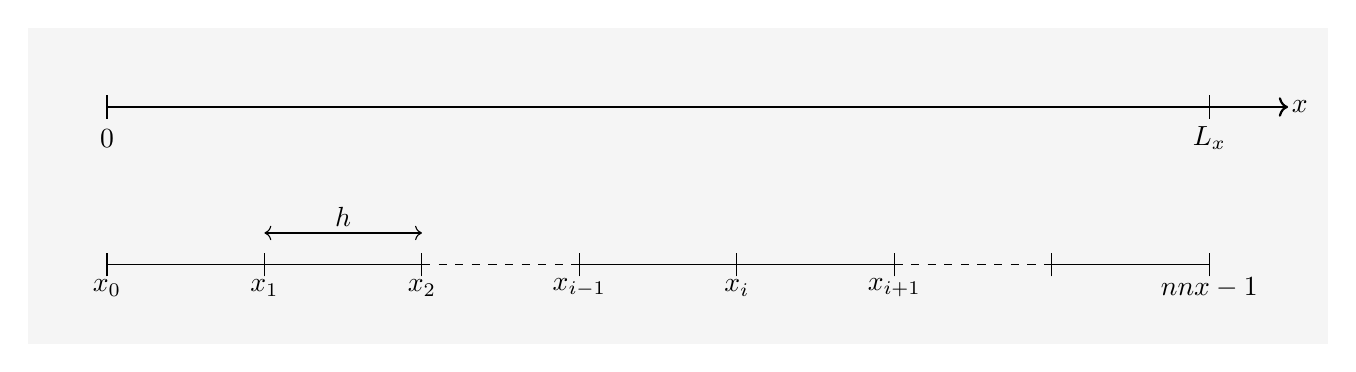
\begin{tikzpicture}
\draw[fill=gray!8,gray!8](0,0) rectangle (16.5,4);
%\draw[step=0.5cm,gray,very thin] (0,0) grid (16.5,4); %background grid
\node[] at (16.15,3) {$x$};
\node[] at (1,2.6) {$0$};
\node[] at (15,2.6) {$L_x$};
\draw[-] (1,2.85) -- (1,3.15) ; 
\draw[-] (15,2.85) -- (15,3.15) ; 
\draw[thick,->] (1,3) -- (16,3) ; 

%\draw[fill=gray!13,gray!13](1,1) rectangle (8,3);
%\draw[thick] (1,1) -- (5,1) -- (5,4) -- (1,4) -- cycle;  

\draw[-] (1,1) -- (5,1) ; 
\draw[dashed] (5,1) -- (7,1) ; 
\draw[-] (7,1) -- (11,1) ; 
\draw[dashed] (11,1) -- (13,1) ; 
\draw[-] (13,1) -- (15,1) ; 

\draw[-] (1,0.85) -- (1,1.15) ; 
\draw[-] (3,0.85) -- (3,1.15) ; 
\draw[-] (5,0.85) -- (5,1.15) ; 
\draw[-] (7,0.85) -- (7,1.15) ; 
\draw[-] (9,0.85) -- (9,1.15) ; 
\draw[-] (11,0.85) -- (11,1.15) ; 
\draw[-] (13,0.85) -- (13,1.15) ; 
\draw[-] (15,0.85) -- (15,1.15) ; 

\node[] at (7,0.7) {$x_{i-1}$};
\node[] at (9,0.7) {$x_i$};
\node[] at (11,0.7) {$x_{i+1}$};

\node[] at (1,0.7) {$x_0$};
\node[] at (3,0.7) {$x_1$};
\node[] at (5,0.7) {$x_2$};
\node[] at (15,0.7) {$nnx-1$};

\draw[<->] (3,1.4) -- (5,1.4) ; 
\node[] at (4,1.6) {$h$};

\end{tikzpicture}


\end{center}

The derivative of temperature with regards to time can be approximated
with a forward finite difference approximation {\it in time} as
\begin{equation}
\frac{\partial T}{\partial t} 
\simeq \frac{T_{i}^{n+1}-T_i^n}{t^{n+1}-t^n} 
= \frac{T_{i}^{n+1}-T_i^n}{\delta t} 
\end{equation}
where $\delta t$ is the time step, i.e. the time between two consecutive 
measurements (the equivalent of $h$ in space). 
In all that follows the subscript will always refer to space indices 
while the superscript will always refer to time indices.
To be clear: $n$ represents the current time step whereas $n+1$
represents the next time step. 

Both $n$ and $i$ are integers; $n$ varies from 0 to $nstep-1$ (total number of time steps)
and $i$ varies from 0 to $nnx-1$ (where $nnx$ is the total number of grid points in $x$-direction).

The spatial derivative is replaced by a central FD approximation
\begin{eqnarray}
\frac{\partial^2 T}{\partial x^2} 
\simeq \frac{T_{i+1}^n - 2T_i^n + T_{i-1}^n}{h^2}
\end{eqnarray}
We obtain
\begin{eqnarray}
\frac{T_{i}^{n+1}-T_i^n}{\delta t} 
= \kappa \frac{T_{i+1}^n - 2T_i^n + T_{i-1}^n}{h^2}
\end{eqnarray}
and finally
\begin{eqnarray}
\boxed{
T_i^{n+1}=T_i^n + \delta t \; \kappa \frac{T_{i+1}^n - 2T_i^n + T_{i-1}^n}{h^2}
}
\end{eqnarray}

Because the temperature at the current time step $n$ is known,
we can compute the new temperature without solving any additional equations.
Such a scheme is an {\bf explicit} finite difference method and
was made possible by the choice to evaluate the temporal derivative with forward differences.

\begin{center}


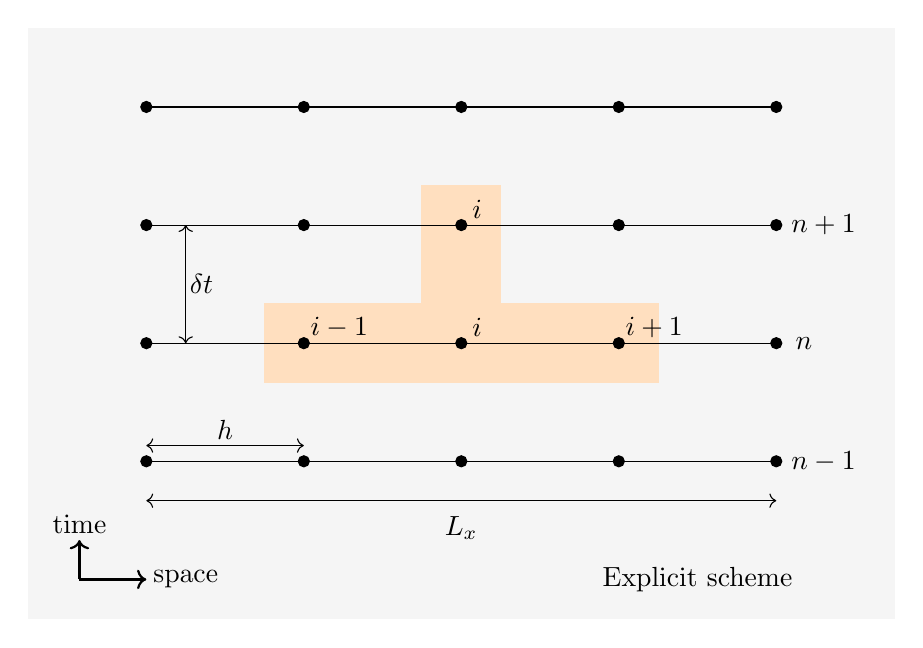
\begin{tikzpicture}
\draw[fill=gray!8,gray!8](-0.5,0) rectangle (10.5,7.5);


\draw[fill=orange,orange!25](2.5,3) rectangle (7.5,4);
\draw[fill=orange,orange!25](4.5,4) rectangle (5.5,5.5);
%\draw[step=0.5cm,gray,very thin] (0,0) grid (10.5,7.5); %background grid

\draw[black,fill=black] (1,2)  circle (2pt);
\draw[black,fill=black] (3,2)  circle (2pt);
\draw[black,fill=black] (5,2)  circle (2pt);
\draw[black,fill=black] (7,2)  circle (2pt);
\draw[black,fill=black] (9,2)  circle (2pt);

\draw[black,fill=black] (1,3.5)  circle (2pt);
\draw[black,fill=black] (3,3.5)  circle (2pt);
\draw[black,fill=black] (5,3.5)  circle (2pt);
\draw[black,fill=black] (7,3.5)  circle (2pt);
\draw[black,fill=black] (9,3.5)  circle (2pt);

\draw[black,fill=black] (1,5)  circle (2pt);
\draw[black,fill=black] (3,5)  circle (2pt);
\draw[black,fill=black] (5,5)  circle (2pt);
\draw[black,fill=black] (7,5)  circle (2pt);
\draw[black,fill=black] (9,5)  circle (2pt);

\draw[black,fill=black] (1,6.5)  circle (2pt);
\draw[black,fill=black] (3,6.5)  circle (2pt);
\draw[black,fill=black] (5,6.5)  circle (2pt);
\draw[black,fill=black] (7,6.5)  circle (2pt);
\draw[black,fill=black] (9,6.5)  circle (2pt);

\draw[-] (1,2) -- (9,2) ;
\draw[-] (1,3.5) -- (9,3.5) ;
\draw[-] (1,5) -- (9,5) ;
\draw[-] (1,6.5) -- (9,6.5) ;

\draw[<->] (1,2.2) -- (3,2.2) ;
\node[] at (2,2.4) {$h$};

\draw[<->] (1.5,3.5) -- (1.5,5) ;
\node[] at (1.7,4.25) {$\delta t$};

\draw[<->] (1,1.5) -- (9,1.5) ;
\node[] at (5,1.15) {$L_x$};

\draw[thick,->] (0.15,0.5) -- (1,0.5) ;
\draw[thick,->] (0.15,0.5) -- (0.15,1) ;
\node[] at (1.5,0.5) {space};
\node[] at (0.15,1.2) {time};

\node[] at (3.45,3.7) {$i-1$};
\node[] at (5.2,3.7) {$i$};
\node[] at (7.45,3.7) {$i+1$};
\node[] at (5.2,5.2) {$i$};

\node[] at (9.6,2) {$n-1$};
\node[] at (9.35,3.5) {$n$};
\node[] at (9.6,5) {$n+1$};

\node[] at (8,0.5) {Explicit scheme};
\end{tikzpicture}
                                      


\end{center}

\noindent In order to solve the original PDE equation we need to
\begin{itemize}
\item prescribe an initial temperature field
\item prescribe two boundary conditions 
\end{itemize}
Such requirements hold also in the discrete world. 

We know that this numerical scheme will converge to the exact solution for
small $h$ and $\delta t$ because it has been shown to be {\color{olive}consistent} - 
that its discretization process
can be reversed, through a Taylor series expansion, to recover the governing partial differential equation -
and because it is {\color{olive}stable} for certain values of
$h$ and $\delta t$: any spontaneous perturbations in the solution (such as round-off error) 
will either be bounded or will decay.

%-/-/-/-/-/-/-/-/-/-/-/-/-/-/-/-/-/-/-/
\begin{center}
\begin{minipage}[t]{0.77\textwidth}
\par\noindent\rule{\textwidth}{0.4pt}
{\color{blue} Example FDM-2}: let us prescribe an initial temperature field $T_i^0$ for $i=0,nnx-1$.
For example:

\begin{center}


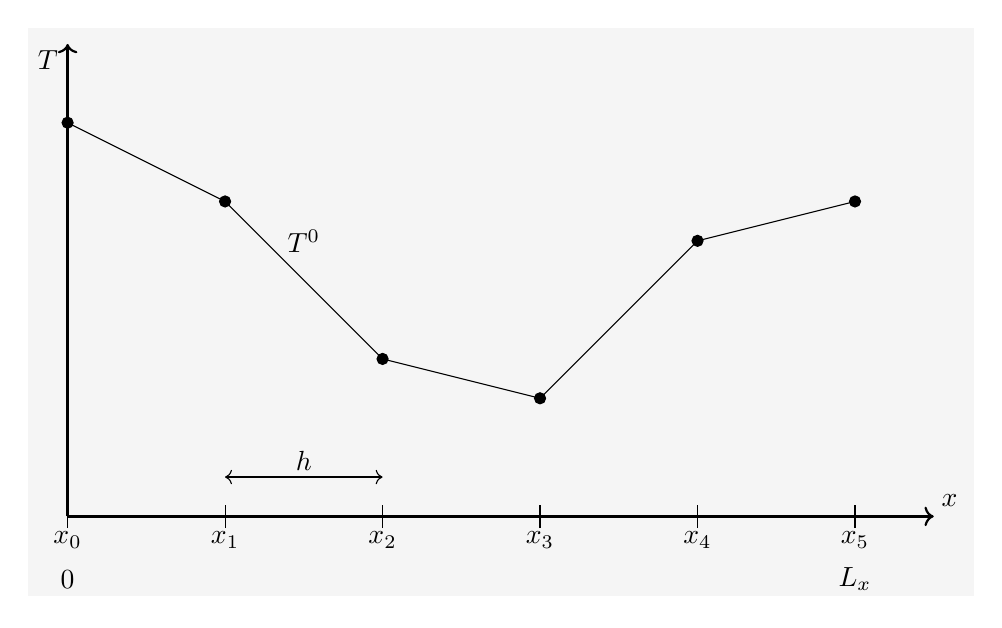
\begin{tikzpicture}
\draw[fill=gray!8,gray!8](0.5,0) rectangle (12.5,7.2);
%\draw[step=0.5cm,gray,very thin] (0,0) grid (13,7); %background grid

\draw[thick,->] (1,1) -- (12,1) ; 
\draw[thick,->] (1,1) -- (1,7) ; 


\node[] at (12.2,1.2) {$x$};
\node[] at (1,0.2) {$0$};
\node[] at (11,0.2) {$L_x$};
\node[] at (0.75,6.8) {$T$};

\draw[black,fill=black] (1,6)  circle (2pt);
\draw[black,fill=black] (3,5)  circle (2pt);
\draw[black,fill=black] (5,3)  circle (2pt);
\draw[black,fill=black] (7,2.5)  circle (2pt);
\draw[black,fill=black] (9,4.5)  circle (2pt);
\draw[black,fill=black] (11,5)  circle (2pt);

\draw[-] (1,6) -- (3,5) -- (5,3) -- (7,2.5) -- (9,4.5) -- (11,5); 
\node[] at (4,4.5) {$T^0$};

\draw[-] (1,0.85) -- (1,1.15) ; 
\draw[-] (3,0.85) -- (3,1.15) ; 
\draw[-] (5,0.85) -- (5,1.15) ; 
\draw[-] (7,0.85) -- (7,1.15) ; 
\draw[-] (9,0.85) -- (9,1.15) ; 
\draw[-] (11,0.85) -- (11,1.15) ; 
\node[] at (1,0.7) {$x_0$};
\node[] at (3,0.7) {$x_1$};
\node[] at (5,0.7) {$x_2$};
\node[] at (7,0.7) {$x_3$};
\node[] at (9,0.7) {$x_4$};
\node[] at (11,0.7) {$x_5$};
\draw[<->] (3,1.5) -- (5,1.5) ;  
\node[] at (4,1.7) {$h$};
\end{tikzpicture}


\end{center}

Then, we will be able to compute the new temperature of (for example) 
node 3 at time $t=1\cdot \delta t$ 
(i.e. $T_3^1$) with 
\begin{equation}
T_3^{1}=T_3^0 + \delta t \; \kappa \frac{T_{4}^0 - 2T_3^0 + T_{2}^0}{h^2}
\end{equation}
Note that $T_0$ and $T_5$ cannot be computed by means of the above equation, 
which is not a problem because both these values are actually the prescribed 
boundary conditions. 

\par\noindent\rule{\textwidth}{0.4pt}
\end{minipage}
\end{center}
%-/-/-/-/-/-/-/-/-/-/-/-/-/-/-/-/-/-/-/

\noindent The main drawback of the explicit approach is that stable solutions are
obtained {\it only} when
\begin{equation}
0 < \frac{2\kappa \delta t}{h^2} \leq1
\qquad
\text{or,}
\qquad
\delta t \leq \frac{h^2}{2 \kappa}
\end{equation}
If this condition is not satisfied, the solution becomes {\color{olive} unstable}, starts to
wildly oscillate and ultimately 'blows up'. We will observe this during the practicals. 

The stability condition means that the maximum time step needs to be smaller than the time it
takes for an anomaly to diffuse across the grid (nodal) spacing $h$.
The explicit solution is an example of a {\color{olive} conditionally stable method}
that only leads to well behaved solutions if a criterion like the one above is satisfied.

%-/-/-/-/-/-/-/-/-/-/-/-/-/-/-/-/-/-/-/-/-/
\begin{center}
\begin{minipage}[t]{0.77\textwidth}
\par\noindent\rule{\textwidth}{0.4pt}

\begin{center}
\includegraphics[width=0.8cm]{images/garftr} \\
{\color{orange}Exercise FDM-2}
\end{center}

We are going to solve the 1D diffusion equation with the explicit method
for the following physical setup: The domain is $L_x=1$km long, 
it is maintained at a temperature $T=100\degree$C at $x=0$ and at a temperature
$T=200\degree$C at $x=L_x$. The initial temperature is $T(x,t=0)=123$
and $\kappa=10^{-6}$. 
Time stepping will be carried out until steady state is reached.

$\rightarrow$ 
\href{http://cedricthieulot.net/images/compgeo/Exercise_2_FDM.ipynb}
{\tt Exercise\_2\_FDM.ipynb}

\par\noindent\rule{\textwidth}{0.4pt}
\end{minipage}
\end{center}
%-/-/-/-/-/-/-/-/-/-/-/-/-/-/-/-/-/-/-/-/-/

\noindent An alternative approach is an {\bf implicit} finite difference scheme, where the spatial derivatives
of the Laplacian are evaluated (at least partially) at the new time step.
We then use the backward difference for the time derivative:
\begin{equation}
\frac{\partial T}{\partial t} = \frac{T_{i}^{n}-T_i^{n-1}}{\delta t} 
\end{equation}
so that
\begin{equation}
\frac{T_{i}^{n}-T_i^{n-1}}{\delta t} = \kappa \frac{T_{i+1}^n - 2T_i^n + T_{i-1}^n}{h^2}
\end{equation}
Note that this is often rewritten as follows in order to keep the unknwowns at time $n+1$:
\begin{equation}
\frac{T_{i}^{n+1}-T_i^{n}}{\delta t} = \kappa \frac{T_{i+1}^{n+1} - 2T_i^{n+1} + T_{i-1}^{n+1}}{h^2}
\end{equation}

It is a fully implicit scheme where the time derivative is taken backward.
Let us define the dimensionless parameter $s$ as follows:
\begin{equation}
s=\frac{\kappa \; \delta t}{h^2}
\end{equation}
The previous equation can be rearranged as follows:
\begin{equation}
\boxed{
-s \; T_{i+1}^{n+1} + (1+2s)\; T_{i}^{n+1} - s\; T_{i-1}^{n+1} = T_i^{n}
}
\end{equation}

\begin{center}
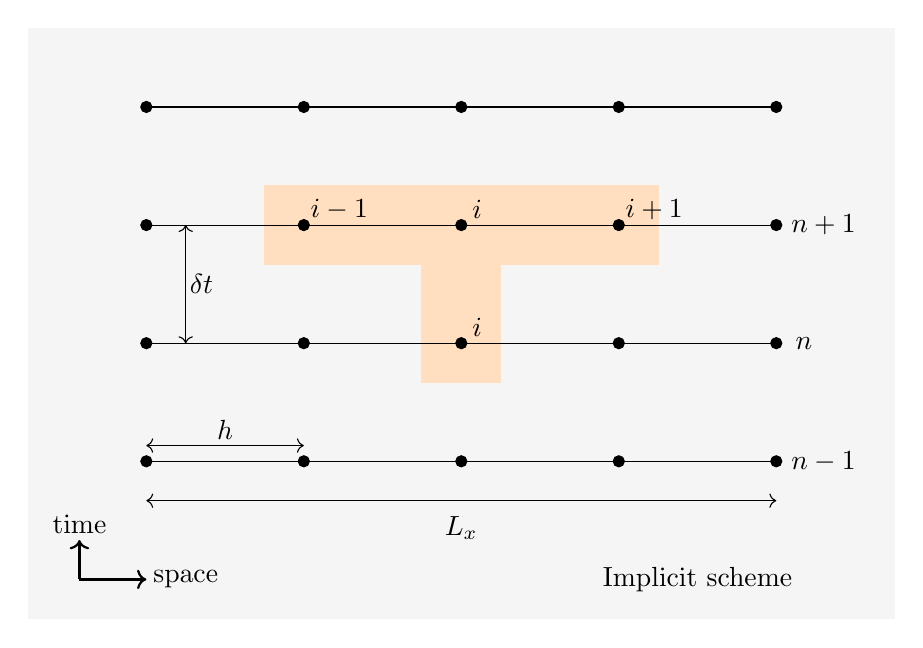
\begin{tikzpicture}
\draw[fill=gray!8,gray!8](-0.5,0) rectangle (10.5,7.5);

\draw[fill=orange,orange!25](2.5,4.5) rectangle (7.5,5.5);
\draw[fill=orange,orange!25](4.5,3) rectangle (5.5,4.5);
%\draw[step=0.5cm,gray,very thin] (0,0) grid (10.5,7.5); %background grid

\draw[black,fill=black] (1,2)  circle (2pt);
\draw[black,fill=black] (3,2)  circle (2pt);
\draw[black,fill=black] (5,2)  circle (2pt);
\draw[black,fill=black] (7,2)  circle (2pt);
\draw[black,fill=black] (9,2)  circle (2pt);

\draw[black,fill=black] (1,3.5)  circle (2pt);
\draw[black,fill=black] (3,3.5)  circle (2pt);
\draw[black,fill=black] (5,3.5)  circle (2pt);
\draw[black,fill=black] (7,3.5)  circle (2pt);
\draw[black,fill=black] (9,3.5)  circle (2pt);

\draw[black,fill=black] (1,5)  circle (2pt);
\draw[black,fill=black] (3,5)  circle (2pt);
\draw[black,fill=black] (5,5)  circle (2pt);
\draw[black,fill=black] (7,5)  circle (2pt);
\draw[black,fill=black] (9,5)  circle (2pt);

\draw[black,fill=black] (1,6.5)  circle (2pt);
\draw[black,fill=black] (3,6.5)  circle (2pt);
\draw[black,fill=black] (5,6.5)  circle (2pt);
\draw[black,fill=black] (7,6.5)  circle (2pt);
\draw[black,fill=black] (9,6.5)  circle (2pt);

\draw[-] (1,2) -- (9,2) ;
\draw[-] (1,3.5) -- (9,3.5) ;
\draw[-] (1,5) -- (9,5) ;
\draw[-] (1,6.5) -- (9,6.5) ;

\draw[<->] (1,2.2) -- (3,2.2) ;
\node[] at (2,2.4) {$h$};

\draw[<->] (1.5,3.5) -- (1.5,5) ;
\node[] at (1.7,4.25) {$\delta t$};

\draw[<->] (1,1.5) -- (9,1.5) ;
\node[] at (5,1.15) {$L_x$};

\draw[thick,->] (0.15,0.5) -- (1,0.5) ;
\draw[thick,->] (0.15,0.5) -- (0.15,1) ;
\node[] at (1.5,0.5) {space};
\node[] at (0.15,1.2) {time};

\node[] at (3.45,5.2) {$i-1$};
\node[] at (5.2,3.7) {$i$};
\node[] at (7.45,5.2) {$i+1$};
\node[] at (5.2,5.2) {$i$};

\node[] at (9.6,2) {$n-1$};
\node[] at (9.35,3.5) {$n$};
\node[] at (9.6,5) {$n+1$};

\node[] at (8,0.5) {Implicit scheme};
\end{tikzpicture}
                                                                                                                                                                                                                 



\end{center}



Note that in this case we no longer have an explicit relationship for 
$T^{n+1}_{i-1}$, $T^{n+1}_i$ and $T^{n+1}_{i+1}$.
Instead, we have to solve a {\color{olive}linear system of equations}, which is discussed further below.

The main advantage of implicit methods is that there are no restrictions on the time step,
the fully implicit scheme is {\bf unconditionally stable}.
This does not mean that it is accurate. 
Taking large time steps may result in an inaccurate solution for features with
small spatial scales!

For any application, it is therefore always a good idea to check the 
results by decreasing the time step
until the solution does not change anymore (this is called a {\color{olive}convergence check}), and 
to ensure the
method can deal with small and large scale features robustly at the same time.


%-/-/-/-/-/-/-/-/-/-/-/-/-/-/-/-/-/-/-
\begin{center}
\begin{minipage}[t]{0.77\textwidth}
\par\noindent\rule{\textwidth}{0.4pt}
{\color{blue} Example FDM-3}: 
Once again let us look at things with a very concrete approach. Let us discretise the 
domain of length $L_x$ with 6 cells, i.e. $i=0,\dots 6$ ($nnx=7$).
We also prescribe the following boundary conditions (remember it is a 2nd order derivative in space, 
so we need two of them): $T(x=0)=T_0=0$ and $T(x=L_x)=T_6=100$ (we assume that they 
do not change with time for simplicity). Finally we assume that we 
know $T_i^0$ for all $i$ and we wish to compute $T_i^1$.

We then have:
\begin{eqnarray}
T_0^1 &=& 0 \nn\\
-s T_{2}^{1} + (1+2s) T_{1}^{1} - s T_{0}^{1} &=& T_1^{0} \nn\\
-s T_{3}^{1} + (1+2s) T_{2}^{1} - s T_{1}^{1} &=& T_2^{0} \nn\\
-s T_{4}^{1} + (1+2s) T_{3}^{1} - s T_{2}^{1} &=& T_3^{0} \nn\\
-s T_{5}^{1} + (1+2s) T_{4}^{1} - s T_{3}^{1} &=& T_4^{0} \nn\\
-s T_{6}^{1} + (1+2s) T_{5}^{1} - s T_{4}^{1} &=& T_5^{0} \nn\\
T_6^1 &=& 100
\end{eqnarray}
or, 
\begin{equation}
\underbrace{
\left(
\begin{array}{ccccccc}
1 & 0 & 0 & 0 & 0 & 0 & 0  \\
-s & 1+2s & -s & 0 & 0 & 0 & 0 \\
0 & -s & 1+2s & -s & 0 & 0 & 0 \\
0 & 0 & -s & 1+2s & -s & 0 & 0 \\
0 & 0 & 0 & -s & 1+2s & -s & 0 \\
0 & 0 & 0 & 0 & -s & 1+2s & -s \\
0 & 0 & 0 & 0 & 0 & 0 & 1
\end{array}
\right)
}_{\bm A}
\cdot
\underbrace{
\left(
\begin{array}{ccccccc}
T_0^1 \\ T_1^1 \\ T_2^1 \\ T_3^1 \\ T_4^1 \\ T_5^1 \\ T_6^1  
\end{array}
\right)
}_{\vec{T}}
=
\underbrace{
\left(
\begin{array}{ccccccc}
0 \\ T_1^0\\ T_2^0\\ T_3^0\\ T_4^0\\ T_5^0 \\ 100
\end{array}
\right)
}_{\vec{b}} \nn
\end{equation}

As opposed to the explicit approach we must solve a linear system which size is given 
by the total number of nodes/points $nnx$ in order to compute a new temperature field.

\par\noindent\rule{\textwidth}{0.4pt}
\end{minipage}
\end{center}
%-/-/-/-/-/-/-/-/-/-/-/-/-/-/-/-/-/-/-

\noindent In summary, an implicit method requires us to solve ${\bm A}\cdot\vec{T} = \vec{b}$ with
\begin{itemize}
\item ${\bm A}$ is a $nnx \times nnx$  {\color{olive}sparse} matrix (i.e. mostly empty),
\item ${\vec b}$ is a known vector of size $nnx$ (often called the 'right-hand side', or {\color{olive} rhs})
\item ${\vec T}$ the vector of unknowns.
\end{itemize}

%..................................
\paragraph{A word about solvers}
There are two main approaches to solving such a linear system: one can use a {\color{olive} direct}
approach or an {\color{olive} iterative} approach. 
In a nutshell, a direct solver will 'manipulate' the matrix lines and columns 
so as to arrive at the solution. A simple example of such an approach is the 
technique of elimination of variables:

\begin{center}
\begin{minipage}[t]{0.77\textwidth}
\par\noindent\rule{\textwidth}{0.4pt}
{\color{blue} Example FDM-4}:
Consider the following system:
\begin{equation}
\left(
\begin{array}{ccc}
1 & 3 & -2 \\
3 & 5 & 6 \\
2 & 4 & 3
\end{array}
\right)
\cdot
\left(
\begin{array}{c}
x \\ y \\ z
\end{array}
\right)
=
\left(
\begin{array}{c}
5 \\ 7 \\ 8
\end{array}
\right)
\end{equation}
which is of course equivalent to
\begin{eqnarray}
x+3y-2z &=& 5 \nn\\
3x+5y+6z &=& 7 \nn\\
2x+4y+3z &=& 8 
\end{eqnarray}
Solving the first equation for $x$ gives $x = 5 + 2z - 3y$, 
and plugging this into the second and third equation yields
(or take the second line of the matrix and remove 3 times the 
first line from it, etc ...)
\begin{equation}
\left(
\begin{array}{ccc}
1 & 3 & -2 \\
0 & -4 & 12 \\
0 & -2 & 7
\end{array}
\right)
\cdot
\left(
\begin{array}{c}
x \\ y \\ z
\end{array}
\right)
=
\left(
\begin{array}{c}
5 \\ -8 \\ -2 
\end{array}
\right)
\end{equation}
Solving the second line for $y$ yields $y = 2 + 3z$, 
and plugging this into the second equation yields $z = 2$. We now have: 
\begin{equation}
\left(
\begin{array}{ccc}
1 & 3 & -2 \\
0 & -4 & 12 \\
0 & 0 & 2
\end{array}
\right)
\cdot
\left(
\begin{array}{c}
x \\ y \\ z
\end{array}
\right)
=
\left(
\begin{array}{c}
5 \\ -8 \\ 4
\end{array}
\right)
\end{equation}
Substituting $z = 2$ into the second equation gives $y = 8$, 
and substituting $z = 2$ and $y = 8$ into the first equation yields $x = -15$. 
Therefore, the solution set is the single point $(x, y, z) = (-15, 8, 2)$.

{\tiny Taken from \url{https://en.wikipedia.org/wiki/System_of_linear_equations}} 
\par\noindent\rule{\textwidth}{0.4pt}
\end{minipage}
\end{center}

This example is of course very naive and direct solvers often come in 
the form of very large numerical libraries which have been highly optimised to take advantage of the 
sparsity of the matrix in order to arrive at the solution in the lowest 
number of operations possible. 
In reality techniques such as LU decomposition or Cholesky decomposition are used. 
\index{general}{LU decomposition}
\index{general}{Cholesky decomposition}

Iterative solvers on the other hand compute the solution of the system 
by first postulating an initial guess for the solution and then by 
improving this guess iteratively until the {\color{olive} termination criterion}
is met (see Section~\ref{ss:itsolvers}). There are two classes of iteratives methods in this context: 
{\color{olive} stationary iterative methods} (e.g. Jacobi, Gauss-Seidel, SSOR) and 
{\color{olive} Krylov subspace methods} (e.g. CG, GMRES, BiCG).
At this stage things get real complicated and the details of iterative solvers 
are vastly out of the scope of this 
course\footnote{\url{https://en.wikipedia.org/wiki/Iterative_method}} \cite{saad}.     
\index{general}{BiCG solver}
\index{general}{Jacobi solver}
\index{general}{Gauss-Seidel solver}
\index{general}{GMRES solver}
\index{general}{CG solver}
\index{general}{SSOR solver}


%-/-/-/-/-/-/-/-/-/-/-/-/-/-/-/-/-/-/-/-/-/
\begin{center}
\begin{minipage}[t]{0.77\textwidth}
\par\noindent\rule{\textwidth}{0.4pt}
{\color{blue} Example FDM-5}: the stationary Jacobi method. 
The matrix ${\bm A}$ is decomposed as follows:
\begin{equation}
{\bm A} = {\bm D} + {\bm L} + {\bm U} 
\end{equation}
where ${\bm D}$ is the diagonal of the matrix ${\bm A}$, ${\bm L}$ is the 
strict lower triangular part of ${\bm A}$ and 
${\bm U}$ is the strict upper triangular part of ${\bm A}$.
The iterative method is defined by:
\begin{equation}
{\bm D} \cdot \vec{T}^{{\color{Fuchsia}k+1}} = -({\bm L} + {\bm U}) \cdot \vec{T}^{\color{Fuchsia}k} 
+ \vec{b}
\qquad k=0,1,\dots
\end{equation}
where $\vec{T}^{\color{Fuchsia}0}$ is the initial guess (often taken to be zero).
Note that the superscript denotes the iteration number and has nothing to 
do with the time step.
This method is trivial to implement since the linear system on the 
left side of the equal sign involves a diagonal matrix.
This can also be written 
\begin{equation}
T_i^{{\color{Fuchsia} k+1}} = \frac{1}{A_{ii}} \left(b_i - 
\sum_{j\neq i} A_{ij} T_j^{{\color{Fuchsia}k}} \right)
\qquad
i=1,2,...nnx
\end{equation}
Looking at the previous example, we have 
\begin{equation}
{\bm D}=
\left(
\begin{array}{ccc}
1 & 0 & 0 \\
0 & 5 & 0 \\
0 & 0 & 3
\end{array}
\right)
\qquad
\text{and}
\qquad
{\bm L}+{\bm U}= 
\left(
\begin{array}{ccc}
0 & 3 & -2 \\
3 & 0 & 6 \\
2 & 4 & 0
\end{array}
\right)
\end{equation}
We then start with the guess $\vec{T}^{\color{Fuchsia}0}=\vec{0}$, so that for ${\color{Fuchsia}k}=0$:
\begin{equation}
\vec{T}^{\color{Fuchsia}1} = {\bm D}^{-1}\cdot \vec{b} = 
\left(
\begin{array}{ccc}
1 & 0 & 0 \\
0 & 1/5 & 0 \\
0 & 0 & 1/3
\end{array}
\right)
\cdot 
\left(
\begin{array}{c}
5 \\ 7 \\ 8
\end{array}
\right)
=
\left(
\begin{array}{c}
5 \\ 7/5 \\ 8/3
\end{array}
\right)
\end{equation}
and then we obtain $\vec{T}^{\color{Fuchsia}2}$ by solving 
\begin{eqnarray}
\vec{T}^{\color{Fuchsia}2} 
&=& {\bm D}^{-1} \cdot \left[-({\bm L} + {\bm U}) 
\cdot \vec{T}^{\color{Fuchsia}1} + \vec{b} \right] \nn\\
&=&
\left(
\begin{array}{ccc}
1 & 0 & 0 \\
0 & 1/5 & 0 \\
0 & 0 & 1/3
\end{array}
\right)
\cdot 
\left[
-
\left(
\begin{array}{ccc}
0 & 3 & -2 \\
3 & 0 & 6 \\
2 & 4 & 0
\end{array}
\right)
\cdot
\left(
\begin{array}{c}
5 \\ 7/5 \\ 8/3
\end{array}
\right)
+
\left(
\begin{array}{c}
5 \\ 7 \\ 8
\end{array}
\right)
\right] \nn\\
&=&
\dots  
\end{eqnarray}
We keep iterating until two consecutively obtained 
temperature vectors are nearly identical, or, 
\begin{equation}
\| \vec{T}^{\color{Fuchsia}k+1}-\vec{T}^{\color{Fuchsia}k} \| < \epsilon
\end{equation}
where $\epsilon$ is a carefully chosen small enough number. 

A sufficient (but not necessary) condition for the method to converge is that 
the matrix ${\bm A}$ is strictly or irreducibly diagonally dominant. 
Strict row diagonal dominance means that for each row, the absolute value of 
the diagonal term is greater than the sum of absolute values of other 
terms $|a_{ii}|>\sum_{j\neq i} |a_{ij}| $.
Also, this algorithm will fail if one or more diagonal terms of ${\bm A}$ is nul.

\par\noindent\rule{\textwidth}{0.4pt}
\end{minipage}
\end{center}
%-/-/-/-/-/-/-/-/-/-/-/-/-/-/-/-/-/-/-/-/-/


%-/-/-/-/-/-/-/-/-/-/-/-/-/-/-/-/-/-/-/
\begin{center}
\begin{minipage}[t]{0.77\textwidth}
\par\noindent\rule{\textwidth}{0.4pt}

\begin{center}
\includegraphics[width=0.8cm]{images/garftr} \\
{\color{orange}Exercise FDM-3}
\end{center}

Implement example FDM-5 from scratch in a new notebook.
Write a separate function for the Jacobi solver.
What do you observe ? why does it explode? 
Multiply all diagonal values by 10 and re-run it. 
What do you observe now? 

Bonus: implement the Gauss-Seidel method.
Which of the two methods converges the fastest?\\
$\rightarrow$\url{https://en.wikipedia.org/wiki/Iterative_method}. 
\par\noindent\rule{\textwidth}{0.4pt}
\end{minipage}
\end{center}
%-/-/-/-/-/-/-/-/-/-/-/-/-/-/-/-/-/-/-/


\noindent
Finally, looking at
\begin{equation}
-s\;  T_{i+1}^{n+1} + (1+2s)\;  T_{i}^{n+1} - s\;  T_{i-1}^{n+1} = T_i^{n}
\end{equation}
and dividing by $-s$ and letting $\delta t \rightarrow \infty$, we obtain:
\begin{equation}
T_{i+1}^{n+1} -2 T_{i}^{n+1} + T_{i-1}^{n+1} = 0
\end{equation}
which is a central difference approximation of the steady state solution
\begin{equation}
\frac{\partial^2 T }{\partial x^2}=0
\end{equation}
Therefore, the fully implicit scheme will always yield the right equilibrium solution 
but may not capture small scale, transient features.


%-/-/-/-/-/-/-/-/-/-/-/-/-/-/-/-/-/-/-/
\begin{center}
\begin{minipage}[t]{0.77\textwidth}
\par\noindent\rule{\textwidth}{0.4pt}

\begin{center}
\includegraphics[width=0.8cm]{images/garftr} \\
{\color{orange}Exercise FDM-4}
\end{center}

This is exactly the same exercise as Exercise 2 but we 
are going to solve the 1D diffusion equation with the implicit method
this time. First use a solver from scipy to solve the system, then 
implement your own Jacobi solver. Note that the Jacobi solver must be 
implemented as a function which is to be called inside the time loop.

In your notebook use an if statement which allows to choose between 
explicit and implicit, and another if statement which allows to choose 
between scipy solver and iterative solver. 

Bonus: implement the SSOR method in another function and compare Jacobi, Gauss-Seidel and SSOR.\\
$\rightarrow$\url{https://en.wikipedia.org/wiki/Iterative_method}

\par\noindent\rule{\textwidth}{0.4pt}
\end{minipage}
\end{center}
%-/-/-/-/-/-/-/-/-/-/-/-/-/-/-/-/-/-/-/


\paragraph{Crank-Nicolson scheme} \index{general}{Crank-Nicolson}
It turns out that this fully implicit method is second order accurate in space but 
only first order accurate in time,
i.e. the error goes as ${\cal O}(h^2,\delta t)$.   

It is possible to write down a scheme which is second order accurate both in time and in space
(i.e. ${\cal O}(h^2, \delta t^2))$, e.g. the {\color{olive}Crank-Nicolson}
\footnote{
The method was developed by John Crank and Phyllis Nicolson 
in the mid 20th century. \url{https://en.wikipedia.org/wiki/Crank-Nicolson_method}
}
scheme which is unconditionally stable. 

The Crank-Nicolson method is the time analog of central spatial differences and is given by
\begin{equation}
\frac{T_{i}^{n+1}-T_i^n}{\delta t} 
= \kappa  \frac{1}{2} \left[
\underbrace{\frac{T_{i+1}^{n} - 2T_i^{n} + T_{i-1}^{n}}{h^2}}_{\text{at time } n}
+
\underbrace{\frac{T_{i+1}^{n+1} - 2T_i^{n+1} + T_{i-1}^{n+1}}{h^2}}_{\text{at time } n+1}
\right]
\end{equation}
We define $s=\kappa \delta t/ 2h^2$ so that the equation above can be rearranged as follows :
\begin{equation}
\boxed{
-s\; T_{i+1}^{n+1} + (1+2s)\;  T_{i}^{n+1} 
-s\;  T_{i-1}^{n+1} = 
s\; T_{i+1}^{n} + (1-2s)\; T_{i}^{n} + s\; T_{i-1}^{n} 
}
\end{equation}

Any partially implicit method is more complicated to compute as we need to infer the future solution 
at time $n+1$ by solution (inversion) of a system of linear equations based on the known solution at time $n$. 

\begin{center}

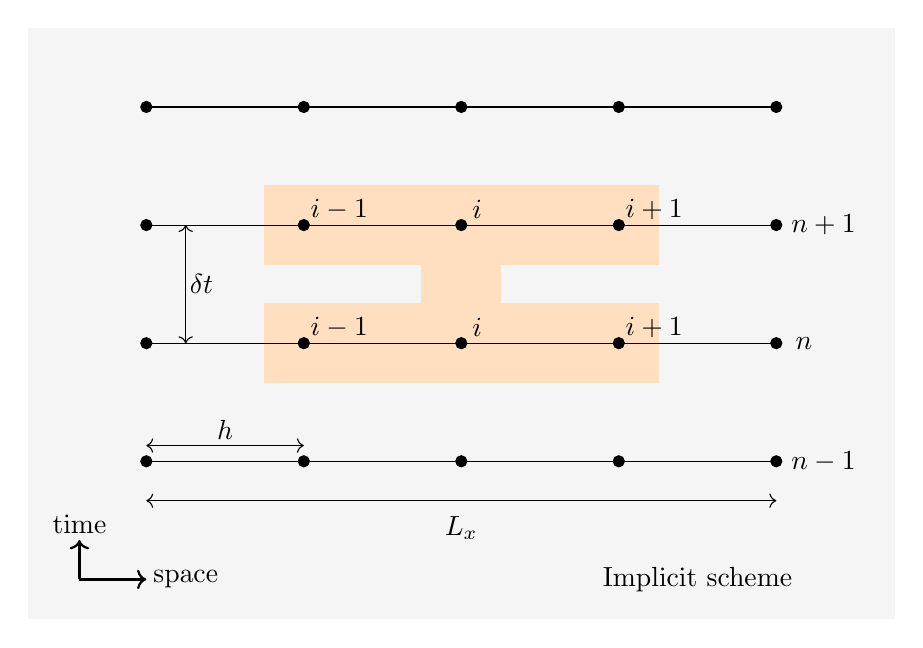
\begin{tikzpicture}
\draw[fill=gray!8,gray!8](-0.5,0) rectangle (10.5,7.5);


\draw[fill=orange,orange!25](2.5,4.5) rectangle (7.5,5.5);
\draw[fill=orange,orange!25](4.5,3) rectangle (5.5,4.5);
\draw[fill=orange,orange!25](2.5,3) rectangle (7.5,4);

%\draw[step=0.5cm,gray,very thin] (0,0) grid (10.5,7.5); %background grid

\draw[black,fill=black] (1,2)  circle (2pt);
\draw[black,fill=black] (3,2)  circle (2pt);
\draw[black,fill=black] (5,2)  circle (2pt);
\draw[black,fill=black] (7,2)  circle (2pt);
\draw[black,fill=black] (9,2)  circle (2pt);

\draw[black,fill=black] (1,3.5)  circle (2pt);
\draw[black,fill=black] (3,3.5)  circle (2pt);
\draw[black,fill=black] (5,3.5)  circle (2pt);
\draw[black,fill=black] (7,3.5)  circle (2pt);
\draw[black,fill=black] (9,3.5)  circle (2pt);

\draw[black,fill=black] (1,5)  circle (2pt);
\draw[black,fill=black] (3,5)  circle (2pt);
\draw[black,fill=black] (5,5)  circle (2pt);
\draw[black,fill=black] (7,5)  circle (2pt);
\draw[black,fill=black] (9,5)  circle (2pt);

\draw[black,fill=black] (1,6.5)  circle (2pt);
\draw[black,fill=black] (3,6.5)  circle (2pt);
\draw[black,fill=black] (5,6.5)  circle (2pt);
\draw[black,fill=black] (7,6.5)  circle (2pt);
\draw[black,fill=black] (9,6.5)  circle (2pt);

\draw[-] (1,2) -- (9,2) ;
\draw[-] (1,3.5) -- (9,3.5) ;
\draw[-] (1,5) -- (9,5) ;
\draw[-] (1,6.5) -- (9,6.5) ;

\draw[<->] (1,2.2) -- (3,2.2) ;
\node[] at (2,2.4) {$h$};

\draw[<->] (1.5,3.5) -- (1.5,5) ;
\node[] at (1.7,4.25) {$\delta t$};

\draw[<->] (1,1.5) -- (9,1.5) ;
\node[] at (5,1.15) {$L_x$};

\draw[thick,->] (0.15,0.5) -- (1,0.5) ;
\draw[thick,->] (0.15,0.5) -- (0.15,1) ;
\node[] at (1.5,0.5) {space};
\node[] at (0.15,1.2) {time};

\node[] at (3.45,3.7) {$i-1$};
\node[] at (3.45,5.2) {$i-1$};
\node[] at (5.2,3.7) {$i$};
\node[] at (7.45,5.2) {$i+1$};
\node[] at (7.45,3.7) {$i+1$};
\node[] at (5.2,5.2) {$i$};

\node[] at (9.6,2) {$n-1$};
\node[] at (9.35,3.5) {$n$};
\node[] at (9.6,5) {$n+1$};

\node[] at (8,0.5) {Implicit scheme};
\end{tikzpicture}
                                                                                                                                                                                                                 




\end{center}

%-/-/-/-/-/-/-/-/-/-/-/-/-/-/-/-/-/-/
\begin{center}
\begin{minipage}[t]{0.77\textwidth}
\par\noindent\rule{\textwidth}{0.4pt}

\begin{center}
\includegraphics[width=0.8cm]{images/garftr} \\
{\color{orange}Exercise FDM-5}
\end{center}

Modify the code of Exercise FDM-4 to implement the Crank-Nicolson method.

\par\noindent\rule{\textwidth}{0.4pt}
\end{minipage}
\end{center}
%-/-/-/-/-/-/-/-/-/-/-/-/-/-/-/-/-/-/






\subsection{Solving the 1D advection equation} \label{ss:fdm_adv1D} 
%TODO to improve notes:
%use http://farside.ph.utexas.edu/teaching/329/lectures/node91.html
%


The 1D advection equation is:
\begin{equation}
\rho C_p \left( \frac{\partial T}{\partial t}  
+ u \frac{\partial T}{\partial x} \right)=0 
\end{equation}
or simply
\begin{equation}
\frac{\partial T}{\partial t} + u \frac{\partial T}{\partial x}=0 
\end{equation}
We have seen how to deal with the time derivative (explicit, implicit) 
and with the first order space derivative (forward, backward or central).
Let us consider the FTCS scheme (Forward in Time, Central in Space).
\[
\frac{T_{\color{teal}i}^{n+1}-T^n_{\color{teal}i}}{\delta t} 
+ u_i \frac{T^n_{\color{teal}i+1} - T^n_{{\color{teal}i-1}}}{2h} =0 
\]
Note that although the velocity $u$ is prescribed, it can vary in space, hence
the subscript $i$. 

There is however a major problem: 
the FTCS method is in this case {\bf unconditionally} unstable, i.e., it blows up for any $\delta t$.
The instability is related to the fact that this scheme produces negative diffusion, 
which is numerically unstable.

We will now look at to methods which alleviate this problem: the Lax method and the Streamline Upwind method.

The {\color{olive} Lax method} consists of replacing the $T_{\color{teal}i}^n$ 
in the time derivative term with $(T_{{\color{teal}i+1}}^n + T_{{\color{teal}i-1}}^n)/2$. 
The resulting equation is
\[
\frac{T_{\color{teal}i}^{n+1}-  (T_{{\color{teal}i+1}}^n + T_{{\color{teal}i-1}}^n)/2 }{\delta t} 
= - u_i \frac{T^n_{{\color{teal}i+1}}-T^n_{{\color{teal}i-1}}}{2 h_x}
\]
or, 
\[
T_{\color{teal}i}^{n+1} = \frac{1}{2} (T_{{\color{teal}i+1}}^n + T_{{\color{teal}i-1}}^n)  
- \frac{u_i \delta t}{h}  \frac{1}{2} (T^n_{{\color{teal}i+1}}-T^n_{{\color{teal}i-1}})
\]



In the {\color{olive}Streamline upwind} method the spatial finite difference scheme 
depends on the sign of the velocity:
\[
\frac{T_{\color{teal}i}^{n+1}-  (T_{{\color{teal}i+1}}^n + T_{{\color{teal}i-1}}^n)/2   }{\delta t} =
\left\{
\begin{array}{l}
 - u_i \frac{T^n_{{\color{teal}i}}-T^n_{{\color{teal}i-1}}}{h_x}  \quad\quad  {\rm if} \quad u_i<0\\ \\
 - u_i \frac{T^n_{{\color{teal}i+1}}-T^n_{{\color{teal}i}}}{h_x}  \quad\quad  {\rm if} \quad u_i>0
\end{array}
\right.
\]
In fact, we have replaced central with forward or backward derivatives, depending on the flow direction. 


Finally, The Crank-Nicolson implicit scheme for solving the diffusion equation 
can be adapted to solve the advection equation:
\[
T_{\color{teal}i}^{n+1} + \frac{u \delta t}{4h} (T_{{\color{teal}i+1}}^{n+1}-T_{{\color{teal}i-1}}^{n+1}) 
= T_{\color{teal}i}^n - \frac{u \delta t}{4h} (T_{{\color{teal}i+1}}^{n}-T_{{\color{teal}i-1}}^{n}) 
\]
TODO: write about how we obtain this.


%-/-/-/-/-/-/-/-/-/-/-/-/-/-/-/-/-/-/-/
\begin{center}
\begin{minipage}[t]{0.77\textwidth}
\par\noindent\rule{\textwidth}{0.4pt}

\begin{center}
\includegraphics[width=0.8cm]{images/garftr} \\
{\color{orange}Exercise FDM-6}
\end{center}

Let us consider the domain $[0,1]$. The temperature field at $t=0$ is 
given by $T=1$ for $x<0.25$ and $T=0$ otherwise. The prescribed 
velocity is $u=1$ and we set $nnx=51$.
Boundary conditions are $T=1$ at $x=0$ and $T=0$ at $x=1$.

\begin{center}

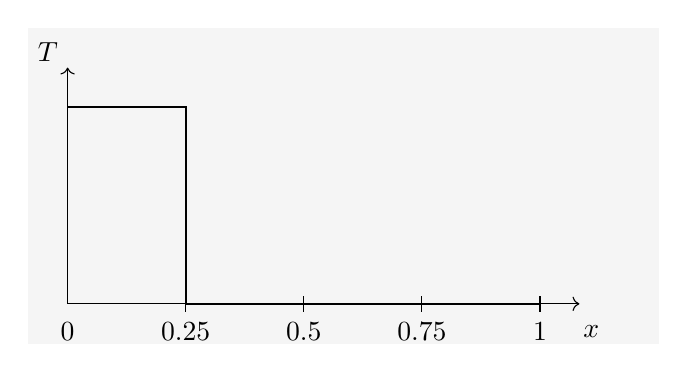
\begin{tikzpicture}
\draw[fill=gray!8,gray!8](0,0) rectangle (8,4);
%\draw[step=0.5cm,gray,very thin] (0,0) grid (8,4); %background grid

\draw[->] (0.5,0.5) -- (7,0.5) ; 
\node[] at (0.5,0.15) {$0$};

\node[] at (2,0.15) {$0.25$};
\node[] at (3.5,0.15) {$0.5$};
\node[] at (5,0.15) {$0.75$};
\node[] at (6.5,0.15) {$1$};
\draw[->] (0.5,0.5) -- (0.5,3.5) ; 
\node[] at (0.25,3.7) {$T$};


\draw[-] (2,0.4) -- (2,0.6) ; 
\draw[-] (3.5,0.4) -- (3.5,0.6) ; 
\draw[-] (5,0.4) -- (5,0.6) ; 
\draw[-] (6.5,0.4) -- (6.5,0.6) ; 


%\draw[-] (2,1) -- (1.75,0.75) ; 
%\draw[-] (2.5,1) -- (2.25,0.75) ; 
%\draw[-] (3,1) -- (2.75,0.75) ; 
%\draw[-] (3.5,1) -- (3.25,0.75) ; 
%\draw[-] (4,1) -- (3.75,0.75) ; 
%\draw[-] (4.5,1) -- (4.25,0.75) ; 

%---------------------------------

%\draw[thick,->] (7,1) -- (7,5) ; 
%\node[] at (6.6,4) {$L_y$};
%\node[] at (6.6,1) {$0$};
%\draw[-] (6.85,1) -- (7.15,1) ; 
%\draw[-] (6.85,4) -- (7.15,4) ; 
%\node[] at (7.6,4) {$p=0$};
%\node[] at (6.6,5) {$y$};

%---------------------------------

\draw[thick] (0.5,3) -- (2,3) -- (2,0.5) -- (6.5,0.5) ; 
\node[] at (7.15,0.15) {$x$};


\end{tikzpicture}



\end{center}

Program the above FTCS method. Run the model for 250 time steps with $\delta t=0.002$. 
Program the Lax method by modifying the previous code.\\
Bonus: Program the upwind method and/or the Crank-Nicolson method. 

\par\noindent\rule{\textwidth}{0.4pt}
\end{minipage}
\end{center}
%-/-/-/-/-/-/-/-/-/-/-/-/-/-/-/-/-/-/




\newpage
\subsection{FDM basics in 2D} \label{ss:fdm_basics2D} 
In a 2D Cartesian domain overlain by a $nnx \times nny$ grid, 
the spacing between nodes in the $x$ and $y$ direction is $h_x$ 
and $h_y$ respectively. 

\begin{center}


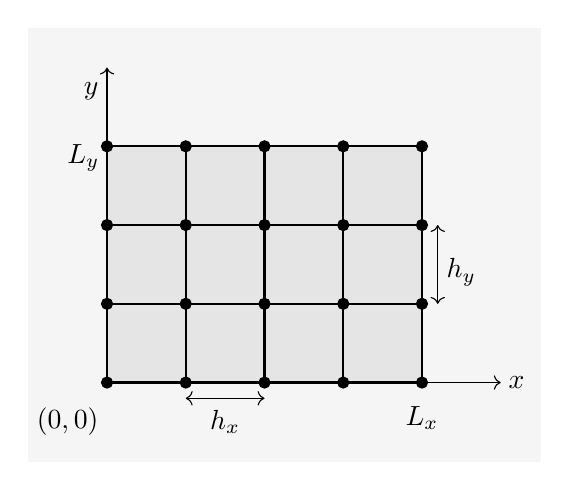
\begin{tikzpicture}
\draw[fill=gray!8,gray!8](0,0) rectangle (6.5,5.5);
%\draw[step=0.5cm,gray,very thin] (0,0) grid (8,5); %background grid


\draw[fill=gray!20,gray!20](1,1) rectangle (5,4);
\draw[thick] (1,1) -- (5,1) -- (5,4) -- (1,4) -- cycle;  

\draw[thick] (1,2) -- (5,2) ; 
\draw[thick] (1,3) -- (5,3) ; 
\draw[thick] (2,1) -- (2,4) ; 
\draw[thick] (3,1) -- (3,4) ; 
\draw[thick] (4,1) -- (4,4) ; 

\draw[black,fill=black] (1,1)  circle (2pt);
\draw[black,fill=black] (2,1)  circle (2pt);
\draw[black,fill=black] (3,1)  circle (2pt);
\draw[black,fill=black] (4,1)  circle (2pt);
\draw[black,fill=black] (5,1)  circle (2pt);
\draw[black,fill=black] (1,2)  circle (2pt);
\draw[black,fill=black] (2,2)  circle (2pt);
\draw[black,fill=black] (3,2)  circle (2pt);
\draw[black,fill=black] (4,2)  circle (2pt);
\draw[black,fill=black] (5,2)  circle (2pt);
\draw[black,fill=black] (1,3)  circle (2pt);
\draw[black,fill=black] (2,3)  circle (2pt);
\draw[black,fill=black] (3,3)  circle (2pt);
\draw[black,fill=black] (4,3)  circle (2pt);
\draw[black,fill=black] (5,3)  circle (2pt);
\draw[black,fill=black] (1,4)  circle (2pt);
\draw[black,fill=black] (2,4)  circle (2pt);
\draw[black,fill=black] (3,4)  circle (2pt);
\draw[black,fill=black] (4,4)  circle (2pt);
\draw[black,fill=black] (5,4)  circle (2pt);

\draw [<->] (5.2,2) -- (5.2,3); \node[] at (5.5,2.4) {$h_y$};
\draw [<->] (2,0.8) -- (3,0.8); \node[] at (2.5,0.5) {$h_x$};

\draw [->] (5,1) -- (6,1); \node[] at (6.2,1) {$x$};
\draw [->] (1,4) -- (1,5); \node[] at (0.8,4.7) {$y$};

\node[] at (0.5,0.5) {$(0,0)$};
\node[] at (5,0.55) {$L_x$};
\node[] at (0.7,3.85) {$L_y$};

%\node[] at (2.2,3.1) {\tiny{\color{brown}i-1,j}};
%\node[] at (3.2,3.1) {\tiny{\color{brown}i,j}};
%\node[] at (4.2,3.1) {\tiny{\color{brown}i+1,j}};

%\node[] at (3.2,4.1) {\tiny{\color{brown}i,j+1}};
%\node[] at (3.2,2.1) {\tiny{\color{brown}i,j-1}};

%\draw[black,fill=black] (3.1,0.2) circle (2pt); \node[] at (3.4,0.2) {$\vec\upnu$};
%\draw (4.1,0.2) circle (4pt); 
%\node[] at (2.5,4.5) {4 vel. nodes, 1 press. nodes};
\end{tikzpicture}

\end{center}

We have seen in Section~\ref{ss:fdm_basics1D} how to discretise second-order derivatives in 1D. 
In 2D, we then logically have for a function $f(x,y)$

\begin{equation}
\frac{\partial^2 f}{\partial x^2}(x_0,y_0) = \frac{f(x_0+h_x,y_0) -2f(x_0,y_0) + f(x_0-h_x,y_0) }{h_x^2} 
+ {\cal O}(h_x^2)
\end{equation}
\begin{equation}
\frac{\partial^2 f}{\partial y^2}(x_0,y_0) = \frac{f(x_0,y_0+h_y) -2f(x_0,y_0) + f(x_0,y_0-h_y) }{h_y^2} 
+ {\cal O}(h_y^2)
\end{equation}
What about mixed derivatives? Since these are combinations of first-order derivatives, 
we can straightforwardly discretise them:
\begin{eqnarray}
&& \frac{\partial^2 f }{\partial x \partial y}(x_0,y_0) \nn\\
&=& \frac{\partial }{\partial x} \left(\frac{\partial f}{\partial y}\right) (x_0,y_0) \nn\\
&=& \frac{\partial }{\partial x} \left(\frac{ f(x_0,y_0+h_y)-f(x_0,y_0-h_y)}{2h_y} \right) \nn\\
&=& \frac{1}{2h_y} \frac{\partial f}{\partial x} (x_0,y_0+h_y)
   -\frac{1}{2h_y} \frac{\partial f}{\partial x} (x_0,y_0-h_y) \nn\\
&=& \frac{1}{2h_y}  \frac{ f(x_0+h_x,y_0+h_y)-f(x_0-h_x,y_0+h_y)}{2h_x} 
-   \frac{1}{2h_y}  \frac{ f(x_0+h_x,y_0-h_y)-f(x_0-h_x,y_0-h_y)}{2h_x}  \nn\\
&=& \frac{f(x_0+h_x,y_0+h_y)-f(x_0-h_x,y_0+h_y)-f(x_0+h_x,y_0-h_y)+f(x_0-h_x,y_0-h_y)}{2 h_x h_y}
+ {\cal O}(h_x^2,h_y^2) \nn
\end{eqnarray}
 
\newpage
\subsection{Solving the 2D diffusion equation} \label{ss:fdm_diff2D} We now revisit the transient heat equation, this time with sources/sinks for 2D problems.
In the absence of advective heat transport, the heat equation is 
\begin{equation}
\rho C_p \frac{\partial T}{\partial t} =
\vec\nabla \cdot k \vec\nabla T + Q 
\end{equation}
where $Q$ is the radiogenic heat production.
It simply writes as follows when Cartesian coordinates are used:
\begin{equation}
\rho C_p \frac{\partial T}{\partial t} = 
\frac{\partial }{\partial x} \left(  k  \frac{\partial T}{\partial x} \right)+
\frac{\partial }{\partial y} \left(  k  \frac{\partial T}{\partial y} \right)+ Q
\end{equation}
If the heat conductivity is constant in space (and so are the other coefficients), 
it writes:
\begin{equation}
\frac{\partial T}{\partial t} =
\kappa \left(  \frac{\partial^2 T}{\partial x^2} + \frac{\partial^2 T}{\partial y^2} \right)+
\tilde{Q}
\end{equation}
with $\tilde{Q}=Q/\rho C_p$.
In order to solve this equation over the Cartesian domain of size $L_x \times L_y$
we need to generate a mesh as shown hereunder:

%-/-/-/-/-/-/-/-/-/-/-/-/-/-/-/
\begin{minipage}[t]{\textwidth}
\begin{center}


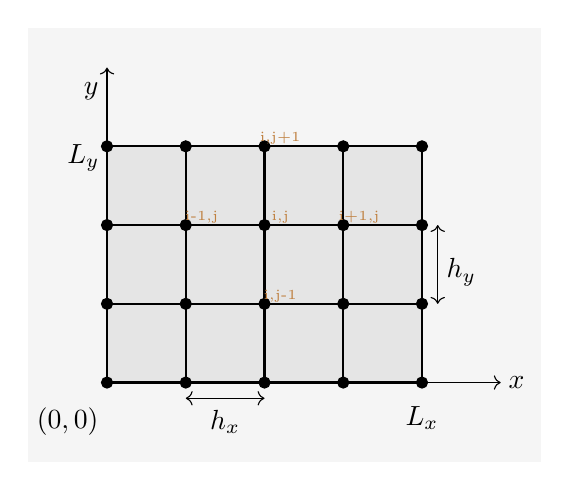
\begin{tikzpicture}
\draw[fill=gray!8,gray!8](0,0) rectangle (6.5,5.5);
%\draw[step=0.5cm,gray,very thin] (0,0) grid (8,5); %background grid


\draw[fill=gray!20,gray!20](1,1) rectangle (5,4);
\draw[thick] (1,1) -- (5,1) -- (5,4) -- (1,4) -- cycle;  

\draw[thick] (1,2) -- (5,2) ; 
\draw[thick] (1,3) -- (5,3) ; 
\draw[thick] (2,1) -- (2,4) ; 
\draw[thick] (3,1) -- (3,4) ; 
\draw[thick] (4,1) -- (4,4) ; 

\draw[black,fill=black] (1,1)  circle (2pt);
\draw[black,fill=black] (2,1)  circle (2pt);
\draw[black,fill=black] (3,1)  circle (2pt);
\draw[black,fill=black] (4,1)  circle (2pt);
\draw[black,fill=black] (5,1)  circle (2pt);
\draw[black,fill=black] (1,2)  circle (2pt);
\draw[black,fill=black] (2,2)  circle (2pt);
\draw[black,fill=black] (3,2)  circle (2pt);
\draw[black,fill=black] (4,2)  circle (2pt);
\draw[black,fill=black] (5,2)  circle (2pt);
\draw[black,fill=black] (1,3)  circle (2pt);
\draw[black,fill=black] (2,3)  circle (2pt);
\draw[black,fill=black] (3,3)  circle (2pt);
\draw[black,fill=black] (4,3)  circle (2pt);
\draw[black,fill=black] (5,3)  circle (2pt);
\draw[black,fill=black] (1,4)  circle (2pt);
\draw[black,fill=black] (2,4)  circle (2pt);
\draw[black,fill=black] (3,4)  circle (2pt);
\draw[black,fill=black] (4,4)  circle (2pt);
\draw[black,fill=black] (5,4)  circle (2pt);

\draw [<->] (5.2,2) -- (5.2,3); \node[] at (5.5,2.4) {$h_y$};
\draw [<->] (2,0.8) -- (3,0.8); \node[] at (2.5,0.5) {$h_x$};

\draw [->] (5,1) -- (6,1); \node[] at (6.2,1) {$x$};
\draw [->] (1,4) -- (1,5); \node[] at (0.8,4.7) {$y$};

\node[] at (0.5,0.5) {$(0,0)$};
\node[] at (5,0.55) {$L_x$};
\node[] at (0.7,3.85) {$L_y$};

\node[] at (2.2,3.1) {\tiny{\color{brown}i-1,j}};
\node[] at (3.2,3.1) {\tiny{\color{brown}i,j}};
\node[] at (4.2,3.1) {\tiny{\color{brown}i+1,j}};

\node[] at (3.2,4.1) {\tiny{\color{brown}i,j+1}};
\node[] at (3.2,2.1) {\tiny{\color{brown}i,j-1}};

%\draw[black,fill=black] (3.1,0.2) circle (2pt); \node[] at (3.4,0.2) {$\vec\upnu$};
%\draw (4.1,0.2) circle (4pt); 
%\node[] at (2.5,4.5) {4 vel. nodes, 1 press. nodes};
\end{tikzpicture}

\end{center}
\end{minipage}
%-/-/-/-/-/-/-/-/-/-/-/-/-/-/-/

The spacing between the nodes in the $x$-direction is $h_x$ and $h_y$ is the spacing
between the nodes in the $y$ direction. There are now $nnp=nnx\times nny$ nodes in total.
The above grid is characterised by $i=0,1,2,3,4$ and $j=0,1,2,3$ and counts in total 
20 nodes.

In one dimension, the subscript indicated the node $i$. In two dimensions we therefore 
need two indices ${\color{brown}i}$ and ${\color{brown}j}$ 
to identify a node, so that the temperature at node ${\color{brown}i},{\color{brown}j}$ 
at time $n$ is denoted $T_{{\color{brown}i,j}}^n$.

%The vector $\vec{T}$ contains all the temperature unknowns, so it is a vector that is $np$-long. 
%But how should this vector be organised ? In other words, 
One question remains: should we number nodes 
row by row ? column by column ? randomly ? 
These three approaches are shown hereunder: 

\vspace{.5cm}

%-/-/-/-/-/-/-/-/-/-/-/-/-/-/-/
\begin{minipage}[t]{\textwidth}


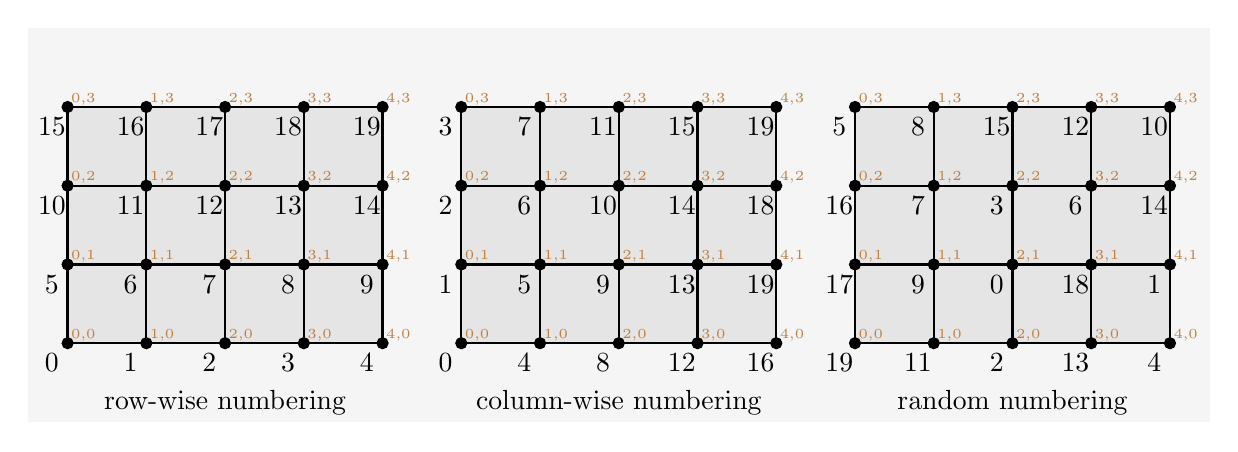
\begin{tikzpicture}
\draw[fill=gray!8,gray!8](0.5,0) rectangle (15.5,5);
%\draw[step=0.5cm,gray,very thin] (0,0) grid (17,5); %background grid

\draw[fill=gray!20,gray!20](1,1) rectangle (5,4);
\draw[fill=gray!20,gray!20](6,1) rectangle (10,4);
\draw[fill=gray!20,gray!20](11,1) rectangle (15,4);

\draw[thick] (1,1) -- (5,1) -- (5,4) -- (1,4) -- cycle;  
\draw[thick] (1,2) -- (5,2) ; 
\draw[thick] (1,3) -- (5,3) ; 
\draw[thick] (2,1) -- (2,4) ; 
\draw[thick] (3,1) -- (3,4) ; 
\draw[thick] (4,1) -- (4,4) ; 
\node[] at (0.8,0.75) {0};
\node[] at (1.8,0.75) {1};
\node[] at (2.8,0.75) {2};
\node[] at (3.8,0.75) {3};
\node[] at (4.8,0.75) {4};
\node[] at (0.8,1.75) {5};
\node[] at (1.8,1.75) {6};
\node[] at (2.8,1.75) {7};
\node[] at (3.8,1.75) {8};
\node[] at (4.8,1.75) {9};
\node[] at (0.8,2.75) {10};
\node[] at (1.8,2.75) {11};
\node[] at (2.8,2.75) {12};
\node[] at (3.8,2.75) {13};
\node[] at (4.8,2.75) {14};
\node[] at (0.8,3.75) {15};
\node[] at (1.8,3.75) {16};
\node[] at (2.8,3.75) {17};
\node[] at (3.8,3.75) {18};
\node[] at (4.8,3.75) {19};
\node[] at (1.2,1.1) {\tiny{\color{brown} 0,0}};
\node[] at (2.2,1.1) {\tiny{\color{brown} 1,0}};
\node[] at (3.2,1.1) {\tiny{\color{brown} 2,0}};
\node[] at (4.2,1.1) {\tiny{\color{brown} 3,0}};
\node[] at (5.2,1.1) {\tiny{\color{brown} 4,0}};
\node[] at (1.2,2.1) {\tiny{\color{brown} 0,1}};
\node[] at (2.2,2.1) {\tiny{\color{brown} 1,1}};
\node[] at (3.2,2.1) {\tiny{\color{brown} 2,1}};
\node[] at (4.2,2.1) {\tiny{\color{brown} 3,1}};
\node[] at (5.2,2.1) {\tiny{\color{brown} 4,1}};
\node[] at (1.2,3.1) {\tiny{\color{brown} 0,2}};
\node[] at (2.2,3.1) {\tiny{\color{brown} 1,2}};
\node[] at (3.2,3.1) {\tiny{\color{brown} 2,2}};
\node[] at (4.2,3.1) {\tiny{\color{brown} 3,2}};
\node[] at (5.2,3.1) {\tiny{\color{brown} 4,2}};
\node[] at (1.2,4.1) {\tiny{\color{brown} 0,3}};
\node[] at (2.2,4.1) {\tiny{\color{brown} 1,3}};
\node[] at (3.2,4.1) {\tiny{\color{brown} 2,3}};
\node[] at (4.2,4.1) {\tiny{\color{brown} 3,3}};
\node[] at (5.2,4.1) {\tiny{\color{brown} 4,3}};
\draw[black,fill=black] (1,1)  circle (2pt);
\draw[black,fill=black] (2,1)  circle (2pt);
\draw[black,fill=black] (3,1)  circle (2pt);
\draw[black,fill=black] (4,1)  circle (2pt);
\draw[black,fill=black] (5,1)  circle (2pt);
\draw[black,fill=black] (1,2)  circle (2pt);
\draw[black,fill=black] (2,2)  circle (2pt);
\draw[black,fill=black] (3,2)  circle (2pt);
\draw[black,fill=black] (4,2)  circle (2pt);
\draw[black,fill=black] (5,2)  circle (2pt);
\draw[black,fill=black] (1,3)  circle (2pt);
\draw[black,fill=black] (2,3)  circle (2pt);
\draw[black,fill=black] (3,3)  circle (2pt);
\draw[black,fill=black] (4,3)  circle (2pt);
\draw[black,fill=black] (5,3)  circle (2pt);
\draw[black,fill=black] (1,4)  circle (2pt);
\draw[black,fill=black] (2,4)  circle (2pt);
\draw[black,fill=black] (3,4)  circle (2pt);
\draw[black,fill=black] (4,4)  circle (2pt);
\draw[black,fill=black] (5,4)  circle (2pt);
%---------------------------------------------------
\draw[thick] (6,1) -- (10,1) -- (10,4) -- (6,4) -- cycle;  
\draw[thick] (6,2) -- (10,2) ; 
\draw[thick] (6,3) -- (10,3) ; 
\draw[thick] (7,1) -- (7,4) ; 
\draw[thick] (8,1) -- (8,4) ; 
\draw[thick] (9,1) -- (9,4) ; 
\node[] at (6.2,1.1)  {\tiny{\color{brown} 0,0}};
\node[] at (7.2,1.1)  {\tiny{\color{brown} 1,0}};
\node[] at (8.2,1.1)  {\tiny{\color{brown} 2,0}};
\node[] at (9.2,1.1)  {\tiny{\color{brown} 3,0}};
\node[] at (10.2,1.1) {\tiny{\color{brown} 4,0}};
\node[] at (6.2,2.1)  {\tiny{\color{brown} 0,1}};
\node[] at (7.2,2.1)  {\tiny{\color{brown} 1,1}};
\node[] at (8.2,2.1)  {\tiny{\color{brown} 2,1}};
\node[] at (9.2,2.1)  {\tiny{\color{brown} 3,1}};
\node[] at (10.2,2.1) {\tiny{\color{brown} 4,1}};
\node[] at (6.2,3.1)  {\tiny{\color{brown} 0,2}};
\node[] at (7.2,3.1)  {\tiny{\color{brown} 1,2}};
\node[] at (8.2,3.1)  {\tiny{\color{brown} 2,2}};
\node[] at (9.2,3.1)  {\tiny{\color{brown} 3,2}};
\node[] at (10.2,3.1) {\tiny{\color{brown} 4,2}};
\node[] at (6.2,4.1)  {\tiny{\color{brown} 0,3}};
\node[] at (7.2,4.1)  {\tiny{\color{brown} 1,3}};
\node[] at (8.2,4.1)  {\tiny{\color{brown} 2,3}};
\node[] at (9.2,4.1)  {\tiny{\color{brown} 3,3}};
\node[] at (10.2,4.1) {\tiny{\color{brown} 4,3}};
\draw[black,fill=black] (6,1)  circle (2pt);
\draw[black,fill=black] (7,1)  circle (2pt);
\draw[black,fill=black] (8,1)  circle (2pt);
\draw[black,fill=black] (9,1)  circle (2pt);
\draw[black,fill=black] (10,1)  circle (2pt);
\draw[black,fill=black] (6,2)  circle (2pt);
\draw[black,fill=black] (7,2)  circle (2pt);
\draw[black,fill=black] (8,2)  circle (2pt);
\draw[black,fill=black] (9,2)  circle (2pt);
\draw[black,fill=black] (10,2)  circle (2pt);
\draw[black,fill=black] (6,3)  circle (2pt);
\draw[black,fill=black] (7,3)  circle (2pt);
\draw[black,fill=black] (8,3)  circle (2pt);
\draw[black,fill=black] (9,3)  circle (2pt);
\draw[black,fill=black] (10,3)  circle (2pt);
\draw[black,fill=black] (6,4)  circle (2pt);
\draw[black,fill=black] (7,4)  circle (2pt);
\draw[black,fill=black] (8,4)  circle (2pt);
\draw[black,fill=black] (9,4)  circle (2pt);
\draw[black,fill=black] (10,4)  circle (2pt);
\node[] at (5.8,0.75) {0};
\node[] at (6.8,0.75) {4};
\node[] at (7.8,0.75) {8};
\node[] at (8.8,0.75) {12};
\node[] at (9.8,0.75) {16};
\node[] at (5.8,1.75) {1};
\node[] at (6.8,1.75) {5};
\node[] at (7.8,1.75) {9};
\node[] at (8.8,1.75) {13};
\node[] at (9.8,1.75) {19};
\node[] at (5.8,2.75) {2};
\node[] at (6.8,2.75) {6};
\node[] at (7.8,2.75) {10};
\node[] at (8.8,2.75) {14};
\node[] at (9.8,2.75) {18};
\node[] at (5.8,3.75) {3};
\node[] at (6.8,3.75) {7};
\node[] at (7.8,3.75) {11};
\node[] at (8.8,3.75) {15};
\node[] at (9.8,3.75) {19};

%---------------------------------------------------
\draw[thick] (11,1) -- (15,1) -- (15,4) -- (11,4) -- cycle;  
\draw[thick] (11,2) -- (15,2) ; 
\draw[thick] (11,3) -- (15,3) ; 
\draw[thick] (12,1) -- (12,4) ; 
\draw[thick] (13,1) -- (13,4) ; 
\draw[thick] (14,1) -- (14,4) ; 
\node[] at (11.2,1.1) {\tiny{\color{brown} 0,0}};
\node[] at (12.2,1.1) {\tiny{\color{brown} 1,0}};
\node[] at (13.2,1.1) {\tiny{\color{brown} 2,0}};
\node[] at (14.2,1.1) {\tiny{\color{brown} 3,0}};
\node[] at (15.2,1.1) {\tiny{\color{brown} 4,0}};
\node[] at (11.2,2.1) {\tiny{\color{brown} 0,1}};
\node[] at (12.2,2.1) {\tiny{\color{brown} 1,1}};
\node[] at (13.2,2.1) {\tiny{\color{brown} 2,1}};
\node[] at (14.2,2.1) {\tiny{\color{brown} 3,1}};
\node[] at (15.2,2.1) {\tiny{\color{brown} 4,1}};
\node[] at (11.2,3.1) {\tiny{\color{brown} 0,2}};
\node[] at (12.2,3.1) {\tiny{\color{brown} 1,2}};
\node[] at (13.2,3.1) {\tiny{\color{brown} 2,2}};
\node[] at (14.2,3.1) {\tiny{\color{brown} 3,2}};
\node[] at (15.2,3.1) {\tiny{\color{brown} 4,2}};
\node[] at (11.2,4.1) {\tiny{\color{brown} 0,3}};
\node[] at (12.2,4.1) {\tiny{\color{brown} 1,3}};
\node[] at (13.2,4.1) {\tiny{\color{brown} 2,3}};
\node[] at (14.2,4.1) {\tiny{\color{brown} 3,3}};
\node[] at (15.2,4.1) {\tiny{\color{brown} 4,3}};
\draw[black,fill=black] (11,1)  circle (2pt);
\draw[black,fill=black] (12,1)  circle (2pt);
\draw[black,fill=black] (13,1)  circle (2pt);
\draw[black,fill=black] (14,1)  circle (2pt);
\draw[black,fill=black] (15,1)  circle (2pt);
\draw[black,fill=black] (11,2)  circle (2pt);
\draw[black,fill=black] (12,2)  circle (2pt);
\draw[black,fill=black] (13,2)  circle (2pt);
\draw[black,fill=black] (14,2)  circle (2pt);
\draw[black,fill=black] (15,2)  circle (2pt);
\draw[black,fill=black] (11,3)  circle (2pt);
\draw[black,fill=black] (12,3)  circle (2pt);
\draw[black,fill=black] (13,3)  circle (2pt);
\draw[black,fill=black] (14,3)  circle (2pt);
\draw[black,fill=black] (15,3)  circle (2pt);
\draw[black,fill=black] (11,4)  circle (2pt);
\draw[black,fill=black] (12,4)  circle (2pt);
\draw[black,fill=black] (13,4)  circle (2pt);
\draw[black,fill=black] (14,4)  circle (2pt);
\draw[black,fill=black] (15,4)  circle (2pt);
\node[] at (10.8,0.75) {19};
\node[] at (11.8,0.75) {11};
\node[] at (12.8,0.75) {2};
\node[] at (13.8,0.75) {13};
\node[] at (14.8,0.75) {4};
\node[] at (10.8,1.75) {17};
\node[] at (11.8,1.75) {9};
\node[] at (12.8,1.75) {0};
\node[] at (13.8,1.75) {18};
\node[] at (14.8,1.75) {1};
\node[] at (10.8,2.75) {16};
\node[] at (11.8,2.75) {7};
\node[] at (12.8,2.75) {3};
\node[] at (13.8,2.75) {6};
\node[] at (14.8,2.75) {14};
\node[] at (10.8,3.75) {5};
\node[] at (11.8,3.75) {8};
\node[] at (12.8,3.75) {15};
\node[] at (13.8,3.75) {12};
\node[] at (14.8,3.75) {10};


\node[] at (3,0.25) {row-wise numbering};
\node[] at (8,0.25) {column-wise numbering};
\node[] at (13,0.25) {random numbering};

\end{tikzpicture}
\\
\end{minipage}
%-/-/-/-/-/-/-/-/-/-/-/-/-/-/-/

\vspace{.5cm}

This is a critical point because the discretised PDE is formulated as a 
function of $T_{{\color{brown} i,j}}$ 
with ${\color{brown}i}=0,\dots nnx-1$ and ${\color{brown}j}=0,\dots nny-1$ 
but the vector $\vec{T}$ containing all these values (encountered in 
implicit methods)
is indexed by a single index ${\color{teal}k}=0,\dots nnp-1$. The numbering strategy determines how easy
it is to go from $({\color{brown}i},{\color{brown}j})$ to ${\color{teal}k}$ and vice versa. 
Very concretely again, where should $T_{\color{brown}3,4}$ be placed in the global 
vector of unknowns $\vec{T}$?

At the same time we cannot do away with ${\color{brown}i,j}$ indices because these are 
needed to locate the direct neighbours of any node and allow to 
form discrete derivatives. 

We then need a (preferably simple/straightforward) 'function' 
which associates to every $({\color{brown} i,j})$ a global index $k$. 
For the first grid with row-wise numbering, we have 
$0\leq {\color{brown}i} \leq 4$ , $0 \leq {\color{brown}j} \leq 3$ 
and $0 \leq {\color{teal}k} \leq 19$. It follows that 
\begin{equation}
{\color{teal} k}({\color{brown}i,j})={\color{brown}j} \cdot nnx+{\color{brown}i}
\end{equation}
This is easy to verify: ${\color{brown}i}=3$ and ${\color{brown}j}=2$ 
indeed corresponds to node \# 13, 
${\color{brown}i}=4$ and ${\color{brown}j}=1$ corresponds to node \# 9, etc ...

%-/-/-/-/-/-/-/-/-/-/-/-/-/-/-/
\begin{minipage}[t]{\textwidth}
\begin{center}


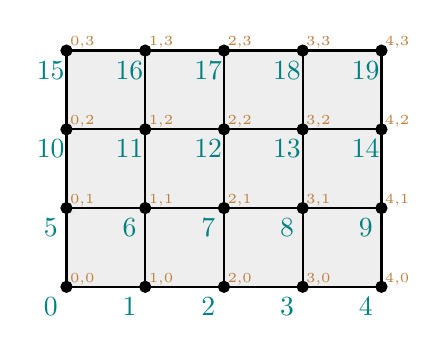
\begin{tikzpicture}
%\draw[fill=gray!23,gray!23](0,0) rectangle (8,5);
%\draw[step=0.5cm,gray,very thin] (0,0) grid (8,5); %background grid


\draw[fill=gray!13,gray!13](1,1) rectangle (5,4);
\draw[thick] (1,1) -- (5,1) -- (5,4) -- (1,4) -- cycle;  

\draw[thick] (1,2) -- (5,2) ; 
\draw[thick] (1,3) -- (5,3) ; 
\draw[thick] (2,1) -- (2,4) ; 
\draw[thick] (3,1) -- (3,4) ; 
\draw[thick] (4,1) -- (4,4) ; 

\node[] at (0.8,0.75) {\color{teal} 0};
\node[] at (1.8,0.75) {\color{teal} 1};
\node[] at (2.8,0.75) {\color{teal} 2};
\node[] at (3.8,0.75) {\color{teal} 3};
\node[] at (4.8,0.75) {\color{teal} 4};
\node[] at (0.8,1.75) {\color{teal} 5};
\node[] at (1.8,1.75) {\color{teal} 6};
\node[] at (2.8,1.75) {\color{teal} 7};
\node[] at (3.8,1.75) {\color{teal} 8};
\node[] at (4.8,1.75) {\color{teal} 9};
\node[] at (0.8,2.75) {\color{teal} 10};
\node[] at (1.8,2.75) {\color{teal} 11};
\node[] at (2.8,2.75) {\color{teal} 12};
\node[] at (3.8,2.75) {\color{teal} 13};
\node[] at (4.8,2.75) {\color{teal} 14};
\node[] at (0.8,3.75) {\color{teal} 15};
\node[] at (1.8,3.75) {\color{teal} 16};
\node[] at (2.8,3.75) {\color{teal} 17};
\node[] at (3.8,3.75) {\color{teal} 18};
\node[] at (4.8,3.75) {\color{teal} 19};

\node[] at (1.2,1.1) {\tiny{\color{brown}0,0}};
\node[] at (2.2,1.1) {\tiny{\color{brown}1,0}};
\node[] at (3.2,1.1) {\tiny{\color{brown}2,0}};
\node[] at (4.2,1.1) {\tiny{\color{brown}3,0}};
\node[] at (5.2,1.1) {\tiny{\color{brown}4,0}};
\node[] at (1.2,2.1) {\tiny{\color{brown}0,1}};
\node[] at (2.2,2.1) {\tiny{\color{brown}1,1}};
\node[] at (3.2,2.1) {\tiny{\color{brown}2,1}};
\node[] at (4.2,2.1) {\tiny{\color{brown}3,1}};
\node[] at (5.2,2.1) {\tiny{\color{brown}4,1}};
\node[] at (1.2,3.1) {\tiny{\color{brown}0,2}};
\node[] at (2.2,3.1) {\tiny{\color{brown}1,2}};
\node[] at (3.2,3.1) {\tiny{\color{brown}2,2}};
\node[] at (4.2,3.1) {\tiny{\color{brown}3,2}};
\node[] at (5.2,3.1) {\tiny{\color{brown}4,2}};
\node[] at (1.2,4.1) {\tiny{\color{brown}0,3}};
\node[] at (2.2,4.1) {\tiny{\color{brown}1,3}};
\node[] at (3.2,4.1) {\tiny{\color{brown}2,3}};
\node[] at (4.2,4.1) {\tiny{\color{brown}3,3}};
\node[] at (5.2,4.1) {\tiny{\color{brown}4,3}};

\draw[black,fill=black] (1,1)  circle (2pt);
\draw[black,fill=black] (2,1)  circle (2pt);
\draw[black,fill=black] (3,1)  circle (2pt);
\draw[black,fill=black] (4,1)  circle (2pt);
\draw[black,fill=black] (5,1)  circle (2pt);
\draw[black,fill=black] (1,2)  circle (2pt);
\draw[black,fill=black] (2,2)  circle (2pt);
\draw[black,fill=black] (3,2)  circle (2pt);
\draw[black,fill=black] (4,2)  circle (2pt);
\draw[black,fill=black] (5,2)  circle (2pt);
\draw[black,fill=black] (1,3)  circle (2pt);
\draw[black,fill=black] (2,3)  circle (2pt);
\draw[black,fill=black] (3,3)  circle (2pt);
\draw[black,fill=black] (4,3)  circle (2pt);
\draw[black,fill=black] (5,3)  circle (2pt);
\draw[black,fill=black] (1,4)  circle (2pt);
\draw[black,fill=black] (2,4)  circle (2pt);
\draw[black,fill=black] (3,4)  circle (2pt);
\draw[black,fill=black] (4,4)  circle (2pt);
\draw[black,fill=black] (5,4)  circle (2pt);

%\draw[black,fill=black] (3.1,0.2) circle (2pt); \node[] at (3.4,0.2) {$\vec\upnu$};
%\draw (4.1,0.2) circle (4pt); \node[] at (4.4,0.2) {$p$};
%\node[] at (2.5,4.5) {4 vel. nodes, 1 press. nodes};
\end{tikzpicture}

\end{center}
\end{minipage}
%-/-/-/-/-/-/-/-/-/-/-/-/-/-/-/


%-/-/-/-/-/-/-/-/-/-/-/-/-/-/-/-/-/-/
\begin{center}
\begin{minipage}[t]{0.77\textwidth}
\par\noindent\rule{\textwidth}{0.4pt}

\begin{center}
\includegraphics[width=0.8cm]{images/garftr} \\
{\color{orange}Exercise FDM-7}
\end{center}

In a new notebook declare and assign values to 
$nnx$ and $nny$. Compute $nnp$.
Set $L_x=7$ and $L_y=6$. Compute $h_x$ and $h_y$.

Declare two arrays $xcoords$ and $ycoords$ which will 
contain the $x$ and $y$ coordinates of all $nnp$ nodes.

By means of two imbricated for loops
compute these coordinates \& fill both arrays. 

Visualise the nodes with matplotlib.

Tip: Make sure your code works for various 
combinations of $nnx$ and $nny$.

\par\noindent\rule{\textwidth}{0.4pt}
\end{minipage}
\end{center}






%.............................
\paragraph{Explicit scheme} The simplest approach is an {\color{olive} FTCS} 
(forward time, centered space) explicit method like in 1D:
\begin{equation}
\frac{T_{{\color{brown}i,j}}^{n+1}-T_{{\color{brown}i,j}}^n}{\delta t}
= \kappa
\left(
\frac{ T_{{\color{brown}i-1,j}}^{n}-2T_{{\color{brown}i,j}}^{n}+T_{{\color{brown}i+1,j}}^{n}  }{h_x^2} + 
\frac{ T_{{\color{brown}i,j-1}}^{n}-2T_{{\color{brown}i,j}}^{n}+T_{{\color{brown}i,j+1}}^{n}  }{h_y^2}
\right)
+\tilde{Q}_{{\color{brown}i,j}}^n
\end{equation}
where we have assumed that the source term $\tilde{Q}$ 
can depend of space coordinates and therefore 
appears as $\tilde{Q}_{{\color{brown}i,j}}$ in the equation.
We define $s_x$ and $s_y$ as follows:
\begin{equation}
s_x = \frac{\kappa \delta t}{h_x^2}
\quad\quad
s_y = \frac{\kappa \delta t}{h_y^2}
\end{equation}
so that
\begin{equation}
T_{{\color{brown}i,j}}^{n+1} = T_{{\color{brown}i,j}}^n 
+ s_x ( T_{{\color{brown}i-1,j}}^{n}
-2T_{{\color{brown}i,j}}^{n}
+T_{{\color{brown}i+1,j}}^{n} ) 
+s_y ( T_{{\color{brown}i,j-1}}^{n}
-2T_{{\color{brown}i,j}}^{n}
+T_{{\color{brown}i,j+1}}^{n} ) + 
\tilde{Q}_{{\color{brown}i,j}}^n \delta t
\end{equation}
or, 
\begin{equation}
T_{{\color{teal}k}({\color{brown}i,j})}^{n+1} = 
T_{{\color{teal}k}({\color{brown}i,j})}^n 
+ s_x ( T_{{\color{teal}k}({\color{brown}i-1,j})}^{n}
-2T_{{\color{teal}k}({\color{brown}i,j})}^{n}
+T_{{\color{teal}k}({\color{brown}i+1,j})}^{n} ) 
+s_y ( T_{{\color{teal}k}({\color{brown}i,j-1})}^{n}
-2T_{{\color{teal}k}({\color{brown}i,j})}^{n}
+T_{{\color{teal}k}({\color{brown}i,j+1})}^{n} ) + 
\tilde{Q}_{{\color{teal}k}({\color{brown}i,j})}^n \delta t
\end{equation}



The scheme is stable for  
\begin{equation}
\delta t \leq \frac{\min(h_x^2,h_y^2)}{2 \kappa}
\end{equation}
Boundary conditions can be set the usual way: for example a constant (Dirichlet) temperature 
at node $({\color{brown}i},{\color{brown}j})$ is given by
\begin{equation}
T_{{\color{brown}i},{\color{brown}j}}=T_{bc} 
\end{equation}
where $T_{bc}$ is the prescribed temperature. 

%-/-/-/-/-/-/-/-/-/-/-/-/-/-/-/-/-/-/-/
\begin{center}
\begin{minipage}[t]{0.77\textwidth}
\par\noindent\rule{\textwidth}{0.4pt}
\begin{center}
\includegraphics[width=0.8cm]{images/garftr} \\
{\color{orange}Exercise FDM-8}
\end{center}

A simple (time-dependent) analytical solution for the temperature equation exists for 
the case that the initial temperature field is
\begin{equation}
T(x,y,t=0) = T_0+ T_{max} \exp \left[ -\frac{x^2+y^2}{\sigma^2}   \right]
\end{equation}
where $T_{max}$ is the maximum amplitude of the temperature perturbation 
at $(x,y) = (0, 0)$ and $\sigma$ its half-width. 

\begin{center}
\includegraphics[width=5cm]{images/fdm/gaussian}\\
{\captionfont initial temperature field}
\end{center}

The solution of the time-dependent PDE is
\begin{equation}
T(x,y,t)=T_0 + \frac{T_{max}}{1+4t\kappa/\sigma^2 } \exp \left[ -\frac{x^2+y^2}{\sigma^2 + 4t\kappa}   \right]
\end{equation}

Set $L_x$=100km and $L_y=80$km, $\kappa=10^{-6}$, $\tilde{Q}=0$, $T_{max}=100\degree$, $T_0=200\degree$, 
and $\sigma=10^4$m. 

Use the previous exercise to generate a $nnx\times nny$ grid 
in the $[-L_x/2,L_x/2]\times[-L_y/2,L_y/2]$ domain.

Write a function which takes $x$, $y$, $t$, $T_0$, $T_{max}$, $\kappa$ and $\sigma$ as argument 
and returns the analytical temperature value.

Write a an explicit FDM code which solves the 2D diffusion equation. At each time step 
prescribe on the boundary the analytical solution.  

\par\noindent\rule{\textwidth}{0.4pt}
\end{minipage}
\end{center}
%-/-/-/-/-/-/-/-/-/-/-/-/-/-/-/-/-/-/-/



%...........................
\paragraph{Implicit scheme} 
If we now employ a fully implicit, unconditionally stable discretization scheme, the discretised 
PDE becomes:
\begin{equation}
\frac{T_{{\color{brown}i},{\color{brown}j}}^{n+1}-T_{\color{brown}i,j}^n}{\delta t}
= \kappa
\left(
\frac{ T_{{\color{brown}i-1,j}}^{n+1}-2T_{{\color{brown}i,j}}^{n+1}+T_{{\color{brown}i+1,j}}^{n+1} }{h_x^2} + 
\frac{ T_{{\color{brown}i,j-1}}^{n+1}-2T_{{\color{brown}i,j}}^{n+1}+T_{{\color{brown}i,j+1}}^{n+1} }{h_y^2}
\right)
+\frac{Q_{{\color{brown}i,j}}^n}{\rho C_p}
\end{equation}
Rearranging terms with $n+1$ on the left and terms with $n$ on the right hand side gives
\begin{equation}
-s_x\; T_{{\color{brown}i+1,j}}^{n+1}
-s_y\; T_{{\color{brown}i,j+1}}^{n+1} 
+(1+2s_x+2s_y)\; T_{{\color{brown}i,j}}^{n+1} 
-s_x\;  T_{{\color{brown}i-1,j}}^{n+1} 
-s_y\;  T_{{\color{brown}i,j-1}}^{n+1} 
=
T_{{\color{brown}i,j}}^n
+\tilde{Q}_{{\color{brown}i,j}}^n \delta t
\end{equation}
or
\begin{equation}
-s_x\;           T_{{\color{teal}k}({\color{brown}i+1,j})}^{n+1}
-s_y\;           T_{{\color{teal}k}({\color{brown}i,j+1})}^{n+1} 
+(1+2s_x+2s_y)\; T_{{\color{teal}k}({\color{brown}i,j}  )}^{n+1} 
-s_x\;           T_{{\color{teal}k}({\color{brown}i-1,j})}^{n+1} 
-s_y\;           T_{{\color{teal}k}({\color{brown}i,j-1})}^{n+1} 
=
T_{{\color{teal}k}({\color{brown}i,j})}^n
+\tilde{Q}_{{\color{teal}k}({\color{brown}i,j})}^n \delta t
\end{equation}
which here again yields a linear system of equations written ${\bm A}\cdot {\vec T} = {\vec b}$
where ${\bm A}$ is a $(nnp \times nnp)$ matrix.

Boundary conditions are $T(x,y)=0$ on all sides, so all nodes 
on the boundary have a prescribed zero temperature\footnote{We assume
here again that these boundary conditions do not change with time.}:
\begin{eqnarray}
T_{\color{brown}0,0} = T_{\color{teal} 0} &=& 0 \nn\\
T_{\color{brown}1,0} = T_{\color{teal} 1} &=& 0 \nn\\
T_{\color{brown}2,0} = T_{\color{teal} 2} &=& 0 \nn\\
T_{\color{brown}3,0} = T_{\color{teal} 3} &=& 0 \nn\\
T_{\color{brown}4,0} = T_{\color{teal} 4} &=& 0 \nn\\
T_{\color{brown}0,1} = T_{\color{teal} 5} &=& 0 \nn\\
T_{\color{brown}4,1} = T_{\color{teal} 9} &=& 0 \nn\\
T_{\color{brown}0,2} = T_{\color{teal} 10} &=& 0 \nn\\
T_{\color{brown}4,2} = T_{\color{teal} 14} &=& 0 \nn\\
T_{\color{brown}0,3} = T_{\color{teal} 15} &=& 0 \nn\\
T_{\color{brown}1,3} = T_{\color{teal} 16} &=& 0 \nn\\
T_{\color{brown}2,3} = T_{\color{teal} 17} &=& 0 \nn\\
T_{\color{brown}3,3} = T_{\color{teal} 18} &=& 0 \nn\\
T_{\color{brown}4,3} = T_{\color{teal} 19} &=& 0 \nn
\end{eqnarray}
In what follows we assume for simplicity and conciseness of notation that 
$h_x=h_y=h$ so that $s_x=s_y=s$.
The discretised PDE equation will now be applied to the interior nodes:
%\begin{eqnarray}
%-s T_{{\color{brown} i+1,j}}^{n+1}
%-s T_{{\color{brown}i,j+1}}^{n+1} 
%+(1+4s)T_{{\color{brown}i,j}}^{n+1} 
%-s T_{{\color{brown}i-1,j}}^{n+1} 
%-s T_{{\color{brown}i,j-1}}^{n+1} 
%= T_{{\color{brown}i,j}}^n 
%+\tilde{Q}_{{\color{brown}i,j}}^n
%\end{eqnarray}

\begin{itemize}
\item For node ${\color{teal}k}=6$ (${\color{brown}i}=1,{\color{brown}j}=1$):
\begin{eqnarray}
-s T_{{\color{brown}2,1}}^{n+1}
-s T_{{\color{brown}1,2}}^{n+1} 
+(1+4s)T_{{\color{brown}1,1}}^{n+1} 
-s T_{{\color{brown}0,1}}^{n+1} 
-s T_{{\color{brown}1,0}}^{n+1} 
&=& T_{{\color{brown}1,1}}^n +\tilde{Q}_{{\color{brown}1,1}}^n \delta t\nn\\
\Rightarrow \qquad
-s T_{{\color{teal} 7}}^{n+1}-s T_{{\color{teal} 11}}^{n+1} +(1+4s)T_{{\color{teal} 6}}^{n+1} 
-s T_{{\color{teal} 5}}^{n+1} -s T_{{\color{teal} 1}}^{n+1} 
&=& T_{{\color{teal} 6}}^n +\tilde{Q}_{{\color{teal} 6}}^n\delta t
\end{eqnarray}

\item For node ${\color{teal}k}=7$ (${\color{brown}i}=2,{\color{brown}j}=1$):
\begin{eqnarray}
-s T_{{\color{brown} 3,1}}^{n+1}
-s T_{{\color{brown}2,2}}^{n+1} 
+(1+4s)T_{{\color{brown}2,1}}^{n+1} 
-s T_{{\color{brown}1,1}}^{n+1} 
-s T_{{\color{brown}2,0}}^{n+1} 
&=& T_{{\color{brown}2,1}}^n 
+\tilde{Q}_{{\color{brown}2,1}}^n \delta t\nn\\
\Rightarrow \qquad
-s T_{{\color{teal} 8}}^{n+1}
-s T_{{\color{teal} 12}}^{n+1} 
+(1+4s)T_{{\color{teal}7}}^{n+1} 
-s T_{{\color{teal}6}}^{n+1} 
-s T_{{\color{teal}2}}^{n+1} 
&=& T_{{\color{teal}7}}^n 
+\tilde{Q}_{{\color{teal}7}}^n \delta t
\end{eqnarray}

\item For node ${\color{teal}k}=8$ (${\color{brown}i}=3,{\color{brown}j}=1$):
\begin{eqnarray}
-s T_{{\color{brown} 4,1}}^{n+1}
-s T_{{\color{brown}3,2}}^{n+1} 
+(1+4s)T_{{\color{brown}3,1}}^{n+1} 
-s T_{{\color{brown}2,1}}^{n+1} 
-s T_{{\color{brown}3,0}}^{n+1} 
&=& T_{{\color{brown}3,1}}^n 
+\tilde{Q}_{{\color{brown}3,1}}^n \delta t\nn\\
\Rightarrow \qquad
-s T_{{\color{teal} 9}}^{n+1}
-s T_{{\color{teal} 13}}^{n+1} 
+(1+4s)T_{{\color{teal}8}}^{n+1} 
-s T_{{\color{teal}7}}^{n+1} 
-s T_{{\color{teal}3}}^{n+1} 
&=& T_{{\color{teal}8}}^n 
+\tilde{Q}_{{\color{teal}8}}^n \delta t
\end{eqnarray}

\item For node ${\color{teal}k}=11$ (${\color{brown}i}=1,{\color{brown}j}=2$):
\begin{eqnarray}
-s T_{{\color{brown} 2,2}}^{n+1}
-s T_{{\color{brown}1,3}}^{n+1} 
+(1+4s)T_{{\color{brown}1,2}}^{n+1} 
-s T_{{\color{brown}0,2}}^{n+1} 
-s T_{{\color{brown}2,1}}^{n+1} 
&=& T_{{\color{brown}1,2}}^n 
+\tilde{Q}_{{\color{brown}1,2}}^n \delta t\nn\\
\Rightarrow \qquad
-s T_{{\color{teal} 12}}^{n+1}
-s T_{{\color{teal} 16}}^{n+1} 
+(1+4s)T_{{\color{teal}11}}^{n+1} 
-s T_{{\color{teal}10}}^{n+1} 
-s T_{{\color{teal}6}}^{n+1} 
&=& T_{{\color{teal}11}}^n 
+\tilde{Q}_{{\color{teal}11}}^n\delta t
\end{eqnarray}

\item For node ${\color{teal}k}=12$ (${\color{brown}i}=2,{\color{brown}j}=2$):
\begin{eqnarray}
-s T_{{\color{brown} 3,2}}^{n+1}
-s T_{{\color{brown}2,3}}^{n+1} 
+(1+4s)T_{{\color{brown}2,2}}^{n+1} 
-s T_{{\color{brown}1,2}}^{n+1} 
-s T_{{\color{brown}2,1}}^{n+1} 
&=& T_{{\color{brown}2,2}}^n 
+\tilde{Q}_{{\color{brown}2,2}}^n \delta t \nn\\
\Rightarrow \qquad
-s T_{{\color{teal} 13}}^{n+1}
-s T_{{\color{teal} 17}}^{n+1} 
+(1+4s)T_{{\color{teal}12}}^{n+1} 
-s T_{{\color{teal}11}}^{n+1} 
-s T_{{\color{teal}7}}^{n+1} 
&=& T_{{\color{teal}12}}^n 
+\tilde{Q}_{{\color{teal}12}}^n\delta t
\end{eqnarray}


\item For node ${\color{teal}k}=13$ (${\color{brown}i}=3,{\color{brown}j}=2$):
\begin{eqnarray}
-s T_{{\color{brown} 4,2}}^{n+1}
-s T_{{\color{brown}3,3}}^{n+1} 
+(1+4s)T_{{\color{brown}3,2}}^{n+1} 
-s T_{{\color{brown}2,2}}^{n+1} 
-s T_{{\color{brown}3,1}}^{n+1} 
&=& T_{{\color{brown}3,2}}^n 
+\tilde{Q}_{{\color{brown}3,2}}^n \delta t\nn\\
\Rightarrow \qquad
-s T_{{\color{teal} 14}}^{n+1}
-s T_{{\color{teal} 18}}^{n+1} 
+(1+4s)T_{{\color{teal}13}}^{n+1} 
-s T_{{\color{teal}12}}^{n+1} 
-s T_{{\color{teal}8}}^{n+1} 
&=& T_{{\color{teal}13}}^n 
+\tilde{Q}_{{\color{teal}13}}^n \delta t
\end{eqnarray}


\end{itemize}

Putting it all together yields the following linear system:

\begin{landscape}
\[
\underbrace{
\left(
\begin{array}{cccccccccccccccccccc}
1 & . & . & . & . & . & . & . & . & . & . & . & . & . & . & . & . & . & . & . \\ %#0
. & 1 & . & . & . & . & . & . & . & . & . & . & . & . & . & . & . & . & . & . \\ %#1
. & . & 1 & . & . & . & . & . & . & . & . & . & . & . & . & . & . & . & . & . \\ %#2
. & . & . & 1 & . & . & . & . & . & . & . & . & . & . & . & . & . & . & . & . \\ %#3
. & . & . & . & 1 & . & . & . & . & . & . & . & . & . & . & . & . & . & . & . \\ %#4
. & . & . & . & . & 1 & . & . & . & . & . & . & . & . & . & . & . & . & . & . \\ %#5
. & -s& . & . & . & -s& {1+4s} & -s& . & . & . & -s & . & . & . & . & . & . & . & . \\ %#6
. & . & -s& . & . & . & -s& {1+4s} & -s& . & . & . & -s & . & . & . & . & . & . & .\\ %#7
. & . & . & -s& . & . & . & -s & {1+4s} & -s & . & . & . & -s & . & . & . & . & . & . \\ %#8
. & . & . & . & . & . & . & . & . & 1 & . & . & . & . & . & . & . & . & . & . \\ %#9
. & . & . & . & . & . & . & . & . & . & 1 & . & . & . & . & . & . & . & . & . \\ %#10
. & . & . & . & . & . &-s & . & . & . & -s& {1+4s} & -s& . & . & .  & -s& . & . & .\\ %#11
. & . & . & . & . & . & . &-s & . & . & . & -s& {1+4s} & -s& . & . & .  & -s& . & .\\ %#12
. & . & . & . & . & . & . & . &-s & . & . & . & -s& {1+4s} & -s& . & . & .  & -s & .\\ %#13
. & . & . & . & . & . & . & . & . & . & . & . & . & . & 1 & . & . & . & . & . \\ %#14
. & . & . & . & . & . & . & . & . & . & . & . & . & . & . & 1 & . & . & . & . \\ %#15
. & . & . & . & . & . & . & . & . & . & . & . & . & . & . & . & 1 & . & . & . \\ %#16
. & . & . & . & . & . & . & . & . & . & . & . & . & . & . & . & . & 1 & . & . \\ %#17
. & . & . & . & . & . & . & . & . & . & . & . & . & . & . & . & . & . & 1 & . \\ %#18
. & . & . & . & . & . & . & . & . & . & . & . & . & . & . & . & . & . & . & 1    %#19
\end{array}
\right)
}_{\bm A}
\cdot
\underbrace{
\left(
\begin{array}{c}
T_{{\color{teal}0}}^{n+1} \\ 
T_{{\color{teal}1}}^{n+1} \\ 
T_{{\color{teal}2}}^{n+1} \\ 
T_{{\color{teal}3}}^{n+1} \\ 
T_{{\color{teal}4}}^{n+1} \\ 
T_{{\color{teal}5}}^{n+1} \\ 
T_{{\color{teal}6}}^{n+1} \\ 
T_{{\color{teal}7}}^{n+1} \\ 
T_{{\color{teal}8}}^{n+1} \\ 
T_{{\color{teal}9}}^{n+1} \\ 
T_{{\color{teal}10}}^{n+1} \\ 
T_{{\color{teal}11}}^{n+1} \\ 
T_{{\color{teal}12}}^{n+1} \\ 
T_{{\color{teal}13}}^{n+1} \\ 
T_{{\color{teal}14}}^{n+1} \\ 
T_{{\color{teal}15}}^{n+1} \\ 
T_{{\color{teal}16}}^{n+1} \\ 
T_{{\color{teal}17}}^{n+1} \\ 
T_{{\color{teal}18}}^{n+1} \\ 
T_{{\color{teal}19}}^{n+1} 
\end{array}
\right)
}_{\vec T}
=
\underbrace{
\left(
\begin{array}{c}
0\\ 
0\\ 
0\\ 
0\\ 
0\\ 
0\\ 
T_{{\color{teal}6}}^n + \tilde{Q}_{\color{teal}6} \delta t\\ 
T_{{\color{teal}7}}^n + \tilde{Q}_{\color{teal}7} \delta t\\ 
T_{{\color{teal}8}}^n + \tilde{Q}_{\color{teal}8} \delta t\\ 
0\\ 
0\\ 
T_{{\color{teal}11}}^n + \tilde{Q}_{\color{teal}11} \delta t\\ 
T_{{\color{teal}12}}^n + \tilde{Q}_{\color{teal}12} \delta t\\ 
T_{{\color{teal}13}}^n + \tilde{Q}_{\color{teal}13} \delta t\\ 
0\\ 
0\\ 
0\\ 
0\\ 
0\\ 
0 
\end{array}
\right)
}_{\vec b}
\]
Note that we now have five 'diagonals' filled with non-zero entries as opposed to three
diagonals in the 1D case.
\end{landscape}

%-/-/-/-/-/-/-/-/-/-/-/-/-/-/-/-/-/-/-/-/-/-/
\begin{center}
\begin{minipage}[t]{0.77\textwidth}
\par\noindent\rule{\textwidth}{0.4pt}
\begin{center}
\includegraphics[width=0.8cm]{images/garftr} \\
{\color{orange}Exercise FDM-9}
\end{center}

Same exercise as exercise FDM-8, but now with implicit method.

\par\noindent\rule{\textwidth}{0.4pt}
\end{minipage}
\end{center}
%-/-/-/-/-/-/-/-/-/-/-/-/-/-/-/-/-/-/-/-/-/-/


Looking at this matrix, it is clear that this approach is sub-optimal: for such a small grid counting
20 nodes, the boundary conditions enforce the temperature on 14 of them, so that these
temperatures should/could be removed from the list of unknowns, leaving a vector 
of unknowns $\vec{T}$ of size 6 (the number of nodes which are not on the boundary).
As a consequence, we would have to solve a $6\times 6$ linear system, as opposed to a $20\times 20$ one!

In this case, we focus again on nodes 6,7,8,11,12,13.
we start from 
\begin{equation}
-s T_{{\color{teal} 7}}^{n+1}
-s T_{{\color{teal} 11}}^{n+1} 
+(1+4s)T_{{\color{teal} 6}}^{n+1} 
-s T_{{\color{teal} 5}}^{n+1} 
-s T_{{\color{teal} 1}}^{n+1} 
= T_{{\color{teal} 6}}^n 
+\tilde{Q}_{{\color{teal} 6}}^n \delta t
\end{equation}
but we know that the boundary conditions impose that $T_{\color{teal}1}=0$ 
and $T_{\color{teal}5}=0$ so that the equation above simplifies to:
\begin{equation}
-s T_{{\color{teal} 7}}^{n+1}
-s T_{{\color{teal} 11}}^{n+1} 
+(1+4s)T_{{\color{teal} 6}}^{n+1} 
= T_{{\color{teal} 6}}^n 
+\tilde{Q}_{{\color{teal} 6}}^n\delta t
\end{equation}

These 6 equations can finally be combined in the expected smaller linear system:
\begin{equation}
\underbrace{
\left(
\begin{array}{cccccc}
1+4s & -s & . & -s & . & . \\
-s & 1+4s & -s & . & -s & . \\
. & -s & 1+4s & . & . & -s \\ 
-s & . & -s & 1+4s & -s & . \\
. & -s & . & -s & 1+4s & -s \\
. & . & -s & . & -s & 1+4s 
\end{array}
\right)
}_{\bm A}
\cdot
\underbrace{
\left(
\begin{array}{c}
T_{{\color{teal}6}}^{n+1} \\ 
T_{{\color{teal}7}}^{n+1} \\ 
T_{{\color{teal}8}}^{n+1} \\ 
T_{{\color{teal}11}}^{n+1} \\ 
T_{{\color{teal}12}}^{n+1} \\ 
T_{{\color{teal}13}}^{n+1} 
\end{array}
\right)
}_{\vec T}
=
\underbrace{
\left(
\begin{array}{c}
T_{{\color{teal}6}}^n + \tilde{Q}_{\color{teal}6}\delta t \\ 
T_{{\color{teal}7}}^n + \tilde{Q}_{\color{teal}7} \delta t\\ 
T_{{\color{teal}8}}^n + \tilde{Q}_{\color{teal}8} \delta t\\ 
T_{{\color{teal}11}}^n + \tilde{Q}_{\color{teal}11} \delta t\\ 
T_{{\color{teal}12}}^n + \tilde{Q}_{\color{teal}12} \delta t\\ 
T_{{\color{teal}13}}^n + \tilde{Q}_{\color{teal}13} \delta t
\end{array}
\right)
}_{\vec b}
\end{equation}
Note that is the boundary values had not been zero they would have found their way to the right hand side 
vector.


%STENCILS in 2D?

%-/-/-/-/-/-/-/-/-/-/-/-/-/-/-/-/-/-/
%\begin{center}
%\begin{minipage}[t]{0.77\textwidth}
%\par\noindent\rule{\textwidth}{0.4pt}
%\begin{center}
%\includegraphics[width=0.8cm]{images/garftr} \\
%{\color{orange}Exercise 7}
%\end{center}

%\par\noindent\rule{\textwidth}{0.4pt}
%\end{minipage}
%\end{center}
%-/-/-/-/-/-/-/-/-/-/-/-/-/-/-/-/-/-/




\subsection{Solving the 2D advection-diffusion equation} \label{ss:fdm_advdiff2D} 
So far, we have mainly focused on the diffusion equation in a non-moving domain 
(relevant for the case of a dike intrusion cooling off 
or for a lithosphere which remains undeformed). 

We now want to consider problems where material moves during the time period under 
consideration and takes temperature anomalies with it (e.g. a plume rising 
through a convecting mantle). 
If the numerical grid remains fixed in the background, the hot temperatures should 
be moved to different grid points at each time step. 

We start again from the heat transport equation of Section~\ref{ss:hte}:
\begin{equation}
\rho C_p \left( \frac{\partial T}{\partial t} + \vec\upnu \cdot \vec\nabla T  \right)=
\vec\nabla \cdot k \vec\nabla T + Q 
\end{equation}
In one-dimensional Cartesian coordinates:
\begin{equation}
\rho C_p \left( \frac{\partial T}{\partial t}  
+ u \frac{\partial T}{\partial x} \right)= 
\frac{\partial }{\partial x} \left(  k  \frac{\partial T}{\partial x} \right)+ Q
\end{equation}
and in 2D
\begin{equation}
\rho C_p \left( \frac{\partial T}{\partial t}   
+ u \frac{\partial T}{\partial x}  
+ v \frac{\partial T}{\partial y} \right) 
=
\frac{\partial }{\partial x} \left(  k  \frac{\partial T}{\partial x} \right)
+
\frac{\partial }{\partial y} \left(  k  \frac{\partial T}{\partial y} \right)
+Q
\end{equation}
and in the case where $k$ is constant in space:
\begin{equation}
\frac{\partial T}{\partial t}   
+ u \frac{\partial T}{\partial x}  
+ v \frac{\partial T}{\partial y} 
=
\kappa \left( 
\frac{\partial^2 T}{\partial x^2} 
+ \frac{\partial^2 T}{\partial y^2} \right) +Q
\end{equation}
Since we have already seen how to deal with 'pure' diffusion equations in the 
previous section, let us now turn to 'pure' advection equations:

\begin{equation}
\frac{\partial T}{\partial t}  + u \frac{\partial T}{\partial x} = 0
\end{equation}
or
\begin{equation}
\frac{\partial T}{\partial t}  + u \frac{\partial T}{\partial x} + v \frac{\partial T}{\partial y}= 0
\end{equation}
where we assume $\vec\upnu=(u,v)$ known. 

Even though the equations appear simple, it is quite tricky to solve them accurately, 
more so than for the diffusion problem. 
This is particularly the case if there are large gradients in the quantity that is to be advected. 







\newpage
\subsection{FEM vs FDM?}\label{ss:femvsfdm}   
Let us start with the 1D steady advection-diffusion equation:
\begin{equation}
\rho C_p u \frac{dT}{dx} - k \frac{d^2T}{dx^2} = f \qquad \text{in} \quad [0,L_x]
\label{eq:fdm1Dad}
\end{equation}
with the boundary conditions $T(x=0)=0$ and $T(x=L_x)=0$.

We have seen before (see Section~\ref{XXX}) 
that the elemental matrix ${\bm K}_a$ for the advection and 
the elemental matrix  ${\bm K}_d$ for the diffusion terms are
\[
{\bm K}_a^e = \frac{\rho C_p u}{2} 
\left(
\begin{array}{cc}
-1 & 1 \\
-1 & 1 
\end{array}
\right)
\qquad
{\bm K}_d^e=\frac{k}{h_x}
\left(
\begin{array}{cc}
1 & -1 \\ 
-1 & 1
\end{array}
\right)
\]
where $h_x$ is the distance between nodes in the $x$-direction 
and $e$ denotes the element number. 

Assuming that we have 5 elements (i.e. 6 nodes), the assembled $6\times 6$ 
advection and diffusion matrices 
(before boundary conditions are applied) are:
\[
{\bm K}_a
= \frac{\rho C_p u}{2}
\left(
\begin{array}{cccccc}
-1 & 1 & 0 & 0 & 0  &0\\
-1 & 0 & 1 & 0 & 0  &0\\
 0 &-1 & 0 & 1 & 0  &0\\
 0 & 0 &-1 & 0 & 1  &0\\
 0 & 0 & 0 &-1 & 0  &1\\
 0 & 0 & 0 & 0 &-1  &1\\
\end{array}
\right)
\qquad
{\bm K}_d
= \frac{k}{h_x}
\left(
\begin{array}{cccccc}
 1 &-1 & 0 & 0 & 0 &  0\\
-1 & 2 &-1 & 0 & 0 &  0\\
 0 &-1 & 2 &-1 & 0 &  0\\
 0 & 0 &-1 & 2 &-1 &  0\\
 0 & 0 & 0 &-1 & 2 & -1\\
 0 & 0 & 0 & 0 &-1 &  1\\
\end{array}
\right)
\]
The rhs is zero, so that we would have to solve $({\bm K}_a+{\bm K}_d)\cdot \vec{T}=0$ 
, or:
\[
\left[ 
\frac{\rho C_p u}{2}
\left(
\begin{array}{cccccc}
-1 & 1 & 0 & 0 & 0  &0\\
-1 & 0 & 1 & 0 & 0  &0\\
 0 &-1 & 0 & 1 & 0  &0\\
 0 & 0 &-1 & 0 & 1  &0\\
 0 & 0 & 0 &-1 & 0  &1\\
 0 & 0 & 0 & 0 &-1  &1\\
\end{array}
\right)
+
\frac{k}{h_x}
\left(
\begin{array}{cccccc}
 1 &-1 & 0 & 0 & 0 &  0\\
-1 & 2 &-1 & 0 & 0 &  0\\
 0 &-1 & 2 &-1 & 0 &  0\\
 0 & 0 &-1 & 2 &-1 &  0\\
 0 & 0 & 0 &-1 & 2 & -1\\
 0 & 0 & 0 & 0 &-1 &  1\\
\end{array}
\right)
\right]
\cdot
\left(
\begin{array}{c}
T_1 \\ T_2 \\ T_3 \\ T_4 \\ T_5 \\ T_6
\end{array}
\right)
= \vec{0}
\]
Note that boundary conditions are not applied yet. 
Therefore the algebraic equation for an interior node $i$ is 
\[
\rho C_p u
\frac{T_{i+1}-T_{i-1}}{2}
+
\frac{k}{h_x}
(-T_{i-1}+2T_i-T_{i+1}) = 0
\]
or, 
\begin{equation}
\boxed{
\rho C_p u
\frac{T_{i+1}-T_{i-1}}{2h_x}
-
\frac{k}{h_x^2}
(T_{i-1}-2T_i+T_{i+1}) = 0
} \label{eq:fdm1Ddiscr}
\end{equation}

However, we have seen in Section~\ref{fdm_basics} that the 
second order accurate central differencing based approximate first and second
derivatives written for an interior node $i$ 
of a finite difference mesh with a constant node spacing of $h$ is 
\[
\left. \frac{dT}{dx}\right|_i
\simeq \frac{T_{i+1}-T_{i-1}}{2 h_x}
\qquad
\frac{d^2T}{dx^2} 
\simeq \frac{T_{i+1}-2T_i+T_{i-1}}{h_x^2}
\]
Using these approximations, the discretised formualtion of Eq.~(\ref{eq:fdm1Dad}) is
exactly the same as Eq.~(\ref{eq:fdm1Ddiscr}).
This simple example proves that the FEM and the FDM share similarities!


It is also useful to introduce the elemental Peclet number
\[
Pe = \frac{uh}{2 \kappa} = \frac{u h \rho C_p}{2 k}
\]
\index{general}{Peclet Number}
and Eq.~(\ref{eq:fdm1Dad}) becomes:
\[
\frac{u}{2h_x}
\left[
\left(1-\frac{1}{Pe}\right) T_{i+1} + \frac{2}{Pe} T_i - \left(1+\frac{1}{Pe}\right)T_{i-1} 
\right] = f
\]
CHECK!!!
















\newpage
%%%%%%%%%%%%%%%%%%%%%%%%%%%%%%%%%%%%%%%%%%%%%%%%%%%%%%%%%%%%%%%%%%%%%%%%%%%%%%%%%%%%%%%%%%%%%%%%%%%
\section{Manufactured solutions \& numerical benchmarks} %%%%%%%%%%%%%%%%%%%%%%%%%%%%%%%%%%%%%%%%%%

\newpage %-----------------------------------------------------------------------------------------
\subsection{The method of manufactured solutions \label{mms}} \index{MMS} \index{method of manufactured solutions}

The method of manufactured solutions is a relatively simple way of carrying out
code verification. In essence, one postulates a solution for the PDE at hand (as
well as the proper boundary conditions), inserts it in the PDE and computes the 
corresponding source term. 
The same source term and boundary conditions will then be used in a numerical 
simulation so that the computed solution can be compared with the (postulated)
true analytical solution. 

Examples of this approach are to be found in \cite{dohu03,busa13,bodg06}.


%-----------------------------------------------------------------------------
\subsubsection{Analytical benchmark I \label{mms1} - "DH"}

Taken from \cite{dohu03}. We consider a two-dimensional problem 
in the square domain $\Omega=[0,1]\times[0,1]$, which possesses a closed-form analytical 
solution. The problem consists of determining the velocity field ${\vec \upnu} = (u,v)$ 
and the pressure $p$ such that 
\begin{eqnarray}
\eta \Delta {\vec \upnu} - {\vec \nabla} p + {\vec b} &=& \vec 0 \quad\quad {\rm in} \; \Omega\\
\vec{\nabla} \cdot \vec{v} &=& 0 \quad\quad {\rm in} \; \Omega\\
\vec{v}&=&\vec{0} \quad\quad {\rm on} \; \Gamma_D
\end{eqnarray}
where the fluid viscosity is taken as $\eta=1$.
The components of the body force $\vec{b}$ are prescribed as 
\begin{eqnarray}
b_x &=& (12 - 24y) x^4 + (-24 + 48y) x^3 + (-48y + 72y^2 - 48 y^3 + 12) x^2 \nonumber\\
    && + (-2 + 24y -72y^2+48y^3)x + 1-4y + 12y^2-8y^3 \nonumber\\ 
b_y &=& (8 - 48y + 48 y^2) x^3 + (-12 + 72y - 72y^2) x^2  \nonumber\\
    && + (4 - 24y + 48y^2 - 48y^3 + 24y^4) x - 12y^2 + 24y^3 - 12y^4  \nonumber
\end{eqnarray}
With this prescribed body force, the exact solution is 
\begin{eqnarray}
u(x,y) &=& x^2(1- x)^2 (2y - 6y^2 + 4y^3)  \nonumber\\
v(x,y) &=& -y^2 (1 - y)^2 (2x - 6x^2 + 4x^3) \nonumber\\
p(x,y) &=& x(1 -x)- 1/6 \nonumber 
\end{eqnarray}
Note that the pressure obeys $\int_{\Omega} p \; d\Omega = 0$.
One can turn to the spatial derivatives of the fields:
\begin{eqnarray}
\dot{\varepsilon}_{xx}=\frac{\partial u}{\partial x} &=&  (2x -6x^2 +4 x^3 ) (2y - 6y^2 + 4y^3)  \\
\dot{\varepsilon}_{yy}=\frac{\partial v}{\partial y} &=&  - (2x -6x^2 +4 x^3 ) (2y - 6y^2 + 4y^3)  \\
\dot{\varepsilon}_{xy}=\frac{1}{2}\left(\frac{\partial u}{\partial y}+\frac{\partial v}{\partial x}\right) 
&=&=\frac{1}{2}\left( x^2(1- x)^2 ( 2-12y+12y^2  ) -y^2 (1-y)^2 (2-12x+12x^2) \right)
\end{eqnarray}
with of course  ${\vec \nabla} \cdot {\vec \upnu} = 0$ and 
\begin{eqnarray}
\frac{\partial p}{\partial x} &=& 1-2x  \\
\frac{\partial p}{\partial y} &=& 0
\end{eqnarray}

The velocity and pressure fields look like:

\begin{center}
\includegraphics[height=4cm]{images/mms/Ex1_Q2Q1_velo.png}
\includegraphics[height=4cm]{images/mms/Ex1_Q2Q1_streamlines.png}
\includegraphics[height=4cm]{images/mms/Ex1_Q2Q1_pres.png}\\
{\small http://ww2.lacan.upc.edu/huerta/exercises/Incompressible/Incompressible\_Ex1.htm}
\end{center}

As shown in \cite{dohu03}, If the LBB condition is not satisfied, spurious oscillations spoil the pressure approximation. 
Figures below show results obtained with a mesh of 20x20 Q1P0 (left) and P1P1 (right) elements:
\begin{center}
\includegraphics[height=5cm]{images/mms/Ex1_Q1P0_pres.png}
\includegraphics[height=5cm]{images/mms/Ex1_P1P1_pres.png}]]
{\small http://ww2.lacan.upc.edu/huerta/exercises/Incompressible/Incompressible\_Ex1.htm}
\end{center}

Taking into account that the proposed problem has got analytical solution, it is easy to analyze convergence of the different pairs of elements:
\begin{center}
\includegraphics[height=7cm]{images/mms/Ex1_conv_qua.png}\\
{\small http://ww2.lacan.upc.edu/huerta/exercises/Incompressible/Incompressible\_Ex1.htm}
\end{center}

One can also compute the stress components:
\begin{eqnarray}
\sigma_{xx} &=&  2x^2(2x - 2)(4y^3 - 6y^2 + 2y) + 4x(-x + 1)^2*(4y^3 - 6y^2 + 2y) - x(-x + 1) + 1/6 \\
\sigma_{xy} &=&  x^2(-x + 1)^2*(12y^2 - 12y + 2) - y^2(-y + 1)^2*(12x^2 - 12x + 2) \\
\sigma_{yy} &=&  -x(-x + 1) - 2y^2(2y - 2)(4x^3 - 6x^2 + 2x) - 4y(-y + 1)^2(4x^3 - 6x^2 + 2x) + 1/6
\end{eqnarray}


All the necessary functions to do this benchmark are in {\tt mms/dh.py}:
\lstinputlisting[language=python]{mms/dh.py}


%-----------------------------------------------------------------------------
\subsubsection{Analytical benchmark II \label{mms2} - "DB2D"}

Taken from \cite{dobo04,bodg06}. It is for a unit square with $\nu=\mu/\rho=1$ and the smooth exact solution is
\begin{eqnarray}
u(x,y) &=& x+x^2 - 2xy+x^3 - 3xy^2 + x^2y \\
v(x,y) &=& -y-2xy+y^2 -3x^2y + y^3 - xy^2 \\
p(x,y) &=& xy+x+y+x^3y^2 - 4/3
\end{eqnarray}
Note that the pressure obeys $\int_{\Omega} p \; d\Omega = 0$

\begin{eqnarray}
b_x &=& - (1+y-3x^2y^2) \\
b_y &=& - (1-3x-2x^3y) 
\end{eqnarray}

This benchmark is also used in \cite{wosp14}.

%-----------------------------------------------------------------------------
\subsubsection{Analytical benchmark III \label{mms3} - "DB3D"}

This benchmark begins by postulating a polynomial solution 
to the 3D Stokes equation \cite{dobo04}:
\begin{equation}
{\bm v}
=
\left(
\begin{array}{c}
x+x^2+xy+x^3y \\
y + xy + y^2 + x^2 y^2\\
-2z - 3xz - 3yz - 5x^2 yz
\end{array}
\right)
\label{eqbur}
\end{equation}
and
\begin{equation}
p = xyz + x^3 y^3z - 5/32
\end{equation}
While it is then trivial to verify that this velocity field is divergence-free,  
the corresponding body force of the Stokes equation can be computed by  
inserting this solution into the momentum equation with a given viscosity $\mu$
(constant or position/velocity/strain rate dependent). 
The domain is a unit cube and velocity boundary conditions 
simply use Eq. (\ref{eqbur}). 
Note that the pressure fulfills 
\[
\int_\Omega p({\vec r}) d\Omega = 0.  
\]


\paragraph{Constant viscosity}
In this case, the right hand side writes:
\begin{eqnarray}
{\bm f} &=& 
-{\bm \nabla p} + 
\mu
\left(
\begin{array}{c}
2+6xy \\
2+2x^2+2y^2 \\
-10yz
\end{array}
\right) \nonumber\\
&=&
-
\left(
\begin{array}{c}
yz+3x^2 y^3z \\
xz+3 x^3 y^2 z \\
xy+x^3y^3
\end{array}
\right) 
+
\mu
\left(
\begin{array}{c}
2+6xy \\
2+2x^2+2y^2 \\
-10yz
\end{array}
\right)
\nonumber
\end{eqnarray}

We can compute the components of the strainrate tensor:
\begin{eqnarray}
\dot{\varepsilon}_{xx} &=& 1+2x+y+3x^2y\\
\dot{\varepsilon}_{yy} &=& 1+x+2y+2x^2y\\
\dot{\varepsilon}_{zz} &=& -2-3x-3y-5x^2y\\ 
\dot{\varepsilon}_{xy} &=&  \frac{1}{2} (x+y+2xy^2+x^3)\\
\dot{\varepsilon}_{xz} &=&  \frac{1}{2} (-3z-10xyz  )\\
\dot{\varepsilon}_{yz} &=&  \frac{1}{2} ( -3z -5x^2z )
\end{eqnarray}
Note that we of course have $\dot{\varepsilon}_{xx} +\dot{\varepsilon}_{yy} 
+\dot{\varepsilon}_{zz} =0$.

\paragraph{Variable viscosity}

In this case, the right hand side is obtained through
\begin{eqnarray}
{\bm f} &=& -{\bm \nabla p} + 
\mu
\left(
\begin{array}{c}
2+6xy \\
2+2x^2+2y^2 \\
-10yz
\end{array}
\right) \nonumber\\
&+&
\left(
\begin{array}{c}
2 \dot{\varepsilon}_{xx} \\
2 \dot{\varepsilon}_{xy} \\
2 \dot{\varepsilon}_{xz}
\end{array}
\right) \frac{\partial \mu}{\partial x}
+
\left(
\begin{array}{c}
2 \dot{\varepsilon}_{xy} \\
2 \dot{\varepsilon}_{yy} \\
2 \dot{\varepsilon}_{yz}
\end{array}
\right) \frac{\partial \mu}{\partial y}
+
\left(
\begin{array}{c}
2 \dot{\varepsilon}_{xz} \\
2 \dot{\varepsilon}_{yz} \\
2 \dot{\varepsilon}_{zz} 
\end{array}
\right) \frac{\partial \mu}{\partial z}
\end{eqnarray}


The viscosity can be chosen to be a smooth varying function:
\begin{equation}
\mu = exp(1 - \beta(x(1 - x) + y(1 - y) + z(1 - z)))
\end{equation}
Choosing $\beta=0$ yields a constant velocity $\mu=e^1$ (and greatly simplifies the right-hand side).
One can easily show that the ratio of viscosities $\mu^\star$
in the system follows $\mu^\star=\exp(-3\beta/4)$ so that choosing $\beta=10$ yields
$\mu^\star\simeq 1808$ and $\beta=20$ yields $\mu^\star\simeq 3.269\times10^6$.
In this case
\begin{eqnarray}
\frac{\partial \mu}{\partial x}&=&-4\beta(1-2x)\mu(x,y,z)\\
\frac{\partial \mu}{\partial y}&=&-4\beta(1-2y)\mu(x,y,z)\\
\frac{\partial \mu}{\partial z}&=&-4\beta(1-2z)\mu(x,y,z)
\end{eqnarray}


\cite{busa13} has carried out this benchmark for $\beta=4$, i.e.: 
\[
\mu(x,y,z)=\exp ( 1-4( x(1-x)+y(1-y)+z(1-z)  )  )
\]
In a unit cube, this yields a variable viscosity such that
$0.1353 < \mu <   2.7182$, i.e. a ratio of approx. 20 within the domain. We then have:
\begin{eqnarray}
\frac{\partial \mu}{\partial x}&=&-4(1-2x)\mu(x,y,z)\\
\frac{\partial \mu}{\partial y}&=&-4(1-2y)\mu(x,y,z)\\
\frac{\partial \mu}{\partial z}&=&-4(1-2z)\mu(x,y,z)
\end{eqnarray}

\todo[inline]{sort out mess wrt Eq 26 of busa13}


%-----------------------------------------------------------------------------
\subsubsection{Analytical benchmark IV \label{mms4} - "Bercovier \& Engelman"}

From \cite{been79}. The two-dimensional domain is a unit square. The body forces are:
\begin{eqnarray}
f_x &=& 128[ x^2(x-1)^2 12 (2y-1) + 2 (y-1)(2y-1)y(12x^2-12x+2)  ] \nn\\
f_y &=& 128[ y^2(y-1)^2 12 (2x-1) + 2 (x-1)(2x-1)y(12y^2-12y+2)  ] \nn\\
\end{eqnarray}
The solution is
\begin{eqnarray}
u &=& -256x^2(x-1)^2y(y-1)(2y-1) \nn\\
v &=&  256x^2(y-1)^2x(x-1)(2x-1) \nn\\
p &=& 0 
%p &=& (x-1/2)(y-1/2) 
\end{eqnarray}

Another choice:
\begin{eqnarray}
f_x &=& 128[ x^2(x-1)^2 12 (2y-1) + 2 (y-1)(2y-1)y(12x^2-12x+2)  ] + y - 1/2 \nn\\
f_y &=& 128[ y^2(y-1)^2 12 (2x-1) + 2 (x-1)(2x-1)y(12y^2-12y+2)  ] + x - 1/2 \nn\\
\end{eqnarray}
The solution is
\begin{eqnarray}
u &=& -256x^2(x-1)^2y(y-1)(2y-1) \nn\\
v &=&  256x^2(y-1)^2x(x-1)(2x-1) \nn\\
p &=& (x-1/2)(y-1/2) 
\end{eqnarray}


%-----------------------------------------------------------------------------
\subsubsection{Analytical benchmark V \label{mms5} - "VJ1"}

This is taken from Appendix D1 of \cite{john16}.

The domain $\Omega$ is a unit square. We consider the stream function
\[
\phi(x,y)=1000x^2(1-x)^4y^3(1-y)^2
\]
The velocity field is defined by
\begin{eqnarray}
u(x,y) &=&  \partial_y \phi = 1000(x^2(1-x)^4 y^2 (1-y)(3-5y)  ) \\
v(x,y) &=& -\partial_x \phi = 1000(-2x(1-x)^3(1-3x)y^3(1-y)^2)
\end{eqnarray}
and it is easy to verify that $\vec\nabla\cdot\vec v=0$.

The pressure is given by:
\[
p(x,y)=\pi^2( xy^3\cos(2\pi x^2y) - x^2y \sin(2\pi xy)) + \frac{1}{8}
\]

\begin{center}
\includegraphics[width=8cm]{images/mms/mms5}\\
Taken from \cite{john16}.
\end{center}

\bscthesis \index{BSc Thesis}

%-----------------------------------------------------------------------------
\subsubsection{Analytical benchmark VI \label{mms6} - "Ilinca \& Pelletier"}
\index{Poiseuille flow} \index{Shear Heating}

This is taken from \cite{ilpe07}.

Let us consider the Poiseuille flow of a Newtonian fluid. The channel has 
isothermal flat walls located at $y=\pm h$. The velocity distribution is parabolic:
\[
u = u_0 \left(1-\frac{y^2}{h^2} \right) 
\quad\quad\quad
v=0
\]
where $u_0$ is the maximum velocity. The (steady state) temperature field is the solution of
the advection-diffusion equation:
\[
\rho C_p \vec v \cdot \vec\nabla T
= k \Delta T + \Phi
\]
where $\Phi$ is the dissipation function given by
\[
\Phi
=\eta \left[  
2\left(\frac{\partial u}{\partial x} \right)^2 + 
2\left(\frac{\partial v}{\partial y} \right)^2 +
\left( \frac{\partial v}{\partial x} + \frac{\partial u}{\partial y} \right)^2
\right]
=
\eta \left( \frac{\partial u}{\partial y} \right)^2 = 4 \eta \frac{u_0^2 y^2}{h^4}
\]
We logically assume that $T=T(y)$ so that $\partial T/\partial x=0$ and $\vec v \cdot \vec\nabla T=0$.
We then have to solve:
\[
k \frac{\partial^2 T}{\partial y^2} + 4 \eta \frac{u_0^2 y^2}{h^4} = 0
\]
We can integrate twice and use the boundary conditions $T(y=\pm h)=T_0$ to arrive at:
\[
T(y) = T_0 + \frac{1}{3} \frac{\eta u_0^2}{k} \left[ 1-\left(\frac{y}{h}\right)^4  \right]
\]
with a maximum temperature
\[
T_M = T(y=0) = T_0 + \frac{1}{3} \frac{\eta u_0^2}{k} 
\]

%-----------------------------------------------------------------------------
\subsubsection{Analytical benchmark VII \label{mms7} - "grooves"}

This benchmark was designed by Dave May. 
The velocity and pressure fields are given by
\begin{eqnarray}
u(x,y) &=& x^3 y + x^2 + xy + x \nn\\
v(x,y) &=& -\frac{3}{2}x^2y^2 - 2xy - \frac{1}{2}y^2 - y \nn\\
p(x,y) &=& x^2y^2 + xy + 5 + p_0
\end{eqnarray}
where $p_0$ is a constant to be determined based on the type of pressure normalisation.
The viscosity is chosen to be
\begin{equation}
\eta(x,y)=-\sin(p)+1+\epsilon = -\sin (x^2y^2 + xy + 5) + 1 + \epsilon 
\end{equation}
where $\epsilon$ actually controls the viscosity contrast. Note that inserting the polynomial 
expression of the pressure inside the viscosity expression makes the problem linear. 
We have
\begin{eqnarray}
\dot{\varepsilon}_{xx} = \frac{\partial u}{\partial x} &=& 3x^2y+2x+y+1 \nn\\
\dot{\varepsilon}_{yy} = \frac{\partial v}{\partial y} &=& -3x^2y-2x-y-1 \nn\\
\dot{\varepsilon}_{xy} = \frac{1}{2}\left(\frac{\partial u}{\partial y} + \frac{\partial v}{\partial x} \right)
&=& \frac{1}{2}\left(x^3+x-3xy^2-2y \right)
\end{eqnarray}
and we can verify that the velocity field is incompressible since ${\vec \nabla}\cdot{\vec \upnu} = 
\dot{\varepsilon}_{xx} + \dot{\varepsilon}_{yy} =0$.
The pressure gradient is given by
\begin{eqnarray}
\frac{\partial p}{\partial x} &=& 2xy^2+y \nn\\
\frac{\partial p}{\partial y} &=& 2x^2y+x \nn
\end{eqnarray}
The right hand side term of the Stokes equation is such that
\begin{eqnarray}
 - \frac{\partial p}{\partial x} + \frac{\partial s_{xx}}{\partial x} + \frac{\partial s_{yx}}{\partial y} +f_x&=&0\nn\\
 - \frac{\partial p}{\partial y} + \frac{\partial s_{xy}}{\partial x} + \frac{\partial s_{yy}}{\partial y} +f_y&=&0
\end{eqnarray}
with 
\begin{eqnarray}
\frac{\partial s_{xx}}{\partial x} 
&=& \frac{\partial (2 \eta \dot{\varepsilon}_{xx}) }{\partial x} = 2 \eta \frac{\partial  \dot{\varepsilon}_{xx} }{\partial x} +  2\frac{\partial \eta }{\partial x} \dot{\varepsilon}_{xx} \nn\\
\frac{\partial s_{zx}}{\partial z} 
&=& \frac{\partial (2 \eta \dot{\varepsilon}_{zx}) }{\partial z} = 2 \eta \frac{\partial  \dot{\varepsilon}_{zx} }{\partial z} +  2\frac{\partial \eta }{\partial z} \dot{\varepsilon}_{zx} \nn\\
\frac{\partial s_{xz}}{\partial x} 
&=& \frac{\partial (2 \eta \dot{\varepsilon}_{xz}) }{\partial x} = 2 \eta \frac{\partial  \dot{\varepsilon}_{xz} }{\partial x} +  2\frac{\partial \eta }{\partial x} \dot{\varepsilon}_{xz} \nn\\
\frac{\partial s_{zz}}{\partial z} 
&=& \frac{\partial (2 \eta \dot{\varepsilon}_{zz}) }{\partial z} = 2 \eta \frac{\partial  \dot{\varepsilon}_{zz} }{\partial z} +  2\frac{\partial \eta }{\partial z} \dot{\varepsilon}_{zz} \nn\\
\frac{\partial \eta }{\partial x} &=& -z (2 x z + 1) \cos(x^2 z^2 + x z + 5) \nn\\
\frac{\partial \eta }{\partial z} &=& -x (2 x z + 1) \cos(x^2 z^2 + x z + 5) \nn\\
\frac{\partial  \dot{\varepsilon}_{xx} }{\partial x} &=& 6xz+2 \nn\\
\frac{\partial  \dot{\varepsilon}_{zx} }{\partial z} &=& -3xz-1  \nn\\
\frac{\partial  \dot{\varepsilon}_{xz} }{\partial x} &=& \frac{1}{2}(3x^2+1-3z^2)  \nn\\
\frac{\partial  \dot{\varepsilon}_{zz} }{\partial z} &=& -3x^2-1  \nn
\end{eqnarray}

\index{pressure nullspace}
Velocity boundary conditions are prescribed on all four boundaries so that the pressure is known up to a constant
(the pressure solution has a nullspace), 
and the $p_0$ constant can be determined by requiring that
\[
\int_0^L\int_0^L p(x,y) \; dx dy = 
\int_0^L\int_0^L (x^2y^2+xy+5) dx dy + \int_0^L \int_0^L p_0 \; dxdy = 
\int_0^L\int_0^L (x^2y^2+xy+5) dx dy + p_0 L^2 =0 
\]
where $L$ is the size of the square domain.
Then
\[
p_0 =-  \frac{1}{L^2}  \int_0^L\int_0^L (x^2y^2+xy+5) dx dy
= -\frac{L^4}{9}-\frac{L^2}{4} - 5 
\]
\[
\]
%\begin{itemize}
%\item
%When the domain is $1\times 1$, $p_0=-\frac{1}{9}-\frac{1}{4} - 5 = -193/36$.
%\item
%When the domain is $2\times 2$, $p_0=-\frac{16}{9}-\frac{4}{4} - 5*4 = -70/9$.
%\item
%When the domain is $3\times 3$, $p_0=-\frac{81}{9}-\frac{9}{4} - 5*9 = -585/16$.
%\item
%When the domain is $4\times 4$, $p_0=-\frac{256}{9}-\frac{16}{4} - 5*16 = -1348/9$.
%\end{itemize}

As seen in the following figure, the value of $\epsilon$ controls the viscosity field amplitude.
This is simply explained by the fact that when the $\sin$ term of the viscosity takes value 1, the viscosity
is then equal to $\epsilon$.
\begin{center}
\includegraphics[width=14cm]{images/mms/mms7_mueffs}\\
Domain size 2x2 with $\epsilon=0.1, 0.01, 0.001$
\end{center}

Another interesting aspect of this benchmark is the fact that increasing the domain size
adds complexity to it as it increases the number of low viscosity zones and the spacing 
between them also decreases:

\begin{center}
\includegraphics[width=7.28cm]{images/mms/mms7_visc}
\includegraphics[width=7.28cm]{images/mms/mms7_vel}\\
\includegraphics[width=7.28cm]{images/mms/mms7_press}
\includegraphics[width=7.28cm]{images/mms/mms7_rhs}\\
Three different domain sizes (1x1, 2x2, 3x3) with $\epsilon=0.001$.
\end{center}


Finally, because the analytical expression for both components of the velocity is a polynomial, we can also
compute the root mean square velocity exactly. For instance, for a 2x2 domain:
\begin{center}
\includegraphics[width=8cm]{images/mms/mms7_vrmstheo}
\end{center}
and we end up with (for $L=2$)
\[
v_{rms} = \sqrt{\frac{1}{L^2}\frac{861752}{1575}} = \sqrt{\frac{215438}{1575}}
\simeq 11.6955560683
\]

\bscthesis \index{BSc Thesis}

%-----------------------------------------------------------------------------
\subsubsection{Analytical benchmark VIII \label{mms8} - "Kovasznay"}

This flow was published by L.I.G. Kovasznay in 1948 \cite{kova48}. 
This paper presents an exact two-dimensional solution of the Navier-Stokes equations 
with a periodicity in the vertical direction, 
gives an analytical solution to the steady-state Navier-Stokes equations that is similar
which is a flow-field behind a periodic array of cylinders.

\[
u(x,y)=1-\exp(\lambda x) \cos (2\pi y)
\qquad
\qquad
v(x,y)=\frac{\lambda}{2\pi} \exp(\lambda x) \sin (2 \pi y)
\qquad
\qquad
\lambda=\frac{Re}{2}-\sqrt{\frac{Re^2}{4}+4\pi^2}
\]

Following step-55 of deal.II \footnote{\url{https://www.dealii.org/current/doxygen/deal.II/step_55.html}}
we have to 'cheat' here since we are not solving the non-linear Navier-Stokes equations, but the linear Stokes system without convective term. Therefore, to recreate the exact same solution
we move the convective term into the right-hand side.

The analytical solution is prescribed left and right, while free/no (??) slip is prescribed at top and bottom.

Solution as implemented in step-55:
\begin{verbatim}
const double pi2 = pi*pi;
  u = -exp(x*(-sqrt(25.0 + 4*pi2) + 5.0))*cos(2*y*pi) + 1;
  v = (1.0L/2.0L)*(-sqrt(25.0 + 4*pi2) + 5.0)*exp(x*(-sqrt(25.0 + 4*pi2) + 5.0))*sin(2*y*pi)/pi;
  p = -1.0L/2.0L*exp(x*(-2*sqrt(25.0 + 4*pi2) + 10.0)) 
- 2.0*(-6538034.74494422 + 0.0134758939981709*exp(4*sqrt(25.0 + 4*pi2)))/(-80.0*exp(3*sqrt(25.0 + 4*pi2)) 
+ 16.0*sqrt(25.0 + 4*pi2)*exp(3*sqrt(25.0 + 4*pi2))) 
- 1634508.68623606*exp(-3.0*sqrt(25.0 + 4*pi2))/(-10.0 + 2.0*sqrt(25.0 + 4*pi2)) 
+ (-0.00673794699908547*exp(sqrt(25.0 + 4*pi2)) 
+ 3269017.37247211*exp(-3*sqrt(25.0 + 4*pi2)))/(-8*sqrt(25.0 + 4*pi2) + 40.0) 
+ 0.00336897349954273*exp(1.0*sqrt(25.0 + 4*pi2))/(-10.0 + 2.0*sqrt(25.0 + 4*pi2));
\end{verbatim}


%-----------------------------------------------------------------------------
\subsubsection{Analytical benchmark IX \label{mms9} - "VJ2"}

It is presented in \cite{jolm17} and meant to be a peculiar case where the velocity solution 
is exactly zero. The viscosity is 1, the domain is a unit square, no-slip boundary conditions 
are prescribed everywhere. The buoyancy force is given by $\vec{b}=(0,Ra(1-y+3y^2))$ where 
$Ra>0$ is a parameter. The flow is incompressible and the analytical pressure solution 
is given by $p=Ra(y^3-y^2/2+y-7/12)$.

%-----------------------------------------------------------------------------
\subsubsection{Analytical benchmark X \label{mms10} - "VJ3"}

This benchmark comes from John et al. \cite{jolm17}.
The domain is once again the unit square. The velocity field has the form of a large vortex.

\begin{eqnarray}
u(x,y) &=& 200x^2(1-x)^2y(1-y)(1-2y) \\
v(x,y) &=& -200x(1-x)(1-2x)y^2(1-y)^2 \\
p(x,y) &=& 10\left[(x-1/2)^3y^2+(1-x)^3(y-1/2)^3 \right]
\end{eqnarray}

\begin{center}
\includegraphics[width=4.5cm]{images/benchmark_VJ3/u.pdf}
\includegraphics[width=4.5cm]{images/benchmark_VJ3/v.pdf}
\includegraphics[width=4.5cm]{images/benchmark_VJ3/p.pdf}
\end{center}

\begin{eqnarray}
\dot{\varepsilon}_{xx}=\frac{\partial u}{\partial x} &=& -400(1-x)x(2x-1)(y-1)y(2y-1)  \\
\frac{\partial u}{\partial y} &=& 200(1-x)^2x^2 (6y^2-6y+1)  \\
\frac{\partial v}{\partial x} &=& -200(6x^2-6x+1)(1-y)^2y^2  \\
\dot{\varepsilon}_{yy}=\frac{\partial v}{\partial y} &=& 400(x-1)x(2x-1)(1-y)y(2y-1) 
\end{eqnarray}
so that 
\begin{eqnarray}
\dot{\varepsilon}_{xy}
&=&\frac{1}{2} \left[ 200(1-x)^2x^2 (6y^2-6y+1)   -200(6x^2-6x+1)(1-y)^2y^2  \right] \nn\\
&=&100(1-x)^2x^2 (6y^2-6y+1)   -100(6x^2-6x+1)(1-y)^2y^2 
\end{eqnarray}
Also
\begin{eqnarray}
\frac{\partial \dot{\varepsilon}_{xx}}{\partial x} &=& 400(6x^2-6x+1)y(2y^2-3y+1) \nn\\
\frac{\partial \dot{\varepsilon}_{xy}}{\partial x} 
&=& 200 (-2 x^2 (1 - x) (6 y^2 - 6 y + 1) + 2 x (1 - x)^2 (6 y^2 - 6 y + 1) - 6 (2 x - 1) (1 - y)^2 y^2)\nn\\
&=&  100 (-2 x^2 (1 - x) (6 y^2 - 6 y + 1) + 2 x (1 - x)^2 (6 y^2 - 6 y + 1) - 6 (2 x - 1) (1 - y)^2 y^2) \nn\\
\frac{\partial \dot{\varepsilon}_{xy}}{\partial y} &=& 400 (6 x^2 - 6 x + 1) (1 - y) y^2 + 200 (1 - x)^2 x^2 (12 y - 6) - 400 (6 x^2 - 6 x + 1) (1 - y)^2 y   \nn \\
\frac{\partial \dot{\varepsilon}_{yy}}{\partial y} &=& -400x(2x^2-3x+1)(6y^2-6y+1) 
\end{eqnarray}


\begin{eqnarray}
\frac{\partial p}{\partial x} &=& 30(x-1/2)^2y^2-30(1-x)^2(y-1/2)^3 \\
\frac{\partial p}{\partial y} &=& 20(x-1/2)^3y + 30(1-x)^3(y-1/2)^2  
\end{eqnarray}

From $\vec\nabla\cdot{\bm \sigma}+\vec{b}=\vec{0}$ we can obtain the rhs as follows:
\begin{eqnarray}
\vec{b} 
&=& - \vec\nabla\cdot{\bm \sigma} \nn\\ 
&=& \vec\nabla p -  \vec\nabla\cdot{\bm s} \nn\\ 
&=& \vec\nabla p -  \vec\nabla\cdot(2 \eta \dot{\bm \varepsilon})  
\end{eqnarray}
Assuming $\eta=1$ we arrive at:
\begin{eqnarray}
b_x &=&  \frac{\partial p}{\partial x} 
-2\frac{\partial \dot{\varepsilon}_{xx}}{\partial x}  
-2\frac{\partial \dot{\varepsilon}_{xy}}{\partial y}  \\
b_y &=&  \frac{\partial p}{\partial y}  
-2\frac{\partial \dot{\varepsilon}_{xy}}{\partial x} 
-2\frac{\partial \dot{\varepsilon}_{yy}}{\partial y}  
\end{eqnarray}

All the necessary functions to do this benchmark are in {\tt mms/vj3.py}:
\lstinputlisting[language=python]{mms/vj3.py}

\begin{center}
\includegraphics[width=4.5cm]{images/mms/vj3/u}
\includegraphics[width=4.5cm]{images/mms/vj3/v}
\includegraphics[width=4.5cm]{images/mms/vj3/vel}\\
\includegraphics[width=4.5cm]{images/mms/vj3/p}
\includegraphics[width=4.5cm]{images/mms/vj3/exx}
\includegraphics[width=4.5cm]{images/mms/vj3/exy}
\end{center}






 %------------------------
\newpage %-----------------------------------------------------------------------------------------
\subsection{Geodynamical benchmarks}\label{sec:geobench} Some published numerical experiments have over time become benchmarks for other codes, while some 
others showcased comparisons between codes. Here is a short list of 'famous' benchmarks' in the 
computational geodynamics community.

\begin{itemize}
\item the plastic brick \cite{lemm08,kaus10,qurj09,mishin11,maie12,spmw16,gltf18,frbt19}
\item 2D Rayleigh-Benard convection (Blankenbach)  \cite{blbc89,trha98,chhl08,king09,lezh11,vyrc13,trab90}
\item 2D Rayleigh-Taylor convection/instability \cite{pros81,trab90,popo92,soga01,bast02,taki03,bomh06, basd08,qurj09,saev10,lezh11,vyrc13,vkks97,bomh06,chtl13,deka08,mishin11,maie12,fusc13} 
\item subduction problems \cite{scbe08,vack08,cehg14}
\item numerical sandbox \cite{bbeg06,maie12,busa16,gltf18}
\item the Stokes sphere \cite{galemanual}
\item the sinking block \cite{thie11,cehg14,gery10,geyu03,mishin11,maie12}
\item multiple sinkers \cite{mabl14,mabl15}
\item 2D compressible Stokes flow problem \cite{lezh08}
\item 3D convection at infinite Prandtl number (Busse) \cite{bucc93,trha98}
\item Free surface evolution \cite{crsg12}
\item Love's problem \cite{bebe04}
\item Poiseuille flow \cite{fojg94,fuku11}
\item Couette flow
\item Poiseuille-Couette flow \cite{fusc13}
\item Lid driven Cavity \cite{foth79,bope98,kawa61}
\item Wannier flow \cite{wann50,yemu99}
\item bending of elastic plate \cite{cehg14,boht08a}
\item flexure of finite length elastic plate \cite{chtl13}
\item thermal diffusion of half-cooling space \cite{chtl13}
\item stress build-up in Maxwell visco-elastic material \cite{geyu07,chtl13}
\item plastic oedometer test  \cite{chtl13}
\item SolCx
\item SolKz
\item SolVi / inclusion \cite{kapo06,maie12,deka08}
\item channel flow (nonlinear) \cite{maie12,frbt19,gery10}
\item indentor, punch problem \cite{thfb08,mota77,gepd98,gltf18}. See also \cite{hukm03,fojd04,gerb12} for application.
\item relaxation of sinusoidal topography \cite{crsg12,robh17}
\item Three-dimensional folding of an embedded viscous layer in pure shear \cite{flet91}
\item dam-break problem \cite{moeb99,bacp07,liir07,lemx08,homa09,anco09}

\end{itemize}

\todo[inline]{go through my papers and add relevant ones here}

%..................................................
\subsubsection{Relaxation of sinusoidal topography}

Following Kramer et al. \cite[Section 3.1.1]{krwd12} and \cite{robh17} 
the benchmark consists of the relaxation of surface topography in a 
two-dimensional Cartesian box with an isoviscous fluid. 
Free slip boundary conditions are imposed on the sides and bottom of the domain.
The setup is as follows:

\begin{center}
\begin{minipage}{0.45\textwidth}
\centering
\includegraphics[height=0.8\textwidth]{images/benchmark_relaxation/robh17}\\
{\small Taken from \cite{robh17}. Setup for the free surface relaxation benchmark.
For the tests $\rho=\eta=g=L=D=1$ and $\xi_0=0.005$.}
\end{minipage}\hfill
\begin{minipage}{0.45\textwidth}
\centering
\includegraphics[height=0.8\textwidth]{images/benchmark_relaxation/krwd12}\\
{\small Taken from \cite{krwd12}. $D=3\cdot 10^6$,$\eta=10^{21}$, $\rho=4500$, $g=10$, $\xi_0=10^3$m, and 
$L=D/4,D/2,D,2D,4D$.}
\end{minipage}
\end{center}
and the infinitesimal sinusoidal perturbations to the free surface is given by
\[
\xi(x,t=0)=\xi_0 \cos \left( \frac{2 \pi n x}{L}  \right)
\]
where $n$ is a wavenumber which is an integer multiple of 1/2 (taken to be 1/2 exactly in both cases).


%...............................................................
\subsubsection{the plastic brick}

\Literature \cite{moml07,lemm08,kaus10,qurj09,mishin11,maie12,spmw16,gltf18,frbt19,aspectmanual}

Pretty much all of the brick-type (elasto-)visco-plastic experiments in the literature
introduce a weak seed at the bottom of the domain to seed deformation (the shear bands
will ultimately stem from it). 
Dimensioned and dimensionless experiments have been carried out, with or without 
elastic behaviour, with or without adaptive mesh refinement, with first order and 
second order quadrilateral elements or Taylor-Hood triangles, with or without 
Newton algorithm, in extension and compression, with or without time-stepping,
with or without viscous lower layer. 


\begin{center}
\begin{minipage}{0.45\textwidth}
\centering
\includegraphics[height=0.8\textwidth]{images/benchmark_brick/moml07}\\
{\small Moresi et al, 2007 \cite{moml07}}
\end{minipage}\hfill
\begin{minipage}{0.45\textwidth}
\centering
\includegraphics[height=0.8\textwidth]{images/benchmark_brick/poso08}\\
{\small Popov et al, 2008 \cite{poso08}}
\end{minipage}
\end{center}

\begin{center}\noindent\rule{8cm}{0.4pt}\end{center}

\begin{center}
\includegraphics[width=5cm]{images/benchmark_brick/lemm08a}
\includegraphics[width=5cm]{images/benchmark_brick/lemm08b}
\includegraphics[width=5cm]{images/benchmark_brick/lemm08c}\\
{\small Lemiale et al, 2008 \cite{lemm08}}
\end{center}

\begin{center}\noindent\rule{8cm}{0.4pt}\end{center}

\begin{center}
\includegraphics[width=7cm]{images/benchmark_brick/qurj09b}
\includegraphics[width=6cm]{images/benchmark_brick/qurj09a}\\
{\small Quinteros et al., 2009 \cite{qurj09}}
\end{center}

\begin{center}\noindent\rule{8cm}{0.4pt}\end{center}

\begin{center}
\includegraphics[width=5cm]{images/benchmark_brick/kaus10a}
\includegraphics[width=5cm]{images/benchmark_brick/kaus10b}
\includegraphics[width=5cm]{images/benchmark_brick/kaus10c}\\
{\small Kaus, 2010 \cite{kaus10}}
\end{center}

\begin{center}\noindent\rule{8cm}{0.4pt}\end{center}

\begin{center}
\includegraphics[width=3.74cm]{images/benchmark_brick/mishina}
\includegraphics[width=3.74cm]{images/benchmark_brick/mishinb}
\includegraphics[width=3.74cm]{images/benchmark_brick/mishinc}
\includegraphics[width=3.74cm]{images/benchmark_brick/mishind}\\
{\small Mishin, phd thesis, 2011 \cite{mishin11}}
\end{center}

\begin{center}\noindent\rule{8cm}{0.4pt}\end{center}

\begin{center}
\includegraphics[width=8cm]{images/benchmark_brick/maie12a}
\includegraphics[width=5cm]{images/benchmark_brick/maie12b}\\
{\small Maierova, phd thesis, 2012 \cite{maie12}}
\end{center}

\begin{center}\noindent\rule{8cm}{0.4pt}\end{center}

\begin{center}
\includegraphics[width=5cm]{images/benchmark_brick/thie14a}
\includegraphics[width=8cm]{images/benchmark_brick/thie14b}\\
{\small Thieulot, 2014 \cite{thie14}}
\end{center}

\begin{center}\noindent\rule{8cm}{0.4pt}\end{center}

\begin{center}
\includegraphics[width=5cm]{images/benchmark_brick/spmw16a}
\includegraphics[width=5cm]{images/benchmark_brick/spmw16b}\\
{\small Spiegelman et al, 2016 \cite{spmw16}}
\end{center}

\begin{center}\noindent\rule{8cm}{0.4pt}\end{center}

\begin{center}
\includegraphics[width=5cm]{images/benchmark_brick/gltf18a}
\includegraphics[width=5cm]{images/benchmark_brick/gltf18b}
\includegraphics[width=5cm]{images/benchmark_brick/gltf18c}\\
{\small Glerum et al, 2018 \cite{gltf18}}
\end{center}

\begin{center}\noindent\rule{8cm}{0.4pt}\end{center}

\begin{center}
\begin{minipage}{0.45\textwidth}
\centering
\includegraphics[height=0.8\textwidth]{images/benchmark_brick/frbt19}\\
{\small Fraters et al, 2019 \cite{frbt19}}
\end{minipage}\hfill
\begin{minipage}{0.45\textwidth}
\centering
\includegraphics[height=0.8\textwidth]{images/benchmark_brick/aspectmanual}\\
{\small Aspect manual \cite{aspectmanual}}
\end{minipage}
\end{center}
 %----------


\newpage
%%%%%%%%%%%%%%%%%%%%%%%%%%%%%%%%%%%%%%%%%%%%%%%%%%%%%%%%%%%%%%%%%%%%%%%%%%%%%%%%%%%%%%%%%%%%%%%%%%%
\section{The literature} %%%%%%%%%%%%%%%%%%%%%%%%%%%%%%%%%%%%%%%%%%%%%%%%%%%%%%%%%%%%%%%%%%%%%%%%%%

\begin{flushright} {\tiny {\color{gray} topics.tex}} \end{flushright}

This is a {\it very} rough attempt at classifying my somewhat extensive 
bibliography per theme/topic.
It goes without saying that this cannot be extensive and that since I 
started computational geodynamics myself around twothousandsix these lists are 
biaised towards the last 2 decades or so. 
In retrospect, the categories I have chosen could have been subdivided
into narrower fields. I understand that having 100+ references 
for 'subduction'  or 'mantle convection' is not particularly useful, 
but it means that all these papers show up in the bibliography section 
of this book, and the titles of said papers are then searchable per keyword.

%--------------------------------------------------------------------
%--------------------------------------------------------------------
\subsection{Big review papers - very good for students}
%--------------------------------------------------------------------
%--------------------------------------------------------------------

\begin{itemize}

\item Subduction
   \begin{itemize}
   \item [\nineteeneightytwo] Controls of subduction geometry, location of magmatic arcs, 
         and tectonics of (back-)arc regions \cite{crpi82}
   \item [\nineteenninetyfive] From the trench to the core-mantle boundary \cite{kinc95}
   \item [\twothousandone] Stagnant slabs in the upper and lower mantle transition region \cite{fuwo01}
   \item [\twothousandone] A Review of the Role of Subduction Dynamics for Regional and Global Plate Motions \cite{befa09}
   \item [\twothousandtwo] Subduction zones \cite{ster02}
   \item [\twothousandeight] Modeling the subduction dynamics \cite{bill08}
   \item [\twothousandnine] Exhumation of oceanic blueschists and eclogites in subduction zones \cite{agyj09}
   \item [\twothousandnine] A review of the role of subduction dynamics for regional and global plate motions \cite{befa09}
   \item [\twothousandnine] Stagnant Slab: A Review \cite{fuon09}
   \item [\twothousandten] Slab dynamics in the transition zone \cite{bill10}
   \item [\twothousandeleven] Future directions in subduction modeling \cite{gery11}
   \item [\twothousandthirteen] Introduction to the special issue on ``Subduction Zones'' of Solid Earth \cite{bufv13}
   \item [\twothousandfourteen] Rheological and geodynamic controls on the mechanisms of subduction and HP/UHP exhumation 
                of crustal rocks during continental collision \cite{bufa14,bufy14b}
   \item [\twothousandseventeen] Subduction-transition zone interaction: A review \cite{goav17}
   \item [\twothousandeighteen] Slab breakoff: A critical appraisal of a geological theory as applied in space and time \cite{garm18}
   \item [\twothousandeighteen] Subduction initiation in nature and models \cite{stge18}
   \item [\twothousandtwentytwo] Subduction initiation from the earliest stages to self-sustained subduction \cite{laar21}
   \item [\twothousandtwentytwo] Numerical modeling of subduction: State of the art and future direction \cite{gery22}
   \item [\twothousandtwentytwo] The diversity of subduction zones \cite{chmm22}
   \end{itemize}

\item Orogeny:
   \begin{itemize}
   \item [\nineteenseventy] Mountain Belts and the New Global Tectonics  \cite{debi70}
   \item [\nineteeneightyeight] Support, structure, and evolution of mountain belts \cite{moly88}
   \item [\twothousandtwelve] Experimental modelling of orogenic wedges: A review \cite{grmd12} 
   \item [\twothousandthirteen] the origin of orogens \cite{jabe13}
   \end{itemize}

\item Mantle convection 

   \begin{itemize}
   \item [\nineteenninetytwo] Geophysical and geochemical observations in the mantle \cite{dari92}
   \item [\nineteenninetyeight] The scales of mantle convection \cite{ande98}
   \item [\twothousandfive] Numerical and laboratory studies of mantle convection \cite{taxn05}
   \item [\twothousandeight] Mantle convection: a review \cite{ogaw08}
   \item [\twothousandtwelve] Dynamics and evolution of the deep mantle  \cite{tack12}
   \item [\twothousandeighteen] Crustal evolution and mantle dynamics through Earth history \cite{kore18}
   \item [\twothousandtwenty] Mantle Convection in Terrestrial Planets \cite{mube20}
   \end{itemize}

\item Mantle \& plates:
   \begin{itemize}
   \item [\twothousandthree] The generation of plate tectonics from mantle convection \cite{berc03}
   \item [\twothousandnine] Supercontinent-superplume coupling, true polar wander and plume mobility \cite{lizh09}
   \item [\twothousandeleven] Mantle convection models featuring plate tectonic behavior \cite{lowm11}
   \item [\twothousandtwelve] Interior dynamics and long term evolution of habitable planets \cite{taab12}
   \item [\twothousandfourteen] Mantle dynamics in the Mediterranean \cite{faba14}
   \item [\twothousandfifteen] Rapid Plate Motion Variations Through Geological Time \cite{iabu15}
   \item [\twothousandseventeen] A mantle convection perspective on global tectonics \cite{cogu17}
   \end{itemize}

\item Plate tectonics and/or Wilson cycle
   \begin{itemize}
   \item [\nineteeneightyeight] The Supercontinent Cycle \cite{nawm88}
   \item [\twothousandeleven] Plate Tectonics, the Wilson Cycle, LLSVPs and Mantle Plumes \cite{burk11}
   \item [\twothousandfourteen] Review of Wilson Cycle plate margins \cite{buto14}
   \item [\twothousandfourteen] The supercontinent cycle \cite{nams14}
   \item [\twothousandeighteen] The diversity of tectonic modes and thoughts about transitions between them \cite{lena18}
   \item [\twothousandnineteen] Mantle plumes and mantle dynamics in the Wilson cycle \cite{hero19}
   \item [\twothousandnineteen] Fifty years of the Wilson Cycle concept in plate tectonics \cite{wihb19}
   \item [\twothousandnineteen] Supercontinents: myths, mysteries, and milestones \cite{panm19} 
   \end{itemize}

\item Mantle structure
   \begin{itemize}
   \item [\nineteeneightysix] Temperature distribution in crust and mantle \cite{jemo86}
   \item [\twothousand] Heterogeneity of the lowermost mantle \cite{garn00}
   \item [\twothousandone] 5 page review of Earth's mantle structure \cite{hewo01}
   \item [\twothousandtwo] Mantle mixing: the generation, preservation, and destruction of chemical heterogeneities \cite{vahb02}
   \item [\twothousandthree] Whole-mantle convection and the transition-zone water filter \cite{beka03}
   \item [\twothousandseven] Thermo-chemical structure of the lower mantle \cite{dett07}
   \item [\twothousandtwelve] Geophysics of Chemical Heterogeneity in the Mantle \cite{stli12}
   \item [\twothousandthirteen] Caveats on tomographic images \cite{fopa13}
   \item [\twothousandfifteen] Thermally Dominated Deep Mantle LLSVPs: A Review \cite{dagl15}
   \item [\twothousandnineteen] What lies beneath? thoughts on the lower mantle. \cite{hega19}
   \end{itemize}

\item Plumes
   \begin{itemize}
   \item[\nineteenseventyseven] Old paper with very funny cartoons \cite{hovo77}
   \item[\twothousandtwentyone] Mantle plumes and their role in Earth processes \cite{kobj21}
   \end{itemize}


\item Computational geodynamics
   \begin{itemize}
   \item [\nineteenninetyseven] Quantification of uncertainty in computational fluid dynamics \cite{roac97}
   \item [\twothousand] Modelling plate tectonics and convection in the mantle \cite{mogz00}
   \item [\twothousandone] Overview of numerical methods for Earth simulations \cite{momd01}
   \item [\twothousandtwo] Uncertainty Quantification for Multiscale Simulations \cite{degg02}
   \item [\twothousandfive] Numerical solution of saddle point problems \cite{begl05}
   \item [\twothousandeight] Recent advances in computational geodynamics: Theory, numerics and applications \cite{kags08}
   \item [\twothousandthirteen] Overview of adaptive finite element analysis in computational geodynamics \cite{masm13}
   \item [\twothousandthirteen] What makes computational open source software libraries successful? \cite{bahe13}
   \item [\twothousandfourteen] Advances and challenges in geotectonic modelling \cite{bufy14}
   \item [\twothousandfifteen] Attributes of a community computer code \cite{comc15}
   \item [\twothousandfifteen] Attributes of a community lithospheric modeling computer code \cite{comc15}
   \item [\twothousandfifteen] Moving lithospheric modeling forward: Attributes of a community computer code \cite{comc15}
   \item [\twothousandseventeen] Software and the Scientist: Coding and Citation Practices in Geodynamics \cite{hwfs17}
   \item [\twothousandnineteen] Impact of Outreach through Software Citation for Community Software \cite{hwpc19}
   \item [\twothousandnineteen] The Role of Scientific Communities in Creating Reusable Software \cite{kehg19}
   \item [\twothousandtwenty] On the cause of continental breakup \cite{niu20}
   \end{itemize}

\item Extensional systems
   \begin{itemize}
   \item [\twothousandsixteen] Fault linkage and relay structures in extensional settings \cite{foro16}
   \item [\twothousandseventeen] Rifted margin architecture and crustal rheology: Reviewing 
                Iberia-Newfoundland, Central South Atlantic, and South China Sea \cite{brhc17}
   \item [\twothousandnineteen] Rifted Margins: State of the Art and Future Challenges \cite{pema19}\\
   \end{itemize}

\item Rheology \index{topics}{Rheology}
   \begin{itemize}
   \item [\nineteeneightythree] Rheology of the lithosphere \cite{kirb83}
   \item [\nineteeneightyseven] Rheology of the Lithosphere \cite{kikr87} \cite{ramu87}
   \item [\nineteenninetynine] The yield stress - a review \cite{barn99}
   \item [\twothousandtwo] The Origins of Rheology: A Short Historical Excursion \cite{dora02}
   \item [\twothousandthree] Modeling shear zones: solid- and fluid-thermal-mechanical approaches \cite{reyu03}
   \item [\twothousandeight] Rheology of the Lower Crust and Upper Mantle \cite{budr08}
   \item [\twothousandeight] Tectonic pressure: Theoretical concepts and modelled examples \cite{manc08}
   \item [\twothousandten] Rheology of deep upper mantle \cite{kara10}
   \item [\twothousandeleven] Rheology and strength of the lithosphere \cite{buro11}
   \item [\twothousandtwelve] Serpentine in active subduction zones \cite{reyn12}
   \item [\twothousandfourteen] Plate tectonics on terrestrial planets: From the view-point of mineral physics \cite{kara14}
   \item [\twothousandfifteen] Tectonic significance of serpentinites \cite{gusr15}
   \item [\twothousandtwentyone] Clarification of terminology conflicts \cite{wang21} 
   \item [\twothousandtwentyone] Fold geometry and folding \cite{nafo21} 
   \end{itemize}

\item Miscellaneous
   \begin{itemize}
   \item The solid Earth's influence on sea level \cite{conr13}  \index{topics}{Sea Level}
   \item Vening Meinesz \cite{vlaa89}
   \item The geoscience of coupled deep Earth-surface processes in Europe \cite{clzb07}
   \end{itemize}

\item The lithosphere
   \begin{itemize}
   \item [\twothousandfive] Evolution of the continental lithosphere \cite{slee05}
   \item [\twothousandten] Lithosphere tectonics and thermo-mechanical properties: An integrated modelling
         approach for Enhanced Geothermal Systems exploration in Europe \cite{clvz10}
   \item [\twothousandthirteen] The behavior of the lithosphere on seismic to geologic timescales \cite{wazh13}
   \item [\twothousandfourteen] Continental transforms \cite{noto14}
   \item [\twothousandseventeen] The structural evolution of the deep continental lithosphere \cite{comm17}
   \end{itemize}

\item Gravity \& Geoid studies
   \begin{itemize}
   \item Long wavelength gravity and topography anomalies \cite{wada81}
   \item The geological significance of the geoid \cite{chas85}
   \item Observing Global Mass Transport to Understand Global Change and to benefit society \cite{pabb15}
   \item Understandin deep earth dynamics: a numerical modelling approach \cite{siag17}
   \end{itemize}

\item Planetary Magnetic Fields and Fluid Dynamos \cite{jone11}


\item Analogue modelling: historical outline \cite{koyi97}; Approaches, scaling, materials and quantification, with an application to subduction experiments \cite{scst16}
\item Exhumation of (ultra-)high-pressure terranes: concepts and mechanisms \cite{warr13}
\item Paradigms, new and old, for ultra-high-pressure tectonism \cite{hage13}
\item The role of solid-solid phase transitions in mantle convection \cite{fada17}
\item Verification, validation and confirmation of numerical models \cite{orsb94}
\item Experimental modelling of orogenic wedges \cite{grmd12}
\item Structure and dynamics of the mantle wedge \cite{vank03}
\item Mountain building, observations and models of dynamic topgraphy \cite{flgm13,fabc13}
\item Reconciling laboratory and observational models of mantle rheology in geodynamic modelling \cite{king16}
\item Controlling parameters, surface expressions and the future directions in delamination modeling \cite{goue18}
\item Salt tectonics at passive margins: Geology versus models \cite{brfo11}
\item Structural dynamics of salt systems \cite{javs94}
\item Crustal versus mantle core complexes \cite{brst18}
\item Precambrian geodynamics: concepts and models \cite{gery14}
\item A review of brittle compressional wedge models \cite{buit12}
\item accreted terranes: a compilation of island arcs, oceanic
      plateaus, submarine ridges, seamounts, and continental fragments \cite{tebu14}
\item Hotspot swells \cite{kiad14}
\item Theory of scale models as applied to the study of geologic structures \cite{hubb37}
\item Dynamic Topography and Ice Age Paleoclimate \cite{miac20}
\end{itemize}

%------------------------------------------------------------------------------
%------------------------------------------------------------------------------
\subsection{Analogue modelling}
\index{topics}{Analogue Modelling}
%------------------------------------------------------------------------------
%------------------------------------------------------------------------------

\begin{scriptsize}
\begin{itemize}
\item[\nineteenseventyfive]
\textcite{dixo75} \citetitle{dixo75}\\
\item[\nineteeneightytwo]
\textcite{tapl82} \citetitle{tapl82}\\
\item[\nineteeneightyeight] 
\textcite{peta88} \citetitle{peta88}\\
\textcite{crud88} \citetitle{crud88}\\
\item[\nineteenninety]
\textcite{mccl90} \citetitle{mccl90}\\ 
\textcite{jodc90} \citetitle{jodc90}\\
\item[\nineteenninetyone]
\textcite{daco91} \citetitle{daco91}\\
\item[\nineteenninetytwo]
\textcite{salt92} \citetitle{salt92}\\
\item[\nineteenninetythree]
\textcite{nabr93} \citetitle{nabr93}\\
\textcite{shem93} \citetitle{shem93}\\
\item[\nineteenninetyseven] 
\textcite{vank97} \citetitle{vank97}\\
\item[\nineteenninetyeight] 
\textcite{bubr98}
\item[\nineteenninetynine] 
\textcite{dava99}
\textcite{befo99}
\textcite{fagd99}
\textcite{nagg99}
\item[\twothousand]
\textcite{sche00}
\textcite{sobm00}
\textcite{chlb00}  
\textcite{mime00}
\item[\twothousandone] 
\textcite{haki01}
\textcite{chys01}  
\textcite{lirc01}
\item[\twothousandtwo] 
\textcite{dagl02}
\item[\twothousandthree] 
\textcite{smbs03}
\textcite{muso03}
\textcite{nagv03}
\item[\twothousandfour] 
\textcite{sche04}
\textcite{sche04b}
\item[\twothousandfive] 
\textcite{jujb05}
\textcite{sche05}
\textcite{sobb05}
\item[\twothousandsix] 
\textcite{scbb06}
\textcite{tibs06}
\textcite{crnp06}
\textcite{lemm06}
\textcite{pabs06}
\textcite{malm06}
\item[\twothousandseven] 
\textcite{socb07}
\item[\twothousandeight] 
\textcite{clbz08}
\textcite{fufh08}
\textcite{esfm08}
\item[\twothousandnine] 
\textcite{pina09}
\textcite{bonn09}
\item[\twothousandeleven] 
\textcite{dalt11}
\textcite{gopc11}
\textcite{grhd11}
\item[\twothousandtwelve] 
\textcite{grmd12}
\textcite{iadc12}
\item[\twothousandthirteen] 
\textcite{luws13}
\textcite{vadv13}
\textcite{guhf13}
\textcite{mibg13}
\textcite{mesc13}
\textcite{dusc13}
\textcite{kern13} 
\textcite{wakk13}
\item[\twothousandfifteen] 
\textcite{casw15}
\textcite{rods15}
\textcite{kiff15}
\textcite{chsd15}
\item[\twothousandsixteen] 
\textcite{scbb16}
\textcite{chss16}
\item[\twothousandseventeen]
\textcite{casw17}
\item[\twothousandeighteen] 
\textcite{pirf18}
\textcite{bews18} 
\item[\twothousandnineteen] 
\textcite{mocb19}
\textcite{sccs19}
\textcite{muwm19}
\textcite{fegb19}
\item[\twothousandtwenty] 
\textcite{zwsr20} \citetitle{zwsr20}\\ 
\textcite{kiph20} \citetitle{kiph20}\\
\textcite{daro20} \citetitle{daro20}\\
\end{itemize}
\end{scriptsize}

%------------------------------------------------------------------------------
%------------------------------------------------------------------------------
\subsection{Archean tectonics, Hadean Earth, early Earth}
\index{topics}{Archean tectonics}
\index{topics}{Early Earth}
\index{topics}{Hedean Earth}
%------------------------------------------------------------------------------
%------------------------------------------------------------------------------

\begin{scriptsize}
\begin{itemize}
\item[\nineteeneightyfour]   
\textcite{boas84} \citetitle{boas84}\\
\item[\nineteeneightynine]   
\textcite{cagh89} \citetitle{cagh89}\\
\item[\nineteenninetyfour]   
\textcite{vlvv94} \citetitle{vlvv94}\\
\item[\nineteenninetysix]    
\textcite{kafo96} \citetitle{kafo96}\\
\item[\twothousand]          
\textcite{devv00b} \citetitle{devv00b}\\
\item[\twothousandfour]      
\textcite{vavv04} \citetitle{vavv04}\\
\textcite{vavv04b} \citetitle{vavv04b}\\
\item[\twothousandsix]       
\textcite{reho06} \citetitle{reho06}\\
\item[\twothousandeight]     
\textcite{vava08} \citetitle{vava08}\\
\item[\twothousandten]       
\textcite{grpy10} \citetitle{grpy10}\\
\item[\twothousandfifteen]   
\textcite{maha15} \citetitle{maha15}\\
\item[\twothousandsixteen]   
\textcite{onlw16} \citetitle{onlw16}\\ 
\textcite{fige16} \citetitle{fige16}\\
\item[\twothousandseventeen] 
\textcite{onmz17} \citetitle{onmz17}\\
\textcite{rogj17} \citetitle{rogj17}\\
\item[\twothousandeighteen]  
\textcite{fole18} \citetitle{fole18}\\
\item[\twothousandnineteen]  
\textcite{canc19} \citetitle{canc19}\\ 
\textcite{canc19b} \citetitle{canc19b}\\ 
\textcite{gery19} \citetitle{gery19}\\
\textcite{jart19b} \citetitle{jart19b}\\
\item[\twothousandtwenty]    
\textcite{chcg20} \citetitle{chcg20}\\ 
\textcite{grco20} \citetitle{grco20}\\
\textcite{canc20} \citetitle{canc20}\\
\textcite{gumc20} \citetitle{gumc20}\\
\textcite{fole20} \citetitle{fole20}\\
\item[\twothousandtwentyone]
\textcite{pegz21} \citetitle{pegz21}    
\item[\twothousandtwentytwo]
\textcite{wakw22} \citetitle{wakw22}    
\end{itemize}
\end{scriptsize}


%------------------------------------------------------------------------------
%------------------------------------------------------------------------------
\subsection{Asymmetry}
\label{sec:topics:asymmetry}
\index{topics}{Asymmetry}
%------------------------------------------------------------------------------

\begin{scriptsize}
\begin{itemize}
\item[1989]
\textcite{brbe89b} \citetitle{brbe89b}\\
\item[1993]
\textcite{gowo93} \citetitle{gowo93}\\
\item[\twothousandthree]
\textcite{hube03} \citetitle{hube03}\\
\item[\twothousandsix]
\textcite{coma06} \citetitle{coma06}\\
\item[\twothousandeight]
\textcite{vanv08} \citetitle{vanv08}\\
\textcite{naht08} \citetitle{naht08}\\
\item[\twothousandeleven]
\textcite{vanj11} \citetitle{vanj11}\\
\item[\twothousandfourteen]
\textcite{buge14} \citetitle{buge14}\\
\textcite{flgw14} \citetitle{flgw14}\\
\item[\twothousandfifteen]
\textcite{svlh15} \citetitle{svlh15}\\
\item[\twothousandsixteen]
\textcite{frsc16} \citetitle{frsc16}\\
\end{itemize}
\end{scriptsize}


%------------------------------------------------------------------------------
%------------------------------------------------------------------------------
\subsection{Anisotropy, Lattice/Crystal preferred orientation, SKS splitting}
\label{sec:topics:anisotropy}
\index{topics}{Anisotropy} 
\index{topics}{LPO/CPO} 
\index{topics}{SKS splitting}
%------------------------------------------------------------------------------
%------------------------------------------------------------------------------

\begin{scriptsize}
\begin{itemize}
\item[\nineteeneightynine] 
\textcite{ribe89b} \citetitle{ribe89b}\\
\textcite{ribe89c} \citetitle{ribe89c}\\
\item[\nineteenninetyone] 
\textcite{riyu91} \citetitle{riyu91}\\
\item[\nineteenninetytwo] 
\textcite{ribe92b} \citetitle{ribe92b}\\
\item[\nineteeneightythree] 
\textcite{zhhj93} \citetitle{zhhj93}\\
\item[\twothousandtwo] 
\textcite{mudm02} \citetitle{mudm02}\\
\textcite{mumh02} \citetitle{mumh02}\\
\textcite{mcvk02} \citetitle{mcvk02}\\
\textcite{kari02} \citetitle{kari02}\\
\item[\twothousandthree] 
\textcite{mumc03} \citetitle{mumc03}\\
\textcite{mcvk03} \citetitle{mcvk03}\\
\textcite{beke03} \citetitle{beke03}\\
\item[\twothousandfour] 
\textcite{mumc04} \citetitle{mumc04}\\
\textcite{karb04} \citetitle{karb04}\\
\item[\twothousandsix] 
\textcite{besb06} \citetitle{besb06}\\
\textcite{lafh06} \citetitle{lafh06}\\
\item[\twothousandseven] 
\textcite{cobs07} \citetitle{cobs07}\\
\textcite{rimb07} \citetitle{rimb07}\\
\textcite{lopk07} \citetitle{lopk07}\\
\item[\twothousandeight] 
\textcite{beke08} \citetitle{beke08}\\
\textcite{beck08} \citetitle{beck08}\\
\item[\twothousandnine] 
\textcite{tokv09} \citetitle{tokv09}\\
\textcite{cabb09} \citetitle{cabb09}\\
\item[\twothousandten] 
\textcite{cobe10} \citetitle{cobe10}\\
\textcite{jabi10} \citetitle{jabi10}\\
\textcite{lobe10} \citetitle{lobe10}\\
\item[\twothousandeleven] 
\textcite{obbh11} \citetitle{obbh11}\\
\textcite{scbb11} \citetitle{scbb11}\\
\textcite{hazk11} \citetitle{hazk11}\\
\textcite{beka11} \citetitle{beka11}\\
\item[\twothousandtwelve] 
\textcite{mibe12} \citetitle{mibe12}\\
\textcite{ruma12} \citetitle{ruma12}\\
\textcite{hazd12} \citetitle{hazd12}\\
\textcite{faca12} \citetitle{faca12}\\
\item[\twothousandthirteen] 
\textcite{faca13} \citetitle{faca13}\\
\textcite{almb13} \citetitle{almb13}\\
\item[\twothousandfourteen] 
\textcite{facc14} \citetitle{facc14}\\
\textcite{diwl14} \citetitle{diwl14}\\
\textcite{lidr14} \citetitle{lidr14}\\
\textcite{becs14} \citetitle{becs14}\\
\item[\twothousandfifteen] 
\textcite{ealw15} \citetitle{ealw15}\\
\textcite{gorc15} \citetitle{gorc15}\\
\item[\twothousandseventeen] 
\textcite{majf17} \citetitle{majf17}\\ 
\textcite{hegd17} \citetitle{hegd17}\\
\item[\twothousandeighteen] 
\textcite{peka18} \citetitle{peka18}\\
\item[\twothousandnineteen] 
\textcite{mats19} \citetitle{mats19}\\
\textcite{stff19} \citetitle{stff19}\\
\textcite{fefs19} \citetitle{fefs19}\\
\textcite{wabe19} \citetitle{wabe19}\\
\item[\twothousandtwentyone] 
\textcite{hafw21} \citetitle{hafw21}\\
\textcite{mabh21} \citetitle{mabh21}\\
\textcite{mota21} \citetitle{mota21}\\ 
\textcite{frbi21} \citetitle{frbi21}\\ 
\textcite{siht21} \citetitle{siht21}\\ 
\item[\twothousandtwentytwo] 
\textcite{kewa22} \citetitle{kewa22}\\ 
\end{itemize}
\end{scriptsize}

%------------------------------------------------------------------------------
%------------------------------------------------------------------------------
\subsection{Back-arc basin, spreading}
%------------------------------------------------------------------------------
%------------------------------------------------------------------------------
\index{topics}{Back-arc Basin} 
\index{topics}{Back-arc Spreading} 

\begin{scriptsize}
\begin{itemize}
\item[\nineteeneightytwo] 
\textcite{crpi82} \citetitle{crpi82}\\
\item[\nineteeneightynine] 
\textcite{ribe89} \citetitle{ribe89}\\
\item[\nineteenninetythree]
\textcite{shem93} \citetitle{shem93}\\
\item[\twothousandtwo] 
\textcite{hube02b} \citetitle{hube02b}\\
\item[\twothousandfive] 
\textcite{lahb05} \citetitle{lahb05}\\
\item[\twothousandsix] 
\textcite{basv06} \citetitle{basv06}\\
\textcite{cuhy06} \citetitle{cuhy06}\\
\item[\twothousandten] 
\textcite{habl10} \citetitle{habl10}\\
\item[\twothousandthirteen] 
\textcite{namu13} \citetitle{namu13}\\
\textcite{gogu14}
\item[\twothousandseventeen] 
\textcite{babm17} \citetitle{babm17}\\
\item[\twothousandnineteen] 
\textcite{magn19} \citetitle{magn19}\\
\item[\twothousandtwentyone] 
\textcite{scvg21} \citetitle{scvg21}\\
\textcite{erhf21} \citetitle{erhf21}\\
\item[\twothousandtwentytwo] 
\textcite{scva22} \citetitle{scva22}\\
\end{itemize}
\end{scriptsize}


%------------------------------------------------------------------------------
%------------------------------------------------------------------------------
\subsection{Benchmark, analytical solutions, code comparisons, methodology, num. methods, theory}
%------------------------------------------------------------------------------
%------------------------------------------------------------------------------

{\color{red} this category makes little sense ... should be split? removed? }

\begin{scriptsize}
\nineteenseventyfour: Hirt \etal \cite{hiac74}\\
\nineteenseventyfive: Wakiya \cite{waki75a,waki75b}\\
\nineteeneightyfour: Yuen \& Sabadini \cite{yusa84}, Smolarkiewicz \cite{smol84}\\
\nineteeneightynine: Blankenbach \etal \cite{blbc89}\\
\nineteenninety: Travis \etal \cite{trab90}\\
\nineteenninetythree: Lenardic \& Kaula \cite{leka93}\\
\nineteenninetyfour: Braun \& Sambridge \cite{brsa94}\\
\nineteenninetyfive: Braun \& Sambridge \cite{brsa95}, Moresi \& Solomatov \cite{moso95}, 
                     Fullsack \cite{full95}\\
\nineteenninetysix: \cite{zhon96}, \cite{mozg96}\\
\nineteenninetyseven: \cite{rist97}\\
\nineteenninetynine: \cite{lind99}, \cite{bird99}\\
\twothousandone: \cite{modm01}, \cite{vank01}\\
\twothousandtwo: \cite{mudm02}\\
\twothousandthree: \cite{taki03}\cite{modm03}\cite{geyu03}\cite{geyu03b}\cite{taxi03}\cite{scpo03}\\
\twothousandfour: \cite{kaps04}\cite{kasa04}\cite{kaks08}\cite{mumc04}\\
\twothousandfive: \cite{mure05}\\
\twothousandsix: \cite{kapo06}\cite{more06}\cite{onmm06}\cite{mudm06}\cite{tact06}\\
\twothousandseven: 
\cite{toma07},
\cite{chcc07},
\cite{kabe07},
\cite{kaks07},
\cite{moql07},
\cite{geyu07},
\cite{dadh07},
\cite{zldf07}\\
\twothousandeight: \cite{zhmt08}\cite{deka08}\cite{trub08}\cite{krdp08}\cite{mamo08}\cite{gepd98}
      \cite{vack08}\cite{heta08}\cite{brtf08}\cite{daks08}\cite{chzy08}\cite{tack08}\cite{hust08b}\\
\twothousandnine: \cite{king09}, \cite{geum09}, \cite{vemm09}, 
                  \cite{qurj09}\\
\twothousandten: \cite{kaus10}\cite{kamm10}\cite{egat10}\cite{kilv10}\\
\twothousandeleven: \cite{dumg11}\cite{uibb11}\cite{hegc11}\cite{muso11}\cite{dawk11}\cite{lemm11}\\
\twothousandtwelve: \cite{crsg12}\cite{chgv12}\cite{krwd12}\cite{may12}\cite{gerb12}\cite{asmo12}\\
\twothousandthirteen: \cite{chtl13}\cite{kemk13}\cite{gemd13}\cite{hutm13}\\
\twothousandfourteen: \cite{thmk14}\cite{mabl14}\cite{lopp14}\cite{stlh14}\\
\twothousandfifteen: \cite{lelk15}\cite{rumi15}\cite{chpe15}\cite{mabl15}\\
\twothousandsixteen: \cite{dumy16}\cite{blmp16}\\
\twothousandseventeen: \cite{robh17}\cite{wisv17}\cite{majc17}\\
\twothousandeighteen: Meriaux \etal \cite{memm18}, Crameri \cite{cram18}, Wieczorek \& Meshede \cite{wime18}\\
\twothousandnineteen: \cite{liki19}\cite{demh19}\cite{galb19}\cite{frtv19}\cite{yuwa19}\cite{ropu19}\\
\twothousandtwenty: \cite{homb20}\cite{trlb20}\cite{gadb20}\cite{jaca20a,jaca20b} 
\twothousandtwentyone: Clevenger \& Heister \cite{clhe21}
\end{scriptsize}

%------------------------------------------------------------------------------
%------------------------------------------------------------------------------
\subsection{Continental crust} 
\index{topics}{Continental Crust}
%------------------------------------------------------------------------------
%------------------------------------------------------------------------------

\begin{scriptsize}
\begin{itemize}
\item[\nineteeneightysix] 
\textcite{chap86} \citetitle{chap86}\\
\textcite{bart86} \citetitle{bart86}\\
\item[\nineteeneightynine] 
\textcite{ord89} \citetitle{ord89}\\
\item[\nineteenninetyfour] 
\textcite{sawy94} \citetitle{sawy94}\\
\item[\twothousandone] 
\textcite{dohe01} \citetitle{dohe01}\\
\item[\twothousandfour] 
\textcite{gepm04} \citetitle{gepm04}\\
\item[\twothousandthirteen] 
\textcite{cavg13} \citetitle{cavg13}\\
\textcite{tibb13} \citetitle{tibb13}\\
\item[\twothousandnineteen] 
\textcite{scmw19} \citetitle{scmw19}
\end{itemize}
\end{scriptsize}


%------------------------------------------------------------------------------
%------------------------------------------------------------------------------
\subsection{Oceanic crust} 
\index{topics}{Oceanic Crust}

\begin{scriptsize}
\begin{itemize}
\item[\nineteeneightyeight] 
\textcite{mofo88} \citetitle{mofo88}\\
\item[\nineteenninetyfour] 
\textcite{chho94} \citetitle{chho94}\\
\item[\nineteenninetysix] 
\textcite{vaky96} \citetitle{vaky96}\\
\item[\twothousandfour] 
\textcite{vavv04b} \citetitle{vavv04b}\\
\item[\twothousandseven] 
\textcite{brva07b} \citetitle{brva07b}\\
\item[\twothousandeight] 
\textcite{gomm08} \citetitle{gomm08}\\
\item[\twothousandthirteen] 
\textcite{limc13} \citetitle{limc13}\\
\textcite{yosh13} \citetitle{yosh13}\\
\item[\twothousandfifteen] 
\textcite{rula15} \citetitle{rula15}\\
\item[\twothousandseventeen] 
\textcite{taac17} \citetitle{taac17}\\
\item[\twothousandtwenty] 
\textcite{mugu20} \citetitle{mugu20}\\
\textcite{yabt20} \citetitle{yabt20}\\
\end{itemize}
\end{scriptsize}


%------------------------------------------------------------------------------
%------------------------------------------------------------------------------
\subsection{Core dynamics, core formation, CMB temperature/heat flux}
\index{topics}{Core Dynamics} 
\index{topics}{CMB}
%------------------------------------------------------------------------------
%------------------------------------------------------------------------------

\begin{scriptsize}
\begin{itemize}
\item[\nineteenninetysix] 
\textcite{hayu96} \citetitle{hayu96}\\
\textcite{boeh96} \citetitle{boeh96}\\
\item[\nineteenninetyeight] 
\textcite{vayu98} \citetitle{vayu98}\\
\item[\twothousandfour] 
\textcite{nata04c} \citetitle{nata04c}\\
\item[\twothousandseven] 
\textcite{pery07} \citetitle{pery07}\\
\item[\twothousandeight] 
\textcite{lahb08} \citetitle{lahb08}\\
\textcite{gost08} \citetitle{gost08}\\
\textcite{sata08} \citetitle{sata08}\\
\item[\twothousandnine] 
\textcite{kisn09} \citetitle{kisn09}\\
\item[\twothousandten] 
\textcite{nata10} \citetitle{nata10}\\
\textcite{lamg10} \citetitle{lamg10}\\
\textcite{sate10} \citetitle{sate10}\\
\item[\twothousandeleven] 
\textcite{zhzh11} \citetitle{zhzh11}\\
\textcite{deca11} \citetitle{deca11}\\
\item[\twothousandtwelve] 
\textcite{cobu12} \citetitle{cobu12}\\
\item[\twothousandtwelve] 
\textcite{trbh12} \citetitle{trbh12}\\
\item[\twothousandthirteen] 
\textcite{nata13} \citetitle{nata13}\\
\item[\twothousandeighteen] 
\textcite{lalt18} \citetitle{lalt18}\\
\item[\twothousandnineteen] 
\textcite{yiym19} \citetitle{yiym19}\\
\textcite{bocl19} \citetitle{bocl19}\\
\item[\twothousandtwenty] 
\textcite{hect20} \citetitle{hect20}\\
\textcite{ledb20} \citetitle{ledb20}\\
\end{itemize}
\end{scriptsize}

%------------------------------------------------------------------------------
%------------------------------------------------------------------------------
\subsection{Compressible flow}
\index{topics}{Compressible Flow}

\begin{scriptsize}
\begin{itemize}
\item[\nineteensixty] 
\textcite{spve60} \citetitle{spve60}\\
\item[\nineteeneighty] 
\textcite{jamc80} \citetitle{jamc80}\\
\item[\nineteeneightyseven]  
\textcite{yuqh87} \citetitle{yuqh87}\\
\item[\nineteeneightyeight] 
\textcite{glat88} \citetitle{glat88}\\
\textcite{yuzl88} \citetitle{yuzl88}\\
\item[\nineteeneightynine] 
\textcite{mayu89} \citetitle{mayu89}\\ 
\item[\nineteenninetytwo] 
\textcite{besg92} \citetitle{besg92}\\
\textcite{bayr92} \citetitle{bayr92}\\
\item[\nineteenninetysix] 
\textcite{tack96} \citetitle{tack96}\\
\textcite{zhyu96} \citetitle{zhyu96}\\
\item[\nineteenninetyeight] 
\textcite{mite98} \citetitle{mite98}\\ 
\item[\twothousandfour] 
\textcite{nata04} \citetitle{nata04}\\
\item[\twothousandfive] 
\textcite{halg05a} \citetitle{halg05a}\\
\textcite{halg05b} \citetitle{halg05b}\\
\item[\twothousandseven] 
\textcite{feku07} \citetitle{feku07}\\ 
\item[\twothousandeight] 
\textcite{tack08} \citetitle{tack08}\\
\textcite{lezh08} \citetitle{lezh08}\\
\textcite{trub08} \citetitle{trub08}\\
\item[\twothousandnine] 
\textcite{tagm09} \citetitle{tagm09} \\
\item[\twothousandten] 
\textcite{kilv10} \citetitle{kilv10}\\
\item[\twothousandeleven] 
\textcite{talz11} \citetitle{talz11}\\
\item[\twothousandtwelve] 
\textcite{boph12} \citetitle{boph12}\\
\item[\twothousandthirteen] 
\textcite{lizh13} \citetitle{lizh13}\\
\textcite{shsc13} \citetitle{shsc13}\\
\item[\twothousandfifteen] 
\textcite{kamo15} \citetitle{kamo15}\\
\item[\twothousandsixteen] 
\textcite{ghbu16} \citetitle{ghbu16}\\
\item[\twothousandeighteen] 
\textcite{cogb18} \citetitle{cogb18}\\
\textcite{ghbu18} \citetitle{ghbu18}\\
\item[\twothousandnineteen] 
\textcite{cuda19} \citetitle{cuda19}\\
\textcite{demh19} \citetitle{demh19}\\
\item[\twothousandtwenty] 
\textcite{gadb20} \citetitle{gadb20}\\
\end{itemize}
\end{scriptsize}

%------------------------------------------------------------------------------
%------------------------------------------------------------------------------
\subsection{Computational Structural geology}
\index{topics}{Structural Geology}
%------------------------------------------------------------------------------
%------------------------------------------------------------------------------

\begin{scriptsize}
\begin{itemize}
\item[\nineteenseventyone] 
\textcite{stbe71} \citetitle{stbe71}\\
\item[\nineteenninetytwo] 
\textcite{baho92} \citetitle{baho92}\\
\item[\nineteenninetythree] 
\textcite{ilma93} \citetitle{ilma93}\\
\item[\nineteenninetyfive] 
\textcite{fige95} \citetitle{fige95}\\
\item[\nineteenninetysix] 
\textcite{baho96} \citetitle{baho96}\\
\textcite{hept96} \citetitle{hept96}\\
\item[\twothousand] 
\textcite{acgf00} \citetitle{acgf00}\\
\textcite{trla00} \citetitle{trla00}\\
\item[\twothousandone] 
\textcite{masc01} \citetitle{masc01}\\
\item[\twothousandsix] 
\textcite{crwy06} \citetitle{crwy06}\\
\item[\twothousandeight] 
\textcite{manc08} \citetitle{manc08}\\
\textcite{scsf08} \citetitle{scsf08}\\
\item[\twothousandeleven] 
\textcite{frem11} \citetitle{frem11}\\
\item[\twothousandthirteen] 
\textcite{soma13} \citetitle{soma13}\\
\textcite{lehl13} \citetitle{lehl13}\\
\item[\twothousandfourteen] 
\textcite{olbm14} \citetitle{olbm14}\\
\item[\twothousandfifteen] 
\textcite{pevp15} \citetitle{pevp15}\\
\textcite{jalr15} \citetitle{jalr15}\\
\item[\twothousandseventeen] 
\textcite{naam17} \citetitle{naam17}\\
\textcite{scdu17} \citetitle{scdu17}\\
\item[\twothousandeighteen] 
\textcite{naam18} \citetitle{naam18}\\
\textcite{weef18} \citetitle{weef18}\\
\item[\twothousandnineteen] 
\textcite{llor19} \citetitle{llor19}\\
\textcite{yada19} \citetitle{yada19}\\
\textcite{sogh19} \citetitle{sogh19}\\
\end{itemize}
\end{scriptsize}

%------------------------------------------------------------------------------
%------------------------------------------------------------------------------
\subsection{Channel flow model} 
\index{topics}{Channel Flow}
%------------------------------------------------------------------------------
%------------------------------------------------------------------------------

\begin{scriptsize}
\begin{itemize}
\item[\twothousand] 
\textcite{clro00} \citetitle{clro00}\\
\item[\twothousandfour] 
\textcite{bejn04} \citetitle{bejn04}\\
\textcite{jabm04} \citetitle{jabm04}\\
\item[\twothousandsix] 
\textcite{jabn06} \citetitle{jabn06}\\
\textcite{mebe06} \citetitle{mebe06}\\
\textcite{benj06} \citetitle{benj06}\\
\item[\twothousandseven] 
\textcite{jabn07} \citetitle{jabn07}\\
\item[\twothousandeleven] 
\textcite{jabe11} \citetitle{jabe11}\\
\end{itemize}
\end{scriptsize}

%------------------------------------------------------------------------------
%------------------------------------------------------------------------------
\subsection*{Continental collision} 
\index{topics}{Continental Collision}
%------------------------------------------------------------------------------
%------------------------------------------------------------------------------

\begin{scriptsize}
\begin{itemize}
\item[\nineteenseventyfive] 
\textcite{mota75} \citetitle{mota75}
\item[\nineteeneightytwo] 
\textcite{enmc82} \citetitle{enmc82} 
\item[\nineteeneightysix] 
\textcite{hoen86a} \citetitle{hoen86a}
\item[\nineteenninetyeight] 
\textcite{elbj98} \citetitle{elbj98} 
\textcite{bubr98} \citetitle{bubr98}
\item[\nineteenninetynine] 
\textcite{elbe99} \citetitle{elbe99} 
\textcite{will99b} \citetitle{will99b}
\item[\twothousand] 
\textcite{sobm00} \citetitle{sobm00}
\item[\twothousandthree] 
\textcite{refm03} \citetitle{refm03}
\item[\twothousandfive] 
\textcite{sobb05} \citetitle{sobb05}
\item[\twothousandnine] 
\textcite{sckb09} \citetitle{sckb09}
\item[\twothousandeleven] 
\textcite{lemk11} \citetitle{lemk11}
\item[\twothousandtwelve] 
\textcite{mavf12} \citetitle{mavf12}
\item[\twothousandthirteen] 
\textcite{scpo13} \citetitle{scpo13}
\item[\twothousandfourteen] 
\textcite{lesh14} \citetitle{lesh14}
\item[\twothousandfifteen] 
\textcite{puka15} \citetitle{puka15}
\item[\twothousandeighteen] 
\textcite{masg18} \citetitle{masg18} 
\textcite{gesr18} \citetitle{gesr18}
\item[\twothousandtwentyone] 
\textcite{scvg21} \citetitle{scvg21}
\end{itemize}
\end{scriptsize}

%------------------------------------------------------------------------------
%------------------------------------------------------------------------------
\subsection{Core complexes}
\index{topics}{Metamorphic Core Complex}
%------------------------------------------------------------------------------
%------------------------------------------------------------------------------

\begin{scriptsize}
\begin{itemize}
\item[\twothousandseven] 
\textcite{gewm07} \citetitle{gewm07}
\item[\twothousandeight] 
\textcite{tibb08} \citetitle{tibb08}
\item[\twothousandnine] 
\textcite{tigv09} \citetitle{tigv09} 
\textcite{retw09} \citetitle{retw09}
\item[\twothousandten] 
\textcite{olbt10} \citetitle{olbt10}
\item[\twothousandeleven] 
\textcite{retk11} \citetitle{retk11}
\item[\twothousandtwelve] 
\textcite{lehm12} \citetitle{lehm12} 
\textcite{scgb12} \citetitle{scgb12}
\item[\twothousandfifteen] 
\textcite{pebu15} \citetitle{pebu15}
\item[\twothousandseventeen] 
\textcite{esmp17} \citetitle{esmp17}
\item[\twothousandeighteen] 
\textcite{brst18} \citetitle{brst18}
\item[\twothousandnineteen] 
\textcite{biem19} \citetitle{biem19}
\item[\twothousandtwentytwo] 
\textcite{baha22} \citetitle{baha22}
\end{itemize}
\end{scriptsize}

%------------------------------------------------------------------------------
%------------------------------------------------------------------------------
\subsection{Tomography, deep Earth structure}
\index{topics}{Mantle Tomography}
%------------------------------------------------------------------------------
%------------------------------------------------------------------------------
\begin{scriptsize}
\begin{itemize}
\item[\nineteeneightyone] 
\textcite{dzan81} \citetitle{dzan81}\\
\item[\nineteenninetyone] 
\textcite{spak91} \citetitle{spak91}\\
\item[\nineteenninetythree] 
\textcite{kara93} \citetitle{kara93}\\
\item[\twothousandnine] 
\textcite{scbr09} \citetitle{scbr09}\\
\item[\twothousandthree] 
\textcite{pimo03} \citetitle{pimo03}\\
\item[\twothousandten] 
\textcite{sifb10} \citetitle{sifb10}\\ 
\item[\twothousandeleven]
\textcite{ridv11} \citetitle{ridv11}\\
\item[\twothousandthirteen] 
\textcite{fopa13} \citetitle{fopa13}\\ 
\item[\twothousandsixteen] 
\textcite{moek16} \citetitle{moek16}\\
\item[\twothousandeighteen] 
\textcite{homs18} \citetitle{homs18}\\
\end{itemize}
\end{scriptsize}


%------------------------------------------------------------------------------
%------------------------------------------------------------------------------
\subsection{Extrusion tectonics}
\index{topics}{Extrusion Tectonics}
%------------------------------------------------------------------------------
%------------------------------------------------------------------------------


\begin{scriptsize}
\begin{itemize}
\item[1982]
\textcite{tapl82} \citetitle{tapl82}
\item[2003]
\textcite{hukm03} \citetitle{hukm03}
\item[2011]
\textcite{seep11} \citetitle{seep11}
\item[2014]
\textcite{capi14} \citetitle{capi14}
\item[2016]
\textcite{capi16} \citetitle{capi16}
\item[2019]
\textcite{sccs19} \citetitle{sccs19}
\item[2021]
\textcite{cull21} \citetitle{cull21}
\end{itemize}
\end{scriptsize}



%------------------------------------------------------------------------------
%------------------------------------------------------------------------------
\subsection{Heat flow}
\index{topics}{Heat Flow}
%------------------------------------------------------------------------------
%------------------------------------------------------------------------------
\begin{scriptsize}
\begin{itemize}
\item[\nineteensixtyseven] 
\textcite{mcke67} \citetitle{mcke67}\\
\item[\twothousandten] 
\textcite{dada10} \citetitle{dada10}
\item[\twothousandtwenty]
\textcite{moku20} \citetitle{moku20}
\end{itemize}
\end{scriptsize}

%------------------------------------------------------------------------------
%------------------------------------------------------------------------------
%------------------------------------------------------------------------------
%------------------------------------------------------------------------------
\subsection{Gravity, GRACE, GOCE}
\index{topics}{GRACE} 
\index{topics}{GOCE} 
\index{topics}{Gravity} 

\begin{scriptsize}
\begin{itemize}
\item[\nineteensixtyfour] 
\textcite{runc64} \citetitle{runc64}\\
\item[\nineteensixtyfive]
\textcite{morg65} \citetitle{morg65}\\
\item[\nineteensixtyseven] 
\textcite{mcke67} \citetitle{mcke67}\\
\item[\nineteeneightytwo] 
\textcite{clau82} \citetitle{clau82}\\
\item[\nineteeneightythree]
\textcite{kawa83} \citetitle{kawa83}\\
\item[\nineteeneightysix] 
\textcite{mequ86} \citetitle{mequ86}\\
\textcite{camq86} \citetitle{camq86}\\
\textcite{rao86} \citetitle{rao86}\\
\item[\nineteenninety]
\textcite{lips90} \citetitle{lips90}\\
\item[\nineteenninetyeight]
\textcite{lich98} \citetitle{lich98}\\
\item[\twothousandone]
\textcite{zhzz01} \citetitle{zhzz01}\\
\item[\twothousandsix] 
\textcite{saad06} \citetitle{saad06}\\
\item[\twothousandeight]
\textcite{stdm08} \citetitle{stdm08}\\
\item[\twothousandten]
\textcite{katc10} \citetitle{katc10}\\
\item[\twothousandeleven]
\textcite{makn11} \citetitle{makn11}\\
\textcite{ruys11} \citetitle{ruys11}\\
\textcite{furu11} \citetitle{furu11}\\
\item[\twothousandfifteen]
\textcite{rotv15} \citetitle{rotv15}\\
\item[\twothousandeighteen] 
\textcite{zhmc18} \citetitle{zhmc18}\\
\textcite{ghmc18} \citetitle{ghmc18}\\
\item[\twothousandtwenty] 
\textcite{root20} \citetitle{root20}\\ 
\textcite{hasm20} \citetitle{hasm20}\\
\textcite{rovb20} \citetitle{rovb20}\\
\textcite{szes20} \citetitle{szes20}\\
\textcite{lerm20} \citetitle{lerm20}\\
\textcite{zhmr00} \citetitle{zhmr00}\\
\item[\twothousandtwentyone]
\textcite{fulm21} \citetitle{fulm21}\\
\end{itemize}
\end{scriptsize}


%%%%%%%%%%%%%%%%%%%%%%%%%%%%%%%%%%%%%%%%%%%%%%
 
\begin{scriptsize}
\nineteenseventyseven: 
\cite{rola77} \cite{rola77}\\
\nineteenninetytwo: 
\cite{gost92} \cite{gost92}\\
\nineteenninetyeight: 
\cite{wamb98} \cite{wamb98}\\
\nineteenninetynine: 
\cite{rivw99} \cite{rivw99}\\
\cite{smst99} \cite{smst99}\\
\twothousand: 
\cite{brzf00} \cite{brzf00}\\
\twothousandone: 
\cite{buda01} \cite{buda01}\\
\twothousandtwo: 
\cite{bebo02} \cite{bebo02}\\
\twothousandthree: 
\cite{krhh03} \cite{krhh03}\\
\cite{sosi03} \cite{sosi03}\\
\cite{verm03} \cite{verm03}\\
\twothousandfour: 
\cite{tabr04} \cite{tabr04}\\
\cite{rivw04} \cite{rivw04}\\
\cite{boek04} \cite{boek04}\\
\cite{wasz04} \cite{wasz04}\\
\twothousandfive: 
\cite{chrw05} \cite{chrw05}\\
\cite{trva05} \cite{trva05}\\
\twothousandsix: 
\cite{masr06} \cite{masr06}\\ 
\cite{arte06} \cite{arte06}\\
\cite{swwa06} \cite{swwa06}\\
\cite{crms06} \cite{crms06}\\
\twothousandseven: 
\cite{mitk07} \cite{mitk07}\\ 
\cite{lobc07} \cite{lobc07}\\
\cite{rimb07} \cite{rimb07}\\
\cite{ravb07} \cite{ravb07}\\
\cite{tamd07} \cite{tamd07}\\
\cite{hese07} \cite{hese07}\\
\twothousandeight: 
\cite{zhou08} \cite{zhou08}\\ 
\cite{roma08} \cite{roma08}\\
\cite{tekc08} \cite{tekc08}\\
\cite{vaws08} \cite{vaws08}\\
\twothousandtwelve: 
\cite{hawj12} \cite{hawj12}\\
\cite{resa12} \cite{resa12}\\
\cite{fesw12} \cite{fesw12}\\
\cite{simj12} \cite{simj12}\\
\cite{beck12} \cite{beck12}\\
\cite{pahk12} \cite{pahk12}\\
\cite{sabt12} \cite{sabt12}\\
\cite{sakm12} \cite{sakm12}\\
\cite{mapl12} \cite{mapl12}\\
\cite{jawp12} \cite{jawp12}\\
\cite{hick12} \cite{hick12}\\
\twothousandthirteen: 
\cite{ress13} \cite{ress13}\\
\cite{ebbf13} \cite{ebbf13}\\
\cite{davi13} \cite{davi13}\\
\cite{scle13} \cite{scle13}\\
\cite{waja13} \cite{waja13}\\
\twothousandfourteen: 
\cite{paml14}
\cite{ebbf14}
\cite{krbk14}
\cite{licl14}
\cite{aubb14} 
\cite{cako14} 
\cite{scwr14}
\twothousandfifteen: 
\cite{boem15} 
\cite{brrs15} 
\cite{furc15} 
\cite{pabb15}
\cite{manp15} 
\cite{fepg15} 
\cite{vapb15}
\cite{resa15}
\twothousandsixteen: 
\cite{kord16}
\cite{rond16}
\cite{duti16}
\cite{cogb16}
\twothousandseventeen: 
\cite{roev17}
\twothousandeighteen: 
\cite{pabn18}
\cite{hamp18}
\cite{rihc18}
\twothousandnineteen: 
\cite{sopg19} 
\cite{shar19} 
\cite{afss19} 
\cite{sacm19} 
\cite{szae19}
\end{scriptsize}



%------------------------------------------------------------------------------
%------------------------------------------------------------------------------
\subsection{Discontinuous Galerkin (DG)}
\index{topics}{Discontinuous Galerkin Method} 
\index{topics}{DG-FEM}
%------------------------------------------------------------------------------
%------------------------------------------------------------------------------

\begin{scriptsize}
\nineteenseventythree: \textcite{rehi73}\\
\nineteenninetyseven: \textcite{bare97}\\
\nineteenninetyeight: \textcite{cosh98}\\
\nineteenninetynine: \textcite{riwg99}\\
\twothousand: \textcite{coks00}\textcite{brmm00}\textcite{cacp00}\\
\twothousandone: \textcite{hala01}\\
\twothousandtwo: \textcite{cacp02}\textcite{coks02}\textcite{arbc02}\textcite{gurw02}\\
\twothousandthree: \textcite{cock03}, \textcite{hala03}\\
\twothousandfour: \textcite{coks04}\\
\twothousandfive: \textcite{cacs05}\textcite{coks05}\textcite{cogo05a}\textcite{cogo05b}\textcite{cogo05c}\\
\twothousandseven: \textcite{coks07}\textcite{feku07}\\
\twothousandeight: \textcite{kans08}\textcite{mofh08}\textcite{dole08}\textcite{pepe08}\\
\twothousandnine: \textcite{coks09}\textcite{cogo09}\textcite{cogl09}\textcite{ngpc09}\textcite{shu09}\textcite{codg08}\textcite{cogw09}\\
\twothousandten: \textcite{ngpc10}\textcite{conp10}\textcite{mofp10}\textcite{kari10}\textcite{cogs10}\\
\twothousandeleven: \textcite{geor11}\textcite{ngpc11}\\
\twothousandtwelve: \textcite{kauf12}\textcite{ngpe12}\textcite[chapt. 31]{lomw12}\\
\twothousandthirteen: \textcite{vyrc13}\textcite{rhcv13}, \textcite{klwh13}\\
\twothousandfourteen: \textcite{cosh14}\\
\twothousandfifteen: \textcite{lelk15}\textcite{kalc15}\\
\twothousandsixteen: \textcite{cock16}\textcite{makc16}\\
\twothousandseventeen: \textcite{fewk17}\textcite{iglo17},
                       \textcite{hepb17}\textcite{chll17},
                       \textcite{sclu17a}\textcite{sclu17b}
                       \textcite{sclu17c}\textcite{zhan17}\\
\twothousandeighteen: \textcite{puth18}\textcite{wogu18}\textcite{fakr18}\textcite{muwy18}
\end{scriptsize}

%------------------------------------------------------------------------------
%------------------------------------------------------------------------------
\subsection{Dynamo}
\index{topics}{Dynamo}
%------------------------------------------------------------------------------
%------------------------------------------------------------------------------

\begin{scriptsize}
\begin{itemize}
\item[\twothousandfive] \textcite{haha05}
\item[\twothousandnine] \textcite{rolm09}
\item[\twothousandeleven] \textcite{jone11}
\item[\twothousandthirteen] \textcite{erhh13}, \textcite{vagc13}
\item[\twothousandsixteen] \textcite{chah16}
\end{itemize}
\end{scriptsize}

%------------------------------------------------------------------------------
%------------------------------------------------------------------------------
\subsection{(role of) Elasticity (in geodynamics modelling)}
\index{topics}{Elasticity (in Geodynamics)}
\index{topics}{Maxwell body}
%------------------------------------------------------------------------------
%------------------------------------------------------------------------------

\begin{scriptsize}
\begin{itemize}
\item[\nineteenseventy] 
\textcite{walc70} \citetitle{walc70} \\
\item[\nineteenseventyseven]
\textcite{debr77} \citetitle{debr77}\\
\item[\nineteenseventyeight]
\textcite{huta78} \citetitle{huta78}\\
\textcite{beau78} \citetitle{beau78}\\
\item[\nineteeneightyfour]
\textcite{yusa84} \citetitle{yusa84}\\
\item[\nineteeneightysix] 
\textcite{sayp86} \citetitle{sayp86}\\
\item[\nineteeneightyseven] 
\textcite{brbe87} \citetitle{brbe87}\\
\item[\nineteenninetyfive]
\textcite{budi95} \citetitle{budi95}\\
\textcite{hamy95} \citetitle{hamy95}\\
\item[\nineteenninetysix] 
\textcite{hach96b} \citetitle{hach96b}\\
\textcite{chri96b} \citetitle{chri96b}\\
\textcite{mitr96} \citetitle{mitr96}\\
\item[\nineteenninetyseven] 
\textcite{hajc97} \citetitle{hajc97}\\
\item[\nineteenninetyeight] 
\textcite{copo98} \citetitle{copo98}\\
\textcite{reyu98} \citetitle{reyu98}\\
\item[\twothousandone] 
\textcite{vapy01} \citetitle{vapy01}\\
\textcite{modm01} \citetitle{modm01}\\
\item[\twothousandtwo]
\textcite{mumh02} \citetitle{mumh02}\\
\textcite{modm02} \citetitle{modm02}\\
\item[\twothousandthree] 
\textcite{hukm03}\citetitle{hukm03}\\
\textcite{wabu03}\citetitle{wabu03}\\
\item[\twothousandfive] 
\textcite{mure05}\citetitle{mure05}\\
\item[\twothousandsix] 
\textcite{kapo06}\citetitle{kapo06}\\
\textcite{mudm06}\citetitle{mudm06}\\
\textcite{bail06}\citetitle{bail06}\\
\item[\twothousandseven] 
\textcite{kabe07}\citetitle{kabe07}\\
\item[\twothousandeight] 
\textcite{baso08}\citetitle{baso08}\\
\textcite{fukk08}\citetitle{fukk08}\\
\textcite{thpo08}\citetitle{thpo08}\\
\textcite{bumo08}\citetitle{bumo08}\\
\item[\twothousandnine] 
\textcite{qurj09}\citetitle{qurj09}\\
\item[\twothousandten] 
\textcite{bepo10}\citetitle{bepo10}\\
\item[\twothousandtwelve] 
\textcite{gerb12}\citetitle{gerb12}\\
\textcite{kasc12}\citetitle{kasc12}\\
\item[\twothousandthirteen] 
\textcite{wahd13}\citetitle{wahd13}\\
\item[\twothousandfourteen] 
\textcite{famc14}\citetitle{famc14}\\
\textcite{fogm14}\citetitle{fogm14}\\
\textcite{olbe14}\citetitle{olbe14}\\
\textcite{hepk14}\citetitle{hepk14}\\
\item[\twothousandfifteen] 
\textcite{thkp15}\citetitle{thkp15}\\
\item[\twothousandsixteen] 
\textcite{bafl16}\citetitle{bafl16}\\
\textcite{jads16}\citetitle{jads16}\\
\textcite{olbm16}\citetitle{olbm16}\\
\item[\twothousandseventeen] 
\textcite{pact17} \citetitle{pact17}\\
\item[\twothousandeighteen] 
\textcite{dusd18} \citetitle{dusd18}\\
\textcite{mosp18} \citetitle{mosp18}\\
\item[\twothousandnineteen] 
\textcite{pact19} \citetitle{pact19}\\
\textcite{halk19} \citetitle{halk19}\\
\item[\twothousandtwenty] 
\textcite{sams20} \citetitle{sams20}\\
\textcite{lahh20} \citetitle{lahh20}\\
\item[\twothousandtwentytwo] 
\textcite{wecn22} \citetitle{wecn22}\\
\end{itemize}
\end{scriptsize}

%------------------------------------------------------------------------------
%------------------------------------------------------------------------------
\subsection{(Geodynamics+) surface processes, erosion, sedimentation, topography evolution}
\index{topics}{Surface Processes}
\index{topics}{Erosion} 
\index{topics}{Sedimentation}
\index{topics}{Topography Evolution}
\index{topics}{Landscape Evolution}
%------------------------------------------------------------------------------
%------------------------------------------------------------------------------

\begin{scriptsize}
\begin{itemize}
\item [1953]                
\textcite{lema53} \citetitle{lema53}\\
\item [\nineteensixty]      
\textcite{cull60} \citetitle{cull60}\\
\item [\nineteenninety] 
\textcite{moen90} \citetitle{moen90}\\
\textcite{enmo90} \citetitle{enmo90}\\
\item [\nineteenninetytwo] 
\textcite{befh92} \citetitle{befh92}\\
\textcite{chas92} \citetitle{chas92}\\
\item [\nineteenninetythree] 
\textcite{povp93} \citetitle{povp93}\\
\textcite{wibf93} \citetitle{wibf93}\\
\item [\nineteenninetyfour] 
\textcite{howa94} \citetitle{howa94}\\ 
\textcite{koon94} \citetitle{koon94}\\ 
\textcite{kobe94} \citetitle{kobe94}\\
\textcite{gikb94} \citetitle{gikb94}\\ 
\textcite{whme04} \citetitle{whme04}\\
\item [\nineteenninetyfive] 
\textcite{chmm95} \citetitle{chmm95}\\
\textcite{koon95} \citetitle{koon95}\\
\item [\nineteenninetysix] 
\textcite{avbu96} \citetitle{avbu96}\\
\textcite{bekh96} \citetitle{bekh96}\\
\textcite{kobe96} \citetitle{kobe96}\\
\textcite{whme06} \citetitle{whme06}\\
\item [\nineteenninetyseven] 
\textcite{brsa97} \citetitle{brsa97}\\
\textcite{gaft97} \citetitle{gaft97}\\
\textcite{babr97} \citetitle{babr97}\\
\item [\nineteenninetyeight] 
\textcite{deea98} \citetitle{deea98}\\
\textcite{vabr98} \citetitle{vabr98}\\
\item [\nineteenninetynine] 
\textcite{will99a} \citetitle{will99a}\\
\textcite{bupi99} \citetitle{bupi99}\\
\textcite{babr99} \citetitle{babr99}\\
\textcite{tobr99} \citetitle{tobr99}\\
\item [\twothousandone] 
\textcite{zemk01} \citetitle{zemk01}\\
\textcite{tulg01} \citetitle{tulg01}\\
\textcite{brsh01} \citetitle{brsh01}\\
\textcite{bupo01} \citetitle{bupo01}\\
\textcite{coul01} \citetitle{coul01}\\
\textcite{crda01} \citetitle{crda01}\\
\textcite{moln01} \citetitle{moln01}\\
\item [\twothousandtwo] 
\textcite{wibr02} \citetitle{wibr02}\\ 
\textcite{mobr02} \citetitle{mobr02}\\
\textcite{garc02} \citetitle{garc02}\\ 
\textcite{whtu02} \citetitle{whtu02}\\ 
\textcite{tuwh02} \citetitle{tuwh02}\\
\item [\twothousandthree] 
\textcite{brau03} \citetitle{brau03}\\
\item [\twothousandfour] 
\textcite{fijj04} \citetitle{fijj04}\\
\textcite{gocl04} \citetitle{gocl04}\\
\textcite{simp04} \citetitle{simp04}\\ 
\textcite{skdi04} \citetitle{skdi04}\\
\item [\twothousandfive] 
\textcite{lave05} \citetitle{lave05}\\
\textcite{will05} \citetitle{will05}\\
\textcite{lahd05} \citetitle{lahd05}\\
\item [\twothousandsix] 
\textcite{rosw06} \citetitle{rosw06}\\ 
\textcite{brau06} \citetitle{brau06}\\
\textcite{bocr06} \citetitle{bocr06}\\ 
\textcite{simp06} \citetitle{simp06}\\
\textcite{stwr06} \citetitle{stwr06}\\ 
\textcite{golc06} \citetitle{golc06}\\
\item [\twothousandseven] 
\textcite{buto07} \citetitle{buto07}\\ 
\textcite{sebp07} \citetitle{sebp07}\\
\textcite{tomk07} \citetitle{tomk07}\\ 
\textcite{strw07} \citetitle{strw07}\\
\item [\twothousandeight] 
\textcite{alle08} \citetitle{alle08}\\ 
\textcite{rowf08} \citetitle{rowf08}\\
\item [\twothousandnine]  
\textcite{whip09} \citetitle{whip09}\\ 
\textcite{kuhe09} \citetitle{kuhe09}\\
\textcite{makh09} \citetitle{makh09}\\ 
\textcite{pina09} \citetitle{pina09}\\
\textcite{dala09} \citetitle{dala09}\\ 
\textcite{bonn09} \citetitle{bonn09}\\
\item [\twothousandten] 
\textcite{will10} \citetitle{will10}\\ 
\textcite{tuha10} \citetitle{tuha10}\\
\textcite{brau10} \citetitle{brau10}\\ 
\textcite{brya10} \citetitle{brya10}\\
\textcite{crmw10} \citetitle{crmw10}\\
\item [\twothousandeleven] 
\textcite{robr11} \citetitle{robr11}\\
\textcite{grhd11} \citetitle{grhd11}\\
\item [\twothousandtwelve]  
\textcite{kiwh12} \citetitle{kiwh12}\\
\textcite{brvv12} \citetitle{brvv12}\\
\item [\twothousandthirteen] 
\textcite{vehc13} \citetitle{vehc13}\\ 
\textcite{brwi13} \citetitle{brwi13}\\
\textcite{fihv13a}\citetitle{fihv13a}\\
\textcite{fihv13b}\citetitle{fihv13b}\\
\textcite{brrs13} \citetitle{brrs13}\\ 
\textcite{chgz13} \citetitle{chgz13}\\
\textcite{tuva13} \citetitle{tuva13}\\ 
\textcite{caya13} \citetitle{caya13}\\
\item [\twothousandfourteen] 
\textcite{mehn14} \citetitle{mehn14}\\ 
\textcite{crbr14} \citetitle{crbr14}\\
\textcite{cokm14} \citetitle{cokm14}\\ 
\textcite{erhv14} \citetitle{erhv14}\\
\textcite{stsc14} \citetitle{stsc14}\\ 
\textcite{olbm14} \citetitle{olbm14}\\
\item [\twothousandfifteen]  
\textcite{uewg15} \citetitle{uewg15}\\
\textcite{fohk15} \citetitle{fohk15}\\
\textcite{cofk15} \citetitle{cofk15}\\
\textcite{erhv15} \citetitle{erhv15}\\
\item [\twothousandsixteen]  
\textcite{coyc16} \citetitle{coyc16}\\
\textcite{schr16} \citetitle{schr16}\\
\item [\twothousandseventeen]  
\textcite{sace17} \citetitle{sace17}\\
\item [\twothousandeighteen] 
\textcite{jolp18} \citetitle{jolp18}\\
\item [\twothousandnineteen] 
\textcite{anpa19} \citetitle{anpa19}\\
\textcite{sall19} \citetitle{sall19}\\
\item [\twothousandtwenty]  
\textcite{ster20} \citetitle{ster20}\\
\textcite{diho20} \citetitle{diho20}\\
\textcite{fabe20} \citetitle{fabe20}\\
\textcite{behu20} \citetitle{behu20}\\
\textcite{grco20} \citetitle{grco20}\\
\item [\twothousandtwentyone]  
\textcite{stmj21} \citetitle{stmj21}\\
\textcite{deol21} \citetitle{deol21}\\
\item [\twothousandtwentytwo]  
\textcite{sisa22} \citetitle{sisa22}\\
\textcite{muus22} \citetitle{muus22}\\
\textcite{wohb22} \citetitle{wohb22}\\
\textcite{nebw22} \citetitle{nebw22}\\
\textcite{nebg22} \citetitle{nebg22}\\
\textcite{pefb22} \citetitle{pefb22}\\
\textcite{kone22} \citetitle{kone22}
\textcite{konf22} \citetitle{konf22}
\end{itemize}
\end{scriptsize}

%------------------------------------------------------------------------------
%------------------------------------------------------------------------------
\subsection{Geotechnics}
\index{topics}{Geotechnics}
%------------------------------------------------------------------------------
%------------------------------------------------------------------------------

\begin{scriptsize}
\begin{itemize}
\item[\nineteenninetynine] 
\textcite{ster99}\\
\item[\twothousandthree] 
\textcite{gora03}
\textcite{zhll03}\\
\item[\twothousandfour] 
\textcite{gour04}\\
\item[\twothousandsix] 
\textcite{gork06}\\
\item[\twothousandfourteen] 
\textcite{bufy14}
\end{itemize}
\end{scriptsize}

%------------------------------------------------------------------------------
%------------------------------------------------------------------------------
\subsection{Glacier dynamics, ice sheets, ice flow, ice rheology}
\index{topics}{Glacier Dynamics} 
\index{topics}{Ice Sheets} 
\index{topics}{Ice flow} 
\index{topics}{Ice Rheology}
%------------------------------------------------------------------------------
%------------------------------------------------------------------------------

\begin{scriptsize}
\begin{itemize}
\item[\nineteeneightynine] 
\textcite{buja89} \cite{buja89}\\
\item[\nineteenninety] 
\textcite{vawh90} \cite{vawh90}\\
\item[\nineteenninetyfour] 
\textcite{wizh94} \cite{wizh94}\\
\item[\nineteenninetyseven] 
\textcite{grev97} \cite{grev97}\\
\item[\twothousandone] 
\textcite{goko01} \cite{goko01}\\
\item[\twothousandfour] 
\textcite{frmm04} \cite{frmm04}\\
\item[\twothousandsix] 
\textcite{asbl06} \cite{asbl06}\\
\textcite{frmm06} \cite{frmm06}\\
\item[\twothousandseven] 
\textcite{susp07} \cite{susp07}\\
\textcite{zwgg07} \cite{zwgg07}\\
\item[\twothousandeleven] 
\textcite{zhjg11} \cite{zhjg11}\\
\item[\twothousandtwelve] 
\textcite{pode12} \cite{pode12}\\
\item[\twothousandthirteen] 
\textcite{raab13} \cite{raab13}\\
\item[\twothousandfourteen] 
\textcite{lejx14} \cite{lejx14}\\
\textcite{moad14} \cite{moad14}\\
\item[\twothousandfifteen] 
\textcite{issg15} \cite{issg15}\\
\textcite{frlg15} \cite{frlg15}\\
\item[\twothousandsixteen] 
\textcite{krab16} \cite{krab16}\\
\textcite{daws16} \cite{daws16}\\
\item[\twothousandseventeen] 
\textcite{lolc17} \cite{lolc17}\\
\textcite{gors17} \cite{gors17}\\
\item[\twothousandeighteen] 
\textcite{heah18} \cite{heah18}\\
\textcite{mimr18} \cite{mimr18}\\
\item[\twothousandnineteen] 
\textcite{kudd19} \cite{kudd19}\\
\textcite{kuwd19} \cite{kuwd19}\\
\textcite{kuiper19} \cite{kuiper19}\\
\end{itemize}
\end{scriptsize}


also ian\_hewitt\_karthaus\_rheology.pdf

%------------------------------------------------------------------------------
%------------------------------------------------------------------------------
\subsection{(use of) Inverse methods, inversion, adjoint methods, assimilation}
\index{topics}{Inverse Methods} 
\index{topics}{Data Assimilation}
%------------------------------------------------------------------------------
%------------------------------------------------------------------------------


\begin{scriptsize}
\begin{itemize}
\item[\nineteenninetysix] 
\textcite{fomi96}  \citetitle{fomi96}\\ 
\item[\nineteenninetyeight] 
\textcite{cava98}  \citetitle{cava98}\\
\item[\nineteenninetynine] 
\textcite{samb99}  \citetitle{samb99} \\
\textcite{samb99b} \citetitle{samb99b}\\
\item[\twothousandone] 
\textcite{bomo01} \citetitle{bomo01}\\ 
\textcite{kapo01} \citetitle{kapo01}\\ 
\textcite{kasc01} \citetitle{kasc01}\\
\item[\twothousandtwo] 
\textcite{shri02} \citetitle{shri02}\\
\textcite{burb02} \citetitle{burb02}\\
\item[\twothousandfour] 
\textcite{mifo04} \citetitle{mifo04}\\
\item[\twothousandsix] 
\textcite{sifg06} \citetitle{sifg06}\\
\textcite{iskt06} \citetitle{iskt06}\\
\item[\twothousandseven] 
\textcite{isks07} \citetitle{isks07}\\
\item[\twothousandnine] 
\textcite{sifg09} \citetitle{sifg09}\\
\item[\twothousandtwelve] 
\textcite{naco12} \citetitle{naco12}\\
\item[\twothousandfourteen] 
\textcite{licl14} \citetitle{licl14}\\ 
\textcite{bakp14} \citetitle{bakp14}\\
\textcite{glfo14} \citetitle{glfo14}\\ 
\item[\twothousandfifteen] 
\textcite{wahg15} \citetitle{wahg15}\\
\textcite{cobs15} \citetitle{cobs15}\\
\textcite{sobd15} \citetitle{sobd15}\\
\item[\twothousandsixteen] 
\textcite{bocf16} \citetitle{bocf16}\\
\textcite{yagu16} \citetitle{yagu16}\\
\textcite{baum16} \citetitle{baum16}\\
\textcite{pric16} \citetitle{pric16}\\
\item[\twothousandseventeen] 
\textcite{zhli17} \citetitle{zhli17}\\
\item[\twothousandeighteen] 
\textcite{bofc18} \citetitle{bofc18}\\
\textcite{shyp18} \citetitle{shyp18}\\
\item[\twothousandnineteen]
\textcite{wahg19} \citetitle{wahg19}\\
\item[\twothousandtwenty] 
\textcite{lufs20} \citetitle{lufs20}\\
\textcite{ruml20} \citetitle{ruml20}\\
\textcite{orza20} \citetitle{orza20}\\
\textcite{moku20} \citetitle{moku20}\\
\item[\twothousandtwentyone] 
\textcite{mabh21} \citetitle{mabh21}\\
\textcite{reub21} \citetitle{reub21}\\
\end{itemize}
\end{scriptsize}


%------------------------------------------------------------------------------
%------------------------------------------------------------------------------
\subsection{Adjoint methods (in geodynamics)}
\index{topics}{Adjoint Methods} 
%------------------------------------------------------------------------------
%------------------------------------------------------------------------------

What Is an Adjoint Model? \cite{erri97}

\begin{scriptsize}
\begin{itemize}
\item[\twothousandthree] 
\textcite{buht03} \citetitle{buht03}\\
\item[\twothousandfour] 
\textcite{isst04} \citetitle{isst04}\\ 
\item[\twothousandeight] 
\textcite{splg08} \citetitle{splg08}\\
\textcite{ligu08} \citetitle{ligu08}\\
\item[\twothousandnine] 
\textcite{wama09} \citetitle{wama09}\\
\textcite{splg09} \citetitle{splg09}\\
\item[\twothousandthirteen] 
\textcite{tona13} \citetitle{tona13}\\
\item[\twothousandfourteen] 
\textcite{wosp14} \citetitle{wosp14}\\
\textcite{hobo14} \citetitle{hobo14}\\
\textcite{gran14} \citetitle{gran14}\\
\item[\twothousandfifteen] 
\textcite{rasg15} \citetitle{rasg15}\\
\textcite{vybu15} \citetitle{vybu15}\\
\item[\twothousandsixteen] 
\textcite{ghbu16} \citetitle{ghbu16}\\ 
\item[\twothousandseventeen] 
\textcite{ligs17} \citetitle{ligs17}\\
\item[\twothousandeighteen] 
\textcite{ghbu18} \citetitle{ghbu18}\\
\textcite{prda18} \citetitle{prda18}\\
\textcite{cogb18} \citetitle{cogb18}\\
\textcite{repk18} \citetitle{repk18}\\
\textcite{fupc18} \citetitle{fupc18}\\
\textcite{ghmc18} \citetitle{ghmc18}\\
\item[\twothousandnineteen]
\textcite{mamr19} \citetitle{mamr19}\\ 
\textcite{brad19} \citetitle{brad19}\\ 
\item[\twothousandtwenty] 
\textcite{orza20} \citetitle{orza20}\\
\textcite{rehp20} \citetitle{rehp20}\\ 
\textcite{resi20} \citetitle{resi20}\\
\textcite{rehr20} \citetitle{rehr20}\\ 
\item[\twothousandtwentyone] 
\textcite{reub21} \citetitle{reub21}\\
\textcite{ghbo21} \citetitle{ghbo21}\\
\end{itemize}
\end{scriptsize}

%------------------------------------------------------------------------------
%------------------------------------------------------------------------------
\subsection{Large scale mantle-plate interaction, whole Earth models}
%------------------------------------------------------------------------------
%------------------------------------------------------------------------------

\begin{scriptsize}
\begin{itemize}
\item[\nineteeneightyfive] \cite{yufl85}
\item[\nineteenninetythree] \cite{loja93}
\item[\nineteenninetyfive] \cite{loja95}
\item[\nineteenninetysix] \cite{loja96}
\item[\nineteenninetyeight] \cite{pymi98}
\item[\nineteenninetynine] \cite{loja99}
\item[\twothousand] \cite{golw00}
\item[\twothousandone] \cite{lokg01} 
\item[\twothousandthree] \cite{lokg03} 
\item[\twothousandfour] \cite{lokg04} 
\item[\twothousandsix] \cite{coli06}
\item[\twothousandeight] \cite{gocm08}, \cite{tafu08}
\item[\twothousandten] \cite{wamg10}\cite{stgb10}\cite{cobe10}
\item[\twothousandeleven] \cite{lokt11}
\item[\twothousandtwelve] \cite{algs12}\cite{roct12}\cite{crtm12}
\item[\twothousandthirteen] 
\cite{ghbh13}\cite{yahb13}
\item[\twothousandsixteen] 
\cite{macs16}
\item[\twothousandeighteen] 
\cite{hulz18}
\cite{osss18b}
\item[\twothousandnineteen] 
\textcite{flam19}
\end{itemize}
\end{scriptsize}

%------------------------------------------------------------------------------
%------------------------------------------------------------------------------
\subsection{Crust/Lithosphere modelling, plate motion, plate stress}
%------------------------------------------------------------------------------
%------------------------------------------------------------------------------
\index{topics}{Plate motion modelling}

\begin{scriptsize}
\begin{itemize}
\item[1914]
\textcite{barr14} \citetitle{barr14}\\
\item[\nineteenseventy]
\textcite{walc70} \citetitle{walc70}\\
\item[\nineteenseventyseven] 
\textcite{crou77} \citetitle{crou77}\\
\item[\nineteeneightyone]
\textcite{brpo81} \citetitle{brpo81}\\
\item[\nineteeneightythree]
\textcite{mcja83} \citetitle{mcja83}\\
\item[\nineteeneightyfour]
\textcite{kupa84} \citetitle{kupa84}\\
\textcite{riff84} \citetitle{riff84}\\
\item[\nineteeneightysix]
\textcite{stbb86} \citetitle{stbb86}\\
\item[\nineteeneightyeight] 
\textcite{daco88} \citetitle{daco88}\\
\textcite{coda88} \citetitle{coda88}\\
\item[\nineteeneightynine]
\textcite{jabe89} \citetitle{jabe89}\\
\item[\nineteenninety]
\textcite{chmo90} \citetitle{chmo90}\\
\item[\nineteenninetyone]
\textcite{chbv91} \citetitle{chbv91}\\
\textcite{daco91} \citetitle{daco91}\\
\item[\nineteenninetytwo]
\textcite{moln92} \citetitle{moln92}\\
\textcite{budi92} \citetitle{budi92}\\
\textcite{kigw92} \citetitle{kigw92}\\
\item[\nineteenninetythree]
\textcite{nefo93} \citetitle{nefo93}\\
\textcite{brau93} \citetitle{brau93}\\
\textcite{grma93} \citetitle{grma93}\\
\textcite{berc93} \citetitle{berc93}\\
\item[\nineteenninetyfour] 
\textcite{buso94} \citetitle{buso94}\\
\textcite{befh94} \citetitle{befh94}\\
\item[\nineteenninetyfive] 
\textcite{belg95} \citetitle{belg95}\\
\textcite{brbe95} \citetitle{brbe95}\\
\textcite{kian95} \citetitle{kian95}\\
\textcite{budi95} \citetitle{budi95}\\
\textcite{elfb95} \citetitle{elfb95}\\
\textcite{zhgu95b} \citetitle{zhgu95b}\\
\item[\nineteenninetysix] 
\textcite{bekh96} \citetitle{bekh96}\\
\textcite{berc96} \citetitle{berc96}\\
\textcite{jabh96} \citetitle{jabh96}\\
\item[\nineteenninetyseven] 
\textcite{thsj97} \citetitle{thsj97}\\
\textcite{babr97} \citetitle{babr97}\\
\textcite{bucl97} \citetitle{bucl97}\\
\textcite{mole97} \citetitle{mole97}\\
\item[\nineteenninetyeight] 
\textcite{bird98} \citetitle{bird98}\\
\textcite{lecd98} \citetitle{lecd98}\\
\textcite{kian98} \citetitle{kian98}\\
\textcite{mafs98} \citetitle{mafs98}\\
\textcite{madu98} \citetitle{madu98}\\
\textcite{gumm98} \citetitle{gumm98}\\
\textcite{berc98} \citetitle{berc98}\\
\textcite{madu98} \citetitle{madu98}\\
\item[\nineteenninetynine] 
\textcite{will99b} \citetitle{will99b}\\
\textcite{bird99} \citetitle{bird99}\\
\textcite{clbp99} \citetitle{clbp99}\\
\textcite{fugo99} \citetitle{fugo99}\\
\textcite{mole99} \citetitle{mole99}\\
\textcite{lemo99} \citetitle{lemo99}\\
\textcite{gebp99} \citetitle{gebp99}\\
\item[\twothousand] 
\textcite{hanl00} \citetitle{hanl00}\\
\textcite{labp00} \citetitle{labp00}\\
\textcite{lemm00} \citetitle{lemm00}\\
\textcite{gumm00} \citetitle{gumm00}\\
\textcite{lemo00} \citetitle{lemo00}\\
\textcite{pepo00} \citetitle{pepo00}\\
\textcite{scys00b} \citetitle{scys00b}\\
\item[\twothousandone] 
\textcite{homo01} \citetitle{homo01}\\
\textcite{beoc01} \citetitle{beoc01}\\
\textcite{kapo01} \citetitle{kapo01}\\
\item[\twothousandtwo] 
\textcite{labu02} \citetitle{labu02}\\
\textcite{coli02} \citetitle{coli02}\\
\textcite{bast02} \citetitle{bast02}\\
\textcite{gedh02} \citetitle{gedh02}\\
\textcite{kilg02} \citetitle{kilg02}\\
\item[\twothousandthree] 
\textcite{wipo03} \citetitle{wipo03}\\
\textcite{wabu03} \citetitle{wabu03}\\
\textcite{geur03} \citetitle{geur03}\\
\textcite{upke03} \citetitle{upke03}\\
\textcite{vamf03} \citetitle{vamf03}\\
\textcite{bupf03} \citetitle{bupf03}\\
\textcite{lemm03} \citetitle{lemm03}\\
\textcite{onmo03} \citetitle{onmo03}\\
\item[\twothousandfour] 
\textcite{tibb04} \citetitle{tibb04}\\
\textcite{gewi04} \citetitle{gewi04}\\
\textcite{colm04} \citetitle{colm04}\\
\textcite{coli04} \citetitle{coli04}\\
\textcite{pybe04} \citetitle{pybe04}\\
\item[\twothousandfive] 
\textcite{vazs05} \citetitle{vazs05}\\
\textcite{hagu05} \citetitle{hagu05}\\
\textcite{wiwg05} \citetitle{wiwg05}\\
\textcite{mcjp05} \citetitle{mcjp05}\\
\item[\twothousandsix] 
\textcite{bube06} \citetitle{bube06}\\ 
\textcite{basv06} \citetitle{basv06}\\
\textcite{kasc06} \citetitle{kasc06}\\
\textcite{fuwb06} \citetitle{fuwb06}\\
\textcite{colm06} \citetitle{colm06}\\
\textcite{pabs06} \citetitle{pabs06}\\
\textcite{crnp06} \citetitle{crnp06}\\
\textcite{sahm06} \citetitle{sahm06}\\
\item[\twothousandseven] 
\textcite{afrf07} \citetitle{afrf07}\\
\textcite{kore07} \citetitle{kore07}\\
\textcite{gewm07} \citetitle{gewm07}\\
\textcite{jabn07} \citetitle{jabn07}\\
\item[\twothousandeight] 
\textcite{affr08} \citetitle{affr08}\\
\textcite{tibb08} \citetitle{tibb08}\\
\textcite{hapo08} \citetitle{hapo08}\\
\textcite{busc08} \citetitle{busc08}\\
\textcite{clbz08} \citetitle{clbz08}\\
\textcite{chlg08} \citetitle{chlg08}\\
\textcite{kasb08} \citetitle{kasb08}\\
\textcite{fabs08} \citetitle{fabs08}\\
\textcite{chgu08} \citetitle{chgu08}\\
\textcite{buit08} \citetitle{buit08}\\
\textcite{onlg08} \citetitle{onlg08}\\
\item[\twothousandnine]
\textcite{bupb09} \citetitle{bupb09}\\
\textcite{plmg09} \citetitle{plmg09}\\
\textcite{rigo09} \citetitle{rigo09}\\
\textcite{bubg09} \citetitle{bubg09}\\
\textcite{coco09} \citetitle{coco09}\\
\item[\twothousandten]
\textcite{hamo10} \citetitle{hamo10}\\
\textcite{fasm10} \citetitle{fasm10}\\
\textcite{grpy10} \citetitle{grpy10}\\
\textcite{vago10} \citetitle{vago10}\\
\textcite{plmf10} \citetitle{plmf10}\\
\textcite{spgs10a} \citetitle{spgs10a}\\
\textcite{pygp10} \citetitle{pygp10}\\
\textcite{jabw10} \citetitle{jabw10}\\
\item[\twothousandeleven]
\textcite{rera11} \citetitle{rera11}\\
\textcite{chss11} \citetitle{chss11}\\
\item[\twothousandtwelve]
\textcite{wagw12} \citetitle{wagw12}\\
\textcite{vacl12} \citetitle{vacl12}\\
\textcite{buit12} \citetitle{buit12}\\
\textcite{kogp12} \citetitle{kogp12}\\
\textcite{gohg12} \citetitle{gohg12}\\
\textcite{trub12} \citetitle{trub12}\\
\item[\twothousandthirteen]
\textcite{wazh13} \citetitle{wazh13}\\
\textcite{krcu13} \citetitle{krcu13}\\
\textcite{frbm13} \citetitle{frbm13}\\
\textcite{wagw13} \citetitle{wagw13}\\
\textcite{duyp13} \citetitle{duyp13}\\
\textcite{rugb13} \citetitle{rugb13}\\
\textcite{scdg13} \citetitle{scdg13}\\
\item[\twothousandfourteen]
\textcite{kava14} \citetitle{kava14}\\
\textcite{dusp14} \citetitle{dusp14}\\
\textcite{wavp14} \citetitle{wavp14}\\
\textcite{whbb14} \citetitle{whbb14}\\
\textcite{scml14} \citetitle{scml14}\\
\textcite{mals14} \citetitle{mals14}\\
\textcite{gupm14} \citetitle{gupm14}\\
\textcite{gahs14} \citetitle{gahs14}\\
\textcite{mutg14} \citetitle{mutg14}\\
\item[\twothousandfifteen] 
\textcite{wavp15} \citetitle{wavp15}\\
\textcite{thkp15} \citetitle{thkp15}\\
\textcite{mags15} \citetitle{mags15}\\
\textcite{duys15} \citetitle{duys15}\\
\textcite{dusp15} \citetitle{dusp15}\\
\item[\twothousandsixteen] 
\textcite{wahz16} \citetitle{wahz16}\\
\textcite{heps16} \citetitle{heps16}\\
\item[\twothousandseventeen] 
\textcite{rugb17} \citetitle{rugb17}\\  
\textcite{ozgw17} \citetitle{ozgw17}\\
\textcite{vomc17} \citetitle{vomc17}\\  
\textcite{taac17} \citetitle{taac17}\\
\textcite{ithc17} \citetitle{ithc17}\\  
\textcite{liwg17} \citetitle{liwg17}\\
\item[\twothousandeighteen]
\textcite{wavp18} \citetitle{wavp18}\\
\textcite{nigw18} \citetitle{nigw18}\\
\textcite{bemc18} \citetitle{bemc18}\\
\textcite{neew18} \citetitle{neew18}\\
\textcite{stbe18} \citetitle{stbe18}\\
\item[\twothousandnineteen] 
\textcite{koen19} \citetitle{koen19}\\
\textcite{kipd19} \citetitle{kipd19}\\
\textcite{crcm19} \citetitle{crcm19}\\
\textcite{pedm19} \citetitle{pedm19}\\
\textcite{mazz19} \citetitle{mazz19}\\
\textcite{chch19} \citetitle{chch19}\\
\textcite{jart19} \citetitle{jart19}\\
\item[\twothousandtwenty] 
\textcite{yamq20} \citetitle{yamq20}\\ 
\textcite{miko20} \citetitle{miko20}\\ 
\end{itemize}
\end{scriptsize}


%------------------------------------------------------------------------------
%------------------------------------------------------------------------------
\subsection{Delamination, edge driven convection, gravitational instability, mantle unrooting, lithosphere thinning, small scale convection} 
\index{topics}{Delamination} 
\index{topics}{Edge Driven Convection}
\index{topics}{Mantle Unrooting}
\index{topics}{Lithosphere Thinning}
%------------------------------------------------------------------------------
%------------------------------------------------------------------------------

\begin{scriptsize}
\begin{itemize}
\item[\nineteenseventynine] 
\textcite{bird79} \citetitle{bird79}\\
\item[\nineteeneightyone] 
\textcite{homm81} \citetitle{homm81}\\
\item[\nineteeneightyfive] 
\textcite{yufl85} \citetitle{yufl85}\\
\item[\nineteeneightysix] 
\textcite{flfy86} \citetitle{flfy86}\\
\item[\nineteenninetythree] 
\textcite{kaka93} \citetitle{kaka93}\\ 
\item[\nineteenninetyfive] 
\textcite{kian95} \citetitle{kian95}\\
\item[\nineteenninetyseven] 
\textcite{homo97} \citetitle{homo97}\\
\item[\nineteenninetyeight] 
\textcite{kian98} \citetitle{kian98}\\
\textcite{scsc98} \citetitle{scsc98}\\ 
\textcite{mafs98} \citetitle{mafs98}\\
\textcite{memo98} \citetitle{memo98}\\
\item[\nineteenninetynine] 
\textcite{scys99} \citetitle{scys99}\\ 
\item[\twothousand] 
\textcite{kiri00} \citetitle{kiri00}\\
\textcite{scys00} \citetitle{scys00}\\
\textcite{honk00} \citetitle{honk00}\\
\item[\twothousandone] 
\textcite{juke01} \citetitle{juke01}\\
\item[\twothousandthree] 
\textcite{kojo03} \citetitle{kojo03}\\ 
\item[\twothousandfour] 
\textcite{modo04} \citetitle{modo04}\\
\item[\twothousandsix] 
\textcite{legs06} \citetitle{legs06}\\
\item[\twothousandseven] 
\textcite{elki07} \citetitle{elki07}\\
\textcite{bavi07} \citetitle{bavi07}\\
\item[\twothousandeight] 
\textcite{vanv08} \citetitle{vanv08}\\
\textcite{gopy08} \citetitle{gopy08}\\
\textcite{vavg08} \citetitle{vavg08}\\
\item[\twothousandten] 
\textcite{vabv10} \citetitle{vabv10}\\
\item[\twothousandeleven] 
\textcite{lesm11} \citetitle{lesm11}\\
\textcite{vanj11} \citetitle{vanj11}\\
\item[\twothousandtwelve] 
\textcite{bagf12} \citetitle{bagf12}\\
\item[\twothousandthirteen] 
\textcite{krcu13} \citetitle{krcu13}\\
\textcite{sths13} \citetitle{sths13}\\
\item[\twothousandfourteen] 
\textcite{baeg14} \citetitle{baeg14}\\
\textcite{kava14} \citetitle{kava14}\\
\item[\twothousandfifteen] 
\textcite{wahz15} \citetitle{wahz15}\\
\textcite{wavp15} \citetitle{wavp15}\\
\item[\twothousandsixteen] 
\textcite{dada16} \citetitle{dada16}\\
\item[\twothousandseventeen] 
\textcite{bems17} \citetitle{bems17}\\
\textcite{sace17} \citetitle{sace17}\\
\item[\twothousandeighteen] 
\textcite{peka18}\citetitle{peka18}\\
\textcite{wakc18}\citetitle{wakc18}\\
\item[\twothousandnineteen] 
\textcite{lell19}\citetitle{lell19}\\
\item[\twothousandtwenty] 
\textcite{maki20}\citetitle{maki20}\\
\item[\twothousandtwentyone] 
\textcite{qizx21}\citetitle{qizx21}\\
\textcite{cosb21}\citetitle{cosb21}\\
\end{itemize}
\end{scriptsize}


%------------------------------------------------------------------------------
%------------------------------------------------------------------------------
\subsection{Detachment faults} 
\index{topics}{Detachment faults}
%------------------------------------------------------------------------------
%------------------------------------------------------------------------------

\begin{scriptsize}
\begin{itemize}
\item[\twothousandseven]     
\textcite{werr07} \citetitle{werr07}
\item[\twothousandten]       
\textcite{jaml10} \citetitle{jaml10}
\item[\twothousandeleven]    
\textcite{rera11} \citetitle{rera11}
\item[\twothousandfifteen]   
\textcite{matv15} \citetitle{matv15}
\item[\twothousandnineteen]  
\textcite{gubg19} \citetitle{gubg19}
\item[\twothousandtwentyone] 
\textcite{sabg21} \citetitle{sabg21}
\end{itemize}
\end{scriptsize}

%------------------------------------------------------------------------------
%------------------------------------------------------------------------------
\subsection{Dynamic topography} 
\index{topics}{Dynamic Topography}
%------------------------------------------------------------------------------
%------------------------------------------------------------------------------

\begin{center}
\includegraphics[width=5cm]{images/dyntopo/dyntopo.jpg}\\
{\captionfont Taken from \url{http://www.ga.gov.au/news-events/news/latest-news/dynamic-topography-of-australias-margins}}
\end{center}

\begin{scriptsize}
\begin{itemize}
\item[\nineteeneightyfive] 
\textcite{hacr85} \citetitle{hacr85}\\
\item[\nineteeneightyseven] 
\textcite{repa87} \citetitle{repa87}\\
\item[\nineteenninetytwo] 
\textcite{kiha92} \citetitle{kiha92}\\
\item[\nineteenninetythree] 
\textcite{gurn93} \citetitle{gurn93}\\
\textcite{gurn93b} \citetitle{gurn93b}\\
\item[\nineteenninetyseven] 
\textcite{pymi97} \citetitle{pymi97}\\
\item[\nineteenninetynine] 
\textcite{bumo99} \citetitle{bumo99}\\
\item[\twothousandthree] 
\textcite{cogu03} \citetitle{cogu03}\\
\item[\twothousandseven] 
\textcite{stei07} \citetitle{stei07}\\
\item[\twothousandnine] 
\textcite{cohu09} \citetitle{cohu09}\\
\item[\twothousandten] 
\textcite{bofb10} \citetitle{bofb10}\\
\textcite{brau10} \citetitle{brau10}\\
\textcite{stfh10} \citetitle{stfh10}\\
\textcite{shml10} \citetitle{shml10}
\item[\twothousandeleven] 
\textcite{rapy11} \citetitle{rapy11}\\
\item[\twothousandtwelve] 
\textcite{shlm12} \citetitle{shlm12}\\
\textcite{zhzf12} \citetitle{zhzf12}\\
\item[\twothousandthirteen] 
\textcite{brrs13} \citetitle{brrs13}\\
\textcite{flgm13} \citetitle{flgm13}\\
\item[\twothousandfifteen] 
\textcite{aupm15} \citetitle{aupm15}\\
\textcite{kiff15} \citetitle{kiff15}\\
\textcite{dali15} \citetitle{dali15}\\
\item[\twothousandsixteen] 
\textcite{howa16} \citetitle{howa16}\\
\textcite{gvfb16} \citetitle{gvfb16}\\
\textcite{yagu16} \citetitle{yagu16}\\
\textcite{stei16} \citetitle{stei16}\\
\textcite{cogb16} \citetitle{cogb16}\\
\item[\twothousandseventeen] 
\textcite{yamm17} \citetitle{yamm17}\\
\textcite{aumh17} \citetitle{aumh17}\\
\textcite{grrb17} \citetitle{grrb17}\\
\textcite{rubh17} \citetitle{rubh17}\\
\textcite{sekf17} \citetitle{sekf17}\\
\item[\twothousandeighteen] 
\textcite{osss18} \citetitle{osss18}\\
\textcite{vibc18} \citetitle{vibc18}\\
\item[\twothousandnineteen] 
\textcite{deli19} \citetitle{deli19}\\
\textcite{davk19} \citetitle{davk19}\\
\textcite{bore19} \citetitle{bore19}\\
\item[\twothousandtwenty] 
\textcite{braf20} \citetitle{braf20}\\
\textcite{miac20} \citetitle{miac20}\\
\end{itemize}
\end{scriptsize}


%------------------------------------------------------------------------------
%------------------------------------------------------------------------------
\subsection{Cratons}
\index{topics}{Cratons}

\begin{scriptsize}
\begin{itemize}
\item[\nineteenninetyseven] 
\textcite{bugm97} \citetitle{bugm97}\\
\item[\nineteenninetynine] 
\textcite{drdv99} \citetitle{drdv99}\\
\textcite{lemo99} \citetitle{lemo99}\\
\item[\twothousand] 
\textcite{kiri00} \citetitle{kiri00}\\
\textcite{lemm00} \citetitle{lemm00}\\
\textcite{scth00} \citetitle{scth00}\\
\item[\twothousandone] 
\textcite{brsh01} \citetitle{brsh01}\\
\textcite{drvc01} \citetitle{drvc01}\\
\item[\twothousandthree] 
\textcite{lemm03} \citetitle{lemm03}\\
\textcite{wemv03} \citetitle{wemv03}\\
\item[\twothousandsix] 
\textcite{coll06} \citetitle{coll06}\\
\item[\twothousandeight] 
\textcite{onlg08} \citetitle{onlg08}\\
\item[\twothousandnine] 
\textcite{coco09} \citetitle{coco09}\\
\textcite{kekj09} \citetitle{kekj09}\\
\item[\twothousandeleven] 
\textcite{hube11} \citetitle{hube11}\\
\item[\twothousandtwelve] 
\textcite{gohg12} \citetitle{gohg12}\\
\textcite{gubc12} \citetitle{gubc12}\\
\textcite{mibe12} \citetitle{mibe12}\\
\textcite{pokb12} \citetitle{pokb12}\\
\item[\twothousandthirteen] 
\textcite{frbm13} \citetitle{frbm13}\\
\textcite{gahs13} \citetitle{gahs13}\\
\textcite{ligw13} \citetitle{ligw13}\\
\item[\twothousandfourteen] 
\textcite{gagb14} \citetitle{gagb14}\\
\textcite{wavp14} \citetitle{wavp14}\\
\textcite{baeg14} \citetitle{baeg14}\\
\textcite{lige14} \citetitle{lige14}\\
\item[\twothousandfifteen] 
\textcite{wahz15} \citetitle{wahz15}\\
\textcite{wazh15} \citetitle{wazh15}\\
\textcite{tarn15} \citetitle{tarn15}\\
\item[\twothousandsixteen] 
\textcite{wahz16} \citetitle{wahz16}\\
\textcite{kobc16} \citetitle{kobc16}\\
\item[\twothousandseventeen] 
\textcite{liwg17} \citetitle{liwg17}\\
\item[\twothousandeighteen] 
\textcite{rabw18} \citetitle{rabw18} \\
\textcite{bemc18} \citetitle{bemc18}\\
\textcite{gomb18} \citetitle{gomb18} \\
\textcite{webe18b} \citetitle{webe18b}\\
\textcite{wavp18} \citetitle{wavp18} \\
\textcite{pagc19} \citetitle{pagc19}\\
\item[\twothousandtwenty] 
\textcite{canc20} \citetitle{canc20}\\
\textcite{cels20} \citetitle{cels20}\\
\textcite{pegz20} \citetitle{pegz20}\\
\textcite{pagh20} \citetitle{pagh20}
\item[\twothousandtwentyone] 
\textcite{sasa21} \citetitle{sasa21} \\ 
\item[\twothousandtwentytwo] 
\textcite{canm22} \citetitle{canm22} \\ 
\textcite{wacw22} \citetitle{wacw22} \\ 
\end{itemize}
\end{scriptsize}

%------------------------------------------------------------------------------
%------------------------------------------------------------------------------
\subsection{Lattice Boltzmann Method, Lattice Gas Automata}
\index{topics}{Lattice Boltzmann Method}


\begin{scriptsize}
\begin{itemize}
\item[\nineteeneightyseven]
\cite{kamz87}
\item[\twothousandeight]
\cite{hupc08}
\item[\twothousandseventeen]
\cite{moyu17}
\item[\twothousandeighteen]
\cite{moyu18}
\end{itemize}
\end{scriptsize}


%------------------------------------------------------------------------------
%------------------------------------------------------------------------------
\subsection{Lithospheric stress, intra-plate stress, intra-plate deformation}
\index{topics}{Lithospheric Stress}
\index{topics}{Intraplate Stress}
\index{topics}{Global Stress Field}
%------------------------------------------------------------------------------
%------------------------------------------------------------------------------

\begin{scriptsize}
\begin{itemize}
\item[\nineteenseventyfive] 
\textcite{fouy75}\citetitle{fouy75}\\
\textcite{sosr75}\citetitle{sosr75}\\
\item[\nineteenseventysix] 
\textcite{riss76}\citetitle{riss76}\\
\item[\nineteenseventyseven] 
\textcite{chtu77}\citetitle{chtu77}\\
\item[\nineteenseventynine] 
\textcite{riss79}\citetitle{riss79}\\
\item[\nineteeneightynine] 
\textcite{boww89}\citetitle{boww89}\\
\item[\nineteenninetyone] 
\textcite{worg91}\citetitle{worg91}\\
\item[\nineteenninetytwo] 
\textcite{rich92}\citetitle{rich92}\\
\textcite{wuvr92}\citetitle{wuvr92}\\
\textcite{zoba92}\citetitle{zoba92}\\
\textcite{clko92}\citetitle{clko92}\\
\item[\twothousandone] 
\textcite{stsm01}\citetitle{stsm01}\\
\item[\twothousandtwo] 
\textcite{jack02}\citetitle{jack02}\\
\item[\twothousandfour] 
\textcite{ligu04}\citetitle{ligu04}\\
\item[\twothousandfive] 
\textcite{timr05}\citetitle{timr05}\\
\item[\twothousandseven] 
\textcite{hert07}\citetitle{hert07}\\
\item[\twothousandeight] 
\textcite{bilr08}\citetitle{bilr08}\\
\textcite{ghhw08}\citetitle{ghhw08}\\
\textcite{netv08}\citetitle{netv08}\\
\item[\twothousandnine] 
\textcite{ghhf09}\citetitle{ghhf09}\\
\textcite{nacl09}\citetitle{nacl09}\\
\textcite{kalb09}\citetitle{kalb09}\\
\item[\twothousandten] 
\textcite{bepo10}\citetitle{bepo10}\\
\textcite{yosh10}\citetitle{yosh10}\\
\item[\twothousandtwelve] 
\textcite{nalr12}\citetitle{nalr12}\\
\textcite{ghho12}\citetitle{ghho12}\\
\textcite{wagw12}\citetitle{wagw12}\\
\item[\twothousandthirteen] 
\textcite{ghhw13}\citetitle{wagw13}\\
\item[\twothousandfourteen] 
\textcite{vagw14}\citetitle{vagw14}\\
\item[\twothousandseventeen] 
\textcite{grrb17}\citetitle{grrb17}\\
\item[\twothousandeighteen] 
\textcite{osss18}\citetitle{osss18} \\
\textcite{magu18}\citetitle{magu18}\\
\item[\twothousandnineteen] 
\textcite{tamg19}\citetitle{tamg19}\\
\end{itemize}
\end{scriptsize}


%--------------------------------------------------------------------
%------------------------------------------------------------------------------
\subsection{Paleomagnetism} 
\index{topics}{Paleomagnetism}
%--------------------------------------------------------------------
%------------------------------------------------------------------------------

TODO

Rolf \& Pesonen \cite{rope18}



%--------------------------------------------------------------------
%------------------------------------------------------------------------------
\subsection{Passive margins} 
\index{topics}{Passive Margins}
%--------------------------------------------------------------------
%------------------------------------------------------------------------------

\begin{scriptsize}
\begin{itemize}
\item[\nineteeneightytwo] 
\textcite{clwv82} \citetitle{clwv82}\\
\item[\nineteeneightysix] 
\textcite{lies86} \citetitle{lies86}\\
\item[\twothousandfive] 
\textcite{gebi05} \citetitle{gebi05}\\
\item[\twothousandeight] 
\textcite{clbz08} \citetitle{clbz08}\\
\textcite{kasb08} \citetitle{kasb08}\\
\item[\twothousandten] 
\textcite{fasm10} \citetitle{fasm10}\\
\textcite{nigm10} \citetitle{nigm10}\\
\item[\twothousandeleven] 
\textcite{rapy11} \citetitle{rapy11}\\
\textcite{nigm11} \citetitle{nigm11}\\
\textcite{brfo11} \citetitle{brfo11}\\
\item[\twothousandthirteen] 
\textcite{mana13} \citetitle{mana13}\\
\textcite{yahb13} \citetitle{yahb13}\\
\item[\twothousandfourteen] 
\textcite{macg14} \citetitle{macg14}\\
\item[\twothousandfifteen] 
\textcite{gebw15} \citetitle{gebw15}\\
\textcite{nigo15} \citetitle{nigo15}\\
\item[\twothousandsixteen] 
\textcite{dupm16} \citetitle{dupm16}\\
\item[\twothousandeighteen] 
\textcite{sahf18} \citetitle{sahf18}\\
\textcite{mube18} \citetitle{mube18}\\
\textcite{tebu18} \citetitle{tebu18}\\
\item[\twothousandnineteen] 
\textcite{zhli19} \citetitle{zhli19}\\
\item[\twothousandtwentyone] 
\textcite{auws21} \citetitle{auws21}\\
\end{itemize}
\end{scriptsize}

%------------------------------------------------------------------------------
%------------------------------------------------------------------------------
\subsection{Eclogites} 
\index{topics}{Eclogitization} 
%------------------------------------------------------------------------------
%------------------------------------------------------------------------------

\begin{scriptsize}
\begin{itemize}
\item[\twothousandone] 
\textcite{dohe01} \citetitle{dohe01}\\
\item[\twothousandseven] 
\textcite{hecb07} \citetitle{hecb07}\\
\item[\twothousandnine] 
\textcite{agyj09} \citetitle{agyj09}\\
\item[\twothousandthirteen] 
\textcite{arbi13} \citetitle{arbi13}\\
\textcite{krcu13} \citetitle{krcu13}\\
\item[\twothousandtwentytwo] 
\textcite{wakw22} \citetitle{wakw22}\\
\textcite{yadb22} \citetitle{yadb22}\\
\end{itemize}
\end{scriptsize}


%--------------------------------------------------------------------
%------------------------------------------------------------------------------
\subsection{Folding, buckling} 
\index{topics}{Folding} 
\index{topics}{Buckling}
%--------------------------------------------------------------------
%------------------------------------------------------------------------------

\todo[inline]{separate buckling from folding}

\begin{scriptsize}
\begin{itemize}
\item[\nineteenseventy] 
\textcite{ramb70} \citetitle{ramb70}\\
\item[\nineteenseventyone] 
\textcite{ramb71} \citetitle{ramb71}\\
\item[\nineteenseventyeight] 
\textcite{wilz78} \citetitle{wilz78}\\
\item[\nineteenninetyone] 
\textcite{flet91} \citetitle{flet91}\\
\item[\nineteenninetythree] 
\textcite{zhhj93} \citetitle{zhhj93}\\
\item[\nineteenninetyfive] 
\textcite{flet95} \citetitle{flet95}\\
\item[\nineteenninetysix] 
\textcite{zhho96} \citetitle{zhho96}\\
\item[\nineteenninetynine] 
\textcite{nagg99} \citetitle{nagg99}\\
\textcite{bupo99} \citetitle{bupo99}\\
\textcite{scpo99} \citetitle{scpo99}\\
\item[\twothousandone] 
\textcite{scpo01} \citetitle{scpo01}\\
\textcite{scpo01b} \citetitle{scpo01b}\\
\item[\twothousandtwo] 
\textcite{mumh02} \citetitle{mumh02}\\
\item[\twothousandthree] 
\textcite{ribe03} \citetitle{ribe03}\\
\textcite{nagv03} \citetitle{nagv03}\\
\item[\twothousandsix] 
\textcite{frsc06} \citetitle{frsc06}\\
\item[\twothousandseven] 
\textcite{risr07} \citetitle{risr07}\\
\item[\twothousandeight] 
\textcite{schm08} \citetitle{schm08}\\
\textcite{manc08} \citetitle{manc08}\\
\textcite{scdk08} \citetitle{scdk08}\\
\item[\twothousandnine] 
\textcite{simp09} \citetitle{simp09}\\
\item[\twothousandten] 
\textcite{resb10} \citetitle{resb10}\\
\item[\twothousandeleven] 
\textcite{freh11} \citetitle{freh11}\\
\item[\twothousandtwelve] 
\textcite{reds12} \citetitle{reds12}\\
\textcite{grsc12} \citetitle{grsc12}\\
\textcite{scsc12} \citetitle{scsc12}\\
\item[\twothousandthirteen] 
\textcite{regc13} \citetitle{regc13}\\
\item[\twothousandfourteen] 
\textcite{freh14} \citetitle{freh14}\\ 
\textcite{frex14} \citetitle{frex14}\\
\item[\twothousandsixteen] 
\textcite{frsc16} \citetitle{frsc16}\\
\item[\twothousandtwentyone] 
\textcite{nafo21} \citetitle{nafo21}\\
\end{itemize}
\end{scriptsize}

%--------------------------------------------------------------------
%------------------------------------------------------------------------------
\subsection{Geoid}
\index{topics}{Geoid}
%--------------------------------------------------------------------
%------------------------------------------------------------------------------

\begin{scriptsize}
\begin{itemize}
\item[\nineteeneightyfour] 
\textcite{davi84} \citetitle{davi84}\\
\textcite{hage84} \citetitle{hage84}\\
\textcite{riff84} \citetitle{riff84}\\
\textcite{riha84} \citetitle{riha84}\\
\textcite{wari84} \citetitle{wari84}\\
\item[\nineteeneightyfive] 
\textcite{hacr85} \citetitle{hacr85}\\
\textcite{chas85} \citetitle{chas85}\\
\item[\nineteeneightysix] 
\textcite{davi86} \citetitle{davi86}\\
\item[\nineteeneightyeight] 
\textcite{besz88} \citetitle{besz88}\\
\textcite{fope88} \citetitle{fope88}\\
\item[\nineteeneightynine] 
\textcite{rivf89}\citetitle{rivf89}
\item[\nineteenninetytwo] 
\textcite{zhgu92} \citetitle{zhgu92}\\
\textcite{kiha92} \citetitle{kiha92}\\
\textcite{ribe92} \citetitle{ribe92}\\
\item[\nineteenninetythree] 
\textcite{zhch93} \citetitle{zhch93}\\
\textcite{rirl93} \citetitle{rirl93}\\
\item[\nineteenninetyfour] 
\textcite{kiha94} \citetitle{kiha94}\\
\item[\nineteenninetyfive] 
\textcite{king95} \citetitle{king95}\\
\textcite{mopa95} \citetitle{mopa95}\\
\textcite{thmc95} \citetitle{thmc95}\\
\item[\nineteenninetysix]  
\textcite{mogu96} \citetitle{mogu96}\\
\item[\nineteenninetyseven] 
\textcite{wean97a} \citetitle{wean97a}\\ 
\textcite{king97} \citetitle{king97} \\
\textcite{thri97} \citetitle{thri97}\\
\item[\nineteenninetyeight] 
\textcite{cava98} \citetitle{cava98} \\
\textcite{chki98} \citetitle{chki98}\\
\textcite{kike98} \citetitle{kike98}\\
\item[\twothousandone] 
\textcite{zhon01} \citetitle{zhon01}\\
\item[\twothousandseven] 
\textcite{kart07} \citetitle{kart07}\\
\item[\twothousandeight] 
\textcite{meco08} \citetitle{meco08}\\
\item[\twothousandnine] 
\textcite{king09} \citetitle{king09}\\
\textcite{tocm09} \citetitle{tocm09}\\
\textcite{yona09} \citetitle{yona09}\\
\item[\twothousandten] 
\textcite{ghbz10} \citetitle{ghbz10}\\
\textcite{spgs10b} \citetitle{spgs10b}\\
\item[\twothousandeleven] 
\textcite{capd11} \citetitle{capd11}\\
\item[\twothousandtwelve] 
\textcite{hibi12} \citetitle{hibi12}\\
\textcite{cabp12} \citetitle{cabp12}\\
\textcite{katr12} \citetitle{katr12}\\
\item[\twothousandthirteen] 
\textcite{shsc13} \citetitle{shsc13}\\
\textcite{chus13} \citetitle{chus13}\\
\item[\twothousandfourteen] 
\textcite{cako14} \citetitle{cako14}\\
\textcite{kaps14} \citetitle{kaps14}\\
\item[\twothousandfifteen] 
\textcite{lizh15} \citetitle{lizh15}\\
\item[\twothousandsixteen] 
\textcite{necg16} \citetitle{necg16}\\
\item[\twothousandseventeen] 
\textcite{grab17} \citetitle{grab17}\\
\textcite{siag17} \citetitle{siag17}\\
\item[\twothousandeighteen] 
\textcite{king18} \citetitle{king18}\\
\item[\twothousandtwentytwo]
\textcite{rojy22} \citetitle{rojy22}\\
\textcite{ghpa22} \citetitle{ghpa22}\\
\end{itemize}
\end{scriptsize}

%--------------------------------------------------------------------
%------------------------------------------------------------------------------
\subsection{Geothermal Energy} 
\index{topics}{Geothermal Energy}
%--------------------------------------------------------------------
%------------------------------------------------------------------------------

\begin{scriptsize}
\begin{itemize}
\item[twothousandfifteen]
\textcite{quxm15} \citetitle{quxm15} 
\item[2019]
\textcite{revf19} \citetitle{revf19}
\end{itemize}
\end{scriptsize}

%--------------------------------------------------------------------
%------------------------------------------------------------------------------
\subsection{Grain size (evolution) \& influence on geodynamics}
\label{sec:topics:gsev}
\index{topics}{Grain Size (Evolution)}
\index{topics}{Grain Damage}
%--------------------------------------------------------------------
%------------------------------------------------------------------------------

\begin{scriptsize}
\begin{itemize}
\item[\nineteeneightyfour] 
\textcite{kara84} \citetitle{kara84}\\
\item[\nineteenninetysix] 
\textcite{solo96} \citetitle{solo96}\\
\item[\nineteenninetyseven] 
\textcite{kayf97} \citetitle{kayf97}\\
\item[\nineteeneightynine] 
\textcite{brcp99} \citetitle{brcp99}\\
\item[\twothousandone] 
\textcite{dets01} \citetitle{dets01}\\
\textcite{solo01} \citetitle{solo01}\\
\item[\twothousandtwo] 
\textcite{soet02} \citetitle{soet02}\\
\item[\twothousandthree] 
\textcite{hapa03} \citetitle{hapa03}\\
\textcite{reyu03} \citetitle{reyu03}\\
\item[\twothousandeight] 
\textcite{sore08} \citetitle{sore08}\\
\item[\twothousandnine] 
\textcite{behe09} \citetitle{behe09}\\
\item[\twothousandeleven] 
\textcite{rorb11} \citetitle{rorb11}\\
\item[\twothousandthirteen] 
\textcite{beri13} \citetitle{beri13}\\
\item[\twothousandfourteen] 
\textcite{besr14} \citetitle{besr14}\\
\textcite{fobe14} \citetitle{fobe14}\\
\item[\twothousandfifteen] 
\textcite{thrk15} \citetitle{thrk15}\\
\textcite{tukb15} \citetitle{tukb15}\\
\textcite{pevp15} \citetitle{pevp15}\\
\textcite{glfa15} \citetitle{glfa15}\\
\item[\twothousandseventeen] 
\textcite{ceww17} \citetitle{ceww17}\\
\textcite{daef17} \citetitle{daef17}\\
\textcite{mube17} \citetitle{mube17}\\
\textcite{scdu17} \citetitle{scdu17}\\
\item[\twothousandeighteen] 
\textcite{bemu18} \citetitle{bemu18}\\
\textcite{bezb18} \citetitle{bezb18}\\
\textcite{mube18} \citetitle{mube18}\\
\textcite{jakk18} \citetitle{jakk18}\\
\textcite{fole18} \citetitle{fole18}\\
\item[\twothousandnineteen] 
\textcite{mube19} \citetitle{mube19}\\
\item[\twothousandtwenty] 
\textcite{mube20} \citetitle{mube20}\\
\textcite{scrt20} \citetitle{scrt20}\\
\textcite{sctr20} \citetitle{sctr20}\\
\textcite{thsc20} \citetitle{thsc20}\\
\textcite{fole20} \citetitle{fole20}\\
\textcite{sctp20} \citetitle{sctp20}\\
\item[\twothousandtwentyone]
\textcite{fube21} \citetitle{fube21}\\ 
\item[\twothousandtwentytwo]
\textcite{rutb22} \citetitle{rutb22}\\ 
\end{itemize}
\end{scriptsize}

%--------------------------------------------------------------------
%------------------------------------------------------------------------------
\subsection{Numerical hardware, GPU}
\label{sec:topics:hardware}
\index{topics}{Numerical Hardware}
\index{topics}{GPU}
%--------------------------------------------------------------------

\begin{scriptsize}
\begin{itemize}
\item[\twothousandsix]
\textcite{oebm06} \citetitle{oebm06}
\item[\twothousandthirteen]
\textcite{knyu13} \citetitle{knyu13} 
\textcite{gami13} \citetitle{gami13}
\textcite{klwh13} \citetitle{klwh13} 
\textcite{sagy13} \citetitle{sagy13}
\item[\twothousandfourteen]
\textcite{zhzg14} \citetitle{zhzg14}
\item[\twothousandfifteen]
\textcite{tact15} \citetitle{tact15}
\end{itemize}
\end{scriptsize}

%--------------------------------------------------------------------
%------------------------------------------------------------------------------
\subsection{LLSVP, ULVZ, CMB layer, thermo-chemical piles, D'' layer}
%------------------------------------------------------------------------------
%--------------------------------------------------------------------
\index{topics}{LLSVP}
\index{topics}{D'' layer}
\index{topics}{Thermo-chemical pile}
\index{topics}{Postperovskite Phase Transition}

\begin{center}
\includegraphics[width=5cm]{images/burk11}\cite{burk11}
\end{center}

\begin{scriptsize}
\begin{itemize}
\item[\nineteeneighty]       
\textcite{yupe80} \citetitle{yupe80}\\
\item[\nineteeneightysix]    
\textcite{dagu86} \citetitle{dagu86}\\
\item[\nineteeneightyeight]  
\textcite{hayu88} \citetitle{hayu88}\\
\item[\nineteeneightynine]   
\textcite{hayu89} \citetitle{hayu89}\\
\item[\nineteenninetyfour]   
\textcite{ride94} \citetitle{ride94}\\
\item[\nineteenninetysix]    
\textcite{boeh96} \citetitle{boeh96}\\
\item[\nineteenninetyseven]  
\textcite{kell97} \citetitle{kell97}\\
\item[\nineteenninetyeight]  
\textcite{tack98b} \citetitle{tack98b}\\
\item[\twothousandone]       
\textcite{soga01} \citetitle{soga01}\\
\item[\twothousandtwo]       
\textcite{somo02} \citetitle{somo02}\\
\textcite{tagh02} \citetitle{tagh02}\\
\item[\twothousandfour]      
\textcite{mczh04} \citetitle{mczh04}\\
\textcite{nata04} \citetitle{nata04}\\
\item[\twothousandfive]      
\textcite{nata05} \citetitle{nata05}\\
\textcite{wyso05} \citetitle{wyso05}\\
\textcite{mczh05a} \citetitle{mczh05a}\\
\textcite{nata05b} \citetitle{nata05b}\\
\item[\twothousandsix]       
\textcite{nata06} \citetitle{nata06}\\
\item[\twothousandseven]     
\textcite{heta07} \citetitle{heta07}\\
\textcite{moyu07} \citetitle{moyu07}\\
\textcite{pelt07} \citetitle{pelt07}\\
\textcite{hibl07} \citetitle{hibl07}\\
\textcite{yumc07} \citetitle{yumc07}\\
\item[\twothousandeight]     
\textcite{gamc08} \citetitle{gamc08}\\
\textcite{nata08} \citetitle{nata08}\\
\textcite{stho08} \citetitle{stho08}\\
\item[\twothousandnine]
\textcite{bumr09} \citetitle{bumr09}\\
\item[\twothousandten]
\textcite{stto10} \citetitle{stto10}\\
\textcite{mcgr10} \citetitle{mcgr10}\\
\textcite{nata10} \citetitle{nata10}\\
\textcite{vady10} \citetitle{vady10} \\
\textcite{toyc10} \citetitle{toyc10}\\
\item[\twothousandeleven]    
\textcite{bowg11} \citetitle{bowg11}\\
\textcite{talz11} \citetitle{talz11} \\ 
\textcite{vayj11} \citetitle{vayj11}\\
\textcite{dekt11} \citetitle{dekt11}\\
\textcite{burk11} \citetitle{burk11}\\
\item[\twothousandtwelve]    
\textcite{stto12} \citetitle{stto12}\\
\textcite{dagd12} \citetitle{dagd12}\\
\textcite{dect12} \citetitle{dect12}\\
\item[\twothousandthirteen]  
\textcite{limc13} \citetitle{limc13}\\
\textcite{bogs13a} \citetitle{bogs13a}\\
\textcite{bogs13b} \citetitle{bogs13b}\\
\item[\twothousandfourteen]  
\textcite{budt14} \citetitle{budt14}\\
\textcite{lidt14} \citetitle{lidt14}\\
\textcite{tovd14} \citetitle{tovd14}\\
\item[\twothousandfifteen]   
\textcite{musd15} \citetitle{musd15}\\
\textcite{hafg15} \citetitle{hafg15}\\
\textcite{delt15} \citetitle{delt15}\\
\textcite{wilm15} \citetitle{wilm15}\\
\textcite{lidt15} \citetitle{lidt15}\\
\textcite{sobd15} \citetitle{sobd15}\\
\textcite{dagl15} \citetitle{dagl15}\\
\item[\twothousandsixteen]   
\textcite{dost16} \citetitle{dost16}\\
\textcite{tosa16} \citetitle{tosa16}\\
\item[\twothousandseventeen] 
\textcite{hish17} \citetitle{hish17}\\
\textcite{lizh17} \citetitle{lizh17}\\
\textcite{siag17} \citetitle{siag17}\\
\item[\twothousandeighteen]  
\textcite{daga18} \citetitle{daga18}\\
\textcite{lizo18} \citetitle{lizo18}\\
\textcite{hect18} \citetitle{hect18}\\
\textcite{dert18} \citetitle{dert18}\\
\item[\twothousandnineteen]  
\textcite{hebo19} \citetitle{hebo19}\\
\textcite{rejv19} \citetitle{rejv19}\\
\textcite{mcna19} \citetitle{mcna19}\\
\item[\twothousandtwenty]    
\textcite{cilw20} \citetitle{cilw20}\\
\textcite{szes20} \citetitle{szes20}\\
\textcite{scrt20} \citetitle{scrt20}\\
\textcite{daro20} \citetitle{daro20}\\
\textcite{hect20b} \citetitle{hect20b}\\
\item[\twothousandtwentyone]
\textcite{cafb21} \citetitle{cafb21}\\    
\textcite{damg21} \citetitle{damg21}\\    
\item[\twothousandtwentytwo] 
\textcite{limc22} \citetitle{limc22}\\ 
\textcite{yuli22} \citetitle{yuli22}\\ 
\textcite{flbw22} \citetitle{flbw22}\\ 
\textcite{hulz22} \citetitle{hulz22}\\ 
\end{itemize}
\end{scriptsize}

%--------------------------------------------------------------------
%------------------------------------------------------------------------------
\subsection{Magma ocean}
\index{topics}{Magma Oceans}
%--------------------------------------------------------------------
%------------------------------------------------------------------------------

\begin{scriptsize}
\begin{itemize}
\item[\nineteenninetythree] 
\textcite{sost93a} \citetitle{sost93a}\\
\textcite{sost93b} \citetitle{sost93b}\\
\item[\twothousandtwo] 
\textcite{elvh02} \citetitle{elvh02}\\
\item[\twothousandsix] 
\textcite{hosh06} \citetitle{hosh06}\\
\item[\twothousandseven] 
\textcite{solo07} \citetitle{solo07}\\
\item[\twothousandten] 
\textcite{devv10} \citetitle{devv10}\\
\item[\twothousandtwelve] 
\textcite{ullc12} \citetitle{ullc12}\\
\item[\twothousandthirteen] 
\textcite{plth13} \citetitle{plth13} \\
\textcite{moha13} \citetitle{moha13}\\
\item[\twothousandfifteen] 
\textcite{maha15} \citetitle{maha15}\\
\item[\twothousandtwenty] 
\textcite{bobm20} \citetitle{bobm20}\\
\textcite{agml20} \citetitle{agml20}\\
\end{itemize}
\end{scriptsize}

%--------------------------------------------------------------------
%------------------------------------------------------------------------------
\subsection{Magma transport / melting / two phase flow/ (intra-plate) volcanism / lava flow/ 
continental flood basalt}
\index{topics}{Magma Transport}
\index{topics}{Melting}
\index{topics}{Melt Migration}
\index{topics}{Two Phase Flow}
%------------------------------------------------------------------------------
%--------------------------------------------------------------------

\begin{scriptsize}
\begin{itemize}
\item[\nineteeneightyfour] 
\textcite{scst84} \citetitle{scst84}\\
\textcite{mcke84} \citetitle{mcke84}\\
\item[\nineteeneightyfive] 
\textcite{ribe85} \citetitle{ribe85}\\
\textcite{ribe85b} \citetitle{ribe85b}\\
\item[\nineteeneightysix] 
\textcite{scst86} \citetitle{scst86}\\
\textcite{ribe86} \citetitle{ribe86}\\
\item[\nineteeneightyseven] 
\textcite{hayu87} \citetitle{hayu87}\\
\textcite{spmc87} \citetitle{spmc87}\\
\textcite{rism87} \citetitle{rism87}\\
\textcite{ribe87} \citetitle{ribe87}\\
\item[\nineteeneightyeight] 
\textcite{scot88} \citetitle{scot88}\\
\textcite{ribe88b} \citetitle{ribe88b}\\
\item[\nineteenninety] 
\textcite{hayu90} \citetitle{hayu90}\\
\item[\nineteenninetythree] 
\textcite{spie93} \citetitle{spie93}\\
\textcite{tast93} \citetitle{tast93}\\
\item[\nineteenninetyfour] 
\textcite{jhpp94} \citetitle{jhpp94}\\
\textcite{sawy94} \citetitle{sawy94}\\
\item[\nineteenninetyfive] 
\textcite{bisc95} \citetitle{bisc95}\\
\textcite{crks95} \citetitle{crks95}\\
\textcite{ahwk95} \citetitle{ahwk95}\\
\item[\nineteenninetysix] 
\textcite{laki96} \citetitle{laki96}\\
\item[\nineteenninetyeight] 
\textcite{rabg98} \citetitle{rabg98}\\
\item[\nineteenninetynine] 
\textcite{devv99} \citetitle{devv99}\\
\textcite{momo99} \citetitle{momo99}\\
\item[\twothousand] 
\textcite{elha00} \citetitle{elha00}\\
\item[\twothousandone] 
\textcite{bers01} \citetitle{bers01}\\
\item[\twothousandtwo] 
\textcite{sobo02} \citetitle{sobo02}\\
\item[\twothousandthree] 
\textcite{beri03} \citetitle{beri03}\\
\item[\twothousandfive] 
\textcite{onml05} \citetitle{onml05}\\
\item[\twothousandsix] 
\textcite{onmm06} \citetitle{onmm06}\\
\item[\twothousandseven] 
\textcite{srrb07} \citetitle{srrb07}\\
\textcite{mohb07} \citetitle{mohb07}\\
\textcite{elki07} \citetitle{elki07}\\
\textcite{copb07} \citetitle{copb07}\\
\item[\twothousandeight] 
\textcite{hets08} \citetitle{hets08}\\
\textcite{hest08} \citetitle{hest08}\\
\item[\twothousandnine] 
\textcite{bavi09} \citetitle{bavi09}\\
\item[\twothousandten] 
\textcite{baiv10} \citetitle{baiv10}\\
\textcite{habl10} \citetitle{habl10}\\
\textcite{cows10} \citetitle{cows10}\\
\textcite{dekc10} \citetitle{dekc10}\\
\item[\twothousandeleven] 
\textcite{baiv11} \citetitle{baiv11}\\
\textcite{zhgy11} \citetitle{zhgy11}\\
\textcite{zhgh11} \citetitle{zhgh11}\\
\textcite{bics11} \citetitle{bics11}\\
\textcite{mobh11} \citetitle{mobh11}\\
\item[\twothousandtwelve] 
\textcite{yatd12} \citetitle{yatd12}\\
\textcite{kasc12b} \citetitle{kasc12b}\\
\textcite{ullc12} \citetitle{ullc12}\\
\textcite{kawe12} \citetitle{kawe12}\\
\item[\twothousandthirteen] 
\textcite{kemk13} \citetitle{kemk13}\\
\textcite{mofm13} \citetitle{mofm13}\\
\textcite{mowe13} \citetitle{mowe13}\\
\item[\twothousandfourteen] 
\textcite{kast14} \citetitle{kast14}\\
\item[\twothousandfifteen] 
\textcite{tukb15} \citetitle{tukb15}\\
\textcite{moba15} \citetitle{moba15}\\
\textcite{rerl15} \citetitle{rerl15}\\
\textcite{riag15} \citetitle{riag15}\\
\textcite{rey15} \citetitle{rey15}\\
\textcite{yadm15} \citetitle{yadm15}\\
\item[\twothousandsixteen] 
\textcite{keka16} \citetitle{keka16}\\
\textcite{vade16} \citetitle{vade16}\\
\textcite{mesj16} \citetitle{mesj16}\\
\textcite{dalg16} \citetitle{dalg16}\\
\textcite{porb16} \citetitle{porb16}\\
\item[\twothousandseventeen] 
\textcite{dilc17} \citetitle{dilc17}\\
\textcite{arca17} \citetitle{arca17}\\
\item[\twothousandeighteen] 
\textcite{lorg18} \citetitle{lorg18}\\
\textcite{scmo18} \citetitle{scmo18}\\
\item[\twothousandnineteen] 
\textcite{dagg19} \citetitle{dagg19}\\
\textcite{scmw19} \citetitle{scmw19}\\
\textcite{kesu19} \citetitle{kesu19}\\
\textcite{cerk19} \citetitle{cerk19}\\
\textcite{jart19b} \citetitle{jart19b}\\
\item[\twothousandtwenty] 
\textcite{siss20} \citetitle{siss20}\\
\textcite{zhbp20} \citetitle{zhbp20}\\
\textcite{rubk20} \citetitle{rubk20}\\
\textcite{rukb20} \citetitle{rukb20}\\
\textcite{cobd20} \citetitle{cobd20}\\
\textcite{lerm20} \citetitle{lerm20}\\
\item[\twothousandtwentyone] 
\textcite{dudm21} \citetitle{dudm21}\\ 
\textcite{damg21} \citetitle{damg21}\\    
\item[\twothousandtwentytwo] 
\textcite{kajr22} \citetitle{kajr22}\\ 
\textcite{zhlz22} \citetitle{zhlz22}\\ 
\textcite{kosl22} \citetitle{kosl22}\\ 
\end{itemize}
\end{scriptsize}

%--------------------------------------------------------------------
%--------------------------------------------------------------------
\subsection{Magma chambers}
\index{topics}{Magnma Chamber}
%--------------------------------------------------------------------
%--------------------------------------------------------------------

\begin{scriptsize}
\begin{itemize}
\item[\nineteeneightytwo] 
\textcite{spyk82} \citetitle{spyk82}\\
\item[\nineteeneightyseven] 
\textcite{hayu87} \citetitle{hayu87}\\
\item[\twothousandfour] 
\textcite{geys04} \citetitle{geys04}\\
\item[\twothousandtwelve] 
\textcite{gerb12} \citetitle{gerb12}\\ 
\textcite{gech12} \citetitle{gech12}\\
\item[\twothousandfourteen] 
\textcite{cuwi14} \citetitle{cuwi14}\\
\item[\twothousandeighteen] 
\textcite{gehn18} \citetitle{gehn18}\\
\end{itemize}
\end{scriptsize}

%--------------------------------------------------------------------
%------------------------------------------------------------------------------
\subsection{Mantle convection/dynamics, whole Earth models, plate interaction}
\index{topics}{Mantle Convection}
%--------------------------------------------------------------------
%------------------------------------------------------------------------------

\begin{scriptsize}
\begin{itemize}
\item[\nineteensixtyseven] 
\textcite{tuox67} \citetitle{tuox67}\\
\item[\nineteenseventyone] 
\textcite{totu71} \citetitle{totu71}\\
\textcite{buwh71} \citetitle{buwh71}\\
\item[\nineteenseventytwo] 
\textcite{pelt72} \citetitle{pelt72}\\
\item[\nineteenseventythree] 
\textcite{mcrw73} \citetitle{mcrw73}\\
\item[\nineteenseventyfour] 
\textcite{youn74} \citetitle{youn74}\\
\textcite{mcrw74} \citetitle{mcrw74}\\
\item[\nineteenseventyfive] 
\textcite{hemw75} \citetitle{hemw75}\\
\textcite{buss75} \citetitle{buss75}\\
\item[\nineteenseventysix] 
\textcite{mcri76} \citetitle{mcri76}\\
\textcite{sath76} \citetitle{sath76}\\
\item[\nineteenseventyseven] 
\textcite{yusc77} \citetitle{yusc77}\\
\item[\nineteenseventyeight] 
\textcite{mahz78} \citetitle{mahz78}\\ 
\textcite{hsui78} \citetitle{hsui78}\\
\textcite{haoc78} \citetitle{haoc78}\\
\textcite{pamc78} \citetitle{pamc78}\\
\textcite{rimc78} \citetitle{rimc78}\\
\item[\nineteenseventynine] 
\textcite{ludt79} \citetitle{ludt79}\\ 
\textcite{buss79} \citetitle{buss79}\\
\textcite{shpe79} \citetitle{shpe79}\\
\textcite{phiv79} \citetitle{phiv79}\\
\item[\nineteeneighty] 
\textcite{olco80} \citetitle{olco80}\\
\textcite{jamc80} \citetitle{jamc80}\\
\textcite{scsc80} \citetitle{scsc80}\\
\textcite{zess80} \citetitle{zess80}\\
\textcite{daly80} \citetitle{daly80}\\
\item[\nineteeneightyone] 
\textcite{yups81} \citetitle{yups81}\\
\textcite{buss81} \citetitle{buss81}\\
\textcite{jasc81} \citetitle{jasc81}\\
\textcite{haoc81} \citetitle{haoc81}\\
\textcite{cotu81} \citetitle{cotu81}\\
\item[\nineteeneightytwo] 
\textcite{jape82} \citetitle{jape82}\\
\textcite{homc82} \citetitle{homc82}\\
\textcite{buri82} \citetitle{buri82}\\
\item[\nineteeneightythree] 
\textcite{hous83} \citetitle{hous83}\\
\textcite{hous83b} \citetitle{hous83b}\\
\textcite{chri83} \citetitle{chri83}\\
\textcite{mcke83} \citetitle{mcke83}\\
\textcite{chri83b} \citetitle{chri83b}\\
\textcite{zesd83} \citetitle{zesd83}\\
\item[\nineteeneightyfour] 
\textcite{olyb84} \citetitle{olyb84}\\
\textcite{jarv84} \citetitle{jarv84}\\
\textcite{haeb84} \citetitle{haeb84}\\
\textcite{haeb84b} \citetitle{haeb84b}\\
\textcite{harp84} \citetitle{harp84}\\
\textcite{davi84} \citetitle{davi84}\\
\textcite{boas84} \citetitle{boas84}\\
\textcite{chri84} \citetitle{chri84}\\
\textcite{chri84b} \citetitle{chri84b}\\
\textcite{moca84} \citetitle{moca84}\\
\textcite{flyu84} \citetitle{flyu84}\\
\textcite{flyu84b} \citetitle{flyu84b}\\
\item[\nineteeneightyfive] 
\textcite{jarv85} \citetitle{jarv85}\\
\textcite{baum85} \citetitle{baum85}\\
\textcite{chri85} \citetitle{chri85}\\
\textcite{csra85} \citetitle{csra85}\\
\textcite{scan85} \citetitle{scan85}\\
\item[\nineteeneightysix] 
\textcite{davi86} \citetitle{davi86}\\
\textcite{guda86} \citetitle{guda86}\\
\textcite{quys86} \citetitle{quys86}\\
\textcite{crmc86} \citetitle{crmc86}\\
\item[\nineteeneightyseven] 
\textcite{yuqh87} \citetitle{yuqh87}\\
\item[\nineteeneightyeight] 
\textcite{haeb88} \citetitle{haeb88}\\
\textcite{glat88} \citetitle{glat88}\\
\textcite{gurn88} \citetitle{gurn88}\\
\textcite{viyu88} \citetitle{viyu88}\\
\textcite{whit88} \citetitle{whit88}\\
\textcite{davi88} \citetitle{davi88}\\
\textcite{grpa98} \citetitle{grpa98}\\
\item[\nineteeneightynine] 
\textcite{weoy89} \citetitle{weoy89}\\
\textcite{chyu89} \citetitle{chyu89}\\
\textcite{besg89} \citetitle{besg89}\\
\textcite{schm89} \citetitle{schm89}\\
\textcite{sthe89} \citetitle{sthe89}\\
\textcite{rivi89} \citetitle{rivi89}\\
\textcite{davi89} \citetitle{davi89}\\
\item[\nineteenninety] 
\textcite{trab90} \citetitle{trab90}\\
\textcite{gurn90} \citetitle{gurn90}\\
\textcite{ketu90} \citetitle{ketu90}\\
\textcite{sope90} \citetitle{sope90}\\
\item[\nineteenninetyone] 
\textcite{jarv91} \citetitle{jarv91}\\
\textcite{chha91} \citetitle{chha91}\\
\textcite{mawe91} \citetitle{mawe91}\\
\textcite{gaot91} \citetitle{gaot91}\\
\textcite{vayv91} \citetitle{vayv91}\\
\textcite{hayk91} \citetitle{hayk91}\\
\textcite{leys91} \citetitle{leys91}\\
\textcite{mayu91} \citetitle{mayu91}\\
\item[\nineteenninetytwo] 
\textcite{dari92} \citetitle{dari92}\\
\textcite{besg92} \citetitle{besg92}\\
\textcite{vayv92} \citetitle{vayv92}\\
\textcite{chri92} \citetitle{chri92}\\
\textcite{haym92} \citetitle{haym92}\\
\textcite{rien92} \citetitle{rien92}\\
\textcite{hayk92} \citetitle{hayk92}\\
\textcite{mayw92} \citetitle{mayw92}\\
\textcite{mayu92} \citetitle{mayu92}\\
\item[\nineteenninetythree] 
\textcite{bayr93} \citetitle{bayr93}\\
\textcite{zhch93} \citetitle{zhch93}\\
\textcite{jarv93} \citetitle{jarv93}\\
\textcite{tack93} \citetitle{tack93}\\
\textcite{carm93} \citetitle{carm93}\\
\textcite{vavy93} \citetitle{vavy93}\\
\textcite{tasg93} \citetitle{tasg93}\\
\textcite{zhgu93} \citetitle{zhgu93}\\
\textcite{mamc93} \citetitle{mamc93}\\
\textcite{zebi93} \citetitle{zebi93}\\
\textcite{vayv93} \citetitle{vayv93}\\
\textcite{hayk93} \citetitle{hayk93}\\
\textcite{hayu93} \citetitle{hayu93}\\
\textcite{hoyb93} \citetitle{hoyb93}\\
\textcite{hoby93} \citetitle{hoby93}\\
\item[\nineteenninetyfour] 
\textcite{yurb94} \citetitle{yurb94}\\
\textcite{bayu94} \citetitle{bayu94}\\
\textcite{haeb94} \citetitle{haeb94}\\
\textcite{bucc94} \citetitle{bucc94}\\
\textcite{chho94} \citetitle{chho94}\\
\textcite{tasg94} \citetitle{tasg94}\\
\textcite{itki94} \citetitle{itki94}\\
\textcite{leka94} \citetitle{leka94}\\
\textcite{scha94} \citetitle{scha94}\\
\item[\nineteenninetyfive] 
\textcite{styu95} \citetitle{styu95}\\
\textcite{bayr95} \citetitle{bayr95}\\
\textcite{bayr95b} \citetitle{bayr95b}\\
\textcite{zhgu95} \citetitle{zhgu95}\\
\textcite{vayv95} \citetitle{vayv95}\\
\textcite{buba95} \citetitle{buba95}\\
\textcite{rasz95} \citetitle{rasz95}\\
\textcite{berc95} \citetitle{berc95}\\
\textcite{puhj95} \citetitle{puhj95}\\
\textcite{pujh95} \citetitle{pujh95}\\
\textcite{solo95} \citetitle{solo95}\\
\textcite{vayu95} \citetitle{vayu95}\\
\textcite{matb95} \citetitle{matb95}\\
\textcite{thmc95} \citetitle{thmc95}\\
\item[\nineteenninetysix] 
\textcite{laym96} \citetitle{laym96}\\
\textcite{zhyu96} \citetitle{zhyu96}\\
\textcite{hond96} \citetitle{hond96}\\
\textcite{rytr96a} \citetitle{rytr96a}\\
\textcite{rytr96b} \citetitle{rytr96b}\\
\textcite{tack96} \citetitle{tack96}\\
\textcite{trbo96} \citetitle{trbo96}\\
\textcite{birg96} \citetitle{birg96}\\
\textcite{burb96} \citetitle{burb96}\\
\textcite{kafo96} \citetitle{kafo96}\\
\textcite{guez96} \citetitle{guez96}\\
\textcite{vayu96} \citetitle{vayu96}\\
\textcite{rasz96} \citetitle{rasz96}\\
\textcite{rasz96b} \citetitle{rasz96b}\\
\textcite{leka96} \citetitle{leka96}\\
\textcite{iwas96} \citetitle{iwas96}\\
\textcite{buri96} \citetitle{buri96}\\
\textcite{schh96} \citetitle{schh96}\\
\textcite{trha96} \citetitle{trha96}\\
\item[\nineteenninetyseven] 
\textcite{deja97} \citetitle{deja97} \\
\textcite{hond97} \citetitle{hond97}\\
\textcite{iwho97} \citetitle{iwho97} \\
\textcite{burb97} \citetitle{burb97}\\
\textcite{mole97} \citetitle{mole97} \\
\textcite{somo97} \citetitle{somo97}\\
\textcite{rats97} \citetitle{rats97} \\
\textcite{cicv97} \citetitle{cicv97}\\
\textcite{vayu97} \citetitle{vayu97} \\
\textcite{laym97} \citetitle{laym97}\\
\textcite{mebr97} \citetitle{mebr97} \\
\textcite{csyu97} \citetitle{csyu97}\\
\item[\nineteenninetyeight] 
\textcite{ande98} \citetitle{ande98}\\
\textcite{iwho98} \citetitle{iwho98}\\
\textcite{devv98} \citetitle{devv98}\\
\textcite{tack98} \citetitle{tack98}\\
\textcite{tack98b} \citetitle{tack98b}\\
\textcite{trha98b} \citetitle{trha98b}\\
\textcite{trha98} \citetitle{trha98}\\
\textcite{burl98} \citetitle{burl98}\\
\textcite{mokm98} \citetitle{mokm98}\\
\textcite{lena98} \citetitle{lena98}\\
\textcite{vayu98} \citetitle{vayu98}\\
\textcite{wema98} \citetitle{wema98}\\
\textcite{vaba98} \citetitle{vaba98}\\
\item[\nineteenninetynine] 
\textcite{resb99} \citetitle{resb99}\\
\textcite{duyr99} \citetitle{duyr99}\\
\textcite{vazh99} \citetitle{vazh99}\\
\textcite{dava99} \citetitle{dava99}\\
\textcite{tabg99} \citetitle{tabg99}\\
\textcite{como99} \citetitle{como99}\\
\textcite{cicv99} \citetitle{cicv99}\\
\textcite{trrj99} \citetitle{trrj99}\\
\textcite{loga99} \citetitle{loga99}\\
\textcite{momo99} \citetitle{momo99}\\
\item[\twothousand] 
\textcite{albe00} \citetitle{albe00}\\
\textcite{hayu00} \citetitle{hayu00}\\
\textcite{devv00b} \citetitle{devv00b}\\
\textcite{tack00} \citetitle{tack00}\\
\textcite{tack00b} \citetitle{tack00b}\\
\textcite{tack00c} \citetitle{tack00c}\\
\textcite{tack00d} \citetitle{tack00d}\\
\textcite{zhzm00} \citetitle{zhzm00}\\
\textcite{legm00} \citetitle{legm00}\\
\textcite{conr00} \citetitle{conr00}\\
\textcite{somo00} \citetitle{somo00}\\
\textcite{duyu00} \citetitle{duyu00}\\
\textcite{duyy00} \citetitle{duyy00}\\
\item[\twothousandone] 
\textcite{vank01} \citetitle{vank01}\\
\textcite{riyb01} \citetitle{riyb01}\\
\textcite{lemo01} \citetitle{lemo01}\\
\textcite{vays01} \citetitle{vays01}\\
\textcite{moqu01} \citetitle{moqu01}\\
\textcite{zhon01} \citetitle{zhon01}\\
\textcite{burm01} \citetitle{burm01}\\
\textcite{dabu01} \citetitle{dabu01}\\
\item[\twothousandtwo] 
\textcite{tasu02} \citetitle{tasu02}\\
\textcite{modm02} \citetitle{modm02}\\
\textcite{tack02} \citetitle{tack02}\\
\textcite{vaya02} \citetitle{vaya02}\\
\textcite{vayu02} \citetitle{vayu02}\\
\textcite{taxi02} \citetitle{taxi02}\\
\textcite{scbh02} \citetitle{scbh02}\\
\textcite{strb02} \citetitle{strb02}\\
\textcite{duyr02} \citetitle{duyr02}\\
\textcite{hiys02} \citetitle{hiys02}\\
\textcite{alva02} \citetitle{alva02}\\
\item[\twothousandthree] 
\textcite{hapa03} \citetitle{hapa03}\\
\textcite{lemo03} \citetitle{lemo03}\\
\textcite{mumc03} \citetitle{mumc03}\\
\textcite{fasa03} \citetitle{fasa03}\\
\textcite{heta03} \citetitle{heta03}\\
\textcite{sibu03} \citetitle{sibu03}\\
\textcite{ogaw03} \citetitle{ogaw03}\\
\textcite{ogaw03b} \citetitle{ogaw03b}\\
\textcite{kore03} \citetitle{kore03}\\
\item[\twothousandfour] 
\textcite{thkl04} \citetitle{thkl04} \\
\textcite{vavv04b} \citetitle{vavv04b}\\
\textcite{xita04b} \citetitle{xita04b}\\
\textcite{xita04} \citetitle{xita04}\\
\textcite{nata04b} \citetitle{nata04b}\\
\textcite{vayr04} \citetitle{vayr04}\\
\textcite{brws04} \citetitle{brws04}\\
\textcite{stsh04} \citetitle{stsh04}\\
\textcite{scbh04} \citetitle{scbh04} \\
\textcite{leda04} \citetitle{leda04}\\
\textcite{leda04b} \citetitle{leda04b}\\ 
\item[\twothousandfive]
\textcite{resb05} \citetitle{resb05}\\
\textcite{taxn05} \citetitle{taxn05}\\
\textcite{bupc05} \citetitle{bupc05}\\
\textcite{grlt05} \citetitle{grlt05}\\
\textcite{lemj05} \citetitle{lemj05}\\
\textcite{kogk05} \citetitle{kogk05}\\
\textcite{mczh05b} \citetitle{mczh05b}\\
\textcite{vary05} \citetitle{vary05}\\
\textcite{nata05} \citetitle{nata05}\\
\textcite{nabu05} \citetitle{nabu05}\\
\textcite{chob05} \citetitle{chob05}\\
\textcite{phbu05} \citetitle{phbu05}\\
\textcite{hosh05} \citetitle{hosh05}\\
\textcite{funk05} \citetitle{funk05}\\
\item[\twothousandsix] 
\textcite{soba06} \citetitle{soba06}\\ 
\textcite{beck06} \citetitle{beck06}\\ 
\textcite{nake06} \citetitle{nake06}\\ 
\textcite{losh06} \citetitle{losh06}\\ 
\textcite{sthh06} \citetitle{sthh06}\\ 
\textcite{yoka06} \citetitle{yoka06}\\ 
\textcite{gowh06} \citetitle{gowh06}\\ 
\item[\twothousandseven] 
\textcite{ghja07} \citetitle{ghja07}\\
\textcite{nake07} \citetitle{nake07}\\
\textcite{mayu07} \citetitle{mayu07}\\
\textcite{brva07a} \citetitle{brva07a}\\
\textcite{brva07b} \citetitle{brva07b}\\
\textcite{grlt07} \citetitle{grlt07}\\
\textcite{grlt07b} \citetitle{grlt07b}\\
\textcite{huda07} \citetitle{huda07}\\
\textcite{tanh07} \citetitle{tanh07}\\
\textcite{tagu07} \citetitle{tagu07}\\
\textcite{jalo07} \citetitle{jalo07}\\
\textcite{galo07} \citetitle{galo07}\\
\textcite{galo07b} \citetitle{galo07b}\\ 
\textcite{nelo07} \citetitle{nelo07}\\
\textcite{soba07} \citetitle{soba07}\\
\item[\twothousandeight] 
\textcite{ghja08} \citetitle{ghja08}\\
\textcite{tack08} \citetitle{tack08}\\
\textcite{tack08b} \citetitle{tack08b}\\
\textcite{chhl08} \citetitle{chhl08}\\
\textcite{brhv08} \citetitle{brhv08}\\
\textcite{deta08} \citetitle{deta08}\\
\textcite{plva08} \citetitle{plva08}\\
\textcite{hole08} \citetitle{hole08}\\
\textcite{vata08} \citetitle{vata08}\\
\textcite{trkr08} \citetitle{trkr08}\\
\textcite{shlj08} \citetitle{shlj08}\\
\textcite{stha08} \citetitle{stha08}\\
\textcite{yosh08} \citetitle{yosh08}\\
\textcite{galg08} \citetitle{galg08}\\
\item[\twothousandnine] 
\textcite{wodd09} \citetitle{wodd09}\\
\textcite{fobe09} \citetitle{fobe09}\\
\textcite{gows09} \citetitle{gows09}\\
\textcite{deta09} \citetitle{deta09}\\
\textcite{onlj09} \citetitle{onlj09}\\
\textcite{wazh09} \citetitle{wazh09}\\
\textcite{vavv09} \citetitle{vavv09}\\
\textcite{brha09} \citetitle{brha09}\\
\textcite{scbs09b} \citetitle{scbs09b}\\ 
\textcite{oebm09} \citetitle{oebm09}\\
\textcite{fuog09} \citetitle{fuog09}\\
\item[\twothousandten] 
\textcite{oflo10} \citetitle{oflo10}\\
\textcite{bumb10} \citetitle{bumb10}\\
\textcite{detn10} \citetitle{detn10}\\
\textcite{yayh10} \citetitle{yayh10}\\
\textcite{nata10} \citetitle{nata10}\\
\textcite{hole10} \citetitle{hole10}\\
\textcite{zhzl10} \citetitle{zhzl10}\\
\textcite{vayb10} \citetitle{vayb10}\\
\textcite{brmw10} \citetitle{brmw10}\\
\item[\twothousandeleven] 
\textcite{yutc11} \citetitle{yutc11}\\
\textcite{lowm11} \citetitle{lowm11}\\
\textcite{rota11} \citetitle{rota11}\\
\textcite{woda11} \citetitle{woda11}\\
\textcite{lemj11} \citetitle{lemj11}\\
\textcite{befa11} \citetitle{befa11}\\
\textcite{pewb11} \citetitle{pewb11}\\
\textcite{andl11} \citetitle{andl11}\\
\item[\twothousandtwelve] 
\textcite{bisa12} \citetitle{bisa12}\\
\textcite{cort12b} \citetitle{cort12b}\\
\textcite{deyt12} \citetitle{deyt12}\\
\textcite{solo12} \citetitle{solo12}\\
\textcite{wele12} \citetitle{wele12}\\
\item[\twothousandthirteen] 
\textcite{holj13} \citetitle{holj13}\\
\textcite{dadb13} \citetitle{dadb13}\\
\textcite{toyd13} \citetitle{toyd13}\\
\textcite{bogs13a} \citetitle{bogs13a}\\
\textcite{busa13} \citetitle{busa13}\\
\textcite{mika13} \citetitle{mika13}\\
\textcite{fabc13} \citetitle{fabc13}\\
\textcite{cosr13} \citetitle{cosr13}\\
\textcite{coml13} \citetitle{coml13}\\
\textcite{cost13} \citetitle{cost13}\\
\textcite{stha13} \citetitle{stha13}\\
\textcite{plth13} \citetitle{plth13}\\
\textcite{oflb13} \citetitle{oflb13}\\
\textcite{whch13} \citetitle{whch13}\\
\item[\twothousandfourteen] 
\textcite{arfw14} \citetitle{arfw14}\\
\textcite{helo14} \citetitle{helo14}\\
\textcite{crta14} \citetitle{crta14}\\
\textcite{flgw14} \citetitle{flgw14}\\
\textcite{roct14} \citetitle{roct14}\\
\textcite{cort14} \citetitle{cort14}\\
\textcite{becr14} \citetitle{becr14}\\
\textcite{nata14} \citetitle{nata14}\\
\textcite{stha14} \citetitle{stha14}\\
\textcite{stlh14} \citetitle{stlh14}\\
\textcite{ogaw14} \citetitle{ogaw14}\\
\item[\twothousandfifteen]   
\textcite{zhru15} \citetitle{zhru15}\\
\textcite{wegg15} \citetitle{wegg15}\\
\textcite{bect15} \citetitle{bect15}\\
\textcite{pesw15} \citetitle{pesw15}\\
\textcite{khfh15} \citetitle{khfh15}\\
\item[\twothousandsixteen]   
\textcite{frbs16} \citetitle{frbs16}\\ 
\textcite{boba16} \citetitle{boba16}\\
\textcite{wele16} \citetitle{wele16}\\
\textcite{welm16} \citetitle{welm16}\\
\textcite{vade16} \citetitle{vade16}\\
\textcite{chah16} \citetitle{chah16}\\
\textcite{woso16b} \citetitle{woso16b}\\
\item[\twothousandseventeen] 
\textcite{badw17} \citetitle{badw17}\\
\textcite{ghts17} \citetitle{ghts17}\\
\textcite{civj17} \citetitle{civj17}\\
\item[\twothousandeighteen] 
\textcite{guld18} \citetitle{cold18}\\
\textcite{arcf18} \citetitle{cosh18}\\
\textcite{wele18} \citetitle{rile18}\\
\item[\twothousandnineteen] 
\textcite{gult19} \citetitle{gult19}\\
\textcite{mazh19} \citetitle{mazh19}\\
\textcite{cohf19} \citetitle{cohf19}\\
\textcite{lewh19} \citetitle{lewh19}\\
\textcite{ulcw19} \citetitle{ulcw19}\\
\textcite{boba19} \citetitle{boba19}\\
\textcite{fube19} \citetitle{fube19}\\
\textcite{plju19} \citetitle{plju19}\\
\item[\twothousandtwenty] 
\textcite{lalt20} \citetitle{lalt20}\\
\textcite{gugb20} \citetitle{gugb20}\\
\textcite{yabt20} \citetitle{yabt20}\\
\textcite{yosy20} \citetitle{yosy20}\\
\textcite{arcf20} \citetitle{arcf20}\\
\textcite{babd20} \citetitle{babd20}\\
\textcite{lorb20} \citetitle{lorb20}\\
\textcite{loru20} \citetitle{loru20}\\
\item[\twothousandtwentyone] 
\textcite{lalt21} \citetitle{lalt21}\\
\textcite{khmo21} \citetitle{khmo21}\\
\item[\twothousandtwentytwo] 
\textcite{lids22} \citetitle{lids22}\\
\end{itemize}
\end{scriptsize}

%--------------------------------------------------------------------
%------------------------------------------------------------------------------
\subsection{Mantle rheology, phase transitions, stratification, (temperature) profile}
\index{topics}{Phase Transition} 
\index{topics}{Phase Diagram} 
\index{topics}{Mantle Rheology} 
\index{topics}{Mantle Viscosity} 
\index{topics}{Mantle Stratification} 
\index{topics}{Mantle Structure} 
%------------------------------------------------------------------------------
%--------------------------------------------------------------------

\begin{scriptsize}
\begin{itemize}
\item[1923] 
\textcite{wiad23} \citetitle{wiad23}
\item[1952] 
\textcite{birc52} \citetitle{birc52}
\item[\nineteenseventysix] 
\textcite{ocon76} \citetitle{ocon76}
\item[\nineteenseventyseven] 
\cite{stac77}
\item[\nineteeneightytwo] 
\cite{yusb82}
\cite{chri82}
\item[\nineteeneightyfive] 
\cite{chyu85}
\item[\nineteeneightysix] 
\cite{yuen86} 
\item[\nineteeneightynine] 
\cite{itka89} 
\item[\nineteenninetyone] 
\cite{fopd91} 
\item[\nineteenninetytwo] 
\cite{zhyh92} 
\cite{zhyh92}
\item[\nineteenninetythree] 
\cite{tasg93} \cite{tasg93}\\  
\cite{best93} \cite{best93}\\
\cite{kief93} \cite{kief93}\\
\cite{styz93} \cite{styz93}\\
\cite{yucc93} \cite{yucc93}\\
\cite{hoby93} \cite{hoby93}\\
\cite{dayu93} \cite{dayu93}\\
\item[\nineteenninetyfour] Cadek \etal \cite{cays94}, \cite{vayv94}
                    \cite{zhgu94b}\cite{styu94}, Solheim \& Peltier \cite{sope94},
                    Podladchikov \etal \cite{popy94}
\item[\nineteenninetyfive] King \& Ita \cite{kiit95}, Zhang \& yuen \cite{zhyu95}, 
                     Christensen \cite{chri95}, Schubert \& Tackley \cite{scta95},
                     Tackley \cite{tack95}
\item[\nineteenninetysix] Peltier \cite{pelt96}, Mitrovica \cite{mitr96}, Tackley \cite{tack96b}
\item[\nineteenninetyseven] \cite{mifo97}, Peltier \etal \cite{pebs97}
\item[\nineteenninetyeight] Cadek \& van den Berg\cite{cava98}, Kennett \cite{kenn98}
\item[\nineteenninetynine] 
\textcite{sigh99} \citetitle{sigh99}\\
\textcite{kehv99} \citetitle{kehv99}\\
\textcite{vaka99} \citetitle{vaka99}\\
\textcite{beko99} \citetitle{beko99}\\
\item[\twothousandone] 
\textcite{roma01} \citetitle{roma01}\\
\item[\twothousandthree] 
\textcite{beka03} \citetitle{beka03} \\
\item[\twothousandfive] \cite{hett05}\cite{nata05b}\cite{nabu05}\cite{stli05}\cite{stli05b}
\item[\twothousandsix] 
\cite{javd06}
\cite{stca06}
\item[\twothousandseven]
\textcite{stei07} \citetitle{stei07}\\ 
\textcite{pazw07} \citetitle{pazw07}\\
\textcite{mofm07} \citetitle{mofm07}\\
\textcite{tanh07} \citetitle{tanh07}\\
\textcite{stli07} \citetitle{stli07}\\
\textcite{lioh07} \citetitle{lioh07}\\
\textcite{jade07} \citetitle{jade07}\\
\textcite{pisb07} \citetitle{pisb07}\\
\textcite{kart07} \citetitle{kart07}\\
\item[\twothousandnine]  
\textcite{natd09} \citetitle{natd09}\\
\textcite{conn09} \citetitle{conn09}\\
\item[\twothousandten]   
\textcite{kayy10} \citetitle{kayy10}\\
\item[\twothousandeleven] 
\textcite{mayw11} \citetitle{mayw11}\\
\textcite{java11} \citetitle{java11}\\
\textcite{faff11} \citetitle{faff11}\\
\textcite{nata11} \citetitle{nata11}\\
\textcite{vayj11} \citetitle{vayj11}\\
\textcite{stli11} \citetitle{stli11}\\
\item[\twothousandtwelve] 
Tackley \cite{tack12}, Samuel \& Tosi \cite{sato12}, 
                    Nakagawa \etal \cite{natd12}, Stixrude \& Lithgow-Bertelloni \cite{stli12}
\item[\twothousandthirteen] Farla \etal \cite{fakc13}, Tackley \etal \cite{taab13}, Jacobs \etal \cite{jasv13}
\item[\twothousandfifteen] 
\cite{basn15}
\cite{glfa15}
\cite{amsb15}
\textcite{wahg15} \citetitle{wahg15}\\
\item[\twothousandsixteen] 
\cite{tiro16}
\cite{beci16}
\item[\twothousandseventeen] 
\textcite{vavs17} \cite{vavs17}\\
\textcite{jasv17} \cite{jasv17}\\
\textcite{bahh17} \cite{bahh17}\\
\textcite{shyp17} \cite{shyp17}\\
\textcite{shpj17} \cite{shpj17}\\
\textcite{balh17} \cite{balh17}\\
\item[\twothousandeighteen] Mao \& Zhong \cite{mazh18}, Nakada \etal \cite{naoi18}, Rolf \etal \cite{roct18}
\item[\twothousandnineteen] 
\textcite{jasv19} \citetitle{jasv19}\\
\textcite{wahg19} \citetitle{wahg19}\\
\item[\twothousandtwenty] 
\textcite{hohv20} \citetitle{hohv20}\\
\textcite{lufs20} \citetitle{lufs20}\\
\textcite{wali20} \citetitle{wali20}\\
\textcite{ruml20} \citetitle{ruml20}\\
\item[\twothousandtwentyone] 
\textcite{pocv21} \citetitle{pocv21}\\ 
\textcite{vepn21} \citetitle{vepn21}\\
\textcite{adkc21} \citetitle{adkc21}\\
\textcite{gath21} \citetitle{gath21}\\
\textcite{ligl21b} \citetitle{ligl21b}\\
\textcite{gubt21} \citetitle{gubt21}\\
\end{itemize}
\end{scriptsize}


%--------------------------------------------------------------------
%------------------------------------------------------------------------------
\subsection{Mantle wedge} 
\index{topics}{Mantle Wedge}
%------------------------------------------------------------------------------
%--------------------------------------------------------------------

\begin{scriptsize}
\begin{itemize}
\item[\nineteensixtynine] 
\textcite{mcke69} \citetitle{mcke69}\\
\item[\nineteenseventyone] 
\textcite{tomj71} \citetitle{tomj71}\\
\item[\nineteenseventyeight] 
\textcite{tosl78} \citetitle{tosl78}\\
\item[\nineteenseventynine] 
\textcite{bobo79} \citetitle{bobo79}\\
\item[\nineteeneightyfive] 
\textcite{hond85} \citetitle{hond85}\\
\item[\nineteenninetytwo] 
\textcite{dast92} \citetitle{dast92}\\
\item[\nineteenninetythree] 
\textcite{furu93} \citetitle{furu93}\\
\item[\nineteenninetynine] 
\textcite{pewa99} \citetitle{pewa99}\\
\item[\twothousandone] 
\textcite{bigu01} \citetitle{bigu01}\\
\textcite{haki01} \citetitle{haki01}\\
\item[\twothousandtwo]
\textcite{vakp02} \citetitle{vakp02}\\
\item[\twothousandthree]
\textcite{vank03} \citetitle{vank03}
\item[\twothousandfour]
\textcite{enwi04} \citetitle{enwi04}\\
\textcite{cuwh04} \citetitle{cuwh04}\\
\item[\twothousandsix] 
\textcite{abvk06} \citetitle{abvk06}\\
\textcite{gogc06} \citetitle{gogc06}\\
\textcite{gecy06} \citetitle{gecy06}\\
\textcite{syab06} \citetitle{syab06}\\
\textcite{lafh06} \citetitle{lafh06}\\
\item[\twothousandseven] 
\textcite{gogc07} \citetitle{gogc07}\\
\textcite{knvk07} \citetitle{knvk07}\\
\textcite{lohd07} \citetitle{lohd07}\\
\item[\twothousandeight]
\textcite{knva08} \citetitle{knva08}\\ 
\textcite{cage08} \citetitle{cage08}\\
\textcite{vack08} \citetitle{vack08}\\
\textcite{wawh08} \citetitle{wawh08}\\
\item[\twothousandnine] 
\textcite{leki09} \citetitle{leki09}\\
\textcite{heaa09} \citetitle{heaa09}\\
\textcite{wawa09} \citetitle{wawa09}\\
\item[\twothousandten]
\textcite{roms10} \citetitle{roms10}\\
\textcite{hogz10} \citetitle{hogz10}\\
\item[\twothousandeleven] 
\textcite{zhgh11} \citetitle{zhgh11}\\
\item[\twothousandfourteen]
\textcite{ledg14} \citetitle{ledg14}\\
\textcite{mabv14} \citetitle{mabv14}\\
\item[\twothousandfourteen]
\textcite{wahh15} \citetitle{wahh15}\\
\item[\twothousandsixteen]
\textcite{dalg16} \citetitle{dalg16}\\
\item[\twothousandseventeen]
\textcite{rerm17} \citetitle{rerm17}\\
\item[\twothousandeighteen]
\textcite{pltv18} \citetitle{pltv18}\\
\item[\twothousandtwentyone]
\textcite{wada21} \citetitle{wada21}\\
\end{itemize}
\end{scriptsize}

%--------------------------------------------------------------------
%------------------------------------------------------------------------------
\subsection{Mixing, stirring, degassing} 
\index{topics}{Mixing}
\index{topics}{Stirring}
%------------------------------------------------------------------------------
%--------------------------------------------------------------------

\begin{scriptsize}
\begin{itemize}
\item[\nineteeneightyfour] 
\textcite{olyb84} \citetitle{olyb84}\\
\item[\nineteenninety] 
\textcite{ketu90} \citetitle{ketu90}\\
\item[\nineteenninety] 
\textcite{davi90} \citetitle{davi90}\\
\item[\nineteenninetysix] 
\textcite{pelt96} \citetitle{pelt96}\\
\item[\nineteenninetyeight]
\textcite{vaba98} \citetitle{vaba98}\\
\item[\nineteenninetynine] 
\textcite{cori99} \citetitle{cori99}\\
\item[\twothousandone] 
\textcite{huke01} \citetitle{huke01}\\
\item[\twothousandtwo] 
\textcite{vahb02} \citetitle{vahb02}\\
\item[\twothousandthree] 
\textcite{fasa03} \citetitle{fasa03}\\
\textcite{vabh03} \citetitle{vabh03}\\
\item[\twothousandfive] 
\textcite{colt05} \citetitle{colt05}\\
\item[\twothousandseven] 
\textcite{gogc07} \citetitle{gogc07}\\
\textcite{nake07} \citetitle{nake07}\\
\textcite{vabh07} \citetitle{vabh07}\\
\item[\twothousandeleven] 
\textcite{lemj11} \citetitle{lemj11}\\
\textcite{saad11} \citetitle{saad11}\\
\item[\twothousandeighteen] 
\textcite{onzh18} \citetitle{onzh18}\\
\item[\twothousandtwentytwo] 
\textcite{onau22} \citetitle{onau22}\\
\end{itemize}
\end{scriptsize}

%--------------------------------------------------------------------
%------------------------------------------------------------------------------
\subsection{Obduction, ophiolites}
%------------------------------------------------------------------------------
%--------------------------------------------------------------------
\index{topics}{Obduction} \index{topics}{Ophiolites}

\begin{scriptsize}
\begin{itemize}
\item[\nineteenninety] 
\textcite{hack90} \citetitle{hack90}\\
\item[\nineteenninetyone] 
\textcite{hack91} \citetitle{hack91}\\
\item[\nineteenninetyseven] 
\textcite{rabh97} \citetitle{rabh97}\\
\item[\twothousand] 
\textcite{mokd00} \citetitle{mokd00}\\
\item[\twothousandfourteen] 
\textcite{agzf14} \citetitle{agzf14}\\
\item[\twothousandsixteen] 
\textcite{duay16} \citetitle{duay16}\\
\item[\twothousandtwenty] 
\textcite{rohb20} \citetitle{rohb20}\\
\item[\twothousandtwentyone] 
\textcite{pody21} \citetitle{pody21}\\
\item[\twothousandtwentytwo] 
\textcite{zhli22} \citetitle{zhli22}
\end{itemize}
\end{scriptsize}

%--------------------------------------------------------------------
%--------------------------------------------------------------------
\subsection{Oceanic Lithosphere}
%--------------------------------------------------------------------
%--------------------------------------------------------------------
\index{topics}{Oceanic Lithosphere}

\begin{scriptsize}
\begin{itemize}
\item[\nineteenseventysix] 
\textcite{scfy76} \citetitle{scfy76}\\
\item[\nineteenseventyseven] 
\textcite{debr77} \citetitle{debr77}\\
\item[\nineteeneightythree] 
\textcite{cobe83} \citetitle{cobe83}\\
\item[\nineteeneightyfour] 
\textcite{yufl84} \citetitle{yufl84}\\
\item[\nineteeneightyeight] 
\textcite{mofo88} \citetitle{mofo88}\\
\item[\nineteenninety] 
\textcite{ogaw90} \citetitle{ogaw90}\\ 
\item[\twothousand] 
\textcite{tesc00} \citetitle{tesc00}\\
\item[\twothousandone] 
\textcite{kasc01} \citetitle{kasc01}\\
\item[\nineteeneightyfour] 
\textcite{flyu84} \citetitle{flyu84}\\ 
\item[\nineteenninetyeight] 
\textcite{bupo98} \citetitle{bupo98}\\
\item[\twothousandseven] 
\textcite{afrf07} \citetitle{afrf07}\\
\textcite{kore07} \citetitle{kore07}\\
\textcite{macl07} \citetitle{macl07}\\
\item[\twothousandeight] 
\textcite{chgu08} \citetitle{chgu08}\\
\item[\twothousandtwelve] 
\textcite{trub12} \citetitle{trub12}\\
\item[\twothousandsixteen]  
\textcite{koko16} \citetitle{koko16}\\
\item[\twothousandeighteen] 
\textcite{rihc18} \citetitle{rihc18}\\
\end{itemize}
\end{scriptsize}

%--------------------------------------------------------------------
%--------------------------------------------------------------------
\subsection{Onset of convection}
%--------------------------------------------------------------------
%--------------------------------------------------------------------
\index{topics}{Onset of convection}

\begin{scriptsize}
\begin{itemize}
\item[\nineteeneightytwo] 
\textcite{homc82} \citetitle{homc82}\\
\item[\nineteenninety] 
\textcite{sope90} \citetitle{sope90}\\
\item[\twothousand] 
\textcite{scth00} \citetitle{scth00}\\
\item[\twothousandsix] 
\textcite{soba06} \citetitle{soba06}\\
\item[\twothousandtwo] 
\textcite{kojo02} \citetitle{kojo02}\\
\item[\twothousandtwo] 
\textcite{kojo03} \citetitle{kojo03}\\
\item[\twothousandseven] 
\textcite{soba07} \citetitle{soba07}\\
\item[\twothousandfifteen] 
\textcite{kamo15} \citetitle{kamo15}\\
\end{itemize}
\end{scriptsize}

%--------------------------------------------------------------------
%------------------------------------------------------------------------------
\subsection{Plate motion and mantle, plate tectonic reconstruction}
%------------------------------------------------------------------------------
%--------------------------------------------------------------------
\index{topics}{(Absolute) Plate Motion}
\index{topics}{Plate Tectonics Reconstruction}
\index{topics}{Plate Kinematics}
\index{topics}{True Polar Wander}

\nineteensixtysix: Wilson \cite{wils66}\\
\nineteensixtyseven: McKenzie \& Parker \cite{mcpa67}\\
\nineteensixtyeight: Isacks \etal \cite{isos68} \\ 
\nineteenseventythree: McKenzie \& Selater \cite{mcse73}\\
\nineteenseventyfour: \cite{sosl74}\\
\nineteenseventyfive: \cite{harp75}\\
\nineteenninety: \cite{dega90}\\
\nineteenninetytwo: \cite{zieg92a}, Gordon \& Stein \cite{gost92}\\
\nineteenninetyfour: \cite{guto94}\\
\nineteenninetyseven: \cite{wean97b}\\
\nineteenninetyeight: Zhong \etal \cite{zhgm98}, Lithgow-Bertelloni \& Richards \cite{liri98}\\
\nineteenninetynine: \cite{ribr99}\\
\twothousandone: \cite{yohk01}\\
\twothousandtwo: \cite{stoc02}\\
\twothousandthree: \cite{evan03}\cite{reta03}\\
\twothousandseven: \cite{zhzl07}\\
\twothousandnine: \cite{lizh09}\cite{vasv09}\cite{iabu09}\cite{scbs09}\\
\twothousandten: \cite{stto10}\cite{dega10}\\
\twothousandtwelve: \cite{huss12}\cite{gutz12}\cite{qumm12}\cite{holr12}\cite{dost12}\cite{shbs12}\\
\twothousandthirteen: \cite{mosq13}\cite{cost13}\\
\twothousandfourteen: Rudoplph \& Zhong \cite{ruzh14} \\
\twothousandfifteen: Yoshida \& Hamano \cite{yoha15}\\
\twothousandsixteen: \cite{pric16}\\
\twothousandseventeen: Stotz \etal \cite{stid17}\\
\twothousandnineteen: Tetley \etal \cite{tewg19}, Wessel \& Conrad \cite{weco19}, 
                      Flament \cite{flam19}\\
\twothousandtwenty: Semple \& Lenardic \cite{sele20}\\
\twothousandtwentyone: 
\textcite{cafm21},
\textcite{atco21}



%--------------------------------------------------------------------
%------------------------------------------------------------------------------
\subsection{Plume dynamics}
\index{topics}{Plume Dynamics}
%------------------------------------------------------------------------------
%--------------------------------------------------------------------

\begin{scriptsize}
\begin{itemize}
\item[\nineteenseventyone] 
\textcite{morg71} \citetitle{morg71}\\
\item[\nineteenseventythree] 
\textcite{toze73} \citetitle{toze73}\\
\item[\nineteenseventyfive] 
\textcite{patt75} \citetitle{patt75}\\ 
\item[\nineteenseventyseven] 
\textcite{hovo77}\citetitle{hovo77}\\
\item[\nineteeneighty] 
\textcite{yupe80} \citetitle{yupe80}\\
\item[\nineteeneightyseven] 
\textcite{zhyu87} \citetitle{zhyu87}\\
\textcite{rism87} \citetitle{rism87}\\
\item[\nineteenninety] Davies \cite{davi90}
\item[\nineteenninetyone] Kellogg \cite{kell91}, Griffiths \& Campbell \cite{grca91b}
\item[\nineteenninety] Griffiths \& Campbell \cite{grca90}
\item[\nineteenninetythree] Kellogg \& King \cite{keki93}, Malevsky \& Yuen \cite{mayu93}
\item[\nineteenninetyfour] Nakakuki \etal \cite{nasf94}, Farnetani \& Richards \cite{fari94},
                           Lenardic \& Kaula \cite{leka94b}, Hansen \& Yuen \cite{hayu94},
                           Matyska \etal \cite{mamy94}
\item[\nineteenninetyfive] Farnetani \& Richards \cite{fari95}
\item[\nineteenninetysix] Leitch \etal \cite{lesy96} 
\item[\nineteenninetyseven] van Keken \cite{vank97}, Kellogg \& King\cite{keki97},
                            Larsen \etal \cite{laym97}, Larsen \& Yuen \cite{layu97,layu97b},
                            Manga \cite{mang97}, King \cite{king97} 
\item[\nineteenninetyeight] Thompson \& Tackley \cite{thta98}, Steinberger \& O'Connell \cite{stoc98}
\item[\nineteenninetynine] Larsen \etal \cite{lays99}
\item[\twothousand] Cserepes \& Yuen \cite{csyu00}, Brunet \& Yuen \cite{bryu00}
\item[\twothousandone] Lithgow-Bertelloni \cite{lirc01}
\item[\twothousandtwo] Farnetani \etal \cite{falt02}, Davaille \etal \cite{dagl02},
                       Ni \etal \cite{nitg02}, Tan \etal \cite{tagh02}
\item[\twothousandthree] Samuel \& Farnetani \cite{safa03}
\item[\twothousandfour] Goes \etal \cite{goch04}, Schubert \etal \cite{scmo04}, Lowman \etal \cite{lokg04},
                        Ke \& Solomatov \cite{keso04} 
\item[\twothousandfive] Tan \& Gurnis \cite{tagu05}, Bunge \cite{bung05}, Zhong \cite{zhon05}, 
                        Lin \& van Keken \cite{liva05}, Matyska \& Yuen \cite{mayu05}
\item[\twothousandsix] Ismail-Zadeh \etal \cite{isst06}, Lin \& van Keken \cite{liva06a,liva06b}, 
                       Zhong \cite{zhon06}, Mittelstaedt \& Tackley \cite{mita06},
                       Nolet \etal \cite{nokm06}, Quere \& Forte \cite{qufo06}, 
                       Ke \& Solomatov \cite{keso06}, Campbell \& Davies \cite{cada06}
\item[\twothousandseven] Yuen \etal \cite{yumh07}, Ogawa \cite{ogaw07}
\item[\twothousandeight] Lowman \etal \cite{logg08} 
\item[\twothousandnine] Vatteville \etal \cite{vavl09}, Bower \etal \cite{bogj09},
                        Farnetani \& Hofmann \cite{faho09}, Schuberth \etal \cite{scbs09b},
                        Leng \& Zhong \cite{lezh09}
\item[\twothousandeleven] Tosi \& Yuen \cite{toyu11}, Tan \etal \cite{talz11},
                          Burke \cite{burk11}, Meriaux \etal \cite{memm11}, 
                          Davaille \etal \cite{dalt11}, Trubitsyn \etal \cite{tree11},
\item[\twothousandtwelve] Vincent \etal{} \cite{viym12}
\item[\twothousandthirteen] Davaille \etal \cite{dagm13}, Massmeyer \etal \cite{madd13},
                            Anderson \cite{ande13}, van Keken \etal \cite{vadv13}, 
                            Bossmann \& van Keken \cite{bova13}
\item[\twothousandfourteen] 
\textcite{glfo14} \cite{glfo14} 
\item[\twothousandfifteen] 
\textcite{daso15} \cite{daso15}\\
\textcite{hafg15} \cite{hafg15}\\
\textcite{hels15} \cite{hels15}\\
\item[\twothousandsixteen] 
\textcite{kili16} \cite{kili16}\\
\textcite{jodc16} \cite{jodc16}\\
\textcite{shpy16} \cite{shpy16}\\
\textcite{dannbergphd} \cite{dannbergphd}\\
\item[\twothousandseventeen] 
\textcite{moyu17} \cite{moyu17}\\
\textcite{lizh17} \cite{lizh17}\\
\item[\twothousandeighteen] 
\textcite{dacc18} \cite{dacc18}\\
\textcite{trev18} \cite{trev18}\\
\textcite{zhli18} \cite{zhli18}\\
\textcite{moyu18} \cite{moyu18}\\
\item[\twothousandnineteen] 
\textcite{argc19} \cite{argc19}\\
\textcite{lizh19} \cite{lizh19}\\
\item[\twothousandtwenty] 
\textcite{gugm20} \cite{gugm20}\\
\textcite{rits20} \cite{rits20}\\
\textcite{hect20b} \cite{hect20b}\\
\item[\twothousandtwentyone] 
\textcite{kobj21} \cite{kobj21}\\
\textcite{xiwk21} \cite{xiwk21}\\
\end{itemize}
\end{scriptsize}

%------------------------------------------------------------------------------
%------------------------------------------------------------------------------
\subsection{Plume-Lithosphere interaction, LIP, hotspots}
\index{topics}{Plume-Lithosphere Interaction}
\index{topics}{Large Igneous Provinces}
\index{topics}{Hotspots}
%------------------------------------------------------------------------------
%------------------------------------------------------------------------------

\begin{scriptsize}
\begin{itemize}
\item[\nineteenninety] 
\textcite{davi90} \citetitle{davi90}\\
\item[\nineteenninetyone] 
\textcite{grca91} \citetitle{grca91}\\
\item[\nineteenninetytwo] 
\textcite{hicd92} \citetitle{hicd92}\\
\textcite{cagr92} \citetitle{cagr92}\\
\textcite{sask92} \citetitle{sask92}\\
\item[\nineteenninetyfour] 
\textcite{rich94} \citetitle{rich94}\\ 
\textcite{fari94} \citetitle{fari94}\\
\textcite{ride94} \citetitle{ride94}\\ 
\textcite{davi94} \citetitle{davi94}\\
\item[\nineteenninetyfive] 
\textcite{whmc95} \citetitle{whmc95}\\
\textcite{fari95} \citetitle{fari95}\\
\textcite{rict95} \citetitle{rict95}\\
\item[\nineteenninetysix] 
\textcite{zhgm96} \citetitle{zhgm96}\\
\textcite{ribe96} \citetitle{ribe96}\\
\item[\nineteenninetyeight] 
\textcite{most98} \citetitle{most98}\\
\textcite{ride98} \citetitle{ride98}\\
\item[\nineteenninetynine] 
\textcite{most99} \citetitle{most99}\\
\textcite{shet99} \citetitle{shet99}\\
\textcite{bisp99} \citetitle{bisp99}\\
\item[\twothousand] 
\textcite{lors00} \citetitle{lors00}\\
\item[\twothousandone] 
\textcite{vapy01} \citetitle{vapy01}\\
\item[\twothousandtwo] 
\textcite{foul02} \citetitle{foul02}\\
\item[\twothousandthree] 
\textcite{vazh03} \citetitle{vazh03}\\
\item[\twothousandfour] 
\textcite{yoog04} \citetitle{yoog04}\\
\item[\twothousandfive] 
\textcite{bugu05} \citetitle{bugu05}\\ 
\textcite{fasa05} \citetitle{fasa05} \\
\textcite{yoog05} \citetitle{yoog05}\\
\textcite{camp05} \citetitle{camp05}\\
\item[\twothousandsix] 
\textcite{dabu06} \citetitle{dabu06}\\
\textcite{thtd06} \citetitle{thtd06}\\
\item[\twothousandseven] 
\textcite{stco07} \citetitle{stco07}\\
\item[\twothousandeight] 
\textcite{uegs08} \citetitle{uegs08}\\
\textcite{slee08} \citetitle{slee08}\\
\item[\twothousandnine] 
\textcite{bucl09} \citetitle{bucl09}\\
\textcite{zhgy09} \citetitle{zhgy09}\\
\textcite{baiv10} \citetitle{baiv10}\\
\textcite{tabs09} \citetitle{tabs09}\\
\textcite{maml09} \citetitle{maml09}\\
\textcite{dada09} \citetitle{dada09}\\ 
\item[\twothousandten] 
\textcite{fabl10} \citetitle{fabl10}\\
\textcite{lezh10} \citetitle{lezh10}\\
\item[\twothousandeleven] 
\textcite{sosk11} \citetitle{sosk11}\\
\textcite{vasd11} \citetitle{vasd11}\\
\textcite{kopp11} \citetitle{kopp11}\\
\item[\twothousandtwelve] 
\textcite{huco12} \citetitle{huco12} 
\textcite{gubc12} \citetitle{gubc12}
\textcite{bemm12} \citetitle{bemm12}
\item[\twothousandthirteen] 
\textcite{brps13} \citetitle{brps13}\\
\item[\twothousandfourteen] 
\textcite{buge14} \citetitle{buge14}\\ 
\textcite{gery14b} \citetitle{gery14b}\\
\textcite{buto14} \citetitle{buto14}\\
\textcite{buit14} \citetitle{buit14}\\
\textcite{leli14} \citetitle{leli14}\\
\textcite{agat13} \citetitle{agat13}\\
\item[\twothousandfifteen] 
\textcite{bemm15} \citetitle{bemm15}\\
\textcite{gesb15} \citetitle{gesb15}\\
\textcite{kocb15} \citetitle{kocb15}\\
\textcite{meds15} \citetitle{meds15}\\
\textcite{lile15} \citetitle{lile15}\\
\textcite{medd15} \citetitle{medd15}\\
\textcite{frro15} \citetitle{frro15}\\
\textcite{dags15} \citetitle{dags15}\\
\item[\twothousandsixteen] 
\textcite{fige16} \citetitle{fige16}\\
\textcite{gadb16} \citetitle{gadb16}\\
\textcite{kobc16} \citetitle{kobc16}\\
\item[\twothousandseventeen] 
\textcite{bahf17} \citetitle{bahf17} \\
\textcite{brsg17} \citetitle{brsg17}\\
\textcite{bekb17} \citetitle{bekb17} \\
\textcite{kocb17} \citetitle{kocb17}\\
\textcite{egim17} \citetitle{egim17}\\
\item[\twothousandeighteen] 
\textcite{daga18} \citetitle{daga18}\\ 
\textcite{frkc18} \citetitle{frkc18}\\
\textcite{frbr18} \citetitle{frbr18}\\
\textcite{gomb18} \citetitle{gomb18}\\
\item[\twothousandnineteen] 
\textcite{kobg19} \citetitle{kobg19}\\
\textcite{stbl19} \citetitle{stbl19}\\
\textcite{botb19} \citetitle{botb19}\\
\item[\twothousandtwenty] 
\textcite{basg20} \citetitle{basg20}\\
\textcite{basg20b} \citetitle{basg20b}\\
\textcite{dazl20} \citetitle{dazl20}\\
\textcite{pikw20} \citetitle{pikw20}\\
\item[\twothousandtwentyone] 
\textcite{clkk21} \citetitle{clkk21}\\
\textcite{roac21} \citetitle{roac21}\\
\textcite{vasg21} \citetitle{vasg21}\\
\textcite{basg21} \citetitle{basg21}\\
\textcite{wali21} \citetitle{wali21}\\
\item[\twothousandtwentytwo] 
\textcite{zals22} \citetitle{zals22}\\
\textcite{heco22} \citetitle{heco22}\\
\textcite{clkl22} \citetitle{clkl22}
\end{itemize}
\end{scriptsize}

%------------------------------------------------------------------------------
%------------------------------------------------------------------------------
\subsection{Porous media} 
\index{topics}{Porous Media}
%------------------------------------------------------------------------------
%------------------------------------------------------------------------------

\begin{scriptsize}
\begin{itemize}
\item[\nineteeneightysix] 
\textcite{scst86} \citetitle{scst86}
\item[\nineteeneightyeight] 
\textcite{scot88} \citetitle{scot88}
\item[\nineteenninetythree] 
\textcite{spie93} \citetitle{spie93}
\item[\twothousand] 
\textcite{scth00b} \citetitle{scth00b}
\item[\twothousandthirteen] 
\textcite{dyge13} \citetitle{dyge13}
\item[\twothousandnineteen] 
\textcite{eitp19} \citetitle{eitp19}
\item[\twothousandtwenty] 
\textcite{eitf20} \citetitle{eitf20}
\end{itemize}
\end{scriptsize}

%------------------------------------------------------------------------------
%------------------------------------------------------------------------------
\subsection{Precambrian tectonics}
\index{topics}{Precambrian Tectonics}
%------------------------------------------------------------------------------
%------------------------------------------------------------------------------

\begin{scriptsize}
\begin{itemize}
\item[\nineteenninetyfour] 
\textcite{guto94} \citetitle{guto94}\\
\item[\twothousandthree] 
\textcite{wemv03} \citetitle{wemv03}\\
\item[\twothousandten] 
\textcite{sigb10} \citetitle{sigb10}\\
\item[\twothousandeleven] 
\textcite{pege11} \citetitle{pege11}\\
\item[\twothousandfourteen] 
\textcite{gery14} \citetitle{gery14}\\
\textcite{gagb14} \citetitle{gagb14}\\
\textcite{sigb14} \citetitle{sigb14}\\
\item[\twothousandtwenty] 
\textcite{poyd20} \citetitle{poyd20}\\
\end{itemize}
\end{scriptsize}

%------------------------------------------------------------------------------
%------------------------------------------------------------------------------
\subsection{Preconditioner business}
%------------------------------------------------------------------------------
%------------------------------------------------------------------------------

\begin{scriptsize}
\cite{benz02}
\cite{bewa08}
\cite{urvs08}
\end{scriptsize}

%------------------------------------------------------------------------------
%------------------------------------------------------------------------------
\subsection{Reservoir modelling}
\index{topics}{Reservoir Modelling}
%------------------------------------------------------------------------------
%------------------------------------------------------------------------------

\begin{scriptsize}
\twothousandthirteen: \textcite{orwa13}
\end{scriptsize}

%--------------------------------------------------------------------
\subsection{Regenauer-Lieb}
%--------------------------------------------------------------------

{\scriptsize
\twothousand: \cite{reyu98}\\
\twothousand: \cite{reyu00}\\
\twothousandthree: \cite{reyu03}\\
\twothousandfour: \cite{reyu04}\\
\twothousandsix: \cite{rehy06}\cite{rewr06}\\
\twothousandnine: \cite{reps09}\\
\twothousandthirteen: \cite{revp13}
}

%------------------------------------------------------------------------------
%------------------------------------------------------------------------------
\subsection{Restoration, Dynamic Reverse Modelling, Inversion tectonics}
\index{topics}{Restoration}
\index{topics}{Dynamic Reverse Modelling}
\index{topics}{Inversion Tectonics}
%------------------------------------------------------------------------------
%------------------------------------------------------------------------------

\begin{scriptsize}
\begin{itemize}
\item[\twothousandone] 
\textcite{istv01} \citetitle{istv01}\\
\item[\twothousandfour] 
\textcite{istt04} \citetitle{istt04}\\
\item[\twothousandfive] 
\textcite{koma05} \citetitle{koma05}\\
\item[\twothousandtwelve] 
\textcite{lofg12} \citetitle{lofg12}\\
\item[\twothousandeighteen] 
\textcite{lojm18} \citetitle{lojm18}\\
\item[\twothousandtwenty] 
\textcite{sctc20} \citetitle{sctc20}\\
\textcite{taas20} \citetitle{taas20}\\
\end{itemize}
\end{scriptsize}

%--------------------------------------------------------------------
%------------------------------------------------------------------------------
\subsection{Rheology, material parameters, rock mechanics}
\index{topics}{Rheology}
%--------------------------------------------------------------------
%------------------------------------------------------------------------------

\begin{scriptsize}
\begin{itemize}
\item[1951] 
\textcite{druc51}\citetitle{druc51}\\
\textcite{hafn51}\citetitle{hafn51}\\
\item[1952] 
\textcite{drpr52}\citetitle{drpr52}\\
\item[\nineteensixtyeight] 
\textcite{byer68} \citetitle{byer68}\\
\item[\nineteensixtynine] 
\textcite{hand69} \citetitle{hand69}\\
\item[\nineteenseventytwo] 
\textcite{carr72} \citetitle{carr72}\\
\item[\nineteenseventyfour] 
\textcite{kogo74} \citetitle{kogo74}\\
\item[\nineteenseventynine] 
\textcite{goev79} \citetitle{goev79}\\
\textcite{evgo79} \citetitle{evgo79}\\
\item[\nineteeneighty] 
\textcite{brko80} \citetitle{brko80}\\
\item[\nineteeneightyone] 
\textcite{delo81} \citetitle{delo81}\\
\item[\nineteeneightyfour] 
\textcite{rafi84} \citetitle{rafi84}\\
\textcite{chpa84} \citetitle{chpa84}\\
\textcite{vede84} \citetitle{vede84}\\
\item[\nineteeneightysix] 
\textcite{kapf86} \citetitle{kapf86}\\
\item[\nineteeneightyseven] 
\textcite{kikr87} \citetitle{kikr87}\\ 
\textcite{ramu87} \citetitle{ramu87}\\
\textcite{cats87} \citetitle{cats87}\\
\item[\nineteenninety] 
\textcite{wica90} \citetitle{wica90}\\
\item[\nineteenninetytwo] 
\textcite{bako92} \citetitle{bako92}\\
\textcite{chbo92} \citetitle{chbo92}\\
\textcite{kali92} \citetitle{kali92}\\
\textcite{kohl92} \citetitle{kohl92}\\
\item[\nineteenninetythree] 
\textcite{kawu93} \citetitle{kawu93}\\
\item[\nineteenninetyfour] 
\textcite{fran94} \citetitle{fran94}\\
\item[\nineteenninetyfive] 
\textcite{koem95} \citetitle{koem95}\\
\textcite{gltu95} \citetitle{gltu95}\\
\item[\nineteenninetysix] 
\textcite{wasd96} \citetitle{wasd96}\\
\textcite{hiko96} \citetitle{hiko96}\\
\item[\nineteenninetyseven] 
\textcite{eshe97a} \citetitle{eshe97a}\\
\textcite{eshe97b} \citetitle{eshe97b}\\
\item[\nineteenninetyeight] 
\textcite{copo98} \citetitle{copo98}\\
\textcite{mazk98} \citetitle{mazk98}\\
\item[\nineteenninetynine] 
\textcite{kayk99} \citetitle{kayk99}\\
\item[\twothousand] 
\textcite{rydr00} \citetitle{rydr00}\\ 
\textcite{rana00} \citetitle{rana00}\\ 
\textcite{meko00a} \citetitle{meko00a}\\
\textcite{meko00b} \citetitle{meko00b}\\
\item[\twothousandone] 
\textcite{lova01} \citetitle{lova01}\\ 
\textcite{kary01} \citetitle{kary01}\\
\textcite{hitd01} \citetitle{hitd01}\\
\item[\twothousandtwo] 
\textcite{hirt02} \citetitle{hirt02}\\
\item[\twothousandthree] 
\textcite{hiko03} \citetitle{hiko03}\\
\textcite{kaju03} \citetitle{kaju03}\\
\textcite{mohi03} \citetitle{mohi03}\\
\textcite{rana03} \citetitle{rana03}\\
\textcite{buro03} \citetitle{buro03}\\
\item[\twothousandfour] 
\textcite{gulj04} \citetitle{gulj04}\\
\item[\twothousandfive] 
\textcite{didr05} \citetitle{didr05}\\
\textcite{drur05} \citetitle{drur05}\\
\item[\twothousandsix] 
\textcite{rygw06} \citetitle{rygw06}\\
\textcite{buwa06} \citetitle{buwa06}\\
\textcite{momu06} \citetitle{momu06}\\
\textcite{liwr06} \citetitle{liwr06}\\
\item[\twothousandseven] 
\textcite{hirw07} \citetitle{hirw07}\\
\textcite{kohl07} \citetitle{kohl07}\\
\textcite{faja07} \citetitle{faja07}\\
\textcite{prgg07} \citetitle{prgg07}\\
\item[\twothousandeight] 
\textcite{lemm08} \citetitle{lemm08}\\
\textcite{budr08} \citetitle{budr08}\\
\textcite{koka08} \citetitle{koka08}\\
\textcite{gird08} \citetitle{gird08}\\
\item[\twothousandnine] 
\textcite{kayk09} \citetitle{kayk09}\\
\textcite{kako09} \citetitle{kako09}\\
\textcite{prgu09} \citetitle{prgu09}\\
\item[\twothousandeleven] 
\textcite{lell11} \citetitle{lell11}\\
\textcite{kemk11} \citetitle{kemk11}\\
\textcite{hazk11} \citetitle{hazk11}\\
\item[\twothousandtwelve] 
\textcite{reyn12} \citetitle{reyn12}\\
\textcite{hazd12} \citetitle{hazd12}\\
\item[\twothousandthirteen] 
\textcite{lepo13} \citetitle{lepo13}\\ 
\textcite{miam13} \citetitle{miam13}\\ 
\textcite{mont13} \citetitle{mont13}\\
\item[\twothousandfourteen] 
\textcite{codb14} \citetitle{codb14}\\
\item[\twothousandfifteen] 
\textcite{chpe15} \citetitle{chpe15}\\ 
\textcite{ohkh15} \citetitle{ohkh15}\\
\item[\twothousandseventeen] 
\textcite{bocc17} \citetitle{bocc17}\\
\item[\twothousandnineteen] 
\textcite{rejv19} \citetitle{rejv19}\\ 
\textcite{hakt19} \citetitle{hakt19}\\
\textcite{gocg19} \citetitle{gocg19}\\
\end{itemize}
\end{scriptsize}

%--------------------------------------------------------------------
\subsection{Rifting, seafloor spreading, mid-ocean ridges, pull-apart basins, extension}
\index{topics}{Rifting} 
\index{topics}{Seafloor spreading} 
\index{topics}{Extension}
\index{topics}{Mid-Ocean Ridge}
\index{topics}{Ocean floor}
%--------------------------------------------------------------------

{\color{red} this should be split into oceanic, continental, 2D, 3D ...}
add oceanic transforms as separate topic?

\begin{scriptsize}
\begin{itemize}
\item[\nineteensixtyeight] 
\textcite{lepi68} \citetitle{lepi68}\\
\item[\nineteenseventytwo] 
\textcite{lath72}\citetitle{lath72}\\
\item[\nineteenseventythree] 
\textcite{froi73} \citetitle{froi73}\\
\item[\nineteenseventyseven] 
\textcite{pasc77} \citetitle{pasc77}\\
\item[\nineteenseventyeight] 
\textcite{stei78} \citetitle{stei78}\\
\textcite{mcke78} \citetitle{mcke78}\\
\item[\nineteeneighty] 
\textcite{bran80} \citetitle{bran80}\\
\textcite{roke80} \citetitle{roke80}\\
\item[\nineteeneightytwo] 
\textcite{bekb82} \citetitle{bekb82}\\
\item[\nineteeneightythree] 
\textcite{engl83} \citetitle{engl83}\\
\item[\nineteeneightyfour] 
\textcite{poay84} \citetitle{poay84}\\
\item[\nineteeneightyfive] 
\textcite{bosw85} \citetitle{bosw85}\\
\item[\nineteeneightysix] 
\textcite{hoen86b} \citetitle{hoen86b}\\
\textcite{zupf86} \citetitle{zupf86} \\
\textcite{zupa86} \citetitle{zupa86} \\
\textcite{mofr86} \citetitle{mofr86}\\
\textcite{mcke86} \citetitle{mcke86} \\
\textcite{buck86} \citetitle{buck86}\\
\item[\nineteeneightyseven] 
\textcite{spmc87} \citetitle{spmc87} \\
\textcite{brbe87} \citetitle{brbe87}\\
\item[\nineteeneightyeight] 
\textcite{bums88} \citetitle{bums88}\\
\textcite{ribe88b} \citetitle{ribe88b}\\
\item[\nineteeneightynine] 
\textcite{mewi89} \citetitle{mewi89} \\
\textcite{brbe89} \citetitle{brbe89}\\
\textcite{brbe89b} \citetitle{brbe89b}\\
\textcite{brbe89c} \citetitle{brbe89c}\\
\textcite{ismb89} \citetitle{ismb89} \\
\textcite{soen89} \citetitle{soen89}\\
\item[\nineteenninety] 
\textcite{fara90} \citetitle{fara90}\\
\textcite{lipa90} \citetitle{lipa90}\\
\textcite{mccl90} \citetitle{mccl90}\\
\textcite{chmo90} \citetitle{chmo90}\\
\textcite{chmo90b} \citetitle{chmo90b}\\
\item[\nineteenninetyone] 
\textcite{trbr91} \citetitle{trbr91}\\
\textcite{buck91} \citetitle{buck91}\\
\item[\nineteenninetytwo] 
\textcite{zieg92b} \citetitle{zieg92b}\\
\textcite{egan92} \citetitle{egan92}\\
\textcite{chld92} \citetitle{chld92}\\
\item[\nineteenninetythree] 
\textcite{gowo93} \citetitle{gowo93}\\
\item[\nineteenninetyfour] 
\textcite{trca94} \citetitle{trca94}\\
\textcite{jhpp94} \citetitle{jhpp94}\\
\textcite{popy94} \citetitle{popy94}\\
\item[\nineteenninetyfive] 
\textcite{gowo95} \citetitle{gowo95}\\
\textcite{katl95} \citetitle{katl95}\\
\item[\nineteenninetysix] 
\textcite{dusa96} \citetitle{dusa96}\\
\textcite{beda96} \citetitle{beda96}\\
\textcite{mada96} \citetitle{mada96}\\
\item[\nineteenninetyeight] 
\textcite{rafm98} \citetitle{rafm98}\\
\item[\nineteenninetynine] 
\textcite{brun99} \citetitle{brun99}\\
\textcite{bulp99} \citetitle{bulp99}\\
\textcite{gowo99} \citetitle{gowo99}\\
\item[\twothousand] 
\textcite{mime00} \citetitle{mime00}\\
\textcite{scth00} \citetitle{scth00}\\
\item[\twothousandone] 
\textcite{hupc01} \citetitle{hupc01}\\ 
\textcite{hupc01b} \citetitle{hupc01b}\\
\textcite{frbr01} \citetitle{frbr01}\\ 
\textcite{frnb01a} \citetitle{frnb01a}\\
\textcite{frnb01b} \citetitle{frnb01b}\\
\item[\twothousandtwo] 
\textcite{hube02} \citetitle{hube02}\\ 
\textcite{hani02} \citetitle{hani02}\\
\textcite{dabm02} \citetitle{dabm02}\\
\textcite{vacl02} \citetitle{vacl02}\\
\textcite{belz02} \citetitle{belz02}\\
\textcite{hupc02} \citetitle{hupc02}\\
\textcite{hube02b} \citetitle{hube02b}\\
\textcite{labu02} \citetitle{labu02}\\

\item[\twothousandthree] 
\textcite{hube03} \citetitle{hube03}\\ 
\textcite{hani03} \citetitle{hani03}\\
\textcite{covb03} \citetitle{covb03}\\
\textcite{wibm03} \citetitle{wibm03}\\

\item[\twothousandfour] 
\textcite{hier04} \citetitle{hier04}\\
\textcite{sees04} \citetitle{sees04}\\

\item[\twothousandfive] 
\textcite{hubb05} \citetitle{hubb05}\\ 
\textcite{coub05} \citetitle{coub05}\\
\textcite{vanw05} \citetitle{vanw05}\\
\textcite{vabl05} \citetitle{vabl05}\\

\item[\twothousandsix] 
\textcite{tibs06} \citetitle{tibs06}\\ 
\textcite{coma06} \citetitle{coma06}\\
\textcite{crwy06} \citetitle{crwy06}\\
\textcite{peso06} \citetitle{peso06}\\
\textcite{lemm06} \citetitle{lemm06}\\
\textcite{malm06} \citetitle{malm06}\\
\textcite{crms06} \citetitle{crms06}\\

\item[\twothousandseven] 
\textcite{huha07} \citetitle{huha07}\\ 
\textcite{macl07} \citetitle{macl07}\\
\textcite{vabl07} \citetitle{vabl07}\\
\textcite{dyrm07} \citetitle{dyrm07}\\
\textcite{hube07} \citetitle{hube07}\\
\textcite{buto07} \citetitle{buto07}\\
\textcite{socb07} \citetitle{socb07}\\
\textcite{werr07} \citetitle{werr07}\\
\textcite{nabu07} \citetitle{nabu07}\\
\item[\twothousandeight] 
\textcite{cort08} \citetitle{cort08}\\ 
\textcite{gumb08} \citetitle{gumb08}\\
\textcite{buhb08} \citetitle{buhb08}\\
\textcite{hube08} \citetitle{hube08}\\
\textcite{peso08} \citetitle{peso08}\\
\textcite{rerw08} \citetitle{rerw08}\\
\textcite{codh08} \citetitle{codh08}\\
\textcite{dadh08} \citetitle{dadh08}\\
\item[\twothousandnine] 
\textcite{agcz09} \citetitle{agcz09}\\
\textcite{kekj09} \citetitle{kekj09}\\
\textcite{sihb09} \citetitle{sihb09}\\
\item[\twothousandten] 
\textcite{aubh10} \citetitle{aubh10}\\
\textcite{fosr10} \citetitle{fosr10}\\
\textcite{gerya2010} \citetitle{gerya2010}\\
\item[\twothousandeleven] 
\textcite{alht11} \citetitle{alht11}\\
\textcite{ellw11} \citetitle{ellw11}\\
\textcite{hube11} \citetitle{hube11}\\
\item[\twothousandtwelve] 
\textcite{alht12} \citetitle{alht12}\\
\textcite{brps12} \citetitle{brps12}\\
\textcite{bein12} \citetitle{bein12}\\
\item[\twothousandthirteen] 
\textcite{alhf13} \citetitle{alhf13}\\ 
\textcite{brau13} \citetitle{brau13}\\
\textcite{chbe13} \citetitle{chbe13}\\
\textcite{knak13} \citetitle{knak13}\\
\textcite{kern13} \citetitle{kern13}\\
\textcite{mipf13} \citetitle{mipf13}\\
\textcite{wabd13} \citetitle{wabd13}\\
\textcite{ligw13} \citetitle{ligw13}\\
\textcite{gery13c} \citetitle{gery13c}\\
\textcite{gery13} \citetitle{gery13}\\
\textcite{ebvk13} \citetitle{ebvk13}\\
\textcite{beha13} \citetitle{beha13}\\
\item[\twothousandfourteen] 
\textcite{hebr14} \citetitle{hebr14}\\ 
\textcite{lige14} \citetitle{lige14}\\
\textcite{lige14b} \citetitle{lige14b}\\
\textcite{brun14} \citetitle{brun14}\\
\textcite{kobf14} \citetitle{kobf14}\\
\textcite{ebva14} \citetitle{ebva14}\\
\textcite{puge14} \citetitle{puge14}\\
\textcite{hube14} \citetitle{hube14}\\
\textcite{gogu14} \citetitle{gogu14}\\
\textcite{cosb14} \citetitle{cosb14}\\
\textcite{pokb14} \citetitle{pokb14}\\
\textcite{brhp14} \citetitle{brhp14}\\
\item[\twothousandfifteen] 
\textcite{nabu15} \citetitle{nabu15}\\
\textcite{clbq15} \citetitle{clbq15}\\
\textcite{huyb15} \citetitle{huyb15}\\
\textcite{wulc15} \citetitle{wulc15}\\
\textcite{shmj15} \citetitle{shmj15}\\
\textcite{svlh15} \citetitle{svlh15}\\
\textcite{olbi15} \citetitle{olbi15}\\
\textcite{pean15} \citetitle{pean15}\\
\item[\twothousandsixteen] 
\textcite{olbm16} \citetitle{olbm16}\\
\textcite{jekm16} \citetitle{jekm16}\\
\textcite{zwsn16} \citetitle{zwsn16}\\
\textcite{jala16} \citetitle{jala16}\\
\textcite{sisc16} \citetitle{sisc16}\\
\textcite{sacf16} \citetitle{sacf16}\\
\item[\twothousandseventeen] 
\textcite{lemh17} \citetitle{lemh17}\\
\textcite{brcr17} \citetitle{brcr17}\\
\textcite{bekb17} \citetitle{bekb17}\\
\textcite{nabp17} \citetitle{nabp17}\\
\item[\twothousandeighteen] 
\textcite{chsm18} \citetitle{chsm18}\\
\textcite{brwm18} \citetitle{brwm18}\\
\textcite{brun18} \citetitle{brun18}\\
\textcite{tebu18} \citetitle{tebu18}\\
\textcite{jebu18} \citetitle{jebu18}\\
\textcite{sahf18} \citetitle{sahf18}\\
\textcite{pesn18} \citetitle{pesn18}\\
\textcite{mord18} \citetitle{mord18}\\
\textcite{webe18} \citetitle{webe18}\\
\textcite{webe18b} \citetitle{webe18b}\\
\textcite{gebu18} \citetitle{gebu18}\\
\textcite{marc18} \citetitle{marc18}\\
\textcite{bews18} \citetitle{bews18}\\
\item[\twothousandnineteen] 
\textcite{lisp19} \citetitle{lisp19}\\
\textcite{zwsb19} \citetitle{zwsb19}\\
\textcite{anpa19} \citetitle{anpa19}\\
\textcite{dual19} \citetitle{dual19}\\
\textcite{mocb19} \citetitle{mocb19}\\
\textcite{chmd19} \citetitle{chmd19}\\
\textcite{thhu19} \citetitle{thhu19}\\
\textcite{jala19} \citetitle{jala19}\\
\textcite{hooi19} \citetitle{hooi19}\\
\textcite{lapk19} \citetitle{lapk19}\\
\textcite{jolm19} \citetitle{jolm19}\\
\textcite{hepm19} \citetitle{hepm19}\\
\item[\twothousandtwenty] 
\textcite{niu20} \citetitle{niu20}\\ 
\textcite{cump20} \citetitle{cump20}\\ 
\textcite{pena20} \citetitle{pena20}\\
\textcite{ster20} \citetitle{ster20}\\
\textcite{fahm20} \citetitle{fahm20}\\
\textcite{siss20} \citetitle{siss20}\\
\textcite{zwsr20} \citetitle{zwsr20}\\
\textcite{glbs20} \citetitle{glbs20}\\
\textcite{lial20} \citetitle{lial20}\\
\textcite{duhm20} \citetitle{duhm20}\\
\textcite{nagb20} \citetitle{nagb20}\\
\textcite{jolm20} \citetitle{jolm20}\\
\textcite{chsm20} \citetitle{chsm20}\\
\textcite{yosy20b} \citetitle{yosy20b}\\
\item[\twothousandtwentyone] 
\textcite{kotr21} \citetitle{kotr21}\\
\textcite{lalt21} \citetitle{lalt21}\\
\textcite{hebg21} \citetitle{hebg21}\\
\textcite{nebg21} \citetitle{nebg21}\\
\textcite{qill21} \citetitle{qill21}\\
\textcite{luhu21} \citetitle{luhu21}\\
\textcite{gona21} \citetitle{gona21}\\
\textcite{manp21} \citetitle{manp21}\\
\textcite{jokd21} \citetitle{jokd21}\\
\textcite{grrm21} \citetitle{grrm21}\\
\textcite{deol21} \citetitle{deol21}\\
\item[\twothousandtwentytwo] 
\textcite{thhu22} \citetitle{thhu22}\\
\textcite{olgr22} \citetitle{olgr22}\\
\textcite{ludn22} \citetitle{ludn22}\\
\textcite{rutb22} \citetitle{rutb22}\\
\textcite{thhl22} \citetitle{thhl22}\\
\end{itemize}
\end{scriptsize}


Mid-Ocean Ridges

\textcite{pukm22} \citetitle{pukm22}






%--------------------------------------------------------------------
\subsection{Critical Wedges}
\index{topics}{Critical Wedge}
\index{topics}{Critical Taper}

\begin{scriptsize}
\begin{itemize}
\item[\nineteenninetyfour] 
\textcite{koon94}\citetitle{koon94}\\
\item[\twothousandsix] 
\textcite{rosw06}\citetitle{rosw06}\\
\item[\twothousandeight] 
\textcite{rowf08}\citetitle{rowf08}\\
\item[\twothousandthirteen] 
\textcite{cass13}\citetitle{cass13}\\
\end{itemize}
\end{scriptsize}

%--------------------------------------------------------------------
%--------------------------------------------------------------------
\subsection{Salt tectonics, Shale tectonics}
\index{topics}{Salt Tectonics}
\index{topics}{Shale Tectonics}
%--------------------------------------------------------------------

\begin{scriptsize}
\begin{itemize}
\item[\nineteenseventyeight] 
\textcite{woid78} \citetitle{woid78}\\
\item[\nineteenninetyone] 
\textcite{tars91} \citetitle{tars91}\\
\item[\nineteenninetytwo] 
\textcite{zaju92} \citetitle{zaju92}\\
\textcite{veja92} \citetitle{veja92}\\
\item[\nineteenninetythree]
\textcite{nabr93} \citetitle{nabr93}\\ 
\textcite{vasv93} \citetitle{vasv93}\\
\textcite{wejv93} \citetitle{wejv93}\\
\textcite{wein93} \citetitle{wein93}\\
\item[\nineteenninetysix] 
\textcite{maar96} \citetitle{maar96}\\
\item[\nineteenninetyeight] 
\textcite{giju98} \citetitle{giju98}\\
\item[\twothousandone] 
\textcite{istv01} \citetitle{istv01}\\
\item[\twothousandfour] 
\textcite{istt04} \citetitle{istt04}\\
\textcite{geim04} \citetitle{geim04}\\
\textcite{mcmg04} \citetitle{mcmg04}\\
\item[\twothousandfive] 
\textcite{gebi05} \citetitle{gebi05}\\
\item[\twothousandsix] 
\textcite{maqs06} \citetitle{maqs06}\\
\item[\twothousandseven] 
\textcite{huja07} \citetitle{huja07}\\
\textcite{maqs07} \citetitle{maqs07}\\
\item[\twothousandeight] 
\textcite{chks08} \citetitle{chks08}\\ 
\item[\twothousandnine] 
\textcite{grba09} \citetitle{grba09}\\
\textcite{hujs09} \citetitle{hujs09}\\ 
\item[\twothousandten] 
\textcite{albe10} \citetitle{albe10}\\
\textcite{albi10} \citetitle{albi10}\\
\textcite{inbe10} \citetitle{inbe10}\\
\textcite{inbe10b} \citetitle{inbe10b}\\ 
\textcite{albs10} \citetitle{albs10}\\
\item[\twothousandeleven] 
\textcite{brfo11} \citetitle{brfo11}\\
\item[\twothousandtwelve] 
\textcite{fejr12} \citetitle{fejr12}\\
\textcite{liqi12} \citetitle{liqi12}\\
\textcite{grbe12} \citetitle{grbe12}\\
\textcite{albe12} \citetitle{albe12}\\
\textcite{grbi12} \citetitle{grbi12}\\
\textcite{goib12} \citetitle{goib12}\\
\textcite{rukb12} \citetitle{rukb12}\\
\item[\twothousandthirteen] 
\textcite{gobi13} \citetitle{gobi13}\\
\textcite{nipc13} \citetitle{nipc13}\\
\textcite{wakk13} \citetitle{wakk13}\\
\item[\twothousandfourteen] 
\textcite{bakp14} \citetitle{bakp14}\\
\textcite{feka14a} \citetitle{feka14a}\\
\textcite{feka14b} \citetitle{feka14b}\\
\textcite{ghbu14} \citetitle{ghbu14}\\
\textcite{nifh14} \citetitle{nifh14}\\
\textcite{peel14} \citetitle{peel14}\\
\item[\twothousandfifteen] 
\textcite{feka15} \citetitle{feka15}\\
\textcite{cofk15} \citetitle{cofk15}\\
\item[\twothousandsixteen] 
\textcite{masg16} \citetitle{masg16}\\
\textcite{albe16} \citetitle{albe16}\\
\item[\twothousandseventeen] 
\textcite{grbe17} \citetitle{grbe17}\\
\textcite{henf17} \citetitle{henf17}\\
\item[\twothousandnineteen] 
\textcite{hadv19} \citetitle{hadv19}\\
\textcite{clcc19} \citetitle{clcc19}\\
\item[\twothousandtwentyone]
\textcite{haao21} \citetitle{haao21}\\ 
\end{itemize}
\end{scriptsize}

%-------------------------------------------------------------------
%--------------------------------------------------------------------
\subsection{Sea Level evolution, GIA, Post-glacial rebound}
\index{topics}{Sea Level}
\index{topics}{GIA}
\index{topics}{Post-glacial Rebound}
%--------------------------------------------------------------------

\begin{scriptsize}
\begin{itemize}
\item[\nineteenseventyeight] 
\textcite{pefc78} \citetitle{pefc78}\\
\item[\twothousandseven] 
\textcite{zhpw03} \citetitle{zhpw03}\\
\item[\twothousandseven] 
\textcite{pazw05} \citetitle{pazw05}\\
\item[\twothousandseven] 
\textcite{pazw07} \citetitle{pazw07}\\
\item[\twothousandnine] 
\textcite{cohu09} \citetitle{cohu09}\\
\item[\twothousandthirteen] 
\textcite{conr13} \citetitle{conr13}\\
\textcite{ivjw13} \citetitle{ivjw13}\\
\textcite{awzh13} \citetitle{awzh13}\\
\item[\twothousandfourteen] 
\textcite{larp14} \citetitle{larp14}\\
\item[\twothousandeighteen] 
\textcite{makv18} \citetitle{makv18}\\
\item[\twothousandnineteen] 
\textcite{halk19} \citetitle{halk19}\\
\item[\twothousandtwentytwo]
\textcite{kaza22} \citetitle{kaza22}\\
\end{itemize}
\end{scriptsize}

%-------------------------------------------------------------------
%--------------------------------------------------------------------
\subsection{Segregated methods to solve the Stokes system}
%-------------------------------------------------------------------

\begin{scriptsize}
\cite{raju91}
\cite{haeh93}
\cite{leru95}
\cite{duto98}
\cite{wade03}
\cite{wade04}
\cite{utne08}
\end{scriptsize}

%-------------------------------------------------------------------
%--------------------------------------------------------------------
\subsection{Seismo-tectonics, subduction earthquakes}
\index{topics}{Seismo-tectonics}
%--------------------------------------------------------------------

\begin{scriptsize}
\begin{itemize}
\item[\nineteenninetyeight] Huc \etal \cite{huhc98}
\item[\twothousandthree] Bonini \etal \cite{bocs03}
\item[\twothousandtwelve] Wang \etal \cite{wahh12}
\item[\twothousandthirteen] van Dinther \etal \cite{vagd13a,vagd13b}, Mikhailov \cite{milp13},
                            Myhill \cite{myhi13}
\item[\twothousandfourteen] van Dinther \etal \cite{vamd14}
\item[\twothousandfifteen] Herrendorfer \etal \cite{hevg15}
\item[\twothousandeighteen] Govers \etal \cite{gofv18}, Herman \etal \cite{hefg18}, 
                            Herrendorfer \etal \cite{hegv18}, Dal Zilio \etal \cite{davg18}
\item[\twothousandnineteen] 
\textcite{vawg19} \citetitle{vawg19}\\ 
\textcite{vanzelst} \citetitle{vanzelst}\\
\textcite{vakf19} \citetitle{vakf19}\\
\textcite{davg19} \citetitle{davg19}\\
\item[\twothousandtwenty] 
\textcite{brvf20} \citetitle{brvf20}\\
\textcite{pegy20} \citetitle{pegy20}\\
\textcite{dadm20} \citetitle{dadm20}\\
\textcite{mabb20} \citetitle{mabb20}\\
\textcite{hego20} \citetitle{hego20}\\
\textcite{soca20} \citetitle{soca20}\\
\item[\twothousandtwentyone] 
\textcite{jamp21} \citetitle{jamp21}\\
\textcite{begc21} \citetitle{begc21}\\
\item[\twothousandtwentytwo] 
\textcite{toyp22} \citetitle{toyp22}\\
\textcite{dage22} \citetitle{dage22}\\
\textcite{dala22} \citetitle{dala22}
\end{itemize}
\end{scriptsize}

%--------------------------------------------------------------------
%--------------------------------------------------------------------
\subsection{Stagnant lid} 
\index{topics}{Stagnant Lid}
%--------------------------------------------------------------------

\begin{scriptsize}
\begin{itemize}
\item[\nineteenninetysix] Solomatov \& Moresi \cite{somo96}
\item[\nineteenninetyseven] Solomatov \& Moresi \cite{somo97}
\item[\nineteenninetyeight] Reese \etal \cite{resm98}
\item[\nineteenninetynine] Reese \etal \cite{resm99}, Reese \etal \cite{resb99}
\item[\twothousand] Solomatov \& Moresi \cite{somo00}
\item[\twothousandtwo] Reese \& Solomatov \cite{reso02}
\item[\twothousandfour] Freeman \etal \cite{frmm04}
\item[\twothousandfive] Reese \etal \cite{resb05}
\item[\twothousandnine] King \cite{king09}
\item[\twothousandten] Sramek \& Zhong \cite{srzh10}
\item[\twothousandeleven] Orth \& Solomatov \cite{orso11}
\item[\twothousandfourteen] Yao \etal \cite{yadl14}
\item[\twothousandsixteen] Wong \& Solomatov \cite{woso16b}, Crameri \& Tackley \cite{crta16}
\item[\twothousandseventeen] Patocka \etal \cite{pact17}
\end{itemize}
\end{scriptsize}

%--------------------------------------------------------------------
%--------------------------------------------------------------------
\subsection{Stream Function} 
\index{topics}{Stream Function}
%--------------------------------------------------------------------

\begin{scriptsize}
\noindent
\nineteeneightynine: Machetel \& yuen \cite{mayu89} \\
\nineteenninetysix: Larsen \etal \cite{laym96} \\
\end{scriptsize}

%--------------------------------------------------------------------
%--------------------------------------------------------------------
\subsection{Subduction} 
\index{topics}{Subduction}
%--------------------------------------------------------------------
This category should be subdivided into continental collision, subduction 2D \& 3D...

{\color{red} needs sorting: what are the major subtopics ? plate contact/trench? bending ? 
angle? } 

\begin{scriptsize}
\begin{itemize}
\item[\nineteenseventy] 
\textcite{mito70} \citetitle{mito70}\\
\item[\nineteenseventyeight] 
\textcite{haoc78} \citetitle{haoc78}\\
\textcite{yufs78} \citetitle{yufs78}\\
\item[\nineteeneighty] 
\textcite{mera80} \citetitle{mera80}\\
\item[\nineteeneightytwo] 
\textcite{crpi82} \citetitle{crpi82}\\
\item[\nineteeneightyfive] 
\textcite{thar85} \citetitle{thar85}\\
\item[\nineteeneightysix] 
\textcite{jarr86} \citetitle{jarr86}\\
\item[\nineteeneightyseven] 
\textcite{peac87b} \citetitle{peac87b}\\
\item[\nineteeneightyeight] 
\textcite{guha88} \citetitle{guha88}\\
\item[\nineteeneightynine] 
\textcite{boww89} \citetitle{boww89}\\
\textcite{mibj89} \citetitle{mibj89}\\
\textcite{hesw89} \citetitle{hesw89}\\
\item[\nineteenninety] 
\textcite{hstt90} \citetitle{hstt90}\\
\textcite{kiha90} \citetitle{kiha90}\\
\item[\nineteenninetytwo] 
\textcite{zhgu92} \citetitle{zhgu92}\\ 
\textcite{whbw92} \citetitle{whbw92}\\
\textcite{gurn92} \citetitle{gurn92}\\
\textcite{taoc92} \citetitle{taoc92}\\
\item[\nineteenninetythree] 
\textcite{jope93} \citetitle{jope93}\\
\textcite{dvnm93} \citetitle{dvnm93}\\
\textcite{wibf93} \citetitle{wibf93}\\
\textcite{shem93} \citetitle{shem93}\\
\item[\nineteenninetyfour] 
\textcite{zhgu94} \citetitle{zhgu94}\\
\textcite{wibe94} \citetitle{wibe94}\\
\textcite{wdbo94a} \citetitle{wdbo94a}\\
\textcite{wdbo94b} \citetitle{wdbo94b}\\
\textcite{bequ94} \citetitle{bequ94}\\
\textcite{gaha94} \citetitle{gaha94}\\
\item[\nineteenninetyfive] 
\textcite{masa95} \citetitle{masa95}\\
\item[\nineteenninetysix] 
\textcite{chri96} \citetitle{chri96}\\
\textcite{gisb96} \citetitle{gisb96}\\
\textcite{wabe96} \citetitle{wabe96}\\
\textcite{mipb96} \citetitle{mipb96}\\
\textcite{zhgu96} \citetitle{zhgu96}\\
\item[\nineteenninetyseven] 
\textcite{hajc97} \citetitle{hajc97}\\
\textcite{kisa97} \citetitle{kisa97}\\
\textcite{olwh97} \citetitle{olwh97}\\
\textcite{nesg97} \citetitle{nesg97}\\
\textcite{hogu97} \citetitle{hogu97}\\
\textcite{hajc97} \citetitle{hajc97}\\
\item[\nineteenninetyeight] 
\textcite{itki98} \citetitle{itki98}\\
\textcite{buwg98} \citetitle{buwg98}\\
\textcite{brmy98} \citetitle{brmy98}\\
\textcite{jabf98} \citetitle{jabf98}\\
\textcite{wabb98} \citetitle{wabb98}\\
\item[\nineteenninetynine] 
\textcite{hagu99} \citetitle{hagu99}\\
\textcite{befo99} \citetitle{befo99}\\
\textcite{bumo99} \citetitle{bumo99}\\
\textcite{roda99} \citetitle{roda99}\\
\textcite{elbp99} \citetitle{elbp99}\\
\textcite{scmr99} \citetitle{scmr99}\\
\textcite{elbe99} \citetitle{elbe99}\\
\textcite{beep99} \citetitle{beep99}\\
\textcite{nesb99} \citetitle{nesb99}\\
\item[\twothousand] 
\textcite{tesc00} \citetitle{tesc00}\\
\textcite{brky00} \citetitle{brky00}\\
\textcite{bemh00} \citetitle{bemh00}\\
\textcite{chlb00} \citetitle{chlb00}\\
\item[\twothousandone] 
\textcite{bujl01} \citetitle{bujl01}\\
\textcite{bugw01} \citetitle{bugw01}\\
\textcite{chys01} \citetitle{chys01}\\
\textcite{coha01} \citetitle{coha01}\\
\textcite{kary01} \citetitle{kary01}\\
\item[\twothousandtwo] 
\textcite{civv02} \citetitle{civv02}\\
\textcite{gesp02} \citetitle{gesp02}\\
\textcite{ster02} \citetitle{ster02}\\
\textcite{jabn02} \citetitle{jabn02}\\
\item[\twothousandthree] 
\textcite{refm03} \citetitle{refm03}\\
\textcite{fumr03} \citetitle{fumr03}\\
\textcite{gehd03} \citetitle{gehd03}\\
\textcite{bigs03} \citetitle{bigs03}\\
\item[\twothousandfour] 
\textcite{toba04} \citetitle{toba04}\\
\textcite{bocj04} \citetitle{bocj04}\\
\textcite{bejn04} \citetitle{bejn04}\\
\textcite{tobj04} \citetitle{tobj04}\\
\textcite{sche04} \citetitle{sche04}\\
\textcite{sche04b} \citetitle{sche04b}\\
\textcite{enwi04} \citetitle{enwi04}\\
\textcite{geys04} \citetitle{geys04}\\
\item[\twothousandfive] 
\textcite{jalo05} \citetitle{jalo05}\\
\textcite{lahb05} \citetitle{lahb05}\\
\textcite{gowo05} \citetitle{gowo05}\\
\textcite{enbs05} \citetitle{enbs05}\\
\textcite{gowo05} \citetitle{gowo05}\\
\textcite{mage05} \citetitle{mage05}\\
\textcite{stge05} \citetitle{stge05}\\
\textcite{sche05} \citetitle{sche05}\\
\textcite{lahb05} \citetitle{lahb05}\\
\item[\twothousandsix] 
\textcite{degw06} \citetitle{degw06}\\
\textcite{rohu06} \citetitle{rohu06}\\
\textcite{masr06} \citetitle{masr06}\\
\textcite{gest06} \citetitle{gest06}\\
\textcite{fump06} \citetitle{fump06}\\
\textcite{pibf06} \citetitle{pibf06}\\
\textcite{stfs06} \citetitle{stfs06}\\
\textcite{libi06} \citetitle{libi06}\\
\textcite{hapf06} \citetitle{hapf06}\\
\textcite{sobk06} \citetitle{sobk06}\\
\textcite{syab06} \citetitle{syab06}\\
\textcite{cuhy06} \citetitle{cuhy06}\\
\item[\twothousandseven] 
\textcite{tank07} \citetitle{tank07}\\ 
\textcite{artd07} \citetitle{artd07}\\
\textcite{yaab07} \citetitle{yaab07}\\
\textcite{cubh07} \citetitle{cubh07}\\
\textcite{civv07} \citetitle{civv07}\\
\textcite{masp07} \citetitle{masp07}\\
\textcite{camg07} \citetitle{camg07}\\
\textcite{scfs07} \citetitle{scfs07}\\
\textcite{gogg07} \citetitle{gogg07}\\
\textcite{gowg07} \citetitle{gowg07}\\
\textcite{magu07} \citetitle{magu07}\\
\textcite{moct07} \citetitle{moct07}\\
\textcite{onlm07} \citetitle{onlm07}\\
\textcite{lohd07} \citetitle{lohd07}\\
\textcite{zldf07} \citetitle{zldf07}\\
\textcite{bihi07} \citetitle{bihi07}\\
\item[\twothousandeight] 
\textcite{yaba08} \citetitle{yaba08}\\
\textcite{ozrs08} \citetitle{ozrs08}\\
\textcite{wabj08} \citetitle{wabj08}\\
\textcite{wabj08b} \citetitle{wabj08b}\\
\textcite{boht08a} \citetitle{boht08a}\\
\textcite{boht08b} \citetitle{boht08b}\\
\textcite{migb08} \citetitle{migb08}\\
\textcite{baso08} \citetitle{baso08}\\
\textcite{fagc08} \citetitle{fagc08}\\
\textcite{gecy08} \citetitle{gecy08}\\
\textcite{fufh08} \citetitle{fufh08}\\
\textcite{buya08} \citetitle{buya08}\\
\textcite{degw08} \citetitle{degw08}\\
\textcite{degw08b} \citetitle{degw08b}\\
\textcite{gepb08} \citetitle{gepb08}\\
\textcite{nigc08} \citetitle{nigc08}\\
\textcite{sebp08} \citetitle{sebp08}\\
\textcite{cuhb08} \citetitle{cuhb08}\\
\textcite{divf08} \citetitle{divf08}\\
\textcite{naht08} \citetitle{naht08}\\
\textcite{clsm08} \citetitle{clsm08}\\

\item[\twothousandnine] 
\textcite{yahb09} \citetitle{yahb09}\\
\textcite{bill09} \citetitle{bill09}\\
\textcite{bejb09} \citetitle{bejb09}\\
\textcite{kecw09} \citetitle{kecw09}\\
\textcite{gecm09} \citetitle{gecm09}\\
\textcite{gefc09} \citetitle{gefc09}\\
\textcite{famg09} \citetitle{famg09}\\
\textcite{lige09} \citetitle{lige09}\\
\textcite{moct09} \citetitle{moct09}\\
\textcite{lohb09} \citetitle{lohb09}\\
\textcite{befa09} \citetitle{befa09}\\
\textcite{agyj09} \citetitle{agyj09}\\
\textcite{yamb09} \citetitle{yamb09}\\
\textcite{huby09} \citetitle{huby09}\\
\item[\twothousandten] 
\textcite{hagr10} \citetitle{hagr10}\\ 
\textcite{lobh10} \citetitle{lobh10}\\
\textcite{mamb10} \citetitle{mamb10}\\
\textcite{camg10} \citetitle{camg10}\\
\textcite{casm10} \citetitle{casm10}\\
\textcite{ligb10} \citetitle{ligb10}\\
\textcite{stfc10} \citetitle{stfc10}\\
\textcite{moyb10} \citetitle{moyb10}\\
\textcite{zhst10} \citetitle{zhst10}\\
\textcite{qusp10} \citetitle{qusp10}\\
\textcite{moht10} \citetitle{moht10}\\
\textcite{leki10} \citetitle{leki10}\\
\textcite{sigb10} \citetitle{sigb10}\\
\textcite{stsf10} \citetitle{stsf10}\\
\textcite{syva10} \citetitle{syva10}\\
\textcite{nati10} \citetitle{nati10}\\
\textcite{albb10} \citetitle{albb10}\\
\item[\twothousandeleven] 
\textcite{lixg11} \citetitle{lixg11}\\ 
\textcite{list11} \citetitle{list11}\\
\textcite{bubj11} \citetitle{bubj11}\\ 
\textcite{bagw11b} \citetitle{bagw11b}\\
\textcite{cafz11} \citetitle{cafz11}\\ 
\textcite{geme11} \citetitle{geme11}\\
\textcite{qube11} \citetitle{qube11}\\ 
\textcite{blgg11} \citetitle{blgg11}\\
\textcite{gery11b} \citetitle{gery11b}\\ 
\textcite{leki11} \citetitle{leki11}\\
\textcite{scsf11} \citetitle{scsf11}\\
\textcite{gopc11} \citetitle{gopc11}\\
\textcite{gocm11} \citetitle{gocm11}\\
\textcite{roko11} \citetitle{roko11}\\

\item[\twothousandtwelve] 
\textcite{anwb12} \citetitle{anwb12}\\
\textcite{jahu12} \citetitle{jahu12}\\
\textcite{jabi12} \citetitle{jabi12}\\
\textcite{jabk12} \citetitle{jabk12}\\
\textcite{lixg12} \citetitle{lixg12}\\
\textcite{grpy12} \citetitle{grpy12}\\
\textcite{grpy12b} \citetitle{grpy12b}\\
\textcite{ronb12} \citetitle{ronb12}\\
\textcite{tebu12} \citetitle{tebu12}\\
\textcite{thka12} \citetitle{thka12}\\
\textcite{bova12} \citetitle{bova12}\\
\textcite{civs12} \citetitle{civs12}\\
\textcite{cafa12} \citetitle{cafa12}\\
\textcite{gebk12} \citetitle{gebk12}\\
\textcite{liri12} \citetitle{liri12}\\
\textcite{beva12} \citetitle{beva12}\\
\textcite{uegb12} \citetitle{uegb12}\\
\textcite{bija12} \citetitle{bija12}\\
\textcite{sigb12} \citetitle{sigb12}\\
\textcite{vogc12} \citetitle{vogc12}\\
\textcite{buqm12} \citetitle{buqm12}\\
\textcite{yoth12} \citetitle{yoth12}\\
\textcite{gigh12} \citetitle{gigh12}\\
\textcite{vakn12} \citetitle{vakn12}\\
\textcite{rosm12} \citetitle{rosm12}\\
\textcite{talv12} \citetitle{talv12}\\
\textcite{liha12} \citetitle{liha12}\\

\item[\twothousandthirteen]  
\textcite{nabg13} \citetitle{nabg13}\\ 
\textcite{hage13} \citetitle{hage13}\\ 
\textcite{moho13} \citetitle{moho13}\\ 
\textcite{ancv13} \citetitle{ancv13}\\ 
\textcite{namu13} \citetitle{namu13}\\ 
\textcite{yosh13} \citetitle{yosh13}\\ 
\textcite{zhgt13} \citetitle{zhgt13}\\ 
\textcite{lixg13} \citetitle{lixg13}\\ 
\textcite{jabr13} \citetitle{jabr13}\\ 
\textcite{izht13} \citetitle{izht13}\\ 
\textcite{luws13} \citetitle{luws13}\\ 
\textcite{dusc13} \citetitle{dusc13}\\ 
\textcite{tibb13} \citetitle{tibb13}\\ 
\textcite{bubj13} \citetitle{bubj13}\\ 
\textcite{scmo13} \citetitle{scmo13}\\ 
\textcite{fuob13} \citetitle{fuob13}\\ 
\textcite{magc13} \citetitle{magc13}\\ 
\textcite{musi13} \citetitle{musi13}\\ 
\textcite{mibg13} \citetitle{mibg13}\\ 
\textcite{grpy13} \citetitle{grpy13}\\ 
\textcite{cavg13} \citetitle{cavg13}\\ 
\textcite{vocg13} \citetitle{vocg13}\\ 
\textcite{qula13} \citetitle{qula13}\\ 
\textcite{bugu13} \citetitle{bugu13}\\ 
\textcite{myhi13} \citetitle{myhi13}\\ 
\textcite{mesc13} \citetitle{mesc13}\\ 
\textcite{cibi13} \citetitle{cibi13}\\ 
\textcite{scra13} \citetitle{scra13}\\ 
\textcite{rems13} \citetitle{rems13}\\ 
\textcite{vagd13a} \citetitle{vagd13a}\\ 
\textcite{vagd13b} \citetitle{vagd13b}\\ 

\item[\twothousandfourteen]  
\textcite{hond14} \citetitle{hond14}\\
\textcite{ronc14} \citetitle{ronc14}\\
\textcite{mobm14} \citetitle{mobm14}\\
\textcite{famc14} \citetitle{famc14}\\
\textcite{frba14} \citetitle{frba14}\\
\textcite{gagd14} \citetitle{gagd14}\\
\textcite{lidr14} \citetitle{lidr14}\\
\textcite{bocj04} \citetitle{bocj04}\\
\textcite{bagb14} \citetitle{bagb14}\\
\textcite{stjm14} \citetitle{stjm14}\\
\textcite{basc14} \citetitle{basc14}\\
\textcite{vamd14} \citetitle{vamd14}\\
\textcite{kile14} \citetitle{kile14}\\
\textcite{jahm14} \citetitle{jahm14}\\
\textcite{bufa14} \citetitle{bufa14}\\
\textcite{chsv14} \citetitle{chsv14}\\
\textcite{chsg14} \citetitle{chsg14}\\
\textcite{sigb14} \citetitle{sigb14}\\
\textcite{shjm14} \citetitle{shjm14}\\
\textcite{mova14} \citetitle{mova14}\\
\textcite{olpr14} \citetitle{olpr14}\\
\textcite{mafv14} \citetitle{mafv14}\\
\textcite{voge14} \citetitle{voge14}\\
\textcite{voge14b} \citetitle{voge14b}\\
\textcite{paml14b} \citetitle{paml14b}\\ 
\textcite{bufy14b} \citetitle{bufy14b}\\
\textcite{robn14} \citetitle{robn14}\\
\textcite{cehg14} \citetitle{cehg14}\\
\item[\twothousandfifteen]   
\textcite{bemm15} \citetitle{bemm15}\\
\textcite{bomv15} \citetitle{bomv15}\\
\textcite{bogf15} \citetitle{bogf15}\\
\textcite{ceag15} \citetitle{ceag15}\\
\textcite{kifr15} \citetitle{kifr15}\\
\textcite{vami15} \citetitle{vami15}\\
\textcite{dali15} \citetitle{dali15}\\
\textcite{mami15} \citetitle{mami15}\\
\textcite{rula15} \citetitle{rula15}\\
\textcite{chsd15} \citetitle{chsd15}\\
\textcite{dusc15} \citetitle{dusc15}\\
\textcite{yotr15} \citetitle{yotr15}\\
\textcite{cibi15} \citetitle{cibi15}\\
\textcite{hobb15} \citetitle{hobb15}\\
\textcite{hobb15b} \citetitle{hobb15b}\\
\textcite{carr15} \citetitle{carr15}\\
\textcite{mori15} \citetitle{mori15}\\
\textcite{zeha15} \citetitle{zeha15}\\
\textcite{pest15} \citetitle{pest15}\\
\item[\twothousandsixteen]   
\textcite{tomy16} \citetitle{tomy16}\\
\textcite{gukt16} \citetitle{gukt16}\\
\textcite{robn16} \citetitle{robn16}\\
\textcite{mavm16} \citetitle{mavm16}\\
\textcite{magc16} \citetitle{magc16}\\
\textcite{marl16} \citetitle{marl16}\\
\textcite{mesj16} \citetitle{mesj16}\\
\textcite{jada16} \citetitle{jada16}\\
\textcite{jada16b} \citetitle{jada16b}\\ 
\textcite{liku16} \citetitle{liku16}\\
\textcite{chss16} \citetitle{chss16}\\
\textcite{agys16} \citetitle{agys16}\\
\item[\twothousandseventeen] 
\textcite{kicf17} \citetitle{kicf17}\\ 
\textcite{sche17} \citetitle{sche17}\\
\textcite{pest17} \citetitle{pest17}\\
\textcite{vomc17} \citetitle{vomc17}\\
\textcite{majf17} \citetitle{majf17}\\
\textcite{yabr17} \citetitle{yabr17}\\
\textcite{shwl17} \citetitle{shwl17}\\
\textcite{hobe17} \citetitle{hobe17}\\
\textcite{rerm17} \citetitle{rerm17}\\
\textcite{crlt17} \citetitle{crlt17}\\
\textcite{fidd17} \citetitle{fidd17}\\
\textcite{arca17} \citetitle{arca17}\\

\item[\twothousandeighteen] 
\textcite{yamz18} \citetitle{yamz18}\\
\textcite{crli18} \citetitle{crli18}\\
\textcite{spcv18} \citetitle{spcv18}\\
\textcite{chss18} \citetitle{chss18}\\
\textcite{yagz18} \citetitle{yagz18}\\
\textcite{mazh18} \citetitle{mazh18}\\
\textcite{pukp18} \citetitle{pukp18}\\
\textcite{masg18} \citetitle{masg18}\\
\textcite{biar18} \citetitle{biar18}\\
\textcite{dafc18} \citetitle{dafc18}\\
\textcite{kihf18} \citetitle{kihf18}\\
\textcite{ricv18} \citetitle{ricv18}\\

\item[\twothousandnineteen] 
\textcite{magn19} \citetitle{magn19}\\
\textcite{mavb19} \citetitle{mavb19}\\
\textcite{scvm19} \citetitle{scvm19}\\
\textcite{cakc19} \citetitle{cakc19}\\
\textcite{samo19} \citetitle{samo19}\\
\textcite{sihf19} \citetitle{sihf19}\\
\textcite{meag19} \citetitle{meag19}\\
\textcite{vaws19} \citetitle{vaws19}\\
\textcite{bokg19} \citetitle{bokg19}\\
\textcite{vawg19} \citetitle{vawg19}\\
\textcite{cibi19} \citetitle{cibi19}\\
\textcite{pust19} \citetitle{pust19}\\
\textcite{kani19} \citetitle{kani19}\\

\item[\twothousandtwenty] 
\textcite{algg20} \citetitle{algg20}\\
\textcite{braf20} \citetitle{braf20}\\
\textcite{vamg20} \citetitle{vamg20}\\
\textcite{dawl20} \citetitle{dawl20}\\
\textcite{meag20} \citetitle{meag20}\\
\textcite{bedh20} \citetitle{bedh20}\\
\textcite{heyg20} \citetitle{heyg20}\\
\textcite{kicd20} \citetitle{kicd20}\\
\textcite{mugu20} \citetitle{mugu20}\\
\textcite{gatt20} \citetitle{gatt20}\\
\textcite{pust20} \citetitle{pust20}\\
\textcite{bill20} \citetitle{bill20}\\
\textcite{rozr20} \citetitle{rozr20}\\
\textcite{relr20} \citetitle{relr20}\\
\textcite{tacm20} \citetitle{tacm20}\\
\textcite{kiph20} \citetitle{kiph20}\\
\textcite{sams20} \citetitle{sams20}\\
\textcite{grlc20} \citetitle{grlc20}\\
\textcite{perz20} \citetitle{perz20}\\
\textcite{crmd20} \citetitle{crmd20}\\
\textcite{pegz20} \citetitle{pegz20}\\
\textcite{aslr20} \citetitle{aslr20}\\
\textcite{abvw20} \citetitle{abvw20}\\
\textcite{gumc20} \citetitle{gumc20}\\
\textcite{grlc20} \citetitle{grlc20}\\
\textcite{tska20} \citetitle{tska20}\\
\textcite{sche20} \citetitle{sche20}\\
\textcite{nemc20} \citetitle{nemc20}\\
\textcite{scwh20} \citetitle{scwh20}\\
\textcite{with20} \citetitle{with20}\\
\textcite{cear20} \citetitle{cear20}\\
\item[\twothousandtwentyone] 
\textcite{sugm21} \citetitle{sugm21}\\
\textcite{suky21} \citetitle{suky21}\\
\textcite{befd21} \citetitle{befd21}\\
\textcite{chcg21} \citetitle{chcg21}\\
\textcite{kifc21} \citetitle{kifc21}\\
\textcite{zhle21} \citetitle{zhle21}\\
\textcite{bafu21} \citetitle{bafu21}\\
\textcite{kekg21} \citetitle{kekg21}\\
\textcite{enma21} \citetitle{enma21}\\
\textcite{hoco21} \citetitle{hoco21}\\
\textcite{resr21} \citetitle{resr21}\\
\textcite{gupg21b} \citetitle{gupg21b}\\
\textcite{ligl21b} \citetitle{ligl21b}\\
\textcite{gebb21} \citetitle{gebb21}\\
\textcite{brbf21} \citetitle{brbf21}\\
\textcite{chri21} \citetitle{chri21}\\
\textcite{diha21} \citetitle{diha21}\\

\item[\twothousandtwentytwo] 
\textcite{scva22} \citetitle{scva22}\\
\textcite{alrr22a} \citetitle{alrr22a}\\
\textcite{alrr22b} \citetitle{alrr22b}\\
\textcite{behb22} \citetitle{behb22}\\
\textcite{erhf22} \citetitle{erhf22}\\
\textcite{yacz22} \citetitle{yacz22}\\
\textcite{liya22} \citetitle{liya22}\\
\textcite{pusk22} \citetitle{pusk22}\\
\textcite{lala22} \citetitle{lala22}\\
\textcite{cesg22} \citetitle{cesg22}\\
\textcite{vavw22} \citetitle{vavw22}\\

\end{itemize}
\end{scriptsize}

%--------------------------------------------------------------------
\subsection{Subduction \& plate bending, unbending}

\begin{scriptsize}
\begin{itemize}
\item[\nineteenninetynine]
\textcite{coha99} \citetitle{coha99}\\
\item[\twothousandsix]
\textcite{buff06} \citetitle{buff06}\\
\item[\twothousandeight]
\textcite{wuch08} \citetitle{wuch08}\\
\item[\twothousandnine]
\textcite{fagb09} \citetitle{fagb09}\\
\item[\twothousandtwelve]
\textcite{camo12} \citetitle{camo12}\\
\textcite{fagm12} \citetitle{fagm12}\\
\textcite{bube12} \citetitle{bube12}\\
\item[\twothousandfourteen]
\textcite{fogm14} \citetitle{fogm14}\\
\item[\twothousandnineteen]
\textcite{gert19} \citetitle{gert19}\\
\item[\twothousandtwentyone]
\textcite{sabg21} \citetitle{sabg21}
\end{itemize}
\end{scriptsize}



%--------------------------------------------------------------------
\subsection{Subduction - slab detachment, break-off, sinking velocity}
\index{topics}{Slab Detachment} 
\index{topics}{Slab Break-off}
\index{topics}{Slab Sinking velocity}
%--------------------------------------------------------------------

\begin{scriptsize}
\begin{itemize}
\item[\nineteeneightyfive] 
\textcite{futo85} \citetitle{futo85}\\
\item[\nineteenninetytwo] 
\textcite{wosp92} \citetitle{wosp92}\\
\item[\nineteenninetyfive] 
\textcite{yowo95} \citetitle{yowo95}\\
\textcite{voda95} \citetitle{voda95}\\
\textcite{davo95} \citetitle{davo95}\\
\item[\nineteenninetyseven] 
\textcite{wowo97} \citetitle{wowo97}\\
\item[\nineteenninetyeight] 
\textcite{desw98} \citetitle{desw98}\\
\textcite{caws98} \citetitle{caws98}\\
\item[\twothousand] 
\textcite{wosp00} \citetitle{wosp00}\\
\item[\twothousandtwo] 
\textcite{bugw02} \citetitle{bugw02}\\
\item[\twothousandfour] 
\textcite{geym04} \citetitle{geym04}\\
\item[\twothousandfive] 
\textcite{mozl05} \citetitle{mozl05}\\
\item[\twothousandsix] 
\textcite{fabm06} \citetitle{fabm06}\\
\item[\twothousandeight] 
\textcite{zlfd08} \citetitle{zlfd08}\\
\item[\twothousandnine] 
\textcite{anbi09} \citetitle{anbi09}\\
\textcite{bubi09} \citetitle{bubi09}\\
\textcite{vasv09} \citetitle{vasv09}\\
\item[\twothousandten] 
\textcite{bubi10} \citetitle{bubi10}\\
\textcite{bagc10} \citetitle{bagc10}\\
\textcite{hagr10} \citetitle{hagr10}\\
\item[\twothousandeleven] 
\textcite{dugm11} \citetitle{dugm11}\\
\textcite{vaal11} \citetitle{vaal11}\\
\textcite{schm11} \citetitle{schm11}\\
\item[\twothousandtwelve] 
\textcite{dugk12} \citetitle{dugk12}\\
\textcite{dusg12} \citetitle{dusg12}\\
\item[\twothousandthirteen] 
\textcite{care13} \citetitle{care13}\\
\textcite{mafv13} \citetitle{mafv13}\\
\textcite{ghbu13} \citetitle{ghbu13}\\
\textcite{duge13} \citetitle{duge13}\\
\textcite{lixg13} \citetitle{lixg13}\\
\item[\twothousandfourteen] 
\textcite{dugs14} \citetitle{dugs14}\\
\textcite{vosd14} \citetitle{vosd14}\\
\textcite{butm14} \citetitle{butm14}\\
\item[\twothousandfifteen] 
\textcite{vosc15} \citetitle{vosc15}\\
\textcite{fohk15} \citetitle{fohk15}\\
\textcite{besr15} \citetitle{besr15}\\
\item[\twothousandseventeen] 
\textcite{frbm17} \citetitle{frbm17}\\
\textcite{maav17} \citetitle{maav17}\\
\item[\twothousandeighteen] 
\textcite{garm18} \citetitle{garm18}\\
\textcite{bezb18} \citetitle{bezb18}\\
\item[\twothousandnineteen] 
\textcite{beml19} \citetitle{beml19}\\
\textcite{fegb19} \citetitle{fegb19}\\
\item[\twothousandtwenty] 
\textcite{thsc20} \citetitle{thsc20}\\
\item[\twothousandtwentyone] 
\textcite{erhf21} \citetitle{erhf21}\\
\textcite{lule21} \citetitle{lule21}\\
\end{itemize}
\end{scriptsize}

%--------------------------------------------------------------------
\subsection{Subduction + water (fluids), mantle dynamics + water}
\index{topics}{Subduction+fluids}
%--------------------------------------------------------------------

\begin{scriptsize}
\begin{itemize}
\item[\nineteeneightyseven]
\textcite{peac87a} \citetitle{peac87a}\\
\item[\nineteenninety]
\textcite{peac90a} \citetitle{peac90a}\\
\textcite{peac90b} \citetitle{peac90b}\\
\item[\nineteenninetyone]
\textcite{peac91} \citetitle{peac91}\\
\item[\nineteenninetyeight]
\textcite{scpo98} \citetitle{scpo98}\\
\item[\twothousandtwo] 
\textcite{vakp02} \citetitle{vakp02}\\
\item[\twothousandfour] 
\textcite{didb04} \citetitle{didb04}\\
\item[\twothousandfive] 
\textcite{artd05} \citetitle{artd05}\\
\item[\twothousandsix] 
\textcite{abvk06} \citetitle{abvk06}\\
\item[\twothousandeight] 
\textcite{vary08} \citetitle{vary08}\\
\textcite{wawh08} \citetitle{wawh08}\\
\textcite{arld08} \citetitle{arld08}\\
\item[\twothousandten] 
\textcite{roms10} \citetitle{roms10}\\
\item[\twothousandeleven] 
\textcite{geme11} \citetitle{geme11}\\
\textcite{vahs11} \citetitle{vahs11}\\
\item[\twothousandtwelve] 
\textcite{fagm12} \citetitle{fagm12}\\
\item[\twothousandfourteen] 
\textcite{qubu14} \citetitle{qubu14}\\
\textcite{mabv14} \citetitle{mabv14}\\ 
\textcite{malg14} \citetitle{malg14}\\ 
\textcite{wisv14} \citetitle{wisv14}\\
\item[\twothousandfifteen] 
\textcite{bomv15} \citetitle{bomv15}\\
\textcite{nani15} \citetitle{nani15}\\
\item[\twothousandseventeen] 
\textcite{ceww17} \citetitle{ceww17}\\
\textcite{wewv17} \citetitle{wewv17}\\
\item[\twothousandeighteen] 
\textcite{fade18} \citetitle{fade18}\\
\textcite{wakc18b} \citetitle{wakc18b}\\
\item[\twothousandnineteen] 
\textcite{ceww19} \citetitle{ceww19}\\ 
\textcite{meag19} \citetitle{meag19}\\
\textcite{ligc19} \citetitle{ligc19}\\
\textcite{prdp19} \citetitle{prdp19}\\
\item[\twothousandtwentyone] 
\textcite{lesc21} \citetitle{lesc21}\\
\item[\twothousandtwentytwo] 
\textcite{li22} \citetitle{li22}\\
\textcite{ceap22} \citetitle{ceap22}\\
\end{itemize}
\end{scriptsize}

%--------------------------------------------------------------------
\subsection{Subduction/plate tectonics initiation}
\index{topics}{Subduction Initiation}
%--------------------------------------------------------------------

\todo[inline]{split between Induced (ISI) and Spontaneous (SSI)}

\begin{scriptsize}
\begin{itemize}
\item[\nineteenseventyeight] 
\textcite{bird78} \citetitle{bird78}\\
\item[\nineteeneightytwo] 
\textcite{clwv82} \citetitle{clwv82}\\
\item[\nineteeneightythree] 
\textcite{mato83} \citetitle{mato83}\\
\item[\nineteeneightyfour] 
\textcite{cade84} \citetitle{cade84}\\
\item[\nineteeneightyfive] 
\textcite{futo85} \citetitle{futo85}\\
\item[\nineteeneightynine] 
\textcite{clwv89} \citetitle{clwv89}\\
\item[\nineteenninety] 
\textcite{ogaw90} \citetitle{ogaw90}\\ 
\item[\nineteenninetyone] 
\textcite{muph91} \citetitle{muph91}\\
\item[\nineteenninetytwo] 
\textcite{stbl92} \citetitle{stbl92}\\
\item[\nineteenninetysix] 
\textcite{kest96} \citetitle{kest96}\\
\item[\nineteenninetyeight] 
\textcite{togu98} \citetitle{togu98}\\
\item[\nineteenninetynine] 
\textcite{fagd99} \citetitle{fagd99}\\
\item[\twothousand] 
\textcite{pybf00} \citetitle{pybf00}\\
\item[\twothousandone] 
\textcite{dohe01} \citetitle{dohe01}\\
\textcite{reyb01} \citetitle{reyb01}\\
\textcite{brry01} \citetitle{brry01}\\
\item[\twothousandthree] 
\textcite{hags03} \citetitle{hags03}\\
\textcite{niop03} \citetitle{niop03}\\
\item[\twothousandfour] 
\textcite{ster04} \citetitle{ster04}\\
\textcite{guhl04} \citetitle{guhl04}\\
\textcite{solo04} \citetitle{solo04}\\
\item[\twothousandfive] 
\textcite{bihi05} \citetitle{bihi05}\\
\textcite{hyne05} \citetitle{hyne05}\\
\item[\twothousandseven] 
\textcite{kore07} \citetitle{kore07}\\
\item[\twothousandeight] 
\textcite{uegs08} \citetitle{uegs08}\\
\item[\twothousandten] 
\textcite{nigm10} \citetitle{nigm10}\\
\textcite{bucl10} \citetitle{bucl10}\\
\item[\twothousandeleven] 
\textcite{bagw11} \citetitle{bagw11}\\ 
\textcite{nigm11} \citetitle{nigm11}\\
\textcite{legu11} \citetitle{legu11}\\
\textcite{jols11} \citetitle{jols11}\\
\item[\twothousandtwelve] 
\textcite{stri12} \citetitle{stri12}\\ 
\textcite{thka12} \citetitle{thka12}\\
\textcite{lega12} \citetitle{lega12}\\ 
\textcite{shch12} \citetitle{shch12}\\
\item[\twothousandthirteen] 
\textcite{dyge13} \citetitle{dyge13}\\
\textcite{mana13} \citetitle{mana13}\\
\textcite{kore13} \citetitle{kore13}\\
\textcite{mibg13} \citetitle{mibg13}\\
\item[\twothousandfourteen] 
\textcite{recf14} \citetitle{recf14}\\ 
\textcite{macg14} \citetitle{macg14}\\
\textcite{crta14} \citetitle{crta14}\\
\textcite{beri14} \citetitle{beri14}\\
\item[\twothousandfifteen] 
\textcite{woso15} \citetitle{woso15}\\ 
\textcite{matv15} \citetitle{matv15}\\
\textcite{pebu15} \citetitle{pebu15}\\
\textcite{vapm15} \citetitle{vapm15}\\
\textcite{legu15} \citetitle{legu15}\\
\textcite{gesb15} \citetitle{gesb15}\\
\item[\twothousandsixteen] 
\textcite{woso16a} \citetitle{woso16a}\\ 
\textcite{crta16} \citetitle{crta16}\\
\textcite{maka16} \citetitle{maka16}\\
\textcite{bags16} \citetitle{bags16}\\
\textcite{heps16} \citetitle{heps16}\\
\item[\twothousandseventeen] 
\textcite{magm17} \citetitle{magm17}\\
\textcite{baso17} \citetitle{baso17}\\
\item[\twothousandeighteen] 
\textcite{zhlg18} \citetitle{zhlg18}\\ 
\textcite{basq18} \citetitle{basq18}\\ 
\textcite{stge18} \citetitle{stge18}\\ 
\textcite{dusr18} \citetitle{dusr18}\\
\item[\twothousandnineteen] 
\textcite{begb19} \citetitle{begb19}\\
\textcite{gubg19} \citetitle{gubg19}\\
\textcite{ulcw19} \citetitle{ulcw19}\\
\textcite{zhli19} \citetitle{zhli19}\\
\textcite{hall19} \citetitle{hall19}\\
\textcite{argi19} \citetitle{argi19}\\
\item[\twothousandtwenty] 
\textcite{arla20} \citetitle{arla20}\\
\textcite{zhlg20} \citetitle{zhlg20}\\
\textcite{mapg20} \citetitle{mapg20}\\
\textcite{tawm20} \citetitle{tawm20}\\
\textcite{basg20b} \citetitle{basg20b}\\ 
\textcite{auwy20} \citetitle{auwy20}\\
\item[\twothousandtwentyone] 
\textcite{kndc21} \citetitle{kndc21}\\ 
\textcite{roac21} \citetitle{roac21}\\
\textcite{vasg21} \citetitle{vasg21}\\
\textcite{basg21} \citetitle{basg21}\\
\textcite{zhwa21} \citetitle{zhwa21}\\
\textcite{zhzl21} \citetitle{zhzl21}\\
\textcite{auwy21} \citetitle{auwy21}\\
\textcite{laar21} \citetitle{laar21}\\
\item[\twothousandtwentytwo] 
\textcite{zhli22} \citetitle{zhli22}\\
\textcite{auyd22} \citetitle{auyd22}\\
\textcite{alrr22a} \citetitle{alrr22a}
\textcite{shgv22} \citetitle{shgv22}\\
\end{itemize}
\end{scriptsize}

%--------------------------------------------------------------------
\subsection{Subduction - flat/low angle/horizontal subduction}
\index{topics}{Flat/low angle subduction}
%--------------------------------------------------------------------

\begin{scriptsize}
\begin{itemize}
\item[\twothousand] 
\textcite{vavv00} \citetitle{vavv00}\\
\item[\twothousandone] 
\textcite{vavv01} \citetitle{vavv01}\\
\item[\twothousandtwo] 
\textcite{vavv02} \citetitle{vavv02}\\
\textcite{vavv02b} \citetitle{vavv02b}\\
\item[\twothousandfour] 
\textcite{vavv04d} \citetitle{vavv04d}\\
\item[\twothousandeight] 
\textcite{pekh08} \citetitle{pekh08}\\
\textcite{esfm08} \citetitle{esfm08}\\
\item[\twothousandeleven] 
\textcite{cube11} \citetitle{cube11}\\
\item[\twothousandtwelve] 
\textcite{mapm12} \citetitle{mapm12}\\
\textcite{ronb12} \citetitle{ronb12}\\
\item[\twothousandfifteen] 
\textcite{gehm15} \citetitle{gehm15}\\
\textcite{tarn15} \citetitle{tarn15}\\
\textcite{ealw15} \citetitle{ealw15}\\
\item[\twothousandsixteen] 
\textcite{chdf16} \citetitle{chdf16}\\
\textcite{huwc16} \citetitle{huwc16}\\
\textcite{hulh16} \citetitle{hulh16}\\
\item[\twothousandnineteen] 
\textcite{sifg19} \citetitle{sifg19}\\
\textcite{sams19b} \citetitle{sams19b}\\
\textcite{malg19} \citetitle{malg19}\\
\item[\twothousandtwenty] 
\textcite{dawl20} \citetitle{dawl20}\\
\textcite{sche20} \citetitle{sche20}\\
\end{itemize}
\end{scriptsize}


%--------------------------------------------------------------------
\subsection{Subduction - slab rollback} 
\index{topics}{Slab rollback}
%--------------------------------------------------------------------

\begin{scriptsize}
\begin{itemize}
\item[\twothousandsix] 
\textcite{stfs06} \citetitle{stfs06}\\
\item[\twothousandnine] 
\textcite{huby09} \citetitle{huby09}\\
\item[\twothousandnine] 
\textcite{spha10} \citetitle{spha10}\\
\item[\twothousandtwelve] 
\textcite{mapm12} \citetitle{mapm12}\\
\item[\twothousandthirteen] 
\textcite{namu13} \citetitle{namu13}\\
\textcite{cibi13} \citetitle{cibi13}\\
\item[\twothousandfourteen]
\textcite{stjm14} \citetitle{stjm14}\\
\textcite{vavs14} \citetitle{vavs14}\\
\item[\twothousandfifteen]
\textcite{medd15} \citetitle{medd15}\\
\item[\twothousandtwenty]
\textcite{dawl20} \citetitle{dawl20}\\
\end{itemize}
\end{scriptsize}



%--------------------------------------------------------------------
\subsection{Teaching} 
\index{topics}{Teaching}
%--------------------------------------------------------------------

\begin{scriptsize}
\begin{itemize}
\item[\twothousandeleven]
\textcite{grap11}\citetitle{grap11}\\
\item[\twothousandfourteen]
\textcite{kerh14}\citetitle{kerh14}\\
\item[2019] 
\textcite{bemg19}\citetitle{bemg19}\\
\item[2021] 
\textcite{caab21}\citetitle{caab21}\\
\end{itemize}
\end{scriptsize}

%--------------------------------------------------------------------
\subsection{Tethys} 
\index{topics}{Tethys}
%--------------------------------------------------------------------

\begin{scriptsize}
\begin{itemize}
\item[\nineteenninetynine] 
\textcite{vasb99} \citetitle{vasb99}\\
\item[\twothousand] 
\textcite{mokd00} \citetitle{mokd00}\\
\item[\twothousandeleven] 
\textcite{befa11} \citetitle{befa11}\\
\item[\twothousandthirteen]
\textcite{wagw13} \citetitle{wagw13}\\
\item[\twothousandsixteen] 
\textcite{necg16} \citetitle{necg16}\\
\item[\twothousandeighteen] 
\textcite{marc18} \citetitle{marc18}\\
\item[\twothousandtwentyone] 
\textcite{gupg21b} \citetitle{gupg21b} \\
\item[\twothousandtwentytwo] 
\textcite{gupg22} \citetitle{gupg22} \\
\textcite{lala22} \citetitle{lala22} \\
\end{itemize}
\end{scriptsize}

%--------------------------------------------------------------------
\subsection{Transform faults} 
\index{topics}{Transform faults}
%--------------------------------------------------------------------

\begin{scriptsize}
\begin{itemize}
\item[\nineteenseventytwo] 
\textcite{lath72} \citetitle{lath72}
\item[\nineteenseventyeight] 
\textcite{yufs78} \citetitle{yufs78}
\item[\twothousandseven] 
\textcite{macl07} \citetitle{macl07}
\item[\twothousandten] 
\textcite{gerya2010} \citetitle{gerya2010}
\item[\twothousandtwelve] 
\textcite{shch12} \citetitle{shch12}
\item[\twothousandthirteen] 
\textcite{gery13c} \citetitle{gery13c}
\item[\twothousandeighteen] 
\textcite{zhlg18} \citetitle{zhlg18}
\item[\twothousandtwenty] 
\textcite{arla20} \citetitle{arla20} 
\textcite{sctr20} \citetitle{sctr20}
\end{itemize}
\end{scriptsize}

%--------------------------------------------------------------------
\subsection{Wilson cycle, supercontinent cycles}
\index{topics}{Wilson cycle}
\index{topics}{Supercontinent Formation}
\index{topics}{Supercontinent Cycle}
\index{topics}{Supercontinent Breakup}
%--------------------------------------------------------------------

\begin{scriptsize}
\begin{itemize}
\item[\nineteenninetyfive] 
\textcite{trry95}\citetitle{trry95}
\item[\nineteenninetynine] 
\textcite{loja99}\citetitle{loja99}
\item[\twothousandthree] 
\textcite{evan03}\citetitle{evan03}
\item[\twothousandseven] 
\textcite{zhzl07} \citetitle{zhzl07} 
\textcite{copb07} \citetitle{copb07} 
\textcite{phbu07}\citetitle{phbu07}
\item[\twothousandnine] 
\textcite{zhzm09}\citetitle{zhzm09}
\textcite{onlj09}\citetitle{onlj09}
\item[\twothousandten] 
\textcite{helo10}\citetitle{helo10}
\item[\twothousandeleven] 
\textcite{lemj11}\citetitle{lemj11}
\textcite{burk11}\citetitle{burk11}
\textcite{helo11}\citetitle{helo11}
\item[\twothousandfourteen] 
\textcite{buto14} \citetitle{buto14} 
\textcite{helo14} \citetitle{helo14} 
\textcite{roct14} \textcite{nams14}
\item[\twothousandfifteen] 
\textcite{hels15} \citetitle{hels15}\\
\item[\twothousandsixteen] 
\textcite{trlo16} \citetitle{trlo16}\\
\textcite{heps16b} \citetitle{heps16b}\\
\item[\twothousandseventeen] 
\textcite{woda17} \citetitle{woda17}\\ 
\textcite{kaha17} \citetitle{kaha17}\\
\textcite{baso17} \citetitle{baso17}\\
\item[\twothousandeighteen] 
\textcite{heps18} \citetitle{heps18}\\
\textcite{dusr18} \citetitle{dusr18}\\
\item[\twothousandnineteen] 
\textcite{begb19} \citetitle{begb19}\\
\textcite{wihb19} \citetitle{wihb19}\\
\textcite{huzl19} \citetitle{huzl19}\\
\textcite{panm19} \citetitle{panm19}\\
\textcite{hall19} \citetitle{hall19}\\
\item[\twothousandtwenty] 
\textcite{hemn20} \citetitle{hemn20}\\
\item[\twothousandtwentyone] 
\textcite{fabh21} \citetitle{fabh21}
\end{itemize}
\end{scriptsize}

%------------------------------------------------------------------------------
\subsection{Machine learning, Artificial intelligence, Deep learning, ...}
\index{topics}{Machine Learning} 

\begin{scriptsize}
\begin{itemize}
\item[2021] \textcite{agtk21} \citetitle{agtk21}
\end{itemize}
\end{scriptsize}

%------------------------------------------------------------------------------
\subsection{Meshless methods (SPH, RKPM, DEM, FPM, ...)}
\index{topics}{Smoothed Particle Hydrodynamics} 
\index{topics}{SPH}
\index{topics}{Discrete Element Method} 
\index{topics}{DEM}
%------------------------------------------------------------------------------

\begin{scriptsize}
\nineteenseventyseven: \cite{lucy77}\\
\nineteeneightyfive:   \cite{mona85}\\
\nineteenninetytwo:    \cite{mona92}\\
\nineteenninetysix:    \cite{beko96}\\
\nineteenninetyseven:  \cite{mofz97}\\
\nineteenninetynine:   \cite{zhfm99}, \cite{ogsa99}\\
\twothousand:          \cite{begl00}, \cite{lihl00}, \cite{juim00}\\
\twothousandone:       \cite{idso01}\\
\twothousandtwo:       \cite{lilr02}, \cite{lill02}, \cite{lili02}\\
\twothousandthree:     \cite{lill03}, \cite{mamo03}\\
\twothousandfour:      \cite{hufl04}, \cite{wali04}\\
\twothousandfive:      \cite{febh05}\cite{lixl05}\cite{thes05}\cite{thje05a}\cite{thje05b}\\
\twothousandsix:       \cite{lili06}\cite{yabm06}\\
\twothousandseven:     \cite{busf07}\\
\twothousandeight: \cite{bufs08}, \cite{lemx08}\\
\twothousandten: \cite{dacl10}\\
\twothousandeleven: \cite{prcl11}\cite{kukg11}
                    \cite{kadm11}\cite{szpt11}
                    \cite{howt11}, \cite{bewv11},
\twothousandtwelve: \cite{szpm12}\\
\twothousandthirteen: \cite{koau13}\cite{viau13}\\
\twothousandfourteen: \cite{dazs14}\cite{lekb14}\\
\twothousandfifteen: \cite{nifs15}\\
\twothousandsixteen: \cite{viro16}\\
\twothousandeighteen: \cite{krrk18}\cite{goej18}\\
\twothousandnineteen: \cite{meho19}\cite{meho19b}
\end{scriptsize}

%------------------------------------------------------------------------------
%------------------------------------------------------------------------------
\subsection{Element Free Galerkin Method}
\index{topics}{EFGM} 
\index{topics}{Element Free Galerkin Method}
%------------------------------------------------------------------------------
%------------------------------------------------------------------------------

\begin{scriptsize}
\begin{itemize}
\item[\nineteenninetyfour] 
\textcite{begl94b} \citetitle{begl94b}\\
\item[\nineteenninetyfive] 
\textcite{belg95a} \citetitle{belg95a}\\
\textcite{belg95b} \citetitle{belg95b}\\
\item[\nineteenninetysix] 
\textcite{bekf96} \citetitle{bekf96}\\
\textcite{como96} \citetitle{como96}\\
\item[\nineteenninetyseven] 
\textcite{bekk97} \citetitle{bekk97}\\
\item[\nineteenninetyeight] 
\textcite{pobe98} \citetitle{pobe98}\\
\textcite{zhat98} \citetitle{zhat98}\\
\item[\twothousandthree]
\textcite{hans03} \citetitle{hans03}\\
\item[\twothousandfour]
\textcite{katf04} \citetitle{katf04}\\
\textcite{huvv04} \citetitle{huvv04}\\
\item[\twothousandten]
\textcite{yiha10} \citetitle{yiha10}\\
\textcite{libe10} \citetitle{libe10}\\
\end{itemize}
\end{scriptsize}

%------------------------------------------------------------------------------
%------------------------------------------------------------------------------
\subsection{Planetary accretion, exoplanets, planet formation, segregation}
\index{topics}{Planetary Accretion} 
\index{topics}{Planet Formation}
\index{topics}{Exo-planets}
%------------------------------------------------------------------------------
%------------------------------------------------------------------------------

\begin{scriptsize}
\begin{itemize}
\item[\twothousandeight] 
\cite{lejm08} 
\item[\twothousandnine] 
\cite{ligt09}
\cite{gogk09}
\item[\twothousandten] 
\cite{vayb10}
\item[\twothousandeleven] 
\cite{ligt11}
\cite{vacg11}
\item[\twothousandthirteen] 
\cite{vagc13}
\item[\twothousandfourteen] 
\cite{gobg14}
\cite{yadl14}
\item[\twothousandnineteen] 
\cite{neum19}
\cite{vayu19}
\item[\twothousandtwenty] 
\cite{onlw20}
\end{itemize}
\end{scriptsize}

%------------------------------------------------------------------------------
%------------------------------------------------------------------------------
\subsection{Accretionary wedges, nappes, thrust wedges, orogenic wedge, fold-thrust belt} 
\index{topics}{Accretionary Wedge}
\index{topics}{Orogenic Wedge}
\index{topics}{Accretionary Prism}
\index{topics}{Thrust Wedge}
\index{topics}{Fold-Thrust Belt}
%------------------------------------------------------------------------------
%------------------------------------------------------------------------------

\begin{scriptsize}
\begin{itemize}
\item[\nineteeneightythree] 
\textcite{stoc83} \citetitle{stoc83}\\
\textcite{dasd83} \citetitle{dasd83}\\
\item[\nineteeneightyfour] 
\textcite{dahl84} \citetitle{dahl84}\\
\textcite{dasd84} \citetitle{dasd84}\\
\textcite{cade84} \citetitle{cade84}\\
\item[\nineteenninety] 
\textcite{dahl90} \citetitle{dahl90}\\
\item[\nineteenninetyfour] 
\textcite{koon94} \citetitle{koon94}\\
\item[\nineteenninetyfour] 
\textcite{chmm95} \citetitle{chmm95}\\
\item[\nineteenninetynine] 
\textcite{vajh99} \citetitle{vajh99}\\
\textcite{beep99} \citetitle{beep99}\\
\item[\twothousandthree] 
\textcite{wiep03} \citetitle{wiep03}\\
\textcite{smbs03} \citetitle{smbs03}\\
\textcite{muso03} \citetitle{muso03}\\
\textcite{vamf03} \citetitle{vamf03}\\
\item[\twothousandsix] 
\textcite{simp06} \citetitle{simp06}\\
\textcite{yabm06} \citetitle{yabm06}\\
\item[\twothousandtwelve] 
\textcite{rukb12} \citetitle{rukb12}\\
\item[\twothousandthirteen] 
\textcite{rugb13} \citetitle{rugb13}\\
\item[\twothousandfifteen] 
\textcite{bemm15} \citetitle{bemm15}\\
\item[\twothousandsixteen] 
\textcite{mauw16} \citetitle{mauw16}\\
\item[\twothousandseventeen] 
\textcite{mauw17} \citetitle{mauw17}\\
\textcite{rugb17} \citetitle{rugb17}\\
\item[\twothousandeighteen] 
\textcite{weib18} \citetitle{weib18}\\
\item[\twothousandnineteen] 
\textcite{elgb19} \citetitle{elgb19}\\
\textcite{meho19} \citetitle{meho19}\\
\textcite{meho19b} \citetitle{meho19b}\\
\item[\twothousandtwenty] 
\textcite{spsk20} \citetitle{spsk20}\\
\textcite{spbe20} \citetitle{spbe20}\\
\textcite{kids20} \citetitle{kids20}\\
\textcite{hube20} \citetitle{hube20}\\
\textcite{ruh20}  \citetitle{ruh20}\\
\item[\twothousandtwentyone] 
\textcite{cadm21} \citetitle{cadm21}\\
\textcite{anmg21} \citetitle{anmg21}\\
\textcite{suky21} \citetitle{suky21}\\
\textcite{brbf21} \citetitle{brbf21}\\
\item[\twothousandtwentytwo]
\textcite{yacz22} \citetitle{yacz22}\\
\end{itemize}
\end{scriptsize}

%------------------------------------------------------------------------------
%------------------------------------------------------------------------------
\subsection{Thrust-wrench fault} 
\index{topics}{Thrust-Wrench Fault}
%------------------------------------------------------------------------------
%------------------------------------------------------------------------------

\begin{scriptsize}
\begin{itemize}
\item[\twothousandfifteen] 
\textcite{rods15} \citetitle{rods15}
\end{itemize}
\end{scriptsize}

%------------------------------------------------------------------------------
%------------------------------------------------------------------------------
\subsection{Thrust fault} 
\index{topics}{Thrust Fault}
%------------------------------------------------------------------------------
%------------------------------------------------------------------------------

\begin{scriptsize}
\begin{itemize}
\item[\nineteenninety] 
\textcite{moen90b} \citetitle{moen90b}\\  %(putain)\\
\item[\nineteenninetytwo] 
\textcite{moln92} \citetitle{moln92}\\
\item[\twothousandfourteen] 
\textcite{stsc14} \citetitle{stsc14}\\
\end{itemize}
\end{scriptsize}


%------------------------------------------------------------------------------
%------------------------------------------------------------------------------
\subsection{Normal faults} 
\index{topics}{Normal Fault}
%------------------------------------------------------------------------------
%------------------------------------------------------------------------------

\todo[inline]{
TODO gep in biblio file
}

\begin{scriptsize}
\begin{itemize}
\item[\twothousand]
\textcite{heha05} \citetitle{heha05}
\item[\twothousand]
\textcite{maha08} \citetitle{maha08}
\item[\twothousand]
\textcite{hahe15} \citetitle{hahe15}
\end{itemize}
\end{scriptsize}

%------------------------------------------------------------------------------
%------------------------------------------------------------------------------
\subsection{Strike slip faults} 
\index{topics}{Strike slip Fault}
%------------------------------------------------------------------------------
%------------------------------------------------------------------------------

\todo[inline]{
TODO gep in biblio file
}

\textcite{tusp74}







%------------------------------------------------------------------------------
%------------------------------------------------------------------------------
\subsection{Transpressional systems} 
\index{topics}{Transpressional system}
%------------------------------------------------------------------------------
%------------------------------------------------------------------------------

\begin{scriptsize}
\begin{itemize}
\item[\nineteenninetyfour] Tikoff \& Teyssier \cite{tite94}
\item[\nineteenninetyseven] Thompson \etal \cite{thsj97}
\item[\twothousandthree] Koons \etal \cite{konc03}, Upton \etal \cite{upke03}
\item[\twothousandeleven] Leever \etal \cite{legs11}
\item[\twothousandseventeen] Nabavi \etal \cite{naam17}, Ruh \etal \cite{rugb17}
\item[\twothousandeighteen] Nabavi \etal \cite{naam18}
\end{itemize}
\end{scriptsize}

%------------------------------------------------------------------------------
%------------------------------------------------------------------------------
\subsection{Urey ratio}
\index{topics}{Urey Ratio}
%------------------------------------------------------------------------------
%------------------------------------------------------------------------------

\begin{scriptsize}
\begin{itemize}
\item[\twothousandeight] 
\textcite{kore08} \citetitle{kore08}
\item[\twothousandtwelve] 
\textcite{nata12} \citetitle{nata12}
\end{itemize}
\end{scriptsize}

%------------------------------------------------------------------------------
%------------------------------------------------------------------------------
\subsection{Intrusions, diapirism, Rayleigh-Taylor instability}
\index{topics}{Intrusions}
\index{topics}{Diapirism}
\index{topics}{Rayleigh-Taylor Instability}
%------------------------------------------------------------------------------
%------------------------------------------------------------------------------

See EGU blog article: 
\url{https://blogs.egu.eu/divisions/gd/2021/02/17/rayleigh-taylor-instability-in-geodynamics/}

\begin{scriptsize}
\begin{itemize}
\item[\nineteensixtyfive] 
\textcite{biod65} \citetitle{biod65}\\
\item[\nineteensixtyeight] 
\textcite{ramb68} \citetitle{ramb68}\\
\item[\nineteenseventytwo] 
\textcite{bers72} \citetitle{bers72}\\
\item[\nineteenseventyfive] 
\textcite{dixo75} \citetitle{dixo75}\\
\item[\nineteenseventyeight] 
\textcite{woid78} \citetitle{woid78}\\
\item[\nineteeneighty] 
\textcite{ramb80} \citetitle{ramb80}\\
\textcite{wone80} \citetitle{wone80}\\
\item[\nineteeneightyone] 
\textcite{brpo81} \citetitle{brpo81}\\
\item[\nineteeneightythree] 
\textcite{ribe83} \citetitle{ribe83}\\
\item[\nineteeneightysix] 
\textcite{wesc86} \citetitle{wesc86}\\
\item[\nineteeneightyseven] 
\textcite{schm87} \citetitle{schm87}\\
\item[\nineteeneightyeight] 
\textcite{sccm88} \citetitle{sccm88}\\
\textcite{whit88b} \citetitle{whit88b}\\  
\item[\nineteenninetytwo] 
\textcite{vayv92} \citetitle{vayv92}\\
\textcite{zaju92} \citetitle{zaju92}\\
\textcite{wein92} \citetitle{wein92}\\
\textcite{wesc92} \citetitle{wesc92}\\
\textcite{veja92} \citetitle{veja92}\\
\textcite{pepp92} \citetitle{pepp92}\\
\item[\nineteenninetythree] 
\textcite{nabr93} \citetitle{nabr93}\\
\textcite{vayv93} \citetitle{vayv93}\\
\textcite{vasv93} \citetitle{vasv93}\\
\textcite{potp93} \citetitle{potp93}\\
\textcite{povp93} \citetitle{povp93}\\
\textcite{pocp93} \citetitle{pocp93}\\
\textcite{wein93} \citetitle{wein93}\\
\item[\nineteenninetyfour] 
\textcite{wepo94} \citetitle{wepo94}\\
\textcite{dacl94} \citetitle{dacl94}\\
\item[\nineteenninetyfive] 
\textcite{wepo95} \citetitle{wepo95}\\
\textcite{bisc95} \citetitle{bisc95}\\
\textcite{crks95} \citetitle{crks95}\\
\item[\nineteenninetyseven] 
\textcite{wein97} \citetitle{wein97}\\
\item[\nineteenninetyeight] 
\textcite{mohc98} \citetitle{mohc98}\\
\item[\nineteenninetynine] 
\textcite{drdv99} \citetitle{drdv99}\\
\textcite{neho99} \citetitle{neho99}\\
\item[\twothousandone] 
\textcite{kapo01} \citetitle{kapo01}\\
\textcite{drvc01} \citetitle{drvc01}\\
\item[\twothousandthree] 
\textcite{geur03} \citetitle{geur03}\\ 
\textcite{vavd03} \citetitle{vavd03}\\
\item[\twothousandfour] 
\textcite{gepm04} \citetitle{gepm04}\\
\textcite{geur04} \citetitle{geur04}\\
\textcite{istt04} \citetitle{istt04}\\
\textcite{bukp04} \citetitle{bukp04}\\
\textcite{mojo04} \citetitle{mojo04}\\
\item[\twothousandfive] 
\textcite{duda05} \citetitle{duda05}\\
\item[\twothousandseven] 
\textcite{gebu07} \citetitle{gebu07}\\
\item[\twothousandeight] 
\textcite{buge08} \citetitle{buge08}\\
\textcite{zlfd08} \citetitle{zlfd08}\\
\item[\twothousandeleven] 
\textcite{ellw11} \citetitle{ellw11}\\
\textcite{pege11} \citetitle{pege11}\\
\textcite{fusk11} \citetitle{fusk11}\\
\item[\twothousandtwelve] 
\textcite{pokb12} \citetitle{pokb12}\\
\item[\twothousandthirteen] 
\textcite{fusc13} \citetitle{fusc13}\\
\item[\twothousandfourteen] 
\textcite{feka14b} \citetitle{feka14b}\\
\item[\twothousandfifteen] 
\textcite{feka15} \citetitle{feka15}\\
\textcite{fuks15} \citetitle{fuks15}\\
\item[\twothousandsixteen] 
\textcite{cakp16} \citetitle{cakp16}\\
\textcite{porb16} \citetitle{porb16}\\
\item[\twothousandeighteen] 
\textcite{gesr18} \citetitle{gesr18}\\
\item[\twothousandtwenty] 
\textcite{logb20} \citetitle{logb20}\\
\textcite{sctc20} \citetitle{sctc20}\\
\end{itemize}
\end{scriptsize}

%--------------------------------------------------------------------
%------------------------------------------------------------------------------
\subsection{Visualization, rendering}
\index{topics}{Visualization}
%------------------------------------------------------------------------------
%--------------------------------------------------------------------

\begin{scriptsize}
\begin{itemize}
\item[\twothousandfour] 
\textcite{rugy04} \citetitle{rugy04}\\
\item[\twothousandfive] 
\textcite{rugy05} \citetitle{rugy05}\\
\item[\twothousandeight] 
\textcite{chzy08} \citetitle{chzy08}\\ 
\textcite{stmt08} \citetitle{stmt08}\\
\textcite{bikh08} \citetitle{bikh08}\\
\textcite{kadt08} \citetitle{kadt08}\\
\textcite{faha}   \citetitle{faha}\\
\item[2012] 
\textcite{may12} \citetitle{may12}\\
\item[2017] 
\textcite{krke17} \citetitle{krke17}\\
\item[\twothousandeighteen] 
\textcite{cram18} \citetitle{cram18}\\
\item[\twothousandtwenty] 
\textcite{crsh20} \citetitle{crsh20}\\
\end{itemize}
\end{scriptsize}

%--------------------------------------------------------------------
%------------------------------------------------------------------------------
\subsection{Solving Stokes Saddle Point problem}
\index{topics}{Uzawa-type algorithms}
%------------------------------------------------------------------------------
%------------------------------------------------------------------------------

\begin{scriptsize}
\cite{laqu86}
\cite{rotf90}
\cite{frha93}
\cite{elgo94}
\cite{cheb96}\cite{elma96}
\cite{brpv97}
\cite{lixu01}
\cite{dogs06}\cite{lica06}
\cite{hoow17}
\end{scriptsize}

%------------------------------------------------------------------------------
%------------------------------------------------------------------------------
%------------------------------------------------------------------------------


%..........................................................
\subsection{Celestial bodies - Europa}
\index{topics}{Europa}

\begin{scriptsize}
\begin{itemize}
\item[\twothousandfour] 
\textcite{shha04} \citetitle{shha04}\\
\item[\twothousandfive] 
\textcite{shha05} \citetitle{shha05}\\
\textcite{mish05} \citetitle{mish05}\\
\item[\twothousandeight] 
\textcite{hash08} \citetitle{hash08}\\
\item[\twothousandten] 
\textcite{hash10} \citetitle{hash10}\\
\item[\twothousandeleven] 
\textcite{hash11} \citetitle{hash11}\\
\item[\twothousandfourteen] 
\textcite{kast14} \citetitle{kast14}\\
\item[\twothousandnineteen] 
\textcite{almc19} \citetitle{almc19}\\
\end{itemize}
\end{scriptsize}

%....................................
\subsection{Celestial bodies - Moon}
\index{topics}{Moon}

\begin{scriptsize}
\begin{itemize}
\item[\twothousandtwo] 
\textcite{elvh02} \citetitle{elvh02}\\
\item[\twothousandthree] 
\textcite{stjz03} \citetitle{stjz03}\\
\item[\twothousandfour] 
\textcite{elhg04} \citetitle{elhg04}\\
\item[\twothousandten] 
\textcite{devv10} \citetitle{devv10}\\
\item[\twothousandtwelve] 
\textcite{zhqa12} \citetitle{zhqa12}\\
\item[\twothousandthirteen] 
\textcite{dejv13} \citetitle{dejv13}\\
\item[\twothousandseventeen] 
\textcite{jaal17} \citetitle{jaal17}\\
\item[\twothousandnineteen] 
\textcite{zhdv19} \citetitle{zhdv19}\\
\item[\twothousandtwentytwo]
\textcite{javs22} \citetitle{javs22}\\
\end{itemize}
\end{scriptsize}
 
%....................................
\subsection{Celestial bodies - Venus}
\index{topics}{Venus}

\begin{scriptsize}
\begin{itemize}
\item[\nineteenninety] 
\textcite{scbg90} \citetitle{scbg90} \\
\textcite{sozh90} \citetitle{sozh90} \\
\item[\nineteenninetyone] 
\textcite{lekb91} \citetitle{lekb91} \\
\textcite{leyu91} \citetitle{leyu91} \\
\item[\nineteenninetytwo] 
\textcite{kiha92} \citetitle{kiha92} \\
\textcite{sqjs92} \citetitle{sqjs92} \\
\item[\nineteenninetythree] 
\textcite{kief93} \citetitle{kief93} \\
\textcite{lekb93} \citetitle{lekb93} \\
\textcite{ogaw93} \citetitle{ogaw93}
\item[\nineteenninetyfive] 
\textcite{lekb95} \citetitle{lekb95} \\
\textcite{mopa95} \citetitle{mopa95} \\
\item[\nineteenninetysix] 
\textcite{somo96} \citetitle{somo96} \\
\item[\nineteenninetyseven] 
\textcite{mang97} \citetitle{mang97} \\
\item[\nineteenninetyeight] 
\textcite{mazk98} \citetitle{mazk98} \\
\textcite{resm98} \citetitle{resm98} \\
\textcite{moso98} \citetitle{moso98} \\
\textcite{phha98} \citetitle{phha98} \\
\item[\nineteenninetynine] 
\textcite{resm99} \citetitle{resm99} \\
\item[\twothousand] 
\textcite{ogaw00} \citetitle{ogaw00} \\
\item[\twothousandthree] 
\textcite{vesh03} \citetitle{vesh03} \\
\item[\twothousandfour] 
\textcite{vesb04} \citetitle{vesb04} \\
\item[\twothousandfive] 
\textcite{vavv05} \citetitle{vavv05} \\
\item[\twothousandseven] 
\textcite{reso07} \citetitle{reso07} \\
\item[\twothousandten] 
\textcite{stfh10} \citetitle{stfh10} \\
\textcite{stwt10} \citetitle{stwt10} \\
\item[\twothousandeleven] 
\textcite{orso11} \citetitle{orso11} \\
\item[\twothousandtwelve] 
\textcite{arta12} \citetitle{arta12} \\
\textcite{orso12} \citetitle{orso12} \\
\textcite{nobs12} \citetitle{nobs12} \\
\item[\twothousandthirteen] 
\textcite{huyz13} \citetitle{huyz13} \\
\item[\twothousandfourteen] 
\textcite{gita14} \citetitle{gita14} \\
\textcite{gery14b} \citetitle{gery14b}\\
\item[\twothousandfifteen] 
\textcite{ghai15} \citetitle{ghai15} \\
\item[\twothousandseventeen] 
\textcite{cram17} \citetitle{cram17} \\
\textcite{dast17} \citetitle{dast17} \\
\item[\twothousandeighteen] 
\textcite{king18} \citetitle{king18} \\
\textcite{ross18} \citetitle{ross18} \\
\item[\twothousandtwenty] 
\textcite{weki20} \citetitle{weki20} \\
\textcite{gugm20} \citetitle{gugm20} \\
\textcite{uprc20} \citetitle{uprc20} \\
\textcite{kacc20} \citetitle{kacc20} \\
\item[\twothousandtwentyone] 
\textcite{macg21} \citetitle{macg21} \\
\textcite{bygs21} \citetitle{bygs21} \\
\end{itemize}
\end{scriptsize}


%....................................
\subsection{Celestial bodies - Mars}
\index{topics}{Mars}

\begin{scriptsize}
\begin{itemize}
\item[\nineteeneightytwo] 
\textcite{baps82} \citetitle{baps82}\\
\textcite{witu82} \citetitle{witu82}\\
\textcite{sohe82} \citetitle{sohe82}\\
\item[\nineteenninety] 
\textcite{scbg90} \citetitle{scbg90}\\
\item[\nineteenninetyone] 
\textcite{spoh91} \citetitle{spoh91}\\
\textcite{jaer91} \citetitle{jaer91}\\
\item[\nineteenninetyfour] 
\textcite{slee94},\citetitle{slee94}\\
\item[\nineteenninetysix] 
\textcite{hach96} \citetitle{hach96}\\
\textcite{brzy96} \citetitle{brzy96}\\
\textcite{kibn96} \citetitle{kibn96}\\
\textcite{mema96} \citetitle{mema96}\\
\item[\nineteenninetyseven] 
\textcite{brys97} \citetitle{brys97}\\
\item[\nineteenninetyeight] 
\textcite{resm98} \citetitle{resm98}\\
\textcite{brys98} \citetitle{brys98}\\
\item[\nineteenninetynine] 
\textcite{smst99} \citetitle{smst99}\\
\item[\twothousand] 
\textcite{hard00} \citetitle{hard00}\\ 
\item[\twothousandone] 
\textcite{nist01} \citetitle{nist01}\\
\textcite{zube01} \citetitle{zube01}\\
\textcite{scvy01} \citetitle{scvy01}\\
\item[\twothousandtwo] 
\textcite{resb02} \citetitle{resb02}\\
\textcite{zhon02} \citetitle{zhon02}\\
\textcite{haph02} \citetitle{haph02}\\
\textcite{mcby02} \citetitle{mcby02}\\
\textcite{scvy02} \citetitle{scvy02}\\
\item[\twothousandthree] 
\textcite{zhro03} \citetitle{zhro03}\\
\textcite{lozh03} \citetitle{lozh03}\\
\textcite{kief03} \citetitle{kief03}\\
\item[\twothousandfour] 
\textcite{lenm04} \citetitle{lenm04}\\ 
\textcite{vavv04c} \citetitle{vavv04c}\\ 
\textcite{resb04} \citetitle{resb04}\\
\textcite{reki04} \citetitle{reki04}\\
\textcite{rozh04} \citetitle{rozh04}\\
\item[\twothousandfive] 
\textcite{vavv05} \citetitle{vavv05}\\ 
\textcite{onml05} \citetitle{onml05}\\
\textcite{belw05} \citetitle{belw05}\\
\item[\twothousandsix] 
\textcite{reso06} \citetitle{reso06}\\
\textcite{losh06} \citetitle{losh06}\\
\textcite{rozh06} \citetitle{rozh06}\\
\textcite{keso06} \citetitle{keso06}\\
\textcite{koys06} \citetitle{koys06}\\
\textcite{brsp06} \citetitle{brsp06}\\
\item[\twothousandseven] 
\textcite{rozh07} \citetitle{rozh07}\\ 
\textcite{reso07b} \citetitle{reso07b}\\
\textcite{liki07} \citetitle{liki07}\\
\item[\twothousandeight] 
\textcite{loha08} \citetitle{loha08}\\
\textcite{winm08} \citetitle{winm08}\\
\item[\twothousandnine] 
\textcite{keta09} \citetitle{keta09}\\
\textcite{zhon09} \citetitle{zhon09}\\
\textcite{rolm09} \citetitle{rolm09}\\
\textcite{keso09} \citetitle{keso09}\\
\textcite{smzt09} \citetitle{smzt09}\\
\textcite{habg09} \citetitle{habg09}\\
\item[\twothousandten] 
\textcite{srzh10} \citetitle{srzh10}\\ 
\textcite{reos10} \citetitle{reos10}\\
\textcite{reso10} \citetitle{reso10}\\
\textcite{stwt10} \citetitle{stwt10}\\
\textcite{grbr10} \citetitle{grbr10}\\
\item[\twothousandeleven] 
\textcite{gokg11} \citetitle{gokg11}\\
\textcite{reos11} \citetitle{reos11}\\
\textcite{jizl11} \citetitle{jizl11}\\
\textcite{koaf11} \citetitle{koaf11}\\
\textcite{nasc11} \citetitle{nasc11}\\
\item[\twothousandtwelve] 
\textcite{srzh12} \citetitle{srzh12}\\
\textcite{roar12} \citetitle{roar12}\\
\textcite{hick12} \citetitle{hick12}\\
\textcite{belr12} \citetitle{belr12}\\
\item[\twothousandthirteen] 
\textcite{ruts13} \citetitle{ruts13}\\
\textcite{ruts13b} \citetitle{ruts13b}\\
\item[\twothousandfourteen] 
\textcite{seki14}\citetitle{seki14}\\
\textcite{chki14}\citetitle{chki14}\\
\item[\twothousandfifteen] 
\textcite{kifs15} \citetitle{kifs15}\\
\item[\twothousandsixteen] 
\textcite{zhon16} \citetitle{zhon16}\\
\textcite{kili16} \citetitle{kili16}\\
\textcite{gegl16} \citetitle{gegl16}\\
\textcite{bobm16} \citetitle{bobm16}\\
\item[\twothousandseventeen] 
\textcite{rubr17} \citetitle{rubr17}
\textcite{hema17} \citetitle{hema17}
\textcite{azka17} \citetitle{azka17}
\item[\twothousandeighteen] 
\textcite{cimt18} \citetitle{cimt18}\\
\textcite{goej18} \citetitle{goej18}\\
\textcite{scmo18} \citetitle{scmo18}\\
\textcite{khlr18} \citetitle{khlr18}\\
\textcite{domk18} \citetitle{domk18}\\
\item[\twothousandnineteen] 
\textcite{smls19} \citetitle{smls19}\\
\textcite{cahe19} \citetitle{cahe19}\\
\textcite{dilg19} \citetitle{dilg19}\\
\item[\twothousandtwenty] 
\textcite{lobp20} \citetitle{lobp20}\\ 
\textcite{gilb20} \citetitle{gilb20}\\
\textcite{agtb20} \citetitle{agtb20}\\
\textcite{geno20} \citetitle{geno20}\\
\textcite{basb20} \citetitle{basb20}\\
\textcite{tajh20} \citetitle{tajh20}\\
\textcite{brfi20} \citetitle{brfi20}\\
\item[\twothousandtwentyone] 
\textcite{khcv21} \citetitle{khcv21}\\ 
\textcite{stkb21} \citetitle{stkb21}\\
\textcite{knpb21} \citetitle{knpb21}\\
\textcite{vand21} \citetitle{vand21}\\
\textcite{kobj21} \citetitle{kobj21}\\
\textcite{ribc21} \citetitle{ribc21}\\
\textcite{topa21} \citetitle{topa21}\\
\textcite{sabp21} \citetitle{sabp21}\\
\item[\twothousandtwentytwo]
\textcite{wibm22} \citetitle{wibm22}
\end{itemize}
\end{scriptsize}

%....................................
\subsection{Celestial bodies - Mercury}
\index{topics}{Mercury}

\begin{scriptsize}
\begin{itemize}
\item[\twothousandseven] 
\textcite{reki07} \citetitle{reki07}
\item[\twothousandeight] 
\textcite{king08} \citetitle{king08}
\item[\twothousandtwelve] 
\textcite{roba12} \citetitle{roba12} 
\item[\twothousandtwentyone] 
\textcite{gult21} \citetitle{gult21}
\end{itemize}
\end{scriptsize}

%....................................
\subsection{Celestial bodies - Pluto}
\index{topics}{Pluto}

\begin{scriptsize}
\begin{itemize}
\item[\twothousandsixteen] 
\textcite{mcnw16} \citetitle{mcnw16}
\end{itemize}
\end{scriptsize}

%....................................
\subsection{Celestial bodies - Super-Earths \& exoplanets}
\index{topics}{Super-Earths}

\begin{scriptsize}
\begin{itemize}
\item[\twothousandeleven]
\textcite{stfl11} \citetitle{stfl11}\\
\textcite{vata11} \citetitle{vata11}\\
\item[\twothousandthirteen]
\textcite{stlh13} \citetitle{stlh13}\\
\item[\twothousandfifteen] 
\textcite{welo15} \citetitle{welo15}\\
\textcite{miko15} \citetitle{miko15}\\
\textcite{kamo15} \citetitle{kamo15}\\
\end{itemize}
\end{scriptsize}

%....................................
\subsection{Celestial bodies - Icy satellites}
\index{topics}{Icy satellites}

\begin{scriptsize}
\begin{itemize}
\item[\twothousandtwelve] 
\textcite{kasc12b} \citetitle{kasc12b}\\
\item[\twothousandnineteen] 
\textcite{wefb19} \citetitle{wefb19}\\
\item[\twothousandtwentytwo] 
\textcite{kibm22} \citetitle{kibm22}\\
\end{itemize}
\end{scriptsize}

%....................................
\subsection{Celestial bodies - Enceladus}
\index{topics}{Enceladus}

\begin{scriptsize}
\begin{itemize}
\item[\twothousandeight] 
\textcite{roni08} \citetitle{roni08}\\
\item[\twothousandnine]
\textcite{stfm09} \citetitle{stfm09}\\
\item[\twothousandten]
\textcite{betc10} \citetitle{betc10}\\
\item[2012] 
\textcite{hats12} \citetitle{hats12}\\
\item[\twothousandfourteen]
\textcite{robg14} \citetitle{robg14}\\
\end{itemize}
\end{scriptsize}

%....................................
\subsection{Celestial bodies - Io}
\index{topics}{Io}

\begin{scriptsize}
\begin{itemize}
\item[\twothousandone]
\textcite{tasg01} \citetitle{tasg01}\\
\textcite{tack01} \citetitle{tack01}\\
\end{itemize}
\end{scriptsize}


%---------------------------------------------------------------------
%---------------------------------------------------------------------
%---------------------------------------------------------------------

%..........................
\subsection{Areas - South America, Andes, Andean orogeny}
\index{topics}{Andes}
\index{topics}{South America}

\begin{scriptsize}
\begin{itemize}
\item[\nineteenninetyfour] 
\textcite{wdbo94b} \citetitle{wdbo94b}\\
\item[\twothousand] 
\textcite{gusb00} \citetitle{gusb00}\\
\item[\twothousandtwo] 
\textcite{vavv02b} \citetitle{vavv02b}\\
\item[\twothousandfour] 
\textcite{huri04} \citetitle{huri04}\\
\item[\twothousandfive] 
\textcite{baso05} \citetitle{baso05}\\
\textcite{soba05} \citetitle{soba05}\\
\item[\twothousandsix] 
\textcite{basv06} \citetitle{basv06}\\
\textcite{meph06} \citetitle{meph06}\\
\textcite{iabd06} \citetitle{iabd06}\\
\textcite{oncf06} \citetitle{oncf06}\\
\textcite{sobk06} \citetitle{sobk06}\\
\item[\twothousandseven] 
\textcite{iabb07} \citetitle{iabb07}
\item[\twothousandeight] 
\textcite{esfm08} \citetitle{esfm08}\\
\textcite{heib08} \citetitle{heib08}\\
\textcite{iabu08} \citetitle{iabu08}\\
\textcite{gogm08} \citetitle{gogm08}\\
\item[\twothousandnine] 
\textcite{kecw09} \citetitle{kecw09}\\
\textcite{gecm09} \citetitle{gecm09}\\
\textcite{luli09} \citetitle{luli09}\\
\textcite{luli09b} \citetitle{luli09b}\\
\item[\twothousandtwelve] 
\textcite{hucf12} \citetitle{hucf12}\\
\textcite{shlm12} \citetitle{shlm12}\\
\textcite{iadc12} \citetitle{iadc12}\\
\item[\twothousandthirteen]
\textcite{waja13} \citetitle{waja13}\\
\item[\twothousandfifteen] 
\textcite{cudd15} \citetitle{cudd15}\\
\textcite{ealw15} \citetitle{ealw15}\\
\textcite{zeha15} \citetitle{zeha15}\\
\item[\twothousandsixteen] 
\textcite{robn16} \citetitle{robn16}\\
\textcite{marl16} \citetitle{marl16}\\
\textcite{chdf16} \citetitle{chdf16}\\
\textcite{hulh16} \citetitle{hulh16}\\
\item[\twothousandseventeen] 
\textcite{sche17} \citetitle{sche17}\\
\textcite{wajr17} \citetitle{wajr17}\\
\textcite{faoh17} \citetitle{faoh17}\\
\item[\twothousandnineteen] 
\textcite{yamg19} \citetitle{yamg19}\\
\item[\twothousandtwenty] 
\textcite{scwh20} \citetitle{scwh20}\\
\textcite{with20} \citetitle{with20}\\
\item[\twothousandtwentyone] 
\textcite{balm21} \citetitle{balm21}\\
\textcite{stsc21} \citetitle{stsc21}\\
\textcite{hulg21} \citetitle{hulg21}\\
\textcite{wacd21} \citetitle{wacd21}\\
\end{itemize}
\end{scriptsize}


%..........................
\subsection{Areas - North America}
\index{topics}{North America}

\begin{scriptsize}
\begin{itemize}
\item[\nineteenseventythree] 
\textcite{sabu73} \citetitle{sabu73}\\
\item[\nineteenninety] 
\textcite{huha90} \citetitle{huha90}\\
\item[\nineteenninetyseven] 
\textcite{bugm97} \citetitle{bugm97}\\
\item[\twothousandone] 
\textcite{chzh01} \citetitle{chzh01}\\
\item[\twothousandsix] 
\textcite{besb06} \citetitle{besb06}\\
\item[\twothousandeight] 
\textcite{splg08} \citetitle{splg08}\\
\item[\twothousandnine] 
\textcite{splg09} \citetitle{splg09}\\
\item[\twothousandtwelve] 
\textcite{beck12} \citetitle{beck12}\\
\item[\twothousandthirteen]
\textcite{ghbh13} \citetitle{ghbh13}\\
\textcite{simi13} \citetitle{simi13}\\
\item[\twothousandfifteen]
\textcite{riag15} \citetitle{riag15}\\
\textcite{belf15} \citetitle{belf15}\\
\item[\twothousandnineteen]
\textcite{wabe19} \citetitle{wabe19}\\
\item[\twothousandtwentyone]
\textcite{sacp21} \citetitle{sacp21}\\
\end{itemize}
\end{scriptsize}

%..........................
%..........................
\subsection{Areas - Apennines}
\index{topics}{Apennines}

\begin{scriptsize}
\begin{itemize}
\item[\nineteenninetyeight] 
\textcite{buwg98} \citetitle{buwg98}\\
\item[\twothousandseven] 
\textcite{shpy07} \citetitle{shpy07}\\
\item[\twothousandnine] 
\textcite{rohu09} \citetitle{rohu09}\\
\item[\twothousandfourteen] 
\textcite{fabm14} \citetitle{fabm14}\\
\item[\twothousandfifteen] 
\textcite{vami15} \citetitle{vami15}\\
\item[\twothousandtwenty] 
\textcite{dadm20} \citetitle{dadm20}\\
\end{itemize}
\end{scriptsize}

%..........................
\subsection{Areas - the Netherlands}
\index{topics}{Netherlands}

\begin{scriptsize}
\begin{itemize}
\item[\twothousandtwo]  
\textcite{crdv02} \citetitle{crdv02}\\
\item[\twothousandtwenty]  
\textcite{besb20} \citetitle{besb20}\\
\end{itemize}
\end{scriptsize}

%..........................
\subsection{Areas - Gulf of Aden}
\index{topics}{Gulf of Aden}

\begin{scriptsize}
\begin{itemize}
\item[\twothousandthree] 
\textcite{hukm03} \citetitle{hukm03}\\
\item[\twothousandthirteen] 
\textcite{beha13} \citetitle{beha13}\\
\textcite{brau13} \citetitle{brau13}\\
\textcite{wabd13} \citetitle{wabd13}\\
\item[\twothousandtwenty] 
\textcite{duhm20} \citetitle{duhm20}\\
\end{itemize}
\end{scriptsize}

%..........................
\subsection{Areas - Banda}
\index{topics}{Banda Arc}

\begin{scriptsize}
\begin{itemize}
\item[\twothousandnine]
\textcite{rohu09} \citetitle{rohu09}\\
\item[\twothousandten]
\textcite{spha10} \citetitle{spha10}\\
\item[\twothousandtwentyone]
\textcite{scvg21} \citetitle{scvg21}\\
\end{itemize}
\end{scriptsize}


%..........................
\subsection{Areas - Alps}
\index{topics}{Alps}

\begin{scriptsize}
\begin{itemize}
\item[\nineteenninetysix] 
\textcite{beeh96} \citetitle{beeh96}\\
\item[\nineteenninetyseven] 
\textcite{repe97} \citetitle{repe97}\\
\item[\nineteenninetyeight] 
\textcite{desw98} \citetitle{desw98}\\
\item[\twothousand] 
\textcite{pfeb00} \citetitle{pfeb00}\\
\item[\twothousandone] 
\textcite{bujl01} \citetitle{bujl01}\\
\item[\twothousandtwo] 
\textcite{pfsb02} \citetitle{pfsb02}\\
\item[\twothousandthree] 
\textcite{pimo03} \citetitle{pimo03}\\
\item[\twothousandfive] 
\textcite{buge05} \citetitle{buge05}\\
\item[\twothousandseven] 
\textcite{masp07} \citetitle{masp07}\\
\item[\twothousandeight] 
\textcite{vifj08} \citetitle{vifj08}\\
\item[\twothousandtwelve] 
\textcite{rosm12} \citetitle{rosm12}\\
\item[\twothousandthirteen] 
\textcite{luws13} \citetitle{luws13}\\
\textcite{baes13} \citetitle{baes13}\\
\textcite{bubj13} \citetitle{bubj13}\\
\item[\twothousandfourteen] 
\textcite{bubj14} \citetitle{bubj14}\\
\item[\twothousandfifteen] 
\textcite{scdu15} \citetitle{scdu15}\\
\textcite{fohk15} \citetitle{fohk15}\\
\item[\twothousandeighteen] 
\textcite{marc18} \citetitle{marc18}\\
\item[\twothousandnineteen] 
\textcite{rors19} \citetitle{rors19}
\textcite{stsh19} \citetitle{stsh19}
\item[\twothousandtwenty] 
\textcite{kids20} \citetitle{kids20}\\
\textcite{rozr20} \citetitle{rozr20}\\
\textcite{relr20} \citetitle{relr20}\\
\textcite{aslr20} \citetitle{aslr20}\\
\item[\twothousandtwentyone] 
\textcite{gupg21} \citetitle{gupg21}\\
\item[\twothousandtwentytwo] 
\textcite{vavw22} \citetitle{vavw22}\\
\end{itemize}
\end{scriptsize}

%..........................
\subsection{Areas - Mediterranean region}
\index{topics}{Mediterranean Region}

\begin{scriptsize}
\begin{itemize}
\item[\nineteenninetyseven] 
\textcite{pimo97} \citetitle{pimo97}\\
\textcite{nesg97} \citetitle{nesg97}\\
\item[\nineteenninetynine] 
\textcite{nesb99} \citetitle{nesb99}\\
\item[\twothousand] 
\textcite{wosp00} \citetitle{wosp00}\\
\item[\twothousandthree] 
\textcite{pimo03} \citetitle{pimo03}\\
\item[\twothousandfour] 
\textcite{spwo04} \citetitle{spwo04}\\
\textcite{boek04} \citetitle{boek04}\\
\item[\twothousandnine] 
\textcite{wogs09} \citetitle{wogs09}\\
\item[\twothousandten] 
\textcite{bofb10} \citetitle{bofb10}\\
\textcite{fabe10} \citetitle{fabe10}\\
\item[\twothousandfourteen] 
\textcite{chsv14} \citetitle{chsv14}\\
\textcite{chsg14} \citetitle{chsg14}\\
\textcite{vavs14} \citetitle{vavs14}\\
\textcite{mafv14} \citetitle{mafv14}\\
\item[\twothousandsixteen] 
\textcite{mesj16} \citetitle{mesj16}\\
\item[\twothousandeighteen] 
\textcite{spcv18} \citetitle{spcv18}\\
\item[\twothousandnineteen] 
\textcite{gumt19} \citetitle{gumt19}\\
\item[\twothousandtwenty] 
\textcite{blgf20} \citetitle{blgf20}\\
\textcite{fabe20} \citetitle{fabe20}\\
\textcite{vaga20} \citetitle{vaga20}\\
\textcite{nemc20} \citetitle{nemc20}\\
\item[\twothousandtwentyone] 
\textcite{erhf21} \citetitle{erhf21}\\
\textcite{lofy21} \citetitle{lofy21}\\
\item[\twothousandtwentytwo] 
\textcite{cobf22} \citetitle{cobf22}\\
\textcite{pefv22} \citetitle{pefv22}\\
\textcite{bafg22} \citetitle{bafg22}\\
\end{itemize}
\end{scriptsize}

%.........................
\subsection{Areas - New Zealand} 
\index{topics}{New Zealand}

\begin{scriptsize}
\begin{itemize}
\item[\nineteenninety] 
\textcite{koon90} \citetitle{koon90}\\
\item[\nineteenninetyfive] 
\textcite{brbe95} \citetitle{brbe95}\\
\item[\nineteenninetysix] 
\textcite{bekh96} \citetitle{bekh96}\\
\item[\nineteenninetyeight] 
\textcite{wabb98} \citetitle{wabb98}\\
\item[\nineteenninetynine] 
\textcite{babr99} \citetitle{babr99}\\
\item[\twothousandtwo] 
\textcite{gedh02} \citetitle{gedh02}\\
\textcite{pybf02} \citetitle{pybf02}\\
\item[\twothousandthree] 
\textcite{gehd03} \citetitle{gehd03}\\
\textcite{konc03} \citetitle{konc03}\\
\textcite{upke03} \citetitle{upke03}\\
\item[\twothousandsix] 
\textcite{libi06} \citetitle{libi06}\\
\item[\twothousandseven] 
\textcite{upko07} \citetitle{upko07}\\
\item[\twothousandnine] 
\textcite{upkc09} \citetitle{upkc09}\\
\item[\twothousandten] 
\textcite{pyeg10} \citetitle{pyeg10}\\
\textcite{spgs10a} \citetitle{spgs10a}\\
\item[\twothousandtwelve] 
\textcite{grel12} \citetitle{grel12}\\
\item[\twothousandthirteen] 
\textcite{sths13} \citetitle{sths13}\\
\item[\twothousandsixteen] 
\textcite{elwr16} \citetitle{elwr16}\\
\end{itemize}
\end{scriptsize}

%..........................
\subsection{Areas - Zagros} 
\index{topics}{Zagros}

\begin{scriptsize}
\begin{itemize}
\item[\nineteenninetyseven]
\textcite{rabh97} \citetitle{rabh97}\\
\item[\twothousandfive]
\textcite{mozl05} \citetitle{mozl05}\\
\item[\twothousandsix]
\textcite{vech06} \citetitle{vech06}\\
\item[\twothousandten]
\textcite{hamo10} \citetitle{hamo10}\\
\item[\twothousandeleven]
\textcite{yakm11} \citetitle{yakm11}\\
\item[\twothousandthirteen]
\textcite{nipc13} \citetitle{nipc13}\\
\item[\twothousandfourteen]
\textcite{frba14} \citetitle{frba14}\\
\textcite{ghbu14} \citetitle{ghbu14}\\
\item[\twothousandsixteen]
\textcite{coyc16} \citetitle{coyc16}\\
\item[\twothousandseventeen]
\textcite{rugb17} \citetitle{rugb17}\\
\end{itemize}
\end{scriptsize}


%..........................
\subsection{Areas - Indian Ocean} 

\begin{scriptsize}
\begin{itemize}
\item[\nineteenseventythree]
\textcite{mcse73}
\item[\twothousandtwelve]
\textcite{dost12}
\item[\twothousandseventeen]
\textcite{ghts17}
\item[\twothousandtwentytwo] 
\textcite{ghpa22}
\end{itemize}
\end{scriptsize}

%..........................
\subsection{Areas - Himalayan region, Tibetan plateau, India collision} 
\index{topics}{Himalayan region}
\index{topics}{Tibetan plateau}

\begin{scriptsize}
\begin{itemize}
\item[\nineteenseventyfive] 
\textcite{mota75} \citetitle{mota75}\\
\item[\nineteenseventyseven]  
\textcite{mota77} \citetitle{mota77}\\
\item[\nineteenseventyeight] 
\textcite{bird78} \citetitle{bird78}\\
\item[\nineteeneightytwo] 
\textcite{tapl82} \citetitle{tapl82}\\
\textcite{vidm82} \citetitle{vidm82}\\
\textcite{engl82} \citetitle{engl82}\\
\item[\nineteeneightyfour] 
\textcite{vidm84} \citetitle{vidm84}\\
\item[\nineteeneightysix] 
\textcite{vimd86} \citetitle{vimd86}\\
\textcite{moln86} \citetitle{moln86}\\
\textcite{enho86} \citetitle{enho86}\\
\item[\nineteeneightyseven] 
\textcite{zhyu87b} \citetitle{zhyu87b} \\
\item[\nineteeneightyeight] 
\textcite{peta88} \citetitle{peta88}\\
\textcite{daco88} \citetitle{daco88}\\
\textcite{coda88} \citetitle{coda88}\\
\item[\nineteeneightynine] 
\textcite{moln89} \citetitle{moln89}\\
\item[\nineteenninety] 
\textcite{jodc90} \citetitle{jodc90}\\
\item[\nineteenninetythree] 
\textcite{moem93} \citetitle{moem93}\\
\textcite{hoen93} \citetitle{hoen93}\\
\textcite{avta93} \citetitle{avta93}\\
\item[\nineteenninetyfour] 
\textcite{wibe94} \citetitle{wibe94}\\
\item[\nineteenninetyfive] 
\textcite{chmm95} \citetitle{chmm95}\\
\textcite{leka95} \citetitle{leka95}\\
\item[\nineteenninetyseven] 
\textcite{robk97} \citetitle{robk97}\\
\textcite{enmo97} \citetitle{enmo97}\\
\textcite{neho97} \citetitle{neho97}\\
\item[\nineteenninetyeight] 
\textcite{mcna98} \citetitle{mcna98}\\
\textcite{hodg98} \citetitle{hodg98}\\
\item[\nineteenninetynine] 
\textcite{vasb99} \citetitle{vasb99}\\
\textcite{bupo99} \citetitle{bupo99}\\
\item[\twothousand] 
\textcite{chbl00} \citetitle{chbl00}\\
\textcite{clro00} \citetitle{clro00}\\
\textcite{holt00} \citetitle{holt00}\\
\textcite{brzf00} \citetitle{brzf00}\\
\item[\twothousandone] 
\textcite{bejn01} \citetitle{bejn01}\\
\textcite{laav01} \citetitle{laav01}\\
\textcite{zemk01} \citetitle{zemk01}\\
\textcite{tazr01} \citetitle{tazr01}\\
\item[\twothousandtwo] 
\textcite{kozc02} \citetitle{kozc02}\\
\textcite{jack02} \citetitle{jack02}\\
\item[\twothousandthree] 
\textcite{reta03} \citetitle{reta03}\\
\item[\twothousandfour] 
\textcite{bejn04} \citetitle{bejn04}\\
\textcite{jabm04} \citetitle{jabm04}\\
\textcite{zhsw04} \citetitle{zhsw04}\\
\textcite{rekv04} \citetitle{rekv04}\\
\textcite{kagu04} \citetitle{kagu04}\\
\textcite{bejh04} \citetitle{bejh04}\\
\item[\twothousandfive] 
\textcite{clbr05} \citetitle{clbr05}\\
\textcite{rost05a} \citetitle{rost05a}\\
\textcite{rost05b} \citetitle{rost05b}\\
\item[\twothousandsix] 
\textcite{clrw06} \citetitle{clrw06}\\
\textcite{jabn06} \citetitle{jabn06}\\
\textcite{golc06} \citetitle{golc06}\\
\textcite{jipl06} \citetitle{jipl06}\\
\item[\twothousandseven] 
\textcite{mead07} \citetitle{mead07}\\
\textcite{hecb07} \citetitle{hecb07}\\
\textcite{isls07} \citetitle{isls07}\\
\item[\twothousandeight] 
\textcite{busc08} \citetitle{busc08}\\
\textcite{strh08} \citetitle{strh08}\\
\textcite{coro08} \citetitle{coro08}\\
\item[\twothousandten] 
\textcite{hamo10} \citetitle{hamo10}\\
\textcite{joha10} \citetitle{joha10}\\
\textcite{luli10} \citetitle{luli10}\\
\item[\twothousandeleven] 
\textcite{befa11} \citetitle{befa11}\\ 
\textcite{zhxy11} \citetitle{zhxy11}\\
\textcite{vasd11} \citetitle{vasd11}\\
\textcite{jabe11} \citetitle{jabe11}\\
\textcite{iahb11} \citetitle{iahb11}\\
\textcite{seep11} \citetitle{seep11}\\
\item[\twothousandtwelve] 
\textcite{zams12} \citetitle{zams12}\\ 
\textcite{vald12} \citetitle{vald12}\\
\item[\twothousandthirteen] 
\textcite{care13} \citetitle{care13}\\
\textcite{chgz13} \citetitle{chgz13}\\
\textcite{chgz13b} \citetitle{chgz13b}\\
\textcite{barl13} \citetitle{barl13}\\
\item[\twothousandfourteen] 
\textcite{whbb14} \citetitle{whbb14}\\ 
\textcite{mutg14} \citetitle{mutg14}\\
\textcite{stjm14} \citetitle{stjm14}\\
\textcite{lesh14} \citetitle{lesh14}\\
\textcite{recg14} \citetitle{recg14}\\
\item[\twothousandfifteen] 
\textcite{puka15} \citetitle{puka15}\\
\textcite{jarh15} \citetitle{jarh15}\\
\textcite{yoha15} \citetitle{yoha15}\\
\item[\twothousandsixteen] 
\textcite{kebb16} \citetitle{kebb16}\\
\textcite{staj16} \citetitle{staj16}\\
\textcite{fezl16} \citetitle{fezl16}\\
\item[\twothousandseventeen] 
\textcite{bube17} \citetitle{bube17}\\
\textcite{chcl17} \citetitle{chcl17}\\
\item[\twothousandeighteen] 
\textcite{pirf18} \citetitle{pirf18}\\
\textcite{pukp18} \citetitle{pukp18}\\
\textcite{flbb18} \citetitle{flbb18}\\
\textcite{jofb18} \citetitle{jofb18}\\
\item[\twothousandnineteen] 
\textcite{sccs19} \citetitle{sccs19}\\
\textcite{scvm19} \citetitle{scvm19}\\
\textcite{wazg19} \citetitle{wazg19}\\
\textcite{scdh19} \citetitle{scdh19}\\
\textcite{sigh19} \citetitle{sigh19}\\
\textcite{davg19} \citetitle{davg19}\\
\item[\twothousandtwenty] 
\textcite{livn20} \citetitle{livn20}\\
\textcite{chlc20} \citetitle{chlc20}\\
\textcite{pust20} \citetitle{pust20}\\
\textcite{yakl20} \citetitle{yakl20}\\
\textcite{ghbm20} \citetitle{ghbm20}\\
\textcite{sigh20} \citetitle{sigh20}\\
\textcite{capi20} \citetitle{capi20}\\
\item[\twothousandtwentyone] 
\textcite{famu21} \citetitle{famu21}\\
\textcite{pels21} \citetitle{pels21}\\
\textcite{pirc21} \citetitle{pirc21}\\
\textcite{cull21} \citetitle{cull21}\\
\end{itemize}
\end{scriptsize}

%..........................
\subsection{Areas - Pyrenees} 
\index{topics}{Pyrenees}

\begin{scriptsize}
\begin{itemize}
\item[\nineteenninetyone]   
\textcite{chvd91} \citetitle{chvd91} \\
\item[\nineteenninetytwo]   
\textcite{chou92} \citetitle{chou92} \\
\item[\nineteenninetythree] 
\textcite{qubh93} \citetitle{qubh93} \\
\item[\nineteenninetyeight]
\textcite{giju98} \citetitle{giju98} \\
\item[\twothousand]         
\textcite{bemh00} \citetitle{bemh00} \\
\item[\twothousandfour] 
\textcite{mcmg04} \citetitle{mcmg04} \\
\textcite{siss04} \citetitle{siss04}\\
\item[\twothousandten] 
\textcite{jaml10} \citetitle{jaml10}\\
\item[\twothousandtwelve] 
\textcite{vime12} \citetitle{vime12}\\
\item[\twothousandthirteen] 
\textcite{fihv13b} \citetitle{fihv13b}\\
\item[\twothousandfourteen] 
\textcite{jahm14} \citetitle{jahm14}\\
\item[\twothousandnineteen] 
\textcite{dual19} \citetitle{dual19}\\
\textcite{jolm19} \citetitle{jolm19}\\
\end{itemize}
\end{scriptsize}

%..........................
\subsection{Areas - Caribbean} 
\index{topics}{Caribbean region}

\begin{scriptsize}
\begin{itemize}
\item[\twothousandeight] 
\textcite{caon08} \citetitle{caon08}\\
\item[\twothousandten] 
\textcite{vago10} \citetitle{vago10}\\
\item[\twothousandthirteen] 
\textcite{vags13} \citetitle{vags13}\\
\item[\twothousandfourteen] 
\textcite{bovt14} \citetitle{bovt14}\\
\textcite{vagw14} \citetitle{vagw14}\\
\textcite{necb14} \citetitle{necb14}\\
\item[\twothousandfifteen] 
\textcite{homi15} \citetitle{homi15}\\
\textcite{necb15} \citetitle{necb15}\\
\item[\twothousandtwenty] 
\textcite{phvb20} \citetitle{phvb20}\\
\textcite{mugu20} \citetitle{mugu20}\\
\item[\twothousandtwentyone] 
\textcite{gols21} \citetitle{gols21}\\
\textcite{brga21} \citetitle{brga21}\\
\textcite{chcb21} \citetitle{chcb21}\\
\textcite{ceha21} \citetitle{ceha21}\\
\end{itemize}
\end{scriptsize}

%..................................................
\subsection{Areas - East mediterranean - Aegean region, Turkey} 
\index{topics}{Aegean region}
\index{topics}{Turkey}
\index{topics}{Anatolia}

\begin{scriptsize}
\begin{itemize}
\item[\nineteenseventyeight] 
\textcite{mcke78b} \citetitle{mcke78b}\\
\item[\nineteenninetynine] 
\textcite{gabm99} \citetitle{gabm99}\\
\item[\twothousandthree] 
\textcite{prch03} \citetitle{prch03}\\
\item[\twothousandten] 
\textcite{cazf10} \citetitle{cazf10}\\
\item[\twothousandeleven] 
\textcite{enlm11} \citetitle{enlm11}\\
\item[\twothousandthirteen] 
\textcite{jofh13} \citetitle{jofh13}\\
\textcite{fabj13} \citetitle{fabj13}\\
\item[\twothousandseventeen] 
\textcite{ozgw17} \citetitle{ozgw17}\\
\item[\twothousandtwenty] 
\textcite{rohb20} \citetitle{rohb20}\\
\textcite{femb20} \citetitle{femb20}\\
\item[\twothousandtwentyone] 
\textcite{femc21} \citetitle{femc21}\\
\textcite{segp21} \citetitle{segp21}
\end{itemize}
\end{scriptsize}

%...............................................................
\subsection{Areas - Ethiopian and Afar rift, Malawi Rift, East African rift} 
\index{topics}{Afar rift}
\index{topics}{Malawi rift}
\index{topics}{East African rift}

\begin{scriptsize}
\begin{itemize}
\item[\twothousandseven] 
\textcite{mitk07} \citetitle{mitk07}\\
\item[\twothousandeight] 
\textcite{cort08} \citetitle{cort08}\\
\item[\twothousandnine] 
\textcite{kekj09} \citetitle{kekj09}\\
\item[\twothousandten] 
\textcite{beve10} \citetitle{beve10}\\
\item[\twothousandthirteen] 
\textcite{fabj13} \citetitle{fabj13}\\
\item[\twothousandfourteen] 
\textcite{phcs14} \citetitle{phcs14}\\
\textcite{sacs14} \citetitle{sacs14}\\
\item[\twothousandfifteen] 
\textcite{favk15} \citetitle{favk15}\\
\item[\twothousandseventeen] 
\textcite{brcr17} \citetitle{brcr17}\\
\item[\twothousandnineteen] 
\textcite{cocf19} \citetitle{cocf19}\\ 
\textcite{lapk19} \citetitle{lapk19}\\
\textcite{njas19} \citetitle{njas19}\\
\item[\twothousandtwenty] 
\textcite{glbs20} \citetitle{glbs20}\\
\textcite{stkf20} \citetitle{stkf20}\\
\textcite{peke20} \citetitle{peke20}\\
\textcite{mubi20} \citetitle{mubi20}\\
\textcite{chkd20} \citetitle{chkd20}\\
\item[\twothousandtwentyone] 
\textcite{njsn21} \citetitle{njsn21}\\
\textcite{ribr21} \citetitle{ribr21} 
\item[\twothousandtwentytwo] 
\textcite{cond22} \citetitle{cond22}\\
\textcite{kaam22} \citetitle{kaam22}\\
\end{itemize}
\end{scriptsize}

%......................................................
\subsection{Areas - Alaskan region} 
\index{topics}{Alaskan region}

\begin{scriptsize}
\begin{itemize}
\item[\twothousandten] 
\textcite{kohp10} \citetitle{kohp10}\\
\textcite{jabi10} \citetitle{jabi10}\\
\item[\twothousandtwelve] 
\textcite{jabi12} \citetitle{jabi12}\\
\item[\twothousandthirteen] 
\textcite{jabr13} \citetitle{jabr13}\\

\item[\twothousandfifteen] 
\textcite{fifr15} \citetitle{fifr15}\\

\item[\twothousandseventeen] 
\textcite{haja17} \citetitle{haja17}\\
\item[\twothousandeighteen] 
\textcite{mimo18} \citetitle{mimo18}\\
\end{itemize}
\end{scriptsize}

%...................................................
\subsection{Areas - Farallon plate} \index{topics}{Farallon plate}

\begin{scriptsize}
\begin{itemize}
\item[\twothousandeight]
\textcite{lisg08} \citetitle{lisg08}\\
\item[\twothousandeleven]
\textcite{list11} \citetitle{list11}\\
\item[\twothousandtwelve]
\textcite{list12} \citetitle{list12}\\
\item[\twothousandsixteen]
\textcite{licu16} \citetitle{licu16}\\
\end{itemize}
\end{scriptsize}

%..........................
\subsection{Areas - Japan, Izu-Bonin} 
\index{topics}{Japan} 
\index{topics}{Izu-Bonin}
\index{topics}{Tohoku-Hokkaido}

\begin{scriptsize}
\begin{itemize}
\item[\nineteeneightyfive]
\textcite{hond85} \citetitle{hond85}\\
\item[\nineteenninetytwo]
\textcite{stbl92} \citetitle{stbl92}\\
\item[\twothousandseven]
\textcite{lohd07} \citetitle{lohd07}\\
\item[\twothousandnine]
\textcite{obyf09} \citetitle{obyf09}\\
\item[\twothousandtwelve]
\textcite{vakn12} \citetitle{vakn12}\\
\item[\twothousandthirteen]
\textcite{musi13} \citetitle{musi13}\\
\textcite{moho13} \citetitle{moho13}\\
\item[\twothousandfourteen]
\textcite{leli14} \citetitle{leli14}\\
\textcite{kigk14} \citetitle{kigk14}\\
\textcite{mova14} \citetitle{mova14}\\
\textcite{hond14} \citetitle{hond14}\\
\item[\twothousandfifteen]
\textcite{kilk15} \citetitle{kilk15}\\
\textcite{arib15} \citetitle{arib15}\\
\item[\twothousandseventeen]
\textcite{yagz17} \citetitle{yagz17}\\
\item[\twothousandeighteen]
\textcite{fahb18} \citetitle{fahb18}\\
\item[\twothousandnineteen]
\textcite{yamg19} \citetitle{yamg19}\\
\item[\twothousandtwenty]
\textcite{mapg20} \citetitle{mapg20}\\
\item[\twothousandtwentyone]
\textcite{mota21} \citetitle{mota21}\\ 
\textcite{zhjq21} \citetitle{zhjq21}\\ 
\end{itemize}
\end{scriptsize}

%..........................
\subsection{Areas - Tonga-Kermadec subduction zone, Fiji }
\index{topics}{Tonga-Kermadec subduction}

\begin{scriptsize}
\begin{itemize}
\item[\twothousandthree] 
\textcite{bigs03} \citetitle{bigs03}\\
\textcite{bigu03} \citetitle{bigu03}\\
\item[\twothousandsix] 
\textcite{zhpy06} \citetitle{zhpy06}\\
\item[\twothousandsixteen] 
\textcite{chff16} \citetitle{chff16}\\
\item[\twothousandseventeen] 
\textcite{wewv17} \citetitle{wewv17}\\
\item[\twothousandtwentyone] 
\textcite{ligl21} \citetitle{ligl21}
\end{itemize}
\end{scriptsize}

%..........................
\subsection{Areas - Western United States}
\index{topics}{Western United States}

\begin{scriptsize}
\begin{itemize}
\item[\nineteenninetytwo]
\textcite{stbl92} \citetitle{stbl92}\\
\item[\nineteenninetyeight]
\textcite{sali98} \citetitle{sali98}\\
\item[\twothousand]
\textcite{honk00} \citetitle{honk00}\\
\textcite{lors00} \citetitle{lors00}\\
\item[\twothousandfour]
\textcite{mojo04} \citetitle{mojo04}\\
\item[\twothousandsix]
\textcite{besb06} \citetitle{besb06}\\
\textcite{legs06} \citetitle{legs06}\\
\textcite{scdm06} \citetitle{scdm06}\\
\item[\twothousandtwelve]
\textcite{luli12} \citetitle{luli12}\\
\item[\twothousandeight]
\textcite{pehu18} \citetitle{pehu18}\\
\item[\twothousandtwentyone]
\textcite{chap21} \citetitle{chap21}\\
\item[\twothousandtwentytwo]
\textcite{bahf22} \citetitle{bahf22}\\
\textcite{baha22} \citetitle{baha22}
\end{itemize}
\end{scriptsize}

%..........................
\subsection{Areas - Southeastern United States}
\index{topics}{Southern United States}

\begin{scriptsize}
\begin{itemize}
\item[\twothousandnineteen] 
\textcite{heps19} \citetitle{heps19}
\end{itemize}
\end{scriptsize}

%..........................
\subsection{Areas - Australian plate}
\index{topics}{Australian plate}

\begin{scriptsize}
\begin{itemize}
\item[\twothousandthree]
\textcite{himu03} \citetitle{himu03}\\
\textcite{wemv03} \citetitle{wemv03}\\
\textcite{pymi03} \citetitle{pymi03}\\
\textcite{onml03} \citetitle{onml03}\\
\item[\twothousandfive]
\textcite{onmj05} \citetitle{onmj05}\\
\item[\twothousandten]
\textcite{hazs10} \citetitle{hazs10}\\
\textcite{dimg10} \citetitle{dimg10}\\
\item[\twothousandeleven]
\textcite{mahg11} \citetitle{mahg11}\\
\textcite{digm11} \citetitle{digm11}\\
\item[\twothousandfourteen]
\textcite{gosk14} \citetitle{gosk14}\\
\item[\twothousandfifteen]
\textcite{scsp15} \citetitle{scsp15}\\
\item[\twothousandsixteen]
\textcite{hepy16} \citetitle{hepy16}\\
\item[\twothousandnineteen]
\textcite{mamr19} \citetitle{mamr19}\\
\textcite{smbc19} \citetitle{smbc19}\\
\item[\twothousandtwentytwo]
\textcite{pafl22} \citetitle{pafl22}\\
\end{itemize}
\end{scriptsize}

%..........................
\subsection{Areas - Barents sea}
\index{topics}{Barents sea}

\begin{scriptsize}
\begin{itemize}
\item[\twothousandseven]
\textcite{buto07b} \citetitle{buto07b}\\
\item[\twothousandthirteen]
\textcite{gahs13} \citetitle{gahs13}\\
\item[\twothousandfourteen]
\textcite{gahs14} \citetitle{gahs14}\\
\item[\twothousandfifteen]
\textcite{rotv15} \citetitle{rotv15}\\
\end{itemize}
\end{scriptsize}

%..........................
\subsection{Areas - Carpathians}
\index{topics}{Carpathians}

\begin{scriptsize}
\begin{itemize}
\item[\twothousand]
\textcite{wosp00} \citetitle{wosp00}\\
\item[\twothousandfour]
\textcite{clbm04} \citetitle{clbm04}\\
\item[\twothousandfive]
\textcite{isms05} \citetitle{isms05}\\
\item[\twothousandsix]
\textcite{nehe06} \citetitle{nehe06}\\
\item[\twothousandnineteen]
\textcite{sepg19} \citetitle{sepg19}\\
\end{itemize}
\end{scriptsize}

%..........................
\subsection{Areas - African continent}
\index{topics}{African Continent}

\begin{scriptsize}
\begin{itemize}
\item[\nineteenninetyfour]
\textcite{gikb94} \citetitle{gikb94}\\
\item[\nineteenninetynine]
\textcite{pymi99} \citetitle{pymi99}\\
\item[\twothousandeleven]
\textcite{vabt11} \citetitle{vabt11}\\
\item[\twothousandtwelve]
\textcite{busm12} \citetitle{busm12}\\
\item[\twothousandfourteen]
\textcite{gagb14} \citetitle{gagb14}\\
\item[\twothousandseventeen]
\textcite{wakc17} \citetitle{wakc17}\\
\item[\twothousandeighteen]
\textcite{gusb18} \citetitle{gusb18}\\
\item[\twothousandtwenty]
\textcite{cels20} \citetitle{cels20}\\
\end{itemize}
\end{scriptsize}

%..........................
\subsection{Areas - Hawaii}
\index{topics}{Hawaii}

\begin{scriptsize}
\begin{itemize}
\item[\nineteeneightyeight] 
\textcite{ribe88} \citetitle{ribe88}\\
\item[\nineteenninetysix] 
\textcite{rili96} \citetitle{rili96}\\
\item[\nineteenninetyeight] 
\textcite{most98} \citetitle{most98}\\
\item[\nineteenninetynine] 
\textcite{rich99} \citetitle{rich99}\\
\item[\twothousand] 
\textcite{cscr00} \citetitle{cscr00}\\
\item[\twothousandthree] 
\textcite{vazh03} \citetitle{vazh03}\\
\item[\twothousandfour] 
\textcite{ribe04} \citetitle{ribe04}\\
\item[\twothousandeight] 
\textcite{gomm08} \citetitle{gomm08}\\
\item[\twothousandnine] 
\textcite{tabs09} \citetitle{tabs09}\\
\item[\twothousandeleven] 
\textcite{asrs11} \citetitle{asrs11}\\
\item[\twothousandtwelve] 
\textcite{cabp12} \citetitle{cabp12}\\
\item[\twothousandthirteen] 
\textcite{zhwa13} \citetitle{zhwa13}\\
\textcite{plab13} \citetitle{plab13}\\
\item[\twothousandnineteen] 
\textcite{botb19} \citetitle{botb19}\\
\item[\twothousandtwenty] 
\textcite{wesl20} \citetitle{wesl20}\\
\end{itemize}
\end{scriptsize}

%..........................
\subsection{Areas - Hellenic zone/ Greece}
\index{topics}{Greece/Hellenic area} 

\begin{scriptsize}
\begin{itemize}
\item[\nineteeneightyeight] 
\textcite{spwv88} \citetitle{spwv88}
\item[\twothousandthirteen]
\textcite{guhf13} \citetitle{guhf13}
\item[\twothousandfourteen]
\textcite{olpr14} \citetitle{olpr14}
\end{itemize}
\end{scriptsize}

%..........................
\subsection{Areas - Gibraltar zone}
\index{topics}{Gibraltar area}

\begin{scriptsize}
\begin{itemize}
\item[\twothousandtwo] 
\textcite{gumr02} \textcite{gumr02}\\
\textcite{nebs02} \textcite{nebs02}\\
\item[\twothousandeight] 
\textcite{vanv08} \textcite{vanv08}\\
\item[\twothousandten] 
\textcite{fufa10} \textcite{fufa10}\\
\item[\twothousandtwelve] 
\textcite{gudw12} \textcite{gudw12}\\
\item[\twothousandthirteen] 
\textcite{miab13} \textcite{miab13}\\
\textcite{almb13} \textcite{almb13}\\
\textcite{durt13} \textcite{durt13}\\
\item[\twothousandfifteen] 
\textcite{medd15} \textcite{medd15}\\
\textcite{furc15} \textcite{furc15}\\
\item[\twothousandsixteen] 
\textcite{necf16} \textcite{necf16}\\
\item[\twothousandnineteen] 
\textcite{casv19} \textcite{casv19}\\
\textcite{jitf19} \textcite{jitf19}\\
\item[\twothousandtwentyone] 
\textcite{func21} \textcite{func21}\\
\end{itemize}
\end{scriptsize}

%..........................
\subsection{Areas - Norway} 
\index{topics}{Norway}

\begin{scriptsize}
\begin{itemize}
\item[\twothousandthirteen] 
\textcite{soma13} \citetitle{soma13}\\
\item[\twothousandfifteen] 
\textcite{bubj15} \citetitle{bubj15}\\
\item[\twothousandtwentytwo] 
\textcite{pefb22} \citetitle{pefb22}\\
\end{itemize}
\end{scriptsize}

%..........................
\subsection{Areas - Canyonlands}
\index{topics}{Canyonlands}

\begin{scriptsize}
\begin{itemize}
\item[\nineteenninetyfour]
\textcite{trca94} \citetitle{trca94}
\item[\twothousandtwo]
\textcite{scwa02} \citetitle{scwa02}
\item[\twothousandthree]
\textcite{grsk03} \citetitle{grsk03}
\end{itemize}
\end{scriptsize}

%..........................
\subsection{Areas - Dead Sea} 
\index{topics}{Dead Sea}

\begin{scriptsize}
\begin{itemize}
\item[\twothousandfive]
\textcite{sopg05} \citetitle{sopg05}\\
\item[\twothousandeleven]
\textcite{dekk11} \citetitle{dekk11}\\
\end{itemize}
\end{scriptsize}

%..........................
\subsection{Areas - Canada}
\index{topics}{Canada}

\begin{scriptsize}
\begin{itemize}
\item[\nineteeneighty]
\textcite{roke80} \citetitle{roke80}\\
\item[\nineteenninetythree]
\textcite{brbw93} \citetitle{brbw93}\\
\item[\nineteenninetynine]
\textcite{pelj99} \citetitle{pelj99}\\
\end{itemize}
\end{scriptsize}

%..........................
\subsection{Areas - Basin and Range}
\index{topics}{Basin and Range}

\begin{scriptsize}
\begin{itemize}
\item[\nineteeneightynine]
\textcite{brbe89c} \citetitle{brbe89c}\\
\item[\twothousandnine]
\textcite{wefr09} \citetitle{wefr09}\\
\end{itemize}
\end{scriptsize}

%..........................
\subsection{Areas - Yellowstone}
\index{topics}{Yellowstone}

\begin{scriptsize}
\begin{itemize}
\item[\twothousandthirteen]
\textcite{chus13} \citetitle{chus13}\\
\item[\twothousandeighteen]
\textcite{rekp18} \citetitle{rekp18}\\
\end{itemize}
\end{scriptsize}

%..........................
\subsection{Areas - China, South China Sea}
\index{topics}{China}
\index{topics}{South China Sea}

\begin{scriptsize}
\begin{itemize}
\item[\twothousandten] 
\textcite{zhst10} \citetitle{zhst10}\\
\item[\twothousandfifteen] 
\textcite{wazh15} \citetitle{wazh15}\\
\item[\twothousandsixteen] 
\textcite{guyr16} \citetitle{guyr16}\\
\item[\twothousandeighteen] 
\textcite{lecd18} \citetitle{lecd18}\\
\item[\twothousandnineteen] 
\textcite{lixs19} \citetitle{lixs19}\\
\item[\twothousandtwenty] 
\textcite{dawl20} \citetitle{dawl20}\\
\textcite{lisy20} \citetitle{lisy20}\\
\item[\twothousandtwentyone] 
\textcite{qill21} \citetitle{qill21}\\
\textcite{yalz21} \citetitle{yalz21}\\
\end{itemize}
\end{scriptsize}

%..........................
\subsection{Areas - Arabian plate}
\index{topics}{Arabian plate}

\begin{scriptsize}
\begin{itemize}
\item[\twothousandthirteen] \textcite{fabj13}
\item[\twothousandfifteen] \textcite{rerl15}
\end{itemize}
\end{scriptsize}

%..........................
\subsection{Areas - Scotia plate}
\index{topics}{Scotia Plate}

\begin{scriptsize}
\begin{itemize}
\item[\twothousandthirteen]
\textcite{necb13} \citetitle{necb13}\\
\item[\twothousandtwenty]
\textcite{vaga20} \citetitle{vaga20}\\
\item[\twothousandtwentyone]
\textcite{vasv21} \citetitle{vasv21}
\end{itemize}
\end{scriptsize}

%..........................
\subsection{Areas - Cantabria \& North-Iberian margin}
\index{topics}{Cantabria \& North-Iberian margin}

\begin{scriptsize}
\begin{itemize}
\item[2002]
\textcite{clbb02} \citetitle{clbb02}\\
\item[\twothousandfifteen]
\textcite{peap15} \citetitle{peap15}\\
\end{itemize}
\end{scriptsize}

%..........................
\subsection{Areas - South East Asia}
\index{topics}{South East Asia}

\begin{scriptsize}
\begin{itemize}
\item[\twothousand]
\textcite{lecd00} \citetitle{lecd00}\\
\item[\twothousandfour]
\textcite{rekv04} \citetitle{rekv04}\\
\item[\twothousandfifteen]
\textcite{yotr15} \citetitle{yotr15}\\
\textcite{hasp15} \citetitle{hasp15}\\
\textcite{meds15} \citetitle{meds15}\\
\item[\twothousandsixteen]
\textcite{necg16} \citetitle{necg16}\\
\end{itemize}
\end{scriptsize}


%..........................
\subsection{Areas - Colorado plateau}
\index{topics}{Colorado plateau}

\begin{scriptsize}
\begin{itemize}
\item[1979]
\textcite{bird79} \citetitle{bird79}\\
\item[\twothousandten]
\textcite{vabv10} \citetitle{vabv10}\\
\item[\twothousandeleven]
\textcite{lesm11} \citetitle{lesm11}\\
\end{itemize}
\end{scriptsize}


%..........................
\subsection{Areas - Antarctica}
\index{topics}{Antarctica}

\begin{scriptsize}
\begin{itemize}
\item[\nineteenninetyeight]
\textcite{gumm98} \citetitle{gumm98}\\
\item[\twothousandseven]
\textcite{huha07} \citetitle{huha07}\\
\item[\twothousandten]
\textcite{spgs10a} \citetitle{spgs10a}\\
\item[\twothousandtwelve]
\textcite{whbl12} \citetitle{whbl12}\\
\textcite{pode12} \citetitle{pode12}\\
\item[\twothousandthirteen]
\textcite{awzh13} \citetitle{awzh13}\\
\textcite{ivjw13} \citetitle{ivjw13}\\
\item[\twothousandfifteen]
\textcite{aupm15} \citetitle{aupm15}\\
\item[\twothousandeighteen]
\textcite{mimr18} \citetitle{mimr18}\\
\item[\twothousandtwentyone]
\textcite{brst21} \citetitle{brst21}\\
\end{itemize}
\end{scriptsize}

%..........................
\subsection{Areas - Greenland}
\index{topics}{Greenland}

\begin{scriptsize}
\begin{itemize}
\item[\nineteenninetyseven]
\textcite{grev97} \citetitle{grev97}\\
\item[\twothousandeleven]
\textcite{scwo11} \citetitle{scwo11}\\
\item[\twothousandtwelve]
\textcite{sakm12} \citetitle{sakm12}\\
\item[\twothousandthirteen]
\textcite{raab13} \citetitle{raab13}\\
\item[\twothousandfourteen]
\textcite{moad14} \citetitle{moad14}\\
\item[\twothousandfifteen]
\textcite{stsj15} \citetitle{stsj15}\\
\textcite{heps15} \citetitle{heps15}\\
\item[\twothousandseventeen]
\textcite{gors17} \citetitle{gors17}\\
\item[\twothousandnineteen]
\textcite{stbl19} \citetitle{stbl19}\\
\textcite{kudd19} \citetitle{kudd19}\\
\textcite{kuwd19} \citetitle{kuwd19}\\
\end{itemize}
\end{scriptsize}

%..........................
\subsection{Areas - Atlas, Morroco}
\index{topics}{Atlas, Morroco}

\begin{scriptsize}
\begin{itemize}
\item[\twothousandtwelve]
\textcite{mica12} \citetitle{mica12}\\
\item[\twothousandfourteen]
\textcite{kava14} \citetitle{kava14}\\
\end{itemize}
\end{scriptsize}

%..........................
\subsection{Areas - Taiwan}
\index{topics}{Taiwan}

\begin{scriptsize}
\begin{itemize}
\item[\twothousandone]
\textcite{chys01} \citetitle{chys01}\\
\item[\twothousandsix]
\textcite{fuwf06} \citetitle{fuwf06}\\
\item[\twothousandeight]
\textcite{kasb08} \citetitle{kasb08}\\
\item[\twothousandnine]
\textcite{yamb09} \citetitle{yamb09}\\
\textcite{kalb09} \citetitle{kalb09}\\
\item[\twothousandsixteen]
\textcite{gukt16} \citetitle{gukt16}\\
\textcite{liku16} \citetitle{liku16}\\
\item[\twothousandnineteen]
\textcite{wakz19} \citetitle{wakz19}\\
\end{itemize}
\end{scriptsize}

%..........................
\subsection{Areas - Madagascar}
\index{topics}{Madagascar}

\begin{scriptsize}
\begin{itemize}
\item[\twothousandtwenty]
\textcite{rasf20} \citetitle{rasf20} 
\end{itemize}
\end{scriptsize}

%..........................
\subsection{Areas - Mariana Trench}
\index{topics}{Mariana Trench}

\begin{scriptsize}
\begin{itemize}
\item[1992]
\textcite{stbl92}\citetitle{stbl92}\\
\item[\twothousandfifteen]
\textcite{yotr15}\citetitle{yotr15}\\
\textcite{arib15}\citetitle{arib15}\\
\textcite{zhlb15}\citetitle{zhlb15}\\
\item[\twothousandeighteen]
\textcite{fahb18}\citetitle{fahb18}\\
\end{itemize}
\end{scriptsize}


%..........................
\subsection{Areas - Pannonian Basin}
\index{topics}{Pannonian Basin}

\begin{scriptsize}
\begin{itemize}
\item[\twothousandone]
\textcite{hupc01b} \citetitle{hupc01b}\\
\item[\twothousandtwo]
\textcite{hupc02} \citetitle{hupc02}\\
\item[\twothousandtwentyone]
\textcite{kock21} \citetitle{kock21}\\
\end{itemize}
\end{scriptsize}

%..........................
\subsection{Areas - Scandinavia}
\index{topics}{Scandinavia}
\index{topics}{Scandinavian Caledonides}
\index{topics}{Fennoscandia}

\begin{scriptsize}
\begin{itemize}
\item[\nineteeneighty] 
\textcite{ramb80} \citetitle{ramb80}\\
\item[\twothousandfive]
\textcite{stka05} \citetitle{stka05}\\
\item[\twothousandeight]
\textcite{stdm08} \citetitle{stdm08}\\
\item[\twothousandthirteen]
\textcite{vabs13} \citetitle{vabs13}\\
\item[\twothousandfourteen] 
\textcite{bovc14} \citetitle{bovc14}\\
\item[\twothousandfifteen] 
\textcite{rovn15} \citetitle{rovn15}\\
\item[\twothousand]
\textcite{rovb20} \citetitle{rovb20}\\
\end{itemize}
\end{scriptsize}

%..........................
\subsection{Areas - Iran}
\index{topics}{Iran}

\begin{scriptsize}
\begin{itemize}
\item[\twothousandthree] 
\textcite{bocs03} \citetitle{bocs03}\\
\item[\twothousandsix] 
\textcite{vech06} \citetitle{vech06}\\
\item[\twothousandten] 
\textcite{hamo10} \citetitle{hamo10}\\
\item[\twothousandeleven] 
\textcite{yakm11} \citetitle{yakm11}\\
\item[\twothousandthirteen] 
\textcite{nipc13} \citetitle{nipc13}\\
\item[\twothousandfourteen] 
\textcite{frba14} \citetitle{frba14}\\
\item[\twothousandsixteen] 
\textcite{coyc16} \citetitle{coyc16}\\
\item[\twothousandtwenty] 
\textcite{mofu20} \citetitle{mofu20}\\
\end{itemize}
\end{scriptsize} 
 

%..........................
\subsection{Areas - Iceland}
\index{topics}{Iceland}

\begin{scriptsize}
\begin{itemize}
\item[\nineteeneightynine]
\textcite{whit89} \citetitle{whit89}\\
\item[\nineteenninetysix]
\textcite{jumc96} \citetitle{jumc96}\\
\item[\nineteenninetynine]
\textcite{bisp99} \citetitle{bisp99}\\
\textcite{rivw99} \citetitle{rivw99}\\
\item[\twothousand]
\textcite{acgf00} \citetitle{acgf00}\\
\item[\twothousandseventeen]
\textcite{kocb17} \citetitle{kocb17}\\
\textcite{bahf17} \citetitle{bahf17}\\
\item[\twothousandnineteen]
\textcite{stbl19} \citetitle{stbl19}\\
\item[\twothousandtwenty]
\textcite{rits20} \citetitle{rits20}\\
\item[\twothousandtwentytwo]
\textcite{zhlz22} \citetitle{zhlz22}\\ 
\end{itemize}
\end{scriptsize} 

%..........................
\subsection{Areas - Pacific}
\index{topics}{Pacific}

\begin{scriptsize}
\begin{itemize}
\item[\nineteensixtyseven] 
\textcite{mcpa67} \citetitle{mcpa67}\\
\item[\nineteeneighty] 
\textcite{wabr80} \citetitle{wabr80}\\
\item[\nineteeneightytwo] 
\textcite{riwa82} \citetitle{riwa82}\\
\item[\nineteenninety] 
\textcite{jodc90} \citetitle{jodc90}\\
\item[\twothousandfive] 
\textcite{vazs05} \citetitle{vazs05}\\
\textcite{mczh05a} \citetitle{mczh05a}\\
\item[\twothousandten] 
\textcite{zhst10} \citetitle{zhst10}\\
\item[\twothousandeleven] 
\textcite{capd11} \citetitle{capd11}\\
\item[\twothousandthirteen] 
\textcite{necb13} \citetitle{necb13}\\
\textcite{kecl13} \citetitle{kecl13}\\
\textcite{bacs13} \citetitle{bacs13}\\
\item[\twothousandfifteen] 
\textcite{sefw15} \citetitle{sefw15}\\
\textcite{necb15} \citetitle{necb15}\\
\item[\twothousandseventeen] 
\textcite{stid17} \citetitle{stid17}\\
\textcite{togr17} \citetitle{togr17}\\
\textcite{egim17} \citetitle{egim17}\\
\item[\twothousandeighteen] 
\textcite{yamz18} \citetitle{yamz18}\\
\item[\twothousandnineteen] 
\textcite{weco19} \citetitle{weco19}\\
\textcite{sccs19} \citetitle{sccs19}\\
\item[\twothousandtwenty] 
\textcite{mapg20} \citetitle{mapg20}\\
\item[\twothousandtwentyone] 
\textcite{moma21} \citetitle{moma21}\\
\item[\twothousandtwentytwo]  
\textcite{pafl22} \citetitle{pafl22}\\
\end{itemize}
\end{scriptsize}



%..........................
\subsection{Areas - Variscan}
\index{topics}{Variscan}

\begin{scriptsize}
\begin{itemize}
\item[\nineteenninetynine] 
\textcite{vajh99} \citetitle{vajh99}\\
\item[\twothousandfour] 
\textcite{fijj04} \citetitle{fijj04} \\
\item[\twothousandseven] 
\textcite{masp07} \citetitle{masp07} \\
\item[\twothousandthirteen] 
\textcite{rems13} \citetitle{rems13} \\
\item[\twothousandseventeen] 
\textcite{regorda} \citetitle{regorda} \\
\item[\twothousandeighteen] 
\textcite{gesr18} \citetitle{gesr18} \\
\item[\twothousandtwenty] 
\textcite{relr20} \citetitle{relr20}\\
\item[\twothousandtwentyone] 
\textcite{mass21} \citetitle{mass21}
\end{itemize}
\end{scriptsize}





 \label{app:topics}

%==================================================================================================
%==================================================================================================


\newpage

\newpage %%%%%%%%%%%%%%%%%%%%%%%%%%%%%%%%%%%%%%%%%%%%%%%%%%%%%%%%%%%%%%%%%%%%%%%%%%%%%%%%
\section*{
Naming convention for the \stones and \elefant
\label{f00}}
\addcontentsline{toc}{section}{\protect\numberline{} 
Naming convention
}

These have evolved in the first two years so that the early stones may not 
follow these conventions (yet).

\begin{tabular}{p{2cm}p{14cm}}
\hline
Variable & meaning \\
\hline
\hline
{\tt mV}    & number $m_\upnu$ of velocity nodes in the element \\
{\tt mP}    & number $m_p$ of pressure nodes in the element \\
{\tt mT}    & number $m_T$ of temperature nodes in the element \\
{\tt ndofV} & number of velocity degrees of freedom per velocity node \\
{\tt ndofP} & number of pressure degrees of freedom per pressure node \\
{\tt NV}    & total number of velocity nodes \\
{\tt NfemV} & total number of velocity degrees of freedom \\
{\tt NfemP} & total number of pressure degrees of freedom \\
{\tt Nfem}  & total number of degrees of freedom \\
{\tt nelx,nely,nelz} & number of elements in each direction \\
{\tt nel}   & total number of elements \\
{\tt nqel}  & number of quadrature points per element \\
{\tt xq,yq,zq} & coordinates of a quadrature point \\
{\tt uq,vq,wq} & velocity at a quadrature point \\
{\tt pq}   & pressure at a quadrature point \\
{\tt etaq} & viscosity value at a quadrature point \\
{\tt rhoq} & density value at a quadrature point \\
{\tt dt}   & time step $\delta t$\\ 
{\tt gx,gy,gz} & components of the gravity vector \\
{\tt jcob} & determinant of the Jacobian matrix \\
\hline
\end{tabular}

\vspace{.5cm}

\begin{tabular}{p{3.5cm}p{12.5cm}}
\hline
Array & meaning \\
\hline
\hline
{\tt iconV} & connectivity array for velocity nodes \\
{\tt iconP} & connectivity array for pressure nodes \\
{\tt qcoords\_r} & contains the $r$ coordinates of the {\tt nel} quadrature points \\
{\tt qcoords\_s} & contains the $s$ coordinates of the {\tt nel} quadrature points \\
{\tt qcoords\_t} & contains the $t$ coordinates of the {\tt nel} quadrature points \\
{\tt qweights} & contains the weights associated to the {\tt nel} quadrature points \\
{\tt xV,yV,zV} & coordinates of the {\tt NV} velocity nodes \\
{\tt xP,yP,zP} & coordinates of the {\tt NP} pressure nodes \\
{\tt bc\_fix} & boolean array of size {\tt NfemV}. Is true if a boundary condition
                is specify at a dof \\
{\tt bc\_val} & value of the boundary condition at a given dof \\
{\tt u,v,w} & velocity components \\ 
{\tt p} & pressure \\ 
{\tt q} & pressure projected onto the velocity nodes\\
{\tt NNNV} & velocity basis functions values at a quadrature point \\
{\tt dNNNVdr} & velocity basis functions derivatives values at a quadrature point \\
{\tt dNNNVds} & velocity basis functions derivatives values at a quadrature point \\
{\tt dNNNVdt} & velocity basis functions derivatives values at a quadrature point \\
{\tt NNNP} & pressure basis functions values at a quadrature point \\
{\tt b\_mat} & elemental gradient matrix ${\bm B}$ \\
{\tt K\_el}  & elemental stiffness matrix $\K_{el}$ \\
{\tt G\_el}  & elemental gradient matrix $\G_{el}$ \\
{\tt N\_mat}  & elemental ${\bm N}$ matrix \\
{\tt a\_mat}  & fully assembled Stokes matrix \\
{\tt A\_sparse} & Stokes matrix in {\tt lil\_matrix} format \\
{\tt exx,eyy,exy,...} & components of the strain rate tensor (elemental or nodal array)\\
{\tt tauxx,tauyy,tauxy,...} & components of the deviatoric stress tensor (elemental or nodal array)\\
{\tt jcb} & 2x2 or 3x3 Jacobian matrix \\
{\tt jcbi} & inverse of the Jacobian matrix \\
{\tt rhs} & right hand side vector \\
{\tt sol} & solution vector returned by the solver\\
\hline
\end{tabular}

\vspace{.5cm}

\begin{tabular}{p{2cm}p{14cm}}
\hline
Function & meaning \\
\hline
{\tt NNV}    & function which returns the value of all velocity basis functions 
               ${\cal N}_i^\upnu$ at a given location\\
{\tt dNNVdr} & function which returns the value of all velocity basis functions 
               ${\cal N}_i^\upnu$ derivative with respect to $r$ at a given location\\
{\tt dNNVds} & function which returns the value of all velocity basis functions 
               ${\cal N}_i^\upnu$ derivative with respect to $s$ at a given location\\
{\tt dNNVdt} & function which returns the value of all velocity basis functions 
               ${\cal N}_i^\upnu$ derivative with respect to $t$ at a given location\\
{\tt NNP}    & function which returns the value of all pressure basis functions 
               ${\cal N}_i^P$ at a given location\\
{\tt bx} & \\
{\tt by} & \\
{\tt bz} & \\
\hline
\end{tabular}



\newpage %%%%%%%%%%%%%%%%%%%%%%%%%%%%%%%%%%%%%%%%%%%%%%%%%%%%%%%%%%%%%%%%%%%%%%%%%%%%%%%%
\section*{
Stone 00: mesh generation in 1D, 2D, 3D 
\label{f00}}
\addcontentsline{toc}{section}{\protect\numberline{} 
Stone 00: mesh generation in 1D, 2D, 3D 
}
\begin{flushright} {\tiny {\color{gray} python\_codes/fieldstone\_00/text.tex}} \end{flushright}


Let us start in one dimension. We wish to generate a 
set of $N$ discrete and equidistant $x$ coordinates 
between $0$ and $L_x$:

\begin{center}
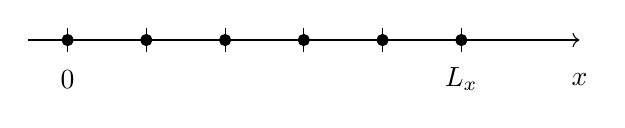
\begin{tikzpicture}
%\draw[fill=gray!23,gray!23](0,0) rectangle (8,2);
%\draw[step=0.5cm,gray,very thin] (0,0) grid (8,2); %background grid
\draw [->] (0.5,1) -- (7.5,1);
\draw[-] (1,0.85)--(1,1.15);
\draw[-] (2,0.85)--(2,1.15);
\draw[-] (3,0.85)--(3,1.15);
\draw[-] (4,0.85)--(4,1.15);
\draw[-] (5,0.85)--(5,1.15);
\draw[-] (6,0.85)--(6,1.15);
\node[] at (1,0.5) {$0$};
\node[] at (6,0.5) {$L_x$};
\node[] at (7.5,0.5) {$x$};
\draw[black,fill=black] (1,1)   circle (2pt);
\draw[black,fill=black] (2,1)   circle (2pt);
\draw[black,fill=black] (3,1)   circle (2pt);
\draw[black,fill=black] (4,1)   circle (2pt);
\draw[black,fill=black] (5,1)   circle (2pt);
\draw[black,fill=black] (6,1)   circle (2pt);
\end{tikzpicture}
\end{center}

\noindent
The distance between two consecutive coordinates is 
\[
h = \frac{L_x}{N-1}
\]
This simply translates as follows in Python:
\begin{lstlisting}
N=10
Lx=1
h=Lx/(N-1)
for i in range(0,N):
    print(i*h)
\end{lstlisting}

Since $i$ ranges from 0 to $N-1$ (because ... python!) the generated values go from 0 to $L_x$. 
Obviously I am doing this because I later wish to reuse these coordinates 
so I also wish to store them in an array.
I therefore need to declare and array of size $N$ which will 
contain all $N$ coordinates:
\begin{lstlisting}
import numpy as np
N=10
Lx=1
h=Lx/(N-1)
x=np.zeros(NV,dtype=np.float64)
for i in range(0,N):
    x[i]=i*h
\end{lstlisting}

What if now I wished the $N$ nodes (i.e. the coordinates of all points) to be placed between two arbitrary coordinates $x_{min}$ and $x_{max}$?

\begin{center}
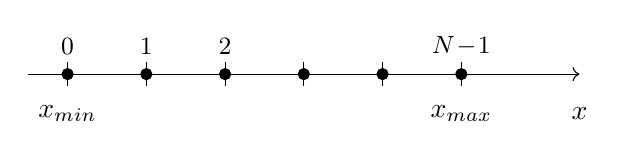
\begin{tikzpicture}
%\draw[fill=gray!23,gray!23](0,0) rectangle (8,2);
%\draw[step=0.5cm,gray,very thin] (0,0) grid (8,2); %background grid
\draw [->] (0.5,1) -- (7.5,1);
\draw[-] (1,0.85)--(1,1.15);
\draw[-] (2,0.85)--(2,1.15);
\draw[-] (3,0.85)--(3,1.15);
\draw[-] (4,0.85)--(4,1.15);
\draw[-] (5,0.85)--(5,1.15);
\draw[-] (6,0.85)--(6,1.15);
\node[] at (1,0.5) {$x_{min}$};
\node[] at (6,0.5) {$x_{max}$};
\node[] at (7.5,0.5) {$x$};
\draw[black,fill=black] (1,1)   circle (2pt);
\draw[black,fill=black] (2,1)   circle (2pt);
\draw[black,fill=black] (3,1)   circle (2pt);
\draw[black,fill=black] (4,1)   circle (2pt);
\draw[black,fill=black] (5,1)   circle (2pt);
\draw[black,fill=black] (6,1)   circle (2pt);
\node[] at (1,1.35) {\small 0};
\node[] at (2,1.35) {\small 1};
\node[] at (3,1.35) {\small 2};
\node[] at (6,1.35) {\small $N\!-\!1$};
\end{tikzpicture}
\end{center}

\noindent In this case the length of the domain is $L_x=x_{max}-x_{min}$, and the above code becomes:
\begin{lstlisting}
import numpy as np
N=10
xmin=-4
xmax=3
h=(xmax-xmin)/(N-1)
x=np.zeros(N,dtype=np.float64)
for i in range(0,N):
    x[i]=xmin+i*h
\end{lstlisting}
Note the presence of $x_{min}$ in the last line! 

\vspace{.8cm}

Unfortunately the world is definitely not one-dimensional, so 
I may want to build a two-dimensional grid spanning the domain 
$[0,L_x]\times[0,L_y]$ as depicted here:



\begin{center}
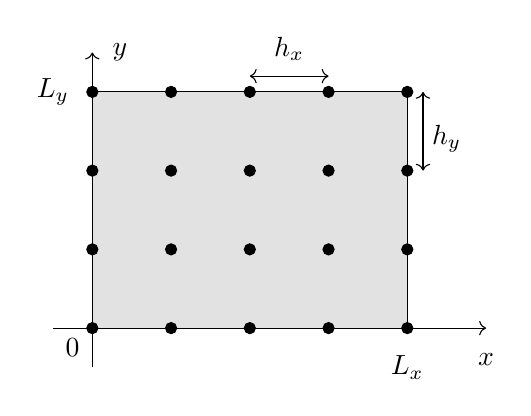
\begin{tikzpicture}
\draw[fill=gray!23,gray!23](1,1) rectangle (5,4);
%\draw[step=0.5cm,gray,very thin] (0,0) grid (7,5); 
\draw [->] (0.5,1) -- (6,1);
\draw [->] (1,0.5) -- (1,4.5);
\node[] at (0.75,0.75) {$0$};
\node[] at (5,0.5) {$L_x$};
\node[] at (0.5,4) {$L_y$};
\node[] at (6,0.6) {$x$};
\node[] at (1.35,4.5) {$y$};
\draw[-] (1,1)--(5,1)--(5,4)--(1,4)--cycle;
\draw[black,fill=black] (1,1)   circle (2pt);
\draw[black,fill=black] (2,1)   circle (2pt);
\draw[black,fill=black] (3,1)   circle (2pt);
\draw[black,fill=black] (4,1)   circle (2pt);
\draw[black,fill=black] (5,1)   circle (2pt);
\draw[black,fill=black] (1,2)   circle (2pt);
\draw[black,fill=black] (2,2)   circle (2pt);
\draw[black,fill=black] (3,2)   circle (2pt);
\draw[black,fill=black] (4,2)   circle (2pt);
\draw[black,fill=black] (5,2)   circle (2pt);
\draw[black,fill=black] (1,3)   circle (2pt);
\draw[black,fill=black] (2,3)   circle (2pt);
\draw[black,fill=black] (3,3)   circle (2pt);
\draw[black,fill=black] (4,3)   circle (2pt);
\draw[black,fill=black] (5,3)   circle (2pt);
\draw[black,fill=black] (1,4)   circle (2pt);
\draw[black,fill=black] (2,4)   circle (2pt);
\draw[black,fill=black] (3,4)   circle (2pt);
\draw[black,fill=black] (4,4)   circle (2pt);
\draw[black,fill=black] (5,4)   circle (2pt);
\draw[<->] (5.2,3)--(5.2,4);
\draw[<->] (3,4.2)--(4,4.2);
\node[] at (3.5,4.55) {$h_x$};
\node[] at (5.5,3.4) {$h_y$};
\end{tikzpicture}
\end{center}

\noindent There are now $N=N_x \times N_y$ nodes in the mesh, 
and we need to define the mesh spacing in both the $x$ and $y$
direction:
\[
h_x = \frac{L_x}{N_x-1}
\qquad\qquad
h_y = \frac{L_y}{N_y-1}
\]
From our experience with the 1D case, it seems logical to 
resort to a double for loop, one in the $x$ direction, 
one in the $y$ direction. 
However we must now make a decision as to which loop is inside the other (inner loop vs. outer loop). In essence, I must decide between 
\begin{lstlisting}
#approach 1
for i in range(0,Nx):
    for j in range(0,Ny):
\end{lstlisting}
and
\begin{lstlisting}
#approach 2
for j in range(0,Ny):
    for i in range(0,Nx):
\end{lstlisting}
As it turns out, I need not decide, both options are equally valid as we will see.
I now fix $N_x=4$ and $N_y=3$ so that the mesh contains 12 nodes:

\begin{center}
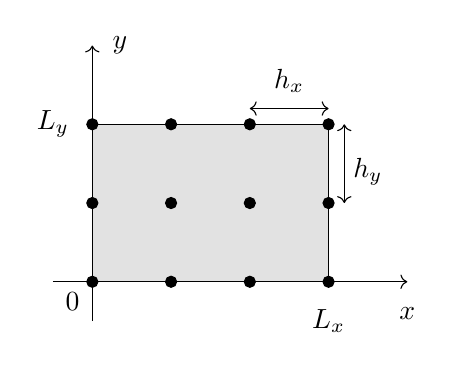
\begin{tikzpicture}
\draw[fill=gray!23,gray!23](1,1) rectangle (4,3);
%\draw[step=0.5cm,gray,very thin] (0,0) grid (7,5); 
\draw [->] (0.5,1) -- (5,1);
\draw [->] (1,0.5) -- (1,4);
\node[] at (0.75,0.75) {$0$};
\node[] at (4,0.5) {$L_x$};
\node[] at (0.5,3) {$L_y$};
\node[] at (5,0.6) {$x$};
\node[] at (1.35,4) {$y$};
\draw[-] (1,1)--(4,1)--(4,3)--(1,3)--cycle;
\draw[black,fill=black] (1,1)   circle (2pt);
\draw[black,fill=black] (2,1)   circle (2pt);
\draw[black,fill=black] (3,1)   circle (2pt);
\draw[black,fill=black] (4,1)   circle (2pt);
\draw[black,fill=black] (1,2)   circle (2pt);
\draw[black,fill=black] (2,2)   circle (2pt);
\draw[black,fill=black] (3,2)   circle (2pt);
\draw[black,fill=black] (4,2)   circle (2pt);
\draw[black,fill=black] (1,3)   circle (2pt);
\draw[black,fill=black] (2,3)   circle (2pt);
\draw[black,fill=black] (3,3)   circle (2pt);
\draw[black,fill=black] (4,3)   circle (2pt);
\draw[<->] (4.2,2)--(4.2,3);
\draw[<->] (3,3.2)--(4,3.2);
\node[] at (3.5,3.55) {$h_x$};
\node[] at (4.5,2.4) {$h_y$};
\end{tikzpicture}
\end{center}

\noindent Looking at approach \#1, I can include a print statement inside the loops as follows:
\begin{lstlisting}
#option 1
Nx=4
Ny=3
for i in range(0,Nx):
    for j in range(0,Ny):
        print('i=',i,'; j=',j)
\end{lstlisting}
If I was to run this code it would display (I first exhaust the $j$ values from the inner most loop before I switch to a different $i$ value):
\begin{lstlisting}
i= 0  ; j= 0
i= 0  ; j= 1
i= 0  ; j= 2
i= 1  ; j= 0
i= 1  ; j= 1
i= 1  ; j= 2
i= 2  ; j= 0
i= 2  ; j= 1
i= 2  ; j= 2
i= 3  ; j= 0
i= 3  ; j= 1
i= 3  ; j= 2
\end{lstlisting}
This means that the code is going through the nodes in the following order:
\begin{center}
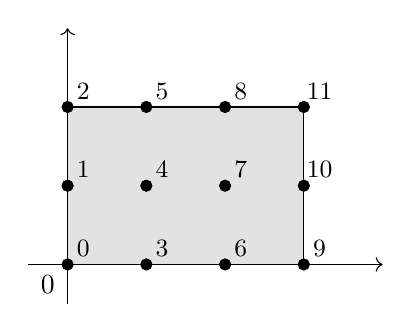
\begin{tikzpicture}
\draw[fill=gray!23,gray!23](1,1) rectangle (4,3);
%\draw[step=0.5cm,gray,very thin] (0,0) grid (7,5); 
\draw [->] (0.5,1) -- (5,1);
\draw [->] (1,0.5) -- (1,4);
\node[] at (0.75,0.75) {$0$};
\draw[-] (1,1)--(4,1)--(4,3)--(1,3)--cycle;
\draw[black,fill=black] (1,1)   circle (2pt);
\draw[black,fill=black] (2,1)   circle (2pt);
\draw[black,fill=black] (3,1)   circle (2pt);
\draw[black,fill=black] (4,1)   circle (2pt);
\draw[black,fill=black] (1,2)   circle (2pt);
\draw[black,fill=black] (2,2)   circle (2pt);
\draw[black,fill=black] (3,2)   circle (2pt);
\draw[black,fill=black] (4,2)   circle (2pt);
\draw[black,fill=black] (1,3)   circle (2pt);
\draw[black,fill=black] (2,3)   circle (2pt);
\draw[black,fill=black] (3,3)   circle (2pt);
\draw[black,fill=black] (4,3)   circle (2pt);
\node[] at (1.2,1.2) {\small $0$};
\node[] at (2.2,1.2) {\small $3$};
\node[] at (3.2,1.2) {\small $6$};
\node[] at (4.2,1.2) {\small $9$};
\node[] at (1.2,2.2) {\small $1$};
\node[] at (2.2,2.2) {\small $4$};
\node[] at (3.2,2.2) {\small $7$};
\node[] at (4.2,2.2) {\small $10$};
\node[] at (1.2,3.2) {\small $2$};
\node[] at (2.2,3.2) {\small $5$};
\node[] at (3.2,3.2) {\small $8$};
\node[] at (4.2,3.2) {\small $11$};
\end{tikzpicture}
\end{center}



Turning now to approach \#2, the same print statement will now yield:
\begin{lstlisting}
i= 0 ; j= 0
i= 1 ; j= 0
i= 2 ; j= 0
i= 3 ; j= 0
i= 0 ; j= 1
i= 1 ; j= 1
i= 2 ; j= 1
i= 3 ; j= 1
i= 0 ; j= 2
i= 1 ; j= 2
i= 2 ; j= 2
i= 3 ; j= 2
\end{lstlisting}
and this corresponds then to the following order: 
\begin{center}
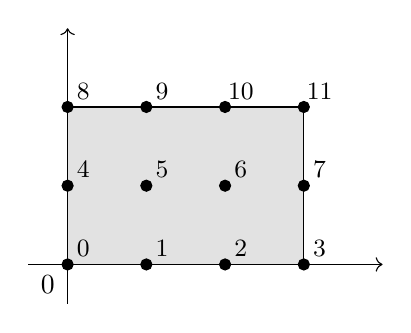
\begin{tikzpicture}
\draw[fill=gray!23,gray!23](1,1) rectangle (4,3);
%\draw[step=0.5cm,gray,very thin] (0,0) grid (7,5); 
\draw [->] (0.5,1) -- (5,1);
\draw [->] (1,0.5) -- (1,4);
\node[] at (0.75,0.75) {$0$};
\draw[-] (1,1)--(4,1)--(4,3)--(1,3)--cycle;
\draw[black,fill=black] (1,1)   circle (2pt);
\draw[black,fill=black] (2,1)   circle (2pt);
\draw[black,fill=black] (3,1)   circle (2pt);
\draw[black,fill=black] (4,1)   circle (2pt);
\draw[black,fill=black] (1,2)   circle (2pt);
\draw[black,fill=black] (2,2)   circle (2pt);
\draw[black,fill=black] (3,2)   circle (2pt);
\draw[black,fill=black] (4,2)   circle (2pt);
\draw[black,fill=black] (1,3)   circle (2pt);
\draw[black,fill=black] (2,3)   circle (2pt);
\draw[black,fill=black] (3,3)   circle (2pt);
\draw[black,fill=black] (4,3)   circle (2pt);
\node[] at (1.2,1.2) {\small $0$};
\node[] at (2.2,1.2) {\small $1$};
\node[] at (3.2,1.2) {\small $2$};
\node[] at (4.2,1.2) {\small $3$};
\node[] at (1.2,2.2) {\small $4$};
\node[] at (2.2,2.2) {\small $5$};
\node[] at (3.2,2.2) {\small $6$};
\node[] at (4.2,2.2) {\small $7$};
\node[] at (1.2,3.2) {\small $8$};
\node[] at (2.2,3.2) {\small $9$};
\node[] at (3.2,3.2) {\small $10$};
\node[] at (4.2,3.2) {\small $11$};
\end{tikzpicture}
\end{center}

\noindent In the end, we see that both approaches yield a valid 
numbering scheme, one is 'lines first' , the other 'columns first'.

In what follows I focus on approach \#2, only because it seems more 'natural' to me than the other one (it goes from left to right, then bottom to top). 
Our proto-code then looks like this:
\begin{lstlisting}
Lx=10
Ly=8
Nx=4
Ny=3
N=Nx*Ny
hx=Lx/(Nx-1)
hy=Ly/(Ny-1)
x=np.zeros(N,dtype=np.float64)
y=np.zeros(N,dtype=np.float64)
for j in range(0,Ny):
    for i in range(0,Nx):
        x[?]=i*hx
        y[?]=j*hy
\end{lstlisting}
Note that I have left two question marks. One may want to replace these by $i$ and $j$, 
following our experience in the 1D case. However, remember that $i$ ($j$) ranges between 
$0$ and $N_x-1=3$ ($0$ and $N_y-1=2$ respectively) but we need to assign and store the 
coordinates of all 12 nodes. 

So what should I write instead of question marks? Effectively, I need some form of counter 
so that every time the inner loop is executed the counter is incremented by one. 
When all $i,j$ combinations are exhausted this counter should have reached the 
last node. Such a counter can be implemented as follows:
\begin{lstlisting}
counter=0
for j in range(0,Ny):
    for i in range(0,Nx):
        print('counter=',counter,'i=',i,'; j=',j,j*Nx+i)
        counter+=1
\end{lstlisting}
It must be initialised to zero, and it is incremented $N_x \cdot N_y$ times.
Running this code would yield 
\begin{lstlisting}
counter=  0 i= 0 ; j= 0
counter=  1 i= 1 ; j= 0
counter=  2 i= 2 ; j= 0
counter=  3 i= 3 ; j= 0
counter=  4 i= 0 ; j= 1
counter=  5 i= 1 ; j= 1
counter=  6 i= 2 ; j= 1
counter=  7 i= 3 ; j= 1
counter=  8 i= 0 ; j= 2
counter=  9 i= 1 ; j= 2
counter= 10 i= 2 ; j= 2
counter= 11 i= 3 ; j= 2
\end{lstlisting}
We see that the counter takes all 12 values between 0 and 11, so it is the index I am looking for. Finally, the 2D code (or approach \#2) looks like:
\begin{lstlisting}
Lx=10
Ly=8
Nx=4
Ny=3
N=Nx*Ny
hx=Lx/(Nx-1)
hy=Ly/(Ny-1)
x=np.zeros(N,dtype=np.float64)
y=np.zeros(N,dtype=np.float64)
counter=0
for j in range(0,Ny):
    for i in range(0,Nx):
        x[counter]=i*hx
        y[counter]=j*hy
        counter+=1
\end{lstlisting}
It is trivial to verify that one can swap the two lines with the 'for' statements to obtain the approach \#1 version of the code.

Before I move to the three-dimensional case, I wish to mention a slightly different 
approach than the 'counter' one. 
Looking back at the numbering generated by approach \#2, it is easy to see that the node number (i.e. a value between 0 and 11)
can be also computed with $j\cdot N_x+i$. You can indeed verify that this expression yields the same values as the counter here above for all the $i,j$ combinations. However one must realise that this formula is not valid for approach \#1. The code then becomes:
\begin{lstlisting}
Lx=10
Ly=8
Nx=4
Ny=3
N=Nx*Ny
hx=Lx/(Nx-1)
hy=Ly/(Ny-1)
x=np.zeros(N,dtype=np.float64)
y=np.zeros(N,dtype=np.float64)
for j in range(0,Ny):
    for i in range(0,Nx):
        x[j*Nx+i]=i*hx
        y[j*Nx+i]=j*hy
\end{lstlisting}

Also, if the domain is not $[0,L_x]\times[0,L_y]$ but
$[x_{min},x_{max}]\times[y_{min},y_{max}]$, the code becomes
\begin{lstlisting}
xmin=-3
xmax=5
ymin=-1
ymax=4
Nx=4
Ny=3
N=Nx*Ny
hx=(xmax-xmin)/(Nx-1)
hy=(ymax-ymin)/(Ny-1)
x=np.zeros(N,dtype=np.float64)
y=np.zeros(N,dtype=np.float64)
for j in range(0,Ny):
    for i in range(0,Nx):
        x[j*Nx+i]=xmin+i*hx
        y[j*Nx+i]=ymin+j*hy
\end{lstlisting}

\vspace{.8cm}

Extending the codes above to three-dimensions is rather trivial, especially when the counter approach 
is used. One must simply be aware of the order of the loops (there are 3\! =6 approaches).
\begin{lstlisting}
xmin=-3
xmax=5
ymin=-1
ymax=4
zmin=1
zmax=6
Nx=4
Ny=3
Nz=5
N=Nx*Ny*Nz
hx=(xmax-xmin)/(Nx-1)
hy=(ymax-ymin)/(Ny-1)
hz=(zmax-zmin)/(Nz-1)
x=np.zeros(N,dtype=np.float64)
y=np.zeros(N,dtype=np.float64)
z=np.zeros(N,dtype=np.float64)
counter
for k in range(0,Nz):
    for j in range(0,Ny):
        for i in range(0,Nx):
            x[counter]=xmin+i*hx
            y[counter]=ymin+j*hy
            z[counter]=zmin+j*hz
            counter+=1
\end{lstlisting}
You will find near identical codes in (for example) Stone 1 and 10.

\vspace{.8cm}

In some cases, we wish to store the coordinates of the mesh nodes because the nodes 
make a regular grid of quadrilaterals on which ODEs or PDEs will be solved:

\begin{center}
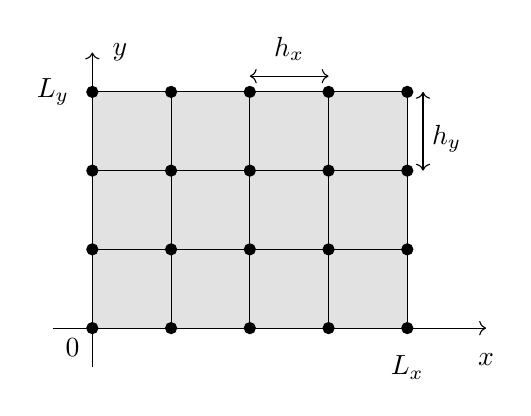
\begin{tikzpicture}
\draw[fill=gray!23,gray!23](1,1) rectangle (5,4);
%\draw[step=0.5cm,gray,very thin] (0,0) grid (7,5); 
\draw [->] (0.5,1) -- (6,1);
\draw [->] (1,0.5) -- (1,4.5);
\node[] at (0.75,0.75) {$0$};
\node[] at (5,0.5) {$L_x$};
\node[] at (0.5,4) {$L_y$};
\node[] at (6,0.6) {$x$};
\node[] at (1.35,4.5) {$y$};
\draw[-] (1,1)--(5,1)--(5,4)--(1,4)--cycle;
\draw[-] (1,2)--(5,2);
\draw[-] (1,3)--(5,3);
\draw[-] (2,1)--(2,4);
\draw[-] (3,1)--(3,4);
\draw[-] (4,1)--(4,4);
\draw[black,fill=black] (1,1)   circle (2pt);
\draw[black,fill=black] (2,1)   circle (2pt);
\draw[black,fill=black] (3,1)   circle (2pt);
\draw[black,fill=black] (4,1)   circle (2pt);
\draw[black,fill=black] (5,1)   circle (2pt);
\draw[black,fill=black] (1,2)   circle (2pt);
\draw[black,fill=black] (2,2)   circle (2pt);
\draw[black,fill=black] (3,2)   circle (2pt);
\draw[black,fill=black] (4,2)   circle (2pt);
\draw[black,fill=black] (5,2)   circle (2pt);
\draw[black,fill=black] (1,3)   circle (2pt);
\draw[black,fill=black] (2,3)   circle (2pt);
\draw[black,fill=black] (3,3)   circle (2pt);
\draw[black,fill=black] (4,3)   circle (2pt);
\draw[black,fill=black] (5,3)   circle (2pt);
\draw[black,fill=black] (1,4)   circle (2pt);
\draw[black,fill=black] (2,4)   circle (2pt);
\draw[black,fill=black] (3,4)   circle (2pt);
\draw[black,fill=black] (4,4)   circle (2pt);
\draw[black,fill=black] (5,4)   circle (2pt);
\draw[<->] (5.2,3)--(5.2,4);
\draw[<->] (3,4.2)--(4,4.2);
\node[] at (3.5,4.55) {$h_x$};
\node[] at (5.5,3.4) {$h_y$};
\end{tikzpicture}
\end{center}

There are $N_x$ nodes in the $x$ direction but only $N_x-1$ cells/elements\footnote{Because of my 
bias towards the Finite Element Method, I will refer to these as elements.}. 
Likewise there are $N_y$ nodes in the $y$ direction but only $N_y-1$ cells/elements.
In total there are $N_e=(N_x-1)(N_y-1)$ elements. 
As for the cell center nodes, we must adopt a systematic way of numbering them. 
If I keep using approach \#2 for the nodes, the following numbering of 
{\color{teal}elements} seems natural:

\begin{center}
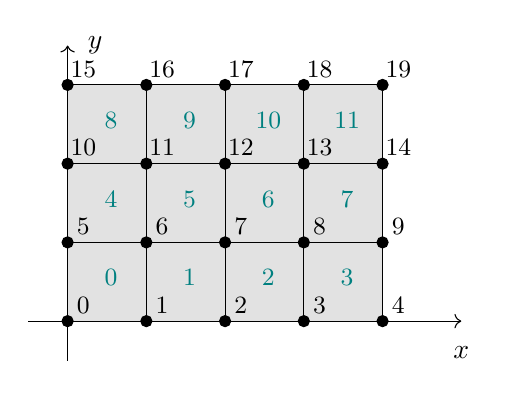
\begin{tikzpicture}
\draw[fill=gray!23,gray!23](1,1) rectangle (5,4);
%\draw[step=0.5cm,gray,very thin] (0,0) grid (7,5); 
\draw [->] (0.5,1) -- (6,1);
\draw [->] (1,0.5) -- (1,4.5);
\node[] at (6,0.6) {$x$};
\node[] at (1.35,4.5) {$y$};
\draw[-] (1,1)--(5,1)--(5,4)--(1,4)--cycle;
\draw[-] (1,2)--(5,2);
\draw[-] (1,3)--(5,3);
\draw[-] (2,1)--(2,4);
\draw[-] (3,1)--(3,4);
\draw[-] (4,1)--(4,4);
\draw[black,fill=black] (1,1)   circle (2pt);
\draw[black,fill=black] (2,1)   circle (2pt);
\draw[black,fill=black] (3,1)   circle (2pt);
\draw[black,fill=black] (4,1)   circle (2pt);
\draw[black,fill=black] (5,1)   circle (2pt);
\draw[black,fill=black] (1,2)   circle (2pt);
\draw[black,fill=black] (2,2)   circle (2pt);
\draw[black,fill=black] (3,2)   circle (2pt);
\draw[black,fill=black] (4,2)   circle (2pt);
\draw[black,fill=black] (5,2)   circle (2pt);
\draw[black,fill=black] (1,3)   circle (2pt);
\draw[black,fill=black] (2,3)   circle (2pt);
\draw[black,fill=black] (3,3)   circle (2pt);
\draw[black,fill=black] (4,3)   circle (2pt);
\draw[black,fill=black] (5,3)   circle (2pt);
\draw[black,fill=black] (1,4)   circle (2pt);
\draw[black,fill=black] (2,4)   circle (2pt);
\draw[black,fill=black] (3,4)   circle (2pt);
\draw[black,fill=black] (4,4)   circle (2pt);
\draw[black,fill=black] (5,4)   circle (2pt);
\node[] at (1.2,1.2) {\small $0$};
\node[] at (2.2,1.2) {\small $1$};
\node[] at (3.2,1.2) {\small $2$};
\node[] at (4.2,1.2) {\small $3$};
\node[] at (5.2,1.2) {\small $4$};
\node[] at (1.2,2.2) {\small $5$};
\node[] at (2.2,2.2) {\small $6$};
\node[] at (3.2,2.2) {\small $7$};
\node[] at (4.2,2.2) {\small $8$};
\node[] at (5.2,2.2) {\small $9$};
\node[] at (1.2,3.2) {\small $10$};
\node[] at (2.2,3.2) {\small $11$};
\node[] at (3.2,3.2) {\small $12$};
\node[] at (4.2,3.2) {\small $13$};
\node[] at (5.2,3.2) {\small $14$};
\node[] at (1.2,4.2) {\small $15$};
\node[] at (2.2,4.2) {\small $16$};
\node[] at (3.2,4.2) {\small $17$};
\node[] at (4.2,4.2) {\small $18$};
\node[] at (5.2,4.2) {\small $19$};
\node[] at (1.55,1.55) {\color{teal} \small $0$};
\node[] at (2.55,1.55) {\color{teal} \small $1$};
\node[] at (3.55,1.55) {\color{teal} \small $2$};
\node[] at (4.55,1.55) {\color{teal} \small $3$};
\node[] at (1.55,2.55) {\color{teal} \small $4$};
\node[] at (2.55,2.55) {\color{teal} \small $5$};
\node[] at (3.55,2.55) {\color{teal} \small $6$};
\node[] at (4.55,2.55) {\color{teal} \small $7$};
\node[] at (1.55,3.55) {\color{teal} \small $8$};
\node[] at (2.55,3.55) {\color{teal} \small $9$};
\node[] at (3.55,3.55) {\color{teal} \small $10$};
\node[] at (4.55,3.55) {\color{teal} \small $11$};
\end{tikzpicture}
\end{center}

In some applications we want to also store the coordinates of the center of all cells, i.e. the $N_e$ coordinates of {\color{teal} these} points:

\begin{center}
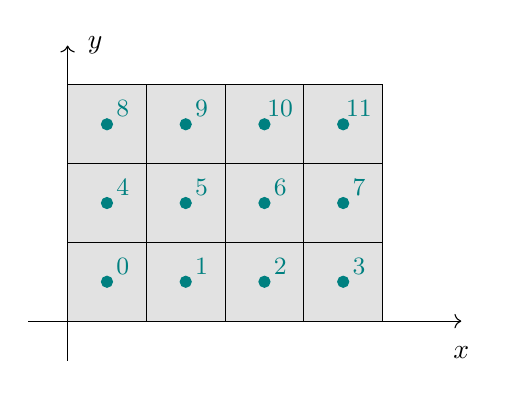
\begin{tikzpicture}
\draw[fill=gray!23,gray!23](1,1) rectangle (5,4);
%\draw[step=0.5cm,gray,very thin] (0,0) grid (7,5); 
\draw [->] (0.5,1) -- (6,1);
\draw [->] (1,0.5) -- (1,4.5);
\node[] at (6,0.6) {$x$};
\node[] at (1.35,4.5) {$y$};
\draw[-] (1,1)--(5,1)--(5,4)--(1,4)--cycle;
\draw[-] (1,2)--(5,2);
\draw[-] (1,3)--(5,3);
\draw[-] (2,1)--(2,4);
\draw[-] (3,1)--(3,4);
\draw[-] (4,1)--(4,4);
\draw[black,fill=black,color=teal] (1.5,1.5)   circle (2pt);
\draw[black,fill=black,color=teal] (2.5,1.5)   circle (2pt);
\draw[black,fill=black,color=teal] (3.5,1.5)   circle (2pt);
\draw[black,fill=black,color=teal] (4.5,1.5)   circle (2pt);
\draw[black,fill=black,color=teal] (1.5,2.5)   circle (2pt);
\draw[black,fill=black,color=teal] (2.5,2.5)   circle (2pt);
\draw[black,fill=black,color=teal] (3.5,2.5)   circle (2pt);
\draw[black,fill=black,color=teal] (4.5,2.5)   circle (2pt);
\draw[black,fill=black,color=teal] (1.5,3.5)   circle (2pt);
\draw[black,fill=black,color=teal] (2.5,3.5)   circle (2pt);
\draw[black,fill=black,color=teal] (3.5,3.5)   circle (2pt);
\draw[black,fill=black,color=teal] (4.5,3.5)   circle (2pt);
\node[] at (1.7,1.7) {\color{teal} \small $0$};
\node[] at (2.7,1.7) {\color{teal} \small $1$};
\node[] at (3.7,1.7) {\color{teal} \small $2$};
\node[] at (4.7,1.7) {\color{teal} \small $3$};
\node[] at (1.7,2.7) {\color{teal} \small $4$};
\node[] at (2.7,2.7) {\color{teal} \small $5$};
\node[] at (3.7,2.7) {\color{teal} \small $6$};
\node[] at (4.7,2.7) {\color{teal} \small $7$};
\node[] at (1.7,3.7) {\color{teal} \small $8$};
\node[] at (2.7,3.7) {\color{teal} \small $9$};
\node[] at (3.7,3.7) {\color{teal} \small $10$};
\node[] at (4.7,3.7) {\color{teal} \small $11$};
\end{tikzpicture}
\end{center}
Given this numbering these points form a regular grid:
\begin{center}
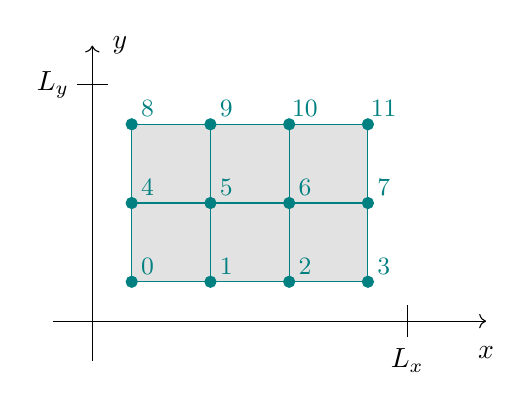
\begin{tikzpicture}
\draw[fill=gray!23,gray!23](1.5,1.5) rectangle (4.5,3.5);
%\draw[step=0.5cm,gray,very thin] (0,0) grid (7,5); 
\draw [->] (0.5,1) -- (6,1);
\draw [->] (1,0.5) -- (1,4.5);
\node[] at (6,0.6) {$x$};
\node[] at (1.35,4.5) {$y$};
\draw[-,teal] (1.5,1.5)--(4.5,1.5)--(4.5,3.5)--(1.5,3.5)--cycle;
\draw[-,teal] (1.5,2.5)--(4.5,2.5);
\draw[-,teal] (2.5,1.5)--(2.5,3.5);
\draw[-,teal] (3.5,1.5)--(3.5,3.5);
\draw[black,fill=black,color=teal] (1.5,1.5)   circle (2pt);
\draw[black,fill=black,color=teal] (2.5,1.5)   circle (2pt);
\draw[black,fill=black,color=teal] (3.5,1.5)   circle (2pt);
\draw[black,fill=black,color=teal] (4.5,1.5)   circle (2pt);
\draw[black,fill=black,color=teal] (1.5,2.5)   circle (2pt);
\draw[black,fill=black,color=teal] (2.5,2.5)   circle (2pt);
\draw[black,fill=black,color=teal] (3.5,2.5)   circle (2pt);
\draw[black,fill=black,color=teal] (4.5,2.5)   circle (2pt);
\draw[black,fill=black,color=teal] (1.5,3.5)   circle (2pt);
\draw[black,fill=black,color=teal] (2.5,3.5)   circle (2pt);
\draw[black,fill=black,color=teal] (3.5,3.5)   circle (2pt);
\draw[black,fill=black,color=teal] (4.5,3.5)   circle (2pt);
\node[] at (1.7,1.7) {\color{teal} \small $0$};
\node[] at (2.7,1.7) {\color{teal} \small $1$};
\node[] at (3.7,1.7) {\color{teal} \small $2$};
\node[] at (4.7,1.7) {\color{teal} \small $3$};
\node[] at (1.7,2.7) {\color{teal} \small $4$};
\node[] at (2.7,2.7) {\color{teal} \small $5$};
\node[] at (3.7,2.7) {\color{teal} \small $6$};
\node[] at (4.7,2.7) {\color{teal} \small $7$};
\node[] at (1.7,3.7) {\color{teal} \small $8$};
\node[] at (2.7,3.7) {\color{teal} \small $9$};
\node[] at (3.7,3.7) {\color{teal} \small $10$};
\node[] at (4.7,3.7) {\color{teal} \small $11$};
\draw[-] (5,0.8)--(5,1.2);
\draw[-] (0.8,4)--(1.2,4);
\node[] at (5,0.5) {$L_x$};
\node[] at (0.5,4) {$L_y$};
\end{tikzpicture}
\end{center}
This 'new' domain is bound by $x'_{min}=h_x/2$, $x'_{max}=L_x-h_x/2$ in 
the $x$ direction and $y'_{min}=h/2$, $y'_{max}=L_y-h_y/2$ in the $y$ direction. We note that the spacings $h_x$ and $h_y$ between the centers is the same as for the nodes. 
We store the coordinates $(x_c,y_c)$ of the cell centers in two arrays of length $N_e$ and the code is then simply

\begin{lstlisting}
Lx=9
Ly=7
Nx=4
Ny=3
N=Nx*Ny
hx=(xmax-xmin)/(Nx-1)
hy=(ymax-ymin)/(Ny-1)
#mesh nodes coordinates
x=np.zeros(N,dtype=np.float64)
y=np.zeros(N,dtype=np.float64)
counter=0
for j in range(0,Ny):
    for i in range(0,Nx):
        x[counter]=i*hx
        y[counter]=j*hy
        counter+=1
#cell centers coordinates
Ne=(Nx-1)*(Ny-1)
xc=np.zeros(Ne,dtype=np.float64)
yc=np.zeros(Ne,dtype=np.float64)
xmin=hx/2
xmax=Lx-hx/2
ymin=hy/2
ymax=Ly-hy/2
counter=0
for j in range(0,Ny-1):
    for i in range(0,Nx-1):
        xc[counter]=xmin+i*hx
        yc[counter]=ymin+j*hy
        counter+=1
\end{lstlisting}





 %%%%%%%%%%%%%%%%%%%%%%%%%%%%%%%%%%%%%%%%%%%%%%%%%

\newpage %%%%%%%%%%%%%%%%%%%%%%%%%%%%%%%%%%%%%%%%%%%%%%%%%%%%%%%%%%%%%%%%%%%%%%%%%%%%%%%%
\section*{
Stone 01: simple analytical solution (D\&H) 
\label{f01}}
\addcontentsline{toc}{section}{\protect\numberline{} 
Stone 01: simple analytical solution (D\&H) 
}

From \cite{dohu}. In order to illustrate the behavior of selected mixed finite elements in the solution 
of stationary Stokes flow,  we consider a two-dimensional problem 
in the square domain $\Omega=[0,1]\times[0,1]$, which possesses a closed-form analytical 
solution. The problem consists of determining the velocity field ${\bm v} = (u,v)$ and the 
pressure $p$ such that 
\[
-\nu \Delta {\bm v} + {\bm \nabla} p = {\bm b}  \quad\quad {\rm in} \; \Omega
\]
\[
{\bm \nabla} \cdot {\bm v} = 0 \quad\quad {\rm in} \; \Omega
\]
\[
{\bm v}={\bm 0} \quad\quad {\rm on} \; \Gamma
\]
where the fluid viscosity is taken as $\nu=1$. The components of the body force ${\bm b}$ are prescribed as 
\begin{eqnarray}
b_x &=& (12 - 24y) x^4 + (-24 + 48y) x^3 + (-48y + 72y^2 - 48 y^3 + 12) x^2 \nonumber\\
    && + (-2 + 24y -72y^2+48y^3)x + 1-4y + 12y^2-8y^3 \nonumber\\ 
b_y &=& (8 - 48y + 48 y^2) x^3 + (-12 + 72y - 72y^2) x^2  \nonumber\\
    && + (4 - 24y + 48y^2 - 48y^3 + 24y^4) x - 12y^2 + 24y^3 - 12y^4  \nonumber
\end{eqnarray}
With this prescribed body force, the exact solution is 
\begin{eqnarray}
u(x,y) &=& x^2(1- x)^2 (2y - 6y^2 + 4y^3)  \nonumber\\
v(x,y) &=& -y^2 (1 - y)^2 (2x - 6x^2 + 4x^3) \nonumber\\
p(x,y) &=& x(1 -x)- 1/6 \nonumber 
\end{eqnarray}
Note that the pressure obeys $\int_{\Omega} p \; d\Omega = 0$

\fbox{
\parbox{10cm}{{\bf features}
\begin{itemize}
\item $Q_1\times P_0$ element \index{$Q_1 \times P_0$}
\item incompressible flow
\item penalty formulation \index{penalty formulation}
\item Dirichlet boundary conditions (no-slip)
\item direct solver 
\item isothermal \index{isothermal}
\item isoviscous \index{isoviscous}
\item analytical solution \index{analytical solution}
\end{itemize}
}}

\includegraphics[width=16cm]{python_codes/fieldstone_01/solution.pdf}

\begin{center}
\includegraphics[width=12cm]{python_codes/fieldstone_01/errors.pdf}\\
Quadratic convergence for velocity error, 
linear convergence for pressure error, as expected.
\end{center}

ToDo:

pressure normalisation?

different cmat, a la schmalholz

To go further:
\begin{enumerate}
\item make your own analytical solution
\end{enumerate}
 %%%%%%%%%%%%%%%%%%%%%%%%%%%%%%%%%%%%%%%%%%%%%%%%%

\newpage %%%%%%%%%%%%%%%%%%%%%%%%%%%%%%%%%%%%%%%%%%%%%%%%%%%%%%%%%%%%%%%%%%%%%%%%%%%%%%%%
\section*{
Stone 02: Stokes sphere in 2D with $Q_1\times P_0$ elements \& penalty formulation 
\label{f02}}
\addcontentsline{toc}{section}{\protect\numberline{} 
Stone 02: Stokes sphere in 2D with $Q_1\times P_0$ elements \& penalty formulation 
}
\lstinputlisting[language=bash,basicstyle=\small]{python_codes/fieldstone_02/keywords}

\begin{center}
Code at \url{https://github.com/cedrict/fieldstone/tree/master/python_codes/fieldstone_02}
\end{center}

\par\noindent\rule{\textwidth}{0.4pt}
%%%%%%%%%%%%%%%%%%%%%%%%%%%%%%%%%%%%%%%%%%%%%%%%%%%%%%%%%%%%%%%%%%%%%%%%%%%%%%%%%%%%%%%%%

The domain is a unit square. The fluid is characterised 
by $\rho=1$ and $\eta=1$ 
while the sphere is characterised 
by $\rho=2$ and $\eta=1000$.
The gravity vector is $\vec{g}=(0,-1)$. 
Boundary conditions are free slip on all sides.
Viscosity and density directly computed at the quadrature points.

\includegraphics[width=15cm]{python_codes/fieldstone_02/solution.pdf}

 %%%%%%%%%%%%%%%%%%%%%%%%%%%%%%%%%%%%%%%%%%%%%%%%%

\newpage %%%%%%%%%%%%%%%%%%%%%%%%%%%%%%%%%%%%%%%%%%%%%%%%%%%%%%%%%%%%%%%%%%%%%%%%%%%%%%%%
\section*{
Stone 03: Convection in a 2D box 
\label{f03}}
\addcontentsline{toc}{section}{\protect\numberline{} 
Stone 03: Convection in a 2D box 
}

\lstinputlisting[language=bash,basicstyle=\small]{python_codes/fieldstone_03/keywords}

This benchmark deals with the 2-D thermal convection of a fluid 
of infinite Prandtl number in a rectangular closed cell.
In what follows, I carry out the case 1a, 1b, and 1c experiments as shown in \cite{blbc89}:
steady convection with constant viscosity in a square box.

The temperature is fixed to zero on top and to $\Delta T$ at the bottom, 
with reflecting symmetry at the sidewalls (i.e. $\partial_x T=0$) 
and there are no internal heat sources. 
Free-slip conditions are implemented on all boundaries. 

The Rayleigh number is given by
\begin{equation}
Ra = \frac{\alpha g_y \Delta T h^3 }{\kappa \nu}
=\frac{\alpha g_y \Delta T h^3 \rho^2 C_p}{k \mu}
\end{equation}

In what follows, I use the following parameter values:  %, as given in \cite{krhb12}:
$L_x=L_y=1$,$\rho_0=c_P=k=\mu=1$, $T_0=0$, $\alpha=10^{-2}$, $g=10^{2}Ra$
and I run the model with $Ra=10^4,10^{5}$ and $10^6$.

The initial temperature field is given by 
\begin{equation}
T(x,y)=(1-y) - 0.01\cos(\pi x) \sin(\pi y)
\end{equation}
The perturbation in the initial temperature fields leads to 
a perturbation of the density field and sets the fluid in motion. 

Depending on the initial Rayleigh number, the system ultimately reaches a 
steady state after some time. 

The Nusselt number (i.e. the mean surface temperature gradient over mean bottom temperature)
is computed as follows \cite{blbc89}:
\begin{equation}
Nu = L_y \frac{\int_0^{L_x} \frac{\partial T}{\partial y}(y=L_y) \; dx  }{\int_0^{L_x} T(y=0) \; dx}
\label{eqNu}
\end{equation}
Note that in our case the denominator is equal to 1 since $L_x=1$ and the temperature at the 
bottom is prescribed to be 1.

The steady state root mean square velocity and Nusselt number measurements
are indicated in the following Table alongside those of \cite{blbc89} and \cite{tack94}.
(Note that this benchmark was also carried out and published in  
other publications \cite{trha98,albe00,gery10,bepo10,dawk11,lezh11} but 
since they did not provide  a complete set
of measurement values, they are not included in the table.)

\begin{center}
\begin{tabular}{llcc}
\hline
          &           & Blankenbach et al & Tackley \cite{tack94}    \\
\hline
\hline
$Ra=10^4$ & $V_{rms}$ &  $42.864947  \pm 0.000020$ & 42.775 \\
          & $Nu$      &  $4.884409   \pm 0.000010$ & 4.878  \\
$Ra=10^5$ & $V_{rms}$ &  $193.21454  \pm 0.00010 $ & 193.11 \\
          & $Nu$      &  $10.534095  \pm 0.000010$ & 10.531 \\
$Ra=10^6$ & $V_{rms}$ &  $833.98977  \pm 0.00020 $ & 833.55 \\
          & $Nu$      &  $21.972465  \pm 0.000020$ & 21.998 \\
\hline
\end{tabular}\\
{\small Steady state Nusselt number $Nu$ and $V_{rms}$ measurements as reported in the literature. }
\end{center}

Food for thought: Looking at the mass, momentum and energy conservation equations, 
we see that that they are coupled: the temperature enters the rhs of the momentum 
equation since the density depends on the temperature (Boussinesq approximation)
while the velocity is present in the advection term of the energy equation.
One should then solve all three equations with $u,v,p,T$ as unknowns. However
this is rarely done in practice and often the system is solved in a segregated way:
first solve for $u,v,p$ assuming $T$ known, then solving for $T$ assuming $u,v,p$ known.
If small time steps are used this is a reasonable approach, or, like in this case, when 
one wishes to compute the steady state of the system rather than an accurate time-evolution
of the system. Better schemes are available and one example thereof is explained in Kronbichler et al (2012) 
\cite{krhb12}.

Also, the current version of this stone uses a simple time discretisation of the $\partial T/\partial t$ term
as explained in Section~\ref{sec:diff1D}. A Crank-Nicolson algorithm could easily be 
implemented as explained in Section~\ref{sec:timediscr}.

Something must be said about how the Nusselt number is computed. 
Its calculation requires the integral of the temperature gradient along an edge. 
Because it is much simpler to compute the temperature gradient in the middle of the 
element alongside other quantities such as pressure, this (elemental) quantity is 
used in the Nusselt number calculations, which makes it inaccurate and therefore 
explains the discrepancy between the computed values and those of other publications.

Finally, it is expected that the thickness of the 
boundary layers decreases with higher Rayleigh number values.
As a consequence, in order to appropriately capture those, one needs 
a higher resolution than at low Ra numbers. This explains why 
acceptable results are obtained for $Ra=10^4$  at low resolution 32x32.


\newpage
\paragraph{Results for $Ra=10^4$}.
\begin{center}
\includegraphics[width=16cm]{python_codes/fieldstone_03/results_1e4/48x48/solution.pdf}\\
\includegraphics[width=5cm]{python_codes/fieldstone_03/results_1e4/Tavrg.pdf}
\includegraphics[width=5cm]{python_codes/fieldstone_03/results_1e4/vrms.pdf}\\
\includegraphics[width=5cm]{python_codes/fieldstone_03/results_1e4/Nu.pdf}
\includegraphics[width=5cm]{python_codes/fieldstone_03/results_1e4/Nu_vrms.pdf}
\end{center}

\newpage
\paragraph{Results for $Ra=10^5$}.
\begin{center}
\includegraphics[width=16cm]{python_codes/fieldstone_03/results_1e5/48x48/solution.pdf}\\
\includegraphics[width=5cm]{python_codes/fieldstone_03/results_1e5/Tavrg.pdf}
\includegraphics[width=5cm]{python_codes/fieldstone_03/results_1e5/vrms.pdf}\\
\includegraphics[width=5cm]{python_codes/fieldstone_03/results_1e5/Nu.pdf}
\includegraphics[width=5cm]{python_codes/fieldstone_03/results_1e5/Nu_vrms.pdf}
\end{center}

\newpage
\paragraph{Results for $Ra=10^6$}.
\begin{center}
\includegraphics[width=16cm]{python_codes/fieldstone_03/results_1e6/48x48/solution.pdf}\\
\includegraphics[width=5cm]{python_codes/fieldstone_03/results_1e6/Tavrg.pdf}
\includegraphics[width=5cm]{python_codes/fieldstone_03/results_1e6/vrms.pdf}\\
\includegraphics[width=5cm]{python_codes/fieldstone_03/results_1e6/Nu.pdf}
\includegraphics[width=5cm]{python_codes/fieldstone_03/results_1e6/Nu_vrms.pdf}
\end{center}


I have tested the influence of the CFL number (0.5 instead of 1) and it does not change much at all.





 %%%%%%%%%%%%%%%%%%%%%%%%%%%%%%%%%%%%%%%%%%%%%%%%%

\newpage %%%%%%%%%%%%%%%%%%%%%%%%%%%%%%%%%%%%%%%%%%%%%%%%%%%%%%%%%%%%%%%%%%%%%%%%%%%%%%%%
\section*{
Stone 04: The lid driven cavity 
\label{f04}}
\addcontentsline{toc}{section}{\protect\numberline{} 
Stone 04: The lid driven cavity 
}


The lid driven cavity is a famous Computational Fluid Dynamics test case and 
has been studied in countless publications with a wealth of numerical techniques
(see \cite{ertu09} for a succinct review) and also in the laboratory \cite{kost84}.

It models a plane flow of an isothermal isoviscous fluid in a rectangular (usually square) lid-driven cavity. 
The boundary conditions are indicated in the Fig. \ref{fig_ldc}a. The gravity is set to zero.

%---------------------------------------------------------
\subsection{the lid driven cavity problem ({\tt ldc=0})}
In the standard case, the upper side of the cavity moves in its own plane at unit speed, while the other sides are fixed.
This thereby introduces a discontinuity in the boundary conditions at the two upper corners of the cavity and yields
an uncertainty as to which boundary (side or top) the corner points belong to. 
In this version of the code the top corner nodes are considered to be part of the lid. If these are excluded 
the recovered pressure showcases and extremely large checkboard pattern.

This benchmark is usually dicussed in the context of low to very high Reynolds number with the full 
Navier-Stokes equations being solved (with the noticeable exception of \cite{sagl81a,sagl81b,chpc95,eid2005}
which focus on the Stokes equation). 
In the case of the incompressible Stokes flow, 
the absence of inertia renders this problem instantaneous so that only one time step is needed.

%---------------------------------------------------------
\subsection{the lid driven cavity problem - regularisation I ({\tt ldc=1})}

We avoid the top corner nodes issue altogether by  
prescribing the horizontal velocity of the lid as follows: 
\begin{equation}
u(x)=x^2(1-x)^2.
\end{equation}
In this case the velocity and its first derivative is continuous at the corners. This is the so-called regularised lid-driven cavity problem \cite{piva94}.

%---------------------------------------------------------
\subsection{the lid driven cavity problem - regularisation II ({\tt ldc=2})}

Another regularisation was presented in \cite{dejn16}. 
Here, a regularized lid driven cavity is studied which is consistent in the sense that 
${\bm \nabla}\cdot{\bm v}=0$ 
holds also at the corners of the domain.
There are no-slip conditions at the boundaries $x=0$, $x=1$, and $y=0$. 

The velocity at $y=1$ is given by

\begin{eqnarray}
u(x) &=& 1-\frac{1}{4}\left( 1-\cos (\frac{x_1-x}{x_1}\pi)  \right)^2   \quad\quad x\in[0,x_1] \nonumber\\
u(x) &=& 1 \quad\quad x\in[x_1,1-x_1] \nonumber\\
u(x) &=& 1-\frac{1}{4}\left( 1-\cos (\frac{x-(1-x_1)}{x_1}\pi)  \right)^2   \quad\quad x\in[1-x_1,1]
\end{eqnarray}
Results are obtained with $x_1=0.1$.

\begin{center}
\fbox{
\parbox{10cm}{{\bf features}
\begin{itemize}
\item $Q_1\times P_0$ element \index{$Q_1 \times P_0$}
\item incompressible flow
\item penalty formulation \index{penalty formulation}
\item isothermal \index{isothermal}
\item isoviscous \index{isoviscous}
\end{itemize}
}}
\end{center}



\newpage
A 100x100 element grid is used. No-slip boundary conditions are prescribed on sides and
bottom. A zero vertical velocity is prescribed at the top and the exact form of the 
prescribed horizontal velocity is controlled by the {\tt ldc} parameter.

\begin{center}
\includegraphics[width=8cm]{python_codes/fieldstone_04/results/p.pdf}\\
\includegraphics[width=12cm]{python_codes/fieldstone_04/results/velocities}\\
\includegraphics[width=12cm]{python_codes/fieldstone_04/results/pressures}
\end{center}

 %%%%%%%%%%%%%%%%%%%%%%%%%%%%%%%%%%%%%%%%%%%%%%%%%

\newpage %%%%%%%%%%%%%%%%%%%%%%%%%%%%%%%%%%%%%%%%%%%%%%%%%%%%%%%%%%%%%%%%%%%%%%%%%%%%%%%%
\section*{
Stone 05: SolCx benchmark 
\label{f05}}
\addcontentsline{toc}{section}{\protect\numberline{} 
Stone 05: SolCx benchmark 
}
\lstinputlisting[language=bash,basicstyle=\small]{python_codes/fieldstone_05/keywords}

\begin{center}
Code at \url{https://github.com/cedrict/fieldstone/tree/master/python_codes/fieldstone_05}
\end{center}

\par\noindent\rule{\textwidth}{0.4pt}
%%%%%%%%%%%%%%%%%%%%%%%%%%%%%%%%%%%%%%%%%%%%%%%%%%%%%%%%%%%%%%%%%%%%%%%%%%%%%%%%%%%%%%%%%

The experiment is fully described in Section~\ref{ss:solcx}.
The viscosity is prescribed at the quadrature points 
If the number of elements is even in the $x$-direction direction, all elements 
(and their associated quadrature points)
have a constant viscosity ($1$ or  $10^6$). If it is odd, then the elements situated 
at the viscosity jump have half their integration points with $\eta=1$ and half 
with $\eta=10^6$ 
(which is a pathological case since the used quadrature rule inside elements cannot represent 
accurately such a jump).  

\begin{center}
\includegraphics[width=8cm]{python_codes/fieldstone_05/results/errors_even.pdf}
\includegraphics[width=8cm]{python_codes/fieldstone_05/results/errors_odd.pdf}\\
{\captionfont Velocity and pressure error convergence as a function of mesh size and for various values
of the penalty parameter. Left: even number of elements in each direction; Right: odd numbers.
}
\end{center}

Because of the high viscosity in the right part of the domain, the penalty parameter should 
be high enough to insure an incompressible flow and thereby recover the expected convergence rate
(at least for the even case). Note that values higher than $\lambda=10^{10}$ yield erroneous solutions 
due to round-off errors. 

\begin{center}
\includegraphics[width=16cm]{python_codes/fieldstone_05/results/solution.pdf}\\
{\captionfont Various fields for 100x100 mesh}
\end{center}


\infortran
Note that a Fortran90 version of this code is available in the same folder. \index{general}{fortran90}


 %%%%%%%%%%%%%%%%%%%%%%%%%%%%%%%%%%%%%%%%%%%%%%%%%

\newpage %%%%%%%%%%%%%%%%%%%%%%%%%%%%%%%%%%%%%%%%%%%%%%%%%%%%%%%%%%%%%%%%%%%%%%%%%%%%%%%%
\section*{
Stone 06: SolKz benchmark 
\label{f06}}
\addcontentsline{toc}{section}{\protect\numberline{} 
Stone 06: SolKz benchmark 
}
\lstinputlisting[language=bash,basicstyle=\small]{python_codes/fieldstone_06/keywords}

\begin{center}
Code at \url{https://github.com/cedrict/fieldstone/tree/master/python_codes/fieldstone_06}
\end{center}

\par\noindent\rule{\textwidth}{0.4pt}
%%%%%%%%%%%%%%%%%%%%%%%%%%%%%%%%%%%%%%%%%%%%%%%%%%%%%%%%%%%%%%%%%%%%%%%%%%%%%%%%%%%%%%%%%

The SolKz benchmark \cite{repa87} is similar to the SolCx benchmark.
but the viscosity is now a function of the space coordinates: 
\begin{equation}
\eta(y)=\exp(By) \quad {\rm with} \quad B=13.8155
\end{equation}
It is however not a discontinuous function but grows exponentially with the vertical coordinate so that its overall variation is again $10^6$. 
The forcing is again chosen by imposing a spatially variable density variation as follows:
\begin{equation}
\rho(x,y)=\sin(2y) \cos(3\pi x)
\end{equation}
Free slip boundary conditions are imposed on all sides of the domain.
This benchmark is presented in Zhong (1996) \cite{zhon96} as well and is studied 
in Duretz \etal (2011) \cite{dumg11} and Gerya \etal (2013) \cite{gemd13}.

\begin{center}
\includegraphics[width=14cm]{python_codes/fieldstone_06/results/solution.pdf}
\end{center}

\begin{center}
\includegraphics[width=10cm]{python_codes/fieldstone_06/results/errors.pdf}\\
{\captionfont Velocity and pressure error as a function of mesh size.}
\end{center}
 %%%%%%%%%%%%%%%%%%%%%%%%%%%%%%%%%%%%%%%%%%%%%%%%%

\newpage %%%%%%%%%%%%%%%%%%%%%%%%%%%%%%%%%%%%%%%%%%%%%%%%%%%%%%%%%%%%%%%%%%%%%%%%%%%%%%%%
\section*{
Stone 07: SolVi benchmark 
\label{f07}}
\addcontentsline{toc}{section}{\protect\numberline{} 
Stone 07: SolVi benchmark 
}

Following SolCx and SolKz, the SolVi inclusion benchmark solves 
a problem with a discontinuous viscosity field, but in this case 
the viscosity field is chosen in such a way that the discontinuity 
is along a circle. Given the regular nature of the grid used by a majority of codes and the present one, 
this ensures that the discontinuity in the viscosity never aligns to cell boundaries.
This in turns leads to almost discontinuous pressures along the interface which are difficult to represent accurately.
Schmid \& Podlachikov (2003) \cite{scpo03} derived a simple analytic solution for the pressure and 
velocity fields for a circular 
inclusion under simple shear and it was used in \cite{deka08,sunh10,dumg11,krhb12,gemd13}.

Because of the symmetry of the problem, we only have to solve over the top right quarter of the domain.
The analytical solution requires a strain rate boundary condition (e.g., pure shear) to be applied far away 
from the inclusion. In order to avoid using very large domains and/or dealing with this type of boundary condition 
altogether, the analytical solution is evaluated and imposed on the boundaries of the domain. 
By doing so, the truncation error introduced while discretizing the strain rate boundary condition is removed.

A characteristic of the analytic solution is that the pressure is zero inside the inclusion, while outside it follows the relation
\begin{equation}
p_m = 4 \dot{\epsilon}
\frac{\mu_m(\mu_i-\mu_m)}{\mu_i+\mu_m}
\frac{r_i^2}{r^2} \cos(2\theta)
\end{equation}
where $\mu_i = 10^3$ is the viscosity of the inclusion and $\mu_m = 1$ is the viscosity of the background media, $\theta=\tan^{-1}(y/x)$,
and $\dot{\epsilon}=1$ is the applied strain rate.

Deubelbeiss \& Kauss (2008) \cite{deka08} thoroughly investigated this problem with various 
numerical methods (FEM, FDM), with and without tracers, 
and conclusively showed how various averagings lead to different results. 
Duretz et al (2011) \cite{dumg11} obtained a first order convergence for both pressure and velocity, 
while Kronbichler et al (2012) \cite{krhb12}
and Gerya et al (2013) \cite{gemd13} showed that the use of adaptive mesh refinement in respectively the FEM and FDM 
yields convergence rates which depend on refinement strategies. 

\begin{center}
\includegraphics[width=8cm]{python_codes/fieldstone_07/results/errors}\\
{\captionfont Velocity and pressure error convergence as a function of mesh size.}
\end{center}

\includegraphics[width=15cm]{python_codes/fieldstone_07/results/solution}

\begin{center}
\includegraphics[width=7cm]{python_codes/fieldstone_07/results/pressbottom}
\includegraphics[width=7cm]{python_codes/fieldstone_07/results/veldiag}\\
{\captionfont Left: Pressure at the bottom of the domain. Right: $u$ on the diagonal $x=y$.}
\end{center}

 %%%%%%%%%%%%%%%%%%%%%%%%%%%%%%%%%%%%%%%%%%%%%%%%%

\newpage %%%%%%%%%%%%%%%%%%%%%%%%%%%%%%%%%%%%%%%%%%%%%%%%%%%%%%%%%%%%%%%%%%%%%%%%%%%%%%%%
\section*{
Stone 08: the indentor benchmark 
\label{f08}}
\addcontentsline{toc}{section}{\protect\numberline{} 
Stone 08: the indentor benchmark 
}
\lstinputlisting[language=bash,basicstyle=\small]{python_codes/fieldstone_08/keywords}

\begin{center}
Code at \url{https://github.com/cedrict/fieldstone/tree/master/python_codes/fieldstone_08}
\end{center}

\par\noindent\rule{\textwidth}{0.4pt}
%%%%%%%%%%%%%%%%%%%%%%%%%%%%%%%%%%%%%%%%%%%%%%%%%%%%%%%%%%%%%%%%%%%%%%%%%%%%%%%%%%%%%%%%%

The punch benchmark is one of the few boundary value problems involving plastic solids for which there exists an exact solution. 
Such solutions are usually either for highly simplified geometries (spherical or axial symmetry, for instance) or simplified material models (such as rigid plastic solids) \cite{kacha04}.

In this experiment, a rigid punch indents a rigid plastic half space; the slip line field theory gives 
exact solutions as shown in section~\ref{sec:punch}. 
The plane strain formulation of the equations and the detailed solution to the problem were derived in the Appendix of \cite{thfb08} and are also presented in \cite{gepd98}.

The two dimensional punch problem has been extensively studied numerically for the past 40 years 
\cite{zihl75,zihp95,chpe01,chan99,huhy99,yuti06,bufs08,raab07} and has been used to draw a parallel 
with the tectonics of eastern China in the context of the 
India-Eurasia collision \cite{tamo76,mota77}.
It is also worth noting that it has been carried out in one form or another in series of 
analogue modelling articles 
concerning the same region, with a rigid indenter colliding with a rheologically stratified 
lithosphere \cite{peta88,daco88,jodc90}.
 
Numerically, the one-time step punch experiment is performed on a two-dimensional
domain of purely plastic von Mises material. 
Given that the von Mises rheology yield criterion does not depend on pressure
(see Section~\ref{sec:vMcriterion}), the density of the material and/or the gravity 
vector is set to zero. Sides are set to free slip boundary conditions, the bottom to no slip, 
while a vertical velocity $(0,-v_p)$ is prescribed at the top boundary for nodes 
whose $x$ coordinate is within $[L_x/2-\delta/2,L_x/2+\delta/2]$. 

The following parameters are used: $L_x=1$, $L_y=0.5$, $\mu_{min}=10^{-3}$, 
$\mu_{max}=10^3$, $v_p=1$, $\delta=0.11111$ 
and the yield value of the material is set to $\sigma_Y=1$. 

The analytical solution predicts that the angle of the shear bands stemming from the sides of the punch 
is $\pi/4$, that the pressure right under the punch is $1+\pi$, 
and that the velocity of the rigid blocks on each side of the punch is $v_p/\sqrt{2}$ 
(this is simply explained by invoking conservation of mass).

In what follows I show results of the rough and smooth punch for a 124x68 grid. The difference between the two
lies in the nature of the kinematic boundary conditions under the punched area. 'rough' means that the indentor 
also fixes the horizontal velocity component to zero while it is free in the smooth case.

We see that the smooth punch does not trigger the checkerboard pressure modes as much as the rough case 
and we recover nicely the analytical pressure under the punch \cite{thfb08,gltf18}.

\newpage
%................................................................................
\paragraph{Rough punch} 

\begin{center}
\includegraphics[width=6cm]{python_codes/fieldstone_08/results/rough/velocity.pdf}
\includegraphics[width=6cm]{python_codes/fieldstone_08/results/rough/pressure.pdf}\\
\includegraphics[width=6cm]{python_codes/fieldstone_08/results/rough/strainrate.pdf}
\includegraphics[width=6cm]{python_codes/fieldstone_08/results/rough/stress.pdf}\\
\includegraphics[width=6cm]{python_codes/fieldstone_08/results/rough/u_stats.pdf}
\includegraphics[width=6cm]{python_codes/fieldstone_08/results/rough/v_stats.pdf}\\
\includegraphics[width=6cm]{python_codes/fieldstone_08/results/rough/residual.pdf}
\includegraphics[width=6cm]{python_codes/fieldstone_08/results/rough/diff_uv.pdf}\\
{\captionfont a,b,c,d) velocity, pressure, strainrate and stress at the top of the domain; 
e,f) min/max value of $u$ and $v$;
g,h) residual and normalised velocity difference.}
\end{center}

\newpage
\includegraphics[width=16cm]{python_codes/fieldstone_08/results/rough/solution.pdf}


%................................................................................
\newpage
\paragraph{Smooth punch}

\begin{center}
\includegraphics[width=6cm]{python_codes/fieldstone_08/results/smooth/velocity.pdf}
\includegraphics[width=6cm]{python_codes/fieldstone_08/results/smooth/pressure.pdf}\\
\includegraphics[width=6cm]{python_codes/fieldstone_08/results/smooth/strainrate.pdf}
\includegraphics[width=6cm]{python_codes/fieldstone_08/results/smooth/stress.pdf}\\
\includegraphics[width=6cm]{python_codes/fieldstone_08/results/smooth/u_stats.pdf}
\includegraphics[width=6cm]{python_codes/fieldstone_08/results/smooth/v_stats.pdf}\\
\includegraphics[width=6cm]{python_codes/fieldstone_08/results/smooth/residual.pdf}
\includegraphics[width=6cm]{python_codes/fieldstone_08/results/smooth/diff_uv.pdf}\\
{\captionfont a,b,c,d) velocity, pressure, strainrate and stress at the top of the domain; 
e,f) min/max value of $u$ and $v$;
g,h) residual and normalised velocity difference.}
\end{center}

\newpage
\includegraphics[width=16cm]{python_codes/fieldstone_08/results/smooth/solution.pdf}




 %%%%%%%%%%%%%%%%%%%%%%%%%%%%%%%%%%%%%%%%%%%%%%%%%

\newpage %%%%%%%%%%%%%%%%%%%%%%%%%%%%%%%%%%%%%%%%%%%%%%%%%%%%%%%%%%%%%%%%%%%%%%%%%%%%%%%%
\section*{
Stone 09: the annulus benchmark with $Q_1\times P_0$ elements
\label{f09}}
\addcontentsline{toc}{section}{\protect\numberline{} 
Stone 09: the annulus benchmark with $Q_1\times P_0$ elements
}

{\sl This fieldstone was developed in collaboration with Prof. E.G.P. Puckett}. 
\index{contributors}{E.G.P. Puckett}

An analytical solution to the
isoviscous incompressible Stokes equations is derived in an annulus geometry.
The velocity and pressure fields are as follows:

\begin{eqnarray}
v_r(r,\theta)     &=&  g(r) k \sin(k\theta), \\
v_\theta(r,\theta)&=&  f(r) \cos(k \theta), \\ 
p(r,\theta)       &=&  k h(r) \sin(k \theta), \\
\rho (r,\theta)   &=& \aleph(r) k \sin (k \theta), 
\end{eqnarray}
with
\begin{eqnarray}
f(r)&=&Ar+B/r, \\
g(r) &=& \frac{A}{2}r  +  \frac{B}{r} \ln r + \frac{C}{r}, \\
h(r)&=& \frac{2g(r)-f(r)}{r},  \\
\aleph(r) &=& g'' - \frac{g'}{r}  - \frac{g}{r^2} (k^2 - 1)  + \frac{f}{r^2}   + \frac{f'}{r}, \\
A &=& -C\frac{2(\ln R_1 - \ln R_2)} { R_2^2 \ln R_1  - R_1^2 \ln R_2}, \\
B &=& -C \frac{R_2^2-R_1^2}{R_2^2 \ln R_1 - R_1^2 \ln R_2}.
\end{eqnarray}

The parameters $A$ and $B$ are chosen so that $v_r(R_1)=v_r(R_2)=0$, i.e.
the velocity is tangential to both inner and outer surfaces.
The gravity vector is radial and of unit length.
In the present case, we set $R_1=1$, $R_2=2$ and $C=-1$. 

\begin{center}
\includegraphics[width=5cm]{python_codes/fieldstone_09/velocity}
\includegraphics[width=5cm]{python_codes/fieldstone_09/vr}
\includegraphics[width=5cm]{python_codes/fieldstone_09/vtheta}\\
{\small Left to right: velocity norm, $r$ component, $\theta$ component}
\end{center}

\begin{center}
\includegraphics[width=7cm]{python_codes/fieldstone_09/density}
\includegraphics[width=7cm]{python_codes/fieldstone_09/pressure}\\
{\small Left: density field; right: pressure field.}
\end{center}

\begin{center}
\includegraphics[width=7cm]{python_codes/fieldstone_09/psi}
\includegraphics[width=7cm]{python_codes/fieldstone_09/psi_arrows}\\
{\small Left: $\psi$ field; right: $\psi$ isolines with velocity arrows.}
\end{center}

\includegraphics[width=15cm]{python_codes/fieldstone_09/errors}

 %%%%%%%%%%%%%%%%%%%%%%%%%%%%%%%%%%%%%%%%%%%%%%%%%

\newpage %%%%%%%%%%%%%%%%%%%%%%%%%%%%%%%%%%%%%%%%%%%%%%%%%%%%%%%%%%%%%%%%%%%%%%%%%%%%%%%%
\section*{
Stone 10: Stokes sphere (3D) - penalty 
\label{f10}}
\addcontentsline{toc}{section}{\protect\numberline{} 
Stone 10: Stokes sphere (3D) - penalty 
}
\lstinputlisting[language=bash,basicstyle=\small]{python_codes/fieldstone_10/keywords}

\begin{center}
Code at \url{https://github.com/cedrict/fieldstone/tree/master/python_codes/fieldstone_10}
\end{center}

\par\noindent\rule{\textwidth}{0.4pt}
%%%%%%%%%%%%%%%%%%%%%%%%%%%%%%%%%%%%%%%%%%%%%%%%%%%%%%%%%%%%%%%%%%%%%%%%%%%%%%%%%%%%%%%%%%%%

The domain is a unit cube. Free slip boundary conditions 
are imposed on all sides. The mesh counts 
nelx*nely*nelz=nel elements and 
nnx*nny*nnz=NV nodes.
The density and the viscosity are prescribed in the domain 
by means of two functions:
the density is set to 2 inside a sphere of radius 0.123 centered 
at (0.5,0.5,0.5) and 1 outside. The viscosity is 100 inside the sphere
and 1 outside.  The gravity vector is set to $\vec{g}=(0,0,-1)$.

The FE matrix size grows even faster now than in the previous 2D case so
choosing the right matrix storage is of paramount importance. 

Three experiments are carried out:
\begin{enumerate}
\item the one described above.
We see that the pressure field is dominated by the lithostatic signal.
\item same as experiment 1, but a reference density of 1 is substracted to all densities, so that 
the sphere density is 1 and the density of the surrounding fluid is now 0. In essence, we remove a
'background' density which does not participate in the flow generation, and thereby get rid of the 
lithostatic signal of the pressure.
\item same as experiment 2, but the top boundary is now open (free surface)
\end{enumerate} 


\begin{center}
\includegraphics[width=5cm]{python_codes/fieldstone_10/results/grid}
\includegraphics[width=5cm]{python_codes/fieldstone_10/results/vel}
\includegraphics[width=5cm]{python_codes/fieldstone_10/results/press}\\
\includegraphics[width=5cm]{python_codes/fieldstone_10/results/visc}
\includegraphics[width=5cm]{python_codes/fieldstone_10/results/dens}\\
{\small Experiment 1: resolution 24x24x24}
\end{center}

\begin{center}
\includegraphics[width=5cm]{python_codes/fieldstone_10/results/dens_2}
\includegraphics[width=5cm]{python_codes/fieldstone_10/results/press_2}\\
{\small Experiment 2: Density and pressure fields. Resolution 24x24x24}
\end{center}


\begin{center}
\includegraphics[width=5cm]{python_codes/fieldstone_10/results/press_3}
\includegraphics[width=5cm]{python_codes/fieldstone_10/results/vel_3}\\
{\small Experiment 3: pressure and velocity fields. Resolution 24x24x24}
\end{center}

\begin{center}
\includegraphics[width=5cm]{python_codes/fieldstone_10/results/model1/pressure.pdf}
\includegraphics[width=5cm]{python_codes/fieldstone_10/results/model2/pressure.pdf}
\includegraphics[width=5cm]{python_codes/fieldstone_10/results/model3/pressure.pdf}\\
{\captionfont Elemental pressure for all elements as a function of their vertical (middle) coordinate for
(from left to right) experiments 1, 2 and 3. }
\end{center}

Note that a similar fortran code is present in the folder. 
 %%%%%%%%%%%%%%%%%%%%%%%%%%%%%%%%%%%%%%%%%%%%%%%%%

\newpage %%%%%%%%%%%%%%%%%%%%%%%%%%%%%%%%%%%%%%%%%%%%%%%%%%%%%%%%%%%%%%%%%%%%%%%%%%%%%%%%
\section*{
Stone 11: stokes sphere (3D) - mixed formulation 
\label{f11}}
\addcontentsline{toc}{section}{\protect\numberline{} 
Stone 11: stokes sphere (3D) - mixed formulation 
}
\lstinputlisting[language=bash,basicstyle=\small]{python_codes/fieldstone_11/keywords}

The setup is identical to the one of the \stone~10.

The difference lies in how we solve the Stokes equation. This stone does not rely on 
the penalty method (Section \ref{sec:penalty}) 
but instead used a mixed formulation, i.e. we solve for both 
velocity and pressure at the same time (see Section~\ref{sec:mixed}).

In the case when free slip boundary conditions are applied on all 
6 faces of the cube we know that there is a pressure nullspace, i.e.
that the pressure can only be computed up to a constant. In order to 
remove this nullspace one must add an additional constraint 
We here choose to (somewhat arbitrarily) enforce that the average pressure 
over the whole domain is zero:
\[
<p>=\frac{1}{|\Omega|} \int_\Omega p \; dV =0 
\]
Since the code relies of discontinuous zero-th order polynomial shape functions 
for pressure this condition simply writes (and since $|\Omega|=1$):
\[
<p>=\frac{1}{|\Omega|} \int_\Omega p\;  dV 
=  \sum_{e} \int_{\Omega_e} p dV = \sum_e p_e V_e = h^3 \sum_e p_e =0
\]
Dividing all by $h^3$, the condition becomes simply:
\[
p_1 + p_2 + p_3 + ... + p_{nel} = 0
\]
How this constraint is incorporated in the Stokes matrix is explained in Section~\ref{ss_pnorm}.

It is also important to remember that if one now switches to a free surface at the top then 
the null space is absent from the equations and the constraint should be removed/switched off.

The pressure normalisation is controled by the boolean {\sl pnormalise} in the code. 
Since the pressure constraint adds a line to the global FE, we then logically have:
\begin{lstlisting}
if pnormalise:
   a_mat = np.zeros((Nfem+1,Nfem+1),dtype=np.float64) 
   rhs   = np.zeros(Nfem+1,dtype=np.float64)    
else:
   a_mat = np.zeros((Nfem,Nfem),dtype=np.float64)
   rhs   = np.zeros(Nfem,dtype=np.float64)       
\end{lstlisting} 
Once the solve has been done, we retrieve the separate velocity and pressure fields as follows:
\begin{lstlisting}
u,v,w=np.reshape(sol[0:NfemV],(nnp,3)).T
p=sol[NfemV:Nfem]
\end{lstlisting} 
and the Lagrange multiplier is a scalar at the bottom of the array:
\begin{lstlisting}
if pnormalise:
   print("     -> Lagrange multiplier: %.4es" % sol[Nfem])
\end{lstlisting} 

It is quite easy in python to visualise the matrix structure 
with the spy function:
\begin{lstlisting}
plt.spy(a_mat)
\end{lstlisting} 
and we see that we indeed recover
the block structure with a zero block for the pressure-pressure entries.  
\begin{center}
\includegraphics[width=7cm]{python_codes/fieldstone_11/results/matrix6x6x6.pdf}
\includegraphics[width=7cm]{python_codes/fieldstone_11/results/matrix16x16x16.pdf}\\
{\captionfont Sparsity pattern of the Stokes matrix for a 6x6x6 mesh (left) and a 16x16x16 mesh (right).}
\end{center}

\begin{center}
\includegraphics[width=7cm]{python_codes/fieldstone_11/results/vel}
\includegraphics[width=7cm]{python_codes/fieldstone_11/results/press}
\includegraphics[width=8cm]{python_codes/fieldstone_11/results/sr}\\
{\captionfont Velocity, pressure and effective strain rate fields for a 20x20x20 mesh.}
\end{center}
 %%%%%%%%%%%%%%%%%%%%%%%%%%%%%%%%%%%%%%%%%%%%%%%%%

\newpage %%%%%%%%%%%%%%%%%%%%%%%%%%%%%%%%%%%%%%%%%%%%%%%%%%%%%%%%%%%%%%%%%%%%%%%%%%%%%%%%
\section*{
Stone 12: consistent pressure recovery 
\label{f12}}
\addcontentsline{toc}{section}{\protect\numberline{} 
Stone 12: consistent pressure recovery 
}
\lstinputlisting[language=bash,basicstyle=\small]{python_codes/fieldstone_12/keywords}

\begin{center}
Code at \url{https://github.com/cedrict/fieldstone/tree/master/python_codes/fieldstone_12}
\end{center}

\par\noindent\rule{\textwidth}{0.4pt}
%%%%%%%%%%%%%%%%%%%%%%%%%%%%%%%%%%%%%%%%%%%%%%%%%%%%%%%%%%%%%%%%%%%%%%%%%%%%%%%%%%%%%%%%%%%%%%


We start from the analytical benchmark of Section \ref{mms1} and we use $Q_1 \times P_0$
elements with a penalty formulation. 
We have seen in stone $\# 1$ how to recover the elemental pressure as a postprocessing step. 
However, the discontinous nature of the pressure field (and the presence of a
parasitic checkerboard mode) can be problematic for many reasons 
(pressure enters the rheology, equation of state, plotting, ...). 
We then wish to project the elemental pressure onto the nodes of the mesh while at the same 
time filtering the checkerboard mode out. 

Terminology: in general, when a discontinuous elemental pressure is used in a stone, 
it is called $p$ while its projection onto the nodes is coined $q$. 
In this case we compute several nodal pressures as explained in Section~\ref{psmoothing}:

\begin{itemize}
%...........
\item $q_1$: smoothed pressure obtained with the  center-to-node approach (scheme 1)

\item $q_2$: the nodal pressure obtained by smoothing the elemental pressure using element areas (scheme 2)

\item $q_3$: the nodal pressure obtained by smoothing the elemental p using triangle areas (scheme 3)

\item $q_4$: smoothed pressure obtained with the center-to-node approach with inverse element area weighing.

\item $q_5$: is not computed because same as 6.

\item $q_6$: consistent pressure recovery through FE (scheme 5 \& 6)

\item $q_7$: consistent pressure recovery with lumped mass matrix. 

\item $q_8$: bilinear interpolation. 

\end{itemize}

Since the setups showcase Dirichlet boundary conditions on all four sides, 
the pressure solution is normalised so that $\int p dV =0 $.

\begin{remark}
Nodes on edges and corners may need special treatment as documented in Sani et al \cite{sagl81a} or
Lee et al (1979) \cite{legs79} which is not done here.  
\end{remark}

\begin{remark}
Lee et al (1979) \cite{legs79} discuss two different ways to compute the lumped mass matrix. 
\end{remark}

\begin{remark}
Nodes on the boundary showcase the largest errors. Maybe then use CBF instead for these?
\end{remark}

\begin{remark}
In the same folder there is a fortran90 version of the consistent recovery algorithm.
\end{remark}


I have created a simple checkerboard filter. Let $\phi=\pm 1$ denote this field.
The filter is applied as follows:
\[
p_{filtered} = p - \left( \frac{1}{|\Omega|} \iint_\Omega p \phi dV \right) \phi
\]
It is in fact a a projection. If $p=\alpha \phi$  where $\alpha$ is a scalar, then 
it is trivial to show that $p_{filtered} =0$.
Likewise, if $p=constant$ then $p_{filtered}=p$.
This idea is probably to be found in the relevant publications of Section~\ref{psmoothing}
in some form or shape. 

There is much more work to be done on this topic/stone!

\newpage
%...............................................
%...............................................
\paragraph{Regular mesh made of square elements}

We compute the error convergence for $p$, $q_i$ $(i=1,...8)$:
\begin{center}
\includegraphics[width=10cm]{python_codes/fieldstone_12/results/reg/errors}
\end{center}
The elemental pressure error converges like $h^1$, $q_{1-7}$ converge like $h^{1.5}$ and 
$q^8$ converges like $h^2$.


\begin{center}
\includegraphics[width=5cm]{python_codes/fieldstone_12/results/reg/pressure}
\includegraphics[width=5cm]{python_codes/fieldstone_12/results/reg/p_error}
\includegraphics[width=5cm]{python_codes/fieldstone_12/results/reg/q1_error}\\
\includegraphics[width=5cm]{python_codes/fieldstone_12/results/reg/q2_error}
\includegraphics[width=5cm]{python_codes/fieldstone_12/results/reg/q3_error}
\includegraphics[width=5cm]{python_codes/fieldstone_12/results/reg/q4_error}\\
\includegraphics[width=5cm]{python_codes/fieldstone_12/results/reg/q6_error}
\includegraphics[width=5cm]{python_codes/fieldstone_12/results/reg/q7_error}
\includegraphics[width=5cm]{python_codes/fieldstone_12/results/reg/q8_error}\\
{\captionfont Left: pressure fields as a function of the $x$-coordinate. 
Right: absolute error with regards to the analytical solution. All on 32x32 mesh.}
\end{center}

It is worth noticing that the checkerboard is (visually) not present:
\begin{center}
\includegraphics[width=4cm]{python_codes/fieldstone_12/results/reg/p32}
\includegraphics[width=4cm]{python_codes/fieldstone_12/results/reg/p48}
\includegraphics[width=4cm]{python_codes/fieldstone_12/results/reg/p64}\\
{\captionfont Elemental pressure field for 32x32, 48x48 and 64x64 resolutions.}
\end{center}
This means that the algorithms above fulfill an interpolation function, but not a smoothing one.

\newpage
%............................................
\paragraph{Adding randomness to internal node positions} We now add a random value $\xi h$ to the 
location of all nodes which are not on the boundary where $h$=$L_x$/nelx and we set $\xi=20\%$.
In this case a 32x32 mesh looks as follows:

\begin{center}
\includegraphics[width=7cm]{python_codes/fieldstone_12/results/rand/area_0p1}
\includegraphics[width=7cm]{python_codes/fieldstone_12/results/rand/area_0p2}\\
{\captionfont Mesh 32x32 elements. Left: $\xi=0.1$; Right: $\xi=0.2$}
\end{center}

We repeat the same exercise as before on such a mesh and look at the errors

\begin{center}
\includegraphics[width=7cm]{python_codes/fieldstone_12/results/rand/errors_nofilter}
\includegraphics[width=7cm]{python_codes/fieldstone_12/results/rand/errors_filter}\\
{\captionfont Velocity and pressure errors for $\xi=0.2$. Left: no filter, right: with filter.} 
\end{center}

It is easy to see the drastic effect that the filter has on the min/max of the elemental pressure:
\begin{center}
\includegraphics[width=7cm]{python_codes/fieldstone_12/results/rand/rawp_nofilter}
\includegraphics[width=7cm]{python_codes/fieldstone_12/results/rand/rawp_filter}\\
{\captionfont min/max value of elemental pressure field: Left: no filter, right: with filter}
\end{center}

Rather surprisingly we find that $q_1$ still proves to be the most accurate of all pressures and it converges
with $h^{1.5}$(?) as before. Because checkerboard modes are triggered the convergence of the elemental 
pressure is more chaotic but on average linear. 
The $q_6$ and $q_7$ fields seem to unexpectedly stop converging above a given resolution, which 
probably comes from the lack of adequate treatment of sides and corners.
All others converge with $h^{1.5}$ and $q_4$ seems a bit more chaotic than the others.
Scheme 8 seems to be the best here again but with an erratic convergence about $h^{1.5}$

\begin{center}
\includegraphics[width=5cm]{python_codes/fieldstone_12/results/rand/pressure}
\includegraphics[width=5cm]{python_codes/fieldstone_12/results/rand/p_error}
\includegraphics[width=5cm]{python_codes/fieldstone_12/results/rand/q1_error}\\
\includegraphics[width=5cm]{python_codes/fieldstone_12/results/rand/q2_error}
\includegraphics[width=5cm]{python_codes/fieldstone_12/results/rand/q3_error}
\includegraphics[width=5cm]{python_codes/fieldstone_12/results/rand/q4_error}\\
\includegraphics[width=5cm]{python_codes/fieldstone_12/results/rand/q6_error}
\includegraphics[width=5cm]{python_codes/fieldstone_12/results/rand/q7_error}
\includegraphics[width=5cm]{python_codes/fieldstone_12/results/rand/q8_error}\\
{\captionfont all obtained in 32x32 mesh}
\end{center}

\begin{center}
\includegraphics[width=5cm]{python_codes/fieldstone_12/results/rand/errp}
\includegraphics[width=5cm]{python_codes/fieldstone_12/results/rand/errq1}
\includegraphics[width=5cm]{python_codes/fieldstone_12/results/rand/errq2}\\
\includegraphics[width=5cm]{python_codes/fieldstone_12/results/rand/errq3}
\includegraphics[width=5cm]{python_codes/fieldstone_12/results/rand/errq4}
\includegraphics[width=5cm]{python_codes/fieldstone_12/results/rand/errq6}\\
\includegraphics[width=5cm]{python_codes/fieldstone_12/results/rand/errq7}
\includegraphics[width=5cm]{python_codes/fieldstone_12/results/rand/errq8}\\
{\captionfont Pressure error for the elemental and nodal pressure fields. Note 
the presence of a spatially varying checkboard pattern in the elemental pressure field.
Obtained on 32x32 mesh.}
\end{center}


\newpage
%............................................
\paragraph{Lid driven cavity}

The domain is a unit square. No slip boundary conditions are prescribed 
on left, right and bottom boundary. Unit velocity is prescribed on the top, 
including both top corners, in order to generate a velocity/pressure discontinuity  
which triggers the checkerboard. This is rather succesful (no filter is applied yet):

\begin{center}
\includegraphics[width=7cm]{python_codes/fieldstone_12/results/ldc32/vel}
\includegraphics[width=7cm]{python_codes/fieldstone_12/results/ldc33/vel}\\
\includegraphics[width=7cm]{python_codes/fieldstone_12/results/ldc32/p}
\includegraphics[width=7cm]{python_codes/fieldstone_12/results/ldc33/p}\\
\includegraphics[width=7cm]{python_codes/fieldstone_12/results/ldc32/p_top}
\includegraphics[width=7cm]{python_codes/fieldstone_12/results/ldc33/p_top}\\
{\captionfont Left: 32x32, Right: 33x33. Last row is pressures at the top of the domain.}
\end{center}

We recover the well known fact that even number of elements are more prone to 
checkerboard of high amplitude, but odd numbers do not preclude their presence.
The conclusion is unescapable: there is no nodal pressure filed which does not 
showcase positive/negative oscillations.


It is easy to see the drastic effect that the filter has on the min/max of the elemental pressure:

\begin{center}
\includegraphics[width=7cm]{python_codes/fieldstone_12/results/ldc/prms_nofilter}
\includegraphics[width=7cm]{python_codes/fieldstone_12/results/ldc/prms_filter}\\
\includegraphics[width=7cm]{python_codes/fieldstone_12/results/ldc/rawp_nofilter}
\includegraphics[width=7cm]{python_codes/fieldstone_12/results/ldc/rawp_filter}\\
{\captionfont Left: filter off; Right: filter on}
\end{center}

Only schemes 6 and 7 are unaffected by the filter since they 


%............................................
\paragraph{Regularised Lid driven cavity}

See stone 4. The velocity on the top is given by $u(x)=x^2(1-x)^2$.
This has the advantage of removing the discontinuity at the corners and 
thereby yielding a problem which has a non-singular solution.
However, wee see that the checkerboard mode is still present:

\begin{center}
\includegraphics[width=7cm]{python_codes/fieldstone_12/results/rldc/vel}
\includegraphics[width=7cm]{python_codes/fieldstone_12/results/rldc/p}\\
{\captionfont Resolution 32x32}
\end{center}

There is no analytical solution. When the pressure errors are computed in the code
the results are actually root mean square pressures (if a zero analytical pressure 
is used). We see that these all converge to a single value.
Here again we see that the filter has a drastic effect on the min/max 
of the elemental pressure. 
\begin{center}
\includegraphics[width=7cm]{python_codes/fieldstone_12/results/rldc/prms_nofilter}
\includegraphics[width=7cm]{python_codes/fieldstone_12/results/rldc/prms_filter}\\
\includegraphics[width=7cm]{python_codes/fieldstone_12/results/rldc/rawp_nofilter}
\includegraphics[width=7cm]{python_codes/fieldstone_12/results/rldc/rawp_filter}\\
{\captionfont Left: filter off; Right: filter on}
\end{center}


 %%%%%%%%%%%%%%%%%%%%%%%%%%%%%%%%%%%%%%%%%%%%%%%%%

\newpage %%%%%%%%%%%%%%%%%%%%%%%%%%%%%%%%%%%%%%%%%%%%%%%%%%%%%%%%%%%%%%%%%%%%%%%%%%%%%%%%
\section*{
Stone 13: the Particle in Cell technique (1) - the effect of averaging 
\label{f13}}
\addcontentsline{toc}{section}{\protect\numberline{} 
Stone 13: the Particle in Cell technique (1) - the effect of averaging 
}
{\sl This fieldstone is being developed in collaboration with BSc student Eric Hoogen}. 

\fbox{
\parbox{10cm}{{\bf features}
\begin{itemize}
\item $Q_1\times P_0$ element \index{$Q_1 \times P_0$}
\item incompressible flow \index{incompressible flow}
\item penalty formulation \index{penalty formulation}
\item Dirichlet boundary conditions (no-slip)
\item isothermal \index{isothermal}
\item non-isoviscous \index{non-isoviscous}
\item particle-in-cell \index{particle-in-cell}
\end{itemize}
}}



After the initial setup of the grid, markers can then be generated and placed in the domain. One could simply randomly generate 
the marker positions in the whole domain but unless a {\it very} large number of markers is used, the chance that an element does 
not contain any marker exists and this will prove problematic. In order to get a better control over the markers spatial distribution, 
one usually generates the marker per element, so that the total number of markers in the domain is the product of the number of 
elements times the user-chosen initial number of markers per element. 

Our next concern is how to actually place the markers inside an element. Two methods come to mind: on a regular grid, or in a random manner, 
as shown on the following figure:

\begin{center}
\includegraphics[width=8cm]{python_codes/fieldstone_13/markers} 
\end{center}

In both cases we make use of the basis shape functions: we generate the positions of the markers (random or regular) in the reference
element first ($r_{im},s_{im}$), and then map those out to the real element as follows:
\[
x_{im}=\sum_i^m N_i(r_{im},s_{im}) x_i
\quad\quad
y_{im}=\sum_i^m N_i(r_{im},s_{im}) y_i
\]
where $x_i,y_i$ are the coordinates of the vertices of the element.

A third option consists in the use of the so-called Poisson-disc sampling which 
produces points that are tightly-packed, but no closer to each other than 
a specified minimum distance, resulting in a more natural pattern 
\footnote{https://en.wikipedia.org/wiki/Supersampling}. Note that 
the Poisson-disc algorithm fills the whole domain at once, not element after element.

{\color{red} say smthg about avrg dist}  

{\color{red} insert here theory and link about Poisson disc }

\begin{center}
\includegraphics[width=5cm]{python_codes/fieldstone_13/images/markers_reg} 
\includegraphics[width=5cm]{python_codes/fieldstone_13/images/markers_rand} 
\includegraphics[width=5cm]{python_codes/fieldstone_13/images/markers_pd} \\
{\small Left: regular distribution, middle: random, right: Poisson disc.\\
 16384 markers (32x32 grid, 16 markers per element).}
\end{center}



When using {\it active} markers, one is faced with the problem of transferring the properties they carry to the mesh on which the PDEs are to be solved. 
As we have seen, building the FE matrix involves a loop over all elements, so one simple approach consists of assigning each element a single property
computed as the average of the values carried by the markers in that element. 
Often in colloquial language "average" refers to the arithmetic mean: \index{arithmetic mean}
\[
\langle \phi \rangle_{am}=\frac{1}{n} \sum_k^n \phi_i 
\]
where $<\phi>_{am}$ is the arithmetic average of the $n$ numbers $\phi_i$. 
However, in mathematics other means are commonly used, such as the geometric mean: \index{geometric mean}
\[
\langle \phi \rangle_{gm}=\left( \prod_i^n \phi_i \right)
\]
and the harmonic mean: \index{harmonic mean}
\[
\langle \phi \rangle_{hm}=\left( \frac{1}{n}\sum_i^n \frac{1}{\phi_i} \right)^{-1}
\]
Furthermore, there is a well known inequality for any set of positive numbers,
\[
\langle \phi \rangle_{am}\quad  \geq \quad
\langle \phi \rangle_{gm}\quad  \geq \quad
\langle \phi \rangle_{hm} 
\]
which will prove to be important later on. 

Let us now turn to a simple concrete example: the 2D Stokes sphere. 
There are two materials in the domain, so that markers carry the label "mat=1" or "mat=2".
For each element an average density and viscosity need to be computed. The majority of elements contains markers
with a single material label so that the choice of averaging does not matter (it is trivial to verify that 
if $\phi_i=\phi_0$ then $\langle \phi \rangle_{am}=\langle \phi \rangle_{gm}=\langle \phi \rangle_{hm}=\phi_0$.
Remain the elements crossed by the interface between the two materials: they contain markers of both materials
and the average density and viscosity inside those depends on 1) the total number of markers inside the element, 
2) the ratio of markers 1 to markers 2, 3) the type of averaging. 

This averaging problem has been studied and documented in the literature \cite{scbe08,deka08,thmk14,pukp16}

\begin{center}
\includegraphics[width=8cm]{python_codes/fieldstone_13/markers2}\\
{\small Nodal projection. Left: all markers inside elements to which the green node belongs to are taken into account. Right: only the markers closest to the green node count. }
\end{center}

Let $k$ be the green node of the figures above. Let $(r,s)$ denote the coordinates of a marker inside its element.
For clarity, we define the follow three nodal averaging schemes:
\begin{itemize}
\item nodal type A: 
\[
f_k = \frac{\text{sum of values carried by markers in 4 neighbour elements}}
{\text{number of markers in 4 neighbour elements}}
\]
\item nodal type B: 
\[
f_k = \frac{\text{sum of values carried by markers inside dashed line}}
{\text{number of markers in area delimited by the dashed line}}
\]
\item nodal type C 
\[
f_k = \frac{\text{sum of values carried by markers in 4 neighbour elements } * N_p(r,s)}
{\text{sum of }N_p(r,s)} 
\]
where $N_p$ is the $Q_1$ basis function corresponding to node $p$ defined on each element. Since these 
functions are 1 on node $k$ and then linearly decrease and become zero on the neighbouring nodes, this
effectively gives more weight to those markers closest to node $k$.

This strategy is adopted in \cite{mabl14,mabl15} (although it is used to interpolate onto the nodes of $Q_2P_{-1}$
elements. It is formulated as follows:\\
"We assume that an arbitrary material point property $f$, is discretized via 
$f(\bm x)\simeq \delta(\bm x - \bm x_p) f_p$. We then utilize an approximate local $L_2$ projection
of $f_p$ onto a continuous $Q_1$ finite element space. The corner vertices of
each $Q_2$ finite element define the mesh $f_p$ is projected onto.
The local reconstruction for a node i is defined by
\[
\hat{f}_i = \frac{\int_{\Omega_i}N_i(\bm x) f(\bm x)}{\int_{\Omega_i} N_i(\bm x)} \simeq
\frac{\sum_p N_i(\bm x_p) f_p }{\sum_p N_i(\bm x_p)}
\]
where the summation over $p$ includes all material points 
contained within the support $\Omega_i$ of the trilinear interpolant $N_i$".
\end{itemize}


The setup is identical to the Stokes sphere experiment. The bash script {\sl runall} runs the code for many resolutions, both initial marker distribution and all three averaging types. The viscosity of the sphere has been 
set to $10^3$ while the viscosity of the surrounding fluid is 1. 
The average density is always computed with an arithmetic mean. 
Root mean square velocity results are shown hereunder:

\begin{center}
\includegraphics[width=5cm]{python_codes/fieldstone_13/vrms_rand_proj1} 
\includegraphics[width=5cm]{python_codes/fieldstone_13/vrms_poissondisc_proj1} 
\includegraphics[width=5cm]{python_codes/fieldstone_13/vrms_reg_proj1}\\ 
\includegraphics[width=5cm]{python_codes/fieldstone_13/vrms_rand_proj2} 
\includegraphics[width=5cm]{python_codes/fieldstone_13/vrms_poissondisc_proj2} 
\includegraphics[width=5cm]{python_codes/fieldstone_13/vrms_reg_proj2}\\ 
\includegraphics[width=5cm]{python_codes/fieldstone_13/vrms_rand_proj3} 
\includegraphics[width=5cm]{python_codes/fieldstone_13/vrms_poissondisc_proj3} 
\includegraphics[width=5cm]{python_codes/fieldstone_13/vrms_reg_proj3}\\
\includegraphics[width=5cm]{python_codes/fieldstone_13/vrms_rand_proj4} 
\includegraphics[width=5cm]{python_codes/fieldstone_13/vrms_poissondisc_proj4} 
\includegraphics[width=5cm]{python_codes/fieldstone_13/vrms_reg_proj4}\\
{\small Left column: random markers, middle column: Poisson disc, right column: regular markers.
First row: elemental projection, second row: nodal 1 projection, 
third row: nodal 2 projection, fourth row: nodal 3 projection. }
\end{center}

Conclusions:
\begin{itemize}
\item
With increasing resolution ($h\rightarrow 0$) vrms values seem to converge towards a single value, irrespective 
of the number of markers. 

\item
At low resolution, say 32x32 (i.e. h=0.03125), vrms values for the three averagings differ by about 10\%. At higher resolution, say 128x128, vrms values are still not converged.  

\item
The number of markers per element plays a role at low resolution, but less and less with increasing resolution. 

\item
Results for random and regular marker distributions are not identical but follow a similar trend and seem to converge to 
the same value.

\item  elemental values yield better results (espcecially at low resolutions)

\item harmonic mean yields overal the best results
\end{itemize}

%\begin{center}
\includegraphics[width=5.5cm]{python_codes/fieldstone_13/vrms_am} 
\includegraphics[width=5.5cm]{python_codes/fieldstone_13/vrms_gm} 
\includegraphics[width=5.5cm]{python_codes/fieldstone_13/vrms_hm}\\
Left to right: arithmetic, geometric, harmonic averaging for viscosity. 
%\end{center}
 %%%%%%%%%%%%%%%%%%%%%%%%%%%%%%%%%%%%%%%%%%%%%%%%%

\newpage %%%%%%%%%%%%%%%%%%%%%%%%%%%%%%%%%%%%%%%%%%%%%%%%%%%%%%%%%%%%%%%%%%%%%%%%%%%%%%%%
\section*{
Stone 14: solving the full saddle point problem ($Q_1\times P_0$) 
\label{f14}}
\addcontentsline{toc}{section}{\protect\numberline{} 
Stone 14: solving the full saddle point problem ($Q_1\times P_0$) 
}

\index{stones}{$Q_1 \times P_0$ element}
\index{stones}{Mixed Formulation}
\index{stones}{Analytical Solution}
\index{stones}{Pressure Smoothing} 

The details of the numerical setup are presented in Section \ref{f1}.

The main difference is that we no longer use the penalty formulation and therefore 
keep both velocity and pressure as unknowns. Therefore we end up having to solve 
the following system:
\[
\left(
\begin{array}{cc}
\K & \G \\ \G^T & 0 
\end{array}
\right)
\cdot
\left(
\begin{array}{c}
V \\ P
\end{array}
\right)
=
\left(
\begin{array}{c}
 f \\ h
\end{array}
\right)
\quad\quad
{\rm or,}
\quad\quad
\A \cdot X = rhs
\]
Each block $\K$, $\G$ and vector $f$, $h$ are built separately in the code and assembled into 
the matrix $\A$ and vector $rhs$ afterwards. $\A$ and $rhs$ are then passed to the solver. 
We will see later that there are alternatives to solve this approach which do not require to 
build the full Stokes matrix $\A$. 

Each element has $m=4$ vertices so in total $ndofV\times m=8$ velocity dofs and a single 
pressure dof, commonly situated in the center of the element. The total number of 
velocity dofs is therefore $NfemV=nnp \times ndofV$ while the total number of
pressure dofs is $NfemP=nel$. The total number of dofs is then $Nfem=NfemV+NfemP$.

As a consequence, matrix $\K$ has size $NfemV,NfemV$ and matrix $\G$ has size $NfemV,NfemP$.
Vector $f$ is of size $NfemV$ and vector $h$ is of size $NfemP$.  



\includegraphics[width=16cm]{python_codes/fieldstone_14/solution.pdf}

Unlike the results obtained with the penalty formulation (see Section \ref{f1}),
the pressure showcases a very strong checkerboard pattern, similar to the one 
in \cite{dohu03}.

\begin{center}
\includegraphics[width=7cm]{python_codes/fieldstone_14/doneahuerta}
\includegraphics[width=7cm]{python_codes/fieldstone_14/mine}\\
Left: pressure solution as shown in \cite{dohu03}; Right: pressure solution obtained
with fieldstone.
\end{center}

Rather interestingly, the nodal pressure (obtained with a simple center-to-node algorithm)
fails to recover a correct pressure at the four corners.

Note that the umfpack solver complains a lot about the matrix condition number, 
even at (very) low resolutions. I believe it does not like the zeros on the (2,2)
block of the assembled Stokes matrix. 
 %%%%%%%%%%%%%%%%%%%%%%%%%%%%%%%%%%%%%%%%%%%%%%%%%

\newpage %%%%%%%%%%%%%%%%%%%%%%%%%%%%%%%%%%%%%%%%%%%%%%%%%%%%%%%%%%%%%%%%%%%%%%%%%%%%%%%%
\section*{
Stone 15: saddle point problem with Schur complement approach - benchmark 
\label{f15}}
\addcontentsline{toc}{section}{\protect\numberline{} 
Stone 15: saddle point problem with Schur complement approach - benchmark 
}
The details of the numerical setup are presented in Section \ref{sec_fspq1p0}.
The main difference resides in the Schur complement approach to solve the 
Stokes system, as presented in Section \ref{sec_solvers} (see {\bf solver\_cg}).
This iterative solver is very easy to implement once the blocks $\K$ and $\G$, 
as well as the rhs vectors $f$ and $h$ have been built. 



\includegraphics[width=16cm]{python_codes/fieldstone_15/images/solution.pdf}

Rather interestingly the pressure checkerboard modes are not nearly as present as in Section \ref{sec_fspq1p0} which uses a full matrix approach. 

Looking at the discretisation errors for velocity and pressure, we of course recover the same rates and values as in the full matrix case.

\includegraphics[width=16cm]{python_codes/fieldstone_15/images/errors.pdf}

Finally, for each experiment the normalised residual (see {\bf solver\_cg}) was recorded. We see that 
all things equal the resolution has a strong influence on the number of iterations the solver must
perform to reach the required tolerance. This is one of the manifestations of the fact that the 
$Q_1 \times P_0$ element is not a stable element: the condition number of the matrix increases with 
resolution. We will see that this is not the case of stable elements such as $Q_2\times Q_1$.

\includegraphics[width=16cm]{python_codes/fieldstone_15/images/residual.pdf}
 
\index{stones}{$Q_1 \times P_0$ element}
\index{stones}{Mixed Formulation}
\index{stones}{Schur Complement Approach}
\index{stones}{Analytical Solution}

\improvement{build S and have python compute its smallest and largest eigenvalues as a function of resolution?}


\newpage %%%%%%%%%%%%%%%%%%%%%%%%%%%%%%%%%%%%%%%%%%%%%%%%%%%%%%%%%%%%%%%%%%%%%%%%%%%%%%%%
\section*{
Stone 16: saddle point problem with Schur complement approach - Stokes sphere 
\label{f16}}
\addcontentsline{toc}{section}{\protect\numberline{} 
Stone 16: saddle point problem with Schur complement approach - Stokes sphere 
}

We are revisiting the 2D Stokes sphere problem, but this time 
we use the Schur complement approach to solve the 
Stokes system, 
Because there are viscosity contrasts in the domain, it is advisable 
to use the Preconditioned Conjugate Gradient 
as presented in Section \ref{sec_solvers} (see {\bf solver\_pcg}).

\includegraphics[width=16cm]{python_codes/fieldstone_16/solution.pdf}

The normalised residual (see {\bf solver\_pcg}) was recorded. We see that 
all things equal the resolution has a strong influence on the number of iterations the solver must
perform to reach the required tolerance. 
However, we see that the use of the preconditioner can substantially reduce the number 
of iterations inside the Stokes solver. At resolution 128x128, this number is halved. 

\includegraphics[width=16cm]{python_codes/fieldstone_16/images/residual.pdf}
 

 %%%%%%%%%%%%%%%%%%%%%%%%%%%%%%%%%%%%%%%%%%%%%%%%%

\newpage %%%%%%%%%%%%%%%%%%%%%%%%%%%%%%%%%%%%%%%%%%%%%%%%%%%%%%%%%%%%%%%%%%%%%%%%%%%%%%%%
\section*{
Stone 17: solving the full saddle point problem in 3D 
\label{f17}}
\addcontentsline{toc}{section}{\protect\numberline{} 
Stone 17: solving the full saddle point problem in 3D 
}
When using $Q_1 \times P_0$ elements, this benchmark fails 
 because of the Dirichlet b.c. on all 6 sides and all three components.
However, as we will see, it does work well with $Q_2 \times Q_1$ elements. \index{$Q_2 \times Q_1$}.

This benchmark begins by postulating a polynomial solution to the 3D Stokes equation \cite{dobo04}:
\begin{equation}
{\bm v}
=
\left(
\begin{array}{c}
x+x^2+xy+x^3y \\
y + xy + y^2 + x^2 y^2\\
-2z - 3xz - 3yz - 5x^2 yz
\end{array}
\right)
\label{eqbur}
\end{equation}
and
\begin{equation}
p = xyz + x^3 y^3z - 5/32
\end{equation}
While it is then trivial to verify that this velocity field is divergence-free,  
the corresponding body force of the Stokes equation can be computed by 
inserting this solution into the momentum equation with a given viscosity $\mu$
(constant or position/velocity/strain rate dependent). 
The domain is a unit cube and velocity boundary conditions 
simply use Eq. (\ref{eqbur}). 
Following \cite{busa13}, the viscosity
is given by the smoothly varying function
\begin{equation}
\mu = \exp(1 - \beta(x(1 - x) + y(1 - y) + z(1 - z)))
\end{equation}

One can easily show that the ratio of viscosities $\mu^\star$
in the system follows $\mu^\star=\exp(-3\beta/4)$ so that choosing $\beta=10$ yields
$\mu^\star\simeq 1808$ and $\beta=20$ yields $\mu^\star\simeq 3.269\times10^6$.


We start from the momentum conservation equation:
\[
-{\bm \nabla}p + {\bm \nabla}\cdot (2 \mu \dot{\bm \epsilon}) = {\bm f}
\]
The $x$-component of this equation writes
\begin{eqnarray}
f_x 
&=& -\frac{\partial p}{\partial x} 
+\frac{\partial}{\partial x} (2\mu \dot{\epsilon}_{xx})
+\frac{\partial}{\partial y} (2\mu \dot{\epsilon}_{xy})
+\frac{\partial}{\partial z} (2\mu \dot{\epsilon}_{xz}) \\
&=& 
-\frac{\partial p}{\partial x} 
+2\mu\frac{\partial}{\partial x} \dot{\epsilon}_{xx}
+2\mu\frac{\partial}{\partial y} \dot{\epsilon}_{xy}
+2\mu\frac{\partial}{\partial z} \dot{\epsilon}_{xz} 
+2\frac{\partial \mu}{\partial x} \dot{\epsilon}_{xx}
+2\frac{\partial \mu}{\partial y} \dot{\epsilon}_{xy}
+2\frac{\partial \mu}{\partial z} \dot{\epsilon}_{xz} 
\end{eqnarray}


Let us compute all the block separately:
\begin{eqnarray}
\dot{\epsilon}_{xx}&=& 1+2x+y+3x^2y  \nonumber\\
\dot{\epsilon}_{yy}&=& 1+x+2y+2x^2y \nonumber\\
\dot{\epsilon}_{zz}&=& -2-3x-3y-5x^2y \nonumber\\
2 \dot{\epsilon}_{xy}&=& (x+x^3)+(y+2xy^2) = x+y+2xy^2+x^3 \nonumber\\
2 \dot{\epsilon}_{xz}&=& (0)+(-3z-10xyz) = -3z -10xyz  \nonumber\\
2 \dot{\epsilon}_{yz}&=& (0) + (-3z-5x^2z) = -3z-5x^2z   \nonumber
\end{eqnarray}
In passing, one can verify that 
$
\dot{\epsilon}_{xx}
+\dot{\epsilon}_{yy}
+\dot{\epsilon}_{zz}=0
$.
We further have
\begin{eqnarray}
\frac{\partial}{\partial x} 2\dot{\epsilon}_{xx}&=& 2(2 +6xy) \nonumber\\ 
\frac{\partial}{\partial y} 2\dot{\epsilon}_{xy}&=&  1+4xy \nonumber\\
\frac{\partial}{\partial z} 2\dot{\epsilon}_{xz}&=& -3 -10xy   \nonumber\\ 
\frac{\partial}{\partial x} 2\dot{\epsilon}_{xy}&=& 1+2y^2+3x^2 \nonumber\\ 
\frac{\partial}{\partial y} 2\dot{\epsilon}_{yy}&=& 2( 2+2x^2 ) \nonumber\\ 
\frac{\partial}{\partial z} 2\dot{\epsilon}_{yz}&=& -3-5x^2   \nonumber\\
\frac{\partial}{\partial x} 2\dot{\epsilon}_{xz}&=& -10yz \nonumber\\ 
\frac{\partial}{\partial y} 2\dot{\epsilon}_{yz}&=& 0  \nonumber\\ 
\frac{\partial}{\partial z} 2\dot{\epsilon}_{zz}&=& 2( 0 ) \nonumber
\end{eqnarray}

\begin{eqnarray}
\frac{\partial p}{\partial x} &=& yz+3x^2y^3z\\
\frac{\partial p}{\partial y} &=& xz +3x^3y^2z \\
\frac{\partial p}{\partial z} &=& xy+x^3y^3
\end{eqnarray}

%The viscosity is chosen to be 
%\[
%\mu(x,y,z) = \exp \left[ 1-\beta ( x(1-x)+y(1-y)+z(1-z) )   \right]
%\]
\index{pressure normalisation}
\paragraph{Pressure normalisation} Here again, because Dirichlet boundary conditions are prescribed on all sides the 
pressure is known up to an arbitrary constant. This constant can be determined by (arbitrarily) choosing 
to normalised the pressure field as follows:
\begin{equation}
\int_\Omega p \; d\Omega = 0 \label{constr1}
\end{equation}
This is a single constraint associated to a single Lagrange multiplier $\lambda$ and the global Stokes system takes the form 
\[
\left(
\begin{array}{ccc}
\K & \G & 0 \\
\G^T & 0 & {\cal C}\\
0 & {\cal C}^T & 0
\end{array}
\right)
\left(
\begin{array}{c}
V \\ P \\ \lambda
\end{array}
\right)
\]
In this particular case the constraint matrix ${\cal C}$ is a vector and it only acts on the pressure degrees of freedom because
of Eq.(\ref{constr1}). Its exact expression is as follows:
\[
\int_\Omega p \; d\Omega = \sum_e \int_{\Omega_e}  p \; d\Omega 
=\sum_e \int_{\Omega_e}  \sum_{i} N^p_i p_i \; d\Omega  
=\sum_e \sum_i \left( \int_{\Omega_e}  N^p_i \; d\Omega \right)  p_i 
=\sum_e {\cal C}_e \cdot {\bm p}_e
\] 
where ${\bm p}_e$ is the list of pressure dofs of element $e$. The elemental constraint vector contains the 
corresponding pressure basis functions integrated over the element. These elemental constraints are then 
assembled into the vector ${\cal C}$.

%-----------------------------
\subsubsection{Constant viscosity}

Choosing $\beta=0$ yields a constant velocity $\mu(x,y,z) = \exp(1) \simeq 2.718$
(and greatly simplifies the right-hand side) so that 
\begin{eqnarray}
\frac{\partial }{\partial x} \mu(x,y,z) &=& 0 \\
\frac{\partial }{\partial y} \mu(x,y,z) &=& 0 \\
\frac{\partial }{\partial z} \mu(x,y,z) &=& 0
\end{eqnarray}
and 
\begin{eqnarray}
f_x 
&=& 
-\frac{\partial p}{\partial x} 
+2\mu\frac{\partial}{\partial x} \dot{\epsilon}_{xx}
+2\mu\frac{\partial}{\partial y} \dot{\epsilon}_{xy}
+2\mu\frac{\partial}{\partial z} \dot{\epsilon}_{xz} \nonumber\\
&=&
-(yz+3x^2y^3z)
+ 2(2 +6xy) + (1+4xy) + (-3 -10xy)   \nonumber\\
&=&
-(yz+3x^2y^3z)
+\mu(2+6xy ) \nonumber\\
f_y 
&=&  
-\frac{\partial p}{\partial y} 
+2\mu\frac{\partial}{\partial x} \dot{\epsilon}_{xy}
+2\mu\frac{\partial}{\partial y} \dot{\epsilon}_{yy}
+2\mu\frac{\partial}{\partial z} \dot{\epsilon}_{yz}  \nonumber\\
&=&
-(xz +3x^3y^2z)
+
\mu(1+2y^2+3x^2)
+\mu2( 2+2x^2 )  
+\mu(-3-5x^2) \nonumber\\
&=&
-(xz +3x^3y^2z)
+ \mu ( 2 + 2x^2 +  2y^2)
\nonumber\\ 
f_z 
&=&
-\frac{\partial p}{\partial z} 
+2\mu\frac{\partial}{\partial x} \dot{\epsilon}_{xz}
+2\mu\frac{\partial}{\partial y} \dot{\epsilon}_{yz}
+2\mu\frac{\partial}{\partial z} \dot{\epsilon}_{zz}  \nonumber\\
&=&
-(xy+x^3y^3) 
+ \mu (-10yz) + 0 + 0 \nonumber\\
&=&
-(xy+x^3y^3) 
+\mu (-10yz) \nonumber
\end{eqnarray}
Finally
\[
{\bm f} = 
-
\left(
\begin{array}{c}
yz+3x^2y^3z\\
xz +3x^3y^2z \\
xy+x^3y^3
\end{array}
\right)
+\mu
\left(
\begin{array}{c}
2+6xy  \\
2 + 2x^2 +  2y^2 \\
-10yz 
\end{array}
\right)
\]
Note that there seems to be a 
sign problem with Eq.(26) in \cite{busa13}.

\begin{center}
\includegraphics[width=8cm]{python_codes/fieldstone_17/results_isoviscous/velocity}
\includegraphics[width=8cm]{python_codes/fieldstone_17/results_isoviscous/pressure}\\
\includegraphics[width=12cm]{python_codes/fieldstone_17/results_isoviscous/errors.pdf}
\end{center}


%-----------------------------
\subsubsection{Variable viscosity}
The spatial derivatives of the viscosity are then given by
\begin{eqnarray}
\frac{\partial }{\partial x} \mu(x,y,z) &=& -(1-2x)\beta \mu(x,y,z) \nonumber\\
\frac{\partial }{\partial y} \mu(x,y,z) &=& -(1-2y)\beta \mu(x,y,z) \nonumber\\
\frac{\partial }{\partial z} \mu(x,y,z) &=& -(1-2z)\beta \mu(x,y,z) \nonumber
\end{eqnarray}
and thr right-hand side by
\begin{eqnarray}
{\bm f} 
&=& 
-
\left(
\begin{array}{c}
yz+3x^2y^3z\\
xz +3x^3y^2z \\
xy+x^3y^3
\end{array}
\right)
+\mu
\left(
\begin{array}{c}
2+6xy  \\
2 + 2x^2 +  2y^2 \\
-10yz 
\end{array}
\right) \\
&&
-(1-2x)\beta \mu (x,y,z)
\left(
\begin{array}{c}
2\dot{\epsilon}_{xx} \\
2\dot{\epsilon}_{xy} \\
2\dot{\epsilon}_{xz} \\
\end{array}
\right)
-(1-2y)\beta \mu (x,y,z)
\left(
\begin{array}{c}
2\dot{\epsilon}_{xy} \\
2\dot{\epsilon}_{yy} \\
2\dot{\epsilon}_{yz} \\
\end{array}
\right)
-(1-2z)\beta \mu (x,y,z)
\left(
\begin{array}{c}
2\dot{\epsilon}_{xz} \\
2\dot{\epsilon}_{yz} \\
2\dot{\epsilon}_{zz} \\
\end{array}
\right) \nonumber\\
&=& 
-
\left(
\begin{array}{c}
yz+3x^2y^3z\\
xz +3x^3y^2z \\
xy+x^3y^3
\end{array}
\right)
+\mu
\left(
\begin{array}{c}
2+6xy  \\
2 + 2x^2 +  2y^2 \\
-10yz 
\end{array}
\right) \nonumber\\
&-&
(1-2x)\beta \mu 
\left(
\begin{array}{c}
2+4x+2y+6x^2y \\
x+y+2xy^2+x^3 \\
-3z -10xyz 
\end{array}
\right)
-(1-2y)\beta \mu 
\left(
\begin{array}{c}
x+y+2xy^2+x^3 \\
2+2x+4y+4x^2y \\
-3z-5x^2z \\
\end{array}
\right)
-(1-2z)\beta \mu
\left(
\begin{array}{c}
-3z -10xyz \\
-3z-5x^2z \\
-4-6x-6y-10x^2y
\end{array}
\right) \nonumber
\end{eqnarray}

Note that at $(x,y,z)=(0,0,0)$, $\mu=\exp(1)$, 
and at $(x,y,z)=(0.5,0.5,0.5)$, $\mu=\exp(1-3\beta/4)$
so that the maximum 
viscosity ratio is given by 
\[
\mu^\star = \frac{\exp(1-3\beta/4)}{\exp(1)} = \exp(-3\beta/4)
\]
By varying $\beta$ between 1 and 22 we can get up to 7 orders of magnitude viscosity difference.


























\fbox{
\parbox{10cm}{{\bf features}
\begin{itemize}
\item $Q_1\times P_0$ element
\item incompressible flow
\item saddle point system
\item Dirichlet boundary conditions (free-slip)
\item direct solver
\item isothermal
\item non-isoviscous
\item 3D
\item elemental b.c. 
\item analytical solution
\end{itemize}
}}


%\begin{center}
%\includegraphics[width=5cm]{python_codes/fieldstone_stokes_sphere_3D/grid}
%\includegraphics[width=5cm]{python_codes/fieldstone_stokes_sphere_3D/vel}
%\includegraphics[width=5cm]{python_codes/fieldstone_stokes_sphere_3D/press}\\
%\includegraphics[width=5cm]{python_codes/fieldstone_stokes_sphere_3D/press2}
%\includegraphics[width=5cm]{python_codes/fieldstone_stokes_sphere_3D/visc}
%\includegraphics[width=5cm]{python_codes/fieldstone_stokes_sphere_3D/dens}\\
%{\small resolution is 24x24x24}
%\end{center}

 %%%%%%%%%%%%%%%%%%%%%%%%%%%%%%%%%%%%%%%%%%%%%%%%%

\newpage %%%%%%%%%%%%%%%%%%%%%%%%%%%%%%%%%%%%%%%%%%%%%%%%%%%%%%%%%%%%%%%%%%%%%%%%%%%%%%%%
\section*{
Stone 18: solving the full saddle point problem with $Q_2\times Q_1$ elements 
\label{f18}}
\addcontentsline{toc}{section}{\protect\numberline{} 
Stone 18: solving the full saddle point problem with $Q_2\times Q_1$ elements 
}
\lstinputlisting[language=bash,basicstyle=\small]{python_codes/fieldstone_18/keywords}

\begin{center}
Code at \url{https://github.com/cedrict/fieldstone/tree/master/python_codes/fieldstone_18}
\end{center}

\par\noindent\rule{\textwidth}{0.4pt}
%%%%%%%%%%%%%%%%%%%%%%%%%%%%%%%%%%%%%%%%%%%%%%%%%%%%%%%%%%%%%%%%%%%%%%%%%%%%%%%%%%%%%%%%%%%%

\subsubsection*{Donea \& Huerta benchmark}
The details of the numerical setup are presented in Section \ref{mms1}.

Each element has $m_V=9$ vertices so in total $ndof_V\times m_V=18$ velocity dofs and 
$ndof_P*m_P=4$ pressure dofs. The total number of 
velocity dofs is therefore $NfemV=NV \times ndofV$ while the total number of
pressure dofs is $NfemP=NP\times ndofP$. The total number of dofs is then $Nfem=NfemV+NfemP$.

As a consequence, matrix $\K$ has size $NfemV,NfemV$ and matrix $\G$ has size $NfemV,NfemP$.
Vector $f$ is of size $NfemV$ and vector $h$ is of size $NfemP$.  

The pressure nullspace is removed in two different ways:
(i) by setting $p=p_{th}(L_x,L_y)=-1/6$ on the last node, or (ii)
by imposing (Lagrange multiplier) that $\int_\Omega p \; dV=0$.

\begin{center}
\includegraphics[width=10cm]{python_codes/fieldstone_18/images/q2q1setup}
\end{center}

\begin{center}
\includegraphics[width=7cm]{python_codes/fieldstone_18/results/mms/vel}
\includegraphics[width=7cm]{python_codes/fieldstone_18/results/mms/pressure}\\
{\captionfont velocity and pressure fields for $32\times 32$ elements grid}
\end{center}

\begin{center}
\includegraphics[width=12cm]{python_codes/fieldstone_18/results/mms/errors}\\
{\captionfont Velocity and pressure error convergence for both nullspace removal 
techniques. The zero average pressure approach yields smaller errors.}
\end{center}

%-----------------------------------------
\subsubsection*{Stokes sphere benchmark}

The setup is described in Section~\ref{ss:stokes_sphere2D}.

\begin{center}
\includegraphics[width=7cm]{python_codes/fieldstone_18/results/sphere/vel}
\includegraphics[width=7cm]{python_codes/fieldstone_18/results/sphere/press}\\
{\captionfont velocity and pressure fields for $32\times 32$ elements grid and $3^2$
quadrature points per element.}
\end{center}

%-----------------------------------------
\subsubsection*{Sinking block benchmark}

The setup is described in Section~\ref{ss:sinking_block}.

\paragraph{Free slip boundary conditions (FS)}

\begin{center}
\includegraphics[width=7cm]{python_codes/fieldstone_18/results/block/FS/vel}
\includegraphics[width=7cm]{python_codes/fieldstone_18/results/block/FS/press}\\
{\captionfont velocity and pressure fields for $48\times 48$ elements grid and $3^2$
quadrature points per element.}
\end{center}


\begin{center}
\includegraphics[width=5.7cm]{python_codes/fieldstone_18/results/block/vrms}
\includegraphics[width=5.7cm]{python_codes/fieldstone_18/results/block/max_vel}\\
\includegraphics[width=5.7cm]{python_codes/fieldstone_18/results/block/min_u}
\includegraphics[width=5.7cm]{python_codes/fieldstone_18/results/block/max_u}\\
\includegraphics[width=5.7cm]{python_codes/fieldstone_18/results/block/min_v}
\includegraphics[width=5.7cm]{python_codes/fieldstone_18/results/block/max_v}\\
\includegraphics[width=5.7cm]{python_codes/fieldstone_18/results/block/min_p}
\includegraphics[width=5.7cm]{python_codes/fieldstone_18/results/block/max_p}\\
\includegraphics[width=5.7cm]{python_codes/fieldstone_18/results/block/profile_u_FS}
\includegraphics[width=5.7cm]{python_codes/fieldstone_18/results/block/profile_v_FS}
\includegraphics[width=5.7cm]{python_codes/fieldstone_18/results/block/profile_p_FS}
\end{center}

\paragraph{No slip boundary conditions (NS)}



\begin{center}
\includegraphics[width=5.7cm]{python_codes/fieldstone_18/results/block/profile_u_NS}
\includegraphics[width=5.7cm]{python_codes/fieldstone_18/results/block/profile_v_NS}
\includegraphics[width=5.7cm]{python_codes/fieldstone_18/results/block/profile_p_NS}
\end{center}





\newpage %%%%%%%%%%%%%%%%%%%%%%%%%%%%%%%%%%%%%%%%%%%%%%%%%%%%%%%%%%%%%%%%%%%%%%%%%%%%%%%%
\section*{
Stone 19: solving the full saddle point problem with $Q_3\times Q_2$ elements 
\label{f19}}
\addcontentsline{toc}{section}{\protect\numberline{} 
Stone 19: solving the full saddle point problem with $Q_3\times Q_2$ elements 
}

\index{stones}{$Q_3 \times Q_2$ element}
\index{stones}{Mixed Formulation}
\index{stones}{Analytical Solution}

The details of the numerical setup are presented in Section \ref{f1}.

Each element has $m_V=16$ vertices so in total $ndof_V\times m_V=32$ 
velocity dofs and 
$ndof_P*m_P=9$ pressure dofs. The total number of 
velocity dofs is therefore $NfemV=nnp \times ndofV$ while the total number of
pressure dofs is $NfemP=nel$. The total number of dofs is then $Nfem=NfemV+NfemP$.

As a consequence, matrix $\K$ has size $NfemV,NfemV$ and matrix $\G$ has size $NfemV,NfemP$.
Vector $f$ is of size $NfemV$ and vector $h$ is of size $NfemP$.  

\begin{verbatim}

60===61===62===63===64===65===66===67===68===70
||             ||             ||             ||
50   51   52   53   54   55   56   57   58   59
||             ||             ||             ||
40   41   42   43   44   45   46   47   48   49
||             ||             ||             ||
30===31===32===33===34===35===36===37===38===39
||             ||             ||             ||
20   21   22   23   24   25   26   27   28   29
||             ||             ||             ||
10   11   12   13   14   15   16   17   18   19
||             ||             ||             ||
00===01===02===03===04===05===06===07===08===09

Example of 3x2 mesh. nnx=10, nny=7, nnp=70, nelx=3, nely=2, nel=6
\end{verbatim}


\begin{verbatim}
12===13===14===15           06=====07=====08
||   ||   ||   ||           ||     ||     ||
08===09===10===11           ||     ||     ||
||   ||   ||   ||           03=====04=====05
04===05===06===07           ||     ||     ||
||   ||   ||   ||           ||     ||     ||
00===01===02===03           00=====01=====02

Velocity (Q3)               Pressure (Q2)

(r,s)_{00}=(-1,-1)          (r,s)_{00}=(-1,-1) 
(r,s)_{01}=(-1/3,-1)        (r,s)_{01}=(0,-1) 
(r,s)_{02}=(+1/3,-1)        (r,s)_{02}=(+1,-1) 
(r,s)_{03}=(+1,-1)          (r,s)_{03}=(-1,0) 
(r,s)_{04}=(-1,-1/3)        (r,s)_{04}=(0,0) 
(r,s)_{05}=(-1/3,-1/3)      (r,s)_{05}=(+1,0) 
(r,s)_{06}=(+1/3,-1/3)      (r,s)_{06}=(-1,+1) 
(r,s)_{07}=(+1,-1/3)        (r,s)_{07}=(0,+1) 
(r,s)_{08}=(-1,+1/3)        (r,s)_{08}=(+1,+1) 
(r,s)_{09}=(-1/3,+1/3)
(r,s)_{10}=(+1/3,+1/3)
(r,s)_{11}=(+1,+1/3)
(r,s)_{12}=(-1,+1)
(r,s)_{13}=(-1/3,+1)
(r,s)_{14}=(+1/3,+1)
(r,s)_{15}=(+1,+1)

\end{verbatim}







{\color{red} Write about 4 point quadrature}.









\begin{center}
\includegraphics[width=10cm]{python_codes/fieldstone_19/errors}
\end{center}

velocity error rate is cubic, pressure superconvergent since the pressure field
is quadratic and therefore lies into the Q2 space.


\newpage %%%%%%%%%%%%%%%%%%%%%%%%%%%%%%%%%%%%%%%%%%%%%%%%%%%%%%%%%%%%%%%%%%%%%%%%%%%%%%%%
\section*{
Stone 20: the Busse benchmark 
\label{f20}}
\addcontentsline{toc}{section}{\protect\numberline{} 
Stone 20: the Busse benchmark 
}

\lstinputlisting[language=bash,basicstyle=\small]{python_codes/fieldstone_20/keywords}

This three-dimensional benchmark was first proposed by Busse et al (1993) \cite{bucc93}. 
It has been subsequently carried out in Tackley (1994) \cite{tack94},
Trompert \& Hansen (1998) \cite{trha98}, Albers (2000) \cite{albe00},
O'Neill \etal (2006) \cite{onmm06}, Davies \etal (2011) \cite{dawk11}, Kronbichler \etal \cite{krhb12}.
We here focus on Case 1 of \cite{bucc93}:  an isoviscous bimodal convection experiment at $\Ranb=3\cdot 10^5$.

The domain is of size $a\times b\times h$ with $a=1.0079h$, $b=0.6283h$ 
with $h=\SI{2700}{km}$. It is filled with a Newtonian fluid 
characterised by $\rho_0=3300{\rm kg}.{\rm m}^{-3}$, $\alpha=10^{-5}{\rm K}^{-1}$, 
$\mu=8.0198\times10^{23}{\rm Pa.s}$, 
$k=3.564{\rm W}.{\rm m}^{-1}.{\rm K}^{-1}$, 
$C_p=1080{\rm J}.{\rm K}^{-1}.{\rm kg}^{-1}$.
The gravity vector is set to $\vec{g}=(0,0,-10)^T$.
The temperature is imposed at the bottom  ($T=3700^\circ$C) and at the top ($T=0^\circ$C).

Note that using these numbers (as provided in the original paper), we arrive at $\Ranb$=29967.01, which 
is not exactly $3\cdot10^5$ as announced. Also, the heat diffusivity $\kappa=k/\rho_0 C_p$ is 
{\it exactly} $10^{-6}$.

The various measurements presented in \cite{bucc93} are listed hereafter:
\begin{itemize}
\item The Nusselt number $\Nunb$ computed at the top surface following Eq. (\ref{eqNu}):
\[
\Nunb = L_z \frac{\int\int_{z=L_z} \frac{\partial T}{\partial y} dx dy  }{\int \int_{z=0} T dx dy}
\]
\item the root mean square velocity $v_{rms}$ and the temperature mean square velocity $T_{rms}$
\item The vertical velocity $w$ and temperature $T$ at points $\vec{r}_1=(0,0,L_z/2)$, 
$\vec{r}_2=(L_x,0,L_z/2)$,
$\vec{r}_3=(0,L_y,L_z/2)$ and $\vec{r}_4=(L_x,L_y,L_z/2)$;
\item the vertical component of the heat flux $Q$ at the top surface  at all four corners. 
\end{itemize}

\begin{center}
\includegraphics[height=5cm]{python_codes/fieldstone_20/images/krhb12}
\includegraphics[height=5cm]{python_codes/fieldstone_20/images/elefant}\\
{\captionfont Left: 
Velocity field and isosurfaces of the temperature at steady state obtained 
with \aspect.\\ Taken from Kronbichler et al (2012) \cite{krhb12}.
Right: same, obtained with \elefant \cite{thie14}.}
\end{center}


\noindent Given the dimensions of the domain, here are resolutions that would yield (roughly) cubic elements:
\begin{center}
\begin{tabular}{l|lccccccc|}
1.0079$\times$2700km&nelx= &16 &20 &24 &28 &32 &36 &40 \\  
0.6283$\times$2700km&nely= &10 &13 &15 &18 &20 &23 &25 \\
1.0000$\times$2700km&nelz= &16 &20 &24 &28 &32 &36 &40 \\  
\end{tabular}
\end{center}

%............................
\subsubsection*{Methodology}

In what follows I highlight a few important points which are key to understanding how the code
is put together and works. 

\begin{verbatim}
load needed modules and functions
define parameters
build V grid (xV,yV,zV)
build V connectivity (iconV)
define b.c. for velocity (bc_fixV,bc_valV)
build T grid (xT,yT,zT)
build T connectivity (iconT)
define b.c. for temperature (bc_fixT,bc_valT)
initial temperature field
.------------------------> istep ---------------------.
|  build K,G,f,h                                      |
|  assemble them in A,rhs                             |
|  solve                                              |
|  split solution vector in u,v,w,p                   |
|  {u,v,w}=relax*{u,v,w}+(1-relax)*{u,v,w}            |
|  compute vrms                                       |
|  build A, rhs for temperature                       |
|  solve for temperature T                            |
|  T=relax*T+(1-relax)*T                              |
|  compute elemental strainrate                       |
|  compute nodal strainrate                           |
|  compute nodal pressure                             |
|  measure V and T at mid side edges, Nu ...          |
|  export to vtu and ascii files                      | 
.---------------------------<-------------------------.
\end{verbatim}

I fist load the shape functions which are in two separate files:

\begin{lstlisting}
from shape_functionsV import NNV,dNNVdr,dNNVds,dNNVdt
from shape_functionsT import NNT,dNNTdr,dNNTds,dNNTdt
\end{lstlisting}

There are NV=nnx*nny*nnz velocity nodes and NT=NV temperature nodes.

The velocity grid is built: xV, yV, zV, iconV, and 
these are copied in xT, yT, zT and iconT for the temperature grid.  

The initial temperature field is built as follows:
\begin{lstlisting}
for i in range(0,NT):
   T[i]= (Temperature2-Temperature1)/Lz*zT[i]+Temperature1 \
       + 100*(np.cos(np.pi*xT[i]/Lx) + np.cos(np.pi*yT[i]/Ly))*np.sin(np.pi*zT[i]/Lz)
\end{lstlisting}

The ${\bm C}$ matrix of Eq.~\ref{eq:mixedC} is then built:
\begin{lstlisting}
c_mat = np.array([[2,0,0,0,0,0],\
                  [0,2,0,0,0,0],\
                  [0,0,2,0,0,0],\
                  [0,0,0,1,0,0],\
                  [0,0,0,0,1,0],\
                  [0,0,0,0,0,1]],dtype=np.float64) 
\end{lstlisting}


\paragraph{Getting to steady state}  
In this case we are not so much interested in the path to steady state since 
the published values/measurements are {\it at} steady state.
The mass and momentum conservation equations for incompressible Stokes flow do not 
contain a time derivative but the energy conservation equation does. 
At steady state the terms $\partial_t T$ is zero by definition so we must solve
the following equation\footnote{Adiabtic heating, shear heating and internal heating are not considered
in the benchmark} (see Section~\ref{ss:hte}):
\begin{equation}
\vec{\upnu}\cdot\vec\nabla T - {\vec \nabla} \cdot k {\vec \nabla} T = 0
\end{equation}
The Finite Element discretisation of this equation yields 
\[
({\bm K}_a + {\bm K}_d) \cdot \vec{T} = \vec{0}
\]
which is much simpler than the time-dependent one and avoids to carefully consider the 
time-discretisation altogether. 

We now have to solve three coupled equations:
\begin{eqnarray}
-{\vec \nabla}p + {\vec \nabla}\cdot (2 \eta \dot{\bm \varepsilon}^d ) + \rho(T) {\vec g} &=& \vec{0} \\
{\vec \nabla}\cdot{\vec \upnu} &=& 0 \\ 
\vec{\upnu}\cdot\vec\nabla T - {\vec \nabla} \cdot k {\vec \nabla} T &=& 0 
\end{eqnarray}
We could then proceed to write the weak forms of these equations and cast these as we have done before, 
but this time considering velocity, pressure and temperature as unknowns of a (very) large system:
\[
\left(
\begin{array}{ccc}
\K & \G & . \\
\G^T & 0 & . \\
. & . & . 
\end{array}
\right)
\cdot
\left(
\begin{array}{c}
V \\ P \\ T 
\end{array}
\right)
=
\left(
\begin{array}{c}
. \\ . \\ .
\end{array}
\right)
\]
Once this matrix is filled a single solve will yield the steady state velocity, pressure and 
temperature fields! 

The term $\rho(T)$ will naturally end up in the (1,3) block of the assembled matrix as matrix ${\bm L}$.
The mass conservation equation in thisform is independent of temperature so the (2,3) block 
will be zero. The diffusion term ${\bm K}_d$ naturally finds its way to the (3,3) 
block and since there is not occurence of pressure in the energy equation the (3,2) 
block will be zero. We then obtain:
\[
\left(
\begin{array}{ccc}
\K & \G & {\bm L} \\
\G^T & 0 & 0 \\
. & 0 & {\bm K}_d 
\end{array}
\right)
\cdot
\left(
\begin{array}{c}
V \\ P \\ T 
\end{array}
\right)
=
\left(
\begin{array}{c}
. \\ . \\ .
\end{array}
\right)
\]
The last remaining term is the advection term of the energy equation and it is a problematic one:
it features the product of the velocity by the temperature. As such it is nonlinear and one cannot 
either put it in the (3,1) block nor in the (3,3) block. 

This approach fails, which is why 
the problem is solved iteratively. The idea is simple: when solving the 
coupled mass and momentum equations, assume temperature known, and when solving the energy equation
assume velocity known. We can then alternatively solve one system and then the other, constantly 
updating the fields when re-building the matrices or right hand sides.

However, it is well known that a straightforward implementation of this algorithm does not 
work in practice, i.e. it fails to converge, which is why a relaxation scheme is often implemented.
\begin{enumerate}
\item Solve for velocity and pressure
\item relax velocity
\begin{lstlisting}
u=relax*u+(1-relax)*u_old
v=relax*v+(1-relax)*v_old
w=relax*w+(1-relax)*w_old
\end{lstlisting}
\item Solve for temperature
\item relax temperature
\begin{lstlisting}
T=relax*T+(1-relax)*T_old
\end{lstlisting}
\item check for convergence:
\begin{lstlisting}
if np.abs(Nu-Nu_old)<1.e-5:
   break
\end{lstlisting}
\item store old fields
\begin{lstlisting}
u_old=u
v_old=v
w_old=w
T_old=T
\end{lstlisting}
\end{enumerate}

\paragraph{Computing nodal derivatives}  
Another interesting approach here is how the strain rate is computed on the nodes as well as
the temperature gradient. The strain rate is not needed for the required measurements of this 
benchmark but the Nusselt number calculations require $\partial T/\partial z$ at the top
boundary.    
The idea is simple: loop over all elements, and for each element loop over its support nodes
(in this case the 2x2x2 nodes of the $Q_1$), compute the required derivative there and add its contribution 
to the nodal field. Finally divide the obtained field by the number of elements each node is 
part of.




\newpage
%.......................
\subsubsection*{Results}

Given how the code is written and how costly 3D simulations are in general, high resolution
runs take a {\it very} long time to run, even using relaxation instead of time stepping. 

\begin{center}
%\includegraphics[width=7cm]{python_codes/fieldstone_20/results/velstats.pdf}
%\includegraphics[width=7cm]{python_codes/fieldstone_20/results/Tstats.pdf}
\includegraphics[width=7.5cm]{python_codes/fieldstone_20/results/Tavrg.pdf}\\
\includegraphics[width=7.5cm]{python_codes/fieldstone_20/results/vrms.pdf}
\includegraphics[width=7.5cm]{python_codes/fieldstone_20/results/Tmid.pdf}\\
\includegraphics[width=7.5cm]{python_codes/fieldstone_20/results/Tm.pdf}
\includegraphics[width=7.5cm]{python_codes/fieldstone_20/results/Nu.pdf}\\
\includegraphics[width=7.5cm]{python_codes/fieldstone_20/results/hf1.pdf}
\includegraphics[width=7.5cm]{python_codes/fieldstone_20/results/hf2.pdf}\\
\includegraphics[width=7.5cm]{python_codes/fieldstone_20/results/wmid1.pdf}
\includegraphics[width=7.5cm]{python_codes/fieldstone_20/results/wmid2.pdf}
\end{center}

The reported values for Busse et al. in the following table are taken from Table 3 of \cite{bucc93}.
The reported values for fieldstone are adimensionalised by means of a reference temperature (3700K),
a reference lengthscale 2700km, and a reference time $L_z^2/\kappa\sim 7.29e+18$s.
%The steady state is arrived at by solving the steady state Stokes and temperature equations 
%with a relaxation parameter of 1/2.
%To find the steady state, we simulate the problem up to non-dimensional time $t=5$, 
%i.e. $t=3.645e+19$s.



\begin{tabular}{llllll}
\hline
                                & \aspect & ($Q_2\times Q_1/Q_1$)      &       & Busse et al \cite{bucc93} &  \\
Mesh size                       & Lz/24  & Lz/32 & Lz/48 & (best results)            & \\ 
\hline
$\Nunb$                         & 3.5539 &3.5447 & 3.5397 & $3.5374  \pm 0.0005$   \\
$v_{rms}$                       & 40.997 &40.999 &40.999  & $40.999  \pm 0.004$    \\
$\langle T\rangle$ at $0.75*Lz$ & 0.52148 & 0.52148&0.52148  & $0.52148 \pm 0.00003$  \\
$w(0,0,L_z/2)$     & 116.605 & 116.618 &  116.623  & $116.625 \pm 0.030$ \\
$w(L_x,0,L_z/2)$   & - &-&-& -\\
$w(L_x,L_y,L_z/2)$ & - &-&-& -\\
$w(0,L_y,L_z/2)$   &  &&& $40.500 \pm 0.030$ \\

$T(0,0,L_z/2)$     &  0.80126 & 0.80128 & 0.80129 & $0.80130 \pm 0.00005$ \\
$T(L_x,0,L_z/2)$   &  -&-&-& -\\
$T(L_x,L_y,L_z/2)$ &  -&-&-& -\\
$T(0,L_y,L_z/2)$   &  &&& $0.61876 \pm 0.00005$ \\
$dTdz(0,0,L_z)$    & 6.7679 & 6.7357 & 6.7189 & $6.7127 \pm 0.0500$ \\
$dTdz(L_x,0,L_z)$  &  & & & $1.5080 \pm 0.0500$ \\
$dTdz(L_x,L_y,L_z)$& 0.7237 & 0.7205 & 0.7174 & $0.7140 \pm 0.0500$ \\
$dTdz(0,L_y,L_z)$  &  & & & $3.1740 \pm 0.0500$ \\
\hline
\end{tabular}

\vspace{1cm}

THIS IS NOT FINISHED: I need to run the model at higher resolutions, which will take a few days.



\newpage %%%%%%%%%%%%%%%%%%%%%%%%%%%%%%%%%%%%%%%%%%%%%%%%%%%%%%%%%%%%%%%%%%%%%%%%%%%%%%%%
\section*{
Stone 21: the annulus benchmark with $Q_2\times Q_1$ elements
\label{f21}}
\addcontentsline{toc}{section}{\protect\numberline{} 
Stone 21: the annulus benchmark  with $Q_2\times Q_1$ elements
}

\lstinputlisting[language=bash,basicstyle=\small]{python_codes/fieldstone_21/keywords}

\begin{center}
Code at \url{https://github.com/cedrict/fieldstone/tree/master/python_codes/fieldstone_21}
\end{center}

\par\noindent\rule{\textwidth}{0.4pt}

{\sl This benchmark was developed in collaboration with Prof. E.G.P. Puckett}. 
\index{contributors}{E.G.P. Puckett}

\par\noindent\rule{\textwidth}{0.4pt}
%%%%%%%%%%%%%%%%%%%%%%%%%%%%%%%%%%%%%%%%%%%%%%%%%%%%%%%%%%%%%%%%%%%%%%%%%%%%%%%%%%%%%%%%%%%%

The benchmark is described fully in Section~\ref{ss:anconv}. 
The following results have been obtained with $k=4$.
Taylor-Hood $Q_2\times Q_1$ elements are used with an isoparametric mapping. 

For simplicity the layout of the points is borrowed from Stone 9 which 
showcases $Q_1 \times P_0$ elements. However the points are then 'grouped' 
to form $Q_2$ elements and $Q_1$ elements. 
The used parameters $nelr$ and $nelt$ are read in and then halved. Concretely, 
when the script is ran with $nelr=10$ the real number of $Q_2$ elements 
in the radial direction is then 5. In this stone the number of elements
in the tangential direction is fixed to $nelt=12*nelr$.

In this current version of the code, I have opted not to remove the pressure nullspace
off the matrix and I simply carry out a simple post-processing which consists of 
removing the average pressure as measured on the inner boundary (or outer boundary -- it 
yields the same result) from the pressure fields $p$ and $q$ (the projection of the 
$Q_1$ pressure onto the $Q_2$ mesh). 

Just for a change I here compute the velocity gradient tensor first ${\bm L}(\vec\upnu)=\vec\nabla\vec\upnu$.
I loop over elements. For each element I loop over its velocity nodes and use the $Q_2$ 
shape function derivatives to compute the four components $L_{xx},L_{xy},L_{yx},L_{yy}$ at 
the node and add this value to the node (while keeping track of how many times a value
has been added to the node). In the end I simply compute the average of the values
on each node. From ${\bm L}(\vec\upnu)$ I then compute $\dot{\bm \varepsilon}(\vec\upnu)$. 

As expected we recover a cubic convergence for the velocity error and quadratic for the 
pressure. We also recover nearly identical results as those obtained with ASPECT (note that 
in this case $h=(R_2-R_1)/nelr=1/nelr$): 

\begin{center}
\includegraphics[width=10cm]{python_codes/fieldstone_21/results/errors.pdf}
\end{center}

I also computed the error convergence of the strain rate components obtained with 
the three different methods presented in Section~\ref{ss:nodderiv}
and we recover a quadratic convergence for methods 2 and 3 while method 1 
shows an exponent of 1.5:

\begin{center}
\includegraphics[width=10cm]{python_codes/fieldstone_21/results/errors_sr1.pdf}\\
\includegraphics[width=10cm]{python_codes/fieldstone_21/results/errors_sr2.pdf}\\
\includegraphics[width=10cm]{python_codes/fieldstone_21/results/errors_sr3.pdf}
\end{center}

Also the root mean square velocity is logically found to converge to its 
expected analytical value.

\begin{center}
\includegraphics[width=10cm]{python_codes/fieldstone_21/results/vrms.pdf}
\end{center}

The pressure $p$ and its projection onto the $Q_2$ grid at 
$r=R_1$ and $r=R_2$ are plotted here under:

\begin{center}
\includegraphics[width=10cm]{python_codes/fieldstone_21/results/pressure_R1.pdf}\\
\includegraphics[width=10cm]{python_codes/fieldstone_21/results/pressure_R2.pdf}\\
{\captionfont Left: pressure $p$ and $q$ at $r=R_1$; Right: 
pressure $p$ and $q$ at $r=R_2$.}
\end{center}

\newpage
\begin{center}
a)\includegraphics[width=7.3cm]{python_codes/fieldstone_21/results/vel}
b)\includegraphics[width=7.3cm]{python_codes/fieldstone_21/results/q}\\
c)\includegraphics[width=7.3cm]{python_codes/fieldstone_21/results/Lxx}
d)\includegraphics[width=7.3cm]{python_codes/fieldstone_21/results/Lxy}\\
e)\includegraphics[width=7.3cm]{python_codes/fieldstone_21/results/Lyx}
f)\includegraphics[width=7.3cm]{python_codes/fieldstone_21/results/Lyy}\\
{\captionfont a) velocity field; b) pressure; 
c) $L_{xx}$; 
d) $L_{xy}$; 
e) $L_{yx}$; 
f) $L_{yy}$.}
\end{center}
 %%%%%%%%%%%%%%%%%%%%%%%%%%%%%%%%%%%%%%%%%%%%%%%%%

\newpage %%%%%%%%%%%%%%%%%%%%%%%%%%%%%%%%%%%%%%%%%%%%%%%%%%%%%%%%%%%%%%%%%%%%%%%%%%%%%%%%
\section*{
Stone 22: The stabilised $Q_1 \times Q_1$ element 
\label{f22}} 
\addcontentsline{toc}{section}{\protect\numberline{} 
Stone 22: The stabilised $Q_1 \times Q_1$ element 
}
\lstinputlisting[language=bash,basicstyle=\small]{python_codes/fieldstone_22/keywords}


We wish to use $Q_1 \times Q_1$ element, which, unless stabilised,
violates  the LBB stability condition and therefore is unusable. 
Stabilisation can be of two types: least-squares \cite{dohu03,temr92,kibr12,gubl07},
or by means of an additional term in the weak form as first introduced in \cite{dobo04,bodg06}, 
which is appealing since there is no explicit satabilisation parameter.
It is further analysed in \cite{nosi01,lihc09,hufb86,shry78,grcc95}.
Note that an equal-order velocity-pressure formulation that does not exhibit spurious
pressure modes (without stabilisaion) has been presented in \cite{risc86}.

This element corresponds to bilinear velocities, bilinear pressure 
(equal order interpolation for both velocity and pressure) which is 
very convenient in terms of data structures since all dofs are colocated.

In geodynamics, it is used in the Rhea code \cite{stgb10,busa13} and in Gale \cite{arbi13}.
It is also used in \cite{lezh11} in its stabilised form, in conjunction with AMR. 
This element is quickly discussed at page 217 of Volker John's book \cite{john16}.

The stabilisation term $\C$ enters the Stokes matrix in the (2,2) position:
\[
\left(
\begin{array}{cc}
\K & \G \\ \G^T & -\C 
\end{array}
\right)
\cdot
\left(
\begin{array}{c}
{\cal V} \\ {\cal P}
\end{array}
\right)
=
\left(
\begin{array}{c}
 f \\ h
\end{array}
\right)
\]
The purpose of the $\C$ term is to stabilise the linear system. It is given by:
\[
\C(p,q) = \sum_e \int_{\Omega_e} \frac{1}{\eta} (p-\Pi p)(q-\Pi q) d\Omega
\]
where $\Pi$ is the $L^2$-projection onto the space of element-wise constant functions:
\[
\Pi p = \frac{1}{|\Omega_e|}\int_{\Omega_e} p d\Omega
\]
Because of the stabilisation matrix $\C$, the numerical solution satisfies the incompressibility
condition only approximately. Local mesh refinement helps to control these unwanted effects
\cite{bugs09,busa13}.
Since $\K$ and $\C$ are symmetric matrices, the Stokes system is then an indefinite symmetric system.
The Schur complement matrix $\SSS$ is then given by 
\[
\SSS = \G^T \cdot \K^{-1}\cdot \G + \C
\]
One can further expand the above expression for the $\C$ term:
\begin{eqnarray}
\C(p,q) 
&=& \sum_e \int_{\Omega_e} \frac{1}{\eta} (p-\Pi p)(q-\Pi q) d\Omega \nonumber\\
&=& \sum_e \int_{\Omega_e} \frac{1}{\eta} [ pq - (\Pi p)q -(\Pi q)p + (\Pi p)(\Pi q)] d\Omega \nonumber\\
&=& \sum_e \frac{1}{\eta_e} \left[  
\int_{\Omega_e} pq   d\Omega -\int_{\Omega_e} (\Pi p)q d\Omega 
-\int_{\Omega_e} (\Pi q)p  d\Omega +  \int_{\Omega_e}   (\Pi p)(\Pi q) d\Omega \right] \nonumber\\
&=& \sum_e \frac{1}{\eta_e} \left[  
\int_{\Omega_e} pq   d\Omega - (\Pi p) \int_{\Omega_e} q d\Omega 
- (\Pi q) \int_{\Omega_e} p  d\Omega +  (\Pi p)(\Pi q)  \int_{\Omega_e}  d\Omega \right] \nonumber\\
&=& \sum_e \frac{1}{\eta_e} \left[  
\int_{\Omega_e} pq   d\Omega 
- (\Pi p) |\Omega_e| (\Pi q) 
- (\Pi q) |\Omega_e| (\Pi p) 
+ (\Pi p)(\Pi q) |\Omega_e| \right] \nonumber\\
&=& \sum_e \frac{1}{\eta_e} \left[  
\int_{\Omega_e} pq   d\Omega 
- |\Omega_e| (\Pi p) (\Pi q) 
\right]
\end{eqnarray}
where we have used the fact that on each element $\Pi p^h$ is constant. 
The left term will obviously yield a $Q_1$ mass matrix (scaled by the elemental viscosities).
Note that this approach is not used in practice as we'll see hereafter. 

The pressure inside an element is given by 
\[
p^h(\vec x) = \sum_k N_k^p(\vec x) p_k
\]
so that 
\begin{eqnarray}
\Pi p^h 
&=& \frac{1}{|\Omega_e|} \int_{\Omega_e} \sum_k N_k^p p_k d\Omega 
= \sum_k \left(\underbrace{\frac{1}{|\Omega_e|} \int_{\Omega_e} N_k^p  d\Omega}_{\tilde{N}_k^p} \right) p_k
\end{eqnarray}
and then
\[
p^h -\Pi p^h 
= \sum_k N_k^p(\vec x) p_k - \sum_k \tilde{N}_k^p p_k  
= \sum_k (N_k^p(\vec x) - \tilde{N}_k^p) p_k  
\]
The algorithm is straighforward and as follows:
In the loop over elements, a) Compute the average of each shape function $N_k^p(\vec x)$ over the element;
b) Substract this average to the shape function; c) Build mass matrix with modified/offset shape functions
(taking in account the viscosity).
 
In the case of rectangular elements of size $(h_x,h_y)$, $\tilde{N}_k^p$ simplifies even more:
\begin{eqnarray}
\tilde{N}_k^p 
&=& \frac{1}{|\Omega_e|} \int_{\Omega_e} N_k^p(\vec x)   d\Omega  
= \frac{1}{h_xh_y} \frac{h_xh_y}{4} \int_{-1}^{+1} \int_{-1}^{+1} N_k^p(r,s)   drds 
= \frac{1}{4} \int_{-1}^{+1} \int_{-1}^{+1} N_k^p(r,s)   drds 
\end{eqnarray}
It is easy to show that the average of the $Q_1$ shape functions of over the reference 
element is 1, so that $ \tilde{N}_k^p=1/4$. 
This explains why in the code we have:
\begin{lstlisting}
Navrg = np.zeros(m,dtype=np.float64)
Navrg[0]=0.25
Navrg[1]=0.25
Navrg[2]=0.25
Navrg[3]=0.25
\end{lstlisting}
This also means that $\Pi p^h = (p_1+p_2+p_3+p_4)/4$, i.e. the projected pressure
is the mean of the vertex values. It follows, as shown on p.244 of \cite{elsw} that 
the elemental $\C$ matrix is (omitting the viscosity term)
\[
\C_{el} = \mathbb{M}_{el} - \vec q^T \vec q |\Omega_e| \qquad\qquad 
\vec q=\left(\frac{1}{4},\frac{1}{4},\frac{1}{4},\frac{1}{4} \right)
\]
The nullspace of $\C$ consists of constant vectors, i.e. $\vec 1 \in \text{null}(\C)$ which means
that the assembled stabilisation operator is consistent.

The elemental $\C_{el}$ matrix is then computed like a mass matrix, although with modified 
shape function vectors. Inside the loop over quadrature points, we do:
\begin{lstlisting}
Nvect[0,0:m]=N[0:m]-Navrg[0:m]
C_el+=Nvect.T.dot(Nvect)*jcob*weightq/viscosity(xq,yq,case)
\end{lstlisting}
It is then assembled inside the big FEM matrix 
\begin{lstlisting}
for k1 in range(0,m):
    for k2 in range(0,m):
        C_mat[icon[k1,iel],icon[k2,iel]]+=C_el[k1,k2] 
\end{lstlisting}


%----------------------------------------------------------------------------------------------------
\subsection*{Non-zero pattern of the $\G$ matrix} 

Let us take a simple example: a 3x2 element grid.


\begin{center}
\begin{tikzpicture}
%\draw[step=0.5cm,gray,very thin] (0,0) grid (8,6); %background grid
\draw[thick] (1,1) -- (3,1) -- (3,3) -- (1,3) -- cycle;  
\draw[thick] (3,1) -- (5,1) -- (5,3) -- (3,3) -- cycle; 
\draw[thick] (5,1) -- (7,1) -- (7,3) -- (5,3) -- cycle; 
\draw[thick] (1,3) -- (3,3) -- (3,5) -- (1,5) -- cycle;  
\draw[thick] (3,3) -- (5,3) -- (5,5) -- (3,5) -- cycle; 
\draw[thick] (5,3) -- (7,3) -- (7,5) -- (5,5) -- cycle; 
\node[draw] at (2,2) {0};
\node[draw] at (4,2) {1};
\node[draw] at (6,2) {2};
\node[draw] at (2,4) {3};
\node[draw] at (4,4) {4};
\node[draw] at (6,4) {5};
%pressure dofs
\node at (0.9,0.9) {\tiny 0};
\node at (2.9,0.9) {\tiny 1};
\node at (4.9,0.9) {\tiny 2};
\node at (6.9,0.9) {\tiny 3};
\node at (0.9,2.9) {\tiny 4};
\node at (2.9,2.9) {\tiny 5};
\node at (4.9,2.9) {\tiny 6};
\node at (6.9,2.9) {\tiny 7};
\node at (0.9,4.9) {\tiny 8};
\node at (2.9,4.9) {\tiny 9};
\node at (4.9,4.9) {\tiny 10};
\node at (6.9,4.9) {\tiny 11};
%velocity dofs
\node[red] at (1.2,1.1) {\tiny 0,1};
\node[red] at (3.2,1.1) {\tiny 2,3};
\node[red] at (5.2,1.1) {\tiny 4,5};
\node[red] at (7.2,1.1) {\tiny 6,7};
\node[red] at (1.2,3.1) {\tiny 8,9};
\node[red] at (3.2,3.1) {\tiny 10,11};
\node[red] at (5.2,3.1) {\tiny 12,13};
\node[red] at (7.2,3.1) {\tiny 14,15};
\node[red] at (1.2,5.1) {\tiny 16,17};
\node[red] at (3.2,5.1) {\tiny 18,19};
\node[red] at (5.2,5.1) {\tiny 20,21};
\node[red] at (7.2,5.1) {\tiny 22,23};
\end{tikzpicture}
\end{center}




The $\K$ matrix is of size $NfemV \times NfemV$ with $NfemV=ndofV \times nnp = 2\times 12=24$.
The $\G$ matrix is of size $NfemV \times NfemP$ with $NfemP=ndofP \times nnp = 1\times 12=12$.
The $\C$ matrix is of size $NfemP \times NfemP$. 

A corner pdof sees 4 vdofs, a side pdof sees 12 vdofs and an inside pdof sees 18 vdofs, so that 
the total number of nonzeros in $\G$ can be computed as follows:
\[
NZ_\G = \underbrace{4}_{corners} + 
\underbrace{2(nnx-2)*12}_{2 hor. sides} 
+ 
\underbrace{2(nny-2)*12}_{2 vert. sides} 
+ 
\underbrace{(nnx-2)(nny-2)*18}_{inside nodes}
\]
Concretely, 
\begin{itemize}
\item pdof $\#0$ sees vdofs 0,1,2,3,8,9,10,11
\item pdof $\#1$ sees vdofs 0,1,2,3,4,5,8,9,10,11,12,13
\item pdof $\#5$ sees vdofs 0,1,2,3,4,5,8,9,10,11,12,13,16,17,18,19,20,21
\end{itemize}
so that the $\G^T$ matrix non-zero structure then is as follows:


\begin{center}
\begin{tikzpicture}
%\draw[step=0.5cm,gray,very thin] (0,0) grid (14,8); %background grid
\draw (1,1) -- (13,1) -- (13,7) -- (1,7) -- cycle;    %matrix
%first top line
\fill[blue!40!white] (1.0,6.5) rectangle (1.5,7);
\fill[blue!40!white] (1.5,6.5) rectangle (2.0,7);
\fill[blue!40!white] (2.0,6.5) rectangle (2.5,7);
\fill[blue!40!white] (2.5,6.5) rectangle (3.0,7);
\fill[blue!40!white] (5.0,6.5) rectangle (5.5,7);
\fill[blue!40!white] (5.5,6.5) rectangle (6.0,7);
\fill[blue!40!white] (6.0,6.5) rectangle (6.5,7);
\fill[blue!40!white] (6.5,6.5) rectangle (7.0,7);
%second line
\fill[blue!40!white] (1.0,6.) rectangle (1.5,6.5);
\fill[blue!40!white] (1.5,6.) rectangle (2.0,6.5);
\fill[blue!40!white] (2.0,6.) rectangle (2.5,6.5);
\fill[blue!40!white] (2.5,6.) rectangle (3.0,6.5);
\fill[blue!40!white] (3.0,6.) rectangle (3.5,6.5);
\fill[blue!40!white] (3.5,6.) rectangle (4.0,6.5);
\fill[blue!40!white] (5.0,6.) rectangle (5.5,6.5);
\fill[blue!40!white] (5.5,6.) rectangle (6.0,6.5);
\fill[blue!40!white] (6.0,6.) rectangle (6.5,6.5);
\fill[blue!40!white] (6.5,6.) rectangle (7.0,6.5);
\fill[blue!40!white] (7.0,6.) rectangle (7.5,6.5);
\fill[blue!40!white] (7.5,6.) rectangle (8.0,6.5);
%third line
\fill[blue!40!white] (2.0,5.5) rectangle (2.5,6.0);
\fill[blue!40!white] (2.5,5.5) rectangle (3.0,6.0);
\fill[blue!40!white] (3.0,5.5) rectangle (3.5,6.0);
\fill[blue!40!white] (3.5,5.5) rectangle (4.0,6.0);
\fill[blue!40!white] (4.0,5.5) rectangle (4.5,6.0);
\fill[blue!40!white] (4.5,5.5) rectangle (5.0,6.0);
\fill[blue!40!white] (6.0,5.5) rectangle (6.5,6.0);
\fill[blue!40!white] (6.5,5.5) rectangle (7.0,6.0);
\fill[blue!40!white] (7.0,5.5) rectangle (7.5,6.0);
\fill[blue!40!white] (7.5,5.5) rectangle (8.0,6.0);
\fill[blue!40!white] (8.0,5.5) rectangle (8.5,6.0);
\fill[blue!40!white] (8.5,5.5) rectangle (9.0,6.0);
%fourth line
\fill[blue!40!white] (3.0,5.) rectangle (3.5,5.5);
\fill[blue!40!white] (3.5,5.) rectangle (4.0,5.5);
\fill[blue!40!white] (4.0,5.) rectangle (4.5,5.5);
\fill[blue!40!white] (4.5,5.) rectangle (5.0,5.5);
\fill[blue!40!white] (7.0,5.) rectangle (7.5,5.5);
\fill[blue!40!white] (7.5,5.) rectangle (8.0,5.5);
\fill[blue!40!white] (8.0,5.) rectangle (8.5,5.5);
\fill[blue!40!white] (8.5,5.) rectangle (9.0,5.5);
%fifth line
\fill[blue!40!white] (1.0,4.5) rectangle (1.5,5);
\fill[blue!40!white] (1.5,4.5) rectangle (2.0,5);
\fill[blue!40!white] (2.0,4.5) rectangle (2.5,5);
\fill[blue!40!white] (2.5,4.5) rectangle (3.0,5);
\fill[blue!40!white] (5.0,4.5) rectangle (5.5,5);
\fill[blue!40!white] (5.5,4.5) rectangle (6.0,5);
\fill[blue!40!white] (6.0,4.5) rectangle (6.5,5);
\fill[blue!40!white] (6.5,4.5) rectangle (7.0,5);
\fill[blue!40!white] (9.0,4.5) rectangle (9.5,5);
\fill[blue!40!white] (9.5,4.5) rectangle (10.0,5);
\fill[blue!40!white] (10.0,4.5) rectangle (10.5,5);
\fill[blue!40!white] (10.5,4.5) rectangle (11.0,5);

%sixth line
\fill[blue!40!white] (1.0,4) rectangle (1.5,4.50);
\fill[blue!40!white] (1.5,4) rectangle (2.0,4.50);
\fill[blue!40!white] (2.0,4) rectangle (2.5,4.50);
\fill[blue!40!white] (2.5,4) rectangle (3.0,4.50);
\fill[blue!40!white] (3.0,4) rectangle (3.5,4.50);
\fill[blue!40!white] (3.5,4) rectangle (4.0,4.50);


\fill[blue!40!white] (5.0,4) rectangle (5.5,4.50);
\fill[blue!40!white] (5.5,4) rectangle (6.0,4.50);
\fill[blue!40!white] (6.0,4) rectangle (6.5,4.50);
\fill[blue!40!white] (6.5,4) rectangle (7.0,4.50);
\fill[blue!40!white] (7.0,4) rectangle (7.5,4.50);
\fill[blue!40!white] (7.5,4) rectangle (8.0,4.50);

\fill[blue!40!white] (9.0,4) rectangle (9.5,4.50);
\fill[blue!40!white] (9.5,4) rectangle (10.0,4.50);
\fill[blue!40!white] (10.0,4) rectangle (10.5,4.50);
\fill[blue!40!white] (10.5,4) rectangle (11.0,4.50);
\fill[blue!40!white] (11.0,4) rectangle (11.5,4.50);
\fill[blue!40!white] (11.5,4) rectangle (12.0,4.50);

%seventh line
\fill[blue!40!white] (2.0,3.5) rectangle (2.5,4.0);
\fill[blue!40!white] (2.5,3.5) rectangle (3.0,4.0);
\fill[blue!40!white] (3.0,3.5) rectangle (3.5,4.0);
\fill[blue!40!white] (3.5,3.5) rectangle (4.0,4.0);
\fill[blue!40!white] (4.0,3.5) rectangle (4.5,4.0);
\fill[blue!40!white] (4.5,3.5) rectangle (5.0,4.0);
\fill[blue!40!white] (6.0,3.5) rectangle (6.5,4.0);
\fill[blue!40!white] (6.5,3.5) rectangle (7.0,4.0);
\fill[blue!40!white] (7.0,3.5) rectangle (7.5,4.0);
\fill[blue!40!white] (7.5,3.5) rectangle (8.0,4.0);
\fill[blue!40!white] (8.0,3.5) rectangle (8.5,4.0);
\fill[blue!40!white] (8.5,3.5) rectangle (9.0,4.0);
\fill[blue!40!white] (10.0,3.5) rectangle (10.5,4.0);
\fill[blue!40!white] (10.5,3.5) rectangle (11.0,4.0);
\fill[blue!40!white] (11.0,3.5) rectangle (11.5,4.0);
\fill[blue!40!white] (11.5,3.5) rectangle (12.0,4.0);
\fill[blue!40!white] (12.0,3.5) rectangle (12.5,4.0);
\fill[blue!40!white] (12.5,3.5) rectangle (13.0,4.0);
%eighth line
\fill[blue!40!white] (3.0,3.) rectangle (3.5,3.5);
\fill[blue!40!white] (3.5,3.) rectangle (4.0,3.5);
\fill[blue!40!white] (4.0,3.) rectangle (4.5,3.5);
\fill[blue!40!white] (4.5,3.) rectangle (5.0,3.5);
\fill[blue!40!white] (7.0,3.) rectangle (7.5,3.5);
\fill[blue!40!white] (7.5,3.) rectangle (8.0,3.5);
\fill[blue!40!white] (8.0,3.) rectangle (8.5,3.5);
\fill[blue!40!white] (8.5,3.) rectangle (9.0,3.5);
\fill[blue!40!white] (11.0,3.) rectangle (11.5,3.5);
\fill[blue!40!white] (11.5,3.) rectangle (12.0,3.5);
\fill[blue!40!white] (12.0,3.) rectangle (12.5,3.5);
\fill[blue!40!white] (12.5,3.) rectangle (13.0,3.5);
%9th line
\fill[blue!40!white] (5.0,2.5) rectangle (5.5,3);
\fill[blue!40!white] (5.5,2.5) rectangle (6.0,3);
\fill[blue!40!white] (6.0,2.5) rectangle (6.5,3);
\fill[blue!40!white] (6.5,2.5) rectangle (7.0,3);
\fill[blue!40!white] (9.0,2.5) rectangle (9.5,3);
\fill[blue!40!white] (9.5,2.5) rectangle (10.0,3);
\fill[blue!40!white] (10.0,2.5) rectangle (10.5,3);
\fill[blue!40!white] (10.5,2.5) rectangle (11.0,3);
%10th line
\fill[blue!40!white] (5.0,2) rectangle (5.5,2.5);
\fill[blue!40!white] (5.5,2) rectangle (6.0,2.5);
\fill[blue!40!white] (6.0,2) rectangle (6.5,2.5);
\fill[blue!40!white] (6.5,2) rectangle (7.0,2.5);
\fill[blue!40!white] (7.0,2) rectangle (7.5,2.5);
\fill[blue!40!white] (7.5,2) rectangle (8.0,2.5);
\fill[blue!40!white] (9.0,2) rectangle (9.5,2.5);
\fill[blue!40!white] (9.5,2) rectangle (10.0,2.5);
\fill[blue!40!white] (10.0,2) rectangle (10.5,2.5);
\fill[blue!40!white] (10.5,2) rectangle (11.0,2.5);
\fill[blue!40!white] (11.0,2) rectangle (11.5,2.5);
\fill[blue!40!white] (11.5,2) rectangle (12.0,2.5);
%11th line
\fill[blue!40!white] (6.0,1.5) rectangle (6.5,2);
\fill[blue!40!white] (6.5,1.5) rectangle (8,2);
\fill[blue!40!white] (7.0,1.5) rectangle (7.5,2);
\fill[blue!40!white] (7.5,1.5) rectangle (8.0,2);
\fill[blue!40!white] (8.0,1.5) rectangle (8.5,2);
\fill[blue!40!white] (8.5,1.5) rectangle (9.0,2);
\fill[blue!40!white] (10.0,1.5) rectangle (10.5,2);
\fill[blue!40!white] (10.5,1.5) rectangle (11.0,2);
\fill[blue!40!white] (11.0,1.5) rectangle (11.5,2);
\fill[blue!40!white] (11.5,1.5) rectangle (12.0,2);
\fill[blue!40!white] (12.0,1.5) rectangle (12.5,2);
\fill[blue!40!white] (12.5,1.5) rectangle (13.0,2);
%12th line
\fill[blue!40!white] (7.0,1.0) rectangle (7.5,1.5);
\fill[blue!40!white] (7.5,1.0) rectangle (8.0,1.5);
\fill[blue!40!white] (8.0,1.0) rectangle (8.5,1.5);
\fill[blue!40!white] (8.5,1.0) rectangle (9.0,1.5);
\fill[blue!40!white] (11.0,1.0) rectangle (11.5,1.5);
\fill[blue!40!white] (11.5,1.0) rectangle (12.0,1.5);
\fill[blue!40!white] (12.0,1.0) rectangle (12.5,1.5);
\fill[blue!40!white] (12.5,1.0) rectangle (13.0,1.5);
%vertical
\node at (0.75,6.75) {\tiny 0};
\node at (0.75,6.25) {\tiny 1};
\node at (0.75,5.75) {\tiny 2};
\node at (0.75,5.25) {\tiny 3};
\node at (0.75,4.75) {\tiny 4};
\node at (0.75,4.25) {\tiny 5};
\node at (0.75,3.75) {\tiny 6};
\node at (0.75,3.25) {\tiny 7};
\node at (0.75,2.75) {\tiny 8};
\node at (0.75,2.25) {\tiny 9};
\node at (0.75,1.75) {\tiny 10};
\node at (0.75,1.25) {\tiny 11};
%horizontal
\node[red] at (1.25,7.25) {\tiny 0};
\node[red] at (1.75,7.25) {\tiny 1};
\node[red] at (2.25,7.25) {\tiny 2};
\node[red] at (2.75,7.25) {\tiny 3};
\node[red] at (3.25,7.25) {\tiny 4};
\node[red] at (3.75,7.25) {\tiny 5};
\node[red] at (4.25,7.25) {\tiny 6};
\node[red] at (4.75,7.25) {\tiny 7};
\node[red] at (5.25,7.25) {\tiny 8};
\node[red] at (5.75,7.25) {\tiny 9};
\node[red] at (6.25,7.25) {\tiny 10};
\node[red] at (6.75,7.25) {\tiny 11};
\node[red] at (7.25,7.25) {\tiny 12};
\node[red] at (7.75,7.25) {\tiny 13};
\node[red] at (8.25,7.25) {\tiny 14};
\node[red] at (8.75,7.25) {\tiny 15};
\node[red] at (9.25,7.25) {\tiny 16};
\node[red] at (9.75,7.25) {\tiny 17};
\node[red] at (10.25,7.25) {\tiny 18};
\node[red] at (10.75,7.25) {\tiny 19};
\node[red] at (11.25,7.25) {\tiny 20};
\node[red] at (11.75,7.25) {\tiny 21};
\node[red] at (12.25,7.25) {\tiny 22};
\node[red] at (12.75,7.25) {\tiny 23};
\draw[step=0.5cm,black,thick] (1,1) grid (13,7); %background grid
\end{tikzpicture}
\end{center}










%-------------------------------------------------------------
\subsection*{Non-zero pattern of the $\C$ matrix}

Concretely, 
\begin{itemize}
\item pdof $\#0$ sees vdofs 0,1,4,5
\item pdof $\#1$ sees vdofs 0,1,2,4,5,6
\item pdof $\#5$ sees vdofs 0,1,2,4,5,6,8,9,10
\end{itemize}
so that the $\C$ matrix non-zero structure is as follows:


\begin{center}
\begin{tikzpicture}
%\draw[step=0.5cm,gray,very thin] (0,0) grid (9,9); %background grid
\draw (1,1) -- (7,1) -- (7,7) -- (1,7) -- cycle;    %matrix

%vertical
\node at (0.75,6.75) {\tiny 0};
\node at (0.75,6.25) {\tiny 1};
\node at (0.75,5.75) {\tiny 2};
\node at (0.75,5.25) {\tiny 3};
\node at (0.75,4.75) {\tiny 4};
\node at (0.75,4.25) {\tiny 5};
\node at (0.75,3.75) {\tiny 6};
\node at (0.75,3.25) {\tiny 7};
\node at (0.75,2.75) {\tiny 8};
\node at (0.75,2.25) {\tiny 9};
\node at (0.75,1.75) {\tiny 10};
\node at (0.75,1.25) {\tiny 11};

%horizontal
\node[red] at (1.25,7.25) {\tiny 0};
\node[red] at (1.75,7.25) {\tiny 1};
\node[red] at (2.25,7.25) {\tiny 2};
\node[red] at (2.75,7.25) {\tiny 3};
\node[red] at (3.25,7.25) {\tiny 4};
\node[red] at (3.75,7.25) {\tiny 5};
\node[red] at (4.25,7.25) {\tiny 6};
\node[red] at (4.75,7.25) {\tiny 7};
\node[red] at (5.25,7.25) {\tiny 8};
\node[red] at (5.75,7.25) {\tiny 9};
\node[red] at (6.25,7.25) {\tiny 10};
\node[red] at (6.75,7.25) {\tiny 11};

%first top line
\fill[blue!40!white] (1.0,6.5) rectangle (1.5,7);
\fill[blue!40!white] (1.5,6.5) rectangle (2.0,7);
\fill[blue!40!white] (3.0,6.5) rectangle (3.5,7);
\fill[blue!40!white] (3.5,6.5) rectangle (4.0,7);
%second line
\fill[blue!40!white] (1.0,6.) rectangle (1.5,6.5);
\fill[blue!40!white] (1.5,6.) rectangle (2.0,6.5);
\fill[blue!40!white] (2.0,6.) rectangle (2.5,6.5);
\fill[blue!40!white] (3.0,6.) rectangle (3.5,6.5);
\fill[blue!40!white] (3.5,6.) rectangle (4.0,6.5);
\fill[blue!40!white] (4.0,6.) rectangle (4.5,6.5);
%third line
\fill[blue!40!white] (1.5,5.5) rectangle (2.0,6.);
\fill[blue!40!white] (2.0,5.5) rectangle (2.5,6.);
\fill[blue!40!white] (2.5,5.5) rectangle (3.0,6.);
\fill[blue!40!white] (3.5,5.5) rectangle (4.0,6.);
\fill[blue!40!white] (4.0,5.5) rectangle (4.5,6.);
\fill[blue!40!white] (4.5,5.5) rectangle (5.0,6.);
%fourth line
\fill[blue!40!white] (2.0,5.) rectangle (2.5,5.5);
\fill[blue!40!white] (2.5,5.) rectangle (3.0,5.5);
\fill[blue!40!white] (4.0,5.) rectangle (4.5,5.5);
\fill[blue!40!white] (4.5,5.) rectangle (5.0,5.5);
%fifth line
\fill[blue!40!white] (1.0,4.5) rectangle (1.5,5.);
\fill[blue!40!white] (1.5,4.5) rectangle (2.0,5.);
\fill[blue!40!white] (3.0,4.5) rectangle (3.5,5.);
\fill[blue!40!white] (3.5,4.5) rectangle (4.0,5.);
\fill[blue!40!white] (5.0,4.5) rectangle (5.5,5.);
\fill[blue!40!white] (5.5,4.5) rectangle (6.0,5.);
%sixth line
\fill[blue!40!white] (1.0,4.) rectangle (1.5,4.5);
\fill[blue!40!white] (1.5,4.) rectangle (2.0,4.5);
\fill[blue!40!white] (2.0,4.) rectangle (2.5,4.5);
\fill[blue!40!white] (3.0,4.) rectangle (3.5,4.5);
\fill[blue!40!white] (3.5,4.) rectangle (4.0,4.5);
\fill[blue!40!white] (4.0,4.) rectangle (4.5,4.5);
\fill[blue!40!white] (5.0,4.) rectangle (5.5,4.5);
\fill[blue!40!white] (5.5,4.) rectangle (6.0,4.5);
\fill[blue!40!white] (6.0,4.) rectangle (6.5,4.5);
%seventh line
\fill[blue!40!white] (1.5,3.5) rectangle (2.0,4.);
\fill[blue!40!white] (2.0,3.5) rectangle (2.5,4.);
\fill[blue!40!white] (2.5,3.5) rectangle (3.0,4.);
\fill[blue!40!white] (3.5,3.5) rectangle (4.0,4.);
\fill[blue!40!white] (4.0,3.5) rectangle (4.5,4.);
\fill[blue!40!white] (4.5,3.5) rectangle (5.0,4.);
\fill[blue!40!white] (5.5,3.5) rectangle (6.0,4.);
\fill[blue!40!white] (6.0,3.5) rectangle (6.5,4.);
\fill[blue!40!white] (6.5,3.5) rectangle (7.0,4.);
%eighth line
\fill[blue!40!white] (2.0,3.) rectangle (2.5,3.5);
\fill[blue!40!white] (2.5,3.) rectangle (3.0,3.5);
\fill[blue!40!white] (4.0,3.) rectangle (4.5,3.5);
\fill[blue!40!white] (4.5,3.) rectangle (5.0,3.5);
\fill[blue!40!white] (6.0,3.) rectangle (6.5,3.5);
\fill[blue!40!white] (6.5,3.) rectangle (7.0,3.5);
%ninth line
\fill[blue!40!white] (3.0,2.5) rectangle (3.5,3.);
\fill[blue!40!white] (3.5,2.5) rectangle (4.0,3.);
\fill[blue!40!white] (5.0,2.5) rectangle (5.5,3.);
\fill[blue!40!white] (5.5,2.5) rectangle (6.0,3.);
%tenth line
\fill[blue!40!white] (3.0,2.) rectangle (3.5,2.5);
\fill[blue!40!white] (3.5,2.) rectangle (4.0,2.5);
\fill[blue!40!white] (4.0,2.) rectangle (4.5,2.5);
\fill[blue!40!white] (5.0,2.) rectangle (5.5,2.5);
\fill[blue!40!white] (5.5,2.) rectangle (6.0,2.5);
\fill[blue!40!white] (6.0,2.) rectangle (6.5,2.5);
%eleventh line
\fill[blue!40!white] (3.5,1.5) rectangle (4.0,2.);
\fill[blue!40!white] (4.0,1.5) rectangle (4.5,2.);
\fill[blue!40!white] (4.5,1.5) rectangle (5.0,2.);
\fill[blue!40!white] (5.5,1.5) rectangle (6.0,2.);
\fill[blue!40!white] (6.0,1.5) rectangle (6.5,2.);
\fill[blue!40!white] (6.5,1.5) rectangle (7.0,2.);
%twelfth line
\fill[blue!40!white] (4.0,1.) rectangle (4.5,1.5);
\fill[blue!40!white] (4.5,1.) rectangle (5.0,1.5);
\fill[blue!40!white] (6.0,1.) rectangle (6.5,1.5);
\fill[blue!40!white] (6.5,1.) rectangle (7.0,1.5);


\draw[step=0.5cm,black,thick] (1,1) grid (7,7); %background grid





\end{tikzpicture}
\end{center}





%-------------------------------------------------------------
\subsection*{Constraining the pressure field to zero average}

We impose $\int p dV=0$ which means that the following constraint is added 
to the Stokes matrix:
\[
\left(
\begin{array}{ccc}
\K & \G & 0\\ 
\G^T & \C & \LLL \\
0 & \LLL^T & 0 
\end{array}
\right)
\cdot
\left(
\begin{array}{c}
{\cal V} \\ {\cal P} \\ \lambda
\end{array}
\right)
=
\left(
\begin{array}{c}
 f \\ h \\ 0
\end{array}
\right)
\]




%---------------------------------------------------
\subsection*{The Donea \& Huerta benchmark (case 1)}

As in \cite{dohu03} we solve the benchmark problem presented in section \ref{mms1}.

\begin{center}
\includegraphics[width=10cm]{python_codes/fieldstone_22/results/case1/errors.pdf}
\end{center}

%------------------------------------------------------
\subsection*{The Dohrmann \& Bochev benchmark (case 2)} 

As in \cite{dobo04} we solve the benchmark problem presented in section \ref{mms2}.

\begin{center}
\includegraphics[width=10cm]{python_codes/fieldstone_22/results/case2/errors.pdf}
\end{center}

\todo[inline]{compare my rates with original paper!}

%\includegraphics[width=5cm]{python_codes/fieldstone_22/results/uth}
%\includegraphics[width=5cm]{python_codes/fieldstone_22/results/vth}
%\includegraphics[width=5cm]{python_codes/fieldstone_22/results/pth}

%--------------------------------------------------
\subsection*{The sinking block experiment (case 3)} 

The setup is described in \cite{thba20}. 
It consists of a two-dimensional $512\times 512$km domain filled with a fluid (the "mantle") 
of density $\rho_1=3200$kg/m$^3$ and viscosity $\eta_1$. A square block of 
size $128\times 128$km is placed in the domain and is centered at location 
($x_c,y_c$)=(256km,384km) so as to insure that its sides align with cell boundaries at 
all resolutions. It is filled with a fluid of density $\rho_2=\rho_1+\delta \rho$ 
and viscosity $\eta_2$. The gravity vector points downwards with $|\vec{g}|=10$m/s$^2$. 
Boundary conditions are free slip on all sides. Only one time step is carried out and 
we measure the velocity $|v_z|$ in the middle of the block. 

\begin{center}
\includegraphics[width=13cm]{python_codes/fieldstone_22/results/case3/blocks}
\end{center}

\begin{center}
\includegraphics[width=5cm]{python_codes/fieldstone_22/results/case3/fallingblock_sub1.pdf}
\includegraphics[width=5cm]{python_codes/fieldstone_22/results/case3/fallingblock_sub2.pdf}
\includegraphics[width=5cm]{python_codes/fieldstone_22/results/case3/fallingblock_sub3.pdf}\\
{\captionfont From left to right: subcase=1,2,3.}
\end{center}

\begin{center}
\includegraphics[width=12cm]{python_codes/fieldstone_22/results/case3/u123}
\includegraphics[width=12cm]{python_codes/fieldstone_22/results/case3/v123}\\
{\captionfont From left to right: subcase=1,2,3. 
Resolution 96x96, $\delta \rho=32$, $\eta_2=10^{23}$}
\end{center}





%-----------------------------------------
\subsection*{SolCx (case 4)} 

This benchmark is described in Section~\ref{mms:solcx}.

\begin{center}
\includegraphics[width=10cm]{python_codes/fieldstone_22/results/case4/errors.pdf}\\
{\captionfont Resolutions 8x8 to 96x96. Even resolutions converge ${\cal O}(h^2)$ 
for velocity while \\ even resolutions converge ${\cal O}(h^1)$. In both cases the \\
pressure converges ${\cal O}(h^{1/2})$.}
\end{center}


%-----------------------------------------
\subsection*{SolVi (case 5)} 

This benchmark is described in Section~\ref{mms:solvi}.

\begin{center}
\includegraphics[width=10cm]{python_codes/fieldstone_22/results/case5/errors.pdf}\\
{\captionfont Resolutions 8x8 to 96x96.} 
\end{center}

\begin{center}
\includegraphics[width=7cm]{python_codes/fieldstone_22/results/case5/veldiag}
\includegraphics[width=7cm]{python_codes/fieldstone_22/results/case5/pressbottom}\\
{\captionfont Velocity and pressure on the diagonal $y=x$, at resolution 96x96.} 
\end{center}

\begin{center}
\includegraphics[width=5cm]{python_codes/fieldstone_22/results/case5/vel}
\includegraphics[width=5cm]{python_codes/fieldstone_22/results/case5/vel2}
\includegraphics[width=5cm]{python_codes/fieldstone_22/results/case5/p}\\
\end{center}





\newpage %%%%%%%%%%%%%%%%%%%%%%%%%%%%%%%%%%%%%%%%%%%%%%%%%%%%%%%%%%%%%%%%%%%%%%%%%%%%%%%%
\section*{
Stone 23: compressible flow (1) - analytical benchmark 
\label{f23}}
\addcontentsline{toc}{section}{\protect\numberline{} 
Stone 23: compressible flow (1) - analytical benchmark 
}

\index{stones}{$Q_1 \times P_0$ element}
\index{stones}{Mixed Formulation}
\index{stones}{Analytical Solution}
\index{stones}{Pressure Smoothing} 

\begin{mdframed}[backgroundcolor=red!5]
This work is part of the MSc thesis of T. Weir (2018).
\end{mdframed}
\index{contributors}{T. Weir}

We first start with an isothermal Stokes flow, so that we disregard the heat transport equation and 
the equations we wish to solve are simply:

\begin{align}
  \label{eq:stokes-1}
  -\nabla \cdot \left[2\eta \left(\dot\varepsilon(\bm v)
                                  - \frac{1}{3}(\nabla \cdot \bm v)\mathbf 1\right)
                \right] + \nabla p &=
  \rho \bm g
  &
  & \textrm{in $\Omega$},
  \\
  \label{eq:stokes-2}
  \nabla \cdot (\rho \bm v) &= 0
  &
  & \textrm{in $\Omega$}
\end{align}
The second equation can be rewritten 
$\nabla \cdot (\rho {\bm v}) =  \rho \nabla \cdot {\bm v} + {\bm v} \cdot {\bm \nabla}\rho=0$
or, 
\[
\nabla \cdot {\bm v} + \frac{1}{\rho} {\bm v} \cdot {\bm \nabla}\rho=0
\]
Note that this presupposes that the density is not zero anywhere in the domain.

We use a mixed formulation and therefore  
keep both velocity and pressure as unknowns. We end up having to solve 
the following system:
\[
\left(
\begin{array}{cc}
\K & \G \\ \G^T+\Z & 0 
\end{array}
\right)
\cdot
\left(
\begin{array}{c}
{\cal V} \\ {\cal P}
\end{array}
\right)
=
\left(
\begin{array}{c}
 f \\ h
\end{array}
\right)
\quad\quad
{\rm or,}
\quad\quad
\A \cdot X = rhs
\]
Where $\K$ is the stiffness matrix, $\G$ is the discrete gradient operator, 
$\G^T$ is the discrete divergence operator, ${\cal V}$ the velocity vector, 
${\cal P}$ the pressure vector.
Note that the term $\Z{\cal V}$ derives from term ${\bm v} \cdot {\bm \nabla} \rho$ in the continuity equation. 

Each block $\K$, $\G$ , $\Z$ and vectors $f$ and $h$ are built separately 
in the code and assembled into 
the matrix $\A$ and vector $rhs$ afterwards. $\A$ and $rhs$ are then passed to the solver. 
We will see later that there are alternatives to solve this approach which do not require to 
build the full Stokes matrix $\A$. 

{\sl Remark}: the term $\Z {\cal V}$ is often put in the rhs (i.e. added to $h$) so that 
the matrix $\A$ retains the same structure as in the incompressible case. This is indeed 
how it is implemented in ASPECT. This however requires more work since the rhs depends 
on the solution and some form of iterations is needed. 

In the case of a compressible flow the strain rate tensor and the deviatoric strain rate tensor are no more equal (since ${\bm \nabla}\cdot{\bm v} \neq 0$).
The deviatoric strainrate tensor is given by\footnote{See the ASPECT manual for a justification of the 3 value in the denominator in 2D and 3D.} 
\[
\dot{\bm \epsilon}^d({\bm v})=
\dot{\bm \epsilon}({\bm v})-\frac{1}{3} Tr(\dot{\bm \epsilon}) {\bm 1}
=\dot{\bm \epsilon}({\bm v})-\frac{1}{3} ({\bm \nabla}\cdot{\bm v}) {\bm 1}
\]
In that case:
\begin{eqnarray}
\dot{\epsilon}_{xx}^d 
&=& \frac{\partial u}{\partial x}
-\frac{1}{3} \left( \frac{\partial u}{\partial x} + \frac{\partial v}{\partial y} \right) 
= \frac{2}{3}\frac{\partial u}{\partial x}
-\frac{1}{3} \frac{\partial v}{\partial y}
%=
%\frac{2}{3} \sum_{i=1}^4 \frac{\partial N_i}{\partial x}\;  u_i 
%-\frac{1}{3} \sum_{i=1}^4 \frac{\partial N_i}{\partial y}\;  v_i 
\\
\dot{\epsilon}_{yy}^d 
&=& \frac{\partial v}{\partial y}
-\frac{1}{3} \left( \frac{\partial u}{\partial x} + \frac{\partial v}{\partial y} \right) 
=-\frac{1}{3} \frac{\partial u}{\partial x} 
+ \frac{2}{3} \frac{\partial v}{\partial y} 
%=-\frac{1}{3}  \sum_{i=1}^4 \frac{\partial N_i}{\partial x}\;  u_i
%+ \frac{2}{3} \sum_{i=1}^4 \frac{\partial N_i}{\partial y}\;  v_i
\\
2\dot{\epsilon}_{xy}^d 
&=& 
\frac{\partial u}{\partial y} 
+\frac{\partial v}{\partial x} 
%= \sum_{i=1}^4 \frac{\partial N_i}{\partial y}\;  u_i
%+ \sum_{i=1}^4 \frac{\partial N_i}{\partial x}\;  v_i
\end{eqnarray}
and then 
\[
\dot{\bm \epsilon}^d({\bm v})
=
\left(
\begin{array}{cc}
\frac{2}{3} \frac{\partial u}{\partial x} -\frac{1}{3} \frac{\partial v}{\partial y} &
\frac{1}{2}\frac{\partial u}{\partial y} + \frac{1}{2}\frac{\partial v}{\partial x}  \\ \\
\frac{1}{2}\frac{\partial u}{\partial y} + \frac{1}{2}\frac{\partial v}{\partial x}  &
-\frac{1}{3} \frac{\partial u}{\partial x} +\frac{2}{3} \frac{\partial v}{\partial y} 
\end{array}
\right)
\]

From $\vec{\tau} = 2\eta \vec{\epsilon}^d$ we arrive at:
\[
\left(
\begin{array}{c}
\tau_{xx}\\
\tau_{yy}\\
\tau_{xy}\\
\end{array}
\right)
=
2\eta
\left(
\begin{array}{c}
\dot{\epsilon}_{xx}^d \\
\dot{\epsilon}_{yy}^d \\
\dot{\epsilon}_{xy}^d 
\end{array}
\right)
=2 \eta
\left(
\begin{array}{ccc}
2/3 & -1/3& 0 \\
-1/3 & 2/3 & 0 \\
0 & 0 & 1/2 \\
\end{array}
\right)
\cdot 
\left(
\begin{array}{c}
\frac{\partial u}{\partial x} \\ 
\frac{\partial v}{\partial y} \\ 
\frac{\partial u}{\partial y}\! +\! \frac{\partial v}{\partial x} \\
\end{array}
\right)
=
\eta
\left(
\begin{array}{ccc}
4/3 & -2/3& 0 \\
-2/3 & 4/3 & 0 \\
0 & 0 & 1 \\
\end{array}
\right)
\cdot 
\left(
\begin{array}{c}
\frac{\partial u}{\partial x} \\ 
\frac{\partial v}{\partial y} \\ 
\frac{\partial u}{\partial y}\! +\! \frac{\partial v}{\partial x} \\
\end{array}
\right)
\]
or, 
\[
\vec{\tau} = {\bm C}_\eta {\bm B} V
\]


















\newpage
In order to test our implementation we have created a few manufactured solutions:
\begin{itemize}
\item \underline{benchmark \#1} ({\tt ibench=1})): Starting from a density profile of:
\begin{equation}
    \rho(x,y) = xy
\end{equation}
We derive a velocity given by:
\begin{equation}
    v_x(x,y) = \frac{C_x}{x} , v_y(x,y) = \frac{C_y}{y}
\end{equation}

With $g_x(x,y) = \frac{1}{x}$ and $g_y(x,y) = \frac{1}{y}$, this leads us to a pressure profile:
\begin{equation}
    p = - \eta \left( \frac{4C_x}{3x^2} + \frac{4C_y}{3y^2} \right)  + xy + C_0
\end{equation}
This gives us a strain rate:
\[
\dot{\epsilon}_{xx} =  \frac{-C_x}{x^2}
\quad
\quad
\quad
\dot{\epsilon}_{yy} =  \frac{-C_y}{y^2}
\quad
\quad
\quad
\dot{\epsilon}_{xy} = 0 
\]
In what follows, we choose $\eta=1$ and $C_x=C_y=1$ and for a unit square domain $
[1:2]\times[1:2]$ we compute $C_0$
so that the pressure is normalised to zero over the whole domain and obtain $C_0=-1$. 
 
\item \underline{benchmark \#2} ({\tt ibench=2}): Starting from a density profile of:
\begin{equation}
    \rho = \cos(x)\cos(y)
\end{equation}
We derive a velocity given by:
\begin{equation}
    v_x = \frac{C_x}{\cos(x)} , v_y = \frac{C_y}{\cos(y)}
\end{equation}
With $g_x = \frac{1}{\cos(y)}$ and $g_y = \frac{1}{\cos(x)}$, this leads us to a pressure profile:
\begin{equation}
    p =  \eta \Bigg(\frac{4C_x \sin(x)}{3\cos^2(x)} + \frac{4C_y \sin(y)}{3\cos^2(y)}\Bigg) 
    +( \sin(x) + \sin(y) ) + C_0
\end{equation}
\[
\dot{\epsilon}_{xx} = C_x \frac{\sin(x)}{\cos^2(x)}
\quad
\quad
\quad
\dot{\epsilon}_{yy} = C_y \frac{\sin(y)}{\cos^2(y)}
\quad
\quad
\quad
\dot{\epsilon}_{xy} = 0 
\]
We choose $\eta=1$ and $C_x=C_y=1$. The domain is the unit square $[0:1]\times[0:1]$ and we obtain 
$C_0$ as before and obtain 
\[
C_0 = 2 - 2 \cos(1) + 8/3 (\frac{1}{\cos (1)} - 1)
\simeq 3.18823730
\]
(thank you WolframAlpha)


\item \underline{benchmark \#3} ({\tt ibench=3}) 
\item \underline{benchmark \#4} ({\tt ibench=4}) 
\item \underline{benchmark \#5} ({\tt ibench=5}) 
\end{itemize}





%\includegraphics[width=16cm]{python_codes/fieldstone_saddlepoint/solution.pdf}

ToDo:
\begin{itemize}
\item pbs with odd vs even number of elements 
\item q is 'fine' everywhere except in the corners - revisit pressure smoothing paper?
\item redo A v d Berg benchmark (see Tom Weir thesis)
\end{itemize}




\newpage %%%%%%%%%%%%%%%%%%%%%%%%%%%%%%%%%%%%%%%%%%%%%%%%%%%%%%%%%%%%%%%%%%%%%%%%%%%%%%%%
\section*{
Stone 24: compressible flow (2) - convection box 
\label{f24}}
\addcontentsline{toc}{section}{\protect\numberline{} 
Stone 24: compressible flow (2) - convection box 
}
\begin{mdframed}[backgroundcolor=red!5]
This work is part of the MSc thesis of T. Weir (2018).
\end{mdframed}


\subsection*{The physics}

Let us start with some thermodynamics. Every material has an equation of state.
The equilibrium thermodynamic state of any material can
be constrained if any two state variables are specified.
Examples of state variables include
the pressure $p$ and specific volume $\nu = 1/\rho$, as well as the temperature $T$.

After linearisation, the density depends on temperature and pressure as follows:
\[
\rho(T,p) = \rho_0 \left((1 - \alpha(T-T_0) + \beta_T p \right)
\]
where $\alpha$ is the coefficient of thermal expansion, also called 
thermal expansivity: \index{thermal expansion}
\[
\alpha=-\frac{1}{\rho}\left( \frac{\partial \rho}{\partial T} \right)_p
\]
$\alpha$ is the percentage increase in volume of a material per degree of temperature increase; the
subscript $p$ means that the pressure is held fixed.

$\beta_T$ is the isothermal compressibility of the fluid, which is given by \index{compressibility}
\[
\beta_T = \frac{1}{K} = \frac{1}{\rho}\left( \frac{\partial \rho}{\partial P} \right)_T
\]
with $K$ the bulk modulus. \index{bulk modulus}
%aspect manual
Values of $\beta_T=10^{-12}-10^{-11}$ Pa$^{-1}$ are reasonable for Earth's mantle, with values decreasing by about a
factor of 5 between the shallow lithosphere and core-mantle boundary.
This is the percentage increase in density per unit change in pressure at constant temperature.
Both the coefficient of thermal expansion and the isothermal compressibility can be obtained
from the equation of state.

The full set of equations we wish to solve is given by

\begin{eqnarray}
-\nabla \cdot \left[2\eta \dot{\bm \epsilon}^d({\bm v}) \right] + \nabla p &=& \rho_0 \left((1 - \alpha(T-T_0) + \beta_T p \right) {\bm g} \quad\quad \textrm{in $\Omega$}  \label{eq:stokes-1} \\
\nabla \cdot {\bm v} + \frac{1}{\rho} {\bm v} \cdot {\bm \nabla}\rho&=&0 \quad\quad  \textrm{in $\Omega$}   \label{eq:stokes-2} \\
\rho C_p \left(\frac{\partial T}{\partial t} + \bm v\cdot\nabla T\right) - \nabla\cdot k\nabla T   &=& 
  \rho H  +  2\eta \dot{\bm \epsilon}^d : \dot{\bm \epsilon}^d    +\alpha T \left( \frac{\partial p}{\partial t}+  \bm v \cdot \nabla p \right) 
\quad\quad   \textrm{in $\Omega$},
  \label{eq:temperature}
\end{eqnarray}

Note that this presupposes that the density is not zero anywhere in the domain.


\subsection*{The numerics}

We use a mixed formulation and therefore  
keep both velocity and pressure as unknowns. We end up having to solve 
the following system:
\[
\left(
\begin{array}{cc}
\K & \G+\W \\ \G^T+\Z & 0 
\end{array}
\right)
\cdot
\left(
\begin{array}{c}
{\cal V} \\ {\cal P}
\end{array}
\right)
=
\left(
\begin{array}{c}
 f \\ h
\end{array}
\right)
\quad\quad
{\rm or,}
\quad\quad
\A \cdot X = rhs
\]
Where $\K$ is the stiffness matrix, $\G$ is the discrete gradient operator, 
$\G^T$ is the discrete divergence operator, ${\cal V}$ the velocity vector, 
${\cal P}$ the pressure vector.
Note that the term $\Z{\cal V}$ derives from term ${\bm v} \cdot {\bm \nabla} \rho$ in the continuity equation. 

As perfectly explained in the step 32 of deal.ii\footnote{https://www.dealii.org/9.0.0/doxygen/deal.II/step\_32.html},
we need to scale the $\G$ term since it is many orders of magnitude smaller than $\K$, which introduces large inaccuracies in the solving process to the point that the solution is nonsensical. This scaling coefficient is $\eta/L$. After building the $\G$ block, it is then scaled as follows: $\G'=\frac{\eta}{L}\G$ so that we now solve 

\[
\left(
\begin{array}{cc}
\K & \G'+\W \\ \G'^T+\Z & 0 
\end{array}
\right)
\cdot
\left(
\begin{array}{c}
{\cal V} \\ {\cal P}'
\end{array}
\right)
=
\left(
\begin{array}{c}
 f \\ h
\end{array}
\right)
\]
After the solve phase, we recover the real pressure with ${\cal P}=\frac{\eta}{L}{\cal P}'$.

{\color{red} adapt notes since I should scale $\W$ and $\Z$ too}.
{\color{red} $h$ should be caled too !!!!!!!!!!!!!!!} 

Each block $\K$, $\G$ , $\Z$ and vectors $f$ and $h$ are built separately 
in the code and assembled into 
the matrix $\A$ and vector $rhs$ afterwards. $\A$ and $rhs$ are then passed to the solver. 
We will see later that there are alternatives to solve this approach which do not require to 
build the full Stokes matrix $\A$. 

{\bf Remark 1}: the terms $\Z {\cal V}$ and $\W {\cal P}$ are 
often put in the rhs (i.e. added to $h$) so that 
the matrix $\A$ retains the same structure as in the incompressible case. This is indeed 
how it is implemented in ASPECT, see also appendix A of \cite{lezh08}. This however requires more work since the rhs depends 
on the solution and some form of iterations is needed. 

{\bf Remark 2}: Very often the adiabatic heating term  
$\alpha T \left( \bm v \cdot \nabla p \right)$ is simplified as follows:
%aspect manual
If you assume the vertical component of the gradient of the dynamic pressure to be small compared to the
gradient of the total pressure (in other words, the gradient is dominated by the gradient of the hydrostatic
pressure), then $-\rho {\bm g} \simeq {\bm \nabla}p$ and then 
$\alpha T \left( \bm v \cdot \nabla p \right) \simeq  -\alpha\rho T {\bm v}\cdot{\bm g}$. We will however 
not be using this approximation in what follows.



We have already established that
\[
\vec{\tau} = {\bm C}_\eta {\bm B} V
\]


The following measurements are carried out:
\begin{itemize}
\item The root mean square velocity ({\tt vrms}):
\[
v_{rms} = \sqrt{\frac{1}{V}\int_V v^2 dV   }
\]
\item The average temperature ({\tt Tavrg}):
\[
<T>=\frac{1}{V}\int_V T dV
\]
\item The total mass ({\tt mass}):
\[
M=\int_V \rho dV 
\]
\item The Nusselt number ({\tt Nu}):
\[
Nu=-\frac{1}{Lx}\frac{1}{\Delta T} \int_0^{L_x} \frac{\partial T(x,y=L_y)}{\partial y} dx
\]
\item The kinetic energy ({\tt EK}):
\[
E_K=\int_V \frac{1}{2}\rho v^2 dV
\]
\item The work done against gravity 
\[
<W>=-\int_V \rho g_y v_y dV
\]
\item The total viscous dissipation ({\tt visc\_diss})
\[
<\Phi>=\int \Phi dV =\frac{1}{V}\int 2 \eta \dot{\bm \varepsilon}:\dot{\bm \varepsilon} dV 
\]
\item The gravitational potential energy ({\tt EG})
\[
E_G = \int_V \rho g_y (L_y-y) dV
\]
\item The internal thermal energy ({\tt ET})
\[
E_T = \int_V \rho_{(0)} C_p T dV
\]

{\bf Remark 3:} Measuring the total mass can be misleading: indeed because $\rho=\rho_0(1-\alpha T)$, then 
measuring the total mass amounts to measuring a constant minus the volume-integrated temperature, and there is 
no reason why the latter should be zero, so that there is no reason why the total mass should be zero...!

\end{itemize}




\subsection*{The experimental setup}

The setup is as follows: the domain is $Lx=Ly=3000$km. Free slip boundary conditions are imposed on all four sides. 
The initial temperature is given by:
\[
T(x,y) = \left(  \frac{L_y-y}{Ly} - 0.01\cos(\frac{\pi x}{L_x}) \sin(\frac{\pi y}{Ly}) \right) \Delta T + T_{surf}
\]
with $\Delta T=4000$K, $T_{surf}=T_0=273.15$K. The temperature is set to $\Delta T + T_{surf}$ at the bottom and $T_{surf}$ at the top.
We also set $k=3$, $C_p=1250$, $|g|=10$, $\rho_0=3000$ and we keep the Rayleigh number $Ra$ and dissipation number $Di$ as input parameters:
\[
Ra=\frac{\alpha g \Delta T L^3 \rho_0^2 C_p}{\eta k}
\quad\quad
Di=\frac{\alpha g L}{C_p}
\]
From the second equation we get $\alpha=\frac{Di C_p}{g L}$, which we can insert in the first one:
\[
Ra=\frac{Di C_p^2 \Delta T L^2 \rho_0^2 }{\eta k}
\quad\quad
{\rm or,}
\quad\quad
\eta=
\frac{Di C_p^2 \Delta T L^2 \rho_0^2 }{Ra \; k  }
\]
For instance, for $Ra=10^4$ and $Di=0.75$, we obtain $\alpha\simeq 3\cdot 10^{-5}$ and $\eta\simeq 10^{25}$ 
which are quite reasonable values. 


\subsection*{Scaling}

Following \cite{kilv10}, we non-dimensionalize the equations using the reference values
for density $\rho_r$, thermal expansivity $\alpha_r$, 
temperature contrast $\Delta T_r$ ({\tt refTemp}),
thermal conductivity $k_r$, heat capacity $C_p$,  
depth of the fluid layer $L$ and viscosity $\eta_r$. The
non-dimensionalization for velocity, $u_r$ , pressure $p_r$ and time, $t_r$ become
\[
u_r = \frac{k_r}{\rho_r C_p L} \quad ({\tt refvel})
\]
\[
p_r=\frac{\eta_r k_r}{\rho_r C_p L^2}\quad  ({\tt refpress})
\]
\[
t_r=\frac{\rho_r C_p L^2}{k_r} \quad ({\tt reftime})
\]

In the case of the setup described hereabove, and when choosing 
$Ra=10^4$ and $Di=0.5$, we get:
\begin{verbatim}
alphaT 2.083333e-05 
eta 8.437500e+24 
reftime 1.125000e+19 
refvel 2.666667e-13 
refPress 7.500000e+05 
\end{verbatim}



%-------------------------------------------
\subsection*{Conservation of energy 1}



\subsubsection*{under BA and EBA approximations}

Following \cite{lezh08}, we take the dot product of the momentum equation with the velocity ${\bm v}$ and integrate over the whole volume\footnote{Check: this is akin to looking at the power, force*velocity,  says Arie}:
\[
\int_V  \left[ -\nabla \cdot {\bm \tau}  + {\bm \nabla} p \right] \cdot {\bm v} dV  = \int_V  \rho {\bm g} \cdot {\bm v}dV
\]
or, 
\[
-\int_V (\nabla \cdot {\bm \tau})\cdot {\bm v} dV +\int_V   {\bm \nabla} p \cdot {\bm v} dV  = \int_V  \rho {\bm g} \cdot {\bm v}dV
\]
Let us look at each block separately:
\[
-\int_V (\nabla \cdot {\bm \tau})\cdot {\bm v} dV 
=-\int_S  {\bm \tau} \underbrace{{\bm v}\cdot {\bm n}}_{=0 \; (b.c.)} dS + \int_V {\bm \tau}:{\bm \nabla}{\bm v} dV 
= \int_V {\bm \tau} : \dot{\bm \varepsilon} dV 
= \int_V \Phi  dV 
\]
which is the volume integral of the shear heating. Then,
\[
\int_V {\bm \nabla} p \cdot {\bm v} dV  =
\int_S p \underbrace{{\bm v}\cdot {\bm n}}_{=0 \; (b.c.)} dS - \int_V \underbrace{{\bm \nabla}\cdot{\bm v}}_{=0 \; (incomp.)} \; p dV = 0 
\]
which is then zero in the case of an incompressible flow. 
And finally
\[
\int_V \rho {\bm g} \cdot {\bm v} dV = W
\]
which is the work against gravity. \index{work against gravity} 

Conclusion for an {\it incompressible} fluid: we should have
\begin{equation}
\int_V \Phi  dV 
=
\int_V \rho {\bm g} \cdot {\bm v} dV 
\label{ba001}
\end{equation}
This formula is hugely problematic: indeed, the term $\rho$ in the rhs is the full density. We know 
that to the value of $\rho_0$ corresponds a lithostatic pressure gradient $p_L=\rho_0 g y$. In this case one can write $\rho = \rho_0 + \rho'$ and $p=p_L + p'$
so that we also have 
\[
\int_V  \left[ -\nabla \cdot {\bm \tau}  + {\bm \nabla} p' \right] \cdot {\bm v} dV  = \int_V  \rho' {\bm g} \cdot {\bm v}dV
\]
which will ultimately yield 
\begin{equation}
\int_V \Phi  dV 
=
\int_V \rho' {\bm g} \cdot {\bm v} dV 
=
\int_V (\rho-\rho_0) {\bm g} \cdot {\bm v} dV 
\label{ba002}
\end{equation}
Obviously Eqs.(\ref{ba001}) and (\ref{ba002}) cannot be true at the same time.
The problem comes from the nature of the (E)BA approximation: $\rho=\rho_0$ in the mass conservation equation
but it is not constant in the momentum conservation equation, which is of course inconsistent. Since the mass 
conservation equation is ${\bm \nabla}\cdot{\bm v}=0$ under this approximation then the term 
$\int_V {\bm \nabla} p \cdot {\bm v} dV$ is always zero for any pressure (full pressure $p$, or overpressure $p-p_L$), 
hence the paradox. This paradox will be lifted when a consistent set of equations will be used (compressible formulation).
On a practical note, Eqs.(\ref{ba001}) is not verified by the code, while (\ref{ba002}) is.   

In the end:
\begin{equation}
\boxed{
\underbrace{\int_V \Phi  dV }_{\tt visc\_diss}
=
\underbrace{\int_V (\rho-\rho_0) {\bm g} \cdot {\bm v} dV }_{\tt work\_grav}
}
\label{ba003}
\end{equation}


\subsubsection*{under no  approximation at all}

\begin{eqnarray}
\int_V {\bm \nabla} p \cdot {\bm v} dV  
&=& \int_S p \underbrace{{\bm v}\cdot {\bm n}}_{=0 \; (b.c.)} dS - \int_V {\bm \nabla}\cdot{\bm v} \; p dV = 0  \\
&=&  \int_V \frac{1}{\rho} {\bm v} \cdot {\bm \nabla} \rho \; p dV = 0  \\
\end{eqnarray}

{\color{red} ToDo}:see section 3 of \cite{lezh08} where this is carried out with the Adams-Williamson eos.


\subsection*{Conservation of energy 2}
Also, following the Reynold's transport theorem \cite{malvern},p210, we have for a property $A$ (per unit mass)
\[
\frac{d}{dt} \int_V A \rho dV = \int_V \frac{\partial }{\partial t} (A\rho) dV + \int_S A \rho {\bm v}\cdot {\bm n} dS
\]
Let us apply to this to $A=C_p T$ and compute the time derivative of the internal energy:
\begin{eqnarray}
\frac{d}{dt} \int_V \rho C_p T dV 
&=& \int_V \frac{\partial }{\partial t} (\rho C_p T ) dV + \int_S A \rho \underbrace{{\bm v}\cdot {\bm n}}_{=0 \; (b.c.)} dS 
= \underbrace{\int_V C_p T \frac{\partial \rho}{\partial t} dV}_{I} 
+ \underbrace{\int_V \rho C_p \frac{\partial T}{\partial t}  dV }_{II}
\end{eqnarray}

In order to expand $I$, the mass conservation equation will be used, while the heat transport equation 
will be used for $II$:

\begin{eqnarray}
I= \int_V C_p T \frac{\partial \rho}{\partial t} dV
&=& 
- \int_V C_p T {\bm \nabla} \cdot (\rho {\bm v}) dV
=
-\int_V C_p T \rho \underbrace{{\bm v} \cdot {\bm n}}_{=0 \; (b.c.)} dS +  \int_V \rho C_p  {\bm \nabla}  T \cdot {\bm v} dV
\\
II=\int_V \rho C_p \frac{\partial T}{\partial t}  dV
&=&  
 \int_V \left[ -\rho C_p {\bm v}\cdot {\bm \nabla}T +{\bm \nabla}\cdot k {\bm \nabla} T + \rho H  + \Phi    +\alpha T \left( \frac{\partial p}{\partial t}+  \bm v \cdot {\bm \nabla} p \right) \right]  dV \\ 
&=& 
 \int_V \left[ -\rho C_p {\bm v}\cdot {\bm \nabla}T 
+ \rho H  + \Phi    +\alpha T \left( \frac{\partial p}{\partial t}+  \bm v \cdot {\bm \nabla} p \right) \right]  dV 
+ \int_V {\bm \nabla}\cdot k {\bm \nabla} T dV \\ 
&=& 
 \int_V \left[ -\rho C_p {\bm v}\cdot {\bm \nabla}T 
+ \rho H  + \Phi    +\alpha T \left( \frac{\partial p}{\partial t}+  \bm v \cdot {\bm \nabla} p \right) \right]  dV 
+ \int_S  k {\bm \nabla} T \cdot {\bm n}  dS \\ 
&=& 
 \int_V \left[ -\rho C_p {\bm v}\cdot {\bm \nabla}T 
+ \rho H  + \Phi    +\alpha T \left( \frac{\partial p}{\partial t}+  \bm v \cdot {\bm \nabla} p \right) \right]  dV 
- \int_S  {\bm q} \cdot {\bm n}  dS \label{ba004}
\end{eqnarray}

Finally:

\begin{eqnarray}
I+II=\frac{d}{dt} \underbrace{\int_V \rho C_p T dV }_{\tt ET}
 &=& 
 \int_V \left[ 
 \rho H  + \Phi    +\alpha T \left( \frac{\partial p}{\partial t}+  \bm v \cdot {\bm \nabla} p \right) \right]  dV 
- \int_S  {\bm q} \cdot {\bm n}  dS \\ 
 &=& 
 \int_V \rho H dV 
+\underbrace{\int_V \Phi  dV}_{\tt visc\_diss}  
+\underbrace{\int_V \alpha T \frac{\partial p}{\partial t} dV}_{\tt extra}
+\underbrace{\int_V \alpha T \bm v \cdot {\bm \nabla} p  dV}_{\tt adiab\_heating} 
- \underbrace{\int_S  {\bm q} \cdot {\bm n}  dS}_{\tt heatflux\_boundary} \label{ba005}
\end{eqnarray}

This was of course needlessly complicated as the term $\partial \rho/\partial t$ is always 
taken to be zero, so that $I=0$ automatically. The mass conservation equation is then 
simply ${\bm \nabla}\cdot (\rho {\bm v})=0$. Then it follows that 
\begin{eqnarray}
0&=& \int_V C_p T {\bm \nabla} \cdot (\rho {\bm v}) dV
=
-\int_V C_p T \rho \underbrace{{\bm v} \cdot {\bm n}}_{=0 \; (b.c.)} dS +  \int_V \rho C_p  {\bm \nabla}  T \cdot {\bm v} dV \\
&=&  \int_V \rho C_p  {\bm \nabla}  T \cdot {\bm v} dV 
\end{eqnarray}
so that the same term in Eq.(\ref{ba004}) vanishes too, and then Eq.(\ref{ba005}) is always valid, although one should be careful when computing $E_T$ in the BA and EBA cases as it should use $\rho_0$ and not $\rho$.


%-------------------------------------------
\subsection*{The problem of the onset of convection}

[wiki] In geophysics, the Rayleigh number is of fundamental importance: it indicates the presence and strength of convection within a fluid body such as the Earth's mantle. The mantle is a solid that behaves as a fluid over geological time scales.

 The Rayleigh number essentially is an indicator of the type of heat transport mechanism. At low Rayleigh numbers conduction processes dominate over convection ones. At high Rayleigh numbers it is the other way around. There is a so-called critical value of the number with delineates the transition from one regime to the other. 

This problem has been studied and approached both theoretically and numerically \cite[e.g.]{tusc} and it was found that
the critical Rayleigh number $Ra_c$ is 
\[
Ra_c=(27/4)\pi^4 \simeq 657.5
\]
in setups similar to ours.


\vspace{3cm}



{\color{red} VERY BIG PROBLEM}

The temperature setup is built as follows: $T_{surf}$ is prescribed at the top, 
$T_{surf}+\Delta T$ is prescribed at the bottom. The initial temperature profile is linear between these two values. 
In the case of BA, the actual value of $T_{surf}$ is of no consequence. However, for the EBA the full temperature is present in the adiabatic heating term on the rhs of the hte, and the value of $T_{surf}$ will therefore influence the solution greatly. This is very problematic as there is no real way to arrive at the surface temperature from the King paper. On top of this, the density uses a reference temperature $T_0$ which too will influence the solution without being present in the controlling $Ra$ and $Di$ numbers!!

In light thereof, it will be very difficult to recover the values of King et al for EBA!

\vspace{3cm}

\fbox{
\parbox{10cm}{{\bf features}
\begin{itemize}
\item $Q_1\times P_0$ element \index{$Q_1 \times P_0$}
\item compressible flow \index{compressible flow}
\item mixed formulation \index{mixed formulation}
\item Dirichlet boundary conditions (no-slip)
\item isoviscous \index{isoviscous}
\item analytical solution \index{analytical solution}
\item pressure smoothing \index{pressure smoothing} 
\end{itemize}
}}

Relevant literature: \cite{besg92,itki94,tagu07,lezh08,kilv10,lezh11,lizh13,hedg17}

%\includegraphics[width=16cm]{python_codes/fieldstone_saddlepoint/solution.pdf}

ToDo: 
\begin{itemize}
\item heat flux is at the moment elemental, so Nusselt and heat flux on boundaries measurements not as accurate as could be.
\item implement steady state detection
\item do $Ra=10^5$ and $Ra=10^6$
\item velocity average at surface
\item non dimensional heat flux at corners \cite{blbc89} 
\item depth-dependent viscosity (case 2 of \cite{blbc89})
\end{itemize}

\newpage
%-------------------------------------------------------
\subsection*{results - BA - $Ra=10^4$}

These results were obtained with a 64x64 resolution, and CFL number of 1. Steady state was reached 
after about 1250 timesteps.

\begin{center}
(a)\includegraphics[width=4.5cm]{python_codes/fieldstone_24/BA_104/EK}
(b)\includegraphics[width=4.5cm]{python_codes/fieldstone_24/BA_104/ET}
(c)\includegraphics[width=4.5cm]{python_codes/fieldstone_24/BA_104/EG}\\
(d)\includegraphics[width=4.5cm]{python_codes/fieldstone_24/BA_104/Tavrg}
(e)\includegraphics[width=4.5cm]{python_codes/fieldstone_24/BA_104/T_stats}
(f)\includegraphics[width=4.5cm]{python_codes/fieldstone_24/BA_104/vel_stats}\\
(g)\includegraphics[width=4.5cm]{python_codes/fieldstone_24/BA_104/adiabatic_heating}
(h)\includegraphics[width=4.5cm]{python_codes/fieldstone_24/BA_104/viscous_dissipation}
(i)\includegraphics[width=4.5cm]{python_codes/fieldstone_24/BA_104/work_grav}\\
(j)\includegraphics[width=4.5cm]{python_codes/fieldstone_24/BA_104/heat_flux}
(k)\includegraphics[width=4.5cm]{python_codes/fieldstone_24/BA_104/vrms}
(l)\includegraphics[width=4.5cm]{python_codes/fieldstone_24/BA_104/Nu}\\
(l)\includegraphics[width=7cm]{python_codes/fieldstone_24/BA_104/conservation1}
(m)\includegraphics[width=7cm]{python_codes/fieldstone_24/BA_104/conservation2}\\
AH: adiabatic heating, VD: viscous dissipation, HF: heat flux, WG: work against gravity
\end{center}

Eq.(\ref{ba005}) is verified by (l) and Eq.(\ref{ba003}) is verified by (m).


\newpage
\begin{center}
(a)\includegraphics[width=4.5cm]{python_codes/fieldstone_24/BA_104/u.png}
(b)\includegraphics[width=4.5cm]{python_codes/fieldstone_24/BA_104/v.png}
(c)\includegraphics[width=4.5cm]{python_codes/fieldstone_24/BA_104/vel.png}\\
(d)\includegraphics[width=4.5cm]{python_codes/fieldstone_24/BA_104/q.png}    
(e)\includegraphics[width=4.5cm]{python_codes/fieldstone_24/BA_104/divv.png}    
(f)\includegraphics[width=4.5cm]{python_codes/fieldstone_24/BA_104/e2.png}   \\
(g)\includegraphics[width=4.5cm]{python_codes/fieldstone_24/BA_104/T.png} 
(h)\includegraphics[width=4.5cm]{python_codes/fieldstone_24/BA_104/dTdx.png}
(i)\includegraphics[width=4.5cm]{python_codes/fieldstone_24/BA_104/dTdy.png}  \\
\end{center}

\newpage
%-------------------------------------------------------
\subsection*{results - BA - $Ra=10^5$}

These results were obtained with a 64x64 resolution, and CFL number of 1. Steady state was reached 
after about 1250 timesteps.

\begin{center}
(a)\includegraphics[width=4.5cm]{python_codes/fieldstone_24/BA_105/EK}
(b)\includegraphics[width=4.5cm]{python_codes/fieldstone_24/BA_105/ET}
(c)\includegraphics[width=4.5cm]{python_codes/fieldstone_24/BA_105/EG}\\
(d)\includegraphics[width=4.5cm]{python_codes/fieldstone_24/BA_105/Tavrg}
(e)\includegraphics[width=4.5cm]{python_codes/fieldstone_24/BA_105/T_stats}
(f)\includegraphics[width=4.5cm]{python_codes/fieldstone_24/BA_105/vel_stats}\\
(g)\includegraphics[width=4.5cm]{python_codes/fieldstone_24/BA_105/adiabatic_heating}
(h)\includegraphics[width=4.5cm]{python_codes/fieldstone_24/BA_105/viscous_dissipation}
(i)\includegraphics[width=4.5cm]{python_codes/fieldstone_24/BA_105/work_grav}\\
(j)\includegraphics[width=4.5cm]{python_codes/fieldstone_24/BA_105/heat_flux}
(k)\includegraphics[width=4.5cm]{python_codes/fieldstone_24/BA_105/vrms}
(l)\includegraphics[width=4.5cm]{python_codes/fieldstone_24/BA_105/Nu}\\
(l)\includegraphics[width=7cm]{python_codes/fieldstone_24/BA_105/conservation1}
(m)\includegraphics[width=7cm]{python_codes/fieldstone_24/BA_105/conservation2}\\
AH: adiabatic heating, VD: viscous dissipation, HF: heat flux, WG: work against gravity
\end{center}

Eq.(\ref{ba005}) is verified by (l) and Eq.(\ref{ba003}) is verified by (m).




\newpage
%-------------------------------------------------------
\subsection*{results - BA - $Ra=10^6$}






\newpage
%-------------------------------------------------------
\subsection*{results - EBA - $Ra=10^4$}

These results were obtained with a 64x64 resolution, and CFL number of 1. Steady state was reached 
after about 2500 timesteps 

\begin{center}
(a)\includegraphics[width=4.5cm]{python_codes/fieldstone_24/EBA_104/EK}
(b)\includegraphics[width=4.5cm]{python_codes/fieldstone_24/EBA_104/ET}
(c)\includegraphics[width=4.5cm]{python_codes/fieldstone_24/EBA_104/EG}\\
(d)\includegraphics[width=4.5cm]{python_codes/fieldstone_24/EBA_104/Tavrg}
(e)\includegraphics[width=4.5cm]{python_codes/fieldstone_24/EBA_104/T_stats}
(f)\includegraphics[width=4.5cm]{python_codes/fieldstone_24/EBA_104/vel_stats}\\
(g)\includegraphics[width=4.5cm]{python_codes/fieldstone_24/EBA_104/adiabatic_heating}
(h)\includegraphics[width=4.5cm]{python_codes/fieldstone_24/EBA_104/viscous_dissipation}
(i)\includegraphics[width=4.5cm]{python_codes/fieldstone_24/EBA_104/work_grav}\\
(j)\includegraphics[width=4.5cm]{python_codes/fieldstone_24/EBA_104/heat_flux}
(k)\includegraphics[width=4.5cm]{python_codes/fieldstone_24/EBA_104/vrms}
(l)\includegraphics[width=4.5cm]{python_codes/fieldstone_24/EBA_104/Nu}\\
(l)\includegraphics[width=7cm]{python_codes/fieldstone_24/EBA_104/conservation1}
(m)\includegraphics[width=7cm]{python_codes/fieldstone_24/EBA_104/conservation2}\\
AH: adiabatic heating, VD: viscous dissipation, HF: heat flux, WG: work against gravity
\end{center}

Eq.(\ref{ba005}) is verified by (l) and Eq.(\ref{ba003}) is verified by (m).

\newpage
\begin{center}
a)\includegraphics[width=4.5cm]{python_codes/fieldstone_24/EBA_104/u.png}
b)\includegraphics[width=4.5cm]{python_codes/fieldstone_24/EBA_104/v.png}
c)\includegraphics[width=4.5cm]{python_codes/fieldstone_24/EBA_104/vel.png}\\
d)\includegraphics[width=4.5cm]{python_codes/fieldstone_24/EBA_104/q.png}    
e)\includegraphics[width=4.5cm]{python_codes/fieldstone_24/EBA_104/divv.png}    
f)\includegraphics[width=4.5cm]{python_codes/fieldstone_24/EBA_104/e2.png}   \\
g)\includegraphics[width=4.5cm]{python_codes/fieldstone_24/EBA_104/rho.png}  
h)\includegraphics[width=4.5cm]{python_codes/fieldstone_24/EBA_104/drhodx.png}  
i)\includegraphics[width=4.5cm]{python_codes/fieldstone_24/EBA_104/drhody.png} \\ 
j)\includegraphics[width=4.5cm]{python_codes/fieldstone_24/EBA_104/T.png} 
k)\includegraphics[width=4.5cm]{python_codes/fieldstone_24/EBA_104/dTdx.png}
l)\includegraphics[width=4.5cm]{python_codes/fieldstone_24/EBA_104/dTdy.png}  \\
m)\includegraphics[width=4.5cm]{python_codes/fieldstone_24/EBA_104/alpha_T_v_gradp.png}  
n)\includegraphics[width=4.5cm]{python_codes/fieldstone_24/EBA_104/Phi.png}
\end{center}



\newpage
%-------------------------------------------------------
\subsection*{results - EBA - $Ra=10^5$}

These results were obtained with a 64x64 resolution, and CFL number of 1. Simulation 
 was stopped after about 4300 timesteps. 

\begin{center}
(a)\includegraphics[width=4.5cm]{python_codes/fieldstone_24/EBA_105/EK}
(b)\includegraphics[width=4.5cm]{python_codes/fieldstone_24/EBA_105/ET}
(c)\includegraphics[width=4.5cm]{python_codes/fieldstone_24/EBA_105/EG}\\
(d)\includegraphics[width=4.5cm]{python_codes/fieldstone_24/EBA_105/Tavrg}
(e)\includegraphics[width=4.5cm]{python_codes/fieldstone_24/EBA_105/T_stats}
(f)\includegraphics[width=4.5cm]{python_codes/fieldstone_24/EBA_105/vel_stats}\\
(g)\includegraphics[width=4.5cm]{python_codes/fieldstone_24/EBA_105/adiabatic_heating}
(h)\includegraphics[width=4.5cm]{python_codes/fieldstone_24/EBA_105/viscous_dissipation}
(i)\includegraphics[width=4.5cm]{python_codes/fieldstone_24/EBA_105/work_grav}\\
(j)\includegraphics[width=4.5cm]{python_codes/fieldstone_24/EBA_105/heat_flux}
(k)\includegraphics[width=4.5cm]{python_codes/fieldstone_24/EBA_105/vrms}
(l)\includegraphics[width=4.5cm]{python_codes/fieldstone_24/EBA_105/Nu}\\
(l)\includegraphics[width=7cm]{python_codes/fieldstone_24/EBA_105/conservation1}
(m)\includegraphics[width=7cm]{python_codes/fieldstone_24/EBA_105/conservation2}\\
AH: adiabatic heating, VD: viscous dissipation, HF: heat flux, WG: work against gravity
\end{center}


\newpage
\subsection*{Onset of convection}

The code can be run for values of Ra between 500 and 1000, at various resolutions for the BA formulation.
The value $v_{rms}(t)-v_{rms}(0)$ is plotted as a function of $Ra$ and for the 10 first timesteps. If the $v_{rms}$
is found to decrease, then the Rayleigh number is not high enough to allow for convection and the initial temperature
perturbation relaxes by diffusion (and then $v_{rms}(t)-v_{rms}(0)<0$. If the $v_{rms}$ is found to increase, then 
$v_{rms}(t)-v_{rms}(0)>0$ and the system is going to showcase convection. The zero value of $v_{rms}(t)-v_{rms}(0)$ 
gives us the critical Rayleigh number, which is found between 775 and 790. 


\begin{center}
\includegraphics[width=8cm]{python_codes/fieldstone_24/ONSET/onset.pdf} 
\includegraphics[width=8cm]{python_codes/fieldstone_24/ONSET/onset_zoom.pdf}
\end{center}

\newpage
{\bf Appendix}: Looking for the right combination of parameters for the King benchmark.

I run a quadruple do loop over $L$, $\Delta T$, $\rho_0$ and $\eta_0$ between plausible values 
(see code targets.py) and write in a file only the combination which yields the 
required Rayleigh and Dissipation number values (down to 1\% accuracy).

\begin{lstlisting}
alpha=3e-5
g=10
hcapa=1250
hcond=3
DTmin=1000  ; DTmax=4000  ; DTnpts=251
Lmin=1e6    ; Lmax=3e6    ; Lnpts=251
rhomin=3000 ; rhomax=3500 ; rhonpts=41
etamin=19   ; etamax=25   ; etanpts=100
\end{lstlisting}


On the following plots the 'winning' combinations of these four parameters are shown:
\begin{center}
\includegraphics[width=8cm]{python_codes/fieldstone_24/looking_for_Ra_Di/RaDi.pdf}
\includegraphics[width=8cm]{python_codes/fieldstone_24/looking_for_Ra_Di/DTL.pdf}
\includegraphics[width=8cm]{python_codes/fieldstone_24/looking_for_Ra_Di/rhoeta.pdf}
\end{center}

We see that:
\begin{itemize}
\item the parameter $L$ (being to the 3rd power in the $Ra$ number) cannot vary too much. Although it is 
varied between 1000 and 3000km there seems to be a 'right' value at about 1040 km. (why?)
\item viscosities are within $10^{23}$ and $10^{24}$ which are plausible values (although a bit high?).
\item densities can be chosen freely between 3000 and 3500
\item $\Delta T$ seems to be the most problematic value since it can range from 1000 to 4000K ...  
\end{itemize}




\newpage %%%%%%%%%%%%%%%%%%%%%%%%%%%%%%%%%%%%%%%%%%%%%%%%%%%%%%%%%%%%%%%%%%%%%%%%%%%%%%%%
\section*{
Stone 25: Rayleigh-Taylor instability (1) - instantaneous ($Q_2\times Q_1$)
\label{f25}}
\addcontentsline{toc}{section}{\protect\numberline{} 
Stone 25: Rayleigh-Taylor instability (1) - instantaneous ($Q_2\times Q_1$)
}
\lstinputlisting[language=bash,basicstyle=\small]{python_codes/fieldstone_25/keywords}

This numerical experiment was first presented in \cite{vaks97}.
It consists of an isothermal Rayleigh-Taylor instability in a two-dimensional box
of size $Lx=0.9142$ and $L_y=1$.
Two Newtonian fluids are present in the system: the buoyant layer is placed at the bottom of 
the box and the interface between both fluids is given by 
$
y(x)=0.2+0.02\cos \left( \frac{\pi x}{L_x}  \right)
$
The bottom fluid is parametrised by its mass density $\rho_1$ and its viscosity $\mu_1$, 
while the layer above is parametrised by $\rho_2$ and $\mu_2$.

No-slip boundary conditions are applied at the bottom and at the top of the box 
while free-slip boundary conditions are applied on the sides. 

In the original benchmark the system is run over 2000 units of dimensionless time and the 
timing and position of various upwellings/downwellings is monitored. 
In this present experiment only the root mean square velocity is measured at $t=0$:
the code is indeed not yet foreseen of any algorithm capable of tracking deformation.

Another approach than the ones presented in the extensive literature which showcases 
results of this benchmark is taken. The mesh is initially fitted to the fluids
interface and the resolution is progressively increased. This results in the 
following figure:

\begin{center}
\includegraphics[width=7cm]{python_codes/fieldstone_25/results/grid}
\includegraphics[width=8cm]{python_codes/fieldstone_25/results/vrms.pdf}
\end{center}
The green line indicates results obtained with my code ELEFANT with grids up to 2000x2000
with the exact same methodology.

\begin{center}
\includegraphics[width=7.5cm]{python_codes/fieldstone_25/results/vel}
\includegraphics[width=7.5cm]{python_codes/fieldstone_25/results/rho}\\
\includegraphics[width=7.5cm]{python_codes/fieldstone_25/results/exx}
\includegraphics[width=7.5cm]{python_codes/fieldstone_25/results/exy}\\
\includegraphics[width=7.5cm]{python_codes/fieldstone_25/results/q}
\includegraphics[width=7.5cm]{python_codes/fieldstone_25/results/divv}\\
{\captionfont Results obtained with $Q_1\times P_0$ elements.}
\end{center}








 %%%%%%%%%%%%%%%%%%%%%%%%%%%%%%%%%%%%%%%%%%%%%%%%%

\newpage %%%%%%%%%%%%%%%%%%%%%%%%%%%%%%%%%%%%%%%%%%%%%%%%%%%%%%%%%%%%%%%%%%%%%%%%%%%%%%%%
\section*{
Stone 26: Slab detachment benchmark (1) - instantaneous 
\label{f26}}
\addcontentsline{toc}{section}{\protect\numberline{} 
Stone 26: Slab detachment benchmark (1) - instantaneous 
}
\lstinputlisting[language=bash,basicstyle=\small]{python_codes/fieldstone_26/keywords}

\begin{center}
Code at \url{https://github.com/cedrict/fieldstone/tree/master/python_codes/fieldstone_26}
\end{center}

\par\noindent\rule{\textwidth}{0.4pt}
%%%%%%%%%%%%%%%%%%%%%%%%%%%%%%%%%%%%%%%%%%%%%%%%%%%%%%%%%%%%%%%%%%%%%%%%%%%%%%%%%%%%%%%%%%%%

As in \cite{schm11}, the computational domain is $1000km \times 660km$.
No-slip boundary conditions are imposed on the sides of the system while free-slip
boundary conditions are imposed at the top and bottom.
Two materials are present in the domain: the lithosphere (mat.1) and the mantle (mat.2). 
The overriding plate (mat.1) is $80km$ thick and is placed at the top of the domain. 
An already subducted slab (mat.1) of $250km$ length hangs vertically under this plate.
The mantle occupies the rest of the domain.

The mantle has a constant viscosity $\eta_0=10^{21}Pa.s$ and a density $\rho=3150kg/m^3$. 
The slab has a density $\rho=3300kg/m^3$ and is characterised by a power-law flow law so that 
its effective viscosity depends on the second invariant of the strainrate $I_2$ as follows:

\begin{eqnarray}
\eta_{eff}
&=&\frac{1}{2} A^{-1/n_s} [{\cal I}_2(\dot{\bm \varepsilon})]^{1/n_s-1}  \\
&=&\frac{1}{2} [(2 \times 4.75\!\times\! 10^{11})^{-n_s}]^{-1/n_s} [{\cal I}_2(\dot{\bm \varepsilon})]   ^{1/n_s-1} \\
&=&4.75\!\times\! 10^{11} [{\cal I}_2(\dot{\bm \varepsilon})]^{1/n_s-1}  \\
&=& \eta_0 [{\cal I}_2(\dot{\bm \varepsilon})]^{1/n_s-1} 
\end{eqnarray}
with 
$n_s=4$ and $A=(2 \times 4.75\!\times\! 10^{11})^{-n_s}$, or $\eta_0=4.75\times 10^{11}$.


The mantle rheology can also be characterised by a power-law flow law with 
$n_m=3$ and $A=(2 \times 4.54\!\times\! 10^{10})^{-n_m}$.

In this example no material advection is implemented so we can only run the experiment for 1
time step and look at the process of nonlinear convergence and the final converged state.
I have separated the experiments into four cases:
\begin{center}
\begin{tabular}{llll}
\hline
case number & lithosphere & mantle & top surface \\
\hline\hline
1a & non linear & linear     & free slip  \\
1b & non linear & linear     & open\\
2a & non linear & non linear & free slip\\
2b & non linear & non linear & open \\ 
\hline
\end{tabular}
\end{center}

This experiment is implemented in ASPECT and is available with the code. 

\Literature Bellas et al, 2018 \cite{bezb18}.

\newpage
%...................................................
\paragraph{Case 1a - linear mantle - free slip top surface} 

\begin{center}
\includegraphics[width=5cm]{python_codes/fieldstone_26/results/case1a/horizontal.pdf}
\includegraphics[width=5cm]{python_codes/fieldstone_26/results/case1a/horizontal_zoom.pdf}\\
\includegraphics[width=5cm]{python_codes/fieldstone_26/results/case1a/vertical.pdf}
\includegraphics[width=5cm]{python_codes/fieldstone_26/results/case1a/residual.pdf}
\end{center}

\begin{center}
\includegraphics[width=5cm]{python_codes/fieldstone_26/results/case1a/horizontal_exx.pdf}
\includegraphics[width=5cm]{python_codes/fieldstone_26/results/case1a/horizontal_eyy.pdf}
\includegraphics[width=5cm]{python_codes/fieldstone_26/results/case1a/horizontal_exy.pdf}\\
\includegraphics[width=5cm]{python_codes/fieldstone_26/results/case1a/horizontal_exxn.pdf}
\includegraphics[width=5cm]{python_codes/fieldstone_26/results/case1a/horizontal_eyyn.pdf}
\includegraphics[width=5cm]{python_codes/fieldstone_26/results/case1a/horizontal_exyn.pdf}\\
{\captionfont Along the horizontal line}
\end{center}

\begin{center}
\includegraphics[width=5cm]{python_codes/fieldstone_26/results/case1a/vertical_exx.pdf}
\includegraphics[width=5cm]{python_codes/fieldstone_26/results/case1a/vertical_eyy.pdf}
\includegraphics[width=5cm]{python_codes/fieldstone_26/results/case1a/vertical_exy.pdf}\\
\includegraphics[width=5cm]{python_codes/fieldstone_26/results/case1a/vertical_exxn.pdf}
\includegraphics[width=5cm]{python_codes/fieldstone_26/results/case1a/vertical_eyyn.pdf}
\includegraphics[width=5cm]{python_codes/fieldstone_26/results/case1a/vertical_exyn.pdf}\\
{\captionfont Along the vertical line}
\end{center}

\newpage
%...................................................
\paragraph{Case 1b - linear mantle - open top surface} . 


\begin{center}
\includegraphics[width=5cm]{python_codes/fieldstone_26/results/case1b/horizontal.pdf}
\includegraphics[width=5cm]{python_codes/fieldstone_26/results/case1b/horizontal_zoom.pdf}\\
\includegraphics[width=5cm]{python_codes/fieldstone_26/results/case1b/vertical.pdf}
\includegraphics[width=5cm]{python_codes/fieldstone_26/results/case1b/residual.pdf}
\end{center}

\begin{center}
\includegraphics[width=5cm]{python_codes/fieldstone_26/results/case1b/horizontal_exx.pdf}
\includegraphics[width=5cm]{python_codes/fieldstone_26/results/case1b/horizontal_eyy.pdf}
\includegraphics[width=5cm]{python_codes/fieldstone_26/results/case1b/horizontal_exy.pdf}\\
\includegraphics[width=5cm]{python_codes/fieldstone_26/results/case1b/horizontal_exxn.pdf}
\includegraphics[width=5cm]{python_codes/fieldstone_26/results/case1b/horizontal_eyyn.pdf}
\includegraphics[width=5cm]{python_codes/fieldstone_26/results/case1b/horizontal_exyn.pdf}\\
{\captionfont Along the horizontal line}
\end{center}

\begin{center}
\includegraphics[width=5cm]{python_codes/fieldstone_26/results/case1b/vertical_exx.pdf}
\includegraphics[width=5cm]{python_codes/fieldstone_26/results/case1b/vertical_eyy.pdf}
\includegraphics[width=5cm]{python_codes/fieldstone_26/results/case1b/vertical_exy.pdf}\\
\includegraphics[width=5cm]{python_codes/fieldstone_26/results/case1b/vertical_exxn.pdf}
\includegraphics[width=5cm]{python_codes/fieldstone_26/results/case1b/vertical_eyyn.pdf}
\includegraphics[width=5cm]{python_codes/fieldstone_26/results/case1b/vertical_exyn.pdf}\\
{\captionfont Along the vertical line}
\end{center}

\newpage
%...................................................
\paragraph{Case 2a - nonlinear mantle - free slip top surface} 

\begin{center}
\includegraphics[width=5cm]{python_codes/fieldstone_26/results/case2a/horizontal.pdf}
\includegraphics[width=5cm]{python_codes/fieldstone_26/results/case2a/horizontal_zoom.pdf}\\
\includegraphics[width=5cm]{python_codes/fieldstone_26/results/case2a/vertical.pdf}
\includegraphics[width=5cm]{python_codes/fieldstone_26/results/case2a/residual.pdf}
\end{center}

\begin{center}
\includegraphics[width=5cm]{python_codes/fieldstone_26/results/case2a/horizontal_exx.pdf}
\includegraphics[width=5cm]{python_codes/fieldstone_26/results/case2a/horizontal_eyy.pdf}
\includegraphics[width=5cm]{python_codes/fieldstone_26/results/case2a/horizontal_exy.pdf}\\
\includegraphics[width=5cm]{python_codes/fieldstone_26/results/case2a/horizontal_exxn.pdf}
\includegraphics[width=5cm]{python_codes/fieldstone_26/results/case2a/horizontal_eyyn.pdf}
\includegraphics[width=5cm]{python_codes/fieldstone_26/results/case2a/horizontal_exyn.pdf}\\
{\captionfont Along the horizontal line}
\end{center}

\begin{center}
\includegraphics[width=5cm]{python_codes/fieldstone_26/results/case2a/vertical_exx.pdf}
\includegraphics[width=5cm]{python_codes/fieldstone_26/results/case2a/vertical_eyy.pdf}
\includegraphics[width=5cm]{python_codes/fieldstone_26/results/case2a/vertical_exy.pdf}\\
\includegraphics[width=5cm]{python_codes/fieldstone_26/results/case2a/vertical_exxn.pdf}
\includegraphics[width=5cm]{python_codes/fieldstone_26/results/case2a/vertical_eyyn.pdf}
\includegraphics[width=5cm]{python_codes/fieldstone_26/results/case2a/vertical_exyn.pdf}\\
{\captionfont Along the vertical line}
\end{center}






\newpage
%...................................................
\paragraph{Case 2b - nonlinear mantle - open top surface} 

\begin{center}
\includegraphics[width=5cm]{python_codes/fieldstone_26/results/case2b/horizontal.pdf}
\includegraphics[width=5cm]{python_codes/fieldstone_26/results/case2b/horizontal_zoom.pdf}\\
\includegraphics[width=5cm]{python_codes/fieldstone_26/results/case2b/vertical.pdf}
\includegraphics[width=5cm]{python_codes/fieldstone_26/results/case2b/residual.pdf}
\end{center}

\begin{center}
\includegraphics[width=5cm]{python_codes/fieldstone_26/results/case2b/horizontal_exx.pdf}
\includegraphics[width=5cm]{python_codes/fieldstone_26/results/case2b/horizontal_eyy.pdf}
\includegraphics[width=5cm]{python_codes/fieldstone_26/results/case2b/horizontal_exy.pdf}\\
\includegraphics[width=5cm]{python_codes/fieldstone_26/results/case2b/horizontal_exxn.pdf}
\includegraphics[width=5cm]{python_codes/fieldstone_26/results/case2b/horizontal_eyyn.pdf}
\includegraphics[width=5cm]{python_codes/fieldstone_26/results/case2b/horizontal_exyn.pdf}\\
{\captionfont Along the horizontal line}
\end{center}

\begin{center}
\includegraphics[width=5cm]{python_codes/fieldstone_26/results/case2b/vertical_exx.pdf}
\includegraphics[width=5cm]{python_codes/fieldstone_26/results/case2b/vertical_eyy.pdf}
\includegraphics[width=5cm]{python_codes/fieldstone_26/results/case2b/vertical_exy.pdf}\\
\includegraphics[width=5cm]{python_codes/fieldstone_26/results/case2b/vertical_exxn.pdf}
\includegraphics[width=5cm]{python_codes/fieldstone_26/results/case2b/vertical_eyyn.pdf}
\includegraphics[width=5cm]{python_codes/fieldstone_26/results/case2b/vertical_exyn.pdf}\\
{\captionfont Along the vertical line}
\end{center}


\newpage
%...................................................

\begin{center}
case 1a $\downarrow$ \hspace{7cm} case 1b $\downarrow$\\
\includegraphics[width=7cm]{python_codes/fieldstone_26/results/case1a_vel}
\includegraphics[width=7cm]{python_codes/fieldstone_26/results/case1b_vel}\\
case 2a $\downarrow$ \hspace{7cm} case 2b $\downarrow$\\
\includegraphics[width=7cm]{python_codes/fieldstone_26/results/case2a_vel}
\includegraphics[width=7cm]{python_codes/fieldstone_26/results/case2b_vel}
\end{center}

\begin{center}
case 1a $\downarrow$ \hspace{7cm} case 1b $\downarrow$\\
\includegraphics[width=7cm]{python_codes/fieldstone_26/results/case1a_etaeff}
\includegraphics[width=7cm]{python_codes/fieldstone_26/results/case1b_etaeff}\\
case 2a $\downarrow$ \hspace{7cm} case 2b $\downarrow$\\
\includegraphics[width=7cm]{python_codes/fieldstone_26/results/case2a_etaeff}
\includegraphics[width=7cm]{python_codes/fieldstone_26/results/case2b_etaeff}
\end{center}




 %%%%%%%%%%%%%%%%%%%%%%%%%%%%%%%%%%%%%%%%%%%%%%%%%

\newpage %%%%%%%%%%%%%%%%%%%%%%%%%%%%%%%%%%%%%%%%%%%%%%%%%%%%%%%%%%%%%%%%%%%%%%%%%%%%%%%%
\section*{
Stone 27: Consistent Boundary Flux 
\label{f27}} %%%%%%%%%%%%%%%%%%%%
\addcontentsline{toc}{section}{\protect\numberline{} 
Stone 27: Consistent Boundary Flux 
}
In what follows we will be re-doing the numerical experiments presented in 
Zhong et al. \cite{zhgh93}.

The first benchmark showcases a unit square domain with free slip 
boundary conditions prescribed on all sides.
The resolution is fixed to $64\times64$ $Q_1 \times P_0$ elements. 
The flow is isoviscous and the buoyancy force ${\bm f}$ is given by 
\begin{eqnarray}
f_x &=& 0 \nonumber\\
f_y &=& \rho_0 \alpha T(x,y) \nonumber
\end{eqnarray}
with the temperature field given by 
\[
T(x,y) = \cos(kx) \delta(y-y_0)
\]
where $k=2\pi/\lambda$ and $\lambda$ is a wavelength, 
and $y_0$ represents the location of the buoyancy strip.
We set $g_y=-1$ and prescribe $\rho(x,y)=\rho_0 \alpha \cos(kx) \delta(y-y_0)$ on the nodes
of the mesh.

One can prove (\cite{zhgh93} and refs. therein) that 
there is an analytic solution for the surface stress $\sigma_{zz}$
\footnote{Note that in the paper the authors use $\rho \alpha g$ which does not have the 
dimensions of a stress}
\[
\frac{\sigma_{yy}}{\rho \alpha g h} =
\frac{\cos (kx)}{\sinh^2(k)}
\left[
k(1-y_0)\sinh(k) \cosh(ky_0)-k \sinh(k(1-y_0))
+\sinh(k) \sinh(ky_0)
\right]
\]

We choose $\rho_0 \alpha = 64$, $\eta=1$ (note that in this case the 
normalising coefficient of the stress is exactly 1 (since $h=L_x/nelx=1/64)$ so it is not implemented in the code).
$\lambda=1$ is set to 1 and we explore $y_0 = \frac{63}{64},\frac{62}{64},\frac{59}{64}$ and $y_0=32/64$.
Under these assumptions the density field for $y_0=59/64$ is:
\begin{center}
\includegraphics[width=7cm]{python_codes/fieldstone_27/rho}
\end{center}

We can recover the stress at the boundary by computing 
the $yy$ component of the stress tensor in the top row of elements: 
\[
\sigma_{yy} = -p + 2 \eta \dot{\epsilon}_{yy}
\]
Note that pressure is by definition elemental, and that strain rate
components are then also computed in the middle of each element.

These elemental quantities can be projected onto the nodes (see section \ref{f_XX})
by means of the C$\rightarrow$N algorithm or a least square algorithm (LS). 

\begin{center}
\includegraphics[width=7cm]{python_codes/fieldstone_27/results/32_64/sigmazz.pdf}
\includegraphics[width=7cm]{python_codes/fieldstone_27/results/32_64/sigmazz_error.pdf}\\
\includegraphics[width=7cm]{python_codes/fieldstone_27/results/59_64/sigmazz.pdf}
\includegraphics[width=7cm]{python_codes/fieldstone_27/results/59_64/sigmazz_error.pdf}\\
\includegraphics[width=7cm]{python_codes/fieldstone_27/results/62_64/sigmazz.pdf}
\includegraphics[width=7cm]{python_codes/fieldstone_27/results/62_64/sigmazz_error.pdf}\\
\includegraphics[width=7cm]{python_codes/fieldstone_27/results/63_64/sigmazz.pdf}
\includegraphics[width=7cm]{python_codes/fieldstone_27/results/63_64/sigmazz_error.pdf}
\end{center}

The consistent boundary flux (CBF) method allows us to compute traction vectors ${\bm t}={\bm \sigma}\cdot{\bm n}$
on the boundary of the domain. On the top boundary, ${\bm n}=(0,1)$ so that ${\bm t}=(\sigma_{xy}, \sigma_{yy})^T$ and 
$t_y$ is the quantity we need to consider and compare to other results.

In the following table are shown the results presented in \cite{zhgh93} alongside the results obtained with Fieldstone:
\begin{center}
\begin{tabular}{l||llll}
\hline
Method             & $y_0=63/64$ & $y_0=62/64$ &  $y_0=59/64$
\footnote{The paper says 60/64 in the last column but it is in fact 59/64}
 & $y_0=32/64$\\ 
\hline
\hline
Analytic solution                   & 0.995476 & 0.983053  &  0.912506 & 0.178136 \\
Pressure smoothing \cite{zhgh93}    & 1.15974  & 1.06498   &  0.911109 & n.a. \\
CBF                \cite{zhgh93}    & 0.994236 & 0.982116  &  0.912157 & n.a. \\
\hline
\hline
fieldstone: elemental               & 0.824554 (-17.17 \%) & 0.978744 (-0.44\%) & 0.909574 (-0.32 \%) & 0.177771 (-0.20 \%)\\
fieldstone: nodal (C$\rightarrow$N) & 0.824554 (-17.17 \%) & 0.978744 (-0.44\%) & 0.909574 (-0.32 \%) & 0.177771 (-0.20 \%)\\
fieldstone: LS                      & 1.165321 ( 17.06 \%) & 1.070105 ( 8.86\%) & 0.915496 ( 0.33 \%) & 0.178182 ( 0.03 \%)\\
fieldstone: CBF                     & 0.994236 ( -0.13 \%) & 0.982116 (-0.10\%) & 0.912157 (-0.04 \%) & 0.177998 (-0.08 \%)\\
\hline
\end{tabular}
\end{center}
We see that we recover the published results with the same exact accuracy, thereby validating our implmentation.

On the following figures are shown the velocity, pressure and traction fields for two cases $y_0=32/64$ and $y_0=63/64$.
\begin{center}
\includegraphics[width=5cm]{python_codes/fieldstone_27/results/32_64/vel}
\includegraphics[width=5cm]{python_codes/fieldstone_27/results/32_64/p}
\includegraphics[width=5cm]{python_codes/fieldstone_27/results/32_64/tractions}\\
\includegraphics[width=5cm]{python_codes/fieldstone_27/results/59_64/vel}
\includegraphics[width=5cm]{python_codes/fieldstone_27/results/59_64/p}
\includegraphics[width=5cm]{python_codes/fieldstone_27/results/59_64/tractions}\\
\includegraphics[width=5cm]{python_codes/fieldstone_27/results/62_64/vel}
\includegraphics[width=5cm]{python_codes/fieldstone_27/results/62_64/p}
\includegraphics[width=5cm]{python_codes/fieldstone_27/results/62_64/tractions}\\
\includegraphics[width=5cm]{python_codes/fieldstone_27/results/63_64/vel}
\includegraphics[width=5cm]{python_codes/fieldstone_27/results/63_64/p}
\includegraphics[width=5cm]{python_codes/fieldstone_27/results/63_64/tractions}
\end{center}

Here lies the superiority of our approach over the one presented in the original article: 
our code computes all traction vectors on all boundaries at once.

\todo[inline]{explain how Medge is arrived at!}

\todo[inline]{compare with ASPECT ??!}

\todo[inline]{gauss-lobatto integration?}

\todo[inline]{pressure average on surface instead of volume ?}



\fbox{
\parbox{10cm}{{\bf features}
\begin{itemize}
\item $Q_1\times P_0$ element \index{$Q_1 \times P_0$}
\item incompressible flow \index{incompressible flow}
\item mixed formulation \index{mixed formulation}
\item isothermal \index{isothermal}
\item isoviscous \index{isoviscous}
\item analytical solution \index{analytical solution}
\item pressure smoothing \index{pressure smoothing} 
\item consistent boundary flux \index{CBF}
\end{itemize}
}}

 %%%%%%%%%%%%%%%%%%%%%%%%%%%%%%%%%%%%%%%%%%%%%%%%%

\newpage %%%%%%%%%%%%%%%%%%%%%%%%%%%%%%%%%%%%%%%%%%%%%%%%%%%%%%%%%%%%%%%%%%%%%%%%%%%%%%%%
\section*{
Stone 28: convection 2D box - Tosi \etal, 2015 ($Q_1\times P_0$) 
\label{f28}} %%%%%%%%
\addcontentsline{toc}{section}{\protect\numberline{} 
Stone 28: convection 2D box - Tosi \etal, 2015 ($Q_1\times P_0$) 
}
{\sl This fieldstone was developed in collaboration with Rens Elbertsen}. \index{Rens Elbertsen}

The viscosity
field $\mu$ is calculated as the harmonic average between a linear part $\mu_{lin}$ 
that depends on
temperature only or on temperature and depth $d$ , and a non-linear,
plastic part $\mu_{plast}$ dependent on the strain rate:

\begin{equation}
\mu(T,z,\dot{\boldsymbol{\epsilon}}) = 
2 \left(\frac{1}{\mu_\text{lin}(T,z)} + \frac{1}{\mu_\text{plast}(\dot{\boldsymbol{\epsilon}})} \right)^{-1}. 
\label{eq:mu}
\end{equation}

The linear part is given by the linearized Arrhenius law (the so-called Frank-Kamenetskii approximation \cite{frank1969}):

\begin{equation}
\mu_\text{lin} (T,z) = \exp(-\gamma_T T + \gamma_{z} z), \label{eq:mu_Ty}
\end{equation}

where $\gamma_T = \ln ( \Delta\mu_T)$ and $\gamma_{z} = \ln ( \Delta\mu_{z})$ are parameters controlling the total viscosity 
contrast due to temperature ($\Delta\mu_T$) and pressure ($\Delta\mu_{z}$). The non-linear part is given by \cite{trompert1998}: 

\begin{equation}
\mu_\text{plast} (\dot{\boldsymbol{\epsilon}}) = \mu^{*} + \frac{\sigma_Y}{\sqrt{\dot{\boldsymbol{\epsilon}}:\dot{\boldsymbol{\epsilon}}}}, \label{eq:mu_sigma}
\end{equation}

where $\mu^*$ is a constant representing the effective viscosity at high stresses \cite{stlh14} and $\sigma_Y$ is the yield stress, also assumed to be constant. In 2-D, the denominator in the second term of equation (\ref{eq:mu_sigma}) is given explicitly by

\begin{equation}
\sqrt{\dot{\boldsymbol{\epsilon}}:\dot{\boldsymbol{\epsilon}}} 
= \sqrt{\dot{\epsilon}_{ij} \dot{\epsilon}_{ij} } \\
 = \sqrt{\left( \frac{\partial u_x}{\partial x} \right)^2 + \frac{1}{2} \left( \frac{\partial u_x}{\partial y} 
+ \frac{\partial u_y}{\partial x} \right)^2 + \left( \frac{\partial u_y}{\partial y} \right)^2  }.
\end{equation}

The viscoplastic flow law (equation \ref{eq:mu}) leads to linear viscous deformation at low stresses (equation (\ref{eq:mu_Ty})) and to plastic deformation for stresses that exceed $\sigma_Y$ (equation (\ref{eq:mu_sigma})), with the decrease in viscosity limited by the choice of $\mu^{*}$ \cite{stlh14}.


In all cases that we present, the domain is a two-dimensional square box. The mechanical boundary conditions are for all boundaries free-slip with no flux across, i.e. $\tau_{xy}=\tau_{yx}=0$ and $\boldsymbol{u}\cdot \boldsymbol{n}=0$, where $\boldsymbol{n}$ denotes the outward normal to the boundary. Concerning the energy equation, the bottom and top boundaries are isothermal, with the temperature $T$ set to 1 and 0, respectively, while side-walls are assumed to be insulating, i.e. $\partial T/\partial x = 0$. The initial distribution of the temperature field is prescribed as follows:

\begin{equation}
T(x,y) = (1-y) + A \cos(\pi x)\sin(\pi y), \label{eq:initemp}
\end{equation}
where $A=0.01$ is the amplitude of the initial perturbation.


In the following Table \ref{tab:bench_cases}, we list the benchmark cases according to the parameters used. 


\begin{center}
\begin{tabular}{c c c c c c c} 
\hline
Case & $Ra$ & $\Delta\mu_T$ & $\Delta\mu_y$ & $\mu^*$ & $\sigma_Y$ & Convective regime \\
\hline
1   & $10^2$ & $10^5$    & 1  & -- & --             & Stagnant lid    \\
2   & $10^2$ & $10^5$    & 1  & $10^{-3}$ & 1       & Mobile lid \\
3   & $10^2$ & $10^5$    & 10 & --  & --            & Stagnant lid \\
4   & $10^2$ & $10^5$    & 10 & $10^{-3}$ & 1       & Mobile lid  \\
5a  & $10^2$ & $10^5$    & 10 & $10^{-3}$ & 4       & Periodic  \\
5b  & $10^2$ & $10^5$    & 10 & $10^{-3}$ & 3 -- 5  & Mobile lid -- Periodic -- Stagnant lid \\
\hline
\end{tabular}\\
{\small Benchmark cases and corresponding parameters.} 
\end{center}

In Cases 1 and 3 the viscosity is directly calculated from equation (\ref{eq:mu_Ty}), while for Cases 2, 4, 5a, and 5b, we used equation (\ref{eq:mu}). For a given mesh resolution, Case 5b requires running simulations with yield stress varying between 3 and 5


In all tests, the reference Rayleigh number is set at the surface ($y=1$) to $10^2$, and the viscosity contrast due to temperature $\Delta\mu_T$ is $10^5$, implying therefore a maximum effective Rayleigh number of $10^7$ for $T=1$. Cases 3, 4, 5a, and 5b employ in addition a depth-dependent rheology with viscosity contrast  $\Delta\mu_z=10$. Cases 1 and 3 assume a linear viscous rheology that leads to a stagnant lid regime. Cases 2 and 4 assume a viscoplastic rheology that leads instead to a mobile lid regime. Case 5a also assumes a viscoplastic rheology but a higher yield stress, which ultimately causes the emergence of a strictly periodic regime. The setup of Case 5b is identical to that of Case 5a but the test consists in running several simulations using different yield stresses. Specifically, we varied $\sigma_Y$ between 3 and 5 in increments of 0.1 in order to identify the values of the yield stress corresponding to the transition from mobile to periodic and from periodic to stagnant lid regime. 

%---------------------------------------------------------------------------------
\subsubsection{Case 0: Newtonian case, a la Blankenbach et al., 1989}

\includegraphics[width=5cm]{python_codes/fieldstone_28/results_case0/vrms.pdf}
\includegraphics[width=5cm]{python_codes/fieldstone_28/results_case0/Nu.pdf}
\includegraphics[width=5cm]{python_codes/fieldstone_28/results_case0/vrms_Nu.pdf}

\includegraphics[width=5cm]{python_codes/fieldstone_28/results_case0/temp}
\includegraphics[width=5cm]{python_codes/fieldstone_28/results_case0/vel}



\newpage %-------------------------------------------------------
\subsubsection{Case 1}

In this case $\mu^\star=0$ and $\sigma_Y=0$ so that $\mu_{plast}$ can be discarded.
The CFL number is set to 0.5 and the viscosity is given by 
$\mu(T,z,\dot{\boldsymbol{\epsilon}}) =   \mu_\text{lin}(T,z) $.
And since $\Delta \mu_z=1$ then $\gamma_z=0$ so that
$\mu_\text{lin} (T,z) = \exp(-\gamma_T T )$


\begin{center}
\includegraphics[width=16cm]{python_codes/fieldstone_28/results_case1/tosn15b}
\end{center}

\begin{center}
\includegraphics[width=7.8cm]{python_codes/fieldstone_28/results_case1/vrms.pdf}
\includegraphics[width=7.8cm]{python_codes/fieldstone_28/results_case1/Nu.pdf}\\
\includegraphics[width=7.8cm]{python_codes/fieldstone_28/results_case1/vrms_Nu.pdf}
\includegraphics[width=7.8cm]{python_codes/fieldstone_28/results_case1/Tavrg.pdf}
\end{center}

\begin{center}
\includegraphics[width=5cm]{python_codes/fieldstone_28/results_case1/T_profile.pdf}
\includegraphics[width=5cm]{python_codes/fieldstone_28/results_case1/eta_profile.pdf}
\includegraphics[width=5cm]{python_codes/fieldstone_28/results_case1/V_profile.pdf}
\end{center}
\newpage
\begin{center}
\includegraphics[width=7.cm]{python_codes/fieldstone_28/results_case1/u}
\includegraphics[width=7.cm]{python_codes/fieldstone_28/results_case1/v}\\
\includegraphics[width=7.cm]{python_codes/fieldstone_28/results_case1/vel}
\includegraphics[width=7.cm]{python_codes/fieldstone_28/results_case1/T}\\
\includegraphics[width=7.cm]{python_codes/fieldstone_28/results_case1/rho}
\includegraphics[width=7.cm]{python_codes/fieldstone_28/results_case1/mueff}
\end{center}









\newpage %-------------------------------------------------------
\subsubsection{Case 2}

\includegraphics[width=16cm]{python_codes/fieldstone_28/results_case4/tosn15}

\begin{center}
\includegraphics[width=7.8cm]{python_codes/fieldstone_28/results_case2/vrms.pdf}
\includegraphics[width=7.8cm]{python_codes/fieldstone_28/results_case2/Nu.pdf}\\
\includegraphics[width=7.8cm]{python_codes/fieldstone_28/results_case2/vrms_Nu.pdf}
\includegraphics[width=7.8cm]{python_codes/fieldstone_28/results_case2/Tavrg.pdf}
\end{center}

\begin{center}
\includegraphics[width=5cm]{python_codes/fieldstone_28/results_case1/T_profile.pdf}
\includegraphics[width=5cm]{python_codes/fieldstone_28/results_case1/eta_profile.pdf}
\includegraphics[width=5cm]{python_codes/fieldstone_28/results_case1/V_profile.pdf}
\end{center}

\newpage
\begin{center}
\includegraphics[width=7.cm]{python_codes/fieldstone_28/results_case2/u}
\includegraphics[width=7.cm]{python_codes/fieldstone_28/results_case2/v}\\
\includegraphics[width=7.cm]{python_codes/fieldstone_28/results_case2/vel}
\includegraphics[width=7.cm]{python_codes/fieldstone_28/results_case2/T}\\
\includegraphics[width=7.cm]{python_codes/fieldstone_28/results_case2/rho}
\includegraphics[width=7.cm]{python_codes/fieldstone_28/results_case2/mueff}
\end{center}




\newpage %-------------------------------------------------------
\subsubsection{Case 3}

\includegraphics[width=16cm]{python_codes/fieldstone_28/results_case3/tosn15}

\begin{center}
\includegraphics[width=7.8cm]{python_codes/fieldstone_28/results_case3/vrms.pdf}
\includegraphics[width=7.8cm]{python_codes/fieldstone_28/results_case3/Nu.pdf}\\
\includegraphics[width=7.8cm]{python_codes/fieldstone_28/results_case3/vrms_Nu.pdf}
\includegraphics[width=7.8cm]{python_codes/fieldstone_28/results_case3/Tavrg.pdf}
\end{center}

\begin{center}
\includegraphics[width=5cm]{python_codes/fieldstone_28/results_case1/T_profile.pdf}
\includegraphics[width=5cm]{python_codes/fieldstone_28/results_case1/eta_profile.pdf}
\includegraphics[width=5cm]{python_codes/fieldstone_28/results_case1/V_profile.pdf}
\end{center}

\newpage
\begin{center}
\includegraphics[width=7.cm]{python_codes/fieldstone_28/results_case3/u}
\includegraphics[width=7.cm]{python_codes/fieldstone_28/results_case3/v}\\
\includegraphics[width=7.cm]{python_codes/fieldstone_28/results_case3/vel}
\includegraphics[width=7.cm]{python_codes/fieldstone_28/results_case3/T}\\
\includegraphics[width=7.cm]{python_codes/fieldstone_28/results_case3/rho}
\includegraphics[width=7.cm]{python_codes/fieldstone_28/results_case3/mueff}
\end{center}




\newpage %-------------------------------------------------------
\subsubsection{Case 4}

\includegraphics[width=16cm]{python_codes/fieldstone_28/results_case4/tosn15}

\begin{center}
\includegraphics[width=7.8cm]{python_codes/fieldstone_28/results_case4/vrms.pdf}
\includegraphics[width=7.8cm]{python_codes/fieldstone_28/results_case4/Nu.pdf}\\
\includegraphics[width=7.8cm]{python_codes/fieldstone_28/results_case4/vrms_Nu.pdf}
\includegraphics[width=7.8cm]{python_codes/fieldstone_28/results_case4/Tavrg.pdf}
\end{center}

\begin{center}
\includegraphics[width=5cm]{python_codes/fieldstone_28/results_case1/T_profile.pdf}
\includegraphics[width=5cm]{python_codes/fieldstone_28/results_case1/eta_profile.pdf}
\includegraphics[width=5cm]{python_codes/fieldstone_28/results_case1/V_profile.pdf}
\end{center}

\newpage
\begin{center}
\includegraphics[width=7.cm]{python_codes/fieldstone_28/results_case4/u}
\includegraphics[width=7.cm]{python_codes/fieldstone_28/results_case4/v}\\
\includegraphics[width=7.cm]{python_codes/fieldstone_28/results_case4/vel}
\includegraphics[width=7.cm]{python_codes/fieldstone_28/results_case4/T}\\
\includegraphics[width=7.cm]{python_codes/fieldstone_28/results_case4/rho}
\includegraphics[width=7.cm]{python_codes/fieldstone_28/results_case4/mueff}
\end{center}

\newpage %-------------------------------------------------------
\subsubsection{Case 5}

\begin{center}
\includegraphics[width=7.8cm]{python_codes/fieldstone_28/results_case5/vrms.pdf}
\includegraphics[width=7.8cm]{python_codes/fieldstone_28/results_case5/Nu.pdf}\\
\includegraphics[width=7.8cm]{python_codes/fieldstone_28/results_case5/vrms_Nu.pdf}
\includegraphics[width=7.8cm]{python_codes/fieldstone_28/results_case5/Tavrg.pdf}\\
\includegraphics[width=7.8cm]{python_codes/fieldstone_28/results_case5/u.pdf}
\includegraphics[width=7.8cm]{python_codes/fieldstone_28/results_case5/v.pdf}
\end{center}


\newpage
\noindent
\includegraphics[width=4cm]{python_codes/fieldstone_28/results_case5/T_0000}
\includegraphics[width=4cm]{python_codes/fieldstone_28/results_case5/T_0010}
\includegraphics[width=4cm]{python_codes/fieldstone_28/results_case5/T_0020}
\includegraphics[width=4cm]{python_codes/fieldstone_28/results_case5/T_0030}\\
\includegraphics[width=4cm]{python_codes/fieldstone_28/results_case5/T_0040}
\includegraphics[width=4cm]{python_codes/fieldstone_28/results_case5/T_0050}
\includegraphics[width=4cm]{python_codes/fieldstone_28/results_case5/T_0060}
\includegraphics[width=4cm]{python_codes/fieldstone_28/results_case5/T_0070}\\
\includegraphics[width=4cm]{python_codes/fieldstone_28/results_case5/T_0080}
\includegraphics[width=4cm]{python_codes/fieldstone_28/results_case5/T_0090}
\includegraphics[width=4cm]{python_codes/fieldstone_28/results_case5/T_0100}
\includegraphics[width=4cm]{python_codes/fieldstone_28/results_case5/T_0110}\\
\includegraphics[width=4cm]{python_codes/fieldstone_28/results_case5/T_0120}
\includegraphics[width=4cm]{python_codes/fieldstone_28/results_case5/T_0130}
\includegraphics[width=4cm]{python_codes/fieldstone_28/results_case5/T_0140}
\includegraphics[width=4cm]{python_codes/fieldstone_28/results_case5/T_0150}\\


 %%%%%%%%%%%%%%%%%%%%%%%%%%%%%%%%%%%%%%%%%%%%%%%%%

\newpage %%%%%%%%%%%%%%%%%%%%%%%%%%%%%%%%%%%%%%%%%%%%%%%%%%%%%%%%%%%%%%%%%%%%%%%%%%%%%%%%
\section*{
Stone 29: open boundary conditions 
\label{f29}} 
\addcontentsline{toc}{section}{\protect\numberline{} 
Stone 29: open boundary conditions 
}

\Literature \cite{chgv12}

In what follows we will investigate the use of the so-called open boundary conditions in 
the very simple context of a 2D Stokes sphere experiment. 


We start with a domain without the sphere. Essentially, it is what people would 
call an aquarium.
Free slip boundary conditions are prescribed on the sides and no-slip conditions at the bottom. 
The top surface is left free. The fluid has a density $\rho_0=1$ and a viscosity $\eta_0=1$.
In the absence of any density difference in the domain there is no active buoyancy force
so that we expect a zero velocity field and a lithostatic pressure field. 
This is indeed what we recover:  

\begin{center}
\includegraphics[width=5cm]{python_codes/fieldstone_29/results/aquarium/vel}
\includegraphics[width=5cm]{python_codes/fieldstone_29/results/aquarium/p}
\end{center}

If we now implement a sphere parametrised by its density $\rho_s=\rho_0+1$, its 
viscosity $\eta_s=10^3$ and its radius $R_s=0.123$ in the middle of the domain,  
we see clear velocity field which logically shows the sphere falling downward and 
a symmetric return flow of the fluid on each side:

\begin{center}
\includegraphics[width=5cm]{python_codes/fieldstone_29/results/sphere_free_slip/vel}
\includegraphics[width=5cm]{python_codes/fieldstone_29/results/sphere_free_slip/p}
\includegraphics[width=5cm]{python_codes/fieldstone_29/results/sphere_free_slip/density}
\end{center}

Unfortunately it has been widely documented that the presence of free-slip 
boundary conditions affects the evolution of subduction \cite{chgv12}, 
even when these are placed rather far from the subduction zone. 
A proposed solution to this problem is the use of 'open boundary conditions'
which are in fact stress boundary conditions. 
The main idea is to prescribe a stress on the lateral boundaries (instead of free slip)
so that it balances out exactly the existing lithostatic pressure inside the domain 
along the side walls. Only pressure deviations with respect to the 
lithostatic are responsible for flow and such boundary conditions allow flow  
across the boundaries.

We need the lithostatic pressure and compute it before hand (which is trivial in 
our case but can prove to be a bit more tedious in real life situations when for instance
density varies in the domain as a function of temperature and/or pressure).

\begin{lstlisting}
plith = np.zeros(nnp,dtype=np.float64)
for i in range(0,nnp):
    plith[i]=(Ly-y[i])*rho0*abs(gy)
\end{lstlisting}


Let us start with a somewhat pathological case: even in the absence of the 
sphere, what happens when no 
boundary conditions are prescribed on the sides? The answer is simple: 
think about an aquarium without side walls, or a broken dam. The velocity field 
indeed shows a complete collapse of the fluid left and right of the bottom.

\begin{center}
\includegraphics[width=5cm]{python_codes/fieldstone_29/results/nobc/vel}
\includegraphics[width=5cm]{python_codes/fieldstone_29/results/nobc/p}
\end{center}

Let us then continue (still with no sphere) but let us now switch on the open 
boundary conditions. Since the side boundary conditions match the lithostatic 
pressure we expect no flow at all in the absence of any density perturbation
in the system. This is indeed what is recovered:

\begin{center}
\includegraphics[width=5cm]{python_codes/fieldstone_29/results/no_sphere_openbc/vel}
\includegraphics[width=5cm]{python_codes/fieldstone_29/results/no_sphere_openbc/p}
\end{center}
 
Finally, let us reintroduce the sphere. This 
time flow is allowed through the left and right side boundaries:

\begin{center}
\includegraphics[width=5cm]{python_codes/fieldstone_29/results/sphere_openbc/vel}
\includegraphics[width=5cm]{python_codes/fieldstone_29/results/sphere_openbc/p}
\end{center}

Finally, although horizontal velocity Dirichlet boundary conditions and open 
boundary conditions are not compatible, the same is not true for the vertical component 
of the velocity: the open b.c. implementation acts on the horizontal velocity 
dofs only, so that one can fix the vertical component to zero, as is shown hereunder:

\begin{center}
\includegraphics[width=5cm]{python_codes/fieldstone_29/results/sphere_openbc_v0/vel}
\includegraphics[width=5cm]{python_codes/fieldstone_29/results/sphere_openbc_v0/p}
\end{center}

We indeed see that the in/outflow on the sides is perpendicular to the boundaries. 

Turning now to the actual implementation, we see that it is quite trivial, since 
all element edges are vertical, and all have the same vertical dimension $h_x$. 
Since we use a $Q_0$ approximation for the pressure we need to prescribe a single
pressure value in the middle of the element. Finally because of the sign of the 
normal vector projection onto the $x$-axis, we obtain:

\begin{lstlisting}
if open_bc_left and x[icon[0,iel]]<eps: # left side
   pmid=0.5*(plith[icon[0,iel]]+plith[icon[3,iel]])
   f_el[0]+=0.5*hy*pmid
   f_el[6]+=0.5*hy*pmid
if open_bc_right and x[icon[1,iel]]>Lx-eps: # right side
   pmid=0.5*(plith[icon[1,iel]]+plith[icon[2,iel]])
   f_el[2]-=0.5*hy*pmid
   f_el[4]-=0.5*hy*pmid
\end{lstlisting}

These few lines of code are added after the elemental matrices and rhs are built, 
and before the application of other Dirichlet boundary conditions, and assembly.




\fbox{
\parbox{10cm}{{\bf features}
\begin{itemize}
\item $Q_1\times P_0$ element \index{$Q_1 \times P_0$}
\item incompressible flow \index{incompressible flow}
\item mixed formulation \index{mixed formulation}
\item open boundary conditions \index{open boundary conditions}
\item isoviscous \index{isoviscous}
\end{itemize}
}}

 %%%%%%%%%%%%%%%%%%%%%%%%%%%%%%%%%%%%%%%%%%%%%%%%%

\newpage %%%%%%%%%%%%%%%%%%%%%%%%%%%%%%%%%%%%%%%%%%%%%%%%%%%%%%%%%%%%%%%%%%%%%%%%%%%%%%%%
\section*{
Stone 30: conservative velocity interpolation 
\label{f30}} %%%%%%%%%
\addcontentsline{toc}{section}{\protect\numberline{} 
Stone 30: conservative velocity interpolation 
}


In this the Stokes equations are not solved. It is a 2D implementation of the cvi algorithm 
as introduced in \cite{waav15} which deals with the advection of markers. 
$Q_1$ and $Q_2$ basis functions are
used and in both cases the cvi algorithm can be toggled on/off. 
Markers can be distributed regularly or randomly at startup.

Three velocity fields are prescribed on the mesh:
\begin{itemize}
\item the so-called Couette flow of \cite{waav15} 
\item the SolCx solution %\cite{XX}
\item a flow created by means of a stream line function (see fieldstone 32)
\end{itemize}

%%%%%%%%%%%%%%%%%%%%%%%%%%%%%%%5
\subsection*{Couette flow}

%%%%%%%%%%%%%%%%%%%%%%%%%%%%%%%5
\subsection*{SolCx}

%%%%%%%%%%%%%%%%%%%%%%%%%%%%%%%5
\subsection*{Streamline flow}

\includegraphics[width=8cm]{python_codes/fieldstone_30/results_streamline/markercount_rk1}
\includegraphics[width=8cm]{python_codes/fieldstone_30/results_streamline/markercount_rk2345}

In this case RK order seems to be more important that cvi. 

Explore why ?! 








 %%%%%%%%%%%%%%%%%%%%%%%%%%%%%%%%%%%%%%%%%%%%%%%%%

\newpage %%%%%%%%%%%%%%%%%%%%%%%%%%%%%%%%%%%%%%%%%%%%%%%%%%%%%%%%%%%%%%%%%%%%%%%%%%%%%%%%
\section*{
Stone 31: conservative velocity interpolation 3D 
\label{f31}} %%%%%%
\addcontentsline{toc}{section}{\protect\numberline{} 
Stone 31: conservative velocity interpolation 3D 
}
\lstinputlisting[language=bash,basicstyle=\small]{python_codes/fieldstone_31/keywords}

\begin{center}
Code at \url{https://github.com/cedrict/fieldstone/tree/master/python_codes/fieldstone_31}
\end{center}

\par\noindent\rule{\textwidth}{0.4pt}
%%%%%%%%%%%%%%%%%%%%%%%%%%%%%%%%%%%%%%%%%%%%%%%%%%%%%%%%%%%%%%%%%%%%%%%%%%%%%%%%%%%%%%%%%%%%


This benchmark begins by postulating a polynomial solution to the 3D Stokes equation:
\begin{equation}
{\bm v}
=
\left(
\begin{array}{c}
(y+z)(1-x^2) \\
(-x+z)(1-y^2) \\
(-x-y)(1-z^2) 
\end{array}
\right)
\label{eqgarf}
\end{equation}
Let us compute all the strain rate tensor components:
\begin{eqnarray}
\dot{\epsilon}_{xx}&=& -2x(y+z)  \nonumber\\
\dot{\epsilon}_{yy}&=& -2y(-x+z) \nonumber\\
\dot{\epsilon}_{zz}&=& -2z(-x-z)) \nonumber\\
2 \dot{\epsilon}_{xy}&=& \frac{1}{2}(y^2-x^2) \nonumber\\ 
2 \dot{\epsilon}_{xz}&=& \frac{1}{2}(z^2-x^2)  \nonumber\\
2 \dot{\epsilon}_{yz}&=& \frac{1}{2}(y^2-y^2)  \nonumber
\end{eqnarray}
In passing, one can verify that 
$
\dot{\epsilon}_{xx}
+\dot{\epsilon}_{yy}
+\dot{\epsilon}_{zz}=0
$.

\includegraphics[width=7cm]{python_codes/fieldstone_31/vel1}
\includegraphics[width=7cm]{python_codes/fieldstone_31/vel2}





 %%%%%%%%%%%%%%%%%%%%%%%%%%%%%%%%%%%%%%%%%%%%%%%%

\newpage %%%%%%%%%%%%%%%%%%%%%%%%%%%%%%%%%%%%%%%%%%%%%%%%%%%%%%%%%%%%%%%%%%%%%%%%%%%%%%%%
\section*{
Stone 32: 2D analytical sol. from stream function 
\label{f32}} %%%%%
\addcontentsline{toc}{section}{\protect\numberline{} 
Stone 32: 2D analytical sol. from stream function 
}
The code uses a mixed formulation based on $Q_1 \times P_0$ elements.
Volume normalisation of the pressure is turned on to insure $\int p dV = 0$. 
The benchmark is presented in Section~\ref{ss:square_streamfct}.

\begin{center}
\includegraphics[width=3.74cm]{python_codes/fieldstone_32/results/u_1x1}
\includegraphics[width=3.74cm]{python_codes/fieldstone_32/results/u_1x2}
\includegraphics[width=3.74cm]{python_codes/fieldstone_32/results/u_2x1}
\includegraphics[width=3.74cm]{python_codes/fieldstone_32/results/u_2x2}\\
\includegraphics[width=3.74cm]{python_codes/fieldstone_32/results/v_1x1}
\includegraphics[width=3.74cm]{python_codes/fieldstone_32/results/v_1x2}
\includegraphics[width=3.74cm]{python_codes/fieldstone_32/results/v_2x1}
\includegraphics[width=3.74cm]{python_codes/fieldstone_32/results/v_2x2}\\
\includegraphics[width=3.74cm]{python_codes/fieldstone_32/results/p_1x1}
\includegraphics[width=3.74cm]{python_codes/fieldstone_32/results/p_1x2}
\includegraphics[width=3.74cm]{python_codes/fieldstone_32/results/p_2x1}
\includegraphics[width=3.74cm]{python_codes/fieldstone_32/results/p_2x2}\\
\includegraphics[width=3.74cm]{python_codes/fieldstone_32/results/rho_1x1}
\includegraphics[width=3.74cm]{python_codes/fieldstone_32/results/rho_1x2}
\includegraphics[width=3.74cm]{python_codes/fieldstone_32/results/rho_2x1}
\includegraphics[width=3.74cm]{python_codes/fieldstone_32/results/rho_2x2}\\
\includegraphics[width=3.74cm]{python_codes/fieldstone_32/results/exy_1x1}
\includegraphics[width=3.74cm]{python_codes/fieldstone_32/results/exy_1x2}
\includegraphics[width=3.74cm]{python_codes/fieldstone_32/results/exy_2x1}
\includegraphics[width=3.74cm]{python_codes/fieldstone_32/results/exy_2x2}\\
{\captionfont Top to bottom: Velocity components $u$ and $v$, pressure $p$, density $\rho$ and 
strain rate $\dot \varepsilon_{xy}$. 
From left to right: $(m,n)=(1,1)$, $(m,n)=(1,2)$, $(m,n)=(2,1)$, $(m,n)=(2,2)$ }
\end{center}

\newpage
\begin{center}
\includegraphics[width=11cm]{python_codes/fieldstone_32/results/errors}\\
{\captionfont Errors for velocity and pressure for $(m,n)=(1,1),(1,2),(2,1),(2,2)$ }
\end{center}


\begin{center}
\includegraphics[width=10cm]{python_codes/fieldstone_32/results/vel_2x1}\\
{\captionfont Velocity arrows for $(m,n)=(2,1)$}
\end{center}
 %%%%%%%%%%%%%%%%%%%%%%%%%%%%%%%%%%%%%%%%%%%%%%%%%

\newpage %%%%%%%%%%%%%%%%%%%%%%%%%%%%%%%%%%%%%%%%%%%%%%%%%%%%%%%%%%%%%%%%%%%%%%%%%%%%%%%%
\section*{
Stone 33: Convection in an annulus  ($Q_1\times P_0$)  
\label{f33}}
\addcontentsline{toc}{section}{\protect\numberline{} 
Stone 33: Convection in an annulus  ($Q_1\times P_0$) 
}
{\sl This fieldstone was developed in collaboration with Rens Elbertsen}. \index{Rens Elbertsen}

This is based on the community benchmark for viscoplastic thermal convection
in a 2D square box \cite{tosn15} as already carried out in \ref{f_28}.

In this experiment the geometry is an annulus of inner radius 
$R_1=1.22$ and outer radius $R_2=2.22$. 
The rheology and buoyancy forces are identical to those of the box 
experiment. The initial temperature is now given by:
\[
T(r,\theta) = T_c(r)+A\; s(1-s) \cos(N_0 \theta)
\quad\quad s=\frac{R_2-r}{R_2-R_1} \in [0,1]
\]
where $s$ in the normalised depth, $A$ is the amplitude of the perturbation and $N_0$ the 
number of lobes. In this equation $T_c(r)$ stands for the steady state purely conductive 
temperature solution which is obtained by solving the Laplace's equation in 
polar coordinates (all terms in $\theta$ are dropped because of radial symmetry) 
supplemented with two boundary conditions:
\[
\Delta T_c = \frac{1}{r}\frac{\partial }{\partial r} \left( r \frac{\partial T}{\partial r} \right) =0 
\quad\quad
\quad\quad
T(r=R_1)=T_1=1
\quad\quad
\quad\quad
T(r=R_2)=T_2=0
\]
We obtain 
\[
T_c(r)=\frac{\log (r/R_2)}{\log(R_1/R_2)}
\]
Note that this profile differs from the straight line that is used in \cite{tosn15} and in section \ref{f28}.

\begin{center}
\includegraphics[width=4cm]{python_codes/fieldstone_33/images/T_N03}
\includegraphics[width=4cm]{python_codes/fieldstone_33/images/T_N05}
\includegraphics[width=4cm]{python_codes/fieldstone_33/images/T_N11}\\
{\small Examples of initial temperature fields for $N_0=3,5,11$}
\end{center}

Boundary conditions can be either no-slip or free-slip on both inner and outer boundary. However, when free-slip 
is used on both a velocity null space exists and must be filtered out. In other words,
the solver may be able to come up with a solution to the Stokes operator, but 
that solution plus an arbitrary rotation is also an equally valid solution.
This additional velocity field can be problematic since it is used for advecting temperature (and/or compositions)
and it also essentially determines the time step value for a chosen mesh size (CFL condition).

For these reasons the nullspace must be removed from the obtained solution after every timestep.
There are two types of nullspace removal: removing net angular momentum, and removing net rotations.




We calculate the following output parameters: 
\begin{itemize}
\item the average temperature $<T>$
\begin{equation}
\langle T \rangle = \frac{\int_\Omega T  d\Omega }{\int_\Omega d \Omega }
=\frac{1}{V_\Omega}\int_\Omega T d\Omega
\end{equation}
\item the root mean square velocity $v_{rms}$ as given by equation (\ref{eqVrms}).
\item the root mean square of the radial and tangential velocity components as given by equations (\ref{eqVrVrms}) and (\ref{eqThetaVrms}).
\item the heat transfer through both boundaries $Q$:
\begin{equation}
Q_{inner, outer} = \int_{\Gamma_{i,o}} \boldsymbol{q} \cdot \boldsymbol{{n}} \; d\Gamma 
\end{equation}
\item the Nusselt number at both boundaries $Nu$ as given by equations (\ref{eqNuAnnIn}) and  (\ref{eqNuAnnOut}). 
\item the power spectrum of the temperature field:
\begin{equation}
PS_n(T) = \left |\int_\Omega T(r, \theta) e^{in\theta} d\Omega \right |^2.
\end{equation}
\end{itemize}




\fbox{
\parbox{10cm}{{\bf features}
\begin{itemize}
\item $Q_1\times P_0$ element
\item incompressible flow
\item penalty formulation
\item Dirichlet boundary conditions
\item non-isothermal
\item non-isoviscous
\item annulus geometry
\end{itemize}
}}




 %%%%%%%%%%%%%%%%%%%%%%%%%%%%%%%%%%%%%%%%%%%%%%%%%

\newpage %%%%%%%%%%%%%%%%%%%%%%%%%%%%%%%%%%%%%%%%%%%%%%%%%%%%%%%%%%%%%%%%%%%%%%%%%%%%%%%%
\section*{
Stone 34: the Cartesian geometry elastic aquarium 
\label{f34}} 
\addcontentsline{toc}{section}{\protect\numberline{} 
Stone 34: the Cartesian geometry elastic aquarium 
}
{\sl This fieldstone was developed in collaboration with Lukas van de Wiel}.

The setup is as follows: a 2D square of elastic material of size $L$ is 
subjected to the following boundary conditions: free slip on the sides, no slip at the 
bottom and free at the top. It has a density $\rho$ and is placed is a gravity 
field ${\bm g}=-g {\bm e}_y$.
For an isotropic elastic medium the stress tensor is given by:
\[
{\bm \sigma} = \lambda ({\bm \nabla}\cdot{\bm u}) {\bm 1} + 2 \mu {\bm \varepsilon}
\]
where $\lambda$ is the Lam{\'e} parameter and $\mu$ is the shear modulus.
The displacement field is ${\bm u}=(0,u_y(y))$ because of symmetry reasons 
(we do not expect any of the dynamic quantities to depend on the $x$ coordinate and 
also expect the horizontal displacement to be exactly zero).
The velocity divergence is then ${\bm \nabla}\cdot{\bm u} = \partial u_y/\partial y$
and the strain tensor:
\[
{\bm \varepsilon}
=
\left(
\begin{array}{cc}
0 & 0 \\
0 & \frac{\partial u_y}{\partial y}
\end{array}
\right)
\]
so that the stress tensor is:

\[
{\bm \sigma} =
\left(
\begin{array}{cc}
\lambda \frac{\partial u_y}{\partial y} &  0 \\
0 & (\lambda + 2 \mu) \frac{\partial u_y}{\partial y}
\end{array}
\right)
\]

\[
{\bm \nabla}\cdot {\bm \sigma} =
(\partial_x \quad \partial_y)\cdot 
\left(
\begin{array}{cc}
\lambda \frac{\partial u_y}{\partial y} &  0 \\
0 & (\lambda + 2 \mu) \frac{\partial u_y}{\partial y}
\end{array}
\right)
=
\left(
\begin{array}{c}
0 \\
(\lambda + 2 \mu) \frac{\partial^2 u_y}{\partial y^2}
\end{array}
\right)
=
\left(
\begin{array}{c}
0 \\
\rho g
\end{array}
\right)
\]
so that the vertical displacement is then given by:
\[
u_y(y) = \frac{1}{2} \frac{\rho g}{\lambda + 2 \mu} y^2 + \alpha y + \beta 
\] 
where $\alpha$ and $\beta$ are two integration constants.
We need now to use the two boundary conditions: the first one states that the displacement
is zero at the bottom, i.e. $u_y(y=0)=0$ which immediately implies $\beta=0$.
The second states that the stress at the top is zero (free surface), which implies that 
$\partial u_y/\partial y (y=L)=0$ which allows us to compute $\alpha$.
Finally:
\[
u_y(y) = \frac{\rho g}{\lambda + 2 \mu} (\frac{y^2}{2}-L y) 
\] 
The pressure is given by
\[
p=-(\lambda + \frac{2}{3} \mu) {\bm \nabla}\cdot{\bm u}
= (\lambda + \frac{2}{3} \mu)  \frac{\rho g}{\lambda + 2 \mu} (L -y)
= \frac{\lambda + \frac{2}{3} \mu}{\lambda + 2 \mu} \rho g (L-y)  
= \frac{1 + \frac{2 \mu}{3 \lambda} }{1 + 2 \mu/\lambda} \rho g (L-y)  
\]
In the incompressible limit, the poisson ratio is $\nu \sim 0.5$. 
Materials are characterised by a finite Young's modulus $E$, which is related to 
$\nu$ and $\lambda$:
\[
\lambda=\frac{E \nu}{(1+\nu)(1-2\nu)}
\quad\quad
\mu=\frac{E}{2(1+\nu)}
\]
It is then clear that for incompressible parameters $\lambda$ becomes 
infinite while $\mu$ remains finite. In that case the pressure 
then logically converges to the well known formula:
\[
p=\rho g (L-y)
\]

\newpage
In what follows we set $L=1000$m, $\rho=2800$, $\nu=0.25$, $E=6\cdot10^{10}$, $g=9.81$.

\begin{center}
\includegraphics[width=5cm]{python_codes/fieldstone_34/results/u}
\includegraphics[width=5cm]{python_codes/fieldstone_34/results/v}
\includegraphics[width=5cm]{python_codes/fieldstone_34/results/p}\\
\includegraphics[width=5cm]{python_codes/fieldstone_34/results/exx}
\includegraphics[width=5cm]{python_codes/fieldstone_34/results/eyy}
\includegraphics[width=5cm]{python_codes/fieldstone_34/results/exy}
\end{center}

\begin{center}
\includegraphics[width=12cm]{python_codes/fieldstone_34/results/errors.pdf}
\end{center}



 %%%%%%%%%%%%%%%%%%%%%%%%%%%%%%%%%%%%%%%%%%%%%%%%%

\newpage %%%%%%%%%%%%%%%%%%%%%%%%%%%%%%%%%%%%%%%%%%%%%%%%%%%%%%%%%%%%%%%%%%%%%%%%%%%%%%%%
\section*{
Stone 35: analytical sol. in annulus from stream function ($Q_1\times P_0$) 
\label{f35}}
\addcontentsline{toc}{section}{\protect\numberline{} 
Stone 35: analytical sol. in annulus from stream function ($Q_1\times P_0$)  
}
\lstinputlisting[language=bash,basicstyle=\small]{python_codes/fieldstone_35/keywords}

\begin{center}
Code at \url{https://github.com/cedrict/fieldstone/tree/master/python_codes/fieldstone_35}
\end{center}

\par\noindent\rule{\textwidth}{0.4pt}
%%%%%%%%%%%%%%%%%%%%%%%%%%%%%%%%%%%%%%%%%%%%%%%%%%%%%%%%%%%%%%%%%%%%%%%%%%%%%%%%%%%%%%%%%%%%

The domain is an annulus of inner radius $R_1$ and outer radius $R_2$. Gravity is radial 
and has norm 1. 
The velocity, pressure and density fields have been derived in Section~\ref{ss:anconv2}:
\begin{eqnarray}
\upnu_r (r,\theta)&=& -\frac{1}{r} (
{ ar^4}
+{ br^3}
+{c r^2}
+ {dr}
+{e}
)k\sin(k\theta)\\
\upnu_\theta(r,\theta)&=& -(4ar^3+3br^2 +2cr + d ) \cos(k\theta) \\
p(r,\theta) &= &
\frac{1}{k}\sin(k\theta) 
\left[
2(k^2-16)ar^2
+(k^2-9)br
-k^2c
+(1-k^2)\frac{d}{r}
-2k^2\frac{e}{r^2}
\right] \\
\rho(r,\theta)&=&\frac{\sin(k\theta)}{k}
\frac{
A{ ar^4}+
B{ br^3}+
C{c r^2} +
D {dr}+
E{e}
}{r^3}
\end{eqnarray}
with
\begin{eqnarray}
a &=& 1  \nn\\
b &=& -2R_1-2R_2 \nn\\
c &=& R_1^2+R_2^2+4R_1R_2 \nn\\
d &=& -2R_1R_2^2-2R_1^2R_2 \nn\\
e &=& R_1^2R_2^2 \nn\\
A &=& (k^2-4)(k^2-16)\nn \\
B &=& k^4-10k^2+9\nn    \\
C &=& k^2(k^2-4)  \nn    \\
D &=& (k^2-1)(k^2-1) \nn     \\
E &=& k^2(k^2-4) \nn
\end{eqnarray}

boundary conditions are then no-slip on the inner and outer boundaries.

\begin{center}
\includegraphics[width=8cm]{python_codes/fieldstone_35/results/errors}
\end{center}

\newpage
\begin{center}
\includegraphics[width=4cm]{python_codes/fieldstone_35/results/vel_k2}
\includegraphics[width=4cm]{python_codes/fieldstone_35/results/vel_k3}
\includegraphics[width=4cm]{python_codes/fieldstone_35/results/vel_k4}
\includegraphics[width=4cm]{python_codes/fieldstone_35/results/vel_k5}\\
\includegraphics[width=4cm]{python_codes/fieldstone_35/results/p_k2}
\includegraphics[width=4cm]{python_codes/fieldstone_35/results/p_k3}
\includegraphics[width=4cm]{python_codes/fieldstone_35/results/p_k4}
\includegraphics[width=4cm]{python_codes/fieldstone_35/results/p_k5}\\
\includegraphics[width=4cm]{python_codes/fieldstone_35/results/psi_k2}
\includegraphics[width=4cm]{python_codes/fieldstone_35/results/psi_k3}
\includegraphics[width=4cm]{python_codes/fieldstone_35/results/psi_k4}
\includegraphics[width=4cm]{python_codes/fieldstone_35/results/psi_k5}\\
{\captionfont From left to right: $k=2,3,4,5$}
\end{center}



\begin{center}
\includegraphics[width=7.3cm]{python_codes/fieldstone_35/results/iso_k2}
\includegraphics[width=7.3cm]{python_codes/fieldstone_35/results/iso_k3}\\
\includegraphics[width=7.3cm]{python_codes/fieldstone_35/results/iso_k4}
\includegraphics[width=7.3cm]{python_codes/fieldstone_35/results/iso_k5}
\end{center}







 %%%%%%%%%%%%%%%%%%%%%%%%%%%%%%%%%%%%%%%%%%%%%%%%%

\newpage %%%%%%%%%%%%%%%%%%%%%%%%%%%%%%%%%%%%%%%%%%%%%%%%%%%%%%%%%%%%%%%%%%%%%%%%%%%%%%%%
\section*{
Stone 36: the annulus geometry elastic aquarium 
\label{f36}}%%%%%%%%
\addcontentsline{toc}{section}{\protect\numberline{} 
Stone 36: the annulus geometry elastic aquarium 
}
\lstinputlisting[language=bash,basicstyle=\small]{python_codes/fieldstone_36/keywords}

\begin{center}
Code at \url{https://github.com/cedrict/fieldstone/tree/master/python_codes/fieldstone_36}
\end{center}

\par\noindent\rule{\textwidth}{0.4pt}

{\sl This stone was developed in collaboration with Lukas van de Wiel}.
\index{contributors}{L. van de Wiel}

\par\noindent\rule{\textwidth}{0.4pt}
%%%%%%%%%%%%%%%%%%%%%%%%%%%%%%%%%%%%%%%%%%%%%%%%%%%%%%%%%%%%%%%%%%%%%%%%%%%%%%%%%%%%%%%%%%%%


The domain is an annulus with inner radius $R_1$ and outer radius $R_2$. It is filled with a 
single elastic material characterised by a Young's modulus $E$ and a Poisson ratio $\nu$, a
density $\rho_0$. The gravity ${\vec g}=-g_0 {\vec e}_r$ is pointing towards the center of the domain.

The problem at hand is axisymmetric so that the tangential component of the displacement
vector $v_\theta$ is assumed to be zero as well as all terms containing $\partial_\theta$.
The components of the strain tensor ${\bm\varepsilon}(\vec\upnu)$ are 
\begin{eqnarray}
\varepsilon_{rr} &=& \frac{\partial v_r}{\partial r} \\
\varepsilon_{\theta\theta} &=& \frac{v_r}{r} + \frac{1}{r} \frac{\partial v_\theta}{\partial \theta}
= \frac{v_r}{r} 
 \\
\varepsilon_{r\theta} &=& \frac{1}{2} \left(   \frac{\partial v_\theta}{\partial r} - \frac{v_\theta}{r} 
+\frac{1}{r} \frac{\partial v_r}{\partial \theta}  \right) =0
\end{eqnarray}
so that the tensor simply is
\begin{equation}
{\bm \varepsilon}(\vec\upnu) =
\left(
\begin{array}{cc}
\varepsilon_{rr} & \varepsilon_{r\theta} \\ 
\varepsilon_{r\theta} & \varepsilon_{\theta\theta} 
\end{array}
\right)
=
\left(
\begin{array}{cc}
\frac{\partial v_r}{\partial r} & 0 \\
0 &  \frac{v_r}{r} 
\end{array}
\right)
\end{equation}
The pressure is
\begin{equation}
p=-\lambda {\vec \nabla}\cdot {\vec\upnu}
= -\lambda \left( \frac{1}{r} \frac{\partial (r v_r)}{\partial r} \right)
\end{equation}
and finally the stress tensor:
\begin{equation}
{\bm \sigma} 
= - p {\bm 1} + 2\mu {\bm \varepsilon}
=  
\left(
\begin{array}{cc}
\lambda \frac{1}{r} \frac{\partial (r v_r)}{\partial r} + 2\mu\frac{\partial v_r}{\partial r} & 0 \\
0 & \lambda \frac{1}{r} \frac{\partial (r v_r)}{\partial r}  +  2 \mu\frac{v_r}{r} 
\end{array}
\right)
\end{equation}
The divergence of the stress tensor is given by \cite{scto01}:
\begin{equation}
{\vec \nabla}\cdot {\bm \sigma} 
=
\left(
\begin{array}{c}
\frac{\partial \sigma_{rr}}{\partial r} + \frac{\sigma_{rr}-\sigma_{\theta\theta}}{r} + \frac{1}{r} \frac{\partial \sigma_{\theta r}}{\partial \theta} \\ \\
\frac{\partial \sigma_{r \theta}}{\partial r} + \frac{1}{r} \frac{\sigma_{\theta\theta}}{\partial \theta}
+\frac{\sigma_{r\theta} + \sigma_{\theta r}}{r}
\end{array}
\right)
\end{equation}
Given the diagonal nature of the stress tensor this simplifies to (also remember that $\partial_\theta =0$):
\begin{equation}
{\vec \nabla}\cdot {\bm \sigma} 
=
\left(
\begin{array}{c}
\frac{\partial \sigma_{rr}}{\partial r} + \frac{\sigma_{rr}-\sigma_{\theta\theta}}{r} \\ \\
0
\end{array}
\right)
\end{equation}
Focusing on the $r$-component of the stress divergence:
\begin{eqnarray}
({\vec \nabla}\cdot {\bm \sigma})_r 
&=& 
\frac{\partial \sigma_{rr}}{\partial r} + \frac{\sigma_{rr}-\sigma_{\theta\theta}}{r} \\
&=& 
\frac{\partial }{\partial r} \left[
\lambda \frac{1}{r} \frac{\partial (r v_r)}{\partial r} + 2\mu\frac{\partial v_r}{\partial r} 
 \right] 
+ \frac{1}{r}
\left[
\lambda \frac{1}{r} \frac{\partial (r v_r)}{\partial r} + 2\mu\frac{\partial v_r}{\partial r} 
-
\lambda \frac{1}{r} \frac{\partial (r v_r)}{\partial r}  -  2 \mu\frac{v_r}{r} 
\right] \\
 &=& 
\lambda \frac{\partial }{\partial r}  \frac{1}{r} \frac{\partial (r v_r)}{\partial r} 
+ 2\mu\frac{\partial^2 v_r}{\partial r^2} 
+ 
\lambda \frac{1}{r^2} \frac{\partial (r v_r)}{\partial r} + \frac{2\mu}{r}\frac{\partial v_r}{\partial r} 
- \lambda \frac{1}{r^2} \frac{\partial (r v_r)}{\partial r}  - \frac{2 \mu v_r}{r^2} \\
&=&
\lambda ( -\frac{v_r}{r^2} + \frac{1}{r} \frac{\partial v_r}{\partial r} + \frac{\partial^2 v_r}{\partial r^2} )
+ 2\mu\frac{\partial^2 v_r}{\partial r^2} 
%+\lambda ( \frac{v_r}{r^2}  + \frac{1}{r} \frac{\partial v_r}{\partial r}  )
+ \frac{2\mu}{r}\frac{\partial v_r}{\partial r}
- \frac{2 \mu v_r}{r^2} \\ 
&=&
-(2\mu+\lambda)\frac{v_r}{r^2} 
+(2\mu+\lambda)\frac{1}{r}\frac{\partial v_r}{\partial r}  
+(2\mu+\lambda)\frac{\partial^2 v_r}{\partial r^2}  
\end{eqnarray}
So the momentum conservation in the $r$ direction is
\begin{equation}
({\vec \nabla}\cdot {\bm \sigma} + \rho_0 {\vec g})_r 
= 
-(2\mu+\lambda)\frac{v_r}{r^2} 
+(2\mu+\lambda)\frac{1}{r}\frac{\partial v_r}{\partial r}  
+(2\mu+\lambda)\frac{\partial^2 v_r}{\partial r^2} 
-\rho_0 g_0 =0
\end{equation}
or, 
\begin{equation}
\boxed{
\frac{\partial^2 v_r}{\partial r^2} 
+\frac{1}{r}\frac{\partial v_r}{\partial r}  
-\frac{v_r}{r^2} 
=\frac{\rho_0 g_0}{\lambda+2\mu}
}
\end{equation}
We now look at the boundary conditions. On the inner boundary we prescribe $v_r(r=R_1)=0$ while free
surface boundary conditions are prescribed on the outer boundary, i.e. ${\bm \sigma}\cdot{\vec n}=\vec{0}$
(i.e. there is no force applied on the surface).

The general form of the solution can then be obtained:
\begin{equation}
v_r(r)=C_1 r^2 + C_2 r + \frac{C_3}{r}
\end{equation}
with 
\begin{equation}
C_1=\frac{\rho_0 g_0}{3(\lambda+2\mu)}
\quad
\quad
\quad
C_2=-C_1 R_1-\frac{C_3}{R_1^2}
\quad
\quad
\quad
C_3=\frac{k_1+k_2}{(R_1^2+R_2^2)(2\mu+\lambda)+(R_2^2-R_1^2)\lambda}
\end{equation}
and
\begin{equation}
k_1=(2\mu+\lambda) C_1 (2 R_1^2  R_2^3 - R_1^3  R_2^2)
\quad
\quad
\quad
k_2 = \lambda  C_1 (R_1^2  R_2^3 - R_1^3  R_2^2)
\end{equation}

Pressure can then be computed as follows: 
\begin{equation}
p=-\lambda {\vec \nabla}\cdot {\vec \upnu}
= -\lambda \left( \frac{1}{r} \frac{\partial (r v_r)}{\partial r} \right)
= -\lambda \left( \frac{1}{r} ( 3C_1r^2 + 2C_2r  )\right)
= -\lambda ( 3C_1r + 2C_2  )
\end{equation}

We choose $R_1=2890$km, $R_2=6371$km, $g_0=9.81$ms$^{-2}$, $\rho_0=3300$, 
$E=6\cdot10^{10}$, $\nu=0.49$.

\begin{center}
\includegraphics[width=7.5cm]{python_codes/fieldstone_36/results/displacement_rtheta.pdf}
\includegraphics[width=7.5cm]{python_codes/fieldstone_36/results/pressure_rtheta.pdf}\\
{\captionfont radial profiles of the displacement and pressure fields}
\end{center}

\begin{center}
\includegraphics[width=7.5cm]{python_codes/fieldstone_36/results/disp}
\includegraphics[width=7.5cm]{python_codes/fieldstone_36/results/p}\\
{\captionfont displacement and pressure fields in the domain}
\end{center}

\begin{center}
\includegraphics[width=16cm]{python_codes/fieldstone_36/results/errors}
\end{center}

 %%%%%%%%%%%%%%%%%%%%%%%%%%%%%%%%%%%%%%%%%%%%%%%%%

\newpage %%%%%%%%%%%%%%%%%%%%%%%%%%%%%%%%%%%%%%%%%%%%%%%%%%%%%%%%%%%%%%%%%%%%%%%%%%%%%%%%
\section*{
Stone 37: marker advection and population control 
\label{f37}}
\addcontentsline{toc}{section}{\protect\numberline{} 
Stone 37: marker advection and population control 
}

\includegraphics[width=5cm]{images/under_construction}

The domain is a unit square. The Stokes equations are not solved, the velocity is prescribed everywhere 
in the domain as follows:
\begin{eqnarray}
u&=&-(z-0.5)\\
v&=&0\\
w&=&(x-0.5)
\end{eqnarray}

At the moment, velocity is computed on the marker itself (rk0 algorithm).
When markers are advected outside, they are arbitrarily placed at location (-0.0123,-0.0123).

in construction. 
 %%%%%%%%%%%%%%%%%%%%%%%%%%%%%%%%%%%%%%%%%%%%%%%%%

\newpage %%%%%%%%%%%%%%%%%%%%%%%%%%%%%%%%%%%%%%%%%%%%%%%%%%%%%%%%%%%%%%%%%%%%%%%%%%%%%%%%
\section*{
Stone 38: convection in a 700km box with T b.c. at the top  ($Q_1\times P_0$) 
\label{f38}} 
\addcontentsline{toc}{section}{\protect\numberline{} 
Stone 38: convection in a 700km box with T b.c. at the top  ($Q_1\times P_0$) 
}
\lstinputlisting[language=bash,basicstyle=\small]{python_codes/fieldstone_38/keywords}

\begin{center}
Code at \url{https://github.com/cedrict/fieldstone/tree/master/python_codes/fieldstone_38}
\end{center}

\par\noindent\rule{\textwidth}{0.4pt}

%%%%%%%%%%%%%%%%%%%%%%%%%%%%%%%%%%%%%%%%%%%%%%%%%%%%%%%%%%%%%%%%%%%%%%%%%%%%%%%%%%%%%%%%%%%%%%%%%%%%


This experiment originates in McKenzie \etal (1974) \cite{mcrw74}. The domain is a 2D 
square of size $L$. The fluid is incompressible, and the Boussinesq approximation is used.
Boundary conditions are free slip on all sides. $T=0$ is prescribed at the bottom 
and $T(x)=T_0 \cos (\pi x/L)$ at the top. The two sides are insulated.

Following Sato \& Thompson (1976) \cite{sath76}, 
parameters are $\kappa=1.5\cdot 10^{-6}\si{\square\m\per\second}$, 
$\rho_0=3700\si{\kg\per\cubic\metre}$, $\alpha=2\cdot 10^{-5}\si{\kelvin}^{-1}$, 
$\nu=\eta/\rho_0=2\cdot10^{17} \si{\square\metre\second}$, $g=10\si{\metre\per\square\second}$, 
$C_p=1200 \si{\joule\per\kg\per\kelvin}$, $T_0=0.1,1,10\si{\kelvin}$.  

We then deduce that $k=\kappa \rho_0 C_p = 6.66$. The Rayleigh number is given by
\[
\Ranb 
= \frac{ \rho_0 g \alpha T_0 L^3  }{\kappa \eta}
= \frac{  g \alpha T_0 L^3  }{\kappa \nu}
\]
In the paper three values $\Ranb=45.8,158,4580$ are used  corresponding to $T_0=0.1,1,10$. 
However there is a problem since then 
\[
L = \left( \frac{\Ranb \kappa \eta}{\rho_0 g \alpha } T_0   \right)^{1/3}
= \left( \frac{458\cdot 1.5e-6\cdot 7.4e20}{3700\cdot 10\cdot 2e-5 } 1   \right)^{1/3}
= \left( 6.87e17 \right)^{1/3}
\simeq 882.361 \si{\kilo\metre}
\]
and the vertical dimension of the box is given in \cite{mcrw74} as 700\si{\km}. 
We then find that there is effectively a factor 2 missing in the Rayleigh number in order
to reconcile the above parameters with the desired Rayleigh numbers... 
Given how very plausible $\kappa$, $C_p$, $\alpha$ and $\rho_0$ are, I choose to 
decrease the viscosity $\nu$ by a factor two.
We then have 
\[
\{ 45.733, 457.33, 4573.3 \} = \frac{ \rho_0 g \alpha  L^3  }{\kappa \eta} \{ 0.1, 1, 10\}
\]
Still not sure how/why in the paper (see caption of Fig.~4 of \cite{mcrw74}) 
they report Rayleigh numbers 45.8, 458, 4580...?

\begin{center}
\includegraphics[width=6cm]{python_codes/fieldstone_38/images/sath76_a}
\includegraphics[width=8cm]{python_codes/fieldstone_38/images/sath76_b}\\
{\captionfont Left: (a) Boundary conditions; (b) Mesh layout - the authors
use $P_2\times P_1$ elements;\\
Right: Isotherms and velocity field: (a) Steady-state conduction;
velocity field; (c) Steady-state isotherms R = 4580.}
\end{center}

The code is based on \stone~03, and because velocities are very small for low Rayleigh numbers
reduced densities are used, i.e. the buoyancy force in the Stokes equation is given by $-\alpha(T-T_0)\vec{g}$.
Steady state is reached when the velocity and temperature fields do not change by more than $tol=10^{-6}$.

Note that what is called Nu in the code is in fact $Q=\int_0^{L_x} q_y dx$.

I have also run the very same experiments with \aspect{} at mesh uniform level 5 (and found that 
level 6 did not change anything to the results). The prm file is hereby joined to this repository.

As explained in McKenzie \etal (1974), for $\Ranb <<1$ advection of heat is negligible and $T$ is therefore harmonic:
\[
T(x,y) = \Delta T \cos (\pi x/L) \frac{\sinh \pi z/L}{\sinh \pi L_y/L_x}
\]
When $T_0=0.01$, only heat diffusion is present and we recover the analytical solution presented in McKenzie \etal:

\begin{center}
\includegraphics[width=6cm]{python_codes/fieldstone_38/results/T0_0p001_32x32/T}
\includegraphics[width=6cm]{python_codes/fieldstone_38/results/T0_0p001_32x32/T_anal}\\
{\captionfont Left: computed temperature, 48x48 resolution; Right: analytical solution.}
\end{center}

\newpage
\subsubsection*{Steady-state study}


\begin{center}
\includegraphics[height=4cm]{python_codes/fieldstone_38/results/T0_0p01_64x64/vel}
\includegraphics[height=4cm]{python_codes/fieldstone_38/results/T0_0p01_64x64/T}
\includegraphics[height=4cm]{python_codes/fieldstone_38/results/T0_0p01_64x64/qy}\\
\includegraphics[height=4cm]{python_codes/fieldstone_38/results/T0_0p1_64x64/vel}
\includegraphics[height=4cm]{python_codes/fieldstone_38/results/T0_0p1_64x64/T}
\includegraphics[height=4cm]{python_codes/fieldstone_38/results/T0_0p1_64x64/qy}\\
missing T0=1 \\
\includegraphics[height=4cm]{python_codes/fieldstone_38/results/T0_10_64x64/vel}
\includegraphics[height=4cm]{python_codes/fieldstone_38/results/T0_10_64x64/T}
\includegraphics[height=4cm]{python_codes/fieldstone_38/results/T0_10_64x64/qy}\\
\includegraphics[height=4cm]{python_codes/fieldstone_38/results/T0_100_64x64/vel}
\includegraphics[height=4cm]{python_codes/fieldstone_38/results/T0_100_64x64/T}
\includegraphics[height=4cm]{python_codes/fieldstone_38/results/T0_100_64x64/qy}\\
{\captionfont Obtained with \stone~38 on 64x64 mesh. 
Top to bottom: $T_0=0.01,0.1,1,10,100$}
\end{center}

\newpage
\begin{center}
\includegraphics[width=13cm]{python_codes/fieldstone_38/results/Q.pdf}\\
\includegraphics[width=13cm]{python_codes/fieldstone_38/results/vrms.pdf}\\
{\captionfont Heat flux on top boundary (top) and root mean square velocity (bottom)
as measured with \stone~38 and \aspect on 64x64 mesh.}
\end{center}

TODO: boundary conditions should be done on elemental matrices.




 %%%%%%%%%%%%%%%%%%%%%%%%%%%%%%%%%%%%%%%%%%%%%%%%%

\newpage %%%%%%%%%%%%%%%%%%%%%%%%%%%%%%%%%%%%%%%%%%%%%%%%%%%%%%%%%%%%%%%%%%%%%%%%%%%%%%%%
\section*{
Stone 39: chpe15 
\label{f39}}
\addcontentsline{toc}{section}{\protect\numberline{} 
Stone 39: chpe15 
}
\lstinputlisting[language=bash,basicstyle=\small]{python_codes/fieldstone_39/keywords}

\begin{center}
Code at \url{https://github.com/cedrict/fieldstone/tree/master/python_codes/fieldstone_39}
\end{center}

\par\noindent\rule{\textwidth}{0.4pt}
%%%%%%%%%%%%%%%%%%%%%%%%%%%%%%%%%%%%%%%%%%%%%%%%%%%%%%%%%%%%%%%%%%%%%%%%%%%%%%%%%%%%%%%%%%%%%

The Drucker-Prager yield function is given by the function $f$:
\[
f = p \sin\phi + c\cos \phi - \tau_e
\]
where $\tau_e$ is the square root of the second invariant of the deviatoric stress
(the 'effective' deviatoric stress).
We have
\[
p=\frac{1}{2}(\sigma_1+\sigma_3) 
\]
and 
\[
\tau = \frac{1}{2}(\sigma_1-\sigma_3)
\]
Inserting these into $f$ yields:
\[
f= \frac{1}{2}(\sigma_1+\sigma_3) \sin\phi + c \cos\phi - \frac{1}{2}(\sigma_1-\sigma_3)
\]
The yield condition $f=0$ can be reworked as follows:
\[
\sigma_1 - \frac{1 + \sin\phi}{1-\sin\phi} \sigma_3 - 2 \frac{\cos \phi}{1-\sin\phi} c = 0
\]
The third term can further be modified as follows:
\[
\frac{\cos \phi}{1-\sin\phi}
=\frac{\sqrt{1-\sin^2 \phi}}{\sqrt{(1-\sin\phi)^2}}
=\frac{\sqrt{(1-\sin \phi)(1+\sin\phi)}}{\sqrt{(1-\sin\phi)^2}}
=\sqrt{
\frac{1+\sin\phi}{1-\sin\phi}
}
\]
Finally, we define $N_\phi$ as follows 
\[
N_\phi=\frac{1+\sin \phi}{1-\sin\phi}
\]
so that the yield condition becomes:
\[
\sigma_1 - N_\phi \sigma_3 - 2 \sqrt{N_\phi} c = 0
\]
which is Eq.~3 of the article by Choi \& Petersen \cite{chpe15}.

\vspace{1cm}

This paper offers a solution to the problem of the angle of shear bands in 
geodynamic models. The underlying idea is based on simple modifications 
brought to existing incompressible flow codes. Note that the codes
featured in that paper also implemented elastic behaviour but this can 
be easily switched off by setting $Z=1$ in their equations.

Their plasticity implementation starts with a modification of the 
continuity equation:
\[
\vec\nabla\cdot\vec\upnu = R = 2 \sin\psi \, \dot{\varepsilon}_p
\]
where $R$ is the dilation rate, $\Psi$ is the dilation angle 
and $\dot{\varepsilon}_p$ is the square root of 
the second invariant of the plastic strain rate.

Under this assumption, the deviatoric strain rate tensor is given by
\begin{equation}
\dot{\bm \varepsilon}^d(\vec\upnu)
= \dot{\bm \varepsilon}(\vec\upnu)- \frac{1}{3} Tr[\dot{\bm \varepsilon}(\vec\upnu)] {\bm 1}
= \dot{\bm \varepsilon}(\vec\upnu)- \frac{1}{3} \vec\nabla\cdot\vec\upnu \; {\bm 1}
= \dot{\bm \varepsilon}(\vec\upnu)- \frac{1}{3} R \; {\bm 1}
\end{equation}
Turning now to the momentum conservation equation:
\begin{eqnarray}
-\vec\nabla p + \vec\nabla \cdot {\bm \tau} 
&=& -\vec\nabla p + \vec\nabla \cdot (2 \eta \dot{\bm \varepsilon}^d(\vec\upnu)) \nonumber \\
&=& -\vec\nabla p + \vec\nabla \cdot \left[ 2 \eta \left(\dot{\bm \varepsilon}(\vec\upnu)- \frac{1}{3} R \; {\bm 1}\right) \right] \nonumber\\
&=& -\vec\nabla p 
+ \vec\nabla \cdot \left( 2 \eta \dot{\bm \varepsilon}(\vec\upnu)\right) -\frac{2}{3} \vec\nabla(\eta R) 
\label{chpeform}
\end{eqnarray}
The last term is then an addition to the right hand side of the momentum equation 
and its weak form is as follows:
\begin{equation}
\vec f' 
= \int_\Omega N_v \frac{2}{3} \vec\nabla(\eta R) dV
= \frac{4}{3} \sin \Psi \int_\Omega N_v \vec\nabla(\eta \dot{\bm \varepsilon}_p) dV
\end{equation}
This formulation proves to be problematic since in order to compute the gradient, we would
need the viscosity and the plastic strain rate on the mesh nodes and both these quantities
are effectively computed on the quadrature points. One option could be to project those quadrature
values onto the nodes, which may introduce interpolation errors/artefacts and/or smoothing. 
Another option is to resort to integration by parts:
\begin{equation}
\int_\Omega N_v \vec\nabla(\eta \dot{\bm \varepsilon}_p) dV
= \left[ N_v \eta \dot{\bm \varepsilon}_p \right]_\Gamma 
-\int_\Omega \vec\nabla N_v (\eta \dot{\bm \varepsilon}_p) dV
\end{equation}
The last term is now trivial to compute since the shape function derivatives, the viscosity
and the plastic strain rate are known at the quadrature points. Remains the surface term. 
We will neglect it for now to simplify our implementation and note that a) it will not directly 
affect what happens inside the domain, b) it could be somewhat important when shear bands
intersect with the free surface. 
\begin{equation}
\vec f' 
=
-\frac{4}{3}\sin\psi\int_\Omega \vec\nabla N_v (\eta \dot{\varepsilon}_p) dV
=
-\frac{2}{3} \int_\Omega \vec\nabla N_v (\eta R) dV
\end{equation}

Although the authors do indicate that they add a term in each rhs, it is not very clear how they deal with
the implementation issue above. We then propose an alternative: instead of explicitely removing the deviatoric 
part of the strain rate as in Eq.~\ref{chpeform} and replace the trace of the tensor by $R$, one could 
leave the term inside the matrix, thereby using a compressible form of the viscous block of the Stokes 
matrix. We will recover the same converged solution as before, but the path to convergence will be 
different that the first approach.
In what follows, we denote the original approach by Choi \& Petersen 'method 1' and the latter 'method 2'.


Finally, we need to define what the plastic strain rate tensor is. When using a rigid plastic 
rheology, the only deformation mechanism {\it is} plasticity so that the plastic strain rate {\it is}
the strain rate. When using a visco-plastic rheology, the plastic strain rate is the strain rate 
of the zones above/at yield (the shear bands, where the vrm is active).

\begin{remark}
The rhs of the continuity equation is formulated as a function of the (effective) plastic strain rate so that 
in the case of multiple deformation mechanisms one should be careful about this term.
\end{remark}
 
%..........................................................
\subsubsection*{The 2010 brick}

The setup is similar to the one in Kaus (2010) \cite{kaus10}. It is a 2D Cartesian domain filled with a 
single rigid-plastic material characterised by a cohesion $c=10\text{MPa}$, an 
angle of friction $\phi$, a dilation angle $\psi$ and a density $\rho=2800\text{kg/m}^3$.
Extensional boundary conditions are as follows: 
\begin{itemize}
\item left boundary: $u=- v_{bc}$;
\item right boundary: $u=+ v_{bc}$; 
\item bottom boundary: $v=0$, $u=- v_{bc}$ for $x<L_x/2$,  $u=+ v_{bc}$ for $x>L_x/2$, and $u=0$ if $x=L_x/2$;
\item top boundary: zero traction.
\end{itemize}
For compressional boundary conditions the signs of all horizontal velocities should be reversed.
The nonlinear tolerance is set to $\text{tol}=10^{-6}$. Nonlinear iterations stop when 
maximum of the normalised nonlinear residual reaches the desired tolerance.

Following Choi \& Petersen \cite{chpe15}, we run the experiment with an associative ($\phi=\psi$) plasticity
and a non associative one ($\psi=0$, i.e. $R=0$). This second approach is essentially what many codes 
do. 

The velocity, pressure, strain rate, dilation rate, and velocity divergence are shown hereunder both in 
extension and compression.

\begin{center}
\includegraphics[width=.8\linewidth]{python_codes/fieldstone_39/images/extension_u}\\
\includegraphics[width=.8\linewidth]{python_codes/fieldstone_39/images/extension_v}\\
\includegraphics[width=.8\linewidth]{python_codes/fieldstone_39/images/extension_mueff}\\
\includegraphics[width=.8\linewidth]{python_codes/fieldstone_39/images/extension_sr}\\
\includegraphics[width=.8\linewidth]{python_codes/fieldstone_39/images/extension_press}\\
{\small Extension. 1st row: Non-associative plasticity; 2nd and 3rd row: associative plasticity ($\psi=\phi$) with method 1 for two resolutions 120x12 and 240; 4th and 5th row: associative plasticity ($\psi=\phi$) with method 2 for two re    solutions 120x12 and 240}
\end{center}

\begin{center}
\includegraphics[width=.8\linewidth]{python_codes/fieldstone_39/images/compression_u}\\
\includegraphics[width=.8\linewidth]{python_codes/fieldstone_39/images/compression_v}\\
\includegraphics[width=.8\linewidth]{python_codes/fieldstone_39/images/compression_mueff}\\
\includegraphics[width=.8\linewidth]{python_codes/fieldstone_39/images/compression_sr}\\
\includegraphics[width=.8\linewidth]{python_codes/fieldstone_39/images/compression_press}\\
{\small Compression. 1st row: Non-associative plasticity; 2nd and 3rd row: associative plasticity ($\psi=\phi$) with method 1 for two resolutions 120x12 and 240; 4th and 5th row: associative plasticity ($\psi=\phi$) with method 2 for two re    solutions 120x12 and 240}
\end{center}


\begin{center}
\includegraphics[width=.5\linewidth]{python_codes/fieldstone_39/images/conv_compression}
\includegraphics[width=.5\linewidth]{python_codes/fieldstone_39/images/conv_extension}
\end{center}

One can also run the extension model for $\phi=\psi={0,5,10,15,20,25,30}\degree$
\begin{center}
\includegraphics[width=.5\linewidth]{python_codes/fieldstone_39/images/sr_0_30}
\includegraphics[width=.5\linewidth]{python_codes/fieldstone_39/images/etaeff_0_30}\\
\end{center}

Three angles are mechanically stable (e.g. \cite{kaus10}):
\[
\theta=\frac{\pi}{4}\pm \frac{\psi}{2} \qquad \text{Roscoe angle}
\]
\[
\theta=\frac{\pi}{4}\pm \frac{\phi}{2} \qquad \text{Coulomb angle}
\]
\[
\theta=\frac{\pi}{4}\pm \frac{\phi+\phi}{4} \qquad \text{Arthur angle}
\]
In the case of associative plasticity, $\phi=\psi$, so that all three angles are the same. 
Per row of elements, and per half of the domain (left and right) we find the element
with the highest strain-rate and record their center coordinates on the figure hereunder. 
These elements are shown for $\phi=\psi=\{0,10,20,30\}\degree$ alongside a line corresponding to 
the expected analytical shear band angle value.
\begin{center}
\includegraphics[width=.6\linewidth]{python_codes/fieldstone_39/images/shear_bands}\\
\includegraphics[width=.6\linewidth]{python_codes/fieldstone_39/images/shear_bands_nonass}\\
Results obtained on a 240x24 grid, max 50 nl iterations.
\end{center}



Note that benchmarking this in not easy. One solution Timo and I found was to add a 
velocity field $\underline{\vec\upnu}=(x,y,z)$ (with $\vec\nabla\cdot\underline{\vec\upnu}=3$)
to an existing analytical problem, e.g. the Burstedde benchamrk.

\newpage
%...........................................................
\subsection*{Benchmark \#2 - Spiegelman et al (2016) brick}

The setup is {\sl similar} to the one in Spiegelman et al (2016) \cite{spmw16}. 
It is a 2D Cartesian domain filled with an 
isoviscous layer at the bottom and a visco-plastic material on top, as shown here:  

\begin{center}
\includegraphics[width=6cm]{python_codes/fieldstone_39/images/spmw_1.png}
\includegraphics[width=8cm]{python_codes/fieldstone_39/images/spmw_2.png}
\end{center}

The domain has dimensions $L_x=128\si{\kilo\metre}$, $L_y=Lx/4$. 
The lower layer depth is $L_y/4$. The notch has dimensions $w=4\si{\kilo\metre}$
and $h=2\si{\kilo\metre}$. 

In what follows the nonlinear tolerance is set to $10^{-6}$. Due to a lack of resolution, I do not
implement the rounded edges of the seed. $U_0$ is set to $25\si{\mm\per\year}$ 
and the background viscosity of the brittle layer
is set to $\eta_v=10^{24}\si{\pascal\second}$. 

Note that the pressure colour bars in Fig(6) of \cite{spmw16} are most likely not correct at all: 
\begin{center}
\includegraphics[width=12cm]{python_codes/fieldstone_39/images/spmw_3.png}\\
{\captionfont Fig.(6) from Spiegelman et al (2016) \cite{spmw16}.}
\end{center}





\newpage
%........................................................
\subsection*{Benchmark \#4: Shortening of a visco-plastic bloc - part 1}

This benchmark originates in the book of Gerya. In the first edition the domain is 1000x1000km, 
while it is 100x100km in the second. We keep the second edition as a guideline. The benchmark
is actually elasto-visco-plastic but in this stone we neglect the elastic deformation. The 
boundary conditions are shown here:

\begin{center}
\includegraphics[width=6cm]{python_codes/fieldstone_39/results_shortening_block/setup}\\
{\captionfont Taken from \cite{gery19book}.}
\end{center}

The velocity on the boundaries is $\upnu_{bc}=5\cdot 10^{-9}$ \si{\metre\per\second} so that the background strain rate is 
$2 \upnu_{bc}/L = 10^{-13}\si{\per\second}$.
The weak medium and the weak inclusion have a viscosity $\eta=10^{17}\si{\pascal\second}$ while 
the block is visco-plastic, with $\eta=10^{23}\si{\pascal\second}$, $c=10^8\si{\pascal}$ 
and $\phi=37\degree$. 
Pressure is set to zero in the top right corner and later post-processed so as to insure a zero 
volume average.

In the case of von Mises ($\phi=0$) we expect the shear bands at $45\degree$. When $\phi>0$, as mentioned above
we expect:
\[
\frac{\pi}{4}-\frac{\phi}{2}=26.5\degree
\qquad
\frac{\pi}{4}-\frac{\phi}{4}=35.75\degree
\]

\begin{center}
\includegraphics[width=8cm]{python_codes/fieldstone_39/results_shortening_block/line}
\includegraphics[width=8cm]{python_codes/fieldstone_39/results_shortening_block/angles}\\
{\captionfont a) Line on which strain rate is measured. b) possible shear band angles:
green is $45\degree$, blue is $35.75\degree$ and red is $26.5\degree$.}
\end{center}


I have adapted slightly the dimensions inside the domain such that resolutions 16x16, 32x32, etc...
all showcase elements whose sides exactly align with the material interfaces. The size of the inclusion is 
$L/8=12.5$km and the block has a thickness of 50km:

\begin{center}
\includegraphics[width=10cm]{python_codes/fieldstone_39/results_shortening_block/geometry}\\
{\captionfont Material geometry for resolutions 16x16, 32x32 and 64x64.}
\end{center}


\newpage
\underline{von Mises (no dilation rate):}

\begin{center}
\includegraphics[width=5cm]{python_codes/fieldstone_39/results_shortening_block/u}
\includegraphics[width=5cm]{python_codes/fieldstone_39/results_shortening_block/v}
\includegraphics[width=5cm]{python_codes/fieldstone_39/results_shortening_block/vel}\\
{\captionfont Velocity field for 128x128, $\eta_m=1e19$}
\end{center}

\begin{center}
\includegraphics[width=8cm]{python_codes/fieldstone_39/results_shortening_block/etaeff}
\includegraphics[width=8cm]{python_codes/fieldstone_39/results_shortening_block/p}\\
\includegraphics[width=8cm]{python_codes/fieldstone_39/results_shortening_block/sr_elt_log}
\includegraphics[width=8cm]{python_codes/fieldstone_39/results_shortening_block/sr_elt}\\
{\captionfont From left to right: resolutions are 16x16, 32x32, 64x64 and 96x96. 100 nonlinear Picard iterations.}
\end{center}

\begin{center}
\includegraphics[width=5cm]{python_codes/fieldstone_39/results_shortening_block/conv_vM.pdf}
\includegraphics[width=5cm]{python_codes/fieldstone_39/results_shortening_block/sr_line_vM.pdf}
\includegraphics[width=5cm]{python_codes/fieldstone_39/results_shortening_block/sr_line_vM_reg.pdf}\\
{\captionfont $\eta_m=1e19$}
\end{center}




\newpage
\underline{viscous damper, no dilation rate, Drucker-Prager, phi=37:}


\begin{center}
\includegraphics[width=8cm]{python_codes/fieldstone_39/results_shortening_block/conv_DP.pdf}
\includegraphics[width=8cm]{python_codes/fieldstone_39/results_shortening_block/conv_DP_1e19.pdf}\\
{\captionfont Left: $\eta_m=0$, right: $\eta_m=10^{19}$}
\end{center}


\begin{center}
\includegraphics[width=4cm]{python_codes/fieldstone_39/results_shortening_block/32x32_phi37_1e19/sr}
\includegraphics[width=4cm]{python_codes/fieldstone_39/results_shortening_block/32x32_phi37_1e19/sr_log}
\includegraphics[width=4cm]{python_codes/fieldstone_39/results_shortening_block/32x32_phi37_1e19/p}
\includegraphics[width=4cm]{python_codes/fieldstone_39/results_shortening_block/32x32_phi37_1e19/eta}\\
{\captionfont Fieldstone 32x32}\\
\includegraphics[width=4cm]{python_codes/fieldstone_39/results_shortening_block/aspect_32x32_1e19_phi37/sr}
\includegraphics[width=4cm]{python_codes/fieldstone_39/results_shortening_block/aspect_32x32_1e19_phi37/sr_log}
\includegraphics[width=4cm]{python_codes/fieldstone_39/results_shortening_block/aspect_32x32_1e19_phi37/p}
\includegraphics[width=4cm]{python_codes/fieldstone_39/results_shortening_block/aspect_32x32_1e19_phi37/eta}\\
\includegraphics[width=4cm]{python_codes/fieldstone_39/results_shortening_block/aspect_64x64_1e19_phi37/sr}
\includegraphics[width=4cm]{python_codes/fieldstone_39/results_shortening_block/aspect_64x64_1e19_phi37/sr_log}
\includegraphics[width=4cm]{python_codes/fieldstone_39/results_shortening_block/aspect_64x64_1e19_phi37/p}
\includegraphics[width=4cm]{python_codes/fieldstone_39/results_shortening_block/aspect_64x64_1e19_phi37/eta}\\
{\captionfont ASPECT 32x32, 64x64} 
\end{center}



\newpage
To explore:

- associative and non-associative drucker-prage

- visco-plastic vs visco-viscoplastic







\newpage
%..............................................
\subsection*{Benchmark \#5: Shortening of a visco-plastic bloc - part 2}

The setup originates in Duretz et al (2018) \cite{dusd18} and is also carried out 
in Jacquey \& Cacace (2020) \cite{jaca20a}. We here again neglect the elastic 
deformation. 
The domain is 4x2 km. There is a linear viscous inclusion in the middle of radius 100\si{\metre} and 
viscosity $\eta_{inc}=10^{17}\si{\pascal\second}$. The material around is characterised by 
$\eta_v=10^{24}\si{pascal\second}$, $c=3e7\si{pascal}$, $\phi=30\degree$, $psi=10\degree$.
Boundary conditions are as follows: 

\begin{center}
\includegraphics[width=6cm]{python_codes/fieldstone_39/results_shortening_block2/jaca20a}
\end{center}

In the papers they prescribe $\Delta \varepsilon = 5\cdot 10^{-5}$ over a 
time step of $\Delta t=10^{10}\si{second}$, 
i.e. the background strain rate is $\dot\varepsilon=5\cdot 10^{-15}\si{\per\second}$.
Given $L_x$ and $L_y$ we can easily arrive at the velocity values to be prescribed:
\[
|u_{bc}|=\dot{\varepsilon}_{bc} L_x/2
\qquad
|v_{bc}|=\dot{\varepsilon}_{bc} L_y/2
\]
 
The inclusion is circular, i.e. no amount of mesh refinement will be such that the mesh 
edges align with it, as opposed to the previous experiment. 


\begin{center}
\includegraphics[width=8cm]{python_codes/fieldstone_39/results_shortening_block2/dusd18}
\includegraphics[width=8cm]{python_codes/fieldstone_39/results_shortening_block2/jaca20b}\\
{\captionfont Left: taken from Duretz et al (2018) \cite{dusd18}; Right: taken from Jacquey \& Cacace (2020) \cite{jaca20a}.
Note that these simulations have been run with elasto-visco-plastic rheologies 
for a certain amount of time so that the propagation of the shear bands is not final/complete, as
opposed to the converged visco-plastic solutions shown hereafter.}
\end{center}

As before, pressure is set to zero in the top right corner, and further post processed to insure that its volume 
average is zero.


\clearpage
\subsubsection*{von Mises rheology}

\begin{center}
\includegraphics[width=8cm]{python_codes/fieldstone_39/results_shortening_block2/conv_vM}\\
{\captionfont Nonlinear convergence, fieldstone and aspect, 128x64, 200 nonlinear iterations, $\eta_m=10^{19}$.}
\end{center}
\begin{center}
\includegraphics[width=5.8cm]{python_codes/fieldstone_39/results_shortening_block2/128x64_1e19/u}
\includegraphics[width=5.8cm]{python_codes/fieldstone_39/results_shortening_block2/128x64_1e19/v}
\includegraphics[width=5.8cm]{python_codes/fieldstone_39/results_shortening_block2/128x64_1e19/vel}\\
\includegraphics[width=5.8cm]{python_codes/fieldstone_39/results_shortening_block2/128x64_1e19/eta}
\includegraphics[width=5.8cm]{python_codes/fieldstone_39/results_shortening_block2/128x64_1e19/sr}
\includegraphics[width=5.8cm]{python_codes/fieldstone_39/results_shortening_block2/128x64_1e19/p}\\
{\captionfont 128x64, 200 nonlinear iterations, $\eta_m=10^{19}$}
\end{center}

\begin{center}
\includegraphics[width=5.8cm]{python_codes/fieldstone_39/results_shortening_block2/aspect_128x64_1e19/u}
\includegraphics[width=5.8cm]{python_codes/fieldstone_39/results_shortening_block2/aspect_128x64_1e19/v}
\includegraphics[width=5.8cm]{python_codes/fieldstone_39/results_shortening_block2/aspect_128x64_1e19/vel}\\
\includegraphics[width=5.8cm]{python_codes/fieldstone_39/results_shortening_block2/aspect_128x64_1e19/eta}
\includegraphics[width=5.8cm]{python_codes/fieldstone_39/results_shortening_block2/aspect_128x64_1e19/sr}
\includegraphics[width=5.8cm]{python_codes/fieldstone_39/results_shortening_block2/aspect_128x64_1e19/p}\\
{\captionfont ASPECT: 128x64, 200 nonlinear iterations, $\eta_m=10^{19}$}
\end{center}

\newpage
In order to help the comparison, I plot the effective viscosity and the strain rate for both next to one another:
\begin{center}
\includegraphics[width=8cm]{python_codes/fieldstone_39/results_shortening_block2/eta_both}
\includegraphics[width=8cm]{python_codes/fieldstone_39/results_shortening_block2/sr_both}\\
{\captionfont Left half is fieldstone, Right half is aspect.}
\end{center}


\begin{center}
\includegraphics[width=10cm]{python_codes/fieldstone_39/results_shortening_block2/sr_line_vM.pdf}\\
{\captionfont Strain rate cross section at $y=11L_y/16$.}
\end{center}


\clearpage
\subsubsection*{Drucker-Prager rheology ($\phi=30\degree$)}

\includegraphics[width=8cm]{python_codes/fieldstone_39/results_shortening_block2/conv_DP}
\includegraphics[width=8cm]{python_codes/fieldstone_39/results_shortening_block2/sr_line_DP.pdf}

\begin{center}
\includegraphics[width=4cm]{python_codes/fieldstone_39/results_shortening_block2/32x16_1e19_phi30/vel}
\includegraphics[width=4cm]{python_codes/fieldstone_39/results_shortening_block2/32x16_1e19_phi30/p}
\includegraphics[width=4cm]{python_codes/fieldstone_39/results_shortening_block2/32x16_1e19_phi30/sr}
\includegraphics[width=4cm]{python_codes/fieldstone_39/results_shortening_block2/32x16_1e19_phi30/eta}\\
\includegraphics[width=4cm]{python_codes/fieldstone_39/results_shortening_block2/48x24_1e19_phi30/vel}
\includegraphics[width=4cm]{python_codes/fieldstone_39/results_shortening_block2/48x24_1e19_phi30/p}
\includegraphics[width=4cm]{python_codes/fieldstone_39/results_shortening_block2/48x24_1e19_phi30/sr}
\includegraphics[width=4cm]{python_codes/fieldstone_39/results_shortening_block2/48x24_1e19_phi30/eta}\\
\includegraphics[width=4cm]{python_codes/fieldstone_39/results_shortening_block2/64x32_1e19_phi30/vel}
\includegraphics[width=4cm]{python_codes/fieldstone_39/results_shortening_block2/64x32_1e19_phi30/p}
\includegraphics[width=4cm]{python_codes/fieldstone_39/results_shortening_block2/64x32_1e19_phi30/sr}
\includegraphics[width=4cm]{python_codes/fieldstone_39/results_shortening_block2/64x32_1e19_phi30/eta}\\
\includegraphics[width=4cm]{python_codes/fieldstone_39/results_shortening_block2/128x64_1e19_phi30/vel}
\includegraphics[width=4cm]{python_codes/fieldstone_39/results_shortening_block2/128x64_1e19_phi30/p}
\includegraphics[width=4cm]{python_codes/fieldstone_39/results_shortening_block2/128x64_1e19_phi30/sr}
\includegraphics[width=4cm]{python_codes/fieldstone_39/results_shortening_block2/128x64_1e19_phi30/eta}\\
{\captionfont Fielstone. Top to bottom: 32x16, 48x24, 64x32, 128x64, etam=1e19, phi=30}\\
\includegraphics[width=4cm]{python_codes/fieldstone_39/results_shortening_block2/aspect_32x16_1e19_phi30/vel}
\includegraphics[width=4cm]{python_codes/fieldstone_39/results_shortening_block2/aspect_32x16_1e19_phi30/p}
\includegraphics[width=4cm]{python_codes/fieldstone_39/results_shortening_block2/aspect_32x16_1e19_phi30/sr}
\includegraphics[width=4cm]{python_codes/fieldstone_39/results_shortening_block2/aspect_32x16_1e19_phi30/eta}\\
\includegraphics[width=4cm]{python_codes/fieldstone_39/results_shortening_block2/aspect_64x32_1e19_phi30/vel}
\includegraphics[width=4cm]{python_codes/fieldstone_39/results_shortening_block2/aspect_64x32_1e19_phi30/p}
\includegraphics[width=4cm]{python_codes/fieldstone_39/results_shortening_block2/aspect_64x32_1e19_phi30/sr}
\includegraphics[width=4cm]{python_codes/fieldstone_39/results_shortening_block2/aspect_64x32_1e19_phi30/eta}\\
{\captionfont ASPECT, 64x32, etam=1e19, phi=30}\\
\end{center}

Note that ASPECT does not use the proper partitioning of strain rates, and uses total strain rate 
in plastic element. This could explain the difference?



\clearpage
\subsubsection*{A very different approach: diffusion plasticity}

The idea is to solve a diffusion equation for each component of the strain rate tensor. In 
order to do so, we need nodal values of this tensor and these values must then also be used in 
the rheology: the shape functions are used to interpolate these values onto the quadrature points
(as opposed to the standard way of using the shape function derivatives to interpolate the velocity). 

After each nonlinear iteration the nodal fields $\dot{\varepsilon}_{xx}$, $\dot{\varepsilon}_{yy}$ 
and $\dot{\varepsilon}_{xy}$ are diffused. The diffusion coefficient $D$ value is not straightforward
to choose. Also, boundary conditions are unknown so we resort to doing nothing, i.e. zero Neumann 
boundary conditions.

Note that in this case we have $\eta_m=0$ and that it is tTriggered in the code 
by {\sl use\_srn\_diff=True}.

\begin{center}
\includegraphics[width=8cm]{python_codes/fieldstone_39/results_shortening_block2/diffusion/srn}
\includegraphics[width=8cm]{python_codes/fieldstone_39/results_shortening_block2/diffusion/eta}\\
{\captionfont resolution 32x16, from top to bottom $D=0,2h_x,8h_x$.}
\end{center}

\begin{center}
\includegraphics[width=8cm]{python_codes/fieldstone_39/results_shortening_block2/diffusion/conv.pdf}
\end{center}

The diffusion helps with convergence. Rather importantly, it requires the use of nodal strainrate 
in the rheology, as opposed to before where strain rate at the quadrature point was computed using 
the derivatives of the shape functions. 


\begin{center}
\includegraphics[width=5cm]{python_codes/fieldstone_39/results_shortening_block2/diffusion/sr_lots}
\includegraphics[width=5cm]{python_codes/fieldstone_39/results_shortening_block2/diffusion/eta_lots}
\includegraphics[width=5cm]{python_codes/fieldstone_39/results_shortening_block2/diffusion/p_lots}\\
{\captionfont D=1km, 32x16, 48x24, 64x32, 80x40, 96x48}
\end{center}

\begin{center}
\includegraphics[width=10cm]{python_codes/fieldstone_39/results_shortening_block/diffusion/sr_line.pdf}\\
{\captionfont Strain rate cross section at $y=11L_y/16$.}
\end{center}


 %%%%%%%%%%%%%%%%%%%%%%%%%%%%%%%%%%%%%%%%%%%%%%%%%

\newpage %%%%%%%%%%%%%%%%%%%%%%%%%%%%%%%%%%%%%%%%%%%%%%%%%%%%%%%%%%%%%%%%%%%%%%%%%%%%%%%%
\section*{
Stone 40: Rayleigh-Taylor instability (instantaneous) 
\label{f40}} 
\addcontentsline{toc}{section}{\protect\numberline{} 
Stone 40: Rayleigh-Taylor instability (instantaneous) 
}

This benchmark is carried out in \cite{deka08,gery10,thie11} and is 
based on the analytical solution by Ramberg (1968). 
It consists of a two-layer system driven by gravity. 
Free slip are imposed on the sides while no-slip boundary conditions are imposed on the
top and the bottom of the box.

Fluid 1 $(\rho_1,\eta_1)$ of thickness $h_1$ overlays 
fluid 2 $(\rho_2,\eta_2)$ of thickness $h_2$ (with $h_1+h_2=L_y$).
An initial sinusoidal disturbance of the interface between these
layers is introduced and is characterised by an amplitude $\Delta$ and a
wavelength $\lambda=L_x/2$ as shown in Figure~\ref{fig:RTi_setup}.

\begin{center}
a) \includegraphics[width=0.4\textwidth]{python_codes/fieldstone_40/images/setup}
b) \includegraphics[width=0.5\textwidth]{python_codes/fieldstone_40/images/grid}\\
{\small  a) Setup of the experiment, taken from \cite{thie11}; b) grid setup.} 
\end{center}


Under this condition, the velocity of the diapiric growth
$v_y$ is given by the relation
\[
\frac{v_y}{\Delta} = - K \frac{\rho_1-\rho_2}{2 \eta_2} h_2 g
\]
with the dimensionless growth factor $K$ being
\[
K=\frac{-d_{12}}{c_{11}j_{22}-d_{12}i_{21}}
\]
and 
\begin{eqnarray}
c_{11} &=& \frac{\eta_1 2 \phi_1^2}{\eta_2(\cosh 2\phi_1 - 1 - 2\phi_1^2)} - \frac{2\phi_2^2}{\cosh 2\phi_2 - 1 - 2 \phi_2^2}\\
d_{12} &=& \frac{\eta_1(\sinh 2\phi_1 -2\phi_1)}{\eta_2(\cosh 2\phi_1 -1 -2\phi_1^2)} + \frac{\sinh 2\phi_2 - 2\phi_2}{\cosh 2\phi_2 -1 -2\phi_2^2} \\
i_{21} &=& \frac{\eta_1\phi_2 (\sinh 2 \phi_1 + 2 \phi_1)}{\eta_2(\cosh 2\phi_1 -1 -2\phi_1^2)} 
+ \frac{\phi_2 (\sinh 2\phi_2 + 2\phi_2)}{\cosh 2\phi_2 -1 -2\phi_2^2} \\
j_{22} &=& \frac{\eta_1 2 \phi_1^2 \phi_2}{\eta_2(\cosh 2\phi_1 -1-2\phi_1^2)} - \frac{2\phi_2^3}{ \cosh 2\phi_2 -1 -2\phi_2^2}\\
\phi_1&=&\frac{2\pi h_1}{\lambda}\\
\phi_2&=&\frac{2\pi h_2}{\lambda}
\end{eqnarray}


\begin{center}
  \includegraphics[width=0.8\textwidth]{python_codes/fieldstone_40/images/plot}\\
  {\small  Note that in \cite{thie11} I fixed $\lambda=L_x/2$ and varied $L_x$. Here I keep $L_x$ fixed
  and vary $\lambda=L_x/2,L_x,4,L_x/8$. Each line corresponds to a different value of the viscosity $\eta_2$.} 
\end{center}


 %%%%%%%%%%%%%%%%%%%%%%%%%%%%%%%%%%%%%%%%%%%%%%%%%

\newpage %%%%%%%%%%%%%%%%%%%%%%%%%%%%%%%%%%%%%%%%%%%%%%%%%%%%%%%%%%%%%%%%%%%%%%%%%%%%%%%%
\section*{
Stone 41: Stokes flow and structural restoration (Schuh-Senlis \etal (2020))
\label{f41}} 
\addcontentsline{toc}{section}{\protect\numberline{} 
Stone 41: Stokes flow and structural restoration (Schuh-Senlis \etal (2020))
}

\paragraph{Setup of the experiment} It originates in Schuh-Senlis et al [in prep.] and 
is a scaled-up version of the Rayleigh-Taylor experiment of van Keken et al (1997) \cite{vaks97}.
In the original experiment the domain is $0.9142\times1$, viscosity is $\eta=100$, 
densities are 1000 and 1010 (i.e. $\delta \rho=10$) and the gravity is $|\vec{g}|=10$.
In our case the domain is 10,000 times larger, i.e. $9142\times10000$m, 
our viscosity is $\eta=10^{19}$, our densities are 2150 and 2600, i.e. $\delta\rho = 450$, 
and we also set $|\vec{g}|=10$.

\begin{center}
\includegraphics[width=7cm]{python_codes/fieldstone_41/images/setup}
\end{center}

Boundary conditions are no slip on the top and bottom, free slip on the sides.


In the original paper, 
length=1, viscosity=100, gravity =10, density contrast =10 and time unit =1,
so the dimensionless quantity
\[
\frac{\eta}{\delta\rho \cdot g \; length \cdot time} = \frac{100}{10 \cdot 10 \cdot 1 \cdot 1} =1
\]
If we now run a geometrically similar experiment with 
length=10km, viscosity=$10^{19}$, gravity=10, density contrast=450 and time unit = $t$
then we should also have 
\[
\frac{\eta}{\delta\rho \cdot g \; length \cdot time} = \frac{10^{19}}{450 \cdot 10 \cdot 10^4 \cdot t} =1
\]
i.e.,
\[
t = \frac{10^{14}}{450} \simeq 2.222 \cdot 10^{11}\text{s}
\]
This means that in order to plot our results against those in van Keken et al, their results
must be scaled: times must be multiplied by $t$ and velocities divided by 
$t/length = 2.222 \cdot 10^{7}\text{m/s}$  

The initial mass of the system is:
\[
M(t=0) = L_x \times 2km \times \rho_s + Lx \times 8km \times \rho_0 = 
9142 \cdot(2000\cdot 2150 + 8000\cdot 2600) \simeq 2.294642\cdot 10^{11}\text{kg}
\]

\paragraph{The code} It is based on stable $Q_2\times Q_1$ elements for the Stokes equations and 
the heat transport equation need not be solved. 
It relies on the Particle-in-Cell method (see Section~\ref{ss:pic}) for material advection. 
At startup {\tt nmarker\_per\_dim**2} particles are regularly placed in each element. 
There are in total:
\begin{lstlisting}
nmarker=nmarker_per_element*nel
\end{lstlisting}

Markers track material number, i.e. 1 or 2:
\begin{lstlisting}
for im in range (0,nmarker):
    if swarm_y[im]>salt_thickness+amplitude*np.cos(np.pi*swarm_x[im]/Lx):
       swarm_mat[im]=2
    else:
       swarm_mat[im]=1
\end{lstlisting}

Marker density is interpolated onto the Q1 mesh by means of the Q1 shape functions:
\begin{lstlisting}
for im in range(0,nmarker):
    ielx=int(swarm_x[im]/Lx*nelx)
    iely=int(swarm_y[im]/Ly*nely)
    iel=nelx*(iely)+ielx
    N1=0.25*(1-swarm_r[im])*(1-swarm_s[im])
    N2=0.25*(1+swarm_r[im])*(1-swarm_s[im])
    N3=0.25*(1+swarm_r[im])*(1+swarm_s[im])
    N4=0.25*(1-swarm_r[im])*(1+swarm_s[im])
    rho_nodal[iconP[0,iel]]+=rho_mat[swarm_mat[im]-1]*N1
    rho_nodal[iconP[1,iel]]+=rho_mat[swarm_mat[im]-1]*N2
    rho_nodal[iconP[2,iel]]+=rho_mat[swarm_mat[im]-1]*N3
    rho_nodal[iconP[3,iel]]+=rho_mat[swarm_mat[im]-1]*N4
    rho_nodal_counter[iconP[0,iel]]+=N1
    rho_nodal_counter[iconP[1,iel]]+=N2
    rho_nodal_counter[iconP[2,iel]]+=N3
    rho_nodal_counter[iconP[3,iel]]+=N4
rho_nodal/=rho_nodal_counter
\end{lstlisting}
This is a marker-centric approach, which is identical to the 
somewhat more instinctive node-centric approach which itself is similar
to the meshless methods approach (think of the SPH method kernel but with a 
square support). Density is later on interpolated onto the quadrature points 
with the $Q_1$ shape functions again to avoid the problems highlighted in 
Section~\ref{ss:bern}.
Viscosity is averaged per element by means of an arithmetic, geometric or harmonic mean.

Particles are advected by means of a (space) Runge-Kutta 1st/2nd/3rd order algorithm (see
Section~\ref{ss:rkm}). The time step $\delta t$ is set by means of the CFL criterion (see
Section~\ref{ss:cfl}).

The root mean square velocity and total mass of the system are computed every time step.

Simulations end when the maximum number of time steps is reached or when 
an element does not contain any particle.
\begin{center}
\includegraphics[width=7cm]{python_codes/fieldstone_41/results/vrms_RK.pdf}
\includegraphics[width=7cm]{python_codes/fieldstone_41/results/vrms_RES.pdf}\\
\includegraphics[width=7cm]{python_codes/fieldstone_41/results/vrms_CFL.pdf}
\includegraphics[width=7cm]{python_codes/fieldstone_41/results/vrms_nmarker.pdf}\\
{\captionfont Root mean square velocity as a function of time. Black curves are those in van Keken
et al (1997). Letters stand for authors initials.}
\end{center}



\begin{center}
\includegraphics[width=7cm]{python_codes/fieldstone_41/results/mass.pdf}
\includegraphics[width=7cm]{python_codes/fieldstone_41/results/nmarker.pdf}
\end{center}

\begin{center}
\includegraphics[width=5cm]{python_codes/fieldstone_41/results/64x64_10_RK3/markers0000}
\includegraphics[width=5cm]{python_codes/fieldstone_41/results/64x64_10_RK3/markers0143}
\includegraphics[width=5cm]{python_codes/fieldstone_41/results/64x64_10_RK3/rho_nodal_0143}\\
{\captionfont 64x64 simulation right before crash}
\end{center}




 %%%%%%%%%%%%%%%%%%%%%%%%%%%%%%%%%%%%%%%%%%%%%%%%%

\newpage %%%%%%%%%%%%%%%%%%%%%%%%%%%%%%%%%%%%%%%%%%%%%%%%%%%%%%%%%%%%%%%%%%%%%%%%%%%%%%%%
\section*{
Stone 42: The no flow test 
\label{f42}} 
\addcontentsline{toc}{section}{\protect\numberline{} 
Stone 42: The no flow test
}
\lstinputlisting[language=bash,basicstyle=\small]{python_codes/fieldstone_42/keywords}

\begin{center}
Code at \url{https://github.com/cedrict/fieldstone/tree/master/python_codes/fieldstone_42}
\end{center}

\par\noindent\rule{\textwidth}{0.4pt}

%%%%%%%%%%%%%%%%%%%%%%%%%%%%%%%%%%%%%%%%%%%%%%%%%%%%%%%%%%%%%%%%%%%%%%%%%%%%%%%%%%%%%%%%%%%%


The idea behind this stone comes from the following excerpt of Fortin \& Fortin (1985) \cite{fofo85}:
\begin{center}
\includegraphics[width=14cm]{python_codes/fieldstone_42/images/fofo85a}\\
\includegraphics[width=14cm]{python_codes/fieldstone_42/images/fofo85b}
\end{center}

I then set out to reproduce this and to compare the results with continuous-pressure elements.
On the boundary of the domain $\Omega$ I impose $\vec\upnu=\vec{0}$ and 
the viscosity and density are set to 1. The gravity vector points downwards
with $|\vec{g}|=1$.
The analytical solution is $\vec\upnu(x,y)=\vec{0}$ and $p(x,y)=ay+b$, 
where the constants $a$ and $b$ are determined by the geometry and the buoyancy force.

Based on the figure above I set $L_x=16$ and $L_y=6$ and the angle is set to $45\degree$ (while it 
is about $15\degree$ on the figures below).
The chosen number of elements is $16\times 8$ as in \cite{fofo85}.
Rather arbitrarily the pressure is set to zero on the top right corner (This is not really
important since the pressure is defined up to a constant in this case).

I consider the following three different domain geometries:
\begin{center}
\begin{tikzpicture}
%\draw[step=1cm,gray,very thin] (0,0) grid (10,14); 
\draw[<->,thin] (1,13.25)--(9,13.25);
\node[] at (5,13.5) {$L_x$};
\draw[<->,thin] (9.25,10)--(9.25,13);
\node[] at (9.6,11.5) {$L_y$};
%.............................
\node[] at (1.75,12.6) {geom=$0$};
\draw[thick](1,10) rectangle (5,13); 
\draw[thick](5,10) rectangle (9,13); 
%.............................
\node[] at (1.75,8.6) {geom=$1$};
\draw[thick](1,6) rectangle (5,9);  
\draw[thick](5,6)--(9,5)--(9,8)--(5,9);  
%.............................
\node[] at (1.75,3.6) {geom=$2$};
\draw[thick](1,1) rectangle (5,4);  
\draw[thick](5,1)--(9,0)--(9,4)--(5,4);  
\end{tikzpicture}


\end{center}
and three different elements: ${\bm Q}_1\times P_0$, ${\bm Q}_2\times Q_1$, and ${\bm Q}_3\times Q_2$.

%.............................
\subsubsection{geom=0}

I find that the checkerboard mode is present for the unstable ${\bm Q}_1\times P_0$
element. However, for all three elements the velocity is zero, down to machine precision.
For the two continuous-pressure elements the pressure at the top is 0 and 6 at the 
bottom as expected.

\begin{center}
\includegraphics[width=5.4cm]{python_codes/fieldstone_42/results/geom0/press1}
\includegraphics[width=5.4cm]{python_codes/fieldstone_42/results/geom0/press2}
\includegraphics[width=5.4cm]{python_codes/fieldstone_42/results/geom0/press3}\\
\includegraphics[width=5.4cm]{python_codes/fieldstone_42/results/geom0/vel1}
\includegraphics[width=5.4cm]{python_codes/fieldstone_42/results/geom0/vel2}
\includegraphics[width=5.4cm]{python_codes/fieldstone_42/results/geom0/vel3}\\
{\captionfont From left to right: ${\bm Q}_1\times P_0$, ${\bm Q}_2\times Q_1$, 
and ${\bm Q}_3\times Q_2$.}
\end{center}


%.............................
\subsubsection{geom=1}

We find that the checkerboard mode is now absent and velocities are still zero
for all three elements. The pressure is hydrostatic and only depends on the $y$-coordinate.

\begin{center}
\includegraphics[width=5.1cm]{python_codes/fieldstone_42/results/geom1/press1}
\includegraphics[width=5.1cm]{python_codes/fieldstone_42/results/geom1/press2}
\includegraphics[width=5.1cm]{python_codes/fieldstone_42/results/geom1/press3}\\
\includegraphics[width=5.1cm]{python_codes/fieldstone_42/results/geom1/vel1}
\includegraphics[width=5.1cm]{python_codes/fieldstone_42/results/geom1/vel2}
\includegraphics[width=5.1cm]{python_codes/fieldstone_42/results/geom1/vel3}\\
{\captionfont From left to right: ${\bm Q}_1\times P_0$, ${\bm Q}_2\times Q_1$, 
and ${\bm Q}_3\times Q_2$.}
\end{center}

%.............................
\subsubsection{geom=2}

As in Fortin \& Fortin (1985) we find that the velocity field now showcases 2 ``convection
cells'' for the  ${\bm Q}_1\times P_0$ element (although they have different shapes than 
the ones in their publication) while the velocity remains zero for the other two elements. 

\begin{center}
\includegraphics[width=5.1cm]{python_codes/fieldstone_42/results/geom2/press1}
\includegraphics[width=5.1cm]{python_codes/fieldstone_42/results/geom2/press2}
\includegraphics[width=5.1cm]{python_codes/fieldstone_42/results/geom2/press3}\\
\includegraphics[width=5.1cm]{python_codes/fieldstone_42/results/geom2/vel1}
\includegraphics[width=5.1cm]{python_codes/fieldstone_42/results/geom2/vel2}
\includegraphics[width=5.1cm]{python_codes/fieldstone_42/results/geom2/vel3}\\
{\captionfont From left to right: ${\bm Q}_1\times P_0$, ${\bm Q}_2\times Q_1$, 
and ${\bm Q}_3\times Q_2$.}
\end{center}


On the following figure the root mean square velocity obtained with the 
${\bm Q}_1\times P_0$ element is shown as a function of 
the element size $h$. We find that it decreases quadratically with $h$. 
\begin{center}
\includegraphics[width=6cm]{python_codes/fieldstone_42/results/vrms.pdf}
\end{center}


 %%%%%%%%%%%%%%%%%%%%%%%%%%%%%%%%%%%%%%%%%%%%%%%%%

\newpage %%%%%%%%%%%%%%%%%%%%%%%%%%%%%%%%%%%%%%%%%%%%%%%%%%%%%%%%%%%%%%%%%%%%%%%%%%%%%%%%
\section*{
Stone 43: Time-dependent advection problems
\label{f43}} 
\addcontentsline{toc}{section}{\protect\numberline{} 
Stone 43: Time-dependent advection problems
}
This benchmark originates in \cite{dohu03}. It considers the advection of a product-cosine hill
in a prescribed velocity field. The initial temperature is:
\begin{equation}
T_0(x,y)=
\left\{
\begin{array}{cc}
\frac{1}{4}
\left(1+\cos \pi\frac{x-x_c}{\sigma}\right)
\left(1+\cos \pi\frac{y-y_c}{\sigma}\right)
& \text{if } (x-x_c)^2+(y-y_c)^2\leq \sigma^2 \\
0 & \text{otherwise}
\end{array}
\right.
\end{equation}
The boundary conditions are $T(x,y)=0$ on all four sides of the unit square domain. In what follows we set $x_c=y_c=1/6$ and $\sigma=0.2$.  The velocity field is analytically prescribed: $\vec\upnu=(-(y-y_c),+(x-x_c))$.

In what follows we test the time integration scheme by setting $\alpha_T=1$ (fully implicit formulation), $\alpha=0$ (fully explicit formulation) and $\alpha_T=1/2$ (Crank-Nicolson).  
The timestep is set to $\delta t=2\pi/200$. The density and heat capacity values are set to 1. 
We monitor the minimum and maximum value of the temperature field, as well as the total thermal energy $E_T$ in the system during the 200 time steps ($2\pi$ rotation of the cone):
\[
E_T=\int_\Omega \rho_0 c_p T dV = \int_\Omega T dV = |\Omega| \langle T \rangle 
\qquad
\text{where}
\qquad
\langle T \rangle = \frac{1}{|\Omega|} \int_\Omega T dV
\]
The time evolution of the temperature with the Crank-Nicolson algorithm is shown hereunder:
\begin{center}
a)\includegraphics[width=4.8cm]{python_codes/fieldstone_43/images/crni/velfield}
b)\includegraphics[width=4.8cm]{python_codes/fieldstone_43/images/crni/crnitemp0000}
c)\includegraphics[width=4.8cm]{python_codes/fieldstone_43/images/crni/crnitemp0050}\\
d)\includegraphics[width=4.8cm]{python_codes/fieldstone_43/images/crni/crnitemp0100}
e)\includegraphics[width=4.8cm]{python_codes/fieldstone_43/images/crni/crnitemp0050}
f)\includegraphics[width=4.8cm]{python_codes/fieldstone_43/images/crni/crnitemp0199}\\
{\small a) Velocity field and initial temperature; b,c,d,e,f) Temperature field at timesteps 0,50,100,150,199.} 
\end{center}
Turning now to the statistics, we plot $\min(T)$, $\max(T)$ and $E_T$ as a function of time:
\begin{center}
\includegraphics[width=5cm]{python_codes/fieldstone_43/images/Tmin.pdf}
\includegraphics[width=5cm]{python_codes/fieldstone_43/images/Tmax.pdf}
\includegraphics[width=5cm]{python_codes/fieldstone_43/images/ET.pdf}\\
{\small Time evolution of the min and max temperature and the total energy}
\end{center}
The conclusions are clear: the explicit method diverges quickly and is unusable. The fully implicit and Crank-Nicolson 
method yield similar energy conservation but the fully-implicit showcases a clear loss in maximum temperature as shown in the following figure:
\begin{center}
\includegraphics[width=15cm]{python_codes/fieldstone_43/images/temp}\\
{\small Temperature field after a full rotation with isocontours every 0.1 value.\\ Left: Fully-implicit; Right: Crank-Nicolson}
\end{center}

Finally we can run the experiment (still a $2\pi$ rotation) 
with three different time steps ($\delta t=2\pi/30,2\pi/60,2\pi/120$) 
and we recover very similar results to those presented in \cite{dohu03}:

\begin{center}
\includegraphics[height=8cm]{python_codes/fieldstone_43/images/dohu03}
\includegraphics[height=8cm]{python_codes/fieldstone_43/images/temps_30_60_120}\\
{\small From top to bottom: $\delta t=2\pi/120,2\pi/60,2\pi/30$ with Crank-Nicolson. Left panel is taken from donea \& Huerta \cite{dohu03}}
\end{center}

\begin{center}
\includegraphics[width=5cm]{python_codes/fieldstone_43/images/Tmin_CN.pdf}
\includegraphics[width=5cm]{python_codes/fieldstone_43/images/Tmax_CN.pdf}
\includegraphics[width=5cm]{python_codes/fieldstone_43/images/ET_CN.pdf}\\
{\small Time evolution of the min and max temperature and the total energy obtained with the Crank-Nicolson algorithm for 4 values of the timestep as indicated by the number between parenthesis.}
\end{center}

 %%%%%%%%%%%%%%%%%%%%%%%%%%%%%%%%%%%%%%%%%%%%%%%%%

\newpage %%%%%%%%%%%%%%%%%%%%%%%%%%%%%%%%%%%%%%%%%%%%%%%%%%%%%%%%%%%%%%%%%%%%%%%%%%%%%%%%
\section*{
Stone 44: the flat slab 
\label{f44}} 
\addcontentsline{toc}{section}{\protect\numberline{} 
Stone 44: the flat slab 
}

WORK in PROGRESS

I need a list of nodes on the boundary
I need a GCOORD.txt file with more decimals
I need an even lower resolution  grid
I need the scaling factors for rho,eta, ...


\includegraphics[width=14cm]{python_codes/fieldstone_44/grid_lowres1}\\
\includegraphics[width=7cm]{python_codes/fieldstone_44/grid_lowres2}
\includegraphics[width=7cm]{python_codes/fieldstone_44/grid_lowres3}\\
\includegraphics[width=7cm]{python_codes/fieldstone_44/grid_lowres4}
\includegraphics[width=7cm]{python_codes/fieldstone_44/grid_lowres5}


\begin{center}
\includegraphics[width=14cm]{python_codes/fieldstone_44/sifg19}\\
{\captionfont Taken from \cite{sifg19}}
\end{center}
 %%%%%%%%%%%%%%%%%%%%%%%%%%%%%%%%%%%%%%%%%%%%%%%%%

\newpage %%%%%%%%%%%%%%%%%%%%%%%%%%%%%%%%%%%%%%%%%%%%%%%%%%%%%%%%%%%%%%%%%%%%%%%%%%%%%%%%
\section*{
Stone 45: Rotating cone on a triangular ($P_1$) mesh
\label{f45}} 
\addcontentsline{toc}{section}{\protect\numberline{} 
Stone 45: Rotating cone on a triangular ($P_1$) mesh
}
\lstinputlisting[language=bash,basicstyle=\small]{python_codes/fieldstone_45/keywords}

\begin{center}
Code at \url{https://github.com/cedrict/fieldstone/tree/master/python_codes/fieldstone_45}
\end{center}

\par\noindent\rule{\textwidth}{0.4pt}

%%%%%%%%%%%%%%%%%%%%%%%%%%%%%%%%%%%%%%%%%%%%%%%%%%%%%%%%%%%%%%%%%%%%%%%%%%%%%%%%%%%%%%%%%%%%%%%%%%%%

The domain is a unit square. Only the pure advection equation is solved. 
The setup is identical to Experiment 1 of \stone 43. 
$P_1$ triangular elements are used. A Crank-Nicolson scheme is used for the time
discretisation. The mesh is based on splitting square cells. It is either  
perfectly regular or has some randomness added to it:

\begin{center}
\includegraphics[width=8.5cm]{python_codes/fieldstone_45/results/mesh_reg}
\includegraphics[width=8.5cm]{python_codes/fieldstone_45/results/mesh_rand}\\
{\captionfont Left: regular mesh of 30x30 cells; Right: same, with random noise added}
\end{center}

\begin{center}
\includegraphics[width=5.6cm]{python_codes/fieldstone_45/results/reg0000}
\includegraphics[width=5.6cm]{python_codes/fieldstone_45/results/reg0001}
\includegraphics[width=5.6cm]{python_codes/fieldstone_45/results/reg0002}\\
\includegraphics[width=5.6cm]{python_codes/fieldstone_45/results/reg0003}
\includegraphics[width=5.6cm]{python_codes/fieldstone_45/results/reg0004}
\includegraphics[width=5.6cm]{python_codes/fieldstone_45/results/reg0005}\\
{\captionfont Regular mesh. Temperature field after 0, $2\pi$, $4\pi$, $6\pi$, $8\pi$, $10\pi$ rotation}\\ 
\includegraphics[width=5.6cm]{python_codes/fieldstone_45/results/rand0000}
\includegraphics[width=5.6cm]{python_codes/fieldstone_45/results/rand0001}
\includegraphics[width=5.6cm]{python_codes/fieldstone_45/results/rand0002}\\
\includegraphics[width=5.6cm]{python_codes/fieldstone_45/results/rand0003}
\includegraphics[width=5.6cm]{python_codes/fieldstone_45/results/rand0004}
\includegraphics[width=5.6cm]{python_codes/fieldstone_45/results/rand0005}\\
{\captionfont Randomised mesh. Temperature field after 0, $2\pi$, $4\pi$, $6\pi$, $8\pi$, $10\pi$ rotation} 
\end{center}

\begin{center}
\includegraphics[width=10cm]{python_codes/fieldstone_45/results/T.pdf}\\
{\captionfont Minimum/maximum temperature as a function of time for both grids.} 
\end{center}
 %%%%%%%%%%%%%%%%%%%%%%%%%%%%%%%%%%%%%%%%%%%%%%%%%

\newpage %%%%%%%%%%%%%%%%%%%%%%%%%%%%%%%%%%%%%%%%%%%%%%%%%%%%%%%%%%%%%%%%%%%%%%%%%%%%%%%%
\section*{
Stone 46: MMS1 with Crouzeix-Raviart ($P_2^+\times P_{-1}$) elements  
\label{f46}} 
\addcontentsline{toc}{section}{\protect\numberline{} 
Stone 46: MMS1 with Crouzeix-Raviart ($P_2^+\times P_{-1}$) elements  
}

This stone showcases the Crouzeix-Raviart element (see Section~\ref{sec:crouzeix-raviart})
used to solve the analytical problem "Donea \& Huerta" (see Section~\ref{mms1}).

Out of convenience the pressure is set to zero at location $(x,y)=(1,1)$, so that the 
analytical solution is now $p(x,y)=x(1-x)$. 

\begin{center}
\includegraphics[width=5cm]{python_codes/fieldstone_46/grid}
\includegraphics[width=5cm]{python_codes/fieldstone_46/vel}
\includegraphics[width=5cm]{python_codes/fieldstone_46/press}\\
\includegraphics[width=5cm]{python_codes/fieldstone_46/exx}
\includegraphics[width=5cm]{python_codes/fieldstone_46/exy}
\end{center}

\begin{center}
\includegraphics[width=14cm]{python_codes/fieldstone_46/errors.pdf}
\end{center}

 %%%%%%%%%%%%%%%%%%%%%%%%%%%%%%%%%%%%%%%%%%%%%%%%%

\newpage %%%%%%%%%%%%%%%%%%%%%%%%%%%%%%%%%%%%%%%%%%%%%%%%%%%%%%%%%%%%%%%%%%%%%%%%%%%%%%%%
\section*{
Stone 47: triangular MINI ($P_1^+\times P_1$) element
\label{f47}} 
\addcontentsline{toc}{section}{\protect\numberline{} 
Stone 47: triangular MINI ($P_1^+\times P_1$) element
}
\lstinputlisting[language=bash,basicstyle=\small]{python_codes/fieldstone_47/keywords}

\begin{center}
Code at \url{https://github.com/cedrict/fieldstone/tree/master/python_codes/fieldstone_47}
\end{center}

\par\noindent\rule{\textwidth}{0.4pt}
%%%%%%%%%%%%%%%%%%%%%%%%%%%%%%%%%%%%%%%%%%%%%%%%%%%%%%%%%%%%%%%%%%%%%%%%%%%%%%%%%%%%%%%%%%%%

The domain is a unit cube. Free slip boundary conditions 
The grid is composed of triangles but for simplicity these 
are obtained by splitting rectangles in two, as shown hereunder:

\begin{center}
\includegraphics[width=8cm]{python_codes/fieldstone_47/images/minigrid}\\
Not shown are the nodes for the bubbles in the middle of each triangle. 
\end{center}

This stone showcases the MINI element (see Section~\ref{pair:mini})
used to solve the analytical problem "Donea \& Huerta" (see Section~\ref{mms1}).
Out of convenience the pressure is set to zero at location $(x,y)=(1,1)$, so that the 
analytical solution is now $p(x,y)=x(1-x)$. 

As an experiment I have run convergence tests for two cases: using nqel=3 
quadrature points and using nqel=6 quadrature points.
We find that the velocity and pressure errors converge depend on this crucial
parameter. 
For nqel=3 the velocity and pressure errors converge quadratically and linearly respectively
but for nqel=6 they converge as $h^2$ and $h^{1.5}$ respectively:

\begin{center}
\includegraphics[width=12cm]{python_codes/fieldstone_47/images/reg/errors}
\end{center}

It is worth noticing that although the element is stable, and the error converges
at a respectable rate, the pressure solution is not 'clean': as shown on the 
following figure, there is still some under/overshoot with respect to the analytical solution.

\begin{center}
\includegraphics[width=8cm]{python_codes/fieldstone_47/images/reg/pressure.pdf}
\includegraphics[width=6cm]{python_codes/fieldstone_47/images/rand/press}
\end{center}

Let us now explore the case where the nodes inside the domain are randomly perturbed, i.e. 
a random value  $(\delta_x,\delta_y)\in[-h_x/5,h_x/5]\times[-h_y/5,h_y/5]$ is added 
to their position (while preserving the position of the bubble as the barycenter of each triangle), 
as shown hereunder:

\begin{center}
\includegraphics[width=7cm]{python_codes/fieldstone_47/images/rand/grid}
\includegraphics[width=7cm]{python_codes/fieldstone_47/images/rand/areas}
\end{center}
 
Looking again at the convergence rates of the errors, we see that the velocity errors 
are virtually unchanged but we observe that the pressure errors no more align on a
single line and that the rates are only maintained on average. 

\begin{center}
\includegraphics[width=12cm]{python_codes/fieldstone_47/images/rand/errors}
\end{center}

 %%%%%%%%%%%%%%%%%%%%%%%%%%%%%%%%%%%%%%%%%%%%%%%%%

\newpage %%%%%%%%%%%%%%%%%%%%%%%%%%%%%%%%%%%%%%%%%%%%%%%%%%%%%%%%%%%%%%%%%%%%%%%%%%%%%%%%
\section*{
Stone 48: D\&H with $Q_1\times P_0$, $Q_2\times Q_1$, $Q_3\times Q_2$ and $Q_4\times Q_3$ elements
\label{f48}} 
\addcontentsline{toc}{section}{\protect\numberline{} 
Stone 48: D\&H with $Q_1\times P_0$, $Q_2\times Q_1$, $Q_3\times Q_2$ and $Q_4\times Q_3$ elements
}
In this experiment we consider 4 different finite elements. The idea behind this stone 
is to build a code which code(the FEM build and assembly) is common to all. 
The setup is the Donea \& HUerta benchmark (Section~\ref{mms1}), which has been modified so that 
the pressure is zero at the top right corner.

\begin{verbatim}

Q4xQ3                    Q3xQ2                  Q2xQ1                 Q1Q0

20===21===22===23===24  12====13====14====15  06======07=======08  02===============03
|                    |  |      |     |     |  |        |        |  |                 |
|                    |  |      |     |     |  |        |        |  |                 |
20===21===22===23===24  |      |     |     |  |        |        |  |                 |
|                    |  08====09====10====11  |        |        |  |                 |
|                    |  |      |     |     |  |        |        |  |                 |
20===21===22===23===24  |      |     |     |  03======04=======05  |                 |
|                    |  |      |     |     |  |        |        |  |                 |
|                    |  04====05====06====07  |        |        |  |                 |
20===21===22===23===24  |      |     |     |  |        |        |  |                 |
|                    |  |      |     |     |  |        |        |  |                 |
|                    |  |      |     |     |  |        |        |  |                 |
20===21===22===23===24  00====01====02====03  00======01=======02  00===============01 

12====13=====14=====15  06=======07=======08  02===============03  .=================.
|      |      |      |  |        |         |  |                 |  |                 |
|      |      |      |  |        |         |  |                 |  |                 |
|      |      |      |  |        |         |  |                 |  |                 |
08====09=====10=====11  |        |         |  |                 |  |                 |
|      |      |      |  |        |         |  |                 |  |                 |
|      |      |      |  03=======04=======05  |                 |  |       00        |
|      |      |      |  |        |         |  |                 |  |                 |
04====05=====06=====07  |        |         |  |                 |  |                 |
|      |      |      |  |        |         |  |                 |  |                 |
|      |      |      |  |        |         |  |                 |  |                 |
|      |      |      |  |        |         |  |                 |  |                 |
00====01=====02=====03  00=======01=======02  00===============01  .=================.

mV=25, mP=16            mV=16, mP=9           mV=9, mP=4           mV=4, mP=1      

\end{verbatim}

In the code the 'order' parameter can take values 1,2,3 and 4 which 
correspond to the polynomial order of the velocity approximation ($Q_1$, $Q_2$, $Q_3$ and $Q_4$).

When both nelx and nely values have been chosen, the total number of element 
for a regular 2D grid is simply:
\begin{lstlisting}
nel=nelx*nely
\end{lstlisting}

The number of nodes in each direction is then easily computed:
\begin{lstlisting}
nnx=order*nelx+1 
nny=order*nely+1 
\end{lstlisting}
and so is then the total number of velocity nodes:
\begin{lstlisting}
NV=nnx*nny
\end{lstlisting}

The total number of pressure nodes is as follows:
\begin{lstlisting}
if order==1:
   NP=nelx*nely
if order==2:
   NP=(nelx+1)*(nely+1)
if order==3:
   NP=(2*nelx+1)*(2*nely+1)
if order==4:
   NP=(3*nelx+1)*(3*nely+1)
\end{lstlisting}

Each velocity node has 2 dofs (ndofV=2) while pressure nodes have one dof (ndofP=1) so that 
the size of the blocks and the assembled FE matrix are given by:

\begin{lstlisting}
NfemV=NV*ndofV      
NfemP=NP*ndofP    
Nfem=NfemV+NfemP
\end{lstlisting}

For the linear element, 2 quadrature points per dimension are enough (nqperdim=2), 
while 3 are necessary for the quadratic element (nqperdim=3) and 4 are used  
for the cubic element (nqperdim=4), and 5 for the quartic element,
which can be conveniently implemented as follows:
\begin{lstlisting}
nqperdim=order+1
\end{lstlisting}
The quadrature points location and weight is document in Section~\ref{sec:quadrature}.

Because we wish to use a regular grid, the layout of the points for all three elements 
can be implemented easily:

\begin{lstlisting}
counter=0    
for j in range(0,nny):
    for i in range(0,nnx):
        xV[counter]=i*hx/order
        yV[counter]=j*hy/order
        counter+=1
\end{lstlisting}

The position of the pressure nodes follows a similar logic.

When it comes to the connectivity array, I first started by building it 
for each element as follows:

\begin{lstlisting}
if order==1:
   counter=0
   for j in range(0,nely):
       for i in range(0,nelx):
           iconV[0,counter]=(i)*1+0+(j)*1*nnx+nnx*0 
           iconV[1,counter]=(i)*1+1+(j)*1*nnx+nnx*0 
           iconV[2,counter]=(i)*1+0+(j)*1*nnx+nnx*1 
           iconV[3,counter]=(i)*1+1+(j)*1*nnx+nnx*1 
           counter += 1

if order==2:
   counter = 0
   for j in range(0,nely):
       for i in range(0,nelx):
           iconV[0,counter]=(i)*2+0+(j)*2*nnx+nnx*0 
           iconV[1,counter]=(i)*2+1+(j)*2*nnx+nnx*0 
           iconV[2,counter]=(i)*2+2+(j)*2*nnx+nnx*0 
           iconV[3,counter]=(i)*2+0+(j)*2*nnx+nnx*1 
           iconV[4,counter]=(i)*2+1+(j)*2*nnx+nnx*1 
           iconV[5,counter]=(i)*2+2+(j)*2*nnx+nnx*1 
           iconV[6,counter]=(i)*2+0+(j)*2*nnx+nnx*2 
           iconV[7,counter]=(i)*2+1+(j)*2*nnx+nnx*2
           iconV[8,counter]=(i)*2+2+(j)*2*nnx+nnx*2 
           counter += 1

if order==3:
   counter = 0
   for j in range(0,nely):
       for i in range(0,nelx):
           iconV[ 0,counter]=(i)*3+0+(j)*3*nnx+0*nnx 
           iconV[ 1,counter]=(i)*3+1+(j)*3*nnx+0*nnx 
           iconV[ 2,counter]=(i)*3+2+(j)*3*nnx+0*nnx 
           ...
           iconV[13,counter]=(i)*3+1+(j)*3*nnx+3*nnx 
           iconV[14,counter]=(i)*3+2+(j)*3*nnx+3*nnx 
           iconV[15,counter]=(i)*3+3+(j)*3*nnx+3*nnx 
           counter += 1
\end{lstlisting}
Having done so, it becomes quickly apparent that the connectivity array 
can be computed for all elements as follows:
\begin{lstlisting}
counter=0
for j in range(0,nely):
    for i in range(0,nelx):
        counter2=0
        for k in range(0,order+1):
            for l in range(0,order+1):
                iconV[counter2,counter]=i*order+l+j*order*nnx+nnx*k
                counter2+=1
        counter += 1
\end{lstlisting}
The same approach is taken to build the pressure connectivity array, 
although the $Q_1\times P_0$ element requires special attention since
the pressure is elemental and attributed to a single node inside the element. 

For the other elements I started from:

\begin{lstlisting}
if order==2:
   counter=0
   for j in range(0,nely):
       for i in range(0,nelx):
           iconP[0,counter]=(i)*1+0+(j)*1*(nelx+1)+(nelx+1)*0 
           iconP[1,counter]=(i)*1+1+(j)*1*(nelx+1)+(nelx+1)*0 
           iconP[2,counter]=(i)*1+0+(j)*1*(nelx+1)+(nelx+1)*1 
           iconP[3,counter]=(i)*1+1+(j)*1*(nelx+1)+(nelx+1)*1 
           counter += 1

if order==3:
   counter=0
   for j in range(0,nely):
       for i in range(0,nelx):
           iconP[0,counter]=(i)*2+0+(j)*2*(2*nelx+1)+(2*nelx+1)*0 
           iconP[1,counter]=(i)*2+1+(j)*2*(2*nelx+1)+(2*nelx+1)*0 
           iconP[2,counter]=(i)*2+2+(j)*2*(2*nelx+1)+(2*nelx+1)*0 
           iconP[3,counter]=(i)*2+0+(j)*2*(2*nelx+1)+(2*nelx+1)*1 
           iconP[4,counter]=(i)*2+1+(j)*2*(2*nelx+1)+(2*nelx+1)*1 
           iconP[5,counter]=(i)*2+2+(j)*2*(2*nelx+1)+(2*nelx+1)*1 
           iconP[6,counter]=(i)*2+0+(j)*2*(2*nelx+1)+(2*nelx+1)*2 
           iconP[7,counter]=(i)*2+1+(j)*2*(2*nelx+1)+(2*nelx+1)*2 
           iconP[8,counter]=(i)*2+2+(j)*2*(2*nelx+1)+(2*nelx+1)*2 
           counter += 1

if order==4:
   etc ...
\end{lstlisting}
and quickly arrived at the following compact form:
\begin{lstlisting}
if order>1:
   om1=order-1
   counter=0
   for j in range(0,nely):
       for i in range(0,nelx):
           counter2=0
           for k in range(0,order):
               for l in range(0,order):
                   iconP[counter2,counter]=i*om1+l+j*om1*(om1*nelx+1)+(om1*nelx+1)*k 
                   counter2+=1
           counter += 1
\end{lstlisting}

The core of the code is rather similar if not identical to other stones (i.e.
the loop over elements, the calculation of the elemental matrices, their assembly, 
and the solve).

What is here somewhat elegant is the projection of the pressure field onto the 
velocity grid nodes (mostly for plotting purposes). 
For each element I loop over each velocity node, and evaluate the 
pressure shape function at this location, compute the pressure with it 
and add it in the array q while keeping count of how many 
contributions there are in total per velocity node. 

\begin{lstlisting}
for iel in range(0,nel):
    for i in range(0,mV):
        NNNP[0:mP]=NNP(rVnodes[i],sVnodes[i],order)
        q[iconV[i,iel]]+=np.dot(p[iconP[0:mP,iel]],NNNP[0:mP])
        c[iconV[i,iel]]+=1.

q=q/c
\end{lstlisting}

Finally, since the vtu format does not support higher order elements, I 
here chose to only extract the corner values for each element, 
which translates as follows:
\begin{lstlisting}
vtufile.write("<DataArray type='Int32' Name='connectivity' Format='ascii'> \n")
if order==1:
   for iel in range (0,nel):
       vtufile.write("%d%d%d%d\n" %(iconV[0,iel],iconV[1,iel],iconV[3,iel],iconV[2,iel]))
if order==2:
   for iel in range (0,nel):
       vtufile.write("%d%d%d%d\n" %(iconV[0,iel],iconV[2,iel],iconV[8,iel],iconV[6,iel]))
if order==3:
   for iel in range (0,nel):
       vtufile.write("%d%d%d%d\n" %(iconV[0,iel],iconV[3,iel],iconV[15,iel],iconV[12,iel]))
if order==4:
   for iel in range (0,nel):
       vtufile.write("%d%d%d%d\n" %(iconV[0,iel],iconV[4,iel],iconV[24,iel],iconV[20,iel]))
vtufile.write("</DataArray>\n")
\end{lstlisting}


The following results are obtained by running one of the four scripts {\sl script\_errorsX} 
where X=1,2,3,4. The gnuplot script is to be found in the {\sl images} folder.

The stone implementes two ways of building the FE matrix. When the flag {\sl sparse} 
is false, the $\K$ and $\G$ matrices are built as full arrays, later assembled in a
larger full array, and then only converted to Compressed Sparse Row \index{CSR} before 
it is passed to the solver. When the flag is true, the global FE matrix 
is defined as a {\sl lil\_matrix} (a List of Lists) and it grows in size/memory
every time a new term is added to it. As shown on the following plot, it is about 
twice as slow compared to the first option, but it uses only a fraction of the memory
that the first one does. 

\begin{center}
\includegraphics[height=6.cm]{python_codes/fieldstone_48/images/FEMbuildtimes.pdf}
\end{center}

Also not very surprising: the cost of building the FE matrix increases with the order
of the used elements. A matrix corresponding to 100 $Q_1\times P_0$ elements can be 
built in about 1s, while it will take 7s when $Q_4 \times Q_3$ elements are used. 



%-------------------------------------------------
\subsection*{Results with $Q_1\times P_0$ element}


\begin{center}
\includegraphics[height=6.cm]{python_codes/fieldstone_48/images/q1q0/vel}
\includegraphics[height=6.cm]{python_codes/fieldstone_48/images/q1q0/p}\\
\includegraphics[height=4.cm]{python_codes/fieldstone_48/images/q1q0/pressure.pdf}
\includegraphics[height=4.cm]{python_codes/fieldstone_48/images/q1q0/errors1.pdf}
\end{center}

We see that we recover a second order convergence rate for velocity (as expected) 
but because of the checkerboard pattern the pressure convergence is simply random. 
The smoothed pressure $q$ shows virtually no checkerboard pattern, except on the boundaries.
This is a perfect example for the use of more accurate/clever smoothing procedure, see
Section~\ref{psmoothing}.


\subsection*{Results with $Q_2\times Q_1$ element}

We recover the cubic convergence for the velocity error and the quadratic convergence 
for the pressure:

\begin{center}
\includegraphics[width=8cm]{python_codes/fieldstone_48/images/errors2.pdf}
\end{center}

\subsection*{Results with $Q_3\times Q_2$ element}

The analytical solution is a second order polynomial, which means that the pressure 
shape functions can adequately represent the solution. We recover a fourth-order 
convergence for the velocity error and a superconvergent (fifth order) pressure error 
(but why is it 5th order ?).

\begin{center}
\includegraphics[width=8cm]{python_codes/fieldstone_48/images/errors3.pdf}
\end{center}

\subsection*{Results with $Q_4\times Q_3$ element}

Rather interestingly, now both velocity and pressure analytical solutions 
can be represented exactly by their respective polynomial spaces, so that 
the errors are at machine precision.

\begin{center}
\includegraphics[width=8cm]{python_codes/fieldstone_48/images/errors4.pdf}
\end{center}



 %%%%%%%%%%%%%%%%%%%%%%%%%%%%%%%%%%%%%%%%%%%%%%%%%

\newpage %%%%%%%%%%%%%%%%%%%%%%%%%%%%%%%%%%%%%%%%%%%%%%%%%%%%%%%%%%%%%%%%%%%%%%%%%%%%%%%%
\section*{
Stone 49: Consistent Boundary Flux method on D\&H benchmark with 4 elements 
\label{f49}} 
\addcontentsline{toc}{section}{\protect\numberline{} 
Stone 49: Consistent Boundary Flux method on D\&H benchmark with 4 elements 
}


%----------------------------------------------------
\subsection*{Looking at the four different elements}






%----------------------------------------------------
\subsection*{Looking at the influence of the mas matrix lumping}

 %%%%%%%%%%%%%%%%%%%%%%%%%%%%%%%%%%%%%%%%%%%%%%%%%

\newpage %%%%%%%%%%%%%%%%%%%%%%%%%%%%%%%%%%%%%%%%%%%%%%%%%%%%%%%%%%%%%%%%%%%%%%%%%%%%%%%%
\section*{
Stone 50: Lithosphere extension
\label{f50}} 
\addcontentsline{toc}{section}{\protect\numberline{} 
Stone 50: Lithosphere extension 
}


\includegraphics[width=16cm]{python_codes/fieldstone_50/solution.pdf}

 %%%%%%%%%%%%%%%%%%%%%%%%%%%%%%%%%%%%%%%%%%%%%%%%%

\newpage %%%%%%%%%%%%%%%%%%%%%%%%%%%%%%%%%%%%%%%%%%%%%%%%%%%%%%%%%%%%%%%%%%%%%%%%%%%%%%%%
\section*{
Stone 51: Triangular domain benchmark with MINI element
\label{f51}} 
\addcontentsline{toc}{section}{\protect\numberline{} 
Stone 51: Triangular domain benchmark with MINI element
}
{\sl This fieldstone was developed in collaboration with L. van de Wiel}. 


The following problem is studied in \cite{jolm17}.

The equation to solve are:
\begin{eqnarray}
-\vec{\nabla}p + \Delta \vec{\upnu} + Ra T \vec{e}_y &=& 0\\
\vec\nabla\cdot\vec\upnu &=& 0 \\
-\Delta T + \vec\upnu\cdot\nabla T &=& 0
\end{eqnarray}

The domain is chosen to be the right triangle
with vertices (0,0), (1,0), and (0,1). 
The boundary is considered to be solid walls (no-slip).
For the temperature, a sinusoidal heat source is enforced on the bottom
boundary with a Dirichlet condition ($T(x)=2(1-\cos (2\pi x))$), 
the left wall is set to a constant temperature
of zero, and the hypotenuse wall is perfectly insulated so that a Neumann 
boundary condition is appropriate.

\begin{center}
\includegraphics[width=6cm]{python_codes/fieldstone_51/minigrid5}
\end{center}




 %%%%%%%%%%%%%%%%%%%%%%%%%%%%%%%%%%%%%%%%%%%%%%%%%

\newpage %%%%%%%%%%%%%%%%%%%%%%%%%%%%%%%%%%%%%%%%%%%%%%%%%%%%%%%%%%%%%%%%%%%%%%%%%%%%%%%%
\section*{
Stone 52: Serendipity element in 2D 
\label{f52}} 
\addcontentsline{toc}{section}{\protect\numberline{} 
Stone 52: Serendipity element in 2D
}
In order to test the grid point and connectivity algorithms, 
we use this simple $4\times 3$ element mesh:

\begin{verbatim}

      Q_2 X Q1 (serendipity)                    Q_2 X Q_1 (regular)

15--47--16--48--17--49--18--50--19      54--55--56--57--58--59--60--61--62
 |       |       |       |       |       |   :   |   :   |   :   |   :   |
42      43      44      45      46      45..46..47..48..49..50..51..52..53
 |       |       |       |       |       |   :   |   :   |   :   |   :   |
10--38--11--39--12--40--13--41--14      36--37--38--39--40--41--42--43--44
 |       |       |       |       |       |   :   |   :   |   :   |   :   |
33      34      35      36      37      27..28..29..30..31..32..33..34..35
 |       |       |       |       |       |   :   |   :   |   :   |   :   |
05--29--06--30--07--31--08--32--09      18--19--20--21--22--23--24--25--26
 |       |       |       |       |       |   :   |   :   |   :   |   :   |
24      25      26      27      28      09..10..11..12..13..14..15..16..17
 |       |       |       |       |       |   :   |   :   |   :   |   :   |
00--20--01--21--02--22--03--23--04      00--01--02--03--04--05--06--07--08
\end{verbatim}

We see that the serendipity element-based mesh counts only 51 nodes, as
opposed to 63 for its counterpart.

Setting $nelx=nely$, we can look at the number of velocity nodes for each 
as a function of $nelx$, as shown hereunder:

\begin{center}
\includegraphics[width=6cm]{python_codes/fieldstone_52/NV.pdf}
\includegraphics[width=6cm]{python_codes/fieldstone_52/NV_ratio.pdf}
\end{center}
Looking at the ratio between both, we see that ultimately 
at high resolution, a mesh composed of serendipity elements 
will count 25\% less nodes than a mesh with Taylor-Hood elements.
Since there is not free lunch, what is the price paid in terms of accuracy when using 
the cheaper serendipity? 

The shape functions and their derivatives are in Section~\ref{sec:serendipity2D}.

Although the vtk format does not understand the $Q_2$ element in 2D or 3D, it surprisingly does
understand the serendipity element in 2D (type=23) and 3D (type=25).

\begin{center}
\includegraphics[width=8cm]{python_codes/fieldstone_52/errors.pdf}
\end{center}


 %%%%%%%%%%%%%%%%%%%%%%%%%%%%%%%%%%%%%%%%%%%%%%%%%

\newpage %%%%%%%%%%%%%%%%%%%%%%%%%%%%%%%%%%%%%%%%%%%%%%%%%%%%%%%%%%%%%%%%%%%%%%%%%%%%%%%%
\section*{
Stone 53: the sinking block benchmark 
\label{f53}} 
\addcontentsline{toc}{section}{\protect\numberline{} 
Stone 53: the sinking block benchmark 
}
\url{https://github.com/cedrict/fieldstone/tree/master/python_codes/fieldstone_53}

\vspace{1cm}

This simple benchmark provides challenging numerical experiments 
dealing with large viscosity variations within the simulation
domain. It appears in \cite{gery10} and consists of a bulk of fluid 1 ($\rho_1,\eta_1$)
in which a block of fluid 2 $(\rho_2,\eta_2)$ falls under its own
weight. The domain is a square of size $L_x=L_y=512$km and the
block is initially centred at point ($x=$256 km, $y=$ 384 km) with size
$128\times 128$ km:

\begin{center}
\includegraphics[height=5cm]{python_codes/fieldstone_53/images/setup}
\includegraphics[height=5cm]{python_codes/fieldstone_53/images/vel}\\
{\small Left: setup. Right: velocity field for $\rho_2=3208$, $\eta_1=10^{21}$
and $\eta_2=10^{22}$.}
\end{center}

The simulation is carried out on $32\times32$, $48\times48$ and $64\times 64$ grids. Free slip
boundary conditions are imposed on all sides of the domain. 
In all experiments the density of the surrounding fluid is $\rho_1=3200\text{kg}/\text{m}^3$.
The velocity $v_b$ of the falling block is measured in its centre (note that due to symmetry 
the horizontal component should be zero).

As explained in \cite{thie11}, following physical intuition, one expects 
the velocity $v_b$ of the block to (a) decrease when the viscosity
of the surrounding medium $\eta_1$ increases; (b) increase with the
density contrast $\rho_2-\rho_1$. 
The quantity $v_b \eta_1/(\rho_2-\rho_1)$ is therefore monitored and shown hereunder as a function of 
the viscosity ratio.


\begin{center}
\includegraphics[width=8cm]{python_codes/fieldstone_53/images/results.pdf}\\
{\small
Series of experiments have been conducted with $\rho_2=3208,3232,3328$, 
$\log_{10}(\eta_1)=20,21,22$ and $\log_{10}(\eta_2)=18,18.5,19,...22.5,23,23.5,24$, 
all with 3 mesh resolutions.}
 \end{center}

All experimental points line up on a single curve which further
indicates that the code can deal with gravity driven simulations in the presence
of large viscosity contrasts. These results have been succesfully compared with 
those obtained with ASPECT with the same setup.




 %%%%%%%%%%%%%%%%%%%%%%%%%%%%%%%%%%%%%%%%%%%%%%%%%

\newpage %%%%%%%%%%%%%%%%%%%%%%%%%%%%%%%%%%%%%%%%%%%%%%%%%%%%%%%%%%%%%%%%%%%%%%%%%%%%%%%%
\section*{
Stone 54: ALEs  
\label{f54}} 
\addcontentsline{toc}{section}{\protect\numberline{} 
Stone 54: ALEs 
}
\url{https://github.com/cedrict/fieldstone/tree/master/python_codes/fieldstone_54}

\vspace{1cm}

This stone implements three different free surface/mesh deformation algorithms. 
The first one has all the nodes move with the computed velocity (Lagrangian method)
and is coined 'method 1'. 
The second one ('method 2') only has the top row of nodes moving with the computed velocity, 
while all the nodes underneath are static (this is obviously not a viable method for 
large deformations). 
The third one ('method 3') is the method used in ASPECT and described in Rose et al (2017) \cite{robh17}.
Its implementation is described in Section~\ref{sec:freesurface}.

%...........................................................
\subsubsection*{Experiment 1 - relaxation of topography}

The domain is a 2D Cartesian box of size 512$\times$512km, with free slip on left, 
bottom and right sides, free surface at the top. 
Mantle material characterised by $\rho_m=3200$ and $\eta_m=10^{22}$. 
Gravity is vertical and Earth like. 
The surface is perturbed at startup by $\delta y = A \cos (\pi x /L_x)$ with $A$=1km.
200 time steps with $\delta t=10$kyr are carried out.
The root mean square velocity, the total volume of the domain, the min/max elevation
values of the surface are recorded over time. 

\begin{center}
\includegraphics[width=7.5cm]{python_codes/fieldstone_54/images/exp1/u}
\includegraphics[width=7.5cm]{python_codes/fieldstone_54/images/exp1/v}\\
{\scriptsize velocity field at $t=0$ with resolution 24x24}
\end{center}

The results hereunder are obtained for all three methods at two different resolutions (16x16 
and 24x24 elements).
The plots on the left column are obtained with the movement of the top nodes being constrained in 
the vertical direction, while the plots on the right column are obtained with nodes being 
allowed to move in both $x$ and $y$ directions (note that for method 3 the normals are not -yet-
computed with the method of Eq. 49 in \cite{robh17} but instead by a simple geometric rule).

\begin{center}
a) \includegraphics[width=7cm]{python_codes/fieldstone_54/images/exp1/elevation_vert.pdf}
   \includegraphics[width=7cm]{python_codes/fieldstone_54/images/exp1/elevation_full.pdf}\\
b) \includegraphics[width=7cm]{python_codes/fieldstone_54/images/exp1/elevation_log_vert.pdf}
   \includegraphics[width=7cm]{python_codes/fieldstone_54/images/exp1/elevation_log_full.pdf}\\
c) \includegraphics[width=7cm]{python_codes/fieldstone_54/images/exp1/volume_vert.pdf}
   \includegraphics[width=7cm]{python_codes/fieldstone_54/images/exp1/volume_full.pdf}\\
d) \includegraphics[width=7cm]{python_codes/fieldstone_54/images/exp1/vrms_vert.pdf}
   \includegraphics[width=7cm]{python_codes/fieldstone_54/images/exp1/vrms_full.pdf}\\
e) \includegraphics[width=7cm]{python_codes/fieldstone_54/images/exp1/surface_topography_200_vert.pdf}
   \includegraphics[width=7cm]{python_codes/fieldstone_54/images/exp1/surface_topography_200_full.pdf}\\
{\scriptsize 
a) min/max of free surface topo as a function of time; 
b) free surface topo maximum (in log scale) as a function of time; 
c) measured volume of the domain with numerical quadrature normalised by the expected volume $L_xL_y$;
d) root mean square velocity as a function of time;
e) final elevation at the 200th time step.}
\end{center}

%...........................................................
\subsubsection*{Experiment 2,3 - extension}

We now consider a rectangular domain (crust sized) of $128\times32$km, discretised by means of $40\times10$ elements.
The fluid is identical to the one above and so is gravity. 
Extensional boundary conditions are applied. In the first case, a 1cm/yr horizontal velocity is applied on both sides, while in the second case a 2cm/yr velocity is applied on the right while 0 is prescribed to the left. Free slip conditions are otherwise prescribed on the sides and bottom. 100 time steps are carried out with $\delta t=10^4$yr. Only method 3 is used here.

\begin{center}
\includegraphics[width=13cm]{python_codes/fieldstone_54/images/exp2-3/vel0}\\
{\scriptsize Velocity field for both experiments at $t=0$.}
\end{center}


Despite the asymmetry in the boundary conditions, we expect the same evolution of the domain geometry. This is indeed what we recover with surprising accuracy. 'vert' stands for only vertical movement allowed (i.e. $n_x=0$, 
$n_y=1$) while 'both dir' stands for the use of dynamically computed normal vectors (based on geometrical consideration).

\begin{center}
\includegraphics[width=7cm]{python_codes/fieldstone_54/images/exp2-3/volume.pdf}
\includegraphics[width=7cm]{python_codes/fieldstone_54/images/exp2-3/surface.pdf}\\
{\scriptsize Left: time evolution of the normalised volume for both boundary condition types; Right: surface at the end of the simulation.}
\end{center}


\begin{center}
\includegraphics[width=7cm]{python_codes/fieldstone_54/images/exp2-3/vrms.pdf}
\includegraphics[width=7cm]{python_codes/fieldstone_54/images/exp2-3/elevation.pdf}\\
{\scriptsize Left: Root mean square velocity as a function of time; Right: time evolution of the elevation (min and max virtually indistinguishable).} 
\end{center}


%...........................................................
\subsubsection*{Experiment 4,5 - extension with bottom inflow}

This is the same setup as above, but we now impose an influx boundary condition at the bottom: $v=0.5cm$ (this balances the outflux exactly) and 
the horizontal component at the bottom is set to the left value (-1 or 0 cm/yr) for $x\leq L_x/2$ and to the right value +1 or +2 cm/yr for $x\geq L_x/2$.

\begin{center}
\includegraphics[width=7cm]{python_codes/fieldstone_54/images/exp4-5/volume.pdf}
\includegraphics[width=7cm]{python_codes/fieldstone_54/images/exp4-5/surface.pdf}\\
\includegraphics[width=7cm]{python_codes/fieldstone_54/images/exp4-5/vrms.pdf}
\includegraphics[width=7cm]{python_codes/fieldstone_54/images/exp4-5/elevation.pdf}\\
\end{center}

We can conclude that the 'vertical movement only' conserves volume/mass better and the free surface remains symmetrical unless the full normal is used which is simply explained by having $\vec{v}\cdot\vec{n}$ as a boundary condition: in the asymmetric extension case, the velocity is always to the right while the normal has an $x$ component which is negative and positive, therefore introducing an asymmetry in the surface boundary conditions.

\begin{center}
\includegraphics[width=9cm]{python_codes/fieldstone_54/images/exp4-5/v}\\
{\scriptsize Top to bottom: 
symmetric extension, full normal vector; 
symmetric extension, vertical normal vector; 
asymmetric extension, full normal vector; 
asymmetric extension, vertical normal vector}
\end{center}

%...........................................................
\subsubsection*{Experiment 6 - pure advection test}

\begin{center}
\includegraphics[width=7cm]{python_codes/fieldstone_54/images/exp6/velp}\\
\includegraphics[width=7cm]{python_codes/fieldstone_54/images/exp6/surface.pdf}
\includegraphics[width=7cm]{python_codes/fieldstone_54/images/exp6/elevation.pdf}\\
{\scriptsize Results after 100 time steps = 1Myr}
\end{center}

%...........................................................
\subsubsection*{Experiment 7 - pure advection test of a cosine bump}

The initial topography bump is given by
\[
y(x)=A \left[ 1+ \cos \left( \frac{x-x_0}{w} \pi \right) \right]
\]
with $A=1000$m, $x_0=0.345678L_x$ and $w=$15km. This is a somewhat ideal case 
since the transition from flat to bump is very smooth.

The viscosity is set to $10^{26}$Pa$\cdot$s so that the velocity of the 
viscous relaxation of the topography is negligible with regards to the advection velocity
(+1cm/yr on left and right boundaries). I also choose a resolution of 80x20 elements.

\begin{center}
\includegraphics[width=8cm]{python_codes/fieldstone_54/images/exp7/v}
\end{center}

If only the vertical normal is used then {\sl nothing} moves since the 
velocity is always perpendicular to the normal. 

What follows is obtained when the full normal is used. 
After 20 timesteps the topography has been advected and we already observe some 
visible asymmetry (and oscillations) on the surface:
\begin{center}
\includegraphics[width=11cm]{python_codes/fieldstone_54/images/exp7/surface.pdf}
\end{center}

On the following plots the left column shows $(\vec{\upnu}\cdot \vec{n})n_x$ 
as a function of the $x$-coordinate and the 
right column shows $(\vec{\upnu}\cdot \vec{n})n_y$, both for timesteps 1,2,3,5,10,20. 
Both quantities form the 
boundary conditions for the mesh deformation.  
Since I have chosen $x_0$ such that it does not fall on a node, the initial 
topography is {\sl not} symmetric and therefore the normal vectors at the nodes 
on the left and right of the peak are not identical. From the second timestep (the first one 
for which the free surface algo uses a non zero Stokes velocity as boundary condition)
we see that both components $(\vec{\upnu}\cdot \vec{n})n_x$ and $(\vec{\upnu}\cdot \vec{n})n_y$ are asymmetric! 


\begin{center}
\includegraphics[width=6cm]{python_codes/fieldstone_54/images/exp7/n_dov_v_nx_001.pdf}
\includegraphics[width=6cm]{python_codes/fieldstone_54/images/exp7/n_dov_v_ny_001.pdf}\\
\includegraphics[width=6cm]{python_codes/fieldstone_54/images/exp7/n_dov_v_nx_002.pdf}
\includegraphics[width=6cm]{python_codes/fieldstone_54/images/exp7/n_dov_v_ny_002.pdf}\\
\includegraphics[width=6cm]{python_codes/fieldstone_54/images/exp7/n_dov_v_nx_003.pdf}
\includegraphics[width=6cm]{python_codes/fieldstone_54/images/exp7/n_dov_v_ny_003.pdf}\\
\includegraphics[width=6cm]{python_codes/fieldstone_54/images/exp7/n_dov_v_nx_005.pdf}
\includegraphics[width=6cm]{python_codes/fieldstone_54/images/exp7/n_dov_v_ny_005.pdf}\\
\includegraphics[width=6cm]{python_codes/fieldstone_54/images/exp7/n_dov_v_nx_010.pdf}
\includegraphics[width=6cm]{python_codes/fieldstone_54/images/exp7/n_dov_v_ny_010.pdf}\\
\includegraphics[width=6cm]{python_codes/fieldstone_54/images/exp7/n_dov_v_nx_020.pdf}
\includegraphics[width=6cm]{python_codes/fieldstone_54/images/exp7/n_dov_v_ny_020.pdf}
\end{center}

The inescapable conclusion is that the algorithm (as it is now implemented with the normal 
vector) is incapable of advecting a bump. 

{\bf NEW}: In what follows, the Stokes system is solved once, and the obtained velocity
is used to compute the mesh velocity boundary condition for the Laplace system. 
The resolution is set to 100x25. I have implemented the $L_2$ projection approach 
of \cite{robh17} for both Q1 and Q2 elements. For such a smooth topography the 
Q1 and geometrical approach (i.e. using geometrically computed normal vectors) are
very similar although Q1 produces tiny undershoots. Q2 however generates oscillations
which makes the computed velocity not suited as a boundary condition to move surface nodes. 

From left to right: horizontal component, vertical component, and vector form 
of the computed mesh velocity bc.

\begin{center}
\includegraphics[width=7cm]{python_codes/fieldstone_54/images/exp7/100x25/umesh}
\includegraphics[width=7cm]{python_codes/fieldstone_54/images/exp7/100x25/vmesh}\\
\includegraphics[width=11cm]{python_codes/fieldstone_54/images/exp7/100x25/velmesh}
\end{center}

I haven't used any of the projections to carry out timestepping.

%......................................................................
\subsubsection*{Experiment 8 - pure advection test of a pyramidal bump}

This is a nearly identical experiment as the previous one, but now the bump is 
composed of two straight lines, of slopes $\pm 0.1$.
Pyramid centered at $x=0.345678L_x$, of half width 15km. $\rho=3000$, $\eta=10^{26}$.
Resolution 60x15. +1cm/yr prescribed on left and right. dt=10kyr. 

\begin{center}
\includegraphics[width=9cm]{python_codes/fieldstone_54/images/exp8/v}
\end{center}

\begin{center}
\includegraphics[width=8cm]{python_codes/fieldstone_54/images/exp8/surface.pdf}\\
\includegraphics[width=10cm]{python_codes/fieldstone_54/images/exp8/bc_vmesh.pdf}
\end{center}

Results are not crazy bad, but we should be able to do better ... the pyramid 
becomes more and more deformed after only 20km of advection (but surprisingly retains its height). 



{\bf NEW}: In what follows, the Stokes system is solved once, and the obtained velocity
is used to compute the mesh velocity boundary condition for the Laplace system. 
The resolution is set to 100x25. I have implemented the $L_2$ projection approach 
of \cite{robh17} for both Q1 and Q2 elements. For such a broken line topography the 
geometrical approach (i.e. using geometrically computed normal vectors) is better.
Q1 and Q2 both produce under/overshoots/oscillations with no clear winner. 

From left to right: horizontal component, vertical component, and vector form 
of the computed mesh velocity bc.

\begin{center}
\includegraphics[width=7cm]{python_codes/fieldstone_54/images/exp8/100x25/umesh}
\includegraphics[width=7cm]{python_codes/fieldstone_54/images/exp8/100x25/vmesh}\\
\includegraphics[width=11cm]{python_codes/fieldstone_54/images/exp8/100x25/velmesh}
\end{center}

I haven't used any of the projections to carry out timestepping.

%......................................................................


%......................................................................
\subsubsection*{Experiment 9 - Rayleigh-Taylor instability}

The setup is as follows:
\begin{center}
\includegraphics[width=5cm]{python_codes/fieldstone_54/images/exp9/robh17}
\end{center}
The sinusoidal perturbation is given by 
\[
y(x)=400e3 - 500 \cos( 2 \pi x /L_x)
\]

Because I do not have compositional fields or markers implemented in this code I have 
to align the mesh with the initial sinusoidal perturbation and run the model in 
Lagrangian mode. Also, as shown in \cite{kamm10}, this experiment is prone to drunken sailor 
instabilities and I have therefore fixed dt=1000yr.
As a consequence, the model will run until elements become too distorted. 

\begin{center}
\includegraphics[width=8cm]{python_codes/fieldstone_54/images/exp9/surface}
\end{center}




 %%%%%%%%%%%%%%%%%%%%%%%%%%%%%%%%%%%%%%%%%%%%%%%%%

\newpage %%%%%%%%%%%%%%%%%%%%%%%%%%%%%%%%%%%%%%%%%%%%%%%%%%%%%%%%%%%%%%%%%%%%%%%%%%%%%%%%
\section*{
Stone 55: Subduction as a thin-sheet problem  
\label{f55}} 
\addcontentsline{toc}{section}{\protect\numberline{} 
Stone 55: Subduction as a thin-sheet problem  
}
\lstinputlisting[language=bash,basicstyle=\small]{python_codes/fieldstone_55/keywords}

\url{https://github.com/cedrict/fieldstone/tree/master/python_codes/fieldstone_55}

\begin{mdframed}[backgroundcolor=red!5]
This stone was partially contributed by E. van der Wiel.
\end{mdframed}

\index{contributors}{E. van der Wiel}


\vspace{1cm}

Parameters for the setup are defined in {\sl parameters.py}.
This file is used in {\sl generate\_nodes.py} which produces the
{\sl subd.node} file which contains the coordinates of all key points 
on the boundary of the domain and along the material interfaces.
This file is then further processed by the triangle 
program\footnote{\url{https://www.cs.cmu.edu/~quake/triangle.html}}
as follows:
\begin{verbatim}
./triangle -q -a200000000 -o2 subd.node
\end{verbatim}
The '-q' option adds vertices to the mesh to
ensure that all angles are between 20 and 140 degrees. 
The '-a' makes sure that no triangle has an area larger than 
the supplied number. The '-o2' generates a mesh composed 
of second order triangles (six nodes per element, rather than three) and the
three extra nodes of an element fall at the midpoints of the three edges.
This generates two files: 'subd.1.ele' which contains the connectivity 
of all generated triangles and 'subd.1.node' which contains the coordinates
of all nodal points. 
These two files are then read in {\sl fieldstone.py} and stored in the xV, yV and iconV arrays.

Gravity is vertical and Earth-like. Free-slip boundary conditions are imposed on the top while 
the other boundaries are free (in/outflow determined freely based on the internal dynamics). 
In order to remove the horizontal null space the average horizontal velocity is set to zero. 
Crouzeix-Raviart elements are used, see Section~\ref{sec:crouzeix-raviart}.
The density of the mantle is set to zero while the subducting plate has a density $\delta\rho$. 

\begin{center}
\includegraphics[width=7.5cm]{python_codes/fieldstone_55/images/mesh}
\includegraphics[width=7.5cm]{python_codes/fieldstone_55/images/area}\\
\includegraphics[width=7.5cm]{python_codes/fieldstone_55/images/u}
\includegraphics[width=7.5cm]{python_codes/fieldstone_55/images/v}\\
\includegraphics[width=7.5cm]{python_codes/fieldstone_55/images/sr}
\includegraphics[width=7.5cm]{python_codes/fieldstone_55/images/press}\\
\includegraphics[width=7.5cm]{python_codes/fieldstone_55/images/rho}
\includegraphics[width=7.5cm]{python_codes/fieldstone_55/images/eta}\\
{\captionfont Mesh composed of 31,765 triangles.
Other parameters: $\theta_0=60\degree$, $\eta_1=10^{21}$, $\gamma=100$, 
$L_x$=3000km, $L_y$=1500km, $\delta\rho=100$, $L=$400km, $h=$100km, $d=$50km. 
Note that the bottom boundary is open.}
\end{center}

%\begin{center}
%\includegraphics[width=5cm]{python_codes/fieldstone_55/images/spine_u}
%\includegraphics[width=5cm]{python_codes/fieldstone_55/images/spine_v}
%\includegraphics[width=5cm]{python_codes/fieldstone_55/images/spine_vel}\\
%{\scriptsize horizontal and vertical velocity, and velocity norm as a function 
%of $s$. $s$ is measured from 
%left to right on the midsurface and excludes the rounded edges of the slab.}
%\end{center}

We have also run this model with ASPECT for the case where free slip 
boundary conditions are prescribed on all sides. 
Velocities on the midsurface are reported hereunder alongside those
obtained with fieldstone and the BEM method.

\begin{center}
\includegraphics[width=7.5cm]{python_codes/fieldstone_55/images/u_midsurface}
\includegraphics[width=7.5cm]{python_codes/fieldstone_55/images/v_midsurface}\\
\includegraphics[width=7.5cm]{python_codes/fieldstone_55/images/u_perimeter}
\includegraphics[width=7.5cm]{python_codes/fieldstone_55/images/v_perimeter}\\
{\captionfont Top row: midsurface velocity measurements. Bottom row: slab/plate perimeter 
velocity measurements. 'open' means no b.c. on sides and bottom; 'f.s. sides' means 
free slip b.c. on left and right sides, open at the bottom; 'f.s. all' means 
free slip b.c. on sides and bottom.}
\end{center}

\newpage
Finally, we have run this experiment over time with ASPECT (unfortunately viscosities were 100 times 
too small so that the times should be multiplied by 100):
\begin{center}
\includegraphics[width=5.26cm]{python_codes/fieldstone_55/images/aspect/grid_comp0000}
\includegraphics[width=5.26cm]{python_codes/fieldstone_55/images/aspect/grid_comp0090}
\includegraphics[width=5.26cm]{python_codes/fieldstone_55/images/aspect/grid_comp0180}\\
\includegraphics[width=5.26cm]{python_codes/fieldstone_55/images/aspect/vel_sr0000}
\includegraphics[width=5.26cm]{python_codes/fieldstone_55/images/aspect/vel_sr0090}
\includegraphics[width=5.26cm]{python_codes/fieldstone_55/images/aspect/vel_sr0180}\\
{\captionfont Left: t=0, middle t=64kyr, right: t=100kyr.}
\end{center}


\begin{center}
\includegraphics[width=11cm]{python_codes/fieldstone_55/images/mid_evolution}\\
{\captionfont Time evolution of the midline of the slab.}
\end{center}


\begin{center}
\includegraphics[width=14cm]{python_codes/fieldstone_55/images/meshes}
\end{center}

%area = 2*0.537071*h**2 + (7*h)*h , 80728764230.49994 with h=100km

\vspace{3cm}

%\begin{center}
%\includegraphics[width=7cm]{python_codes/fieldstone_55/images/spine_Us}
%\includegraphics[width=7cm]{python_codes/fieldstone_55/images/spine_Ws}\\
%{\scriptsize Parallel and perpendicular velocity to midsurface. $s$ is measured from 
%left to right on the midsurface and excludes the rounded edges of the slab.}
%\end{center}


Literature: \cite{fogm14}
 %%%%%%%%%%%%%%%%%%%%%%%%%%%%%%%%%%%%%%%%%%%%%%%%%

\newpage %%%%%%%%%%%%%%%%%%%%%%%%%%%%%%%%%%%%%%%%%%%%%%%%%%%%%%%%%%%%%%%%%%%%%%%%%%%%%%%%
\section*{
Stone 56: Dynamics of the Salt Water - Fresh Water Interface
\label{f56}} 
\addcontentsline{toc}{section}{\protect\numberline{} 
Stone 56: Dynamics of the Salt Water - Fresh Water Interface  
}

Saltwater intrusion in coastal aquifers is a world wide observable phenomena. The mixing of salt and fresh water reduces groundwater quality. It potentially threatens the usability as drinking water. Extensive pumping causing a decrease of groundwater levels amplifies this effect. 


Gravity drives salty sea water land inward due to its higher density if an aquifer's water table is lower than sea level.
An interface develops between salt and fresh water, which is stable due to the density difference. Along the interface slight mixing occurs due to diffusion.
As for most processes in nature, coupled partial differential equations describe the movement of the interface between salt and fresh water. 

The target of this exercise is to model a simplified form of the process. Basic assumption hereby are: (i) groundwater flow is mostly horizontal (called {\sl Depuit assumption}); 
(ii) the salt and fresh water interface is sharp, meaning we neglect mixing due to dispersion and diffusion. 


We investigate a portion of an aquifer of length $L$ and depth $H$. Within the aquifer, an interface separates salt water and fresh water as illustrated here under:

\begin{center}
\includegraphics[width=13cm]{python_codes/fieldstone_56/images/setup}
\end{center}

The interface~$h(x,t)$ is a function of the horizontal location~$x$ and time~$t$. 
For simplicity, we assume an aquifer thickness of $H=1$. Thus, the values for the position of the interface as a function in the $z$ direction range between zero and one: $h(x,t) \in [0,1]$.

The differential equation describing the movement of the interface $h(x,t)$ is given by 

\begin{equation} \label{eq:01}
	\frac{\partial h(x,t)}{\partial t} = \Gamma \frac{\partial}{\partial x} \left( \frac{ h(1-h)\partial h / \partial x}{1+(\partial h/\partial x)^2} \right)
\end{equation}

The constant $\Gamma=\frac{\kappa }{ \mu g (\rho_{ \rm salt}-\rho_{\rm fresh})}$ summarizes the physical properties: of the aquifer (permeability $\kappa$), of the fluids (viscosity $\mu$, density of salt water~$\rho_{\rm salt}$ and density of fresh water~$\rho_{\rm fresh}$) and the gravity constant $g$.

The differential equation has the character of a non-linear diffusion equation with a non-constant diffusion coefficient $D(h)$:

\begin{equation} \label{eq:02}
	\frac{\partial h}{\partial t} = \Gamma \frac{\partial}{\partial x} \left( D(h)  \frac{ \partial h}{\partial x} \right)
	\quad \quad D(h(x,t)) = \frac{ h(1-h)}{1+(\partial h/\partial x)^2}
\end{equation}

According to the value range of $h \in [0,1]$, $D$ has the property of $D(0)=D(1)=0$ (this differential equation is therefore called {\sl degenerate}). \index{stones}{Degenerate Diffusion Equation}

Despite the complexity of the initial differential equation, an analytical solution can be postulated in the form of:
\begin{equation}  \label{eq:04}
	h(x,t) = a(t)\cdot x + 0.5
\end{equation}

The interface $h$ is a linear function in $x$ with a time-dependent slope~$a(t)$. It rotates with time around the fix point~$(0;0.5)$. 
The slope~$a(t)$ can be determined by the ordinary differential equation (REF??):
\begin{equation}  \label{eq:05}
\frac{ da(t) }{dt} = - \frac{2a^3}{1+a^2}
\end{equation}

The value range of $a$ is limited to $0<a(t)<1$ corresponding to a maximal slope angle of $45^\circ$. The differential equation in $a(t)$ has an implicit solution:
\begin{equation} \label{eq:05b}
t = \frac 1 2 \ln \left( \frac{a(0)}{a(t)} \right) + \frac 1 4 \left( \frac{1}{a(t)^2} - \frac{1}{a(0)^2} \right)
\end{equation}

We aim to implement a numerical solution of the differential equation 1 which allows us to calculate the location of the interface $h(x,t)$ at specified locations $x$ and times $t$.

{\Huge To Do} in 2D only



 %%%%%%%%%%%%%%%%%%%%%%%%%%%%%%%%%%%%%%%%%%%%%%%%%

\newpage %%%%%%%%%%%%%%%%%%%%%%%%%%%%%%%%%%%%%%%%%%%%%%%%%%%%%%%%%%%%%%%%%%%%%%%%%%%%%%%%
\section*{
Stone 57: DG-FEM: 1D steady state diffusion
\label{f57}} 
\addcontentsline{toc}{section}{\protect\numberline{} 
Stone 57: DG-FEM: 1D steady state diffusion
}
\lstinputlisting[language=bash,basicstyle=\small]{python_codes/fieldstone_57/keywords}

\url{https://github.com/cedrict/fieldstone/tree/master/python_codes/fieldstone_57}

We follow the discretisation presented in Section~\ref{ss:dgss1D} and use the 
successive substitution to arrive at the solution. 
Let us start by fixing ${\cal E}=4$ and ${\cal C}=0$ and setting the absolute convergence 
tolerance to $10^{-8}$.

\begin{center}
\includegraphics[width=8cm]{python_codes/fieldstone_57/results/E04_C000/convergence.pdf}
\end{center}

\begin{center}
\includegraphics[width=7cm]{python_codes/fieldstone_57/results/E04_C000/T_minus_evol.pdf}
\includegraphics[width=7cm]{python_codes/fieldstone_57/results/E04_C000/q_minus_evol.pdf}
\end{center}

%...................................................
\paragraph{Effect of resolution} Keeping the same parameters we see that the 
number of required iterations to convergence increases linearly with the number of elements.

\begin{center}
\begin{tabular}{cc}
\hline
nelx & \# iterations \\
\hline
08 &60  \\
16 &116 \\
32 &220 \\
64 &436 \\
128 & 857 \\
\hline
\end{tabular}
\end{center}

%...................................................
\paragraph{Effect of ${\cal E}$ \& ${\cal C}$ values} 
We now keep nelx=32 and explore the effect of these parameters on the 
required number of iterations:

\begin{center}
\begin{tabular}{ccc}
\hline
${\cal E}$ & ${\cal C}$ & \# iterations \\
\hline
1& 0 & 772 \\
2& 0 & 414 \\
3& -0.5 & {\bf 104} \\
3& 0    & 284 \\
3& 0.5 & 129 \\
4&-1/2& 196 \\
4&0   & 220 \\
4&+1/2& 196 \\
5& -1/2 & 256 \\
5& 0 & 195 \\
5& +1/2 & 256 \\
6& 0 & 246 \\
10& 0 & 486 \\
\hline
\end{tabular}
\end{center}

\begin{center}
${\cal E}=4$ \& ${\cal C}=-1/2$  \hspace{2cm}
${\cal E}=4$ \& ${\cal C}=0$ \hspace{2cm}
${\cal E}=4$ \& ${\cal C}=+1/2$\\
\includegraphics[width=5cm]{python_codes/fieldstone_57/results/E04_Cm0p5/convergence.pdf}
\includegraphics[width=5cm]{python_codes/fieldstone_57/results/E04_C000/convergence.pdf}
\includegraphics[width=5cm]{python_codes/fieldstone_57/results/E04_Cp0p5/convergence.pdf}\\
{\captionfont Using ${\cal C}\neq 0$ yields a very linear convergence.}
\end{center}


\begin{center}
${\cal E}=4$ \& ${\cal C}=-1/2$  \hspace{2cm}
${\cal E}=4$ \& ${\cal C}=0$ \hspace{2cm}
${\cal E}=4$ \& ${\cal C}=+1/2$\\
\includegraphics[width=5cm]{python_codes/fieldstone_57/results/E04_Cm0p5/error.pdf}
\includegraphics[width=5cm]{python_codes/fieldstone_57/results/E04_C000/error.pdf}
\includegraphics[width=5cm]{python_codes/fieldstone_57/results/E04_Cp0p5/error.pdf}\\
{\captionfont Error between computed and analytical solution as a function of $x$} 
\end{center}


\begin{center}
${\cal E}=4$ \& ${\cal C}=-1/2$  \hspace{2cm}
${\cal E}=4$ \& ${\cal C}=0$ \hspace{2cm}
${\cal E}=4$ \& ${\cal C}=+1/2$\\
\includegraphics[width=5cm]{python_codes/fieldstone_57/results/E04_Cm0p5/T_minus_evol}
\includegraphics[width=5cm]{python_codes/fieldstone_57/results/E04_C000/T_minus_evol}
\includegraphics[width=5cm]{python_codes/fieldstone_57/results/E04_Cp0p5/T_minus_evol}\\
\includegraphics[width=5cm]{python_codes/fieldstone_57/results/E04_Cm0p5/q_minus_evol}
\includegraphics[width=5cm]{python_codes/fieldstone_57/results/E04_C000/q_minus_evol}
\includegraphics[width=5cm]{python_codes/fieldstone_57/results/E04_Cp0p5/q_minus_evol}\\
{\captionfont The path to a converged solution is quite different for the three values 
of ${\cal C}$ tested.} 
\end{center}




 %%%%%%%%%%%%%%%%%%%%%%%%%%%%%%%%%%%%%%%%%%%%%%%%%

\newpage %%%%%%%%%%%%%%%%%%%%%%%%%%%%%%%%%%%%%%%%%%%%%%%%%%%%%%%%%%%%%%%%%%%%%%%%%%%%%%%%
\section*{
Stone 60: DG-FEM: 1D advection 
\label{f60}} 
\addcontentsline{toc}{section}{\protect\numberline{} 
Stone 60: DG-FEM: 1D advection 
}
\lstinputlisting[language=bash,basicstyle=\small]{python_codes/fieldstone_60/keywords}

This stone implements the 1D discontinuous Galerkin method to solve the simple 
advection equation:
\[
\frac{\partial T}{\partial t} + u \frac{\partial T}{\partial x} = 0
\]




%---------------------------------------------
\subsection*{The code}

The mesh counts {\tt nelx} linear elements and therefore {\tt nnx} nodes.

The timestep is determined by means of the CFL condition:
\begin{lstlisting}
dt=C*hx/u
\end{lstlisting}
The mesh is very simply built:
\begin{lstlisting}
x=np.linspace(0,Lx,nnx)
\end{lstlisting}
We need to declare four arrays: the nodal temperature both on the left and 
on the right of each node, and their memory of the previous time step. 
\begin{lstlisting}
T_minus=np.zeros(nnx,dtype=np.float64)      
T_minus_old=np.zeros(nnx,dtype=np.float64)  
T_plus=np.zeros(nnx,dtype=np.float64)       
T_plus_old=np.zeros(nnx,dtype=np.float64)   
\end{lstlisting}
Initial temperatures are then prescribed on both {\tt T\_plus} 
and $T\_minus$ arrays, and then copied to the 'old' arrays.

We then enter the time stepping loop:
\begin{lstlisting}
for istep in range(0,nstep):
\end{lstlisting}
At each timestep the boundary conditions are reapplied\footnote{It is a bit weird that 
we prescribe a temperature b.c. on a node with an outflow...?}:
\begin{lstlisting}
T_minus[0]=T_left
T_plus[0]=T_left
T_minus[nnx-1]=T_right
T_plus[nnx-1]=T_right
\end{lstlisting}
We then loop over all elements:
\begin{lstlisting}
for iel in range(0,nel):
\end{lstlisting}
and compute the corresponding $k$ and $k+1$ values:
\begin{lstlisting}
k=iel
kp1=iel+1
\end{lstlisting}
The $T^+$ and $T^-$ fields are then updated following Eq.~\eqref{eq:dgadv5}:
\begin{lstlisting}
T_plus[k]   =T_plus_old[k]   +C*(-3*T_plus_old[k]-T_minus_old[k+1]+4*T_minus[k])
T_minus[k+1]=T_minus_old[k+1]+C*( 3*T_plus_old[k]-T_minus_old[k+1]-2*T_minus[k])
\end{lstlisting}







%---------------------------------------------
\subsection*{Results}

%---------------------------------------------
\subsubsection*{Experiment 1}

We consider the following advection problem taken from Li \cite[ex 5.2]{li06}.
It is also carried out in \stone~43.

The domain has dimension $L_x=1$. 
The temperature is prescribed on the left and the right boundary to be zero. 
The initial temperature is given by
\[
T(x,0)=
\left\{
\begin{array}{ll}
\sin (10 \pi x) & \textrm{for } x< 0.1 \\
0               & \textrm{for } x\geq 0.1 
\end{array}
\right.
\]
The velocity is set to $u=0.1$.
We use 200 elements and a time step of $\delta t=10^{-4}$. 
We run the model to time $t=8$ so we need 80,000 time stpes. 

Note that the CFL-number is then very small: 
\[
C = \frac{\delta t \cdot u}{h} = \frac{10^{-4} \cdot  0.1}{1/200} = 0.002
\]

\begin{center}
\includegraphics[width=9cm]{python_codes/fieldstone_60/results/exp1/T.pdf}\\
{\captionfont Temperature field at three different times.}
\end{center}

\todo[inline]{redo with standard Galerkin and compare!}

%---------------------------------------------
\subsubsection*{Experiment 2}

This advection benchmark originates in Donea \& Huerta \cite{dohu03}
and it also to be found in Thieulot (2011) \cite{thie11} (and in 
Section~\ref{ss:appAthie11}).

The domain has dimension $L_x=1$. 
The temperature is prescribed on the left at $T=1$
and the right boundary at $T=0$.
The initial temperature is given by
\[
T(x,0)=
\left\{
\begin{array}{ll}
1 & \textrm{for } x< 0.25 \\
0 & \textrm{for } x\geq 0.1 
\end{array}
\right.
\]
Velocity is set to $u=1$, the number of elements to 50 ($h=0.02$), the CFL number to 0.1 (
so $\delta t=0.002$), and the number of time steps to 250, so that we expect the front
to be at $x=3L_x/4$.  

\begin{center}
\includegraphics[width=8cm]{python_codes/fieldstone_60/results/exp2/T.pdf}\\
\includegraphics[width=8cm]{images/supg/fantom3}\\
{\captionfont Left: Temperature field at different times; 
Right: Taken and modified from Thieulot (2011) \cite{thie11}}
\end{center}

It is rather surprising that the DG results are so much worse than the SG results (even without 
SUPG stabilisation).









 %%%%%%%%%%%%%%%%%%%%%%%%%%%%%%%%%%%%%%%%%%%%%%%%%

\newpage %%%%%%%%%%%%%%%%%%%%%%%%%%%%%%%%%%%%%%%%%%%%%%%%%%%%%%%%%%%%%%%%%%%%%%%%%%%%%%%%
\section*{
Stone 79: DG-FEM: 2D steady state diffusion
\label{f79}}
\addcontentsline{toc}{section}{\protect\numberline{} 
Stone 79: DG-FEM: 2D steady state diffusion
}
\lstinputlisting[language=bash,basicstyle=\small]{python_codes/fieldstone_79/keywords}

\begin{center}
Code at \url{https://github.com/cedrict/fieldstone/tree/master/python_codes/fieldstone_79}
\end{center}

\par\noindent\rule{\textwidth}{0.4pt}

{\sl This stone was developed in collaboration with Jort Jansen}. \index{contributors}{J. Jansen}

\par\noindent\rule{\textwidth}{0.4pt}

%%%%%%%%%%%%%%%%%%%%%%%%%%%%%%%%%%%%%%%%%%%%%%%%%%%%%%%%%%%%%%%%%%%%%%%%%%%%%%%%%%%%%%%%

Before reading what follows I urge you to go to Chapter~\ref{dgfem}. The derivations 
presented therein are long and complex, but absolutely necessary to make sense of the code.  
The code has been written for both bilinear ($Q_1$) quadrilateral elements and 
and linear ($P_1$) triangular elements. Meshes are then as follows:

\begin{center}
\includegraphics[width=10cm]{python_codes/fieldstone_79/images/grids2D_tris}\\
{\captionfont Example of a 4x3 triangular mesh.}
\end{center}

\begin{center}
\includegraphics[width=10cm]{python_codes/fieldstone_79/images/grids2D_quads}\\
{\captionfont Example of a 4x3 quadrilateral mesh.}
\end{center}

Contrarily to standard continuous finite elements nodes/vertices are not 
shared across elements so that the node layout is entirely based on the 
already built connectivity array {\tt icon}. Node coordinates are stored in 
{\tt xT} and {\tt yT}.

Six ascii output files are opened at the beginning of the code, and in these 
various statistics will be written out. These are 
{\sl T\_stats.ascii}, {\sl qx\_stats.ascii}, {\sl qy\_stats.ascii},
{\sl residual\_T\_stats.ascii}, {\sl residual\_qx\_stats.ascii}, and {\sl residual\_qy\_stats.ascii}.

Then a large number of arrays is declared. Then contain information that is needed 
when building the matrices and vectors later on and it is convenient to store this information
beforehand. They all start with {\tt edge} and record the normal to the edge, its center coordinates, 
its length, whether it is on the domain boundary, etc ... Because this is an educative code 
with a simple mesh topology we can directly ascribe the normals to each side. If a mesher, like 
Triangle \cite{shew14}, was used then we would need to compute the normals to each side by means
of simple geometrical considerations.

We continue to build the necessary arrays pertaining to neighbours. 
We build the {\tt edgeX\_neighb[iel]} arrays which contain the identity of the element 
on the other size of edge X of element iel.
For instance, looking at the example above of a triangular mesh, we have
\begin{lstlisting}
edge1_neighb[0]=-1
edge2_neighb[0]=1
edge3_neighb[0]=-1
...
edge1_neighb[10]=3
edge2_neighb[10]=11
edge3_neighb[10]=9
\end{lstlisting}
where the -1 value indicates that there is no element neighbour.

We then build the arrays {\tt edgeX\_neighbedge[iel]} (where X stand for 1, 2, 3, 
or 4) which stores the identity/number of the edge on the element across the common face
(if there is a neighbour).
For instance:
\begin{lstlisting}
edge1_neighbedge[10]=2
edge2_neighbedge[10]=3
edge3_neighbedge[10]=1
\end{lstlisting}


\begin{center}
\includegraphics[width=10cm]{python_codes/fieldstone_79/images/drawing}\\
{\captionfont When two triangles are neighbours (here along edge 1
of grey triangle) three configurations can occur.}
\end{center}





%............................
\paragraph{Iterative process}
Although we are solving the steady-state diffusion equation, we still need to carry out 
iterations (this is a consequence of the DG formulation itself and it is not the 
case for 'regular' finite elements).
These iterations are implemented as follows:
\begin{lstlisting}
for iter in range(0,niter):
\end{lstlisting}
where {\tt niter} is set to 100. Vector residuals are computed for $T$, $q_x$ and $q_y$. When the
infinite-norm of all three is below the tolerance {\tt tol} then the system is considered 
converged and iterations are stopped.   
For each iteration the code prints a number of helpful statistics in the terminal:
\begin{scriptsize}
\begin{verbatim}
iter=   0 : T,qx,qy (m/M)= 6.944e-03 2.053e+00 | -1.067e+01 2.054e+01 | -1.067e+01 2.054e+01 | max(resT)= 5.700e-01 (tol= 1.0e-09)
iter=   1 : T,qx,qy (m/M)= 9.982e-04 2.053e+00 | -3.991e+00 8.163e+00 | -3.991e+00 8.163e+00 | max(resT)= 7.515e-01 (tol= 1.0e-09)
iter=   2 : T,qx,qy (m/M)= 9.982e-04 2.702e+00 | -2.278e+00 3.863e+00 | -2.278e+00 3.863e+00 | max(resT)= 5.316e-01 (tol= 1.0e-09)
...
iter=  41 : T,qx,qy (m/M)= 3.473e-13 2.000e+00 | 1.000e+00 1.000e+00 | 1.000e+00 1.000e+00 | max(resT)= 1.537e-09 (tol= 1.0e-09)
iter=  42 : T,qx,qy (m/M)= 3.473e-13 2.000e+00 | 1.000e+00 1.000e+00 | 1.000e+00 1.000e+00 | max(resT)= 9.357e-10 (tol= 1.0e-09)
\end{verbatim}
\end{scriptsize}

Each iteration consists in a sweep through elements and we implement a forward-backward scheme:
even-numbered iterations got from 0 to nel-1, while odd-numbered ones go from nel-1 down to 0:
\begin{lstlisting}
if iter%2==0:
   start=0
   end=nel
   step=1
else:
   start=nel-1
   end=-1
   step=-1
\end{lstlisting}





\newpage

Explore/implement

source term
randomised nodes so no right angles




%------------------------------
\subsubsection*{Benchmark \#1} 

We define the simple temperature field 
\[
T(x,y)=x+y
\]
over a unit square domain, so that (taking $k=1$) we have
\[
q_x(x,y)=-1
\qquad
q_y(x,y)=-1
\]
I prescribe this temperature on all four sides of the domain. 


VERIFY: minus sign problem for heat fluxes ?


%------------------------------
\subsubsection*{Benchmark \#2} 
 %%%%%%%%%%%%%%%%%%%%%%%%%%%%%%%%%%%%%%%%%%%%%%%%%

\newpage %%%%%%%%%%%%%%%%%%%%%%%%%%%%%%%%%%%%%%%%%%%%%%%%%%%%%%%%%%%%%%%%%%%%%%%%%%%%%%%%
\section*{
Stone 58: Elastic disk under compression
\label{f58}} 
\addcontentsline{toc}{section}{\protect\numberline{} 
Stone 58: Elastic disk under compression
}
\lstinputlisting[language=bash,basicstyle=\small]{python_codes/fieldstone_58/keywords}

\noindent \Literature:
\begin{itemize}
\item Compaction creep of sands due to time-dependent grain failure: Effects of chemical environment,
      applied stress, and grain size. Brzesowsky \etal{} (2014) \cite{brhb14}
\item Failure behavior of single sand grains: Theory versus experiment. Brzesowsky \etal{} (2011) \cite{brsp11}
\item Time-independent compaction behavior of quartz sands. Brzesowsky \etal{} (2014) \cite{brsp14}
\item Determination of the tensile strength of rock by a compression test of an 
      irregular test piece. Hiramatsu \etal{} (1966) \cite{hiok66}
\item Micromechanics of sand grain failure and sand compaction. Brzesowsky (1995) \cite{brze95}
\item Contact fatigue in silica sand—Observations and modeling. Wang \& Michalowski (2015) \cite{wami15}
\item Tensile stress concentration and compressive failure in cemented granular material. 
      Wong \& Wu (1995)\cite{wowu95}
\item Micromechanics of pressure-induced grain crushing in porous rocks. Zhang \etal{} (1990) \cite{zhwd90}
\end{itemize}

%----------------------------
\subsubsection*{Experiment 1}

This benchmark is well document in \cite{sadd14}.
%what follows is from the book itself
Let us investigate the solution to the plane problem shown hereunder of a circular disk 
loaded by equal but opposite concentrated forces along a given diameter. 
This particular problem is of special interest since this geometry is used 
in standard testing of bituminous and other brittle materials such as 
concrete, asphalt, rock, and ceramics. Normally referred to as the Brazilian or indirect tension test, 
the sample and loading geometry create a tension zone along the loaded diameter, 
thus allowing determination of the tensile strength of the specimen material. 
Standard direct tension testing on such brittle materials has led to difficulty 
in establishing a failure region in the sample’s central interior away from 
the gripping locations.

\begin{center}
\includegraphics[width=5cm]{python_codes/fieldstone_58/experiment1/setup}\\
{\captionfont Setup of the experiment.}
\end{center}

The mesh is regular and made of concentric layers of triangles. The original algorithm
which was used in \elefant was written by L. van Wiel.  Given the nature of the boundary 
conditions we wish to apply we make sure that two faces are present at the top and bottom 
locations of the disc, which is why the mesh is rotated 90\degree 
after it is generated. \index{contributors}{L. van de Wiel} 

The mesh is composed of {\tt nsection} sections (must be an even number)
as shown hereunder (for {\tt nLayers}=3). 
\begin{center}
\includegraphics[width=5cm]{python_codes/fieldstone_58/images/mesh4}
\includegraphics[width=5cm]{python_codes/fieldstone_58/images/mesh6}
\includegraphics[width=5cm]{python_codes/fieldstone_58/images/mesh8}\\
{\captionfont Mesh composed of 4 sections (left), 6 sections (middle) and 8 sections (right).}
\end{center}

The pressure $P$ prescribed at $y=\pm R$ is actually given by $P \delta({\bm r_\pm})$. 
From \cite{sadd14} (example 8.10, p209), the stress solution is given by:

\begin{eqnarray}
\sigma_{xx}(x,y)&=& -\frac{2P}{\pi}\left[\frac{(R-y)x^2}{r_1^4} + \frac{(R+y)x^2}{r_2^4} -\frac{1}{D} \right] \\
\sigma_{yy}(x,y)&=& -\frac{2P}{\pi}\left[\frac{(R-y)^3}{r_1^4} + \frac{(R+y)^3}{r_2^4} -\frac{1}{D} \right] \\
\sigma_{xy}(x,y)&=&  \frac{2P}{\pi}\left[\frac{(R-y)^2 x}{r_1^4} - \frac{(R+y)^2x}{r_2^4}  \right]
\end{eqnarray}
where 
\[
r_1=\sqrt{x^2 + (R-y)^2}
\quad\quad
r_2=\sqrt{x^2 + (R+y)^2}
\]

The pressure is given by:
\begin{eqnarray}
p(x,y) 
&=& -\frac{1}{2}(\sigma_{xx} + \sigma_{yy}) \nonumber\\
&=& 
 \frac{P}{\pi} \left[ \frac{(R-y)x^2}{r_1^4} + \frac{(R+y)x^2}{r_2^4} -\frac{1}{D} \right] 
+ \frac{P}{\pi} \left[ \frac{(R-y)^3}{r_1^4} + \frac{(R+y)^3}{r_2^4} -\frac{1}{D} \right] \\
&=& 
\frac{P}{\pi} \left[ \frac{(R-y)x^2 + (R-y)^3 }{r_1^4} + \frac{(R+y)x^2 + (R+y)^3}{r_2^4} - \frac{2}{D}\right] 
\end{eqnarray}

On the $x$-axis ($y=0$) these results simplify to give
\begin{eqnarray}
\sigma_{xx}(x,0) &=& \frac{2P}{\pi D} \left( \frac{D^2-4x^2}{D^2+4x^2}  \right)^2 \\
\sigma_{yy}(x,0) &=& -\frac{2P}{\pi D} \left( \frac{4D^4}{(D^2+4x^2)^2} -1 \right) \\
\sigma_{xy}(x,0) &=& 0 \\
p(x,0) 
&=& \frac{P}{\pi} \left[ \frac{(R-y)x^2 + (R-y)^3 }{r_1^4} + \frac{(R+y)x^2 + (R+y)^3  }{r_2^4}  - \frac{2}{D} \right] \\
&=& \frac{P}{\pi} \left[ \frac{Rx^2 + R^3 }{(x^2+R^2)^2} + \frac{Rx^2 + R^3  }{(x^2+R^2)^2}  - \frac{2}{D} \right] \\
&=& \frac{2P}{\pi} \left[ \frac{R(x^2 + R^2 )}{(x^2+R^2)^2} - \frac{1}{D} \right] \\
&=& \frac{2P}{\pi} \left[ \frac{R }{x^2+R^2} - \frac{1}{D} \right] \\
\end{eqnarray}

On the $y$-axis ($x=0$) the stresses are 
\begin{eqnarray}
\sigma_{xx}(0,y) &=& \frac{2P}{\pi D} \\
\sigma_{yy}(0,y) 
&=& -\frac{2P}{\pi} \left( \frac{2}{D-2y} + \frac{2}{D+2y} -\frac{1}{D} \right) \\
&=& -\frac{2P}{\pi} \left( \frac{1}{R-y} + \frac{1}{R+y} -\frac{1}{D} \right) \\
\sigma_{xy} (0,y) &=& 0 \\
p(0,y) 
&=& \frac{P}{\pi} \left[ \frac{(R-y)^3 }{(R-y)^4} + \frac{ (R+y)^3  }{(R+y)^4}  - \frac{2}{D} \right] \\
&=& \frac{P}{\pi} \left[ \frac{1}{R-y} + \frac{ 1 }{R+y}  - \frac{2}{D} \right] 
\end{eqnarray}
In the code the pressure is retrieved after the displacements are computed. 
In 2D, we have (using Eq.~\ref{eq:twoELAST} for the stress tensor):
\begin{eqnarray}
p
&=& -\frac{1}{2}(\sigma_{xx} + \sigma_{yy}) \nonumber\\
&=& -\frac{1}{2} \left[
\lambda (\varepsilon_{xx}+\varepsilon_{yy}) + 2 \mu \varepsilon_{xx} +
\lambda (\varepsilon_{xx}+\varepsilon_{yy}) + 2 \mu \varepsilon_{yy} 
\right] \\
&=& -\frac{1}{2} \left[
2\lambda (\varepsilon_{xx}+\varepsilon_{yy}) + 2 \mu (\varepsilon_{xx} + \varepsilon_{yy} \right]\nn\\
&=& -(\lambda+\mu) (\varepsilon_{xx}+\varepsilon_{yy}) 
\end{eqnarray}

The radius is set to $R=1$, and the disc is centered on the origin. The disc 
is discretised by means of {\sl nlayers} concentric layers of $P_1$ triangles.
I set $\mu=1$ and $\nu=0.25$. 

The boundary conditions are as follows: on the two vertical edges at $y=R$ and $y=-R$ 
the pressure is applied. Furthermore because of the symmetry of the problem, 
and in order to remove the expected nullspaces in the displacement field, 
we fix $u=0$ on the vertical axis and $v=0$ on the horizontal axis.
In the coming plots the number of layers (which needs to be odd) is varied, from 31 to 111.
Note that the displacement is not analytically known but the computed displacement 
nicely converge to a single smooth curve.

\begin{center}
\begin{tabular}{lrrrr}
\hline
{\tt nlayers} & {\tt NV} & {\tt nel} & {\tt Nfem} & $v_{rms}$\\
\hline
\hline
21  &  1387 &  2646 &  2774 & 1.043847e-01\\ 
31  &  2977 &  5766 &  5954 & 1.049944e-01\\
41  &  5167 & 10086 & 10334 & 1.052457e-01\\
51  &  7957 & 15606 & 15914 & 1.053750e-01\\
61  & 11347 & 22326 & 22694 & 1.054509e-01\\
71  & 15337 & 30246 & 30674 & 1.054994e-01\\
81  & 19927 & 39366 & 39854 & 1.055324e-01\\
91  & 25117 & 49686 & 50234 & 1.055560e-01\\
101 & 30907 & 61206 & 61814 & 1.055735e-01\\
111 & 37297 & 73926 & 74594 & 1.055868e-01\\
\hline
\end{tabular}

\includegraphics[width=8cm]{python_codes/fieldstone_58/experiment1/vrms}
\end{center}


\newpage
\begin{center}
a)\includegraphics[width=7.3cm]{python_codes/fieldstone_58/experiment1/press_xaxis.pdf}
b)\includegraphics[width=7.3cm]{python_codes/fieldstone_58/experiment1/press_yaxis.pdf}\\
c)\includegraphics[width=7.3cm]{python_codes/fieldstone_58/experiment1/sigmaxx_xaxis.pdf}
d)\includegraphics[width=7.3cm]{python_codes/fieldstone_58/experiment1/sigmaxx_yaxis.pdf}\\
e)\includegraphics[width=7.3cm]{python_codes/fieldstone_58/experiment1/sigmayy_xaxis.pdf}
f)\includegraphics[width=7.3cm]{python_codes/fieldstone_58/experiment1/sigmayy_yaxis.pdf}\\
g)\includegraphics[width=7.3cm]{python_codes/fieldstone_58/experiment1/sigmaxy_xaxis.pdf}
h)\includegraphics[width=7.3cm]{python_codes/fieldstone_58/experiment1/sigmaxy_yaxis.pdf}\\
i)\includegraphics[width=7.3cm]{python_codes/fieldstone_58/experiment1/u_xaxis.pdf}
j)\includegraphics[width=7.3cm]{python_codes/fieldstone_58/experiment1/v_yaxis.pdf}\\
{\captionfont a,b) pressure along the $x$-axis;
c,d) $\sigma_{xx}$  along the $x-$ and $y-$axis; 
e,f) $\sigma_{yy}$  along the $x-$ and $y-$axis; 
g,h) $\sigma_{xy}$  along the $x-$ and $y-$axis; 
i) horizontal displacement along the $x-$axis; 
j) vertical displacement along the $y-$axis}
\end{center}

\newpage
\begin{center}
\includegraphics[width=5.4cm]{python_codes/fieldstone_58/experiment1/111/u}
\includegraphics[width=5.4cm]{python_codes/fieldstone_58/experiment1/111/v}
\includegraphics[width=5.4cm]{python_codes/fieldstone_58/experiment1/111/divv}\\
\includegraphics[width=5.4cm]{python_codes/fieldstone_58/experiment1/111/p}
\includegraphics[width=5.4cm]{python_codes/fieldstone_58/experiment1/111/q}
\includegraphics[width=5.4cm]{python_codes/fieldstone_58/experiment1/111/e}\\
\includegraphics[width=5.4cm]{python_codes/fieldstone_58/experiment1/111/exx}
\includegraphics[width=5.4cm]{python_codes/fieldstone_58/experiment1/111/eyy}
\includegraphics[width=5.4cm]{python_codes/fieldstone_58/experiment1/111/exy}\\
\includegraphics[width=5.4cm]{python_codes/fieldstone_58/experiment1/111/sigma_xx}
\includegraphics[width=5.4cm]{python_codes/fieldstone_58/experiment1/111/sigma_yy}
\includegraphics[width=5.4cm]{python_codes/fieldstone_58/experiment1/111/sigma_xy}\\
{\captionfont Results for nLayers=11}
\end{center}

\newpage

\begin{center}
a)\includegraphics[width=8cm]{python_codes/fieldstone_58/experiment1/contours}
b)\includegraphics[width=5cm]{python_codes/fieldstone_58/experiment1/111/e_2}\\
{\captionfont 
a) Maximum shear stress contours and corresponding photoelastic isochromatic 
for a disk under diametrical compression \cite{sadd14};\\
b) computed second invariant of the strain tensor.}
\end{center}


We can also look at the principal stresses.
The principal direction angle $\theta_p$ defines the principal
directions where the only stresses are normal stresses, and 
is given by the relationship:
\[
\tan (2\theta_p) =  \frac{2 \sigma_{xy}}{\sigma_{xx} -\sigma_{yy}}
\]
The principal stresses are found from the original stresses via
 \[
\sigma_{1,2}=\frac{\sigma_{xx}+\sigma_{yy}}{2} \pm \sqrt{  \left(\frac{\sigma_{xx}-\sigma_{yy}}{2}\right)^2 +\sigma_{xy}^2 }
 \]



\newpage
%----------------------------
\subsubsection*{Experiment 2}

This experiment was designed in collaboration with T. Shinohara \index{contributors}{T. Shinohara}. 
Unlike the previous one it does not have an analytical solution. Ideally we wished to look at a 
cluster of grains as shown hereunder. However, because of the symmetries of the problem we can 
here again only model one grain, with (idealised) boundary conditions:
 
\begin{center}
\begin{tikzpicture}
%\draw[fill=gray!23,gray!23](0,0) rectangle (11,6);
%\draw[step=0.5cm,gray,very thin] (0,0) grid (11,6); %background grid
\filldraw[fill=blue!40!white, draw=black] (2,2) circle (1cm);
\filldraw[fill=blue!40!white, draw=black] (4,2) circle (1cm);
\filldraw[fill=blue!40!white, draw=black] (2,4) circle (1cm);
\filldraw[fill=blue!40!white, draw=black] (4,4) circle (1cm);
\draw[thick,->] (0.5,2) -- (1,2); \draw[thick,->] (5.5,2) -- (5,2);
\draw[thick,->] (0.5,4) -- (1,4); \draw[thick,->] (5.5,4) -- (5,4);
\draw[thick,->] (2,0.5) -- (2,1); \draw[thick,->] (2,5.5) -- (2,5);
\draw[thick,->] (4,0.5) -- (4,1); \draw[thick,->] (4,5.5) -- (4,5);
\draw[thick,->] (7.5,2) -- (8,2);
\draw[thick,->] (9,0.5) -- (9,1); 
\filldraw[fill=blue!40!white, draw=black] (9,2) circle (1cm);
\filldraw[black] (10,2) circle (2pt) node[anchor=west] {$u=v=0$};
\filldraw[black] (9,3) circle (2pt) node[anchor=south] {$u=v=0$};
\node[] at (0.5,0.5)   {a)};
\node[] at (7.5,0.5)   {b)};
\end{tikzpicture}\\
{\captionfont a) assembly of four circular grains and the pressure boundary conditions; 
b) simplified setup of a single grain.}
\end{center}

\begin{center}
\includegraphics[width=5.5cm]{python_codes/fieldstone_58/experiment2/displ}
\includegraphics[width=5.5cm]{python_codes/fieldstone_58/experiment2/displx}
\includegraphics[width=5.5cm]{python_codes/fieldstone_58/experiment2/disply}\\
\includegraphics[width=5.5cm]{python_codes/fieldstone_58/experiment2/divv}
\includegraphics[width=5.5cm]{python_codes/fieldstone_58/experiment2/p}
\includegraphics[width=5.5cm]{python_codes/fieldstone_58/experiment2/strain}\\
\includegraphics[width=10cm]{python_codes/fieldstone_58/experiment2/dispvect}
\end{center}






 %%%%%%%%%%%%%%%%%%%%%%%%%%%%%%%%%%%%%%%%%%%%%%%%%

\newpage %%%%%%%%%%%%%%%%%%%%%%%%%%%%%%%%%%%%%%%%%%%%%%%%%%%%%%%%%%%%%%%%%%%%%%%%%%%%%%%%
\section*{
Stone 59: Flow Down an Inclined Plane 
\label{f59}} 
\addcontentsline{toc}{section}{\protect\numberline{} 
Stone 59: Flow Down an Inclined Plane
}

\lstinputlisting[language=bash,basicstyle=\small]{python_codes/fieldstone_59/keywords}

\begin{center}
\includegraphics[width=5cm]{python_codes/fieldstone_59/images/setup}\\
{\captionfont REDO with tikz}
\end{center}

\paragraph{Linear viscous fluid}

We start from the Stokes equation for isoviscous fluids:
\[
\eta \Delta \vec{\upnu} - \vec\nabla p + \rho \vec{g} = \vec{\bm 0}
\]
Assuming that the fluid is incompressible and that the incline is infinite, 
then $\vec{\upnu}=(u(y),0)$.
The $x$-component of the equation then writes:
\[
\eta\left(\frac{\partial^2 u}{\partial x^2}+\frac{\partial^2 u}{\partial y^2} \right)
- \frac{\partial p}{\partial x} + \rho g_x =0
\]
\[
\Rightarrow \qquad 
\eta\frac{\partial^2 u}{\partial y^2} 
+ \rho g \sin\alpha =0
\]
since $\partial_x\rightarrow 0$.
This 2nd order ODE can be integrated twice. The two integration constants are 
determined by setting $u(y=0)=0$ (no slip) and the shear stress to be zero at the (free)
surface. The velocity profile is given by:
\[
u(y)=\frac{\rho g \sin \alpha}{2 \eta} (2h-y)y
\]
We can now compute the components of the strain rate tensor:
\[
\dot{\varepsilon}_{xx}=0
\qquad
\qquad
\dot{\varepsilon}_{yy}=0
\qquad
\qquad
\dot{\varepsilon}_{xy}
=\frac{1}{2} \left( \frac{\partial u}{\partial y} + \frac{\partial v}{\partial x} \right)
=\frac{1}{2} \frac{\partial u}{\partial y} 
= \frac{\rho g \sin \alpha}{2 \eta} (h-y)
\]

We now make the assumption that this problem is a very simplified ice sheet flow problem.
The angle $\alpha$ is typically small and for $\alpha\sim 0.5-1$\degree, then $\sin\alpha\sim 0.01$. 
We also have $\rho\sim1000$, $g\sim$10,  $h\sim2500$ and we postulate the 
ice viscosity to be $\eta\sim 10^m$,.
The velocity is maximum at the surface and is given by
\begin{equation}
u(y=h)=
\frac{\rho g \sin \alpha}{2 \eta}h^2 
\sim \frac{1000 \cdot 10 \cdot 0.01}{ 2\cdot 10^m}2500^2
\sim 3\cdot 10^{8-m}
\label{eq:ice1}
\end{equation}

\begin{center}
\includegraphics[height=9cm]{python_codes/fieldstone_59/images/neem}
\includegraphics[height=9cm]{python_codes/fieldstone_59/images/narh15}\\
{\captionfont Ice velocity map (magnitude, in logarithmic scale) of the Greenland Ice Sheet
derived from SAR data of the Sentinel-1A satellite, acquired in Interferometric Wide Swath
Mode (IW) between January and March 2015. Taken from \cite{narh15}.}
\end{center}

As shown on the figures above the typical ice sheet velocity values around the NEEM ice core 
is $\sim 0.03m/day \simeq 3\cdot 10^{-7}$m/s. 
Then, in order for the top of the ice sheet to flow at this speed it requires $m=15$.

Having obtained the (effective linear) viscosity of the ice, i.e. $\eta\simeq 10^{15}$Pa.s,
we can compute the strain rate at the bottom and in the middle:
\[
\dot{\varepsilon}_{xy}(y=0) 
= \frac{\rho g \sin \alpha}{2 \eta} h
\sim \frac{1000\cdot 10 \cdot 0.01}{2 \cdot 10^{15}}2500
\sim 10^{-10}\text{s}^{-1}
\]
\[
\dot{\varepsilon}_{xy}(y=h/2) 
= \frac{\rho g \sin \alpha}{2 \eta} \frac{h}{2}
\sim \frac{1000\cdot 10 \cdot 0.01}{2 \cdot 10^{15}}\frac{2500}{2}
\sim 5\cdot 10^{-11}\text{s}^{-1}
\]
which are reasonable values as confirmed by the following figure (see yellow line):  
\begin{center}
\includegraphics[width=11cm]{python_codes/fieldstone_59/images/kudd19}\\
{\captionfont Taken from Kuiper et al \cite{kudd19}.}
\end{center}

The conclusion from this exercise is that {\sl if} ice could be described by 
a linear viscous fluid flowing on an infinite incline, a viscosity of $\eta\simeq 10^{15}$Pa.s
would yield observations that match recorded velocities and strain rates. 


\paragraph{Nonlinear power-law viscosity}
However, the picture is way more complex, as it was observed very early on 
by Glen in 1955 \cite{glen55} and many others later (see Section~\ref{ss:glen}). 
It was then found that 
\[
\dot{\varepsilon} = A \tau^n,
\]
i.e. the ice behaves as a power-law fluid (see Section~\ref{ss:powerlaw}), with 
$n=3$ and $A\simeq 2.4\cdot 10^{-24}$ at 0\degree (REF?).

More recently Kuiper et al. \cite{kuwd19,kudd19} derived a composite flow law 
to model deformation in the NEEM deep ice core. 
They start from the flow law proposed by Goldsby \& Kohlstedt \cite{goko01}:
\[
\dot{\varepsilon}_T = \dot{\varepsilon}_{disl} + 
\left(\frac{1}{ \dot{\varepsilon}_{basal}} + \frac{1}{ \dot{\varepsilon}_{GBS}} \right)^{-1} 
+  \dot{\varepsilon}_{diff}
\]
where $\dot{\varepsilon}_T$  is the total strain rate, 
composed of strain rates for basal slip accommodated by non-basal slip or dislocation creep,
$\dot{\varepsilon}_{disl}$ , grain boundary sliding (GBS) accommodated by basal slip, 
$\dot{\varepsilon}_{basal}$ , and basal slip accommodated by GBS, 
$\dot{\varepsilon}_{GBS}$ , and diffusion creep, 
$\dot{\varepsilon}_{diff}$. Each of these creep mechanisms can be described by a 
power law relation of the form:
\[
\dot{\varepsilon} = A \tau^n d^{-p} \exp \left( -\frac{Q+pV}{RT} \right)
\]
where $A$ is a material parameter, $\tau$ is the differential stress (MPa), 
$n$ is the stress exponent, $d$ is the grain size diameter (m), 
$p$ is the grain size exponent, $Q$ is the activation energy for the creep 
mechanism at stake (J$\cdot$mol$^{-1}$ ), $p$ is the hydrostatic pressure (MPa), 
$V$ the activation volume (m$^3\cdot$mol$^{-1}$), 
$R$ is the gas constant (J$\cdot$K$^{-1}\cdot$mol$^{-1}$), and $T$ the absolute temperature (K). 
The effect of $pV$ is assumed to be very small \cite{dust01} 
and is ignored for the remainder of this work.

As explained in \cite{kuwd19} the composite flow law can actually be simplified to:
\[
\dot{\varepsilon}_T = \dot{\varepsilon}_{disl} + \dot{\varepsilon}_{GBS}
\]
The material parameters for these deformation mechanisms are available in \cite{kudd19}:
\begin{center}
\begin{tabular}{lcccc}
\hline
Creep regime & A & n & p & Q (J$\cdot$mol$^{-1}$) \\
\hline\hline
Glen's flow law ($T<263$K) &$3.61\cdot10^5$ MPa$^{-3.0}$ s$^{-1}$ &3.0 &0 &60\\
Glen's flow law ($T>263$K) &$1.73\cdot10^{21}$ MPa$^{-3.0}$ s$^{-1}$ &3.0 &0 &139\\
\hline
Dislocation creep ($T<262$K) & $5.0\cdot10^5$ MPa$^{-4.0}$ s$^{-1}$ &4.0 &0 &64\\
Dislocation creep ($T>262$K) &$6.96\cdot 10^{23}$ MPa$^{-4.0}$ s$^{-1}$ &4.0 &0 &155\\
\hline
GBS-limited creep ($T<262$K) & $1.1\cdot 10^2$ MPa$^{-1.8}$ m$^{1.4}$ $s^{-1}$ &1.8 &1.4 &70\\
GBS-limited creep ($T>262$K) & $8.5\cdot10^{37}$ MPa$^{-1.8}$ m$^{1.4}$ $s^{-1}$ &1.8 &1.4 &250\\
\hline
\end{tabular}
\end{center}

The associated effective viscosity is then given by 
\[
\eta = \frac{1}{2}  A^{-\frac{1}{n}} \dot{\varepsilon}^{\frac{1}{n}-1}  d^{\frac{p}{n}} \exp \left( \frac{Q+pV}{nRT} \right)
\]
Note that the $A$ parameter is given in MPa and not Pa so that when computing the 
associated effective viscosities these have to be multiplied by $10^6$.
Because the strain rates are added together we know that the two deformation mechanisms are in series and their
effective viscosity is then the harmonic average of both viscosities:
\[
\eta_{eff} = \left(\frac{1}{\eta_{disl}} + \frac{1}{\eta_{GBS}}  \right)^{-1}
\]

\paragraph{Numerical setup}

The geometry is a 2D cartesian domain of size $L_x \times L_y$. Instead of tilting it by an angle $\alpha$
I choose to instead 'tilt' the gravity vector so that it becomes 
$\vec{g}=(\rho g \sin_\alpha,-\rho g\cos\alpha)$.
The boundary conditions are as follows: no slip at the bottom, free surface at the top, 
free slip on the left (we assume that this corresponds to a ridge - zero horizontal velocity)
and we need to be careful about the right boundary which is where the ice exits the domain:
if we leave the boundary open ice will rush out, generate high strain rates and the nonlinear 
rheologies will respond by generating low viscosities which in turn will promote a fast 
exit. Instead we opt to prescribe the analytical solution of Eq.~(\ref{eq:ice1}) with $\eta=10^{15}$.
We neglect any kind of phase change and precipitation and only carry out a single time step.
The domain is discretised with nel=nelx$\times$nely $Q_2Q_1$ elements (see Section~\ref{ss:pairq2q1}).
We set $L_x=125$km and $L_y=2500$m, $\rho=917$kg$\cdot$m$^{-3}$, $\alpha=0.1$\degree.



\begin{center}
\includegraphics[width=6cm]{python_codes/fieldstone_59/images/shsh14}
\includegraphics[width=8cm]{python_codes/fieldstone_59/images/kuiper19}\\
{\captionfont Left: Taken from Sheldon et al \cite{shsh14}; 
Right: Taken from Kuiper \cite{kuiper19}}
\end{center}

I have obtained the raw data (curtesy from E.N. Kuiper) and it is plotted hereunder:
\begin{center}
\includegraphics[width=7cm]{python_codes/fieldstone_59/data/temperature}
\includegraphics[width=7cm]{python_codes/fieldstone_59/data/grain_size}\\
{\captionfont }
\end{center}

In order to verify that the values reported in the table above are the ones 
used in \cite{kudd19} I have reproduced the figure 3 of that paper (code and gnuplot
script in {\sl ./data} folder):
\begin{center}
\includegraphics[width=8cm]{python_codes/fieldstone_59/data/strainrate}\\
{\captionfont Log strain rate versus temperature for Glen’s flow law and 
the two mechanisms (dislocation creep and GBS-limited creep) that form the end members 
of the modified composite flow law, using the flow law parameters from the table above. 
A stress of 0.07MPa and a mean grain diameter of 5mm were used to calculate the strain rate.}
\end{center}


In our models, the temperature profile is simplified 
as shown on the plots above. 
Concerning the grain size distribution the ice sheet has been divided in three 
layers and and an average grain size is used for each.

We have computed the effective viscosity for all four rheologies with the 
implemented temperature and grain size profiles for $\dot{\varepsilon}_e=10^{-10}\text{s}^{-1}$:

\begin{center}
\includegraphics[width=7.5cm]{python_codes/fieldstone_59/results/profiles}
\includegraphics[width=7.5cm]{python_codes/fieldstone_59/results/profiles2}\\
\end{center}
Note that smaller strain rates shift the curves to the right (higher viscosities).



Because the rheologies are non linear we need to carry out nonlinear iterations (see Section~\ref{ss:picard}).
In what follows we run models for Glen's flow law (rheology=1), 
dislocation creep (rheology=2), GBS (rheology=3) and dislocation+GBS (rheology=4).
Note that in the case of rheology=4, the partitioning of the strain rates between both 
mechanisms is not done (YET) so that the results are not really consistent with the rest!

%\newpage
\begin{center}
Core 1 ($x=L_x/4$) \hspace{5cm}  Core 2 ($x=L_x/2$)  \\
\includegraphics[width=7.cm]{python_codes/fieldstone_59/results/u_core1}
\includegraphics[width=7.cm]{python_codes/fieldstone_59/results/u_core2}\\
\includegraphics[width=7.cm]{python_codes/fieldstone_59/results/sr_core1}
\includegraphics[width=7.cm]{python_codes/fieldstone_59/results/sr_core2}\\
\includegraphics[width=7.cm]{python_codes/fieldstone_59/results/eta_core1}
\includegraphics[width=7.cm]{python_codes/fieldstone_59/results/eta_core2}\\
\includegraphics[width=7.cm]{python_codes/fieldstone_59/results/sigmaxx_core1}
\includegraphics[width=7.cm]{python_codes/fieldstone_59/results/sigmaxx_core2}\\
\includegraphics[width=7.cm]{python_codes/fieldstone_59/results/sigmayy_core1}
\includegraphics[width=7.cm]{python_codes/fieldstone_59/results/sigmayy_core2}\\
\includegraphics[width=7.cm]{python_codes/fieldstone_59/results/sigmaxy_core1}
\includegraphics[width=7.cm]{python_codes/fieldstone_59/results/sigmaxy_core2}
\end{center}


\begin{center}
\includegraphics[width=6.cm]{python_codes/fieldstone_59/results/rh4/vel}
\includegraphics[width=6.cm]{python_codes/fieldstone_59/results/rh4/p}\\
\includegraphics[width=6.cm]{python_codes/fieldstone_59/results/rh4/sr}
\includegraphics[width=6.cm]{python_codes/fieldstone_59/results/rh4/eta}\\
{\captionfont Velocity, pressure, strain rate and viscosity in the middle of the ice sheet
for rheology=4}
\end{center}



Check: ELMER/ice \url{http://elmerice.elmerfem.org/capabilities}

Improvements: better density profile? more realistic geometry ? 
partitioning of strain rates. Better temperature profile. 
Better grain size description. Influence of tilt angle? 



\vspace{1cm}

\Literature \cite{buja89}\cite{issg15}\cite{gors17}\cite{zhjg11}\cite{yash15}\cite{zwgg07}\cite{heah18}
\cite{lejx14}
 %%%%%%%%%%%%%%%%%%%%%%%%%%%%%%%%%%%%%%%%%%%%%%%%%



\newpage %%%%%%%%%%%%%%%%%%%%%%%%%%%%%%%%%%%%%%%%%%%%%%%%%%%%%%%%%%%%%%%%%%%%%%%%%%%%%%%%
\section*{
Stone 61: Channel flow with Herschel-Bulkley rheology 
\label{f61}} 
\addcontentsline{toc}{section}{\protect\numberline{} 
Stone 61: Channel flow with Herschel-Bulkley rheology 
}
Code at \url{https://github.com/cedrict/fieldstone/tree/master/python_codes/fieldstone_61}

\paragraph{Simple Newtonian Poiseuille flow} The analytical solution to this flow has been derived 
in Section~\ref{ss:poiseuille}.
We set $p_{left}=10^9$, $p_{right}=0$, $L_x=L_y=100$km, $\eta_0=10^{25}$, so 
\[
\Pi=\frac{p_{right}-p_{left}}{L_x}=-10^4 <0
\]
The $p_{left}$ value is prescribed on the left (see Section~\ref{ss:openbc}) while 
nothing is prescribed on the right. No slip boundary conditions are 
prescribed on the top and bottom.

We see that we recover the analytical solution for velocity and strainrate:
\begin{center}
\includegraphics[width=7cm]{python_codes/fieldstone_61/results/poiseuille/velocity}
\includegraphics[width=7cm]{python_codes/fieldstone_61/results/poiseuille/exy}
\end{center}

\begin{center}
\includegraphics[width=5cm]{python_codes/fieldstone_61/results/poiseuille/vel}
\includegraphics[width=5cm]{python_codes/fieldstone_61/results/poiseuille/press}
\includegraphics[width=5cm]{python_codes/fieldstone_61/results/poiseuille/sr}
\end{center}

\paragraph{Poiseuille flow with H-B rheology - $n=1$} 
The analytical solution to this flow has been derived in Section~\ref{ss:HBflow}.
In this case we have 
\[
\eta_{HB}
=
\left\{
\begin{array}{lc}
\eta_0 & \dot{\varepsilon}_e\leq \dot{\varepsilon}_0 \\
K  + \frac{\tau_0}{\dot{\varepsilon}_e}  
& \dot{\varepsilon}_e\geq \dot{\varepsilon}_0 
\end{array}
\right.
\]
and the limiting viscosity $\eta_0$ is such that 
\[
\eta_0 = K  + \frac{\tau_0}{\dot{\varepsilon}_0}  
\]

\begin{center}
\includegraphics[width=7cm]{python_codes/fieldstone_61/results/n_1/velocity.pdf}
\includegraphics[width=7cm]{python_codes/fieldstone_61/results/n_1/exy.pdf}\\
\includegraphics[width=7cm]{python_codes/fieldstone_61/results/n_1/eta.pdf}
\includegraphics[width=7cm]{python_codes/fieldstone_61/results/n_1/press.pdf}\\
\includegraphics[width=7cm]{python_codes/fieldstone_61/results/n_1/nonlinear_conv.pdf}
\end{center}

\begin{center}
\includegraphics[width=7cm]{python_codes/fieldstone_61/results/n_1/vel.png}
\includegraphics[width=7cm]{python_codes/fieldstone_61/results/n_1/exy.png}\\
\includegraphics[width=7cm]{python_codes/fieldstone_61/results/n_1/eta.png}
\includegraphics[width=7cm]{python_codes/fieldstone_61/results/n_1/press.png}
\end{center}





 %%%%%%%%%%%%%%%%%%%%%%%%%%%%%%%%%%%%%%%%%%%%%%%%%

\newpage %%%%%%%%%%%%%%%%%%%%%%%%%%%%%%%%%%%%%%%%%%%%%%%%%%%%%%%%%%%%%%%%%%%%%%%%%%%%%%%%
\section*{
Stone 62: Subduction a la Quinquis Case 1
\label{f62}} 
\addcontentsline{toc}{section}{\protect\numberline{} 
Stone 62: Subduction a la Quinquis Case 1
}
\lstinputlisting[language=bash,basicstyle=\small]{python_codes/fieldstone_62/keywords}

\begin{center}
Code at \url{https://github.com/cedrict/fieldstone/tree/master/python_codes/fieldstone_62}
\end{center}

\par\noindent\rule{\textwidth}{0.4pt}
%%%%%%%%%%%%%%%%%%%%%%%%%%%%%%%%%%%%%%%%%%%%%%%%%%%%%%%%%%%%%%%%%%%%%%%%%%%%%%%%%%%%%%%%%%%%

The setup is presented in the phd thesis (chapter 4) of M. Quinquis \cite{quin14},
In this stone we focus on the case 1 of his work and only solve the system once (single time step).
The domain is $1500\times 670$ km. 

The setup and the boundary conditions are shown hereunder:
\begin{center}
\includegraphics[width=\linewidth]{python_codes/fieldstone_62/images/quin14_setup}\\
{\captionfont Model setup for subduction of a 70 Ma old oceanic plate under a 40 Ma
old oceanic plate. A) Setup of the whole model. The top, bottom, and left boundaries
are free-slip, while the right boundary condition includes material in- and outflow. S HB :
Serpentinised Harzburgite, and B OC : Bulk Oceanic Composition. The ‘thermal’ layers
are only required in the linear viscous models. B) Zoom of the setup at the trench, h is the
thickness of the weak zone. C) Definition of the in- and outflow velocities on the right
boundary. Taken from \cite{quin14}}
\end{center}

As opposed to the original benchmarking effort carried out by Quinquis and collaborators
I build the mesh with triangles so that I can exactly represent the layers (and especially 
the weak zone) with an adequate resolution. The elements used are the Crouzeix-Raviart one
(see Section~\ref{sec:crouzeix-raviart}). 

In {points.py} the coordinates of the key points are defined. The {generate\_nodes.py}
script generates the input file for 
the {\sl triangle} program\footnote{\url{https://www.cs.cmu.edu/~quake/triangle.html}}. 
Finally the {fieldstone.py} script 
reads in the mesh, sets up the material layout, the boundary conditions and solves the 
FE system. Simply use the {\sl run} script to trigger the mesh generation and the FE 
calculations.  
Note that the compiled {\sl triangle} executable file (as compiled by you 
on your own machine) must be present in this folder.

\begin{center}
\includegraphics[width=\linewidth]{python_codes/fieldstone_62/results/mats1}\\
{\captionfont Taken from \cite{quin14}}
\end{center}

The letters referenced in the {points.py} file are shown hereunder:

\begin{center}
\includegraphics[width=11cm]{python_codes/fieldstone_62/images/setup1}\\
\includegraphics[width=11cm]{python_codes/fieldstone_62/images/setup2}
\end{center}


In this case 1, all materials are characterised by a constant density and a Newtonian rheology:
\begin{center}
\includegraphics[width=5cm]{python_codes/fieldstone_62/images/quin14_mats}
\end{center}

\newpage
\begin{center}
\includegraphics[width=13cm]{python_codes/fieldstone_62/results/mesh1}\\
\includegraphics[width=13cm]{python_codes/fieldstone_62/results/mesh2}\\
\includegraphics[width=13cm]{python_codes/fieldstone_62/results/mesh3}
\end{center}

\newpage
\begin{center}
\includegraphics[width=12.5cm]{python_codes/fieldstone_62/results/density}\\
\includegraphics[width=12.5cm]{python_codes/fieldstone_62/results/viscosity}\\
\includegraphics[width=12.5cm]{python_codes/fieldstone_62/results/velocity}\\
\includegraphics[width=12.5cm]{python_codes/fieldstone_62/results/u}\\
\includegraphics[width=12.5cm]{python_codes/fieldstone_62/results/v}\\
\end{center}

\newpage
\begin{center}
\includegraphics[width=10cm]{python_codes/fieldstone_62/results/vel2}\\
\includegraphics[width=10cm]{python_codes/fieldstone_62/results/vel3}\\
\includegraphics[width=10cm]{python_codes/fieldstone_62/results/vel4}
\end{center}

I believe that one source of our problems when we carried out resolution tests
came from the fact that this small convection cell that occurs as shown above was
always under-resolved. The top layer is 8km thick and the weak zone is 14km thick,
and we ran simulations at max 1km resolution. However, because of the use  
of particle-in-cell and rectangular elements (mostly linear elements), 
a proper capture of this feature in the solution would have required much higher 
resolution. In other words, our higher resolution runs were probably not high resolution enough.
Given the nature of this convection cell, it means that temperature would be advected by it, 
and that markers would likely gotten mixed. 

\newpage
\begin{center}
\includegraphics[width=13cm]{python_codes/fieldstone_62/results/sr1}\\
\includegraphics[width=13cm]{python_codes/fieldstone_62/results/sr2}
\end{center}



 %%%%%%%%%%%%%%%%%%%%%%%%%%%%%%%%%%%%%%%%%%%%%%%%%

\newpage %%%%%%%%%%%%%%%%%%%%%%%%%%%%%%%%%%%%%%%%%%%%%%%%%%%%%%%%%%%%%%%%%%%%%%%%%%%%%%%%
\section*{
Stone 63: failure in cemented granular material 
\label{f63}} 
\addcontentsline{toc}{section}{\protect\numberline{} 
Stone 63: failure in cemented granular material 
}
\lstinputlisting[language=bash,basicstyle=\small]{python_codes/fieldstone_63/keywords}



{\sl This stone was developed in collaboration with Taka Shinohara}.
\index{contributors}{Taka Shinohara}

This stone aims at replicating the findings of Wong and Wu (1995) \cite{wowu95}.

\begin{center}
\includegraphics[width=8cm]{python_codes/fieldstone_63/images/yoyo}
\includegraphics[width=6cm]{python_codes/fieldstone_63/images/domain}\\
{\captionfont Left: model of cemented granular system for 
axisymmetric finite element analysis (taken from \cite{wowu95}); Right: 
Domain for a\_fac=0.2 and h\_fac=5/90 and $R=90\mu m$.}
\end{center}

Wong \& Wu use a quadtree-based mesh as shown hereunder while we 
use triangles:

\begin{center}
\includegraphics[width=5.5cm]{python_codes/fieldstone_63/images/wowu95b}
\includegraphics[width=8cm]{python_codes/fieldstone_63/images/mesh}\\
{\captionfont Left: mesh used in \cite{wowu95}; 
Right: low resolution fieldstone mesh.}
\end{center}


\begin{center}
\includegraphics[width=12cm]{python_codes/fieldstone_63/images/wowu95}\\
{\captionfont Taken from \cite{wowu95}}
\end{center}

Write about:

- material properties

- how the mesh is built

- boundary conditions (traction b.c. are described in Section~\ref{ss:openbc})

- principal stresses are computed as explained in Section~\ref{sec:princ_stress}.

- 7-point integration for elemental averages

- gravity plays no role

- projection of derivative quantities onto nodes

\begin{center}
\includegraphics[width=5cm]{python_codes/fieldstone_63/results/disp}
\includegraphics[width=5cm]{python_codes/fieldstone_63/results/sigma1}
\includegraphics[width=5cm]{python_codes/fieldstone_63/results/tensilezone}\\
\includegraphics[width=5cm]{python_codes/fieldstone_63/results/exx}
\includegraphics[width=5cm]{python_codes/fieldstone_63/results/exy}
\includegraphics[width=5cm]{python_codes/fieldstone_63/results/eyy}\\
\includegraphics[width=5cm]{python_codes/fieldstone_63/results/sigmaxx}
\includegraphics[width=5cm]{python_codes/fieldstone_63/results/sigmaxy}
\includegraphics[width=5cm]{python_codes/fieldstone_63/results/sigmayy}
\end{center}

 %%%%%%%%%%%%%%%%%%%%%%%%%%%%%%%%%%%%%%%%%%%%%%%%%

\newpage %%%%%%%%%%%%%%%%%%%%%%%%%%%%%%%%%%%%%%%%%%%%%%%%%%%%%%%%%%%%%%%%%%%%%%%%%%%%%%%%
\section*{
Stone 64: Elasto-viscous benchmarks 
\label{f64}} 
\addcontentsline{toc}{section}{\protect\numberline{} 
Stone 64: Elasto-viscous benchmarks 
}

Code at \url{https://github.com/cedrict/fieldstone/tree/master/python_codes/fieldstone_64}

{\large
DO NOT READ WHAT FOLLOWS. It was written for Composition based stone, but I am using 
markers for all benchmarks so far. Jump directly to 'stress build up in maxwell body'! 
}

In the examples here there are only 2 compositions. 
Each material/composition is characterised by its $\eta_{\{1,2\}}$, $\mu_{\{1,2\}}$. 
With $\delta t$ chosen, $Z_{\{1,2\}}$ and $\eta_{eff,\{1,2\}}$ can be computed.

C1 and C2 are initialised at startup by looping over Vnodes and assigning a value to $C_1$ 
and $C_2$ such that $C_1+C_2=1$. 

The quantity $\tau_{xx},\tau_{yy},\tau_{xy},\dot{\omega}_{xy}$ (denoted by oxy in the code) 
are nodal and initialised at startup
(they are needed for the Stokes matrix):
\begin{lstlisting}
tauxx =np.zeros(NV,dtype=np.float64)  
tauyy =np.zeros(NV,dtype=np.float64)  
tauxy =np.zeros(NV,dtype=np.float64)  
oxy   =np.zeros(NV,dtype=np.float64)  
etaeff=np.zeros(NV,dtype=np.float64)  
Z     =np.zeros(NV,dtype=np.float64)  
rho   =np.zeros(NV,dtype=np.float64)  
\end{lstlisting}

Structure of the code (the following bulletpoints are inside the time stepping loop):

\begin{itemize}
\item Nodal $\eta_{eff}$, $Z$ and $\rho$ values are computed as follows:
\begin{lstlisting}
for i in range(0,NV):
    etaeff[i]=C1[i]*etaeff1+C2[i]*etaeff2
    Z[i]     =C1[i]*Z1     +C2[i]*Z2
    rho[i]   =C1[i]*rho1   +C2[i]*rho2
\end{lstlisting}

\item Build Stokes matrix. 
Loop over elements, loop over integration points inside the element, and for 
each quadrature point:
\begin{eqnarray}
Z(\vec{r}_q) &=& \sum_{i=1}^{m_V} N_i^\upnu(\vec{r}_q) Z_i \\
\tau_{xx}(\vec{r}_q)&=& \sum_{i=1}^{m_V} N_i^\upnu(\vec{r}_q) \tau_{xx,i} \\
\tau_{yy}(\vec{r}_q)&=& \sum_{i=1}^{m_V} N_i^\upnu(\vec{r}_q) \tau_{yy,i} \\
\tau_{xy}(\vec{r}_q)&=& \sum_{i=1}^{m_V} N_i^\upnu(\vec{r}_q) \tau_{xy,i} \\
\eta_{eff}(\vec{r}_q)&=& \sum_{i=1}^{m_V} N_i^\upnu(\vec{r}_q) \eta_{eff,i} \\
\dot{\omega}_{xy}(\vec{r}_q) &=& \sum_{i=1}^{m_V} N_i^\upnu(\vec{r}_q)  \dot{\omega}_{xy,i} \\
\rho(\vec{r}_q) &=& \sum_{i=1}^{m_V} N_i^\upnu(\vec{r}_q) \rho_i 
\end{eqnarray}


The elastic memory rhs term is built following Eq.~(\ref{XXX}):
\begin{lstlisting}
R[0]=Zq*(tauxxq+dt*oxyq*(2*tauxyq))
R[1]=Zq*(tauyyq+dt*oxyq*(-2*tauxyq))
R[2]=Zq*(tauxyq+dt*oxyq*(tauyyq-tauxxq))
f_el-=b_mat.T.dot(R)*weightq*jcob
\end{lstlisting}

\item Solve system and obtain $u,v,p$

\item Compute nodal velocity gradient ${\bm L}=\vec\nabla\vec\upnu$

\item Compute derivated nodal fields 

\begin{lstlisting}
exx[:]=Lxx[:]
eyy[:]=Lyy[:]
exy[:]=0.5*(Lxy[:]+Lyx[:])
oxy[:]=0.5*(Lxy[:]-Lyx[:])
Jxx[:]=2*tauxx[:]*oxy[:]
Jyy[:]=-2*tauxy[:]*oxy[:]
Jxy[:]=(tauyy[:]-tauxx[:])*oxy[:]
\end{lstlisting}

\item (re-)build nodal ${\bm \tau}$: 
\begin{lstlisting}
tauxx=2*etaeff*exx+Z*tauxx+Z*dt*Jxx
tauyy=2*etaeff*eyy+Z*tauyy+Z*dt*Jyy
tauxy=2*etaeff*exy+Z*tauxy+Z*dt*Jxy
\end{lstlisting}

\item advect $C_1$, $C_2$, $\tau_{xx}$, $\tau_{yy}$ and $\tau_{xy}$ fields

\item produce vtu file

\end{itemize}





%.......................................................
\paragraph{About this code}

This is a fairly complicated code since it features a deformable mesh 
(by means of a simplified ALE which only allows for the vertical movement 
of only the top row of mesh nodes), a particle-in-cell technique (only 
1st order in space)
to carry out material tracking/advection and of course the elasto-viscous 
rheology.


%.......................................................
\paragraph{Stress build-up in viscoelastic Maxwell body - analytical solution}

We start from 
\[
\dot{\bm \varepsilon}_T = \dot{\bm \varepsilon}_e +\dot{\bm \varepsilon}_v
=\frac{1}{2\mu} \dot{\bm \tau} + \frac{1}{2\eta} {\bm \tau} 
\]
In the case where there is no rotation then the BLABLA derivative becomes $d/dt$
and then 
we have to solve 
\[
2 \mu \dot{\bm \varepsilon}_T 
= \frac{d {\bm \tau}}{dt} + \frac{\mu}{\eta} {\bm \tau}
= \frac{d {\bm \tau}}{dt} + \frac{{\bm \tau}}{t_M}
\]
where $t_M=\eta/mu$ is the Maxwell time. The general solution can be arrived at 
by means of the Laplace transform (?!) and is given by:
\[
{\bm \tau}(t) = {\bm \tau}(t_0) \exp\left( -\frac{t-t_0}{t_M} \right) + \exp \left(-\frac{t}{t_M}\right)
\int_{t_0}^{t} 2 \mu \dot{\bm \varepsilon}_T  \exp \left(\frac{t'}{t_M}\right) dt'
\]

If $t_0=$ and ${\bm \tau}(t_0)=0$ then
\[
{\bm \tau}(t) =  \exp \left(-\frac{t}{t_M}\right)
\int_{0}^{t} 2 \mu \dot{\bm \varepsilon}_T  \exp \left( \frac{t'}{t_M} \right) dt'
\]
If the strain rate and shear modulus are constant in time, then 
\begin{eqnarray}
{\bm \tau}(t) 
&=&  \exp \left(-\frac{t}{t_M}\right)
2 \mu \dot{\bm \varepsilon}_T   \int_{0}^{t} \exp \left( \frac{t'}{t_M} \right) dt' \nn\\
&=&  \exp \left(-\frac{t}{t_M}\right)
2 \mu \dot{\bm \varepsilon}_T  t_M  \left[ \exp \left( \frac{t}{t_M} \right) -1  \right] \nn\\
&=& 
2 \eta \dot{\bm \varepsilon}_T   \left[ 1 - \exp \left( -\frac{t}{t_M} \right)\right] \nn
\end{eqnarray}
since $t_M=\eta/\mu$.

%.......................................................
\paragraph{Stress build-up in viscoelastic Maxwell body under simple shear}

The first benchmark performed to test the viscoelastic implementation considers the stress 
build-up present in a viscoelastic Maxwell body. Contrary to stressed viscous materials, 
viscoelastic materials gradually build-up stress when sheared after which a transition to viscous deformation occurs.  

An unstressed, incompressible viscoelastic Maxwell medium is subjected to a velocity field 
resulting in pure shear. 
The increase of the accumulated stress with time is given by an analytical solution:
\begin{equation}
{\bm \tau} = 2\eta\ {\dot{\bm \varepsilon}} \left ( 1-e^{-\frac{\mu }{\eta} t } \right )
\end{equation}
with $t$ time, $\eta$ the prescribed material viscosity and $\mu$ the prescribed material shear modulus. 
The domain size is 100$\times 100$km.
The velocity prescribed at all boundaries equals $v=1$ cm/yr in magnitude yielding a constant 
background strain rate of $\dot{\varepsilon}=2\text{cm/yr}/100\text{km}\simeq 6.342\times 10^{-15}$. 
The viscosity is $\eta= 10^{21}\text{Pa.s}$, the shear modulus is 
$\mu =10^{10}$Pa and the gravity is set to zero. We set $\delta t=100$yr.  

\begin{center}
\includegraphics[width=5cm]{python_codes/fieldstone_64/images/stress_buildup_setup.png}\\
\captionfont{
Set up of the stress build-up benchmark. All domain sides have a free slip
boundary condition, and pure shear velocity conditions are prescribed. Adapted from 
Gerya (2010) \cite{gery10}.} 
\end{center}

We have 
\[
\eta_{eff} 
= \frac{\eta \delta t}{\delta t + \eta/\mu} 
= \frac{10^{21} \cdot 3.154\times 10^{9}}{3.154\times 10^{9} + 10^{21}/10^{10}} 
\simeq 
3.0592 \times 10^{19}\text{Pa.s}
\qquad
\text{and}
\qquad
Z=\frac{\eta_{eff}}{\mu \delta t} 
\simeq 
0.9694
\]
The Maxwell time is $t_M = \frac{\eta}{\mu} = 10^{11}\text{s} \simeq 3171\text{yr}$.
In the absence of elasticity (purely viscous behaviour), we have 
$\dot{\varepsilon}_{xx} = 6.342\times 10^{-15}$ 
and $\eta=10^{21}$ so the 
deviatoric stress $\tau_{xx}$ is equal to 
\[
\tau_{xx} = 2 \cdot 10^{21} \cdot 6.342\times 10^{-15} \simeq 12.68 \times 10^6 \text{Pa}
\]

The first time that the Stokes system is solved, there is no stored stress, i.e. the 
elastic rhs is identically zero, so that the system is solved with a viscosity equal to
$\eta_{eff}$.
We can easily compute the analytical solution, and we see that $\dot{\varepsilon}_{xy}=0$
and $\dot{\omega}_{xy}=0$, which we recover:

\begin{center}
\includegraphics[width=5cm]{python_codes/fieldstone_64/results/buildup_11/init/vel}
\includegraphics[width=5cm]{python_codes/fieldstone_64/results/buildup_11/init/exy}
\includegraphics[width=5cm]{python_codes/fieldstone_64/results/buildup_11/init/oxy}
\end{center}

The expected stress value for $\tau_{xx}$ after the first Stokes solve is 
\[
\tau_{xx} = 2 \eta_{eff} \dot{\varepsilon}_{xx} 
= 2 \cdot 3.057\times 10^{19} \cdot 6.342\times 10^{-15} 
\simeq 38.775 \times 10^4 \text{Pa}
\]

\begin{center}
\includegraphics[width=9cm]{python_codes/fieldstone_64/results/buildup_11/tauxx}\\
{\captionfont $\tau_{xx}$ as a function of time.}
\end{center}

\includegraphics[width=5cm]{python_codes/fieldstone_64/results/buildup_11/tau}
\includegraphics[width=5cm]{python_codes/fieldstone_64/results/buildup_11/strainrate}
\includegraphics[width=5cm]{python_codes/fieldstone_64/results/buildup_11/velocity}\\

\begin{remark}
Because of the outflux boundary conditions it can happen that some markers 
exit the domain. In order to avoid dealing with these, markers are artificially 
kept inside the domain (near the boundary).
\end{remark}

%.......................................................
\paragraph{Stress build-up in viscoelastic Maxwell body under pure shear}

I have also created a similar problem, although this time simple shear boundary conditions are prescribed.
$v=0$ on left and right boundary, (-1,0)cm/yr at the bottom, (+1,0)cm/yr at the top.

ANALYTICAL SOLUTION!?!
$\tau_{xy} \rightarrow 2 \eta \dot{\varepsilon}_xy = 6.342\times 10^{6} Pa$ 

\begin{center}
\includegraphics[width=5cm]{python_codes/fieldstone_64/results/buildup_12/vel}
\end{center}

In simple shear, we have $\dot{\varepsilon}_{xx}=\dot{\varepsilon}_{yy}=0$, and 
\[
\dot{\varepsilon}_{xy}=\frac{1}{2} \frac{\Delta u}{L_y} = \frac{1 cm/yr}{100km}
\]

\begin{center}
\includegraphics[width=9cm]{python_codes/fieldstone_64/results/buildup_12/tauxy}\\
{\captionfont $\tau_{xy}$ as a function of time.}
\end{center}

\includegraphics[width=5cm]{python_codes/fieldstone_64/results/buildup_12/tau}
\includegraphics[width=5cm]{python_codes/fieldstone_64/results/buildup_12/strainrate}
\includegraphics[width=5cm]{python_codes/fieldstone_64/results/buildup_12/velocity}\\




%........................
\paragraph{Bending of elastic slab}

The sinking slab benchmark consists of a beam of elastic material which is placed 
in a weak and viscous surrounding medium. The initially unstressed beam is attached 
to the left domain boundary through boundary conditions. A stress is then applied to 
the beam in the form of gravity. The applied gravity force results in the deformation 
of the beam through bending. After 20 kyr, the gravity field is turned off and the 
elastic properties of the beam will then force itself to its original position.  
The set-up of the benchmark is given in the following figure: 

\begin{center}
\includegraphics[width=6cm]{python_codes/fieldstone_64/images/poster_benchmark.png}\\
\captionfont{Set-up of the benchmark from \cite{gery10}. The properties of the 
two materials are given on the left, together\\ with the initial configuration of the benchmark.} 
\end{center}

The beam is surrounded by a low-density, low-viscosity and high shear modulus medium 
of which the specifications are given in  the following table.
The boundary conditions of the domain consist of a no slip condition at 
the left boundary where the slab is attached and free slip boundary conditions along all other sides. 
The results are calculated on a grid with a resolution of 50x50 elements containing 64 randomly 
distributed markers at startup.
The time step is set to $\delta t = 200yr$ (i.e. gravity is switched off after 100 time steps).

\begin{center}
\begin{tabular}{lll}
\hline 
\textit{Material properties}& \textit{Elastic slab (fluid 1)}  & \textit{Surrounding medium (fluid 2)} \\
\hline 
\hline 
Density         $\rho$ \     [kg/m$^{3}$]      & 4000                    & 1     \\
Viscosity       $\eta$ \    [Pa$\cdot$ s]      & $10^{27}$               &   $10^{21}$     \\
Shear modulus   $\mu $ \    [Pa]               & $10^{10}$               & $10^{20}$       \\
Maxwell time $t_M$     \    [yr]               & 3.17Gyr                 &  $3.17\times10^{-7}$yr       \\
eff. visc.      $\eta_{eff}$ \ [Pa$\cdot$s]    & 6.307199602192306e+19   &  9.999999984145105e+20      \\
visco-elasticity factor $Z$      \ [-]         & 0.9999999369280039      &  1.5854895966744522e-09     \\
\hline 
\end{tabular} 
\end{center}

\begin{center}
\includegraphics[height=4.5cm]{python_codes/fieldstone_64/images/gerya1}
\includegraphics[height=4.5cm]{python_codes/fieldstone_64/images/gerya2}
\includegraphics[height=4.5cm]{python_codes/fieldstone_64/images/gerya3}\\
\includegraphics[height=4.5cm]{python_codes/fieldstone_64/results/slab/markers0000}
\includegraphics[height=4.5cm]{python_codes/fieldstone_64/results/slab/markers0100}\\
{\captionfont Top row taken from \cite[16.11]{gery10}. 
Results of a numerical experiment for the recovery of the original
shape of a visco-elastic slab (black, dark grey), 
 embedded in a weak visco-elastic medium (light grey, white). 
(a) Initial configuration, (b) configuration after 20 Kyr of deformation under 
constant vertical gravity field ($g_x=0$,$g_y =-10\text{m/s}^2$, 
(c) configuration achieved within 9980 Kyr of spontaneous deformation after 
switching off gravity (i.e. after $g_x=g_z=0$ condition is applied at
20 Kyr). Numerical results are calculated at a resolution 51$\times$51 nodes and
200$\times$200 markers. Note the irreversible viscous deformation of the weak surrounding medium,
which is visible in its perturbed checkerboard structure close to slab corners in (c).}
\end{center}

\newpage
The first time that the Stokes system is solved, there is no stored stress, i.e. the 
elastic rhs is identically zero, and the system is solved with a viscosity equal to
$\eta_{eff,1}$ and $\eta_{eff,2}$ for the slab and mantle respectively:

\begin{center}
\includegraphics[width=5.2cm]{python_codes/fieldstone_64/results/slab/init/vel}
\includegraphics[width=5.2cm]{python_codes/fieldstone_64/results/slab/init/u}
\includegraphics[width=5.2cm]{python_codes/fieldstone_64/results/slab/init/v}\\
\includegraphics[width=5.2cm]{python_codes/fieldstone_64/results/slab/init/exx}
\includegraphics[width=5.2cm]{python_codes/fieldstone_64/results/slab/init/eyy}
\includegraphics[width=5.2cm]{python_codes/fieldstone_64/results/slab/init/exy}\\
\includegraphics[width=5.2cm]{python_codes/fieldstone_64/results/slab/init/q}
\includegraphics[width=5.2cm]{python_codes/fieldstone_64/results/slab/init/etaeff}
\includegraphics[width=5.2cm]{python_codes/fieldstone_64/results/slab/init/rho}
\end{center}

Note that the Gerya data are obtained with the code from the 2010 version of the book.

\begin{center}
\includegraphics[width=7cm]{python_codes/fieldstone_64/results/slab/velocity_u}
\includegraphics[width=7cm]{python_codes/fieldstone_64/results/slab/velocity_v}\\
\includegraphics[width=7cm]{python_codes/fieldstone_64/results/slab/J}
\includegraphics[width=7cm]{python_codes/fieldstone_64/results/slab/tau}
\end{center}


\newpage

\begin{center}
\includegraphics[width=5cm]{python_codes/fieldstone_64/results/slab/gerya2/markers_0000_Myr}
\includegraphics[width=5cm]{python_codes/fieldstone_64/results/slab/gerya2/stress_0000_Myr}
\includegraphics[width=5cm]{python_codes/fieldstone_64/results/slab/gerya2/velocity_0000_Myr}\\
\includegraphics[width=5cm]{python_codes/fieldstone_64/results/slab/gerya2/markers_0010_Myr}
\includegraphics[width=5cm]{python_codes/fieldstone_64/results/slab/gerya2/stress_0010_Myr}
\includegraphics[width=5cm]{python_codes/fieldstone_64/results/slab/gerya2/velocity_0010_Myr}\\
\includegraphics[width=5cm]{python_codes/fieldstone_64/results/slab/gerya2/markers_0020_Myr}
\includegraphics[width=5cm]{python_codes/fieldstone_64/results/slab/gerya2/stress_0020_Myr}
\includegraphics[width=5cm]{python_codes/fieldstone_64/results/slab/gerya2/velocity_0020_Myr}\\
\includegraphics[width=5cm]{python_codes/fieldstone_64/results/slab/gerya2/markers_0030_Myr}
\includegraphics[width=5cm]{python_codes/fieldstone_64/results/slab/gerya2/stress_0030_Myr}
\includegraphics[width=5cm]{python_codes/fieldstone_64/results/slab/gerya2/velocity_0030_Myr}\\
\includegraphics[width=5cm]{python_codes/fieldstone_64/results/slab/gerya2/markers_0040_Myr}
\includegraphics[width=5cm]{python_codes/fieldstone_64/results/slab/gerya2/stress_0040_Myr}
\includegraphics[width=5cm]{python_codes/fieldstone_64/results/slab/gerya2/velocity_0040_Myr}\\
\includegraphics[width=5cm]{python_codes/fieldstone_64/results/slab/gerya2/markers_0100_Myr}
\includegraphics[width=5cm]{python_codes/fieldstone_64/results/slab/gerya2/stress_0100_Myr}
\includegraphics[width=5cm]{python_codes/fieldstone_64/results/slab/gerya2/velocity_0100_Myr}\\
{\captionfont Results obtained with the Matlab code provided with Gerya (2019) \cite{gery19book}}
\end{center}

\newpage
%.......................................................
\paragraph{Stress build-up in viscoelastic Maxwell body}

This benchmark comes from Appendix B of Keller et al (2013) \cite{kemk13}.

The domain is $7.5\times5$km. A dominantly elastic beam is fixed to, and protrudes horizontally 
from the left wall of the model box. 
Surrounding the elastic beam is a viscous, but inelastic fluid. 
All boundaries are free slip, except for the left wall, which is set to no slip in 
order to keep the bending beam fixed to the wall. The beam has a higher density than the surrounding fluid and
thus will bend down elastically driven by gravity. After the beam has 
accumulated some elastic strain through bending down, gravity is switched off. 
If the stress evolution is implemented accurately, the elastic beam should now, 
free from the pull of gravity, move upwards again and restore its initial position. 

Material properties are as follows:
\begin{itemize}
\item beam: $\rho=1500$, $\eta=10^{24}$, $\mu=10^{10}$
\item fluid: $\rho=1000$, $\eta=10^{18}$, $\mu=10^{11}$
\end{itemize}

This choice of parameters leads to a Maxwell time 
$t_m = 0.32$ yr for the background fluid and Maxwell times of 
$t_m = 3.2$ Myr for the beam, meaning that the deformation in this benchmark problem, 
which occurs on a timescale of thousands to a million years, 
will lead to dominantly viscous deformation in the fluid, 
and dominantly elastic behaviour of the beam. 

Keller et al set the numerical resolution to $300\times200$ elements, 
with 16 markers per elements for stress advection. Such a resolution is 
not feasible with our simple python implementation so the resolution is
then set to $96\times64$. 

The following plot comes from \cite{kemk13}:
\begin{center}
\includegraphics[width=14cm]{python_codes/fieldstone_64/images/kemk13}
\end{center}

The elastic timestep is set to $\delta t_e=100$yr and the tectonic timestep is set to the same value.
This yields $\eta_{eff}=10^{18}$ in the fluid, and $\eta_{eff}\simeq 3.15\times 10^{19}$.
After 50kyr, the gravity ($|\vec{g}|=10$) is switched off and the model is ran for another 
500kyr.


\begin{center}
\includegraphics[width=5cm]{python_codes/fieldstone_64/results/beam/u.png}
\includegraphics[width=5cm]{python_codes/fieldstone_64/results/beam/v.png}
\includegraphics[width=5cm]{python_codes/fieldstone_64/results/beam/vel}\\
\includegraphics[width=5cm]{python_codes/fieldstone_64/results/beam/exx}
\includegraphics[width=5cm]{python_codes/fieldstone_64/results/beam/eyy}
\includegraphics[width=5cm]{python_codes/fieldstone_64/results/beam/exy}\\
\includegraphics[width=5cm]{python_codes/fieldstone_64/results/beam/q}
\includegraphics[width=5cm]{python_codes/fieldstone_64/results/beam/rho}
\includegraphics[width=5cm]{python_codes/fieldstone_64/results/beam/Z}\\
{\captionfont Various fields at the end of the 1st timestep: 
Velocity, strain rate components, $Z$, $\eta_{eff}$, strain rate components, pressure.}
\end{center}

\begin{center}
\includegraphics[width=7cm]{python_codes/fieldstone_64/results/beam/u.pdf}
\includegraphics[width=7cm]{python_codes/fieldstone_64/results/beam/u_log.pdf}\\
\includegraphics[width=7cm]{python_codes/fieldstone_64/results/beam/v.pdf}
\includegraphics[width=7cm]{python_codes/fieldstone_64/results/beam/v_log.pdf}
\end{center}

\begin{center}
\includegraphics[width=5cm]{python_codes/fieldstone_64/results/beam/tauxx.pdf}
\includegraphics[width=5cm]{python_codes/fieldstone_64/results/beam/tauyy.pdf}
\includegraphics[width=5cm]{python_codes/fieldstone_64/results/beam/tauxy.pdf}
\end{center}


\newpage
%.......................................................
\paragraph{Flexure of elastic plate}

This benchmark is presented in Choi et al (2013) \cite{chtl13}. 
The setup is as follows:

\begin{center}
\includegraphics[width=12cm]{python_codes/fieldstone_64/images/chtl13a}
\end{center}

\begin{center}
\begin{tabular}{llll}
\hline 
\textit{Material properties}& \textit{elastic plate (1)}  & \textit{elastic block (2)} & \textit{viscous mantle (3)} \\
\hline 
\hline 
Density         $\rho$       \ [kg/m$^{3}$]       & 2700&1890 &2700 \\ 
Viscosity       $\eta$       \ [Pa$\cdot$ s]      & $10^{35}$& $10^{35}$ & $10^{17}$ \\ 
Shear modulus   $\mu $       \ [Pa]               & $30\cdot10^9$& $30\cdot10^9$&  $10^{50}$ \\
Maxwell time    $t_M$        \ [yr]               & 10569930 &  10569930 & 3.1709791983764584e-41 \\ 
eff. visc.      $\eta_{eff}$ \ [Pa$\cdot$s]       & 4.73039776e+18& 4.73039776e+18&  1e+17\\ 
Factor          $Z$          \ [-]                & 0.9999995&  0.9999995 &  6.3419583e-42 \\ 
\hline 
\end{tabular} 
\end{center}

The value of $\eta_1=\eta_2=10^{35}$ for the elastic materials was obtained through personal communication. 
The value of $\mu_3=10^{50}$ for the viscous material ensures that $\eta_{eff}=\eta_3$.
Note that in the publication the authors test both compressible and incompressible 
formulations, but we restrict ourselves to incompressible results since our code cannot handle compressible behavior. 
I also use dt=5year.

The authors report a converged total relief of 306-308m:

\begin{center}
\includegraphics[width=8cm]{python_codes/fieldstone_64/images/chtl13b}
\end{center}

This benchmark requires either a sticky air layer (see Section~\ref{sss:stickyair})
on top of the plate or a deformable mesh (ALE formulation, see Section~\ref{sss:ale}).


\begin{center}
\includegraphics[width=5cm]{python_codes/fieldstone_64/results/flexureplate/u.png}
\includegraphics[width=5cm]{python_codes/fieldstone_64/results/flexureplate/v.png}
\includegraphics[width=5cm]{python_codes/fieldstone_64/results/flexureplate/vel.png}\\
{\captionfont Initial velocity field}
\end{center}

On the following figures I plot the topography and velocity statistics obtained with 
a resolution of $100\times35$ elements and 50 markers per element, next to 
results from Choi et al and/or results with my code ELEFANT \cite{thie14}.  
\begin{center}
\includegraphics[width=5cm]{python_codes/fieldstone_64/results/flexureplate/topo.pdf}
\includegraphics[width=5cm]{python_codes/fieldstone_64/results/flexureplate/v.pdf}
\includegraphics[width=5cm]{python_codes/fieldstone_64/results/flexureplate/v_log.pdf}
\end{center}

\begin{center}
\includegraphics[width=5cm]{python_codes/fieldstone_64/results/flexureplate/tauxx}
\includegraphics[width=5cm]{python_codes/fieldstone_64/results/flexureplate/tauyy}
\includegraphics[width=5cm]{python_codes/fieldstone_64/results/flexureplate/tauxy}\\
{\captionfont accumulated deviatoric stress at time t=500yr on the markers.}
\end{center}


\begin{center}
\includegraphics[width=16cm]{python_codes/fieldstone_64/results/flexureplate/grid}\\
{\captionfont Grid at time t=500yr}
\end{center}


%The following figure shows the grid at equilibrium and the markers:

%\begin{center}
%\includegraphics[width=8cm]{FLEXTURE_OF_ELASTIC_PLATE/mats.png}
%\includegraphics[width=8cm]{FLEXTURE_OF_ELASTIC_PLATE/DevStressInv.png}\\
%\includegraphics[width=8cm]{FLEXTURE_OF_ELASTIC_PLATE/maxwelltime.png}
%\includegraphics[width=8cm]{FLEXTURE_OF_ELASTIC_PLATE/mu_ve}\
%\end{center}


\newpage
%.......................................................
\paragraph{Ice load}

The domain is $500\times500$km. Vertical gravity is 9.8, density is 3300, viscosity 
is $3\cdot10^{20}$, shear modulus is $10^{10}$, free slip on left, right and bottom. 
A normal stress is imposed on the top for $0<x<100$km. It corresponds to 
an ice sheet of density $\rho_i=900$ of 1000m height. 
The timestep is set to 100yr. Resolution is set to $50\times50$ elements.
Stress/traction b.c. are explained in Section~\ref{ss:openbc}.

Analytical solution is provided in Nakiboglu and Lambeck (1982) \cite{nala82}. 
Note however that this is a 2D setup while the original solution is for a 
cylindrical load and also for a semi-infinite domain.

\[
\eta_{eff} = \frac{\eta \delta t}{\delta t + \eta/\mu}
= 2.85362675546547e+19
\]

\begin{center}
\includegraphics[width=10cm]{python_codes/fieldstone_64/results/icesheetload/vel}\\
{\captionfont Left: ASPECT; Right: stone 64}
\end{center}


\begin{center}
\includegraphics[width=6cm]{python_codes/fieldstone_64/results/icesheetload/topo3}
\includegraphics[width=6cm]{python_codes/fieldstone_64/results/icesheetload/vel_stats}
\end{center}

\includegraphics[width=5cm]{python_codes/fieldstone_64/results/icesheetload/tauxx}
\includegraphics[width=5cm]{python_codes/fieldstone_64/results/icesheetload/tauyy}
\includegraphics[width=5cm]{python_codes/fieldstone_64/results/icesheetload/tauxy}
 %%%%%%%%%%%%%%%%%%%%%%%%%%%%%%%%%%%%%%%%%%%%%%%%%

\newpage %%%%%%%%%%%%%%%%%%%%%%%%%%%%%%%%%%%%%%%%%%%%%%%%%%%%%%%%%%%%%%%%%%%%%%%%%%%%%%%%
\section*{
Stone 65: steady-state advection-diffusion 
\label{f65}} 
\addcontentsline{toc}{section}{\protect\numberline{} 
Stone 65: steady-state advection-diffusion 
}
\lstinputlisting[language=bash,basicstyle=\small]{python_codes/fieldstone_65/keywords}

\begin{center}
Code at \url{https://github.com/cedrict/fieldstone/tree/master/python_codes/fieldstone_65}
\end{center}

\par\noindent\rule{\textwidth}{0.4pt}
%%%%%%%%%%%%%%%%%%%%%%%%%%%%%%%%%%%%%%%%%%%%%%%%%%%%%%%%%%%%%%%%%%%%%%%%%%%%%%%%%%%%%%%%%%%%

Let us start by remembering that the Peclate number is given by 
\[
Pe = \frac{uh}{2\kappa} = \frac{uh\rho C_p}{2 k}
\]

RECALL peclet formula

%----------------------------
\subsubsection*{Experiment 1}
We wish to solve the advection-diffusion problem presented in 
Section~\ref{ss:advdiff}:
\begin{equation}
\rho C_p u \frac{dT}{dx} - k \frac{d^2T}{dx^2} = f \qquad \text{in} \quad [0,L_x]
\end{equation}
with the boundary conditions $T(x=0)=0$ and $T(x=L_x)=0$.

The domain is characterised by $L_x=1$, and since $L_y$ is irrelevant it is set to $L_x/10$.
We further set $nelx=10$, $f=1$, $\rho=1$, $C_p=1$, $u=1$.
We will consider three values of the Peclet number: 0.25, 1 and 5.
From these values we can compute the corresponding heat conductivity value $k$.
Linear elements are used.

As $Pe$ increases, a sharp gradient, sometimes called a boundary layer,
develops at the right end of the domain. For high $Pe$ values, the solution shows 
spurious node to node oscillations, failing to capture the highly nonlinear change. This oscillatory
behavior is seen for $Pe>1$ (see Donea \& Huerta \cite{dohu03}).

\begin{center}
\includegraphics[width=5cm]{python_codes/fieldstone_65/results/solution1.pdf}
\includegraphics[width=5cm]{python_codes/fieldstone_65/results/solution2.pdf}
\includegraphics[width=5cm]{python_codes/fieldstone_65/results/solution3.pdf}\\
\includegraphics[width=5cm]{python_codes/fieldstone_65/results/T1.pdf}
\includegraphics[width=5cm]{python_codes/fieldstone_65/results/T2.pdf}
\includegraphics[width=5cm]{python_codes/fieldstone_65/results/T3.pdf}\\
{\captionfont Left to right: $Pe$=0.25, $Pe$=1, $Pe$=5}
\end{center}

Finally we see that we recover identical results as in Donea \& Huerta \cite{dohu03}:

\begin{center}
\includegraphics[width=8.6cm]{python_codes/fieldstone_65/images/dohu}
\end{center}

If we now use the artificial diffusion presented in Section~\ref{ss:supg}, we have
\[
\tilde{\kappa}=\beta \kappa Pe = \beta \frac{k}{\rho C_p} Pe
\]
with 
\[
\beta=\coth(Pe)-\frac{1}{Pe}
\]
which yields:
\[
\tilde{k} = \tilde{\kappa} \rho_0 C_p 
\]
and the code solves the following equation
\begin{equation}
\rho C_p u \frac{dT}{dx} - (k + \tilde{k})\frac{d^2T}{dx^2} = f \qquad \text{in} \quad [0,L_x]
\end{equation}


We observe that this approach recovers the analytical solution exactly:
\begin{center}
\includegraphics[width=5cm]{python_codes/fieldstone_65/results/artdiff/T1.pdf}
\includegraphics[width=5cm]{python_codes/fieldstone_65/results/artdiff/T2.pdf}
\includegraphics[width=5cm]{python_codes/fieldstone_65/results/artdiff/T3.pdf}\\
{\captionfont Left to right: $Pe$=0.25, $Pe$=1, $Pe$=5}
\end{center}

If one now uses 'full upwinding', i.e. $\beta=1$, we see that the scheme is 
overly dissipative (i.e. overly diffusive):

\begin{center}
\includegraphics[width=5cm]{python_codes/fieldstone_65/results/artdiff1/T1.pdf}
\includegraphics[width=5cm]{python_codes/fieldstone_65/results/artdiff1/T2.pdf}
\includegraphics[width=5cm]{python_codes/fieldstone_65/results/artdiff1/T3.pdf}\\
{\captionfont Left to right: $Pe$=0.25, $Pe$=1, $Pe$=5}
\end{center}

\newpage
%..................................................................................
\subsubsection*{Experiment 2 - advection skew to the mesh}

The domain is a unit square. Resolution is $10\times10$ linear elements. Initial temperature is 
irrelevant since we compute the steady state field. 

\begin{center}
\includegraphics[width=7cm]{python_codes/fieldstone_65/images/setup}
\includegraphics[width=7cm]{python_codes/fieldstone_65/results/exp2/vel}\\
{\captionfont Left: Taken from Donea \& Huerta \cite{dohu03}. In our code we replace $u$ by the 
temperature $T$. Right: prescribed velocity field.}
\end{center}

\begin{remark}
On page 75 of \cite{dohu03} the authors state that 
"the diffusivity coefficient is taken to be $10^{-4}$ , 
corresponding to a mesh Peclet number of $10^4$. 
Given that $Pe=u h/2\kappa$ and h=0.1, this statement makes no sense.
I have therefore chosen $Pe=10^4$ and then 
$\kappa=uh/2Pe = 5\cdot10^{-6}$.
\end{remark}

The norm of the velocity vector $\vec{\upnu}$ is $|\vec{\upnu}|=1$. 
Since the Peclet number is so high, we have 
\[
\tau = \frac{h}{2 u_0} \left( \coth (Pe) -\frac{1}{Pe} \right) \rightarrow 
\frac{h}{2 u_0} 
\]

We then conduct three experiments: one without stabilisation, one with (isotropic) artifical diffusion, and 
one with SUPG, from left to right on the following plots:

\begin{center}
\includegraphics[width=15cm]{python_codes/fieldstone_65/results/exp2/Temps2}\\
\includegraphics[width=15cm]{python_codes/fieldstone_65/results/exp2/Temps}\\
\includegraphics[width=15cm]{python_codes/fieldstone_65/images/exp2}\\
{\captionfont Left to right: Standard Galerkin method, artificial diffusion, SUPG. 
Bottom row taken from Donea \& Huerta \cite{dohu03}. }
\end{center}



%..................................................................................
\subsubsection*{Experiment 3 - DG book setup}

This setup comes from Li's book on Discontinuous Galerkin Methods \cite{li06}, Section 5.2.3.
The 2D advection-diffusion equation is solved on a unit square with the following boundary 
conditions:
\begin{itemize}
\item bottom: $T=0$
\item left: $T=0$ if $y>0.5$, $T=1$ otherwise
\item right: $T=0$
\item top: $\partial_y T=0$
\end{itemize} 
Note that is not clear which value is actually prescribed in the lower left corner. 

Coefficients are not specified but the experiment should be run at $u/\kappa=1,10,100$ where 
$D$ is the diffusion coefficient (in the book $D$ is used instead of $\kappa$).
We then set $\rho=C_p=1$, $u_0=1$ and we define $\xi=u/\kappa$ with $\xi=1,10,100$. Then 
\[
Pe = \frac{h\xi}{2} 
\]
We finally set nelx=nely=32, so that the heat conductivity coefficient can be computed.


\begin{center}
\includegraphics[height=10cm]{python_codes/fieldstone_65/results/exp3/libook}
\includegraphics[height=10cm]{python_codes/fieldstone_65/results/exp3/Tnostab}\\
{\captionfont Left: Taken from Li \cite{li06}. Computed results for a 2-D convection-diffusion 
problem showing the effect of convection on the temperature distribution in the system.
Right: results obtained without any stabilisation. From top to bottom, $Pe=0.015625$, 
$Pe=0.15625$ and $Pe=1.5625$.}
\end{center}

The code also automatically generates the following 3D plots, and we see that for $\xi=100$
we obtain a strong overshoot near the right boundary:

\begin{center}
\includegraphics[width=5cm]{python_codes/fieldstone_65/results/exp3/solution1.pdf}
\includegraphics[width=5cm]{python_codes/fieldstone_65/results/exp3/solution10.pdf}
\includegraphics[width=5cm]{python_codes/fieldstone_65/results/exp3/solution100.pdf}\\
{\captionfont No stabilisation, from left to right: $\xi=1,10,100$.}
\end{center}

If I now increase the resolution then $h$ becomes smaller and so does the Peclet number, so that 
the oscillations near the right wall disappear:

\begin{center}
\includegraphics[width=5cm]{python_codes/fieldstone_65/results/exp3/solution100.pdf}
\includegraphics[width=5cm]{python_codes/fieldstone_65/results/exp3/solution100_x2.pdf}
\includegraphics[width=5cm]{python_codes/fieldstone_65/results/exp3/solution100_x4.pdf}\\
{\captionfont No stabilisation. $\xi=100$. From left to right: 32x32, 64x64 and 128x128 resolution.}
\end{center}

ToDo: run this experiment with SUPG.




 %%%%%%%%%%%%%%%%%%%%%%%%%%%%%%%%%%%%%%%%%%%%%%%%%

\newpage %%%%%%%%%%%%%%%%%%%%%%%%%%%%%%%%%%%%%%%%%%%%%%%%%%%%%%%%%%%%%%%%%%%%%%%%%%%%%%%%
\section*{
Stone 66: something about sph 
\label{f66}} 
\addcontentsline{toc}{section}{\protect\numberline{} 
Stone 66: something about sph 
}

WRITE MORE about provenance of python code: \url{https://github.com/romaguir/sph_models}

There are several datasets available:
\begin{itemize}
\item {\sl GypSum\_S.sph}: Simmons et al (2010) \cite{sifb10}
\item {\sl S20RTS.sph}, {\sl S40RTS.sph}:  Ritsema et al (2011) \cite{ridv11} 
      website\footnote{\url{https://jritsema.earth.lsa.umich.edu/Research.html}}
\item {\sl s362ani\_m\_s.sph}: Kustowski et al (2008) \cite{kued08}
\item {\sl SEM\_WM\_s.sph}: French \& Romanowicz (2015) \cite{frro15}
\item {\sl GAP\_P4.sph}: Obayashi et al (2013) \cite{obyn13,fuob13} 
      website\footnote{\url{http://d-earth.jamstec.go.jp/GAP_P4/}}
%\item {\sl SP12RTS..EC.sph}: \cite{kord16}
%\item {\sl SP12RTS..EP.sph}:  \cite{kord16}
%\item {\sl SP12RTS..ES.sph}:  \cite{kord16}
\end{itemize}

All at 100km depth:
\begin{center}
\includegraphics[width=7cm]{python_codes/fieldstone_66/images/GAP_P4}
\includegraphics[width=7cm]{python_codes/fieldstone_66/images/GyPSum_S}\\
GAP\_P4 $\uparrow$ \hspace{7cm} GyPSum $\uparrow$ \\
\includegraphics[width=7cm]{python_codes/fieldstone_66/images/S20RTS}
\includegraphics[width=7cm]{python_codes/fieldstone_66/images/S40RTS}\\
S20RTS $\uparrow$ \hspace{7cm} S40RTS $\uparrow$ \\
\includegraphics[width=7cm]{python_codes/fieldstone_66/images/SEM_WM_s}
\includegraphics[width=7cm]{python_codes/fieldstone_66/images/s362ani_m_s}\\
SEM\_WM $\uparrow$ \hspace{7cm} S362ANI $\uparrow$\\
\end{center}


\begin{center}
\includegraphics[width=7cm]{python_codes/fieldstone_66/images/SEM_WM_s2}
\includegraphics[width=7cm]{python_codes/fieldstone_66/images/SEM_WS_notebook}\\
{\captionfont SEM\_WM. Left: fieldstone; Right: as shown in notebook.} 
\end{center}

\includegraphics[width=7cm]{python_codes/fieldstone_66/images/S40RTS_tomo_depth}
\includegraphics[width=7cm]{python_codes/fieldstone_66/images/SEMUCB-WM1_tomo_depth}

 %%%%%%%%%%%%%%%%%%%%%%%%%%%%%%%%%%%%%%%%%%%%%%%%%

\newpage %%%%%%%%%%%%%%%%%%%%%%%%%%%%%%%%%%%%%%%%%%%%%%%%%%%%%%%%%%%%%%%%%%%%%%%%%%%%%%%%
\section*{
Stone 67: Newtonian subduction setups
\label{f67}} 
\addcontentsline{toc}{section}{\protect\numberline{} 
Stone 67: Newtonian subduction setups
}

\includegraphics[width=12cm]{python_codes/fieldstone_67/images/setup}

\includegraphics[width=12cm]{python_codes/fieldstone_67/images/mats}

\includegraphics[width=12cm]{python_codes/fieldstone_67/images/mats3}

\begin{lstlisting}
xH=Lx/2-np.sqrt(2.)/2.*200e3 ; yH=Ly-200e3+np.sqrt(2.)/2.*200e3
xI=Lx/2-np.sqrt(2.)/2.*192e3 ; yI=Ly-200e3+np.sqrt(2.)/2.*192e3
xJ=Lx/2-np.sqrt(2.)/2.*160e3 ; yJ=Ly-200e3+np.sqrt(2.)/2.*160e3
xK=Lx/2-np.sqrt(2.)/2.*90e3  ; yK=Ly-200e3+np.sqrt(2.)/2.*90e3
xL=xH-130e3*np.sqrt(2.)/2. ; yL=yH-130e3*np.sqrt(2.)/2.
xM=xI-130e3*np.sqrt(2.)/2. ; yM=yI-130e3*np.sqrt(2.)/2.
xN=xJ-130e3*np.sqrt(2.)/2. ; yN=yJ-130e3*np.sqrt(2.)/2.
xO=xK-130e3*np.sqrt(2.)/2. ; yO=yK-130e3*np.sqrt(2.)/2.
\end{lstlisting}

 %%%%%%%%%%%%%%%%%%%%%%%%%%%%%%%%%%%%%%%%%%%%%%%%%

\newpage %%%%%%%%%%%%%%%%%%%%%%%%%%%%%%%%%%%%%%%%%%%%%%%%%%%%%%%%%%%%%%%%%%%%%%%%%%%%%%%%
\section*{
Stone 68: the corner flow - Subduction benchmark (2)
\label{f68}} 
\addcontentsline{toc}{section}{\protect\numberline{} 
Stone 68: the corner flow - Subduction benchmark (2)
}
\lstinputlisting[language=bash,basicstyle=\small]{python_codes/fieldstone_68/keywords}

\begin{center}
Code at \url{https://github.com/cedrict/fieldstone/tree/master/python_codes/fieldstone_68}
\end{center}

\par\noindent\rule{\textwidth}{0.4pt}

%%%%%%%%%%%%%%%%%%%%%%%%%%%%%%%%%%%%%%%%%%%%%%%%%%%%%%%%%%%%%%%%%%%%%%%%%%%%%%%%%%%%%%%%%%%%%%%%%%%%

Gmsh \cite{gere09}

\Literature: \cite{vack08}\cite{syva10}\cite{vakn12}
 %%%%%%%%%%%%%%%%%%%%%%%%%%%%%%%%%%%%%%%%%%%%%%%%%

\newpage %%%%%%%%%%%%%%%%%%%%%%%%%%%%%%%%%%%%%%%%%%%%%%%%%%%%%%%%%%%%%%%%%%%%%%%%%%%%%%%%
\section*{
Stone 69: Spherical shell 
\label{f69}} 
\addcontentsline{toc}{section}{\protect\numberline{} 
Stone 69: Spherical shell 
}

\url{https://github.com/cedrict/fieldstone/tree/master/python_codes/fieldstone_69}

\lstinputlisting[language=bash,basicstyle=\tiny]{python_codes/fieldstone_69/keywords}

I have re-implemented most parts of the GHOST code \cite{thie18} in python. 
This stone only generates a spherical shells (so no hollow sphere mesh), 
i.e. all nodes are on the same radius. 

\begin{center}
\includegraphics[width=12cm]{python_codes/fieldstone_69/images/shells}\\
{\captionfont Left: cubed sphere; Middle: Citcom mesh; Right: Icosahedral mesh. 
All three at level=10.}
\end{center}

There are three python codes: {\sl rivers.py}, {\sl coastlines.py} and {\sl plate\_boundaries.py} which allow the user to choose 
a radius on which the data will projected. There are 3 folders {\sl rivers}, {\sl coastlines} and {\sl plate\_boundaries} which contain the relevant data per 'continent', i.e. 
Africa, Asia, Europe, North America and South America in this case. 
I have downloaded these data off the internet some 15 years ago and I can unfortunately not assign these references, except 
for the plate boundaries which come from Bird (2003) \cite{bird03}.

\begin{center}
\includegraphics[width=7cm]{python_codes/fieldstone_69/images/01}
\includegraphics[width=7cm]{python_codes/fieldstone_69/images/02}\\
\includegraphics[width=7cm]{python_codes/fieldstone_69/images/03}
\includegraphics[width=7cm]{python_codes/fieldstone_69/images/04}
\end{center}

The data for the Digital Elevation Model (DEM) 
is available at \url{http://www.temis.nl/data/topo/dem2grid.html}
which has a 0.25 degree resolution (1440x720 points).

\begin{center}
\includegraphics[width=14cm]{python_codes/fieldstone_69/topo/topo.png}\\
\includegraphics[width=7cm]{python_codes/fieldstone_69/topo/topo2.png}
\includegraphics[width=7cm]{python_codes/fieldstone_69/topo/topo3.png}\\
\includegraphics[width=5cm]{python_codes/fieldstone_69/topo/topo3D_1.png}
\includegraphics[width=5cm]{python_codes/fieldstone_69/topo/topo3D_2.png}
\includegraphics[width=5cm]{python_codes/fieldstone_69/topo/topo3D_3.png}\\
\includegraphics[width=7cm]{python_codes/fieldstone_69/topo/topo3D_4.png}
\includegraphics[width=7cm]{python_codes/fieldstone_69/topo/topo3D_5.png}\\
{\captionfont Icosahedral mesh, level=100. Vertical exaggeration=20.}
\end{center}
 %%%%%%%%%%%%%%%%%%%%%%%%%%%%%%%%%%%%%%%%%%%%%%%%%

\newpage %%%%%%%%%%%%%%%%%%%%%%%%%%%%%%%%%%%%%%%%%%%%%%%%%%%%%%%%%%%%%%%%%%%%%%%%%%%%%%%%
\section*{
Stone 70: Visco-Viscoplastic rheology in crustal model with inclusion
\label{f70}} 
\addcontentsline{toc}{section}{\protect\numberline{} 
Stone 70: Visco-Viscoplastic rheology in crustal model with inclusion
}
\lstinputlisting[language=bash,basicstyle=\small]{python_codes/fieldstone_70/keywords}

\begin{center}
Code at \url{https://github.com/cedrict/fieldstone/tree/master/python_codes/fieldstone_70}
\end{center}

\par\noindent\rule{\textwidth}{0.4pt}

%%%%%%%%%%%%%%%%%%%%%%%%%%%%%%%%%%%%%%%%%%%%%%%%%%%%%%%%%%%%%%%%%%%%%%%%%%%%%%%%%%%%%%%%%%%%%%%%%%%%

The setup is borrowed from Duretz et al (2020) \cite{dudy20}. 
Two major differences with the paper: 1) no elasticity and 2) no Newton solver.

The model consists of a $100\times 30$km slice of Westerly Granite (Hansen \& Carter, 1983), 
which comprises an imperfection at the center of the domain.
This weak inclusion with a 2 km radius serves to initiate
localized deformations. The model configuration is thus perfectly symmetric. 
The model includes a vertical temperature gradient ($-15\degree$C/km) (starting 
at $20\degree$C at the surface), 
a constant density (2700 kg/m$^3$), and the acceleration of gravity ($g_y=-10$m/s$^2$).
The inclusion is characterrised by $\eta=10^{20}\text{Pa}\cdot \text{s}$.
The domain is subjected to kinematic boundary conditions, which cause a pure shear stress
state:

\begin{center}
\includegraphics[width=12cm]{python_codes/fieldstone_70/images/fig1}\\
{\captionfont Figure taken from \cite{dudy20}}
\end{center}

All boundaries are free slip. The material can behave in a ductile manner in the lower, hot
part of the domain (displaying temperature-dependent power law creep), and in a viscoplastic 
manner in the upper, cold part of the domain. 
The parameters are 
$A=3.1623\cdot 10^{-26}\text{Pa}^{-n}\cdot\text{s}^{-1}$, $Q=186.5\cdot 10^3 \text{J/mol}$, 
$n=3.3$, $c=50$MPa, $\phi=\arctan(0.6)\simeq 31\degree$ and $\eta^{vp}=10^{21}\text{Pa}\cdot\text{s}$. 

The background strainrate is set such that $\dot{\varepsilon}_{bc}=10^{-15}s^{-1}$, i.e. 
$v_{bc}=\pm \dot{\varepsilon}_{bc} L_x/2 $ on the sides and $v=\pm \dot{\varepsilon}_{bc} L_y/2 $
on the top and bottom boundaries.
Pressure is normalised such that it is on average zero on the top boundary. 
Picard iterarions are used. The 2-norm of the non-linear residual 
is monitored, as well as the following quantities ($i$ and $i-1$ are two consecutive nonlinear iterations):
\[
\xi_u = \frac{\|u^i-u^{i-1}\|_2}{ \|u^i+u^{i-1}\|_2}
\qquad
\qquad
\xi_v = \frac{\|v^i-v^{i-1}\|_2}{ \|v^i+v^{i-1}\|_2}
\qquad
\qquad
\xi_p = \frac{\|p^i-p^{i-1}\|_2}{ \|p^i+p^{i-1}\|_2}
\] 
 

The effective viscosity at every quadrature point is computed as follows:
\[
\eta_{eff} = \left( \frac{1}{\eta_{eff,v}}  + \frac{1}{\eta_{eff,vp}}  \right)^{-1}
\]
with 
\[
\eta_{eff,v} = A^{-1/n} \dot{\varepsilon}^{-1+1/n} \exp \frac{Q}{nRT}
\qquad
\text{and}
\qquad
\eta_{eff,vp} = \frac{p \sin \phi + c \cos \phi}{2 \dot{\varepsilon}}  + \eta_{vp}
\]
For the first nonlinear iteration there is no pre-existing velocity or pressure field so 
I set $\dot{\varepsilon}=10^{-15}$ in the viscosity function, 
just so that the rheological model does not explode. 
The viscosity is also maintained between $\eta_{min}=10^{19}\text{Pa}\cdot\text{s}$ 
and $\eta_{max}=10^{25}\text{Pa}\cdot\text{s}$.


\begin{center}
\includegraphics[width=13cm]{python_codes/fieldstone_70/images/fig2}\\
{\captionfont Figure taken from \cite{dudy20}}
\end{center}

explain tau plots

\newpage
%......................
\paragraph{Extension} with $\eta_{vp}=10^{21}$.

\begin{center}
\includegraphics[width=7cm]{python_codes/fieldstone_70/extension/u}
\includegraphics[width=7cm]{python_codes/fieldstone_70/extension/v}\\
\includegraphics[width=7cm]{python_codes/fieldstone_70/extension/vel}
\includegraphics[width=7cm]{python_codes/fieldstone_70/extension/q}\\
\includegraphics[width=7cm]{python_codes/fieldstone_70/extension/e}
\includegraphics[width=7cm]{python_codes/fieldstone_70/extension/etaeff}\\
\includegraphics[width=6cm]{python_codes/fieldstone_70/extension/conv.pdf}
\includegraphics[width=6cm]{python_codes/fieldstone_70/extension/pressure.pdf}\\
\includegraphics[width=6cm]{python_codes/fieldstone_70/extension/tau.pdf}\\
extension, resolution 150x45, 100 nl iterations only.
\end{center}

\newpage
%......................
\paragraph{Compression} with $\eta_{vp}=10^{21}$.

\begin{center}
\includegraphics[width=7cm]{python_codes/fieldstone_70/compression/u}
\includegraphics[width=7cm]{python_codes/fieldstone_70/compression/v}\\
\includegraphics[width=7cm]{python_codes/fieldstone_70/compression/vel}
\includegraphics[width=7cm]{python_codes/fieldstone_70/compression/q}\\
\includegraphics[width=7cm]{python_codes/fieldstone_70/compression/e}
\includegraphics[width=7cm]{python_codes/fieldstone_70/compression/etaeff}\\
\includegraphics[width=6cm]{python_codes/fieldstone_70/compression/conv.pdf}
\includegraphics[width=6cm]{python_codes/fieldstone_70/compression/pressure.pdf}\\
\includegraphics[width=6cm]{python_codes/fieldstone_70/compression/tau.pdf}\\
extension, resolution 150x45, 100 nl iterations only.
\end{center}

\newpage
\paragraph{Study of $\eta_{vp}$} I have run the model in extension and compression at 
resolution 100x30 with 'only' 50 nonlinear iterations.  

\begin{center}
\includegraphics[width=7.5cm]{python_codes/fieldstone_70/results_vpstudy/conv_extension.pdf}
\includegraphics[width=7.5cm]{python_codes/fieldstone_70/results_vpstudy/conv_compression.pdf}\\
\includegraphics[width=7.5cm]{python_codes/fieldstone_70/results_vpstudy/pressure_extension.pdf}
\includegraphics[width=7.5cm]{python_codes/fieldstone_70/results_vpstudy/pressure_compression.pdf}\\
\includegraphics[width=7.5cm]{python_codes/fieldstone_70/results_vpstudy/exy_extension.pdf}
\includegraphics[width=7.5cm]{python_codes/fieldstone_70/results_vpstudy/exy_compression.pdf}\\
\end{center}




 %%%%%%%%%%%%%%%%%%%%%%%%%%%%%%%%%%%%%%%%%%%%%%%%%

\newpage %%%%%%%%%%%%%%%%%%%%%%%%%%%%%%%%%%%%%%%%%%%%%%%%%%%%%%%%%%%%%%%%%%%%%%%%%%%%%%%%
\section*{
Stone 71: S40RTS in an annulus 
\label{f71}} 
\addcontentsline{toc}{section}{\protect\numberline{} 
Stone 71: S40RTS in an annulus
}
\lstinputlisting[language=bash,basicstyle=\small]{python_codes/fieldstone_71/keywords}

\begin{center}
Code at \url{https://github.com/cedrict/fieldstone/tree/master/python_codes/fieldstone_71}
\end{center}

\par\noindent\rule{\textwidth}{0.4pt}

{\sl This stone was developed in collaboration with Rens Elbertsen}. \index{contributors}{R. Elbertsen}

\par\noindent\rule{\textwidth}{0.4pt}
%%%%%%%%%%%%%%%%%%%%%%%%%%%%%%%%%%%%%%%%%%%%%%%%%%%%%%%%%%%%%%%%%%%%%%%%%%%%%%%%%%%%%%%%%%%%%%

I neeed:
- free slip bc
- max res ?
- crust/lith
- rotated plane 
- compare with submachine


%_____________________________________________________________________________
\subsubsection*{Radial viscosity profiles}

\

In this section we describe the different density profiles used to in the convection model. We assume that viscosity is purely a function of depth. The user can choose a viscosity profile by changing the parameter \texttt{case}.

Five radial viscosity profiles are available:
\begin{itemize}
\item The first viscosity profile is a constant viscosity for all depths of $10^{22}$ Pa s. 
This value is an estimated value of what is normally found in the literature. This is \texttt{visc\_case = 0}. 

\item The second viscosity profile comes from Yoshida et al (2001) \cite{yohk01}. It uses three different regions: lithosphere (0 km to 150 km), upper mantle (150 km to 670 km) and lower mantle (670 km to 2900 km). The function uses an if-statement to return the right value for the given depth. This is \texttt{case = 1}.

\item The third viscosity profile comes from Steinberger \& Holmes (2008) \cite{stho08} 
which is comparable to \cite{stca06}, but of the latter no available data was available. 
Data is read from the file \texttt{visc\_STHO08.dat}. 
This is \texttt{case = 2}.

\item The fourth and fifth profile come from Ciskova et al (2012) \cite{civs12}. 
Data is read from the file \texttt{visc\_CIVS12.dat}. 
The paper showcases two main families of radial viscosity profiles in literature. Family A, which has a sharp 
increase below the 660 km transition zone and remains constant for most of the lower mantle 
and family B which is much smoother over the transition zone and increases with depth in the lower mantle. 
Family A can be chosen by \texttt{case = 3} and family B can be chosen by \texttt{case = 4}.

\end{itemize}

\begin{center}
\includegraphics[width=10cm]{python_codes/fieldstone_71/images/visc}
\end{center}


%_____________________________________________________________________________
\subsubsection*{Cross section of the Earth}

Several parameters are implemented which can be modified to get any cross section of the Earth. 

The parameter \texttt{lon\_start} specifies at which longitude we start reading data from the S40RTS model. The model always starts filling the annulus on the right ($x=1, y=0$ on the unit circle) continuing in the counter-clockwise direction with increasing longitudes. If we set the parameter \texttt{plane\_angle} (explained in the next subsection) to 0 we have an equatorial cross section through the Earth that starts at the longitude \texttt{lon\_start}.

The parameter \texttt{plane\_angle} indicates the angle the plane of the cross section is making with the equatorial plane. The longitude specified by \texttt{lon\_start} always is at latitude 0. Latitudes will be increased as a result of the \texttt{plane\_angle} on the northern hemisphere and decreased on the southern hemisphere. Setting the \texttt{plane\_angle} to 90 gives us a cross section through both poles and the longitude specified by \texttt{lon\_start}.



%_____________________________________________________________________________
\subsubsection*{Loading of the Spherical Harmonics, computing $\delta \ln V_s$}

In this stone we wish to use the shear wave velocity model S40RTS \cite{ridv11} 
as the main source of information 
to build a temperature anomaly/density anomaly model of the mantle. 

Variations of the shear wave velocity are stored in the form of spherical harmonics coefficients. 
We make use of an already existing code written by Ross Ronan Maguire
(available at \url{https://github.com/romaguir/sph_models}
to read the values of $d \ln{V_S}$ for a section of the Earth. 
The code is modified such that we read in $d \ln{V_S}$ for every nodal point in the annulus domain. 
Note that the returned value had to be scaled down by a factor of $\sqrt{2}$ to obtain identical figures to 
those of the original paper or those obtained with SubMachine\footnote{\url{https://www.earth.ox.ac.uk/~smachine/cgi/index.php}}.  




There are three different functions in the original code that enables us to read 
the spherical harmonics data: \texttt{read\_splines}, \texttt{read\_sph} 
and \texttt{find\_spl\_vals}. The function \texttt{read\_sph} reads the data from the spherical 
harmonics data file. Thereafter, we loop over all the nodal points. The loop starts at the 
deepest circle of nodes and loops counter-clockwise over this circle before continuing with the 
next circle that is one row of nodal points outwards. The function \texttt{find\_spl\_vals} 
reads the values for a specific depth, meaning that we only have to read these once when we 
start a new circle of nodal points. This function makes use of the other function \texttt{read\_splines}. 
Once we have the correct splines we loop over all nodal points at this depth and calculate the 
value of $\delta \ln{V_s}$ for all these points. The value of $\delta \ln{V_s}$ 
is stored in the array \texttt{d\_ln\_vs}.

\begin{center}
\includegraphics[width=7cm]{python_codes/fieldstone_71/images/sub_cross_section_01}
\includegraphics[width=7cm]{python_codes/fieldstone_71/images/sub_cross_section_02}\\
{\captionfont Taken from SubMachine\footnote{\url{https://www.earth.ox.ac.uk/~smachine/cgi/index.php}}.
Cross sections of the mantle for S20RTS and S40RTS models. 
Left: latitude=0, longitude between 0 and 179.
Right: latitude=0, longitude between -179 and 0.}
\end{center}

\begin{center}
\includegraphics[width=9cm]{python_codes/fieldstone_71/images/dlnvsS40RTS_equator}\\
{\captionfont S40RTS, nelr=50}
\end{center}


%_____________________________________________________________________________
\subsubsection*{Converting $\delta \ln V_s$ to $\delta \rho$}

We assume that there is a direct scaling from the shear wave velocity anomaly to the density anomaly, i.e. 
we assume that all anomalies in $\delta \ln{V_s}$ are the result of temperature perturbations and 
not of differences in composition. 
We use the following formula to obtain the $\delta \ln{\rho} $ values:
\[
\delta \ln{\rho(r, \theta, \phi)} = \xi(r) \cdot \delta \ln{V_s(r, \theta, \phi)} 
\]
where $\xi$ is the scaling factor that is depth dependent. We will go into more depth for this factor in the following subsections. To get the values for $\delta \rho(r, \theta, \phi)$ we use the following formula:
\[
\delta \ln{\rho(r, \theta, \phi)} = \frac{\delta \rho(r, \theta,\phi)}{\rho_\text{ref}} 
\]
where $\rho_\text{ref}$ is the reference density, which in our case for the S40RTS model is the PREM model 
\cite{dzan81}. In the following section we will show which scalings are implemented in the model and how 
they are implemented. The user can choose a scaling by changing the parameter \texttt{xi\_case}. 
The value for $\xi$ is stored in the array \texttt{xi\_nodal}, 
the value for $\rho_\text{PREM}$ is stored in the array \texttt{rho\_prem\_nodal}, 
the value for $\delta \ln{\rho}$ is stored in the array \texttt{d\_ln\_rho\_nodal} 
and the value of $\delta \rho$ is stored in the array \texttt{d\_rho\_nodal}.

There are three options in the code to compute the $\xi$ coefficient:
\begin{itemize}
\item Constant $\xi$. The first scaling that is used is a constant value for $\xi$ of 0.25. 
This is \texttt{xi\_case = 0}. The factor 0.25 is an estimated average of what is normally found in 
literature. An overview of the three different cases can be found hereunder:

\begin{center}
\includegraphics[width=8cm]{python_codes/fieldstone_71/images/xi}
\end{center}

\item The second scaling that is used comes from Steinberger \& Calderwood (2006) \cite{stca06}. 
Data is read from the file \texttt{data/xi/xi\_stca06.ascii}. 

\item The third scaling that is used comes from Moulik \& Ekstrom (2016) \cite{moek16}. 
Data is read from the file \texttt{data/xi/xi\_moek16.ascii}. 
A very noticeable difference between this scaling and the scaling of \cite{stca06} 
is that for the upper mantle the value for $\xi$ is slightly higher and for the lowermost lower mantle 
the value for $\xi$ is negative.
\end{itemize}




 %%%%%%%%%%%%%%%%%%%%%%%%%%%%%%%%%%%%%%%%%%%%%%%%%

%\newpage %%%%%%%%%%%%%%%%%%%%%%%%%%%%%%%%%%%%%%%%%%%%%%%%%%%%%%%%%%%%%%%%%%%%%%%%%%%%%%%%
%\section*{
%Stone 72: quadrilateral MINI
%\label{f72}} 
%\addcontentsline{toc}{section}{\protect\numberline{} 
%Stone 72: quadrilateral MINI
%}
%\lstinputlisting[language=bash,basicstyle=\small]{python_codes/fieldstone_72/keywords}

\begin{center}
Code at \url{https://github.com/cedrict/fieldstone/tree/master/python_codes/fieldstone_72}
\end{center}

\par\noindent\rule{\textwidth}{0.4pt}

%%%%%%%%%%%%%%%%%%%%%%%%%%%%%%%%%%%%%%%%%%%%%%%%%%%%%%%%%%%%%%%%%%%%%%%%%%%%%%%%%%%%%%%%%%%%%%%%%%%%

\subsubsection*{Manufactured solution}

The analytical solution originates in Lamichhane (2015) \cite{lami15} and is 
presented in Section~\ref{ss:mms11}. 
The quadrilateral MINI element used here also originates in the same article 
and comes in two flavours with two different bubble functions $b_1$ and $b_2$
as explained in Section~\ref{ss:quadmini}.
The velocity and pressure fields are shown hereunder:

\begin{center}
\includegraphics[width=7cm]{python_codes/fieldstone_72/results/mms/vel}
\includegraphics[width=7cm]{python_codes/fieldstone_72/results/mms/p}
\end{center}

During the debugging process I ended up 
implementing various quadratures, from $2^2$ to $6^2$ points. 
The results from the article are different than mine but I suspect that what the 
author measured could be different than what I measure. 
The trends are similar with $b_2$ performing better than $b_1$ (and 
we also observe that the quadrature scheme does not alter results at all): 

\begin{center}
\includegraphics[width=7cm]{python_codes/fieldstone_72/results/mms/errors_v}
\includegraphics[width=7cm]{python_codes/fieldstone_72/results/mms/errors_p}\\
{\captionfont Left: velocity error in $L_2$ norm; Right: pressure error in $L_2$ norm.\\
Resolutions from $8\times8$ until $80\times80$.}
\end{center}

The root mean square velocity is also measured for both bubble functions.
As above we see that $b_2$ performs better than $b_1$:
\begin{center}
\includegraphics[width=10cm]{python_codes/fieldstone_72/results/mms/vrms}
\end{center}



 %%%%%%%%%%%%%%%%%%%%%%%%%%%%%%%%%%%%%%%%%%%%%%%%%

\newpage %%%%%%%%%%%%%%%%%%%%%%%%%%%%%%%%%%%%%%%%%%%%%%%%%%%%%%%%%%%%%%%%%%%%%%%%%%%%%%%%
\section*{
Stone 73: using python functionalities
\label{f73}} 
\addcontentsline{toc}{section}{\protect\numberline{} 
Stone 73: using python functionalities
}
\lstinputlisting[language=bash,basicstyle=\small]{python_codes/fieldstone_73/keywords}

\begin{center}
Code at \url{https://github.com/cedrict/fieldstone/tree/master/python_codes/fieldstone_73}
\end{center}

\par\noindent\rule{\textwidth}{0.4pt}

{\sl This stone was developed in collaboration with Bob Myhill}. \index{contributors}{B. Myhill}

\par\noindent\rule{\textwidth}{0.4pt}
%%%%%%%%%%%%%%%%%%%%%%%%%%%%%%%%%%%%%%%%%%%%%%%%%%%%%%%%%%%%%%%%%%%%%%%%%%%%%%%%%%%%%%%%%%%%%%


%.................................
\subsubsection*{Building the mesh}

The mesh counts $nnp=nnx \times nny$ points. 
In fieldstone 1 we have seen that we can build the node coordinates as follows:
\begin{lstlisting}
x = np.empty(nnp,dtype=np.float64)  # x coordinates
y = np.empty(nnp,dtype=np.float64)  # y coordinates
counter = 0
for j in range(0, nny):
    for i in range(0, nnx):
        x[counter]=i*Lx/float(nelx)
        y[counter]=j*Ly/float(nely)
        counter += 1
\end{lstlisting}

The new approach taken here is
\begin{lstlisting}
xs = np.linspace(0., 1., nnx, dtype=np.float64)
ys = np.linspace(0., 1., nny, dtype=np.float64)
xv, yv = np.meshgrid(xs, ys)
x = xv.flatten()
y = yv.flatten()
xy = np.vstack((x, y)).T
\end{lstlisting}

np.linspace returns evenly spaced numbers over a specified interval, 
in this case nnx points between 0 and 1. 

Example :
\begin{verbatim}
>>> nnx, nny = (3, 2)
>>> x = np.linspace(0, 1, nnx)
>>> y = np.linspace(0, 1, nny)
>>> xv, yv = np.meshgrid(x, y)
>>> xv
array([[0. , 0.5, 1. ],
       [0. , 0.5, 1. ]])
>>> yv
array([[0.,  0.,  0.],
       [1.,  1.,  1.]])
x = xv.flatten()
y = yv.flatten()
>>> x
[0.  0.5 1.  0.  0.5 1. ]
>>> y
[0. 0. 0. 1. 1. 1.]
xy = np.vstack((x, y)).T
[[0.  0.5 1. ]
 [0.  0.5 1. ]]
[[0. 0. 0.]
 [1. 1. 1.]]
[0.  0.5 1.  0.  0.5 1. ]
[0. 0. 0. 1. 1. 1.]
[[0.  0. ]
 [0.5 0. ]
 [1.  0. ]
 [0.  1. ]
 [0.5 1. ]
 [1.  1. ]]
>>> xy.shape
(6, 2)
\end{verbatim}


%...............................................
\subsubsection*{Building the connectivity array}

The connectivity array is of size $m \times nel$ 
where $m$ is the number of nodes per element, and $nel$ is the number 
of element in the mesh: 

\begin{lstlisting}
icon = np.zeros((m, nel), dtype=np.int32)
\end{lstlisting}

The original version is a simple double for loop
which for each element $iel$ finds its 4 corners and 
stores them in $icon[iel,0:3]$:

\begin{lstlisting}
counter = 0
for j in range(0, nely):
    for i in range(0, nelx):
        icon[0, counter] = i + j * (nelx + 1)
        icon[1, counter] = i + 1 + j * (nelx + 1)
        icon[2, counter] = i + 1 + (j + 1) * (nelx + 1)
        icon[3, counter] = i + (j + 1) * (nelx + 1)
        counter += 1
\end{lstlisting}

In the new version the same is achieved
using linspace and meshgrids again\todo{Bob: say more?}:

\begin{lstlisting}
xis = np.linspace(0., nelx-1, nelx, dtype=np.int32)
yis = np.linspace(0., nely-1, nely, dtype=np.int32)
xiv, yiv = np.meshgrid(xis, yis)
icon = np.array([xiv + yiv * nnx,
                 (xiv + 1) + yiv * nnx,
                 (xiv + 1) + (yiv + 1) * nnx,
                 xiv + (yiv + 1) * nnx]).reshape((m, nel))
\end{lstlisting}


%.................................................
\subsubsection*{Building the boundary conditions} 


\begin{lstlisting}
bc_fix = np.zeros(Nfem, dtype=np.bool)  # boundary condition, yes/no
bc_val = np.zeros(Nfem, dtype=np.float64)  # boundary condition, value
for i in range(0, nnp):
    if x[i]<eps:
       bc_fix[i*ndof]   = True ; bc_val[i*ndof]   = 0.
       bc_fix[i*ndof+1] = True ; bc_val[i*ndof+1] = 0.
    if x[i]>(Lx-eps):
       bc_fix[i*ndof]   = True ; bc_val[i*ndof]   = 0.
       bc_fix[i*ndof+1] = True ; bc_val[i*ndof+1] = 0.
    if y[i]<eps:
       bc_fix[i*ndof]   = True ; bc_val[i*ndof]   = 0.
       bc_fix[i*ndof+1] = True ; bc_val[i*ndof+1] = 0.
    if y[i]>(Ly-eps):
       bc_fix[i*ndof]   = True ; bc_val[i*ndof]   = 0.
       bc_fix[i*ndof+1] = True ; bc_val[i*ndof+1] = 0.
\end{lstlisting}



bc\_fix has been replaced by bc\_inds
bc\_val has been replaced by bc\_vals\todo{Bob: say more?}:

\begin{lstlisting}
raw_b_inds = np.where(np.logical_or.reduce((x < eps, x > Lx-eps,
                                            y < eps, y > Ly-eps)))[0]
# the [0] index above is necessary because numpy.where returns a tuple
# with len(number of dimensions), which is here equal to one.

bc_inds = np.sort(np.hstack((raw_b_inds*ndof, raw_b_inds*ndof+1)))
bc_vals = np.array([0. for idx in bc_inds])
\end{lstlisting}

%.................................................
\subsubsection*{Building the FE matrix}

The following arrays are unchanged between both versions:

\begin{lstlisting}
a_mat = np.zeros((Nfem,Nfem),dtype=np.float64)  # matrix of Ax=b
b_mat = np.zeros((3,ndof*m),dtype=np.float64)   # gradient matrix B 
rhs   = np.zeros(Nfem,dtype=np.float64)         # right hand side of Ax=b
N     = np.zeros(m,dtype=np.float64)            # shape functions
u     = np.zeros(nnp,dtype=np.float64)          # x-component velocity
v     = np.zeros(nnp,dtype=np.float64)          # y-component velocity
k_mat = np.array([[1,1,0],[1,1,0],[0,0,0]],dtype=np.float64) 
c_mat = np.array([[2,0,0],[0,2,0],[0,0,1]],dtype=np.float64) 
\end{lstlisting}

Only the arrays containing the shape function derivarives in r,s and x,y
coordinates have been changed from 

\begin{lstlisting}
dNdx  = np.zeros(m,dtype=np.float64)   
dNdy  = np.zeros(m,dtype=np.float64)    
dNdr  = np.zeros(m,dtype=np.float64)     
dNds  = np.zeros(m,dtype=np.float64)       
\end{lstlisting}
 
to this:

\begin{lstlisting}
dNdxy = np.zeros((2, m), dtype=np.float64)  
dNdrs = np.zeros((2, m), dtype=np.float64)  
\end{lstlisting}

i.e,
\[
{\tt dNdrs} = 
\left(
\begin{array}{cccc}
\partial_r N_1 & \partial_r N_2 & \dots & \partial_r N_m \\ 
\partial_s N_1 & \partial_s N_2 & \dots & \partial_s N_m 
\end{array}
\right)
\qquad
\qquad
{\tt dNdxy} = 
\left(
\begin{array}{cccc}
\partial_x N_1 & \partial_x N_2 & \dots & \partial_x N_m \\ 
\partial_y N_1 & \partial_y N_2 & \dots & \partial_y N_m 
\end{array}
\right)
\]

We see that the loop over elements and quadrature points have disappeared in the new version. 
What follows is specific to the pythonic version. 

\begin{lstlisting}
ijq = np.array([[iq, jq] for iq in [-1, 1] for jq in [-1, 1]]).T
rsq = ijq/sqrt3
\end{lstlisting}
Concretely ijq is a $2\times 4$ array:
\begin{verbatim}
[[-1 -1  1  1]
 [-1  1 -1  1]]
\end{verbatim}
and so is rsq:
\begin{verbatim}
[[-0.57735027 -0.57735027  0.57735027  0.57735027]
 [-0.57735027  0.57735027 -0.57735027  0.57735027]]
\end{verbatim}
This in fact corresponds of the explicit double for loop of the original version:
\begin{lstlisting}
for iq in [-1, 1]:
    for jq in [-1, 1]:
        rq=iq/sqrt3
        sq=jq/sqrt3
\end{lstlisting}


Two arrays are then declared which will contain the values of the shape function $N$
and its derivatives $\partial_r N,\partial_s N$ at the nqel quadrature points of an element:
\begin{lstlisting}
Nq = np.zeros((m, nqel), dtype=np.float64)        
dNdrsq = np.zeros((2, m, nqel), dtype=np.float64)

Nq[0, :] = 0.25*(1.-rsq[0])*(1.-rsq[1])
Nq[1, :] = 0.25*(1.+rsq[0])*(1.-rsq[1])
Nq[2, :] = 0.25*(1.+rsq[0])*(1.+rsq[1])
Nq[3, :] = 0.25*(1.-rsq[0])*(1.+rsq[1])

dNdrsq[:, 0, :] = [-0.25*(1.-rsq[1]), -0.25*(1.-rsq[0])]
dNdrsq[:, 1, :] = [+0.25*(1.-rsq[1]), -0.25*(1.+rsq[0])]
dNdrsq[:, 2, :] = [+0.25*(1.+rsq[1]), +0.25*(1.+rsq[0])]
dNdrsq[:, 3, :] = [-0.25*(1.+rsq[1]), +0.25*(1.-rsq[0])]
\end{lstlisting}


The Jacobian matrix of the transformation is then built,
as well as its inverse and its determinant. 
The Jacobian is built with the einsum function which
evaluates the Einstein summation convention on the operands\todo{Bob: I 
need your help here. how did u arrive to kej->eqij?}:
\begin{lstlisting}
jcb = np.einsum('ikq, kej->eqij', dNdrsq, xy[icon])
jcob = np.linalg.det(jcb)
jcbi = np.linalg.inv(jcb)
\end{lstlisting}


Then the coordinates xq,yq and the derivatives of the shape functions 
are computed at all quadrature points 

\begin{lstlisting}
xyeq = np.einsum('kq, kej->jeq', Nq, xy[icon])
dNdxyeq = np.einsum('eqij, jkq->ikeq', jcbi, dNdrsq)
\end{lstlisting}
We find that xyeq has shape $2\times nel \times 4$
while dNdxyeq has shape $2\times 4\times nel\times 4$.
\todo{At that stage this is magic to me. I can't picture 4D arrays, nor 
do I know whether the first four corresponds to nqel or m.}

The ${\bm B}$ matrix is then built, and stored for every element, 
hence its shape $3 \times ndof*m \times nel$.

\begin{lstlisting}
meq_null = np.zeros((m, nel, nqel), dtype=np.float64)
b_mat = np.array([[dNdxyeq[0], meq_null],
                  [meq_null,   dNdxyeq[1]],
                  [dNdxyeq[1], dNdxyeq[0]]]).reshape(3, ndof*m, nel, nqel,order='F')
\end{lstlisting}
In the original version it reads:
\begin{lstlisting}
for i in range(0, m):
    b_mat[0:3, 2*i:2*i+2] = [[dNdx[i],0.     ],
                             [0.     ,dNdy[i]],
                             [dNdy[i],dNdx[i]]]
\end{lstlisting}
so we see that the array $meq\_null$ stands for a zero (which explains its name).

The elemental matrix and rhs for all elements are then computed with einsum again:
\todo{happy it works but 'jieq, jk, kleq, eq->eil' is magic once again, and 
definitely not readable.}
\begin{lstlisting}
a_el = (np.einsum('jieq, jk, kleq, eq->eil', b_mat, c_mat, b_mat, jcob)
        * viscosity * weightqq)
b_el = np.einsum('iq, jeq, eq->eji', Nq, body_force(xyeq), jcob)*weightqq
\end{lstlisting}
We find that $a\_el$ has shape $nel\times8 \times 8$ while
$b\_el$ has shape $nel\times 2\times4$.

The same process as above is repeated for the one-point integration of the 
penalty term. 

Finally all the elemental matrices and vectors need to be assembled into 
the global FE matrix. \todo{Bob: help !!}

\begin{lstlisting}
m_indices = ((ndof*icon).T[:, np.newaxis, :]
             + np.indices((ndof,))[0, np.newaxis, :, np.newaxis]) # iel, k1, i1

mkk_indices = m_indices.reshape(nel, ndof*m, order='F') # iel, 1kk
mm_indices = (mkk_indices[:, :, np.newaxis] +
              0*mkk_indices[:, np.newaxis, :]) # iel, 1kk, 2kk
mm_indices = (mm_indices, np.einsum('ijm -> imj', mm_indices))

np.add.at(rhs, m_indices, b_el)
np.add.at(a_mat, mm_indices, a_el)
\end{lstlisting}

















\newpage



\begin{tabular}{lll}
\hline
 & Pros & Cons \\
\hline
\hline
old & readable &  slow\\
    & easy to debug         &       \\
new & faster & memory usage \\
    &        & not so readable \\
    &        & loops not visible \\
\hline
\end{tabular}


 %%%%%%%%%%%%%%%%%%%%%%%%%%%%%%%%%%%%%%%%%%%%%%%%%

%\newpage %%%%%%%%%%%%%%%%%%%%%%%%%%%%%%%%%%%%%%%%%%%%%%%%%%%%%%%%%%%%%%%%%%%%%%%%%%%%%%%%
%\section*{
%Stone 74: the annulus benchmark with $Q_1^+\times Q_1$ elements
%\label{f74}}
%\addcontentsline{toc}{section}{\protect\numberline{} 
%Stone 74: the annulus benchmark  with $Q_1^+\times Q_1$ elements
%}
%
\lstinputlisting[language=bash,basicstyle=\small]{python_codes/fieldstone_74/keywords}

\begin{center}
Code at \url{https://github.com/cedrict/fieldstone/tree/master/python_codes/fieldstone_74}
\end{center}

\par\noindent\rule{\textwidth}{0.4pt}

%%%%%%%%%%%%%%%%%%%%%%%%%%%%%%%%%%%%%%%%%%%%%%%%%%%%%%%%%%%%%%%%%%%%%%%%%%%%%%%%%%%%%%%%%%%%

The benchmark is described fully in Section~\ref{ss:anconv}. 
The following results have been obtained with $k=4$.
MINI $Q_1^+ \times Q_1$ elements are used with an isoparametric mapping. 

The layout of the points is borrowed from Stone 9 which 
showcases $Q_1 \times P_0$ elements. 
Special care should be taken with the placement of the bubble node.  
If placed at 
\[
x_4 = \frac{1}{4}(x_0+x_1+x_2+x_3)
\qquad
y_4 = \frac{1}{4}(y_0+y_1+y_2+y_3)
\]
this yields a pressure field with large oscillations. In order to correct the 
problem, I proceed as follows:
\[
r_4 = \frac{1}{4}(r_0+r_1+r_2+r_3)
\qquad
\theta_4 = \frac{1}{4}(\theta_0+\theta_1+\theta_2+\theta_3)
\]
and then $\vec{r}_4=(x_4,y_4)=(r_4 \cos\theta_4,r_4 \sin\theta_4)$.

\begin{center}
\includegraphics[width=6cm]{python_codes/fieldstone_74/results/Vnodes}
\includegraphics[width=6cm]{python_codes/fieldstone_74/results/pressures}\\
{\captionfont Left: Velocity nodes in the mesh. Right: 
Difference in pressure field when the bubble is placed
at the wrong location (left half of the annulus) and at the right location (right half).}
\end{center}


The pressure nullspace is removed by means of a Lagrange multiplier.

As is fielstone 21, I here compute the velocity gradient tensor first ${\bm L}(\vec\upnu)=\vec\nabla\vec\upnu$.
I loop over elements. For each element I loop over its velocity nodes and use the $Q_2$ 
shape function derivatives to compute the four components $L_{xx},L_{xy},L_{yx},L_{yy}$ at 
the node and add this value to the node (while keeping track of how many times a value
has been added to the node). In the end I simply compute the average of the values
on each node. From ${\bm L}(\vec\upnu)$ I then compute $\dot{\bm \varepsilon}(\vec\upnu)$. 


We recover a quadratic convergence for the velocity error and a 1.5 index error rate for the 
pressure (which is between the quadratic convergence of the Taylor-Hood element 
and the $Q_1\times P_0$). Note that $h=dr=(R_2-R_1)/nelr=1/nelr$. 

\begin{center}
\includegraphics[width=7cm]{python_codes/fieldstone_74/results/bubble1/errors_v.pdf}
\includegraphics[width=7cm]{python_codes/fieldstone_74/results/bubble2/errors_v.pdf}\\
\includegraphics[width=7cm]{python_codes/fieldstone_74/results/bubble1/errors_p.pdf}
\includegraphics[width=7cm]{python_codes/fieldstone_74/results/bubble2/errors_p.pdf}
\end{center}

%I also computed the error convergence of the strain rate components obtained with 
%the three different methods presented in Section~\ref{ss:nodderiv}
%and we recover a quadratic convergence for methods 2 and 3 while method 1 
%shows an exponent of 1.5:
%\begin{center}
%\includegraphics[width=10cm]{python_codes/fieldstone_21/results/errors_sr1.pdf}\\
%\includegraphics[width=10cm]{python_codes/fieldstone_21/results/errors_sr2.pdf}\\
%\includegraphics[width=10cm]{python_codes/fieldstone_21/results/errors_sr3.pdf}
%\end{center}

Also the root mean square velocity is logically found to converge to its 
expected analytical value.

\begin{center}
\includegraphics[width=7cm]{python_codes/fieldstone_74/results/bubble1/vrms.pdf}
\includegraphics[width=7cm]{python_codes/fieldstone_74/results/bubble2/vrms.pdf}
\end{center}

This shows that a $3\times 3$ quadrature is to be preferred over a $2\times 2$. 
Higher quadratures do not yield any improvement. 

%The pressure $p$ and its projection onto the $Q_2$ grid at 
%$r=R_1$ and $r=R_2$ are plotted here under:
%\begin{center}
%\includegraphics[width=10cm]{python_codes/fieldstone_21/results/pressure_R1.pdf}\\
%\includegraphics[width=10cm]{python_codes/fieldstone_21/results/pressure_R2.pdf}\\
%{\captionfont Left: pressure $p$ and $q$ at $r=R_1$; Right: 
%pressure $p$ and $q$ at $r=R_2$.}
%\end{center}

\underline{Influence of $\beta$ for bubble 2}:

I fix the quadrature at $3\times 3$ points. 

\begin{center}
\includegraphics[width=5cm]{python_codes/fieldstone_74/results/errors_v}
\includegraphics[width=5cm]{python_codes/fieldstone_74/results/errors_p}
\includegraphics[width=5cm]{python_codes/fieldstone_74/results/vrms.pdf}
\end{center}

We see that the value of $\beta$ does not really matter, although 0.5 is probably too large.

 %%%%%%%%%%%%%%%%%%%%%%%%%%%%%%%%%%%%%%%%%%%%%%%%%

%\newpage %%%%%%%%%%%%%%%%%%%%%%%%%%%%%%%%%%%%%%%%%%%%%%%%%%%%%%%%%%%%%%%%%%%%%%%%%%%%%%%%
%\section*{
%Stone 75: the 3D stokes sphere with $Q_1^+\times Q_1$ elements
%\label{f75}}
%\addcontentsline{toc}{section}{\protect\numberline{} 
%Stone 75: the 3D stokes sphere with $Q_1^+\times Q_1$ elements
%}
%\lstinputlisting[language=bash,basicstyle=\small]{python_codes/fieldstone_75/keywords}

\begin{center}
Code at \url{https://github.com/cedrict/fieldstone/tree/master/python_codes/fieldstone_75}
\end{center}

\par\noindent\rule{\textwidth}{0.4pt}

%%%%%%%%%%%%%%%%%%%%%%%%%%%%%%%%%%%%%%%%%%%%%%%%%%%%%%%%%%%%%%%%%%%%%%%%%%%%%%%%%%%%%%%%%%%%

As explained in Section~\ref{ss:quadmini3D}, we could extend the bubbles 
of Lamichhane (2017) \cite{lami17} to 3D in order to enrich the $Q_1$ space:

\begin{eqnarray}
b^{(1)} (r,s,t) &=& (1-r)(1-s)(1-t) \cdot (1-r^2) (1-s^2) (1-t^2) \\
b^{(2)} (r,s,t) &=& (1 + \beta(r+s+t)) \cdot (1-r^2) (1-s^2) (1-t^2) 
\end{eqnarray}

In what follows I set $\beta=1/4$ as I have shown in the 2D case that it does not really matter. 

%..................................................................................
\paragraph{The 'Burstedde' benchmark} It is called like this in the ASPECT manual 
but it originates in Dohrmann \& Bochev (2004) \cite{dobo04}. It is carried 
out with $Q_2 \times Q_1$ elements in Stone 17. 
Relevant python file on github is {\tt stone\_burstedde.py}.

The polynomial solution to the 3D Stokes equation are postulated:
\begin{equation}
\vec{\upnu}
=
\left(
\begin{array}{c}
x+x^2+xy+x^3y \\
y + xy + y^2 + x^2 y^2\\
-2z - 3xz - 3yz - 5x^2 yz
\end{array}
\right)
\label{eqbur}
\end{equation}
and
\begin{equation}
p = xyz + x^3 y^3z - 5/32
\end{equation}
The body force is obtained by inserting the expressions above in the Stokes equations
(see Section~\ref{mms3}) and the viscosity is set to 1.


\begin{center}
\includegraphics[width=7cm]{python_codes/fieldstone_75/results/burst/errors_v.pdf}
\includegraphics[width=7cm]{python_codes/fieldstone_75/results/burst/errors_p.pdf}\\
{\captionfont $\uparrow$ Velocity and pressure error convergence for both bubbles and with varying number of 
quadrature points nq.}
\end{center}


\begin{center}
\includegraphics[width=8cm]{python_codes/fieldstone_75/results/burst/vrms.pdf}\\
{\captionfont $\uparrow$ Root mean square velocity for both bubbles and with varying number of   
quadrature points nq.}
\end{center}


\begin{center}
\includegraphics[width=5cm]{python_codes/fieldstone_75/results/burst/errors_exx}
\includegraphics[width=5cm]{python_codes/fieldstone_75/results/burst/errors_eyy}
\includegraphics[width=5cm]{python_codes/fieldstone_75/results/burst/errors_ezz}\\
\includegraphics[width=5cm]{python_codes/fieldstone_75/results/burst/errors_exy}
\includegraphics[width=5cm]{python_codes/fieldstone_75/results/burst/errors_exz}
\includegraphics[width=5cm]{python_codes/fieldstone_75/results/burst/errors_eyz}\\
{\captionfont $\uparrow$ Error convergence for the 6 components of the strain rate tensor.}
\end{center}


\begin{center}
\includegraphics[width=5cm]{python_codes/fieldstone_75/results/burst/exx_stats.pdf}
\includegraphics[width=5cm]{python_codes/fieldstone_75/results/burst/eyy_stats.pdf}
\includegraphics[width=5cm]{python_codes/fieldstone_75/results/burst/ezz_stats.pdf}\\
\includegraphics[width=5cm]{python_codes/fieldstone_75/results/burst/exy_stats.pdf}
\includegraphics[width=5cm]{python_codes/fieldstone_75/results/burst/exz_stats.pdf}
\includegraphics[width=5cm]{python_codes/fieldstone_75/results/burst/eyz_stats.pdf}\\
{\captionfont $\uparrow$ min/max statistics of the 6 components of the strain rate tensor
as a function of the mesh size $h$.}
\end{center}


\begin{center}
\includegraphics[width=11cm]{python_codes/fieldstone_75/results/burst/p_stats.pdf}\\
{\captionfont $\uparrow$ min/max statistics of the pressure as a function of the mesh size $h$. Note that 
the black dashed lines represent the analytical solution, so that these measurements are some two 
orders of magnitude off.}
\end{center}

\begin{center}
\includegraphics[width=5cm]{python_codes/fieldstone_75/results/burst/vel.png}
\includegraphics[width=5cm]{python_codes/fieldstone_75/results/burst/p_b1}
\includegraphics[width=5cm]{python_codes/fieldstone_75/results/burst/p_b2}\\
{\captionfont From left to right: velocity field; pressure field obtained with bubble 1;
pressure field obtained with bubble 2. Resolution is 12x12x12 elements.}
\end{center}

We see that in this case the bubble \#2 is way worse than bubble \#1. Both 
yield very bad pressure fields, although the pressure min/max value seem to converge 
towards the analytical values for bubble \#1. 
Note that the current code is limited to fairly low resolutions, i.e. about $24^3$ elements so that
I would need to implement a better Stokes solver (e.g. CG on Schur complement) instead 
of building the Stokes system and passing it to the solver as a whole as I do now. %Take it from stone 16. 

It appears that $3^3$ quadrature points always yield better results than $2^3$ points
so I set $nq=3^3$ in what follows.

%...........................................................................
\paragraph{The generic mms3D} In order to verify that 
the above results are robust (or that I have not made a mistake)
I have tried another manufactured solution, as defined in Section~\ref{ss:mms3Dgen}. 
Python file on github is {\tt stone\_mms3D.py}

\begin{eqnarray}
u(x,y,z) &=& x(1-x)(1-2y)(1-2z)\\
v(x,y,z) &=& (1-2x) y(1-y) (1-2z) \\
w(x,y,z) &=& -2(1-2x)(1-2y)z(1-z) \\
p(x,y,z) &=& (2x-1)(2y-1)(2z-1)
\end{eqnarray}

\begin{center}
\includegraphics[width=7cm]{python_codes/fieldstone_75/results/mms3D/errors_v.pdf}
\includegraphics[width=7cm]{python_codes/fieldstone_75/results/mms3D/errors_p.pdf}\\
{\captionfont $\uparrow$ Velocity and pressure error convergence for both bubbles}
\end{center}

\begin{center}
\includegraphics[width=8cm]{python_codes/fieldstone_75/results/mms3D/vrms.pdf}\\
{\captionfont $\uparrow$ Root mean square velocity for both bubbles}
\end{center}

\begin{center}
\includegraphics[width=5cm]{python_codes/fieldstone_75/results/mms3D/errors_exx}
\includegraphics[width=5cm]{python_codes/fieldstone_75/results/mms3D/errors_eyy}
\includegraphics[width=5cm]{python_codes/fieldstone_75/results/mms3D/errors_ezz}\\
\includegraphics[width=5cm]{python_codes/fieldstone_75/results/mms3D/errors_exy}
\includegraphics[width=5cm]{python_codes/fieldstone_75/results/mms3D/errors_exz}
\includegraphics[width=5cm]{python_codes/fieldstone_75/results/mms3D/errors_eyz}\\
{\captionfont $\uparrow$ Error convergence for the 6 components of the strain rate tensor.}
\end{center}

\begin{center}
\includegraphics[width=5cm]{python_codes/fieldstone_75/results/mms3D/exx_stats.pdf}
\includegraphics[width=5cm]{python_codes/fieldstone_75/results/mms3D/eyy_stats.pdf}
\includegraphics[width=5cm]{python_codes/fieldstone_75/results/mms3D/ezz_stats.pdf}\\
\includegraphics[width=5cm]{python_codes/fieldstone_75/results/mms3D/exy_stats.pdf}
\includegraphics[width=5cm]{python_codes/fieldstone_75/results/mms3D/exz_stats.pdf}
\includegraphics[width=5cm]{python_codes/fieldstone_75/results/mms3D/eyz_stats.pdf}\\
{\captionfont $\uparrow$ min/max statistics of the 6 components of the strain rate tensor
as a function of the mesh size $h$.}
\end{center}


\begin{center}
\includegraphics[width=11cm]{python_codes/fieldstone_75/results/mms3D/p_stats.pdf}\\
{\captionfont $\uparrow$ min/max statistics of the pressure as a function of the mesh size $h$.}
\end{center}


\begin{center}
\includegraphics[width=5cm]{python_codes/fieldstone_75/results/mms3D/u}
\includegraphics[width=5cm]{python_codes/fieldstone_75/results/mms3D/v}
\includegraphics[width=5cm]{python_codes/fieldstone_75/results/mms3D/w}\\
\includegraphics[width=5cm]{python_codes/fieldstone_75/results/mms3D/vel}
\includegraphics[width=5cm]{python_codes/fieldstone_75/results/mms3D/p}\\
{\captionfont $\uparrow$ Velocity and pressure fields (analytical fields)}
\end{center}

\begin{center}
\includegraphics[width=7cm]{python_codes/fieldstone_75/results/mms3D/p_b1}
\includegraphics[width=7cm]{python_codes/fieldstone_75/results/mms3D/p_b2}\\
{\captionfont Pressure field. Left: bubble \#1, Right: bubble \#2.}
\end{center}

Once again, the conclusion is clear: none of the two bubbles is capable of generating a 
smooth pressure field. Bubble 1 is objectively better than bubble 2.
It could be that my conclusions are limited by the lack of high resolution measurements
but the 2D experiments with the equivalent bubbles worked fine at low resolution...
 %%%%%%%%%%%%%%%%%%%%%%%%%%%%%%%%%%%%%%%%%%%%%%%%%

\newpage %%%%%%%%%%%%%%%%%%%%%%%%%%%%%%%%%%%%%%%%%%%%%%%%%%%%%%%%%%%%%%%%%%%%%%%%%%%%%%%%
\section*{
Stone 76: mms and stokes sphere with $Q_2\times P_{-1}$ elements
\label{f76}}
\addcontentsline{toc}{section}{\protect\numberline{} 
Stone 76: mms and stokes sphere with $Q_2\times P_{-1}$ elements
}
\lstinputlisting[language=bash,basicstyle=\small]{python_codes/fieldstone_76/keywords}

\begin{center}
Code at \url{https://github.com/cedrict/fieldstone/tree/master/python_codes/fieldstone_76}
\end{center}

\par\noindent\rule{\textwidth}{0.4pt}

%%%%%%%%%%%%%%%%%%%%%%%%%%%%%%%%%%%%%%%%%%%%%%%%%%%%%%%%%%%%%%%%%%%%%%%%%%%%%%%%%%%%%%%%%%%%


This stone is an example of $Q_2\times P_{-1}$ implementation. 
The 2D $Q_2$ shape functions have been derived in Section~\ref{ss:q22d}
while the $P_{-1}$ shape functions are in Section~\ref{ss:lbfq2D}.
The $-1$ subscript indicates that the pressure field is linear, 
i.e. $p^h(x,y)=a+bx+cy$ inside the element, but discontinuous 
from an element to another. 
This poses a little problem in terms of exporting it to vtu (and plotting with paraview).
I then simply choose to export the value of the pressure in the middle of 
each element. 

I carry out two benchmarks and we recover for both a cubic convergence 
for the velocity error and a quadratic error convergence for the pressure.

%.......................................
\subsection*{Manufactured solution \#1}

The analytical solution originates in Lamichhane (2017) \cite{lami17}.
The velocity and pressure are given by
\begin{eqnarray}
u(x,y)&=&-2x^2y(2y-1)(x-1)^2(y-1) \\
v(x,y)&=& 2xy^2(2x-1)(x-1)(y-1)^2 \\
p(x,y)&=& x(1-x)(1-2y)
\end{eqnarray}
Boundary conditions are no-slip on all sides of the unit square. 
The corresponding body force terms are derived in Section~\ref{ss:mms11}. 

\begin{center}
\includegraphics[width=7cm]{python_codes/fieldstone_76/results/mms1/errors_v}
\includegraphics[width=7cm]{python_codes/fieldstone_76/results/mms1/errors_p}
\end{center}

\begin{center}
\includegraphics[width=9cm]{python_codes/fieldstone_76/results/mms1/vrms}
\end{center}

%.......................................
\subsection*{Manufactured solution \#2}

This is the second manufactured solution 
mentioned in Lamichhane \cite{lami17}. It is presented in Section~\ref{ss:mms2}.
It is for a unit square with $\eta=1$ and the smooth exact solution is
\begin{eqnarray}
u(x,y) &=& x+x^2 - 2xy+x^3 - 3xy^2 + x^2y \\
v(x,y) &=& -y-2xy+y^2 -3x^2y + y^3 - xy^2 \\
p(x,y) &=& xy+x+y+x^3y^2 - 4/3
\end{eqnarray}
Note that the pressure obeys $\int_{\Omega} p \; d\Omega = 0$. The analytical 
velocity is prescribed on the boundary of the domain. 


\begin{center}
\includegraphics[width=7cm]{python_codes/fieldstone_76/results/mms2/errors_v}
\includegraphics[width=7cm]{python_codes/fieldstone_76/results/mms2/errors_p}
\end{center}

\begin{center}
\includegraphics[width=9cm]{python_codes/fieldstone_76/results/mms2/vrms}
\end{center}


%.......................................
\subsection*{Instantaneous sinking block}

It is fully described in Section~\ref{ss:sinking_block}

\begin{center}
\includegraphics[width=7cm]{python_codes/fieldstone_76/results/block/vel}
\includegraphics[width=7cm]{python_codes/fieldstone_76/results/block/press}
\end{center}


 %%%%%%%%%%%%%%%%%%%%%%%%%%%%%%%%%%%%%%%%%%%%%%%%%

%\newpage %%%%%%%%%%%%%%%%%%%%%%%%%%%%%%%%%%%%%%%%%%%%%%%%%%%%%%%%%%%%%%%%%%%%%%%%%%%%%%%%
%\section*{
%Stone 77: Rotated $Q_1\times P_0$ element \& DSSY element
%\label{f77}}
%\addcontentsline{toc}{section}{\protect\numberline{} 
%Stone 77: Rotated $Q_1\times P_0$ element \& DSSY element
%}
%\lstinputlisting[language=bash,basicstyle=\small]{python_codes/fieldstone_77/keywords}

\begin{center}
Code at \url{https://github.com/cedrict/fieldstone/tree/master/python_codes/fieldstone_77}
\end{center}

\par\noindent\rule{\textwidth}{0.4pt}

%%%%%%%%%%%%%%%%%%%%%%%%%%%%%%%%%%%%%%%%%%%%%%%%%%%%%%%%%%%%%%%%%%%%%%%%%%%%%%%%%%%%%%%%%%%%

I have implemented the two variants of the Rannacher-Turek element presented
in Section~\ref{ss:RTq1p0}, the mid-value (MV) and the mid-point (MP).
After communicating with Prof. Turek, I also implemented the Laplace 
formulation of the Stokes equation, i.e. we assume $\eta$ to be constant 
and therefore for an incompressible flow the momentum conservation 
equation becomes 
\[
-\vec\nabla p + \eta \Delta \vec\upnu + \rho \vec{g} = \vec{0}
\]
This yields a different form of the viscous block of the Stokes system
as explained in Section~\ref{ss:isovisc}.
I use an isoparametric mapping, but I have tried a $Q_1$ mapping and given that 
all elements are square it does not change anything. 

Following a discussion with W. Bangerth, I have also implemented the DSSY element 
(see Section~\ref{ss:dssy_2D}) which 'lives' on the same four nodes placed at 
the mid-edges. DSSY(1) corresponds to the basis functions based on $\theta_1$ 
while DSSY(2) corresponds to the basis functions based on $\theta_2$ \cite{doss99}

In what follows formulation 1 stands for the regular form of the 
Stokes equation, while formulation 2 stands for the Laplace one.

I have implemented four benchmarks based on manufactured solutions:
\begin{itemize}
\item Donea-Huerta, see Section~\ref{mms1}

\begin{center}
\includegraphics[width=7cm]{python_codes/fieldstone_77/results/dh/vel}
\includegraphics[width=7cm]{python_codes/fieldstone_77/results/dh/press}\\
\includegraphics[width=8cm]{python_codes/fieldstone_77/results/dh/errors_form1}
\includegraphics[width=8cm]{python_codes/fieldstone_77/results/dh/errors_form2}\\
\includegraphics[width=8cm]{python_codes/fieldstone_77/results/dh/vrms_form1}
\includegraphics[width=8cm]{python_codes/fieldstone_77/results/dh/vrms_form2}\\
\includegraphics[width=8cm]{python_codes/fieldstone_77/results/dh/vrms_form1_relerror}
\includegraphics[width=8cm]{python_codes/fieldstone_77/results/dh/vrms_form2_relerror}\\
{\captionfont Top row: Velocity and pressure error convergence; 
Middle row: root mean square velocity. 
Bottom row: root mean square velocity relative error.}
\end{center}

\item Volker John benchmark \cite{jolm17}, see Section~\ref{mms10}:

\begin{center}
\includegraphics[width=7cm]{python_codes/fieldstone_77/results/vj/vel}
\includegraphics[width=7cm]{python_codes/fieldstone_77/results/vj/press}\\
\includegraphics[width=8cm]{python_codes/fieldstone_77/results/vj/errors_form1}
\includegraphics[width=8cm]{python_codes/fieldstone_77/results/vj/errors_form2}\\
\includegraphics[width=8cm]{python_codes/fieldstone_77/results/vj/vrms_form1}
\includegraphics[width=8cm]{python_codes/fieldstone_77/results/vj/vrms_form2}\\
\includegraphics[width=8cm]{python_codes/fieldstone_77/results/vj/vrms_form1_relerror}
\includegraphics[width=8cm]{python_codes/fieldstone_77/results/vj/vrms_form2_relerror}\\
{\captionfont Top row: Velocity and pressure error convergence; 
Middle row: root mean square velocity. 
Bottom row: root mean square velocity relative error.}
\end{center}

\item Dohrmann \& Bochev 2D benchmark \cite{dobo04,bodg06}, see Section~\ref{ss:mms2}:

\begin{center}
\includegraphics[width=7cm]{python_codes/fieldstone_77/results/db2D/vel}
\includegraphics[width=7cm]{python_codes/fieldstone_77/results/db2D/press}\\
\includegraphics[width=8cm]{python_codes/fieldstone_77/results/db2D/errors_form1}
\includegraphics[width=8cm]{python_codes/fieldstone_77/results/db2D/errors_form2}\\
\includegraphics[width=8cm]{python_codes/fieldstone_77/results/db2D/vrms_form1}
\includegraphics[width=8cm]{python_codes/fieldstone_77/results/db2D/vrms_form2}\\
\includegraphics[width=8cm]{python_codes/fieldstone_77/results/db2D/vrms_form1_relerror}
\includegraphics[width=8cm]{python_codes/fieldstone_77/results/db2D/vrms_form2_relerror}\\
{\captionfont Top row: Velocity and pressure error convergence; 
Middle row: root mean square velocity. 
Bottom row: root mean square velocity relative error.
Formulation 1 stands for the regular form of the 
Stokes equation, while formulation 2 stands for the Laplace one.}
\end{center}

\item SolCx benchmark, see \stone 5 (only formulation 1):

\begin{center}
\includegraphics[width=7cm]{python_codes/fieldstone_77/results/solcx/vel}
\includegraphics[width=7cm]{python_codes/fieldstone_77/results/solcx/press}\\
\includegraphics[width=8cm]{python_codes/fieldstone_77/results/solcx/errors_form1}
\includegraphics[width=8cm]{python_codes/fieldstone_77/results/solcx/vrms_form1}\\
{\captionfont Only even numbers of elements. Note that the paraview visualisation is based on 
quadrilaterals obtained by joining the nodes.}
\end{center}


\end{itemize}


Looking at these 4 analytical benchmarks (and focusing on the standard formulation only), 
we can conclude that RT(MV) and DSSY(1) are the two best elements and that they are very close to 
each other.



%........................................................................
\subsubsection*{Buoyancy-driven flow}

We see that both RT(MV) and DSSY(1) exhibit a quadratic convergence for the
velocity error and a linear convergence for the pressure error. Also the root mean square 
velocity measurements logically converge to their analytical values.  

Since these elements have been proven to be LBB stable one could think that it 
should then replace the standard $Q_1 \times P_0$: near identical cost, but LBB stable.

However, there is  a problem. I have also implemented another experiment: a unit cube domain
filled with a fluid of density $\rho_0=1$ and a cube of size $0.125\times 0.125$ centered in the domain
with density $\rho_0+\delta \rho$ with $\delta\rho=0.01$. The fluid has a viscosity $\eta=1$ while the 
block has a viscosity $\eta=1000$.
Boundary conditions are no slip on all sides, gravity points downwards with $|\vec{g}|=1$.

Results for all four basis functions are shown here:
\begin{center}
\includegraphics[width=4cm]{python_codes/fieldstone_77/results/block/full/vel1}
\includegraphics[width=4cm]{python_codes/fieldstone_77/results/block/full/vel2}
\includegraphics[width=4cm]{python_codes/fieldstone_77/results/block/full/vel3}
\includegraphics[width=4cm]{python_codes/fieldstone_77/results/block/full/vel4}\\
\includegraphics[width=4cm]{python_codes/fieldstone_77/results/block/full/vels1}
\includegraphics[width=4cm]{python_codes/fieldstone_77/results/block/full/vels2}
\includegraphics[width=4cm]{python_codes/fieldstone_77/results/block/full/vels3}
\includegraphics[width=4cm]{python_codes/fieldstone_77/results/block/full/vels4}\\
\includegraphics[width=4cm]{python_codes/fieldstone_77/results/block/full/press1}
\includegraphics[width=4cm]{python_codes/fieldstone_77/results/block/full/press2}
\includegraphics[width=4cm]{python_codes/fieldstone_77/results/block/full/press3}
\includegraphics[width=4cm]{python_codes/fieldstone_77/results/block/full/press4}\\
{\captionfont Full density. Left to right: RT(MP), RT(MV), DSSY(1), DSSY(2). 64x64 elements}
\end{center}

We see that the pressure field is lithostatic and chequerboard-free  but the velocity field is abnormal 
(we expect a convection cell on each side of the cube).
If I now re-run these experiments in reduced density ($\rho_0=0$) then we recover
the expected velocity field\footnote{Not saying it is 'the' solution but it at least makes sense}:

\begin{center}
\includegraphics[width=4cm]{python_codes/fieldstone_77/results/block/reduced/vel1}
\includegraphics[width=4cm]{python_codes/fieldstone_77/results/block/reduced/vel2}
\includegraphics[width=4cm]{python_codes/fieldstone_77/results/block/reduced/vel3}
\includegraphics[width=4cm]{python_codes/fieldstone_77/results/block/reduced/vel4}\\
\includegraphics[width=4cm]{python_codes/fieldstone_77/results/block/reduced/vels1}
\includegraphics[width=4cm]{python_codes/fieldstone_77/results/block/reduced/vels2}
\includegraphics[width=4cm]{python_codes/fieldstone_77/results/block/reduced/vels3}
\includegraphics[width=4cm]{python_codes/fieldstone_77/results/block/reduced/vels4}\\
\includegraphics[width=4cm]{python_codes/fieldstone_77/results/block/reduced/press1}
\includegraphics[width=4cm]{python_codes/fieldstone_77/results/block/reduced/press2}
\includegraphics[width=4cm]{python_codes/fieldstone_77/results/block/reduced/press3}
\includegraphics[width=4cm]{python_codes/fieldstone_77/results/block/reduced/press4}\\
{\captionfont Reduced density. Left to right: RT(MP), RT(MV), DSSY(1), DSSY(2). 64x64 elements}
\end{center}


If I now conduct a short study on the value of $\delta\rho$:

\begin{center}
\includegraphics[width=5cm]{python_codes/fieldstone_77/results/block/drho/vel1}
\includegraphics[width=5cm]{python_codes/fieldstone_77/results/block/drho/vel3}
\includegraphics[width=5cm]{python_codes/fieldstone_77/results/block/drho/vel2}\\
\includegraphics[width=5cm]{python_codes/fieldstone_77/results/block/drho/vels1}
\includegraphics[width=5cm]{python_codes/fieldstone_77/results/block/drho/vels3}
\includegraphics[width=5cm]{python_codes/fieldstone_77/results/block/drho/vels2}\\
\includegraphics[width=5cm]{python_codes/fieldstone_77/results/block/drho/press1}
\includegraphics[width=5cm]{python_codes/fieldstone_77/results/block/drho/press3}
\includegraphics[width=5cm]{python_codes/fieldstone_77/results/block/drho/press2}\\
{\captionfont From left to right: $\delta \rho=1,0.1,0.01$. 80x80 elements.}
\end{center}

The conclusion is clear: in its current form, and unless there is a fundamental 
flaw in my implementation\footnote{but then how could the anlalytical benchmarks work 
so well?}, these elements are not capable to 
deal with buoyancy-driven flows where $\delta \rho/\rho < 1-10\%$ which is 
unfortunately the type of simulations that are carried out in mantle dynamics modelling.
The reasons are (partially) discussed in Section~\ref{ss:RTq1p0}, but 
I am not sure how to go further. If an additional jump term is needed in the 
weak form in order to fix this problem, this makes the element not as simple as
advertised. 


%........................................................................
\subsubsection*{Another variant of a nonconforming quadrilateral element}

It is based on Han (1984) \cite{han84}.
The nodes are at the same location as for the RT element above, but 
there is an additional bubble function in the middle:
\begin{verbatim}
+====3====+
|         |
4    5    2
|         |
+====1====+
\end{verbatim}
Inside the reference element we assume that a field $f$
can be represented by 
\begin{eqnarray}
f^h(r,s) 
&=& a+ br +cs +d \phi(r) +e \phi(s) \\
&=& a+ br +cs +d \frac{5r^4-3r^2}{2}+e \frac{5s^4-3s^2}{2}
\end{eqnarray}
We then must have 
\begin{eqnarray}
f_1 = f^h(r=1,s=0) &=& a+ b +d \\
f_2 = f^h(r=0,s=1) &=& a+ c +e \\
f_3 = f^h(r=-1,s=0) &=& a- b +d \\
f_4 = f^h(r=0,s=-1) &=& a -c +e\\
f_5 = f^h(r=0,s=0) &=& a 
\end{eqnarray}
and we easily get 
\[
a = f_5 
\qquad
f_1-f_3 = 2b
\qquad 
f_2-f_4 = 2c
\]
followed by
\[
d=f_1-a-b = f_1 - f_5 - \frac{1}{2}(f_1-f_3) = \frac{f_1-2f_5+f_3}{2}
\]
and 
\[
e = f_2-a-c = f_2 - f_5 -  \frac{1}{2}(f_2-f_4) = \frac{f_2 -2f_5+f_4 }{2}
\]
Finally:
\[
f(r,s) = 
f_5 +
\frac{1}{2}(f_1-f_3) r+
\frac{1}{2}(f_2-f_4) s+
\frac{f_1-2f_5+f_3}{2} \phi(r)+
\frac{f_2 -2f_5+f_4 }{2} \phi(s)
\]
i.e.
\[
f(r,s) = 
\left(\frac{r + \phi(r)}{2} \right)f_1 +
\left(\frac{s+\phi(s)}{2} \right)f_2 +
\left(-\frac{r-\phi(r)}{2} \right)f_3 +
\left(-\frac{s - \phi(s)}{2} \right)f_4 +
\left(1-\phi(r)-\phi(s) \right)f_5 
\]
which has us define 
\begin{eqnarray}
N_1(r,s) &=& \frac{r + \phi(r)}{2} \\
N_2(r,s) &=& \frac{s+\phi(s)}{2}\\
N_3(r,s) &=& -\frac{r-\phi(r)}{2} \\
N_4(r,s) &=& -\frac{s - \phi(s)}{2}\\
N_5(r,s) &=& 1-\phi(r)-\phi(s)
\end{eqnarray}
We have of course the following properties $\sum_{i=1}^5 N_i(r,s) = 1$ and 
$N_i(r_j,s_j) = \delta_{ij}  \qquad i,j \in 1,5$. The partial derivatives of the shape functions are as follows
\begin{eqnarray}
\partial_r N_1(r,s) &=& \frac{1 + \phi'(r)}{2} \\
\partial_r N_2(r,s) &=& 0 \\
\partial_r N_3(r,s) &=& -\frac{1-\phi'(r)}{2} \\
\partial_r N_4(r,s) &=& 0 \\
\partial_r N_5(r,s) &=& -\phi'(r) \\
\partial_s N_1(r,s) &=& 0 \\
\partial_s N_2(r,s) &=& \frac{1 + \phi'(s)}{2} \\
\partial_s N_3(r,s) &=&  0 \\
\partial_s N_4(r,s) &=& -\frac{1-\phi'(s)}{2} \\
\partial_s N_5(r,s) &=& -\phi'(s)
\end{eqnarray}
This element is implemented in the {\tt stone\_han.py} file. 
Unfortunately it suffers from the exact same issue as mentioned above...






 %%%%%%%%%%%%%%%%%%%%%%%%%%%%%%%%%%%%%%%%%%%%%%%%%

\newpage %%%%%%%%%%%%%%%%%%%%%%%%%%%%%%%%%%%%%%%%%%%%%%%%%%%%%%%%%%%%%%%%%%%%%%%%%%%%%%%%
\section*{
Stone 78: $Q_1\times P_0$ macro-element
\label{f78}}
\addcontentsline{toc}{section}{\protect\numberline{} 
Stone 78: $Q_1\times P_0$ macro-element
}
\lstinputlisting[language=bash,basicstyle=\small]{python_codes/fieldstone_78/keywords}

\begin{center}
Code at \url{https://github.com/cedrict/fieldstone/tree/master/python_codes/fieldstone_78}
\end{center}

\par\noindent\rule{\textwidth}{0.4pt}

%%%%%%%%%%%%%%%%%%%%%%%%%%%%%%%%%%%%%%%%%%%%%%%%%%%%%%%%%%%%%%%%%%%%%%%%%%%%%%%%%%%%%%%%%%%%%%%%%%%%


Although the $Q_1\times P_0$ is not LBB-stable (see Section~\ref{ss:LBBcond})
it has been proven that some spatial arrangements of this element can be, such as the
so-called Stenberg macro-element described in Section~\ref{ss:meshtopos}.
On the following a mesh is shown which consists of $16\times 16$ of such macro-elements:

\begin{center}
a)\includegraphics[width=7cm]{python_codes/fieldstone_78/results/mms/grid0}
b)\includegraphics[width=7cm]{python_codes/fieldstone_78/results/mms/grid1}\\
c)\includegraphics[width=7cm]{python_codes/fieldstone_78/results/mms/grid2}
d)\includegraphics[width=7cm]{python_codes/fieldstone_78/results/mms/grid3}\\
{\captionfont Meshes composed of 4800 elements. a) regular; b) Stenberg macro-elementl 
c) Le Tallec macro-element; d) Qin \& Zhang macro-element.}
\end{center}

Pressure normalisation is achieved by setting $p=0$ on the last element and then 
renormalising the pressure field so that $\int p dV=0$.

%........................
\paragraph{Results - mms}

We start with the Donea \& Huerta manufactured solution (see Section~\ref{mms1}) and 
proceed to compute the velocity and pressure error convergence as a function of the 
element size which is taken to be $h = \sqrt{L_xL_y/nel}$. We see that 
the errors converge as expected, quadratically for the velocity and linearly for the pressure.
Rather interestingly the projection of the pressure onto the nodes has a convergence rate 
higher than the raw elemental pressure. As predicted in Qin \& Zhang, the Stenberg macro-element 
yields the best results, followed by the Le Tallec and then the one they propose (this conclusion 
is logically supported by looking at root mean square velocity measurements). 
Finally, the presence of the checkerboard makes it painfully clear that it is the worst element 
and the pressure error does not converge.  

\begin{center}
\includegraphics[width=7cm]{python_codes/fieldstone_78/results/mms/errors_regular.pdf}
\includegraphics[width=7cm]{python_codes/fieldstone_78/results/mms/errors_stenberg.pdf}\\
\includegraphics[width=7cm]{python_codes/fieldstone_78/results/mms/errors_letallec.pdf}
\includegraphics[width=7cm]{python_codes/fieldstone_78/results/mms/errors_qinzhang.pdf}\\
\includegraphics[width=8cm]{python_codes/fieldstone_78/results/mms/vrms.pdf}
\end{center}

On the following figures the pressure is plotted against the analytical solution and 
we see that there is no checkerboarding occurring:
Rather interestingly the pressure error is the largest next to the boundaries:

\begin{center}
\includegraphics[width=3.74cm]{python_codes/fieldstone_78/results/mms/p_0}
\includegraphics[width=3.74cm]{python_codes/fieldstone_78/results/mms/p_1}
\includegraphics[width=3.74cm]{python_codes/fieldstone_78/results/mms/p_2}
\includegraphics[width=3.74cm]{python_codes/fieldstone_78/results/mms/p_3}\\
\includegraphics[width=3.74cm]{python_codes/fieldstone_78/results/mms/p_error_0}
\includegraphics[width=3.74cm]{python_codes/fieldstone_78/results/mms/p_error_1}
\includegraphics[width=3.74cm]{python_codes/fieldstone_78/results/mms/p_error_2}
\includegraphics[width=3.74cm]{python_codes/fieldstone_78/results/mms/p_error_3}\\
\includegraphics[width=3.74cm]{python_codes/fieldstone_78/results/mms/pressure0}
\includegraphics[width=3.74cm]{python_codes/fieldstone_78/results/mms/pressure1}
\includegraphics[width=3.74cm]{python_codes/fieldstone_78/results/mms/pressure2}
\includegraphics[width=3.74cm]{python_codes/fieldstone_78/results/mms/pressure3}\\
{\captionfont Meshes count about the same number of elements, i.e. 4800. 
Left to right: regular, Stenberg, Le Tallec, Qin \& Zhang. Top row is pressure, 
middle row is pressure error. Bottom row is pressure profile.} 
\end{center}



Discussion: what is the real advantage of such a macro-element? it is LBB stable, so 
iterative solver will work optimally, and the pressure has no checkerboard. 
Also the number of non-zeros per line of the matrix is small.  
On the other hand it is anisotropic since the 'diamonds are vertical'. 
Also if one would consider a macro-element as an element, it counts 10 velocity nodes and 5 pressures, 
which makes it much more expensive than a $Q_2\times Q_1$ element of the same size...






\newpage
%..................................
\paragraph{Results - Aquarium}

\begin{center}
\includegraphics[width=3.8cm]{python_codes/fieldstone_78/results/aquarium/vel0}
\includegraphics[width=3.8cm]{python_codes/fieldstone_78/results/aquarium/vel1}
\includegraphics[width=3.8cm]{python_codes/fieldstone_78/results/aquarium/vel2}
\includegraphics[width=3.8cm]{python_codes/fieldstone_78/results/aquarium/vel3}\\
\includegraphics[width=3.8cm]{python_codes/fieldstone_78/results/aquarium/p0}
\includegraphics[width=3.8cm]{python_codes/fieldstone_78/results/aquarium/p1}
\includegraphics[width=3.8cm]{python_codes/fieldstone_78/results/aquarium/p2}
\includegraphics[width=3.8cm]{python_codes/fieldstone_78/results/aquarium/p3}\\
\includegraphics[width=3.8cm]{python_codes/fieldstone_78/results/aquarium/p_error_0}
\includegraphics[width=3.8cm]{python_codes/fieldstone_78/results/aquarium/p_error_1}
\includegraphics[width=3.8cm]{python_codes/fieldstone_78/results/aquarium/p_error_2}
\includegraphics[width=3.8cm]{python_codes/fieldstone_78/results/aquarium/p_error_3}\\
{\captionfont velocity, pressure and pressure error 
fields for regular, Stenberg, Le Tallec, Qin \& Zhang.} 
\end{center}

\begin{center}
\includegraphics[width=3.74cm]{python_codes/fieldstone_78/results/aquarium/errors_regular.pdf}
\includegraphics[width=3.74cm]{python_codes/fieldstone_78/results/aquarium/errors_stenberg.pdf}
\includegraphics[width=3.74cm]{python_codes/fieldstone_78/results/aquarium/errors_letallec.pdf}
\includegraphics[width=3.74cm]{python_codes/fieldstone_78/results/aquarium/errors_qinzhang.pdf}\\
\includegraphics[width=8cm]{python_codes/fieldstone_78/results/aquarium/vrms.pdf}
\end{center}



Stenberg is better: lower velocity error and pressure error.


\newpage
%.....................................................
\paragraph{Results - sinking block - reduced density}

The block has size 0.25x0.25, centered in the domain. No-slip boundary conditions are imposed on all 
sides. The buoyancy force $\rho g_y$ is -1 in the block and zero elsewhere. Viscosity is constant and 
equal to 1 everywhere. 

\begin{center}
\includegraphics[width=3.8cm]{python_codes/fieldstone_78/results/block/reduced/by0}
\includegraphics[width=3.8cm]{python_codes/fieldstone_78/results/block/reduced/by1}
\includegraphics[width=3.8cm]{python_codes/fieldstone_78/results/block/reduced/by2}
\includegraphics[width=3.8cm]{python_codes/fieldstone_78/results/block/reduced/by3}\\
\includegraphics[width=3.8cm]{python_codes/fieldstone_78/results/block/reduced/p0}
\includegraphics[width=3.8cm]{python_codes/fieldstone_78/results/block/reduced/p1}
\includegraphics[width=3.8cm]{python_codes/fieldstone_78/results/block/reduced/p2}
\includegraphics[width=3.8cm]{python_codes/fieldstone_78/results/block/reduced/p3}\\
{\captionfont buoyancy term $b_y$; pressure field for regular, Stenberg, Le Tallec, Qin \& Zhang.} 
\end{center}


%.....................................................
\paragraph{Results - sinking block - full density}

We then proceed with $\rho g_y=-1$ in the surrounding fluid and $\rho g_y=-1+\delta$ in the block.

\begin{center}
\includegraphics[width=3.8cm]{python_codes/fieldstone_78/results/block/full/vel0}
\includegraphics[width=3.8cm]{python_codes/fieldstone_78/results/block/full/vel1}
\includegraphics[width=3.8cm]{python_codes/fieldstone_78/results/block/full/vel2}
\includegraphics[width=3.8cm]{python_codes/fieldstone_78/results/block/full/vel3}\\
\includegraphics[width=3.8cm]{python_codes/fieldstone_78/results/block/full/p0}
\includegraphics[width=3.8cm]{python_codes/fieldstone_78/results/block/full/p1}
\includegraphics[width=3.8cm]{python_codes/fieldstone_78/results/block/full/p2}
\includegraphics[width=3.8cm]{python_codes/fieldstone_78/results/block/full/p3}\\
{\captionfont buoyancy term $b_y$; pressure field for regular, Stenberg, Le Tallec, Qin \& Zhang.} 
\end{center}













The velocity and presure fields are shown in the following figure for various values of $\delta$.
We see that when the density of the block approaches the one of the surrounding fluid the 
velocity field shows abnormal stripes while the pressure field looks hydrostatic.   

%\begin{center}
%\includegraphics[width=3.84cm]{python_codes/fieldstone_78/results/block/p_delta0p001}
%\includegraphics[width=3.84cm]{python_codes/fieldstone_78/results/block/p_delta0p01}
%\includegraphics[width=3.84cm]{python_codes/fieldstone_78/results/block/p_delta0p1}
%\includegraphics[width=3.84cm]{python_codes/fieldstone_78/results/block/p_delta1}\\
%\includegraphics[width=3.84cm]{python_codes/fieldstone_78/results/block/vel_delta0p001}
%\includegraphics[width=3.84cm]{python_codes/fieldstone_78/results/block/vel_delta0p01}
%\includegraphics[width=3.84cm]{python_codes/fieldstone_78/results/block/vel_delta0p1}
%\includegraphics[width=3.84cm]{python_codes/fieldstone_78/results/block/vel_delta1}\\
%{\captionfont Resolution 64x64. From left to right: $\delta=0.001,0.01,0.01,1$}
%\end{center}

\newpage
%..................................
\paragraph{Results - Stokes sphere}

This is the same experiment as above, except for the geometry of the object 
which is now a sphere of radius 0.125. Its density is 2 while the surrounding is 1.  
Its viscosity is $10^4$ while the surrounding is 1.

\begin{center}
\includegraphics[width=3.84cm]{python_codes/fieldstone_78/results/sphere/eta0}
\includegraphics[width=3.84cm]{python_codes/fieldstone_78/results/sphere/eta1}
\includegraphics[width=3.84cm]{python_codes/fieldstone_78/results/sphere/eta2}
\includegraphics[width=3.84cm]{python_codes/fieldstone_78/results/sphere/eta3}\\
\includegraphics[width=3.84cm]{python_codes/fieldstone_78/results/sphere/vel0}
\includegraphics[width=3.84cm]{python_codes/fieldstone_78/results/sphere/vel1}
\includegraphics[width=3.84cm]{python_codes/fieldstone_78/results/sphere/vel2}
\includegraphics[width=3.84cm]{python_codes/fieldstone_78/results/sphere/vel3}\\
\includegraphics[width=3.84cm]{python_codes/fieldstone_78/results/sphere/p0}
\includegraphics[width=3.84cm]{python_codes/fieldstone_78/results/sphere/p1}
\includegraphics[width=3.84cm]{python_codes/fieldstone_78/results/sphere/p2}
\includegraphics[width=3.84cm]{python_codes/fieldstone_78/results/sphere/p3}\\
\includegraphics[width=3.84cm]{python_codes/fieldstone_78/results/sphere/q0}
\includegraphics[width=3.84cm]{python_codes/fieldstone_78/results/sphere/q1}
\includegraphics[width=3.84cm]{python_codes/fieldstone_78/results/sphere/q2}
\includegraphics[width=3.84cm]{python_codes/fieldstone_78/results/sphere/q3}\\
{\captionfont From top to bottom: viscosity, velocity, elemental and nodal pressure fields. 
From left to right: regular, Stenberg, Le Tallec, Qin \& Zhang. Meshes with 5000 elements.}
\end{center}

\begin{center}
\includegraphics[width=10cm]{python_codes/fieldstone_78/results/sphere/vrms}
\end{center}

\begin{center}
\includegraphics[width=7cm]{python_codes/fieldstone_78/results/sphere/ustats}
\includegraphics[width=7cm]{python_codes/fieldstone_78/results/sphere/vstats}\\
\includegraphics[width=7cm]{python_codes/fieldstone_78/results/sphere/pstats}
\includegraphics[width=7cm]{python_codes/fieldstone_78/results/sphere/qstats}
\end{center}

All (macro-)elements converge to the same vrms and show very similar velocity and pressure statistics.
Stenberg is undeniably the best in terms of pressure under/over shoot. 



 %%%%%%%%%%%%%%%%%%%%%%%%%%%%%%%%%%%%%%%%%%%%%%%%%



\newpage %%%%%%%%%%%%%%%%%%%%%%%%%%%%%%%%%%%%%%%%%%%%%%%%%%%%%%%%%%%%%%%%%%%%%%%%%%%%%%%%
\section*{
Stone 80: Fortin's $Q_1^+\times P_0$ in 2D 
\label{f80}}
\addcontentsline{toc}{section}{\protect\numberline{} 
Stone 80: Fortin's $Q_1^+\times P_0$ in 2D
}
\lstinputlisting[language=bash,basicstyle=\small]{python_codes/fieldstone_80/keywords}

\begin{center}
Code at \url{https://github.com/cedrict/fieldstone/tree/master/python_codes/fieldstone_80}
\end{center}

\par\noindent\rule{\textwidth}{0.4pt}
%%%%%%%%%%%%%%%%%%%%%%%%%%%%%%%%%%%%%%%%%%%%%%%%%%%%%%%%%%%%%%%%%%%%%%%%%%%%%%%%%%%%%%%%%%%%%%

We here consider the enriched $Q_1\times P_0$ element introduced first by Fortin (1981) \cite{fort81}.
The shape functions in 2D and 3D are in derived in Section~\ref{ss:Q1pP02D} and Section~\ref{ss:Q1pP03D} respectively.


Per element:
\[
\vec{V} = (u_1,v_1,u_2,v_2,u_3,v_3,u_4,v_4,u_5,v_5,u_6,v_6)
\]

Here is a 4x3 element mesh. Bubble $u$ dofs are represented in blue and bubble $v$ dofs are shown in green.


\begin{center}
\begin{tikzpicture}
%\draw[fill=gray!23,gray!23](0,0) rectangle (10,8);
%\draw[step=0.5cm,gray,very thin] (0,0) grid (10,8); %background grid

\draw[thick] (1,1) -- (9,1) ;
\draw[thick] (1,3) -- (9,3) ;
\draw[thick] (1,5) -- (9,5) ;
\draw[thick] (1,7) -- (9,7) ;

\draw[thick] (1,1) -- (1,7) ;
\draw[thick] (3,1) -- (3,7) ;
\draw[thick] (5,1) -- (5,7) ;
\draw[thick] (7,1) -- (7,7) ;
\draw[thick] (9,1) -- (9,7) ;

\draw[black,fill=black] (1,1)   circle (2pt);
\draw[black,fill=black] (3,1)   circle (2pt);
\draw[black,fill=black] (5,1)   circle (2pt);
\draw[black,fill=black] (7,1)   circle (2pt);
\draw[black,fill=black] (9,1)   circle (2pt);

\draw[black,fill=black] (1,3)   circle (2pt);
\draw[black,fill=black] (3,3)   circle (2pt);
\draw[black,fill=black] (5,3)   circle (2pt);
\draw[black,fill=black] (7,3)   circle (2pt);
\draw[black,fill=black] (9,3)   circle (2pt);

\draw[black,fill=black] (1,5)   circle (2pt);
\draw[black,fill=black] (3,5)   circle (2pt);
\draw[black,fill=black] (5,5)   circle (2pt);
\draw[black,fill=black] (7,5)   circle (2pt);
\draw[black,fill=black] (9,5)   circle (2pt);

\draw[black,fill=black] (1,7)   circle (2pt);
\draw[black,fill=black] (3,7)   circle (2pt);
\draw[black,fill=black] (5,7)   circle (2pt);
\draw[black,fill=black] (7,7)   circle (2pt);
\draw[black,fill=black] (9,7)   circle (2pt);

\draw[black,fill=blue] (1,2) circle (2pt); 
\draw[black,fill=blue] (3,2) circle (2pt); 
\draw[black,fill=blue] (5,2) circle (2pt); 
\draw[black,fill=blue] (7,2) circle (2pt); 
\draw[black,fill=blue] (9,2) circle (2pt); 

\draw[black,fill=blue] (1,4) circle (2pt); 
\draw[black,fill=blue] (3,4) circle (2pt); 
\draw[black,fill=blue] (5,4) circle (2pt); 
\draw[black,fill=blue] (7,4) circle (2pt); 
\draw[black,fill=blue] (9,4) circle (2pt); 

\draw[black,fill=blue] (1,6) circle (2pt); 
\draw[black,fill=blue] (3,6) circle (2pt); 
\draw[black,fill=blue] (5,6) circle (2pt); 
\draw[black,fill=blue] (7,6) circle (2pt); 
\draw[black,fill=blue] (9,6) circle (2pt); 

\draw[black,fill=green] (2,1) circle (2pt); 
\draw[black,fill=green] (4,1) circle (2pt); 
\draw[black,fill=green] (6,1) circle (2pt); 
\draw[black,fill=green] (8,1) circle (2pt); 

\draw[black,fill=green] (2,3) circle (2pt); 
\draw[black,fill=green] (4,3) circle (2pt); 
\draw[black,fill=green] (6,3) circle (2pt); 
\draw[black,fill=green] (8,3) circle (2pt); 

\draw[black,fill=green] (2,5) circle (2pt); 
\draw[black,fill=green] (4,5) circle (2pt); 
\draw[black,fill=green] (6,5) circle (2pt); 
\draw[black,fill=green] (8,5) circle (2pt); 

\draw[black,fill=green] (2,7) circle (2pt); 
\draw[black,fill=green] (4,7) circle (2pt); 
\draw[black,fill=green] (6,7) circle (2pt); 
\draw[black,fill=green] (8,7) circle (2pt); 

\draw[thin,->] (9,1) -- (10,1); %x
\draw[thin,->] (1,7) -- (1,8); %y
\node[] at (9.75,0.75) {$x$};
\node[] at (0.75,7.75) {$y$};

\node[] at (0.8,0.8) {\tiny 0};
\node[] at (2.8,0.8) {\tiny 1};
\node[] at (4.8,0.8) {\tiny 2};
\node[] at (6.8,0.8) {\tiny 3};
\node[] at (8.8,0.8) {\tiny 4};
\node[] at (0.8,2.8) {\tiny 5};
\node[] at (2.8,2.8) {\tiny 6};
\node[] at (4.8,2.8) {\tiny 7};
\node[] at (6.8,2.8) {\tiny 8};
\node[] at (8.8,2.8) {\tiny 9};
\node[] at (0.8,4.8) {\tiny 10};
\node[] at (2.8,4.8) {\tiny 11};
\node[] at (4.8,4.8) {\tiny 12};
\node[] at (6.8,4.8) {\tiny 13};
\node[] at (8.8,4.8) {\tiny 14};
\node[] at (0.8,6.8) {\tiny 15};
\node[] at (2.8,6.8) {\tiny 16};
\node[] at (4.8,6.8) {\tiny 17};
\node[] at (6.8,6.8) {\tiny 18};
\node[] at (8.8,6.8) {\tiny 19};

\node[] at (0.8,1.8) {\tiny \color{blue} 20};
\node[] at (2.8,1.8) {\tiny \color{blue} 21};
\node[] at (4.8,1.8) {\tiny \color{blue} 22};
\node[] at (6.8,1.8) {\tiny \color{blue} 23};
\node[] at (8.8,1.8) {\tiny \color{blue} 24};

\node[] at (0.8,3.8) {\tiny \color{blue} 25};
\node[] at (2.8,3.8) {\tiny \color{blue} 26};
\node[] at (4.8,3.8) {\tiny \color{blue} 27};
\node[] at (6.8,3.8) {\tiny \color{blue} 28};
\node[] at (8.8,3.8) {\tiny \color{blue} 29};

\node[] at (0.8,5.8) {\tiny \color{blue} 30};
\node[] at (2.8,5.8) {\tiny \color{blue} 31};
\node[] at (4.8,5.8) {\tiny \color{blue} 32};
\node[] at (6.8,5.8) {\tiny \color{blue} 33};
\node[] at (8.8,5.8) {\tiny \color{blue} 34};

\node[] at (1.8,0.8) {\tiny \color{green} 35};
\node[] at (3.8,0.8) {\tiny \color{green} 36};
\node[] at (5.8,0.8) {\tiny \color{green} 37};
\node[] at (7.8,0.8) {\tiny \color{green} 38};

\node[] at (1.8,2.8) {\tiny \color{green} 39};
\node[] at (3.8,2.8) {\tiny \color{green} 40};
\node[] at (5.8,2.8) {\tiny \color{green} 41};
\node[] at (7.8,2.8) {\tiny \color{green} 42};

\node[] at (1.8,4.8) {\tiny \color{green} 43};
\node[] at (3.8,4.8) {\tiny \color{green} 44};
\node[] at (5.8,4.8) {\tiny \color{green} 45};
\node[] at (7.8,4.8) {\tiny \color{green} 46};

\node[] at (1.8,6.8) {\tiny \color{green} 47};
\node[] at (3.8,6.8) {\tiny \color{green} 48};
\node[] at (5.8,6.8) {\tiny \color{green} 49};
\node[] at (7.8,6.8) {\tiny \color{green} 50};

\end{tikzpicture}\\
\end{center}

For this mesh we have 

\begin{lstlisting}
nel=nelx*nely (=12) 
NP=nel (=12)
NV=nnx*nny+nnx*nely+nny*nelx (=20+16+15=51)
\end{lstlisting}

The total number of velocity dofs is 
\begin{lstlisting}
NfemV=ndofV*nnx*nny + nnx*nely + nny*nelx (=71)
\end{lstlisting}
while the total number of pressure dofs remains
\begin{lstlisting}
NfemP=NP*ndofP (=nel) 
\end{lstlisting}


There are two connectivity arrays {\tt iconu} and {\tt iconv}, both of size $mV\times nel$, where 
$mV=6$ is the number of nodes linked to an element. For each element, and depending on whether we are considering 
the polynomial approximation $u^h(x,y)$ or $v^h(x,y)$ in the element, there are the standard 4 $Q_1$ nodes and 2 additional 
dofs, so $mV=6$.
\begin{itemize}
\item content of {\tt iconu}
\begin{verbatim}
elt
0 | [ 0  1  6  5 20 21]
1 | [ 1  2  7  6 21 22]
2 | [ 2  3  8  7 22 23]
3 | [ 3  4  9  8 23 24]
4 | [ 5  6 11 10 25 26]
5 | [ 6  7 12 11 26 27]
6 | [ 7  8 13 12 27 28]
7 | [ 8  9 14 13 28 29]
8 | [10 11 16 15 30 31]
9 | [11 12 17 16 31 32]
10 | [12 13 18 17 32 33]
11 | [13 14 19 18 33 34]
\end{verbatim}
\item content of {\tt iconv}
\begin{verbatim}
elt
 0 | [ 0  1  6  5 35 39]
 1 | [ 1  2  7  6 36 40]
 2 | [ 2  3  8  7 37 41]
 3 | [ 3  4  9  8 38 42]
 4 | [ 5  6 11 10 39 43]
 5 | [ 6  7 12 11 40 44]
 6 | [ 7  8 13 12 41 45]
 7 | [ 8  9 14 13 42 46]
 8 | [10 11 16 15 43 47]
 9 | [11 12 17 16 44 48]
10 | [12 13 18 17 45 49]
11 | [13 14 19 18 46 50]
\end{verbatim}
\end{itemize}

The pressure field is normalised by imposing $\int_\Omega p dV=0 $ so that there is no nullspace.

%---------------------------------------------------------------
\subsection*{Donea \& Huerta manufactured solution benchmark}

The Donea \& huerta benchmark of Section~\ref{mms1} is implemented. It requires 
no-slip boundary conditions on all sides. This means that $u=0$ must be 
prescribed on the lateral boundaries, while $v=0$ is prescribed at the top and bottom, 
i.e. boundary conditions are imposed on the bubble nodes too.

\begin{center}
\includegraphics[width=7cm]{python_codes/fieldstone_80/results/dh/pressure}
\includegraphics[width=7cm]{python_codes/fieldstone_80/results/dh/pressure_error}\\
{\captionfont  opla}
\end{center}


Looking at the velocity and pressure error convergence, we see that the number of quadrature
points does not matter much, but surprisingly the lowest number of quad points seems to yield slightly
better results...
\begin{center}
\includegraphics[width=7.4cm]{python_codes/fieldstone_80/results/dh/errors}
\includegraphics[width=7.4cm]{python_codes/fieldstone_80/results/dh/vrms}\\
{\captionfont Left: Velocity and pressure error convergence as a function of resolution for 
different quadrature rules. Right: root mean square velocity.}
\end{center}

\begin{center}
\includegraphics[width=7cm]{python_codes/fieldstone_80/results/dh/vel}
\includegraphics[width=7cm]{python_codes/fieldstone_80/results/dh/vel_error}\\
\includegraphics[width=7cm]{python_codes/fieldstone_80/results/dh/u_dofs}
\includegraphics[width=7cm]{python_codes/fieldstone_80/results/dh/v_dofs}\\
{\captionfont Top row: velocity and velocity error. Bottom row: $u$ and 
$v$ plotted on their respective meshes.}
\end{center}

%---------------------------------------------------------------
\subsection*{The aquarium}

No-slip boundary conditions are prescribed on all sides. Density and viscosity are 1.
Gravity is $\vec{g}=-\vec{e}_y$. 

We recover a linear pressure profile as expected, that is very accurate:

\begin{center}
\includegraphics[width=7.5cm]{python_codes/fieldstone_80/results/aquarium/p}
\includegraphics[width=7.5cm]{python_codes/fieldstone_80/results/aquarium/p_error}\\
{\captionfont Left: pressure profile; Right: pressure profile error}
\end{center}

We can also record the root mean square velocity as a function of the resolution $h$
and we find that the velocity is (as expected) zero (down to machine precision):
\begin{center}
\includegraphics[width=9cm]{python_codes/fieldstone_80/results/aquarium/vrms}
\end{center}


%---------------------------------------------------------------
\subsection*{The lid driven cavity}

This is the non leaky lid driven cavity, i.e. the velocity at the top left and right corner 
is set to zero. No slip are imposed on all three other boundaries. 
The pressure field does not showcase any checkerboard mode. 

\begin{center}
\includegraphics[width=7.5cm]{python_codes/fieldstone_80/results/ldc/vel}
\includegraphics[width=7.5cm]{python_codes/fieldstone_80/results/ldc/p}
\includegraphics[width=7.5cm]{python_codes/fieldstone_80/results/ldc/u_dofs}
\includegraphics[width=7.5cm]{python_codes/fieldstone_80/results/ldc/v_dofs}\\
{\captionfont 64x64}
\end{center}

\begin{center}
\includegraphics[width=7.5cm]{python_codes/fieldstone_80/results/ldc/p_top}
\includegraphics[width=7.5cm]{python_codes/fieldstone_80/results/ldc/vrms}
\end{center}


%---------------------------------------------------------------
\subsection*{Dohrmann \& Bochev manufactured solution}

This benchmark is defined in Section~\ref{ss:mms2}.

\begin{center}
\includegraphics[width=7.5cm]{python_codes/fieldstone_80/results/db2d/vel}
\includegraphics[width=7.5cm]{python_codes/fieldstone_80/results/db2d/p}
\end{center}


\begin{center}
\includegraphics[width=7.5cm]{python_codes/fieldstone_80/results/db2d/errors}
\includegraphics[width=7.5cm]{python_codes/fieldstone_80/results/db2d/vrms}\\
{\captionfont Left: Velocity and pressure error convergence; Right: root mean square velocity
as a function of mesh size.}
\end{center}


%---------------------------------------------------------------
\subsection*{Stokes sphere}

Sphere is placed in the middle with radius 0.123, free slip boundary conditions on all sides. 
Viscosity is constant in the domain. 

\begin{center}
\includegraphics[width=5.6cm]{python_codes/fieldstone_80/results/sphere/rho_g}
\includegraphics[width=5.6cm]{python_codes/fieldstone_80/results/sphere/vel}
\includegraphics[width=5.6cm]{python_codes/fieldstone_80/results/sphere/p}\\
\includegraphics[width=5.6cm]{python_codes/fieldstone_80/results/sphere/u_dofs}
\includegraphics[width=5.6cm]{python_codes/fieldstone_80/results/sphere/v_dofs}\\
{\captionfont velocity and pressure fields for $\delta \rho=0.001$. 96x96 elements.}
\end{center}

\begin{center}
\includegraphics[width=9cm]{python_codes/fieldstone_80/results/sphere/vrms}\\
{\captionfont Root mean square velocity for $\delta \rho=0.001$, for both full density and reduced 
density models.}
\end{center}









\todo[inline]{theory and code for non-square elements}
 %%%%%%%%%%%%%%%%%%%%%%%%%%%%%%%%%%%%%%%%%%%%%%%%%

\newpage %%%%%%%%%%%%%%%%%%%%%%%%%%%%%%%%%%%%%%%%%%%%%%%%%%%%%%%%%%%%%%%%%%%%%%%%%%%%%%%%
\section*{
Stone 81: Fortin's $Q_1^+\times P_0$ in 3D 
\label{f81}}
\addcontentsline{toc}{section}{\protect\numberline{} 
Stone 81: Fortin's $Q_1^+\times P_0$ in 3D
}



\begin{center}
\begin{tikzpicture}
%\draw[fill=gray!23,gray!23](0,0) rectangle (16,9);
%\draw[step=0.5cm,gray,very thin] (0,0) grid (16,9); %background grid

\draw[thick] (0,3) -- (6,0) ;
\draw[thick] (0,5) -- (6,2) ;
\draw[thick] (0,7) -- (6,4) ;

\draw[thick] (2.5,7.5) -- (8.5,4.5) ;
\draw[thick] (5,8) -- (11,5) ;
\draw[thick] (7.5,8.5) -- (13.5,5.5) ;
\draw[thick] (10,9) -- (16,6) ;

\draw[thick] (0,3) -- (0,7) ;
\draw[thick] (2,2) -- (2,6) ;
\draw[thick] (4,1) -- (4,5) ;
\draw[thick] (6,0) -- (6,4) ;

\draw[thick] (0,7) -- (10,9) ;
\draw[thick] (2,6) -- (12,8) ;
\draw[thick] (4,5) -- (14,7) ;
\draw[thick] (6,4) -- (16,6) ;

\draw[thick] (6,2) -- (16,4) ;
\draw[thick] (6,0) -- (16,2) ;

\draw[thick] (8.5,0.5) -- (8.5,4.5) ;
\draw[thick] (11,1) -- (11,5) ;
\draw[thick] (13.5,1.5) -- (13.5,5.5) ;
\draw[thick] (16,2) -- (16,6) ;

\draw[black,fill=black] (0,3)   circle (2pt); \node[] at (0.15,3.15) {\tiny 0};
\draw[black,fill=black] (0,5)   circle (2pt); \node[] at (0.15,5.15) {\tiny 1};
\draw[black,fill=black] (0,7)   circle (2pt); \node[] at (0.15,7.15) {\tiny 2};

\draw[black,fill=black] (2,2)   circle (2pt); \node[] at (2.15,2.15) {\tiny 3};
\draw[black,fill=black] (2,4)   circle (2pt); \node[] at (2.15,4.15) {\tiny 4};
\draw[black,fill=black] (2,6)   circle (2pt); \node[] at (2.15,6.15) {\tiny 5};

\draw[black,fill=black] (4,1)   circle (2pt); \node[] at (4.15,1.15) {\tiny 6};
\draw[black,fill=black] (4,3)   circle (2pt); \node[] at (4.15,3.15) {\tiny 7};
\draw[black,fill=black] (4,5)   circle (2pt); \node[] at (4.15,5.15) {\tiny 8};

\draw[black,fill=black] (6,0)   circle (2pt); \node[] at (6.15,0.15) {\tiny 9};
\draw[black,fill=black] (6,2)   circle (2pt); \node[] at (6.15,2.15) {\tiny 10};
\draw[black,fill=black] (6,4)   circle (2pt); \node[] at (6.15,4.15) {\tiny 11};

\draw[black,fill=black] (8.5,0.5)   circle (2pt);  \node[] at (8.7,0.7) {\tiny 21};
\draw[black,fill=black] (8.5,2.5)   circle (2pt);  \node[] at (8.7,2.7) {\tiny 22};
\draw[black,fill=black] (8.5,4.5)   circle (2pt);  \node[] at (8.7,4.7) {\tiny 23};

\draw[black,fill=black] (11,1)   circle (2pt); \node[] at (11.2,1.2) {\tiny 33};
\draw[black,fill=black] (11,3)   circle (2pt); \node[] at (11.2,3.2) {\tiny 34};
\draw[black,fill=black] (11,5)   circle (2pt); \node[] at (11.2,5.2) {\tiny 35};

\draw[black,fill=black] (13.5,1.5)   circle (2pt); \node[] at (13.7,1.7) {\tiny 45};
\draw[black,fill=black] (13.5,3.5)   circle (2pt); \node[] at (13.7,3.7) {\tiny 46};
\draw[black,fill=black] (13.5,5.5)   circle (2pt); \node[] at (13.7,5.7) {\tiny 47};

\draw[black,fill=black] (16,2)   circle (2pt); \node[] at (16.2,2.2) {\tiny 57};
\draw[black,fill=black] (16,4)   circle (2pt); \node[] at (16.2,4.2) {\tiny 58};
\draw[black,fill=black] (16,6)   circle (2pt); \node[] at (16.2,6.2) {\tiny 59};

\draw[black,fill=black] (6.5,5.5)  circle (2pt); \node[] at (6.7,5.7) {\tiny 20};
\draw[black,fill=black] (9,6)      circle (2pt); \node[] at (9.2,6.2) {\tiny 32};
\draw[black,fill=black] (11.5,6.5) circle (2pt); \node[] at (11.7,6.7) {\tiny 44};
\draw[black,fill=black] (14,7)     circle (2pt); \node[] at (14.2,7.2) {\tiny 56};

\draw[black,fill=black] (4.5,6.5) circle (2pt); \node[] at (4.7,6.7) {\tiny 17};
\draw[black,fill=black] (7,7)     circle (2pt); \node[] at (7.2,7.2) {\tiny 29};
\draw[black,fill=black] (9.5,7.5) circle (2pt); \node[] at (9.7,7.7) {\tiny 41};
\draw[black,fill=black] (12,8)    circle (2pt); \node[] at (12.2,8.2) {\tiny 53};

\draw[black,fill=black] (2.5,7.5) circle (2pt); \node[] at (2.7,7.7) {\tiny 14};
\draw[black,fill=black] (5,8)     circle (2pt); \node[] at (5.2,8.2) {\tiny 26};
\draw[black,fill=black] (7.5,8.5) circle (2pt); \node[] at (7.7,8.7) {\tiny 38};
\draw[black,fill=black] (10,9)    circle (2pt); \node[] at (10.2,9.2) {\tiny 50};

\draw[black,fill=blue] (1,3.5) circle (2pt); \node[] at (1,3.7) {\tiny \color{blue} 60};
\draw[black,fill=blue] (1,5.5) circle (2pt); \node[] at (1,5.7) {\tiny \color{blue} 61};
\draw[black,fill=blue] (3,2.5) circle (2pt); \node[] at (3,2.7) {\tiny \color{blue} 62};
\draw[black,fill=blue] (3,4.5) circle (2pt); \node[] at (3,4.7) {\tiny \color{blue} 63};
\draw[black,fill=blue] (5,1.5) circle (2pt); \node[] at (5,1.7) {\tiny \color{blue} 64};
\draw[black,fill=blue] (5,3.5) circle (2pt); \node[] at (5,3.7) {\tiny \color{blue} 65};

\draw[black,fill=green](7.25,1.25) circle (2pt);\node[] at (7.25,1.45){\tiny\color{green}114};
\draw[black,fill=green](7.25,3.25) circle (2pt);\node[] at (7.25,3.45){\tiny\color{green}115};
\draw[black,fill=green](9.75,1.75) circle (2pt);\node[] at (9.75,1.95){\tiny\color{green}116};
\draw[black,fill=green](9.75,3.75) circle (2pt);\node[] at (9.75,3.95){\tiny\color{green}117};
\draw[black,fill=green](12.25,2.25) circle (2pt);\node[] at (12.25,2.45){\tiny\color{green}118};
\draw[black,fill=green](12.25,4.25) circle (2pt);\node[] at (12.25,4.45){\tiny\color{green}119};
\draw[black,fill=green](14.75,2.75) circle (2pt);\node[] at (14.75,2.95){\tiny\color{green}120};
\draw[black,fill=green](14.75,4.75) circle (2pt);\node[] at (14.75,4.95){\tiny\color{green}121};

\draw[black,fill=red] (2.25,6.75) circle (2pt); \node[] at (2.25,6.95) {\tiny \color{red} 146};
\draw[black,fill=red] (4.25,5.75) circle (2pt); \node[] at (4.25,5.95) {\tiny \color{red} 147};
\draw[black,fill=red] (6.25,4.75) circle (2pt); \node[] at (6.25,4.95) {\tiny \color{red} 148};

\draw[black,fill=red] (4.75,7.25) circle (2pt); \node[] at (4.75,7.45) {\tiny \color{red} 149};
\draw[black,fill=red] (6.75,6.25) circle (2pt); \node[] at (6.75,6.45) {\tiny \color{red} 150};
\draw[black,fill=red] (8.75,5.25) circle (2pt); \node[] at (8.75,5.45) {\tiny \color{red} 151};

\draw[black,fill=red] (7.25,7.75) circle (2pt); \node[] at (7.25,7.95) {\tiny \color{red} 152};
\draw[black,fill=red] (9.25,6.75) circle (2pt); \node[] at (9.25,6.95) {\tiny \color{red} 153};
\draw[black,fill=red] (11.25,5.75) circle (2pt); \node[] at (11.25,5.95) {\tiny \color{red} 154};

\draw[black,fill=red] (9.75,8.25) circle (2pt); \node[] at (9.75,8.45) {\tiny \color{red} 155};
\draw[black,fill=red] (11.75,7.25) circle (2pt); \node[] at (11.75,7.45) {\tiny \color{red} 155};
\draw[black,fill=red] (13.75,6.25) circle (2pt); \node[] at (13.75,6.45) {\tiny \color{red} 155};

\node[] at (1.5,2.75) {\tiny \color{magenta} (0)};
\node[] at (1.5,4.75) {\tiny \color{magenta} (1)};
\node[] at (3.5,1.75) {\tiny \color{magenta} (2)};
\node[] at (3.5,3.75) {\tiny \color{magenta} (3)};
\node[] at (5.5,0.75) {\tiny \color{magenta} (4)};
\node[] at (5.5,2.75) {\tiny \color{magenta} (5)};

\node[] at (6.5,0.75) {\tiny \color{magenta} (4)};
\node[] at (6.5,2.75) {\tiny \color{magenta} (5)};
\node[] at (9,1.25) {\tiny \color{magenta} (10)};
\node[] at (9,3.25) {\tiny \color{magenta} (11)};
\node[] at (11.5,1.75) {\tiny \color{magenta} (16)};
\node[] at (11.5,3.75) {\tiny \color{magenta} (17)};
\node[] at (14,2.25) {\tiny \color{magenta} (22)};
\node[] at (14,4.25) {\tiny \color{magenta} (23)};

\node[] at (5.5,4.75) {\tiny \color{magenta} (5)};
\node[] at (8,5.25) {\tiny \color{magenta} (11)};
\node[] at (10.5,5.75) {\tiny \color{magenta} (17)};
\node[] at (13,6.25) {\tiny \color{magenta} (23)};

\node[] at (3.5,5.75) {\tiny \color{magenta} (3)};
\node[] at (6,6.25) {\tiny \color{magenta} (9)};
\node[] at (8.5,6.75) {\tiny \color{magenta} (15)};
\node[] at (11,7.25) {\tiny \color{magenta} (21)};

\node[] at (1.5,6.75) {\tiny \color{magenta} (1)};
\node[] at (4,7.25) {\tiny \color{magenta} (7)};
\node[] at (6.5,7.75) {\tiny \color{magenta} (13)};
\node[] at (9,8.25) {\tiny \color{magenta} (19)};

\draw[thick,->] (0,3) -- (0,4); %x
\draw[thick,->] (0,3) -- (1,2.5); %y
\node[] at (1,2.125) {$y$};
\node[] at (0.25,4) {$z$};

\end{tikzpicture}\\
\end{center}

Each element has 
\begin{itemize}
\item 8+2 u dofs
\item 8+2 v dofs
\item 8+2 w dofs
\end{itemize}

Setting nelx=4, nely=3 and nelz=2, we can print the three connectivity arrays:

\begin{itemize}
\item iconu:

\begin{verbatim}
0 [ 0 12 15  3  1 13 16  4 60 66]
1 [ 1 13 16  4  2 14 17  5 61 67]
2 [ 3 15 18  6  4 16 19  7 62 68]
3 [ 4 16 19  7  5 17 20  8 63 69]
4 [ 6 18 21  9  7 19 22 10 64 70]
5 [ 7 19 22 10  8 20 23 11 65 71]
6 [12 24 27 15 13 25 28 16 66 72]
7 [13 25 28 16 14 26 29 17 67 73]
8 [15 27 30 18 16 28 31 19 68 74]
9 [16 28 31 19 17 29 32 20 69 75]
10 [18 30 33 21 19 31 34 22 70 76]
11 [19 31 34 22 20 32 35 23 71 77]
12 [24 36 39 27 25 37 40 28 72 78]
13 [25 37 40 28 26 38 41 29 73 79]
14 [27 39 42 30 28 40 43 31 74 80]
15 [28 40 43 31 29 41 44 32 75 81]
16 [30 42 45 33 31 43 46 34 76 82]
17 [31 43 46 34 32 44 47 35 77 83]
18 [36 48 51 39 37 49 52 40 78 84]
19 [37 49 52 40 38 50 53 41 79 85]
20 [39 51 54 42 40 52 55 43 80 86]
21 [40 52 55 43 41 53 56 44 81 87]
22 [42 54 57 45 43 55 58 46 82 88]
23 [43 55 58 46 44 56 59 47 83 89]
\end{verbatim}

\item iconv:
\begin{verbatim}
0 [ 0 12 15  3  1 13 16  4 90 98]
1 [ 1 13 16  4  2 14 17  5 91 99]
2 [  3  15  18   6   4  16  19   7  98 106]
3 [  4  16  19   7   5  17  20   8  99 107]
4 [  6  18  21   9   7  19  22  10 106 114]
5 [  7  19  22  10   8  20  23  11 107 115]
6 [ 12  24  27  15  13  25  28  16  92 100]
7 [ 13  25  28  16  14  26  29  17  93 101]
8 [ 15  27  30  18  16  28  31  19 100 108]
9 [ 16  28  31  19  17  29  32  20 101 109]
10 [ 18  30  33  21  19  31  34  22 108 116]
11 [ 19  31  34  22  20  32  35  23 109 117]
12 [ 24  36  39  27  25  37  40  28  94 102]
13 [ 25  37  40  28  26  38  41  29  95 103]
14 [ 27  39  42  30  28  40  43  31 102 110]
15 [ 28  40  43  31  29  41  44  32 103 111]
16 [ 30  42  45  33  31  43  46  34 110 118]
17 [ 31  43  46  34  32  44  47  35 111 119]
18 [ 36  48  51  39  37  49  52  40  96 104]
19 [ 37  49  52  40  38  50  53  41  97 105]
20 [ 39  51  54  42  40  52  55  43 104 112]
21 [ 40  52  55  43  41  53  56  44 105 113]
22 [ 42  54  57  45  43  55  58  46 112 120]
23 [ 43  55  58  46  44  56  59  47 113 121]
\end{verbatim}

\item iconw:
\begin{verbatim}
0 [  0  12  15   3   1  13  16   4 122 134]
1 [  1  13  16   4   2  14  17   5 134 146]
2 [  3  15  18   6   4  16  19   7 123 135]
3 [  4  16  19   7   5  17  20   8 135 147]
4 [  6  18  21   9   7  19  22  10 124 136]
5 [  7  19  22  10   8  20  23  11 136 148]
6 [ 12  24  27  15  13  25  28  16 125 137]
7 [ 13  25  28  16  14  26  29  17 137 149]
8 [ 15  27  30  18  16  28  31  19 126 138]
9 [ 16  28  31  19  17  29  32  20 138 150]
10 [ 18  30  33  21  19  31  34  22 127 139]
11 [ 19  31  34  22  20  32  35  23 139 151]
12 [ 24  36  39  27  25  37  40  28 128 140]
13 [ 25  37  40  28  26  38  41  29 140 152]
14 [ 27  39  42  30  28  40  43  31 129 141]
15 [ 28  40  43  31  29  41  44  32 141 153]
16 [ 30  42  45  33  31  43  46  34 130 142]
17 [ 31  43  46  34  32  44  47  35 142 154]
18 [ 36  48  51  39  37  49  52  40 131 143]
19 [ 37  49  52  40  38  50  53  41 143 155]
20 [ 39  51  54  42  40  52  55  43 132 144]
21 [ 40  52  55  43  41  53  56  44 144 156]
22 [ 42  54  57  45  43  55  58  46 133 145]
23 [ 43  55  58  46  44  56  59  47 145 157]
\end{verbatim}

\end{itemize}




%----------------------------------------------------
\subsection*{Manufactured solution}

This benchmark is presented in Section~\ref{mms3}. It was run with 3 different quadrature levels, $nq=2^3,3^3,4^3$. 
Unfortunately a resolution 20x20x20 is the maximum which can be run. 

\begin{center}
\includegraphics[width=10cm]{python_codes/fieldstone_81/results/conv.pdf}
\end{center}





 %%%%%%%%%%%%%%%%%%%%%%%%%%%%%%%%%%%%%%%%%%%%%%%%%

%\newpage %%%%%%%%%%%%%%%%%%%%%%%%%%%%%%%%%%%%%%%%%%%%%%%%%%%%%%%%%%%%%%%%%%%%%%%%%%%%%%%%
%\section*{
%Stone 82: The 3D MINI element with 2 bubble functions 
%\label{f82}}
%\addcontentsline{toc}{section}{\protect\numberline{} 
%Stone 82: The 3D MINI element with 2 bubble functions 
%}
%
The basis functions for this element is presented in Section~\ref{ss:Q1Q1bb_3D}.
This element is presented in Karabelas \etal (2020) \cite{kahp20}. 

There are two bubble functions/nodes per element so we then have 
\begin{lstlisting}
NV=nnx*nny*nnz+2*nel 
NP=nnx*nny*nnz
\end{lstlisting}
For a 8x8x8=512 element grid, there are $9^3=729$ nodes, and 1024 bubble nodes.
We then have $3\cdot 729=2157$ $Q_1$ velocity dofs and 3072 velocity dofs attached 
to the bubbles.
Since the bubble nodes are stored last the structure of the matrix is as follows:
\begin{center}
\includegraphics[width=6cm]{python_codes/fieldstone_82/results/matrix_8x8x8_bef_bc}
\includegraphics[width=6cm]{python_codes/fieldstone_82/results/matrix_8x8x8_aft_bc}\\
{\captionfont Sparsity pattern of the matrix for a 8x8x8 grid.
NV= 1753, NP=729.\\ Left:
before boundary conditions are applied. 
Right: after boundary conditions are applied.} 
\end{center}


%......................................
\subsubsection*{Manufactured solution (bench=1)}

This benchmark begins by postulating a polynomial solution 
to the 3D Stokes equation (see Dohrmann \& Bochev (2004) \cite{dobo04}):
\begin{equation}
\vec{\upnu}(x,y,z)
=
\left(
\begin{array}{c}
x+x^2+xy+x^3y \\
y + xy + y^2 + x^2 y^2\\
-2z - 3xz - 3yz - 5x^2 yz
\end{array}
\right)
\label{eqbur2}
\end{equation}
and
\begin{equation}
p(x,y,z) = xyz + x^3 y^3z - 5/32
\end{equation}
The corresponding right-hand side is computed in Section~\ref{mms3}.
The domain is a unit cube and velocity boundary conditions
simply use Eq. (\ref{eqbur2}).
Note that the pressure fulfills $\int_\Omega p(x,y,z) dV = 0.$

\begin{center}
\includegraphics[width=8cm]{python_codes/fieldstone_82/results/bench1/vrms.pdf}
\includegraphics[width=8cm]{python_codes/fieldstone_82/results/bench1/conv.pdf}\\
{\captionfont Results obtained for three levels of quadrature, with $\beta=0$ (i.e.
viscosity is constant and equal to 1).}
\end{center}

Somewhat surprisingly, the pressure convergence is not exactly quadratic but seems to be
around 1.8. Also, the $2\times 2\times 2$ 
quadrature yields better results than the $3\times 3\times 3$ or $4\times 4 \times 4$.

%......................................
\subsubsection*{Horizontal shear (bench=2)}

This is a simple kinematical test: gravity is set to zero, no boundary 
conditions on the sides and $\vec\upnu=(-1,0,0)$ prescribed on the top, and 
$\vec\upnu=(+1,0,0)$ prescribed on the bottom.

\begin{center}
\includegraphics[width=6cm]{python_codes/fieldstone_82/results/bench2/vel}
\includegraphics[width=6cm]{python_codes/fieldstone_82/results/bench2/press}\\
{\captionfont 20x20x20 mesh.} 
\end{center}

%......................................
\subsubsection*{Stokes sphere (bench=3)}

This is the benchmark of Section~\ref{ss:stokes_sphere3D}.
A sphere of radius 0.123456789 is placed in the middle of the domain. 
It has a density excess $\delta\rho=0.01$
with respect to the surrounding fluid which has a density $\rho_{fluid}=1$. 
The sphere viscosity is 1000 why the fluid viscosity is 1.
Boundary conditions are no slip on all sides. Gravity is $\vec{g}=-\vec{e}_z$.

\begin{center}
\includegraphics[width=5cm]{python_codes/fieldstone_82/results/bench3/grid.png}
\includegraphics[width=5cm]{python_codes/fieldstone_82/results/bench3/vel.png}
\includegraphics[width=5cm]{python_codes/fieldstone_82/results/bench3/press.png}\\
\includegraphics[width=5cm]{python_codes/fieldstone_82/results/bench3/u.png}
\includegraphics[width=5cm]{python_codes/fieldstone_82/results/bench3/v.png}
\includegraphics[width=5cm]{python_codes/fieldstone_82/results/bench3/w.png}\\
{\captionfont Resolution $20\times 20\times 20$. Quadrature $2\times 2 \times 2$.} 
\end{center}

All velocity and pressure statistics are presented in Section~\ref{ss:stokes_sphere3D}.

\begin{center}
\includegraphics[width=8cm]{python_codes/fieldstone_82/results/bench3/build.pdf}
\includegraphics[width=8cm]{python_codes/fieldstone_82/results/bench3/solve.pdf}\\
{\captionfont Matrix build and solve time as a function of $h$.}
\end{center}

%......................................
\subsubsection*{Sinking cube (bench=4)}

This is the same experiment as the Stokes sphere with the exception of the geometry of the sinker which 
is 0.25x0.25x0.25 in size so that its edges align with boundary edges for 8x8x8, 16x16x16 and 24x24x24 meshes.
Reduced density is used in order to remove the lithostatic pressure signal.
 
\begin{center}
\includegraphics[width=8cm]{python_codes/fieldstone_82/results/bench4/rho}
\includegraphics[width=8cm]{python_codes/fieldstone_82/results/bench4/vel}\\
{\captionfont resolution 24x24x24 elements.}
\end{center}

The velocity and pressures are interpolated on 100 points on the four diagonals of the cube
as a way to verify the symmetry of the solution (the bubbles rely on the basis 
functions of nodes 0 and 6 afterall!). $2^3$ quadrature points per element are used. 

\begin{center}
\includegraphics[width=5.5cm]{python_codes/fieldstone_82/results/bench4/u_08}
\includegraphics[width=5.5cm]{python_codes/fieldstone_82/results/bench4/u_16}
\includegraphics[width=5.5cm]{python_codes/fieldstone_82/results/bench4/u_24}\\
\includegraphics[width=5.5cm]{python_codes/fieldstone_82/results/bench4/v_08}
\includegraphics[width=5.5cm]{python_codes/fieldstone_82/results/bench4/v_16}
\includegraphics[width=5.5cm]{python_codes/fieldstone_82/results/bench4/v_24}\\
\includegraphics[width=5.5cm]{python_codes/fieldstone_82/results/bench4/w_08}
\includegraphics[width=5.5cm]{python_codes/fieldstone_82/results/bench4/w_16}
\includegraphics[width=5.5cm]{python_codes/fieldstone_82/results/bench4/w_24}\\
\includegraphics[width=5.5cm]{python_codes/fieldstone_82/results/bench4/p_08}
\includegraphics[width=5.5cm]{python_codes/fieldstone_82/results/bench4/p_16}
\includegraphics[width=5.5cm]{python_codes/fieldstone_82/results/bench4/p_24}\\
{\captionfont Left to right: increasing resolution}
\end{center}

We can also plot the velocity and pressure fields on a vertical line passing 
through the middle of the block:
\begin{center}
\includegraphics[width=5.5cm]{python_codes/fieldstone_82/results/bench4/vert_u}
\includegraphics[width=5.5cm]{python_codes/fieldstone_82/results/bench4/vert_v}
\includegraphics[width=5.5cm]{python_codes/fieldstone_82/results/bench4/vert_w}
\includegraphics[width=5.5cm]{python_codes/fieldstone_82/results/bench4/vert_p}
\end{center}
We see that unfortunately the resolution 24x24x24 is most certainly not high 
enough to speak of capturing the true solution of the problem...




%......................................
\subsubsection*{Manufactured solution (bench=5)}

We here consider the manufactured solution which is introduced in Section~\ref{ss:mms3Dgen}.
The velocity and pressure fields are:
\begin{eqnarray}
u(x,y,z) &=& x(1-x)(1-2y)(1-2z)\\
v(x,y,z) &=& (1-2x) y(1-y) (1-2z) \\
w(x,y,z) &=& -2(1-2x)(1-2y)z(1-z) \\
p(x,y,z) &=& (2x-1)(2y-1)(2z-1)
\end{eqnarray}
This flow field has the built-in property that there is no flux through the 
boundaries.

\begin{center}
\includegraphics[width=8cm]{python_codes/fieldstone_82/results/bench5/vrms.pdf}
\includegraphics[width=8cm]{python_codes/fieldstone_82/results/bench5/conv.pdf}\\
{\captionfont Results obtained for three levels of quadrature.}
\end{center}


\begin{center}
\includegraphics[width=8cm]{python_codes/fieldstone_82/results/bench5/p_stats.pdf}
\includegraphics[width=8cm]{python_codes/fieldstone_82/results/bench5/times.pdf}
\end{center}







 %%%%%%%%%%%%%%%%%%%%%%%%%%%%%%%%%%%%%%%%%%%%%%%%%

\newpage %%%%%%%%%%%%%%%%%%%%%%%%%%%%%%%%%%%%%%%%%%%%%%%%%%%%%%%%%%%%%%%%%%%%%%%%%%%%%%%%
\section*{
Stone 83: Thermal structure of oceanic and continental lithosphere 
\label{f83}}
\addcontentsline{toc}{section}{\protect\numberline{} 
Stone 83: Thermal structure of oceanic and continental lithosphere 
}
\lstinputlisting[language=bash,basicstyle=\small]{python_codes/fieldstone_83/keywords}

\begin{center}
Code at \url{https://github.com/cedrict/fieldstone/tree/master/python_codes/fieldstone_83}
\end{center}

\par\noindent\rule{\textwidth}{0.4pt}

{\sl This stone was developed in collaboration with Iris van Zelst}. \index{contributors}{I. van Zelst}

\par\noindent\rule{\textwidth}{0.4pt}
%%%%%%%%%%%%%%%%%%%%%%%%%%%%%%%%%%%%%%%%%%%%%%%%%%%%%%%%%%%%%%%%%%%%%%%%%%%%%%%%%%%%%%%%%%%%%%


To accurately study the thermal structure of the oceanic lithosphere, it is important to take 
into account the temperature dependence of thermal parameters such as the thermal conductivity $k$, 
heat capacity $C_p$, and the density $\rho$. Classic (analytical) models, such as the half-space 
cooling model and the plate model, typically ignore this complexity and assume constant parameters. 
Here, we model the thermal structure of oceanic lithosphere with temperature-dependent 
thermal conductivity, heat capacity, and density according to McKenzie et al. (2005) \cite{mcjp05} 
and Richards et al. (2018) \cite{rihc18}. We use a 2D approach, although there is no lateral variation, 
which essentially makes this a 1D model of cooling oceanic lithosphere with time. 
We implement various options for the temperature-dependence of the parameters (including the constant case) 
based on experimental findings and different rock compositions 
(i.e., Parsons and Slater (1977) \cite{pasc77}, 
Berman 1988, Berman and Aranovich 1996, Hofmeister 1999, Xu et al., 2004). 
We then compare our results to those of Richards et al. (2018).

We start from Eq.(1) of McKenzie et al (2005) \cite{mcjp05}:
\[
\frac{\partial}{\partial t}(\rho(T) C_p(T) T) = \vec\nabla \cdot (k(T) \vec\nabla T)
\]
Using a simple Euler scheme we have
\[
\frac{(\rho(T) C_p(T) T)^{n} - (\rho(T) C_p(T) T)^{n-1} }{\delta t} 
 = \vec\nabla \cdot (k(T^n) \vec\nabla T^n)
\]
or, 
\[
\rho(T^n) C_p(T^n) T^{n} - \delta t \vec\nabla \cdot (k(T^n) \vec\nabla T^n)
= \rho(T^{n-1}) C_p(T^{n-1}) T^{n-1} 
\]
We left multiply by a shape function $N_i$ and integrate over the whole domain $\Omega$:
\[
\int_\Omega N_i \rho(T^n) C_p(T^n) T^{n} dV-
\delta t \int_\Omega N_i \vec\nabla \cdot (k(T^n) \vec\nabla T^n) dV
= 
\int_\Omega N_i\rho(T^{n-1}) C_p(T^{n-1}) T^{n-1} dV
\]
Inside an element we have 
\[
T^h = \vec{N} \cdot \vec{T}
\]
and taking $i=1,m$ yields (see Section~\ref{ss:hte_fem})
\[
{\bm M}^n \cdot \vec{T}^n + {\bm K}^n \cdot \vec{T} ^n = \vec{f}^{n-1}
\]
with
\begin{eqnarray}
{\bm M}^n &=& \int_V \rho(T^n) C_p(T^n) \vec{N}^T \vec{N} dV  \nn\\
{\bm K}^n &=& \int_V {\bm B}^T k(T^n) {\bm B} dV \nn\\
\vec{f}^{n-1} &=& \int_V \vec{N}^T \rho(T^{n-1}) C_p(T^{n-1}) dV \nn
\end{eqnarray}
The second term has been integrated by parts (and the surface term disregarded:
Dirichlet boundary conditions top and bottom, and zero heat flux on the sides).


The density is given by Eq.(9) of \cite{mcjp05}:
\begin{equation}
\rho(T)=\rho_0 \exp -\left[\alpha_0 (T-273) + \frac{\alpha_1}{2} (T^2-273^2) \right]
\label{eq:f83_1}
\end{equation}
with $\rho_0=3330\si{\kg\per\cubic\meter}$.

The heat capacity is given by Eq.(10) of \cite{mcjp05}:
\begin{equation}
C_p(T) = k_0 + k_1 T^{-1/2} + k_3 T^{-3}
\label{eq:f83_2}
\end{equation}
with $k_0=233.18$, $k_1=-1801.6$ and $k_3=-26.794\cdot 10^{7}$ for fosterite and 
$k_0=252$, $k_1=-2013.7$ and $k_3=-6.219\cdot10^{7}$ for fayalite. We assumed that the
molar fraction of fayalite in the mantle is 11\%. 

The heat conductivity is given by Eq.(4) of \cite{mcjp05}:
\begin{equation}
k(T)=\frac{b}{a+cT} + \sum_{m=0}^3 d_m (T+273)^m
\label{eq:f83_3}
\end{equation}
with $b=5.3$, $c=0.0015$, $d_0=1.753\cdot10^{-2}$, $d_1=-1.0365\cdot10^{-4}$, $d_2=2.2451\cdot10^{-7}$ and 
$d_3=-3.4071\cdot10^{-11}$


Because the coefficients $\rho(T)$, $C_p(T)$ and $k(T)$ depend on the temperature, which is the unknown 
of the PDE, this PDE is highly nonlinear and a dedicated algorithm {\it should} then be designed to handle the 
nonlinearity. For now the code disregards those considerations and its structure is identical to the linear equation case.

Following Richards et al, we run the model for 170Myr. Boundary conditions are $T=0\si{\celsius}$ 
at the top and $T=1350\si{\celsius}$ at the bottom. The functions for $k(T)$, $C_p(T)$ and $\rho(T)$
are in a separate file {\sl temperature\_dependent\_variables.py}.

%.....................................
\subsection*{Constant parameters}

In this case we set $k=3.138$, $C_p=1171.52$ and $\rho=3330$.


\begin{center}
\includegraphics[width=12cm]{python_codes/fieldstone_83/images/rihc18a}\\
{\captionfont Taken from Richards et al (2018) \cite{rihc18}.
Thermal structure of oceanic lithosphere. 
(a) Simple analytical plate model using the published values reported by Parsons and Sclater (1977) \cite{pasc77}; 
numbered contours = isothermal surfaces plotted in \si{\celsius}; 
green and white circles with error bars = oceanic intraplate and outer rise earthquakes 
from Craig et al. (2014) where small/medium/large circles 
= $M_b < 5.5$, $5.5-6.5$, and $> 6.5$; 
vertical black bars = depth to lithosphere-asthenosphere boundary in the Pacific Ocean
based upon peak variations in azimuthal anisotropy (Burgos et al., 2014); 
dashed box = envelope of depths to lithosphere-asthenosphere boundary for plate 
ages $>100$ Ma (Steinberger \& Becker (2018) \cite{stbe18}); 
horizontal black dashed line = base of plate model. 
} 
\end{center}

\begin{center}
\includegraphics[width=7cm]{python_codes/fieldstone_83/results_model1/T.png}
\includegraphics[width=7cm]{python_codes/fieldstone_83/results_model1/comparison.png}\\
{\captionfont Isocontours every 100$\si{\celsius}$ between 0 and 1300.}
\end{center}

\begin{center}
\includegraphics[width=10cm]{python_codes/fieldstone_83/results_model1/Tprofiles}\\
{\captionfont Temperature profile evolution.} 
\end{center}



%.....................................
\subsection*{T-dependent parameters a la McKenzie et al (2015)}

\begin{center}
\includegraphics[width=12cm]{python_codes/fieldstone_83/images/rihc18b}\\
{\captionfont Same for the purely temperature-dependent plate model using parameter values from
McKenzie et al. (2005) \cite{mcjp05}.}
\end{center}

\begin{center}
\includegraphics[width=5cm]{python_codes/fieldstone_83/results_model2/rho.pdf}
\includegraphics[width=5cm]{python_codes/fieldstone_83/results_model2/hcapa.pdf}
\includegraphics[width=5cm]{python_codes/fieldstone_83/results_model2/hcond.pdf}\\
{\captionfont Density, heat capacity and heat conductivity as obtained from Eqs.~\eqref{eq:f83_1}, \eqref{eq:f83_2}, and \eqref{eq:f83_3}.}
\end{center}


\begin{center}
\includegraphics[width=7cm]{python_codes/fieldstone_83/results_model2/T}
\includegraphics[width=7cm]{python_codes/fieldstone_83/results_model2/k}\\
\includegraphics[width=7cm]{python_codes/fieldstone_83/results_model2/Cp}
\includegraphics[width=7cm]{python_codes/fieldstone_83/results_model2/rho.png}\\
{\captionfont RERUN}
\end{center}

\begin{center}
\includegraphics[width=10cm]{python_codes/fieldstone_83/results_model2/Tprofiles}\\
{\captionfont Temperature profile evolution.}
\end{center}


 %%%%%%%%%%%%%%%%%%%%%%%%%%%%%%%%%%%%%%%%%%%%%%%%%

\newpage %%%%%%%%%%%%%%%%%%%%%%%%%%%%%%%%%%%%%%%%%%%%%%%%%%%%%%%%%%%%%%%%%%%%%%%%%%%%%%%%
\section*{
Stone 84: computing gravity above objects 
\label{f84}}
\addcontentsline{toc}{section}{\protect\numberline{} 
Stone 84: computing gravity above objects 
}
\lstinputlisting[language=bash,basicstyle=\small]{python_codes/fieldstone_84/keywords}

\begin{center}
Code at \url{https://github.com/cedrict/fieldstone/tree/master/python_codes/fieldstone_84}
\end{center}

\par\noindent\rule{\textwidth}{0.4pt}

{\sl This stone was developed in collaboration wth Sverre Hassing}. \index{contributors}{S. Hassing}

\par\noindent\rule{\textwidth}{0.4pt}
%%%%%%%%%%%%%%%%%%%%%%%%%%%%%%%%%%%%%%%%%%%%%%%%%%%%%%%%%%%%%%%%%%%%%%%%%%%%%%%%%%%%%%%%%%%%%%

This stone deals with the forward calculations of gravity fields (potential, vector and tensor).
It implements to different ways: 
\begin{itemize}
\item the point mass approach: each cell of size $(h_x,h_y,h_z)$ and of constant density $\rho$
is contracted to a single point in its middle of equivalent mass $m=\rho h_xh_yh_z$.
\item the prism approach, as explained in Appendix~\ref{app:prisms}.
\item the Gauss quadrature approach using $n_q^3$ points per cell.
\end{itemize}

Three types of gravity measurements are implemented:
\begin{itemize}
\item on a plane, defined by z=z\_{plane}, of size $Lx \times Ly$, counting nnx\_plane X nny\_plane points
\item on a line, starting at point (x\_begin,y\_begin,z\_begin) and ending at point (x\_end,y\_end,z\_end)
\item at a single point, atcoordinates xpt,ypt,zpt from the center of the object
\item on a 3D spiral starting at the north pole and going to the south pole, parameterised only 
by the total number of points and the distance to the center/radius of all spiral points.
This is called the Fibonacci spiral, or lattice on a sphere. The code is borrowed from the 
one in the gravity post-processor of ASPECT.
\end{itemize}

We will try to answer those questions:
Is it worth using prisms instead of mass points ?  
If so, how much more accurate are the former than the latter?
How much more expensive in terms of cpu time are prism-based calculations ?
What about the Gauss quadrature approach ? 

The domain is a cuboid of size $L_x\times L_y \times L_z$ cut into $nel_x \times nel_y \times nel_z=nel$ cells.
Note that in all what follows a cell has a constant density. 

The function {\tt grav\_calc} computes $u$, $\vec{g}$ and ${\bm T}$ using one of the three methods hilighted above. 

Note that the \aspect postprocessor relies on the Gauss-Legendre quadrature, see also von Frese \etal \cite{vohb81}.

\newpage
%-------------------------------
\subsection*{Buried sphere}

The domain is a cube of $L=1\si{\km}$ size. All elements inside a sphere of radius $R=L/2$ are assigned
$\rho_s=100\si{\kg\per\cubic\metre}$.
The mass of the sphere is 
\[
M_s = \frac{4}{3}\pi R^3 \rho \simeq 5.23598775598 \cdot 10^{10} \si{kg}
\]
So that outside of the sphere the gravity field and potential are trivial to compute:
\[
|\vec{g}(r)|={\cal G}\frac{M_s}{r^2}
\qquad
\qquad
U(r)={\cal G}\frac{M_s}{r}
\]
Gravity terms are computed on a line starting at $\vec{r}=(0,0,0)$ and ending at $\vec{r}=(1.11,2.22,5.55)\si{km}$ (this is to avoid any cancelling due to symmetry).
The analytical expressions for the gravity and gravity potential are 
\begin{eqnarray}
|\vec{g}(r)|=g(r) 
&=& {\cal G} \rho \frac{4}{3}\pi r \qquad \text{inside} \nn\\
&=& {\cal G} \rho \frac{4}{3}\pi \frac{R^3}{r^2}  \qquad \text{outside} \nn\\
U(r) 
&=& - 2 \pi {\cal G} \rho (R^2-r^2/3) \qquad \text{inside} \nn\\
&=& - {\cal G} \rho \frac{4}{3}\pi \frac{R^3}{r}  \qquad \text{outside} \nn
\end{eqnarray}

\begin{center}
\includegraphics[width=8cm]{python_codes/fieldstone_84/sphere/setup}
\end{center}


\begin{center}
\includegraphics[width=8cm]{python_codes/fieldstone_84/sphere/gravnorm}
\includegraphics[width=8cm]{python_codes/fieldstone_84/sphere/gravpot}\\
\includegraphics[width=8cm]{python_codes/fieldstone_84/sphere/gravnorm_error}
\includegraphics[width=8cm]{python_codes/fieldstone_84/sphere/gravpot_error}\\
{\captionfont  The grey area indicates the sphere. Mesh resolution?}
\end{center}

The gravity was also measured at location $(123,234,345)\si{\metre}$ counted from the center of the sphere
for increasing resolutions. 

\begin{center}
\includegraphics[width=8cm]{python_codes/fieldstone_84/sphere/single_point_g.pdf}
\includegraphics[width=8cm]{python_codes/fieldstone_84/sphere/single_point_U.pdf}\\
\includegraphics[width=8cm]{python_codes/fieldstone_84/sphere/single_point_g_error.pdf}
\includegraphics[width=8cm]{python_codes/fieldstone_84/sphere/single_point_U_error.pdf}
\end{center}


\newpage
%-------------------------------
\subsection*{Buried cube}

The domain is a cube of $L=1\si{\km}$ size. All elements inside a cube of size $d=L/8$ are assigned
$\rho_s=100\si{\kg\per\cubic\metre}$.
The mass of the cube is then
\[
M_c = \rho d^3 = 1.95312500\cdot 10^8 \si{\kg}
\]
Far away from the cube $g(r) \rightarrow {\cal G}M_c \rho/r^2$ and $U(r) \rightarrow -{\cal G} M_c/r$.

\begin{center}
\includegraphics[width=6cm]{python_codes/fieldstone_84/cube/setup}
\end{center}


\begin{center}
\includegraphics[width=7cm]{python_codes/fieldstone_84/cube/gravnorm}
\includegraphics[width=7cm]{python_codes/fieldstone_84/cube/gravpot}\\
\includegraphics[width=5cm]{python_codes/fieldstone_84/cube/tensor_xx}
\includegraphics[width=5cm]{python_codes/fieldstone_84/cube/tensor_yy}
\includegraphics[width=5cm]{python_codes/fieldstone_84/cube/tensor_zz}\\
\includegraphics[width=5cm]{python_codes/fieldstone_84/cube/tensor_xy}
\includegraphics[width=5cm]{python_codes/fieldstone_84/cube/tensor_xz}
\includegraphics[width=5cm]{python_codes/fieldstone_84/cube/tensor_yz}\\
{\captionfont  The grey area indicates the sphere. resolution  32x32x32}
\end{center}



\begin{center}
\includegraphics[width=5cm]{python_codes/fieldstone_84/cube/g}
\includegraphics[width=5cm]{python_codes/fieldstone_84/cube/U}
\includegraphics[width=5cm]{python_codes/fieldstone_84/cube/horgrad}
\end{center}

\begin{center}
\includegraphics[width=5cm]{python_codes/fieldstone_84/cube/Txx}
\includegraphics[width=5cm]{python_codes/fieldstone_84/cube/Tyy}
\includegraphics[width=5cm]{python_codes/fieldstone_84/cube/Tzz}\\
\includegraphics[width=5cm]{python_codes/fieldstone_84/cube/Txy}
\includegraphics[width=5cm]{python_codes/fieldstone_84/cube/Txz}
\includegraphics[width=5cm]{python_codes/fieldstone_84/cube/Tyz}\\
{\captionfont  xxx}
\end{center}

The gravity was also measured at location $(12,23,34)\si{\metre}$ counted from the center of the cube
for increasing resolutions. 

\begin{center}
\includegraphics[width=8cm]{python_codes/fieldstone_84/cube/single_point_g.pdf}
\includegraphics[width=8cm]{python_codes/fieldstone_84/cube/single_point_U.pdf}\\
\includegraphics[width=8cm]{python_codes/fieldstone_84/cube/single_point_g_error.pdf}
\includegraphics[width=8cm]{python_codes/fieldstone_84/cube/single_point_U_error.pdf}\\
\end{center}


\newpage
%-------------------------------
\subsection*{Salt diapir}


The domain has dimensions $L_x=2940$, $L_y=2100$, $L_z=3060$ and the data set makes that  
nelx=98, nely=70 and nelz=153. The data is
synthetically generated using methods described in 
Clausolles et al (2019) \cite{clcc19}
and the file containing the data is {\sl salt\_dome.data}.
The salt has a relative density of $-400\si{\kg\per\cubic\metre}$.

\begin{center}
\includegraphics[width=10cm]{python_codes/fieldstone_84/diapir/diapir.png}
\end{center}


\begin{center}
\includegraphics[width=5cm]{python_codes/fieldstone_84/diapir/g.png}
\includegraphics[width=5cm]{python_codes/fieldstone_84/diapir/U.png}
\includegraphics[width=5cm]{python_codes/fieldstone_84/diapir/horgrad.png}\\
{\captionfont gravity vector norm, gravity potential, and horizontal gradient}
\end{center}



%------------------------------------------
\subsection*{Prism of Arroyo et al (2015)}

\begin{center}
\includegraphics[width=8cm]{python_codes/fieldstone_84/arct15/setup}
\includegraphics[width=8cm]{python_codes/fieldstone_84/arct15/arct15.png}\\
{\captionfont Left: setup. Right: taken from \cite{arct15}}
\end{center}


\begin{center}
\includegraphics[width=5.3cm]{python_codes/fieldstone_84/arct15/g.png}
\includegraphics[width=5.3cm]{python_codes/fieldstone_84/arct15/U.png}
\includegraphics[width=5.3cm]{python_codes/fieldstone_84/arct15/horgrad.png}\\
\includegraphics[width=5.3cm]{python_codes/fieldstone_84/arct15/Txx}
\includegraphics[width=5.3cm]{python_codes/fieldstone_84/arct15/Tyy}
\includegraphics[width=5.3cm]{python_codes/fieldstone_84/arct15/Tzz}\\
\includegraphics[width=5.3cm]{python_codes/fieldstone_84/arct15/Txy}
\includegraphics[width=5.3cm]{python_codes/fieldstone_84/arct15/Txz}
\includegraphics[width=5.3cm]{python_codes/fieldstone_84/arct15/Tyz}\\
{\captionfont gravity vector norm, gravity potential, horizontal gradient,
and 6 components of ${\bm T}$.}
\end{center}


%------------------------------------------
\subsection*{Whole Earth with PREM density}

\index{general}{P.R.E.M.}

\begin{center}
\includegraphics[width=8cm]{python_codes/fieldstone_84/earth/setup}
\includegraphics[width=8cm]{python_codes/fieldstone_84/earth/rho}\\
{\captionfont resolution 150x150x150. Density is obtained from the PREM model \cite{dzan81}.}
\end{center}


\begin{center}
\includegraphics[width=7cm]{python_codes/fieldstone_84/earth/gravnorm}
\includegraphics[width=7cm]{python_codes/fieldstone_84/earth/gravpot}\\
{\captionfont resolution 64x64x64}
\end{center}

\begin{center}
\includegraphics[width=7cm]{python_codes/fieldstone_84/earth/spiral.png}\\
{\captionfont Spiral of 500 points at height 250km above the Earth surface. 
Earth is ased on 64x64x64 resolution.}
\end{center}


%------------------------------------------
\subsection*{Hollow Earth with constant density}

The density is constant and set to $\rho=4000\si{\kg\per\cubic\metre}$. Outer radius is 6371km and inner
radius is 3480km.

%\begin{center}
%\includegraphics[width=8cm]{python_codes/fieldstone_84/hollow_earth/setup}
%\includegraphics[width=8cm]{python_codes/fieldstone_84/hollow_earth/rho}\\
%{\captionfont resolution 150x150x150. }
%\end{center}

\begin{center}
\includegraphics[width=7cm]{python_codes/fieldstone_84/hollow_earth/gravnorm}
\includegraphics[width=7cm]{python_codes/fieldstone_84/hollow_earth/gravpot}\\
{\captionfont resolution 64x64x64}
\end{center}










 %%%%%%%%%%%%%%%%%%%%%%%%%%%%%%%%%%%%%%%%%%%%%%%%%

\newpage %%%%%%%%%%%%%%%%%%%%%%%%%%%%%%%%%%%%%%%%%%%%%%%%%%%%%%%%%%%%%%%%%%%%%%%%%%%%%%%%
\section*{
Stone 85: Using the S20RTS and S40RTS datasets 
\label{f85}}
\addcontentsline{toc}{section}{\protect\numberline{} 
Stone 85: Using the S20RTS and S40RTS datasets 
}

\begin{center}
Code at \url{https://github.com/cedrict/fieldstone/tree/master/python_codes/fieldstone_85}
\end{center}

\par\noindent\rule{\textwidth}{0.4pt}

{\sl This stone was developed in collaboration with Rens Elbertsen, Bart Root, and Ross Maguire}. 
\index{contributors}{R. Elbertsen}
\index{contributors}{B. Root}
\index{contributors}{R. Maguire}

\par\noindent\rule{\textwidth}{0.4pt}
%%%%%%%%%%%%%%%%%%%%%%%%%%%%%%%%%%%%%%%%%%%%%%%%%%%%%%%%%%%%%%%%%%%%%%%%%%%%%%%%%%%%%%%%%%%%%%

\vspace{1cm}

\index{general}{S20RTS}
\index{general}{S40RTS}


The S20RTS \cite{rivw99} and S40RTS \cite{ridv11} are commonly used shear-velocity models for the mantle.
The dataset are widely available (one, in specfem, in aspect, ...) and come in the form of two 
files {\sl S20RTS.sph} and {\sl S40RTS.sph}. 
Each file has a 1 line header, and the first number on this line indicates the maximum degree number $l$ 
(20 or 40, then). The rest of these files consists of many rows and colums of numbers.

Let us recall that for a given value of the degree $l$ the order $m$ is such that $-l \le m \le +l$, i.e. 
there are $2l+1$ values of $m$ for a single value of $l$. Concretely:
\begin{itemize}
\item $l=0$, $m=1$ 
\item $l=1$, $m=-1,0,+1$ 
\item $l=2$, $m=-2,-1,0,+1,+2$ 
\end{itemize}

\begin{center}
\includegraphics[width=3cm]{images/sphcoord}
\end{center}

Let us consider the first layer, i.e. the first $2l+1$ lines of 
$f_l^m$ coefficients. Then the signal can be computed 
anywhere on a point of this shell with coordinates $\theta,\phi$ as follows:
\[
f(\theta,\phi) = \sum_{l=0}^m \sum_{m=-l}^{m=+l} f_l^m Y_{lm}(\theta,\phi)
\]
with\footnote{On Wikipedia the 1st and 3rd equations are multiplied by $\sqrt{2}$ ? This make comes from 
some normalisations that include a $1+\delta_{l0}$ term in the denominator next to $4\pi$ ...?}
\begin{equation}
Y_{lm}
=
\left\{
\begin{array}{cc}
(-1)^m  {\cal I}m(Y_l^{|m|})  \propto \sin(m\phi) & m<0 \\
Y_{l,0} & m=0 \\
(-1)^m  {\cal R}e(Y_l^{m}) \propto \cos(m\phi)   & m<0 
\end{array}
\right.
\end{equation}
and
\begin{equation}
Y_l^m = \sqrt{\frac{2l+1}{4\pi}\frac{(l-m)!}{(l+m)!}} e^{im \phi} P_l^m (\cos\theta)
\label{f85:spheq}
\end{equation}
where 
$\theta$ is the colatitude ($0\le\theta\le \pi$ from North pole to South pole), $\phi$
is the longitude ($0\le\phi\le 2\pi$) and $P_l^m$ are associated Legendre polynomials. \index{general}{Legendre Polynomials} Note that $Y_{lm}$ is a real number while $Y_l^m$ is a complex number.

The first few lines of {\sl S20RTS.sph} are shown hereunder:
\begin{tiny}
\begin{verbatim}
             20 111111111111111111111  24 000111111111111111111111 
  0.1534E-01
  0.1590E-01 -0.1336E-01  0.3469E-02
 -0.3480E-02  0.1165E-01  0.8376E-02  0.2158E-01 -0.9923E-02
 -0.1301E-02 -0.5792E-02  0.1049E-02 -0.7702E-02  0.1281E-02  0.1419E-01  0.8916E-02
  0.1353E-02 -0.5517E-02 -0.1429E-02 -0.1105E-01 -0.1247E-02  0.4788E-02 -0.8670E-03 -0.2317E-03  0.3142E-01
 -0.7365E-02 -0.1193E-01 -0.4838E-02 -0.1277E-01  0.1034E-03  0.6585E-02 -0.1351E-01  0.2126E-01 -0.1926E-01 -0.4675E-02 -0.7870E-02
  0.5379E-02  0.7332E-02  0.9048E-02 -0.7672E-02  0.1306E-01 -0.2900E-02 -0.1380E-01 -0.2366E-02  0.7911E-02 -0.9940E-02 -0.1281E-02  0.1321E-02 -0.1439E-02
\end{verbatim}
\end{tiny}

We see that the first line (after the header) contains one coefficient, corresponding to ${l=0},{m=0}$. 
The second line contains three coefficients which correspond to ${l=1},{m=-1,0,1}$. The third line contains 5 
coefficients, the fourth 7, etc ... 
In the case of S20RTS this goes on until $l=20$ and the line therefore contains 41 coefficients.
In the case of S40RTS this goes on until $l=40$ and the line contains 81 coefficients.
Unfortunately only 11 numbers are stored on a single line so the 81 coeffs corresponding to $l=40$ 
are spread across many lines, which makes read in the file a bit of nightmare. 
Both models are composed of 21 concentric layers so the above structure is repeated 21 times in the files. 
The structure of the file is explained in the ASPECT manual (but it remains a mystery as to where this information comes from ...) in a cookbook authored by Jacqueline Austermann:  
"The first number in the first line denotes the maximum degree. This is followed in
the next line by the spherical harmonic coefficients from the surface down to the
CMB. The coefficients are arranged in the following way:\\

\noindent $a_{00}$ \\
$a_{10}$ $a_{11}$ $b_{11}$ \\
$a_{20}$ $a_{21}$ $b_{21}$ $a_{22}$ $b_{22}$ \\
... \\

$a_{lm}$ is the cosine coefficient of degree $l$ and order $m$; $b_{lm}$ is
the sine coefficient of degree $l$ and order $m$. 
This means that $f_l^m=a_{lm}$ when $m\ge 0$ and $f_l^m=b_{lm}$ when $m<0$."

The code uses the {\sl scipy.special.sph\_harm} function which is documented 
at \url{https://docs.scipy.org/doc/scipy/reference/generated/scipy.special.sph_harm.html}
and which implements Eq.~\eqref{f85:spheq}.

We can first focus on the first 'pyramid' of coefficients corresponding to the shell 
of zero depth and compute the seismic velocity anomaly $\delta v/v$ on a longitude/latitude
map for both S20RTS and S40RTS and compare our results with those of SubMachine \cite{homs18}.

\begin{center}
\includegraphics[width=8cm]{python_codes/fieldstone_85/S20}
\includegraphics[width=8cm]{python_codes/fieldstone_85/S20mine}\\
\includegraphics[width=8cm]{python_codes/fieldstone_85/S40}
\includegraphics[width=8cm]{python_codes/fieldstone_85/S40mine}\\
{\captionfont Comparison between Submachine (left) and this stone (right) at 0 depth.
The vtu files for the coastlines are obtained by running Stone~69.}
\end{center}

\begin{center}
\includegraphics[width=5.2cm]{python_codes/fieldstone_85/S40mine_sphere1}
\includegraphics[width=5.2cm]{python_codes/fieldstone_85/S40mine_sphere1}
\includegraphics[width=5.2cm]{python_codes/fieldstone_85/S40mine_sphere1}\\
{\captionfont Seismic velocity anomaly, 0 depth, S40RTS.}
\end{center}


COMPARE WITH ORIGINAL RITSEMA PROGRAM





Of course, one may wish to compute $f$ at a value of $r$ that does not coincide with one of the 21 layers... 
and this is where spline functions come in.  
In Ritsema et al \cite{ridv11}, one reads: "We use the same 
spline functions as in Ritsema et al (2004) \cite{rivw04} to parametrize vertical 
variation of shear velocity. The separation of the spline functions
increases with depth. Relatively dense spline distribution helps to
accommodate strong vertical shear-velocity variations across the
lithosphere–asthenosphere boundary and the phase transition in the
transition zone albeit at the expense of the vertical resolution at
the base of the mantle."
Unfortunately the 2004 paper does not reveal the values of the spline knots, but the values
are available in the {\sl splhsetup.f} file included in the tools available 
on J. Ritsema's website \url{https://jritsema.earth.lsa.umich.edu/Research.html}.


\begin{center}
\begin{tabular}{cccl}
\hline 
normalised & radius & depth & spline number\\
\hline 
\hline 
1.00000  & 2891.        &  0            & 0 (surface)\\
0.96512  & 2840.58096   &  50.41904     & 1\\
0.92675  & 2785.117125  &  105.882875   & 2\\
0.88454  & 2724.10257   &  166.89743    & 3\\
0.83810  & 2656.97355   &  234.02645    & 4\\
0.78701  & 2583.122955  &  307.877045   & 5\\
0.73081  & 2501.885855  &  389.114145   & 6\\
0.66899  & 2412.525045  &  478.474955   & 7\\
0.60097  & 2314.202135  &  576.797865   & 8\\
0.52615  & 2206.049825  &  684.950175   & 9\\
0.44384  & 2087.07072   &  803.92928    & 10\\
0.35329  & 1956.180695  &  934.819305   & 11\\
0.25367  & 1812.179985  &  1078.820015  & 12\\
0.14409  & 1653.782095  &  1237.217905  & 13\\
0.02353  & 1479.512615  &  1411.487385  & 14\\
-0.10909 & 1287.810405  &  1603.189595  & 15\\
-0.25499 & 1076.911955  &  1814.088045  & 16\\
-0.41550 & 844.89475    &  2046.10525   & 17\\
-0.59207 & 589.662815   &  2301.337185  & 18\\
-0.78631 & 308.888895   &  2582.111105  & 19\\
-1.00000 & 0            &  2891         & 20  (CMB) \\
\hline
\end{tabular}\\
{\captionfont Spline knots}
\end{center}

The values in the table above seem to correspond to the figure taken from 
Ritsema et al (2004) \cite{rivw04} shown hereunder. 

\begin{center}
\includegraphics[width=5cm]{python_codes/fieldstone_85/rivw04splines}
\includegraphics[width=10cm]{python_codes/fieldstone_85/splines/splines.pdf}\\
{\captionfont Left: Taken from Ritsema et al (2004) \cite{rivw04}.
Right: Data obtained from R. Maguire's code on github\footnote{\url{https://github.com/romaguir/sph_models}}.
We see that the splines are zero at the depths/nodes 
indicated by the tics on the x axis, and that 
they are 1 on their respective node, i.e. $B_i(d_j)=\delta_{ij}$}
\end{center}






\begin{center}
\includegraphics[width=8cm]{python_codes/fieldstone_85/S20_1000}
\includegraphics[width=8cm]{python_codes/fieldstone_85/S20_1000mine}\\
\includegraphics[width=8cm]{python_codes/fieldstone_85/S40_1000}
\includegraphics[width=8cm]{python_codes/fieldstone_85/S40_1000mine}\\
\end{center}



\includegraphics[width=10cm]{python_codes/fieldstone_85/ridv11}


 %%%%%%%%%%%%%%%%%%%%%%%%%%%%%%%%%%%%%%%%%%%%%%%%%

\newpage %%%%%%%%%%%%%%%%%%%%%%%%%%%%%%%%%%%%%%%%%%%%%%%%%%%%%%%%%%%%%%%%%%%%%%%%%%%%%%%%
\section*{
Stone 86: Thermal re-equilibrium of the Lith. Mantle during the post-rift stage 
\label{f86}}
\addcontentsline{toc}{section}{\protect\numberline{} 
Stone 86: Thermal re-equilibrium of the Lith. Mantle during the post-rift stage 
}
\begin{center}
Code at \url{https://github.com/cedrict/fieldstone/tree/master/python_codes/fieldstone_86}
\end{center}

\par\noindent\rule{\textwidth}{0.4pt}

{\sl This stone was developed with input from D. Bont{\'e}}. 
\index{contributors}{D. Bont{\'e}}

\par\noindent\rule{\textwidth}{0.4pt}
%%%%%%%%%%%%%%%%%%%%%%%%%%%%%%%%%%%%%%%%%%%%%%%%%%%%%%%%%%%%%%%%%%%%%%%%%%%%%%%%%%%%%%%%%%%%%%



 %%%%%%%%%%%%%%%%%%%%%%%%%%%%%%%%%%%%%%%%%%%%%%%%%

\newpage %%%%%%%%%%%%%%%%%%%%%%%%%%%%%%%%%%%%%%%%%%%%%%%%%%%%%%%%%%%%%%%%%%%%%%%%%%%%%%%%
\section*{
Stone 87: Newton method for power-law rheologies 
\label{f87}}
\addcontentsline{toc}{section}{\protect\numberline{} 
Stone 87: Newton method for power-law rheologies 
}


%--------------------------------------------------------
\subsubsection*{The power law rheology}
\index{general}{Power Law Rheology}
\index{general}{Generalised Power Law Rheology}

In what follows the viscosity 
is assumed to be of the power law type, i.e.
\[
\eta(\dot{\bm \varepsilon}) = \beta  \dot{\varepsilon}_e^{\frac1n-1}
\]
where $\beta$ is a scalar, $n$ is a small number (but not 
necessarily an integer) and
$\dot{\varepsilon}_e$ is the effective strain rate defined in Eq.~\eqref{eq:tauepse},
i.e.
\[
\dot\varepsilon_e = \sqrt{ \frac{1}{2}(\dot\varepsilon_{xx}^2 + \dot\varepsilon_{yy}^2 ) 
+ \dot\varepsilon_{xy}^2}
\]
We will also consider the generalised power-law rheology:
\[
\eta_{\dot\gamma}(\dot{\bm \varepsilon})  = \beta  ( \dot{\varepsilon}_e^2 + \dot\gamma^2)^{\frac{1-n}{2n}}
\]
This formulation has the advantage that viscosity does not become infinite 
when the strain rate becomes zero.
Finally, to simplify notations we define $\alpha=\frac1n-1$ so that 
\[
\boxed{
\eta_{\dot\gamma}(\dot{\bm \varepsilon})  = \beta  ( \dot{\varepsilon}_e^2 + \dot\gamma^2)^{\alpha/2}
}
\qquad
\text{or simply}
\qquad
\boxed{
\eta(\dot{\bm \varepsilon})  = \beta  \dot{\varepsilon}_e^\alpha
}
\]




 

%--------------------------------------------------------------------
\subsubsection*{Newton-Raphson method for single-valued functions}

Newton gave a version of the method in 1669. Raphson generalized and presented
the method in 1690. Both mathematicians used the same concept, and both algorithms gave the
same numerical results, which is why the method is often referred to as the Newton-Raphson method.


In numerical analysis, the Newton's method (also Newton-Raphson method) 
is an iterative root-finding algorithm.
The most basic version for a function $f(x)$ is as follows\footnote{\url{https://en.wikipedia.org/wiki/Newtons_method}}:
\[
x^{k+1} = x^k - \frac{f(x^k)}{f'(x^k)}
\]
where we assume that the derivative $f'$ exists and we start the iterations 
with a guess $x_0$.
If the function satisfies sufficient assumptions and the initial guess is close
to the real solution then the method converges to the root. 
Note that if a stationary point of the function is encountered, i.e. 
the derivative is zero, then the method will terminate due to division by zero. 

%--------------------------------------------------------------------
\subsubsection*{Newton-Raphson method for systems of equations}
Let us consider the following system of $N$ equations. 
\[
{\bm A} \cdot \vec{X} = \vec{b}
\]
Solving this system is equivalent to finding the root of 
\[
\vec{R}(\vec{X}) =  {\bm A} \cdot \vec{X} - \vec{b}
\]
i.e. finding the zeroes of the continuously differentiable function $\vec{R}: \R^N \rightarrow \R^N$. 
In this case, the Newton algorithm is written as a function of the $N\times N$ Jacobian 
matrix ${\bm J}_R$:
\begin{equation}
\vec{X}^{k+1} = \vec{X}^k - {\bm J}_R^{-1}(\vec{X}^k) \cdot {\vec R}(\vec{X}^k)
\end{equation}
or,
\begin{equation}
{\bm J}_R (\vec{X}^k) \cdot( \vec{X}^{k+1} - \vec{X}^k  )   = - \vec{R}(\vec{X}^k)
\label{eq:f87newt}
\end{equation}
where the Jacobian matrix is defined as follows\footnote{\url{https://en.wikipedia.org/wiki/Jacobian_matrix_and_determinant}}:
\[
{\bm J}_R = 
\left(
\begin{array}{ccc}
\frac{\partial R_1}{\partial X_1} & \dots & \frac{\partial R_1}{\partial X_N} \\
\vdots & \ddots & \vdots \\ 
\frac{\partial R_N}{\partial X_1} & \dots & \frac{\partial R_N}{\partial X_N} 
\end{array}
\right)
\]



%----------------------------------------------------------------
\subsubsection*{The super simple / no questions asked approach}


We have to solve 
\[
{\bm A}(\vec{X}) \cdot \vec{\cal X} = \vec{b}
\]
where the matrix ${\bm A}(\vec{\cal X})$ comes from the discretization of the incompressible
Stokes equations and the vector $\vec{b}$ corresponds to body forces, surface forces and 
boundary conditions. We assume here for simplicity that $\vec{b}$
is independent of the vector of unknowns $\vec{X}$, which is made of
$\vec{\cal V}$ and $\vec{\cal P}$. The dependence of ${\bm A}$ on $\vec{\cal X}$ 
comes from the dependence of the viscosity on strain rate (and therefore velocity)
and pressure (although in this particular case of the power law rheology pressure does 
not enter the equations). 

The matrix ${\bm A}(\vec{\cal X})$ has the following structure:
\begin{equation}
{\bm A}(\vec{\cal X}) = 
\left(
\begin{array}{cc}
\K(\vec{\cal X}) & \G  \\
\G^T & 0 
\end{array}
\right)
\end{equation} 
and the discretised Stokes system is then
\begin{equation}
\left(
\begin{array}{cc}
\K(\vec{\cal V}) & \G  \\
\G^T & 0 
\end{array}
\right)
\cdot
\left(
\begin{array}{cc}
\vec{\cal V} \\
\vec{\cal P} \\
\end{array}
\right)
=
\left(
\begin{array}{cc}
\vec{f} \\ \vec{h}
\end{array}
\right)
\end{equation}
The discrete residual is defined by 
\begin{eqnarray}
\vec{\cal R}(\vec{\cal X}) 
&=& {\bm A}(\vec{\cal X})\cdot \vec{\cal X} - \vec{b} \label{eq:f87_res} \\
&=& 
\left(
\begin{array}{c}
\K(\vec{\cal V}) \cdot \vec{\cal V} + \G \cdot \vec{\cal P} - \vec{f} \\
\G^T \cdot \vec{\cal V} - \vec{h}
\end{array}
\right) \\
&=&
\left(
\begin{array}{cc}
\vec{R}_{\cal V} \\
\vec{R}_{\cal P} 
\end{array}
\right)
\end{eqnarray}



\begin{itemize}
\item Standard Picard iterations are as follows:
\begin{equation}
\boxed{
{\bm A}(\vec{\cal X}^k) \cdot \vec{\cal X}^{k+1} = \vec{b} \label{eq:f87_picard}
}
\end{equation}


\item Defect correction Picard iterations. We can use Eq.~\eqref{eq:f87_res} to write 
$\vec{b} = {\bm A}(\vec{\cal X}^k)\cdot \vec{\cal X}^k  -\vec{R}(\vec{\cal X}^k)$
and then replace $\vec{b}$ in Eq.~\eqref{eq:f87_picard}:
\begin{equation}
{\bm A}(\vec{\cal X}^k) \cdot \vec{\cal X}^{k+1} 
= {\bm A}(\vec{\cal X}^k)\cdot \vec{\cal X}^k -\vec{R}(\vec{\cal X}^k)
\end{equation}
and finally, defining $\delta\vec{\cal X}^{k} = \vec{\cal X}^{k+1} -\vec{\cal X}^{k}$, 
we can write 
\[
\boxed{
{\bm A}(\vec{X}^k) \cdot \delta \vec{X}^{k} = -\vec{R}(\vec{X}^k)
}
\]
This approach must be supplemented with 
\[
\vec{\cal X}^{k+1} = \vec{\cal X}^k + \delta \vec{\cal X}^{k} 
\]

\begin{remark}
As mentioned in the Petsc manual\footnote{\url{https://www.mcs.anl.gov/petsc/petsc-current/docs/manualpages/SNES/SNESSetPicard.html}}:
The defect correction form of the Picard iteration converges much more generally when inexact linear solvers are used 
then the direct Picard iteration $A(x^n) x^{n+1} = b(x^n)$.  Note that when an exact solver is used this corresponds to the "classic" 
Picard $A(x^{n}) x^{n+1} = b(x^{n})$ iteration. 
\end{remark}


\item Newton iterations. We start from 
\[
\vec{\cal R}(\vec{\cal X}) = {\bm A}(\vec{\cal X})\cdot \vec{\cal X} - \vec{b} 
\]
and apply the methodology of Eq.~\eqref{eq:f87newt} 
and a Newton iteration then consists of solving 
for $\delta \vec{\cal X}^{k}$ the following linear system  
\[
\boxed{
{\bm J}_R(\vec{\cal X}^k) \cdot \delta \vec{\cal X}^{k} = -\vec{R}(\vec{\cal X}^k)
}
\]
and updating $\vec{\cal X}^k$:
\begin{equation}
\vec{\cal X}^{k+1} = \vec{\cal X}^k + \delta \vec{\cal X}^{k} 
\label{eq:f87updt}
\end{equation}
Note that we recover the defect correction Picard when setting ${\bm J}_R \rightarrow {\bm A}$.
Also, the update of Eq.~\eqref{eq:f87updt} can be rewritten
\[
\vec{\cal X}^{k+1} = \vec{\cal X}^k + \upalpha^k \delta \vec{\cal X}^{k} 
\]
where $\upalpha$ is a step length parameter that can be determined, for example, using
a line search.


Deriving the exact expression for ${\bm J}_R$ is actually where the difficulty really lies.
From the structure of ${\bm A}$, we expect the Jacobian matrix to take the form
\[
{\bm J}_R = 
\left(
\begin{array}{cc}
\J_{vv} & \J_{vp}  \\
\J_{pv} & 0 
\end{array}
\right)
\] 

The term $\J_{vv}$ corresponds to the derivative of
$\vec{R}_{\cal V}= \K(\vec{\cal V}) \cdot \vec{\cal V} + \G \cdot \vec{\cal P} - \vec{f}$
with respect to $\vec{\cal V}$
For a power law rheology, it can be written\footnote{Skipping a lot of steps for now}
\[
\J_{vv}(\vec{\cal X}^k) = \K_0(\vec{\cal V}^k)+\K_1(\vec{\cal V}^k)
\]
where $\K_0$ is the standard matrix obtained from 
\begin{eqnarray}
\K_0 &=& \int_\Omega \eta(\dot{\bm \varepsilon}^k) {\bm B}^T \cdot {\bm C} \cdot  {\bm B} dV \\
\K_1 &=& 
\end{eqnarray}


The term $\J_{vp}$ corresponds to the derivative of 
$\vec{R}_{\cal V}= \K(\vec{\cal V}) \cdot \vec{\cal V} + \G \cdot \vec{\cal P} - \vec{f}$ 
with respect to $\vec{\cal P}$. Since the viscosity does not depend on pressure, 
then we have $\J_{vp}=\G$.
Likewise $\J_{pv}$ corresponds to the derivative of
$\vec{R}_{\cal V}= \G^T \cdot \vec{\cal V} -\vec{h}$  with respect to $\vec{\cal V}$
which yields $\J_{vp}=\G^T$.
Finally 
\[
{\bm J}_R = 
\left(
\begin{array}{cc}
\K_0(\vec{\cal V}) + \K_1(\vec{\cal V}) & \G  \\
\G^T & 0 
\end{array}
\right)
\] 
This justifies why we have chosen a power law rheology to start with the implementation of 
the Newton-Raphson method: the modifications to the FE matrix are small and limited 
to the viscous block and the rhs is simply the previous residual. 
 
\end{itemize}


%---------------------------------------------
\subsubsection*{Implementation details}

The code is a 'standard' $Q_2 \times Q_1$ element code which solves 
a few nonlinear problems, some of which having analytical solutions. 

It is established that the Newton method converges only if the initial guess is 'close enough'
to the real solution. It is then customary of carrying out a few Picard iterations 
before switching over to the Newton method. 
This is why we define the parameter $\theta\in[0,1]$ in the code such that 
\[
\J_{vv} = \K_0(\vec{\cal V})+\theta \K_1(\vec{\cal V})
\]
Indeed, if $\theta=0$ we recover the defect correction Picard method and
if $\theta=1$ we recover the standard Newton method. 
Moreover, the parameter $\theta$ can be adapted according to the norm of 
the residual, for example by choosing 
\[
\theta = 1 - \frac{||\vec{R}^k||}{||\vec{R}^1||}
\]
where $\vec{R}^1$ is the residual at the 1st iteration and 
as $||\vec{R}^k||$ becomes small, $\theta \rightarrow 1$.
This then ensures a smooth transition between both methods.

Concerning the defect Picard method, two main modifications 
are needed: build a different rhs, and adapt the boundary conditions. 
The (elemental) rhs is split across two arrays {\codefont f\_el} and {\codefont h\_el}.
In a standard code $f_el$ receives the contribution of the buoyancy forces at 
each quadrature point:
\begin{lstlisting}
for i in range(0,mV):
    f_el[ndofV*i+0]+=NNNV[i]*jcob*weightq*gx(xq,yq)*rho
    f_el[ndofV*i+1]+=NNNV[i]*jcob*weightq*gy(xq,yq)*rho
\end{lstlisting}
This is in fact the $\vec{b}$ term of Eq.\eqref{}. 
Also the array {\codefont h\_el} is zero before boundary conditions are
applied so there is no direct contribution to it inside the loop over 
quadrature points.

For each element we store the velocity and pressure field in dedicated arrays
{\codefont V\_el} and {\codefont p\_el}:

\begin{lstlisting}
V_el=np.zeros((mV*ndofV),dtype=np.float64)
P_el=np.zeros((mP*ndofP),dtype=np.float64)

for i in range(0,mV):
    V_el[2*i+0]=solution[2*iconV[i,iel]+0]
    V_el[2*i+1]=solution[2*iconV[i,iel]+1]

for i in range(0,mP):
    P_el[i]=p[iconP[i,iel]]
\end{lstlisting}
and we then proceed to add the necessary terms to both {\codefont f\_el} and {\codefont h\_el}:
\begin{lstlisting}
f_el-=K_el0.dot(V_el)+G_el.dot(P_el) 
h_el-=G_el.T.dot(V_el)               
\end{lstlisting}

The second modification concerns the boundary conditions. 
As per usual in our codes, there is an array {\codefont bc\_val} 
which contains the prescribed value of the boundary condition.
It is then necessary to transfer it to the global solution vector 
before iterations are carried out:
\begin{lstlisting}
solution[0:NfemV]=bc_val[0:NfemV]
\end{lstlisting}
Since the unknowns of the system are successive corrections on the 
velocity and pressure, we therefore need to start with the known 
values in the solution vector. Further down, when we apply boundary conditions, 
we must then apply zero, so that the correction is zero where 
boundary conditions are applied in the domain.  



\newpage
%--------------------------------------------------------------------------
\subsubsection*{Experiment 0 - the linear (regularised) lid driven cavity}

The domain is a unit square. Free slip boundary conditions are prescribed on the 
left, right and bottom boundaries, while $\vec\upnu=(x(1-x),0$ is prescribed on the 
top. There are no buoyancy forces and the viscosity is set to 1. Although 
not necessary, the pressure is normalised so as to have a zero volume average. 
This is a linear problem and a single Stokes solve returns the solution. Any further 
iteration should then not alter this solution. 
Concretely, we expect that from the 2nd iteration the solution of the sytem $\delta {\cal X}$ 
is zero (down to machine precision).

\begin{center}
\includegraphics[width=5.7cm]{python_codes/fieldstone_87/results/experiment_00/vel}
\includegraphics[width=5.7cm]{python_codes/fieldstone_87/results/experiment_00/p}
\includegraphics[width=5.7cm]{python_codes/fieldstone_87/results/experiment_00/sr}\\
{\captionfont Solution as obtained on a $32\times 32$ grid.}
\end{center}

Four defect correction Picard iterations are carried out and the solution fields for 
each iteration are shown here under:  

\begin{center}
\includegraphics[width=4cm]{python_codes/fieldstone_87/results/experiment_00/du_00}
\includegraphics[width=4cm]{python_codes/fieldstone_87/results/experiment_00/du_01}
\includegraphics[width=4cm]{python_codes/fieldstone_87/results/experiment_00/du_02}
\includegraphics[width=4cm]{python_codes/fieldstone_87/results/experiment_00/du_03}\\
\includegraphics[width=4cm]{python_codes/fieldstone_87/results/experiment_00/dv_00}
\includegraphics[width=4cm]{python_codes/fieldstone_87/results/experiment_00/dv_01}
\includegraphics[width=4cm]{python_codes/fieldstone_87/results/experiment_00/dv_02}
\includegraphics[width=4cm]{python_codes/fieldstone_87/results/experiment_00/dv_03}\\
\includegraphics[width=4cm]{python_codes/fieldstone_87/results/experiment_00/dp_00}
\includegraphics[width=4cm]{python_codes/fieldstone_87/results/experiment_00/dp_01}
\includegraphics[width=4cm]{python_codes/fieldstone_87/results/experiment_00/dp_02}
\includegraphics[width=4cm]{python_codes/fieldstone_87/results/experiment_00/dp_03}\\
{\captionfont From left to right: iteration 0,1,2,3. 
Top to bottom: horizontal component of the velocity correction, 
vertical component of the velocity correction, and pressure correction, 
as obtained on a $32\times 32$ grid. The fields obtained at iteration 0 
are in fact the solution, and all other subsequently obtained fields 
are essentially zero, as expected.}
\end{center}

\newpage
%--------------------------------------------------------------------------
\subsubsection*{Experiment 1 - the (regularised) lid driven cavity}

This is the same experiment as above but the viscosity is now of the 
power law type with $\beta=1$ and $n>1$. Also, no-slip boundary conditions 
are prescribed on the left, right and bottom sides. 
The regularisation parameter $\dot{\gamma}$ is set to $10^{-8}$.

\begin{center}
\includegraphics[width=7cm]{python_codes/fieldstone_87/results/experiment_01/vel.png}
\includegraphics[width=7cm]{python_codes/fieldstone_87/results/experiment_01/p.png}\\
\includegraphics[width=7cm]{python_codes/fieldstone_87/results/experiment_01/sr.png}
\includegraphics[width=7cm]{python_codes/fieldstone_87/results/experiment_01/eta.png}\\
{\captionfont Velocity, pressure, strain rate and viscosity fields as a function 
of $n$ (from left to right: 2,3,4,5).} 
\end{center}

\begin{center}
\includegraphics[width=5.7cm]{python_codes/fieldstone_87/results/experiment_01/conv}
\includegraphics[width=5.7cm]{python_codes/fieldstone_87/results/experiment_01/du}
\includegraphics[width=5.7cm]{python_codes/fieldstone_87/results/experiment_01/dp}\\
\includegraphics[width=5.7cm]{python_codes/fieldstone_87/results/experiment_01/u}
\includegraphics[width=5.7cm]{python_codes/fieldstone_87/results/experiment_01/v}
\includegraphics[width=5.7cm]{python_codes/fieldstone_87/results/experiment_01/p}
\end{center}

\newpage
%--------------------------------------------------------------------------
\subsubsection*{Experiment 2 - the brick }

Following Christensen (1992) \cite{chri92} and Ciskova et al (2002) \cite{civv02} 
one can use the following relationship to include a form of plasticity through stress limiting:
\[
\frac{\tau}{\tau_{lim}} = \left( \frac{ \dot{\epsilon}  }{ \dot{\epsilon}_{lim}  }  \right)^{1/n}
\]
where $\tau_{lim}$ is the yield stress and $n$ is the power-law index defining the 'brittleness'
of the material.
In Ciskova et al. \cite{civv02}, 
the authors use $n=5$, $\dot{\varepsilon}_{lim}=10^{-15}\si{\per\second}$, 
and $\tau_{lim}=10^{9}\si{\pascal}$. 

In this experiment the domain is 40x10\si{\kilo\metre} and the resolution is $64\times 16$ elements. 
The regularisation parameter is set to $\dot{\gamma}=10^{-20}\si{\per\second}$.
Because we here consider a shallow upper-crustal 
layer, the material is characterised by a cohesion of $c=40\si{\mega\pascal}=\tau_{lim}$.
Extensional boundary conditions are applied so that the background strain rate is also $10^{-15}$.

One can also look at the effective viscosity by 
setting $\tau = 2 \eta_{eff} \dot{\varepsilon}$ so that
\[
\frac{2 \eta_{eff}\dot{\varepsilon} }{\tau_{lim}} = 
\left( \frac{ \dot{\varepsilon}  }{ \dot{\varepsilon}_{lim}  }  \right)^{1/n}
\]
which yields
\[
\eta_{eff} = \left( \frac{ \dot{\varepsilon}  }{ \dot{\varepsilon}_{lim} } \right)^{1/n}   
\frac{1}{ 2\dot{\varepsilon}} \tau_{lim}
=
\left( \frac{ \dot{\varepsilon}  }{ \dot{\varepsilon}_{lim}  }  \right)^{1/n} 
\frac{\dot{\varepsilon}_{lim} }{\dot{\varepsilon}} \frac{\tau_{lim}   }{2 \dot{\varepsilon}_{lim}} 
=
\left( \frac{ \dot{\varepsilon}  }{ \dot{\varepsilon}_{lim}  }  \right)^{\frac{1}{n}-1}  
\frac{\tau_{lim}   }{2 \dot{\varepsilon}_{lim}} 
\]
Defining $\eta_{lim}=\tau_{lim} /  2 \dot{\varepsilon}_{lim}$, then
\[
\eta_{eff} = \eta_{lim} \left( \frac{ \dot{\varepsilon}  }{ \dot{\varepsilon}_{lim}  }  
\right)^{\frac{1}{n}-1}
\]
In our case, $\eta_{lim}= 4\time 10^7/2/10^{-15}=2\times10^{22}$. 
In the present context, we then define
\[
\beta 
= \frac{c}{2 \dot{\varepsilon}_{lim}} \frac{1}{\dot{\varepsilon}_{lim}^{\alpha}}
= \frac{ \eta_{lim} }{\dot{\varepsilon}_{lim}^{\alpha}}
\]
Boundary conditions are as follows: $\vec{\upnu}=(-u_{bc},0)$ is imposed on the left and the left half 
of the bottom side, and $\vec{\upnu}=(+u_{bc},0)$ is imposed on the right and the right half
of the bottom side. The top is left free.  



\begin{center}
\includegraphics[width=7.5cm]{python_codes/fieldstone_87/results/experiment_02/vel.png}
\includegraphics[width=7.5cm]{python_codes/fieldstone_87/results/experiment_02/p.png}\\
\includegraphics[width=7.5cm]{python_codes/fieldstone_87/results/experiment_02/sr.png}
\includegraphics[width=7.5cm]{python_codes/fieldstone_87/results/experiment_02/eta.png}\\
{\captionfont Velocity, pressure, strain rate and viscosity fields as a function 
of $n$ (from top to bottom: 2,5,10,20).} 
\end{center}

\begin{center}
\includegraphics[width=7cm]{python_codes/fieldstone_87/results/experiment_02/conv}
\includegraphics[width=7cm]{python_codes/fieldstone_87/results/experiment_02/vrms}\\
\includegraphics[width=5.7cm]{python_codes/fieldstone_87/results/experiment_02/du}
\includegraphics[width=5.7cm]{python_codes/fieldstone_87/results/experiment_02/dv}
\includegraphics[width=5.7cm]{python_codes/fieldstone_87/results/experiment_02/dp}\\
\includegraphics[width=5.7cm]{python_codes/fieldstone_87/results/experiment_02/u}
\includegraphics[width=5.7cm]{python_codes/fieldstone_87/results/experiment_02/v}
\includegraphics[width=5.7cm]{python_codes/fieldstone_87/results/experiment_02/p}\\
\end{center}

\newpage
%--------------------------------------------------------------------------
\subsubsection*{Experiments 3 \& 4 - Slab detachment benchmark}

Two materials are present in the domain: the lithosphere (mat.1) and the mantle (mat.2):

\begin{center}
\includegraphics[width=7cm]{python_codes/fieldstone_87/images/drawing.png}\\
{\captionfont the top layer may or may not be there, depending on the chosen case, see below.}
\end{center}

The overriding plate (mat \#1) is $80\si{\kilo\metre}$ thick and is placed at the top of the domain. 
An already subducted slab (also mat \#1) of $250\si{\kilo\metre}$ length hangs vertically under this plate.
The mantle occupies the rest of the domain.
Several experiments with increasing levels of complexity are detailed hereafter:

\begin{itemize}
\item case 1a: 
The mantle has a constant viscosity $\eta_0=10^{21}\si{\pascal\second}$ and a density 
$\rho=3150\si{\kilogram\per\cubic\metre}$. 
The slab has a density $\rho=3300\si{\kilogram\per\cubic\metre}$ 
and is characterised by a power law rheology so that 
its effective viscosity depends on the effective strainrate $\dot\varepsilon_e$.
We set $n_s=4$ and $A=(2 \times 4.75\!\times\! 10^{11})^{-n_s}$ so that 
\begin{equation}
\eta_{eff}
=\frac{1}{2} A^{-1/n_s} \dot\varepsilon_e^{1/n_s-1} 
=\frac{1}{2} [(2 \times 4.75\!\times\! 10^{11})^{-n_s}]^{-1/n_s} \dot\varepsilon_e^{1/n_s-1} 
=4.75\!\times\! 10^{11} \dot\varepsilon_e^{1/n_s-1} 
= \beta \dot\varepsilon_e^\alpha
\end{equation}

\item case 1b: 
Both mantle and slab are have a power law rheology. 
The slab is the same as in case 1a, but the mantle rheology is now 
characterised by $A=(2 \times 4.54 \!\times\! 10^{10})^{-n_m}$ or $\beta=4.54 \times 10^{10}$ 
and $n_m=3$.

\item case 2a: same as case 1a, but the system now has a free surface. Depending on the code 
you are using, a conforming mesh or a sticky air approach can be used. If the sticky air option is chosen,
$40km$ of air are added at the top of the system and no boundary conditions are prescribed on 
the top of the domain. The choice of air viscosity is yours and you may wish to read \cite{crsg12}.
Ideally it should be low enough so that decreasing it even more does not alter the results. 

\item case 2b: same as case 2a, but with nonlinear mantle of case 1b. 

\end{itemize}

Boundary conditions are no-slip on the sides and free-slip on the top and bottom. 
Note that calculations are actually carried out with a density field to which the value 3150 has 
been subtracted, i.e. the lithosphere has a density of 150 while the mantle has zero density.
The regularisation parameter is set to $\dot{\gamma}=10^{-20}\si{\per\second}$.
Gravity is vertical and set to $-10\si{\metre\per\square\second}$.

\newpage
\underline{Case 1a}

\begin{center}
\includegraphics[width=5.7cm]{python_codes/fieldstone_87/results/experiment_03/vel.png}
\includegraphics[width=5.7cm]{python_codes/fieldstone_87/results/experiment_03/p.png}\\
\includegraphics[width=5.7cm]{python_codes/fieldstone_87/results/experiment_03/sr.png}
\includegraphics[width=5.7cm]{python_codes/fieldstone_87/results/experiment_03/eta.png}\\
\end{center}

\begin{center}
\includegraphics[width=5.7cm]{python_codes/fieldstone_87/results/experiment_03/conv}
\includegraphics[width=5.7cm]{python_codes/fieldstone_87/results/experiment_03/du}
\includegraphics[width=5.7cm]{python_codes/fieldstone_87/results/experiment_03/dp}\\
\includegraphics[width=5.7cm]{python_codes/fieldstone_87/results/experiment_03/u}
\includegraphics[width=5.7cm]{python_codes/fieldstone_87/results/experiment_03/v}
\includegraphics[width=5.7cm]{python_codes/fieldstone_87/results/experiment_03/p}\\
\end{center}

\begin{center}
\includegraphics[width=5.7cm]{python_codes/fieldstone_87/results/experiment_03/horizontal_profile_eta.pdf}
\includegraphics[width=5.7cm]{python_codes/fieldstone_87/results/experiment_03/vertical_profile_eta.pdf}
\includegraphics[width=5.7cm]{python_codes/fieldstone_87/results/experiment_03/horizontal_profile_srn.pdf}\\
\includegraphics[width=5.7cm]{python_codes/fieldstone_87/results/experiment_03/vertical_profile_srn.pdf}
\includegraphics[width=5.7cm]{python_codes/fieldstone_87/results/experiment_03/horizontal_profile_p.pdf}
\includegraphics[width=5.7cm]{python_codes/fieldstone_87/results/experiment_03/vertical_profile_p.pdf}\\
\end{center}

\newpage
\underline{Case 1b}

\begin{center}
\includegraphics[width=5.7cm]{python_codes/fieldstone_87/results/experiment_04/100x66/vel.png}
\includegraphics[width=5.7cm]{python_codes/fieldstone_87/results/experiment_04/100x66/p.png}\\
\includegraphics[width=5.7cm]{python_codes/fieldstone_87/results/experiment_04/100x66/sr.png}
\includegraphics[width=5.7cm]{python_codes/fieldstone_87/results/experiment_04/100x66/eta.png}
\end{center}

\begin{center}
\includegraphics[width=5.7cm]{python_codes/fieldstone_87/results/experiment_04/conv}
\includegraphics[width=5.7cm]{python_codes/fieldstone_87/results/experiment_04/du}
\includegraphics[width=5.7cm]{python_codes/fieldstone_87/results/experiment_04/dp}\\
\includegraphics[width=5.7cm]{python_codes/fieldstone_87/results/experiment_04/u}
\includegraphics[width=5.7cm]{python_codes/fieldstone_87/results/experiment_04/v}
\includegraphics[width=5.7cm]{python_codes/fieldstone_87/results/experiment_04/p}
\end{center}

\begin{center}
\includegraphics[width=5.7cm]{python_codes/fieldstone_87/results/experiment_04/horizontal_profile_eta.pdf}
\includegraphics[width=5.7cm]{python_codes/fieldstone_87/results/experiment_04/vertical_profile_eta.pdf}
\includegraphics[width=5.7cm]{python_codes/fieldstone_87/results/experiment_04/horizontal_profile_srn.pdf}\\
\includegraphics[width=5.7cm]{python_codes/fieldstone_87/results/experiment_04/vertical_profile_srn.pdf}
\includegraphics[width=5.7cm]{python_codes/fieldstone_87/results/experiment_04/horizontal_profile_p.pdf}
\includegraphics[width=5.7cm]{python_codes/fieldstone_87/results/experiment_04/vertical_profile_p.pdf}
\end{center}











%\newpage
%--------------------------------------------------------------------------
%\subsubsection*{Experiment 4 - the Stokes sphere}



%This is a simple two-dimensional experiment in which a Stokes sphere is placed at coordinates 
%$(L_x/2,L_y/2)$ and has a radius of 100\si{\kilo\metre}. 
%The domain is $600\times600$\si{\kilo\metre}, 
%gravity is set to $g_z=-9.81\si{\metre\per\square\second}$.
%The temperature is a linear gradient between  $T=550^oC$ at the surface and $T=1300^oC$ at the bottom,
%except in the sphere where it is set to a constant $T=400^oC$.
%The density of the surrounding mantle is $\rho_0=3000$ and the sphere reference density 
%is $\rho_0=3300$. The thermal expansion 
%coefficient is set to $\alpha=3.10^{-5} K^{-1}$ and the reference temperature to $T_0=0^oC$.
%The density is given by: 
%\[
%\rho(T)=\rho_0(1-\alpha(T-T_0))
%\]
%Boundary conditions are free slip at the bottom and the sides, open at the top (free surface).



 %%%%%%%%%%%%%%%%%%%%%%%%%%%%%%%%%%%%%%%%%%%%%%%%%

\newpage %%%%%%%%%%%%%%%%%%%%%%%%%%%%%%%%%%%%%%%%%%%%%%%%%%%%%%%%%%%%%%%%%%%%%%%%%%%%%%%%
\section*{
Stone 88: convection in a stratified mantle ($Q_2\times Q_1$) 
\label{f88}}
\addcontentsline{toc}{section}{\protect\numberline{} 
Stone 88: convection in a stratified mantle ($Q_2\times Q_1$) 
}
\lstinputlisting[language=bash,basicstyle=\small]{python_codes/fieldstone_88/keywords}

\begin{center}
Code at \url{https://github.com/cedrict/fieldstone/tree/master/python_codes/fieldstone_88}
\end{center}

\par\noindent\rule{\textwidth}{0.4pt}

The motivation for this stone is based on Burstedde et al (2008) \cite{bugg08}:

\begin{center}
\includegraphics[width=12cm]{python_codes/fieldstone_88/images/bugg08}\\
{\captionfont Taken from \cite{bugg08}. Dimensionless dimensions are 8x4x1.}
\end{center}

This stone solves the dimensionless thermo-mechanical equations:
\begin{eqnarray}
\vec\nabla\cdot\vec\upnu &=& 0 \\
-\vec\nabla p + \vec\nabla \cdot [ 2 \eta(T,\dot{\varepsilon}_e,y) \dot{\bm \varepsilon} ] &=& Ra\; T \vec{e}_y \\
\frac{\partial T}{\partial t} + \vec\upnu \cdot \vec\nabla T &=& \Delta T
\end{eqnarray}
with $\dot{\varepsilon}_e$ is the effective strain rate and the viscosity $\eta$ is a simple
piecewise function of temperature, depth and strain rate.

This approach is not unique and we therefore look into two other similar implementations.

%------------------------------------------------------
\begin{center}
$----------------------------------$\\
$\smile \frown \bullet \circ \bullet \subset ( {\tt viscosity\_model=1} ) \supset \circ \bullet \smile \frown$\\
$----------------------------------$
\end{center}

The viscosity in Burstedde et al (2008) \cite{bugg08} is given by 
\[
\eta(T,\dot{\varepsilon}_e,y) =
\left\{
\begin{array}{c}
\min \left(  \frac{\sigma_y}{2 \dot{\varepsilon}_e} , 10\exp(-6.9T)  \right) \qquad y\le 0.9 \\
0.8 \exp(-6.9T) \qquad\quad  0.77\le y \le 0.9 \\
50 \exp(-6.9T) \qquad\quad y \le 0.77 
\end{array}
\right.
\]

\begin{center}
\includegraphics[width=8cm]{python_codes/fieldstone_88/images/visc.pdf}\\
{\captionfont Dimensionless viscosity values as a function of the dimensionless temperature.}
\end{center}

In the paper the value of $\sigma_y$ is not specified, nor is the Rayleigh number (although 
they mention it is between $10^6$ and $10^9$).
Their box is 8x4x1 and temperatures range from 0 at the top to 1 at the bottom.
In this case 3D modeling is out of the question here so we restrict ourselves to 2D with a 4x1 domain. 
We set $\sigma_y=1.5\cdot 10^5$ and $Ra=10^6$.

The initial temperature is based on the steady state conduction profile $T_(y)=1-y$, to which a
perturbation $\delta T(x,y)$ is added with 
\[
\delta T(x,y) = -0.03 \left[ \cos\left(2.132\pi \frac{x}{L_x}\right)
+ \cos\left(3.333\pi  \frac{x}{L_x}\right)
+ \cos\left(7.123 \pi  \frac{x}{L_x} \right) \right] \sin \left(\pi  \frac{y}{L_y} \right)
\]
The exact form of this perturbation is not critical, but it serves as a predictable and repeatable way of 
initiating the convection.

To start with, we implement the advection-diffusion equation without stabilisation but it is clear that 
large under- an overshoots occur due to the advection dominated heat transport in the large upwelling 
generated by the perturbation.

We then apply the Lenardic \& Kaula (1993) \cite{leka93} filter, as explained in Section~\ref{sec:compfield}.
\begin{enumerate}
\item Compute the initial sum $S_0$ of all values of $C$.
\item Find the minimal value $C_{min}$ below 0.
\item Find the maximal value $C_{max}$ above 1.
\item Set $C_i=0$ if $C_i \leq |C_{min}|$.
\item Set $C_i=1$ if $C_i \geq 2-C_{max}$. 
\item Compute the sum $S_1$ of all values of $C$
\item Compute the number $num$ of $0 < C_i < 1$.
\item Add $(S_1-S_0)/num$ to all $0<C_i<1$
\end{enumerate}

The filter is designed to prevent under- and overshoot but it cannot remove the oscillations between 0 and 1.
It therefore cannot 'cure' alone the poor quality of the solution within these bounds.
\begin{center}
\includegraphics[width=7cm]{python_codes/fieldstone_88/results/without}
\includegraphics[width=7cm]{python_codes/fieldstone_88/results/with}\\
{\captionfont Top: no filter, bottom: with filter. 64x16, CFL=0.5\\ Notice the different scales.}
\end{center}

We now switch the filter off implement the SUPG method (see Section~\ref{ss:supg}). 
The resolution is set to 200x50:
\begin{center}
\includegraphics[width=7cm]{python_codes/fieldstone_88/results/200x50/vel}
\includegraphics[width=7cm]{python_codes/fieldstone_88/results/200x50/eta}\\
\includegraphics[width=7cm]{python_codes/fieldstone_88/results/200x50/T}\\
{\captionfont Velocity, viscosity and temperature fields at time $t\sim 0.00015$, CFL=0.5} 
\end{center}
We see that a combination of high-resolution and SUPG stabilisation keeps the 
temperature field within reasonable bounds. 


It is well known that in a well-mixed mantle, the average temperature profile 
follows the so-called adiabatic profile in its middle and that there are two 
boundary layers at the top and bottom. This adiabatic profile temperature gradient 
is much smaller than the conductive profile we start with.
We therefore revisit the topic of the initial temperature field and now start 
from a constant background temperature set to 0.5. 

The diffusion boundary layers are prescribed by means of a half-space cooling equation.
A rather artificial 'age' is set to $age=10^{-3}$ (the diffusion coefficient is 1, 
see dimensionless equations above).
The initial temperature is then obtained as follows: 1) set temperature everywhere to 0.5; 
2) add half-space cooling contribution to generate a field that smoothly transitions 
from 0.5 to 0 at the top and 0.5 to 1 at the bottom; 3) add perturbation. 

\begin{lstlisting}
for i in range(0,NV):
    T[i]=0.5
    T[i]-=0.5*special.erfc((Ly-yV[i])/2/np.sqrt(1*0.001))
    T[i]+=0.5*special.erfc(yV[i]/2/np.sqrt(1*0.001))
    T[i]-=0.03*(np.cos(2.132*np.pi*xV[i]/Lx)+\
                np.cos(3.333*np.pi*xV[i]/Lx)+\
                np.cos(7.123*np.pi*xV[i]/Lx)) *np.sin(np.pi*yV[i]/Ly)
\end{lstlisting}


In what follows we set CFL=0.5 and SUPG is used.
We see that the behaviour of the system is very different. The perturbation generates 
much smaller buoyancy forces. The huge upwelling is gone and rather plumes form. 
Also, in order to better visusalise the flow, we add passive markers which are 
advected with the computed velocity at each time step (see fieldstone 37).
These are painted with a checkerboard pattern.

\newpage

\begin{center}
\includegraphics[width=3.5cm]{python_codes/fieldstone_88/results/model1/T0000.png}
\includegraphics[width=3.5cm]{python_codes/fieldstone_88/results/model1/T0001.png}
\includegraphics[width=3.5cm]{python_codes/fieldstone_88/results/model1/T0002.png}
\includegraphics[width=3.5cm]{python_codes/fieldstone_88/results/model1/T0003.png}
\includegraphics[width=3.5cm]{python_codes/fieldstone_88/results/model1/T0004.png}\\
\includegraphics[width=3.5cm]{python_codes/fieldstone_88/results/model1/T0005.png}
\includegraphics[width=3.5cm]{python_codes/fieldstone_88/results/model1/T0006.png}
\includegraphics[width=3.5cm]{python_codes/fieldstone_88/results/model1/T0007.png}
\includegraphics[width=3.5cm]{python_codes/fieldstone_88/results/model1/T0008.png}
\includegraphics[width=3.5cm]{python_codes/fieldstone_88/results/model1/T0009.png}\\
\includegraphics[width=3.5cm]{python_codes/fieldstone_88/results/model1/T0010.png}
\includegraphics[width=3.5cm]{python_codes/fieldstone_88/results/model1/T0011.png}
\includegraphics[width=3.5cm]{python_codes/fieldstone_88/results/model1/T0012.png}
\includegraphics[width=3.5cm]{python_codes/fieldstone_88/results/model1/T0013.png}
\includegraphics[width=3.5cm]{python_codes/fieldstone_88/results/model1/T0014.png}\\
\includegraphics[width=3.5cm]{python_codes/fieldstone_88/results/model1/T0015.png}
\includegraphics[width=3.5cm]{python_codes/fieldstone_88/results/model1/T0016.png}
\includegraphics[width=3.5cm]{python_codes/fieldstone_88/results/model1/T0017.png}
\includegraphics[width=3.5cm]{python_codes/fieldstone_88/results/model1/T0018.png}
\includegraphics[width=3.5cm]{python_codes/fieldstone_88/results/model1/T0019.png}\\
\includegraphics[width=3.5cm]{python_codes/fieldstone_88/results/model1/m0000.png}
\includegraphics[width=3.5cm]{python_codes/fieldstone_88/results/model1/m0004.png}
\includegraphics[width=3.5cm]{python_codes/fieldstone_88/results/model1/m0009.png}
\includegraphics[width=3.5cm]{python_codes/fieldstone_88/results/model1/m0014.png}
\includegraphics[width=3.5cm]{python_codes/fieldstone_88/results/model1/m0019.png}\\
\includegraphics[width=3.5cm]{python_codes/fieldstone_88/results/model1/v0000.png}
\includegraphics[width=3.5cm]{python_codes/fieldstone_88/results/model1/v0004.png}
\includegraphics[width=3.5cm]{python_codes/fieldstone_88/results/model1/v0009.png}
\includegraphics[width=3.5cm]{python_codes/fieldstone_88/results/model1/v0014.png}
\includegraphics[width=3.5cm]{python_codes/fieldstone_88/results/model1/v0019.png}\\
\includegraphics[width=4.2cm]{python_codes/fieldstone_88/results/model1/profile_T.pdf}
\includegraphics[width=4.2cm]{python_codes/fieldstone_88/results/model1/profile_eta.pdf}
\includegraphics[width=4.2cm]{python_codes/fieldstone_88/results/model1/vrms.pdf}
\includegraphics[width=4.2cm]{python_codes/fieldstone_88/results/model1/Tavrg.pdf}\\
{\captionfont viscosity model 1. Temperature, makers and velocity fields. Resolution 200x50.}
\end{center}


\newpage
%------------------------------------------------------
\begin{center}
$----------------------------------$\\
$\smile \frown \bullet \circ \bullet \subset ( {\tt viscosity\_model=2} ) \supset \circ \bullet \smile \frown$\\
$----------------------------------$
\end{center}

We can also explore a different rheology, as given in Brandenburg et al (2008) \cite{brhv08}:
\[
\eta(y,T) = \eta_0(y) \exp [-b(cT)]
\]
with 
\[
\left\{
\begin{array}{c}
\eta_0(y)=1000, c=0 \qquad y> 0.9551 \\
\eta_0(y)=1,    c=1, \qquad  0.7187  <y< 0.9551 \\
\eta_0(y)=30,   c=1  \qquad\quad y \le 0.0.7187
\end{array}
\right.
\]
and $b=\ln 1000$.

\begin{center}
\includegraphics[width=3.5cm]{python_codes/fieldstone_88/results/model2/T0000.png}
\includegraphics[width=3.5cm]{python_codes/fieldstone_88/results/model2/T0001.png}
\includegraphics[width=3.5cm]{python_codes/fieldstone_88/results/model2/T0002.png}
\includegraphics[width=3.5cm]{python_codes/fieldstone_88/results/model2/T0003.png}
\includegraphics[width=3.5cm]{python_codes/fieldstone_88/results/model2/T0004.png}\\
\includegraphics[width=3.5cm]{python_codes/fieldstone_88/results/model2/T0005.png}
\includegraphics[width=3.5cm]{python_codes/fieldstone_88/results/model2/T0006.png}
\includegraphics[width=3.5cm]{python_codes/fieldstone_88/results/model2/T0007.png}
\includegraphics[width=3.5cm]{python_codes/fieldstone_88/results/model2/T0008.png}
\includegraphics[width=3.5cm]{python_codes/fieldstone_88/results/model2/T0009.png}\\
\includegraphics[width=3.5cm]{python_codes/fieldstone_88/results/model2/T0010.png}
\includegraphics[width=3.5cm]{python_codes/fieldstone_88/results/model2/T0011.png}
\includegraphics[width=3.5cm]{python_codes/fieldstone_88/results/model2/T0012.png}
\includegraphics[width=3.5cm]{python_codes/fieldstone_88/results/model2/T0013.png}
\includegraphics[width=3.5cm]{python_codes/fieldstone_88/results/model2/T0014.png}\\
\includegraphics[width=3.5cm]{python_codes/fieldstone_88/results/model2/T0015.png}
\includegraphics[width=3.5cm]{python_codes/fieldstone_88/results/model2/T0016.png}
\includegraphics[width=3.5cm]{python_codes/fieldstone_88/results/model2/T0017.png}
\includegraphics[width=3.5cm]{python_codes/fieldstone_88/results/model2/T0018.png}
\includegraphics[width=3.5cm]{python_codes/fieldstone_88/results/model2/T0019.png}\\
\includegraphics[width=3.5cm]{python_codes/fieldstone_88/results/model2/m0000.png}
\includegraphics[width=3.5cm]{python_codes/fieldstone_88/results/model2/m0004.png}
\includegraphics[width=3.5cm]{python_codes/fieldstone_88/results/model2/m0009.png}
\includegraphics[width=3.5cm]{python_codes/fieldstone_88/results/model2/m0014.png}
\includegraphics[width=3.5cm]{python_codes/fieldstone_88/results/model2/m0019.png}\\
\includegraphics[width=3.5cm]{python_codes/fieldstone_88/results/model2/v0000.png}
\includegraphics[width=3.5cm]{python_codes/fieldstone_88/results/model2/v0004.png}
\includegraphics[width=3.5cm]{python_codes/fieldstone_88/results/model2/v0009.png}
\includegraphics[width=3.5cm]{python_codes/fieldstone_88/results/model2/v0014.png}
\includegraphics[width=3.5cm]{python_codes/fieldstone_88/results/model2/v0019.png}\\
\includegraphics[width=4.2cm]{python_codes/fieldstone_88/results/model2/profile_T.pdf}
\includegraphics[width=4.2cm]{python_codes/fieldstone_88/results/model2/profile_eta.pdf}
\includegraphics[width=4.2cm]{python_codes/fieldstone_88/results/model2/vrms.pdf}
\includegraphics[width=4.2cm]{python_codes/fieldstone_88/results/model2/Tavrg.pdf}\\
{\captionfont viscosity model 1. Temperature, makers and velocity fields. Resolution 200x50.}
\end{center} 













\newpage
%------------------------------------------------------
\begin{center}
$----------------------------------$\\
$\smile \frown \bullet \circ \bullet \subset ( {\tt viscosity\_model=3} ) \supset \circ \bullet \smile \frown$\\
$----------------------------------$
\end{center}


A similar yet different rheology is found in Zhang et al (2010) \cite{zhzl10}:
\[
\eta(y,T) = \eta_0(y) \exp [A(0.5-T)]
\]
with $A=9.2103$. The expression for $\eta_0(r)$ is given in the text (section 3.1):
"The depth‐dependent prefactors $\eta_0(r)$ in equation (9)
for the lithosphere and the upper mantle are 1 and 1/30,
respectively. For the lower mantle, $\eta_0(r)$ increases
linearly from 2.0 at the 670 km depth to 6.8 at the CMB. This
leads to a mantle viscosity structure in which the lower mantle
viscosity on average is $\sim 2$ orders of magnitude higher than
that in the upper mantle." Note that is corresponds to case FS1 in the paper. 

The base of the lithosphere is set to 120km, so its dimensionless
vertical coordinate is 
\[
y_l = \frac{2891-120}{2891} \simeq 0.9585
\] 
The base of the upper mantle is set to 670km, so its dimensionless
vertical coordinate is 
\[
y_{um} = \frac{2891-670}{2891} \simeq 0.7682
\] 
Finally the expression for $\eta_0(r)$ in the lower mantle 
is 
\[
\eta_0(y)= - \frac{6.8-2}{y_{um}} y + 6.8 = -6.24837 y + 6.8
\]

\begin{center}
\includegraphics[width=3.5cm]{python_codes/fieldstone_88/results/model3/T0000.png}
\includegraphics[width=3.5cm]{python_codes/fieldstone_88/results/model3/T0001.png}
\includegraphics[width=3.5cm]{python_codes/fieldstone_88/results/model3/T0002.png}
\includegraphics[width=3.5cm]{python_codes/fieldstone_88/results/model3/T0003.png}
\includegraphics[width=3.5cm]{python_codes/fieldstone_88/results/model3/T0004.png}\\
\includegraphics[width=3.5cm]{python_codes/fieldstone_88/results/model3/T0005.png}
\includegraphics[width=3.5cm]{python_codes/fieldstone_88/results/model3/T0006.png}
\includegraphics[width=3.5cm]{python_codes/fieldstone_88/results/model3/T0007.png}
\includegraphics[width=3.5cm]{python_codes/fieldstone_88/results/model3/T0008.png}
\includegraphics[width=3.5cm]{python_codes/fieldstone_88/results/model3/T0009.png}\\
\includegraphics[width=3.5cm]{python_codes/fieldstone_88/results/model3/T0010.png}
\includegraphics[width=3.5cm]{python_codes/fieldstone_88/results/model3/T0011.png}
\includegraphics[width=3.5cm]{python_codes/fieldstone_88/results/model3/T0012.png}
\includegraphics[width=3.5cm]{python_codes/fieldstone_88/results/model3/T0013.png}
\includegraphics[width=3.5cm]{python_codes/fieldstone_88/results/model3/T0014.png}\\
\includegraphics[width=3.5cm]{python_codes/fieldstone_88/results/model3/T0015.png}
\includegraphics[width=3.5cm]{python_codes/fieldstone_88/results/model3/T0016.png}
\includegraphics[width=3.5cm]{python_codes/fieldstone_88/results/model3/T0017.png}
\includegraphics[width=3.5cm]{python_codes/fieldstone_88/results/model3/T0018.png}
\includegraphics[width=3.5cm]{python_codes/fieldstone_88/results/model3/T0019.png}\\
\includegraphics[width=3.5cm]{python_codes/fieldstone_88/results/model3/m0000.png}
\includegraphics[width=3.5cm]{python_codes/fieldstone_88/results/model3/m0004.png}
\includegraphics[width=3.5cm]{python_codes/fieldstone_88/results/model3/m0009.png}
\includegraphics[width=3.5cm]{python_codes/fieldstone_88/results/model3/m0014.png}
\includegraphics[width=3.5cm]{python_codes/fieldstone_88/results/model3/m0019.png}\\
\includegraphics[width=3.5cm]{python_codes/fieldstone_88/results/model3/v0000.png}
\includegraphics[width=3.5cm]{python_codes/fieldstone_88/results/model3/v0004.png}
\includegraphics[width=3.5cm]{python_codes/fieldstone_88/results/model3/v0009.png}
\includegraphics[width=3.5cm]{python_codes/fieldstone_88/results/model3/v0014.png}
\includegraphics[width=3.5cm]{python_codes/fieldstone_88/results/model3/v0019.png}\\
\includegraphics[width=4.2cm]{python_codes/fieldstone_88/results/model3/profile_T.pdf}
\includegraphics[width=4.2cm]{python_codes/fieldstone_88/results/model3/profile_eta.pdf}
\includegraphics[width=4.2cm]{python_codes/fieldstone_88/results/model3/vrms.pdf}
\includegraphics[width=4.2cm]{python_codes/fieldstone_88/results/model3/Tavrg.pdf}\\
{\captionfont viscosity model 1. Temperature, makers and velocity fields. Resolution 200x50.}
\end{center} 

\begin{center}
\includegraphics[width=7cm]{python_codes/fieldstone_88/images/zhzl10a}
\includegraphics[width=7cm]{python_codes/fieldstone_88/images/zhzl10b}\\
{\captionfont Taken from Zhang et al (2010) \cite{zhzl10}.
Depth dependences of horizontally averaged
(a) mantle viscosities for cases FS1, FS2, FS3, FS4, FS5,
and FS8 and (b) mantle temperatures for cases FS1 and FS8.}
\end{center}

\newpage
%------------------------------------------------------
\begin{center}
$----------------------------------$\\
$\smile \frown \bullet \circ \bullet \subset ( {\tt viscosity\_model=4} ) \supset \circ \bullet \smile \frown$\\
$----------------------------------$
\end{center}

From Matyska et al \cite{mayw11}: 
\[
\eta = \eta_{ref}\left[  \exp 12.66\left(   \frac{G(z)}{0.15+1.7T}-1  \right) \right]
\]
where $T$ is the dimensionless temperature equal to $0$ at the surface
$z=0$ and equal to $1$ at the CMB $z=1$.
The non-monotonic depth-dependence of the activation energy
is approximated by a simple piece-wise linear function
\begin{align}
G(z)&=1                    & \text{ for }  &0.00\leq &z \leq 0.23 \\
G(z)&=1.0+0.2(z-0.23)/0.19 & \text{ for }  &0.23\leq &z \leq 0.42 \\
G(z)&=1.2-0.1(z-0.42)/0.13 & \text{ for }  &0.42\leq &z \leq 0.55 \\
G(z)&=1.1+0.7(z-0.55)/0.45 & \text{ for }  &0.55\leq &z \leq 1.00 
\end{align}







\vspace{2cm}

\note{
Problems \& ToDos: \\
pressure nullspace \\
nonlinear iterations missing\\
As usual code is painfully slow...
}
 %%%%%%%%%%%%%%%%%%%%%%%%%%%%%%%%%%%%%%%%%%%%%%%%%

\newpage %%%%%%%%%%%%%%%%%%%%%%%%%%%%%%%%%%%%%%%%%%%%%%%%%%%%%%%%%%%%%%%%%%%%%%%%%%%%%%%%
\section*{
Stone 89: on the topic of integrated deformation	 
\label{f89}}
\addcontentsline{toc}{section}{\protect\numberline{} 
Stone 89: on the topic of integrated deformation	 
}
\lstinputlisting[language=bash,basicstyle=\small]{python_codes/fieldstone_89/keywords}

\begin{center}
Code at \url{https://github.com/cedrict/fieldstone/tree/master/python_codes/fieldstone_89}
\end{center}

\par\noindent\rule{\textwidth}{0.4pt}

{\sl This stone was developed in collaboration wth Taco Broerse}. \index{contributors}{T. Broerse}

\par\noindent\rule{\textwidth}{0.4pt}

%%%%%%%%%%%%%%%%%%%%%%%%%%%%%%%%%%%%%%%%%%%%%%%%%%%%%%%%%%%%%%%%%%%%%%%%%%%%%%%%%%%%%%%%

The domain is a rectangle of size $L_x\times L_y$ discretised by nelx X nely Q2 elements..
The following velocity field is precribed in the domain:
\[
u(x,y)=0
\qquad
v(x,y)=A\;  \text{erf} (x-L_x/2)
\]
\begin{center}
\includegraphics[width=6cm]{python_codes/fieldstone_89/images/grid}
\includegraphics[width=6cm]{python_codes/fieldstone_89/images/grid_vel}\\
{\captionfont Domain is 8x12, resolution 40x60. A=0.5}
\end{center}

A swarm of markers is then placed in the domain with about 9 markers per element, 
and they are then painted as shown here:
\begin{center}
\includegraphics[width=6cm]{python_codes/fieldstone_89/images/swarm_pos}
\includegraphics[width=6cm]{python_codes/fieldstone_89/images/swarm_paint}
\end{center}

A time loop is implemented. At each time step the velocity field of the grid is 
interpolated onto each marker that is in turn advected with a simple euler step. 
\[
\vec{x}(t+\delta t) = \vec{x}(t) + \vec\upnu \; \delta t
\]
Note that the timestep value $\delta t$ isc ontrolled by means of a CFL condition 
with ${\cal C}=0.1$. Likewise, the components of the strain rate tensor are computed on each marker and 
used to update the strain on each marker:
\[
\varepsilon_{ij}(t+\delta t) = \varepsilon_{ij}(t) + \dot\varepsilon_{ij}(t) \; \delta t
\]
These markers form a Lagrangian mesh which deforms over time:
\begin{center}
\includegraphics[width=6cm]{python_codes/fieldstone_89/images/swarm_mesh_later.png}
\includegraphics[width=6cm]{python_codes/fieldstone_89/images/swarm_paint_later}
\end{center}




-----------------------

\paragraph{Theory}


The current location $\vec{x}_i(t)$ of a marker $i$ at time $t$ that initially had the reference
position $\vec{X}$ is computed as follows:
\[
\vec{x}_i(t)= \vec{X}_i + \sum_{k=1}^{nstep}  \underbrace{\upnu(\vec{x}_i^k \; \delta t}_{\delta \vec{u}_i^k}
\]
where $\delta \vec{u}_i^k$ is the incremental Eulerian displacement at time $t=k\delta t$.
We obtain $\delta \vec{u}_i$ (we omit the $k$ upperscript from now on) through 
biquadratic interpolation of the velocity from the fixed Eulerian grid (the marker $i$
is first located in an element and shape functions are used).

From the Lagrangian positions in time we derive the deformation gradient F, that we will use
later to derive all deformation measures such as strain and stretch.
The deformation gradient relates initial vectors of the undeformed material
$d\vec{X}$ to the deformed, final material vector $d\vec{x}$, by
\[
d\vec{x} = {\bm F}\cdot d\vec{X}
\]
and this means that the deformation gradient tensor is defined as: 
\[
{\bm F} = \frac{\partial \vec{x}}{\partial \vec{X}}
\]
\index{general}{Deformation Gradient Tensor}

ABSORB fig 2 of Broerse

We can write the displacement u as the difference between current and reference coordinates:
\[
\vec{u} = \vec{x}-\vec{X}
\]
and the deformation gradient can be reformulated as a function of the displacements:
\[
{\bm F} 
= \frac{\partial \vec{x}}{\partial \vec{X}} 
= \frac{\partial }{\partial \vec{X}} (\vec{X}+\vec{u})
= {\bm I} + \frac{\partial \vec{u}}{\partial \vec{X}} 
= {\bm I} + \vec{\nabla}\vec{u} 
\]
From this it follows that the infinitesimal strain tensor can be written
\[
{\bm \varepsilon} = \frac{1}{2}( \vec\nabla\vec{u} + \vec\nabla\vec{u}^T )
= \frac{1}{2} (  {\bm F} +  {\bm F}^T) - {\bm I} 
\]
and the rotation tensor is then 
\[
{\bm \omega} 
=\frac{1}{2}( \vec\nabla\vec{u} - \vec\nabla\vec{u}^T )
= \frac{1}{2} (  {\bm F} -  {\bm F}^T)
\]


Any deformation that can be described by ${\bm F}$ 
can be written as a serial combination of a
simple shear, simple extensions along the x or y axes and a rotation:
\[
{\bm F} = {\bm Q} \cdot \tilde{\bm F}
\]
where $\tilde{\bm F}$ contains all shape changes and ${\bm Q}$ 
is an orthogonal rotation matrix (i.e. ${\bm Q}^T{\bm Q}={\bm I}$.
Furthermore, the distortion $\tilde{\bm F}$ can very conveniently be 
written as a successive multiplication of first a
shearing motion followed by a biaxial extension:
\[
\tilde{\bm F} 
= {\bm \Lambda} \cdot {\bm \Gamma }
=
\left(
\begin{array}{cc}
a & 0 \\ 0 & b 
\end{array}
\right)
\cdot
\left(
\begin{array}{cc}
1 & \gamma \\ 0 & 1 
\end{array}
\right)
=
\left(
\begin{array}{cc}
1 & a \gamma \\ 0 & b 
\end{array}
\right)
\]



\paragraph{Implementation}
The deformation gradient tensor is denoted ${\bm F}$ and is computed in the middle of
each cell at a fiven time $t$ as follows:
\[
{\bm F}(t)
=
\left(
\begin{array}{cc}
F_{xx} & F_{xy} \\
F_{yx} & F_{yy} 
\end{array}
\right)
=
{\bm I}+
\left(
\begin{array}{cc}
\frac{\partial (x(t)-x_0)}{\partial x}  & \frac{\partial (x(t)-x_0)}{\partial y}  \\
\frac{\partial (y(t)-y_0)}{\partial x}  & \frac{\partial (y(t)-y_0)}{\partial y}  
\end{array}
\right)
\]
In what follows we omit the time dependence '$(t)$'.
Each cell is assumed to be a $Q_1$ quadrilateral with a marker at each corner. We therefore store the 
initial position of markers, and make use of bilinear $Q_1$ shape functions to compute the derivatives
above in the center of the cell.


Since the centroids of the cells only move up, their $x$ position does not change 
at all, and then $x(t)-x_0=0$ and then $F_{xx}=1$ and $F_{xy}=0$.



\begin{enumerate}
\item The right Cauchy-Green deformation tensor is defined as
\[
{\bm C} = {\bm F}^T {\bm F}
\]
\item 
We then find the eigenvalues of ${\bm C}$:
\[
\mu_{1,2} = \frac{1}{2}(C_{xx}+C_{yy}) \pm \sqrt{ \frac{1}{4}(C_{xx}-C_{yy})^2 + C_{xy}^2   }
\]
\item We compute the two invariants:
\[
I_C = \mu_1+\mu_2 \qquad II_C = \mu_1\mu_2 
\]
\item Compute invariants of right stretch tensor U
\[
I_U=\sqrt{I_C+2\sqrt{II_C}}
\qquad
II_U=\sqrt{II_C}
\]
\item compute right stretch tensor ${\bm U}$
\[
{\bm U} = \frac{{\bm C}+ II_U {\bm I}}{I_U}
\]
\item compute inverse of ${\bm U}$
\[
{\bm U}^{-1} = - I_U \frac{{\bm C}- (II_U+I_C){\bm I}}{II_U(II_U+I_C)+II_C}
\]
\item compute rotation matrix ${\bm R}={\bm F}{\bm U}^{-1}$

\item compute left stretch tensor ${\bm V}={\bm F}{\bm R}^T$

\item Compute eigenvalues of ${\bm V}$, which are the square roots of those of ${\bm C}$
\[
\lambda_1 = \sqrt{\mu_1}
\qquad
\lambda_2 = \sqrt{\mu_2}
\]


\end{enumerate}



Message:
infinitesimal strains, or integrated strain rates lose their physical meaning when 
the deformation becomes large

What I/the community does wrong:
on markers, we interpolate grav v through Q1 fcts , we compute \dot{eps}_ij, we
update the starin as eps_ij += dot{eps}_ij . dt 
this is 'ok' only for (very) small total strains 
compare eigenvalues / principal strains eps_1, eps_2  


Malvern, then Taco have a better method to compute this total strain. 
We tesselate the marker swarm in quadrilaterals and we will compute
strain-related quantities in their centroids.

for each cell centroid, we compute the displacement gradient tensor F, 
then carry out polar decomposition to write F as product of stretch and rotation. 
F = R U  or F=  V R (we use the latter).
From V we compute the principal stretches (eigenvectors/values of V) bc
these represent the axes of the strain ellipse, i.e. directions of max stretch.
substract 1 to principal stretches to get principal strains, eps_1,2 = lamda_1,2 - 1,2 
compare these : the Malvern methid is supposefdly exact, so the difference tells me 
how bad my method is (up to few tens of \%) 
Also principal strains can never be smaller than -1 by def, because less than -1 means
more than 100\%  shortening (in 1D). but no upper limit.
conversely principal stretch > 0 (bc it is strain +1 ).







 %%%%%%%%%%%%%%%%%%%%%%%%%%%%%%%%%%%%%%%%%%%%%%%%%

\newpage %%%%%%%%%%%%%%%%%%%%%%%%%%%%%%%%%%%%%%%%%%%%%%%%%%%%%%%%%%%%%%%%%%%%%%%%%%%%%%%%
\section*{
Stone 90: Thick-walled elastic cylinder under uniform boundary pressure
\label{f90}}
\addcontentsline{toc}{section}{\protect\numberline{} 
Stone 90: Thick-walled elastic cylinder under uniform boundary pressure
}
\lstinputlisting[language=bash,basicstyle=\small]{python_codes/fieldstone_90/keywords}

\begin{center}
Code at \url{https://github.com/cedrict/fieldstone/tree/master/python_codes/fieldstone_90}
\end{center}

\par\noindent\rule{\textwidth}{0.4pt}

This axisymmetric elastic probem is common in the literature, see for instance Sadd \cite{sadd14}.
A hollow thick-walled cylinder is placed under the
action of uniform internal and external pressure loadings, as shown here:

\begin{center}
\includegraphics[width=4cm]{python_codes/fieldstone_90/images/sadda}\\
{\captionfont Taken from Sadd \cite{sadd14}}
\end{center}
One can easily show that the stress components are such that
\begin{eqnarray}
\sigma_{rr} &=& \frac{A}{r^2} + B \\
\sigma_{\theta\theta} &=& -\frac{A}{r^2} + B
\end{eqnarray}

Applying the boundary conditions 
$\sigma_r(r_1)=-p_1$ and $\sigma_r=-p_2$ 
creates two equations
for the two unknown constants $A$ and $B$. 
Solving for these constants gives the result
\begin{eqnarray}
A &=& \frac{r_1^2r_2^2(p_2-p_1)}{r_2^2-r_1^2} \\
B &=& \frac{r_1^2p_1-r_2^2p_2 )}{r_2^2-r_1^2} 
\end{eqnarray}
Substituting these values back into relations above gives the final result for the stress field.

Taking $r_1=0.5$, $r_2=1$, $p_2=0$ and $p_1=p$, we can plot these:
\begin{center}
\includegraphics[width=5cm]{python_codes/fieldstone_90/images/saddb}\\
{\captionfont Taken from Sadd \cite{sadd14}}
\end{center}

Using the strain-displacement relations and Hooke's law, the radial
displacement is easily determined as
\[
u_r = \frac{1+\nu}{E}r \left[ (1-2\nu) B - \frac{A}{r^2}\right]
\]
Looking at the solution, we see that 
the stress field does not depend on the elastic constants, although the
resulting displacements do depend on both $E$ and $\nu$.
\begin{eqnarray}
\varepsilon_{rr} &=& \frac{\partial u_r}{\partial r} = 
\frac{1+\nu}{E} \left[ (1-2\nu) B + \frac{A}{r^2}\right]
\\
\varepsilon_{\theta\theta} &=& \frac1r \frac{\partial u_\theta}{\partial \theta} + \frac{u_r}{r} 
=\frac{u_r}{r}  
=\frac{1+\nu}{E} \left[ (1-2\nu) B - \frac{A}{r^2}\right] 
\\
\varepsilon_{zz} &=& \frac{\partial u_z}{\partial z} = 0 
\end{eqnarray}
It then follows that 
\[
\sigma_{zz} = \lambda div(\vec{u}) + 2 \mu \varepsilon_{zz} = \lambda (\varepsilon_{rr} + \varepsilon_{\theta\theta})
\qquad
\text{and}
\qquad
\sigma_{rz} = 2 \mu \varepsilon_{rz} 
\]

We approach this problem by assuming that the cylinder is infinite in the direction perpendicular 
to the page. We have an obvious axisymmetry: 

\begin{center}
\includegraphics[width=4cm]{python_codes/fieldstone_90/images/cyl}
\includegraphics[width=7cm]{python_codes/fieldstone_90/images/cyl2}\\
\end{center}

The setup is then as follows:

\begin{center}
\begin{tikzpicture}
%\draw[fill=gray!23,gray!23](0,0) rectangle (6,5);
%\draw[step=0.5cm,gray,very thin] (0,0) grid (6,5); %background grid
\draw[thick,fill=gray!54] (2.5,.5)--(4,.5)--(4,3.5)--(2.5,3.5) -- cycle;

\draw[thin,->] (1,0.5) -- (5,0.5); %x
\draw[thin,->] (1,0.5) -- (1,4.5); %y
\node[] at (5,0.75) {$r$};
\node[] at (1.25,4.5) {$z$};

\node[] at (2.5,0.25) {\tiny $r_1$};
\node[] at (4,0.25) {\tiny $r_2$};

\draw[thin,->] (2,1) -- (2.45,1);
\draw[thin,->] (2,2) -- (2.45,2);
\draw[thin,->] (2,3) -- (2.45,3);

\draw[thin,->] (4.5,1) -- (4.05,1);
\draw[thin,->] (4.5,2) -- (4.05,2);
\draw[thin,->] (4.5,3) -- (4.05,3);

\node[] at (1.75,2) {\color{blue} $p_1$};
\node[] at (4.75,2) {\color{green} $p_2$};
\end{tikzpicture}
\end{center}

Because we have the analytical displacement field, we will be using it to 
impose Dirichlet boundary conditions on the sides, rather than pressure, and 
we will then recover strain and stress components.

Results for displacement, strain and stress as a function of $r$ are shown hereunder:
\begin{center}
\includegraphics[width=5.4cm]{python_codes/fieldstone_90/results/displacement.pdf}
\includegraphics[width=5.4cm]{python_codes/fieldstone_90/results/strain.pdf}
\includegraphics[width=5.4cm]{python_codes/fieldstone_90/results/stress.pdf}
\end{center}
The match is perfect and shows that the axisymmetric formulation presented in Section~\ref{ss:fem_elast_axis} is correct.

 %%%%%%%%%%%%%%%%%%%%%%%%%%%%%%%%%%%%%%%%%%%%%%%%%

\newpage %%%%%%%%%%%%%%%%%%%%%%%%%%%%%%%%%%%%%%%%%%%%%%%%%%%%%%%%%%%%%%%%%%%%%%%%%%%%%%%%
\section*{
Stone 91: Stokes sphere in a cylinder, axisymmetric formulation, $Q_2\times Q_1$
\label{f91}}
\addcontentsline{toc}{section}{\protect\numberline{} 
Stone 91: Stokes sphere in a cylinder, axisymmetric formulation, $Q_2\times Q_1$
}
Boundary conditions are: free slip on the left, top and bottom, and no slip on the right.

Having established the weak form of the Stokes equations and discretised them in 
Section~\ref{XXX}, transforming a 2D plane-strain code into an axisymmetric one is rather straightforward.
In a nutshell, 
\begin{itemize}
\item $x$ stands for r
\item $\upnu_r$ is $u$, $\upnu_z$ is $w$
\item the matrix ${\bm B}$ goes from 
$3 \times m_v\cdot ndofV$ to
$4 \times m_v\cdot ndofV$. 
\item the matrix ${\bm N}$ goes from 
$3 \times m_p\cdot ndofP$ to
$4 \times m_p\cdot ndofP$. 
\item the matrix ${\bm C}$ goes from 
$3 \times 3$ to $4 \times 4$.
\item integrals must be multiplied by $2 \pi$ and also contain an additional $r$ term
which translates into $x_q$ in the code. 
\end{itemize}


The Stokes sphere velocity is given by
\[
\upnu_{Stokes} = \frac{2}{9} \frac{\delta \rho}{\eta_f} R_s^2 g
\]
which yields $\upnu_S\simeq 3.387 \cdot 10^{-5}$. However, 
this is for a sphere in an infinite domain. When placed in a 
cylinder, the influence of the walls will slow the sphere down. 
Two corrections have been proposed be Habermann and by Faxen.

We start by writing the drag force
\[
F_H = 6 \pi \eta_f R \upnu_{sphere}  \gamma(r/R) 
\]
In the case of the Stokes sphere in an infinite medium then $\gamma =1$ and equating
$F_H$ with the buoyancy force $4/3 \pi R^3 \delta\rho g$ yields the above velocity.
Habermann gives a coefficient $\gamma$ such that 
\[
\gamma(r/R)  = \frac{1-0.75857 (r/R)^5}{1+f_H(r/R)}
\]
with 
\[
f_H(r/R) = -2.1050(r/R)+ 2.0865(r/R)^3-  1.7068(r/R)^5 + 0.72603(r/R)^6 
\]
Faxen gives a coefficient $\gamma$ such that 
\[
\gamma(r/R) = \frac{1}{1 + f_F(r/R)} 
\]
with 
\[
f_F(r/R) = -2.10444(r/R) + 2.08877(r/R)^3 - 0.94813(r/R)^5 -1.372(r/R)^6 + 3.87(r/R)^8 - 4.19(r/R)^{10}
\]
In all three cases we have 
\[
\upnu_{sphere} = \upnu_{Stokes} = \frac{2}{9} \frac{\delta \rho}{\eta_f} R_s^2 g \frac{1}{\gamma(r/R)}
\]
Note that the Habermann \& Faxen expressions are copy-pasted from the GALE manual. I did not verify these yet. 
Please check Lindgren (1999) \cite{lind99} to do so. They are about half the value of the Stokes velocity.

We see that increasing the height of the cylinder does not substantially alter the results, and that 
the velocity in the middle of the sphere seems to converge to the expected ones:
\begin{center}
\includegraphics[width=8cm]{python_codes/fieldstone_91/results/vc.pdf}
\includegraphics[width=8cm]{python_codes/fieldstone_91/results/mass.pdf}
{\captionfont up to 256x512 elements!}
\end{center}


\begin{center}
\includegraphics[width=4cm]{python_codes/fieldstone_91/results/ps/vel}
\includegraphics[width=4cm]{python_codes/fieldstone_91/results/ps/press}
\includegraphics[width=4cm]{python_codes/fieldstone_91/results/ps/exx}
\includegraphics[width=4cm]{python_codes/fieldstone_91/results/ps/exy}\\
\includegraphics[width=4cm]{python_codes/fieldstone_91/results/axi/vel}
\includegraphics[width=4cm]{python_codes/fieldstone_91/results/axi/press}
\includegraphics[width=4cm]{python_codes/fieldstone_91/results/axi/exx}
\includegraphics[width=4cm]{python_codes/fieldstone_91/results/axi/exy}\\
{\captionfont Top row: plane strain; Bottom row: axisymmetric. Resolution 50x100}
\end{center}


 %%%%%%%%%%%%%%%%%%%%%%%%%%%%%%%%%%%%%%%%%%%%%%%%%

\newpage %%%%%%%%%%%%%%%%%%%%%%%%%%%%%%%%%%%%%%%%%%%%%%%%%%%%%%%%%%%%%%%%%%%%%%%%%%%%%%%%
\section*{
Stone 92: Stokes sphere in a cylinder, axisymmetric formulation, $P_2^+\times P_{-1}$
\label{f92}}
\addcontentsline{toc}{section}{\protect\numberline{} 
Stone 92: Stokes sphere in a cylinder, axisymmetric formulation, $P_2^+\times P_{-1}$
}
\lstinputlisting[language=bash,basicstyle=\small]{python_codes/fieldstone_92/keywords}

\begin{center}
Code at \url{https://github.com/cedrict/fieldstone/tree/master/python_codes/fieldstone_92}
\end{center}

\par\noindent\rule{\textwidth}{0.4pt}

%%%%%%%%%%%%%%%%%%%%%%%%%%%%%%%%%%%%%%%%%%%%%%%%%%%%%%%%%%%%%%%%%%%%%%%%%%%%%%%%%%%%%%%%%%%%%%%%%%%%


This stone solves the axisymmetric problem of the Stokes sphere in a cylinder, 
similarly to Stone 91. However, it relies on an unstructured grid with 
Crouzeix-Raviart elements (see Section~\ref{ss:XXX}).

The workflow is as follows: the main parameters are defined in {\sl parameters.py}.
The file {\sl generate\_nodes.py} uses these parameters to generate points on the 
boundary of the rectangular domain and on the half circle. 
A call to {\sl triangle} is then made and a very important additional parameter is passed
as argument to triangle: the maximum area of a triangle. 
{\sl triangle} returns the (constrained) Delaunay triangulation of these points, 
and this information is then read in by {\sl stone.py} which solves the 
Stokes equation in axisymmetric formulation (see Section~\ref{ss:XXX}). 
Boundary conditions are free slip everywhere except no slip on the right. 

All these actions are carried out automatically when the following script is 
used\footnote{It assumes that the triangle program has been compiled and 
is located outside of the fieldstone tree.}:
\begin{lstlisting}
python3 generate_nodes.py
cat mypoints mysegments > mesh.poly
../../../../triangle/triangle  -j -q -a0.00100 -o2 -pc mesh.poly
echo "nel="
head -1 mesh.1.ele 
head -1 mesh.1.ele > temp
echo "NV0="
head -1 mesh.1.node 
head -1 mesh.1.node >> temp
python3 stone.py
\end{lstlisting}

Two remarks: the code stems from another code which implemented time stepping, 
which explains there is now a single fake time step loop in it. 
Pressure normalisation is not done the right way: the pressure nullspace is 
not removed from the matrix, but the solution is later normalised so that 
its average over the domain is zero.

\begin{center}
\includegraphics[width=4.3cm]{python_codes/fieldstone_92/results/mesh1}
\includegraphics[width=4.3cm]{python_codes/fieldstone_92/results/mesh2}
\includegraphics[width=4.3cm]{python_codes/fieldstone_92/results/mesh3}
\includegraphics[width=4.3cm]{python_codes/fieldstone_92/results/mesh4}\\
{\captionfont Left to right: nel=2432,2468,2588,2866}
\end{center}


\begin{center}
\includegraphics[width=5.5cm]{python_codes/fieldstone_92/results/mat}
\includegraphics[width=5.5cm]{python_codes/fieldstone_92/results/area}
\includegraphics[width=5.5cm]{python_codes/fieldstone_92/results/vel}\\
\includegraphics[width=5.5cm]{python_codes/fieldstone_92/results/u}
\includegraphics[width=5.5cm]{python_codes/fieldstone_92/results/v}
\includegraphics[width=5.5cm]{python_codes/fieldstone_92/results/press}\\
\includegraphics[width=5.5cm]{python_codes/fieldstone_92/results/sr}
\includegraphics[width=5.5cm]{python_codes/fieldstone_92/results/tauxx}
\includegraphics[width=5.5cm]{python_codes/fieldstone_92/results/tauxy}
\end{center}

Because the triangle size varies a lot within a mesh, defining a mesh size $h$
makes littel sense, so we plot the following results as a function of the 
number of elements:

\begin{center}
\includegraphics[width=8cm]{python_codes/fieldstone_92/results/vrms}
\includegraphics[width=8cm]{python_codes/fieldstone_92/results/vc}\\
{\captionfont Left: vrms over the whole domain for $L_y=1$; Right: 
measured velocity in the middle of the sphere.}
\end{center}

The parameter $n_p$ is user defined and is an attempt to parameterise 
the resolution of the domain sides and the half circle with a single parameter.
In {\sl parameters.py} we have:
\begin{lstlisting}
np_top=n_p
np_bottom=n_p
np_left=10*n_p
np_right=5*n_p
np_sphere=10*n_p
\end{lstlisting}

We see that the sphere velocity in its middle 
matches the Habermann and Faxen values remarkably well, 
especially when the domain is made taller (top and bottom 
boundaries are further away) and the viscosity of the 
sphere is brought up to $10^5$.


\begin{center}
\includegraphics[width=8cm]{python_codes/fieldstone_92/results/stress.png}
\includegraphics[width=8cm]{python_codes/fieldstone_92/results/theta.png}\\
{\captionfont Deviatoric stress principal directions (left) and angle (right).} 
\end{center}
 %%%%%%%%%%%%%%%%%%%%%%%%%%%%%%%%%%%%%%%%%%%%%%%%%

\newpage %%%%%%%%%%%%%%%%%%%%%%%%%%%%%%%%%%%%%%%%%%%%%%%%%%%%%%%%%%%%%%%%%%%%%%%%%%%%%%%%
\section*{
Stone 93: Buoyancy-driven flow with $P_2^+\times P_{-1}$
\label{f93}}
\addcontentsline{toc}{section}{\protect\numberline{} 
Stone 93: Buoyancy-driven flow with $P_2^+\times P_{-1}$
}
\lstinputlisting[language=bash,basicstyle=\small]{python_codes/fieldstone_93/keywords}

\begin{center}
Code at \url{https://github.com/cedrict/fieldstone/tree/master/python_codes/fieldstone_93}
\end{center}

\par\noindent\rule{\textwidth}{0.4pt}

%%%%%%%%%%%%%%%%%%%%%%%%%%%%%%%%%%%%%%%%%%%%%%%%%%%%%%%%%%%%%%%%%%%%%%%%%%%%%%%%%%%%%%%%%%%%%%%%%%%%


This stone solves the problem of the Stokes sphere sinking under a deformable free surface, 
It relies on an unstructured grid with Crouzeix-Raviart elements (see Section~\ref{ss:XXX}).

The workflow is as follows: the main parameters are defined in {\sl parameters.py}.
The file {\sl generate\_nodes.py} uses these parameters to generate points on the 
boundary of the rectangular domain, on the surface and on the circle and its center. 
A call to {\sl triangle} is then made and a very important additional parameter is passed
as argument to triangle: the maximum area of a triangle. 
{\sl triangle} returns the (constrained) Delaunay triangulation of these points, 
and this information is then read in by {\sl stone.py} which solves the 
Stokes equation. 
Boundary conditions are free slip everywhere. This benchmark is described in 
Section~\ref{ss:stokes_sphere_fs2D}.

All these actions are carried out automatically when the following script is 
used\footnote{It assumes that the triangle program has been compiled and 
is located outside of the fieldstone tree.}:
\begin{lstlisting}
python3 generate_nodes.py
cat mypoints mysegments > mesh.poly
../../../../triangle/triangle  -j -q -a0.00100 -o2 -pc mesh.poly
echo "nel="
head -1 mesh.1.ele 
head -1 mesh.1.ele > temp
echo "NV0="
head -1 mesh.1.node 
head -1 mesh.1.node >> temp
python3 stone.py
\end{lstlisting}


Note that ressure normalisation is not done the right way: the pressure nullspace is 
not removed from the matrix, but the solution is later normalised at the top
of the domain so that its average over the domain is zero.

Time stepping is carried out and the time step $\delta t$ is computed with a CFL criterion.
Nodes are advected with their velocity but no remeshing is implemented so that when the 
deformation becomes to large around the sphere the triangles become really deformed and 
the simulation must be stopped. Given the parameters of this benchmark this corresponds 
to $t\simeq 30$, while the simulation should ideally have been run up to $t>100$.

Nodes on the deformable surface are flagged at the beginning of the calculations and 
exported to an ascii file for later postprocessing. The multiple measurements for this 
benchmark are thoroughly described and plotted in Section~\ref{ss:stokes_sphere_fs2D}.


\begin{center}
\includegraphics[width=6.5cm]{python_codes/fieldstone_93/50/mesh0000}
\includegraphics[width=6.5cm]{python_codes/fieldstone_93/50/mesh0136}\\
\includegraphics[width=5.5cm]{python_codes/fieldstone_93/50/meshzoom0000}
\includegraphics[width=5.5cm]{python_codes/fieldstone_93/50/meshzoom0136}\\
{\captionfont  Mesh obtained with -a0.00050 in script}
\end{center}

\begin{center}
\includegraphics[width=5.5cm]{python_codes/fieldstone_93/results/mesh1}
\includegraphics[width=5.5cm]{python_codes/fieldstone_93/results/mesh2}
\includegraphics[width=5.5cm]{python_codes/fieldstone_93/results/mesh3}\\
{\captionfont  Mesh obtained with -a0.00050, -a0.00025 and -a0.00005 in script}
\end{center}

\begin{center}
\includegraphics[width=4cm]{python_codes/fieldstone_93/results/vel_0000}
\includegraphics[width=4cm]{python_codes/fieldstone_93/results/p_0000}
\includegraphics[width=4cm]{python_codes/fieldstone_93/results/sr_0000}
\includegraphics[width=4cm]{python_codes/fieldstone_93/results/mat_0000}\\
\includegraphics[width=4cm]{python_codes/fieldstone_93/results/vel_0136}
\includegraphics[width=4cm]{python_codes/fieldstone_93/results/p_0136}
\includegraphics[width=4cm]{python_codes/fieldstone_93/results/sr_0136}
\includegraphics[width=4cm]{python_codes/fieldstone_93/results/mat_0136}\\
{\captionfont  Mesh obtained with -a0.00025 in script. Top row $t=0$, 
bottom row $t\simeq 30$.}
\end{center}


\newpage

\begin{center}
\includegraphics[width=5.7cm]{python_codes/fieldstone_93/results/vrms}
\includegraphics[width=5.7cm]{python_codes/fieldstone_93/results/vrms_sphere}
\includegraphics[width=5.7cm]{python_codes/fieldstone_93/results/vrms_fluidsphere}\\
\includegraphics[width=7cm]{python_codes/fieldstone_93/results/p_bottom}
\includegraphics[width=7cm]{python_codes/fieldstone_93/results/max_vel}\\
\includegraphics[width=5.7cm]{python_codes/fieldstone_93/results/max_press}
\includegraphics[width=5.7cm]{python_codes/fieldstone_93/results/avrg_density}
\includegraphics[width=5.7cm]{python_codes/fieldstone_93/results/avrg_viscosity}\\
\includegraphics[width=7cm]{python_codes/fieldstone_93/results/center_position_x}
\includegraphics[width=7cm]{python_codes/fieldstone_93/results/center_position_y}\\
\includegraphics[width=7cm]{python_codes/fieldstone_93/results/center_velocity_x}
\includegraphics[width=7cm]{python_codes/fieldstone_93/results/center_velocity_y}\\
\includegraphics[width=7cm]{python_codes/fieldstone_93/results/topography_min}
\includegraphics[width=7cm]{python_codes/fieldstone_93/results/topography_max}\\
\includegraphics[width=5.7cm]{python_codes/fieldstone_93/results/point_u}
\includegraphics[width=5.7cm]{python_codes/fieldstone_93/results/point_v}
\includegraphics[width=5.7cm]{python_codes/fieldstone_93/results/point_p}\\
\includegraphics[width=5.7cm]{python_codes/fieldstone_93/results/dt}
\includegraphics[width=5.7cm]{python_codes/fieldstone_93/results/vol_sphere}
\includegraphics[width=5.7cm]{python_codes/fieldstone_93/results/vol_fluidsphere}
\end{center}

Results are remarkably similar for all resolutions. Note that because the pressure 
is discontinuous across element edges, the recorded value at (0.5,0.6) shows small
jumps.













 %%%%%%%%%%%%%%%%%%%%%%%%%%%%%%%%%%%%%%%%%%%%%%%%%

\newpage %%%%%%%%%%%%%%%%%%%%%%%%%%%%%%%%%%%%%%%%%%%%%%%%%%%%%%%%%%%%%%%%%%%%%%%%%%%%%%%%
\section*{
Stone 94: visualising UUP07 in Paraview
\label{f94}}
\addcontentsline{toc}{section}{\protect\numberline{} 
Stone 94: visualising UUP07 in Paraview
}
\lstinputlisting[language=bash,basicstyle=\small]{python_codes/fieldstone_94/keywords}

\begin{center}
Code at \url{https://github.com/cedrict/fieldstone/tree/master/python_codes/fieldstone_94}
\end{center}

\par\noindent\rule{\textwidth}{0.4pt}

{\sl This stone was developed in collaboration with Lex Verbrugh}. \index{contributors}{L. Verbrugh}

\par\noindent\rule{\textwidth}{0.4pt}

%%%%%%%%%%%%%%%%%%%%%%%%%%%%%%%%%%%%%%%%%%%%%%%%%%%%%%%%%%%%%%%%%%%%%%%%%%%%%%%%%%%%%%%%

This stone is a simple tool to visualise the UUP07 $V_p$ tomography model \cite{hasp15} in paraview. 
The data is available online at \url{https://www.atlas-of-the-underworld.org/downloads/}.
The file is 230Mb so it is not archived here. 
Simply download it and place in the same folder as the python file. 
The output can be either in a Cartesian domain or a hollow sphere of radius $6371\si{\kilo\metre}$.
Plates and continent lines obtained from Stone 69.

\begin{center}
\includegraphics[width=14cm]{python_codes/fieldstone_94/map} 
\end{center}


\begin{center}
\includegraphics[width=5.7cm]{python_codes/fieldstone_94/sphere1} 
\includegraphics[width=5.7cm]{python_codes/fieldstone_94/sphere2} 
\includegraphics[width=5.7cm]{python_codes/fieldstone_94/sphere3} 
\end{center}


 %%%%%%%%%%%%%%%%%%%%%%%%%%%%%%%%%%%%%%%%%%%%%%%%%

\newpage %%%%%%%%%%%%%%%%%%%%%%%%%%%%%%%%%%%%%%%%%%%%%%%%%%%%%%%%%%%%%%%%%%%%%%%%%%%%%%%%
\section*{
Stone 95: van Keken \etal Rayleigh-Taylor instability with $P_2^+\times P_{-1}$ and mesh adaptivity
\label{f95}}
\addcontentsline{toc}{section}{\protect\numberline{} 
Stone 95: van Keken \etal Rayleigh-Taylor instability with $P_2^+\times P_{-1}$ and mesh adaptivity
}
\lstinputlisting[language=bash,basicstyle=\small]{python_codes/fieldstone_95/keywords}

\begin{center}
Code at \url{https://github.com/cedrict/fieldstone/tree/master/python_codes/fieldstone_95}
\end{center}

\par\noindent\rule{\textwidth}{0.4pt}

%%%%%%%%%%%%%%%%%%%%%%%%%%%%%%%%%%%%%%%%%%%%%%%%%%%%%%%%%%%%%%%%%%%%%%%%%%%%%%%%%%%%%%%%

This stone tackles the Rayleigh-Taylor instability problem of van Keken \etal \cite{vaks97}. 
It builds on Stone 93 as it relies on triangular elements (the MINI element(see Section~\ref{pair:mini}), 
the Taylor-Hood $P_2\times P_1$ element (see Section~\ref{ss:p2p1}), 
and the Crouzeix-Raviart element (see Section~\ref{sec:crouzeix-raviart})) and Delaunay meshes
generated by the Triangle code \cite{shew14}.  

However, this code does implements mesh adaptation and the python code then calls the Triangle mesher code
at every timestep (the remeshing cost is negligible).
I unfortunately cannot prevent Triangle from adding nodes in between the interface nodes, thereby 
ruining the numbering and the flagging of these nodes. I have therefore implemented a refinement 
process which add nodes on the interface when two consecutive nodes are getting too far apart (which 
would have been necessary because of the shear stretching of the interface). 

\begin{center}
\includegraphics[width=5.5cm]{python_codes/fieldstone_95/init/mat}
\includegraphics[width=5.5cm]{python_codes/fieldstone_95/init/interface}
\includegraphics[width=5.5cm]{python_codes/fieldstone_95/init/area}\\
{\captionfont Interface counts 100 points, Triangle argument a=0.001, } 
\end{center}

The number of parameters one can vary is somewhat limited:
\begin{itemize}
\item the CFL number - default 0.25 (note that the time step is limited to 0.5);
\item the maximum area $a$ of triangles (passed as argument to Triangle) - default 0.001 for second order elements,
0.0005 of first order element;
\item the initial number of triangle vertices on the interface $np_{surf}$ - default 200;
\item the stretch factor controlling the addition of points $\gamma$ - default 1.5;
\item the type of element (element 1: MINI, element 2: Crouzeix-Raviart, element 3: Taylor-Hood)  
\end{itemize}

I also somewhat arbitrarily set the timestep to be limited to $\delta t_{\rm max}=0.25$. This allows for accurate 
measurements of the growth rate across all models. 
In the end we wish to plot the time evolution of the root mean square velocity and 
establish the time and amplitude of the first two peaks. We also wish to monitor volume/mass conservation.  

\newpage
%..........................................................
\subsubsection*{Isoviscous results - instantaneous results}.

\begin{center}
\begin{tabular}{|l|l|l|l|l|l|l|l|}
\hline
                & $a=0.002$     & $a=0.001$    & a=0.0008     & $a=0.0005$    & a=0.0004     & $a=0.0003$ & $a=0.0002$ \\ \hline
$np_{surf}$=150 &               &              &              & 1.852875e-04  & 1.852877e-04 & & \\ \hline
$np_{surf}$=200 & 1.852812e-04  & 1.852888e-04 & 1.852900e-04 & 1.852904e-04  & 1.852907e-04 & & \\ \hline
$np_{surf}$=250 &               &              &              & 1.852919e-04  & 1.852922e-04 & & \\ \hline
$np_{surf}$=300 &               &              &              & 1.852926e-04  & 1.852929e-04 & 1.852930e-04 & \\ \hline
$np_{surf}$=350 & 1.852838e-04  & 1.852916e-04 & 1.852924e-04 & 1.852932e-04  & 1.852933e-04 & 1.852936e-04 & \\ \hline
$np_{surf}$=400 & 1.852816e-04  & 1.852922e-04 & 1.852928e-04 & 1.852934e-04  & 1.852936e-04 & 1.852938e-04 & 1.852940e-04 \\ \hline
$np_{surf}$=450 & 1.852851e-04  & 1.852920e-04 & 1.852928e-04 & 1.852937e-04  & 1.852939e-04 & 1.852940e-04 & 1.852942e-04 \\ \hline
$np_{surf}$=500 & 1.852852e-04  & 1.852928e-04 & 1.852935e-04 & 1.852938e-04  & 1.852940e-04 & 1.852942e-04 & 1.852943e-04 \\ \hline
$np_{surf}$=550 &               &              &              & 1.852939e-04  & 1.852942e-04 & 1.852943e-04 & 1.852944e-04 \\ \hline
\end{tabular} \\
{\captionfont
Root mean square velocity $v_{rms}$ value for $t=0$. Crouzeix-Raviart element.}
\end{center}

%..........................................................
\subsubsection*{Isoviscous results - short term}

We now turn to the growth rate(s) which is measured in gnuplot as follows:

\begin{verbatim}
f(x)=a*exp(b*x)
fit f(x) 'benchmark_default.ascii' u 3:(($23-$21)) via a,b
\end{verbatim}

\begin{center}
\includegraphics[width=5.5cm]{python_codes/fieldstone_95/results/growth_rate}
\includegraphics[width=5.5cm]{python_codes/fieldstone_95/results/growth_rate_vrms}
\includegraphics[width=5.5cm]{python_codes/fieldstone_95/results/growth_rate_maxv}
\end{center}


\begin{center}
\begin{tabular}{llll}
\hline
model    & $\gamma(h)$ & $\gamma(v_{rms})$ & $\gamma(\max(v))$ \\
\hline
\hline
default                 & 0.0108964 & 0.0110335& 0.0132341 \\
def. w/ $np_{surf}$=250 & 0.0108964 & 0.0110438& 0.0132409\\
def. w/ $np_{surf}$=300 & 0.0108964 & 0.0110449& 0.0134468\\
def. w/ $np_{surf}$=400 & 0.0108964 & 0.0110454& 0.0132651\\  
def. w/ $a=0.0005$      & 0.0108964 & 0.0110449& 0.0133781\\
\hline
\end{tabular}
\end{center}

%..........................................................
\subsubsection*{Isoviscous results - Long term evolution}

The script {\tt script\_run\_al} is designed to run for a long time (several days) 
and will lauch all 1+14 runs at the same time: 

\begin{tabular}{lccccc}
\hline
experiment &  CFL   &  $a$   & $np_{surf}$ & $\gamma$ & elt type \\
\hline
\hline
default    &  0.25  &  0.001 & 200         & 1.5      &  2        \\
\#1        &  '     &    '   & 250         & '        &  '        \\
\#2        &  '     &    '   & 300         & '        &  '        \\
\#3        &  '     &    '   & 350         & '        &  '        \\
\#4        &  '     &    '   & 400         & '        &  '        \\
\#5        &  '     &    '   & 500         & '        &  '        \\
\#6        &  '     &    '   & '           & 1.25     &  '        \\
\#7        &  '     & 0.0008 & '           & '        &  '        \\
\#8        &  '     & 0.0005 & '           & '        &  '        \\
\#9        &  '     &    '   & '           & '        &  3        \\
\#10       &  '     & 0.0005 & 400         & '        &  '        \\
\#11       &  0.1   &    '   & '           & '        &  '        \\
\#12       &  0.5   &    '   & '           & '        &  '        \\
\#13       &  0.75  &    '   & '           & '        &  '        \\
\#14       &  1     &    '   & '           & '        &  '        \\
\hline
\end{tabular}

Results are shown hereunder:

\begin{itemize}
\item minimum and maximum value of the velocity components $u$ and $v$:

\begin{center}
\includegraphics[width=7.5cm]{python_codes/fieldstone_95/results/u}
\includegraphics[width=7.5cm]{python_codes/fieldstone_95/results/v}\\
\end{center}

\item max($v$) for the first 10 seconds:

\begin{center}
\includegraphics[width=7.5cm]{python_codes/fieldstone_95/results/v_start}
\end{center}

\item time step $\delta t$ value: 

\begin{center}
\includegraphics[width=7.5cm]{python_codes/fieldstone_95/results/dt}
\end{center}

\item volume of fluid 1 and 2 (relative change):

\begin{center}
\includegraphics[width=7.5cm]{python_codes/fieldstone_95/results/vol1}
\includegraphics[width=7.5cm]{python_codes/fieldstone_95/results/vol2}
\end{center}

\item number of elements: 

\begin{center}
\includegraphics[width=7.5cm]{python_codes/fieldstone_95/results/nel}
\end{center}

\item velocity norm $|\vec\upnu|$
 
\begin{center}
\includegraphics[width=7.5cm]{python_codes/fieldstone_95/results/vel}
\end{center}

\item The root mean square velocity

\begin{center}
\includegraphics[width=7.5cm]{python_codes/fieldstone_95/results/vrms2000}
\includegraphics[width=7.5cm]{python_codes/fieldstone_95/results/vrms400}\\
\includegraphics[width=7.5cm]{python_codes/fieldstone_95/results/vrms_peak1}
\includegraphics[width=7.5cm]{python_codes/fieldstone_95/results/vrms_peak2}\\
\end{center}

\item the number of points on the interface
and its length 

\begin{center}
\includegraphics[width=5.5cm]{python_codes/fieldstone_95/results/np_surf}
\includegraphics[width=5.5cm]{python_codes/fieldstone_95/results/length_interface}
\end{center}

\item the position of interseaction of the interface with the left and right boundaries: 

\begin{center}
\includegraphics[width=5.5cm]{python_codes/fieldstone_95/results/left}
\includegraphics[width=5.5cm]{python_codes/fieldstone_95/results/right}
\end{center}

\end{itemize}




%\begin{center}
%\includegraphics[width=5.5cm]{python_codes/fieldstone_95/results/npsurf250/grid0000.png}
%\includegraphics[width=5.5cm]{python_codes/fieldstone_95/results/npsurf250/grid0050.png}
%\includegraphics[width=5.5cm]{python_codes/fieldstone_95/results/npsurf250/grid0100.png}\\
%\includegraphics[width=5.5cm]{python_codes/fieldstone_95/results/npsurf250/grid0150.png}
%\includegraphics[width=5.5cm]{python_codes/fieldstone_95/results/npsurf250/grid0200.png}
%\includegraphics[width=5.5cm]{python_codes/fieldstone_95/results/npsurf250/grid0250.png}\\
%\includegraphics[width=5.5cm]{python_codes/fieldstone_95/results/npsurf250/grid0300.png}
%\includegraphics[width=5.5cm]{python_codes/fieldstone_95/results/npsurf250/grid0350.png}
%\includegraphics[width=5.5cm]{python_codes/fieldstone_95/results/npsurf250/grid0400.png}\\
%{\captionfont Cade default + npsurf=250, up to time = 400}
%\end{center}


I have also plotted the vrms against those of the original paper and those of Louis-Napoleon \etal \cite{logb20}
(with codes JADIM and OpenFOAM). 
The main parameter which seems to govern overal mass/volume conservation is the resolution of the interface. 

QUESTION: at the end of the first time step, when I write down the time associated with the measurements, should I write 0
or dt ?

QUESTION: does reduced density use change results ?

TODO: run until time=1500

TODO: viscosity ratio 10 and 100 cases

 %%%%%%%%%%%%%%%%%%%%%%%%%%%%%%%%%%%%%%%%%%%%%%%%%

\newpage %%%%%%%%%%%%%%%%%%%%%%%%%%%%%%%%%%%%%%%%%%%%%%%%%%%%%%%%%%%%%%%%%%%%%%%%%%%%%%%%
\section*{
Stone 96: honours project 
\label{f96}}
\addcontentsline{toc}{section}{\protect\numberline{} 
Stone 96: honours project 
}


Facts about planet Mars\footnote{\url{https://en.wikipedia.org/wiki/Mars}}:
\begin{itemize}
\item average radius $R=3389.5 \pm 0.2 \si{\km}$
\item equatorial radius $3396.2 \pm 0.1 \si{\km}$
\item polar radius $3376.2 \pm 0.1 \si{\km}$
\item volume $1.6318 \cdot 10^{20} \si{\cubic\metre}$
\item mass $6.4171 \cdot 10^{23}\si{\kilo\gram}$
\item mean density $\langle\rho\rangle= 3934\si{\kilo\gram\per\cubic\meter}$
\item moment of inertia $I=0.3644 \pm 0.0005$
\item surface gravity $g=3.72076 \si{\metre\per\square\second}$
\end{itemize}

The surface gravity can be obtained with 
\[
g_{surf}=\frac{{\cal G} M}{R^2} 
=\frac{6.67430 \cdot 10^{-11} \; 6.4171 \cdot 10^{23} }{(3.3895\cdot 10^6)^2}
\simeq 3.727977
\]

The internal structure of the planet is not settled although 
it is now widely accepted that the planet has a core. 

B. Steinberger was kind enough to communicate to us the density and viscosity 
profiles used in Steinverger \etal (2010) \cite{stwt10} \footnote{Files sent to us 
we slightly altered for the purpose of this work. The density profile was missing 
the 50km near the center of the planet so padding was used. The viscosity profile 
starts below the moho at 50\si{\km} and stopped at the cmb. }:

\begin{center}
\includegraphics[width=7cm]{python_codes/fieldstone_96/data/rho1}
\includegraphics[width=7cm]{python_codes/fieldstone_96/data/eta1}\\
\includegraphics[width=7cm]{python_codes/fieldstone_96/data/rho2}
\includegraphics[width=7cm]{python_codes/fieldstone_96/data/eta2}\\
{\captionfont Data curtesy of B. Steinberger, from \cite{stwt10}} \\
{\tiny {\color{gray} in python\_codes/fieldstone\_96/data/}}
\end{center}


\begin{center}
\includegraphics[width=5.7cm]{python_codes/fieldstone_96/images/stwt10_b}
\includegraphics[width=5.7cm]{python_codes/fieldstone_96/images/stwt10_c}
\includegraphics[width=5.7cm]{python_codes/fieldstone_96/images/stwt10_d}\\
{\captionfont Taken from Steinverger \etal (2010) \cite{stwt10}}
\end{center}

In table 1 of Steinberger \etal \cite{stwt10}: crust thickness is set to 50km. The core radius is set 
to 1389.5km. However in the data set we were sent it seems that the cmb is at 1422\si{\km}
radius.
To simplify things we take $R=3389\si{\km}$ and $R_{cmb}=1422\si{\km}$ in the code.

There are three python files in this \stone:
\begin{itemize}
\item {\pythonfile parameters.py}: the main physical and geometrical parameters are defined in it;
\item {\pythonfile generate\_nodes.py}: this code generates the two files  {\sl mypoints} and {\sl mysegments}
which will be first concatenated into {\sl mesh.poly} and then passed to the Triangle mesher. 
The mesher then returns {\sl mesh.1.node} and {\sl mesh.1.ele}.  
\item {\pythonfile stone.py} This is the 'real' code: the above mentioned files are read in and are used to 
build the mesh. Density and viscosity profile datasets are read in so that viscosity, density and 
gravity acceleration can then be assigned to elements/nodes/quadrature points. Boundary conditions 
are set up, the FEM is built, and the system solved. The pressure at the surface of the planet is 
normalised to zero average. Results are then exported to ascii and vtu file(s).
\end{itemize}
In order to run the code, simply make use of the provided script {\shellscriptfile run\_script}. 
In it the call to the Triangle mesher is carried out:
\begin{verbatim}
../../../../triangle/triangle   -q -j -O -a4000000000 -o2 -pc  mesh.poly
\end{verbatim}
The number following the {\tt -a} option is the maximum size of an element. This controls the 
average size of the generated elements inside the domain. Decreasing this number automatically 
generates more elements, i.e. a higher resolution. 

\begin{center}
\begin{flushright} {\tiny {\color{gray} (tikz\_axi.tex)}} \end{flushright}
%~~~~~~~~~~~~~~~~~~~~~~~~~~~~~~~~~~~~~~~~~~~~~~~~~~~~~~~~~~~~~~~~~~~~~~~~~~~~~~~~~~~~~~~~~~~~~~~~~~

\begin{tikzpicture}
%\draw[step=0.5cm,gray,very thin] (0,0) grid (10,6); %background grid

\draw[dashed,fill=teal!20] (2,2)--(3.5,1)--(3.5,3.5)--(2,4.5)--cycle ;
\draw[thick,->] (2,2) -- (0.5,0.5); 
\draw[thick,->] (2,2) -- (5,2); 
\draw[thick,->] (2,2) -- (2,5.5); 
\node[] at (0.25,0.5) {$x$};
\node[] at (5,1.7) {$y$};
\node[] at (1.75,5) {$z$};
\node[] at (2.75,1.25) {$r$};
\node[] at (2,1.4) {$\theta$};
\draw[] (1.7,1.7) .. controls (2,1.63) ..   (2.3,1.8);

\draw[dashed,fill=teal!20] (7,3)--(8.5,3)--(8.5,5)--(7,5)--cycle; 
\draw[thick,->] (7,3) -- (9,3); 
\draw[thick,->] (7,3) -- (7,5.5); 
\node[] at (9,2.7) {$r$};
\node[] at (7.25,5.5) {$z$};

\draw[->] (3,2.75) .. controls (4.5,5) .. (7.5,4.5);
\end{tikzpicture}



\end{center}

\begin{center}
\includegraphics[width=7cm]{python_codes/fieldstone_96/images/notes1}\\
\includegraphics[width=9cm]{python_codes/fieldstone_96/images/notes2}
\end{center}

Given the symmetry of the problem any term containing $\partial_\theta$ or $\upnu_\theta$ is zero.
The strain rate tensor given in Section~\ref{ss:srcc} then simplifies to:

\begin{eqnarray}
\dot\varepsilon_{rr} 
&=& \frac{\partial \upnu_r}{\partial r} \nn\\
\dot\varepsilon_{\theta\theta}  &=& \frac{\upnu_r}{r} \nn\\
\dot\varepsilon_{\theta r} = \dot\varepsilon_{r\theta}  &=& 0 \nn\\
\dot\varepsilon_{zz} &=& \frac{\partial \upnu_z}{\partial z} \nn\\
\dot{\varepsilon}_{rz} = \dot{\varepsilon}_{zr} 
&=& \frac{1}{2}\left( \frac{\partial \upnu_r}{\partial z} + \frac{\partial \upnu_z}{\partial r} \right) \nn\\
\dot{\varepsilon}_{\theta z} = \dot{\varepsilon}_{z \theta} &=& 0 \nn
\end{eqnarray}
Note that the term $\dot\varepsilon_{\theta\theta} $ is not zero!
The deviatoric stress tensor ${\bm \tau}=2\eta \dot{\bm \varepsilon}$ can be computed
as well as the full stress tensor ${\bm \sigma}=-p {\bm 1} + {\bm \tau}$. 

\begin{center}
\includegraphics[width=6cm]{python_codes/fieldstone_96/images/rho}
\includegraphics[width=6cm]{python_codes/fieldstone_96/images/eta}
\includegraphics[width=6cm]{python_codes/fieldstone_96/images/mesh}
\end{center}

%--------------------------------------------------
\subsubsection*{Stresses and coordinate changes}

\paragraph{From Cylindrical to Cartesian coordinates}

In cylindrical coordinates, and in the axisymmetric case
the strain rate tensor is given by
\[
\dot{\bm\varepsilon}
=
\left(
\begin{array}{ccc}
\dot\varepsilon_{rr} & 0 & \dot{\varepsilon}_{rz} \\
0 & \dot{\varepsilon}_{\theta\theta}  & 0 \\
\dot{\varepsilon}_{zr} & 0 & \dot\varepsilon_{zz}
\end{array}
\right)
\]
We will now convert it to Cartesian coordinates using the equation from \url{https://www.brown.edu/Departments/Engineering/Courses/En221/Notes/Polar_Coords/Polar_Coords.htm}:
\[
{\bm T}_{\tiny Cyl}=
\left(
\begin{array}{ccc}
T_{rr}       & T_{r\theta}      & T_{rz} \\
T_{\theta r} & T_{\theta\theta} & T_{\theta z} \\
T_{z r}      & T_{z \theta}     & T_{zz}
\end{array}
\right)
=
\left(
\begin{array}{ccc}
 \cos \theta&\sin \theta&0 \\
-\sin \theta&\cos \theta&0 \\
0 & 0 & 1 
\end{array}
\right)
\cdot
\left(
\begin{array}{ccc}
T_{xx} & T_{xy} & T_{xz} \\
T_{yx} & T_{yy} & T_{yz} \\
T_{zx} & T_{zy} & T_{zz} 
\end{array}
\right)
\cdot
\left(
\begin{array}{ccc}
\cos \theta & -\sin \theta&0 \\
\sin \theta &  \cos \theta&0 \\
0 & 0 & 1 
\end{array}
\right)
\]

\[
{\bm T}_{\tiny Cart}=
\left(
\begin{array}{ccc}
T_{xx} & T_{xy} & T_{xz} \\
T_{yx} & T_{yy} & T_{yz} \\
T_{zx} & T_{zy} & T_{zz} 
\end{array}
\right)
=
\left(
\begin{array}{ccc}
 \cos \theta&-\sin \theta&0 \\
\sin \theta&\cos \theta&0 \\
0 & 0 & 1 
\end{array}
\right)
\cdot
\left(
\begin{array}{ccc}
T_{rr}       & T_{r\theta}      & T_{rz} \\
T_{\theta r} & T_{\theta\theta} & T_{\theta z} \\
T_{z r}      & T_{z \theta}     & T_{zz}
\end{array}
\right)
\cdot
\left(
\begin{array}{ccc}
\cos \theta & \sin \theta&0 \\
-\sin \theta &  \cos \theta&0 \\
0 & 0 & 1 
\end{array}
\right)
\]
In our case the calculation is taking place in the $(x,z)$
plane, i.e. $\theta=0$ so that the rotation matrices above 
are in fact identity matrices. 
We then simply have 
$\dot{\bm \varepsilon}_{\tiny Cart}=
\dot{\bm \varepsilon}_{\tiny Cyl}$.



%..........................................................
\paragraph{From Cartesian to Spherical coordinates}

We have
\[
{\bm T}_{\tiny Sph}=
\left(
\begin{array}{ccc}
T_{rr}       & T_{r\theta}      & T_{r\phi} \\
T_{\theta r} & T_{\theta\theta} & T_{\theta\phi} \\
T_{\phi r}   & T_{\phi \theta}  & T_{\phi\phi}
\end{array}
\right)
=
\left(
\begin{array}{ccc}
\sin\theta \cos\phi & \sin\theta \sin\phi & \cos\theta \\
\cos\theta \cos\phi & \cos\theta \sin\phi & -\sin\theta \\
-\sin\phi & \cos\phi & 0 
\end{array}
\right)
\cdot
\left(
\begin{array}{ccc}
T_{xx} & T_{xy} & T_{xz} \\
T_{yx} & T_{yy} & T_{yz} \\
T_{zx} & T_{zy} & T_{zz} 
\end{array}
\right)
\cdot
\left(
\begin{array}{ccc}
\sin\theta\cos\phi & \cos\theta\cos\phi & -\sin\phi \\
\sin\theta\sin\phi & \cos\theta\sin\phi & \cos\phi \\
\cos\theta & -\sin\theta & 0
\end{array}
\right)
\]

\[
{\bm T}_{\tiny Cart}=
\left(
\begin{array}{ccc}
T_{xx} & T_{xy} & T_{xz} \\
T_{yx} & T_{yy} & T_{yz} \\
T_{zx} & T_{zy} & T_{zz} 
\end{array}
\right)
=
\left(
\begin{array}{ccc}
\sin\theta\cos\phi & \cos\theta\cos\phi & -\sin\phi \\
\sin\theta\sin\phi & \cos\theta\sin\phi & \cos\phi \\
\cos\theta & -\sin\theta & 0
\end{array}
\right)
\cdot
\left(
\begin{array}{ccc}
T_{rr}       & T_{r\theta}      & T_{r\phi} \\
T_{\theta r} & T_{\theta\theta} & T_{\theta\phi} \\
T_{\phi r}   & T_{\phi \theta}  & T_{\phi\phi}
\end{array}
\right)
\cdot
\left(
\begin{array}{ccc}
\sin\theta \cos\phi & \sin\theta \sin\phi & \cos\theta \\
\cos\theta \cos\phi & \cos\theta \sin\phi & -\sin\theta \\
-\sin\phi & \cos\phi & 0 
\end{array}
\right)
\]
In our case, calculations take place in the 
$(x,z)$-plane so we have $\phi=0$ and the equation above 
becomes
\[
\left(
\begin{array}{ccc}
T_{rr}       & T_{r\theta}      & T_{r\phi} \\
T_{\theta r} & T_{\theta\theta} & T_{\theta\phi} \\
T_{\phi r}   & T_{\phi \theta}  & T_{\phi\phi}
\end{array}
\right)
=
\left(
\begin{array}{ccc}
\sin\theta  & 0 & \cos\theta \\
\cos\theta  & 0 & -\sin\theta \\
0 & 1 & 0 
\end{array}
\right)
\cdot
\left(
\begin{array}{ccc}
T_{xx} & T_{xy} & T_{xz} \\
T_{yx} & T_{yy} & T_{yz} \\
T_{zx} & T_{zy} & T_{zz} 
\end{array}
\right)
\cdot
\left(
\begin{array}{ccc}
\sin\theta & \cos\theta & 0 \\
0 & 0 & 1 \\
\cos\theta & -\sin\theta & 0
\end{array}
\right)
\]
We define $c_\theta=\cos\theta$, $s_\theta=\sin\theta$ so that
\[
\left(
\begin{array}{ccc}
T_{rr}       & T_{r\theta}      & T_{r\phi} \\
T_{\theta r} & T_{\theta\theta} & T_{\theta\phi} \\
T_{\phi r}   & T_{\phi \theta}  & T_{\phi\phi}
\end{array}
\right)
=
\left(
\begin{array}{ccc}
s_\theta  & 0 & c_\theta \\
c_\theta  & 0 & -s_\theta \\
0 & 1 & 0 
\end{array}
\right)
\cdot
\left(
\begin{array}{ccc}
T_{xx} & T_{xy} & T_{xz} \\
T_{yx} & T_{yy} & T_{yz} \\
T_{zx} & T_{zy} & T_{zz} 
\end{array}
\right)
\cdot
\left(
\begin{array}{ccc}
s_\theta & c_\theta & 0 \\
0 & 0 & 1 \\
c_\theta & -s_\theta & 0
\end{array}
\right)
\]
As we have seen above we have 
\[
\dot{\bm\varepsilon}_{\tiny Cart}
=
\left(
\begin{array}{ccc}
\dot\varepsilon_{xx} & 0 & \dot{\varepsilon}_{xz} \\
0 & \dot{\varepsilon}_{yy}  & 0 \\
\dot{\varepsilon}_{xz} & 0 & \dot\varepsilon_{zz}
\end{array}
\right)
\]
so 
\begin{eqnarray}
\dot{\bm \varepsilon}_{\tiny Sph}=
\left(
\begin{array}{ccc}
\dot\varepsilon_{rr}       & \dot\varepsilon_{r\theta}      & \dot\varepsilon_{r\phi} \\
\dot\varepsilon_{\theta r} & \dot\varepsilon_{\theta\theta} & \dot\varepsilon_{\theta\phi} \\
\dot\varepsilon_{\phi r}   & \dot\varepsilon_{\phi \theta}  & \dot\varepsilon_{\phi\phi}
\end{array}
\right)
&=&
\left(
\begin{array}{ccc}
s_\theta  & 0 & c_\theta \\
c_\theta  & 0 & -s_\theta \\
0 & 1 & 0 
\end{array}
\right)
\cdot
\left(
\begin{array}{ccc}
\dot\varepsilon_{xx} & 0 & \dot{\varepsilon}_{xz} \\
0 & \dot{\varepsilon}_{yy}  & 0 \\
\dot{\varepsilon}_{xz} & 0 & \dot\varepsilon_{zz}
\end{array}
\right)
\cdot
\left(
\begin{array}{ccc}
s_\theta & c_\theta & 0 \\
0 & 0 & 1 \\
c_\theta & -s_\theta & 0
\end{array}
\right)  \nonumber\\
&=&
\left(
\begin{array}{ccc}
s_\theta  & 0 & c_\theta \\
c_\theta  & 0 & -s_\theta \\
0 & 1 & 0 
\end{array}
\right)
\cdot
\left(
\begin{array}{ccc}
\dot\varepsilon_{xx} s_\theta + 
\dot\varepsilon_{xz} c_\theta  & 
\dot\varepsilon_{xx} c_\theta - 
\dot\varepsilon_{xz} s_\theta  &
0 \\
0 & 0 & \dot{\varepsilon}_{yy}  
\\
\dot\varepsilon_{xz} s_\theta + 
\dot\varepsilon_{zz} c_\theta  &
\dot\varepsilon_{xz} c_\theta - 
\dot\varepsilon_{zz} s_\theta  &
0 
\end{array}
\right)  \nonumber\\
&=&
\left(
\begin{array}{ccc}
\dot\varepsilon_{xx} s_\theta^2 + 
2 \dot\varepsilon_{xz} c_\theta  s_\theta +
\dot\varepsilon_{zz} c_\theta ^2  
& 
\dot\varepsilon_{xx} c_\theta s_\theta - 
\dot\varepsilon_{xz} s_\theta^2  +
\dot\varepsilon_{xz} c_\theta^2 - 
\dot\varepsilon_{zz} s_\theta c_\theta 
& 0 \\ \\
\dot\varepsilon_{xx} s_\theta c_\theta+ 
\dot\varepsilon_{xz} c_\theta^2  -
\dot\varepsilon_{xz} s_\theta^2 -
\dot\varepsilon_{zz} c_\theta s_\theta 
&
\dot\varepsilon_{xx} c_\theta^2 - 
2\dot\varepsilon_{xz} s_\theta c_\theta +
\dot\varepsilon_{zz} s_\theta^2  
& 0 
\\ \\
0 & 0 & \dot{\varepsilon}_{yy} 
\end{array}
\right)  \nonumber
\end{eqnarray}
We can easily verify that the trace of this tensor is zero.

The deviatoric stress is given by 
${\bm \tau}=2\eta \dot{\bm \varepsilon}$,
the traction at the surface  by 
$\vec{t}={\bm \tau}\cdot \vec{n}$ (
with $\vec{n}=\vec{e}_r$ at the surface in Spherical coordinates) and the normal to the surface component of this traction 
is given by
\[
t_r = \vec{t}\cdot \vec{n} = ({\bm \tau}\cdot \vec{n})\cdot \vec{n} = \tau_{rr}
\]




Effective viscosity calculations. See Section~\ref{ss:evrheo}
\[
\eta_{eff} = \frac{\mu \delta t}{1+\mu/\eta \delta t} 
\]
where

 
%--------------------------------------------------
\subsubsection*{Gravity calculations}

This is an axisymmetric problem so the mesh is generated for a single value of the cylindrical 
coordinates $\theta$ angle. 
This makes gravity calculations a bit more difficult because each triangle of the mesh corresponds
in 3D to a ring of matter with this triangular cross section. 
I have therefore chosen to chunk this ring in {\tt nel\_phi} bits. Each bit has a given volume and therefore
mass, and having computed its center its generated gravity field can be added. 
The volume of such a block is $\iiint_{block} r dr d\theta dz =\iint_\triangle rdrdz \cdot \int d\theta$.  
The first integral is carried out for each triangle and the result is stored in the {\tt arear} array. 







TODO: elliptic blob
 %%%%%%%%%%%%%%%%%%%%%%%%%%%%%%%%%%%%%%%%%%%%%%%%%

\newpage %%%%%%%%%%%%%%%%%%%%%%%%%%%%%%%%%%%%%%%%%%%%%%%%%%%%%%%%%%%%%%%%%%%%%%%%%%%%%%%%
\section*{
Stone 97: using the CRUST 1.0 dataset 
\label{f97}}
\addcontentsline{toc}{section}{\protect\numberline{} 
Stone 97: using the CRUST 1.0 dataset 
}
\lstinputlisting[language=bash,basicstyle=\small]{python_codes/fieldstone_97/keywords}

\begin{center}
Code at \url{https://github.com/cedrict/fieldstone/tree/master/python_codes/fieldstone_97}
\end{center}

\par\noindent\rule{\textwidth}{0.4pt}

%%%%%%%%%%%%%%%%%%%%%%%%%%%%%%%%%%%%%%%%%%%%%%%%%%%%%%%%%%%%%%%%%%%%%%%%%%%%%%%%%%%%%%%%

All CRUST 1.0 data are available at \url{https://igppweb.ucsd.edu/~gabi/crust1.html}. 
The files {\tt crust1.rho} and {\tt crust1.bnds} count 64,800 lines,
corresponding to 360x180 points, i.e. a 1\si{\degree} resolution. 

As explained on the website: 
"The model is defined from 89.5 to -89.5 deg latitude (so that 
in fact the data is the co-latitude) and -179.5 to 179.5 deg
longitude. Longitudes are the inner loop, i.e. all longitudes are stored
for each latitude, then the next latitude is given. The model starts at 
89.5 N and 179.5 W."

The structure of the CRUST 1.0 data is as follows:

\begin{verbatim}
===========================================================
 crust1.rho | layer | name             | crust1.bnds
 --------------------------------------|----0-------
 1          | 0     | water            |
 --------------------------------------|----1-------
 2          | 1     | ice              |
 --------------------------------------|----2-------
 3          | 2     | upper sediments  |
 --------------------------------------|----3-------
 4          | 3     | mid sediments    |
 --------------------------------------|----4-------
 5          | 4     | lower sediments  | 
 --------------------------------------|----5-------
 6          | 5     | upper crust      |
 --------------------------------------|----6-------
 7          | 6     | mid crust        |
 --------------------------------------|----7-------
 8          | 7     | lower crust      |
 --------------------------------------|----8-------MOHO
 9          | 8
===========================================================
\end{verbatim}

This stone allows the user to choose a minimum and maximum radius, as well as a 
number of shells in between {\tt nrad}, and rewrites the data in spherical coordinates 
as the ascii file {\tt crust1p0\_full\_for\_aspect.ascii} which is in the format that \aspect{} expects.
Another file, {\tt crust1p0\_moho\_for\_aspect.ascii}, is produced. Its structure and intent
is similar to the first one, except that points above the moho are assigned a single 
density $\rho=2900\si{\kilo\gram\per\cubic\metre}$ while points below the 
moho are assigned $\rho=3300\si{\kilo\gram\per\cubic\metre}$.

Very importantly, \aspect{} does not read in densities but temperatures. This stone then 
converts the density values into temperature using the simple relationship
\[
\rho = \rho_0 (1-\alpha(T-T_0))
\qquad \text{or,} \qquad
T= \frac{1}{\alpha} \left(1 - \frac{\rho}{\rho_0} \right)
\]
and we here take $\alpha = 3\cdot 10^{-5}\si{\per\kelvin}$, 
$T_0=0\si{\kelvin}$ and $\rho_0=3300\si{\kilo\gram\per\cubic\metre}$. 
This temperature is meaningless, but when used in the material model of \aspect{}, 
it yields the expected density field. 

CRUST 1.0 also comes with the file {\tt depthtomoho.xyz} which name is 
self-explanatory. Values are stored at coordinates $x.5$, $y.5$ (with $x\in[0,359]$
and $y\in [-89:89]$) so I assign a 1x1degree cell around it and give the whole cell 
the associated depth.
The data is exported as vtu file. One is a 2D lat-lon map (the vertical 
elevation of the map follows the moho depth) named {\tt moho\_map.vtu}, the other is a 
spherical mesh where each cell is assigned the radius of the Earth minus the moho depth, 
named {\tt moho\_shell.vtu}.

\begin{center}
\includegraphics[width=7.cm]{python_codes/fieldstone_97/images/mohodepth1}
\includegraphics[width=7.cm]{python_codes/fieldstone_97/images/mohodepth2}\\
\includegraphics[width=7.cm]{python_codes/fieldstone_97/images/mohodepth7}
\includegraphics[width=7.cm]{python_codes/fieldstone_97/images/mohodepth8}\\
\includegraphics[width=7.cm]{python_codes/fieldstone_97/images/mohodepth3}
\includegraphics[width=7.cm]{python_codes/fieldstone_97/images/mohodepth4}\\
\includegraphics[width=7.cm]{python_codes/fieldstone_97/images/mohodepth5}
\includegraphics[width=7.cm]{python_codes/fieldstone_97/images/mohodepth6}\\
\includegraphics[width=7.cm]{python_codes/fieldstone_97/images/mohodepth9}
\includegraphics[width=7.cm]{python_codes/fieldstone_97/images/mohodepth10}\\
{\captionfont colormap=vik, see \url{http://www.fabiocrameri.ch/vik.php}.
Continent boundaries are from Stone 69.}
\end{center}

\begin{center}
\includegraphics[width=5.cm]{python_codes/fieldstone_97/images/lat}
\includegraphics[width=5.cm]{python_codes/fieldstone_97/images/lon1}
\includegraphics[width=5.cm]{python_codes/fieldstone_97/images/lon2}\\
{\captionfont Note that latitudes start at 0 and go to 360, with 180
corresponding to Greenwich.}
\end{center}



Subsequently the code uses the same data, loops over each cell and assesses 
for each layer if it has non zero thickness. In this case it is added to 
the layer list. We find:

\begin{verbatim}
water      : 42549 cells out of 64800
ice        : 7550  cells out of 64800
up. seds.  : 60650 cells out of 64800
mid. seds. : 14355 cells out of 64800
low. seds. : 2471  cells out of 64800
up. crust  : 64800 cells out of 64800
mid. crust : 64800 cells out of 64800
low. crust : 64800 cells out of 64800
\end{verbatim}

From the lat-lon coordinates and the depths of the 
layer boundaries the coordinates of the 8 corners of the cell are 
computed and transformed into $x,y,z$ coordinates and exported to its 
respective vtu file (one per layer). These 8 files 
(water, ice, upper-middle-lower sediments and upper-middle-lower crust) are 
shown hereunder:

\begin{center}
\includegraphics[width=4.cm]{python_codes/fieldstone_97/images/layer00}
\includegraphics[width=4.cm]{python_codes/fieldstone_97/images/layer01}
\includegraphics[width=4.cm]{python_codes/fieldstone_97/images/layer02}
\includegraphics[width=4.cm]{python_codes/fieldstone_97/images/layer03}\\
\includegraphics[width=4.cm]{python_codes/fieldstone_97/images/layer04}
\includegraphics[width=4.cm]{python_codes/fieldstone_97/images/layer05}
\includegraphics[width=4.cm]{python_codes/fieldstone_97/images/layer06}
\includegraphics[width=4.cm]{python_codes/fieldstone_97/images/layer07}\\
{\captionfont 
From left to right, top to bottom, layers 0 to 7.
colormap=vik\footnote{\url{http://www.fabiocrameri.ch/vik.php}}.
Continent boundaries are from Stone 69.}
\end{center}

\begin{center}
\includegraphics[width=4.cm]{python_codes/fieldstone_97/images/thickness00}
\includegraphics[width=4.cm]{python_codes/fieldstone_97/images/thickness01}
\includegraphics[width=4.cm]{python_codes/fieldstone_97/images/thickness02}
\includegraphics[width=4.cm]{python_codes/fieldstone_97/images/thickness03}\\
\includegraphics[width=4.cm]{python_codes/fieldstone_97/images/thickness04}
\includegraphics[width=4.cm]{python_codes/fieldstone_97/images/thickness05}
\includegraphics[width=4.cm]{python_codes/fieldstone_97/images/thickness06}
\includegraphics[width=4.cm]{python_codes/fieldstone_97/images/thickness07}\\
{\captionfont 
From left to right, top to bottom, layers 0 to 7.
Continent boundaries are from Stone 69.}
\end{center}



\begin{center}
\includegraphics[width=4.cm]{python_codes/fieldstone_97/images/layer_area_00_rho}
\includegraphics[width=4.cm]{python_codes/fieldstone_97/images/layer_area_05_rho}
\includegraphics[width=4.cm]{python_codes/fieldstone_97/images/layer_area_06_rho}
\includegraphics[width=4.cm]{python_codes/fieldstone_97/images/layer_area_07_rho}\\
\includegraphics[width=4.cm]{python_codes/fieldstone_97/images/layer_area_00_thick}
\includegraphics[width=4.cm]{python_codes/fieldstone_97/images/layer_area_05_thick}
\includegraphics[width=4.cm]{python_codes/fieldstone_97/images/layer_area_06_thick}
\includegraphics[width=4.cm]{python_codes/fieldstone_97/images/layer_area_07_thick}\\
{\captionfont Water, upper, middle and lower crust layers, for longitudes between
60+180 and 100+180 and latitudes between 5 and 40.}
\end{center}

 %%%%%%%%%%%%%%%%%%%%%%%%%%%%%%%%%%%%%%%%%%%%%%%%%

\newpage %%%%%%%%%%%%%%%%%%%%%%%%%%%%%%%%%%%%%%%%%%%%%%%%%%%%%%%%%%%%%%%%%%%%%%%%%%%%%%%%
\section*{
Stone 98: Single WINTERC layer gravity benchmark 
\label{f98}}
\addcontentsline{toc}{section}{\protect\numberline{} 
Stone 98: Single WINTERC layer gravity benchmark 
}
\lstinputlisting[language=bash,basicstyle=\small]{python_codes/fieldstone_98/keywords}

\begin{center}
Code at \url{https://github.com/cedrict/fieldstone/tree/master/python_codes/fieldstone_98}
\end{center}

\par\noindent\rule{\textwidth}{0.4pt}

%%%%%%%%%%%%%%%%%%%%%%%%%%%%%%%%%%%%%%%%%%%%%%%%%%%%%%%%%%%%%%%%%%%%%%%%%%%%%%%%%%%%%%%%

This stone serves three purposes:
\begin{itemize}
\item read in the ascii data file {\tt rho\_56km\_SH\_W32.txt}, which is a 
single layer of a version of the WINTERC model, and rewrite in a the right format 
for \aspect{}, while also transforming the density data into temperatures;
\item make a 3D shell vtu file of {\tt rho\_56km\_SH\_W32.txt};
\item compute the gravity acceleration and potential of the density distribution. 
\end{itemize}
This experiment is carried out in \textcite{ross22}.

%----------------------------------------------------
\subsubsection*{Part 1}

Here the data file is read in, latitudes and longitudes are 
converted to spherical coordinates, densities
are converted to temperatures, and the \aspect{} data ascii
file {\tt bench2.txt} is generated.
Because the density does not vary in the radial direction, only two values are stored in the ascii file, 
one slightly below and one slightly above the desired shell.

%----------------------------------------------------
\subsubsection*{Part 2}

The dataset has a half-degree resolution, i.e.
there are 720*380=259,200 cells and to each cell a single density
value is assigned. Denoting $L_c$ an $l_c$ the longitude and latitude
of the cell center (respectively), and $R^-_c=6371e3-80e3$ and 
$R^+_c=6371e3-56e3$ the inner and outer radii respectively then we can 
define 8 points which make up the bounds of the hexahedral cell:

\begin{tabular}{lccc}
\hline 
  & lon & lat & radius \\
\hline 
0 & $L_c-0.25$ & $l_c-0.25$ & $R_c^-$ \\
1 & $L_c+0.25$ & $l_c-0.25$ & $R_c^-$ \\
2 & $L_c+0.25$ & $l_c+0.25$ & $R_c^-$ \\
3 & $L_c-0.25$ & $l_c+0.25$ & $R_c^-$ \\
4 & $L_c-0.25$ & $l_c-0.25$ & $R_c^+$ \\
5 & $L_c+0.25$ & $l_c-0.25$ & $R_c^+$ \\
6 & $L_c+0.25$ & $l_c+0.25$ & $R_c^+$ \\
7 & $L_c-0.25$ & $l_c+0.25$ & $R_c^+$ \\
\hline 
\end{tabular} 

The eight coordinates are then translated to Cartesian coordinates $x_i,y_i,z_i$ with $i\in[0,7]$
and these now form a new hexahedral cell which spans the surface of the shell. 
This cell geometry is called a 
tesseroid\footnote{\url{https://tesseroids.readthedocs.io/en/stable/theory.html}}.
Note that 1) an equidistant lat-lon sampling always leads to an oversampling 
near the poles when the values are projected on a sphere 2) the cell touching the poles 
are degenerate and become triangular prims. 

The total volume of the shell is 
\[
V = \frac{4}{3}\pi ((R^+)^3-(R^-)^3) \simeq 1.1981639394630371 \cdot 10^{19} \si{\cubic\metre}
\]



Having done so, we can now compute the volume of each cell (in the Cartesian coordinates space). 
I first started by re-using a function I already had, based on the technical report by Grandy 
(1997) \cite{gran97}. The volume of a cell is arrived at through geometrical considerations and
is stored in the {\tt vol1} array. 

Another way of computing the volume of a cell is by computing the following integral
\begin{eqnarray}
V_c 
&=& \int_{R^-}^{R^+} \int_{\phi^-}^{\phi^+} \int_{\theta^-}^{\theta^+} r^2 \sin \theta dr d\theta d\phi \nn\\
&=& \frac{1}{3}[(R^+)^3-(R^-)^3] (\phi^+-\phi^-) [-\cos\theta]_{\theta^-}^{\theta^+} \nn\\
&=& \frac{1}{3}[(R^+)^3-(R^-)^3] (\phi^+-\phi^-) (\cos\theta^- -\cos\theta^+ )
\end{eqnarray}
Note that $\phi^+-\phi^- = 0.5\degree$ (which should be converted to radian). 
Results are stored in the array {\tt vol2}.

\begin{center}
\includegraphics[width=5.5cm]{python_codes/fieldstone_98/images/vol1}
\includegraphics[width=5.5cm]{python_codes/fieldstone_98/images/vol2}
\includegraphics[width=5.5cm]{python_codes/fieldstone_98/images/voldiff}\\
{\captionfont Left to right: cell volume as obtained with Grandy's formula, 
analytical calculation, difference between the two.}
\end{center}

Unsurprisingly, we see that the analytical formula gives more accurate results:
\begin{verbatim}
vol1 (m/M): 316812248681.0113 72607558204572.3
vol2 (m/M): 316822301633.22815 72609862156914.12
total vol1: 1.1981259210377495e+19 (anal: 1.1981639394630371e+19)
total vol2: 1.1981639394630423e+19 (anal: 1.1981639394630371e+19)
total vol rel. error: 0.00317305704465769 %
total vol rel. error: 4.2732048857141803e-13 %
\end{verbatim}

Having obtained the volume of each cell, I then compute their mass by multiplying 
their {\tt vol1} and {\tt vol2} values by their density, to obtain 
{\tt mass1} and {\tt mass2} respectively:

\begin{verbatim}
mass1 (m/M/total): 1050831686835569.9 2.47169850817731e+17 3.980924983467316e+22
mass2 (m/M/total): 1050865031381870.6 2.471776939069733e+17 3.9810513044962e+22
\end{verbatim}


\begin{center}
\includegraphics[width=5cm]{python_codes/fieldstone_98/images/rho1}
\includegraphics[width=5cm]{python_codes/fieldstone_98/images/rho2}
\includegraphics[width=5cm]{python_codes/fieldstone_98/images/rho3}\\
{\captionfont Density field}
\end{center}

Given a cell, one can then ask the question of the location of its center of mass.
As explained for example on Wikipedia\footnote{\url{https://en.wikipedia.org/wiki/Center_of_mass}}
the center of mass coordinates $\vec{R}_c$ of the cell is given by:
\[
\iiint_V (\vec{r}-\vec{R}_c) \rho(\vec{r}) dV = \vec{0}
\]
or, 
\[
\vec{R}_c = \frac{\iiint_V \rho(\vec{r}) \vec{r} dV}{\iiint_V \rho(\vec{r}) dV}
= \frac{\iiint_V \vec{r} dV}{\iiint_V dV}
\]
since the density is constant within a cell. 
The denominator is simply the volume of the cell $V_c$ which we have previously computed.

\begin{eqnarray}
\vec{R}_c|_x
&=&\frac{1}{V_c}
\iiint_V x dV \nn\\
&=& \frac{1}{V_c}
\int_{R^-}^{R^+} \int_{\phi^-}^{\phi^+} \int_{\theta^-}^{\theta^+} 
(r \sin\theta \cos\phi) 
r^2 \sin \theta dr d\theta d\phi \nn\\
&=&\frac{1}{V_c}
 \int_{R^-}^{R^+} \int_{\phi^-}^{\phi^+} \int_{\theta^-}^{\theta^+} 
r^3 \sin^2 \theta  \cos \phi \; dr d\theta d\phi \nn\\
&=&\frac{1}{V_c}
 \frac{1}{4}[(R^+)^4-(R^-)^4] \cdot I_1 \cdot I_2 
\end{eqnarray}
with
\begin{eqnarray}
I_1&=&\int_{\theta^-}^{\theta^+}  \sin^2 \theta \; d\theta 
= \left[ \frac{\theta}{2} -\frac{1}{4}\sin 2\theta \right]_{\theta^-}^{\theta^+} \nn\\
I_2&=&\int_{\phi^-}^{\phi^+}  \cos \phi d\phi = \sin \phi^+ - \sin \phi^- \nn
\end{eqnarray}
and then 
\begin{eqnarray}
\vec{R}_c|_y
&=&
\frac{1}{V_c}
\iiint_V y \; dV \nn\\
&=& \frac{1}{V_c}
\int_{R^-}^{R^+} \int_{\phi^-}^{\phi^+} \int_{\theta^-}^{\theta^+} 
(r \sin\theta \sin\phi) 
r^2 \sin \theta dr d\theta d\phi \nn\\
&=&\frac{1}{V_c}
 \frac{1}{4}[(R^+)^4-(R^-)^4] \cdot I_1 \cdot I_3 \nn\\ 
\vec{R}_c|_z
&=&\frac{1}{V_c}
\iiint_V z \; dV \nn\\
&=&\frac{1}{V_c}
\iiint_V (r \cos \theta) r^2 \sin \theta \; dr d\theta d\phi  \nn\\
&=&\frac{1}{V_c}
\iiint_V r^3 \cos \theta \sin \theta \; dr d\theta d\phi  \nn\\
&=& \frac{1}{V_c}
\frac{1}{4}[(R^+)^4-(R^-)^4] \cdot I_4 \cdot (\phi^+-\phi^-)
\end{eqnarray}
with
\begin{eqnarray}
I_3&=&\int_{\phi^-}^{\phi^+}  \sin \phi \; d\phi = -\cos \phi^+ + \cos \phi^- \nn\\
I_4&=&\int_{\theta^-}^{\theta^+}  \sin \theta \cos\theta \; d\theta 
= \left[-\frac{1}{2}\cos^2 \theta \right]_{\theta^-}^{\theta^+}  \nn
\end{eqnarray}

Each cell has now a volume/mass associated to it and we assume that it is 
a point mass at the location of its center of mass. 

%----------------------------------------------------
\subsubsection*{Part 3a}

The gravity acceleration and potential are computed on a longitude/latitude 
grid at a height of 250km above the Earth surface at 6371km, i.e. $R_g=6621\si{\kilo\metre}$ using a 
simple summation over all cells.

Before I compute the gravity fields generated by the WINTERC layer, 
I set the density in the shell to a constant value $\rho_0=3300\si{\kilo\gram\per\cubic\metre}$.
In the interest of time I compute gravity on a $(18+1)\times(9+1)$ grid.
We expect 
\[
g=\frac{{\cal G} M_{shell}}{R_g^2}= 
{\cal G} \frac{4}{3}\pi \frac{(R^+)^3-(R^-)^3}{R_g^2}
\simeq 0.06019874413
\]

\[
U=-\frac{{\cal G} M_{shell}}{R_g}
=- {\cal G} \frac{4}{3}\pi \frac{(R^+)^3-(R^-)^3}{R_g}
\simeq -398575.884897
\]

\begin{center}
\includegraphics[width=8.5cm]{python_codes/fieldstone_98/images/benchconst/gr.pdf}
\includegraphics[width=8.5cm]{python_codes/fieldstone_98/images/benchconst/U.pdf}\\
\includegraphics[width=8.5cm]{python_codes/fieldstone_98/images/benchconst/gr_relerror}
\includegraphics[width=8.5cm]{python_codes/fieldstone_98/images/benchconst/U_relerror}\\
\includegraphics[width=8.5cm]{python_codes/fieldstone_98/images/benchconst/gr.png}
\includegraphics[width=8.5cm]{python_codes/fieldstone_98/images/benchconst/U.png}
\end{center}

We sse that results are quite accurate, except near the poles, which is to 
be attributed to the shape of the cells/tesseroids. 

%----------------------------------------------------
\subsubsection*{Part 3b}
 
We can now compute the gravity fields on the WINTERC shell:

\begin{center}
\includegraphics[width=8.5cm]{python_codes/fieldstone_98/images/U}
\includegraphics[width=8.5cm]{python_codes/fieldstone_98/images/gr}\\
{\captionfont Resolution of measurement grid is 181x91. It took 
about 19,100 seconds to run, averaging 1.16s per measurement point.  
Potential isocontours at -400.5e3, -401e3, -401.5e3, -402e3. 
Radial acceleration contours at 0.0603, 0.0606 and 0.0609}
\end{center}

\begin{center}
\includegraphics[width=14cm]{python_codes/fieldstone_98/images/gr_warp}\\
{\captionfont Radial acceleration, warped in Paraview, factor 25000.}
\end{center}

As mentioned earlier, the cells, when placed in a 3D space, are tesseroids. 
As explained at \url{https://tesseroids.readthedocs.io/en/stable/theory.html}
the gravitational potential of a tesseroid can be calculated. \mscthesis 




 %%%%%%%%%%%%%%%%%%%%%%%%%%%%%%%%%%%%%%%%%%%%%%%%%

\newpage %%%%%%%%%%%%%%%%%%%%%%%%%%%%%%%%%%%%%%%%%%%%%%%%%%%%%%%%%%%%%%%%%%%%%%%%%%%%%%%%
\section*{
Stone 99: reading in the whole WINTERC 5.4 dataset 
\label{f99}}
\addcontentsline{toc}{section}{\protect\numberline{} 
Stone 99: reading in the whole WINTERC 5.4 dataset 
}

The data format of WINTERC 5.4 is quite complicated and is best summarised as follows:

\begin{center}
\includegraphics[width=9cm]{python_codes/fieldstone_99/images/whiteboard}
\includegraphics[width=6cm]{python_codes/fieldstone_99/images/whiteboard2}
\end{center}

Below 20km depth densities are given at various depths (36, 56, 80, 110, 150, 200, 260, 330 and 400km)
and values in between should be interpolated linearly. 
There are four files
{\asciifile ETOPO2\_km\_continental.xyz}, 
{\asciifile ETOPO2\_km\_depth\_Bed.xyz}, 
{\asciifile ETOPO2\_km\_depth\_Ice.xyz} and 
{\asciifile Global\_Moho\_CRUST1.0.xyz}
which contain the location of these four boundaries at 1/4 degree resolution. 


\begin{center}
\includegraphics[width=8cm]{python_codes/fieldstone_99/images/continental}
\includegraphics[width=8cm]{python_codes/fieldstone_99/images/bedrock}\\
\includegraphics[width=8cm]{python_codes/fieldstone_99/images/ice}
\includegraphics[width=8cm]{python_codes/fieldstone_99/images/moho}\\
{\captionfont Topography of the four key layers.}
\end{center}

\begin{center}
\includegraphics[width=8cm]{python_codes/fieldstone_99/images/ice_thickness}
\includegraphics[width=8cm]{python_codes/fieldstone_99/images/water_thickness}\\
{\captionfont computed thicknesses of ice and water.}
\end{center}

Between the bedrock and the moho the density is radially constant but changes 
laterally. It is stored in {\asciifile rho\_c\_out.xyz}.
The moho has its own density file {\asciifile rho\_submoho\_out.xyz}
Water has a density of 1030\si{\kg\per\cubic\metre} and ice of 910\si{\kg\per\cubic\metre}.

\begin{center}
\includegraphics[width=8cm]{python_codes/fieldstone_99/images/rho_c}
\includegraphics[width=8cm]{python_codes/fieldstone_99/images/rho_submoho}\\
\includegraphics[width=8cm]{python_codes/fieldstone_99/images/rho_20}
\includegraphics[width=8cm]{python_codes/fieldstone_99/images/rho_36}\\
\includegraphics[width=8cm]{python_codes/fieldstone_99/images/rho_56}
\includegraphics[width=8cm]{python_codes/fieldstone_99/images/rho_80}\\
\includegraphics[width=8cm]{python_codes/fieldstone_99/images/rho_110}
\includegraphics[width=8cm]{python_codes/fieldstone_99/images/rho_150}\\
\includegraphics[width=8cm]{python_codes/fieldstone_99/images/rho_200}
\includegraphics[width=8cm]{python_codes/fieldstone_99/images/rho_260}\\
\includegraphics[width=8cm]{python_codes/fieldstone_99/images/rho_330}
\includegraphics[width=8cm]{python_codes/fieldstone_99/images/rho_400}\\
{\captionfont Density values at depths 20, 36, 56, 80, 110, 150, 200, 260, 330, 400km.}
\end{center}


 %%%%%%%%%%%%%%%%%%%%%%%%%%%%%%%%%%%%%%%%%%%%%%%%%

\newpage %%%%%%%%%%%%%%%%%%%%%%%%%%%%%%%%%%%%%%%%%%%%%%%%%%%%%%%%%%%%%%%%%%%%%%%%%%%%%%%%
\section*{
Stone 100: reading the MOLA data (Mars topography) 
\label{f100}}
\addcontentsline{toc}{section}{\protect\numberline{} 
Stone 100: reading the MOLA data (Mars topography) 
}
\begin{flushright} {\tiny {\color{gray} python\_codes/fieldstone\_100/text.tex}} \end{flushright}

\lstinputlisting[language=bash,basicstyle=\small]{python_codes/fieldstone_100/keywords}

\begin{center}
Code at \url{https://github.com/cedrict/fieldstone/tree/master/python_codes/fieldstone_100}
\end{center}

\par\noindent\rule{\textwidth}{0.4pt}

{\sl This fieldstone was developed in collaboration with B. Root}. \index{contributors}{B. Root}

\par\noindent\rule{\textwidth}{0.4pt}
%%%%%%%%%%%%%%%%%%%%%%%%%%%%%%%%%%%%%%%%%%%%%%%%%%%%%%%%%%%%%%%%%%%%%%%%%%%%%%%%%%%%%%%%%%%%%%

Very high resolution topography datasets of Mars are available at 
\url{https://astrogeology.usgs.gov/search/details/Mars/GlobalSurveyor/MOLA/Mars_MGS_MOLA_DEM_mosaic_global_463m/cub}.
However the data format is not very convenient so Bart Root 
helped me out and exported the data to ascii format.

The file {\filenamefont MOLA\_1deg.txt} counts 64,800 lines, 
i.e. 360x180 points. Longitude values range from  
0.5 to 359.5 and latitudes from -89.5 to +89.5. 

The file {\filenamefont MOLA\_0.5deg.txt} counts 4 times as many lines, 
i.e. 720x360 points. Longitude values range from  
0.25 to 359.75 and latitudes from -89.75 to +89.75. 




We follow a similar approach as in \stone 97 and use the data to produce 
two vtu files, one on a 2D plane, one on a 3D sphere:

\begin{center}
\includegraphics[width=15cm]{python_codes/fieldstone_100/images/topo2D_a}\\
\includegraphics[width=5cm]{python_codes/fieldstone_100/images/topo2D_b}
\includegraphics[width=5cm]{python_codes/fieldstone_100/images/topo2D_c}
\includegraphics[width=5cm]{python_codes/fieldstone_100/images/topo2D_d}\\
\includegraphics[width=5cm]{python_codes/fieldstone_100/images/topo3D_1}
\includegraphics[width=5cm]{python_codes/fieldstone_100/images/topo3D_4}
\includegraphics[width=5cm]{python_codes/fieldstone_100/images/topo3D_2}\\
\includegraphics[width=5cm]{python_codes/fieldstone_100/images/topo3D_5}
\includegraphics[width=5cm]{python_codes/fieldstone_100/images/topo3D_3}
\includegraphics[width=5cm]{python_codes/fieldstone_100/images/topo3D_6}\\
{\captionfont Based on the 0.0625degree resolution file.}
\end{center}

 %%%%%%%%%%%%%%%%%%%%%%%%%%%%%%%%%%%%%%%%%%%%%%%%%

\newpage %%%%%%%%%%%%%%%%%%%%%%%%%%%%%%%%%%%%%%%%%%%%%%%%%%%%%%%%%%%%%%%%%%%%%%%%%%%%%%%%
\section*{
Stone 101: Y12M solver for $Q_1\times P_0$+penalty Fortran codes 
\label{f101}}
\addcontentsline{toc}{section}{\protect\numberline{} 
Stone 101: Y12M solver for $Q_1\times P_0$+penalty Fortran codes 
}
\lstinputlisting[language=bash,basicstyle=\small]{python_codes/fieldstone_101/keywords}

\begin{center}
Code at \url{https://github.com/cedrict/fieldstone/tree/master/python_codes/fieldstone_101}
\end{center}

\par\noindent\rule{\textwidth}{0.4pt}

%%%%%%%%%%%%%%%%%%%%%%%%%%%%%%%%%%%%%%%%%%%%%%%%%%%%%%%%%%%%%%%%%%%%%%%%%%%%%%%%%%%%%%%%%%%%%%%%%%%%

\begin{center}
\includegraphics[width=1cm]{images/fortran/fortran} 
\end{center}

This stone explores the possibilities offered by the Y12M direct solver\footnote{
\url{http://www.netlib.org/y12m/doc}}. It is identical 
to \stone~01. Despite its age (it was published in 1981), 
this solver remains interesting because it is rather compact, has a simple interface, fits in 
a single file and relies on a sparse storage for the FE matrix.

The documentation \cite{zlws81} states:
"The Y12M is a package of Fortran subroutines for the solution of large and sparse systems of
linear algebraic equations developed at the Regional Computing Centre at the University of
Copenhagen (RECKU). Gaussian elimination and pivotal interchanges are used to factorize
the matrix of the system into two triangular matrices L and U. An attempt to control the
magnitude of the non-zero elements in order to avoid overflows or underflows and to detect
singularities is carried out during the process of factorization, lterative refinement of the first
solution may be performed. It is verified (by a large set of numerical examples) that iterative
refinement combined with a large drop-tolerance and a large stability factor is often very
successful when the matrix of the system is sparse, Not only is the accuracy improved but
the factorization time is also considerably reduced so that the total computing time for the
solution of the system with iterative refinement is less than that without iterative refinement
(in some examples the total computing time was reduced by more than three times). The
storage needed can often be reduced also."

The Y12M solver comes in two versions Y12MAE (single precision) and Y12MAF (double precision).
We obviously use the latter in the code. 
This solver requires the matrix to be stored in COO coordinates, not CSR nor CSC.
The non-zero entries are then stored in two integer arrays SNR and RNR of length Nfem:
\begin{itemize}
\item SNR - INTEGER array. On entry SNR(j) must contain the
column number of the non-zero element stored in A(j).
The content of array SNR is modified by
subroutine Y12MA. 
\item RNR - INTEGER array. On entry RNR(i) must contain the row
number of the non-zero element stored in A(i).
The content of array RNR is modified by subroutine Y12MA.
\end{itemize}
Note that since I had the code for building the CSR arrays I build these and use them to fill SNR and RNR:
\begin{lstlisting}[language=Fortran]
nz=0
snr(1)=1
rnr(1)=1
ia(1)=1
do j1=1,nny
do i1=1,nnx
   ip=(j1-1)*nnx+i1 ! node number
   do k=1,ndof
      ii=2*(ip-1) + k ! address in the matrix
      nsees=0
      do j2=-1,1 ! exploring neighbouring nodes
      do i2=-1,1
         i=i1+i2
         j=j1+j2
         if (i>=1 .and. i<= nnx .and. j>=1 .and. j<=nny) then ! if node exists
            jp=(j-1)*nnx+i  ! node number of neighbour 
            do l=1,ndof
               jj=2*(jp-1)+l  ! address in the matrix
               nz=nz+1
               snr(nz)=ii
               rnr(nz)=jj
               ja(nz)=jj
               nsees=nsees+1
            end do
         end if
      end do
      end do
      ia(ii+1)=ia(ii)+nsees
   end do ! loop over ndofs
end do
end do
\end{lstlisting}
This algorithm only works when the mesh is structured and linear elements are used. Also, 
despite the matrix being symmetric it must be stored in its entirety here. 

The code can be compiled by means of the {\filenamefont compile} script (you may need to 
modify it to make it compatible with your machine) and the code is executed by running
the generated {\filenamefont simplefem} executable.  

There is a built-in loop in the code which varies resolutions from $8\times 8$ to $256\times 256$.
We can then look at the solve time as a function of velocity degrees of freedom: 

\begin{center}
\includegraphics[width=10cm]{python_codes/fieldstone_101/results/timings.pdf}
\end{center}

It carries out a solve on a $256\times 256$ mesh in about 130s. This is of course rather slow when compared to 
MUMPS performance, but it allows for plenty of testing.
The code also computes the root mean square velocity and we can see that it becomes more and more accurate with 
an increase in resolution (i.e. a decrease in element size $h$), which is also confirmed by looking at the 
velocity error convergence, found to be quadratic as expected (see \stone 1):

\begin{center}
\includegraphics[width=7cm]{python_codes/fieldstone_101/results/vrms.pdf}
\includegraphics[width=7cm]{python_codes/fieldstone_101/results/errv.pdf}
\end{center}


 %%%%%%%%%%%%%%%%%%%%%%%%%%%%%%%%%%%%%%%%%%%%%%%%%

\newpage %%%%%%%%%%%%%%%%%%%%%%%%%%%%%%%%%%%%%%%%%%%%%%%%%%%%%%%%%%%%%%%%%%%%%%%%%%%%%%%%
\section*{
Stone 102: conformal mesh refinement in 2D 
\label{f102}}
\addcontentsline{toc}{section}{\protect\numberline{} 
Stone 102: conformal mesh refinement in 2D 
}
\lstinputlisting[language=bash,basicstyle=\small]{python_codes/fieldstone_102/keywords}

\begin{center}
Code at \url{https://github.com/cedrict/fieldstone/tree/master/python_codes/fieldstone_102}
\end{center}

\par\noindent\rule{\textwidth}{0.4pt}

%%%%%%%%%%%%%%%%%%%%%%%%%%%%%%%%%%%%%%%%%%%%%%%%%%%%%%%%%%%%%%%%%%%%%%%%%%%%%%%%%%%%%%%%%%%%%%%%%%%%


\begin{center}
\includegraphics[width=1cm]{images/fortran/fortran} 
\end{center}

The topic of Conformal Mesh Refinement is introduced in Section~\ref{ss:cmr}.
This stone is a 'simple' approach to the implementation of Conformal Refinement. The code was written 
a few years prior to my working on fieldstone, so it is in Fortran. It is a 
simple Finite Element code which relies on $Q_1\times P_0$ elements. It solves the 
manufactured solution problem of Section~\ref{mms1}.

Let us start with a very simple test: the mesh counts $9\times 7=63$ elements.
The greyed elements are those to be refined. We then first flag 
the nodes which compose them and these are shown in teal color.
Based on this information we can then consider each element in the mesh and assign it a type, 
based on whether or not one or more nodes are flagged: 

\begin{center}
\begin{flushright} {\tiny {\color{gray} (tikz\_cr\_1.tex)}} \end{flushright}
%~~~~~~~~~~~~~~~~~~~~~~~~~~~~~~~~~~~~~~~~~~~~~~~~~~~~~~~~~~~~~~~~~~~~~~~~~~~~~~~~~~~~~~~~~~~~~~~~~~


\begin{tikzpicture}
%\draw[step=0.5cm,gray,very thin] (0,0) grid (14,11); 

\draw[fill=gray!20](3,3) rectangle (7.5,4.5);  
\draw[fill=gray!20](4.5,4.5) rectangle (7.5,7.5);  
\draw[fill=gray!20](7.5,4.5) rectangle (9,6);  
\draw[fill=gray!20](10.5,0) rectangle (13.5,3);  

\draw[thick](0,0) rectangle (13.5,10.5);
\draw[thick](0,1.5)--(13.5,1.5);
\draw[thick](0,3)--(13.5,3);
\draw[thick](0,4.5)--(13.5,4.5);
\draw[thick](0,6)--(13.5,6);
\draw[thick](0,7.5)--(13.5,7.5);
\draw[thick](0,9)--(13.5,9);

\draw[thick](1.5,0)--(1.5,10.5);
\draw[thick](3,0)--(3,10.5);
\draw[thick](4.5,0)--(4.5,10.5);
\draw[thick](6,0)--(6,10.5);
\draw[thick](7.5,0)--(7.5,10.5);
\draw[thick](9,0)--(9,10.5);
\draw[thick](10.5,0)--(10.5,10.5);
\draw[thick](12,0)--(12,10.5);

\node[] at (0.75,0.75) {$0$};
\node[] at (2.25,0.75) {$0$};
\node[] at (3.75,0.75) {$0$};
\node[] at (5.25,0.75) {$0$};
\node[] at (6.75,0.75) {$0$};
\node[] at (8.25,0.75) {$0$};
\node[] at (9.75,0.75) {$6$};
\node[] at (11.25,0.75) {$15$};
\node[] at (12.75,0.75) {$15$};

\node[] at (0.75,2.25) {$0$};
\node[] at (2.25,2.25) {$3$};
\node[] at (3.75,2.25) {$7$};
\node[] at (5.25,2.25) {$7$};
\node[] at (6.75,2.25) {$7$};
\node[] at (8.25,2.25) {$4$};
\node[] at (9.75,2.25) {$6$};
\node[] at (11.25,2.25) {$15$};
\node[] at (12.75,2.25) {$15$};

\node[] at (0.75,3.75) {$0$};
\node[] at (2.25,3.75) {$6$};
\node[] at (3.75,3.75) {$15$};
\node[] at (5.25,3.75) {$15$};
\node[] at (6.75,3.75) {$15$};
\node[] at (8.25,3.75) {$13$};
\node[] at (9.75,3.75) {$10$};
\node[] at (11.25,3.75) {$5$};
\node[] at (12.75,3.75) {$5$};

\node[] at (0.75,5.25) {$0$};
\node[] at (2.25,5.25) {$2$};
\node[] at (3.75,5.25) {$11$};
\node[] at (5.25,5.25) {$15$};
\node[] at (6.75,5.25) {$15$};
\node[] at (8.25,5.25) {$15$};
\node[] at (9.75,5.25) {$8$};
\node[] at (11.25,5.25) {$0$};
\node[] at (12.75,5.25) {$0$};

\node[] at (0.75,6.75) {$0$};
\node[] at (2.25,6.75) {$0$};
\node[] at (3.75,6.75) {$6$};
\node[] at (5.25,6.75) {$15$};
\node[] at (6.75,6.75) {$15$};
\node[] at (8.25,6.75) {$14$};
\node[] at (9.75,6.75) {$1$};
\node[] at (11.25,6.75) {$0$};
\node[] at (12.75,6.75) {$0$};

\node[] at (0.75,8.25) {$0$};
\node[] at (2.25,8.25) {$0$};
\node[] at (3.75,8.25) {$2$};
\node[] at (5.25,8.25) {$5$};
\node[] at (6.75,8.25) {$5$};
\node[] at (8.25,8.25) {$1$};
\node[] at (9.75,8.25) {$0$};
\node[] at (11.25,8.25) {$0$};
\node[] at (12.75,8.25) {$0$};

\node[] at (0.75,9.75) {$0$};
\node[] at (2.25,9.75) {$0$};
\node[] at (3.75,9.75) {$0$};
\node[] at (5.25,9.75) {$0$};
\node[] at (6.75,9.75) {$0$};
\node[] at (8.25,9.75) {$0$};
\node[] at (9.75,9.75) {$0$};
\node[] at (11.25,9.75) {$0$};
\node[] at (12.75,9.75) {$0$};







\draw[black,fill=teal] (3,3) circle (3pt);
\draw[black,fill=teal] (4.5,3) circle (3pt);
\draw[black,fill=teal] (6,3) circle (3pt);
\draw[black,fill=teal] (7.5,3) circle (3pt);
\draw[black,fill=teal] (10.5,3) circle (3pt);
\draw[black,fill=teal] (12,3) circle (3pt);
\draw[black,fill=teal] (13.5,3) circle (3pt);
\draw[black,fill=teal] (10.5,1.5) circle (3pt);
\draw[black,fill=teal] (12,1.5) circle (3pt);
\draw[black,fill=teal] (13.5,1.5) circle (3pt);
\draw[black,fill=teal] (10.5,0) circle (3pt);
\draw[black,fill=teal] (12,0) circle (3pt);
\draw[black,fill=teal] (13.5,0) circle (3pt);
\draw[black,fill=teal] (3,4.5) circle (3pt);
\draw[black,fill=teal] (4.5,4.5) circle (3pt);
\draw[black,fill=teal] (6,4.5) circle (3pt);
\draw[black,fill=teal] (7.5,4.5) circle (3pt);
\draw[black,fill=teal] (9,4.5) circle (3pt);
\draw[black,fill=teal] (4.5,6) circle (3pt);
\draw[black,fill=teal] (6,6) circle (3pt);
\draw[black,fill=teal] (7.5,6) circle (3pt);
\draw[black,fill=teal] (9,6) circle (3pt);
\draw[black,fill=teal] (4.5,7.5) circle (3pt);
\draw[black,fill=teal] (6,7.5) circle (3pt);
\draw[black,fill=teal] (7.5,7.5) circle (3pt);


\end{tikzpicture}

\end{center}

The type is stored in the elemental array {\tt crtype} while the nodes belonging to elements 
to be refined are stored in {\tt crnode}.
There are 15 types of elements (the element type is tied to how many and which vertices are flagged nodes):

\begin{center}
\begin{flushright} {\tiny {\color{gray} (tikz\_cr\_2.tex)}} \end{flushright}
%~~~~~~~~~~~~~~~~~~~~~~~~~~~~~~~~~~~~~~~~~~~~~~~~~~~~~~~~~~~~~~~~~~~~~~~~~~~~~~~~~~~~~~~~~~~~~~~~~~

\begin{tikzpicture}
%\draw[step=1cm,gray,very thin] (0,0) grid (17,13); 

%.............................
\node[] at (1.25,12.25) {$0$};
\draw[thick](0.5,10.5) rectangle (2,12); %0

%.............................
\node[] at (1.25,9.75) {$1$};
\draw[thick](0.5,8) rectangle (2,9.5);   %1
\draw[black,fill=teal] (0.5,8) circle (3pt);
\draw[](1,8.5)--(2,9.5);   
\draw[](0.5,8.5)--(1,8.5)--(1,8);   

\node[] at (0.75,8.25) {\scriptsize \color{orange} 1};
\node[] at (1.5,8.5) {\scriptsize \color{orange} 2};
\node[] at (1,9) {\scriptsize \color{orange} 3};

%.............................
\node[] at (3.75,9.75) {$2$};
\draw[thick](3,8) rectangle (4.5,9.5); %2
\draw[black,fill=teal] (4.5,8) circle (3pt);
\draw[](4,8)--(4,8.5)--(4.5,8.5);
\draw[](3,9.5)--(4,8.5);
\node[] at (3.5,8.5) {\scriptsize \color{orange} 1};
\node[] at (4.25,8.25) {\scriptsize \color{orange} 2};
\node[] at (4,9) {\scriptsize \color{orange} 3};


%.............................
\node[] at (6.25,9.75) {$3$};
\draw[thick](5.5,8) rectangle (7,9.5); %3
\draw[black,fill=teal] (7,9.5) circle (3pt);
\draw[](5.5,8)--(6.5,9);
\draw[](6.5,9.5)--(6.5,9)--(7,9);
\node[] at (6.5,8.5) {\scriptsize \color{orange} 1};
\node[] at (6,9) {\scriptsize \color{orange} 2};
\node[] at (6.75,9.25) {\scriptsize \color{orange} 3};


%.............................
\node[] at (8.75,9.75) {$4$};
\draw[thick](8,8) rectangle (9.5,9.5); %4
\draw[black,fill=teal] (8,9.5) circle (3pt);
\draw[](8,9)--(8.5,9)--(8.5,9.5);
\draw[](8.5,9)--(9.5,8);
\node[] at (8.5,8.5) {\scriptsize \color{orange} 1};
\node[] at (8.25,9.25) {\scriptsize \color{orange} 2};
\node[] at (9,9) {\scriptsize \color{orange} 3};


%.............................
\node[] at (1.25,7.25) {$5$};
\draw[thick](0.5,5.5) rectangle (2,7);   %5
\draw[](0.5,6)--(2,6);
\draw[](1,5.5)--(1,6.5)--(1.5,6.5)--(1.5,5.5);
\draw[](0.5,7)--(1,6.5);
\draw[](2,7)--(1.5,6.5);
\draw[black,fill=teal] (0.5,5.5) circle (3pt);
\draw[black,fill=teal] (2,5.5) circle (3pt);

\node[] at (0.75,5.75) {\scriptsize \color{orange} 1};
\node[] at (1.25,5.75) {\scriptsize \color{orange} 2};
\node[] at (1.75,5.75) {\scriptsize \color{orange} 3};
\node[] at (0.75,6.25) {\scriptsize \color{orange} 4};
\node[] at (1.25,6.25) {\scriptsize \color{orange} 5};
\node[] at (1.75,6.25) {\scriptsize \color{orange} 6};
\node[] at (1.25,6.75) {\scriptsize \color{orange} 7};

%.............................
\node[] at (3.75,7.25) {$6$};
\draw[thick](3,5.5) rectangle (4.5,7);   %6
\draw[](4,5.5)--(4,7);
\draw[](4.5,6.5)--(3.5,6.5)--(3.5,6)--(4.5,6);
\draw[](3,5.5)--(3.5,6);
\draw[](3,7)--(3.5,6.5);
\draw[black,fill=teal] (4.5,5.5) circle (3pt);
\draw[black,fill=teal] (4.5,7) circle (3pt);

\node[] at (3.75,5.75) {\scriptsize \color{orange} 1};
\node[] at (4.25,5.75) {\scriptsize \color{orange} 2};
\node[] at (3.25,6.25) {\scriptsize \color{orange} 3};
\node[] at (3.75,6.25) {\scriptsize \color{orange} 4};
\node[] at (4.25,6.25) {\scriptsize \color{orange} 5};
\node[] at (3.75,6.75) {\scriptsize \color{orange} 6};
\node[] at (4.25,6.75) {\scriptsize \color{orange} 7};


%.............................
\node[] at (6.25,7.25) {$7$};
\draw[thick](5.5,5.5) rectangle (7,7);   %7
\draw[](5.5,6.5)--(7,6.5);
\draw[](6,7)--(6,6)--(6.5,6)--(6.5,7);
\draw[](5.5,5.5)--(6,6);
\draw[](7,5.5)--(6.5,6);
\draw[black,fill=teal] (5.5,7) circle (3pt);
\draw[black,fill=teal] (7,7) circle (3pt);


\node[] at (6.25,5.75) {\scriptsize \color{orange} 1};
\node[] at (5.75,6.25) {\scriptsize \color{orange} 2};
\node[] at (6.25,6.25) {\scriptsize \color{orange} 3};
\node[] at (6.75,6.25) {\scriptsize \color{orange} 4};
\node[] at (5.75,6.75) {\scriptsize \color{orange} 5};
\node[] at (6.25,6.75) {\scriptsize \color{orange} 6};
\node[] at (6.75,6.75) {\scriptsize \color{orange} 7};



%.............................
\node[] at (8.75,7.25) {$8$};
\draw[thick](8,5.5) rectangle (9.5,7);   %8
\draw[](8.5,5.5)--(8.5,7);
\draw[](8,6)--(9,6)--(9,6.5)--(8,6.5);
\draw[](9,6.5)--(9.5,7);
\draw[](9,6)--(9.5,5.5);
\draw[black,fill=teal] (8,5.5) circle (3pt);
\draw[black,fill=teal] (8,7) circle (3pt);

\node[] at (8.25,5.75) {\scriptsize \color{orange} 1};
\node[] at (8.75,5.75) {\scriptsize \color{orange} 2};
\node[] at (8.25,6.25) {\scriptsize \color{orange} 3};
\node[] at (8.75,6.25) {\scriptsize \color{orange} 4};
\node[] at (9.25,6.25) {\scriptsize \color{orange} 5};
\node[] at (8.25,6.75) {\scriptsize \color{orange} 6};
\node[] at (8.75,6.75) {\scriptsize \color{orange} 7};


%.............................
\node[] at (11.25,7.25) {$9$};
\draw[thick](10.5,5.5) rectangle (12,7);   %9

\draw[](10.5,7)--(11,6.5);
\draw[](11.5,6)--(12,5.5);
\draw[](11,6.5)--(11.5,6.5)--(11.5,6)--(11,6)--cycle;
\draw[](11.5,7)--(11.5,6.5)--(12,6.5);
\draw[](10.5,6)--(11,6)--(11,5.5);

\draw[black,fill=teal] (10.5,5.5) circle (3pt);
\draw[black,fill=teal] (12,7) circle (3pt);

\node[] at (10.75,5.75) {\scriptsize \color{orange} 1};
\node[] at (11.25,5.75) {\scriptsize \color{orange} 2};
\node[] at (10.75,6.25) {\scriptsize \color{orange} 3};
\node[] at (11.25,6.25) {\scriptsize \color{orange} 4};
\node[] at (11.75,6.25) {\scriptsize \color{orange} 5};
\node[] at (11.25,6.75) {\scriptsize \color{orange} 6};
\node[] at (11.75,6.75) {\scriptsize \color{orange} 7};



%.............................
\node[] at (13.75,7.25) {$10$};
\draw[thick](13,5.5) rectangle (14.5,7);   %10

\draw[](14,5.5)--(14,6)--(14.5,6);
\draw[](13,6.5)--(13.5,6.5)--(13.5,7);
\draw[](13.5,6.5)--(14,6.5)--(14,6)--(13.5,6)--cycle;
\draw[](13,5.5)--(13.5,6);
\draw[](14,6.5)--(14.5,7);

\draw[black,fill=teal] (14.5,5.5) circle (3pt);
\draw[black,fill=teal] (13,7) circle (3pt);

\node[] at (13.75,5.75) {\scriptsize \color{orange} 1};
\node[] at (14.25,5.75) {\scriptsize \color{orange} 2};
\node[] at (13.25,6.25) {\scriptsize \color{orange} 3};
\node[] at (13.75,6.25) {\scriptsize \color{orange} 4};
\node[] at (14.25,6.25) {\scriptsize \color{orange} 5};
\node[] at (13.25,6.75) {\scriptsize \color{orange} 6};
\node[] at (13.75,6.75) {\scriptsize \color{orange} 7};


%.............................
\node[] at (1.25,4.75) {$11$};
\draw[thick](0.5,3) rectangle (2,4.5);   %11
\draw[black,fill=teal] (0.5,3) circle (3pt);
\draw[black,fill=teal] (2,3) circle (3pt);
\draw[black,fill=teal] (2,4.5) circle (3pt);
\draw[](0.5,3.5)-- (2,3.5);
\draw[](1,4)-- (2,4);
\draw[](0.5,4.5)-- (1,4)--(1,3);
\draw[](1.5,3)-- (1.5,4.5);

\node[] at (0.75,3.25) {\scriptsize \color{orange} 1};
\node[] at (1.25,3.25) {\scriptsize \color{orange} 2};
\node[] at (1.75,3.25) {\scriptsize \color{orange} 3};
\node[] at (0.75,3.75) {\scriptsize \color{orange} 4};
\node[] at (1.25,3.75) {\scriptsize \color{orange} 5};
\node[] at (1.75,3.75) {\scriptsize \color{orange} 6};
\node[] at (1.25,4.25) {\scriptsize \color{orange} 7};
\node[] at (1.75,4.25) {\scriptsize \color{orange} 8};



%.............................
\node[] at (3.75,4.75) {$12$};
\draw[thick](3,3) rectangle (4.5,4.5);   %12
\draw[](3,3)-- (3.5,3.5)--(4.5,3.5);
\draw[](4,4.5)--(4,3);
\draw[](3,4)--(4.5,4);
\draw[](3.5,4.5)--(3.5,3.5);
\draw[black,fill=teal] (3,4.5) circle (3pt);
\draw[black,fill=teal] (4.5,3) circle (3pt);
\draw[black,fill=teal] (4.5,4.5) circle (3pt);

\node[] at (3.25,3.5)  {\scriptsize \color{orange} 1};
\node[] at (3.75,3.25) {\scriptsize \color{orange} 2};
\node[] at (4.25,3.25) {\scriptsize \color{orange} 3};
\node[] at (3.75,3.75) {\scriptsize \color{orange} 4};
\node[] at (4.25,3.75) {\scriptsize \color{orange} 5};
\node[] at (3.25,4.25) {\scriptsize \color{orange} 6};
\node[] at (3.75,4.25) {\scriptsize \color{orange} 7};
\node[] at (4.25,4.25) {\scriptsize \color{orange} 8};


%.............................
\node[] at (6.25,4.75) {$13$};
\draw[thick](5.5,3) rectangle (7,4.5);   %13

\draw[](5.5,4)--(7,4);
\draw[](5.5,3.5)--(6.5,3.5)--(7,3);
\draw[](6.5,4.5)--(6.5,3.5);
\draw[](6,4.5)--(6,3);

\draw[black,fill=teal] (5.5,3) circle (3pt);
\draw[black,fill=teal] (5.5,4.5) circle (3pt);
\draw[black,fill=teal] (7,4.5) circle (3pt);

\node[] at (5.75,3.25) {\scriptsize \color{orange} 1};
\node[] at (6.25,3.25) {\scriptsize \color{orange} 2};
\node[] at (5.75,3.75) {\scriptsize \color{orange} 3};
\node[] at (6.25,3.75) {\scriptsize \color{orange} 4};
\node[] at (6.75,3.75) {\scriptsize \color{orange} 5};
\node[] at (5.75,4.25) {\scriptsize \color{orange} 6};
\node[] at (6.25,4.25) {\scriptsize \color{orange} 7};
\node[] at (6.75,4.25) {\scriptsize \color{orange} 8};



%.............................
\node[] at (8.75,4.75) {$14$};
\draw[thick](8,3) rectangle (9.5,4.5);   %14
\draw[black,fill=teal] (8,4.5) circle (3pt);
\draw[black,fill=teal] (8,3) circle (3pt);
\draw[black,fill=teal] (9.5,3) circle (3pt);
\draw[](8,3.5) -- (9.5,3.5);
\draw[](8,4) -- (9,4)--(9.5,4.5);
\draw[](9,3) -- (9,4);
\draw[](8.5,3) -- (8.5,4.5);

\node[] at (8.25,3.25) {\scriptsize \color{orange} 1};
\node[] at (8.75,3.25) {\scriptsize \color{orange} 2};
\node[] at (9.25,3.25) {\scriptsize \color{orange} 3};
\node[] at (8.25,3.75) {\scriptsize \color{orange} 4};
\node[] at (8.75,3.75) {\scriptsize \color{orange} 5};
\node[] at (9.25,3.75) {\scriptsize \color{orange} 6};
\node[] at (8.25,4.25) {\scriptsize \color{orange} 7};
\node[] at (8.75,4.25) {\scriptsize \color{orange} 8};

%.............................
\node[] at (1.25,2.25) {$15$};
\draw[thick](0.5,0.5) rectangle (2,2);   %15
\draw[black,fill=teal] (0.5,0.5) circle (3pt);
\draw[black,fill=teal] (2,0.5) circle (3pt);
\draw[black,fill=teal] (2,2) circle (3pt);
\draw[black,fill=teal] (0.5,2) circle (3pt);
\draw[](0.5,1) -- (2,1);  
\draw[](0.5,1.5) -- (2,1.5);  
\draw[](1,0.5) -- (1,2);  
\draw[](1.5,0.5) -- (1.5,2);  

\node[] at (0.75,0.75) {\scriptsize \color{orange} 1};
\node[] at (1.25,0.75) {\scriptsize \color{orange} 2};
\node[] at (1.75,0.75) {\scriptsize \color{orange} 3};
\node[] at (0.75,1.25) {\scriptsize \color{orange} 4};
\node[] at (1.25,1.25) {\scriptsize \color{orange} 5};
\node[] at (1.75,1.25) {\scriptsize \color{orange} 6};
\node[] at (0.75,1.75) {\scriptsize \color{orange} 7};
\node[] at (1.25,1.75) {\scriptsize \color{orange} 8};
\node[] at (1.75,1.75) {\scriptsize \color{orange} 9};

\end{tikzpicture}




\end{center}

Note that the refinement above is based on a 3x3 refinement of elements. One could also carry out a 5x5-type
refinement which would then rely on the following elements (and their rotated versions)\footnote{I have never
seen a concrete example of these...}:
\begin{center}
\begin{flushright} {\tiny {\color{gray} (tikz\_cr\_3.tex)}} \end{flushright}
%~~~~~~~~~~~~~~~~~~~~~~~~~~~~~~~~~~~~~~~~~~~~~~~~~~~~~~~~~~~~~~~~~~~~~~~~~~~~~~~~~~~~~~~~~~~~~~~~~~


\begin{tikzpicture}
%\draw[step=0.5cm,gray,very thin] (0,0) grid (17,5); %background grid


\draw[thick] (0.5,0.5) rectangle (3,3);
\draw[](0.5,1)--(1,1)--(1,0.5);
\draw[](0.5,1.5)--(1.5,1.5)--(1.5,0.5);
\draw[](1,1)--(3,3);
\draw[black,fill=teal] (0.5,0.5) circle (3pt);


\draw[thick] (4,0.5) rectangle (6.5,3);
\draw[](4.5,0.5)--(4.5,3);
\draw[](5,0.5)--(5,3);
\draw[](4,1.5)--(5.5,1.5)--(5.5,2)--(4,2);
\draw[](4,1)--(6,1)--(6,2.5)--(4,2.5);
\draw[](5.5,2)--(6.5,3);
\draw[](5.5,1.5)--(6.5,0.5);
\draw[black,fill=teal] (4,0.5) circle (3pt);
\draw[black,fill=teal] (4,3) circle (3pt);

\draw[thick] (7.5,0.5) rectangle (10,3);
\draw[](8,0.5)--(8,3);
\draw[](8.5,0.5)--(8.5,3);
\draw[](7.5,2.5)--(10,2.5);
\draw[](7.5,2)--(10,2);
\draw[](7.5,1.5)--(9,1.5)--(9,3);
\draw[](7.5,1)--(9.5,1)--(9.5,3);
\draw[](9,1.5)--(10,0.5);
\draw[black,fill=teal] (7.5,0.5) circle (3pt);
\draw[black,fill=teal] (7.5,3) circle (3pt);
\draw[black,fill=teal] (10,3) circle (3pt);

\draw[thick] (11,0.5) rectangle (13.5,3);
\draw[](11,1)--(13.5,1);
\draw[](11,1.5)--(13.5,1.5);
\draw[](11,2)--(13.5,2);
\draw[](11,2.5)--(13.5,2.5);
\draw[](11.5,0.5)--(11.5,3);
\draw[](12,0.5)--(12,3);
\draw[](12.5,0.5)--(12.5,3);
\draw[](13,0.5)--(13,3);
\draw[black,fill=teal] (11,0.5) circle (3pt);
\draw[black,fill=teal] (11,3) circle (3pt);
\draw[black,fill=teal] (13.5,3) circle (3pt);
\draw[black,fill=teal] (13.5,0.5) circle (3pt);

\draw[thick] (14.5,0.5) rectangle (17,3);
\draw[black,fill=teal] (14.5,3) circle (3pt);
\draw[black,fill=teal] (17,0.5) circle (3pt);
\draw[](14.5,0.5)--(15.5,1.5);
\draw[](16,2)--(17,3);
\draw[](15.5,1.5) rectangle (16,2);
\draw[](14.5,2.5)--(15,2.5)--(15,3);
\draw[](14.5,2)--(15.5,2)--(15.5,3);
\draw[](15,2.5)--(15.5,2);
\draw[](16,1.5)--(16.5,1);
\draw[](16.5,0.5)--(16.5,1)--(17,1);
\draw[](16,0.5)--(16,1.5)--(17,1.5);

\end{tikzpicture}



\end{center}

After running the code, various vtu files are to be found in the OUT folder.
{\filenamefont solution.vtu} contains the refined mesh with the calculated 
solution. 

\newpage
%................................................................
\paragraph{Case test=0}

The domain size is 9x7 and nelx=9, nely=7, so that all elements are square. 
The code solves the FE system but it is pointless as this test is about demonstrating 
the resulting mesh from the flagged elements at the beginning of this stone. 

\begin{center}
a)\includegraphics[width=7cm]{python_codes/fieldstone_102/results/test0/mesh1}
b)\includegraphics[width=7cm]{python_codes/fieldstone_102/results/test0/mesh2}\\
c)\includegraphics[width=7cm]{python_codes/fieldstone_102/results/test0/mesh3}
d)\includegraphics[width=7cm]{python_codes/fieldstone_102/results/test0/mesh4}\\
{\captionfont a) original mesh. b) flagged nodes. c) element types. d) refined mesh.}
\end{center}

%................................................................
\paragraph{Case test=1,2,3}

\begin{center}
\includegraphics[width=5.6cm]{python_codes/fieldstone_102/results/test1/vel}
\includegraphics[width=5.6cm]{python_codes/fieldstone_102/results/test2/vel}
\includegraphics[width=5.6cm]{python_codes/fieldstone_102/results/test3/vel}\\
\includegraphics[width=5.6cm]{python_codes/fieldstone_102/results/test1/press}
\includegraphics[width=5.6cm]{python_codes/fieldstone_102/results/test2/press}
\includegraphics[width=5.6cm]{python_codes/fieldstone_102/results/test3/press}\\
{\captionfont Initial resolution 10x10. 
Left: The left half of elements are flagged for refinement.
Middle: The elements above the diagonal are flagged for refinement.
Right: Every 7 elements is flagged for refinement.}
\end{center}

















 %%%%%%%%%%%%%%%%%%%%%%%%%%%%%%%%%%%%%%%%%%%%%%%%%

\newpage %%%%%%%%%%%%%%%%%%%%%%%%%%%%%%%%%%%%%%%%%%%%%%%%%%%%%%%%%%%%%%%%%%%%%%%%%%%%%%%%
\section*{
Stone 103: conformal mesh refinement in 3D 
\label{f103}}
\addcontentsline{toc}{section}{\protect\numberline{} 
Stone 103: conformal mesh refinement in 3D 
}
\lstinputlisting[language=bash,basicstyle=\small]{python_codes/fieldstone_103/keywords}

\begin{center}
Code at \url{https://github.com/cedrict/fieldstone/tree/master/python_codes/fieldstone_103}
\end{center}

\par\noindent\rule{\textwidth}{0.4pt}

%%%%%%%%%%%%%%%%%%%%%%%%%%%%%%%%%%%%%%%%%%%%%%%%%%%%%%%%%%%%%%%%%%%%%%%%%%%%%%%%%%%%%%%%%%%%%%%%%%%%

\begin{center}
\includegraphics[width=1cm]{images/fortran/fortran} 
\end{center}

The topic of Conformal Mesh Refinement is introduced in Section~\ref{ss:cmr}.
This code is in Fortran for the same reason \stone~102 is. 
However, it is not nearly as complete as \stone~102: It can only refine 
above a certain height, as the different types of subdivisions are not implemented.
Furthermore, there is no FE solver in it either. It is just an example of 
simple 3D conformal refinement meshing.

The {\filenamefont prog.f90} code showcases the decomposition of one element and generates
the {\filenamefont refined.vtu} file:
\begin{center}
\includegraphics[width=4.5cm]{python_codes/fieldstone_103/visu1}
\includegraphics[width=4.5cm]{python_codes/fieldstone_103/visu2}
\includegraphics[width=4.5cm]{python_codes/fieldstone_103/visu3}
\end{center}
The internal numbering goes as follows:
\begin{center}
\includegraphics[width=7cm]{python_codes/fieldstone_103/images/numbering}\\
{\captionfont Taken from ? Numbers added by me. There are additional handwritten notes
in the images folder.}
\end{center}

In order to finish the {\filenamefont stone.f90} code, one would need to 
implement all four (+rotations) of these subdivisions:
\begin{center}
\includegraphics[width=8cm]{python_codes/fieldstone_103/images/scde}\\
{\captionfont Taken from ?}
\end{center}

Note that there is another way to subdivide an element:
\begin{center}
\includegraphics[width=5cm]{python_codes/fieldstone_103/images/habo04}\\
{\captionfont Taken from \cite{habo04}.}
\end{center}

Finally, we can run the code on a $20\times16\times12$ original mesh:
\begin{center}
\includegraphics[width=7cm]{python_codes/fieldstone_103/before}
\includegraphics[width=7cm]{python_codes/fieldstone_103/after}
\end{center}

 %%%%%%%%%%%%%%%%%%%%%%%%%%%%%%%%%%%%%%%%%%%%%%%%%

\newpage %%%%%%%%%%%%%%%%%%%%%%%%%%%%%%%%%%%%%%%%%%%%%%%%%%%%%%%%%%%%%%%%%%%%%%%%%%%%%%%%
\section*{
Stone 104: grad-div stabilisation 
\label{f104}}
\addcontentsline{toc}{section}{\protect\numberline{} 
Stone 104: grad-div stabilisation 
}

Note to self: normalisation does not work for Q2Q1.

All the following benchmarks are isoviscous with $\eta=1$ and are valid in the unit square domain. 
As such the scaling coefficient between blocks $\K$ and $\G$ of the Stokes matrix (see Section~\ref{XYZ}) 
is 1 and won't play any role in the results. 

REDO all with aspect

According to Jenkins \etal (2014) \cite{jejl14}, Grad-div stabilization results from adding
$\vec{0} = - \gamma \vec\nabla (\vec\nabla\cdot \vec\upnu)$ to the continuous Stokes
equations, i.e.:
\[
-\nabla p  + \nabla \cdot ( 2 \eta \dot{\bm \varepsilon}) + \rho \vec{g} 
= - \gamma \vec\nabla (\vec\nabla\cdot \vec\upnu)
\]
We immediately notice that the aditional term is in fact identical to the penalty term and 
its weak form and discretisation is worked out in Section~\ref{XXX}, so that 
the matrix $\K$ then becomes:
\[
\K = \int {\bm B}^T \cdot [ \gamma {\bm K} + \eta {\bm C} ] \cdot {\bm B} \; dV
\]
with 
\[
{\bm C}=
\left(
\begin{array}{ccc}
2 & 0 & 0 \\
0 & 2 & 0 \\
0 & 0 & 1 
\end{array}
\right)
\qquad
{\bm K}=
\left(
\begin{array}{ccc}
1 & 1 & 0 \\
1 & 1 & 0 \\
0 & 0 & 0 
\end{array}
\right)
\]
The implementation is then trivial. Surprisingly in the papers on the grad-div stabilisation 
the penalty method is never mentioned (?) although John \etal state that 
"[...] it shall be emphasized that large
contributions of the grad-div stabilization result in linear systems of equations with
large condition numbers", which is a well know problem of the penalty method.

In this case $\gamma>0$ but another parallel can be drawn when $\gamma = -\frac{2}{3}\eta$. In that case
\[
 \nabla \cdot ( 2 \eta \dot{\bm \varepsilon}) + \gamma \vec\nabla (\vec\nabla\cdot \vec\upnu)
=
 \nabla \cdot ( 2 \eta \dot{\bm \varepsilon}) -\frac{2\eta}{3} \vec\nabla (\vec\nabla\cdot \vec\upnu)
=
 \nabla \cdot 2 \eta ( \dot{\bm \varepsilon} -\frac{1}{3} (\vec\nabla\cdot \vec\upnu) {\bm 1} )
= 
 \nabla \cdot 2 \eta \dot{\bm \varepsilon}^d 
\]
Obviously $\gamma$ should not be `too negative', otherwise terms on the diagonal 
of $\gamma {\bm K} + \eta {\bm C} $
will be negative and this will cause problems. 

In what follows I have implemented what I think the grad-div method is, with 
rather limited/puzzling (?) results.
Rather importantly John \etal conclude that ``the
grad-div stabilization might improve the pressure-robustness in certain situations but
it is not a remedy''. 

\Literature: \cite{ollh09}

%---------------------------------------------------------------------
\subsubsection*{Experiment=1: Donea \& Huerta manufactured solution}

I carry out this benchmark to make sure that the code behaves as expected and that the
error rates are what we expect: 3rd order for velocity, second order for pressure 
for both $Q_2\times Q_1$ and $Q_2\times P_{-1}$ elements (see for instance 
Thieulot \& Bangerth \cite{thba21}).

\begin{center}
\includegraphics[width=8cm]{python_codes/fieldstone_104/results/exp1/errors.pdf}
\end{center}


%---------------------------------------------------------------------
\subsubsection*{Experiment=2: example 1.1 in John \etal (2017)}
Following John \etal (2017) \cite{jolm17} we 
postulate the following velocity and pressure fields:
\begin{eqnarray}
\vec{\upnu}(x,y) &=& \vec{0} \nn\\
p(x,y) &=& \Ranb ( y^3-y^2/2+y-7/12 ) \nn
\end{eqnarray}
with $\eta=1$ and the buoyancy force vector is
\[
\vec{b}=
\left(
\begin{array}{c}
0 \\ \Ranb(1-y+3y^2)
\end{array}
\right)
\]

\begin{center}
\includegraphics[height=4cm]{python_codes/fieldstone_104/results/exp2/errors.pdf}
\includegraphics[height=4cm]{python_codes/fieldstone_104/results/exp2/jolm17a}\\
{\captionfont Left: this stone; Right: taken from \cite{jolm17}}
\end{center}

We find that the velocity error magnitude for the $Q_2\times Q_1$ element
scales with the Rayleigh number, and 
more surprisingly (?) that its convergence is quartic.
However, the velocity error magnitude for the $Q_2\times P_{-1}$ 
remains very low independently of the Rayleigh number

\begin{center}
\includegraphics[height=6cm]{python_codes/fieldstone_104/results/exp2/gamma/errors.pdf}
\end{center}

%---------------------------------------------------------------------
\subsubsection*{Experiment=3,4,5: }

These three manufactured solutions come from Jenkins \etal (2014) \cite{jejl14}.
The velocity is the same in all cases, $\vec{\upnu}=(\cos 2\pi y , \sin 2\pi x)$
while the three pressure fields are
\begin{eqnarray}
p_1(x,y) &=& \sin (2\pi y)  \nn\\
p_2(x,y) &=& \sin (8 \pi y)   \nn\\
p_3(x,y) &=& 10^4 \sin (2\pi y) \nn
\end{eqnarray}
We need to compute the vector $\vec{b}$ from these. 
The strain rate tensor is then 
\[
\dot{\bm \varepsilon}(\vec{\upnu}) = 
\left(
\begin{array}{cc}
0 &  - \pi \sin 2\pi y + \pi \cos 2 \pi x  \\
 - \pi \sin 2\pi y + \pi \cos 2 \pi x   & 0
\end{array}
\right)
\]
and then the full stress tensor:
\[
{\bm \sigma} = 
- p {\bm 1}+ 2 \eta \dot{\bm \varepsilon}
= \left(
\begin{array}{cc}
-p &  -2 \pi \eta (\sin 2\pi y -  \cos 2 \pi x)  \\
-2 \pi \eta (\sin 2\pi y -  \cos 2 \pi x)   & -p
\end{array}
\right)
\]
Finally
\[
-\vec{b} = 
\vec\nabla \cdot {\bm \sigma} = 
\left(
\begin{array}{c}
-\partial_x p - 4 \pi^2 \eta \cos 2\pi y  \\ 
-\partial_y p - 4 \pi^2 \eta \sin 2\pi x 
\end{array}
\right)
\]
We see that we have $\partial_x p_{1,2,3} =0$ so 
\[
\vec{b}
=
\left(
\begin{array}{c}
 4 \pi^2 \eta \cos 2\pi y  \\ 
\partial_y p + 4 \pi^2 \eta \sin 2\pi x 
\end{array}
\right)
\]

\begin{center}
\includegraphics[width=5cm]{python_codes/fieldstone_104/results/exp3/errors.pdf}
\includegraphics[width=5cm]{python_codes/fieldstone_104/results/exp4/errors.pdf}
\includegraphics[width=5cm]{python_codes/fieldstone_104/results/exp5/errors.pdf}
\end{center}

We see that the Q2Q1 velocity error is much larger than the Q2P1 error in benchmark 3 
but that it converges again in a quartic manner.
Pressure errors are however identical.

%------------------------------------------------------------------------------------------
\subsubsection*{Experiment=6: manufactured solution in John \etal (2017) \cite{jolm17}}

See Section~\ref{ss:mmsjolm17} for details.

\begin{center}
\includegraphics[width=5cm]{python_codes/fieldstone_104/results/exp6/vel}
\includegraphics[width=5cm]{python_codes/fieldstone_104/results/exp6/press}
\includegraphics[width=5cm]{python_codes/fieldstone_104/results/exp6/errors.pdf}
\end{center}


\begin{center}
\includegraphics[height=6cm]{python_codes/fieldstone_104/results/exp6/gamma/errors.pdf}\\
{\captionfont errors as a function of $\gamma$.}
\end{center}



 %%%%%%%%%%%%%%%%%%%%%%%%%%%%%%%%%%%%%%%%%%%%%%%%%

\newpage %%%%%%%%%%%%%%%%%%%%%%%%%%%%%%%%%%%%%%%%%%%%%%%%%%%%%%%%%%%%%%%%%%%%%%%%%%%%%%%%
\section*{
Stone 105: solving the flexure equation with FDM 
\label{f105}}
\addcontentsline{toc}{section}{\protect\numberline{} 
Stone 105: solving the flexure equation with FDM 
}
\lstinputlisting[language=bash,basicstyle=\small]{python_codes/fieldstone_105/keywords}

\begin{center}
Code at \url{https://github.com/cedrict/fieldstone/tree/master/python_codes/fieldstone_105}
\end{center}

\par\noindent\rule{\textwidth}{0.4pt}

{\sl This stone was developed in collaboration with Zolt{\'a}n Erd{\H{o}}s}. 
\index{contributors}{Z. Erd{\H{o}}s}

\par\noindent\rule{\textwidth}{0.4pt}

%%%%%%%%%%%%%%%%%%%%%%%%%%%%%%%%%%%%%%%%%%%%%%%%%%%%%%%%%%%%%%%%%%%%%%%%%%%%%%%%%%%%%%%%%%%%%%%%%%%%

Under many simplifying approximations (See Section ~3.9 of Turcotte \& Schubert book), the simplest time-independent flexure equation is
\[
D \frac{d^4w(x)}{dx^4} + P \frac{d^2w(x)}{dx^2} + (\rho_m-\rho_c)g w(x) = q(x)
\]
where $w(x)$ is the plate deflection (\si{m}), 
\[
D=\frac{E t^3}{12(1-\nu^2)}
\]
is the flexural rigidity, with $t$ the thickness of the plate (\si{m}), $E$ is Young's modulus, $\nu$ is the Poisson ratio, $P$ is a horizontal force per unit length (\si{\kg\per\square\metre\square\sec}),  $q$ is the load (\si{\pascal}), $\rho_m$ is the mantle density and $\rho_c$ is the density of the crust (\si{\kg\per\cubic\metre}).
This is a 4th-order ODE. In order to solve it, we will need 4 boundary conditions.

Redo Fig. 3.24 of T\&S. 

We wish to solve this equation on the domain $[0,L_x]$ with the Finite Difference method. Indeed the presence of a 4th-order derivative poses quite a few problems for the Finite Element method and in this case the FDM is more straighforward to implement. The domain is discretised with $n_p$ nodes equally spaced by $h=L_x/(n_p-1)$.

We will need the 2nd- and 4th-order derivatives\footnote{\url{https://en.wikipedia.org/wiki/Finite_difference_coefficient}}:
\begin{eqnarray}
\frac{d^2w}{dx^2} &=& \frac{w_{n-1}-2w_n+w_{n+1}}{h^2} 
+{\cal O}(h^3) \\
\frac{d^4w}{dx^4} &=& \frac{w_{n-2}-4w_{n-1}+6w_n-4w_{n+1}+w_{n+1}}{h^4}
+{\cal O}(h^5)
\end{eqnarray}
Both are second-order accurate.
We then obtain 
\[
D\frac{w_{n-2}-4w_{n-1}+6w_n-4w_{n+1}+w_{n+1}}{h^4}
+P\frac{w_{n-1}-2w_n+w_{n+1}}{h^2} 
+(\rho_m-\rho_c)g w_n = q_n
\]
or, 
\[
\boxed{
\frac{D}{h^4} w_{n-2}
+\left(-\frac{4D}{h^4}+\frac{P}{h^2}\right)w_{n-1}
+\left(\frac{6D}{h^4}-\frac{2P}{h^2} +(\rho_m-\rho_c)g \right)w_n
+\left(-\frac{4D}{h^4}+\frac{P}{h^2}\right)w_{n+1}
+\frac{D}{h^4} w_{n+2} = q_n
}
\]
One could also multiply this equation by $h^4$ and obtain:
\[
D w_{n-2}
+\left(-4D+Ph^2\right)w_{n-1}
+\left(6D-2Ph^2 +(\rho_m-\rho_c)g h^4 \right)w_n
+\left(-4D+Ph^2\right)w_{n+1}
+D w_{n+2} = q_n h^4
\]
We will formulate this equation for every node $i\in[2,n_p-3]$
in a systematic manner and we will therefore obtain a linear system of equations of the form 
\[
{\bm A} \cdot \vec{w} = \vec{b}
\]
where ${\bm A}$ is an $n_p\times n_p$ matrix (sparse since pentadiagonal) and $\vec{b}$ the right-hand side vector. 
The vector $\vec{w}$ contains the $n_p$ deflection unknowns at the nodes of the mesh.

\begin{center}
\includegraphics[width=4cm]{python_codes/fieldstone_105/images/matrix}
\end{center}

The four missing lines are addressed when we consider the boundary conditions:
We assume the plate to be very long, and that the load(s) will be mostly concentrated around $L_x/2$ . We therefore 
prescribe $w=0$ and $dw/dx=0$ at $x=0$ and $x=L_x$ (i.e. the deflection and the slope at the edges of the beam both tend to zero).

The first condition is trivial to impose: set 1 on the diagonal of the matrix for $i=0$ and $i=n_p-1$ and the corresponding entries of the rhs to zero. 
The second will have us use the backward derivative on the left for node $i=1$ and the forward derivative on the right for node $n_p-2$:
\begin{eqnarray}
\frac{dw}{dx} (x=0)   &\simeq& \frac{-w_0+w_1}{h} \nonumber\\
\frac{dw}{dx} (x=L_x) &\simeq& \frac{-w_{n_p-2}+w_{n_p-1}}{h}
\end{eqnarray}
The two equations will replace the second and before last 
lines in the matrix.

The flexure equation which allows for $D$ to be a function of space is 
\[
\frac{d^2}{dx^2} \left( D(x) \frac{d^2w(x)}{dx^2} \right) + P \frac{d^2w(x)}{dx^2} + (\rho_m-\rho_c)g w(x) = q(x)
\]
Instead of using the expression for a 4th-order derivative we then use the expression for a 2nd-order derivative twice. 
Let us temporarily coin $\phi=D(x) \frac{d^2w}{dx^2}$.
Then
\begin{eqnarray}
&&\frac{d^2}{dx^2} \left( D(x) \frac{d^2w(x)}{dx^2} \right)\\
&=& \frac{d^2 \phi}{dx^2} \\
&\simeq& \frac{\phi_{n-1}-2\phi_n+\phi_{n+1}}{h^2} \nonumber\\
&\simeq& \frac{1}{h^2}
\left(
D_{n-1} \frac{w_{n-2}-2w_{n-1}+w_{n}}{h^2}
-2 D_n \frac{w_{n-1}-2w_n+w_{n+1}}{h^2}
+ D_{n+1} \frac{w_{n}-2w_{n+1}+w_{n+2}}{h^2}
\right) \nonumber\\
&=&
\frac{D_{n-1}}{h^4} w_{n-2}
-2\frac{D_{n-1}+D_n}{h^4} w_{n-1}
+\frac{D_{n-1}+4D_n+D_{n+1}  }{h^4} w_n
-2\frac{D_{n}+D_{n+1}}{h^4} w_{n+1}
+\frac{D_{n+1}}{h^4} w_{n+2} \nonumber
\end{eqnarray}
Obviously if $D_{n-1}=D_n=D_{n+1}$ we recover the 
expression above derived with a constant flexural 
rigidity $D$.
The full flexural equation with the variable $D(x)$ then reads as
\begin{eqnarray}
\frac{D_{n-1}}{h^4} w_{n-2}
+\left(-2\frac{D_{n-1}+D_{n}}{h^4}+\frac{P}{h^2}\right)w_{n-1}
+\left(\frac{D_{n-1}+4D_{n}+D_{n+1}}{h^4}-\frac{2P}{h^2} +(\rho_m-\rho_c)g \right)w_n \nonumber\\
+\left(-2\frac{D_{n}+D_{n+1}}{h^4}+\frac{P}{h^2}\right)w_{n+1}
+\frac{D_{n+1}}{h^4} w_{n+2} = q_n
\end{eqnarray}




%-------------------------------------------------
\subsubsection*{Benchmark 1: line load}

Following Buiter (2000) \cite{buiter_thesis} we consider the case of a lineload.
The lineload $F$ is applied in the middle of the domain and the solution 
is therefore symmetric around $x=L_x/2$.
The analytical solution is given by\footnote{I believe the absolute values
are missing in the thesis.} 
\[
w_{analytical} = \frac{F \alpha^3}{8 D} \exp -\frac{|x|}{\alpha}
\left(
\cos \frac{|x|}{\alpha} + \sin \frac{|x|}{\alpha} 
\right)
\]
with the so-called flexural parameter $\alpha$:
\[
\alpha=\left(\frac{4D}{(\rho_m-\rho_c)g}\right)^{1/4}
\]
measures the wavelength of the flexure.

\begin{center}
\includegraphics[width=5cm]{python_codes/fieldstone_105/images/buiter}
\includegraphics[width=8cm]{python_codes/fieldstone_105/results/bench1/w.pdf}\\
{\captionfont Left: Taken from \cite{buiter_thesis}}
\end{center}


%-------------------------------------------------
\subsubsection*{Benchmark 2: periodic loading}

For this benchmark we only prescribe $w=0$ at both extremities.

\[
q(x)=\rho_c g h_0 \sin 2\pi \frac{x}{\lambda}
\]

The solution is $w(x)=w_0 \sin 2\pi x/\lambda$, with 
\[
w_0=\frac{h_0}{\frac{\rho_m}{\rho_c}-1+\frac{D}{\rho_c g} (2\pi/\lambda)^4}
\]

\begin{center}
\includegraphics[width=8cm]{python_codes/fieldstone_105/results/bench2/w.pdf}\\
{\captionfont Obtained with $\lambda=0.5Lx$}
\end{center}


%-------------------------------------------------
\subsubsection*{Experiment 3: island}

The load is given by $q(x)=\rho_c g h_0 \left(1+\cos 2\pi \frac{|x-L_x/2|}{\lambda}\right) $
for $|x-L_x/2|<\lambda/2$ 

\begin{center}
\includegraphics[width=8cm]{python_codes/fieldstone_105/results/exp3/load}
\includegraphics[width=8cm]{python_codes/fieldstone_105/results/exp3/w.pdf}\\
{\captionfont Obtained with $\lambda=0.1$}
\end{center}



 %%%%%%%%%%%%%%%%%%%%%%%%%%%%%%%%%%%%%%%%%%%%%%%%%

\newpage %%%%%%%%%%%%%%%%%%%%%%%%%%%%%%%%%%%%%%%%%%%%%%%%%%%%%%%%%%%%%%%%%%%%%%%%%%%%%%%%
\section*{
Stone 106: plumes in axisymmetric chunk ($Q_2\times Q_1$) 
\label{f106}}
\addcontentsline{toc}{section}{\protect\numberline{} 
Stone 106: plumes in axisymmetric chunk ($Q_2\times Q_1$) 
}
\lstinputlisting[language=bash,basicstyle=\small]{python_codes/fieldstone_106/keywords}

\begin{center}
Code at \url{https://github.com/cedrict/fieldstone/tree/master/python_codes/fieldstone_106}
\end{center}

\par\noindent\rule{\textwidth}{0.4pt}

\Literature Kiefer \& Hager \cite{kiha92}, King \cite{king97}, Redmond \& King \cite{reki04},
Kiefer (2003) \cite{kief03}, Li \& Kiefer (2007) \cite{liki07}

\par\noindent\rule{\textwidth}{0.4pt}
%%%%%%%%%%%%%%%%%%%%%%%%%%%%%%%%%%%%%%%%%%%%%%%%%%%%%%%%%%%%%%%%%%%%%%%%%%%%%%%%%%%%%%%%%%%%%%%%%%%%

This stone is inspired by Kellogg \& King (1997) \cite{keki97}. 

\begin{center}
\includegraphics[width=6cm]{python_codes/fieldstone_106/images/keki97a}\\
{\captionfont Taken from \cite{keki97}.}
\end{center}

I set out to reproduce the results of the original publication. 
The necessary information is spread out throughout the first pages.
In Section~3 it is stated that the angular opening is $\pi/4$ and $r_i/r_o=0.55$.
However, it is not clear what $r_i$ or $r_o$ are, although Section~3
mentions $r$ values of 1.7 which is somewhat in the 'middle' of the cone. 
Because the equations in the paper are in dimensionless form, and 
because it is common to choose the depth of the mantle as reference length, 
then we probably have $r_o-r_i=1$. In this case we find $r_i=1.22\dots$ and 
$r_o=2.22\dots$ ({\color{orange} 1st guess}: confirmed by author S.K., June 2021. 
Also consistent with King \cite{king97}).

Free-slip boundary conditions are imposed on all boundaries.
A patch on the inner boundary of the shell is heated by
maintaining it at a constant dimensionless temperature of $T_{patch}=1$; 
elsewhere the base of the shell is insulating ($\partial T/\partial r = 0$).
At the top of the shell, a constant dimensionless temperature of $T_{top}=0$ was maintained.
Unfortunately it is not specified how wide the patch is, so I choose 
$\pi/8$ which seems probable when looking at 
Figure~3 of the paper ({\color{orange} 2nd guess}: confirmed by S.K., June 2021).
The sides of the cone are insulating ($\partial T/\partial \theta =0$).
Because of how FE works the insulating boundary conditions are automatically enforced 
when Dirichlet boundary conditions are absent. 

The viscous rheology is temperature-dependent:
\[
\eta(T) =\eta_0 \exp\left[ E \left( \frac{1}{T+T_0} -\frac{1}{1+T_0}  \right)   \right]
\]
with $E= \{0,0.25328,3\}$. $T_0$ is defined as ``the surface temperature divided by the temperature
drop across the shell'' but its value is not specified. On Earth the surface temperature 
is $\sim300\si{\kelvin}$
while the temperature drop across the mantle is $\sim3000\si{\kelvin}$ 
so I take $T_0=0.1$ ({\color{orange} 3rd guess}: S.K. says that $\Delta T$ can be recovered from 
the Rayleigh number and using standard Earth values for all other parameters, but given the uncertainty about 
the Rayleigh number itself, this parameter is lost forever).
The value for $\eta_0$ is also not specified but if this value is used as reference viscosity value 
during the adimensionalisation process then $\eta_0=1$ ({\color{orange} 4th guess}).i
As indicated in the paper, the viscosity is ``clipped'' to $1000\eta_0$.
The initial temperature in the domain is set to $T=0.25$.

As seen in Section~\ref{ss:dimeqs2}, the dimensionless heat transport equation is void of any coefficient if 
$\kappa/h$ is used as a reference velocity (where $h$ is a reference length) so we take the 
dimensionless value of $\kappa$ to be 1 in Eq.~5 of the paper.   

Looking at Eq.~1 we find that there probably is a factor 2 missing before 
the viscosity $\mu$ ({\color{orange} 5th guess}: confirmed by S.K., June 2021).
In Section~2.2 it is stated that the SUPG method is used (see Section~\ref{ss:supg}) 
but how the stabilisation parameter
is chosen is not specified ({\color{orange} 6th guess}).

In the end the set of equations solved by the code is as follows:
\begin{eqnarray}
-\vec\nabla p + \vec\nabla \cdot(2 \eta \dot{\bm \varepsilon} ) &=& \Ranb \; T \vec{e}_r \\
\vec\nabla\cdot\vec\upnu &=& 0 \\
\frac{\partial T}{\partial t} + \vec\upnu\cdot\vec\nabla T &=& \Delta T 
\end{eqnarray}
Given the above boundary conditions, initial temperature and Rayleigh number value $\Ranb=10^7$ these
equations can be solved. 

Concerning the value of $\Ranb$, it is said to be $10^7$ but preliminary runs (in 2D) yield much 
narrower plumes for the isoviscous case than in the paper. However using $10^6$ 
instead seems to visually match the paper's results. I asked S.K. whether 
there could not be a mistake in the reported Ra in the paper and he kindly answered the following:
"A mistake is always possible. Here’s a possibility: the $\Ranb=10^7$ was what was input into the 
input file but we did not do a proper internal scaling to account for this, i.e. 
$r_o^3$ was used rather than $(r_o-r_i)^3$ with $r_o^3 = 2.22^3 \sim 10$.  
Usually in our codes what we put in as the Rayleigh number is really rho-g-alpha and all the other factors are 
input as 1 (or implicitly assumed to be 1).  
At any rate, I suspect $10^6$ could be a result of not accounting properly for the radius not being 1.0.  
I found some files one of my students used circa 2007 and the Ra was set to $10^7$ in the input file 
while the grid (different file) was $1.2 \rightarrow 2.2$.  I could see how one would forget 
when it comes to writing up the paper."

The paper mentions dimensioned quantities twice: in the caption of Fig.~3, we 
learn that 
$t=0.000561$ corresponds to $1.5\cdot 10^8\si{\year}$,
$t=0.000730$ corresponds to $2.0\cdot 10^8\si{\year}$, and
$t=0.016353$ corresponds to $4.4\cdot 10^9\si{\year}$.
This yields a reference time of about 270e9, which is close 
to  the one obtained as $t_{ref}=h^2/\kappa = (2891e3)^2/10^{-6}\sim 8.36\cdot 10^{18}s \sim 265\cdot 10^9 \si{\year}$
(see Section~\ref{ss:dimeqs2}).

This stone relies on $Q_2\times Q_1$ elements while the orginal paper relies
on the cheaper $Q_1\times P_0$ element with a penalty formulation (the 
value of the penalty parameter is also not mentioned). 

The user chooses the number of elements in the 
radial direction $nelr$ and the number of elements in the tangential direction is automatically 
computed as $nelt=1.5\cdot nelr$.
Elements on the boundaries are flagged by means of the $flag\_el\_X$ array ($X=1,2,3,4$ 
corresponding to left, right, bottom and top). 
Similar boolean arrays are setup for nodes on the boundaries: $flag\_X$. 
Free-slip boundary conditions are more difficult to impose than for Cartesian domains 
because the boundaries of the computational domain are either curved and/or not aligned
with the Cartesian axis. 
The timestep is computed by means of a CFL criterion, but it is limited to a $2\times$ 
increase from one time step to the next to insure a somewhat smooth transition at 
the beginning when the plume is rising faster and faster.
Because the lithostatic pressure does not contribute to the calculations and has effectively
been removed from the equations the pressure that is being solved for is the dynamic pressure. 
We can therefore run models with open boundary conditions on the side walls. This is 
controlled by the $use\_fs\_on\_sides$ parameter. If this parameter is true then there is a 
rotational nullspace and it is removed by setting $\vec\upnu=\vec{0}$ at $x=0$ and $y=r_i$.
This option was not explored in the original paper.

The equations are solved in their cylindrical axisymmetric form, see
Section~\ref{ss:axicyleqs}. Their FE discretisation is presented in Section~\ref{ss:cyl_axi}
and Section~\ref{ss:hte_axisym}.


\begin{remark}
LK filter and/or SUPG should be tested (at the moment the temperature us thresholded in the 
material model). Explore resolution, initial T in the mantle, try scaled-down Steinberger average 
viscosity profile, look at dynamic topography, strain-rate dependent power-law rheology, different 
Ra number, ... finish scaling up to real Earth like dimensions.
Would be nice to normalise the pressure on the top surface, not only a corner.
Also remove all bc on sides and use reduced density only? 
\end{remark}

%------------------------------------------------
\subsubsection*{Computing surface tractions}

Pressure normalised to be zero in the upper right corner so as to remove the nullspace. 
It is then projected onto the velocity nodes. This quantity is then normalised so that 
the average pressure at the surface is zero. 

Because of the axisymmetry the deviatoric stress tensor and stress tensor 
are given by
\[
{\bm \tau} 
= 
\left(
\begin{array}{ccc}
\tau_{rr} & \tau_{r\theta} & \tau_{rz} \\
\tau_{\theta r} & \tau_{\theta \theta} & \tau_{\theta z} \\
\tau_{zr} & \tau_{z\theta} & \tau_{zz} 
\end{array}
\right)
=
\left(
\begin{array}{ccc}
\tau_{rr} & 0 & \tau_{rz} \\
0  & \tau_{\theta \theta} & 0 \\
\tau_{zr} & 0 & \tau_{zz} 
\end{array}
\right)
\qquad
\text{and}
\qquad
{\bm \sigma} = -p {\bm 1} + {\bm \tau}
\]
The traction at the surface is given by 
\[
\vec{t}_n 
= {\bm \sigma}\cdot \vec{n}
=
\left(
\begin{array}{c}
\sigma_{rr} n_r + \sigma_{rz} n_z \\
0 \\
\sigma_{zr} n_r + \sigma_{zz} n_z
\end{array}
\right)
\]
and the normal component of the traction by 
\[
t_n= \vec{t}_n \cdot \vec{n} = \sigma_{rr} n_r^2 + 2 \sigma_{rz} n_r n_z + \sigma_{zz} n_z^2
\]




%%%%%%%%%%%%%%%%%%%%%%%%%%%%%%%%%%%%%%%%%%%%%%%%%%%
\subsubsection*{Scaling it back up}

What follows is an attempt at using the regular equations with Earth-like values for parameters...

As explained in Section~\ref{ss:dimeqs2} we choose four reference quantities:
\begin{itemize}
\item the reference length $L_{ref}=r_o-r_i=2891\si{\kilo\metre}$ (trivial choice)
with $r_i=3480\si{\km}$ and $r_o=6371\si{\km}$.


\item the reference temperature $T_{ref}=\Delta T = 3000\si{\kelvin}$ (trivial choice)

\item the thermal diffusion coefficient $\kappa_{ref}$. From Warren \etal \cite{wabj08}:
$\rho_0=3250\si{\kg\per\cubic\metre}$,  $k=2.25 \si{\watt\per\metre\per\kelvin}$,  $C_p=1250 \si{\joule\per\kelvin}$
so 
\[
\kappa = \frac{k}{\rho C_p} =	\frac{2.25}{3250 \cdot 1250} \simeq 5.5\cdot 10^{-7} 
\]
so we take $\kappa_{ref} = 5.5\cdot 10^{-7} \si{\square\metre\per\second}$.

\item the reference viscosity $\eta_{ref}$. The Rayleigh number is defined by
\[
\Ranb 
= \frac{\rho_0 g \alpha \Delta T (r_o-r_i)^3}{\eta_0 \kappa}
=\frac{\rho_0^2 C_p g \alpha \Delta T (r_o-r_i)^3}{\eta_0 k}
\]
with $\alpha=3\cdot 10^{-5} \si{\per\kelvin}$ and $g=9.81\si{\metre\per\square\second}$
so 
\[
\eta_{ref}=\eta_0 =\frac{\rho_0^2 C_p g \alpha \Delta T (R_{outer}-R_{inner})^3}{\Ranb \; k}
\simeq 1.25 \cdot 10^{22}\si{\pascal\second}
\]
which is a very acceptable value for the mantle viscosity, see Section~\ref{ss:viscprof}.
\end{itemize}

\noindent The dimensionless viscosity is either constant ($\eta_0'=1$) or temperature-dependent 
\[
\eta'(T')
=\eta_0' \exp\left[ \frac{E}{R \Delta T} \left( \frac{1}{T'+t_0} -\frac{1}{1+t_0}  \right)   \right]
%=\eta_0' \exp\left[ \frac{E}{R} \left( \frac{1}{T' \Delta T  +t_0 \Delta T} -\frac{1}{\Delta T +t_0 \Delta T}  \right)   \right]
\]
where ``$t_0$ is the surface temperature $T_{surf}$ divided by 
the temperature drop across the shell $\Delta T$''.
Assuming that the authors used 
\[
T'=\frac{T-T_{surf}}{T_{patch}-T_{surf}}= \frac{T-T_{surf}}{\Delta T}
\]
then (after multiplying the equation above by $\eta_{ref}$): 
\[
\eta(T)
=\eta_0 \exp\left[ \frac{E}{R} \left( \frac{1}{T-T_{surf}  + T_{surf}} 
-\frac{1}{T_{patch}-T_{surf} + T_{surf}}  \right)   \right]
=\eta_0 \exp\left[ \frac{E}{R} \left( \frac{1}{T} -\frac{1}{T_{patch}}\right) \right]
\]
so that $\eta(T_{patch})=\eta_0$. The authors investigate three cases:
\[
\frac{E}{R \Delta T} = \{0,0.25328,3\}
\]
With $R=8.31$ and $\Delta T=3000\si{\kelvin}$ then $E=\{ 0, 6317.6 , 74829.6 \}$ which 
are rather low values for an activation energy. 

Note that the rheology can be written:
\[
\eta(T)  
= \frac12 \underbrace{2 \eta_0  \exp\left( -\frac{E}{R T_{patch}} \right) }_{A^{-1}} \exp \frac{E}{R T}  
\]
which is effectively a diffusion creep type viscosity.
We find that for $T_{patch}=3000+273=3273$: 
\[
A^{-1} = \{ 2.5e22, 1.98e22 , 1.6e21 \}
\]
or, 
\[
A = \{ 4\cdot 10^{-24}    , 5.05\cdot 10^{-24}   ,  6.26\cdot 10^{-23}\} 
\]
From the four reference values above we can construct additional ones, 
such as the reference stress, which we will need to look at dynamic topography.
From Section~\ref{ss:dimeqs2}:
\[
\sigma_{ref} 
= \eta_{ref} \dot{\varepsilon}_{ref} 
= \eta_{ref} \frac{\kappa_{ref}}{L^2_{ref}} 
= \eta_0 \frac{\kappa }{ (r_o-r_i)^2}
= \frac{\rho_0 g \alpha \Delta T (r_o-r_i)^3}{\Ranb \; \kappa} \frac{\kappa}{(r_o-r_i)^2}
= \frac{\rho_0 g \alpha \Delta T (r_o-r_i)}{\Ranb}
\simeq 829.55  
\] 




Of course this exercise is somewhat silly as the values of most material parameters
vary with depth, temperature, etc ... and the choices I have made so far are rather arbitrary.

The following results obtained on various meshes. 
No SUPG. The CFL number is set to 1. 
$Q_2\times Q_1$ elements are used. 

\newpage
%%%%%%%%%%%%%%%%%%%%%%%%%%%%%%%%%%%%%%%%%%%%%%%%%%%
\subsubsection*{Isoviscous model - $Ra=10^6$}

\begin{center}
\includegraphics[width=15cm]{python_codes/fieldstone_106/images/keki97b}
\end{center}


\begin{center}
\includegraphics[width=5cm]{python_codes/fieldstone_106/results/axi/vrms1}
\includegraphics[width=5cm]{python_codes/fieldstone_106/results/axi/Tavrg1}
\includegraphics[width=5cm]{python_codes/fieldstone_106/results/axi/stats_T1}\\
\includegraphics[width=5cm]{python_codes/fieldstone_106/results/axi/profile_T1}
\includegraphics[width=5cm]{python_codes/fieldstone_106/results/axi/profile_eta1}
\end{center}




\newpage
%%%%%%%%%%%%%%%%%%%%%%%%%%%%%%%%%%%%%%%%%%%%%%%%%%%
\subsubsection*{Weakly temperature-dependent model - $Ra=10^6$}
\begin{center}
\includegraphics[width=15cm]{python_codes/fieldstone_106/images/keki97c}
\end{center}

\begin{center}
\includegraphics[width=5cm]{python_codes/fieldstone_106/results/axi/vrms2}
\includegraphics[width=5cm]{python_codes/fieldstone_106/results/axi/Tavrg2}
\includegraphics[width=5cm]{python_codes/fieldstone_106/results/axi/stats_T2}\\
\includegraphics[width=5cm]{python_codes/fieldstone_106/results/axi/profile_T2}
\includegraphics[width=5cm]{python_codes/fieldstone_106/results/axi/profile_eta2}
\end{center}




\newpage
%%%%%%%%%%%%%%%%%%%%%%%%%%%%%%%%%%%%%%%%%%%%%%%%%%%
\subsubsection*{Strongly temperature-dependent model - $\Ranb=10^6$}
\begin{center}
\includegraphics[width=15cm]{python_codes/fieldstone_106/images/keki97d}
\end{center}


\begin{center}
\includegraphics[width=5cm]{python_codes/fieldstone_106/results/axi/vrms3}
\includegraphics[width=5cm]{python_codes/fieldstone_106/results/axi/Tavrg3}
\includegraphics[width=5cm]{python_codes/fieldstone_106/results/axi/stats_T3}\\
\includegraphics[width=5cm]{python_codes/fieldstone_106/results/axi/profile_T3}
\includegraphics[width=5cm]{python_codes/fieldstone_106/results/axi/profile_eta3}
\end{center}


 %%%%%%%%%%%%%%%%%%%%%%%%%%%%%%%%%%%%%%%%%%%%%%%%%

\newpage %%%%%%%%%%%%%%%%%%%%%%%%%%%%%%%%%%%%%%%%%%%%%%%%%%%%%%%%%%%%%%%%%%%%%%%%%%%%%%%%
\section*{
Stone 107: Convection in a porous medium 
\label{f107}}
\addcontentsline{toc}{section}{\protect\numberline{} 
Stone 107: Convection in a porous medium 
}

This stone is based on WAFLE, a simple finite element code which solves the mass, momentum and heat transfer equations in two dimensions in a porous media. This  code was written by M. Saltnes (Master student at the Dept. of Mathematics, University of Bergen) and myself between September 2009 and May 2010. The title of the thesis is "Finite Element Modelling for Buoyancy Driven Flow in Natural Geothermal Systems". 








We use biquadratic polynomials $(Q_2)$ for velocity and temperature, 
and bilinear polynomials ($Q_1$) for pressure.

The mass and momentum conservation equations yield the following system 

\[
\left(
\begin{array}{ccc}
\N_{xx} & \N_{xy} & \G_x \\
\N_{yx} & \N_{yy} & \G_y \\
\HH_{x} & \HH_y & 0 
\end{array}
\right)
\cdot
\left(
\begin{array}{c}
\vec{\cal V}_x \\
\vec{\cal V}_y \\ 
\vec{\cal P}
\end{array}
\right)
=
\left(
\begin{array}{c}
\vec{f}_x \\ 
\vec{f}_y \\ 
\vec{h}
\end{array}
\right)
\]
where the right hand side vectors $\vec{f}_x $ and $\vec{f}_y$ depend on temperature via the density. 

The discretised steady state heat transport equation simply is 
\[
({\K}_a + {\K}_d ) \cdot \vec{\cal T}= \vec{0}
\]
where $\K_a$ is the advection matrix (built with the previously obtained velocity) and $\K_d$ is the diffusion matrix.

We iterate this out using a simple relaxation technique \cite{vyrc13} as in \stone 20 and 51 for example.
After I have solved for velocity (using the most recent temperature field in the rhs), the velocity is relaxed as follows:
\[
\vec{\cal V}_x^k = \gamma \vec{\cal V}_x^k + (1-\gamma) \vec{\cal V}_x^{k-1}
\]
\[
\vec{\cal V}_y^k = \gamma \vec{\cal V}_y^k + (1-\gamma) \vec{\cal V}_y^{k-1}
\]
and after having solved for temperature having used the most recent velocity field, the same approach is taken for temperature:
\[
\vec{\cal T}^k = \gamma \vec{\cal T}^k + (1-\gamma) \vec{\cal T}^{k-1}
\]
where the relaxation parameter $\gamma$ is between 0 and 1.
Convergence is reached when two consecutive velocity and temperature fields
do not change anymore.

\vspace{1cm}

no periodic boundary conditions yet

average heat coeffs with solid

%...............................................
\subsection*{Benchmark}

NOT FINISHED. See Palm \etal 1972. 

The solution can be expanded in a power series in the parameter $\xi$ defined by 
\[
\xi^2 = \frac{\Ranb-\Ranb_c}{\Ranb}
\qquad
\text{or,}\qquad
\Ranb = \frac{\Ranb_c}{1-\xi^2}
\]
The solution is then expected to follow:
\begin{eqnarray}
v &=& \xi v^{(1)} + \xi^2 v^{(2)} + \dots + \xi^n v^{(n)} + \dots \\
\theta &=& \xi \uptheta^{(1)} + \xi^2 \uptheta^{(2)} + \dots + \xi^n \uptheta^{(n)} + \dots 
\end{eqnarray}


\[
\Ranb_c = \frac{(\pi^2+a^2)^2}{a^2}
\]

\begin{eqnarray}
A_1&=&4\pi \left( \frac{\Ranb_{c,s}}{\Ranb_c} \right)^{1/2} \nonumber\\
A_2 &=& 0 \nonumber\\
A_3&=&2\pi \left(\frac{\Ranb_{c,s}}{\Ranb_c} \right)^{1/2} \left(1 + \frac{7}{24} \frac{\Ranb_{c,s}}{\Ranb_c}   \right) \nonumber\\
A_2 &=& 0 \nonumber\\
A_5&=&\frac{3\pi}{2} \left(\frac{\Ranb_{c,s}}{\Ranb_c} \right)^{1/2}
\left(1+\frac{7}{12} \frac{\Ranb_{c,s}}{\Ranb_c} -
\frac{173}{3\cdot24\cdot24} \left(\frac{R_{0s}}{R_0}\right) ^2 
\right) \nonumber\\
A_6 &=& 0 \nonumber
\end{eqnarray}


\[
\Nunb
\simeq 1 + 2 \frac{\Ranb_{c,s}}{\Ranb_c} \eta^2
+ 2 \frac{\Ranb_{c,s}}{\Ranb_c}
\left( 1 -\frac{17}{24}\frac{\Ranb_{c,s}}{\Ranb_c} \right) \eta^4
+2 \frac{\Ranb_{c,s}}{\Ranb_c}
\left( 
1 -\frac{17}{12}\frac{\Ranb_{c,s}}{\Ranb_c}
+ \frac{191}{288} \left(\frac{\Ranb_{c,s}}{\Ranb_c}\right) ^2
\right) \eta^6 
\]



\begin{center}
\includegraphics[width=14cm]{python_codes/fieldstone_107/images/souche_bench}\\
Taken from Souche, poster EGU, 2010. Standard FEM: $Q_2$ pressure, 
$Q_1$ temperature, $Q_1$ velocity. 
Mixed FEM: $P_{-1}$ pressure, $Q_2$ temperature, $Q_2$ velocity.
\end{center}





%...............................................
\subsection*{Onset and steady state of Darcy-B\'enard convection}

Let us consider a system heated from below and cooled from the top. We employ a grid consisting of $nelx\times nely$ elements and horizontal periodic boundary conditions are imposed. The temperature at the top $T_t$, is set to 100\si{\celsius}, while the temperature at the bottom of the domain is higher, $T_b$=110\si{\celsius}. The initial temperature field in the system is defined as a linear gradient between Tb and Tt with a randomness of 1\% to trigger the instabilities needed for convection to occur. 


\begin{center}
\includegraphics[width=14cm]{python_codes/fieldstone_107/images/souche_conv}
\end{center}

The initial temperature in the system is a linear gradient between $T_{bottom}$ and $T_{top}$ with a 1\% random perturbation so as to favour the apparition of instabilities.
Only the value of the heat conductivity $k$ is varied to change the $\Ranb$ number value. All other material parameters are kept constant.

Below a critical $\Ranb$ number, the system is stable and no convection patterns develop. Heat is transported only by diffusion.
The heat flux is then given by $\vec{q}_{diff}=-k \vec{\nabla} T_f=-k (T_b-T_t)/L_y$.


Above a critical $\Ranb$ number, convection occurs in the system so that heat is transported both by advection and diffusion. 
One can measure $\vec{q}_T$ at the top of the simulation domain (averaged over the whole length) and the Nusselt number $\Nunb$ can be computed as follows:
\[
\Nunb=\frac{(Heat Flux)_{total}}{(Heat Flux)_{diff}} 
= \frac{\langle-k \vec{\nabla}\cdot \vec{n} T\rangle_{top}}{ -k (\Delta T)/L_y}
\]
Obviously for sub-critical Rayleigh flows, the Nusselt number is equal to 1. 

\begin{center}
\includegraphics[width=9cm]{python_codes/fieldstone_107/images/NuRa2}\\
In WAFLE: $200 \times 50$ elements, horizontal periodic boundary conditions.\\ Domain is 4x1km. Permeability = 1e-12. porosity 0.99. 2 phases.  
\end{center}



 %%%%%%%%%%%%%%%%%%%%%%%%%%%%%%%%%%%%%%%%%%%%%%%%%

\newpage %%%%%%%%%%%%%%%%%%%%%%%%%%%%%%%%%%%%%%%%%%%%%%%%%%%%%%%%%%%%%%%%%%%%%%%%%%%%%%%%
\section*{
Stone 108: topography above lower crustal bordering the Tibetan plateau
\label{f108}}
\addcontentsline{toc}{section}{\protect\numberline{} 
Stone 108: topography above lower crustal bordering the Tibetan plateau
}

\lstinputlisting[language=bash,basicstyle=\small]{python_codes/fieldstone_108/keywords}

\begin{center}
Code at \url{https://github.com/cedrict/fieldstone/tree/master/python_codes/fieldstone_108}
\end{center}

\par\noindent\rule{\textwidth}{0.4pt}

{\sl This stone was developed in collaboration with Paul Pittard.} 
\index{contributors}{P. Pittard}

\par\noindent\rule{\textwidth}{0.4pt}

%%%%%%%%%%%%%%%%%%%%%%%%%%%%%%%%%%%%%%%%%%%%%%%%%%%%%%%%%%%%%%%%%%%%%%%%%%%%%%%%%%%%%%%%%%%%%%%%%%%%

The article by Clark \etal (2005) \cite{clbr05} about "Dynamic topography produced by lower crustal flow against rheological strength heterogeneities bordering the Tibetan Plateau" is rather popular and has been cited over 300 times. It uses an analytical model to compute the 
dynamic pressure generated by a flow around an obstacle (the Sichuan Basin) which is then used as the driving load for the flexure equation in 
order to compute a vertical deflection. In what follows we go through their derivations first and then proceed to replicate their results.  

We assume that the lower crust is ductile and flows in a flat channel. A single obstacle is present in the middle 
of the domain corresponding to a rigid block or sub-regional crustal fragment modelled as a cylinder with its axis perpendicular 
to the direction of flow.
Its viscosity is taken to be infinite to make it rigid. 
We prescribe a unidirectional far-field flow U within the channel (far from the obstacle) and examine the effect of an impermeable rigid obstacle 

\begin{center}
\includegraphics[width=10cm]{python_codes/fieldstone_108/images/clbr05a}\\
{\captionfont 
Taken from Clark \etal (2005). The center of the cylindrical coordinates axis system is in the middle of the cylinder.  
The far field velocity is aligned with the $x$-axis.}
\end{center}

The flow is characterised by no-slip boundary conditions on the top and bottom of the channel ($z=\pm b$) and flow symmetry produces parabolic channel flow $\vec\upnu$ :
\begin{equation}
\vec\upnu = -\frac{b^2}{2\eta} \vec\nabla P \left( 1 - \frac{z^2}{b^2} \right)
\end{equation}
where $2b$ is the height of the channel. The obstacle has a radius $a$. We can compute the depth-averaged flow:
\begin{equation}
\langle \vec\upnu \rangle = \frac{1}{2b} \int_{-b}^{+b} \vec\upnu \; dz 
=-\frac{b^2}{2\eta} \vec\nabla P \frac{1}{2b} 
\int_{-b}^{+b}   \left( 1 - \frac{z^2}{b^2} \right) dz
= -\frac{b^2}{2\eta} \vec\nabla P \frac{1}{2b} 
\left( 2b - \frac{1}{3b^2} 2b^3 \right)
= - \frac{b^2}{3\eta} \vec\nabla P 
= -\kappa \vec\nabla P
\label{eq:velo_para}
\end{equation}
where $\kappa$ is the effective permeability of the medium. Note that this is a Darcy-type flow equation.


No-slip boundary conditions are applied on the cylinder obstacle.
The appropriate solution for a 2D potential flow around a circle/cylinder is given by\footnote{\url{https://en.wikipedia.org/wiki/Potential_flow_around_a_circular_cylinder}}
\begin{eqnarray}
\langle\upnu_x(r,\theta)\rangle &=& U \left(1 -\frac{a^2}{r^2} \right) \cos \theta \label{eq:velo_para2}\\
\langle\upnu_y(r,\theta)\rangle &=& -U \left(1 +\frac{a^2}{r^2} \right) \sin \theta \label{eq:velo_para3}
\end{eqnarray}
We of course find that when $r\rightarrow a$ then the velocity is zero (no-slip boundary conditions on the obstacle) and when $r\rightarrow \infty$ then the velocity tends to 
$(U \cos\theta, -U \sin\theta)$ as expected since $\theta$ is the angle made with the direction of far-field flow. 

The corresponding pressure field (excluding lithostatic pressure) is: 
\[
p(r,\theta) = -\frac{1}{\kappa} U \left( r  + \frac{a^2}{r}  \right)\cos \theta
\]
since it is trivial to verify that inserting this expression in Eq.~\eqref{eq:velo_para} yields the velocity components of Eqs.~\eqref{eq:velo_para2} and \eqref{eq:velo_para3} (remember that in polar coordinates the gradients operator is $\vec\nabla=(\partial_r , \frac{1}{r} \partial_\theta)$.

We find that the pressure field is only defined in the fluid, i.e. $r\geq a$ and that it depends on $\theta$ on the surface of the cylinder. Far from the cylinder this expression is a bit more problematic as it grows with $r$. We then split the pressure field as follows:
\[
p(r,\theta) = 
-\frac{1}{\kappa} U r  \cos \theta
 -\frac{U a^2 }{\kappa r}  \cos \theta
\]
Clark \etal (2005) attribute the first one to the background (far-field) Darcy-type flow ( $U \sim - \kappa p/r$) and the second to a local pressure field developed
due to flow being diverted around the rigid obstacle. They 
then proceed to discard the first and call the second the dynamic pressure $p_{dyn}$ which they use to drive a flexure equation. 
\[
p_{dyn}(r,\theta) = -\frac{U a^2 }{\kappa r}  \cos \theta
\]
The following figure shows the pressure field around the obstacle.
We find that the pressure is null on a direction perpendicular to the flow direction passing through the center of the obstacle ($\theta=\pi/2$) and its maximum positive and negative amplitude is reached on the line given by $\theta=0$.
\begin{center}
\includegraphics[width=7cm]{python_codes/fieldstone_108/images/clbr05b}\\
{\captionfont 
Taken from Clark \etal (2005). }
\end{center}

Under many simplifying approximations (See Section~3.9 of Turcotte \& Schubert book \cite{tusc}), 
the simplest time-independent flexure equation is
\[
D \frac{d^4w(x)}{dx^4} + P \frac{d^2w(x)}{dx^2} + (\rho_m-\rho_c)g w(x) = q(x)
\]
where $w(x)$ is the plate deflection (\si{m}), 
\[
D=\frac{E t^3}{12(1-\nu^2)}
\]
is the flexural rigidity, with $t$ the thickness of the plate (\si{m}), 
$E$ is Young's modulus, $\nu$ is the Poisson ratio, 
$P$ is a horizontal force per unit length (\si{\kg\per\square\metre\square\sec}),  
$q$ is the load (\si{\pascal}), 
$\rho_{lc}$ is the lower crust density and $\rho_{uc}$ is the density of the upper crust (\si{\kg\per\cubic\metre}).
This is a 4th-order ODE. In order to solve it, we will need 4 boundary conditions.

In the book the problem at hand is such that $t$ is the real thickness of the bending plate. 
In geophysics this quantity is replaced by the so-called Effective Elastic Thickness $T\!e$.
To quote Burov \& Diament (1995): ``The physical meaning and significance of the effective elastic thickness
for continents are still enigmatic, because for continental lithosphere estimates of Te bear little 
relation to specific geological or physical boundaries.'' 
See also Tesauro \etal (2012) \cite{teak12} for values of the effective elastic thickness of the continental lithosphere
on Earth.

The approach in Clark \etal is rather peculiar because they do not really address the question of the thickness
of the upper crust, although they draw it containing a viscous part and an elastic part:
\begin{center}
\includegraphics[width=7cm]{python_codes/fieldstone_108/images/clbr05d1}
\includegraphics[width=7cm]{python_codes/fieldstone_108/images/clbr05d2}\\
{\captionfont  Taken from Clark \etal (2005). }
\end{center}
Instead the only upper crust property that is needed in the equation above is the effective elastic thickness. 



Clark \etal (2005) neglect the $P$ term, i.e. horizontal forces so that the equation becomes:
\[
D \frac{d^4w(x)}{dx^4} + \delta\!\rho \; g w(x) = q(x)
\]
where $\delta\rho$ is the density difference between the two layers (more on this later). 
They then assume that the dynamic pressure calculated above is the sole source of load on this elastic plate and then obtain 
\[
D \frac{d^4w(x)}{dx^4} + \delta\!\rho \; g w(x) = p_{dyn}(x)
\]
which is their Eq.~(10). Note that in fact $x$ should be understood as the coordinate $r$. Because $p_{dyn}$ depends on $\theta$ they can compute the deflection on any 1D line passing through the center of the obstacle. 

Solving this equation is rather trivial (see \stone~105) BUT we are missing the following things from their paper:
\begin{itemize}
\item boundary conditions on flexure equation. If domain is (very) large, we can assume standard ones. 
\item $\delta \rho$ value
\item they provide values for the effective elastic thickness $T\!e$ ($t$ in the equations above) but fail to report $E$ and $\nu$ so I cannot compute $D$. They however refer to Burov \& Diament \cite{budi95} and we find in there $E=6.5-8\cdot 10^{10}\si{\newton\per\square\meter}$ and $\nu=0.25$.
Taking $E=7\cdot 10^{10}$ yields $D = 6.222\cdot 10^9 T\!e^3$ 
\item the size of the domain (!)
\end{itemize}
The unescapable conclusion is that the paper is not replicable. Let us however make an attempt. 
We fix $\nu=0.25$ and $E=70\cdot10^{9}~\si{\pascal}$. We Take a ridiculously large domain
of 20,000~\si{\km} so as to avoid any interference of the boundaries on the results. 
Boundary conditions are $w=0$ and $w'=0$ on the left and right boundaries. 
Turning now to $\delta \rho$ one must recall that in \stone~105 it is $\rho_m-\rho_c$ with a load being prescribed atop the crust.
In our case the load is prescribed at the bottom of the crustal layer so the air above is the 'mantle layer' of \stone~105, so that 
$\delta\rho=\rho_{uc}-\rho_{air}=\rho_{uc}$ and we take $\rho_{uc}=2850~\si{\kg\per\cubic\meter}$. 
Gravity is set to $g=9.81~\si{\metre\per\square\second}$.

The code is not even 100 lines long. It solves the flexure equation, see \stone~105. The load is zero below the 
obstacle which is placed in the middle of the domain and equal to $p_{dyn}$ outside of it. 
We then run the same models as Clark \etal (2005)
and hope to reproduce the results of their Fig.~4 shown here under:

\begin{center}
\includegraphics[width=12cm]{python_codes/fieldstone_108/images/clbr05c}\\
{\captionfont Taken from Clark \etal (2005). Note that all three 
subplots contain the same plot for $\eta=2\cdot 10^{18}~\si{\pascal\second}$, $v=100~\si{\mm\per\year}$, 
$\theta=0$, $a=200~\si{\km}$ and $Te=5~\si{\km}$ (our reference case)
and yet the location of the maximum deflection in figure B is different than the one in A or C...? The 
measured offset between the red and green line was $63~\si{\km}$! The gray block indicates the obstacle.}
\end{center}

It is worth noting that in the paper they do not show the right part of the model, i.e. the region 
where $p_{dyn}$ is negative. Also I suspect that the authors did not run their model with 
the negative pressure at all since the deflection $w$ is not similar to the positive pressure 
deflection on the right of the obtacle, i.e. for $R>1400$ on the figure above.

\newpage
\begin{center}
\includegraphics[width=8.4cm]{python_codes/fieldstone_108/results/w_Te.pdf}
\includegraphics[width=8.4cm]{python_codes/fieldstone_108/results/w_Te_zoom.pdf}\\
\includegraphics[width=8.4cm]{python_codes/fieldstone_108/results/w_theta.pdf}
\includegraphics[width=8.4cm]{python_codes/fieldstone_108/results/w_theta_zoom.pdf}\\
\includegraphics[width=8.4cm]{python_codes/fieldstone_108/results/w_eta.pdf}
\includegraphics[width=8.4cm]{python_codes/fieldstone_108/results/w_eta_zoom.pdf}\\
{\captionfont Data from the paper were obtained with WebPlotDigitizer\footnote{\url{https://automeris.io/WebPlotDigitizer/}}. 
As mentioned above data from Fig 4b were shifted by 63km. The $r=0$ value corresponds to the center of the obstacle. The left 
column corresponds to the obtained solution over the whole domain, and the right column to the solution obtained zoomed in 
on the same range as Fig.~4 of their paper. The gray area corresponds to the obstacle.}
\end{center}

We find that we get near perfect match between our results and those of Clark \etal (2005). 


 %%%%%%%%%%%%%%%%%%%%%%%%%%%%%%%%%%%%%%%%%%%%%%%%%

\newpage %%%%%%%%%%%%%%%%%%%%%%%%%%%%%%%%%%%%%%%%%%%%%%%%%%%%%%%%%%%%%%%%%%%%%%%%%%%%%%%%
\section*{
Stone 109: Poiseuille flow with obstacle in 3D ($Q_2\times Q_1$) 
\label{f109}}
\addcontentsline{toc}{section}{\protect\numberline{} 
Stone 109: Poiseuille flow with obstacle in 3D ($Q_2\times Q_1$) 
}

\lstinputlisting[language=bash,basicstyle=\small]{python_codes/fieldstone_109/keywords}

\begin{center}
Code at \url{https://github.com/cedrict/fieldstone/tree/master/python_codes/fieldstone_109}
\end{center}

\par\noindent\rule{\textwidth}{0.4pt}

%%%%%%%%%%%%%%%%%%%%%%%%%%%%%%%%%%%%%%%%%%%%%%%%%%%%%%%%%%%%%%%%%%%%%%%%%%%%%%%%%%%%%%%%%%%%%%%%%%%%


This stone reproduces the lower crust experiment explained in \stone~108 coming from 
Clark \etal (2005) \cite{clbr05}.

The domain is $1000\times500\times15~\si{\km}$. Gravity is set to zero so density is irrelevant. 
Boundary conditions are no slip at the top and bottom, free slip on $y=0$ and $y=L_y$ and 
a parabolic Poiseuille flow is prescribed on $x=0$ and $x=L_x$:
\[
u(z)=U_0 \frac{4z(L_z-z)  }{L_z^2}
\]
with $U_0=80~\si{\mm\per\year}$.

The obstacle is centered on $(L_x/2,0)$ and has a radius of $a=200~\si{\km}$ (because of the symmetry of the problem
I only model half of the domain).
It is assigned a viscosity $\eta=2\cdot 10^{21}~\si{\pascal\second}$ which is 1000 times larger than the viscosity
of the channel $\eta=2\cdot 10^{18}~\si{\pascal\second}$.

\begin{center}
\includegraphics[width=7cm]{python_codes/fieldstone_109/images/grid}
\includegraphics[width=7cm]{python_codes/fieldstone_109/images/eta}
\end{center}

Given the boundary conditions there is a pressure nullspace which is 
removed by enforcing that pressure is volume normalised, i.e. $\int_\Omega p \; dV=0$. The element used is the 
Taylor-Hood pair $Q_2\times Q_1$ (see Section~\ref{ss:pairq2q1}).
The numbering of the nodes follows the one of the VTK format as shown hereunder. 
In retrospect it is not the most straightforward one but it is irrelevant with regards 
to the calculations. A complete layout of the nodes is present in the images folder of this stone. 

\begin{center}
\includegraphics[width=5.5cm]{python_codes/fieldstone_109/images/numbering}
\includegraphics[width=5cm]{python_codes/fieldstone_109/images/matrix}\\
{\captionfont Left: Node numbering of the 20 first nodes; Right: matrix structure}
\end{center}

Because of the direct solver the resolution is rather limited and the maximum is 
about $27\times 14 \times 5$ (the solver then claims about 26+ Gb). The analytical pressure  
\[
p(r,\theta) = 
-\frac{1}{\kappa} U r  \cos \theta
 -\frac{U a^2 }{\kappa r}  \cos \theta
\]
is also computed and projected onto the mesh (pressure is then set to zero inside the 
obstacle) (where $U=2U_0/3$, see \stone 108). 

%------------------------------
\subsubsection*{Benchmarking}

By setting the viscosity of the obstacle to the same value as the rest 
of the domain the problem becomes a classical Poiseuille flow problem, as 
described in Section~\ref{ss:poiseuille}.
In this case the pressure gradient $\Pi$ is related to the velocity profile 
as follows:
\[
u(z) = \frac{1}{2}\frac{\Pi}{\eta_0} (z^2 - zH)
\]
with $\Pi=\frac{\partial p}{\partial x}<0$, i.e. 
there is more pressure applied to the left than to the right of the channel.

Looking above at our applied boundary velocity we find that 
\[
\frac{1}{2}\frac{|\Pi|}{\eta_0} = \frac{4U_0}{L_z^2}
\]
or, $|\Pi|\simeq 18.03$. The domain is 1000~\si{\km} long 
so $\Delta P = |\Pi| L_x \simeq 18,027,001$ i.e. we expect the pressure to 
be $90,135,005~\si{\pascal}$ at $x=0$ and $-90,135,005~\si{\pascal}$ at $x=L_x$. 

\begin{center}
\includegraphics[width=7cm]{python_codes/fieldstone_109/results/bench/vel}
\includegraphics[width=7cm]{python_codes/fieldstone_109/results/bench/press}\\
{\captionfont Computed velocity and pressure fields for the whole domain.}
\end{center}

The computed velocity and pressure fields match their analytical counterparts 
so we can now turn to the problem at hand.

%------------------------------
\subsubsection*{Application}

We find that the computed pressure is rather similar to the analytical pressure, although 
amplitudes differ by about 20\%. This is likely due to the finite size of the domain while 
the analytical solution assumes an infinite domain around the obstacle.

\begin{center}
\includegraphics[width=5.4cm]{python_codes/fieldstone_109/results/vel}
\includegraphics[width=5.4cm]{python_codes/fieldstone_109/results/press}
\includegraphics[width=5.4cm]{python_codes/fieldstone_109/results/press_anal}\\
{\captionfont Velocity, pressure and analytical pressure fields. }
\end{center}

Note that the computed pressure does not depend on the $z$-coordinate (while of course the velocity does): 
\begin{center}
\includegraphics[width=5.4cm]{python_codes/fieldstone_109/results/vel2}
\includegraphics[width=5.4cm]{python_codes/fieldstone_109/results/press2}\\
{\captionfont Velocity and pressure fields. We see that the aspect ratio of the elements
is rather large and this is likely to alter the accuracy of the calculations.}
\end{center}

The recovered pressure is rather similar to the analytical one. Indeed we find that an increase in resolution and 
an increase in domain size (especially $L_z$) brings the computed pressure closer and closer to the 
analytical one. At the max resolution that fits on my 32Gb laptop pressures are off by less than 10\%.

I have also run this experiment with the \aspect code and the prm file is present in 
the folder of this stone. Resolution was higher than above ($160 \times 80 \times 16 =204,800$ elements).

\begin{center}
\includegraphics[width=7cm]{python_codes/fieldstone_109/results/aspect/vel}
\includegraphics[width=7cm]{python_codes/fieldstone_109/results/aspect/press}\\
\includegraphics[width=7cm]{python_codes/fieldstone_109/results/aspect/eta}
\includegraphics[width=7cm]{python_codes/fieldstone_109/results/aspect/sr}
\end{center}

We find that the results obtained with \aspect do not differ substantially from those
obtained with this stone, despite a much higher resolution.

We find that the pressure min and max are quite larger than the isoviscous case (about 12.35MPa instead 
of 9.014MPa).  



 %%%%%%%%%%%%%%%%%%%%%%%%%%%%%%%%%%%%%%%%%%%%%%%%%

\newpage %%%%%%%%%%%%%%%%%%%%%%%%%%%%%%%%%%%%%%%%%%%%%%%%%%%%%%%%%%%%%%%%%%%%%%%%%%%%%%%%
\section*{
Stone 110: Convection in a 2D box - BA vs EBA ($Q_2\times Q_1$) 
\label{f110}}
\addcontentsline{toc}{section}{\protect\numberline{} 
Stone 110: Convection in a 2D box - BA vs EBA ($Q_2\times Q_1$) 
}
\lstinputlisting[language=bash,basicstyle=\small]{python_codes/fieldstone_110/keywords}

\begin{center}
Code at \url{https://github.com/cedrict/fieldstone/tree/master/python_codes/fieldstone_110}
\end{center}

\par\noindent\rule{\textwidth}{0.4pt}

%%%%%%%%%%%%%%%%%%%%%%%%%%%%%%%%%%%%%%%%%%%%%%%%%%%%%%%%%%%%%%%%%%%%%%%%%%%%%%%%%%%%%%%%%%%%%%%%%%%%

\index{general}{Boussinesq Approximation}
\index{general}{Extended Boussinesq Approximation}

The setup is taken from Blankenbach \etal (1989) \cite{blbc89} (See \stone 3, and Section~\ref{ss:blbc89}). 
The equations that we are solving are presented in Section~\ref{ss:dimeqs2}. 
Boundary conditions are free slip on all sides. There is therefore a pressure nullspace
so a normalisation condition is needed.
$Q_2\times Q_1$ elements are used in what follows, although the code also implements 
the $Q_3\times Q_2$ and $Q_4\times Q_3$ elements, although it must be said that the 
postprocessors will most likely not work with these (yet). 

Since we are only interested in the steady state and not the path to steady state, 
then the $\partial_t T$ term in the energy equation is zeroed and Picard iterations
are used (with a relaxation parameter of 0.5) to arrive at the steady state.
The convergence criterion is based on two factors: when the temperature field and the Nusselt number 
relative difference fall below the tolerance $tol=10^{-7}$ then iterations stop.
Note that the relaxation parameter can be close to 1 when the Rayleigh number is low.

The parameters are:
\[
L_x=L_y=1
\qquad
\alpha=2.5\cdot 10^{-3}
\qquad
k=1
\qquad
C_p=10^{-2}
\qquad
\rho_0=20
\qquad
T_0=0
\qquad
\vec{g}=(0,-1)
\qquad
\Delta T = 1
\]
The Rayleigh number $\Ranb$ is an input of the code ($10^4$, $10^5$ or $10^6$), so 
we choose the viscosity accordingly:
\[
\eta_0 = \frac{\alpha g_y L_y^3 \rho_0^2 C_p \Delta T}{k \Ranb}
\]
This choice of parameters yields the following dissipation number:
\[
\Dinb=\frac{\alpha g_y L_y}{C_p} = 0.25
\]
The Boussinesq Approximation only relies on the Rayleigh number but the 
Extended Boussinesq Approximation relies on both Rayleigh and Dissipation numbers\footnote{Note that 
the temperature at the surface is also necessary to define the setup in a unique manner. This observation
has been a major source of headache in efforts to replicate benchmark papers.}. 
Because we target a specific value of the dissipation number $\Dinb$ we cannot choose the 
parameters entering the Rayleigh number as freely as before.

The shear heating term is $\Phi=2 \eta_0 \dot{\bm \varepsilon}:\dot{\bm \varepsilon}$ since the flow
is incompressible. With regards to solving the energy equation this term is trivial to implement 
since it does not depend on temperature at all and it ends up in the right hand side.

The adiabatic term is $\alpha T \vec{\upnu}\cdot\vec\nabla p$. 
We see that it depends on temperature so it is discretised in such a 
way that it contributes to the FE matrix via a mass matrix. 
%However, since we are solving for the steady state iteratively we decide to leave it as a rhs term.
The pressure is bilinear so its gradient at the quadrature points is easy to compute.  
Also because it is the gradient and not the pressure itself that enters this term then 
the normalisation constant does not influence results.
Note that this term is often linearised by assuming that the pressure is mostly hydrostatic
so that it then becomes: $- \alpha T \rho_0 \vec\upnu\cdot\vec{g}$.
Both expressions are exported to the vtu file for visual comparison.

Since no work is done on the domain and there are no internal heat sources/sinks, we then 
expect that energy conservation yields a zero heat flux balance on the boundary of the domain. 
Since no temperature is imposed on the sides this implies a zero heat flux. 
We can then monitor the bottom and top heat fluxes and sum them, expecting zero.  

As explained in Section~\ref{ss:dimeqs2}, the above choice of parameters yields the following 
fundamental reference quantities:
\begin{itemize}
\item a length $L_{ref}=1$ 
\item a temperature $T_{ref}=1$ 
\item a viscosity $\eta_{ref}=\eta_0=10^{-6,7,8}$ (corresponding to $\Ranb=10^{4,5,6}$) 
\item a thermal diffusion coefficient $\kappa_{ref}=k/\rho_0 C_p = 5$ 
\end{itemize}
and the derivative reference quantity $\upnu_{ref} = L_{ref} / t_{ref} = \kappa_{ref}/L_{ref} = 5$.
When written to file the root mean square velocity is divided by $\upnu_{ref}$ so as to allow
for a direct comparison with existing published values.
In what follows we monitor:
\begin{itemize}
\item the dimensionless root mean square velocity $\upnu_{rms}/\upnu_{ref}$,
\item the average temperature $\langle T \rangle$,
\item the dimensionless Nusselt number $\Nunb$,
\item the heat flow balance $\vec{q}_{top}+\vec{q}_{bottom}$,
\item the steady state average vertical temperature and velocity profiles.
\end{itemize}

The way the code is written now means that resolution is limited to 80x80 elements 
because of the memory cost (approx. 30Gb).

Note that the \aspect results may not be true steady state, but the first 3 digits are good.
Also \aspect relies on a stabilisation scheme for the advection term of the energy equation
unlike this \stone. Turning the stabilisation off was found not to alter results in any 
significant way.

Vertical average profiles are computed as follows:
\[
\langle T \rangle (y) = \int_0^{Lx} T(x,y) \; dx 
\qquad
\langle \upnu \rangle (y) = \int_0^{Lx} \sqrt{u(x,y)^2+v(x,y)^2} \; dx 
\]
The integrals are carried out inside each element on the bottom face (nodes 0,1,2),
the 'middle face' (nodes 3,4,5) and the top face (nodes 6,7,8) and then summed together
to arrive at the profile (the profiles arrays are nny long). 
Note that in \stone~1 I had implemented a simple nodal average
per row of nodes and this approach turned out to be very inaccurate here.   

\newpage
%------------------------------------------------------------------------------
\subsection*{Boussinesq Approximation (BA)}

\begin{center}
\includegraphics[width=5.7cm]{python_codes/fieldstone_110/results_BA/Nu_Ra1e4.pdf}
\includegraphics[width=5.7cm]{python_codes/fieldstone_110/results_BA/Nu_Ra1e5.pdf}
\includegraphics[width=5.7cm]{python_codes/fieldstone_110/results_BA/Nu_Ra1e6.pdf}\\
\includegraphics[width=5.7cm]{python_codes/fieldstone_110/results_BA/vrms_Ra1e4.pdf}
\includegraphics[width=5.7cm]{python_codes/fieldstone_110/results_BA/vrms_Ra1e5.pdf}
\includegraphics[width=5.7cm]{python_codes/fieldstone_110/results_BA/vrms_Ra1e6.pdf}\\
\includegraphics[width=5.7cm]{python_codes/fieldstone_110/results_BA/q_Ra1e4.pdf}
\includegraphics[width=5.7cm]{python_codes/fieldstone_110/results_BA/q_Ra1e5.pdf}
\includegraphics[width=5.7cm]{python_codes/fieldstone_110/results_BA/q_Ra1e6.pdf}\\
\includegraphics[width=5.7cm]{python_codes/fieldstone_110/results_BA/T_profile_Ra1e4.pdf}
\includegraphics[width=5.7cm]{python_codes/fieldstone_110/results_BA/T_profile_Ra1e5.pdf}
\includegraphics[width=5.7cm]{python_codes/fieldstone_110/results_BA/T_profile_Ra1e6.pdf}\\
\includegraphics[width=5.7cm]{python_codes/fieldstone_110/results_BA/T_avrg_Ra1e4.pdf}
\includegraphics[width=5.7cm]{python_codes/fieldstone_110/results_BA/T_avrg_Ra1e5.pdf}
\includegraphics[width=5.7cm]{python_codes/fieldstone_110/results_BA/T_avrg_Ra1e6.pdf}\\
\includegraphics[width=5.7cm]{python_codes/fieldstone_110/results_BA/T_Ra1e4.png}
\includegraphics[width=5.7cm]{python_codes/fieldstone_110/results_BA/T_Ra1e5.png}
\includegraphics[width=5.7cm]{python_codes/fieldstone_110/results_BA/T_Ra1e6.png}\\
{\captionfont Left: $\Ranb=10^4$, middle: $\Ranb=10^5$, right: $\Ranb=10^6$} 
\end{center}

\newpage
\aspect results for 16x16 and 32x32 meshes

\begin{center}
\includegraphics[width=5.7cm]{python_codes/fieldstone_110/results_BA/aspect/vrms_1e4}
\includegraphics[width=5.7cm]{python_codes/fieldstone_110/results_BA/aspect/vrms_1e5}
\includegraphics[width=5.7cm]{python_codes/fieldstone_110/results_BA/aspect/vrms_1e6}\\
\includegraphics[width=5.7cm]{python_codes/fieldstone_110/results_BA/aspect/qsum_1e4}
\includegraphics[width=5.7cm]{python_codes/fieldstone_110/results_BA/aspect/qsum_1e5}
\includegraphics[width=5.7cm]{python_codes/fieldstone_110/results_BA/aspect/qsum_1e6}\\
\includegraphics[width=5.7cm]{python_codes/fieldstone_110/results_BA/aspect/T_Ra1e4}
\includegraphics[width=5.7cm]{python_codes/fieldstone_110/results_BA/aspect/T_Ra1e5}
\includegraphics[width=5.7cm]{python_codes/fieldstone_110/results_BA/aspect/T_Ra1e6}\\
\includegraphics[width=5.7cm]{python_codes/fieldstone_110/results_BA/aspect/vel_Ra1e4}
\includegraphics[width=5.7cm]{python_codes/fieldstone_110/results_BA/aspect/vel_Ra1e5}
\includegraphics[width=5.7cm]{python_codes/fieldstone_110/results_BA/aspect/vel_Ra1e6}\\
{\captionfont Left: $\Ranb=10^4$, middle: $\Ranb=10^5$, right: $\Ranb=10^6$} 
\end{center}

\vspace{5mm}

\begin{center}
\begin{tabular}{llcccccc}
\hline
$\Ranb$  &  &\aspect  &\aspect  & \aspect & \stone 110  & \stone 110 & Blankenbach  \\
         &  &(16x16)  & (32x32) & (64x64) & (32x32)     & (64x64)    & \etal (1989) \\
\hline
\hline
$10^4$ & $\upnu_{rms}$ &  42.8656918  & 42.865026   & 42.8627448  & 42.8650211917 & 42.8649453947 & 42.864947   \\
       & $q_{bot}$     &  -4.88459727 & -4.88443000 & -4.88484574 & -4.9371243062 & -4.8980781972 & 4.884409 \\
       & $q_{top}$     &  +4.88459726 & +4.88443000 & +4.88484574 & +4.9371243062 & +4.8980781972 &  \\ 
\hline
$10^5$ & $\upnu_{rms}$ & 193.087842   & 193.214561  & 193.2147926 & 193.2144168167 & 193.2146484435 & 193.21454 \\ 
       & $q_{bot}$     & -10.4951125  & -10.5340940 & -10.5341271 & -10.9901799691 & -10.6715594312 & 10.534095 \\
       & $q_{top}$     & +10.4951125e & +10.5340940 & +10.5341271 & +10.9901799691 & +10.6715594312 &  \\
\hline
$10^6$ & $\upnu_{rms}$ & 839.48771    & 833.32106   & 833.972142  & 833.3211308177 & 833.9721673108 & 833.98977 \\
       & $q_{bot}$     & -21.2315844  & -21.8584326 & -2.19710401 & -23.6879005419 & -23.0372569642 & 21.972465 \\
       & $q_{top}$     & +21.2315844  & +21.8584327 & +2.19710400 & +23.6879005419 & +23.0372569642 &  \\
\hline
\end{tabular}\\
{\captionfont Velocity values are dimensionless in order to compare with Blankenbach \etal (1989)
but not the heat flux values.}
\end{center}

It looks like the heat flux calculations are much more accurate in \aspect, most likely 
due to the CBF algorithm. Also \aspect relies on the entropy stabilisation for the 
advection and it is likely to slightly alter the temperature field (additional diffusion
in zones of high gradients).


\newpage
On the following figures I report the steady state $\upnu_{rms}$ and $q_{top}$ 
values for both codes and for all three Rayleigh numbers:


\begin{center}
\includegraphics[width=5.7cm]{python_codes/fieldstone_110/results_BA/slopes/vrms_1e4}
\includegraphics[width=5.7cm]{python_codes/fieldstone_110/results_BA/slopes/vrms_1e5}
\includegraphics[width=5.7cm]{python_codes/fieldstone_110/results_BA/slopes/vrms_1e6}\\
\includegraphics[width=5.7cm]{python_codes/fieldstone_110/results_BA/slopes/q_1e4}
\includegraphics[width=5.7cm]{python_codes/fieldstone_110/results_BA/slopes/q_1e5}
\includegraphics[width=5.7cm]{python_codes/fieldstone_110/results_BA/slopes/q_1e6}\\
{\captionfont Left: $\Ranb=10^4$, middle: $\Ranb=10^5$, right: $\Ranb=10^6$} 
\end{center}

The heat flux/Nusselt number results obtained with this \stone seem to converge 
to the expected values but \aspect results are much more accurate even at low
resolution... 
Looking at the vtu files they look virtually identical. since the vrms are also 
near identical I am def leaning towards the CBF for the reason why aspect$>$stone.

\begin{center}
\includegraphics[width=5.7cm]{python_codes/fieldstone_110/results_BA/slopes/vrms_1e4_conv}
\includegraphics[width=5.7cm]{python_codes/fieldstone_110/results_BA/slopes/vrms_1e5_conv}
\includegraphics[width=5.7cm]{python_codes/fieldstone_110/results_BA/slopes/vrms_1e6_conv}\\
\includegraphics[width=5.7cm]{python_codes/fieldstone_110/results_BA/slopes/q_1e4_conv}
\includegraphics[width=5.7cm]{python_codes/fieldstone_110/results_BA/slopes/q_1e5_conv}
\includegraphics[width=5.7cm]{python_codes/fieldstone_110/results_BA/slopes/q_1e6_conv}\\
{\captionfont Left: $\Ranb=10^4$, middle: $\Ranb=10^5$, right: $\Ranb=10^6$} 
\end{center}


\newpage
%----------------------------------------------------------------
\subsection*{Extended Boussinesq Approximation (EBA)}

\begin{center}
\includegraphics[width=5.7cm]{python_codes/fieldstone_110/results_EBA/Nu_Ra1e4.pdf}
\includegraphics[width=5.7cm]{python_codes/fieldstone_110/results_EBA/Nu_Ra1e5.pdf}
\includegraphics[width=5.7cm]{python_codes/fieldstone_110/results_EBA/Nu_Ra1e6.pdf}\\
\includegraphics[width=5.7cm]{python_codes/fieldstone_110/results_EBA/vrms_Ra1e4.pdf}
\includegraphics[width=5.7cm]{python_codes/fieldstone_110/results_EBA/vrms_Ra1e5.pdf}
\includegraphics[width=5.7cm]{python_codes/fieldstone_110/results_EBA/vrms_Ra1e6.pdf}\\
\includegraphics[width=5.7cm]{python_codes/fieldstone_110/results_EBA/q_Ra1e4.pdf}
\includegraphics[width=5.7cm]{python_codes/fieldstone_110/results_EBA/q_Ra1e5.pdf}
\includegraphics[width=5.7cm]{python_codes/fieldstone_110/results_EBA/q_Ra1e6.pdf}\\
\includegraphics[width=5.7cm]{python_codes/fieldstone_110/results_EBA/T_profile_Ra1e4.pdf}
\includegraphics[width=5.7cm]{python_codes/fieldstone_110/results_EBA/T_profile_Ra1e5.pdf}
\includegraphics[width=5.7cm]{python_codes/fieldstone_110/results_EBA/T_profile_Ra1e6.pdf}\\
\includegraphics[width=5.7cm]{python_codes/fieldstone_110/results_EBA/vel_profile_Ra1e4.pdf}
\includegraphics[width=5.7cm]{python_codes/fieldstone_110/results_EBA/vel_profile_Ra1e5.pdf}
\includegraphics[width=5.7cm]{python_codes/fieldstone_110/results_EBA/vel_profile_Ra1e6.pdf}\\
\includegraphics[width=5.7cm]{python_codes/fieldstone_110/results_EBA/T_avrg_Ra1e4.pdf}
\includegraphics[width=5.7cm]{python_codes/fieldstone_110/results_EBA/T_avrg_Ra1e5.pdf}
\includegraphics[width=5.7cm]{python_codes/fieldstone_110/results_EBA/T_avrg_Ra1e6.pdf}\\
\includegraphics[width=5.7cm]{python_codes/fieldstone_110/results_EBA/conv_Ra1e4.pdf}
\includegraphics[width=5.7cm]{python_codes/fieldstone_110/results_EBA/conv_Ra1e5.pdf}
\includegraphics[width=5.7cm]{python_codes/fieldstone_110/results_EBA/conv_Ra1e6.pdf}\\
{\captionfont Left: $\Ranb=10^4$, middle: $\Ranb=10^5$, right: $\Ranb=10^6$} 
\end{center}

\begin{center}
\includegraphics[width=5.7cm]{python_codes/fieldstone_110/results_EBA/vel_1e4}
\includegraphics[width=5.7cm]{python_codes/fieldstone_110/results_EBA/vel_1e5}
\includegraphics[width=5.7cm]{python_codes/fieldstone_110/results_EBA/vel_1e6}\\
\includegraphics[width=5.7cm]{python_codes/fieldstone_110/results_EBA/T_1e4}
\includegraphics[width=5.7cm]{python_codes/fieldstone_110/results_EBA/T_1e5}
\includegraphics[width=5.7cm]{python_codes/fieldstone_110/results_EBA/T_1e6}\\
\includegraphics[width=5.7cm]{python_codes/fieldstone_110/results_EBA/q_1e4}
\includegraphics[width=5.7cm]{python_codes/fieldstone_110/results_EBA/q_1e5}
\includegraphics[width=5.7cm]{python_codes/fieldstone_110/results_EBA/q_1e6}\\
\includegraphics[width=5.7cm]{python_codes/fieldstone_110/results_EBA/sh_1e4}
\includegraphics[width=5.7cm]{python_codes/fieldstone_110/results_EBA/sh_1e5}
\includegraphics[width=5.7cm]{python_codes/fieldstone_110/results_EBA/sh_1e6}\\
\includegraphics[width=5.7cm]{python_codes/fieldstone_110/results_EBA/adiab_1e4}
\includegraphics[width=5.7cm]{python_codes/fieldstone_110/results_EBA/adiab_1e5}
\includegraphics[width=5.7cm]{python_codes/fieldstone_110/results_EBA/adiab_1e6}\\
{\captionfont Left: $\Ranb=10^4$, middle: $\Ranb=10^5$, right: $\Ranb=10^6$}\\
probably slight bug in shear heating values.redo 
\end{center}

\newpage
\aspect results for 16x16, 32x32, 64x64 and 128x128 meshes

\begin{center}
\includegraphics[width=5.7cm]{python_codes/fieldstone_110/results_EBA/aspect/vrms_1e4}
\includegraphics[width=5.7cm]{python_codes/fieldstone_110/results_EBA/aspect/vrms_1e5}
\includegraphics[width=5.7cm]{python_codes/fieldstone_110/results_EBA/aspect/vrms_1e6}\\
\includegraphics[width=5.7cm]{python_codes/fieldstone_110/results_EBA/aspect/qsum_1e4}
\includegraphics[width=5.7cm]{python_codes/fieldstone_110/results_EBA/aspect/qsum_1e5}
\includegraphics[width=5.7cm]{python_codes/fieldstone_110/results_EBA/aspect/qsum_1e6}\\
\includegraphics[width=5.7cm]{python_codes/fieldstone_110/results_EBA/aspect/qtop_1e4}
\includegraphics[width=5.7cm]{python_codes/fieldstone_110/results_EBA/aspect/qtop_1e5}
\includegraphics[width=5.7cm]{python_codes/fieldstone_110/results_EBA/aspect/qtop_1e6}\\
{\captionfont Left: $\Ranb=10^4$, middle: $\Ranb=10^5$, right: $\Ranb=10^6$} 
\end{center}

\vspace{5mm}

\begin{center}
\begin{tabular}{llccccccc}
\hline
$\Ranb$  &  &\aspect  &\aspect  & \aspect & \aspect   &\stone 110  & \stone 110 & \stone 110\\
         &  &(16x16)  & (32x32) & (64x64) & (128x128) &(32x32)     & (64x64)    & (80x80) \\
\hline
\hline
$10^4$ & $\upnu_{rms}$ &     & 39.159131    & 39.1590718  & 39.1637782  &  39.1220715117  & 39.1427811339 & 39.1469649726 \\
       & $q_{bot}$     &     & -4.21461224  & -4.21459920 & -4.21497114 &  -4.2526699758  & -4.2241736047 & -4.2207111697 \\
       & $q_{top}$     &     & +4.21466572  & +4.21465118 & +4.21595249 &  +4.2561018386  & 4.2260501790  & 4.2223536559  \\  
\hline
$10^5$ & $\upnu_{rms}$ &     & 176.8339244  & 176.7353244 & 176.8536186 &  176.3717700756 & 176.6073765137& 176.6555842304 \\
       & $q_{bot}$     &     & -8.93023781  & -8.90386799 & -8.93084342 & -9.2311968388   & -9.0088339160 & -8.9775516981  \\ 
       & $q_{top}$     &     & +8.93021403  & +8.90519202 & +8.93331108 & +9.2584172686   & 9.0239878253  & +8.9908296677  \\
\hline
$10^6$ & $\upnu_{rms}$ &     & 590.707916   & 591.340132  &  &  556.3611676986 & 570.1830724535&  \\
       & $q_{bot}$     &     & -15.9490236  & -16.0182326 &  & -16.1081289993  & -16.1217624933&  \\
       & $q_{top}$     &     & +15.9661980  & +16.0184006 &  & +16.7479398662  & 16.2626758191 &  \\ 
\hline
\end{tabular}
\end{center}

At high Rayleigh numbers the $v_{rms}$ values are still 3\% off.
I should rerun stone and make sure it did reach steady state. 

TODO: there remains a problem with regards to the heat flux values: fieldstone values 
are reasonable but do not converge as fast as aspect. Implement CBF?

\includegraphics[width=5.7cm]{python_codes/fieldstone_110/results_EBA/heatflux_Ra1e4.pdf}
\includegraphics[width=5.7cm]{python_codes/fieldstone_110/results_EBA/heatflux_Ra1e5.pdf}
\includegraphics[width=5.7cm]{python_codes/fieldstone_110/results_EBA/heatflux_Ra1e6.pdf}


 %%%%%%%%%%%%%%%%%%%%%%%%%%%%%%%%%%%%%%%%%%%%%%%%%


\newpage %%%%%%%%%%%%%%%%%%%%%%%%%%%%%%%%%%%%%%%%%%%%%%%%%%%%%%%%%%%%%%%%%%%%%%%%%%%%%%%%
\section*{
Stone 111: Manufactured solution for compressible elastic deformation in a disc
\label{f111}}
\addcontentsline{toc}{section}{\protect\numberline{} 
Stone 111: Manufactured solution for compressible elastic deformation in a disc
}


The derivations for this benchmark are found in Section~\ref{ss:elastic_disc}.
we here recall the fields:
\begin{eqnarray}
\upnu_r          &=& \upnu_0 r^n \cos (k \theta)   \\
\upnu_\theta     &=& \upnu_0 r^n \sin (k \theta)   \\
\varepsilon_{rr} &=&   \upnu_0 n r^{n-1} \cos (k\theta) \\
\varepsilon_{\theta\theta} &=&    \upnu_0 r^{n-1} (k+1) \cos (k\theta) \\
\varepsilon_{r\theta} &=&  \cfrac{\upnu_0}{2}  r^{n-1}  (n-1-k)  \sin (k \theta)  \\
\end{eqnarray}


The disc has radius $R=1$. We set $\upnu_0$ and choose $\mu=1$, $\nu=0.25$ so that 
$\lambda=2\mu\nu/(1-2\nu)=1$.
The mesher is borrowed from \stone~58. The mesh consists of {\tt nLayers} concentric layers of elements.
We choose as 'diameter' of elements the value $h_r=R/nLayers$.



\begin{center}
\includegraphics[width=5.7cm]{python_codes/fieldstone_111/u_k2}
\includegraphics[width=5.7cm]{python_codes/fieldstone_111/u_k3}
\includegraphics[width=5.7cm]{python_codes/fieldstone_111/u_k4}\\
\includegraphics[width=5.7cm]{python_codes/fieldstone_111/v_k2}
\includegraphics[width=5.7cm]{python_codes/fieldstone_111/v_k3}
\includegraphics[width=5.7cm]{python_codes/fieldstone_111/v_k4}\\
{\captionfont Obtained for $n=2$. Left to right: $k=2,3,4$.}
\end{center}

 %%%%%%%%%%%%%%%%%%%%%%%%%%%%%%%%%%%%%%%%%%%%%%%%%


\newpage %%%%%%%%%%%%%%%%%%%%%%%%%%%%%%%%%%%%%%%%%%%%%%%%%%%%%%%%%%%%%%%%%%%%%%%%%%%%%%%%
\section*{
Stone 112: MINI, $P_2\times P_1$,  $Q_2\times Q_1$, $Q_2\times P_{-1}$ and C-R elts
\label{f112}}
\addcontentsline{toc}{section}{\protect\numberline{} 
Stone 112: MINI, $P_2\times P_1$,  $Q_2\times Q_1$, $Q_2\times P_{-1}$ and C-R elts
}
\lstinputlisting[language=bash,basicstyle=\small]{python_codes/fieldstone_112/keywords}

\begin{center}
\inpython~Code at \url{https://github.com/cedrict/fieldstone/tree/master/python_codes/fieldstone_112}
\end{center}

\par\noindent\rule{\textwidth}{0.4pt}

%%%%%%%%%%%%%%%%%%%%%%%%%%%%%%%%%%%%%%%%%%%%%%%%%%%%%%%%%%%%%%%%%%%%%%%%%%%%%%%%%%%%%%%%%%%%%%%%%%%%


This \stone showcases the MINI (Section~\ref{pair:mini}), 
$P_2\times P_1$, $Q_2\times Q_1$ (Section~\ref{ss:pairq2q1}) 
and Crouzeix-Raviart  (Section~\ref{sec:crouzeix-raviart})
elements which are used to solve the manufactured solution problem "Donea \& Huerta" (see Section~\ref{mms1}).

The mesh is composed of $nel_x \times nel_y$ elements which are cut in half via the same diagonal (NW-SE) into 2 triangles
for simplicity: 

\begin{center}
\includegraphics[width=7cm]{python_codes/fieldstone_112/results/grid_quads}
\includegraphics[width=7cm]{python_codes/fieldstone_112/results/grid_triangles}\\
{\captionfont Quadrilaterals and triangles mesh for a resolution of $16\times 16$ cells.} 
\end{center}

A pressure dof is fixed so remove the nullspace and the obtained pressure field
is then normalised so that $\int_\Omega p dV = 0$.

\begin{center}
\includegraphics[width=8cm]{python_codes/fieldstone_112/results/errors_V.pdf}
\includegraphics[width=8cm]{python_codes/fieldstone_112/results/errors_P.pdf}\\
{\captionfont Velocity (left) and pressure (right) $L_2$ error as a function of the element size $h$}
\end{center}

\begin{center}
\includegraphics[width=9cm]{python_codes/fieldstone_112/results/vrms.pdf}\\
{\captionfont Root mean square velocity as a function of of the element size $h$}
\end{center}

\begin{center}
\includegraphics[width=8cm]{python_codes/fieldstone_112/results/pressMINI}
\includegraphics[width=8cm]{python_codes/fieldstone_112/results/pressP2P1}\\
\includegraphics[width=8cm]{python_codes/fieldstone_112/results/pressQ2Q1}
\includegraphics[width=8cm]{python_codes/fieldstone_112/results/pressCR}\\
{\captionfont Pressure field as a function of the $x$-coordinate on a $16\times16$,
$32\times 32$ and $64\times 64$ mesh.} 
\end{center}

TODO: implement Q2Pm1, SolCx, SolVi, SolKz, cylindrical sinker + mesh.
compare accuracy wrt ndofs

check and probably remove stone 46, 47 ?
 %%%%%%%%%%%%%%%%%%%%%%%%%%%%%%%%%%%%%%%%%%%%%%%%%

\newpage %%%%%%%%%%%%%%%%%%%%%%%%%%%%%%%%%%%%%%%%%%%%%%%%%%%%%%%%%%%%%%%%%%%%%%%%%%%%%%%%
\section*{
Stone 113: Gravity of a const. $\rho$ tetrahedron following Werner \& Scheeres (1997) 
\label{f113}}
\addcontentsline{toc}{section}{\protect\numberline{} 
Stone 113: Gravity of a const. $\rho$ tetrahedron following Werner \& Scheeres (1997) 
}
\lstinputlisting[language=bash,basicstyle=\small]{python_codes/fieldstone_113/keywords}

\begin{center}
\inpython~Code at \url{https://github.com/cedrict/fieldstone/tree/master/python_codes/fieldstone_113}
\end{center}

\par\noindent\rule{\textwidth}{0.4pt}

%%%%%%%%%%%%%%%%%%%%%%%%%%%%%%%%%%%%%%%%%%%%%%%%%%%%%%%%%%%%%%%%%%%%%%%%%%%%%%%%%%%%%%%%%%%%%%%%%%%%


This is all based on the article by Werner \& Scheeres (1997) \cite{wesc97} in which 
the gravity fields generated by a polyhedron 
of constant density are calculated under the following assumptions:
``By polyhedron we mean a three-dimensional solid body whose surface consists of planar faces 
meeting along straight edges or at isolated points called vertices. Exactly two faces meet 
at each edge. Three or more edges and a like number of faces meet at each vertex. Note: 
the vertex coordinates of a polyhedron alone are insufficient to describe it. The connective 
topology must also be described -- edges connect which vertex pairs and bound which face pairs.''

The volume integrals are transformed via the Gauss divergence theorem, into surface integrals, e.g.:
\[
U = \frac12 {\cal G} \rho_0 \iint_S \vec{n} \cdot \frac{\vec{r}}{r} \; dS
\]
Ultimately this integral will involve face integrals and edges integrals.
The paper is somewhat complex but well written. There is however no point re-typing all the derivations and I present in the next section the finalised equations of their Section~2.6.


%--------------------------------------------------------
\subsection*{Theory}


In what follows $e=1,2,...6$ stands for an edge while $f=1,2,3,4$ stands
for a face. 
Each polyhedron face has an outward-pointing face normal vector $\vec{n}_f$
and a face dyad ${\bm F}_f =\vec{n}_f\vec{n}_f $.
Each edge of each face has an outward-pointing edge normal
vector $\vec{n}_{e,f}$ perpendicular to both $\vec{n}_f$ and the edge.
For the edge connecting vertices 1 and 2 shared by faces A and B,
the edge dyad is ${\bm E}_{12}=\vec{n}_A \vec{n}_{12,A}+\vec{n}_B \vec{n}_{21,B}$.

Let $\vec{r}_i$ represent the vector from the variable 
field-point M at location $\vec{r}_M$ to polyhedron vertex $P_i$, 
and let $r_i = ||\vec{r}_i||$ be its length.


For the polyhedron edge connecting
vertices $i$ and $j$ of length $l_{ij}$, the dimensionless per-edge factor $L_e$ is
\[
L_e=L_{ij} = \int_e \frac{1}{r}ds = \int_{P_i}^{P_j} \frac{1}{r} ds 
= \ln \frac{r_i+r_j+l_{ij}}{r_i+r_j-l_{ij}}
\]
For a triangular face $f$ bounded by vertices $i,j,k$ the dimensionless
per-face factor $\omega_f$ is 
\[
\omega_f = 
\iint_{triangle} \frac{\Delta z}{r^3} dS 
= 2 \arctan \frac{\vec{r_i} \cdot (\vec{r}_j \times \vec{r}_k)}{r_ir_jr_k 
+r_i(\vec{r}_j\cdot\vec{r}_k) 
+r_j(\vec{r}_k\cdot\vec{r}_i) 
+r_k(\vec{r}_i\cdot\vec{r}_j) 
}
\]
The gravity vector $\vec{g}$ generated by the mass inside the tetrahedron 
at point $M$ is given by
\[
-\vec{g} = \vec\nabla U = 
- \underbrace{{\cal G} \rho_0 \sum_e L_e {\bm E}_e\cdot\vec{r}_e}_{\vec{g}_e}
+
\underbrace{{\cal G} \rho_0 \sum_f \omega_f {\bm F}_f\cdot \vec{r}_f}_{\vec{g}_f}
= -\vec{g}_e + \vec{g}_f
\]
with
\begin{eqnarray}
\vec{g}_e 
&=& {\cal G} \rho_0 \sum_e L_e {\bm E}_e \cdot \vec{r}_e \nn\\
&=& {\cal G} \rho_0 \left(
L_{12} {\bm E}_{12}\cdot\vec{r}_{12} +
L_{13} {\bm E}_{23}\cdot\vec{r}_{13} +
L_{14} {\bm E}_{34}\cdot\vec{r}_{14} +
L_{23} {\bm E}_{23}\cdot\vec{r}_{23} 
L_{24} {\bm E}_{24}\cdot\vec{r}_{24} 
L_{34} {\bm E}_{34}\cdot\vec{r}_{34} 
\right) \label{eq:tetra:ge}\\
\vec{g}_f
&=& {\cal G} \rho_0 \sum_f \omega_f {\bm F}_f\cdot \vec{r}_f \nn\\
&=& {\cal G} \rho_0 \left(
\omega_A {\bm F}_A\cdot \vec{r}_A +
\omega_B {\bm F}_B\cdot \vec{r}_B +
\omega_C {\bm F}_C\cdot \vec{r}_C +
\omega_D {\bm F}_D\cdot \vec{r}_D  
\right) \label{eq:tetra:gf}
\end{eqnarray}
and the gravity potential and tensor are then given by
\begin{eqnarray}
U &=& \frac12 {\cal G} \rho_0  \sum_e  L_e \; \vec{r}_e\cdot{\bm E}_e \cdot \vec{r}_e 
-\frac12 {\cal G} \rho_0 \sum_f \omega_f \; \vec{r}_f \cdot{\bm F}_f \cdot \vec{r}_f  \\
{\bm T} &=&
\vec\nabla\vec\nabla U = -\vec\nabla \vec{g} =
{\cal G} \rho_0 \sum_e 
L_e \cdot{\bm E}_e 
- {\cal G} \rho_0 \sum_f \omega_f \; {\bm F}_f 
\end{eqnarray}



Let us consider a generic tetrahedron:
\begin{center}
\begin{tikzpicture}
%\draw[step=0.5cm,gray,very thin] (0,0) grid (7,6); 
\draw[thick] (2.5,5) -- (1,2) -- (4.5,1) -- (5.5,3) -- cycle;
\draw[thick] (2.5,5)  -- (4.5,1) ;
\draw[dashed] (1,2) --  (5.5,3);
\node[] at (2.5,5.3) {$1$};
\node[] at (0.7,2) {$2$};
\node[] at (4.5,0.7) {$3$};
\node[] at (5.8,3) {$4$};
\draw[black,fill=teal] (2.5,5) circle (3pt);
\draw[black,fill=teal] (1,2) circle (3pt);
\draw[black,fill=teal] (4.5,1) circle (3pt);
\draw[black,fill=teal] (5.5,3) circle (3pt);
\node[] at (2.5,3.5) {A};
\node[] at (4,3.5) {B};
\node[] at (3.5,1.9) {D};
\draw[black,fill=red] (7.6,4.4) circle (3pt);
\node[] at (7.95,4.55) {M};
\node[] at (1.7,3.6) {\color{purple}1};
\node[] at (3.6,3.1) {\color{purple}2};
\node[] at (4.1,4.1) {\color{purple}3};
\node[] at (2.5,1.45) {\color{purple}4};
\node[] at (3,2.6) {\color{purple}5};
\node[] at (5.1,1.95) {\color{purple}6};
\end{tikzpicture}\\
{\captionfont Face C is hidden in the back.}
\end{center}


When looking at a face from the outside towards the tetrahedron the numbering 
of vertices is counter-clockwise.
\begin{center}
\begin{tabular}{ccccc}
\hline
face & vertices $i,j,k$ & edge \#1 & edge \#2 & edge \#3 \\
\hline\hline
A& 1,2,3  & 12({\color{purple}1}) & 23({\color{purple}4}) & 31({\color{purple}2}) \\
B& 1,3,4  & 13({\color{purple}2}) & 34({\color{purple}6}) & 41({\color{purple}3}) \\
C& 1,4,2  & 14({\color{purple}3}) & 42({\color{purple}5}) & 21({\color{purple}1}) \\
D& 2,4,3  & 24({\color{purple}5}) & 43({\color{purple}6}) & 32({\color{purple}4}) \\
\hline
edge & vertices & belongs to \\
{\color{purple}1} & 12 & A,C\\
{\color{purple}2} & 13 & A,B\\
{\color{purple}3} & 14 & B,C\\
{\color{purple}4} & 23 & A,D\\
{\color{purple}5} & 24 & C,D\\
{\color{purple}6} & 34 & B,D\\
\hline
\end{tabular}
\end{center}


\begin{center}
\begin{tikzpicture}
%\draw[step=0.5cm,gray,very thin] (0,0) grid (12,8.5); 
\draw[thick] (0.6,2.8) -- (3,5.6)--(6.7,6.9);
\draw[thick] (3,5.6)  -- (8.1,3.2) ;
\draw[thick] (5.9,0.4) -- (8.1,3.2) -- (11.1,4.2);
\node[] at (9,4.5) {face A};
\node[] at (4.5,2) {face B};
\draw[thick,->] (2.4,3.5)--(0.5,5); 
\node[] at (0.5,5.25) {$\vec{n}_B$};
\draw[] (2.2,3.65) -- (2.38,3.85) --(2.58,3.66);
\draw[thick,->] (5.5,5.7)--(5.2,8.1); 
\node[] at (5.6,8) {$\vec{n}_A$};
\draw[] (5.45,6) --(5.7,6.075) --(5.75,5.8);
\node[] at (2.7,5.7) {1};
\node[] at (8.2,2.85) {2};
\draw[black,fill=teal] (3,5.6) circle (3pt);
\draw[black,fill=teal] (8.1,3.2) circle (3pt);
\node[] at (8,5.8) {$\vec{n}_{21,B}$};
\draw[thick,->] (6.5,4)--(7.75,5.6); 
\node[] at (4,3) {$\vec{n}_{12,A}$};
\draw[thick,->] (6.5,4)--(4.1,3.2); 
\node[rotate=-25] at (5,5) {common edge};
\end{tikzpicture}\\
{\captionfont Figure made after Fig.~7 from \textcite{wesc97}.}
\end{center}



$\vec{n}_{1,A}=\vec{n}_{12,A}=(n_x,n_y)$ is such that it is perpendicular to $\vec{n}_A$ 
(it lies in the face $A$ plane), i.e. $\vec{n}_{1,A}\cdot \vec{n}_A=0$ and to edge $\#1$, i.e. 
$\vec{n}_{1,A}\cdot \vec{l}_{1}=0$. The cross product of $\vec{n}_A$ and $\vec{l}_{1}$ is 
by definition a vector perpendicular to both.
We also need to make sure it is pointing outwards. We then take the scalar product of a 
vector joining the center of the face and the middle of the 
edge under consideration. If it is negative then the normal is pointing towards the center of the 
face so it needs to be flipped.




%-------------------------------------------
\subsection*{Point mass approach}

Let us denote by $V$ the volume of the tetrahedron which 
can easily be computed:
\begin{equation}
V=\frac16 \left| (\vec{l}_{\color{purple}1} \times \vec{l}_{\color{purple}2}) \cdot \vec{l}_{\color{purple}3}\right|
\label{eq:tet:vol}
\end{equation}

\begin{center}
\begin{tikzpicture}
%\draw[step=0.5cm,gray,very thin] (0,0) grid (7,6); 
\draw[thick] (2.5,5) -- (1,2) -- (4.5,1) -- (5.5,3) -- cycle;
\draw[thick] (2.5,5)  -- (4.5,1) ;
\draw[dashed] (1,2) --  (5.5,3);
\node[] at (2.5,5.3) {\color{teal}$1$};
\node[] at (0.7,2) {\color{teal}$2$};
\node[] at (4.5,0.7) {\color{teal}$3$};
\node[] at (5.8,3) {\color{teal}$4$};
\draw[black,fill=teal] (2.5,5) circle (3pt);
\draw[black,fill=teal] (1,2) circle (3pt);
\draw[black,fill=teal] (4.5,1) circle (3pt);
\draw[black,fill=teal] (5.5,3) circle (3pt);

\draw[black,fill=orange] (3,3) circle (3pt);
\node[] at (2.7,3) {N};

\draw[black,fill=red] (7.6,4.4) circle (3pt);
\node[] at (7.95,4.55) {M};

\draw[thick,dashed] (3,3)--(7.6,4.4);

\end{tikzpicture}
\end{center}


The coordinates of its center of gravity $N$ are given 
by 
\begin{equation}
x_N= \frac{1}{4}(x_{\color{teal}1}+x_{\color{teal}2}+x_{\color{teal}3}+x_{\color{teal}4})
\qquad
y_N= \frac{1}{4}(y_{\color{teal}1}+y_{\color{teal}2}+y_{\color{teal}3}+y_{\color{teal}4})
\qquad
z_N= \frac{1}{4}(z_{\color{teal}1}+z_{\color{teal}2}+z_{\color{teal}3}+z_{\color{teal}4})
\label{eq:tet:centerN}
\end{equation}
If the tetrahedron is considered a point mass, then 
the gravity field and potential are given by
\begin{eqnarray}
\vec{g}_{pm} &=& {\cal G}  \frac{\rho_0 V}{|\overrightarrow{MN}|^3} \overrightarrow{MN}
\\
U_{pm} &=& {\cal G}  \frac{\rho_0 V}{|\overrightarrow{MN}|} 
\end{eqnarray}
with 
\[
\overrightarrow{MN} =
\left(
\begin{array}{c}
x_N - x_M \\
y_N - y_M \\
z_N - z_M 
\end{array}
\right)
\]

Function \verb|compute_gravity_tetrahedron_pointmass| receives coordinates of the four vertices {\color{teal}1}, {\color{teal}2}, {\color{teal}3}, {\color{teal}4},  its density and the coordinates of the measurement point.

\begin{enumerate}
\item compute coordinates $x_N,y_N,z_N$ of center of gravity with Eq.~\eqref{eq:tet:centerN}
$\rightarrow$ \verb|xN,yN,zN|

\item compute volume $V$ of tetrahedron with Eq.~\ref{eq:tet:vol}$ \rightarrow$ \verb|Vol| 
\item compute $\vec{g}_{pm}$
\end{enumerate}







%--------------------------------
\subsection*{Full tetrahedron}

Function \verb|compute_gravity_tetrahedron| receives coordinates of the four vertices {\color{teal}1}, 
{\color{teal}2}, {\color{teal}3}, {\color{teal}4}, its density $\rho_0$ and the coordinates of the 
measurement point $M$.

I do not like the notation $\vec{e}_{12}$ for an edge vector since in fieldstone $\vec{e}$ is always 
a unit vector for the coordinate system. I then rename edge vectors $\vec{l}$.

The structure of the function goes as follows:
\begin{enumerate}
\item compute $\vec{l}_{\color{purple}1}$, $\vec{l}_{\color{purple}2}$,etc ... and their norms 
$\rightarrow$ \verb|vec_l1|, \verb|vec_l2|, \verb|vec_l3|, \verb|vec_l4|, \verb|vec_l5|, \verb|vec_l6|

\[
\vec{l}_{\color{purple}1} = \vec{l}_{\color{teal}12} = \left(
\begin{array}{c}
x_{\color{teal}2}-x_{\color{teal}1} \\
y_{\color{teal}2}-y_{\color{teal}1} \\
z_{\color{teal}2}-z_{\color{teal}1}
\end{array}
\right)
\qquad
\vec{l}_{\color{purple}2} = \vec{l}_{\color{teal}13} = \left(
\begin{array}{c}
x_{\color{teal}3}-x_{\color{teal}1} \\
y_{\color{teal}3}-y_{\color{teal}1} \\
z_{\color{teal}3}-z_{\color{teal}1}
\end{array}
\right)
\qquad
\textrm{etc...}
\]


\item compute $\vec{r}_{\color{teal} 1,2,3,4}$. $\rightarrow$ \verb|vec_r1|, \verb|vec_r2|, \verb|vec_r3|, \verb|vec_r4|
\[
\vec{r}_{\color{teal}1} = \vec{M1} = \left(
\begin{array}{c}
x_{\color{teal}1}-x_m \\
y_{\color{teal}1}-y_m \\
z_{\color{teal}1}-z_m
\end{array}
\right)
\]



\item compute $\vec{n}_{A,B,C,D}$. 
$\rightarrow$ \verb|vec_nA| , \verb|vec_nB|, \verb|vec_nC|, \verb|vec_nD|

\begin{eqnarray}
\vec{n}_A 
&=& \vec{l}_{\color{teal}12}\times\vec{l}_{\color{teal}13}/|\vec{l}_{\color{teal}12}\times\vec{l}_{\color{teal}13}|
= \vec{l}_{\color{purple}1}\times\vec{l}_{\color{purple}2}/| \vec{l}_{\color{purple}1}\times\vec{l}_{\color{purple}2}| \\
\vec{n}_B 
&=& \vec{l}_{\color{teal}13}\times\vec{l}_{\color{teal}14}/|\vec{l}_{\color{teal}13}\times\vec{l}_{\color{teal}14}|
= \vec{l}_{\color{purple}2}\times\vec{l}_{\color{purple}3}/|\vec{l}_{\color{purple}2}\times\vec{l}_{\color{purple}3}|  \\
\vec{n}_C 
&=& \vec{l}_{\color{teal}14}\times\vec{l}_{\color{teal}12}/|\vec{l}_{\color{teal}14}\times\vec{l}_{\color{teal}12}|   
= \vec{l}_{\color{purple}3}\times\vec{l}_{\color{purple}1}/|\vec{l}_{\color{purple}3}\times\vec{l}_{\color{purple}1}|   \\
\vec{n}_D 
&=& \vec{l}_{\color{teal}24}\times\vec{l}_{\color{teal}23}/|\vec{l}_{\color{teal}24}\times\vec{l}_{\color{teal}23}|   
= \vec{l}_{\color{purple}5}\times\vec{l}_{\color{purple}4}/|\vec{l}_{\color{purple}5}\times\vec{l}_{\color{purple}4}|
\end{eqnarray}


\item compute ${\bm F}_{A,B,C,D}$. 
$\rightarrow$ \verb|mat_FA| , \verb|mat_FB|, \verb|mat_FC|, 
\verb|mat_FD|

\begin{eqnarray}
{\bm F}_A &=& \vec{n}_A\vec{n}_A \\
{\bm F}_B &=& \vec{n}_B\vec{n}_B \\
{\bm F}_C &=& \vec{n}_C\vec{n}_C \\
{\bm F}_D &=& \vec{n}_D\vec{n}_D 
\end{eqnarray}

\item compute $\omega_{A,B,C,D}$. $\rightarrow$ \verb|wA| , \verb|wB|, \verb|wC|, \verb|wD|

\begin{eqnarray}
\omega_A &=& 
2 \arctan \frac{\vec{r_{\color{teal}1}} \cdot (\vec{r}_{\color{teal}2} \times \vec{r}_{\color{teal}3})}{r_{\color{teal}1}r_{\color{teal}2}r_{\color{teal}3} 
+r_{\color{teal}1}(\vec{r}_{\color{teal}2}\cdot\vec{r}_{\color{teal}3}) 
+r_{\color{teal}2}(\vec{r}_{\color{teal}3}\cdot\vec{r}_{\color{teal}1}) 
+r_{\color{teal}3}(\vec{r}_{\color{teal}1}\cdot\vec{r}_{\color{teal}2})  } \nn\\
\omega_B &=& 
2 \arctan \frac{\vec{r_{\color{teal}1}} \cdot (\vec{r}_{\color{teal}3} \times \vec{r}_{\color{teal}4})}{r_{\color{teal}1}r_{\color{teal}3}r_{\color{teal}4} 
+r_{\color{teal}1}(\vec{r}_{\color{teal}3}\cdot\vec{r}_{\color{teal}4}) 
+r_{\color{teal}3}(\vec{r}_{\color{teal}4}\cdot\vec{r}_{\color{teal}1}) 
+r_{\color{teal}4}(\vec{r}_{\color{teal}1}\cdot\vec{r}_{\color{teal}3})  } \nn\\
\omega_C &=&
2 \arctan \frac{\vec{r_{\color{teal}1}} \cdot (\vec{r}_{\color{teal}4} \times \vec{r}_{\color{teal}2})}{r_{\color{teal}1}r_{\color{teal}4}r_{\color{teal}2}
+r_{\color{teal}1}(\vec{r}_{\color{teal}4}\cdot\vec{r}_{\color{teal}2}) 
+r_{\color{teal}4}(\vec{r}_{\color{teal}2}\cdot\vec{r}_{\color{teal}1}) 
+r_{\color{teal}2}(\vec{r}_{\color{teal}1}\cdot\vec{r}_{\color{teal}4}) 
} \nn\\
\omega_D &=&
2 \arctan \frac{\vec{r_{\color{teal}2}} \cdot (\vec{r}_{\color{teal}4} \times \vec{r}_{\color{teal}3})}{r_{\color{teal}2}r_{\color{teal}4}r_{\color{teal}3} 
+r_{\color{teal}2}(\vec{r}_{\color{teal}4}\cdot\vec{r}_{\color{teal}3}) 
+r_{\color{teal}4}(\vec{r}_{\color{teal}3}\cdot\vec{r}_{\color{teal}2}) 
+r_{\color{teal}3}(\vec{r}_{\color{teal}2}\cdot\vec{r}_{\color{teal}4}) 
}
\end{eqnarray}


\item compute $\vec{r}_{A}$, $\vec{r}_{B}$, $\vec{r}_{C}$, $\vec{r}_{D}$.
As explained in the caption of their Figure~3, ``vector $\vec{r}_f$
extends from the field point $M$ to any point in the face plane''.
$\rightarrow$ \verb|vec_rA|, \verb|vec_rB|, \verb|vec_rC|, \verb|vec_rD|

\item compute $\vec{g}_f$ by means of % Eq.~\eqref{eq:tetra:gf}

\[
\vec{g}_f
= {\cal G} \rho_0 \sum_f \omega_f {\bm F}_f\cdot \vec{r}_f \nn\\
= {\cal G} \rho_0 \left(
\omega_A {\bm F}_A\cdot \vec{r}_A +
\omega_B {\bm F}_B\cdot \vec{r}_B +
\omega_C {\bm F}_C\cdot \vec{r}_C +
\omega_D {\bm F}_D\cdot \vec{r}_D 
\right)\label{eq:tetra:gf}
\]




\item compute $\vec{n}_{e,f}$ for each edge of each face (12 vectors!)
$\rightarrow$ \verb|vec_nA12|, \verb|vec_nA23|, \verb|vec_nA13|, \verb|vec_nB13|, etc ...


\item compute ${\bm E}_{\color{purple} 1,2,3,4,5,6}$. 
$\rightarrow$ \verb|mat_E12, mat_E13, mat_E14, mat_E23, mat_E24, mat_E34| 

\begin{eqnarray}
{\bm E}_{\color{purple}1} ={\bm E}_{\color{teal}12}
&=&\vec{n}_A \vec{n}_{{\color{teal}12},A} +\vec{n}_C \vec{n}_{{\color{teal}21},C}\\
{\bm E}_{\color{purple}2} ={\bm E}_{\color{teal}13}
&=& \vec{n}_A \vec{n}_{{\color{teal}13},A} +\vec{n}_B \vec{n}_{{\color{teal}13},B} \\
{\bm E}_{\color{purple}3} ={\bm E}_{\color{teal}14}
&=& \vec{n}_B \vec{n}_{{\color{teal}14},B}+\vec{n}_C \vec{n}_{{\color{teal}14},C} \\
{\bm E}_{\color{purple}4} ={\bm E}_{\color{teal}23}
&=& \vec{n}_A \vec{n}_{{\color{teal}23},A}+\vec{n}_D \vec{n}_{{\color{teal}23},D} \\
{\bm E}_{\color{purple}5} ={\bm E}_{\color{teal}24}
&=& \vec{n}_C \vec{n}_{{\color{teal}24},C} +\vec{n}_D \vec{n}_{{\color{teal}24},D} \\  
{\bm E}_{\color{purple}6} ={\bm E}_{\color{teal}34}
&=& \vec{n}_B \vec{n}_{{\color{teal}34},B} +\vec{n}_D \vec{n}_{{\color{teal}34},D} 
\end{eqnarray}



\item compute $L_{\color{purple}1,2,3,4,5,6}$ $\rightarrow$ \verb|L12|, \verb|L13|, \verb|L14|, ...
\begin{eqnarray}
L_{\color{purple}1} = L_{\color{teal}12} 
&=& \ln \frac{r_{\color{teal}1}+r_{\color{teal}2}+l_{\color{purple}1}}{r_{\color{teal}1}+r_{\color{teal}2}-l_{\color{purple}1}} \nn\\
L_{\color{purple}2} = L_{\color{teal}13} 
&=& \ln \frac{r_{\color{teal}1}+r_{\color{teal}3}+l_{\color{purple}2}}{r_{\color{teal}1}+r_{\color{teal}3}-l_{\color{purple}2}} \nn\\
L_{\color{purple}3} = L_{\color{teal}14} 
&=& \ln \frac{r_{\color{teal}1}+r_{\color{teal}4}+l_{\color{purple}3}}{r_{\color{teal}1}+r_{\color{teal}4}-l_{\color{purple}3}} \nn\\
L_{\color{purple}4} = L_{\color{teal}23} 
&=& \ln \frac{r_{\color{teal}2}+r_{\color{teal}3}+l_{\color{purple}4}}{r_{\color{teal}2}+r_{\color{teal}3}-l_{\color{purple}4}} \nn\\
L_{\color{purple}5} = L_{\color{teal}24} 
&=& \ln \frac{r_{\color{teal}2}+r_{\color{teal}4}+l_{\color{purple}5}}{r_{\color{teal}2}+r_{\color{teal}4}-l_{\color{purple}5}} \nn\\
L_{\color{purple}6} = L_{\color{teal}34} 
&=& \ln \frac{r_{\color{teal}3}+r_{\color{teal}4}+l_{\color{purple}6}}{r_{\color{teal}3}+r_{\color{teal}4}-l_{\color{purple}6}} \nn
\end{eqnarray}


\item compute $\vec{r}_{\color{teal}12,13,14,23,24,34}$. As specified in Section~2.1.8 of their paper ``$\vec{r}_e$ is a vector from the field point to any point on edge $e$ or its infinite extension''
$\rightarrow$ \verb|vec_r12|, \verb|vec_r13|, \verb|vec_r13|, etc ...  


\item compute $\vec{g}_e$ by means of Eq.~\eqref{eq:tetra:ge}

\[
\vec{g}_e 
={\cal G} \rho_0 \sum_e L_e {\bm E}_e \cdot \vec{r}_e 
={\cal G} \rho_0 \left( 
L_{\color{teal}12} {\bm E}_{\color{teal}12}\cdot\vec{r}_{\color{teal}12} +
L_{\color{teal}13} {\bm E}_{\color{teal}23}\cdot\vec{r}_{\color{teal}13} +
L_{\color{teal}14} {\bm E}_{\color{teal}34}\cdot\vec{r}_{\color{teal}14} +
L_{\color{teal}23} {\bm E}_{\color{teal}23}\cdot\vec{r}_{\color{teal}23} 
L_{\color{teal}24} {\bm E}_{\color{teal}24}\cdot\vec{r}_{\color{teal}24} 
L_{\color{teal}34} {\bm E}_{\color{teal}34}\cdot\vec{r}_{\color{teal}34} 
\right)
\]


\item compute $\vec{g}=-\vec{g}_e+\vec{g}_f$

\end{enumerate}

Except for the 4 measurements provided in \textcite{mequ86} I could not easily find 
actual values to benchmark the code against, so the following three examples aim at 
remedying this problem. 
In all what follows we set $\rho_0=1$ and ${\cal G}=1$.

%..............................................
\subsection*{test 1: the Wikipedia tetrahedron}

We consider the following regular tetrahedron (i.e. all faces are equilateral triangles) centered at the 
origin\footnote{\url{https://en.wikipedia.org/wiki/Tetrahedron}}. Its edges are $l=\sqrt{8/3}$ long.
We have
\begin{eqnarray}
(x_1,y_1,z_1) &=& (0,0,1) \nn\\
(x_2,y_2,z_2) &=& (\sqrt{8/9},0,-1/3) \nn\\
(x_3,y_3,z_3) &=& (-\sqrt{2/9},\sqrt{2/3},-1/3) \nn\\
(x_4,y_4,z_4) &=& (-\sqrt{2/9},-\sqrt{2/3},-1/3) \nn
\end{eqnarray}
Point 1 is at the top and points 2,3,4 are in the $z=-1/3$ plane.

\begin{center}
\includegraphics[width=5cm]{python_codes/fieldstone_113/images/tet1}
\end{center}

The volume of a regular tetrahedron of edge $l$ is given by:
\[
V=\frac{l^3}{6\sqrt{2}} = \frac{8}{9\sqrt{3}} \simeq 0.5132
\]
and this is what we indeed recover.


%..............................................
\subsection*{test 2: the 111-tetrahedron}

It is defined in \textcite{mequ86} (1986) (with a correction by \textcite{camq86} (1986)).

\begin{center}
\includegraphics[width=8cm]{python_codes/fieldstone_113/images/mequ86a}
\end{center}

In this case I choose pt1 is node C, pt2 is H, pt3 is F pt 4 is A.
If the cube is a unit cube then the edge length is $\sqrt{2}$ and the volume
\[
V=\frac{l^3}{6\sqrt{2}} = \frac13
\]

\begin{center}
\includegraphics[width=5cm]{python_codes/fieldstone_113/images/tet2}
\end{center}

\textcite{mequ86} state: ``To ensure that the above analysis can be treated
with confidence we have performed numerical calculations of the field components Fx, Fy, and 
Fz using the expressions developed in this paper and
have compared them with those obtained by direct numerical integration'':
\begin{center}
\includegraphics[width=5cm]{python_codes/fieldstone_113/images/mequ86b}\\
{\captionfont Taken from \textcite{mequ86}.}
\end{center}

\begin{center}
\begin{tabular}{lllcc}
\hline
$x$ & $y$ & $z$ & $g_x$ (tet) & $g_x$ (point mass) \\
\hline
\hline
1.25 & 0.5 & 0.5 &  0.566679144260546  & 0.5925925925925926 \\
1.5  & 0.5 & 0.5 &  0.326526930616740  & 0.3333333333333333 \\
1.75 & 0.5 & 0.5 &  0.211222015971550  & 0.2133333333333333 \\
2.0  & 0.5 & 0.5 &  0.147377525744174  & 0.1481481481481481 \\
\hline
\end{tabular}\\
Results obtained with Stone 113
\end{center}

Gravity fields are measured on a line starting at $(1,0.5,0.5)$ and ending at $(5,0.5,0.5)$
\begin{center}
\includegraphics[width=7cm]{python_codes/fieldstone_113/results/test2/g_vector.pdf}
\includegraphics[width=7cm]{python_codes/fieldstone_113/results/test2/g_vector_diff.pdf}\\
\includegraphics[width=7cm]{python_codes/fieldstone_113/results/test2/g_pot.pdf}
\includegraphics[width=7cm]{python_codes/fieldstone_113/results/test2/g_pot_diff.pdf}
\end{center}





%..........................................
\subsection*{test 3: the origin tetrahedron}

This is not a regular tetrahedron since $l_{1} \neq l_4 $.

\begin{center}
\includegraphics[width=5cm]{python_codes/fieldstone_113/images/tet3}
\end{center}


\begin{eqnarray}
(x_1,y_1,z_1) &=& (0,0,0) \nn\\
(x_2,y_2,z_2) &=& (1,0,0) \nn\\ 
(x_3,y_3,z_3) &=& (0,1,0) \nn\\
(x_4,y_4,z_4) &=& (0,0,1) \nn
\end{eqnarray}

The gravity fields are measured on a line starting at $(1,1,1)$ and ending at $(3,3,3)$:

\begin{center}
\includegraphics[width=7cm]{python_codes/fieldstone_113/results/test3/g_vector.pdf}
\includegraphics[width=7cm]{python_codes/fieldstone_113/results/test3/g_vector_diff.pdf}\\
\includegraphics[width=7cm]{python_codes/fieldstone_113/results/test3/g_pot.pdf}
\includegraphics[width=7cm]{python_codes/fieldstone_113/results/test3/g_pot_diff.pdf}
\end{center}


%.................................................
\subsection*{test 4: cube containing 5 tetrahedra}




%..............................................
\subsection*{test 5: sphere made of tetrahedra}








 %%%%%%%%%%%%%%%%%%%%%%%%%%%%%%%%%%%%%%%%%%%%%%%%%

\newpage %%%%%%%%%%%%%%%%%%%%%%%%%%%%%%%%%%%%%%%%%%%%%%%%%%%%%%%%%%%%%%%%%%%%%%%%%%%%%%%%
\section*{
Stone 114: Joint Gravity and Stokes inversion of a 2D circular anomaly 
\label{f114}}
\addcontentsline{toc}{section}{\protect\numberline{} 
Stone 114: Joint Gravity and Stokes inversion of a 2D circular anomaly
}
\begin{flushright} {\tiny {\color{gray} python\_codes/fieldstone\_114/text.tex}} \end{flushright}

%\lstinputlisting[language=bash,basicstyle=\small]{python_codes/fieldstone_114/keywords}

\begin{center}
\fbox{\textbf{\huge \color{teal} P}}
Codes at \url{https://github.com/cedrict/fieldstone/tree/master/python_codes/fieldstone_114}
\end{center}

\par\noindent\rule{\textwidth}{0.4pt}

{\sl The python stone was developed in collaboration with W. Klessens}. \index{contributors}{W. Klessens}
{\sl The julia stone was developed in collaboration with J. Jansen}. \index{contributors}{J. Jansen}

\par\noindent\rule{\textwidth}{0.4pt}
%%%%%%%%%%%%%%%%%%%%%%%%%%%%%%%%%%%%%%%%%%%%%%%%%%%%%%%%%%%%%%%%%%%%%%%%%%%%%%%%%%%%%%%%%%%%%%

This \stone is inspired by \textcite{bakp14} (2014).
The setup is as follows:

\begin{center}
\begin{tikzpicture}
%\draw[step=0.5cm,gray,very thin] (0,0) grid (10,6); %background grid
\draw[fill=gray!63,gray!13](1,1) rectangle (9,5);
\draw[thick] (1,1) -- (9,1) -- (9,5) -- (1,5) -- cycle; %top
\draw[black,fill=teal] (5,3.5)   circle (0.75cm);
\draw[thick,->] (1,1) -- (1.5,1); 
\draw[thick,->] (1,1) -- (1,1.5); 
\draw[black,fill=black] (5,3.5)   circle (1pt);
\draw[thin,<->] (0.5,1) -- (0.5,5); 
\draw[thin,<->] (1,0.5) -- (9,0.5); 
\draw[thin,<->] (3,3.5) -- (3,5); 
\draw[thin,<->] (5,2.5) -- (5.75,2.5); 
\node[] at (5,0.25) {\small $L_x$};
\node[] at (0.25,3) {\small $L_y$};
\node[] at (2.75,4) {\small $d$};
\node[] at (5.375,2.25) {\small $R$};
\draw[dashed,thin] (3,3.5)--(5,3.5);
\draw[dashed,thin] (5,3.5)--(5,2.5);
\draw[dashed,thin] (5.75,3.5)--(5.75,2.5);
\node[] at (7,3) {\small $\rho_0$, $\eta_0$};
\node[] at (5,3.8) {\small $\delta\rho$, $\eta_s$};
\end{tikzpicture}
\end{center}

When the sphere is lighter than its surrounding it goes up and creates a 
divergent flow at the surface. As explained in \textcite{bakp14} an analytical 
solution exists for the horizontal component of the velocity at the surface in 3D. 
Also, the lower density of the sphere (or rather the density difference $\delta\rho$
between the sphere and its surrounding) yields a gravity field 
above the sphere that is lower and for which an analytical solution exists too.

Assuming we have determined what the depth of the sphere is (and assuming that 
it is rigid by taking its viscosity $\eta_s >> \eta_0$), then the two main 
+unknowns are its density difference $\delta \rho$ with regard to the surrounding mantle
and its radius $R$. 

To start with, we can compute analytically the gravity and velocity that a 
$\delta\rho^\dag=-300$ and $R^\dag=50~\si{\km}$ disc generates at the surface of the model,
write a simple inversion code which would operate in the $(R,\delta\rho)$-space 
and automatically looks for the real values of the sphere by computing a gravity misfit $\xi_g$ 
and velocity misfit $\xi_v$ and using these quantities to zero-in on the correct values 
of $\delta \rho$ and $R$.


Three ideas:

- axisymmetric

- full 3D

- try JIT? julia?


%--------------------------------------------------------
\subsection*{gravity forward model - analytical solution}

We consider a circular inclusion at half the 2D domain of 
$1000~\si{\km}$ in $x$- and $500~\si{\km}$ in $y$-direction. 
Because of the evident symmetry of the problem we restrict the 
calculations to the right half of the domain so that now it 
is a square of size $L_x=L_y=500~\si{\km}$ and the sphere is 
at coordinates $(x_c,y_c)=(0,Ly/2)$.

In the case of a disc, the gravity in the $x,y-$plane is given by 
\[
\vec{g}(x,y) = {\cal G} \frac{\pi R^2 \delta\rho}{(x-x_c)^2+(y-y_c)^2} 
\left(
\begin{array}{c}
x-x_c \\
y-y_c
\end{array}
\right)
\]
In the case of a sphere, 
\[
\vec{g}(x,y,z) = {\cal G} \frac{\pi R^2 \delta\rho}{(x-x_c)^2+(y-y_c)^2+(z-z_c)^2} 
\left(
\begin{array}{c}
x-x_c \\
y-y_c \\
z-z_c 
\end{array}
\right)
\]
Gravity is computed by transforming the integral 
\[
\vec{g}(x,y) = \iiint_V {\cal G} \frac{\rho(x',y',z')}{ (x-x')^2+(y-y')^2+(z-z')^2    } dx'dy'dz'
\]
over the domain by a sum of elemental 
integrals which are then computed by means of the same quadrature as the FE matrix. 
Since half the disk is missing, we on-the-fly take the missing half into account by 
mirroring the quadrature points and adding their contribution. 

Because we are only interested in the gravity signal generated by the disc/sphere, 
a boolean array {\tt elt\_in\_sphere} is created and set to true for those elements
for which at least one quadrature point is inside the sphere. This array is then used
to target the contribution of the elements 'inside' the sphere. 



%--------------------------------------------------------
\subsection*{Stokes forward model - analytical solution}

The surface velocity signal of a rising sphere is computed in Appendix~A of \textcite{bakp14} (2014).
It is based on \textcite{bren61} (1961), \textcite{stje26} (1926) and \textcite{pacy05} (2005). See also 
\textcite{burg16} (1916). The solution is only available in 3D with axisymmetric geometry. 
The analytical expression is rather complex and in order to keep simple for now, we
will use a different reference velocity quantity to carry out the inversion. 
In the folder {\tt reference\_code} a modified version of \stone~2 is placed. 
It computes the velocity field for the reference case
at a 150x150 resolution. The root mean square velocity 
$\upnu_{rms}=7.740432578645655e-10~\si{\meter\per\second}$ 
will serve as our reference value to drive the inversion.

\begin{center}
\includegraphics[width=6cm]{python_codes/fieldstone_114/reference_code/vel}
\includegraphics[width=6cm]{python_codes/fieldstone_114/reference_code/eta}\\
{\captionfont Sphere radius is $R=50~\si{\km}$, $\rho_m=3000$, $\delta\rho=-300$, $\eta^\star=10^3$.}
\end{center}

%--------------------------------------------------------
\subsection*{The code}

In order to produce a reasonably fast Stokes solver the code relies on 
the $Q_1\times P_0$ element with a penalty approach (see for example \stone~01).
The Cartesian domain is overlain with a mesh counting $nel_x\times nel_y=nel$
elements which are all square, so that the Jacobian of the transformation
between global and local coordinates is diagonal. Its value has been 
hard-wired in the code so as to save time. 
The entire Stokes solver + gravity calculator is inserted into a single function
{\tt compute\_misfits} in the {\pythonfile forward.py} file.

Note that depending on the mesh resolution a call to the function will take betweem 1s 
(50x50) 2.5s (64x64), and 8s (100x100). 

%--------------------------------------------------------
\subsection*{Inversion}

The first inversion code {\pythonfile driver1.py} is very simple. The user defines the bounds of the 
parameter space, i.e. $\delta\rho_{min}$, $\delta\rho_{max}$, $R_{min}$ and $R_{max}$.
Then a regular grid composed of $n_{\delta\rho} \times n_{R}$ is used to compute 
both misfits $\xi_g$ and $\xi_v$ at each node of the grid and these are 
exported in a vtu file. No refinement or clever search takes place. 

\begin{center}
\includegraphics[width=5.7cm]{python_codes/fieldstone_114/results/min}
\includegraphics[width=5.7cm]{python_codes/fieldstone_114/results/mg}
\includegraphics[width=5.7cm]{python_codes/fieldstone_114/results/mv}\\
{\captionfont horizontal axis is radius $R$, vertical axis is $\delta\rho$. 60x60 points. about 2.5h.
Left: location of the true minimum, i.e. the reference model; Middle: gravity misfit; Right: vrms misfit.} 
\end{center}




 %%%%%%%%%%%%%%%%%%%%%%%%%%%%%%%%%%%%%%%%%%%%%%%%%

\newpage %%%%%%%%%%%%%%%%%%%%%%%%%%%%%%%%%%%%%%%%%%%%%%%%%%%%%%%%%%%%%%%%%%%%%%%%%%%%%%%%
\section*{
Stone 115: $Q_1\times P_0$-stab element for isoviscous flow
\label{f115}}
\addcontentsline{toc}{section}{\protect\numberline{} 
Stone 115: $Q_1\times P_0$-stab element for isoviscous flow
}
\begin{flushright} {\tiny {\color{gray} python\_codes/fieldstone\_115/text.tex}} \end{flushright}

\lstinputlisting[language=bash,basicstyle=\small]{python_codes/fieldstone_115/keywords}

\begin{center}
\fbox{\textbf{\huge \color{teal} P}}
Codes at \url{https://github.com/cedrict/fieldstone/tree/master/python_codes/fieldstone_115}
\end{center}

\par\noindent\rule{\textwidth}{0.4pt}

%%%%%%%%%%%%%%%%%%%%%%%%%%%%%%%%%%%%%%%%%%%%%%%%%%%%%%%%%%%%%%%%%%%%%%%%%%%%%%%%%%%%%%%%%%%%%%



When it comes to the stabilisation of the $Q_1\times P_0$ elements, 
we have seen in Section~\ref{ss:pairq1p0stab} that mulitple types co-exist
and that a tuning parameter $\epsilon$ plays a role. 
Despite the published literature on the topic, the following questions remain:

- how to deal with vicosity contrasts ? 

- which stab is best for real life geodynamics ? 

- how to deal with not square mesh ?

- how to choose the $\epsilon$ value ?

- look at buoyancy driven flows. lith pressure!

- I have implemented penalty, global, local and macro-element. what about the other methods, eg bodg06 ?

- concretely how would PCG converge?

The code is based on \stone 14.

Velocity divergence is measured at the center of the element.

note that in case of penalty, $\epsilon$ should be $\sim 10^6$ larger than viscosity.

%====================================================================================
\subsection*{Donea \& Huerta manufactured solution}


\begin{center}
\includegraphics[width=5cm]{python_codes/fieldstone_115/results/dh/nostab/matrix}
\includegraphics[width=5cm]{python_codes/fieldstone_115/results/dh/penalty/matrix}
\includegraphics[width=5cm]{python_codes/fieldstone_115/results/dh/global/matrix}\\
\includegraphics[width=5cm]{python_codes/fieldstone_115/results/dh/local/matrix}
\includegraphics[width=5cm]{python_codes/fieldstone_115/results/dh/macro/matrix}\\
{\captionfont 32x32. From left to right: parsity pattern of the FEM matric for 
no stabilisation, penalty, global, local, macro-elt.}
\end{center}

We find that all three stabilisation $\C$ matrices are enough to suppress the chequerboard mode:
\begin{center}
\includegraphics[width=5cm]{python_codes/fieldstone_115/results/dh/p0}
\includegraphics[width=5cm]{python_codes/fieldstone_115/results/dh/p1}
\includegraphics[width=5cm]{python_codes/fieldstone_115/results/dh/p2}\\
\includegraphics[width=5cm]{python_codes/fieldstone_115/results/dh/p3}
\includegraphics[width=5cm]{python_codes/fieldstone_115/results/dh/p4}\\
{\captionfont 32x32. From left to right: no stabilisation, penalty, global, local, macro-elt. $\epsilon=10^{-1}$}
\end{center}

We can now explore the influence of the stabilisation parameter $\epsilon$. Obviously, 
if too low it won't have any effect as the $\C$ matrix then tends to zero. If too high,
then we expect it to perturb the solution too much. 
The pressure field is shown in the following figure for various values of $\epsilon$, 


\begin{center}
\includegraphics[width=3.4cm]{python_codes/fieldstone_115/results/dh/pressure_nostab.pdf}
\includegraphics[width=3.4cm]{python_codes/fieldstone_115/results/dh/pressure_penalty.pdf}
\includegraphics[width=3.4cm]{python_codes/fieldstone_115/results/dh/pressure_global.pdf}
\includegraphics[width=3.4cm]{python_codes/fieldstone_115/results/dh/pressure_local.pdf}
\includegraphics[width=3.4cm]{python_codes/fieldstone_115/results/dh/pressure_macro.pdf}\\
\includegraphics[width=3.4cm]{python_codes/fieldstone_115/results/dh/pressure_nostab_error.pdf}
\includegraphics[width=3.4cm]{python_codes/fieldstone_115/results/dh/pressure_penalty_error.pdf}
\includegraphics[width=3.4cm]{python_codes/fieldstone_115/results/dh/pressure_global_error.pdf}
\includegraphics[width=3.4cm]{python_codes/fieldstone_115/results/dh/pressure_local_error.pdf}
\includegraphics[width=3.4cm]{python_codes/fieldstone_115/results/dh/pressure_macro_error.pdf}\\
{\captionfont 32x32. pressure profile.} 
\end{center}

Let us now turn to the velocity and pressure error convergence rates: 
\begin{center}
\includegraphics[width=4cm]{python_codes/fieldstone_115/results/dh/errorsV_penalty.pdf}
\includegraphics[width=4cm]{python_codes/fieldstone_115/results/dh/errorsV_global.pdf}
\includegraphics[width=4cm]{python_codes/fieldstone_115/results/dh/errorsV_local.pdf}
\includegraphics[width=4cm]{python_codes/fieldstone_115/results/dh/errorsV_macro.pdf}\\
\includegraphics[width=4cm]{python_codes/fieldstone_115/results/dh/errorsP_penalty.pdf}
\includegraphics[width=4cm]{python_codes/fieldstone_115/results/dh/errorsP_global.pdf}
\includegraphics[width=4cm]{python_codes/fieldstone_115/results/dh/errorsP_local.pdf}
\includegraphics[width=4cm]{python_codes/fieldstone_115/results/dh/errorsP_macro.pdf}\\
\includegraphics[width=4cm]{python_codes/fieldstone_115/results/dh/divv_penalty.pdf}
\includegraphics[width=4cm]{python_codes/fieldstone_115/results/dh/divv_global.pdf}
\includegraphics[width=4cm]{python_codes/fieldstone_115/results/dh/divv_local.pdf}
\includegraphics[width=4cm]{python_codes/fieldstone_115/results/dh/divv_macro.pdf}\\
{\captionfont Velocity and pressure errors as a function of the element size for meshes 6x6 to 128x128.
Left is penalty, middle is global, right is local.}
\end{center}
We find that the error convergence rate for velocity is always quadratic as expected, 
while the error convergence for pressure becomes monotonous and linear as expected too.

It also appears that the macro-element technique is the least sensitive to the value of $\epsilon$, 
although it is rather surprising that even very low values of $\epsilon$ manage to stabilise the 
system so well. could it be because this benchmark is very smooth? 
\begin{center}
\includegraphics[width=5.7cm]{python_codes/fieldstone_115/results/dh/errorsP_32_eps}
\includegraphics[width=5.7cm]{python_codes/fieldstone_115/results/dh/errorsP_64_eps}
\includegraphics[width=5.7cm]{python_codes/fieldstone_115/results/dh/errorsP_96_eps}\\
{\captionfont Influence of $\epsilon$ parameter on pressure error for global, local, macro-elt}
\end{center}

{\bf Conclusion}: macro-element technique yields best results: lower velocity divergence, 
least sensitive to $\epsilon$ value, block matrix,

I should monitor the condition number of the matrix...

\newpage
%====================================================================================
\subsection*{The aquarium}

The domain is still a unit square. Boundary conditions are no slip on all sides. 
Density and viscosity are set to 1. Gravity is vertical with $\vec{g}=-\vec{e}_y$.
The analytical velocity is obviously $\vec\upnu=\vec{0}$ and the analytical pressure
is $p(x,y)=0.5-y$ (which fulfils $\int_\Omega p dV=0$).

Because the analytical velocity field is a constant, it can be represented exactly 
by bi-linear functions so we expect the velocity error to be at machine precision
independently of the resolution. However, because of the presence of the stabilisation
term, we find in the penalty case that it is proportional to $\epsilon$ and 
in the global and local cases that it converges quadratically.

The analytical pressure field, on the other hand is a linear polynomial which cannot 
be represented exactly by a set of discontinuous $C^0$ functions. We then expect and receover 
a linear convergence.


\begin{center}
\includegraphics[width=5.7cm]{python_codes/fieldstone_115/results/aquarium/errorsV_penalty.pdf}
\includegraphics[width=5.7cm]{python_codes/fieldstone_115/results/aquarium/errorsP_penalty.pdf}
\includegraphics[width=5.7cm]{python_codes/fieldstone_115/results/aquarium/divv_penalty.pdf}\\
\includegraphics[width=5.7cm]{python_codes/fieldstone_115/results/aquarium/errorsV_global.pdf}
\includegraphics[width=5.7cm]{python_codes/fieldstone_115/results/aquarium/errorsP_global.pdf}
\includegraphics[width=5.7cm]{python_codes/fieldstone_115/results/aquarium/divv_global.pdf}\\
\includegraphics[width=5.7cm]{python_codes/fieldstone_115/results/aquarium/errorsV_local.pdf}
\includegraphics[width=5.7cm]{python_codes/fieldstone_115/results/aquarium/errorsP_local.pdf}
\includegraphics[width=5.7cm]{python_codes/fieldstone_115/results/aquarium/divv_local.pdf}\\
{\captionfont Left to right: vel error, press error, and max(div(v)). top to bottom: 
penalty, global, local.}
\end{center}


\newpage
%====================================================================================
\subsection*{Lid driven cavity}

This is not a benchmark but a simple setup which is not very physical. The most right and left
points of the lid have zero velocity ('non-leaky cavity').

We find that in the absence of stabilisation the pressure chequerboard mode is 
very strong:
\begin{center}
\includegraphics[width=5.7cm]{python_codes/fieldstone_115/results/ldc/nostab/vel}
\includegraphics[width=5.7cm]{python_codes/fieldstone_115/results/ldc/nostab/p}
\includegraphics[width=5.7cm]{python_codes/fieldstone_115/results/ldc/psurf_nostab.pdf}\\
{\captionfont No stabilisation: velocity and pressure at 32x32. Right: 
pressure at the top at various resolutions.}
\end{center}

\begin{center}
\includegraphics[width=5.7cm]{python_codes/fieldstone_115/results/ldc/psurf_penalty.pdf}
\includegraphics[width=5.7cm]{python_codes/fieldstone_115/results/ldc/psurf_global.pdf}\\
\includegraphics[width=5.7cm]{python_codes/fieldstone_115/results/ldc/psurf_local.pdf}
\includegraphics[width=5.7cm]{python_codes/fieldstone_115/results/ldc/psurf_macro.pdf}\\
{\captionfont Pressure at the top at $128\times 128$ resolution.}
\end{center}

\begin{center}
\includegraphics[width=4cm]{python_codes/fieldstone_115/results/ldc/vrms_penalty.pdf}
\includegraphics[width=4cm]{python_codes/fieldstone_115/results/ldc/vrms_global.pdf}
\includegraphics[width=4cm]{python_codes/fieldstone_115/results/ldc/vrms_local.pdf}
\includegraphics[width=4cm]{python_codes/fieldstone_115/results/ldc/vrms_macro.pdf}\\
\includegraphics[width=4cm]{python_codes/fieldstone_115/results/ldc/prms_penalty.pdf}
\includegraphics[width=4cm]{python_codes/fieldstone_115/results/ldc/prms_global.pdf}
\includegraphics[width=4cm]{python_codes/fieldstone_115/results/ldc/prms_local.pdf}
\includegraphics[width=4cm]{python_codes/fieldstone_115/results/ldc/prms_macro.pdf}\\
\includegraphics[width=4cm]{python_codes/fieldstone_115/results/ldc/divv_penalty.pdf}
\includegraphics[width=4cm]{python_codes/fieldstone_115/results/ldc/divv_global.pdf}
\includegraphics[width=4cm]{python_codes/fieldstone_115/results/ldc/divv_local.pdf}
\includegraphics[width=4cm]{python_codes/fieldstone_115/results/ldc/divv_macro.pdf}\\
{\captionfont Left to right: penalty, global, local, macro-element}
\end{center}

\newpage
%==============================================================================
\subsection*{Manufactured solution of \textcite{buha06}}

See section~\ref{ss:mms_buha06}.
The velocity and pressure fields are given in the unit square by
\begin{eqnarray}
u(x,y) &=& 20xy^3 \nn\\
v(x,y) &=& 5x^4-5y^4 \nn\\
p(x,y) &=& 60x^2y -20y^3 -5
\end{eqnarray}


\begin{center}
\includegraphics[width=4cm]{python_codes/fieldstone_115/results/buha06/errorsV_penalty.pdf}
\includegraphics[width=4cm]{python_codes/fieldstone_115/results/buha06/errorsV_global.pdf}
\includegraphics[width=4cm]{python_codes/fieldstone_115/results/buha06/errorsV_local.pdf}
\includegraphics[width=4cm]{python_codes/fieldstone_115/results/buha06/errorsV_macro.pdf}\\
\includegraphics[width=4cm]{python_codes/fieldstone_115/results/buha06/errorsP_penalty.pdf}
\includegraphics[width=4cm]{python_codes/fieldstone_115/results/buha06/errorsP_global.pdf}
\includegraphics[width=4cm]{python_codes/fieldstone_115/results/buha06/errorsP_local.pdf}
\includegraphics[width=4cm]{python_codes/fieldstone_115/results/buha06/errorsP_macro.pdf}\\
\includegraphics[width=4cm]{python_codes/fieldstone_115/results/buha06/divv_penalty.pdf}
\includegraphics[width=4cm]{python_codes/fieldstone_115/results/buha06/divv_global.pdf}
\includegraphics[width=4cm]{python_codes/fieldstone_115/results/buha06/divv_local.pdf}
\includegraphics[width=4cm]{python_codes/fieldstone_115/results/buha06/divv_macro.pdf}\\
{\captionfont Velocity and pressure errors as a function of the element size for meshes 6x6 to 144x144.
Left to right: penalty, global, local, macro-element}
\end{center}



\begin{center}
\includegraphics[width=3.2cm]{python_codes/fieldstone_115/results/buha06/p0}
\includegraphics[width=3.2cm]{python_codes/fieldstone_115/results/buha06/p1}
\includegraphics[width=3.2cm]{python_codes/fieldstone_115/results/buha06/p2}
\includegraphics[width=3.2cm]{python_codes/fieldstone_115/results/buha06/p3}
\includegraphics[width=3.2cm]{python_codes/fieldstone_115/results/buha06/p4}\\
\includegraphics[width=3.2cm]{python_codes/fieldstone_115/results/buha06/divv0}
\includegraphics[width=3.2cm]{python_codes/fieldstone_115/results/buha06/divv1}
\includegraphics[width=3.2cm]{python_codes/fieldstone_115/results/buha06/divv2}
\includegraphics[width=3.2cm]{python_codes/fieldstone_115/results/buha06/divv3}
\includegraphics[width=3.2cm]{python_codes/fieldstone_115/results/buha06/divv4}\\
{\captionfont 64x64, epsi=0.1. Left to right: no stab, penalty, global, local, macro-elt.
Top row is pressure, bottom row is elemental velocity divergence.}
\end{center}



\begin{center}
\includegraphics[width=5.7cm]{python_codes/fieldstone_115/results/buha06/errorsP_32_eps}
\includegraphics[width=5.7cm]{python_codes/fieldstone_115/results/buha06/errorsP_64_eps}
\includegraphics[width=5.7cm]{python_codes/fieldstone_115/results/buha06/errorsP_96_eps}\\
{\captionfont Influence of $\epsilon$ parameter on pressure error for global, local, macro-elt}
\end{center}
 %%%%%%%%%%%%%%%%%%%%%%%%%%%%%%%%%%%%%%%%%%%%%%%%%

\newpage %%%%%%%%%%%%%%%%%%%%%%%%%%%%%%%%%%%%%%%%%%%%%%%%%%%%%%%%%%%%%%%%%%%%%%%%%%%%%%%%
\section*{
Stone 116: $Q_1\times P_0$-stab element with viscosity contrasts
\label{f116}}
\addcontentsline{toc}{section}{\protect\numberline{} 
Stone 116: $Q_1\times P_0$-stab element with viscosity contrasts
}
\begin{flushright} {\tiny {\color{gray} python\_codes/fieldstone\_116/text.tex}} \end{flushright}

\lstinputlisting[language=bash,basicstyle=\small]{python_codes/fieldstone_116/keywords}

\begin{center}
\fbox{\textbf{\huge \color{teal} P}}
Codes at \url{https://github.com/cedrict/fieldstone/tree/master/python_codes/fieldstone_116}
\end{center}

\par\noindent\rule{\textwidth}{0.4pt}

%%%%%%%%%%%%%%%%%%%%%%%%%%%%%%%%%%%%%%%%%%%%%%%%%%%%%%%%%%%%%%%%%%%%%%%%%%%%%%%%%%%%%%%%%%%%%%

As we have seen in Section~\ref{XXXX} the formulation of the $\C$ matrix is substantially 
less straightforward when viscosity variations/contrasts are present in the domain. 

This stone builds on the previous \stone~115 and explores the various approaches for 
mutiple typical manufactured solutions (SolCx, SolKz, SolVi, ...).





In the case of the macro element stabilisation, an effective viscosity is computed based on the 
elemental viscosity inside the 4 elements. 


%======================================================
\subsection*{SolKz}

we start with SolKz, which showcases 6 orders of magnitude viscosity variation in the 
domain albeit in a very smooth way:
\[
\eta(x,y)=\exp (2 B y) \qquad \text{with} \qquad B=13.8155
\]




 %%%%%%%%%%%%%%%%%%%%%%%%%%%%%%%%%%%%%%%%%%%%%%%%%

\newpage %%%%%%%%%%%%%%%%%%%%%%%%%%%%%%%%%%%%%%%%%%%%%%%%%%%%%%%%%%%%%%%%%%%%%%%%%%%%%%%%
\section*{
Stone 117: circular inclusion 
\label{f117}}
\addcontentsline{toc}{section}{\protect\numberline{} 
Stone 117: circular inclusion 
}
\begin{flushright} {\tiny {\color{gray} python\_codes/fieldstone\_117/text.tex}} \end{flushright}

\lstinputlisting[language=bash,basicstyle=\small]{python_codes/fieldstone_117/keywords}

\begin{center}

\fbox{\textbf{\huge \color{teal} P}}
Codes at \url{https://github.com/cedrict/fieldstone/tree/master/python_codes/fieldstone_01}
\end{center}

\par\noindent\rule{\textwidth}{0.4pt}

{\sl This fieldstone was developed in collaboration with Lukas van de Wiel}. \index{contributors}{L. van de Wiel}

\par\noindent\rule{\textwidth}{0.4pt}
%%%%%%%%%%%%%%%%%%%%%%%%%%%%%%%%%%%%%%%%%%%%%%%%%%%%%%%%%%%%%%%%%%%%%%%%%%%%%%%%%%%%%%%%%%%%%%


%-------------------------------
\subsection*{The mesh}

The mesh(es) used in this \stone are obtained by means of the quilt mesher program written by Lukas. 

in quilt.f: 
elementType = Q4

in examples.f, in subroutine meshThirteenPatches:
nElemsBase=10


%-------------------------------
\subsection*{The benchmarks}

I have implemented five finite element pairs: $Q_1\times P_0$, $Q_2\times Q_1$, $Q_2 \times P_{-1}$,
$Q_3\times Q_2$, $Q_4\times Q_3$.
Note that unfortunately the vtu format does not allow the representation of $Q_3$ or $Q_4$ fields. 

Two benchmarks are implemented in the code: Donea \& Huerta (see Section~\ref{mms:dh}) and SolVi (see Section~\ref{mms:solvi}).
The first one is a manufactured solution which has a vertical and horizontal symmetry. As such the tailored mesh 
is of no use here. The second is of course why the mesher was developed in the first place: the viscosity contrast between 
inclusion and matrix aligns exactly with the mesh:

\begin{center}
\includegraphics[width=5cm]{python_codes/fieldstone_117/images/visc}
\end{center}

 

dafuq is going on with Nxx Nyy ? 


do Q2P1 unmapped

do Q2(8)Q1


 %%%%%%%%%%%%%%%%%%%%%%%%%%%%%%%%%%%%%%%%%%%%%%%%%

\newpage %%%%%%%%%%%%%%%%%%%%%%%%%%%%%%%%%%%%%%%%%%%%%%%%%%%%%%%%%%%%%%%%%%%%%%%%%%%%%%%%
\section*{
Stone 118: subduction initiation in the 80's 
\label{f118}}
\addcontentsline{toc}{section}{\protect\numberline{} 
Stone 118: subduction initiation in the 80's 
}
\begin{flushright} {\tiny {\color{gray} python\_codes/fieldstone\_118/text.tex}} \end{flushright}

\lstinputlisting[language=bash,basicstyle=\small]{python_codes/fieldstone_118/keywords}

\begin{center}
\fbox{\textbf{\huge \color{teal} P}}
Files at \url{https://github.com/cedrict/fieldstone/tree/master/python_codes/fieldstone_118}
\end{center}

\par\noindent\rule{\textwidth}{0.4pt}

%%%%%%%%%%%%%%%%%%%%%%%%%%%%%%%%%%%%%%%%%%%%%%%%%%%%%%%%%%%%%%%%%%%%%%%%%%%%%%%%%%%%%%%%%%%%%%

The setup is taken from \textcite{mato83} (1983) and \textcite{futo85} (1985).
The true motivation here is to replicate the 1985 study 
and have a reason to focus on the following most improbable figure in a peer reviewed
article in geosciences:

\begin{center}
\includegraphics[width=12cm]{./images/interesting/futo85}\\
{\captionfont Taken from \textcite{futo85} (1985).}
\end{center}

In the original paper (1983) the authors solve the incompressible isothermal Stokes equations
with a stream function approach. The resulting equation is solved by means of the
Finite Difference method and the Marker and Cell (MAC) method \cite{hawe65}.

The domain is a 2D Cartesian box of size $L_x \times L_y=(400,180)~\si{\km}$. 
There are three fluids in the domain: 
water ($\rho_w=1030~\si{\kg\per\cubic\meter}$, $\eta_w=10^{-3}~\si{\pascal\second}$), 
lithosphere ($\rho_l=3300~\si{\kg\per\cubic\meter}$, $\eta_l$) and 
asthenosphere ($\rho_a=3200~\si{\kg\per\cubic\meter}$, $\eta_a$).
Boundary conditions are free-slip on all sides of the domain.
Unfortunately the authors do not specify the mesh resolution that was used. 

Six cases are considered\footnote{Note that in the paper all viscosities 
are expressed in Poise, with 1~Poise=0.1~\si{\pascal\second}}:
\begin{center}
\begin{tabular}{lccc}
Case & $\eta_l$ (\si{\pascal\second}) & $\eta_a$  (\si{\pascal\second}) & domain size (\si{\km})\\
\hline
1 & $10^{22}$ & $10^{21}$ & $400\times 180$\\
2 & $10^{22}$ & $10^{20}$ & $400\times 180$\\
3 & $10^{22}$ & $10^{19}$ & $400\times 180$\\
4 & $10^{23}$ & $10^{21}$ & $400\times 180$\\
\hline
5 & $10^{22}$ & $10^{20}$ & $800\times 140$\\
6 & $10^{22}$ & $10^{19}$ & $800\times 140$\\
\hline
\end{tabular}
\end{center}

\begin{center}
\includegraphics[width=7cm]{python_codes/fieldstone_118/images/mato83}\\
{\captionfont Taken from \textcite{mato83}. Dw=10km, Dl=50km, dw=8km, 
dl=10km, $L_0=3L_x/4$. Blue numbers indicate the numbering of each compositional field.}
\end{center}

Interestingly the authors state: ``The materials are initially placed so that 
uniform hydrostatic pressure holds at the bottom of the calculation area''. 
On the left side, the pressure at the bottom is given by 
\[
p_b=(10\cdot 1030+50\cdot 3300+80\cdot3200)g_y = 431,300g_y
\]
while on the right side it is
\[
p_b=(8\cdot 1030+10\cdot 3300+122 \cdot3200)g_y = 431,640g_y
\]
which means that indeed the system is in isostatic equilibrium at the beginning of the 
simulation. 

The authors use a CFL condition to determine the time step $\delta t$ and use an arithmetic 
averaging scheme for both density and viscosity.

%%%%%%%%%%%%%%%%%%%%%%%%%%%%%%%%%%%%%%%%%%%%%%%%%%%%%%%%%%%%%%%%%%%%%%%
\subsection*{Using Aspect}

I am using here \aspect and the input files are included in the folder (in 
what follows I have used the one based on compositional fields but there
is also a second prm file based on particles). It is straightforward 
since the flow is isothermal and incompressible and the domain a Cartesian box with 
free slip boundary conditions. A pressure normalisation is then necessary to remove 
the pressure nullspace and the pressure is then set to zero on average on the top boundary. 
A CFL condition is used with $C=0.25$ and the models 
are run 50~\si{\mega\year}. 
Two repetitions are used in the horizontal directions so that elements are almost square.
The mesh counts $128\times 64=8192$ cells, i.e. a resolution of about 3~\si{\km} which is barely enough to 
accurately follow the thin lithosphere.


%%%%%%%%%%%%%%%%%%%%%%%%%%%%%%%%%%%%%%%%%%%%%%%%%%%%%%%%%%%%%%%%%%%%%%%
\subsection*{This stone (instantaneous)}

I have also written a $Q_2\times Q_1$ code which is able to 
compute the solution of the problem at $t=0$ (it stems from \stone 40). 
It does not feature any algorithm to advect interfaces or fluids and
it is also quite naive and relies on full matrices for the 
blocks of the Stokes matrix. Neverthess, it allows to compute the solution 
on a $80\times 90$ mesh, i.e. a $5\times 2~\si{\km}$ resolution with 
all fluid boundaries alligned with mesh boundaries:

\begin{center}
\includegraphics[width=5.6cm]{python_codes/fieldstone_118/results/case1/stone/vel}
\includegraphics[width=5.6cm]{python_codes/fieldstone_118/results/case1/stone/u}
\includegraphics[width=5.6cm]{python_codes/fieldstone_118/results/case1/stone/v}\\
\includegraphics[width=5.6cm]{python_codes/fieldstone_118/results/case1/stone/sr}
\includegraphics[width=5.6cm]{python_codes/fieldstone_118/results/case1/stone/eta}
\includegraphics[width=5.6cm]{python_codes/fieldstone_118/results/case1/stone/rho}\\
{\captionfont Results obtained with this \stone, resolution  $80\times 90$ for Case 1.}
\end{center}

\newpage

%%%%%%%%%%%%%%%%%%%%%%%%%%%%%%%%%%%%%%%%%%%%%%%%%%%%%%%%%%%%%%%%%%%%%%%
\subsection*{Results - Case 1}

Results obtained with \aspect agree nicely with those of the paper
although the water layer and the thin lithosphere is much more 
deformed in their case. The run took approx. 6500~s to complete on a single core.

\begin{center}
\includegraphics[width=3.25cm]{python_codes/fieldstone_118/images/case1/a}
\includegraphics[width=3.25cm]{python_codes/fieldstone_118/images/case1/b}
\includegraphics[width=3.25cm]{python_codes/fieldstone_118/images/case1/c}
\includegraphics[width=3.25cm]{python_codes/fieldstone_118/images/case1/d}
\includegraphics[width=3.25cm]{python_codes/fieldstone_118/images/case1/e}\\
\includegraphics[width=3.25cm]{python_codes/fieldstone_118/results/case1/a}
\includegraphics[width=3.25cm]{python_codes/fieldstone_118/results/case1/b}
\includegraphics[width=3.25cm]{python_codes/fieldstone_118/results/case1/c}
\includegraphics[width=3.25cm]{python_codes/fieldstone_118/results/case1/d}
\includegraphics[width=3.25cm]{python_codes/fieldstone_118/results/case1/e}\\
{\captionfont System at times 0, 10, 20, 30 and 50~Myr.}
\end{center}


\begin{center}
\includegraphics[width=4cm]{python_codes/fieldstone_118/results/case1/vel}
\includegraphics[width=4cm]{python_codes/fieldstone_118/results/case1/rho}
\includegraphics[width=4cm]{python_codes/fieldstone_118/results/case1/eta}
\includegraphics[width=4cm]{python_codes/fieldstone_118/results/case1/sr}\\
{\captionfont Various fields at $t=50$ Myr.}
\end{center}

%%%%%%%%%%%%%%%%%%%%%%%%%%%%%%%%%%%%%%%%%%%%%%%%%%%%%%%%%%%%%%%%%%%%%%%
\subsection*{Results - Case 1* }

This case is not in the original publication. It consists of Case 1 run with a 
50\% longer domain, all other things equal (with $L_0=2L_x/3$). We find that the domain size does not
play a large role in the model evolution at all: 

\begin{center}
\includegraphics[width=9cm]{python_codes/fieldstone_118/results/case1b/isos}\\
{\captionfont Compositional fields isolines at $t=50$ Myr. Black lines correspond
to 600x180 domain while blue lines correspond to 400x180km domain.}
\end{center}

%%%%%%%%%%%%%%%%%%%%%%%%%%%%%%%%%%%%%%%%%%%%%%%%%%%%%%%%%%%%%%%%%%%%%%%
\subsection*{Results - Case 2}

\begin{center}
\includegraphics[width=3.25cm]{python_codes/fieldstone_118/images/case2/a}
\includegraphics[width=3.25cm]{python_codes/fieldstone_118/images/case2/b}
\includegraphics[width=3.25cm]{python_codes/fieldstone_118/images/case2/c}\\
\includegraphics[width=3.25cm]{python_codes/fieldstone_118/results/case2/a}
\includegraphics[width=3.25cm]{python_codes/fieldstone_118/results/case2/b}
\includegraphics[width=3.25cm]{python_codes/fieldstone_118/results/case2/c}\\
{\captionfont System at times 9.6, 16.6 and 25.1~\si{\mega\year}.}
\end{center}

\begin{center}
\includegraphics[width=4cm]{python_codes/fieldstone_118/results/case2/vel}
\includegraphics[width=4cm]{python_codes/fieldstone_118/results/case2/rho}
\includegraphics[width=4cm]{python_codes/fieldstone_118/results/case2/eta}
\includegraphics[width=4cm]{python_codes/fieldstone_118/results/case2/sr}\\
{\captionfont Various fields at $t=25.1~\si{\mega\year}$.}
\end{center}



TODO: run stone 67 with pic!

 %%%%%%%%%%%%%%%%%%%%%%%%%%%%%%%%%%%%%%%%%%%%%%%%%




























































%==================================================================================================
%==================================================================================================


\newpage %%%%%%%%%%%%%%%%%%%%%%%%%%%%%%%%%%%%%%%%%%%%%%%%%%%%%%%%%%%%%%%%%%%%%%%%%%%%%%%%
\section{{\tt fieldstone}: Gravity: buried sphere} %%%%%%%%%%%%%%%%%%%%%%%%%%%%%%%%%%%%%%
Before you proceed further, please read :

\url{http://en.wikipedia.org/wiki/Gravity_anomaly}

\url{http://en.wikipedia.org/wiki/Gravimeter}

Let us consider a vertical domain $Lx \times Ly$ where $L_x=1000km$
and $Ly=500km$. This domain is discretised by means of a grid which counts $nnp= nnx \times nny$ nodes.
This grid then counts $nel=nelx \times nely = (nnx-1)\times(nny-1)$ cells.
The horizontal spacing between nodes is $hx$ and the vertical spacing is $hy$.

\begin{center}
\includegraphics[width=7cm]{/home/cedrict/Desktop/FIELDSTONE/fieldstone/python_codes/gravity_01/images/drawing}
\end{center}

Assume that this domain is filled with a rock type which 
mass density is given by $\rho_{medium}=3000kg/m^3$, 
and that there is a circular inclusion of another rock type  ($\rho_{sphere}=3200kg/m^3$) 
at location ($xsphere$, $ysphere$) of radius $rsphere$.
The density in the system is then given by 
\[
\rho(x,y) = 
\left\{
\begin{array}{l}
\rho_{sphere} \; {\rm  inside \; the\; circle} \\
\rho_{medium} \; {\rm outside \; the\; circle}
\end{array}
\right.
\]

Let us now assume that we place $nsurf$ gravimeters at the surface of the model. These are placed 
equidistantly between coordinates $x=0$ and coordinates $x=Lx$. We will use the arrays $xsurf$ and $ysurf$
to store the coordinates of these locations. 
The spacing between the gravimeters is $\delta_x=Lx/(nsurf-1)$.

At any given point $(x_i,y_i)$ in a 2D space, one can show that 
the gravity anomaly due to the presence of a 
circular inclusion can be computed as follows:
\begin{equation}
g(x_i,y_i)={2 \pi {\cal G} (\rho_{sphere}-\rho_0) R^2}\frac{y_i-y_{sphere}}{(x_i-x_{sphere})^2+(y_i-y_{sphere})^2}
\end{equation}
where $r_{sphere}$ is the radius of the inclusion, $(x_{sphere},y_{sphere})$ 
are the coordinates of the center of the inclusion, and
$\rho_0$ is a reference density.

However, the general formula to compute the gravity anomaly at a given point $(x_i,y_i)$ in space 
due to a density anomaly of any shape is given by:
\begin{equation}
g(x_i,y_i) = 2 {\cal G} \int\int_\Omega \frac{ \Delta \rho(x,y)  (y-y_i)}{(x-x_i)^2 + (y-y_i)^2  } dxdy
\end{equation}
where $\Omega$ is the area of the domain on which the integration is to be carried out. 
Furthermore the density anomaly can be written : $\Delta \rho (x,y)= \rho(x,y)-\rho_0$.
We can then carry out the integration for each cell and sum their contributions:
\begin{equation}
g(x_i,y_i) = 2 {\cal G} \sum_{ic=1}^{nel} \int\int_{\Omega_e} \frac{ (\rho(x,y) -\rho_0)  (y-y_i)}{(x-x_i)^2 + (y-y_i)^2  } dxdy
\end{equation}
where $\Omega_e$ is now the area of a single cell.
Finally, one can assume the density to be constant within each cell so that $\rho(x,y)\rightarrow \rho(ic)$
and $\int\int_{\Omega_e} dx dy \rightarrow hx \times hy$ and then 
\begin{equation}
g(x_i,y_i) = 2 {\cal G} \sum_{ic=1}^{nel} \frac{ (\rho(ic) -\rho_0)  (y(ic)-y_i)}{(x(ic)-x_i)^2 + (y(ic)-y_i)^2  } s_xs_y
\end{equation}

We will then use the array $gsurf$ to store the value of the gravity anomaly 
measured at each gravimeter at the surface. 

\begin{center}
\includegraphics[width=12cm]{/home/cedrict/Desktop/FIELDSTONE/fieldstone/python_codes/gravity_01/solution.pdf}
\end{center}


\paragraph{To go further}

\begin{itemize}
\item explore the effect of the size of the inclusion on the gravity profile.
\item explore the effect of the $\rho_0$ value.
\item explore the effect of the grid resolution.
\item measure the time that is required to compute the gravity. 
How does this time vary with nsurf ? how does it vary when the grid resolution is doubled ?
\item Assume now that $\rho_2<\rho_1$. What does the gravity profile look like ?
\item what happens when the gravimeters are no more at the surface of the Earth but in a satellite ?
\item if you feel brave, redo the whole exercise in 3D...
\end{itemize}

 %%%%%%%%%%%%%%%%%%%%%%%%%%%%%%%%%%%%%%%%%%%%%%%%%%%%

\newpage %%%%%%%%%%%%%%%%%%%%%%%%%%%%%%%%%%%%%%%%%%%%%%%%%%%%%%%%%%%%%%%%%%%%%%%%%%%%%%%%
\section{Problems, to do list and projects for students} %%%%%%%%%%%%%%%%%%%%%%%%%%%%%%%%

\begin{itemize}
\item Darcy flow. redo WAFLE (see http://cedricthieulot.net/wafle.html)
\item carry out critical Rayleigh experiments for various geometries/aspect ratios. Use Arie's notes. 
\item Newton solver
\item Corner flow 
\item elasticity with markers
\item Indentor/punch with stress b.c. ?
\item chunk grid
\item read in crust 1.0 in 2D on chunk
\item compute gravity based on tetrahedra
\item compare Q2 with Q2-serendipity
\item NS a la http://ww2.lacan.upc.edu/huerta/exercises/Incompressible/Incompressible\_Ex2.htm
\item produce example of mckenzie slab temperature
\item write about impose bc on el matrix
\item constraints
\item discontinuous galerkin
\item formatting of code style
\item navier-stokes ? (LUKAS) use dohu matlab code
\item nonlinear poiseuille
\item Finish nonlinear cavity case5.
\item write about mappings 
\item write about stream functions 
\item free surface 
\item zaleski disk advection
\item better yet simple matrix storage ?
\item write Scott about matching compressible2 setup with his paper
\item deal with large matrices. 
\item compositions, marker chain
\item free-slip bc on annulus and sphere . See for example p540 Gresho and Sani book.
\item non-linear rheologies (two layer brick spmw16, tosn15) 
\item Picard vs Newton
\item including phase changes (w. R. Myhill)
\item compute strainrate in middle of element or at quad point for punch?
\item GEO1442 code 
\item GEO1442 indenter setup in plane ?
\item in/out flow on sides for lith modelling
\item Fehlberg RK advection
\item redo puth17 2 layer experiment
\item create stone for layeredflow (see folder one up)
\item SIMPLE a la p667 \cite{john16} 
\item implement mms5 \ref{mms5}
\item implement/monitor div v
\item shape fct, trial fct, basis fct vs test fct doc
\item Delaunay triangulation, Voronoi, stripack
\end{itemize}

 %%%%%%%%%%%%%%%%%%%%%%%%%%%%%%%%%%%%%%%%%%%%%%%%%%%%%%%%%%%%%%%%%%%%%%%%

\appendix %========================================================================================

\newpage %%%%%%%%%%%%%%%%%%%%%%%%%%%%%%%%%%%%%%%%%%%%%%%%%%%%%%%%%%%%%%%%%%%%%%%%%%%%%%%%
%%%%%%%%%%%%%%%%%%%%%%%%%%%%%%%%%%%%%%%%%%%%%%%%%%%%%%%%%%%%%%%%%%%%%%%%%%%%%%%%%%%%%%%%%
\section{Three-dimensional applications} 
In the following table I list many papers which showcase high-resolution models of 
geodynamical processes (subduction, rifting, mantle flow, plume transport, ...).
Given the yearly output of our community and the long list of journal in which 
research can be disseminated, this list can not be exhaustive.

\noindent
{\small
\begin{tabular}{lll}
\hline
Ref.     & topic   & resolution \\
\hline
\hline
\cite{boht08b}& Effect of margin curvature on plate deformation in a 3D subduction zones        & \\
\cite{baiv10} & Small-scale sublithospheric convection in the Pacific                           & $448\times56\times64$ \\ 
\cite{stsf10} & Migration and morphology of subducted slabs in the upper mantle                 & $50\times50\times25$ \\
\cite{pyeg10} & Subduction scissor across the South Island of New Zealand                       & $17\times9\times9$ \\
\cite{mamb10} & Influence of a buoyant oceanic plateau on subduction zones                      & $80\times 40 \times80$ \\%(256,000 elts) \\
\cite{cafz11} & Subduction dynamics, origin of Andean orogeny and the Bolivian orocline         & $96\times96\times64$ \\%(590,000 elts) \\
\cite{ellw11} & Feedback between rifting and diapirism, ultrahigh-pressure rocks exhumation     & $100\times64\times20$ \\%\\($128,000$ elts) \\
\cite{alht11} & Numerical modeling of upper crustal extensional systems                         & $160\times160\times12$ \\%(307,200 elts) \\
\cite{alht12} & Rift interaction in brittle-ductile coupled systems                             & $160\times160\times23$ \\%(588,800 elts) \\
\cite{lehm12} & Kinematic interpretation of the 3D shapes of metamorphic core complexes         & $67\times67\times33$ \\%(150,000 elts)  \\
\cite{jabi12} & Role of rheology and slab shape on rapid mantle flow: the Alaska slab edge      & $960\times648\times160$ \\%(99,000,000 elts)$^1$ \\
\cite{cafa12} & Complex mantle flow around heterogeneous subducting oceanic plates              & $96\times96\times64$ \\%(590,000 elts) \\
\cite{brps12} & Oblique rifting and continental break-up                                        & $150\times50\times30$ \\%(225,000 elts) \\
\cite{bemm12} & Influence of mantle plume head on dynamics of a retreating subduction zone      & $80\times40\times80$\\% (256,000 elts \\
\cite{brau13} & Rift to break-up evolution of the Gulf of Aden                                  & $83\times83\times40$\\% (275,560 elts) \\
\cite{brps13} & Thermo-mechanical impact of plume arrival on continental break-up               & $100\times70\times20$\\% (140,000 elts) \\
\cite{care13} & Subduction and slab breakoff controls on Asian indentation tectonics            & $96\times96\times64$\\% (589,824 elts) \\
\cite{faca13} & Modeling of upper mantle deformation and SKS splitting calculations             & $96\times64\times96$ \\% (589,824 elts) \\
\cite{scmo13} & Backarc extension/shortening, slab induced toroidal/poloidal mantle flow        & $352\times 80 \times64$ \\%(1,802,240 elts) \\
\cite{magc13} & Sediment transports in the context of oblique subduction modelling              & $500\times 164\times 100$\\% (8,200,000 cells) \\
\cite{zhgt13} & Crustal growth at active continental margins                                    & $404\times164\times100$ \\%(6,625,600 cells) \\
\cite{lesh14} & Dynamics of India-Asia collision                                                & $257\times257\times 33$\\% (262,144 Q2P-1 elts) \\
\cite{whbb14} & Strain-partitioning in the Himalaya                                             & $256\times256\times40$ \\%(2,621,440 elts) \\
\cite{lixg13} & Collision of continental corner from 3-D numerical modeling                     & $500 \times 340 \times 164$ \\%(27,880,000 cells) \\
\cite{puge14} & Dependence of mid-ocean ridge morphology on spreading rate                      & $196\times196\times100$ \\%(3,841,600 cells)  \\
\cite{facc14} & Mid mantle seismic anisotropy around subduction zones                           & $197\times197\times53$ \\% (1,997,632 cells) \\
\cite{hebr14} & Oblique rifting of the Equatorial Atlantic                                      & $120\times80\times20$ \\%(192,000 elts) \\
\cite{mobm14} & Dynamics of continental accretion                                               & $256\times96\times96$ \\
\cite{rugb14} & Thrust wedges: infl. of decollement strength on transfer zones                  & $309\times85\times149$\\
\cite{buge14} & Asymmetric three-dimensional topography over mantle plumes                      & $500\times500\times217$ \\
\cite{thsh14} & modelled crustal systems undergoing orogeny and subjected to surface processes  & $96\times32\times14$\\
\cite{lige14b}& Thermo-mechanical modeling ontinental rifting and seafloor spreading            & $197\times197\times197$  \\ 
\cite{bemm15} & Geodynamics of oceanic plateau and plume head accretion                         & $256\times96\times96$ \\
\hline
\end{tabular}
}


 %%%%%%%%%%%%%%%%%%%%%%%%%%%%%%%
\newpage %%%%%%%%%%%%%%%%%%%%%%%%%%%%%%%%%%%%%%%%%%%%%%%%%%%%%%%%%%%%%%%%%%%%%%%%%%%%%%%%
\section{Codes in geodynamics \label{app:codes} }
In what follows I make a quick inventory of the main codes of computational geodynamics, 
for crust, lithosphere and/or mantle modelling.

in order to find all CIG-codes citations go to: https://geodynamics.org/cig/news/publications-refbase/

\begin{itemize}

%------------------------------------------------------------------------------
\item {\codefont ABAQUS} \index{general}{ABAQUS code}
%------------------------------------------------------------------------------

{\small
\noindent
\cite{brry01}
\cite{gedh02}
\cite{fumr03}
\cite{hapf06}
\cite{camg07}
\cite{kuhe09}
\cite{makh09}
\cite{camg10}
\cite{nalr12}
\cite{pevp15}
\cite{naam17}
\cite{naam18}
}

%------------------------------------------------------------------------------
\item {\codefont ANSYS} \index{general}{ANSYS code}
%------------------------------------------------------------------------------

\cite{nehe06}
\cite{guyr16}

%------------------------------------------------------------------------------
\item {\codefont ADELI} \index{general}{ADELI code}
%------------------------------------------------------------------------------

{\small
\noindent
1997: \cite{hajc97}\\
2001: \cite{chzh01}\\
2004: \cite{gocl04}\\
2006: \cite{vech06}\cite{golc06}\\
2008: \cite{boht08a}\cite{boht08b}\\
2012: \cite{gech12}\cite{gigh12}\\
2013: \cite{wahd13}\\
2014: \cite{cehg14}\\
2015: \cite{ceag15}\\
2018: \cite{cegm18}\cite{gehn18}
}

%------------------------------------------------------------------------------
\item {\codefont ASPECT} \index{general}{ASPECT code}
%------------------------------------------------------------------------------

This code is hosted by CIG at \url{https://geodynamics.org/cig/software/aspect/}. 
It is an open source community code based on the finite element library deal.II \cite{bahk07,arbc19}. 
It is massively parallel, relies on the p4est library for adaptive mesh refinement,
uses the Trilinos solver library \cite{hewi12}, and can deal with 2D and 3D geometries. 

\noindent
{\small
2012: \cite{krhb12}\\
2015: \cite{aupm15}\cite{tosn15}\\
2016: \cite{dahe16}\cite{gadb16}\cite{zhon16}\\
2017: \cite{hepb17}\cite{daef17}\cite{hedg17}\cite{robh17}\cite{robu17}\cite{aumh17}
      \cite{thie17}\cite{brsg17}\cite{onmz17}\cite{tasm17}\cite{zhli17}\\
2018: \cite{daga18}\cite{onzh18}\cite{gltf18}\cite{heps18}\cite{galh18}\cite{peka18}
      \cite{puth18}\cite{brst18b}\\
2019: \cite{baba19}\cite{stbl19}\cite{cocf19}\cite{liki19}\cite{galb19}\cite{dagg19}
      \cite{njas19}\cite{sepg19}\cite{ropu19}
}

%------------------------------------------------------------------------------
\item {\codefont BASIL/ELLE} \url{http://elle.ws/}
%------------------------------------------------------------------------------

{\small
\cite{bokj08}
\cite{llor19}
}

%------------------------------------------------------------------------------
\item {\codefont BEM} \index{general}{Boundary Element Method} \index{general}{BEM} 
%------------------------------------------------------------------------------

{\small
\cite{crsr83}
\cite{katl95}
\cite{moct07}
\cite{moct09}
\cite{moyb10}
\cite{qumm12}\cite{buqm12}
\cite{quhm13}
\cite{gert19}
}

%------------------------------------------------------------------------------
\item {\codefont CHIC}  \index{general}{CHIC code}
%------------------------------------------------------------------------------

\cite{norv15}

%------------------------------------------------------------------------------
\item {\codefont CitcomS} and {\codefont CitComCU} \index{general}{CitComS code}
%------------------------------------------------------------------------------

These codes are hosted by CIG at \url{https://geodynamics.org/cig/software/citcomcu/}
and \url{https://geodynamics.org/cig/software/citcoms/}.

{\small
\noindent
1995: \cite{moso95}\cite{mopa95}\\
1996: \cite{somo96}\cite{mogu96}\cite{zhgu96}\\
1997: \cite{mole97}\cite{bugm97}\cite{somo97}\\
1998: \cite{moso98}\cite{zhgm98}\cite{gumm98}\cite{resm98}\\
1999: \cite{mole99}\cite{bumo99}\cite{vazh99}\cite{lemo99}\cite{resm99}\\
2000: \cite{zhzm00}\cite{gumr00}\cite{lemm00}\cite{gumm00}\cite{somo00}\\
2001: \cite{bigu01}\cite{lemo01}\cite{zhon01}\\
2002: \cite{tagh02}\cite{somo02}\\
2003: \cite{vazh03}\cite{cogu03}\cite{bigu03}\cite{lemm03}\cite{lemo03}\cite{bigs03}\cite{vesh03}\\
2004: \cite{solo04}\cite{frmm04}\cite{lenm04}\cite{colm04}\cite{mczh04}\\
2005: \cite{bihi05}\cite{mczh05a}\cite{mczh05b}\cite{lemj05}\cite{zhon05}\\
2006: \cite{beck06}\cite{pibf06}\cite{tact06}\cite{besb06}\cite{coli06}\cite{frmm06}\cite{colm06}
      \cite{zhon06}\cite{keso06}\cite{rozh06}\cite{zhpy06}\\
2007: \cite{bihi07}\cite{zhzl07}\cite{magu07}\cite{bavi07}\cite{rimb07}\cite{mofm07}\cite{cobs07}
      \cite{qums07}\cite{huda07}\cite{rozh07}\\
2008: \cite{dihf08}\cite{gamc08}\cite{zhmt08}\cite{hole08}\cite{lejm08}\cite{lisg08}\cite{chzy08}
      \cite{beke08}\cite{beck08}\cite{slee08}\cite{lezh08}\cite{king08}\cite{ligu08}\cite{meco08}
      \cite{roni08}\cite{splg08}\cite{divf08}\cite{vavg08}\\
2009: \cite{lizh09}\cite{arhm09}\cite{zhzm09}\cite{anbi09}\cite{fobe09}\cite{bubi09}\cite{befa09}
      \cite{bavi09}\cite{lezh09}\cite{bogj09}\cite{zhon09}\cite{cohu09}\cite{coco09}\cite{keso09}
      \cite{maml09}\cite{nacl09}\cite{rolm09}\cite{splg09}\\
2010: \cite{bumb10}\cite{vabv10}\cite{baiv10}\cite{bubi10}\cite{zhzl10}\cite{bill10}\cite{cobe10}
      \cite{jabi10}\cite{zhst10}\cite{bofb10}\cite{hole10}\cite{hazs10}\cite{fabl10}\cite{dimg10}
      \cite{fabe10}\cite{ghbz10}\cite{lamg10}\cite{mcgr10}\cite{shml10}\cite{spgs10a,spgs10b}
      \cite{srzh10}\\
2011: \cite{befa11}\cite{lemj11}\cite{vaal11}\cite{legu11}\cite{list11}\cite{baiv11}\cite{bowg11}
      \cite{tree11}\cite{obbh11}\cite{bics11}\cite{zhxy11}\cite{digm11}\cite{orso11}\cite{mahg11}
      \cite{talz11}\cite{rapy11}\cite{scbb11}\cite{vasd11}\cite{vacg11}\cite{zhzh11}\\
2012: \cite{arbi12}\cite{jabi12}\cite{bija12}\cite{bova12}\cite{hucf12}\cite{zhym12}\cite{solo12}
      \cite{hibi12}\cite{jabk12}\cite{mapm12}\cite{solo12}\cite{trub12}\cite{cobu12}\cite{hats12}
      \cite{holr12}\cite{huco12}\cite{list12}\cite{mibe12}\cite{vacl12}\cite{naco12}\cite{roar12}
      \cite{roba12}\cite{shlm12}\cite{srzh12}\cite{wele12}\cite{zhzf12}\cite{zams12}\cite{mavf12}\\
2013: \cite{bacs13}\cite{bogs13a}\cite{bogs13b}\cite{jabr13}\cite{qula13}\cite{oldh13}
      \cite{arbi13}\cite{cost13}\cite{bugu13}\cite{flgm13}\cite{conr13}\cite{ghbh13}\cite{huyz13}
      \cite{kecl13}\cite{vagc13}\cite{mafv13}\cite{almb13}\\
2014: \cite{flgw14}\cite{budt14}\cite{kava14}\cite{arfw14}\cite{wavp14}\cite{seki14}
      \cite{agvg14}\cite{mabv14}\cite{zhu14}\\
2015: \cite{bacs15}\cite{bogf15}\cite{bomv15}\cite{sefw15}\cite{daso15}\cite{vami15}\cite{quxm15}
      \cite{wazh15}\cite{wavp15}\cite{waav15}\cite{hafg15}\cite{tarn15}\cite{legu15}\cite{tarn15}
      \cite{basn15}\cite{moba15}\cite{lizh15}\cite{welo15}\cite{wilm15}\cite{wahz15}\cite{hobb15}\\
2016: \cite{welm16}\cite{wele16}\cite{jada16}\cite{frbs16}\cite{robn16}\cite{boba16}\cite{mavm16}
      \cite{gulm16}\cite{kili16}\cite{mcnw16}\cite{wavp16}\cite{wahz16}\cite{wele16}\cite{yagz16}
      \cite{yagu16}\cite{jada16b}\cite{hulh16}\\
2017: \cite{aggv17}\cite{maav17}\cite{frbm17}\cite{haja17}\cite{majf17}\cite{ghts17}\cite{taac17}
      \cite{yagz17}\cite{lizh17}\cite{hobe17}\\
2018: \cite{hect18}\cite{king18}\cite{kavb18}\cite{wavp18}\cite{hulz18}\cite{lizo18}\cite{cimt18}
      \cite{trev18}\cite{wele18}\cite{yagz18}\cite{mazh18}\cite{biar18}\\
2019: \cite{mavb19}\cite{fube19}\cite{magn19}\cite{malg19}\cite{mazh19}\cite{boba19}\cite{lewh19}
      \cite{scvm19}\cite{almc19}\cite{rejv19}\cite{huzl19}\\
2020: \cite{weki20}\cite{braf20}\cite{vamg20}
}

%------------------------------------------------------------------------------
\item {\codefont COMSOL} \index{general}{COMSOL}
%------------------------------------------------------------------------------

\cite{ronb12}
\cite{cuwi14}
\cite{paml14b}

%------------------------------------------------------------------------------
\item {\codefont ConMan} \index{general}{ConMan code}
%------------------------------------------------------------------------------
This code is hosted by CIG at \url{https://geodynamics.org/cig/software/conman/}

{\small
\noindent
1990: \cite{kirh90}\cite{kiri00}\cite{gurn90}\cite{huha90}\cite{kiha90}\\
1991: \cite{kell91}\cite{lekb91}\\
1992: \cite{sqjs92}\cite{zhgu92}\\
1993: \cite{keki93}\cite{kief93}\cite{leka93}\cite{lekb93}\cite{zhgh93}\cite{zhgu93}\\
1994: \cite{itki94}\cite{fari94}\cite{gaha94}\cite{guto94}\cite{kiha94}\cite{leka94}\cite{leka94b}
      \cite{zhgu94b}\\
1995: \cite{kian95}\cite{leka95}\cite{lekb95}\cite{puhj95}\cite{pujh95}\cite{zhgu95b}\\
1996: \cite{laki96}\cite{leka96}\cite{mozg96}\cite{zhgm96}\\
1997: \cite{vaks97}\cite{keki97}\cite{kell97}\cite{mole97}\\
1998: \cite{kian98}\cite{itki98}\cite{vack08}\cite{kian98}\cite{lena98}\cite{mokm98}\\
1999: \cite{befo99}\cite{lemo99}\cite{como99}\cite{cori99}\cite{hagu99}\cite{roda99}\cite{sigh99}\\
2000: \cite{lemo00}\cite{conr00}\cite{elha00}\cite{lemo00}\\
2001: \cite{coha01}\cite{huke01}\\
2002: \cite{elvh02}\\
2003: \cite{fasa03}\cite{taki03}\cite{safa03}\cite{taki03}\\
2004: \cite{elhg04}\cite{shha04}\\
2005: \cite{kogk05}\cite{colt05}\cite{mish05}\cite{shha05}\cite{tagu05}\\
2006: \cite{nake06}\\
2007: \cite{nake07}\cite{dadh07}\cite{copb07}\cite{elki07}\cite{lohd07}\cite{nake07}\cite{reki07}\\
2008: \cite{hash08}\\
2009: \cite{faho09}\cite{heaa09}\cite{king09}\cite{leki09}\cite{wazh09}\\
2010: \cite{kilv10}\cite{cows10}\cite{hash10}\cite{leki10}\\
2011: \cite{hash11}\cite{leki11}\\
2014: \cite{kile14}\cite{leli14}\\
2015: \cite{kifr15}\cite{kilk15}\cite{lile15}
}

%------------------------------------------------------------------------------
\item {\codefont CONVRS} 
%------------------------------------------------------------------------------

{\small
\noindent
\cite{yoth12}
\cite{yosh13} 
} 

%------------------------------------------------------------------------------
\item {\codefont DOUAR} \index{general}{DOUAR code}
%------------------------------------------------------------------------------

{\small
\noindent
\cite{brtf08}\cite{thfb08}
\cite{yahb09}
\cite{brya10}\cite{lobh10}
\cite{mutg14}\cite{whbb14}
\cite{neew18}
\cite{koen19}
}

%------------------------------------------------------------------------------
\item Nameless code of Trompert and Hansen
%------------------------------------------------------------------------------

{\small
\cite{trha96}
\cite{trha98}\cite{trha98b}
\cite{goch04}
\cite{losh06}
\cite{loha08}\cite{stha08}
\cite{stfh10}
\cite{stlh13}
\cite{stha13}
\cite{stha14}
}

%------------------------------------------------------------------------------
\item MC3D \index{general}{MC3D code}
%------------------------------------------------------------------------------

\cite{stfl11}

%------------------------------------------------------------------------------
\item {\codefont DYNEARTHSOL} \index{general}{DYNEARTHSOL code}
%------------------------------------------------------------------------------

{\small
\noindent
\cite{chtl13}
\cite{jalr15}
\cite{lolc17}
}

%------------------------------------------------------------------------------
\item {\codefont GeoFEST} \index{general}{GeoFEST code}
%------------------------------------------------------------------------------
GeoFEST (Geophysical Finite Element Simulation Tool) is a two- and three-dimensional finite
element software package for the modeling of solid stress and strain in geophysical and 
other continuum domain applications.
The physics models supported include isotropic linear elasticity and both Newtonian and power-law
viscoelasticity, via implicit quasi-static time stepping. In addition to triangular, 
quadrilateral, tetrahedral and hexahedral continuum elements, GeoFEST supports split-node 
faulting, body forces, and surface tractions.


{\small
\noindent
\cite{paln08}
}

%------------------------------------------------------------------------------
\item {\codefont ELMER} \index{general}{ELMER code}
%------------------------------------------------------------------------------
Elmer is an open source multiphysical simulation software mainly developed by 
CSC - IT Center for Science (CSC). Elmer development was started 1995 in collaboration with 
Finnish Universities, research institutes and industry. Elmer includes physical models of 
fluid dynamics, structural mechanics, electromagnetics, heat transfer and acoustics, 
for example. These are described by partial differential equations which Elmer solves 
by the Finite Element Method (FEM). \url{https://www.csc.fi/web/elmer}

\cite{mals14}

%------------------------------------------------------------------------------
\item {\codefont LaCoDe} \index{general}{LaCoDe code} 
%------------------------------------------------------------------------------

{\small
\cite{demh19}
}

%------------------------------------------------------------------------------
\item {\codefont M-DOODS}, Duretz code
%------------------------------------------------------------------------------

{\small
\cite{yatd12}
\cite{yahb13}
\cite{yadm15}
\cite{chmd19}\cite{dual19}\cite{pedm19}
}

%------------------------------------------------------------------------------
\item {\codefont FENICS} \index{general}{FENICS code}
%------------------------------------------------------------------------------

\cite{alrk14}

%------------------------------------------------------------------------------
\item {\codefont GAIA} \index{general}{GAIA}
%------------------------------------------------------------------------------

{\small
\noindent
\cite{toyu11}
\cite{hutm13}
\cite{neum19}
}

%------------------------------------------------------------------------------
\item {\codefont GALE} \index{general}{GALE}
%------------------------------------------------------------------------------

This code is hosted by CIG at \url{https://geodynamics.org/cig/software/gale/}

{\small
\noindent
\cite{fabs08}
\cite{gotc08}
\cite{beve10}
\cite{cmwt10}
\cite{lehm12}\cite{liqi12}
\cite{arbi13}
}

%------------------------------------------------------------------------------
\item {\codefont (G)TECTON} \index{general}{GTECTON} \index{general}{TECTON}
%------------------------------------------------------------------------------

{\small
\noindent
1980: \cite{mera80}\\
1981: \cite{mera81}\\
1993: \cite{gowo93}\\
1995: \cite{gowo95}\\
1996: \cite{guez96}\cite{gisb96}\\
1999: \cite{gowo99}\cite{fugo99}\\
2001: \cite{bugw01}\cite{gome01}\\
2002: \cite{bugw02}\\
2005: \cite{gowo05}\cite{vanw05}\cite{vabl05}\cite{gowo05}\\
2006: \cite{degw06}\cite{libi06}\cite{scdm06}\\
2007: \cite{vabl07}\\
2008: \cite{degw08}\cite{degw08b}\\
2009: \cite{ladg09}\cite{plmg09}\\
2010: \cite{vago10}\cite{plmf10}\\
2011: \cite{bagw11}\cite{bagw11b}\\
2013: \cite{plab13}\cite{wagw13}\\
2014: \cite{vagw14}\\
2015: \cite{mags15}\cite{nigo15}\\
2016: \cite{gemg16}\cite{masg16}\\
2017: \cite{ozgw17}\\
2018: \cite{gofv18}\cite{nigw18}\cite{hefg18}
}

%------------------------------------------------------------------------------
\item {\codefont ELEFANT} \index{general}{ELEFANT code}
%------------------------------------------------------------------------------

{\small
\noindent
\cite{tosn15}
\cite{matv15}
\cite{busa16}
\cite{latb17}
\cite{thie17}
\cite{pltv18}
\cite{wohu19}
\cite{frtv19}
}

%------------------------------------------------------------------------------
\item {\codefont ELLIPSIS} \index{general}{ELLIPSIS code}
%------------------------------------------------------------------------------
Section 3 of \cite{qums07} presents the evolutionary path which lead to this code.

{\small
\noindent
2003: \cite{modm03}\cite{wibm03}\cite{mumc03}\cite{wemv03}\cite{onmo03}\\
2005: \cite{wiwg05}\cite{onml05}\cite{onmj05}\\
2006: \cite{onmm06} \\
2007: \cite{moql07}\cite{gewm07}\cite{dyrm07}\cite{onlm07}\\
2008: \cite{onlg08}\\
2009: \cite{onlj09}\\
2010: \cite{pyeg10}\\
2011: \cite{legu11}\\
2012: \cite{lega12}\\
2014: \cite{recf14}
}

%------------------------------------------------------------------------------
\item FANTOM \index{general}{FANTOM}
%------------------------------------------------------------------------------

{\small
\noindent
\cite{thie11}\cite{alht11}
\cite{alht12}
\cite{alhf13}
\cite{erhv14}\cite{thsh14}
\cite{erhv15}
\cite{sahf18}
\cite{erhv19}\cite{thhu19}
}

%------------------------------------------------------------------------------
\item FDCON \index{general}{FDCON}
%------------------------------------------------------------------------------

{\small
\noindent
\cite{enbs05}
\cite{crsg12}
\cite{fusc13}
\cite{fuks15}
}

%------------------------------------------------------------------------------
\item FLUIDITY \index{general}{FLUIDITY}
%------------------------------------------------------------------------------

{\small 
\noindent
\cite{dawk11}
\cite{krwd12}
\cite{gagd14}\cite{ledg14}
\cite{algg20}
}


%------------------------------------------------------------------------------
%\item IFISS 
%------------------------------------------------------------------------------
%\index{IFISS}
%Incompressible Flow Iterative Solution Solver is a
%MATLAB package that is a very useful tool for people interested in
%learning about solving PDE’s.
%IFISS includes built-in software for 2D versions of:
%the Poisson equation, the convection-diffusion equation, the Stokes equations
%and the Navier-Stokes equations.\\
%\url{https://personalpages.manchester.ac.uk/staff/david.silvester/ifiss/}

%------------------------------------------------------------------------------
\item {\codefont I2(3)E(L)VIS}  \index{general}{I2(3)(EL)VIS code}
%------------------------------------------------------------------------------

{\small
\noindent
2003: \cite{geyu03}\cite{geyu03b}\cite{geur03}\\
2004: \cite{geym04}\cite{geys04}\cite{gepm04}\cite{geur04}\\
2005: \cite{buge05}\cite{mage05}\cite{stge05}\\
2006: \cite{bbeg06}\cite{gest06}\cite{gogc06}\cite{gecy06}\\
2007: \cite{geyu07}\cite{gogc07}\cite{gebu07}\cite{gogg07}\cite{gowg07}\\
2008: \cite{scbe08}\cite{gecy08}\cite{uegs08}\cite{fagc08}\cite{zhgy09}\cite{buge08}
      \cite{cage08}\cite{migb08}\cite{nigc08}\cite{gepb08}\\
2009: \cite{gefc09}\cite{bubg09}\cite{ligt09}\cite{famg09}\cite{lige09}\\
2010: \cite{gerya2010}\cite{nigm10}\cite{bagc10}\cite{ligb10}\cite{sigb10}\\
2011: \cite{dugm11}\cite{dumg11}\cite{lixg11}\cite{gery11}\cite{geme11}\cite{blgg11}
      \cite{nigm11}\cite{gokg11}\cite{ligt11}\cite{pege11}\cite{zhgh11}\cite{gery11b}\\
2012: \cite{crsg12}\cite{dugk12}\cite{lixg12}\cite{fagm12}\cite{gohg12}\cite{uegb12}\cite{scgb12}
      \cite{sigb12}\cite{vogc12}\\
2013: \cite{lixg13}\cite{nabg13}\cite{magc13}\cite{vagd13a}\cite{vagd13b}\cite{zhgt13}\cite{dyge13}
      \cite{gemd13}\cite{mana13}\cite{chgz13}\cite{chgz13b}\cite{duge13}\cite{cavg13}\cite{ligw13}
      \cite{vocg13}\cite{gery13c}\cite{gery13}\cite{milp13}\cite{rugb13}\cite{scdg13}\\
2014: \cite{dugs14}\cite{puge14}\cite{voge14b}\cite{bagb14}\cite{lige14}\cite{stjm14}\cite{malg14}
      \cite{buge14}\cite{gosk14}\cite{vamd14}\cite{macg14}\cite{basc14}\cite{gobg14}\cite{gery14}
      \cite{gery14b}\cite{gita14}\cite{sigb14}\\
2015: \cite{uewg15}\cite{rula15}\cite{gesb15}\cite{rula15}\cite{kocb15}\cite{hevg15}\\
2016: \cite{kobc16}\cite{magc16}\cite{fige16}\cite{mauw16}\cite{duay16}\cite{mesj16}\cite{huwc16}
      \cite{staj16}\\
2017: \cite{mauw17}\cite{kocb17}\cite{vomc17}\cite{shwl17}\\
2018: \cite{zhlg18}\cite{masg18}\cite{gebu18}\cite{hegv18}\\
2019: \cite{kobg19}\cite{ligc19}\cite{sihf19}\cite{meag19}\cite{gubg19}\cite{vawg19}\\
2020: \cite{basg20}\cite{zhlg20}
}

%------------
\item I3MG

{\small
\noindent
\cite{facc14}
}

%------------------------------------------------------------------------------
\item LaMEM 
\index{general}{LaMEM code}
%------------------------------------------------------------------------------

{\small
\noindent
\cite{scbe08}
\cite{kamm10}
\cite{lemk11}
\cite{may12}
\cite{lesh14}\cite{cokm14}\cite{bakp14}\cite{feka14a}\cite{feka14b}
\cite{puka15}\cite{feka15}\cite{cofk15}
\cite{kapb16}\cite{coyc16}
\cite{pukp18}
\cite{eitp19}\cite{hooi19}
\cite{eitf20}\cite{spsk20}
}

%------------------------------------------------------------------------------
\item LAPEX2D,LAPEX3D  (LAgrangian Particle EXplicit, based on the prototype code PAROVOZ) 
\index{general}{LAPEX code}
%------------------------------------------------------------------------------

{\small
\noindent
\cite{sopg05}\cite{baso05}\cite{soba05}
\cite{bbeg06}\cite{basv06}\cite{sobk06}\cite{peso06}
\cite{peso08}\cite{baso08}\cite{scbe08}
\cite{sosk11}
}

%------------------------------------------------------------------------------
\item LITMOD2D/3D
%------------------------------------------------------------------------------

{\small 
\noindent
\cite{afrf07}
\cite{affr08}
\cite{fuac09}
\cite{fufa10}
\cite{jitf19}
}

%------------
%------------------------------------------------------------------------------
\item MARC
%------------------------------------------------------------------------------

{\small
\noindent
\cite{nesg97}
\cite{nesb99}
}


%------------------------------------------------------------------------------
\item {\codefont MILAMIN, MILAMIN\_VEP} 
\index{general}{MILAMIN}
\index{general}{MILAMIN\_VEP}
%------------------------------------------------------------------------------

MILAMIN is a finite element method implementation in native MATLAB that is capable of doing one million degrees of freedom per minute on a modern desktop computer. This includes pre-processing, solving, and post-processing. The MILAMIN strategies and package are applicable to a broad class of problems in Earth science. \url{http://milamin.org/}

{\small
\noindent
2008: \cite{daks08}\cite{scdk08}\\
2009: \cite{gogk09}\\
2010: \cite{krda10}\cite{kaus10}\cite{dekc10}\\
2011: \cite{yakm11}\\
2012: \cite{gebk12}\cite{rukb12}\cite{thka12}\\
2013: \cite{scpo13}\\
2014: \cite{jobk14}\\
2015: \cite{lukz15}\cite{gehm15}\cite{thkp15}\cite{musd15}\\
2016: \cite{jads16}\cite{maka16}\cite{cakp16}\\
2018: \cite{dusd18}\cite{jasc18}\cite{jadg18}\cite{comj18}\cite{jens18}\cite{rabw18}\cite{chsm18}\\
2019: \cite{anpa19}\cite{sifg19}\cite{baba19}\cite{sogh19}
}


%------------------------------------------------------------------------------
\item PARAVOZ/FLAMAR/FLAC 
\index{general}{FLAC} 
\index{general}{PARAVOZ} 
\index{general}{FLAMAR}
%------------------------------------------------------------------------------

{\small
\noindent
1989: \cite{cund89}\cite{hoor89}\\
1993: \cite{pocp93}\cite{zhhj93}\\
1994: \cite{wizh94}\\
1996: \cite{hach96}\cite{zhho96}\\
1998: \cite{gepd98}\\
2000: \cite{labp00}\\
2001: \cite{bujl01}\cite{bupo01}\\
2002: \cite{bast02}\cite{clbb02}\\
2003: \cite{hags03}\cite{gehd03}\cite{upke03}\\
2004: \cite{guhl04}\cite{gewi04}\cite{toba04}\cite{tibb04}\cite{clbm04}\cite{tobj04}\\
2005: \cite{bugu05}\\
2006: \cite{buwa06}\cite{lemm06}\\
2007: \cite{yaab07}\cite{buto07}\cite{chem07}\\
2008: \cite{yaba08}\cite{tibb08}\cite{buya08}\\
2009: \cite{gecm09}\cite{yahb09}\cite{bucl09}\cite{tigv09}\cite{yamb09}\\
2012: \cite{anwb12}\cite{gech12}\cite{gubc12}\cite{gerb12}\\
2013: \cite{wabd13}\cite{frbm13}\cite{tibb13}\\
2014: \cite{frba14}\cite{gagb14}\cite{bufa14}\cite{bufy14b}\\
2015: \cite{wulc15}\cite{gebw15}\cite{svlh15}\\
2016: \cite{marl16}\\
2018: \cite{gesr18}\\
2019: \cite{jala19}
}

%------------------------------------------------------------------------------
\item PINK3D
%------------------------------------------------------------------------------

{\small
\noindent
\cite{vosc15}
}


%------------------------------------------------------------------------------
\item PLASTI
%------------------------------------------------------------------------------

{\small
\noindent
\cite{fuwb06}
}

%------------------------------------------------------------------------------
\item pTatin3D: A nice succinct description of the code is given in Appendix B of \cite{lemh17}. 
\index{general}{pTatin3D}
%------------------------------------------------------------------------------

{\small
\noindent
2013: \cite{phil13}\\
2014: \cite{mabl14}\\
2015: \cite{mabl15}\\
2017: \cite{lemh17}\cite{magm17}\\
2018: \cite{jolp18}\\
2019: \cite{jolm19}
}

%------------------------------------------------------------------------------
\item PyLith \index{general}{PyLith}
%------------------------------------------------------------------------------
There are tons of papers with PyLith. 

{\small
\noindent
\cite{aakw13}
}

%------------------------------------------------------------------------------
\item PyGmod \index{general}{PyGmod}
%------------------------------------------------------------------------------

{\small
\noindent
\cite{crvs15}
}


%------------------------------------------------------------------------------
\item RHEA \index{general}{RHEA}
%------------------------------------------------------------------------------

{\small
\noindent
\cite{bugg08}
\cite{stgb10}
\cite{algs12}
\cite{busa13}
}

%------------------------------------------------------------------------------
\item SAMOVAR
%------------------------------------------------------------------------------

{\small
\noindent
\cite{egat10}
}

%------------------------------------------------------------------------------
\item {\codefont SEPRAN} 
\index{general}{SEPRAN code}
%------------------------------------------------------------------------------

SEPRAN \cite{sepr05} is a Fortran-based
multi-purpose Finite Element package developed by SEPRA engineering company in
cooperation with the department of applied mathematics of Delft Technical University
starting in the early 1980s. The package has been used for 25 yr in the education and
research program at Utrecht University and many students have used the package in
their work dealing with numerical modelling in geodynamics. SEPRAN is available for
a range of platforms including Linux/Unix and Microsoft Windows. It contains a mesh
generator with a flexible scripting interface for general 2-D and 3-D mesh configurations.

The package provides tools for a range of applications in science and engineering, in-
cluding second order elliptic, parabolic and hyperbolic equations, suitable for mechani-
cal problems dealing with linear elasticity and for flow problems for both incompressible
and compressible viscous media.

{\small
\noindent
1993: \cite{beky93}\cite{vavy93}\\
1994: \cite{vlvv94}\cite{vayv94}\\
1995: \cite{vayv95}\cite{vayu95}\\
1996: \cite{vayu96}\\
1997: \cite{vayu97}\cite{vank97}\\
1998: \cite{devv98}\\
1999: \cite{devv99}\\
2000: \cite{devv00b}\cite{vavv00}\\
2001: \cite{drvc01}\cite{vavv01}\\
2002: \cite{civv02}\cite{vavv02}\cite{vakp02}\cite{vavv02b}\cite{vaya02}\\
2003: \cite{vavd03}\cite{vabh03}\\
2004: \cite{vavv04}\cite{vavv04b}\cite{vavv04c}\cite{vayr04}\cite{vavv04d}\\
2005: \cite{vavv05}\cite{sepr05}\cite{vary05}\\
2006: \cite{liva06a}\cite{liva06b}\cite{abvk06}\\
2007: \cite{vant07}\cite{civv07}\cite{brva07a}\cite{brva07b}\cite{knvk07}\\
2008: \cite{plva08}\cite{brhv08}\cite{knva08}\cite{vava08}\\
2009: \cite{vavl09}\cite{vavv09}\\
2010: \cite{vahy10}\cite{syva10}\cite{devv10}\cite{vady10}\cite{vayb10}\\
2011: \cite{vahs11}\cite{java11}\cite{vayj11}\\
2012: \cite{besy12}\cite{beva12}\cite{chgv12}\\
2013: \cite{ancv13}\cite{cibi13}\\
2014: \cite{chsg14}\cite{mova14}\cite{chsv14}\\
2015: \cite{vasy15}\cite{cibi15}\\
2017: \cite{civj17}\cite{wewv17}\\
2018: \cite{spcv18}\cite{chss18}\\
2019: \cite{zhdv19}\cite{vayu19}\cite{casv19}\cite{vaws19}\cite{cibi19}
}



%------------------------------------------------------------------------------
\item {\codefont SHELLS} \index{general}{SHELLS code}
%------------------------------------------------------------------------------
It is a thin-shell program for modeling neotectonics of
regional or global lithosphere with faults

\cite{kobi95}

%------------------------------------------------------------------------------
\item {\codefont SISTER} \index{general}{SISTER code}
%------------------------------------------------------------------------------

{\small
\noindent
\cite{olbm16}
\cite{weib18}
}

%------------------------------------------------------------------------------
\item {\codefont SLIM3D} \index{general}{SLIM3D code}
%------------------------------------------------------------------------------

{\small
\noindent
\cite{poso08}
\cite{qusp10}
\cite{brps12}
\cite{brps13}
\cite{brau13}
\cite{brun14}
\cite{hebr14}
\cite{kobf14}
\cite{clbq15}
\cite{brcr17}
\cite{basq18}\cite{osss18}\cite{osss18b}
}

%------------------------------------------------------------------------------
\item {\codefont SLOMO} \index{general}{SLOMO code}
%------------------------------------------------------------------------------

{\small
\noindent
\cite{kaus05}
\cite{kasb08}
}

%------------------------------------------------------------------------------
\item {\codefont SNAC} \index{general}{SNAC code}
%------------------------------------------------------------------------------
SNAC (StGermaiN Analysis of Continua) is an updated Lagrangian explicit finite 
difference code for modeling a finitely deforming elasto-visco-plastic solid in 3D.
The code is hosted at \url{https://geodynamics.org/cig/software/snac/} .

{\small
\noindent
\cite{chlg08}
\cite{chgu08}
\cite{qula10}
\cite{chss11}
}

%------------------------------------------------------------------------------
\item {\codefont SPECFEM3D} 
\index{general}{SPECFEM3D code}
%------------------------------------------------------------------------------
SPECFEM3D Cartesian simulates acoustic (fluid), elastic (solid), coupled acoustic/elastic, 
poroelastic or seismic wave propagation in any type of conforming mesh of hexahedra 
(structured or not.) It can, for instance, model seismic waves propagating in sedimentary 
basins or any other regional geological model following earthquakes. It can also be used 
for non-destructive testing or for ocean acoustics. 

It is an open source code hosted by the CIG at 
\url{https://geodynamics.org/cig/software/specfem3d/}

{\small
\noindent
\cite{kott05}
}

%------------------------------------------------------------------------------
\item {\codefont MICROFEM}/{\codefont SOPALE} 
\index{general}{MICROFEM code}
\index{general}{SOPALE code}
%------------------------------------------------------------------------------
For an explanation of nested version of the numerical model, see appendix A of \cite{webe18}.

{\small
\noindent
1993: \cite{wibf93}\\
1994: \cite{wibe94}\cite{befh94}\cite{bequ94}\\
1995: \cite{full95}\cite{elfb95}\\
1996: \cite{bekh96}\cite{beeh96}\cite{wabe96}\\
1998: \cite{elbj98}\cite{jabf98}\cite{wabb98}\\
1999: \cite{will99a}\cite{will99b}\cite{elbp99}\cite{elbe99}\cite{beep99}\cite{pelj99}\\
2000: \cite{pybf00}\cite{bemh00}\cite{pfeb00}\\
2001: \cite{bejn01}\\
2002: \cite{hube02}\cite{pybf02}\\
2003: \cite{hube03}\cite{vamf03}\cite{wipo03}\cite{pymi03}\cite{bupf03}\cite{wiep03}\\
2004: \cite{bejn04}\cite{pycr04}\cite{pybe04}\cite{elsp04}\cite{geim04}\cite{jabm04}\\
2005: \cite{gebi05}\cite{hubb05}\\
2006: \cite{pysk06}\cite{selz06}\cite{pabs06}\cite{jabn06}\cite{benj06}\cite{cubj06}\cite{crnp06}\\
2007: \cite{hube07}\cite{cubh07}\cite{mohb07}\cite{sebp07}\cite{buto07b}\cite{jabn07}\cite{shpy07}\\
2008: \cite{sebp08}\cite{wabj08}\cite{wabj08b}\cite{gopy08}\cite{buhb08}\cite{hube08}\cite{cuhb08}\\
2009: \cite{kecw09}\cite{bejb09}\cite{bupb09}\cite{grba09}\cite{sihb09}\\
2010: \cite{albs10}\cite{albe10}\cite{grpy10}\cite{pygp10}\cite{albi10}\cite{jabw10}\cite{inbe10}
      \cite{inbe10b}\\
2011: \cite{cube11}\cite{bubj11}\cite{hube11}\cite{jabe11}\\
2012: \cite{grpy12}\cite{grpy12b}\cite{kogp12}\cite{grbe12}\cite{jahu12}\cite{albe12}\cite{grbi12}
      \cite{goib12}\cite{bein12}\\
2013: \cite{bubj13}\cite{chbe13}\cite{fihv13a}\cite{fihv13b}\cite{gobi13}\cite{grpy13}
      \cite{knak13}\cite{nipc13}\cite{krcu13}\\
2014: \cite{gogu14}\cite{jahm14}\cite{hube14}\cite{bubj14}\\
2015: \cite{albe15}\cite{bubj15}\cite{heps15}\cite{cudd15}\\
2016: \cite{licu16}\cite{albe16}\cite{kebb16}\\
2017: \cite{bube17}\cite{grbe17}\\
2018: \cite{webe18}\cite{webe18b}
}

%------------------------------------------------------------------------------
\item {\codefont STAG3D}/{\codefont STAGYY} \index{general}{STAG3D code} \index{general}{STAGYY code}
%------------------------------------------------------------------------------

{\small
\noindent
1994: \cite{tackley94}\\
1995: \cite{scta95}\\
1996: \cite{tack96}\cite{tack96b}\\
1998: \cite{most98}\cite{thta98}\\
2000: \cite{tack00}\cite{tack00b}\cite{tack00c}\cite{tack00d}\\
2001: \cite{tack01}\\
2002: \cite{falt02}\cite{tack02}\cite{taxi02}\\
2003: \cite{taxi03}\\
2004: \cite{xita04b}\cite{xita04}\cite{nata04}\cite{nata04b}\cite{nata04c}\cite{scmo04}\\
2005: \cite{grlt05}\cite{fasa05}\cite{nata05}\cite{nata05b}\cite{nabu05}\\
2006: \cite{mita06}\\
2007: \cite{grlt07}\cite{grlt07b}\cite{heta07}\cite{tanh07}\\
2008: \cite{deta08}\cite{hets08}\cite{heta08}\cite{sata08}\cite{nata08}\cite{tack08}\cite{vata08}\\
2009: \cite{deta09}\cite{natd09}\cite{keta09}\\
2010: \cite{detn10}\cite{nata10}\cite{moht10}\cite{sate10}\cite{natd10}\\
2011: \cite{rota11}\cite{gokg11}\cite{nata11}\\
2012: \cite{roct12}\cite{crtm12}\cite{cosr13}\cite{deyt12}\cite{dect12}\cite{arta12}\cite{natd12}
      \cite{ullc12}\\
2013: \cite{ruts13}\cite{taab13}\cite{nata13}\cite{mowe13}\\
2014: \cite{yadl14}\cite{crta14}\cite{roct14}\cite{cort14}\cite{becr14}\cite{lidt14}\cite{robg14}
      \cite{nata14}\\
2015: \cite{bect15}\cite{delt15}\cite{lidt15}\cite{nani15}\\
2016: \cite{sisc16}\cite{crta16}\\
2017: \cite{cogu17}\cite{pest17}\cite{bahh17}\cite{pact17}\\
2018: \cite{cosh18}\cite{bofc18}\cite{cold18}\cite{arcf18}\cite{cram18}\cite{crli18}\cite{lalt18}
      \cite{dert18}\\
2019: \cite{gult19}\cite{argc19}\cite{deli19}\cite{pact19}\cite{cohf19}\cite{crcm19}\cite{ulcw19}\\
2020: \cite{lalt20}\cite{gugb20}\cite{yabt20}
}

%------------------------------------------------------------------------------
\item {\codefont SUBMAR} \index{general}{SUBMAR code}
%------------------------------------------------------------------------------

{\small
\noindent
\cite{masr06}
\cite{masp07}
\cite{roms10}
}

%------------------------------------------------------------------------------
\item {\codefont SULEC} \index{general}{SULEC code}
%------------------------------------------------------------------------------

\url{http://www.geodynamics.no/buiter/sulec.html}

SULEC is a 2D/3D arbitrary Lagrangian Eulerian finite-element code developed by Susanne Buiter and Susan Ellis. 
It solves the equation for conservation of momentum for an incompressible fluid combined with 
the heat equation. Pressure is calculated as mean stress following an Uzawa iterative penalty 
formulation (Pelletier et al. (1989) \cite{pefc89}). 
Materials are tracked with tracers which are advected with a 2nd-order Runge-Kutta scheme. 
A true free surface is obtained by a slight vertical stretch of the Eulerian mesh to 
accommodate surface displacements and the effects of surface processes (Fullsack 1995 \cite{full95}). 
SULEC includes a stabilization term that suppresses numerical overshoot of isostatic restoring forces 
at interfaces with strong density contrasts (Kaus et al. (2010) \cite{kamm10}; 
Quinquis et al. (2011) \cite{qube11}). The mechanical and thermal equations are solved using 
the direct sparse solver PARDISO (Schenk and Gaertner (2004) \cite{scga04}).

{\small
\noindent
2011: \cite{qube11}\cite{ellw11}\\
2012: \cite{buit12}\cite{tebu12}\cite{crsg12}\cite{grel12}\\
2013: \cite{ghbu13}\\
2014: \cite{ghbu14}\cite{qubu14}\\
2015: \cite{nabu15}\\
2016: \cite{zwsn16}\\
2017: \cite{nabp17}\\
2018: \cite{tebu18}\\
2019: \cite{elgb19}
}

%------------------------------------------------------------------------------
\item {\codefont TERRA} \index{general}{TERRA code}
%------------------------------------------------------------------------------
The computational grid is based on a projection of the regular icosahedron onto a 
sphere and successive dyadic refinements \cite{bafr85}.  Concentric copies of such  
spherical layers of nodes build the domain in radial direction.
The first main improvement was being parallelised \cite{buba95}.
Particles were added in \cite{strb02}.

{\small
\noindent
1983: \cite{baum83}\\
1996: \cite{buri96}\\
1988: \cite{glat88}\\
1993: \cite{tasg93}\\
1994: \cite{tasg94}\\
1995: \cite{buba95}\\
1997: \cite{burb97}\cite{yang97}\\
1998: \cite{burl98}\\
1999: \cite{tabg99}\cite{ribr99}\\
2001: \cite{buda01}\cite{burm01}\cite{dabu01}\\
2002: \cite{burb02}\cite{strb02}\\
2005: \cite{phbu05}\\
2006: \cite{dabu06}\\
2007: \cite{phbu07}\\
2008: \cite{heib08}\cite{shlj08}\\
2009: \cite{phbs09}\cite{wodd09}\cite{gows09}\cite{iabu09}\cite{scbs09}\cite{scbs09b}
      \cite{scbr09}\cite{oebm09}\\
2010: \cite{yayh10}\\
2011: \cite{woda11}\cite{iahb11}\\
2012: \cite{dagd12}\cite{shbs12}\\
2013: \cite{dadb13}\cite{oflb13}\\
2014: \cite{butm14}\\
2015: \cite{amsb15}\cite{cobs15}\\
2016: \cite{vade16}\cite{necg16}\cite{pric16}\\
2017: \cite{woda17}\\
2018: \cite{ghbu18}\cite{cogb18}
}

%------------------------------------------------------------------------------
\item {\codefont TERRA-NEO} \index{general}{TERRA-NEO}
%------------------------------------------------------------------------------

\cite{wegg15}


%------------------------------------------------------------------------------
\item {\codefont TerraFERMA} \index{general}{TerraFERMA code}
%------------------------------------------------------------------------------
TerraFERMA is the Transparent Finite Element Rapid Model Assembler, a software system for the rapid and reproducible construction and exploration of coupled multi-physics models.

TerraFERMA leverages three advanced open-source libraries for scientific computation that provide high level problem description (FEniCS), composable solvers for coupled multi-physics problems (PETSc) and a science neutral options handling system (SPuD) that allows the hierarchical management of all model options.

TerraFERMA inherits most of its functionality from the underlying libraries but adds a layer of control and guidance for building reusable and reproducible applications.

\url{http://terraferma.github.io/}

{\small
\noindent
\cite{wisv14}
\cite{wisv17}
\cite{spmw16}
\cite{ceww17}
\cite{ceww19}
}

%------------------------------------------------------------------------------
\item {\codefont YACC} \index{general}{YACC code}
%------------------------------------------------------------------------------
This stands for 'Yet Another Convection Code'.

{\small
\noindent
\cite{sato12}
\cite{toyd13}
\cite{tosn15}
\cite{tomy16}
}

%------------------------------------------------------------------------------
\item {\codefont UNDERWORLD 1\&2} \index{general}{Underworld code}
%------------------------------------------------------------------------------
Section 3 of \cite{qums07} presents the evolutionary path which lead to this code.

{\small
\noindent
2006: \cite{stfs06}\cite{momu06}\\
2007: \cite{moql07}\cite{stfs07}\cite{qums07}\\
2008: \cite{lemm08}\cite{ozrs08}\cite{gotc08}\cite{stmt08}\cite{scsf11}\\
2010: \cite{casm10}\cite{mamb10}\cite{stsf10}\cite{stfc10}\cite{fasm10}\cite{cazf10}\\
2011: \cite{memm11}\cite{cafz11}\\
2012: \cite{cafa12}\\
2013: \cite{bemm12}\cite{scmo13}\cite{faca13}\cite{care13}\cite{coml13}\\
2014: \cite{famc14}\cite{shjm14}\\
2015: \cite{quxm15}\cite{bemm15}\cite{scsp15}\cite{shmj15}\cite{carr15}\\
2016: \cite{shmv16}\cite{onlw16}\cite{kicf16}\\
2017: \cite{bems17}\cite{kicf17}\cite{sche17}\cite{wakc17}\\
2018: \cite{memm18}\cite{yamz18}\cite{bemc18}\cite{mord18}\\
2019: \cite{samo19}\cite{yamg19}\cite{canc19}\cite{cakc19}\cite{sams19b}\cite{bore19}
}

%------------------------------------------------------------------------------
\item {\codefont VEMAN}
%------------------------------------------------------------------------------

{\small
\noindent
\cite{bepo10}
}

\end{itemize}
 %%%%%%%%%%%%%%%%%%%%%%%%%%
\newpage %%%%%%%%%%%%%%%%%%%%%%%%%%%%%%%%%%%%%%%%%%%%%%%%%%%%%%%%%%%%%%%%%%%%%%%%%%%%%%%%
\section{Matrix properties} \subsection{Symmetric matrices}

Any {\sl symmetric} matrix 
has only real eigenvalues,
is always diagonalizable,
and has orthogonal eigenvectors.
A symmetric $N\times N$ real matrix ${\bm M}$ is said to be
\begin{itemize}
\item {\bf positive definite} if $\vec x \cdot {\bm M} \cdot \vec x >0$ for every non-zero vector $\vec x$ of n real numbers. All the eigenvalues of a  Symmetric Positive Definite (SPD) matrix are positive.
 If A and B are positive definite, then so is A+B.
The matrix inverse of a positive definite matrix is also positive definite.
An SPD matrix has a unique Cholesky decomposition. In other words the matrix ${\bm M}$ 
is positive definite if and only if there exists a unique
lower triangular matrix ${\bm L}$, with real and strictly positive diagonal elements, 
such that ${\bm M} = {\bm L}{\bm L}^T$
(the product of a lower triangular matrix and its conjugate transpose).
This factorization is called the Cholesky decomposition of ${\bm M}$.
\index{Symmetric Positive Definite}

\item {\bf positive semi-definite} if $\vec x \cdot {\bm M} \cdot  \vec x \geq 0$
\item {\bf negative definite} if $\vec x \cdot {\bm M} \cdot \vec x < 0$
\item {\bf negative semi-definite} if $\vec x \cdot {\bm M} \cdot \vec x \leq 0$
\end{itemize}

The Stokes linear system
\[
\left( \begin{array}{cc}
\mathbb{K} & \mathbb{G}  \\ \mathbb{G}^T &  0
\end{array} \right) \cdot
\left( \begin{array}{c}  {\bm v} \\ {\bm p}  \end{array} \right) = 
\left( \begin{array}{c}  {\bm f} \\ {\bm g}  \end{array} \right) 
\]
is {\bf indefinite} (i.e. it has positive as well as negative eigenvalues).

A square matrix that is not invertible is called {\bf singular} or degenerate. A square matrix is singular if and only if its determinant is 0. Singular matrices are rare in the sense that if you pick a random square matrix, it will almost surely not be singular.

%--------------------------------
\subsection{Schur complement}

From wiki.
In linear algebra and the theory of matrices, the Schur complement of a matrix block (i.e., a submatrix within a larger matrix) is defined as follows.
Suppose ${\bm A}$, ${\bm B}$, ${\bm C}$, ${\bm D}$
are respectively $p\times p$, $p \times q$, $q \times p$ and $q \times q$ matrices, and $\mathbb{D}$ is invertible. Let
\[
{\bm M}=
\left( \begin{array}{cc}
{\bm A} & {\bm B}  \\ 
{\bm C} & {\bm D}
\end{array} \right) 
\]
so that ${\bm M}$ is a $(p+q)\times(p+q)$ matrix.
Then the Schur complement of the block ${\bm D}$ of the matrix ${\bm M}$ is the $p \times p$ matrix
\[
{\bm S}={\bm A}-{\bm B}\cdot {\bm D}^{-1}\cdot {\bm C}
\]
Application to solving linear equations: The Schur complement arises naturally 
in solving a system of linear equations such as
\begin{eqnarray}
{\bm A}\cdot\vec x+{\bm B}\cdot \vec y &=& \vec f \nonumber\\
{\bm C}\cdot\vec x+{\bm D}\cdot \vec y &=& \vec g \nonumber
\end{eqnarray}
where $\vec x$, $\vec f$ are $p$-dimensional vectors, $\vec y$, $\vec g$
are $q$-dimensional vectors,
and ${\bm A}$, ${\bm B}$, ${\bm C}$, ${\bm D}$ are as above.
Multiplying the bottom equation by ${\bm B}\cdot {\bm D}^{-1}$ 
and then subtracting from the top equation one obtains
\[
({\bm A}-{\bm B}\cdot {\bm D}^{-1}\cdot {\bm C})\cdot \vec x = \vec f - {\bm B}\cdot {\bm D}^{-1}\cdot \vec g
\]
Thus if one can invert ${\bm D}$ as well as the Schur complement of ${\bm D}$, one can solve for $\vec x$,
and then by using the equation $\bm C\cdot \vec x + \bm D \cdot \vec y = \vec g$ one can solve for $y$.
This reduces the problem of inverting a $(p+q) \times (p+q)$ matrix to that of inverting
a $p \times p$ matrix and a $q \times q$ matrix.
In practice one needs ${\bm D}$ to be well-conditioned in order for 
this algorithm to be numerically accurate.

Considering now the Stokes system: 
\[
\left( \begin{array}{cc}
\K & \G  \\ \G^T &  -\C
\end{array} \right) \cdot
\left( \begin{array}{c}  {\vec v} \\ {\vec p}  \end{array} \right) = 
\left( \begin{array}{c}  {\vec f} \\ {\vec g}  \end{array} \right) 
\]
Factorising for ${\vec p}$ we end up with a {\bf velocity-Schur complement}.
Solving for ${\vec p}$ in the second equation and inserting the expression
for ${\vec p}$ into the first equation we have
\[
\mathbb{S}_v \cdot {\vec v}  = {\vec f} 
\quad\quad
\text{with}
\quad\quad
\mathbb{S}_v=\K+ \G \cdot \C^{-1} \cdot \G^T
\]
Factorising for $\vec v$ we get a {\bf pressure-Schur complement}.
\[
\mathbb{S}_p \cdot {\vec p}  = \G^T \cdot \K^{-1}\cdot {\vec f}
\quad\quad
\text{with}
\quad\quad
\mathbb{S}_p = \G^T \cdot \K^{-1}\cdot \G + \C 
\]


 %%%%%%%%%%%%%%%%%%%%%%%%%%%%%%%%%%%%%%%%%%%%
\newpage %%%%%%%%%%%%%%%%%%%%%%%%%%%%%%%%%%%%%%%%%%%%%%%%%%%%%%%%%%%%%%%%%%%%%%%%%%%%%%%%
\section{Don’t be a hero - unless you have to} What follows was published online on July 17th, 2017 at 
\url{https://blogs.egu.eu/divisions/gd/2017/07/19/dont-be-a-hero-unless-you-have-to/}
It was written by me and edited by Iris van Zelst, at the time PhD student at ETH Z\"urich.

\vspace{3mm}

In December 2013, I was invited to give a talk about the \aspect{} code [1] 
at the American Geological Union conference in San Francisco. Right 
after my talk, Prof. Louis Moresi took the stage and gave a talk entitled: 
{\it Underworld: What we set out to do, How far did we get, What did we Learn?}

The abstract went as follows:

"Underworld was conceived as a tool for modelling 3D lithospheric deformation coupled with the underlying / surrounding mantle flow. The challenges involved were to find a method capable of representing the complicated, non-linear, history dependent rheology of the near surface as well as being able to model mantle convection, and, simultaneously, to be able to solve the numerical system efficiently. […] The elegance of the method is that it can be completely described in a couple of sentences. However, there are some limitations: it is not obvious how to retain this elegance for unstructured or adaptive meshes, arbitrary element types are not sufficiently well integrated by the simple quadrature approach, and swarms of particles representing volumes are usually an inefficient representation of surfaces."

Aside from the standard numerical modelling jargon, Louis used a term during his talk which I thought at the time had a nice ring to it: hero codes. In short, I believe he meant the codes written essentially by one or two people who at some point in time spent great effort into writing a code (usually choosing a range of applications, a geometry, a number of dimensions, a particular numerical method to solve the relevant PDEs(1), and a tracking method for the various fields of interest).

In the long list of Hero codes, one could cite (in alphabetical order) CITCOM [1], \douar [8], \fantom [2], IELVIS [5], LaMEM [3], pTatin [4], SLIM3D [10], \sopale [7], StaggYY [6], \sulec [11], Underworld [9], and I apologise to all other heroes out there whom I may have overlooked. And who does not want to be a hero? The Spiderman of geodynamics, the Superwoman of modelling?

Louis' talk echoed my thoughts on two key choices we (computational geodynamicists) are facing: Hero or not, and if yes, what type?

\vspace{3mm}

{\bf Hero or not?}

\vspace{3mm}

Speaking from experience, it is an intense source of satisfaction when peer-reviewed published results are obtained with the very code one has painstakingly put together over months, if not years. But is it worth it?

On the one hand, writing one own’s code is a source of deep learning, a way to ensure that one understands the tool and knows its limitations, and a way to ensure that the code has the appropriate combination of features which are necessary to answer the research question at hand. On the other hand, it is akin to a journey; a rather long term commitment; a sometimes frustrating endeavour, with no guarantee of success. Let us not deny it – many a student has started with one code only to switch to plan B sooner or later. Ultimately, this yiels a satisfactory tool with often little to no perennial survival over the 5 year mark, a scarce if at all existent documentation, and almost always not compliant with the growing trend of long term repeatability. Furthermore, the resulting code will probably bear the marks of its not-all-knowing creator in its DNA and is likely not to be optimal nor efficient by modern computational standards.

This brings me to the second choice: elegance \& modularity or taylored code \& raw performance? Should one develop a code in a very broad framework using as much external libraries as possible or is there still space for true heroism?

It is my opinion that the answer to this question is: both. The current form of heroism no more lies in writing one’s own FEM(2)/FDM(3) packages, meshers, or solvers from scratch, but in cleverly taking advantage of state-of-the-art packages such as for example p4est [15] for Adaptive Mesh Refinement, PetSc [13] or Trilinos [14] for solvers, Saint Germain [17] for particle tracking, deal.ii [12] or Fenics [16] for FEM, and sharing their codes through platforms such as svn, bitbucket or github.

In reality, the many different ways of approaching the development or usage of a (new) code is linked to the diversity of individual projects, but ultimately anyone who dares to touch a code (let alone write one) is a hero in his/her own right: although (super-)heroes can be awesome on their own, they often complete each other, team up and join forces for maximum efficiency. Let us all be heroes, then, and join efforts to serve Science to the best of our abilities.

\vspace{3mm}

\noindent Abbreviations

(1) PDE: Partial Differential Equation 

(2) FEM: Finite Element Method 

(3) FDM: Finite Difference Method

\noindent References

[1] Zhong \etal, JGR 105, 2000; 

[2] Thieulot, PEPI 188, 2011; 

[3] Kaus \etal, NIC Symposium proceedings, 2016; 

[4] May \etal, CMAME 290, 2015 

[5] Gerya and Yuen, PEPI 163, 2007 

[6] Tackley, PEPI 171, 2008 

[7] Fullsack, GJI 120, 1995 

[8] Braun \etal, PEPI 171, 2008 

[9] http://www.underworldcode.org/ 

[10] Popov and Sobolev, PEPI 171, 2008 

[11] http://www.geodynamics.no/buiter/sulec.html 

[12] Bangerth \etal, J. Numer. Math., 2016; http://www.dealii.org/ 

[13] http://www.mcs.anl.gov/petsc/ 

[14] https://trilinos.org/ 

[15] Burstedde \etal, SIAM journal on Scientific Computing, 2011; http://www.p4est.org/ 

[16] https://fenicsproject.org/ 

[17] Quenette \etal, Proceedings 19th IEEE, 2007





 %%%%%%%%%%%%%%%%%%%%%%%%%%%%%
\newpage %%%%%%%%%%%%%%%%%%%%%%%%%%%%%%%%%%%%%%%%%%%%%%%%%%%%%%%%%%%%%%%%%%%%%%%%%%%%%%%%
\section{A \fantom, an \elefant and a \ghost} While a post-doctoral researcher at Bergen University I developed the FANTOM code. Here is what other people and I have published with it:

\begin{itemize}

\item {\it FANTOM : two- and three-dimensional numerical modelling of creeping flows for the solution of geological problems}, 
C. Thieulot, Physics of the Earth and Planetary Interiors, 188, 2011.

\begin{center}
\includegraphics[width=8cm]{images/mycodes/thie11_img}
\end{center}


\item {\it Three-dimensional numerical modeling of upper crustal extensional systems}, 
V. Allken, R.S. Huismans and C. Thieulot, JGR 116, 2011. \url{https://doi:10.1029/2011JB008319} 

\begin{center}
\includegraphics[height=3cm]{images/mycodes/alht11_img}
\end{center}


\item {\it Factors controlling the mode of rift interaction in brittle-ductile coupled systems: A 3D numerical study}, 
V. Allken, R.S. Huismans and C. Thieulot, Geochem. Geophys. Geosyst. 13(5), 2012.
\url{https://doi:10.1029/2012GC004077}

\begin{center}
\includegraphics[height=3cm]{images/mycodes/alht12_img}
\end{center}


\item {\it 3D numerical modelling of graben interaction and linkage: a case study of the Canyonlands grabens, Utah}, 
V. Allken, R.S. Huismans, Haakon Fossen and C. Thieulot, Basin Research, 25, 1-14, 2013.
\url{https://doi: 10.1111/bre.12010}

\begin{center}
\includegraphics[height=3cm]{images/mycodes/alhf13_img}
\end{center}


\item {\it Three-dimensional numerical simulations of crustal systems undergoing orogeny and subjected to surface processes}, 
C. Thieulot, P. Steer and R.S. Huismans, Geochem. Geophys. Geosyst., 15, 2014. doi:10.1002/2014GC005490

\item {\it Extensional inheritance and surface processes as controlling factors of mountain belt structure}, 
Z. Erd\"os, R.S. Huismans, P. van der Beek, and C. Thieulot, J. Geophys. Res. Solid Earth, 119, 2014. doi:10.1002/2014JB011408

\item {\it First-order control of syntectonic sedimentation on crustal-scale structure of mountain belts}, 
Z. Erd\"os, R.S. Huismans, P. van der Beek, J. Geophys. Res. Solid Earth, 120, 5362-5377, 2015. doi:10.1002/2014JB011785

\item {\it Control of increased sedimentation on orogenic fold-and-thrust belt structure - insights into the evolution of the Western Alps}, 
Z. Erd\"os, R.S. Huismans and P. van der Beek, Solid Earth, 10, 391-404, 2019.
\url{https://doi.org/10.5194/se-10-391-2019}

\begin{center}
\includegraphics[height=3cm]{images/mycodes/erhv19_img}
\end{center}

\item {\it Mountain building or backarc extension in ocean-continent subduction systems - a function of
backarc lithospheric strength and absolute plate velocities}, 
S.G. Wolf and R.S. Huismans, JGR, 2019. \url{https://doi.org/10.1029/2018JB017171}

\begin{center}
\includegraphics[height=3cm]{images/mycodes/wohu19_img}
\end{center}


\end{itemize}

Upon my arrival at Utrecht University in 2012 I started working an a more flexible code, called ELEFANT, which has since very much 
diverged from FANTOM.

\begin{itemize}
\item {\it The effect of obliquity on temperature in subduction zones: insights from 3-D numerical modeling}, 
A. Plunder, C. Thieulot and D.J.J. van Hinsbergen, Solid Earth 9, 759-776, 2018. \url{https://doi.org/10.5194/se-9-759-2018}

\begin{center}
\includegraphics[height=3.5cm]{images/mycodes/pltv18_img}
\end{center}


\item {\it Analytical solution for viscous incompressible Stokes flow in a spherical shell}, 
C. Thieulot, Solid Earth 8, 1181-1191, 2017. \url{https://doi.org/10.5194/se-8-1181-2017}

\begin{center}
\includegraphics[height=3cm]{images/mycodes/thie17}
\end{center}



\item  {\it Lithosphere erosion and continental breakup: interaction of extension, plume upwelling and melting}, 
A. Lavecchia, C. Thieulot, F. Beekman, S. Cloetingh and S. Clark, E.P.S.L. 467, p89-98, 2017.

\begin{center}
\includegraphics[height=3cm]{images/mycodes/latv17_img}
\end{center}


\item {\it Benchmarking numerical models of brittle thrust wedges}, 
Susanne J.H. Buiter, Guido Schreurs, Markus Albertz, Taras V. Gerya, Boris Kaus,
Walter Landry, Laetitia le Pourhiet, Yury Mishin, David L. Egholm, Michele Cooke,
Bertrand Maillot, Cedric Thieulot, Tony Crook, Dave May, Pauline Souloumiac, Christopher Beaumont
Journal of Structural Geology 92, p140-177, 2016. \url{https://doi:10.1016/j.jsg.2016.03.003}

\begin{center}
\includegraphics[height=1.8cm]{images/mycodes/busa16_img}
\end{center}


\item {\it A community benchmark for viscoplastic thermal convection in a 2-D square box}, 
N. Tosi, C. Stein, L. Noack, C. Huettig, P. Maierova, H. Samuel, D.R. Davies, C.R. Wilson, S.C. Kramer, C. Thieulot, A. Glerum, M. Fraters, W. Spakman, A. Rozel, P.J. Tackley, Geochem. Geophys. Geosyst. 16, doi:10.1002/2015GC005807, 2015.

\begin{center}
\includegraphics[height=3cm]{images/mycodes/tosn15_img}
\end{center}


\item {\it Dynamics of intraoceanic subduction initiation: 1. Oceanic detachment fault inversion and the formation of supra-subduction zone ophiolites}, M. Maffione, C. Thieulot, D.J.J. van Hinsbergen, A. Morris, O. Pluemper and W. Spakman, Geochem. Geophys. Geosyst. 16, p1753-1770, 2015.

\begin{center}
\includegraphics[height=1.8cm]{images/mycodes/matv15_img}
\end{center}

\item {\it The Geodynamic World Builder: a solution for complex initial conditions in numerical modelling},
M. Fraters, C. Thieulot, A. van den Berg and W. Spakman,
Solid Earth, \url{https://doi.org/10.5194/se-2019-24}, 2019.

\begin{center}
\includegraphics[height=2.8cm]{images/mycodes/frtv19_img}
\end{center}


\end{itemize}


\begin{itemize}
\item {\it GHOST: Geoscientific Hollow Sphere Tessellation}, 
C. Thieulot, Solid Earth, 9, 1169–1177, 2018. \url{https://doi.org/10.5194/se-9-1169-2018}

\begin{center}
\includegraphics[height=3cm]{images/mycodes/shell_HS06}
\includegraphics[height=3cm]{images/mycodes/shell_HS12}
\includegraphics[height=3cm]{images/mycodes/shell_HS20}
\end{center}

\end{itemize}

 %%%%%%%%%%%%%%%%%%%%%%%%%%%
\newpage %%%%%%%%%%%%%%%%%%%%%%%%%%%%%%%%%%%%%%%%%%%%%%%%%%%%%%%%%%%%%%%%%%%%%%%%%%%%%%%%
\section{Some useful Python commands} \begin{flushright} {\tiny {\color{gray} useful\_python.tex}} \end{flushright}

%--------------------------
\subsection{Sparse matrices}

So far, the best way I have found to deal with sparse matrices is to 
declare the matrix as a 'lil\_matrix' (linked list).

\begin{lstlisting}
from scipy.sparse import csr_matrix, lil_matrix
A_mat = lil_matrix((Nfem,Nfem),dtype=np.float64)
\end{lstlisting}

One then adds terms to it as if it was a full/dense matrix. 
Once the assembly is done, the conversion to CSR format is trivial:

\begin{lstlisting}
A_mat=A_mat.tocsr()
\end{lstlisting}

Finally the solver can be called:

\begin{lstlisting}
sol=sps.linalg.spsolve(A_mat,rhs)
\end{lstlisting}

%--------------------------
\subsection{condition number}

if the matrix has been declared as lil\_matrix, first convert it to a dense matrix:
\begin{lstlisting}
A_mat=A_mat.dense()
\end{lstlisting}
The condition number of the matrix is simply obtained as follows:
\begin{lstlisting}
from numpy import linalg as LA
print(LA.cond(A_mat))
\end{lstlisting}

%--------------------------
\subsection{Weird stuff}

Python is touted as the one language students should learn and master. However it is a language which allows *way* too much liberty in its syntax and encourages students to be sloppy. 

For instance the following code runs just fine:

\begin{lstlisting}
for k in range(0,5): 
    for k in range(0,5):
        for k in range(0,5):
            print (k)
\end{lstlisting}

This alone should disqualify this language. It is easy to see the obvious problem with this code, but adding a few lines of code in between each 'for' line hides the problem and the absence of any warning makes this code a nightmare to debug.



\begin{verbatim}
https://www.w3schools.com/python/default.asp

https://www.codecademy.com/learn/learn-python

https://learnpythonthehardway.org/book/
\end{verbatim}

%----------------------------------
\subsection{Making simple 2D plots}

\begin{lstlisting}
import matplotlib.pyplot as plt

# number of points
N=100

# a despicable way of filling two arrays
x_data=[]
y_data=[]
for i in range(0,N):
    x=i
    y=i**2+2*i+1.
    x_data.append(x)
    y_data.append(y)

# generating a 2D figure with the data
plt.figure()
plt.plot(x_data,y_data, label = 'name of data')
plt.xlabel('x-axis label')
plt.ylabel('y-axis label')
plt.legend()
plt.savefig('myplot.pdf', bbox_inches='tight')
plt.show()
\end{lstlisting}

\begin{center}
\includegraphics[width=7cm]{images/python/myplot}
\end{center}

%----------------------------------
\subsection{How to debug your code}


Debugging a FE code is by no means trivial. There is (at least) a grid, a connectivity array, basis functions and their derivatives, the elemental matrices and rhs, the assembly, boundary conditions, and a call to a solver before the solution (if the solver returns one!) can be visualised. 
\begin{itemize}
\item First and foremost, make sure that your grid of points is correct.
For instance, you can resort to exporting it to an ascii file as follows:
\begin{lstlisting}
np.savetxt('velocity.ascii',np.array([x,y,u,v]).T,header='# x,y,u,v')
\end{lstlisting}
In two dimensions, you should set for example nelx=3 and nely=2, so that 
for $Q_1$ elements the grid counts 12 points. Then make sure the coordinates and the order of the points makes sense. 
Repeat the process for pressure nodes, temperature nodes, etc ...

\item Then it is time to check the connectivity array(s). 
\begin{lstlisting}
for iel in range (0,nel):
   print ("iel=",iel)
   for k in range(0,m)
      print ("node ",icon[0,iel],"at pos.",x[icon[0,iel]], y[icon[0,iel]])
\end{lstlisting}
This displays the list of nodes and their positions making each element.
Repeat the process for every connectivity array.

\item We can go on with testing that the all basis functions are 1 on their node and  zero elsewhere:
\begin{lstlisting}
for i in range(0,m):
   print ('node',i,':',NNV(rnodes[i],snodes[i]))
\end{lstlisting}
here the arrays rnodes and snodes contain the (r,s) coordinates of the m nodes 

\item test jacobian, compute volume of domain

\item sum(dNNNdx)=0

\item print nodes where bc 

\end{itemize}

 %%%%%%%%%%%%%%%%%%%%%%%%%%%%%
\newpage %%%%%%%%%%%%%%%%%%%%%%%%%%%%%%%%%%%%%%%%%%%%%%%%%%%%%%%%%%%%%%%%%%%%%%%%%%%%%%%%
\section{Some useful maths} %------------------------------------------------------
\subsection{Inverse of a 3x3 matrix \label{sec:inv2x2}}

Let us assume we wish to solve the 
system $\bm A \cdot \vec X = \vec b$, with $\vec X=(x,y)$. Then the solution is given by
The solution is given by
\[
x=\frac{1}{det(\bm A)}
\left|
\begin{array}{cc}
b_1 & a_{21} \\
b_2 & a_{22}
\end{array}
\right|
\qquad
y=\frac{1}{det(\bm A)}
\left|
\begin{array}{cc}
a_{11} & b_1\\
a_{21} & b_2
\end{array}
\right|
\]



%------------------------------------------------------
\subsection{Inverse of a 3x3 matrix \label{sec:inv3x3}}

Let us consider the 3x3 matrix ${\bm M}$
\[
{\bm M}=
\left(
\begin{array}{ccc}
M_{xx} & M_{xy} & M_{xz} \\
M_{yx} & M_{yy} & M_{yz} \\
M_{zx} & M_{zy} & M_{zz} 
\end{array}
\right)
\]

\begin{enumerate}
\item
Find $det({\bm M})$, the determinant of the Matrix ${\bm M}$.
The determinant will usually show up in the denominator of the inverse. If the determinant is zero, the matrix won't have an inverse.

\item  Find ${\bm M}^T$ , the transpose of the matrix. Transposing means reflecting the matrix about the main diagonal.

\[
{\bm M}^T=
\left(
\begin{array}{ccc}
M_{xx} & M_{yx} & M_{zx} \\
M_{xy} & M_{yy} & M_{zy} \\
M_{xz} & M_{yz} & M_{zz} 
\end{array}
\right)
\]

\item  Find the determinant of each of the 2x2 minor matrices. For instance $\tilde{M}_{xx}=M_{yy}M_{zz}-M_{yz}M_{zy}$,
or $\tilde{M}_{xz}=M_{xy}M_{yz}- M_{xz}M_{yy}$.

\item assemble the $\tilde{\bm M}$ matrix:

\[
\tilde{\bm M}=
\left(
\begin{array}{ccc}
+\tilde{M}_{xx} & -\tilde{M}_{xy} & +\tilde{M}_{xz} \\
-\tilde{M}_{yx} & +\tilde{M}_{yy} & -\tilde{M}_{yz} \\
+\tilde{M}_{zx} & -\tilde{M}_{zy} & +\tilde{M}_{zz} 
\end{array}
\right)
\]

\item the inverse of ${\bm M}$ is then given by
\[
{\bm M}^{1} = \frac{1}{det({\bm M})} \tilde{\bm M}
\]

\end{enumerate}

Another approach which of course is equivalent to the above is Cramer's rule. Let us assume we wish to solve the 
system $\bm A \cdot \vec X = \vec b$, with $\vec X=(x,y,z)$. Then the solution is given by
\[
x=
\frac{1}{det(\bm M)}
\left| 
\begin{array}{ccc}
b_1 & a_{12} & a_{13} \\
b_2 & a_{22} & a_{23} \\
b_3 & a_{32} & a_{33}
\end{array}
\right|
\qquad
y=
\frac{1}{det(\bm M)}
\left| 
\begin{array}{ccc}
a_{11} & b_1 & a_{13} \\
a_{21} & b_2 & a_{23} \\
a_{31} & b_3 & a_{33} 
\end{array}
\right|
\qquad
z=
\frac{1}{det(\bm M)}
\left| 
\begin{array}{ccc}
a_{11} & a_{12} & b_1\\
a_{21} & a_{22} & b_2\\
a_{31} & a_{32} & b_3
\end{array}
\right|
\]



 \label{app_maths} %%%%%%%%%%%%%%%%%%%%%%%%%%%%%
\newpage %%%%%%%%%%%%%%%%%%%%%%%%%%%%%%%%%%%%%%%%%%%%%%%%%%%%%%%%%%%%%%%%%%%%%%%%%%%%%%%%
\newpage %%%%%%%%%%%%%%%%%%%%%%%%%%%%%%%%%%%%%%%%%%%%%%%%%%%%%%%%%%%%%%%%%%%%%%%%%%%%%%%%
\section{Elemental mass matrices for simple geometries}\label{app:mm} 
In what follows I compute the mass matrix for a variety of reference elements.
If you wish to use these in a code, do not forget to take the jacobian 
of the transformation/mapping into account. 

%---------------------------
\subsection{1D segments}

%.....................................
\subsubsection{Linear basis functions}

Let us start with the mass matrix (which we encountered in 
Section~\ref{sec:diff1D} -- although we leave the $\rho C_p$ term out):
\begin{equation}
{\bm M}_e=\int_{\Omega_e} \vec{N}^T \vec{N} dV
= \int_{-1}^{+1} \vec{N}^T \vec{N} dr
\end{equation}
on the reference element, with 
\[
{\vec N}^T = 
\left(
\begin{array}{c}
N_1(r) \\ N_2(r)
\end{array}
\right)
=
\frac{1}{2}
\left(
\begin{array}{c}
1-r \\ 1+r
\end{array}
\right)
\]
We have 
\begin{eqnarray}
\int_{-1}^{+1} N_1(r) N_1(r) dr &=& 2/3 \\ 
\int_{-1}^{+1} N_1(r) N_2(r) dr &=& 1/3 \\
\int_{-1}^{+1} N_2(r) N_2(r) dr &=& 2/3
\end{eqnarray}

Following the procedure in Section~\ref{sec:diff1D} we arrive at
\[
{\bm M}^e= \frac{1}{3} 
\left(
\begin{array}{cc}
2  & 1 \\
1 & 2
\end{array}
\right)
\]
The lumped mass matrix is then
\begin{eqnarray}
\bar{\bm M}^e 
&=&
\frac{1}{3}
\left(
\begin{array}{cc}
2+1  & 0 \\
0 & 1+2
\end{array}
\right)
=
\left(
\begin{array}{cc}
1  & 0 \\
0 & 1
\end{array}
\right)
\end{eqnarray}

\begin{remark} 
The sum of all the terms in the mass matrix must be equal to 2. Indeed:
\begin{eqnarray}
\sum_{ij} M_{ij} 
&=&\sum_{ij} \int_{-1}^{+1} N_i N_j dr \nn\\
&=&\int_{-1}^{+1} (N_1N_1+N_1N_2+N_2N_1+N_2N_2) dr\nn\\
&=&\int_{-1}^{+1} [N_1(N_1+N_2)+N_2(N_1+N_2)]dr\nn\\
&=&\int_{-1}^{+1} (N_1 + N_2) dr\nn\\
&=& 2\nn
\end{eqnarray}
\end{remark}


%.....................................
\subsubsection{Quadratic basis functions}
There are now three nodes in the segment so that the mass matrix 
is now a $3\times3$ matrix. We have (see Section~\ref{sec:bf1}) 
\begin{equation}
{\vec N}^T(r) = 
\left(
\begin{array}{c}
N_1(r) \\ 
N_2(r) \\ 
N_3(r) 
\end{array}
\right)
=
\left(
\begin{array}{c}
\frac{1}{2} r (r-1) \\
1-r^2 \\
\frac{1}{2} r (r+1) 
\end{array}
\right)
\end{equation}
We then have to compute
\begin{eqnarray}
\int_{-1}^{+1} N_1(r) N_1(r) dr &=& \frac{8}{30}  = 0.26666 \nn\\
\int_{-1}^{+1} N_1(r) N_2(r) dr &=& \frac{4}{30}  =0.13333  \nn\\
\int_{-1}^{+1} N_1(r) N_3(r) dr &=& -\frac{2}{30} =-0.06666...\nn\\ 
\int_{-1}^{+1} N_2(r) N_2(r) dr &=& \frac{16}{15} = 1.06666 \nn\\
\int_{-1}^{+1} N_2(r) N_3(r) dr &=& \frac{4}{30}  =0.13333 \nn\\
\int_{-1}^{+1} N_3(r) N_3(r) dr &=& \frac{8}{30} = 0.26666  \nn
\end{eqnarray}
and finally 
\begin{equation}
{\bm M}^e 
=
\frac{1}{30}
\left(
\begin{array}{ccc}
8  & 4 & -2 \\
4  & 32 & 4 \\
-2 & 4 & 8
\end{array}
\right)
\end{equation}


The lumped mass matrix is then
\begin{eqnarray}
\bar{\bm M}^e 
&=&
\frac{1}{30}
\left(
\begin{array}{ccc}
8 + 4  -2 & 0 & 0\\
0 & 4 + 32 + 4 \\
0 & 0 & -2 + 4 + 8
\end{array}
\right) \nn\\
&=&
\frac{1}{30}
\left(
\begin{array}{ccc}
10 & 0 & 0\\
0 & 40 & 0\\
0 & 0 & 10 
\end{array}
\right) \nn\\
&=&
\frac{1}{3}
\left(
\begin{array}{ccc}
1 & 0 & 0\\
0 & 4 & 0\\
0 & 0 & 1 
\end{array}
\right) 
\end{eqnarray}

We can easily verify that
\[
\sum_{ij} M_{ij} = 2
\qquad
\qquad
\sum_{ij} \bar{M}_{ij} = 2
\]


%.....................................
\subsubsection{Cubic basis functions}
There are now four nodes in the segment so that the mass matrix 
is now a $4\times4$ matrix. We have (see Section~\ref{sec:bf3}) 
\begin{equation}
{\vec N}^T(r) = 
\left(
\begin{array}{c}
N_1(r) \\ 
N_2(r) \\ 
N_3(r) \\ 
N_4(r) 
\end{array}
\right)
=
\frac{1}{16}
\left(
\begin{array}{c}
 -1+  r+9r^2- 9r^3  \\ 
  9-27r-9r^2+27r^3  \\
  9+27r-9r^2-27r^3  \\
 -1-  r+9r^2+ 9r^3  
\end{array}
\right)
\end{equation}


\begin{eqnarray}
\int_{-1}^{+1} N_1(r) N_1(r) dr &=&  \frac{1}{256}\frac{4096}{105} \nn\\ 
\int_{-1}^{+1} N_1(r) N_2(r) dr &=&  \frac{1}{256}\frac{1056}{35} \nn\\
\int_{-1}^{+1} N_1(r) N_3(r) dr &=& -\frac{1}{256}\frac{384}{35} \nn\\
\int_{-1}^{+1} N_1(r) N_4(r) dr &=&  \frac{1}{256}\frac{608}{105} \nn\\
\int_{-1}^{+1} N_2(r) N_2(r) dr &=&  \frac{1}{256}\frac{6912}{35} \nn\\
\int_{-1}^{+1} N_2(r) N_3(r) dr &=& -\frac{1}{256}\frac{864}{35} \nn\\
\int_{-1}^{+1} N_2(r) N_4(r) dr &=& -\frac{1}{256}\frac{384}{35} \nn\\
\int_{-1}^{+1} N_3(r) N_3(r) dr &=&  \frac{1}{256}\frac{6912}{35}\nn\\
\int_{-1}^{+1} N_3(r) N_4(r) dr &=&  \frac{1}{256}\frac{1056}{35}\nn\\
\int_{-1}^{+1} N_4(r) N_4(r) dr &=&  \frac{1}{256}\frac{4096}{105}\nn
\end{eqnarray}

and finally 
\begin{equation}
{\bm M}^e 
=
\frac{1}{16}\frac{1}{105}
\left(
\begin{array}{cccc}
256 & 198 & -72  & 38  \\
198 & 1296 & -162 & -72 \\
-72 & -162 & 1296 & 198 \\
38 & -72 & 198 & 256
\end{array}
\right)
\end{equation}

The lumped mass matrix is then
\begin{eqnarray}
\bar{\bm M}^e 
&=&
\frac{1}{16}\frac{1}{105}
\left(
\begin{array}{cccc}
256 + 198 -72  +38 & 0 & 0 & 0  \\
0 & 198 + 1296  -162 -72 & 0 & 0\\
0 & 0 & -72 -162 + 1296 + 198 & 0\\
0 & 0 & 0 & 38 -72 + 198 + 256
\end{array}
\right) \nn\\
&=&
\frac{1}{16}\frac{1}{105}
\left(
\begin{array}{cccc}
420 & 0 & 0 & 0  \\
0 & 1260 & 0 & 0\\
0 & 0 & 1260 & 0\\
0 & 0 & 0 & 420
\end{array}
\right) \nn\\
&=&
\frac{1}{4}
\left(
\begin{array}{cccc}
1 & 0 & 0 & 0  \\
0 & 3 & 0 & 0\\
0 & 0 & 3 & 0\\
0 & 0 & 0 & 1
\end{array}
\right) \nn
\end{eqnarray}


We can easily verify that
\[
\sum_{ij} M_{ij} = 2
\qquad
\qquad
\sum_{ij} \bar{M}_{ij} = 2
\]


%.....................................
\subsubsection{Quartic basis functions}
There are now five nodes in the segment so that the mass matrix 
is now a $5\times5$ matrix. We have (see Section~\ref{sec:bf4}) 
\begin{equation}
{\vec N}^T(r) = 
\left(
\begin{array}{c}
N_1(r) \\ 
N_2(r) \\ 
N_3(r) \\ 
N_4(r) \\ 
N_5(r) 
\end{array}
\right)
=
\frac{1}{6}
\left(
\begin{array}{c}
  r- r^2 -4r^3 +4r^4 \\
  -8r+16 r^2 +8r^3 -16 r^4  \\
6 -30r^2+24r^4   \\
  8r+16 r^2 -8r^3 -16 r^4  \\
  -r- r^2 +4r^3 +4r^4
\end{array}
\right)
\end{equation}


\begin{eqnarray}
\int_{-1}^{+1} N_1(r) N_1(r) dr &=& \frac{1}{36}\frac{1168}{315} \nn\\ 
\int_{-1}^{+1} N_1(r) N_2(r) dr &=& \frac{1}{36}\frac{1184}{315} \nn\\ 
\int_{-1}^{+1} N_1(r) N_3(r) dr &=&-\frac{1}{36}\frac{232}{105}  \nn\\ 
\int_{-1}^{+1} N_1(r) N_4(r) dr &=& \frac{1}{36}\frac{32}{45}    \nn\\ 
\int_{-1}^{+1} N_1(r) N_5(r) dr &=&-\frac{1}{36}\frac{116}{315}  \nn\\ 
\int_{-1}^{+1} N_2(r) N_2(r) dr &=& \frac{1}{36}\frac{1024}{45}  \nn\\ 
\int_{-1}^{+1} N_2(r) N_3(r) dr &=&-\frac{1}{36}\frac{512}{105}  \nn\\ 
\int_{-1}^{+1} N_2(r) N_4(r) dr &=& \frac{1}{36}\frac{1024}{315} \nn\\ 
\int_{-1}^{+1} N_2(r) N_5(r) dr &=& \frac{1}{36}\frac{32}{45}    \nn\\ 
\int_{-1}^{+1} N_3(r) N_3(r) dr &=& \frac{1}{36}\frac{832}{35}    \nn\\ 
\int_{-1}^{+1} N_3(r) N_4(r) dr &=& -\frac{1}{36}\frac{512}{105}    \nn\\ 
\int_{-1}^{+1} N_3(r) N_5(r) dr &=& -\frac{1}{36}\frac{232}{105}    \nn\\ 
\int_{-1}^{+1} N_4(r) N_4(r) dr &=& \frac{1}{36}\frac{1024}{45}    \nn\\ 
\int_{-1}^{+1} N_4(r) N_5(r) dr &=& \frac{1}{36}\frac{1184}{315}    \nn\\ 
\int_{-1}^{+1} N_5(r) N_5(r) dr &=& \frac{1}{36}\frac{1168}{315}    
\end{eqnarray}


\begin{equation}
{\bm M}^e
=\frac{1}{36}
\frac{1}{315}
\left(
\begin{array}{ccccc}
1168 & 1184 & -696 & 224 & -116 \\
1184 & 7168   & -1536  &  1024 &  224 \\
-696 & -1536 & 7488  & -1536  & -696  \\
224   & 1024 & -1536 & 7168 & 1184 \\
-116 & 224   & -696 & 1184 & 1168
\end{array}
\right)
\end{equation}

The lumped mass matrix is then
\begin{eqnarray}
\bar{\bm M}^e 
&=&
=\frac{1}{36}
\frac{1}{315}
\left(
\begin{array}{ccccc}
1764 &0&0&0&0\\
0&8064 &0&0&0\\
0&0&3024 &0&0\\
0&0&0&8064 &0\\
0&0&0&0&1764 
\end{array}
\right)
=
\frac{1}{45}
\left(
\begin{array}{ccccc}
7 &0&0&0&0 \\
0&32 &0&0&0 \\
0&0&12  &0&0 \\
0&0&0&32   &0 \\
0&0&0&0&7      \\
\end{array}
\right)
\end{eqnarray}


We can once again easily verify that
\[
\sum_{ij} M_{ij} = 2
\qquad
\qquad
\sum_{ij} \bar{M}_{ij} = 2
\]


Note that all the integrals above were done very conveniently 
with the WolframAlpha software/website\footnote{\url{https://www.wolframalpha.com/}}.
Example:

\begin{center}
\includegraphics[width=12cm]{images/app_massmatrix/wolframalpha}
\end{center}







%---------------------------
\subsection{Quadrilaterals: rectangular linear elements}

We assume that each element is a rectangle of size $h_x \times h_y$. 
We start from the linear shape functions in the reference element as a function of $r,s$:
\begin{eqnarray}
N_1(r,s) &=& \frac{1}{4}(1-r)(1-s) \\ 
N_2(r,s) &=& \frac{1}{4}(1+r)(1-s) \\ 
N_3(r,s) &=& \frac{1}{4}(1+r)(1+s) \\ 
N_3(r,s) &=& \frac{1}{4}(1-r)(1+s) 
\end{eqnarray}
and their derivatives:
and their derivatives:
\begin{eqnarray}
\partial_r N_1(r,s) &=& -\frac{1}{4}(1-s) \nn\\
\partial_r N_2(r,s) &=& \frac{1}{4}(1-s) \nn\\
\partial_r N_3(r,s) &=& \frac{1}{4}(1+s) \nn\\
\partial_r N_4(r,s) &=& -\frac{1}{4}(1+s) \nn\\
\partial_s N_1(r,s) &=& -\frac{1}{4}(1-r) \nn\\
\partial_s N_2(r,s) &=& -\frac{1}{4}(1+r) \nn\\
\partial_s N_3(r,s) &=& \frac{1}{4}(1+r) \nn\\
\partial_s N_4(r,s) &=& \frac{1}{4}(1-r) \nn
\end{eqnarray}
We wish to compute the integral of a function $f(x,y)$ over the rectangular element:
\begin{eqnarray}
\iint f(x,y) dx dy 
&=& \iint f(x(r,s),y(r,s)) \left| \frac{\partial (x,y)}{\partial (r,s) } \right|  dr ds \\
&=& \iint f(x(r,s),y(r,s)) 
\left| 
\begin{array}{cc}
\partial x/\partial r & \partial x/\partial s \\ \\
\partial y/\partial r & \partial y/\partial s 
\end{array}
\right|  dr ds 
\end{eqnarray}
From 
\[
x(r,s)=\sum_{i=1}^4 N_i(r,s) x_i 
\qquad \text{andd} \qquad 
y(r,s)=\sum_{i=1}^4 N_i(r,s) y_i 
\]
we can write
\begin{eqnarray}
\frac{\partial x}{\partial r}(r,s)
&=&\frac{\partial N_1}{\partial r} x_1+\frac{\partial N_2}{\partial r} x_2
+\frac{\partial N_3}{\partial r} x_3+\frac{\partial N_4}{\partial r} x_4 \nn\\
&=& -\frac{1}{4}(1-s) x_1 + \frac{1}{4}(1-s) x_2 + \frac{1}{4}(1+s) x_3 - \frac{1}{4}(1+s) x_4 \nn\\
&=& \frac{1}{4} ( -x_1 +x_2 +x_3 -x_4  +s (x_1 -x_2 +x_3 -x_4)   )  \nn\\
&=& \frac{1}{4} ( h_x+h_x  +s (x_1 -x_2 +x_2 -x_1)   )  \nn\\
&=& \frac{1}{2} h_x \nn\\
\frac{\partial x}{\partial s}(r,s)
&=&\frac{\partial N_1}{\partial s} x_1+\frac{\partial N_2}{\partial s} x_2
+\frac{\partial N_3}{\partial s} x_3+\frac{\partial N_4}{\partial s} x_4 \nn\\
&=& -\frac{1}{4}(1-r)x_1 - \frac{1}{4}(1+r)x_2 +\frac{1}{4}(1+r)x_3 +\frac{1}{4}(1-r)x_4 \nn\\
&=& \frac{1}{4} ( -x_1 -x_2 +x_3+x_4 + r(x_1-x_2+x_3-x_4) ) \nn\\ 
&=& \frac{1}{4} ( -x_1 -x_2 +x_2+x_1 + r(x_1-x_2+x_2-x_1) ) \nn\\
&=& 0 \nn\\ 
\frac{\partial y}{\partial r}(r,s)
&=& 0 \nn\\
\frac{\partial y}{\partial s}(r,s)
&=& \frac{1}{2} h_y
\end{eqnarray}
Then 
\[
\left| 
\begin{array}{cc}
\partial x/\partial r & \partial x/\partial s \\ \\
\partial y/\partial r & \partial y/\partial s 
\end{array}
\right|  
=
\left| 
\begin{array}{cc}
h_x & 0 \\
0 & h_y 
\end{array}
\right|  
= \frac{h_xh_y}{4}
\]
Then 
\begin{eqnarray}
\iint_\square f(x,y) dx dy &=&  \frac{h_xh_y}{4} \int_{-1}^{1} \int_{-1}^{1} f(x(r,s),y(r,s)) dr ds
\end{eqnarray}
Then the mass matrix is given by
\begin{eqnarray}
{\bm M}_e 
&=&   \frac{h_xh_y}{4} \int_{-1}^1 \int_{-1}^{1}
\left(
\begin{array}{cccc}
N_1(r,s)N_1(r,s) &  N_1(r,s)N_2(r,s) &  N_1(r,s)N_3(r,s) & N_1(r,s)N_4(r,s) \\
N_2(r,s)N_1(r,s) &  N_2(r,s)N_2(r,s) &  N_2(r,s)N_3(r,s) & N_2(r,s)N_4(r,s) \\
N_3(r,s)N_1(r,s) &  N_3(r,s)N_2(r,s) &  N_3(r,s)N_3(r,s) & N_3(r,s)N_4(r,s) \\
N_4(r,s)N_1(r,s) &  N_4(r,s)N_2(r,s) &  N_4(r,s)N_3(r,s) & N_4(r,s)N_4(r,s) 
\end{array}
\right)
dr ds\nn\\
&=&
\frac{h_x h_y}{9}
\left(
\begin{array}{cccc}
1 & 1/2 & 1/4 & 1/2 \\ \\ 
1/2 & 1   & 1/2 & 1/4 \\ \\
1/4 & 1/2 & 1 & 1/2 \\ \\
1/2 & 1/4 & 1/2 & 1  
\end{array}
\right)
\end{eqnarray}





%---------------------------
\subsection{Hexahedra: cuboid elements}

We here assume that each element is a cuboid\footnote{\url{https://en.wikipedia.org/wiki/Cuboid}} 
of size $h_x \times h_y \times h_z$. 



%---------------------------------------
\subsection{Triangles: linear elements} \label{ss:tle}

We start from the linear shape functions in the reference triangle given as a function of $r,s$:
\begin{eqnarray}
N_1(r,s) &=& 1-r-s \\
N_2(r,s) &=& r \\
N_3(r,s) &=& s
\end{eqnarray}
and their derivatives:
\begin{eqnarray}
\partial_r N_1(r,s) &=& -1 \\
\partial_r N_2(r,s) &=& 1 \\
\partial_r N_3(r,s) &=& 0 \\
\partial_s N_1(r,s) &=& -1 \\
\partial_s N_2(r,s) &=& 0\\
\partial_s N_3(r,s) &=& -1
\end{eqnarray}
We wish to compute the integral of a function $f(x,y)$ over the triangle:
\begin{eqnarray}
\iint f(x,y) dx dy 
&=& \iint f(x(r,s),y(r,s)) \left| \frac{\partial (x,y)}{\partial (r,s) } \right|  dr ds \\
&=& \iint f(x(r,s),y(r,s)) 
\left| 
\begin{array}{cc}
\partial x/\partial r & \partial x/\partial s \\ \\
\partial y/\partial r & \partial y/\partial s 
\end{array}
\right|  dr ds 
\end{eqnarray}
From 
\[
x(r,s)=\sum_{i=1}^3 N_i(r,s) x_i 
\qquad \text{andd} \qquad 
y(r,s)=\sum_{i=1}^3 N_i(r,s) y_i 
\]
we can write
\begin{eqnarray}
\frac{\partial x}{\partial r}(r,s)
&=&\sum_{i=1}^3 \frac{\partial N_i}{\partial r} x_i
=\frac{\partial N_1}{\partial r} x_1+\frac{\partial N_2}{\partial r} x_2+\frac{\partial N_3}{\partial r} x_3
=- x_1+ x_2 \nonumber\\
\frac{\partial x}{\partial s}(r,s)
&=&\sum_{i=1}^3 \frac{\partial N_i}{\partial s} x_i
=\frac{\partial N_1}{\partial s} x_1+\frac{\partial N_2}{\partial s} x_2+\frac{\partial N_3}{\partial s} x_3
=- x_1+ x_3
\nonumber\\
\frac{\partial y}{\partial r}(r,s)
&=&\sum_{i=1}^3 \frac{\partial N_i}{\partial r} y_i
=\frac{\partial N_1}{\partial r} x_1+\frac{\partial N_2}{\partial r} x_2+\frac{\partial N_3}{\partial r} y_3
=- y_1+ y_2
\nonumber\\
\frac{\partial y}{\partial s}(r,s)
&=&\sum_{i=1}^3 \frac{\partial N_i}{\partial s} y_i
=\frac{\partial N_1}{\partial s} y_1+\frac{\partial N_2}{\partial s} y_2+\frac{\partial N_3}{\partial s} y_3
=- y_1+ y_3
\end{eqnarray}
Then 
\[
\left| 
\begin{array}{cc}
\partial x/\partial r & \partial x/\partial s \\ \\
\partial y/\partial r & \partial y/\partial s 
\end{array}
\right|  
=
\left| 
\begin{array}{cc}
- x_1+ x_2 & - x_1+ x_3 \\
- y_1+ y_2 & - y_1+ y_3 
\end{array}
\right|  
=
(x_2-x_1)(y_3-y_1)-(y_2-y_1)(x_3-x_1)
= 2S
\]
where $S$ is the area of the triangle and which is independent of $(r,s)$.
\begin{center}
\includegraphics[width=4cm]{images/elemental_mat/triangle} \\
{\captionfont When $r$ goes from 0 to 1, $s$ can only take values between 0 and $1-r$.}
\end{center}

Then 
\begin{eqnarray}
\iint_\triangle f(x,y) dx dy &=& 2S \int_0^{1} \left(\int_0^{1-r} f(x(r,s),y(r,s))  ds \right) dr 
\end{eqnarray}
Then the mass matrix is given by
\begin{eqnarray}
{\bm M}_e 
&=& 2S \int_{0}^1 \left[ \int_{0}^{1-r}
\left(
\begin{array}{ccc}
(1-r-s)^2 & (1-r-s)r & (1-r-s)s \\
(1-r-s)r & r^2 & rs \\
(1-r-s)s & rs & s^2 
\end{array}
\right)
 ds \right] dr \\
&=& 
2S \int_{0}^1 
\left(
\begin{array}{ccc}
\int_0^{1-r} (1-r-s)^2 ds &\int_0^{1-r} (1-r-s)r ds& \int_0^{1-r} (1-r-s)s ds \\ \\
\int_0^{1-r} (1-r-s)r ds  &\int_0^{1-r} r^2 ds     & \int_0^{1-r} rs ds \\ \\
\int_0^{1-r} (1-r-s)s ds  &\int_0^{1-r} rs ds      & \int_0^{1-r} s^2 ds
\end{array}
\right)
 dr \\
&=& 
2S
\left(
\begin{array}{ccc}
1/12 & 1/24 & 1/24 \\
1/24 & 1/12 & 1/24 \\
1/24 & 1/24 & 1/12
\end{array}
\right)
\\
&=&
\frac{S}{12}
\left(
\begin{array}{ccc}
2 & 1 & 1 \\
1 & 2 & 1 \\
1 & 1 & 2
\end{array}
\right)
\end{eqnarray}
This is Eq.(4.10e) of Li \cite{li06}.


We start from the shape functions:
\begin{eqnarray}
N_1(x,y) &=& \frac{1}{2S} ( x_2y_3-x_3y_2+(y_2-y_3)x+(x_3-x_2)y   ) \nn\\
N_2(x,y) &=& \frac{1}{2S} ( x_3y_1-x_1y_3+(y_3-y_1)x+(x_1-x_3)y   ) \nn\\
N_3(x,y) &=& \frac{1}{2S} ( x_1y_2-x_2y_1+(y_1-y_2)x+(x_2-x_1)y   ) \nn
\end{eqnarray}
where $S$ is the area of the element.
We then have 
\begin{eqnarray}
\partial_x N_1(x,y) &=& \frac{1}{2S}  (y_2-y_3) \nn\\
\partial_x N_2(x,y) &=& \frac{1}{2S}  (y_3-y_1) \nn\\
\partial_x N_3(x,y) &=& \frac{1}{2S}  (y_1-y_2) \nn
\end{eqnarray}
and
\begin{eqnarray}
\partial_y N_1(x,y) &=& \frac{1}{2S}  (x_3-x_2) \nn\\
\partial_y N_2(x,y) &=& \frac{1}{2S}  (x_1-x_3) \nn\\
\partial_y N_3(x,y) &=& \frac{1}{2S}  (x_2-x_1) \nn
\end{eqnarray}



\begin{eqnarray}
J_x
&=& \iint_\triangle  \partial_x \vec{N}^T \vec{N} dV \nn\\
&=&  \iint_\triangle 
\left(
\begin{array}{c}
\frac{1}{2S}(y_2-y_3) \\
\frac{1}{2S}(y_3-y_1) \\
\frac{1}{2S}(y_1-y_2)
\end{array}
\right)
\left(
\begin{array}{ccc}
N_1(x,y) & N_2(x,y) & N_3(x,y) 
\end{array}
\right) dx dy \nn\\
&=& \frac{1}{2S} 
\left(
\begin{array}{ccc}
y_{23} \iint_\triangle N_1 dx dy & y_{23} \iint_\triangle N_2 dx dy & y_{23} \iint_\triangle N_3 dx dy \\
y_{31} \iint_\triangle N_1 dx dy & y_{31} \iint_\triangle N_2 dx dy & y_{31} \iint_\triangle N_3 dx dy \\
y_{12} \iint_\triangle N_1 dx dy & y_{12} \iint_\triangle N_2 dx dy & y_{12} \iint_\triangle N_3 dx dy 
\end{array}
\right) 
\end{eqnarray}
We then need to compute

\begin{eqnarray}
\iint_\triangle N_1(x,y) dx dy 
&=& 2S \int_0^{1} \left(\int_0^{1-r} N_1(x(r,s),y(r,s))  ds \right) dr \\ 
&=& 2S \int_0^{1} \left(\int_0^{1-r} (1-r-s)  ds \right) dr \\ 
&=& 2S \frac{1}{6} \\ 
\iint_\triangle N_2(x,y) dx dy 
&=& 2S \int_0^{1} \left(\int_0^{1-r} N_2(x(r,s),y(r,s))  ds \right) dr \\ 
&=& 2S \int_0^{1} \left(\int_0^{1-r} r  ds \right) dr \\ 
&=& 2S \frac{1}{6} \\ 
\iint_\triangle N_3(x,y) dx dy 
&=& 2S \int_0^{1} \left(\int_0^{1-r} N_3(x(r,s),y(r,s))  ds \right) dr \\ 
&=& 2S \int_0^{1} \left(\int_0^{1-r} s  ds \right) dr \\ 
&=& 2S \frac{1}{6} 
\end{eqnarray}
Finally:
\[
{\bm J}_x
=
\frac{1}{6}
\left(
\begin{array}{ccc}
y_{23} & y_{23} & y_{23} \\ 
y_{31} & y_{31} & y_{31} \\ 
y_{12} & y_{12} & y_{12}  
\end{array}
\right) 
\]

Likewise
\begin{eqnarray}
{\bm J}_y
&=& \iint_\triangle  \partial_y \vec{N}^T \vec{N} dV \nn\\
&=&  \iint_\triangle 
\left(
\begin{array}{c}
\frac{1}{2S}(x_3-x_2) \\
\frac{1}{2S}(x_1-x_3) \\
\frac{1}{2S}(x_2-x_1)
\end{array}
\right)
\left(
\begin{array}{ccc}
N_1(x,y) & N_2(x,y) & N_3(x,y) 
\end{array}
\right) dx dy \nn\\
&=&
\frac{1}{6}
\left(
\begin{array}{ccc}
x_{32} & x_{32} & x_{32} \\ 
x_{13} & x_{13} & x_{13} \\ 
x_{21} & x_{21} & x_{21}  
\end{array}
\right) 
\end{eqnarray}


\newpage
\[
{\bm C}_1
=\int_{\partial\Omega_1} \vec{N}^T(x,y) \vec{N}(x,y) d\Gamma
\]
The edge $\partial\Omega_1$ is bounded by the coordinates of nodes $x_1,y_1$
and $x_2,y_2$. This segment can be parameterised by $t\in[0,1]$:
\[
\vec{r}(t) = (1-t)\left(\begin{array}{c} x_1 \\ y_1 \end{array} \right) + 
t \left(\begin{array}{c} x_2 \\ y_2 \end{array} \right)
=
\left(\begin{array}{c} (x_2-x_1)t +x_1 \\ (y_2-y_1)t+y_1 \end{array} \right) 
\]

Let us assume that $C$ is a smooth curve and that it is given by the 
parametric equations $x=h(t)$, $y=g(t)$ and $a\leq t \leq b$. The line integral 
of a function $f(x,y)$ over $C$ is computed as follows. 
\[
\int_C f(x,y) ds = \int_a^b f(h(t),g(t)) \sqrt{\left(\frac{dx}{dt}\right)^2 + \left(\frac{dy}{dt}\right)^2} dt
\]
In our case $dx/dt=x_2-x_1$ and $dy/dt=y_2-y_1$ so 
\[
\sqrt{\left(\frac{dx}{dt}\right)^2 + \left(\frac{dy}{dt}\right)^2}
=\sqrt{(x_2-x_1)^2+(y_2-y_1)^2} = L_1
\]
Then 
\begin{eqnarray}
{\bm C}_1
&=&\int_{\partial\Omega_1} \vec{N}^T(x,y) \vec{N}(x,y) d\Gamma \nn\\
&=&
\left(
\begin{array}{ccc}
\int_{\partial\Omega_1} N_1(x,y)N_1(x,y) d\Gamma & 
\int_{\partial\Omega_1} N_1(x,y)N_2(x,y) d\Gamma &
\int_{\partial\Omega_1} N_1(x,y)N_3(x,y) d\Gamma \\
\int_{\partial\Omega_1} N_2(x,y)N_1(x,y) d\Gamma & 
\int_{\partial\Omega_1} N_2(x,y)N_2(x,y) d\Gamma &
\int_{\partial\Omega_1} N_2(x,y)N_3(x,y) d\Gamma \\
\int_{\partial\Omega_1} N_3(x,y)N_1(x,y) d\Gamma & 
\int_{\partial\Omega_1} N_3(x,y)N_2(x,y) d\Gamma &
\int_{\partial\Omega_1} N_3(x,y)N_3(x,y) d\Gamma 
\end{array}
\right) \nn\\
&=&
L_1
\left(
\begin{array}{ccc}
\int_{0}^1 N_1(x(t),y(t))N_1(x(t),y(t)) dt & 
\int_{0}^1 N_1(x(t),y(t))N_2(x(t),y(t)) dt &
\int_{0}^1 N_1(x(t),y(t))N_3(x(t),y(t)) dt \\\\
\int_{0}^1 N_2(x(t),y(t))N_1(x(t),y(t)) dt & 
\int_{0}^1 N_2(x(t),y(t))N_2(x(t),y(t)) dt &
\int_{0}^1 N_2(x(t),y(t))N_3(x(t),y(t)) dt \\\\
\int_{0}^1 N_3(x(t),y(t))N_1(x(t),y(t)) dt & 
\int_{0}^1 N_3(x(t),y(t))N_2(x(t),y(t)) dt &
\int_{0}^1 N_3(x(t),y(t))N_3(x(t),y(t)) dt
\end{array}
\right) \nn\\
\end{eqnarray}

We are about to compute the individual terms of the matrix
one by one but we will need:
\begin{eqnarray}
S
&=& \frac{1}{2} [(x_1-x_3)(y_2-y_3)-(x_2-x_3)(y_1-y_3)]  \nn\\
&=&  \frac{1}{2} [x_1y_2 -x_1y_3 -x_3y_2 + x_3y_3 -x_2y_1 + x_2y_3 + x_3y_1 - x_3y_3] \nn\\
&=&  \frac{1}{2} [x_1y_2 -x_1y_3 -x_3y_2 -x_2y_1 + x_2y_3 + x_3y_1 ] \nn\\
\end{eqnarray}
and 
\begin{eqnarray}
N_1(x(t),y(t)) 
&=&\frac{1}{2S} [  x_2y_3-x_3y_2+(y_2-y_3)x(t)+(x_3-x_2)y(t) ] \nn\\
&=&\frac{1}{2S} [  x_2y_3-x_3y_2+y_{23}(x_{21} t +x_1)  +x_{32}  (y_{21} t+y_1) ] \nn\\
&=&\frac{1}{2S} [ x_2y_3-x_3y_2 +y_{23}x_1+x_{32}y_1 + (y_{23}x_{21}+x_{32}y_{21}) t  ] \nn\\
&=&\frac{1}{2S} [ \underbrace{x_2y_3-x_3y_2 +x_1y_2-x_1y_3 +x_{3}y_1-x_2y_1}_{2S} \\ 
&& + (x_2y_2-x_1y_2-x_2y_3+x_1y_3 + x_3y_2 - x_3y_1 - x_2y_2 + x_2y_1  ) t  ]  \nn\\
&=&\frac{1}{2S} [ 2S - (\underbrace{x_1y_2+x_2y_3-x_1y_3 - x_3y_2 + x_3y_1 - x_2y_1}_{2S}  ) t  ]  \nn\\
&=&\frac{1}{2S} [ 2S - 2S  t  ] \nn\\
&=&1-t \\
N_2(x(t),y(t)) 
&=& \frac{1}{2S} [ x_3y_1-x_1y_3+(y_3-y_1)(x_{21} t +x_1)+(x_1-x_3)(y_{21} t+y_1)  ] \nn\\
&=& \frac{1}{2S} [ x_3y_1-x_1y_3+(y_3-y_1)x_1+(x_1-x_3)y_1 + (y_{31}x_{21}+x_{13}y_{21}) t ] \nn\\
&=& \frac{1}{2S} [ x_3y_1-x_1y_3+x_1y_3 -x_1y_1+ x_1y_1 -x_3y_1 + (y_{31}x_{21}+x_{13}y_{21}) t ] \nn\\
&=& \frac{1}{2S}   (y_{31}x_{21}+x_{13}y_{21}) t  \nn\\
&=& t \\ 
N_3(x(t),y(t)) 
&=& \frac{1}{2S} ( x_1y_2-x_2y_1+(y_1-y_2)x(t)+(x_2-x_1)y(t)   ) \nn\\
&=& \frac{1}{2S} ( x_1y_2-x_2y_1+(y_1-y_2)( x_{21} t +x_1 )+(x_2-x_1)(y_{21} t+y_1 )   ) \nn\\
&=& \frac{1}{2S} ( x_1y_2-x_2y_1+(y_1-y_2)x_1 +(x_2-x_1)y_1 + (y_{12}x_{21}+x_{21}y_{21})t  ) \nn\\
&=& \frac{1}{2S} ( x_1y_2-x_2y_1+x_1y_1-x_1y_2 +x_2y_1-x_1y_1 + (y_{12}x_{21}-x_{21}y_{12})t     ) \nn\\
&=& 0
\end{eqnarray}


then 

\begin{eqnarray}
\int_{0}^1 N_1(x(t),y(t))N_1(x(t),y(t)) dt 
&=& \int_{0}^1 (1-t)^2 dt = 1/3 \\ 
\int_{0}^1 N_1(x(t),y(t))N_2(x(t),y(t)) dt 
&=& \int_{0}^1 (1-t)t dt = 1/6 \\ 
\int_{0}^1 N_1(x(t),y(t))N_3(x(t),y(t)) dt
&=& 0 \\
\int_{0}^1 N_2(x(t),y(t))N_2(x(t),y(t)) dt 
&=& \int_{0}^1 t^2 dt = 1/3 \\ 
\int_{0}^1 N_2(x(t),y(t))N_3(x(t),y(t)) dt
&=& 0 \\
\int_{0}^1 N_3(x(t),y(t))N_3(x(t),y(t)) dt
&=& 0 
\end{eqnarray}
and finally 
\begin{eqnarray}
{\bm C}_1
&=&\int_{\partial\Omega_1} \vec{N}^T(x,y) \vec{N}(x,y) d\Gamma 
= \frac{L_1}{6}
\left(
\begin{array}{ccc}
2 & 1 & 0 \\
1 & 2 & 0 \\
0 & 0 & 0 
\end{array}
\right) \\
{\bm C}_2 &=&\int_{\partial\Omega_2} \vec{N}^T(x,y) \vec{N}(x,y) d\Gamma 
= \frac{L_2}{6}
\left(
\begin{array}{ccc}
0 & 0 & 0 \\
0 & 2 & 1 \\
0 & 1 & 2 
\end{array}
\right) \\
{\bm C}_3 &=&\int_{\partial\Omega_3} \vec{N}^T(x,y) \vec{N}(x,y) d\Gamma 
= \frac{L_3}{6}
\left(
\begin{array}{ccc}
2 & 0 & 1 \\
0 & 0 & 0 \\
1 & 0 & 2 
\end{array}
\right) 
\end{eqnarray}






\newpage %%%%%%%%%%%%%%%%%%%%%%%%%%%%%%%%%%%%%%%%%%%%%%%%%%%%%%%%%%%%%%%%%%%%%%%%%%%%%%%%
\section{Finite element terminology in various languages} 
\begin{tabular}{lll}
English                        & French                                 &   Dutch \\
\hline
Finite Element Method               & M{\'e}thode des {\'e}l{\'e}ments finis & Eindige-elementenmethode      \\
Finite Difference Method            & M{\'e}thode des diff{\'e}rences finies              & Eindige-differentiemethode    \\
Finite Volume Method                & M{\'e}thode des volumes finis                       &                               \\
Matrix                              & Matrice                                             &                               \\
Heat transport eq.                  & Equation de transport de la chaleur                 & Warmtetransport vergelijking  \\
Momentum conservation eq.           & {\'e}quation de conservation du moment              & Wet van behoud van impuls   \\
Mass conservation / continuity eq.  &                                                     & Continu{\"i}teitsvergelijking  \\
Iterative solver                    & solveur it{\'e}ratif                                &      \\
Elemental matrix                    &                                                     &    \\
Boundary conditions                 & conditions aux limites                              & randvoorwaarden    \\
(In)compressible                    & (in)compressible                                    &    \\
Surface processes                   & processus de surface                                &    \\
an element                          & un {\'e}l{\'e}ment                                  &    \\
Computational geodynamics           & g{\'e}odynamique num{\'e}rique                      &    \\
Assembly                            & assemblage                                          &    \\
Strong form                         &                                                     &    \\
Weak form                           & formulation variationnelle / formulation faible     &    \\
Basis function                      &                                                     &    \\
Shape function                      &                                                     &    \\
Partial differential eq. (PDE)      & {\'e}quation aux d{\'e}riv{\'e}es partielles (EDP)  & parti{\"e}le differentiaalvergelijking \\
Node                                & noeud                                               & knooppunt \\
Grid, mesh                          & (la) maille / (le) maillage                         & rooster \\
Stiffness matrix                    & matrice de raideur                                  & stijfheidsmatrix \\
Displacement vector                 & vecteur d{\'e}placement                             & verplaatsingsvector \\
Tessellation                        & pavage                                              & Betegeling \\
Mass matrix                         & matrice de masse                                    &    \\ 
Classical mechanics                 & m{\'e}canique Newtonienne                           & (de) klassieke mechanica \\
Momentum                            & (le) moment                                         & (de) impuls \\
\hline
\end{tabular}
 %%%%%%%%%%
\newpage %%%%%%%%%%%%%%%%%%%%%%%%%%%%%%%%%%%%%%%%%%%%%%%%%%%%%%%%%%%%%%%%%%%%%%%%%%%%%%%%
\section{Fun modelling} Because sometimes numerical modelling {\sl is} fun ...

\begin{center}
\begin{minipage}{0.45\textwidth}
\centering
\includegraphics[width=8cm]{images/interesting/mega03}\\
{\tiny Pressures produced when penguins pooh - calculations on avian defaecation \cite{mega03}}
\end{minipage}\hfill
\begin{minipage}{0.45\textwidth}
\centering
\includegraphics[width=8cm]{images/interesting/akds14}\\
{\tiny Clothes washing simulations \cite{akds14}}
\end{minipage}
\end{center}

%.....................................
\par\noindent\rule{\textwidth}{0.4pt}

\begin{center}
\begin{minipage}{0.45\textwidth}
\centering
\includegraphics[width=8cm]{images/interesting/grle81}\\
{\tiny \cite{grle81}}
\end{minipage}\hfill
\begin{minipage}{0.45\textwidth}
\centering
\includegraphics[width=8cm]{images/interesting/pefc89}\\
{\tiny \cite{pefc89}}
\end{minipage}
\end{center}

%.....................................
\par\noindent\rule{\textwidth}{0.4pt}

\begin{center}
\includegraphics[width=14cm]{images/interesting/futo85}\\
{\tiny Lithospheric thickness anomaly near the trench and possible driving force of subduction \cite{futo85}}
\end{center}

%.....................................
\par\noindent\rule{\textwidth}{0.4pt}

\begin{center}
\includegraphics[width=6cm]{images/interesting/stbb86}\\
{\tiny Convergent margin tectonics \cite{stbb86}}
\end{center}


%.....................................
\par\noindent\rule{\textwidth}{0.4pt}
\begin{center}
\includegraphics[width=10cm]{images/interesting/ziwu91} {\tiny \cite{ziwu91}}
\end{center}

%.....................................
\par\noindent\rule{\textwidth}{0.4pt}
\begin{center}
\includegraphics[width=10cm]{images/interesting/sibs13} {\tiny \cite{sibs13}}
\end{center}

%.....................................
\par\noindent\rule{\textwidth}{0.4pt}
\begin{center}
\includegraphics[width=10cm]{images/interesting/hapo08} {\tiny \cite{hapo08}}
\end{center}

%.....................................
\par\noindent\rule{\textwidth}{0.4pt}
\begin{center}
\includegraphics[width=6cm]{images/interesting/bobx20} {\tiny \cite{bobx20}}
\end{center}
 %%%%%%%%%%%%%%%%%%%%%%%%%%%%%%%%%%%%%%%%%%%%%
\newpage %%%%%%%%%%%%%%%%%%%%%%%%%%%%%%%%%%%%%%%%%%%%%%%%%%%%%%%%%%%%%%%%%%%%%%%%%%%%%%%%
\section{Beautiful/interesting images from computational geodynamics}
\begin{tabular}{p{8cm}p{8cm}}
\hline
\includegraphics[width=6cm]{images/beautiful/zhgt13}\cite{zhgt13} &
\includegraphics[width=6cm]{images/beautiful/stgb10}\cite{stgb10} \\ \hline
\includegraphics[width=6cm]{images/beautiful/dagg19}\cite{dagg19} &
\includegraphics[width=6cm]{images/beautiful/frtv19b}\cite{frtv19} \\ \hline
\includegraphics[width=6cm]{images/beautiful/vabm00} \cite{vabm00}&
\includegraphics[width=6cm]{images/beautiful/gery19} \cite{gery19}\\ \hline
\includegraphics[width=6cm]{images/beautiful/babr97} \cite{babr97} & 
\includegraphics[width=6cm]{images/beautiful/kifr15} \cite{kifr15}  \\ \hline
\end{tabular}

\begin{tabular}{p{8cm}p{8cm}}
\includegraphics[width=6cm]{images/beautiful/cohf19a} &
\includegraphics[width=6cm]{images/beautiful/cohf19b} \cite{cohf19}  \\ \hline
\includegraphics[width=6cm]{images/beautiful/bucl97} \cite{bucl97} &
\includegraphics[width=6cm]{images/beautiful/peta88} \cite{peta88} \\ \hline
\includegraphics[width=6cm]{images/beautiful/crud88} \cite{crud88} &
\includegraphics[width=6cm]{images/beautiful/tabs09}\cite{tabs09} \\ \hline
\end{tabular}



\begin{center}
\end{center}
%%%
\newpage %%%%%%%%%%%%%%%%%%%%%%%%%%%%%%%%%%%%%%%%%%%%%%%%%%%%%%%%%%%%%%%%%%%%%%%%%%%%%%%%
\section{People}
This is relevant to me only. Bibliography work.
\begin{itemize}
\item Thorsten Becker
\item Sascha Brune
\item Susanne Buiter. done
\item Fabio Crameri
\item Fabio Capitanio
\item Anne Davaille
\item J. Dannberg
\item Huw Davies
\item Taras Gerya. done
\item R. Gassm\"oller
\item Gregor Golabek
\item Mike Gurnis
\item Ulrich Hansen. done
\item Laurent Husson
\item Boris Kaus 
\item Julian Lowman
\item Louis Moresi. done
\item Anne Replumaz
\item Neil Ribe
\item Tobias Rolf
\item V. Solomatov 
\item Paul Tackley. done
\item Arie van den Berg. done
\item Peter van Keken 
\item Ylona van Dinther
\item Jeroen van Hunen
\item Iris van Zelst
\item Philippe Yamato. done
\item HP Bunger - done 
\end{itemize}
%%%%%%%%%%%%%%%%%%%%%%%%%%%%%%%%%%%%%%%%%%%%%%%%%%%%%%%%%%% 
\newpage %%%%%%%%%%%%%%%%%%%%%%%%%%%%%%%%%%%%%%%%%%%%%%%%%%%%%%%%%%%%%%%%%%%%%%%%%%%%%%%%
\section{Working with Git} \textbf{MIND YOURSELF: Working in a Mac OS, be carefull with case sensitive file names etc...}

In this appendix we summarize the most important commands one should and remember while working with github. After creating an account one can 'fork' a repository (repo) in the online environment. This repository is a copy from the master directory of the developer and should not be used to adapt or change, as changes from the developer (updates) should be obtained in this 'fork', or as it could also be called; your master branch. 
  
In order to be able to work within a repository, for instance, to run and compile different programs, you should have you own branch of the repository in which YOU CAN make changes. The following commands should be used to make, copy and publish your own version of the repo to your local device and the online github environment.

\begin{center}
\begin{tabular}{l|l}
\textbf{command} &  \textbf{what it does} \\
\hline
  git branch & shows all branches of your repository and highlights the one you're in. \\
  git checkout -b \textless my\_own\_branch\textgreater & This makes your own branch called "my\_own\_branch". \\
  git push origin \textless my\_own\_branch\textgreater & This pushes your own, local, branch to as a second branch in the online repo of github. \\
  git checkout \textless name\textgreater & changing the branch your working in (e.g. master or my\_own\_branch). Or replace the name with a hyphen to switch to the last branch.\\
  git branch -d \textless my\_own\_branch\textgreater & Delete your local branch. \\
  \end{tabular}
\end{center}
  

  The following commands should be used in order to update your own local branches from updates made by somewhere else (upstream/master is the main repository). One should do this for the local master branch and, where possible as well for the different local branches you have committed changes to already. 

  
  \begin{center}
\begin{tabular}{l|l}
\textbf{command} &  \textbf{what it does} \\
\hline
git checkout master & To make sure you are in the right branch \\
  git fetch upstream & to fetch updates from upstream repositories to you own local branch (e.g. to update your master branch. \\
  git merge upstream/master & Command to update the branch with the fethched repo from 'upstream'. \\
  git push origin master & To level your own online repository again with the one on your local drive (and thus the one upstream). \\
  git checkout \textless my\_own\_branch\textgreater & To switch to your own adapted branch of the repo. \\
  git merge master & Used from another branch working directory to combine the new released version of the master repo with the one where all your own changes are put. -\textgreater Then git finds all conflicts in different files which you need to resolve. \\
  git add . & This adds the resolved issues in your own local branch (not master). After which you are able to commit and push your changes back to the online respository. 
\end{tabular}
\end{center}


While you are working in your own branch you can change, add or delete files in any amount you want. However, always check whether your changes do not inflict the outcome of for instance your code. And when uploading from your terminal: if you commit and then push from master branch your changes will automatically be inserted in the online version of your master branch, when done from another branch it will be shown as a pull request towards your master branch. This request can than, for instance be forwarded to the main repo.\\

\begin{center}
\begin{tabular}{l|l}
\textbf{command} &  \textbf{what it does} \\
\hline
  git commit -a & This will send your changes/updates from your branch as a commit to your own local branch. \\
  git push origin \textless changes\textgreater & To update the remote repository (on Github) from you local repository (in this case the 'changes' branch). (Actually upload the new version). Online one can then judge what to do with it. !! this is a pull request towards your own fork/local\_branch \\ 
  git status & Showing the status of your current branch; it shows which files are different between the master file and your adapted branch. \\
  git diff \textless changes\textgreater& This shows the exact differences between the different branches; one can simply ask for the difference between two branches when pwd in one branch ask for the other branch. \\ 
  git merge \textless my\_own\_branch\textgreater & When used from the master branch (or any other???) this accepts the changes made in your branch and puts them in your local(!) master branch. \\ 
  git pull origin master & if the main repository changes, one can pull the newest version towards it's own master file. While keeping your own branches alive with you own changes and vica versa: by running this command the origin/master (remote file) will be cloned and updated to the working branch you are in. \\
  git stash (apply) & ?? While updating your local branch, sometimes git wants to overrule your own changes, with this command you can 'stash' them to look at the differences later. ?? \\
\end{tabular}
\end{center}%%%%%%%%%%%%%%%%%%%%%%%%%%%%%%%%%%%%%%%%%%%%%%%% 
\newpage %%%%%%%%%%%%%%%%%%%%%%%%%%%%%%%%%%%%%%%%%%%%%%%%%%%%%%%%%%%%%%%%%%%%%%%%%%%%%%%%
\section{Writing a report as homework} 





\begin{itemize}
\item 
The document should display your full name and student number. 
\item 
The file should be a pdf whose name contains your family name
\item 
Layout: is the document visually pleasing? Is it well structured? 
\item Is there a complete bibliography (when applicable)?
\item Does the structure follows this: Introduction - Methods - Results - Discussion - Conclusion - Appendix ?
\item 
Figures: Are they properly numbered? captioned? all figures must be referenced in the text. Are they of good quality? are they readable? are all axis labelled?
\item 
Text: Overall quality of the language. Are there still typos? Do all sentence make sense?
\item if you wish to show lines of code, use verbatim or lstlisting\footnote{\url{https://en.wikibooks.org/wiki/LaTeX/Source_Code_Listings}} 
\item 
Discussion: are the results properly discussed, analyzed? are potential problems, errors, limitations discussed?
\item 
Conclusion: Are the report's findings summarized and generalized?
\end{itemize}

\begin{center}
\begin{tabular}{cc}
\hline
No & Yes \\
\hline
\hline
$6.67*10^{-11}$ & $6.67 \times 10^{-11}$ \\
$kg/m^3$ Yes: kg/m$^{3}$ or kg.m$^{-3}$\\
1x1 & 1$\times$1\\
$cos$ & $\cos$\\
docx file & pdf file \\
'if you do this'& passive form \\ 
\hline
\end{tabular}
\end{center}




%.....................................
\par\noindent\rule{\textwidth}{0.4pt}
\begin{center}
\includegraphics[width=10cm]{images/grading/grey}\\
No grey background
\end{center}


%.....................................
\par\noindent\rule{\textwidth}{0.4pt}
\begin{center}
\includegraphics[width=8cm]{images/grading/numbers}\\
No lists/arrays with numbers
\end{center}

%.....................................
\par\noindent\rule{\textwidth}{0.4pt}
\begin{center}
\includegraphics[width=10cm]{images/grading/arrows2}\\
Too many arrows\\
\includegraphics[width=9cm]{images/grading/arrows1}\\
Poor choice of arrow colour
\end{center}

%.....................................
\par\noindent\rule{\textwidth}{0.4pt}
\begin{center}
\includegraphics[width=8cm]{images/grading/pixels1}
\includegraphics[width=7cm]{images/grading/pixels2}\\
Be careful about how you export your figures. These are unreadable.
\end{center}
 
%.....................................
\par\noindent\rule{\textwidth}{0.4pt}
\begin{center}
\includegraphics[width=8cm]{images/grading/eqs1}\\
Parenthesis too small
\end{center}

%.....................................
\par\noindent\rule{\textwidth}{0.4pt}
\begin{center}
\includegraphics[width=9cm]{images/grading/eqs2}\\
1.6E+10 is not acceptable. Replace by $1.6\cdot 10^{10}$
\end{center}

%.....................................
\par\noindent\rule{\textwidth}{0.4pt}
\begin{center}
\includegraphics[width=7cm]{images/grading/eqs3}\\
Equation number is too close to the equation itself.
\end{center}

%.....................................
\par\noindent\rule{\textwidth}{0.4pt}
\begin{center}
\includegraphics[width=9cm]{images/grading/eqs4}\\
Formatting of both axis lead to unreadable figure.
\end{center}

%.....................................
\par\noindent\rule{\textwidth}{0.4pt}
\begin{center}
\includegraphics[width=9cm]{images/grading/eqs5}\\
In \LaTeX{}  use \verb!\sum\limits!
\end{center}

%.....................................
\par\noindent\rule{\textwidth}{0.4pt}
\begin{center}
\includegraphics[width=9cm]{images/grading/eqs6}\\
Are so many digits necessary?
\end{center}


%------------------------------------------------------------
\subsection{Computational Geodynamics Report}

All the comments above apply, with additional instructions:
\begin{itemize}
\item report preferably in \LaTeX but not mandatory (and not detrimental to your grade).
\item not more than 25 pages. If more, use appendices wisely.
\item document should be structured in two main parts: FDM and FEM.
\item no equations unless necessary to the discussion (still mention the equation that 
you are solving but refer to an external document/article/book for example).
\item all codes either in appendix or in zip file.
\item a decent introduction (half page to one page) which links the topic of this course to Geosciences.
\item discussion of results (stability, convergence, influence of resolution, remarks of all kinds).
\item if you did not succeed in doing a particular exercise, please explain what you think the problem is, 
how you know it is not working, etc ...
\item DEADLINE 10 juni midnight 
\end{itemize}









%%%%%%%%%%%%%%%%%%%%%%%%%%%%%%%%%%% 
\newpage %%%%%%%%%%%%%%%%%%%%%%%%%%%%%%%%%%%%%%%%%%%%%%%%%%%%%%%%%%%%%%%%%%%%%%%%%%%%%%%%
\section{Analytical expressions for $\G_{el}$} \label{app:Gel} The elemental matrix $\G_{el}$ is given by (see Section~\ref{sec:mixed}):

\[
\G_{el} = -\int_{\Omega_e} {\bm B}^T \cdot {\bm N} d\Omega
= -\int_{\Omega_e}
\left(
\begin{array}{ccc}
\partial_x N_1^\upnu & 0 & \partial_y N_1^\upnu \\
0 & \partial_y N_1^\upnu & \partial_x N_1^\upnu \\
\partial_x N_2^\upnu & 0 & \partial_y N_2^\upnu \\
0 & \partial_y N_2^\upnu & \partial_x N_2^\upnu \\
\dots & \dots & \dots \\
\dots & \dots & \dots \\
\partial_x N_{m_\upnu}^\upnu & 0 & \partial_y N_{m_\upnu}^\upnu \\
0 & \partial_y N_{m_\upnu}^\upnu & \partial_x N_{m_\upnu}^\upnu 
\end{array}
\right)
\cdot
\left(
\begin{array}{cccc}
N_1^p & N_2^p & \dots & N_{m_p}^p \\ 
N_1^p & N_2^p & \dots & N_{m_p}^p \\ 
0 & 0 & \dots & 0
\end{array}
\right)
d\Omega
\]

In what follows I set out to compute this elemental matrix for the reference element.
All of the integrals were computed with WolframAlpha since it allowed me to copy-paste 
the \LaTeX code directly into the website prompt area and obtain the value of these integrals.


%-------------------------------------------------------------------
\subsection{$Q_1\times P_0$ element - 2D}

For this element, $m_\upnu=4$ and $m_p=1$ so $\G_{el}$ is
a $8\times 1$ matrix:
\[
\G_{el} = -\int_{\Omega_e} {\bm B}^T \cdot {\bm N} d\Omega
= -\int_{\Omega_e}
\left(
\begin{array}{ccc}
\partial_r N_1^\upnu & 0 & \partial_s N_1^\upnu \\
0 & \partial_s N_1^\upnu & \partial_r N_1^\upnu \\
\partial_r N_2^\upnu & 0 & \partial_s N_2^\upnu \\
0 & \partial_s N_2^\upnu & \partial_r N_2^\upnu \\
\partial_r N_3^\upnu & 0 & \partial_s N_3^\upnu \\
0 & \partial_s N_3^\upnu & \partial_r N_3^\upnu \\
\partial_r N_4^\upnu & 0 & \partial_s N_4^\upnu \\
0 & \partial_s N_4^\upnu & \partial_r N_4^\upnu 
\end{array}
\right)
\cdot
\left(
\begin{array}{c}
N_1^p  \\ 
N_1^p  \\ 
0 
\end{array}
\right)
d\Omega
\]
also, since $N_1^p=1$ then 
\[
\G_{el} = -\int_{\Omega_e} {\bm B}^T \cdot {\bm N} d\Omega
= -\int_{\Omega_e}
\left(
\begin{array}{ccc}
\partial_r N_1^\upnu  \\
\partial_s N_1^\upnu  \\
\partial_r N_2^\upnu  \\
\partial_s N_2^\upnu  \\
\partial_r N_3^\upnu  \\
\partial_s N_3^\upnu  \\
\partial_r N_4^\upnu  \\
\partial_s N_4^\upnu  
\end{array}
\right)
d\Omega
=
\left(
\begin{array}{c}
 1\\
 1\\
-1\\
 1\\
-1\\
-1\\
 1\\
-1
\end{array}
\right)
\]

A macro element made of a single element makes no sense since if velocity 
is prescribed on all sides there is not a single velocity dof left.

We then consider the following macro-element:

\begin{verbatim}
velocity      pressure
7====8====9   .====.====.
|    |    |   |  3 |  4 |
4====5====6   .====.====.   NV=9
|    |    |   |  1 |  2 |   
1====2====3   .====.====.   NP=4
\end{verbatim}

The assembled $\G$ matrix is then $18 \times 4$:
\[
\G = 
\left(
\begin{array}{cccc}
  1  &   0 &   0 &   0  \\ 
  1  &   0 &   0 &   0  \\ 
 -1  &   1 &   0 &   0  \\ 
  1  &   1 &   0 &   0  \\ 
  0  &  -1 &   0 &   0  \\ 
  0  &   1 &   0 &   0  \\ 
  1  &   0 &   1 &   0  \\ 
 -1  &   0 &   1 &   0  \\ 
 -1  &   1 &  -1 &   1  \\ 
 -1  &  -1 &   1 &   1  \\ 
  0  &  -1 &   0 &  -1  \\ 
  0  &  -1 &   0 &   1  \\ 
  0  &   0 &   1 &   0  \\ 
  0  &   0 &  -1 &   0  \\ 
  0  &   0 &  -1 &   1  \\ 
  0  &   0 &  -1 &  -1  \\ 
  0  &   0 &   0 &  -1  \\ 
  0  &   0 &   0 &  -1  
\end{array}
\right)
\]
After applying boundary conditions on nodes 1,2,3,4,6,7,8,9:
\[
\G = 
\left(
\begin{array}{cccc}
  0  &   0 &   0 &   0  \\ 
  0  &   0 &   0 &   0  \\ 
  0  &   0 &   0 &   0  \\ 
  0  &   0 &   0 &   0  \\ 
  0  &   0 &   0 &   0  \\ 
  0  &   0 &   0 &   0  \\ 
  0  &   0 &   0 &   0  \\ 
  0  &   0 &   0 &   0  \\ 
 -1  &   1 &  -1 &   1  \\ 
 -1  &  -1 &   1 &   1  \\ 
  0  &   0 &   0 &   0  \\ 
  0  &   0 &   0 &   0  \\ 
  0  &   0 &   0 &   0  \\ 
  0  &   0 &   0 &   0  \\ 
  0  &   0 &   0 &   0  \\ 
  0  &   0 &   0 &   0  \\ 
  0  &   0 &   0 &   0  \\ 
  0  &   0 &   0 &   0  
\end{array}
\right)
\]
or, 
\[
\tilde{\G} = 
\left(
\begin{array}{cccc}
 -1  &   1 &  -1 &   1  \\ 
 -1  &  -1 &   1 &   1  
\end{array}
\right)
\]
which is Eq.(3.65) of Elman et al \cite{elsw}.
The null space is of size two, spawn by the two vectors:
\begin{verbatim}
[[-0.1  0.7]
 [ 0.7  0.1]
 [ 0.7  0.1]
 [-0.1  0.7]]
\end{verbatim}

In the book the authors proceed to show that any such macroelement 
made of rectangles has a spurious mode. 

See code {\tt python\_codes/Gel/macro\_element\_q1p0.py}

%-------------------------------------------------------------------
\subsection{$Q_1\times P_0$ element - 3D}

For this element, $m_\upnu=8$ and $m_p=1$ so $\G_{el}$ is
a $3*8\times 1$ matrix:
\[
\G_{el} = -\int_{\Omega_e} {\bm B}^T \cdot {\bm N} d\Omega
= -\int_{\Omega_e}
\left(
\begin{array}{cccccc}
\partial_r N_1^\upnu & 0 & 0 & \partial_s N_1^\upnu  & \partial_t N_1^\upnu & 0 \\
0 & \partial_s N_1^\upnu  & 0 & \partial_r N_1^\upnu  & 0 & \partial_t N_1^\upnu \\
0 & 0 & \partial_t N_1^\upnu  & 0 & \partial_r N_1^\upnu  & \partial_s N_1^\upnu \\
\dots  & \dots & \dots  & \dots & \dots  & \dots \\
\dots  & \dots & \dots  & \dots & \dots  & \dots \\
\dots  & \dots & \dots  & \dots & \dots  & \dots \\
\partial_r N_8^\upnu & 0 & 0 & \partial_s N_8^\upnu  & \partial_t N_8^\upnu & 0 \\
0 & \partial_s N_8^\upnu  & 0 & \partial_r N_8^\upnu  & 0 & \partial_t N_8^\upnu \\
0 & 0 & \partial_t N_8^\upnu  & 0 & \partial_r N_8^\upnu  & \partial_s N_8^\upnu 
\end{array}
\right)
\cdot
\left(
\begin{array}{c}
N_1^p  \\ 
N_1^p  \\ 
N_1^p  \\ 
0 \\
0 \\
0 
\end{array}
\right)
d\Omega
\]
also, since $N_1^p=1$ then 
\[
\G_{el} = -\int_{\Omega_e} {\bm B}^T \cdot {\bm N} d\Omega
= -\int_{\Omega_e}
\left(
\begin{array}{ccc}
\partial_r N_1^\upnu  \\
\partial_s N_1^\upnu  \\
\partial_t N_1^\upnu  \\
\partial_r N_2^\upnu  \\
\partial_s N_2^\upnu  \\
\partial_t N_2^\upnu  \\
\partial_r N_3^\upnu  \\
\partial_s N_3^\upnu  \\
\partial_t N_3^\upnu  \\
\partial_r N_4^\upnu  \\
\partial_s N_4^\upnu  \\
\partial_t N_4^\upnu  \\
\partial_r N_5^\upnu  \\
\partial_s N_5^\upnu  \\
\partial_t N_5^\upnu  \\
\partial_r N_6^\upnu  \\
\partial_s N_6^\upnu  \\
\partial_t N_6^\upnu  \\
\partial_r N_7^\upnu  \\
\partial_s N_7^\upnu  \\
\partial_t N_7^\upnu  \\
\partial_r N_8^\upnu  \\
\partial_s N_8^\upnu  \\
\partial_t N_8^\upnu  
\end{array}
\right)
d\Omega
=
-
\left(
\begin{array}{c}
\int_{-1}^{+1}\int_{-1}^{+1}\int_{-1}^{+1} \frac{1}{8}(-1)(1-s)(1-t) dr ds dt \\
\int_{-1}^{+1}\int_{-1}^{+1}\int_{-1}^{+1} \frac{1}{8}(1-r)(-1)(1-t) dr ds dt \\
\int_{-1}^{+1}\int_{-1}^{+1}\int_{-1}^{+1} \frac{1}{8}(1-r)(1-s)(-1) dr ds dt \\
\int_{-1}^{+1}\int_{-1}^{+1}\int_{-1}^{+1} \frac{1}{8}(+1)(1-s)(1-t) dr ds dt \\
\int_{-1}^{+1}\int_{-1}^{+1}\int_{-1}^{+1} \frac{1}{8}(1+r)(-1)(1-t) dr ds dt \\
\int_{-1}^{+1}\int_{-1}^{+1}\int_{-1}^{+1} \frac{1}{8}(1+r)(1-s)(-1) dr ds dt \\
\int_{-1}^{+1}\int_{-1}^{+1}\int_{-1}^{+1} \frac{1}{8}(+1)(1+s)(1-t) dr ds dt \\
\int_{-1}^{+1}\int_{-1}^{+1}\int_{-1}^{+1} \frac{1}{8}(1+r)(+1)(1-t) dr ds dt \\
\int_{-1}^{+1}\int_{-1}^{+1}\int_{-1}^{+1} \frac{1}{8}(1+r)(1+s)(-1) dr ds dt \\
\int_{-1}^{+1}\int_{-1}^{+1}\int_{-1}^{+1} \frac{1}{8}(-1)(1+s)(1-t) dr ds dt \\
\int_{-1}^{+1}\int_{-1}^{+1}\int_{-1}^{+1} \frac{1}{8}(1-r)(+1)(1-t) dr ds dt \\
\int_{-1}^{+1}\int_{-1}^{+1}\int_{-1}^{+1} \frac{1}{8}(1-r)(1+s)(-1) dr ds dt \\
\int_{-1}^{+1}\int_{-1}^{+1}\int_{-1}^{+1} \frac{1}{8}(-1)(1-s)(1+t) dr ds dt \\
\int_{-1}^{+1}\int_{-1}^{+1}\int_{-1}^{+1} \frac{1}{8}(1-r)(-1)(1+t) dr ds dt \\
\int_{-1}^{+1}\int_{-1}^{+1}\int_{-1}^{+1} \frac{1}{8}(1-r)(1-s)(+1) dr ds dt \\
\int_{-1}^{+1}\int_{-1}^{+1}\int_{-1}^{+1} \frac{1}{8}(+1)(1-s)(1+t) dr ds dt \\
\int_{-1}^{+1}\int_{-1}^{+1}\int_{-1}^{+1} \frac{1}{8}(1+r)(-1)(1+t) dr ds dt \\
\int_{-1}^{+1}\int_{-1}^{+1}\int_{-1}^{+1} \frac{1}{8}(1+r)(1-s)(+1) dr ds dt \\
\int_{-1}^{+1}\int_{-1}^{+1}\int_{-1}^{+1} \frac{1}{8}(+1)(1+s)(1+t) dr ds dt \\
\int_{-1}^{+1}\int_{-1}^{+1}\int_{-1}^{+1} \frac{1}{8}(1+r)(+1)(1+t) dr ds dt \\
\int_{-1}^{+1}\int_{-1}^{+1}\int_{-1}^{+1} \frac{1}{8}(1+r)(1+s)(+1) dr ds dt \\
\int_{-1}^{+1}\int_{-1}^{+1}\int_{-1}^{+1} \frac{1}{8}(-1)(1+s)(1+t) dr ds dt \\
\int_{-1}^{+1}\int_{-1}^{+1}\int_{-1}^{+1} \frac{1}{8}(1-r)(+1)(1+t) dr ds dt \\
\int_{-1}^{+1}\int_{-1}^{+1}\int_{-1}^{+1} \frac{1}{8}(1-r)(1+s)(+1) dr ds dt 
\end{array}
\right)
=
\left(
\begin{array}{c}
 1\\
 1\\
 1\\
-1\\
 1\\
 1\\
-1\\
-1\\
 1\\
 1\\
-1\\
 1\\
 1\\
 1\\
-1\\
-1\\
 1\\
-1\\
-1\\
-1\\
-1\\
 1\\
-1\\
-1
\end{array}
\right)
\]

If we consider a macro-element 2x2x2 of size Lx=Ly=Lz=4, apply velocity b.c on the all sides
we are left with 
\[
\tilde{G} = 
\left(
\begin{array}{cccccc}
-1. -1. -1. -1.  1.  1.  1.  1.\\
-1. -1.  1.  1. -1. -1.  1.  1.\\
-1.  1. -1.  1. -1.  1. -1.  1.
\end{array}
\right)
\]

Null space has dimension 5:
\begin{verbatim}
[[-0.35355339  0.35355339  0.35355339  0.35355339  0.35355339]
 [ 0.35355339 -0.35355339 -0.35355339  0.35355339  0.35355339]
 [ 0.35355339 -0.35355339  0.35355339 -0.35355339  0.35355339]
 [ 0.41990569  0.58009431  0.19336477  0.19336477 -0.19336477]
 [ 0.58009431  0.41990569 -0.19336477 -0.19336477  0.19336477]
 [ 0.19336477 -0.19336477  0.74028293  0.03317615 -0.03317615]
 [ 0.19336477 -0.19336477  0.03317615  0.74028293 -0.03317615]
 [-0.19336477  0.19336477 -0.03317615 -0.03317615  0.74028293]]
\end{verbatim}





%-------------------------------------------------------------------
\subsection{$Q_1\times Q_1$ element}

For this element, $m_\upnu=4$ and $m_p=4$ so $\G_{el}$ is
a $8\times 4$ matrix:

\begin{eqnarray}
\G_{el} 
&=& -\int_{\Omega_e} {\bm B}^T \cdot {\bm N} d\Omega \\
&=& -\int_{\Omega_e}
\left(
\begin{array}{ccc}
\partial_r N_1^\upnu & 0 & \partial_s N_1^\upnu \\
0 & \partial_s N_1^\upnu & \partial_r N_1^\upnu \\
\partial_r N_2^\upnu & 0 & \partial_s N_2^\upnu \\
0 & \partial_s N_2^\upnu & \partial_r N_2^\upnu \\
\partial_r N_3^\upnu & 0 & \partial_s N_3^\upnu \\
0 & \partial_s N_3^\upnu & \partial_r N_3^\upnu \\
\partial_r N_4^\upnu & 0 & \partial_s N_4^\upnu \\
0 & \partial_s N_4^\upnu & \partial_r N_4^\upnu \\
\end{array}
\right)
\cdot
\left(
\begin{array}{cccc}
N_1^p & N_2^p & N_3^p & N_{4}^p \\ 
N_1^p & N_2^p & N_3^p & N_{4}^p \\ 
0 & 0 & \dots & 0
\end{array}
\right)
d\Omega \\
&=&
-\int_{\Omega_e}
\left(
\begin{array}{cccc}
N_1^p\partial_r N_1^\upnu & N_2^p\partial_r N_1^\upnu & N_3^p\partial_r N_1^\upnu & N_4^p\partial_r N_1^\upnu \\
N_1^p\partial_s N_1^\upnu & N_2^p\partial_s N_1^\upnu & N_3^p\partial_s N_1^\upnu & N_4^p\partial_s N_1^\upnu \\
N_1^p\partial_r N_2^\upnu & N_2^p\partial_r N_2^\upnu & N_3^p\partial_r N_2^\upnu & N_4^p\partial_r N_2^\upnu \\
N_1^p\partial_s N_2^\upnu & N_2^p\partial_s N_2^\upnu & N_3^p\partial_s N_2^\upnu & N_4^p\partial_s N_2^\upnu \\
N_1^p\partial_r N_3^\upnu & N_2^p\partial_r N_3^\upnu & N_3^p\partial_r N_3^\upnu & N_4^p\partial_r N_3^\upnu \\
N_1^p\partial_s N_3^\upnu & N_2^p\partial_s N_3^\upnu & N_3^p\partial_s N_3^\upnu & N_4^p\partial_s N_3^\upnu \\
N_1^p\partial_r N_4^\upnu & N_2^p\partial_r N_4^\upnu & N_3^p\partial_r N_4^\upnu & N_4^p\partial_r N_4^\upnu \\
N_1^p\partial_s N_4^\upnu & N_2^p\partial_s N_4^\upnu & N_3^p\partial_s N_4^\upnu & N_4^p\partial_s N_4^\upnu 
\end{array}
\right)
d\Omega \\
\end{eqnarray}
We have $N_i^\upnu = N_i^p $ with $i=1,2,3,4$, so we can drop the superscripts and we can write:

\begin{eqnarray}
\G_{el} 
&=&
-\int_{\Omega_e}
\left(
\begin{array}{cccc}
N_1\partial_r N_1 & N_2\partial_r N_1 & N_3\partial_r N_1 & N_4\partial_r N_1 \\
N_1\partial_s N_1 & N_2\partial_s N_1 & N_3\partial_s N_1 & N_4\partial_s N_1 \\
N_1\partial_r N_2 & N_2\partial_r N_2 & N_3\partial_r N_2 & N_4\partial_r N_2 \\
N_1\partial_s N_2 & N_2\partial_s N_2 & N_3\partial_s N_2 & N_4\partial_s N_2 \\
N_1\partial_r N_3 & N_2\partial_r N_3 & N_3\partial_r N_3 & N_4\partial_r N_3 \\
N_1\partial_s N_3 & N_2\partial_s N_3 & N_3\partial_s N_3 & N_4\partial_s N_3 \\
N_1\partial_r N_4 & N_2\partial_r N_4 & N_3\partial_r N_4 & N_4\partial_r N_4 \\
N_1\partial_s N_4 & N_2\partial_s N_4 & N_3\partial_s N_4 & N_4\partial_s N_4 
\end{array}
\right)
d\Omega 
\end{eqnarray}

\begin{tiny}

\begin{eqnarray}
\int_{\Omega_e}  N_1\partial_r N_1 d\Omega&=& \int_{-1}^{+1}\int_{-1}^{+1} \frac{1}{4}(1-r)(1-s) \frac{1}{4}(-1)(1-s) dr ds = -1/3 \\
\int_{\Omega_e}  N_1\partial_s N_1 d\Omega&=& \int_{-1}^{+1}\int_{-1}^{+1} \frac{1}{4}(1-r)(1-s) \frac{1}{4}(1-r)(-1) dr ds = -1/3 \\
\int_{\Omega_e}  N_1\partial_r N_2 d\Omega&=& \int_{-1}^{+1}\int_{-1}^{+1} \frac{1}{4}(1-r)(1-s) \frac{1}{4}(+1)(1-s) dr ds = 1/3 \\
\int_{\Omega_e}  N_1\partial_s N_2 d\Omega&=& \int_{-1}^{+1}\int_{-1}^{+1} \frac{1}{4}(1-r)(1-s) \frac{1}{4}(1+r)(-1) dr ds = -1/6 \\
\int_{\Omega_e}  N_1\partial_r N_3 d\Omega&=& \int_{-1}^{+1}\int_{-1}^{+1} \frac{1}{4}(1-r)(1-s) \frac{1}{4}(+1)(1+s) dr ds = 1/6 \\
\int_{\Omega_e}  N_1\partial_s N_3 d\Omega&=& \int_{-1}^{+1}\int_{-1}^{+1} \frac{1}{4}(1-r)(1-s) \frac{1}{4}(1+r)(+1) dr ds = 1/6 \\
\int_{\Omega_e}  N_1\partial_r N_4 d\Omega&=& \int_{-1}^{+1}\int_{-1}^{+1} \frac{1}{4}(1-r)(1-s) \frac{1}{4}(-1)(1+s) dr ds = -1/6 \\
\int_{\Omega_e}  N_1\partial_s N_4 d\Omega&=& \int_{-1}^{+1}\int_{-1}^{+1} \frac{1}{4}(1-r)(1-s) \frac{1}{4}(1-r)(+1) dr ds = 1/3 
\end{eqnarray}

\begin{eqnarray}
\int_{\Omega_e}  N_2\partial_r N_1 d\Omega&=& \int_{-1}^{+1}\int_{-1}^{+1} \frac{1}{4}(1+r)(1-s) \frac{1}{4}(-1)(1-s) dr ds = -1/3 \\
\int_{\Omega_e}  N_2\partial_s N_1 d\Omega&=& \int_{-1}^{+1}\int_{-1}^{+1} \frac{1}{4}(1+r)(1-s) \frac{1}{4}(1-r)(-1) dr ds = -1/6 \\
\int_{\Omega_e}  N_2\partial_r N_2 d\Omega&=& \int_{-1}^{+1}\int_{-1}^{+1} \frac{1}{4}(1+r)(1-s) \frac{1}{4}(+1)(1-s) dr ds = 1/3 \\
\int_{\Omega_e}  N_2\partial_s N_2 d\Omega&=& \int_{-1}^{+1}\int_{-1}^{+1} \frac{1}{4}(1+r)(1-s) \frac{1}{4}(1+r)(-1) dr ds = -1/3 \\
\int_{\Omega_e}  N_2\partial_r N_3 d\Omega&=& \int_{-1}^{+1}\int_{-1}^{+1} \frac{1}{4}(1+r)(1-s) \frac{1}{4}(+1)(1+s) dr ds = 1/6 \\
\int_{\Omega_e}  N_2\partial_s N_3 d\Omega&=& \int_{-1}^{+1}\int_{-1}^{+1} \frac{1}{4}(1+r)(1-s) \frac{1}{4}(1+r)(+1) dr ds = 1/3  \\
\int_{\Omega_e}  N_2\partial_r N_4 d\Omega&=& \int_{-1}^{+1}\int_{-1}^{+1} \frac{1}{4}(1+r)(1-s) \frac{1}{4}(-1)(1+s) dr ds = -1/6 \\
\int_{\Omega_e}  N_2\partial_s N_4 d\Omega&=& \int_{-1}^{+1}\int_{-1}^{+1} \frac{1}{4}(1+r)(1-s) \frac{1}{4}(1-r)(+1) dr ds = 1/6 
\end{eqnarray}


\begin{eqnarray}
\int_{\Omega_e}  N_3\partial_r N_1 d\Omega&=& \int_{-1}^{+1}\int_{-1}^{+1} \frac{1}{4}(1+r)(1+s) \frac{1}{4}(-1)(1-s) dr ds = -1/6 \\
\int_{\Omega_e}  N_3\partial_s N_1 d\Omega&=& \int_{-1}^{+1}\int_{-1}^{+1} \frac{1}{4}(1+r)(1+s) \frac{1}{4}(1-r)(-1) dr ds = -1/6 \\
\int_{\Omega_e}  N_3\partial_r N_2 d\Omega&=& \int_{-1}^{+1}\int_{-1}^{+1} \frac{1}{4}(1+r)(1+s) \frac{1}{4}(+1)(1-s) dr ds = 1/6\\
\int_{\Omega_e}  N_3\partial_s N_2 d\Omega&=& \int_{-1}^{+1}\int_{-1}^{+1} \frac{1}{4}(1+r)(1+s) \frac{1}{4}(1+r)(-1) dr ds = -1/3\\
\int_{\Omega_e}  N_3\partial_r N_3 d\Omega&=& \int_{-1}^{+1}\int_{-1}^{+1} \frac{1}{4}(1+r)(1+s) \frac{1}{4}(+1)(1+s) dr ds = 1/3 \\
\int_{\Omega_e}  N_3\partial_s N_3 d\Omega&=& \int_{-1}^{+1}\int_{-1}^{+1} \frac{1}{4}(1+r)(1+s) \frac{1}{4}(1+r)(+1) dr ds = 1/3  \\
\int_{\Omega_e}  N_3\partial_r N_4 d\Omega&=& \int_{-1}^{+1}\int_{-1}^{+1} \frac{1}{4}(1+r)(1+s) \frac{1}{4}(-1)(1+s) dr ds = -1/3 \\
\int_{\Omega_e}  N_3\partial_s N_4 d\Omega&=& \int_{-1}^{+1}\int_{-1}^{+1} \frac{1}{4}(1+r)(1+s) \frac{1}{4}(1-r)(+1) dr ds = 1/6 
\end{eqnarray}


\begin{eqnarray}
\int_{\Omega_e}  N_4\partial_r N_1 d\Omega&=& \int_{-1}^{+1}\int_{-1}^{+1} \frac{1}{4}(1-r)(1+s) \frac{1}{4}(-1)(1-s) dr ds = -1/6 \\
\int_{\Omega_e}  N_4\partial_s N_1 d\Omega&=& \int_{-1}^{+1}\int_{-1}^{+1} \frac{1}{4}(1-r)(1+s) \frac{1}{4}(1-r)(-1) dr ds = -1/3 \\
\int_{\Omega_e}  N_4\partial_r N_2 d\Omega&=& \int_{-1}^{+1}\int_{-1}^{+1} \frac{1}{4}(1-r)(1+s) \frac{1}{4}(+1)(1-s) dr ds = 1/6 \\
\int_{\Omega_e}  N_4\partial_s N_2 d\Omega&=& \int_{-1}^{+1}\int_{-1}^{+1} \frac{1}{4}(1-r)(1+s) \frac{1}{4}(1+r)(-1) dr ds = -1/6\\
\int_{\Omega_e}  N_4\partial_r N_3 d\Omega&=& \int_{-1}^{+1}\int_{-1}^{+1} \frac{1}{4}(1-r)(1+s) \frac{1}{4}(+1)(1+s) dr ds =  1/3 \\
\int_{\Omega_e}  N_4\partial_s N_3 d\Omega&=& \int_{-1}^{+1}\int_{-1}^{+1} \frac{1}{4}(1-r)(1+s) \frac{1}{4}(1+r)(+1) dr ds = 1/6  \\
\int_{\Omega_e}  N_4\partial_r N_4 d\Omega&=& \int_{-1}^{+1}\int_{-1}^{+1} \frac{1}{4}(1-r)(1+s) \frac{1}{4}(-1)(1+s) dr ds = -1/3 \\
\int_{\Omega_e}  N_4\partial_s N_4 d\Omega&=& \int_{-1}^{+1}\int_{-1}^{+1} \frac{1}{4}(1-r)(1+s) \frac{1}{4}(1-r)(+1) dr ds = 1/3 
\end{eqnarray}


\end{tiny}

Putting it all together:


\begin{eqnarray}
\G_{el} 
&=&
-
\left(
\begin{array}{cccc}
-1/3 & -1/3  & -1/6 &  -1/6  \\
-1/3 & -1/6  & -1/6 &  -1/3  \\
1/3  & 1/3   & 1/6  &   1/6 \\
-1/6 & -1/3  & -1/3 &  -1/6  \\
1/6 & 1/6    & 1/3  &   1/3 \\
1/6 & 1/3    & 1/3  &   1/6 \\
-1/6 & -1/6   & -1/3 &  -1/3  \\
1/3 & 1/6    & 1/6  &   1/3 \\
\end{array}
\right)
=
\frac{1}{6}
\left(
\begin{array}{cccc}
 2&  2&  1&  1\\
 2&  1&  1&  2\\
-2& -2& -1& -1\\
 1&  2&  2&  1\\
-1& -1& -2& -2\\
-1& -2& -2& -1\\
 1&  1&  2&  2\\
-2& -1& -1& -2
\end{array}
\right)
\end{eqnarray}

I have implemented a 3x3 quadrature integration to numerically compute the matrix in the file {\tt python\_codes/Gel/programQ1Q1.py}.
The code returns:
\begin{verbatim}
[[ 0.33333333  0.33333333  0.16666667  0.16666667]
 [ 0.33333333  0.16666667  0.16666667  0.33333333]
 [-0.33333333 -0.33333333 -0.16666667 -0.16666667]
 [ 0.16666667  0.33333333  0.33333333  0.16666667]
 [-0.16666667 -0.16666667 -0.33333333 -0.33333333]
 [-0.16666667 -0.33333333 -0.33333333 -0.16666667]
 [ 0.16666667  0.16666667  0.33333333  0.33333333]
 [-0.33333333 -0.16666667 -0.16666667 -0.33333333]]
\end{verbatim}
which is indeed what we have obtained above.

Similarly to the Q1P0 element, a macroelement made of a single element has 
zero left over vel dof after b.c. are applied on all sides, so we 
resort to the following macroelement:

\begin{verbatim}
velocity      pressure
7====8====9   7====8====9
|    |    |   |    |    |
4====5====6   4====5====6   NV=9
|    |    |   |    |    |   
1====2====3   1====2====3   NP=9
\end{verbatim}

After assembly we have $\G$ is a $ndofV*NV\times ndofP*NP=18*9$ matrix:
\[
\G=
\frac{1}{6}
\left(
\begin{array}{ccccccccc}
  2  &   2 &   0 &   1 &   1 &    0 &   0 &   0 &   0 \\ 
  2  &   1 &   0 &   2 &   1 &    0 &   0 &   0 &   0 \\ 
 -2  &   0 &   2 &  -1 &   0 &    1 &   0 &   0 &   0 \\ 
  1  &   4 &   1 &   1 &   4 &    1 &   0 &   0 &   0 \\ 
  0  &  -2 &  -2 &   0 &  -1 &   -1 &   0 &   0 &   0 \\ 
  0  &   1 &   2 &   0 &   1 &    2 &   0 &   0 &   0 \\ 
  1  &   1 &   0 &   4 &   4 &    0 &   1 &   1 &   0 \\ 
 -2  &  -1 &   0 &   0 &   0 &    0 &   2 &   1 &   0 \\ 
 -1  &   0 &   1 &  -4 &   0 &    4 &  -1 &   0 &   1 \\ 
 -1  &  -4 &  -1 &   0 &   0 &    0 &   1 &   4 &   1 \\ 
  0  &  -1 &  -1 &   0 &  -4 &   -4 &   0 &  -1 &  -1 \\ 
  0  &  -1 &  -2 &   0 &   0 &    0 &   0 &   1 &   2 \\ 
  0  &   0 &   0 &   1 &   1 &    0 &   2 &   2 &   0 \\ 
  0  &   0 &   0 &  -2 &  -1 &    0 &  -2 &  -1 &   0 \\ 
  0  &   0 &   0 &  -1 &   0 &    1 &  -2 &   0 &   2 \\ 
  0  &   0 &   0 &  -1 &  -4 &   -1 &  -1 &  -4 &  -1 \\ 
  0  &   0 &   0 &   0 &  -1 &   -1 &   0 &  -2 &  -2 \\ 
  0  &   0 &   0 &   0 &  -1 &   -2 &   0 &  -1 &  -2 
\end{array}
\right)
\]
and after imposing boundary conditions on nodes 1,2,3,4,6,7,8,9:
\[
\G=
\frac{1}{6}
\left(
\begin{array}{ccccccccc}
  0  &   0 &   0 &   0 &   0 &    0 &   0 &   0 &   0 \\ 
  0  &   0 &   0 &   0 &   0 &    0 &   0 &   0 &   0 \\ 
  0  &   0 &   0 &   0 &   0 &    0 &   0 &   0 &   0 \\ 
  0  &   0 &   0 &   0 &   0 &    0 &   0 &   0 &   0 \\ 
  0  &   0 &   0 &   0 &   0 &    0 &   0 &   0 &   0 \\ 
  0  &   0 &   0 &   0 &   0 &    0 &   0 &   0 &   0 \\ 
  0  &   0 &   0 &   0 &   0 &    0 &   0 &   0 &   0 \\ 
  0  &   0 &   0 &   0 &   0 &    0 &   0 &   0 &   0 \\ 
 -1  &   0 &   1 &  -4 &   0 &    4 &  -1 &   0 &   1 \\ 
 -1  &  -4 &  -1 &   0 &   0 &    0 &   1 &   4 &   1 \\ 
  0  &   0 &   0 &   0 &   0 &    0 &   0 &   0 &   0 \\ 
  0  &   0 &   0 &   0 &   0 &    0 &   0 &   0 &   0 \\ 
  0  &   0 &   0 &   0 &   0 &    0 &   0 &   0 &   0 \\ 
  0  &   0 &   0 &   0 &   0 &    0 &   0 &   0 &   0 \\ 
  0  &   0 &   0 &   0 &   0 &    0 &   0 &   0 &   0 \\ 
  0  &   0 &   0 &   0 &   0 &    0 &   0 &   0 &   0 \\ 
  0  &   0 &   0 &   0 &   0 &    0 &   0 &   0 &   0 \\ 
  0  &   0 &   0 &   0 &   0 &    0 &   0 &   0 &   0 
\end{array}
\right)
\]
or, 
\[
\G=
\frac{1}{6}
\left(
\begin{array}{ccccccccc}
 -1  &   0 &   1 &  -4 &   0 &    4 &  -1 &   0 &   1 \\ 
 -1  &  -4 &  -1 &   0 &   0 &    0 &   1 &   4 &   1 
\end{array}
\right)
\]
When passed to {\sl null\_space} as argument it returns the following nullspace:
\begin{verbatim}
[[ 1.47619e-01 -6.57142e-01 -7.40148e-18  6.57142e-01 -1.47619e-01  6.66666e-02  1.80952e-01]
 [-1.90476e-01  9.52380e-02 -7.40148e-17 -9.52380e-02  1.90476e-01  6.66666e-01  1.42857e-01]
 [ 9.57142e-01  1.04761e-01 -7.40148e-18 -1.04761e-01  4.28571e-02  6.66666e-02 -9.52380e-03]
 [ 9.52380e-02  6.19047e-01  2.34780e-34  3.80952e-01 -9.52380e-02 -2.11471e-18  9.52380e-02]
 [-8.45884e-18  4.22942e-18  1.00000e+00 -4.22942e-18  8.45884e-18  2.96059e-17  6.34413e-18]
 [-9.52380e-02  3.80952e-01  5.35591e-34  6.19047e-01  9.52380e-02 -4.82418e-18 -9.52380e-02]
 [ 4.28571e-02 -1.04761e-01  7.40148e-18  1.04761e-01  9.57142e-01 -6.66666e-02  9.52380e-03]
 [ 7.61904e-02 -3.80952e-02  2.96059e-17  3.80952e-02 -7.61904e-02  7.33333e-01 -5.71428e-02]
 [-4.76190e-03  8.57142e-02  7.40148e-18 -8.57142e-02  4.76190e-03 -6.66666e-02  9.61904e-01]]
\end{verbatim}
which is very bad: the dimension of the nullspace is 9!

Note that it does not mean that this element is unstable (see Q2Q1) since it is a sufficient 
but not necessary condition. We could test with larger macroelements (see Q2Q1) and these could 
prove to have a properly sized nullspace. 

See code {\tt python\_codes/Gel/macro\_element\_q1q1.py}

%-------------------------------------------------------------------
\subsection{$Q_1^+\times Q_1$ element}

For the quadrilateral MINI element, $m_\upnu=5$ and $m_p=4$ so $\G_{el}$ is
a $10\times 4$ matrix:
\begin{eqnarray}
\G_{el} 
&=& -\int_{\Omega_e} {\bm B}^T \cdot {\bm N} d\Omega \\
&=& -\int_{\Omega_e}
\left(
\begin{array}{ccc}
\partial_r N_1^\upnu & 0 & \partial_s N_1^\upnu \\
0 & \partial_s N_1^\upnu & \partial_r N_1^\upnu \\
\partial_r N_2^\upnu & 0 & \partial_s N_2^\upnu \\
0 & \partial_s N_2^\upnu & \partial_r N_2^\upnu \\
\partial_r N_3^\upnu & 0 & \partial_s N_3^\upnu \\
0 & \partial_s N_3^\upnu & \partial_r N_3^\upnu \\
\partial_r N_4^\upnu & 0 & \partial_s N_4^\upnu \\
0 & \partial_s N_4^\upnu & \partial_r N_4^\upnu \\
\partial_r N_5^\upnu & 0 & \partial_s N_5^\upnu \\
0 & \partial_s N_5^\upnu & \partial_r N_5^\upnu 
\end{array}
\right)
\cdot
\left(
\begin{array}{cccc}
N_1^p & N_2^p & N_3^p & N_{4}^p \\ 
N_1^p & N_2^p & N_3^p & N_{4}^p \\ 
0 & 0 & \dots & 0
\end{array}
\right)
d\Omega \\
&=&
-\int_{\Omega_e}
\left(
\begin{array}{cccc}
N_1^p\partial_r N_1^\upnu & N_2^p\partial_r N_1^\upnu & N_3^p\partial_r N_1^\upnu & N_4^p\partial_r N_1^\upnu \\
N_1^p\partial_s N_1^\upnu & N_2^p\partial_s N_1^\upnu & N_3^p\partial_s N_1^\upnu & N_4^p\partial_s N_1^\upnu \\
N_1^p\partial_r N_2^\upnu & N_2^p\partial_r N_2^\upnu & N_3^p\partial_r N_2^\upnu & N_4^p\partial_r N_2^\upnu \\
N_1^p\partial_s N_2^\upnu & N_2^p\partial_s N_2^\upnu & N_3^p\partial_s N_2^\upnu & N_4^p\partial_s N_2^\upnu \\
N_1^p\partial_r N_3^\upnu & N_2^p\partial_r N_3^\upnu & N_3^p\partial_r N_3^\upnu & N_4^p\partial_r N_3^\upnu \\
N_1^p\partial_s N_3^\upnu & N_2^p\partial_s N_3^\upnu & N_3^p\partial_s N_3^\upnu & N_4^p\partial_s N_3^\upnu \\
N_1^p\partial_r N_4^\upnu & N_2^p\partial_r N_4^\upnu & N_3^p\partial_r N_4^\upnu & N_4^p\partial_r N_4^\upnu \\
N_1^p\partial_s N_4^\upnu & N_2^p\partial_s N_4^\upnu & N_3^p\partial_s N_4^\upnu & N_4^p\partial_s N_4^\upnu \\
N_1^p\partial_r N_5^\upnu & N_2^p\partial_r N_5^\upnu & N_3^p\partial_r N_5^\upnu & N_4^p\partial_r N_5^\upnu \\
N_1^p\partial_s N_5^\upnu & N_2^p\partial_s N_5^\upnu & N_3^p\partial_s N_5^\upnu & N_4^p\partial_s N_5^\upnu 
\end{array}
\right)
d\Omega 
\end{eqnarray}

We have :
\begin{eqnarray} 
N_1^\upnu &=& N_1^p - \frac{1}{4}b(r,s)  \\
N_2^\upnu &=& N_2^p - \frac{1}{4}b(r,s)  \\
N_3^\upnu &=& N_3^p - \frac{1}{4}b(r,s)  \\
N_4^\upnu &=& N_4^p - \frac{1}{4}b(r,s)  \\
N_5^\upnu &=& b(r,s)  
\end{eqnarray}
so that (once again I drop the superscripts)
\begin{small}
\begin{eqnarray}
\G_{el} =
-\int_{\Omega_e}
\left(
\begin{array}{cccc}
N_1\partial_r N_1 & N_2\partial_r N_1 & N_3\partial_r N_1 & N_4\partial_r N_1 \\
N_1\partial_s N_1 & N_2\partial_s N_1 & N_3\partial_s N_1 & N_4\partial_s N_1 \\
N_1\partial_r N_2 & N_2\partial_r N_2 & N_3\partial_r N_2 & N_4\partial_r N_2 \\
N_1\partial_s N_2 & N_2\partial_s N_2 & N_3\partial_s N_2 & N_4\partial_s N_2 \\
N_1\partial_r N_3 & N_2\partial_r N_3 & N_3\partial_r N_3 & N_4\partial_r N_3 \\
N_1\partial_s N_3 & N_2\partial_s N_3 & N_3\partial_s N_3 & N_4\partial_s N_3 \\
N_1\partial_r N_4 & N_2\partial_r N_4 & N_3\partial_r N_4 & N_4\partial_r N_4 \\
N_1\partial_s N_4 & N_2\partial_s N_4 & N_3\partial_s N_4 & N_4\partial_s N_4 \\
0 & 0 & 0 & 0 \\
0 & 0 & 0 & 0 
\end{array}
\right)
d\Omega 
+
\frac{1}{4}\int_{\Omega_e}
\left(
\begin{array}{cccc}
N_1\partial_r b & N_2\partial_r b & N_3\partial_r b & N_4\partial_r b \\
N_1\partial_s b & N_2\partial_s b & N_3\partial_s b & N_4\partial_s b\\
N_1\partial_r b & N_2\partial_r b & N_3\partial_r b & N_4\partial_r b\\
N_1\partial_s b & N_2\partial_s b & N_3\partial_s b & N_4\partial_s b\\
N_1\partial_r b & N_2\partial_r b & N_3\partial_r b & N_4\partial_r b\\
N_1\partial_s b & N_2\partial_s b & N_3\partial_s b & N_4\partial_s b\\
N_1\partial_r b & N_2\partial_r b & N_3\partial_r b & N_4\partial_r b\\
N_1\partial_s b & N_2\partial_s b & N_3\partial_s b & N_4\partial_s b\\
-4N_1\partial_r b & -4N_2\partial_r b & -4N_3\partial_r b & -4N_4\partial_r b \\
-4N_1\partial_s b & -4N_2\partial_s b & -4N_3\partial_s b & -4N_4\partial_s b
\end{array}
\right)
d\Omega \nonumber
\end{eqnarray}
\end{small}

The matrix which only contains $N_i$ functions is in fact the $\G_{el}$ matrix for standard $Q_1\times Q_1$ elements
as we have seen in the previous section so we need not recompute it. 

\subsubsection{Bubble function 1}
Let us now assume the bubble is bubble 1:
\begin{eqnarray}
b_1(r,s)&=&(1-r)(1-s)(1-r^2)(1-s^2) \nn\\
\partial_r b_1(r,s) &=& (3r^2-2r-1)(1-s)(1-s^2) \nn\\
\partial_s b_1(r,s) &=& (3s^2-2s-1)(1-r)(1-r^2) \nn
\end{eqnarray}

\begin{tiny}
\begin{eqnarray}
\frac{1}{4} \int_{-1}^{+1}\int_{-1}^{+1} N_1 \partial_r b_1 drds &=& \frac{1}{4} \int_{-1}^{+1}\int_{-1}^{+1} \frac{1}{4}(1-r)(1-s) (3r^2-2r-1)(1-s)(1-s^2) dr ds = 2/15 \nn\\
\frac{1}{4} \int_{-1}^{+1}\int_{-1}^{+1} N_1 \partial_s b_1 drds &=& \frac{1}{4} \int_{-1}^{+1}\int_{-1}^{+1} \frac{1}{4}(1-r)(1-s) (3s^2-2s-1)(1-r)(1-r^2) dr ds = 2/15 \nn\\
\frac{1}{4} \int_{-1}^{+1}\int_{-1}^{+1} N_2 \partial_r b_1 drds &=& \frac{1}{4} \int_{-1}^{+1}\int_{-1}^{+1} \frac{1}{4}(1+r)(1-s) (3r^2-2r-1)(1-s)(1-s^2) dr ds = -2/15 \nn\\
\frac{1}{4} \int_{-1}^{+1}\int_{-1}^{+1} N_2 \partial_s b_1 drds &=& \frac{1}{4} \int_{-1}^{+1}\int_{-1}^{+1} \frac{1}{4}(1+r)(1-s) (3s^2-2s-1)(1-r)(1-r^2) dr ds = 4/45 \nn\\
\frac{1}{4} \int_{-1}^{+1}\int_{-1}^{+1} N_3 \partial_r b_1 drds &=& \frac{1}{4} \int_{-1}^{+1}\int_{-1}^{+1} \frac{1}{4}(1+r)(1+s) (3r^2-2r-1)(1-s)(1-s^2) dr ds = -4/45 \nn\\
\frac{1}{4} \int_{-1}^{+1}\int_{-1}^{+1} N_3 \partial_s b_1 drds &=& \frac{1}{4} \int_{-1}^{+1}\int_{-1}^{+1} \frac{1}{4}(1+r)(1+s) (3s^2-2s-1)(1-r)(1-r^2) dr ds = -4/45 \nn\\
\frac{1}{4} \int_{-1}^{+1}\int_{-1}^{+1} N_4 \partial_r b_1 drds &=& \frac{1}{4} \int_{-1}^{+1}\int_{-1}^{+1} \frac{1}{4}(1-r)(1+s) (3r^2-2r-1)(1-s)(1-s^2) dr ds = 4/45 \nn\\
\frac{1}{4} \int_{-1}^{+1}\int_{-1}^{+1} N_4 \partial_s b_1 drds &=& \frac{1}{4} \int_{-1}^{+1}\int_{-1}^{+1} \frac{1}{4}(1-r)(1+s) (3s^2-2s-1)(1-r)(1-r^2) dr ds = -2/15 \nn
\end{eqnarray}
\end{tiny}


\begin{eqnarray}
\G_{el} 
&=&
-
\left(
\begin{array}{cccc}
-1/3 & -1/3  & -1/6 &  -1/6  \\
-1/3 & -1/6  & -1/6 &  -1/3  \\
1/3  & 1/3   & 1/6  &   1/6 \\
-1/6 & -1/3  & -1/3 &  -1/6  \\
1/6 & 1/6    & 1/3  &   1/3 \\
1/6 & 1/3    & 1/3  &   1/6 \\
-1/6 & -1/6   & -1/3 &  -1/3  \\
1/3 & 1/6    & 1/6  &   1/3 \\
0 & 0 & 0 & 0   \\
0 & 0 & 0 & 0     
\end{array}
\right)
+
\left(
\begin{array}{cccc}
2/15 & -2/15   & -4/45   & 4/45 \\
2/15 & 4/45   & -4/45   & -2/15  \\
2/15 & -2/15   & -4/45   & 4/45  \\
2/15 & 4/45   & -4/45   & -2/15  \\
2/15 & -2/15   & -4/45   & 4/45  \\
2/15 & 4/45   & -4/45   & -2/15  \\
2/15 & -2/15   & -4/45   & 4/45  \\
2/15 & 4/45   & -4/45   & -2/15  \\
-8/15 & 8/15  & 16/45   & -16/45  \\
-8/15 & -16/45 & 16/45   & 8/15  
\end{array}
\right) 
\end{eqnarray}

I have implemented a 3x3 quadrature integration to numerically compute the matrix in the file {\tt python\_codes/Gel/programQ1pQ1.py}.
The code returns:
\begin{verbatim}
[[ 0.46666667  0.2         0.07777778  0.25555556]
 [ 0.46666667  0.25555556  0.07777778  0.2       ]
 [-0.2        -0.46666667 -0.25555556 -0.07777778]
 [ 0.3         0.42222222  0.24444444  0.03333333]
 [-0.03333333 -0.3        -0.42222222 -0.24444444]
 [-0.03333333 -0.24444444 -0.42222222 -0.3       ]
 [ 0.3         0.03333333  0.24444444  0.42222222]
 [-0.2        -0.07777778 -0.25555556 -0.46666667]
 [-0.53333333  0.53333333  0.35555556 -0.35555556]
 [-0.53333333 -0.35555556  0.35555556  0.53333333]]
\end{verbatim}
which is indeed what we have obtained above.
It can be rewritten
\[
\G_{el}=
\frac{1}{90}
\left(
\begin{array}{cccc}
 42&  18&   7&  23\\
 42&  23&   7&  18\\
-18& -42& -23&  -7\\
 27&  38&  22&   3\\
 -3& -27& -38& -22\\
 -3& -22& -38& -27\\
 27&   3&  22&  38\\
-18&  -7& -23& -42\\
-48&  48&  32& -32\\
-48& -32&  32&  48
\end{array}
\right) 
\]


Let us now build a macroelement of size LxxLy=4x4 made of 2x2 elements.
Each element has a Gel like the one above since they are of size 2x2:
\begin{verbatim}
velocity      pressure
7====8====9   7====8====9
| 12 | 13 |   |    |    |
4====5====6   4====5====6   NV=13
| 10 | 11 |   |    |    |   
1====2====3   1====2====3   NP=9
\end{verbatim}

I am here following the approach by Lamichhane \cite{lami17}
but I am not sure why he did not use a single element macro-element?
Probably because when applying bc on all four nodes of a single element, 
the left over matrix $\tilde{G}_{el}$ is composed of the last two rows of $\G_{el}$
and this has a nullspace of dimension 2.


After assembly we have $\G$ is a $ndofV*NV\times ndofP*NP=26*9$ matrix:
\[
\G=
\frac{1}{90}
\left(
\begin{array}{ccccccccc}
 42  &  18 &   0 &  23 &   7 &    0 &   0 &   0 &   0 \\ 
 42  &  23 &   0 &  18 &   7 &    0 &   0 &   0 &   0 \\ 
-18  &   0 &  18 &  -7 &   0 &    7 &   0 &   0 &   0 \\ 
 27  &  80 &  23 &   3 &  40 &    7 &   0 &   0 &   0 \\ 
  0  & -18 & -42 &   0 &  -7 &  -23 &   0 &   0 &   0 \\ 
  0  &  27 &  38 &   0 &   3 &   22 &   0 &   0 &   0 \\ 
 27  &   3 &   0 &  80 &  40 &    0 &  23 &   7 &   0 \\ 
-18  &  -7 &   0 &   0 &   0 &    0 &  18 &   7 &   0 \\ 
 -3  &   0 &   3 & -40 &   0 &   40 &  -7 &   0 &   7 \\ 
 -3  & -40 &  -7 &   0 &   0 &    0 &   3 &  40 &   7 \\ 
  0  &  -3 & -27 &   0 & -40 &  -80 &   0 &  -7 & -23 \\ 
  0  &  -3 & -22 &   0 &   0 &    0 &   0 &   3 &  22 \\ 
  0  &   0 &   0 &  27 &   3 &    0 &  38 &  22 &   0 \\ 
  0  &   0 &   0 & -18 &  -7 &    0 & -42 & -23 &   0 \\ 
  0  &   0 &   0 &  -3 &   0 &    3 & -22 &   0 &  22 \\ 
  0  &   0 &   0 &  -3 & -40 &   -7 & -27 & -80 & -23 \\ 
  0  &   0 &   0 &   0 &  -3 &  -27 &   0 & -22 & -38 \\ 
  0  &   0 &   0 &   0 &  -3 &  -22 &   0 & -27 & -38 \\ 
-48  &  48 &   0 & -32 &  32 &    0 &   0 &   0 &   0 \\ 
-48  & -32 &   0 &  48 &  32 &    0 &   0 &   0 &   0 \\ 
  0  & -48 &  48 &   0 & -32 &   32 &   0 &   0 &   0 \\ 
  0  & -48 & -32 &   0 &  48 &   32 &   0 &   0 &   0 \\ 
  0  &   0 &   0 & -48 &  48 &    0 & -32 &  32 &   0 \\ 
  0  &   0 &   0 & -48 & -32 &    0 &  48 &  32 &   0 \\ 
  0  &   0 &   0 &   0 & -48 &   48 &   0 & -32 &  32 \\ 
  0  &   0 &   0 &   0 & -48 &  -32 &   0 &  48 &  32 
\end{array}
\right)
\]

After boundary conditions on Vnodes 1,2,3,4,6,7,8,9, the matrix $G$ looks like:
\[
\G=
\frac{1}{90}
\left(
\begin{array}{ccccccccc}
  0  &   0 &   0 &   0 &   0 &    0 &   0 &   0 &   0 \\ 
  0  &   0 &   0 &   0 &   0 &    0 &   0 &   0 &   0 \\ 
  0  &   0 &   0 &   0 &   0 &    0 &   0 &   0 &   0 \\ 
  0  &   0 &   0 &   0 &   0 &    0 &   0 &   0 &   0 \\ 
  0  &   0 &   0 &   0 &   0 &    0 &   0 &   0 &   0 \\ 
  0  &   0 &   0 &   0 &   0 &    0 &   0 &   0 &   0 \\ 
  0  &   0 &   0 &   0 &   0 &    0 &   0 &   0 &   0 \\ 
  0  &   0 &   0 &   0 &   0 &    0 &   0 &   0 &   0 \\ 
 -3  &   0 &   3 & -40 &   0 &   40 &  -7 &   0 &   7 \\ 
 -3  & -40 &  -7 &   0 &   0 &    0 &   3 &  40 &   7 \\ 
  0  &   0 &   0 &   0 &   0 &    0 &   0 &   0 &   0 \\ 
  0  &   0 &   0 &   0 &   0 &    0 &   0 &   0 &   0 \\ 
  0  &   0 &   0 &   0 &   0 &    0 &   0 &   0 &   0 \\ 
  0  &   0 &   0 &   0 &   0 &    0 &   0 &   0 &   0 \\ 
  0  &   0 &   0 &   0 &   0 &    0 &   0 &   0 &   0 \\ 
  0  &   0 &   0 &   0 &   0 &    0 &   0 &   0 &   0 \\ 
  0  &   0 &   0 &   0 &   0 &    0 &   0 &   0 &   0 \\ 
  0  &   0 &   0 &   0 &   0 &    0 &   0 &   0 &   0 \\ 
-48  &  48 &   0 & -32 &  32 &    0 &   0 &   0 &   0 \\ 
-48  & -32 &   0 &  48 &  32 &    0 &   0 &   0 &   0 \\ 
  0  & -48 &  48 &   0 & -32 &   32 &   0 &   0 &   0 \\ 
  0  & -48 & -32 &   0 &  48 &   32 &   0 &   0 &   0 \\ 
  0  &   0 &   0 & -48 &  48 &    0 & -32 &  32 &   0 \\ 
  0  &   0 &   0 & -48 & -32 &    0 &  48 &  32 &   0 \\ 
  0  &   0 &   0 &   0 & -48 &   48 &   0 & -32 &  32 \\ 
  0  &   0 &   0 &   0 & -48 &  -32 &   0 &  48 &  32 
\end{array}
\right)
\]
or, removing the lines with only zeros, we arrive at a $10\times9$ matrix 
as in Lamichhane \cite{lami17}:
\[
\tilde{\G}
=
\frac{1}{90}
\left(
\begin{array}{ccccccccc}
 -3  &   0 &   3 & -40 &   0 &   40 &  -7 &   0 &   7 \\ 
 -3  & -40 &  -7 &   0 &   0 &    0 &   3 &  40 &   7 \\ 
-48  &  48 &   0 & -32 &  32 &    0 &   0 &   0 &   0 \\ 
-48  & -32 &   0 &  48 &  32 &    0 &   0 &   0 &   0 \\ 
  0  & -48 &  48 &   0 & -32 &   32 &   0 &   0 &   0 \\ 
  0  & -48 & -32 &   0 &  48 &   32 &   0 &   0 &   0 \\ 
  0  &   0 &   0 & -48 &  48 &    0 & -32 &  32 &   0 \\ 
  0  &   0 &   0 & -48 & -32 &    0 &  48 &  32 &   0 \\ 
  0  &   0 &   0 &   0 & -48 &   48 &   0 & -32 &  32 \\ 
  0  &   0 &   0 &   0 & -48 &  -32 &   0 &  48 &  32 
\end{array}
\right)
\] 

This matrix is then passed as argument to the {\sl null\_space} function 
which returns a single vector such that $ker(\tilde{\G})=(1,1,1,1,1,1,1,1,1)$.


It must be said that the matrix above contains similar values 
as the one in \cite{lami17}
as well as the same number of nonzeros. 
Similarities:  16 times $\pm 48/90=\pm 8/15 =2\cdot 4/15$  
and 16 times $\pm 32/90=\pm 16/45 = 2 \cdot 8/45$ as 
in the paper (aside from scaling factor 2). 
However the 12 remaining values differ ? 



\subsubsection{Bubble function 2}
When looking at bubble 2 with $\beta=1/4$, we get 

\[
\G_{el}=
\frac{1}{180}
\left(
\begin{array}{cccc}
 79&  41&   9&  51\\
 79&  51&   9&  41\\
-41& -79& -51&  -9\\
 49&  81&  39&  11\\
-11& -49& -81& -39\\
-11& -39& -81& -49\\
 49&  11&  39&  81\\
-41&  -9& -51& -79\\
-76&  76&  84& -84\\
-76& -84&  84&  76
\end{array}
\right)
\]

After assembly we have $\G$ is a $ndofV*NV\times ndofP*NP=26*9$ matrix:

\[
\G=
\frac{1}{180}
\left(
\begin{array}{ccccccccc}
 79  &  41 &   0 &  51 &   9 &    0 &   0 &   0 &   0 \\ 
 79  &  51 &   0 &  41 &   9 &    0 &   0 &   0 &   0 \\ 
-41  &   0 &  41 &  -9 &   0 &    9 &   0 &   0 &   0 \\ 
 49  & 160 &  51 &  11 &  80 &    9 &   0 &   0 &   0 \\ 
  0  & -41 & -79 &   0 &  -9 &  -51 &   0 &   0 &   0 \\ 
  0  &  49 &  81 &   0 &  11 &   39 &   0 &   0 &   0 \\ 
 49  &  11 &   0 & 160 &  80 &    0 &  51 &   9 &   0 \\ 
-41  &  -9 &   0 &   0 &   0 &    0 &  41 &   9 &   0 \\ 
-11  &   0 &  11 & -80 &   0 &   80 &  -9 &   0 &   9 \\ 
-11  & -80 &  -9 &   0 &   0 &    0 &  11 &  80 &   9 \\ 
  0  & -11 & -49 &   0 & -80 &  -160 &   0 &  -9 & -51 \\ 
  0  & -11 & -39 &   0 &   0 &    0 &   0 &  11 &  39 \\ 
  0  &   0 &   0 &  49 &  11 &    0 &  81 &  39 &   0 \\ 
  0  &   0 &   0 & -41 &  -9 &    0 & -79 & -51 &   0 \\ 
  0  &   0 &   0 & -11 &   0 &   11 & -39 &   0 &  39 \\ 
  0  &   0 &   0 & -11 & -80 &   -9 & -49 & -160 & -51 \\ 
  0  &   0 &   0 &   0 & -11 &  -49 &   0 & -39 & -81 \\ 
  0  &   0 &   0 &   0 & -11 &  -39 &   0 & -49 & -81 \\ 
-76  &  76 &   0 & -84 &  84 &    0 &   0 &   0 &   0 \\ 
-76  & -84 &   0 &  76 &  84 &    0 &   0 &   0 &   0 \\ 
  0  & -76 &  76 &   0 & -84 &   84 &   0 &   0 &   0 \\ 
  0  & -76 & -84 &   0 &  76 &   84 &   0 &   0 &   0 \\ 
  0  &   0 &   0 & -76 &  76 &    0 & -84 &  84 &   0 \\ 
  0  &   0 &   0 & -76 & -84 &    0 &  76 &  84 &   0 \\ 
  0  &   0 &   0 &   0 & -76 &   76 &   0 & -84 &  84 \\ 
  0  &   0 &   0 &   0 & -76 &  -84 &   0 &  76 &  84 
\end{array}
\right)
\]
After boundary conditions are applied:
\[
\G=
\frac{1}{180}
\left(
\begin{array}{ccccccccc}
 0  &   0 &   0 &   0 &   0 &    0 &   0 &   0 &   0 \\ 
  0  &   0 &   0 &   0 &   0 &    0 &   0 &   0 &   0 \\ 
  0  &   0 &   0 &   0 &   0 &    0 &   0 &   0 &   0 \\ 
  0  &   0 &   0 &   0 &   0 &    0 &   0 &   0 &   0 \\ 
  0  &   0 &   0 &   0 &   0 &    0 &   0 &   0 &   0 \\ 
  0  &   0 &   0 &   0 &   0 &    0 &   0 &   0 &   0 \\ 
  0  &   0 &   0 &   0 &   0 &    0 &   0 &   0 &   0 \\ 
  0  &   0 &   0 &   0 &   0 &    0 &   0 &   0 &   0 \\ 
-11  &   0 &  11 & -80 &   0 &   80 &  -9 &   0 &   9 \\ 
-11  & -80 &  -9 &   0 &   0 &    0 &  11 &  80 &   9 \\ 
  0  &   0 &   0 &   0 &   0 &    0 &   0 &   0 &   0 \\ 
  0  &   0 &   0 &   0 &   0 &    0 &   0 &   0 &   0 \\ 
  0  &   0 &   0 &   0 &   0 &    0 &   0 &   0 &   0 \\ 
  0  &   0 &   0 &   0 &   0 &    0 &   0 &   0 &   0 \\ 
  0  &   0 &   0 &   0 &   0 &    0 &   0 &   0 &   0 \\ 
  0  &   0 &   0 &   0 &   0 &    0 &   0 &   0 &   0 \\ 
  0  &   0 &   0 &   0 &   0 &    0 &   0 &   0 &   0 \\ 
  0  &   0 &   0 &   0 &   0 &    0 &   0 &   0 &   0 \\ 
-76  &  76 &   0 & -84 &  84 &    0 &   0 &   0 &   0 \\ 
-76  & -84 &   0 &  76 &  84 &    0 &   0 &   0 &   0 \\ 
  0  & -76 &  76 &   0 & -84 &   84 &   0 &   0 &   0 \\ 
  0  & -76 & -84 &   0 &  76 &   84 &   0 &   0 &   0 \\ 
  0  &   0 &   0 & -76 &  76 &    0 & -84 &  84 &   0 \\ 
  0  &   0 &   0 & -76 & -84 &    0 &  76 &  84 &   0 \\ 
  0  &   0 &   0 &   0 & -76 &   76 &   0 & -84 &  84 \\ 
  0  &   0 &   0 &   0 & -76 &  -84 &   0 &  76 &  84 
\end{array}
\right)
\]
or,
\[
\tilde{\G}
=
\frac{1}{180}
\left(
\begin{array}{ccccccccc}
-11  &   0 &  11 & -80 &   0 &   80 &  -9 &   0 &   9 \\ 
-11  & -80 &  -9 &   0 &   0 &    0 &  11 &  80 &   9 \\ 
-76  &  76 &   0 & -84 &  84 &    0 &   0 &   0 &   0 \\ 
-76  & -84 &   0 &  76 &  84 &    0 &   0 &   0 &   0 \\ 
  0  & -76 &  76 &   0 & -84 &   84 &   0 &   0 &   0 \\ 
  0  & -76 & -84 &   0 &  76 &   84 &   0 &   0 &   0 \\ 
  0  &   0 &   0 & -76 &  76 &    0 & -84 &  84 &   0 \\ 
  0  &   0 &   0 & -76 & -84 &    0 &  76 &  84 &   0 \\ 
  0  &   0 &   0 &   0 & -76 &   76 &   0 & -84 &  84 \\ 
  0  &   0 &   0 &   0 & -76 &  -84 &   0 &  76 &  84 
\end{array}
\right)
\]

We make the same observation as for bubble 1: 
when this matrix is passed as argument to the {\sl null\_space} function, 
it returns a single vector such that $ker(\tilde{\G})=(1,1,1,1,1,1,1,1,1)$.


\paragraph{Special case: $\beta=0$} The bubble is then 
\[
b(r,s)=(1-r^2)(1-s^2)
\]
We repeat the same process and arrive at

\[
\G_{el}=
\frac{1}{18}
\left(
\begin{array}{cccc}
 8&  4&  1&  5\\
 8&  5&  1&  4\\
-4& -8& -5& -1\\
 5&  8&  4&  1\\
-1& -5& -8& -4\\
-1& -4& -8& -5\\
 5&  1&  4&  8\\
-4& -1& -5& -8\\
-8&  8&  8& -8\\
-8& -8&  8&  8
\end{array}
\right)
\]
and 
\[
\tilde{\G}
=
\frac{1}{18}
\left(
\begin{array}{ccccccccc}
 -1  &   0 &   1 &  -8 &   0 &    8 &  -1 &   0 &   1 \\ 
 -1  &  -8 &  -1 &   0 &   0 &    0 &   1 &   8 &   1 \\ 
 -8  &   8 &   0 &  -8 &   8 &    0 &   0 &   0 &   0 \\ 
 -8  &  -8 &   0 &   8 &   8 &    0 &   0 &   0 &   0 \\ 
  0  &  -8 &   8 &   0 &  -8 &    8 &   0 &   0 &   0 \\ 
  0  &  -8 &  -8 &   0 &   8 &    8 &   0 &   0 &   0 \\ 
  0  &   0 &   0 &  -8 &   8 &    0 &  -8 &   8 &   0 \\ 
  0  &   0 &   0 &  -8 &  -8 &    0 &   8 &   8 &   0 \\ 
  0  &   0 &   0 &   0 &  -8 &    8 &   0 &  -8 &   8 \\ 
  0  &   0 &   0 &   0 &  -8 &   -8 &   0 &   8 &   8 \
\end{array}
\right)
\]




Finally the {\sl null\_space} function returns:
\begin{verbatim}
[[ 0.27870965 -0.34974409]
 [ 0.39102578  0.31160686]
 [ 0.27870965 -0.34974409]
 [ 0.39102578  0.31160686]
 [ 0.27870965 -0.34974409]
 [ 0.39102578  0.31160686]
 [ 0.27870965 -0.34974409]
 [ 0.39102578  0.31160686]
 [ 0.27870965 -0.34974409]]
\end{verbatim}
i.e. the null space has dimension 2, so that the element is then not stable. 



See code {\tt python\_codes/Gel/macro\_element\_q1pq1.py}



%-------------------------------------------------------------------
\subsection{$Q_1^+\times Q_1$ element in 3D}



For the quadrilateral MINI element, $m_\upnu=9$ and $m_p=8$ so $\G_{el}$ is
a $27\times 8$ matrix (obtained with $10^3$ quadrature points, no difference
with $6^3$ points).

\[
\G_{el} = -\int_{\Omega_e} {\bm B}^T \cdot {\bm N} d\Omega
= -\int_{\Omega_e}
\left(
\begin{array}{cccccc}
\partial_r N_1^\upnu & 0 & 0 & \partial_s N_1^\upnu  & \partial_t N_1^\upnu & 0 \\
0 & \partial_s N_1^\upnu  & 0 & \partial_r N_1^\upnu  & 0 & \partial_t N_1^\upnu \\
0 & 0 & \partial_t N_1^\upnu  & 0 & \partial_r N_1^\upnu  & \partial_s N_1^\upnu \\
\dots  & \dots & \dots  & \dots & \dots  & \dots \\
\dots  & \dots & \dots  & \dots & \dots  & \dots \\
\dots  & \dots & \dots  & \dots & \dots  & \dots \\
\partial_r N_{27}^\upnu & 0 & 0 & \partial_s N_{27}^\upnu  & \partial_t N_{27}^\upnu & 0 \\
0 & \partial_s N_{27}^\upnu  & 0 & \partial_r N_{27}^\upnu  & 0 & \partial_t N_{27}^\upnu \\
0 & 0 & \partial_t N_{27}^\upnu  & 0 & \partial_r N_{27}^\upnu  & \partial_s N_{27}^\upnu 
\end{array}
\right)
\cdot
\left(
\begin{array}{cccc}
N_1^p & N_2^p & \dots & N_{8}^p \\ 
N_1^p & N_2^p & \dots & N_{8}^p \\ 
N_1^p & N_2^p & \dots & N_{8}^p \\ 
0 & 0 & \dots & 0 \\ 
0 & 0 & \dots & 0 \\ 
0 & 0 & \dots & 0 
\end{array}
\right)
d\Omega
\]


\begin{tiny}

\[
\G_{el}=
-\int_{\Omega_e}
\left(
\begin{array}{cccccccc}
N_1^p\partial_r N_1^\upnu & N_2^p\partial_r N_1^\upnu & N_3^p\partial_r N_1^\upnu & N_4^p\partial_r N_1^\upnu & 
N_5^p\partial_r N_6^\upnu & N_2^p\partial_r N_1^\upnu & N_7^p\partial_r N_1^\upnu & N_8^p\partial_r N_1^\upnu \\ \\ 
N_1^p\partial_s N_1^\upnu & N_2^p\partial_s N_1^\upnu & N_3^p\partial_s N_1^\upnu & N_4^p\partial_s N_1^\upnu & 
N_5^p\partial_s N_6^\upnu & N_2^p\partial_s N_1^\upnu & N_7^p\partial_s N_1^\upnu & N_8^p\partial_s N_1^\upnu \\ \\
N_1^p\partial_t N_1^\upnu & N_2^p\partial_t N_1^\upnu & N_3^p\partial_t N_1^\upnu & N_4^p\partial_t N_1^\upnu &
N_5^p\partial_t N_6^\upnu & N_2^p\partial_t N_1^\upnu & N_7^p\partial_t N_1^\upnu & N_8^p\partial_t N_1^\upnu \\ 
\\
N_1^p\partial_r N_2^\upnu & N_2^p\partial_r N_2^\upnu & N_3^p\partial_r N_2^\upnu & N_4^p\partial_r N_2^\upnu &
N_5^p\partial_r N_2^\upnu & N_6^p\partial_r N_2^\upnu & N_7^p\partial_r N_2^\upnu & N_8^p\partial_r N_2^\upnu \\ \\
N_1^p\partial_s N_2^\upnu & N_2^p\partial_s N_2^\upnu & N_3^p\partial_s N_2^\upnu & N_4^p\partial_s N_2^\upnu &
N_5^p\partial_s N_2^\upnu & N_6^p\partial_s N_2^\upnu & N_7^p\partial_s N_2^\upnu & N_8^p\partial_s N_2^\upnu \\ \\
N_1^p\partial_t N_2^\upnu & N_2^p\partial_t N_2^\upnu & N_3^p\partial_t N_2^\upnu & N_4^p\partial_t N_2^\upnu &
N_5^p\partial_t N_2^\upnu & N_6^p\partial_t N_2^\upnu & N_7^p\partial_t N_2^\upnu & N_8^p\partial_t N_2^\upnu \\ 
\\
N_1^p\partial_r N_3^\upnu & N_2^p\partial_r N_3^\upnu & N_3^p\partial_r N_3^\upnu & N_4^p\partial_r N_3^\upnu &
N_5^p\partial_r N_3^\upnu & N_6^p\partial_r N_3^\upnu & N_7^p\partial_r N_3^\upnu & N_8^p\partial_r N_3^\upnu \\ \\
N_1^p\partial_s N_3^\upnu & N_2^p\partial_s N_3^\upnu & N_3^p\partial_s N_3^\upnu & N_4^p\partial_s N_3^\upnu &
N_5^p\partial_s N_3^\upnu & N_6^p\partial_s N_3^\upnu & N_7^p\partial_s N_3^\upnu & N_8^p\partial_s N_3^\upnu \\ \\
N_1^p\partial_t N_3^\upnu & N_2^p\partial_t N_3^\upnu & N_3^p\partial_t N_3^\upnu & N_4^p\partial_t N_3^\upnu &
N_5^p\partial_t N_3^\upnu & N_6^p\partial_t N_3^\upnu & N_7^p\partial_t N_3^\upnu & N_8^p\partial_t N_3^\upnu \\
\\
N_1^p\partial_r N_4^\upnu & N_2^p\partial_r N_4^\upnu & N_3^p\partial_r N_4^\upnu & N_4^p\partial_r N_4^\upnu &
N_5^p\partial_r N_4^\upnu & N_6^p\partial_r N_4^\upnu & N_7^p\partial_r N_4^\upnu & N_8^p\partial_r N_4^\upnu \\ \\
N_1^p\partial_s N_4^\upnu & N_2^p\partial_s N_4^\upnu & N_3^p\partial_s N_4^\upnu & N_4^p\partial_s N_4^\upnu &
N_5^p\partial_s N_4^\upnu & N_6^p\partial_s N_4^\upnu & N_7^p\partial_s N_4^\upnu & N_8^p\partial_s N_4^\upnu \\ \\
N_1^p\partial_t N_4^\upnu & N_2^p\partial_t N_4^\upnu & N_3^p\partial_t N_4^\upnu & N_4^p\partial_t N_4^\upnu &
N_5^p\partial_t N_4^\upnu & N_6^p\partial_t N_4^\upnu & N_7^p\partial_t N_4^\upnu & N_8^p\partial_t N_4^\upnu \\
\\
N_1^p\partial_r N_5^\upnu & N_2^p\partial_r N_5^\upnu & N_3^p\partial_r N_5^\upnu & N_4^p\partial_r N_5^\upnu \\
N_1^p\partial_s N_5^\upnu & N_2^p\partial_s N_5^\upnu & N_3^p\partial_s N_5^\upnu & N_4^p\partial_s N_5^\upnu \\
N_1^p\partial_t N_5^\upnu & N_2^p\partial_t N_5^\upnu & N_3^p\partial_t N_5^\upnu & N_4^p\partial_t N_5^\upnu \\
N_1^p\partial_r N_6^\upnu & N_2^p\partial_r N_6^\upnu & N_3^p\partial_r N_6^\upnu & N_4^p\partial_r N_6^\upnu \\
N_1^p\partial_s N_6^\upnu & N_2^p\partial_s N_6^\upnu & N_3^p\partial_s N_6^\upnu & N_4^p\partial_s N_6^\upnu \\
N_1^p\partial_t N_6^\upnu & N_2^p\partial_t N_6^\upnu & N_3^p\partial_t N_6^\upnu & N_4^p\partial_t N_6^\upnu \\
N_1^p\partial_r N_7^\upnu & N_2^p\partial_r N_7^\upnu & N_3^p\partial_r N_7^\upnu & N_4^p\partial_r N_7^\upnu \\
N_1^p\partial_s N_7^\upnu & N_2^p\partial_s N_7^\upnu & N_3^p\partial_s N_7^\upnu & N_4^p\partial_s N_7^\upnu \\
N_1^p\partial_t N_7^\upnu & N_2^p\partial_t N_7^\upnu & N_3^p\partial_t N_7^\upnu & N_4^p\partial_t N_7^\upnu \\
N_1^p\partial_r N_8^\upnu & N_2^p\partial_r N_8^\upnu & N_3^p\partial_r N_8^\upnu & N_4^p\partial_r N_8^\upnu \\
N_1^p\partial_s N_8^\upnu & N_2^p\partial_s N_8^\upnu & N_3^p\partial_s N_8^\upnu & N_4^p\partial_s N_8^\upnu \\
N_1^p\partial_t N_8^\upnu & N_2^p\partial_t N_8^\upnu & N_3^p\partial_t N_8^\upnu & N_4^p\partial_t N_8^\upnu \\
N_1^p\partial_r N_9^\upnu & N_2^p\partial_r N_9^\upnu & N_3^p\partial_r N_9^\upnu & N_4^p\partial_r N_9^\upnu \\
N_1^p\partial_s N_9^\upnu & N_2^p\partial_s N_9^\upnu & N_3^p\partial_s N_9^\upnu & N_4^p\partial_s N_9^\upnu \\
N_1^p\partial_t N_9^\upnu & N_2^p\partial_t N_9^\upnu & N_3^p\partial_t N_9^\upnu & N_4^p\partial_t N_9^\upnu 
\end{array}
\right)
d\Omega 
=- \G_{el}^{Q_1\times Q_1} + 
\]

\end{tiny}

\begin{eqnarray}
\int\int\int N_1^p\partial_r N_1^\upnu drdsdt &=&   
\int\int\int N_1\partial_r N_1 drdsdt -\frac{1}{8}  \int\int\int N_1\partial_r b\; drdsdt  \\ 
&=& \frac{8}{27} - \frac{1}{8} \frac{4}{75} = \frac{1}{1350}( 400 - 9 ) =  \frac{372}{1350} \\ 
\int\int\int N_2^p\partial_r N_1^\upnu drdsdt &=&   
\int\int\int N_2\partial_r N_1 drdsdt -\frac{1}{8}  \int\int\int N_2\partial_r b\; drdsdt  \\  
&=& \frac{4}{27} - \frac{1}{8} \\
\int\int\int N_3^p\partial_r N_1^\upnu drdsdt &=&   
\int\int\int N_3\partial_r N_1 drdsdt -\frac{1}{8}  \int\int\int N_3\partial_r b\; drdsdt  \\  
&=& \frac{2}{27} -\frac{1}{8} \\
\int\int\int N_4^p\partial_r N_1^\upnu drdsdt &=&   
\int\int\int N_4\partial_r N_1 drdsdt -\frac{1}{8}  \int\int\int N_4\partial_r b\; drdsdt  \\  
&=& \frac{4}{27} \\
\int\int\int N_5^p\partial_r N_1^\upnu drdsdt &=&   
\int\int\int N_5\partial_r N_1 drdsdt -\frac{1}{8}  \int\int\int N_5\partial_r b\; drdsdt  \\  
&=& \frac{4}{27} \\
\int\int\int N_6^p\partial_r N_1^\upnu drdsdt &=&   
\int\int\int N_6\partial_r N_1 drdsdt -\frac{1}{8}  \int\int\int N_6\partial_r b\; drdsdt  \\  
&=& \frac{2}{27} \\
\int\int\int N_7^p\partial_r N_1^\upnu drdsdt &=&   
\int\int\int N_7\partial_r N_1 drdsdt -\frac{1}{8}  \int\int\int N_7\partial_r b\; drdsdt  \\  
&=& \frac{1}{27} \\
\int\int\int N_8^p\partial_r N_1^\upnu drdsdt &=&   
\int\int\int N_8\partial_r N_1 drdsdt -\frac{1}{8}  \int\int\int N_8\partial_r b\; drdsdt  \\  
&=& \frac{2}{27} \\
\end{eqnarray}




For bubble function \#1:
\[
\G_{el}=
\frac{1}{1350}
\left(
\begin{array}{ccccccccc}
 372&  228&  102&  198&  198&  102&   43&  107\\
 372&  198&  102&  228&  198&  107&   43&  102\\
 372&  198&  107&  198&  228&  102&   43&  102\\
-228& -372& -198& -102& -102& -198& -107&  -43\\
 222&  348&  252&   78&  123&  182&  118&   27\\
 222&  348&  182&  123&   78&  252&  118&   27\\
 -78& -222& -348& -252&  -27& -123& -182& -118\\
 -78& -252& -348& -222&  -27& -118& -182& -123\\
 147&  198&  332&  198&    3&  102&  268&  102\\
 222&   78&  252&  348&  123&   27&  118&  182\\
-228& -102& -198& -372& -102&  -43& -107& -198\\
 222&  123&  182&  348&   78&   27&  118&  252\\
 222&   78&   27&  123&  348&  252&  118&  182\\
 222&  123&   27&   78&  348&  182&  118&  252\\
-228& -102&  -43& -102& -372& -198& -107& -198\\
 -78& -222& -123&  -27& -252& -348& -182& -118\\
 147&  198&  102&    3&  198&  332&  268&  102\\
 -78& -252& -118&  -27& -222& -348& -182& -123\\
  -3& -147& -198& -102& -102& -198& -332& -268\\
  -3& -102& -198& -147& -102& -268& -332& -198\\
  -3& -102& -268& -102& -147& -198& -332& -198\\
 147&    3&  102&  198&  198&  102&  268&  332\\
 -78&  -27& -123& -222& -252& -118& -182& -348\\
 -78&  -27& -118& -252& -222& -123& -182& -348\\
-576&  576&  384& -384& -384&  384&  256& -256\\
-576& -384&  384&  576& -384& -256&  256&  384\\
-576& -384& -256& -384&  576&  384&  256&  384
\end{array}
\right)
\]

Considering a 2x2x2 macroelement of size 4x4x4. 
Then NV=3*3*3+8=35, NP=3*3*3=27
Matrix $\G$ is 3*35x27=105*27

After bc are imposed on all nodes on the boundary, 
9 Vnodes are still free (8 bubble nodes and the node in the 
middle), i.e. 9*3 dofs = 27 and there are
3x3x3=27 pressure nodes. So $\tilde{G}$ is 27*27. no less. 

We get 
\[
\tilde{G} =
\frac{1}{1350}
\left(
\begin{array}{ccccccccccccccccccccccccccc}
jfg ljh hg l
\end{array}
\right)
\]

I have tried all kinds of bubbles but I usually arrive at a
null space of dimension 3 to 5... typically for bubble 1, dim=5, 
while for bubble=2 dim=3. 


%-------------------------------------------------------------------
\subsection{$Q_2 \times Q_1$ element}


\begin{eqnarray}
\G_{el} 
&=& -\int_{\Omega_e} {\bm B}^T \cdot {\bm N} d\Omega \nn\\
&=& -\int_{\Omega_e}
\left(
\begin{array}{ccc}
\partial_x N_1^\upnu & 0 & \partial_y N_1^\upnu \\
0 & \partial_y N_1^\upnu & \partial_x N_1^\upnu \\
\partial_x N_2^\upnu & 0 & \partial_y N_2^\upnu \\
0 & \partial_y N_2^\upnu & \partial_x N_2^\upnu \\
\partial_x N_3^\upnu & 0 & \partial_y N_1^\upnu \\
0 & \partial_y N_3^\upnu & \partial_x N_1^\upnu \\
\partial_x N_4^\upnu & 0 & \partial_y N_2^\upnu \\
0 & \partial_y N_4^\upnu & \partial_x N_2^\upnu \\
\partial_x N_5^\upnu & 0 & \partial_y N_1^\upnu \\
0 & \partial_y N_5^\upnu & \partial_x N_1^\upnu \\
\partial_x N_6^\upnu & 0 & \partial_y N_2^\upnu \\
0 & \partial_y N_6^\upnu & \partial_x N_2^\upnu \\
\partial_x N_7^\upnu & 0 & \partial_y N_1^\upnu \\
0 & \partial_y N_7^\upnu & \partial_x N_1^\upnu \\
\partial_x N_8^\upnu & 0 & \partial_y N_2^\upnu \\
0 & \partial_y N_8^\upnu & \partial_x N_2^\upnu \\
\partial_x N_9^\upnu & 0 & \partial_y N_1^\upnu \\
0 & \partial_y N_9^\upnu & \partial_x N_1^\upnu 
\end{array}
\right)
\cdot
\left(
\begin{array}{cccc}
N_1^p & N_2^p & N_3^p & N_4^p \\ 
N_1^p & N_2^p & N_3^p & N_4^p \\
0 & 0 & \dots & 0
\end{array}
\right)
d\Omega \nn\\
&=&
-\int_{\Omega_e}
\left(
\begin{array}{cccc}
N_1^p\partial_r N_1^\upnu & N_2^p\partial_r N_1^\upnu & N_3^p\partial_r N_1^\upnu & N_4^p\partial_r N_1^\upnu \\
N_1^p\partial_s N_1^\upnu & N_2^p\partial_s N_1^\upnu & N_3^p\partial_s N_1^\upnu & N_4^p\partial_s N_1^\upnu \\
N_1^p\partial_r N_2^\upnu & N_2^p\partial_r N_2^\upnu & N_3^p\partial_r N_2^\upnu & N_4^p\partial_r N_2^\upnu \\
N_1^p\partial_s N_2^\upnu & N_2^p\partial_s N_2^\upnu & N_3^p\partial_s N_2^\upnu & N_4^p\partial_s N_2^\upnu \\
N_1^p\partial_r N_3^\upnu & N_2^p\partial_r N_3^\upnu & N_3^p\partial_r N_3^\upnu & N_4^p\partial_r N_3^\upnu \\
N_1^p\partial_s N_3^\upnu & N_2^p\partial_s N_3^\upnu & N_3^p\partial_s N_3^\upnu & N_4^p\partial_s N_3^\upnu \\
N_1^p\partial_r N_4^\upnu & N_2^p\partial_r N_4^\upnu & N_3^p\partial_r N_4^\upnu & N_4^p\partial_r N_4^\upnu \\
N_1^p\partial_s N_4^\upnu & N_2^p\partial_s N_4^\upnu & N_3^p\partial_s N_4^\upnu & N_4^p\partial_s N_4^\upnu \\
N_1^p\partial_r N_5^\upnu & N_2^p\partial_r N_5^\upnu & N_3^p\partial_r N_5^\upnu & N_4^p\partial_r N_5^\upnu \\
N_1^p\partial_s N_5^\upnu & N_2^p\partial_s N_5^\upnu & N_3^p\partial_s N_5^\upnu & N_4^p\partial_s N_5^\upnu \\
N_1^p\partial_r N_6^\upnu & N_2^p\partial_r N_6^\upnu & N_3^p\partial_r N_6^\upnu & N_4^p\partial_r N_6^\upnu \\
N_1^p\partial_s N_6^\upnu & N_2^p\partial_s N_6^\upnu & N_3^p\partial_s N_6^\upnu & N_4^p\partial_s N_6^\upnu \\
N_1^p\partial_r N_7^\upnu & N_2^p\partial_r N_7^\upnu & N_3^p\partial_r N_7^\upnu & N_4^p\partial_r N_7^\upnu \\
N_1^p\partial_s N_7^\upnu & N_2^p\partial_s N_7^\upnu & N_3^p\partial_s N_7^\upnu & N_4^p\partial_s N_7^\upnu \\
N_1^p\partial_r N_8^\upnu & N_2^p\partial_r N_8^\upnu & N_3^p\partial_r N_8^\upnu & N_4^p\partial_r N_8^\upnu \\
N_1^p\partial_s N_8^\upnu & N_2^p\partial_s N_8^\upnu & N_3^p\partial_s N_8^\upnu & N_4^p\partial_s N_8^\upnu \\
N_1^p\partial_r N_9^\upnu & N_2^p\partial_r N_9^\upnu & N_3^p\partial_r N_9^\upnu & N_4^p\partial_r N_9^\upnu \\
N_1^p\partial_s N_9^\upnu & N_2^p\partial_s N_9^\upnu & N_3^p\partial_s N_9^\upnu & N_4^p\partial_s N_9^\upnu 
\end{array}
\right)
d\Omega 
\end{eqnarray}



\begin{tiny}

\begin{eqnarray}
\int_{\Omega_e}  N_1^p \partial_r N_1^\upnu d\Omega &=&  
\int_{-1}^{+1}\int_{-1}^{+1}\frac{1}{4}(1-r)(1-s) \frac{1}{2}(2r-1) \frac{1}{2}s(s-1) dr ds = -5/18 \\
\int_{\Omega_e}  N_2^p \partial_s N_1^\upnu d\Omega &=&  
\int_{-1}^{+1}\int_{-1}^{+1}\frac{1}{4}(1-r)(1-s) \frac{1}{2}r(r-1) \frac{1}{2}(2s-1) dr ds = -5/18 \\
\int_{\Omega_e}  N_3^p \partial_r N_1^\upnu d\Omega &=&  
\int_{-1}^{+1}\int_{-1}^{+1}\frac{1}{4}(1+r)(1-s) \frac{1}{2}(2r-1) \frac{1}{2}s(s-1) dr ds = -1/18 \\
\int_{\Omega_e}  N_4^p \partial_s N_1^\upnu d\Omega &=&  
\int_{-1}^{+1}\int_{-1}^{+1}\frac{1}{4}(1+r)(1-s) \frac{1}{2}r(r-1) \frac{1}{2}(2s-1) dr ds = 0 \\
\int_{\Omega_e}  N_1^p \partial_r N_1^\upnu d\Omega &=&  
\int_{-1}^{+1}\int_{-1}^{+1}\frac{1}{4}(1+r)(1+s) \frac{1}{2}(2r-1) \frac{1}{2}s(s-1) dr ds = 0 \\
\int_{\Omega_e}  N_2^p \partial_s N_1^\upnu d\Omega &=&  
\int_{-1}^{+1}\int_{-1}^{+1}\frac{1}{4}(1+r)(1+s) \frac{1}{2}r(r-1) \frac{1}{2}(2s-1) dr ds = 0 \\
\int_{\Omega_e}  N_3^p \partial_r N_1^\upnu d\Omega &=&  
\int_{-1}^{+1}\int_{-1}^{+1}\frac{1}{4}(1-r)(1+s) \frac{1}{2}(2r-1) \frac{1}{2}s(s-1) dr ds = 0 \\
\int_{\Omega_e}  N_4^p \partial_s N_1^\upnu d\Omega &=&  
\int_{-1}^{+1}\int_{-1}^{+1}\frac{1}{4}(1-r)(1+s) \frac{1}{2}r(r-1) \frac{1}{2}(2s-1) dr ds = -1/18
\end{eqnarray}

... same procedure for 1,2,3,4,5,6,7...

\begin{eqnarray}
\int_{\Omega_e}  N_1^p \partial_r N_9^\upnu d\Omega &=&  
\int_{-1}^{+1}\int_{-1}^{+1}\frac{1}{4}(1-r)(1-s)    (-2r)(1-s^2)  drds = 4/9 \\
\int_{\Omega_e}  N_2^p \partial_s N_9^\upnu d\Omega &=&  
\int_{-1}^{+1}\int_{-1}^{+1}\frac{1}{4}(1-r)(1-s)    (1-r^2)(-2s)  drds = 4/9 \\
\int_{\Omega_e}  N_3^p \partial_r N_9^\upnu d\Omega &=&  
\int_{-1}^{+1}\int_{-1}^{+1}\frac{1}{4}(1+r)(1-s)    (-2r)(1-s^2)  drds = -4/9 \\
\int_{\Omega_e}  N_4^p \partial_s N_9^\upnu d\Omega &=&  
\int_{-1}^{+1}\int_{-1}^{+1}\frac{1}{4}(1+r)(1-s)    (1-r^2)(-2s)  drds = 4/9 \\
\int_{\Omega_e}  N_1^p \partial_r N_9^\upnu d\Omega &=&  
\int_{-1}^{+1}\int_{-1}^{+1}\frac{1}{4}(1+r)(1+s)    (-2r)(1-s^2)  drds = -4/9 \\
\int_{\Omega_e}  N_2^p \partial_s N_9^\upnu d\Omega &=&  
\int_{-1}^{+1}\int_{-1}^{+1}\frac{1}{4}(1+r)(1+s)    (1-r^2)(-2s)  drds = -4/9  \\
\int_{\Omega_e}  N_3^p \partial_r N_9^\upnu d\Omega &=&  
\int_{-1}^{+1}\int_{-1}^{+1}\frac{1}{4}(1-r)(1+s)    (-2r)(1-s^2)  drds = 4/9 \\
\int_{\Omega_e}  N_4^p \partial_s N_9^\upnu d\Omega &=&  
\int_{-1}^{+1}\int_{-1}^{+1}\frac{1}{4}(1-r)(1+s)    (1-r^2)(-2s)  drds = -4/9 
\end{eqnarray}
\end{tiny}


We obtain 
\[
-\int_{\Omega_e}
\left(
\begin{array}{cccc}
N_1^p\partial_r N_9^\upnu & N_2^p\partial_r N_9^\upnu & N_3^p\partial_r N_9^\upnu & N_4^p\partial_r N_9^\upnu \\
N_1^p\partial_s N_9^\upnu & N_2^p\partial_s N_9^\upnu & N_3^p\partial_s N_9^\upnu & N_4^p\partial_s N_9^\upnu 
\end{array}
\right)
d\Omega 
=
- \frac{4}{9}
\left(
\begin{array}{cccc}
1 &-1 &-1 &1 \\
1 &1 &-1 &-1 
\end{array}
\right)
\]
which is identical to Eq.(3.53) of Elman et al \cite{elsw}.


I have implemented a 3x3 quadrature integration to numerically compute the matrix 
in the file {\tt python\_codes/Gel/programQ2Q1.py}:
 
\begin{verbatim}
[[ 2.77777778e-01  5.55555556e-02  1.73472348e-18  3.68628739e-18]
 [ 2.77777778e-01 -1.29020059e-17 -3.46944695e-18  5.55555556e-02]
 [-5.55555556e-02 -2.77777778e-01 -2.77555756e-17 -3.03576608e-18]
 [-2.19008839e-17  2.77777778e-01  5.55555556e-02 -4.33680869e-18]
 [-3.46944695e-18 -1.38777878e-17 -2.77777778e-01 -5.55555556e-02]
 [ 2.60208521e-18 -5.55555556e-02 -2.77777778e-01  6.93889390e-18]
 [ 4.01154804e-18  4.33680869e-18  5.55555556e-02  2.77777778e-01]
 [-5.55555556e-02  6.07153217e-18  2.08166817e-17 -2.77777778e-01]
 [-2.22222222e-01  2.22222222e-01  0.00000000e+00 -8.67361738e-19]
 [ 5.55555556e-01  5.55555556e-01  1.11111111e-01  1.11111111e-01]
 [-1.11111111e-01 -5.55555556e-01 -5.55555556e-01 -1.11111111e-01]
 [-8.67361738e-19 -2.22222222e-01  2.22222222e-01  6.93889390e-18]
 [-8.67361738e-18 -6.93889390e-18  2.22222222e-01 -2.22222222e-01]
 [-1.11111111e-01 -1.11111111e-01 -5.55555556e-01 -5.55555556e-01]
 [ 5.55555556e-01  1.11111111e-01  1.11111111e-01  5.55555556e-01]
 [-2.22222222e-01 -5.20417043e-18  6.93889390e-18  2.22222222e-01]
 [-4.44444444e-01  4.44444444e-01  4.44444444e-01 -4.44444444e-01]
 [-4.44444444e-01 -4.44444444e-01  4.44444444e-01  4.44444444e-01]]
\end{verbatim}


or,
\[
\G_{el} 
=\frac{1}{18}
\left(
\begin{array}{cccc}
5 &1 &0 &0 \\
5 &0 &0 &1 \\
-1 &-5 &0 &0\\ 
0 &5 &1 &0\\
0 &0 &-5 &-1 \\
0 &-1 &-5 &0 \\
0 &0& 1& 5\\
-1 &0 &0& -5\\
-4 &4 &0 &0\\
10 &10& 2 &2\\
-2 &-10 &-10 &-2\\
0 &-4 &4& 0\\
0 &0 &4 &-4\\
-2 &-2& -10 &-10\\
10 &2 &2 &10\\
-4 &0 &0 &4\\
-8 &8 &8 &-8 \\
-8 &-8 &8 &8
\end{array}
\right)
\]

Reading Elman \cite{elsw} we see that this element is stable but patches of 
even and odd elements actually are needed to establish the stability of the element. 










%%%%%%%%%%%%%%%
\newpage %%%%%%%%%%%%%%%%%%%%%%%%%%%%%%%%%%%%%%%%%%%%%%%%%%%%%%%%%%%%%%%%%%%%%%%%%%%%%%%%
\section{Computational Geophysics GEO4-1427 - projects} \begin{flushright} {\tiny {\color{gray} compgeo.tex}} \end{flushright}

\subsection{Convection in a box *}

This exercise builds on your existing 2D advection-diffusion code. 
Scale up the benchmark described in Section~\ref{sec:ldc_anal} so that 
it runs in a 1000x1000 km domain with Earth-like parameters and velocities
(the maximum velocity is denoted by $\upnu_{conv}$ and will be varied).
Start with an initial zero temperature field and Earth-like boundary conditions 
on the top and bottom, e.g. $T=20$ at the top and $T=1000$ at the bottom. 
Set $k=3$, $C_p=1250$ and $\rho=3000$.

Run the code until steady state is reached. Implement an algorithm which computes the average 
temperature 
\[
<T> = \frac{1}{L_xL_y} \iint T(x,y) dx dy
\]
in the domain and plot it as a function of time.
Also compute the root mean square velocity in the domain:
\[
\upnu_{rms} = \sqrt{   \frac{1}{L_xL_y} \iint (u^2+v^2) dx dy  }
\]
Plot the steady state $<T>$ and $\upnu_{rms} $ as a function of the resolution $h$. 
Plot the temperature on the $x=L_x/2$ line for different values 
of $\upnu_{conv}$.
When possible, make a link with the Mantle Dynamics practical. 

Bonus: Compute and plot the heat flux $\vec{q}=-\vec\nabla T$ in the center of the elements.

%-------------------------------------------
\subsection{Triangular linear elements */**}

Redo the 2D advection-diffusion exercises with triangular elements.
You will need to make a new icon array, and recompute the mass matrix 
and other matrices. The triangular elements are constructed by splitting 
square elements along the diagonal.
See Section~\ref{ss:p1} for the basis functions and their derivatives.
See Appendix~\ref{ss:tle} for the calculations of the matrices.  

%------------------------------------
\subsection{Triangular linear elements ***}

Same exercise as above, with an additional task: run the benchmark
presented in Section~\ref{sec:hfcyl}.
For this you will need to generate a mesh 
such that nodes are placed on the perimeter of the cylinder and there is 
no node inside the cylinder:

\includegraphics[width=8cm]{images/compgeo/hole}

You can build it 
by hand, or you can use an external mesher library.
Vary the heat conduction coefficient to show the effect of diffusion on the obtained
steady state temperature field.  

%---------------------------------------
\subsection{Diffusion of topography ****}

In a 2D plane assign each node an initial topography $h(x,y,t=0)$ given by 
\[
h(x,y,t=0)= h_0 \sin(\pi x/L_x) + \xi(x,y) \delta h
\]
where $L_x$ and $L_y$ are the dimensions of the domain, $h_0$ is the 
height of the orogen, $xi(x,y)$ is a random perturbation in $[-1,1]$
and $\delta h$ is the amplitude of the perturbation.

We wish to 'erode' the topography by means of a (nonlinear) diffusion law
as in section 2.1.1 of Burov \& Cloetingh \cite{bucl97}.

\begin{enumerate}
\item What are the physical parameters needed to carry out this experiment? 
What are the appropriate boundary conditions? 
What is the steady state? What are the relevant time scales? How should we choose the time step?
\item Write a code which solves the linear diffusion equation until steady state is reached.
Explore the effect of $\delta h$. Compute the slope $\vec\nabla h$ inside each element and plot 
its time evolution. 
\item Implement the nonlinear diffusion law and run the model once again. 
\item If a source term is added to the diffusion equation it is in fact a vertical velocity
($\partial h/\partial t$ has the dimensions of a velocity). Add a source term which generates 
uplift in a symmetric and asymmetric manner.  
\end{enumerate}

\Literature  \cite{thsh14} \cite{ster20}, also check Appendix H. 

%-----------------------------------------------
\subsection{An example of a hand-built triangular mesh}

We start from a 8x5 domain which is tesselated as follows:

\begin{center}
\begin{tikzpicture}
%\draw[fill=gray!8,gray!8](0,0) rectangle (10,7);
\draw[step=0.5cm,gray,very thin] (1,1) grid (9,6); %background grid
\draw[thick] (1,1) -- (9,1) -- (9,6) -- (1,6) -- cycle;  

\draw[thin,->] (1,1) -- (10,1) ; %horizontal axis
\draw[thin,->] (1,1) -- (1,7) ; %horizontal axis
\node[] at (10,0.8){$x$};
\node[] at (0.8,7){$y$};

\draw[] (1,1) -- (2.5,2) -- (4,3.5) -- (5.5,4.5) -- (6.5,6);  %1 6 11 13 14
\draw[] (3,1) -- (4,3.5) -- (6,2.5) -- (7.5,4.5) -- (9,6) ;  %2 11 12 15 16
\draw[] (3,1) -- (2.5,2) -- (1,3.5) -- (2,4) -- (1,6) ;  %2 6 7 8 9
\draw[] (5,1) -- (6,2.5) -- (7,1) -- (8,3) -- (9,4) -- (7.5,4.5) -- (6.5,6) ;  %3 12 4 18 17 15 14
\draw[] (3.5,6) -- (2,4) -- (4,3.5) -- (5,1) ;  %10 8 11 3
\draw[] (2.5,2) -- (2,4) ; %6 8
\draw[] (4,3.5) -- (3.5,6) -- (5.5,4.5) -- (7.5,4.5) ;  %11 10 13 15
\draw[] (9,1) -- (8,3) -- (6,2.5) -- (5.5,4.5) ;  %5 18 12 13
\draw[] (7.5,4.5) -- (8,3) ; %15 18

\draw[black,fill=black] (1,1)     circle (2pt); 
\draw[black,fill=black] (3,1)     circle (2pt); 
\draw[black,fill=black] (5,1)     circle (2pt); 
\draw[black,fill=black] (7,1)     circle (2pt); 
\draw[black,fill=black] (9,1)     circle (2pt); 
\draw[black,fill=black] (2.5,2)   circle (2pt); 
\draw[black,fill=black] (1,3.5)   circle (2pt); 
\draw[black,fill=black] (2,4)     circle (2pt); 
\draw[black,fill=black] (1,6)     circle (2pt); 
\draw[black,fill=black] (3.5,6)   circle (2pt); 
\draw[black,fill=black] (4,3.5)   circle (2pt); 
\draw[black,fill=black] (6,2.5)   circle (2pt); 
\draw[black,fill=black] (5.5,4.5) circle (2pt); 
\draw[black,fill=black] (6.5,6)   circle (2pt); 
\draw[black,fill=black] (7.5,4.5) circle (2pt); 
\draw[black,fill=black] (9,6)     circle (2pt); 
\draw[black,fill=black] (9,4)     circle (2pt); 
\draw[black,fill=black] (8,3)     circle (2pt); 

\end{tikzpicture}\\
\end{center}
         
We can first label the nodes:

\begin{center}
\begin{tikzpicture}
%\draw[fill=gray!5,gray!5](0,0) rectangle (10,7);
%\draw[step=0.5cm,gray,very thin] (1,1) grid (9,6); %background grid
\draw[thick] (1,1) -- (9,1) -- (9,6) -- (1,6) -- cycle;  

\draw[thin,->] (1,1) -- (10,1) ; %horizontal axis
\draw[thin,->] (1,1) -- (1,7) ; %horizontal axis
\node[] at (10,0.8){$x$};
\node[] at (0.8,7){$y$};


\draw[] (1,1) -- (2.5,2) -- (4,3.5) -- (5.5,4.5) -- (6.5,6);  %1 6 11 13 14
\draw[] (3,1) -- (4,3.5) -- (6,2.5) -- (7.5,4.5) -- (9,6) ;  %2 11 12 15 16
\draw[] (3,1) -- (2.5,2) -- (1,3.5) -- (2,4) -- (1,6) ;  %2 6 7 8 9
\draw[] (5,1) -- (6,2.5) -- (7,1) -- (8,3) -- (9,4) -- (7.5,4.5) -- (6.5,6) ;  %3 12 4 18 17 15 14
\draw[] (3.5,6) -- (2,4) -- (4,3.5) -- (5,1) ;  %10 8 11 3
\draw[] (2.5,2) -- (2,4) ; %6 8
\draw[] (4,3.5) -- (3.5,6) -- (5.5,4.5) -- (7.5,4.5) ;  %11 10 13 15
\draw[] (9,1) -- (8,3) -- (6,2.5) -- (5.5,4.5) ;  %5 18 12 13
\draw[] (7.5,4.5) -- (8,3) ; %15 18

\draw[black,fill=black] (1,1)     circle (2pt); \node[] at (0.8,0.8){\color{orange} 1}; %1
\draw[black,fill=black] (3,1)     circle (2pt); \node[] at (2.8,0.8){\color{orange} 2}; %2
\draw[black,fill=black] (5,1)     circle (2pt); \node[] at (4.8,0.8){\color{orange} 3}; %3
\draw[black,fill=black] (7,1)     circle (2pt); \node[] at (6.8,0.8){\color{orange} 4}; %4
\draw[black,fill=black] (9,1)     circle (2pt); \node[] at (8.8,0.8){\color{orange} 5}; %5
\draw[black,fill=black] (2.5,2)   circle (2pt); \node[] at (2.3,1.8){\color{orange} 6}; %6
\draw[black,fill=black] (1,3.5)   circle (2pt); \node[] at (0.8,3.3){\color{orange} 7}; %7
\draw[black,fill=black] (2,4)     circle (2pt); \node[] at (1.8,3.8){\color{orange} 8}; %8
\draw[black,fill=black] (1,6)     circle (2pt); \node[] at (0.8,5.8){\color{orange} 9}; %9
\draw[black,fill=black] (3.5,6)   circle (2pt); \node[] at (3.3,6.2){\color{orange} 10};%10
\draw[black,fill=black] (4,3.5)   circle (2pt); \node[] at (3.8,3.3){\color{orange} 11};%11
\draw[black,fill=black] (6,2.5)   circle (2pt); \node[] at (5.8,2.3){\color{orange} 12};%12
\draw[black,fill=black] (5.5,4.5) circle (2pt); \node[] at (5.3,4.3){\color{orange} 13};%13
\draw[black,fill=black] (6.5,6)   circle (2pt); \node[] at (6.3,6.2){\color{orange} 14};%14
\draw[black,fill=black] (7.5,4.5) circle (2pt); \node[] at (7.3,4.3){\color{orange} 15};%15
\draw[black,fill=black] (9,6)     circle (2pt); \node[] at (9.2,5.8){\color{orange} 16};%16
\draw[black,fill=black] (9,4)     circle (2pt); \node[] at (9.2,3.8){\color{orange} 17};%17
\draw[black,fill=black] (8,3)     circle (2pt); \node[] at (7.8,2.8){\color{orange} 18};%18
\end{tikzpicture}\\
\end{center}

and then label the elements:

\begin{center}
\begin{tikzpicture}
%\draw[fill=gray!5,gray!5](0,0) rectangle (10,7);
%\draw[step=0.5cm,gray,very thin] (1,1) grid (9,6); %background grid
\draw[thick] (1,1) -- (9,1) -- (9,6) -- (1,6) -- cycle;  

\draw[thin,->] (1,1) -- (10,1) ; %horizontal axis
\draw[thin,->] (1,1) -- (1,7) ; %horizontal axis
\node[] at (10,0.8){$x$};
\node[] at (0.8,7){$y$};


\draw[] (1,1) -- (2.5,2) -- (4,3.5) -- (5.5,4.5) -- (6.5,6);  %1 6 11 13 14
\draw[] (3,1) -- (4,3.5) -- (6,2.5) -- (7.5,4.5) -- (9,6) ;  %2 11 12 15 16
\draw[] (3,1) -- (2.5,2) -- (1,3.5) -- (2,4) -- (1,6) ;  %2 6 7 8 9
\draw[] (5,1) -- (6,2.5) -- (7,1) -- (8,3) -- (9,4) -- (7.5,4.5) -- (6.5,6) ;  %3 12 4 18 17 15 14
\draw[] (3.5,6) -- (2,4) -- (4,3.5) -- (5,1) ;  %10 8 11 3
\draw[] (2.5,2) -- (2,4) ; %6 8
\draw[] (4,3.5) -- (3.5,6) -- (5.5,4.5) -- (7.5,4.5) ;  %11 10 13 15
\draw[] (9,1) -- (8,3) -- (6,2.5) -- (5.5,4.5) ;  %5 18 12 13
\draw[] (7.5,4.5) -- (8,3) ; %15 18

\draw[black,fill=black] (1,1)     circle (2pt); \node[] at (0.8,0.8){\color{orange} 1}; %1
\draw[black,fill=black] (3,1)     circle (2pt); \node[] at (2.8,0.8){\color{orange} 2}; %2
\draw[black,fill=black] (5,1)     circle (2pt); \node[] at (4.8,0.8){\color{orange} 3}; %3
\draw[black,fill=black] (7,1)     circle (2pt); \node[] at (6.8,0.8){\color{orange} 4}; %4
\draw[black,fill=black] (9,1)     circle (2pt); \node[] at (8.8,0.8){\color{orange} 5}; %5
\draw[black,fill=black] (2.5,2)   circle (2pt); \node[] at (2.3,1.8){\color{orange} 6}; %6
\draw[black,fill=black] (1,3.5)   circle (2pt); \node[] at (0.8,3.3){\color{orange} 7}; %7
\draw[black,fill=black] (2,4)     circle (2pt); \node[] at (1.8,3.8){\color{orange} 8}; %8
\draw[black,fill=black] (1,6)     circle (2pt); \node[] at (0.8,5.8){\color{orange} 9}; %9
\draw[black,fill=black] (3.5,6)   circle (2pt); \node[] at (3.3,6.2){\color{orange} 10};%10
\draw[black,fill=black] (4,3.5)   circle (2pt); \node[] at (3.8,3.3){\color{orange} 11};%11
\draw[black,fill=black] (6,2.5)   circle (2pt); \node[] at (5.8,2.3){\color{orange} 12};%12
\draw[black,fill=black] (5.5,4.5) circle (2pt); \node[] at (5.3,4.3){\color{orange} 13};%13
\draw[black,fill=black] (6.5,6)   circle (2pt); \node[] at (6.3,6.2){\color{orange} 14};%14
\draw[black,fill=black] (7.5,4.5) circle (2pt); \node[] at (7.3,4.3){\color{orange} 15};%15
\draw[black,fill=black] (9,6)     circle (2pt); \node[] at (9.2,5.8){\color{orange} 16};%16
\draw[black,fill=black] (9,4)     circle (2pt); \node[] at (9.2,3.8){\color{orange} 17};%17
\draw[black,fill=black] (8,3)     circle (2pt); \node[] at (7.8,2.8){\color{orange} 18};%18


\node[] at (1.5,2) {\color{blue}1};
\node[] at (2.25,1.25) {\color{blue}2};
\node[] at (1.75,3.25) {\color{blue}3};
\node[] at (2.75,3.25) {\color{blue}4};
\node[] at (3,2) {\color{blue}5};
\node[] at (4,2) {\color{blue}6};
\node[] at (5,2.25) {\color{blue}7};
\node[] at (1.25,4.25) {\color{blue}8};
\node[] at (2,5.25) {\color{blue}9};
\node[] at (3,4.5) {\color{blue}10};
\node[] at (4.5,4.5) {\color{blue}11};
\node[] at (5,3.5) {\color{blue}12};
\node[] at (5.25,5.5) {\color{blue}13};
\node[] at (6.5,5) {\color{blue}14};
\node[] at (6.25,4) {\color{blue}15};
\node[] at (6,1.5) {\color{blue}16};
\node[] at (7,2) {\color{blue}17};
\node[] at (7.25,3.25) {\color{blue}18};
\node[] at (7.5,5.5) {\color{blue}19};
\node[] at (8.5,4.75) {\color{blue}20};
\node[] at (8.15,3.75) {\color{blue}21};
\node[] at (8.5,2.75) {\color{blue}22};
\node[] at (8,1.5) {\color{blue}23};


\end{tikzpicture}\\
\end{center}

We can finally build the connectivity array by hand:

\noindent
icon(1,{\color{blue}1})={\color{orange}1}\\
icon(2,{\color{blue}1})={\color{orange}6}\\
icon(3,{\color{blue}1})={\color{orange}7}\\
icon(1,{\color{blue}2})={\color{orange}1}\\
icon(2,{\color{blue}2})={\color{orange}2}\\
icon(3,{\color{blue}2})={\color{orange}6}\\
icon(1,{\color{blue}3})={\color{orange}7}\\
icon(2,{\color{blue}3})={\color{orange}6}\\
icon(3,{\color{blue}3})={\color{orange}8}\\
...\\
icon(1,{\color{blue}12})={\color{orange}11}\\
icon(2,{\color{blue}12})={\color{orange}12}\\
icon(3,{\color{blue}12})={\color{orange}13}\\
...\\
icon(1,{\color{blue}19})={\color{orange}14}\\
icon(2,{\color{blue}19})={\color{orange}15}\\
icon(3,{\color{blue}19})={\color{orange}16}\\


The labelling of nodes and elements above is done by a human so it starts at 1. When 
implementing this in python, you know what to do ...


%-----------------------------------------------
\subsection{How to visualise data on a triangular mesh with Paraview}

If arrays {\tt x,y} contain the coordinates of the nodes, your connectivity array is called {\tt icon},
and your mesh consistes of {\tt nel} elements and comprises {\tt nnp} nodes, you can use the following code
to generate a vtu file to be opened with Paraview. You also need a temperature array {\tt T}.

\begin{center}
Code at \url{https://raw.githubusercontent.com/cedrict/fieldstone/master/images/compgeo/mesh_visu.py}
\end{center}

\lstinputlisting[language=python]{images/compgeo/mesh_visu.py}
 %%%%%%%%%%%%%%%%%
\newpage %%%%%%%%%%%%%%%%%%%%%%%%%%%%%%%%%%%%%%%%%%%%%%%%%%%%%%%%%%%%%%%%%%%%%%%%%%%%%%%%
\section{Using prisms in forward gravity modelling \label{app:prisms}} 
{\sl This appendix was written by Sverre Hassing as part of his Bachelor thesis.} \index{contributors}{S. Hassing}
Although the final formula are definitely correct, the derivations below may still contain a typo. 

\vspace{.4cm}

The derivations for prisms have been published in the early 50's \cite{made51}. 
However, to the best of our knowledge the full derivation has not been carried out in English in full detail. 
The derivations are based on those of Mader (1951) \cite{made51} and of Nagy \etal (2000) \cite{napb00,napb02}. 
Mader provided the derivations in some detail, while Nagy \etal interpreted the results in a more modern style. 


%----------------------------
\subsection{Basic formulas}

The derivations for prisms are a lot more complicated than that for the point masses. 
We start with the following two integral equations which are integral part of the derivations:

\begin{eqnarray}
\int \frac{x^2 dx}{x^2 + z^2} &=& x - z  \arctan{\frac{x}{z}} \label{eq:basic1} \\
\int \frac{dx}{\sqrt{x^2+y^2+z^2}} &=& \ln{\left( x + \sqrt{x^2+y^2+z^2} \right)} \label{eq:basic2}
\end{eqnarray}
Another equation that will come back multiple times is of the form:
\begin{equation}
\int \frac{du}{(v^2+w^2)\sqrt{u^2+v^2+w^2}}
\end{equation}
This can be solved with a trigonometric substitution, where $u = \sqrt{v^2+w^2} \tan{\phi}$. This means that $du = \frac{\sqrt{v^2+w^2}}{cos^2{\phi}} d\phi$.
\begin{eqnarray}
\int \frac{du}{(v^2+w^2)\sqrt{u^2+v^2+w^2}} 
&=& 
\int \frac{\sqrt{v^2+w^2}}{cos^2{\phi}} 
\frac{1}{(v^2+w^2)\tan^2{\phi}+v^2} 
\frac{d\phi}{\sqrt{v^2+w^2+(v^2+w^2)\tan^2{\phi})}} \nonumber\\
&=& 
\int \frac{\sqrt{v^2+w^2}}{cos{\phi}^2} 
\frac{1}{v^2(\tan^2{\phi}+1) + w^2 \tan^2{\phi}} 
\frac{d\phi}{\sqrt{(v^2+w^2)(\tan^2{\phi}+1)}} \nonumber\\
&=&
\int \frac{\sqrt{v^2+w^2}}{cos{\phi}^2} 
\frac{1}{\frac{v^2+w^2 \sin^2{\phi}}{cos^2{\phi}}} 
\frac{d\phi}{\frac{\sqrt{v^2+w^2}}{cos{\phi}}} \nonumber\\
&=& 
\int \frac{\cos{\phi} d\phi}{v^2+w^2\sin^2{\phi}}
\end{eqnarray}
A second substitution is needed where $t = \frac{w}{v}\sin{\phi}$ and $dt = \frac{v}{w} \cos{\phi} d\phi$:
\begin{eqnarray}
\int \frac{\cos{\phi} d\phi}{v^2+w^2\sin^2{\phi}} 
&=& \int \frac{v dt}{w (v^2+v^2t^2)} \nonumber\\
&=& \frac{1}{vw} \int \frac{dt}{1+t^2} \nonumber\\
&=& \frac{1}{vw} \arctan{t} \nonumber\\
&=& \frac{1}{vw} \arctan{\frac{w \sin{\phi}}{v}} \label{eq:prismbe1}
\end{eqnarray}
Now the $\sin{\phi}$ needs to be converted back to $u,v,w$. If it is known that $\tan{\phi} = \frac{u}{\sqrt{v^2+w^2}}$, then it follows that $\sin{\phi}=\frac{u}{\sqrt{u^2+v^2+w^2}}$.
Eq.\eqref{eq:prismbe1} then becomes
\begin{equation}
{\frac{1}{vw} \arctan \frac{w \sin{\phi}}{v}} = \frac{1}{vw} \arctan{\frac{u w}{v \sqrt{u^2+v^2+w^2}}}
\end{equation}
and finally 
\begin{equation}
\boxed{
\int \frac{du}{(v^2+w^2)\sqrt{u^2+v^2+w^2}} = \frac{1}{vw} \arctan{\frac{u w}{v \sqrt{u^2+v^2+w^2}}} \label{eq:basic3}
}
\end{equation}

\subsection{The gravitational potential}

Each prism is assumed to have constant density $\rho$. The gravitational potential is integrated over the whole volume of the prism:
\begin{equation}
U(P) =  -{\cal G}  \rho \underbrace{\int_{x_1}^{x_2} \int_{y_1}^{y_2} \int_{z_1}^{z_2} \frac{dx dy dz}{\sqrt{x^2+y^2+z^2}}}_{I} \label{eq:der_U_1}
\end{equation}

In what follows we work out the exact form for the triple integral term. Elementary Eq.~\eqref{eq:basic2} can be applied to the integral for $dx$ 
in Eq.~\eqref{eq:der_U_1}.
\begin{eqnarray}
I
&=& \iiint \frac{dx dy dz}{\sqrt{x^2+y^2+z^2}}  \nn\\
&=& \iint \left(\int \frac{dx}{\sqrt{x^2+y^2+z^2}} \right) dydz \nonumber\\
&=& \iint \ln{\left( x+\sqrt{x^2+y^2+z^2} \right)} dy dz
\end{eqnarray}
We further proceed with the integration with respect to $y$. We define
\[
\begin{array}{c|c}
  f = \int \ln{\left( x+\sqrt{x^2+y^2+z^2} \right)} dz 
  & g' = dy \\ 
  \hline
  f' = \frac{y}{\left( x+\sqrt{x^2+y^2+z^2} \right) \sqrt{x^2+y^2+z^2}} 
  & g=y
 \end{array}
\]
and using $\int f g'  = f g - \int f g'$ we have 
\begin{equation}
I= 
\underbrace{y \int \ln{ \left( x + \sqrt{x^2+y^2+z^2} \right) } dz}_{A} 
\underbrace{- \iint  \frac{y^2 dz}{\left( x+\sqrt{x^2+y^2+z^2}\right) \sqrt{x^2+y^2+z^2}} dy}_{B} 
\end{equation}

The calculation of $I$ is then split into two large integrals denoted
$A$ and $B$, calculated in the following subsections.
Note that we have not made use of the integral bounds yet.  

%..................................................................
\subsubsection{The calculation of $A$} \label{subsection:calc_A}

The first step in calculating $A$ is to carry out a similar partial integration as seen before. 

\[
\begin{array}{c|c}
  f=\ln{ \left( x + \sqrt{x^2+y^2+z^2} \right)} & 
  g'=dz \\ 
  \hline
  f' = \frac{\partial f}{\partial z} = \frac{z}{\left( x+\sqrt{x^2+y^2+z^2} \right) \sqrt{x^2+y^2+z^2}} 
  & g = z
 \end{array}
\]

\begin{eqnarray}
A 
&=& 
y \left(z \ln{ \left( x + \sqrt{x^2+y^2+z^2} \right)} - 
\int \frac{z^2 dz}{\left( x+\sqrt{x^2+y^2+z^2} \right) \sqrt{x^2+y^2+z^2}} \right) \nonumber\\
&=& 
\underbrace{yz \ln{ \left( x + \sqrt{x^2+y^2+z^2} \right)} }_{A_0} 
- 
\underbrace{y\int \frac{z^2 dz}{\left( x+\sqrt{x^2+y^2+z^2} \right) \sqrt{x^2+y^2+z^2}}  }_{A_1}
\end{eqnarray}

We now focus on the $A_1$ integral. 
We first multiply the numerator and denominator by $-x+\sqrt{x^2+y^2+z^2} $. The last step uses Eqs.~\eqref{eq:basic2}, \eqref{eq:basic3} and \eqref{eq:basic1} respectively for each term.
\begin{eqnarray}
A_1 
&=& \int \frac{z^2 dz}{\left( x+\sqrt{x^2+y^2+z^2} \right) \sqrt{x^2+y^2+z^2}}
\frac{-x+\sqrt{x^2+y^2+z^2}}{-x+\sqrt{x^2+y^2+z^2}} \nonumber\\
&=& \int \frac{(-x z^2 + z^2 \sqrt{x^2+y^2+z^2} )dz}{\left( x^2+y^2+z^2 - x^2 \right) \sqrt{x^2+y^2+z^2}} \label{eq:der_U_2} \nonumber\\
&=& 
\int \frac{-x z^2 dz}{\left( y^2+z^2  \right) \sqrt{x^2+y^2+z^2}}  
+ \int \frac{z^2 \sqrt{x^2+y^2+z^2} dz}{\left( y^2+z^2  \right) \sqrt{x^2+y^2+z^2}} \nonumber\\
&=& \int \frac{-x \left( z^2 + y^2 -y^2 \right) dz}{(y^2+z^2)\sqrt{x^2+y^2+z^2}} + 
\int \frac{z^2dz}{y^2+z^2} \nonumber\\
&=& \int \frac{-x dz}{\sqrt{x^2+y^2+z^2}} + 
\int \frac{x y^2 dz}{(y^2+z^2)\sqrt{x^2+y^2+z^2}} + 
\int \frac{z^2dz}{y^2+z^2} \nonumber\\
&=& -x \int \frac{ dz}{\sqrt{x^2+y^2+z^2}} + 
x y^2 \int \frac{ dz}{(y^2+z^2)\sqrt{x^2+y^2+z^2}} + 
\int \frac{z^2dz}{y^2+z^2} \nonumber\\
&=& -x \ln{ \left( z + \sqrt{x^2+y^2+z^2} \right)} + 
y \arctan{\frac{x z}{y \sqrt{x^2+y^2+z^2}}} + 
z -  y \arctan{\frac{z}{y}}
\end{eqnarray}
This can be combined to get the final expression for A:
\begin{equation}
A = 
y \left( z \ln{ \left( x + \sqrt{x^2+y^2+z^2} \right)} + 
x \ln{ \left( z + \sqrt{x^2+y^2+z^2} \right)} -  
y \arctan{\frac{x z}{y \sqrt{x^2+y^2+z^2}}} - 
z + 
y \arctan{\frac{z}{y}} \right)
\end{equation}
The last two terms can be left out because they will cancel out when computing the integration boundaries from $x_1$ to $x_2$, because these terms do not contain the variable $x$. 
Finally we arrive at the following expression for $A$:
\begin{equation}
A = 
yz \ln{\left( x + \sqrt{x^2+y^2+z^2} \right)} + 
xy \ln{\left( z + \sqrt{x^2+y^2+z^2} \right)} - 
y^2 \arctan{\frac{xz}{y\sqrt{x^2+y^2+z^2}}}
\end{equation}



%.......................................
\subsubsection{The calculation of $B$}

The inner integral can be simplified similarly to how $A_1$ was simplified in Eq.~\eqref{eq:der_U_2}, 
by multiplying both numerator and denominator with $-x+\sqrt{x^2+y^2+z^2}$. The last step uses Eqs.~\eqref{eq:basic3} and \eqref{eq:basic1}:
\begin{eqnarray}
B 
&=& 
-\int y^2 \int \frac{dz}{\left( x + \sqrt{x^2+y^2+z^2} \right) \sqrt{x^2+y^2+z^2}} 
\frac{-x + \sqrt{x^2+y^2+z^2}}{-x + \sqrt{x^2+y^2+z^2}} dy \nonumber\\
&=& - \int y^2 \int \frac{-x + \sqrt{x^2+y^2+z^2} }{\left( x^2 + y^2+z^2 -x^2 \right) \sqrt{x^2+y^2+z^2}}dz dy \nonumber\\
&=& - \int y^2 \left( 
- \int \frac{x dz}{(y^2+z^2)\sqrt{x^2+y^2+z^2}} +
\int \frac{dz}{y^2+z^2} 
\right) dy \nonumber\\
&=& - \int y^2 \left( -\frac{1}{y} \arctan{\frac{xz}{y\sqrt{x^2+y^2+z^2}}} + \frac{1}{y} \arctan{\frac{z}{y}}\right) dy \nn\\
&=& \int y \arctan{\frac{xz}{y\sqrt{x^2+y^2+z^2}}} dy
\end{eqnarray}
Again the second term can be left out, because it does not contain the variable $x$. The next step is to apply a partial integration to $B$.  

\[
\begin{array}{c|c}
  f=\arctan{\frac{xz}{y\sqrt{x^2+y^2+z^2}}} & g'=y \\ 
  \hline
  f' = -xz \frac{\frac{1}{y^2 \sqrt{x^2+y^2+z^2}}+\frac{1}{(x^2+y^2+z^2)^\frac{3}{2}}}{\frac{x^2z^2}{y^2(x^2+y^2+z^2)}+1} & g = \frac{y^2}{2}
 \end{array}
\]

\begin{equation}
B = 
\frac{y^2}{2} \arctan{\frac{xz}{y\sqrt{x^2+y^2+z^2}}} +
\underbrace{
\frac{xz}{2} \int y^2 \frac{\frac{1}{y^2\sqrt{x^2+y^2+z^2}}+\frac{1}{(x^2+y^2+z^2)^\frac{3}{2}}}{\frac{x^2z^2}{y^2(x^2+y^2+z^2)}+1}}_{B_1}
\end{equation}

Let us finish by calculating the integral $B_1$:

\begin{eqnarray}
B_1 
&=& 
\frac{xz}{2} \int y^2 
\frac{\frac{1}{y^2\sqrt{x^2+y^2+z^2}}+\frac{1}{(x^2+y^2+z^2)^{3/2}}}{\frac{x^2z^2}{y^2(x^2+y^2+z^2)}+1} 
dy \nonumber\\
&=& 
\frac{xz}{2} \int y^2 
\frac{\frac{x^2+y^2+z^2}{y^2(x^2+y^2+z^2)^{3/2}}+\frac{y^2}{y^2(x^2+y^2+z^2)^{3/2}}}{\frac{x^2z^2+y^2(x^2+y^2+z^2)}{y^2(x^2+y^2+z^2)}} 
dy \nonumber\\
&=& 
\frac{xz}{2} \int y^2 
\frac{\frac{x^2+2y^2+z^2}{y^2(x^2+y^2+z^2)^{3/2}}}{\frac{x^2z^2+y^2(x^2+y^2+z^2)}{y^2(x^2+y^2+z^2)}} 
dy \nonumber\\
&=& 
\frac{xz}{2} \int y^2 
\frac{x^2+2y^2+z^2}{\sqrt{x^2+y^2+z^2}(x^2z^2+y^2(x^2+y^2+z^2))} 
dy \nonumber\\
&=& 
\frac{xz}{2} 
\int y^2 \frac{x^2+2y^2+z^2}{\sqrt{x^2+y^2+z^2}(x^2+y^2)(z^2+y^2)} 
dy \nonumber\\
&=& 
\frac{xz}{2} 
\left( 
\int \frac{2dy}{\sqrt{x^2+y^2+z^2}} + 
\int \frac{-(x^2+z^2)y^2-2x^2z^2}{(x^2+y^2)(y^2+z^2)\sqrt{x^2+y^2+z^2}} 
dy \right) \nonumber\\
&=& 
xz \ln{\left( y + \sqrt{x^2+y^2+z^2} \right)} - 
\frac{xz}{2} 
\int \frac{(x^2+z^2)y^2+2x^2z^2}{(x^2+y^2)(y^2+z^2)\sqrt{x^2+y^2+z^2}} 
dy \nonumber\\
&=& 
xz \ln{\left( y + \sqrt{x^2+y^2+z^2} \right)} - 
\frac{xz}{2} \int \frac{x^2y^2+y^2z^2+2x^2z^2}{(x^2+y^2)(y^2+z^2)\sqrt{x^2+y^2+z^2}} 
dy \nonumber\\
&=& 
xz \ln{\left( y + \sqrt{x^2+y^2+z^2} \right)} - 
\frac{xz}{2} \int \frac{x^2(y^2+z^2)+z^2(x^2+y^2)}{(x^2+y^2)(y^2+z^2)\sqrt{x^2+y^2+z^2}} 
dy \nonumber\\
&=& 
xz \ln{\left( y + \sqrt{x^2+y^2+z^2} \right)} - 
\frac{xz}{2} \int \frac{x^2}{(x^2+y^2)\sqrt{x^2+y^2+z^2}} dy - 
\frac{xz}{2} \int \frac{z^2}{(y^2+z^2)\sqrt{x^2+y^2+z^2}} 
dy \nonumber\\
&=& 
xz \ln{\left( y + \sqrt{x^2+y^2+z^2} \right)} - 
\frac{xz}{2} \frac{x^2\arctan{\frac{yz}{x\sqrt{x^2+y^2+z^2}}}}{xz} - 
\frac{xz}{2} \frac{z^2\arctan{\frac{xy}{z\sqrt{x^2+y^2+z^2}}}}{xz} 
\nonumber\\
&=& 
xz \ln{\left( y + \sqrt{x^2+y^2+z^2} \right)} - 
\frac{x^2}{2} \arctan{\frac{yz}{x\sqrt{x^2+y^2+z^2}}} - 
\frac{z^2}{2} \arctan{\frac{xy}{z\sqrt{x^2+y^2+z^2}}}
\end{eqnarray}
This can be combined to get the full expression for $B$:
\[
B = 
xz \ln{\left( \sqrt{x^2+y^2+z^2}+y \right)} - 
\frac{x^2}{2} \arctan{\frac{zy}{x\sqrt{x^2+y^2+z^2}}} + 
\frac{y^2}{2} \arctan{\frac{xz}{y\sqrt{x^2+y^2+z^2}}} - 
\frac{z^2}{2} \arctan{\frac{xy}{x\sqrt{z^2+y^2+z^2}}}
\]

%..............................................
\subsubsection{Combining $A$ and $B$}
Now A and B can be combined to get the expression of $I$ 

\begin{eqnarray}
I&=& A + B \nonumber\\
&=& yz \ln{\left( x + \sqrt{x^2+y^2+z^2} \right)} + 
xy \ln{\left( z + \sqrt{x^2+y^2+z^2} \right)} - 
y^2 \arctan{\frac{xz}{y\sqrt{x^2+y^2+z^2}}} \nonumber\\ 
&+& 
xz \ln{\left( \sqrt{x^2+y^2+z^2}+y \right)} - 
\frac{x^2}{2} \arctan{\frac{zy}{x\sqrt{x^2+y^2+z^2}}} + 
\frac{y^2}{2} \arctan{\frac{xz}{y\sqrt{x^2+y^2+z^2}}} - 
\frac{z^2}{2} \arctan{\frac{xy}{x\sqrt{z^2+y^2+z^2}}} \nonumber\\
&=&
yz \ln{\left( x + \sqrt{x^2+y^2+z^2} \right)} + 
xy \ln{\left( z + \sqrt{x^2+y^2+z^2} \right)} + 
xz \ln{\left( y+\sqrt{x^2+y^2+z^2} \right)} \nonumber\\ 
&-& 
\frac{x^2}{2} \arctan{\frac{zy}{x\sqrt{x^2+y^2+z^2}}} - 
\frac{y^2}{2} \arctan{\frac{xz}{y\sqrt{x^2+y^2+z^2}}} - 
\frac{z^2}{2} \arctan{\frac{xy}{x\sqrt{z^2+y^2+z^2}}} 
\end{eqnarray}

The boundaries for the volume from Eq.~\eqref{eq:def_points} need to be applied to the result of the integration. 
The boundary conditions are computed by plugging the upper value into the equation and subtracting the equation with the lower 
value plugged in. When the upper and lower values are respectively $x_2$ and $x_1$ for some function $f(x)$, this is $f(x_2) - f(x_1)$. 
This can be represented more efficiently with a summation over the subscript. Something needs to be added to still keep the subtraction in there. 
This can be done by adding a factor of $-1^i$, where i is the summation index. This will be positive when $i$ is even and negative when $i$ is odd. 
The new way of showing the result would be $\displaystyle\sum_{i=1}^{2} -1^i f(x_i)$. This is especially useful when there are three different 
integration boundaries to resolve. $r$ will be used instead of $\sqrt{x^2+y^2+z^2}$. 

\begin{eqnarray}
I
&=& \left| \left| \left| 
yz \ln{\left( x + r \right)} + 
xy \ln{\left( z + r \right)} + 
xz \ln{\left( y + r \right)} - 
\frac{x^2}{2} \arctan{\frac{zy}{xr}} - 
\frac{y^2}{2} \arctan{\frac{xz}{yr}} - 
\frac{z^2}{2} \arctan{\frac{xy}{xr}} 
\right|_{x_1}^{x_2} \right|_{y_1}^{y_2} \right|_{z_1}^{z_2} 
\nonumber\\
&=& \sum_{i=1}^{2} \sum_{j=1}^{2} \sum_{k=1}^{2} (-1)^{i+j+k} 
\Bigg(
y_j z_k \ln{\left( x_i + r_{ijk} \right)} + 
x_i y_j \ln{\left( z_k + r_{ijk} \right)} + 
x_i z_k \ln{\left( y_j+r_{ijk} \right)}  \nonumber\\
&& \qquad\qquad\qquad\qquad\qquad \left. - 
\frac{x_i^2}{2} \arctan{\frac{z_k y_j}{x_i r_{ijk}}} - 
\frac{y_j^2}{2} \arctan{\frac{x_i z_k}{y_j r_{ijk}}} - 
\frac{z_k ^2}{2} \arctan{\frac{x_i y_j}{x_i r_{ijk}}} 
\right)
\end{eqnarray} 

\todo[inline]{There is probably a mistake in eq above and below, last term, most likely should contain zk in denominator?}

Finally,
\begin{mdframed}[backgroundcolor=blue!5]
\begin{eqnarray}
U(\vec{r}) &=& {\cal G}  \rho 
\sum_{i=1}^{2} \sum_{j=1}^{2} \sum_{k=1}^{2} (-1)^{i+j+k} \Bigg( 
y_j z_k \ln{\left( x_i + r_{ijk} \right)} + 
x_i y_j \ln{\left( z_k + r_{ijk} \right)} + 
x_i z_k \ln{\left( y_j+r_{ijk} \right)}   \nn\\ 
&&  \qquad \qquad - 
\frac{x_i^2}{2} \arctan{\frac{z_k y_j}{x_i r_{ijk}}} - 
\frac{y_j^2}{2} \arctan{\frac{x_i z_k}{y_j r_{ijk}}} - 
\frac{z_k^2}{2} \arctan{\frac{x_i y_j}{x_i r_{ijk}}} 
\Bigg) 
\end{eqnarray}
\end{mdframed}








%------------------------------------------
\subsection{The gravity vector $\vec{g}$}

In 3D Cartesian coordinates the gravity vector is expressed as
\begin{equation}
\vec{g} = -\vec\nabla U  = 
\left( 
\begin{array}{c} 
-\frac{\partial U}{\partial x} \\ \\
-\frac{\partial U}{\partial y} \\ \\
-\frac{\partial U}{\partial z} 
\end{array} \right)
\end{equation}
The easiest way to calculate this is by including the partial derivatives in the original integral \eqref{eq:der_U_1}.
\begin{eqnarray}
I_x(\vec{r}) 
&=& \iiint \frac{\partial}{\partial x} \frac{dx dy dz}{\sqrt{x^2+y^2+z^2}} \nonumber\\
&=& -\iiint \frac{x dx dy dz}{(\sqrt{x^2+y^2+z^2})^3} \nonumber\\
&=& \iint \frac{dy dz}{\sqrt{x^2+y^2+z^2}}
\end{eqnarray}

The integral \eqref{eq:basic2} can be used, followed by the calculation of $A$ as seen in Section~\ref{subsection:calc_A} 
without the multiplication with $y$:
\begin{eqnarray}
I_x(\vec{r})
&=& \int \ln{\left( x + \sqrt{x^2+y^2+z^2} \right)} dz \nonumber\\
&=& 
z \ln{\left( y + \sqrt{x^2+y^2+z^2} \right)} + 
y \ln{\left( z + \sqrt{x^2+y^2+z^2} \right)} - 
x \arctan{\frac{yz}{x \sqrt{x^2+y^2+z^2}}}
\end{eqnarray}
The integration boundaries can be applied. Multiplication with ${\cal G}$ and $\rho$ is the final step in deriving the element of 
the gravity vector component ($g_x$). 

\begin{eqnarray}
g_x = 
{\cal G}  \rho \sum_{i,j,k=1}^{2} (-1)^{i+j+k}  \left( 
z_k \ln{\left( y_j + \sqrt{x_i^2+y_j^2+z_k^2} \right)} + 
y_j \ln{\left( z_j + \sqrt{x_i^2+y_j^2+z_k^2} \right)} - 
x_i \arctan{\frac{y_j z_k}{x_i \sqrt{x_i^2+y_j^2+z_k^2}}} \right) \nn
\end{eqnarray}

The same can be done for the $y-$ and $z-$components and in the end we obtain
\begin{mdframed}[backgroundcolor=blue!5]
\begin{eqnarray}
g_x &=& {\cal G}  \rho \displaystyle\sum_{i=1}^{2} \displaystyle\sum_{j=1}^{2} \displaystyle\sum_{k=1}^{2} (-1)^{i+j+k} 
\left( 
z_k \ln{\left( y_j + r_{ijk} \right)} + 
y_j \ln{\left( z_j + r_{ijk} \right)} - 
x_i \arctan{\frac{y_j z_k}{x_i r_{ijk}}} 
\right) \nonumber\\
g_y &=& 
{\cal G}  \rho \displaystyle\sum_{i=1}^{2} \displaystyle\sum_{j=1}^{2} \displaystyle\sum_{k=1}^{2} (-1)^{i+j+k} 
\left( 
z_k \ln{\left( x_i + r_{ijk} \right)} + 
x_i \ln{\left( z_j + r_{ijk} \right)} - 
y_j \arctan{\frac{x_i z_k}{y_j r_{ijk}}} 
\right) \nonumber\\
g_z &=& 
{\cal G}  \rho \displaystyle\sum_{i=1}^{2} \displaystyle\sum_{j=1}^{2} \displaystyle\sum_{k=1}^{2} (-1)^{i+j+k} 
\left( 
x_i \ln{\left( y_j + r_{ijk} \right)} + 
y_j \ln{\left( x_i + r_{ijk} \right)} - 
z_k \arctan{\frac{x_i y_j}{z_k r_{ijk}}} 
\right) \nonumber
\end{eqnarray}
\end{mdframed}

These equations can be found in various other papers such as Eq.~(6) in Heck and Seitz, 2007 \cite{hese07}, Eqs.~(8,11,12) in Nagy \etal, 2000 \cite{napb00} 
(note that there is a mistake there that is later fixed in \cite{napb02}), 
appendix A in Couder-Castaneda \etal., 2015 \cite{cooo15} 
and the derivation between (14) and (15) in Mader, 1951 \cite{made51}.

%-------------------------------------------------------
\subsection{The gravity gradient tensor} % (${\bm T}$)}

The different elements of the gravity gradient tensor can be determined by partially differentiating each component of the 
gravity vector with respect to each space coordinate. As will be shown later, ${\bm T}$ should be a symmetric matrix and its trace should equal zero.

%...............................
\subsubsection{The diagonal terms}

\begin{eqnarray}
T_{xx} 
&=& \frac{\partial}{\partial x} g_x 
= -\frac{\partial^2}{\partial x^2} U(\vec{r}) 
= {\cal G} \rho \frac{\partial^2}{\partial x^2} \left( -I(\vec{r}) \right)
\end{eqnarray}

\begin{eqnarray}
I_{xx}(\vec{r}) 
&=& \iiint \frac{\partial^2}{\partial x^2} \frac{dx dy dz}{\sqrt{x^2+y^2+z^2}} \nonumber\\
&=& \iint \frac{\partial}{\partial x} \frac{dy dz}{\sqrt{x^2+y^2+z^2}} \nonumber\\
&=& - \iint \frac{x dy dz}{\sqrt{x^2+y^2+z^2}^3}
\end{eqnarray}

A trigonometric substitution is applied to solve this integral. 
This uses $y = \sqrt{x^2+z^2}\tan{\phi}$ and $dy = \frac{\sqrt{x^2+y^2}}{\cos^2{\phi}}d\phi$.

\begin{eqnarray}
I_{xx} 
&=& -x \iint \frac{\sqrt{x^2+y^2}}{\cos^2{\phi}} 
\frac{d\phi dz}{\sqrt{(x^2+z^2)\tan^2{\phi}+x^2+z^2}^3} \nonumber\\
&=& -x \iint \frac{\sqrt{x^2+y^2}}{\cos^2{\phi}} 
\frac{d\phi dz}{\sqrt{(x^2+z^2)(\tan^2{\phi}+1)}^3} \nonumber\\
&=& -x \iint \frac{\sqrt{x^2+y^2}}{\cos^2{\phi}} 
\frac{d\phi dz}{\left( \frac{\sqrt{(x^2+z^2)}}{\cos{\phi}} \right)^3} \nonumber\\
&=& -x \int \frac{1}{x^2+z^2} \int \cos{\phi} \; d\phi dz \nonumber\\
&=& -x \int \frac{1}{x^2+z^2} \sin{\phi} dz
\end{eqnarray}
Now the substitution needs to be undone. If $\tan{\phi} = \frac{y}{\sqrt{x^2+z^2}}$, then $\sin{\phi} = \frac{y}{\sqrt{x^2+y^2+z^2}}$ and then
\begin{equation}
I_{xx} = -xy \int \frac{dz}{(x^2+z^2)\sqrt{x^2+y^2+z^2}}
\end{equation}
This can be solved by applying equation \eqref{eq:basic3}.
\begin{eqnarray}
I_{xx} 
&=& -\frac{xy}{xy} \arctan{\frac{yz}{x\sqrt{x^2+y^2+z^2}}} \nonumber\\
&=& -\arctan{\frac{y z}{x \sqrt{x^2+y^2+z^2}}} \nn
\end{eqnarray}

The tensor element $T_{xx}$ is then formulated as follows 
(the other elements of the diagonal are found by cyclic permutation of $x$, $y$ and $z$):

\begin{mdframed}[backgroundcolor=blue!5]
\begin{eqnarray}
T_{xx} &=& {\cal G} \rho \sum_{i=1}^{2} \sum_{j=1}^{2} \sum_{k=1}^{2} (-1)^{i+j+k} 
\left( - \arctan{\frac{y_j z_k}{x_i r_{ijk}}} \right) \nonumber\\
T_{yy} &=& {\cal G} \rho \sum_{i=1}^{2} \sum_{j=1}^{2} \sum_{k=1}^{2} (-1)^{i+j+k} 
\left( - \arctan{\frac{x_i z_k}{y_j r_{ijk}}} \right) \nonumber\\
T_{zz} &=& {\cal G} \rho \sum_{i=1}^{2} \sum_{j=1}^{2} \sum_{k=1}^{2} (-1)^{i+j+k} 
\left( - \arctan{\frac{x_i y_j}{z_k r_{ijk}}} \right) \nonumber
\end{eqnarray}
\end{mdframed}

%....................................................
\subsubsection{The off-diagonal terms of the tensor}

The other elements are easier to calculate, because the partial derivatives cancel out the integrals:

\begin{eqnarray}
I_{xy} 
&=& \iiint \frac{\partial^2}{\partial x \partial y} \frac{dx dy dz}{\sqrt{x^2+y^2+z^2}} \nonumber\\
&=& \iint \frac{\partial}{\partial y} \frac{dy dz}{\sqrt{x^2+y^2+z^2}} \nonumber\\
&=& \int \frac{dz}{\sqrt{x^2+y^2+z^2}} \nonumber\\
&=& \ln{\left(z + \sqrt{x^2+y^2+z^2} \right)}
\end{eqnarray}

\begin{eqnarray}
I_{xz} 
&=& \iiint \frac{\partial^2}{\partial x \partial z} \frac{dx dy dz}{\sqrt{x^2+y^2+z^2}} \nonumber\\
&=& \iint \frac{\partial}{\partial z} \frac{dy dz}{\sqrt{x^2+y^2+z^2}} \nonumber\\
&=& \int \frac{dy}{\sqrt{x^2+y^2+z^2}} \nonumber\\
&=& \ln{\left(y + \sqrt{x^2+y^2+z^2} \right)}
\end{eqnarray}

\begin{eqnarray}
I_{yz} 
&=& \iiint \frac{\partial^2}{\partial y \partial z} \frac{dx dy dz}{\sqrt{x^2+y^2+z^2}} \nonumber\\
&=& \iint \frac{\partial}{\partial z} \frac{dx dz}{\sqrt{x^2+y^2+z^2}} \nonumber\\
&=& \int \frac{dx}{\sqrt{x^2+y^2+z^2}} \nonumber\\
&=& \ln{\left(x + \sqrt{x^2+y^2+z^2} \right)}
\end{eqnarray}

From these calculations it should be obvious why ${\bm T}$ is a symmetric tensor. 
When applying the second partial derivatives, their order does not matter: 
\begin{equation}
I_{xy} 
=\iiint \frac{\partial^2}{\partial x \partial y} \frac{dx dy dz}{\sqrt{x^2+y^2+z^2}} 
=\iiint \frac{\partial^2}{\partial y \partial x} \frac{dx dy dz}{\sqrt{x^2+y^2+z^2}} 
= I_{yx}
\end{equation}

The tensor elements following from this are:
\begin{mdframed}[backgroundcolor=blue!5]
\begin{eqnarray}
T_{xy} = T_{yx} 
&=& 
{\cal G}  \rho \sum_{i=1}^{2} \sum_{j=1}^{2} \sum_{k=1}^{2} (-1)^{i+j+k} 
\left( \ln{\left( z_k + r_{ijk} \right)} \right) \nonumber\\
T_{xz} = T_{zx} 
&=& 
{\cal G}  \rho \sum_{i=1}^{2} \sum_{j=1}^{2} \sum_{k=1}^{2} (-1)^{i+j+k} 
\left( \ln{\left( y_j + r_{ijk} \right)} \right) \nonumber\\
T_{yz} = T_{zy} 
&=& 
{\cal G}  \rho \sum_{i=1}^{2} \sum_{j=1}^{2} \sum_{k=1}^{2} (-1)^{i+j+k} 
\left(\ln{\left( x_i + r_{ijk} \right)} \right) \nonumber
\end{eqnarray}
\end{mdframed}


%-------------------------------------------
\subsection{Revisiting Poisson's equation}

The gravitational potential Poisson equation is $\nabla^2 U = 4\pi {\cal G} \rho$. 
This can and should be verified for the derived equations for prisms. 
Inside the prism, the density has an assigned constant value. 
Outside of the prism, the density is zero, so the result is $\nabla^2 U = 0$. 
These cases will be treated separately.

%................................
\subsubsection{Outside the prism}  

$\nabla^2 U = 0$ can be written 
$\frac{\partial^2 U}{\partial x^2} + \frac{\partial^2 U}{\partial y^2}+\frac{\partial^2 U}{\partial z^2}=0$. 
which is the trace of ${\bm T}$. 
We first add the terms and then the boundary conditions are applied.

We will need the formula to add arctangents together:

\begin{equation}
\arctan{a} + \arctan{b} = \arctan{\frac{a+b}{1-ab}}
\end{equation}
We start by adding the terms $T_{xx}$ and $T_{yy}$ together:
\begin{eqnarray}
T_{xx} + T_{yy} 
&=& (-1)^{i+j+k} \arctan{\frac{y z}{x r}} + (-1)^{i+j+k} \arctan{\frac{x z}{y r}} \nonumber\\
&=& (-1)^{i+j+k} \arctan{\frac{\frac{yz}{xr}+\frac{xz}{yr}}{1-\frac{yz}{xr}\frac{xz}{yr}}} \nonumber\\
&=& (-1)^{i+j+k} \arctan{\frac{\frac{y^2z}{xyr}+\frac{x^2z}{xyr}}{1-\frac{xyz^2}{xyr^2}}} \nonumber\\
&=& (-1)^{i+j+k} \arctan{\frac{\frac{z(x^2+y^2)}{xyr}}{\frac{xy(r^2-z^2)}{xyr^2}}} \nonumber\\
&=& (-1)^{i+j+k} \arctan{\frac{xyzr^2(x^2+y^2)}{x^2y^2r(r^2-z^2)}} \nonumber\\
&=& (-1)^{i+j+k} \arctan{\frac{zr(x^2+y^2)}{xy(x^2+y^2+z^2-z^2)}} \nonumber\\
&=& (-1)^{i+j+k} \arctan{\frac{zr}{xy}}
\end{eqnarray}
By considering a right triangle with sides 1 and $x$, it easy to prove that:
\begin{equation}
\arctan{x} + \arctan{\frac{1}{x}} = \frac\pi2
\end{equation}
This can be used to transform the $\arctan$ to one that is similar to $T_{zz}$.

\begin{equation}
T_{xx} + T_{yy} 
= (-1)^{i+j+k} \arctan{\frac{zr}{xy}} 
= (-1)^{i+j+k} \left( \frac{\pi}{2} - \arctan{\frac{xy}{zr}} \right)
\end{equation}
The last step is to add the term $T_{zz}$:
\begin{equation}
\nabla^2 U 
= T_{xx} + T_{yy} + T_{zz} 
= (-1)^{i+j+k} \left( \frac{\pi}{2} - \arctan{\frac{xy}{zr}} + \arctan{\frac{xy}{zr}}\right) 
= (-1)^{i+j+k} \frac{\pi}{2}
\end{equation}
The end result is a single value. 
When the boundary conditions are applied this single value will be 
subtracted from itself resulting in zero, so $\nabla^2 U(\vec{r})=0$.

%.................................
\subsubsection{Inside the prism}

We can simply put the observation point at the centre of the prism. The coordinates of the prism are now such that $-x_1 = x_2$, $-y_1 = y_2$ and $-z_1 = z_2$.
All eight terms for these conditions results give $\frac{\pi}{2}$, so the result is:
\begin{equation}
    \nabla^2U={\cal G} \rho8\frac{\pi}{2} = 4\pi {\cal G} \rho 
\end{equation}

%--------------------------------------
\subsection{Better numerical stability}

Heck and Seitz (2007) \cite{hese07} modify the standard formulae for 
the prism to get a better numerical stability in the logarithms. 
This is done by dividing the inside of the logs by an extra factor:
\[
\ln{\left( z_k + r_{ijk} \right)} \to \ln{\frac{z_k + r_{ijk}}{\sqrt{x_i^2+y_j^2}}}
\]

This extra factor disappears when applying the boundary conditions in the $z$ direction, 
so that the results remain identical: 

\begin{eqnarray}
\left| 
\ln{\frac{z_k + r_{ijk}}{\sqrt{x_i^2+y_j^2}}} 
\right|^{z_2}_{z_1} 
&=& 
\left| 
\ln{\left(z_k + r_{ijk}\right)} - 
\ln{\sqrt{x_i^2+y_j^2}} 
\right|^{z_2}_{z_1} \nonumber\\
&=& 
\ln{\left(z_2 + r_{ijk}\right)} - 
\ln{\sqrt{x_i^2+y_j^2}} - 
\ln{\left(z_1 + r_{ijk}\right)} + 
\ln{\sqrt{x_i^2+y_j^2}} \nonumber\\
&=& 
\ln{\left(z_2 + r_{ijk}\right)} - 
\ln{\left(z_1 + r_{ijk}\right)}
\end{eqnarray}


\newpage %%%%%%%%%%%%%%%%%%%%%%%%%%%%%%%%%%%%%%%%%%%%%%%%%%%%%%%%%%%%%%%%%%%%%%%%%%%%%%%%
\section{Solutions to exercises of chapter 9 \label{app:gravsols}} 
%------------------------------
\subsection{Problem 1}

\begin{center}
\includegraphics[width=4cm]{images/sphcoord}
\end{center}

\begin{eqnarray}
I 
&=& \frac{1}{3} (I_x + I_y + I_z ) \nn\\
&=& 
\frac{1}{3} \iiint_V \rho(r) (y^2+z^2) dV +
\frac{1}{3} \iiint_V \rho(r) (x^2+z^2) dV +
\frac{1}{3} \iiint_V \rho(r) (x^2+y^2) dV \nn\\
&=&
\frac{1}{3} \iiint_V \rho(r) (2x^2 + 2y^2+2z^2) dV \nn\\
&=&
\frac{2}{3} \iiint_V \rho(r) r^2 dV \nn\\
&=& \frac{2}{3} \iiint_V \rho(r) r^2 r^2 \sin\theta dr \; d\theta \; d\phi \nn\\
&=& \frac{2}{3} \int_0^R \int_0^\pi \int_0^{2\pi}    \rho(r) r^2 r^2 \sin\theta dr \; d\theta \; d\phi \nn\\
&=& \frac{2}{3} \left(\int_0^\pi \sin\theta d\theta \right)
\left( \int_0^{2\pi} d\phi \right)  \int_0^R   \rho(r) r^4 dr \nn\\
&=& \frac{8\pi}{3}  \int_0^R   \rho(r) r^4 dr 
\end{eqnarray}

Alternative solution:
$I$ is evaluated for the special case where the rotation axis is the $z$-axis, 
where $d = r sin\theta$. 
Substitution in $I=\int_V \rho d^2 dV$ yields
\begin{eqnarray}
I
&=& \iiint_V \rho(r) (r^2 \sin^2\theta ) dV  \nn\\
&=& \int_0^R \int_0^\pi \int_0^{2\pi} \rho(r) ( r^2 \sin^2\theta ) r^2 \sin\theta dr \; d\theta \; d\phi \nn\\
&=& \left(\int_0^\pi \sin^3 \theta d\theta \right)
\left( \int_0^{2\pi} d\phi \right)  \int_0^R   \rho(r) r^4 dr \nn
\end{eqnarray}
By writing $\sin^3\theta = \sin\theta (1-\cos^2\theta)$ we can operate a change of variables $u=\cos \theta$,
and we arrive at $\int \sin^3 \theta d\theta=4/3$ (skipping a few steps here) 
and we obtain the expected result.






\newpage
%------------------------------
\subsection{Problem 2}

For a uniform sphere, we have $\rho(r)=\rho_0$. Then 

\begin{eqnarray}
I 
&=& \frac{8\pi}{3}  \int_0^R   \rho_0 r^4 dr \nn\\
&=& \frac{8\pi}{3}\rho_0  \int_0^R  r^4 dr \nn\\
&=& \frac{8\pi}{15}\rho_0 R^5  \int_0^R  r^4 dr \nn
\end{eqnarray}

The mass of the sphere is
\begin{eqnarray}
M 
&=& \iiint_V \rho(r) dV \nn\\
&=& \rho_0 \int_0^R \int_0^\pi \int_0^{2\pi}   r^2 \sin\theta dr \; d\theta \; d\phi \nn\\
&=& \rho_0 \frac{4}{3} \pi R^3
\end{eqnarray}

In the end we get
\[
I = \frac{2}{5} M R^2
\]


When all the mass is concentrated in the center, then $\rho(r)= \rho_0 \delta(r)$ where 
$\delta$ is the Dirac delta function\footnote{\url{https://en.wikipedia.org/wiki/Dirac_delta_function}}.
Then 
\begin{eqnarray}
I 
&=& \frac{8\pi}{3}  \int_0^R   \rho_0 \delta(r) r^4 dr \nn\\
&=& \frac{8\pi}{3} \rho_0  \int_0^R  \delta(r) r^4 dr \nn\\
&=& 0
\end{eqnarray}

When all the mass is concentrated in a shell of zero thickness of radius $R$, 
then $\rho(r)= \rho_0 \delta(r-R)$, so 
\begin{eqnarray}
I 
&=& \frac{8\pi}{3}  \int_0^R   \rho_0 \delta(r-R) r^4 dr \nn\\
&=& \frac{8\pi}{3} \rho_0  \int_0^R  \delta(r-R) r^4 dr \nn\\
&=& \frac{8\pi}{3} \rho_0  R^4
\end{eqnarray}
Conversely, its mass is 
\begin{eqnarray}
M 
&=& \iiint_V \rho(r) dV \nn\\
&=& \rho_0 \int_0^R \int_0^\pi \int_0^{2\pi} \delta(r-R)  r^2 \sin\theta dr \; d\theta \; d\phi \nn\\
&=& \rho_0 4  \pi R^2
\end{eqnarray}
and then 
\[
I = \frac{2}{3} M R^2
\]



\newpage
%------------------------------
\subsection{Problem 3}


\begin{eqnarray}
\langle \rho \rangle 
&=& \frac{1}{V} \iiint_V \rho dV \nn\\
&=& \frac{1}{\frac{4}{3}\pi R^3} \iiint_V \rho(r) r^2 \sin\theta dr \; d\theta d\phi \nn\\
&=& \frac{1}{\frac{4}{3}\pi R^3}  4\pi \int_0^R \rho(r) r^2  dr \nn\\
&=& \frac{3}{R^3}   \int_0^R \rho(r) r^2  dr  \label{appgravsols3}
\end{eqnarray}

We then turn to the moment of inertia:
\begin{eqnarray}
I 
&=& \frac{8\pi}{3} \int_0^R \rho(r) r^4 dr \label{appgravsols2}\\
&=& f M R^2 \label{appgravsols1}
\end{eqnarray}
where 
\[
M 
= \iiint_V \rho(r) dV 
= V \; \underbrace{\frac{1}{V} \iiint_V \rho(r) dV }_{\langle\rho\rangle}
= \frac{4}{3}\pi R^3 \langle\rho\rangle
\]
We then insert this expression of $M$ in Eq.~\eqref{appgravsols1}:
\[
I
= f \frac{4}{3}\pi R^3 \langle\rho\rangle R^2
= f \frac{4}{3}\pi R^5 \langle\rho\rangle 
\]
Equating this to Eq.~\ref{appgravsols2} yields
\[
\frac{8\pi}{3} \int_0^R \rho(r) r^4 dr = f \frac{4}{3}\pi R^5 \langle\rho\rangle
\]
or, 
\begin{equation}
f \langle \rho \rangle R^5 = 2 \int_0^R \rho(r) r^4 dr  \label{appgravsols4}
\end{equation}


We now make use of the expression for the density:
\[
\rho(r) =
\left\{
\begin{array}{ll}
\rho_c & 0\leq r \leq R_c \\
\rho_m & R_c\leq r \leq R 
\end{array}
\right.
\]
Then Eq.~\eqref{appgravsols3} yields
\begin{eqnarray}
\langle \rho \rangle 
&=& \frac{3}{R^3}   \int_0^R \rho(r) r^2  dr \nn\\
&=& \frac{3}{R^3} \left(   \int_0^{R_c} \rho_c r^2  dr +  \int_{R_c}^R \rho_m r^2  dr \right) \nn\\
&=& \frac{3}{R^3} \left(  \frac{R_c^3}{3} \rho_c  +   \frac{1}{3}(R^3-R_c^3) \rho_m \right) \nn\\
&=&   \frac{R_c^3}{R^3} \rho_c  +   (1-\frac{R_c^3}{R^3}) \rho_m  \nn\\
&=&   \left(\frac{R_c}{R}\right)^3 \rho_c  +   \left[1-\left(\frac{R_c}{R}\right)^3\right] \rho_m 
\end{eqnarray}
We know $\rho_m$, but not $\rho_c$, so we write:
\begin{equation}
\rho_c 
=\rho_m \left[ 1 + \left(\frac{R}{R_c}\right)^3 \left(\frac{\langle \rho \rangle}{\rho_m} -1\right) \right]
\label{appgravsols5} 
\end{equation}

We now turn to Eq.~\eqref{appgravsols4}. Since 
\begin{eqnarray}
2 \int_0^R \rho(r) r^4 dr 
&=&   2 \int_0^{R_c} \rho_c r^4 dr +  2 \int_{R_c}^R \rho_m r^4 dr \nn\\
&=& \frac{2}{5} \left[ R_c^5  \rho_c + (R^5-R_c^5) \rho_m  \right]  \nn
\end{eqnarray}
then 
\[
f \langle \rho \rangle R^5 = \frac{2}{5} \left[ R_c^5  \rho_c + (R^5-R_c^5) \rho_m  \right] 
\]
or, 
\[
\frac{5 f \langle \rho \rangle R^5}{2 \rho_m} =   R_c^5  \frac{\rho_c}{\rho_m} + (R^5-R_c^5)  
\]
\[
\frac{5 f \langle \rho \rangle R^5}{2 \rho_m} =   R_c^5  (\frac{\rho_c}{\rho_m}-1) + R^5)  
\]
Now dividing by $R^5$ on each side:
\[
\frac{5 f \langle \rho \rangle }{2 \rho_m} =  \left(\frac{R_c}{R}\right)^5    \left(\frac{\rho_c}{\rho_m}-1 \right) + 1 
\]
Using Eq.~\eqref{appgravsols5}, we can write 
\[
\frac{\rho_c}{\rho_m}-1  = 
\left(\frac{R}{R_c}\right)^3 \left(\frac{\langle \rho \rangle}{\rho_m} -1\right) 
\]
so finally
\[
\frac{5 f \langle \rho \rangle }{2 \rho_m} - 1=  \left(\frac{R_c}{R}\right)^5     
\left(\frac{R}{R_c}\right)^3 \left(\frac{\langle \rho \rangle}{\rho_m} -1\right) 
\]
or, 
\[
\frac{5 f \langle \rho \rangle }{2 \rho_m} - 1=  \left(\frac{R_c}{R}\right)^2     
 \left(\frac{\langle \rho \rangle}{\rho_m} -1\right) 
\]
and then 
\[
\left(\frac{R_c}{R}\right)
=
\left( 
\frac{ \frac{5 f \langle \rho \rangle }{2 \rho_m} - 1  }{  \left(\frac{\langle \rho \rangle}{\rho_m} -1\right)  }
\right)^{1/2}
\]




\newpage
%------------------------------
\subsection{Problem 4}

Assume a uniform mantle $\rho_m$ and core $\rho_c$. For the total mass we have 
\[
M=\int_V \rho dV = 4\pi \int_0^R \rho(r) r^2 dr 
=
\frac{4\pi}{3} R_c^3 \rho_c + \frac{4\pi}{3} (R^3-R_c^3) \rho_m
\]
For the moment of inertia we have,
\[
I 
= \frac{8\pi}{3} \int_0^R \rho(r) r^4 dr
= 
\frac{8\pi}{15} R_c^5 \rho_c + \frac{8\pi}{15} (R^5-R_c^5) \rho_m
\]
In matrix form the above equations become:
\[
\left(
\begin{array}{cc}
\frac{4\pi}{3} R_c^3  & \frac{4\pi}{3} (R^3-R_c^3) \\
\frac{8\pi}{15} R_c^5 &  \frac{8\pi}{15} (R^5-R_c^5) 
\end{array}
\right)
\cdot
\left(
\begin{array}{cc}
\rho_c \\ \rho_m
\end{array}
\right)
=
\left(
\begin{array}{cc}
M & I
\end{array}
\right)
\]
We use Cramers rule
\[
\left(
\begin{array}{cc}
a11 & a12 \\
a21 & a22
\end{array}
\right)
\cdot
\left(
\begin{array}{c}
x_1 \\ x_2
\end{array}
\right)
=
\left(
\begin{array}{c}
b_1 \\ b_2
\end{array}
\right)
\qquad
\Rightarrow
\qquad
\left(
\begin{array}{c}
x_1 \\ x_2
\end{array}
\right)
=
\frac{1}{\Delta}
\left(
\begin{array}{cc}
a22 & -a12 \\
-a21 & a11
\end{array}
\right)
\cdot
\left(
\begin{array}{c}
b_1 \\ b_2
\end{array}
\right)
\]
In our case the determinant of the matrix is 
\[
\Delta = \frac{32\pi^2}{45}\left[ R_c^3(R^5-R_c^3)-R_c^5(R^3-R_c^3)   \right]
\]



%------------------------------
\subsection{Problem 5}

skipped 

%------------------------------
\subsection{Problem 6}

see lecture notes


%------------------------------
\subsection{Problem 7}

\[
g = \frac{{\cal G}M}{R^2} = \frac{6.67e-11*5.97e24}{6371000^2} \simeq 9.8
\]

%------------------------------
\subsection{Problem 8}

\[
p_{CMB} = \int \rho g dz \simeq \rho_0 g_0 (R_{Earth}-R_{CMB}) \simeq 127.5GPa
\]


\newpage
%------------------------------
\subsection{Problem 9}

\[
U(\vec{r}) 
= -\frac{{\cal G} m_1}{|\vec{r}_1 - \vec{r}|} 
= -\frac{{\cal G} m_1}{\sqrt{(x_1-x)^2+(y_1-y)^2+(z_1-z)^2}} 
\]

\[
\vec\nabla U = 
\left(
\begin{array}{c}
\partial_x U \\
\partial_y U \\
\partial_z U 
\end{array}
\right)
\]

We have 
\begin{eqnarray}
\partial_x U 
&=&  -{\cal G} m_1 \frac{\partial }{\partial x} \frac{1}{\sqrt{(x_1-x)^2+(y_1-y)^2+(z_1-z)^2}} \nn\\
&=&  -{\cal G} m_1 \cdot -\frac{1}{2}  \frac{-2(x_1-x)}{[(x_1-x)^2+(y_1-y)^2+(z_1-z)^2]^{3/2}} \nn\\
&=&  {\cal G} m_1  \frac{1}{[(x_1-x)^2+(y_1-y)^2+(z_1-z)^2]} \frac{-(x_1-x)}{\sqrt{(x_1-x)^2+(y_1-y)^2+(z_1-z)^2}} \nn\\
&=&  {\cal G} m_1  \frac{1}{|\vec{r}_1 - \vec{r}|^2} \frac{-(x_1-x)}{\sqrt{(x_1-x)^2+(y_1-y)^2+(z_1-z)^2}} \nn
\end{eqnarray}
We repeat this operation for $\partial_y$ and $\partial_z$ and finally:

\[
-\vec\nabla U = 
\left(
\begin{array}{c}
\partial_x U \\
\partial_y U \\
\partial_z U 
\end{array}
\right)
=  {\cal G} m_1  \frac{1}{|\vec{r}_1 - \vec{r}|^2} 
\left(
\begin{array}{c}
\frac{(x_1-x)}{|\vec{r}_1 - \vec{r}|} \\
\frac{(y_1-y)}{|\vec{r}_1 - \vec{r}|} \\
\frac{(z_1-z)}{|\vec{r}_1 - \vec{r}|} \\
\end{array}
\right)
=
\frac{ {\cal G} m_1}{|\vec{r}_1 - \vec{r}|^2} \vec{e}_{\vec{r}_1\vec{r}} = \vec{g}
\]


%------------------------------
\subsection{Problem 10}

\[
\int_V \Delta U dV
=
\int_V 4\pi {\cal G} \rho dV
=
4\pi {\cal G} \int_V M \delta(\vec{r}-\vec{r}_0) dV
=
4 \pi {\cal G} M
\] 


\[
\int_V \Delta U dV 
=
\int_V \vec\nabla^2 U dV
=
\int_V \vec\nabla \cdot \vec\nabla U dV
=
\int_\Gamma \vec\nabla U \cdot \vec n dS
=
\int_\Gamma ( - \vec{g}) \cdot \vec n dS
=
\int_\Gamma g  dS
=
4\pi r^2 g
\]

Note that we have $\vec{g}$ which is pointing towards the center and therefore has the 
opposite direction to $\vec{n}$ which is normal to the shell surface so that $( - \vec{g}) \cdot \vec n = g$.
Also the integral on $\Gamma$ is at constant radius so $g(r)$ can be taken out of the integral.

Finally we obtain 
\[
g = \frac{{\cal G} M}{r^2}
\]

%------------------------------
\subsection{Problem 11}

We start from  $ \vec\nabla^2 U = 4\pi {\cal G}\rho $.
We then have 
\[
[\vec\nabla^2] [U] = [{\cal G}][\rho ]
\]
so 
\[
[U]=  [{\cal G}][\rho ] / [\vec\nabla^2]
= M^{-1} L^3 T^{-2} \cdot M L^{-3} \cdot L^2
= L^2 T^{-2} 
= \underbrace{ML^2 T^{-2}}_{energy} / M 
\]
(see lecture notes on physical dimensions)

%------------------------------
\subsection{Problem 12}

Escape velocity is speed at which kinetic energy is equal to gravitational 
potential energy, i.e. 
\[
\frac{1}{2}m v^2 = m g H
\]
so $v=\sqrt{2gH}$ and since $g={\cal G}M/R^2$
then the escape velocity at the surface (i.e. $H=R$) is given by
\[
v = \sqrt{2 {\cal G} M/ R}
\]

\[
v_{earth} \simeq 11.2 km/s
\]
\[
v_{moon} \simeq 2.4 km/s
\]

See \url{https://www.newworldencyclopedia.org/entry/Escape_velocity}

%------------------------------
\subsection{Problem 13}

\begin{eqnarray}
E 
&=& - \int_V \rho U dV \nn\\
&=& - \int_V \rho_0  U(r) r^2 \sin\theta \; dr d\theta d\phi \nn\\
&=& - 4 \pi \rho_0 \int_0^R r^2 U(r) dr \nn\\
&=& - 4\pi\rho_0 \int_0^R r^2 \left[ \frac{2\pi}{3}{\cal G} \rho_0 r^2 - \frac{3}{2} \frac{{\cal G} M}{R}  \right] dr \nn\\
&=& - \frac{8\pi^2\rho_0^2}{3} {\cal G} \int_0^R r^4 dr  
+ 6 \rho_0 \pi  \frac{{\cal G} M}{R} \int_0^R r^2  dr \nn\\
&=& ... \nn\\
&=& \frac{8 \pi}{5} \rho_0 M R^2 {\cal G}
\end{eqnarray}

%------------------------------
\subsection{Problem 14}

We start from the Laplace operator in spherical coordinates:
\[
\Delta = \frac{1}{r^2} \frac{\partial }{\partial r}\left( r^2 \frac{\partial }{\partial r}\right)
+\frac{1}{r^2 \sin\theta} \frac{\partial }{\partial \theta}
\left(
\sin\theta \frac{\partial }{\partial\theta}
\right)
+ \frac{1}{r^2 \sin^2\theta} \frac{\partial^2 }{\partial\phi^2}
\]
Because of the symmetry of the problem, the solution is expected to only depend on $r$, and not on $\theta$
nor $\phi$, so that $\partial_\theta \rightarrow 0$ and $\partial_\phi \rightarrow 0$ in the equation above. 
We end up with:
\[
\Delta = \frac{1}{r^2} \frac{\partial }{\partial r}\left( r^2 \frac{\partial }{\partial r}\right)
\]
Inside the planet, the density is not zero, so we need to solve a Poisson equation
\[
\Delta U = \frac{1}{r^2} \frac{\partial }{\partial r}\left( r^2 \frac{\partial U}{\partial r}\right)
= 4 \pi {\cal G} \rho_0  
\]
Outside the planet the density is zero and we need to solve a Laplace equation:
\[
\Delta U = \frac{1}{r^2} \frac{\partial }{\partial r}\left( r^2 \frac{\partial U}{\partial r}\right)
= 0 
\]

We start with the Poisson equation which we rewrite as follows:
\[
\frac{\partial }{\partial r}\left( r^2 \frac{\partial U}{\partial r}\right)
= 4 \pi {\cal G} \rho_0 r^2 
\]
We integrate once and obtain
\[
r^2 \frac{\partial U}{\partial r}
= \frac{4 \pi}{3} {\cal G} \rho_0 r^3 + A 
\]
where $A$ is a constant to be specified later. We divide by $r^2$ and obtain 
\[
\frac{\partial U}{\partial r}
= \frac{4 \pi}{3} {\cal G} \rho_0 r + \frac{A}{r^2}
\]
The radial component of the gradient operator is simply $\partial_r$ so that the equation 
above is (save a minus sign) $g_r$:
\[
g_r(r) = - \frac{4 \pi}{3} {\cal G} \rho_0 r - \frac{A}{r^2}
\]
When $r\rightarrow 0$ the gravity acceleration must remain finite so we need to set $A=0$. Then 
\[
\boxed{
g_r(r)|_{inside} = - \frac{4 \pi}{3} {\cal G} \rho_0 r 
}
\]
We integrate once more and obtain 
\[
U(r)|_{inside} = \frac{2\pi}{3}{\cal G} \rho_0 r^2 + B
\]
where $B$ is a constant.

We now turn to the Laplace equation outside the planet which yields
\[
r^2 \frac{\partial U}{\partial r}  = C 
\]
where $C$ is a constant. Then it follows that 
\[
\frac{\partial U}{\partial r}  = \frac{C}{r^2} 
\]
or, 
\[
U(r) = -\frac{C}{r} + D
\]
When $r \rightarrow \infty$ the potential tends to zero, so that $D=0$. 
Then 
\[
\boxed{
U(r)_{outside} = -\frac{C}{r}
}
\]
and from $g_r(r)=-\partial_r U$ we get
\[
g_r(r)|_{outside} = -\frac{C}{r^2}
\]

We have solved the Poisson and Laplace equations but remain two constants to be specified. 
In order to do so we invoke the continuity of the gravity acceleration and potential at the 
surface of the planet:
\begin{eqnarray}
g_r(r=R)|_{inside}&=&g_r(r=R)|_{outside} \nn\\
U(r=R)|_{inside}&=&U(r=R)|_{outside} \nn
\end{eqnarray}

The first continuity condition yields
\[
-\frac{C}{R^2} = -\frac{4\pi}{3} {\cal G} \rho_0 R
\]
i.e., $C = M {\cal G}$. 
The second continuity condition then yields
\[
-\frac{C}{R} = -\frac{M {\cal G}}{R} = 
\frac{2\pi}{3}{\cal G} \rho_0 R^2 + B
\]
i.e. $B = -\frac32 \frac{M {\cal G}}{R}$.

If all the mass is concentrated at the origin then by definition
\[
g_r(r) = \frac{M {\cal G}}{r^2} 
\qquad
U(r) = -\frac{M {\cal G}}{R} 
\]

Finally
\[
P(r) = -\int_r^R \rho(r') g(r') dr' = \int_r^R \rho_0 \frac{4\pi}{3} {\cal G} \rho_0 r' dr' 
= \frac{2 \pi}{3} {\cal G} \rho_0^2 (R^2-r^2)
\]

\begin{comment}

%------------------------------
\subsection{Problem 15}

We start from \eqref{equiv_potential}, i.e
\[
U(r)   = - \int_r^{\infty} \frac{Gm(r')}{r'^2} dr'
\]

Outside the sphere, $r>R$ and the mass at any location $r'>R$ is simply $M$.
Then 
\[
U(r)   = - \int_r^{\infty} \frac{GM}{r'^2} dr' = -\frac{{\cal G}M}{r}
\]


When $r<R$ we can split the integral in two:
\[
U(r)   = - \int_r^{R} \frac{Gm(r')}{r'^2} dr'  - \int_R^{\infty} \frac{Gm(r')}{r'^2} dr'
\]
We have just computed the second term so we focus on the first one. In this integral the mass 
$m(r')= \frac{4}{3}\pi r'^3 \rho_0$ so that 
\[
U(r)   = - \int_r^{R} \frac{G}{r'^2} \frac{4}{3}\pi r'^3 \rho_0  dr'   -\frac{{\cal G}M}{r} 
=-\frac{1}{2} \frac{4}{3}\pi {\cal G} (R^2-r^2)  -\frac{{\cal G}M}{r}
= \frac{2\pi}{3} \rho_0 {\cal G} r^2 - \frac{3}{2} \frac{{\cal G}M}{r}
\]


\end{comment}
 %
\newpage %%%%%%%%%%%%%%%%%%%%%%%%%%%%%%%%%%%%%%%%%%%%%%%%%%%%%%%%%%%%%%%%%%%%%%%%%%%%%%%%
\section{How to download a single stone} 
Say you wish to only download a single python program, for example stone 3. You then go to 
\url{https://github.com/cedrict/fieldstone} and click on {\tt python\_codes}, then on {\tt fieldstone\_03} and
then on {\tt stone.py}.

Then click on Raw:

\begin{center}
\includegraphics[width=12cm]{images/wget1} 
\end{center}

And then copy the address in the address bar:

\begin{center}
\includegraphics[width=12cm]{images/wget2} 
\end{center}

Finally, in the terminal of your Linux/Apple computer type

\begin{verbatim}
wget https://raw.githubusercontent.com/cedrict/fieldstone/master/python_codes/fieldstone_03/stone.py
\end{verbatim}
 %%%%%%%%%%%%%%%%%%
\newpage %%%%%%%%%%%%%%%%%%%%%%%%%%%%%%%%%%%%%%%%%%%%%%%%%%%%%%%%%%%%%%%%%%%%%%%%%%%%%%%%
\section{A quick guide to Paraview} 
\subsection*{Installation procedure}

If you have Ubuntu, type the following in a terminal and follow the instructions. 
\begin{verbatim}
sudo apt-get install paraview
\end{verbatim}
Upon completion, type 'paraview' followed by Enter in the terminal and your screen should look similar to Screen Capture 1.

If you run Windows or MacOS\footnote{You could also use Home Brew 
\url{https://formulae.brew.sh/cask/paraview}}, go to \url{www.paraview.org}. 
Click on 'download'. The website automatically detects your 
OS\footnote{\url{https://en.wikipedia.org/wiki/Operating_system}}. 
Download the latest version(.exe for Windows, .dmg for Apple), and install it on your computer. 
Find the icon on your computer, double click on it and your screen should look similar to Screen Capture 1.

\begin{center}
\includegraphics[width=10cm]{images/paraview/p1}\\
{\captionfont Screen Capture 1.}
\end{center}

%---------------------------------------
\subsection*{Opening a file}

Press Ctrl+O on your keyboard or click File$>$Open$>$ and the following window should appear:

\begin{center}
\includegraphics[width=10cm]{images/paraview/p2}\\
{\captionfont Left click of the mouse allows you to move the domain in the plotting area, 
Right click allows you to zoom in and out.}
\end{center}

Select the .vtu file you wish to import in the session or a whole list of them. 
Your Paraview session should then look like this:
 
\begin{center}
\includegraphics[width=10cm]{images/paraview/p3}\\
{\captionfont 1: click on this icon to change the background colour to white;\\
2: click this icon for plotting vector field arrows and follow instructions below;\\
3: click this icon for isocontours and follow the intructions below.\\}
\end{center}


\begin{center}
\includegraphics[width=10cm]{images/paraview/p4}\\
{\captionfont 4: click on this menu to select the field you wish to plot;\\
5: click on this menu and select Surface With Edges to see the mesh;\\
6: click on this icon to remove the red-yellow-green axis in the plotting area.\\}
\end{center}



%--------------------------------------
\subsection*{Colours and log scale}

I have loaded the .vtu file, chosen a white background, zoomed in, selected the temperature field, so that 
my screen looks now like this (I have also moved the colour bar):

\begin{center}
\includegraphics[width=10cm]{images/paraview/p5}\\
{\captionfont 7: change the range of the variable; \\
8: change the colour scale; \\
9: change the number of colours inside the scale; \\
10: switch on logarithmic scale.}
\end{center}

When it comes to choosing colours, please see: 
Crameri \etal (2020) \cite{crsh20} and van Zelst \etal (2021) \cite{vacp21}.

\newpage
%--------------------------------------
\subsection*{Isocontours}

Having clicked on the icon numbered 3 in the panels above, 
your screen should look like this:

\begin{center}
\includegraphics[width=10cm]{images/paraview/p7}\\
{\captionfont 11: value of the isocontour; \\
12: add or remove an isocontour;\\
13: toggle the background grey square and the isocontours on/off by clicking on their respective eye.}
\end{center}


\begin{center}
\includegraphics[width=8cm]{images/paraview/p8}
\includegraphics[width=8cm]{images/paraview/p9}\\
{\captionfont Left: If you want automatically generated isocontours, 
remove the existing one and click on 20. A small window opens: 
fill the min/max/number values and click OK.
Right: Having obtained these isocontours you can change the colour of the lines 
by clicking on 19.}
\end{center}

%---------------------------------------------------------------
\subsection*{Vector field arrows}

\begin{center}
\includegraphics[width=10cm]{images/paraview/p10}\\
{\captionfont In order to obtain such arrows, make sure that you go through points 14 and 15.\\ 
Then click on the icon 16. In order to change the scale of the arrows change the value in 17.}
\end{center}




%----------------------------------
\subsection*{Exporting to png}


File$>$Save Screenshot. Click OK on the first panel. Enter the name of the file you have chosen and click OK.   





 %%%%%%%%%%%%%%%%%%%%%%%%%%%%%%%%%%%%



%==================================================================================================
%\begin{multicols}{2}
%\printauthorindex
%\end{multicols}

\newpage %%%%%%%%%%%%%%%%%%%%%%%%%%%%%%%%%%%%%%%%%%%%%%%%%%%%%%%%%%%%%%%%%%%%%%%%%%%%%%%%
\bibliographystyle{plain} %%%%%%%%%%%%%%%%%%%%%%%%%%%%%%%%%%%%%%%%%%%%%%%%%%%%%%%%%%%%%%% 
{\small \bibliography{biblio_geosciences}} %%%%%%%%%%%%%%%%%%%%%%%%%%%%%%%%%%%%%%%%%%%%%%
\printindex{general}{General Index} %%%%%%%%%%%%%%%%%%%%%%%%%%%%%%%%%%%%%%%%%%%%%%%%%%%%%
\printindex{contributors}{Contributors} %%%%%%%%%%%%%%%%%%%%%%%%%%%%%%%%%%%%%%%%%%%%%%%%%
\printindex{topics}{Topics in the literature} %%%%%%%%%%%%%%%%%%%%%%%%%%%%%%%%%%%%%%%%%%%
\newpage %%%%%%%%%%%%%%%%%%%%%%%%%%%%%%%%%%%%%%%%%%%%%%%%%%%%%%%%%%%%%%%%%%%%%%%%%%%%%%%%
\lstinputlisting[language=bash,basicstyle=\tiny]{python_codes/features}
\newpage %%%%%%%%%%%%%%%%%%%%%%%%%%%%%%%%%%%%%%%%%%%%%%%%%%%%%%%%%%%%%%%%%%%%%%%%%%%%%%%%
\listoftodos[Notes] %%%%%%%%%%%%%%%%%%%%%%%%%%%%%%%%%%%%%%%%%%%%%%%%%%%%%%%%%%%%%%%%%%%%%

\end{document}


